  \section{Algorithms and their performance}
\label{sec:algorithm}

Waveform analysis is to obtain $t_i$ and $q_i$ estimators $\hat{t}_i$ and $\hat{q}_i$ from waveform $w(t)$, where the output indices $i$ are from 1 to $\hat{N}$ and $\hat{N}$ is an estimator of $N_\mathrm{PE}$ in eq.~\eqref{eq:lc-sample}. Figure~\ref{fig:io} illustrates the input $w(t)$ and the outputs $\bm{\hat{t}}, \hat{\bm{q}}$, where boldface $\hat{\bm{t}}$ denotes the vector $\hat{t}_i$. 
\begin{figure}[H]
  \centering
  \begin{subfigure}{.45\textwidth}
    \resizebox{\textwidth}{!}{%% Creator: Matplotlib, PGF backend
%%
%% To include the figure in your LaTeX document, write
%%   \input{<filename>.pgf}
%%
%% Make sure the required packages are loaded in your preamble
%%   \usepackage{pgf}
%%
%% and, on pdftex
%%   \usepackage[utf8]{inputenc}\DeclareUnicodeCharacter{2212}{-}
%%
%% or, on luatex and xetex
%%   \usepackage{unicode-math}
%%
%% Figures using additional raster images can only be included by \input if
%% they are in the same directory as the main LaTeX file. For loading figures
%% from other directories you can use the `import` package
%%   \usepackage{import}
%%
%% and then include the figures with
%%   \import{<path to file>}{<filename>.pgf}
%%
%% Matplotlib used the following preamble
%%   \usepackage[detect-all,locale=DE]{siunitx}
%%
\begingroup%
\makeatletter%
\begin{pgfpicture}%
\pgfpathrectangle{\pgfpointorigin}{\pgfqpoint{8.000000in}{6.000000in}}%
\pgfusepath{use as bounding box, clip}%
\begin{pgfscope}%
\pgfsetbuttcap%
\pgfsetmiterjoin%
\definecolor{currentfill}{rgb}{1.000000,1.000000,1.000000}%
\pgfsetfillcolor{currentfill}%
\pgfsetlinewidth{0.000000pt}%
\definecolor{currentstroke}{rgb}{1.000000,1.000000,1.000000}%
\pgfsetstrokecolor{currentstroke}%
\pgfsetdash{}{0pt}%
\pgfpathmoveto{\pgfqpoint{0.000000in}{0.000000in}}%
\pgfpathlineto{\pgfqpoint{8.000000in}{0.000000in}}%
\pgfpathlineto{\pgfqpoint{8.000000in}{6.000000in}}%
\pgfpathlineto{\pgfqpoint{0.000000in}{6.000000in}}%
\pgfpathclose%
\pgfusepath{fill}%
\end{pgfscope}%
\begin{pgfscope}%
\pgfsetbuttcap%
\pgfsetmiterjoin%
\definecolor{currentfill}{rgb}{1.000000,1.000000,1.000000}%
\pgfsetfillcolor{currentfill}%
\pgfsetlinewidth{0.000000pt}%
\definecolor{currentstroke}{rgb}{0.000000,0.000000,0.000000}%
\pgfsetstrokecolor{currentstroke}%
\pgfsetstrokeopacity{0.000000}%
\pgfsetdash{}{0pt}%
\pgfpathmoveto{\pgfqpoint{1.200000in}{0.900000in}}%
\pgfpathlineto{\pgfqpoint{6.800000in}{0.900000in}}%
\pgfpathlineto{\pgfqpoint{6.800000in}{5.700000in}}%
\pgfpathlineto{\pgfqpoint{1.200000in}{5.700000in}}%
\pgfpathclose%
\pgfusepath{fill}%
\end{pgfscope}%
\begin{pgfscope}%
\pgfsetbuttcap%
\pgfsetroundjoin%
\definecolor{currentfill}{rgb}{0.000000,0.000000,0.000000}%
\pgfsetfillcolor{currentfill}%
\pgfsetlinewidth{0.803000pt}%
\definecolor{currentstroke}{rgb}{0.000000,0.000000,0.000000}%
\pgfsetstrokecolor{currentstroke}%
\pgfsetdash{}{0pt}%
\pgfsys@defobject{currentmarker}{\pgfqpoint{0.000000in}{-0.048611in}}{\pgfqpoint{0.000000in}{0.000000in}}{%
\pgfpathmoveto{\pgfqpoint{0.000000in}{0.000000in}}%
\pgfpathlineto{\pgfqpoint{0.000000in}{-0.048611in}}%
\pgfusepath{stroke,fill}%
}%
\begin{pgfscope}%
\pgfsys@transformshift{1.200000in}{0.900000in}%
\pgfsys@useobject{currentmarker}{}%
\end{pgfscope}%
\end{pgfscope}%
\begin{pgfscope}%
\definecolor{textcolor}{rgb}{0.000000,0.000000,0.000000}%
\pgfsetstrokecolor{textcolor}%
\pgfsetfillcolor{textcolor}%
\pgftext[x=1.200000in,y=0.802778in,,top]{\color{textcolor}\sffamily\fontsize{20.000000}{24.000000}\selectfont \(\displaystyle {0}\)}%
\end{pgfscope}%
\begin{pgfscope}%
\pgfsetbuttcap%
\pgfsetroundjoin%
\definecolor{currentfill}{rgb}{0.000000,0.000000,0.000000}%
\pgfsetfillcolor{currentfill}%
\pgfsetlinewidth{0.803000pt}%
\definecolor{currentstroke}{rgb}{0.000000,0.000000,0.000000}%
\pgfsetstrokecolor{currentstroke}%
\pgfsetdash{}{0pt}%
\pgfsys@defobject{currentmarker}{\pgfqpoint{0.000000in}{-0.048611in}}{\pgfqpoint{0.000000in}{0.000000in}}{%
\pgfpathmoveto{\pgfqpoint{0.000000in}{0.000000in}}%
\pgfpathlineto{\pgfqpoint{0.000000in}{-0.048611in}}%
\pgfusepath{stroke,fill}%
}%
\begin{pgfscope}%
\pgfsys@transformshift{2.288435in}{0.900000in}%
\pgfsys@useobject{currentmarker}{}%
\end{pgfscope}%
\end{pgfscope}%
\begin{pgfscope}%
\definecolor{textcolor}{rgb}{0.000000,0.000000,0.000000}%
\pgfsetstrokecolor{textcolor}%
\pgfsetfillcolor{textcolor}%
\pgftext[x=2.288435in,y=0.802778in,,top]{\color{textcolor}\sffamily\fontsize{20.000000}{24.000000}\selectfont \(\displaystyle {200}\)}%
\end{pgfscope}%
\begin{pgfscope}%
\pgfsetbuttcap%
\pgfsetroundjoin%
\definecolor{currentfill}{rgb}{0.000000,0.000000,0.000000}%
\pgfsetfillcolor{currentfill}%
\pgfsetlinewidth{0.803000pt}%
\definecolor{currentstroke}{rgb}{0.000000,0.000000,0.000000}%
\pgfsetstrokecolor{currentstroke}%
\pgfsetdash{}{0pt}%
\pgfsys@defobject{currentmarker}{\pgfqpoint{0.000000in}{-0.048611in}}{\pgfqpoint{0.000000in}{0.000000in}}{%
\pgfpathmoveto{\pgfqpoint{0.000000in}{0.000000in}}%
\pgfpathlineto{\pgfqpoint{0.000000in}{-0.048611in}}%
\pgfusepath{stroke,fill}%
}%
\begin{pgfscope}%
\pgfsys@transformshift{3.376871in}{0.900000in}%
\pgfsys@useobject{currentmarker}{}%
\end{pgfscope}%
\end{pgfscope}%
\begin{pgfscope}%
\definecolor{textcolor}{rgb}{0.000000,0.000000,0.000000}%
\pgfsetstrokecolor{textcolor}%
\pgfsetfillcolor{textcolor}%
\pgftext[x=3.376871in,y=0.802778in,,top]{\color{textcolor}\sffamily\fontsize{20.000000}{24.000000}\selectfont \(\displaystyle {400}\)}%
\end{pgfscope}%
\begin{pgfscope}%
\pgfsetbuttcap%
\pgfsetroundjoin%
\definecolor{currentfill}{rgb}{0.000000,0.000000,0.000000}%
\pgfsetfillcolor{currentfill}%
\pgfsetlinewidth{0.803000pt}%
\definecolor{currentstroke}{rgb}{0.000000,0.000000,0.000000}%
\pgfsetstrokecolor{currentstroke}%
\pgfsetdash{}{0pt}%
\pgfsys@defobject{currentmarker}{\pgfqpoint{0.000000in}{-0.048611in}}{\pgfqpoint{0.000000in}{0.000000in}}{%
\pgfpathmoveto{\pgfqpoint{0.000000in}{0.000000in}}%
\pgfpathlineto{\pgfqpoint{0.000000in}{-0.048611in}}%
\pgfusepath{stroke,fill}%
}%
\begin{pgfscope}%
\pgfsys@transformshift{4.465306in}{0.900000in}%
\pgfsys@useobject{currentmarker}{}%
\end{pgfscope}%
\end{pgfscope}%
\begin{pgfscope}%
\definecolor{textcolor}{rgb}{0.000000,0.000000,0.000000}%
\pgfsetstrokecolor{textcolor}%
\pgfsetfillcolor{textcolor}%
\pgftext[x=4.465306in,y=0.802778in,,top]{\color{textcolor}\sffamily\fontsize{20.000000}{24.000000}\selectfont \(\displaystyle {600}\)}%
\end{pgfscope}%
\begin{pgfscope}%
\pgfsetbuttcap%
\pgfsetroundjoin%
\definecolor{currentfill}{rgb}{0.000000,0.000000,0.000000}%
\pgfsetfillcolor{currentfill}%
\pgfsetlinewidth{0.803000pt}%
\definecolor{currentstroke}{rgb}{0.000000,0.000000,0.000000}%
\pgfsetstrokecolor{currentstroke}%
\pgfsetdash{}{0pt}%
\pgfsys@defobject{currentmarker}{\pgfqpoint{0.000000in}{-0.048611in}}{\pgfqpoint{0.000000in}{0.000000in}}{%
\pgfpathmoveto{\pgfqpoint{0.000000in}{0.000000in}}%
\pgfpathlineto{\pgfqpoint{0.000000in}{-0.048611in}}%
\pgfusepath{stroke,fill}%
}%
\begin{pgfscope}%
\pgfsys@transformshift{5.553741in}{0.900000in}%
\pgfsys@useobject{currentmarker}{}%
\end{pgfscope}%
\end{pgfscope}%
\begin{pgfscope}%
\definecolor{textcolor}{rgb}{0.000000,0.000000,0.000000}%
\pgfsetstrokecolor{textcolor}%
\pgfsetfillcolor{textcolor}%
\pgftext[x=5.553741in,y=0.802778in,,top]{\color{textcolor}\sffamily\fontsize{20.000000}{24.000000}\selectfont \(\displaystyle {800}\)}%
\end{pgfscope}%
\begin{pgfscope}%
\pgfsetbuttcap%
\pgfsetroundjoin%
\definecolor{currentfill}{rgb}{0.000000,0.000000,0.000000}%
\pgfsetfillcolor{currentfill}%
\pgfsetlinewidth{0.803000pt}%
\definecolor{currentstroke}{rgb}{0.000000,0.000000,0.000000}%
\pgfsetstrokecolor{currentstroke}%
\pgfsetdash{}{0pt}%
\pgfsys@defobject{currentmarker}{\pgfqpoint{0.000000in}{-0.048611in}}{\pgfqpoint{0.000000in}{0.000000in}}{%
\pgfpathmoveto{\pgfqpoint{0.000000in}{0.000000in}}%
\pgfpathlineto{\pgfqpoint{0.000000in}{-0.048611in}}%
\pgfusepath{stroke,fill}%
}%
\begin{pgfscope}%
\pgfsys@transformshift{6.642177in}{0.900000in}%
\pgfsys@useobject{currentmarker}{}%
\end{pgfscope}%
\end{pgfscope}%
\begin{pgfscope}%
\definecolor{textcolor}{rgb}{0.000000,0.000000,0.000000}%
\pgfsetstrokecolor{textcolor}%
\pgfsetfillcolor{textcolor}%
\pgftext[x=6.642177in,y=0.802778in,,top]{\color{textcolor}\sffamily\fontsize{20.000000}{24.000000}\selectfont \(\displaystyle {1000}\)}%
\end{pgfscope}%
\begin{pgfscope}%
\definecolor{textcolor}{rgb}{0.000000,0.000000,0.000000}%
\pgfsetstrokecolor{textcolor}%
\pgfsetfillcolor{textcolor}%
\pgftext[x=4.000000in,y=0.491155in,,top]{\color{textcolor}\sffamily\fontsize{20.000000}{24.000000}\selectfont \(\displaystyle \mathrm{t}/\si{ns}\)}%
\end{pgfscope}%
\begin{pgfscope}%
\pgfsetbuttcap%
\pgfsetroundjoin%
\definecolor{currentfill}{rgb}{0.000000,0.000000,0.000000}%
\pgfsetfillcolor{currentfill}%
\pgfsetlinewidth{0.803000pt}%
\definecolor{currentstroke}{rgb}{0.000000,0.000000,0.000000}%
\pgfsetstrokecolor{currentstroke}%
\pgfsetdash{}{0pt}%
\pgfsys@defobject{currentmarker}{\pgfqpoint{-0.048611in}{0.000000in}}{\pgfqpoint{-0.000000in}{0.000000in}}{%
\pgfpathmoveto{\pgfqpoint{-0.000000in}{0.000000in}}%
\pgfpathlineto{\pgfqpoint{-0.048611in}{0.000000in}}%
\pgfusepath{stroke,fill}%
}%
\begin{pgfscope}%
\pgfsys@transformshift{1.200000in}{0.900000in}%
\pgfsys@useobject{currentmarker}{}%
\end{pgfscope}%
\end{pgfscope}%
\begin{pgfscope}%
\definecolor{textcolor}{rgb}{0.000000,0.000000,0.000000}%
\pgfsetstrokecolor{textcolor}%
\pgfsetfillcolor{textcolor}%
\pgftext[x=0.746626in, y=0.799981in, left, base]{\color{textcolor}\sffamily\fontsize{20.000000}{24.000000}\selectfont \(\displaystyle {-5}\)}%
\end{pgfscope}%
\begin{pgfscope}%
\pgfsetbuttcap%
\pgfsetroundjoin%
\definecolor{currentfill}{rgb}{0.000000,0.000000,0.000000}%
\pgfsetfillcolor{currentfill}%
\pgfsetlinewidth{0.803000pt}%
\definecolor{currentstroke}{rgb}{0.000000,0.000000,0.000000}%
\pgfsetstrokecolor{currentstroke}%
\pgfsetdash{}{0pt}%
\pgfsys@defobject{currentmarker}{\pgfqpoint{-0.048611in}{0.000000in}}{\pgfqpoint{-0.000000in}{0.000000in}}{%
\pgfpathmoveto{\pgfqpoint{-0.000000in}{0.000000in}}%
\pgfpathlineto{\pgfqpoint{-0.048611in}{0.000000in}}%
\pgfusepath{stroke,fill}%
}%
\begin{pgfscope}%
\pgfsys@transformshift{1.200000in}{1.783410in}%
\pgfsys@useobject{currentmarker}{}%
\end{pgfscope}%
\end{pgfscope}%
\begin{pgfscope}%
\definecolor{textcolor}{rgb}{0.000000,0.000000,0.000000}%
\pgfsetstrokecolor{textcolor}%
\pgfsetfillcolor{textcolor}%
\pgftext[x=0.970670in, y=1.683391in, left, base]{\color{textcolor}\sffamily\fontsize{20.000000}{24.000000}\selectfont \(\displaystyle {0}\)}%
\end{pgfscope}%
\begin{pgfscope}%
\pgfsetbuttcap%
\pgfsetroundjoin%
\definecolor{currentfill}{rgb}{0.000000,0.000000,0.000000}%
\pgfsetfillcolor{currentfill}%
\pgfsetlinewidth{0.803000pt}%
\definecolor{currentstroke}{rgb}{0.000000,0.000000,0.000000}%
\pgfsetstrokecolor{currentstroke}%
\pgfsetdash{}{0pt}%
\pgfsys@defobject{currentmarker}{\pgfqpoint{-0.048611in}{0.000000in}}{\pgfqpoint{-0.000000in}{0.000000in}}{%
\pgfpathmoveto{\pgfqpoint{-0.000000in}{0.000000in}}%
\pgfpathlineto{\pgfqpoint{-0.048611in}{0.000000in}}%
\pgfusepath{stroke,fill}%
}%
\begin{pgfscope}%
\pgfsys@transformshift{1.200000in}{2.666820in}%
\pgfsys@useobject{currentmarker}{}%
\end{pgfscope}%
\end{pgfscope}%
\begin{pgfscope}%
\definecolor{textcolor}{rgb}{0.000000,0.000000,0.000000}%
\pgfsetstrokecolor{textcolor}%
\pgfsetfillcolor{textcolor}%
\pgftext[x=0.970670in, y=2.566801in, left, base]{\color{textcolor}\sffamily\fontsize{20.000000}{24.000000}\selectfont \(\displaystyle {5}\)}%
\end{pgfscope}%
\begin{pgfscope}%
\pgfsetbuttcap%
\pgfsetroundjoin%
\definecolor{currentfill}{rgb}{0.000000,0.000000,0.000000}%
\pgfsetfillcolor{currentfill}%
\pgfsetlinewidth{0.803000pt}%
\definecolor{currentstroke}{rgb}{0.000000,0.000000,0.000000}%
\pgfsetstrokecolor{currentstroke}%
\pgfsetdash{}{0pt}%
\pgfsys@defobject{currentmarker}{\pgfqpoint{-0.048611in}{0.000000in}}{\pgfqpoint{-0.000000in}{0.000000in}}{%
\pgfpathmoveto{\pgfqpoint{-0.000000in}{0.000000in}}%
\pgfpathlineto{\pgfqpoint{-0.048611in}{0.000000in}}%
\pgfusepath{stroke,fill}%
}%
\begin{pgfscope}%
\pgfsys@transformshift{1.200000in}{3.550230in}%
\pgfsys@useobject{currentmarker}{}%
\end{pgfscope}%
\end{pgfscope}%
\begin{pgfscope}%
\definecolor{textcolor}{rgb}{0.000000,0.000000,0.000000}%
\pgfsetstrokecolor{textcolor}%
\pgfsetfillcolor{textcolor}%
\pgftext[x=0.838563in, y=3.450211in, left, base]{\color{textcolor}\sffamily\fontsize{20.000000}{24.000000}\selectfont \(\displaystyle {10}\)}%
\end{pgfscope}%
\begin{pgfscope}%
\pgfsetbuttcap%
\pgfsetroundjoin%
\definecolor{currentfill}{rgb}{0.000000,0.000000,0.000000}%
\pgfsetfillcolor{currentfill}%
\pgfsetlinewidth{0.803000pt}%
\definecolor{currentstroke}{rgb}{0.000000,0.000000,0.000000}%
\pgfsetstrokecolor{currentstroke}%
\pgfsetdash{}{0pt}%
\pgfsys@defobject{currentmarker}{\pgfqpoint{-0.048611in}{0.000000in}}{\pgfqpoint{-0.000000in}{0.000000in}}{%
\pgfpathmoveto{\pgfqpoint{-0.000000in}{0.000000in}}%
\pgfpathlineto{\pgfqpoint{-0.048611in}{0.000000in}}%
\pgfusepath{stroke,fill}%
}%
\begin{pgfscope}%
\pgfsys@transformshift{1.200000in}{4.433641in}%
\pgfsys@useobject{currentmarker}{}%
\end{pgfscope}%
\end{pgfscope}%
\begin{pgfscope}%
\definecolor{textcolor}{rgb}{0.000000,0.000000,0.000000}%
\pgfsetstrokecolor{textcolor}%
\pgfsetfillcolor{textcolor}%
\pgftext[x=0.838563in, y=4.333621in, left, base]{\color{textcolor}\sffamily\fontsize{20.000000}{24.000000}\selectfont \(\displaystyle {15}\)}%
\end{pgfscope}%
\begin{pgfscope}%
\pgfsetbuttcap%
\pgfsetroundjoin%
\definecolor{currentfill}{rgb}{0.000000,0.000000,0.000000}%
\pgfsetfillcolor{currentfill}%
\pgfsetlinewidth{0.803000pt}%
\definecolor{currentstroke}{rgb}{0.000000,0.000000,0.000000}%
\pgfsetstrokecolor{currentstroke}%
\pgfsetdash{}{0pt}%
\pgfsys@defobject{currentmarker}{\pgfqpoint{-0.048611in}{0.000000in}}{\pgfqpoint{-0.000000in}{0.000000in}}{%
\pgfpathmoveto{\pgfqpoint{-0.000000in}{0.000000in}}%
\pgfpathlineto{\pgfqpoint{-0.048611in}{0.000000in}}%
\pgfusepath{stroke,fill}%
}%
\begin{pgfscope}%
\pgfsys@transformshift{1.200000in}{5.317051in}%
\pgfsys@useobject{currentmarker}{}%
\end{pgfscope}%
\end{pgfscope}%
\begin{pgfscope}%
\definecolor{textcolor}{rgb}{0.000000,0.000000,0.000000}%
\pgfsetstrokecolor{textcolor}%
\pgfsetfillcolor{textcolor}%
\pgftext[x=0.838563in, y=5.217031in, left, base]{\color{textcolor}\sffamily\fontsize{20.000000}{24.000000}\selectfont \(\displaystyle {20}\)}%
\end{pgfscope}%
\begin{pgfscope}%
\definecolor{textcolor}{rgb}{0.000000,0.000000,0.000000}%
\pgfsetstrokecolor{textcolor}%
\pgfsetfillcolor{textcolor}%
\pgftext[x=0.691071in,y=3.300000in,,bottom,rotate=90.000000]{\color{textcolor}\sffamily\fontsize{20.000000}{24.000000}\selectfont \(\displaystyle \mathrm{Voltage}/\si{mV}\)}%
\end{pgfscope}%
\begin{pgfscope}%
\pgfpathrectangle{\pgfqpoint{1.200000in}{0.900000in}}{\pgfqpoint{5.600000in}{4.800000in}}%
\pgfusepath{clip}%
\pgfsetrectcap%
\pgfsetroundjoin%
\pgfsetlinewidth{2.007500pt}%
\definecolor{currentstroke}{rgb}{0.121569,0.466667,0.705882}%
\pgfsetstrokecolor{currentstroke}%
\pgfsetdash{}{0pt}%
\pgfpathmoveto{\pgfqpoint{1.200000in}{1.979283in}}%
\pgfpathlineto{\pgfqpoint{1.205442in}{1.695339in}}%
\pgfpathlineto{\pgfqpoint{1.210884in}{1.719700in}}%
\pgfpathlineto{\pgfqpoint{1.216327in}{1.924295in}}%
\pgfpathlineto{\pgfqpoint{1.221769in}{1.820357in}}%
\pgfpathlineto{\pgfqpoint{1.227211in}{1.492561in}}%
\pgfpathlineto{\pgfqpoint{1.232653in}{1.772670in}}%
\pgfpathlineto{\pgfqpoint{1.238095in}{1.668930in}}%
\pgfpathlineto{\pgfqpoint{1.243537in}{1.854760in}}%
\pgfpathlineto{\pgfqpoint{1.248980in}{1.576971in}}%
\pgfpathlineto{\pgfqpoint{1.254422in}{1.850756in}}%
\pgfpathlineto{\pgfqpoint{1.259864in}{1.637980in}}%
\pgfpathlineto{\pgfqpoint{1.265306in}{1.684425in}}%
\pgfpathlineto{\pgfqpoint{1.270748in}{1.579097in}}%
\pgfpathlineto{\pgfqpoint{1.276190in}{1.510185in}}%
\pgfpathlineto{\pgfqpoint{1.287075in}{2.083070in}}%
\pgfpathlineto{\pgfqpoint{1.292517in}{1.416911in}}%
\pgfpathlineto{\pgfqpoint{1.297959in}{1.805939in}}%
\pgfpathlineto{\pgfqpoint{1.303401in}{1.718234in}}%
\pgfpathlineto{\pgfqpoint{1.308844in}{1.995862in}}%
\pgfpathlineto{\pgfqpoint{1.314286in}{1.526966in}}%
\pgfpathlineto{\pgfqpoint{1.319728in}{1.531205in}}%
\pgfpathlineto{\pgfqpoint{1.325170in}{1.673297in}}%
\pgfpathlineto{\pgfqpoint{1.330612in}{1.704903in}}%
\pgfpathlineto{\pgfqpoint{1.336054in}{1.947065in}}%
\pgfpathlineto{\pgfqpoint{1.341497in}{1.757846in}}%
\pgfpathlineto{\pgfqpoint{1.346939in}{1.696035in}}%
\pgfpathlineto{\pgfqpoint{1.352381in}{1.486158in}}%
\pgfpathlineto{\pgfqpoint{1.357823in}{1.464391in}}%
\pgfpathlineto{\pgfqpoint{1.363265in}{1.522910in}}%
\pgfpathlineto{\pgfqpoint{1.368707in}{1.931408in}}%
\pgfpathlineto{\pgfqpoint{1.374150in}{1.879587in}}%
\pgfpathlineto{\pgfqpoint{1.379592in}{1.690860in}}%
\pgfpathlineto{\pgfqpoint{1.390476in}{1.939254in}}%
\pgfpathlineto{\pgfqpoint{1.401361in}{1.731701in}}%
\pgfpathlineto{\pgfqpoint{1.406803in}{1.827370in}}%
\pgfpathlineto{\pgfqpoint{1.412245in}{1.758938in}}%
\pgfpathlineto{\pgfqpoint{1.417687in}{1.620811in}}%
\pgfpathlineto{\pgfqpoint{1.423129in}{1.965636in}}%
\pgfpathlineto{\pgfqpoint{1.428571in}{1.476188in}}%
\pgfpathlineto{\pgfqpoint{1.434014in}{2.051536in}}%
\pgfpathlineto{\pgfqpoint{1.439456in}{1.561402in}}%
\pgfpathlineto{\pgfqpoint{1.444898in}{1.740187in}}%
\pgfpathlineto{\pgfqpoint{1.450340in}{1.720519in}}%
\pgfpathlineto{\pgfqpoint{1.455782in}{1.963505in}}%
\pgfpathlineto{\pgfqpoint{1.461224in}{1.602992in}}%
\pgfpathlineto{\pgfqpoint{1.466667in}{1.997041in}}%
\pgfpathlineto{\pgfqpoint{1.472109in}{1.226090in}}%
\pgfpathlineto{\pgfqpoint{1.477551in}{1.641599in}}%
\pgfpathlineto{\pgfqpoint{1.482993in}{1.570455in}}%
\pgfpathlineto{\pgfqpoint{1.488435in}{1.702971in}}%
\pgfpathlineto{\pgfqpoint{1.493878in}{1.756200in}}%
\pgfpathlineto{\pgfqpoint{1.499320in}{1.735776in}}%
\pgfpathlineto{\pgfqpoint{1.504762in}{1.766354in}}%
\pgfpathlineto{\pgfqpoint{1.510204in}{2.049658in}}%
\pgfpathlineto{\pgfqpoint{1.515646in}{1.695093in}}%
\pgfpathlineto{\pgfqpoint{1.521088in}{1.776885in}}%
\pgfpathlineto{\pgfqpoint{1.526531in}{1.629972in}}%
\pgfpathlineto{\pgfqpoint{1.531973in}{1.831162in}}%
\pgfpathlineto{\pgfqpoint{1.537415in}{1.634072in}}%
\pgfpathlineto{\pgfqpoint{1.542857in}{1.545320in}}%
\pgfpathlineto{\pgfqpoint{1.548299in}{1.698702in}}%
\pgfpathlineto{\pgfqpoint{1.553741in}{1.686963in}}%
\pgfpathlineto{\pgfqpoint{1.559184in}{1.738350in}}%
\pgfpathlineto{\pgfqpoint{1.564626in}{1.827738in}}%
\pgfpathlineto{\pgfqpoint{1.570068in}{1.503114in}}%
\pgfpathlineto{\pgfqpoint{1.575510in}{1.904935in}}%
\pgfpathlineto{\pgfqpoint{1.580952in}{2.187381in}}%
\pgfpathlineto{\pgfqpoint{1.586395in}{1.684342in}}%
\pgfpathlineto{\pgfqpoint{1.591837in}{1.624325in}}%
\pgfpathlineto{\pgfqpoint{1.597279in}{1.917998in}}%
\pgfpathlineto{\pgfqpoint{1.602721in}{2.007597in}}%
\pgfpathlineto{\pgfqpoint{1.608163in}{1.847789in}}%
\pgfpathlineto{\pgfqpoint{1.613605in}{1.907505in}}%
\pgfpathlineto{\pgfqpoint{1.624490in}{1.668407in}}%
\pgfpathlineto{\pgfqpoint{1.629932in}{1.820817in}}%
\pgfpathlineto{\pgfqpoint{1.635374in}{1.712892in}}%
\pgfpathlineto{\pgfqpoint{1.640816in}{1.676532in}}%
\pgfpathlineto{\pgfqpoint{1.646259in}{1.890994in}}%
\pgfpathlineto{\pgfqpoint{1.651701in}{1.838373in}}%
\pgfpathlineto{\pgfqpoint{1.657143in}{1.900383in}}%
\pgfpathlineto{\pgfqpoint{1.662585in}{1.758158in}}%
\pgfpathlineto{\pgfqpoint{1.668027in}{1.834013in}}%
\pgfpathlineto{\pgfqpoint{1.673469in}{1.984306in}}%
\pgfpathlineto{\pgfqpoint{1.678912in}{1.570509in}}%
\pgfpathlineto{\pgfqpoint{1.684354in}{1.826555in}}%
\pgfpathlineto{\pgfqpoint{1.689796in}{1.670938in}}%
\pgfpathlineto{\pgfqpoint{1.695238in}{1.965451in}}%
\pgfpathlineto{\pgfqpoint{1.700680in}{1.787291in}}%
\pgfpathlineto{\pgfqpoint{1.706122in}{1.928548in}}%
\pgfpathlineto{\pgfqpoint{1.711565in}{1.946149in}}%
\pgfpathlineto{\pgfqpoint{1.717007in}{1.728568in}}%
\pgfpathlineto{\pgfqpoint{1.722449in}{1.729026in}}%
\pgfpathlineto{\pgfqpoint{1.727891in}{1.912675in}}%
\pgfpathlineto{\pgfqpoint{1.733333in}{1.718300in}}%
\pgfpathlineto{\pgfqpoint{1.738776in}{1.462704in}}%
\pgfpathlineto{\pgfqpoint{1.744218in}{2.025964in}}%
\pgfpathlineto{\pgfqpoint{1.749660in}{1.711349in}}%
\pgfpathlineto{\pgfqpoint{1.755102in}{1.658805in}}%
\pgfpathlineto{\pgfqpoint{1.760544in}{1.863540in}}%
\pgfpathlineto{\pgfqpoint{1.765986in}{1.448395in}}%
\pgfpathlineto{\pgfqpoint{1.771429in}{1.881949in}}%
\pgfpathlineto{\pgfqpoint{1.776871in}{2.112689in}}%
\pgfpathlineto{\pgfqpoint{1.782313in}{1.707684in}}%
\pgfpathlineto{\pgfqpoint{1.787755in}{2.033010in}}%
\pgfpathlineto{\pgfqpoint{1.793197in}{1.604148in}}%
\pgfpathlineto{\pgfqpoint{1.798639in}{1.619787in}}%
\pgfpathlineto{\pgfqpoint{1.804082in}{1.782777in}}%
\pgfpathlineto{\pgfqpoint{1.809524in}{1.827452in}}%
\pgfpathlineto{\pgfqpoint{1.814966in}{1.985369in}}%
\pgfpathlineto{\pgfqpoint{1.820408in}{1.481011in}}%
\pgfpathlineto{\pgfqpoint{1.825850in}{1.792652in}}%
\pgfpathlineto{\pgfqpoint{1.831293in}{1.490345in}}%
\pgfpathlineto{\pgfqpoint{1.836735in}{1.639224in}}%
\pgfpathlineto{\pgfqpoint{1.842177in}{1.978112in}}%
\pgfpathlineto{\pgfqpoint{1.847619in}{1.748231in}}%
\pgfpathlineto{\pgfqpoint{1.853061in}{1.703761in}}%
\pgfpathlineto{\pgfqpoint{1.858503in}{1.561459in}}%
\pgfpathlineto{\pgfqpoint{1.863946in}{1.545335in}}%
\pgfpathlineto{\pgfqpoint{1.869388in}{1.774845in}}%
\pgfpathlineto{\pgfqpoint{1.874830in}{1.758493in}}%
\pgfpathlineto{\pgfqpoint{1.880272in}{1.530434in}}%
\pgfpathlineto{\pgfqpoint{1.891156in}{2.111686in}}%
\pgfpathlineto{\pgfqpoint{1.896599in}{1.775530in}}%
\pgfpathlineto{\pgfqpoint{1.902041in}{1.704127in}}%
\pgfpathlineto{\pgfqpoint{1.907483in}{2.063434in}}%
\pgfpathlineto{\pgfqpoint{1.912925in}{1.919975in}}%
\pgfpathlineto{\pgfqpoint{1.918367in}{1.610632in}}%
\pgfpathlineto{\pgfqpoint{1.923810in}{1.822633in}}%
\pgfpathlineto{\pgfqpoint{1.929252in}{1.850214in}}%
\pgfpathlineto{\pgfqpoint{1.934694in}{1.660517in}}%
\pgfpathlineto{\pgfqpoint{1.940136in}{1.701763in}}%
\pgfpathlineto{\pgfqpoint{1.945578in}{1.858818in}}%
\pgfpathlineto{\pgfqpoint{1.951020in}{1.545372in}}%
\pgfpathlineto{\pgfqpoint{1.956463in}{1.895373in}}%
\pgfpathlineto{\pgfqpoint{1.961905in}{1.757015in}}%
\pgfpathlineto{\pgfqpoint{1.967347in}{1.588444in}}%
\pgfpathlineto{\pgfqpoint{1.972789in}{1.622603in}}%
\pgfpathlineto{\pgfqpoint{1.978231in}{2.075115in}}%
\pgfpathlineto{\pgfqpoint{1.983673in}{1.822258in}}%
\pgfpathlineto{\pgfqpoint{1.989116in}{1.871075in}}%
\pgfpathlineto{\pgfqpoint{1.994558in}{1.666446in}}%
\pgfpathlineto{\pgfqpoint{2.000000in}{1.665657in}}%
\pgfpathlineto{\pgfqpoint{2.005442in}{1.856406in}}%
\pgfpathlineto{\pgfqpoint{2.010884in}{1.893479in}}%
\pgfpathlineto{\pgfqpoint{2.016327in}{1.688617in}}%
\pgfpathlineto{\pgfqpoint{2.021769in}{1.736716in}}%
\pgfpathlineto{\pgfqpoint{2.027211in}{1.919044in}}%
\pgfpathlineto{\pgfqpoint{2.032653in}{1.622250in}}%
\pgfpathlineto{\pgfqpoint{2.038095in}{1.647201in}}%
\pgfpathlineto{\pgfqpoint{2.043537in}{1.580079in}}%
\pgfpathlineto{\pgfqpoint{2.048980in}{1.996115in}}%
\pgfpathlineto{\pgfqpoint{2.054422in}{1.751308in}}%
\pgfpathlineto{\pgfqpoint{2.059864in}{1.704676in}}%
\pgfpathlineto{\pgfqpoint{2.065306in}{1.638220in}}%
\pgfpathlineto{\pgfqpoint{2.070748in}{1.948830in}}%
\pgfpathlineto{\pgfqpoint{2.076190in}{1.783007in}}%
\pgfpathlineto{\pgfqpoint{2.081633in}{1.546692in}}%
\pgfpathlineto{\pgfqpoint{2.087075in}{1.804991in}}%
\pgfpathlineto{\pgfqpoint{2.092517in}{1.514539in}}%
\pgfpathlineto{\pgfqpoint{2.097959in}{1.916023in}}%
\pgfpathlineto{\pgfqpoint{2.103401in}{1.826227in}}%
\pgfpathlineto{\pgfqpoint{2.108844in}{1.699967in}}%
\pgfpathlineto{\pgfqpoint{2.114286in}{1.726404in}}%
\pgfpathlineto{\pgfqpoint{2.119728in}{1.984874in}}%
\pgfpathlineto{\pgfqpoint{2.125170in}{1.735640in}}%
\pgfpathlineto{\pgfqpoint{2.130612in}{1.897221in}}%
\pgfpathlineto{\pgfqpoint{2.136054in}{1.866629in}}%
\pgfpathlineto{\pgfqpoint{2.141497in}{2.108709in}}%
\pgfpathlineto{\pgfqpoint{2.146939in}{1.985243in}}%
\pgfpathlineto{\pgfqpoint{2.152381in}{1.677903in}}%
\pgfpathlineto{\pgfqpoint{2.157823in}{1.840518in}}%
\pgfpathlineto{\pgfqpoint{2.163265in}{1.951770in}}%
\pgfpathlineto{\pgfqpoint{2.174150in}{1.551367in}}%
\pgfpathlineto{\pgfqpoint{2.185034in}{1.626853in}}%
\pgfpathlineto{\pgfqpoint{2.190476in}{1.811237in}}%
\pgfpathlineto{\pgfqpoint{2.195918in}{1.917443in}}%
\pgfpathlineto{\pgfqpoint{2.201361in}{1.862307in}}%
\pgfpathlineto{\pgfqpoint{2.206803in}{1.588643in}}%
\pgfpathlineto{\pgfqpoint{2.212245in}{1.917399in}}%
\pgfpathlineto{\pgfqpoint{2.217687in}{2.026770in}}%
\pgfpathlineto{\pgfqpoint{2.223129in}{1.774608in}}%
\pgfpathlineto{\pgfqpoint{2.228571in}{1.903505in}}%
\pgfpathlineto{\pgfqpoint{2.234014in}{1.818907in}}%
\pgfpathlineto{\pgfqpoint{2.239456in}{1.822023in}}%
\pgfpathlineto{\pgfqpoint{2.244898in}{1.652241in}}%
\pgfpathlineto{\pgfqpoint{2.250340in}{1.589699in}}%
\pgfpathlineto{\pgfqpoint{2.255782in}{2.097160in}}%
\pgfpathlineto{\pgfqpoint{2.261224in}{1.603594in}}%
\pgfpathlineto{\pgfqpoint{2.272109in}{2.078286in}}%
\pgfpathlineto{\pgfqpoint{2.277551in}{1.783032in}}%
\pgfpathlineto{\pgfqpoint{2.282993in}{1.747030in}}%
\pgfpathlineto{\pgfqpoint{2.288435in}{2.190727in}}%
\pgfpathlineto{\pgfqpoint{2.293878in}{1.742793in}}%
\pgfpathlineto{\pgfqpoint{2.299320in}{2.352129in}}%
\pgfpathlineto{\pgfqpoint{2.304762in}{2.701418in}}%
\pgfpathlineto{\pgfqpoint{2.310204in}{2.933520in}}%
\pgfpathlineto{\pgfqpoint{2.315646in}{3.092161in}}%
\pgfpathlineto{\pgfqpoint{2.321088in}{3.145233in}}%
\pgfpathlineto{\pgfqpoint{2.326531in}{3.306200in}}%
\pgfpathlineto{\pgfqpoint{2.331973in}{3.367952in}}%
\pgfpathlineto{\pgfqpoint{2.342857in}{3.058658in}}%
\pgfpathlineto{\pgfqpoint{2.353741in}{2.564900in}}%
\pgfpathlineto{\pgfqpoint{2.359184in}{2.772920in}}%
\pgfpathlineto{\pgfqpoint{2.364626in}{2.208790in}}%
\pgfpathlineto{\pgfqpoint{2.370068in}{2.474734in}}%
\pgfpathlineto{\pgfqpoint{2.375510in}{2.981284in}}%
\pgfpathlineto{\pgfqpoint{2.380952in}{3.060079in}}%
\pgfpathlineto{\pgfqpoint{2.386395in}{3.858859in}}%
\pgfpathlineto{\pgfqpoint{2.391837in}{4.089520in}}%
\pgfpathlineto{\pgfqpoint{2.397279in}{4.121870in}}%
\pgfpathlineto{\pgfqpoint{2.402721in}{4.490494in}}%
\pgfpathlineto{\pgfqpoint{2.408163in}{3.719897in}}%
\pgfpathlineto{\pgfqpoint{2.413605in}{3.867970in}}%
\pgfpathlineto{\pgfqpoint{2.419048in}{3.869650in}}%
\pgfpathlineto{\pgfqpoint{2.424490in}{3.413245in}}%
\pgfpathlineto{\pgfqpoint{2.429932in}{4.131652in}}%
\pgfpathlineto{\pgfqpoint{2.435374in}{5.000356in}}%
\pgfpathlineto{\pgfqpoint{2.440816in}{4.928455in}}%
\pgfpathlineto{\pgfqpoint{2.446259in}{4.996771in}}%
\pgfpathlineto{\pgfqpoint{2.451701in}{5.039960in}}%
\pgfpathlineto{\pgfqpoint{2.457143in}{4.896405in}}%
\pgfpathlineto{\pgfqpoint{2.462585in}{5.183540in}}%
\pgfpathlineto{\pgfqpoint{2.468027in}{5.309334in}}%
\pgfpathlineto{\pgfqpoint{2.473469in}{4.984144in}}%
\pgfpathlineto{\pgfqpoint{2.484354in}{4.743014in}}%
\pgfpathlineto{\pgfqpoint{2.489796in}{4.524422in}}%
\pgfpathlineto{\pgfqpoint{2.495238in}{4.185034in}}%
\pgfpathlineto{\pgfqpoint{2.500680in}{4.015793in}}%
\pgfpathlineto{\pgfqpoint{2.511565in}{3.004540in}}%
\pgfpathlineto{\pgfqpoint{2.517007in}{2.943924in}}%
\pgfpathlineto{\pgfqpoint{2.522449in}{3.159047in}}%
\pgfpathlineto{\pgfqpoint{2.527891in}{2.787470in}}%
\pgfpathlineto{\pgfqpoint{2.533333in}{2.604850in}}%
\pgfpathlineto{\pgfqpoint{2.538776in}{2.206762in}}%
\pgfpathlineto{\pgfqpoint{2.544218in}{2.046687in}}%
\pgfpathlineto{\pgfqpoint{2.549660in}{2.100676in}}%
\pgfpathlineto{\pgfqpoint{2.555102in}{1.896931in}}%
\pgfpathlineto{\pgfqpoint{2.560544in}{2.348216in}}%
\pgfpathlineto{\pgfqpoint{2.565986in}{2.624977in}}%
\pgfpathlineto{\pgfqpoint{2.571429in}{2.993987in}}%
\pgfpathlineto{\pgfqpoint{2.576871in}{3.098927in}}%
\pgfpathlineto{\pgfqpoint{2.582313in}{2.979001in}}%
\pgfpathlineto{\pgfqpoint{2.587755in}{3.369298in}}%
\pgfpathlineto{\pgfqpoint{2.593197in}{3.223998in}}%
\pgfpathlineto{\pgfqpoint{2.598639in}{2.984775in}}%
\pgfpathlineto{\pgfqpoint{2.604082in}{2.934239in}}%
\pgfpathlineto{\pgfqpoint{2.609524in}{2.829162in}}%
\pgfpathlineto{\pgfqpoint{2.614966in}{2.635457in}}%
\pgfpathlineto{\pgfqpoint{2.620408in}{2.563415in}}%
\pgfpathlineto{\pgfqpoint{2.625850in}{2.145214in}}%
\pgfpathlineto{\pgfqpoint{2.631293in}{1.917275in}}%
\pgfpathlineto{\pgfqpoint{2.636735in}{2.219081in}}%
\pgfpathlineto{\pgfqpoint{2.642177in}{2.207550in}}%
\pgfpathlineto{\pgfqpoint{2.647619in}{2.147777in}}%
\pgfpathlineto{\pgfqpoint{2.653061in}{1.968336in}}%
\pgfpathlineto{\pgfqpoint{2.658503in}{1.958366in}}%
\pgfpathlineto{\pgfqpoint{2.663946in}{2.193915in}}%
\pgfpathlineto{\pgfqpoint{2.669388in}{1.721651in}}%
\pgfpathlineto{\pgfqpoint{2.674830in}{1.966963in}}%
\pgfpathlineto{\pgfqpoint{2.680272in}{1.789227in}}%
\pgfpathlineto{\pgfqpoint{2.685714in}{1.767736in}}%
\pgfpathlineto{\pgfqpoint{2.691156in}{1.902512in}}%
\pgfpathlineto{\pgfqpoint{2.696599in}{1.983389in}}%
\pgfpathlineto{\pgfqpoint{2.702041in}{1.718912in}}%
\pgfpathlineto{\pgfqpoint{2.707483in}{1.923058in}}%
\pgfpathlineto{\pgfqpoint{2.712925in}{1.992067in}}%
\pgfpathlineto{\pgfqpoint{2.718367in}{1.938508in}}%
\pgfpathlineto{\pgfqpoint{2.723810in}{1.750457in}}%
\pgfpathlineto{\pgfqpoint{2.729252in}{1.705972in}}%
\pgfpathlineto{\pgfqpoint{2.734694in}{1.388498in}}%
\pgfpathlineto{\pgfqpoint{2.740136in}{1.851709in}}%
\pgfpathlineto{\pgfqpoint{2.745578in}{1.905283in}}%
\pgfpathlineto{\pgfqpoint{2.751020in}{1.820148in}}%
\pgfpathlineto{\pgfqpoint{2.756463in}{1.554337in}}%
\pgfpathlineto{\pgfqpoint{2.761905in}{1.929069in}}%
\pgfpathlineto{\pgfqpoint{2.767347in}{1.506610in}}%
\pgfpathlineto{\pgfqpoint{2.772789in}{1.614665in}}%
\pgfpathlineto{\pgfqpoint{2.778231in}{1.784370in}}%
\pgfpathlineto{\pgfqpoint{2.783673in}{1.859514in}}%
\pgfpathlineto{\pgfqpoint{2.789116in}{1.670660in}}%
\pgfpathlineto{\pgfqpoint{2.794558in}{1.814068in}}%
\pgfpathlineto{\pgfqpoint{2.800000in}{1.781537in}}%
\pgfpathlineto{\pgfqpoint{2.805442in}{1.653106in}}%
\pgfpathlineto{\pgfqpoint{2.810884in}{1.820904in}}%
\pgfpathlineto{\pgfqpoint{2.816327in}{1.852340in}}%
\pgfpathlineto{\pgfqpoint{2.821769in}{1.797255in}}%
\pgfpathlineto{\pgfqpoint{2.827211in}{1.267138in}}%
\pgfpathlineto{\pgfqpoint{2.832653in}{1.952688in}}%
\pgfpathlineto{\pgfqpoint{2.838095in}{1.753806in}}%
\pgfpathlineto{\pgfqpoint{2.843537in}{2.002239in}}%
\pgfpathlineto{\pgfqpoint{2.848980in}{1.848952in}}%
\pgfpathlineto{\pgfqpoint{2.854422in}{1.911335in}}%
\pgfpathlineto{\pgfqpoint{2.859864in}{1.823021in}}%
\pgfpathlineto{\pgfqpoint{2.865306in}{1.876582in}}%
\pgfpathlineto{\pgfqpoint{2.870748in}{1.666940in}}%
\pgfpathlineto{\pgfqpoint{2.876190in}{1.745509in}}%
\pgfpathlineto{\pgfqpoint{2.881633in}{2.025857in}}%
\pgfpathlineto{\pgfqpoint{2.887075in}{1.840584in}}%
\pgfpathlineto{\pgfqpoint{2.892517in}{1.749089in}}%
\pgfpathlineto{\pgfqpoint{2.897959in}{1.591557in}}%
\pgfpathlineto{\pgfqpoint{2.903401in}{1.899569in}}%
\pgfpathlineto{\pgfqpoint{2.908844in}{1.854900in}}%
\pgfpathlineto{\pgfqpoint{2.914286in}{1.856013in}}%
\pgfpathlineto{\pgfqpoint{2.919728in}{1.645835in}}%
\pgfpathlineto{\pgfqpoint{2.925170in}{1.753058in}}%
\pgfpathlineto{\pgfqpoint{2.930612in}{1.983183in}}%
\pgfpathlineto{\pgfqpoint{2.936054in}{1.603902in}}%
\pgfpathlineto{\pgfqpoint{2.941497in}{2.172181in}}%
\pgfpathlineto{\pgfqpoint{2.946939in}{1.739624in}}%
\pgfpathlineto{\pgfqpoint{2.952381in}{1.807096in}}%
\pgfpathlineto{\pgfqpoint{2.957823in}{1.732785in}}%
\pgfpathlineto{\pgfqpoint{2.963265in}{1.742487in}}%
\pgfpathlineto{\pgfqpoint{2.968707in}{1.553793in}}%
\pgfpathlineto{\pgfqpoint{2.974150in}{1.749258in}}%
\pgfpathlineto{\pgfqpoint{2.979592in}{1.866076in}}%
\pgfpathlineto{\pgfqpoint{2.985034in}{1.951270in}}%
\pgfpathlineto{\pgfqpoint{2.995918in}{1.673284in}}%
\pgfpathlineto{\pgfqpoint{3.001361in}{1.664625in}}%
\pgfpathlineto{\pgfqpoint{3.006803in}{1.845253in}}%
\pgfpathlineto{\pgfqpoint{3.012245in}{1.742232in}}%
\pgfpathlineto{\pgfqpoint{3.017687in}{1.965945in}}%
\pgfpathlineto{\pgfqpoint{3.023129in}{2.120761in}}%
\pgfpathlineto{\pgfqpoint{3.028571in}{1.770527in}}%
\pgfpathlineto{\pgfqpoint{3.034014in}{1.696841in}}%
\pgfpathlineto{\pgfqpoint{3.039456in}{1.995715in}}%
\pgfpathlineto{\pgfqpoint{3.044898in}{1.455366in}}%
\pgfpathlineto{\pgfqpoint{3.050340in}{1.862567in}}%
\pgfpathlineto{\pgfqpoint{3.055782in}{1.820621in}}%
\pgfpathlineto{\pgfqpoint{3.061224in}{1.789776in}}%
\pgfpathlineto{\pgfqpoint{3.066667in}{1.885017in}}%
\pgfpathlineto{\pgfqpoint{3.072109in}{1.786004in}}%
\pgfpathlineto{\pgfqpoint{3.077551in}{1.795321in}}%
\pgfpathlineto{\pgfqpoint{3.082993in}{1.693766in}}%
\pgfpathlineto{\pgfqpoint{3.088435in}{1.858680in}}%
\pgfpathlineto{\pgfqpoint{3.093878in}{1.798417in}}%
\pgfpathlineto{\pgfqpoint{3.099320in}{1.838757in}}%
\pgfpathlineto{\pgfqpoint{3.104762in}{1.589019in}}%
\pgfpathlineto{\pgfqpoint{3.110204in}{2.049515in}}%
\pgfpathlineto{\pgfqpoint{3.115646in}{2.041407in}}%
\pgfpathlineto{\pgfqpoint{3.121088in}{1.914532in}}%
\pgfpathlineto{\pgfqpoint{3.126531in}{1.943369in}}%
\pgfpathlineto{\pgfqpoint{3.131973in}{1.933914in}}%
\pgfpathlineto{\pgfqpoint{3.137415in}{1.461695in}}%
\pgfpathlineto{\pgfqpoint{3.142857in}{1.844800in}}%
\pgfpathlineto{\pgfqpoint{3.148299in}{1.812667in}}%
\pgfpathlineto{\pgfqpoint{3.153741in}{1.744037in}}%
\pgfpathlineto{\pgfqpoint{3.159184in}{1.839442in}}%
\pgfpathlineto{\pgfqpoint{3.164626in}{2.030909in}}%
\pgfpathlineto{\pgfqpoint{3.170068in}{1.954555in}}%
\pgfpathlineto{\pgfqpoint{3.175510in}{1.950309in}}%
\pgfpathlineto{\pgfqpoint{3.180952in}{1.865799in}}%
\pgfpathlineto{\pgfqpoint{3.186395in}{1.588203in}}%
\pgfpathlineto{\pgfqpoint{3.197279in}{1.833062in}}%
\pgfpathlineto{\pgfqpoint{3.202721in}{1.930605in}}%
\pgfpathlineto{\pgfqpoint{3.208163in}{1.529638in}}%
\pgfpathlineto{\pgfqpoint{3.213605in}{1.468205in}}%
\pgfpathlineto{\pgfqpoint{3.219048in}{1.923120in}}%
\pgfpathlineto{\pgfqpoint{3.224490in}{1.992036in}}%
\pgfpathlineto{\pgfqpoint{3.229932in}{1.750976in}}%
\pgfpathlineto{\pgfqpoint{3.235374in}{1.834455in}}%
\pgfpathlineto{\pgfqpoint{3.240816in}{1.775630in}}%
\pgfpathlineto{\pgfqpoint{3.246259in}{1.684285in}}%
\pgfpathlineto{\pgfqpoint{3.251701in}{1.722783in}}%
\pgfpathlineto{\pgfqpoint{3.257143in}{1.692271in}}%
\pgfpathlineto{\pgfqpoint{3.262585in}{1.732377in}}%
\pgfpathlineto{\pgfqpoint{3.268027in}{1.724517in}}%
\pgfpathlineto{\pgfqpoint{3.273469in}{1.733512in}}%
\pgfpathlineto{\pgfqpoint{3.278912in}{1.829387in}}%
\pgfpathlineto{\pgfqpoint{3.284354in}{1.954204in}}%
\pgfpathlineto{\pgfqpoint{3.289796in}{1.684193in}}%
\pgfpathlineto{\pgfqpoint{3.295238in}{1.803404in}}%
\pgfpathlineto{\pgfqpoint{3.300680in}{1.593469in}}%
\pgfpathlineto{\pgfqpoint{3.306122in}{1.659636in}}%
\pgfpathlineto{\pgfqpoint{3.311565in}{1.893394in}}%
\pgfpathlineto{\pgfqpoint{3.317007in}{1.880778in}}%
\pgfpathlineto{\pgfqpoint{3.322449in}{1.560520in}}%
\pgfpathlineto{\pgfqpoint{3.327891in}{2.001050in}}%
\pgfpathlineto{\pgfqpoint{3.333333in}{1.952717in}}%
\pgfpathlineto{\pgfqpoint{3.338776in}{1.807111in}}%
\pgfpathlineto{\pgfqpoint{3.344218in}{1.588843in}}%
\pgfpathlineto{\pgfqpoint{3.349660in}{1.901147in}}%
\pgfpathlineto{\pgfqpoint{3.355102in}{2.007826in}}%
\pgfpathlineto{\pgfqpoint{3.360544in}{1.722897in}}%
\pgfpathlineto{\pgfqpoint{3.365986in}{1.950192in}}%
\pgfpathlineto{\pgfqpoint{3.371429in}{1.734123in}}%
\pgfpathlineto{\pgfqpoint{3.376871in}{1.632192in}}%
\pgfpathlineto{\pgfqpoint{3.382313in}{1.980217in}}%
\pgfpathlineto{\pgfqpoint{3.387755in}{1.588414in}}%
\pgfpathlineto{\pgfqpoint{3.393197in}{1.597627in}}%
\pgfpathlineto{\pgfqpoint{3.398639in}{2.035589in}}%
\pgfpathlineto{\pgfqpoint{3.404082in}{1.690706in}}%
\pgfpathlineto{\pgfqpoint{3.409524in}{1.866079in}}%
\pgfpathlineto{\pgfqpoint{3.414966in}{1.836371in}}%
\pgfpathlineto{\pgfqpoint{3.420408in}{1.865197in}}%
\pgfpathlineto{\pgfqpoint{3.425850in}{1.700474in}}%
\pgfpathlineto{\pgfqpoint{3.431293in}{1.779299in}}%
\pgfpathlineto{\pgfqpoint{3.436735in}{1.767580in}}%
\pgfpathlineto{\pgfqpoint{3.442177in}{1.923743in}}%
\pgfpathlineto{\pgfqpoint{3.447619in}{1.671061in}}%
\pgfpathlineto{\pgfqpoint{3.453061in}{1.472092in}}%
\pgfpathlineto{\pgfqpoint{3.458503in}{1.760145in}}%
\pgfpathlineto{\pgfqpoint{3.463946in}{1.536510in}}%
\pgfpathlineto{\pgfqpoint{3.469388in}{1.853545in}}%
\pgfpathlineto{\pgfqpoint{3.474830in}{1.946352in}}%
\pgfpathlineto{\pgfqpoint{3.480272in}{1.894719in}}%
\pgfpathlineto{\pgfqpoint{3.485714in}{1.893351in}}%
\pgfpathlineto{\pgfqpoint{3.491156in}{2.019431in}}%
\pgfpathlineto{\pgfqpoint{3.496599in}{1.814944in}}%
\pgfpathlineto{\pgfqpoint{3.502041in}{2.014383in}}%
\pgfpathlineto{\pgfqpoint{3.507483in}{1.795771in}}%
\pgfpathlineto{\pgfqpoint{3.512925in}{1.911687in}}%
\pgfpathlineto{\pgfqpoint{3.518367in}{1.573309in}}%
\pgfpathlineto{\pgfqpoint{3.523810in}{1.981126in}}%
\pgfpathlineto{\pgfqpoint{3.529252in}{1.887628in}}%
\pgfpathlineto{\pgfqpoint{3.534694in}{1.457992in}}%
\pgfpathlineto{\pgfqpoint{3.540136in}{1.692628in}}%
\pgfpathlineto{\pgfqpoint{3.545578in}{1.519529in}}%
\pgfpathlineto{\pgfqpoint{3.551020in}{2.014704in}}%
\pgfpathlineto{\pgfqpoint{3.556463in}{1.681092in}}%
\pgfpathlineto{\pgfqpoint{3.561905in}{2.055936in}}%
\pgfpathlineto{\pgfqpoint{3.567347in}{1.627046in}}%
\pgfpathlineto{\pgfqpoint{3.572789in}{1.943184in}}%
\pgfpathlineto{\pgfqpoint{3.578231in}{2.136487in}}%
\pgfpathlineto{\pgfqpoint{3.583673in}{1.740158in}}%
\pgfpathlineto{\pgfqpoint{3.589116in}{1.849825in}}%
\pgfpathlineto{\pgfqpoint{3.594558in}{1.761589in}}%
\pgfpathlineto{\pgfqpoint{3.600000in}{1.594731in}}%
\pgfpathlineto{\pgfqpoint{3.605442in}{1.566758in}}%
\pgfpathlineto{\pgfqpoint{3.610884in}{2.092018in}}%
\pgfpathlineto{\pgfqpoint{3.616327in}{1.779202in}}%
\pgfpathlineto{\pgfqpoint{3.621769in}{1.947106in}}%
\pgfpathlineto{\pgfqpoint{3.627211in}{2.031798in}}%
\pgfpathlineto{\pgfqpoint{3.632653in}{1.442190in}}%
\pgfpathlineto{\pgfqpoint{3.638095in}{1.867939in}}%
\pgfpathlineto{\pgfqpoint{3.643537in}{1.281228in}}%
\pgfpathlineto{\pgfqpoint{3.648980in}{2.025270in}}%
\pgfpathlineto{\pgfqpoint{3.654422in}{1.409013in}}%
\pgfpathlineto{\pgfqpoint{3.659864in}{1.516245in}}%
\pgfpathlineto{\pgfqpoint{3.665306in}{1.740548in}}%
\pgfpathlineto{\pgfqpoint{3.670748in}{1.614871in}}%
\pgfpathlineto{\pgfqpoint{3.676190in}{2.141898in}}%
\pgfpathlineto{\pgfqpoint{3.681633in}{1.971024in}}%
\pgfpathlineto{\pgfqpoint{3.687075in}{1.947230in}}%
\pgfpathlineto{\pgfqpoint{3.692517in}{1.841543in}}%
\pgfpathlineto{\pgfqpoint{3.697959in}{1.934628in}}%
\pgfpathlineto{\pgfqpoint{3.708844in}{1.653073in}}%
\pgfpathlineto{\pgfqpoint{3.719728in}{1.990383in}}%
\pgfpathlineto{\pgfqpoint{3.725170in}{1.647209in}}%
\pgfpathlineto{\pgfqpoint{3.730612in}{1.587311in}}%
\pgfpathlineto{\pgfqpoint{3.736054in}{1.704086in}}%
\pgfpathlineto{\pgfqpoint{3.741497in}{1.564200in}}%
\pgfpathlineto{\pgfqpoint{3.746939in}{1.533821in}}%
\pgfpathlineto{\pgfqpoint{3.752381in}{1.754860in}}%
\pgfpathlineto{\pgfqpoint{3.757823in}{1.828701in}}%
\pgfpathlineto{\pgfqpoint{3.763265in}{1.796228in}}%
\pgfpathlineto{\pgfqpoint{3.768707in}{1.532033in}}%
\pgfpathlineto{\pgfqpoint{3.774150in}{1.517452in}}%
\pgfpathlineto{\pgfqpoint{3.779592in}{1.619575in}}%
\pgfpathlineto{\pgfqpoint{3.785034in}{1.466648in}}%
\pgfpathlineto{\pgfqpoint{3.790476in}{1.565966in}}%
\pgfpathlineto{\pgfqpoint{3.795918in}{2.081277in}}%
\pgfpathlineto{\pgfqpoint{3.801361in}{1.780703in}}%
\pgfpathlineto{\pgfqpoint{3.806803in}{2.217140in}}%
\pgfpathlineto{\pgfqpoint{3.812245in}{1.512640in}}%
\pgfpathlineto{\pgfqpoint{3.817687in}{1.967456in}}%
\pgfpathlineto{\pgfqpoint{3.823129in}{1.573009in}}%
\pgfpathlineto{\pgfqpoint{3.828571in}{1.795148in}}%
\pgfpathlineto{\pgfqpoint{3.834014in}{1.784174in}}%
\pgfpathlineto{\pgfqpoint{3.839456in}{1.781197in}}%
\pgfpathlineto{\pgfqpoint{3.844898in}{1.483463in}}%
\pgfpathlineto{\pgfqpoint{3.850340in}{1.593700in}}%
\pgfpathlineto{\pgfqpoint{3.855782in}{1.670451in}}%
\pgfpathlineto{\pgfqpoint{3.861224in}{1.652944in}}%
\pgfpathlineto{\pgfqpoint{3.866667in}{1.709173in}}%
\pgfpathlineto{\pgfqpoint{3.872109in}{1.607644in}}%
\pgfpathlineto{\pgfqpoint{3.877551in}{1.412281in}}%
\pgfpathlineto{\pgfqpoint{3.882993in}{1.736955in}}%
\pgfpathlineto{\pgfqpoint{3.888435in}{1.827594in}}%
\pgfpathlineto{\pgfqpoint{3.893878in}{1.955002in}}%
\pgfpathlineto{\pgfqpoint{3.899320in}{1.822483in}}%
\pgfpathlineto{\pgfqpoint{3.904762in}{1.422056in}}%
\pgfpathlineto{\pgfqpoint{3.910204in}{2.002195in}}%
\pgfpathlineto{\pgfqpoint{3.915646in}{1.947309in}}%
\pgfpathlineto{\pgfqpoint{3.921088in}{1.729535in}}%
\pgfpathlineto{\pgfqpoint{3.926531in}{1.661125in}}%
\pgfpathlineto{\pgfqpoint{3.931973in}{1.773024in}}%
\pgfpathlineto{\pgfqpoint{3.937415in}{1.986571in}}%
\pgfpathlineto{\pgfqpoint{3.942857in}{1.697203in}}%
\pgfpathlineto{\pgfqpoint{3.948299in}{1.812561in}}%
\pgfpathlineto{\pgfqpoint{3.953741in}{1.779602in}}%
\pgfpathlineto{\pgfqpoint{3.959184in}{1.603919in}}%
\pgfpathlineto{\pgfqpoint{3.964626in}{2.146183in}}%
\pgfpathlineto{\pgfqpoint{3.970068in}{1.631605in}}%
\pgfpathlineto{\pgfqpoint{3.975510in}{1.931838in}}%
\pgfpathlineto{\pgfqpoint{3.980952in}{1.677196in}}%
\pgfpathlineto{\pgfqpoint{3.986395in}{1.671813in}}%
\pgfpathlineto{\pgfqpoint{3.991837in}{1.804403in}}%
\pgfpathlineto{\pgfqpoint{3.997279in}{1.775325in}}%
\pgfpathlineto{\pgfqpoint{4.002721in}{1.699881in}}%
\pgfpathlineto{\pgfqpoint{4.008163in}{1.606014in}}%
\pgfpathlineto{\pgfqpoint{4.013605in}{1.904343in}}%
\pgfpathlineto{\pgfqpoint{4.019048in}{1.478747in}}%
\pgfpathlineto{\pgfqpoint{4.024490in}{1.790794in}}%
\pgfpathlineto{\pgfqpoint{4.029932in}{1.652226in}}%
\pgfpathlineto{\pgfqpoint{4.035374in}{1.430069in}}%
\pgfpathlineto{\pgfqpoint{4.040816in}{1.428443in}}%
\pgfpathlineto{\pgfqpoint{4.046259in}{1.683608in}}%
\pgfpathlineto{\pgfqpoint{4.051701in}{1.489088in}}%
\pgfpathlineto{\pgfqpoint{4.057143in}{1.673371in}}%
\pgfpathlineto{\pgfqpoint{4.062585in}{1.705934in}}%
\pgfpathlineto{\pgfqpoint{4.068027in}{2.178809in}}%
\pgfpathlineto{\pgfqpoint{4.073469in}{1.706405in}}%
\pgfpathlineto{\pgfqpoint{4.078912in}{1.397763in}}%
\pgfpathlineto{\pgfqpoint{4.084354in}{2.203228in}}%
\pgfpathlineto{\pgfqpoint{4.089796in}{1.751296in}}%
\pgfpathlineto{\pgfqpoint{4.095238in}{1.556543in}}%
\pgfpathlineto{\pgfqpoint{4.100680in}{1.973273in}}%
\pgfpathlineto{\pgfqpoint{4.106122in}{2.302289in}}%
\pgfpathlineto{\pgfqpoint{4.111565in}{1.807408in}}%
\pgfpathlineto{\pgfqpoint{4.117007in}{1.646187in}}%
\pgfpathlineto{\pgfqpoint{4.122449in}{1.789574in}}%
\pgfpathlineto{\pgfqpoint{4.127891in}{1.447358in}}%
\pgfpathlineto{\pgfqpoint{4.133333in}{1.856287in}}%
\pgfpathlineto{\pgfqpoint{4.138776in}{1.948767in}}%
\pgfpathlineto{\pgfqpoint{4.144218in}{1.995691in}}%
\pgfpathlineto{\pgfqpoint{4.149660in}{2.111478in}}%
\pgfpathlineto{\pgfqpoint{4.155102in}{1.760005in}}%
\pgfpathlineto{\pgfqpoint{4.160544in}{1.689111in}}%
\pgfpathlineto{\pgfqpoint{4.165986in}{1.768928in}}%
\pgfpathlineto{\pgfqpoint{4.171429in}{1.611496in}}%
\pgfpathlineto{\pgfqpoint{4.176871in}{1.713253in}}%
\pgfpathlineto{\pgfqpoint{4.182313in}{1.581742in}}%
\pgfpathlineto{\pgfqpoint{4.187755in}{1.601628in}}%
\pgfpathlineto{\pgfqpoint{4.193197in}{2.036743in}}%
\pgfpathlineto{\pgfqpoint{4.198639in}{1.874926in}}%
\pgfpathlineto{\pgfqpoint{4.204082in}{1.944030in}}%
\pgfpathlineto{\pgfqpoint{4.209524in}{1.655618in}}%
\pgfpathlineto{\pgfqpoint{4.214966in}{1.913091in}}%
\pgfpathlineto{\pgfqpoint{4.220408in}{1.615723in}}%
\pgfpathlineto{\pgfqpoint{4.225850in}{1.860639in}}%
\pgfpathlineto{\pgfqpoint{4.231293in}{2.017076in}}%
\pgfpathlineto{\pgfqpoint{4.236735in}{1.964292in}}%
\pgfpathlineto{\pgfqpoint{4.242177in}{1.968507in}}%
\pgfpathlineto{\pgfqpoint{4.247619in}{1.615502in}}%
\pgfpathlineto{\pgfqpoint{4.253061in}{1.677070in}}%
\pgfpathlineto{\pgfqpoint{4.258503in}{1.480232in}}%
\pgfpathlineto{\pgfqpoint{4.269388in}{2.065993in}}%
\pgfpathlineto{\pgfqpoint{4.274830in}{1.647914in}}%
\pgfpathlineto{\pgfqpoint{4.285714in}{2.101088in}}%
\pgfpathlineto{\pgfqpoint{4.291156in}{1.649704in}}%
\pgfpathlineto{\pgfqpoint{4.296599in}{1.604997in}}%
\pgfpathlineto{\pgfqpoint{4.302041in}{1.651090in}}%
\pgfpathlineto{\pgfqpoint{4.307483in}{1.661002in}}%
\pgfpathlineto{\pgfqpoint{4.312925in}{1.633814in}}%
\pgfpathlineto{\pgfqpoint{4.318367in}{1.675454in}}%
\pgfpathlineto{\pgfqpoint{4.323810in}{1.659304in}}%
\pgfpathlineto{\pgfqpoint{4.334694in}{1.992847in}}%
\pgfpathlineto{\pgfqpoint{4.340136in}{1.566350in}}%
\pgfpathlineto{\pgfqpoint{4.345578in}{1.692213in}}%
\pgfpathlineto{\pgfqpoint{4.351020in}{1.786840in}}%
\pgfpathlineto{\pgfqpoint{4.356463in}{1.544890in}}%
\pgfpathlineto{\pgfqpoint{4.361905in}{1.836992in}}%
\pgfpathlineto{\pgfqpoint{4.367347in}{1.696901in}}%
\pgfpathlineto{\pgfqpoint{4.372789in}{1.885086in}}%
\pgfpathlineto{\pgfqpoint{4.378231in}{1.862234in}}%
\pgfpathlineto{\pgfqpoint{4.383673in}{1.542506in}}%
\pgfpathlineto{\pgfqpoint{4.389116in}{1.393472in}}%
\pgfpathlineto{\pgfqpoint{4.394558in}{1.985823in}}%
\pgfpathlineto{\pgfqpoint{4.400000in}{2.345581in}}%
\pgfpathlineto{\pgfqpoint{4.405442in}{1.874056in}}%
\pgfpathlineto{\pgfqpoint{4.410884in}{1.975649in}}%
\pgfpathlineto{\pgfqpoint{4.416327in}{1.677091in}}%
\pgfpathlineto{\pgfqpoint{4.421769in}{2.083141in}}%
\pgfpathlineto{\pgfqpoint{4.427211in}{1.681125in}}%
\pgfpathlineto{\pgfqpoint{4.432653in}{1.824390in}}%
\pgfpathlineto{\pgfqpoint{4.438095in}{1.882002in}}%
\pgfpathlineto{\pgfqpoint{4.443537in}{1.481750in}}%
\pgfpathlineto{\pgfqpoint{4.448980in}{1.929982in}}%
\pgfpathlineto{\pgfqpoint{4.459864in}{1.362587in}}%
\pgfpathlineto{\pgfqpoint{4.465306in}{1.871977in}}%
\pgfpathlineto{\pgfqpoint{4.470748in}{1.747699in}}%
\pgfpathlineto{\pgfqpoint{4.476190in}{1.680976in}}%
\pgfpathlineto{\pgfqpoint{4.481633in}{1.782672in}}%
\pgfpathlineto{\pgfqpoint{4.487075in}{1.853941in}}%
\pgfpathlineto{\pgfqpoint{4.492517in}{1.731819in}}%
\pgfpathlineto{\pgfqpoint{4.497959in}{1.739082in}}%
\pgfpathlineto{\pgfqpoint{4.503401in}{1.677473in}}%
\pgfpathlineto{\pgfqpoint{4.508844in}{1.935291in}}%
\pgfpathlineto{\pgfqpoint{4.514286in}{1.994783in}}%
\pgfpathlineto{\pgfqpoint{4.519728in}{1.721930in}}%
\pgfpathlineto{\pgfqpoint{4.525170in}{2.023167in}}%
\pgfpathlineto{\pgfqpoint{4.530612in}{1.707839in}}%
\pgfpathlineto{\pgfqpoint{4.536054in}{1.645369in}}%
\pgfpathlineto{\pgfqpoint{4.541497in}{1.754309in}}%
\pgfpathlineto{\pgfqpoint{4.546939in}{2.246642in}}%
\pgfpathlineto{\pgfqpoint{4.552381in}{1.575819in}}%
\pgfpathlineto{\pgfqpoint{4.557823in}{1.642838in}}%
\pgfpathlineto{\pgfqpoint{4.563265in}{2.045804in}}%
\pgfpathlineto{\pgfqpoint{4.568707in}{2.134821in}}%
\pgfpathlineto{\pgfqpoint{4.574150in}{2.081751in}}%
\pgfpathlineto{\pgfqpoint{4.579592in}{1.864825in}}%
\pgfpathlineto{\pgfqpoint{4.585034in}{1.809215in}}%
\pgfpathlineto{\pgfqpoint{4.590476in}{2.243660in}}%
\pgfpathlineto{\pgfqpoint{4.595918in}{1.883347in}}%
\pgfpathlineto{\pgfqpoint{4.606803in}{1.809492in}}%
\pgfpathlineto{\pgfqpoint{4.612245in}{1.781408in}}%
\pgfpathlineto{\pgfqpoint{4.617687in}{1.773225in}}%
\pgfpathlineto{\pgfqpoint{4.623129in}{1.760192in}}%
\pgfpathlineto{\pgfqpoint{4.628571in}{1.721121in}}%
\pgfpathlineto{\pgfqpoint{4.634014in}{1.823282in}}%
\pgfpathlineto{\pgfqpoint{4.639456in}{1.897532in}}%
\pgfpathlineto{\pgfqpoint{4.644898in}{1.605845in}}%
\pgfpathlineto{\pgfqpoint{4.650340in}{1.680841in}}%
\pgfpathlineto{\pgfqpoint{4.655782in}{2.178113in}}%
\pgfpathlineto{\pgfqpoint{4.661224in}{1.870307in}}%
\pgfpathlineto{\pgfqpoint{4.666667in}{2.056668in}}%
\pgfpathlineto{\pgfqpoint{4.672109in}{2.117085in}}%
\pgfpathlineto{\pgfqpoint{4.677551in}{1.741847in}}%
\pgfpathlineto{\pgfqpoint{4.682993in}{1.611522in}}%
\pgfpathlineto{\pgfqpoint{4.688435in}{1.885387in}}%
\pgfpathlineto{\pgfqpoint{4.693878in}{1.711618in}}%
\pgfpathlineto{\pgfqpoint{4.699320in}{2.094066in}}%
\pgfpathlineto{\pgfqpoint{4.704762in}{1.867155in}}%
\pgfpathlineto{\pgfqpoint{4.710204in}{2.093451in}}%
\pgfpathlineto{\pgfqpoint{4.715646in}{1.694262in}}%
\pgfpathlineto{\pgfqpoint{4.721088in}{1.883200in}}%
\pgfpathlineto{\pgfqpoint{4.726531in}{1.596710in}}%
\pgfpathlineto{\pgfqpoint{4.731973in}{2.189853in}}%
\pgfpathlineto{\pgfqpoint{4.737415in}{2.038541in}}%
\pgfpathlineto{\pgfqpoint{4.742857in}{1.944131in}}%
\pgfpathlineto{\pgfqpoint{4.748299in}{1.967057in}}%
\pgfpathlineto{\pgfqpoint{4.753741in}{1.859973in}}%
\pgfpathlineto{\pgfqpoint{4.759184in}{1.477478in}}%
\pgfpathlineto{\pgfqpoint{4.764626in}{2.013524in}}%
\pgfpathlineto{\pgfqpoint{4.770068in}{1.971238in}}%
\pgfpathlineto{\pgfqpoint{4.775510in}{1.877467in}}%
\pgfpathlineto{\pgfqpoint{4.780952in}{1.706042in}}%
\pgfpathlineto{\pgfqpoint{4.786395in}{1.805504in}}%
\pgfpathlineto{\pgfqpoint{4.791837in}{1.665361in}}%
\pgfpathlineto{\pgfqpoint{4.797279in}{1.936440in}}%
\pgfpathlineto{\pgfqpoint{4.802721in}{1.820374in}}%
\pgfpathlineto{\pgfqpoint{4.808163in}{1.901370in}}%
\pgfpathlineto{\pgfqpoint{4.813605in}{1.576994in}}%
\pgfpathlineto{\pgfqpoint{4.819048in}{1.833243in}}%
\pgfpathlineto{\pgfqpoint{4.824490in}{1.862521in}}%
\pgfpathlineto{\pgfqpoint{4.829932in}{1.821785in}}%
\pgfpathlineto{\pgfqpoint{4.835374in}{1.680649in}}%
\pgfpathlineto{\pgfqpoint{4.840816in}{2.099034in}}%
\pgfpathlineto{\pgfqpoint{4.846259in}{1.579821in}}%
\pgfpathlineto{\pgfqpoint{4.851701in}{1.926030in}}%
\pgfpathlineto{\pgfqpoint{4.857143in}{1.640785in}}%
\pgfpathlineto{\pgfqpoint{4.862585in}{1.737175in}}%
\pgfpathlineto{\pgfqpoint{4.868027in}{1.489291in}}%
\pgfpathlineto{\pgfqpoint{4.873469in}{1.634280in}}%
\pgfpathlineto{\pgfqpoint{4.878912in}{1.690502in}}%
\pgfpathlineto{\pgfqpoint{4.884354in}{1.878947in}}%
\pgfpathlineto{\pgfqpoint{4.889796in}{1.810186in}}%
\pgfpathlineto{\pgfqpoint{4.895238in}{1.895779in}}%
\pgfpathlineto{\pgfqpoint{4.900680in}{1.823508in}}%
\pgfpathlineto{\pgfqpoint{4.906122in}{1.731172in}}%
\pgfpathlineto{\pgfqpoint{4.911565in}{1.681839in}}%
\pgfpathlineto{\pgfqpoint{4.917007in}{1.845859in}}%
\pgfpathlineto{\pgfqpoint{4.922449in}{1.651693in}}%
\pgfpathlineto{\pgfqpoint{4.927891in}{1.959874in}}%
\pgfpathlineto{\pgfqpoint{4.933333in}{1.727686in}}%
\pgfpathlineto{\pgfqpoint{4.938776in}{1.919737in}}%
\pgfpathlineto{\pgfqpoint{4.944218in}{1.721472in}}%
\pgfpathlineto{\pgfqpoint{4.949660in}{1.643580in}}%
\pgfpathlineto{\pgfqpoint{4.955102in}{2.150720in}}%
\pgfpathlineto{\pgfqpoint{4.960544in}{1.767509in}}%
\pgfpathlineto{\pgfqpoint{4.965986in}{1.788581in}}%
\pgfpathlineto{\pgfqpoint{4.971429in}{1.790873in}}%
\pgfpathlineto{\pgfqpoint{4.976871in}{1.958200in}}%
\pgfpathlineto{\pgfqpoint{4.982313in}{1.566706in}}%
\pgfpathlineto{\pgfqpoint{4.987755in}{1.920529in}}%
\pgfpathlineto{\pgfqpoint{4.993197in}{1.436878in}}%
\pgfpathlineto{\pgfqpoint{4.998639in}{2.236445in}}%
\pgfpathlineto{\pgfqpoint{5.004082in}{2.056979in}}%
\pgfpathlineto{\pgfqpoint{5.009524in}{1.688543in}}%
\pgfpathlineto{\pgfqpoint{5.014966in}{1.643964in}}%
\pgfpathlineto{\pgfqpoint{5.020408in}{1.788581in}}%
\pgfpathlineto{\pgfqpoint{5.025850in}{1.796234in}}%
\pgfpathlineto{\pgfqpoint{5.031293in}{1.714898in}}%
\pgfpathlineto{\pgfqpoint{5.036735in}{1.755096in}}%
\pgfpathlineto{\pgfqpoint{5.042177in}{1.735272in}}%
\pgfpathlineto{\pgfqpoint{5.047619in}{1.921444in}}%
\pgfpathlineto{\pgfqpoint{5.053061in}{1.407153in}}%
\pgfpathlineto{\pgfqpoint{5.058503in}{1.869037in}}%
\pgfpathlineto{\pgfqpoint{5.063946in}{1.532641in}}%
\pgfpathlineto{\pgfqpoint{5.069388in}{1.660117in}}%
\pgfpathlineto{\pgfqpoint{5.074830in}{2.123740in}}%
\pgfpathlineto{\pgfqpoint{5.080272in}{2.045677in}}%
\pgfpathlineto{\pgfqpoint{5.085714in}{2.014074in}}%
\pgfpathlineto{\pgfqpoint{5.091156in}{1.679664in}}%
\pgfpathlineto{\pgfqpoint{5.096599in}{2.107214in}}%
\pgfpathlineto{\pgfqpoint{5.102041in}{1.545554in}}%
\pgfpathlineto{\pgfqpoint{5.107483in}{1.853673in}}%
\pgfpathlineto{\pgfqpoint{5.112925in}{1.752837in}}%
\pgfpathlineto{\pgfqpoint{5.118367in}{1.854168in}}%
\pgfpathlineto{\pgfqpoint{5.123810in}{1.661034in}}%
\pgfpathlineto{\pgfqpoint{5.129252in}{1.625798in}}%
\pgfpathlineto{\pgfqpoint{5.134694in}{1.776283in}}%
\pgfpathlineto{\pgfqpoint{5.140136in}{1.782967in}}%
\pgfpathlineto{\pgfqpoint{5.145578in}{1.763267in}}%
\pgfpathlineto{\pgfqpoint{5.151020in}{1.677315in}}%
\pgfpathlineto{\pgfqpoint{5.156463in}{1.928544in}}%
\pgfpathlineto{\pgfqpoint{5.161905in}{1.545029in}}%
\pgfpathlineto{\pgfqpoint{5.167347in}{1.661322in}}%
\pgfpathlineto{\pgfqpoint{5.172789in}{1.985335in}}%
\pgfpathlineto{\pgfqpoint{5.178231in}{1.874328in}}%
\pgfpathlineto{\pgfqpoint{5.183673in}{1.801865in}}%
\pgfpathlineto{\pgfqpoint{5.189116in}{1.578444in}}%
\pgfpathlineto{\pgfqpoint{5.194558in}{1.643513in}}%
\pgfpathlineto{\pgfqpoint{5.200000in}{1.754996in}}%
\pgfpathlineto{\pgfqpoint{5.205442in}{2.106523in}}%
\pgfpathlineto{\pgfqpoint{5.216327in}{1.794572in}}%
\pgfpathlineto{\pgfqpoint{5.221769in}{1.890849in}}%
\pgfpathlineto{\pgfqpoint{5.227211in}{1.959822in}}%
\pgfpathlineto{\pgfqpoint{5.232653in}{1.679486in}}%
\pgfpathlineto{\pgfqpoint{5.238095in}{1.970830in}}%
\pgfpathlineto{\pgfqpoint{5.243537in}{1.670132in}}%
\pgfpathlineto{\pgfqpoint{5.248980in}{1.768443in}}%
\pgfpathlineto{\pgfqpoint{5.254422in}{2.097753in}}%
\pgfpathlineto{\pgfqpoint{5.259864in}{1.566995in}}%
\pgfpathlineto{\pgfqpoint{5.265306in}{1.931080in}}%
\pgfpathlineto{\pgfqpoint{5.270748in}{1.800712in}}%
\pgfpathlineto{\pgfqpoint{5.276190in}{1.837190in}}%
\pgfpathlineto{\pgfqpoint{5.281633in}{1.685920in}}%
\pgfpathlineto{\pgfqpoint{5.287075in}{1.753027in}}%
\pgfpathlineto{\pgfqpoint{5.292517in}{1.940582in}}%
\pgfpathlineto{\pgfqpoint{5.297959in}{1.532598in}}%
\pgfpathlineto{\pgfqpoint{5.303401in}{1.631660in}}%
\pgfpathlineto{\pgfqpoint{5.308844in}{1.922559in}}%
\pgfpathlineto{\pgfqpoint{5.314286in}{2.085044in}}%
\pgfpathlineto{\pgfqpoint{5.319728in}{1.731433in}}%
\pgfpathlineto{\pgfqpoint{5.325170in}{1.904147in}}%
\pgfpathlineto{\pgfqpoint{5.330612in}{1.922423in}}%
\pgfpathlineto{\pgfqpoint{5.336054in}{1.648035in}}%
\pgfpathlineto{\pgfqpoint{5.341497in}{1.841386in}}%
\pgfpathlineto{\pgfqpoint{5.346939in}{1.686937in}}%
\pgfpathlineto{\pgfqpoint{5.352381in}{1.850092in}}%
\pgfpathlineto{\pgfqpoint{5.357823in}{1.844190in}}%
\pgfpathlineto{\pgfqpoint{5.363265in}{1.650555in}}%
\pgfpathlineto{\pgfqpoint{5.368707in}{1.836551in}}%
\pgfpathlineto{\pgfqpoint{5.374150in}{1.984245in}}%
\pgfpathlineto{\pgfqpoint{5.379592in}{1.927611in}}%
\pgfpathlineto{\pgfqpoint{5.385034in}{1.829512in}}%
\pgfpathlineto{\pgfqpoint{5.390476in}{1.937559in}}%
\pgfpathlineto{\pgfqpoint{5.395918in}{1.659339in}}%
\pgfpathlineto{\pgfqpoint{5.401361in}{1.709818in}}%
\pgfpathlineto{\pgfqpoint{5.406803in}{1.889617in}}%
\pgfpathlineto{\pgfqpoint{5.412245in}{1.579244in}}%
\pgfpathlineto{\pgfqpoint{5.417687in}{1.653273in}}%
\pgfpathlineto{\pgfqpoint{5.423129in}{1.628634in}}%
\pgfpathlineto{\pgfqpoint{5.428571in}{1.682666in}}%
\pgfpathlineto{\pgfqpoint{5.434014in}{1.875243in}}%
\pgfpathlineto{\pgfqpoint{5.439456in}{1.844171in}}%
\pgfpathlineto{\pgfqpoint{5.444898in}{1.965753in}}%
\pgfpathlineto{\pgfqpoint{5.450340in}{1.770640in}}%
\pgfpathlineto{\pgfqpoint{5.455782in}{1.652472in}}%
\pgfpathlineto{\pgfqpoint{5.461224in}{1.656922in}}%
\pgfpathlineto{\pgfqpoint{5.466667in}{1.900618in}}%
\pgfpathlineto{\pgfqpoint{5.472109in}{1.962458in}}%
\pgfpathlineto{\pgfqpoint{5.477551in}{1.547777in}}%
\pgfpathlineto{\pgfqpoint{5.482993in}{1.732056in}}%
\pgfpathlineto{\pgfqpoint{5.488435in}{1.850677in}}%
\pgfpathlineto{\pgfqpoint{5.493878in}{1.640170in}}%
\pgfpathlineto{\pgfqpoint{5.499320in}{1.596711in}}%
\pgfpathlineto{\pgfqpoint{5.504762in}{1.824564in}}%
\pgfpathlineto{\pgfqpoint{5.510204in}{1.931238in}}%
\pgfpathlineto{\pgfqpoint{5.515646in}{1.774907in}}%
\pgfpathlineto{\pgfqpoint{5.521088in}{1.990181in}}%
\pgfpathlineto{\pgfqpoint{5.526531in}{1.812995in}}%
\pgfpathlineto{\pgfqpoint{5.531973in}{1.893902in}}%
\pgfpathlineto{\pgfqpoint{5.537415in}{1.801394in}}%
\pgfpathlineto{\pgfqpoint{5.542857in}{1.828087in}}%
\pgfpathlineto{\pgfqpoint{5.553741in}{1.597646in}}%
\pgfpathlineto{\pgfqpoint{5.559184in}{1.963854in}}%
\pgfpathlineto{\pgfqpoint{5.564626in}{1.673490in}}%
\pgfpathlineto{\pgfqpoint{5.570068in}{2.124794in}}%
\pgfpathlineto{\pgfqpoint{5.575510in}{1.800556in}}%
\pgfpathlineto{\pgfqpoint{5.580952in}{1.731258in}}%
\pgfpathlineto{\pgfqpoint{5.586395in}{1.729813in}}%
\pgfpathlineto{\pgfqpoint{5.591837in}{1.758752in}}%
\pgfpathlineto{\pgfqpoint{5.597279in}{1.776339in}}%
\pgfpathlineto{\pgfqpoint{5.602721in}{1.786317in}}%
\pgfpathlineto{\pgfqpoint{5.608163in}{1.927522in}}%
\pgfpathlineto{\pgfqpoint{5.613605in}{1.907250in}}%
\pgfpathlineto{\pgfqpoint{5.629932in}{1.559042in}}%
\pgfpathlineto{\pgfqpoint{5.635374in}{1.761103in}}%
\pgfpathlineto{\pgfqpoint{5.640816in}{1.733313in}}%
\pgfpathlineto{\pgfqpoint{5.646259in}{1.623503in}}%
\pgfpathlineto{\pgfqpoint{5.651701in}{1.865419in}}%
\pgfpathlineto{\pgfqpoint{5.657143in}{2.040095in}}%
\pgfpathlineto{\pgfqpoint{5.662585in}{1.576767in}}%
\pgfpathlineto{\pgfqpoint{5.668027in}{1.755702in}}%
\pgfpathlineto{\pgfqpoint{5.673469in}{1.752100in}}%
\pgfpathlineto{\pgfqpoint{5.678912in}{1.750514in}}%
\pgfpathlineto{\pgfqpoint{5.684354in}{2.015353in}}%
\pgfpathlineto{\pgfqpoint{5.689796in}{1.822846in}}%
\pgfpathlineto{\pgfqpoint{5.695238in}{1.556329in}}%
\pgfpathlineto{\pgfqpoint{5.700680in}{1.944406in}}%
\pgfpathlineto{\pgfqpoint{5.706122in}{1.877001in}}%
\pgfpathlineto{\pgfqpoint{5.711565in}{1.747105in}}%
\pgfpathlineto{\pgfqpoint{5.717007in}{2.030457in}}%
\pgfpathlineto{\pgfqpoint{5.722449in}{1.695401in}}%
\pgfpathlineto{\pgfqpoint{5.727891in}{1.839380in}}%
\pgfpathlineto{\pgfqpoint{5.733333in}{1.673581in}}%
\pgfpathlineto{\pgfqpoint{5.738776in}{1.700879in}}%
\pgfpathlineto{\pgfqpoint{5.744218in}{1.624603in}}%
\pgfpathlineto{\pgfqpoint{5.749660in}{2.150165in}}%
\pgfpathlineto{\pgfqpoint{5.755102in}{1.812847in}}%
\pgfpathlineto{\pgfqpoint{5.760544in}{1.906351in}}%
\pgfpathlineto{\pgfqpoint{5.765986in}{1.607776in}}%
\pgfpathlineto{\pgfqpoint{5.771429in}{1.664057in}}%
\pgfpathlineto{\pgfqpoint{5.776871in}{1.876342in}}%
\pgfpathlineto{\pgfqpoint{5.782313in}{1.832403in}}%
\pgfpathlineto{\pgfqpoint{5.787755in}{1.880070in}}%
\pgfpathlineto{\pgfqpoint{5.793197in}{1.988201in}}%
\pgfpathlineto{\pgfqpoint{5.798639in}{2.144880in}}%
\pgfpathlineto{\pgfqpoint{5.804082in}{1.860939in}}%
\pgfpathlineto{\pgfqpoint{5.809524in}{1.690410in}}%
\pgfpathlineto{\pgfqpoint{5.814966in}{1.960501in}}%
\pgfpathlineto{\pgfqpoint{5.820408in}{1.927496in}}%
\pgfpathlineto{\pgfqpoint{5.825850in}{1.829115in}}%
\pgfpathlineto{\pgfqpoint{5.831293in}{1.775416in}}%
\pgfpathlineto{\pgfqpoint{5.836735in}{1.991142in}}%
\pgfpathlineto{\pgfqpoint{5.842177in}{1.936950in}}%
\pgfpathlineto{\pgfqpoint{5.847619in}{1.753455in}}%
\pgfpathlineto{\pgfqpoint{5.853061in}{2.066597in}}%
\pgfpathlineto{\pgfqpoint{5.858503in}{1.590215in}}%
\pgfpathlineto{\pgfqpoint{5.863946in}{1.594900in}}%
\pgfpathlineto{\pgfqpoint{5.874830in}{2.042155in}}%
\pgfpathlineto{\pgfqpoint{5.880272in}{1.707282in}}%
\pgfpathlineto{\pgfqpoint{5.885714in}{1.579249in}}%
\pgfpathlineto{\pgfqpoint{5.891156in}{2.086026in}}%
\pgfpathlineto{\pgfqpoint{5.896599in}{1.674537in}}%
\pgfpathlineto{\pgfqpoint{5.902041in}{1.873108in}}%
\pgfpathlineto{\pgfqpoint{5.907483in}{1.660297in}}%
\pgfpathlineto{\pgfqpoint{5.912925in}{1.810486in}}%
\pgfpathlineto{\pgfqpoint{5.918367in}{1.910769in}}%
\pgfpathlineto{\pgfqpoint{5.923810in}{2.064844in}}%
\pgfpathlineto{\pgfqpoint{5.929252in}{1.897396in}}%
\pgfpathlineto{\pgfqpoint{5.934694in}{1.827383in}}%
\pgfpathlineto{\pgfqpoint{5.940136in}{1.798293in}}%
\pgfpathlineto{\pgfqpoint{5.945578in}{1.969860in}}%
\pgfpathlineto{\pgfqpoint{5.951020in}{1.794130in}}%
\pgfpathlineto{\pgfqpoint{5.956463in}{2.034482in}}%
\pgfpathlineto{\pgfqpoint{5.967347in}{1.431368in}}%
\pgfpathlineto{\pgfqpoint{5.972789in}{1.840596in}}%
\pgfpathlineto{\pgfqpoint{5.978231in}{1.845332in}}%
\pgfpathlineto{\pgfqpoint{5.983673in}{1.969844in}}%
\pgfpathlineto{\pgfqpoint{5.989116in}{1.875243in}}%
\pgfpathlineto{\pgfqpoint{5.994558in}{1.859514in}}%
\pgfpathlineto{\pgfqpoint{6.000000in}{1.876849in}}%
\pgfpathlineto{\pgfqpoint{6.005442in}{1.844053in}}%
\pgfpathlineto{\pgfqpoint{6.010884in}{2.013091in}}%
\pgfpathlineto{\pgfqpoint{6.016327in}{1.772095in}}%
\pgfpathlineto{\pgfqpoint{6.021769in}{1.897866in}}%
\pgfpathlineto{\pgfqpoint{6.027211in}{2.059832in}}%
\pgfpathlineto{\pgfqpoint{6.032653in}{1.709093in}}%
\pgfpathlineto{\pgfqpoint{6.038095in}{1.903149in}}%
\pgfpathlineto{\pgfqpoint{6.043537in}{1.621602in}}%
\pgfpathlineto{\pgfqpoint{6.048980in}{2.037365in}}%
\pgfpathlineto{\pgfqpoint{6.059864in}{1.777230in}}%
\pgfpathlineto{\pgfqpoint{6.065306in}{1.742497in}}%
\pgfpathlineto{\pgfqpoint{6.070748in}{1.694012in}}%
\pgfpathlineto{\pgfqpoint{6.076190in}{1.973647in}}%
\pgfpathlineto{\pgfqpoint{6.087075in}{1.700377in}}%
\pgfpathlineto{\pgfqpoint{6.092517in}{1.784009in}}%
\pgfpathlineto{\pgfqpoint{6.097959in}{1.686318in}}%
\pgfpathlineto{\pgfqpoint{6.103401in}{1.930493in}}%
\pgfpathlineto{\pgfqpoint{6.108844in}{1.756431in}}%
\pgfpathlineto{\pgfqpoint{6.114286in}{1.688228in}}%
\pgfpathlineto{\pgfqpoint{6.119728in}{1.849657in}}%
\pgfpathlineto{\pgfqpoint{6.125170in}{1.710294in}}%
\pgfpathlineto{\pgfqpoint{6.130612in}{1.938930in}}%
\pgfpathlineto{\pgfqpoint{6.136054in}{1.614671in}}%
\pgfpathlineto{\pgfqpoint{6.141497in}{1.797953in}}%
\pgfpathlineto{\pgfqpoint{6.146939in}{1.817166in}}%
\pgfpathlineto{\pgfqpoint{6.152381in}{1.884330in}}%
\pgfpathlineto{\pgfqpoint{6.157823in}{2.086582in}}%
\pgfpathlineto{\pgfqpoint{6.163265in}{1.689101in}}%
\pgfpathlineto{\pgfqpoint{6.168707in}{1.543858in}}%
\pgfpathlineto{\pgfqpoint{6.174150in}{2.245549in}}%
\pgfpathlineto{\pgfqpoint{6.179592in}{1.614345in}}%
\pgfpathlineto{\pgfqpoint{6.185034in}{2.002528in}}%
\pgfpathlineto{\pgfqpoint{6.190476in}{1.682297in}}%
\pgfpathlineto{\pgfqpoint{6.195918in}{1.751127in}}%
\pgfpathlineto{\pgfqpoint{6.201361in}{1.364610in}}%
\pgfpathlineto{\pgfqpoint{6.206803in}{1.527956in}}%
\pgfpathlineto{\pgfqpoint{6.212245in}{1.963104in}}%
\pgfpathlineto{\pgfqpoint{6.217687in}{1.816933in}}%
\pgfpathlineto{\pgfqpoint{6.223129in}{1.564863in}}%
\pgfpathlineto{\pgfqpoint{6.228571in}{1.865757in}}%
\pgfpathlineto{\pgfqpoint{6.234014in}{1.647136in}}%
\pgfpathlineto{\pgfqpoint{6.239456in}{1.969892in}}%
\pgfpathlineto{\pgfqpoint{6.244898in}{1.498107in}}%
\pgfpathlineto{\pgfqpoint{6.250340in}{1.608672in}}%
\pgfpathlineto{\pgfqpoint{6.255782in}{2.077542in}}%
\pgfpathlineto{\pgfqpoint{6.261224in}{1.969220in}}%
\pgfpathlineto{\pgfqpoint{6.266667in}{1.822008in}}%
\pgfpathlineto{\pgfqpoint{6.272109in}{1.890002in}}%
\pgfpathlineto{\pgfqpoint{6.277551in}{2.146571in}}%
\pgfpathlineto{\pgfqpoint{6.282993in}{1.496801in}}%
\pgfpathlineto{\pgfqpoint{6.288435in}{1.725455in}}%
\pgfpathlineto{\pgfqpoint{6.293878in}{1.754686in}}%
\pgfpathlineto{\pgfqpoint{6.299320in}{1.982541in}}%
\pgfpathlineto{\pgfqpoint{6.304762in}{2.053981in}}%
\pgfpathlineto{\pgfqpoint{6.310204in}{1.657137in}}%
\pgfpathlineto{\pgfqpoint{6.315646in}{1.732174in}}%
\pgfpathlineto{\pgfqpoint{6.321088in}{1.627199in}}%
\pgfpathlineto{\pgfqpoint{6.326531in}{1.648223in}}%
\pgfpathlineto{\pgfqpoint{6.331973in}{2.000944in}}%
\pgfpathlineto{\pgfqpoint{6.337415in}{1.894283in}}%
\pgfpathlineto{\pgfqpoint{6.342857in}{1.751362in}}%
\pgfpathlineto{\pgfqpoint{6.348299in}{1.915315in}}%
\pgfpathlineto{\pgfqpoint{6.353741in}{1.535450in}}%
\pgfpathlineto{\pgfqpoint{6.359184in}{2.129699in}}%
\pgfpathlineto{\pgfqpoint{6.364626in}{1.824469in}}%
\pgfpathlineto{\pgfqpoint{6.370068in}{1.821563in}}%
\pgfpathlineto{\pgfqpoint{6.375510in}{1.866128in}}%
\pgfpathlineto{\pgfqpoint{6.380952in}{1.476495in}}%
\pgfpathlineto{\pgfqpoint{6.386395in}{1.626177in}}%
\pgfpathlineto{\pgfqpoint{6.391837in}{1.906499in}}%
\pgfpathlineto{\pgfqpoint{6.397279in}{1.590299in}}%
\pgfpathlineto{\pgfqpoint{6.402721in}{1.726296in}}%
\pgfpathlineto{\pgfqpoint{6.408163in}{1.609732in}}%
\pgfpathlineto{\pgfqpoint{6.413605in}{1.978333in}}%
\pgfpathlineto{\pgfqpoint{6.419048in}{1.518407in}}%
\pgfpathlineto{\pgfqpoint{6.429932in}{1.943218in}}%
\pgfpathlineto{\pgfqpoint{6.435374in}{1.747193in}}%
\pgfpathlineto{\pgfqpoint{6.440816in}{1.675647in}}%
\pgfpathlineto{\pgfqpoint{6.446259in}{2.029711in}}%
\pgfpathlineto{\pgfqpoint{6.451701in}{2.108893in}}%
\pgfpathlineto{\pgfqpoint{6.462585in}{1.606174in}}%
\pgfpathlineto{\pgfqpoint{6.468027in}{1.870780in}}%
\pgfpathlineto{\pgfqpoint{6.473469in}{1.573332in}}%
\pgfpathlineto{\pgfqpoint{6.478912in}{1.733985in}}%
\pgfpathlineto{\pgfqpoint{6.484354in}{1.742326in}}%
\pgfpathlineto{\pgfqpoint{6.489796in}{1.490586in}}%
\pgfpathlineto{\pgfqpoint{6.506122in}{1.610667in}}%
\pgfpathlineto{\pgfqpoint{6.511565in}{2.034250in}}%
\pgfpathlineto{\pgfqpoint{6.517007in}{1.780512in}}%
\pgfpathlineto{\pgfqpoint{6.522449in}{1.850111in}}%
\pgfpathlineto{\pgfqpoint{6.533333in}{2.079192in}}%
\pgfpathlineto{\pgfqpoint{6.538776in}{1.489448in}}%
\pgfpathlineto{\pgfqpoint{6.544218in}{1.901393in}}%
\pgfpathlineto{\pgfqpoint{6.549660in}{2.070444in}}%
\pgfpathlineto{\pgfqpoint{6.555102in}{2.008178in}}%
\pgfpathlineto{\pgfqpoint{6.560544in}{1.905592in}}%
\pgfpathlineto{\pgfqpoint{6.565986in}{1.646112in}}%
\pgfpathlineto{\pgfqpoint{6.571429in}{1.926916in}}%
\pgfpathlineto{\pgfqpoint{6.576871in}{1.999749in}}%
\pgfpathlineto{\pgfqpoint{6.582313in}{1.988320in}}%
\pgfpathlineto{\pgfqpoint{6.587755in}{1.417940in}}%
\pgfpathlineto{\pgfqpoint{6.593197in}{1.967352in}}%
\pgfpathlineto{\pgfqpoint{6.598639in}{1.811732in}}%
\pgfpathlineto{\pgfqpoint{6.604082in}{1.842465in}}%
\pgfpathlineto{\pgfqpoint{6.609524in}{1.692084in}}%
\pgfpathlineto{\pgfqpoint{6.614966in}{1.814623in}}%
\pgfpathlineto{\pgfqpoint{6.620408in}{1.881322in}}%
\pgfpathlineto{\pgfqpoint{6.625850in}{1.867475in}}%
\pgfpathlineto{\pgfqpoint{6.631293in}{2.206028in}}%
\pgfpathlineto{\pgfqpoint{6.636735in}{1.625207in}}%
\pgfpathlineto{\pgfqpoint{6.642177in}{1.784721in}}%
\pgfpathlineto{\pgfqpoint{6.647619in}{1.800124in}}%
\pgfpathlineto{\pgfqpoint{6.653061in}{1.862827in}}%
\pgfpathlineto{\pgfqpoint{6.658503in}{1.486736in}}%
\pgfpathlineto{\pgfqpoint{6.663946in}{1.602950in}}%
\pgfpathlineto{\pgfqpoint{6.669388in}{1.685557in}}%
\pgfpathlineto{\pgfqpoint{6.674830in}{1.833153in}}%
\pgfpathlineto{\pgfqpoint{6.680272in}{1.723290in}}%
\pgfpathlineto{\pgfqpoint{6.685714in}{1.776538in}}%
\pgfpathlineto{\pgfqpoint{6.691156in}{2.004283in}}%
\pgfpathlineto{\pgfqpoint{6.696599in}{2.030968in}}%
\pgfpathlineto{\pgfqpoint{6.702041in}{2.420484in}}%
\pgfpathlineto{\pgfqpoint{6.707483in}{1.715641in}}%
\pgfpathlineto{\pgfqpoint{6.712925in}{1.842517in}}%
\pgfpathlineto{\pgfqpoint{6.718367in}{1.667016in}}%
\pgfpathlineto{\pgfqpoint{6.723810in}{1.598401in}}%
\pgfpathlineto{\pgfqpoint{6.729252in}{1.734402in}}%
\pgfpathlineto{\pgfqpoint{6.734694in}{1.726068in}}%
\pgfpathlineto{\pgfqpoint{6.740136in}{1.700867in}}%
\pgfpathlineto{\pgfqpoint{6.745578in}{1.766147in}}%
\pgfpathlineto{\pgfqpoint{6.751020in}{1.740545in}}%
\pgfpathlineto{\pgfqpoint{6.756463in}{2.036532in}}%
\pgfpathlineto{\pgfqpoint{6.761905in}{1.540370in}}%
\pgfpathlineto{\pgfqpoint{6.767347in}{1.608806in}}%
\pgfpathlineto{\pgfqpoint{6.772789in}{2.024680in}}%
\pgfpathlineto{\pgfqpoint{6.778231in}{1.966194in}}%
\pgfpathlineto{\pgfqpoint{6.783673in}{1.641747in}}%
\pgfpathlineto{\pgfqpoint{6.789116in}{1.614183in}}%
\pgfpathlineto{\pgfqpoint{6.794558in}{1.810735in}}%
\pgfpathlineto{\pgfqpoint{6.794558in}{1.810735in}}%
\pgfusepath{stroke}%
\end{pgfscope}%
\begin{pgfscope}%
\pgfsetrectcap%
\pgfsetmiterjoin%
\pgfsetlinewidth{0.803000pt}%
\definecolor{currentstroke}{rgb}{0.000000,0.000000,0.000000}%
\pgfsetstrokecolor{currentstroke}%
\pgfsetdash{}{0pt}%
\pgfpathmoveto{\pgfqpoint{1.200000in}{0.900000in}}%
\pgfpathlineto{\pgfqpoint{1.200000in}{5.700000in}}%
\pgfusepath{stroke}%
\end{pgfscope}%
\begin{pgfscope}%
\pgfsetrectcap%
\pgfsetmiterjoin%
\pgfsetlinewidth{0.803000pt}%
\definecolor{currentstroke}{rgb}{0.000000,0.000000,0.000000}%
\pgfsetstrokecolor{currentstroke}%
\pgfsetdash{}{0pt}%
\pgfpathmoveto{\pgfqpoint{6.800000in}{0.900000in}}%
\pgfpathlineto{\pgfqpoint{6.800000in}{5.700000in}}%
\pgfusepath{stroke}%
\end{pgfscope}%
\begin{pgfscope}%
\pgfsetrectcap%
\pgfsetmiterjoin%
\pgfsetlinewidth{0.803000pt}%
\definecolor{currentstroke}{rgb}{0.000000,0.000000,0.000000}%
\pgfsetstrokecolor{currentstroke}%
\pgfsetdash{}{0pt}%
\pgfpathmoveto{\pgfqpoint{1.200000in}{0.900000in}}%
\pgfpathlineto{\pgfqpoint{6.800000in}{0.900000in}}%
\pgfusepath{stroke}%
\end{pgfscope}%
\begin{pgfscope}%
\pgfsetrectcap%
\pgfsetmiterjoin%
\pgfsetlinewidth{0.803000pt}%
\definecolor{currentstroke}{rgb}{0.000000,0.000000,0.000000}%
\pgfsetstrokecolor{currentstroke}%
\pgfsetdash{}{0pt}%
\pgfpathmoveto{\pgfqpoint{1.200000in}{5.700000in}}%
\pgfpathlineto{\pgfqpoint{6.800000in}{5.700000in}}%
\pgfusepath{stroke}%
\end{pgfscope}%
\begin{pgfscope}%
\pgfsetbuttcap%
\pgfsetmiterjoin%
\definecolor{currentfill}{rgb}{1.000000,1.000000,1.000000}%
\pgfsetfillcolor{currentfill}%
\pgfsetfillopacity{0.800000}%
\pgfsetlinewidth{1.003750pt}%
\definecolor{currentstroke}{rgb}{0.800000,0.800000,0.800000}%
\pgfsetstrokecolor{currentstroke}%
\pgfsetstrokeopacity{0.800000}%
\pgfsetdash{}{0pt}%
\pgfpathmoveto{\pgfqpoint{4.576872in}{5.082821in}}%
\pgfpathlineto{\pgfqpoint{6.605556in}{5.082821in}}%
\pgfpathquadraticcurveto{\pgfqpoint{6.661111in}{5.082821in}}{\pgfqpoint{6.661111in}{5.138377in}}%
\pgfpathlineto{\pgfqpoint{6.661111in}{5.505556in}}%
\pgfpathquadraticcurveto{\pgfqpoint{6.661111in}{5.561111in}}{\pgfqpoint{6.605556in}{5.561111in}}%
\pgfpathlineto{\pgfqpoint{4.576872in}{5.561111in}}%
\pgfpathquadraticcurveto{\pgfqpoint{4.521317in}{5.561111in}}{\pgfqpoint{4.521317in}{5.505556in}}%
\pgfpathlineto{\pgfqpoint{4.521317in}{5.138377in}}%
\pgfpathquadraticcurveto{\pgfqpoint{4.521317in}{5.082821in}}{\pgfqpoint{4.576872in}{5.082821in}}%
\pgfpathclose%
\pgfusepath{stroke,fill}%
\end{pgfscope}%
\begin{pgfscope}%
\pgfsetrectcap%
\pgfsetroundjoin%
\pgfsetlinewidth{2.007500pt}%
\definecolor{currentstroke}{rgb}{0.121569,0.466667,0.705882}%
\pgfsetstrokecolor{currentstroke}%
\pgfsetdash{}{0pt}%
\pgfpathmoveto{\pgfqpoint{4.632428in}{5.347184in}}%
\pgfpathlineto{\pgfqpoint{5.187983in}{5.347184in}}%
\pgfusepath{stroke}%
\end{pgfscope}%
\begin{pgfscope}%
\definecolor{textcolor}{rgb}{0.000000,0.000000,0.000000}%
\pgfsetstrokecolor{textcolor}%
\pgfsetfillcolor{textcolor}%
\pgftext[x=5.410206in,y=5.249962in,left,base]{\color{textcolor}\sffamily\fontsize{20.000000}{24.000000}\selectfont Waveform}%
\end{pgfscope}%
\end{pgfpicture}%
\makeatother%
\endgroup%
}
    \caption{\label{fig:input} Input $w(t)$ reproduced from figure~\ref{fig:pile}.}
  \end{subfigure}
  \begin{subfigure}{.45\textwidth}
    \resizebox{\textwidth}{!}{version https://git-lfs.github.com/spec/v1
oid sha256:76aad3cd3a221db068ca7d3f21ed885701ef6d7588d2e8c5b1d6997fdde95144
size 33987
}
    \caption{\label{fig:output} Output $\hat{\bm{t}}, \hat{\bm{q}}$ obtained from \subref{fig:input}.}
  \end{subfigure}
  \caption{\label{fig:io} Waveform analysis takes PMT waveform as input in~\subref{fig:input} and outputs times $\hat{\bm{t}}$ and charges $\hat{\bm{q}}$ of the PEs in~\subref{fig:output}. }
\end{figure}

The fluctuation of $q_i$ makes $\hat{t}_i$ ambiguous and $\hat{N}$ fail to estimate $N_\mathrm{PE}$. For example, 1, 2 and even 3~PEs can generate exactly the same charge as $1.6$ units.  A single PE charged $1$ may be mis-interpreted as 2~PEs at consecutive $\hat{t}_i$ and $\hat{t}_{i+1}$ with $\hat{q}_i=\hat{q}_{i+1}=0.5$.

\subsection{Evaluation criteria}
\label{sec:criteria}
Subject to such ambiguity of $t_i/q_i$, we introduce a set of evaluation criteria to assess the algorithms' performance.

\subsubsection{Kullback-Leibler divergence}
\label{sec:pseudo}

We construct a light curve estimator $\hat{\phi}(t)$ from $\bm{\hat{t}}$, $\bm{\hat{q}}$ and $\hat{N}$,
\begin{equation}
  \label{eq:lc}
  \hat{\phi}(t) = \sum_{i=1}^{\hat{N}} \hat{q}_i\delta(t-\hat{t}_i),
\end{equation}
which resembles eq.~\eqref{eq:lc-sample}.
Consider the non-normalized Kullback-Leibler~(KL) divergence~\cite{mihoko_robust_2002} between $\hat{\phi}(t)$ and $\mu \phi(t-t_{0})$,
\begin{equation}
  \begin{aligned}
    D_\mathrm{KL}\left[\hat{\phi}(t) \parallel \mu\phi(t-t_0)\right] & =\int \left[\hat{\phi}(t) \log\frac{\hat{\phi}(t)}{\mu\phi(t-t_0)} + \mu\phi(t-t_0) - \hat{\phi}(t) \right]\mathrm{d}t \\
    & = - \int \hat{\phi}(t) \log\phi(t-t_0)\mathrm{d}t - \log\mu\int\hat{\phi}(t)\mathrm{d}t + \mu + \int \left[\hat{\phi}(t) \log\hat{\phi}(t) - \hat{\phi}(t) \right]\mathrm{d}t \\
    & = - \sum_{i=1}^{\hat{N}}\int \hat{q}_i\delta(t-\hat{t_i}) \log\phi(t-t_0)\mathrm{d}t - \log\mu\int\hat{q}_i\delta(t-\hat{t_i})\mathrm{d}t + \mu +  C \\
    & = -\log \prod_{i=1}^{\hat{N}} \left[\phi(\hat{t}_i-t_0)\right]^{\hat{q}_i} - \log\mu\sum_{i=1}^{\hat{N}} \hat{q}_i + \mu + C
  \label{eq:kl}
  \end{aligned}
\end{equation}
where $C$ is a constant regarding $t_0$ and $\mu$.  Define the time KL estimator as
\begin{equation}
  \begin{aligned}
  \label{eq:pseudo}
  \hat{t}_\mathrm{KL} &= \arg\underset{t_0}{\min}~D_\mathrm{KL}\left[\hat{\phi}(t) \parallel \mu\phi(t-t_0)\right] \\
  &= \arg\underset{t_0}{\max} \prod_{i=1}^{\hat{N}} \left[\phi(\hat{t}_i-t_0)\right]^{\hat{q}_i},
  \end{aligned}
\end{equation}
which reduces to an MLE like eq.~\eqref{eq:2} if $\hat{q}_i\equiv 1$.  $\hat{t}_\mathrm{KL}$ estimates $t_0$ when $t_i, q_i, N_\mathrm{PE}$ are all uncertain.
Denoting $\Delta t_0$ as $\hat{t}_\mathrm{KL} - t_0$, the standard deviation $\sigma_\mathrm{KL}$ of $\Delta t_0$ on a batch of waveforms is the resolution of an algorithm.

The intensity KL estimator is,
\begin{equation}
  \label{eq:pseudo-mu}
  \hat{\mu}_\mathrm{KL} = \arg\underset{\mu}{\min}~D_\mathrm{KL}\left[\hat{\phi}(t) \parallel \mu\phi(t-t_0)\right] = \sum_{i=1}^{\hat{N}} \hat{q}_i.
\end{equation}


\subsubsection{Residual sum of squares}
\label{sec:rss}

Following eqs.~\eqref{eq:1} and~\eqref{eq:lc}, we construct an estimator of a waveform,
\begin{equation}
  \label{eq:w-hat}
  \hat{w}(t) = \sum_{i=1}^{\hat{N}}\hat{q}_i V_\mathrm{PE}(t-\hat{t}_i) = \hat{\phi}(t) \otimes V_\mathrm{PE}(t).
\end{equation}

For a noise-free evaluation of $\hat{w}(t)$, residual sum of squares~(RSS) is a $\ell_2$-distance of it to $\tilde{w}(t)$,
\begin{equation}
  \label{eq:rss}
  \mathrm{RSS} \coloneqq\int\left[\hat{w}(t) - \tilde{w}(t)\right]^2\mathrm{d}t.
\end{equation}

Figure~\ref{fig:l2} demonstrates that if two functions do not overlap, the $\mathrm{RSS}$ of them remains constant regardless of their relative positions.  The sampled light curves $\hat{\phi}(t)$ and $\tilde{\phi}(t)$ consist with delta functions and hardly overlap, therefore the $\mathrm{RSS}$ of them is useless.  Futhermore, RSS cannot compare a discrete function with a continuous one.  We shall only consider the $\mathrm{RSS}$ of waveforms.

\begin{figure}[H]
  \centering
  \resizebox{0.6\textwidth}{!}{version https://git-lfs.github.com/spec/v1
oid sha256:89fccffb60ec36abfc346cf0582b28d165f2dbfa373f1db789d373157dc2446a
size 66545
}
  \caption{\label{fig:l2} The $\mathrm{RSS}$ of red and blue curves is a function of the two shaded regions. It is a constant when the curves shift horizontally provided they do not overlap.  In contrast, the Wasserstein distance $D_\mathrm{w}$ of the two curves is associated with the distance between them.  It complements $\mathrm{RSS}$ and offers a time-sensitive metric suitable for the sparse PE space.}
\end{figure}

\subsubsection{Wasserstein distance}
\label{sec:W-dist}

Wasserstein distance $D_\mathrm{w}$ is a metric between two distributions, either of which can be discrete or continuous. It can capture the difference between a waveform analysis result $\hat{\phi}$ and the sampled light curve $\tilde{\phi}(t)$ in eq.~\eqref{eq:lc-sample}.
\begin{equation}
  D_\mathrm{w}\left[\hat{\phi}_*, \tilde{\phi}_*\right] = \inf_{\gamma \in \Gamma} \left[\int \left\vert t_1 - t_2 \right\vert \gamma(t_1, t_2)\mathrm{d}t_1\mathrm{d}t_2\right],
\end{equation}
where $*$ denotes the normalized light curves and $\Gamma$ is the collection of joint distributions with marginals $\hat{\phi}_*(t)$ and $\tilde{\phi}_*(t)$,
\begin{equation*}
  \label{eq:joint}
  \Gamma = \left\{\gamma(t_1, t_2) ~\middle\vert~ \int\gamma(t_1,t_2)\mathrm{d}t_1 = \tilde{\phi}_*(t_2) , \int\gamma(t_1,t_2)\mathrm{d}t_2 = \hat{\phi}_*(t_1) \right\}.
\end{equation*}
It is also known as the \textit{earth mover's distance}~\cite{levina_earth_2001}, ecoding the minimum cost to transport mass from one distribution to the other, as shown in figure~\ref{fig:l2}.

Alternatively, we can calculate $D_\mathrm{w}$ from cumulative distribution functions (CDF). Let $\hat\Phi(t)$ and $\tilde\Phi(t)$ denote the CDF of $\hat{\phi}_*(t)$ and $\tilde{\phi}_*(t)$, respectively. Then $D_w$ is equivalent to the $\ell_1$-metric between the two CDFs,
\begin{equation}
    D_\mathrm{w}\left[\hat{\phi}_*, \tilde{\phi}_*\right] = \int\left|\hat{\Phi}(t) - \tilde{\Phi}(t)\right| \mathrm{d}t.
    \label{eq:numerical}
\end{equation}

In the following, we  evaluate the performance of waveform analysis algorithms ranging from heuristics, deconvolution, neuron network to regression, by the criteria discussed in this section.

\subsection{Heuristic methods}
By directly extracting waveform features, heuristic methods are straightforward and widely used. 

\subsubsection{Waveform shifting}
\label{sec:shifting}
By \textit{waveform shifting}, we extract more time information than TDC in a similar manner: select all the $t_i$ where the waveform $w(t_i)$ exceeds a threshold to suppress noise, shift them by $\Delta t$ according to the shape of single PE response $V_\mathrm{PE}(t)$ in eq.~\eqref{eq:dayaspe} to get $\hat{t}_i$, then take $\hat{q}_i \propto w(\hat{t}_i)$ so that the total charge $\sum \hat{q}_i$ aligns with the integration of the waveform $w(t)$.  Though the $\hat{q}_i$'s obtained are smaller than PE charges as in figure~\ref{fig:shifting}, waveform shifting does minimal analysis and serves as a baseline method.

\begin{figure}[H]
  \begin{subfigure}{.5\textwidth}
    \centering
    \resizebox{\textwidth}{!}{version https://git-lfs.github.com/spec/v1
oid sha256:4e3ae678726ac99b039f986925475b3087d6237bca7e161114d220cb576afc3e
size 77712
}
    \caption{\label{fig:shifting} A waveform shifting example gives \\ $\Delta t_0=\SI{-0.69}{ns}$, $\mathrm{RSS}=\SI{369.6}{mV^2}$, $D_\mathrm{w}=\SI{3.11}{ns}$.}
  \end{subfigure}
  \begin{subfigure}{.5\textwidth}
    \centering
    \resizebox{\textwidth}{!}{%% Creator: Matplotlib, PGF backend
%%
%% To include the figure in your LaTeX document, write
%%   \input{<filename>.pgf}
%%
%% Make sure the required packages are loaded in your preamble
%%   \usepackage{pgf}
%%
%% Also ensure that all the required font packages are loaded; for instance,
%% the lmodern package is sometimes necessary when using math font.
%%   \usepackage{lmodern}
%%
%% Figures using additional raster images can only be included by \input if
%% they are in the same directory as the main LaTeX file. For loading figures
%% from other directories you can use the `import` package
%%   \usepackage{import}
%%
%% and then include the figures with
%%   \import{<path to file>}{<filename>.pgf}
%%
%% Matplotlib used the following preamble
%%   \usepackage[detect-all,locale=DE]{siunitx}
%%
\begingroup%
\makeatletter%
\begin{pgfpicture}%
\pgfpathrectangle{\pgfpointorigin}{\pgfqpoint{8.000000in}{6.000000in}}%
\pgfusepath{use as bounding box, clip}%
\begin{pgfscope}%
\pgfsetbuttcap%
\pgfsetmiterjoin%
\definecolor{currentfill}{rgb}{1.000000,1.000000,1.000000}%
\pgfsetfillcolor{currentfill}%
\pgfsetlinewidth{0.000000pt}%
\definecolor{currentstroke}{rgb}{1.000000,1.000000,1.000000}%
\pgfsetstrokecolor{currentstroke}%
\pgfsetdash{}{0pt}%
\pgfpathmoveto{\pgfqpoint{0.000000in}{0.000000in}}%
\pgfpathlineto{\pgfqpoint{8.000000in}{0.000000in}}%
\pgfpathlineto{\pgfqpoint{8.000000in}{6.000000in}}%
\pgfpathlineto{\pgfqpoint{0.000000in}{6.000000in}}%
\pgfpathlineto{\pgfqpoint{0.000000in}{0.000000in}}%
\pgfpathclose%
\pgfusepath{fill}%
\end{pgfscope}%
\begin{pgfscope}%
\pgfsetbuttcap%
\pgfsetmiterjoin%
\definecolor{currentfill}{rgb}{1.000000,1.000000,1.000000}%
\pgfsetfillcolor{currentfill}%
\pgfsetlinewidth{0.000000pt}%
\definecolor{currentstroke}{rgb}{0.000000,0.000000,0.000000}%
\pgfsetstrokecolor{currentstroke}%
\pgfsetstrokeopacity{0.000000}%
\pgfsetdash{}{0pt}%
\pgfpathmoveto{\pgfqpoint{1.000000in}{0.720000in}}%
\pgfpathlineto{\pgfqpoint{7.200000in}{0.720000in}}%
\pgfpathlineto{\pgfqpoint{7.200000in}{5.340000in}}%
\pgfpathlineto{\pgfqpoint{1.000000in}{5.340000in}}%
\pgfpathlineto{\pgfqpoint{1.000000in}{0.720000in}}%
\pgfpathclose%
\pgfusepath{fill}%
\end{pgfscope}%
\begin{pgfscope}%
\pgfsetbuttcap%
\pgfsetroundjoin%
\definecolor{currentfill}{rgb}{0.000000,0.000000,0.000000}%
\pgfsetfillcolor{currentfill}%
\pgfsetlinewidth{0.803000pt}%
\definecolor{currentstroke}{rgb}{0.000000,0.000000,0.000000}%
\pgfsetstrokecolor{currentstroke}%
\pgfsetdash{}{0pt}%
\pgfsys@defobject{currentmarker}{\pgfqpoint{0.000000in}{-0.048611in}}{\pgfqpoint{0.000000in}{0.000000in}}{%
\pgfpathmoveto{\pgfqpoint{0.000000in}{0.000000in}}%
\pgfpathlineto{\pgfqpoint{0.000000in}{-0.048611in}}%
\pgfusepath{stroke,fill}%
}%
\begin{pgfscope}%
\pgfsys@transformshift{1.310000in}{0.720000in}%
\pgfsys@useobject{currentmarker}{}%
\end{pgfscope}%
\end{pgfscope}%
\begin{pgfscope}%
\definecolor{textcolor}{rgb}{0.000000,0.000000,0.000000}%
\pgfsetstrokecolor{textcolor}%
\pgfsetfillcolor{textcolor}%
\pgftext[x=1.310000in,y=0.622778in,,top]{\color{textcolor}\sffamily\fontsize{20.000000}{24.000000}\selectfont \(\displaystyle {450}\)}%
\end{pgfscope}%
\begin{pgfscope}%
\pgfsetbuttcap%
\pgfsetroundjoin%
\definecolor{currentfill}{rgb}{0.000000,0.000000,0.000000}%
\pgfsetfillcolor{currentfill}%
\pgfsetlinewidth{0.803000pt}%
\definecolor{currentstroke}{rgb}{0.000000,0.000000,0.000000}%
\pgfsetstrokecolor{currentstroke}%
\pgfsetdash{}{0pt}%
\pgfsys@defobject{currentmarker}{\pgfqpoint{0.000000in}{-0.048611in}}{\pgfqpoint{0.000000in}{0.000000in}}{%
\pgfpathmoveto{\pgfqpoint{0.000000in}{0.000000in}}%
\pgfpathlineto{\pgfqpoint{0.000000in}{-0.048611in}}%
\pgfusepath{stroke,fill}%
}%
\begin{pgfscope}%
\pgfsys@transformshift{2.860000in}{0.720000in}%
\pgfsys@useobject{currentmarker}{}%
\end{pgfscope}%
\end{pgfscope}%
\begin{pgfscope}%
\definecolor{textcolor}{rgb}{0.000000,0.000000,0.000000}%
\pgfsetstrokecolor{textcolor}%
\pgfsetfillcolor{textcolor}%
\pgftext[x=2.860000in,y=0.622778in,,top]{\color{textcolor}\sffamily\fontsize{20.000000}{24.000000}\selectfont \(\displaystyle {500}\)}%
\end{pgfscope}%
\begin{pgfscope}%
\pgfsetbuttcap%
\pgfsetroundjoin%
\definecolor{currentfill}{rgb}{0.000000,0.000000,0.000000}%
\pgfsetfillcolor{currentfill}%
\pgfsetlinewidth{0.803000pt}%
\definecolor{currentstroke}{rgb}{0.000000,0.000000,0.000000}%
\pgfsetstrokecolor{currentstroke}%
\pgfsetdash{}{0pt}%
\pgfsys@defobject{currentmarker}{\pgfqpoint{0.000000in}{-0.048611in}}{\pgfqpoint{0.000000in}{0.000000in}}{%
\pgfpathmoveto{\pgfqpoint{0.000000in}{0.000000in}}%
\pgfpathlineto{\pgfqpoint{0.000000in}{-0.048611in}}%
\pgfusepath{stroke,fill}%
}%
\begin{pgfscope}%
\pgfsys@transformshift{4.410000in}{0.720000in}%
\pgfsys@useobject{currentmarker}{}%
\end{pgfscope}%
\end{pgfscope}%
\begin{pgfscope}%
\definecolor{textcolor}{rgb}{0.000000,0.000000,0.000000}%
\pgfsetstrokecolor{textcolor}%
\pgfsetfillcolor{textcolor}%
\pgftext[x=4.410000in,y=0.622778in,,top]{\color{textcolor}\sffamily\fontsize{20.000000}{24.000000}\selectfont \(\displaystyle {550}\)}%
\end{pgfscope}%
\begin{pgfscope}%
\pgfsetbuttcap%
\pgfsetroundjoin%
\definecolor{currentfill}{rgb}{0.000000,0.000000,0.000000}%
\pgfsetfillcolor{currentfill}%
\pgfsetlinewidth{0.803000pt}%
\definecolor{currentstroke}{rgb}{0.000000,0.000000,0.000000}%
\pgfsetstrokecolor{currentstroke}%
\pgfsetdash{}{0pt}%
\pgfsys@defobject{currentmarker}{\pgfqpoint{0.000000in}{-0.048611in}}{\pgfqpoint{0.000000in}{0.000000in}}{%
\pgfpathmoveto{\pgfqpoint{0.000000in}{0.000000in}}%
\pgfpathlineto{\pgfqpoint{0.000000in}{-0.048611in}}%
\pgfusepath{stroke,fill}%
}%
\begin{pgfscope}%
\pgfsys@transformshift{5.960000in}{0.720000in}%
\pgfsys@useobject{currentmarker}{}%
\end{pgfscope}%
\end{pgfscope}%
\begin{pgfscope}%
\definecolor{textcolor}{rgb}{0.000000,0.000000,0.000000}%
\pgfsetstrokecolor{textcolor}%
\pgfsetfillcolor{textcolor}%
\pgftext[x=5.960000in,y=0.622778in,,top]{\color{textcolor}\sffamily\fontsize{20.000000}{24.000000}\selectfont \(\displaystyle {600}\)}%
\end{pgfscope}%
\begin{pgfscope}%
\definecolor{textcolor}{rgb}{0.000000,0.000000,0.000000}%
\pgfsetstrokecolor{textcolor}%
\pgfsetfillcolor{textcolor}%
\pgftext[x=4.100000in,y=0.311155in,,top]{\color{textcolor}\sffamily\fontsize{20.000000}{24.000000}\selectfont \(\displaystyle \mathrm{t}/\si{ns}\)}%
\end{pgfscope}%
\begin{pgfscope}%
\pgfsetbuttcap%
\pgfsetroundjoin%
\definecolor{currentfill}{rgb}{0.000000,0.000000,0.000000}%
\pgfsetfillcolor{currentfill}%
\pgfsetlinewidth{0.803000pt}%
\definecolor{currentstroke}{rgb}{0.000000,0.000000,0.000000}%
\pgfsetstrokecolor{currentstroke}%
\pgfsetdash{}{0pt}%
\pgfsys@defobject{currentmarker}{\pgfqpoint{-0.048611in}{0.000000in}}{\pgfqpoint{-0.000000in}{0.000000in}}{%
\pgfpathmoveto{\pgfqpoint{-0.000000in}{0.000000in}}%
\pgfpathlineto{\pgfqpoint{-0.048611in}{0.000000in}}%
\pgfusepath{stroke,fill}%
}%
\begin{pgfscope}%
\pgfsys@transformshift{1.000000in}{1.125493in}%
\pgfsys@useobject{currentmarker}{}%
\end{pgfscope}%
\end{pgfscope}%
\begin{pgfscope}%
\definecolor{textcolor}{rgb}{0.000000,0.000000,0.000000}%
\pgfsetstrokecolor{textcolor}%
\pgfsetfillcolor{textcolor}%
\pgftext[x=0.770670in, y=1.025474in, left, base]{\color{textcolor}\sffamily\fontsize{20.000000}{24.000000}\selectfont \(\displaystyle {0}\)}%
\end{pgfscope}%
\begin{pgfscope}%
\pgfsetbuttcap%
\pgfsetroundjoin%
\definecolor{currentfill}{rgb}{0.000000,0.000000,0.000000}%
\pgfsetfillcolor{currentfill}%
\pgfsetlinewidth{0.803000pt}%
\definecolor{currentstroke}{rgb}{0.000000,0.000000,0.000000}%
\pgfsetstrokecolor{currentstroke}%
\pgfsetdash{}{0pt}%
\pgfsys@defobject{currentmarker}{\pgfqpoint{-0.048611in}{0.000000in}}{\pgfqpoint{-0.000000in}{0.000000in}}{%
\pgfpathmoveto{\pgfqpoint{-0.000000in}{0.000000in}}%
\pgfpathlineto{\pgfqpoint{-0.048611in}{0.000000in}}%
\pgfusepath{stroke,fill}%
}%
\begin{pgfscope}%
\pgfsys@transformshift{1.000000in}{2.058714in}%
\pgfsys@useobject{currentmarker}{}%
\end{pgfscope}%
\end{pgfscope}%
\begin{pgfscope}%
\definecolor{textcolor}{rgb}{0.000000,0.000000,0.000000}%
\pgfsetstrokecolor{textcolor}%
\pgfsetfillcolor{textcolor}%
\pgftext[x=0.638563in, y=1.958694in, left, base]{\color{textcolor}\sffamily\fontsize{20.000000}{24.000000}\selectfont \(\displaystyle {10}\)}%
\end{pgfscope}%
\begin{pgfscope}%
\pgfsetbuttcap%
\pgfsetroundjoin%
\definecolor{currentfill}{rgb}{0.000000,0.000000,0.000000}%
\pgfsetfillcolor{currentfill}%
\pgfsetlinewidth{0.803000pt}%
\definecolor{currentstroke}{rgb}{0.000000,0.000000,0.000000}%
\pgfsetstrokecolor{currentstroke}%
\pgfsetdash{}{0pt}%
\pgfsys@defobject{currentmarker}{\pgfqpoint{-0.048611in}{0.000000in}}{\pgfqpoint{-0.000000in}{0.000000in}}{%
\pgfpathmoveto{\pgfqpoint{-0.000000in}{0.000000in}}%
\pgfpathlineto{\pgfqpoint{-0.048611in}{0.000000in}}%
\pgfusepath{stroke,fill}%
}%
\begin{pgfscope}%
\pgfsys@transformshift{1.000000in}{2.991934in}%
\pgfsys@useobject{currentmarker}{}%
\end{pgfscope}%
\end{pgfscope}%
\begin{pgfscope}%
\definecolor{textcolor}{rgb}{0.000000,0.000000,0.000000}%
\pgfsetstrokecolor{textcolor}%
\pgfsetfillcolor{textcolor}%
\pgftext[x=0.638563in, y=2.891915in, left, base]{\color{textcolor}\sffamily\fontsize{20.000000}{24.000000}\selectfont \(\displaystyle {20}\)}%
\end{pgfscope}%
\begin{pgfscope}%
\pgfsetbuttcap%
\pgfsetroundjoin%
\definecolor{currentfill}{rgb}{0.000000,0.000000,0.000000}%
\pgfsetfillcolor{currentfill}%
\pgfsetlinewidth{0.803000pt}%
\definecolor{currentstroke}{rgb}{0.000000,0.000000,0.000000}%
\pgfsetstrokecolor{currentstroke}%
\pgfsetdash{}{0pt}%
\pgfsys@defobject{currentmarker}{\pgfqpoint{-0.048611in}{0.000000in}}{\pgfqpoint{-0.000000in}{0.000000in}}{%
\pgfpathmoveto{\pgfqpoint{-0.000000in}{0.000000in}}%
\pgfpathlineto{\pgfqpoint{-0.048611in}{0.000000in}}%
\pgfusepath{stroke,fill}%
}%
\begin{pgfscope}%
\pgfsys@transformshift{1.000000in}{3.925155in}%
\pgfsys@useobject{currentmarker}{}%
\end{pgfscope}%
\end{pgfscope}%
\begin{pgfscope}%
\definecolor{textcolor}{rgb}{0.000000,0.000000,0.000000}%
\pgfsetstrokecolor{textcolor}%
\pgfsetfillcolor{textcolor}%
\pgftext[x=0.638563in, y=3.825136in, left, base]{\color{textcolor}\sffamily\fontsize{20.000000}{24.000000}\selectfont \(\displaystyle {30}\)}%
\end{pgfscope}%
\begin{pgfscope}%
\pgfsetbuttcap%
\pgfsetroundjoin%
\definecolor{currentfill}{rgb}{0.000000,0.000000,0.000000}%
\pgfsetfillcolor{currentfill}%
\pgfsetlinewidth{0.803000pt}%
\definecolor{currentstroke}{rgb}{0.000000,0.000000,0.000000}%
\pgfsetstrokecolor{currentstroke}%
\pgfsetdash{}{0pt}%
\pgfsys@defobject{currentmarker}{\pgfqpoint{-0.048611in}{0.000000in}}{\pgfqpoint{-0.000000in}{0.000000in}}{%
\pgfpathmoveto{\pgfqpoint{-0.000000in}{0.000000in}}%
\pgfpathlineto{\pgfqpoint{-0.048611in}{0.000000in}}%
\pgfusepath{stroke,fill}%
}%
\begin{pgfscope}%
\pgfsys@transformshift{1.000000in}{4.858376in}%
\pgfsys@useobject{currentmarker}{}%
\end{pgfscope}%
\end{pgfscope}%
\begin{pgfscope}%
\definecolor{textcolor}{rgb}{0.000000,0.000000,0.000000}%
\pgfsetstrokecolor{textcolor}%
\pgfsetfillcolor{textcolor}%
\pgftext[x=0.638563in, y=4.758357in, left, base]{\color{textcolor}\sffamily\fontsize{20.000000}{24.000000}\selectfont \(\displaystyle {40}\)}%
\end{pgfscope}%
\begin{pgfscope}%
\definecolor{textcolor}{rgb}{0.000000,0.000000,0.000000}%
\pgfsetstrokecolor{textcolor}%
\pgfsetfillcolor{textcolor}%
\pgftext[x=0.583007in,y=3.030000in,,bottom,rotate=90.000000]{\color{textcolor}\sffamily\fontsize{20.000000}{24.000000}\selectfont \(\displaystyle \mathrm{Voltage}/\si{mV}\)}%
\end{pgfscope}%
\begin{pgfscope}%
\pgfpathrectangle{\pgfqpoint{1.000000in}{0.720000in}}{\pgfqpoint{6.200000in}{4.620000in}}%
\pgfusepath{clip}%
\pgfsetrectcap%
\pgfsetroundjoin%
\pgfsetlinewidth{2.007500pt}%
\definecolor{currentstroke}{rgb}{0.121569,0.466667,0.705882}%
\pgfsetstrokecolor{currentstroke}%
\pgfsetdash{}{0pt}%
\pgfpathmoveto{\pgfqpoint{0.990000in}{1.183788in}}%
\pgfpathlineto{\pgfqpoint{1.000000in}{1.220471in}}%
\pgfpathlineto{\pgfqpoint{1.031000in}{1.088165in}}%
\pgfpathlineto{\pgfqpoint{1.062000in}{1.166024in}}%
\pgfpathlineto{\pgfqpoint{1.093000in}{1.153091in}}%
\pgfpathlineto{\pgfqpoint{1.124000in}{1.138457in}}%
\pgfpathlineto{\pgfqpoint{1.155000in}{1.230904in}}%
\pgfpathlineto{\pgfqpoint{1.186000in}{1.149524in}}%
\pgfpathlineto{\pgfqpoint{1.217000in}{1.084489in}}%
\pgfpathlineto{\pgfqpoint{1.248000in}{1.218615in}}%
\pgfpathlineto{\pgfqpoint{1.279000in}{1.150424in}}%
\pgfpathlineto{\pgfqpoint{1.310000in}{1.070200in}}%
\pgfpathlineto{\pgfqpoint{1.341000in}{1.171858in}}%
\pgfpathlineto{\pgfqpoint{1.372000in}{1.109588in}}%
\pgfpathlineto{\pgfqpoint{1.403000in}{1.330876in}}%
\pgfpathlineto{\pgfqpoint{1.434000in}{1.065910in}}%
\pgfpathlineto{\pgfqpoint{1.465000in}{1.006946in}}%
\pgfpathlineto{\pgfqpoint{1.496000in}{1.087311in}}%
\pgfpathlineto{\pgfqpoint{1.527000in}{1.033716in}}%
\pgfpathlineto{\pgfqpoint{1.558000in}{1.007975in}}%
\pgfpathlineto{\pgfqpoint{1.589000in}{1.117019in}}%
\pgfpathlineto{\pgfqpoint{1.620000in}{1.201827in}}%
\pgfpathlineto{\pgfqpoint{1.651000in}{1.179308in}}%
\pgfpathlineto{\pgfqpoint{1.682000in}{1.288016in}}%
\pgfpathlineto{\pgfqpoint{1.713000in}{1.205679in}}%
\pgfpathlineto{\pgfqpoint{1.744000in}{1.229620in}}%
\pgfpathlineto{\pgfqpoint{1.775000in}{1.243639in}}%
\pgfpathlineto{\pgfqpoint{1.806000in}{1.211887in}}%
\pgfpathlineto{\pgfqpoint{1.837000in}{1.107275in}}%
\pgfpathlineto{\pgfqpoint{1.868000in}{1.011749in}}%
\pgfpathlineto{\pgfqpoint{1.899000in}{1.144398in}}%
\pgfpathlineto{\pgfqpoint{1.930000in}{1.097178in}}%
\pgfpathlineto{\pgfqpoint{1.961000in}{1.207480in}}%
\pgfpathlineto{\pgfqpoint{1.992000in}{1.201936in}}%
\pgfpathlineto{\pgfqpoint{2.023000in}{1.412545in}}%
\pgfpathlineto{\pgfqpoint{2.054000in}{1.762238in}}%
\pgfpathlineto{\pgfqpoint{2.085000in}{2.166756in}}%
\pgfpathlineto{\pgfqpoint{2.116000in}{2.872177in}}%
\pgfpathlineto{\pgfqpoint{2.147000in}{3.050499in}}%
\pgfpathlineto{\pgfqpoint{2.178000in}{3.449546in}}%
\pgfpathlineto{\pgfqpoint{2.209000in}{3.575740in}}%
\pgfpathlineto{\pgfqpoint{2.240000in}{3.343019in}}%
\pgfpathlineto{\pgfqpoint{2.271000in}{3.326427in}}%
\pgfpathlineto{\pgfqpoint{2.302000in}{3.248433in}}%
\pgfpathlineto{\pgfqpoint{2.333000in}{2.761558in}}%
\pgfpathlineto{\pgfqpoint{2.364000in}{2.593246in}}%
\pgfpathlineto{\pgfqpoint{2.395000in}{2.582407in}}%
\pgfpathlineto{\pgfqpoint{2.426000in}{2.298265in}}%
\pgfpathlineto{\pgfqpoint{2.457000in}{1.927341in}}%
\pgfpathlineto{\pgfqpoint{2.488000in}{1.839151in}}%
\pgfpathlineto{\pgfqpoint{2.519000in}{1.759238in}}%
\pgfpathlineto{\pgfqpoint{2.550000in}{1.716142in}}%
\pgfpathlineto{\pgfqpoint{2.581000in}{1.929394in}}%
\pgfpathlineto{\pgfqpoint{2.612000in}{2.491984in}}%
\pgfpathlineto{\pgfqpoint{2.643000in}{2.727872in}}%
\pgfpathlineto{\pgfqpoint{2.674000in}{3.114478in}}%
\pgfpathlineto{\pgfqpoint{2.705000in}{3.202234in}}%
\pgfpathlineto{\pgfqpoint{2.736000in}{3.090730in}}%
\pgfpathlineto{\pgfqpoint{2.767000in}{2.931067in}}%
\pgfpathlineto{\pgfqpoint{2.798000in}{2.792087in}}%
\pgfpathlineto{\pgfqpoint{2.829000in}{2.629906in}}%
\pgfpathlineto{\pgfqpoint{2.860000in}{2.515095in}}%
\pgfpathlineto{\pgfqpoint{2.891000in}{2.240466in}}%
\pgfpathlineto{\pgfqpoint{2.922000in}{2.286004in}}%
\pgfpathlineto{\pgfqpoint{2.953000in}{2.089639in}}%
\pgfpathlineto{\pgfqpoint{2.984000in}{2.599451in}}%
\pgfpathlineto{\pgfqpoint{3.015000in}{2.605840in}}%
\pgfpathlineto{\pgfqpoint{3.046000in}{2.920910in}}%
\pgfpathlineto{\pgfqpoint{3.077000in}{2.795406in}}%
\pgfpathlineto{\pgfqpoint{3.108000in}{2.817084in}}%
\pgfpathlineto{\pgfqpoint{3.139000in}{2.739656in}}%
\pgfpathlineto{\pgfqpoint{3.170000in}{2.483122in}}%
\pgfpathlineto{\pgfqpoint{3.201000in}{2.372645in}}%
\pgfpathlineto{\pgfqpoint{3.232000in}{2.107109in}}%
\pgfpathlineto{\pgfqpoint{3.263000in}{1.967133in}}%
\pgfpathlineto{\pgfqpoint{3.294000in}{1.814415in}}%
\pgfpathlineto{\pgfqpoint{3.325000in}{1.601343in}}%
\pgfpathlineto{\pgfqpoint{3.356000in}{1.720067in}}%
\pgfpathlineto{\pgfqpoint{3.387000in}{1.734361in}}%
\pgfpathlineto{\pgfqpoint{3.418000in}{1.511456in}}%
\pgfpathlineto{\pgfqpoint{3.449000in}{1.314821in}}%
\pgfpathlineto{\pgfqpoint{3.480000in}{1.269540in}}%
\pgfpathlineto{\pgfqpoint{3.511000in}{1.476934in}}%
\pgfpathlineto{\pgfqpoint{3.542000in}{1.252334in}}%
\pgfpathlineto{\pgfqpoint{3.573000in}{1.230722in}}%
\pgfpathlineto{\pgfqpoint{3.604000in}{1.354269in}}%
\pgfpathlineto{\pgfqpoint{3.635000in}{1.190058in}}%
\pgfpathlineto{\pgfqpoint{3.666000in}{1.147572in}}%
\pgfpathlineto{\pgfqpoint{3.697000in}{1.213775in}}%
\pgfpathlineto{\pgfqpoint{3.728000in}{1.141213in}}%
\pgfpathlineto{\pgfqpoint{3.759000in}{1.085530in}}%
\pgfpathlineto{\pgfqpoint{3.790000in}{1.343720in}}%
\pgfpathlineto{\pgfqpoint{3.821000in}{1.439105in}}%
\pgfpathlineto{\pgfqpoint{3.852000in}{1.903800in}}%
\pgfpathlineto{\pgfqpoint{3.883000in}{2.118718in}}%
\pgfpathlineto{\pgfqpoint{3.914000in}{2.569640in}}%
\pgfpathlineto{\pgfqpoint{3.945000in}{2.530002in}}%
\pgfpathlineto{\pgfqpoint{3.976000in}{2.813226in}}%
\pgfpathlineto{\pgfqpoint{4.007000in}{2.686903in}}%
\pgfpathlineto{\pgfqpoint{4.038000in}{2.342492in}}%
\pgfpathlineto{\pgfqpoint{4.069000in}{2.341291in}}%
\pgfpathlineto{\pgfqpoint{4.100000in}{2.218882in}}%
\pgfpathlineto{\pgfqpoint{4.131000in}{2.010099in}}%
\pgfpathlineto{\pgfqpoint{4.162000in}{1.835452in}}%
\pgfpathlineto{\pgfqpoint{4.193000in}{1.775125in}}%
\pgfpathlineto{\pgfqpoint{4.224000in}{1.819008in}}%
\pgfpathlineto{\pgfqpoint{4.255000in}{1.755634in}}%
\pgfpathlineto{\pgfqpoint{4.286000in}{1.457233in}}%
\pgfpathlineto{\pgfqpoint{4.317000in}{1.426958in}}%
\pgfpathlineto{\pgfqpoint{4.348000in}{1.371738in}}%
\pgfpathlineto{\pgfqpoint{4.379000in}{1.292524in}}%
\pgfpathlineto{\pgfqpoint{4.410000in}{1.181966in}}%
\pgfpathlineto{\pgfqpoint{4.441000in}{1.352001in}}%
\pgfpathlineto{\pgfqpoint{4.472000in}{1.249166in}}%
\pgfpathlineto{\pgfqpoint{4.534000in}{1.126778in}}%
\pgfpathlineto{\pgfqpoint{4.565000in}{1.061812in}}%
\pgfpathlineto{\pgfqpoint{4.596000in}{1.274897in}}%
\pgfpathlineto{\pgfqpoint{4.627000in}{1.289075in}}%
\pgfpathlineto{\pgfqpoint{4.658000in}{1.115146in}}%
\pgfpathlineto{\pgfqpoint{4.689000in}{1.235931in}}%
\pgfpathlineto{\pgfqpoint{4.720000in}{0.978256in}}%
\pgfpathlineto{\pgfqpoint{4.751000in}{1.119154in}}%
\pgfpathlineto{\pgfqpoint{4.782000in}{1.141788in}}%
\pgfpathlineto{\pgfqpoint{4.813000in}{1.020515in}}%
\pgfpathlineto{\pgfqpoint{4.844000in}{1.077710in}}%
\pgfpathlineto{\pgfqpoint{4.875000in}{0.855988in}}%
\pgfpathlineto{\pgfqpoint{4.906000in}{1.022623in}}%
\pgfpathlineto{\pgfqpoint{4.937000in}{1.047787in}}%
\pgfpathlineto{\pgfqpoint{4.968000in}{0.950711in}}%
\pgfpathlineto{\pgfqpoint{4.999000in}{1.293724in}}%
\pgfpathlineto{\pgfqpoint{5.030000in}{1.180298in}}%
\pgfpathlineto{\pgfqpoint{5.061000in}{1.120025in}}%
\pgfpathlineto{\pgfqpoint{5.092000in}{1.198315in}}%
\pgfpathlineto{\pgfqpoint{5.123000in}{0.984120in}}%
\pgfpathlineto{\pgfqpoint{5.154000in}{1.068802in}}%
\pgfpathlineto{\pgfqpoint{5.185000in}{1.019425in}}%
\pgfpathlineto{\pgfqpoint{5.216000in}{0.946714in}}%
\pgfpathlineto{\pgfqpoint{5.247000in}{1.116360in}}%
\pgfpathlineto{\pgfqpoint{5.278000in}{1.138393in}}%
\pgfpathlineto{\pgfqpoint{5.309000in}{1.210787in}}%
\pgfpathlineto{\pgfqpoint{5.371000in}{1.104547in}}%
\pgfpathlineto{\pgfqpoint{5.402000in}{1.176691in}}%
\pgfpathlineto{\pgfqpoint{5.433000in}{1.199825in}}%
\pgfpathlineto{\pgfqpoint{5.464000in}{1.066087in}}%
\pgfpathlineto{\pgfqpoint{5.495000in}{1.037629in}}%
\pgfpathlineto{\pgfqpoint{5.526000in}{1.067204in}}%
\pgfpathlineto{\pgfqpoint{5.557000in}{1.098434in}}%
\pgfpathlineto{\pgfqpoint{5.588000in}{1.030242in}}%
\pgfpathlineto{\pgfqpoint{5.619000in}{0.935843in}}%
\pgfpathlineto{\pgfqpoint{5.650000in}{1.074757in}}%
\pgfpathlineto{\pgfqpoint{5.681000in}{1.078726in}}%
\pgfpathlineto{\pgfqpoint{5.712000in}{1.102120in}}%
\pgfpathlineto{\pgfqpoint{5.743000in}{1.144167in}}%
\pgfpathlineto{\pgfqpoint{5.774000in}{1.264024in}}%
\pgfpathlineto{\pgfqpoint{5.805000in}{1.115461in}}%
\pgfpathlineto{\pgfqpoint{5.836000in}{1.053653in}}%
\pgfpathlineto{\pgfqpoint{5.867000in}{1.080451in}}%
\pgfpathlineto{\pgfqpoint{5.898000in}{1.235208in}}%
\pgfpathlineto{\pgfqpoint{5.929000in}{1.225269in}}%
\pgfpathlineto{\pgfqpoint{5.960000in}{1.072516in}}%
\pgfpathlineto{\pgfqpoint{5.991000in}{1.041469in}}%
\pgfpathlineto{\pgfqpoint{6.022000in}{1.095899in}}%
\pgfpathlineto{\pgfqpoint{6.053000in}{1.021449in}}%
\pgfpathlineto{\pgfqpoint{6.084000in}{1.045043in}}%
\pgfpathlineto{\pgfqpoint{6.115000in}{1.106544in}}%
\pgfpathlineto{\pgfqpoint{6.146000in}{1.141578in}}%
\pgfpathlineto{\pgfqpoint{6.177000in}{1.089972in}}%
\pgfpathlineto{\pgfqpoint{6.208000in}{1.181181in}}%
\pgfpathlineto{\pgfqpoint{6.239000in}{1.037835in}}%
\pgfpathlineto{\pgfqpoint{6.270000in}{1.207128in}}%
\pgfpathlineto{\pgfqpoint{6.301000in}{1.000021in}}%
\pgfpathlineto{\pgfqpoint{6.332000in}{1.060203in}}%
\pgfpathlineto{\pgfqpoint{6.363000in}{1.078996in}}%
\pgfpathlineto{\pgfqpoint{6.394000in}{1.072952in}}%
\pgfpathlineto{\pgfqpoint{6.425000in}{1.270591in}}%
\pgfpathlineto{\pgfqpoint{6.456000in}{1.140205in}}%
\pgfpathlineto{\pgfqpoint{6.487000in}{1.220524in}}%
\pgfpathlineto{\pgfqpoint{6.518000in}{1.173827in}}%
\pgfpathlineto{\pgfqpoint{6.549000in}{1.181256in}}%
\pgfpathlineto{\pgfqpoint{6.580000in}{1.135203in}}%
\pgfpathlineto{\pgfqpoint{6.611000in}{1.045463in}}%
\pgfpathlineto{\pgfqpoint{6.642000in}{1.184194in}}%
\pgfpathlineto{\pgfqpoint{6.673000in}{1.090373in}}%
\pgfpathlineto{\pgfqpoint{6.704000in}{0.967926in}}%
\pgfpathlineto{\pgfqpoint{6.735000in}{1.122669in}}%
\pgfpathlineto{\pgfqpoint{6.766000in}{1.213047in}}%
\pgfpathlineto{\pgfqpoint{6.797000in}{1.184072in}}%
\pgfpathlineto{\pgfqpoint{6.828000in}{1.174666in}}%
\pgfpathlineto{\pgfqpoint{6.859000in}{0.958653in}}%
\pgfpathlineto{\pgfqpoint{6.890000in}{1.135852in}}%
\pgfpathlineto{\pgfqpoint{6.921000in}{0.901578in}}%
\pgfpathlineto{\pgfqpoint{6.952000in}{1.135827in}}%
\pgfpathlineto{\pgfqpoint{6.983000in}{1.009980in}}%
\pgfpathlineto{\pgfqpoint{7.014000in}{1.115312in}}%
\pgfpathlineto{\pgfqpoint{7.045000in}{1.142137in}}%
\pgfpathlineto{\pgfqpoint{7.076000in}{1.056174in}}%
\pgfpathlineto{\pgfqpoint{7.107000in}{1.044486in}}%
\pgfpathlineto{\pgfqpoint{7.138000in}{1.186977in}}%
\pgfpathlineto{\pgfqpoint{7.169000in}{1.295955in}}%
\pgfpathlineto{\pgfqpoint{7.200000in}{1.185899in}}%
\pgfpathlineto{\pgfqpoint{7.210000in}{1.121327in}}%
\pgfpathlineto{\pgfqpoint{7.210000in}{1.121327in}}%
\pgfusepath{stroke}%
\end{pgfscope}%
\begin{pgfscope}%
\pgfpathrectangle{\pgfqpoint{1.000000in}{0.720000in}}{\pgfqpoint{6.200000in}{4.620000in}}%
\pgfusepath{clip}%
\pgfsetbuttcap%
\pgfsetroundjoin%
\pgfsetlinewidth{2.007500pt}%
\definecolor{currentstroke}{rgb}{0.000000,0.500000,0.000000}%
\pgfsetstrokecolor{currentstroke}%
\pgfsetdash{}{0pt}%
\pgfpathmoveto{\pgfqpoint{0.990000in}{1.592103in}}%
\pgfpathlineto{\pgfqpoint{7.210000in}{1.592103in}}%
\pgfusepath{stroke}%
\end{pgfscope}%
\begin{pgfscope}%
\pgfsetrectcap%
\pgfsetmiterjoin%
\pgfsetlinewidth{0.803000pt}%
\definecolor{currentstroke}{rgb}{0.000000,0.000000,0.000000}%
\pgfsetstrokecolor{currentstroke}%
\pgfsetdash{}{0pt}%
\pgfpathmoveto{\pgfqpoint{1.000000in}{0.720000in}}%
\pgfpathlineto{\pgfqpoint{1.000000in}{5.340000in}}%
\pgfusepath{stroke}%
\end{pgfscope}%
\begin{pgfscope}%
\pgfsetrectcap%
\pgfsetmiterjoin%
\pgfsetlinewidth{0.803000pt}%
\definecolor{currentstroke}{rgb}{0.000000,0.000000,0.000000}%
\pgfsetstrokecolor{currentstroke}%
\pgfsetdash{}{0pt}%
\pgfpathmoveto{\pgfqpoint{7.200000in}{0.720000in}}%
\pgfpathlineto{\pgfqpoint{7.200000in}{5.340000in}}%
\pgfusepath{stroke}%
\end{pgfscope}%
\begin{pgfscope}%
\pgfsetrectcap%
\pgfsetmiterjoin%
\pgfsetlinewidth{0.803000pt}%
\definecolor{currentstroke}{rgb}{0.000000,0.000000,0.000000}%
\pgfsetstrokecolor{currentstroke}%
\pgfsetdash{}{0pt}%
\pgfpathmoveto{\pgfqpoint{1.000000in}{0.720000in}}%
\pgfpathlineto{\pgfqpoint{7.200000in}{0.720000in}}%
\pgfusepath{stroke}%
\end{pgfscope}%
\begin{pgfscope}%
\pgfsetrectcap%
\pgfsetmiterjoin%
\pgfsetlinewidth{0.803000pt}%
\definecolor{currentstroke}{rgb}{0.000000,0.000000,0.000000}%
\pgfsetstrokecolor{currentstroke}%
\pgfsetdash{}{0pt}%
\pgfpathmoveto{\pgfqpoint{1.000000in}{5.340000in}}%
\pgfpathlineto{\pgfqpoint{7.200000in}{5.340000in}}%
\pgfusepath{stroke}%
\end{pgfscope}%
\begin{pgfscope}%
\pgfsetroundcap%
\pgfsetroundjoin%
\definecolor{currentfill}{rgb}{0.000000,0.000000,0.000000}%
\pgfsetfillcolor{currentfill}%
\pgfsetlinewidth{1.003750pt}%
\definecolor{currentstroke}{rgb}{0.000000,0.000000,0.000000}%
\pgfsetstrokecolor{currentstroke}%
\pgfsetdash{}{0pt}%
\pgfpathmoveto{\pgfqpoint{2.243472in}{4.733537in}}%
\pgfpathquadraticcurveto{\pgfqpoint{2.243472in}{4.359577in}}{\pgfqpoint{2.243472in}{3.985616in}}%
\pgfpathlineto{\pgfqpoint{2.253889in}{3.985616in}}%
\pgfpathquadraticcurveto{\pgfqpoint{2.246944in}{3.902289in}}{\pgfqpoint{2.240000in}{3.818962in}}%
\pgfpathquadraticcurveto{\pgfqpoint{2.233056in}{3.902289in}}{\pgfqpoint{2.226111in}{3.985616in}}%
\pgfpathlineto{\pgfqpoint{2.236528in}{3.985616in}}%
\pgfpathquadraticcurveto{\pgfqpoint{2.236528in}{4.359577in}}{\pgfqpoint{2.236528in}{4.733537in}}%
\pgfpathlineto{\pgfqpoint{2.243472in}{4.733537in}}%
\pgfpathlineto{\pgfqpoint{2.243472in}{4.733537in}}%
\pgfpathclose%
\pgfusepath{stroke,fill}%
\end{pgfscope}%
\begin{pgfscope}%
\pgfsetroundcap%
\pgfsetroundjoin%
\definecolor{currentfill}{rgb}{0.000000,0.000000,0.000000}%
\pgfsetfillcolor{currentfill}%
\pgfsetlinewidth{1.003750pt}%
\definecolor{currentstroke}{rgb}{0.000000,0.000000,0.000000}%
\pgfsetstrokecolor{currentstroke}%
\pgfsetdash{}{0pt}%
\pgfpathmoveto{\pgfqpoint{2.770472in}{4.321586in}}%
\pgfpathquadraticcurveto{\pgfqpoint{2.770472in}{3.947625in}}{\pgfqpoint{2.770472in}{3.573665in}}%
\pgfpathlineto{\pgfqpoint{2.780889in}{3.573665in}}%
\pgfpathquadraticcurveto{\pgfqpoint{2.773944in}{3.490338in}}{\pgfqpoint{2.767000in}{3.407011in}}%
\pgfpathquadraticcurveto{\pgfqpoint{2.760056in}{3.490338in}}{\pgfqpoint{2.753111in}{3.573665in}}%
\pgfpathlineto{\pgfqpoint{2.763528in}{3.573665in}}%
\pgfpathquadraticcurveto{\pgfqpoint{2.763528in}{3.947625in}}{\pgfqpoint{2.763528in}{4.321586in}}%
\pgfpathlineto{\pgfqpoint{2.770472in}{4.321586in}}%
\pgfpathlineto{\pgfqpoint{2.770472in}{4.321586in}}%
\pgfpathclose%
\pgfusepath{stroke,fill}%
\end{pgfscope}%
\begin{pgfscope}%
\pgfsetroundcap%
\pgfsetroundjoin%
\definecolor{currentfill}{rgb}{0.000000,0.000000,0.000000}%
\pgfsetfillcolor{currentfill}%
\pgfsetlinewidth{1.003750pt}%
\definecolor{currentstroke}{rgb}{0.000000,0.000000,0.000000}%
\pgfsetstrokecolor{currentstroke}%
\pgfsetdash{}{0pt}%
\pgfpathmoveto{\pgfqpoint{3.111472in}{4.207602in}}%
\pgfpathquadraticcurveto{\pgfqpoint{3.111472in}{3.833642in}}{\pgfqpoint{3.111472in}{3.459681in}}%
\pgfpathlineto{\pgfqpoint{3.121889in}{3.459681in}}%
\pgfpathquadraticcurveto{\pgfqpoint{3.114944in}{3.376354in}}{\pgfqpoint{3.108000in}{3.293027in}}%
\pgfpathquadraticcurveto{\pgfqpoint{3.101056in}{3.376354in}}{\pgfqpoint{3.094111in}{3.459681in}}%
\pgfpathlineto{\pgfqpoint{3.104528in}{3.459681in}}%
\pgfpathquadraticcurveto{\pgfqpoint{3.104528in}{3.833642in}}{\pgfqpoint{3.104528in}{4.207602in}}%
\pgfpathlineto{\pgfqpoint{3.111472in}{4.207602in}}%
\pgfpathlineto{\pgfqpoint{3.111472in}{4.207602in}}%
\pgfpathclose%
\pgfusepath{stroke,fill}%
\end{pgfscope}%
\begin{pgfscope}%
\pgfsetroundcap%
\pgfsetroundjoin%
\definecolor{currentfill}{rgb}{0.000000,0.000000,0.000000}%
\pgfsetfillcolor{currentfill}%
\pgfsetlinewidth{1.003750pt}%
\definecolor{currentstroke}{rgb}{0.000000,0.000000,0.000000}%
\pgfsetstrokecolor{currentstroke}%
\pgfsetdash{}{0pt}%
\pgfpathmoveto{\pgfqpoint{4.010472in}{4.077421in}}%
\pgfpathquadraticcurveto{\pgfqpoint{4.010472in}{3.703460in}}{\pgfqpoint{4.010472in}{3.329500in}}%
\pgfpathlineto{\pgfqpoint{4.020889in}{3.329500in}}%
\pgfpathquadraticcurveto{\pgfqpoint{4.013944in}{3.246173in}}{\pgfqpoint{4.007000in}{3.162846in}}%
\pgfpathquadraticcurveto{\pgfqpoint{4.000056in}{3.246173in}}{\pgfqpoint{3.993111in}{3.329500in}}%
\pgfpathlineto{\pgfqpoint{4.003528in}{3.329500in}}%
\pgfpathquadraticcurveto{\pgfqpoint{4.003528in}{3.703460in}}{\pgfqpoint{4.003528in}{4.077421in}}%
\pgfpathlineto{\pgfqpoint{4.010472in}{4.077421in}}%
\pgfpathlineto{\pgfqpoint{4.010472in}{4.077421in}}%
\pgfpathclose%
\pgfusepath{stroke,fill}%
\end{pgfscope}%
\begin{pgfscope}%
\pgfsetbuttcap%
\pgfsetroundjoin%
\definecolor{currentfill}{rgb}{0.000000,0.000000,0.000000}%
\pgfsetfillcolor{currentfill}%
\pgfsetlinewidth{0.803000pt}%
\definecolor{currentstroke}{rgb}{0.000000,0.000000,0.000000}%
\pgfsetstrokecolor{currentstroke}%
\pgfsetdash{}{0pt}%
\pgfsys@defobject{currentmarker}{\pgfqpoint{0.000000in}{0.000000in}}{\pgfqpoint{0.048611in}{0.000000in}}{%
\pgfpathmoveto{\pgfqpoint{0.000000in}{0.000000in}}%
\pgfpathlineto{\pgfqpoint{0.048611in}{0.000000in}}%
\pgfusepath{stroke,fill}%
}%
\begin{pgfscope}%
\pgfsys@transformshift{7.200000in}{1.125493in}%
\pgfsys@useobject{currentmarker}{}%
\end{pgfscope}%
\end{pgfscope}%
\begin{pgfscope}%
\definecolor{textcolor}{rgb}{0.000000,0.000000,0.000000}%
\pgfsetstrokecolor{textcolor}%
\pgfsetfillcolor{textcolor}%
\pgftext[x=7.297222in, y=1.025474in, left, base]{\color{textcolor}\sffamily\fontsize{20.000000}{24.000000}\selectfont 0.0}%
\end{pgfscope}%
\begin{pgfscope}%
\pgfsetbuttcap%
\pgfsetroundjoin%
\definecolor{currentfill}{rgb}{0.000000,0.000000,0.000000}%
\pgfsetfillcolor{currentfill}%
\pgfsetlinewidth{0.803000pt}%
\definecolor{currentstroke}{rgb}{0.000000,0.000000,0.000000}%
\pgfsetstrokecolor{currentstroke}%
\pgfsetdash{}{0pt}%
\pgfsys@defobject{currentmarker}{\pgfqpoint{0.000000in}{0.000000in}}{\pgfqpoint{0.048611in}{0.000000in}}{%
\pgfpathmoveto{\pgfqpoint{0.000000in}{0.000000in}}%
\pgfpathlineto{\pgfqpoint{0.048611in}{0.000000in}}%
\pgfusepath{stroke,fill}%
}%
\begin{pgfscope}%
\pgfsys@transformshift{7.200000in}{2.217318in}%
\pgfsys@useobject{currentmarker}{}%
\end{pgfscope}%
\end{pgfscope}%
\begin{pgfscope}%
\definecolor{textcolor}{rgb}{0.000000,0.000000,0.000000}%
\pgfsetstrokecolor{textcolor}%
\pgfsetfillcolor{textcolor}%
\pgftext[x=7.297222in, y=2.117299in, left, base]{\color{textcolor}\sffamily\fontsize{20.000000}{24.000000}\selectfont 0.5}%
\end{pgfscope}%
\begin{pgfscope}%
\pgfsetbuttcap%
\pgfsetroundjoin%
\definecolor{currentfill}{rgb}{0.000000,0.000000,0.000000}%
\pgfsetfillcolor{currentfill}%
\pgfsetlinewidth{0.803000pt}%
\definecolor{currentstroke}{rgb}{0.000000,0.000000,0.000000}%
\pgfsetstrokecolor{currentstroke}%
\pgfsetdash{}{0pt}%
\pgfsys@defobject{currentmarker}{\pgfqpoint{0.000000in}{0.000000in}}{\pgfqpoint{0.048611in}{0.000000in}}{%
\pgfpathmoveto{\pgfqpoint{0.000000in}{0.000000in}}%
\pgfpathlineto{\pgfqpoint{0.048611in}{0.000000in}}%
\pgfusepath{stroke,fill}%
}%
\begin{pgfscope}%
\pgfsys@transformshift{7.200000in}{3.309144in}%
\pgfsys@useobject{currentmarker}{}%
\end{pgfscope}%
\end{pgfscope}%
\begin{pgfscope}%
\definecolor{textcolor}{rgb}{0.000000,0.000000,0.000000}%
\pgfsetstrokecolor{textcolor}%
\pgfsetfillcolor{textcolor}%
\pgftext[x=7.297222in, y=3.209124in, left, base]{\color{textcolor}\sffamily\fontsize{20.000000}{24.000000}\selectfont 1.0}%
\end{pgfscope}%
\begin{pgfscope}%
\pgfsetbuttcap%
\pgfsetroundjoin%
\definecolor{currentfill}{rgb}{0.000000,0.000000,0.000000}%
\pgfsetfillcolor{currentfill}%
\pgfsetlinewidth{0.803000pt}%
\definecolor{currentstroke}{rgb}{0.000000,0.000000,0.000000}%
\pgfsetstrokecolor{currentstroke}%
\pgfsetdash{}{0pt}%
\pgfsys@defobject{currentmarker}{\pgfqpoint{0.000000in}{0.000000in}}{\pgfqpoint{0.048611in}{0.000000in}}{%
\pgfpathmoveto{\pgfqpoint{0.000000in}{0.000000in}}%
\pgfpathlineto{\pgfqpoint{0.048611in}{0.000000in}}%
\pgfusepath{stroke,fill}%
}%
\begin{pgfscope}%
\pgfsys@transformshift{7.200000in}{4.400969in}%
\pgfsys@useobject{currentmarker}{}%
\end{pgfscope}%
\end{pgfscope}%
\begin{pgfscope}%
\definecolor{textcolor}{rgb}{0.000000,0.000000,0.000000}%
\pgfsetstrokecolor{textcolor}%
\pgfsetfillcolor{textcolor}%
\pgftext[x=7.297222in, y=4.300950in, left, base]{\color{textcolor}\sffamily\fontsize{20.000000}{24.000000}\selectfont 1.5}%
\end{pgfscope}%
\begin{pgfscope}%
\definecolor{textcolor}{rgb}{0.000000,0.000000,0.000000}%
\pgfsetstrokecolor{textcolor}%
\pgfsetfillcolor{textcolor}%
\pgftext[x=7.698906in,y=3.030000in,,top,rotate=90.000000]{\color{textcolor}\sffamily\fontsize{20.000000}{24.000000}\selectfont \(\displaystyle \mathrm{Charge}\)}%
\end{pgfscope}%
\begin{pgfscope}%
\pgfpathrectangle{\pgfqpoint{1.000000in}{0.720000in}}{\pgfqpoint{6.200000in}{4.620000in}}%
\pgfusepath{clip}%
\pgfsetbuttcap%
\pgfsetroundjoin%
\pgfsetlinewidth{1.505625pt}%
\definecolor{currentstroke}{rgb}{1.000000,0.000000,0.000000}%
\pgfsetstrokecolor{currentstroke}%
\pgfsetdash{}{0pt}%
\pgfpathmoveto{\pgfqpoint{1.992000in}{1.125493in}}%
\pgfpathlineto{\pgfqpoint{1.992000in}{4.637582in}}%
\pgfusepath{stroke}%
\end{pgfscope}%
\begin{pgfscope}%
\pgfpathrectangle{\pgfqpoint{1.000000in}{0.720000in}}{\pgfqpoint{6.200000in}{4.620000in}}%
\pgfusepath{clip}%
\pgfsetbuttcap%
\pgfsetroundjoin%
\pgfsetlinewidth{1.505625pt}%
\definecolor{currentstroke}{rgb}{1.000000,0.000000,0.000000}%
\pgfsetstrokecolor{currentstroke}%
\pgfsetdash{}{0pt}%
\pgfpathmoveto{\pgfqpoint{2.519000in}{1.125493in}}%
\pgfpathlineto{\pgfqpoint{2.519000in}{3.985139in}}%
\pgfusepath{stroke}%
\end{pgfscope}%
\begin{pgfscope}%
\pgfpathrectangle{\pgfqpoint{1.000000in}{0.720000in}}{\pgfqpoint{6.200000in}{4.620000in}}%
\pgfusepath{clip}%
\pgfsetbuttcap%
\pgfsetroundjoin%
\pgfsetlinewidth{1.505625pt}%
\definecolor{currentstroke}{rgb}{1.000000,0.000000,0.000000}%
\pgfsetstrokecolor{currentstroke}%
\pgfsetdash{}{0pt}%
\pgfpathmoveto{\pgfqpoint{2.860000in}{1.125493in}}%
\pgfpathlineto{\pgfqpoint{2.860000in}{3.804613in}}%
\pgfusepath{stroke}%
\end{pgfscope}%
\begin{pgfscope}%
\pgfpathrectangle{\pgfqpoint{1.000000in}{0.720000in}}{\pgfqpoint{6.200000in}{4.620000in}}%
\pgfusepath{clip}%
\pgfsetbuttcap%
\pgfsetroundjoin%
\pgfsetlinewidth{1.505625pt}%
\definecolor{currentstroke}{rgb}{1.000000,0.000000,0.000000}%
\pgfsetstrokecolor{currentstroke}%
\pgfsetdash{}{0pt}%
\pgfpathmoveto{\pgfqpoint{3.759000in}{1.125493in}}%
\pgfpathlineto{\pgfqpoint{3.759000in}{3.598433in}}%
\pgfusepath{stroke}%
\end{pgfscope}%
\begin{pgfscope}%
\pgfsetrectcap%
\pgfsetmiterjoin%
\pgfsetlinewidth{0.803000pt}%
\definecolor{currentstroke}{rgb}{0.000000,0.000000,0.000000}%
\pgfsetstrokecolor{currentstroke}%
\pgfsetdash{}{0pt}%
\pgfpathmoveto{\pgfqpoint{1.000000in}{0.720000in}}%
\pgfpathlineto{\pgfqpoint{1.000000in}{5.340000in}}%
\pgfusepath{stroke}%
\end{pgfscope}%
\begin{pgfscope}%
\pgfsetrectcap%
\pgfsetmiterjoin%
\pgfsetlinewidth{0.803000pt}%
\definecolor{currentstroke}{rgb}{0.000000,0.000000,0.000000}%
\pgfsetstrokecolor{currentstroke}%
\pgfsetdash{}{0pt}%
\pgfpathmoveto{\pgfqpoint{7.200000in}{0.720000in}}%
\pgfpathlineto{\pgfqpoint{7.200000in}{5.340000in}}%
\pgfusepath{stroke}%
\end{pgfscope}%
\begin{pgfscope}%
\pgfsetrectcap%
\pgfsetmiterjoin%
\pgfsetlinewidth{0.803000pt}%
\definecolor{currentstroke}{rgb}{0.000000,0.000000,0.000000}%
\pgfsetstrokecolor{currentstroke}%
\pgfsetdash{}{0pt}%
\pgfpathmoveto{\pgfqpoint{1.000000in}{0.720000in}}%
\pgfpathlineto{\pgfqpoint{7.200000in}{0.720000in}}%
\pgfusepath{stroke}%
\end{pgfscope}%
\begin{pgfscope}%
\pgfsetrectcap%
\pgfsetmiterjoin%
\pgfsetlinewidth{0.803000pt}%
\definecolor{currentstroke}{rgb}{0.000000,0.000000,0.000000}%
\pgfsetstrokecolor{currentstroke}%
\pgfsetdash{}{0pt}%
\pgfpathmoveto{\pgfqpoint{1.000000in}{5.340000in}}%
\pgfpathlineto{\pgfqpoint{7.200000in}{5.340000in}}%
\pgfusepath{stroke}%
\end{pgfscope}%
\begin{pgfscope}%
\pgfsetroundcap%
\pgfsetroundjoin%
\definecolor{currentfill}{rgb}{0.000000,0.000000,0.000000}%
\pgfsetfillcolor{currentfill}%
\pgfsetlinewidth{1.003750pt}%
\definecolor{currentstroke}{rgb}{0.000000,0.000000,0.000000}%
\pgfsetstrokecolor{currentstroke}%
\pgfsetdash{}{0pt}%
\pgfpathmoveto{\pgfqpoint{4.531840in}{4.974902in}}%
\pgfpathquadraticcurveto{\pgfqpoint{3.749319in}{4.974902in}}{\pgfqpoint{2.966797in}{4.974902in}}%
\pgfpathlineto{\pgfqpoint{2.966797in}{4.961013in}}%
\pgfpathquadraticcurveto{\pgfqpoint{2.883471in}{4.974902in}}{\pgfqpoint{2.800144in}{4.988791in}}%
\pgfpathquadraticcurveto{\pgfqpoint{2.883471in}{5.002680in}}{\pgfqpoint{2.966797in}{5.016569in}}%
\pgfpathlineto{\pgfqpoint{2.966797in}{5.002680in}}%
\pgfpathquadraticcurveto{\pgfqpoint{3.749319in}{5.002680in}}{\pgfqpoint{4.531840in}{5.002680in}}%
\pgfpathlineto{\pgfqpoint{4.531840in}{4.974902in}}%
\pgfpathlineto{\pgfqpoint{4.531840in}{4.974902in}}%
\pgfpathclose%
\pgfusepath{stroke,fill}%
\end{pgfscope}%
\begin{pgfscope}%
\pgfsetbuttcap%
\pgfsetmiterjoin%
\definecolor{currentfill}{rgb}{1.000000,1.000000,1.000000}%
\pgfsetfillcolor{currentfill}%
\pgfsetfillopacity{0.800000}%
\pgfsetlinewidth{1.003750pt}%
\definecolor{currentstroke}{rgb}{0.800000,0.800000,0.800000}%
\pgfsetstrokecolor{currentstroke}%
\pgfsetstrokeopacity{0.800000}%
\pgfsetdash{}{0pt}%
\pgfpathmoveto{\pgfqpoint{4.976872in}{3.932908in}}%
\pgfpathlineto{\pgfqpoint{7.005556in}{3.932908in}}%
\pgfpathquadraticcurveto{\pgfqpoint{7.061111in}{3.932908in}}{\pgfqpoint{7.061111in}{3.988464in}}%
\pgfpathlineto{\pgfqpoint{7.061111in}{5.145556in}}%
\pgfpathquadraticcurveto{\pgfqpoint{7.061111in}{5.201111in}}{\pgfqpoint{7.005556in}{5.201111in}}%
\pgfpathlineto{\pgfqpoint{4.976872in}{5.201111in}}%
\pgfpathquadraticcurveto{\pgfqpoint{4.921317in}{5.201111in}}{\pgfqpoint{4.921317in}{5.145556in}}%
\pgfpathlineto{\pgfqpoint{4.921317in}{3.988464in}}%
\pgfpathquadraticcurveto{\pgfqpoint{4.921317in}{3.932908in}}{\pgfqpoint{4.976872in}{3.932908in}}%
\pgfpathlineto{\pgfqpoint{4.976872in}{3.932908in}}%
\pgfpathclose%
\pgfusepath{stroke,fill}%
\end{pgfscope}%
\begin{pgfscope}%
\pgfsetrectcap%
\pgfsetroundjoin%
\pgfsetlinewidth{2.007500pt}%
\definecolor{currentstroke}{rgb}{0.121569,0.466667,0.705882}%
\pgfsetstrokecolor{currentstroke}%
\pgfsetdash{}{0pt}%
\pgfpathmoveto{\pgfqpoint{5.032428in}{4.987184in}}%
\pgfpathlineto{\pgfqpoint{5.310206in}{4.987184in}}%
\pgfpathlineto{\pgfqpoint{5.587983in}{4.987184in}}%
\pgfusepath{stroke}%
\end{pgfscope}%
\begin{pgfscope}%
\definecolor{textcolor}{rgb}{0.000000,0.000000,0.000000}%
\pgfsetstrokecolor{textcolor}%
\pgfsetfillcolor{textcolor}%
\pgftext[x=5.810206in,y=4.889962in,left,base]{\color{textcolor}\sffamily\fontsize{20.000000}{24.000000}\selectfont Waveform}%
\end{pgfscope}%
\begin{pgfscope}%
\pgfsetbuttcap%
\pgfsetroundjoin%
\pgfsetlinewidth{2.007500pt}%
\definecolor{currentstroke}{rgb}{0.000000,0.500000,0.000000}%
\pgfsetstrokecolor{currentstroke}%
\pgfsetdash{}{0pt}%
\pgfpathmoveto{\pgfqpoint{5.032428in}{4.592227in}}%
\pgfpathlineto{\pgfqpoint{5.587983in}{4.592227in}}%
\pgfusepath{stroke}%
\end{pgfscope}%
\begin{pgfscope}%
\definecolor{textcolor}{rgb}{0.000000,0.000000,0.000000}%
\pgfsetstrokecolor{textcolor}%
\pgfsetfillcolor{textcolor}%
\pgftext[x=5.810206in,y=4.495005in,left,base]{\color{textcolor}\sffamily\fontsize{20.000000}{24.000000}\selectfont Threshold}%
\end{pgfscope}%
\begin{pgfscope}%
\pgfsetbuttcap%
\pgfsetroundjoin%
\pgfsetlinewidth{1.505625pt}%
\definecolor{currentstroke}{rgb}{1.000000,0.000000,0.000000}%
\pgfsetstrokecolor{currentstroke}%
\pgfsetdash{}{0pt}%
\pgfpathmoveto{\pgfqpoint{5.032428in}{4.197271in}}%
\pgfpathlineto{\pgfqpoint{5.587983in}{4.197271in}}%
\pgfusepath{stroke}%
\end{pgfscope}%
\begin{pgfscope}%
\definecolor{textcolor}{rgb}{0.000000,0.000000,0.000000}%
\pgfsetstrokecolor{textcolor}%
\pgfsetfillcolor{textcolor}%
\pgftext[x=5.810206in,y=4.100048in,left,base]{\color{textcolor}\sffamily\fontsize{20.000000}{24.000000}\selectfont Charge}%
\end{pgfscope}%
\end{pgfpicture}%
\makeatother%
\endgroup%
}
    \caption{\label{fig:peak} A peak finding example gives \\ $\Delta t_0=\SI{-1.93}{ns}$, $\mathrm{RSS}=\SI{266.9}{mV^2}$, $D_\mathrm{w}=\SI{2.40}{ns}$.}
  \end{subfigure}
  \caption{\label{fig:method}Demonstrations of heuristic methods on a waveform sampled from $\mu=4$, $\tau_\mathrm{l}=\SI{20}{ns}$, $\sigma_\mathrm{l}=\SI{5}{ns}$ light curve conditions.  Peak finding in~\subref{fig:peak} handles charges more realistically than waveform shifting in~\subref{fig:shifting}, giving better numbers by the $\mathrm{RSS}$ and $D_\mathrm{w}$ criteria in section \ref{sec:criteria}.}
\end{figure}

\subsubsection{Peak finding}
\label{sec:findpeak}

\textit{Peak finding} is more effective than waveform shifting by exploiting PE pulses.  We smooth the waveforms by a low-pass Savitzky-Golay filter~\cite{savitzky_smoothing_1964} and find all the peaks at $t_i$.  The following resembles waveform shifting: apply a shift to get $\hat{t}_i$, take $\hat{q}_i \propto w(\hat{t}_i)$ and normalize to the waveform integration. As shown in figure~\ref{fig:peak}, peak finding outputs charges close to 1 and works well for lower PE counts.  But when PEs pile up closely, peaks overlap intensively, making this method unreliable.

\subsection{Deconvolution}
\label{sec:deconv}
Deconvolution methods contribute more than heuristic ones by using the full shape of $V_\mathrm{PE}(t)$, thus can accommodate overshoots and pile-ups.  Smoothing is necessary since deconvolution does not model the white noise.

\subsubsection{Fourier deconvolution}
\textit{Fourier deconvolution} is an option considered by JUNO prototype~\cite{zhang_comparison_2019}. The deconvolution relation is evident in the Fourier transform $\mathcal{F}$ to eq.~\eqref{eq:1},
\begin{equation}
  \label{eq:fourier}
  %\begin{aligned}
  \mathcal{F}[w]  = \mathcal{F}[\tilde{\phi}]\mathcal{F}[V_\mathrm{PE}] + \mathcal{F}[\epsilon]
  \implies \mathcal{F}[\tilde{\phi}]  = \frac{\mathcal{F}[w]}{\mathcal{F}[V_\mathrm{PE}]} - \frac{\mathcal{F}[\epsilon]}{\mathcal{F}[V_\mathrm{PE}]}.
  %\end{aligned}
\end{equation}
By low-pass filtering the waveform $w(t)$ to get $\tilde{w}(t)$, we suppress the noise term $\epsilon$, take the inverse Fourier transform $\hat{\phi}_1(t) = \mathcal{F}^{-1}\left[\frac{\mathcal{F}[\tilde{w}]}{\mathcal{F}[V_\mathrm{PE}]}\right](t),$ and compute $\hat{\phi}(t)$ as the over-threshold $q_\mathrm{th}$ part of $\hat{\phi}_1(t)$,
\begin{equation}
  \label{eq:fdconv2}
    \hat{\phi}(t) = \hat{\alpha}\underbrace{\hat{\phi}_1(t) I\left(\hat{\phi}_1(t) - q_\mathrm{th}\right)}_{\text{over-threshold part of} \hat{\phi}_1(t)}  
\end{equation}
where $I(x)$ is the indicator function, and $\hat{\alpha}$ is a scaling factor to minimize $\mathrm{RSS}$,
\begin{equation*}
  \begin{aligned}
  \label{eq:id}
  I(x) = \left\{
    \begin{array}{ll}
      1 & \mbox{, if $x\ge0$}, \\
      0 & \mbox{, otherwise}
    \end{array}
    \right.
    \quad~~~
    \hat{\alpha} = \arg \underset{\alpha}{\min}\mathrm{RSS}\left[\alpha\hat{w}(t),w(t)\right]. \\
  \end{aligned}
\end{equation*}
$\tilde{w}(t)$ unknown in data analysis, we replace it in eq.~(\ref{eq:rss}) with $w(t)$.

Figure~\ref{fig:fd} illustrates that Fourier deconvolution outperforms heuristic methods.  Meanwhile, noise and precision loss in the waveform lead to smaller and even negative $\hat{q}_i$. Those can be mitigated by thresholding and scaling in eq.~\eqref{eq:fdconv2}, but calls for a more elegant solution.

\begin{figure}[H]
  \begin{subfigure}{0.5\textwidth}
    \centering
    \resizebox{\textwidth}{!}{%% Creator: Matplotlib, PGF backend
%%
%% To include the figure in your LaTeX document, write
%%   \input{<filename>.pgf}
%%
%% Make sure the required packages are loaded in your preamble
%%   \usepackage{pgf}
%%
%% Also ensure that all the required font packages are loaded; for instance,
%% the lmodern package is sometimes necessary when using math font.
%%   \usepackage{lmodern}
%%
%% Figures using additional raster images can only be included by \input if
%% they are in the same directory as the main LaTeX file. For loading figures
%% from other directories you can use the `import` package
%%   \usepackage{import}
%%
%% and then include the figures with
%%   \import{<path to file>}{<filename>.pgf}
%%
%% Matplotlib used the following preamble
%%   \usepackage[detect-all,locale=DE]{siunitx}
%%
\begingroup%
\makeatletter%
\begin{pgfpicture}%
\pgfpathrectangle{\pgfpointorigin}{\pgfqpoint{8.000000in}{6.000000in}}%
\pgfusepath{use as bounding box, clip}%
\begin{pgfscope}%
\pgfsetbuttcap%
\pgfsetmiterjoin%
\definecolor{currentfill}{rgb}{1.000000,1.000000,1.000000}%
\pgfsetfillcolor{currentfill}%
\pgfsetlinewidth{0.000000pt}%
\definecolor{currentstroke}{rgb}{1.000000,1.000000,1.000000}%
\pgfsetstrokecolor{currentstroke}%
\pgfsetdash{}{0pt}%
\pgfpathmoveto{\pgfqpoint{0.000000in}{0.000000in}}%
\pgfpathlineto{\pgfqpoint{8.000000in}{0.000000in}}%
\pgfpathlineto{\pgfqpoint{8.000000in}{6.000000in}}%
\pgfpathlineto{\pgfqpoint{0.000000in}{6.000000in}}%
\pgfpathlineto{\pgfqpoint{0.000000in}{0.000000in}}%
\pgfpathclose%
\pgfusepath{fill}%
\end{pgfscope}%
\begin{pgfscope}%
\pgfsetbuttcap%
\pgfsetmiterjoin%
\definecolor{currentfill}{rgb}{1.000000,1.000000,1.000000}%
\pgfsetfillcolor{currentfill}%
\pgfsetlinewidth{0.000000pt}%
\definecolor{currentstroke}{rgb}{0.000000,0.000000,0.000000}%
\pgfsetstrokecolor{currentstroke}%
\pgfsetstrokeopacity{0.000000}%
\pgfsetdash{}{0pt}%
\pgfpathmoveto{\pgfqpoint{1.000000in}{0.720000in}}%
\pgfpathlineto{\pgfqpoint{7.200000in}{0.720000in}}%
\pgfpathlineto{\pgfqpoint{7.200000in}{5.340000in}}%
\pgfpathlineto{\pgfqpoint{1.000000in}{5.340000in}}%
\pgfpathlineto{\pgfqpoint{1.000000in}{0.720000in}}%
\pgfpathclose%
\pgfusepath{fill}%
\end{pgfscope}%
\begin{pgfscope}%
\pgfsetbuttcap%
\pgfsetroundjoin%
\definecolor{currentfill}{rgb}{0.000000,0.000000,0.000000}%
\pgfsetfillcolor{currentfill}%
\pgfsetlinewidth{0.803000pt}%
\definecolor{currentstroke}{rgb}{0.000000,0.000000,0.000000}%
\pgfsetstrokecolor{currentstroke}%
\pgfsetdash{}{0pt}%
\pgfsys@defobject{currentmarker}{\pgfqpoint{0.000000in}{-0.048611in}}{\pgfqpoint{0.000000in}{0.000000in}}{%
\pgfpathmoveto{\pgfqpoint{0.000000in}{0.000000in}}%
\pgfpathlineto{\pgfqpoint{0.000000in}{-0.048611in}}%
\pgfusepath{stroke,fill}%
}%
\begin{pgfscope}%
\pgfsys@transformshift{1.310000in}{0.720000in}%
\pgfsys@useobject{currentmarker}{}%
\end{pgfscope}%
\end{pgfscope}%
\begin{pgfscope}%
\definecolor{textcolor}{rgb}{0.000000,0.000000,0.000000}%
\pgfsetstrokecolor{textcolor}%
\pgfsetfillcolor{textcolor}%
\pgftext[x=1.310000in,y=0.622778in,,top]{\color{textcolor}\sffamily\fontsize{20.000000}{24.000000}\selectfont \(\displaystyle {450}\)}%
\end{pgfscope}%
\begin{pgfscope}%
\pgfsetbuttcap%
\pgfsetroundjoin%
\definecolor{currentfill}{rgb}{0.000000,0.000000,0.000000}%
\pgfsetfillcolor{currentfill}%
\pgfsetlinewidth{0.803000pt}%
\definecolor{currentstroke}{rgb}{0.000000,0.000000,0.000000}%
\pgfsetstrokecolor{currentstroke}%
\pgfsetdash{}{0pt}%
\pgfsys@defobject{currentmarker}{\pgfqpoint{0.000000in}{-0.048611in}}{\pgfqpoint{0.000000in}{0.000000in}}{%
\pgfpathmoveto{\pgfqpoint{0.000000in}{0.000000in}}%
\pgfpathlineto{\pgfqpoint{0.000000in}{-0.048611in}}%
\pgfusepath{stroke,fill}%
}%
\begin{pgfscope}%
\pgfsys@transformshift{2.860000in}{0.720000in}%
\pgfsys@useobject{currentmarker}{}%
\end{pgfscope}%
\end{pgfscope}%
\begin{pgfscope}%
\definecolor{textcolor}{rgb}{0.000000,0.000000,0.000000}%
\pgfsetstrokecolor{textcolor}%
\pgfsetfillcolor{textcolor}%
\pgftext[x=2.860000in,y=0.622778in,,top]{\color{textcolor}\sffamily\fontsize{20.000000}{24.000000}\selectfont \(\displaystyle {500}\)}%
\end{pgfscope}%
\begin{pgfscope}%
\pgfsetbuttcap%
\pgfsetroundjoin%
\definecolor{currentfill}{rgb}{0.000000,0.000000,0.000000}%
\pgfsetfillcolor{currentfill}%
\pgfsetlinewidth{0.803000pt}%
\definecolor{currentstroke}{rgb}{0.000000,0.000000,0.000000}%
\pgfsetstrokecolor{currentstroke}%
\pgfsetdash{}{0pt}%
\pgfsys@defobject{currentmarker}{\pgfqpoint{0.000000in}{-0.048611in}}{\pgfqpoint{0.000000in}{0.000000in}}{%
\pgfpathmoveto{\pgfqpoint{0.000000in}{0.000000in}}%
\pgfpathlineto{\pgfqpoint{0.000000in}{-0.048611in}}%
\pgfusepath{stroke,fill}%
}%
\begin{pgfscope}%
\pgfsys@transformshift{4.410000in}{0.720000in}%
\pgfsys@useobject{currentmarker}{}%
\end{pgfscope}%
\end{pgfscope}%
\begin{pgfscope}%
\definecolor{textcolor}{rgb}{0.000000,0.000000,0.000000}%
\pgfsetstrokecolor{textcolor}%
\pgfsetfillcolor{textcolor}%
\pgftext[x=4.410000in,y=0.622778in,,top]{\color{textcolor}\sffamily\fontsize{20.000000}{24.000000}\selectfont \(\displaystyle {550}\)}%
\end{pgfscope}%
\begin{pgfscope}%
\pgfsetbuttcap%
\pgfsetroundjoin%
\definecolor{currentfill}{rgb}{0.000000,0.000000,0.000000}%
\pgfsetfillcolor{currentfill}%
\pgfsetlinewidth{0.803000pt}%
\definecolor{currentstroke}{rgb}{0.000000,0.000000,0.000000}%
\pgfsetstrokecolor{currentstroke}%
\pgfsetdash{}{0pt}%
\pgfsys@defobject{currentmarker}{\pgfqpoint{0.000000in}{-0.048611in}}{\pgfqpoint{0.000000in}{0.000000in}}{%
\pgfpathmoveto{\pgfqpoint{0.000000in}{0.000000in}}%
\pgfpathlineto{\pgfqpoint{0.000000in}{-0.048611in}}%
\pgfusepath{stroke,fill}%
}%
\begin{pgfscope}%
\pgfsys@transformshift{5.960000in}{0.720000in}%
\pgfsys@useobject{currentmarker}{}%
\end{pgfscope}%
\end{pgfscope}%
\begin{pgfscope}%
\definecolor{textcolor}{rgb}{0.000000,0.000000,0.000000}%
\pgfsetstrokecolor{textcolor}%
\pgfsetfillcolor{textcolor}%
\pgftext[x=5.960000in,y=0.622778in,,top]{\color{textcolor}\sffamily\fontsize{20.000000}{24.000000}\selectfont \(\displaystyle {600}\)}%
\end{pgfscope}%
\begin{pgfscope}%
\definecolor{textcolor}{rgb}{0.000000,0.000000,0.000000}%
\pgfsetstrokecolor{textcolor}%
\pgfsetfillcolor{textcolor}%
\pgftext[x=4.100000in,y=0.311155in,,top]{\color{textcolor}\sffamily\fontsize{20.000000}{24.000000}\selectfont \(\displaystyle \mathrm{t}/\si{ns}\)}%
\end{pgfscope}%
\begin{pgfscope}%
\pgfsetbuttcap%
\pgfsetroundjoin%
\definecolor{currentfill}{rgb}{0.000000,0.000000,0.000000}%
\pgfsetfillcolor{currentfill}%
\pgfsetlinewidth{0.803000pt}%
\definecolor{currentstroke}{rgb}{0.000000,0.000000,0.000000}%
\pgfsetstrokecolor{currentstroke}%
\pgfsetdash{}{0pt}%
\pgfsys@defobject{currentmarker}{\pgfqpoint{-0.048611in}{0.000000in}}{\pgfqpoint{-0.000000in}{0.000000in}}{%
\pgfpathmoveto{\pgfqpoint{-0.000000in}{0.000000in}}%
\pgfpathlineto{\pgfqpoint{-0.048611in}{0.000000in}}%
\pgfusepath{stroke,fill}%
}%
\begin{pgfscope}%
\pgfsys@transformshift{1.000000in}{1.052772in}%
\pgfsys@useobject{currentmarker}{}%
\end{pgfscope}%
\end{pgfscope}%
\begin{pgfscope}%
\definecolor{textcolor}{rgb}{0.000000,0.000000,0.000000}%
\pgfsetstrokecolor{textcolor}%
\pgfsetfillcolor{textcolor}%
\pgftext[x=0.770670in, y=0.952752in, left, base]{\color{textcolor}\sffamily\fontsize{20.000000}{24.000000}\selectfont \(\displaystyle {0}\)}%
\end{pgfscope}%
\begin{pgfscope}%
\pgfsetbuttcap%
\pgfsetroundjoin%
\definecolor{currentfill}{rgb}{0.000000,0.000000,0.000000}%
\pgfsetfillcolor{currentfill}%
\pgfsetlinewidth{0.803000pt}%
\definecolor{currentstroke}{rgb}{0.000000,0.000000,0.000000}%
\pgfsetstrokecolor{currentstroke}%
\pgfsetdash{}{0pt}%
\pgfsys@defobject{currentmarker}{\pgfqpoint{-0.048611in}{0.000000in}}{\pgfqpoint{-0.000000in}{0.000000in}}{%
\pgfpathmoveto{\pgfqpoint{-0.000000in}{0.000000in}}%
\pgfpathlineto{\pgfqpoint{-0.048611in}{0.000000in}}%
\pgfusepath{stroke,fill}%
}%
\begin{pgfscope}%
\pgfsys@transformshift{1.000000in}{1.818629in}%
\pgfsys@useobject{currentmarker}{}%
\end{pgfscope}%
\end{pgfscope}%
\begin{pgfscope}%
\definecolor{textcolor}{rgb}{0.000000,0.000000,0.000000}%
\pgfsetstrokecolor{textcolor}%
\pgfsetfillcolor{textcolor}%
\pgftext[x=0.638563in, y=1.718609in, left, base]{\color{textcolor}\sffamily\fontsize{20.000000}{24.000000}\selectfont \(\displaystyle {10}\)}%
\end{pgfscope}%
\begin{pgfscope}%
\pgfsetbuttcap%
\pgfsetroundjoin%
\definecolor{currentfill}{rgb}{0.000000,0.000000,0.000000}%
\pgfsetfillcolor{currentfill}%
\pgfsetlinewidth{0.803000pt}%
\definecolor{currentstroke}{rgb}{0.000000,0.000000,0.000000}%
\pgfsetstrokecolor{currentstroke}%
\pgfsetdash{}{0pt}%
\pgfsys@defobject{currentmarker}{\pgfqpoint{-0.048611in}{0.000000in}}{\pgfqpoint{-0.000000in}{0.000000in}}{%
\pgfpathmoveto{\pgfqpoint{-0.000000in}{0.000000in}}%
\pgfpathlineto{\pgfqpoint{-0.048611in}{0.000000in}}%
\pgfusepath{stroke,fill}%
}%
\begin{pgfscope}%
\pgfsys@transformshift{1.000000in}{2.584485in}%
\pgfsys@useobject{currentmarker}{}%
\end{pgfscope}%
\end{pgfscope}%
\begin{pgfscope}%
\definecolor{textcolor}{rgb}{0.000000,0.000000,0.000000}%
\pgfsetstrokecolor{textcolor}%
\pgfsetfillcolor{textcolor}%
\pgftext[x=0.638563in, y=2.484466in, left, base]{\color{textcolor}\sffamily\fontsize{20.000000}{24.000000}\selectfont \(\displaystyle {20}\)}%
\end{pgfscope}%
\begin{pgfscope}%
\pgfsetbuttcap%
\pgfsetroundjoin%
\definecolor{currentfill}{rgb}{0.000000,0.000000,0.000000}%
\pgfsetfillcolor{currentfill}%
\pgfsetlinewidth{0.803000pt}%
\definecolor{currentstroke}{rgb}{0.000000,0.000000,0.000000}%
\pgfsetstrokecolor{currentstroke}%
\pgfsetdash{}{0pt}%
\pgfsys@defobject{currentmarker}{\pgfqpoint{-0.048611in}{0.000000in}}{\pgfqpoint{-0.000000in}{0.000000in}}{%
\pgfpathmoveto{\pgfqpoint{-0.000000in}{0.000000in}}%
\pgfpathlineto{\pgfqpoint{-0.048611in}{0.000000in}}%
\pgfusepath{stroke,fill}%
}%
\begin{pgfscope}%
\pgfsys@transformshift{1.000000in}{3.350342in}%
\pgfsys@useobject{currentmarker}{}%
\end{pgfscope}%
\end{pgfscope}%
\begin{pgfscope}%
\definecolor{textcolor}{rgb}{0.000000,0.000000,0.000000}%
\pgfsetstrokecolor{textcolor}%
\pgfsetfillcolor{textcolor}%
\pgftext[x=0.638563in, y=3.250323in, left, base]{\color{textcolor}\sffamily\fontsize{20.000000}{24.000000}\selectfont \(\displaystyle {30}\)}%
\end{pgfscope}%
\begin{pgfscope}%
\pgfsetbuttcap%
\pgfsetroundjoin%
\definecolor{currentfill}{rgb}{0.000000,0.000000,0.000000}%
\pgfsetfillcolor{currentfill}%
\pgfsetlinewidth{0.803000pt}%
\definecolor{currentstroke}{rgb}{0.000000,0.000000,0.000000}%
\pgfsetstrokecolor{currentstroke}%
\pgfsetdash{}{0pt}%
\pgfsys@defobject{currentmarker}{\pgfqpoint{-0.048611in}{0.000000in}}{\pgfqpoint{-0.000000in}{0.000000in}}{%
\pgfpathmoveto{\pgfqpoint{-0.000000in}{0.000000in}}%
\pgfpathlineto{\pgfqpoint{-0.048611in}{0.000000in}}%
\pgfusepath{stroke,fill}%
}%
\begin{pgfscope}%
\pgfsys@transformshift{1.000000in}{4.116199in}%
\pgfsys@useobject{currentmarker}{}%
\end{pgfscope}%
\end{pgfscope}%
\begin{pgfscope}%
\definecolor{textcolor}{rgb}{0.000000,0.000000,0.000000}%
\pgfsetstrokecolor{textcolor}%
\pgfsetfillcolor{textcolor}%
\pgftext[x=0.638563in, y=4.016180in, left, base]{\color{textcolor}\sffamily\fontsize{20.000000}{24.000000}\selectfont \(\displaystyle {40}\)}%
\end{pgfscope}%
\begin{pgfscope}%
\pgfsetbuttcap%
\pgfsetroundjoin%
\definecolor{currentfill}{rgb}{0.000000,0.000000,0.000000}%
\pgfsetfillcolor{currentfill}%
\pgfsetlinewidth{0.803000pt}%
\definecolor{currentstroke}{rgb}{0.000000,0.000000,0.000000}%
\pgfsetstrokecolor{currentstroke}%
\pgfsetdash{}{0pt}%
\pgfsys@defobject{currentmarker}{\pgfqpoint{-0.048611in}{0.000000in}}{\pgfqpoint{-0.000000in}{0.000000in}}{%
\pgfpathmoveto{\pgfqpoint{-0.000000in}{0.000000in}}%
\pgfpathlineto{\pgfqpoint{-0.048611in}{0.000000in}}%
\pgfusepath{stroke,fill}%
}%
\begin{pgfscope}%
\pgfsys@transformshift{1.000000in}{4.882056in}%
\pgfsys@useobject{currentmarker}{}%
\end{pgfscope}%
\end{pgfscope}%
\begin{pgfscope}%
\definecolor{textcolor}{rgb}{0.000000,0.000000,0.000000}%
\pgfsetstrokecolor{textcolor}%
\pgfsetfillcolor{textcolor}%
\pgftext[x=0.638563in, y=4.782037in, left, base]{\color{textcolor}\sffamily\fontsize{20.000000}{24.000000}\selectfont \(\displaystyle {50}\)}%
\end{pgfscope}%
\begin{pgfscope}%
\definecolor{textcolor}{rgb}{0.000000,0.000000,0.000000}%
\pgfsetstrokecolor{textcolor}%
\pgfsetfillcolor{textcolor}%
\pgftext[x=0.583007in,y=3.030000in,,bottom,rotate=90.000000]{\color{textcolor}\sffamily\fontsize{20.000000}{24.000000}\selectfont \(\displaystyle \mathrm{Voltage}/\si{mV}\)}%
\end{pgfscope}%
\begin{pgfscope}%
\pgfpathrectangle{\pgfqpoint{1.000000in}{0.720000in}}{\pgfqpoint{6.200000in}{4.620000in}}%
\pgfusepath{clip}%
\pgfsetrectcap%
\pgfsetroundjoin%
\pgfsetlinewidth{2.007500pt}%
\definecolor{currentstroke}{rgb}{0.121569,0.466667,0.705882}%
\pgfsetstrokecolor{currentstroke}%
\pgfsetdash{}{0pt}%
\pgfpathmoveto{\pgfqpoint{0.990000in}{1.100612in}}%
\pgfpathlineto{\pgfqpoint{1.000000in}{1.130716in}}%
\pgfpathlineto{\pgfqpoint{1.031000in}{1.022138in}}%
\pgfpathlineto{\pgfqpoint{1.062000in}{1.086034in}}%
\pgfpathlineto{\pgfqpoint{1.093000in}{1.075420in}}%
\pgfpathlineto{\pgfqpoint{1.124000in}{1.063411in}}%
\pgfpathlineto{\pgfqpoint{1.155000in}{1.139278in}}%
\pgfpathlineto{\pgfqpoint{1.186000in}{1.072493in}}%
\pgfpathlineto{\pgfqpoint{1.217000in}{1.019122in}}%
\pgfpathlineto{\pgfqpoint{1.248000in}{1.129193in}}%
\pgfpathlineto{\pgfqpoint{1.279000in}{1.073232in}}%
\pgfpathlineto{\pgfqpoint{1.310000in}{1.007395in}}%
\pgfpathlineto{\pgfqpoint{1.341000in}{1.090822in}}%
\pgfpathlineto{\pgfqpoint{1.372000in}{1.039719in}}%
\pgfpathlineto{\pgfqpoint{1.403000in}{1.221321in}}%
\pgfpathlineto{\pgfqpoint{1.434000in}{1.003874in}}%
\pgfpathlineto{\pgfqpoint{1.465000in}{0.955485in}}%
\pgfpathlineto{\pgfqpoint{1.496000in}{1.021437in}}%
\pgfpathlineto{\pgfqpoint{1.527000in}{0.977454in}}%
\pgfpathlineto{\pgfqpoint{1.558000in}{0.956329in}}%
\pgfpathlineto{\pgfqpoint{1.589000in}{1.045817in}}%
\pgfpathlineto{\pgfqpoint{1.620000in}{1.115416in}}%
\pgfpathlineto{\pgfqpoint{1.651000in}{1.096936in}}%
\pgfpathlineto{\pgfqpoint{1.682000in}{1.186148in}}%
\pgfpathlineto{\pgfqpoint{1.713000in}{1.118577in}}%
\pgfpathlineto{\pgfqpoint{1.744000in}{1.138225in}}%
\pgfpathlineto{\pgfqpoint{1.775000in}{1.149730in}}%
\pgfpathlineto{\pgfqpoint{1.806000in}{1.123672in}}%
\pgfpathlineto{\pgfqpoint{1.837000in}{1.037821in}}%
\pgfpathlineto{\pgfqpoint{1.868000in}{0.959427in}}%
\pgfpathlineto{\pgfqpoint{1.899000in}{1.068286in}}%
\pgfpathlineto{\pgfqpoint{1.930000in}{1.029535in}}%
\pgfpathlineto{\pgfqpoint{1.961000in}{1.120055in}}%
\pgfpathlineto{\pgfqpoint{1.992000in}{1.115505in}}%
\pgfpathlineto{\pgfqpoint{2.023000in}{1.288344in}}%
\pgfpathlineto{\pgfqpoint{2.054000in}{1.575323in}}%
\pgfpathlineto{\pgfqpoint{2.085000in}{1.907294in}}%
\pgfpathlineto{\pgfqpoint{2.116000in}{2.486206in}}%
\pgfpathlineto{\pgfqpoint{2.147000in}{2.632547in}}%
\pgfpathlineto{\pgfqpoint{2.178000in}{2.960029in}}%
\pgfpathlineto{\pgfqpoint{2.209000in}{3.063591in}}%
\pgfpathlineto{\pgfqpoint{2.240000in}{2.872606in}}%
\pgfpathlineto{\pgfqpoint{2.271000in}{2.858990in}}%
\pgfpathlineto{\pgfqpoint{2.302000in}{2.794983in}}%
\pgfpathlineto{\pgfqpoint{2.333000in}{2.395425in}}%
\pgfpathlineto{\pgfqpoint{2.364000in}{2.257298in}}%
\pgfpathlineto{\pgfqpoint{2.395000in}{2.248403in}}%
\pgfpathlineto{\pgfqpoint{2.426000in}{2.015219in}}%
\pgfpathlineto{\pgfqpoint{2.457000in}{1.710816in}}%
\pgfpathlineto{\pgfqpoint{2.488000in}{1.638443in}}%
\pgfpathlineto{\pgfqpoint{2.519000in}{1.572861in}}%
\pgfpathlineto{\pgfqpoint{2.550000in}{1.537494in}}%
\pgfpathlineto{\pgfqpoint{2.581000in}{1.712502in}}%
\pgfpathlineto{\pgfqpoint{2.612000in}{2.174196in}}%
\pgfpathlineto{\pgfqpoint{2.643000in}{2.367780in}}%
\pgfpathlineto{\pgfqpoint{2.674000in}{2.685052in}}%
\pgfpathlineto{\pgfqpoint{2.705000in}{2.757070in}}%
\pgfpathlineto{\pgfqpoint{2.736000in}{2.665563in}}%
\pgfpathlineto{\pgfqpoint{2.767000in}{2.534534in}}%
\pgfpathlineto{\pgfqpoint{2.798000in}{2.420479in}}%
\pgfpathlineto{\pgfqpoint{2.829000in}{2.287383in}}%
\pgfpathlineto{\pgfqpoint{2.860000in}{2.193163in}}%
\pgfpathlineto{\pgfqpoint{2.891000in}{1.967785in}}%
\pgfpathlineto{\pgfqpoint{2.922000in}{2.005156in}}%
\pgfpathlineto{\pgfqpoint{2.953000in}{1.844007in}}%
\pgfpathlineto{\pgfqpoint{2.984000in}{2.262390in}}%
\pgfpathlineto{\pgfqpoint{3.015000in}{2.267634in}}%
\pgfpathlineto{\pgfqpoint{3.046000in}{2.526199in}}%
\pgfpathlineto{\pgfqpoint{3.077000in}{2.423202in}}%
\pgfpathlineto{\pgfqpoint{3.108000in}{2.440993in}}%
\pgfpathlineto{\pgfqpoint{3.139000in}{2.377451in}}%
\pgfpathlineto{\pgfqpoint{3.170000in}{2.166923in}}%
\pgfpathlineto{\pgfqpoint{3.201000in}{2.076260in}}%
\pgfpathlineto{\pgfqpoint{3.232000in}{1.858344in}}%
\pgfpathlineto{\pgfqpoint{3.263000in}{1.743472in}}%
\pgfpathlineto{\pgfqpoint{3.294000in}{1.618143in}}%
\pgfpathlineto{\pgfqpoint{3.325000in}{1.443283in}}%
\pgfpathlineto{\pgfqpoint{3.356000in}{1.540715in}}%
\pgfpathlineto{\pgfqpoint{3.387000in}{1.552445in}}%
\pgfpathlineto{\pgfqpoint{3.418000in}{1.369516in}}%
\pgfpathlineto{\pgfqpoint{3.449000in}{1.208146in}}%
\pgfpathlineto{\pgfqpoint{3.480000in}{1.170985in}}%
\pgfpathlineto{\pgfqpoint{3.511000in}{1.341185in}}%
\pgfpathlineto{\pgfqpoint{3.542000in}{1.156865in}}%
\pgfpathlineto{\pgfqpoint{3.573000in}{1.139129in}}%
\pgfpathlineto{\pgfqpoint{3.604000in}{1.240519in}}%
\pgfpathlineto{\pgfqpoint{3.635000in}{1.105758in}}%
\pgfpathlineto{\pgfqpoint{3.666000in}{1.070891in}}%
\pgfpathlineto{\pgfqpoint{3.697000in}{1.125221in}}%
\pgfpathlineto{\pgfqpoint{3.728000in}{1.065673in}}%
\pgfpathlineto{\pgfqpoint{3.759000in}{1.019976in}}%
\pgfpathlineto{\pgfqpoint{3.790000in}{1.231862in}}%
\pgfpathlineto{\pgfqpoint{3.821000in}{1.310141in}}%
\pgfpathlineto{\pgfqpoint{3.852000in}{1.691497in}}%
\pgfpathlineto{\pgfqpoint{3.883000in}{1.867872in}}%
\pgfpathlineto{\pgfqpoint{3.914000in}{2.237925in}}%
\pgfpathlineto{\pgfqpoint{3.945000in}{2.205396in}}%
\pgfpathlineto{\pgfqpoint{3.976000in}{2.437826in}}%
\pgfpathlineto{\pgfqpoint{4.007000in}{2.334158in}}%
\pgfpathlineto{\pgfqpoint{4.038000in}{2.051514in}}%
\pgfpathlineto{\pgfqpoint{4.069000in}{2.050528in}}%
\pgfpathlineto{\pgfqpoint{4.100000in}{1.950072in}}%
\pgfpathlineto{\pgfqpoint{4.131000in}{1.778733in}}%
\pgfpathlineto{\pgfqpoint{4.162000in}{1.635407in}}%
\pgfpathlineto{\pgfqpoint{4.193000in}{1.585899in}}%
\pgfpathlineto{\pgfqpoint{4.224000in}{1.621912in}}%
\pgfpathlineto{\pgfqpoint{4.255000in}{1.569903in}}%
\pgfpathlineto{\pgfqpoint{4.286000in}{1.325018in}}%
\pgfpathlineto{\pgfqpoint{4.317000in}{1.300172in}}%
\pgfpathlineto{\pgfqpoint{4.348000in}{1.254855in}}%
\pgfpathlineto{\pgfqpoint{4.379000in}{1.189848in}}%
\pgfpathlineto{\pgfqpoint{4.410000in}{1.099117in}}%
\pgfpathlineto{\pgfqpoint{4.441000in}{1.238658in}}%
\pgfpathlineto{\pgfqpoint{4.472000in}{1.154265in}}%
\pgfpathlineto{\pgfqpoint{4.534000in}{1.053827in}}%
\pgfpathlineto{\pgfqpoint{4.565000in}{1.000511in}}%
\pgfpathlineto{\pgfqpoint{4.596000in}{1.175382in}}%
\pgfpathlineto{\pgfqpoint{4.627000in}{1.187017in}}%
\pgfpathlineto{\pgfqpoint{4.658000in}{1.044281in}}%
\pgfpathlineto{\pgfqpoint{4.689000in}{1.143404in}}%
\pgfpathlineto{\pgfqpoint{4.720000in}{0.931941in}}%
\pgfpathlineto{\pgfqpoint{4.751000in}{1.047570in}}%
\pgfpathlineto{\pgfqpoint{4.782000in}{1.066145in}}%
\pgfpathlineto{\pgfqpoint{4.813000in}{0.966620in}}%
\pgfpathlineto{\pgfqpoint{4.844000in}{1.013558in}}%
\pgfpathlineto{\pgfqpoint{4.875000in}{0.831600in}}%
\pgfpathlineto{\pgfqpoint{4.906000in}{0.968350in}}%
\pgfpathlineto{\pgfqpoint{4.937000in}{0.989001in}}%
\pgfpathlineto{\pgfqpoint{4.968000in}{0.909335in}}%
\pgfpathlineto{\pgfqpoint{4.999000in}{1.190833in}}%
\pgfpathlineto{\pgfqpoint{5.030000in}{1.097748in}}%
\pgfpathlineto{\pgfqpoint{5.061000in}{1.048285in}}%
\pgfpathlineto{\pgfqpoint{5.092000in}{1.112534in}}%
\pgfpathlineto{\pgfqpoint{5.123000in}{0.936752in}}%
\pgfpathlineto{\pgfqpoint{5.154000in}{1.006248in}}%
\pgfpathlineto{\pgfqpoint{5.185000in}{0.965726in}}%
\pgfpathlineto{\pgfqpoint{5.216000in}{0.906055in}}%
\pgfpathlineto{\pgfqpoint{5.247000in}{1.045277in}}%
\pgfpathlineto{\pgfqpoint{5.278000in}{1.063358in}}%
\pgfpathlineto{\pgfqpoint{5.309000in}{1.122769in}}%
\pgfpathlineto{\pgfqpoint{5.371000in}{1.035582in}}%
\pgfpathlineto{\pgfqpoint{5.402000in}{1.094788in}}%
\pgfpathlineto{\pgfqpoint{5.433000in}{1.113773in}}%
\pgfpathlineto{\pgfqpoint{5.464000in}{1.004020in}}%
\pgfpathlineto{\pgfqpoint{5.495000in}{0.980666in}}%
\pgfpathlineto{\pgfqpoint{5.557000in}{1.030566in}}%
\pgfpathlineto{\pgfqpoint{5.588000in}{0.974603in}}%
\pgfpathlineto{\pgfqpoint{5.619000in}{0.897133in}}%
\pgfpathlineto{\pgfqpoint{5.650000in}{1.011135in}}%
\pgfpathlineto{\pgfqpoint{5.681000in}{1.014392in}}%
\pgfpathlineto{\pgfqpoint{5.712000in}{1.033590in}}%
\pgfpathlineto{\pgfqpoint{5.743000in}{1.068097in}}%
\pgfpathlineto{\pgfqpoint{5.774000in}{1.166458in}}%
\pgfpathlineto{\pgfqpoint{5.805000in}{1.044539in}}%
\pgfpathlineto{\pgfqpoint{5.836000in}{0.993816in}}%
\pgfpathlineto{\pgfqpoint{5.867000in}{1.015808in}}%
\pgfpathlineto{\pgfqpoint{5.898000in}{1.142811in}}%
\pgfpathlineto{\pgfqpoint{5.929000in}{1.134654in}}%
\pgfpathlineto{\pgfqpoint{5.960000in}{1.009296in}}%
\pgfpathlineto{\pgfqpoint{5.991000in}{0.983817in}}%
\pgfpathlineto{\pgfqpoint{6.022000in}{1.028485in}}%
\pgfpathlineto{\pgfqpoint{6.053000in}{0.967387in}}%
\pgfpathlineto{\pgfqpoint{6.084000in}{0.986750in}}%
\pgfpathlineto{\pgfqpoint{6.115000in}{1.037221in}}%
\pgfpathlineto{\pgfqpoint{6.146000in}{1.065972in}}%
\pgfpathlineto{\pgfqpoint{6.177000in}{1.023621in}}%
\pgfpathlineto{\pgfqpoint{6.208000in}{1.098473in}}%
\pgfpathlineto{\pgfqpoint{6.239000in}{0.980835in}}%
\pgfpathlineto{\pgfqpoint{6.270000in}{1.119766in}}%
\pgfpathlineto{\pgfqpoint{6.301000in}{0.949802in}}%
\pgfpathlineto{\pgfqpoint{6.332000in}{0.999191in}}%
\pgfpathlineto{\pgfqpoint{6.363000in}{1.014614in}}%
\pgfpathlineto{\pgfqpoint{6.394000in}{1.009653in}}%
\pgfpathlineto{\pgfqpoint{6.425000in}{1.171848in}}%
\pgfpathlineto{\pgfqpoint{6.456000in}{1.064845in}}%
\pgfpathlineto{\pgfqpoint{6.487000in}{1.130760in}}%
\pgfpathlineto{\pgfqpoint{6.518000in}{1.092438in}}%
\pgfpathlineto{\pgfqpoint{6.549000in}{1.098535in}}%
\pgfpathlineto{\pgfqpoint{6.580000in}{1.060740in}}%
\pgfpathlineto{\pgfqpoint{6.611000in}{0.987094in}}%
\pgfpathlineto{\pgfqpoint{6.642000in}{1.100946in}}%
\pgfpathlineto{\pgfqpoint{6.673000in}{1.023950in}}%
\pgfpathlineto{\pgfqpoint{6.704000in}{0.923463in}}%
\pgfpathlineto{\pgfqpoint{6.735000in}{1.050455in}}%
\pgfpathlineto{\pgfqpoint{6.766000in}{1.124624in}}%
\pgfpathlineto{\pgfqpoint{6.797000in}{1.100845in}}%
\pgfpathlineto{\pgfqpoint{6.828000in}{1.093127in}}%
\pgfpathlineto{\pgfqpoint{6.859000in}{0.915853in}}%
\pgfpathlineto{\pgfqpoint{6.890000in}{1.061273in}}%
\pgfpathlineto{\pgfqpoint{6.921000in}{0.869013in}}%
\pgfpathlineto{\pgfqpoint{6.952000in}{1.061253in}}%
\pgfpathlineto{\pgfqpoint{6.983000in}{0.957975in}}%
\pgfpathlineto{\pgfqpoint{7.014000in}{1.044416in}}%
\pgfpathlineto{\pgfqpoint{7.045000in}{1.066431in}}%
\pgfpathlineto{\pgfqpoint{7.076000in}{0.995885in}}%
\pgfpathlineto{\pgfqpoint{7.107000in}{0.986293in}}%
\pgfpathlineto{\pgfqpoint{7.138000in}{1.103229in}}%
\pgfpathlineto{\pgfqpoint{7.169000in}{1.192663in}}%
\pgfpathlineto{\pgfqpoint{7.200000in}{1.102344in}}%
\pgfpathlineto{\pgfqpoint{7.210000in}{1.049353in}}%
\pgfpathlineto{\pgfqpoint{7.210000in}{1.049353in}}%
\pgfusepath{stroke}%
\end{pgfscope}%
\begin{pgfscope}%
\pgfpathrectangle{\pgfqpoint{1.000000in}{0.720000in}}{\pgfqpoint{6.200000in}{4.620000in}}%
\pgfusepath{clip}%
\pgfsetbuttcap%
\pgfsetroundjoin%
\pgfsetlinewidth{2.007500pt}%
\definecolor{currentstroke}{rgb}{0.000000,0.500000,0.000000}%
\pgfsetstrokecolor{currentstroke}%
\pgfsetdash{}{0pt}%
\pgfpathmoveto{\pgfqpoint{0.990000in}{1.435700in}}%
\pgfpathlineto{\pgfqpoint{7.210000in}{1.435700in}}%
\pgfusepath{stroke}%
\end{pgfscope}%
\begin{pgfscope}%
\pgfsetrectcap%
\pgfsetmiterjoin%
\pgfsetlinewidth{0.803000pt}%
\definecolor{currentstroke}{rgb}{0.000000,0.000000,0.000000}%
\pgfsetstrokecolor{currentstroke}%
\pgfsetdash{}{0pt}%
\pgfpathmoveto{\pgfqpoint{1.000000in}{0.720000in}}%
\pgfpathlineto{\pgfqpoint{1.000000in}{5.340000in}}%
\pgfusepath{stroke}%
\end{pgfscope}%
\begin{pgfscope}%
\pgfsetrectcap%
\pgfsetmiterjoin%
\pgfsetlinewidth{0.803000pt}%
\definecolor{currentstroke}{rgb}{0.000000,0.000000,0.000000}%
\pgfsetstrokecolor{currentstroke}%
\pgfsetdash{}{0pt}%
\pgfpathmoveto{\pgfqpoint{7.200000in}{0.720000in}}%
\pgfpathlineto{\pgfqpoint{7.200000in}{5.340000in}}%
\pgfusepath{stroke}%
\end{pgfscope}%
\begin{pgfscope}%
\pgfsetrectcap%
\pgfsetmiterjoin%
\pgfsetlinewidth{0.803000pt}%
\definecolor{currentstroke}{rgb}{0.000000,0.000000,0.000000}%
\pgfsetstrokecolor{currentstroke}%
\pgfsetdash{}{0pt}%
\pgfpathmoveto{\pgfqpoint{1.000000in}{0.720000in}}%
\pgfpathlineto{\pgfqpoint{7.200000in}{0.720000in}}%
\pgfusepath{stroke}%
\end{pgfscope}%
\begin{pgfscope}%
\pgfsetrectcap%
\pgfsetmiterjoin%
\pgfsetlinewidth{0.803000pt}%
\definecolor{currentstroke}{rgb}{0.000000,0.000000,0.000000}%
\pgfsetstrokecolor{currentstroke}%
\pgfsetdash{}{0pt}%
\pgfpathmoveto{\pgfqpoint{1.000000in}{5.340000in}}%
\pgfpathlineto{\pgfqpoint{7.200000in}{5.340000in}}%
\pgfusepath{stroke}%
\end{pgfscope}%
\begin{pgfscope}%
\pgfsetbuttcap%
\pgfsetroundjoin%
\definecolor{currentfill}{rgb}{0.000000,0.000000,0.000000}%
\pgfsetfillcolor{currentfill}%
\pgfsetlinewidth{0.803000pt}%
\definecolor{currentstroke}{rgb}{0.000000,0.000000,0.000000}%
\pgfsetstrokecolor{currentstroke}%
\pgfsetdash{}{0pt}%
\pgfsys@defobject{currentmarker}{\pgfqpoint{0.000000in}{0.000000in}}{\pgfqpoint{0.048611in}{0.000000in}}{%
\pgfpathmoveto{\pgfqpoint{0.000000in}{0.000000in}}%
\pgfpathlineto{\pgfqpoint{0.048611in}{0.000000in}}%
\pgfusepath{stroke,fill}%
}%
\begin{pgfscope}%
\pgfsys@transformshift{7.200000in}{1.052772in}%
\pgfsys@useobject{currentmarker}{}%
\end{pgfscope}%
\end{pgfscope}%
\begin{pgfscope}%
\definecolor{textcolor}{rgb}{0.000000,0.000000,0.000000}%
\pgfsetstrokecolor{textcolor}%
\pgfsetfillcolor{textcolor}%
\pgftext[x=7.297222in, y=0.952752in, left, base]{\color{textcolor}\sffamily\fontsize{20.000000}{24.000000}\selectfont 0.0}%
\end{pgfscope}%
\begin{pgfscope}%
\pgfsetbuttcap%
\pgfsetroundjoin%
\definecolor{currentfill}{rgb}{0.000000,0.000000,0.000000}%
\pgfsetfillcolor{currentfill}%
\pgfsetlinewidth{0.803000pt}%
\definecolor{currentstroke}{rgb}{0.000000,0.000000,0.000000}%
\pgfsetstrokecolor{currentstroke}%
\pgfsetdash{}{0pt}%
\pgfsys@defobject{currentmarker}{\pgfqpoint{0.000000in}{0.000000in}}{\pgfqpoint{0.048611in}{0.000000in}}{%
\pgfpathmoveto{\pgfqpoint{0.000000in}{0.000000in}}%
\pgfpathlineto{\pgfqpoint{0.048611in}{0.000000in}}%
\pgfusepath{stroke,fill}%
}%
\begin{pgfscope}%
\pgfsys@transformshift{7.200000in}{1.683246in}%
\pgfsys@useobject{currentmarker}{}%
\end{pgfscope}%
\end{pgfscope}%
\begin{pgfscope}%
\definecolor{textcolor}{rgb}{0.000000,0.000000,0.000000}%
\pgfsetstrokecolor{textcolor}%
\pgfsetfillcolor{textcolor}%
\pgftext[x=7.297222in, y=1.583227in, left, base]{\color{textcolor}\sffamily\fontsize{20.000000}{24.000000}\selectfont 0.2}%
\end{pgfscope}%
\begin{pgfscope}%
\pgfsetbuttcap%
\pgfsetroundjoin%
\definecolor{currentfill}{rgb}{0.000000,0.000000,0.000000}%
\pgfsetfillcolor{currentfill}%
\pgfsetlinewidth{0.803000pt}%
\definecolor{currentstroke}{rgb}{0.000000,0.000000,0.000000}%
\pgfsetstrokecolor{currentstroke}%
\pgfsetdash{}{0pt}%
\pgfsys@defobject{currentmarker}{\pgfqpoint{0.000000in}{0.000000in}}{\pgfqpoint{0.048611in}{0.000000in}}{%
\pgfpathmoveto{\pgfqpoint{0.000000in}{0.000000in}}%
\pgfpathlineto{\pgfqpoint{0.048611in}{0.000000in}}%
\pgfusepath{stroke,fill}%
}%
\begin{pgfscope}%
\pgfsys@transformshift{7.200000in}{2.313721in}%
\pgfsys@useobject{currentmarker}{}%
\end{pgfscope}%
\end{pgfscope}%
\begin{pgfscope}%
\definecolor{textcolor}{rgb}{0.000000,0.000000,0.000000}%
\pgfsetstrokecolor{textcolor}%
\pgfsetfillcolor{textcolor}%
\pgftext[x=7.297222in, y=2.213702in, left, base]{\color{textcolor}\sffamily\fontsize{20.000000}{24.000000}\selectfont 0.5}%
\end{pgfscope}%
\begin{pgfscope}%
\pgfsetbuttcap%
\pgfsetroundjoin%
\definecolor{currentfill}{rgb}{0.000000,0.000000,0.000000}%
\pgfsetfillcolor{currentfill}%
\pgfsetlinewidth{0.803000pt}%
\definecolor{currentstroke}{rgb}{0.000000,0.000000,0.000000}%
\pgfsetstrokecolor{currentstroke}%
\pgfsetdash{}{0pt}%
\pgfsys@defobject{currentmarker}{\pgfqpoint{0.000000in}{0.000000in}}{\pgfqpoint{0.048611in}{0.000000in}}{%
\pgfpathmoveto{\pgfqpoint{0.000000in}{0.000000in}}%
\pgfpathlineto{\pgfqpoint{0.048611in}{0.000000in}}%
\pgfusepath{stroke,fill}%
}%
\begin{pgfscope}%
\pgfsys@transformshift{7.200000in}{2.944196in}%
\pgfsys@useobject{currentmarker}{}%
\end{pgfscope}%
\end{pgfscope}%
\begin{pgfscope}%
\definecolor{textcolor}{rgb}{0.000000,0.000000,0.000000}%
\pgfsetstrokecolor{textcolor}%
\pgfsetfillcolor{textcolor}%
\pgftext[x=7.297222in, y=2.844177in, left, base]{\color{textcolor}\sffamily\fontsize{20.000000}{24.000000}\selectfont 0.8}%
\end{pgfscope}%
\begin{pgfscope}%
\pgfsetbuttcap%
\pgfsetroundjoin%
\definecolor{currentfill}{rgb}{0.000000,0.000000,0.000000}%
\pgfsetfillcolor{currentfill}%
\pgfsetlinewidth{0.803000pt}%
\definecolor{currentstroke}{rgb}{0.000000,0.000000,0.000000}%
\pgfsetstrokecolor{currentstroke}%
\pgfsetdash{}{0pt}%
\pgfsys@defobject{currentmarker}{\pgfqpoint{0.000000in}{0.000000in}}{\pgfqpoint{0.048611in}{0.000000in}}{%
\pgfpathmoveto{\pgfqpoint{0.000000in}{0.000000in}}%
\pgfpathlineto{\pgfqpoint{0.048611in}{0.000000in}}%
\pgfusepath{stroke,fill}%
}%
\begin{pgfscope}%
\pgfsys@transformshift{7.200000in}{3.574671in}%
\pgfsys@useobject{currentmarker}{}%
\end{pgfscope}%
\end{pgfscope}%
\begin{pgfscope}%
\definecolor{textcolor}{rgb}{0.000000,0.000000,0.000000}%
\pgfsetstrokecolor{textcolor}%
\pgfsetfillcolor{textcolor}%
\pgftext[x=7.297222in, y=3.474651in, left, base]{\color{textcolor}\sffamily\fontsize{20.000000}{24.000000}\selectfont 1.0}%
\end{pgfscope}%
\begin{pgfscope}%
\pgfsetbuttcap%
\pgfsetroundjoin%
\definecolor{currentfill}{rgb}{0.000000,0.000000,0.000000}%
\pgfsetfillcolor{currentfill}%
\pgfsetlinewidth{0.803000pt}%
\definecolor{currentstroke}{rgb}{0.000000,0.000000,0.000000}%
\pgfsetstrokecolor{currentstroke}%
\pgfsetdash{}{0pt}%
\pgfsys@defobject{currentmarker}{\pgfqpoint{0.000000in}{0.000000in}}{\pgfqpoint{0.048611in}{0.000000in}}{%
\pgfpathmoveto{\pgfqpoint{0.000000in}{0.000000in}}%
\pgfpathlineto{\pgfqpoint{0.048611in}{0.000000in}}%
\pgfusepath{stroke,fill}%
}%
\begin{pgfscope}%
\pgfsys@transformshift{7.200000in}{4.205145in}%
\pgfsys@useobject{currentmarker}{}%
\end{pgfscope}%
\end{pgfscope}%
\begin{pgfscope}%
\definecolor{textcolor}{rgb}{0.000000,0.000000,0.000000}%
\pgfsetstrokecolor{textcolor}%
\pgfsetfillcolor{textcolor}%
\pgftext[x=7.297222in, y=4.105126in, left, base]{\color{textcolor}\sffamily\fontsize{20.000000}{24.000000}\selectfont 1.2}%
\end{pgfscope}%
\begin{pgfscope}%
\pgfsetbuttcap%
\pgfsetroundjoin%
\definecolor{currentfill}{rgb}{0.000000,0.000000,0.000000}%
\pgfsetfillcolor{currentfill}%
\pgfsetlinewidth{0.803000pt}%
\definecolor{currentstroke}{rgb}{0.000000,0.000000,0.000000}%
\pgfsetstrokecolor{currentstroke}%
\pgfsetdash{}{0pt}%
\pgfsys@defobject{currentmarker}{\pgfqpoint{0.000000in}{0.000000in}}{\pgfqpoint{0.048611in}{0.000000in}}{%
\pgfpathmoveto{\pgfqpoint{0.000000in}{0.000000in}}%
\pgfpathlineto{\pgfqpoint{0.048611in}{0.000000in}}%
\pgfusepath{stroke,fill}%
}%
\begin{pgfscope}%
\pgfsys@transformshift{7.200000in}{4.835620in}%
\pgfsys@useobject{currentmarker}{}%
\end{pgfscope}%
\end{pgfscope}%
\begin{pgfscope}%
\definecolor{textcolor}{rgb}{0.000000,0.000000,0.000000}%
\pgfsetstrokecolor{textcolor}%
\pgfsetfillcolor{textcolor}%
\pgftext[x=7.297222in, y=4.735601in, left, base]{\color{textcolor}\sffamily\fontsize{20.000000}{24.000000}\selectfont 1.5}%
\end{pgfscope}%
\begin{pgfscope}%
\definecolor{textcolor}{rgb}{0.000000,0.000000,0.000000}%
\pgfsetstrokecolor{textcolor}%
\pgfsetfillcolor{textcolor}%
\pgftext[x=7.698906in,y=3.030000in,,top,rotate=90.000000]{\color{textcolor}\sffamily\fontsize{20.000000}{24.000000}\selectfont \(\displaystyle \mathrm{Charge}\)}%
\end{pgfscope}%
\begin{pgfscope}%
\pgfpathrectangle{\pgfqpoint{1.000000in}{0.720000in}}{\pgfqpoint{6.200000in}{4.620000in}}%
\pgfusepath{clip}%
\pgfsetbuttcap%
\pgfsetroundjoin%
\pgfsetlinewidth{0.501875pt}%
\definecolor{currentstroke}{rgb}{1.000000,0.000000,0.000000}%
\pgfsetstrokecolor{currentstroke}%
\pgfsetdash{}{0pt}%
\pgfpathmoveto{\pgfqpoint{1.837000in}{1.052772in}}%
\pgfpathlineto{\pgfqpoint{1.837000in}{1.392998in}}%
\pgfusepath{stroke}%
\end{pgfscope}%
\begin{pgfscope}%
\pgfpathrectangle{\pgfqpoint{1.000000in}{0.720000in}}{\pgfqpoint{6.200000in}{4.620000in}}%
\pgfusepath{clip}%
\pgfsetbuttcap%
\pgfsetroundjoin%
\pgfsetlinewidth{0.501875pt}%
\definecolor{currentstroke}{rgb}{1.000000,0.000000,0.000000}%
\pgfsetstrokecolor{currentstroke}%
\pgfsetdash{}{0pt}%
\pgfpathmoveto{\pgfqpoint{1.868000in}{1.052772in}}%
\pgfpathlineto{\pgfqpoint{1.868000in}{1.558565in}}%
\pgfusepath{stroke}%
\end{pgfscope}%
\begin{pgfscope}%
\pgfpathrectangle{\pgfqpoint{1.000000in}{0.720000in}}{\pgfqpoint{6.200000in}{4.620000in}}%
\pgfusepath{clip}%
\pgfsetbuttcap%
\pgfsetroundjoin%
\pgfsetlinewidth{0.501875pt}%
\definecolor{currentstroke}{rgb}{1.000000,0.000000,0.000000}%
\pgfsetstrokecolor{currentstroke}%
\pgfsetdash{}{0pt}%
\pgfpathmoveto{\pgfqpoint{1.899000in}{1.052772in}}%
\pgfpathlineto{\pgfqpoint{1.899000in}{1.691569in}}%
\pgfusepath{stroke}%
\end{pgfscope}%
\begin{pgfscope}%
\pgfpathrectangle{\pgfqpoint{1.000000in}{0.720000in}}{\pgfqpoint{6.200000in}{4.620000in}}%
\pgfusepath{clip}%
\pgfsetbuttcap%
\pgfsetroundjoin%
\pgfsetlinewidth{0.501875pt}%
\definecolor{currentstroke}{rgb}{1.000000,0.000000,0.000000}%
\pgfsetstrokecolor{currentstroke}%
\pgfsetdash{}{0pt}%
\pgfpathmoveto{\pgfqpoint{1.930000in}{1.052772in}}%
\pgfpathlineto{\pgfqpoint{1.930000in}{1.771864in}}%
\pgfusepath{stroke}%
\end{pgfscope}%
\begin{pgfscope}%
\pgfpathrectangle{\pgfqpoint{1.000000in}{0.720000in}}{\pgfqpoint{6.200000in}{4.620000in}}%
\pgfusepath{clip}%
\pgfsetbuttcap%
\pgfsetroundjoin%
\pgfsetlinewidth{0.501875pt}%
\definecolor{currentstroke}{rgb}{1.000000,0.000000,0.000000}%
\pgfsetstrokecolor{currentstroke}%
\pgfsetdash{}{0pt}%
\pgfpathmoveto{\pgfqpoint{1.961000in}{1.052772in}}%
\pgfpathlineto{\pgfqpoint{1.961000in}{1.789505in}}%
\pgfusepath{stroke}%
\end{pgfscope}%
\begin{pgfscope}%
\pgfpathrectangle{\pgfqpoint{1.000000in}{0.720000in}}{\pgfqpoint{6.200000in}{4.620000in}}%
\pgfusepath{clip}%
\pgfsetbuttcap%
\pgfsetroundjoin%
\pgfsetlinewidth{0.501875pt}%
\definecolor{currentstroke}{rgb}{1.000000,0.000000,0.000000}%
\pgfsetstrokecolor{currentstroke}%
\pgfsetdash{}{0pt}%
\pgfpathmoveto{\pgfqpoint{1.992000in}{1.052772in}}%
\pgfpathlineto{\pgfqpoint{1.992000in}{1.745187in}}%
\pgfusepath{stroke}%
\end{pgfscope}%
\begin{pgfscope}%
\pgfpathrectangle{\pgfqpoint{1.000000in}{0.720000in}}{\pgfqpoint{6.200000in}{4.620000in}}%
\pgfusepath{clip}%
\pgfsetbuttcap%
\pgfsetroundjoin%
\pgfsetlinewidth{0.501875pt}%
\definecolor{currentstroke}{rgb}{1.000000,0.000000,0.000000}%
\pgfsetstrokecolor{currentstroke}%
\pgfsetdash{}{0pt}%
\pgfpathmoveto{\pgfqpoint{2.023000in}{1.052772in}}%
\pgfpathlineto{\pgfqpoint{2.023000in}{1.648230in}}%
\pgfusepath{stroke}%
\end{pgfscope}%
\begin{pgfscope}%
\pgfpathrectangle{\pgfqpoint{1.000000in}{0.720000in}}{\pgfqpoint{6.200000in}{4.620000in}}%
\pgfusepath{clip}%
\pgfsetbuttcap%
\pgfsetroundjoin%
\pgfsetlinewidth{0.501875pt}%
\definecolor{currentstroke}{rgb}{1.000000,0.000000,0.000000}%
\pgfsetstrokecolor{currentstroke}%
\pgfsetdash{}{0pt}%
\pgfpathmoveto{\pgfqpoint{2.054000in}{1.052772in}}%
\pgfpathlineto{\pgfqpoint{2.054000in}{1.513298in}}%
\pgfusepath{stroke}%
\end{pgfscope}%
\begin{pgfscope}%
\pgfpathrectangle{\pgfqpoint{1.000000in}{0.720000in}}{\pgfqpoint{6.200000in}{4.620000in}}%
\pgfusepath{clip}%
\pgfsetbuttcap%
\pgfsetroundjoin%
\pgfsetlinewidth{0.501875pt}%
\definecolor{currentstroke}{rgb}{1.000000,0.000000,0.000000}%
\pgfsetstrokecolor{currentstroke}%
\pgfsetdash{}{0pt}%
\pgfpathmoveto{\pgfqpoint{2.085000in}{1.052772in}}%
\pgfpathlineto{\pgfqpoint{2.085000in}{1.357257in}}%
\pgfusepath{stroke}%
\end{pgfscope}%
\begin{pgfscope}%
\pgfpathrectangle{\pgfqpoint{1.000000in}{0.720000in}}{\pgfqpoint{6.200000in}{4.620000in}}%
\pgfusepath{clip}%
\pgfsetbuttcap%
\pgfsetroundjoin%
\pgfsetlinewidth{0.501875pt}%
\definecolor{currentstroke}{rgb}{1.000000,0.000000,0.000000}%
\pgfsetstrokecolor{currentstroke}%
\pgfsetdash{}{0pt}%
\pgfpathmoveto{\pgfqpoint{2.364000in}{1.052772in}}%
\pgfpathlineto{\pgfqpoint{2.364000in}{1.335911in}}%
\pgfusepath{stroke}%
\end{pgfscope}%
\begin{pgfscope}%
\pgfpathrectangle{\pgfqpoint{1.000000in}{0.720000in}}{\pgfqpoint{6.200000in}{4.620000in}}%
\pgfusepath{clip}%
\pgfsetbuttcap%
\pgfsetroundjoin%
\pgfsetlinewidth{0.501875pt}%
\definecolor{currentstroke}{rgb}{1.000000,0.000000,0.000000}%
\pgfsetstrokecolor{currentstroke}%
\pgfsetdash{}{0pt}%
\pgfpathmoveto{\pgfqpoint{2.395000in}{1.052772in}}%
\pgfpathlineto{\pgfqpoint{2.395000in}{1.518930in}}%
\pgfusepath{stroke}%
\end{pgfscope}%
\begin{pgfscope}%
\pgfpathrectangle{\pgfqpoint{1.000000in}{0.720000in}}{\pgfqpoint{6.200000in}{4.620000in}}%
\pgfusepath{clip}%
\pgfsetbuttcap%
\pgfsetroundjoin%
\pgfsetlinewidth{0.501875pt}%
\definecolor{currentstroke}{rgb}{1.000000,0.000000,0.000000}%
\pgfsetstrokecolor{currentstroke}%
\pgfsetdash{}{0pt}%
\pgfpathmoveto{\pgfqpoint{2.426000in}{1.052772in}}%
\pgfpathlineto{\pgfqpoint{2.426000in}{1.660348in}}%
\pgfusepath{stroke}%
\end{pgfscope}%
\begin{pgfscope}%
\pgfpathrectangle{\pgfqpoint{1.000000in}{0.720000in}}{\pgfqpoint{6.200000in}{4.620000in}}%
\pgfusepath{clip}%
\pgfsetbuttcap%
\pgfsetroundjoin%
\pgfsetlinewidth{0.501875pt}%
\definecolor{currentstroke}{rgb}{1.000000,0.000000,0.000000}%
\pgfsetstrokecolor{currentstroke}%
\pgfsetdash{}{0pt}%
\pgfpathmoveto{\pgfqpoint{2.457000in}{1.052772in}}%
\pgfpathlineto{\pgfqpoint{2.457000in}{1.729364in}}%
\pgfusepath{stroke}%
\end{pgfscope}%
\begin{pgfscope}%
\pgfpathrectangle{\pgfqpoint{1.000000in}{0.720000in}}{\pgfqpoint{6.200000in}{4.620000in}}%
\pgfusepath{clip}%
\pgfsetbuttcap%
\pgfsetroundjoin%
\pgfsetlinewidth{0.501875pt}%
\definecolor{currentstroke}{rgb}{1.000000,0.000000,0.000000}%
\pgfsetstrokecolor{currentstroke}%
\pgfsetdash{}{0pt}%
\pgfpathmoveto{\pgfqpoint{2.488000in}{1.052772in}}%
\pgfpathlineto{\pgfqpoint{2.488000in}{1.709178in}}%
\pgfusepath{stroke}%
\end{pgfscope}%
\begin{pgfscope}%
\pgfpathrectangle{\pgfqpoint{1.000000in}{0.720000in}}{\pgfqpoint{6.200000in}{4.620000in}}%
\pgfusepath{clip}%
\pgfsetbuttcap%
\pgfsetroundjoin%
\pgfsetlinewidth{0.501875pt}%
\definecolor{currentstroke}{rgb}{1.000000,0.000000,0.000000}%
\pgfsetstrokecolor{currentstroke}%
\pgfsetdash{}{0pt}%
\pgfpathmoveto{\pgfqpoint{2.519000in}{1.052772in}}%
\pgfpathlineto{\pgfqpoint{2.519000in}{1.602789in}}%
\pgfusepath{stroke}%
\end{pgfscope}%
\begin{pgfscope}%
\pgfpathrectangle{\pgfqpoint{1.000000in}{0.720000in}}{\pgfqpoint{6.200000in}{4.620000in}}%
\pgfusepath{clip}%
\pgfsetbuttcap%
\pgfsetroundjoin%
\pgfsetlinewidth{0.501875pt}%
\definecolor{currentstroke}{rgb}{1.000000,0.000000,0.000000}%
\pgfsetstrokecolor{currentstroke}%
\pgfsetdash{}{0pt}%
\pgfpathmoveto{\pgfqpoint{2.550000in}{1.052772in}}%
\pgfpathlineto{\pgfqpoint{2.550000in}{1.433895in}}%
\pgfusepath{stroke}%
\end{pgfscope}%
\begin{pgfscope}%
\pgfpathrectangle{\pgfqpoint{1.000000in}{0.720000in}}{\pgfqpoint{6.200000in}{4.620000in}}%
\pgfusepath{clip}%
\pgfsetbuttcap%
\pgfsetroundjoin%
\pgfsetlinewidth{0.501875pt}%
\definecolor{currentstroke}{rgb}{1.000000,0.000000,0.000000}%
\pgfsetstrokecolor{currentstroke}%
\pgfsetdash{}{0pt}%
\pgfpathmoveto{\pgfqpoint{2.767000in}{1.052772in}}%
\pgfpathlineto{\pgfqpoint{2.767000in}{1.317021in}}%
\pgfusepath{stroke}%
\end{pgfscope}%
\begin{pgfscope}%
\pgfpathrectangle{\pgfqpoint{1.000000in}{0.720000in}}{\pgfqpoint{6.200000in}{4.620000in}}%
\pgfusepath{clip}%
\pgfsetbuttcap%
\pgfsetroundjoin%
\pgfsetlinewidth{0.501875pt}%
\definecolor{currentstroke}{rgb}{1.000000,0.000000,0.000000}%
\pgfsetstrokecolor{currentstroke}%
\pgfsetdash{}{0pt}%
\pgfpathmoveto{\pgfqpoint{2.798000in}{1.052772in}}%
\pgfpathlineto{\pgfqpoint{2.798000in}{1.463499in}}%
\pgfusepath{stroke}%
\end{pgfscope}%
\begin{pgfscope}%
\pgfpathrectangle{\pgfqpoint{1.000000in}{0.720000in}}{\pgfqpoint{6.200000in}{4.620000in}}%
\pgfusepath{clip}%
\pgfsetbuttcap%
\pgfsetroundjoin%
\pgfsetlinewidth{0.501875pt}%
\definecolor{currentstroke}{rgb}{1.000000,0.000000,0.000000}%
\pgfsetstrokecolor{currentstroke}%
\pgfsetdash{}{0pt}%
\pgfpathmoveto{\pgfqpoint{2.829000in}{1.052772in}}%
\pgfpathlineto{\pgfqpoint{2.829000in}{1.555210in}}%
\pgfusepath{stroke}%
\end{pgfscope}%
\begin{pgfscope}%
\pgfpathrectangle{\pgfqpoint{1.000000in}{0.720000in}}{\pgfqpoint{6.200000in}{4.620000in}}%
\pgfusepath{clip}%
\pgfsetbuttcap%
\pgfsetroundjoin%
\pgfsetlinewidth{0.501875pt}%
\definecolor{currentstroke}{rgb}{1.000000,0.000000,0.000000}%
\pgfsetstrokecolor{currentstroke}%
\pgfsetdash{}{0pt}%
\pgfpathmoveto{\pgfqpoint{2.860000in}{1.052772in}}%
\pgfpathlineto{\pgfqpoint{2.860000in}{1.570312in}}%
\pgfusepath{stroke}%
\end{pgfscope}%
\begin{pgfscope}%
\pgfpathrectangle{\pgfqpoint{1.000000in}{0.720000in}}{\pgfqpoint{6.200000in}{4.620000in}}%
\pgfusepath{clip}%
\pgfsetbuttcap%
\pgfsetroundjoin%
\pgfsetlinewidth{0.501875pt}%
\definecolor{currentstroke}{rgb}{1.000000,0.000000,0.000000}%
\pgfsetstrokecolor{currentstroke}%
\pgfsetdash{}{0pt}%
\pgfpathmoveto{\pgfqpoint{2.891000in}{1.052772in}}%
\pgfpathlineto{\pgfqpoint{2.891000in}{1.507960in}}%
\pgfusepath{stroke}%
\end{pgfscope}%
\begin{pgfscope}%
\pgfpathrectangle{\pgfqpoint{1.000000in}{0.720000in}}{\pgfqpoint{6.200000in}{4.620000in}}%
\pgfusepath{clip}%
\pgfsetbuttcap%
\pgfsetroundjoin%
\pgfsetlinewidth{0.501875pt}%
\definecolor{currentstroke}{rgb}{1.000000,0.000000,0.000000}%
\pgfsetstrokecolor{currentstroke}%
\pgfsetdash{}{0pt}%
\pgfpathmoveto{\pgfqpoint{2.922000in}{1.052772in}}%
\pgfpathlineto{\pgfqpoint{2.922000in}{1.386910in}}%
\pgfusepath{stroke}%
\end{pgfscope}%
\begin{pgfscope}%
\pgfpathrectangle{\pgfqpoint{1.000000in}{0.720000in}}{\pgfqpoint{6.200000in}{4.620000in}}%
\pgfusepath{clip}%
\pgfsetbuttcap%
\pgfsetroundjoin%
\pgfsetlinewidth{0.501875pt}%
\definecolor{currentstroke}{rgb}{1.000000,0.000000,0.000000}%
\pgfsetstrokecolor{currentstroke}%
\pgfsetdash{}{0pt}%
\pgfpathmoveto{\pgfqpoint{3.635000in}{1.052772in}}%
\pgfpathlineto{\pgfqpoint{3.635000in}{1.355506in}}%
\pgfusepath{stroke}%
\end{pgfscope}%
\begin{pgfscope}%
\pgfpathrectangle{\pgfqpoint{1.000000in}{0.720000in}}{\pgfqpoint{6.200000in}{4.620000in}}%
\pgfusepath{clip}%
\pgfsetbuttcap%
\pgfsetroundjoin%
\pgfsetlinewidth{0.501875pt}%
\definecolor{currentstroke}{rgb}{1.000000,0.000000,0.000000}%
\pgfsetstrokecolor{currentstroke}%
\pgfsetdash{}{0pt}%
\pgfpathmoveto{\pgfqpoint{3.666000in}{1.052772in}}%
\pgfpathlineto{\pgfqpoint{3.666000in}{1.468666in}}%
\pgfusepath{stroke}%
\end{pgfscope}%
\begin{pgfscope}%
\pgfpathrectangle{\pgfqpoint{1.000000in}{0.720000in}}{\pgfqpoint{6.200000in}{4.620000in}}%
\pgfusepath{clip}%
\pgfsetbuttcap%
\pgfsetroundjoin%
\pgfsetlinewidth{0.501875pt}%
\definecolor{currentstroke}{rgb}{1.000000,0.000000,0.000000}%
\pgfsetstrokecolor{currentstroke}%
\pgfsetdash{}{0pt}%
\pgfpathmoveto{\pgfqpoint{3.697000in}{1.052772in}}%
\pgfpathlineto{\pgfqpoint{3.697000in}{1.550501in}}%
\pgfusepath{stroke}%
\end{pgfscope}%
\begin{pgfscope}%
\pgfpathrectangle{\pgfqpoint{1.000000in}{0.720000in}}{\pgfqpoint{6.200000in}{4.620000in}}%
\pgfusepath{clip}%
\pgfsetbuttcap%
\pgfsetroundjoin%
\pgfsetlinewidth{0.501875pt}%
\definecolor{currentstroke}{rgb}{1.000000,0.000000,0.000000}%
\pgfsetstrokecolor{currentstroke}%
\pgfsetdash{}{0pt}%
\pgfpathmoveto{\pgfqpoint{3.728000in}{1.052772in}}%
\pgfpathlineto{\pgfqpoint{3.728000in}{1.580546in}}%
\pgfusepath{stroke}%
\end{pgfscope}%
\begin{pgfscope}%
\pgfpathrectangle{\pgfqpoint{1.000000in}{0.720000in}}{\pgfqpoint{6.200000in}{4.620000in}}%
\pgfusepath{clip}%
\pgfsetbuttcap%
\pgfsetroundjoin%
\pgfsetlinewidth{0.501875pt}%
\definecolor{currentstroke}{rgb}{1.000000,0.000000,0.000000}%
\pgfsetstrokecolor{currentstroke}%
\pgfsetdash{}{0pt}%
\pgfpathmoveto{\pgfqpoint{3.759000in}{1.052772in}}%
\pgfpathlineto{\pgfqpoint{3.759000in}{1.548245in}}%
\pgfusepath{stroke}%
\end{pgfscope}%
\begin{pgfscope}%
\pgfpathrectangle{\pgfqpoint{1.000000in}{0.720000in}}{\pgfqpoint{6.200000in}{4.620000in}}%
\pgfusepath{clip}%
\pgfsetbuttcap%
\pgfsetroundjoin%
\pgfsetlinewidth{0.501875pt}%
\definecolor{currentstroke}{rgb}{1.000000,0.000000,0.000000}%
\pgfsetstrokecolor{currentstroke}%
\pgfsetdash{}{0pt}%
\pgfpathmoveto{\pgfqpoint{3.790000in}{1.052772in}}%
\pgfpathlineto{\pgfqpoint{3.790000in}{1.457067in}}%
\pgfusepath{stroke}%
\end{pgfscope}%
\begin{pgfscope}%
\pgfpathrectangle{\pgfqpoint{1.000000in}{0.720000in}}{\pgfqpoint{6.200000in}{4.620000in}}%
\pgfusepath{clip}%
\pgfsetbuttcap%
\pgfsetroundjoin%
\pgfsetlinewidth{0.501875pt}%
\definecolor{currentstroke}{rgb}{1.000000,0.000000,0.000000}%
\pgfsetstrokecolor{currentstroke}%
\pgfsetdash{}{0pt}%
\pgfpathmoveto{\pgfqpoint{3.821000in}{1.052772in}}%
\pgfpathlineto{\pgfqpoint{3.821000in}{1.324688in}}%
\pgfusepath{stroke}%
\end{pgfscope}%
\begin{pgfscope}%
\pgfsetrectcap%
\pgfsetmiterjoin%
\pgfsetlinewidth{0.803000pt}%
\definecolor{currentstroke}{rgb}{0.000000,0.000000,0.000000}%
\pgfsetstrokecolor{currentstroke}%
\pgfsetdash{}{0pt}%
\pgfpathmoveto{\pgfqpoint{1.000000in}{0.720000in}}%
\pgfpathlineto{\pgfqpoint{1.000000in}{5.340000in}}%
\pgfusepath{stroke}%
\end{pgfscope}%
\begin{pgfscope}%
\pgfsetrectcap%
\pgfsetmiterjoin%
\pgfsetlinewidth{0.803000pt}%
\definecolor{currentstroke}{rgb}{0.000000,0.000000,0.000000}%
\pgfsetstrokecolor{currentstroke}%
\pgfsetdash{}{0pt}%
\pgfpathmoveto{\pgfqpoint{7.200000in}{0.720000in}}%
\pgfpathlineto{\pgfqpoint{7.200000in}{5.340000in}}%
\pgfusepath{stroke}%
\end{pgfscope}%
\begin{pgfscope}%
\pgfsetrectcap%
\pgfsetmiterjoin%
\pgfsetlinewidth{0.803000pt}%
\definecolor{currentstroke}{rgb}{0.000000,0.000000,0.000000}%
\pgfsetstrokecolor{currentstroke}%
\pgfsetdash{}{0pt}%
\pgfpathmoveto{\pgfqpoint{1.000000in}{0.720000in}}%
\pgfpathlineto{\pgfqpoint{7.200000in}{0.720000in}}%
\pgfusepath{stroke}%
\end{pgfscope}%
\begin{pgfscope}%
\pgfsetrectcap%
\pgfsetmiterjoin%
\pgfsetlinewidth{0.803000pt}%
\definecolor{currentstroke}{rgb}{0.000000,0.000000,0.000000}%
\pgfsetstrokecolor{currentstroke}%
\pgfsetdash{}{0pt}%
\pgfpathmoveto{\pgfqpoint{1.000000in}{5.340000in}}%
\pgfpathlineto{\pgfqpoint{7.200000in}{5.340000in}}%
\pgfusepath{stroke}%
\end{pgfscope}%
\begin{pgfscope}%
\pgfsetbuttcap%
\pgfsetmiterjoin%
\definecolor{currentfill}{rgb}{1.000000,1.000000,1.000000}%
\pgfsetfillcolor{currentfill}%
\pgfsetfillopacity{0.800000}%
\pgfsetlinewidth{1.003750pt}%
\definecolor{currentstroke}{rgb}{0.800000,0.800000,0.800000}%
\pgfsetstrokecolor{currentstroke}%
\pgfsetstrokeopacity{0.800000}%
\pgfsetdash{}{0pt}%
\pgfpathmoveto{\pgfqpoint{4.976872in}{3.932908in}}%
\pgfpathlineto{\pgfqpoint{7.005556in}{3.932908in}}%
\pgfpathquadraticcurveto{\pgfqpoint{7.061111in}{3.932908in}}{\pgfqpoint{7.061111in}{3.988464in}}%
\pgfpathlineto{\pgfqpoint{7.061111in}{5.145556in}}%
\pgfpathquadraticcurveto{\pgfqpoint{7.061111in}{5.201111in}}{\pgfqpoint{7.005556in}{5.201111in}}%
\pgfpathlineto{\pgfqpoint{4.976872in}{5.201111in}}%
\pgfpathquadraticcurveto{\pgfqpoint{4.921317in}{5.201111in}}{\pgfqpoint{4.921317in}{5.145556in}}%
\pgfpathlineto{\pgfqpoint{4.921317in}{3.988464in}}%
\pgfpathquadraticcurveto{\pgfqpoint{4.921317in}{3.932908in}}{\pgfqpoint{4.976872in}{3.932908in}}%
\pgfpathlineto{\pgfqpoint{4.976872in}{3.932908in}}%
\pgfpathclose%
\pgfusepath{stroke,fill}%
\end{pgfscope}%
\begin{pgfscope}%
\pgfsetrectcap%
\pgfsetroundjoin%
\pgfsetlinewidth{2.007500pt}%
\definecolor{currentstroke}{rgb}{0.121569,0.466667,0.705882}%
\pgfsetstrokecolor{currentstroke}%
\pgfsetdash{}{0pt}%
\pgfpathmoveto{\pgfqpoint{5.032428in}{4.987184in}}%
\pgfpathlineto{\pgfqpoint{5.310206in}{4.987184in}}%
\pgfpathlineto{\pgfqpoint{5.587983in}{4.987184in}}%
\pgfusepath{stroke}%
\end{pgfscope}%
\begin{pgfscope}%
\definecolor{textcolor}{rgb}{0.000000,0.000000,0.000000}%
\pgfsetstrokecolor{textcolor}%
\pgfsetfillcolor{textcolor}%
\pgftext[x=5.810206in,y=4.889962in,left,base]{\color{textcolor}\sffamily\fontsize{20.000000}{24.000000}\selectfont Waveform}%
\end{pgfscope}%
\begin{pgfscope}%
\pgfsetbuttcap%
\pgfsetroundjoin%
\pgfsetlinewidth{2.007500pt}%
\definecolor{currentstroke}{rgb}{0.000000,0.500000,0.000000}%
\pgfsetstrokecolor{currentstroke}%
\pgfsetdash{}{0pt}%
\pgfpathmoveto{\pgfqpoint{5.032428in}{4.592227in}}%
\pgfpathlineto{\pgfqpoint{5.587983in}{4.592227in}}%
\pgfusepath{stroke}%
\end{pgfscope}%
\begin{pgfscope}%
\definecolor{textcolor}{rgb}{0.000000,0.000000,0.000000}%
\pgfsetstrokecolor{textcolor}%
\pgfsetfillcolor{textcolor}%
\pgftext[x=5.810206in,y=4.495005in,left,base]{\color{textcolor}\sffamily\fontsize{20.000000}{24.000000}\selectfont Threshold}%
\end{pgfscope}%
\begin{pgfscope}%
\pgfsetbuttcap%
\pgfsetroundjoin%
\pgfsetlinewidth{0.501875pt}%
\definecolor{currentstroke}{rgb}{1.000000,0.000000,0.000000}%
\pgfsetstrokecolor{currentstroke}%
\pgfsetdash{}{0pt}%
\pgfpathmoveto{\pgfqpoint{5.032428in}{4.197271in}}%
\pgfpathlineto{\pgfqpoint{5.587983in}{4.197271in}}%
\pgfusepath{stroke}%
\end{pgfscope}%
\begin{pgfscope}%
\definecolor{textcolor}{rgb}{0.000000,0.000000,0.000000}%
\pgfsetstrokecolor{textcolor}%
\pgfsetfillcolor{textcolor}%
\pgftext[x=5.810206in,y=4.100048in,left,base]{\color{textcolor}\sffamily\fontsize{20.000000}{24.000000}\selectfont Charge}%
\end{pgfscope}%
\end{pgfpicture}%
\makeatother%
\endgroup%
}
    \caption{\label{fig:fd} A Fourier deconvolution example: \\ $\Delta t_0=\SI{-1.16}{ns}$, $\mathrm{RSS}=\SI{124.7}{mV^2}$, $D_\mathrm{w}=\SI{2.03}{ns}$.}
  \end{subfigure}
  \begin{subfigure}{0.5\textwidth}
    \centering
    \resizebox{\textwidth}{!}{%% Creator: Matplotlib, PGF backend
%%
%% To include the figure in your LaTeX document, write
%%   \input{<filename>.pgf}
%%
%% Make sure the required packages are loaded in your preamble
%%   \usepackage{pgf}
%%
%% Also ensure that all the required font packages are loaded; for instance,
%% the lmodern package is sometimes necessary when using math font.
%%   \usepackage{lmodern}
%%
%% Figures using additional raster images can only be included by \input if
%% they are in the same directory as the main LaTeX file. For loading figures
%% from other directories you can use the `import` package
%%   \usepackage{import}
%%
%% and then include the figures with
%%   \import{<path to file>}{<filename>.pgf}
%%
%% Matplotlib used the following preamble
%%   \usepackage[detect-all,locale=DE]{siunitx}
%%
\begingroup%
\makeatletter%
\begin{pgfpicture}%
\pgfpathrectangle{\pgfpointorigin}{\pgfqpoint{8.000000in}{6.000000in}}%
\pgfusepath{use as bounding box, clip}%
\begin{pgfscope}%
\pgfsetbuttcap%
\pgfsetmiterjoin%
\definecolor{currentfill}{rgb}{1.000000,1.000000,1.000000}%
\pgfsetfillcolor{currentfill}%
\pgfsetlinewidth{0.000000pt}%
\definecolor{currentstroke}{rgb}{1.000000,1.000000,1.000000}%
\pgfsetstrokecolor{currentstroke}%
\pgfsetdash{}{0pt}%
\pgfpathmoveto{\pgfqpoint{0.000000in}{0.000000in}}%
\pgfpathlineto{\pgfqpoint{8.000000in}{0.000000in}}%
\pgfpathlineto{\pgfqpoint{8.000000in}{6.000000in}}%
\pgfpathlineto{\pgfqpoint{0.000000in}{6.000000in}}%
\pgfpathlineto{\pgfqpoint{0.000000in}{0.000000in}}%
\pgfpathclose%
\pgfusepath{fill}%
\end{pgfscope}%
\begin{pgfscope}%
\pgfsetbuttcap%
\pgfsetmiterjoin%
\definecolor{currentfill}{rgb}{1.000000,1.000000,1.000000}%
\pgfsetfillcolor{currentfill}%
\pgfsetlinewidth{0.000000pt}%
\definecolor{currentstroke}{rgb}{0.000000,0.000000,0.000000}%
\pgfsetstrokecolor{currentstroke}%
\pgfsetstrokeopacity{0.000000}%
\pgfsetdash{}{0pt}%
\pgfpathmoveto{\pgfqpoint{1.000000in}{0.720000in}}%
\pgfpathlineto{\pgfqpoint{7.200000in}{0.720000in}}%
\pgfpathlineto{\pgfqpoint{7.200000in}{5.340000in}}%
\pgfpathlineto{\pgfqpoint{1.000000in}{5.340000in}}%
\pgfpathlineto{\pgfqpoint{1.000000in}{0.720000in}}%
\pgfpathclose%
\pgfusepath{fill}%
\end{pgfscope}%
\begin{pgfscope}%
\pgfsetbuttcap%
\pgfsetroundjoin%
\definecolor{currentfill}{rgb}{0.000000,0.000000,0.000000}%
\pgfsetfillcolor{currentfill}%
\pgfsetlinewidth{0.803000pt}%
\definecolor{currentstroke}{rgb}{0.000000,0.000000,0.000000}%
\pgfsetstrokecolor{currentstroke}%
\pgfsetdash{}{0pt}%
\pgfsys@defobject{currentmarker}{\pgfqpoint{0.000000in}{-0.048611in}}{\pgfqpoint{0.000000in}{0.000000in}}{%
\pgfpathmoveto{\pgfqpoint{0.000000in}{0.000000in}}%
\pgfpathlineto{\pgfqpoint{0.000000in}{-0.048611in}}%
\pgfusepath{stroke,fill}%
}%
\begin{pgfscope}%
\pgfsys@transformshift{1.310000in}{0.720000in}%
\pgfsys@useobject{currentmarker}{}%
\end{pgfscope}%
\end{pgfscope}%
\begin{pgfscope}%
\definecolor{textcolor}{rgb}{0.000000,0.000000,0.000000}%
\pgfsetstrokecolor{textcolor}%
\pgfsetfillcolor{textcolor}%
\pgftext[x=1.310000in,y=0.622778in,,top]{\color{textcolor}\sffamily\fontsize{20.000000}{24.000000}\selectfont \(\displaystyle {450}\)}%
\end{pgfscope}%
\begin{pgfscope}%
\pgfsetbuttcap%
\pgfsetroundjoin%
\definecolor{currentfill}{rgb}{0.000000,0.000000,0.000000}%
\pgfsetfillcolor{currentfill}%
\pgfsetlinewidth{0.803000pt}%
\definecolor{currentstroke}{rgb}{0.000000,0.000000,0.000000}%
\pgfsetstrokecolor{currentstroke}%
\pgfsetdash{}{0pt}%
\pgfsys@defobject{currentmarker}{\pgfqpoint{0.000000in}{-0.048611in}}{\pgfqpoint{0.000000in}{0.000000in}}{%
\pgfpathmoveto{\pgfqpoint{0.000000in}{0.000000in}}%
\pgfpathlineto{\pgfqpoint{0.000000in}{-0.048611in}}%
\pgfusepath{stroke,fill}%
}%
\begin{pgfscope}%
\pgfsys@transformshift{2.860000in}{0.720000in}%
\pgfsys@useobject{currentmarker}{}%
\end{pgfscope}%
\end{pgfscope}%
\begin{pgfscope}%
\definecolor{textcolor}{rgb}{0.000000,0.000000,0.000000}%
\pgfsetstrokecolor{textcolor}%
\pgfsetfillcolor{textcolor}%
\pgftext[x=2.860000in,y=0.622778in,,top]{\color{textcolor}\sffamily\fontsize{20.000000}{24.000000}\selectfont \(\displaystyle {500}\)}%
\end{pgfscope}%
\begin{pgfscope}%
\pgfsetbuttcap%
\pgfsetroundjoin%
\definecolor{currentfill}{rgb}{0.000000,0.000000,0.000000}%
\pgfsetfillcolor{currentfill}%
\pgfsetlinewidth{0.803000pt}%
\definecolor{currentstroke}{rgb}{0.000000,0.000000,0.000000}%
\pgfsetstrokecolor{currentstroke}%
\pgfsetdash{}{0pt}%
\pgfsys@defobject{currentmarker}{\pgfqpoint{0.000000in}{-0.048611in}}{\pgfqpoint{0.000000in}{0.000000in}}{%
\pgfpathmoveto{\pgfqpoint{0.000000in}{0.000000in}}%
\pgfpathlineto{\pgfqpoint{0.000000in}{-0.048611in}}%
\pgfusepath{stroke,fill}%
}%
\begin{pgfscope}%
\pgfsys@transformshift{4.410000in}{0.720000in}%
\pgfsys@useobject{currentmarker}{}%
\end{pgfscope}%
\end{pgfscope}%
\begin{pgfscope}%
\definecolor{textcolor}{rgb}{0.000000,0.000000,0.000000}%
\pgfsetstrokecolor{textcolor}%
\pgfsetfillcolor{textcolor}%
\pgftext[x=4.410000in,y=0.622778in,,top]{\color{textcolor}\sffamily\fontsize{20.000000}{24.000000}\selectfont \(\displaystyle {550}\)}%
\end{pgfscope}%
\begin{pgfscope}%
\pgfsetbuttcap%
\pgfsetroundjoin%
\definecolor{currentfill}{rgb}{0.000000,0.000000,0.000000}%
\pgfsetfillcolor{currentfill}%
\pgfsetlinewidth{0.803000pt}%
\definecolor{currentstroke}{rgb}{0.000000,0.000000,0.000000}%
\pgfsetstrokecolor{currentstroke}%
\pgfsetdash{}{0pt}%
\pgfsys@defobject{currentmarker}{\pgfqpoint{0.000000in}{-0.048611in}}{\pgfqpoint{0.000000in}{0.000000in}}{%
\pgfpathmoveto{\pgfqpoint{0.000000in}{0.000000in}}%
\pgfpathlineto{\pgfqpoint{0.000000in}{-0.048611in}}%
\pgfusepath{stroke,fill}%
}%
\begin{pgfscope}%
\pgfsys@transformshift{5.960000in}{0.720000in}%
\pgfsys@useobject{currentmarker}{}%
\end{pgfscope}%
\end{pgfscope}%
\begin{pgfscope}%
\definecolor{textcolor}{rgb}{0.000000,0.000000,0.000000}%
\pgfsetstrokecolor{textcolor}%
\pgfsetfillcolor{textcolor}%
\pgftext[x=5.960000in,y=0.622778in,,top]{\color{textcolor}\sffamily\fontsize{20.000000}{24.000000}\selectfont \(\displaystyle {600}\)}%
\end{pgfscope}%
\begin{pgfscope}%
\definecolor{textcolor}{rgb}{0.000000,0.000000,0.000000}%
\pgfsetstrokecolor{textcolor}%
\pgfsetfillcolor{textcolor}%
\pgftext[x=4.100000in,y=0.311155in,,top]{\color{textcolor}\sffamily\fontsize{20.000000}{24.000000}\selectfont \(\displaystyle \mathrm{t}/\si{ns}\)}%
\end{pgfscope}%
\begin{pgfscope}%
\pgfsetbuttcap%
\pgfsetroundjoin%
\definecolor{currentfill}{rgb}{0.000000,0.000000,0.000000}%
\pgfsetfillcolor{currentfill}%
\pgfsetlinewidth{0.803000pt}%
\definecolor{currentstroke}{rgb}{0.000000,0.000000,0.000000}%
\pgfsetstrokecolor{currentstroke}%
\pgfsetdash{}{0pt}%
\pgfsys@defobject{currentmarker}{\pgfqpoint{-0.048611in}{0.000000in}}{\pgfqpoint{-0.000000in}{0.000000in}}{%
\pgfpathmoveto{\pgfqpoint{-0.000000in}{0.000000in}}%
\pgfpathlineto{\pgfqpoint{-0.048611in}{0.000000in}}%
\pgfusepath{stroke,fill}%
}%
\begin{pgfscope}%
\pgfsys@transformshift{1.000000in}{1.145834in}%
\pgfsys@useobject{currentmarker}{}%
\end{pgfscope}%
\end{pgfscope}%
\begin{pgfscope}%
\definecolor{textcolor}{rgb}{0.000000,0.000000,0.000000}%
\pgfsetstrokecolor{textcolor}%
\pgfsetfillcolor{textcolor}%
\pgftext[x=0.770670in, y=1.045815in, left, base]{\color{textcolor}\sffamily\fontsize{20.000000}{24.000000}\selectfont \(\displaystyle {0}\)}%
\end{pgfscope}%
\begin{pgfscope}%
\pgfsetbuttcap%
\pgfsetroundjoin%
\definecolor{currentfill}{rgb}{0.000000,0.000000,0.000000}%
\pgfsetfillcolor{currentfill}%
\pgfsetlinewidth{0.803000pt}%
\definecolor{currentstroke}{rgb}{0.000000,0.000000,0.000000}%
\pgfsetstrokecolor{currentstroke}%
\pgfsetdash{}{0pt}%
\pgfsys@defobject{currentmarker}{\pgfqpoint{-0.048611in}{0.000000in}}{\pgfqpoint{-0.000000in}{0.000000in}}{%
\pgfpathmoveto{\pgfqpoint{-0.000000in}{0.000000in}}%
\pgfpathlineto{\pgfqpoint{-0.048611in}{0.000000in}}%
\pgfusepath{stroke,fill}%
}%
\begin{pgfscope}%
\pgfsys@transformshift{1.000000in}{1.760228in}%
\pgfsys@useobject{currentmarker}{}%
\end{pgfscope}%
\end{pgfscope}%
\begin{pgfscope}%
\definecolor{textcolor}{rgb}{0.000000,0.000000,0.000000}%
\pgfsetstrokecolor{textcolor}%
\pgfsetfillcolor{textcolor}%
\pgftext[x=0.770670in, y=1.660209in, left, base]{\color{textcolor}\sffamily\fontsize{20.000000}{24.000000}\selectfont \(\displaystyle {5}\)}%
\end{pgfscope}%
\begin{pgfscope}%
\pgfsetbuttcap%
\pgfsetroundjoin%
\definecolor{currentfill}{rgb}{0.000000,0.000000,0.000000}%
\pgfsetfillcolor{currentfill}%
\pgfsetlinewidth{0.803000pt}%
\definecolor{currentstroke}{rgb}{0.000000,0.000000,0.000000}%
\pgfsetstrokecolor{currentstroke}%
\pgfsetdash{}{0pt}%
\pgfsys@defobject{currentmarker}{\pgfqpoint{-0.048611in}{0.000000in}}{\pgfqpoint{-0.000000in}{0.000000in}}{%
\pgfpathmoveto{\pgfqpoint{-0.000000in}{0.000000in}}%
\pgfpathlineto{\pgfqpoint{-0.048611in}{0.000000in}}%
\pgfusepath{stroke,fill}%
}%
\begin{pgfscope}%
\pgfsys@transformshift{1.000000in}{2.374622in}%
\pgfsys@useobject{currentmarker}{}%
\end{pgfscope}%
\end{pgfscope}%
\begin{pgfscope}%
\definecolor{textcolor}{rgb}{0.000000,0.000000,0.000000}%
\pgfsetstrokecolor{textcolor}%
\pgfsetfillcolor{textcolor}%
\pgftext[x=0.638563in, y=2.274603in, left, base]{\color{textcolor}\sffamily\fontsize{20.000000}{24.000000}\selectfont \(\displaystyle {10}\)}%
\end{pgfscope}%
\begin{pgfscope}%
\pgfsetbuttcap%
\pgfsetroundjoin%
\definecolor{currentfill}{rgb}{0.000000,0.000000,0.000000}%
\pgfsetfillcolor{currentfill}%
\pgfsetlinewidth{0.803000pt}%
\definecolor{currentstroke}{rgb}{0.000000,0.000000,0.000000}%
\pgfsetstrokecolor{currentstroke}%
\pgfsetdash{}{0pt}%
\pgfsys@defobject{currentmarker}{\pgfqpoint{-0.048611in}{0.000000in}}{\pgfqpoint{-0.000000in}{0.000000in}}{%
\pgfpathmoveto{\pgfqpoint{-0.000000in}{0.000000in}}%
\pgfpathlineto{\pgfqpoint{-0.048611in}{0.000000in}}%
\pgfusepath{stroke,fill}%
}%
\begin{pgfscope}%
\pgfsys@transformshift{1.000000in}{2.989016in}%
\pgfsys@useobject{currentmarker}{}%
\end{pgfscope}%
\end{pgfscope}%
\begin{pgfscope}%
\definecolor{textcolor}{rgb}{0.000000,0.000000,0.000000}%
\pgfsetstrokecolor{textcolor}%
\pgfsetfillcolor{textcolor}%
\pgftext[x=0.638563in, y=2.888996in, left, base]{\color{textcolor}\sffamily\fontsize{20.000000}{24.000000}\selectfont \(\displaystyle {15}\)}%
\end{pgfscope}%
\begin{pgfscope}%
\pgfsetbuttcap%
\pgfsetroundjoin%
\definecolor{currentfill}{rgb}{0.000000,0.000000,0.000000}%
\pgfsetfillcolor{currentfill}%
\pgfsetlinewidth{0.803000pt}%
\definecolor{currentstroke}{rgb}{0.000000,0.000000,0.000000}%
\pgfsetstrokecolor{currentstroke}%
\pgfsetdash{}{0pt}%
\pgfsys@defobject{currentmarker}{\pgfqpoint{-0.048611in}{0.000000in}}{\pgfqpoint{-0.000000in}{0.000000in}}{%
\pgfpathmoveto{\pgfqpoint{-0.000000in}{0.000000in}}%
\pgfpathlineto{\pgfqpoint{-0.048611in}{0.000000in}}%
\pgfusepath{stroke,fill}%
}%
\begin{pgfscope}%
\pgfsys@transformshift{1.000000in}{3.603409in}%
\pgfsys@useobject{currentmarker}{}%
\end{pgfscope}%
\end{pgfscope}%
\begin{pgfscope}%
\definecolor{textcolor}{rgb}{0.000000,0.000000,0.000000}%
\pgfsetstrokecolor{textcolor}%
\pgfsetfillcolor{textcolor}%
\pgftext[x=0.638563in, y=3.503390in, left, base]{\color{textcolor}\sffamily\fontsize{20.000000}{24.000000}\selectfont \(\displaystyle {20}\)}%
\end{pgfscope}%
\begin{pgfscope}%
\pgfsetbuttcap%
\pgfsetroundjoin%
\definecolor{currentfill}{rgb}{0.000000,0.000000,0.000000}%
\pgfsetfillcolor{currentfill}%
\pgfsetlinewidth{0.803000pt}%
\definecolor{currentstroke}{rgb}{0.000000,0.000000,0.000000}%
\pgfsetstrokecolor{currentstroke}%
\pgfsetdash{}{0pt}%
\pgfsys@defobject{currentmarker}{\pgfqpoint{-0.048611in}{0.000000in}}{\pgfqpoint{-0.000000in}{0.000000in}}{%
\pgfpathmoveto{\pgfqpoint{-0.000000in}{0.000000in}}%
\pgfpathlineto{\pgfqpoint{-0.048611in}{0.000000in}}%
\pgfusepath{stroke,fill}%
}%
\begin{pgfscope}%
\pgfsys@transformshift{1.000000in}{4.217803in}%
\pgfsys@useobject{currentmarker}{}%
\end{pgfscope}%
\end{pgfscope}%
\begin{pgfscope}%
\definecolor{textcolor}{rgb}{0.000000,0.000000,0.000000}%
\pgfsetstrokecolor{textcolor}%
\pgfsetfillcolor{textcolor}%
\pgftext[x=0.638563in, y=4.117784in, left, base]{\color{textcolor}\sffamily\fontsize{20.000000}{24.000000}\selectfont \(\displaystyle {25}\)}%
\end{pgfscope}%
\begin{pgfscope}%
\pgfsetbuttcap%
\pgfsetroundjoin%
\definecolor{currentfill}{rgb}{0.000000,0.000000,0.000000}%
\pgfsetfillcolor{currentfill}%
\pgfsetlinewidth{0.803000pt}%
\definecolor{currentstroke}{rgb}{0.000000,0.000000,0.000000}%
\pgfsetstrokecolor{currentstroke}%
\pgfsetdash{}{0pt}%
\pgfsys@defobject{currentmarker}{\pgfqpoint{-0.048611in}{0.000000in}}{\pgfqpoint{-0.000000in}{0.000000in}}{%
\pgfpathmoveto{\pgfqpoint{-0.000000in}{0.000000in}}%
\pgfpathlineto{\pgfqpoint{-0.048611in}{0.000000in}}%
\pgfusepath{stroke,fill}%
}%
\begin{pgfscope}%
\pgfsys@transformshift{1.000000in}{4.832197in}%
\pgfsys@useobject{currentmarker}{}%
\end{pgfscope}%
\end{pgfscope}%
\begin{pgfscope}%
\definecolor{textcolor}{rgb}{0.000000,0.000000,0.000000}%
\pgfsetstrokecolor{textcolor}%
\pgfsetfillcolor{textcolor}%
\pgftext[x=0.638563in, y=4.732177in, left, base]{\color{textcolor}\sffamily\fontsize{20.000000}{24.000000}\selectfont \(\displaystyle {30}\)}%
\end{pgfscope}%
\begin{pgfscope}%
\definecolor{textcolor}{rgb}{0.000000,0.000000,0.000000}%
\pgfsetstrokecolor{textcolor}%
\pgfsetfillcolor{textcolor}%
\pgftext[x=0.583007in,y=3.030000in,,bottom,rotate=90.000000]{\color{textcolor}\sffamily\fontsize{20.000000}{24.000000}\selectfont \(\displaystyle \mathrm{Voltage}/\si{mV}\)}%
\end{pgfscope}%
\begin{pgfscope}%
\pgfpathrectangle{\pgfqpoint{1.000000in}{0.720000in}}{\pgfqpoint{6.200000in}{4.620000in}}%
\pgfusepath{clip}%
\pgfsetrectcap%
\pgfsetroundjoin%
\pgfsetlinewidth{2.007500pt}%
\definecolor{currentstroke}{rgb}{0.121569,0.466667,0.705882}%
\pgfsetstrokecolor{currentstroke}%
\pgfsetdash{}{0pt}%
\pgfpathmoveto{\pgfqpoint{0.990000in}{1.222593in}}%
\pgfpathlineto{\pgfqpoint{1.000000in}{1.270894in}}%
\pgfpathlineto{\pgfqpoint{1.031000in}{1.096684in}}%
\pgfpathlineto{\pgfqpoint{1.062000in}{1.199203in}}%
\pgfpathlineto{\pgfqpoint{1.093000in}{1.182173in}}%
\pgfpathlineto{\pgfqpoint{1.124000in}{1.162905in}}%
\pgfpathlineto{\pgfqpoint{1.155000in}{1.284631in}}%
\pgfpathlineto{\pgfqpoint{1.186000in}{1.177477in}}%
\pgfpathlineto{\pgfqpoint{1.217000in}{1.091844in}}%
\pgfpathlineto{\pgfqpoint{1.248000in}{1.268450in}}%
\pgfpathlineto{\pgfqpoint{1.279000in}{1.178661in}}%
\pgfpathlineto{\pgfqpoint{1.310000in}{1.073030in}}%
\pgfpathlineto{\pgfqpoint{1.341000in}{1.206884in}}%
\pgfpathlineto{\pgfqpoint{1.372000in}{1.124892in}}%
\pgfpathlineto{\pgfqpoint{1.403000in}{1.416265in}}%
\pgfpathlineto{\pgfqpoint{1.434000in}{1.067380in}}%
\pgfpathlineto{\pgfqpoint{1.465000in}{0.989741in}}%
\pgfpathlineto{\pgfqpoint{1.496000in}{1.095559in}}%
\pgfpathlineto{\pgfqpoint{1.527000in}{1.024990in}}%
\pgfpathlineto{\pgfqpoint{1.558000in}{0.991097in}}%
\pgfpathlineto{\pgfqpoint{1.589000in}{1.134677in}}%
\pgfpathlineto{\pgfqpoint{1.620000in}{1.246345in}}%
\pgfpathlineto{\pgfqpoint{1.651000in}{1.216694in}}%
\pgfpathlineto{\pgfqpoint{1.682000in}{1.359832in}}%
\pgfpathlineto{\pgfqpoint{1.713000in}{1.251417in}}%
\pgfpathlineto{\pgfqpoint{1.744000in}{1.282940in}}%
\pgfpathlineto{\pgfqpoint{1.775000in}{1.301399in}}%
\pgfpathlineto{\pgfqpoint{1.806000in}{1.259591in}}%
\pgfpathlineto{\pgfqpoint{1.837000in}{1.121847in}}%
\pgfpathlineto{\pgfqpoint{1.868000in}{0.996067in}}%
\pgfpathlineto{\pgfqpoint{1.899000in}{1.170727in}}%
\pgfpathlineto{\pgfqpoint{1.930000in}{1.108552in}}%
\pgfpathlineto{\pgfqpoint{1.961000in}{1.253788in}}%
\pgfpathlineto{\pgfqpoint{1.992000in}{1.246488in}}%
\pgfpathlineto{\pgfqpoint{2.023000in}{1.523801in}}%
\pgfpathlineto{\pgfqpoint{2.054000in}{1.984247in}}%
\pgfpathlineto{\pgfqpoint{2.085000in}{2.516883in}}%
\pgfpathlineto{\pgfqpoint{2.116000in}{3.445723in}}%
\pgfpathlineto{\pgfqpoint{2.147000in}{3.680523in}}%
\pgfpathlineto{\pgfqpoint{2.178000in}{4.205954in}}%
\pgfpathlineto{\pgfqpoint{2.209000in}{4.372116in}}%
\pgfpathlineto{\pgfqpoint{2.240000in}{4.065688in}}%
\pgfpathlineto{\pgfqpoint{2.271000in}{4.043842in}}%
\pgfpathlineto{\pgfqpoint{2.302000in}{3.941145in}}%
\pgfpathlineto{\pgfqpoint{2.333000in}{3.300069in}}%
\pgfpathlineto{\pgfqpoint{2.364000in}{3.078449in}}%
\pgfpathlineto{\pgfqpoint{2.395000in}{3.064178in}}%
\pgfpathlineto{\pgfqpoint{2.426000in}{2.690044in}}%
\pgfpathlineto{\pgfqpoint{2.457000in}{2.201641in}}%
\pgfpathlineto{\pgfqpoint{2.488000in}{2.085521in}}%
\pgfpathlineto{\pgfqpoint{2.519000in}{1.980297in}}%
\pgfpathlineto{\pgfqpoint{2.550000in}{1.923553in}}%
\pgfpathlineto{\pgfqpoint{2.581000in}{2.204345in}}%
\pgfpathlineto{\pgfqpoint{2.612000in}{2.945116in}}%
\pgfpathlineto{\pgfqpoint{2.643000in}{3.255714in}}%
\pgfpathlineto{\pgfqpoint{2.674000in}{3.764764in}}%
\pgfpathlineto{\pgfqpoint{2.705000in}{3.880315in}}%
\pgfpathlineto{\pgfqpoint{2.736000in}{3.733495in}}%
\pgfpathlineto{\pgfqpoint{2.767000in}{3.523265in}}%
\pgfpathlineto{\pgfqpoint{2.798000in}{3.340267in}}%
\pgfpathlineto{\pgfqpoint{2.829000in}{3.126720in}}%
\pgfpathlineto{\pgfqpoint{2.860000in}{2.975547in}}%
\pgfpathlineto{\pgfqpoint{2.891000in}{2.613938in}}%
\pgfpathlineto{\pgfqpoint{2.922000in}{2.673898in}}%
\pgfpathlineto{\pgfqpoint{2.953000in}{2.415341in}}%
\pgfpathlineto{\pgfqpoint{2.984000in}{3.086620in}}%
\pgfpathlineto{\pgfqpoint{3.015000in}{3.095033in}}%
\pgfpathlineto{\pgfqpoint{3.046000in}{3.509890in}}%
\pgfpathlineto{\pgfqpoint{3.077000in}{3.344637in}}%
\pgfpathlineto{\pgfqpoint{3.108000in}{3.373180in}}%
\pgfpathlineto{\pgfqpoint{3.139000in}{3.271231in}}%
\pgfpathlineto{\pgfqpoint{3.170000in}{2.933447in}}%
\pgfpathlineto{\pgfqpoint{3.201000in}{2.787981in}}%
\pgfpathlineto{\pgfqpoint{3.232000in}{2.438344in}}%
\pgfpathlineto{\pgfqpoint{3.263000in}{2.254036in}}%
\pgfpathlineto{\pgfqpoint{3.294000in}{2.052950in}}%
\pgfpathlineto{\pgfqpoint{3.325000in}{1.772394in}}%
\pgfpathlineto{\pgfqpoint{3.356000in}{1.928720in}}%
\pgfpathlineto{\pgfqpoint{3.387000in}{1.947541in}}%
\pgfpathlineto{\pgfqpoint{3.418000in}{1.654039in}}%
\pgfpathlineto{\pgfqpoint{3.449000in}{1.395126in}}%
\pgfpathlineto{\pgfqpoint{3.480000in}{1.335504in}}%
\pgfpathlineto{\pgfqpoint{3.511000in}{1.608582in}}%
\pgfpathlineto{\pgfqpoint{3.542000in}{1.312849in}}%
\pgfpathlineto{\pgfqpoint{3.573000in}{1.284391in}}%
\pgfpathlineto{\pgfqpoint{3.604000in}{1.447068in}}%
\pgfpathlineto{\pgfqpoint{3.635000in}{1.230849in}}%
\pgfpathlineto{\pgfqpoint{3.666000in}{1.174907in}}%
\pgfpathlineto{\pgfqpoint{3.697000in}{1.262077in}}%
\pgfpathlineto{\pgfqpoint{3.728000in}{1.166534in}}%
\pgfpathlineto{\pgfqpoint{3.759000in}{1.093215in}}%
\pgfpathlineto{\pgfqpoint{3.790000in}{1.433177in}}%
\pgfpathlineto{\pgfqpoint{3.821000in}{1.558773in}}%
\pgfpathlineto{\pgfqpoint{3.852000in}{2.170644in}}%
\pgfpathlineto{\pgfqpoint{3.883000in}{2.453631in}}%
\pgfpathlineto{\pgfqpoint{3.914000in}{3.047367in}}%
\pgfpathlineto{\pgfqpoint{3.945000in}{2.995175in}}%
\pgfpathlineto{\pgfqpoint{3.976000in}{3.368100in}}%
\pgfpathlineto{\pgfqpoint{4.007000in}{3.201769in}}%
\pgfpathlineto{\pgfqpoint{4.038000in}{2.748277in}}%
\pgfpathlineto{\pgfqpoint{4.069000in}{2.746696in}}%
\pgfpathlineto{\pgfqpoint{4.100000in}{2.585518in}}%
\pgfpathlineto{\pgfqpoint{4.131000in}{2.310610in}}%
\pgfpathlineto{\pgfqpoint{4.162000in}{2.080649in}}%
\pgfpathlineto{\pgfqpoint{4.193000in}{2.001216in}}%
\pgfpathlineto{\pgfqpoint{4.224000in}{2.058998in}}%
\pgfpathlineto{\pgfqpoint{4.255000in}{1.975551in}}%
\pgfpathlineto{\pgfqpoint{4.286000in}{1.582643in}}%
\pgfpathlineto{\pgfqpoint{4.317000in}{1.542779in}}%
\pgfpathlineto{\pgfqpoint{4.348000in}{1.470070in}}%
\pgfpathlineto{\pgfqpoint{4.379000in}{1.365768in}}%
\pgfpathlineto{\pgfqpoint{4.410000in}{1.220194in}}%
\pgfpathlineto{\pgfqpoint{4.441000in}{1.444082in}}%
\pgfpathlineto{\pgfqpoint{4.472000in}{1.308676in}}%
\pgfpathlineto{\pgfqpoint{4.534000in}{1.147527in}}%
\pgfpathlineto{\pgfqpoint{4.565000in}{1.061984in}}%
\pgfpathlineto{\pgfqpoint{4.596000in}{1.342557in}}%
\pgfpathlineto{\pgfqpoint{4.627000in}{1.361226in}}%
\pgfpathlineto{\pgfqpoint{4.658000in}{1.132211in}}%
\pgfpathlineto{\pgfqpoint{4.689000in}{1.291251in}}%
\pgfpathlineto{\pgfqpoint{4.720000in}{0.951966in}}%
\pgfpathlineto{\pgfqpoint{4.751000in}{1.137488in}}%
\pgfpathlineto{\pgfqpoint{4.782000in}{1.167291in}}%
\pgfpathlineto{\pgfqpoint{4.813000in}{1.007608in}}%
\pgfpathlineto{\pgfqpoint{4.844000in}{1.082917in}}%
\pgfpathlineto{\pgfqpoint{4.875000in}{0.790972in}}%
\pgfpathlineto{\pgfqpoint{4.906000in}{1.010384in}}%
\pgfpathlineto{\pgfqpoint{4.937000in}{1.043517in}}%
\pgfpathlineto{\pgfqpoint{4.968000in}{0.915696in}}%
\pgfpathlineto{\pgfqpoint{4.999000in}{1.367348in}}%
\pgfpathlineto{\pgfqpoint{5.030000in}{1.217998in}}%
\pgfpathlineto{\pgfqpoint{5.061000in}{1.138635in}}%
\pgfpathlineto{\pgfqpoint{5.092000in}{1.241721in}}%
\pgfpathlineto{\pgfqpoint{5.123000in}{0.959686in}}%
\pgfpathlineto{\pgfqpoint{5.154000in}{1.071188in}}%
\pgfpathlineto{\pgfqpoint{5.185000in}{1.006173in}}%
\pgfpathlineto{\pgfqpoint{5.216000in}{0.910433in}}%
\pgfpathlineto{\pgfqpoint{5.247000in}{1.133809in}}%
\pgfpathlineto{\pgfqpoint{5.278000in}{1.162820in}}%
\pgfpathlineto{\pgfqpoint{5.309000in}{1.258142in}}%
\pgfpathlineto{\pgfqpoint{5.371000in}{1.118255in}}%
\pgfpathlineto{\pgfqpoint{5.402000in}{1.213248in}}%
\pgfpathlineto{\pgfqpoint{5.433000in}{1.243709in}}%
\pgfpathlineto{\pgfqpoint{5.464000in}{1.067614in}}%
\pgfpathlineto{\pgfqpoint{5.495000in}{1.030143in}}%
\pgfpathlineto{\pgfqpoint{5.526000in}{1.069084in}}%
\pgfpathlineto{\pgfqpoint{5.557000in}{1.110206in}}%
\pgfpathlineto{\pgfqpoint{5.588000in}{1.020416in}}%
\pgfpathlineto{\pgfqpoint{5.619000in}{0.896119in}}%
\pgfpathlineto{\pgfqpoint{5.650000in}{1.079030in}}%
\pgfpathlineto{\pgfqpoint{5.681000in}{1.084256in}}%
\pgfpathlineto{\pgfqpoint{5.712000in}{1.115058in}}%
\pgfpathlineto{\pgfqpoint{5.743000in}{1.170423in}}%
\pgfpathlineto{\pgfqpoint{5.774000in}{1.328240in}}%
\pgfpathlineto{\pgfqpoint{5.805000in}{1.132625in}}%
\pgfpathlineto{\pgfqpoint{5.836000in}{1.051242in}}%
\pgfpathlineto{\pgfqpoint{5.867000in}{1.086527in}}%
\pgfpathlineto{\pgfqpoint{5.898000in}{1.290298in}}%
\pgfpathlineto{\pgfqpoint{5.929000in}{1.277211in}}%
\pgfpathlineto{\pgfqpoint{5.960000in}{1.076079in}}%
\pgfpathlineto{\pgfqpoint{5.991000in}{1.035199in}}%
\pgfpathlineto{\pgfqpoint{6.022000in}{1.106868in}}%
\pgfpathlineto{\pgfqpoint{6.053000in}{1.008838in}}%
\pgfpathlineto{\pgfqpoint{6.084000in}{1.039905in}}%
\pgfpathlineto{\pgfqpoint{6.115000in}{1.120884in}}%
\pgfpathlineto{\pgfqpoint{6.146000in}{1.167014in}}%
\pgfpathlineto{\pgfqpoint{6.177000in}{1.099064in}}%
\pgfpathlineto{\pgfqpoint{6.208000in}{1.219160in}}%
\pgfpathlineto{\pgfqpoint{6.239000in}{1.030414in}}%
\pgfpathlineto{\pgfqpoint{6.270000in}{1.253325in}}%
\pgfpathlineto{\pgfqpoint{6.301000in}{0.980623in}}%
\pgfpathlineto{\pgfqpoint{6.332000in}{1.059867in}}%
\pgfpathlineto{\pgfqpoint{6.363000in}{1.084611in}}%
\pgfpathlineto{\pgfqpoint{6.394000in}{1.076653in}}%
\pgfpathlineto{\pgfqpoint{6.425000in}{1.336888in}}%
\pgfpathlineto{\pgfqpoint{6.456000in}{1.165206in}}%
\pgfpathlineto{\pgfqpoint{6.487000in}{1.270963in}}%
\pgfpathlineto{\pgfqpoint{6.518000in}{1.209477in}}%
\pgfpathlineto{\pgfqpoint{6.549000in}{1.219259in}}%
\pgfpathlineto{\pgfqpoint{6.580000in}{1.158620in}}%
\pgfpathlineto{\pgfqpoint{6.611000in}{1.040458in}}%
\pgfpathlineto{\pgfqpoint{6.642000in}{1.223128in}}%
\pgfpathlineto{\pgfqpoint{6.673000in}{1.099591in}}%
\pgfpathlineto{\pgfqpoint{6.704000in}{0.938364in}}%
\pgfpathlineto{\pgfqpoint{6.735000in}{1.142117in}}%
\pgfpathlineto{\pgfqpoint{6.766000in}{1.261119in}}%
\pgfpathlineto{\pgfqpoint{6.797000in}{1.222967in}}%
\pgfpathlineto{\pgfqpoint{6.828000in}{1.210582in}}%
\pgfpathlineto{\pgfqpoint{6.859000in}{0.926154in}}%
\pgfpathlineto{\pgfqpoint{6.890000in}{1.159474in}}%
\pgfpathlineto{\pgfqpoint{6.921000in}{0.851001in}}%
\pgfpathlineto{\pgfqpoint{6.952000in}{1.159442in}}%
\pgfpathlineto{\pgfqpoint{6.983000in}{0.993737in}}%
\pgfpathlineto{\pgfqpoint{7.014000in}{1.132429in}}%
\pgfpathlineto{\pgfqpoint{7.045000in}{1.167750in}}%
\pgfpathlineto{\pgfqpoint{7.076000in}{1.054561in}}%
\pgfpathlineto{\pgfqpoint{7.107000in}{1.039172in}}%
\pgfpathlineto{\pgfqpoint{7.138000in}{1.226791in}}%
\pgfpathlineto{\pgfqpoint{7.169000in}{1.370284in}}%
\pgfpathlineto{\pgfqpoint{7.200000in}{1.225372in}}%
\pgfpathlineto{\pgfqpoint{7.210000in}{1.140349in}}%
\pgfpathlineto{\pgfqpoint{7.210000in}{1.140349in}}%
\pgfusepath{stroke}%
\end{pgfscope}%
\begin{pgfscope}%
\pgfpathrectangle{\pgfqpoint{1.000000in}{0.720000in}}{\pgfqpoint{6.200000in}{4.620000in}}%
\pgfusepath{clip}%
\pgfsetbuttcap%
\pgfsetroundjoin%
\pgfsetlinewidth{2.007500pt}%
\definecolor{currentstroke}{rgb}{0.000000,0.500000,0.000000}%
\pgfsetstrokecolor{currentstroke}%
\pgfsetdash{}{0pt}%
\pgfpathmoveto{\pgfqpoint{0.990000in}{1.760228in}}%
\pgfpathlineto{\pgfqpoint{7.210000in}{1.760228in}}%
\pgfusepath{stroke}%
\end{pgfscope}%
\begin{pgfscope}%
\pgfsetrectcap%
\pgfsetmiterjoin%
\pgfsetlinewidth{0.803000pt}%
\definecolor{currentstroke}{rgb}{0.000000,0.000000,0.000000}%
\pgfsetstrokecolor{currentstroke}%
\pgfsetdash{}{0pt}%
\pgfpathmoveto{\pgfqpoint{1.000000in}{0.720000in}}%
\pgfpathlineto{\pgfqpoint{1.000000in}{5.340000in}}%
\pgfusepath{stroke}%
\end{pgfscope}%
\begin{pgfscope}%
\pgfsetrectcap%
\pgfsetmiterjoin%
\pgfsetlinewidth{0.803000pt}%
\definecolor{currentstroke}{rgb}{0.000000,0.000000,0.000000}%
\pgfsetstrokecolor{currentstroke}%
\pgfsetdash{}{0pt}%
\pgfpathmoveto{\pgfqpoint{7.200000in}{0.720000in}}%
\pgfpathlineto{\pgfqpoint{7.200000in}{5.340000in}}%
\pgfusepath{stroke}%
\end{pgfscope}%
\begin{pgfscope}%
\pgfsetrectcap%
\pgfsetmiterjoin%
\pgfsetlinewidth{0.803000pt}%
\definecolor{currentstroke}{rgb}{0.000000,0.000000,0.000000}%
\pgfsetstrokecolor{currentstroke}%
\pgfsetdash{}{0pt}%
\pgfpathmoveto{\pgfqpoint{1.000000in}{0.720000in}}%
\pgfpathlineto{\pgfqpoint{7.200000in}{0.720000in}}%
\pgfusepath{stroke}%
\end{pgfscope}%
\begin{pgfscope}%
\pgfsetrectcap%
\pgfsetmiterjoin%
\pgfsetlinewidth{0.803000pt}%
\definecolor{currentstroke}{rgb}{0.000000,0.000000,0.000000}%
\pgfsetstrokecolor{currentstroke}%
\pgfsetdash{}{0pt}%
\pgfpathmoveto{\pgfqpoint{1.000000in}{5.340000in}}%
\pgfpathlineto{\pgfqpoint{7.200000in}{5.340000in}}%
\pgfusepath{stroke}%
\end{pgfscope}%
\begin{pgfscope}%
\pgfsetbuttcap%
\pgfsetroundjoin%
\definecolor{currentfill}{rgb}{0.000000,0.000000,0.000000}%
\pgfsetfillcolor{currentfill}%
\pgfsetlinewidth{0.803000pt}%
\definecolor{currentstroke}{rgb}{0.000000,0.000000,0.000000}%
\pgfsetstrokecolor{currentstroke}%
\pgfsetdash{}{0pt}%
\pgfsys@defobject{currentmarker}{\pgfqpoint{0.000000in}{0.000000in}}{\pgfqpoint{0.048611in}{0.000000in}}{%
\pgfpathmoveto{\pgfqpoint{0.000000in}{0.000000in}}%
\pgfpathlineto{\pgfqpoint{0.048611in}{0.000000in}}%
\pgfusepath{stroke,fill}%
}%
\begin{pgfscope}%
\pgfsys@transformshift{7.200000in}{1.145834in}%
\pgfsys@useobject{currentmarker}{}%
\end{pgfscope}%
\end{pgfscope}%
\begin{pgfscope}%
\definecolor{textcolor}{rgb}{0.000000,0.000000,0.000000}%
\pgfsetstrokecolor{textcolor}%
\pgfsetfillcolor{textcolor}%
\pgftext[x=7.297222in, y=1.045815in, left, base]{\color{textcolor}\sffamily\fontsize{20.000000}{24.000000}\selectfont 0.0}%
\end{pgfscope}%
\begin{pgfscope}%
\pgfsetbuttcap%
\pgfsetroundjoin%
\definecolor{currentfill}{rgb}{0.000000,0.000000,0.000000}%
\pgfsetfillcolor{currentfill}%
\pgfsetlinewidth{0.803000pt}%
\definecolor{currentstroke}{rgb}{0.000000,0.000000,0.000000}%
\pgfsetstrokecolor{currentstroke}%
\pgfsetdash{}{0pt}%
\pgfsys@defobject{currentmarker}{\pgfqpoint{0.000000in}{0.000000in}}{\pgfqpoint{0.048611in}{0.000000in}}{%
\pgfpathmoveto{\pgfqpoint{0.000000in}{0.000000in}}%
\pgfpathlineto{\pgfqpoint{0.048611in}{0.000000in}}%
\pgfusepath{stroke,fill}%
}%
\begin{pgfscope}%
\pgfsys@transformshift{7.200000in}{1.762623in}%
\pgfsys@useobject{currentmarker}{}%
\end{pgfscope}%
\end{pgfscope}%
\begin{pgfscope}%
\definecolor{textcolor}{rgb}{0.000000,0.000000,0.000000}%
\pgfsetstrokecolor{textcolor}%
\pgfsetfillcolor{textcolor}%
\pgftext[x=7.297222in, y=1.662604in, left, base]{\color{textcolor}\sffamily\fontsize{20.000000}{24.000000}\selectfont 0.2}%
\end{pgfscope}%
\begin{pgfscope}%
\pgfsetbuttcap%
\pgfsetroundjoin%
\definecolor{currentfill}{rgb}{0.000000,0.000000,0.000000}%
\pgfsetfillcolor{currentfill}%
\pgfsetlinewidth{0.803000pt}%
\definecolor{currentstroke}{rgb}{0.000000,0.000000,0.000000}%
\pgfsetstrokecolor{currentstroke}%
\pgfsetdash{}{0pt}%
\pgfsys@defobject{currentmarker}{\pgfqpoint{0.000000in}{0.000000in}}{\pgfqpoint{0.048611in}{0.000000in}}{%
\pgfpathmoveto{\pgfqpoint{0.000000in}{0.000000in}}%
\pgfpathlineto{\pgfqpoint{0.048611in}{0.000000in}}%
\pgfusepath{stroke,fill}%
}%
\begin{pgfscope}%
\pgfsys@transformshift{7.200000in}{2.379413in}%
\pgfsys@useobject{currentmarker}{}%
\end{pgfscope}%
\end{pgfscope}%
\begin{pgfscope}%
\definecolor{textcolor}{rgb}{0.000000,0.000000,0.000000}%
\pgfsetstrokecolor{textcolor}%
\pgfsetfillcolor{textcolor}%
\pgftext[x=7.297222in, y=2.279393in, left, base]{\color{textcolor}\sffamily\fontsize{20.000000}{24.000000}\selectfont 0.5}%
\end{pgfscope}%
\begin{pgfscope}%
\pgfsetbuttcap%
\pgfsetroundjoin%
\definecolor{currentfill}{rgb}{0.000000,0.000000,0.000000}%
\pgfsetfillcolor{currentfill}%
\pgfsetlinewidth{0.803000pt}%
\definecolor{currentstroke}{rgb}{0.000000,0.000000,0.000000}%
\pgfsetstrokecolor{currentstroke}%
\pgfsetdash{}{0pt}%
\pgfsys@defobject{currentmarker}{\pgfqpoint{0.000000in}{0.000000in}}{\pgfqpoint{0.048611in}{0.000000in}}{%
\pgfpathmoveto{\pgfqpoint{0.000000in}{0.000000in}}%
\pgfpathlineto{\pgfqpoint{0.048611in}{0.000000in}}%
\pgfusepath{stroke,fill}%
}%
\begin{pgfscope}%
\pgfsys@transformshift{7.200000in}{2.996202in}%
\pgfsys@useobject{currentmarker}{}%
\end{pgfscope}%
\end{pgfscope}%
\begin{pgfscope}%
\definecolor{textcolor}{rgb}{0.000000,0.000000,0.000000}%
\pgfsetstrokecolor{textcolor}%
\pgfsetfillcolor{textcolor}%
\pgftext[x=7.297222in, y=2.896182in, left, base]{\color{textcolor}\sffamily\fontsize{20.000000}{24.000000}\selectfont 0.8}%
\end{pgfscope}%
\begin{pgfscope}%
\pgfsetbuttcap%
\pgfsetroundjoin%
\definecolor{currentfill}{rgb}{0.000000,0.000000,0.000000}%
\pgfsetfillcolor{currentfill}%
\pgfsetlinewidth{0.803000pt}%
\definecolor{currentstroke}{rgb}{0.000000,0.000000,0.000000}%
\pgfsetstrokecolor{currentstroke}%
\pgfsetdash{}{0pt}%
\pgfsys@defobject{currentmarker}{\pgfqpoint{0.000000in}{0.000000in}}{\pgfqpoint{0.048611in}{0.000000in}}{%
\pgfpathmoveto{\pgfqpoint{0.000000in}{0.000000in}}%
\pgfpathlineto{\pgfqpoint{0.048611in}{0.000000in}}%
\pgfusepath{stroke,fill}%
}%
\begin{pgfscope}%
\pgfsys@transformshift{7.200000in}{3.612991in}%
\pgfsys@useobject{currentmarker}{}%
\end{pgfscope}%
\end{pgfscope}%
\begin{pgfscope}%
\definecolor{textcolor}{rgb}{0.000000,0.000000,0.000000}%
\pgfsetstrokecolor{textcolor}%
\pgfsetfillcolor{textcolor}%
\pgftext[x=7.297222in, y=3.512971in, left, base]{\color{textcolor}\sffamily\fontsize{20.000000}{24.000000}\selectfont 1.0}%
\end{pgfscope}%
\begin{pgfscope}%
\pgfsetbuttcap%
\pgfsetroundjoin%
\definecolor{currentfill}{rgb}{0.000000,0.000000,0.000000}%
\pgfsetfillcolor{currentfill}%
\pgfsetlinewidth{0.803000pt}%
\definecolor{currentstroke}{rgb}{0.000000,0.000000,0.000000}%
\pgfsetstrokecolor{currentstroke}%
\pgfsetdash{}{0pt}%
\pgfsys@defobject{currentmarker}{\pgfqpoint{0.000000in}{0.000000in}}{\pgfqpoint{0.048611in}{0.000000in}}{%
\pgfpathmoveto{\pgfqpoint{0.000000in}{0.000000in}}%
\pgfpathlineto{\pgfqpoint{0.048611in}{0.000000in}}%
\pgfusepath{stroke,fill}%
}%
\begin{pgfscope}%
\pgfsys@transformshift{7.200000in}{4.229780in}%
\pgfsys@useobject{currentmarker}{}%
\end{pgfscope}%
\end{pgfscope}%
\begin{pgfscope}%
\definecolor{textcolor}{rgb}{0.000000,0.000000,0.000000}%
\pgfsetstrokecolor{textcolor}%
\pgfsetfillcolor{textcolor}%
\pgftext[x=7.297222in, y=4.129760in, left, base]{\color{textcolor}\sffamily\fontsize{20.000000}{24.000000}\selectfont 1.2}%
\end{pgfscope}%
\begin{pgfscope}%
\pgfsetbuttcap%
\pgfsetroundjoin%
\definecolor{currentfill}{rgb}{0.000000,0.000000,0.000000}%
\pgfsetfillcolor{currentfill}%
\pgfsetlinewidth{0.803000pt}%
\definecolor{currentstroke}{rgb}{0.000000,0.000000,0.000000}%
\pgfsetstrokecolor{currentstroke}%
\pgfsetdash{}{0pt}%
\pgfsys@defobject{currentmarker}{\pgfqpoint{0.000000in}{0.000000in}}{\pgfqpoint{0.048611in}{0.000000in}}{%
\pgfpathmoveto{\pgfqpoint{0.000000in}{0.000000in}}%
\pgfpathlineto{\pgfqpoint{0.048611in}{0.000000in}}%
\pgfusepath{stroke,fill}%
}%
\begin{pgfscope}%
\pgfsys@transformshift{7.200000in}{4.846569in}%
\pgfsys@useobject{currentmarker}{}%
\end{pgfscope}%
\end{pgfscope}%
\begin{pgfscope}%
\definecolor{textcolor}{rgb}{0.000000,0.000000,0.000000}%
\pgfsetstrokecolor{textcolor}%
\pgfsetfillcolor{textcolor}%
\pgftext[x=7.297222in, y=4.746550in, left, base]{\color{textcolor}\sffamily\fontsize{20.000000}{24.000000}\selectfont 1.5}%
\end{pgfscope}%
\begin{pgfscope}%
\definecolor{textcolor}{rgb}{0.000000,0.000000,0.000000}%
\pgfsetstrokecolor{textcolor}%
\pgfsetfillcolor{textcolor}%
\pgftext[x=7.698906in,y=3.030000in,,top,rotate=90.000000]{\color{textcolor}\sffamily\fontsize{20.000000}{24.000000}\selectfont \(\displaystyle \mathrm{Charge}\)}%
\end{pgfscope}%
\begin{pgfscope}%
\pgfpathrectangle{\pgfqpoint{1.000000in}{0.720000in}}{\pgfqpoint{6.200000in}{4.620000in}}%
\pgfusepath{clip}%
\pgfsetbuttcap%
\pgfsetroundjoin%
\pgfsetlinewidth{0.501875pt}%
\definecolor{currentstroke}{rgb}{1.000000,0.000000,0.000000}%
\pgfsetstrokecolor{currentstroke}%
\pgfsetdash{}{0pt}%
\pgfpathmoveto{\pgfqpoint{1.899000in}{1.145834in}}%
\pgfpathlineto{\pgfqpoint{1.899000in}{2.266516in}}%
\pgfusepath{stroke}%
\end{pgfscope}%
\begin{pgfscope}%
\pgfpathrectangle{\pgfqpoint{1.000000in}{0.720000in}}{\pgfqpoint{6.200000in}{4.620000in}}%
\pgfusepath{clip}%
\pgfsetbuttcap%
\pgfsetroundjoin%
\pgfsetlinewidth{0.501875pt}%
\definecolor{currentstroke}{rgb}{1.000000,0.000000,0.000000}%
\pgfsetstrokecolor{currentstroke}%
\pgfsetdash{}{0pt}%
\pgfpathmoveto{\pgfqpoint{1.961000in}{1.145834in}}%
\pgfpathlineto{\pgfqpoint{1.961000in}{4.051816in}}%
\pgfusepath{stroke}%
\end{pgfscope}%
\begin{pgfscope}%
\pgfpathrectangle{\pgfqpoint{1.000000in}{0.720000in}}{\pgfqpoint{6.200000in}{4.620000in}}%
\pgfusepath{clip}%
\pgfsetbuttcap%
\pgfsetroundjoin%
\pgfsetlinewidth{0.501875pt}%
\definecolor{currentstroke}{rgb}{1.000000,0.000000,0.000000}%
\pgfsetstrokecolor{currentstroke}%
\pgfsetdash{}{0pt}%
\pgfpathmoveto{\pgfqpoint{1.992000in}{1.145834in}}%
\pgfpathlineto{\pgfqpoint{1.992000in}{1.681152in}}%
\pgfusepath{stroke}%
\end{pgfscope}%
\begin{pgfscope}%
\pgfpathrectangle{\pgfqpoint{1.000000in}{0.720000in}}{\pgfqpoint{6.200000in}{4.620000in}}%
\pgfusepath{clip}%
\pgfsetbuttcap%
\pgfsetroundjoin%
\pgfsetlinewidth{0.501875pt}%
\definecolor{currentstroke}{rgb}{1.000000,0.000000,0.000000}%
\pgfsetstrokecolor{currentstroke}%
\pgfsetdash{}{0pt}%
\pgfpathmoveto{\pgfqpoint{2.457000in}{1.145834in}}%
\pgfpathlineto{\pgfqpoint{2.457000in}{2.562393in}}%
\pgfusepath{stroke}%
\end{pgfscope}%
\begin{pgfscope}%
\pgfpathrectangle{\pgfqpoint{1.000000in}{0.720000in}}{\pgfqpoint{6.200000in}{4.620000in}}%
\pgfusepath{clip}%
\pgfsetbuttcap%
\pgfsetroundjoin%
\pgfsetlinewidth{0.501875pt}%
\definecolor{currentstroke}{rgb}{1.000000,0.000000,0.000000}%
\pgfsetstrokecolor{currentstroke}%
\pgfsetdash{}{0pt}%
\pgfpathmoveto{\pgfqpoint{2.488000in}{1.145834in}}%
\pgfpathlineto{\pgfqpoint{2.488000in}{3.248536in}}%
\pgfusepath{stroke}%
\end{pgfscope}%
\begin{pgfscope}%
\pgfpathrectangle{\pgfqpoint{1.000000in}{0.720000in}}{\pgfqpoint{6.200000in}{4.620000in}}%
\pgfusepath{clip}%
\pgfsetbuttcap%
\pgfsetroundjoin%
\pgfsetlinewidth{0.501875pt}%
\definecolor{currentstroke}{rgb}{1.000000,0.000000,0.000000}%
\pgfsetstrokecolor{currentstroke}%
\pgfsetdash{}{0pt}%
\pgfpathmoveto{\pgfqpoint{2.829000in}{1.145834in}}%
\pgfpathlineto{\pgfqpoint{2.829000in}{2.394289in}}%
\pgfusepath{stroke}%
\end{pgfscope}%
\begin{pgfscope}%
\pgfpathrectangle{\pgfqpoint{1.000000in}{0.720000in}}{\pgfqpoint{6.200000in}{4.620000in}}%
\pgfusepath{clip}%
\pgfsetbuttcap%
\pgfsetroundjoin%
\pgfsetlinewidth{0.501875pt}%
\definecolor{currentstroke}{rgb}{1.000000,0.000000,0.000000}%
\pgfsetstrokecolor{currentstroke}%
\pgfsetdash{}{0pt}%
\pgfpathmoveto{\pgfqpoint{2.860000in}{1.145834in}}%
\pgfpathlineto{\pgfqpoint{2.860000in}{2.337619in}}%
\pgfusepath{stroke}%
\end{pgfscope}%
\begin{pgfscope}%
\pgfpathrectangle{\pgfqpoint{1.000000in}{0.720000in}}{\pgfqpoint{6.200000in}{4.620000in}}%
\pgfusepath{clip}%
\pgfsetbuttcap%
\pgfsetroundjoin%
\pgfsetlinewidth{0.501875pt}%
\definecolor{currentstroke}{rgb}{1.000000,0.000000,0.000000}%
\pgfsetstrokecolor{currentstroke}%
\pgfsetdash{}{0pt}%
\pgfpathmoveto{\pgfqpoint{3.697000in}{1.145834in}}%
\pgfpathlineto{\pgfqpoint{3.697000in}{2.265162in}}%
\pgfusepath{stroke}%
\end{pgfscope}%
\begin{pgfscope}%
\pgfpathrectangle{\pgfqpoint{1.000000in}{0.720000in}}{\pgfqpoint{6.200000in}{4.620000in}}%
\pgfusepath{clip}%
\pgfsetbuttcap%
\pgfsetroundjoin%
\pgfsetlinewidth{0.501875pt}%
\definecolor{currentstroke}{rgb}{1.000000,0.000000,0.000000}%
\pgfsetstrokecolor{currentstroke}%
\pgfsetdash{}{0pt}%
\pgfpathmoveto{\pgfqpoint{3.728000in}{1.145834in}}%
\pgfpathlineto{\pgfqpoint{3.728000in}{2.931684in}}%
\pgfusepath{stroke}%
\end{pgfscope}%
\begin{pgfscope}%
\pgfsetrectcap%
\pgfsetmiterjoin%
\pgfsetlinewidth{0.803000pt}%
\definecolor{currentstroke}{rgb}{0.000000,0.000000,0.000000}%
\pgfsetstrokecolor{currentstroke}%
\pgfsetdash{}{0pt}%
\pgfpathmoveto{\pgfqpoint{1.000000in}{0.720000in}}%
\pgfpathlineto{\pgfqpoint{1.000000in}{5.340000in}}%
\pgfusepath{stroke}%
\end{pgfscope}%
\begin{pgfscope}%
\pgfsetrectcap%
\pgfsetmiterjoin%
\pgfsetlinewidth{0.803000pt}%
\definecolor{currentstroke}{rgb}{0.000000,0.000000,0.000000}%
\pgfsetstrokecolor{currentstroke}%
\pgfsetdash{}{0pt}%
\pgfpathmoveto{\pgfqpoint{7.200000in}{0.720000in}}%
\pgfpathlineto{\pgfqpoint{7.200000in}{5.340000in}}%
\pgfusepath{stroke}%
\end{pgfscope}%
\begin{pgfscope}%
\pgfsetrectcap%
\pgfsetmiterjoin%
\pgfsetlinewidth{0.803000pt}%
\definecolor{currentstroke}{rgb}{0.000000,0.000000,0.000000}%
\pgfsetstrokecolor{currentstroke}%
\pgfsetdash{}{0pt}%
\pgfpathmoveto{\pgfqpoint{1.000000in}{0.720000in}}%
\pgfpathlineto{\pgfqpoint{7.200000in}{0.720000in}}%
\pgfusepath{stroke}%
\end{pgfscope}%
\begin{pgfscope}%
\pgfsetrectcap%
\pgfsetmiterjoin%
\pgfsetlinewidth{0.803000pt}%
\definecolor{currentstroke}{rgb}{0.000000,0.000000,0.000000}%
\pgfsetstrokecolor{currentstroke}%
\pgfsetdash{}{0pt}%
\pgfpathmoveto{\pgfqpoint{1.000000in}{5.340000in}}%
\pgfpathlineto{\pgfqpoint{7.200000in}{5.340000in}}%
\pgfusepath{stroke}%
\end{pgfscope}%
\begin{pgfscope}%
\pgfsetbuttcap%
\pgfsetmiterjoin%
\definecolor{currentfill}{rgb}{1.000000,1.000000,1.000000}%
\pgfsetfillcolor{currentfill}%
\pgfsetfillopacity{0.800000}%
\pgfsetlinewidth{1.003750pt}%
\definecolor{currentstroke}{rgb}{0.800000,0.800000,0.800000}%
\pgfsetstrokecolor{currentstroke}%
\pgfsetstrokeopacity{0.800000}%
\pgfsetdash{}{0pt}%
\pgfpathmoveto{\pgfqpoint{4.976872in}{3.932908in}}%
\pgfpathlineto{\pgfqpoint{7.005556in}{3.932908in}}%
\pgfpathquadraticcurveto{\pgfqpoint{7.061111in}{3.932908in}}{\pgfqpoint{7.061111in}{3.988464in}}%
\pgfpathlineto{\pgfqpoint{7.061111in}{5.145556in}}%
\pgfpathquadraticcurveto{\pgfqpoint{7.061111in}{5.201111in}}{\pgfqpoint{7.005556in}{5.201111in}}%
\pgfpathlineto{\pgfqpoint{4.976872in}{5.201111in}}%
\pgfpathquadraticcurveto{\pgfqpoint{4.921317in}{5.201111in}}{\pgfqpoint{4.921317in}{5.145556in}}%
\pgfpathlineto{\pgfqpoint{4.921317in}{3.988464in}}%
\pgfpathquadraticcurveto{\pgfqpoint{4.921317in}{3.932908in}}{\pgfqpoint{4.976872in}{3.932908in}}%
\pgfpathlineto{\pgfqpoint{4.976872in}{3.932908in}}%
\pgfpathclose%
\pgfusepath{stroke,fill}%
\end{pgfscope}%
\begin{pgfscope}%
\pgfsetrectcap%
\pgfsetroundjoin%
\pgfsetlinewidth{2.007500pt}%
\definecolor{currentstroke}{rgb}{0.121569,0.466667,0.705882}%
\pgfsetstrokecolor{currentstroke}%
\pgfsetdash{}{0pt}%
\pgfpathmoveto{\pgfqpoint{5.032428in}{4.987184in}}%
\pgfpathlineto{\pgfqpoint{5.310206in}{4.987184in}}%
\pgfpathlineto{\pgfqpoint{5.587983in}{4.987184in}}%
\pgfusepath{stroke}%
\end{pgfscope}%
\begin{pgfscope}%
\definecolor{textcolor}{rgb}{0.000000,0.000000,0.000000}%
\pgfsetstrokecolor{textcolor}%
\pgfsetfillcolor{textcolor}%
\pgftext[x=5.810206in,y=4.889962in,left,base]{\color{textcolor}\sffamily\fontsize{20.000000}{24.000000}\selectfont Waveform}%
\end{pgfscope}%
\begin{pgfscope}%
\pgfsetbuttcap%
\pgfsetroundjoin%
\pgfsetlinewidth{2.007500pt}%
\definecolor{currentstroke}{rgb}{0.000000,0.500000,0.000000}%
\pgfsetstrokecolor{currentstroke}%
\pgfsetdash{}{0pt}%
\pgfpathmoveto{\pgfqpoint{5.032428in}{4.592227in}}%
\pgfpathlineto{\pgfqpoint{5.587983in}{4.592227in}}%
\pgfusepath{stroke}%
\end{pgfscope}%
\begin{pgfscope}%
\definecolor{textcolor}{rgb}{0.000000,0.000000,0.000000}%
\pgfsetstrokecolor{textcolor}%
\pgfsetfillcolor{textcolor}%
\pgftext[x=5.810206in,y=4.495005in,left,base]{\color{textcolor}\sffamily\fontsize{20.000000}{24.000000}\selectfont Threshold}%
\end{pgfscope}%
\begin{pgfscope}%
\pgfsetbuttcap%
\pgfsetroundjoin%
\pgfsetlinewidth{0.501875pt}%
\definecolor{currentstroke}{rgb}{1.000000,0.000000,0.000000}%
\pgfsetstrokecolor{currentstroke}%
\pgfsetdash{}{0pt}%
\pgfpathmoveto{\pgfqpoint{5.032428in}{4.197271in}}%
\pgfpathlineto{\pgfqpoint{5.587983in}{4.197271in}}%
\pgfusepath{stroke}%
\end{pgfscope}%
\begin{pgfscope}%
\definecolor{textcolor}{rgb}{0.000000,0.000000,0.000000}%
\pgfsetstrokecolor{textcolor}%
\pgfsetfillcolor{textcolor}%
\pgftext[x=5.810206in,y=4.100048in,left,base]{\color{textcolor}\sffamily\fontsize{20.000000}{24.000000}\selectfont Charge}%
\end{pgfscope}%
\end{pgfpicture}%
\makeatother%
\endgroup%
}
    \caption{\label{fig:lucy} A Richardson-Lucy direct demodulation example:\\ $\Delta t_0=\SI{-0.75}{ns}$, $\mathrm{RSS}=\SI{70.3}{mV^2}$, $D_\mathrm{w}=\SI{1.10}{ns}$.}
  \end{subfigure}
  \caption{\label{fig:deconv}Demonstrations of deconvolution methods on a waveform sampled from the same setup as figure~\ref{fig:method}. Richardson-Lucy direct demodulation in~\subref{fig:lucy} imposes positive charges in iterations and obtains better results than Fourier deconvolution in~\subref{fig:fd}.}
\end{figure}

\subsubsection{Richardson-Lucy direct demodulation}
\label{sec:lucyddm}

\textit{Richardson-Lucy direct demodulation}~(LucyDDM)~\cite{lucy_iterative_1974} with a non-linear iteration to calculate deconvolution has a wide application in astronomy~\cite{li_richardson-lucy_2019} and image processing. We view $V_{\mathrm{PE}*}(t-s)$ as a conditional probability distribution $p(t|s)$ where $t$ denotes PMT amplified electron time and $s$ denotes the given PE time. By the Bayesian rule,
\begin{equation}
  \label{eq:lucy}
  \tilde{\phi}_*(s) V_{\mathrm{PE}*}(t-s) = \tilde{\phi}_*(s)p(t|s) = p(t,s) = \tilde{w}_*(t)p(s|t),
\end{equation}
where $p(t, s)$ is the joint distribution of amplified electron $t$ and PE time $s$, and $\tilde{w}$ is the smoothed $w$.  Cancel out the normalization factors,
\begin{equation}
  \label{eq:ptt}
  p(s|t) = \frac{\tilde{\phi}_*(s) V_{\mathrm{PE}*}(t-s)}{\tilde{w}_*(t)} = \frac{\tilde{\phi}(s) V_{\mathrm{PE}}(t-s)}{\int\tilde{\phi}(s') V_{\mathrm{PE}}(t-s')\mathrm{d}s'}.
\end{equation}
Then a recurrence relation $\phi_*$ is,
\begin{equation}
  \label{eq:iter}
  \begin{aligned}
    \tilde{\phi}_*(s) & = \int p(s|t) \tilde{w}_*(t)\mathrm{d}t = \int \frac{\tilde{\phi}(s) V_{\mathrm{PE}}(t-s)}{\int\tilde{\phi}(s') V_{\mathrm{PE}}(t-s')\mathrm{d}s'} \tilde{w}_*(t) \mathrm{d}t \\
    \implies \hat{\phi}^{n+1}(s) & = \int \frac{\hat{\phi}^n(s) V_{\mathrm{PE}*}(t-s)}{\int\hat{\phi}^n(s') V_{\mathrm{PE}}(t-s')\mathrm{d}s'} \tilde{w}(t) \mathrm{d}t,
  \end{aligned}
\end{equation}
where only $V_{\mathrm{PE}*}$ in the numerator is normalized and superscript $n$ denotes the iteration step.
Like Fourier deconvolution in eq.~\eqref{eq:fdconv2}, we threshold and scale the converged $\hat{\phi}^\infty$ to get $\hat{\phi}$.  As shown in figure~\ref{fig:lucy} the positive constraint of $\hat{\phi}$ makes LucyDDM more resilient to noise.

The remaining noise in the smoothed $\tilde{w}$ crucially influence deconvolution.  A probablistic method will correctly model the noise term $\epsilon$, as we shall see in section \ref{sec:regression}.  Before that let's try something different.

\subsection{Convolutional neural network}
\label{sec:cnn}
% Network structure
Convolutional neural networks~(CNN) made breakthroughs in various fields like computer vision~\cite{he_deep_2016} and natural language processing~\cite{vaswani_attention_2017}. As an efficient composition of weighted additions and non-linear functions, neural networks outperform many traditional algorithms.

We choose a shallow network structure of 5 layers to recognize patterns as shown in figure~\ref{fig:struct} motivated by the pulse shape and universality of $V_\mathrm{PE}(t)$ for all the PEs.  The convolutional widths are selected considering the localized nature of $V_\mathrm{PE}(t)$.

The workflow of data processing consists of training and predicting. We find a mapping from waveform $w(t)$ to PE $\tilde{\phi}(t)$ with backpropagation method and supervised learning. We formulate the training loss as optimizing $D_\mathrm{w}[\hat{\phi}, \tilde{\phi}] $, the Wasserstein distance between the truth $\tilde{\phi}$ and predicted $\hat{\phi}$. As discussed in section~\ref{sec:W-dist}, $D_w$ can handle the PE sparsity in training iterations. Figure~\ref{fig:loss} shows the convergence of Wasserstein distance during training.

The output of CNN is scaled by $\hat{\alpha}$ following eq.~\eqref{eq:fdconv2} to get $\hat{\phi}$.

\begin{figure}[H]
  \begin{subfigure}{.4\textwidth}
    \centering
    \begin{adjustbox}{width=0.5\textwidth}
      \tikzstyle{block} = [rectangle, rounded corners, minimum width=2cm, minimum height=1cm, text centered, draw=black]
\tikzstyle{arrow} = [thick, ->, >=stealth]
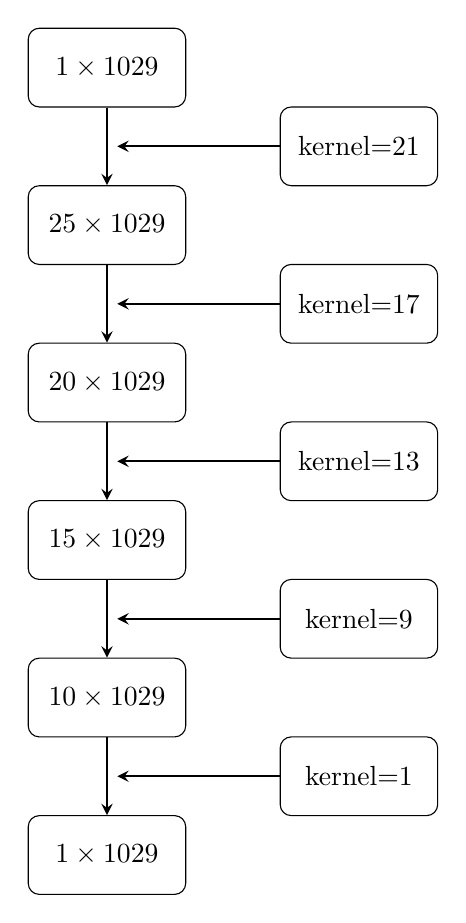
\begin{tikzpicture}[node distance=2cm]
    \node (0) [block] {$1\times1029$};
    \node (1) [block, below of=0] {$25\times1029$};
    \node (2) [block, below of=1] {$20\times1029$};
    \node (3) [block, below of=2] {$15\times1029$};
    \node (4) [block, below of=3] {$10\times1029$};
    \node (5) [block, below of=4] {$1\times1029$};
    \draw [arrow] (0) -- node [midway](0to1) {} (1);
    \draw [arrow] (1) -- node [midway](1to2) {} (2);
    \draw [arrow] (2) -- node [midway](2to3) {} (3);
    \draw [arrow] (3) -- node [midway](3to4) {} (4);
    \draw [arrow] (4) -- node [midway](4to5) {} (5);
    \node (a) [block, right of=0to1, xshift=1.2cm] {kernel=$21$};
    \node (b) [block, right of=1to2, xshift=1.2cm] {kernel=$17$};
    \node (c) [block, right of=2to3, xshift=1.2cm] {kernel=$13$};
    \node (d) [block, right of=3to4, xshift=1.2cm] {kernel=$9$};
    \node (e) [block, right of=4to5, xshift=1.2cm] {kernel=$1$};
    \draw [arrow] (a) -- (0to1) {};
    \draw [arrow] (b) -- (1to2) {};
    \draw [arrow] (c) -- (2to3) {};
    \draw [arrow] (d) -- (3to4) {};
    \draw [arrow] (e) -- (4to5) {};
\end{tikzpicture}
    \end{adjustbox}
    \caption{\label{fig:struct} Structure of the neural network.}
  \end{subfigure}
  \begin{subfigure}{.5\textwidth}
    \centering
    \resizebox{\textwidth}{!}{version https://git-lfs.github.com/spec/v1
oid sha256:4c9f0405e0a17c89e29f023642ea05c51d350a8fd1adf6cfa82f2fda57f5a7a7
size 35431
}
    \caption{\label{fig:loss} Evolution of loss.}
  \end{subfigure}
  \caption{\label{fig:CNN} Training process of a CNN. A shallow network structure of 5 layers in~\subref{fig:struct} is trained to converge in Wasserstein distance as shown in~\subref{fig:loss}.}
\end{figure}

\vspace{-0.5cm}
In figure~\ref{fig:cnn-npe}, we use box plot to describe $D_\mathrm{w}$ distributions. From figure~\ref{fig:cnn-npe}, we find $D_w$ is the smallest for one PE.  $D_w$ stops increasing with $N_\mathrm{PE}$ at about 6 PEs, where the PE times are the most challenging to extract.  When $N_\mathrm{PE}$ is more than 6, pile-ups tend to produce a continuous waveform and the average PE time accuracy stays flat. Thus waveform analysis is the most important in recovering time accuracy for PEs less than 10.

Such small $D_\mathrm{w}$ in figure~\ref{fig:cnn-npe} provides a precise matching of waveforms horizontally to guarantee effective $\hat{\alpha}$ scaling, explaining why $\mathrm{RSS}$ is also small in figure~\ref{fig:cnn}.

\begin{figure}[H]
  \begin{subfigure}{.5\textwidth}
    \centering
    \resizebox{\textwidth}{!}{%% Creator: Matplotlib, PGF backend
%%
%% To include the figure in your LaTeX document, write
%%   \input{<filename>.pgf}
%%
%% Make sure the required packages are loaded in your preamble
%%   \usepackage{pgf}
%%
%% and, on pdftex
%%   \usepackage[utf8]{inputenc}\DeclareUnicodeCharacter{2212}{-}
%%
%% or, on luatex and xetex
%%   \usepackage{unicode-math}
%%
%% Figures using additional raster images can only be included by \input if
%% they are in the same directory as the main LaTeX file. For loading figures
%% from other directories you can use the `import` package
%%   \usepackage{import}
%%
%% and then include the figures with
%%   \import{<path to file>}{<filename>.pgf}
%%
%% Matplotlib used the following preamble
%%   \usepackage[detect-all,locale=DE]{siunitx}
%%
\begingroup%
\makeatletter%
\begin{pgfpicture}%
\pgfpathrectangle{\pgfpointorigin}{\pgfqpoint{8.000000in}{6.000000in}}%
\pgfusepath{use as bounding box, clip}%
\begin{pgfscope}%
\pgfsetbuttcap%
\pgfsetmiterjoin%
\definecolor{currentfill}{rgb}{1.000000,1.000000,1.000000}%
\pgfsetfillcolor{currentfill}%
\pgfsetlinewidth{0.000000pt}%
\definecolor{currentstroke}{rgb}{1.000000,1.000000,1.000000}%
\pgfsetstrokecolor{currentstroke}%
\pgfsetdash{}{0pt}%
\pgfpathmoveto{\pgfqpoint{0.000000in}{0.000000in}}%
\pgfpathlineto{\pgfqpoint{8.000000in}{0.000000in}}%
\pgfpathlineto{\pgfqpoint{8.000000in}{6.000000in}}%
\pgfpathlineto{\pgfqpoint{0.000000in}{6.000000in}}%
\pgfpathclose%
\pgfusepath{fill}%
\end{pgfscope}%
\begin{pgfscope}%
\pgfsetbuttcap%
\pgfsetmiterjoin%
\definecolor{currentfill}{rgb}{1.000000,1.000000,1.000000}%
\pgfsetfillcolor{currentfill}%
\pgfsetlinewidth{0.000000pt}%
\definecolor{currentstroke}{rgb}{0.000000,0.000000,0.000000}%
\pgfsetstrokecolor{currentstroke}%
\pgfsetstrokeopacity{0.000000}%
\pgfsetdash{}{0pt}%
\pgfpathmoveto{\pgfqpoint{1.000000in}{0.720000in}}%
\pgfpathlineto{\pgfqpoint{5.800000in}{0.720000in}}%
\pgfpathlineto{\pgfqpoint{5.800000in}{5.340000in}}%
\pgfpathlineto{\pgfqpoint{1.000000in}{5.340000in}}%
\pgfpathclose%
\pgfusepath{fill}%
\end{pgfscope}%
\begin{pgfscope}%
\pgfsetbuttcap%
\pgfsetroundjoin%
\definecolor{currentfill}{rgb}{0.000000,0.000000,0.000000}%
\pgfsetfillcolor{currentfill}%
\pgfsetlinewidth{0.803000pt}%
\definecolor{currentstroke}{rgb}{0.000000,0.000000,0.000000}%
\pgfsetstrokecolor{currentstroke}%
\pgfsetdash{}{0pt}%
\pgfsys@defobject{currentmarker}{\pgfqpoint{0.000000in}{-0.048611in}}{\pgfqpoint{0.000000in}{0.000000in}}{%
\pgfpathmoveto{\pgfqpoint{0.000000in}{0.000000in}}%
\pgfpathlineto{\pgfqpoint{0.000000in}{-0.048611in}}%
\pgfusepath{stroke,fill}%
}%
\begin{pgfscope}%
\pgfsys@transformshift{1.300000in}{0.720000in}%
\pgfsys@useobject{currentmarker}{}%
\end{pgfscope}%
\end{pgfscope}%
\begin{pgfscope}%
\definecolor{textcolor}{rgb}{0.000000,0.000000,0.000000}%
\pgfsetstrokecolor{textcolor}%
\pgfsetfillcolor{textcolor}%
\pgftext[x=1.300000in,y=0.622778in,,top]{\color{textcolor}\sffamily\fontsize{20.000000}{24.000000}\selectfont 1}%
\end{pgfscope}%
\begin{pgfscope}%
\pgfsetbuttcap%
\pgfsetroundjoin%
\definecolor{currentfill}{rgb}{0.000000,0.000000,0.000000}%
\pgfsetfillcolor{currentfill}%
\pgfsetlinewidth{0.803000pt}%
\definecolor{currentstroke}{rgb}{0.000000,0.000000,0.000000}%
\pgfsetstrokecolor{currentstroke}%
\pgfsetdash{}{0pt}%
\pgfsys@defobject{currentmarker}{\pgfqpoint{0.000000in}{-0.048611in}}{\pgfqpoint{0.000000in}{0.000000in}}{%
\pgfpathmoveto{\pgfqpoint{0.000000in}{0.000000in}}%
\pgfpathlineto{\pgfqpoint{0.000000in}{-0.048611in}}%
\pgfusepath{stroke,fill}%
}%
\begin{pgfscope}%
\pgfsys@transformshift{1.900000in}{0.720000in}%
\pgfsys@useobject{currentmarker}{}%
\end{pgfscope}%
\end{pgfscope}%
\begin{pgfscope}%
\definecolor{textcolor}{rgb}{0.000000,0.000000,0.000000}%
\pgfsetstrokecolor{textcolor}%
\pgfsetfillcolor{textcolor}%
\pgftext[x=1.900000in,y=0.622778in,,top]{\color{textcolor}\sffamily\fontsize{20.000000}{24.000000}\selectfont 3}%
\end{pgfscope}%
\begin{pgfscope}%
\pgfsetbuttcap%
\pgfsetroundjoin%
\definecolor{currentfill}{rgb}{0.000000,0.000000,0.000000}%
\pgfsetfillcolor{currentfill}%
\pgfsetlinewidth{0.803000pt}%
\definecolor{currentstroke}{rgb}{0.000000,0.000000,0.000000}%
\pgfsetstrokecolor{currentstroke}%
\pgfsetdash{}{0pt}%
\pgfsys@defobject{currentmarker}{\pgfqpoint{0.000000in}{-0.048611in}}{\pgfqpoint{0.000000in}{0.000000in}}{%
\pgfpathmoveto{\pgfqpoint{0.000000in}{0.000000in}}%
\pgfpathlineto{\pgfqpoint{0.000000in}{-0.048611in}}%
\pgfusepath{stroke,fill}%
}%
\begin{pgfscope}%
\pgfsys@transformshift{2.500000in}{0.720000in}%
\pgfsys@useobject{currentmarker}{}%
\end{pgfscope}%
\end{pgfscope}%
\begin{pgfscope}%
\definecolor{textcolor}{rgb}{0.000000,0.000000,0.000000}%
\pgfsetstrokecolor{textcolor}%
\pgfsetfillcolor{textcolor}%
\pgftext[x=2.500000in,y=0.622778in,,top]{\color{textcolor}\sffamily\fontsize{20.000000}{24.000000}\selectfont 5}%
\end{pgfscope}%
\begin{pgfscope}%
\pgfsetbuttcap%
\pgfsetroundjoin%
\definecolor{currentfill}{rgb}{0.000000,0.000000,0.000000}%
\pgfsetfillcolor{currentfill}%
\pgfsetlinewidth{0.803000pt}%
\definecolor{currentstroke}{rgb}{0.000000,0.000000,0.000000}%
\pgfsetstrokecolor{currentstroke}%
\pgfsetdash{}{0pt}%
\pgfsys@defobject{currentmarker}{\pgfqpoint{0.000000in}{-0.048611in}}{\pgfqpoint{0.000000in}{0.000000in}}{%
\pgfpathmoveto{\pgfqpoint{0.000000in}{0.000000in}}%
\pgfpathlineto{\pgfqpoint{0.000000in}{-0.048611in}}%
\pgfusepath{stroke,fill}%
}%
\begin{pgfscope}%
\pgfsys@transformshift{3.100000in}{0.720000in}%
\pgfsys@useobject{currentmarker}{}%
\end{pgfscope}%
\end{pgfscope}%
\begin{pgfscope}%
\definecolor{textcolor}{rgb}{0.000000,0.000000,0.000000}%
\pgfsetstrokecolor{textcolor}%
\pgfsetfillcolor{textcolor}%
\pgftext[x=3.100000in,y=0.622778in,,top]{\color{textcolor}\sffamily\fontsize{20.000000}{24.000000}\selectfont 7}%
\end{pgfscope}%
\begin{pgfscope}%
\pgfsetbuttcap%
\pgfsetroundjoin%
\definecolor{currentfill}{rgb}{0.000000,0.000000,0.000000}%
\pgfsetfillcolor{currentfill}%
\pgfsetlinewidth{0.803000pt}%
\definecolor{currentstroke}{rgb}{0.000000,0.000000,0.000000}%
\pgfsetstrokecolor{currentstroke}%
\pgfsetdash{}{0pt}%
\pgfsys@defobject{currentmarker}{\pgfqpoint{0.000000in}{-0.048611in}}{\pgfqpoint{0.000000in}{0.000000in}}{%
\pgfpathmoveto{\pgfqpoint{0.000000in}{0.000000in}}%
\pgfpathlineto{\pgfqpoint{0.000000in}{-0.048611in}}%
\pgfusepath{stroke,fill}%
}%
\begin{pgfscope}%
\pgfsys@transformshift{3.700000in}{0.720000in}%
\pgfsys@useobject{currentmarker}{}%
\end{pgfscope}%
\end{pgfscope}%
\begin{pgfscope}%
\definecolor{textcolor}{rgb}{0.000000,0.000000,0.000000}%
\pgfsetstrokecolor{textcolor}%
\pgfsetfillcolor{textcolor}%
\pgftext[x=3.700000in,y=0.622778in,,top]{\color{textcolor}\sffamily\fontsize{20.000000}{24.000000}\selectfont 9}%
\end{pgfscope}%
\begin{pgfscope}%
\pgfsetbuttcap%
\pgfsetroundjoin%
\definecolor{currentfill}{rgb}{0.000000,0.000000,0.000000}%
\pgfsetfillcolor{currentfill}%
\pgfsetlinewidth{0.803000pt}%
\definecolor{currentstroke}{rgb}{0.000000,0.000000,0.000000}%
\pgfsetstrokecolor{currentstroke}%
\pgfsetdash{}{0pt}%
\pgfsys@defobject{currentmarker}{\pgfqpoint{0.000000in}{-0.048611in}}{\pgfqpoint{0.000000in}{0.000000in}}{%
\pgfpathmoveto{\pgfqpoint{0.000000in}{0.000000in}}%
\pgfpathlineto{\pgfqpoint{0.000000in}{-0.048611in}}%
\pgfusepath{stroke,fill}%
}%
\begin{pgfscope}%
\pgfsys@transformshift{4.300000in}{0.720000in}%
\pgfsys@useobject{currentmarker}{}%
\end{pgfscope}%
\end{pgfscope}%
\begin{pgfscope}%
\definecolor{textcolor}{rgb}{0.000000,0.000000,0.000000}%
\pgfsetstrokecolor{textcolor}%
\pgfsetfillcolor{textcolor}%
\pgftext[x=4.300000in,y=0.622778in,,top]{\color{textcolor}\sffamily\fontsize{20.000000}{24.000000}\selectfont 11}%
\end{pgfscope}%
\begin{pgfscope}%
\pgfsetbuttcap%
\pgfsetroundjoin%
\definecolor{currentfill}{rgb}{0.000000,0.000000,0.000000}%
\pgfsetfillcolor{currentfill}%
\pgfsetlinewidth{0.803000pt}%
\definecolor{currentstroke}{rgb}{0.000000,0.000000,0.000000}%
\pgfsetstrokecolor{currentstroke}%
\pgfsetdash{}{0pt}%
\pgfsys@defobject{currentmarker}{\pgfqpoint{0.000000in}{-0.048611in}}{\pgfqpoint{0.000000in}{0.000000in}}{%
\pgfpathmoveto{\pgfqpoint{0.000000in}{0.000000in}}%
\pgfpathlineto{\pgfqpoint{0.000000in}{-0.048611in}}%
\pgfusepath{stroke,fill}%
}%
\begin{pgfscope}%
\pgfsys@transformshift{4.900000in}{0.720000in}%
\pgfsys@useobject{currentmarker}{}%
\end{pgfscope}%
\end{pgfscope}%
\begin{pgfscope}%
\definecolor{textcolor}{rgb}{0.000000,0.000000,0.000000}%
\pgfsetstrokecolor{textcolor}%
\pgfsetfillcolor{textcolor}%
\pgftext[x=4.900000in,y=0.622778in,,top]{\color{textcolor}\sffamily\fontsize{20.000000}{24.000000}\selectfont 13}%
\end{pgfscope}%
\begin{pgfscope}%
\pgfsetbuttcap%
\pgfsetroundjoin%
\definecolor{currentfill}{rgb}{0.000000,0.000000,0.000000}%
\pgfsetfillcolor{currentfill}%
\pgfsetlinewidth{0.803000pt}%
\definecolor{currentstroke}{rgb}{0.000000,0.000000,0.000000}%
\pgfsetstrokecolor{currentstroke}%
\pgfsetdash{}{0pt}%
\pgfsys@defobject{currentmarker}{\pgfqpoint{0.000000in}{-0.048611in}}{\pgfqpoint{0.000000in}{0.000000in}}{%
\pgfpathmoveto{\pgfqpoint{0.000000in}{0.000000in}}%
\pgfpathlineto{\pgfqpoint{0.000000in}{-0.048611in}}%
\pgfusepath{stroke,fill}%
}%
\begin{pgfscope}%
\pgfsys@transformshift{5.500000in}{0.720000in}%
\pgfsys@useobject{currentmarker}{}%
\end{pgfscope}%
\end{pgfscope}%
\begin{pgfscope}%
\definecolor{textcolor}{rgb}{0.000000,0.000000,0.000000}%
\pgfsetstrokecolor{textcolor}%
\pgfsetfillcolor{textcolor}%
\pgftext[x=5.500000in,y=0.622778in,,top]{\color{textcolor}\sffamily\fontsize{20.000000}{24.000000}\selectfont 15}%
\end{pgfscope}%
\begin{pgfscope}%
\definecolor{textcolor}{rgb}{0.000000,0.000000,0.000000}%
\pgfsetstrokecolor{textcolor}%
\pgfsetfillcolor{textcolor}%
\pgftext[x=3.400000in,y=0.311155in,,top]{\color{textcolor}\sffamily\fontsize{20.000000}{24.000000}\selectfont \(\displaystyle N_{\mathrm{PE}}\)}%
\end{pgfscope}%
\begin{pgfscope}%
\pgfsetbuttcap%
\pgfsetroundjoin%
\definecolor{currentfill}{rgb}{0.000000,0.000000,0.000000}%
\pgfsetfillcolor{currentfill}%
\pgfsetlinewidth{0.803000pt}%
\definecolor{currentstroke}{rgb}{0.000000,0.000000,0.000000}%
\pgfsetstrokecolor{currentstroke}%
\pgfsetdash{}{0pt}%
\pgfsys@defobject{currentmarker}{\pgfqpoint{-0.048611in}{0.000000in}}{\pgfqpoint{-0.000000in}{0.000000in}}{%
\pgfpathmoveto{\pgfqpoint{-0.000000in}{0.000000in}}%
\pgfpathlineto{\pgfqpoint{-0.048611in}{0.000000in}}%
\pgfusepath{stroke,fill}%
}%
\begin{pgfscope}%
\pgfsys@transformshift{1.000000in}{0.720000in}%
\pgfsys@useobject{currentmarker}{}%
\end{pgfscope}%
\end{pgfscope}%
\begin{pgfscope}%
\definecolor{textcolor}{rgb}{0.000000,0.000000,0.000000}%
\pgfsetstrokecolor{textcolor}%
\pgfsetfillcolor{textcolor}%
\pgftext[x=0.560215in, y=0.619981in, left, base]{\color{textcolor}\sffamily\fontsize{20.000000}{24.000000}\selectfont \(\displaystyle {0.0}\)}%
\end{pgfscope}%
\begin{pgfscope}%
\pgfsetbuttcap%
\pgfsetroundjoin%
\definecolor{currentfill}{rgb}{0.000000,0.000000,0.000000}%
\pgfsetfillcolor{currentfill}%
\pgfsetlinewidth{0.803000pt}%
\definecolor{currentstroke}{rgb}{0.000000,0.000000,0.000000}%
\pgfsetstrokecolor{currentstroke}%
\pgfsetdash{}{0pt}%
\pgfsys@defobject{currentmarker}{\pgfqpoint{-0.048611in}{0.000000in}}{\pgfqpoint{-0.000000in}{0.000000in}}{%
\pgfpathmoveto{\pgfqpoint{-0.000000in}{0.000000in}}%
\pgfpathlineto{\pgfqpoint{-0.048611in}{0.000000in}}%
\pgfusepath{stroke,fill}%
}%
\begin{pgfscope}%
\pgfsys@transformshift{1.000000in}{1.598723in}%
\pgfsys@useobject{currentmarker}{}%
\end{pgfscope}%
\end{pgfscope}%
\begin{pgfscope}%
\definecolor{textcolor}{rgb}{0.000000,0.000000,0.000000}%
\pgfsetstrokecolor{textcolor}%
\pgfsetfillcolor{textcolor}%
\pgftext[x=0.560215in, y=1.498704in, left, base]{\color{textcolor}\sffamily\fontsize{20.000000}{24.000000}\selectfont \(\displaystyle {0.2}\)}%
\end{pgfscope}%
\begin{pgfscope}%
\pgfsetbuttcap%
\pgfsetroundjoin%
\definecolor{currentfill}{rgb}{0.000000,0.000000,0.000000}%
\pgfsetfillcolor{currentfill}%
\pgfsetlinewidth{0.803000pt}%
\definecolor{currentstroke}{rgb}{0.000000,0.000000,0.000000}%
\pgfsetstrokecolor{currentstroke}%
\pgfsetdash{}{0pt}%
\pgfsys@defobject{currentmarker}{\pgfqpoint{-0.048611in}{0.000000in}}{\pgfqpoint{-0.000000in}{0.000000in}}{%
\pgfpathmoveto{\pgfqpoint{-0.000000in}{0.000000in}}%
\pgfpathlineto{\pgfqpoint{-0.048611in}{0.000000in}}%
\pgfusepath{stroke,fill}%
}%
\begin{pgfscope}%
\pgfsys@transformshift{1.000000in}{2.477446in}%
\pgfsys@useobject{currentmarker}{}%
\end{pgfscope}%
\end{pgfscope}%
\begin{pgfscope}%
\definecolor{textcolor}{rgb}{0.000000,0.000000,0.000000}%
\pgfsetstrokecolor{textcolor}%
\pgfsetfillcolor{textcolor}%
\pgftext[x=0.560215in, y=2.377426in, left, base]{\color{textcolor}\sffamily\fontsize{20.000000}{24.000000}\selectfont \(\displaystyle {0.4}\)}%
\end{pgfscope}%
\begin{pgfscope}%
\pgfsetbuttcap%
\pgfsetroundjoin%
\definecolor{currentfill}{rgb}{0.000000,0.000000,0.000000}%
\pgfsetfillcolor{currentfill}%
\pgfsetlinewidth{0.803000pt}%
\definecolor{currentstroke}{rgb}{0.000000,0.000000,0.000000}%
\pgfsetstrokecolor{currentstroke}%
\pgfsetdash{}{0pt}%
\pgfsys@defobject{currentmarker}{\pgfqpoint{-0.048611in}{0.000000in}}{\pgfqpoint{-0.000000in}{0.000000in}}{%
\pgfpathmoveto{\pgfqpoint{-0.000000in}{0.000000in}}%
\pgfpathlineto{\pgfqpoint{-0.048611in}{0.000000in}}%
\pgfusepath{stroke,fill}%
}%
\begin{pgfscope}%
\pgfsys@transformshift{1.000000in}{3.356169in}%
\pgfsys@useobject{currentmarker}{}%
\end{pgfscope}%
\end{pgfscope}%
\begin{pgfscope}%
\definecolor{textcolor}{rgb}{0.000000,0.000000,0.000000}%
\pgfsetstrokecolor{textcolor}%
\pgfsetfillcolor{textcolor}%
\pgftext[x=0.560215in, y=3.256149in, left, base]{\color{textcolor}\sffamily\fontsize{20.000000}{24.000000}\selectfont \(\displaystyle {0.6}\)}%
\end{pgfscope}%
\begin{pgfscope}%
\pgfsetbuttcap%
\pgfsetroundjoin%
\definecolor{currentfill}{rgb}{0.000000,0.000000,0.000000}%
\pgfsetfillcolor{currentfill}%
\pgfsetlinewidth{0.803000pt}%
\definecolor{currentstroke}{rgb}{0.000000,0.000000,0.000000}%
\pgfsetstrokecolor{currentstroke}%
\pgfsetdash{}{0pt}%
\pgfsys@defobject{currentmarker}{\pgfqpoint{-0.048611in}{0.000000in}}{\pgfqpoint{-0.000000in}{0.000000in}}{%
\pgfpathmoveto{\pgfqpoint{-0.000000in}{0.000000in}}%
\pgfpathlineto{\pgfqpoint{-0.048611in}{0.000000in}}%
\pgfusepath{stroke,fill}%
}%
\begin{pgfscope}%
\pgfsys@transformshift{1.000000in}{4.234891in}%
\pgfsys@useobject{currentmarker}{}%
\end{pgfscope}%
\end{pgfscope}%
\begin{pgfscope}%
\definecolor{textcolor}{rgb}{0.000000,0.000000,0.000000}%
\pgfsetstrokecolor{textcolor}%
\pgfsetfillcolor{textcolor}%
\pgftext[x=0.560215in, y=4.134872in, left, base]{\color{textcolor}\sffamily\fontsize{20.000000}{24.000000}\selectfont \(\displaystyle {0.8}\)}%
\end{pgfscope}%
\begin{pgfscope}%
\pgfsetbuttcap%
\pgfsetroundjoin%
\definecolor{currentfill}{rgb}{0.000000,0.000000,0.000000}%
\pgfsetfillcolor{currentfill}%
\pgfsetlinewidth{0.803000pt}%
\definecolor{currentstroke}{rgb}{0.000000,0.000000,0.000000}%
\pgfsetstrokecolor{currentstroke}%
\pgfsetdash{}{0pt}%
\pgfsys@defobject{currentmarker}{\pgfqpoint{-0.048611in}{0.000000in}}{\pgfqpoint{-0.000000in}{0.000000in}}{%
\pgfpathmoveto{\pgfqpoint{-0.000000in}{0.000000in}}%
\pgfpathlineto{\pgfqpoint{-0.048611in}{0.000000in}}%
\pgfusepath{stroke,fill}%
}%
\begin{pgfscope}%
\pgfsys@transformshift{1.000000in}{5.113614in}%
\pgfsys@useobject{currentmarker}{}%
\end{pgfscope}%
\end{pgfscope}%
\begin{pgfscope}%
\definecolor{textcolor}{rgb}{0.000000,0.000000,0.000000}%
\pgfsetstrokecolor{textcolor}%
\pgfsetfillcolor{textcolor}%
\pgftext[x=0.560215in, y=5.013595in, left, base]{\color{textcolor}\sffamily\fontsize{20.000000}{24.000000}\selectfont \(\displaystyle {1.0}\)}%
\end{pgfscope}%
\begin{pgfscope}%
\definecolor{textcolor}{rgb}{0.000000,0.000000,0.000000}%
\pgfsetstrokecolor{textcolor}%
\pgfsetfillcolor{textcolor}%
\pgftext[x=0.504660in,y=3.030000in,,bottom,rotate=90.000000]{\color{textcolor}\sffamily\fontsize{20.000000}{24.000000}\selectfont \(\displaystyle \mathrm{Wasserstein\ Distance}/\si{ns}\)}%
\end{pgfscope}%
\begin{pgfscope}%
\pgfpathrectangle{\pgfqpoint{1.000000in}{0.720000in}}{\pgfqpoint{4.800000in}{4.620000in}}%
\pgfusepath{clip}%
\pgfsetrectcap%
\pgfsetroundjoin%
\pgfsetlinewidth{1.003750pt}%
\definecolor{currentstroke}{rgb}{0.000000,0.000000,0.000000}%
\pgfsetstrokecolor{currentstroke}%
\pgfsetdash{}{0pt}%
\pgfpathmoveto{\pgfqpoint{1.300000in}{1.275034in}}%
\pgfpathlineto{\pgfqpoint{1.300000in}{0.720538in}}%
\pgfusepath{stroke}%
\end{pgfscope}%
\begin{pgfscope}%
\pgfpathrectangle{\pgfqpoint{1.000000in}{0.720000in}}{\pgfqpoint{4.800000in}{4.620000in}}%
\pgfusepath{clip}%
\pgfsetrectcap%
\pgfsetroundjoin%
\pgfsetlinewidth{1.003750pt}%
\definecolor{currentstroke}{rgb}{0.000000,0.000000,0.000000}%
\pgfsetstrokecolor{currentstroke}%
\pgfsetdash{}{0pt}%
\pgfpathmoveto{\pgfqpoint{1.300000in}{2.458391in}}%
\pgfpathlineto{\pgfqpoint{1.300000in}{3.826356in}}%
\pgfusepath{stroke}%
\end{pgfscope}%
\begin{pgfscope}%
\pgfpathrectangle{\pgfqpoint{1.000000in}{0.720000in}}{\pgfqpoint{4.800000in}{4.620000in}}%
\pgfusepath{clip}%
\pgfsetrectcap%
\pgfsetroundjoin%
\pgfsetlinewidth{1.003750pt}%
\definecolor{currentstroke}{rgb}{0.000000,0.000000,0.000000}%
\pgfsetstrokecolor{currentstroke}%
\pgfsetdash{}{0pt}%
\pgfpathmoveto{\pgfqpoint{1.262500in}{0.720538in}}%
\pgfpathlineto{\pgfqpoint{1.337500in}{0.720538in}}%
\pgfusepath{stroke}%
\end{pgfscope}%
\begin{pgfscope}%
\pgfpathrectangle{\pgfqpoint{1.000000in}{0.720000in}}{\pgfqpoint{4.800000in}{4.620000in}}%
\pgfusepath{clip}%
\pgfsetrectcap%
\pgfsetroundjoin%
\pgfsetlinewidth{1.003750pt}%
\definecolor{currentstroke}{rgb}{0.000000,0.000000,0.000000}%
\pgfsetstrokecolor{currentstroke}%
\pgfsetdash{}{0pt}%
\pgfpathmoveto{\pgfqpoint{1.262500in}{3.826356in}}%
\pgfpathlineto{\pgfqpoint{1.337500in}{3.826356in}}%
\pgfusepath{stroke}%
\end{pgfscope}%
\begin{pgfscope}%
\pgfpathrectangle{\pgfqpoint{1.000000in}{0.720000in}}{\pgfqpoint{4.800000in}{4.620000in}}%
\pgfusepath{clip}%
\pgfsetrectcap%
\pgfsetroundjoin%
\pgfsetlinewidth{1.003750pt}%
\definecolor{currentstroke}{rgb}{0.000000,0.000000,0.000000}%
\pgfsetstrokecolor{currentstroke}%
\pgfsetdash{}{0pt}%
\pgfpathmoveto{\pgfqpoint{1.600000in}{2.052040in}}%
\pgfpathlineto{\pgfqpoint{1.600000in}{0.935591in}}%
\pgfusepath{stroke}%
\end{pgfscope}%
\begin{pgfscope}%
\pgfpathrectangle{\pgfqpoint{1.000000in}{0.720000in}}{\pgfqpoint{4.800000in}{4.620000in}}%
\pgfusepath{clip}%
\pgfsetrectcap%
\pgfsetroundjoin%
\pgfsetlinewidth{1.003750pt}%
\definecolor{currentstroke}{rgb}{0.000000,0.000000,0.000000}%
\pgfsetstrokecolor{currentstroke}%
\pgfsetdash{}{0pt}%
\pgfpathmoveto{\pgfqpoint{1.600000in}{3.291574in}}%
\pgfpathlineto{\pgfqpoint{1.600000in}{5.120000in}}%
\pgfusepath{stroke}%
\end{pgfscope}%
\begin{pgfscope}%
\pgfpathrectangle{\pgfqpoint{1.000000in}{0.720000in}}{\pgfqpoint{4.800000in}{4.620000in}}%
\pgfusepath{clip}%
\pgfsetrectcap%
\pgfsetroundjoin%
\pgfsetlinewidth{1.003750pt}%
\definecolor{currentstroke}{rgb}{0.000000,0.000000,0.000000}%
\pgfsetstrokecolor{currentstroke}%
\pgfsetdash{}{0pt}%
\pgfpathmoveto{\pgfqpoint{1.562500in}{0.935591in}}%
\pgfpathlineto{\pgfqpoint{1.637500in}{0.935591in}}%
\pgfusepath{stroke}%
\end{pgfscope}%
\begin{pgfscope}%
\pgfpathrectangle{\pgfqpoint{1.000000in}{0.720000in}}{\pgfqpoint{4.800000in}{4.620000in}}%
\pgfusepath{clip}%
\pgfsetrectcap%
\pgfsetroundjoin%
\pgfsetlinewidth{1.003750pt}%
\definecolor{currentstroke}{rgb}{0.000000,0.000000,0.000000}%
\pgfsetstrokecolor{currentstroke}%
\pgfsetdash{}{0pt}%
\pgfpathmoveto{\pgfqpoint{1.562500in}{5.120000in}}%
\pgfpathlineto{\pgfqpoint{1.637500in}{5.120000in}}%
\pgfusepath{stroke}%
\end{pgfscope}%
\begin{pgfscope}%
\pgfpathrectangle{\pgfqpoint{1.000000in}{0.720000in}}{\pgfqpoint{4.800000in}{4.620000in}}%
\pgfusepath{clip}%
\pgfsetrectcap%
\pgfsetroundjoin%
\pgfsetlinewidth{1.003750pt}%
\definecolor{currentstroke}{rgb}{0.000000,0.000000,0.000000}%
\pgfsetstrokecolor{currentstroke}%
\pgfsetdash{}{0pt}%
\pgfpathmoveto{\pgfqpoint{1.900000in}{2.377197in}}%
\pgfpathlineto{\pgfqpoint{1.900000in}{1.232889in}}%
\pgfusepath{stroke}%
\end{pgfscope}%
\begin{pgfscope}%
\pgfpathrectangle{\pgfqpoint{1.000000in}{0.720000in}}{\pgfqpoint{4.800000in}{4.620000in}}%
\pgfusepath{clip}%
\pgfsetrectcap%
\pgfsetroundjoin%
\pgfsetlinewidth{1.003750pt}%
\definecolor{currentstroke}{rgb}{0.000000,0.000000,0.000000}%
\pgfsetstrokecolor{currentstroke}%
\pgfsetdash{}{0pt}%
\pgfpathmoveto{\pgfqpoint{1.900000in}{3.484357in}}%
\pgfpathlineto{\pgfqpoint{1.900000in}{5.119703in}}%
\pgfusepath{stroke}%
\end{pgfscope}%
\begin{pgfscope}%
\pgfpathrectangle{\pgfqpoint{1.000000in}{0.720000in}}{\pgfqpoint{4.800000in}{4.620000in}}%
\pgfusepath{clip}%
\pgfsetrectcap%
\pgfsetroundjoin%
\pgfsetlinewidth{1.003750pt}%
\definecolor{currentstroke}{rgb}{0.000000,0.000000,0.000000}%
\pgfsetstrokecolor{currentstroke}%
\pgfsetdash{}{0pt}%
\pgfpathmoveto{\pgfqpoint{1.862500in}{1.232889in}}%
\pgfpathlineto{\pgfqpoint{1.937500in}{1.232889in}}%
\pgfusepath{stroke}%
\end{pgfscope}%
\begin{pgfscope}%
\pgfpathrectangle{\pgfqpoint{1.000000in}{0.720000in}}{\pgfqpoint{4.800000in}{4.620000in}}%
\pgfusepath{clip}%
\pgfsetrectcap%
\pgfsetroundjoin%
\pgfsetlinewidth{1.003750pt}%
\definecolor{currentstroke}{rgb}{0.000000,0.000000,0.000000}%
\pgfsetstrokecolor{currentstroke}%
\pgfsetdash{}{0pt}%
\pgfpathmoveto{\pgfqpoint{1.862500in}{5.119703in}}%
\pgfpathlineto{\pgfqpoint{1.937500in}{5.119703in}}%
\pgfusepath{stroke}%
\end{pgfscope}%
\begin{pgfscope}%
\pgfpathrectangle{\pgfqpoint{1.000000in}{0.720000in}}{\pgfqpoint{4.800000in}{4.620000in}}%
\pgfusepath{clip}%
\pgfsetrectcap%
\pgfsetroundjoin%
\pgfsetlinewidth{1.003750pt}%
\definecolor{currentstroke}{rgb}{0.000000,0.000000,0.000000}%
\pgfsetstrokecolor{currentstroke}%
\pgfsetdash{}{0pt}%
\pgfpathmoveto{\pgfqpoint{2.200000in}{2.587973in}}%
\pgfpathlineto{\pgfqpoint{2.200000in}{1.138166in}}%
\pgfusepath{stroke}%
\end{pgfscope}%
\begin{pgfscope}%
\pgfpathrectangle{\pgfqpoint{1.000000in}{0.720000in}}{\pgfqpoint{4.800000in}{4.620000in}}%
\pgfusepath{clip}%
\pgfsetrectcap%
\pgfsetroundjoin%
\pgfsetlinewidth{1.003750pt}%
\definecolor{currentstroke}{rgb}{0.000000,0.000000,0.000000}%
\pgfsetstrokecolor{currentstroke}%
\pgfsetdash{}{0pt}%
\pgfpathmoveto{\pgfqpoint{2.200000in}{3.606409in}}%
\pgfpathlineto{\pgfqpoint{2.200000in}{5.119000in}}%
\pgfusepath{stroke}%
\end{pgfscope}%
\begin{pgfscope}%
\pgfpathrectangle{\pgfqpoint{1.000000in}{0.720000in}}{\pgfqpoint{4.800000in}{4.620000in}}%
\pgfusepath{clip}%
\pgfsetrectcap%
\pgfsetroundjoin%
\pgfsetlinewidth{1.003750pt}%
\definecolor{currentstroke}{rgb}{0.000000,0.000000,0.000000}%
\pgfsetstrokecolor{currentstroke}%
\pgfsetdash{}{0pt}%
\pgfpathmoveto{\pgfqpoint{2.162500in}{1.138166in}}%
\pgfpathlineto{\pgfqpoint{2.237500in}{1.138166in}}%
\pgfusepath{stroke}%
\end{pgfscope}%
\begin{pgfscope}%
\pgfpathrectangle{\pgfqpoint{1.000000in}{0.720000in}}{\pgfqpoint{4.800000in}{4.620000in}}%
\pgfusepath{clip}%
\pgfsetrectcap%
\pgfsetroundjoin%
\pgfsetlinewidth{1.003750pt}%
\definecolor{currentstroke}{rgb}{0.000000,0.000000,0.000000}%
\pgfsetstrokecolor{currentstroke}%
\pgfsetdash{}{0pt}%
\pgfpathmoveto{\pgfqpoint{2.162500in}{5.119000in}}%
\pgfpathlineto{\pgfqpoint{2.237500in}{5.119000in}}%
\pgfusepath{stroke}%
\end{pgfscope}%
\begin{pgfscope}%
\pgfpathrectangle{\pgfqpoint{1.000000in}{0.720000in}}{\pgfqpoint{4.800000in}{4.620000in}}%
\pgfusepath{clip}%
\pgfsetrectcap%
\pgfsetroundjoin%
\pgfsetlinewidth{1.003750pt}%
\definecolor{currentstroke}{rgb}{0.000000,0.000000,0.000000}%
\pgfsetstrokecolor{currentstroke}%
\pgfsetdash{}{0pt}%
\pgfpathmoveto{\pgfqpoint{2.500000in}{2.733762in}}%
\pgfpathlineto{\pgfqpoint{2.500000in}{1.537923in}}%
\pgfusepath{stroke}%
\end{pgfscope}%
\begin{pgfscope}%
\pgfpathrectangle{\pgfqpoint{1.000000in}{0.720000in}}{\pgfqpoint{4.800000in}{4.620000in}}%
\pgfusepath{clip}%
\pgfsetrectcap%
\pgfsetroundjoin%
\pgfsetlinewidth{1.003750pt}%
\definecolor{currentstroke}{rgb}{0.000000,0.000000,0.000000}%
\pgfsetstrokecolor{currentstroke}%
\pgfsetdash{}{0pt}%
\pgfpathmoveto{\pgfqpoint{2.500000in}{3.663233in}}%
\pgfpathlineto{\pgfqpoint{2.500000in}{5.028135in}}%
\pgfusepath{stroke}%
\end{pgfscope}%
\begin{pgfscope}%
\pgfpathrectangle{\pgfqpoint{1.000000in}{0.720000in}}{\pgfqpoint{4.800000in}{4.620000in}}%
\pgfusepath{clip}%
\pgfsetrectcap%
\pgfsetroundjoin%
\pgfsetlinewidth{1.003750pt}%
\definecolor{currentstroke}{rgb}{0.000000,0.000000,0.000000}%
\pgfsetstrokecolor{currentstroke}%
\pgfsetdash{}{0pt}%
\pgfpathmoveto{\pgfqpoint{2.462500in}{1.537923in}}%
\pgfpathlineto{\pgfqpoint{2.537500in}{1.537923in}}%
\pgfusepath{stroke}%
\end{pgfscope}%
\begin{pgfscope}%
\pgfpathrectangle{\pgfqpoint{1.000000in}{0.720000in}}{\pgfqpoint{4.800000in}{4.620000in}}%
\pgfusepath{clip}%
\pgfsetrectcap%
\pgfsetroundjoin%
\pgfsetlinewidth{1.003750pt}%
\definecolor{currentstroke}{rgb}{0.000000,0.000000,0.000000}%
\pgfsetstrokecolor{currentstroke}%
\pgfsetdash{}{0pt}%
\pgfpathmoveto{\pgfqpoint{2.462500in}{5.028135in}}%
\pgfpathlineto{\pgfqpoint{2.537500in}{5.028135in}}%
\pgfusepath{stroke}%
\end{pgfscope}%
\begin{pgfscope}%
\pgfpathrectangle{\pgfqpoint{1.000000in}{0.720000in}}{\pgfqpoint{4.800000in}{4.620000in}}%
\pgfusepath{clip}%
\pgfsetrectcap%
\pgfsetroundjoin%
\pgfsetlinewidth{1.003750pt}%
\definecolor{currentstroke}{rgb}{0.000000,0.000000,0.000000}%
\pgfsetstrokecolor{currentstroke}%
\pgfsetdash{}{0pt}%
\pgfpathmoveto{\pgfqpoint{2.800000in}{2.764618in}}%
\pgfpathlineto{\pgfqpoint{2.800000in}{1.500258in}}%
\pgfusepath{stroke}%
\end{pgfscope}%
\begin{pgfscope}%
\pgfpathrectangle{\pgfqpoint{1.000000in}{0.720000in}}{\pgfqpoint{4.800000in}{4.620000in}}%
\pgfusepath{clip}%
\pgfsetrectcap%
\pgfsetroundjoin%
\pgfsetlinewidth{1.003750pt}%
\definecolor{currentstroke}{rgb}{0.000000,0.000000,0.000000}%
\pgfsetstrokecolor{currentstroke}%
\pgfsetdash{}{0pt}%
\pgfpathmoveto{\pgfqpoint{2.800000in}{3.681932in}}%
\pgfpathlineto{\pgfqpoint{2.800000in}{5.053071in}}%
\pgfusepath{stroke}%
\end{pgfscope}%
\begin{pgfscope}%
\pgfpathrectangle{\pgfqpoint{1.000000in}{0.720000in}}{\pgfqpoint{4.800000in}{4.620000in}}%
\pgfusepath{clip}%
\pgfsetrectcap%
\pgfsetroundjoin%
\pgfsetlinewidth{1.003750pt}%
\definecolor{currentstroke}{rgb}{0.000000,0.000000,0.000000}%
\pgfsetstrokecolor{currentstroke}%
\pgfsetdash{}{0pt}%
\pgfpathmoveto{\pgfqpoint{2.762500in}{1.500258in}}%
\pgfpathlineto{\pgfqpoint{2.837500in}{1.500258in}}%
\pgfusepath{stroke}%
\end{pgfscope}%
\begin{pgfscope}%
\pgfpathrectangle{\pgfqpoint{1.000000in}{0.720000in}}{\pgfqpoint{4.800000in}{4.620000in}}%
\pgfusepath{clip}%
\pgfsetrectcap%
\pgfsetroundjoin%
\pgfsetlinewidth{1.003750pt}%
\definecolor{currentstroke}{rgb}{0.000000,0.000000,0.000000}%
\pgfsetstrokecolor{currentstroke}%
\pgfsetdash{}{0pt}%
\pgfpathmoveto{\pgfqpoint{2.762500in}{5.053071in}}%
\pgfpathlineto{\pgfqpoint{2.837500in}{5.053071in}}%
\pgfusepath{stroke}%
\end{pgfscope}%
\begin{pgfscope}%
\pgfpathrectangle{\pgfqpoint{1.000000in}{0.720000in}}{\pgfqpoint{4.800000in}{4.620000in}}%
\pgfusepath{clip}%
\pgfsetrectcap%
\pgfsetroundjoin%
\pgfsetlinewidth{1.003750pt}%
\definecolor{currentstroke}{rgb}{0.000000,0.000000,0.000000}%
\pgfsetstrokecolor{currentstroke}%
\pgfsetdash{}{0pt}%
\pgfpathmoveto{\pgfqpoint{3.100000in}{2.887424in}}%
\pgfpathlineto{\pgfqpoint{3.100000in}{1.647440in}}%
\pgfusepath{stroke}%
\end{pgfscope}%
\begin{pgfscope}%
\pgfpathrectangle{\pgfqpoint{1.000000in}{0.720000in}}{\pgfqpoint{4.800000in}{4.620000in}}%
\pgfusepath{clip}%
\pgfsetrectcap%
\pgfsetroundjoin%
\pgfsetlinewidth{1.003750pt}%
\definecolor{currentstroke}{rgb}{0.000000,0.000000,0.000000}%
\pgfsetstrokecolor{currentstroke}%
\pgfsetdash{}{0pt}%
\pgfpathmoveto{\pgfqpoint{3.100000in}{3.737343in}}%
\pgfpathlineto{\pgfqpoint{3.100000in}{5.003119in}}%
\pgfusepath{stroke}%
\end{pgfscope}%
\begin{pgfscope}%
\pgfpathrectangle{\pgfqpoint{1.000000in}{0.720000in}}{\pgfqpoint{4.800000in}{4.620000in}}%
\pgfusepath{clip}%
\pgfsetrectcap%
\pgfsetroundjoin%
\pgfsetlinewidth{1.003750pt}%
\definecolor{currentstroke}{rgb}{0.000000,0.000000,0.000000}%
\pgfsetstrokecolor{currentstroke}%
\pgfsetdash{}{0pt}%
\pgfpathmoveto{\pgfqpoint{3.062500in}{1.647440in}}%
\pgfpathlineto{\pgfqpoint{3.137500in}{1.647440in}}%
\pgfusepath{stroke}%
\end{pgfscope}%
\begin{pgfscope}%
\pgfpathrectangle{\pgfqpoint{1.000000in}{0.720000in}}{\pgfqpoint{4.800000in}{4.620000in}}%
\pgfusepath{clip}%
\pgfsetrectcap%
\pgfsetroundjoin%
\pgfsetlinewidth{1.003750pt}%
\definecolor{currentstroke}{rgb}{0.000000,0.000000,0.000000}%
\pgfsetstrokecolor{currentstroke}%
\pgfsetdash{}{0pt}%
\pgfpathmoveto{\pgfqpoint{3.062500in}{5.003119in}}%
\pgfpathlineto{\pgfqpoint{3.137500in}{5.003119in}}%
\pgfusepath{stroke}%
\end{pgfscope}%
\begin{pgfscope}%
\pgfpathrectangle{\pgfqpoint{1.000000in}{0.720000in}}{\pgfqpoint{4.800000in}{4.620000in}}%
\pgfusepath{clip}%
\pgfsetrectcap%
\pgfsetroundjoin%
\pgfsetlinewidth{1.003750pt}%
\definecolor{currentstroke}{rgb}{0.000000,0.000000,0.000000}%
\pgfsetstrokecolor{currentstroke}%
\pgfsetdash{}{0pt}%
\pgfpathmoveto{\pgfqpoint{3.400000in}{2.913642in}}%
\pgfpathlineto{\pgfqpoint{3.400000in}{2.092707in}}%
\pgfusepath{stroke}%
\end{pgfscope}%
\begin{pgfscope}%
\pgfpathrectangle{\pgfqpoint{1.000000in}{0.720000in}}{\pgfqpoint{4.800000in}{4.620000in}}%
\pgfusepath{clip}%
\pgfsetrectcap%
\pgfsetroundjoin%
\pgfsetlinewidth{1.003750pt}%
\definecolor{currentstroke}{rgb}{0.000000,0.000000,0.000000}%
\pgfsetstrokecolor{currentstroke}%
\pgfsetdash{}{0pt}%
\pgfpathmoveto{\pgfqpoint{3.400000in}{3.674032in}}%
\pgfpathlineto{\pgfqpoint{3.400000in}{4.741288in}}%
\pgfusepath{stroke}%
\end{pgfscope}%
\begin{pgfscope}%
\pgfpathrectangle{\pgfqpoint{1.000000in}{0.720000in}}{\pgfqpoint{4.800000in}{4.620000in}}%
\pgfusepath{clip}%
\pgfsetrectcap%
\pgfsetroundjoin%
\pgfsetlinewidth{1.003750pt}%
\definecolor{currentstroke}{rgb}{0.000000,0.000000,0.000000}%
\pgfsetstrokecolor{currentstroke}%
\pgfsetdash{}{0pt}%
\pgfpathmoveto{\pgfqpoint{3.362500in}{2.092707in}}%
\pgfpathlineto{\pgfqpoint{3.437500in}{2.092707in}}%
\pgfusepath{stroke}%
\end{pgfscope}%
\begin{pgfscope}%
\pgfpathrectangle{\pgfqpoint{1.000000in}{0.720000in}}{\pgfqpoint{4.800000in}{4.620000in}}%
\pgfusepath{clip}%
\pgfsetrectcap%
\pgfsetroundjoin%
\pgfsetlinewidth{1.003750pt}%
\definecolor{currentstroke}{rgb}{0.000000,0.000000,0.000000}%
\pgfsetstrokecolor{currentstroke}%
\pgfsetdash{}{0pt}%
\pgfpathmoveto{\pgfqpoint{3.362500in}{4.741288in}}%
\pgfpathlineto{\pgfqpoint{3.437500in}{4.741288in}}%
\pgfusepath{stroke}%
\end{pgfscope}%
\begin{pgfscope}%
\pgfpathrectangle{\pgfqpoint{1.000000in}{0.720000in}}{\pgfqpoint{4.800000in}{4.620000in}}%
\pgfusepath{clip}%
\pgfsetrectcap%
\pgfsetroundjoin%
\pgfsetlinewidth{1.003750pt}%
\definecolor{currentstroke}{rgb}{0.000000,0.000000,0.000000}%
\pgfsetstrokecolor{currentstroke}%
\pgfsetdash{}{0pt}%
\pgfpathmoveto{\pgfqpoint{3.700000in}{2.840050in}}%
\pgfpathlineto{\pgfqpoint{3.700000in}{2.194448in}}%
\pgfusepath{stroke}%
\end{pgfscope}%
\begin{pgfscope}%
\pgfpathrectangle{\pgfqpoint{1.000000in}{0.720000in}}{\pgfqpoint{4.800000in}{4.620000in}}%
\pgfusepath{clip}%
\pgfsetrectcap%
\pgfsetroundjoin%
\pgfsetlinewidth{1.003750pt}%
\definecolor{currentstroke}{rgb}{0.000000,0.000000,0.000000}%
\pgfsetstrokecolor{currentstroke}%
\pgfsetdash{}{0pt}%
\pgfpathmoveto{\pgfqpoint{3.700000in}{3.655616in}}%
\pgfpathlineto{\pgfqpoint{3.700000in}{4.727067in}}%
\pgfusepath{stroke}%
\end{pgfscope}%
\begin{pgfscope}%
\pgfpathrectangle{\pgfqpoint{1.000000in}{0.720000in}}{\pgfqpoint{4.800000in}{4.620000in}}%
\pgfusepath{clip}%
\pgfsetrectcap%
\pgfsetroundjoin%
\pgfsetlinewidth{1.003750pt}%
\definecolor{currentstroke}{rgb}{0.000000,0.000000,0.000000}%
\pgfsetstrokecolor{currentstroke}%
\pgfsetdash{}{0pt}%
\pgfpathmoveto{\pgfqpoint{3.662500in}{2.194448in}}%
\pgfpathlineto{\pgfqpoint{3.737500in}{2.194448in}}%
\pgfusepath{stroke}%
\end{pgfscope}%
\begin{pgfscope}%
\pgfpathrectangle{\pgfqpoint{1.000000in}{0.720000in}}{\pgfqpoint{4.800000in}{4.620000in}}%
\pgfusepath{clip}%
\pgfsetrectcap%
\pgfsetroundjoin%
\pgfsetlinewidth{1.003750pt}%
\definecolor{currentstroke}{rgb}{0.000000,0.000000,0.000000}%
\pgfsetstrokecolor{currentstroke}%
\pgfsetdash{}{0pt}%
\pgfpathmoveto{\pgfqpoint{3.662500in}{4.727067in}}%
\pgfpathlineto{\pgfqpoint{3.737500in}{4.727067in}}%
\pgfusepath{stroke}%
\end{pgfscope}%
\begin{pgfscope}%
\pgfpathrectangle{\pgfqpoint{1.000000in}{0.720000in}}{\pgfqpoint{4.800000in}{4.620000in}}%
\pgfusepath{clip}%
\pgfsetrectcap%
\pgfsetroundjoin%
\pgfsetlinewidth{1.003750pt}%
\definecolor{currentstroke}{rgb}{0.000000,0.000000,0.000000}%
\pgfsetstrokecolor{currentstroke}%
\pgfsetdash{}{0pt}%
\pgfpathmoveto{\pgfqpoint{4.000000in}{2.930521in}}%
\pgfpathlineto{\pgfqpoint{4.000000in}{2.488672in}}%
\pgfusepath{stroke}%
\end{pgfscope}%
\begin{pgfscope}%
\pgfpathrectangle{\pgfqpoint{1.000000in}{0.720000in}}{\pgfqpoint{4.800000in}{4.620000in}}%
\pgfusepath{clip}%
\pgfsetrectcap%
\pgfsetroundjoin%
\pgfsetlinewidth{1.003750pt}%
\definecolor{currentstroke}{rgb}{0.000000,0.000000,0.000000}%
\pgfsetstrokecolor{currentstroke}%
\pgfsetdash{}{0pt}%
\pgfpathmoveto{\pgfqpoint{4.000000in}{3.490054in}}%
\pgfpathlineto{\pgfqpoint{4.000000in}{4.255666in}}%
\pgfusepath{stroke}%
\end{pgfscope}%
\begin{pgfscope}%
\pgfpathrectangle{\pgfqpoint{1.000000in}{0.720000in}}{\pgfqpoint{4.800000in}{4.620000in}}%
\pgfusepath{clip}%
\pgfsetrectcap%
\pgfsetroundjoin%
\pgfsetlinewidth{1.003750pt}%
\definecolor{currentstroke}{rgb}{0.000000,0.000000,0.000000}%
\pgfsetstrokecolor{currentstroke}%
\pgfsetdash{}{0pt}%
\pgfpathmoveto{\pgfqpoint{3.962500in}{2.488672in}}%
\pgfpathlineto{\pgfqpoint{4.037500in}{2.488672in}}%
\pgfusepath{stroke}%
\end{pgfscope}%
\begin{pgfscope}%
\pgfpathrectangle{\pgfqpoint{1.000000in}{0.720000in}}{\pgfqpoint{4.800000in}{4.620000in}}%
\pgfusepath{clip}%
\pgfsetrectcap%
\pgfsetroundjoin%
\pgfsetlinewidth{1.003750pt}%
\definecolor{currentstroke}{rgb}{0.000000,0.000000,0.000000}%
\pgfsetstrokecolor{currentstroke}%
\pgfsetdash{}{0pt}%
\pgfpathmoveto{\pgfqpoint{3.962500in}{4.255666in}}%
\pgfpathlineto{\pgfqpoint{4.037500in}{4.255666in}}%
\pgfusepath{stroke}%
\end{pgfscope}%
\begin{pgfscope}%
\pgfpathrectangle{\pgfqpoint{1.000000in}{0.720000in}}{\pgfqpoint{4.800000in}{4.620000in}}%
\pgfusepath{clip}%
\pgfsetrectcap%
\pgfsetroundjoin%
\pgfsetlinewidth{1.003750pt}%
\definecolor{currentstroke}{rgb}{0.000000,0.000000,0.000000}%
\pgfsetstrokecolor{currentstroke}%
\pgfsetdash{}{0pt}%
\pgfpathmoveto{\pgfqpoint{4.300000in}{2.918050in}}%
\pgfpathlineto{\pgfqpoint{4.300000in}{2.432390in}}%
\pgfusepath{stroke}%
\end{pgfscope}%
\begin{pgfscope}%
\pgfpathrectangle{\pgfqpoint{1.000000in}{0.720000in}}{\pgfqpoint{4.800000in}{4.620000in}}%
\pgfusepath{clip}%
\pgfsetrectcap%
\pgfsetroundjoin%
\pgfsetlinewidth{1.003750pt}%
\definecolor{currentstroke}{rgb}{0.000000,0.000000,0.000000}%
\pgfsetstrokecolor{currentstroke}%
\pgfsetdash{}{0pt}%
\pgfpathmoveto{\pgfqpoint{4.300000in}{3.613869in}}%
\pgfpathlineto{\pgfqpoint{4.300000in}{4.557049in}}%
\pgfusepath{stroke}%
\end{pgfscope}%
\begin{pgfscope}%
\pgfpathrectangle{\pgfqpoint{1.000000in}{0.720000in}}{\pgfqpoint{4.800000in}{4.620000in}}%
\pgfusepath{clip}%
\pgfsetrectcap%
\pgfsetroundjoin%
\pgfsetlinewidth{1.003750pt}%
\definecolor{currentstroke}{rgb}{0.000000,0.000000,0.000000}%
\pgfsetstrokecolor{currentstroke}%
\pgfsetdash{}{0pt}%
\pgfpathmoveto{\pgfqpoint{4.262500in}{2.432390in}}%
\pgfpathlineto{\pgfqpoint{4.337500in}{2.432390in}}%
\pgfusepath{stroke}%
\end{pgfscope}%
\begin{pgfscope}%
\pgfpathrectangle{\pgfqpoint{1.000000in}{0.720000in}}{\pgfqpoint{4.800000in}{4.620000in}}%
\pgfusepath{clip}%
\pgfsetrectcap%
\pgfsetroundjoin%
\pgfsetlinewidth{1.003750pt}%
\definecolor{currentstroke}{rgb}{0.000000,0.000000,0.000000}%
\pgfsetstrokecolor{currentstroke}%
\pgfsetdash{}{0pt}%
\pgfpathmoveto{\pgfqpoint{4.262500in}{4.557049in}}%
\pgfpathlineto{\pgfqpoint{4.337500in}{4.557049in}}%
\pgfusepath{stroke}%
\end{pgfscope}%
\begin{pgfscope}%
\pgfpathrectangle{\pgfqpoint{1.000000in}{0.720000in}}{\pgfqpoint{4.800000in}{4.620000in}}%
\pgfusepath{clip}%
\pgfsetrectcap%
\pgfsetroundjoin%
\pgfsetlinewidth{1.003750pt}%
\definecolor{currentstroke}{rgb}{0.000000,0.000000,0.000000}%
\pgfsetstrokecolor{currentstroke}%
\pgfsetdash{}{0pt}%
\pgfpathmoveto{\pgfqpoint{4.600000in}{3.632982in}}%
\pgfpathlineto{\pgfqpoint{4.600000in}{2.870742in}}%
\pgfusepath{stroke}%
\end{pgfscope}%
\begin{pgfscope}%
\pgfpathrectangle{\pgfqpoint{1.000000in}{0.720000in}}{\pgfqpoint{4.800000in}{4.620000in}}%
\pgfusepath{clip}%
\pgfsetrectcap%
\pgfsetroundjoin%
\pgfsetlinewidth{1.003750pt}%
\definecolor{currentstroke}{rgb}{0.000000,0.000000,0.000000}%
\pgfsetstrokecolor{currentstroke}%
\pgfsetdash{}{0pt}%
\pgfpathmoveto{\pgfqpoint{4.600000in}{4.241231in}}%
\pgfpathlineto{\pgfqpoint{4.600000in}{4.885439in}}%
\pgfusepath{stroke}%
\end{pgfscope}%
\begin{pgfscope}%
\pgfpathrectangle{\pgfqpoint{1.000000in}{0.720000in}}{\pgfqpoint{4.800000in}{4.620000in}}%
\pgfusepath{clip}%
\pgfsetrectcap%
\pgfsetroundjoin%
\pgfsetlinewidth{1.003750pt}%
\definecolor{currentstroke}{rgb}{0.000000,0.000000,0.000000}%
\pgfsetstrokecolor{currentstroke}%
\pgfsetdash{}{0pt}%
\pgfpathmoveto{\pgfqpoint{4.562500in}{2.870742in}}%
\pgfpathlineto{\pgfqpoint{4.637500in}{2.870742in}}%
\pgfusepath{stroke}%
\end{pgfscope}%
\begin{pgfscope}%
\pgfpathrectangle{\pgfqpoint{1.000000in}{0.720000in}}{\pgfqpoint{4.800000in}{4.620000in}}%
\pgfusepath{clip}%
\pgfsetrectcap%
\pgfsetroundjoin%
\pgfsetlinewidth{1.003750pt}%
\definecolor{currentstroke}{rgb}{0.000000,0.000000,0.000000}%
\pgfsetstrokecolor{currentstroke}%
\pgfsetdash{}{0pt}%
\pgfpathmoveto{\pgfqpoint{4.562500in}{4.885439in}}%
\pgfpathlineto{\pgfqpoint{4.637500in}{4.885439in}}%
\pgfusepath{stroke}%
\end{pgfscope}%
\begin{pgfscope}%
\pgfpathrectangle{\pgfqpoint{1.000000in}{0.720000in}}{\pgfqpoint{4.800000in}{4.620000in}}%
\pgfusepath{clip}%
\pgfsetrectcap%
\pgfsetroundjoin%
\pgfsetlinewidth{1.003750pt}%
\definecolor{currentstroke}{rgb}{0.000000,0.000000,0.000000}%
\pgfsetstrokecolor{currentstroke}%
\pgfsetdash{}{0pt}%
\pgfpathmoveto{\pgfqpoint{4.900000in}{2.631498in}}%
\pgfpathlineto{\pgfqpoint{4.900000in}{2.631498in}}%
\pgfusepath{stroke}%
\end{pgfscope}%
\begin{pgfscope}%
\pgfpathrectangle{\pgfqpoint{1.000000in}{0.720000in}}{\pgfqpoint{4.800000in}{4.620000in}}%
\pgfusepath{clip}%
\pgfsetrectcap%
\pgfsetroundjoin%
\pgfsetlinewidth{1.003750pt}%
\definecolor{currentstroke}{rgb}{0.000000,0.000000,0.000000}%
\pgfsetstrokecolor{currentstroke}%
\pgfsetdash{}{0pt}%
\pgfpathmoveto{\pgfqpoint{4.900000in}{2.631498in}}%
\pgfpathlineto{\pgfqpoint{4.900000in}{2.631498in}}%
\pgfusepath{stroke}%
\end{pgfscope}%
\begin{pgfscope}%
\pgfpathrectangle{\pgfqpoint{1.000000in}{0.720000in}}{\pgfqpoint{4.800000in}{4.620000in}}%
\pgfusepath{clip}%
\pgfsetrectcap%
\pgfsetroundjoin%
\pgfsetlinewidth{1.003750pt}%
\definecolor{currentstroke}{rgb}{0.000000,0.000000,0.000000}%
\pgfsetstrokecolor{currentstroke}%
\pgfsetdash{}{0pt}%
\pgfpathmoveto{\pgfqpoint{4.862500in}{2.631498in}}%
\pgfpathlineto{\pgfqpoint{4.937500in}{2.631498in}}%
\pgfusepath{stroke}%
\end{pgfscope}%
\begin{pgfscope}%
\pgfpathrectangle{\pgfqpoint{1.000000in}{0.720000in}}{\pgfqpoint{4.800000in}{4.620000in}}%
\pgfusepath{clip}%
\pgfsetrectcap%
\pgfsetroundjoin%
\pgfsetlinewidth{1.003750pt}%
\definecolor{currentstroke}{rgb}{0.000000,0.000000,0.000000}%
\pgfsetstrokecolor{currentstroke}%
\pgfsetdash{}{0pt}%
\pgfpathmoveto{\pgfqpoint{4.862500in}{2.631498in}}%
\pgfpathlineto{\pgfqpoint{4.937500in}{2.631498in}}%
\pgfusepath{stroke}%
\end{pgfscope}%
\begin{pgfscope}%
\pgfpathrectangle{\pgfqpoint{1.000000in}{0.720000in}}{\pgfqpoint{4.800000in}{4.620000in}}%
\pgfusepath{clip}%
\pgfsetrectcap%
\pgfsetroundjoin%
\pgfsetlinewidth{1.003750pt}%
\definecolor{currentstroke}{rgb}{0.000000,0.000000,0.000000}%
\pgfsetstrokecolor{currentstroke}%
\pgfsetdash{}{0pt}%
\pgfpathmoveto{\pgfqpoint{5.200000in}{3.483259in}}%
\pgfpathlineto{\pgfqpoint{5.200000in}{3.483259in}}%
\pgfusepath{stroke}%
\end{pgfscope}%
\begin{pgfscope}%
\pgfpathrectangle{\pgfqpoint{1.000000in}{0.720000in}}{\pgfqpoint{4.800000in}{4.620000in}}%
\pgfusepath{clip}%
\pgfsetrectcap%
\pgfsetroundjoin%
\pgfsetlinewidth{1.003750pt}%
\definecolor{currentstroke}{rgb}{0.000000,0.000000,0.000000}%
\pgfsetstrokecolor{currentstroke}%
\pgfsetdash{}{0pt}%
\pgfpathmoveto{\pgfqpoint{5.200000in}{3.483259in}}%
\pgfpathlineto{\pgfqpoint{5.200000in}{3.483259in}}%
\pgfusepath{stroke}%
\end{pgfscope}%
\begin{pgfscope}%
\pgfpathrectangle{\pgfqpoint{1.000000in}{0.720000in}}{\pgfqpoint{4.800000in}{4.620000in}}%
\pgfusepath{clip}%
\pgfsetrectcap%
\pgfsetroundjoin%
\pgfsetlinewidth{1.003750pt}%
\definecolor{currentstroke}{rgb}{0.000000,0.000000,0.000000}%
\pgfsetstrokecolor{currentstroke}%
\pgfsetdash{}{0pt}%
\pgfpathmoveto{\pgfqpoint{5.162500in}{3.483259in}}%
\pgfpathlineto{\pgfqpoint{5.237500in}{3.483259in}}%
\pgfusepath{stroke}%
\end{pgfscope}%
\begin{pgfscope}%
\pgfpathrectangle{\pgfqpoint{1.000000in}{0.720000in}}{\pgfqpoint{4.800000in}{4.620000in}}%
\pgfusepath{clip}%
\pgfsetrectcap%
\pgfsetroundjoin%
\pgfsetlinewidth{1.003750pt}%
\definecolor{currentstroke}{rgb}{0.000000,0.000000,0.000000}%
\pgfsetstrokecolor{currentstroke}%
\pgfsetdash{}{0pt}%
\pgfpathmoveto{\pgfqpoint{5.162500in}{3.483259in}}%
\pgfpathlineto{\pgfqpoint{5.237500in}{3.483259in}}%
\pgfusepath{stroke}%
\end{pgfscope}%
\begin{pgfscope}%
\pgfpathrectangle{\pgfqpoint{1.000000in}{0.720000in}}{\pgfqpoint{4.800000in}{4.620000in}}%
\pgfusepath{clip}%
\pgfsetrectcap%
\pgfsetroundjoin%
\pgfsetlinewidth{1.003750pt}%
\definecolor{currentstroke}{rgb}{0.000000,0.000000,0.000000}%
\pgfsetstrokecolor{currentstroke}%
\pgfsetdash{}{0pt}%
\pgfpathmoveto{\pgfqpoint{5.500000in}{3.271319in}}%
\pgfpathlineto{\pgfqpoint{5.500000in}{3.271319in}}%
\pgfusepath{stroke}%
\end{pgfscope}%
\begin{pgfscope}%
\pgfpathrectangle{\pgfqpoint{1.000000in}{0.720000in}}{\pgfqpoint{4.800000in}{4.620000in}}%
\pgfusepath{clip}%
\pgfsetrectcap%
\pgfsetroundjoin%
\pgfsetlinewidth{1.003750pt}%
\definecolor{currentstroke}{rgb}{0.000000,0.000000,0.000000}%
\pgfsetstrokecolor{currentstroke}%
\pgfsetdash{}{0pt}%
\pgfpathmoveto{\pgfqpoint{5.500000in}{3.271319in}}%
\pgfpathlineto{\pgfqpoint{5.500000in}{3.271319in}}%
\pgfusepath{stroke}%
\end{pgfscope}%
\begin{pgfscope}%
\pgfpathrectangle{\pgfqpoint{1.000000in}{0.720000in}}{\pgfqpoint{4.800000in}{4.620000in}}%
\pgfusepath{clip}%
\pgfsetrectcap%
\pgfsetroundjoin%
\pgfsetlinewidth{1.003750pt}%
\definecolor{currentstroke}{rgb}{0.000000,0.000000,0.000000}%
\pgfsetstrokecolor{currentstroke}%
\pgfsetdash{}{0pt}%
\pgfpathmoveto{\pgfqpoint{5.462500in}{3.271319in}}%
\pgfpathlineto{\pgfqpoint{5.537500in}{3.271319in}}%
\pgfusepath{stroke}%
\end{pgfscope}%
\begin{pgfscope}%
\pgfpathrectangle{\pgfqpoint{1.000000in}{0.720000in}}{\pgfqpoint{4.800000in}{4.620000in}}%
\pgfusepath{clip}%
\pgfsetrectcap%
\pgfsetroundjoin%
\pgfsetlinewidth{1.003750pt}%
\definecolor{currentstroke}{rgb}{0.000000,0.000000,0.000000}%
\pgfsetstrokecolor{currentstroke}%
\pgfsetdash{}{0pt}%
\pgfpathmoveto{\pgfqpoint{5.462500in}{3.271319in}}%
\pgfpathlineto{\pgfqpoint{5.537500in}{3.271319in}}%
\pgfusepath{stroke}%
\end{pgfscope}%
\begin{pgfscope}%
\pgfpathrectangle{\pgfqpoint{1.000000in}{0.720000in}}{\pgfqpoint{4.800000in}{4.620000in}}%
\pgfusepath{clip}%
\pgfsetrectcap%
\pgfsetroundjoin%
\pgfsetlinewidth{2.007500pt}%
\definecolor{currentstroke}{rgb}{0.121569,0.466667,0.705882}%
\pgfsetstrokecolor{currentstroke}%
\pgfsetdash{}{0pt}%
\pgfpathmoveto{\pgfqpoint{1.300000in}{1.882181in}}%
\pgfpathlineto{\pgfqpoint{1.600000in}{2.628237in}}%
\pgfpathlineto{\pgfqpoint{1.900000in}{2.895617in}}%
\pgfpathlineto{\pgfqpoint{2.200000in}{3.051319in}}%
\pgfpathlineto{\pgfqpoint{2.500000in}{3.175738in}}%
\pgfpathlineto{\pgfqpoint{2.800000in}{3.151728in}}%
\pgfpathlineto{\pgfqpoint{3.100000in}{3.287234in}}%
\pgfpathlineto{\pgfqpoint{3.400000in}{3.276514in}}%
\pgfpathlineto{\pgfqpoint{3.700000in}{3.237637in}}%
\pgfpathlineto{\pgfqpoint{4.000000in}{3.273046in}}%
\pgfpathlineto{\pgfqpoint{4.300000in}{3.207480in}}%
\pgfpathlineto{\pgfqpoint{4.600000in}{4.069136in}}%
\pgfpathlineto{\pgfqpoint{4.900000in}{2.631498in}}%
\pgfpathlineto{\pgfqpoint{5.200000in}{3.483259in}}%
\pgfpathlineto{\pgfqpoint{5.500000in}{3.271319in}}%
\pgfusepath{stroke}%
\end{pgfscope}%
\begin{pgfscope}%
\pgfpathrectangle{\pgfqpoint{1.000000in}{0.720000in}}{\pgfqpoint{4.800000in}{4.620000in}}%
\pgfusepath{clip}%
\pgfsetbuttcap%
\pgfsetmiterjoin%
\definecolor{currentfill}{rgb}{0.121569,0.466667,0.705882}%
\pgfsetfillcolor{currentfill}%
\pgfsetlinewidth{1.003750pt}%
\definecolor{currentstroke}{rgb}{0.000000,0.000000,0.000000}%
\pgfsetstrokecolor{currentstroke}%
\pgfsetdash{}{0pt}%
\pgfpathmoveto{\pgfqpoint{1.225000in}{1.275034in}}%
\pgfpathlineto{\pgfqpoint{1.375000in}{1.275034in}}%
\pgfpathlineto{\pgfqpoint{1.375000in}{2.458391in}}%
\pgfpathlineto{\pgfqpoint{1.225000in}{2.458391in}}%
\pgfpathlineto{\pgfqpoint{1.225000in}{1.275034in}}%
\pgfpathclose%
\pgfusepath{stroke,fill}%
\end{pgfscope}%
\begin{pgfscope}%
\pgfpathrectangle{\pgfqpoint{1.000000in}{0.720000in}}{\pgfqpoint{4.800000in}{4.620000in}}%
\pgfusepath{clip}%
\pgfsetbuttcap%
\pgfsetmiterjoin%
\definecolor{currentfill}{rgb}{0.121569,0.466667,0.705882}%
\pgfsetfillcolor{currentfill}%
\pgfsetlinewidth{1.003750pt}%
\definecolor{currentstroke}{rgb}{0.000000,0.000000,0.000000}%
\pgfsetstrokecolor{currentstroke}%
\pgfsetdash{}{0pt}%
\pgfpathmoveto{\pgfqpoint{1.525000in}{2.052040in}}%
\pgfpathlineto{\pgfqpoint{1.675000in}{2.052040in}}%
\pgfpathlineto{\pgfqpoint{1.675000in}{3.291574in}}%
\pgfpathlineto{\pgfqpoint{1.525000in}{3.291574in}}%
\pgfpathlineto{\pgfqpoint{1.525000in}{2.052040in}}%
\pgfpathclose%
\pgfusepath{stroke,fill}%
\end{pgfscope}%
\begin{pgfscope}%
\pgfpathrectangle{\pgfqpoint{1.000000in}{0.720000in}}{\pgfqpoint{4.800000in}{4.620000in}}%
\pgfusepath{clip}%
\pgfsetbuttcap%
\pgfsetmiterjoin%
\definecolor{currentfill}{rgb}{0.121569,0.466667,0.705882}%
\pgfsetfillcolor{currentfill}%
\pgfsetlinewidth{1.003750pt}%
\definecolor{currentstroke}{rgb}{0.000000,0.000000,0.000000}%
\pgfsetstrokecolor{currentstroke}%
\pgfsetdash{}{0pt}%
\pgfpathmoveto{\pgfqpoint{1.825000in}{2.377197in}}%
\pgfpathlineto{\pgfqpoint{1.975000in}{2.377197in}}%
\pgfpathlineto{\pgfqpoint{1.975000in}{3.484357in}}%
\pgfpathlineto{\pgfqpoint{1.825000in}{3.484357in}}%
\pgfpathlineto{\pgfqpoint{1.825000in}{2.377197in}}%
\pgfpathclose%
\pgfusepath{stroke,fill}%
\end{pgfscope}%
\begin{pgfscope}%
\pgfpathrectangle{\pgfqpoint{1.000000in}{0.720000in}}{\pgfqpoint{4.800000in}{4.620000in}}%
\pgfusepath{clip}%
\pgfsetbuttcap%
\pgfsetmiterjoin%
\definecolor{currentfill}{rgb}{0.121569,0.466667,0.705882}%
\pgfsetfillcolor{currentfill}%
\pgfsetlinewidth{1.003750pt}%
\definecolor{currentstroke}{rgb}{0.000000,0.000000,0.000000}%
\pgfsetstrokecolor{currentstroke}%
\pgfsetdash{}{0pt}%
\pgfpathmoveto{\pgfqpoint{2.125000in}{2.587973in}}%
\pgfpathlineto{\pgfqpoint{2.275000in}{2.587973in}}%
\pgfpathlineto{\pgfqpoint{2.275000in}{3.606409in}}%
\pgfpathlineto{\pgfqpoint{2.125000in}{3.606409in}}%
\pgfpathlineto{\pgfqpoint{2.125000in}{2.587973in}}%
\pgfpathclose%
\pgfusepath{stroke,fill}%
\end{pgfscope}%
\begin{pgfscope}%
\pgfpathrectangle{\pgfqpoint{1.000000in}{0.720000in}}{\pgfqpoint{4.800000in}{4.620000in}}%
\pgfusepath{clip}%
\pgfsetbuttcap%
\pgfsetmiterjoin%
\definecolor{currentfill}{rgb}{0.121569,0.466667,0.705882}%
\pgfsetfillcolor{currentfill}%
\pgfsetlinewidth{1.003750pt}%
\definecolor{currentstroke}{rgb}{0.000000,0.000000,0.000000}%
\pgfsetstrokecolor{currentstroke}%
\pgfsetdash{}{0pt}%
\pgfpathmoveto{\pgfqpoint{2.425000in}{2.733762in}}%
\pgfpathlineto{\pgfqpoint{2.575000in}{2.733762in}}%
\pgfpathlineto{\pgfqpoint{2.575000in}{3.663233in}}%
\pgfpathlineto{\pgfqpoint{2.425000in}{3.663233in}}%
\pgfpathlineto{\pgfqpoint{2.425000in}{2.733762in}}%
\pgfpathclose%
\pgfusepath{stroke,fill}%
\end{pgfscope}%
\begin{pgfscope}%
\pgfpathrectangle{\pgfqpoint{1.000000in}{0.720000in}}{\pgfqpoint{4.800000in}{4.620000in}}%
\pgfusepath{clip}%
\pgfsetbuttcap%
\pgfsetmiterjoin%
\definecolor{currentfill}{rgb}{0.121569,0.466667,0.705882}%
\pgfsetfillcolor{currentfill}%
\pgfsetlinewidth{1.003750pt}%
\definecolor{currentstroke}{rgb}{0.000000,0.000000,0.000000}%
\pgfsetstrokecolor{currentstroke}%
\pgfsetdash{}{0pt}%
\pgfpathmoveto{\pgfqpoint{2.725000in}{2.764618in}}%
\pgfpathlineto{\pgfqpoint{2.875000in}{2.764618in}}%
\pgfpathlineto{\pgfqpoint{2.875000in}{3.681932in}}%
\pgfpathlineto{\pgfqpoint{2.725000in}{3.681932in}}%
\pgfpathlineto{\pgfqpoint{2.725000in}{2.764618in}}%
\pgfpathclose%
\pgfusepath{stroke,fill}%
\end{pgfscope}%
\begin{pgfscope}%
\pgfpathrectangle{\pgfqpoint{1.000000in}{0.720000in}}{\pgfqpoint{4.800000in}{4.620000in}}%
\pgfusepath{clip}%
\pgfsetbuttcap%
\pgfsetmiterjoin%
\definecolor{currentfill}{rgb}{0.121569,0.466667,0.705882}%
\pgfsetfillcolor{currentfill}%
\pgfsetlinewidth{1.003750pt}%
\definecolor{currentstroke}{rgb}{0.000000,0.000000,0.000000}%
\pgfsetstrokecolor{currentstroke}%
\pgfsetdash{}{0pt}%
\pgfpathmoveto{\pgfqpoint{3.025000in}{2.887424in}}%
\pgfpathlineto{\pgfqpoint{3.175000in}{2.887424in}}%
\pgfpathlineto{\pgfqpoint{3.175000in}{3.737343in}}%
\pgfpathlineto{\pgfqpoint{3.025000in}{3.737343in}}%
\pgfpathlineto{\pgfqpoint{3.025000in}{2.887424in}}%
\pgfpathclose%
\pgfusepath{stroke,fill}%
\end{pgfscope}%
\begin{pgfscope}%
\pgfpathrectangle{\pgfqpoint{1.000000in}{0.720000in}}{\pgfqpoint{4.800000in}{4.620000in}}%
\pgfusepath{clip}%
\pgfsetbuttcap%
\pgfsetmiterjoin%
\definecolor{currentfill}{rgb}{0.121569,0.466667,0.705882}%
\pgfsetfillcolor{currentfill}%
\pgfsetlinewidth{1.003750pt}%
\definecolor{currentstroke}{rgb}{0.000000,0.000000,0.000000}%
\pgfsetstrokecolor{currentstroke}%
\pgfsetdash{}{0pt}%
\pgfpathmoveto{\pgfqpoint{3.325000in}{2.913642in}}%
\pgfpathlineto{\pgfqpoint{3.475000in}{2.913642in}}%
\pgfpathlineto{\pgfqpoint{3.475000in}{3.674032in}}%
\pgfpathlineto{\pgfqpoint{3.325000in}{3.674032in}}%
\pgfpathlineto{\pgfqpoint{3.325000in}{2.913642in}}%
\pgfpathclose%
\pgfusepath{stroke,fill}%
\end{pgfscope}%
\begin{pgfscope}%
\pgfpathrectangle{\pgfqpoint{1.000000in}{0.720000in}}{\pgfqpoint{4.800000in}{4.620000in}}%
\pgfusepath{clip}%
\pgfsetbuttcap%
\pgfsetmiterjoin%
\definecolor{currentfill}{rgb}{0.121569,0.466667,0.705882}%
\pgfsetfillcolor{currentfill}%
\pgfsetlinewidth{1.003750pt}%
\definecolor{currentstroke}{rgb}{0.000000,0.000000,0.000000}%
\pgfsetstrokecolor{currentstroke}%
\pgfsetdash{}{0pt}%
\pgfpathmoveto{\pgfqpoint{3.625000in}{2.840050in}}%
\pgfpathlineto{\pgfqpoint{3.775000in}{2.840050in}}%
\pgfpathlineto{\pgfqpoint{3.775000in}{3.655616in}}%
\pgfpathlineto{\pgfqpoint{3.625000in}{3.655616in}}%
\pgfpathlineto{\pgfqpoint{3.625000in}{2.840050in}}%
\pgfpathclose%
\pgfusepath{stroke,fill}%
\end{pgfscope}%
\begin{pgfscope}%
\pgfpathrectangle{\pgfqpoint{1.000000in}{0.720000in}}{\pgfqpoint{4.800000in}{4.620000in}}%
\pgfusepath{clip}%
\pgfsetbuttcap%
\pgfsetmiterjoin%
\definecolor{currentfill}{rgb}{0.121569,0.466667,0.705882}%
\pgfsetfillcolor{currentfill}%
\pgfsetlinewidth{1.003750pt}%
\definecolor{currentstroke}{rgb}{0.000000,0.000000,0.000000}%
\pgfsetstrokecolor{currentstroke}%
\pgfsetdash{}{0pt}%
\pgfpathmoveto{\pgfqpoint{3.925000in}{2.930521in}}%
\pgfpathlineto{\pgfqpoint{4.075000in}{2.930521in}}%
\pgfpathlineto{\pgfqpoint{4.075000in}{3.490054in}}%
\pgfpathlineto{\pgfqpoint{3.925000in}{3.490054in}}%
\pgfpathlineto{\pgfqpoint{3.925000in}{2.930521in}}%
\pgfpathclose%
\pgfusepath{stroke,fill}%
\end{pgfscope}%
\begin{pgfscope}%
\pgfpathrectangle{\pgfqpoint{1.000000in}{0.720000in}}{\pgfqpoint{4.800000in}{4.620000in}}%
\pgfusepath{clip}%
\pgfsetbuttcap%
\pgfsetmiterjoin%
\definecolor{currentfill}{rgb}{0.121569,0.466667,0.705882}%
\pgfsetfillcolor{currentfill}%
\pgfsetlinewidth{1.003750pt}%
\definecolor{currentstroke}{rgb}{0.000000,0.000000,0.000000}%
\pgfsetstrokecolor{currentstroke}%
\pgfsetdash{}{0pt}%
\pgfpathmoveto{\pgfqpoint{4.225000in}{2.918050in}}%
\pgfpathlineto{\pgfqpoint{4.375000in}{2.918050in}}%
\pgfpathlineto{\pgfqpoint{4.375000in}{3.613869in}}%
\pgfpathlineto{\pgfqpoint{4.225000in}{3.613869in}}%
\pgfpathlineto{\pgfqpoint{4.225000in}{2.918050in}}%
\pgfpathclose%
\pgfusepath{stroke,fill}%
\end{pgfscope}%
\begin{pgfscope}%
\pgfpathrectangle{\pgfqpoint{1.000000in}{0.720000in}}{\pgfqpoint{4.800000in}{4.620000in}}%
\pgfusepath{clip}%
\pgfsetbuttcap%
\pgfsetmiterjoin%
\definecolor{currentfill}{rgb}{0.121569,0.466667,0.705882}%
\pgfsetfillcolor{currentfill}%
\pgfsetlinewidth{1.003750pt}%
\definecolor{currentstroke}{rgb}{0.000000,0.000000,0.000000}%
\pgfsetstrokecolor{currentstroke}%
\pgfsetdash{}{0pt}%
\pgfpathmoveto{\pgfqpoint{4.525000in}{3.632982in}}%
\pgfpathlineto{\pgfqpoint{4.675000in}{3.632982in}}%
\pgfpathlineto{\pgfqpoint{4.675000in}{4.241231in}}%
\pgfpathlineto{\pgfqpoint{4.525000in}{4.241231in}}%
\pgfpathlineto{\pgfqpoint{4.525000in}{3.632982in}}%
\pgfpathclose%
\pgfusepath{stroke,fill}%
\end{pgfscope}%
\begin{pgfscope}%
\pgfpathrectangle{\pgfqpoint{1.000000in}{0.720000in}}{\pgfqpoint{4.800000in}{4.620000in}}%
\pgfusepath{clip}%
\pgfsetbuttcap%
\pgfsetmiterjoin%
\definecolor{currentfill}{rgb}{0.121569,0.466667,0.705882}%
\pgfsetfillcolor{currentfill}%
\pgfsetlinewidth{1.003750pt}%
\definecolor{currentstroke}{rgb}{0.000000,0.000000,0.000000}%
\pgfsetstrokecolor{currentstroke}%
\pgfsetdash{}{0pt}%
\pgfpathmoveto{\pgfqpoint{4.825000in}{2.631498in}}%
\pgfpathlineto{\pgfqpoint{4.975000in}{2.631498in}}%
\pgfpathlineto{\pgfqpoint{4.975000in}{2.631498in}}%
\pgfpathlineto{\pgfqpoint{4.825000in}{2.631498in}}%
\pgfpathlineto{\pgfqpoint{4.825000in}{2.631498in}}%
\pgfpathclose%
\pgfusepath{stroke,fill}%
\end{pgfscope}%
\begin{pgfscope}%
\pgfpathrectangle{\pgfqpoint{1.000000in}{0.720000in}}{\pgfqpoint{4.800000in}{4.620000in}}%
\pgfusepath{clip}%
\pgfsetbuttcap%
\pgfsetmiterjoin%
\definecolor{currentfill}{rgb}{0.121569,0.466667,0.705882}%
\pgfsetfillcolor{currentfill}%
\pgfsetlinewidth{1.003750pt}%
\definecolor{currentstroke}{rgb}{0.000000,0.000000,0.000000}%
\pgfsetstrokecolor{currentstroke}%
\pgfsetdash{}{0pt}%
\pgfpathmoveto{\pgfqpoint{5.125000in}{3.483259in}}%
\pgfpathlineto{\pgfqpoint{5.275000in}{3.483259in}}%
\pgfpathlineto{\pgfqpoint{5.275000in}{3.483259in}}%
\pgfpathlineto{\pgfqpoint{5.125000in}{3.483259in}}%
\pgfpathlineto{\pgfqpoint{5.125000in}{3.483259in}}%
\pgfpathclose%
\pgfusepath{stroke,fill}%
\end{pgfscope}%
\begin{pgfscope}%
\pgfpathrectangle{\pgfqpoint{1.000000in}{0.720000in}}{\pgfqpoint{4.800000in}{4.620000in}}%
\pgfusepath{clip}%
\pgfsetbuttcap%
\pgfsetmiterjoin%
\definecolor{currentfill}{rgb}{0.121569,0.466667,0.705882}%
\pgfsetfillcolor{currentfill}%
\pgfsetlinewidth{1.003750pt}%
\definecolor{currentstroke}{rgb}{0.000000,0.000000,0.000000}%
\pgfsetstrokecolor{currentstroke}%
\pgfsetdash{}{0pt}%
\pgfpathmoveto{\pgfqpoint{5.425000in}{3.271319in}}%
\pgfpathlineto{\pgfqpoint{5.575000in}{3.271319in}}%
\pgfpathlineto{\pgfqpoint{5.575000in}{3.271319in}}%
\pgfpathlineto{\pgfqpoint{5.425000in}{3.271319in}}%
\pgfpathlineto{\pgfqpoint{5.425000in}{3.271319in}}%
\pgfpathclose%
\pgfusepath{stroke,fill}%
\end{pgfscope}%
\begin{pgfscope}%
\pgfpathrectangle{\pgfqpoint{1.000000in}{0.720000in}}{\pgfqpoint{4.800000in}{4.620000in}}%
\pgfusepath{clip}%
\pgfsetrectcap%
\pgfsetroundjoin%
\pgfsetlinewidth{1.003750pt}%
\definecolor{currentstroke}{rgb}{1.000000,0.498039,0.054902}%
\pgfsetstrokecolor{currentstroke}%
\pgfsetdash{}{0pt}%
\pgfpathmoveto{\pgfqpoint{1.225000in}{1.882181in}}%
\pgfpathlineto{\pgfqpoint{1.375000in}{1.882181in}}%
\pgfusepath{stroke}%
\end{pgfscope}%
\begin{pgfscope}%
\pgfpathrectangle{\pgfqpoint{1.000000in}{0.720000in}}{\pgfqpoint{4.800000in}{4.620000in}}%
\pgfusepath{clip}%
\pgfsetrectcap%
\pgfsetroundjoin%
\pgfsetlinewidth{1.003750pt}%
\definecolor{currentstroke}{rgb}{1.000000,0.498039,0.054902}%
\pgfsetstrokecolor{currentstroke}%
\pgfsetdash{}{0pt}%
\pgfpathmoveto{\pgfqpoint{1.525000in}{2.628237in}}%
\pgfpathlineto{\pgfqpoint{1.675000in}{2.628237in}}%
\pgfusepath{stroke}%
\end{pgfscope}%
\begin{pgfscope}%
\pgfpathrectangle{\pgfqpoint{1.000000in}{0.720000in}}{\pgfqpoint{4.800000in}{4.620000in}}%
\pgfusepath{clip}%
\pgfsetrectcap%
\pgfsetroundjoin%
\pgfsetlinewidth{1.003750pt}%
\definecolor{currentstroke}{rgb}{1.000000,0.498039,0.054902}%
\pgfsetstrokecolor{currentstroke}%
\pgfsetdash{}{0pt}%
\pgfpathmoveto{\pgfqpoint{1.825000in}{2.895617in}}%
\pgfpathlineto{\pgfqpoint{1.975000in}{2.895617in}}%
\pgfusepath{stroke}%
\end{pgfscope}%
\begin{pgfscope}%
\pgfpathrectangle{\pgfqpoint{1.000000in}{0.720000in}}{\pgfqpoint{4.800000in}{4.620000in}}%
\pgfusepath{clip}%
\pgfsetrectcap%
\pgfsetroundjoin%
\pgfsetlinewidth{1.003750pt}%
\definecolor{currentstroke}{rgb}{1.000000,0.498039,0.054902}%
\pgfsetstrokecolor{currentstroke}%
\pgfsetdash{}{0pt}%
\pgfpathmoveto{\pgfqpoint{2.125000in}{3.051319in}}%
\pgfpathlineto{\pgfqpoint{2.275000in}{3.051319in}}%
\pgfusepath{stroke}%
\end{pgfscope}%
\begin{pgfscope}%
\pgfpathrectangle{\pgfqpoint{1.000000in}{0.720000in}}{\pgfqpoint{4.800000in}{4.620000in}}%
\pgfusepath{clip}%
\pgfsetrectcap%
\pgfsetroundjoin%
\pgfsetlinewidth{1.003750pt}%
\definecolor{currentstroke}{rgb}{1.000000,0.498039,0.054902}%
\pgfsetstrokecolor{currentstroke}%
\pgfsetdash{}{0pt}%
\pgfpathmoveto{\pgfqpoint{2.425000in}{3.175738in}}%
\pgfpathlineto{\pgfqpoint{2.575000in}{3.175738in}}%
\pgfusepath{stroke}%
\end{pgfscope}%
\begin{pgfscope}%
\pgfpathrectangle{\pgfqpoint{1.000000in}{0.720000in}}{\pgfqpoint{4.800000in}{4.620000in}}%
\pgfusepath{clip}%
\pgfsetrectcap%
\pgfsetroundjoin%
\pgfsetlinewidth{1.003750pt}%
\definecolor{currentstroke}{rgb}{1.000000,0.498039,0.054902}%
\pgfsetstrokecolor{currentstroke}%
\pgfsetdash{}{0pt}%
\pgfpathmoveto{\pgfqpoint{2.725000in}{3.151728in}}%
\pgfpathlineto{\pgfqpoint{2.875000in}{3.151728in}}%
\pgfusepath{stroke}%
\end{pgfscope}%
\begin{pgfscope}%
\pgfpathrectangle{\pgfqpoint{1.000000in}{0.720000in}}{\pgfqpoint{4.800000in}{4.620000in}}%
\pgfusepath{clip}%
\pgfsetrectcap%
\pgfsetroundjoin%
\pgfsetlinewidth{1.003750pt}%
\definecolor{currentstroke}{rgb}{1.000000,0.498039,0.054902}%
\pgfsetstrokecolor{currentstroke}%
\pgfsetdash{}{0pt}%
\pgfpathmoveto{\pgfqpoint{3.025000in}{3.287234in}}%
\pgfpathlineto{\pgfqpoint{3.175000in}{3.287234in}}%
\pgfusepath{stroke}%
\end{pgfscope}%
\begin{pgfscope}%
\pgfpathrectangle{\pgfqpoint{1.000000in}{0.720000in}}{\pgfqpoint{4.800000in}{4.620000in}}%
\pgfusepath{clip}%
\pgfsetrectcap%
\pgfsetroundjoin%
\pgfsetlinewidth{1.003750pt}%
\definecolor{currentstroke}{rgb}{1.000000,0.498039,0.054902}%
\pgfsetstrokecolor{currentstroke}%
\pgfsetdash{}{0pt}%
\pgfpathmoveto{\pgfqpoint{3.325000in}{3.276514in}}%
\pgfpathlineto{\pgfqpoint{3.475000in}{3.276514in}}%
\pgfusepath{stroke}%
\end{pgfscope}%
\begin{pgfscope}%
\pgfpathrectangle{\pgfqpoint{1.000000in}{0.720000in}}{\pgfqpoint{4.800000in}{4.620000in}}%
\pgfusepath{clip}%
\pgfsetrectcap%
\pgfsetroundjoin%
\pgfsetlinewidth{1.003750pt}%
\definecolor{currentstroke}{rgb}{1.000000,0.498039,0.054902}%
\pgfsetstrokecolor{currentstroke}%
\pgfsetdash{}{0pt}%
\pgfpathmoveto{\pgfqpoint{3.625000in}{3.237637in}}%
\pgfpathlineto{\pgfqpoint{3.775000in}{3.237637in}}%
\pgfusepath{stroke}%
\end{pgfscope}%
\begin{pgfscope}%
\pgfpathrectangle{\pgfqpoint{1.000000in}{0.720000in}}{\pgfqpoint{4.800000in}{4.620000in}}%
\pgfusepath{clip}%
\pgfsetrectcap%
\pgfsetroundjoin%
\pgfsetlinewidth{1.003750pt}%
\definecolor{currentstroke}{rgb}{1.000000,0.498039,0.054902}%
\pgfsetstrokecolor{currentstroke}%
\pgfsetdash{}{0pt}%
\pgfpathmoveto{\pgfqpoint{3.925000in}{3.273046in}}%
\pgfpathlineto{\pgfqpoint{4.075000in}{3.273046in}}%
\pgfusepath{stroke}%
\end{pgfscope}%
\begin{pgfscope}%
\pgfpathrectangle{\pgfqpoint{1.000000in}{0.720000in}}{\pgfqpoint{4.800000in}{4.620000in}}%
\pgfusepath{clip}%
\pgfsetrectcap%
\pgfsetroundjoin%
\pgfsetlinewidth{1.003750pt}%
\definecolor{currentstroke}{rgb}{1.000000,0.498039,0.054902}%
\pgfsetstrokecolor{currentstroke}%
\pgfsetdash{}{0pt}%
\pgfpathmoveto{\pgfqpoint{4.225000in}{3.207480in}}%
\pgfpathlineto{\pgfqpoint{4.375000in}{3.207480in}}%
\pgfusepath{stroke}%
\end{pgfscope}%
\begin{pgfscope}%
\pgfpathrectangle{\pgfqpoint{1.000000in}{0.720000in}}{\pgfqpoint{4.800000in}{4.620000in}}%
\pgfusepath{clip}%
\pgfsetrectcap%
\pgfsetroundjoin%
\pgfsetlinewidth{1.003750pt}%
\definecolor{currentstroke}{rgb}{1.000000,0.498039,0.054902}%
\pgfsetstrokecolor{currentstroke}%
\pgfsetdash{}{0pt}%
\pgfpathmoveto{\pgfqpoint{4.525000in}{4.069136in}}%
\pgfpathlineto{\pgfqpoint{4.675000in}{4.069136in}}%
\pgfusepath{stroke}%
\end{pgfscope}%
\begin{pgfscope}%
\pgfpathrectangle{\pgfqpoint{1.000000in}{0.720000in}}{\pgfqpoint{4.800000in}{4.620000in}}%
\pgfusepath{clip}%
\pgfsetrectcap%
\pgfsetroundjoin%
\pgfsetlinewidth{1.003750pt}%
\definecolor{currentstroke}{rgb}{1.000000,0.498039,0.054902}%
\pgfsetstrokecolor{currentstroke}%
\pgfsetdash{}{0pt}%
\pgfpathmoveto{\pgfqpoint{4.825000in}{2.631498in}}%
\pgfpathlineto{\pgfqpoint{4.975000in}{2.631498in}}%
\pgfusepath{stroke}%
\end{pgfscope}%
\begin{pgfscope}%
\pgfpathrectangle{\pgfqpoint{1.000000in}{0.720000in}}{\pgfqpoint{4.800000in}{4.620000in}}%
\pgfusepath{clip}%
\pgfsetrectcap%
\pgfsetroundjoin%
\pgfsetlinewidth{1.003750pt}%
\definecolor{currentstroke}{rgb}{1.000000,0.498039,0.054902}%
\pgfsetstrokecolor{currentstroke}%
\pgfsetdash{}{0pt}%
\pgfpathmoveto{\pgfqpoint{5.125000in}{3.483259in}}%
\pgfpathlineto{\pgfqpoint{5.275000in}{3.483259in}}%
\pgfusepath{stroke}%
\end{pgfscope}%
\begin{pgfscope}%
\pgfpathrectangle{\pgfqpoint{1.000000in}{0.720000in}}{\pgfqpoint{4.800000in}{4.620000in}}%
\pgfusepath{clip}%
\pgfsetrectcap%
\pgfsetroundjoin%
\pgfsetlinewidth{1.003750pt}%
\definecolor{currentstroke}{rgb}{1.000000,0.498039,0.054902}%
\pgfsetstrokecolor{currentstroke}%
\pgfsetdash{}{0pt}%
\pgfpathmoveto{\pgfqpoint{5.425000in}{3.271319in}}%
\pgfpathlineto{\pgfqpoint{5.575000in}{3.271319in}}%
\pgfusepath{stroke}%
\end{pgfscope}%
\begin{pgfscope}%
\pgfsetrectcap%
\pgfsetmiterjoin%
\pgfsetlinewidth{0.803000pt}%
\definecolor{currentstroke}{rgb}{0.000000,0.000000,0.000000}%
\pgfsetstrokecolor{currentstroke}%
\pgfsetdash{}{0pt}%
\pgfpathmoveto{\pgfqpoint{1.000000in}{0.720000in}}%
\pgfpathlineto{\pgfqpoint{1.000000in}{5.340000in}}%
\pgfusepath{stroke}%
\end{pgfscope}%
\begin{pgfscope}%
\pgfsetrectcap%
\pgfsetmiterjoin%
\pgfsetlinewidth{0.803000pt}%
\definecolor{currentstroke}{rgb}{0.000000,0.000000,0.000000}%
\pgfsetstrokecolor{currentstroke}%
\pgfsetdash{}{0pt}%
\pgfpathmoveto{\pgfqpoint{5.800000in}{0.720000in}}%
\pgfpathlineto{\pgfqpoint{5.800000in}{5.340000in}}%
\pgfusepath{stroke}%
\end{pgfscope}%
\begin{pgfscope}%
\pgfsetrectcap%
\pgfsetmiterjoin%
\pgfsetlinewidth{0.803000pt}%
\definecolor{currentstroke}{rgb}{0.000000,0.000000,0.000000}%
\pgfsetstrokecolor{currentstroke}%
\pgfsetdash{}{0pt}%
\pgfpathmoveto{\pgfqpoint{1.000000in}{0.720000in}}%
\pgfpathlineto{\pgfqpoint{5.800000in}{0.720000in}}%
\pgfusepath{stroke}%
\end{pgfscope}%
\begin{pgfscope}%
\pgfsetrectcap%
\pgfsetmiterjoin%
\pgfsetlinewidth{0.803000pt}%
\definecolor{currentstroke}{rgb}{0.000000,0.000000,0.000000}%
\pgfsetstrokecolor{currentstroke}%
\pgfsetdash{}{0pt}%
\pgfpathmoveto{\pgfqpoint{1.000000in}{5.340000in}}%
\pgfpathlineto{\pgfqpoint{5.800000in}{5.340000in}}%
\pgfusepath{stroke}%
\end{pgfscope}%
\begin{pgfscope}%
\pgfsetbuttcap%
\pgfsetmiterjoin%
\definecolor{currentfill}{rgb}{1.000000,1.000000,1.000000}%
\pgfsetfillcolor{currentfill}%
\pgfsetfillopacity{0.800000}%
\pgfsetlinewidth{1.003750pt}%
\definecolor{currentstroke}{rgb}{0.800000,0.800000,0.800000}%
\pgfsetstrokecolor{currentstroke}%
\pgfsetstrokeopacity{0.800000}%
\pgfsetdash{}{0pt}%
\pgfpathmoveto{\pgfqpoint{4.330170in}{0.858889in}}%
\pgfpathlineto{\pgfqpoint{5.605556in}{0.858889in}}%
\pgfpathquadraticcurveto{\pgfqpoint{5.661111in}{0.858889in}}{\pgfqpoint{5.661111in}{0.914444in}}%
\pgfpathlineto{\pgfqpoint{5.661111in}{1.281623in}}%
\pgfpathquadraticcurveto{\pgfqpoint{5.661111in}{1.337179in}}{\pgfqpoint{5.605556in}{1.337179in}}%
\pgfpathlineto{\pgfqpoint{4.330170in}{1.337179in}}%
\pgfpathquadraticcurveto{\pgfqpoint{4.274615in}{1.337179in}}{\pgfqpoint{4.274615in}{1.281623in}}%
\pgfpathlineto{\pgfqpoint{4.274615in}{0.914444in}}%
\pgfpathquadraticcurveto{\pgfqpoint{4.274615in}{0.858889in}}{\pgfqpoint{4.330170in}{0.858889in}}%
\pgfpathclose%
\pgfusepath{stroke,fill}%
\end{pgfscope}%
\begin{pgfscope}%
\pgfsetrectcap%
\pgfsetroundjoin%
\pgfsetlinewidth{2.007500pt}%
\definecolor{currentstroke}{rgb}{0.121569,0.466667,0.705882}%
\pgfsetstrokecolor{currentstroke}%
\pgfsetdash{}{0pt}%
\pgfpathmoveto{\pgfqpoint{4.385726in}{1.123251in}}%
\pgfpathlineto{\pgfqpoint{4.941281in}{1.123251in}}%
\pgfusepath{stroke}%
\end{pgfscope}%
\begin{pgfscope}%
\definecolor{textcolor}{rgb}{0.000000,0.000000,0.000000}%
\pgfsetstrokecolor{textcolor}%
\pgfsetfillcolor{textcolor}%
\pgftext[x=5.163504in,y=1.026029in,left,base]{\color{textcolor}\sffamily\fontsize{20.000000}{24.000000}\selectfont \(\displaystyle D_w\)}%
\end{pgfscope}%
\begin{pgfscope}%
\pgfsetbuttcap%
\pgfsetmiterjoin%
\definecolor{currentfill}{rgb}{1.000000,1.000000,1.000000}%
\pgfsetfillcolor{currentfill}%
\pgfsetlinewidth{0.000000pt}%
\definecolor{currentstroke}{rgb}{0.000000,0.000000,0.000000}%
\pgfsetstrokecolor{currentstroke}%
\pgfsetstrokeopacity{0.000000}%
\pgfsetdash{}{0pt}%
\pgfpathmoveto{\pgfqpoint{5.800000in}{0.720000in}}%
\pgfpathlineto{\pgfqpoint{7.200000in}{0.720000in}}%
\pgfpathlineto{\pgfqpoint{7.200000in}{5.340000in}}%
\pgfpathlineto{\pgfqpoint{5.800000in}{5.340000in}}%
\pgfpathclose%
\pgfusepath{fill}%
\end{pgfscope}%
\begin{pgfscope}%
\pgfpathrectangle{\pgfqpoint{5.800000in}{0.720000in}}{\pgfqpoint{1.400000in}{4.620000in}}%
\pgfusepath{clip}%
\pgfsetbuttcap%
\pgfsetmiterjoin%
\definecolor{currentfill}{rgb}{0.121569,0.466667,0.705882}%
\pgfsetfillcolor{currentfill}%
\pgfsetlinewidth{0.000000pt}%
\definecolor{currentstroke}{rgb}{0.000000,0.000000,0.000000}%
\pgfsetstrokecolor{currentstroke}%
\pgfsetstrokeopacity{0.000000}%
\pgfsetdash{}{0pt}%
\pgfpathmoveto{\pgfqpoint{5.800000in}{0.720000in}}%
\pgfpathlineto{\pgfqpoint{5.881793in}{0.720000in}}%
\pgfpathlineto{\pgfqpoint{5.881793in}{0.835730in}}%
\pgfpathlineto{\pgfqpoint{5.800000in}{0.835730in}}%
\pgfpathclose%
\pgfusepath{fill}%
\end{pgfscope}%
\begin{pgfscope}%
\pgfpathrectangle{\pgfqpoint{5.800000in}{0.720000in}}{\pgfqpoint{1.400000in}{4.620000in}}%
\pgfusepath{clip}%
\pgfsetbuttcap%
\pgfsetmiterjoin%
\definecolor{currentfill}{rgb}{0.121569,0.466667,0.705882}%
\pgfsetfillcolor{currentfill}%
\pgfsetlinewidth{0.000000pt}%
\definecolor{currentstroke}{rgb}{0.000000,0.000000,0.000000}%
\pgfsetstrokecolor{currentstroke}%
\pgfsetstrokeopacity{0.000000}%
\pgfsetdash{}{0pt}%
\pgfpathmoveto{\pgfqpoint{5.800000in}{0.835730in}}%
\pgfpathlineto{\pgfqpoint{5.879748in}{0.835730in}}%
\pgfpathlineto{\pgfqpoint{5.879748in}{0.951459in}}%
\pgfpathlineto{\pgfqpoint{5.800000in}{0.951459in}}%
\pgfpathclose%
\pgfusepath{fill}%
\end{pgfscope}%
\begin{pgfscope}%
\pgfpathrectangle{\pgfqpoint{5.800000in}{0.720000in}}{\pgfqpoint{1.400000in}{4.620000in}}%
\pgfusepath{clip}%
\pgfsetbuttcap%
\pgfsetmiterjoin%
\definecolor{currentfill}{rgb}{0.121569,0.466667,0.705882}%
\pgfsetfillcolor{currentfill}%
\pgfsetlinewidth{0.000000pt}%
\definecolor{currentstroke}{rgb}{0.000000,0.000000,0.000000}%
\pgfsetstrokecolor{currentstroke}%
\pgfsetstrokeopacity{0.000000}%
\pgfsetdash{}{0pt}%
\pgfpathmoveto{\pgfqpoint{5.800000in}{0.951459in}}%
\pgfpathlineto{\pgfqpoint{5.869524in}{0.951459in}}%
\pgfpathlineto{\pgfqpoint{5.869524in}{1.067189in}}%
\pgfpathlineto{\pgfqpoint{5.800000in}{1.067189in}}%
\pgfpathclose%
\pgfusepath{fill}%
\end{pgfscope}%
\begin{pgfscope}%
\pgfpathrectangle{\pgfqpoint{5.800000in}{0.720000in}}{\pgfqpoint{1.400000in}{4.620000in}}%
\pgfusepath{clip}%
\pgfsetbuttcap%
\pgfsetmiterjoin%
\definecolor{currentfill}{rgb}{0.121569,0.466667,0.705882}%
\pgfsetfillcolor{currentfill}%
\pgfsetlinewidth{0.000000pt}%
\definecolor{currentstroke}{rgb}{0.000000,0.000000,0.000000}%
\pgfsetstrokecolor{currentstroke}%
\pgfsetstrokeopacity{0.000000}%
\pgfsetdash{}{0pt}%
\pgfpathmoveto{\pgfqpoint{5.800000in}{1.067189in}}%
\pgfpathlineto{\pgfqpoint{5.898152in}{1.067189in}}%
\pgfpathlineto{\pgfqpoint{5.898152in}{1.182919in}}%
\pgfpathlineto{\pgfqpoint{5.800000in}{1.182919in}}%
\pgfpathclose%
\pgfusepath{fill}%
\end{pgfscope}%
\begin{pgfscope}%
\pgfpathrectangle{\pgfqpoint{5.800000in}{0.720000in}}{\pgfqpoint{1.400000in}{4.620000in}}%
\pgfusepath{clip}%
\pgfsetbuttcap%
\pgfsetmiterjoin%
\definecolor{currentfill}{rgb}{0.121569,0.466667,0.705882}%
\pgfsetfillcolor{currentfill}%
\pgfsetlinewidth{0.000000pt}%
\definecolor{currentstroke}{rgb}{0.000000,0.000000,0.000000}%
\pgfsetstrokecolor{currentstroke}%
\pgfsetstrokeopacity{0.000000}%
\pgfsetdash{}{0pt}%
\pgfpathmoveto{\pgfqpoint{5.800000in}{1.182919in}}%
\pgfpathlineto{\pgfqpoint{5.920645in}{1.182919in}}%
\pgfpathlineto{\pgfqpoint{5.920645in}{1.298648in}}%
\pgfpathlineto{\pgfqpoint{5.800000in}{1.298648in}}%
\pgfpathclose%
\pgfusepath{fill}%
\end{pgfscope}%
\begin{pgfscope}%
\pgfpathrectangle{\pgfqpoint{5.800000in}{0.720000in}}{\pgfqpoint{1.400000in}{4.620000in}}%
\pgfusepath{clip}%
\pgfsetbuttcap%
\pgfsetmiterjoin%
\definecolor{currentfill}{rgb}{0.121569,0.466667,0.705882}%
\pgfsetfillcolor{currentfill}%
\pgfsetlinewidth{0.000000pt}%
\definecolor{currentstroke}{rgb}{0.000000,0.000000,0.000000}%
\pgfsetstrokecolor{currentstroke}%
\pgfsetstrokeopacity{0.000000}%
\pgfsetdash{}{0pt}%
\pgfpathmoveto{\pgfqpoint{5.800000in}{1.298648in}}%
\pgfpathlineto{\pgfqpoint{5.969721in}{1.298648in}}%
\pgfpathlineto{\pgfqpoint{5.969721in}{1.414378in}}%
\pgfpathlineto{\pgfqpoint{5.800000in}{1.414378in}}%
\pgfpathclose%
\pgfusepath{fill}%
\end{pgfscope}%
\begin{pgfscope}%
\pgfpathrectangle{\pgfqpoint{5.800000in}{0.720000in}}{\pgfqpoint{1.400000in}{4.620000in}}%
\pgfusepath{clip}%
\pgfsetbuttcap%
\pgfsetmiterjoin%
\definecolor{currentfill}{rgb}{0.121569,0.466667,0.705882}%
\pgfsetfillcolor{currentfill}%
\pgfsetlinewidth{0.000000pt}%
\definecolor{currentstroke}{rgb}{0.000000,0.000000,0.000000}%
\pgfsetstrokecolor{currentstroke}%
\pgfsetstrokeopacity{0.000000}%
\pgfsetdash{}{0pt}%
\pgfpathmoveto{\pgfqpoint{5.800000in}{1.414378in}}%
\pgfpathlineto{\pgfqpoint{5.975856in}{1.414378in}}%
\pgfpathlineto{\pgfqpoint{5.975856in}{1.530108in}}%
\pgfpathlineto{\pgfqpoint{5.800000in}{1.530108in}}%
\pgfpathclose%
\pgfusepath{fill}%
\end{pgfscope}%
\begin{pgfscope}%
\pgfpathrectangle{\pgfqpoint{5.800000in}{0.720000in}}{\pgfqpoint{1.400000in}{4.620000in}}%
\pgfusepath{clip}%
\pgfsetbuttcap%
\pgfsetmiterjoin%
\definecolor{currentfill}{rgb}{0.121569,0.466667,0.705882}%
\pgfsetfillcolor{currentfill}%
\pgfsetlinewidth{0.000000pt}%
\definecolor{currentstroke}{rgb}{0.000000,0.000000,0.000000}%
\pgfsetstrokecolor{currentstroke}%
\pgfsetstrokeopacity{0.000000}%
\pgfsetdash{}{0pt}%
\pgfpathmoveto{\pgfqpoint{5.800000in}{1.530108in}}%
\pgfpathlineto{\pgfqpoint{6.080142in}{1.530108in}}%
\pgfpathlineto{\pgfqpoint{6.080142in}{1.645837in}}%
\pgfpathlineto{\pgfqpoint{5.800000in}{1.645837in}}%
\pgfpathclose%
\pgfusepath{fill}%
\end{pgfscope}%
\begin{pgfscope}%
\pgfpathrectangle{\pgfqpoint{5.800000in}{0.720000in}}{\pgfqpoint{1.400000in}{4.620000in}}%
\pgfusepath{clip}%
\pgfsetbuttcap%
\pgfsetmiterjoin%
\definecolor{currentfill}{rgb}{0.121569,0.466667,0.705882}%
\pgfsetfillcolor{currentfill}%
\pgfsetlinewidth{0.000000pt}%
\definecolor{currentstroke}{rgb}{0.000000,0.000000,0.000000}%
\pgfsetstrokecolor{currentstroke}%
\pgfsetstrokeopacity{0.000000}%
\pgfsetdash{}{0pt}%
\pgfpathmoveto{\pgfqpoint{5.800000in}{1.645837in}}%
\pgfpathlineto{\pgfqpoint{6.051514in}{1.645837in}}%
\pgfpathlineto{\pgfqpoint{6.051514in}{1.761567in}}%
\pgfpathlineto{\pgfqpoint{5.800000in}{1.761567in}}%
\pgfpathclose%
\pgfusepath{fill}%
\end{pgfscope}%
\begin{pgfscope}%
\pgfpathrectangle{\pgfqpoint{5.800000in}{0.720000in}}{\pgfqpoint{1.400000in}{4.620000in}}%
\pgfusepath{clip}%
\pgfsetbuttcap%
\pgfsetmiterjoin%
\definecolor{currentfill}{rgb}{0.121569,0.466667,0.705882}%
\pgfsetfillcolor{currentfill}%
\pgfsetlinewidth{0.000000pt}%
\definecolor{currentstroke}{rgb}{0.000000,0.000000,0.000000}%
\pgfsetstrokecolor{currentstroke}%
\pgfsetstrokeopacity{0.000000}%
\pgfsetdash{}{0pt}%
\pgfpathmoveto{\pgfqpoint{5.800000in}{1.761567in}}%
\pgfpathlineto{\pgfqpoint{6.184429in}{1.761567in}}%
\pgfpathlineto{\pgfqpoint{6.184429in}{1.877297in}}%
\pgfpathlineto{\pgfqpoint{5.800000in}{1.877297in}}%
\pgfpathclose%
\pgfusepath{fill}%
\end{pgfscope}%
\begin{pgfscope}%
\pgfpathrectangle{\pgfqpoint{5.800000in}{0.720000in}}{\pgfqpoint{1.400000in}{4.620000in}}%
\pgfusepath{clip}%
\pgfsetbuttcap%
\pgfsetmiterjoin%
\definecolor{currentfill}{rgb}{0.121569,0.466667,0.705882}%
\pgfsetfillcolor{currentfill}%
\pgfsetlinewidth{0.000000pt}%
\definecolor{currentstroke}{rgb}{0.000000,0.000000,0.000000}%
\pgfsetstrokecolor{currentstroke}%
\pgfsetstrokeopacity{0.000000}%
\pgfsetdash{}{0pt}%
\pgfpathmoveto{\pgfqpoint{5.800000in}{1.877297in}}%
\pgfpathlineto{\pgfqpoint{6.235549in}{1.877297in}}%
\pgfpathlineto{\pgfqpoint{6.235549in}{1.993026in}}%
\pgfpathlineto{\pgfqpoint{5.800000in}{1.993026in}}%
\pgfpathclose%
\pgfusepath{fill}%
\end{pgfscope}%
\begin{pgfscope}%
\pgfpathrectangle{\pgfqpoint{5.800000in}{0.720000in}}{\pgfqpoint{1.400000in}{4.620000in}}%
\pgfusepath{clip}%
\pgfsetbuttcap%
\pgfsetmiterjoin%
\definecolor{currentfill}{rgb}{0.121569,0.466667,0.705882}%
\pgfsetfillcolor{currentfill}%
\pgfsetlinewidth{0.000000pt}%
\definecolor{currentstroke}{rgb}{0.000000,0.000000,0.000000}%
\pgfsetstrokecolor{currentstroke}%
\pgfsetstrokeopacity{0.000000}%
\pgfsetdash{}{0pt}%
\pgfpathmoveto{\pgfqpoint{5.800000in}{1.993026in}}%
\pgfpathlineto{\pgfqpoint{6.341881in}{1.993026in}}%
\pgfpathlineto{\pgfqpoint{6.341881in}{2.108756in}}%
\pgfpathlineto{\pgfqpoint{5.800000in}{2.108756in}}%
\pgfpathclose%
\pgfusepath{fill}%
\end{pgfscope}%
\begin{pgfscope}%
\pgfpathrectangle{\pgfqpoint{5.800000in}{0.720000in}}{\pgfqpoint{1.400000in}{4.620000in}}%
\pgfusepath{clip}%
\pgfsetbuttcap%
\pgfsetmiterjoin%
\definecolor{currentfill}{rgb}{0.121569,0.466667,0.705882}%
\pgfsetfillcolor{currentfill}%
\pgfsetlinewidth{0.000000pt}%
\definecolor{currentstroke}{rgb}{0.000000,0.000000,0.000000}%
\pgfsetstrokecolor{currentstroke}%
\pgfsetstrokeopacity{0.000000}%
\pgfsetdash{}{0pt}%
\pgfpathmoveto{\pgfqpoint{5.800000in}{2.108756in}}%
\pgfpathlineto{\pgfqpoint{6.519781in}{2.108756in}}%
\pgfpathlineto{\pgfqpoint{6.519781in}{2.224486in}}%
\pgfpathlineto{\pgfqpoint{5.800000in}{2.224486in}}%
\pgfpathclose%
\pgfusepath{fill}%
\end{pgfscope}%
\begin{pgfscope}%
\pgfpathrectangle{\pgfqpoint{5.800000in}{0.720000in}}{\pgfqpoint{1.400000in}{4.620000in}}%
\pgfusepath{clip}%
\pgfsetbuttcap%
\pgfsetmiterjoin%
\definecolor{currentfill}{rgb}{0.121569,0.466667,0.705882}%
\pgfsetfillcolor{currentfill}%
\pgfsetlinewidth{0.000000pt}%
\definecolor{currentstroke}{rgb}{0.000000,0.000000,0.000000}%
\pgfsetstrokecolor{currentstroke}%
\pgfsetstrokeopacity{0.000000}%
\pgfsetdash{}{0pt}%
\pgfpathmoveto{\pgfqpoint{5.800000in}{2.224486in}}%
\pgfpathlineto{\pgfqpoint{6.560678in}{2.224486in}}%
\pgfpathlineto{\pgfqpoint{6.560678in}{2.340216in}}%
\pgfpathlineto{\pgfqpoint{5.800000in}{2.340216in}}%
\pgfpathclose%
\pgfusepath{fill}%
\end{pgfscope}%
\begin{pgfscope}%
\pgfpathrectangle{\pgfqpoint{5.800000in}{0.720000in}}{\pgfqpoint{1.400000in}{4.620000in}}%
\pgfusepath{clip}%
\pgfsetbuttcap%
\pgfsetmiterjoin%
\definecolor{currentfill}{rgb}{0.121569,0.466667,0.705882}%
\pgfsetfillcolor{currentfill}%
\pgfsetlinewidth{0.000000pt}%
\definecolor{currentstroke}{rgb}{0.000000,0.000000,0.000000}%
\pgfsetstrokecolor{currentstroke}%
\pgfsetstrokeopacity{0.000000}%
\pgfsetdash{}{0pt}%
\pgfpathmoveto{\pgfqpoint{5.800000in}{2.340216in}}%
\pgfpathlineto{\pgfqpoint{6.675189in}{2.340216in}}%
\pgfpathlineto{\pgfqpoint{6.675189in}{2.455945in}}%
\pgfpathlineto{\pgfqpoint{5.800000in}{2.455945in}}%
\pgfpathclose%
\pgfusepath{fill}%
\end{pgfscope}%
\begin{pgfscope}%
\pgfpathrectangle{\pgfqpoint{5.800000in}{0.720000in}}{\pgfqpoint{1.400000in}{4.620000in}}%
\pgfusepath{clip}%
\pgfsetbuttcap%
\pgfsetmiterjoin%
\definecolor{currentfill}{rgb}{0.121569,0.466667,0.705882}%
\pgfsetfillcolor{currentfill}%
\pgfsetlinewidth{0.000000pt}%
\definecolor{currentstroke}{rgb}{0.000000,0.000000,0.000000}%
\pgfsetstrokecolor{currentstroke}%
\pgfsetstrokeopacity{0.000000}%
\pgfsetdash{}{0pt}%
\pgfpathmoveto{\pgfqpoint{5.800000in}{2.455945in}}%
\pgfpathlineto{\pgfqpoint{6.812192in}{2.455945in}}%
\pgfpathlineto{\pgfqpoint{6.812192in}{2.571675in}}%
\pgfpathlineto{\pgfqpoint{5.800000in}{2.571675in}}%
\pgfpathclose%
\pgfusepath{fill}%
\end{pgfscope}%
\begin{pgfscope}%
\pgfpathrectangle{\pgfqpoint{5.800000in}{0.720000in}}{\pgfqpoint{1.400000in}{4.620000in}}%
\pgfusepath{clip}%
\pgfsetbuttcap%
\pgfsetmiterjoin%
\definecolor{currentfill}{rgb}{0.121569,0.466667,0.705882}%
\pgfsetfillcolor{currentfill}%
\pgfsetlinewidth{0.000000pt}%
\definecolor{currentstroke}{rgb}{0.000000,0.000000,0.000000}%
\pgfsetstrokecolor{currentstroke}%
\pgfsetstrokeopacity{0.000000}%
\pgfsetdash{}{0pt}%
\pgfpathmoveto{\pgfqpoint{5.800000in}{2.571675in}}%
\pgfpathlineto{\pgfqpoint{6.926703in}{2.571675in}}%
\pgfpathlineto{\pgfqpoint{6.926703in}{2.687405in}}%
\pgfpathlineto{\pgfqpoint{5.800000in}{2.687405in}}%
\pgfpathclose%
\pgfusepath{fill}%
\end{pgfscope}%
\begin{pgfscope}%
\pgfpathrectangle{\pgfqpoint{5.800000in}{0.720000in}}{\pgfqpoint{1.400000in}{4.620000in}}%
\pgfusepath{clip}%
\pgfsetbuttcap%
\pgfsetmiterjoin%
\definecolor{currentfill}{rgb}{0.121569,0.466667,0.705882}%
\pgfsetfillcolor{currentfill}%
\pgfsetlinewidth{0.000000pt}%
\definecolor{currentstroke}{rgb}{0.000000,0.000000,0.000000}%
\pgfsetstrokecolor{currentstroke}%
\pgfsetstrokeopacity{0.000000}%
\pgfsetdash{}{0pt}%
\pgfpathmoveto{\pgfqpoint{5.800000in}{2.687405in}}%
\pgfpathlineto{\pgfqpoint{6.965555in}{2.687405in}}%
\pgfpathlineto{\pgfqpoint{6.965555in}{2.803134in}}%
\pgfpathlineto{\pgfqpoint{5.800000in}{2.803134in}}%
\pgfpathclose%
\pgfusepath{fill}%
\end{pgfscope}%
\begin{pgfscope}%
\pgfpathrectangle{\pgfqpoint{5.800000in}{0.720000in}}{\pgfqpoint{1.400000in}{4.620000in}}%
\pgfusepath{clip}%
\pgfsetbuttcap%
\pgfsetmiterjoin%
\definecolor{currentfill}{rgb}{0.121569,0.466667,0.705882}%
\pgfsetfillcolor{currentfill}%
\pgfsetlinewidth{0.000000pt}%
\definecolor{currentstroke}{rgb}{0.000000,0.000000,0.000000}%
\pgfsetstrokecolor{currentstroke}%
\pgfsetstrokeopacity{0.000000}%
\pgfsetdash{}{0pt}%
\pgfpathmoveto{\pgfqpoint{5.800000in}{2.803134in}}%
\pgfpathlineto{\pgfqpoint{7.016676in}{2.803134in}}%
\pgfpathlineto{\pgfqpoint{7.016676in}{2.918864in}}%
\pgfpathlineto{\pgfqpoint{5.800000in}{2.918864in}}%
\pgfpathclose%
\pgfusepath{fill}%
\end{pgfscope}%
\begin{pgfscope}%
\pgfpathrectangle{\pgfqpoint{5.800000in}{0.720000in}}{\pgfqpoint{1.400000in}{4.620000in}}%
\pgfusepath{clip}%
\pgfsetbuttcap%
\pgfsetmiterjoin%
\definecolor{currentfill}{rgb}{0.121569,0.466667,0.705882}%
\pgfsetfillcolor{currentfill}%
\pgfsetlinewidth{0.000000pt}%
\definecolor{currentstroke}{rgb}{0.000000,0.000000,0.000000}%
\pgfsetstrokecolor{currentstroke}%
\pgfsetstrokeopacity{0.000000}%
\pgfsetdash{}{0pt}%
\pgfpathmoveto{\pgfqpoint{5.800000in}{2.918864in}}%
\pgfpathlineto{\pgfqpoint{7.069841in}{2.918864in}}%
\pgfpathlineto{\pgfqpoint{7.069841in}{3.034594in}}%
\pgfpathlineto{\pgfqpoint{5.800000in}{3.034594in}}%
\pgfpathclose%
\pgfusepath{fill}%
\end{pgfscope}%
\begin{pgfscope}%
\pgfpathrectangle{\pgfqpoint{5.800000in}{0.720000in}}{\pgfqpoint{1.400000in}{4.620000in}}%
\pgfusepath{clip}%
\pgfsetbuttcap%
\pgfsetmiterjoin%
\definecolor{currentfill}{rgb}{0.121569,0.466667,0.705882}%
\pgfsetfillcolor{currentfill}%
\pgfsetlinewidth{0.000000pt}%
\definecolor{currentstroke}{rgb}{0.000000,0.000000,0.000000}%
\pgfsetstrokecolor{currentstroke}%
\pgfsetstrokeopacity{0.000000}%
\pgfsetdash{}{0pt}%
\pgfpathmoveto{\pgfqpoint{5.800000in}{3.034594in}}%
\pgfpathlineto{\pgfqpoint{6.988048in}{3.034594in}}%
\pgfpathlineto{\pgfqpoint{6.988048in}{3.150323in}}%
\pgfpathlineto{\pgfqpoint{5.800000in}{3.150323in}}%
\pgfpathclose%
\pgfusepath{fill}%
\end{pgfscope}%
\begin{pgfscope}%
\pgfpathrectangle{\pgfqpoint{5.800000in}{0.720000in}}{\pgfqpoint{1.400000in}{4.620000in}}%
\pgfusepath{clip}%
\pgfsetbuttcap%
\pgfsetmiterjoin%
\definecolor{currentfill}{rgb}{0.121569,0.466667,0.705882}%
\pgfsetfillcolor{currentfill}%
\pgfsetlinewidth{0.000000pt}%
\definecolor{currentstroke}{rgb}{0.000000,0.000000,0.000000}%
\pgfsetstrokecolor{currentstroke}%
\pgfsetstrokeopacity{0.000000}%
\pgfsetdash{}{0pt}%
\pgfpathmoveto{\pgfqpoint{5.800000in}{3.150323in}}%
\pgfpathlineto{\pgfqpoint{6.828551in}{3.150323in}}%
\pgfpathlineto{\pgfqpoint{6.828551in}{3.266053in}}%
\pgfpathlineto{\pgfqpoint{5.800000in}{3.266053in}}%
\pgfpathclose%
\pgfusepath{fill}%
\end{pgfscope}%
\begin{pgfscope}%
\pgfpathrectangle{\pgfqpoint{5.800000in}{0.720000in}}{\pgfqpoint{1.400000in}{4.620000in}}%
\pgfusepath{clip}%
\pgfsetbuttcap%
\pgfsetmiterjoin%
\definecolor{currentfill}{rgb}{0.121569,0.466667,0.705882}%
\pgfsetfillcolor{currentfill}%
\pgfsetlinewidth{0.000000pt}%
\definecolor{currentstroke}{rgb}{0.000000,0.000000,0.000000}%
\pgfsetstrokecolor{currentstroke}%
\pgfsetstrokeopacity{0.000000}%
\pgfsetdash{}{0pt}%
\pgfpathmoveto{\pgfqpoint{5.800000in}{3.266053in}}%
\pgfpathlineto{\pgfqpoint{6.756982in}{3.266053in}}%
\pgfpathlineto{\pgfqpoint{6.756982in}{3.381783in}}%
\pgfpathlineto{\pgfqpoint{5.800000in}{3.381783in}}%
\pgfpathclose%
\pgfusepath{fill}%
\end{pgfscope}%
\begin{pgfscope}%
\pgfpathrectangle{\pgfqpoint{5.800000in}{0.720000in}}{\pgfqpoint{1.400000in}{4.620000in}}%
\pgfusepath{clip}%
\pgfsetbuttcap%
\pgfsetmiterjoin%
\definecolor{currentfill}{rgb}{0.121569,0.466667,0.705882}%
\pgfsetfillcolor{currentfill}%
\pgfsetlinewidth{0.000000pt}%
\definecolor{currentstroke}{rgb}{0.000000,0.000000,0.000000}%
\pgfsetstrokecolor{currentstroke}%
\pgfsetstrokeopacity{0.000000}%
\pgfsetdash{}{0pt}%
\pgfpathmoveto{\pgfqpoint{5.800000in}{3.381783in}}%
\pgfpathlineto{\pgfqpoint{6.722220in}{3.381783in}}%
\pgfpathlineto{\pgfqpoint{6.722220in}{3.497512in}}%
\pgfpathlineto{\pgfqpoint{5.800000in}{3.497512in}}%
\pgfpathclose%
\pgfusepath{fill}%
\end{pgfscope}%
\begin{pgfscope}%
\pgfpathrectangle{\pgfqpoint{5.800000in}{0.720000in}}{\pgfqpoint{1.400000in}{4.620000in}}%
\pgfusepath{clip}%
\pgfsetbuttcap%
\pgfsetmiterjoin%
\definecolor{currentfill}{rgb}{0.121569,0.466667,0.705882}%
\pgfsetfillcolor{currentfill}%
\pgfsetlinewidth{0.000000pt}%
\definecolor{currentstroke}{rgb}{0.000000,0.000000,0.000000}%
\pgfsetstrokecolor{currentstroke}%
\pgfsetstrokeopacity{0.000000}%
\pgfsetdash{}{0pt}%
\pgfpathmoveto{\pgfqpoint{5.800000in}{3.497512in}}%
\pgfpathlineto{\pgfqpoint{6.622023in}{3.497512in}}%
\pgfpathlineto{\pgfqpoint{6.622023in}{3.613242in}}%
\pgfpathlineto{\pgfqpoint{5.800000in}{3.613242in}}%
\pgfpathclose%
\pgfusepath{fill}%
\end{pgfscope}%
\begin{pgfscope}%
\pgfpathrectangle{\pgfqpoint{5.800000in}{0.720000in}}{\pgfqpoint{1.400000in}{4.620000in}}%
\pgfusepath{clip}%
\pgfsetbuttcap%
\pgfsetmiterjoin%
\definecolor{currentfill}{rgb}{0.121569,0.466667,0.705882}%
\pgfsetfillcolor{currentfill}%
\pgfsetlinewidth{0.000000pt}%
\definecolor{currentstroke}{rgb}{0.000000,0.000000,0.000000}%
\pgfsetstrokecolor{currentstroke}%
\pgfsetstrokeopacity{0.000000}%
\pgfsetdash{}{0pt}%
\pgfpathmoveto{\pgfqpoint{5.800000in}{3.613242in}}%
\pgfpathlineto{\pgfqpoint{6.583171in}{3.613242in}}%
\pgfpathlineto{\pgfqpoint{6.583171in}{3.728972in}}%
\pgfpathlineto{\pgfqpoint{5.800000in}{3.728972in}}%
\pgfpathclose%
\pgfusepath{fill}%
\end{pgfscope}%
\begin{pgfscope}%
\pgfpathrectangle{\pgfqpoint{5.800000in}{0.720000in}}{\pgfqpoint{1.400000in}{4.620000in}}%
\pgfusepath{clip}%
\pgfsetbuttcap%
\pgfsetmiterjoin%
\definecolor{currentfill}{rgb}{0.121569,0.466667,0.705882}%
\pgfsetfillcolor{currentfill}%
\pgfsetlinewidth{0.000000pt}%
\definecolor{currentstroke}{rgb}{0.000000,0.000000,0.000000}%
\pgfsetstrokecolor{currentstroke}%
\pgfsetstrokeopacity{0.000000}%
\pgfsetdash{}{0pt}%
\pgfpathmoveto{\pgfqpoint{5.800000in}{3.728972in}}%
\pgfpathlineto{\pgfqpoint{6.378688in}{3.728972in}}%
\pgfpathlineto{\pgfqpoint{6.378688in}{3.844701in}}%
\pgfpathlineto{\pgfqpoint{5.800000in}{3.844701in}}%
\pgfpathclose%
\pgfusepath{fill}%
\end{pgfscope}%
\begin{pgfscope}%
\pgfpathrectangle{\pgfqpoint{5.800000in}{0.720000in}}{\pgfqpoint{1.400000in}{4.620000in}}%
\pgfusepath{clip}%
\pgfsetbuttcap%
\pgfsetmiterjoin%
\definecolor{currentfill}{rgb}{0.121569,0.466667,0.705882}%
\pgfsetfillcolor{currentfill}%
\pgfsetlinewidth{0.000000pt}%
\definecolor{currentstroke}{rgb}{0.000000,0.000000,0.000000}%
\pgfsetstrokecolor{currentstroke}%
\pgfsetstrokeopacity{0.000000}%
\pgfsetdash{}{0pt}%
\pgfpathmoveto{\pgfqpoint{5.800000in}{3.844701in}}%
\pgfpathlineto{\pgfqpoint{6.268267in}{3.844701in}}%
\pgfpathlineto{\pgfqpoint{6.268267in}{3.960431in}}%
\pgfpathlineto{\pgfqpoint{5.800000in}{3.960431in}}%
\pgfpathclose%
\pgfusepath{fill}%
\end{pgfscope}%
\begin{pgfscope}%
\pgfpathrectangle{\pgfqpoint{5.800000in}{0.720000in}}{\pgfqpoint{1.400000in}{4.620000in}}%
\pgfusepath{clip}%
\pgfsetbuttcap%
\pgfsetmiterjoin%
\definecolor{currentfill}{rgb}{0.121569,0.466667,0.705882}%
\pgfsetfillcolor{currentfill}%
\pgfsetlinewidth{0.000000pt}%
\definecolor{currentstroke}{rgb}{0.000000,0.000000,0.000000}%
\pgfsetstrokecolor{currentstroke}%
\pgfsetstrokeopacity{0.000000}%
\pgfsetdash{}{0pt}%
\pgfpathmoveto{\pgfqpoint{5.800000in}{3.960431in}}%
\pgfpathlineto{\pgfqpoint{6.264177in}{3.960431in}}%
\pgfpathlineto{\pgfqpoint{6.264177in}{4.076161in}}%
\pgfpathlineto{\pgfqpoint{5.800000in}{4.076161in}}%
\pgfpathclose%
\pgfusepath{fill}%
\end{pgfscope}%
\begin{pgfscope}%
\pgfpathrectangle{\pgfqpoint{5.800000in}{0.720000in}}{\pgfqpoint{1.400000in}{4.620000in}}%
\pgfusepath{clip}%
\pgfsetbuttcap%
\pgfsetmiterjoin%
\definecolor{currentfill}{rgb}{0.121569,0.466667,0.705882}%
\pgfsetfillcolor{currentfill}%
\pgfsetlinewidth{0.000000pt}%
\definecolor{currentstroke}{rgb}{0.000000,0.000000,0.000000}%
\pgfsetstrokecolor{currentstroke}%
\pgfsetstrokeopacity{0.000000}%
\pgfsetdash{}{0pt}%
\pgfpathmoveto{\pgfqpoint{5.800000in}{4.076161in}}%
\pgfpathlineto{\pgfqpoint{6.135353in}{4.076161in}}%
\pgfpathlineto{\pgfqpoint{6.135353in}{4.191890in}}%
\pgfpathlineto{\pgfqpoint{5.800000in}{4.191890in}}%
\pgfpathclose%
\pgfusepath{fill}%
\end{pgfscope}%
\begin{pgfscope}%
\pgfpathrectangle{\pgfqpoint{5.800000in}{0.720000in}}{\pgfqpoint{1.400000in}{4.620000in}}%
\pgfusepath{clip}%
\pgfsetbuttcap%
\pgfsetmiterjoin%
\definecolor{currentfill}{rgb}{0.121569,0.466667,0.705882}%
\pgfsetfillcolor{currentfill}%
\pgfsetlinewidth{0.000000pt}%
\definecolor{currentstroke}{rgb}{0.000000,0.000000,0.000000}%
\pgfsetstrokecolor{currentstroke}%
\pgfsetstrokeopacity{0.000000}%
\pgfsetdash{}{0pt}%
\pgfpathmoveto{\pgfqpoint{5.800000in}{4.191890in}}%
\pgfpathlineto{\pgfqpoint{6.114904in}{4.191890in}}%
\pgfpathlineto{\pgfqpoint{6.114904in}{4.307620in}}%
\pgfpathlineto{\pgfqpoint{5.800000in}{4.307620in}}%
\pgfpathclose%
\pgfusepath{fill}%
\end{pgfscope}%
\begin{pgfscope}%
\pgfpathrectangle{\pgfqpoint{5.800000in}{0.720000in}}{\pgfqpoint{1.400000in}{4.620000in}}%
\pgfusepath{clip}%
\pgfsetbuttcap%
\pgfsetmiterjoin%
\definecolor{currentfill}{rgb}{0.121569,0.466667,0.705882}%
\pgfsetfillcolor{currentfill}%
\pgfsetlinewidth{0.000000pt}%
\definecolor{currentstroke}{rgb}{0.000000,0.000000,0.000000}%
\pgfsetstrokecolor{currentstroke}%
\pgfsetstrokeopacity{0.000000}%
\pgfsetdash{}{0pt}%
\pgfpathmoveto{\pgfqpoint{5.800000in}{4.307620in}}%
\pgfpathlineto{\pgfqpoint{6.039245in}{4.307620in}}%
\pgfpathlineto{\pgfqpoint{6.039245in}{4.423350in}}%
\pgfpathlineto{\pgfqpoint{5.800000in}{4.423350in}}%
\pgfpathclose%
\pgfusepath{fill}%
\end{pgfscope}%
\begin{pgfscope}%
\pgfpathrectangle{\pgfqpoint{5.800000in}{0.720000in}}{\pgfqpoint{1.400000in}{4.620000in}}%
\pgfusepath{clip}%
\pgfsetbuttcap%
\pgfsetmiterjoin%
\definecolor{currentfill}{rgb}{0.121569,0.466667,0.705882}%
\pgfsetfillcolor{currentfill}%
\pgfsetlinewidth{0.000000pt}%
\definecolor{currentstroke}{rgb}{0.000000,0.000000,0.000000}%
\pgfsetstrokecolor{currentstroke}%
\pgfsetstrokeopacity{0.000000}%
\pgfsetdash{}{0pt}%
\pgfpathmoveto{\pgfqpoint{5.800000in}{4.423350in}}%
\pgfpathlineto{\pgfqpoint{6.031066in}{4.423350in}}%
\pgfpathlineto{\pgfqpoint{6.031066in}{4.539079in}}%
\pgfpathlineto{\pgfqpoint{5.800000in}{4.539079in}}%
\pgfpathclose%
\pgfusepath{fill}%
\end{pgfscope}%
\begin{pgfscope}%
\pgfpathrectangle{\pgfqpoint{5.800000in}{0.720000in}}{\pgfqpoint{1.400000in}{4.620000in}}%
\pgfusepath{clip}%
\pgfsetbuttcap%
\pgfsetmiterjoin%
\definecolor{currentfill}{rgb}{0.121569,0.466667,0.705882}%
\pgfsetfillcolor{currentfill}%
\pgfsetlinewidth{0.000000pt}%
\definecolor{currentstroke}{rgb}{0.000000,0.000000,0.000000}%
\pgfsetstrokecolor{currentstroke}%
\pgfsetstrokeopacity{0.000000}%
\pgfsetdash{}{0pt}%
\pgfpathmoveto{\pgfqpoint{5.800000in}{4.539079in}}%
\pgfpathlineto{\pgfqpoint{5.961542in}{4.539079in}}%
\pgfpathlineto{\pgfqpoint{5.961542in}{4.654809in}}%
\pgfpathlineto{\pgfqpoint{5.800000in}{4.654809in}}%
\pgfpathclose%
\pgfusepath{fill}%
\end{pgfscope}%
\begin{pgfscope}%
\pgfpathrectangle{\pgfqpoint{5.800000in}{0.720000in}}{\pgfqpoint{1.400000in}{4.620000in}}%
\pgfusepath{clip}%
\pgfsetbuttcap%
\pgfsetmiterjoin%
\definecolor{currentfill}{rgb}{0.121569,0.466667,0.705882}%
\pgfsetfillcolor{currentfill}%
\pgfsetlinewidth{0.000000pt}%
\definecolor{currentstroke}{rgb}{0.000000,0.000000,0.000000}%
\pgfsetstrokecolor{currentstroke}%
\pgfsetstrokeopacity{0.000000}%
\pgfsetdash{}{0pt}%
\pgfpathmoveto{\pgfqpoint{5.800000in}{4.654809in}}%
\pgfpathlineto{\pgfqpoint{5.957452in}{4.654809in}}%
\pgfpathlineto{\pgfqpoint{5.957452in}{4.770539in}}%
\pgfpathlineto{\pgfqpoint{5.800000in}{4.770539in}}%
\pgfpathclose%
\pgfusepath{fill}%
\end{pgfscope}%
\begin{pgfscope}%
\pgfpathrectangle{\pgfqpoint{5.800000in}{0.720000in}}{\pgfqpoint{1.400000in}{4.620000in}}%
\pgfusepath{clip}%
\pgfsetbuttcap%
\pgfsetmiterjoin%
\definecolor{currentfill}{rgb}{0.121569,0.466667,0.705882}%
\pgfsetfillcolor{currentfill}%
\pgfsetlinewidth{0.000000pt}%
\definecolor{currentstroke}{rgb}{0.000000,0.000000,0.000000}%
\pgfsetstrokecolor{currentstroke}%
\pgfsetstrokeopacity{0.000000}%
\pgfsetdash{}{0pt}%
\pgfpathmoveto{\pgfqpoint{5.800000in}{4.770539in}}%
\pgfpathlineto{\pgfqpoint{5.934959in}{4.770539in}}%
\pgfpathlineto{\pgfqpoint{5.934959in}{4.886268in}}%
\pgfpathlineto{\pgfqpoint{5.800000in}{4.886268in}}%
\pgfpathclose%
\pgfusepath{fill}%
\end{pgfscope}%
\begin{pgfscope}%
\pgfpathrectangle{\pgfqpoint{5.800000in}{0.720000in}}{\pgfqpoint{1.400000in}{4.620000in}}%
\pgfusepath{clip}%
\pgfsetbuttcap%
\pgfsetmiterjoin%
\definecolor{currentfill}{rgb}{0.121569,0.466667,0.705882}%
\pgfsetfillcolor{currentfill}%
\pgfsetlinewidth{0.000000pt}%
\definecolor{currentstroke}{rgb}{0.000000,0.000000,0.000000}%
\pgfsetstrokecolor{currentstroke}%
\pgfsetstrokeopacity{0.000000}%
\pgfsetdash{}{0pt}%
\pgfpathmoveto{\pgfqpoint{5.800000in}{4.886268in}}%
\pgfpathlineto{\pgfqpoint{5.928824in}{4.886268in}}%
\pgfpathlineto{\pgfqpoint{5.928824in}{5.001998in}}%
\pgfpathlineto{\pgfqpoint{5.800000in}{5.001998in}}%
\pgfpathclose%
\pgfusepath{fill}%
\end{pgfscope}%
\begin{pgfscope}%
\pgfpathrectangle{\pgfqpoint{5.800000in}{0.720000in}}{\pgfqpoint{1.400000in}{4.620000in}}%
\pgfusepath{clip}%
\pgfsetbuttcap%
\pgfsetmiterjoin%
\definecolor{currentfill}{rgb}{0.121569,0.466667,0.705882}%
\pgfsetfillcolor{currentfill}%
\pgfsetlinewidth{0.000000pt}%
\definecolor{currentstroke}{rgb}{0.000000,0.000000,0.000000}%
\pgfsetstrokecolor{currentstroke}%
\pgfsetstrokeopacity{0.000000}%
\pgfsetdash{}{0pt}%
\pgfpathmoveto{\pgfqpoint{5.800000in}{5.001998in}}%
\pgfpathlineto{\pgfqpoint{5.892017in}{5.001998in}}%
\pgfpathlineto{\pgfqpoint{5.892017in}{5.117728in}}%
\pgfpathlineto{\pgfqpoint{5.800000in}{5.117728in}}%
\pgfpathclose%
\pgfusepath{fill}%
\end{pgfscope}%
\begin{pgfscope}%
\pgfpathrectangle{\pgfqpoint{5.800000in}{0.720000in}}{\pgfqpoint{1.400000in}{4.620000in}}%
\pgfusepath{clip}%
\pgfsetbuttcap%
\pgfsetmiterjoin%
\definecolor{currentfill}{rgb}{0.121569,0.466667,0.705882}%
\pgfsetfillcolor{currentfill}%
\pgfsetlinewidth{0.000000pt}%
\definecolor{currentstroke}{rgb}{0.000000,0.000000,0.000000}%
\pgfsetstrokecolor{currentstroke}%
\pgfsetstrokeopacity{0.000000}%
\pgfsetdash{}{0pt}%
\pgfpathmoveto{\pgfqpoint{5.800000in}{5.117728in}}%
\pgfpathlineto{\pgfqpoint{5.889973in}{5.117728in}}%
\pgfpathlineto{\pgfqpoint{5.889973in}{5.233458in}}%
\pgfpathlineto{\pgfqpoint{5.800000in}{5.233458in}}%
\pgfpathclose%
\pgfusepath{fill}%
\end{pgfscope}%
\begin{pgfscope}%
\pgfpathrectangle{\pgfqpoint{5.800000in}{0.720000in}}{\pgfqpoint{1.400000in}{4.620000in}}%
\pgfusepath{clip}%
\pgfsetbuttcap%
\pgfsetmiterjoin%
\definecolor{currentfill}{rgb}{0.121569,0.466667,0.705882}%
\pgfsetfillcolor{currentfill}%
\pgfsetlinewidth{0.000000pt}%
\definecolor{currentstroke}{rgb}{0.000000,0.000000,0.000000}%
\pgfsetstrokecolor{currentstroke}%
\pgfsetstrokeopacity{0.000000}%
\pgfsetdash{}{0pt}%
\pgfpathmoveto{\pgfqpoint{5.800000in}{5.233458in}}%
\pgfpathlineto{\pgfqpoint{5.867479in}{5.233458in}}%
\pgfpathlineto{\pgfqpoint{5.867479in}{5.349187in}}%
\pgfpathlineto{\pgfqpoint{5.800000in}{5.349187in}}%
\pgfpathclose%
\pgfusepath{fill}%
\end{pgfscope}%
\begin{pgfscope}%
\pgfpathrectangle{\pgfqpoint{5.800000in}{0.720000in}}{\pgfqpoint{1.400000in}{4.620000in}}%
\pgfusepath{clip}%
\pgfsetbuttcap%
\pgfsetmiterjoin%
\definecolor{currentfill}{rgb}{0.121569,0.466667,0.705882}%
\pgfsetfillcolor{currentfill}%
\pgfsetlinewidth{0.000000pt}%
\definecolor{currentstroke}{rgb}{0.000000,0.000000,0.000000}%
\pgfsetstrokecolor{currentstroke}%
\pgfsetstrokeopacity{0.000000}%
\pgfsetdash{}{0pt}%
\pgfpathmoveto{\pgfqpoint{5.800000in}{5.349187in}}%
\pgfpathlineto{\pgfqpoint{5.849076in}{5.349187in}}%
\pgfpathlineto{\pgfqpoint{5.849076in}{5.464917in}}%
\pgfpathlineto{\pgfqpoint{5.800000in}{5.464917in}}%
\pgfpathclose%
\pgfusepath{fill}%
\end{pgfscope}%
\begin{pgfscope}%
\pgfpathrectangle{\pgfqpoint{5.800000in}{0.720000in}}{\pgfqpoint{1.400000in}{4.620000in}}%
\pgfusepath{clip}%
\pgfsetbuttcap%
\pgfsetmiterjoin%
\definecolor{currentfill}{rgb}{0.121569,0.466667,0.705882}%
\pgfsetfillcolor{currentfill}%
\pgfsetlinewidth{0.000000pt}%
\definecolor{currentstroke}{rgb}{0.000000,0.000000,0.000000}%
\pgfsetstrokecolor{currentstroke}%
\pgfsetstrokeopacity{0.000000}%
\pgfsetdash{}{0pt}%
\pgfpathmoveto{\pgfqpoint{5.800000in}{5.464917in}}%
\pgfpathlineto{\pgfqpoint{5.826583in}{5.464917in}}%
\pgfpathlineto{\pgfqpoint{5.826583in}{5.580647in}}%
\pgfpathlineto{\pgfqpoint{5.800000in}{5.580647in}}%
\pgfpathclose%
\pgfusepath{fill}%
\end{pgfscope}%
\begin{pgfscope}%
\pgfpathrectangle{\pgfqpoint{5.800000in}{0.720000in}}{\pgfqpoint{1.400000in}{4.620000in}}%
\pgfusepath{clip}%
\pgfsetbuttcap%
\pgfsetmiterjoin%
\definecolor{currentfill}{rgb}{0.121569,0.466667,0.705882}%
\pgfsetfillcolor{currentfill}%
\pgfsetlinewidth{0.000000pt}%
\definecolor{currentstroke}{rgb}{0.000000,0.000000,0.000000}%
\pgfsetstrokecolor{currentstroke}%
\pgfsetstrokeopacity{0.000000}%
\pgfsetdash{}{0pt}%
\pgfpathmoveto{\pgfqpoint{5.800000in}{5.580647in}}%
\pgfpathlineto{\pgfqpoint{5.844986in}{5.580647in}}%
\pgfpathlineto{\pgfqpoint{5.844986in}{5.696376in}}%
\pgfpathlineto{\pgfqpoint{5.800000in}{5.696376in}}%
\pgfpathclose%
\pgfusepath{fill}%
\end{pgfscope}%
\begin{pgfscope}%
\pgfpathrectangle{\pgfqpoint{5.800000in}{0.720000in}}{\pgfqpoint{1.400000in}{4.620000in}}%
\pgfusepath{clip}%
\pgfsetbuttcap%
\pgfsetmiterjoin%
\definecolor{currentfill}{rgb}{0.121569,0.466667,0.705882}%
\pgfsetfillcolor{currentfill}%
\pgfsetlinewidth{0.000000pt}%
\definecolor{currentstroke}{rgb}{0.000000,0.000000,0.000000}%
\pgfsetstrokecolor{currentstroke}%
\pgfsetstrokeopacity{0.000000}%
\pgfsetdash{}{0pt}%
\pgfpathmoveto{\pgfqpoint{5.800000in}{5.696376in}}%
\pgfpathlineto{\pgfqpoint{5.836807in}{5.696376in}}%
\pgfpathlineto{\pgfqpoint{5.836807in}{5.812106in}}%
\pgfpathlineto{\pgfqpoint{5.800000in}{5.812106in}}%
\pgfpathclose%
\pgfusepath{fill}%
\end{pgfscope}%
\begin{pgfscope}%
\pgfpathrectangle{\pgfqpoint{5.800000in}{0.720000in}}{\pgfqpoint{1.400000in}{4.620000in}}%
\pgfusepath{clip}%
\pgfsetbuttcap%
\pgfsetmiterjoin%
\definecolor{currentfill}{rgb}{0.121569,0.466667,0.705882}%
\pgfsetfillcolor{currentfill}%
\pgfsetlinewidth{0.000000pt}%
\definecolor{currentstroke}{rgb}{0.000000,0.000000,0.000000}%
\pgfsetstrokecolor{currentstroke}%
\pgfsetstrokeopacity{0.000000}%
\pgfsetdash{}{0pt}%
\pgfpathmoveto{\pgfqpoint{5.800000in}{5.812106in}}%
\pgfpathlineto{\pgfqpoint{5.820448in}{5.812106in}}%
\pgfpathlineto{\pgfqpoint{5.820448in}{5.927836in}}%
\pgfpathlineto{\pgfqpoint{5.800000in}{5.927836in}}%
\pgfpathclose%
\pgfusepath{fill}%
\end{pgfscope}%
\begin{pgfscope}%
\pgfpathrectangle{\pgfqpoint{5.800000in}{0.720000in}}{\pgfqpoint{1.400000in}{4.620000in}}%
\pgfusepath{clip}%
\pgfsetbuttcap%
\pgfsetmiterjoin%
\definecolor{currentfill}{rgb}{0.121569,0.466667,0.705882}%
\pgfsetfillcolor{currentfill}%
\pgfsetlinewidth{0.000000pt}%
\definecolor{currentstroke}{rgb}{0.000000,0.000000,0.000000}%
\pgfsetstrokecolor{currentstroke}%
\pgfsetstrokeopacity{0.000000}%
\pgfsetdash{}{0pt}%
\pgfpathmoveto{\pgfqpoint{5.800000in}{5.927836in}}%
\pgfpathlineto{\pgfqpoint{5.824538in}{5.927836in}}%
\pgfpathlineto{\pgfqpoint{5.824538in}{6.043565in}}%
\pgfpathlineto{\pgfqpoint{5.800000in}{6.043565in}}%
\pgfpathclose%
\pgfusepath{fill}%
\end{pgfscope}%
\begin{pgfscope}%
\pgfpathrectangle{\pgfqpoint{5.800000in}{0.720000in}}{\pgfqpoint{1.400000in}{4.620000in}}%
\pgfusepath{clip}%
\pgfsetbuttcap%
\pgfsetmiterjoin%
\definecolor{currentfill}{rgb}{0.121569,0.466667,0.705882}%
\pgfsetfillcolor{currentfill}%
\pgfsetlinewidth{0.000000pt}%
\definecolor{currentstroke}{rgb}{0.000000,0.000000,0.000000}%
\pgfsetstrokecolor{currentstroke}%
\pgfsetstrokeopacity{0.000000}%
\pgfsetdash{}{0pt}%
\pgfpathmoveto{\pgfqpoint{5.800000in}{6.043565in}}%
\pgfpathlineto{\pgfqpoint{5.816359in}{6.043565in}}%
\pgfpathlineto{\pgfqpoint{5.816359in}{6.159295in}}%
\pgfpathlineto{\pgfqpoint{5.800000in}{6.159295in}}%
\pgfpathclose%
\pgfusepath{fill}%
\end{pgfscope}%
\begin{pgfscope}%
\pgfpathrectangle{\pgfqpoint{5.800000in}{0.720000in}}{\pgfqpoint{1.400000in}{4.620000in}}%
\pgfusepath{clip}%
\pgfsetbuttcap%
\pgfsetmiterjoin%
\definecolor{currentfill}{rgb}{0.121569,0.466667,0.705882}%
\pgfsetfillcolor{currentfill}%
\pgfsetlinewidth{0.000000pt}%
\definecolor{currentstroke}{rgb}{0.000000,0.000000,0.000000}%
\pgfsetstrokecolor{currentstroke}%
\pgfsetstrokeopacity{0.000000}%
\pgfsetdash{}{0pt}%
\pgfpathmoveto{\pgfqpoint{5.800000in}{6.159295in}}%
\pgfpathlineto{\pgfqpoint{5.814314in}{6.159295in}}%
\pgfpathlineto{\pgfqpoint{5.814314in}{6.275025in}}%
\pgfpathlineto{\pgfqpoint{5.800000in}{6.275025in}}%
\pgfpathclose%
\pgfusepath{fill}%
\end{pgfscope}%
\begin{pgfscope}%
\pgfpathrectangle{\pgfqpoint{5.800000in}{0.720000in}}{\pgfqpoint{1.400000in}{4.620000in}}%
\pgfusepath{clip}%
\pgfsetbuttcap%
\pgfsetmiterjoin%
\definecolor{currentfill}{rgb}{0.121569,0.466667,0.705882}%
\pgfsetfillcolor{currentfill}%
\pgfsetlinewidth{0.000000pt}%
\definecolor{currentstroke}{rgb}{0.000000,0.000000,0.000000}%
\pgfsetstrokecolor{currentstroke}%
\pgfsetstrokeopacity{0.000000}%
\pgfsetdash{}{0pt}%
\pgfpathmoveto{\pgfqpoint{5.800000in}{6.275025in}}%
\pgfpathlineto{\pgfqpoint{5.814314in}{6.275025in}}%
\pgfpathlineto{\pgfqpoint{5.814314in}{6.390754in}}%
\pgfpathlineto{\pgfqpoint{5.800000in}{6.390754in}}%
\pgfpathclose%
\pgfusepath{fill}%
\end{pgfscope}%
\begin{pgfscope}%
\pgfpathrectangle{\pgfqpoint{5.800000in}{0.720000in}}{\pgfqpoint{1.400000in}{4.620000in}}%
\pgfusepath{clip}%
\pgfsetbuttcap%
\pgfsetmiterjoin%
\definecolor{currentfill}{rgb}{0.121569,0.466667,0.705882}%
\pgfsetfillcolor{currentfill}%
\pgfsetlinewidth{0.000000pt}%
\definecolor{currentstroke}{rgb}{0.000000,0.000000,0.000000}%
\pgfsetstrokecolor{currentstroke}%
\pgfsetstrokeopacity{0.000000}%
\pgfsetdash{}{0pt}%
\pgfpathmoveto{\pgfqpoint{5.800000in}{6.390754in}}%
\pgfpathlineto{\pgfqpoint{5.820448in}{6.390754in}}%
\pgfpathlineto{\pgfqpoint{5.820448in}{6.506484in}}%
\pgfpathlineto{\pgfqpoint{5.800000in}{6.506484in}}%
\pgfpathclose%
\pgfusepath{fill}%
\end{pgfscope}%
\begin{pgfscope}%
\pgfpathrectangle{\pgfqpoint{5.800000in}{0.720000in}}{\pgfqpoint{1.400000in}{4.620000in}}%
\pgfusepath{clip}%
\pgfsetbuttcap%
\pgfsetmiterjoin%
\definecolor{currentfill}{rgb}{0.121569,0.466667,0.705882}%
\pgfsetfillcolor{currentfill}%
\pgfsetlinewidth{0.000000pt}%
\definecolor{currentstroke}{rgb}{0.000000,0.000000,0.000000}%
\pgfsetstrokecolor{currentstroke}%
\pgfsetstrokeopacity{0.000000}%
\pgfsetdash{}{0pt}%
\pgfpathmoveto{\pgfqpoint{5.800000in}{6.506484in}}%
\pgfpathlineto{\pgfqpoint{5.816359in}{6.506484in}}%
\pgfpathlineto{\pgfqpoint{5.816359in}{6.622214in}}%
\pgfpathlineto{\pgfqpoint{5.800000in}{6.622214in}}%
\pgfpathclose%
\pgfusepath{fill}%
\end{pgfscope}%
\begin{pgfscope}%
\pgfpathrectangle{\pgfqpoint{5.800000in}{0.720000in}}{\pgfqpoint{1.400000in}{4.620000in}}%
\pgfusepath{clip}%
\pgfsetbuttcap%
\pgfsetmiterjoin%
\definecolor{currentfill}{rgb}{0.121569,0.466667,0.705882}%
\pgfsetfillcolor{currentfill}%
\pgfsetlinewidth{0.000000pt}%
\definecolor{currentstroke}{rgb}{0.000000,0.000000,0.000000}%
\pgfsetstrokecolor{currentstroke}%
\pgfsetstrokeopacity{0.000000}%
\pgfsetdash{}{0pt}%
\pgfpathmoveto{\pgfqpoint{5.800000in}{6.622214in}}%
\pgfpathlineto{\pgfqpoint{5.810224in}{6.622214in}}%
\pgfpathlineto{\pgfqpoint{5.810224in}{6.737943in}}%
\pgfpathlineto{\pgfqpoint{5.800000in}{6.737943in}}%
\pgfpathclose%
\pgfusepath{fill}%
\end{pgfscope}%
\begin{pgfscope}%
\pgfpathrectangle{\pgfqpoint{5.800000in}{0.720000in}}{\pgfqpoint{1.400000in}{4.620000in}}%
\pgfusepath{clip}%
\pgfsetbuttcap%
\pgfsetmiterjoin%
\definecolor{currentfill}{rgb}{0.121569,0.466667,0.705882}%
\pgfsetfillcolor{currentfill}%
\pgfsetlinewidth{0.000000pt}%
\definecolor{currentstroke}{rgb}{0.000000,0.000000,0.000000}%
\pgfsetstrokecolor{currentstroke}%
\pgfsetstrokeopacity{0.000000}%
\pgfsetdash{}{0pt}%
\pgfpathmoveto{\pgfqpoint{5.800000in}{6.737943in}}%
\pgfpathlineto{\pgfqpoint{5.808179in}{6.737943in}}%
\pgfpathlineto{\pgfqpoint{5.808179in}{6.853673in}}%
\pgfpathlineto{\pgfqpoint{5.800000in}{6.853673in}}%
\pgfpathclose%
\pgfusepath{fill}%
\end{pgfscope}%
\begin{pgfscope}%
\pgfpathrectangle{\pgfqpoint{5.800000in}{0.720000in}}{\pgfqpoint{1.400000in}{4.620000in}}%
\pgfusepath{clip}%
\pgfsetbuttcap%
\pgfsetmiterjoin%
\definecolor{currentfill}{rgb}{0.121569,0.466667,0.705882}%
\pgfsetfillcolor{currentfill}%
\pgfsetlinewidth{0.000000pt}%
\definecolor{currentstroke}{rgb}{0.000000,0.000000,0.000000}%
\pgfsetstrokecolor{currentstroke}%
\pgfsetstrokeopacity{0.000000}%
\pgfsetdash{}{0pt}%
\pgfpathmoveto{\pgfqpoint{5.800000in}{6.853673in}}%
\pgfpathlineto{\pgfqpoint{5.810224in}{6.853673in}}%
\pgfpathlineto{\pgfqpoint{5.810224in}{6.969403in}}%
\pgfpathlineto{\pgfqpoint{5.800000in}{6.969403in}}%
\pgfpathclose%
\pgfusepath{fill}%
\end{pgfscope}%
\begin{pgfscope}%
\pgfpathrectangle{\pgfqpoint{5.800000in}{0.720000in}}{\pgfqpoint{1.400000in}{4.620000in}}%
\pgfusepath{clip}%
\pgfsetbuttcap%
\pgfsetmiterjoin%
\definecolor{currentfill}{rgb}{0.121569,0.466667,0.705882}%
\pgfsetfillcolor{currentfill}%
\pgfsetlinewidth{0.000000pt}%
\definecolor{currentstroke}{rgb}{0.000000,0.000000,0.000000}%
\pgfsetstrokecolor{currentstroke}%
\pgfsetstrokeopacity{0.000000}%
\pgfsetdash{}{0pt}%
\pgfpathmoveto{\pgfqpoint{5.800000in}{6.969403in}}%
\pgfpathlineto{\pgfqpoint{5.806134in}{6.969403in}}%
\pgfpathlineto{\pgfqpoint{5.806134in}{7.085132in}}%
\pgfpathlineto{\pgfqpoint{5.800000in}{7.085132in}}%
\pgfpathclose%
\pgfusepath{fill}%
\end{pgfscope}%
\begin{pgfscope}%
\pgfpathrectangle{\pgfqpoint{5.800000in}{0.720000in}}{\pgfqpoint{1.400000in}{4.620000in}}%
\pgfusepath{clip}%
\pgfsetbuttcap%
\pgfsetmiterjoin%
\definecolor{currentfill}{rgb}{0.121569,0.466667,0.705882}%
\pgfsetfillcolor{currentfill}%
\pgfsetlinewidth{0.000000pt}%
\definecolor{currentstroke}{rgb}{0.000000,0.000000,0.000000}%
\pgfsetstrokecolor{currentstroke}%
\pgfsetstrokeopacity{0.000000}%
\pgfsetdash{}{0pt}%
\pgfpathmoveto{\pgfqpoint{5.800000in}{7.085132in}}%
\pgfpathlineto{\pgfqpoint{5.808179in}{7.085132in}}%
\pgfpathlineto{\pgfqpoint{5.808179in}{7.200862in}}%
\pgfpathlineto{\pgfqpoint{5.800000in}{7.200862in}}%
\pgfpathclose%
\pgfusepath{fill}%
\end{pgfscope}%
\begin{pgfscope}%
\pgfpathrectangle{\pgfqpoint{5.800000in}{0.720000in}}{\pgfqpoint{1.400000in}{4.620000in}}%
\pgfusepath{clip}%
\pgfsetbuttcap%
\pgfsetmiterjoin%
\definecolor{currentfill}{rgb}{0.121569,0.466667,0.705882}%
\pgfsetfillcolor{currentfill}%
\pgfsetlinewidth{0.000000pt}%
\definecolor{currentstroke}{rgb}{0.000000,0.000000,0.000000}%
\pgfsetstrokecolor{currentstroke}%
\pgfsetstrokeopacity{0.000000}%
\pgfsetdash{}{0pt}%
\pgfpathmoveto{\pgfqpoint{5.800000in}{7.200862in}}%
\pgfpathlineto{\pgfqpoint{5.804090in}{7.200862in}}%
\pgfpathlineto{\pgfqpoint{5.804090in}{7.316592in}}%
\pgfpathlineto{\pgfqpoint{5.800000in}{7.316592in}}%
\pgfpathclose%
\pgfusepath{fill}%
\end{pgfscope}%
\begin{pgfscope}%
\pgfpathrectangle{\pgfqpoint{5.800000in}{0.720000in}}{\pgfqpoint{1.400000in}{4.620000in}}%
\pgfusepath{clip}%
\pgfsetbuttcap%
\pgfsetmiterjoin%
\definecolor{currentfill}{rgb}{0.121569,0.466667,0.705882}%
\pgfsetfillcolor{currentfill}%
\pgfsetlinewidth{0.000000pt}%
\definecolor{currentstroke}{rgb}{0.000000,0.000000,0.000000}%
\pgfsetstrokecolor{currentstroke}%
\pgfsetstrokeopacity{0.000000}%
\pgfsetdash{}{0pt}%
\pgfpathmoveto{\pgfqpoint{5.800000in}{7.316592in}}%
\pgfpathlineto{\pgfqpoint{5.810224in}{7.316592in}}%
\pgfpathlineto{\pgfqpoint{5.810224in}{7.432321in}}%
\pgfpathlineto{\pgfqpoint{5.800000in}{7.432321in}}%
\pgfpathclose%
\pgfusepath{fill}%
\end{pgfscope}%
\begin{pgfscope}%
\pgfpathrectangle{\pgfqpoint{5.800000in}{0.720000in}}{\pgfqpoint{1.400000in}{4.620000in}}%
\pgfusepath{clip}%
\pgfsetbuttcap%
\pgfsetmiterjoin%
\definecolor{currentfill}{rgb}{0.121569,0.466667,0.705882}%
\pgfsetfillcolor{currentfill}%
\pgfsetlinewidth{0.000000pt}%
\definecolor{currentstroke}{rgb}{0.000000,0.000000,0.000000}%
\pgfsetstrokecolor{currentstroke}%
\pgfsetstrokeopacity{0.000000}%
\pgfsetdash{}{0pt}%
\pgfpathmoveto{\pgfqpoint{5.800000in}{7.432321in}}%
\pgfpathlineto{\pgfqpoint{5.800000in}{7.432321in}}%
\pgfpathlineto{\pgfqpoint{5.800000in}{7.548051in}}%
\pgfpathlineto{\pgfqpoint{5.800000in}{7.548051in}}%
\pgfpathclose%
\pgfusepath{fill}%
\end{pgfscope}%
\begin{pgfscope}%
\pgfpathrectangle{\pgfqpoint{5.800000in}{0.720000in}}{\pgfqpoint{1.400000in}{4.620000in}}%
\pgfusepath{clip}%
\pgfsetbuttcap%
\pgfsetmiterjoin%
\definecolor{currentfill}{rgb}{0.121569,0.466667,0.705882}%
\pgfsetfillcolor{currentfill}%
\pgfsetlinewidth{0.000000pt}%
\definecolor{currentstroke}{rgb}{0.000000,0.000000,0.000000}%
\pgfsetstrokecolor{currentstroke}%
\pgfsetstrokeopacity{0.000000}%
\pgfsetdash{}{0pt}%
\pgfpathmoveto{\pgfqpoint{5.800000in}{7.548051in}}%
\pgfpathlineto{\pgfqpoint{5.802045in}{7.548051in}}%
\pgfpathlineto{\pgfqpoint{5.802045in}{7.663781in}}%
\pgfpathlineto{\pgfqpoint{5.800000in}{7.663781in}}%
\pgfpathclose%
\pgfusepath{fill}%
\end{pgfscope}%
\begin{pgfscope}%
\pgfpathrectangle{\pgfqpoint{5.800000in}{0.720000in}}{\pgfqpoint{1.400000in}{4.620000in}}%
\pgfusepath{clip}%
\pgfsetbuttcap%
\pgfsetmiterjoin%
\definecolor{currentfill}{rgb}{0.121569,0.466667,0.705882}%
\pgfsetfillcolor{currentfill}%
\pgfsetlinewidth{0.000000pt}%
\definecolor{currentstroke}{rgb}{0.000000,0.000000,0.000000}%
\pgfsetstrokecolor{currentstroke}%
\pgfsetstrokeopacity{0.000000}%
\pgfsetdash{}{0pt}%
\pgfpathmoveto{\pgfqpoint{5.800000in}{7.663781in}}%
\pgfpathlineto{\pgfqpoint{5.806134in}{7.663781in}}%
\pgfpathlineto{\pgfqpoint{5.806134in}{7.779510in}}%
\pgfpathlineto{\pgfqpoint{5.800000in}{7.779510in}}%
\pgfpathclose%
\pgfusepath{fill}%
\end{pgfscope}%
\begin{pgfscope}%
\pgfpathrectangle{\pgfqpoint{5.800000in}{0.720000in}}{\pgfqpoint{1.400000in}{4.620000in}}%
\pgfusepath{clip}%
\pgfsetbuttcap%
\pgfsetmiterjoin%
\definecolor{currentfill}{rgb}{0.121569,0.466667,0.705882}%
\pgfsetfillcolor{currentfill}%
\pgfsetlinewidth{0.000000pt}%
\definecolor{currentstroke}{rgb}{0.000000,0.000000,0.000000}%
\pgfsetstrokecolor{currentstroke}%
\pgfsetstrokeopacity{0.000000}%
\pgfsetdash{}{0pt}%
\pgfpathmoveto{\pgfqpoint{5.800000in}{7.779510in}}%
\pgfpathlineto{\pgfqpoint{5.804090in}{7.779510in}}%
\pgfpathlineto{\pgfqpoint{5.804090in}{7.895240in}}%
\pgfpathlineto{\pgfqpoint{5.800000in}{7.895240in}}%
\pgfpathclose%
\pgfusepath{fill}%
\end{pgfscope}%
\begin{pgfscope}%
\pgfpathrectangle{\pgfqpoint{5.800000in}{0.720000in}}{\pgfqpoint{1.400000in}{4.620000in}}%
\pgfusepath{clip}%
\pgfsetbuttcap%
\pgfsetmiterjoin%
\definecolor{currentfill}{rgb}{0.121569,0.466667,0.705882}%
\pgfsetfillcolor{currentfill}%
\pgfsetlinewidth{0.000000pt}%
\definecolor{currentstroke}{rgb}{0.000000,0.000000,0.000000}%
\pgfsetstrokecolor{currentstroke}%
\pgfsetstrokeopacity{0.000000}%
\pgfsetdash{}{0pt}%
\pgfpathmoveto{\pgfqpoint{5.800000in}{7.895240in}}%
\pgfpathlineto{\pgfqpoint{5.804090in}{7.895240in}}%
\pgfpathlineto{\pgfqpoint{5.804090in}{8.010970in}}%
\pgfpathlineto{\pgfqpoint{5.800000in}{8.010970in}}%
\pgfpathclose%
\pgfusepath{fill}%
\end{pgfscope}%
\begin{pgfscope}%
\pgfpathrectangle{\pgfqpoint{5.800000in}{0.720000in}}{\pgfqpoint{1.400000in}{4.620000in}}%
\pgfusepath{clip}%
\pgfsetbuttcap%
\pgfsetmiterjoin%
\definecolor{currentfill}{rgb}{0.121569,0.466667,0.705882}%
\pgfsetfillcolor{currentfill}%
\pgfsetlinewidth{0.000000pt}%
\definecolor{currentstroke}{rgb}{0.000000,0.000000,0.000000}%
\pgfsetstrokecolor{currentstroke}%
\pgfsetstrokeopacity{0.000000}%
\pgfsetdash{}{0pt}%
\pgfpathmoveto{\pgfqpoint{5.800000in}{8.010970in}}%
\pgfpathlineto{\pgfqpoint{5.806134in}{8.010970in}}%
\pgfpathlineto{\pgfqpoint{5.806134in}{8.126700in}}%
\pgfpathlineto{\pgfqpoint{5.800000in}{8.126700in}}%
\pgfpathclose%
\pgfusepath{fill}%
\end{pgfscope}%
\begin{pgfscope}%
\pgfpathrectangle{\pgfqpoint{5.800000in}{0.720000in}}{\pgfqpoint{1.400000in}{4.620000in}}%
\pgfusepath{clip}%
\pgfsetbuttcap%
\pgfsetmiterjoin%
\definecolor{currentfill}{rgb}{0.121569,0.466667,0.705882}%
\pgfsetfillcolor{currentfill}%
\pgfsetlinewidth{0.000000pt}%
\definecolor{currentstroke}{rgb}{0.000000,0.000000,0.000000}%
\pgfsetstrokecolor{currentstroke}%
\pgfsetstrokeopacity{0.000000}%
\pgfsetdash{}{0pt}%
\pgfpathmoveto{\pgfqpoint{5.800000in}{8.126700in}}%
\pgfpathlineto{\pgfqpoint{5.804090in}{8.126700in}}%
\pgfpathlineto{\pgfqpoint{5.804090in}{8.242429in}}%
\pgfpathlineto{\pgfqpoint{5.800000in}{8.242429in}}%
\pgfpathclose%
\pgfusepath{fill}%
\end{pgfscope}%
\begin{pgfscope}%
\pgfpathrectangle{\pgfqpoint{5.800000in}{0.720000in}}{\pgfqpoint{1.400000in}{4.620000in}}%
\pgfusepath{clip}%
\pgfsetbuttcap%
\pgfsetmiterjoin%
\definecolor{currentfill}{rgb}{0.121569,0.466667,0.705882}%
\pgfsetfillcolor{currentfill}%
\pgfsetlinewidth{0.000000pt}%
\definecolor{currentstroke}{rgb}{0.000000,0.000000,0.000000}%
\pgfsetstrokecolor{currentstroke}%
\pgfsetstrokeopacity{0.000000}%
\pgfsetdash{}{0pt}%
\pgfpathmoveto{\pgfqpoint{5.800000in}{8.242429in}}%
\pgfpathlineto{\pgfqpoint{5.810224in}{8.242429in}}%
\pgfpathlineto{\pgfqpoint{5.810224in}{8.358159in}}%
\pgfpathlineto{\pgfqpoint{5.800000in}{8.358159in}}%
\pgfpathclose%
\pgfusepath{fill}%
\end{pgfscope}%
\begin{pgfscope}%
\pgfpathrectangle{\pgfqpoint{5.800000in}{0.720000in}}{\pgfqpoint{1.400000in}{4.620000in}}%
\pgfusepath{clip}%
\pgfsetbuttcap%
\pgfsetmiterjoin%
\definecolor{currentfill}{rgb}{0.121569,0.466667,0.705882}%
\pgfsetfillcolor{currentfill}%
\pgfsetlinewidth{0.000000pt}%
\definecolor{currentstroke}{rgb}{0.000000,0.000000,0.000000}%
\pgfsetstrokecolor{currentstroke}%
\pgfsetstrokeopacity{0.000000}%
\pgfsetdash{}{0pt}%
\pgfpathmoveto{\pgfqpoint{5.800000in}{8.358159in}}%
\pgfpathlineto{\pgfqpoint{5.802045in}{8.358159in}}%
\pgfpathlineto{\pgfqpoint{5.802045in}{8.473889in}}%
\pgfpathlineto{\pgfqpoint{5.800000in}{8.473889in}}%
\pgfpathclose%
\pgfusepath{fill}%
\end{pgfscope}%
\begin{pgfscope}%
\pgfpathrectangle{\pgfqpoint{5.800000in}{0.720000in}}{\pgfqpoint{1.400000in}{4.620000in}}%
\pgfusepath{clip}%
\pgfsetbuttcap%
\pgfsetmiterjoin%
\definecolor{currentfill}{rgb}{0.121569,0.466667,0.705882}%
\pgfsetfillcolor{currentfill}%
\pgfsetlinewidth{0.000000pt}%
\definecolor{currentstroke}{rgb}{0.000000,0.000000,0.000000}%
\pgfsetstrokecolor{currentstroke}%
\pgfsetstrokeopacity{0.000000}%
\pgfsetdash{}{0pt}%
\pgfpathmoveto{\pgfqpoint{5.800000in}{8.473889in}}%
\pgfpathlineto{\pgfqpoint{5.804090in}{8.473889in}}%
\pgfpathlineto{\pgfqpoint{5.804090in}{8.589618in}}%
\pgfpathlineto{\pgfqpoint{5.800000in}{8.589618in}}%
\pgfpathclose%
\pgfusepath{fill}%
\end{pgfscope}%
\begin{pgfscope}%
\pgfpathrectangle{\pgfqpoint{5.800000in}{0.720000in}}{\pgfqpoint{1.400000in}{4.620000in}}%
\pgfusepath{clip}%
\pgfsetbuttcap%
\pgfsetmiterjoin%
\definecolor{currentfill}{rgb}{0.121569,0.466667,0.705882}%
\pgfsetfillcolor{currentfill}%
\pgfsetlinewidth{0.000000pt}%
\definecolor{currentstroke}{rgb}{0.000000,0.000000,0.000000}%
\pgfsetstrokecolor{currentstroke}%
\pgfsetstrokeopacity{0.000000}%
\pgfsetdash{}{0pt}%
\pgfpathmoveto{\pgfqpoint{5.800000in}{8.589618in}}%
\pgfpathlineto{\pgfqpoint{5.802045in}{8.589618in}}%
\pgfpathlineto{\pgfqpoint{5.802045in}{8.705348in}}%
\pgfpathlineto{\pgfqpoint{5.800000in}{8.705348in}}%
\pgfpathclose%
\pgfusepath{fill}%
\end{pgfscope}%
\begin{pgfscope}%
\pgfpathrectangle{\pgfqpoint{5.800000in}{0.720000in}}{\pgfqpoint{1.400000in}{4.620000in}}%
\pgfusepath{clip}%
\pgfsetbuttcap%
\pgfsetmiterjoin%
\definecolor{currentfill}{rgb}{0.121569,0.466667,0.705882}%
\pgfsetfillcolor{currentfill}%
\pgfsetlinewidth{0.000000pt}%
\definecolor{currentstroke}{rgb}{0.000000,0.000000,0.000000}%
\pgfsetstrokecolor{currentstroke}%
\pgfsetstrokeopacity{0.000000}%
\pgfsetdash{}{0pt}%
\pgfpathmoveto{\pgfqpoint{5.800000in}{8.705348in}}%
\pgfpathlineto{\pgfqpoint{5.802045in}{8.705348in}}%
\pgfpathlineto{\pgfqpoint{5.802045in}{8.821078in}}%
\pgfpathlineto{\pgfqpoint{5.800000in}{8.821078in}}%
\pgfpathclose%
\pgfusepath{fill}%
\end{pgfscope}%
\begin{pgfscope}%
\pgfpathrectangle{\pgfqpoint{5.800000in}{0.720000in}}{\pgfqpoint{1.400000in}{4.620000in}}%
\pgfusepath{clip}%
\pgfsetbuttcap%
\pgfsetmiterjoin%
\definecolor{currentfill}{rgb}{0.121569,0.466667,0.705882}%
\pgfsetfillcolor{currentfill}%
\pgfsetlinewidth{0.000000pt}%
\definecolor{currentstroke}{rgb}{0.000000,0.000000,0.000000}%
\pgfsetstrokecolor{currentstroke}%
\pgfsetstrokeopacity{0.000000}%
\pgfsetdash{}{0pt}%
\pgfpathmoveto{\pgfqpoint{5.800000in}{8.821078in}}%
\pgfpathlineto{\pgfqpoint{5.800000in}{8.821078in}}%
\pgfpathlineto{\pgfqpoint{5.800000in}{8.936807in}}%
\pgfpathlineto{\pgfqpoint{5.800000in}{8.936807in}}%
\pgfpathclose%
\pgfusepath{fill}%
\end{pgfscope}%
\begin{pgfscope}%
\pgfpathrectangle{\pgfqpoint{5.800000in}{0.720000in}}{\pgfqpoint{1.400000in}{4.620000in}}%
\pgfusepath{clip}%
\pgfsetbuttcap%
\pgfsetmiterjoin%
\definecolor{currentfill}{rgb}{0.121569,0.466667,0.705882}%
\pgfsetfillcolor{currentfill}%
\pgfsetlinewidth{0.000000pt}%
\definecolor{currentstroke}{rgb}{0.000000,0.000000,0.000000}%
\pgfsetstrokecolor{currentstroke}%
\pgfsetstrokeopacity{0.000000}%
\pgfsetdash{}{0pt}%
\pgfpathmoveto{\pgfqpoint{5.800000in}{8.936807in}}%
\pgfpathlineto{\pgfqpoint{5.800000in}{8.936807in}}%
\pgfpathlineto{\pgfqpoint{5.800000in}{9.052537in}}%
\pgfpathlineto{\pgfqpoint{5.800000in}{9.052537in}}%
\pgfpathclose%
\pgfusepath{fill}%
\end{pgfscope}%
\begin{pgfscope}%
\pgfpathrectangle{\pgfqpoint{5.800000in}{0.720000in}}{\pgfqpoint{1.400000in}{4.620000in}}%
\pgfusepath{clip}%
\pgfsetbuttcap%
\pgfsetmiterjoin%
\definecolor{currentfill}{rgb}{0.121569,0.466667,0.705882}%
\pgfsetfillcolor{currentfill}%
\pgfsetlinewidth{0.000000pt}%
\definecolor{currentstroke}{rgb}{0.000000,0.000000,0.000000}%
\pgfsetstrokecolor{currentstroke}%
\pgfsetstrokeopacity{0.000000}%
\pgfsetdash{}{0pt}%
\pgfpathmoveto{\pgfqpoint{5.800000in}{9.052537in}}%
\pgfpathlineto{\pgfqpoint{5.800000in}{9.052537in}}%
\pgfpathlineto{\pgfqpoint{5.800000in}{9.168267in}}%
\pgfpathlineto{\pgfqpoint{5.800000in}{9.168267in}}%
\pgfpathclose%
\pgfusepath{fill}%
\end{pgfscope}%
\begin{pgfscope}%
\pgfpathrectangle{\pgfqpoint{5.800000in}{0.720000in}}{\pgfqpoint{1.400000in}{4.620000in}}%
\pgfusepath{clip}%
\pgfsetbuttcap%
\pgfsetmiterjoin%
\definecolor{currentfill}{rgb}{0.121569,0.466667,0.705882}%
\pgfsetfillcolor{currentfill}%
\pgfsetlinewidth{0.000000pt}%
\definecolor{currentstroke}{rgb}{0.000000,0.000000,0.000000}%
\pgfsetstrokecolor{currentstroke}%
\pgfsetstrokeopacity{0.000000}%
\pgfsetdash{}{0pt}%
\pgfpathmoveto{\pgfqpoint{5.800000in}{9.168267in}}%
\pgfpathlineto{\pgfqpoint{5.802045in}{9.168267in}}%
\pgfpathlineto{\pgfqpoint{5.802045in}{9.283996in}}%
\pgfpathlineto{\pgfqpoint{5.800000in}{9.283996in}}%
\pgfpathclose%
\pgfusepath{fill}%
\end{pgfscope}%
\begin{pgfscope}%
\pgfpathrectangle{\pgfqpoint{5.800000in}{0.720000in}}{\pgfqpoint{1.400000in}{4.620000in}}%
\pgfusepath{clip}%
\pgfsetbuttcap%
\pgfsetmiterjoin%
\definecolor{currentfill}{rgb}{0.121569,0.466667,0.705882}%
\pgfsetfillcolor{currentfill}%
\pgfsetlinewidth{0.000000pt}%
\definecolor{currentstroke}{rgb}{0.000000,0.000000,0.000000}%
\pgfsetstrokecolor{currentstroke}%
\pgfsetstrokeopacity{0.000000}%
\pgfsetdash{}{0pt}%
\pgfpathmoveto{\pgfqpoint{5.800000in}{9.283996in}}%
\pgfpathlineto{\pgfqpoint{5.800000in}{9.283996in}}%
\pgfpathlineto{\pgfqpoint{5.800000in}{9.399726in}}%
\pgfpathlineto{\pgfqpoint{5.800000in}{9.399726in}}%
\pgfpathclose%
\pgfusepath{fill}%
\end{pgfscope}%
\begin{pgfscope}%
\pgfpathrectangle{\pgfqpoint{5.800000in}{0.720000in}}{\pgfqpoint{1.400000in}{4.620000in}}%
\pgfusepath{clip}%
\pgfsetbuttcap%
\pgfsetmiterjoin%
\definecolor{currentfill}{rgb}{0.121569,0.466667,0.705882}%
\pgfsetfillcolor{currentfill}%
\pgfsetlinewidth{0.000000pt}%
\definecolor{currentstroke}{rgb}{0.000000,0.000000,0.000000}%
\pgfsetstrokecolor{currentstroke}%
\pgfsetstrokeopacity{0.000000}%
\pgfsetdash{}{0pt}%
\pgfpathmoveto{\pgfqpoint{5.800000in}{9.399726in}}%
\pgfpathlineto{\pgfqpoint{5.800000in}{9.399726in}}%
\pgfpathlineto{\pgfqpoint{5.800000in}{9.515456in}}%
\pgfpathlineto{\pgfqpoint{5.800000in}{9.515456in}}%
\pgfpathclose%
\pgfusepath{fill}%
\end{pgfscope}%
\begin{pgfscope}%
\pgfpathrectangle{\pgfqpoint{5.800000in}{0.720000in}}{\pgfqpoint{1.400000in}{4.620000in}}%
\pgfusepath{clip}%
\pgfsetbuttcap%
\pgfsetmiterjoin%
\definecolor{currentfill}{rgb}{0.121569,0.466667,0.705882}%
\pgfsetfillcolor{currentfill}%
\pgfsetlinewidth{0.000000pt}%
\definecolor{currentstroke}{rgb}{0.000000,0.000000,0.000000}%
\pgfsetstrokecolor{currentstroke}%
\pgfsetstrokeopacity{0.000000}%
\pgfsetdash{}{0pt}%
\pgfpathmoveto{\pgfqpoint{5.800000in}{9.515456in}}%
\pgfpathlineto{\pgfqpoint{5.800000in}{9.515456in}}%
\pgfpathlineto{\pgfqpoint{5.800000in}{9.631185in}}%
\pgfpathlineto{\pgfqpoint{5.800000in}{9.631185in}}%
\pgfpathclose%
\pgfusepath{fill}%
\end{pgfscope}%
\begin{pgfscope}%
\pgfpathrectangle{\pgfqpoint{5.800000in}{0.720000in}}{\pgfqpoint{1.400000in}{4.620000in}}%
\pgfusepath{clip}%
\pgfsetbuttcap%
\pgfsetmiterjoin%
\definecolor{currentfill}{rgb}{0.121569,0.466667,0.705882}%
\pgfsetfillcolor{currentfill}%
\pgfsetlinewidth{0.000000pt}%
\definecolor{currentstroke}{rgb}{0.000000,0.000000,0.000000}%
\pgfsetstrokecolor{currentstroke}%
\pgfsetstrokeopacity{0.000000}%
\pgfsetdash{}{0pt}%
\pgfpathmoveto{\pgfqpoint{5.800000in}{9.631185in}}%
\pgfpathlineto{\pgfqpoint{5.800000in}{9.631185in}}%
\pgfpathlineto{\pgfqpoint{5.800000in}{9.746915in}}%
\pgfpathlineto{\pgfqpoint{5.800000in}{9.746915in}}%
\pgfpathclose%
\pgfusepath{fill}%
\end{pgfscope}%
\begin{pgfscope}%
\pgfpathrectangle{\pgfqpoint{5.800000in}{0.720000in}}{\pgfqpoint{1.400000in}{4.620000in}}%
\pgfusepath{clip}%
\pgfsetbuttcap%
\pgfsetmiterjoin%
\definecolor{currentfill}{rgb}{0.121569,0.466667,0.705882}%
\pgfsetfillcolor{currentfill}%
\pgfsetlinewidth{0.000000pt}%
\definecolor{currentstroke}{rgb}{0.000000,0.000000,0.000000}%
\pgfsetstrokecolor{currentstroke}%
\pgfsetstrokeopacity{0.000000}%
\pgfsetdash{}{0pt}%
\pgfpathmoveto{\pgfqpoint{5.800000in}{9.746915in}}%
\pgfpathlineto{\pgfqpoint{5.800000in}{9.746915in}}%
\pgfpathlineto{\pgfqpoint{5.800000in}{9.862645in}}%
\pgfpathlineto{\pgfqpoint{5.800000in}{9.862645in}}%
\pgfpathclose%
\pgfusepath{fill}%
\end{pgfscope}%
\begin{pgfscope}%
\pgfpathrectangle{\pgfqpoint{5.800000in}{0.720000in}}{\pgfqpoint{1.400000in}{4.620000in}}%
\pgfusepath{clip}%
\pgfsetbuttcap%
\pgfsetmiterjoin%
\definecolor{currentfill}{rgb}{0.121569,0.466667,0.705882}%
\pgfsetfillcolor{currentfill}%
\pgfsetlinewidth{0.000000pt}%
\definecolor{currentstroke}{rgb}{0.000000,0.000000,0.000000}%
\pgfsetstrokecolor{currentstroke}%
\pgfsetstrokeopacity{0.000000}%
\pgfsetdash{}{0pt}%
\pgfpathmoveto{\pgfqpoint{5.800000in}{9.862645in}}%
\pgfpathlineto{\pgfqpoint{5.804090in}{9.862645in}}%
\pgfpathlineto{\pgfqpoint{5.804090in}{9.978374in}}%
\pgfpathlineto{\pgfqpoint{5.800000in}{9.978374in}}%
\pgfpathclose%
\pgfusepath{fill}%
\end{pgfscope}%
\begin{pgfscope}%
\pgfpathrectangle{\pgfqpoint{5.800000in}{0.720000in}}{\pgfqpoint{1.400000in}{4.620000in}}%
\pgfusepath{clip}%
\pgfsetbuttcap%
\pgfsetmiterjoin%
\definecolor{currentfill}{rgb}{0.121569,0.466667,0.705882}%
\pgfsetfillcolor{currentfill}%
\pgfsetlinewidth{0.000000pt}%
\definecolor{currentstroke}{rgb}{0.000000,0.000000,0.000000}%
\pgfsetstrokecolor{currentstroke}%
\pgfsetstrokeopacity{0.000000}%
\pgfsetdash{}{0pt}%
\pgfpathmoveto{\pgfqpoint{5.800000in}{9.978374in}}%
\pgfpathlineto{\pgfqpoint{5.800000in}{9.978374in}}%
\pgfpathlineto{\pgfqpoint{5.800000in}{10.094104in}}%
\pgfpathlineto{\pgfqpoint{5.800000in}{10.094104in}}%
\pgfpathclose%
\pgfusepath{fill}%
\end{pgfscope}%
\begin{pgfscope}%
\pgfpathrectangle{\pgfqpoint{5.800000in}{0.720000in}}{\pgfqpoint{1.400000in}{4.620000in}}%
\pgfusepath{clip}%
\pgfsetbuttcap%
\pgfsetmiterjoin%
\definecolor{currentfill}{rgb}{0.121569,0.466667,0.705882}%
\pgfsetfillcolor{currentfill}%
\pgfsetlinewidth{0.000000pt}%
\definecolor{currentstroke}{rgb}{0.000000,0.000000,0.000000}%
\pgfsetstrokecolor{currentstroke}%
\pgfsetstrokeopacity{0.000000}%
\pgfsetdash{}{0pt}%
\pgfpathmoveto{\pgfqpoint{5.800000in}{10.094104in}}%
\pgfpathlineto{\pgfqpoint{5.800000in}{10.094104in}}%
\pgfpathlineto{\pgfqpoint{5.800000in}{10.209834in}}%
\pgfpathlineto{\pgfqpoint{5.800000in}{10.209834in}}%
\pgfpathclose%
\pgfusepath{fill}%
\end{pgfscope}%
\begin{pgfscope}%
\pgfpathrectangle{\pgfqpoint{5.800000in}{0.720000in}}{\pgfqpoint{1.400000in}{4.620000in}}%
\pgfusepath{clip}%
\pgfsetbuttcap%
\pgfsetmiterjoin%
\definecolor{currentfill}{rgb}{0.121569,0.466667,0.705882}%
\pgfsetfillcolor{currentfill}%
\pgfsetlinewidth{0.000000pt}%
\definecolor{currentstroke}{rgb}{0.000000,0.000000,0.000000}%
\pgfsetstrokecolor{currentstroke}%
\pgfsetstrokeopacity{0.000000}%
\pgfsetdash{}{0pt}%
\pgfpathmoveto{\pgfqpoint{5.800000in}{10.209834in}}%
\pgfpathlineto{\pgfqpoint{5.802045in}{10.209834in}}%
\pgfpathlineto{\pgfqpoint{5.802045in}{10.325563in}}%
\pgfpathlineto{\pgfqpoint{5.800000in}{10.325563in}}%
\pgfpathclose%
\pgfusepath{fill}%
\end{pgfscope}%
\begin{pgfscope}%
\pgfpathrectangle{\pgfqpoint{5.800000in}{0.720000in}}{\pgfqpoint{1.400000in}{4.620000in}}%
\pgfusepath{clip}%
\pgfsetbuttcap%
\pgfsetmiterjoin%
\definecolor{currentfill}{rgb}{0.121569,0.466667,0.705882}%
\pgfsetfillcolor{currentfill}%
\pgfsetlinewidth{0.000000pt}%
\definecolor{currentstroke}{rgb}{0.000000,0.000000,0.000000}%
\pgfsetstrokecolor{currentstroke}%
\pgfsetstrokeopacity{0.000000}%
\pgfsetdash{}{0pt}%
\pgfpathmoveto{\pgfqpoint{5.800000in}{10.325563in}}%
\pgfpathlineto{\pgfqpoint{5.802045in}{10.325563in}}%
\pgfpathlineto{\pgfqpoint{5.802045in}{10.441293in}}%
\pgfpathlineto{\pgfqpoint{5.800000in}{10.441293in}}%
\pgfpathclose%
\pgfusepath{fill}%
\end{pgfscope}%
\begin{pgfscope}%
\pgfpathrectangle{\pgfqpoint{5.800000in}{0.720000in}}{\pgfqpoint{1.400000in}{4.620000in}}%
\pgfusepath{clip}%
\pgfsetbuttcap%
\pgfsetmiterjoin%
\definecolor{currentfill}{rgb}{0.121569,0.466667,0.705882}%
\pgfsetfillcolor{currentfill}%
\pgfsetlinewidth{0.000000pt}%
\definecolor{currentstroke}{rgb}{0.000000,0.000000,0.000000}%
\pgfsetstrokecolor{currentstroke}%
\pgfsetstrokeopacity{0.000000}%
\pgfsetdash{}{0pt}%
\pgfpathmoveto{\pgfqpoint{5.800000in}{10.441293in}}%
\pgfpathlineto{\pgfqpoint{5.800000in}{10.441293in}}%
\pgfpathlineto{\pgfqpoint{5.800000in}{10.557023in}}%
\pgfpathlineto{\pgfqpoint{5.800000in}{10.557023in}}%
\pgfpathclose%
\pgfusepath{fill}%
\end{pgfscope}%
\begin{pgfscope}%
\pgfpathrectangle{\pgfqpoint{5.800000in}{0.720000in}}{\pgfqpoint{1.400000in}{4.620000in}}%
\pgfusepath{clip}%
\pgfsetbuttcap%
\pgfsetmiterjoin%
\definecolor{currentfill}{rgb}{0.121569,0.466667,0.705882}%
\pgfsetfillcolor{currentfill}%
\pgfsetlinewidth{0.000000pt}%
\definecolor{currentstroke}{rgb}{0.000000,0.000000,0.000000}%
\pgfsetstrokecolor{currentstroke}%
\pgfsetstrokeopacity{0.000000}%
\pgfsetdash{}{0pt}%
\pgfpathmoveto{\pgfqpoint{5.800000in}{10.557023in}}%
\pgfpathlineto{\pgfqpoint{5.800000in}{10.557023in}}%
\pgfpathlineto{\pgfqpoint{5.800000in}{10.672752in}}%
\pgfpathlineto{\pgfqpoint{5.800000in}{10.672752in}}%
\pgfpathclose%
\pgfusepath{fill}%
\end{pgfscope}%
\begin{pgfscope}%
\pgfpathrectangle{\pgfqpoint{5.800000in}{0.720000in}}{\pgfqpoint{1.400000in}{4.620000in}}%
\pgfusepath{clip}%
\pgfsetbuttcap%
\pgfsetmiterjoin%
\definecolor{currentfill}{rgb}{0.121569,0.466667,0.705882}%
\pgfsetfillcolor{currentfill}%
\pgfsetlinewidth{0.000000pt}%
\definecolor{currentstroke}{rgb}{0.000000,0.000000,0.000000}%
\pgfsetstrokecolor{currentstroke}%
\pgfsetstrokeopacity{0.000000}%
\pgfsetdash{}{0pt}%
\pgfpathmoveto{\pgfqpoint{5.800000in}{10.672752in}}%
\pgfpathlineto{\pgfqpoint{5.802045in}{10.672752in}}%
\pgfpathlineto{\pgfqpoint{5.802045in}{10.788482in}}%
\pgfpathlineto{\pgfqpoint{5.800000in}{10.788482in}}%
\pgfpathclose%
\pgfusepath{fill}%
\end{pgfscope}%
\begin{pgfscope}%
\pgfpathrectangle{\pgfqpoint{5.800000in}{0.720000in}}{\pgfqpoint{1.400000in}{4.620000in}}%
\pgfusepath{clip}%
\pgfsetbuttcap%
\pgfsetmiterjoin%
\definecolor{currentfill}{rgb}{0.121569,0.466667,0.705882}%
\pgfsetfillcolor{currentfill}%
\pgfsetlinewidth{0.000000pt}%
\definecolor{currentstroke}{rgb}{0.000000,0.000000,0.000000}%
\pgfsetstrokecolor{currentstroke}%
\pgfsetstrokeopacity{0.000000}%
\pgfsetdash{}{0pt}%
\pgfpathmoveto{\pgfqpoint{5.800000in}{10.788482in}}%
\pgfpathlineto{\pgfqpoint{5.800000in}{10.788482in}}%
\pgfpathlineto{\pgfqpoint{5.800000in}{10.904212in}}%
\pgfpathlineto{\pgfqpoint{5.800000in}{10.904212in}}%
\pgfpathclose%
\pgfusepath{fill}%
\end{pgfscope}%
\begin{pgfscope}%
\pgfpathrectangle{\pgfqpoint{5.800000in}{0.720000in}}{\pgfqpoint{1.400000in}{4.620000in}}%
\pgfusepath{clip}%
\pgfsetbuttcap%
\pgfsetmiterjoin%
\definecolor{currentfill}{rgb}{0.121569,0.466667,0.705882}%
\pgfsetfillcolor{currentfill}%
\pgfsetlinewidth{0.000000pt}%
\definecolor{currentstroke}{rgb}{0.000000,0.000000,0.000000}%
\pgfsetstrokecolor{currentstroke}%
\pgfsetstrokeopacity{0.000000}%
\pgfsetdash{}{0pt}%
\pgfpathmoveto{\pgfqpoint{5.800000in}{10.904212in}}%
\pgfpathlineto{\pgfqpoint{5.800000in}{10.904212in}}%
\pgfpathlineto{\pgfqpoint{5.800000in}{11.019942in}}%
\pgfpathlineto{\pgfqpoint{5.800000in}{11.019942in}}%
\pgfpathclose%
\pgfusepath{fill}%
\end{pgfscope}%
\begin{pgfscope}%
\pgfpathrectangle{\pgfqpoint{5.800000in}{0.720000in}}{\pgfqpoint{1.400000in}{4.620000in}}%
\pgfusepath{clip}%
\pgfsetbuttcap%
\pgfsetmiterjoin%
\definecolor{currentfill}{rgb}{0.121569,0.466667,0.705882}%
\pgfsetfillcolor{currentfill}%
\pgfsetlinewidth{0.000000pt}%
\definecolor{currentstroke}{rgb}{0.000000,0.000000,0.000000}%
\pgfsetstrokecolor{currentstroke}%
\pgfsetstrokeopacity{0.000000}%
\pgfsetdash{}{0pt}%
\pgfpathmoveto{\pgfqpoint{5.800000in}{11.019942in}}%
\pgfpathlineto{\pgfqpoint{5.800000in}{11.019942in}}%
\pgfpathlineto{\pgfqpoint{5.800000in}{11.135671in}}%
\pgfpathlineto{\pgfqpoint{5.800000in}{11.135671in}}%
\pgfpathclose%
\pgfusepath{fill}%
\end{pgfscope}%
\begin{pgfscope}%
\pgfpathrectangle{\pgfqpoint{5.800000in}{0.720000in}}{\pgfqpoint{1.400000in}{4.620000in}}%
\pgfusepath{clip}%
\pgfsetbuttcap%
\pgfsetmiterjoin%
\definecolor{currentfill}{rgb}{0.121569,0.466667,0.705882}%
\pgfsetfillcolor{currentfill}%
\pgfsetlinewidth{0.000000pt}%
\definecolor{currentstroke}{rgb}{0.000000,0.000000,0.000000}%
\pgfsetstrokecolor{currentstroke}%
\pgfsetstrokeopacity{0.000000}%
\pgfsetdash{}{0pt}%
\pgfpathmoveto{\pgfqpoint{5.800000in}{11.135671in}}%
\pgfpathlineto{\pgfqpoint{5.800000in}{11.135671in}}%
\pgfpathlineto{\pgfqpoint{5.800000in}{11.251401in}}%
\pgfpathlineto{\pgfqpoint{5.800000in}{11.251401in}}%
\pgfpathclose%
\pgfusepath{fill}%
\end{pgfscope}%
\begin{pgfscope}%
\pgfpathrectangle{\pgfqpoint{5.800000in}{0.720000in}}{\pgfqpoint{1.400000in}{4.620000in}}%
\pgfusepath{clip}%
\pgfsetbuttcap%
\pgfsetmiterjoin%
\definecolor{currentfill}{rgb}{0.121569,0.466667,0.705882}%
\pgfsetfillcolor{currentfill}%
\pgfsetlinewidth{0.000000pt}%
\definecolor{currentstroke}{rgb}{0.000000,0.000000,0.000000}%
\pgfsetstrokecolor{currentstroke}%
\pgfsetstrokeopacity{0.000000}%
\pgfsetdash{}{0pt}%
\pgfpathmoveto{\pgfqpoint{5.800000in}{11.251401in}}%
\pgfpathlineto{\pgfqpoint{5.802045in}{11.251401in}}%
\pgfpathlineto{\pgfqpoint{5.802045in}{11.367131in}}%
\pgfpathlineto{\pgfqpoint{5.800000in}{11.367131in}}%
\pgfpathclose%
\pgfusepath{fill}%
\end{pgfscope}%
\begin{pgfscope}%
\pgfpathrectangle{\pgfqpoint{5.800000in}{0.720000in}}{\pgfqpoint{1.400000in}{4.620000in}}%
\pgfusepath{clip}%
\pgfsetbuttcap%
\pgfsetmiterjoin%
\definecolor{currentfill}{rgb}{0.121569,0.466667,0.705882}%
\pgfsetfillcolor{currentfill}%
\pgfsetlinewidth{0.000000pt}%
\definecolor{currentstroke}{rgb}{0.000000,0.000000,0.000000}%
\pgfsetstrokecolor{currentstroke}%
\pgfsetstrokeopacity{0.000000}%
\pgfsetdash{}{0pt}%
\pgfpathmoveto{\pgfqpoint{5.800000in}{11.367131in}}%
\pgfpathlineto{\pgfqpoint{5.800000in}{11.367131in}}%
\pgfpathlineto{\pgfqpoint{5.800000in}{11.482860in}}%
\pgfpathlineto{\pgfqpoint{5.800000in}{11.482860in}}%
\pgfpathclose%
\pgfusepath{fill}%
\end{pgfscope}%
\begin{pgfscope}%
\pgfpathrectangle{\pgfqpoint{5.800000in}{0.720000in}}{\pgfqpoint{1.400000in}{4.620000in}}%
\pgfusepath{clip}%
\pgfsetbuttcap%
\pgfsetmiterjoin%
\definecolor{currentfill}{rgb}{0.121569,0.466667,0.705882}%
\pgfsetfillcolor{currentfill}%
\pgfsetlinewidth{0.000000pt}%
\definecolor{currentstroke}{rgb}{0.000000,0.000000,0.000000}%
\pgfsetstrokecolor{currentstroke}%
\pgfsetstrokeopacity{0.000000}%
\pgfsetdash{}{0pt}%
\pgfpathmoveto{\pgfqpoint{5.800000in}{11.482860in}}%
\pgfpathlineto{\pgfqpoint{5.800000in}{11.482860in}}%
\pgfpathlineto{\pgfqpoint{5.800000in}{11.598590in}}%
\pgfpathlineto{\pgfqpoint{5.800000in}{11.598590in}}%
\pgfpathclose%
\pgfusepath{fill}%
\end{pgfscope}%
\begin{pgfscope}%
\pgfpathrectangle{\pgfqpoint{5.800000in}{0.720000in}}{\pgfqpoint{1.400000in}{4.620000in}}%
\pgfusepath{clip}%
\pgfsetbuttcap%
\pgfsetmiterjoin%
\definecolor{currentfill}{rgb}{0.121569,0.466667,0.705882}%
\pgfsetfillcolor{currentfill}%
\pgfsetlinewidth{0.000000pt}%
\definecolor{currentstroke}{rgb}{0.000000,0.000000,0.000000}%
\pgfsetstrokecolor{currentstroke}%
\pgfsetstrokeopacity{0.000000}%
\pgfsetdash{}{0pt}%
\pgfpathmoveto{\pgfqpoint{5.800000in}{11.598590in}}%
\pgfpathlineto{\pgfqpoint{5.800000in}{11.598590in}}%
\pgfpathlineto{\pgfqpoint{5.800000in}{11.714320in}}%
\pgfpathlineto{\pgfqpoint{5.800000in}{11.714320in}}%
\pgfpathclose%
\pgfusepath{fill}%
\end{pgfscope}%
\begin{pgfscope}%
\pgfpathrectangle{\pgfqpoint{5.800000in}{0.720000in}}{\pgfqpoint{1.400000in}{4.620000in}}%
\pgfusepath{clip}%
\pgfsetbuttcap%
\pgfsetmiterjoin%
\definecolor{currentfill}{rgb}{0.121569,0.466667,0.705882}%
\pgfsetfillcolor{currentfill}%
\pgfsetlinewidth{0.000000pt}%
\definecolor{currentstroke}{rgb}{0.000000,0.000000,0.000000}%
\pgfsetstrokecolor{currentstroke}%
\pgfsetstrokeopacity{0.000000}%
\pgfsetdash{}{0pt}%
\pgfpathmoveto{\pgfqpoint{5.800000in}{11.714320in}}%
\pgfpathlineto{\pgfqpoint{5.800000in}{11.714320in}}%
\pgfpathlineto{\pgfqpoint{5.800000in}{11.830049in}}%
\pgfpathlineto{\pgfqpoint{5.800000in}{11.830049in}}%
\pgfpathclose%
\pgfusepath{fill}%
\end{pgfscope}%
\begin{pgfscope}%
\pgfpathrectangle{\pgfqpoint{5.800000in}{0.720000in}}{\pgfqpoint{1.400000in}{4.620000in}}%
\pgfusepath{clip}%
\pgfsetbuttcap%
\pgfsetmiterjoin%
\definecolor{currentfill}{rgb}{0.121569,0.466667,0.705882}%
\pgfsetfillcolor{currentfill}%
\pgfsetlinewidth{0.000000pt}%
\definecolor{currentstroke}{rgb}{0.000000,0.000000,0.000000}%
\pgfsetstrokecolor{currentstroke}%
\pgfsetstrokeopacity{0.000000}%
\pgfsetdash{}{0pt}%
\pgfpathmoveto{\pgfqpoint{5.800000in}{11.830049in}}%
\pgfpathlineto{\pgfqpoint{5.800000in}{11.830049in}}%
\pgfpathlineto{\pgfqpoint{5.800000in}{11.945779in}}%
\pgfpathlineto{\pgfqpoint{5.800000in}{11.945779in}}%
\pgfpathclose%
\pgfusepath{fill}%
\end{pgfscope}%
\begin{pgfscope}%
\pgfpathrectangle{\pgfqpoint{5.800000in}{0.720000in}}{\pgfqpoint{1.400000in}{4.620000in}}%
\pgfusepath{clip}%
\pgfsetbuttcap%
\pgfsetmiterjoin%
\definecolor{currentfill}{rgb}{0.121569,0.466667,0.705882}%
\pgfsetfillcolor{currentfill}%
\pgfsetlinewidth{0.000000pt}%
\definecolor{currentstroke}{rgb}{0.000000,0.000000,0.000000}%
\pgfsetstrokecolor{currentstroke}%
\pgfsetstrokeopacity{0.000000}%
\pgfsetdash{}{0pt}%
\pgfpathmoveto{\pgfqpoint{5.800000in}{11.945779in}}%
\pgfpathlineto{\pgfqpoint{5.800000in}{11.945779in}}%
\pgfpathlineto{\pgfqpoint{5.800000in}{12.061509in}}%
\pgfpathlineto{\pgfqpoint{5.800000in}{12.061509in}}%
\pgfpathclose%
\pgfusepath{fill}%
\end{pgfscope}%
\begin{pgfscope}%
\pgfpathrectangle{\pgfqpoint{5.800000in}{0.720000in}}{\pgfqpoint{1.400000in}{4.620000in}}%
\pgfusepath{clip}%
\pgfsetbuttcap%
\pgfsetmiterjoin%
\definecolor{currentfill}{rgb}{0.121569,0.466667,0.705882}%
\pgfsetfillcolor{currentfill}%
\pgfsetlinewidth{0.000000pt}%
\definecolor{currentstroke}{rgb}{0.000000,0.000000,0.000000}%
\pgfsetstrokecolor{currentstroke}%
\pgfsetstrokeopacity{0.000000}%
\pgfsetdash{}{0pt}%
\pgfpathmoveto{\pgfqpoint{5.800000in}{12.061509in}}%
\pgfpathlineto{\pgfqpoint{5.800000in}{12.061509in}}%
\pgfpathlineto{\pgfqpoint{5.800000in}{12.177238in}}%
\pgfpathlineto{\pgfqpoint{5.800000in}{12.177238in}}%
\pgfpathclose%
\pgfusepath{fill}%
\end{pgfscope}%
\begin{pgfscope}%
\pgfpathrectangle{\pgfqpoint{5.800000in}{0.720000in}}{\pgfqpoint{1.400000in}{4.620000in}}%
\pgfusepath{clip}%
\pgfsetbuttcap%
\pgfsetmiterjoin%
\definecolor{currentfill}{rgb}{0.121569,0.466667,0.705882}%
\pgfsetfillcolor{currentfill}%
\pgfsetlinewidth{0.000000pt}%
\definecolor{currentstroke}{rgb}{0.000000,0.000000,0.000000}%
\pgfsetstrokecolor{currentstroke}%
\pgfsetstrokeopacity{0.000000}%
\pgfsetdash{}{0pt}%
\pgfpathmoveto{\pgfqpoint{5.800000in}{12.177238in}}%
\pgfpathlineto{\pgfqpoint{5.800000in}{12.177238in}}%
\pgfpathlineto{\pgfqpoint{5.800000in}{12.292968in}}%
\pgfpathlineto{\pgfqpoint{5.800000in}{12.292968in}}%
\pgfpathclose%
\pgfusepath{fill}%
\end{pgfscope}%
\begin{pgfscope}%
\pgfpathrectangle{\pgfqpoint{5.800000in}{0.720000in}}{\pgfqpoint{1.400000in}{4.620000in}}%
\pgfusepath{clip}%
\pgfsetbuttcap%
\pgfsetmiterjoin%
\definecolor{currentfill}{rgb}{0.121569,0.466667,0.705882}%
\pgfsetfillcolor{currentfill}%
\pgfsetlinewidth{0.000000pt}%
\definecolor{currentstroke}{rgb}{0.000000,0.000000,0.000000}%
\pgfsetstrokecolor{currentstroke}%
\pgfsetstrokeopacity{0.000000}%
\pgfsetdash{}{0pt}%
\pgfpathmoveto{\pgfqpoint{5.800000in}{12.292968in}}%
\pgfpathlineto{\pgfqpoint{5.800000in}{12.292968in}}%
\pgfpathlineto{\pgfqpoint{5.800000in}{12.408698in}}%
\pgfpathlineto{\pgfqpoint{5.800000in}{12.408698in}}%
\pgfpathclose%
\pgfusepath{fill}%
\end{pgfscope}%
\begin{pgfscope}%
\pgfpathrectangle{\pgfqpoint{5.800000in}{0.720000in}}{\pgfqpoint{1.400000in}{4.620000in}}%
\pgfusepath{clip}%
\pgfsetbuttcap%
\pgfsetmiterjoin%
\definecolor{currentfill}{rgb}{0.121569,0.466667,0.705882}%
\pgfsetfillcolor{currentfill}%
\pgfsetlinewidth{0.000000pt}%
\definecolor{currentstroke}{rgb}{0.000000,0.000000,0.000000}%
\pgfsetstrokecolor{currentstroke}%
\pgfsetstrokeopacity{0.000000}%
\pgfsetdash{}{0pt}%
\pgfpathmoveto{\pgfqpoint{5.800000in}{12.408698in}}%
\pgfpathlineto{\pgfqpoint{5.800000in}{12.408698in}}%
\pgfpathlineto{\pgfqpoint{5.800000in}{12.524427in}}%
\pgfpathlineto{\pgfqpoint{5.800000in}{12.524427in}}%
\pgfpathclose%
\pgfusepath{fill}%
\end{pgfscope}%
\begin{pgfscope}%
\pgfpathrectangle{\pgfqpoint{5.800000in}{0.720000in}}{\pgfqpoint{1.400000in}{4.620000in}}%
\pgfusepath{clip}%
\pgfsetbuttcap%
\pgfsetmiterjoin%
\definecolor{currentfill}{rgb}{0.121569,0.466667,0.705882}%
\pgfsetfillcolor{currentfill}%
\pgfsetlinewidth{0.000000pt}%
\definecolor{currentstroke}{rgb}{0.000000,0.000000,0.000000}%
\pgfsetstrokecolor{currentstroke}%
\pgfsetstrokeopacity{0.000000}%
\pgfsetdash{}{0pt}%
\pgfpathmoveto{\pgfqpoint{5.800000in}{12.524427in}}%
\pgfpathlineto{\pgfqpoint{5.800000in}{12.524427in}}%
\pgfpathlineto{\pgfqpoint{5.800000in}{12.640157in}}%
\pgfpathlineto{\pgfqpoint{5.800000in}{12.640157in}}%
\pgfpathclose%
\pgfusepath{fill}%
\end{pgfscope}%
\begin{pgfscope}%
\pgfpathrectangle{\pgfqpoint{5.800000in}{0.720000in}}{\pgfqpoint{1.400000in}{4.620000in}}%
\pgfusepath{clip}%
\pgfsetbuttcap%
\pgfsetmiterjoin%
\definecolor{currentfill}{rgb}{0.121569,0.466667,0.705882}%
\pgfsetfillcolor{currentfill}%
\pgfsetlinewidth{0.000000pt}%
\definecolor{currentstroke}{rgb}{0.000000,0.000000,0.000000}%
\pgfsetstrokecolor{currentstroke}%
\pgfsetstrokeopacity{0.000000}%
\pgfsetdash{}{0pt}%
\pgfpathmoveto{\pgfqpoint{5.800000in}{12.640157in}}%
\pgfpathlineto{\pgfqpoint{5.800000in}{12.640157in}}%
\pgfpathlineto{\pgfqpoint{5.800000in}{12.755887in}}%
\pgfpathlineto{\pgfqpoint{5.800000in}{12.755887in}}%
\pgfpathclose%
\pgfusepath{fill}%
\end{pgfscope}%
\begin{pgfscope}%
\pgfpathrectangle{\pgfqpoint{5.800000in}{0.720000in}}{\pgfqpoint{1.400000in}{4.620000in}}%
\pgfusepath{clip}%
\pgfsetbuttcap%
\pgfsetmiterjoin%
\definecolor{currentfill}{rgb}{0.121569,0.466667,0.705882}%
\pgfsetfillcolor{currentfill}%
\pgfsetlinewidth{0.000000pt}%
\definecolor{currentstroke}{rgb}{0.000000,0.000000,0.000000}%
\pgfsetstrokecolor{currentstroke}%
\pgfsetstrokeopacity{0.000000}%
\pgfsetdash{}{0pt}%
\pgfpathmoveto{\pgfqpoint{5.800000in}{12.755887in}}%
\pgfpathlineto{\pgfqpoint{5.802045in}{12.755887in}}%
\pgfpathlineto{\pgfqpoint{5.802045in}{12.871616in}}%
\pgfpathlineto{\pgfqpoint{5.800000in}{12.871616in}}%
\pgfpathclose%
\pgfusepath{fill}%
\end{pgfscope}%
\begin{pgfscope}%
\pgfpathrectangle{\pgfqpoint{5.800000in}{0.720000in}}{\pgfqpoint{1.400000in}{4.620000in}}%
\pgfusepath{clip}%
\pgfsetbuttcap%
\pgfsetmiterjoin%
\definecolor{currentfill}{rgb}{0.121569,0.466667,0.705882}%
\pgfsetfillcolor{currentfill}%
\pgfsetlinewidth{0.000000pt}%
\definecolor{currentstroke}{rgb}{0.000000,0.000000,0.000000}%
\pgfsetstrokecolor{currentstroke}%
\pgfsetstrokeopacity{0.000000}%
\pgfsetdash{}{0pt}%
\pgfpathmoveto{\pgfqpoint{5.800000in}{12.871616in}}%
\pgfpathlineto{\pgfqpoint{5.800000in}{12.871616in}}%
\pgfpathlineto{\pgfqpoint{5.800000in}{12.987346in}}%
\pgfpathlineto{\pgfqpoint{5.800000in}{12.987346in}}%
\pgfpathclose%
\pgfusepath{fill}%
\end{pgfscope}%
\begin{pgfscope}%
\pgfpathrectangle{\pgfqpoint{5.800000in}{0.720000in}}{\pgfqpoint{1.400000in}{4.620000in}}%
\pgfusepath{clip}%
\pgfsetbuttcap%
\pgfsetmiterjoin%
\definecolor{currentfill}{rgb}{0.121569,0.466667,0.705882}%
\pgfsetfillcolor{currentfill}%
\pgfsetlinewidth{0.000000pt}%
\definecolor{currentstroke}{rgb}{0.000000,0.000000,0.000000}%
\pgfsetstrokecolor{currentstroke}%
\pgfsetstrokeopacity{0.000000}%
\pgfsetdash{}{0pt}%
\pgfpathmoveto{\pgfqpoint{5.800000in}{12.987346in}}%
\pgfpathlineto{\pgfqpoint{5.800000in}{12.987346in}}%
\pgfpathlineto{\pgfqpoint{5.800000in}{13.103076in}}%
\pgfpathlineto{\pgfqpoint{5.800000in}{13.103076in}}%
\pgfpathclose%
\pgfusepath{fill}%
\end{pgfscope}%
\begin{pgfscope}%
\pgfpathrectangle{\pgfqpoint{5.800000in}{0.720000in}}{\pgfqpoint{1.400000in}{4.620000in}}%
\pgfusepath{clip}%
\pgfsetbuttcap%
\pgfsetmiterjoin%
\definecolor{currentfill}{rgb}{0.121569,0.466667,0.705882}%
\pgfsetfillcolor{currentfill}%
\pgfsetlinewidth{0.000000pt}%
\definecolor{currentstroke}{rgb}{0.000000,0.000000,0.000000}%
\pgfsetstrokecolor{currentstroke}%
\pgfsetstrokeopacity{0.000000}%
\pgfsetdash{}{0pt}%
\pgfpathmoveto{\pgfqpoint{5.800000in}{13.103076in}}%
\pgfpathlineto{\pgfqpoint{5.800000in}{13.103076in}}%
\pgfpathlineto{\pgfqpoint{5.800000in}{13.218805in}}%
\pgfpathlineto{\pgfqpoint{5.800000in}{13.218805in}}%
\pgfpathclose%
\pgfusepath{fill}%
\end{pgfscope}%
\begin{pgfscope}%
\pgfpathrectangle{\pgfqpoint{5.800000in}{0.720000in}}{\pgfqpoint{1.400000in}{4.620000in}}%
\pgfusepath{clip}%
\pgfsetbuttcap%
\pgfsetmiterjoin%
\definecolor{currentfill}{rgb}{0.121569,0.466667,0.705882}%
\pgfsetfillcolor{currentfill}%
\pgfsetlinewidth{0.000000pt}%
\definecolor{currentstroke}{rgb}{0.000000,0.000000,0.000000}%
\pgfsetstrokecolor{currentstroke}%
\pgfsetstrokeopacity{0.000000}%
\pgfsetdash{}{0pt}%
\pgfpathmoveto{\pgfqpoint{5.800000in}{13.218805in}}%
\pgfpathlineto{\pgfqpoint{5.800000in}{13.218805in}}%
\pgfpathlineto{\pgfqpoint{5.800000in}{13.334535in}}%
\pgfpathlineto{\pgfqpoint{5.800000in}{13.334535in}}%
\pgfpathclose%
\pgfusepath{fill}%
\end{pgfscope}%
\begin{pgfscope}%
\pgfpathrectangle{\pgfqpoint{5.800000in}{0.720000in}}{\pgfqpoint{1.400000in}{4.620000in}}%
\pgfusepath{clip}%
\pgfsetbuttcap%
\pgfsetmiterjoin%
\definecolor{currentfill}{rgb}{0.121569,0.466667,0.705882}%
\pgfsetfillcolor{currentfill}%
\pgfsetlinewidth{0.000000pt}%
\definecolor{currentstroke}{rgb}{0.000000,0.000000,0.000000}%
\pgfsetstrokecolor{currentstroke}%
\pgfsetstrokeopacity{0.000000}%
\pgfsetdash{}{0pt}%
\pgfpathmoveto{\pgfqpoint{5.800000in}{13.334535in}}%
\pgfpathlineto{\pgfqpoint{5.800000in}{13.334535in}}%
\pgfpathlineto{\pgfqpoint{5.800000in}{13.450265in}}%
\pgfpathlineto{\pgfqpoint{5.800000in}{13.450265in}}%
\pgfpathclose%
\pgfusepath{fill}%
\end{pgfscope}%
\begin{pgfscope}%
\pgfpathrectangle{\pgfqpoint{5.800000in}{0.720000in}}{\pgfqpoint{1.400000in}{4.620000in}}%
\pgfusepath{clip}%
\pgfsetbuttcap%
\pgfsetmiterjoin%
\definecolor{currentfill}{rgb}{0.121569,0.466667,0.705882}%
\pgfsetfillcolor{currentfill}%
\pgfsetlinewidth{0.000000pt}%
\definecolor{currentstroke}{rgb}{0.000000,0.000000,0.000000}%
\pgfsetstrokecolor{currentstroke}%
\pgfsetstrokeopacity{0.000000}%
\pgfsetdash{}{0pt}%
\pgfpathmoveto{\pgfqpoint{5.800000in}{13.450265in}}%
\pgfpathlineto{\pgfqpoint{5.800000in}{13.450265in}}%
\pgfpathlineto{\pgfqpoint{5.800000in}{13.565994in}}%
\pgfpathlineto{\pgfqpoint{5.800000in}{13.565994in}}%
\pgfpathclose%
\pgfusepath{fill}%
\end{pgfscope}%
\begin{pgfscope}%
\pgfpathrectangle{\pgfqpoint{5.800000in}{0.720000in}}{\pgfqpoint{1.400000in}{4.620000in}}%
\pgfusepath{clip}%
\pgfsetbuttcap%
\pgfsetmiterjoin%
\definecolor{currentfill}{rgb}{0.121569,0.466667,0.705882}%
\pgfsetfillcolor{currentfill}%
\pgfsetlinewidth{0.000000pt}%
\definecolor{currentstroke}{rgb}{0.000000,0.000000,0.000000}%
\pgfsetstrokecolor{currentstroke}%
\pgfsetstrokeopacity{0.000000}%
\pgfsetdash{}{0pt}%
\pgfpathmoveto{\pgfqpoint{5.800000in}{13.565994in}}%
\pgfpathlineto{\pgfqpoint{5.800000in}{13.565994in}}%
\pgfpathlineto{\pgfqpoint{5.800000in}{13.681724in}}%
\pgfpathlineto{\pgfqpoint{5.800000in}{13.681724in}}%
\pgfpathclose%
\pgfusepath{fill}%
\end{pgfscope}%
\begin{pgfscope}%
\pgfpathrectangle{\pgfqpoint{5.800000in}{0.720000in}}{\pgfqpoint{1.400000in}{4.620000in}}%
\pgfusepath{clip}%
\pgfsetbuttcap%
\pgfsetmiterjoin%
\definecolor{currentfill}{rgb}{0.121569,0.466667,0.705882}%
\pgfsetfillcolor{currentfill}%
\pgfsetlinewidth{0.000000pt}%
\definecolor{currentstroke}{rgb}{0.000000,0.000000,0.000000}%
\pgfsetstrokecolor{currentstroke}%
\pgfsetstrokeopacity{0.000000}%
\pgfsetdash{}{0pt}%
\pgfpathmoveto{\pgfqpoint{5.800000in}{13.681724in}}%
\pgfpathlineto{\pgfqpoint{5.800000in}{13.681724in}}%
\pgfpathlineto{\pgfqpoint{5.800000in}{13.797454in}}%
\pgfpathlineto{\pgfqpoint{5.800000in}{13.797454in}}%
\pgfpathclose%
\pgfusepath{fill}%
\end{pgfscope}%
\begin{pgfscope}%
\pgfpathrectangle{\pgfqpoint{5.800000in}{0.720000in}}{\pgfqpoint{1.400000in}{4.620000in}}%
\pgfusepath{clip}%
\pgfsetbuttcap%
\pgfsetmiterjoin%
\definecolor{currentfill}{rgb}{0.121569,0.466667,0.705882}%
\pgfsetfillcolor{currentfill}%
\pgfsetlinewidth{0.000000pt}%
\definecolor{currentstroke}{rgb}{0.000000,0.000000,0.000000}%
\pgfsetstrokecolor{currentstroke}%
\pgfsetstrokeopacity{0.000000}%
\pgfsetdash{}{0pt}%
\pgfpathmoveto{\pgfqpoint{5.800000in}{13.797454in}}%
\pgfpathlineto{\pgfqpoint{5.800000in}{13.797454in}}%
\pgfpathlineto{\pgfqpoint{5.800000in}{13.913184in}}%
\pgfpathlineto{\pgfqpoint{5.800000in}{13.913184in}}%
\pgfpathclose%
\pgfusepath{fill}%
\end{pgfscope}%
\begin{pgfscope}%
\pgfpathrectangle{\pgfqpoint{5.800000in}{0.720000in}}{\pgfqpoint{1.400000in}{4.620000in}}%
\pgfusepath{clip}%
\pgfsetbuttcap%
\pgfsetmiterjoin%
\definecolor{currentfill}{rgb}{0.121569,0.466667,0.705882}%
\pgfsetfillcolor{currentfill}%
\pgfsetlinewidth{0.000000pt}%
\definecolor{currentstroke}{rgb}{0.000000,0.000000,0.000000}%
\pgfsetstrokecolor{currentstroke}%
\pgfsetstrokeopacity{0.000000}%
\pgfsetdash{}{0pt}%
\pgfpathmoveto{\pgfqpoint{5.800000in}{13.913184in}}%
\pgfpathlineto{\pgfqpoint{5.800000in}{13.913184in}}%
\pgfpathlineto{\pgfqpoint{5.800000in}{14.028913in}}%
\pgfpathlineto{\pgfqpoint{5.800000in}{14.028913in}}%
\pgfpathclose%
\pgfusepath{fill}%
\end{pgfscope}%
\begin{pgfscope}%
\pgfpathrectangle{\pgfqpoint{5.800000in}{0.720000in}}{\pgfqpoint{1.400000in}{4.620000in}}%
\pgfusepath{clip}%
\pgfsetbuttcap%
\pgfsetmiterjoin%
\definecolor{currentfill}{rgb}{0.121569,0.466667,0.705882}%
\pgfsetfillcolor{currentfill}%
\pgfsetlinewidth{0.000000pt}%
\definecolor{currentstroke}{rgb}{0.000000,0.000000,0.000000}%
\pgfsetstrokecolor{currentstroke}%
\pgfsetstrokeopacity{0.000000}%
\pgfsetdash{}{0pt}%
\pgfpathmoveto{\pgfqpoint{5.800000in}{14.028913in}}%
\pgfpathlineto{\pgfqpoint{5.800000in}{14.028913in}}%
\pgfpathlineto{\pgfqpoint{5.800000in}{14.144643in}}%
\pgfpathlineto{\pgfqpoint{5.800000in}{14.144643in}}%
\pgfpathclose%
\pgfusepath{fill}%
\end{pgfscope}%
\begin{pgfscope}%
\pgfpathrectangle{\pgfqpoint{5.800000in}{0.720000in}}{\pgfqpoint{1.400000in}{4.620000in}}%
\pgfusepath{clip}%
\pgfsetbuttcap%
\pgfsetmiterjoin%
\definecolor{currentfill}{rgb}{0.121569,0.466667,0.705882}%
\pgfsetfillcolor{currentfill}%
\pgfsetlinewidth{0.000000pt}%
\definecolor{currentstroke}{rgb}{0.000000,0.000000,0.000000}%
\pgfsetstrokecolor{currentstroke}%
\pgfsetstrokeopacity{0.000000}%
\pgfsetdash{}{0pt}%
\pgfpathmoveto{\pgfqpoint{5.800000in}{14.144643in}}%
\pgfpathlineto{\pgfqpoint{5.800000in}{14.144643in}}%
\pgfpathlineto{\pgfqpoint{5.800000in}{14.260373in}}%
\pgfpathlineto{\pgfqpoint{5.800000in}{14.260373in}}%
\pgfpathclose%
\pgfusepath{fill}%
\end{pgfscope}%
\begin{pgfscope}%
\pgfpathrectangle{\pgfqpoint{5.800000in}{0.720000in}}{\pgfqpoint{1.400000in}{4.620000in}}%
\pgfusepath{clip}%
\pgfsetbuttcap%
\pgfsetmiterjoin%
\definecolor{currentfill}{rgb}{0.121569,0.466667,0.705882}%
\pgfsetfillcolor{currentfill}%
\pgfsetlinewidth{0.000000pt}%
\definecolor{currentstroke}{rgb}{0.000000,0.000000,0.000000}%
\pgfsetstrokecolor{currentstroke}%
\pgfsetstrokeopacity{0.000000}%
\pgfsetdash{}{0pt}%
\pgfpathmoveto{\pgfqpoint{5.800000in}{14.260373in}}%
\pgfpathlineto{\pgfqpoint{5.800000in}{14.260373in}}%
\pgfpathlineto{\pgfqpoint{5.800000in}{14.376102in}}%
\pgfpathlineto{\pgfqpoint{5.800000in}{14.376102in}}%
\pgfpathclose%
\pgfusepath{fill}%
\end{pgfscope}%
\begin{pgfscope}%
\pgfpathrectangle{\pgfqpoint{5.800000in}{0.720000in}}{\pgfqpoint{1.400000in}{4.620000in}}%
\pgfusepath{clip}%
\pgfsetbuttcap%
\pgfsetmiterjoin%
\definecolor{currentfill}{rgb}{0.121569,0.466667,0.705882}%
\pgfsetfillcolor{currentfill}%
\pgfsetlinewidth{0.000000pt}%
\definecolor{currentstroke}{rgb}{0.000000,0.000000,0.000000}%
\pgfsetstrokecolor{currentstroke}%
\pgfsetstrokeopacity{0.000000}%
\pgfsetdash{}{0pt}%
\pgfpathmoveto{\pgfqpoint{5.800000in}{14.376102in}}%
\pgfpathlineto{\pgfqpoint{5.800000in}{14.376102in}}%
\pgfpathlineto{\pgfqpoint{5.800000in}{14.491832in}}%
\pgfpathlineto{\pgfqpoint{5.800000in}{14.491832in}}%
\pgfpathclose%
\pgfusepath{fill}%
\end{pgfscope}%
\begin{pgfscope}%
\pgfpathrectangle{\pgfqpoint{5.800000in}{0.720000in}}{\pgfqpoint{1.400000in}{4.620000in}}%
\pgfusepath{clip}%
\pgfsetbuttcap%
\pgfsetmiterjoin%
\definecolor{currentfill}{rgb}{0.121569,0.466667,0.705882}%
\pgfsetfillcolor{currentfill}%
\pgfsetlinewidth{0.000000pt}%
\definecolor{currentstroke}{rgb}{0.000000,0.000000,0.000000}%
\pgfsetstrokecolor{currentstroke}%
\pgfsetstrokeopacity{0.000000}%
\pgfsetdash{}{0pt}%
\pgfpathmoveto{\pgfqpoint{5.800000in}{14.491832in}}%
\pgfpathlineto{\pgfqpoint{5.802045in}{14.491832in}}%
\pgfpathlineto{\pgfqpoint{5.802045in}{14.607562in}}%
\pgfpathlineto{\pgfqpoint{5.800000in}{14.607562in}}%
\pgfpathclose%
\pgfusepath{fill}%
\end{pgfscope}%
\begin{pgfscope}%
\pgfpathrectangle{\pgfqpoint{5.800000in}{0.720000in}}{\pgfqpoint{1.400000in}{4.620000in}}%
\pgfusepath{clip}%
\pgfsetbuttcap%
\pgfsetmiterjoin%
\definecolor{currentfill}{rgb}{0.121569,0.466667,0.705882}%
\pgfsetfillcolor{currentfill}%
\pgfsetlinewidth{0.000000pt}%
\definecolor{currentstroke}{rgb}{0.000000,0.000000,0.000000}%
\pgfsetstrokecolor{currentstroke}%
\pgfsetstrokeopacity{0.000000}%
\pgfsetdash{}{0pt}%
\pgfpathmoveto{\pgfqpoint{5.800000in}{14.607562in}}%
\pgfpathlineto{\pgfqpoint{5.800000in}{14.607562in}}%
\pgfpathlineto{\pgfqpoint{5.800000in}{14.723291in}}%
\pgfpathlineto{\pgfqpoint{5.800000in}{14.723291in}}%
\pgfpathclose%
\pgfusepath{fill}%
\end{pgfscope}%
\begin{pgfscope}%
\pgfpathrectangle{\pgfqpoint{5.800000in}{0.720000in}}{\pgfqpoint{1.400000in}{4.620000in}}%
\pgfusepath{clip}%
\pgfsetbuttcap%
\pgfsetmiterjoin%
\definecolor{currentfill}{rgb}{0.121569,0.466667,0.705882}%
\pgfsetfillcolor{currentfill}%
\pgfsetlinewidth{0.000000pt}%
\definecolor{currentstroke}{rgb}{0.000000,0.000000,0.000000}%
\pgfsetstrokecolor{currentstroke}%
\pgfsetstrokeopacity{0.000000}%
\pgfsetdash{}{0pt}%
\pgfpathmoveto{\pgfqpoint{5.800000in}{14.723291in}}%
\pgfpathlineto{\pgfqpoint{5.800000in}{14.723291in}}%
\pgfpathlineto{\pgfqpoint{5.800000in}{14.839021in}}%
\pgfpathlineto{\pgfqpoint{5.800000in}{14.839021in}}%
\pgfpathclose%
\pgfusepath{fill}%
\end{pgfscope}%
\begin{pgfscope}%
\pgfpathrectangle{\pgfqpoint{5.800000in}{0.720000in}}{\pgfqpoint{1.400000in}{4.620000in}}%
\pgfusepath{clip}%
\pgfsetbuttcap%
\pgfsetmiterjoin%
\definecolor{currentfill}{rgb}{0.121569,0.466667,0.705882}%
\pgfsetfillcolor{currentfill}%
\pgfsetlinewidth{0.000000pt}%
\definecolor{currentstroke}{rgb}{0.000000,0.000000,0.000000}%
\pgfsetstrokecolor{currentstroke}%
\pgfsetstrokeopacity{0.000000}%
\pgfsetdash{}{0pt}%
\pgfpathmoveto{\pgfqpoint{5.800000in}{14.839021in}}%
\pgfpathlineto{\pgfqpoint{5.800000in}{14.839021in}}%
\pgfpathlineto{\pgfqpoint{5.800000in}{14.954751in}}%
\pgfpathlineto{\pgfqpoint{5.800000in}{14.954751in}}%
\pgfpathclose%
\pgfusepath{fill}%
\end{pgfscope}%
\begin{pgfscope}%
\pgfpathrectangle{\pgfqpoint{5.800000in}{0.720000in}}{\pgfqpoint{1.400000in}{4.620000in}}%
\pgfusepath{clip}%
\pgfsetbuttcap%
\pgfsetmiterjoin%
\definecolor{currentfill}{rgb}{0.121569,0.466667,0.705882}%
\pgfsetfillcolor{currentfill}%
\pgfsetlinewidth{0.000000pt}%
\definecolor{currentstroke}{rgb}{0.000000,0.000000,0.000000}%
\pgfsetstrokecolor{currentstroke}%
\pgfsetstrokeopacity{0.000000}%
\pgfsetdash{}{0pt}%
\pgfpathmoveto{\pgfqpoint{5.800000in}{14.954751in}}%
\pgfpathlineto{\pgfqpoint{5.800000in}{14.954751in}}%
\pgfpathlineto{\pgfqpoint{5.800000in}{15.070480in}}%
\pgfpathlineto{\pgfqpoint{5.800000in}{15.070480in}}%
\pgfpathclose%
\pgfusepath{fill}%
\end{pgfscope}%
\begin{pgfscope}%
\pgfpathrectangle{\pgfqpoint{5.800000in}{0.720000in}}{\pgfqpoint{1.400000in}{4.620000in}}%
\pgfusepath{clip}%
\pgfsetbuttcap%
\pgfsetmiterjoin%
\definecolor{currentfill}{rgb}{0.121569,0.466667,0.705882}%
\pgfsetfillcolor{currentfill}%
\pgfsetlinewidth{0.000000pt}%
\definecolor{currentstroke}{rgb}{0.000000,0.000000,0.000000}%
\pgfsetstrokecolor{currentstroke}%
\pgfsetstrokeopacity{0.000000}%
\pgfsetdash{}{0pt}%
\pgfpathmoveto{\pgfqpoint{5.800000in}{15.070480in}}%
\pgfpathlineto{\pgfqpoint{5.800000in}{15.070480in}}%
\pgfpathlineto{\pgfqpoint{5.800000in}{15.186210in}}%
\pgfpathlineto{\pgfqpoint{5.800000in}{15.186210in}}%
\pgfpathclose%
\pgfusepath{fill}%
\end{pgfscope}%
\begin{pgfscope}%
\pgfpathrectangle{\pgfqpoint{5.800000in}{0.720000in}}{\pgfqpoint{1.400000in}{4.620000in}}%
\pgfusepath{clip}%
\pgfsetbuttcap%
\pgfsetmiterjoin%
\definecolor{currentfill}{rgb}{0.121569,0.466667,0.705882}%
\pgfsetfillcolor{currentfill}%
\pgfsetlinewidth{0.000000pt}%
\definecolor{currentstroke}{rgb}{0.000000,0.000000,0.000000}%
\pgfsetstrokecolor{currentstroke}%
\pgfsetstrokeopacity{0.000000}%
\pgfsetdash{}{0pt}%
\pgfpathmoveto{\pgfqpoint{5.800000in}{15.186210in}}%
\pgfpathlineto{\pgfqpoint{5.800000in}{15.186210in}}%
\pgfpathlineto{\pgfqpoint{5.800000in}{15.301940in}}%
\pgfpathlineto{\pgfqpoint{5.800000in}{15.301940in}}%
\pgfpathclose%
\pgfusepath{fill}%
\end{pgfscope}%
\begin{pgfscope}%
\pgfpathrectangle{\pgfqpoint{5.800000in}{0.720000in}}{\pgfqpoint{1.400000in}{4.620000in}}%
\pgfusepath{clip}%
\pgfsetbuttcap%
\pgfsetmiterjoin%
\definecolor{currentfill}{rgb}{0.121569,0.466667,0.705882}%
\pgfsetfillcolor{currentfill}%
\pgfsetlinewidth{0.000000pt}%
\definecolor{currentstroke}{rgb}{0.000000,0.000000,0.000000}%
\pgfsetstrokecolor{currentstroke}%
\pgfsetstrokeopacity{0.000000}%
\pgfsetdash{}{0pt}%
\pgfpathmoveto{\pgfqpoint{5.800000in}{15.301940in}}%
\pgfpathlineto{\pgfqpoint{5.800000in}{15.301940in}}%
\pgfpathlineto{\pgfqpoint{5.800000in}{15.417669in}}%
\pgfpathlineto{\pgfqpoint{5.800000in}{15.417669in}}%
\pgfpathclose%
\pgfusepath{fill}%
\end{pgfscope}%
\begin{pgfscope}%
\pgfpathrectangle{\pgfqpoint{5.800000in}{0.720000in}}{\pgfqpoint{1.400000in}{4.620000in}}%
\pgfusepath{clip}%
\pgfsetbuttcap%
\pgfsetmiterjoin%
\definecolor{currentfill}{rgb}{0.121569,0.466667,0.705882}%
\pgfsetfillcolor{currentfill}%
\pgfsetlinewidth{0.000000pt}%
\definecolor{currentstroke}{rgb}{0.000000,0.000000,0.000000}%
\pgfsetstrokecolor{currentstroke}%
\pgfsetstrokeopacity{0.000000}%
\pgfsetdash{}{0pt}%
\pgfpathmoveto{\pgfqpoint{5.800000in}{15.417669in}}%
\pgfpathlineto{\pgfqpoint{5.800000in}{15.417669in}}%
\pgfpathlineto{\pgfqpoint{5.800000in}{15.533399in}}%
\pgfpathlineto{\pgfqpoint{5.800000in}{15.533399in}}%
\pgfpathclose%
\pgfusepath{fill}%
\end{pgfscope}%
\begin{pgfscope}%
\pgfpathrectangle{\pgfqpoint{5.800000in}{0.720000in}}{\pgfqpoint{1.400000in}{4.620000in}}%
\pgfusepath{clip}%
\pgfsetbuttcap%
\pgfsetmiterjoin%
\definecolor{currentfill}{rgb}{0.121569,0.466667,0.705882}%
\pgfsetfillcolor{currentfill}%
\pgfsetlinewidth{0.000000pt}%
\definecolor{currentstroke}{rgb}{0.000000,0.000000,0.000000}%
\pgfsetstrokecolor{currentstroke}%
\pgfsetstrokeopacity{0.000000}%
\pgfsetdash{}{0pt}%
\pgfpathmoveto{\pgfqpoint{5.800000in}{15.533399in}}%
\pgfpathlineto{\pgfqpoint{5.800000in}{15.533399in}}%
\pgfpathlineto{\pgfqpoint{5.800000in}{15.649129in}}%
\pgfpathlineto{\pgfqpoint{5.800000in}{15.649129in}}%
\pgfpathclose%
\pgfusepath{fill}%
\end{pgfscope}%
\begin{pgfscope}%
\pgfpathrectangle{\pgfqpoint{5.800000in}{0.720000in}}{\pgfqpoint{1.400000in}{4.620000in}}%
\pgfusepath{clip}%
\pgfsetbuttcap%
\pgfsetmiterjoin%
\definecolor{currentfill}{rgb}{0.121569,0.466667,0.705882}%
\pgfsetfillcolor{currentfill}%
\pgfsetlinewidth{0.000000pt}%
\definecolor{currentstroke}{rgb}{0.000000,0.000000,0.000000}%
\pgfsetstrokecolor{currentstroke}%
\pgfsetstrokeopacity{0.000000}%
\pgfsetdash{}{0pt}%
\pgfpathmoveto{\pgfqpoint{5.800000in}{15.649129in}}%
\pgfpathlineto{\pgfqpoint{5.800000in}{15.649129in}}%
\pgfpathlineto{\pgfqpoint{5.800000in}{15.764858in}}%
\pgfpathlineto{\pgfqpoint{5.800000in}{15.764858in}}%
\pgfpathclose%
\pgfusepath{fill}%
\end{pgfscope}%
\begin{pgfscope}%
\pgfpathrectangle{\pgfqpoint{5.800000in}{0.720000in}}{\pgfqpoint{1.400000in}{4.620000in}}%
\pgfusepath{clip}%
\pgfsetbuttcap%
\pgfsetmiterjoin%
\definecolor{currentfill}{rgb}{0.121569,0.466667,0.705882}%
\pgfsetfillcolor{currentfill}%
\pgfsetlinewidth{0.000000pt}%
\definecolor{currentstroke}{rgb}{0.000000,0.000000,0.000000}%
\pgfsetstrokecolor{currentstroke}%
\pgfsetstrokeopacity{0.000000}%
\pgfsetdash{}{0pt}%
\pgfpathmoveto{\pgfqpoint{5.800000in}{15.764858in}}%
\pgfpathlineto{\pgfqpoint{5.800000in}{15.764858in}}%
\pgfpathlineto{\pgfqpoint{5.800000in}{15.880588in}}%
\pgfpathlineto{\pgfqpoint{5.800000in}{15.880588in}}%
\pgfpathclose%
\pgfusepath{fill}%
\end{pgfscope}%
\begin{pgfscope}%
\pgfpathrectangle{\pgfqpoint{5.800000in}{0.720000in}}{\pgfqpoint{1.400000in}{4.620000in}}%
\pgfusepath{clip}%
\pgfsetbuttcap%
\pgfsetmiterjoin%
\definecolor{currentfill}{rgb}{0.121569,0.466667,0.705882}%
\pgfsetfillcolor{currentfill}%
\pgfsetlinewidth{0.000000pt}%
\definecolor{currentstroke}{rgb}{0.000000,0.000000,0.000000}%
\pgfsetstrokecolor{currentstroke}%
\pgfsetstrokeopacity{0.000000}%
\pgfsetdash{}{0pt}%
\pgfpathmoveto{\pgfqpoint{5.800000in}{15.880588in}}%
\pgfpathlineto{\pgfqpoint{5.800000in}{15.880588in}}%
\pgfpathlineto{\pgfqpoint{5.800000in}{15.996318in}}%
\pgfpathlineto{\pgfqpoint{5.800000in}{15.996318in}}%
\pgfpathclose%
\pgfusepath{fill}%
\end{pgfscope}%
\begin{pgfscope}%
\pgfpathrectangle{\pgfqpoint{5.800000in}{0.720000in}}{\pgfqpoint{1.400000in}{4.620000in}}%
\pgfusepath{clip}%
\pgfsetbuttcap%
\pgfsetmiterjoin%
\definecolor{currentfill}{rgb}{0.121569,0.466667,0.705882}%
\pgfsetfillcolor{currentfill}%
\pgfsetlinewidth{0.000000pt}%
\definecolor{currentstroke}{rgb}{0.000000,0.000000,0.000000}%
\pgfsetstrokecolor{currentstroke}%
\pgfsetstrokeopacity{0.000000}%
\pgfsetdash{}{0pt}%
\pgfpathmoveto{\pgfqpoint{5.800000in}{15.996318in}}%
\pgfpathlineto{\pgfqpoint{5.800000in}{15.996318in}}%
\pgfpathlineto{\pgfqpoint{5.800000in}{16.112047in}}%
\pgfpathlineto{\pgfqpoint{5.800000in}{16.112047in}}%
\pgfpathclose%
\pgfusepath{fill}%
\end{pgfscope}%
\begin{pgfscope}%
\pgfpathrectangle{\pgfqpoint{5.800000in}{0.720000in}}{\pgfqpoint{1.400000in}{4.620000in}}%
\pgfusepath{clip}%
\pgfsetbuttcap%
\pgfsetmiterjoin%
\definecolor{currentfill}{rgb}{0.121569,0.466667,0.705882}%
\pgfsetfillcolor{currentfill}%
\pgfsetlinewidth{0.000000pt}%
\definecolor{currentstroke}{rgb}{0.000000,0.000000,0.000000}%
\pgfsetstrokecolor{currentstroke}%
\pgfsetstrokeopacity{0.000000}%
\pgfsetdash{}{0pt}%
\pgfpathmoveto{\pgfqpoint{5.800000in}{16.112047in}}%
\pgfpathlineto{\pgfqpoint{5.800000in}{16.112047in}}%
\pgfpathlineto{\pgfqpoint{5.800000in}{16.227777in}}%
\pgfpathlineto{\pgfqpoint{5.800000in}{16.227777in}}%
\pgfpathclose%
\pgfusepath{fill}%
\end{pgfscope}%
\begin{pgfscope}%
\pgfpathrectangle{\pgfqpoint{5.800000in}{0.720000in}}{\pgfqpoint{1.400000in}{4.620000in}}%
\pgfusepath{clip}%
\pgfsetbuttcap%
\pgfsetmiterjoin%
\definecolor{currentfill}{rgb}{0.121569,0.466667,0.705882}%
\pgfsetfillcolor{currentfill}%
\pgfsetlinewidth{0.000000pt}%
\definecolor{currentstroke}{rgb}{0.000000,0.000000,0.000000}%
\pgfsetstrokecolor{currentstroke}%
\pgfsetstrokeopacity{0.000000}%
\pgfsetdash{}{0pt}%
\pgfpathmoveto{\pgfqpoint{5.800000in}{16.227777in}}%
\pgfpathlineto{\pgfqpoint{5.800000in}{16.227777in}}%
\pgfpathlineto{\pgfqpoint{5.800000in}{16.343507in}}%
\pgfpathlineto{\pgfqpoint{5.800000in}{16.343507in}}%
\pgfpathclose%
\pgfusepath{fill}%
\end{pgfscope}%
\begin{pgfscope}%
\pgfpathrectangle{\pgfqpoint{5.800000in}{0.720000in}}{\pgfqpoint{1.400000in}{4.620000in}}%
\pgfusepath{clip}%
\pgfsetbuttcap%
\pgfsetmiterjoin%
\definecolor{currentfill}{rgb}{0.121569,0.466667,0.705882}%
\pgfsetfillcolor{currentfill}%
\pgfsetlinewidth{0.000000pt}%
\definecolor{currentstroke}{rgb}{0.000000,0.000000,0.000000}%
\pgfsetstrokecolor{currentstroke}%
\pgfsetstrokeopacity{0.000000}%
\pgfsetdash{}{0pt}%
\pgfpathmoveto{\pgfqpoint{5.800000in}{16.343507in}}%
\pgfpathlineto{\pgfqpoint{5.800000in}{16.343507in}}%
\pgfpathlineto{\pgfqpoint{5.800000in}{16.459236in}}%
\pgfpathlineto{\pgfqpoint{5.800000in}{16.459236in}}%
\pgfpathclose%
\pgfusepath{fill}%
\end{pgfscope}%
\begin{pgfscope}%
\pgfpathrectangle{\pgfqpoint{5.800000in}{0.720000in}}{\pgfqpoint{1.400000in}{4.620000in}}%
\pgfusepath{clip}%
\pgfsetbuttcap%
\pgfsetmiterjoin%
\definecolor{currentfill}{rgb}{0.121569,0.466667,0.705882}%
\pgfsetfillcolor{currentfill}%
\pgfsetlinewidth{0.000000pt}%
\definecolor{currentstroke}{rgb}{0.000000,0.000000,0.000000}%
\pgfsetstrokecolor{currentstroke}%
\pgfsetstrokeopacity{0.000000}%
\pgfsetdash{}{0pt}%
\pgfpathmoveto{\pgfqpoint{5.800000in}{16.459236in}}%
\pgfpathlineto{\pgfqpoint{5.800000in}{16.459236in}}%
\pgfpathlineto{\pgfqpoint{5.800000in}{16.574966in}}%
\pgfpathlineto{\pgfqpoint{5.800000in}{16.574966in}}%
\pgfpathclose%
\pgfusepath{fill}%
\end{pgfscope}%
\begin{pgfscope}%
\pgfpathrectangle{\pgfqpoint{5.800000in}{0.720000in}}{\pgfqpoint{1.400000in}{4.620000in}}%
\pgfusepath{clip}%
\pgfsetbuttcap%
\pgfsetmiterjoin%
\definecolor{currentfill}{rgb}{0.121569,0.466667,0.705882}%
\pgfsetfillcolor{currentfill}%
\pgfsetlinewidth{0.000000pt}%
\definecolor{currentstroke}{rgb}{0.000000,0.000000,0.000000}%
\pgfsetstrokecolor{currentstroke}%
\pgfsetstrokeopacity{0.000000}%
\pgfsetdash{}{0pt}%
\pgfpathmoveto{\pgfqpoint{5.800000in}{16.574966in}}%
\pgfpathlineto{\pgfqpoint{5.800000in}{16.574966in}}%
\pgfpathlineto{\pgfqpoint{5.800000in}{16.690696in}}%
\pgfpathlineto{\pgfqpoint{5.800000in}{16.690696in}}%
\pgfpathclose%
\pgfusepath{fill}%
\end{pgfscope}%
\begin{pgfscope}%
\pgfpathrectangle{\pgfqpoint{5.800000in}{0.720000in}}{\pgfqpoint{1.400000in}{4.620000in}}%
\pgfusepath{clip}%
\pgfsetbuttcap%
\pgfsetmiterjoin%
\definecolor{currentfill}{rgb}{0.121569,0.466667,0.705882}%
\pgfsetfillcolor{currentfill}%
\pgfsetlinewidth{0.000000pt}%
\definecolor{currentstroke}{rgb}{0.000000,0.000000,0.000000}%
\pgfsetstrokecolor{currentstroke}%
\pgfsetstrokeopacity{0.000000}%
\pgfsetdash{}{0pt}%
\pgfpathmoveto{\pgfqpoint{5.800000in}{16.690696in}}%
\pgfpathlineto{\pgfqpoint{5.800000in}{16.690696in}}%
\pgfpathlineto{\pgfqpoint{5.800000in}{16.806426in}}%
\pgfpathlineto{\pgfqpoint{5.800000in}{16.806426in}}%
\pgfpathclose%
\pgfusepath{fill}%
\end{pgfscope}%
\begin{pgfscope}%
\pgfpathrectangle{\pgfqpoint{5.800000in}{0.720000in}}{\pgfqpoint{1.400000in}{4.620000in}}%
\pgfusepath{clip}%
\pgfsetbuttcap%
\pgfsetmiterjoin%
\definecolor{currentfill}{rgb}{0.121569,0.466667,0.705882}%
\pgfsetfillcolor{currentfill}%
\pgfsetlinewidth{0.000000pt}%
\definecolor{currentstroke}{rgb}{0.000000,0.000000,0.000000}%
\pgfsetstrokecolor{currentstroke}%
\pgfsetstrokeopacity{0.000000}%
\pgfsetdash{}{0pt}%
\pgfpathmoveto{\pgfqpoint{5.800000in}{16.806426in}}%
\pgfpathlineto{\pgfqpoint{5.800000in}{16.806426in}}%
\pgfpathlineto{\pgfqpoint{5.800000in}{16.922155in}}%
\pgfpathlineto{\pgfqpoint{5.800000in}{16.922155in}}%
\pgfpathclose%
\pgfusepath{fill}%
\end{pgfscope}%
\begin{pgfscope}%
\pgfpathrectangle{\pgfqpoint{5.800000in}{0.720000in}}{\pgfqpoint{1.400000in}{4.620000in}}%
\pgfusepath{clip}%
\pgfsetbuttcap%
\pgfsetmiterjoin%
\definecolor{currentfill}{rgb}{0.121569,0.466667,0.705882}%
\pgfsetfillcolor{currentfill}%
\pgfsetlinewidth{0.000000pt}%
\definecolor{currentstroke}{rgb}{0.000000,0.000000,0.000000}%
\pgfsetstrokecolor{currentstroke}%
\pgfsetstrokeopacity{0.000000}%
\pgfsetdash{}{0pt}%
\pgfpathmoveto{\pgfqpoint{5.800000in}{16.922155in}}%
\pgfpathlineto{\pgfqpoint{5.800000in}{16.922155in}}%
\pgfpathlineto{\pgfqpoint{5.800000in}{17.037885in}}%
\pgfpathlineto{\pgfqpoint{5.800000in}{17.037885in}}%
\pgfpathclose%
\pgfusepath{fill}%
\end{pgfscope}%
\begin{pgfscope}%
\pgfpathrectangle{\pgfqpoint{5.800000in}{0.720000in}}{\pgfqpoint{1.400000in}{4.620000in}}%
\pgfusepath{clip}%
\pgfsetbuttcap%
\pgfsetmiterjoin%
\definecolor{currentfill}{rgb}{0.121569,0.466667,0.705882}%
\pgfsetfillcolor{currentfill}%
\pgfsetlinewidth{0.000000pt}%
\definecolor{currentstroke}{rgb}{0.000000,0.000000,0.000000}%
\pgfsetstrokecolor{currentstroke}%
\pgfsetstrokeopacity{0.000000}%
\pgfsetdash{}{0pt}%
\pgfpathmoveto{\pgfqpoint{5.800000in}{17.037885in}}%
\pgfpathlineto{\pgfqpoint{5.800000in}{17.037885in}}%
\pgfpathlineto{\pgfqpoint{5.800000in}{17.153615in}}%
\pgfpathlineto{\pgfqpoint{5.800000in}{17.153615in}}%
\pgfpathclose%
\pgfusepath{fill}%
\end{pgfscope}%
\begin{pgfscope}%
\pgfpathrectangle{\pgfqpoint{5.800000in}{0.720000in}}{\pgfqpoint{1.400000in}{4.620000in}}%
\pgfusepath{clip}%
\pgfsetbuttcap%
\pgfsetmiterjoin%
\definecolor{currentfill}{rgb}{0.121569,0.466667,0.705882}%
\pgfsetfillcolor{currentfill}%
\pgfsetlinewidth{0.000000pt}%
\definecolor{currentstroke}{rgb}{0.000000,0.000000,0.000000}%
\pgfsetstrokecolor{currentstroke}%
\pgfsetstrokeopacity{0.000000}%
\pgfsetdash{}{0pt}%
\pgfpathmoveto{\pgfqpoint{5.800000in}{17.153615in}}%
\pgfpathlineto{\pgfqpoint{5.800000in}{17.153615in}}%
\pgfpathlineto{\pgfqpoint{5.800000in}{17.269344in}}%
\pgfpathlineto{\pgfqpoint{5.800000in}{17.269344in}}%
\pgfpathclose%
\pgfusepath{fill}%
\end{pgfscope}%
\begin{pgfscope}%
\pgfpathrectangle{\pgfqpoint{5.800000in}{0.720000in}}{\pgfqpoint{1.400000in}{4.620000in}}%
\pgfusepath{clip}%
\pgfsetbuttcap%
\pgfsetmiterjoin%
\definecolor{currentfill}{rgb}{0.121569,0.466667,0.705882}%
\pgfsetfillcolor{currentfill}%
\pgfsetlinewidth{0.000000pt}%
\definecolor{currentstroke}{rgb}{0.000000,0.000000,0.000000}%
\pgfsetstrokecolor{currentstroke}%
\pgfsetstrokeopacity{0.000000}%
\pgfsetdash{}{0pt}%
\pgfpathmoveto{\pgfqpoint{5.800000in}{17.269344in}}%
\pgfpathlineto{\pgfqpoint{5.800000in}{17.269344in}}%
\pgfpathlineto{\pgfqpoint{5.800000in}{17.385074in}}%
\pgfpathlineto{\pgfqpoint{5.800000in}{17.385074in}}%
\pgfpathclose%
\pgfusepath{fill}%
\end{pgfscope}%
\begin{pgfscope}%
\pgfpathrectangle{\pgfqpoint{5.800000in}{0.720000in}}{\pgfqpoint{1.400000in}{4.620000in}}%
\pgfusepath{clip}%
\pgfsetbuttcap%
\pgfsetmiterjoin%
\definecolor{currentfill}{rgb}{0.121569,0.466667,0.705882}%
\pgfsetfillcolor{currentfill}%
\pgfsetlinewidth{0.000000pt}%
\definecolor{currentstroke}{rgb}{0.000000,0.000000,0.000000}%
\pgfsetstrokecolor{currentstroke}%
\pgfsetstrokeopacity{0.000000}%
\pgfsetdash{}{0pt}%
\pgfpathmoveto{\pgfqpoint{5.800000in}{17.385074in}}%
\pgfpathlineto{\pgfqpoint{5.800000in}{17.385074in}}%
\pgfpathlineto{\pgfqpoint{5.800000in}{17.500804in}}%
\pgfpathlineto{\pgfqpoint{5.800000in}{17.500804in}}%
\pgfpathclose%
\pgfusepath{fill}%
\end{pgfscope}%
\begin{pgfscope}%
\pgfpathrectangle{\pgfqpoint{5.800000in}{0.720000in}}{\pgfqpoint{1.400000in}{4.620000in}}%
\pgfusepath{clip}%
\pgfsetbuttcap%
\pgfsetmiterjoin%
\definecolor{currentfill}{rgb}{0.121569,0.466667,0.705882}%
\pgfsetfillcolor{currentfill}%
\pgfsetlinewidth{0.000000pt}%
\definecolor{currentstroke}{rgb}{0.000000,0.000000,0.000000}%
\pgfsetstrokecolor{currentstroke}%
\pgfsetstrokeopacity{0.000000}%
\pgfsetdash{}{0pt}%
\pgfpathmoveto{\pgfqpoint{5.800000in}{17.500804in}}%
\pgfpathlineto{\pgfqpoint{5.800000in}{17.500804in}}%
\pgfpathlineto{\pgfqpoint{5.800000in}{17.616533in}}%
\pgfpathlineto{\pgfqpoint{5.800000in}{17.616533in}}%
\pgfpathclose%
\pgfusepath{fill}%
\end{pgfscope}%
\begin{pgfscope}%
\pgfpathrectangle{\pgfqpoint{5.800000in}{0.720000in}}{\pgfqpoint{1.400000in}{4.620000in}}%
\pgfusepath{clip}%
\pgfsetbuttcap%
\pgfsetmiterjoin%
\definecolor{currentfill}{rgb}{0.121569,0.466667,0.705882}%
\pgfsetfillcolor{currentfill}%
\pgfsetlinewidth{0.000000pt}%
\definecolor{currentstroke}{rgb}{0.000000,0.000000,0.000000}%
\pgfsetstrokecolor{currentstroke}%
\pgfsetstrokeopacity{0.000000}%
\pgfsetdash{}{0pt}%
\pgfpathmoveto{\pgfqpoint{5.800000in}{17.616533in}}%
\pgfpathlineto{\pgfqpoint{5.800000in}{17.616533in}}%
\pgfpathlineto{\pgfqpoint{5.800000in}{17.732263in}}%
\pgfpathlineto{\pgfqpoint{5.800000in}{17.732263in}}%
\pgfpathclose%
\pgfusepath{fill}%
\end{pgfscope}%
\begin{pgfscope}%
\pgfpathrectangle{\pgfqpoint{5.800000in}{0.720000in}}{\pgfqpoint{1.400000in}{4.620000in}}%
\pgfusepath{clip}%
\pgfsetbuttcap%
\pgfsetmiterjoin%
\definecolor{currentfill}{rgb}{0.121569,0.466667,0.705882}%
\pgfsetfillcolor{currentfill}%
\pgfsetlinewidth{0.000000pt}%
\definecolor{currentstroke}{rgb}{0.000000,0.000000,0.000000}%
\pgfsetstrokecolor{currentstroke}%
\pgfsetstrokeopacity{0.000000}%
\pgfsetdash{}{0pt}%
\pgfpathmoveto{\pgfqpoint{5.800000in}{17.732263in}}%
\pgfpathlineto{\pgfqpoint{5.800000in}{17.732263in}}%
\pgfpathlineto{\pgfqpoint{5.800000in}{17.847993in}}%
\pgfpathlineto{\pgfqpoint{5.800000in}{17.847993in}}%
\pgfpathclose%
\pgfusepath{fill}%
\end{pgfscope}%
\begin{pgfscope}%
\pgfpathrectangle{\pgfqpoint{5.800000in}{0.720000in}}{\pgfqpoint{1.400000in}{4.620000in}}%
\pgfusepath{clip}%
\pgfsetbuttcap%
\pgfsetmiterjoin%
\definecolor{currentfill}{rgb}{0.121569,0.466667,0.705882}%
\pgfsetfillcolor{currentfill}%
\pgfsetlinewidth{0.000000pt}%
\definecolor{currentstroke}{rgb}{0.000000,0.000000,0.000000}%
\pgfsetstrokecolor{currentstroke}%
\pgfsetstrokeopacity{0.000000}%
\pgfsetdash{}{0pt}%
\pgfpathmoveto{\pgfqpoint{5.800000in}{17.847993in}}%
\pgfpathlineto{\pgfqpoint{5.800000in}{17.847993in}}%
\pgfpathlineto{\pgfqpoint{5.800000in}{17.963722in}}%
\pgfpathlineto{\pgfqpoint{5.800000in}{17.963722in}}%
\pgfpathclose%
\pgfusepath{fill}%
\end{pgfscope}%
\begin{pgfscope}%
\pgfpathrectangle{\pgfqpoint{5.800000in}{0.720000in}}{\pgfqpoint{1.400000in}{4.620000in}}%
\pgfusepath{clip}%
\pgfsetbuttcap%
\pgfsetmiterjoin%
\definecolor{currentfill}{rgb}{0.121569,0.466667,0.705882}%
\pgfsetfillcolor{currentfill}%
\pgfsetlinewidth{0.000000pt}%
\definecolor{currentstroke}{rgb}{0.000000,0.000000,0.000000}%
\pgfsetstrokecolor{currentstroke}%
\pgfsetstrokeopacity{0.000000}%
\pgfsetdash{}{0pt}%
\pgfpathmoveto{\pgfqpoint{5.800000in}{17.963722in}}%
\pgfpathlineto{\pgfqpoint{5.800000in}{17.963722in}}%
\pgfpathlineto{\pgfqpoint{5.800000in}{18.079452in}}%
\pgfpathlineto{\pgfqpoint{5.800000in}{18.079452in}}%
\pgfpathclose%
\pgfusepath{fill}%
\end{pgfscope}%
\begin{pgfscope}%
\pgfpathrectangle{\pgfqpoint{5.800000in}{0.720000in}}{\pgfqpoint{1.400000in}{4.620000in}}%
\pgfusepath{clip}%
\pgfsetbuttcap%
\pgfsetmiterjoin%
\definecolor{currentfill}{rgb}{0.121569,0.466667,0.705882}%
\pgfsetfillcolor{currentfill}%
\pgfsetlinewidth{0.000000pt}%
\definecolor{currentstroke}{rgb}{0.000000,0.000000,0.000000}%
\pgfsetstrokecolor{currentstroke}%
\pgfsetstrokeopacity{0.000000}%
\pgfsetdash{}{0pt}%
\pgfpathmoveto{\pgfqpoint{5.800000in}{18.079452in}}%
\pgfpathlineto{\pgfqpoint{5.800000in}{18.079452in}}%
\pgfpathlineto{\pgfqpoint{5.800000in}{18.195182in}}%
\pgfpathlineto{\pgfqpoint{5.800000in}{18.195182in}}%
\pgfpathclose%
\pgfusepath{fill}%
\end{pgfscope}%
\begin{pgfscope}%
\pgfpathrectangle{\pgfqpoint{5.800000in}{0.720000in}}{\pgfqpoint{1.400000in}{4.620000in}}%
\pgfusepath{clip}%
\pgfsetbuttcap%
\pgfsetmiterjoin%
\definecolor{currentfill}{rgb}{0.121569,0.466667,0.705882}%
\pgfsetfillcolor{currentfill}%
\pgfsetlinewidth{0.000000pt}%
\definecolor{currentstroke}{rgb}{0.000000,0.000000,0.000000}%
\pgfsetstrokecolor{currentstroke}%
\pgfsetstrokeopacity{0.000000}%
\pgfsetdash{}{0pt}%
\pgfpathmoveto{\pgfqpoint{5.800000in}{18.195182in}}%
\pgfpathlineto{\pgfqpoint{5.800000in}{18.195182in}}%
\pgfpathlineto{\pgfqpoint{5.800000in}{18.310911in}}%
\pgfpathlineto{\pgfqpoint{5.800000in}{18.310911in}}%
\pgfpathclose%
\pgfusepath{fill}%
\end{pgfscope}%
\begin{pgfscope}%
\pgfpathrectangle{\pgfqpoint{5.800000in}{0.720000in}}{\pgfqpoint{1.400000in}{4.620000in}}%
\pgfusepath{clip}%
\pgfsetbuttcap%
\pgfsetmiterjoin%
\definecolor{currentfill}{rgb}{0.121569,0.466667,0.705882}%
\pgfsetfillcolor{currentfill}%
\pgfsetlinewidth{0.000000pt}%
\definecolor{currentstroke}{rgb}{0.000000,0.000000,0.000000}%
\pgfsetstrokecolor{currentstroke}%
\pgfsetstrokeopacity{0.000000}%
\pgfsetdash{}{0pt}%
\pgfpathmoveto{\pgfqpoint{5.800000in}{18.310911in}}%
\pgfpathlineto{\pgfqpoint{5.800000in}{18.310911in}}%
\pgfpathlineto{\pgfqpoint{5.800000in}{18.426641in}}%
\pgfpathlineto{\pgfqpoint{5.800000in}{18.426641in}}%
\pgfpathclose%
\pgfusepath{fill}%
\end{pgfscope}%
\begin{pgfscope}%
\pgfpathrectangle{\pgfqpoint{5.800000in}{0.720000in}}{\pgfqpoint{1.400000in}{4.620000in}}%
\pgfusepath{clip}%
\pgfsetbuttcap%
\pgfsetmiterjoin%
\definecolor{currentfill}{rgb}{0.121569,0.466667,0.705882}%
\pgfsetfillcolor{currentfill}%
\pgfsetlinewidth{0.000000pt}%
\definecolor{currentstroke}{rgb}{0.000000,0.000000,0.000000}%
\pgfsetstrokecolor{currentstroke}%
\pgfsetstrokeopacity{0.000000}%
\pgfsetdash{}{0pt}%
\pgfpathmoveto{\pgfqpoint{5.800000in}{18.426641in}}%
\pgfpathlineto{\pgfqpoint{5.800000in}{18.426641in}}%
\pgfpathlineto{\pgfqpoint{5.800000in}{18.542371in}}%
\pgfpathlineto{\pgfqpoint{5.800000in}{18.542371in}}%
\pgfpathclose%
\pgfusepath{fill}%
\end{pgfscope}%
\begin{pgfscope}%
\pgfpathrectangle{\pgfqpoint{5.800000in}{0.720000in}}{\pgfqpoint{1.400000in}{4.620000in}}%
\pgfusepath{clip}%
\pgfsetbuttcap%
\pgfsetmiterjoin%
\definecolor{currentfill}{rgb}{0.121569,0.466667,0.705882}%
\pgfsetfillcolor{currentfill}%
\pgfsetlinewidth{0.000000pt}%
\definecolor{currentstroke}{rgb}{0.000000,0.000000,0.000000}%
\pgfsetstrokecolor{currentstroke}%
\pgfsetstrokeopacity{0.000000}%
\pgfsetdash{}{0pt}%
\pgfpathmoveto{\pgfqpoint{5.800000in}{18.542371in}}%
\pgfpathlineto{\pgfqpoint{5.800000in}{18.542371in}}%
\pgfpathlineto{\pgfqpoint{5.800000in}{18.658100in}}%
\pgfpathlineto{\pgfqpoint{5.800000in}{18.658100in}}%
\pgfpathclose%
\pgfusepath{fill}%
\end{pgfscope}%
\begin{pgfscope}%
\pgfpathrectangle{\pgfqpoint{5.800000in}{0.720000in}}{\pgfqpoint{1.400000in}{4.620000in}}%
\pgfusepath{clip}%
\pgfsetbuttcap%
\pgfsetmiterjoin%
\definecolor{currentfill}{rgb}{0.121569,0.466667,0.705882}%
\pgfsetfillcolor{currentfill}%
\pgfsetlinewidth{0.000000pt}%
\definecolor{currentstroke}{rgb}{0.000000,0.000000,0.000000}%
\pgfsetstrokecolor{currentstroke}%
\pgfsetstrokeopacity{0.000000}%
\pgfsetdash{}{0pt}%
\pgfpathmoveto{\pgfqpoint{5.800000in}{18.658100in}}%
\pgfpathlineto{\pgfqpoint{5.800000in}{18.658100in}}%
\pgfpathlineto{\pgfqpoint{5.800000in}{18.773830in}}%
\pgfpathlineto{\pgfqpoint{5.800000in}{18.773830in}}%
\pgfpathclose%
\pgfusepath{fill}%
\end{pgfscope}%
\begin{pgfscope}%
\pgfpathrectangle{\pgfqpoint{5.800000in}{0.720000in}}{\pgfqpoint{1.400000in}{4.620000in}}%
\pgfusepath{clip}%
\pgfsetbuttcap%
\pgfsetmiterjoin%
\definecolor{currentfill}{rgb}{0.121569,0.466667,0.705882}%
\pgfsetfillcolor{currentfill}%
\pgfsetlinewidth{0.000000pt}%
\definecolor{currentstroke}{rgb}{0.000000,0.000000,0.000000}%
\pgfsetstrokecolor{currentstroke}%
\pgfsetstrokeopacity{0.000000}%
\pgfsetdash{}{0pt}%
\pgfpathmoveto{\pgfqpoint{5.800000in}{18.773830in}}%
\pgfpathlineto{\pgfqpoint{5.800000in}{18.773830in}}%
\pgfpathlineto{\pgfqpoint{5.800000in}{18.889560in}}%
\pgfpathlineto{\pgfqpoint{5.800000in}{18.889560in}}%
\pgfpathclose%
\pgfusepath{fill}%
\end{pgfscope}%
\begin{pgfscope}%
\pgfpathrectangle{\pgfqpoint{5.800000in}{0.720000in}}{\pgfqpoint{1.400000in}{4.620000in}}%
\pgfusepath{clip}%
\pgfsetbuttcap%
\pgfsetmiterjoin%
\definecolor{currentfill}{rgb}{0.121569,0.466667,0.705882}%
\pgfsetfillcolor{currentfill}%
\pgfsetlinewidth{0.000000pt}%
\definecolor{currentstroke}{rgb}{0.000000,0.000000,0.000000}%
\pgfsetstrokecolor{currentstroke}%
\pgfsetstrokeopacity{0.000000}%
\pgfsetdash{}{0pt}%
\pgfpathmoveto{\pgfqpoint{5.800000in}{18.889560in}}%
\pgfpathlineto{\pgfqpoint{5.800000in}{18.889560in}}%
\pgfpathlineto{\pgfqpoint{5.800000in}{19.005289in}}%
\pgfpathlineto{\pgfqpoint{5.800000in}{19.005289in}}%
\pgfpathclose%
\pgfusepath{fill}%
\end{pgfscope}%
\begin{pgfscope}%
\definecolor{textcolor}{rgb}{0.000000,0.000000,0.000000}%
\pgfsetstrokecolor{textcolor}%
\pgfsetfillcolor{textcolor}%
\pgftext[x=6.500000in,y=0.664444in,,top]{\color{textcolor}\sffamily\fontsize{20.000000}{24.000000}\selectfont \(\displaystyle \mathrm{arb.\ unit}\)}%
\end{pgfscope}%
\begin{pgfscope}%
\pgfsetrectcap%
\pgfsetmiterjoin%
\pgfsetlinewidth{0.803000pt}%
\definecolor{currentstroke}{rgb}{0.000000,0.000000,0.000000}%
\pgfsetstrokecolor{currentstroke}%
\pgfsetdash{}{0pt}%
\pgfpathmoveto{\pgfqpoint{5.800000in}{0.720000in}}%
\pgfpathlineto{\pgfqpoint{5.800000in}{5.340000in}}%
\pgfusepath{stroke}%
\end{pgfscope}%
\begin{pgfscope}%
\pgfsetrectcap%
\pgfsetmiterjoin%
\pgfsetlinewidth{0.803000pt}%
\definecolor{currentstroke}{rgb}{0.000000,0.000000,0.000000}%
\pgfsetstrokecolor{currentstroke}%
\pgfsetdash{}{0pt}%
\pgfpathmoveto{\pgfqpoint{7.200000in}{0.720000in}}%
\pgfpathlineto{\pgfqpoint{7.200000in}{5.340000in}}%
\pgfusepath{stroke}%
\end{pgfscope}%
\begin{pgfscope}%
\pgfsetrectcap%
\pgfsetmiterjoin%
\pgfsetlinewidth{0.803000pt}%
\definecolor{currentstroke}{rgb}{0.000000,0.000000,0.000000}%
\pgfsetstrokecolor{currentstroke}%
\pgfsetdash{}{0pt}%
\pgfpathmoveto{\pgfqpoint{5.800000in}{0.720000in}}%
\pgfpathlineto{\pgfqpoint{7.200000in}{0.720000in}}%
\pgfusepath{stroke}%
\end{pgfscope}%
\begin{pgfscope}%
\pgfsetrectcap%
\pgfsetmiterjoin%
\pgfsetlinewidth{0.803000pt}%
\definecolor{currentstroke}{rgb}{0.000000,0.000000,0.000000}%
\pgfsetstrokecolor{currentstroke}%
\pgfsetdash{}{0pt}%
\pgfpathmoveto{\pgfqpoint{5.800000in}{5.340000in}}%
\pgfpathlineto{\pgfqpoint{7.200000in}{5.340000in}}%
\pgfusepath{stroke}%
\end{pgfscope}%
\end{pgfpicture}%
\makeatother%
\endgroup%
}
    \caption{\label{fig:cnn-npe} $D_\mathrm{w}$ histogram and its distributions conditioned \\ on $N_{\mathrm{PE}}$. ``arbi. unit'' means arbitrary unit.}
  \end{subfigure}
  \begin{subfigure}{.5\textwidth}
    \centering
    \resizebox{\textwidth}{!}{%% Creator: Matplotlib, PGF backend
%%
%% To include the figure in your LaTeX document, write
%%   \input{<filename>.pgf}
%%
%% Make sure the required packages are loaded in your preamble
%%   \usepackage{pgf}
%%
%% Also ensure that all the required font packages are loaded; for instance,
%% the lmodern package is sometimes necessary when using math font.
%%   \usepackage{lmodern}
%%
%% Figures using additional raster images can only be included by \input if
%% they are in the same directory as the main LaTeX file. For loading figures
%% from other directories you can use the `import` package
%%   \usepackage{import}
%%
%% and then include the figures with
%%   \import{<path to file>}{<filename>.pgf}
%%
%% Matplotlib used the following preamble
%%   \usepackage[detect-all,locale=DE]{siunitx}
%%
\begingroup%
\makeatletter%
\begin{pgfpicture}%
\pgfpathrectangle{\pgfpointorigin}{\pgfqpoint{8.000000in}{6.000000in}}%
\pgfusepath{use as bounding box, clip}%
\begin{pgfscope}%
\pgfsetbuttcap%
\pgfsetmiterjoin%
\definecolor{currentfill}{rgb}{1.000000,1.000000,1.000000}%
\pgfsetfillcolor{currentfill}%
\pgfsetlinewidth{0.000000pt}%
\definecolor{currentstroke}{rgb}{1.000000,1.000000,1.000000}%
\pgfsetstrokecolor{currentstroke}%
\pgfsetdash{}{0pt}%
\pgfpathmoveto{\pgfqpoint{0.000000in}{0.000000in}}%
\pgfpathlineto{\pgfqpoint{8.000000in}{0.000000in}}%
\pgfpathlineto{\pgfqpoint{8.000000in}{6.000000in}}%
\pgfpathlineto{\pgfqpoint{0.000000in}{6.000000in}}%
\pgfpathlineto{\pgfqpoint{0.000000in}{0.000000in}}%
\pgfpathclose%
\pgfusepath{fill}%
\end{pgfscope}%
\begin{pgfscope}%
\pgfsetbuttcap%
\pgfsetmiterjoin%
\definecolor{currentfill}{rgb}{1.000000,1.000000,1.000000}%
\pgfsetfillcolor{currentfill}%
\pgfsetlinewidth{0.000000pt}%
\definecolor{currentstroke}{rgb}{0.000000,0.000000,0.000000}%
\pgfsetstrokecolor{currentstroke}%
\pgfsetstrokeopacity{0.000000}%
\pgfsetdash{}{0pt}%
\pgfpathmoveto{\pgfqpoint{1.000000in}{0.720000in}}%
\pgfpathlineto{\pgfqpoint{7.200000in}{0.720000in}}%
\pgfpathlineto{\pgfqpoint{7.200000in}{5.340000in}}%
\pgfpathlineto{\pgfqpoint{1.000000in}{5.340000in}}%
\pgfpathlineto{\pgfqpoint{1.000000in}{0.720000in}}%
\pgfpathclose%
\pgfusepath{fill}%
\end{pgfscope}%
\begin{pgfscope}%
\pgfsetbuttcap%
\pgfsetroundjoin%
\definecolor{currentfill}{rgb}{0.000000,0.000000,0.000000}%
\pgfsetfillcolor{currentfill}%
\pgfsetlinewidth{0.803000pt}%
\definecolor{currentstroke}{rgb}{0.000000,0.000000,0.000000}%
\pgfsetstrokecolor{currentstroke}%
\pgfsetdash{}{0pt}%
\pgfsys@defobject{currentmarker}{\pgfqpoint{0.000000in}{-0.048611in}}{\pgfqpoint{0.000000in}{0.000000in}}{%
\pgfpathmoveto{\pgfqpoint{0.000000in}{0.000000in}}%
\pgfpathlineto{\pgfqpoint{0.000000in}{-0.048611in}}%
\pgfusepath{stroke,fill}%
}%
\begin{pgfscope}%
\pgfsys@transformshift{1.310000in}{0.720000in}%
\pgfsys@useobject{currentmarker}{}%
\end{pgfscope}%
\end{pgfscope}%
\begin{pgfscope}%
\definecolor{textcolor}{rgb}{0.000000,0.000000,0.000000}%
\pgfsetstrokecolor{textcolor}%
\pgfsetfillcolor{textcolor}%
\pgftext[x=1.310000in,y=0.622778in,,top]{\color{textcolor}\sffamily\fontsize{20.000000}{24.000000}\selectfont \(\displaystyle {450}\)}%
\end{pgfscope}%
\begin{pgfscope}%
\pgfsetbuttcap%
\pgfsetroundjoin%
\definecolor{currentfill}{rgb}{0.000000,0.000000,0.000000}%
\pgfsetfillcolor{currentfill}%
\pgfsetlinewidth{0.803000pt}%
\definecolor{currentstroke}{rgb}{0.000000,0.000000,0.000000}%
\pgfsetstrokecolor{currentstroke}%
\pgfsetdash{}{0pt}%
\pgfsys@defobject{currentmarker}{\pgfqpoint{0.000000in}{-0.048611in}}{\pgfqpoint{0.000000in}{0.000000in}}{%
\pgfpathmoveto{\pgfqpoint{0.000000in}{0.000000in}}%
\pgfpathlineto{\pgfqpoint{0.000000in}{-0.048611in}}%
\pgfusepath{stroke,fill}%
}%
\begin{pgfscope}%
\pgfsys@transformshift{2.860000in}{0.720000in}%
\pgfsys@useobject{currentmarker}{}%
\end{pgfscope}%
\end{pgfscope}%
\begin{pgfscope}%
\definecolor{textcolor}{rgb}{0.000000,0.000000,0.000000}%
\pgfsetstrokecolor{textcolor}%
\pgfsetfillcolor{textcolor}%
\pgftext[x=2.860000in,y=0.622778in,,top]{\color{textcolor}\sffamily\fontsize{20.000000}{24.000000}\selectfont \(\displaystyle {500}\)}%
\end{pgfscope}%
\begin{pgfscope}%
\pgfsetbuttcap%
\pgfsetroundjoin%
\definecolor{currentfill}{rgb}{0.000000,0.000000,0.000000}%
\pgfsetfillcolor{currentfill}%
\pgfsetlinewidth{0.803000pt}%
\definecolor{currentstroke}{rgb}{0.000000,0.000000,0.000000}%
\pgfsetstrokecolor{currentstroke}%
\pgfsetdash{}{0pt}%
\pgfsys@defobject{currentmarker}{\pgfqpoint{0.000000in}{-0.048611in}}{\pgfqpoint{0.000000in}{0.000000in}}{%
\pgfpathmoveto{\pgfqpoint{0.000000in}{0.000000in}}%
\pgfpathlineto{\pgfqpoint{0.000000in}{-0.048611in}}%
\pgfusepath{stroke,fill}%
}%
\begin{pgfscope}%
\pgfsys@transformshift{4.410000in}{0.720000in}%
\pgfsys@useobject{currentmarker}{}%
\end{pgfscope}%
\end{pgfscope}%
\begin{pgfscope}%
\definecolor{textcolor}{rgb}{0.000000,0.000000,0.000000}%
\pgfsetstrokecolor{textcolor}%
\pgfsetfillcolor{textcolor}%
\pgftext[x=4.410000in,y=0.622778in,,top]{\color{textcolor}\sffamily\fontsize{20.000000}{24.000000}\selectfont \(\displaystyle {550}\)}%
\end{pgfscope}%
\begin{pgfscope}%
\pgfsetbuttcap%
\pgfsetroundjoin%
\definecolor{currentfill}{rgb}{0.000000,0.000000,0.000000}%
\pgfsetfillcolor{currentfill}%
\pgfsetlinewidth{0.803000pt}%
\definecolor{currentstroke}{rgb}{0.000000,0.000000,0.000000}%
\pgfsetstrokecolor{currentstroke}%
\pgfsetdash{}{0pt}%
\pgfsys@defobject{currentmarker}{\pgfqpoint{0.000000in}{-0.048611in}}{\pgfqpoint{0.000000in}{0.000000in}}{%
\pgfpathmoveto{\pgfqpoint{0.000000in}{0.000000in}}%
\pgfpathlineto{\pgfqpoint{0.000000in}{-0.048611in}}%
\pgfusepath{stroke,fill}%
}%
\begin{pgfscope}%
\pgfsys@transformshift{5.960000in}{0.720000in}%
\pgfsys@useobject{currentmarker}{}%
\end{pgfscope}%
\end{pgfscope}%
\begin{pgfscope}%
\definecolor{textcolor}{rgb}{0.000000,0.000000,0.000000}%
\pgfsetstrokecolor{textcolor}%
\pgfsetfillcolor{textcolor}%
\pgftext[x=5.960000in,y=0.622778in,,top]{\color{textcolor}\sffamily\fontsize{20.000000}{24.000000}\selectfont \(\displaystyle {600}\)}%
\end{pgfscope}%
\begin{pgfscope}%
\definecolor{textcolor}{rgb}{0.000000,0.000000,0.000000}%
\pgfsetstrokecolor{textcolor}%
\pgfsetfillcolor{textcolor}%
\pgftext[x=4.100000in,y=0.311155in,,top]{\color{textcolor}\sffamily\fontsize{20.000000}{24.000000}\selectfont \(\displaystyle \mathrm{t}/\si{ns}\)}%
\end{pgfscope}%
\begin{pgfscope}%
\pgfsetbuttcap%
\pgfsetroundjoin%
\definecolor{currentfill}{rgb}{0.000000,0.000000,0.000000}%
\pgfsetfillcolor{currentfill}%
\pgfsetlinewidth{0.803000pt}%
\definecolor{currentstroke}{rgb}{0.000000,0.000000,0.000000}%
\pgfsetstrokecolor{currentstroke}%
\pgfsetdash{}{0pt}%
\pgfsys@defobject{currentmarker}{\pgfqpoint{-0.048611in}{0.000000in}}{\pgfqpoint{-0.000000in}{0.000000in}}{%
\pgfpathmoveto{\pgfqpoint{-0.000000in}{0.000000in}}%
\pgfpathlineto{\pgfqpoint{-0.048611in}{0.000000in}}%
\pgfusepath{stroke,fill}%
}%
\begin{pgfscope}%
\pgfsys@transformshift{1.000000in}{1.109002in}%
\pgfsys@useobject{currentmarker}{}%
\end{pgfscope}%
\end{pgfscope}%
\begin{pgfscope}%
\definecolor{textcolor}{rgb}{0.000000,0.000000,0.000000}%
\pgfsetstrokecolor{textcolor}%
\pgfsetfillcolor{textcolor}%
\pgftext[x=0.770670in, y=1.008983in, left, base]{\color{textcolor}\sffamily\fontsize{20.000000}{24.000000}\selectfont \(\displaystyle {0}\)}%
\end{pgfscope}%
\begin{pgfscope}%
\pgfsetbuttcap%
\pgfsetroundjoin%
\definecolor{currentfill}{rgb}{0.000000,0.000000,0.000000}%
\pgfsetfillcolor{currentfill}%
\pgfsetlinewidth{0.803000pt}%
\definecolor{currentstroke}{rgb}{0.000000,0.000000,0.000000}%
\pgfsetstrokecolor{currentstroke}%
\pgfsetdash{}{0pt}%
\pgfsys@defobject{currentmarker}{\pgfqpoint{-0.048611in}{0.000000in}}{\pgfqpoint{-0.000000in}{0.000000in}}{%
\pgfpathmoveto{\pgfqpoint{-0.000000in}{0.000000in}}%
\pgfpathlineto{\pgfqpoint{-0.048611in}{0.000000in}}%
\pgfusepath{stroke,fill}%
}%
\begin{pgfscope}%
\pgfsys@transformshift{1.000000in}{2.004270in}%
\pgfsys@useobject{currentmarker}{}%
\end{pgfscope}%
\end{pgfscope}%
\begin{pgfscope}%
\definecolor{textcolor}{rgb}{0.000000,0.000000,0.000000}%
\pgfsetstrokecolor{textcolor}%
\pgfsetfillcolor{textcolor}%
\pgftext[x=0.638563in, y=1.904251in, left, base]{\color{textcolor}\sffamily\fontsize{20.000000}{24.000000}\selectfont \(\displaystyle {10}\)}%
\end{pgfscope}%
\begin{pgfscope}%
\pgfsetbuttcap%
\pgfsetroundjoin%
\definecolor{currentfill}{rgb}{0.000000,0.000000,0.000000}%
\pgfsetfillcolor{currentfill}%
\pgfsetlinewidth{0.803000pt}%
\definecolor{currentstroke}{rgb}{0.000000,0.000000,0.000000}%
\pgfsetstrokecolor{currentstroke}%
\pgfsetdash{}{0pt}%
\pgfsys@defobject{currentmarker}{\pgfqpoint{-0.048611in}{0.000000in}}{\pgfqpoint{-0.000000in}{0.000000in}}{%
\pgfpathmoveto{\pgfqpoint{-0.000000in}{0.000000in}}%
\pgfpathlineto{\pgfqpoint{-0.048611in}{0.000000in}}%
\pgfusepath{stroke,fill}%
}%
\begin{pgfscope}%
\pgfsys@transformshift{1.000000in}{2.899538in}%
\pgfsys@useobject{currentmarker}{}%
\end{pgfscope}%
\end{pgfscope}%
\begin{pgfscope}%
\definecolor{textcolor}{rgb}{0.000000,0.000000,0.000000}%
\pgfsetstrokecolor{textcolor}%
\pgfsetfillcolor{textcolor}%
\pgftext[x=0.638563in, y=2.799519in, left, base]{\color{textcolor}\sffamily\fontsize{20.000000}{24.000000}\selectfont \(\displaystyle {20}\)}%
\end{pgfscope}%
\begin{pgfscope}%
\pgfsetbuttcap%
\pgfsetroundjoin%
\definecolor{currentfill}{rgb}{0.000000,0.000000,0.000000}%
\pgfsetfillcolor{currentfill}%
\pgfsetlinewidth{0.803000pt}%
\definecolor{currentstroke}{rgb}{0.000000,0.000000,0.000000}%
\pgfsetstrokecolor{currentstroke}%
\pgfsetdash{}{0pt}%
\pgfsys@defobject{currentmarker}{\pgfqpoint{-0.048611in}{0.000000in}}{\pgfqpoint{-0.000000in}{0.000000in}}{%
\pgfpathmoveto{\pgfqpoint{-0.000000in}{0.000000in}}%
\pgfpathlineto{\pgfqpoint{-0.048611in}{0.000000in}}%
\pgfusepath{stroke,fill}%
}%
\begin{pgfscope}%
\pgfsys@transformshift{1.000000in}{3.794806in}%
\pgfsys@useobject{currentmarker}{}%
\end{pgfscope}%
\end{pgfscope}%
\begin{pgfscope}%
\definecolor{textcolor}{rgb}{0.000000,0.000000,0.000000}%
\pgfsetstrokecolor{textcolor}%
\pgfsetfillcolor{textcolor}%
\pgftext[x=0.638563in, y=3.694787in, left, base]{\color{textcolor}\sffamily\fontsize{20.000000}{24.000000}\selectfont \(\displaystyle {30}\)}%
\end{pgfscope}%
\begin{pgfscope}%
\pgfsetbuttcap%
\pgfsetroundjoin%
\definecolor{currentfill}{rgb}{0.000000,0.000000,0.000000}%
\pgfsetfillcolor{currentfill}%
\pgfsetlinewidth{0.803000pt}%
\definecolor{currentstroke}{rgb}{0.000000,0.000000,0.000000}%
\pgfsetstrokecolor{currentstroke}%
\pgfsetdash{}{0pt}%
\pgfsys@defobject{currentmarker}{\pgfqpoint{-0.048611in}{0.000000in}}{\pgfqpoint{-0.000000in}{0.000000in}}{%
\pgfpathmoveto{\pgfqpoint{-0.000000in}{0.000000in}}%
\pgfpathlineto{\pgfqpoint{-0.048611in}{0.000000in}}%
\pgfusepath{stroke,fill}%
}%
\begin{pgfscope}%
\pgfsys@transformshift{1.000000in}{4.690074in}%
\pgfsys@useobject{currentmarker}{}%
\end{pgfscope}%
\end{pgfscope}%
\begin{pgfscope}%
\definecolor{textcolor}{rgb}{0.000000,0.000000,0.000000}%
\pgfsetstrokecolor{textcolor}%
\pgfsetfillcolor{textcolor}%
\pgftext[x=0.638563in, y=4.590054in, left, base]{\color{textcolor}\sffamily\fontsize{20.000000}{24.000000}\selectfont \(\displaystyle {40}\)}%
\end{pgfscope}%
\begin{pgfscope}%
\definecolor{textcolor}{rgb}{0.000000,0.000000,0.000000}%
\pgfsetstrokecolor{textcolor}%
\pgfsetfillcolor{textcolor}%
\pgftext[x=0.583007in,y=3.030000in,,bottom,rotate=90.000000]{\color{textcolor}\sffamily\fontsize{20.000000}{24.000000}\selectfont \(\displaystyle \mathrm{Voltage}/\si{mV}\)}%
\end{pgfscope}%
\begin{pgfscope}%
\pgfpathrectangle{\pgfqpoint{1.000000in}{0.720000in}}{\pgfqpoint{6.200000in}{4.620000in}}%
\pgfusepath{clip}%
\pgfsetrectcap%
\pgfsetroundjoin%
\pgfsetlinewidth{2.007500pt}%
\definecolor{currentstroke}{rgb}{0.121569,0.466667,0.705882}%
\pgfsetstrokecolor{currentstroke}%
\pgfsetdash{}{0pt}%
\pgfpathmoveto{\pgfqpoint{0.990000in}{1.164926in}}%
\pgfpathlineto{\pgfqpoint{1.000000in}{1.200117in}}%
\pgfpathlineto{\pgfqpoint{1.031000in}{1.073192in}}%
\pgfpathlineto{\pgfqpoint{1.062000in}{1.147885in}}%
\pgfpathlineto{\pgfqpoint{1.093000in}{1.135477in}}%
\pgfpathlineto{\pgfqpoint{1.124000in}{1.121439in}}%
\pgfpathlineto{\pgfqpoint{1.155000in}{1.210126in}}%
\pgfpathlineto{\pgfqpoint{1.186000in}{1.132056in}}%
\pgfpathlineto{\pgfqpoint{1.217000in}{1.069666in}}%
\pgfpathlineto{\pgfqpoint{1.248000in}{1.198337in}}%
\pgfpathlineto{\pgfqpoint{1.279000in}{1.132919in}}%
\pgfpathlineto{\pgfqpoint{1.310000in}{1.055958in}}%
\pgfpathlineto{\pgfqpoint{1.341000in}{1.153482in}}%
\pgfpathlineto{\pgfqpoint{1.372000in}{1.093744in}}%
\pgfpathlineto{\pgfqpoint{1.403000in}{1.306032in}}%
\pgfpathlineto{\pgfqpoint{1.434000in}{1.051842in}}%
\pgfpathlineto{\pgfqpoint{1.465000in}{0.995276in}}%
\pgfpathlineto{\pgfqpoint{1.496000in}{1.072373in}}%
\pgfpathlineto{\pgfqpoint{1.527000in}{1.020957in}}%
\pgfpathlineto{\pgfqpoint{1.558000in}{0.996263in}}%
\pgfpathlineto{\pgfqpoint{1.589000in}{1.100873in}}%
\pgfpathlineto{\pgfqpoint{1.620000in}{1.182232in}}%
\pgfpathlineto{\pgfqpoint{1.651000in}{1.160629in}}%
\pgfpathlineto{\pgfqpoint{1.682000in}{1.264916in}}%
\pgfpathlineto{\pgfqpoint{1.713000in}{1.185927in}}%
\pgfpathlineto{\pgfqpoint{1.744000in}{1.208894in}}%
\pgfpathlineto{\pgfqpoint{1.775000in}{1.222343in}}%
\pgfpathlineto{\pgfqpoint{1.806000in}{1.191883in}}%
\pgfpathlineto{\pgfqpoint{1.837000in}{1.091525in}}%
\pgfpathlineto{\pgfqpoint{1.868000in}{0.999884in}}%
\pgfpathlineto{\pgfqpoint{1.899000in}{1.127138in}}%
\pgfpathlineto{\pgfqpoint{1.930000in}{1.081839in}}%
\pgfpathlineto{\pgfqpoint{1.961000in}{1.187655in}}%
\pgfpathlineto{\pgfqpoint{1.992000in}{1.182336in}}%
\pgfpathlineto{\pgfqpoint{2.023000in}{1.384380in}}%
\pgfpathlineto{\pgfqpoint{2.054000in}{1.719851in}}%
\pgfpathlineto{\pgfqpoint{2.085000in}{2.107918in}}%
\pgfpathlineto{\pgfqpoint{2.116000in}{2.784651in}}%
\pgfpathlineto{\pgfqpoint{2.147000in}{2.955721in}}%
\pgfpathlineto{\pgfqpoint{2.178000in}{3.338539in}}%
\pgfpathlineto{\pgfqpoint{2.209000in}{3.459601in}}%
\pgfpathlineto{\pgfqpoint{2.240000in}{3.236344in}}%
\pgfpathlineto{\pgfqpoint{2.271000in}{3.220427in}}%
\pgfpathlineto{\pgfqpoint{2.302000in}{3.145605in}}%
\pgfpathlineto{\pgfqpoint{2.333000in}{2.678530in}}%
\pgfpathlineto{\pgfqpoint{2.364000in}{2.517063in}}%
\pgfpathlineto{\pgfqpoint{2.395000in}{2.506665in}}%
\pgfpathlineto{\pgfqpoint{2.426000in}{2.234079in}}%
\pgfpathlineto{\pgfqpoint{2.457000in}{1.878240in}}%
\pgfpathlineto{\pgfqpoint{2.488000in}{1.793637in}}%
\pgfpathlineto{\pgfqpoint{2.519000in}{1.716973in}}%
\pgfpathlineto{\pgfqpoint{2.550000in}{1.675631in}}%
\pgfpathlineto{\pgfqpoint{2.581000in}{1.880210in}}%
\pgfpathlineto{\pgfqpoint{2.612000in}{2.419920in}}%
\pgfpathlineto{\pgfqpoint{2.643000in}{2.646214in}}%
\pgfpathlineto{\pgfqpoint{2.674000in}{3.017097in}}%
\pgfpathlineto{\pgfqpoint{2.705000in}{3.101285in}}%
\pgfpathlineto{\pgfqpoint{2.736000in}{2.994316in}}%
\pgfpathlineto{\pgfqpoint{2.767000in}{2.841146in}}%
\pgfpathlineto{\pgfqpoint{2.798000in}{2.707818in}}%
\pgfpathlineto{\pgfqpoint{2.829000in}{2.552232in}}%
\pgfpathlineto{\pgfqpoint{2.860000in}{2.442091in}}%
\pgfpathlineto{\pgfqpoint{2.891000in}{2.178630in}}%
\pgfpathlineto{\pgfqpoint{2.922000in}{2.222316in}}%
\pgfpathlineto{\pgfqpoint{2.953000in}{2.033937in}}%
\pgfpathlineto{\pgfqpoint{2.984000in}{2.523017in}}%
\pgfpathlineto{\pgfqpoint{3.015000in}{2.529146in}}%
\pgfpathlineto{\pgfqpoint{3.046000in}{2.831402in}}%
\pgfpathlineto{\pgfqpoint{3.077000in}{2.711002in}}%
\pgfpathlineto{\pgfqpoint{3.108000in}{2.731798in}}%
\pgfpathlineto{\pgfqpoint{3.139000in}{2.657520in}}%
\pgfpathlineto{\pgfqpoint{3.170000in}{2.411418in}}%
\pgfpathlineto{\pgfqpoint{3.201000in}{2.305435in}}%
\pgfpathlineto{\pgfqpoint{3.232000in}{2.050697in}}%
\pgfpathlineto{\pgfqpoint{3.263000in}{1.916413in}}%
\pgfpathlineto{\pgfqpoint{3.294000in}{1.769907in}}%
\pgfpathlineto{\pgfqpoint{3.325000in}{1.565500in}}%
\pgfpathlineto{\pgfqpoint{3.356000in}{1.679396in}}%
\pgfpathlineto{\pgfqpoint{3.387000in}{1.693108in}}%
\pgfpathlineto{\pgfqpoint{3.418000in}{1.479269in}}%
\pgfpathlineto{\pgfqpoint{3.449000in}{1.290630in}}%
\pgfpathlineto{\pgfqpoint{3.480000in}{1.247191in}}%
\pgfpathlineto{\pgfqpoint{3.511000in}{1.446150in}}%
\pgfpathlineto{\pgfqpoint{3.542000in}{1.230685in}}%
\pgfpathlineto{\pgfqpoint{3.573000in}{1.209951in}}%
\pgfpathlineto{\pgfqpoint{3.604000in}{1.328474in}}%
\pgfpathlineto{\pgfqpoint{3.635000in}{1.170942in}}%
\pgfpathlineto{\pgfqpoint{3.666000in}{1.130183in}}%
\pgfpathlineto{\pgfqpoint{3.697000in}{1.193694in}}%
\pgfpathlineto{\pgfqpoint{3.728000in}{1.124083in}}%
\pgfpathlineto{\pgfqpoint{3.759000in}{1.070664in}}%
\pgfpathlineto{\pgfqpoint{3.790000in}{1.318354in}}%
\pgfpathlineto{\pgfqpoint{3.821000in}{1.409860in}}%
\pgfpathlineto{\pgfqpoint{3.852000in}{1.855656in}}%
\pgfpathlineto{\pgfqpoint{3.883000in}{2.061834in}}%
\pgfpathlineto{\pgfqpoint{3.914000in}{2.494417in}}%
\pgfpathlineto{\pgfqpoint{3.945000in}{2.456392in}}%
\pgfpathlineto{\pgfqpoint{3.976000in}{2.728097in}}%
\pgfpathlineto{\pgfqpoint{4.007000in}{2.606911in}}%
\pgfpathlineto{\pgfqpoint{4.038000in}{2.276507in}}%
\pgfpathlineto{\pgfqpoint{4.069000in}{2.275355in}}%
\pgfpathlineto{\pgfqpoint{4.100000in}{2.157924in}}%
\pgfpathlineto{\pgfqpoint{4.131000in}{1.957633in}}%
\pgfpathlineto{\pgfqpoint{4.162000in}{1.790088in}}%
\pgfpathlineto{\pgfqpoint{4.193000in}{1.732214in}}%
\pgfpathlineto{\pgfqpoint{4.224000in}{1.774313in}}%
\pgfpathlineto{\pgfqpoint{4.255000in}{1.713516in}}%
\pgfpathlineto{\pgfqpoint{4.286000in}{1.427251in}}%
\pgfpathlineto{\pgfqpoint{4.317000in}{1.398207in}}%
\pgfpathlineto{\pgfqpoint{4.348000in}{1.345233in}}%
\pgfpathlineto{\pgfqpoint{4.379000in}{1.269241in}}%
\pgfpathlineto{\pgfqpoint{4.410000in}{1.163179in}}%
\pgfpathlineto{\pgfqpoint{4.441000in}{1.326299in}}%
\pgfpathlineto{\pgfqpoint{4.472000in}{1.227645in}}%
\pgfpathlineto{\pgfqpoint{4.534000in}{1.110235in}}%
\pgfpathlineto{\pgfqpoint{4.565000in}{1.047911in}}%
\pgfpathlineto{\pgfqpoint{4.596000in}{1.252330in}}%
\pgfpathlineto{\pgfqpoint{4.627000in}{1.265932in}}%
\pgfpathlineto{\pgfqpoint{4.658000in}{1.099076in}}%
\pgfpathlineto{\pgfqpoint{4.689000in}{1.214949in}}%
\pgfpathlineto{\pgfqpoint{4.720000in}{0.967753in}}%
\pgfpathlineto{\pgfqpoint{4.751000in}{1.102921in}}%
\pgfpathlineto{\pgfqpoint{4.782000in}{1.124635in}}%
\pgfpathlineto{\pgfqpoint{4.813000in}{1.008293in}}%
\pgfpathlineto{\pgfqpoint{4.844000in}{1.063162in}}%
\pgfpathlineto{\pgfqpoint{4.875000in}{0.850457in}}%
\pgfpathlineto{\pgfqpoint{4.906000in}{1.010315in}}%
\pgfpathlineto{\pgfqpoint{4.937000in}{1.034456in}}%
\pgfpathlineto{\pgfqpoint{4.968000in}{0.941328in}}%
\pgfpathlineto{\pgfqpoint{4.999000in}{1.270392in}}%
\pgfpathlineto{\pgfqpoint{5.030000in}{1.161578in}}%
\pgfpathlineto{\pgfqpoint{5.061000in}{1.103757in}}%
\pgfpathlineto{\pgfqpoint{5.092000in}{1.178863in}}%
\pgfpathlineto{\pgfqpoint{5.123000in}{0.973378in}}%
\pgfpathlineto{\pgfqpoint{5.154000in}{1.054616in}}%
\pgfpathlineto{\pgfqpoint{5.185000in}{1.007248in}}%
\pgfpathlineto{\pgfqpoint{5.216000in}{0.937494in}}%
\pgfpathlineto{\pgfqpoint{5.247000in}{1.100240in}}%
\pgfpathlineto{\pgfqpoint{5.278000in}{1.121377in}}%
\pgfpathlineto{\pgfqpoint{5.309000in}{1.190827in}}%
\pgfpathlineto{\pgfqpoint{5.371000in}{1.088908in}}%
\pgfpathlineto{\pgfqpoint{5.402000in}{1.158118in}}%
\pgfpathlineto{\pgfqpoint{5.433000in}{1.180311in}}%
\pgfpathlineto{\pgfqpoint{5.464000in}{1.052012in}}%
\pgfpathlineto{\pgfqpoint{5.495000in}{1.024712in}}%
\pgfpathlineto{\pgfqpoint{5.526000in}{1.053084in}}%
\pgfpathlineto{\pgfqpoint{5.557000in}{1.083044in}}%
\pgfpathlineto{\pgfqpoint{5.588000in}{1.017625in}}%
\pgfpathlineto{\pgfqpoint{5.619000in}{0.927064in}}%
\pgfpathlineto{\pgfqpoint{5.650000in}{1.060330in}}%
\pgfpathlineto{\pgfqpoint{5.681000in}{1.064137in}}%
\pgfpathlineto{\pgfqpoint{5.712000in}{1.086579in}}%
\pgfpathlineto{\pgfqpoint{5.743000in}{1.126917in}}%
\pgfpathlineto{\pgfqpoint{5.774000in}{1.241899in}}%
\pgfpathlineto{\pgfqpoint{5.805000in}{1.099378in}}%
\pgfpathlineto{\pgfqpoint{5.836000in}{1.040084in}}%
\pgfpathlineto{\pgfqpoint{5.867000in}{1.065792in}}%
\pgfpathlineto{\pgfqpoint{5.898000in}{1.214255in}}%
\pgfpathlineto{\pgfqpoint{5.929000in}{1.204720in}}%
\pgfpathlineto{\pgfqpoint{5.960000in}{1.058180in}}%
\pgfpathlineto{\pgfqpoint{5.991000in}{1.028396in}}%
\pgfpathlineto{\pgfqpoint{6.022000in}{1.080612in}}%
\pgfpathlineto{\pgfqpoint{6.053000in}{1.009189in}}%
\pgfpathlineto{\pgfqpoint{6.084000in}{1.031824in}}%
\pgfpathlineto{\pgfqpoint{6.115000in}{1.090823in}}%
\pgfpathlineto{\pgfqpoint{6.146000in}{1.124433in}}%
\pgfpathlineto{\pgfqpoint{6.177000in}{1.074926in}}%
\pgfpathlineto{\pgfqpoint{6.208000in}{1.162426in}}%
\pgfpathlineto{\pgfqpoint{6.239000in}{1.024909in}}%
\pgfpathlineto{\pgfqpoint{6.270000in}{1.187317in}}%
\pgfpathlineto{\pgfqpoint{6.301000in}{0.988633in}}%
\pgfpathlineto{\pgfqpoint{6.332000in}{1.046368in}}%
\pgfpathlineto{\pgfqpoint{6.363000in}{1.064396in}}%
\pgfpathlineto{\pgfqpoint{6.394000in}{1.058598in}}%
\pgfpathlineto{\pgfqpoint{6.425000in}{1.248199in}}%
\pgfpathlineto{\pgfqpoint{6.456000in}{1.123116in}}%
\pgfpathlineto{\pgfqpoint{6.487000in}{1.200168in}}%
\pgfpathlineto{\pgfqpoint{6.518000in}{1.155370in}}%
\pgfpathlineto{\pgfqpoint{6.549000in}{1.162498in}}%
\pgfpathlineto{\pgfqpoint{6.580000in}{1.118317in}}%
\pgfpathlineto{\pgfqpoint{6.611000in}{1.032227in}}%
\pgfpathlineto{\pgfqpoint{6.642000in}{1.165316in}}%
\pgfpathlineto{\pgfqpoint{6.673000in}{1.075310in}}%
\pgfpathlineto{\pgfqpoint{6.704000in}{0.957843in}}%
\pgfpathlineto{\pgfqpoint{6.735000in}{1.106293in}}%
\pgfpathlineto{\pgfqpoint{6.766000in}{1.192996in}}%
\pgfpathlineto{\pgfqpoint{6.797000in}{1.165199in}}%
\pgfpathlineto{\pgfqpoint{6.828000in}{1.156176in}}%
\pgfpathlineto{\pgfqpoint{6.859000in}{0.948947in}}%
\pgfpathlineto{\pgfqpoint{6.890000in}{1.118939in}}%
\pgfpathlineto{\pgfqpoint{6.921000in}{0.894193in}}%
\pgfpathlineto{\pgfqpoint{6.952000in}{1.118916in}}%
\pgfpathlineto{\pgfqpoint{6.983000in}{0.998187in}}%
\pgfpathlineto{\pgfqpoint{7.014000in}{1.099235in}}%
\pgfpathlineto{\pgfqpoint{7.045000in}{1.124969in}}%
\pgfpathlineto{\pgfqpoint{7.076000in}{1.042502in}}%
\pgfpathlineto{\pgfqpoint{7.107000in}{1.031290in}}%
\pgfpathlineto{\pgfqpoint{7.138000in}{1.167985in}}%
\pgfpathlineto{\pgfqpoint{7.169000in}{1.272531in}}%
\pgfpathlineto{\pgfqpoint{7.200000in}{1.166951in}}%
\pgfpathlineto{\pgfqpoint{7.210000in}{1.105005in}}%
\pgfpathlineto{\pgfqpoint{7.210000in}{1.105005in}}%
\pgfusepath{stroke}%
\end{pgfscope}%
\begin{pgfscope}%
\pgfsetrectcap%
\pgfsetmiterjoin%
\pgfsetlinewidth{0.803000pt}%
\definecolor{currentstroke}{rgb}{0.000000,0.000000,0.000000}%
\pgfsetstrokecolor{currentstroke}%
\pgfsetdash{}{0pt}%
\pgfpathmoveto{\pgfqpoint{1.000000in}{0.720000in}}%
\pgfpathlineto{\pgfqpoint{1.000000in}{5.340000in}}%
\pgfusepath{stroke}%
\end{pgfscope}%
\begin{pgfscope}%
\pgfsetrectcap%
\pgfsetmiterjoin%
\pgfsetlinewidth{0.803000pt}%
\definecolor{currentstroke}{rgb}{0.000000,0.000000,0.000000}%
\pgfsetstrokecolor{currentstroke}%
\pgfsetdash{}{0pt}%
\pgfpathmoveto{\pgfqpoint{7.200000in}{0.720000in}}%
\pgfpathlineto{\pgfqpoint{7.200000in}{5.340000in}}%
\pgfusepath{stroke}%
\end{pgfscope}%
\begin{pgfscope}%
\pgfsetrectcap%
\pgfsetmiterjoin%
\pgfsetlinewidth{0.803000pt}%
\definecolor{currentstroke}{rgb}{0.000000,0.000000,0.000000}%
\pgfsetstrokecolor{currentstroke}%
\pgfsetdash{}{0pt}%
\pgfpathmoveto{\pgfqpoint{1.000000in}{0.720000in}}%
\pgfpathlineto{\pgfqpoint{7.200000in}{0.720000in}}%
\pgfusepath{stroke}%
\end{pgfscope}%
\begin{pgfscope}%
\pgfsetrectcap%
\pgfsetmiterjoin%
\pgfsetlinewidth{0.803000pt}%
\definecolor{currentstroke}{rgb}{0.000000,0.000000,0.000000}%
\pgfsetstrokecolor{currentstroke}%
\pgfsetdash{}{0pt}%
\pgfpathmoveto{\pgfqpoint{1.000000in}{5.340000in}}%
\pgfpathlineto{\pgfqpoint{7.200000in}{5.340000in}}%
\pgfusepath{stroke}%
\end{pgfscope}%
\begin{pgfscope}%
\pgfsetbuttcap%
\pgfsetroundjoin%
\definecolor{currentfill}{rgb}{0.000000,0.000000,0.000000}%
\pgfsetfillcolor{currentfill}%
\pgfsetlinewidth{0.803000pt}%
\definecolor{currentstroke}{rgb}{0.000000,0.000000,0.000000}%
\pgfsetstrokecolor{currentstroke}%
\pgfsetdash{}{0pt}%
\pgfsys@defobject{currentmarker}{\pgfqpoint{0.000000in}{0.000000in}}{\pgfqpoint{0.048611in}{0.000000in}}{%
\pgfpathmoveto{\pgfqpoint{0.000000in}{0.000000in}}%
\pgfpathlineto{\pgfqpoint{0.048611in}{0.000000in}}%
\pgfusepath{stroke,fill}%
}%
\begin{pgfscope}%
\pgfsys@transformshift{7.200000in}{1.109002in}%
\pgfsys@useobject{currentmarker}{}%
\end{pgfscope}%
\end{pgfscope}%
\begin{pgfscope}%
\definecolor{textcolor}{rgb}{0.000000,0.000000,0.000000}%
\pgfsetstrokecolor{textcolor}%
\pgfsetfillcolor{textcolor}%
\pgftext[x=7.297222in, y=1.008983in, left, base]{\color{textcolor}\sffamily\fontsize{20.000000}{24.000000}\selectfont 0.0}%
\end{pgfscope}%
\begin{pgfscope}%
\pgfsetbuttcap%
\pgfsetroundjoin%
\definecolor{currentfill}{rgb}{0.000000,0.000000,0.000000}%
\pgfsetfillcolor{currentfill}%
\pgfsetlinewidth{0.803000pt}%
\definecolor{currentstroke}{rgb}{0.000000,0.000000,0.000000}%
\pgfsetstrokecolor{currentstroke}%
\pgfsetdash{}{0pt}%
\pgfsys@defobject{currentmarker}{\pgfqpoint{0.000000in}{0.000000in}}{\pgfqpoint{0.048611in}{0.000000in}}{%
\pgfpathmoveto{\pgfqpoint{0.000000in}{0.000000in}}%
\pgfpathlineto{\pgfqpoint{0.048611in}{0.000000in}}%
\pgfusepath{stroke,fill}%
}%
\begin{pgfscope}%
\pgfsys@transformshift{7.200000in}{1.731208in}%
\pgfsys@useobject{currentmarker}{}%
\end{pgfscope}%
\end{pgfscope}%
\begin{pgfscope}%
\definecolor{textcolor}{rgb}{0.000000,0.000000,0.000000}%
\pgfsetstrokecolor{textcolor}%
\pgfsetfillcolor{textcolor}%
\pgftext[x=7.297222in, y=1.631188in, left, base]{\color{textcolor}\sffamily\fontsize{20.000000}{24.000000}\selectfont 0.2}%
\end{pgfscope}%
\begin{pgfscope}%
\pgfsetbuttcap%
\pgfsetroundjoin%
\definecolor{currentfill}{rgb}{0.000000,0.000000,0.000000}%
\pgfsetfillcolor{currentfill}%
\pgfsetlinewidth{0.803000pt}%
\definecolor{currentstroke}{rgb}{0.000000,0.000000,0.000000}%
\pgfsetstrokecolor{currentstroke}%
\pgfsetdash{}{0pt}%
\pgfsys@defobject{currentmarker}{\pgfqpoint{0.000000in}{0.000000in}}{\pgfqpoint{0.048611in}{0.000000in}}{%
\pgfpathmoveto{\pgfqpoint{0.000000in}{0.000000in}}%
\pgfpathlineto{\pgfqpoint{0.048611in}{0.000000in}}%
\pgfusepath{stroke,fill}%
}%
\begin{pgfscope}%
\pgfsys@transformshift{7.200000in}{2.353413in}%
\pgfsys@useobject{currentmarker}{}%
\end{pgfscope}%
\end{pgfscope}%
\begin{pgfscope}%
\definecolor{textcolor}{rgb}{0.000000,0.000000,0.000000}%
\pgfsetstrokecolor{textcolor}%
\pgfsetfillcolor{textcolor}%
\pgftext[x=7.297222in, y=2.253394in, left, base]{\color{textcolor}\sffamily\fontsize{20.000000}{24.000000}\selectfont 0.5}%
\end{pgfscope}%
\begin{pgfscope}%
\pgfsetbuttcap%
\pgfsetroundjoin%
\definecolor{currentfill}{rgb}{0.000000,0.000000,0.000000}%
\pgfsetfillcolor{currentfill}%
\pgfsetlinewidth{0.803000pt}%
\definecolor{currentstroke}{rgb}{0.000000,0.000000,0.000000}%
\pgfsetstrokecolor{currentstroke}%
\pgfsetdash{}{0pt}%
\pgfsys@defobject{currentmarker}{\pgfqpoint{0.000000in}{0.000000in}}{\pgfqpoint{0.048611in}{0.000000in}}{%
\pgfpathmoveto{\pgfqpoint{0.000000in}{0.000000in}}%
\pgfpathlineto{\pgfqpoint{0.048611in}{0.000000in}}%
\pgfusepath{stroke,fill}%
}%
\begin{pgfscope}%
\pgfsys@transformshift{7.200000in}{2.975619in}%
\pgfsys@useobject{currentmarker}{}%
\end{pgfscope}%
\end{pgfscope}%
\begin{pgfscope}%
\definecolor{textcolor}{rgb}{0.000000,0.000000,0.000000}%
\pgfsetstrokecolor{textcolor}%
\pgfsetfillcolor{textcolor}%
\pgftext[x=7.297222in, y=2.875600in, left, base]{\color{textcolor}\sffamily\fontsize{20.000000}{24.000000}\selectfont 0.8}%
\end{pgfscope}%
\begin{pgfscope}%
\pgfsetbuttcap%
\pgfsetroundjoin%
\definecolor{currentfill}{rgb}{0.000000,0.000000,0.000000}%
\pgfsetfillcolor{currentfill}%
\pgfsetlinewidth{0.803000pt}%
\definecolor{currentstroke}{rgb}{0.000000,0.000000,0.000000}%
\pgfsetstrokecolor{currentstroke}%
\pgfsetdash{}{0pt}%
\pgfsys@defobject{currentmarker}{\pgfqpoint{0.000000in}{0.000000in}}{\pgfqpoint{0.048611in}{0.000000in}}{%
\pgfpathmoveto{\pgfqpoint{0.000000in}{0.000000in}}%
\pgfpathlineto{\pgfqpoint{0.048611in}{0.000000in}}%
\pgfusepath{stroke,fill}%
}%
\begin{pgfscope}%
\pgfsys@transformshift{7.200000in}{3.597824in}%
\pgfsys@useobject{currentmarker}{}%
\end{pgfscope}%
\end{pgfscope}%
\begin{pgfscope}%
\definecolor{textcolor}{rgb}{0.000000,0.000000,0.000000}%
\pgfsetstrokecolor{textcolor}%
\pgfsetfillcolor{textcolor}%
\pgftext[x=7.297222in, y=3.497805in, left, base]{\color{textcolor}\sffamily\fontsize{20.000000}{24.000000}\selectfont 1.0}%
\end{pgfscope}%
\begin{pgfscope}%
\pgfsetbuttcap%
\pgfsetroundjoin%
\definecolor{currentfill}{rgb}{0.000000,0.000000,0.000000}%
\pgfsetfillcolor{currentfill}%
\pgfsetlinewidth{0.803000pt}%
\definecolor{currentstroke}{rgb}{0.000000,0.000000,0.000000}%
\pgfsetstrokecolor{currentstroke}%
\pgfsetdash{}{0pt}%
\pgfsys@defobject{currentmarker}{\pgfqpoint{0.000000in}{0.000000in}}{\pgfqpoint{0.048611in}{0.000000in}}{%
\pgfpathmoveto{\pgfqpoint{0.000000in}{0.000000in}}%
\pgfpathlineto{\pgfqpoint{0.048611in}{0.000000in}}%
\pgfusepath{stroke,fill}%
}%
\begin{pgfscope}%
\pgfsys@transformshift{7.200000in}{4.220030in}%
\pgfsys@useobject{currentmarker}{}%
\end{pgfscope}%
\end{pgfscope}%
\begin{pgfscope}%
\definecolor{textcolor}{rgb}{0.000000,0.000000,0.000000}%
\pgfsetstrokecolor{textcolor}%
\pgfsetfillcolor{textcolor}%
\pgftext[x=7.297222in, y=4.120011in, left, base]{\color{textcolor}\sffamily\fontsize{20.000000}{24.000000}\selectfont 1.2}%
\end{pgfscope}%
\begin{pgfscope}%
\pgfsetbuttcap%
\pgfsetroundjoin%
\definecolor{currentfill}{rgb}{0.000000,0.000000,0.000000}%
\pgfsetfillcolor{currentfill}%
\pgfsetlinewidth{0.803000pt}%
\definecolor{currentstroke}{rgb}{0.000000,0.000000,0.000000}%
\pgfsetstrokecolor{currentstroke}%
\pgfsetdash{}{0pt}%
\pgfsys@defobject{currentmarker}{\pgfqpoint{0.000000in}{0.000000in}}{\pgfqpoint{0.048611in}{0.000000in}}{%
\pgfpathmoveto{\pgfqpoint{0.000000in}{0.000000in}}%
\pgfpathlineto{\pgfqpoint{0.048611in}{0.000000in}}%
\pgfusepath{stroke,fill}%
}%
\begin{pgfscope}%
\pgfsys@transformshift{7.200000in}{4.842236in}%
\pgfsys@useobject{currentmarker}{}%
\end{pgfscope}%
\end{pgfscope}%
\begin{pgfscope}%
\definecolor{textcolor}{rgb}{0.000000,0.000000,0.000000}%
\pgfsetstrokecolor{textcolor}%
\pgfsetfillcolor{textcolor}%
\pgftext[x=7.297222in, y=4.742216in, left, base]{\color{textcolor}\sffamily\fontsize{20.000000}{24.000000}\selectfont 1.5}%
\end{pgfscope}%
\begin{pgfscope}%
\definecolor{textcolor}{rgb}{0.000000,0.000000,0.000000}%
\pgfsetstrokecolor{textcolor}%
\pgfsetfillcolor{textcolor}%
\pgftext[x=7.698906in,y=3.030000in,,top,rotate=90.000000]{\color{textcolor}\sffamily\fontsize{20.000000}{24.000000}\selectfont \(\displaystyle \mathrm{Charge}\)}%
\end{pgfscope}%
\begin{pgfscope}%
\pgfpathrectangle{\pgfqpoint{1.000000in}{0.720000in}}{\pgfqpoint{6.200000in}{4.620000in}}%
\pgfusepath{clip}%
\pgfsetbuttcap%
\pgfsetroundjoin%
\pgfsetlinewidth{0.501875pt}%
\definecolor{currentstroke}{rgb}{1.000000,0.000000,0.000000}%
\pgfsetstrokecolor{currentstroke}%
\pgfsetdash{}{0pt}%
\pgfpathmoveto{\pgfqpoint{1.930000in}{1.109002in}}%
\pgfpathlineto{\pgfqpoint{1.930000in}{3.270061in}}%
\pgfusepath{stroke}%
\end{pgfscope}%
\begin{pgfscope}%
\pgfpathrectangle{\pgfqpoint{1.000000in}{0.720000in}}{\pgfqpoint{6.200000in}{4.620000in}}%
\pgfusepath{clip}%
\pgfsetbuttcap%
\pgfsetroundjoin%
\pgfsetlinewidth{0.501875pt}%
\definecolor{currentstroke}{rgb}{1.000000,0.000000,0.000000}%
\pgfsetstrokecolor{currentstroke}%
\pgfsetdash{}{0pt}%
\pgfpathmoveto{\pgfqpoint{1.961000in}{1.109002in}}%
\pgfpathlineto{\pgfqpoint{1.961000in}{1.752433in}}%
\pgfusepath{stroke}%
\end{pgfscope}%
\begin{pgfscope}%
\pgfpathrectangle{\pgfqpoint{1.000000in}{0.720000in}}{\pgfqpoint{6.200000in}{4.620000in}}%
\pgfusepath{clip}%
\pgfsetbuttcap%
\pgfsetroundjoin%
\pgfsetlinewidth{0.501875pt}%
\definecolor{currentstroke}{rgb}{1.000000,0.000000,0.000000}%
\pgfsetstrokecolor{currentstroke}%
\pgfsetdash{}{0pt}%
\pgfpathmoveto{\pgfqpoint{1.992000in}{1.109002in}}%
\pgfpathlineto{\pgfqpoint{1.992000in}{2.981556in}}%
\pgfusepath{stroke}%
\end{pgfscope}%
\begin{pgfscope}%
\pgfpathrectangle{\pgfqpoint{1.000000in}{0.720000in}}{\pgfqpoint{6.200000in}{4.620000in}}%
\pgfusepath{clip}%
\pgfsetbuttcap%
\pgfsetroundjoin%
\pgfsetlinewidth{0.501875pt}%
\definecolor{currentstroke}{rgb}{1.000000,0.000000,0.000000}%
\pgfsetstrokecolor{currentstroke}%
\pgfsetdash{}{0pt}%
\pgfpathmoveto{\pgfqpoint{2.457000in}{1.109002in}}%
\pgfpathlineto{\pgfqpoint{2.457000in}{2.945749in}}%
\pgfusepath{stroke}%
\end{pgfscope}%
\begin{pgfscope}%
\pgfpathrectangle{\pgfqpoint{1.000000in}{0.720000in}}{\pgfqpoint{6.200000in}{4.620000in}}%
\pgfusepath{clip}%
\pgfsetbuttcap%
\pgfsetroundjoin%
\pgfsetlinewidth{0.501875pt}%
\definecolor{currentstroke}{rgb}{1.000000,0.000000,0.000000}%
\pgfsetstrokecolor{currentstroke}%
\pgfsetdash{}{0pt}%
\pgfpathmoveto{\pgfqpoint{2.488000in}{1.109002in}}%
\pgfpathlineto{\pgfqpoint{2.488000in}{2.713041in}}%
\pgfusepath{stroke}%
\end{pgfscope}%
\begin{pgfscope}%
\pgfpathrectangle{\pgfqpoint{1.000000in}{0.720000in}}{\pgfqpoint{6.200000in}{4.620000in}}%
\pgfusepath{clip}%
\pgfsetbuttcap%
\pgfsetroundjoin%
\pgfsetlinewidth{0.501875pt}%
\definecolor{currentstroke}{rgb}{1.000000,0.000000,0.000000}%
\pgfsetstrokecolor{currentstroke}%
\pgfsetdash{}{0pt}%
\pgfpathmoveto{\pgfqpoint{2.829000in}{1.109002in}}%
\pgfpathlineto{\pgfqpoint{2.829000in}{2.333591in}}%
\pgfusepath{stroke}%
\end{pgfscope}%
\begin{pgfscope}%
\pgfpathrectangle{\pgfqpoint{1.000000in}{0.720000in}}{\pgfqpoint{6.200000in}{4.620000in}}%
\pgfusepath{clip}%
\pgfsetbuttcap%
\pgfsetroundjoin%
\pgfsetlinewidth{0.501875pt}%
\definecolor{currentstroke}{rgb}{1.000000,0.000000,0.000000}%
\pgfsetstrokecolor{currentstroke}%
\pgfsetdash{}{0pt}%
\pgfpathmoveto{\pgfqpoint{2.860000in}{1.109002in}}%
\pgfpathlineto{\pgfqpoint{2.860000in}{2.364012in}}%
\pgfusepath{stroke}%
\end{pgfscope}%
\begin{pgfscope}%
\pgfpathrectangle{\pgfqpoint{1.000000in}{0.720000in}}{\pgfqpoint{6.200000in}{4.620000in}}%
\pgfusepath{clip}%
\pgfsetbuttcap%
\pgfsetroundjoin%
\pgfsetlinewidth{0.501875pt}%
\definecolor{currentstroke}{rgb}{1.000000,0.000000,0.000000}%
\pgfsetstrokecolor{currentstroke}%
\pgfsetdash{}{0pt}%
\pgfpathmoveto{\pgfqpoint{3.728000in}{1.109002in}}%
\pgfpathlineto{\pgfqpoint{3.728000in}{3.984189in}}%
\pgfusepath{stroke}%
\end{pgfscope}%
\begin{pgfscope}%
\pgfsetrectcap%
\pgfsetmiterjoin%
\pgfsetlinewidth{0.803000pt}%
\definecolor{currentstroke}{rgb}{0.000000,0.000000,0.000000}%
\pgfsetstrokecolor{currentstroke}%
\pgfsetdash{}{0pt}%
\pgfpathmoveto{\pgfqpoint{1.000000in}{0.720000in}}%
\pgfpathlineto{\pgfqpoint{1.000000in}{5.340000in}}%
\pgfusepath{stroke}%
\end{pgfscope}%
\begin{pgfscope}%
\pgfsetrectcap%
\pgfsetmiterjoin%
\pgfsetlinewidth{0.803000pt}%
\definecolor{currentstroke}{rgb}{0.000000,0.000000,0.000000}%
\pgfsetstrokecolor{currentstroke}%
\pgfsetdash{}{0pt}%
\pgfpathmoveto{\pgfqpoint{7.200000in}{0.720000in}}%
\pgfpathlineto{\pgfqpoint{7.200000in}{5.340000in}}%
\pgfusepath{stroke}%
\end{pgfscope}%
\begin{pgfscope}%
\pgfsetrectcap%
\pgfsetmiterjoin%
\pgfsetlinewidth{0.803000pt}%
\definecolor{currentstroke}{rgb}{0.000000,0.000000,0.000000}%
\pgfsetstrokecolor{currentstroke}%
\pgfsetdash{}{0pt}%
\pgfpathmoveto{\pgfqpoint{1.000000in}{0.720000in}}%
\pgfpathlineto{\pgfqpoint{7.200000in}{0.720000in}}%
\pgfusepath{stroke}%
\end{pgfscope}%
\begin{pgfscope}%
\pgfsetrectcap%
\pgfsetmiterjoin%
\pgfsetlinewidth{0.803000pt}%
\definecolor{currentstroke}{rgb}{0.000000,0.000000,0.000000}%
\pgfsetstrokecolor{currentstroke}%
\pgfsetdash{}{0pt}%
\pgfpathmoveto{\pgfqpoint{1.000000in}{5.340000in}}%
\pgfpathlineto{\pgfqpoint{7.200000in}{5.340000in}}%
\pgfusepath{stroke}%
\end{pgfscope}%
\begin{pgfscope}%
\pgfsetbuttcap%
\pgfsetmiterjoin%
\definecolor{currentfill}{rgb}{1.000000,1.000000,1.000000}%
\pgfsetfillcolor{currentfill}%
\pgfsetfillopacity{0.800000}%
\pgfsetlinewidth{1.003750pt}%
\definecolor{currentstroke}{rgb}{0.800000,0.800000,0.800000}%
\pgfsetstrokecolor{currentstroke}%
\pgfsetstrokeopacity{0.800000}%
\pgfsetdash{}{0pt}%
\pgfpathmoveto{\pgfqpoint{4.976872in}{4.327865in}}%
\pgfpathlineto{\pgfqpoint{7.005556in}{4.327865in}}%
\pgfpathquadraticcurveto{\pgfqpoint{7.061111in}{4.327865in}}{\pgfqpoint{7.061111in}{4.383420in}}%
\pgfpathlineto{\pgfqpoint{7.061111in}{5.145556in}}%
\pgfpathquadraticcurveto{\pgfqpoint{7.061111in}{5.201111in}}{\pgfqpoint{7.005556in}{5.201111in}}%
\pgfpathlineto{\pgfqpoint{4.976872in}{5.201111in}}%
\pgfpathquadraticcurveto{\pgfqpoint{4.921317in}{5.201111in}}{\pgfqpoint{4.921317in}{5.145556in}}%
\pgfpathlineto{\pgfqpoint{4.921317in}{4.383420in}}%
\pgfpathquadraticcurveto{\pgfqpoint{4.921317in}{4.327865in}}{\pgfqpoint{4.976872in}{4.327865in}}%
\pgfpathlineto{\pgfqpoint{4.976872in}{4.327865in}}%
\pgfpathclose%
\pgfusepath{stroke,fill}%
\end{pgfscope}%
\begin{pgfscope}%
\pgfsetrectcap%
\pgfsetroundjoin%
\pgfsetlinewidth{2.007500pt}%
\definecolor{currentstroke}{rgb}{0.121569,0.466667,0.705882}%
\pgfsetstrokecolor{currentstroke}%
\pgfsetdash{}{0pt}%
\pgfpathmoveto{\pgfqpoint{5.032428in}{4.987184in}}%
\pgfpathlineto{\pgfqpoint{5.310206in}{4.987184in}}%
\pgfpathlineto{\pgfqpoint{5.587983in}{4.987184in}}%
\pgfusepath{stroke}%
\end{pgfscope}%
\begin{pgfscope}%
\definecolor{textcolor}{rgb}{0.000000,0.000000,0.000000}%
\pgfsetstrokecolor{textcolor}%
\pgfsetfillcolor{textcolor}%
\pgftext[x=5.810206in,y=4.889962in,left,base]{\color{textcolor}\sffamily\fontsize{20.000000}{24.000000}\selectfont Waveform}%
\end{pgfscope}%
\begin{pgfscope}%
\pgfsetbuttcap%
\pgfsetroundjoin%
\pgfsetlinewidth{0.501875pt}%
\definecolor{currentstroke}{rgb}{1.000000,0.000000,0.000000}%
\pgfsetstrokecolor{currentstroke}%
\pgfsetdash{}{0pt}%
\pgfpathmoveto{\pgfqpoint{5.032428in}{4.592227in}}%
\pgfpathlineto{\pgfqpoint{5.587983in}{4.592227in}}%
\pgfusepath{stroke}%
\end{pgfscope}%
\begin{pgfscope}%
\definecolor{textcolor}{rgb}{0.000000,0.000000,0.000000}%
\pgfsetstrokecolor{textcolor}%
\pgfsetfillcolor{textcolor}%
\pgftext[x=5.810206in,y=4.495005in,left,base]{\color{textcolor}\sffamily\fontsize{20.000000}{24.000000}\selectfont Charge}%
\end{pgfscope}%
\end{pgfpicture}%
\makeatother%
\endgroup%
}
    \caption{\label{fig:cnn}An example giving \\ $\Delta t_0=\SI{-3.05}{ns}$, $\mathrm{RSS}=\SI{10.0}{mV^2}$, $D_\mathrm{w}=\SI{0.64}{ns}$.}
  \end{subfigure}
  \caption{\label{fig:cnn-performance}Demonstration of CNN on $\num[retain-unity-mantissa=false]{1e4}$ waveforms in~\subref{fig:cnn-npe} and one waveform in~\subref{fig:cnn} sampled from the same setup as figure~\ref{fig:method}.  In figure~\subref{fig:cnn-npe}, the middle line is the median of distribution. The upper and lower hinge are the first quartile $Q_1$ at \SI{25}{\percent} and the third quartile $Q_3$ at \SI{75}{\percent}. The upper and lower whiskers are $Q_1 \pm 1.5(Q_3-Q_1)$. }
\end{figure}

\subsection{Regression analysis}
\label{sec:regression}
With the generative waveform model in eq.~\eqref{eq:1}, regression is ideal for analysis. Although computational complexity hinders the applications of regression by the vast volumes of raw data, the advancement of sparse models and big data infrastructures strengthens the advantage of regression.

We replace $\hat{N}$ with a fixed sample size $N_\mathrm{s}$ and $\hat{t}_i$ with a fixed grid of times $t'_i$ in eq.~\eqref{eq:w-hat}, 
\begin{equation}
  \label{eq:gd}
  w'(t) = \sum_{i=1}^{N_\mathrm{s}}q'_iV_\mathrm{PE}(t-t'_i).
\end{equation}
When $\{t'_i\}$ is dense enough, $\{\hat{q}_i\}$ determines the inferred PE distribution $\hat{\phi}(t)$,
\begin{equation}
  \label{eq:gd-phi}
  \hat{\phi}(t) = \sum_{i=1}^{N_\mathrm{s}}\hat{q}_i\delta(t-t'_i).
\end{equation}
From the output $\hat{\phi}_\mathrm{dec}(t)$ of a deconvolution method in section~\ref{sec:lucyddm}, we confidently leave out all the $t'_i$ that $\hat{\phi}_\mathrm{dec}(t_i')=0$ in eq.~\eqref{eq:gd-phi} to reduce the number of parameters and the complexity.


We attempted to replace the dense $\bm{t'}$ grid in eq.~\eqref{eq:gd} with a length-varying vector of sparse PEs. However, the truth $N_\mathrm{PE}$ is unknown and formulating an explicit trans-dimensional model is expansive.  We shall leave this possibility to the future.

\subsubsection{Direct charge fitting}
\label{sec:dcf}

Fitting the charges $q'_i$ in eq.~\eqref{eq:gd} directly by minimizing RSS of $w'(t)$ and $w(t)$, we get
\begin{equation}
  \label{eq:gd-q}
  \bm{\hat{q}} = \arg \underset{q'_i \ge 0}{\min}~\mathrm{RSS}\left[w'(t),w(t)\right].
\end{equation}
Slawski and Hein~\cite{slawski_non-negative_2013} prove that in deconvolution problems, the non-negative least squares formulation in eq.~\eqref{eq:gd-q} is self-regularized and gives sparse solutions of $q'_i$.  We optimize eq.~\eqref{eq:gd-q} by Broyden-Fletcher-Goldfarb-Shanno algorithm with a bound constraint~\cite{byrd_limited_1995}.  In figure~\ref{fig:fitting-npe} charge fitting is consistent in $D_\mathrm{w}$ for different $N_\mathrm{PE}$'s, showing its resilience to pile-up.

\begin{figure}[H]
  \begin{subfigure}{.5\textwidth}
    \centering
    \resizebox{\textwidth}{!}{%% Creator: Matplotlib, PGF backend
%%
%% To include the figure in your LaTeX document, write
%%   \input{<filename>.pgf}
%%
%% Make sure the required packages are loaded in your preamble
%%   \usepackage{pgf}
%%
%% and, on pdftex
%%   \usepackage[utf8]{inputenc}\DeclareUnicodeCharacter{2212}{-}
%%
%% or, on luatex and xetex
%%   \usepackage{unicode-math}
%%
%% Figures using additional raster images can only be included by \input if
%% they are in the same directory as the main LaTeX file. For loading figures
%% from other directories you can use the `import` package
%%   \usepackage{import}
%%
%% and then include the figures with
%%   \import{<path to file>}{<filename>.pgf}
%%
%% Matplotlib used the following preamble
%%   \usepackage[detect-all,locale=DE]{siunitx}
%%
\begingroup%
\makeatletter%
\begin{pgfpicture}%
\pgfpathrectangle{\pgfpointorigin}{\pgfqpoint{8.000000in}{6.000000in}}%
\pgfusepath{use as bounding box, clip}%
\begin{pgfscope}%
\pgfsetbuttcap%
\pgfsetmiterjoin%
\definecolor{currentfill}{rgb}{1.000000,1.000000,1.000000}%
\pgfsetfillcolor{currentfill}%
\pgfsetlinewidth{0.000000pt}%
\definecolor{currentstroke}{rgb}{1.000000,1.000000,1.000000}%
\pgfsetstrokecolor{currentstroke}%
\pgfsetdash{}{0pt}%
\pgfpathmoveto{\pgfqpoint{0.000000in}{0.000000in}}%
\pgfpathlineto{\pgfqpoint{8.000000in}{0.000000in}}%
\pgfpathlineto{\pgfqpoint{8.000000in}{6.000000in}}%
\pgfpathlineto{\pgfqpoint{0.000000in}{6.000000in}}%
\pgfpathclose%
\pgfusepath{fill}%
\end{pgfscope}%
\begin{pgfscope}%
\pgfsetbuttcap%
\pgfsetmiterjoin%
\definecolor{currentfill}{rgb}{1.000000,1.000000,1.000000}%
\pgfsetfillcolor{currentfill}%
\pgfsetlinewidth{0.000000pt}%
\definecolor{currentstroke}{rgb}{0.000000,0.000000,0.000000}%
\pgfsetstrokecolor{currentstroke}%
\pgfsetstrokeopacity{0.000000}%
\pgfsetdash{}{0pt}%
\pgfpathmoveto{\pgfqpoint{0.800000in}{0.720000in}}%
\pgfpathlineto{\pgfqpoint{5.200000in}{0.720000in}}%
\pgfpathlineto{\pgfqpoint{5.200000in}{5.520000in}}%
\pgfpathlineto{\pgfqpoint{0.800000in}{5.520000in}}%
\pgfpathclose%
\pgfusepath{fill}%
\end{pgfscope}%
\begin{pgfscope}%
\pgfsetbuttcap%
\pgfsetroundjoin%
\definecolor{currentfill}{rgb}{0.000000,0.000000,0.000000}%
\pgfsetfillcolor{currentfill}%
\pgfsetlinewidth{0.803000pt}%
\definecolor{currentstroke}{rgb}{0.000000,0.000000,0.000000}%
\pgfsetstrokecolor{currentstroke}%
\pgfsetdash{}{0pt}%
\pgfsys@defobject{currentmarker}{\pgfqpoint{0.000000in}{-0.048611in}}{\pgfqpoint{0.000000in}{0.000000in}}{%
\pgfpathmoveto{\pgfqpoint{0.000000in}{0.000000in}}%
\pgfpathlineto{\pgfqpoint{0.000000in}{-0.048611in}}%
\pgfusepath{stroke,fill}%
}%
\begin{pgfscope}%
\pgfsys@transformshift{1.075000in}{0.720000in}%
\pgfsys@useobject{currentmarker}{}%
\end{pgfscope}%
\end{pgfscope}%
\begin{pgfscope}%
\definecolor{textcolor}{rgb}{0.000000,0.000000,0.000000}%
\pgfsetstrokecolor{textcolor}%
\pgfsetfillcolor{textcolor}%
\pgftext[x=1.075000in,y=0.622778in,,top]{\color{textcolor}\sffamily\fontsize{20.000000}{24.000000}\selectfont 1}%
\end{pgfscope}%
\begin{pgfscope}%
\pgfsetbuttcap%
\pgfsetroundjoin%
\definecolor{currentfill}{rgb}{0.000000,0.000000,0.000000}%
\pgfsetfillcolor{currentfill}%
\pgfsetlinewidth{0.803000pt}%
\definecolor{currentstroke}{rgb}{0.000000,0.000000,0.000000}%
\pgfsetstrokecolor{currentstroke}%
\pgfsetdash{}{0pt}%
\pgfsys@defobject{currentmarker}{\pgfqpoint{0.000000in}{-0.048611in}}{\pgfqpoint{0.000000in}{0.000000in}}{%
\pgfpathmoveto{\pgfqpoint{0.000000in}{0.000000in}}%
\pgfpathlineto{\pgfqpoint{0.000000in}{-0.048611in}}%
\pgfusepath{stroke,fill}%
}%
\begin{pgfscope}%
\pgfsys@transformshift{1.350000in}{0.720000in}%
\pgfsys@useobject{currentmarker}{}%
\end{pgfscope}%
\end{pgfscope}%
\begin{pgfscope}%
\definecolor{textcolor}{rgb}{0.000000,0.000000,0.000000}%
\pgfsetstrokecolor{textcolor}%
\pgfsetfillcolor{textcolor}%
\pgftext[x=1.350000in,y=0.622778in,,top]{\color{textcolor}\sffamily\fontsize{20.000000}{24.000000}\selectfont 2}%
\end{pgfscope}%
\begin{pgfscope}%
\pgfsetbuttcap%
\pgfsetroundjoin%
\definecolor{currentfill}{rgb}{0.000000,0.000000,0.000000}%
\pgfsetfillcolor{currentfill}%
\pgfsetlinewidth{0.803000pt}%
\definecolor{currentstroke}{rgb}{0.000000,0.000000,0.000000}%
\pgfsetstrokecolor{currentstroke}%
\pgfsetdash{}{0pt}%
\pgfsys@defobject{currentmarker}{\pgfqpoint{0.000000in}{-0.048611in}}{\pgfqpoint{0.000000in}{0.000000in}}{%
\pgfpathmoveto{\pgfqpoint{0.000000in}{0.000000in}}%
\pgfpathlineto{\pgfqpoint{0.000000in}{-0.048611in}}%
\pgfusepath{stroke,fill}%
}%
\begin{pgfscope}%
\pgfsys@transformshift{1.625000in}{0.720000in}%
\pgfsys@useobject{currentmarker}{}%
\end{pgfscope}%
\end{pgfscope}%
\begin{pgfscope}%
\definecolor{textcolor}{rgb}{0.000000,0.000000,0.000000}%
\pgfsetstrokecolor{textcolor}%
\pgfsetfillcolor{textcolor}%
\pgftext[x=1.625000in,y=0.622778in,,top]{\color{textcolor}\sffamily\fontsize{20.000000}{24.000000}\selectfont 3}%
\end{pgfscope}%
\begin{pgfscope}%
\pgfsetbuttcap%
\pgfsetroundjoin%
\definecolor{currentfill}{rgb}{0.000000,0.000000,0.000000}%
\pgfsetfillcolor{currentfill}%
\pgfsetlinewidth{0.803000pt}%
\definecolor{currentstroke}{rgb}{0.000000,0.000000,0.000000}%
\pgfsetstrokecolor{currentstroke}%
\pgfsetdash{}{0pt}%
\pgfsys@defobject{currentmarker}{\pgfqpoint{0.000000in}{-0.048611in}}{\pgfqpoint{0.000000in}{0.000000in}}{%
\pgfpathmoveto{\pgfqpoint{0.000000in}{0.000000in}}%
\pgfpathlineto{\pgfqpoint{0.000000in}{-0.048611in}}%
\pgfusepath{stroke,fill}%
}%
\begin{pgfscope}%
\pgfsys@transformshift{1.900000in}{0.720000in}%
\pgfsys@useobject{currentmarker}{}%
\end{pgfscope}%
\end{pgfscope}%
\begin{pgfscope}%
\definecolor{textcolor}{rgb}{0.000000,0.000000,0.000000}%
\pgfsetstrokecolor{textcolor}%
\pgfsetfillcolor{textcolor}%
\pgftext[x=1.900000in,y=0.622778in,,top]{\color{textcolor}\sffamily\fontsize{20.000000}{24.000000}\selectfont 4}%
\end{pgfscope}%
\begin{pgfscope}%
\pgfsetbuttcap%
\pgfsetroundjoin%
\definecolor{currentfill}{rgb}{0.000000,0.000000,0.000000}%
\pgfsetfillcolor{currentfill}%
\pgfsetlinewidth{0.803000pt}%
\definecolor{currentstroke}{rgb}{0.000000,0.000000,0.000000}%
\pgfsetstrokecolor{currentstroke}%
\pgfsetdash{}{0pt}%
\pgfsys@defobject{currentmarker}{\pgfqpoint{0.000000in}{-0.048611in}}{\pgfqpoint{0.000000in}{0.000000in}}{%
\pgfpathmoveto{\pgfqpoint{0.000000in}{0.000000in}}%
\pgfpathlineto{\pgfqpoint{0.000000in}{-0.048611in}}%
\pgfusepath{stroke,fill}%
}%
\begin{pgfscope}%
\pgfsys@transformshift{2.175000in}{0.720000in}%
\pgfsys@useobject{currentmarker}{}%
\end{pgfscope}%
\end{pgfscope}%
\begin{pgfscope}%
\definecolor{textcolor}{rgb}{0.000000,0.000000,0.000000}%
\pgfsetstrokecolor{textcolor}%
\pgfsetfillcolor{textcolor}%
\pgftext[x=2.175000in,y=0.622778in,,top]{\color{textcolor}\sffamily\fontsize{20.000000}{24.000000}\selectfont 5}%
\end{pgfscope}%
\begin{pgfscope}%
\pgfsetbuttcap%
\pgfsetroundjoin%
\definecolor{currentfill}{rgb}{0.000000,0.000000,0.000000}%
\pgfsetfillcolor{currentfill}%
\pgfsetlinewidth{0.803000pt}%
\definecolor{currentstroke}{rgb}{0.000000,0.000000,0.000000}%
\pgfsetstrokecolor{currentstroke}%
\pgfsetdash{}{0pt}%
\pgfsys@defobject{currentmarker}{\pgfqpoint{0.000000in}{-0.048611in}}{\pgfqpoint{0.000000in}{0.000000in}}{%
\pgfpathmoveto{\pgfqpoint{0.000000in}{0.000000in}}%
\pgfpathlineto{\pgfqpoint{0.000000in}{-0.048611in}}%
\pgfusepath{stroke,fill}%
}%
\begin{pgfscope}%
\pgfsys@transformshift{2.450000in}{0.720000in}%
\pgfsys@useobject{currentmarker}{}%
\end{pgfscope}%
\end{pgfscope}%
\begin{pgfscope}%
\definecolor{textcolor}{rgb}{0.000000,0.000000,0.000000}%
\pgfsetstrokecolor{textcolor}%
\pgfsetfillcolor{textcolor}%
\pgftext[x=2.450000in,y=0.622778in,,top]{\color{textcolor}\sffamily\fontsize{20.000000}{24.000000}\selectfont 6}%
\end{pgfscope}%
\begin{pgfscope}%
\pgfsetbuttcap%
\pgfsetroundjoin%
\definecolor{currentfill}{rgb}{0.000000,0.000000,0.000000}%
\pgfsetfillcolor{currentfill}%
\pgfsetlinewidth{0.803000pt}%
\definecolor{currentstroke}{rgb}{0.000000,0.000000,0.000000}%
\pgfsetstrokecolor{currentstroke}%
\pgfsetdash{}{0pt}%
\pgfsys@defobject{currentmarker}{\pgfqpoint{0.000000in}{-0.048611in}}{\pgfqpoint{0.000000in}{0.000000in}}{%
\pgfpathmoveto{\pgfqpoint{0.000000in}{0.000000in}}%
\pgfpathlineto{\pgfqpoint{0.000000in}{-0.048611in}}%
\pgfusepath{stroke,fill}%
}%
\begin{pgfscope}%
\pgfsys@transformshift{2.725000in}{0.720000in}%
\pgfsys@useobject{currentmarker}{}%
\end{pgfscope}%
\end{pgfscope}%
\begin{pgfscope}%
\definecolor{textcolor}{rgb}{0.000000,0.000000,0.000000}%
\pgfsetstrokecolor{textcolor}%
\pgfsetfillcolor{textcolor}%
\pgftext[x=2.725000in,y=0.622778in,,top]{\color{textcolor}\sffamily\fontsize{20.000000}{24.000000}\selectfont 7}%
\end{pgfscope}%
\begin{pgfscope}%
\pgfsetbuttcap%
\pgfsetroundjoin%
\definecolor{currentfill}{rgb}{0.000000,0.000000,0.000000}%
\pgfsetfillcolor{currentfill}%
\pgfsetlinewidth{0.803000pt}%
\definecolor{currentstroke}{rgb}{0.000000,0.000000,0.000000}%
\pgfsetstrokecolor{currentstroke}%
\pgfsetdash{}{0pt}%
\pgfsys@defobject{currentmarker}{\pgfqpoint{0.000000in}{-0.048611in}}{\pgfqpoint{0.000000in}{0.000000in}}{%
\pgfpathmoveto{\pgfqpoint{0.000000in}{0.000000in}}%
\pgfpathlineto{\pgfqpoint{0.000000in}{-0.048611in}}%
\pgfusepath{stroke,fill}%
}%
\begin{pgfscope}%
\pgfsys@transformshift{3.000000in}{0.720000in}%
\pgfsys@useobject{currentmarker}{}%
\end{pgfscope}%
\end{pgfscope}%
\begin{pgfscope}%
\definecolor{textcolor}{rgb}{0.000000,0.000000,0.000000}%
\pgfsetstrokecolor{textcolor}%
\pgfsetfillcolor{textcolor}%
\pgftext[x=3.000000in,y=0.622778in,,top]{\color{textcolor}\sffamily\fontsize{20.000000}{24.000000}\selectfont 8}%
\end{pgfscope}%
\begin{pgfscope}%
\pgfsetbuttcap%
\pgfsetroundjoin%
\definecolor{currentfill}{rgb}{0.000000,0.000000,0.000000}%
\pgfsetfillcolor{currentfill}%
\pgfsetlinewidth{0.803000pt}%
\definecolor{currentstroke}{rgb}{0.000000,0.000000,0.000000}%
\pgfsetstrokecolor{currentstroke}%
\pgfsetdash{}{0pt}%
\pgfsys@defobject{currentmarker}{\pgfqpoint{0.000000in}{-0.048611in}}{\pgfqpoint{0.000000in}{0.000000in}}{%
\pgfpathmoveto{\pgfqpoint{0.000000in}{0.000000in}}%
\pgfpathlineto{\pgfqpoint{0.000000in}{-0.048611in}}%
\pgfusepath{stroke,fill}%
}%
\begin{pgfscope}%
\pgfsys@transformshift{3.275000in}{0.720000in}%
\pgfsys@useobject{currentmarker}{}%
\end{pgfscope}%
\end{pgfscope}%
\begin{pgfscope}%
\definecolor{textcolor}{rgb}{0.000000,0.000000,0.000000}%
\pgfsetstrokecolor{textcolor}%
\pgfsetfillcolor{textcolor}%
\pgftext[x=3.275000in,y=0.622778in,,top]{\color{textcolor}\sffamily\fontsize{20.000000}{24.000000}\selectfont 9}%
\end{pgfscope}%
\begin{pgfscope}%
\pgfsetbuttcap%
\pgfsetroundjoin%
\definecolor{currentfill}{rgb}{0.000000,0.000000,0.000000}%
\pgfsetfillcolor{currentfill}%
\pgfsetlinewidth{0.803000pt}%
\definecolor{currentstroke}{rgb}{0.000000,0.000000,0.000000}%
\pgfsetstrokecolor{currentstroke}%
\pgfsetdash{}{0pt}%
\pgfsys@defobject{currentmarker}{\pgfqpoint{0.000000in}{-0.048611in}}{\pgfqpoint{0.000000in}{0.000000in}}{%
\pgfpathmoveto{\pgfqpoint{0.000000in}{0.000000in}}%
\pgfpathlineto{\pgfqpoint{0.000000in}{-0.048611in}}%
\pgfusepath{stroke,fill}%
}%
\begin{pgfscope}%
\pgfsys@transformshift{3.550000in}{0.720000in}%
\pgfsys@useobject{currentmarker}{}%
\end{pgfscope}%
\end{pgfscope}%
\begin{pgfscope}%
\definecolor{textcolor}{rgb}{0.000000,0.000000,0.000000}%
\pgfsetstrokecolor{textcolor}%
\pgfsetfillcolor{textcolor}%
\pgftext[x=3.550000in,y=0.622778in,,top]{\color{textcolor}\sffamily\fontsize{20.000000}{24.000000}\selectfont 10}%
\end{pgfscope}%
\begin{pgfscope}%
\pgfsetbuttcap%
\pgfsetroundjoin%
\definecolor{currentfill}{rgb}{0.000000,0.000000,0.000000}%
\pgfsetfillcolor{currentfill}%
\pgfsetlinewidth{0.803000pt}%
\definecolor{currentstroke}{rgb}{0.000000,0.000000,0.000000}%
\pgfsetstrokecolor{currentstroke}%
\pgfsetdash{}{0pt}%
\pgfsys@defobject{currentmarker}{\pgfqpoint{0.000000in}{-0.048611in}}{\pgfqpoint{0.000000in}{0.000000in}}{%
\pgfpathmoveto{\pgfqpoint{0.000000in}{0.000000in}}%
\pgfpathlineto{\pgfqpoint{0.000000in}{-0.048611in}}%
\pgfusepath{stroke,fill}%
}%
\begin{pgfscope}%
\pgfsys@transformshift{3.825000in}{0.720000in}%
\pgfsys@useobject{currentmarker}{}%
\end{pgfscope}%
\end{pgfscope}%
\begin{pgfscope}%
\definecolor{textcolor}{rgb}{0.000000,0.000000,0.000000}%
\pgfsetstrokecolor{textcolor}%
\pgfsetfillcolor{textcolor}%
\pgftext[x=3.825000in,y=0.622778in,,top]{\color{textcolor}\sffamily\fontsize{20.000000}{24.000000}\selectfont 11}%
\end{pgfscope}%
\begin{pgfscope}%
\pgfsetbuttcap%
\pgfsetroundjoin%
\definecolor{currentfill}{rgb}{0.000000,0.000000,0.000000}%
\pgfsetfillcolor{currentfill}%
\pgfsetlinewidth{0.803000pt}%
\definecolor{currentstroke}{rgb}{0.000000,0.000000,0.000000}%
\pgfsetstrokecolor{currentstroke}%
\pgfsetdash{}{0pt}%
\pgfsys@defobject{currentmarker}{\pgfqpoint{0.000000in}{-0.048611in}}{\pgfqpoint{0.000000in}{0.000000in}}{%
\pgfpathmoveto{\pgfqpoint{0.000000in}{0.000000in}}%
\pgfpathlineto{\pgfqpoint{0.000000in}{-0.048611in}}%
\pgfusepath{stroke,fill}%
}%
\begin{pgfscope}%
\pgfsys@transformshift{4.100000in}{0.720000in}%
\pgfsys@useobject{currentmarker}{}%
\end{pgfscope}%
\end{pgfscope}%
\begin{pgfscope}%
\definecolor{textcolor}{rgb}{0.000000,0.000000,0.000000}%
\pgfsetstrokecolor{textcolor}%
\pgfsetfillcolor{textcolor}%
\pgftext[x=4.100000in,y=0.622778in,,top]{\color{textcolor}\sffamily\fontsize{20.000000}{24.000000}\selectfont 12}%
\end{pgfscope}%
\begin{pgfscope}%
\pgfsetbuttcap%
\pgfsetroundjoin%
\definecolor{currentfill}{rgb}{0.000000,0.000000,0.000000}%
\pgfsetfillcolor{currentfill}%
\pgfsetlinewidth{0.803000pt}%
\definecolor{currentstroke}{rgb}{0.000000,0.000000,0.000000}%
\pgfsetstrokecolor{currentstroke}%
\pgfsetdash{}{0pt}%
\pgfsys@defobject{currentmarker}{\pgfqpoint{0.000000in}{-0.048611in}}{\pgfqpoint{0.000000in}{0.000000in}}{%
\pgfpathmoveto{\pgfqpoint{0.000000in}{0.000000in}}%
\pgfpathlineto{\pgfqpoint{0.000000in}{-0.048611in}}%
\pgfusepath{stroke,fill}%
}%
\begin{pgfscope}%
\pgfsys@transformshift{4.375000in}{0.720000in}%
\pgfsys@useobject{currentmarker}{}%
\end{pgfscope}%
\end{pgfscope}%
\begin{pgfscope}%
\definecolor{textcolor}{rgb}{0.000000,0.000000,0.000000}%
\pgfsetstrokecolor{textcolor}%
\pgfsetfillcolor{textcolor}%
\pgftext[x=4.375000in,y=0.622778in,,top]{\color{textcolor}\sffamily\fontsize{20.000000}{24.000000}\selectfont 13}%
\end{pgfscope}%
\begin{pgfscope}%
\pgfsetbuttcap%
\pgfsetroundjoin%
\definecolor{currentfill}{rgb}{0.000000,0.000000,0.000000}%
\pgfsetfillcolor{currentfill}%
\pgfsetlinewidth{0.803000pt}%
\definecolor{currentstroke}{rgb}{0.000000,0.000000,0.000000}%
\pgfsetstrokecolor{currentstroke}%
\pgfsetdash{}{0pt}%
\pgfsys@defobject{currentmarker}{\pgfqpoint{0.000000in}{-0.048611in}}{\pgfqpoint{0.000000in}{0.000000in}}{%
\pgfpathmoveto{\pgfqpoint{0.000000in}{0.000000in}}%
\pgfpathlineto{\pgfqpoint{0.000000in}{-0.048611in}}%
\pgfusepath{stroke,fill}%
}%
\begin{pgfscope}%
\pgfsys@transformshift{4.650000in}{0.720000in}%
\pgfsys@useobject{currentmarker}{}%
\end{pgfscope}%
\end{pgfscope}%
\begin{pgfscope}%
\definecolor{textcolor}{rgb}{0.000000,0.000000,0.000000}%
\pgfsetstrokecolor{textcolor}%
\pgfsetfillcolor{textcolor}%
\pgftext[x=4.650000in,y=0.622778in,,top]{\color{textcolor}\sffamily\fontsize{20.000000}{24.000000}\selectfont 14}%
\end{pgfscope}%
\begin{pgfscope}%
\pgfsetbuttcap%
\pgfsetroundjoin%
\definecolor{currentfill}{rgb}{0.000000,0.000000,0.000000}%
\pgfsetfillcolor{currentfill}%
\pgfsetlinewidth{0.803000pt}%
\definecolor{currentstroke}{rgb}{0.000000,0.000000,0.000000}%
\pgfsetstrokecolor{currentstroke}%
\pgfsetdash{}{0pt}%
\pgfsys@defobject{currentmarker}{\pgfqpoint{0.000000in}{-0.048611in}}{\pgfqpoint{0.000000in}{0.000000in}}{%
\pgfpathmoveto{\pgfqpoint{0.000000in}{0.000000in}}%
\pgfpathlineto{\pgfqpoint{0.000000in}{-0.048611in}}%
\pgfusepath{stroke,fill}%
}%
\begin{pgfscope}%
\pgfsys@transformshift{4.925000in}{0.720000in}%
\pgfsys@useobject{currentmarker}{}%
\end{pgfscope}%
\end{pgfscope}%
\begin{pgfscope}%
\definecolor{textcolor}{rgb}{0.000000,0.000000,0.000000}%
\pgfsetstrokecolor{textcolor}%
\pgfsetfillcolor{textcolor}%
\pgftext[x=4.925000in,y=0.622778in,,top]{\color{textcolor}\sffamily\fontsize{20.000000}{24.000000}\selectfont 15}%
\end{pgfscope}%
\begin{pgfscope}%
\definecolor{textcolor}{rgb}{0.000000,0.000000,0.000000}%
\pgfsetstrokecolor{textcolor}%
\pgfsetfillcolor{textcolor}%
\pgftext[x=3.000000in,y=0.311155in,,top]{\color{textcolor}\sffamily\fontsize{20.000000}{24.000000}\selectfont \(\displaystyle N_{pe}\)}%
\end{pgfscope}%
\begin{pgfscope}%
\pgfsetbuttcap%
\pgfsetroundjoin%
\definecolor{currentfill}{rgb}{0.000000,0.000000,0.000000}%
\pgfsetfillcolor{currentfill}%
\pgfsetlinewidth{0.803000pt}%
\definecolor{currentstroke}{rgb}{0.000000,0.000000,0.000000}%
\pgfsetstrokecolor{currentstroke}%
\pgfsetdash{}{0pt}%
\pgfsys@defobject{currentmarker}{\pgfqpoint{-0.048611in}{0.000000in}}{\pgfqpoint{-0.000000in}{0.000000in}}{%
\pgfpathmoveto{\pgfqpoint{-0.000000in}{0.000000in}}%
\pgfpathlineto{\pgfqpoint{-0.048611in}{0.000000in}}%
\pgfusepath{stroke,fill}%
}%
\begin{pgfscope}%
\pgfsys@transformshift{0.800000in}{0.720000in}%
\pgfsys@useobject{currentmarker}{}%
\end{pgfscope}%
\end{pgfscope}%
\begin{pgfscope}%
\definecolor{textcolor}{rgb}{0.000000,0.000000,0.000000}%
\pgfsetstrokecolor{textcolor}%
\pgfsetfillcolor{textcolor}%
\pgftext[x=0.360215in, y=0.619981in, left, base]{\color{textcolor}\sffamily\fontsize{20.000000}{24.000000}\selectfont \(\displaystyle {0.0}\)}%
\end{pgfscope}%
\begin{pgfscope}%
\pgfsetbuttcap%
\pgfsetroundjoin%
\definecolor{currentfill}{rgb}{0.000000,0.000000,0.000000}%
\pgfsetfillcolor{currentfill}%
\pgfsetlinewidth{0.803000pt}%
\definecolor{currentstroke}{rgb}{0.000000,0.000000,0.000000}%
\pgfsetstrokecolor{currentstroke}%
\pgfsetdash{}{0pt}%
\pgfsys@defobject{currentmarker}{\pgfqpoint{-0.048611in}{0.000000in}}{\pgfqpoint{-0.000000in}{0.000000in}}{%
\pgfpathmoveto{\pgfqpoint{-0.000000in}{0.000000in}}%
\pgfpathlineto{\pgfqpoint{-0.048611in}{0.000000in}}%
\pgfusepath{stroke,fill}%
}%
\begin{pgfscope}%
\pgfsys@transformshift{0.800000in}{1.599141in}%
\pgfsys@useobject{currentmarker}{}%
\end{pgfscope}%
\end{pgfscope}%
\begin{pgfscope}%
\definecolor{textcolor}{rgb}{0.000000,0.000000,0.000000}%
\pgfsetstrokecolor{textcolor}%
\pgfsetfillcolor{textcolor}%
\pgftext[x=0.360215in, y=1.499122in, left, base]{\color{textcolor}\sffamily\fontsize{20.000000}{24.000000}\selectfont \(\displaystyle {0.5}\)}%
\end{pgfscope}%
\begin{pgfscope}%
\pgfsetbuttcap%
\pgfsetroundjoin%
\definecolor{currentfill}{rgb}{0.000000,0.000000,0.000000}%
\pgfsetfillcolor{currentfill}%
\pgfsetlinewidth{0.803000pt}%
\definecolor{currentstroke}{rgb}{0.000000,0.000000,0.000000}%
\pgfsetstrokecolor{currentstroke}%
\pgfsetdash{}{0pt}%
\pgfsys@defobject{currentmarker}{\pgfqpoint{-0.048611in}{0.000000in}}{\pgfqpoint{-0.000000in}{0.000000in}}{%
\pgfpathmoveto{\pgfqpoint{-0.000000in}{0.000000in}}%
\pgfpathlineto{\pgfqpoint{-0.048611in}{0.000000in}}%
\pgfusepath{stroke,fill}%
}%
\begin{pgfscope}%
\pgfsys@transformshift{0.800000in}{2.478282in}%
\pgfsys@useobject{currentmarker}{}%
\end{pgfscope}%
\end{pgfscope}%
\begin{pgfscope}%
\definecolor{textcolor}{rgb}{0.000000,0.000000,0.000000}%
\pgfsetstrokecolor{textcolor}%
\pgfsetfillcolor{textcolor}%
\pgftext[x=0.360215in, y=2.378263in, left, base]{\color{textcolor}\sffamily\fontsize{20.000000}{24.000000}\selectfont \(\displaystyle {1.0}\)}%
\end{pgfscope}%
\begin{pgfscope}%
\pgfsetbuttcap%
\pgfsetroundjoin%
\definecolor{currentfill}{rgb}{0.000000,0.000000,0.000000}%
\pgfsetfillcolor{currentfill}%
\pgfsetlinewidth{0.803000pt}%
\definecolor{currentstroke}{rgb}{0.000000,0.000000,0.000000}%
\pgfsetstrokecolor{currentstroke}%
\pgfsetdash{}{0pt}%
\pgfsys@defobject{currentmarker}{\pgfqpoint{-0.048611in}{0.000000in}}{\pgfqpoint{-0.000000in}{0.000000in}}{%
\pgfpathmoveto{\pgfqpoint{-0.000000in}{0.000000in}}%
\pgfpathlineto{\pgfqpoint{-0.048611in}{0.000000in}}%
\pgfusepath{stroke,fill}%
}%
\begin{pgfscope}%
\pgfsys@transformshift{0.800000in}{3.357423in}%
\pgfsys@useobject{currentmarker}{}%
\end{pgfscope}%
\end{pgfscope}%
\begin{pgfscope}%
\definecolor{textcolor}{rgb}{0.000000,0.000000,0.000000}%
\pgfsetstrokecolor{textcolor}%
\pgfsetfillcolor{textcolor}%
\pgftext[x=0.360215in, y=3.257404in, left, base]{\color{textcolor}\sffamily\fontsize{20.000000}{24.000000}\selectfont \(\displaystyle {1.5}\)}%
\end{pgfscope}%
\begin{pgfscope}%
\pgfsetbuttcap%
\pgfsetroundjoin%
\definecolor{currentfill}{rgb}{0.000000,0.000000,0.000000}%
\pgfsetfillcolor{currentfill}%
\pgfsetlinewidth{0.803000pt}%
\definecolor{currentstroke}{rgb}{0.000000,0.000000,0.000000}%
\pgfsetstrokecolor{currentstroke}%
\pgfsetdash{}{0pt}%
\pgfsys@defobject{currentmarker}{\pgfqpoint{-0.048611in}{0.000000in}}{\pgfqpoint{-0.000000in}{0.000000in}}{%
\pgfpathmoveto{\pgfqpoint{-0.000000in}{0.000000in}}%
\pgfpathlineto{\pgfqpoint{-0.048611in}{0.000000in}}%
\pgfusepath{stroke,fill}%
}%
\begin{pgfscope}%
\pgfsys@transformshift{0.800000in}{4.236564in}%
\pgfsys@useobject{currentmarker}{}%
\end{pgfscope}%
\end{pgfscope}%
\begin{pgfscope}%
\definecolor{textcolor}{rgb}{0.000000,0.000000,0.000000}%
\pgfsetstrokecolor{textcolor}%
\pgfsetfillcolor{textcolor}%
\pgftext[x=0.360215in, y=4.136545in, left, base]{\color{textcolor}\sffamily\fontsize{20.000000}{24.000000}\selectfont \(\displaystyle {2.0}\)}%
\end{pgfscope}%
\begin{pgfscope}%
\pgfsetbuttcap%
\pgfsetroundjoin%
\definecolor{currentfill}{rgb}{0.000000,0.000000,0.000000}%
\pgfsetfillcolor{currentfill}%
\pgfsetlinewidth{0.803000pt}%
\definecolor{currentstroke}{rgb}{0.000000,0.000000,0.000000}%
\pgfsetstrokecolor{currentstroke}%
\pgfsetdash{}{0pt}%
\pgfsys@defobject{currentmarker}{\pgfqpoint{-0.048611in}{0.000000in}}{\pgfqpoint{-0.000000in}{0.000000in}}{%
\pgfpathmoveto{\pgfqpoint{-0.000000in}{0.000000in}}%
\pgfpathlineto{\pgfqpoint{-0.048611in}{0.000000in}}%
\pgfusepath{stroke,fill}%
}%
\begin{pgfscope}%
\pgfsys@transformshift{0.800000in}{5.115705in}%
\pgfsys@useobject{currentmarker}{}%
\end{pgfscope}%
\end{pgfscope}%
\begin{pgfscope}%
\definecolor{textcolor}{rgb}{0.000000,0.000000,0.000000}%
\pgfsetstrokecolor{textcolor}%
\pgfsetfillcolor{textcolor}%
\pgftext[x=0.360215in, y=5.015686in, left, base]{\color{textcolor}\sffamily\fontsize{20.000000}{24.000000}\selectfont \(\displaystyle {2.5}\)}%
\end{pgfscope}%
\begin{pgfscope}%
\definecolor{textcolor}{rgb}{0.000000,0.000000,0.000000}%
\pgfsetstrokecolor{textcolor}%
\pgfsetfillcolor{textcolor}%
\pgftext[x=0.304660in,y=3.120000in,,bottom,rotate=90.000000]{\color{textcolor}\sffamily\fontsize{20.000000}{24.000000}\selectfont \(\displaystyle \mathrm{W-dist}/\si{ns}\)}%
\end{pgfscope}%
\begin{pgfscope}%
\pgfpathrectangle{\pgfqpoint{0.800000in}{0.720000in}}{\pgfqpoint{4.400000in}{4.800000in}}%
\pgfusepath{clip}%
\pgfsetrectcap%
\pgfsetroundjoin%
\pgfsetlinewidth{1.003750pt}%
\definecolor{currentstroke}{rgb}{0.000000,0.000000,0.000000}%
\pgfsetstrokecolor{currentstroke}%
\pgfsetdash{}{0pt}%
\pgfpathmoveto{\pgfqpoint{1.075000in}{1.137443in}}%
\pgfpathlineto{\pgfqpoint{1.075000in}{0.720215in}}%
\pgfusepath{stroke}%
\end{pgfscope}%
\begin{pgfscope}%
\pgfpathrectangle{\pgfqpoint{0.800000in}{0.720000in}}{\pgfqpoint{4.400000in}{4.800000in}}%
\pgfusepath{clip}%
\pgfsetrectcap%
\pgfsetroundjoin%
\pgfsetlinewidth{1.003750pt}%
\definecolor{currentstroke}{rgb}{0.000000,0.000000,0.000000}%
\pgfsetstrokecolor{currentstroke}%
\pgfsetdash{}{0pt}%
\pgfpathmoveto{\pgfqpoint{1.075000in}{1.602816in}}%
\pgfpathlineto{\pgfqpoint{1.075000in}{2.283821in}}%
\pgfusepath{stroke}%
\end{pgfscope}%
\begin{pgfscope}%
\pgfpathrectangle{\pgfqpoint{0.800000in}{0.720000in}}{\pgfqpoint{4.400000in}{4.800000in}}%
\pgfusepath{clip}%
\pgfsetrectcap%
\pgfsetroundjoin%
\pgfsetlinewidth{1.003750pt}%
\definecolor{currentstroke}{rgb}{0.000000,0.000000,0.000000}%
\pgfsetstrokecolor{currentstroke}%
\pgfsetdash{}{0pt}%
\pgfpathmoveto{\pgfqpoint{1.040625in}{0.720215in}}%
\pgfpathlineto{\pgfqpoint{1.109375in}{0.720215in}}%
\pgfusepath{stroke}%
\end{pgfscope}%
\begin{pgfscope}%
\pgfpathrectangle{\pgfqpoint{0.800000in}{0.720000in}}{\pgfqpoint{4.400000in}{4.800000in}}%
\pgfusepath{clip}%
\pgfsetrectcap%
\pgfsetroundjoin%
\pgfsetlinewidth{1.003750pt}%
\definecolor{currentstroke}{rgb}{0.000000,0.000000,0.000000}%
\pgfsetstrokecolor{currentstroke}%
\pgfsetdash{}{0pt}%
\pgfpathmoveto{\pgfqpoint{1.040625in}{2.283821in}}%
\pgfpathlineto{\pgfqpoint{1.109375in}{2.283821in}}%
\pgfusepath{stroke}%
\end{pgfscope}%
\begin{pgfscope}%
\pgfpathrectangle{\pgfqpoint{0.800000in}{0.720000in}}{\pgfqpoint{4.400000in}{4.800000in}}%
\pgfusepath{clip}%
\pgfsetrectcap%
\pgfsetroundjoin%
\pgfsetlinewidth{1.003750pt}%
\definecolor{currentstroke}{rgb}{0.000000,0.000000,0.000000}%
\pgfsetstrokecolor{currentstroke}%
\pgfsetdash{}{0pt}%
\pgfpathmoveto{\pgfqpoint{1.350000in}{1.687260in}}%
\pgfpathlineto{\pgfqpoint{1.350000in}{0.817347in}}%
\pgfusepath{stroke}%
\end{pgfscope}%
\begin{pgfscope}%
\pgfpathrectangle{\pgfqpoint{0.800000in}{0.720000in}}{\pgfqpoint{4.400000in}{4.800000in}}%
\pgfusepath{clip}%
\pgfsetrectcap%
\pgfsetroundjoin%
\pgfsetlinewidth{1.003750pt}%
\definecolor{currentstroke}{rgb}{0.000000,0.000000,0.000000}%
\pgfsetstrokecolor{currentstroke}%
\pgfsetdash{}{0pt}%
\pgfpathmoveto{\pgfqpoint{1.350000in}{2.997316in}}%
\pgfpathlineto{\pgfqpoint{1.350000in}{4.940300in}}%
\pgfusepath{stroke}%
\end{pgfscope}%
\begin{pgfscope}%
\pgfpathrectangle{\pgfqpoint{0.800000in}{0.720000in}}{\pgfqpoint{4.400000in}{4.800000in}}%
\pgfusepath{clip}%
\pgfsetrectcap%
\pgfsetroundjoin%
\pgfsetlinewidth{1.003750pt}%
\definecolor{currentstroke}{rgb}{0.000000,0.000000,0.000000}%
\pgfsetstrokecolor{currentstroke}%
\pgfsetdash{}{0pt}%
\pgfpathmoveto{\pgfqpoint{1.315625in}{0.817347in}}%
\pgfpathlineto{\pgfqpoint{1.384375in}{0.817347in}}%
\pgfusepath{stroke}%
\end{pgfscope}%
\begin{pgfscope}%
\pgfpathrectangle{\pgfqpoint{0.800000in}{0.720000in}}{\pgfqpoint{4.400000in}{4.800000in}}%
\pgfusepath{clip}%
\pgfsetrectcap%
\pgfsetroundjoin%
\pgfsetlinewidth{1.003750pt}%
\definecolor{currentstroke}{rgb}{0.000000,0.000000,0.000000}%
\pgfsetstrokecolor{currentstroke}%
\pgfsetdash{}{0pt}%
\pgfpathmoveto{\pgfqpoint{1.315625in}{4.940300in}}%
\pgfpathlineto{\pgfqpoint{1.384375in}{4.940300in}}%
\pgfusepath{stroke}%
\end{pgfscope}%
\begin{pgfscope}%
\pgfpathrectangle{\pgfqpoint{0.800000in}{0.720000in}}{\pgfqpoint{4.400000in}{4.800000in}}%
\pgfusepath{clip}%
\pgfsetrectcap%
\pgfsetroundjoin%
\pgfsetlinewidth{1.003750pt}%
\definecolor{currentstroke}{rgb}{0.000000,0.000000,0.000000}%
\pgfsetstrokecolor{currentstroke}%
\pgfsetdash{}{0pt}%
\pgfpathmoveto{\pgfqpoint{1.625000in}{1.867618in}}%
\pgfpathlineto{\pgfqpoint{1.625000in}{0.839857in}}%
\pgfusepath{stroke}%
\end{pgfscope}%
\begin{pgfscope}%
\pgfpathrectangle{\pgfqpoint{0.800000in}{0.720000in}}{\pgfqpoint{4.400000in}{4.800000in}}%
\pgfusepath{clip}%
\pgfsetrectcap%
\pgfsetroundjoin%
\pgfsetlinewidth{1.003750pt}%
\definecolor{currentstroke}{rgb}{0.000000,0.000000,0.000000}%
\pgfsetstrokecolor{currentstroke}%
\pgfsetdash{}{0pt}%
\pgfpathmoveto{\pgfqpoint{1.625000in}{3.247630in}}%
\pgfpathlineto{\pgfqpoint{1.625000in}{5.291429in}}%
\pgfusepath{stroke}%
\end{pgfscope}%
\begin{pgfscope}%
\pgfpathrectangle{\pgfqpoint{0.800000in}{0.720000in}}{\pgfqpoint{4.400000in}{4.800000in}}%
\pgfusepath{clip}%
\pgfsetrectcap%
\pgfsetroundjoin%
\pgfsetlinewidth{1.003750pt}%
\definecolor{currentstroke}{rgb}{0.000000,0.000000,0.000000}%
\pgfsetstrokecolor{currentstroke}%
\pgfsetdash{}{0pt}%
\pgfpathmoveto{\pgfqpoint{1.590625in}{0.839857in}}%
\pgfpathlineto{\pgfqpoint{1.659375in}{0.839857in}}%
\pgfusepath{stroke}%
\end{pgfscope}%
\begin{pgfscope}%
\pgfpathrectangle{\pgfqpoint{0.800000in}{0.720000in}}{\pgfqpoint{4.400000in}{4.800000in}}%
\pgfusepath{clip}%
\pgfsetrectcap%
\pgfsetroundjoin%
\pgfsetlinewidth{1.003750pt}%
\definecolor{currentstroke}{rgb}{0.000000,0.000000,0.000000}%
\pgfsetstrokecolor{currentstroke}%
\pgfsetdash{}{0pt}%
\pgfpathmoveto{\pgfqpoint{1.590625in}{5.291429in}}%
\pgfpathlineto{\pgfqpoint{1.659375in}{5.291429in}}%
\pgfusepath{stroke}%
\end{pgfscope}%
\begin{pgfscope}%
\pgfpathrectangle{\pgfqpoint{0.800000in}{0.720000in}}{\pgfqpoint{4.400000in}{4.800000in}}%
\pgfusepath{clip}%
\pgfsetrectcap%
\pgfsetroundjoin%
\pgfsetlinewidth{1.003750pt}%
\definecolor{currentstroke}{rgb}{0.000000,0.000000,0.000000}%
\pgfsetstrokecolor{currentstroke}%
\pgfsetdash{}{0pt}%
\pgfpathmoveto{\pgfqpoint{1.900000in}{1.935387in}}%
\pgfpathlineto{\pgfqpoint{1.900000in}{0.943107in}}%
\pgfusepath{stroke}%
\end{pgfscope}%
\begin{pgfscope}%
\pgfpathrectangle{\pgfqpoint{0.800000in}{0.720000in}}{\pgfqpoint{4.400000in}{4.800000in}}%
\pgfusepath{clip}%
\pgfsetrectcap%
\pgfsetroundjoin%
\pgfsetlinewidth{1.003750pt}%
\definecolor{currentstroke}{rgb}{0.000000,0.000000,0.000000}%
\pgfsetstrokecolor{currentstroke}%
\pgfsetdash{}{0pt}%
\pgfpathmoveto{\pgfqpoint{1.900000in}{3.263401in}}%
\pgfpathlineto{\pgfqpoint{1.900000in}{5.232818in}}%
\pgfusepath{stroke}%
\end{pgfscope}%
\begin{pgfscope}%
\pgfpathrectangle{\pgfqpoint{0.800000in}{0.720000in}}{\pgfqpoint{4.400000in}{4.800000in}}%
\pgfusepath{clip}%
\pgfsetrectcap%
\pgfsetroundjoin%
\pgfsetlinewidth{1.003750pt}%
\definecolor{currentstroke}{rgb}{0.000000,0.000000,0.000000}%
\pgfsetstrokecolor{currentstroke}%
\pgfsetdash{}{0pt}%
\pgfpathmoveto{\pgfqpoint{1.865625in}{0.943107in}}%
\pgfpathlineto{\pgfqpoint{1.934375in}{0.943107in}}%
\pgfusepath{stroke}%
\end{pgfscope}%
\begin{pgfscope}%
\pgfpathrectangle{\pgfqpoint{0.800000in}{0.720000in}}{\pgfqpoint{4.400000in}{4.800000in}}%
\pgfusepath{clip}%
\pgfsetrectcap%
\pgfsetroundjoin%
\pgfsetlinewidth{1.003750pt}%
\definecolor{currentstroke}{rgb}{0.000000,0.000000,0.000000}%
\pgfsetstrokecolor{currentstroke}%
\pgfsetdash{}{0pt}%
\pgfpathmoveto{\pgfqpoint{1.865625in}{5.232818in}}%
\pgfpathlineto{\pgfqpoint{1.934375in}{5.232818in}}%
\pgfusepath{stroke}%
\end{pgfscope}%
\begin{pgfscope}%
\pgfpathrectangle{\pgfqpoint{0.800000in}{0.720000in}}{\pgfqpoint{4.400000in}{4.800000in}}%
\pgfusepath{clip}%
\pgfsetrectcap%
\pgfsetroundjoin%
\pgfsetlinewidth{1.003750pt}%
\definecolor{currentstroke}{rgb}{0.000000,0.000000,0.000000}%
\pgfsetstrokecolor{currentstroke}%
\pgfsetdash{}{0pt}%
\pgfpathmoveto{\pgfqpoint{2.175000in}{2.042205in}}%
\pgfpathlineto{\pgfqpoint{2.175000in}{1.155015in}}%
\pgfusepath{stroke}%
\end{pgfscope}%
\begin{pgfscope}%
\pgfpathrectangle{\pgfqpoint{0.800000in}{0.720000in}}{\pgfqpoint{4.400000in}{4.800000in}}%
\pgfusepath{clip}%
\pgfsetrectcap%
\pgfsetroundjoin%
\pgfsetlinewidth{1.003750pt}%
\definecolor{currentstroke}{rgb}{0.000000,0.000000,0.000000}%
\pgfsetstrokecolor{currentstroke}%
\pgfsetdash{}{0pt}%
\pgfpathmoveto{\pgfqpoint{2.175000in}{3.178667in}}%
\pgfpathlineto{\pgfqpoint{2.175000in}{4.861529in}}%
\pgfusepath{stroke}%
\end{pgfscope}%
\begin{pgfscope}%
\pgfpathrectangle{\pgfqpoint{0.800000in}{0.720000in}}{\pgfqpoint{4.400000in}{4.800000in}}%
\pgfusepath{clip}%
\pgfsetrectcap%
\pgfsetroundjoin%
\pgfsetlinewidth{1.003750pt}%
\definecolor{currentstroke}{rgb}{0.000000,0.000000,0.000000}%
\pgfsetstrokecolor{currentstroke}%
\pgfsetdash{}{0pt}%
\pgfpathmoveto{\pgfqpoint{2.140625in}{1.155015in}}%
\pgfpathlineto{\pgfqpoint{2.209375in}{1.155015in}}%
\pgfusepath{stroke}%
\end{pgfscope}%
\begin{pgfscope}%
\pgfpathrectangle{\pgfqpoint{0.800000in}{0.720000in}}{\pgfqpoint{4.400000in}{4.800000in}}%
\pgfusepath{clip}%
\pgfsetrectcap%
\pgfsetroundjoin%
\pgfsetlinewidth{1.003750pt}%
\definecolor{currentstroke}{rgb}{0.000000,0.000000,0.000000}%
\pgfsetstrokecolor{currentstroke}%
\pgfsetdash{}{0pt}%
\pgfpathmoveto{\pgfqpoint{2.140625in}{4.861529in}}%
\pgfpathlineto{\pgfqpoint{2.209375in}{4.861529in}}%
\pgfusepath{stroke}%
\end{pgfscope}%
\begin{pgfscope}%
\pgfpathrectangle{\pgfqpoint{0.800000in}{0.720000in}}{\pgfqpoint{4.400000in}{4.800000in}}%
\pgfusepath{clip}%
\pgfsetrectcap%
\pgfsetroundjoin%
\pgfsetlinewidth{1.003750pt}%
\definecolor{currentstroke}{rgb}{0.000000,0.000000,0.000000}%
\pgfsetstrokecolor{currentstroke}%
\pgfsetdash{}{0pt}%
\pgfpathmoveto{\pgfqpoint{2.450000in}{2.037654in}}%
\pgfpathlineto{\pgfqpoint{2.450000in}{1.195451in}}%
\pgfusepath{stroke}%
\end{pgfscope}%
\begin{pgfscope}%
\pgfpathrectangle{\pgfqpoint{0.800000in}{0.720000in}}{\pgfqpoint{4.400000in}{4.800000in}}%
\pgfusepath{clip}%
\pgfsetrectcap%
\pgfsetroundjoin%
\pgfsetlinewidth{1.003750pt}%
\definecolor{currentstroke}{rgb}{0.000000,0.000000,0.000000}%
\pgfsetstrokecolor{currentstroke}%
\pgfsetdash{}{0pt}%
\pgfpathmoveto{\pgfqpoint{2.450000in}{3.036130in}}%
\pgfpathlineto{\pgfqpoint{2.450000in}{4.503463in}}%
\pgfusepath{stroke}%
\end{pgfscope}%
\begin{pgfscope}%
\pgfpathrectangle{\pgfqpoint{0.800000in}{0.720000in}}{\pgfqpoint{4.400000in}{4.800000in}}%
\pgfusepath{clip}%
\pgfsetrectcap%
\pgfsetroundjoin%
\pgfsetlinewidth{1.003750pt}%
\definecolor{currentstroke}{rgb}{0.000000,0.000000,0.000000}%
\pgfsetstrokecolor{currentstroke}%
\pgfsetdash{}{0pt}%
\pgfpathmoveto{\pgfqpoint{2.415625in}{1.195451in}}%
\pgfpathlineto{\pgfqpoint{2.484375in}{1.195451in}}%
\pgfusepath{stroke}%
\end{pgfscope}%
\begin{pgfscope}%
\pgfpathrectangle{\pgfqpoint{0.800000in}{0.720000in}}{\pgfqpoint{4.400000in}{4.800000in}}%
\pgfusepath{clip}%
\pgfsetrectcap%
\pgfsetroundjoin%
\pgfsetlinewidth{1.003750pt}%
\definecolor{currentstroke}{rgb}{0.000000,0.000000,0.000000}%
\pgfsetstrokecolor{currentstroke}%
\pgfsetdash{}{0pt}%
\pgfpathmoveto{\pgfqpoint{2.415625in}{4.503463in}}%
\pgfpathlineto{\pgfqpoint{2.484375in}{4.503463in}}%
\pgfusepath{stroke}%
\end{pgfscope}%
\begin{pgfscope}%
\pgfpathrectangle{\pgfqpoint{0.800000in}{0.720000in}}{\pgfqpoint{4.400000in}{4.800000in}}%
\pgfusepath{clip}%
\pgfsetrectcap%
\pgfsetroundjoin%
\pgfsetlinewidth{1.003750pt}%
\definecolor{currentstroke}{rgb}{0.000000,0.000000,0.000000}%
\pgfsetstrokecolor{currentstroke}%
\pgfsetdash{}{0pt}%
\pgfpathmoveto{\pgfqpoint{2.725000in}{2.045823in}}%
\pgfpathlineto{\pgfqpoint{2.725000in}{1.236004in}}%
\pgfusepath{stroke}%
\end{pgfscope}%
\begin{pgfscope}%
\pgfpathrectangle{\pgfqpoint{0.800000in}{0.720000in}}{\pgfqpoint{4.400000in}{4.800000in}}%
\pgfusepath{clip}%
\pgfsetrectcap%
\pgfsetroundjoin%
\pgfsetlinewidth{1.003750pt}%
\definecolor{currentstroke}{rgb}{0.000000,0.000000,0.000000}%
\pgfsetstrokecolor{currentstroke}%
\pgfsetdash{}{0pt}%
\pgfpathmoveto{\pgfqpoint{2.725000in}{3.074083in}}%
\pgfpathlineto{\pgfqpoint{2.725000in}{4.613233in}}%
\pgfusepath{stroke}%
\end{pgfscope}%
\begin{pgfscope}%
\pgfpathrectangle{\pgfqpoint{0.800000in}{0.720000in}}{\pgfqpoint{4.400000in}{4.800000in}}%
\pgfusepath{clip}%
\pgfsetrectcap%
\pgfsetroundjoin%
\pgfsetlinewidth{1.003750pt}%
\definecolor{currentstroke}{rgb}{0.000000,0.000000,0.000000}%
\pgfsetstrokecolor{currentstroke}%
\pgfsetdash{}{0pt}%
\pgfpathmoveto{\pgfqpoint{2.690625in}{1.236004in}}%
\pgfpathlineto{\pgfqpoint{2.759375in}{1.236004in}}%
\pgfusepath{stroke}%
\end{pgfscope}%
\begin{pgfscope}%
\pgfpathrectangle{\pgfqpoint{0.800000in}{0.720000in}}{\pgfqpoint{4.400000in}{4.800000in}}%
\pgfusepath{clip}%
\pgfsetrectcap%
\pgfsetroundjoin%
\pgfsetlinewidth{1.003750pt}%
\definecolor{currentstroke}{rgb}{0.000000,0.000000,0.000000}%
\pgfsetstrokecolor{currentstroke}%
\pgfsetdash{}{0pt}%
\pgfpathmoveto{\pgfqpoint{2.690625in}{4.613233in}}%
\pgfpathlineto{\pgfqpoint{2.759375in}{4.613233in}}%
\pgfusepath{stroke}%
\end{pgfscope}%
\begin{pgfscope}%
\pgfpathrectangle{\pgfqpoint{0.800000in}{0.720000in}}{\pgfqpoint{4.400000in}{4.800000in}}%
\pgfusepath{clip}%
\pgfsetrectcap%
\pgfsetroundjoin%
\pgfsetlinewidth{1.003750pt}%
\definecolor{currentstroke}{rgb}{0.000000,0.000000,0.000000}%
\pgfsetstrokecolor{currentstroke}%
\pgfsetdash{}{0pt}%
\pgfpathmoveto{\pgfqpoint{3.000000in}{2.063607in}}%
\pgfpathlineto{\pgfqpoint{3.000000in}{1.449237in}}%
\pgfusepath{stroke}%
\end{pgfscope}%
\begin{pgfscope}%
\pgfpathrectangle{\pgfqpoint{0.800000in}{0.720000in}}{\pgfqpoint{4.400000in}{4.800000in}}%
\pgfusepath{clip}%
\pgfsetrectcap%
\pgfsetroundjoin%
\pgfsetlinewidth{1.003750pt}%
\definecolor{currentstroke}{rgb}{0.000000,0.000000,0.000000}%
\pgfsetstrokecolor{currentstroke}%
\pgfsetdash{}{0pt}%
\pgfpathmoveto{\pgfqpoint{3.000000in}{2.960546in}}%
\pgfpathlineto{\pgfqpoint{3.000000in}{4.288691in}}%
\pgfusepath{stroke}%
\end{pgfscope}%
\begin{pgfscope}%
\pgfpathrectangle{\pgfqpoint{0.800000in}{0.720000in}}{\pgfqpoint{4.400000in}{4.800000in}}%
\pgfusepath{clip}%
\pgfsetrectcap%
\pgfsetroundjoin%
\pgfsetlinewidth{1.003750pt}%
\definecolor{currentstroke}{rgb}{0.000000,0.000000,0.000000}%
\pgfsetstrokecolor{currentstroke}%
\pgfsetdash{}{0pt}%
\pgfpathmoveto{\pgfqpoint{2.965625in}{1.449237in}}%
\pgfpathlineto{\pgfqpoint{3.034375in}{1.449237in}}%
\pgfusepath{stroke}%
\end{pgfscope}%
\begin{pgfscope}%
\pgfpathrectangle{\pgfqpoint{0.800000in}{0.720000in}}{\pgfqpoint{4.400000in}{4.800000in}}%
\pgfusepath{clip}%
\pgfsetrectcap%
\pgfsetroundjoin%
\pgfsetlinewidth{1.003750pt}%
\definecolor{currentstroke}{rgb}{0.000000,0.000000,0.000000}%
\pgfsetstrokecolor{currentstroke}%
\pgfsetdash{}{0pt}%
\pgfpathmoveto{\pgfqpoint{2.965625in}{4.288691in}}%
\pgfpathlineto{\pgfqpoint{3.034375in}{4.288691in}}%
\pgfusepath{stroke}%
\end{pgfscope}%
\begin{pgfscope}%
\pgfpathrectangle{\pgfqpoint{0.800000in}{0.720000in}}{\pgfqpoint{4.400000in}{4.800000in}}%
\pgfusepath{clip}%
\pgfsetrectcap%
\pgfsetroundjoin%
\pgfsetlinewidth{1.003750pt}%
\definecolor{currentstroke}{rgb}{0.000000,0.000000,0.000000}%
\pgfsetstrokecolor{currentstroke}%
\pgfsetdash{}{0pt}%
\pgfpathmoveto{\pgfqpoint{3.275000in}{2.067746in}}%
\pgfpathlineto{\pgfqpoint{3.275000in}{1.582132in}}%
\pgfusepath{stroke}%
\end{pgfscope}%
\begin{pgfscope}%
\pgfpathrectangle{\pgfqpoint{0.800000in}{0.720000in}}{\pgfqpoint{4.400000in}{4.800000in}}%
\pgfusepath{clip}%
\pgfsetrectcap%
\pgfsetroundjoin%
\pgfsetlinewidth{1.003750pt}%
\definecolor{currentstroke}{rgb}{0.000000,0.000000,0.000000}%
\pgfsetstrokecolor{currentstroke}%
\pgfsetdash{}{0pt}%
\pgfpathmoveto{\pgfqpoint{3.275000in}{2.838840in}}%
\pgfpathlineto{\pgfqpoint{3.275000in}{3.958049in}}%
\pgfusepath{stroke}%
\end{pgfscope}%
\begin{pgfscope}%
\pgfpathrectangle{\pgfqpoint{0.800000in}{0.720000in}}{\pgfqpoint{4.400000in}{4.800000in}}%
\pgfusepath{clip}%
\pgfsetrectcap%
\pgfsetroundjoin%
\pgfsetlinewidth{1.003750pt}%
\definecolor{currentstroke}{rgb}{0.000000,0.000000,0.000000}%
\pgfsetstrokecolor{currentstroke}%
\pgfsetdash{}{0pt}%
\pgfpathmoveto{\pgfqpoint{3.240625in}{1.582132in}}%
\pgfpathlineto{\pgfqpoint{3.309375in}{1.582132in}}%
\pgfusepath{stroke}%
\end{pgfscope}%
\begin{pgfscope}%
\pgfpathrectangle{\pgfqpoint{0.800000in}{0.720000in}}{\pgfqpoint{4.400000in}{4.800000in}}%
\pgfusepath{clip}%
\pgfsetrectcap%
\pgfsetroundjoin%
\pgfsetlinewidth{1.003750pt}%
\definecolor{currentstroke}{rgb}{0.000000,0.000000,0.000000}%
\pgfsetstrokecolor{currentstroke}%
\pgfsetdash{}{0pt}%
\pgfpathmoveto{\pgfqpoint{3.240625in}{3.958049in}}%
\pgfpathlineto{\pgfqpoint{3.309375in}{3.958049in}}%
\pgfusepath{stroke}%
\end{pgfscope}%
\begin{pgfscope}%
\pgfpathrectangle{\pgfqpoint{0.800000in}{0.720000in}}{\pgfqpoint{4.400000in}{4.800000in}}%
\pgfusepath{clip}%
\pgfsetrectcap%
\pgfsetroundjoin%
\pgfsetlinewidth{1.003750pt}%
\definecolor{currentstroke}{rgb}{0.000000,0.000000,0.000000}%
\pgfsetstrokecolor{currentstroke}%
\pgfsetdash{}{0pt}%
\pgfpathmoveto{\pgfqpoint{3.550000in}{1.955702in}}%
\pgfpathlineto{\pgfqpoint{3.550000in}{1.526458in}}%
\pgfusepath{stroke}%
\end{pgfscope}%
\begin{pgfscope}%
\pgfpathrectangle{\pgfqpoint{0.800000in}{0.720000in}}{\pgfqpoint{4.400000in}{4.800000in}}%
\pgfusepath{clip}%
\pgfsetrectcap%
\pgfsetroundjoin%
\pgfsetlinewidth{1.003750pt}%
\definecolor{currentstroke}{rgb}{0.000000,0.000000,0.000000}%
\pgfsetstrokecolor{currentstroke}%
\pgfsetdash{}{0pt}%
\pgfpathmoveto{\pgfqpoint{3.550000in}{3.103282in}}%
\pgfpathlineto{\pgfqpoint{3.550000in}{4.398040in}}%
\pgfusepath{stroke}%
\end{pgfscope}%
\begin{pgfscope}%
\pgfpathrectangle{\pgfqpoint{0.800000in}{0.720000in}}{\pgfqpoint{4.400000in}{4.800000in}}%
\pgfusepath{clip}%
\pgfsetrectcap%
\pgfsetroundjoin%
\pgfsetlinewidth{1.003750pt}%
\definecolor{currentstroke}{rgb}{0.000000,0.000000,0.000000}%
\pgfsetstrokecolor{currentstroke}%
\pgfsetdash{}{0pt}%
\pgfpathmoveto{\pgfqpoint{3.515625in}{1.526458in}}%
\pgfpathlineto{\pgfqpoint{3.584375in}{1.526458in}}%
\pgfusepath{stroke}%
\end{pgfscope}%
\begin{pgfscope}%
\pgfpathrectangle{\pgfqpoint{0.800000in}{0.720000in}}{\pgfqpoint{4.400000in}{4.800000in}}%
\pgfusepath{clip}%
\pgfsetrectcap%
\pgfsetroundjoin%
\pgfsetlinewidth{1.003750pt}%
\definecolor{currentstroke}{rgb}{0.000000,0.000000,0.000000}%
\pgfsetstrokecolor{currentstroke}%
\pgfsetdash{}{0pt}%
\pgfpathmoveto{\pgfqpoint{3.515625in}{4.398040in}}%
\pgfpathlineto{\pgfqpoint{3.584375in}{4.398040in}}%
\pgfusepath{stroke}%
\end{pgfscope}%
\begin{pgfscope}%
\pgfpathrectangle{\pgfqpoint{0.800000in}{0.720000in}}{\pgfqpoint{4.400000in}{4.800000in}}%
\pgfusepath{clip}%
\pgfsetrectcap%
\pgfsetroundjoin%
\pgfsetlinewidth{1.003750pt}%
\definecolor{currentstroke}{rgb}{0.000000,0.000000,0.000000}%
\pgfsetstrokecolor{currentstroke}%
\pgfsetdash{}{0pt}%
\pgfpathmoveto{\pgfqpoint{3.825000in}{1.910933in}}%
\pgfpathlineto{\pgfqpoint{3.825000in}{1.703481in}}%
\pgfusepath{stroke}%
\end{pgfscope}%
\begin{pgfscope}%
\pgfpathrectangle{\pgfqpoint{0.800000in}{0.720000in}}{\pgfqpoint{4.400000in}{4.800000in}}%
\pgfusepath{clip}%
\pgfsetrectcap%
\pgfsetroundjoin%
\pgfsetlinewidth{1.003750pt}%
\definecolor{currentstroke}{rgb}{0.000000,0.000000,0.000000}%
\pgfsetstrokecolor{currentstroke}%
\pgfsetdash{}{0pt}%
\pgfpathmoveto{\pgfqpoint{3.825000in}{2.383939in}}%
\pgfpathlineto{\pgfqpoint{3.825000in}{2.711145in}}%
\pgfusepath{stroke}%
\end{pgfscope}%
\begin{pgfscope}%
\pgfpathrectangle{\pgfqpoint{0.800000in}{0.720000in}}{\pgfqpoint{4.400000in}{4.800000in}}%
\pgfusepath{clip}%
\pgfsetrectcap%
\pgfsetroundjoin%
\pgfsetlinewidth{1.003750pt}%
\definecolor{currentstroke}{rgb}{0.000000,0.000000,0.000000}%
\pgfsetstrokecolor{currentstroke}%
\pgfsetdash{}{0pt}%
\pgfpathmoveto{\pgfqpoint{3.790625in}{1.703481in}}%
\pgfpathlineto{\pgfqpoint{3.859375in}{1.703481in}}%
\pgfusepath{stroke}%
\end{pgfscope}%
\begin{pgfscope}%
\pgfpathrectangle{\pgfqpoint{0.800000in}{0.720000in}}{\pgfqpoint{4.400000in}{4.800000in}}%
\pgfusepath{clip}%
\pgfsetrectcap%
\pgfsetroundjoin%
\pgfsetlinewidth{1.003750pt}%
\definecolor{currentstroke}{rgb}{0.000000,0.000000,0.000000}%
\pgfsetstrokecolor{currentstroke}%
\pgfsetdash{}{0pt}%
\pgfpathmoveto{\pgfqpoint{3.790625in}{2.711145in}}%
\pgfpathlineto{\pgfqpoint{3.859375in}{2.711145in}}%
\pgfusepath{stroke}%
\end{pgfscope}%
\begin{pgfscope}%
\pgfpathrectangle{\pgfqpoint{0.800000in}{0.720000in}}{\pgfqpoint{4.400000in}{4.800000in}}%
\pgfusepath{clip}%
\pgfsetrectcap%
\pgfsetroundjoin%
\pgfsetlinewidth{1.003750pt}%
\definecolor{currentstroke}{rgb}{0.000000,0.000000,0.000000}%
\pgfsetstrokecolor{currentstroke}%
\pgfsetdash{}{0pt}%
\pgfpathmoveto{\pgfqpoint{4.100000in}{2.065336in}}%
\pgfpathlineto{\pgfqpoint{4.100000in}{1.884212in}}%
\pgfusepath{stroke}%
\end{pgfscope}%
\begin{pgfscope}%
\pgfpathrectangle{\pgfqpoint{0.800000in}{0.720000in}}{\pgfqpoint{4.400000in}{4.800000in}}%
\pgfusepath{clip}%
\pgfsetrectcap%
\pgfsetroundjoin%
\pgfsetlinewidth{1.003750pt}%
\definecolor{currentstroke}{rgb}{0.000000,0.000000,0.000000}%
\pgfsetstrokecolor{currentstroke}%
\pgfsetdash{}{0pt}%
\pgfpathmoveto{\pgfqpoint{4.100000in}{2.549325in}}%
\pgfpathlineto{\pgfqpoint{4.100000in}{2.697450in}}%
\pgfusepath{stroke}%
\end{pgfscope}%
\begin{pgfscope}%
\pgfpathrectangle{\pgfqpoint{0.800000in}{0.720000in}}{\pgfqpoint{4.400000in}{4.800000in}}%
\pgfusepath{clip}%
\pgfsetrectcap%
\pgfsetroundjoin%
\pgfsetlinewidth{1.003750pt}%
\definecolor{currentstroke}{rgb}{0.000000,0.000000,0.000000}%
\pgfsetstrokecolor{currentstroke}%
\pgfsetdash{}{0pt}%
\pgfpathmoveto{\pgfqpoint{4.065625in}{1.884212in}}%
\pgfpathlineto{\pgfqpoint{4.134375in}{1.884212in}}%
\pgfusepath{stroke}%
\end{pgfscope}%
\begin{pgfscope}%
\pgfpathrectangle{\pgfqpoint{0.800000in}{0.720000in}}{\pgfqpoint{4.400000in}{4.800000in}}%
\pgfusepath{clip}%
\pgfsetrectcap%
\pgfsetroundjoin%
\pgfsetlinewidth{1.003750pt}%
\definecolor{currentstroke}{rgb}{0.000000,0.000000,0.000000}%
\pgfsetstrokecolor{currentstroke}%
\pgfsetdash{}{0pt}%
\pgfpathmoveto{\pgfqpoint{4.065625in}{2.697450in}}%
\pgfpathlineto{\pgfqpoint{4.134375in}{2.697450in}}%
\pgfusepath{stroke}%
\end{pgfscope}%
\begin{pgfscope}%
\pgfpathrectangle{\pgfqpoint{0.800000in}{0.720000in}}{\pgfqpoint{4.400000in}{4.800000in}}%
\pgfusepath{clip}%
\pgfsetrectcap%
\pgfsetroundjoin%
\pgfsetlinewidth{1.003750pt}%
\definecolor{currentstroke}{rgb}{0.000000,0.000000,0.000000}%
\pgfsetstrokecolor{currentstroke}%
\pgfsetdash{}{0pt}%
\pgfpathmoveto{\pgfqpoint{4.375000in}{2.612017in}}%
\pgfpathlineto{\pgfqpoint{4.375000in}{2.612017in}}%
\pgfusepath{stroke}%
\end{pgfscope}%
\begin{pgfscope}%
\pgfpathrectangle{\pgfqpoint{0.800000in}{0.720000in}}{\pgfqpoint{4.400000in}{4.800000in}}%
\pgfusepath{clip}%
\pgfsetrectcap%
\pgfsetroundjoin%
\pgfsetlinewidth{1.003750pt}%
\definecolor{currentstroke}{rgb}{0.000000,0.000000,0.000000}%
\pgfsetstrokecolor{currentstroke}%
\pgfsetdash{}{0pt}%
\pgfpathmoveto{\pgfqpoint{4.375000in}{2.612017in}}%
\pgfpathlineto{\pgfqpoint{4.375000in}{2.612017in}}%
\pgfusepath{stroke}%
\end{pgfscope}%
\begin{pgfscope}%
\pgfpathrectangle{\pgfqpoint{0.800000in}{0.720000in}}{\pgfqpoint{4.400000in}{4.800000in}}%
\pgfusepath{clip}%
\pgfsetrectcap%
\pgfsetroundjoin%
\pgfsetlinewidth{1.003750pt}%
\definecolor{currentstroke}{rgb}{0.000000,0.000000,0.000000}%
\pgfsetstrokecolor{currentstroke}%
\pgfsetdash{}{0pt}%
\pgfpathmoveto{\pgfqpoint{4.340625in}{2.612017in}}%
\pgfpathlineto{\pgfqpoint{4.409375in}{2.612017in}}%
\pgfusepath{stroke}%
\end{pgfscope}%
\begin{pgfscope}%
\pgfpathrectangle{\pgfqpoint{0.800000in}{0.720000in}}{\pgfqpoint{4.400000in}{4.800000in}}%
\pgfusepath{clip}%
\pgfsetrectcap%
\pgfsetroundjoin%
\pgfsetlinewidth{1.003750pt}%
\definecolor{currentstroke}{rgb}{0.000000,0.000000,0.000000}%
\pgfsetstrokecolor{currentstroke}%
\pgfsetdash{}{0pt}%
\pgfpathmoveto{\pgfqpoint{4.340625in}{2.612017in}}%
\pgfpathlineto{\pgfqpoint{4.409375in}{2.612017in}}%
\pgfusepath{stroke}%
\end{pgfscope}%
\begin{pgfscope}%
\pgfpathrectangle{\pgfqpoint{0.800000in}{0.720000in}}{\pgfqpoint{4.400000in}{4.800000in}}%
\pgfusepath{clip}%
\pgfsetrectcap%
\pgfsetroundjoin%
\pgfsetlinewidth{1.003750pt}%
\definecolor{currentstroke}{rgb}{0.000000,0.000000,0.000000}%
\pgfsetstrokecolor{currentstroke}%
\pgfsetdash{}{0pt}%
\pgfpathmoveto{\pgfqpoint{4.650000in}{3.219781in}}%
\pgfpathlineto{\pgfqpoint{4.650000in}{3.219781in}}%
\pgfusepath{stroke}%
\end{pgfscope}%
\begin{pgfscope}%
\pgfpathrectangle{\pgfqpoint{0.800000in}{0.720000in}}{\pgfqpoint{4.400000in}{4.800000in}}%
\pgfusepath{clip}%
\pgfsetrectcap%
\pgfsetroundjoin%
\pgfsetlinewidth{1.003750pt}%
\definecolor{currentstroke}{rgb}{0.000000,0.000000,0.000000}%
\pgfsetstrokecolor{currentstroke}%
\pgfsetdash{}{0pt}%
\pgfpathmoveto{\pgfqpoint{4.650000in}{3.219781in}}%
\pgfpathlineto{\pgfqpoint{4.650000in}{3.219781in}}%
\pgfusepath{stroke}%
\end{pgfscope}%
\begin{pgfscope}%
\pgfpathrectangle{\pgfqpoint{0.800000in}{0.720000in}}{\pgfqpoint{4.400000in}{4.800000in}}%
\pgfusepath{clip}%
\pgfsetrectcap%
\pgfsetroundjoin%
\pgfsetlinewidth{1.003750pt}%
\definecolor{currentstroke}{rgb}{0.000000,0.000000,0.000000}%
\pgfsetstrokecolor{currentstroke}%
\pgfsetdash{}{0pt}%
\pgfpathmoveto{\pgfqpoint{4.615625in}{3.219781in}}%
\pgfpathlineto{\pgfqpoint{4.684375in}{3.219781in}}%
\pgfusepath{stroke}%
\end{pgfscope}%
\begin{pgfscope}%
\pgfpathrectangle{\pgfqpoint{0.800000in}{0.720000in}}{\pgfqpoint{4.400000in}{4.800000in}}%
\pgfusepath{clip}%
\pgfsetrectcap%
\pgfsetroundjoin%
\pgfsetlinewidth{1.003750pt}%
\definecolor{currentstroke}{rgb}{0.000000,0.000000,0.000000}%
\pgfsetstrokecolor{currentstroke}%
\pgfsetdash{}{0pt}%
\pgfpathmoveto{\pgfqpoint{4.615625in}{3.219781in}}%
\pgfpathlineto{\pgfqpoint{4.684375in}{3.219781in}}%
\pgfusepath{stroke}%
\end{pgfscope}%
\begin{pgfscope}%
\pgfpathrectangle{\pgfqpoint{0.800000in}{0.720000in}}{\pgfqpoint{4.400000in}{4.800000in}}%
\pgfusepath{clip}%
\pgfsetrectcap%
\pgfsetroundjoin%
\pgfsetlinewidth{1.003750pt}%
\definecolor{currentstroke}{rgb}{0.000000,0.000000,0.000000}%
\pgfsetstrokecolor{currentstroke}%
\pgfsetdash{}{0pt}%
\pgfpathmoveto{\pgfqpoint{4.925000in}{4.311097in}}%
\pgfpathlineto{\pgfqpoint{4.925000in}{4.311097in}}%
\pgfusepath{stroke}%
\end{pgfscope}%
\begin{pgfscope}%
\pgfpathrectangle{\pgfqpoint{0.800000in}{0.720000in}}{\pgfqpoint{4.400000in}{4.800000in}}%
\pgfusepath{clip}%
\pgfsetrectcap%
\pgfsetroundjoin%
\pgfsetlinewidth{1.003750pt}%
\definecolor{currentstroke}{rgb}{0.000000,0.000000,0.000000}%
\pgfsetstrokecolor{currentstroke}%
\pgfsetdash{}{0pt}%
\pgfpathmoveto{\pgfqpoint{4.925000in}{4.311097in}}%
\pgfpathlineto{\pgfqpoint{4.925000in}{4.311097in}}%
\pgfusepath{stroke}%
\end{pgfscope}%
\begin{pgfscope}%
\pgfpathrectangle{\pgfqpoint{0.800000in}{0.720000in}}{\pgfqpoint{4.400000in}{4.800000in}}%
\pgfusepath{clip}%
\pgfsetrectcap%
\pgfsetroundjoin%
\pgfsetlinewidth{1.003750pt}%
\definecolor{currentstroke}{rgb}{0.000000,0.000000,0.000000}%
\pgfsetstrokecolor{currentstroke}%
\pgfsetdash{}{0pt}%
\pgfpathmoveto{\pgfqpoint{4.890625in}{4.311097in}}%
\pgfpathlineto{\pgfqpoint{4.959375in}{4.311097in}}%
\pgfusepath{stroke}%
\end{pgfscope}%
\begin{pgfscope}%
\pgfpathrectangle{\pgfqpoint{0.800000in}{0.720000in}}{\pgfqpoint{4.400000in}{4.800000in}}%
\pgfusepath{clip}%
\pgfsetrectcap%
\pgfsetroundjoin%
\pgfsetlinewidth{1.003750pt}%
\definecolor{currentstroke}{rgb}{0.000000,0.000000,0.000000}%
\pgfsetstrokecolor{currentstroke}%
\pgfsetdash{}{0pt}%
\pgfpathmoveto{\pgfqpoint{4.890625in}{4.311097in}}%
\pgfpathlineto{\pgfqpoint{4.959375in}{4.311097in}}%
\pgfusepath{stroke}%
\end{pgfscope}%
\begin{pgfscope}%
\pgfpathrectangle{\pgfqpoint{0.800000in}{0.720000in}}{\pgfqpoint{4.400000in}{4.800000in}}%
\pgfusepath{clip}%
\pgfsetrectcap%
\pgfsetroundjoin%
\pgfsetlinewidth{2.007500pt}%
\definecolor{currentstroke}{rgb}{0.121569,0.466667,0.705882}%
\pgfsetstrokecolor{currentstroke}%
\pgfsetdash{}{0pt}%
\pgfpathmoveto{\pgfqpoint{1.075000in}{1.495020in}}%
\pgfpathlineto{\pgfqpoint{1.350000in}{2.119255in}}%
\pgfpathlineto{\pgfqpoint{1.625000in}{2.372613in}}%
\pgfpathlineto{\pgfqpoint{1.900000in}{2.402056in}}%
\pgfpathlineto{\pgfqpoint{2.175000in}{2.475098in}}%
\pgfpathlineto{\pgfqpoint{2.450000in}{2.412981in}}%
\pgfpathlineto{\pgfqpoint{2.725000in}{2.424576in}}%
\pgfpathlineto{\pgfqpoint{3.000000in}{2.419029in}}%
\pgfpathlineto{\pgfqpoint{3.275000in}{2.391766in}}%
\pgfpathlineto{\pgfqpoint{3.550000in}{2.204143in}}%
\pgfpathlineto{\pgfqpoint{3.825000in}{2.226955in}}%
\pgfpathlineto{\pgfqpoint{4.100000in}{2.319927in}}%
\pgfpathlineto{\pgfqpoint{4.375000in}{2.612017in}}%
\pgfpathlineto{\pgfqpoint{4.650000in}{3.219781in}}%
\pgfpathlineto{\pgfqpoint{4.925000in}{4.311097in}}%
\pgfusepath{stroke}%
\end{pgfscope}%
\begin{pgfscope}%
\pgfpathrectangle{\pgfqpoint{0.800000in}{0.720000in}}{\pgfqpoint{4.400000in}{4.800000in}}%
\pgfusepath{clip}%
\pgfsetbuttcap%
\pgfsetmiterjoin%
\definecolor{currentfill}{rgb}{0.121569,0.466667,0.705882}%
\pgfsetfillcolor{currentfill}%
\pgfsetlinewidth{1.003750pt}%
\definecolor{currentstroke}{rgb}{0.000000,0.000000,0.000000}%
\pgfsetstrokecolor{currentstroke}%
\pgfsetdash{}{0pt}%
\pgfpathmoveto{\pgfqpoint{1.006250in}{1.137443in}}%
\pgfpathlineto{\pgfqpoint{1.143750in}{1.137443in}}%
\pgfpathlineto{\pgfqpoint{1.143750in}{1.602816in}}%
\pgfpathlineto{\pgfqpoint{1.006250in}{1.602816in}}%
\pgfpathlineto{\pgfqpoint{1.006250in}{1.137443in}}%
\pgfpathclose%
\pgfusepath{stroke,fill}%
\end{pgfscope}%
\begin{pgfscope}%
\pgfpathrectangle{\pgfqpoint{0.800000in}{0.720000in}}{\pgfqpoint{4.400000in}{4.800000in}}%
\pgfusepath{clip}%
\pgfsetbuttcap%
\pgfsetmiterjoin%
\definecolor{currentfill}{rgb}{0.121569,0.466667,0.705882}%
\pgfsetfillcolor{currentfill}%
\pgfsetlinewidth{1.003750pt}%
\definecolor{currentstroke}{rgb}{0.000000,0.000000,0.000000}%
\pgfsetstrokecolor{currentstroke}%
\pgfsetdash{}{0pt}%
\pgfpathmoveto{\pgfqpoint{1.281250in}{1.687260in}}%
\pgfpathlineto{\pgfqpoint{1.418750in}{1.687260in}}%
\pgfpathlineto{\pgfqpoint{1.418750in}{2.997316in}}%
\pgfpathlineto{\pgfqpoint{1.281250in}{2.997316in}}%
\pgfpathlineto{\pgfqpoint{1.281250in}{1.687260in}}%
\pgfpathclose%
\pgfusepath{stroke,fill}%
\end{pgfscope}%
\begin{pgfscope}%
\pgfpathrectangle{\pgfqpoint{0.800000in}{0.720000in}}{\pgfqpoint{4.400000in}{4.800000in}}%
\pgfusepath{clip}%
\pgfsetbuttcap%
\pgfsetmiterjoin%
\definecolor{currentfill}{rgb}{0.121569,0.466667,0.705882}%
\pgfsetfillcolor{currentfill}%
\pgfsetlinewidth{1.003750pt}%
\definecolor{currentstroke}{rgb}{0.000000,0.000000,0.000000}%
\pgfsetstrokecolor{currentstroke}%
\pgfsetdash{}{0pt}%
\pgfpathmoveto{\pgfqpoint{1.556250in}{1.867618in}}%
\pgfpathlineto{\pgfqpoint{1.693750in}{1.867618in}}%
\pgfpathlineto{\pgfqpoint{1.693750in}{3.247630in}}%
\pgfpathlineto{\pgfqpoint{1.556250in}{3.247630in}}%
\pgfpathlineto{\pgfqpoint{1.556250in}{1.867618in}}%
\pgfpathclose%
\pgfusepath{stroke,fill}%
\end{pgfscope}%
\begin{pgfscope}%
\pgfpathrectangle{\pgfqpoint{0.800000in}{0.720000in}}{\pgfqpoint{4.400000in}{4.800000in}}%
\pgfusepath{clip}%
\pgfsetbuttcap%
\pgfsetmiterjoin%
\definecolor{currentfill}{rgb}{0.121569,0.466667,0.705882}%
\pgfsetfillcolor{currentfill}%
\pgfsetlinewidth{1.003750pt}%
\definecolor{currentstroke}{rgb}{0.000000,0.000000,0.000000}%
\pgfsetstrokecolor{currentstroke}%
\pgfsetdash{}{0pt}%
\pgfpathmoveto{\pgfqpoint{1.831250in}{1.935387in}}%
\pgfpathlineto{\pgfqpoint{1.968750in}{1.935387in}}%
\pgfpathlineto{\pgfqpoint{1.968750in}{3.263401in}}%
\pgfpathlineto{\pgfqpoint{1.831250in}{3.263401in}}%
\pgfpathlineto{\pgfqpoint{1.831250in}{1.935387in}}%
\pgfpathclose%
\pgfusepath{stroke,fill}%
\end{pgfscope}%
\begin{pgfscope}%
\pgfpathrectangle{\pgfqpoint{0.800000in}{0.720000in}}{\pgfqpoint{4.400000in}{4.800000in}}%
\pgfusepath{clip}%
\pgfsetbuttcap%
\pgfsetmiterjoin%
\definecolor{currentfill}{rgb}{0.121569,0.466667,0.705882}%
\pgfsetfillcolor{currentfill}%
\pgfsetlinewidth{1.003750pt}%
\definecolor{currentstroke}{rgb}{0.000000,0.000000,0.000000}%
\pgfsetstrokecolor{currentstroke}%
\pgfsetdash{}{0pt}%
\pgfpathmoveto{\pgfqpoint{2.106250in}{2.042205in}}%
\pgfpathlineto{\pgfqpoint{2.243750in}{2.042205in}}%
\pgfpathlineto{\pgfqpoint{2.243750in}{3.178667in}}%
\pgfpathlineto{\pgfqpoint{2.106250in}{3.178667in}}%
\pgfpathlineto{\pgfqpoint{2.106250in}{2.042205in}}%
\pgfpathclose%
\pgfusepath{stroke,fill}%
\end{pgfscope}%
\begin{pgfscope}%
\pgfpathrectangle{\pgfqpoint{0.800000in}{0.720000in}}{\pgfqpoint{4.400000in}{4.800000in}}%
\pgfusepath{clip}%
\pgfsetbuttcap%
\pgfsetmiterjoin%
\definecolor{currentfill}{rgb}{0.121569,0.466667,0.705882}%
\pgfsetfillcolor{currentfill}%
\pgfsetlinewidth{1.003750pt}%
\definecolor{currentstroke}{rgb}{0.000000,0.000000,0.000000}%
\pgfsetstrokecolor{currentstroke}%
\pgfsetdash{}{0pt}%
\pgfpathmoveto{\pgfqpoint{2.381250in}{2.037654in}}%
\pgfpathlineto{\pgfqpoint{2.518750in}{2.037654in}}%
\pgfpathlineto{\pgfqpoint{2.518750in}{3.036130in}}%
\pgfpathlineto{\pgfqpoint{2.381250in}{3.036130in}}%
\pgfpathlineto{\pgfqpoint{2.381250in}{2.037654in}}%
\pgfpathclose%
\pgfusepath{stroke,fill}%
\end{pgfscope}%
\begin{pgfscope}%
\pgfpathrectangle{\pgfqpoint{0.800000in}{0.720000in}}{\pgfqpoint{4.400000in}{4.800000in}}%
\pgfusepath{clip}%
\pgfsetbuttcap%
\pgfsetmiterjoin%
\definecolor{currentfill}{rgb}{0.121569,0.466667,0.705882}%
\pgfsetfillcolor{currentfill}%
\pgfsetlinewidth{1.003750pt}%
\definecolor{currentstroke}{rgb}{0.000000,0.000000,0.000000}%
\pgfsetstrokecolor{currentstroke}%
\pgfsetdash{}{0pt}%
\pgfpathmoveto{\pgfqpoint{2.656250in}{2.045823in}}%
\pgfpathlineto{\pgfqpoint{2.793750in}{2.045823in}}%
\pgfpathlineto{\pgfqpoint{2.793750in}{3.074083in}}%
\pgfpathlineto{\pgfqpoint{2.656250in}{3.074083in}}%
\pgfpathlineto{\pgfqpoint{2.656250in}{2.045823in}}%
\pgfpathclose%
\pgfusepath{stroke,fill}%
\end{pgfscope}%
\begin{pgfscope}%
\pgfpathrectangle{\pgfqpoint{0.800000in}{0.720000in}}{\pgfqpoint{4.400000in}{4.800000in}}%
\pgfusepath{clip}%
\pgfsetbuttcap%
\pgfsetmiterjoin%
\definecolor{currentfill}{rgb}{0.121569,0.466667,0.705882}%
\pgfsetfillcolor{currentfill}%
\pgfsetlinewidth{1.003750pt}%
\definecolor{currentstroke}{rgb}{0.000000,0.000000,0.000000}%
\pgfsetstrokecolor{currentstroke}%
\pgfsetdash{}{0pt}%
\pgfpathmoveto{\pgfqpoint{2.931250in}{2.063607in}}%
\pgfpathlineto{\pgfqpoint{3.068750in}{2.063607in}}%
\pgfpathlineto{\pgfqpoint{3.068750in}{2.960546in}}%
\pgfpathlineto{\pgfqpoint{2.931250in}{2.960546in}}%
\pgfpathlineto{\pgfqpoint{2.931250in}{2.063607in}}%
\pgfpathclose%
\pgfusepath{stroke,fill}%
\end{pgfscope}%
\begin{pgfscope}%
\pgfpathrectangle{\pgfqpoint{0.800000in}{0.720000in}}{\pgfqpoint{4.400000in}{4.800000in}}%
\pgfusepath{clip}%
\pgfsetbuttcap%
\pgfsetmiterjoin%
\definecolor{currentfill}{rgb}{0.121569,0.466667,0.705882}%
\pgfsetfillcolor{currentfill}%
\pgfsetlinewidth{1.003750pt}%
\definecolor{currentstroke}{rgb}{0.000000,0.000000,0.000000}%
\pgfsetstrokecolor{currentstroke}%
\pgfsetdash{}{0pt}%
\pgfpathmoveto{\pgfqpoint{3.206250in}{2.067746in}}%
\pgfpathlineto{\pgfqpoint{3.343750in}{2.067746in}}%
\pgfpathlineto{\pgfqpoint{3.343750in}{2.838840in}}%
\pgfpathlineto{\pgfqpoint{3.206250in}{2.838840in}}%
\pgfpathlineto{\pgfqpoint{3.206250in}{2.067746in}}%
\pgfpathclose%
\pgfusepath{stroke,fill}%
\end{pgfscope}%
\begin{pgfscope}%
\pgfpathrectangle{\pgfqpoint{0.800000in}{0.720000in}}{\pgfqpoint{4.400000in}{4.800000in}}%
\pgfusepath{clip}%
\pgfsetbuttcap%
\pgfsetmiterjoin%
\definecolor{currentfill}{rgb}{0.121569,0.466667,0.705882}%
\pgfsetfillcolor{currentfill}%
\pgfsetlinewidth{1.003750pt}%
\definecolor{currentstroke}{rgb}{0.000000,0.000000,0.000000}%
\pgfsetstrokecolor{currentstroke}%
\pgfsetdash{}{0pt}%
\pgfpathmoveto{\pgfqpoint{3.481250in}{1.955702in}}%
\pgfpathlineto{\pgfqpoint{3.618750in}{1.955702in}}%
\pgfpathlineto{\pgfqpoint{3.618750in}{3.103282in}}%
\pgfpathlineto{\pgfqpoint{3.481250in}{3.103282in}}%
\pgfpathlineto{\pgfqpoint{3.481250in}{1.955702in}}%
\pgfpathclose%
\pgfusepath{stroke,fill}%
\end{pgfscope}%
\begin{pgfscope}%
\pgfpathrectangle{\pgfqpoint{0.800000in}{0.720000in}}{\pgfqpoint{4.400000in}{4.800000in}}%
\pgfusepath{clip}%
\pgfsetbuttcap%
\pgfsetmiterjoin%
\definecolor{currentfill}{rgb}{0.121569,0.466667,0.705882}%
\pgfsetfillcolor{currentfill}%
\pgfsetlinewidth{1.003750pt}%
\definecolor{currentstroke}{rgb}{0.000000,0.000000,0.000000}%
\pgfsetstrokecolor{currentstroke}%
\pgfsetdash{}{0pt}%
\pgfpathmoveto{\pgfqpoint{3.756250in}{1.910933in}}%
\pgfpathlineto{\pgfqpoint{3.893750in}{1.910933in}}%
\pgfpathlineto{\pgfqpoint{3.893750in}{2.383939in}}%
\pgfpathlineto{\pgfqpoint{3.756250in}{2.383939in}}%
\pgfpathlineto{\pgfqpoint{3.756250in}{1.910933in}}%
\pgfpathclose%
\pgfusepath{stroke,fill}%
\end{pgfscope}%
\begin{pgfscope}%
\pgfpathrectangle{\pgfqpoint{0.800000in}{0.720000in}}{\pgfqpoint{4.400000in}{4.800000in}}%
\pgfusepath{clip}%
\pgfsetbuttcap%
\pgfsetmiterjoin%
\definecolor{currentfill}{rgb}{0.121569,0.466667,0.705882}%
\pgfsetfillcolor{currentfill}%
\pgfsetlinewidth{1.003750pt}%
\definecolor{currentstroke}{rgb}{0.000000,0.000000,0.000000}%
\pgfsetstrokecolor{currentstroke}%
\pgfsetdash{}{0pt}%
\pgfpathmoveto{\pgfqpoint{4.031250in}{2.065336in}}%
\pgfpathlineto{\pgfqpoint{4.168750in}{2.065336in}}%
\pgfpathlineto{\pgfqpoint{4.168750in}{2.549325in}}%
\pgfpathlineto{\pgfqpoint{4.031250in}{2.549325in}}%
\pgfpathlineto{\pgfqpoint{4.031250in}{2.065336in}}%
\pgfpathclose%
\pgfusepath{stroke,fill}%
\end{pgfscope}%
\begin{pgfscope}%
\pgfpathrectangle{\pgfqpoint{0.800000in}{0.720000in}}{\pgfqpoint{4.400000in}{4.800000in}}%
\pgfusepath{clip}%
\pgfsetbuttcap%
\pgfsetmiterjoin%
\definecolor{currentfill}{rgb}{0.121569,0.466667,0.705882}%
\pgfsetfillcolor{currentfill}%
\pgfsetlinewidth{1.003750pt}%
\definecolor{currentstroke}{rgb}{0.000000,0.000000,0.000000}%
\pgfsetstrokecolor{currentstroke}%
\pgfsetdash{}{0pt}%
\pgfpathmoveto{\pgfqpoint{4.306250in}{2.612017in}}%
\pgfpathlineto{\pgfqpoint{4.443750in}{2.612017in}}%
\pgfpathlineto{\pgfqpoint{4.443750in}{2.612017in}}%
\pgfpathlineto{\pgfqpoint{4.306250in}{2.612017in}}%
\pgfpathlineto{\pgfqpoint{4.306250in}{2.612017in}}%
\pgfpathclose%
\pgfusepath{stroke,fill}%
\end{pgfscope}%
\begin{pgfscope}%
\pgfpathrectangle{\pgfqpoint{0.800000in}{0.720000in}}{\pgfqpoint{4.400000in}{4.800000in}}%
\pgfusepath{clip}%
\pgfsetbuttcap%
\pgfsetmiterjoin%
\definecolor{currentfill}{rgb}{0.121569,0.466667,0.705882}%
\pgfsetfillcolor{currentfill}%
\pgfsetlinewidth{1.003750pt}%
\definecolor{currentstroke}{rgb}{0.000000,0.000000,0.000000}%
\pgfsetstrokecolor{currentstroke}%
\pgfsetdash{}{0pt}%
\pgfpathmoveto{\pgfqpoint{4.581250in}{3.219781in}}%
\pgfpathlineto{\pgfqpoint{4.718750in}{3.219781in}}%
\pgfpathlineto{\pgfqpoint{4.718750in}{3.219781in}}%
\pgfpathlineto{\pgfqpoint{4.581250in}{3.219781in}}%
\pgfpathlineto{\pgfqpoint{4.581250in}{3.219781in}}%
\pgfpathclose%
\pgfusepath{stroke,fill}%
\end{pgfscope}%
\begin{pgfscope}%
\pgfpathrectangle{\pgfqpoint{0.800000in}{0.720000in}}{\pgfqpoint{4.400000in}{4.800000in}}%
\pgfusepath{clip}%
\pgfsetbuttcap%
\pgfsetmiterjoin%
\definecolor{currentfill}{rgb}{0.121569,0.466667,0.705882}%
\pgfsetfillcolor{currentfill}%
\pgfsetlinewidth{1.003750pt}%
\definecolor{currentstroke}{rgb}{0.000000,0.000000,0.000000}%
\pgfsetstrokecolor{currentstroke}%
\pgfsetdash{}{0pt}%
\pgfpathmoveto{\pgfqpoint{4.856250in}{4.311097in}}%
\pgfpathlineto{\pgfqpoint{4.993750in}{4.311097in}}%
\pgfpathlineto{\pgfqpoint{4.993750in}{4.311097in}}%
\pgfpathlineto{\pgfqpoint{4.856250in}{4.311097in}}%
\pgfpathlineto{\pgfqpoint{4.856250in}{4.311097in}}%
\pgfpathclose%
\pgfusepath{stroke,fill}%
\end{pgfscope}%
\begin{pgfscope}%
\pgfpathrectangle{\pgfqpoint{0.800000in}{0.720000in}}{\pgfqpoint{4.400000in}{4.800000in}}%
\pgfusepath{clip}%
\pgfsetrectcap%
\pgfsetroundjoin%
\pgfsetlinewidth{1.003750pt}%
\definecolor{currentstroke}{rgb}{1.000000,0.498039,0.054902}%
\pgfsetstrokecolor{currentstroke}%
\pgfsetdash{}{0pt}%
\pgfpathmoveto{\pgfqpoint{1.006250in}{1.495020in}}%
\pgfpathlineto{\pgfqpoint{1.143750in}{1.495020in}}%
\pgfusepath{stroke}%
\end{pgfscope}%
\begin{pgfscope}%
\pgfpathrectangle{\pgfqpoint{0.800000in}{0.720000in}}{\pgfqpoint{4.400000in}{4.800000in}}%
\pgfusepath{clip}%
\pgfsetrectcap%
\pgfsetroundjoin%
\pgfsetlinewidth{1.003750pt}%
\definecolor{currentstroke}{rgb}{1.000000,0.498039,0.054902}%
\pgfsetstrokecolor{currentstroke}%
\pgfsetdash{}{0pt}%
\pgfpathmoveto{\pgfqpoint{1.281250in}{2.119255in}}%
\pgfpathlineto{\pgfqpoint{1.418750in}{2.119255in}}%
\pgfusepath{stroke}%
\end{pgfscope}%
\begin{pgfscope}%
\pgfpathrectangle{\pgfqpoint{0.800000in}{0.720000in}}{\pgfqpoint{4.400000in}{4.800000in}}%
\pgfusepath{clip}%
\pgfsetrectcap%
\pgfsetroundjoin%
\pgfsetlinewidth{1.003750pt}%
\definecolor{currentstroke}{rgb}{1.000000,0.498039,0.054902}%
\pgfsetstrokecolor{currentstroke}%
\pgfsetdash{}{0pt}%
\pgfpathmoveto{\pgfqpoint{1.556250in}{2.372613in}}%
\pgfpathlineto{\pgfqpoint{1.693750in}{2.372613in}}%
\pgfusepath{stroke}%
\end{pgfscope}%
\begin{pgfscope}%
\pgfpathrectangle{\pgfqpoint{0.800000in}{0.720000in}}{\pgfqpoint{4.400000in}{4.800000in}}%
\pgfusepath{clip}%
\pgfsetrectcap%
\pgfsetroundjoin%
\pgfsetlinewidth{1.003750pt}%
\definecolor{currentstroke}{rgb}{1.000000,0.498039,0.054902}%
\pgfsetstrokecolor{currentstroke}%
\pgfsetdash{}{0pt}%
\pgfpathmoveto{\pgfqpoint{1.831250in}{2.402056in}}%
\pgfpathlineto{\pgfqpoint{1.968750in}{2.402056in}}%
\pgfusepath{stroke}%
\end{pgfscope}%
\begin{pgfscope}%
\pgfpathrectangle{\pgfqpoint{0.800000in}{0.720000in}}{\pgfqpoint{4.400000in}{4.800000in}}%
\pgfusepath{clip}%
\pgfsetrectcap%
\pgfsetroundjoin%
\pgfsetlinewidth{1.003750pt}%
\definecolor{currentstroke}{rgb}{1.000000,0.498039,0.054902}%
\pgfsetstrokecolor{currentstroke}%
\pgfsetdash{}{0pt}%
\pgfpathmoveto{\pgfqpoint{2.106250in}{2.475098in}}%
\pgfpathlineto{\pgfqpoint{2.243750in}{2.475098in}}%
\pgfusepath{stroke}%
\end{pgfscope}%
\begin{pgfscope}%
\pgfpathrectangle{\pgfqpoint{0.800000in}{0.720000in}}{\pgfqpoint{4.400000in}{4.800000in}}%
\pgfusepath{clip}%
\pgfsetrectcap%
\pgfsetroundjoin%
\pgfsetlinewidth{1.003750pt}%
\definecolor{currentstroke}{rgb}{1.000000,0.498039,0.054902}%
\pgfsetstrokecolor{currentstroke}%
\pgfsetdash{}{0pt}%
\pgfpathmoveto{\pgfqpoint{2.381250in}{2.412981in}}%
\pgfpathlineto{\pgfqpoint{2.518750in}{2.412981in}}%
\pgfusepath{stroke}%
\end{pgfscope}%
\begin{pgfscope}%
\pgfpathrectangle{\pgfqpoint{0.800000in}{0.720000in}}{\pgfqpoint{4.400000in}{4.800000in}}%
\pgfusepath{clip}%
\pgfsetrectcap%
\pgfsetroundjoin%
\pgfsetlinewidth{1.003750pt}%
\definecolor{currentstroke}{rgb}{1.000000,0.498039,0.054902}%
\pgfsetstrokecolor{currentstroke}%
\pgfsetdash{}{0pt}%
\pgfpathmoveto{\pgfqpoint{2.656250in}{2.424576in}}%
\pgfpathlineto{\pgfqpoint{2.793750in}{2.424576in}}%
\pgfusepath{stroke}%
\end{pgfscope}%
\begin{pgfscope}%
\pgfpathrectangle{\pgfqpoint{0.800000in}{0.720000in}}{\pgfqpoint{4.400000in}{4.800000in}}%
\pgfusepath{clip}%
\pgfsetrectcap%
\pgfsetroundjoin%
\pgfsetlinewidth{1.003750pt}%
\definecolor{currentstroke}{rgb}{1.000000,0.498039,0.054902}%
\pgfsetstrokecolor{currentstroke}%
\pgfsetdash{}{0pt}%
\pgfpathmoveto{\pgfqpoint{2.931250in}{2.419029in}}%
\pgfpathlineto{\pgfqpoint{3.068750in}{2.419029in}}%
\pgfusepath{stroke}%
\end{pgfscope}%
\begin{pgfscope}%
\pgfpathrectangle{\pgfqpoint{0.800000in}{0.720000in}}{\pgfqpoint{4.400000in}{4.800000in}}%
\pgfusepath{clip}%
\pgfsetrectcap%
\pgfsetroundjoin%
\pgfsetlinewidth{1.003750pt}%
\definecolor{currentstroke}{rgb}{1.000000,0.498039,0.054902}%
\pgfsetstrokecolor{currentstroke}%
\pgfsetdash{}{0pt}%
\pgfpathmoveto{\pgfqpoint{3.206250in}{2.391766in}}%
\pgfpathlineto{\pgfqpoint{3.343750in}{2.391766in}}%
\pgfusepath{stroke}%
\end{pgfscope}%
\begin{pgfscope}%
\pgfpathrectangle{\pgfqpoint{0.800000in}{0.720000in}}{\pgfqpoint{4.400000in}{4.800000in}}%
\pgfusepath{clip}%
\pgfsetrectcap%
\pgfsetroundjoin%
\pgfsetlinewidth{1.003750pt}%
\definecolor{currentstroke}{rgb}{1.000000,0.498039,0.054902}%
\pgfsetstrokecolor{currentstroke}%
\pgfsetdash{}{0pt}%
\pgfpathmoveto{\pgfqpoint{3.481250in}{2.204143in}}%
\pgfpathlineto{\pgfqpoint{3.618750in}{2.204143in}}%
\pgfusepath{stroke}%
\end{pgfscope}%
\begin{pgfscope}%
\pgfpathrectangle{\pgfqpoint{0.800000in}{0.720000in}}{\pgfqpoint{4.400000in}{4.800000in}}%
\pgfusepath{clip}%
\pgfsetrectcap%
\pgfsetroundjoin%
\pgfsetlinewidth{1.003750pt}%
\definecolor{currentstroke}{rgb}{1.000000,0.498039,0.054902}%
\pgfsetstrokecolor{currentstroke}%
\pgfsetdash{}{0pt}%
\pgfpathmoveto{\pgfqpoint{3.756250in}{2.226955in}}%
\pgfpathlineto{\pgfqpoint{3.893750in}{2.226955in}}%
\pgfusepath{stroke}%
\end{pgfscope}%
\begin{pgfscope}%
\pgfpathrectangle{\pgfqpoint{0.800000in}{0.720000in}}{\pgfqpoint{4.400000in}{4.800000in}}%
\pgfusepath{clip}%
\pgfsetrectcap%
\pgfsetroundjoin%
\pgfsetlinewidth{1.003750pt}%
\definecolor{currentstroke}{rgb}{1.000000,0.498039,0.054902}%
\pgfsetstrokecolor{currentstroke}%
\pgfsetdash{}{0pt}%
\pgfpathmoveto{\pgfqpoint{4.031250in}{2.319927in}}%
\pgfpathlineto{\pgfqpoint{4.168750in}{2.319927in}}%
\pgfusepath{stroke}%
\end{pgfscope}%
\begin{pgfscope}%
\pgfpathrectangle{\pgfqpoint{0.800000in}{0.720000in}}{\pgfqpoint{4.400000in}{4.800000in}}%
\pgfusepath{clip}%
\pgfsetrectcap%
\pgfsetroundjoin%
\pgfsetlinewidth{1.003750pt}%
\definecolor{currentstroke}{rgb}{1.000000,0.498039,0.054902}%
\pgfsetstrokecolor{currentstroke}%
\pgfsetdash{}{0pt}%
\pgfpathmoveto{\pgfqpoint{4.306250in}{2.612017in}}%
\pgfpathlineto{\pgfqpoint{4.443750in}{2.612017in}}%
\pgfusepath{stroke}%
\end{pgfscope}%
\begin{pgfscope}%
\pgfpathrectangle{\pgfqpoint{0.800000in}{0.720000in}}{\pgfqpoint{4.400000in}{4.800000in}}%
\pgfusepath{clip}%
\pgfsetrectcap%
\pgfsetroundjoin%
\pgfsetlinewidth{1.003750pt}%
\definecolor{currentstroke}{rgb}{1.000000,0.498039,0.054902}%
\pgfsetstrokecolor{currentstroke}%
\pgfsetdash{}{0pt}%
\pgfpathmoveto{\pgfqpoint{4.581250in}{3.219781in}}%
\pgfpathlineto{\pgfqpoint{4.718750in}{3.219781in}}%
\pgfusepath{stroke}%
\end{pgfscope}%
\begin{pgfscope}%
\pgfpathrectangle{\pgfqpoint{0.800000in}{0.720000in}}{\pgfqpoint{4.400000in}{4.800000in}}%
\pgfusepath{clip}%
\pgfsetrectcap%
\pgfsetroundjoin%
\pgfsetlinewidth{1.003750pt}%
\definecolor{currentstroke}{rgb}{1.000000,0.498039,0.054902}%
\pgfsetstrokecolor{currentstroke}%
\pgfsetdash{}{0pt}%
\pgfpathmoveto{\pgfqpoint{4.856250in}{4.311097in}}%
\pgfpathlineto{\pgfqpoint{4.993750in}{4.311097in}}%
\pgfusepath{stroke}%
\end{pgfscope}%
\begin{pgfscope}%
\pgfsetrectcap%
\pgfsetmiterjoin%
\pgfsetlinewidth{0.803000pt}%
\definecolor{currentstroke}{rgb}{0.000000,0.000000,0.000000}%
\pgfsetstrokecolor{currentstroke}%
\pgfsetdash{}{0pt}%
\pgfpathmoveto{\pgfqpoint{0.800000in}{0.720000in}}%
\pgfpathlineto{\pgfqpoint{0.800000in}{5.520000in}}%
\pgfusepath{stroke}%
\end{pgfscope}%
\begin{pgfscope}%
\pgfsetrectcap%
\pgfsetmiterjoin%
\pgfsetlinewidth{0.803000pt}%
\definecolor{currentstroke}{rgb}{0.000000,0.000000,0.000000}%
\pgfsetstrokecolor{currentstroke}%
\pgfsetdash{}{0pt}%
\pgfpathmoveto{\pgfqpoint{5.200000in}{0.720000in}}%
\pgfpathlineto{\pgfqpoint{5.200000in}{5.520000in}}%
\pgfusepath{stroke}%
\end{pgfscope}%
\begin{pgfscope}%
\pgfsetrectcap%
\pgfsetmiterjoin%
\pgfsetlinewidth{0.803000pt}%
\definecolor{currentstroke}{rgb}{0.000000,0.000000,0.000000}%
\pgfsetstrokecolor{currentstroke}%
\pgfsetdash{}{0pt}%
\pgfpathmoveto{\pgfqpoint{0.800000in}{0.720000in}}%
\pgfpathlineto{\pgfqpoint{5.200000in}{0.720000in}}%
\pgfusepath{stroke}%
\end{pgfscope}%
\begin{pgfscope}%
\pgfsetrectcap%
\pgfsetmiterjoin%
\pgfsetlinewidth{0.803000pt}%
\definecolor{currentstroke}{rgb}{0.000000,0.000000,0.000000}%
\pgfsetstrokecolor{currentstroke}%
\pgfsetdash{}{0pt}%
\pgfpathmoveto{\pgfqpoint{0.800000in}{5.520000in}}%
\pgfpathlineto{\pgfqpoint{5.200000in}{5.520000in}}%
\pgfusepath{stroke}%
\end{pgfscope}%
\begin{pgfscope}%
\pgfsetbuttcap%
\pgfsetmiterjoin%
\definecolor{currentfill}{rgb}{1.000000,1.000000,1.000000}%
\pgfsetfillcolor{currentfill}%
\pgfsetfillopacity{0.800000}%
\pgfsetlinewidth{1.003750pt}%
\definecolor{currentstroke}{rgb}{0.800000,0.800000,0.800000}%
\pgfsetstrokecolor{currentstroke}%
\pgfsetstrokeopacity{0.800000}%
\pgfsetdash{}{0pt}%
\pgfpathmoveto{\pgfqpoint{3.366065in}{4.902821in}}%
\pgfpathlineto{\pgfqpoint{5.005556in}{4.902821in}}%
\pgfpathquadraticcurveto{\pgfqpoint{5.061111in}{4.902821in}}{\pgfqpoint{5.061111in}{4.958377in}}%
\pgfpathlineto{\pgfqpoint{5.061111in}{5.325556in}}%
\pgfpathquadraticcurveto{\pgfqpoint{5.061111in}{5.381111in}}{\pgfqpoint{5.005556in}{5.381111in}}%
\pgfpathlineto{\pgfqpoint{3.366065in}{5.381111in}}%
\pgfpathquadraticcurveto{\pgfqpoint{3.310509in}{5.381111in}}{\pgfqpoint{3.310509in}{5.325556in}}%
\pgfpathlineto{\pgfqpoint{3.310509in}{4.958377in}}%
\pgfpathquadraticcurveto{\pgfqpoint{3.310509in}{4.902821in}}{\pgfqpoint{3.366065in}{4.902821in}}%
\pgfpathclose%
\pgfusepath{stroke,fill}%
\end{pgfscope}%
\begin{pgfscope}%
\pgfsetrectcap%
\pgfsetroundjoin%
\pgfsetlinewidth{2.007500pt}%
\definecolor{currentstroke}{rgb}{0.121569,0.466667,0.705882}%
\pgfsetstrokecolor{currentstroke}%
\pgfsetdash{}{0pt}%
\pgfpathmoveto{\pgfqpoint{3.421620in}{5.167184in}}%
\pgfpathlineto{\pgfqpoint{3.977176in}{5.167184in}}%
\pgfusepath{stroke}%
\end{pgfscope}%
\begin{pgfscope}%
\definecolor{textcolor}{rgb}{0.000000,0.000000,0.000000}%
\pgfsetstrokecolor{textcolor}%
\pgfsetfillcolor{textcolor}%
\pgftext[x=4.199398in,y=5.069962in,left,base]{\color{textcolor}\sffamily\fontsize{20.000000}{24.000000}\selectfont W-dist}%
\end{pgfscope}%
\begin{pgfscope}%
\pgfsetbuttcap%
\pgfsetmiterjoin%
\definecolor{currentfill}{rgb}{1.000000,1.000000,1.000000}%
\pgfsetfillcolor{currentfill}%
\pgfsetlinewidth{0.000000pt}%
\definecolor{currentstroke}{rgb}{0.000000,0.000000,0.000000}%
\pgfsetstrokecolor{currentstroke}%
\pgfsetstrokeopacity{0.000000}%
\pgfsetdash{}{0pt}%
\pgfpathmoveto{\pgfqpoint{5.200000in}{0.720000in}}%
\pgfpathlineto{\pgfqpoint{7.840000in}{0.720000in}}%
\pgfpathlineto{\pgfqpoint{7.840000in}{5.520000in}}%
\pgfpathlineto{\pgfqpoint{5.200000in}{5.520000in}}%
\pgfpathclose%
\pgfusepath{fill}%
\end{pgfscope}%
\begin{pgfscope}%
\pgfpathrectangle{\pgfqpoint{5.200000in}{0.720000in}}{\pgfqpoint{2.640000in}{4.800000in}}%
\pgfusepath{clip}%
\pgfsetbuttcap%
\pgfsetmiterjoin%
\definecolor{currentfill}{rgb}{0.121569,0.466667,0.705882}%
\pgfsetfillcolor{currentfill}%
\pgfsetlinewidth{0.000000pt}%
\definecolor{currentstroke}{rgb}{0.000000,0.000000,0.000000}%
\pgfsetstrokecolor{currentstroke}%
\pgfsetstrokeopacity{0.000000}%
\pgfsetdash{}{0pt}%
\pgfpathmoveto{\pgfqpoint{5.200000in}{0.720000in}}%
\pgfpathlineto{\pgfqpoint{5.412793in}{0.720000in}}%
\pgfpathlineto{\pgfqpoint{5.412793in}{0.884336in}}%
\pgfpathlineto{\pgfqpoint{5.200000in}{0.884336in}}%
\pgfpathclose%
\pgfusepath{fill}%
\end{pgfscope}%
\begin{pgfscope}%
\pgfpathrectangle{\pgfqpoint{5.200000in}{0.720000in}}{\pgfqpoint{2.640000in}{4.800000in}}%
\pgfusepath{clip}%
\pgfsetbuttcap%
\pgfsetmiterjoin%
\definecolor{currentfill}{rgb}{0.121569,0.466667,0.705882}%
\pgfsetfillcolor{currentfill}%
\pgfsetlinewidth{0.000000pt}%
\definecolor{currentstroke}{rgb}{0.000000,0.000000,0.000000}%
\pgfsetstrokecolor{currentstroke}%
\pgfsetstrokeopacity{0.000000}%
\pgfsetdash{}{0pt}%
\pgfpathmoveto{\pgfqpoint{5.200000in}{0.884336in}}%
\pgfpathlineto{\pgfqpoint{5.420484in}{0.884336in}}%
\pgfpathlineto{\pgfqpoint{5.420484in}{1.048672in}}%
\pgfpathlineto{\pgfqpoint{5.200000in}{1.048672in}}%
\pgfpathclose%
\pgfusepath{fill}%
\end{pgfscope}%
\begin{pgfscope}%
\pgfpathrectangle{\pgfqpoint{5.200000in}{0.720000in}}{\pgfqpoint{2.640000in}{4.800000in}}%
\pgfusepath{clip}%
\pgfsetbuttcap%
\pgfsetmiterjoin%
\definecolor{currentfill}{rgb}{0.121569,0.466667,0.705882}%
\pgfsetfillcolor{currentfill}%
\pgfsetlinewidth{0.000000pt}%
\definecolor{currentstroke}{rgb}{0.000000,0.000000,0.000000}%
\pgfsetstrokecolor{currentstroke}%
\pgfsetstrokeopacity{0.000000}%
\pgfsetdash{}{0pt}%
\pgfpathmoveto{\pgfqpoint{5.200000in}{1.048672in}}%
\pgfpathlineto{\pgfqpoint{5.471759in}{1.048672in}}%
\pgfpathlineto{\pgfqpoint{5.471759in}{1.213008in}}%
\pgfpathlineto{\pgfqpoint{5.200000in}{1.213008in}}%
\pgfpathclose%
\pgfusepath{fill}%
\end{pgfscope}%
\begin{pgfscope}%
\pgfpathrectangle{\pgfqpoint{5.200000in}{0.720000in}}{\pgfqpoint{2.640000in}{4.800000in}}%
\pgfusepath{clip}%
\pgfsetbuttcap%
\pgfsetmiterjoin%
\definecolor{currentfill}{rgb}{0.121569,0.466667,0.705882}%
\pgfsetfillcolor{currentfill}%
\pgfsetlinewidth{0.000000pt}%
\definecolor{currentstroke}{rgb}{0.000000,0.000000,0.000000}%
\pgfsetstrokecolor{currentstroke}%
\pgfsetstrokeopacity{0.000000}%
\pgfsetdash{}{0pt}%
\pgfpathmoveto{\pgfqpoint{5.200000in}{1.213008in}}%
\pgfpathlineto{\pgfqpoint{5.774284in}{1.213008in}}%
\pgfpathlineto{\pgfqpoint{5.774284in}{1.377343in}}%
\pgfpathlineto{\pgfqpoint{5.200000in}{1.377343in}}%
\pgfpathclose%
\pgfusepath{fill}%
\end{pgfscope}%
\begin{pgfscope}%
\pgfpathrectangle{\pgfqpoint{5.200000in}{0.720000in}}{\pgfqpoint{2.640000in}{4.800000in}}%
\pgfusepath{clip}%
\pgfsetbuttcap%
\pgfsetmiterjoin%
\definecolor{currentfill}{rgb}{0.121569,0.466667,0.705882}%
\pgfsetfillcolor{currentfill}%
\pgfsetlinewidth{0.000000pt}%
\definecolor{currentstroke}{rgb}{0.000000,0.000000,0.000000}%
\pgfsetstrokecolor{currentstroke}%
\pgfsetstrokeopacity{0.000000}%
\pgfsetdash{}{0pt}%
\pgfpathmoveto{\pgfqpoint{5.200000in}{1.377343in}}%
\pgfpathlineto{\pgfqpoint{6.412662in}{1.377343in}}%
\pgfpathlineto{\pgfqpoint{6.412662in}{1.541679in}}%
\pgfpathlineto{\pgfqpoint{5.200000in}{1.541679in}}%
\pgfpathclose%
\pgfusepath{fill}%
\end{pgfscope}%
\begin{pgfscope}%
\pgfpathrectangle{\pgfqpoint{5.200000in}{0.720000in}}{\pgfqpoint{2.640000in}{4.800000in}}%
\pgfusepath{clip}%
\pgfsetbuttcap%
\pgfsetmiterjoin%
\definecolor{currentfill}{rgb}{0.121569,0.466667,0.705882}%
\pgfsetfillcolor{currentfill}%
\pgfsetlinewidth{0.000000pt}%
\definecolor{currentstroke}{rgb}{0.000000,0.000000,0.000000}%
\pgfsetstrokecolor{currentstroke}%
\pgfsetstrokeopacity{0.000000}%
\pgfsetdash{}{0pt}%
\pgfpathmoveto{\pgfqpoint{5.200000in}{1.541679in}}%
\pgfpathlineto{\pgfqpoint{7.279215in}{1.541679in}}%
\pgfpathlineto{\pgfqpoint{7.279215in}{1.706015in}}%
\pgfpathlineto{\pgfqpoint{5.200000in}{1.706015in}}%
\pgfpathclose%
\pgfusepath{fill}%
\end{pgfscope}%
\begin{pgfscope}%
\pgfpathrectangle{\pgfqpoint{5.200000in}{0.720000in}}{\pgfqpoint{2.640000in}{4.800000in}}%
\pgfusepath{clip}%
\pgfsetbuttcap%
\pgfsetmiterjoin%
\definecolor{currentfill}{rgb}{0.121569,0.466667,0.705882}%
\pgfsetfillcolor{currentfill}%
\pgfsetlinewidth{0.000000pt}%
\definecolor{currentstroke}{rgb}{0.000000,0.000000,0.000000}%
\pgfsetstrokecolor{currentstroke}%
\pgfsetstrokeopacity{0.000000}%
\pgfsetdash{}{0pt}%
\pgfpathmoveto{\pgfqpoint{5.200000in}{1.706015in}}%
\pgfpathlineto{\pgfqpoint{7.417658in}{1.706015in}}%
\pgfpathlineto{\pgfqpoint{7.417658in}{1.870351in}}%
\pgfpathlineto{\pgfqpoint{5.200000in}{1.870351in}}%
\pgfpathclose%
\pgfusepath{fill}%
\end{pgfscope}%
\begin{pgfscope}%
\pgfpathrectangle{\pgfqpoint{5.200000in}{0.720000in}}{\pgfqpoint{2.640000in}{4.800000in}}%
\pgfusepath{clip}%
\pgfsetbuttcap%
\pgfsetmiterjoin%
\definecolor{currentfill}{rgb}{0.121569,0.466667,0.705882}%
\pgfsetfillcolor{currentfill}%
\pgfsetlinewidth{0.000000pt}%
\definecolor{currentstroke}{rgb}{0.000000,0.000000,0.000000}%
\pgfsetstrokecolor{currentstroke}%
\pgfsetstrokeopacity{0.000000}%
\pgfsetdash{}{0pt}%
\pgfpathmoveto{\pgfqpoint{5.200000in}{1.870351in}}%
\pgfpathlineto{\pgfqpoint{7.594558in}{1.870351in}}%
\pgfpathlineto{\pgfqpoint{7.594558in}{2.034687in}}%
\pgfpathlineto{\pgfqpoint{5.200000in}{2.034687in}}%
\pgfpathclose%
\pgfusepath{fill}%
\end{pgfscope}%
\begin{pgfscope}%
\pgfpathrectangle{\pgfqpoint{5.200000in}{0.720000in}}{\pgfqpoint{2.640000in}{4.800000in}}%
\pgfusepath{clip}%
\pgfsetbuttcap%
\pgfsetmiterjoin%
\definecolor{currentfill}{rgb}{0.121569,0.466667,0.705882}%
\pgfsetfillcolor{currentfill}%
\pgfsetlinewidth{0.000000pt}%
\definecolor{currentstroke}{rgb}{0.000000,0.000000,0.000000}%
\pgfsetstrokecolor{currentstroke}%
\pgfsetstrokeopacity{0.000000}%
\pgfsetdash{}{0pt}%
\pgfpathmoveto{\pgfqpoint{5.200000in}{2.034687in}}%
\pgfpathlineto{\pgfqpoint{7.440732in}{2.034687in}}%
\pgfpathlineto{\pgfqpoint{7.440732in}{2.199023in}}%
\pgfpathlineto{\pgfqpoint{5.200000in}{2.199023in}}%
\pgfpathclose%
\pgfusepath{fill}%
\end{pgfscope}%
\begin{pgfscope}%
\pgfpathrectangle{\pgfqpoint{5.200000in}{0.720000in}}{\pgfqpoint{2.640000in}{4.800000in}}%
\pgfusepath{clip}%
\pgfsetbuttcap%
\pgfsetmiterjoin%
\definecolor{currentfill}{rgb}{0.121569,0.466667,0.705882}%
\pgfsetfillcolor{currentfill}%
\pgfsetlinewidth{0.000000pt}%
\definecolor{currentstroke}{rgb}{0.000000,0.000000,0.000000}%
\pgfsetstrokecolor{currentstroke}%
\pgfsetstrokeopacity{0.000000}%
\pgfsetdash{}{0pt}%
\pgfpathmoveto{\pgfqpoint{5.200000in}{2.199023in}}%
\pgfpathlineto{\pgfqpoint{7.251013in}{2.199023in}}%
\pgfpathlineto{\pgfqpoint{7.251013in}{2.363358in}}%
\pgfpathlineto{\pgfqpoint{5.200000in}{2.363358in}}%
\pgfpathclose%
\pgfusepath{fill}%
\end{pgfscope}%
\begin{pgfscope}%
\pgfpathrectangle{\pgfqpoint{5.200000in}{0.720000in}}{\pgfqpoint{2.640000in}{4.800000in}}%
\pgfusepath{clip}%
\pgfsetbuttcap%
\pgfsetmiterjoin%
\definecolor{currentfill}{rgb}{0.121569,0.466667,0.705882}%
\pgfsetfillcolor{currentfill}%
\pgfsetlinewidth{0.000000pt}%
\definecolor{currentstroke}{rgb}{0.000000,0.000000,0.000000}%
\pgfsetstrokecolor{currentstroke}%
\pgfsetstrokeopacity{0.000000}%
\pgfsetdash{}{0pt}%
\pgfpathmoveto{\pgfqpoint{5.200000in}{2.363358in}}%
\pgfpathlineto{\pgfqpoint{7.038221in}{2.363358in}}%
\pgfpathlineto{\pgfqpoint{7.038221in}{2.527694in}}%
\pgfpathlineto{\pgfqpoint{5.200000in}{2.527694in}}%
\pgfpathclose%
\pgfusepath{fill}%
\end{pgfscope}%
\begin{pgfscope}%
\pgfpathrectangle{\pgfqpoint{5.200000in}{0.720000in}}{\pgfqpoint{2.640000in}{4.800000in}}%
\pgfusepath{clip}%
\pgfsetbuttcap%
\pgfsetmiterjoin%
\definecolor{currentfill}{rgb}{0.121569,0.466667,0.705882}%
\pgfsetfillcolor{currentfill}%
\pgfsetlinewidth{0.000000pt}%
\definecolor{currentstroke}{rgb}{0.000000,0.000000,0.000000}%
\pgfsetstrokecolor{currentstroke}%
\pgfsetstrokeopacity{0.000000}%
\pgfsetdash{}{0pt}%
\pgfpathmoveto{\pgfqpoint{5.200000in}{2.527694in}}%
\pgfpathlineto{\pgfqpoint{6.728005in}{2.527694in}}%
\pgfpathlineto{\pgfqpoint{6.728005in}{2.692030in}}%
\pgfpathlineto{\pgfqpoint{5.200000in}{2.692030in}}%
\pgfpathclose%
\pgfusepath{fill}%
\end{pgfscope}%
\begin{pgfscope}%
\pgfpathrectangle{\pgfqpoint{5.200000in}{0.720000in}}{\pgfqpoint{2.640000in}{4.800000in}}%
\pgfusepath{clip}%
\pgfsetbuttcap%
\pgfsetmiterjoin%
\definecolor{currentfill}{rgb}{0.121569,0.466667,0.705882}%
\pgfsetfillcolor{currentfill}%
\pgfsetlinewidth{0.000000pt}%
\definecolor{currentstroke}{rgb}{0.000000,0.000000,0.000000}%
\pgfsetstrokecolor{currentstroke}%
\pgfsetstrokeopacity{0.000000}%
\pgfsetdash{}{0pt}%
\pgfpathmoveto{\pgfqpoint{5.200000in}{2.692030in}}%
\pgfpathlineto{\pgfqpoint{6.374205in}{2.692030in}}%
\pgfpathlineto{\pgfqpoint{6.374205in}{2.856366in}}%
\pgfpathlineto{\pgfqpoint{5.200000in}{2.856366in}}%
\pgfpathclose%
\pgfusepath{fill}%
\end{pgfscope}%
\begin{pgfscope}%
\pgfpathrectangle{\pgfqpoint{5.200000in}{0.720000in}}{\pgfqpoint{2.640000in}{4.800000in}}%
\pgfusepath{clip}%
\pgfsetbuttcap%
\pgfsetmiterjoin%
\definecolor{currentfill}{rgb}{0.121569,0.466667,0.705882}%
\pgfsetfillcolor{currentfill}%
\pgfsetlinewidth{0.000000pt}%
\definecolor{currentstroke}{rgb}{0.000000,0.000000,0.000000}%
\pgfsetstrokecolor{currentstroke}%
\pgfsetstrokeopacity{0.000000}%
\pgfsetdash{}{0pt}%
\pgfpathmoveto{\pgfqpoint{5.200000in}{2.856366in}}%
\pgfpathlineto{\pgfqpoint{6.163976in}{2.856366in}}%
\pgfpathlineto{\pgfqpoint{6.163976in}{3.020702in}}%
\pgfpathlineto{\pgfqpoint{5.200000in}{3.020702in}}%
\pgfpathclose%
\pgfusepath{fill}%
\end{pgfscope}%
\begin{pgfscope}%
\pgfpathrectangle{\pgfqpoint{5.200000in}{0.720000in}}{\pgfqpoint{2.640000in}{4.800000in}}%
\pgfusepath{clip}%
\pgfsetbuttcap%
\pgfsetmiterjoin%
\definecolor{currentfill}{rgb}{0.121569,0.466667,0.705882}%
\pgfsetfillcolor{currentfill}%
\pgfsetlinewidth{0.000000pt}%
\definecolor{currentstroke}{rgb}{0.000000,0.000000,0.000000}%
\pgfsetstrokecolor{currentstroke}%
\pgfsetstrokeopacity{0.000000}%
\pgfsetdash{}{0pt}%
\pgfpathmoveto{\pgfqpoint{5.200000in}{3.020702in}}%
\pgfpathlineto{\pgfqpoint{6.022969in}{3.020702in}}%
\pgfpathlineto{\pgfqpoint{6.022969in}{3.185038in}}%
\pgfpathlineto{\pgfqpoint{5.200000in}{3.185038in}}%
\pgfpathclose%
\pgfusepath{fill}%
\end{pgfscope}%
\begin{pgfscope}%
\pgfpathrectangle{\pgfqpoint{5.200000in}{0.720000in}}{\pgfqpoint{2.640000in}{4.800000in}}%
\pgfusepath{clip}%
\pgfsetbuttcap%
\pgfsetmiterjoin%
\definecolor{currentfill}{rgb}{0.121569,0.466667,0.705882}%
\pgfsetfillcolor{currentfill}%
\pgfsetlinewidth{0.000000pt}%
\definecolor{currentstroke}{rgb}{0.000000,0.000000,0.000000}%
\pgfsetstrokecolor{currentstroke}%
\pgfsetstrokeopacity{0.000000}%
\pgfsetdash{}{0pt}%
\pgfpathmoveto{\pgfqpoint{5.200000in}{3.185038in}}%
\pgfpathlineto{\pgfqpoint{5.969130in}{3.185038in}}%
\pgfpathlineto{\pgfqpoint{5.969130in}{3.349373in}}%
\pgfpathlineto{\pgfqpoint{5.200000in}{3.349373in}}%
\pgfpathclose%
\pgfusepath{fill}%
\end{pgfscope}%
\begin{pgfscope}%
\pgfpathrectangle{\pgfqpoint{5.200000in}{0.720000in}}{\pgfqpoint{2.640000in}{4.800000in}}%
\pgfusepath{clip}%
\pgfsetbuttcap%
\pgfsetmiterjoin%
\definecolor{currentfill}{rgb}{0.121569,0.466667,0.705882}%
\pgfsetfillcolor{currentfill}%
\pgfsetlinewidth{0.000000pt}%
\definecolor{currentstroke}{rgb}{0.000000,0.000000,0.000000}%
\pgfsetstrokecolor{currentstroke}%
\pgfsetstrokeopacity{0.000000}%
\pgfsetdash{}{0pt}%
\pgfpathmoveto{\pgfqpoint{5.200000in}{3.349373in}}%
\pgfpathlineto{\pgfqpoint{5.858888in}{3.349373in}}%
\pgfpathlineto{\pgfqpoint{5.858888in}{3.513709in}}%
\pgfpathlineto{\pgfqpoint{5.200000in}{3.513709in}}%
\pgfpathclose%
\pgfusepath{fill}%
\end{pgfscope}%
\begin{pgfscope}%
\pgfpathrectangle{\pgfqpoint{5.200000in}{0.720000in}}{\pgfqpoint{2.640000in}{4.800000in}}%
\pgfusepath{clip}%
\pgfsetbuttcap%
\pgfsetmiterjoin%
\definecolor{currentfill}{rgb}{0.121569,0.466667,0.705882}%
\pgfsetfillcolor{currentfill}%
\pgfsetlinewidth{0.000000pt}%
\definecolor{currentstroke}{rgb}{0.000000,0.000000,0.000000}%
\pgfsetstrokecolor{currentstroke}%
\pgfsetstrokeopacity{0.000000}%
\pgfsetdash{}{0pt}%
\pgfpathmoveto{\pgfqpoint{5.200000in}{3.513709in}}%
\pgfpathlineto{\pgfqpoint{5.681988in}{3.513709in}}%
\pgfpathlineto{\pgfqpoint{5.681988in}{3.678045in}}%
\pgfpathlineto{\pgfqpoint{5.200000in}{3.678045in}}%
\pgfpathclose%
\pgfusepath{fill}%
\end{pgfscope}%
\begin{pgfscope}%
\pgfpathrectangle{\pgfqpoint{5.200000in}{0.720000in}}{\pgfqpoint{2.640000in}{4.800000in}}%
\pgfusepath{clip}%
\pgfsetbuttcap%
\pgfsetmiterjoin%
\definecolor{currentfill}{rgb}{0.121569,0.466667,0.705882}%
\pgfsetfillcolor{currentfill}%
\pgfsetlinewidth{0.000000pt}%
\definecolor{currentstroke}{rgb}{0.000000,0.000000,0.000000}%
\pgfsetstrokecolor{currentstroke}%
\pgfsetstrokeopacity{0.000000}%
\pgfsetdash{}{0pt}%
\pgfpathmoveto{\pgfqpoint{5.200000in}{3.678045in}}%
\pgfpathlineto{\pgfqpoint{5.635840in}{3.678045in}}%
\pgfpathlineto{\pgfqpoint{5.635840in}{3.842381in}}%
\pgfpathlineto{\pgfqpoint{5.200000in}{3.842381in}}%
\pgfpathclose%
\pgfusepath{fill}%
\end{pgfscope}%
\begin{pgfscope}%
\pgfpathrectangle{\pgfqpoint{5.200000in}{0.720000in}}{\pgfqpoint{2.640000in}{4.800000in}}%
\pgfusepath{clip}%
\pgfsetbuttcap%
\pgfsetmiterjoin%
\definecolor{currentfill}{rgb}{0.121569,0.466667,0.705882}%
\pgfsetfillcolor{currentfill}%
\pgfsetlinewidth{0.000000pt}%
\definecolor{currentstroke}{rgb}{0.000000,0.000000,0.000000}%
\pgfsetstrokecolor{currentstroke}%
\pgfsetstrokeopacity{0.000000}%
\pgfsetdash{}{0pt}%
\pgfpathmoveto{\pgfqpoint{5.200000in}{3.842381in}}%
\pgfpathlineto{\pgfqpoint{5.535853in}{3.842381in}}%
\pgfpathlineto{\pgfqpoint{5.535853in}{4.006717in}}%
\pgfpathlineto{\pgfqpoint{5.200000in}{4.006717in}}%
\pgfpathclose%
\pgfusepath{fill}%
\end{pgfscope}%
\begin{pgfscope}%
\pgfpathrectangle{\pgfqpoint{5.200000in}{0.720000in}}{\pgfqpoint{2.640000in}{4.800000in}}%
\pgfusepath{clip}%
\pgfsetbuttcap%
\pgfsetmiterjoin%
\definecolor{currentfill}{rgb}{0.121569,0.466667,0.705882}%
\pgfsetfillcolor{currentfill}%
\pgfsetlinewidth{0.000000pt}%
\definecolor{currentstroke}{rgb}{0.000000,0.000000,0.000000}%
\pgfsetstrokecolor{currentstroke}%
\pgfsetstrokeopacity{0.000000}%
\pgfsetdash{}{0pt}%
\pgfpathmoveto{\pgfqpoint{5.200000in}{4.006717in}}%
\pgfpathlineto{\pgfqpoint{5.487142in}{4.006717in}}%
\pgfpathlineto{\pgfqpoint{5.487142in}{4.171053in}}%
\pgfpathlineto{\pgfqpoint{5.200000in}{4.171053in}}%
\pgfpathclose%
\pgfusepath{fill}%
\end{pgfscope}%
\begin{pgfscope}%
\pgfpathrectangle{\pgfqpoint{5.200000in}{0.720000in}}{\pgfqpoint{2.640000in}{4.800000in}}%
\pgfusepath{clip}%
\pgfsetbuttcap%
\pgfsetmiterjoin%
\definecolor{currentfill}{rgb}{0.121569,0.466667,0.705882}%
\pgfsetfillcolor{currentfill}%
\pgfsetlinewidth{0.000000pt}%
\definecolor{currentstroke}{rgb}{0.000000,0.000000,0.000000}%
\pgfsetstrokecolor{currentstroke}%
\pgfsetstrokeopacity{0.000000}%
\pgfsetdash{}{0pt}%
\pgfpathmoveto{\pgfqpoint{5.200000in}{4.171053in}}%
\pgfpathlineto{\pgfqpoint{5.487142in}{4.171053in}}%
\pgfpathlineto{\pgfqpoint{5.487142in}{4.335388in}}%
\pgfpathlineto{\pgfqpoint{5.200000in}{4.335388in}}%
\pgfpathclose%
\pgfusepath{fill}%
\end{pgfscope}%
\begin{pgfscope}%
\pgfpathrectangle{\pgfqpoint{5.200000in}{0.720000in}}{\pgfqpoint{2.640000in}{4.800000in}}%
\pgfusepath{clip}%
\pgfsetbuttcap%
\pgfsetmiterjoin%
\definecolor{currentfill}{rgb}{0.121569,0.466667,0.705882}%
\pgfsetfillcolor{currentfill}%
\pgfsetlinewidth{0.000000pt}%
\definecolor{currentstroke}{rgb}{0.000000,0.000000,0.000000}%
\pgfsetstrokecolor{currentstroke}%
\pgfsetstrokeopacity{0.000000}%
\pgfsetdash{}{0pt}%
\pgfpathmoveto{\pgfqpoint{5.200000in}{4.335388in}}%
\pgfpathlineto{\pgfqpoint{5.438430in}{4.335388in}}%
\pgfpathlineto{\pgfqpoint{5.438430in}{4.499724in}}%
\pgfpathlineto{\pgfqpoint{5.200000in}{4.499724in}}%
\pgfpathclose%
\pgfusepath{fill}%
\end{pgfscope}%
\begin{pgfscope}%
\pgfpathrectangle{\pgfqpoint{5.200000in}{0.720000in}}{\pgfqpoint{2.640000in}{4.800000in}}%
\pgfusepath{clip}%
\pgfsetbuttcap%
\pgfsetmiterjoin%
\definecolor{currentfill}{rgb}{0.121569,0.466667,0.705882}%
\pgfsetfillcolor{currentfill}%
\pgfsetlinewidth{0.000000pt}%
\definecolor{currentstroke}{rgb}{0.000000,0.000000,0.000000}%
\pgfsetstrokecolor{currentstroke}%
\pgfsetstrokeopacity{0.000000}%
\pgfsetdash{}{0pt}%
\pgfpathmoveto{\pgfqpoint{5.200000in}{4.499724in}}%
\pgfpathlineto{\pgfqpoint{5.448685in}{4.499724in}}%
\pgfpathlineto{\pgfqpoint{5.448685in}{4.664060in}}%
\pgfpathlineto{\pgfqpoint{5.200000in}{4.664060in}}%
\pgfpathclose%
\pgfusepath{fill}%
\end{pgfscope}%
\begin{pgfscope}%
\pgfpathrectangle{\pgfqpoint{5.200000in}{0.720000in}}{\pgfqpoint{2.640000in}{4.800000in}}%
\pgfusepath{clip}%
\pgfsetbuttcap%
\pgfsetmiterjoin%
\definecolor{currentfill}{rgb}{0.121569,0.466667,0.705882}%
\pgfsetfillcolor{currentfill}%
\pgfsetlinewidth{0.000000pt}%
\definecolor{currentstroke}{rgb}{0.000000,0.000000,0.000000}%
\pgfsetstrokecolor{currentstroke}%
\pgfsetstrokeopacity{0.000000}%
\pgfsetdash{}{0pt}%
\pgfpathmoveto{\pgfqpoint{5.200000in}{4.664060in}}%
\pgfpathlineto{\pgfqpoint{5.369209in}{4.664060in}}%
\pgfpathlineto{\pgfqpoint{5.369209in}{4.828396in}}%
\pgfpathlineto{\pgfqpoint{5.200000in}{4.828396in}}%
\pgfpathclose%
\pgfusepath{fill}%
\end{pgfscope}%
\begin{pgfscope}%
\pgfpathrectangle{\pgfqpoint{5.200000in}{0.720000in}}{\pgfqpoint{2.640000in}{4.800000in}}%
\pgfusepath{clip}%
\pgfsetbuttcap%
\pgfsetmiterjoin%
\definecolor{currentfill}{rgb}{0.121569,0.466667,0.705882}%
\pgfsetfillcolor{currentfill}%
\pgfsetlinewidth{0.000000pt}%
\definecolor{currentstroke}{rgb}{0.000000,0.000000,0.000000}%
\pgfsetstrokecolor{currentstroke}%
\pgfsetstrokeopacity{0.000000}%
\pgfsetdash{}{0pt}%
\pgfpathmoveto{\pgfqpoint{5.200000in}{4.828396in}}%
\pgfpathlineto{\pgfqpoint{5.397410in}{4.828396in}}%
\pgfpathlineto{\pgfqpoint{5.397410in}{4.992732in}}%
\pgfpathlineto{\pgfqpoint{5.200000in}{4.992732in}}%
\pgfpathclose%
\pgfusepath{fill}%
\end{pgfscope}%
\begin{pgfscope}%
\pgfpathrectangle{\pgfqpoint{5.200000in}{0.720000in}}{\pgfqpoint{2.640000in}{4.800000in}}%
\pgfusepath{clip}%
\pgfsetbuttcap%
\pgfsetmiterjoin%
\definecolor{currentfill}{rgb}{0.121569,0.466667,0.705882}%
\pgfsetfillcolor{currentfill}%
\pgfsetlinewidth{0.000000pt}%
\definecolor{currentstroke}{rgb}{0.000000,0.000000,0.000000}%
\pgfsetstrokecolor{currentstroke}%
\pgfsetstrokeopacity{0.000000}%
\pgfsetdash{}{0pt}%
\pgfpathmoveto{\pgfqpoint{5.200000in}{4.992732in}}%
\pgfpathlineto{\pgfqpoint{5.335880in}{4.992732in}}%
\pgfpathlineto{\pgfqpoint{5.335880in}{5.157068in}}%
\pgfpathlineto{\pgfqpoint{5.200000in}{5.157068in}}%
\pgfpathclose%
\pgfusepath{fill}%
\end{pgfscope}%
\begin{pgfscope}%
\pgfpathrectangle{\pgfqpoint{5.200000in}{0.720000in}}{\pgfqpoint{2.640000in}{4.800000in}}%
\pgfusepath{clip}%
\pgfsetbuttcap%
\pgfsetmiterjoin%
\definecolor{currentfill}{rgb}{0.121569,0.466667,0.705882}%
\pgfsetfillcolor{currentfill}%
\pgfsetlinewidth{0.000000pt}%
\definecolor{currentstroke}{rgb}{0.000000,0.000000,0.000000}%
\pgfsetstrokecolor{currentstroke}%
\pgfsetstrokeopacity{0.000000}%
\pgfsetdash{}{0pt}%
\pgfpathmoveto{\pgfqpoint{5.200000in}{5.157068in}}%
\pgfpathlineto{\pgfqpoint{5.323061in}{5.157068in}}%
\pgfpathlineto{\pgfqpoint{5.323061in}{5.321403in}}%
\pgfpathlineto{\pgfqpoint{5.200000in}{5.321403in}}%
\pgfpathclose%
\pgfusepath{fill}%
\end{pgfscope}%
\begin{pgfscope}%
\pgfpathrectangle{\pgfqpoint{5.200000in}{0.720000in}}{\pgfqpoint{2.640000in}{4.800000in}}%
\pgfusepath{clip}%
\pgfsetbuttcap%
\pgfsetmiterjoin%
\definecolor{currentfill}{rgb}{0.121569,0.466667,0.705882}%
\pgfsetfillcolor{currentfill}%
\pgfsetlinewidth{0.000000pt}%
\definecolor{currentstroke}{rgb}{0.000000,0.000000,0.000000}%
\pgfsetstrokecolor{currentstroke}%
\pgfsetstrokeopacity{0.000000}%
\pgfsetdash{}{0pt}%
\pgfpathmoveto{\pgfqpoint{5.200000in}{5.321403in}}%
\pgfpathlineto{\pgfqpoint{5.302551in}{5.321403in}}%
\pgfpathlineto{\pgfqpoint{5.302551in}{5.485739in}}%
\pgfpathlineto{\pgfqpoint{5.200000in}{5.485739in}}%
\pgfpathclose%
\pgfusepath{fill}%
\end{pgfscope}%
\begin{pgfscope}%
\pgfpathrectangle{\pgfqpoint{5.200000in}{0.720000in}}{\pgfqpoint{2.640000in}{4.800000in}}%
\pgfusepath{clip}%
\pgfsetbuttcap%
\pgfsetmiterjoin%
\definecolor{currentfill}{rgb}{0.121569,0.466667,0.705882}%
\pgfsetfillcolor{currentfill}%
\pgfsetlinewidth{0.000000pt}%
\definecolor{currentstroke}{rgb}{0.000000,0.000000,0.000000}%
\pgfsetstrokecolor{currentstroke}%
\pgfsetstrokeopacity{0.000000}%
\pgfsetdash{}{0pt}%
\pgfpathmoveto{\pgfqpoint{5.200000in}{5.485739in}}%
\pgfpathlineto{\pgfqpoint{5.299987in}{5.485739in}}%
\pgfpathlineto{\pgfqpoint{5.299987in}{5.650075in}}%
\pgfpathlineto{\pgfqpoint{5.200000in}{5.650075in}}%
\pgfpathclose%
\pgfusepath{fill}%
\end{pgfscope}%
\begin{pgfscope}%
\pgfpathrectangle{\pgfqpoint{5.200000in}{0.720000in}}{\pgfqpoint{2.640000in}{4.800000in}}%
\pgfusepath{clip}%
\pgfsetbuttcap%
\pgfsetmiterjoin%
\definecolor{currentfill}{rgb}{0.121569,0.466667,0.705882}%
\pgfsetfillcolor{currentfill}%
\pgfsetlinewidth{0.000000pt}%
\definecolor{currentstroke}{rgb}{0.000000,0.000000,0.000000}%
\pgfsetstrokecolor{currentstroke}%
\pgfsetstrokeopacity{0.000000}%
\pgfsetdash{}{0pt}%
\pgfpathmoveto{\pgfqpoint{5.200000in}{5.650075in}}%
\pgfpathlineto{\pgfqpoint{5.302551in}{5.650075in}}%
\pgfpathlineto{\pgfqpoint{5.302551in}{5.814411in}}%
\pgfpathlineto{\pgfqpoint{5.200000in}{5.814411in}}%
\pgfpathclose%
\pgfusepath{fill}%
\end{pgfscope}%
\begin{pgfscope}%
\pgfpathrectangle{\pgfqpoint{5.200000in}{0.720000in}}{\pgfqpoint{2.640000in}{4.800000in}}%
\pgfusepath{clip}%
\pgfsetbuttcap%
\pgfsetmiterjoin%
\definecolor{currentfill}{rgb}{0.121569,0.466667,0.705882}%
\pgfsetfillcolor{currentfill}%
\pgfsetlinewidth{0.000000pt}%
\definecolor{currentstroke}{rgb}{0.000000,0.000000,0.000000}%
\pgfsetstrokecolor{currentstroke}%
\pgfsetstrokeopacity{0.000000}%
\pgfsetdash{}{0pt}%
\pgfpathmoveto{\pgfqpoint{5.200000in}{5.814411in}}%
\pgfpathlineto{\pgfqpoint{5.287168in}{5.814411in}}%
\pgfpathlineto{\pgfqpoint{5.287168in}{5.978747in}}%
\pgfpathlineto{\pgfqpoint{5.200000in}{5.978747in}}%
\pgfpathclose%
\pgfusepath{fill}%
\end{pgfscope}%
\begin{pgfscope}%
\pgfpathrectangle{\pgfqpoint{5.200000in}{0.720000in}}{\pgfqpoint{2.640000in}{4.800000in}}%
\pgfusepath{clip}%
\pgfsetbuttcap%
\pgfsetmiterjoin%
\definecolor{currentfill}{rgb}{0.121569,0.466667,0.705882}%
\pgfsetfillcolor{currentfill}%
\pgfsetlinewidth{0.000000pt}%
\definecolor{currentstroke}{rgb}{0.000000,0.000000,0.000000}%
\pgfsetstrokecolor{currentstroke}%
\pgfsetstrokeopacity{0.000000}%
\pgfsetdash{}{0pt}%
\pgfpathmoveto{\pgfqpoint{5.200000in}{5.978747in}}%
\pgfpathlineto{\pgfqpoint{5.284604in}{5.978747in}}%
\pgfpathlineto{\pgfqpoint{5.284604in}{6.143083in}}%
\pgfpathlineto{\pgfqpoint{5.200000in}{6.143083in}}%
\pgfpathclose%
\pgfusepath{fill}%
\end{pgfscope}%
\begin{pgfscope}%
\pgfpathrectangle{\pgfqpoint{5.200000in}{0.720000in}}{\pgfqpoint{2.640000in}{4.800000in}}%
\pgfusepath{clip}%
\pgfsetbuttcap%
\pgfsetmiterjoin%
\definecolor{currentfill}{rgb}{0.121569,0.466667,0.705882}%
\pgfsetfillcolor{currentfill}%
\pgfsetlinewidth{0.000000pt}%
\definecolor{currentstroke}{rgb}{0.000000,0.000000,0.000000}%
\pgfsetstrokecolor{currentstroke}%
\pgfsetstrokeopacity{0.000000}%
\pgfsetdash{}{0pt}%
\pgfpathmoveto{\pgfqpoint{5.200000in}{6.143083in}}%
\pgfpathlineto{\pgfqpoint{5.261530in}{6.143083in}}%
\pgfpathlineto{\pgfqpoint{5.261530in}{6.307418in}}%
\pgfpathlineto{\pgfqpoint{5.200000in}{6.307418in}}%
\pgfpathclose%
\pgfusepath{fill}%
\end{pgfscope}%
\begin{pgfscope}%
\pgfpathrectangle{\pgfqpoint{5.200000in}{0.720000in}}{\pgfqpoint{2.640000in}{4.800000in}}%
\pgfusepath{clip}%
\pgfsetbuttcap%
\pgfsetmiterjoin%
\definecolor{currentfill}{rgb}{0.121569,0.466667,0.705882}%
\pgfsetfillcolor{currentfill}%
\pgfsetlinewidth{0.000000pt}%
\definecolor{currentstroke}{rgb}{0.000000,0.000000,0.000000}%
\pgfsetstrokecolor{currentstroke}%
\pgfsetstrokeopacity{0.000000}%
\pgfsetdash{}{0pt}%
\pgfpathmoveto{\pgfqpoint{5.200000in}{6.307418in}}%
\pgfpathlineto{\pgfqpoint{5.279477in}{6.307418in}}%
\pgfpathlineto{\pgfqpoint{5.279477in}{6.471754in}}%
\pgfpathlineto{\pgfqpoint{5.200000in}{6.471754in}}%
\pgfpathclose%
\pgfusepath{fill}%
\end{pgfscope}%
\begin{pgfscope}%
\pgfpathrectangle{\pgfqpoint{5.200000in}{0.720000in}}{\pgfqpoint{2.640000in}{4.800000in}}%
\pgfusepath{clip}%
\pgfsetbuttcap%
\pgfsetmiterjoin%
\definecolor{currentfill}{rgb}{0.121569,0.466667,0.705882}%
\pgfsetfillcolor{currentfill}%
\pgfsetlinewidth{0.000000pt}%
\definecolor{currentstroke}{rgb}{0.000000,0.000000,0.000000}%
\pgfsetstrokecolor{currentstroke}%
\pgfsetstrokeopacity{0.000000}%
\pgfsetdash{}{0pt}%
\pgfpathmoveto{\pgfqpoint{5.200000in}{6.471754in}}%
\pgfpathlineto{\pgfqpoint{5.246148in}{6.471754in}}%
\pgfpathlineto{\pgfqpoint{5.246148in}{6.636090in}}%
\pgfpathlineto{\pgfqpoint{5.200000in}{6.636090in}}%
\pgfpathclose%
\pgfusepath{fill}%
\end{pgfscope}%
\begin{pgfscope}%
\pgfpathrectangle{\pgfqpoint{5.200000in}{0.720000in}}{\pgfqpoint{2.640000in}{4.800000in}}%
\pgfusepath{clip}%
\pgfsetbuttcap%
\pgfsetmiterjoin%
\definecolor{currentfill}{rgb}{0.121569,0.466667,0.705882}%
\pgfsetfillcolor{currentfill}%
\pgfsetlinewidth{0.000000pt}%
\definecolor{currentstroke}{rgb}{0.000000,0.000000,0.000000}%
\pgfsetstrokecolor{currentstroke}%
\pgfsetstrokeopacity{0.000000}%
\pgfsetdash{}{0pt}%
\pgfpathmoveto{\pgfqpoint{5.200000in}{6.636090in}}%
\pgfpathlineto{\pgfqpoint{5.251275in}{6.636090in}}%
\pgfpathlineto{\pgfqpoint{5.251275in}{6.800426in}}%
\pgfpathlineto{\pgfqpoint{5.200000in}{6.800426in}}%
\pgfpathclose%
\pgfusepath{fill}%
\end{pgfscope}%
\begin{pgfscope}%
\pgfpathrectangle{\pgfqpoint{5.200000in}{0.720000in}}{\pgfqpoint{2.640000in}{4.800000in}}%
\pgfusepath{clip}%
\pgfsetbuttcap%
\pgfsetmiterjoin%
\definecolor{currentfill}{rgb}{0.121569,0.466667,0.705882}%
\pgfsetfillcolor{currentfill}%
\pgfsetlinewidth{0.000000pt}%
\definecolor{currentstroke}{rgb}{0.000000,0.000000,0.000000}%
\pgfsetstrokecolor{currentstroke}%
\pgfsetstrokeopacity{0.000000}%
\pgfsetdash{}{0pt}%
\pgfpathmoveto{\pgfqpoint{5.200000in}{6.800426in}}%
\pgfpathlineto{\pgfqpoint{5.251275in}{6.800426in}}%
\pgfpathlineto{\pgfqpoint{5.251275in}{6.964762in}}%
\pgfpathlineto{\pgfqpoint{5.200000in}{6.964762in}}%
\pgfpathclose%
\pgfusepath{fill}%
\end{pgfscope}%
\begin{pgfscope}%
\pgfpathrectangle{\pgfqpoint{5.200000in}{0.720000in}}{\pgfqpoint{2.640000in}{4.800000in}}%
\pgfusepath{clip}%
\pgfsetbuttcap%
\pgfsetmiterjoin%
\definecolor{currentfill}{rgb}{0.121569,0.466667,0.705882}%
\pgfsetfillcolor{currentfill}%
\pgfsetlinewidth{0.000000pt}%
\definecolor{currentstroke}{rgb}{0.000000,0.000000,0.000000}%
\pgfsetstrokecolor{currentstroke}%
\pgfsetstrokeopacity{0.000000}%
\pgfsetdash{}{0pt}%
\pgfpathmoveto{\pgfqpoint{5.200000in}{6.964762in}}%
\pgfpathlineto{\pgfqpoint{5.233329in}{6.964762in}}%
\pgfpathlineto{\pgfqpoint{5.233329in}{7.129098in}}%
\pgfpathlineto{\pgfqpoint{5.200000in}{7.129098in}}%
\pgfpathclose%
\pgfusepath{fill}%
\end{pgfscope}%
\begin{pgfscope}%
\pgfpathrectangle{\pgfqpoint{5.200000in}{0.720000in}}{\pgfqpoint{2.640000in}{4.800000in}}%
\pgfusepath{clip}%
\pgfsetbuttcap%
\pgfsetmiterjoin%
\definecolor{currentfill}{rgb}{0.121569,0.466667,0.705882}%
\pgfsetfillcolor{currentfill}%
\pgfsetlinewidth{0.000000pt}%
\definecolor{currentstroke}{rgb}{0.000000,0.000000,0.000000}%
\pgfsetstrokecolor{currentstroke}%
\pgfsetstrokeopacity{0.000000}%
\pgfsetdash{}{0pt}%
\pgfpathmoveto{\pgfqpoint{5.200000in}{7.129098in}}%
\pgfpathlineto{\pgfqpoint{5.246148in}{7.129098in}}%
\pgfpathlineto{\pgfqpoint{5.246148in}{7.293433in}}%
\pgfpathlineto{\pgfqpoint{5.200000in}{7.293433in}}%
\pgfpathclose%
\pgfusepath{fill}%
\end{pgfscope}%
\begin{pgfscope}%
\pgfpathrectangle{\pgfqpoint{5.200000in}{0.720000in}}{\pgfqpoint{2.640000in}{4.800000in}}%
\pgfusepath{clip}%
\pgfsetbuttcap%
\pgfsetmiterjoin%
\definecolor{currentfill}{rgb}{0.121569,0.466667,0.705882}%
\pgfsetfillcolor{currentfill}%
\pgfsetlinewidth{0.000000pt}%
\definecolor{currentstroke}{rgb}{0.000000,0.000000,0.000000}%
\pgfsetstrokecolor{currentstroke}%
\pgfsetstrokeopacity{0.000000}%
\pgfsetdash{}{0pt}%
\pgfpathmoveto{\pgfqpoint{5.200000in}{7.293433in}}%
\pgfpathlineto{\pgfqpoint{5.220510in}{7.293433in}}%
\pgfpathlineto{\pgfqpoint{5.220510in}{7.457769in}}%
\pgfpathlineto{\pgfqpoint{5.200000in}{7.457769in}}%
\pgfpathclose%
\pgfusepath{fill}%
\end{pgfscope}%
\begin{pgfscope}%
\pgfpathrectangle{\pgfqpoint{5.200000in}{0.720000in}}{\pgfqpoint{2.640000in}{4.800000in}}%
\pgfusepath{clip}%
\pgfsetbuttcap%
\pgfsetmiterjoin%
\definecolor{currentfill}{rgb}{0.121569,0.466667,0.705882}%
\pgfsetfillcolor{currentfill}%
\pgfsetlinewidth{0.000000pt}%
\definecolor{currentstroke}{rgb}{0.000000,0.000000,0.000000}%
\pgfsetstrokecolor{currentstroke}%
\pgfsetstrokeopacity{0.000000}%
\pgfsetdash{}{0pt}%
\pgfpathmoveto{\pgfqpoint{5.200000in}{7.457769in}}%
\pgfpathlineto{\pgfqpoint{5.217946in}{7.457769in}}%
\pgfpathlineto{\pgfqpoint{5.217946in}{7.622105in}}%
\pgfpathlineto{\pgfqpoint{5.200000in}{7.622105in}}%
\pgfpathclose%
\pgfusepath{fill}%
\end{pgfscope}%
\begin{pgfscope}%
\pgfpathrectangle{\pgfqpoint{5.200000in}{0.720000in}}{\pgfqpoint{2.640000in}{4.800000in}}%
\pgfusepath{clip}%
\pgfsetbuttcap%
\pgfsetmiterjoin%
\definecolor{currentfill}{rgb}{0.121569,0.466667,0.705882}%
\pgfsetfillcolor{currentfill}%
\pgfsetlinewidth{0.000000pt}%
\definecolor{currentstroke}{rgb}{0.000000,0.000000,0.000000}%
\pgfsetstrokecolor{currentstroke}%
\pgfsetstrokeopacity{0.000000}%
\pgfsetdash{}{0pt}%
\pgfpathmoveto{\pgfqpoint{5.200000in}{7.622105in}}%
\pgfpathlineto{\pgfqpoint{5.220510in}{7.622105in}}%
\pgfpathlineto{\pgfqpoint{5.220510in}{7.786441in}}%
\pgfpathlineto{\pgfqpoint{5.200000in}{7.786441in}}%
\pgfpathclose%
\pgfusepath{fill}%
\end{pgfscope}%
\begin{pgfscope}%
\pgfpathrectangle{\pgfqpoint{5.200000in}{0.720000in}}{\pgfqpoint{2.640000in}{4.800000in}}%
\pgfusepath{clip}%
\pgfsetbuttcap%
\pgfsetmiterjoin%
\definecolor{currentfill}{rgb}{0.121569,0.466667,0.705882}%
\pgfsetfillcolor{currentfill}%
\pgfsetlinewidth{0.000000pt}%
\definecolor{currentstroke}{rgb}{0.000000,0.000000,0.000000}%
\pgfsetstrokecolor{currentstroke}%
\pgfsetstrokeopacity{0.000000}%
\pgfsetdash{}{0pt}%
\pgfpathmoveto{\pgfqpoint{5.200000in}{7.786441in}}%
\pgfpathlineto{\pgfqpoint{5.223074in}{7.786441in}}%
\pgfpathlineto{\pgfqpoint{5.223074in}{7.950777in}}%
\pgfpathlineto{\pgfqpoint{5.200000in}{7.950777in}}%
\pgfpathclose%
\pgfusepath{fill}%
\end{pgfscope}%
\begin{pgfscope}%
\pgfpathrectangle{\pgfqpoint{5.200000in}{0.720000in}}{\pgfqpoint{2.640000in}{4.800000in}}%
\pgfusepath{clip}%
\pgfsetbuttcap%
\pgfsetmiterjoin%
\definecolor{currentfill}{rgb}{0.121569,0.466667,0.705882}%
\pgfsetfillcolor{currentfill}%
\pgfsetlinewidth{0.000000pt}%
\definecolor{currentstroke}{rgb}{0.000000,0.000000,0.000000}%
\pgfsetstrokecolor{currentstroke}%
\pgfsetstrokeopacity{0.000000}%
\pgfsetdash{}{0pt}%
\pgfpathmoveto{\pgfqpoint{5.200000in}{7.950777in}}%
\pgfpathlineto{\pgfqpoint{5.230765in}{7.950777in}}%
\pgfpathlineto{\pgfqpoint{5.230765in}{8.115113in}}%
\pgfpathlineto{\pgfqpoint{5.200000in}{8.115113in}}%
\pgfpathclose%
\pgfusepath{fill}%
\end{pgfscope}%
\begin{pgfscope}%
\pgfpathrectangle{\pgfqpoint{5.200000in}{0.720000in}}{\pgfqpoint{2.640000in}{4.800000in}}%
\pgfusepath{clip}%
\pgfsetbuttcap%
\pgfsetmiterjoin%
\definecolor{currentfill}{rgb}{0.121569,0.466667,0.705882}%
\pgfsetfillcolor{currentfill}%
\pgfsetlinewidth{0.000000pt}%
\definecolor{currentstroke}{rgb}{0.000000,0.000000,0.000000}%
\pgfsetstrokecolor{currentstroke}%
\pgfsetstrokeopacity{0.000000}%
\pgfsetdash{}{0pt}%
\pgfpathmoveto{\pgfqpoint{5.200000in}{8.115113in}}%
\pgfpathlineto{\pgfqpoint{5.220510in}{8.115113in}}%
\pgfpathlineto{\pgfqpoint{5.220510in}{8.279448in}}%
\pgfpathlineto{\pgfqpoint{5.200000in}{8.279448in}}%
\pgfpathclose%
\pgfusepath{fill}%
\end{pgfscope}%
\begin{pgfscope}%
\pgfpathrectangle{\pgfqpoint{5.200000in}{0.720000in}}{\pgfqpoint{2.640000in}{4.800000in}}%
\pgfusepath{clip}%
\pgfsetbuttcap%
\pgfsetmiterjoin%
\definecolor{currentfill}{rgb}{0.121569,0.466667,0.705882}%
\pgfsetfillcolor{currentfill}%
\pgfsetlinewidth{0.000000pt}%
\definecolor{currentstroke}{rgb}{0.000000,0.000000,0.000000}%
\pgfsetstrokecolor{currentstroke}%
\pgfsetstrokeopacity{0.000000}%
\pgfsetdash{}{0pt}%
\pgfpathmoveto{\pgfqpoint{5.200000in}{8.279448in}}%
\pgfpathlineto{\pgfqpoint{5.220510in}{8.279448in}}%
\pgfpathlineto{\pgfqpoint{5.220510in}{8.443784in}}%
\pgfpathlineto{\pgfqpoint{5.200000in}{8.443784in}}%
\pgfpathclose%
\pgfusepath{fill}%
\end{pgfscope}%
\begin{pgfscope}%
\pgfpathrectangle{\pgfqpoint{5.200000in}{0.720000in}}{\pgfqpoint{2.640000in}{4.800000in}}%
\pgfusepath{clip}%
\pgfsetbuttcap%
\pgfsetmiterjoin%
\definecolor{currentfill}{rgb}{0.121569,0.466667,0.705882}%
\pgfsetfillcolor{currentfill}%
\pgfsetlinewidth{0.000000pt}%
\definecolor{currentstroke}{rgb}{0.000000,0.000000,0.000000}%
\pgfsetstrokecolor{currentstroke}%
\pgfsetstrokeopacity{0.000000}%
\pgfsetdash{}{0pt}%
\pgfpathmoveto{\pgfqpoint{5.200000in}{8.443784in}}%
\pgfpathlineto{\pgfqpoint{5.210255in}{8.443784in}}%
\pgfpathlineto{\pgfqpoint{5.210255in}{8.608120in}}%
\pgfpathlineto{\pgfqpoint{5.200000in}{8.608120in}}%
\pgfpathclose%
\pgfusepath{fill}%
\end{pgfscope}%
\begin{pgfscope}%
\pgfpathrectangle{\pgfqpoint{5.200000in}{0.720000in}}{\pgfqpoint{2.640000in}{4.800000in}}%
\pgfusepath{clip}%
\pgfsetbuttcap%
\pgfsetmiterjoin%
\definecolor{currentfill}{rgb}{0.121569,0.466667,0.705882}%
\pgfsetfillcolor{currentfill}%
\pgfsetlinewidth{0.000000pt}%
\definecolor{currentstroke}{rgb}{0.000000,0.000000,0.000000}%
\pgfsetstrokecolor{currentstroke}%
\pgfsetstrokeopacity{0.000000}%
\pgfsetdash{}{0pt}%
\pgfpathmoveto{\pgfqpoint{5.200000in}{8.608120in}}%
\pgfpathlineto{\pgfqpoint{5.228201in}{8.608120in}}%
\pgfpathlineto{\pgfqpoint{5.228201in}{8.772456in}}%
\pgfpathlineto{\pgfqpoint{5.200000in}{8.772456in}}%
\pgfpathclose%
\pgfusepath{fill}%
\end{pgfscope}%
\begin{pgfscope}%
\pgfpathrectangle{\pgfqpoint{5.200000in}{0.720000in}}{\pgfqpoint{2.640000in}{4.800000in}}%
\pgfusepath{clip}%
\pgfsetbuttcap%
\pgfsetmiterjoin%
\definecolor{currentfill}{rgb}{0.121569,0.466667,0.705882}%
\pgfsetfillcolor{currentfill}%
\pgfsetlinewidth{0.000000pt}%
\definecolor{currentstroke}{rgb}{0.000000,0.000000,0.000000}%
\pgfsetstrokecolor{currentstroke}%
\pgfsetstrokeopacity{0.000000}%
\pgfsetdash{}{0pt}%
\pgfpathmoveto{\pgfqpoint{5.200000in}{8.772456in}}%
\pgfpathlineto{\pgfqpoint{5.212819in}{8.772456in}}%
\pgfpathlineto{\pgfqpoint{5.212819in}{8.936792in}}%
\pgfpathlineto{\pgfqpoint{5.200000in}{8.936792in}}%
\pgfpathclose%
\pgfusepath{fill}%
\end{pgfscope}%
\begin{pgfscope}%
\pgfpathrectangle{\pgfqpoint{5.200000in}{0.720000in}}{\pgfqpoint{2.640000in}{4.800000in}}%
\pgfusepath{clip}%
\pgfsetbuttcap%
\pgfsetmiterjoin%
\definecolor{currentfill}{rgb}{0.121569,0.466667,0.705882}%
\pgfsetfillcolor{currentfill}%
\pgfsetlinewidth{0.000000pt}%
\definecolor{currentstroke}{rgb}{0.000000,0.000000,0.000000}%
\pgfsetstrokecolor{currentstroke}%
\pgfsetstrokeopacity{0.000000}%
\pgfsetdash{}{0pt}%
\pgfpathmoveto{\pgfqpoint{5.200000in}{8.936792in}}%
\pgfpathlineto{\pgfqpoint{5.215383in}{8.936792in}}%
\pgfpathlineto{\pgfqpoint{5.215383in}{9.101128in}}%
\pgfpathlineto{\pgfqpoint{5.200000in}{9.101128in}}%
\pgfpathclose%
\pgfusepath{fill}%
\end{pgfscope}%
\begin{pgfscope}%
\pgfpathrectangle{\pgfqpoint{5.200000in}{0.720000in}}{\pgfqpoint{2.640000in}{4.800000in}}%
\pgfusepath{clip}%
\pgfsetbuttcap%
\pgfsetmiterjoin%
\definecolor{currentfill}{rgb}{0.121569,0.466667,0.705882}%
\pgfsetfillcolor{currentfill}%
\pgfsetlinewidth{0.000000pt}%
\definecolor{currentstroke}{rgb}{0.000000,0.000000,0.000000}%
\pgfsetstrokecolor{currentstroke}%
\pgfsetstrokeopacity{0.000000}%
\pgfsetdash{}{0pt}%
\pgfpathmoveto{\pgfqpoint{5.200000in}{9.101128in}}%
\pgfpathlineto{\pgfqpoint{5.217946in}{9.101128in}}%
\pgfpathlineto{\pgfqpoint{5.217946in}{9.265463in}}%
\pgfpathlineto{\pgfqpoint{5.200000in}{9.265463in}}%
\pgfpathclose%
\pgfusepath{fill}%
\end{pgfscope}%
\begin{pgfscope}%
\pgfpathrectangle{\pgfqpoint{5.200000in}{0.720000in}}{\pgfqpoint{2.640000in}{4.800000in}}%
\pgfusepath{clip}%
\pgfsetbuttcap%
\pgfsetmiterjoin%
\definecolor{currentfill}{rgb}{0.121569,0.466667,0.705882}%
\pgfsetfillcolor{currentfill}%
\pgfsetlinewidth{0.000000pt}%
\definecolor{currentstroke}{rgb}{0.000000,0.000000,0.000000}%
\pgfsetstrokecolor{currentstroke}%
\pgfsetstrokeopacity{0.000000}%
\pgfsetdash{}{0pt}%
\pgfpathmoveto{\pgfqpoint{5.200000in}{9.265463in}}%
\pgfpathlineto{\pgfqpoint{5.217946in}{9.265463in}}%
\pgfpathlineto{\pgfqpoint{5.217946in}{9.429799in}}%
\pgfpathlineto{\pgfqpoint{5.200000in}{9.429799in}}%
\pgfpathclose%
\pgfusepath{fill}%
\end{pgfscope}%
\begin{pgfscope}%
\pgfpathrectangle{\pgfqpoint{5.200000in}{0.720000in}}{\pgfqpoint{2.640000in}{4.800000in}}%
\pgfusepath{clip}%
\pgfsetbuttcap%
\pgfsetmiterjoin%
\definecolor{currentfill}{rgb}{0.121569,0.466667,0.705882}%
\pgfsetfillcolor{currentfill}%
\pgfsetlinewidth{0.000000pt}%
\definecolor{currentstroke}{rgb}{0.000000,0.000000,0.000000}%
\pgfsetstrokecolor{currentstroke}%
\pgfsetstrokeopacity{0.000000}%
\pgfsetdash{}{0pt}%
\pgfpathmoveto{\pgfqpoint{5.200000in}{9.429799in}}%
\pgfpathlineto{\pgfqpoint{5.217946in}{9.429799in}}%
\pgfpathlineto{\pgfqpoint{5.217946in}{9.594135in}}%
\pgfpathlineto{\pgfqpoint{5.200000in}{9.594135in}}%
\pgfpathclose%
\pgfusepath{fill}%
\end{pgfscope}%
\begin{pgfscope}%
\pgfpathrectangle{\pgfqpoint{5.200000in}{0.720000in}}{\pgfqpoint{2.640000in}{4.800000in}}%
\pgfusepath{clip}%
\pgfsetbuttcap%
\pgfsetmiterjoin%
\definecolor{currentfill}{rgb}{0.121569,0.466667,0.705882}%
\pgfsetfillcolor{currentfill}%
\pgfsetlinewidth{0.000000pt}%
\definecolor{currentstroke}{rgb}{0.000000,0.000000,0.000000}%
\pgfsetstrokecolor{currentstroke}%
\pgfsetstrokeopacity{0.000000}%
\pgfsetdash{}{0pt}%
\pgfpathmoveto{\pgfqpoint{5.200000in}{9.594135in}}%
\pgfpathlineto{\pgfqpoint{5.212819in}{9.594135in}}%
\pgfpathlineto{\pgfqpoint{5.212819in}{9.758471in}}%
\pgfpathlineto{\pgfqpoint{5.200000in}{9.758471in}}%
\pgfpathclose%
\pgfusepath{fill}%
\end{pgfscope}%
\begin{pgfscope}%
\pgfpathrectangle{\pgfqpoint{5.200000in}{0.720000in}}{\pgfqpoint{2.640000in}{4.800000in}}%
\pgfusepath{clip}%
\pgfsetbuttcap%
\pgfsetmiterjoin%
\definecolor{currentfill}{rgb}{0.121569,0.466667,0.705882}%
\pgfsetfillcolor{currentfill}%
\pgfsetlinewidth{0.000000pt}%
\definecolor{currentstroke}{rgb}{0.000000,0.000000,0.000000}%
\pgfsetstrokecolor{currentstroke}%
\pgfsetstrokeopacity{0.000000}%
\pgfsetdash{}{0pt}%
\pgfpathmoveto{\pgfqpoint{5.200000in}{9.758471in}}%
\pgfpathlineto{\pgfqpoint{5.215383in}{9.758471in}}%
\pgfpathlineto{\pgfqpoint{5.215383in}{9.922807in}}%
\pgfpathlineto{\pgfqpoint{5.200000in}{9.922807in}}%
\pgfpathclose%
\pgfusepath{fill}%
\end{pgfscope}%
\begin{pgfscope}%
\pgfpathrectangle{\pgfqpoint{5.200000in}{0.720000in}}{\pgfqpoint{2.640000in}{4.800000in}}%
\pgfusepath{clip}%
\pgfsetbuttcap%
\pgfsetmiterjoin%
\definecolor{currentfill}{rgb}{0.121569,0.466667,0.705882}%
\pgfsetfillcolor{currentfill}%
\pgfsetlinewidth{0.000000pt}%
\definecolor{currentstroke}{rgb}{0.000000,0.000000,0.000000}%
\pgfsetstrokecolor{currentstroke}%
\pgfsetstrokeopacity{0.000000}%
\pgfsetdash{}{0pt}%
\pgfpathmoveto{\pgfqpoint{5.200000in}{9.922807in}}%
\pgfpathlineto{\pgfqpoint{5.212819in}{9.922807in}}%
\pgfpathlineto{\pgfqpoint{5.212819in}{10.087143in}}%
\pgfpathlineto{\pgfqpoint{5.200000in}{10.087143in}}%
\pgfpathclose%
\pgfusepath{fill}%
\end{pgfscope}%
\begin{pgfscope}%
\pgfpathrectangle{\pgfqpoint{5.200000in}{0.720000in}}{\pgfqpoint{2.640000in}{4.800000in}}%
\pgfusepath{clip}%
\pgfsetbuttcap%
\pgfsetmiterjoin%
\definecolor{currentfill}{rgb}{0.121569,0.466667,0.705882}%
\pgfsetfillcolor{currentfill}%
\pgfsetlinewidth{0.000000pt}%
\definecolor{currentstroke}{rgb}{0.000000,0.000000,0.000000}%
\pgfsetstrokecolor{currentstroke}%
\pgfsetstrokeopacity{0.000000}%
\pgfsetdash{}{0pt}%
\pgfpathmoveto{\pgfqpoint{5.200000in}{10.087143in}}%
\pgfpathlineto{\pgfqpoint{5.202564in}{10.087143in}}%
\pgfpathlineto{\pgfqpoint{5.202564in}{10.251478in}}%
\pgfpathlineto{\pgfqpoint{5.200000in}{10.251478in}}%
\pgfpathclose%
\pgfusepath{fill}%
\end{pgfscope}%
\begin{pgfscope}%
\pgfpathrectangle{\pgfqpoint{5.200000in}{0.720000in}}{\pgfqpoint{2.640000in}{4.800000in}}%
\pgfusepath{clip}%
\pgfsetbuttcap%
\pgfsetmiterjoin%
\definecolor{currentfill}{rgb}{0.121569,0.466667,0.705882}%
\pgfsetfillcolor{currentfill}%
\pgfsetlinewidth{0.000000pt}%
\definecolor{currentstroke}{rgb}{0.000000,0.000000,0.000000}%
\pgfsetstrokecolor{currentstroke}%
\pgfsetstrokeopacity{0.000000}%
\pgfsetdash{}{0pt}%
\pgfpathmoveto{\pgfqpoint{5.200000in}{10.251478in}}%
\pgfpathlineto{\pgfqpoint{5.215383in}{10.251478in}}%
\pgfpathlineto{\pgfqpoint{5.215383in}{10.415814in}}%
\pgfpathlineto{\pgfqpoint{5.200000in}{10.415814in}}%
\pgfpathclose%
\pgfusepath{fill}%
\end{pgfscope}%
\begin{pgfscope}%
\pgfpathrectangle{\pgfqpoint{5.200000in}{0.720000in}}{\pgfqpoint{2.640000in}{4.800000in}}%
\pgfusepath{clip}%
\pgfsetbuttcap%
\pgfsetmiterjoin%
\definecolor{currentfill}{rgb}{0.121569,0.466667,0.705882}%
\pgfsetfillcolor{currentfill}%
\pgfsetlinewidth{0.000000pt}%
\definecolor{currentstroke}{rgb}{0.000000,0.000000,0.000000}%
\pgfsetstrokecolor{currentstroke}%
\pgfsetstrokeopacity{0.000000}%
\pgfsetdash{}{0pt}%
\pgfpathmoveto{\pgfqpoint{5.200000in}{10.415814in}}%
\pgfpathlineto{\pgfqpoint{5.210255in}{10.415814in}}%
\pgfpathlineto{\pgfqpoint{5.210255in}{10.580150in}}%
\pgfpathlineto{\pgfqpoint{5.200000in}{10.580150in}}%
\pgfpathclose%
\pgfusepath{fill}%
\end{pgfscope}%
\begin{pgfscope}%
\pgfpathrectangle{\pgfqpoint{5.200000in}{0.720000in}}{\pgfqpoint{2.640000in}{4.800000in}}%
\pgfusepath{clip}%
\pgfsetbuttcap%
\pgfsetmiterjoin%
\definecolor{currentfill}{rgb}{0.121569,0.466667,0.705882}%
\pgfsetfillcolor{currentfill}%
\pgfsetlinewidth{0.000000pt}%
\definecolor{currentstroke}{rgb}{0.000000,0.000000,0.000000}%
\pgfsetstrokecolor{currentstroke}%
\pgfsetstrokeopacity{0.000000}%
\pgfsetdash{}{0pt}%
\pgfpathmoveto{\pgfqpoint{5.200000in}{10.580150in}}%
\pgfpathlineto{\pgfqpoint{5.210255in}{10.580150in}}%
\pgfpathlineto{\pgfqpoint{5.210255in}{10.744486in}}%
\pgfpathlineto{\pgfqpoint{5.200000in}{10.744486in}}%
\pgfpathclose%
\pgfusepath{fill}%
\end{pgfscope}%
\begin{pgfscope}%
\pgfpathrectangle{\pgfqpoint{5.200000in}{0.720000in}}{\pgfqpoint{2.640000in}{4.800000in}}%
\pgfusepath{clip}%
\pgfsetbuttcap%
\pgfsetmiterjoin%
\definecolor{currentfill}{rgb}{0.121569,0.466667,0.705882}%
\pgfsetfillcolor{currentfill}%
\pgfsetlinewidth{0.000000pt}%
\definecolor{currentstroke}{rgb}{0.000000,0.000000,0.000000}%
\pgfsetstrokecolor{currentstroke}%
\pgfsetstrokeopacity{0.000000}%
\pgfsetdash{}{0pt}%
\pgfpathmoveto{\pgfqpoint{5.200000in}{10.744486in}}%
\pgfpathlineto{\pgfqpoint{5.212819in}{10.744486in}}%
\pgfpathlineto{\pgfqpoint{5.212819in}{10.908822in}}%
\pgfpathlineto{\pgfqpoint{5.200000in}{10.908822in}}%
\pgfpathclose%
\pgfusepath{fill}%
\end{pgfscope}%
\begin{pgfscope}%
\pgfpathrectangle{\pgfqpoint{5.200000in}{0.720000in}}{\pgfqpoint{2.640000in}{4.800000in}}%
\pgfusepath{clip}%
\pgfsetbuttcap%
\pgfsetmiterjoin%
\definecolor{currentfill}{rgb}{0.121569,0.466667,0.705882}%
\pgfsetfillcolor{currentfill}%
\pgfsetlinewidth{0.000000pt}%
\definecolor{currentstroke}{rgb}{0.000000,0.000000,0.000000}%
\pgfsetstrokecolor{currentstroke}%
\pgfsetstrokeopacity{0.000000}%
\pgfsetdash{}{0pt}%
\pgfpathmoveto{\pgfqpoint{5.200000in}{10.908822in}}%
\pgfpathlineto{\pgfqpoint{5.212819in}{10.908822in}}%
\pgfpathlineto{\pgfqpoint{5.212819in}{11.073158in}}%
\pgfpathlineto{\pgfqpoint{5.200000in}{11.073158in}}%
\pgfpathclose%
\pgfusepath{fill}%
\end{pgfscope}%
\begin{pgfscope}%
\pgfpathrectangle{\pgfqpoint{5.200000in}{0.720000in}}{\pgfqpoint{2.640000in}{4.800000in}}%
\pgfusepath{clip}%
\pgfsetbuttcap%
\pgfsetmiterjoin%
\definecolor{currentfill}{rgb}{0.121569,0.466667,0.705882}%
\pgfsetfillcolor{currentfill}%
\pgfsetlinewidth{0.000000pt}%
\definecolor{currentstroke}{rgb}{0.000000,0.000000,0.000000}%
\pgfsetstrokecolor{currentstroke}%
\pgfsetstrokeopacity{0.000000}%
\pgfsetdash{}{0pt}%
\pgfpathmoveto{\pgfqpoint{5.200000in}{11.073158in}}%
\pgfpathlineto{\pgfqpoint{5.205128in}{11.073158in}}%
\pgfpathlineto{\pgfqpoint{5.205128in}{11.237493in}}%
\pgfpathlineto{\pgfqpoint{5.200000in}{11.237493in}}%
\pgfpathclose%
\pgfusepath{fill}%
\end{pgfscope}%
\begin{pgfscope}%
\pgfpathrectangle{\pgfqpoint{5.200000in}{0.720000in}}{\pgfqpoint{2.640000in}{4.800000in}}%
\pgfusepath{clip}%
\pgfsetbuttcap%
\pgfsetmiterjoin%
\definecolor{currentfill}{rgb}{0.121569,0.466667,0.705882}%
\pgfsetfillcolor{currentfill}%
\pgfsetlinewidth{0.000000pt}%
\definecolor{currentstroke}{rgb}{0.000000,0.000000,0.000000}%
\pgfsetstrokecolor{currentstroke}%
\pgfsetstrokeopacity{0.000000}%
\pgfsetdash{}{0pt}%
\pgfpathmoveto{\pgfqpoint{5.200000in}{11.237493in}}%
\pgfpathlineto{\pgfqpoint{5.212819in}{11.237493in}}%
\pgfpathlineto{\pgfqpoint{5.212819in}{11.401829in}}%
\pgfpathlineto{\pgfqpoint{5.200000in}{11.401829in}}%
\pgfpathclose%
\pgfusepath{fill}%
\end{pgfscope}%
\begin{pgfscope}%
\pgfpathrectangle{\pgfqpoint{5.200000in}{0.720000in}}{\pgfqpoint{2.640000in}{4.800000in}}%
\pgfusepath{clip}%
\pgfsetbuttcap%
\pgfsetmiterjoin%
\definecolor{currentfill}{rgb}{0.121569,0.466667,0.705882}%
\pgfsetfillcolor{currentfill}%
\pgfsetlinewidth{0.000000pt}%
\definecolor{currentstroke}{rgb}{0.000000,0.000000,0.000000}%
\pgfsetstrokecolor{currentstroke}%
\pgfsetstrokeopacity{0.000000}%
\pgfsetdash{}{0pt}%
\pgfpathmoveto{\pgfqpoint{5.200000in}{11.401829in}}%
\pgfpathlineto{\pgfqpoint{5.200000in}{11.401829in}}%
\pgfpathlineto{\pgfqpoint{5.200000in}{11.566165in}}%
\pgfpathlineto{\pgfqpoint{5.200000in}{11.566165in}}%
\pgfpathclose%
\pgfusepath{fill}%
\end{pgfscope}%
\begin{pgfscope}%
\pgfpathrectangle{\pgfqpoint{5.200000in}{0.720000in}}{\pgfqpoint{2.640000in}{4.800000in}}%
\pgfusepath{clip}%
\pgfsetbuttcap%
\pgfsetmiterjoin%
\definecolor{currentfill}{rgb}{0.121569,0.466667,0.705882}%
\pgfsetfillcolor{currentfill}%
\pgfsetlinewidth{0.000000pt}%
\definecolor{currentstroke}{rgb}{0.000000,0.000000,0.000000}%
\pgfsetstrokecolor{currentstroke}%
\pgfsetstrokeopacity{0.000000}%
\pgfsetdash{}{0pt}%
\pgfpathmoveto{\pgfqpoint{5.200000in}{11.566165in}}%
\pgfpathlineto{\pgfqpoint{5.210255in}{11.566165in}}%
\pgfpathlineto{\pgfqpoint{5.210255in}{11.730501in}}%
\pgfpathlineto{\pgfqpoint{5.200000in}{11.730501in}}%
\pgfpathclose%
\pgfusepath{fill}%
\end{pgfscope}%
\begin{pgfscope}%
\pgfpathrectangle{\pgfqpoint{5.200000in}{0.720000in}}{\pgfqpoint{2.640000in}{4.800000in}}%
\pgfusepath{clip}%
\pgfsetbuttcap%
\pgfsetmiterjoin%
\definecolor{currentfill}{rgb}{0.121569,0.466667,0.705882}%
\pgfsetfillcolor{currentfill}%
\pgfsetlinewidth{0.000000pt}%
\definecolor{currentstroke}{rgb}{0.000000,0.000000,0.000000}%
\pgfsetstrokecolor{currentstroke}%
\pgfsetstrokeopacity{0.000000}%
\pgfsetdash{}{0pt}%
\pgfpathmoveto{\pgfqpoint{5.200000in}{11.730501in}}%
\pgfpathlineto{\pgfqpoint{5.202564in}{11.730501in}}%
\pgfpathlineto{\pgfqpoint{5.202564in}{11.894837in}}%
\pgfpathlineto{\pgfqpoint{5.200000in}{11.894837in}}%
\pgfpathclose%
\pgfusepath{fill}%
\end{pgfscope}%
\begin{pgfscope}%
\pgfpathrectangle{\pgfqpoint{5.200000in}{0.720000in}}{\pgfqpoint{2.640000in}{4.800000in}}%
\pgfusepath{clip}%
\pgfsetbuttcap%
\pgfsetmiterjoin%
\definecolor{currentfill}{rgb}{0.121569,0.466667,0.705882}%
\pgfsetfillcolor{currentfill}%
\pgfsetlinewidth{0.000000pt}%
\definecolor{currentstroke}{rgb}{0.000000,0.000000,0.000000}%
\pgfsetstrokecolor{currentstroke}%
\pgfsetstrokeopacity{0.000000}%
\pgfsetdash{}{0pt}%
\pgfpathmoveto{\pgfqpoint{5.200000in}{11.894837in}}%
\pgfpathlineto{\pgfqpoint{5.205128in}{11.894837in}}%
\pgfpathlineto{\pgfqpoint{5.205128in}{12.059173in}}%
\pgfpathlineto{\pgfqpoint{5.200000in}{12.059173in}}%
\pgfpathclose%
\pgfusepath{fill}%
\end{pgfscope}%
\begin{pgfscope}%
\pgfpathrectangle{\pgfqpoint{5.200000in}{0.720000in}}{\pgfqpoint{2.640000in}{4.800000in}}%
\pgfusepath{clip}%
\pgfsetbuttcap%
\pgfsetmiterjoin%
\definecolor{currentfill}{rgb}{0.121569,0.466667,0.705882}%
\pgfsetfillcolor{currentfill}%
\pgfsetlinewidth{0.000000pt}%
\definecolor{currentstroke}{rgb}{0.000000,0.000000,0.000000}%
\pgfsetstrokecolor{currentstroke}%
\pgfsetstrokeopacity{0.000000}%
\pgfsetdash{}{0pt}%
\pgfpathmoveto{\pgfqpoint{5.200000in}{12.059173in}}%
\pgfpathlineto{\pgfqpoint{5.202564in}{12.059173in}}%
\pgfpathlineto{\pgfqpoint{5.202564in}{12.223508in}}%
\pgfpathlineto{\pgfqpoint{5.200000in}{12.223508in}}%
\pgfpathclose%
\pgfusepath{fill}%
\end{pgfscope}%
\begin{pgfscope}%
\pgfpathrectangle{\pgfqpoint{5.200000in}{0.720000in}}{\pgfqpoint{2.640000in}{4.800000in}}%
\pgfusepath{clip}%
\pgfsetbuttcap%
\pgfsetmiterjoin%
\definecolor{currentfill}{rgb}{0.121569,0.466667,0.705882}%
\pgfsetfillcolor{currentfill}%
\pgfsetlinewidth{0.000000pt}%
\definecolor{currentstroke}{rgb}{0.000000,0.000000,0.000000}%
\pgfsetstrokecolor{currentstroke}%
\pgfsetstrokeopacity{0.000000}%
\pgfsetdash{}{0pt}%
\pgfpathmoveto{\pgfqpoint{5.200000in}{12.223508in}}%
\pgfpathlineto{\pgfqpoint{5.202564in}{12.223508in}}%
\pgfpathlineto{\pgfqpoint{5.202564in}{12.387844in}}%
\pgfpathlineto{\pgfqpoint{5.200000in}{12.387844in}}%
\pgfpathclose%
\pgfusepath{fill}%
\end{pgfscope}%
\begin{pgfscope}%
\pgfpathrectangle{\pgfqpoint{5.200000in}{0.720000in}}{\pgfqpoint{2.640000in}{4.800000in}}%
\pgfusepath{clip}%
\pgfsetbuttcap%
\pgfsetmiterjoin%
\definecolor{currentfill}{rgb}{0.121569,0.466667,0.705882}%
\pgfsetfillcolor{currentfill}%
\pgfsetlinewidth{0.000000pt}%
\definecolor{currentstroke}{rgb}{0.000000,0.000000,0.000000}%
\pgfsetstrokecolor{currentstroke}%
\pgfsetstrokeopacity{0.000000}%
\pgfsetdash{}{0pt}%
\pgfpathmoveto{\pgfqpoint{5.200000in}{12.387844in}}%
\pgfpathlineto{\pgfqpoint{5.200000in}{12.387844in}}%
\pgfpathlineto{\pgfqpoint{5.200000in}{12.552180in}}%
\pgfpathlineto{\pgfqpoint{5.200000in}{12.552180in}}%
\pgfpathclose%
\pgfusepath{fill}%
\end{pgfscope}%
\begin{pgfscope}%
\pgfpathrectangle{\pgfqpoint{5.200000in}{0.720000in}}{\pgfqpoint{2.640000in}{4.800000in}}%
\pgfusepath{clip}%
\pgfsetbuttcap%
\pgfsetmiterjoin%
\definecolor{currentfill}{rgb}{0.121569,0.466667,0.705882}%
\pgfsetfillcolor{currentfill}%
\pgfsetlinewidth{0.000000pt}%
\definecolor{currentstroke}{rgb}{0.000000,0.000000,0.000000}%
\pgfsetstrokecolor{currentstroke}%
\pgfsetstrokeopacity{0.000000}%
\pgfsetdash{}{0pt}%
\pgfpathmoveto{\pgfqpoint{5.200000in}{12.552180in}}%
\pgfpathlineto{\pgfqpoint{5.210255in}{12.552180in}}%
\pgfpathlineto{\pgfqpoint{5.210255in}{12.716516in}}%
\pgfpathlineto{\pgfqpoint{5.200000in}{12.716516in}}%
\pgfpathclose%
\pgfusepath{fill}%
\end{pgfscope}%
\begin{pgfscope}%
\pgfpathrectangle{\pgfqpoint{5.200000in}{0.720000in}}{\pgfqpoint{2.640000in}{4.800000in}}%
\pgfusepath{clip}%
\pgfsetbuttcap%
\pgfsetmiterjoin%
\definecolor{currentfill}{rgb}{0.121569,0.466667,0.705882}%
\pgfsetfillcolor{currentfill}%
\pgfsetlinewidth{0.000000pt}%
\definecolor{currentstroke}{rgb}{0.000000,0.000000,0.000000}%
\pgfsetstrokecolor{currentstroke}%
\pgfsetstrokeopacity{0.000000}%
\pgfsetdash{}{0pt}%
\pgfpathmoveto{\pgfqpoint{5.200000in}{12.716516in}}%
\pgfpathlineto{\pgfqpoint{5.207691in}{12.716516in}}%
\pgfpathlineto{\pgfqpoint{5.207691in}{12.880852in}}%
\pgfpathlineto{\pgfqpoint{5.200000in}{12.880852in}}%
\pgfpathclose%
\pgfusepath{fill}%
\end{pgfscope}%
\begin{pgfscope}%
\pgfpathrectangle{\pgfqpoint{5.200000in}{0.720000in}}{\pgfqpoint{2.640000in}{4.800000in}}%
\pgfusepath{clip}%
\pgfsetbuttcap%
\pgfsetmiterjoin%
\definecolor{currentfill}{rgb}{0.121569,0.466667,0.705882}%
\pgfsetfillcolor{currentfill}%
\pgfsetlinewidth{0.000000pt}%
\definecolor{currentstroke}{rgb}{0.000000,0.000000,0.000000}%
\pgfsetstrokecolor{currentstroke}%
\pgfsetstrokeopacity{0.000000}%
\pgfsetdash{}{0pt}%
\pgfpathmoveto{\pgfqpoint{5.200000in}{12.880852in}}%
\pgfpathlineto{\pgfqpoint{5.202564in}{12.880852in}}%
\pgfpathlineto{\pgfqpoint{5.202564in}{13.045188in}}%
\pgfpathlineto{\pgfqpoint{5.200000in}{13.045188in}}%
\pgfpathclose%
\pgfusepath{fill}%
\end{pgfscope}%
\begin{pgfscope}%
\pgfpathrectangle{\pgfqpoint{5.200000in}{0.720000in}}{\pgfqpoint{2.640000in}{4.800000in}}%
\pgfusepath{clip}%
\pgfsetbuttcap%
\pgfsetmiterjoin%
\definecolor{currentfill}{rgb}{0.121569,0.466667,0.705882}%
\pgfsetfillcolor{currentfill}%
\pgfsetlinewidth{0.000000pt}%
\definecolor{currentstroke}{rgb}{0.000000,0.000000,0.000000}%
\pgfsetstrokecolor{currentstroke}%
\pgfsetstrokeopacity{0.000000}%
\pgfsetdash{}{0pt}%
\pgfpathmoveto{\pgfqpoint{5.200000in}{13.045188in}}%
\pgfpathlineto{\pgfqpoint{5.202564in}{13.045188in}}%
\pgfpathlineto{\pgfqpoint{5.202564in}{13.209523in}}%
\pgfpathlineto{\pgfqpoint{5.200000in}{13.209523in}}%
\pgfpathclose%
\pgfusepath{fill}%
\end{pgfscope}%
\begin{pgfscope}%
\pgfpathrectangle{\pgfqpoint{5.200000in}{0.720000in}}{\pgfqpoint{2.640000in}{4.800000in}}%
\pgfusepath{clip}%
\pgfsetbuttcap%
\pgfsetmiterjoin%
\definecolor{currentfill}{rgb}{0.121569,0.466667,0.705882}%
\pgfsetfillcolor{currentfill}%
\pgfsetlinewidth{0.000000pt}%
\definecolor{currentstroke}{rgb}{0.000000,0.000000,0.000000}%
\pgfsetstrokecolor{currentstroke}%
\pgfsetstrokeopacity{0.000000}%
\pgfsetdash{}{0pt}%
\pgfpathmoveto{\pgfqpoint{5.200000in}{13.209523in}}%
\pgfpathlineto{\pgfqpoint{5.207691in}{13.209523in}}%
\pgfpathlineto{\pgfqpoint{5.207691in}{13.373859in}}%
\pgfpathlineto{\pgfqpoint{5.200000in}{13.373859in}}%
\pgfpathclose%
\pgfusepath{fill}%
\end{pgfscope}%
\begin{pgfscope}%
\pgfpathrectangle{\pgfqpoint{5.200000in}{0.720000in}}{\pgfqpoint{2.640000in}{4.800000in}}%
\pgfusepath{clip}%
\pgfsetbuttcap%
\pgfsetmiterjoin%
\definecolor{currentfill}{rgb}{0.121569,0.466667,0.705882}%
\pgfsetfillcolor{currentfill}%
\pgfsetlinewidth{0.000000pt}%
\definecolor{currentstroke}{rgb}{0.000000,0.000000,0.000000}%
\pgfsetstrokecolor{currentstroke}%
\pgfsetstrokeopacity{0.000000}%
\pgfsetdash{}{0pt}%
\pgfpathmoveto{\pgfqpoint{5.200000in}{13.373859in}}%
\pgfpathlineto{\pgfqpoint{5.202564in}{13.373859in}}%
\pgfpathlineto{\pgfqpoint{5.202564in}{13.538195in}}%
\pgfpathlineto{\pgfqpoint{5.200000in}{13.538195in}}%
\pgfpathclose%
\pgfusepath{fill}%
\end{pgfscope}%
\begin{pgfscope}%
\pgfpathrectangle{\pgfqpoint{5.200000in}{0.720000in}}{\pgfqpoint{2.640000in}{4.800000in}}%
\pgfusepath{clip}%
\pgfsetbuttcap%
\pgfsetmiterjoin%
\definecolor{currentfill}{rgb}{0.121569,0.466667,0.705882}%
\pgfsetfillcolor{currentfill}%
\pgfsetlinewidth{0.000000pt}%
\definecolor{currentstroke}{rgb}{0.000000,0.000000,0.000000}%
\pgfsetstrokecolor{currentstroke}%
\pgfsetstrokeopacity{0.000000}%
\pgfsetdash{}{0pt}%
\pgfpathmoveto{\pgfqpoint{5.200000in}{13.538195in}}%
\pgfpathlineto{\pgfqpoint{5.202564in}{13.538195in}}%
\pgfpathlineto{\pgfqpoint{5.202564in}{13.702531in}}%
\pgfpathlineto{\pgfqpoint{5.200000in}{13.702531in}}%
\pgfpathclose%
\pgfusepath{fill}%
\end{pgfscope}%
\begin{pgfscope}%
\pgfpathrectangle{\pgfqpoint{5.200000in}{0.720000in}}{\pgfqpoint{2.640000in}{4.800000in}}%
\pgfusepath{clip}%
\pgfsetbuttcap%
\pgfsetmiterjoin%
\definecolor{currentfill}{rgb}{0.121569,0.466667,0.705882}%
\pgfsetfillcolor{currentfill}%
\pgfsetlinewidth{0.000000pt}%
\definecolor{currentstroke}{rgb}{0.000000,0.000000,0.000000}%
\pgfsetstrokecolor{currentstroke}%
\pgfsetstrokeopacity{0.000000}%
\pgfsetdash{}{0pt}%
\pgfpathmoveto{\pgfqpoint{5.200000in}{13.702531in}}%
\pgfpathlineto{\pgfqpoint{5.207691in}{13.702531in}}%
\pgfpathlineto{\pgfqpoint{5.207691in}{13.866867in}}%
\pgfpathlineto{\pgfqpoint{5.200000in}{13.866867in}}%
\pgfpathclose%
\pgfusepath{fill}%
\end{pgfscope}%
\begin{pgfscope}%
\pgfpathrectangle{\pgfqpoint{5.200000in}{0.720000in}}{\pgfqpoint{2.640000in}{4.800000in}}%
\pgfusepath{clip}%
\pgfsetbuttcap%
\pgfsetmiterjoin%
\definecolor{currentfill}{rgb}{0.121569,0.466667,0.705882}%
\pgfsetfillcolor{currentfill}%
\pgfsetlinewidth{0.000000pt}%
\definecolor{currentstroke}{rgb}{0.000000,0.000000,0.000000}%
\pgfsetstrokecolor{currentstroke}%
\pgfsetstrokeopacity{0.000000}%
\pgfsetdash{}{0pt}%
\pgfpathmoveto{\pgfqpoint{5.200000in}{13.866867in}}%
\pgfpathlineto{\pgfqpoint{5.202564in}{13.866867in}}%
\pgfpathlineto{\pgfqpoint{5.202564in}{14.031203in}}%
\pgfpathlineto{\pgfqpoint{5.200000in}{14.031203in}}%
\pgfpathclose%
\pgfusepath{fill}%
\end{pgfscope}%
\begin{pgfscope}%
\pgfpathrectangle{\pgfqpoint{5.200000in}{0.720000in}}{\pgfqpoint{2.640000in}{4.800000in}}%
\pgfusepath{clip}%
\pgfsetbuttcap%
\pgfsetmiterjoin%
\definecolor{currentfill}{rgb}{0.121569,0.466667,0.705882}%
\pgfsetfillcolor{currentfill}%
\pgfsetlinewidth{0.000000pt}%
\definecolor{currentstroke}{rgb}{0.000000,0.000000,0.000000}%
\pgfsetstrokecolor{currentstroke}%
\pgfsetstrokeopacity{0.000000}%
\pgfsetdash{}{0pt}%
\pgfpathmoveto{\pgfqpoint{5.200000in}{14.031203in}}%
\pgfpathlineto{\pgfqpoint{5.207691in}{14.031203in}}%
\pgfpathlineto{\pgfqpoint{5.207691in}{14.195538in}}%
\pgfpathlineto{\pgfqpoint{5.200000in}{14.195538in}}%
\pgfpathclose%
\pgfusepath{fill}%
\end{pgfscope}%
\begin{pgfscope}%
\pgfpathrectangle{\pgfqpoint{5.200000in}{0.720000in}}{\pgfqpoint{2.640000in}{4.800000in}}%
\pgfusepath{clip}%
\pgfsetbuttcap%
\pgfsetmiterjoin%
\definecolor{currentfill}{rgb}{0.121569,0.466667,0.705882}%
\pgfsetfillcolor{currentfill}%
\pgfsetlinewidth{0.000000pt}%
\definecolor{currentstroke}{rgb}{0.000000,0.000000,0.000000}%
\pgfsetstrokecolor{currentstroke}%
\pgfsetstrokeopacity{0.000000}%
\pgfsetdash{}{0pt}%
\pgfpathmoveto{\pgfqpoint{5.200000in}{14.195538in}}%
\pgfpathlineto{\pgfqpoint{5.200000in}{14.195538in}}%
\pgfpathlineto{\pgfqpoint{5.200000in}{14.359874in}}%
\pgfpathlineto{\pgfqpoint{5.200000in}{14.359874in}}%
\pgfpathclose%
\pgfusepath{fill}%
\end{pgfscope}%
\begin{pgfscope}%
\pgfpathrectangle{\pgfqpoint{5.200000in}{0.720000in}}{\pgfqpoint{2.640000in}{4.800000in}}%
\pgfusepath{clip}%
\pgfsetbuttcap%
\pgfsetmiterjoin%
\definecolor{currentfill}{rgb}{0.121569,0.466667,0.705882}%
\pgfsetfillcolor{currentfill}%
\pgfsetlinewidth{0.000000pt}%
\definecolor{currentstroke}{rgb}{0.000000,0.000000,0.000000}%
\pgfsetstrokecolor{currentstroke}%
\pgfsetstrokeopacity{0.000000}%
\pgfsetdash{}{0pt}%
\pgfpathmoveto{\pgfqpoint{5.200000in}{14.359874in}}%
\pgfpathlineto{\pgfqpoint{5.202564in}{14.359874in}}%
\pgfpathlineto{\pgfqpoint{5.202564in}{14.524210in}}%
\pgfpathlineto{\pgfqpoint{5.200000in}{14.524210in}}%
\pgfpathclose%
\pgfusepath{fill}%
\end{pgfscope}%
\begin{pgfscope}%
\pgfpathrectangle{\pgfqpoint{5.200000in}{0.720000in}}{\pgfqpoint{2.640000in}{4.800000in}}%
\pgfusepath{clip}%
\pgfsetbuttcap%
\pgfsetmiterjoin%
\definecolor{currentfill}{rgb}{0.121569,0.466667,0.705882}%
\pgfsetfillcolor{currentfill}%
\pgfsetlinewidth{0.000000pt}%
\definecolor{currentstroke}{rgb}{0.000000,0.000000,0.000000}%
\pgfsetstrokecolor{currentstroke}%
\pgfsetstrokeopacity{0.000000}%
\pgfsetdash{}{0pt}%
\pgfpathmoveto{\pgfqpoint{5.200000in}{14.524210in}}%
\pgfpathlineto{\pgfqpoint{5.205128in}{14.524210in}}%
\pgfpathlineto{\pgfqpoint{5.205128in}{14.688546in}}%
\pgfpathlineto{\pgfqpoint{5.200000in}{14.688546in}}%
\pgfpathclose%
\pgfusepath{fill}%
\end{pgfscope}%
\begin{pgfscope}%
\pgfpathrectangle{\pgfqpoint{5.200000in}{0.720000in}}{\pgfqpoint{2.640000in}{4.800000in}}%
\pgfusepath{clip}%
\pgfsetbuttcap%
\pgfsetmiterjoin%
\definecolor{currentfill}{rgb}{0.121569,0.466667,0.705882}%
\pgfsetfillcolor{currentfill}%
\pgfsetlinewidth{0.000000pt}%
\definecolor{currentstroke}{rgb}{0.000000,0.000000,0.000000}%
\pgfsetstrokecolor{currentstroke}%
\pgfsetstrokeopacity{0.000000}%
\pgfsetdash{}{0pt}%
\pgfpathmoveto{\pgfqpoint{5.200000in}{14.688546in}}%
\pgfpathlineto{\pgfqpoint{5.205128in}{14.688546in}}%
\pgfpathlineto{\pgfqpoint{5.205128in}{14.852882in}}%
\pgfpathlineto{\pgfqpoint{5.200000in}{14.852882in}}%
\pgfpathclose%
\pgfusepath{fill}%
\end{pgfscope}%
\begin{pgfscope}%
\pgfpathrectangle{\pgfqpoint{5.200000in}{0.720000in}}{\pgfqpoint{2.640000in}{4.800000in}}%
\pgfusepath{clip}%
\pgfsetbuttcap%
\pgfsetmiterjoin%
\definecolor{currentfill}{rgb}{0.121569,0.466667,0.705882}%
\pgfsetfillcolor{currentfill}%
\pgfsetlinewidth{0.000000pt}%
\definecolor{currentstroke}{rgb}{0.000000,0.000000,0.000000}%
\pgfsetstrokecolor{currentstroke}%
\pgfsetstrokeopacity{0.000000}%
\pgfsetdash{}{0pt}%
\pgfpathmoveto{\pgfqpoint{5.200000in}{14.852882in}}%
\pgfpathlineto{\pgfqpoint{5.205128in}{14.852882in}}%
\pgfpathlineto{\pgfqpoint{5.205128in}{15.017218in}}%
\pgfpathlineto{\pgfqpoint{5.200000in}{15.017218in}}%
\pgfpathclose%
\pgfusepath{fill}%
\end{pgfscope}%
\begin{pgfscope}%
\pgfpathrectangle{\pgfqpoint{5.200000in}{0.720000in}}{\pgfqpoint{2.640000in}{4.800000in}}%
\pgfusepath{clip}%
\pgfsetbuttcap%
\pgfsetmiterjoin%
\definecolor{currentfill}{rgb}{0.121569,0.466667,0.705882}%
\pgfsetfillcolor{currentfill}%
\pgfsetlinewidth{0.000000pt}%
\definecolor{currentstroke}{rgb}{0.000000,0.000000,0.000000}%
\pgfsetstrokecolor{currentstroke}%
\pgfsetstrokeopacity{0.000000}%
\pgfsetdash{}{0pt}%
\pgfpathmoveto{\pgfqpoint{5.200000in}{15.017218in}}%
\pgfpathlineto{\pgfqpoint{5.202564in}{15.017218in}}%
\pgfpathlineto{\pgfqpoint{5.202564in}{15.181553in}}%
\pgfpathlineto{\pgfqpoint{5.200000in}{15.181553in}}%
\pgfpathclose%
\pgfusepath{fill}%
\end{pgfscope}%
\begin{pgfscope}%
\pgfpathrectangle{\pgfqpoint{5.200000in}{0.720000in}}{\pgfqpoint{2.640000in}{4.800000in}}%
\pgfusepath{clip}%
\pgfsetbuttcap%
\pgfsetmiterjoin%
\definecolor{currentfill}{rgb}{0.121569,0.466667,0.705882}%
\pgfsetfillcolor{currentfill}%
\pgfsetlinewidth{0.000000pt}%
\definecolor{currentstroke}{rgb}{0.000000,0.000000,0.000000}%
\pgfsetstrokecolor{currentstroke}%
\pgfsetstrokeopacity{0.000000}%
\pgfsetdash{}{0pt}%
\pgfpathmoveto{\pgfqpoint{5.200000in}{15.181553in}}%
\pgfpathlineto{\pgfqpoint{5.205128in}{15.181553in}}%
\pgfpathlineto{\pgfqpoint{5.205128in}{15.345889in}}%
\pgfpathlineto{\pgfqpoint{5.200000in}{15.345889in}}%
\pgfpathclose%
\pgfusepath{fill}%
\end{pgfscope}%
\begin{pgfscope}%
\pgfpathrectangle{\pgfqpoint{5.200000in}{0.720000in}}{\pgfqpoint{2.640000in}{4.800000in}}%
\pgfusepath{clip}%
\pgfsetbuttcap%
\pgfsetmiterjoin%
\definecolor{currentfill}{rgb}{0.121569,0.466667,0.705882}%
\pgfsetfillcolor{currentfill}%
\pgfsetlinewidth{0.000000pt}%
\definecolor{currentstroke}{rgb}{0.000000,0.000000,0.000000}%
\pgfsetstrokecolor{currentstroke}%
\pgfsetstrokeopacity{0.000000}%
\pgfsetdash{}{0pt}%
\pgfpathmoveto{\pgfqpoint{5.200000in}{15.345889in}}%
\pgfpathlineto{\pgfqpoint{5.205128in}{15.345889in}}%
\pgfpathlineto{\pgfqpoint{5.205128in}{15.510225in}}%
\pgfpathlineto{\pgfqpoint{5.200000in}{15.510225in}}%
\pgfpathclose%
\pgfusepath{fill}%
\end{pgfscope}%
\begin{pgfscope}%
\pgfpathrectangle{\pgfqpoint{5.200000in}{0.720000in}}{\pgfqpoint{2.640000in}{4.800000in}}%
\pgfusepath{clip}%
\pgfsetbuttcap%
\pgfsetmiterjoin%
\definecolor{currentfill}{rgb}{0.121569,0.466667,0.705882}%
\pgfsetfillcolor{currentfill}%
\pgfsetlinewidth{0.000000pt}%
\definecolor{currentstroke}{rgb}{0.000000,0.000000,0.000000}%
\pgfsetstrokecolor{currentstroke}%
\pgfsetstrokeopacity{0.000000}%
\pgfsetdash{}{0pt}%
\pgfpathmoveto{\pgfqpoint{5.200000in}{15.510225in}}%
\pgfpathlineto{\pgfqpoint{5.202564in}{15.510225in}}%
\pgfpathlineto{\pgfqpoint{5.202564in}{15.674561in}}%
\pgfpathlineto{\pgfqpoint{5.200000in}{15.674561in}}%
\pgfpathclose%
\pgfusepath{fill}%
\end{pgfscope}%
\begin{pgfscope}%
\pgfpathrectangle{\pgfqpoint{5.200000in}{0.720000in}}{\pgfqpoint{2.640000in}{4.800000in}}%
\pgfusepath{clip}%
\pgfsetbuttcap%
\pgfsetmiterjoin%
\definecolor{currentfill}{rgb}{0.121569,0.466667,0.705882}%
\pgfsetfillcolor{currentfill}%
\pgfsetlinewidth{0.000000pt}%
\definecolor{currentstroke}{rgb}{0.000000,0.000000,0.000000}%
\pgfsetstrokecolor{currentstroke}%
\pgfsetstrokeopacity{0.000000}%
\pgfsetdash{}{0pt}%
\pgfpathmoveto{\pgfqpoint{5.200000in}{15.674561in}}%
\pgfpathlineto{\pgfqpoint{5.202564in}{15.674561in}}%
\pgfpathlineto{\pgfqpoint{5.202564in}{15.838897in}}%
\pgfpathlineto{\pgfqpoint{5.200000in}{15.838897in}}%
\pgfpathclose%
\pgfusepath{fill}%
\end{pgfscope}%
\begin{pgfscope}%
\definecolor{textcolor}{rgb}{0.000000,0.000000,0.000000}%
\pgfsetstrokecolor{textcolor}%
\pgfsetfillcolor{textcolor}%
\pgftext[x=6.520000in,y=0.664444in,,top]{\color{textcolor}\sffamily\fontsize{20.000000}{24.000000}\selectfont Normalized Count}%
\end{pgfscope}%
\begin{pgfscope}%
\pgfsetrectcap%
\pgfsetmiterjoin%
\pgfsetlinewidth{0.803000pt}%
\definecolor{currentstroke}{rgb}{0.000000,0.000000,0.000000}%
\pgfsetstrokecolor{currentstroke}%
\pgfsetdash{}{0pt}%
\pgfpathmoveto{\pgfqpoint{5.200000in}{0.720000in}}%
\pgfpathlineto{\pgfqpoint{5.200000in}{5.520000in}}%
\pgfusepath{stroke}%
\end{pgfscope}%
\begin{pgfscope}%
\pgfsetrectcap%
\pgfsetmiterjoin%
\pgfsetlinewidth{0.803000pt}%
\definecolor{currentstroke}{rgb}{0.000000,0.000000,0.000000}%
\pgfsetstrokecolor{currentstroke}%
\pgfsetdash{}{0pt}%
\pgfpathmoveto{\pgfqpoint{7.840000in}{0.720000in}}%
\pgfpathlineto{\pgfqpoint{7.840000in}{5.520000in}}%
\pgfusepath{stroke}%
\end{pgfscope}%
\begin{pgfscope}%
\pgfsetrectcap%
\pgfsetmiterjoin%
\pgfsetlinewidth{0.803000pt}%
\definecolor{currentstroke}{rgb}{0.000000,0.000000,0.000000}%
\pgfsetstrokecolor{currentstroke}%
\pgfsetdash{}{0pt}%
\pgfpathmoveto{\pgfqpoint{5.200000in}{0.720000in}}%
\pgfpathlineto{\pgfqpoint{7.840000in}{0.720000in}}%
\pgfusepath{stroke}%
\end{pgfscope}%
\begin{pgfscope}%
\pgfsetrectcap%
\pgfsetmiterjoin%
\pgfsetlinewidth{0.803000pt}%
\definecolor{currentstroke}{rgb}{0.000000,0.000000,0.000000}%
\pgfsetstrokecolor{currentstroke}%
\pgfsetdash{}{0pt}%
\pgfpathmoveto{\pgfqpoint{5.200000in}{5.520000in}}%
\pgfpathlineto{\pgfqpoint{7.840000in}{5.520000in}}%
\pgfusepath{stroke}%
\end{pgfscope}%
\end{pgfpicture}%
\makeatother%
\endgroup%
}
    \caption{\label{fig:fitting-npe} $D_\mathrm{w}$ histogram and its distributions conditioned \\ on $N_{\mathrm{PE}}$, boxplot explained in figure~\ref{fig:cnn-performance}.}
  \end{subfigure}
  \begin{subfigure}{.5\textwidth}
    \centering
    \resizebox{\textwidth}{!}{%% Creator: Matplotlib, PGF backend
%%
%% To include the figure in your LaTeX document, write
%%   \input{<filename>.pgf}
%%
%% Make sure the required packages are loaded in your preamble
%%   \usepackage{pgf}
%%
%% Also ensure that all the required font packages are loaded; for instance,
%% the lmodern package is sometimes necessary when using math font.
%%   \usepackage{lmodern}
%%
%% Figures using additional raster images can only be included by \input if
%% they are in the same directory as the main LaTeX file. For loading figures
%% from other directories you can use the `import` package
%%   \usepackage{import}
%%
%% and then include the figures with
%%   \import{<path to file>}{<filename>.pgf}
%%
%% Matplotlib used the following preamble
%%   \usepackage[detect-all,locale=DE]{siunitx}
%%
\begingroup%
\makeatletter%
\begin{pgfpicture}%
\pgfpathrectangle{\pgfpointorigin}{\pgfqpoint{8.000000in}{6.000000in}}%
\pgfusepath{use as bounding box, clip}%
\begin{pgfscope}%
\pgfsetbuttcap%
\pgfsetmiterjoin%
\definecolor{currentfill}{rgb}{1.000000,1.000000,1.000000}%
\pgfsetfillcolor{currentfill}%
\pgfsetlinewidth{0.000000pt}%
\definecolor{currentstroke}{rgb}{1.000000,1.000000,1.000000}%
\pgfsetstrokecolor{currentstroke}%
\pgfsetdash{}{0pt}%
\pgfpathmoveto{\pgfqpoint{0.000000in}{0.000000in}}%
\pgfpathlineto{\pgfqpoint{8.000000in}{0.000000in}}%
\pgfpathlineto{\pgfqpoint{8.000000in}{6.000000in}}%
\pgfpathlineto{\pgfqpoint{0.000000in}{6.000000in}}%
\pgfpathlineto{\pgfqpoint{0.000000in}{0.000000in}}%
\pgfpathclose%
\pgfusepath{fill}%
\end{pgfscope}%
\begin{pgfscope}%
\pgfsetbuttcap%
\pgfsetmiterjoin%
\definecolor{currentfill}{rgb}{1.000000,1.000000,1.000000}%
\pgfsetfillcolor{currentfill}%
\pgfsetlinewidth{0.000000pt}%
\definecolor{currentstroke}{rgb}{0.000000,0.000000,0.000000}%
\pgfsetstrokecolor{currentstroke}%
\pgfsetstrokeopacity{0.000000}%
\pgfsetdash{}{0pt}%
\pgfpathmoveto{\pgfqpoint{1.000000in}{0.720000in}}%
\pgfpathlineto{\pgfqpoint{7.200000in}{0.720000in}}%
\pgfpathlineto{\pgfqpoint{7.200000in}{5.340000in}}%
\pgfpathlineto{\pgfqpoint{1.000000in}{5.340000in}}%
\pgfpathlineto{\pgfqpoint{1.000000in}{0.720000in}}%
\pgfpathclose%
\pgfusepath{fill}%
\end{pgfscope}%
\begin{pgfscope}%
\pgfsetbuttcap%
\pgfsetroundjoin%
\definecolor{currentfill}{rgb}{0.000000,0.000000,0.000000}%
\pgfsetfillcolor{currentfill}%
\pgfsetlinewidth{0.803000pt}%
\definecolor{currentstroke}{rgb}{0.000000,0.000000,0.000000}%
\pgfsetstrokecolor{currentstroke}%
\pgfsetdash{}{0pt}%
\pgfsys@defobject{currentmarker}{\pgfqpoint{0.000000in}{-0.048611in}}{\pgfqpoint{0.000000in}{0.000000in}}{%
\pgfpathmoveto{\pgfqpoint{0.000000in}{0.000000in}}%
\pgfpathlineto{\pgfqpoint{0.000000in}{-0.048611in}}%
\pgfusepath{stroke,fill}%
}%
\begin{pgfscope}%
\pgfsys@transformshift{1.310000in}{0.720000in}%
\pgfsys@useobject{currentmarker}{}%
\end{pgfscope}%
\end{pgfscope}%
\begin{pgfscope}%
\definecolor{textcolor}{rgb}{0.000000,0.000000,0.000000}%
\pgfsetstrokecolor{textcolor}%
\pgfsetfillcolor{textcolor}%
\pgftext[x=1.310000in,y=0.622778in,,top]{\color{textcolor}\sffamily\fontsize{20.000000}{24.000000}\selectfont \(\displaystyle {450}\)}%
\end{pgfscope}%
\begin{pgfscope}%
\pgfsetbuttcap%
\pgfsetroundjoin%
\definecolor{currentfill}{rgb}{0.000000,0.000000,0.000000}%
\pgfsetfillcolor{currentfill}%
\pgfsetlinewidth{0.803000pt}%
\definecolor{currentstroke}{rgb}{0.000000,0.000000,0.000000}%
\pgfsetstrokecolor{currentstroke}%
\pgfsetdash{}{0pt}%
\pgfsys@defobject{currentmarker}{\pgfqpoint{0.000000in}{-0.048611in}}{\pgfqpoint{0.000000in}{0.000000in}}{%
\pgfpathmoveto{\pgfqpoint{0.000000in}{0.000000in}}%
\pgfpathlineto{\pgfqpoint{0.000000in}{-0.048611in}}%
\pgfusepath{stroke,fill}%
}%
\begin{pgfscope}%
\pgfsys@transformshift{2.860000in}{0.720000in}%
\pgfsys@useobject{currentmarker}{}%
\end{pgfscope}%
\end{pgfscope}%
\begin{pgfscope}%
\definecolor{textcolor}{rgb}{0.000000,0.000000,0.000000}%
\pgfsetstrokecolor{textcolor}%
\pgfsetfillcolor{textcolor}%
\pgftext[x=2.860000in,y=0.622778in,,top]{\color{textcolor}\sffamily\fontsize{20.000000}{24.000000}\selectfont \(\displaystyle {500}\)}%
\end{pgfscope}%
\begin{pgfscope}%
\pgfsetbuttcap%
\pgfsetroundjoin%
\definecolor{currentfill}{rgb}{0.000000,0.000000,0.000000}%
\pgfsetfillcolor{currentfill}%
\pgfsetlinewidth{0.803000pt}%
\definecolor{currentstroke}{rgb}{0.000000,0.000000,0.000000}%
\pgfsetstrokecolor{currentstroke}%
\pgfsetdash{}{0pt}%
\pgfsys@defobject{currentmarker}{\pgfqpoint{0.000000in}{-0.048611in}}{\pgfqpoint{0.000000in}{0.000000in}}{%
\pgfpathmoveto{\pgfqpoint{0.000000in}{0.000000in}}%
\pgfpathlineto{\pgfqpoint{0.000000in}{-0.048611in}}%
\pgfusepath{stroke,fill}%
}%
\begin{pgfscope}%
\pgfsys@transformshift{4.410000in}{0.720000in}%
\pgfsys@useobject{currentmarker}{}%
\end{pgfscope}%
\end{pgfscope}%
\begin{pgfscope}%
\definecolor{textcolor}{rgb}{0.000000,0.000000,0.000000}%
\pgfsetstrokecolor{textcolor}%
\pgfsetfillcolor{textcolor}%
\pgftext[x=4.410000in,y=0.622778in,,top]{\color{textcolor}\sffamily\fontsize{20.000000}{24.000000}\selectfont \(\displaystyle {550}\)}%
\end{pgfscope}%
\begin{pgfscope}%
\pgfsetbuttcap%
\pgfsetroundjoin%
\definecolor{currentfill}{rgb}{0.000000,0.000000,0.000000}%
\pgfsetfillcolor{currentfill}%
\pgfsetlinewidth{0.803000pt}%
\definecolor{currentstroke}{rgb}{0.000000,0.000000,0.000000}%
\pgfsetstrokecolor{currentstroke}%
\pgfsetdash{}{0pt}%
\pgfsys@defobject{currentmarker}{\pgfqpoint{0.000000in}{-0.048611in}}{\pgfqpoint{0.000000in}{0.000000in}}{%
\pgfpathmoveto{\pgfqpoint{0.000000in}{0.000000in}}%
\pgfpathlineto{\pgfqpoint{0.000000in}{-0.048611in}}%
\pgfusepath{stroke,fill}%
}%
\begin{pgfscope}%
\pgfsys@transformshift{5.960000in}{0.720000in}%
\pgfsys@useobject{currentmarker}{}%
\end{pgfscope}%
\end{pgfscope}%
\begin{pgfscope}%
\definecolor{textcolor}{rgb}{0.000000,0.000000,0.000000}%
\pgfsetstrokecolor{textcolor}%
\pgfsetfillcolor{textcolor}%
\pgftext[x=5.960000in,y=0.622778in,,top]{\color{textcolor}\sffamily\fontsize{20.000000}{24.000000}\selectfont \(\displaystyle {600}\)}%
\end{pgfscope}%
\begin{pgfscope}%
\definecolor{textcolor}{rgb}{0.000000,0.000000,0.000000}%
\pgfsetstrokecolor{textcolor}%
\pgfsetfillcolor{textcolor}%
\pgftext[x=4.100000in,y=0.311155in,,top]{\color{textcolor}\sffamily\fontsize{20.000000}{24.000000}\selectfont \(\displaystyle \mathrm{t}/\si{ns}\)}%
\end{pgfscope}%
\begin{pgfscope}%
\pgfsetbuttcap%
\pgfsetroundjoin%
\definecolor{currentfill}{rgb}{0.000000,0.000000,0.000000}%
\pgfsetfillcolor{currentfill}%
\pgfsetlinewidth{0.803000pt}%
\definecolor{currentstroke}{rgb}{0.000000,0.000000,0.000000}%
\pgfsetstrokecolor{currentstroke}%
\pgfsetdash{}{0pt}%
\pgfsys@defobject{currentmarker}{\pgfqpoint{-0.048611in}{0.000000in}}{\pgfqpoint{-0.000000in}{0.000000in}}{%
\pgfpathmoveto{\pgfqpoint{-0.000000in}{0.000000in}}%
\pgfpathlineto{\pgfqpoint{-0.048611in}{0.000000in}}%
\pgfusepath{stroke,fill}%
}%
\begin{pgfscope}%
\pgfsys@transformshift{1.000000in}{1.097665in}%
\pgfsys@useobject{currentmarker}{}%
\end{pgfscope}%
\end{pgfscope}%
\begin{pgfscope}%
\definecolor{textcolor}{rgb}{0.000000,0.000000,0.000000}%
\pgfsetstrokecolor{textcolor}%
\pgfsetfillcolor{textcolor}%
\pgftext[x=0.770670in, y=0.997646in, left, base]{\color{textcolor}\sffamily\fontsize{20.000000}{24.000000}\selectfont \(\displaystyle {0}\)}%
\end{pgfscope}%
\begin{pgfscope}%
\pgfsetbuttcap%
\pgfsetroundjoin%
\definecolor{currentfill}{rgb}{0.000000,0.000000,0.000000}%
\pgfsetfillcolor{currentfill}%
\pgfsetlinewidth{0.803000pt}%
\definecolor{currentstroke}{rgb}{0.000000,0.000000,0.000000}%
\pgfsetstrokecolor{currentstroke}%
\pgfsetdash{}{0pt}%
\pgfsys@defobject{currentmarker}{\pgfqpoint{-0.048611in}{0.000000in}}{\pgfqpoint{-0.000000in}{0.000000in}}{%
\pgfpathmoveto{\pgfqpoint{-0.000000in}{0.000000in}}%
\pgfpathlineto{\pgfqpoint{-0.048611in}{0.000000in}}%
\pgfusepath{stroke,fill}%
}%
\begin{pgfscope}%
\pgfsys@transformshift{1.000000in}{1.966843in}%
\pgfsys@useobject{currentmarker}{}%
\end{pgfscope}%
\end{pgfscope}%
\begin{pgfscope}%
\definecolor{textcolor}{rgb}{0.000000,0.000000,0.000000}%
\pgfsetstrokecolor{textcolor}%
\pgfsetfillcolor{textcolor}%
\pgftext[x=0.638563in, y=1.866823in, left, base]{\color{textcolor}\sffamily\fontsize{20.000000}{24.000000}\selectfont \(\displaystyle {10}\)}%
\end{pgfscope}%
\begin{pgfscope}%
\pgfsetbuttcap%
\pgfsetroundjoin%
\definecolor{currentfill}{rgb}{0.000000,0.000000,0.000000}%
\pgfsetfillcolor{currentfill}%
\pgfsetlinewidth{0.803000pt}%
\definecolor{currentstroke}{rgb}{0.000000,0.000000,0.000000}%
\pgfsetstrokecolor{currentstroke}%
\pgfsetdash{}{0pt}%
\pgfsys@defobject{currentmarker}{\pgfqpoint{-0.048611in}{0.000000in}}{\pgfqpoint{-0.000000in}{0.000000in}}{%
\pgfpathmoveto{\pgfqpoint{-0.000000in}{0.000000in}}%
\pgfpathlineto{\pgfqpoint{-0.048611in}{0.000000in}}%
\pgfusepath{stroke,fill}%
}%
\begin{pgfscope}%
\pgfsys@transformshift{1.000000in}{2.836020in}%
\pgfsys@useobject{currentmarker}{}%
\end{pgfscope}%
\end{pgfscope}%
\begin{pgfscope}%
\definecolor{textcolor}{rgb}{0.000000,0.000000,0.000000}%
\pgfsetstrokecolor{textcolor}%
\pgfsetfillcolor{textcolor}%
\pgftext[x=0.638563in, y=2.736001in, left, base]{\color{textcolor}\sffamily\fontsize{20.000000}{24.000000}\selectfont \(\displaystyle {20}\)}%
\end{pgfscope}%
\begin{pgfscope}%
\pgfsetbuttcap%
\pgfsetroundjoin%
\definecolor{currentfill}{rgb}{0.000000,0.000000,0.000000}%
\pgfsetfillcolor{currentfill}%
\pgfsetlinewidth{0.803000pt}%
\definecolor{currentstroke}{rgb}{0.000000,0.000000,0.000000}%
\pgfsetstrokecolor{currentstroke}%
\pgfsetdash{}{0pt}%
\pgfsys@defobject{currentmarker}{\pgfqpoint{-0.048611in}{0.000000in}}{\pgfqpoint{-0.000000in}{0.000000in}}{%
\pgfpathmoveto{\pgfqpoint{-0.000000in}{0.000000in}}%
\pgfpathlineto{\pgfqpoint{-0.048611in}{0.000000in}}%
\pgfusepath{stroke,fill}%
}%
\begin{pgfscope}%
\pgfsys@transformshift{1.000000in}{3.705197in}%
\pgfsys@useobject{currentmarker}{}%
\end{pgfscope}%
\end{pgfscope}%
\begin{pgfscope}%
\definecolor{textcolor}{rgb}{0.000000,0.000000,0.000000}%
\pgfsetstrokecolor{textcolor}%
\pgfsetfillcolor{textcolor}%
\pgftext[x=0.638563in, y=3.605178in, left, base]{\color{textcolor}\sffamily\fontsize{20.000000}{24.000000}\selectfont \(\displaystyle {30}\)}%
\end{pgfscope}%
\begin{pgfscope}%
\pgfsetbuttcap%
\pgfsetroundjoin%
\definecolor{currentfill}{rgb}{0.000000,0.000000,0.000000}%
\pgfsetfillcolor{currentfill}%
\pgfsetlinewidth{0.803000pt}%
\definecolor{currentstroke}{rgb}{0.000000,0.000000,0.000000}%
\pgfsetstrokecolor{currentstroke}%
\pgfsetdash{}{0pt}%
\pgfsys@defobject{currentmarker}{\pgfqpoint{-0.048611in}{0.000000in}}{\pgfqpoint{-0.000000in}{0.000000in}}{%
\pgfpathmoveto{\pgfqpoint{-0.000000in}{0.000000in}}%
\pgfpathlineto{\pgfqpoint{-0.048611in}{0.000000in}}%
\pgfusepath{stroke,fill}%
}%
\begin{pgfscope}%
\pgfsys@transformshift{1.000000in}{4.574374in}%
\pgfsys@useobject{currentmarker}{}%
\end{pgfscope}%
\end{pgfscope}%
\begin{pgfscope}%
\definecolor{textcolor}{rgb}{0.000000,0.000000,0.000000}%
\pgfsetstrokecolor{textcolor}%
\pgfsetfillcolor{textcolor}%
\pgftext[x=0.638563in, y=4.474355in, left, base]{\color{textcolor}\sffamily\fontsize{20.000000}{24.000000}\selectfont \(\displaystyle {40}\)}%
\end{pgfscope}%
\begin{pgfscope}%
\definecolor{textcolor}{rgb}{0.000000,0.000000,0.000000}%
\pgfsetstrokecolor{textcolor}%
\pgfsetfillcolor{textcolor}%
\pgftext[x=0.583007in,y=3.030000in,,bottom,rotate=90.000000]{\color{textcolor}\sffamily\fontsize{20.000000}{24.000000}\selectfont \(\displaystyle \mathrm{Voltage}/\si{mV}\)}%
\end{pgfscope}%
\begin{pgfscope}%
\pgfpathrectangle{\pgfqpoint{1.000000in}{0.720000in}}{\pgfqpoint{6.200000in}{4.620000in}}%
\pgfusepath{clip}%
\pgfsetrectcap%
\pgfsetroundjoin%
\pgfsetlinewidth{2.007500pt}%
\definecolor{currentstroke}{rgb}{0.121569,0.466667,0.705882}%
\pgfsetstrokecolor{currentstroke}%
\pgfsetdash{}{0pt}%
\pgfpathmoveto{\pgfqpoint{0.990000in}{1.151960in}}%
\pgfpathlineto{\pgfqpoint{1.000000in}{1.186125in}}%
\pgfpathlineto{\pgfqpoint{1.031000in}{1.062899in}}%
\pgfpathlineto{\pgfqpoint{1.062000in}{1.135415in}}%
\pgfpathlineto{\pgfqpoint{1.093000in}{1.123369in}}%
\pgfpathlineto{\pgfqpoint{1.124000in}{1.109740in}}%
\pgfpathlineto{\pgfqpoint{1.155000in}{1.195842in}}%
\pgfpathlineto{\pgfqpoint{1.186000in}{1.120047in}}%
\pgfpathlineto{\pgfqpoint{1.217000in}{1.059476in}}%
\pgfpathlineto{\pgfqpoint{1.248000in}{1.184397in}}%
\pgfpathlineto{\pgfqpoint{1.279000in}{1.120885in}}%
\pgfpathlineto{\pgfqpoint{1.310000in}{1.046167in}}%
\pgfpathlineto{\pgfqpoint{1.341000in}{1.140849in}}%
\pgfpathlineto{\pgfqpoint{1.372000in}{1.082852in}}%
\pgfpathlineto{\pgfqpoint{1.403000in}{1.288953in}}%
\pgfpathlineto{\pgfqpoint{1.434000in}{1.042171in}}%
\pgfpathlineto{\pgfqpoint{1.465000in}{0.987254in}}%
\pgfpathlineto{\pgfqpoint{1.496000in}{1.062103in}}%
\pgfpathlineto{\pgfqpoint{1.527000in}{1.012187in}}%
\pgfpathlineto{\pgfqpoint{1.558000in}{0.988212in}}%
\pgfpathlineto{\pgfqpoint{1.589000in}{1.089773in}}%
\pgfpathlineto{\pgfqpoint{1.620000in}{1.168761in}}%
\pgfpathlineto{\pgfqpoint{1.651000in}{1.147787in}}%
\pgfpathlineto{\pgfqpoint{1.682000in}{1.249036in}}%
\pgfpathlineto{\pgfqpoint{1.713000in}{1.172349in}}%
\pgfpathlineto{\pgfqpoint{1.744000in}{1.194647in}}%
\pgfpathlineto{\pgfqpoint{1.775000in}{1.207704in}}%
\pgfpathlineto{\pgfqpoint{1.806000in}{1.178131in}}%
\pgfpathlineto{\pgfqpoint{1.837000in}{1.080698in}}%
\pgfpathlineto{\pgfqpoint{1.868000in}{0.991728in}}%
\pgfpathlineto{\pgfqpoint{1.899000in}{1.115273in}}%
\pgfpathlineto{\pgfqpoint{1.930000in}{1.071294in}}%
\pgfpathlineto{\pgfqpoint{1.961000in}{1.174026in}}%
\pgfpathlineto{\pgfqpoint{1.992000in}{1.168862in}}%
\pgfpathlineto{\pgfqpoint{2.023000in}{1.365018in}}%
\pgfpathlineto{\pgfqpoint{2.054000in}{1.690713in}}%
\pgfpathlineto{\pgfqpoint{2.085000in}{2.067470in}}%
\pgfpathlineto{\pgfqpoint{2.116000in}{2.724481in}}%
\pgfpathlineto{\pgfqpoint{2.147000in}{2.890566in}}%
\pgfpathlineto{\pgfqpoint{2.178000in}{3.262227in}}%
\pgfpathlineto{\pgfqpoint{2.209000in}{3.379761in}}%
\pgfpathlineto{\pgfqpoint{2.240000in}{3.163011in}}%
\pgfpathlineto{\pgfqpoint{2.271000in}{3.147558in}}%
\pgfpathlineto{\pgfqpoint{2.302000in}{3.074916in}}%
\pgfpathlineto{\pgfqpoint{2.333000in}{2.621453in}}%
\pgfpathlineto{\pgfqpoint{2.364000in}{2.464692in}}%
\pgfpathlineto{\pgfqpoint{2.395000in}{2.454597in}}%
\pgfpathlineto{\pgfqpoint{2.426000in}{2.189955in}}%
\pgfpathlineto{\pgfqpoint{2.457000in}{1.844485in}}%
\pgfpathlineto{\pgfqpoint{2.488000in}{1.762348in}}%
\pgfpathlineto{\pgfqpoint{2.519000in}{1.687919in}}%
\pgfpathlineto{\pgfqpoint{2.550000in}{1.647781in}}%
\pgfpathlineto{\pgfqpoint{2.581000in}{1.846398in}}%
\pgfpathlineto{\pgfqpoint{2.612000in}{2.370379in}}%
\pgfpathlineto{\pgfqpoint{2.643000in}{2.590079in}}%
\pgfpathlineto{\pgfqpoint{2.674000in}{2.950153in}}%
\pgfpathlineto{\pgfqpoint{2.705000in}{3.031888in}}%
\pgfpathlineto{\pgfqpoint{2.736000in}{2.928036in}}%
\pgfpathlineto{\pgfqpoint{2.767000in}{2.779330in}}%
\pgfpathlineto{\pgfqpoint{2.798000in}{2.649887in}}%
\pgfpathlineto{\pgfqpoint{2.829000in}{2.498836in}}%
\pgfpathlineto{\pgfqpoint{2.860000in}{2.391904in}}%
\pgfpathlineto{\pgfqpoint{2.891000in}{2.136122in}}%
\pgfpathlineto{\pgfqpoint{2.922000in}{2.178534in}}%
\pgfpathlineto{\pgfqpoint{2.953000in}{1.995645in}}%
\pgfpathlineto{\pgfqpoint{2.984000in}{2.470471in}}%
\pgfpathlineto{\pgfqpoint{3.015000in}{2.476422in}}%
\pgfpathlineto{\pgfqpoint{3.046000in}{2.769870in}}%
\pgfpathlineto{\pgfqpoint{3.077000in}{2.652978in}}%
\pgfpathlineto{\pgfqpoint{3.108000in}{2.673169in}}%
\pgfpathlineto{\pgfqpoint{3.139000in}{2.601055in}}%
\pgfpathlineto{\pgfqpoint{3.170000in}{2.362125in}}%
\pgfpathlineto{\pgfqpoint{3.201000in}{2.259230in}}%
\pgfpathlineto{\pgfqpoint{3.232000in}{2.011916in}}%
\pgfpathlineto{\pgfqpoint{3.263000in}{1.881546in}}%
\pgfpathlineto{\pgfqpoint{3.294000in}{1.739309in}}%
\pgfpathlineto{\pgfqpoint{3.325000in}{1.540859in}}%
\pgfpathlineto{\pgfqpoint{3.356000in}{1.651436in}}%
\pgfpathlineto{\pgfqpoint{3.387000in}{1.664749in}}%
\pgfpathlineto{\pgfqpoint{3.418000in}{1.457141in}}%
\pgfpathlineto{\pgfqpoint{3.449000in}{1.274001in}}%
\pgfpathlineto{\pgfqpoint{3.480000in}{1.231827in}}%
\pgfpathlineto{\pgfqpoint{3.511000in}{1.424988in}}%
\pgfpathlineto{\pgfqpoint{3.542000in}{1.215802in}}%
\pgfpathlineto{\pgfqpoint{3.573000in}{1.195673in}}%
\pgfpathlineto{\pgfqpoint{3.604000in}{1.310742in}}%
\pgfpathlineto{\pgfqpoint{3.635000in}{1.157800in}}%
\pgfpathlineto{\pgfqpoint{3.666000in}{1.118229in}}%
\pgfpathlineto{\pgfqpoint{3.697000in}{1.179889in}}%
\pgfpathlineto{\pgfqpoint{3.728000in}{1.112307in}}%
\pgfpathlineto{\pgfqpoint{3.759000in}{1.060445in}}%
\pgfpathlineto{\pgfqpoint{3.790000in}{1.300916in}}%
\pgfpathlineto{\pgfqpoint{3.821000in}{1.389756in}}%
\pgfpathlineto{\pgfqpoint{3.852000in}{1.822560in}}%
\pgfpathlineto{\pgfqpoint{3.883000in}{2.022729in}}%
\pgfpathlineto{\pgfqpoint{3.914000in}{2.442705in}}%
\pgfpathlineto{\pgfqpoint{3.945000in}{2.405788in}}%
\pgfpathlineto{\pgfqpoint{3.976000in}{2.669575in}}%
\pgfpathlineto{\pgfqpoint{4.007000in}{2.551921in}}%
\pgfpathlineto{\pgfqpoint{4.038000in}{2.231146in}}%
\pgfpathlineto{\pgfqpoint{4.069000in}{2.230027in}}%
\pgfpathlineto{\pgfqpoint{4.100000in}{2.116019in}}%
\pgfpathlineto{\pgfqpoint{4.131000in}{1.921564in}}%
\pgfpathlineto{\pgfqpoint{4.162000in}{1.758902in}}%
\pgfpathlineto{\pgfqpoint{4.193000in}{1.702715in}}%
\pgfpathlineto{\pgfqpoint{4.224000in}{1.743587in}}%
\pgfpathlineto{\pgfqpoint{4.255000in}{1.684562in}}%
\pgfpathlineto{\pgfqpoint{4.286000in}{1.406640in}}%
\pgfpathlineto{\pgfqpoint{4.317000in}{1.378442in}}%
\pgfpathlineto{\pgfqpoint{4.348000in}{1.327012in}}%
\pgfpathlineto{\pgfqpoint{4.379000in}{1.253234in}}%
\pgfpathlineto{\pgfqpoint{4.410000in}{1.150263in}}%
\pgfpathlineto{\pgfqpoint{4.441000in}{1.308629in}}%
\pgfpathlineto{\pgfqpoint{4.472000in}{1.212851in}}%
\pgfpathlineto{\pgfqpoint{4.534000in}{1.098863in}}%
\pgfpathlineto{\pgfqpoint{4.565000in}{1.038354in}}%
\pgfpathlineto{\pgfqpoint{4.596000in}{1.236816in}}%
\pgfpathlineto{\pgfqpoint{4.627000in}{1.250022in}}%
\pgfpathlineto{\pgfqpoint{4.658000in}{1.088029in}}%
\pgfpathlineto{\pgfqpoint{4.689000in}{1.200525in}}%
\pgfpathlineto{\pgfqpoint{4.720000in}{0.960533in}}%
\pgfpathlineto{\pgfqpoint{4.751000in}{1.091762in}}%
\pgfpathlineto{\pgfqpoint{4.782000in}{1.112842in}}%
\pgfpathlineto{\pgfqpoint{4.813000in}{0.999892in}}%
\pgfpathlineto{\pgfqpoint{4.844000in}{1.053161in}}%
\pgfpathlineto{\pgfqpoint{4.875000in}{0.846655in}}%
\pgfpathlineto{\pgfqpoint{4.906000in}{1.001855in}}%
\pgfpathlineto{\pgfqpoint{4.937000in}{1.025292in}}%
\pgfpathlineto{\pgfqpoint{4.968000in}{0.934878in}}%
\pgfpathlineto{\pgfqpoint{4.999000in}{1.254352in}}%
\pgfpathlineto{\pgfqpoint{5.030000in}{1.148710in}}%
\pgfpathlineto{\pgfqpoint{5.061000in}{1.092573in}}%
\pgfpathlineto{\pgfqpoint{5.092000in}{1.165490in}}%
\pgfpathlineto{\pgfqpoint{5.123000in}{0.965994in}}%
\pgfpathlineto{\pgfqpoint{5.154000in}{1.044865in}}%
\pgfpathlineto{\pgfqpoint{5.185000in}{0.998876in}}%
\pgfpathlineto{\pgfqpoint{5.216000in}{0.931155in}}%
\pgfpathlineto{\pgfqpoint{5.247000in}{1.089159in}}%
\pgfpathlineto{\pgfqpoint{5.278000in}{1.109680in}}%
\pgfpathlineto{\pgfqpoint{5.309000in}{1.177106in}}%
\pgfpathlineto{\pgfqpoint{5.371000in}{1.078157in}}%
\pgfpathlineto{\pgfqpoint{5.402000in}{1.145350in}}%
\pgfpathlineto{\pgfqpoint{5.433000in}{1.166896in}}%
\pgfpathlineto{\pgfqpoint{5.464000in}{1.042336in}}%
\pgfpathlineto{\pgfqpoint{5.495000in}{1.015832in}}%
\pgfpathlineto{\pgfqpoint{5.526000in}{1.043377in}}%
\pgfpathlineto{\pgfqpoint{5.557000in}{1.072463in}}%
\pgfpathlineto{\pgfqpoint{5.588000in}{1.008951in}}%
\pgfpathlineto{\pgfqpoint{5.619000in}{0.921030in}}%
\pgfpathlineto{\pgfqpoint{5.650000in}{1.050411in}}%
\pgfpathlineto{\pgfqpoint{5.681000in}{1.054108in}}%
\pgfpathlineto{\pgfqpoint{5.712000in}{1.075896in}}%
\pgfpathlineto{\pgfqpoint{5.743000in}{1.115058in}}%
\pgfpathlineto{\pgfqpoint{5.774000in}{1.226689in}}%
\pgfpathlineto{\pgfqpoint{5.805000in}{1.088322in}}%
\pgfpathlineto{\pgfqpoint{5.836000in}{1.030756in}}%
\pgfpathlineto{\pgfqpoint{5.867000in}{1.055714in}}%
\pgfpathlineto{\pgfqpoint{5.898000in}{1.199851in}}%
\pgfpathlineto{\pgfqpoint{5.929000in}{1.190594in}}%
\pgfpathlineto{\pgfqpoint{5.960000in}{1.048324in}}%
\pgfpathlineto{\pgfqpoint{5.991000in}{1.019408in}}%
\pgfpathlineto{\pgfqpoint{6.022000in}{1.070103in}}%
\pgfpathlineto{\pgfqpoint{6.053000in}{1.000761in}}%
\pgfpathlineto{\pgfqpoint{6.084000in}{1.022737in}}%
\pgfpathlineto{\pgfqpoint{6.115000in}{1.080017in}}%
\pgfpathlineto{\pgfqpoint{6.146000in}{1.112647in}}%
\pgfpathlineto{\pgfqpoint{6.177000in}{1.064582in}}%
\pgfpathlineto{\pgfqpoint{6.208000in}{1.149532in}}%
\pgfpathlineto{\pgfqpoint{6.239000in}{1.016023in}}%
\pgfpathlineto{\pgfqpoint{6.270000in}{1.173698in}}%
\pgfpathlineto{\pgfqpoint{6.301000in}{0.980804in}}%
\pgfpathlineto{\pgfqpoint{6.332000in}{1.036856in}}%
\pgfpathlineto{\pgfqpoint{6.363000in}{1.054359in}}%
\pgfpathlineto{\pgfqpoint{6.394000in}{1.048730in}}%
\pgfpathlineto{\pgfqpoint{6.425000in}{1.232806in}}%
\pgfpathlineto{\pgfqpoint{6.456000in}{1.111368in}}%
\pgfpathlineto{\pgfqpoint{6.487000in}{1.186175in}}%
\pgfpathlineto{\pgfqpoint{6.518000in}{1.142683in}}%
\pgfpathlineto{\pgfqpoint{6.549000in}{1.149602in}}%
\pgfpathlineto{\pgfqpoint{6.580000in}{1.106709in}}%
\pgfpathlineto{\pgfqpoint{6.611000in}{1.023128in}}%
\pgfpathlineto{\pgfqpoint{6.642000in}{1.152338in}}%
\pgfpathlineto{\pgfqpoint{6.673000in}{1.064955in}}%
\pgfpathlineto{\pgfqpoint{6.704000in}{0.950912in}}%
\pgfpathlineto{\pgfqpoint{6.735000in}{1.095036in}}%
\pgfpathlineto{\pgfqpoint{6.766000in}{1.179211in}}%
\pgfpathlineto{\pgfqpoint{6.797000in}{1.152225in}}%
\pgfpathlineto{\pgfqpoint{6.828000in}{1.143464in}}%
\pgfpathlineto{\pgfqpoint{6.859000in}{0.942275in}}%
\pgfpathlineto{\pgfqpoint{6.890000in}{1.107313in}}%
\pgfpathlineto{\pgfqpoint{6.921000in}{0.889117in}}%
\pgfpathlineto{\pgfqpoint{6.952000in}{1.107291in}}%
\pgfpathlineto{\pgfqpoint{6.983000in}{0.990080in}}%
\pgfpathlineto{\pgfqpoint{7.014000in}{1.088183in}}%
\pgfpathlineto{\pgfqpoint{7.045000in}{1.113167in}}%
\pgfpathlineto{\pgfqpoint{7.076000in}{1.033104in}}%
\pgfpathlineto{\pgfqpoint{7.107000in}{1.022218in}}%
\pgfpathlineto{\pgfqpoint{7.138000in}{1.154930in}}%
\pgfpathlineto{\pgfqpoint{7.169000in}{1.256429in}}%
\pgfpathlineto{\pgfqpoint{7.200000in}{1.153926in}}%
\pgfpathlineto{\pgfqpoint{7.210000in}{1.093785in}}%
\pgfpathlineto{\pgfqpoint{7.210000in}{1.093785in}}%
\pgfusepath{stroke}%
\end{pgfscope}%
\begin{pgfscope}%
\pgfsetrectcap%
\pgfsetmiterjoin%
\pgfsetlinewidth{0.803000pt}%
\definecolor{currentstroke}{rgb}{0.000000,0.000000,0.000000}%
\pgfsetstrokecolor{currentstroke}%
\pgfsetdash{}{0pt}%
\pgfpathmoveto{\pgfqpoint{1.000000in}{0.720000in}}%
\pgfpathlineto{\pgfqpoint{1.000000in}{5.340000in}}%
\pgfusepath{stroke}%
\end{pgfscope}%
\begin{pgfscope}%
\pgfsetrectcap%
\pgfsetmiterjoin%
\pgfsetlinewidth{0.803000pt}%
\definecolor{currentstroke}{rgb}{0.000000,0.000000,0.000000}%
\pgfsetstrokecolor{currentstroke}%
\pgfsetdash{}{0pt}%
\pgfpathmoveto{\pgfqpoint{7.200000in}{0.720000in}}%
\pgfpathlineto{\pgfqpoint{7.200000in}{5.340000in}}%
\pgfusepath{stroke}%
\end{pgfscope}%
\begin{pgfscope}%
\pgfsetrectcap%
\pgfsetmiterjoin%
\pgfsetlinewidth{0.803000pt}%
\definecolor{currentstroke}{rgb}{0.000000,0.000000,0.000000}%
\pgfsetstrokecolor{currentstroke}%
\pgfsetdash{}{0pt}%
\pgfpathmoveto{\pgfqpoint{1.000000in}{0.720000in}}%
\pgfpathlineto{\pgfqpoint{7.200000in}{0.720000in}}%
\pgfusepath{stroke}%
\end{pgfscope}%
\begin{pgfscope}%
\pgfsetrectcap%
\pgfsetmiterjoin%
\pgfsetlinewidth{0.803000pt}%
\definecolor{currentstroke}{rgb}{0.000000,0.000000,0.000000}%
\pgfsetstrokecolor{currentstroke}%
\pgfsetdash{}{0pt}%
\pgfpathmoveto{\pgfqpoint{1.000000in}{5.340000in}}%
\pgfpathlineto{\pgfqpoint{7.200000in}{5.340000in}}%
\pgfusepath{stroke}%
\end{pgfscope}%
\begin{pgfscope}%
\pgfsetbuttcap%
\pgfsetroundjoin%
\definecolor{currentfill}{rgb}{0.000000,0.000000,0.000000}%
\pgfsetfillcolor{currentfill}%
\pgfsetlinewidth{0.803000pt}%
\definecolor{currentstroke}{rgb}{0.000000,0.000000,0.000000}%
\pgfsetstrokecolor{currentstroke}%
\pgfsetdash{}{0pt}%
\pgfsys@defobject{currentmarker}{\pgfqpoint{0.000000in}{0.000000in}}{\pgfqpoint{0.048611in}{0.000000in}}{%
\pgfpathmoveto{\pgfqpoint{0.000000in}{0.000000in}}%
\pgfpathlineto{\pgfqpoint{0.048611in}{0.000000in}}%
\pgfusepath{stroke,fill}%
}%
\begin{pgfscope}%
\pgfsys@transformshift{7.200000in}{1.097665in}%
\pgfsys@useobject{currentmarker}{}%
\end{pgfscope}%
\end{pgfscope}%
\begin{pgfscope}%
\definecolor{textcolor}{rgb}{0.000000,0.000000,0.000000}%
\pgfsetstrokecolor{textcolor}%
\pgfsetfillcolor{textcolor}%
\pgftext[x=7.297222in, y=0.997646in, left, base]{\color{textcolor}\sffamily\fontsize{20.000000}{24.000000}\selectfont 0.0}%
\end{pgfscope}%
\begin{pgfscope}%
\pgfsetbuttcap%
\pgfsetroundjoin%
\definecolor{currentfill}{rgb}{0.000000,0.000000,0.000000}%
\pgfsetfillcolor{currentfill}%
\pgfsetlinewidth{0.803000pt}%
\definecolor{currentstroke}{rgb}{0.000000,0.000000,0.000000}%
\pgfsetstrokecolor{currentstroke}%
\pgfsetdash{}{0pt}%
\pgfsys@defobject{currentmarker}{\pgfqpoint{0.000000in}{0.000000in}}{\pgfqpoint{0.048611in}{0.000000in}}{%
\pgfpathmoveto{\pgfqpoint{0.000000in}{0.000000in}}%
\pgfpathlineto{\pgfqpoint{0.048611in}{0.000000in}}%
\pgfusepath{stroke,fill}%
}%
\begin{pgfscope}%
\pgfsys@transformshift{7.200000in}{1.721538in}%
\pgfsys@useobject{currentmarker}{}%
\end{pgfscope}%
\end{pgfscope}%
\begin{pgfscope}%
\definecolor{textcolor}{rgb}{0.000000,0.000000,0.000000}%
\pgfsetstrokecolor{textcolor}%
\pgfsetfillcolor{textcolor}%
\pgftext[x=7.297222in, y=1.621519in, left, base]{\color{textcolor}\sffamily\fontsize{20.000000}{24.000000}\selectfont 0.2}%
\end{pgfscope}%
\begin{pgfscope}%
\pgfsetbuttcap%
\pgfsetroundjoin%
\definecolor{currentfill}{rgb}{0.000000,0.000000,0.000000}%
\pgfsetfillcolor{currentfill}%
\pgfsetlinewidth{0.803000pt}%
\definecolor{currentstroke}{rgb}{0.000000,0.000000,0.000000}%
\pgfsetstrokecolor{currentstroke}%
\pgfsetdash{}{0pt}%
\pgfsys@defobject{currentmarker}{\pgfqpoint{0.000000in}{0.000000in}}{\pgfqpoint{0.048611in}{0.000000in}}{%
\pgfpathmoveto{\pgfqpoint{0.000000in}{0.000000in}}%
\pgfpathlineto{\pgfqpoint{0.048611in}{0.000000in}}%
\pgfusepath{stroke,fill}%
}%
\begin{pgfscope}%
\pgfsys@transformshift{7.200000in}{2.345411in}%
\pgfsys@useobject{currentmarker}{}%
\end{pgfscope}%
\end{pgfscope}%
\begin{pgfscope}%
\definecolor{textcolor}{rgb}{0.000000,0.000000,0.000000}%
\pgfsetstrokecolor{textcolor}%
\pgfsetfillcolor{textcolor}%
\pgftext[x=7.297222in, y=2.245392in, left, base]{\color{textcolor}\sffamily\fontsize{20.000000}{24.000000}\selectfont 0.5}%
\end{pgfscope}%
\begin{pgfscope}%
\pgfsetbuttcap%
\pgfsetroundjoin%
\definecolor{currentfill}{rgb}{0.000000,0.000000,0.000000}%
\pgfsetfillcolor{currentfill}%
\pgfsetlinewidth{0.803000pt}%
\definecolor{currentstroke}{rgb}{0.000000,0.000000,0.000000}%
\pgfsetstrokecolor{currentstroke}%
\pgfsetdash{}{0pt}%
\pgfsys@defobject{currentmarker}{\pgfqpoint{0.000000in}{0.000000in}}{\pgfqpoint{0.048611in}{0.000000in}}{%
\pgfpathmoveto{\pgfqpoint{0.000000in}{0.000000in}}%
\pgfpathlineto{\pgfqpoint{0.048611in}{0.000000in}}%
\pgfusepath{stroke,fill}%
}%
\begin{pgfscope}%
\pgfsys@transformshift{7.200000in}{2.969284in}%
\pgfsys@useobject{currentmarker}{}%
\end{pgfscope}%
\end{pgfscope}%
\begin{pgfscope}%
\definecolor{textcolor}{rgb}{0.000000,0.000000,0.000000}%
\pgfsetstrokecolor{textcolor}%
\pgfsetfillcolor{textcolor}%
\pgftext[x=7.297222in, y=2.869264in, left, base]{\color{textcolor}\sffamily\fontsize{20.000000}{24.000000}\selectfont 0.8}%
\end{pgfscope}%
\begin{pgfscope}%
\pgfsetbuttcap%
\pgfsetroundjoin%
\definecolor{currentfill}{rgb}{0.000000,0.000000,0.000000}%
\pgfsetfillcolor{currentfill}%
\pgfsetlinewidth{0.803000pt}%
\definecolor{currentstroke}{rgb}{0.000000,0.000000,0.000000}%
\pgfsetstrokecolor{currentstroke}%
\pgfsetdash{}{0pt}%
\pgfsys@defobject{currentmarker}{\pgfqpoint{0.000000in}{0.000000in}}{\pgfqpoint{0.048611in}{0.000000in}}{%
\pgfpathmoveto{\pgfqpoint{0.000000in}{0.000000in}}%
\pgfpathlineto{\pgfqpoint{0.048611in}{0.000000in}}%
\pgfusepath{stroke,fill}%
}%
\begin{pgfscope}%
\pgfsys@transformshift{7.200000in}{3.593156in}%
\pgfsys@useobject{currentmarker}{}%
\end{pgfscope}%
\end{pgfscope}%
\begin{pgfscope}%
\definecolor{textcolor}{rgb}{0.000000,0.000000,0.000000}%
\pgfsetstrokecolor{textcolor}%
\pgfsetfillcolor{textcolor}%
\pgftext[x=7.297222in, y=3.493137in, left, base]{\color{textcolor}\sffamily\fontsize{20.000000}{24.000000}\selectfont 1.0}%
\end{pgfscope}%
\begin{pgfscope}%
\pgfsetbuttcap%
\pgfsetroundjoin%
\definecolor{currentfill}{rgb}{0.000000,0.000000,0.000000}%
\pgfsetfillcolor{currentfill}%
\pgfsetlinewidth{0.803000pt}%
\definecolor{currentstroke}{rgb}{0.000000,0.000000,0.000000}%
\pgfsetstrokecolor{currentstroke}%
\pgfsetdash{}{0pt}%
\pgfsys@defobject{currentmarker}{\pgfqpoint{0.000000in}{0.000000in}}{\pgfqpoint{0.048611in}{0.000000in}}{%
\pgfpathmoveto{\pgfqpoint{0.000000in}{0.000000in}}%
\pgfpathlineto{\pgfqpoint{0.048611in}{0.000000in}}%
\pgfusepath{stroke,fill}%
}%
\begin{pgfscope}%
\pgfsys@transformshift{7.200000in}{4.217029in}%
\pgfsys@useobject{currentmarker}{}%
\end{pgfscope}%
\end{pgfscope}%
\begin{pgfscope}%
\definecolor{textcolor}{rgb}{0.000000,0.000000,0.000000}%
\pgfsetstrokecolor{textcolor}%
\pgfsetfillcolor{textcolor}%
\pgftext[x=7.297222in, y=4.117010in, left, base]{\color{textcolor}\sffamily\fontsize{20.000000}{24.000000}\selectfont 1.2}%
\end{pgfscope}%
\begin{pgfscope}%
\pgfsetbuttcap%
\pgfsetroundjoin%
\definecolor{currentfill}{rgb}{0.000000,0.000000,0.000000}%
\pgfsetfillcolor{currentfill}%
\pgfsetlinewidth{0.803000pt}%
\definecolor{currentstroke}{rgb}{0.000000,0.000000,0.000000}%
\pgfsetstrokecolor{currentstroke}%
\pgfsetdash{}{0pt}%
\pgfsys@defobject{currentmarker}{\pgfqpoint{0.000000in}{0.000000in}}{\pgfqpoint{0.048611in}{0.000000in}}{%
\pgfpathmoveto{\pgfqpoint{0.000000in}{0.000000in}}%
\pgfpathlineto{\pgfqpoint{0.048611in}{0.000000in}}%
\pgfusepath{stroke,fill}%
}%
\begin{pgfscope}%
\pgfsys@transformshift{7.200000in}{4.840902in}%
\pgfsys@useobject{currentmarker}{}%
\end{pgfscope}%
\end{pgfscope}%
\begin{pgfscope}%
\definecolor{textcolor}{rgb}{0.000000,0.000000,0.000000}%
\pgfsetstrokecolor{textcolor}%
\pgfsetfillcolor{textcolor}%
\pgftext[x=7.297222in, y=4.740883in, left, base]{\color{textcolor}\sffamily\fontsize{20.000000}{24.000000}\selectfont 1.5}%
\end{pgfscope}%
\begin{pgfscope}%
\definecolor{textcolor}{rgb}{0.000000,0.000000,0.000000}%
\pgfsetstrokecolor{textcolor}%
\pgfsetfillcolor{textcolor}%
\pgftext[x=7.698906in,y=3.030000in,,top,rotate=90.000000]{\color{textcolor}\sffamily\fontsize{20.000000}{24.000000}\selectfont \(\displaystyle \mathrm{Charge}\)}%
\end{pgfscope}%
\begin{pgfscope}%
\pgfpathrectangle{\pgfqpoint{1.000000in}{0.720000in}}{\pgfqpoint{6.200000in}{4.620000in}}%
\pgfusepath{clip}%
\pgfsetbuttcap%
\pgfsetroundjoin%
\pgfsetlinewidth{0.501875pt}%
\definecolor{currentstroke}{rgb}{1.000000,0.000000,0.000000}%
\pgfsetstrokecolor{currentstroke}%
\pgfsetdash{}{0pt}%
\pgfpathmoveto{\pgfqpoint{1.837000in}{1.097665in}}%
\pgfpathlineto{\pgfqpoint{1.837000in}{1.305055in}}%
\pgfusepath{stroke}%
\end{pgfscope}%
\begin{pgfscope}%
\pgfpathrectangle{\pgfqpoint{1.000000in}{0.720000in}}{\pgfqpoint{6.200000in}{4.620000in}}%
\pgfusepath{clip}%
\pgfsetbuttcap%
\pgfsetroundjoin%
\pgfsetlinewidth{0.501875pt}%
\definecolor{currentstroke}{rgb}{1.000000,0.000000,0.000000}%
\pgfsetstrokecolor{currentstroke}%
\pgfsetdash{}{0pt}%
\pgfpathmoveto{\pgfqpoint{1.868000in}{1.097665in}}%
\pgfpathlineto{\pgfqpoint{1.868000in}{1.098469in}}%
\pgfusepath{stroke}%
\end{pgfscope}%
\begin{pgfscope}%
\pgfpathrectangle{\pgfqpoint{1.000000in}{0.720000in}}{\pgfqpoint{6.200000in}{4.620000in}}%
\pgfusepath{clip}%
\pgfsetbuttcap%
\pgfsetroundjoin%
\pgfsetlinewidth{0.501875pt}%
\definecolor{currentstroke}{rgb}{1.000000,0.000000,0.000000}%
\pgfsetstrokecolor{currentstroke}%
\pgfsetdash{}{0pt}%
\pgfpathmoveto{\pgfqpoint{1.930000in}{1.097665in}}%
\pgfpathlineto{\pgfqpoint{1.930000in}{3.537629in}}%
\pgfusepath{stroke}%
\end{pgfscope}%
\begin{pgfscope}%
\pgfpathrectangle{\pgfqpoint{1.000000in}{0.720000in}}{\pgfqpoint{6.200000in}{4.620000in}}%
\pgfusepath{clip}%
\pgfsetbuttcap%
\pgfsetroundjoin%
\pgfsetlinewidth{0.501875pt}%
\definecolor{currentstroke}{rgb}{1.000000,0.000000,0.000000}%
\pgfsetstrokecolor{currentstroke}%
\pgfsetdash{}{0pt}%
\pgfpathmoveto{\pgfqpoint{1.961000in}{1.097665in}}%
\pgfpathlineto{\pgfqpoint{1.961000in}{1.136993in}}%
\pgfusepath{stroke}%
\end{pgfscope}%
\begin{pgfscope}%
\pgfpathrectangle{\pgfqpoint{1.000000in}{0.720000in}}{\pgfqpoint{6.200000in}{4.620000in}}%
\pgfusepath{clip}%
\pgfsetbuttcap%
\pgfsetroundjoin%
\pgfsetlinewidth{0.501875pt}%
\definecolor{currentstroke}{rgb}{1.000000,0.000000,0.000000}%
\pgfsetstrokecolor{currentstroke}%
\pgfsetdash{}{0pt}%
\pgfpathmoveto{\pgfqpoint{1.992000in}{1.097665in}}%
\pgfpathlineto{\pgfqpoint{1.992000in}{3.140324in}}%
\pgfusepath{stroke}%
\end{pgfscope}%
\begin{pgfscope}%
\pgfpathrectangle{\pgfqpoint{1.000000in}{0.720000in}}{\pgfqpoint{6.200000in}{4.620000in}}%
\pgfusepath{clip}%
\pgfsetbuttcap%
\pgfsetroundjoin%
\pgfsetlinewidth{0.501875pt}%
\definecolor{currentstroke}{rgb}{1.000000,0.000000,0.000000}%
\pgfsetstrokecolor{currentstroke}%
\pgfsetdash{}{0pt}%
\pgfpathmoveto{\pgfqpoint{2.457000in}{1.097665in}}%
\pgfpathlineto{\pgfqpoint{2.457000in}{2.581638in}}%
\pgfusepath{stroke}%
\end{pgfscope}%
\begin{pgfscope}%
\pgfpathrectangle{\pgfqpoint{1.000000in}{0.720000in}}{\pgfqpoint{6.200000in}{4.620000in}}%
\pgfusepath{clip}%
\pgfsetbuttcap%
\pgfsetroundjoin%
\pgfsetlinewidth{0.501875pt}%
\definecolor{currentstroke}{rgb}{1.000000,0.000000,0.000000}%
\pgfsetstrokecolor{currentstroke}%
\pgfsetdash{}{0pt}%
\pgfpathmoveto{\pgfqpoint{2.488000in}{1.097665in}}%
\pgfpathlineto{\pgfqpoint{2.488000in}{3.079287in}}%
\pgfusepath{stroke}%
\end{pgfscope}%
\begin{pgfscope}%
\pgfpathrectangle{\pgfqpoint{1.000000in}{0.720000in}}{\pgfqpoint{6.200000in}{4.620000in}}%
\pgfusepath{clip}%
\pgfsetbuttcap%
\pgfsetroundjoin%
\pgfsetlinewidth{0.501875pt}%
\definecolor{currentstroke}{rgb}{1.000000,0.000000,0.000000}%
\pgfsetstrokecolor{currentstroke}%
\pgfsetdash{}{0pt}%
\pgfpathmoveto{\pgfqpoint{2.829000in}{1.097665in}}%
\pgfpathlineto{\pgfqpoint{2.829000in}{2.328706in}}%
\pgfusepath{stroke}%
\end{pgfscope}%
\begin{pgfscope}%
\pgfpathrectangle{\pgfqpoint{1.000000in}{0.720000in}}{\pgfqpoint{6.200000in}{4.620000in}}%
\pgfusepath{clip}%
\pgfsetbuttcap%
\pgfsetroundjoin%
\pgfsetlinewidth{0.501875pt}%
\definecolor{currentstroke}{rgb}{1.000000,0.000000,0.000000}%
\pgfsetstrokecolor{currentstroke}%
\pgfsetdash{}{0pt}%
\pgfpathmoveto{\pgfqpoint{2.860000in}{1.097665in}}%
\pgfpathlineto{\pgfqpoint{2.860000in}{2.372143in}}%
\pgfusepath{stroke}%
\end{pgfscope}%
\begin{pgfscope}%
\pgfpathrectangle{\pgfqpoint{1.000000in}{0.720000in}}{\pgfqpoint{6.200000in}{4.620000in}}%
\pgfusepath{clip}%
\pgfsetbuttcap%
\pgfsetroundjoin%
\pgfsetlinewidth{0.501875pt}%
\definecolor{currentstroke}{rgb}{1.000000,0.000000,0.000000}%
\pgfsetstrokecolor{currentstroke}%
\pgfsetdash{}{0pt}%
\pgfpathmoveto{\pgfqpoint{3.697000in}{1.097665in}}%
\pgfpathlineto{\pgfqpoint{3.697000in}{1.912800in}}%
\pgfusepath{stroke}%
\end{pgfscope}%
\begin{pgfscope}%
\pgfpathrectangle{\pgfqpoint{1.000000in}{0.720000in}}{\pgfqpoint{6.200000in}{4.620000in}}%
\pgfusepath{clip}%
\pgfsetbuttcap%
\pgfsetroundjoin%
\pgfsetlinewidth{0.501875pt}%
\definecolor{currentstroke}{rgb}{1.000000,0.000000,0.000000}%
\pgfsetstrokecolor{currentstroke}%
\pgfsetdash{}{0pt}%
\pgfpathmoveto{\pgfqpoint{3.728000in}{1.097665in}}%
\pgfpathlineto{\pgfqpoint{3.728000in}{3.184841in}}%
\pgfusepath{stroke}%
\end{pgfscope}%
\begin{pgfscope}%
\pgfsetrectcap%
\pgfsetmiterjoin%
\pgfsetlinewidth{0.803000pt}%
\definecolor{currentstroke}{rgb}{0.000000,0.000000,0.000000}%
\pgfsetstrokecolor{currentstroke}%
\pgfsetdash{}{0pt}%
\pgfpathmoveto{\pgfqpoint{1.000000in}{0.720000in}}%
\pgfpathlineto{\pgfqpoint{1.000000in}{5.340000in}}%
\pgfusepath{stroke}%
\end{pgfscope}%
\begin{pgfscope}%
\pgfsetrectcap%
\pgfsetmiterjoin%
\pgfsetlinewidth{0.803000pt}%
\definecolor{currentstroke}{rgb}{0.000000,0.000000,0.000000}%
\pgfsetstrokecolor{currentstroke}%
\pgfsetdash{}{0pt}%
\pgfpathmoveto{\pgfqpoint{7.200000in}{0.720000in}}%
\pgfpathlineto{\pgfqpoint{7.200000in}{5.340000in}}%
\pgfusepath{stroke}%
\end{pgfscope}%
\begin{pgfscope}%
\pgfsetrectcap%
\pgfsetmiterjoin%
\pgfsetlinewidth{0.803000pt}%
\definecolor{currentstroke}{rgb}{0.000000,0.000000,0.000000}%
\pgfsetstrokecolor{currentstroke}%
\pgfsetdash{}{0pt}%
\pgfpathmoveto{\pgfqpoint{1.000000in}{0.720000in}}%
\pgfpathlineto{\pgfqpoint{7.200000in}{0.720000in}}%
\pgfusepath{stroke}%
\end{pgfscope}%
\begin{pgfscope}%
\pgfsetrectcap%
\pgfsetmiterjoin%
\pgfsetlinewidth{0.803000pt}%
\definecolor{currentstroke}{rgb}{0.000000,0.000000,0.000000}%
\pgfsetstrokecolor{currentstroke}%
\pgfsetdash{}{0pt}%
\pgfpathmoveto{\pgfqpoint{1.000000in}{5.340000in}}%
\pgfpathlineto{\pgfqpoint{7.200000in}{5.340000in}}%
\pgfusepath{stroke}%
\end{pgfscope}%
\begin{pgfscope}%
\pgfsetbuttcap%
\pgfsetmiterjoin%
\definecolor{currentfill}{rgb}{1.000000,1.000000,1.000000}%
\pgfsetfillcolor{currentfill}%
\pgfsetfillopacity{0.800000}%
\pgfsetlinewidth{1.003750pt}%
\definecolor{currentstroke}{rgb}{0.800000,0.800000,0.800000}%
\pgfsetstrokecolor{currentstroke}%
\pgfsetstrokeopacity{0.800000}%
\pgfsetdash{}{0pt}%
\pgfpathmoveto{\pgfqpoint{4.976872in}{4.327865in}}%
\pgfpathlineto{\pgfqpoint{7.005556in}{4.327865in}}%
\pgfpathquadraticcurveto{\pgfqpoint{7.061111in}{4.327865in}}{\pgfqpoint{7.061111in}{4.383420in}}%
\pgfpathlineto{\pgfqpoint{7.061111in}{5.145556in}}%
\pgfpathquadraticcurveto{\pgfqpoint{7.061111in}{5.201111in}}{\pgfqpoint{7.005556in}{5.201111in}}%
\pgfpathlineto{\pgfqpoint{4.976872in}{5.201111in}}%
\pgfpathquadraticcurveto{\pgfqpoint{4.921317in}{5.201111in}}{\pgfqpoint{4.921317in}{5.145556in}}%
\pgfpathlineto{\pgfqpoint{4.921317in}{4.383420in}}%
\pgfpathquadraticcurveto{\pgfqpoint{4.921317in}{4.327865in}}{\pgfqpoint{4.976872in}{4.327865in}}%
\pgfpathlineto{\pgfqpoint{4.976872in}{4.327865in}}%
\pgfpathclose%
\pgfusepath{stroke,fill}%
\end{pgfscope}%
\begin{pgfscope}%
\pgfsetrectcap%
\pgfsetroundjoin%
\pgfsetlinewidth{2.007500pt}%
\definecolor{currentstroke}{rgb}{0.121569,0.466667,0.705882}%
\pgfsetstrokecolor{currentstroke}%
\pgfsetdash{}{0pt}%
\pgfpathmoveto{\pgfqpoint{5.032428in}{4.987184in}}%
\pgfpathlineto{\pgfqpoint{5.310206in}{4.987184in}}%
\pgfpathlineto{\pgfqpoint{5.587983in}{4.987184in}}%
\pgfusepath{stroke}%
\end{pgfscope}%
\begin{pgfscope}%
\definecolor{textcolor}{rgb}{0.000000,0.000000,0.000000}%
\pgfsetstrokecolor{textcolor}%
\pgfsetfillcolor{textcolor}%
\pgftext[x=5.810206in,y=4.889962in,left,base]{\color{textcolor}\sffamily\fontsize{20.000000}{24.000000}\selectfont Waveform}%
\end{pgfscope}%
\begin{pgfscope}%
\pgfsetbuttcap%
\pgfsetroundjoin%
\pgfsetlinewidth{0.501875pt}%
\definecolor{currentstroke}{rgb}{1.000000,0.000000,0.000000}%
\pgfsetstrokecolor{currentstroke}%
\pgfsetdash{}{0pt}%
\pgfpathmoveto{\pgfqpoint{5.032428in}{4.592227in}}%
\pgfpathlineto{\pgfqpoint{5.587983in}{4.592227in}}%
\pgfusepath{stroke}%
\end{pgfscope}%
\begin{pgfscope}%
\definecolor{textcolor}{rgb}{0.000000,0.000000,0.000000}%
\pgfsetstrokecolor{textcolor}%
\pgfsetfillcolor{textcolor}%
\pgftext[x=5.810206in,y=4.495005in,left,base]{\color{textcolor}\sffamily\fontsize{20.000000}{24.000000}\selectfont Charge}%
\end{pgfscope}%
\end{pgfpicture}%
\makeatother%
\endgroup%
}
    \caption{\label{fig:fitting}An example giving \\ $\Delta{t_0}=\SI{-3.23}{ns}$, $\mathrm{RSS}=\SI{7.64}{mV^2}$,$D_\mathrm{w}=\SI{0.68}{ns}$.}
  \end{subfigure}
  \caption{\label{fig:dcf}Demonstration of direct charge fitting with $\num[retain-unity-mantissa=false]{1e4}$ waveforms in~\subref{fig:fitting-npe} and one waveform in~\subref{fig:fitting} sampled from the same setup as figure~\ref{fig:method}.  Direct charge fitting shows a better performance than LucyDDM in figure~\ref{fig:lucy} and a comparable $D_\mathrm{w}$ to CNN in figure~\ref{fig:cnn}.}
\end{figure}

In figure~\ref{fig:fitting}, sparsity of $q'_i$ is evident as speculated.  However, the majority of the results $\hat{q}_i$ is less than 1.  That motivates us to incorporate prior knowledge of $q'_i$ towards a sparser and performant model than directly fitting charges.


\subsubsection{Markov chain Monte Carlo}
\label{subsec:mcmc}
Chaining the $q'_i$ distribution~(section~\ref{subsec:spe}), the charge fitting eq.~\eqref{eq:gd-q} and the light curve eq.~\eqref{eq:time-pro}, we arrive at a hierarchical Bayesian model,
\begin{equation}
  \begin{aligned}
    t_{0} &\sim \mathcal{U}(0, \overline{t_0}) \\
    \mu_i &= \mu \int_{t'_i-\frac{\Delta t'}{2}}^{t'_i+\frac{\Delta t'}{2}} \phi(t' - t_0)\mathrm{d}t' \approx \mu\phi(t'_i - t_0)\Delta{t'} \\
    z_i &\sim \mathcal{B}(\mu_i) \\
    q'_{i,0}&=0\\
    q'_{i,1}& \sim \mathcal{N}(1, \sigma_\mathrm{q})\\
    q'_i &= q'_{i,z_i}\\
    w'(t) & = \sum_{i=1}^{N_\mathrm{s}}q'_iV_\mathrm{PE}(t-t'_i)\\
    w(t) &\sim \mathcal{N}(w'(t), \sigma_\epsilon)
  \end{aligned}
  \label{eq:mixnormal}
\end{equation}
where $\mathcal{U}$ and $\mathcal{B}$ stands for uniform and Bernoulli distributions, $\overline{t_0}$ is an upper bound of $t_0$, and $q'_i$ is a mixture of 0 (no PE) and normally distributed $q'_{i,1}$ (1 PE). When expection $\mu_i$ of a PE hitting $(t'_{i} - \frac{\Delta t'}{2}, t'_{i} + \frac{\Delta t'}{2})$ is small enough, that 0-1 approximation is valid.  The inferred waveform $w'(t)$ differs from observable $w(t)$ by a white noise $\epsilon(t) \sim \mathcal{N}(0, \sigma_\epsilon)$ motivated by eq.~\eqref{eq:1}.  When an indicator $z_i=0$, it turns off $q'_i$, reducing the number of parameters by one.  That is how eq.~\eqref{eq:mixnormal} achieves sparsity.

We generate posterior samples of $t_0$ and $\bm{q'}$ by Hamiltonian Monte Carlo~(HMC)~\cite{neal_mcmc_2012}, a variant of Markov chain Monte Carlo that is suitable to high-dimensional problems. Construct $\hat{t}$ and $\hat{q}_i$ as the mean estimators of posterior samples $t_0$ and $q'_i$ at $z_i=1$.  Unlike the $\hat{t}_\mathrm{KL}$ discussed in section~\ref{sec:pseudo}, $\hat{t}_0$ is a direct Bayesian estimator from eq.~\eqref{eq:mixnormal}.  We construct $\hat{\phi}(t)$ by eq.~\eqref{eq:gd-phi} and $\hat{w}(t)$ by
\begin{equation}
  \label{eq:mcmc-w}
  \hat{w}(t) = \sum_{i=1}^{N_\mathrm{s}}\hat{q}_iV_\mathrm{PE}(t-t'_i).
\end{equation}
RSS and $D_\mathrm{w}$ are then calculated according to eqs.~(\ref{eq:rss}) and (\ref{eq:numerical}).

\begin{figure}[H]
  \begin{subfigure}{.5\textwidth}
    \centering
    \resizebox{\textwidth}{!}{%% Creator: Matplotlib, PGF backend
%%
%% To include the figure in your LaTeX document, write
%%   \input{<filename>.pgf}
%%
%% Make sure the required packages are loaded in your preamble
%%   \usepackage{pgf}
%%
%% and, on pdftex
%%   \usepackage[utf8]{inputenc}\DeclareUnicodeCharacter{2212}{-}
%%
%% or, on luatex and xetex
%%   \usepackage{unicode-math}
%%
%% Figures using additional raster images can only be included by \input if
%% they are in the same directory as the main LaTeX file. For loading figures
%% from other directories you can use the `import` package
%%   \usepackage{import}
%%
%% and then include the figures with
%%   \import{<path to file>}{<filename>.pgf}
%%
%% Matplotlib used the following preamble
%%   \usepackage[detect-all,locale=DE]{siunitx}
%%
\begingroup%
\makeatletter%
\begin{pgfpicture}%
\pgfpathrectangle{\pgfpointorigin}{\pgfqpoint{8.000000in}{6.000000in}}%
\pgfusepath{use as bounding box, clip}%
\begin{pgfscope}%
\pgfsetbuttcap%
\pgfsetmiterjoin%
\definecolor{currentfill}{rgb}{1.000000,1.000000,1.000000}%
\pgfsetfillcolor{currentfill}%
\pgfsetlinewidth{0.000000pt}%
\definecolor{currentstroke}{rgb}{1.000000,1.000000,1.000000}%
\pgfsetstrokecolor{currentstroke}%
\pgfsetdash{}{0pt}%
\pgfpathmoveto{\pgfqpoint{0.000000in}{0.000000in}}%
\pgfpathlineto{\pgfqpoint{8.000000in}{0.000000in}}%
\pgfpathlineto{\pgfqpoint{8.000000in}{6.000000in}}%
\pgfpathlineto{\pgfqpoint{0.000000in}{6.000000in}}%
\pgfpathclose%
\pgfusepath{fill}%
\end{pgfscope}%
\begin{pgfscope}%
\pgfsetbuttcap%
\pgfsetmiterjoin%
\definecolor{currentfill}{rgb}{1.000000,1.000000,1.000000}%
\pgfsetfillcolor{currentfill}%
\pgfsetlinewidth{0.000000pt}%
\definecolor{currentstroke}{rgb}{0.000000,0.000000,0.000000}%
\pgfsetstrokecolor{currentstroke}%
\pgfsetstrokeopacity{0.000000}%
\pgfsetdash{}{0pt}%
\pgfpathmoveto{\pgfqpoint{1.000000in}{0.720000in}}%
\pgfpathlineto{\pgfqpoint{5.800000in}{0.720000in}}%
\pgfpathlineto{\pgfqpoint{5.800000in}{5.340000in}}%
\pgfpathlineto{\pgfqpoint{1.000000in}{5.340000in}}%
\pgfpathclose%
\pgfusepath{fill}%
\end{pgfscope}%
\begin{pgfscope}%
\pgfsetbuttcap%
\pgfsetroundjoin%
\definecolor{currentfill}{rgb}{0.000000,0.000000,0.000000}%
\pgfsetfillcolor{currentfill}%
\pgfsetlinewidth{0.803000pt}%
\definecolor{currentstroke}{rgb}{0.000000,0.000000,0.000000}%
\pgfsetstrokecolor{currentstroke}%
\pgfsetdash{}{0pt}%
\pgfsys@defobject{currentmarker}{\pgfqpoint{0.000000in}{-0.048611in}}{\pgfqpoint{0.000000in}{0.000000in}}{%
\pgfpathmoveto{\pgfqpoint{0.000000in}{0.000000in}}%
\pgfpathlineto{\pgfqpoint{0.000000in}{-0.048611in}}%
\pgfusepath{stroke,fill}%
}%
\begin{pgfscope}%
\pgfsys@transformshift{1.300000in}{0.720000in}%
\pgfsys@useobject{currentmarker}{}%
\end{pgfscope}%
\end{pgfscope}%
\begin{pgfscope}%
\definecolor{textcolor}{rgb}{0.000000,0.000000,0.000000}%
\pgfsetstrokecolor{textcolor}%
\pgfsetfillcolor{textcolor}%
\pgftext[x=1.300000in,y=0.622778in,,top]{\color{textcolor}\sffamily\fontsize{20.000000}{24.000000}\selectfont 1}%
\end{pgfscope}%
\begin{pgfscope}%
\pgfsetbuttcap%
\pgfsetroundjoin%
\definecolor{currentfill}{rgb}{0.000000,0.000000,0.000000}%
\pgfsetfillcolor{currentfill}%
\pgfsetlinewidth{0.803000pt}%
\definecolor{currentstroke}{rgb}{0.000000,0.000000,0.000000}%
\pgfsetstrokecolor{currentstroke}%
\pgfsetdash{}{0pt}%
\pgfsys@defobject{currentmarker}{\pgfqpoint{0.000000in}{-0.048611in}}{\pgfqpoint{0.000000in}{0.000000in}}{%
\pgfpathmoveto{\pgfqpoint{0.000000in}{0.000000in}}%
\pgfpathlineto{\pgfqpoint{0.000000in}{-0.048611in}}%
\pgfusepath{stroke,fill}%
}%
\begin{pgfscope}%
\pgfsys@transformshift{1.900000in}{0.720000in}%
\pgfsys@useobject{currentmarker}{}%
\end{pgfscope}%
\end{pgfscope}%
\begin{pgfscope}%
\definecolor{textcolor}{rgb}{0.000000,0.000000,0.000000}%
\pgfsetstrokecolor{textcolor}%
\pgfsetfillcolor{textcolor}%
\pgftext[x=1.900000in,y=0.622778in,,top]{\color{textcolor}\sffamily\fontsize{20.000000}{24.000000}\selectfont 3}%
\end{pgfscope}%
\begin{pgfscope}%
\pgfsetbuttcap%
\pgfsetroundjoin%
\definecolor{currentfill}{rgb}{0.000000,0.000000,0.000000}%
\pgfsetfillcolor{currentfill}%
\pgfsetlinewidth{0.803000pt}%
\definecolor{currentstroke}{rgb}{0.000000,0.000000,0.000000}%
\pgfsetstrokecolor{currentstroke}%
\pgfsetdash{}{0pt}%
\pgfsys@defobject{currentmarker}{\pgfqpoint{0.000000in}{-0.048611in}}{\pgfqpoint{0.000000in}{0.000000in}}{%
\pgfpathmoveto{\pgfqpoint{0.000000in}{0.000000in}}%
\pgfpathlineto{\pgfqpoint{0.000000in}{-0.048611in}}%
\pgfusepath{stroke,fill}%
}%
\begin{pgfscope}%
\pgfsys@transformshift{2.500000in}{0.720000in}%
\pgfsys@useobject{currentmarker}{}%
\end{pgfscope}%
\end{pgfscope}%
\begin{pgfscope}%
\definecolor{textcolor}{rgb}{0.000000,0.000000,0.000000}%
\pgfsetstrokecolor{textcolor}%
\pgfsetfillcolor{textcolor}%
\pgftext[x=2.500000in,y=0.622778in,,top]{\color{textcolor}\sffamily\fontsize{20.000000}{24.000000}\selectfont 5}%
\end{pgfscope}%
\begin{pgfscope}%
\pgfsetbuttcap%
\pgfsetroundjoin%
\definecolor{currentfill}{rgb}{0.000000,0.000000,0.000000}%
\pgfsetfillcolor{currentfill}%
\pgfsetlinewidth{0.803000pt}%
\definecolor{currentstroke}{rgb}{0.000000,0.000000,0.000000}%
\pgfsetstrokecolor{currentstroke}%
\pgfsetdash{}{0pt}%
\pgfsys@defobject{currentmarker}{\pgfqpoint{0.000000in}{-0.048611in}}{\pgfqpoint{0.000000in}{0.000000in}}{%
\pgfpathmoveto{\pgfqpoint{0.000000in}{0.000000in}}%
\pgfpathlineto{\pgfqpoint{0.000000in}{-0.048611in}}%
\pgfusepath{stroke,fill}%
}%
\begin{pgfscope}%
\pgfsys@transformshift{3.100000in}{0.720000in}%
\pgfsys@useobject{currentmarker}{}%
\end{pgfscope}%
\end{pgfscope}%
\begin{pgfscope}%
\definecolor{textcolor}{rgb}{0.000000,0.000000,0.000000}%
\pgfsetstrokecolor{textcolor}%
\pgfsetfillcolor{textcolor}%
\pgftext[x=3.100000in,y=0.622778in,,top]{\color{textcolor}\sffamily\fontsize{20.000000}{24.000000}\selectfont 7}%
\end{pgfscope}%
\begin{pgfscope}%
\pgfsetbuttcap%
\pgfsetroundjoin%
\definecolor{currentfill}{rgb}{0.000000,0.000000,0.000000}%
\pgfsetfillcolor{currentfill}%
\pgfsetlinewidth{0.803000pt}%
\definecolor{currentstroke}{rgb}{0.000000,0.000000,0.000000}%
\pgfsetstrokecolor{currentstroke}%
\pgfsetdash{}{0pt}%
\pgfsys@defobject{currentmarker}{\pgfqpoint{0.000000in}{-0.048611in}}{\pgfqpoint{0.000000in}{0.000000in}}{%
\pgfpathmoveto{\pgfqpoint{0.000000in}{0.000000in}}%
\pgfpathlineto{\pgfqpoint{0.000000in}{-0.048611in}}%
\pgfusepath{stroke,fill}%
}%
\begin{pgfscope}%
\pgfsys@transformshift{3.700000in}{0.720000in}%
\pgfsys@useobject{currentmarker}{}%
\end{pgfscope}%
\end{pgfscope}%
\begin{pgfscope}%
\definecolor{textcolor}{rgb}{0.000000,0.000000,0.000000}%
\pgfsetstrokecolor{textcolor}%
\pgfsetfillcolor{textcolor}%
\pgftext[x=3.700000in,y=0.622778in,,top]{\color{textcolor}\sffamily\fontsize{20.000000}{24.000000}\selectfont 9}%
\end{pgfscope}%
\begin{pgfscope}%
\pgfsetbuttcap%
\pgfsetroundjoin%
\definecolor{currentfill}{rgb}{0.000000,0.000000,0.000000}%
\pgfsetfillcolor{currentfill}%
\pgfsetlinewidth{0.803000pt}%
\definecolor{currentstroke}{rgb}{0.000000,0.000000,0.000000}%
\pgfsetstrokecolor{currentstroke}%
\pgfsetdash{}{0pt}%
\pgfsys@defobject{currentmarker}{\pgfqpoint{0.000000in}{-0.048611in}}{\pgfqpoint{0.000000in}{0.000000in}}{%
\pgfpathmoveto{\pgfqpoint{0.000000in}{0.000000in}}%
\pgfpathlineto{\pgfqpoint{0.000000in}{-0.048611in}}%
\pgfusepath{stroke,fill}%
}%
\begin{pgfscope}%
\pgfsys@transformshift{4.300000in}{0.720000in}%
\pgfsys@useobject{currentmarker}{}%
\end{pgfscope}%
\end{pgfscope}%
\begin{pgfscope}%
\definecolor{textcolor}{rgb}{0.000000,0.000000,0.000000}%
\pgfsetstrokecolor{textcolor}%
\pgfsetfillcolor{textcolor}%
\pgftext[x=4.300000in,y=0.622778in,,top]{\color{textcolor}\sffamily\fontsize{20.000000}{24.000000}\selectfont 11}%
\end{pgfscope}%
\begin{pgfscope}%
\pgfsetbuttcap%
\pgfsetroundjoin%
\definecolor{currentfill}{rgb}{0.000000,0.000000,0.000000}%
\pgfsetfillcolor{currentfill}%
\pgfsetlinewidth{0.803000pt}%
\definecolor{currentstroke}{rgb}{0.000000,0.000000,0.000000}%
\pgfsetstrokecolor{currentstroke}%
\pgfsetdash{}{0pt}%
\pgfsys@defobject{currentmarker}{\pgfqpoint{0.000000in}{-0.048611in}}{\pgfqpoint{0.000000in}{0.000000in}}{%
\pgfpathmoveto{\pgfqpoint{0.000000in}{0.000000in}}%
\pgfpathlineto{\pgfqpoint{0.000000in}{-0.048611in}}%
\pgfusepath{stroke,fill}%
}%
\begin{pgfscope}%
\pgfsys@transformshift{4.900000in}{0.720000in}%
\pgfsys@useobject{currentmarker}{}%
\end{pgfscope}%
\end{pgfscope}%
\begin{pgfscope}%
\definecolor{textcolor}{rgb}{0.000000,0.000000,0.000000}%
\pgfsetstrokecolor{textcolor}%
\pgfsetfillcolor{textcolor}%
\pgftext[x=4.900000in,y=0.622778in,,top]{\color{textcolor}\sffamily\fontsize{20.000000}{24.000000}\selectfont 13}%
\end{pgfscope}%
\begin{pgfscope}%
\pgfsetbuttcap%
\pgfsetroundjoin%
\definecolor{currentfill}{rgb}{0.000000,0.000000,0.000000}%
\pgfsetfillcolor{currentfill}%
\pgfsetlinewidth{0.803000pt}%
\definecolor{currentstroke}{rgb}{0.000000,0.000000,0.000000}%
\pgfsetstrokecolor{currentstroke}%
\pgfsetdash{}{0pt}%
\pgfsys@defobject{currentmarker}{\pgfqpoint{0.000000in}{-0.048611in}}{\pgfqpoint{0.000000in}{0.000000in}}{%
\pgfpathmoveto{\pgfqpoint{0.000000in}{0.000000in}}%
\pgfpathlineto{\pgfqpoint{0.000000in}{-0.048611in}}%
\pgfusepath{stroke,fill}%
}%
\begin{pgfscope}%
\pgfsys@transformshift{5.500000in}{0.720000in}%
\pgfsys@useobject{currentmarker}{}%
\end{pgfscope}%
\end{pgfscope}%
\begin{pgfscope}%
\definecolor{textcolor}{rgb}{0.000000,0.000000,0.000000}%
\pgfsetstrokecolor{textcolor}%
\pgfsetfillcolor{textcolor}%
\pgftext[x=5.500000in,y=0.622778in,,top]{\color{textcolor}\sffamily\fontsize{20.000000}{24.000000}\selectfont 15}%
\end{pgfscope}%
\begin{pgfscope}%
\definecolor{textcolor}{rgb}{0.000000,0.000000,0.000000}%
\pgfsetstrokecolor{textcolor}%
\pgfsetfillcolor{textcolor}%
\pgftext[x=3.400000in,y=0.311155in,,top]{\color{textcolor}\sffamily\fontsize{20.000000}{24.000000}\selectfont \(\displaystyle N_{\mathrm{PE}}\)}%
\end{pgfscope}%
\begin{pgfscope}%
\pgfsetbuttcap%
\pgfsetroundjoin%
\definecolor{currentfill}{rgb}{0.000000,0.000000,0.000000}%
\pgfsetfillcolor{currentfill}%
\pgfsetlinewidth{0.803000pt}%
\definecolor{currentstroke}{rgb}{0.000000,0.000000,0.000000}%
\pgfsetstrokecolor{currentstroke}%
\pgfsetdash{}{0pt}%
\pgfsys@defobject{currentmarker}{\pgfqpoint{-0.048611in}{0.000000in}}{\pgfqpoint{-0.000000in}{0.000000in}}{%
\pgfpathmoveto{\pgfqpoint{-0.000000in}{0.000000in}}%
\pgfpathlineto{\pgfqpoint{-0.048611in}{0.000000in}}%
\pgfusepath{stroke,fill}%
}%
\begin{pgfscope}%
\pgfsys@transformshift{1.000000in}{0.720000in}%
\pgfsys@useobject{currentmarker}{}%
\end{pgfscope}%
\end{pgfscope}%
\begin{pgfscope}%
\definecolor{textcolor}{rgb}{0.000000,0.000000,0.000000}%
\pgfsetstrokecolor{textcolor}%
\pgfsetfillcolor{textcolor}%
\pgftext[x=0.560215in, y=0.619981in, left, base]{\color{textcolor}\sffamily\fontsize{20.000000}{24.000000}\selectfont \(\displaystyle {0.0}\)}%
\end{pgfscope}%
\begin{pgfscope}%
\pgfsetbuttcap%
\pgfsetroundjoin%
\definecolor{currentfill}{rgb}{0.000000,0.000000,0.000000}%
\pgfsetfillcolor{currentfill}%
\pgfsetlinewidth{0.803000pt}%
\definecolor{currentstroke}{rgb}{0.000000,0.000000,0.000000}%
\pgfsetstrokecolor{currentstroke}%
\pgfsetdash{}{0pt}%
\pgfsys@defobject{currentmarker}{\pgfqpoint{-0.048611in}{0.000000in}}{\pgfqpoint{-0.000000in}{0.000000in}}{%
\pgfpathmoveto{\pgfqpoint{-0.000000in}{0.000000in}}%
\pgfpathlineto{\pgfqpoint{-0.048611in}{0.000000in}}%
\pgfusepath{stroke,fill}%
}%
\begin{pgfscope}%
\pgfsys@transformshift{1.000000in}{1.297742in}%
\pgfsys@useobject{currentmarker}{}%
\end{pgfscope}%
\end{pgfscope}%
\begin{pgfscope}%
\definecolor{textcolor}{rgb}{0.000000,0.000000,0.000000}%
\pgfsetstrokecolor{textcolor}%
\pgfsetfillcolor{textcolor}%
\pgftext[x=0.560215in, y=1.197723in, left, base]{\color{textcolor}\sffamily\fontsize{20.000000}{24.000000}\selectfont \(\displaystyle {0.2}\)}%
\end{pgfscope}%
\begin{pgfscope}%
\pgfsetbuttcap%
\pgfsetroundjoin%
\definecolor{currentfill}{rgb}{0.000000,0.000000,0.000000}%
\pgfsetfillcolor{currentfill}%
\pgfsetlinewidth{0.803000pt}%
\definecolor{currentstroke}{rgb}{0.000000,0.000000,0.000000}%
\pgfsetstrokecolor{currentstroke}%
\pgfsetdash{}{0pt}%
\pgfsys@defobject{currentmarker}{\pgfqpoint{-0.048611in}{0.000000in}}{\pgfqpoint{-0.000000in}{0.000000in}}{%
\pgfpathmoveto{\pgfqpoint{-0.000000in}{0.000000in}}%
\pgfpathlineto{\pgfqpoint{-0.048611in}{0.000000in}}%
\pgfusepath{stroke,fill}%
}%
\begin{pgfscope}%
\pgfsys@transformshift{1.000000in}{1.875484in}%
\pgfsys@useobject{currentmarker}{}%
\end{pgfscope}%
\end{pgfscope}%
\begin{pgfscope}%
\definecolor{textcolor}{rgb}{0.000000,0.000000,0.000000}%
\pgfsetstrokecolor{textcolor}%
\pgfsetfillcolor{textcolor}%
\pgftext[x=0.560215in, y=1.775465in, left, base]{\color{textcolor}\sffamily\fontsize{20.000000}{24.000000}\selectfont \(\displaystyle {0.4}\)}%
\end{pgfscope}%
\begin{pgfscope}%
\pgfsetbuttcap%
\pgfsetroundjoin%
\definecolor{currentfill}{rgb}{0.000000,0.000000,0.000000}%
\pgfsetfillcolor{currentfill}%
\pgfsetlinewidth{0.803000pt}%
\definecolor{currentstroke}{rgb}{0.000000,0.000000,0.000000}%
\pgfsetstrokecolor{currentstroke}%
\pgfsetdash{}{0pt}%
\pgfsys@defobject{currentmarker}{\pgfqpoint{-0.048611in}{0.000000in}}{\pgfqpoint{-0.000000in}{0.000000in}}{%
\pgfpathmoveto{\pgfqpoint{-0.000000in}{0.000000in}}%
\pgfpathlineto{\pgfqpoint{-0.048611in}{0.000000in}}%
\pgfusepath{stroke,fill}%
}%
\begin{pgfscope}%
\pgfsys@transformshift{1.000000in}{2.453226in}%
\pgfsys@useobject{currentmarker}{}%
\end{pgfscope}%
\end{pgfscope}%
\begin{pgfscope}%
\definecolor{textcolor}{rgb}{0.000000,0.000000,0.000000}%
\pgfsetstrokecolor{textcolor}%
\pgfsetfillcolor{textcolor}%
\pgftext[x=0.560215in, y=2.353207in, left, base]{\color{textcolor}\sffamily\fontsize{20.000000}{24.000000}\selectfont \(\displaystyle {0.6}\)}%
\end{pgfscope}%
\begin{pgfscope}%
\pgfsetbuttcap%
\pgfsetroundjoin%
\definecolor{currentfill}{rgb}{0.000000,0.000000,0.000000}%
\pgfsetfillcolor{currentfill}%
\pgfsetlinewidth{0.803000pt}%
\definecolor{currentstroke}{rgb}{0.000000,0.000000,0.000000}%
\pgfsetstrokecolor{currentstroke}%
\pgfsetdash{}{0pt}%
\pgfsys@defobject{currentmarker}{\pgfqpoint{-0.048611in}{0.000000in}}{\pgfqpoint{-0.000000in}{0.000000in}}{%
\pgfpathmoveto{\pgfqpoint{-0.000000in}{0.000000in}}%
\pgfpathlineto{\pgfqpoint{-0.048611in}{0.000000in}}%
\pgfusepath{stroke,fill}%
}%
\begin{pgfscope}%
\pgfsys@transformshift{1.000000in}{3.030968in}%
\pgfsys@useobject{currentmarker}{}%
\end{pgfscope}%
\end{pgfscope}%
\begin{pgfscope}%
\definecolor{textcolor}{rgb}{0.000000,0.000000,0.000000}%
\pgfsetstrokecolor{textcolor}%
\pgfsetfillcolor{textcolor}%
\pgftext[x=0.560215in, y=2.930949in, left, base]{\color{textcolor}\sffamily\fontsize{20.000000}{24.000000}\selectfont \(\displaystyle {0.8}\)}%
\end{pgfscope}%
\begin{pgfscope}%
\pgfsetbuttcap%
\pgfsetroundjoin%
\definecolor{currentfill}{rgb}{0.000000,0.000000,0.000000}%
\pgfsetfillcolor{currentfill}%
\pgfsetlinewidth{0.803000pt}%
\definecolor{currentstroke}{rgb}{0.000000,0.000000,0.000000}%
\pgfsetstrokecolor{currentstroke}%
\pgfsetdash{}{0pt}%
\pgfsys@defobject{currentmarker}{\pgfqpoint{-0.048611in}{0.000000in}}{\pgfqpoint{-0.000000in}{0.000000in}}{%
\pgfpathmoveto{\pgfqpoint{-0.000000in}{0.000000in}}%
\pgfpathlineto{\pgfqpoint{-0.048611in}{0.000000in}}%
\pgfusepath{stroke,fill}%
}%
\begin{pgfscope}%
\pgfsys@transformshift{1.000000in}{3.608710in}%
\pgfsys@useobject{currentmarker}{}%
\end{pgfscope}%
\end{pgfscope}%
\begin{pgfscope}%
\definecolor{textcolor}{rgb}{0.000000,0.000000,0.000000}%
\pgfsetstrokecolor{textcolor}%
\pgfsetfillcolor{textcolor}%
\pgftext[x=0.560215in, y=3.508691in, left, base]{\color{textcolor}\sffamily\fontsize{20.000000}{24.000000}\selectfont \(\displaystyle {1.0}\)}%
\end{pgfscope}%
\begin{pgfscope}%
\pgfsetbuttcap%
\pgfsetroundjoin%
\definecolor{currentfill}{rgb}{0.000000,0.000000,0.000000}%
\pgfsetfillcolor{currentfill}%
\pgfsetlinewidth{0.803000pt}%
\definecolor{currentstroke}{rgb}{0.000000,0.000000,0.000000}%
\pgfsetstrokecolor{currentstroke}%
\pgfsetdash{}{0pt}%
\pgfsys@defobject{currentmarker}{\pgfqpoint{-0.048611in}{0.000000in}}{\pgfqpoint{-0.000000in}{0.000000in}}{%
\pgfpathmoveto{\pgfqpoint{-0.000000in}{0.000000in}}%
\pgfpathlineto{\pgfqpoint{-0.048611in}{0.000000in}}%
\pgfusepath{stroke,fill}%
}%
\begin{pgfscope}%
\pgfsys@transformshift{1.000000in}{4.186452in}%
\pgfsys@useobject{currentmarker}{}%
\end{pgfscope}%
\end{pgfscope}%
\begin{pgfscope}%
\definecolor{textcolor}{rgb}{0.000000,0.000000,0.000000}%
\pgfsetstrokecolor{textcolor}%
\pgfsetfillcolor{textcolor}%
\pgftext[x=0.560215in, y=4.086432in, left, base]{\color{textcolor}\sffamily\fontsize{20.000000}{24.000000}\selectfont \(\displaystyle {1.2}\)}%
\end{pgfscope}%
\begin{pgfscope}%
\pgfsetbuttcap%
\pgfsetroundjoin%
\definecolor{currentfill}{rgb}{0.000000,0.000000,0.000000}%
\pgfsetfillcolor{currentfill}%
\pgfsetlinewidth{0.803000pt}%
\definecolor{currentstroke}{rgb}{0.000000,0.000000,0.000000}%
\pgfsetstrokecolor{currentstroke}%
\pgfsetdash{}{0pt}%
\pgfsys@defobject{currentmarker}{\pgfqpoint{-0.048611in}{0.000000in}}{\pgfqpoint{-0.000000in}{0.000000in}}{%
\pgfpathmoveto{\pgfqpoint{-0.000000in}{0.000000in}}%
\pgfpathlineto{\pgfqpoint{-0.048611in}{0.000000in}}%
\pgfusepath{stroke,fill}%
}%
\begin{pgfscope}%
\pgfsys@transformshift{1.000000in}{4.764194in}%
\pgfsys@useobject{currentmarker}{}%
\end{pgfscope}%
\end{pgfscope}%
\begin{pgfscope}%
\definecolor{textcolor}{rgb}{0.000000,0.000000,0.000000}%
\pgfsetstrokecolor{textcolor}%
\pgfsetfillcolor{textcolor}%
\pgftext[x=0.560215in, y=4.664174in, left, base]{\color{textcolor}\sffamily\fontsize{20.000000}{24.000000}\selectfont \(\displaystyle {1.4}\)}%
\end{pgfscope}%
\begin{pgfscope}%
\definecolor{textcolor}{rgb}{0.000000,0.000000,0.000000}%
\pgfsetstrokecolor{textcolor}%
\pgfsetfillcolor{textcolor}%
\pgftext[x=0.504660in,y=3.030000in,,bottom,rotate=90.000000]{\color{textcolor}\sffamily\fontsize{20.000000}{24.000000}\selectfont \(\displaystyle \mathrm{Wasserstein\ Distance}/\si{ns}\)}%
\end{pgfscope}%
\begin{pgfscope}%
\pgfpathrectangle{\pgfqpoint{1.000000in}{0.720000in}}{\pgfqpoint{4.800000in}{4.620000in}}%
\pgfusepath{clip}%
\pgfsetrectcap%
\pgfsetroundjoin%
\pgfsetlinewidth{1.003750pt}%
\definecolor{currentstroke}{rgb}{0.000000,0.000000,0.000000}%
\pgfsetstrokecolor{currentstroke}%
\pgfsetdash{}{0pt}%
\pgfpathmoveto{\pgfqpoint{1.300000in}{1.361115in}}%
\pgfpathlineto{\pgfqpoint{1.300000in}{0.720863in}}%
\pgfusepath{stroke}%
\end{pgfscope}%
\begin{pgfscope}%
\pgfpathrectangle{\pgfqpoint{1.000000in}{0.720000in}}{\pgfqpoint{4.800000in}{4.620000in}}%
\pgfusepath{clip}%
\pgfsetrectcap%
\pgfsetroundjoin%
\pgfsetlinewidth{1.003750pt}%
\definecolor{currentstroke}{rgb}{0.000000,0.000000,0.000000}%
\pgfsetstrokecolor{currentstroke}%
\pgfsetdash{}{0pt}%
\pgfpathmoveto{\pgfqpoint{1.300000in}{2.939637in}}%
\pgfpathlineto{\pgfqpoint{1.300000in}{5.120000in}}%
\pgfusepath{stroke}%
\end{pgfscope}%
\begin{pgfscope}%
\pgfpathrectangle{\pgfqpoint{1.000000in}{0.720000in}}{\pgfqpoint{4.800000in}{4.620000in}}%
\pgfusepath{clip}%
\pgfsetrectcap%
\pgfsetroundjoin%
\pgfsetlinewidth{1.003750pt}%
\definecolor{currentstroke}{rgb}{0.000000,0.000000,0.000000}%
\pgfsetstrokecolor{currentstroke}%
\pgfsetdash{}{0pt}%
\pgfpathmoveto{\pgfqpoint{1.262500in}{0.720863in}}%
\pgfpathlineto{\pgfqpoint{1.337500in}{0.720863in}}%
\pgfusepath{stroke}%
\end{pgfscope}%
\begin{pgfscope}%
\pgfpathrectangle{\pgfqpoint{1.000000in}{0.720000in}}{\pgfqpoint{4.800000in}{4.620000in}}%
\pgfusepath{clip}%
\pgfsetrectcap%
\pgfsetroundjoin%
\pgfsetlinewidth{1.003750pt}%
\definecolor{currentstroke}{rgb}{0.000000,0.000000,0.000000}%
\pgfsetstrokecolor{currentstroke}%
\pgfsetdash{}{0pt}%
\pgfpathmoveto{\pgfqpoint{1.262500in}{5.120000in}}%
\pgfpathlineto{\pgfqpoint{1.337500in}{5.120000in}}%
\pgfusepath{stroke}%
\end{pgfscope}%
\begin{pgfscope}%
\pgfpathrectangle{\pgfqpoint{1.000000in}{0.720000in}}{\pgfqpoint{4.800000in}{4.620000in}}%
\pgfusepath{clip}%
\pgfsetrectcap%
\pgfsetroundjoin%
\pgfsetlinewidth{1.003750pt}%
\definecolor{currentstroke}{rgb}{0.000000,0.000000,0.000000}%
\pgfsetstrokecolor{currentstroke}%
\pgfsetdash{}{0pt}%
\pgfpathmoveto{\pgfqpoint{1.600000in}{2.052272in}}%
\pgfpathlineto{\pgfqpoint{1.600000in}{0.784704in}}%
\pgfusepath{stroke}%
\end{pgfscope}%
\begin{pgfscope}%
\pgfpathrectangle{\pgfqpoint{1.000000in}{0.720000in}}{\pgfqpoint{4.800000in}{4.620000in}}%
\pgfusepath{clip}%
\pgfsetrectcap%
\pgfsetroundjoin%
\pgfsetlinewidth{1.003750pt}%
\definecolor{currentstroke}{rgb}{0.000000,0.000000,0.000000}%
\pgfsetstrokecolor{currentstroke}%
\pgfsetdash{}{0pt}%
\pgfpathmoveto{\pgfqpoint{1.600000in}{3.271276in}}%
\pgfpathlineto{\pgfqpoint{1.600000in}{5.088521in}}%
\pgfusepath{stroke}%
\end{pgfscope}%
\begin{pgfscope}%
\pgfpathrectangle{\pgfqpoint{1.000000in}{0.720000in}}{\pgfqpoint{4.800000in}{4.620000in}}%
\pgfusepath{clip}%
\pgfsetrectcap%
\pgfsetroundjoin%
\pgfsetlinewidth{1.003750pt}%
\definecolor{currentstroke}{rgb}{0.000000,0.000000,0.000000}%
\pgfsetstrokecolor{currentstroke}%
\pgfsetdash{}{0pt}%
\pgfpathmoveto{\pgfqpoint{1.562500in}{0.784704in}}%
\pgfpathlineto{\pgfqpoint{1.637500in}{0.784704in}}%
\pgfusepath{stroke}%
\end{pgfscope}%
\begin{pgfscope}%
\pgfpathrectangle{\pgfqpoint{1.000000in}{0.720000in}}{\pgfqpoint{4.800000in}{4.620000in}}%
\pgfusepath{clip}%
\pgfsetrectcap%
\pgfsetroundjoin%
\pgfsetlinewidth{1.003750pt}%
\definecolor{currentstroke}{rgb}{0.000000,0.000000,0.000000}%
\pgfsetstrokecolor{currentstroke}%
\pgfsetdash{}{0pt}%
\pgfpathmoveto{\pgfqpoint{1.562500in}{5.088521in}}%
\pgfpathlineto{\pgfqpoint{1.637500in}{5.088521in}}%
\pgfusepath{stroke}%
\end{pgfscope}%
\begin{pgfscope}%
\pgfpathrectangle{\pgfqpoint{1.000000in}{0.720000in}}{\pgfqpoint{4.800000in}{4.620000in}}%
\pgfusepath{clip}%
\pgfsetrectcap%
\pgfsetroundjoin%
\pgfsetlinewidth{1.003750pt}%
\definecolor{currentstroke}{rgb}{0.000000,0.000000,0.000000}%
\pgfsetstrokecolor{currentstroke}%
\pgfsetdash{}{0pt}%
\pgfpathmoveto{\pgfqpoint{1.900000in}{2.206069in}}%
\pgfpathlineto{\pgfqpoint{1.900000in}{1.049658in}}%
\pgfusepath{stroke}%
\end{pgfscope}%
\begin{pgfscope}%
\pgfpathrectangle{\pgfqpoint{1.000000in}{0.720000in}}{\pgfqpoint{4.800000in}{4.620000in}}%
\pgfusepath{clip}%
\pgfsetrectcap%
\pgfsetroundjoin%
\pgfsetlinewidth{1.003750pt}%
\definecolor{currentstroke}{rgb}{0.000000,0.000000,0.000000}%
\pgfsetstrokecolor{currentstroke}%
\pgfsetdash{}{0pt}%
\pgfpathmoveto{\pgfqpoint{1.900000in}{3.253534in}}%
\pgfpathlineto{\pgfqpoint{1.900000in}{4.816906in}}%
\pgfusepath{stroke}%
\end{pgfscope}%
\begin{pgfscope}%
\pgfpathrectangle{\pgfqpoint{1.000000in}{0.720000in}}{\pgfqpoint{4.800000in}{4.620000in}}%
\pgfusepath{clip}%
\pgfsetrectcap%
\pgfsetroundjoin%
\pgfsetlinewidth{1.003750pt}%
\definecolor{currentstroke}{rgb}{0.000000,0.000000,0.000000}%
\pgfsetstrokecolor{currentstroke}%
\pgfsetdash{}{0pt}%
\pgfpathmoveto{\pgfqpoint{1.862500in}{1.049658in}}%
\pgfpathlineto{\pgfqpoint{1.937500in}{1.049658in}}%
\pgfusepath{stroke}%
\end{pgfscope}%
\begin{pgfscope}%
\pgfpathrectangle{\pgfqpoint{1.000000in}{0.720000in}}{\pgfqpoint{4.800000in}{4.620000in}}%
\pgfusepath{clip}%
\pgfsetrectcap%
\pgfsetroundjoin%
\pgfsetlinewidth{1.003750pt}%
\definecolor{currentstroke}{rgb}{0.000000,0.000000,0.000000}%
\pgfsetstrokecolor{currentstroke}%
\pgfsetdash{}{0pt}%
\pgfpathmoveto{\pgfqpoint{1.862500in}{4.816906in}}%
\pgfpathlineto{\pgfqpoint{1.937500in}{4.816906in}}%
\pgfusepath{stroke}%
\end{pgfscope}%
\begin{pgfscope}%
\pgfpathrectangle{\pgfqpoint{1.000000in}{0.720000in}}{\pgfqpoint{4.800000in}{4.620000in}}%
\pgfusepath{clip}%
\pgfsetrectcap%
\pgfsetroundjoin%
\pgfsetlinewidth{1.003750pt}%
\definecolor{currentstroke}{rgb}{0.000000,0.000000,0.000000}%
\pgfsetstrokecolor{currentstroke}%
\pgfsetdash{}{0pt}%
\pgfpathmoveto{\pgfqpoint{2.200000in}{2.351348in}}%
\pgfpathlineto{\pgfqpoint{2.200000in}{1.236710in}}%
\pgfusepath{stroke}%
\end{pgfscope}%
\begin{pgfscope}%
\pgfpathrectangle{\pgfqpoint{1.000000in}{0.720000in}}{\pgfqpoint{4.800000in}{4.620000in}}%
\pgfusepath{clip}%
\pgfsetrectcap%
\pgfsetroundjoin%
\pgfsetlinewidth{1.003750pt}%
\definecolor{currentstroke}{rgb}{0.000000,0.000000,0.000000}%
\pgfsetstrokecolor{currentstroke}%
\pgfsetdash{}{0pt}%
\pgfpathmoveto{\pgfqpoint{2.200000in}{3.269474in}}%
\pgfpathlineto{\pgfqpoint{2.200000in}{4.640379in}}%
\pgfusepath{stroke}%
\end{pgfscope}%
\begin{pgfscope}%
\pgfpathrectangle{\pgfqpoint{1.000000in}{0.720000in}}{\pgfqpoint{4.800000in}{4.620000in}}%
\pgfusepath{clip}%
\pgfsetrectcap%
\pgfsetroundjoin%
\pgfsetlinewidth{1.003750pt}%
\definecolor{currentstroke}{rgb}{0.000000,0.000000,0.000000}%
\pgfsetstrokecolor{currentstroke}%
\pgfsetdash{}{0pt}%
\pgfpathmoveto{\pgfqpoint{2.162500in}{1.236710in}}%
\pgfpathlineto{\pgfqpoint{2.237500in}{1.236710in}}%
\pgfusepath{stroke}%
\end{pgfscope}%
\begin{pgfscope}%
\pgfpathrectangle{\pgfqpoint{1.000000in}{0.720000in}}{\pgfqpoint{4.800000in}{4.620000in}}%
\pgfusepath{clip}%
\pgfsetrectcap%
\pgfsetroundjoin%
\pgfsetlinewidth{1.003750pt}%
\definecolor{currentstroke}{rgb}{0.000000,0.000000,0.000000}%
\pgfsetstrokecolor{currentstroke}%
\pgfsetdash{}{0pt}%
\pgfpathmoveto{\pgfqpoint{2.162500in}{4.640379in}}%
\pgfpathlineto{\pgfqpoint{2.237500in}{4.640379in}}%
\pgfusepath{stroke}%
\end{pgfscope}%
\begin{pgfscope}%
\pgfpathrectangle{\pgfqpoint{1.000000in}{0.720000in}}{\pgfqpoint{4.800000in}{4.620000in}}%
\pgfusepath{clip}%
\pgfsetrectcap%
\pgfsetroundjoin%
\pgfsetlinewidth{1.003750pt}%
\definecolor{currentstroke}{rgb}{0.000000,0.000000,0.000000}%
\pgfsetstrokecolor{currentstroke}%
\pgfsetdash{}{0pt}%
\pgfpathmoveto{\pgfqpoint{2.500000in}{2.422057in}}%
\pgfpathlineto{\pgfqpoint{2.500000in}{1.439243in}}%
\pgfusepath{stroke}%
\end{pgfscope}%
\begin{pgfscope}%
\pgfpathrectangle{\pgfqpoint{1.000000in}{0.720000in}}{\pgfqpoint{4.800000in}{4.620000in}}%
\pgfusepath{clip}%
\pgfsetrectcap%
\pgfsetroundjoin%
\pgfsetlinewidth{1.003750pt}%
\definecolor{currentstroke}{rgb}{0.000000,0.000000,0.000000}%
\pgfsetstrokecolor{currentstroke}%
\pgfsetdash{}{0pt}%
\pgfpathmoveto{\pgfqpoint{2.500000in}{3.278357in}}%
\pgfpathlineto{\pgfqpoint{2.500000in}{4.539014in}}%
\pgfusepath{stroke}%
\end{pgfscope}%
\begin{pgfscope}%
\pgfpathrectangle{\pgfqpoint{1.000000in}{0.720000in}}{\pgfqpoint{4.800000in}{4.620000in}}%
\pgfusepath{clip}%
\pgfsetrectcap%
\pgfsetroundjoin%
\pgfsetlinewidth{1.003750pt}%
\definecolor{currentstroke}{rgb}{0.000000,0.000000,0.000000}%
\pgfsetstrokecolor{currentstroke}%
\pgfsetdash{}{0pt}%
\pgfpathmoveto{\pgfqpoint{2.462500in}{1.439243in}}%
\pgfpathlineto{\pgfqpoint{2.537500in}{1.439243in}}%
\pgfusepath{stroke}%
\end{pgfscope}%
\begin{pgfscope}%
\pgfpathrectangle{\pgfqpoint{1.000000in}{0.720000in}}{\pgfqpoint{4.800000in}{4.620000in}}%
\pgfusepath{clip}%
\pgfsetrectcap%
\pgfsetroundjoin%
\pgfsetlinewidth{1.003750pt}%
\definecolor{currentstroke}{rgb}{0.000000,0.000000,0.000000}%
\pgfsetstrokecolor{currentstroke}%
\pgfsetdash{}{0pt}%
\pgfpathmoveto{\pgfqpoint{2.462500in}{4.539014in}}%
\pgfpathlineto{\pgfqpoint{2.537500in}{4.539014in}}%
\pgfusepath{stroke}%
\end{pgfscope}%
\begin{pgfscope}%
\pgfpathrectangle{\pgfqpoint{1.000000in}{0.720000in}}{\pgfqpoint{4.800000in}{4.620000in}}%
\pgfusepath{clip}%
\pgfsetrectcap%
\pgfsetroundjoin%
\pgfsetlinewidth{1.003750pt}%
\definecolor{currentstroke}{rgb}{0.000000,0.000000,0.000000}%
\pgfsetstrokecolor{currentstroke}%
\pgfsetdash{}{0pt}%
\pgfpathmoveto{\pgfqpoint{2.800000in}{2.520089in}}%
\pgfpathlineto{\pgfqpoint{2.800000in}{1.443585in}}%
\pgfusepath{stroke}%
\end{pgfscope}%
\begin{pgfscope}%
\pgfpathrectangle{\pgfqpoint{1.000000in}{0.720000in}}{\pgfqpoint{4.800000in}{4.620000in}}%
\pgfusepath{clip}%
\pgfsetrectcap%
\pgfsetroundjoin%
\pgfsetlinewidth{1.003750pt}%
\definecolor{currentstroke}{rgb}{0.000000,0.000000,0.000000}%
\pgfsetstrokecolor{currentstroke}%
\pgfsetdash{}{0pt}%
\pgfpathmoveto{\pgfqpoint{2.800000in}{3.273162in}}%
\pgfpathlineto{\pgfqpoint{2.800000in}{4.366947in}}%
\pgfusepath{stroke}%
\end{pgfscope}%
\begin{pgfscope}%
\pgfpathrectangle{\pgfqpoint{1.000000in}{0.720000in}}{\pgfqpoint{4.800000in}{4.620000in}}%
\pgfusepath{clip}%
\pgfsetrectcap%
\pgfsetroundjoin%
\pgfsetlinewidth{1.003750pt}%
\definecolor{currentstroke}{rgb}{0.000000,0.000000,0.000000}%
\pgfsetstrokecolor{currentstroke}%
\pgfsetdash{}{0pt}%
\pgfpathmoveto{\pgfqpoint{2.762500in}{1.443585in}}%
\pgfpathlineto{\pgfqpoint{2.837500in}{1.443585in}}%
\pgfusepath{stroke}%
\end{pgfscope}%
\begin{pgfscope}%
\pgfpathrectangle{\pgfqpoint{1.000000in}{0.720000in}}{\pgfqpoint{4.800000in}{4.620000in}}%
\pgfusepath{clip}%
\pgfsetrectcap%
\pgfsetroundjoin%
\pgfsetlinewidth{1.003750pt}%
\definecolor{currentstroke}{rgb}{0.000000,0.000000,0.000000}%
\pgfsetstrokecolor{currentstroke}%
\pgfsetdash{}{0pt}%
\pgfpathmoveto{\pgfqpoint{2.762500in}{4.366947in}}%
\pgfpathlineto{\pgfqpoint{2.837500in}{4.366947in}}%
\pgfusepath{stroke}%
\end{pgfscope}%
\begin{pgfscope}%
\pgfpathrectangle{\pgfqpoint{1.000000in}{0.720000in}}{\pgfqpoint{4.800000in}{4.620000in}}%
\pgfusepath{clip}%
\pgfsetrectcap%
\pgfsetroundjoin%
\pgfsetlinewidth{1.003750pt}%
\definecolor{currentstroke}{rgb}{0.000000,0.000000,0.000000}%
\pgfsetstrokecolor{currentstroke}%
\pgfsetdash{}{0pt}%
\pgfpathmoveto{\pgfqpoint{3.100000in}{2.476837in}}%
\pgfpathlineto{\pgfqpoint{3.100000in}{1.548505in}}%
\pgfusepath{stroke}%
\end{pgfscope}%
\begin{pgfscope}%
\pgfpathrectangle{\pgfqpoint{1.000000in}{0.720000in}}{\pgfqpoint{4.800000in}{4.620000in}}%
\pgfusepath{clip}%
\pgfsetrectcap%
\pgfsetroundjoin%
\pgfsetlinewidth{1.003750pt}%
\definecolor{currentstroke}{rgb}{0.000000,0.000000,0.000000}%
\pgfsetstrokecolor{currentstroke}%
\pgfsetdash{}{0pt}%
\pgfpathmoveto{\pgfqpoint{3.100000in}{3.215822in}}%
\pgfpathlineto{\pgfqpoint{3.100000in}{4.226881in}}%
\pgfusepath{stroke}%
\end{pgfscope}%
\begin{pgfscope}%
\pgfpathrectangle{\pgfqpoint{1.000000in}{0.720000in}}{\pgfqpoint{4.800000in}{4.620000in}}%
\pgfusepath{clip}%
\pgfsetrectcap%
\pgfsetroundjoin%
\pgfsetlinewidth{1.003750pt}%
\definecolor{currentstroke}{rgb}{0.000000,0.000000,0.000000}%
\pgfsetstrokecolor{currentstroke}%
\pgfsetdash{}{0pt}%
\pgfpathmoveto{\pgfqpoint{3.062500in}{1.548505in}}%
\pgfpathlineto{\pgfqpoint{3.137500in}{1.548505in}}%
\pgfusepath{stroke}%
\end{pgfscope}%
\begin{pgfscope}%
\pgfpathrectangle{\pgfqpoint{1.000000in}{0.720000in}}{\pgfqpoint{4.800000in}{4.620000in}}%
\pgfusepath{clip}%
\pgfsetrectcap%
\pgfsetroundjoin%
\pgfsetlinewidth{1.003750pt}%
\definecolor{currentstroke}{rgb}{0.000000,0.000000,0.000000}%
\pgfsetstrokecolor{currentstroke}%
\pgfsetdash{}{0pt}%
\pgfpathmoveto{\pgfqpoint{3.062500in}{4.226881in}}%
\pgfpathlineto{\pgfqpoint{3.137500in}{4.226881in}}%
\pgfusepath{stroke}%
\end{pgfscope}%
\begin{pgfscope}%
\pgfpathrectangle{\pgfqpoint{1.000000in}{0.720000in}}{\pgfqpoint{4.800000in}{4.620000in}}%
\pgfusepath{clip}%
\pgfsetrectcap%
\pgfsetroundjoin%
\pgfsetlinewidth{1.003750pt}%
\definecolor{currentstroke}{rgb}{0.000000,0.000000,0.000000}%
\pgfsetstrokecolor{currentstroke}%
\pgfsetdash{}{0pt}%
\pgfpathmoveto{\pgfqpoint{3.400000in}{2.525338in}}%
\pgfpathlineto{\pgfqpoint{3.400000in}{1.628284in}}%
\pgfusepath{stroke}%
\end{pgfscope}%
\begin{pgfscope}%
\pgfpathrectangle{\pgfqpoint{1.000000in}{0.720000in}}{\pgfqpoint{4.800000in}{4.620000in}}%
\pgfusepath{clip}%
\pgfsetrectcap%
\pgfsetroundjoin%
\pgfsetlinewidth{1.003750pt}%
\definecolor{currentstroke}{rgb}{0.000000,0.000000,0.000000}%
\pgfsetstrokecolor{currentstroke}%
\pgfsetdash{}{0pt}%
\pgfpathmoveto{\pgfqpoint{3.400000in}{3.159684in}}%
\pgfpathlineto{\pgfqpoint{3.400000in}{4.076750in}}%
\pgfusepath{stroke}%
\end{pgfscope}%
\begin{pgfscope}%
\pgfpathrectangle{\pgfqpoint{1.000000in}{0.720000in}}{\pgfqpoint{4.800000in}{4.620000in}}%
\pgfusepath{clip}%
\pgfsetrectcap%
\pgfsetroundjoin%
\pgfsetlinewidth{1.003750pt}%
\definecolor{currentstroke}{rgb}{0.000000,0.000000,0.000000}%
\pgfsetstrokecolor{currentstroke}%
\pgfsetdash{}{0pt}%
\pgfpathmoveto{\pgfqpoint{3.362500in}{1.628284in}}%
\pgfpathlineto{\pgfqpoint{3.437500in}{1.628284in}}%
\pgfusepath{stroke}%
\end{pgfscope}%
\begin{pgfscope}%
\pgfpathrectangle{\pgfqpoint{1.000000in}{0.720000in}}{\pgfqpoint{4.800000in}{4.620000in}}%
\pgfusepath{clip}%
\pgfsetrectcap%
\pgfsetroundjoin%
\pgfsetlinewidth{1.003750pt}%
\definecolor{currentstroke}{rgb}{0.000000,0.000000,0.000000}%
\pgfsetstrokecolor{currentstroke}%
\pgfsetdash{}{0pt}%
\pgfpathmoveto{\pgfqpoint{3.362500in}{4.076750in}}%
\pgfpathlineto{\pgfqpoint{3.437500in}{4.076750in}}%
\pgfusepath{stroke}%
\end{pgfscope}%
\begin{pgfscope}%
\pgfpathrectangle{\pgfqpoint{1.000000in}{0.720000in}}{\pgfqpoint{4.800000in}{4.620000in}}%
\pgfusepath{clip}%
\pgfsetrectcap%
\pgfsetroundjoin%
\pgfsetlinewidth{1.003750pt}%
\definecolor{currentstroke}{rgb}{0.000000,0.000000,0.000000}%
\pgfsetstrokecolor{currentstroke}%
\pgfsetdash{}{0pt}%
\pgfpathmoveto{\pgfqpoint{3.700000in}{2.519957in}}%
\pgfpathlineto{\pgfqpoint{3.700000in}{1.742665in}}%
\pgfusepath{stroke}%
\end{pgfscope}%
\begin{pgfscope}%
\pgfpathrectangle{\pgfqpoint{1.000000in}{0.720000in}}{\pgfqpoint{4.800000in}{4.620000in}}%
\pgfusepath{clip}%
\pgfsetrectcap%
\pgfsetroundjoin%
\pgfsetlinewidth{1.003750pt}%
\definecolor{currentstroke}{rgb}{0.000000,0.000000,0.000000}%
\pgfsetstrokecolor{currentstroke}%
\pgfsetdash{}{0pt}%
\pgfpathmoveto{\pgfqpoint{3.700000in}{3.213477in}}%
\pgfpathlineto{\pgfqpoint{3.700000in}{4.226135in}}%
\pgfusepath{stroke}%
\end{pgfscope}%
\begin{pgfscope}%
\pgfpathrectangle{\pgfqpoint{1.000000in}{0.720000in}}{\pgfqpoint{4.800000in}{4.620000in}}%
\pgfusepath{clip}%
\pgfsetrectcap%
\pgfsetroundjoin%
\pgfsetlinewidth{1.003750pt}%
\definecolor{currentstroke}{rgb}{0.000000,0.000000,0.000000}%
\pgfsetstrokecolor{currentstroke}%
\pgfsetdash{}{0pt}%
\pgfpathmoveto{\pgfqpoint{3.662500in}{1.742665in}}%
\pgfpathlineto{\pgfqpoint{3.737500in}{1.742665in}}%
\pgfusepath{stroke}%
\end{pgfscope}%
\begin{pgfscope}%
\pgfpathrectangle{\pgfqpoint{1.000000in}{0.720000in}}{\pgfqpoint{4.800000in}{4.620000in}}%
\pgfusepath{clip}%
\pgfsetrectcap%
\pgfsetroundjoin%
\pgfsetlinewidth{1.003750pt}%
\definecolor{currentstroke}{rgb}{0.000000,0.000000,0.000000}%
\pgfsetstrokecolor{currentstroke}%
\pgfsetdash{}{0pt}%
\pgfpathmoveto{\pgfqpoint{3.662500in}{4.226135in}}%
\pgfpathlineto{\pgfqpoint{3.737500in}{4.226135in}}%
\pgfusepath{stroke}%
\end{pgfscope}%
\begin{pgfscope}%
\pgfpathrectangle{\pgfqpoint{1.000000in}{0.720000in}}{\pgfqpoint{4.800000in}{4.620000in}}%
\pgfusepath{clip}%
\pgfsetrectcap%
\pgfsetroundjoin%
\pgfsetlinewidth{1.003750pt}%
\definecolor{currentstroke}{rgb}{0.000000,0.000000,0.000000}%
\pgfsetstrokecolor{currentstroke}%
\pgfsetdash{}{0pt}%
\pgfpathmoveto{\pgfqpoint{4.000000in}{2.625229in}}%
\pgfpathlineto{\pgfqpoint{4.000000in}{2.082967in}}%
\pgfusepath{stroke}%
\end{pgfscope}%
\begin{pgfscope}%
\pgfpathrectangle{\pgfqpoint{1.000000in}{0.720000in}}{\pgfqpoint{4.800000in}{4.620000in}}%
\pgfusepath{clip}%
\pgfsetrectcap%
\pgfsetroundjoin%
\pgfsetlinewidth{1.003750pt}%
\definecolor{currentstroke}{rgb}{0.000000,0.000000,0.000000}%
\pgfsetstrokecolor{currentstroke}%
\pgfsetdash{}{0pt}%
\pgfpathmoveto{\pgfqpoint{4.000000in}{3.162845in}}%
\pgfpathlineto{\pgfqpoint{4.000000in}{3.626430in}}%
\pgfusepath{stroke}%
\end{pgfscope}%
\begin{pgfscope}%
\pgfpathrectangle{\pgfqpoint{1.000000in}{0.720000in}}{\pgfqpoint{4.800000in}{4.620000in}}%
\pgfusepath{clip}%
\pgfsetrectcap%
\pgfsetroundjoin%
\pgfsetlinewidth{1.003750pt}%
\definecolor{currentstroke}{rgb}{0.000000,0.000000,0.000000}%
\pgfsetstrokecolor{currentstroke}%
\pgfsetdash{}{0pt}%
\pgfpathmoveto{\pgfqpoint{3.962500in}{2.082967in}}%
\pgfpathlineto{\pgfqpoint{4.037500in}{2.082967in}}%
\pgfusepath{stroke}%
\end{pgfscope}%
\begin{pgfscope}%
\pgfpathrectangle{\pgfqpoint{1.000000in}{0.720000in}}{\pgfqpoint{4.800000in}{4.620000in}}%
\pgfusepath{clip}%
\pgfsetrectcap%
\pgfsetroundjoin%
\pgfsetlinewidth{1.003750pt}%
\definecolor{currentstroke}{rgb}{0.000000,0.000000,0.000000}%
\pgfsetstrokecolor{currentstroke}%
\pgfsetdash{}{0pt}%
\pgfpathmoveto{\pgfqpoint{3.962500in}{3.626430in}}%
\pgfpathlineto{\pgfqpoint{4.037500in}{3.626430in}}%
\pgfusepath{stroke}%
\end{pgfscope}%
\begin{pgfscope}%
\pgfpathrectangle{\pgfqpoint{1.000000in}{0.720000in}}{\pgfqpoint{4.800000in}{4.620000in}}%
\pgfusepath{clip}%
\pgfsetrectcap%
\pgfsetroundjoin%
\pgfsetlinewidth{1.003750pt}%
\definecolor{currentstroke}{rgb}{0.000000,0.000000,0.000000}%
\pgfsetstrokecolor{currentstroke}%
\pgfsetdash{}{0pt}%
\pgfpathmoveto{\pgfqpoint{4.300000in}{2.406026in}}%
\pgfpathlineto{\pgfqpoint{4.300000in}{2.150228in}}%
\pgfusepath{stroke}%
\end{pgfscope}%
\begin{pgfscope}%
\pgfpathrectangle{\pgfqpoint{1.000000in}{0.720000in}}{\pgfqpoint{4.800000in}{4.620000in}}%
\pgfusepath{clip}%
\pgfsetrectcap%
\pgfsetroundjoin%
\pgfsetlinewidth{1.003750pt}%
\definecolor{currentstroke}{rgb}{0.000000,0.000000,0.000000}%
\pgfsetstrokecolor{currentstroke}%
\pgfsetdash{}{0pt}%
\pgfpathmoveto{\pgfqpoint{4.300000in}{2.831177in}}%
\pgfpathlineto{\pgfqpoint{4.300000in}{3.406266in}}%
\pgfusepath{stroke}%
\end{pgfscope}%
\begin{pgfscope}%
\pgfpathrectangle{\pgfqpoint{1.000000in}{0.720000in}}{\pgfqpoint{4.800000in}{4.620000in}}%
\pgfusepath{clip}%
\pgfsetrectcap%
\pgfsetroundjoin%
\pgfsetlinewidth{1.003750pt}%
\definecolor{currentstroke}{rgb}{0.000000,0.000000,0.000000}%
\pgfsetstrokecolor{currentstroke}%
\pgfsetdash{}{0pt}%
\pgfpathmoveto{\pgfqpoint{4.262500in}{2.150228in}}%
\pgfpathlineto{\pgfqpoint{4.337500in}{2.150228in}}%
\pgfusepath{stroke}%
\end{pgfscope}%
\begin{pgfscope}%
\pgfpathrectangle{\pgfqpoint{1.000000in}{0.720000in}}{\pgfqpoint{4.800000in}{4.620000in}}%
\pgfusepath{clip}%
\pgfsetrectcap%
\pgfsetroundjoin%
\pgfsetlinewidth{1.003750pt}%
\definecolor{currentstroke}{rgb}{0.000000,0.000000,0.000000}%
\pgfsetstrokecolor{currentstroke}%
\pgfsetdash{}{0pt}%
\pgfpathmoveto{\pgfqpoint{4.262500in}{3.406266in}}%
\pgfpathlineto{\pgfqpoint{4.337500in}{3.406266in}}%
\pgfusepath{stroke}%
\end{pgfscope}%
\begin{pgfscope}%
\pgfpathrectangle{\pgfqpoint{1.000000in}{0.720000in}}{\pgfqpoint{4.800000in}{4.620000in}}%
\pgfusepath{clip}%
\pgfsetrectcap%
\pgfsetroundjoin%
\pgfsetlinewidth{1.003750pt}%
\definecolor{currentstroke}{rgb}{0.000000,0.000000,0.000000}%
\pgfsetstrokecolor{currentstroke}%
\pgfsetdash{}{0pt}%
\pgfpathmoveto{\pgfqpoint{4.600000in}{2.990152in}}%
\pgfpathlineto{\pgfqpoint{4.600000in}{2.716960in}}%
\pgfusepath{stroke}%
\end{pgfscope}%
\begin{pgfscope}%
\pgfpathrectangle{\pgfqpoint{1.000000in}{0.720000in}}{\pgfqpoint{4.800000in}{4.620000in}}%
\pgfusepath{clip}%
\pgfsetrectcap%
\pgfsetroundjoin%
\pgfsetlinewidth{1.003750pt}%
\definecolor{currentstroke}{rgb}{0.000000,0.000000,0.000000}%
\pgfsetstrokecolor{currentstroke}%
\pgfsetdash{}{0pt}%
\pgfpathmoveto{\pgfqpoint{4.600000in}{3.539648in}}%
\pgfpathlineto{\pgfqpoint{4.600000in}{3.998836in}}%
\pgfusepath{stroke}%
\end{pgfscope}%
\begin{pgfscope}%
\pgfpathrectangle{\pgfqpoint{1.000000in}{0.720000in}}{\pgfqpoint{4.800000in}{4.620000in}}%
\pgfusepath{clip}%
\pgfsetrectcap%
\pgfsetroundjoin%
\pgfsetlinewidth{1.003750pt}%
\definecolor{currentstroke}{rgb}{0.000000,0.000000,0.000000}%
\pgfsetstrokecolor{currentstroke}%
\pgfsetdash{}{0pt}%
\pgfpathmoveto{\pgfqpoint{4.562500in}{2.716960in}}%
\pgfpathlineto{\pgfqpoint{4.637500in}{2.716960in}}%
\pgfusepath{stroke}%
\end{pgfscope}%
\begin{pgfscope}%
\pgfpathrectangle{\pgfqpoint{1.000000in}{0.720000in}}{\pgfqpoint{4.800000in}{4.620000in}}%
\pgfusepath{clip}%
\pgfsetrectcap%
\pgfsetroundjoin%
\pgfsetlinewidth{1.003750pt}%
\definecolor{currentstroke}{rgb}{0.000000,0.000000,0.000000}%
\pgfsetstrokecolor{currentstroke}%
\pgfsetdash{}{0pt}%
\pgfpathmoveto{\pgfqpoint{4.562500in}{3.998836in}}%
\pgfpathlineto{\pgfqpoint{4.637500in}{3.998836in}}%
\pgfusepath{stroke}%
\end{pgfscope}%
\begin{pgfscope}%
\pgfpathrectangle{\pgfqpoint{1.000000in}{0.720000in}}{\pgfqpoint{4.800000in}{4.620000in}}%
\pgfusepath{clip}%
\pgfsetrectcap%
\pgfsetroundjoin%
\pgfsetlinewidth{1.003750pt}%
\definecolor{currentstroke}{rgb}{0.000000,0.000000,0.000000}%
\pgfsetstrokecolor{currentstroke}%
\pgfsetdash{}{0pt}%
\pgfpathmoveto{\pgfqpoint{4.900000in}{2.252842in}}%
\pgfpathlineto{\pgfqpoint{4.900000in}{2.252842in}}%
\pgfusepath{stroke}%
\end{pgfscope}%
\begin{pgfscope}%
\pgfpathrectangle{\pgfqpoint{1.000000in}{0.720000in}}{\pgfqpoint{4.800000in}{4.620000in}}%
\pgfusepath{clip}%
\pgfsetrectcap%
\pgfsetroundjoin%
\pgfsetlinewidth{1.003750pt}%
\definecolor{currentstroke}{rgb}{0.000000,0.000000,0.000000}%
\pgfsetstrokecolor{currentstroke}%
\pgfsetdash{}{0pt}%
\pgfpathmoveto{\pgfqpoint{4.900000in}{2.252842in}}%
\pgfpathlineto{\pgfqpoint{4.900000in}{2.252842in}}%
\pgfusepath{stroke}%
\end{pgfscope}%
\begin{pgfscope}%
\pgfpathrectangle{\pgfqpoint{1.000000in}{0.720000in}}{\pgfqpoint{4.800000in}{4.620000in}}%
\pgfusepath{clip}%
\pgfsetrectcap%
\pgfsetroundjoin%
\pgfsetlinewidth{1.003750pt}%
\definecolor{currentstroke}{rgb}{0.000000,0.000000,0.000000}%
\pgfsetstrokecolor{currentstroke}%
\pgfsetdash{}{0pt}%
\pgfpathmoveto{\pgfqpoint{4.862500in}{2.252842in}}%
\pgfpathlineto{\pgfqpoint{4.937500in}{2.252842in}}%
\pgfusepath{stroke}%
\end{pgfscope}%
\begin{pgfscope}%
\pgfpathrectangle{\pgfqpoint{1.000000in}{0.720000in}}{\pgfqpoint{4.800000in}{4.620000in}}%
\pgfusepath{clip}%
\pgfsetrectcap%
\pgfsetroundjoin%
\pgfsetlinewidth{1.003750pt}%
\definecolor{currentstroke}{rgb}{0.000000,0.000000,0.000000}%
\pgfsetstrokecolor{currentstroke}%
\pgfsetdash{}{0pt}%
\pgfpathmoveto{\pgfqpoint{4.862500in}{2.252842in}}%
\pgfpathlineto{\pgfqpoint{4.937500in}{2.252842in}}%
\pgfusepath{stroke}%
\end{pgfscope}%
\begin{pgfscope}%
\pgfpathrectangle{\pgfqpoint{1.000000in}{0.720000in}}{\pgfqpoint{4.800000in}{4.620000in}}%
\pgfusepath{clip}%
\pgfsetrectcap%
\pgfsetroundjoin%
\pgfsetlinewidth{1.003750pt}%
\definecolor{currentstroke}{rgb}{0.000000,0.000000,0.000000}%
\pgfsetstrokecolor{currentstroke}%
\pgfsetdash{}{0pt}%
\pgfpathmoveto{\pgfqpoint{5.200000in}{2.849472in}}%
\pgfpathlineto{\pgfqpoint{5.200000in}{2.849472in}}%
\pgfusepath{stroke}%
\end{pgfscope}%
\begin{pgfscope}%
\pgfpathrectangle{\pgfqpoint{1.000000in}{0.720000in}}{\pgfqpoint{4.800000in}{4.620000in}}%
\pgfusepath{clip}%
\pgfsetrectcap%
\pgfsetroundjoin%
\pgfsetlinewidth{1.003750pt}%
\definecolor{currentstroke}{rgb}{0.000000,0.000000,0.000000}%
\pgfsetstrokecolor{currentstroke}%
\pgfsetdash{}{0pt}%
\pgfpathmoveto{\pgfqpoint{5.200000in}{2.849472in}}%
\pgfpathlineto{\pgfqpoint{5.200000in}{2.849472in}}%
\pgfusepath{stroke}%
\end{pgfscope}%
\begin{pgfscope}%
\pgfpathrectangle{\pgfqpoint{1.000000in}{0.720000in}}{\pgfqpoint{4.800000in}{4.620000in}}%
\pgfusepath{clip}%
\pgfsetrectcap%
\pgfsetroundjoin%
\pgfsetlinewidth{1.003750pt}%
\definecolor{currentstroke}{rgb}{0.000000,0.000000,0.000000}%
\pgfsetstrokecolor{currentstroke}%
\pgfsetdash{}{0pt}%
\pgfpathmoveto{\pgfqpoint{5.162500in}{2.849472in}}%
\pgfpathlineto{\pgfqpoint{5.237500in}{2.849472in}}%
\pgfusepath{stroke}%
\end{pgfscope}%
\begin{pgfscope}%
\pgfpathrectangle{\pgfqpoint{1.000000in}{0.720000in}}{\pgfqpoint{4.800000in}{4.620000in}}%
\pgfusepath{clip}%
\pgfsetrectcap%
\pgfsetroundjoin%
\pgfsetlinewidth{1.003750pt}%
\definecolor{currentstroke}{rgb}{0.000000,0.000000,0.000000}%
\pgfsetstrokecolor{currentstroke}%
\pgfsetdash{}{0pt}%
\pgfpathmoveto{\pgfqpoint{5.162500in}{2.849472in}}%
\pgfpathlineto{\pgfqpoint{5.237500in}{2.849472in}}%
\pgfusepath{stroke}%
\end{pgfscope}%
\begin{pgfscope}%
\pgfpathrectangle{\pgfqpoint{1.000000in}{0.720000in}}{\pgfqpoint{4.800000in}{4.620000in}}%
\pgfusepath{clip}%
\pgfsetrectcap%
\pgfsetroundjoin%
\pgfsetlinewidth{1.003750pt}%
\definecolor{currentstroke}{rgb}{0.000000,0.000000,0.000000}%
\pgfsetstrokecolor{currentstroke}%
\pgfsetdash{}{0pt}%
\pgfpathmoveto{\pgfqpoint{5.500000in}{2.810787in}}%
\pgfpathlineto{\pgfqpoint{5.500000in}{2.810787in}}%
\pgfusepath{stroke}%
\end{pgfscope}%
\begin{pgfscope}%
\pgfpathrectangle{\pgfqpoint{1.000000in}{0.720000in}}{\pgfqpoint{4.800000in}{4.620000in}}%
\pgfusepath{clip}%
\pgfsetrectcap%
\pgfsetroundjoin%
\pgfsetlinewidth{1.003750pt}%
\definecolor{currentstroke}{rgb}{0.000000,0.000000,0.000000}%
\pgfsetstrokecolor{currentstroke}%
\pgfsetdash{}{0pt}%
\pgfpathmoveto{\pgfqpoint{5.500000in}{2.810787in}}%
\pgfpathlineto{\pgfqpoint{5.500000in}{2.810787in}}%
\pgfusepath{stroke}%
\end{pgfscope}%
\begin{pgfscope}%
\pgfpathrectangle{\pgfqpoint{1.000000in}{0.720000in}}{\pgfqpoint{4.800000in}{4.620000in}}%
\pgfusepath{clip}%
\pgfsetrectcap%
\pgfsetroundjoin%
\pgfsetlinewidth{1.003750pt}%
\definecolor{currentstroke}{rgb}{0.000000,0.000000,0.000000}%
\pgfsetstrokecolor{currentstroke}%
\pgfsetdash{}{0pt}%
\pgfpathmoveto{\pgfqpoint{5.462500in}{2.810787in}}%
\pgfpathlineto{\pgfqpoint{5.537500in}{2.810787in}}%
\pgfusepath{stroke}%
\end{pgfscope}%
\begin{pgfscope}%
\pgfpathrectangle{\pgfqpoint{1.000000in}{0.720000in}}{\pgfqpoint{4.800000in}{4.620000in}}%
\pgfusepath{clip}%
\pgfsetrectcap%
\pgfsetroundjoin%
\pgfsetlinewidth{1.003750pt}%
\definecolor{currentstroke}{rgb}{0.000000,0.000000,0.000000}%
\pgfsetstrokecolor{currentstroke}%
\pgfsetdash{}{0pt}%
\pgfpathmoveto{\pgfqpoint{5.462500in}{2.810787in}}%
\pgfpathlineto{\pgfqpoint{5.537500in}{2.810787in}}%
\pgfusepath{stroke}%
\end{pgfscope}%
\begin{pgfscope}%
\pgfpathrectangle{\pgfqpoint{1.000000in}{0.720000in}}{\pgfqpoint{4.800000in}{4.620000in}}%
\pgfusepath{clip}%
\pgfsetrectcap%
\pgfsetroundjoin%
\pgfsetlinewidth{2.007500pt}%
\definecolor{currentstroke}{rgb}{0.121569,0.466667,0.705882}%
\pgfsetstrokecolor{currentstroke}%
\pgfsetdash{}{0pt}%
\pgfpathmoveto{\pgfqpoint{1.300000in}{2.059647in}}%
\pgfpathlineto{\pgfqpoint{1.600000in}{2.626181in}}%
\pgfpathlineto{\pgfqpoint{1.900000in}{2.703584in}}%
\pgfpathlineto{\pgfqpoint{2.200000in}{2.776231in}}%
\pgfpathlineto{\pgfqpoint{2.500000in}{2.844559in}}%
\pgfpathlineto{\pgfqpoint{2.800000in}{2.867053in}}%
\pgfpathlineto{\pgfqpoint{3.100000in}{2.800935in}}%
\pgfpathlineto{\pgfqpoint{3.400000in}{2.823390in}}%
\pgfpathlineto{\pgfqpoint{3.700000in}{2.785253in}}%
\pgfpathlineto{\pgfqpoint{4.000000in}{2.797547in}}%
\pgfpathlineto{\pgfqpoint{4.300000in}{2.763553in}}%
\pgfpathlineto{\pgfqpoint{4.600000in}{3.309428in}}%
\pgfpathlineto{\pgfqpoint{4.900000in}{2.252842in}}%
\pgfpathlineto{\pgfqpoint{5.200000in}{2.849472in}}%
\pgfpathlineto{\pgfqpoint{5.500000in}{2.810787in}}%
\pgfusepath{stroke}%
\end{pgfscope}%
\begin{pgfscope}%
\pgfpathrectangle{\pgfqpoint{1.000000in}{0.720000in}}{\pgfqpoint{4.800000in}{4.620000in}}%
\pgfusepath{clip}%
\pgfsetbuttcap%
\pgfsetmiterjoin%
\definecolor{currentfill}{rgb}{0.121569,0.466667,0.705882}%
\pgfsetfillcolor{currentfill}%
\pgfsetlinewidth{1.003750pt}%
\definecolor{currentstroke}{rgb}{0.000000,0.000000,0.000000}%
\pgfsetstrokecolor{currentstroke}%
\pgfsetdash{}{0pt}%
\pgfpathmoveto{\pgfqpoint{1.225000in}{1.361115in}}%
\pgfpathlineto{\pgfqpoint{1.375000in}{1.361115in}}%
\pgfpathlineto{\pgfqpoint{1.375000in}{2.939637in}}%
\pgfpathlineto{\pgfqpoint{1.225000in}{2.939637in}}%
\pgfpathlineto{\pgfqpoint{1.225000in}{1.361115in}}%
\pgfpathclose%
\pgfusepath{stroke,fill}%
\end{pgfscope}%
\begin{pgfscope}%
\pgfpathrectangle{\pgfqpoint{1.000000in}{0.720000in}}{\pgfqpoint{4.800000in}{4.620000in}}%
\pgfusepath{clip}%
\pgfsetbuttcap%
\pgfsetmiterjoin%
\definecolor{currentfill}{rgb}{0.121569,0.466667,0.705882}%
\pgfsetfillcolor{currentfill}%
\pgfsetlinewidth{1.003750pt}%
\definecolor{currentstroke}{rgb}{0.000000,0.000000,0.000000}%
\pgfsetstrokecolor{currentstroke}%
\pgfsetdash{}{0pt}%
\pgfpathmoveto{\pgfqpoint{1.525000in}{2.052272in}}%
\pgfpathlineto{\pgfqpoint{1.675000in}{2.052272in}}%
\pgfpathlineto{\pgfqpoint{1.675000in}{3.271276in}}%
\pgfpathlineto{\pgfqpoint{1.525000in}{3.271276in}}%
\pgfpathlineto{\pgfqpoint{1.525000in}{2.052272in}}%
\pgfpathclose%
\pgfusepath{stroke,fill}%
\end{pgfscope}%
\begin{pgfscope}%
\pgfpathrectangle{\pgfqpoint{1.000000in}{0.720000in}}{\pgfqpoint{4.800000in}{4.620000in}}%
\pgfusepath{clip}%
\pgfsetbuttcap%
\pgfsetmiterjoin%
\definecolor{currentfill}{rgb}{0.121569,0.466667,0.705882}%
\pgfsetfillcolor{currentfill}%
\pgfsetlinewidth{1.003750pt}%
\definecolor{currentstroke}{rgb}{0.000000,0.000000,0.000000}%
\pgfsetstrokecolor{currentstroke}%
\pgfsetdash{}{0pt}%
\pgfpathmoveto{\pgfqpoint{1.825000in}{2.206069in}}%
\pgfpathlineto{\pgfqpoint{1.975000in}{2.206069in}}%
\pgfpathlineto{\pgfqpoint{1.975000in}{3.253534in}}%
\pgfpathlineto{\pgfqpoint{1.825000in}{3.253534in}}%
\pgfpathlineto{\pgfqpoint{1.825000in}{2.206069in}}%
\pgfpathclose%
\pgfusepath{stroke,fill}%
\end{pgfscope}%
\begin{pgfscope}%
\pgfpathrectangle{\pgfqpoint{1.000000in}{0.720000in}}{\pgfqpoint{4.800000in}{4.620000in}}%
\pgfusepath{clip}%
\pgfsetbuttcap%
\pgfsetmiterjoin%
\definecolor{currentfill}{rgb}{0.121569,0.466667,0.705882}%
\pgfsetfillcolor{currentfill}%
\pgfsetlinewidth{1.003750pt}%
\definecolor{currentstroke}{rgb}{0.000000,0.000000,0.000000}%
\pgfsetstrokecolor{currentstroke}%
\pgfsetdash{}{0pt}%
\pgfpathmoveto{\pgfqpoint{2.125000in}{2.351348in}}%
\pgfpathlineto{\pgfqpoint{2.275000in}{2.351348in}}%
\pgfpathlineto{\pgfqpoint{2.275000in}{3.269474in}}%
\pgfpathlineto{\pgfqpoint{2.125000in}{3.269474in}}%
\pgfpathlineto{\pgfqpoint{2.125000in}{2.351348in}}%
\pgfpathclose%
\pgfusepath{stroke,fill}%
\end{pgfscope}%
\begin{pgfscope}%
\pgfpathrectangle{\pgfqpoint{1.000000in}{0.720000in}}{\pgfqpoint{4.800000in}{4.620000in}}%
\pgfusepath{clip}%
\pgfsetbuttcap%
\pgfsetmiterjoin%
\definecolor{currentfill}{rgb}{0.121569,0.466667,0.705882}%
\pgfsetfillcolor{currentfill}%
\pgfsetlinewidth{1.003750pt}%
\definecolor{currentstroke}{rgb}{0.000000,0.000000,0.000000}%
\pgfsetstrokecolor{currentstroke}%
\pgfsetdash{}{0pt}%
\pgfpathmoveto{\pgfqpoint{2.425000in}{2.422057in}}%
\pgfpathlineto{\pgfqpoint{2.575000in}{2.422057in}}%
\pgfpathlineto{\pgfqpoint{2.575000in}{3.278357in}}%
\pgfpathlineto{\pgfqpoint{2.425000in}{3.278357in}}%
\pgfpathlineto{\pgfqpoint{2.425000in}{2.422057in}}%
\pgfpathclose%
\pgfusepath{stroke,fill}%
\end{pgfscope}%
\begin{pgfscope}%
\pgfpathrectangle{\pgfqpoint{1.000000in}{0.720000in}}{\pgfqpoint{4.800000in}{4.620000in}}%
\pgfusepath{clip}%
\pgfsetbuttcap%
\pgfsetmiterjoin%
\definecolor{currentfill}{rgb}{0.121569,0.466667,0.705882}%
\pgfsetfillcolor{currentfill}%
\pgfsetlinewidth{1.003750pt}%
\definecolor{currentstroke}{rgb}{0.000000,0.000000,0.000000}%
\pgfsetstrokecolor{currentstroke}%
\pgfsetdash{}{0pt}%
\pgfpathmoveto{\pgfqpoint{2.725000in}{2.520089in}}%
\pgfpathlineto{\pgfqpoint{2.875000in}{2.520089in}}%
\pgfpathlineto{\pgfqpoint{2.875000in}{3.273162in}}%
\pgfpathlineto{\pgfqpoint{2.725000in}{3.273162in}}%
\pgfpathlineto{\pgfqpoint{2.725000in}{2.520089in}}%
\pgfpathclose%
\pgfusepath{stroke,fill}%
\end{pgfscope}%
\begin{pgfscope}%
\pgfpathrectangle{\pgfqpoint{1.000000in}{0.720000in}}{\pgfqpoint{4.800000in}{4.620000in}}%
\pgfusepath{clip}%
\pgfsetbuttcap%
\pgfsetmiterjoin%
\definecolor{currentfill}{rgb}{0.121569,0.466667,0.705882}%
\pgfsetfillcolor{currentfill}%
\pgfsetlinewidth{1.003750pt}%
\definecolor{currentstroke}{rgb}{0.000000,0.000000,0.000000}%
\pgfsetstrokecolor{currentstroke}%
\pgfsetdash{}{0pt}%
\pgfpathmoveto{\pgfqpoint{3.025000in}{2.476837in}}%
\pgfpathlineto{\pgfqpoint{3.175000in}{2.476837in}}%
\pgfpathlineto{\pgfqpoint{3.175000in}{3.215822in}}%
\pgfpathlineto{\pgfqpoint{3.025000in}{3.215822in}}%
\pgfpathlineto{\pgfqpoint{3.025000in}{2.476837in}}%
\pgfpathclose%
\pgfusepath{stroke,fill}%
\end{pgfscope}%
\begin{pgfscope}%
\pgfpathrectangle{\pgfqpoint{1.000000in}{0.720000in}}{\pgfqpoint{4.800000in}{4.620000in}}%
\pgfusepath{clip}%
\pgfsetbuttcap%
\pgfsetmiterjoin%
\definecolor{currentfill}{rgb}{0.121569,0.466667,0.705882}%
\pgfsetfillcolor{currentfill}%
\pgfsetlinewidth{1.003750pt}%
\definecolor{currentstroke}{rgb}{0.000000,0.000000,0.000000}%
\pgfsetstrokecolor{currentstroke}%
\pgfsetdash{}{0pt}%
\pgfpathmoveto{\pgfqpoint{3.325000in}{2.525338in}}%
\pgfpathlineto{\pgfqpoint{3.475000in}{2.525338in}}%
\pgfpathlineto{\pgfqpoint{3.475000in}{3.159684in}}%
\pgfpathlineto{\pgfqpoint{3.325000in}{3.159684in}}%
\pgfpathlineto{\pgfqpoint{3.325000in}{2.525338in}}%
\pgfpathclose%
\pgfusepath{stroke,fill}%
\end{pgfscope}%
\begin{pgfscope}%
\pgfpathrectangle{\pgfqpoint{1.000000in}{0.720000in}}{\pgfqpoint{4.800000in}{4.620000in}}%
\pgfusepath{clip}%
\pgfsetbuttcap%
\pgfsetmiterjoin%
\definecolor{currentfill}{rgb}{0.121569,0.466667,0.705882}%
\pgfsetfillcolor{currentfill}%
\pgfsetlinewidth{1.003750pt}%
\definecolor{currentstroke}{rgb}{0.000000,0.000000,0.000000}%
\pgfsetstrokecolor{currentstroke}%
\pgfsetdash{}{0pt}%
\pgfpathmoveto{\pgfqpoint{3.625000in}{2.519957in}}%
\pgfpathlineto{\pgfqpoint{3.775000in}{2.519957in}}%
\pgfpathlineto{\pgfqpoint{3.775000in}{3.213477in}}%
\pgfpathlineto{\pgfqpoint{3.625000in}{3.213477in}}%
\pgfpathlineto{\pgfqpoint{3.625000in}{2.519957in}}%
\pgfpathclose%
\pgfusepath{stroke,fill}%
\end{pgfscope}%
\begin{pgfscope}%
\pgfpathrectangle{\pgfqpoint{1.000000in}{0.720000in}}{\pgfqpoint{4.800000in}{4.620000in}}%
\pgfusepath{clip}%
\pgfsetbuttcap%
\pgfsetmiterjoin%
\definecolor{currentfill}{rgb}{0.121569,0.466667,0.705882}%
\pgfsetfillcolor{currentfill}%
\pgfsetlinewidth{1.003750pt}%
\definecolor{currentstroke}{rgb}{0.000000,0.000000,0.000000}%
\pgfsetstrokecolor{currentstroke}%
\pgfsetdash{}{0pt}%
\pgfpathmoveto{\pgfqpoint{3.925000in}{2.625229in}}%
\pgfpathlineto{\pgfqpoint{4.075000in}{2.625229in}}%
\pgfpathlineto{\pgfqpoint{4.075000in}{3.162845in}}%
\pgfpathlineto{\pgfqpoint{3.925000in}{3.162845in}}%
\pgfpathlineto{\pgfqpoint{3.925000in}{2.625229in}}%
\pgfpathclose%
\pgfusepath{stroke,fill}%
\end{pgfscope}%
\begin{pgfscope}%
\pgfpathrectangle{\pgfqpoint{1.000000in}{0.720000in}}{\pgfqpoint{4.800000in}{4.620000in}}%
\pgfusepath{clip}%
\pgfsetbuttcap%
\pgfsetmiterjoin%
\definecolor{currentfill}{rgb}{0.121569,0.466667,0.705882}%
\pgfsetfillcolor{currentfill}%
\pgfsetlinewidth{1.003750pt}%
\definecolor{currentstroke}{rgb}{0.000000,0.000000,0.000000}%
\pgfsetstrokecolor{currentstroke}%
\pgfsetdash{}{0pt}%
\pgfpathmoveto{\pgfqpoint{4.225000in}{2.406026in}}%
\pgfpathlineto{\pgfqpoint{4.375000in}{2.406026in}}%
\pgfpathlineto{\pgfqpoint{4.375000in}{2.831177in}}%
\pgfpathlineto{\pgfqpoint{4.225000in}{2.831177in}}%
\pgfpathlineto{\pgfqpoint{4.225000in}{2.406026in}}%
\pgfpathclose%
\pgfusepath{stroke,fill}%
\end{pgfscope}%
\begin{pgfscope}%
\pgfpathrectangle{\pgfqpoint{1.000000in}{0.720000in}}{\pgfqpoint{4.800000in}{4.620000in}}%
\pgfusepath{clip}%
\pgfsetbuttcap%
\pgfsetmiterjoin%
\definecolor{currentfill}{rgb}{0.121569,0.466667,0.705882}%
\pgfsetfillcolor{currentfill}%
\pgfsetlinewidth{1.003750pt}%
\definecolor{currentstroke}{rgb}{0.000000,0.000000,0.000000}%
\pgfsetstrokecolor{currentstroke}%
\pgfsetdash{}{0pt}%
\pgfpathmoveto{\pgfqpoint{4.525000in}{2.990152in}}%
\pgfpathlineto{\pgfqpoint{4.675000in}{2.990152in}}%
\pgfpathlineto{\pgfqpoint{4.675000in}{3.539648in}}%
\pgfpathlineto{\pgfqpoint{4.525000in}{3.539648in}}%
\pgfpathlineto{\pgfqpoint{4.525000in}{2.990152in}}%
\pgfpathclose%
\pgfusepath{stroke,fill}%
\end{pgfscope}%
\begin{pgfscope}%
\pgfpathrectangle{\pgfqpoint{1.000000in}{0.720000in}}{\pgfqpoint{4.800000in}{4.620000in}}%
\pgfusepath{clip}%
\pgfsetbuttcap%
\pgfsetmiterjoin%
\definecolor{currentfill}{rgb}{0.121569,0.466667,0.705882}%
\pgfsetfillcolor{currentfill}%
\pgfsetlinewidth{1.003750pt}%
\definecolor{currentstroke}{rgb}{0.000000,0.000000,0.000000}%
\pgfsetstrokecolor{currentstroke}%
\pgfsetdash{}{0pt}%
\pgfpathmoveto{\pgfqpoint{4.825000in}{2.252842in}}%
\pgfpathlineto{\pgfqpoint{4.975000in}{2.252842in}}%
\pgfpathlineto{\pgfqpoint{4.975000in}{2.252842in}}%
\pgfpathlineto{\pgfqpoint{4.825000in}{2.252842in}}%
\pgfpathlineto{\pgfqpoint{4.825000in}{2.252842in}}%
\pgfpathclose%
\pgfusepath{stroke,fill}%
\end{pgfscope}%
\begin{pgfscope}%
\pgfpathrectangle{\pgfqpoint{1.000000in}{0.720000in}}{\pgfqpoint{4.800000in}{4.620000in}}%
\pgfusepath{clip}%
\pgfsetbuttcap%
\pgfsetmiterjoin%
\definecolor{currentfill}{rgb}{0.121569,0.466667,0.705882}%
\pgfsetfillcolor{currentfill}%
\pgfsetlinewidth{1.003750pt}%
\definecolor{currentstroke}{rgb}{0.000000,0.000000,0.000000}%
\pgfsetstrokecolor{currentstroke}%
\pgfsetdash{}{0pt}%
\pgfpathmoveto{\pgfqpoint{5.125000in}{2.849472in}}%
\pgfpathlineto{\pgfqpoint{5.275000in}{2.849472in}}%
\pgfpathlineto{\pgfqpoint{5.275000in}{2.849472in}}%
\pgfpathlineto{\pgfqpoint{5.125000in}{2.849472in}}%
\pgfpathlineto{\pgfqpoint{5.125000in}{2.849472in}}%
\pgfpathclose%
\pgfusepath{stroke,fill}%
\end{pgfscope}%
\begin{pgfscope}%
\pgfpathrectangle{\pgfqpoint{1.000000in}{0.720000in}}{\pgfqpoint{4.800000in}{4.620000in}}%
\pgfusepath{clip}%
\pgfsetbuttcap%
\pgfsetmiterjoin%
\definecolor{currentfill}{rgb}{0.121569,0.466667,0.705882}%
\pgfsetfillcolor{currentfill}%
\pgfsetlinewidth{1.003750pt}%
\definecolor{currentstroke}{rgb}{0.000000,0.000000,0.000000}%
\pgfsetstrokecolor{currentstroke}%
\pgfsetdash{}{0pt}%
\pgfpathmoveto{\pgfqpoint{5.425000in}{2.810787in}}%
\pgfpathlineto{\pgfqpoint{5.575000in}{2.810787in}}%
\pgfpathlineto{\pgfqpoint{5.575000in}{2.810787in}}%
\pgfpathlineto{\pgfqpoint{5.425000in}{2.810787in}}%
\pgfpathlineto{\pgfqpoint{5.425000in}{2.810787in}}%
\pgfpathclose%
\pgfusepath{stroke,fill}%
\end{pgfscope}%
\begin{pgfscope}%
\pgfpathrectangle{\pgfqpoint{1.000000in}{0.720000in}}{\pgfqpoint{4.800000in}{4.620000in}}%
\pgfusepath{clip}%
\pgfsetrectcap%
\pgfsetroundjoin%
\pgfsetlinewidth{1.003750pt}%
\definecolor{currentstroke}{rgb}{1.000000,0.498039,0.054902}%
\pgfsetstrokecolor{currentstroke}%
\pgfsetdash{}{0pt}%
\pgfpathmoveto{\pgfqpoint{1.225000in}{2.059647in}}%
\pgfpathlineto{\pgfqpoint{1.375000in}{2.059647in}}%
\pgfusepath{stroke}%
\end{pgfscope}%
\begin{pgfscope}%
\pgfpathrectangle{\pgfqpoint{1.000000in}{0.720000in}}{\pgfqpoint{4.800000in}{4.620000in}}%
\pgfusepath{clip}%
\pgfsetrectcap%
\pgfsetroundjoin%
\pgfsetlinewidth{1.003750pt}%
\definecolor{currentstroke}{rgb}{1.000000,0.498039,0.054902}%
\pgfsetstrokecolor{currentstroke}%
\pgfsetdash{}{0pt}%
\pgfpathmoveto{\pgfqpoint{1.525000in}{2.626181in}}%
\pgfpathlineto{\pgfqpoint{1.675000in}{2.626181in}}%
\pgfusepath{stroke}%
\end{pgfscope}%
\begin{pgfscope}%
\pgfpathrectangle{\pgfqpoint{1.000000in}{0.720000in}}{\pgfqpoint{4.800000in}{4.620000in}}%
\pgfusepath{clip}%
\pgfsetrectcap%
\pgfsetroundjoin%
\pgfsetlinewidth{1.003750pt}%
\definecolor{currentstroke}{rgb}{1.000000,0.498039,0.054902}%
\pgfsetstrokecolor{currentstroke}%
\pgfsetdash{}{0pt}%
\pgfpathmoveto{\pgfqpoint{1.825000in}{2.703584in}}%
\pgfpathlineto{\pgfqpoint{1.975000in}{2.703584in}}%
\pgfusepath{stroke}%
\end{pgfscope}%
\begin{pgfscope}%
\pgfpathrectangle{\pgfqpoint{1.000000in}{0.720000in}}{\pgfqpoint{4.800000in}{4.620000in}}%
\pgfusepath{clip}%
\pgfsetrectcap%
\pgfsetroundjoin%
\pgfsetlinewidth{1.003750pt}%
\definecolor{currentstroke}{rgb}{1.000000,0.498039,0.054902}%
\pgfsetstrokecolor{currentstroke}%
\pgfsetdash{}{0pt}%
\pgfpathmoveto{\pgfqpoint{2.125000in}{2.776231in}}%
\pgfpathlineto{\pgfqpoint{2.275000in}{2.776231in}}%
\pgfusepath{stroke}%
\end{pgfscope}%
\begin{pgfscope}%
\pgfpathrectangle{\pgfqpoint{1.000000in}{0.720000in}}{\pgfqpoint{4.800000in}{4.620000in}}%
\pgfusepath{clip}%
\pgfsetrectcap%
\pgfsetroundjoin%
\pgfsetlinewidth{1.003750pt}%
\definecolor{currentstroke}{rgb}{1.000000,0.498039,0.054902}%
\pgfsetstrokecolor{currentstroke}%
\pgfsetdash{}{0pt}%
\pgfpathmoveto{\pgfqpoint{2.425000in}{2.844559in}}%
\pgfpathlineto{\pgfqpoint{2.575000in}{2.844559in}}%
\pgfusepath{stroke}%
\end{pgfscope}%
\begin{pgfscope}%
\pgfpathrectangle{\pgfqpoint{1.000000in}{0.720000in}}{\pgfqpoint{4.800000in}{4.620000in}}%
\pgfusepath{clip}%
\pgfsetrectcap%
\pgfsetroundjoin%
\pgfsetlinewidth{1.003750pt}%
\definecolor{currentstroke}{rgb}{1.000000,0.498039,0.054902}%
\pgfsetstrokecolor{currentstroke}%
\pgfsetdash{}{0pt}%
\pgfpathmoveto{\pgfqpoint{2.725000in}{2.867053in}}%
\pgfpathlineto{\pgfqpoint{2.875000in}{2.867053in}}%
\pgfusepath{stroke}%
\end{pgfscope}%
\begin{pgfscope}%
\pgfpathrectangle{\pgfqpoint{1.000000in}{0.720000in}}{\pgfqpoint{4.800000in}{4.620000in}}%
\pgfusepath{clip}%
\pgfsetrectcap%
\pgfsetroundjoin%
\pgfsetlinewidth{1.003750pt}%
\definecolor{currentstroke}{rgb}{1.000000,0.498039,0.054902}%
\pgfsetstrokecolor{currentstroke}%
\pgfsetdash{}{0pt}%
\pgfpathmoveto{\pgfqpoint{3.025000in}{2.800935in}}%
\pgfpathlineto{\pgfqpoint{3.175000in}{2.800935in}}%
\pgfusepath{stroke}%
\end{pgfscope}%
\begin{pgfscope}%
\pgfpathrectangle{\pgfqpoint{1.000000in}{0.720000in}}{\pgfqpoint{4.800000in}{4.620000in}}%
\pgfusepath{clip}%
\pgfsetrectcap%
\pgfsetroundjoin%
\pgfsetlinewidth{1.003750pt}%
\definecolor{currentstroke}{rgb}{1.000000,0.498039,0.054902}%
\pgfsetstrokecolor{currentstroke}%
\pgfsetdash{}{0pt}%
\pgfpathmoveto{\pgfqpoint{3.325000in}{2.823390in}}%
\pgfpathlineto{\pgfqpoint{3.475000in}{2.823390in}}%
\pgfusepath{stroke}%
\end{pgfscope}%
\begin{pgfscope}%
\pgfpathrectangle{\pgfqpoint{1.000000in}{0.720000in}}{\pgfqpoint{4.800000in}{4.620000in}}%
\pgfusepath{clip}%
\pgfsetrectcap%
\pgfsetroundjoin%
\pgfsetlinewidth{1.003750pt}%
\definecolor{currentstroke}{rgb}{1.000000,0.498039,0.054902}%
\pgfsetstrokecolor{currentstroke}%
\pgfsetdash{}{0pt}%
\pgfpathmoveto{\pgfqpoint{3.625000in}{2.785253in}}%
\pgfpathlineto{\pgfqpoint{3.775000in}{2.785253in}}%
\pgfusepath{stroke}%
\end{pgfscope}%
\begin{pgfscope}%
\pgfpathrectangle{\pgfqpoint{1.000000in}{0.720000in}}{\pgfqpoint{4.800000in}{4.620000in}}%
\pgfusepath{clip}%
\pgfsetrectcap%
\pgfsetroundjoin%
\pgfsetlinewidth{1.003750pt}%
\definecolor{currentstroke}{rgb}{1.000000,0.498039,0.054902}%
\pgfsetstrokecolor{currentstroke}%
\pgfsetdash{}{0pt}%
\pgfpathmoveto{\pgfqpoint{3.925000in}{2.797547in}}%
\pgfpathlineto{\pgfqpoint{4.075000in}{2.797547in}}%
\pgfusepath{stroke}%
\end{pgfscope}%
\begin{pgfscope}%
\pgfpathrectangle{\pgfqpoint{1.000000in}{0.720000in}}{\pgfqpoint{4.800000in}{4.620000in}}%
\pgfusepath{clip}%
\pgfsetrectcap%
\pgfsetroundjoin%
\pgfsetlinewidth{1.003750pt}%
\definecolor{currentstroke}{rgb}{1.000000,0.498039,0.054902}%
\pgfsetstrokecolor{currentstroke}%
\pgfsetdash{}{0pt}%
\pgfpathmoveto{\pgfqpoint{4.225000in}{2.763553in}}%
\pgfpathlineto{\pgfqpoint{4.375000in}{2.763553in}}%
\pgfusepath{stroke}%
\end{pgfscope}%
\begin{pgfscope}%
\pgfpathrectangle{\pgfqpoint{1.000000in}{0.720000in}}{\pgfqpoint{4.800000in}{4.620000in}}%
\pgfusepath{clip}%
\pgfsetrectcap%
\pgfsetroundjoin%
\pgfsetlinewidth{1.003750pt}%
\definecolor{currentstroke}{rgb}{1.000000,0.498039,0.054902}%
\pgfsetstrokecolor{currentstroke}%
\pgfsetdash{}{0pt}%
\pgfpathmoveto{\pgfqpoint{4.525000in}{3.309428in}}%
\pgfpathlineto{\pgfqpoint{4.675000in}{3.309428in}}%
\pgfusepath{stroke}%
\end{pgfscope}%
\begin{pgfscope}%
\pgfpathrectangle{\pgfqpoint{1.000000in}{0.720000in}}{\pgfqpoint{4.800000in}{4.620000in}}%
\pgfusepath{clip}%
\pgfsetrectcap%
\pgfsetroundjoin%
\pgfsetlinewidth{1.003750pt}%
\definecolor{currentstroke}{rgb}{1.000000,0.498039,0.054902}%
\pgfsetstrokecolor{currentstroke}%
\pgfsetdash{}{0pt}%
\pgfpathmoveto{\pgfqpoint{4.825000in}{2.252842in}}%
\pgfpathlineto{\pgfqpoint{4.975000in}{2.252842in}}%
\pgfusepath{stroke}%
\end{pgfscope}%
\begin{pgfscope}%
\pgfpathrectangle{\pgfqpoint{1.000000in}{0.720000in}}{\pgfqpoint{4.800000in}{4.620000in}}%
\pgfusepath{clip}%
\pgfsetrectcap%
\pgfsetroundjoin%
\pgfsetlinewidth{1.003750pt}%
\definecolor{currentstroke}{rgb}{1.000000,0.498039,0.054902}%
\pgfsetstrokecolor{currentstroke}%
\pgfsetdash{}{0pt}%
\pgfpathmoveto{\pgfqpoint{5.125000in}{2.849472in}}%
\pgfpathlineto{\pgfqpoint{5.275000in}{2.849472in}}%
\pgfusepath{stroke}%
\end{pgfscope}%
\begin{pgfscope}%
\pgfpathrectangle{\pgfqpoint{1.000000in}{0.720000in}}{\pgfqpoint{4.800000in}{4.620000in}}%
\pgfusepath{clip}%
\pgfsetrectcap%
\pgfsetroundjoin%
\pgfsetlinewidth{1.003750pt}%
\definecolor{currentstroke}{rgb}{1.000000,0.498039,0.054902}%
\pgfsetstrokecolor{currentstroke}%
\pgfsetdash{}{0pt}%
\pgfpathmoveto{\pgfqpoint{5.425000in}{2.810787in}}%
\pgfpathlineto{\pgfqpoint{5.575000in}{2.810787in}}%
\pgfusepath{stroke}%
\end{pgfscope}%
\begin{pgfscope}%
\pgfsetrectcap%
\pgfsetmiterjoin%
\pgfsetlinewidth{0.803000pt}%
\definecolor{currentstroke}{rgb}{0.000000,0.000000,0.000000}%
\pgfsetstrokecolor{currentstroke}%
\pgfsetdash{}{0pt}%
\pgfpathmoveto{\pgfqpoint{1.000000in}{0.720000in}}%
\pgfpathlineto{\pgfqpoint{1.000000in}{5.340000in}}%
\pgfusepath{stroke}%
\end{pgfscope}%
\begin{pgfscope}%
\pgfsetrectcap%
\pgfsetmiterjoin%
\pgfsetlinewidth{0.803000pt}%
\definecolor{currentstroke}{rgb}{0.000000,0.000000,0.000000}%
\pgfsetstrokecolor{currentstroke}%
\pgfsetdash{}{0pt}%
\pgfpathmoveto{\pgfqpoint{5.800000in}{0.720000in}}%
\pgfpathlineto{\pgfqpoint{5.800000in}{5.340000in}}%
\pgfusepath{stroke}%
\end{pgfscope}%
\begin{pgfscope}%
\pgfsetrectcap%
\pgfsetmiterjoin%
\pgfsetlinewidth{0.803000pt}%
\definecolor{currentstroke}{rgb}{0.000000,0.000000,0.000000}%
\pgfsetstrokecolor{currentstroke}%
\pgfsetdash{}{0pt}%
\pgfpathmoveto{\pgfqpoint{1.000000in}{0.720000in}}%
\pgfpathlineto{\pgfqpoint{5.800000in}{0.720000in}}%
\pgfusepath{stroke}%
\end{pgfscope}%
\begin{pgfscope}%
\pgfsetrectcap%
\pgfsetmiterjoin%
\pgfsetlinewidth{0.803000pt}%
\definecolor{currentstroke}{rgb}{0.000000,0.000000,0.000000}%
\pgfsetstrokecolor{currentstroke}%
\pgfsetdash{}{0pt}%
\pgfpathmoveto{\pgfqpoint{1.000000in}{5.340000in}}%
\pgfpathlineto{\pgfqpoint{5.800000in}{5.340000in}}%
\pgfusepath{stroke}%
\end{pgfscope}%
\begin{pgfscope}%
\pgfsetbuttcap%
\pgfsetmiterjoin%
\definecolor{currentfill}{rgb}{1.000000,1.000000,1.000000}%
\pgfsetfillcolor{currentfill}%
\pgfsetfillopacity{0.800000}%
\pgfsetlinewidth{1.003750pt}%
\definecolor{currentstroke}{rgb}{0.800000,0.800000,0.800000}%
\pgfsetstrokecolor{currentstroke}%
\pgfsetstrokeopacity{0.800000}%
\pgfsetdash{}{0pt}%
\pgfpathmoveto{\pgfqpoint{4.330170in}{4.722821in}}%
\pgfpathlineto{\pgfqpoint{5.605556in}{4.722821in}}%
\pgfpathquadraticcurveto{\pgfqpoint{5.661111in}{4.722821in}}{\pgfqpoint{5.661111in}{4.778377in}}%
\pgfpathlineto{\pgfqpoint{5.661111in}{5.145556in}}%
\pgfpathquadraticcurveto{\pgfqpoint{5.661111in}{5.201111in}}{\pgfqpoint{5.605556in}{5.201111in}}%
\pgfpathlineto{\pgfqpoint{4.330170in}{5.201111in}}%
\pgfpathquadraticcurveto{\pgfqpoint{4.274615in}{5.201111in}}{\pgfqpoint{4.274615in}{5.145556in}}%
\pgfpathlineto{\pgfqpoint{4.274615in}{4.778377in}}%
\pgfpathquadraticcurveto{\pgfqpoint{4.274615in}{4.722821in}}{\pgfqpoint{4.330170in}{4.722821in}}%
\pgfpathclose%
\pgfusepath{stroke,fill}%
\end{pgfscope}%
\begin{pgfscope}%
\pgfsetrectcap%
\pgfsetroundjoin%
\pgfsetlinewidth{2.007500pt}%
\definecolor{currentstroke}{rgb}{0.121569,0.466667,0.705882}%
\pgfsetstrokecolor{currentstroke}%
\pgfsetdash{}{0pt}%
\pgfpathmoveto{\pgfqpoint{4.385726in}{4.987184in}}%
\pgfpathlineto{\pgfqpoint{4.941281in}{4.987184in}}%
\pgfusepath{stroke}%
\end{pgfscope}%
\begin{pgfscope}%
\definecolor{textcolor}{rgb}{0.000000,0.000000,0.000000}%
\pgfsetstrokecolor{textcolor}%
\pgfsetfillcolor{textcolor}%
\pgftext[x=5.163504in,y=4.889962in,left,base]{\color{textcolor}\sffamily\fontsize{20.000000}{24.000000}\selectfont \(\displaystyle D_w\)}%
\end{pgfscope}%
\begin{pgfscope}%
\pgfsetbuttcap%
\pgfsetmiterjoin%
\definecolor{currentfill}{rgb}{1.000000,1.000000,1.000000}%
\pgfsetfillcolor{currentfill}%
\pgfsetlinewidth{0.000000pt}%
\definecolor{currentstroke}{rgb}{0.000000,0.000000,0.000000}%
\pgfsetstrokecolor{currentstroke}%
\pgfsetstrokeopacity{0.000000}%
\pgfsetdash{}{0pt}%
\pgfpathmoveto{\pgfqpoint{5.800000in}{0.720000in}}%
\pgfpathlineto{\pgfqpoint{7.200000in}{0.720000in}}%
\pgfpathlineto{\pgfqpoint{7.200000in}{5.340000in}}%
\pgfpathlineto{\pgfqpoint{5.800000in}{5.340000in}}%
\pgfpathclose%
\pgfusepath{fill}%
\end{pgfscope}%
\begin{pgfscope}%
\pgfpathrectangle{\pgfqpoint{5.800000in}{0.720000in}}{\pgfqpoint{1.400000in}{4.620000in}}%
\pgfusepath{clip}%
\pgfsetbuttcap%
\pgfsetmiterjoin%
\definecolor{currentfill}{rgb}{0.121569,0.466667,0.705882}%
\pgfsetfillcolor{currentfill}%
\pgfsetlinewidth{0.000000pt}%
\definecolor{currentstroke}{rgb}{0.000000,0.000000,0.000000}%
\pgfsetstrokecolor{currentstroke}%
\pgfsetstrokeopacity{0.000000}%
\pgfsetdash{}{0pt}%
\pgfpathmoveto{\pgfqpoint{5.800000in}{0.720000in}}%
\pgfpathlineto{\pgfqpoint{5.871339in}{0.720000in}}%
\pgfpathlineto{\pgfqpoint{5.871339in}{0.822837in}}%
\pgfpathlineto{\pgfqpoint{5.800000in}{0.822837in}}%
\pgfpathclose%
\pgfusepath{fill}%
\end{pgfscope}%
\begin{pgfscope}%
\pgfpathrectangle{\pgfqpoint{5.800000in}{0.720000in}}{\pgfqpoint{1.400000in}{4.620000in}}%
\pgfusepath{clip}%
\pgfsetbuttcap%
\pgfsetmiterjoin%
\definecolor{currentfill}{rgb}{0.121569,0.466667,0.705882}%
\pgfsetfillcolor{currentfill}%
\pgfsetlinewidth{0.000000pt}%
\definecolor{currentstroke}{rgb}{0.000000,0.000000,0.000000}%
\pgfsetstrokecolor{currentstroke}%
\pgfsetstrokeopacity{0.000000}%
\pgfsetdash{}{0pt}%
\pgfpathmoveto{\pgfqpoint{5.800000in}{0.822837in}}%
\pgfpathlineto{\pgfqpoint{5.855033in}{0.822837in}}%
\pgfpathlineto{\pgfqpoint{5.855033in}{0.925674in}}%
\pgfpathlineto{\pgfqpoint{5.800000in}{0.925674in}}%
\pgfpathclose%
\pgfusepath{fill}%
\end{pgfscope}%
\begin{pgfscope}%
\pgfpathrectangle{\pgfqpoint{5.800000in}{0.720000in}}{\pgfqpoint{1.400000in}{4.620000in}}%
\pgfusepath{clip}%
\pgfsetbuttcap%
\pgfsetmiterjoin%
\definecolor{currentfill}{rgb}{0.121569,0.466667,0.705882}%
\pgfsetfillcolor{currentfill}%
\pgfsetlinewidth{0.000000pt}%
\definecolor{currentstroke}{rgb}{0.000000,0.000000,0.000000}%
\pgfsetstrokecolor{currentstroke}%
\pgfsetstrokeopacity{0.000000}%
\pgfsetdash{}{0pt}%
\pgfpathmoveto{\pgfqpoint{5.800000in}{0.925674in}}%
\pgfpathlineto{\pgfqpoint{5.871339in}{0.925674in}}%
\pgfpathlineto{\pgfqpoint{5.871339in}{1.028511in}}%
\pgfpathlineto{\pgfqpoint{5.800000in}{1.028511in}}%
\pgfpathclose%
\pgfusepath{fill}%
\end{pgfscope}%
\begin{pgfscope}%
\pgfpathrectangle{\pgfqpoint{5.800000in}{0.720000in}}{\pgfqpoint{1.400000in}{4.620000in}}%
\pgfusepath{clip}%
\pgfsetbuttcap%
\pgfsetmiterjoin%
\definecolor{currentfill}{rgb}{0.121569,0.466667,0.705882}%
\pgfsetfillcolor{currentfill}%
\pgfsetlinewidth{0.000000pt}%
\definecolor{currentstroke}{rgb}{0.000000,0.000000,0.000000}%
\pgfsetstrokecolor{currentstroke}%
\pgfsetstrokeopacity{0.000000}%
\pgfsetdash{}{0pt}%
\pgfpathmoveto{\pgfqpoint{5.800000in}{1.028511in}}%
\pgfpathlineto{\pgfqpoint{5.875416in}{1.028511in}}%
\pgfpathlineto{\pgfqpoint{5.875416in}{1.131348in}}%
\pgfpathlineto{\pgfqpoint{5.800000in}{1.131348in}}%
\pgfpathclose%
\pgfusepath{fill}%
\end{pgfscope}%
\begin{pgfscope}%
\pgfpathrectangle{\pgfqpoint{5.800000in}{0.720000in}}{\pgfqpoint{1.400000in}{4.620000in}}%
\pgfusepath{clip}%
\pgfsetbuttcap%
\pgfsetmiterjoin%
\definecolor{currentfill}{rgb}{0.121569,0.466667,0.705882}%
\pgfsetfillcolor{currentfill}%
\pgfsetlinewidth{0.000000pt}%
\definecolor{currentstroke}{rgb}{0.000000,0.000000,0.000000}%
\pgfsetstrokecolor{currentstroke}%
\pgfsetstrokeopacity{0.000000}%
\pgfsetdash{}{0pt}%
\pgfpathmoveto{\pgfqpoint{5.800000in}{1.131348in}}%
\pgfpathlineto{\pgfqpoint{5.903952in}{1.131348in}}%
\pgfpathlineto{\pgfqpoint{5.903952in}{1.234185in}}%
\pgfpathlineto{\pgfqpoint{5.800000in}{1.234185in}}%
\pgfpathclose%
\pgfusepath{fill}%
\end{pgfscope}%
\begin{pgfscope}%
\pgfpathrectangle{\pgfqpoint{5.800000in}{0.720000in}}{\pgfqpoint{1.400000in}{4.620000in}}%
\pgfusepath{clip}%
\pgfsetbuttcap%
\pgfsetmiterjoin%
\definecolor{currentfill}{rgb}{0.121569,0.466667,0.705882}%
\pgfsetfillcolor{currentfill}%
\pgfsetlinewidth{0.000000pt}%
\definecolor{currentstroke}{rgb}{0.000000,0.000000,0.000000}%
\pgfsetstrokecolor{currentstroke}%
\pgfsetstrokeopacity{0.000000}%
\pgfsetdash{}{0pt}%
\pgfpathmoveto{\pgfqpoint{5.800000in}{1.234185in}}%
\pgfpathlineto{\pgfqpoint{5.920258in}{1.234185in}}%
\pgfpathlineto{\pgfqpoint{5.920258in}{1.337022in}}%
\pgfpathlineto{\pgfqpoint{5.800000in}{1.337022in}}%
\pgfpathclose%
\pgfusepath{fill}%
\end{pgfscope}%
\begin{pgfscope}%
\pgfpathrectangle{\pgfqpoint{5.800000in}{0.720000in}}{\pgfqpoint{1.400000in}{4.620000in}}%
\pgfusepath{clip}%
\pgfsetbuttcap%
\pgfsetmiterjoin%
\definecolor{currentfill}{rgb}{0.121569,0.466667,0.705882}%
\pgfsetfillcolor{currentfill}%
\pgfsetlinewidth{0.000000pt}%
\definecolor{currentstroke}{rgb}{0.000000,0.000000,0.000000}%
\pgfsetstrokecolor{currentstroke}%
\pgfsetstrokeopacity{0.000000}%
\pgfsetdash{}{0pt}%
\pgfpathmoveto{\pgfqpoint{5.800000in}{1.337022in}}%
\pgfpathlineto{\pgfqpoint{5.942679in}{1.337022in}}%
\pgfpathlineto{\pgfqpoint{5.942679in}{1.439859in}}%
\pgfpathlineto{\pgfqpoint{5.800000in}{1.439859in}}%
\pgfpathclose%
\pgfusepath{fill}%
\end{pgfscope}%
\begin{pgfscope}%
\pgfpathrectangle{\pgfqpoint{5.800000in}{0.720000in}}{\pgfqpoint{1.400000in}{4.620000in}}%
\pgfusepath{clip}%
\pgfsetbuttcap%
\pgfsetmiterjoin%
\definecolor{currentfill}{rgb}{0.121569,0.466667,0.705882}%
\pgfsetfillcolor{currentfill}%
\pgfsetlinewidth{0.000000pt}%
\definecolor{currentstroke}{rgb}{0.000000,0.000000,0.000000}%
\pgfsetstrokecolor{currentstroke}%
\pgfsetstrokeopacity{0.000000}%
\pgfsetdash{}{0pt}%
\pgfpathmoveto{\pgfqpoint{5.800000in}{1.439859in}}%
\pgfpathlineto{\pgfqpoint{5.975291in}{1.439859in}}%
\pgfpathlineto{\pgfqpoint{5.975291in}{1.542697in}}%
\pgfpathlineto{\pgfqpoint{5.800000in}{1.542697in}}%
\pgfpathclose%
\pgfusepath{fill}%
\end{pgfscope}%
\begin{pgfscope}%
\pgfpathrectangle{\pgfqpoint{5.800000in}{0.720000in}}{\pgfqpoint{1.400000in}{4.620000in}}%
\pgfusepath{clip}%
\pgfsetbuttcap%
\pgfsetmiterjoin%
\definecolor{currentfill}{rgb}{0.121569,0.466667,0.705882}%
\pgfsetfillcolor{currentfill}%
\pgfsetlinewidth{0.000000pt}%
\definecolor{currentstroke}{rgb}{0.000000,0.000000,0.000000}%
\pgfsetstrokecolor{currentstroke}%
\pgfsetstrokeopacity{0.000000}%
\pgfsetdash{}{0pt}%
\pgfpathmoveto{\pgfqpoint{5.800000in}{1.542697in}}%
\pgfpathlineto{\pgfqpoint{6.022171in}{1.542697in}}%
\pgfpathlineto{\pgfqpoint{6.022171in}{1.645534in}}%
\pgfpathlineto{\pgfqpoint{5.800000in}{1.645534in}}%
\pgfpathclose%
\pgfusepath{fill}%
\end{pgfscope}%
\begin{pgfscope}%
\pgfpathrectangle{\pgfqpoint{5.800000in}{0.720000in}}{\pgfqpoint{1.400000in}{4.620000in}}%
\pgfusepath{clip}%
\pgfsetbuttcap%
\pgfsetmiterjoin%
\definecolor{currentfill}{rgb}{0.121569,0.466667,0.705882}%
\pgfsetfillcolor{currentfill}%
\pgfsetlinewidth{0.000000pt}%
\definecolor{currentstroke}{rgb}{0.000000,0.000000,0.000000}%
\pgfsetstrokecolor{currentstroke}%
\pgfsetstrokeopacity{0.000000}%
\pgfsetdash{}{0pt}%
\pgfpathmoveto{\pgfqpoint{5.800000in}{1.645534in}}%
\pgfpathlineto{\pgfqpoint{6.191348in}{1.645534in}}%
\pgfpathlineto{\pgfqpoint{6.191348in}{1.748371in}}%
\pgfpathlineto{\pgfqpoint{5.800000in}{1.748371in}}%
\pgfpathclose%
\pgfusepath{fill}%
\end{pgfscope}%
\begin{pgfscope}%
\pgfpathrectangle{\pgfqpoint{5.800000in}{0.720000in}}{\pgfqpoint{1.400000in}{4.620000in}}%
\pgfusepath{clip}%
\pgfsetbuttcap%
\pgfsetmiterjoin%
\definecolor{currentfill}{rgb}{0.121569,0.466667,0.705882}%
\pgfsetfillcolor{currentfill}%
\pgfsetlinewidth{0.000000pt}%
\definecolor{currentstroke}{rgb}{0.000000,0.000000,0.000000}%
\pgfsetstrokecolor{currentstroke}%
\pgfsetstrokeopacity{0.000000}%
\pgfsetdash{}{0pt}%
\pgfpathmoveto{\pgfqpoint{5.800000in}{1.748371in}}%
\pgfpathlineto{\pgfqpoint{6.270840in}{1.748371in}}%
\pgfpathlineto{\pgfqpoint{6.270840in}{1.851208in}}%
\pgfpathlineto{\pgfqpoint{5.800000in}{1.851208in}}%
\pgfpathclose%
\pgfusepath{fill}%
\end{pgfscope}%
\begin{pgfscope}%
\pgfpathrectangle{\pgfqpoint{5.800000in}{0.720000in}}{\pgfqpoint{1.400000in}{4.620000in}}%
\pgfusepath{clip}%
\pgfsetbuttcap%
\pgfsetmiterjoin%
\definecolor{currentfill}{rgb}{0.121569,0.466667,0.705882}%
\pgfsetfillcolor{currentfill}%
\pgfsetlinewidth{0.000000pt}%
\definecolor{currentstroke}{rgb}{0.000000,0.000000,0.000000}%
\pgfsetstrokecolor{currentstroke}%
\pgfsetstrokeopacity{0.000000}%
\pgfsetdash{}{0pt}%
\pgfpathmoveto{\pgfqpoint{5.800000in}{1.851208in}}%
\pgfpathlineto{\pgfqpoint{6.378868in}{1.851208in}}%
\pgfpathlineto{\pgfqpoint{6.378868in}{1.954045in}}%
\pgfpathlineto{\pgfqpoint{5.800000in}{1.954045in}}%
\pgfpathclose%
\pgfusepath{fill}%
\end{pgfscope}%
\begin{pgfscope}%
\pgfpathrectangle{\pgfqpoint{5.800000in}{0.720000in}}{\pgfqpoint{1.400000in}{4.620000in}}%
\pgfusepath{clip}%
\pgfsetbuttcap%
\pgfsetmiterjoin%
\definecolor{currentfill}{rgb}{0.121569,0.466667,0.705882}%
\pgfsetfillcolor{currentfill}%
\pgfsetlinewidth{0.000000pt}%
\definecolor{currentstroke}{rgb}{0.000000,0.000000,0.000000}%
\pgfsetstrokecolor{currentstroke}%
\pgfsetstrokeopacity{0.000000}%
\pgfsetdash{}{0pt}%
\pgfpathmoveto{\pgfqpoint{5.800000in}{1.954045in}}%
\pgfpathlineto{\pgfqpoint{6.495050in}{1.954045in}}%
\pgfpathlineto{\pgfqpoint{6.495050in}{2.056882in}}%
\pgfpathlineto{\pgfqpoint{5.800000in}{2.056882in}}%
\pgfpathclose%
\pgfusepath{fill}%
\end{pgfscope}%
\begin{pgfscope}%
\pgfpathrectangle{\pgfqpoint{5.800000in}{0.720000in}}{\pgfqpoint{1.400000in}{4.620000in}}%
\pgfusepath{clip}%
\pgfsetbuttcap%
\pgfsetmiterjoin%
\definecolor{currentfill}{rgb}{0.121569,0.466667,0.705882}%
\pgfsetfillcolor{currentfill}%
\pgfsetlinewidth{0.000000pt}%
\definecolor{currentstroke}{rgb}{0.000000,0.000000,0.000000}%
\pgfsetstrokecolor{currentstroke}%
\pgfsetstrokeopacity{0.000000}%
\pgfsetdash{}{0pt}%
\pgfpathmoveto{\pgfqpoint{5.800000in}{2.056882in}}%
\pgfpathlineto{\pgfqpoint{6.704991in}{2.056882in}}%
\pgfpathlineto{\pgfqpoint{6.704991in}{2.159719in}}%
\pgfpathlineto{\pgfqpoint{5.800000in}{2.159719in}}%
\pgfpathclose%
\pgfusepath{fill}%
\end{pgfscope}%
\begin{pgfscope}%
\pgfpathrectangle{\pgfqpoint{5.800000in}{0.720000in}}{\pgfqpoint{1.400000in}{4.620000in}}%
\pgfusepath{clip}%
\pgfsetbuttcap%
\pgfsetmiterjoin%
\definecolor{currentfill}{rgb}{0.121569,0.466667,0.705882}%
\pgfsetfillcolor{currentfill}%
\pgfsetlinewidth{0.000000pt}%
\definecolor{currentstroke}{rgb}{0.000000,0.000000,0.000000}%
\pgfsetstrokecolor{currentstroke}%
\pgfsetstrokeopacity{0.000000}%
\pgfsetdash{}{0pt}%
\pgfpathmoveto{\pgfqpoint{5.800000in}{2.159719in}}%
\pgfpathlineto{\pgfqpoint{6.739642in}{2.159719in}}%
\pgfpathlineto{\pgfqpoint{6.739642in}{2.262556in}}%
\pgfpathlineto{\pgfqpoint{5.800000in}{2.262556in}}%
\pgfpathclose%
\pgfusepath{fill}%
\end{pgfscope}%
\begin{pgfscope}%
\pgfpathrectangle{\pgfqpoint{5.800000in}{0.720000in}}{\pgfqpoint{1.400000in}{4.620000in}}%
\pgfusepath{clip}%
\pgfsetbuttcap%
\pgfsetmiterjoin%
\definecolor{currentfill}{rgb}{0.121569,0.466667,0.705882}%
\pgfsetfillcolor{currentfill}%
\pgfsetlinewidth{0.000000pt}%
\definecolor{currentstroke}{rgb}{0.000000,0.000000,0.000000}%
\pgfsetstrokecolor{currentstroke}%
\pgfsetstrokeopacity{0.000000}%
\pgfsetdash{}{0pt}%
\pgfpathmoveto{\pgfqpoint{5.800000in}{2.262556in}}%
\pgfpathlineto{\pgfqpoint{6.735565in}{2.262556in}}%
\pgfpathlineto{\pgfqpoint{6.735565in}{2.365393in}}%
\pgfpathlineto{\pgfqpoint{5.800000in}{2.365393in}}%
\pgfpathclose%
\pgfusepath{fill}%
\end{pgfscope}%
\begin{pgfscope}%
\pgfpathrectangle{\pgfqpoint{5.800000in}{0.720000in}}{\pgfqpoint{1.400000in}{4.620000in}}%
\pgfusepath{clip}%
\pgfsetbuttcap%
\pgfsetmiterjoin%
\definecolor{currentfill}{rgb}{0.121569,0.466667,0.705882}%
\pgfsetfillcolor{currentfill}%
\pgfsetlinewidth{0.000000pt}%
\definecolor{currentstroke}{rgb}{0.000000,0.000000,0.000000}%
\pgfsetstrokecolor{currentstroke}%
\pgfsetstrokeopacity{0.000000}%
\pgfsetdash{}{0pt}%
\pgfpathmoveto{\pgfqpoint{5.800000in}{2.365393in}}%
\pgfpathlineto{\pgfqpoint{6.847670in}{2.365393in}}%
\pgfpathlineto{\pgfqpoint{6.847670in}{2.468230in}}%
\pgfpathlineto{\pgfqpoint{5.800000in}{2.468230in}}%
\pgfpathclose%
\pgfusepath{fill}%
\end{pgfscope}%
\begin{pgfscope}%
\pgfpathrectangle{\pgfqpoint{5.800000in}{0.720000in}}{\pgfqpoint{1.400000in}{4.620000in}}%
\pgfusepath{clip}%
\pgfsetbuttcap%
\pgfsetmiterjoin%
\definecolor{currentfill}{rgb}{0.121569,0.466667,0.705882}%
\pgfsetfillcolor{currentfill}%
\pgfsetlinewidth{0.000000pt}%
\definecolor{currentstroke}{rgb}{0.000000,0.000000,0.000000}%
\pgfsetstrokecolor{currentstroke}%
\pgfsetstrokeopacity{0.000000}%
\pgfsetdash{}{0pt}%
\pgfpathmoveto{\pgfqpoint{5.800000in}{2.468230in}}%
\pgfpathlineto{\pgfqpoint{6.957737in}{2.468230in}}%
\pgfpathlineto{\pgfqpoint{6.957737in}{2.571067in}}%
\pgfpathlineto{\pgfqpoint{5.800000in}{2.571067in}}%
\pgfpathclose%
\pgfusepath{fill}%
\end{pgfscope}%
\begin{pgfscope}%
\pgfpathrectangle{\pgfqpoint{5.800000in}{0.720000in}}{\pgfqpoint{1.400000in}{4.620000in}}%
\pgfusepath{clip}%
\pgfsetbuttcap%
\pgfsetmiterjoin%
\definecolor{currentfill}{rgb}{0.121569,0.466667,0.705882}%
\pgfsetfillcolor{currentfill}%
\pgfsetlinewidth{0.000000pt}%
\definecolor{currentstroke}{rgb}{0.000000,0.000000,0.000000}%
\pgfsetstrokecolor{currentstroke}%
\pgfsetstrokeopacity{0.000000}%
\pgfsetdash{}{0pt}%
\pgfpathmoveto{\pgfqpoint{5.800000in}{2.571067in}}%
\pgfpathlineto{\pgfqpoint{7.069841in}{2.571067in}}%
\pgfpathlineto{\pgfqpoint{7.069841in}{2.673904in}}%
\pgfpathlineto{\pgfqpoint{5.800000in}{2.673904in}}%
\pgfpathclose%
\pgfusepath{fill}%
\end{pgfscope}%
\begin{pgfscope}%
\pgfpathrectangle{\pgfqpoint{5.800000in}{0.720000in}}{\pgfqpoint{1.400000in}{4.620000in}}%
\pgfusepath{clip}%
\pgfsetbuttcap%
\pgfsetmiterjoin%
\definecolor{currentfill}{rgb}{0.121569,0.466667,0.705882}%
\pgfsetfillcolor{currentfill}%
\pgfsetlinewidth{0.000000pt}%
\definecolor{currentstroke}{rgb}{0.000000,0.000000,0.000000}%
\pgfsetstrokecolor{currentstroke}%
\pgfsetstrokeopacity{0.000000}%
\pgfsetdash{}{0pt}%
\pgfpathmoveto{\pgfqpoint{5.800000in}{2.673904in}}%
\pgfpathlineto{\pgfqpoint{6.902703in}{2.673904in}}%
\pgfpathlineto{\pgfqpoint{6.902703in}{2.776741in}}%
\pgfpathlineto{\pgfqpoint{5.800000in}{2.776741in}}%
\pgfpathclose%
\pgfusepath{fill}%
\end{pgfscope}%
\begin{pgfscope}%
\pgfpathrectangle{\pgfqpoint{5.800000in}{0.720000in}}{\pgfqpoint{1.400000in}{4.620000in}}%
\pgfusepath{clip}%
\pgfsetbuttcap%
\pgfsetmiterjoin%
\definecolor{currentfill}{rgb}{0.121569,0.466667,0.705882}%
\pgfsetfillcolor{currentfill}%
\pgfsetlinewidth{0.000000pt}%
\definecolor{currentstroke}{rgb}{0.000000,0.000000,0.000000}%
\pgfsetstrokecolor{currentstroke}%
\pgfsetstrokeopacity{0.000000}%
\pgfsetdash{}{0pt}%
\pgfpathmoveto{\pgfqpoint{5.800000in}{2.776741in}}%
\pgfpathlineto{\pgfqpoint{6.900665in}{2.776741in}}%
\pgfpathlineto{\pgfqpoint{6.900665in}{2.879578in}}%
\pgfpathlineto{\pgfqpoint{5.800000in}{2.879578in}}%
\pgfpathclose%
\pgfusepath{fill}%
\end{pgfscope}%
\begin{pgfscope}%
\pgfpathrectangle{\pgfqpoint{5.800000in}{0.720000in}}{\pgfqpoint{1.400000in}{4.620000in}}%
\pgfusepath{clip}%
\pgfsetbuttcap%
\pgfsetmiterjoin%
\definecolor{currentfill}{rgb}{0.121569,0.466667,0.705882}%
\pgfsetfillcolor{currentfill}%
\pgfsetlinewidth{0.000000pt}%
\definecolor{currentstroke}{rgb}{0.000000,0.000000,0.000000}%
\pgfsetstrokecolor{currentstroke}%
\pgfsetstrokeopacity{0.000000}%
\pgfsetdash{}{0pt}%
\pgfpathmoveto{\pgfqpoint{5.800000in}{2.879578in}}%
\pgfpathlineto{\pgfqpoint{6.935316in}{2.879578in}}%
\pgfpathlineto{\pgfqpoint{6.935316in}{2.982415in}}%
\pgfpathlineto{\pgfqpoint{5.800000in}{2.982415in}}%
\pgfpathclose%
\pgfusepath{fill}%
\end{pgfscope}%
\begin{pgfscope}%
\pgfpathrectangle{\pgfqpoint{5.800000in}{0.720000in}}{\pgfqpoint{1.400000in}{4.620000in}}%
\pgfusepath{clip}%
\pgfsetbuttcap%
\pgfsetmiterjoin%
\definecolor{currentfill}{rgb}{0.121569,0.466667,0.705882}%
\pgfsetfillcolor{currentfill}%
\pgfsetlinewidth{0.000000pt}%
\definecolor{currentstroke}{rgb}{0.000000,0.000000,0.000000}%
\pgfsetstrokecolor{currentstroke}%
\pgfsetstrokeopacity{0.000000}%
\pgfsetdash{}{0pt}%
\pgfpathmoveto{\pgfqpoint{5.800000in}{2.982415in}}%
\pgfpathlineto{\pgfqpoint{6.798752in}{2.982415in}}%
\pgfpathlineto{\pgfqpoint{6.798752in}{3.085253in}}%
\pgfpathlineto{\pgfqpoint{5.800000in}{3.085253in}}%
\pgfpathclose%
\pgfusepath{fill}%
\end{pgfscope}%
\begin{pgfscope}%
\pgfpathrectangle{\pgfqpoint{5.800000in}{0.720000in}}{\pgfqpoint{1.400000in}{4.620000in}}%
\pgfusepath{clip}%
\pgfsetbuttcap%
\pgfsetmiterjoin%
\definecolor{currentfill}{rgb}{0.121569,0.466667,0.705882}%
\pgfsetfillcolor{currentfill}%
\pgfsetlinewidth{0.000000pt}%
\definecolor{currentstroke}{rgb}{0.000000,0.000000,0.000000}%
\pgfsetstrokecolor{currentstroke}%
\pgfsetstrokeopacity{0.000000}%
\pgfsetdash{}{0pt}%
\pgfpathmoveto{\pgfqpoint{5.800000in}{3.085253in}}%
\pgfpathlineto{\pgfqpoint{6.696838in}{3.085253in}}%
\pgfpathlineto{\pgfqpoint{6.696838in}{3.188090in}}%
\pgfpathlineto{\pgfqpoint{5.800000in}{3.188090in}}%
\pgfpathclose%
\pgfusepath{fill}%
\end{pgfscope}%
\begin{pgfscope}%
\pgfpathrectangle{\pgfqpoint{5.800000in}{0.720000in}}{\pgfqpoint{1.400000in}{4.620000in}}%
\pgfusepath{clip}%
\pgfsetbuttcap%
\pgfsetmiterjoin%
\definecolor{currentfill}{rgb}{0.121569,0.466667,0.705882}%
\pgfsetfillcolor{currentfill}%
\pgfsetlinewidth{0.000000pt}%
\definecolor{currentstroke}{rgb}{0.000000,0.000000,0.000000}%
\pgfsetstrokecolor{currentstroke}%
\pgfsetstrokeopacity{0.000000}%
\pgfsetdash{}{0pt}%
\pgfpathmoveto{\pgfqpoint{5.800000in}{3.188090in}}%
\pgfpathlineto{\pgfqpoint{6.692762in}{3.188090in}}%
\pgfpathlineto{\pgfqpoint{6.692762in}{3.290927in}}%
\pgfpathlineto{\pgfqpoint{5.800000in}{3.290927in}}%
\pgfpathclose%
\pgfusepath{fill}%
\end{pgfscope}%
\begin{pgfscope}%
\pgfpathrectangle{\pgfqpoint{5.800000in}{0.720000in}}{\pgfqpoint{1.400000in}{4.620000in}}%
\pgfusepath{clip}%
\pgfsetbuttcap%
\pgfsetmiterjoin%
\definecolor{currentfill}{rgb}{0.121569,0.466667,0.705882}%
\pgfsetfillcolor{currentfill}%
\pgfsetlinewidth{0.000000pt}%
\definecolor{currentstroke}{rgb}{0.000000,0.000000,0.000000}%
\pgfsetstrokecolor{currentstroke}%
\pgfsetstrokeopacity{0.000000}%
\pgfsetdash{}{0pt}%
\pgfpathmoveto{\pgfqpoint{5.800000in}{3.290927in}}%
\pgfpathlineto{\pgfqpoint{6.480782in}{3.290927in}}%
\pgfpathlineto{\pgfqpoint{6.480782in}{3.393764in}}%
\pgfpathlineto{\pgfqpoint{5.800000in}{3.393764in}}%
\pgfpathclose%
\pgfusepath{fill}%
\end{pgfscope}%
\begin{pgfscope}%
\pgfpathrectangle{\pgfqpoint{5.800000in}{0.720000in}}{\pgfqpoint{1.400000in}{4.620000in}}%
\pgfusepath{clip}%
\pgfsetbuttcap%
\pgfsetmiterjoin%
\definecolor{currentfill}{rgb}{0.121569,0.466667,0.705882}%
\pgfsetfillcolor{currentfill}%
\pgfsetlinewidth{0.000000pt}%
\definecolor{currentstroke}{rgb}{0.000000,0.000000,0.000000}%
\pgfsetstrokecolor{currentstroke}%
\pgfsetstrokeopacity{0.000000}%
\pgfsetdash{}{0pt}%
\pgfpathmoveto{\pgfqpoint{5.800000in}{3.393764in}}%
\pgfpathlineto{\pgfqpoint{6.429825in}{3.393764in}}%
\pgfpathlineto{\pgfqpoint{6.429825in}{3.496601in}}%
\pgfpathlineto{\pgfqpoint{5.800000in}{3.496601in}}%
\pgfpathclose%
\pgfusepath{fill}%
\end{pgfscope}%
\begin{pgfscope}%
\pgfpathrectangle{\pgfqpoint{5.800000in}{0.720000in}}{\pgfqpoint{1.400000in}{4.620000in}}%
\pgfusepath{clip}%
\pgfsetbuttcap%
\pgfsetmiterjoin%
\definecolor{currentfill}{rgb}{0.121569,0.466667,0.705882}%
\pgfsetfillcolor{currentfill}%
\pgfsetlinewidth{0.000000pt}%
\definecolor{currentstroke}{rgb}{0.000000,0.000000,0.000000}%
\pgfsetstrokecolor{currentstroke}%
\pgfsetstrokeopacity{0.000000}%
\pgfsetdash{}{0pt}%
\pgfpathmoveto{\pgfqpoint{5.800000in}{3.496601in}}%
\pgfpathlineto{\pgfqpoint{6.380907in}{3.496601in}}%
\pgfpathlineto{\pgfqpoint{6.380907in}{3.599438in}}%
\pgfpathlineto{\pgfqpoint{5.800000in}{3.599438in}}%
\pgfpathclose%
\pgfusepath{fill}%
\end{pgfscope}%
\begin{pgfscope}%
\pgfpathrectangle{\pgfqpoint{5.800000in}{0.720000in}}{\pgfqpoint{1.400000in}{4.620000in}}%
\pgfusepath{clip}%
\pgfsetbuttcap%
\pgfsetmiterjoin%
\definecolor{currentfill}{rgb}{0.121569,0.466667,0.705882}%
\pgfsetfillcolor{currentfill}%
\pgfsetlinewidth{0.000000pt}%
\definecolor{currentstroke}{rgb}{0.000000,0.000000,0.000000}%
\pgfsetstrokecolor{currentstroke}%
\pgfsetstrokeopacity{0.000000}%
\pgfsetdash{}{0pt}%
\pgfpathmoveto{\pgfqpoint{5.800000in}{3.599438in}}%
\pgfpathlineto{\pgfqpoint{6.329950in}{3.599438in}}%
\pgfpathlineto{\pgfqpoint{6.329950in}{3.702275in}}%
\pgfpathlineto{\pgfqpoint{5.800000in}{3.702275in}}%
\pgfpathclose%
\pgfusepath{fill}%
\end{pgfscope}%
\begin{pgfscope}%
\pgfpathrectangle{\pgfqpoint{5.800000in}{0.720000in}}{\pgfqpoint{1.400000in}{4.620000in}}%
\pgfusepath{clip}%
\pgfsetbuttcap%
\pgfsetmiterjoin%
\definecolor{currentfill}{rgb}{0.121569,0.466667,0.705882}%
\pgfsetfillcolor{currentfill}%
\pgfsetlinewidth{0.000000pt}%
\definecolor{currentstroke}{rgb}{0.000000,0.000000,0.000000}%
\pgfsetstrokecolor{currentstroke}%
\pgfsetstrokeopacity{0.000000}%
\pgfsetdash{}{0pt}%
\pgfpathmoveto{\pgfqpoint{5.800000in}{3.702275in}}%
\pgfpathlineto{\pgfqpoint{6.189309in}{3.702275in}}%
\pgfpathlineto{\pgfqpoint{6.189309in}{3.805112in}}%
\pgfpathlineto{\pgfqpoint{5.800000in}{3.805112in}}%
\pgfpathclose%
\pgfusepath{fill}%
\end{pgfscope}%
\begin{pgfscope}%
\pgfpathrectangle{\pgfqpoint{5.800000in}{0.720000in}}{\pgfqpoint{1.400000in}{4.620000in}}%
\pgfusepath{clip}%
\pgfsetbuttcap%
\pgfsetmiterjoin%
\definecolor{currentfill}{rgb}{0.121569,0.466667,0.705882}%
\pgfsetfillcolor{currentfill}%
\pgfsetlinewidth{0.000000pt}%
\definecolor{currentstroke}{rgb}{0.000000,0.000000,0.000000}%
\pgfsetstrokecolor{currentstroke}%
\pgfsetstrokeopacity{0.000000}%
\pgfsetdash{}{0pt}%
\pgfpathmoveto{\pgfqpoint{5.800000in}{3.805112in}}%
\pgfpathlineto{\pgfqpoint{6.097587in}{3.805112in}}%
\pgfpathlineto{\pgfqpoint{6.097587in}{3.907949in}}%
\pgfpathlineto{\pgfqpoint{5.800000in}{3.907949in}}%
\pgfpathclose%
\pgfusepath{fill}%
\end{pgfscope}%
\begin{pgfscope}%
\pgfpathrectangle{\pgfqpoint{5.800000in}{0.720000in}}{\pgfqpoint{1.400000in}{4.620000in}}%
\pgfusepath{clip}%
\pgfsetbuttcap%
\pgfsetmiterjoin%
\definecolor{currentfill}{rgb}{0.121569,0.466667,0.705882}%
\pgfsetfillcolor{currentfill}%
\pgfsetlinewidth{0.000000pt}%
\definecolor{currentstroke}{rgb}{0.000000,0.000000,0.000000}%
\pgfsetstrokecolor{currentstroke}%
\pgfsetstrokeopacity{0.000000}%
\pgfsetdash{}{0pt}%
\pgfpathmoveto{\pgfqpoint{5.800000in}{3.907949in}}%
\pgfpathlineto{\pgfqpoint{6.042554in}{3.907949in}}%
\pgfpathlineto{\pgfqpoint{6.042554in}{4.010786in}}%
\pgfpathlineto{\pgfqpoint{5.800000in}{4.010786in}}%
\pgfpathclose%
\pgfusepath{fill}%
\end{pgfscope}%
\begin{pgfscope}%
\pgfpathrectangle{\pgfqpoint{5.800000in}{0.720000in}}{\pgfqpoint{1.400000in}{4.620000in}}%
\pgfusepath{clip}%
\pgfsetbuttcap%
\pgfsetmiterjoin%
\definecolor{currentfill}{rgb}{0.121569,0.466667,0.705882}%
\pgfsetfillcolor{currentfill}%
\pgfsetlinewidth{0.000000pt}%
\definecolor{currentstroke}{rgb}{0.000000,0.000000,0.000000}%
\pgfsetstrokecolor{currentstroke}%
\pgfsetstrokeopacity{0.000000}%
\pgfsetdash{}{0pt}%
\pgfpathmoveto{\pgfqpoint{5.800000in}{4.010786in}}%
\pgfpathlineto{\pgfqpoint{6.026248in}{4.010786in}}%
\pgfpathlineto{\pgfqpoint{6.026248in}{4.113623in}}%
\pgfpathlineto{\pgfqpoint{5.800000in}{4.113623in}}%
\pgfpathclose%
\pgfusepath{fill}%
\end{pgfscope}%
\begin{pgfscope}%
\pgfpathrectangle{\pgfqpoint{5.800000in}{0.720000in}}{\pgfqpoint{1.400000in}{4.620000in}}%
\pgfusepath{clip}%
\pgfsetbuttcap%
\pgfsetmiterjoin%
\definecolor{currentfill}{rgb}{0.121569,0.466667,0.705882}%
\pgfsetfillcolor{currentfill}%
\pgfsetlinewidth{0.000000pt}%
\definecolor{currentstroke}{rgb}{0.000000,0.000000,0.000000}%
\pgfsetstrokecolor{currentstroke}%
\pgfsetstrokeopacity{0.000000}%
\pgfsetdash{}{0pt}%
\pgfpathmoveto{\pgfqpoint{5.800000in}{4.113623in}}%
\pgfpathlineto{\pgfqpoint{5.958985in}{4.113623in}}%
\pgfpathlineto{\pgfqpoint{5.958985in}{4.216460in}}%
\pgfpathlineto{\pgfqpoint{5.800000in}{4.216460in}}%
\pgfpathclose%
\pgfusepath{fill}%
\end{pgfscope}%
\begin{pgfscope}%
\pgfpathrectangle{\pgfqpoint{5.800000in}{0.720000in}}{\pgfqpoint{1.400000in}{4.620000in}}%
\pgfusepath{clip}%
\pgfsetbuttcap%
\pgfsetmiterjoin%
\definecolor{currentfill}{rgb}{0.121569,0.466667,0.705882}%
\pgfsetfillcolor{currentfill}%
\pgfsetlinewidth{0.000000pt}%
\definecolor{currentstroke}{rgb}{0.000000,0.000000,0.000000}%
\pgfsetstrokecolor{currentstroke}%
\pgfsetstrokeopacity{0.000000}%
\pgfsetdash{}{0pt}%
\pgfpathmoveto{\pgfqpoint{5.800000in}{4.216460in}}%
\pgfpathlineto{\pgfqpoint{5.958985in}{4.216460in}}%
\pgfpathlineto{\pgfqpoint{5.958985in}{4.319297in}}%
\pgfpathlineto{\pgfqpoint{5.800000in}{4.319297in}}%
\pgfpathclose%
\pgfusepath{fill}%
\end{pgfscope}%
\begin{pgfscope}%
\pgfpathrectangle{\pgfqpoint{5.800000in}{0.720000in}}{\pgfqpoint{1.400000in}{4.620000in}}%
\pgfusepath{clip}%
\pgfsetbuttcap%
\pgfsetmiterjoin%
\definecolor{currentfill}{rgb}{0.121569,0.466667,0.705882}%
\pgfsetfillcolor{currentfill}%
\pgfsetlinewidth{0.000000pt}%
\definecolor{currentstroke}{rgb}{0.000000,0.000000,0.000000}%
\pgfsetstrokecolor{currentstroke}%
\pgfsetstrokeopacity{0.000000}%
\pgfsetdash{}{0pt}%
\pgfpathmoveto{\pgfqpoint{5.800000in}{4.319297in}}%
\pgfpathlineto{\pgfqpoint{5.930449in}{4.319297in}}%
\pgfpathlineto{\pgfqpoint{5.930449in}{4.422134in}}%
\pgfpathlineto{\pgfqpoint{5.800000in}{4.422134in}}%
\pgfpathclose%
\pgfusepath{fill}%
\end{pgfscope}%
\begin{pgfscope}%
\pgfpathrectangle{\pgfqpoint{5.800000in}{0.720000in}}{\pgfqpoint{1.400000in}{4.620000in}}%
\pgfusepath{clip}%
\pgfsetbuttcap%
\pgfsetmiterjoin%
\definecolor{currentfill}{rgb}{0.121569,0.466667,0.705882}%
\pgfsetfillcolor{currentfill}%
\pgfsetlinewidth{0.000000pt}%
\definecolor{currentstroke}{rgb}{0.000000,0.000000,0.000000}%
\pgfsetstrokecolor{currentstroke}%
\pgfsetstrokeopacity{0.000000}%
\pgfsetdash{}{0pt}%
\pgfpathmoveto{\pgfqpoint{5.800000in}{4.422134in}}%
\pgfpathlineto{\pgfqpoint{5.910066in}{4.422134in}}%
\pgfpathlineto{\pgfqpoint{5.910066in}{4.524972in}}%
\pgfpathlineto{\pgfqpoint{5.800000in}{4.524972in}}%
\pgfpathclose%
\pgfusepath{fill}%
\end{pgfscope}%
\begin{pgfscope}%
\pgfpathrectangle{\pgfqpoint{5.800000in}{0.720000in}}{\pgfqpoint{1.400000in}{4.620000in}}%
\pgfusepath{clip}%
\pgfsetbuttcap%
\pgfsetmiterjoin%
\definecolor{currentfill}{rgb}{0.121569,0.466667,0.705882}%
\pgfsetfillcolor{currentfill}%
\pgfsetlinewidth{0.000000pt}%
\definecolor{currentstroke}{rgb}{0.000000,0.000000,0.000000}%
\pgfsetstrokecolor{currentstroke}%
\pgfsetstrokeopacity{0.000000}%
\pgfsetdash{}{0pt}%
\pgfpathmoveto{\pgfqpoint{5.800000in}{4.524972in}}%
\pgfpathlineto{\pgfqpoint{5.885607in}{4.524972in}}%
\pgfpathlineto{\pgfqpoint{5.885607in}{4.627809in}}%
\pgfpathlineto{\pgfqpoint{5.800000in}{4.627809in}}%
\pgfpathclose%
\pgfusepath{fill}%
\end{pgfscope}%
\begin{pgfscope}%
\pgfpathrectangle{\pgfqpoint{5.800000in}{0.720000in}}{\pgfqpoint{1.400000in}{4.620000in}}%
\pgfusepath{clip}%
\pgfsetbuttcap%
\pgfsetmiterjoin%
\definecolor{currentfill}{rgb}{0.121569,0.466667,0.705882}%
\pgfsetfillcolor{currentfill}%
\pgfsetlinewidth{0.000000pt}%
\definecolor{currentstroke}{rgb}{0.000000,0.000000,0.000000}%
\pgfsetstrokecolor{currentstroke}%
\pgfsetstrokeopacity{0.000000}%
\pgfsetdash{}{0pt}%
\pgfpathmoveto{\pgfqpoint{5.800000in}{4.627809in}}%
\pgfpathlineto{\pgfqpoint{5.881531in}{4.627809in}}%
\pgfpathlineto{\pgfqpoint{5.881531in}{4.730646in}}%
\pgfpathlineto{\pgfqpoint{5.800000in}{4.730646in}}%
\pgfpathclose%
\pgfusepath{fill}%
\end{pgfscope}%
\begin{pgfscope}%
\pgfpathrectangle{\pgfqpoint{5.800000in}{0.720000in}}{\pgfqpoint{1.400000in}{4.620000in}}%
\pgfusepath{clip}%
\pgfsetbuttcap%
\pgfsetmiterjoin%
\definecolor{currentfill}{rgb}{0.121569,0.466667,0.705882}%
\pgfsetfillcolor{currentfill}%
\pgfsetlinewidth{0.000000pt}%
\definecolor{currentstroke}{rgb}{0.000000,0.000000,0.000000}%
\pgfsetstrokecolor{currentstroke}%
\pgfsetstrokeopacity{0.000000}%
\pgfsetdash{}{0pt}%
\pgfpathmoveto{\pgfqpoint{5.800000in}{4.730646in}}%
\pgfpathlineto{\pgfqpoint{5.877454in}{4.730646in}}%
\pgfpathlineto{\pgfqpoint{5.877454in}{4.833483in}}%
\pgfpathlineto{\pgfqpoint{5.800000in}{4.833483in}}%
\pgfpathclose%
\pgfusepath{fill}%
\end{pgfscope}%
\begin{pgfscope}%
\pgfpathrectangle{\pgfqpoint{5.800000in}{0.720000in}}{\pgfqpoint{1.400000in}{4.620000in}}%
\pgfusepath{clip}%
\pgfsetbuttcap%
\pgfsetmiterjoin%
\definecolor{currentfill}{rgb}{0.121569,0.466667,0.705882}%
\pgfsetfillcolor{currentfill}%
\pgfsetlinewidth{0.000000pt}%
\definecolor{currentstroke}{rgb}{0.000000,0.000000,0.000000}%
\pgfsetstrokecolor{currentstroke}%
\pgfsetstrokeopacity{0.000000}%
\pgfsetdash{}{0pt}%
\pgfpathmoveto{\pgfqpoint{5.800000in}{4.833483in}}%
\pgfpathlineto{\pgfqpoint{5.863186in}{4.833483in}}%
\pgfpathlineto{\pgfqpoint{5.863186in}{4.936320in}}%
\pgfpathlineto{\pgfqpoint{5.800000in}{4.936320in}}%
\pgfpathclose%
\pgfusepath{fill}%
\end{pgfscope}%
\begin{pgfscope}%
\pgfpathrectangle{\pgfqpoint{5.800000in}{0.720000in}}{\pgfqpoint{1.400000in}{4.620000in}}%
\pgfusepath{clip}%
\pgfsetbuttcap%
\pgfsetmiterjoin%
\definecolor{currentfill}{rgb}{0.121569,0.466667,0.705882}%
\pgfsetfillcolor{currentfill}%
\pgfsetlinewidth{0.000000pt}%
\definecolor{currentstroke}{rgb}{0.000000,0.000000,0.000000}%
\pgfsetstrokecolor{currentstroke}%
\pgfsetstrokeopacity{0.000000}%
\pgfsetdash{}{0pt}%
\pgfpathmoveto{\pgfqpoint{5.800000in}{4.936320in}}%
\pgfpathlineto{\pgfqpoint{5.855033in}{4.936320in}}%
\pgfpathlineto{\pgfqpoint{5.855033in}{5.039157in}}%
\pgfpathlineto{\pgfqpoint{5.800000in}{5.039157in}}%
\pgfpathclose%
\pgfusepath{fill}%
\end{pgfscope}%
\begin{pgfscope}%
\pgfpathrectangle{\pgfqpoint{5.800000in}{0.720000in}}{\pgfqpoint{1.400000in}{4.620000in}}%
\pgfusepath{clip}%
\pgfsetbuttcap%
\pgfsetmiterjoin%
\definecolor{currentfill}{rgb}{0.121569,0.466667,0.705882}%
\pgfsetfillcolor{currentfill}%
\pgfsetlinewidth{0.000000pt}%
\definecolor{currentstroke}{rgb}{0.000000,0.000000,0.000000}%
\pgfsetstrokecolor{currentstroke}%
\pgfsetstrokeopacity{0.000000}%
\pgfsetdash{}{0pt}%
\pgfpathmoveto{\pgfqpoint{5.800000in}{5.039157in}}%
\pgfpathlineto{\pgfqpoint{5.859110in}{5.039157in}}%
\pgfpathlineto{\pgfqpoint{5.859110in}{5.141994in}}%
\pgfpathlineto{\pgfqpoint{5.800000in}{5.141994in}}%
\pgfpathclose%
\pgfusepath{fill}%
\end{pgfscope}%
\begin{pgfscope}%
\pgfpathrectangle{\pgfqpoint{5.800000in}{0.720000in}}{\pgfqpoint{1.400000in}{4.620000in}}%
\pgfusepath{clip}%
\pgfsetbuttcap%
\pgfsetmiterjoin%
\definecolor{currentfill}{rgb}{0.121569,0.466667,0.705882}%
\pgfsetfillcolor{currentfill}%
\pgfsetlinewidth{0.000000pt}%
\definecolor{currentstroke}{rgb}{0.000000,0.000000,0.000000}%
\pgfsetstrokecolor{currentstroke}%
\pgfsetstrokeopacity{0.000000}%
\pgfsetdash{}{0pt}%
\pgfpathmoveto{\pgfqpoint{5.800000in}{5.141994in}}%
\pgfpathlineto{\pgfqpoint{5.824459in}{5.141994in}}%
\pgfpathlineto{\pgfqpoint{5.824459in}{5.244831in}}%
\pgfpathlineto{\pgfqpoint{5.800000in}{5.244831in}}%
\pgfpathclose%
\pgfusepath{fill}%
\end{pgfscope}%
\begin{pgfscope}%
\pgfpathrectangle{\pgfqpoint{5.800000in}{0.720000in}}{\pgfqpoint{1.400000in}{4.620000in}}%
\pgfusepath{clip}%
\pgfsetbuttcap%
\pgfsetmiterjoin%
\definecolor{currentfill}{rgb}{0.121569,0.466667,0.705882}%
\pgfsetfillcolor{currentfill}%
\pgfsetlinewidth{0.000000pt}%
\definecolor{currentstroke}{rgb}{0.000000,0.000000,0.000000}%
\pgfsetstrokecolor{currentstroke}%
\pgfsetstrokeopacity{0.000000}%
\pgfsetdash{}{0pt}%
\pgfpathmoveto{\pgfqpoint{5.800000in}{5.244831in}}%
\pgfpathlineto{\pgfqpoint{5.814268in}{5.244831in}}%
\pgfpathlineto{\pgfqpoint{5.814268in}{5.347668in}}%
\pgfpathlineto{\pgfqpoint{5.800000in}{5.347668in}}%
\pgfpathclose%
\pgfusepath{fill}%
\end{pgfscope}%
\begin{pgfscope}%
\pgfpathrectangle{\pgfqpoint{5.800000in}{0.720000in}}{\pgfqpoint{1.400000in}{4.620000in}}%
\pgfusepath{clip}%
\pgfsetbuttcap%
\pgfsetmiterjoin%
\definecolor{currentfill}{rgb}{0.121569,0.466667,0.705882}%
\pgfsetfillcolor{currentfill}%
\pgfsetlinewidth{0.000000pt}%
\definecolor{currentstroke}{rgb}{0.000000,0.000000,0.000000}%
\pgfsetstrokecolor{currentstroke}%
\pgfsetstrokeopacity{0.000000}%
\pgfsetdash{}{0pt}%
\pgfpathmoveto{\pgfqpoint{5.800000in}{5.347668in}}%
\pgfpathlineto{\pgfqpoint{5.812230in}{5.347668in}}%
\pgfpathlineto{\pgfqpoint{5.812230in}{5.450505in}}%
\pgfpathlineto{\pgfqpoint{5.800000in}{5.450505in}}%
\pgfpathclose%
\pgfusepath{fill}%
\end{pgfscope}%
\begin{pgfscope}%
\pgfpathrectangle{\pgfqpoint{5.800000in}{0.720000in}}{\pgfqpoint{1.400000in}{4.620000in}}%
\pgfusepath{clip}%
\pgfsetbuttcap%
\pgfsetmiterjoin%
\definecolor{currentfill}{rgb}{0.121569,0.466667,0.705882}%
\pgfsetfillcolor{currentfill}%
\pgfsetlinewidth{0.000000pt}%
\definecolor{currentstroke}{rgb}{0.000000,0.000000,0.000000}%
\pgfsetstrokecolor{currentstroke}%
\pgfsetstrokeopacity{0.000000}%
\pgfsetdash{}{0pt}%
\pgfpathmoveto{\pgfqpoint{5.800000in}{5.450505in}}%
\pgfpathlineto{\pgfqpoint{5.818344in}{5.450505in}}%
\pgfpathlineto{\pgfqpoint{5.818344in}{5.553342in}}%
\pgfpathlineto{\pgfqpoint{5.800000in}{5.553342in}}%
\pgfpathclose%
\pgfusepath{fill}%
\end{pgfscope}%
\begin{pgfscope}%
\pgfpathrectangle{\pgfqpoint{5.800000in}{0.720000in}}{\pgfqpoint{1.400000in}{4.620000in}}%
\pgfusepath{clip}%
\pgfsetbuttcap%
\pgfsetmiterjoin%
\definecolor{currentfill}{rgb}{0.121569,0.466667,0.705882}%
\pgfsetfillcolor{currentfill}%
\pgfsetlinewidth{0.000000pt}%
\definecolor{currentstroke}{rgb}{0.000000,0.000000,0.000000}%
\pgfsetstrokecolor{currentstroke}%
\pgfsetstrokeopacity{0.000000}%
\pgfsetdash{}{0pt}%
\pgfpathmoveto{\pgfqpoint{5.800000in}{5.553342in}}%
\pgfpathlineto{\pgfqpoint{5.814268in}{5.553342in}}%
\pgfpathlineto{\pgfqpoint{5.814268in}{5.656179in}}%
\pgfpathlineto{\pgfqpoint{5.800000in}{5.656179in}}%
\pgfpathclose%
\pgfusepath{fill}%
\end{pgfscope}%
\begin{pgfscope}%
\pgfpathrectangle{\pgfqpoint{5.800000in}{0.720000in}}{\pgfqpoint{1.400000in}{4.620000in}}%
\pgfusepath{clip}%
\pgfsetbuttcap%
\pgfsetmiterjoin%
\definecolor{currentfill}{rgb}{0.121569,0.466667,0.705882}%
\pgfsetfillcolor{currentfill}%
\pgfsetlinewidth{0.000000pt}%
\definecolor{currentstroke}{rgb}{0.000000,0.000000,0.000000}%
\pgfsetstrokecolor{currentstroke}%
\pgfsetstrokeopacity{0.000000}%
\pgfsetdash{}{0pt}%
\pgfpathmoveto{\pgfqpoint{5.800000in}{5.656179in}}%
\pgfpathlineto{\pgfqpoint{5.820383in}{5.656179in}}%
\pgfpathlineto{\pgfqpoint{5.820383in}{5.759016in}}%
\pgfpathlineto{\pgfqpoint{5.800000in}{5.759016in}}%
\pgfpathclose%
\pgfusepath{fill}%
\end{pgfscope}%
\begin{pgfscope}%
\pgfpathrectangle{\pgfqpoint{5.800000in}{0.720000in}}{\pgfqpoint{1.400000in}{4.620000in}}%
\pgfusepath{clip}%
\pgfsetbuttcap%
\pgfsetmiterjoin%
\definecolor{currentfill}{rgb}{0.121569,0.466667,0.705882}%
\pgfsetfillcolor{currentfill}%
\pgfsetlinewidth{0.000000pt}%
\definecolor{currentstroke}{rgb}{0.000000,0.000000,0.000000}%
\pgfsetstrokecolor{currentstroke}%
\pgfsetstrokeopacity{0.000000}%
\pgfsetdash{}{0pt}%
\pgfpathmoveto{\pgfqpoint{5.800000in}{5.759016in}}%
\pgfpathlineto{\pgfqpoint{5.808153in}{5.759016in}}%
\pgfpathlineto{\pgfqpoint{5.808153in}{5.861853in}}%
\pgfpathlineto{\pgfqpoint{5.800000in}{5.861853in}}%
\pgfpathclose%
\pgfusepath{fill}%
\end{pgfscope}%
\begin{pgfscope}%
\pgfpathrectangle{\pgfqpoint{5.800000in}{0.720000in}}{\pgfqpoint{1.400000in}{4.620000in}}%
\pgfusepath{clip}%
\pgfsetbuttcap%
\pgfsetmiterjoin%
\definecolor{currentfill}{rgb}{0.121569,0.466667,0.705882}%
\pgfsetfillcolor{currentfill}%
\pgfsetlinewidth{0.000000pt}%
\definecolor{currentstroke}{rgb}{0.000000,0.000000,0.000000}%
\pgfsetstrokecolor{currentstroke}%
\pgfsetstrokeopacity{0.000000}%
\pgfsetdash{}{0pt}%
\pgfpathmoveto{\pgfqpoint{5.800000in}{5.861853in}}%
\pgfpathlineto{\pgfqpoint{5.804077in}{5.861853in}}%
\pgfpathlineto{\pgfqpoint{5.804077in}{5.964690in}}%
\pgfpathlineto{\pgfqpoint{5.800000in}{5.964690in}}%
\pgfpathclose%
\pgfusepath{fill}%
\end{pgfscope}%
\begin{pgfscope}%
\pgfpathrectangle{\pgfqpoint{5.800000in}{0.720000in}}{\pgfqpoint{1.400000in}{4.620000in}}%
\pgfusepath{clip}%
\pgfsetbuttcap%
\pgfsetmiterjoin%
\definecolor{currentfill}{rgb}{0.121569,0.466667,0.705882}%
\pgfsetfillcolor{currentfill}%
\pgfsetlinewidth{0.000000pt}%
\definecolor{currentstroke}{rgb}{0.000000,0.000000,0.000000}%
\pgfsetstrokecolor{currentstroke}%
\pgfsetstrokeopacity{0.000000}%
\pgfsetdash{}{0pt}%
\pgfpathmoveto{\pgfqpoint{5.800000in}{5.964690in}}%
\pgfpathlineto{\pgfqpoint{5.806115in}{5.964690in}}%
\pgfpathlineto{\pgfqpoint{5.806115in}{6.067528in}}%
\pgfpathlineto{\pgfqpoint{5.800000in}{6.067528in}}%
\pgfpathclose%
\pgfusepath{fill}%
\end{pgfscope}%
\begin{pgfscope}%
\pgfpathrectangle{\pgfqpoint{5.800000in}{0.720000in}}{\pgfqpoint{1.400000in}{4.620000in}}%
\pgfusepath{clip}%
\pgfsetbuttcap%
\pgfsetmiterjoin%
\definecolor{currentfill}{rgb}{0.121569,0.466667,0.705882}%
\pgfsetfillcolor{currentfill}%
\pgfsetlinewidth{0.000000pt}%
\definecolor{currentstroke}{rgb}{0.000000,0.000000,0.000000}%
\pgfsetstrokecolor{currentstroke}%
\pgfsetstrokeopacity{0.000000}%
\pgfsetdash{}{0pt}%
\pgfpathmoveto{\pgfqpoint{5.800000in}{6.067528in}}%
\pgfpathlineto{\pgfqpoint{5.804077in}{6.067528in}}%
\pgfpathlineto{\pgfqpoint{5.804077in}{6.170365in}}%
\pgfpathlineto{\pgfqpoint{5.800000in}{6.170365in}}%
\pgfpathclose%
\pgfusepath{fill}%
\end{pgfscope}%
\begin{pgfscope}%
\pgfpathrectangle{\pgfqpoint{5.800000in}{0.720000in}}{\pgfqpoint{1.400000in}{4.620000in}}%
\pgfusepath{clip}%
\pgfsetbuttcap%
\pgfsetmiterjoin%
\definecolor{currentfill}{rgb}{0.121569,0.466667,0.705882}%
\pgfsetfillcolor{currentfill}%
\pgfsetlinewidth{0.000000pt}%
\definecolor{currentstroke}{rgb}{0.000000,0.000000,0.000000}%
\pgfsetstrokecolor{currentstroke}%
\pgfsetstrokeopacity{0.000000}%
\pgfsetdash{}{0pt}%
\pgfpathmoveto{\pgfqpoint{5.800000in}{6.170365in}}%
\pgfpathlineto{\pgfqpoint{5.806115in}{6.170365in}}%
\pgfpathlineto{\pgfqpoint{5.806115in}{6.273202in}}%
\pgfpathlineto{\pgfqpoint{5.800000in}{6.273202in}}%
\pgfpathclose%
\pgfusepath{fill}%
\end{pgfscope}%
\begin{pgfscope}%
\pgfpathrectangle{\pgfqpoint{5.800000in}{0.720000in}}{\pgfqpoint{1.400000in}{4.620000in}}%
\pgfusepath{clip}%
\pgfsetbuttcap%
\pgfsetmiterjoin%
\definecolor{currentfill}{rgb}{0.121569,0.466667,0.705882}%
\pgfsetfillcolor{currentfill}%
\pgfsetlinewidth{0.000000pt}%
\definecolor{currentstroke}{rgb}{0.000000,0.000000,0.000000}%
\pgfsetstrokecolor{currentstroke}%
\pgfsetstrokeopacity{0.000000}%
\pgfsetdash{}{0pt}%
\pgfpathmoveto{\pgfqpoint{5.800000in}{6.273202in}}%
\pgfpathlineto{\pgfqpoint{5.802038in}{6.273202in}}%
\pgfpathlineto{\pgfqpoint{5.802038in}{6.376039in}}%
\pgfpathlineto{\pgfqpoint{5.800000in}{6.376039in}}%
\pgfpathclose%
\pgfusepath{fill}%
\end{pgfscope}%
\begin{pgfscope}%
\pgfpathrectangle{\pgfqpoint{5.800000in}{0.720000in}}{\pgfqpoint{1.400000in}{4.620000in}}%
\pgfusepath{clip}%
\pgfsetbuttcap%
\pgfsetmiterjoin%
\definecolor{currentfill}{rgb}{0.121569,0.466667,0.705882}%
\pgfsetfillcolor{currentfill}%
\pgfsetlinewidth{0.000000pt}%
\definecolor{currentstroke}{rgb}{0.000000,0.000000,0.000000}%
\pgfsetstrokecolor{currentstroke}%
\pgfsetstrokeopacity{0.000000}%
\pgfsetdash{}{0pt}%
\pgfpathmoveto{\pgfqpoint{5.800000in}{6.376039in}}%
\pgfpathlineto{\pgfqpoint{5.804077in}{6.376039in}}%
\pgfpathlineto{\pgfqpoint{5.804077in}{6.478876in}}%
\pgfpathlineto{\pgfqpoint{5.800000in}{6.478876in}}%
\pgfpathclose%
\pgfusepath{fill}%
\end{pgfscope}%
\begin{pgfscope}%
\pgfpathrectangle{\pgfqpoint{5.800000in}{0.720000in}}{\pgfqpoint{1.400000in}{4.620000in}}%
\pgfusepath{clip}%
\pgfsetbuttcap%
\pgfsetmiterjoin%
\definecolor{currentfill}{rgb}{0.121569,0.466667,0.705882}%
\pgfsetfillcolor{currentfill}%
\pgfsetlinewidth{0.000000pt}%
\definecolor{currentstroke}{rgb}{0.000000,0.000000,0.000000}%
\pgfsetstrokecolor{currentstroke}%
\pgfsetstrokeopacity{0.000000}%
\pgfsetdash{}{0pt}%
\pgfpathmoveto{\pgfqpoint{5.800000in}{6.478876in}}%
\pgfpathlineto{\pgfqpoint{5.802038in}{6.478876in}}%
\pgfpathlineto{\pgfqpoint{5.802038in}{6.581713in}}%
\pgfpathlineto{\pgfqpoint{5.800000in}{6.581713in}}%
\pgfpathclose%
\pgfusepath{fill}%
\end{pgfscope}%
\begin{pgfscope}%
\pgfpathrectangle{\pgfqpoint{5.800000in}{0.720000in}}{\pgfqpoint{1.400000in}{4.620000in}}%
\pgfusepath{clip}%
\pgfsetbuttcap%
\pgfsetmiterjoin%
\definecolor{currentfill}{rgb}{0.121569,0.466667,0.705882}%
\pgfsetfillcolor{currentfill}%
\pgfsetlinewidth{0.000000pt}%
\definecolor{currentstroke}{rgb}{0.000000,0.000000,0.000000}%
\pgfsetstrokecolor{currentstroke}%
\pgfsetstrokeopacity{0.000000}%
\pgfsetdash{}{0pt}%
\pgfpathmoveto{\pgfqpoint{5.800000in}{6.581713in}}%
\pgfpathlineto{\pgfqpoint{5.808153in}{6.581713in}}%
\pgfpathlineto{\pgfqpoint{5.808153in}{6.684550in}}%
\pgfpathlineto{\pgfqpoint{5.800000in}{6.684550in}}%
\pgfpathclose%
\pgfusepath{fill}%
\end{pgfscope}%
\begin{pgfscope}%
\pgfpathrectangle{\pgfqpoint{5.800000in}{0.720000in}}{\pgfqpoint{1.400000in}{4.620000in}}%
\pgfusepath{clip}%
\pgfsetbuttcap%
\pgfsetmiterjoin%
\definecolor{currentfill}{rgb}{0.121569,0.466667,0.705882}%
\pgfsetfillcolor{currentfill}%
\pgfsetlinewidth{0.000000pt}%
\definecolor{currentstroke}{rgb}{0.000000,0.000000,0.000000}%
\pgfsetstrokecolor{currentstroke}%
\pgfsetstrokeopacity{0.000000}%
\pgfsetdash{}{0pt}%
\pgfpathmoveto{\pgfqpoint{5.800000in}{6.684550in}}%
\pgfpathlineto{\pgfqpoint{5.802038in}{6.684550in}}%
\pgfpathlineto{\pgfqpoint{5.802038in}{6.787387in}}%
\pgfpathlineto{\pgfqpoint{5.800000in}{6.787387in}}%
\pgfpathclose%
\pgfusepath{fill}%
\end{pgfscope}%
\begin{pgfscope}%
\pgfpathrectangle{\pgfqpoint{5.800000in}{0.720000in}}{\pgfqpoint{1.400000in}{4.620000in}}%
\pgfusepath{clip}%
\pgfsetbuttcap%
\pgfsetmiterjoin%
\definecolor{currentfill}{rgb}{0.121569,0.466667,0.705882}%
\pgfsetfillcolor{currentfill}%
\pgfsetlinewidth{0.000000pt}%
\definecolor{currentstroke}{rgb}{0.000000,0.000000,0.000000}%
\pgfsetstrokecolor{currentstroke}%
\pgfsetstrokeopacity{0.000000}%
\pgfsetdash{}{0pt}%
\pgfpathmoveto{\pgfqpoint{5.800000in}{6.787387in}}%
\pgfpathlineto{\pgfqpoint{5.802038in}{6.787387in}}%
\pgfpathlineto{\pgfqpoint{5.802038in}{6.890224in}}%
\pgfpathlineto{\pgfqpoint{5.800000in}{6.890224in}}%
\pgfpathclose%
\pgfusepath{fill}%
\end{pgfscope}%
\begin{pgfscope}%
\pgfpathrectangle{\pgfqpoint{5.800000in}{0.720000in}}{\pgfqpoint{1.400000in}{4.620000in}}%
\pgfusepath{clip}%
\pgfsetbuttcap%
\pgfsetmiterjoin%
\definecolor{currentfill}{rgb}{0.121569,0.466667,0.705882}%
\pgfsetfillcolor{currentfill}%
\pgfsetlinewidth{0.000000pt}%
\definecolor{currentstroke}{rgb}{0.000000,0.000000,0.000000}%
\pgfsetstrokecolor{currentstroke}%
\pgfsetstrokeopacity{0.000000}%
\pgfsetdash{}{0pt}%
\pgfpathmoveto{\pgfqpoint{5.800000in}{6.890224in}}%
\pgfpathlineto{\pgfqpoint{5.806115in}{6.890224in}}%
\pgfpathlineto{\pgfqpoint{5.806115in}{6.993061in}}%
\pgfpathlineto{\pgfqpoint{5.800000in}{6.993061in}}%
\pgfpathclose%
\pgfusepath{fill}%
\end{pgfscope}%
\begin{pgfscope}%
\pgfpathrectangle{\pgfqpoint{5.800000in}{0.720000in}}{\pgfqpoint{1.400000in}{4.620000in}}%
\pgfusepath{clip}%
\pgfsetbuttcap%
\pgfsetmiterjoin%
\definecolor{currentfill}{rgb}{0.121569,0.466667,0.705882}%
\pgfsetfillcolor{currentfill}%
\pgfsetlinewidth{0.000000pt}%
\definecolor{currentstroke}{rgb}{0.000000,0.000000,0.000000}%
\pgfsetstrokecolor{currentstroke}%
\pgfsetstrokeopacity{0.000000}%
\pgfsetdash{}{0pt}%
\pgfpathmoveto{\pgfqpoint{5.800000in}{6.993061in}}%
\pgfpathlineto{\pgfqpoint{5.802038in}{6.993061in}}%
\pgfpathlineto{\pgfqpoint{5.802038in}{7.095898in}}%
\pgfpathlineto{\pgfqpoint{5.800000in}{7.095898in}}%
\pgfpathclose%
\pgfusepath{fill}%
\end{pgfscope}%
\begin{pgfscope}%
\pgfpathrectangle{\pgfqpoint{5.800000in}{0.720000in}}{\pgfqpoint{1.400000in}{4.620000in}}%
\pgfusepath{clip}%
\pgfsetbuttcap%
\pgfsetmiterjoin%
\definecolor{currentfill}{rgb}{0.121569,0.466667,0.705882}%
\pgfsetfillcolor{currentfill}%
\pgfsetlinewidth{0.000000pt}%
\definecolor{currentstroke}{rgb}{0.000000,0.000000,0.000000}%
\pgfsetstrokecolor{currentstroke}%
\pgfsetstrokeopacity{0.000000}%
\pgfsetdash{}{0pt}%
\pgfpathmoveto{\pgfqpoint{5.800000in}{7.095898in}}%
\pgfpathlineto{\pgfqpoint{5.806115in}{7.095898in}}%
\pgfpathlineto{\pgfqpoint{5.806115in}{7.198735in}}%
\pgfpathlineto{\pgfqpoint{5.800000in}{7.198735in}}%
\pgfpathclose%
\pgfusepath{fill}%
\end{pgfscope}%
\begin{pgfscope}%
\pgfpathrectangle{\pgfqpoint{5.800000in}{0.720000in}}{\pgfqpoint{1.400000in}{4.620000in}}%
\pgfusepath{clip}%
\pgfsetbuttcap%
\pgfsetmiterjoin%
\definecolor{currentfill}{rgb}{0.121569,0.466667,0.705882}%
\pgfsetfillcolor{currentfill}%
\pgfsetlinewidth{0.000000pt}%
\definecolor{currentstroke}{rgb}{0.000000,0.000000,0.000000}%
\pgfsetstrokecolor{currentstroke}%
\pgfsetstrokeopacity{0.000000}%
\pgfsetdash{}{0pt}%
\pgfpathmoveto{\pgfqpoint{5.800000in}{7.198735in}}%
\pgfpathlineto{\pgfqpoint{5.804077in}{7.198735in}}%
\pgfpathlineto{\pgfqpoint{5.804077in}{7.301572in}}%
\pgfpathlineto{\pgfqpoint{5.800000in}{7.301572in}}%
\pgfpathclose%
\pgfusepath{fill}%
\end{pgfscope}%
\begin{pgfscope}%
\pgfpathrectangle{\pgfqpoint{5.800000in}{0.720000in}}{\pgfqpoint{1.400000in}{4.620000in}}%
\pgfusepath{clip}%
\pgfsetbuttcap%
\pgfsetmiterjoin%
\definecolor{currentfill}{rgb}{0.121569,0.466667,0.705882}%
\pgfsetfillcolor{currentfill}%
\pgfsetlinewidth{0.000000pt}%
\definecolor{currentstroke}{rgb}{0.000000,0.000000,0.000000}%
\pgfsetstrokecolor{currentstroke}%
\pgfsetstrokeopacity{0.000000}%
\pgfsetdash{}{0pt}%
\pgfpathmoveto{\pgfqpoint{5.800000in}{7.301572in}}%
\pgfpathlineto{\pgfqpoint{5.804077in}{7.301572in}}%
\pgfpathlineto{\pgfqpoint{5.804077in}{7.404409in}}%
\pgfpathlineto{\pgfqpoint{5.800000in}{7.404409in}}%
\pgfpathclose%
\pgfusepath{fill}%
\end{pgfscope}%
\begin{pgfscope}%
\pgfpathrectangle{\pgfqpoint{5.800000in}{0.720000in}}{\pgfqpoint{1.400000in}{4.620000in}}%
\pgfusepath{clip}%
\pgfsetbuttcap%
\pgfsetmiterjoin%
\definecolor{currentfill}{rgb}{0.121569,0.466667,0.705882}%
\pgfsetfillcolor{currentfill}%
\pgfsetlinewidth{0.000000pt}%
\definecolor{currentstroke}{rgb}{0.000000,0.000000,0.000000}%
\pgfsetstrokecolor{currentstroke}%
\pgfsetstrokeopacity{0.000000}%
\pgfsetdash{}{0pt}%
\pgfpathmoveto{\pgfqpoint{5.800000in}{7.404409in}}%
\pgfpathlineto{\pgfqpoint{5.800000in}{7.404409in}}%
\pgfpathlineto{\pgfqpoint{5.800000in}{7.507246in}}%
\pgfpathlineto{\pgfqpoint{5.800000in}{7.507246in}}%
\pgfpathclose%
\pgfusepath{fill}%
\end{pgfscope}%
\begin{pgfscope}%
\pgfpathrectangle{\pgfqpoint{5.800000in}{0.720000in}}{\pgfqpoint{1.400000in}{4.620000in}}%
\pgfusepath{clip}%
\pgfsetbuttcap%
\pgfsetmiterjoin%
\definecolor{currentfill}{rgb}{0.121569,0.466667,0.705882}%
\pgfsetfillcolor{currentfill}%
\pgfsetlinewidth{0.000000pt}%
\definecolor{currentstroke}{rgb}{0.000000,0.000000,0.000000}%
\pgfsetstrokecolor{currentstroke}%
\pgfsetstrokeopacity{0.000000}%
\pgfsetdash{}{0pt}%
\pgfpathmoveto{\pgfqpoint{5.800000in}{7.507246in}}%
\pgfpathlineto{\pgfqpoint{5.800000in}{7.507246in}}%
\pgfpathlineto{\pgfqpoint{5.800000in}{7.610084in}}%
\pgfpathlineto{\pgfqpoint{5.800000in}{7.610084in}}%
\pgfpathclose%
\pgfusepath{fill}%
\end{pgfscope}%
\begin{pgfscope}%
\pgfpathrectangle{\pgfqpoint{5.800000in}{0.720000in}}{\pgfqpoint{1.400000in}{4.620000in}}%
\pgfusepath{clip}%
\pgfsetbuttcap%
\pgfsetmiterjoin%
\definecolor{currentfill}{rgb}{0.121569,0.466667,0.705882}%
\pgfsetfillcolor{currentfill}%
\pgfsetlinewidth{0.000000pt}%
\definecolor{currentstroke}{rgb}{0.000000,0.000000,0.000000}%
\pgfsetstrokecolor{currentstroke}%
\pgfsetstrokeopacity{0.000000}%
\pgfsetdash{}{0pt}%
\pgfpathmoveto{\pgfqpoint{5.800000in}{7.610084in}}%
\pgfpathlineto{\pgfqpoint{5.800000in}{7.610084in}}%
\pgfpathlineto{\pgfqpoint{5.800000in}{7.712921in}}%
\pgfpathlineto{\pgfqpoint{5.800000in}{7.712921in}}%
\pgfpathclose%
\pgfusepath{fill}%
\end{pgfscope}%
\begin{pgfscope}%
\pgfpathrectangle{\pgfqpoint{5.800000in}{0.720000in}}{\pgfqpoint{1.400000in}{4.620000in}}%
\pgfusepath{clip}%
\pgfsetbuttcap%
\pgfsetmiterjoin%
\definecolor{currentfill}{rgb}{0.121569,0.466667,0.705882}%
\pgfsetfillcolor{currentfill}%
\pgfsetlinewidth{0.000000pt}%
\definecolor{currentstroke}{rgb}{0.000000,0.000000,0.000000}%
\pgfsetstrokecolor{currentstroke}%
\pgfsetstrokeopacity{0.000000}%
\pgfsetdash{}{0pt}%
\pgfpathmoveto{\pgfqpoint{5.800000in}{7.712921in}}%
\pgfpathlineto{\pgfqpoint{5.804077in}{7.712921in}}%
\pgfpathlineto{\pgfqpoint{5.804077in}{7.815758in}}%
\pgfpathlineto{\pgfqpoint{5.800000in}{7.815758in}}%
\pgfpathclose%
\pgfusepath{fill}%
\end{pgfscope}%
\begin{pgfscope}%
\pgfpathrectangle{\pgfqpoint{5.800000in}{0.720000in}}{\pgfqpoint{1.400000in}{4.620000in}}%
\pgfusepath{clip}%
\pgfsetbuttcap%
\pgfsetmiterjoin%
\definecolor{currentfill}{rgb}{0.121569,0.466667,0.705882}%
\pgfsetfillcolor{currentfill}%
\pgfsetlinewidth{0.000000pt}%
\definecolor{currentstroke}{rgb}{0.000000,0.000000,0.000000}%
\pgfsetstrokecolor{currentstroke}%
\pgfsetstrokeopacity{0.000000}%
\pgfsetdash{}{0pt}%
\pgfpathmoveto{\pgfqpoint{5.800000in}{7.815758in}}%
\pgfpathlineto{\pgfqpoint{5.802038in}{7.815758in}}%
\pgfpathlineto{\pgfqpoint{5.802038in}{7.918595in}}%
\pgfpathlineto{\pgfqpoint{5.800000in}{7.918595in}}%
\pgfpathclose%
\pgfusepath{fill}%
\end{pgfscope}%
\begin{pgfscope}%
\pgfpathrectangle{\pgfqpoint{5.800000in}{0.720000in}}{\pgfqpoint{1.400000in}{4.620000in}}%
\pgfusepath{clip}%
\pgfsetbuttcap%
\pgfsetmiterjoin%
\definecolor{currentfill}{rgb}{0.121569,0.466667,0.705882}%
\pgfsetfillcolor{currentfill}%
\pgfsetlinewidth{0.000000pt}%
\definecolor{currentstroke}{rgb}{0.000000,0.000000,0.000000}%
\pgfsetstrokecolor{currentstroke}%
\pgfsetstrokeopacity{0.000000}%
\pgfsetdash{}{0pt}%
\pgfpathmoveto{\pgfqpoint{5.800000in}{7.918595in}}%
\pgfpathlineto{\pgfqpoint{5.804077in}{7.918595in}}%
\pgfpathlineto{\pgfqpoint{5.804077in}{8.021432in}}%
\pgfpathlineto{\pgfqpoint{5.800000in}{8.021432in}}%
\pgfpathclose%
\pgfusepath{fill}%
\end{pgfscope}%
\begin{pgfscope}%
\pgfpathrectangle{\pgfqpoint{5.800000in}{0.720000in}}{\pgfqpoint{1.400000in}{4.620000in}}%
\pgfusepath{clip}%
\pgfsetbuttcap%
\pgfsetmiterjoin%
\definecolor{currentfill}{rgb}{0.121569,0.466667,0.705882}%
\pgfsetfillcolor{currentfill}%
\pgfsetlinewidth{0.000000pt}%
\definecolor{currentstroke}{rgb}{0.000000,0.000000,0.000000}%
\pgfsetstrokecolor{currentstroke}%
\pgfsetstrokeopacity{0.000000}%
\pgfsetdash{}{0pt}%
\pgfpathmoveto{\pgfqpoint{5.800000in}{8.021432in}}%
\pgfpathlineto{\pgfqpoint{5.800000in}{8.021432in}}%
\pgfpathlineto{\pgfqpoint{5.800000in}{8.124269in}}%
\pgfpathlineto{\pgfqpoint{5.800000in}{8.124269in}}%
\pgfpathclose%
\pgfusepath{fill}%
\end{pgfscope}%
\begin{pgfscope}%
\pgfpathrectangle{\pgfqpoint{5.800000in}{0.720000in}}{\pgfqpoint{1.400000in}{4.620000in}}%
\pgfusepath{clip}%
\pgfsetbuttcap%
\pgfsetmiterjoin%
\definecolor{currentfill}{rgb}{0.121569,0.466667,0.705882}%
\pgfsetfillcolor{currentfill}%
\pgfsetlinewidth{0.000000pt}%
\definecolor{currentstroke}{rgb}{0.000000,0.000000,0.000000}%
\pgfsetstrokecolor{currentstroke}%
\pgfsetstrokeopacity{0.000000}%
\pgfsetdash{}{0pt}%
\pgfpathmoveto{\pgfqpoint{5.800000in}{8.124269in}}%
\pgfpathlineto{\pgfqpoint{5.800000in}{8.124269in}}%
\pgfpathlineto{\pgfqpoint{5.800000in}{8.227106in}}%
\pgfpathlineto{\pgfqpoint{5.800000in}{8.227106in}}%
\pgfpathclose%
\pgfusepath{fill}%
\end{pgfscope}%
\begin{pgfscope}%
\pgfpathrectangle{\pgfqpoint{5.800000in}{0.720000in}}{\pgfqpoint{1.400000in}{4.620000in}}%
\pgfusepath{clip}%
\pgfsetbuttcap%
\pgfsetmiterjoin%
\definecolor{currentfill}{rgb}{0.121569,0.466667,0.705882}%
\pgfsetfillcolor{currentfill}%
\pgfsetlinewidth{0.000000pt}%
\definecolor{currentstroke}{rgb}{0.000000,0.000000,0.000000}%
\pgfsetstrokecolor{currentstroke}%
\pgfsetstrokeopacity{0.000000}%
\pgfsetdash{}{0pt}%
\pgfpathmoveto{\pgfqpoint{5.800000in}{8.227106in}}%
\pgfpathlineto{\pgfqpoint{5.800000in}{8.227106in}}%
\pgfpathlineto{\pgfqpoint{5.800000in}{8.329943in}}%
\pgfpathlineto{\pgfqpoint{5.800000in}{8.329943in}}%
\pgfpathclose%
\pgfusepath{fill}%
\end{pgfscope}%
\begin{pgfscope}%
\pgfpathrectangle{\pgfqpoint{5.800000in}{0.720000in}}{\pgfqpoint{1.400000in}{4.620000in}}%
\pgfusepath{clip}%
\pgfsetbuttcap%
\pgfsetmiterjoin%
\definecolor{currentfill}{rgb}{0.121569,0.466667,0.705882}%
\pgfsetfillcolor{currentfill}%
\pgfsetlinewidth{0.000000pt}%
\definecolor{currentstroke}{rgb}{0.000000,0.000000,0.000000}%
\pgfsetstrokecolor{currentstroke}%
\pgfsetstrokeopacity{0.000000}%
\pgfsetdash{}{0pt}%
\pgfpathmoveto{\pgfqpoint{5.800000in}{8.329943in}}%
\pgfpathlineto{\pgfqpoint{5.800000in}{8.329943in}}%
\pgfpathlineto{\pgfqpoint{5.800000in}{8.432780in}}%
\pgfpathlineto{\pgfqpoint{5.800000in}{8.432780in}}%
\pgfpathclose%
\pgfusepath{fill}%
\end{pgfscope}%
\begin{pgfscope}%
\pgfpathrectangle{\pgfqpoint{5.800000in}{0.720000in}}{\pgfqpoint{1.400000in}{4.620000in}}%
\pgfusepath{clip}%
\pgfsetbuttcap%
\pgfsetmiterjoin%
\definecolor{currentfill}{rgb}{0.121569,0.466667,0.705882}%
\pgfsetfillcolor{currentfill}%
\pgfsetlinewidth{0.000000pt}%
\definecolor{currentstroke}{rgb}{0.000000,0.000000,0.000000}%
\pgfsetstrokecolor{currentstroke}%
\pgfsetstrokeopacity{0.000000}%
\pgfsetdash{}{0pt}%
\pgfpathmoveto{\pgfqpoint{5.800000in}{8.432780in}}%
\pgfpathlineto{\pgfqpoint{5.802038in}{8.432780in}}%
\pgfpathlineto{\pgfqpoint{5.802038in}{8.535617in}}%
\pgfpathlineto{\pgfqpoint{5.800000in}{8.535617in}}%
\pgfpathclose%
\pgfusepath{fill}%
\end{pgfscope}%
\begin{pgfscope}%
\pgfpathrectangle{\pgfqpoint{5.800000in}{0.720000in}}{\pgfqpoint{1.400000in}{4.620000in}}%
\pgfusepath{clip}%
\pgfsetbuttcap%
\pgfsetmiterjoin%
\definecolor{currentfill}{rgb}{0.121569,0.466667,0.705882}%
\pgfsetfillcolor{currentfill}%
\pgfsetlinewidth{0.000000pt}%
\definecolor{currentstroke}{rgb}{0.000000,0.000000,0.000000}%
\pgfsetstrokecolor{currentstroke}%
\pgfsetstrokeopacity{0.000000}%
\pgfsetdash{}{0pt}%
\pgfpathmoveto{\pgfqpoint{5.800000in}{8.535617in}}%
\pgfpathlineto{\pgfqpoint{5.800000in}{8.535617in}}%
\pgfpathlineto{\pgfqpoint{5.800000in}{8.638454in}}%
\pgfpathlineto{\pgfqpoint{5.800000in}{8.638454in}}%
\pgfpathclose%
\pgfusepath{fill}%
\end{pgfscope}%
\begin{pgfscope}%
\pgfpathrectangle{\pgfqpoint{5.800000in}{0.720000in}}{\pgfqpoint{1.400000in}{4.620000in}}%
\pgfusepath{clip}%
\pgfsetbuttcap%
\pgfsetmiterjoin%
\definecolor{currentfill}{rgb}{0.121569,0.466667,0.705882}%
\pgfsetfillcolor{currentfill}%
\pgfsetlinewidth{0.000000pt}%
\definecolor{currentstroke}{rgb}{0.000000,0.000000,0.000000}%
\pgfsetstrokecolor{currentstroke}%
\pgfsetstrokeopacity{0.000000}%
\pgfsetdash{}{0pt}%
\pgfpathmoveto{\pgfqpoint{5.800000in}{8.638454in}}%
\pgfpathlineto{\pgfqpoint{5.800000in}{8.638454in}}%
\pgfpathlineto{\pgfqpoint{5.800000in}{8.741291in}}%
\pgfpathlineto{\pgfqpoint{5.800000in}{8.741291in}}%
\pgfpathclose%
\pgfusepath{fill}%
\end{pgfscope}%
\begin{pgfscope}%
\pgfpathrectangle{\pgfqpoint{5.800000in}{0.720000in}}{\pgfqpoint{1.400000in}{4.620000in}}%
\pgfusepath{clip}%
\pgfsetbuttcap%
\pgfsetmiterjoin%
\definecolor{currentfill}{rgb}{0.121569,0.466667,0.705882}%
\pgfsetfillcolor{currentfill}%
\pgfsetlinewidth{0.000000pt}%
\definecolor{currentstroke}{rgb}{0.000000,0.000000,0.000000}%
\pgfsetstrokecolor{currentstroke}%
\pgfsetstrokeopacity{0.000000}%
\pgfsetdash{}{0pt}%
\pgfpathmoveto{\pgfqpoint{5.800000in}{8.741291in}}%
\pgfpathlineto{\pgfqpoint{5.800000in}{8.741291in}}%
\pgfpathlineto{\pgfqpoint{5.800000in}{8.844128in}}%
\pgfpathlineto{\pgfqpoint{5.800000in}{8.844128in}}%
\pgfpathclose%
\pgfusepath{fill}%
\end{pgfscope}%
\begin{pgfscope}%
\pgfpathrectangle{\pgfqpoint{5.800000in}{0.720000in}}{\pgfqpoint{1.400000in}{4.620000in}}%
\pgfusepath{clip}%
\pgfsetbuttcap%
\pgfsetmiterjoin%
\definecolor{currentfill}{rgb}{0.121569,0.466667,0.705882}%
\pgfsetfillcolor{currentfill}%
\pgfsetlinewidth{0.000000pt}%
\definecolor{currentstroke}{rgb}{0.000000,0.000000,0.000000}%
\pgfsetstrokecolor{currentstroke}%
\pgfsetstrokeopacity{0.000000}%
\pgfsetdash{}{0pt}%
\pgfpathmoveto{\pgfqpoint{5.800000in}{8.844128in}}%
\pgfpathlineto{\pgfqpoint{5.804077in}{8.844128in}}%
\pgfpathlineto{\pgfqpoint{5.804077in}{8.946965in}}%
\pgfpathlineto{\pgfqpoint{5.800000in}{8.946965in}}%
\pgfpathclose%
\pgfusepath{fill}%
\end{pgfscope}%
\begin{pgfscope}%
\pgfpathrectangle{\pgfqpoint{5.800000in}{0.720000in}}{\pgfqpoint{1.400000in}{4.620000in}}%
\pgfusepath{clip}%
\pgfsetbuttcap%
\pgfsetmiterjoin%
\definecolor{currentfill}{rgb}{0.121569,0.466667,0.705882}%
\pgfsetfillcolor{currentfill}%
\pgfsetlinewidth{0.000000pt}%
\definecolor{currentstroke}{rgb}{0.000000,0.000000,0.000000}%
\pgfsetstrokecolor{currentstroke}%
\pgfsetstrokeopacity{0.000000}%
\pgfsetdash{}{0pt}%
\pgfpathmoveto{\pgfqpoint{5.800000in}{8.946965in}}%
\pgfpathlineto{\pgfqpoint{5.800000in}{8.946965in}}%
\pgfpathlineto{\pgfqpoint{5.800000in}{9.049802in}}%
\pgfpathlineto{\pgfqpoint{5.800000in}{9.049802in}}%
\pgfpathclose%
\pgfusepath{fill}%
\end{pgfscope}%
\begin{pgfscope}%
\pgfpathrectangle{\pgfqpoint{5.800000in}{0.720000in}}{\pgfqpoint{1.400000in}{4.620000in}}%
\pgfusepath{clip}%
\pgfsetbuttcap%
\pgfsetmiterjoin%
\definecolor{currentfill}{rgb}{0.121569,0.466667,0.705882}%
\pgfsetfillcolor{currentfill}%
\pgfsetlinewidth{0.000000pt}%
\definecolor{currentstroke}{rgb}{0.000000,0.000000,0.000000}%
\pgfsetstrokecolor{currentstroke}%
\pgfsetstrokeopacity{0.000000}%
\pgfsetdash{}{0pt}%
\pgfpathmoveto{\pgfqpoint{5.800000in}{9.049802in}}%
\pgfpathlineto{\pgfqpoint{5.802038in}{9.049802in}}%
\pgfpathlineto{\pgfqpoint{5.802038in}{9.152640in}}%
\pgfpathlineto{\pgfqpoint{5.800000in}{9.152640in}}%
\pgfpathclose%
\pgfusepath{fill}%
\end{pgfscope}%
\begin{pgfscope}%
\pgfpathrectangle{\pgfqpoint{5.800000in}{0.720000in}}{\pgfqpoint{1.400000in}{4.620000in}}%
\pgfusepath{clip}%
\pgfsetbuttcap%
\pgfsetmiterjoin%
\definecolor{currentfill}{rgb}{0.121569,0.466667,0.705882}%
\pgfsetfillcolor{currentfill}%
\pgfsetlinewidth{0.000000pt}%
\definecolor{currentstroke}{rgb}{0.000000,0.000000,0.000000}%
\pgfsetstrokecolor{currentstroke}%
\pgfsetstrokeopacity{0.000000}%
\pgfsetdash{}{0pt}%
\pgfpathmoveto{\pgfqpoint{5.800000in}{9.152640in}}%
\pgfpathlineto{\pgfqpoint{5.802038in}{9.152640in}}%
\pgfpathlineto{\pgfqpoint{5.802038in}{9.255477in}}%
\pgfpathlineto{\pgfqpoint{5.800000in}{9.255477in}}%
\pgfpathclose%
\pgfusepath{fill}%
\end{pgfscope}%
\begin{pgfscope}%
\pgfpathrectangle{\pgfqpoint{5.800000in}{0.720000in}}{\pgfqpoint{1.400000in}{4.620000in}}%
\pgfusepath{clip}%
\pgfsetbuttcap%
\pgfsetmiterjoin%
\definecolor{currentfill}{rgb}{0.121569,0.466667,0.705882}%
\pgfsetfillcolor{currentfill}%
\pgfsetlinewidth{0.000000pt}%
\definecolor{currentstroke}{rgb}{0.000000,0.000000,0.000000}%
\pgfsetstrokecolor{currentstroke}%
\pgfsetstrokeopacity{0.000000}%
\pgfsetdash{}{0pt}%
\pgfpathmoveto{\pgfqpoint{5.800000in}{9.255477in}}%
\pgfpathlineto{\pgfqpoint{5.800000in}{9.255477in}}%
\pgfpathlineto{\pgfqpoint{5.800000in}{9.358314in}}%
\pgfpathlineto{\pgfqpoint{5.800000in}{9.358314in}}%
\pgfpathclose%
\pgfusepath{fill}%
\end{pgfscope}%
\begin{pgfscope}%
\pgfpathrectangle{\pgfqpoint{5.800000in}{0.720000in}}{\pgfqpoint{1.400000in}{4.620000in}}%
\pgfusepath{clip}%
\pgfsetbuttcap%
\pgfsetmiterjoin%
\definecolor{currentfill}{rgb}{0.121569,0.466667,0.705882}%
\pgfsetfillcolor{currentfill}%
\pgfsetlinewidth{0.000000pt}%
\definecolor{currentstroke}{rgb}{0.000000,0.000000,0.000000}%
\pgfsetstrokecolor{currentstroke}%
\pgfsetstrokeopacity{0.000000}%
\pgfsetdash{}{0pt}%
\pgfpathmoveto{\pgfqpoint{5.800000in}{9.358314in}}%
\pgfpathlineto{\pgfqpoint{5.800000in}{9.358314in}}%
\pgfpathlineto{\pgfqpoint{5.800000in}{9.461151in}}%
\pgfpathlineto{\pgfqpoint{5.800000in}{9.461151in}}%
\pgfpathclose%
\pgfusepath{fill}%
\end{pgfscope}%
\begin{pgfscope}%
\pgfpathrectangle{\pgfqpoint{5.800000in}{0.720000in}}{\pgfqpoint{1.400000in}{4.620000in}}%
\pgfusepath{clip}%
\pgfsetbuttcap%
\pgfsetmiterjoin%
\definecolor{currentfill}{rgb}{0.121569,0.466667,0.705882}%
\pgfsetfillcolor{currentfill}%
\pgfsetlinewidth{0.000000pt}%
\definecolor{currentstroke}{rgb}{0.000000,0.000000,0.000000}%
\pgfsetstrokecolor{currentstroke}%
\pgfsetstrokeopacity{0.000000}%
\pgfsetdash{}{0pt}%
\pgfpathmoveto{\pgfqpoint{5.800000in}{9.461151in}}%
\pgfpathlineto{\pgfqpoint{5.800000in}{9.461151in}}%
\pgfpathlineto{\pgfqpoint{5.800000in}{9.563988in}}%
\pgfpathlineto{\pgfqpoint{5.800000in}{9.563988in}}%
\pgfpathclose%
\pgfusepath{fill}%
\end{pgfscope}%
\begin{pgfscope}%
\pgfpathrectangle{\pgfqpoint{5.800000in}{0.720000in}}{\pgfqpoint{1.400000in}{4.620000in}}%
\pgfusepath{clip}%
\pgfsetbuttcap%
\pgfsetmiterjoin%
\definecolor{currentfill}{rgb}{0.121569,0.466667,0.705882}%
\pgfsetfillcolor{currentfill}%
\pgfsetlinewidth{0.000000pt}%
\definecolor{currentstroke}{rgb}{0.000000,0.000000,0.000000}%
\pgfsetstrokecolor{currentstroke}%
\pgfsetstrokeopacity{0.000000}%
\pgfsetdash{}{0pt}%
\pgfpathmoveto{\pgfqpoint{5.800000in}{9.563988in}}%
\pgfpathlineto{\pgfqpoint{5.800000in}{9.563988in}}%
\pgfpathlineto{\pgfqpoint{5.800000in}{9.666825in}}%
\pgfpathlineto{\pgfqpoint{5.800000in}{9.666825in}}%
\pgfpathclose%
\pgfusepath{fill}%
\end{pgfscope}%
\begin{pgfscope}%
\pgfpathrectangle{\pgfqpoint{5.800000in}{0.720000in}}{\pgfqpoint{1.400000in}{4.620000in}}%
\pgfusepath{clip}%
\pgfsetbuttcap%
\pgfsetmiterjoin%
\definecolor{currentfill}{rgb}{0.121569,0.466667,0.705882}%
\pgfsetfillcolor{currentfill}%
\pgfsetlinewidth{0.000000pt}%
\definecolor{currentstroke}{rgb}{0.000000,0.000000,0.000000}%
\pgfsetstrokecolor{currentstroke}%
\pgfsetstrokeopacity{0.000000}%
\pgfsetdash{}{0pt}%
\pgfpathmoveto{\pgfqpoint{5.800000in}{9.666825in}}%
\pgfpathlineto{\pgfqpoint{5.802038in}{9.666825in}}%
\pgfpathlineto{\pgfqpoint{5.802038in}{9.769662in}}%
\pgfpathlineto{\pgfqpoint{5.800000in}{9.769662in}}%
\pgfpathclose%
\pgfusepath{fill}%
\end{pgfscope}%
\begin{pgfscope}%
\pgfpathrectangle{\pgfqpoint{5.800000in}{0.720000in}}{\pgfqpoint{1.400000in}{4.620000in}}%
\pgfusepath{clip}%
\pgfsetbuttcap%
\pgfsetmiterjoin%
\definecolor{currentfill}{rgb}{0.121569,0.466667,0.705882}%
\pgfsetfillcolor{currentfill}%
\pgfsetlinewidth{0.000000pt}%
\definecolor{currentstroke}{rgb}{0.000000,0.000000,0.000000}%
\pgfsetstrokecolor{currentstroke}%
\pgfsetstrokeopacity{0.000000}%
\pgfsetdash{}{0pt}%
\pgfpathmoveto{\pgfqpoint{5.800000in}{9.769662in}}%
\pgfpathlineto{\pgfqpoint{5.800000in}{9.769662in}}%
\pgfpathlineto{\pgfqpoint{5.800000in}{9.872499in}}%
\pgfpathlineto{\pgfqpoint{5.800000in}{9.872499in}}%
\pgfpathclose%
\pgfusepath{fill}%
\end{pgfscope}%
\begin{pgfscope}%
\pgfpathrectangle{\pgfqpoint{5.800000in}{0.720000in}}{\pgfqpoint{1.400000in}{4.620000in}}%
\pgfusepath{clip}%
\pgfsetbuttcap%
\pgfsetmiterjoin%
\definecolor{currentfill}{rgb}{0.121569,0.466667,0.705882}%
\pgfsetfillcolor{currentfill}%
\pgfsetlinewidth{0.000000pt}%
\definecolor{currentstroke}{rgb}{0.000000,0.000000,0.000000}%
\pgfsetstrokecolor{currentstroke}%
\pgfsetstrokeopacity{0.000000}%
\pgfsetdash{}{0pt}%
\pgfpathmoveto{\pgfqpoint{5.800000in}{9.872499in}}%
\pgfpathlineto{\pgfqpoint{5.800000in}{9.872499in}}%
\pgfpathlineto{\pgfqpoint{5.800000in}{9.975336in}}%
\pgfpathlineto{\pgfqpoint{5.800000in}{9.975336in}}%
\pgfpathclose%
\pgfusepath{fill}%
\end{pgfscope}%
\begin{pgfscope}%
\pgfpathrectangle{\pgfqpoint{5.800000in}{0.720000in}}{\pgfqpoint{1.400000in}{4.620000in}}%
\pgfusepath{clip}%
\pgfsetbuttcap%
\pgfsetmiterjoin%
\definecolor{currentfill}{rgb}{0.121569,0.466667,0.705882}%
\pgfsetfillcolor{currentfill}%
\pgfsetlinewidth{0.000000pt}%
\definecolor{currentstroke}{rgb}{0.000000,0.000000,0.000000}%
\pgfsetstrokecolor{currentstroke}%
\pgfsetstrokeopacity{0.000000}%
\pgfsetdash{}{0pt}%
\pgfpathmoveto{\pgfqpoint{5.800000in}{9.975336in}}%
\pgfpathlineto{\pgfqpoint{5.800000in}{9.975336in}}%
\pgfpathlineto{\pgfqpoint{5.800000in}{10.078173in}}%
\pgfpathlineto{\pgfqpoint{5.800000in}{10.078173in}}%
\pgfpathclose%
\pgfusepath{fill}%
\end{pgfscope}%
\begin{pgfscope}%
\pgfpathrectangle{\pgfqpoint{5.800000in}{0.720000in}}{\pgfqpoint{1.400000in}{4.620000in}}%
\pgfusepath{clip}%
\pgfsetbuttcap%
\pgfsetmiterjoin%
\definecolor{currentfill}{rgb}{0.121569,0.466667,0.705882}%
\pgfsetfillcolor{currentfill}%
\pgfsetlinewidth{0.000000pt}%
\definecolor{currentstroke}{rgb}{0.000000,0.000000,0.000000}%
\pgfsetstrokecolor{currentstroke}%
\pgfsetstrokeopacity{0.000000}%
\pgfsetdash{}{0pt}%
\pgfpathmoveto{\pgfqpoint{5.800000in}{10.078173in}}%
\pgfpathlineto{\pgfqpoint{5.802038in}{10.078173in}}%
\pgfpathlineto{\pgfqpoint{5.802038in}{10.181010in}}%
\pgfpathlineto{\pgfqpoint{5.800000in}{10.181010in}}%
\pgfpathclose%
\pgfusepath{fill}%
\end{pgfscope}%
\begin{pgfscope}%
\pgfpathrectangle{\pgfqpoint{5.800000in}{0.720000in}}{\pgfqpoint{1.400000in}{4.620000in}}%
\pgfusepath{clip}%
\pgfsetbuttcap%
\pgfsetmiterjoin%
\definecolor{currentfill}{rgb}{0.121569,0.466667,0.705882}%
\pgfsetfillcolor{currentfill}%
\pgfsetlinewidth{0.000000pt}%
\definecolor{currentstroke}{rgb}{0.000000,0.000000,0.000000}%
\pgfsetstrokecolor{currentstroke}%
\pgfsetstrokeopacity{0.000000}%
\pgfsetdash{}{0pt}%
\pgfpathmoveto{\pgfqpoint{5.800000in}{10.181010in}}%
\pgfpathlineto{\pgfqpoint{5.800000in}{10.181010in}}%
\pgfpathlineto{\pgfqpoint{5.800000in}{10.283847in}}%
\pgfpathlineto{\pgfqpoint{5.800000in}{10.283847in}}%
\pgfpathclose%
\pgfusepath{fill}%
\end{pgfscope}%
\begin{pgfscope}%
\pgfpathrectangle{\pgfqpoint{5.800000in}{0.720000in}}{\pgfqpoint{1.400000in}{4.620000in}}%
\pgfusepath{clip}%
\pgfsetbuttcap%
\pgfsetmiterjoin%
\definecolor{currentfill}{rgb}{0.121569,0.466667,0.705882}%
\pgfsetfillcolor{currentfill}%
\pgfsetlinewidth{0.000000pt}%
\definecolor{currentstroke}{rgb}{0.000000,0.000000,0.000000}%
\pgfsetstrokecolor{currentstroke}%
\pgfsetstrokeopacity{0.000000}%
\pgfsetdash{}{0pt}%
\pgfpathmoveto{\pgfqpoint{5.800000in}{10.283847in}}%
\pgfpathlineto{\pgfqpoint{5.800000in}{10.283847in}}%
\pgfpathlineto{\pgfqpoint{5.800000in}{10.386684in}}%
\pgfpathlineto{\pgfqpoint{5.800000in}{10.386684in}}%
\pgfpathclose%
\pgfusepath{fill}%
\end{pgfscope}%
\begin{pgfscope}%
\pgfpathrectangle{\pgfqpoint{5.800000in}{0.720000in}}{\pgfqpoint{1.400000in}{4.620000in}}%
\pgfusepath{clip}%
\pgfsetbuttcap%
\pgfsetmiterjoin%
\definecolor{currentfill}{rgb}{0.121569,0.466667,0.705882}%
\pgfsetfillcolor{currentfill}%
\pgfsetlinewidth{0.000000pt}%
\definecolor{currentstroke}{rgb}{0.000000,0.000000,0.000000}%
\pgfsetstrokecolor{currentstroke}%
\pgfsetstrokeopacity{0.000000}%
\pgfsetdash{}{0pt}%
\pgfpathmoveto{\pgfqpoint{5.800000in}{10.386684in}}%
\pgfpathlineto{\pgfqpoint{5.802038in}{10.386684in}}%
\pgfpathlineto{\pgfqpoint{5.802038in}{10.489521in}}%
\pgfpathlineto{\pgfqpoint{5.800000in}{10.489521in}}%
\pgfpathclose%
\pgfusepath{fill}%
\end{pgfscope}%
\begin{pgfscope}%
\pgfpathrectangle{\pgfqpoint{5.800000in}{0.720000in}}{\pgfqpoint{1.400000in}{4.620000in}}%
\pgfusepath{clip}%
\pgfsetbuttcap%
\pgfsetmiterjoin%
\definecolor{currentfill}{rgb}{0.121569,0.466667,0.705882}%
\pgfsetfillcolor{currentfill}%
\pgfsetlinewidth{0.000000pt}%
\definecolor{currentstroke}{rgb}{0.000000,0.000000,0.000000}%
\pgfsetstrokecolor{currentstroke}%
\pgfsetstrokeopacity{0.000000}%
\pgfsetdash{}{0pt}%
\pgfpathmoveto{\pgfqpoint{5.800000in}{10.489521in}}%
\pgfpathlineto{\pgfqpoint{5.800000in}{10.489521in}}%
\pgfpathlineto{\pgfqpoint{5.800000in}{10.592359in}}%
\pgfpathlineto{\pgfqpoint{5.800000in}{10.592359in}}%
\pgfpathclose%
\pgfusepath{fill}%
\end{pgfscope}%
\begin{pgfscope}%
\pgfpathrectangle{\pgfqpoint{5.800000in}{0.720000in}}{\pgfqpoint{1.400000in}{4.620000in}}%
\pgfusepath{clip}%
\pgfsetbuttcap%
\pgfsetmiterjoin%
\definecolor{currentfill}{rgb}{0.121569,0.466667,0.705882}%
\pgfsetfillcolor{currentfill}%
\pgfsetlinewidth{0.000000pt}%
\definecolor{currentstroke}{rgb}{0.000000,0.000000,0.000000}%
\pgfsetstrokecolor{currentstroke}%
\pgfsetstrokeopacity{0.000000}%
\pgfsetdash{}{0pt}%
\pgfpathmoveto{\pgfqpoint{5.800000in}{10.592359in}}%
\pgfpathlineto{\pgfqpoint{5.800000in}{10.592359in}}%
\pgfpathlineto{\pgfqpoint{5.800000in}{10.695196in}}%
\pgfpathlineto{\pgfqpoint{5.800000in}{10.695196in}}%
\pgfpathclose%
\pgfusepath{fill}%
\end{pgfscope}%
\begin{pgfscope}%
\pgfpathrectangle{\pgfqpoint{5.800000in}{0.720000in}}{\pgfqpoint{1.400000in}{4.620000in}}%
\pgfusepath{clip}%
\pgfsetbuttcap%
\pgfsetmiterjoin%
\definecolor{currentfill}{rgb}{0.121569,0.466667,0.705882}%
\pgfsetfillcolor{currentfill}%
\pgfsetlinewidth{0.000000pt}%
\definecolor{currentstroke}{rgb}{0.000000,0.000000,0.000000}%
\pgfsetstrokecolor{currentstroke}%
\pgfsetstrokeopacity{0.000000}%
\pgfsetdash{}{0pt}%
\pgfpathmoveto{\pgfqpoint{5.800000in}{10.695196in}}%
\pgfpathlineto{\pgfqpoint{5.800000in}{10.695196in}}%
\pgfpathlineto{\pgfqpoint{5.800000in}{10.798033in}}%
\pgfpathlineto{\pgfqpoint{5.800000in}{10.798033in}}%
\pgfpathclose%
\pgfusepath{fill}%
\end{pgfscope}%
\begin{pgfscope}%
\pgfpathrectangle{\pgfqpoint{5.800000in}{0.720000in}}{\pgfqpoint{1.400000in}{4.620000in}}%
\pgfusepath{clip}%
\pgfsetbuttcap%
\pgfsetmiterjoin%
\definecolor{currentfill}{rgb}{0.121569,0.466667,0.705882}%
\pgfsetfillcolor{currentfill}%
\pgfsetlinewidth{0.000000pt}%
\definecolor{currentstroke}{rgb}{0.000000,0.000000,0.000000}%
\pgfsetstrokecolor{currentstroke}%
\pgfsetstrokeopacity{0.000000}%
\pgfsetdash{}{0pt}%
\pgfpathmoveto{\pgfqpoint{5.800000in}{10.798033in}}%
\pgfpathlineto{\pgfqpoint{5.800000in}{10.798033in}}%
\pgfpathlineto{\pgfqpoint{5.800000in}{10.900870in}}%
\pgfpathlineto{\pgfqpoint{5.800000in}{10.900870in}}%
\pgfpathclose%
\pgfusepath{fill}%
\end{pgfscope}%
\begin{pgfscope}%
\pgfpathrectangle{\pgfqpoint{5.800000in}{0.720000in}}{\pgfqpoint{1.400000in}{4.620000in}}%
\pgfusepath{clip}%
\pgfsetbuttcap%
\pgfsetmiterjoin%
\definecolor{currentfill}{rgb}{0.121569,0.466667,0.705882}%
\pgfsetfillcolor{currentfill}%
\pgfsetlinewidth{0.000000pt}%
\definecolor{currentstroke}{rgb}{0.000000,0.000000,0.000000}%
\pgfsetstrokecolor{currentstroke}%
\pgfsetstrokeopacity{0.000000}%
\pgfsetdash{}{0pt}%
\pgfpathmoveto{\pgfqpoint{5.800000in}{10.900870in}}%
\pgfpathlineto{\pgfqpoint{5.800000in}{10.900870in}}%
\pgfpathlineto{\pgfqpoint{5.800000in}{11.003707in}}%
\pgfpathlineto{\pgfqpoint{5.800000in}{11.003707in}}%
\pgfpathclose%
\pgfusepath{fill}%
\end{pgfscope}%
\begin{pgfscope}%
\pgfpathrectangle{\pgfqpoint{5.800000in}{0.720000in}}{\pgfqpoint{1.400000in}{4.620000in}}%
\pgfusepath{clip}%
\pgfsetbuttcap%
\pgfsetmiterjoin%
\definecolor{currentfill}{rgb}{0.121569,0.466667,0.705882}%
\pgfsetfillcolor{currentfill}%
\pgfsetlinewidth{0.000000pt}%
\definecolor{currentstroke}{rgb}{0.000000,0.000000,0.000000}%
\pgfsetstrokecolor{currentstroke}%
\pgfsetstrokeopacity{0.000000}%
\pgfsetdash{}{0pt}%
\pgfpathmoveto{\pgfqpoint{5.800000in}{11.003707in}}%
\pgfpathlineto{\pgfqpoint{5.800000in}{11.003707in}}%
\pgfpathlineto{\pgfqpoint{5.800000in}{11.106544in}}%
\pgfpathlineto{\pgfqpoint{5.800000in}{11.106544in}}%
\pgfpathclose%
\pgfusepath{fill}%
\end{pgfscope}%
\begin{pgfscope}%
\pgfpathrectangle{\pgfqpoint{5.800000in}{0.720000in}}{\pgfqpoint{1.400000in}{4.620000in}}%
\pgfusepath{clip}%
\pgfsetbuttcap%
\pgfsetmiterjoin%
\definecolor{currentfill}{rgb}{0.121569,0.466667,0.705882}%
\pgfsetfillcolor{currentfill}%
\pgfsetlinewidth{0.000000pt}%
\definecolor{currentstroke}{rgb}{0.000000,0.000000,0.000000}%
\pgfsetstrokecolor{currentstroke}%
\pgfsetstrokeopacity{0.000000}%
\pgfsetdash{}{0pt}%
\pgfpathmoveto{\pgfqpoint{5.800000in}{11.106544in}}%
\pgfpathlineto{\pgfqpoint{5.800000in}{11.106544in}}%
\pgfpathlineto{\pgfqpoint{5.800000in}{11.209381in}}%
\pgfpathlineto{\pgfqpoint{5.800000in}{11.209381in}}%
\pgfpathclose%
\pgfusepath{fill}%
\end{pgfscope}%
\begin{pgfscope}%
\pgfpathrectangle{\pgfqpoint{5.800000in}{0.720000in}}{\pgfqpoint{1.400000in}{4.620000in}}%
\pgfusepath{clip}%
\pgfsetbuttcap%
\pgfsetmiterjoin%
\definecolor{currentfill}{rgb}{0.121569,0.466667,0.705882}%
\pgfsetfillcolor{currentfill}%
\pgfsetlinewidth{0.000000pt}%
\definecolor{currentstroke}{rgb}{0.000000,0.000000,0.000000}%
\pgfsetstrokecolor{currentstroke}%
\pgfsetstrokeopacity{0.000000}%
\pgfsetdash{}{0pt}%
\pgfpathmoveto{\pgfqpoint{5.800000in}{11.209381in}}%
\pgfpathlineto{\pgfqpoint{5.800000in}{11.209381in}}%
\pgfpathlineto{\pgfqpoint{5.800000in}{11.312218in}}%
\pgfpathlineto{\pgfqpoint{5.800000in}{11.312218in}}%
\pgfpathclose%
\pgfusepath{fill}%
\end{pgfscope}%
\begin{pgfscope}%
\pgfpathrectangle{\pgfqpoint{5.800000in}{0.720000in}}{\pgfqpoint{1.400000in}{4.620000in}}%
\pgfusepath{clip}%
\pgfsetbuttcap%
\pgfsetmiterjoin%
\definecolor{currentfill}{rgb}{0.121569,0.466667,0.705882}%
\pgfsetfillcolor{currentfill}%
\pgfsetlinewidth{0.000000pt}%
\definecolor{currentstroke}{rgb}{0.000000,0.000000,0.000000}%
\pgfsetstrokecolor{currentstroke}%
\pgfsetstrokeopacity{0.000000}%
\pgfsetdash{}{0pt}%
\pgfpathmoveto{\pgfqpoint{5.800000in}{11.312218in}}%
\pgfpathlineto{\pgfqpoint{5.800000in}{11.312218in}}%
\pgfpathlineto{\pgfqpoint{5.800000in}{11.415055in}}%
\pgfpathlineto{\pgfqpoint{5.800000in}{11.415055in}}%
\pgfpathclose%
\pgfusepath{fill}%
\end{pgfscope}%
\begin{pgfscope}%
\pgfpathrectangle{\pgfqpoint{5.800000in}{0.720000in}}{\pgfqpoint{1.400000in}{4.620000in}}%
\pgfusepath{clip}%
\pgfsetbuttcap%
\pgfsetmiterjoin%
\definecolor{currentfill}{rgb}{0.121569,0.466667,0.705882}%
\pgfsetfillcolor{currentfill}%
\pgfsetlinewidth{0.000000pt}%
\definecolor{currentstroke}{rgb}{0.000000,0.000000,0.000000}%
\pgfsetstrokecolor{currentstroke}%
\pgfsetstrokeopacity{0.000000}%
\pgfsetdash{}{0pt}%
\pgfpathmoveto{\pgfqpoint{5.800000in}{11.415055in}}%
\pgfpathlineto{\pgfqpoint{5.800000in}{11.415055in}}%
\pgfpathlineto{\pgfqpoint{5.800000in}{11.517892in}}%
\pgfpathlineto{\pgfqpoint{5.800000in}{11.517892in}}%
\pgfpathclose%
\pgfusepath{fill}%
\end{pgfscope}%
\begin{pgfscope}%
\pgfpathrectangle{\pgfqpoint{5.800000in}{0.720000in}}{\pgfqpoint{1.400000in}{4.620000in}}%
\pgfusepath{clip}%
\pgfsetbuttcap%
\pgfsetmiterjoin%
\definecolor{currentfill}{rgb}{0.121569,0.466667,0.705882}%
\pgfsetfillcolor{currentfill}%
\pgfsetlinewidth{0.000000pt}%
\definecolor{currentstroke}{rgb}{0.000000,0.000000,0.000000}%
\pgfsetstrokecolor{currentstroke}%
\pgfsetstrokeopacity{0.000000}%
\pgfsetdash{}{0pt}%
\pgfpathmoveto{\pgfqpoint{5.800000in}{11.517892in}}%
\pgfpathlineto{\pgfqpoint{5.800000in}{11.517892in}}%
\pgfpathlineto{\pgfqpoint{5.800000in}{11.620729in}}%
\pgfpathlineto{\pgfqpoint{5.800000in}{11.620729in}}%
\pgfpathclose%
\pgfusepath{fill}%
\end{pgfscope}%
\begin{pgfscope}%
\pgfpathrectangle{\pgfqpoint{5.800000in}{0.720000in}}{\pgfqpoint{1.400000in}{4.620000in}}%
\pgfusepath{clip}%
\pgfsetbuttcap%
\pgfsetmiterjoin%
\definecolor{currentfill}{rgb}{0.121569,0.466667,0.705882}%
\pgfsetfillcolor{currentfill}%
\pgfsetlinewidth{0.000000pt}%
\definecolor{currentstroke}{rgb}{0.000000,0.000000,0.000000}%
\pgfsetstrokecolor{currentstroke}%
\pgfsetstrokeopacity{0.000000}%
\pgfsetdash{}{0pt}%
\pgfpathmoveto{\pgfqpoint{5.800000in}{11.620729in}}%
\pgfpathlineto{\pgfqpoint{5.800000in}{11.620729in}}%
\pgfpathlineto{\pgfqpoint{5.800000in}{11.723566in}}%
\pgfpathlineto{\pgfqpoint{5.800000in}{11.723566in}}%
\pgfpathclose%
\pgfusepath{fill}%
\end{pgfscope}%
\begin{pgfscope}%
\pgfpathrectangle{\pgfqpoint{5.800000in}{0.720000in}}{\pgfqpoint{1.400000in}{4.620000in}}%
\pgfusepath{clip}%
\pgfsetbuttcap%
\pgfsetmiterjoin%
\definecolor{currentfill}{rgb}{0.121569,0.466667,0.705882}%
\pgfsetfillcolor{currentfill}%
\pgfsetlinewidth{0.000000pt}%
\definecolor{currentstroke}{rgb}{0.000000,0.000000,0.000000}%
\pgfsetstrokecolor{currentstroke}%
\pgfsetstrokeopacity{0.000000}%
\pgfsetdash{}{0pt}%
\pgfpathmoveto{\pgfqpoint{5.800000in}{11.723566in}}%
\pgfpathlineto{\pgfqpoint{5.800000in}{11.723566in}}%
\pgfpathlineto{\pgfqpoint{5.800000in}{11.826403in}}%
\pgfpathlineto{\pgfqpoint{5.800000in}{11.826403in}}%
\pgfpathclose%
\pgfusepath{fill}%
\end{pgfscope}%
\begin{pgfscope}%
\pgfpathrectangle{\pgfqpoint{5.800000in}{0.720000in}}{\pgfqpoint{1.400000in}{4.620000in}}%
\pgfusepath{clip}%
\pgfsetbuttcap%
\pgfsetmiterjoin%
\definecolor{currentfill}{rgb}{0.121569,0.466667,0.705882}%
\pgfsetfillcolor{currentfill}%
\pgfsetlinewidth{0.000000pt}%
\definecolor{currentstroke}{rgb}{0.000000,0.000000,0.000000}%
\pgfsetstrokecolor{currentstroke}%
\pgfsetstrokeopacity{0.000000}%
\pgfsetdash{}{0pt}%
\pgfpathmoveto{\pgfqpoint{5.800000in}{11.826403in}}%
\pgfpathlineto{\pgfqpoint{5.800000in}{11.826403in}}%
\pgfpathlineto{\pgfqpoint{5.800000in}{11.929240in}}%
\pgfpathlineto{\pgfqpoint{5.800000in}{11.929240in}}%
\pgfpathclose%
\pgfusepath{fill}%
\end{pgfscope}%
\begin{pgfscope}%
\pgfpathrectangle{\pgfqpoint{5.800000in}{0.720000in}}{\pgfqpoint{1.400000in}{4.620000in}}%
\pgfusepath{clip}%
\pgfsetbuttcap%
\pgfsetmiterjoin%
\definecolor{currentfill}{rgb}{0.121569,0.466667,0.705882}%
\pgfsetfillcolor{currentfill}%
\pgfsetlinewidth{0.000000pt}%
\definecolor{currentstroke}{rgb}{0.000000,0.000000,0.000000}%
\pgfsetstrokecolor{currentstroke}%
\pgfsetstrokeopacity{0.000000}%
\pgfsetdash{}{0pt}%
\pgfpathmoveto{\pgfqpoint{5.800000in}{11.929240in}}%
\pgfpathlineto{\pgfqpoint{5.800000in}{11.929240in}}%
\pgfpathlineto{\pgfqpoint{5.800000in}{12.032077in}}%
\pgfpathlineto{\pgfqpoint{5.800000in}{12.032077in}}%
\pgfpathclose%
\pgfusepath{fill}%
\end{pgfscope}%
\begin{pgfscope}%
\pgfpathrectangle{\pgfqpoint{5.800000in}{0.720000in}}{\pgfqpoint{1.400000in}{4.620000in}}%
\pgfusepath{clip}%
\pgfsetbuttcap%
\pgfsetmiterjoin%
\definecolor{currentfill}{rgb}{0.121569,0.466667,0.705882}%
\pgfsetfillcolor{currentfill}%
\pgfsetlinewidth{0.000000pt}%
\definecolor{currentstroke}{rgb}{0.000000,0.000000,0.000000}%
\pgfsetstrokecolor{currentstroke}%
\pgfsetstrokeopacity{0.000000}%
\pgfsetdash{}{0pt}%
\pgfpathmoveto{\pgfqpoint{5.800000in}{12.032077in}}%
\pgfpathlineto{\pgfqpoint{5.800000in}{12.032077in}}%
\pgfpathlineto{\pgfqpoint{5.800000in}{12.134915in}}%
\pgfpathlineto{\pgfqpoint{5.800000in}{12.134915in}}%
\pgfpathclose%
\pgfusepath{fill}%
\end{pgfscope}%
\begin{pgfscope}%
\pgfpathrectangle{\pgfqpoint{5.800000in}{0.720000in}}{\pgfqpoint{1.400000in}{4.620000in}}%
\pgfusepath{clip}%
\pgfsetbuttcap%
\pgfsetmiterjoin%
\definecolor{currentfill}{rgb}{0.121569,0.466667,0.705882}%
\pgfsetfillcolor{currentfill}%
\pgfsetlinewidth{0.000000pt}%
\definecolor{currentstroke}{rgb}{0.000000,0.000000,0.000000}%
\pgfsetstrokecolor{currentstroke}%
\pgfsetstrokeopacity{0.000000}%
\pgfsetdash{}{0pt}%
\pgfpathmoveto{\pgfqpoint{5.800000in}{12.134915in}}%
\pgfpathlineto{\pgfqpoint{5.800000in}{12.134915in}}%
\pgfpathlineto{\pgfqpoint{5.800000in}{12.237752in}}%
\pgfpathlineto{\pgfqpoint{5.800000in}{12.237752in}}%
\pgfpathclose%
\pgfusepath{fill}%
\end{pgfscope}%
\begin{pgfscope}%
\pgfpathrectangle{\pgfqpoint{5.800000in}{0.720000in}}{\pgfqpoint{1.400000in}{4.620000in}}%
\pgfusepath{clip}%
\pgfsetbuttcap%
\pgfsetmiterjoin%
\definecolor{currentfill}{rgb}{0.121569,0.466667,0.705882}%
\pgfsetfillcolor{currentfill}%
\pgfsetlinewidth{0.000000pt}%
\definecolor{currentstroke}{rgb}{0.000000,0.000000,0.000000}%
\pgfsetstrokecolor{currentstroke}%
\pgfsetstrokeopacity{0.000000}%
\pgfsetdash{}{0pt}%
\pgfpathmoveto{\pgfqpoint{5.800000in}{12.237752in}}%
\pgfpathlineto{\pgfqpoint{5.802038in}{12.237752in}}%
\pgfpathlineto{\pgfqpoint{5.802038in}{12.340589in}}%
\pgfpathlineto{\pgfqpoint{5.800000in}{12.340589in}}%
\pgfpathclose%
\pgfusepath{fill}%
\end{pgfscope}%
\begin{pgfscope}%
\pgfpathrectangle{\pgfqpoint{5.800000in}{0.720000in}}{\pgfqpoint{1.400000in}{4.620000in}}%
\pgfusepath{clip}%
\pgfsetbuttcap%
\pgfsetmiterjoin%
\definecolor{currentfill}{rgb}{0.121569,0.466667,0.705882}%
\pgfsetfillcolor{currentfill}%
\pgfsetlinewidth{0.000000pt}%
\definecolor{currentstroke}{rgb}{0.000000,0.000000,0.000000}%
\pgfsetstrokecolor{currentstroke}%
\pgfsetstrokeopacity{0.000000}%
\pgfsetdash{}{0pt}%
\pgfpathmoveto{\pgfqpoint{5.800000in}{12.340589in}}%
\pgfpathlineto{\pgfqpoint{5.800000in}{12.340589in}}%
\pgfpathlineto{\pgfqpoint{5.800000in}{12.443426in}}%
\pgfpathlineto{\pgfqpoint{5.800000in}{12.443426in}}%
\pgfpathclose%
\pgfusepath{fill}%
\end{pgfscope}%
\begin{pgfscope}%
\pgfpathrectangle{\pgfqpoint{5.800000in}{0.720000in}}{\pgfqpoint{1.400000in}{4.620000in}}%
\pgfusepath{clip}%
\pgfsetbuttcap%
\pgfsetmiterjoin%
\definecolor{currentfill}{rgb}{0.121569,0.466667,0.705882}%
\pgfsetfillcolor{currentfill}%
\pgfsetlinewidth{0.000000pt}%
\definecolor{currentstroke}{rgb}{0.000000,0.000000,0.000000}%
\pgfsetstrokecolor{currentstroke}%
\pgfsetstrokeopacity{0.000000}%
\pgfsetdash{}{0pt}%
\pgfpathmoveto{\pgfqpoint{5.800000in}{12.443426in}}%
\pgfpathlineto{\pgfqpoint{5.800000in}{12.443426in}}%
\pgfpathlineto{\pgfqpoint{5.800000in}{12.546263in}}%
\pgfpathlineto{\pgfqpoint{5.800000in}{12.546263in}}%
\pgfpathclose%
\pgfusepath{fill}%
\end{pgfscope}%
\begin{pgfscope}%
\pgfpathrectangle{\pgfqpoint{5.800000in}{0.720000in}}{\pgfqpoint{1.400000in}{4.620000in}}%
\pgfusepath{clip}%
\pgfsetbuttcap%
\pgfsetmiterjoin%
\definecolor{currentfill}{rgb}{0.121569,0.466667,0.705882}%
\pgfsetfillcolor{currentfill}%
\pgfsetlinewidth{0.000000pt}%
\definecolor{currentstroke}{rgb}{0.000000,0.000000,0.000000}%
\pgfsetstrokecolor{currentstroke}%
\pgfsetstrokeopacity{0.000000}%
\pgfsetdash{}{0pt}%
\pgfpathmoveto{\pgfqpoint{5.800000in}{12.546263in}}%
\pgfpathlineto{\pgfqpoint{5.800000in}{12.546263in}}%
\pgfpathlineto{\pgfqpoint{5.800000in}{12.649100in}}%
\pgfpathlineto{\pgfqpoint{5.800000in}{12.649100in}}%
\pgfpathclose%
\pgfusepath{fill}%
\end{pgfscope}%
\begin{pgfscope}%
\pgfpathrectangle{\pgfqpoint{5.800000in}{0.720000in}}{\pgfqpoint{1.400000in}{4.620000in}}%
\pgfusepath{clip}%
\pgfsetbuttcap%
\pgfsetmiterjoin%
\definecolor{currentfill}{rgb}{0.121569,0.466667,0.705882}%
\pgfsetfillcolor{currentfill}%
\pgfsetlinewidth{0.000000pt}%
\definecolor{currentstroke}{rgb}{0.000000,0.000000,0.000000}%
\pgfsetstrokecolor{currentstroke}%
\pgfsetstrokeopacity{0.000000}%
\pgfsetdash{}{0pt}%
\pgfpathmoveto{\pgfqpoint{5.800000in}{12.649100in}}%
\pgfpathlineto{\pgfqpoint{5.800000in}{12.649100in}}%
\pgfpathlineto{\pgfqpoint{5.800000in}{12.751937in}}%
\pgfpathlineto{\pgfqpoint{5.800000in}{12.751937in}}%
\pgfpathclose%
\pgfusepath{fill}%
\end{pgfscope}%
\begin{pgfscope}%
\pgfpathrectangle{\pgfqpoint{5.800000in}{0.720000in}}{\pgfqpoint{1.400000in}{4.620000in}}%
\pgfusepath{clip}%
\pgfsetbuttcap%
\pgfsetmiterjoin%
\definecolor{currentfill}{rgb}{0.121569,0.466667,0.705882}%
\pgfsetfillcolor{currentfill}%
\pgfsetlinewidth{0.000000pt}%
\definecolor{currentstroke}{rgb}{0.000000,0.000000,0.000000}%
\pgfsetstrokecolor{currentstroke}%
\pgfsetstrokeopacity{0.000000}%
\pgfsetdash{}{0pt}%
\pgfpathmoveto{\pgfqpoint{5.800000in}{12.751937in}}%
\pgfpathlineto{\pgfqpoint{5.800000in}{12.751937in}}%
\pgfpathlineto{\pgfqpoint{5.800000in}{12.854774in}}%
\pgfpathlineto{\pgfqpoint{5.800000in}{12.854774in}}%
\pgfpathclose%
\pgfusepath{fill}%
\end{pgfscope}%
\begin{pgfscope}%
\pgfpathrectangle{\pgfqpoint{5.800000in}{0.720000in}}{\pgfqpoint{1.400000in}{4.620000in}}%
\pgfusepath{clip}%
\pgfsetbuttcap%
\pgfsetmiterjoin%
\definecolor{currentfill}{rgb}{0.121569,0.466667,0.705882}%
\pgfsetfillcolor{currentfill}%
\pgfsetlinewidth{0.000000pt}%
\definecolor{currentstroke}{rgb}{0.000000,0.000000,0.000000}%
\pgfsetstrokecolor{currentstroke}%
\pgfsetstrokeopacity{0.000000}%
\pgfsetdash{}{0pt}%
\pgfpathmoveto{\pgfqpoint{5.800000in}{12.854774in}}%
\pgfpathlineto{\pgfqpoint{5.800000in}{12.854774in}}%
\pgfpathlineto{\pgfqpoint{5.800000in}{12.957611in}}%
\pgfpathlineto{\pgfqpoint{5.800000in}{12.957611in}}%
\pgfpathclose%
\pgfusepath{fill}%
\end{pgfscope}%
\begin{pgfscope}%
\pgfpathrectangle{\pgfqpoint{5.800000in}{0.720000in}}{\pgfqpoint{1.400000in}{4.620000in}}%
\pgfusepath{clip}%
\pgfsetbuttcap%
\pgfsetmiterjoin%
\definecolor{currentfill}{rgb}{0.121569,0.466667,0.705882}%
\pgfsetfillcolor{currentfill}%
\pgfsetlinewidth{0.000000pt}%
\definecolor{currentstroke}{rgb}{0.000000,0.000000,0.000000}%
\pgfsetstrokecolor{currentstroke}%
\pgfsetstrokeopacity{0.000000}%
\pgfsetdash{}{0pt}%
\pgfpathmoveto{\pgfqpoint{5.800000in}{12.957611in}}%
\pgfpathlineto{\pgfqpoint{5.800000in}{12.957611in}}%
\pgfpathlineto{\pgfqpoint{5.800000in}{13.060448in}}%
\pgfpathlineto{\pgfqpoint{5.800000in}{13.060448in}}%
\pgfpathclose%
\pgfusepath{fill}%
\end{pgfscope}%
\begin{pgfscope}%
\pgfpathrectangle{\pgfqpoint{5.800000in}{0.720000in}}{\pgfqpoint{1.400000in}{4.620000in}}%
\pgfusepath{clip}%
\pgfsetbuttcap%
\pgfsetmiterjoin%
\definecolor{currentfill}{rgb}{0.121569,0.466667,0.705882}%
\pgfsetfillcolor{currentfill}%
\pgfsetlinewidth{0.000000pt}%
\definecolor{currentstroke}{rgb}{0.000000,0.000000,0.000000}%
\pgfsetstrokecolor{currentstroke}%
\pgfsetstrokeopacity{0.000000}%
\pgfsetdash{}{0pt}%
\pgfpathmoveto{\pgfqpoint{5.800000in}{13.060448in}}%
\pgfpathlineto{\pgfqpoint{5.800000in}{13.060448in}}%
\pgfpathlineto{\pgfqpoint{5.800000in}{13.163285in}}%
\pgfpathlineto{\pgfqpoint{5.800000in}{13.163285in}}%
\pgfpathclose%
\pgfusepath{fill}%
\end{pgfscope}%
\begin{pgfscope}%
\pgfpathrectangle{\pgfqpoint{5.800000in}{0.720000in}}{\pgfqpoint{1.400000in}{4.620000in}}%
\pgfusepath{clip}%
\pgfsetbuttcap%
\pgfsetmiterjoin%
\definecolor{currentfill}{rgb}{0.121569,0.466667,0.705882}%
\pgfsetfillcolor{currentfill}%
\pgfsetlinewidth{0.000000pt}%
\definecolor{currentstroke}{rgb}{0.000000,0.000000,0.000000}%
\pgfsetstrokecolor{currentstroke}%
\pgfsetstrokeopacity{0.000000}%
\pgfsetdash{}{0pt}%
\pgfpathmoveto{\pgfqpoint{5.800000in}{13.163285in}}%
\pgfpathlineto{\pgfqpoint{5.800000in}{13.163285in}}%
\pgfpathlineto{\pgfqpoint{5.800000in}{13.266122in}}%
\pgfpathlineto{\pgfqpoint{5.800000in}{13.266122in}}%
\pgfpathclose%
\pgfusepath{fill}%
\end{pgfscope}%
\begin{pgfscope}%
\pgfpathrectangle{\pgfqpoint{5.800000in}{0.720000in}}{\pgfqpoint{1.400000in}{4.620000in}}%
\pgfusepath{clip}%
\pgfsetbuttcap%
\pgfsetmiterjoin%
\definecolor{currentfill}{rgb}{0.121569,0.466667,0.705882}%
\pgfsetfillcolor{currentfill}%
\pgfsetlinewidth{0.000000pt}%
\definecolor{currentstroke}{rgb}{0.000000,0.000000,0.000000}%
\pgfsetstrokecolor{currentstroke}%
\pgfsetstrokeopacity{0.000000}%
\pgfsetdash{}{0pt}%
\pgfpathmoveto{\pgfqpoint{5.800000in}{13.266122in}}%
\pgfpathlineto{\pgfqpoint{5.800000in}{13.266122in}}%
\pgfpathlineto{\pgfqpoint{5.800000in}{13.368959in}}%
\pgfpathlineto{\pgfqpoint{5.800000in}{13.368959in}}%
\pgfpathclose%
\pgfusepath{fill}%
\end{pgfscope}%
\begin{pgfscope}%
\pgfpathrectangle{\pgfqpoint{5.800000in}{0.720000in}}{\pgfqpoint{1.400000in}{4.620000in}}%
\pgfusepath{clip}%
\pgfsetbuttcap%
\pgfsetmiterjoin%
\definecolor{currentfill}{rgb}{0.121569,0.466667,0.705882}%
\pgfsetfillcolor{currentfill}%
\pgfsetlinewidth{0.000000pt}%
\definecolor{currentstroke}{rgb}{0.000000,0.000000,0.000000}%
\pgfsetstrokecolor{currentstroke}%
\pgfsetstrokeopacity{0.000000}%
\pgfsetdash{}{0pt}%
\pgfpathmoveto{\pgfqpoint{5.800000in}{13.368959in}}%
\pgfpathlineto{\pgfqpoint{5.800000in}{13.368959in}}%
\pgfpathlineto{\pgfqpoint{5.800000in}{13.471796in}}%
\pgfpathlineto{\pgfqpoint{5.800000in}{13.471796in}}%
\pgfpathclose%
\pgfusepath{fill}%
\end{pgfscope}%
\begin{pgfscope}%
\pgfpathrectangle{\pgfqpoint{5.800000in}{0.720000in}}{\pgfqpoint{1.400000in}{4.620000in}}%
\pgfusepath{clip}%
\pgfsetbuttcap%
\pgfsetmiterjoin%
\definecolor{currentfill}{rgb}{0.121569,0.466667,0.705882}%
\pgfsetfillcolor{currentfill}%
\pgfsetlinewidth{0.000000pt}%
\definecolor{currentstroke}{rgb}{0.000000,0.000000,0.000000}%
\pgfsetstrokecolor{currentstroke}%
\pgfsetstrokeopacity{0.000000}%
\pgfsetdash{}{0pt}%
\pgfpathmoveto{\pgfqpoint{5.800000in}{13.471796in}}%
\pgfpathlineto{\pgfqpoint{5.800000in}{13.471796in}}%
\pgfpathlineto{\pgfqpoint{5.800000in}{13.574633in}}%
\pgfpathlineto{\pgfqpoint{5.800000in}{13.574633in}}%
\pgfpathclose%
\pgfusepath{fill}%
\end{pgfscope}%
\begin{pgfscope}%
\pgfpathrectangle{\pgfqpoint{5.800000in}{0.720000in}}{\pgfqpoint{1.400000in}{4.620000in}}%
\pgfusepath{clip}%
\pgfsetbuttcap%
\pgfsetmiterjoin%
\definecolor{currentfill}{rgb}{0.121569,0.466667,0.705882}%
\pgfsetfillcolor{currentfill}%
\pgfsetlinewidth{0.000000pt}%
\definecolor{currentstroke}{rgb}{0.000000,0.000000,0.000000}%
\pgfsetstrokecolor{currentstroke}%
\pgfsetstrokeopacity{0.000000}%
\pgfsetdash{}{0pt}%
\pgfpathmoveto{\pgfqpoint{5.800000in}{13.574633in}}%
\pgfpathlineto{\pgfqpoint{5.802038in}{13.574633in}}%
\pgfpathlineto{\pgfqpoint{5.802038in}{13.677471in}}%
\pgfpathlineto{\pgfqpoint{5.800000in}{13.677471in}}%
\pgfpathclose%
\pgfusepath{fill}%
\end{pgfscope}%
\begin{pgfscope}%
\pgfpathrectangle{\pgfqpoint{5.800000in}{0.720000in}}{\pgfqpoint{1.400000in}{4.620000in}}%
\pgfusepath{clip}%
\pgfsetbuttcap%
\pgfsetmiterjoin%
\definecolor{currentfill}{rgb}{0.121569,0.466667,0.705882}%
\pgfsetfillcolor{currentfill}%
\pgfsetlinewidth{0.000000pt}%
\definecolor{currentstroke}{rgb}{0.000000,0.000000,0.000000}%
\pgfsetstrokecolor{currentstroke}%
\pgfsetstrokeopacity{0.000000}%
\pgfsetdash{}{0pt}%
\pgfpathmoveto{\pgfqpoint{5.800000in}{13.677471in}}%
\pgfpathlineto{\pgfqpoint{5.800000in}{13.677471in}}%
\pgfpathlineto{\pgfqpoint{5.800000in}{13.780308in}}%
\pgfpathlineto{\pgfqpoint{5.800000in}{13.780308in}}%
\pgfpathclose%
\pgfusepath{fill}%
\end{pgfscope}%
\begin{pgfscope}%
\pgfpathrectangle{\pgfqpoint{5.800000in}{0.720000in}}{\pgfqpoint{1.400000in}{4.620000in}}%
\pgfusepath{clip}%
\pgfsetbuttcap%
\pgfsetmiterjoin%
\definecolor{currentfill}{rgb}{0.121569,0.466667,0.705882}%
\pgfsetfillcolor{currentfill}%
\pgfsetlinewidth{0.000000pt}%
\definecolor{currentstroke}{rgb}{0.000000,0.000000,0.000000}%
\pgfsetstrokecolor{currentstroke}%
\pgfsetstrokeopacity{0.000000}%
\pgfsetdash{}{0pt}%
\pgfpathmoveto{\pgfqpoint{5.800000in}{13.780308in}}%
\pgfpathlineto{\pgfqpoint{5.800000in}{13.780308in}}%
\pgfpathlineto{\pgfqpoint{5.800000in}{13.883145in}}%
\pgfpathlineto{\pgfqpoint{5.800000in}{13.883145in}}%
\pgfpathclose%
\pgfusepath{fill}%
\end{pgfscope}%
\begin{pgfscope}%
\pgfpathrectangle{\pgfqpoint{5.800000in}{0.720000in}}{\pgfqpoint{1.400000in}{4.620000in}}%
\pgfusepath{clip}%
\pgfsetbuttcap%
\pgfsetmiterjoin%
\definecolor{currentfill}{rgb}{0.121569,0.466667,0.705882}%
\pgfsetfillcolor{currentfill}%
\pgfsetlinewidth{0.000000pt}%
\definecolor{currentstroke}{rgb}{0.000000,0.000000,0.000000}%
\pgfsetstrokecolor{currentstroke}%
\pgfsetstrokeopacity{0.000000}%
\pgfsetdash{}{0pt}%
\pgfpathmoveto{\pgfqpoint{5.800000in}{13.883145in}}%
\pgfpathlineto{\pgfqpoint{5.800000in}{13.883145in}}%
\pgfpathlineto{\pgfqpoint{5.800000in}{13.985982in}}%
\pgfpathlineto{\pgfqpoint{5.800000in}{13.985982in}}%
\pgfpathclose%
\pgfusepath{fill}%
\end{pgfscope}%
\begin{pgfscope}%
\pgfpathrectangle{\pgfqpoint{5.800000in}{0.720000in}}{\pgfqpoint{1.400000in}{4.620000in}}%
\pgfusepath{clip}%
\pgfsetbuttcap%
\pgfsetmiterjoin%
\definecolor{currentfill}{rgb}{0.121569,0.466667,0.705882}%
\pgfsetfillcolor{currentfill}%
\pgfsetlinewidth{0.000000pt}%
\definecolor{currentstroke}{rgb}{0.000000,0.000000,0.000000}%
\pgfsetstrokecolor{currentstroke}%
\pgfsetstrokeopacity{0.000000}%
\pgfsetdash{}{0pt}%
\pgfpathmoveto{\pgfqpoint{5.800000in}{13.985982in}}%
\pgfpathlineto{\pgfqpoint{5.800000in}{13.985982in}}%
\pgfpathlineto{\pgfqpoint{5.800000in}{14.088819in}}%
\pgfpathlineto{\pgfqpoint{5.800000in}{14.088819in}}%
\pgfpathclose%
\pgfusepath{fill}%
\end{pgfscope}%
\begin{pgfscope}%
\pgfpathrectangle{\pgfqpoint{5.800000in}{0.720000in}}{\pgfqpoint{1.400000in}{4.620000in}}%
\pgfusepath{clip}%
\pgfsetbuttcap%
\pgfsetmiterjoin%
\definecolor{currentfill}{rgb}{0.121569,0.466667,0.705882}%
\pgfsetfillcolor{currentfill}%
\pgfsetlinewidth{0.000000pt}%
\definecolor{currentstroke}{rgb}{0.000000,0.000000,0.000000}%
\pgfsetstrokecolor{currentstroke}%
\pgfsetstrokeopacity{0.000000}%
\pgfsetdash{}{0pt}%
\pgfpathmoveto{\pgfqpoint{5.800000in}{14.088819in}}%
\pgfpathlineto{\pgfqpoint{5.800000in}{14.088819in}}%
\pgfpathlineto{\pgfqpoint{5.800000in}{14.191656in}}%
\pgfpathlineto{\pgfqpoint{5.800000in}{14.191656in}}%
\pgfpathclose%
\pgfusepath{fill}%
\end{pgfscope}%
\begin{pgfscope}%
\pgfpathrectangle{\pgfqpoint{5.800000in}{0.720000in}}{\pgfqpoint{1.400000in}{4.620000in}}%
\pgfusepath{clip}%
\pgfsetbuttcap%
\pgfsetmiterjoin%
\definecolor{currentfill}{rgb}{0.121569,0.466667,0.705882}%
\pgfsetfillcolor{currentfill}%
\pgfsetlinewidth{0.000000pt}%
\definecolor{currentstroke}{rgb}{0.000000,0.000000,0.000000}%
\pgfsetstrokecolor{currentstroke}%
\pgfsetstrokeopacity{0.000000}%
\pgfsetdash{}{0pt}%
\pgfpathmoveto{\pgfqpoint{5.800000in}{14.191656in}}%
\pgfpathlineto{\pgfqpoint{5.800000in}{14.191656in}}%
\pgfpathlineto{\pgfqpoint{5.800000in}{14.294493in}}%
\pgfpathlineto{\pgfqpoint{5.800000in}{14.294493in}}%
\pgfpathclose%
\pgfusepath{fill}%
\end{pgfscope}%
\begin{pgfscope}%
\pgfpathrectangle{\pgfqpoint{5.800000in}{0.720000in}}{\pgfqpoint{1.400000in}{4.620000in}}%
\pgfusepath{clip}%
\pgfsetbuttcap%
\pgfsetmiterjoin%
\definecolor{currentfill}{rgb}{0.121569,0.466667,0.705882}%
\pgfsetfillcolor{currentfill}%
\pgfsetlinewidth{0.000000pt}%
\definecolor{currentstroke}{rgb}{0.000000,0.000000,0.000000}%
\pgfsetstrokecolor{currentstroke}%
\pgfsetstrokeopacity{0.000000}%
\pgfsetdash{}{0pt}%
\pgfpathmoveto{\pgfqpoint{5.800000in}{14.294493in}}%
\pgfpathlineto{\pgfqpoint{5.800000in}{14.294493in}}%
\pgfpathlineto{\pgfqpoint{5.800000in}{14.397330in}}%
\pgfpathlineto{\pgfqpoint{5.800000in}{14.397330in}}%
\pgfpathclose%
\pgfusepath{fill}%
\end{pgfscope}%
\begin{pgfscope}%
\pgfpathrectangle{\pgfqpoint{5.800000in}{0.720000in}}{\pgfqpoint{1.400000in}{4.620000in}}%
\pgfusepath{clip}%
\pgfsetbuttcap%
\pgfsetmiterjoin%
\definecolor{currentfill}{rgb}{0.121569,0.466667,0.705882}%
\pgfsetfillcolor{currentfill}%
\pgfsetlinewidth{0.000000pt}%
\definecolor{currentstroke}{rgb}{0.000000,0.000000,0.000000}%
\pgfsetstrokecolor{currentstroke}%
\pgfsetstrokeopacity{0.000000}%
\pgfsetdash{}{0pt}%
\pgfpathmoveto{\pgfqpoint{5.800000in}{14.397330in}}%
\pgfpathlineto{\pgfqpoint{5.802038in}{14.397330in}}%
\pgfpathlineto{\pgfqpoint{5.802038in}{14.500167in}}%
\pgfpathlineto{\pgfqpoint{5.800000in}{14.500167in}}%
\pgfpathclose%
\pgfusepath{fill}%
\end{pgfscope}%
\begin{pgfscope}%
\pgfpathrectangle{\pgfqpoint{5.800000in}{0.720000in}}{\pgfqpoint{1.400000in}{4.620000in}}%
\pgfusepath{clip}%
\pgfsetbuttcap%
\pgfsetmiterjoin%
\definecolor{currentfill}{rgb}{0.121569,0.466667,0.705882}%
\pgfsetfillcolor{currentfill}%
\pgfsetlinewidth{0.000000pt}%
\definecolor{currentstroke}{rgb}{0.000000,0.000000,0.000000}%
\pgfsetstrokecolor{currentstroke}%
\pgfsetstrokeopacity{0.000000}%
\pgfsetdash{}{0pt}%
\pgfpathmoveto{\pgfqpoint{5.800000in}{14.500167in}}%
\pgfpathlineto{\pgfqpoint{5.800000in}{14.500167in}}%
\pgfpathlineto{\pgfqpoint{5.800000in}{14.603004in}}%
\pgfpathlineto{\pgfqpoint{5.800000in}{14.603004in}}%
\pgfpathclose%
\pgfusepath{fill}%
\end{pgfscope}%
\begin{pgfscope}%
\pgfpathrectangle{\pgfqpoint{5.800000in}{0.720000in}}{\pgfqpoint{1.400000in}{4.620000in}}%
\pgfusepath{clip}%
\pgfsetbuttcap%
\pgfsetmiterjoin%
\definecolor{currentfill}{rgb}{0.121569,0.466667,0.705882}%
\pgfsetfillcolor{currentfill}%
\pgfsetlinewidth{0.000000pt}%
\definecolor{currentstroke}{rgb}{0.000000,0.000000,0.000000}%
\pgfsetstrokecolor{currentstroke}%
\pgfsetstrokeopacity{0.000000}%
\pgfsetdash{}{0pt}%
\pgfpathmoveto{\pgfqpoint{5.800000in}{14.603004in}}%
\pgfpathlineto{\pgfqpoint{5.800000in}{14.603004in}}%
\pgfpathlineto{\pgfqpoint{5.800000in}{14.705841in}}%
\pgfpathlineto{\pgfqpoint{5.800000in}{14.705841in}}%
\pgfpathclose%
\pgfusepath{fill}%
\end{pgfscope}%
\begin{pgfscope}%
\pgfpathrectangle{\pgfqpoint{5.800000in}{0.720000in}}{\pgfqpoint{1.400000in}{4.620000in}}%
\pgfusepath{clip}%
\pgfsetbuttcap%
\pgfsetmiterjoin%
\definecolor{currentfill}{rgb}{0.121569,0.466667,0.705882}%
\pgfsetfillcolor{currentfill}%
\pgfsetlinewidth{0.000000pt}%
\definecolor{currentstroke}{rgb}{0.000000,0.000000,0.000000}%
\pgfsetstrokecolor{currentstroke}%
\pgfsetstrokeopacity{0.000000}%
\pgfsetdash{}{0pt}%
\pgfpathmoveto{\pgfqpoint{5.800000in}{14.705841in}}%
\pgfpathlineto{\pgfqpoint{5.800000in}{14.705841in}}%
\pgfpathlineto{\pgfqpoint{5.800000in}{14.808678in}}%
\pgfpathlineto{\pgfqpoint{5.800000in}{14.808678in}}%
\pgfpathclose%
\pgfusepath{fill}%
\end{pgfscope}%
\begin{pgfscope}%
\pgfpathrectangle{\pgfqpoint{5.800000in}{0.720000in}}{\pgfqpoint{1.400000in}{4.620000in}}%
\pgfusepath{clip}%
\pgfsetbuttcap%
\pgfsetmiterjoin%
\definecolor{currentfill}{rgb}{0.121569,0.466667,0.705882}%
\pgfsetfillcolor{currentfill}%
\pgfsetlinewidth{0.000000pt}%
\definecolor{currentstroke}{rgb}{0.000000,0.000000,0.000000}%
\pgfsetstrokecolor{currentstroke}%
\pgfsetstrokeopacity{0.000000}%
\pgfsetdash{}{0pt}%
\pgfpathmoveto{\pgfqpoint{5.800000in}{14.808678in}}%
\pgfpathlineto{\pgfqpoint{5.800000in}{14.808678in}}%
\pgfpathlineto{\pgfqpoint{5.800000in}{14.911515in}}%
\pgfpathlineto{\pgfqpoint{5.800000in}{14.911515in}}%
\pgfpathclose%
\pgfusepath{fill}%
\end{pgfscope}%
\begin{pgfscope}%
\pgfpathrectangle{\pgfqpoint{5.800000in}{0.720000in}}{\pgfqpoint{1.400000in}{4.620000in}}%
\pgfusepath{clip}%
\pgfsetbuttcap%
\pgfsetmiterjoin%
\definecolor{currentfill}{rgb}{0.121569,0.466667,0.705882}%
\pgfsetfillcolor{currentfill}%
\pgfsetlinewidth{0.000000pt}%
\definecolor{currentstroke}{rgb}{0.000000,0.000000,0.000000}%
\pgfsetstrokecolor{currentstroke}%
\pgfsetstrokeopacity{0.000000}%
\pgfsetdash{}{0pt}%
\pgfpathmoveto{\pgfqpoint{5.800000in}{14.911515in}}%
\pgfpathlineto{\pgfqpoint{5.800000in}{14.911515in}}%
\pgfpathlineto{\pgfqpoint{5.800000in}{15.014352in}}%
\pgfpathlineto{\pgfqpoint{5.800000in}{15.014352in}}%
\pgfpathclose%
\pgfusepath{fill}%
\end{pgfscope}%
\begin{pgfscope}%
\pgfpathrectangle{\pgfqpoint{5.800000in}{0.720000in}}{\pgfqpoint{1.400000in}{4.620000in}}%
\pgfusepath{clip}%
\pgfsetbuttcap%
\pgfsetmiterjoin%
\definecolor{currentfill}{rgb}{0.121569,0.466667,0.705882}%
\pgfsetfillcolor{currentfill}%
\pgfsetlinewidth{0.000000pt}%
\definecolor{currentstroke}{rgb}{0.000000,0.000000,0.000000}%
\pgfsetstrokecolor{currentstroke}%
\pgfsetstrokeopacity{0.000000}%
\pgfsetdash{}{0pt}%
\pgfpathmoveto{\pgfqpoint{5.800000in}{15.014352in}}%
\pgfpathlineto{\pgfqpoint{5.800000in}{15.014352in}}%
\pgfpathlineto{\pgfqpoint{5.800000in}{15.117189in}}%
\pgfpathlineto{\pgfqpoint{5.800000in}{15.117189in}}%
\pgfpathclose%
\pgfusepath{fill}%
\end{pgfscope}%
\begin{pgfscope}%
\pgfpathrectangle{\pgfqpoint{5.800000in}{0.720000in}}{\pgfqpoint{1.400000in}{4.620000in}}%
\pgfusepath{clip}%
\pgfsetbuttcap%
\pgfsetmiterjoin%
\definecolor{currentfill}{rgb}{0.121569,0.466667,0.705882}%
\pgfsetfillcolor{currentfill}%
\pgfsetlinewidth{0.000000pt}%
\definecolor{currentstroke}{rgb}{0.000000,0.000000,0.000000}%
\pgfsetstrokecolor{currentstroke}%
\pgfsetstrokeopacity{0.000000}%
\pgfsetdash{}{0pt}%
\pgfpathmoveto{\pgfqpoint{5.800000in}{15.117189in}}%
\pgfpathlineto{\pgfqpoint{5.800000in}{15.117189in}}%
\pgfpathlineto{\pgfqpoint{5.800000in}{15.220027in}}%
\pgfpathlineto{\pgfqpoint{5.800000in}{15.220027in}}%
\pgfpathclose%
\pgfusepath{fill}%
\end{pgfscope}%
\begin{pgfscope}%
\pgfpathrectangle{\pgfqpoint{5.800000in}{0.720000in}}{\pgfqpoint{1.400000in}{4.620000in}}%
\pgfusepath{clip}%
\pgfsetbuttcap%
\pgfsetmiterjoin%
\definecolor{currentfill}{rgb}{0.121569,0.466667,0.705882}%
\pgfsetfillcolor{currentfill}%
\pgfsetlinewidth{0.000000pt}%
\definecolor{currentstroke}{rgb}{0.000000,0.000000,0.000000}%
\pgfsetstrokecolor{currentstroke}%
\pgfsetstrokeopacity{0.000000}%
\pgfsetdash{}{0pt}%
\pgfpathmoveto{\pgfqpoint{5.800000in}{15.220027in}}%
\pgfpathlineto{\pgfqpoint{5.800000in}{15.220027in}}%
\pgfpathlineto{\pgfqpoint{5.800000in}{15.322864in}}%
\pgfpathlineto{\pgfqpoint{5.800000in}{15.322864in}}%
\pgfpathclose%
\pgfusepath{fill}%
\end{pgfscope}%
\begin{pgfscope}%
\pgfpathrectangle{\pgfqpoint{5.800000in}{0.720000in}}{\pgfqpoint{1.400000in}{4.620000in}}%
\pgfusepath{clip}%
\pgfsetbuttcap%
\pgfsetmiterjoin%
\definecolor{currentfill}{rgb}{0.121569,0.466667,0.705882}%
\pgfsetfillcolor{currentfill}%
\pgfsetlinewidth{0.000000pt}%
\definecolor{currentstroke}{rgb}{0.000000,0.000000,0.000000}%
\pgfsetstrokecolor{currentstroke}%
\pgfsetstrokeopacity{0.000000}%
\pgfsetdash{}{0pt}%
\pgfpathmoveto{\pgfqpoint{5.800000in}{15.322864in}}%
\pgfpathlineto{\pgfqpoint{5.800000in}{15.322864in}}%
\pgfpathlineto{\pgfqpoint{5.800000in}{15.425701in}}%
\pgfpathlineto{\pgfqpoint{5.800000in}{15.425701in}}%
\pgfpathclose%
\pgfusepath{fill}%
\end{pgfscope}%
\begin{pgfscope}%
\pgfpathrectangle{\pgfqpoint{5.800000in}{0.720000in}}{\pgfqpoint{1.400000in}{4.620000in}}%
\pgfusepath{clip}%
\pgfsetbuttcap%
\pgfsetmiterjoin%
\definecolor{currentfill}{rgb}{0.121569,0.466667,0.705882}%
\pgfsetfillcolor{currentfill}%
\pgfsetlinewidth{0.000000pt}%
\definecolor{currentstroke}{rgb}{0.000000,0.000000,0.000000}%
\pgfsetstrokecolor{currentstroke}%
\pgfsetstrokeopacity{0.000000}%
\pgfsetdash{}{0pt}%
\pgfpathmoveto{\pgfqpoint{5.800000in}{15.425701in}}%
\pgfpathlineto{\pgfqpoint{5.800000in}{15.425701in}}%
\pgfpathlineto{\pgfqpoint{5.800000in}{15.528538in}}%
\pgfpathlineto{\pgfqpoint{5.800000in}{15.528538in}}%
\pgfpathclose%
\pgfusepath{fill}%
\end{pgfscope}%
\begin{pgfscope}%
\pgfpathrectangle{\pgfqpoint{5.800000in}{0.720000in}}{\pgfqpoint{1.400000in}{4.620000in}}%
\pgfusepath{clip}%
\pgfsetbuttcap%
\pgfsetmiterjoin%
\definecolor{currentfill}{rgb}{0.121569,0.466667,0.705882}%
\pgfsetfillcolor{currentfill}%
\pgfsetlinewidth{0.000000pt}%
\definecolor{currentstroke}{rgb}{0.000000,0.000000,0.000000}%
\pgfsetstrokecolor{currentstroke}%
\pgfsetstrokeopacity{0.000000}%
\pgfsetdash{}{0pt}%
\pgfpathmoveto{\pgfqpoint{5.800000in}{15.528538in}}%
\pgfpathlineto{\pgfqpoint{5.800000in}{15.528538in}}%
\pgfpathlineto{\pgfqpoint{5.800000in}{15.631375in}}%
\pgfpathlineto{\pgfqpoint{5.800000in}{15.631375in}}%
\pgfpathclose%
\pgfusepath{fill}%
\end{pgfscope}%
\begin{pgfscope}%
\pgfpathrectangle{\pgfqpoint{5.800000in}{0.720000in}}{\pgfqpoint{1.400000in}{4.620000in}}%
\pgfusepath{clip}%
\pgfsetbuttcap%
\pgfsetmiterjoin%
\definecolor{currentfill}{rgb}{0.121569,0.466667,0.705882}%
\pgfsetfillcolor{currentfill}%
\pgfsetlinewidth{0.000000pt}%
\definecolor{currentstroke}{rgb}{0.000000,0.000000,0.000000}%
\pgfsetstrokecolor{currentstroke}%
\pgfsetstrokeopacity{0.000000}%
\pgfsetdash{}{0pt}%
\pgfpathmoveto{\pgfqpoint{5.800000in}{15.631375in}}%
\pgfpathlineto{\pgfqpoint{5.800000in}{15.631375in}}%
\pgfpathlineto{\pgfqpoint{5.800000in}{15.734212in}}%
\pgfpathlineto{\pgfqpoint{5.800000in}{15.734212in}}%
\pgfpathclose%
\pgfusepath{fill}%
\end{pgfscope}%
\begin{pgfscope}%
\pgfpathrectangle{\pgfqpoint{5.800000in}{0.720000in}}{\pgfqpoint{1.400000in}{4.620000in}}%
\pgfusepath{clip}%
\pgfsetbuttcap%
\pgfsetmiterjoin%
\definecolor{currentfill}{rgb}{0.121569,0.466667,0.705882}%
\pgfsetfillcolor{currentfill}%
\pgfsetlinewidth{0.000000pt}%
\definecolor{currentstroke}{rgb}{0.000000,0.000000,0.000000}%
\pgfsetstrokecolor{currentstroke}%
\pgfsetstrokeopacity{0.000000}%
\pgfsetdash{}{0pt}%
\pgfpathmoveto{\pgfqpoint{5.800000in}{15.734212in}}%
\pgfpathlineto{\pgfqpoint{5.802038in}{15.734212in}}%
\pgfpathlineto{\pgfqpoint{5.802038in}{15.837049in}}%
\pgfpathlineto{\pgfqpoint{5.800000in}{15.837049in}}%
\pgfpathclose%
\pgfusepath{fill}%
\end{pgfscope}%
\begin{pgfscope}%
\pgfpathrectangle{\pgfqpoint{5.800000in}{0.720000in}}{\pgfqpoint{1.400000in}{4.620000in}}%
\pgfusepath{clip}%
\pgfsetbuttcap%
\pgfsetmiterjoin%
\definecolor{currentfill}{rgb}{0.121569,0.466667,0.705882}%
\pgfsetfillcolor{currentfill}%
\pgfsetlinewidth{0.000000pt}%
\definecolor{currentstroke}{rgb}{0.000000,0.000000,0.000000}%
\pgfsetstrokecolor{currentstroke}%
\pgfsetstrokeopacity{0.000000}%
\pgfsetdash{}{0pt}%
\pgfpathmoveto{\pgfqpoint{5.800000in}{15.837049in}}%
\pgfpathlineto{\pgfqpoint{5.800000in}{15.837049in}}%
\pgfpathlineto{\pgfqpoint{5.800000in}{15.939886in}}%
\pgfpathlineto{\pgfqpoint{5.800000in}{15.939886in}}%
\pgfpathclose%
\pgfusepath{fill}%
\end{pgfscope}%
\begin{pgfscope}%
\pgfpathrectangle{\pgfqpoint{5.800000in}{0.720000in}}{\pgfqpoint{1.400000in}{4.620000in}}%
\pgfusepath{clip}%
\pgfsetbuttcap%
\pgfsetmiterjoin%
\definecolor{currentfill}{rgb}{0.121569,0.466667,0.705882}%
\pgfsetfillcolor{currentfill}%
\pgfsetlinewidth{0.000000pt}%
\definecolor{currentstroke}{rgb}{0.000000,0.000000,0.000000}%
\pgfsetstrokecolor{currentstroke}%
\pgfsetstrokeopacity{0.000000}%
\pgfsetdash{}{0pt}%
\pgfpathmoveto{\pgfqpoint{5.800000in}{15.939886in}}%
\pgfpathlineto{\pgfqpoint{5.800000in}{15.939886in}}%
\pgfpathlineto{\pgfqpoint{5.800000in}{16.042723in}}%
\pgfpathlineto{\pgfqpoint{5.800000in}{16.042723in}}%
\pgfpathclose%
\pgfusepath{fill}%
\end{pgfscope}%
\begin{pgfscope}%
\pgfpathrectangle{\pgfqpoint{5.800000in}{0.720000in}}{\pgfqpoint{1.400000in}{4.620000in}}%
\pgfusepath{clip}%
\pgfsetbuttcap%
\pgfsetmiterjoin%
\definecolor{currentfill}{rgb}{0.121569,0.466667,0.705882}%
\pgfsetfillcolor{currentfill}%
\pgfsetlinewidth{0.000000pt}%
\definecolor{currentstroke}{rgb}{0.000000,0.000000,0.000000}%
\pgfsetstrokecolor{currentstroke}%
\pgfsetstrokeopacity{0.000000}%
\pgfsetdash{}{0pt}%
\pgfpathmoveto{\pgfqpoint{5.800000in}{16.042723in}}%
\pgfpathlineto{\pgfqpoint{5.800000in}{16.042723in}}%
\pgfpathlineto{\pgfqpoint{5.800000in}{16.145560in}}%
\pgfpathlineto{\pgfqpoint{5.800000in}{16.145560in}}%
\pgfpathclose%
\pgfusepath{fill}%
\end{pgfscope}%
\begin{pgfscope}%
\pgfpathrectangle{\pgfqpoint{5.800000in}{0.720000in}}{\pgfqpoint{1.400000in}{4.620000in}}%
\pgfusepath{clip}%
\pgfsetbuttcap%
\pgfsetmiterjoin%
\definecolor{currentfill}{rgb}{0.121569,0.466667,0.705882}%
\pgfsetfillcolor{currentfill}%
\pgfsetlinewidth{0.000000pt}%
\definecolor{currentstroke}{rgb}{0.000000,0.000000,0.000000}%
\pgfsetstrokecolor{currentstroke}%
\pgfsetstrokeopacity{0.000000}%
\pgfsetdash{}{0pt}%
\pgfpathmoveto{\pgfqpoint{5.800000in}{16.145560in}}%
\pgfpathlineto{\pgfqpoint{5.800000in}{16.145560in}}%
\pgfpathlineto{\pgfqpoint{5.800000in}{16.248397in}}%
\pgfpathlineto{\pgfqpoint{5.800000in}{16.248397in}}%
\pgfpathclose%
\pgfusepath{fill}%
\end{pgfscope}%
\begin{pgfscope}%
\pgfpathrectangle{\pgfqpoint{5.800000in}{0.720000in}}{\pgfqpoint{1.400000in}{4.620000in}}%
\pgfusepath{clip}%
\pgfsetbuttcap%
\pgfsetmiterjoin%
\definecolor{currentfill}{rgb}{0.121569,0.466667,0.705882}%
\pgfsetfillcolor{currentfill}%
\pgfsetlinewidth{0.000000pt}%
\definecolor{currentstroke}{rgb}{0.000000,0.000000,0.000000}%
\pgfsetstrokecolor{currentstroke}%
\pgfsetstrokeopacity{0.000000}%
\pgfsetdash{}{0pt}%
\pgfpathmoveto{\pgfqpoint{5.800000in}{16.248397in}}%
\pgfpathlineto{\pgfqpoint{5.800000in}{16.248397in}}%
\pgfpathlineto{\pgfqpoint{5.800000in}{16.351234in}}%
\pgfpathlineto{\pgfqpoint{5.800000in}{16.351234in}}%
\pgfpathclose%
\pgfusepath{fill}%
\end{pgfscope}%
\begin{pgfscope}%
\pgfpathrectangle{\pgfqpoint{5.800000in}{0.720000in}}{\pgfqpoint{1.400000in}{4.620000in}}%
\pgfusepath{clip}%
\pgfsetbuttcap%
\pgfsetmiterjoin%
\definecolor{currentfill}{rgb}{0.121569,0.466667,0.705882}%
\pgfsetfillcolor{currentfill}%
\pgfsetlinewidth{0.000000pt}%
\definecolor{currentstroke}{rgb}{0.000000,0.000000,0.000000}%
\pgfsetstrokecolor{currentstroke}%
\pgfsetstrokeopacity{0.000000}%
\pgfsetdash{}{0pt}%
\pgfpathmoveto{\pgfqpoint{5.800000in}{16.351234in}}%
\pgfpathlineto{\pgfqpoint{5.800000in}{16.351234in}}%
\pgfpathlineto{\pgfqpoint{5.800000in}{16.454071in}}%
\pgfpathlineto{\pgfqpoint{5.800000in}{16.454071in}}%
\pgfpathclose%
\pgfusepath{fill}%
\end{pgfscope}%
\begin{pgfscope}%
\pgfpathrectangle{\pgfqpoint{5.800000in}{0.720000in}}{\pgfqpoint{1.400000in}{4.620000in}}%
\pgfusepath{clip}%
\pgfsetbuttcap%
\pgfsetmiterjoin%
\definecolor{currentfill}{rgb}{0.121569,0.466667,0.705882}%
\pgfsetfillcolor{currentfill}%
\pgfsetlinewidth{0.000000pt}%
\definecolor{currentstroke}{rgb}{0.000000,0.000000,0.000000}%
\pgfsetstrokecolor{currentstroke}%
\pgfsetstrokeopacity{0.000000}%
\pgfsetdash{}{0pt}%
\pgfpathmoveto{\pgfqpoint{5.800000in}{16.454071in}}%
\pgfpathlineto{\pgfqpoint{5.800000in}{16.454071in}}%
\pgfpathlineto{\pgfqpoint{5.800000in}{16.556908in}}%
\pgfpathlineto{\pgfqpoint{5.800000in}{16.556908in}}%
\pgfpathclose%
\pgfusepath{fill}%
\end{pgfscope}%
\begin{pgfscope}%
\pgfpathrectangle{\pgfqpoint{5.800000in}{0.720000in}}{\pgfqpoint{1.400000in}{4.620000in}}%
\pgfusepath{clip}%
\pgfsetbuttcap%
\pgfsetmiterjoin%
\definecolor{currentfill}{rgb}{0.121569,0.466667,0.705882}%
\pgfsetfillcolor{currentfill}%
\pgfsetlinewidth{0.000000pt}%
\definecolor{currentstroke}{rgb}{0.000000,0.000000,0.000000}%
\pgfsetstrokecolor{currentstroke}%
\pgfsetstrokeopacity{0.000000}%
\pgfsetdash{}{0pt}%
\pgfpathmoveto{\pgfqpoint{5.800000in}{16.556908in}}%
\pgfpathlineto{\pgfqpoint{5.800000in}{16.556908in}}%
\pgfpathlineto{\pgfqpoint{5.800000in}{16.659746in}}%
\pgfpathlineto{\pgfqpoint{5.800000in}{16.659746in}}%
\pgfpathclose%
\pgfusepath{fill}%
\end{pgfscope}%
\begin{pgfscope}%
\pgfpathrectangle{\pgfqpoint{5.800000in}{0.720000in}}{\pgfqpoint{1.400000in}{4.620000in}}%
\pgfusepath{clip}%
\pgfsetbuttcap%
\pgfsetmiterjoin%
\definecolor{currentfill}{rgb}{0.121569,0.466667,0.705882}%
\pgfsetfillcolor{currentfill}%
\pgfsetlinewidth{0.000000pt}%
\definecolor{currentstroke}{rgb}{0.000000,0.000000,0.000000}%
\pgfsetstrokecolor{currentstroke}%
\pgfsetstrokeopacity{0.000000}%
\pgfsetdash{}{0pt}%
\pgfpathmoveto{\pgfqpoint{5.800000in}{16.659746in}}%
\pgfpathlineto{\pgfqpoint{5.800000in}{16.659746in}}%
\pgfpathlineto{\pgfqpoint{5.800000in}{16.762583in}}%
\pgfpathlineto{\pgfqpoint{5.800000in}{16.762583in}}%
\pgfpathclose%
\pgfusepath{fill}%
\end{pgfscope}%
\begin{pgfscope}%
\pgfpathrectangle{\pgfqpoint{5.800000in}{0.720000in}}{\pgfqpoint{1.400000in}{4.620000in}}%
\pgfusepath{clip}%
\pgfsetbuttcap%
\pgfsetmiterjoin%
\definecolor{currentfill}{rgb}{0.121569,0.466667,0.705882}%
\pgfsetfillcolor{currentfill}%
\pgfsetlinewidth{0.000000pt}%
\definecolor{currentstroke}{rgb}{0.000000,0.000000,0.000000}%
\pgfsetstrokecolor{currentstroke}%
\pgfsetstrokeopacity{0.000000}%
\pgfsetdash{}{0pt}%
\pgfpathmoveto{\pgfqpoint{5.800000in}{16.762583in}}%
\pgfpathlineto{\pgfqpoint{5.800000in}{16.762583in}}%
\pgfpathlineto{\pgfqpoint{5.800000in}{16.865420in}}%
\pgfpathlineto{\pgfqpoint{5.800000in}{16.865420in}}%
\pgfpathclose%
\pgfusepath{fill}%
\end{pgfscope}%
\begin{pgfscope}%
\pgfpathrectangle{\pgfqpoint{5.800000in}{0.720000in}}{\pgfqpoint{1.400000in}{4.620000in}}%
\pgfusepath{clip}%
\pgfsetbuttcap%
\pgfsetmiterjoin%
\definecolor{currentfill}{rgb}{0.121569,0.466667,0.705882}%
\pgfsetfillcolor{currentfill}%
\pgfsetlinewidth{0.000000pt}%
\definecolor{currentstroke}{rgb}{0.000000,0.000000,0.000000}%
\pgfsetstrokecolor{currentstroke}%
\pgfsetstrokeopacity{0.000000}%
\pgfsetdash{}{0pt}%
\pgfpathmoveto{\pgfqpoint{5.800000in}{16.865420in}}%
\pgfpathlineto{\pgfqpoint{5.800000in}{16.865420in}}%
\pgfpathlineto{\pgfqpoint{5.800000in}{16.968257in}}%
\pgfpathlineto{\pgfqpoint{5.800000in}{16.968257in}}%
\pgfpathclose%
\pgfusepath{fill}%
\end{pgfscope}%
\begin{pgfscope}%
\pgfpathrectangle{\pgfqpoint{5.800000in}{0.720000in}}{\pgfqpoint{1.400000in}{4.620000in}}%
\pgfusepath{clip}%
\pgfsetbuttcap%
\pgfsetmiterjoin%
\definecolor{currentfill}{rgb}{0.121569,0.466667,0.705882}%
\pgfsetfillcolor{currentfill}%
\pgfsetlinewidth{0.000000pt}%
\definecolor{currentstroke}{rgb}{0.000000,0.000000,0.000000}%
\pgfsetstrokecolor{currentstroke}%
\pgfsetstrokeopacity{0.000000}%
\pgfsetdash{}{0pt}%
\pgfpathmoveto{\pgfqpoint{5.800000in}{16.968257in}}%
\pgfpathlineto{\pgfqpoint{5.800000in}{16.968257in}}%
\pgfpathlineto{\pgfqpoint{5.800000in}{17.071094in}}%
\pgfpathlineto{\pgfqpoint{5.800000in}{17.071094in}}%
\pgfpathclose%
\pgfusepath{fill}%
\end{pgfscope}%
\begin{pgfscope}%
\pgfpathrectangle{\pgfqpoint{5.800000in}{0.720000in}}{\pgfqpoint{1.400000in}{4.620000in}}%
\pgfusepath{clip}%
\pgfsetbuttcap%
\pgfsetmiterjoin%
\definecolor{currentfill}{rgb}{0.121569,0.466667,0.705882}%
\pgfsetfillcolor{currentfill}%
\pgfsetlinewidth{0.000000pt}%
\definecolor{currentstroke}{rgb}{0.000000,0.000000,0.000000}%
\pgfsetstrokecolor{currentstroke}%
\pgfsetstrokeopacity{0.000000}%
\pgfsetdash{}{0pt}%
\pgfpathmoveto{\pgfqpoint{5.800000in}{17.071094in}}%
\pgfpathlineto{\pgfqpoint{5.800000in}{17.071094in}}%
\pgfpathlineto{\pgfqpoint{5.800000in}{17.173931in}}%
\pgfpathlineto{\pgfqpoint{5.800000in}{17.173931in}}%
\pgfpathclose%
\pgfusepath{fill}%
\end{pgfscope}%
\begin{pgfscope}%
\pgfpathrectangle{\pgfqpoint{5.800000in}{0.720000in}}{\pgfqpoint{1.400000in}{4.620000in}}%
\pgfusepath{clip}%
\pgfsetbuttcap%
\pgfsetmiterjoin%
\definecolor{currentfill}{rgb}{0.121569,0.466667,0.705882}%
\pgfsetfillcolor{currentfill}%
\pgfsetlinewidth{0.000000pt}%
\definecolor{currentstroke}{rgb}{0.000000,0.000000,0.000000}%
\pgfsetstrokecolor{currentstroke}%
\pgfsetstrokeopacity{0.000000}%
\pgfsetdash{}{0pt}%
\pgfpathmoveto{\pgfqpoint{5.800000in}{17.173931in}}%
\pgfpathlineto{\pgfqpoint{5.802038in}{17.173931in}}%
\pgfpathlineto{\pgfqpoint{5.802038in}{17.276768in}}%
\pgfpathlineto{\pgfqpoint{5.800000in}{17.276768in}}%
\pgfpathclose%
\pgfusepath{fill}%
\end{pgfscope}%
\begin{pgfscope}%
\pgfpathrectangle{\pgfqpoint{5.800000in}{0.720000in}}{\pgfqpoint{1.400000in}{4.620000in}}%
\pgfusepath{clip}%
\pgfsetbuttcap%
\pgfsetmiterjoin%
\definecolor{currentfill}{rgb}{0.121569,0.466667,0.705882}%
\pgfsetfillcolor{currentfill}%
\pgfsetlinewidth{0.000000pt}%
\definecolor{currentstroke}{rgb}{0.000000,0.000000,0.000000}%
\pgfsetstrokecolor{currentstroke}%
\pgfsetstrokeopacity{0.000000}%
\pgfsetdash{}{0pt}%
\pgfpathmoveto{\pgfqpoint{5.800000in}{17.276768in}}%
\pgfpathlineto{\pgfqpoint{5.800000in}{17.276768in}}%
\pgfpathlineto{\pgfqpoint{5.800000in}{17.379605in}}%
\pgfpathlineto{\pgfqpoint{5.800000in}{17.379605in}}%
\pgfpathclose%
\pgfusepath{fill}%
\end{pgfscope}%
\begin{pgfscope}%
\pgfpathrectangle{\pgfqpoint{5.800000in}{0.720000in}}{\pgfqpoint{1.400000in}{4.620000in}}%
\pgfusepath{clip}%
\pgfsetbuttcap%
\pgfsetmiterjoin%
\definecolor{currentfill}{rgb}{0.121569,0.466667,0.705882}%
\pgfsetfillcolor{currentfill}%
\pgfsetlinewidth{0.000000pt}%
\definecolor{currentstroke}{rgb}{0.000000,0.000000,0.000000}%
\pgfsetstrokecolor{currentstroke}%
\pgfsetstrokeopacity{0.000000}%
\pgfsetdash{}{0pt}%
\pgfpathmoveto{\pgfqpoint{5.800000in}{17.379605in}}%
\pgfpathlineto{\pgfqpoint{5.800000in}{17.379605in}}%
\pgfpathlineto{\pgfqpoint{5.800000in}{17.482442in}}%
\pgfpathlineto{\pgfqpoint{5.800000in}{17.482442in}}%
\pgfpathclose%
\pgfusepath{fill}%
\end{pgfscope}%
\begin{pgfscope}%
\pgfpathrectangle{\pgfqpoint{5.800000in}{0.720000in}}{\pgfqpoint{1.400000in}{4.620000in}}%
\pgfusepath{clip}%
\pgfsetbuttcap%
\pgfsetmiterjoin%
\definecolor{currentfill}{rgb}{0.121569,0.466667,0.705882}%
\pgfsetfillcolor{currentfill}%
\pgfsetlinewidth{0.000000pt}%
\definecolor{currentstroke}{rgb}{0.000000,0.000000,0.000000}%
\pgfsetstrokecolor{currentstroke}%
\pgfsetstrokeopacity{0.000000}%
\pgfsetdash{}{0pt}%
\pgfpathmoveto{\pgfqpoint{5.800000in}{17.482442in}}%
\pgfpathlineto{\pgfqpoint{5.800000in}{17.482442in}}%
\pgfpathlineto{\pgfqpoint{5.800000in}{17.585279in}}%
\pgfpathlineto{\pgfqpoint{5.800000in}{17.585279in}}%
\pgfpathclose%
\pgfusepath{fill}%
\end{pgfscope}%
\begin{pgfscope}%
\pgfpathrectangle{\pgfqpoint{5.800000in}{0.720000in}}{\pgfqpoint{1.400000in}{4.620000in}}%
\pgfusepath{clip}%
\pgfsetbuttcap%
\pgfsetmiterjoin%
\definecolor{currentfill}{rgb}{0.121569,0.466667,0.705882}%
\pgfsetfillcolor{currentfill}%
\pgfsetlinewidth{0.000000pt}%
\definecolor{currentstroke}{rgb}{0.000000,0.000000,0.000000}%
\pgfsetstrokecolor{currentstroke}%
\pgfsetstrokeopacity{0.000000}%
\pgfsetdash{}{0pt}%
\pgfpathmoveto{\pgfqpoint{5.800000in}{17.585279in}}%
\pgfpathlineto{\pgfqpoint{5.800000in}{17.585279in}}%
\pgfpathlineto{\pgfqpoint{5.800000in}{17.688116in}}%
\pgfpathlineto{\pgfqpoint{5.800000in}{17.688116in}}%
\pgfpathclose%
\pgfusepath{fill}%
\end{pgfscope}%
\begin{pgfscope}%
\pgfpathrectangle{\pgfqpoint{5.800000in}{0.720000in}}{\pgfqpoint{1.400000in}{4.620000in}}%
\pgfusepath{clip}%
\pgfsetbuttcap%
\pgfsetmiterjoin%
\definecolor{currentfill}{rgb}{0.121569,0.466667,0.705882}%
\pgfsetfillcolor{currentfill}%
\pgfsetlinewidth{0.000000pt}%
\definecolor{currentstroke}{rgb}{0.000000,0.000000,0.000000}%
\pgfsetstrokecolor{currentstroke}%
\pgfsetstrokeopacity{0.000000}%
\pgfsetdash{}{0pt}%
\pgfpathmoveto{\pgfqpoint{5.800000in}{17.688116in}}%
\pgfpathlineto{\pgfqpoint{5.800000in}{17.688116in}}%
\pgfpathlineto{\pgfqpoint{5.800000in}{17.790953in}}%
\pgfpathlineto{\pgfqpoint{5.800000in}{17.790953in}}%
\pgfpathclose%
\pgfusepath{fill}%
\end{pgfscope}%
\begin{pgfscope}%
\pgfpathrectangle{\pgfqpoint{5.800000in}{0.720000in}}{\pgfqpoint{1.400000in}{4.620000in}}%
\pgfusepath{clip}%
\pgfsetbuttcap%
\pgfsetmiterjoin%
\definecolor{currentfill}{rgb}{0.121569,0.466667,0.705882}%
\pgfsetfillcolor{currentfill}%
\pgfsetlinewidth{0.000000pt}%
\definecolor{currentstroke}{rgb}{0.000000,0.000000,0.000000}%
\pgfsetstrokecolor{currentstroke}%
\pgfsetstrokeopacity{0.000000}%
\pgfsetdash{}{0pt}%
\pgfpathmoveto{\pgfqpoint{5.800000in}{17.790953in}}%
\pgfpathlineto{\pgfqpoint{5.800000in}{17.790953in}}%
\pgfpathlineto{\pgfqpoint{5.800000in}{17.893790in}}%
\pgfpathlineto{\pgfqpoint{5.800000in}{17.893790in}}%
\pgfpathclose%
\pgfusepath{fill}%
\end{pgfscope}%
\begin{pgfscope}%
\pgfpathrectangle{\pgfqpoint{5.800000in}{0.720000in}}{\pgfqpoint{1.400000in}{4.620000in}}%
\pgfusepath{clip}%
\pgfsetbuttcap%
\pgfsetmiterjoin%
\definecolor{currentfill}{rgb}{0.121569,0.466667,0.705882}%
\pgfsetfillcolor{currentfill}%
\pgfsetlinewidth{0.000000pt}%
\definecolor{currentstroke}{rgb}{0.000000,0.000000,0.000000}%
\pgfsetstrokecolor{currentstroke}%
\pgfsetstrokeopacity{0.000000}%
\pgfsetdash{}{0pt}%
\pgfpathmoveto{\pgfqpoint{5.800000in}{17.893790in}}%
\pgfpathlineto{\pgfqpoint{5.800000in}{17.893790in}}%
\pgfpathlineto{\pgfqpoint{5.800000in}{17.996627in}}%
\pgfpathlineto{\pgfqpoint{5.800000in}{17.996627in}}%
\pgfpathclose%
\pgfusepath{fill}%
\end{pgfscope}%
\begin{pgfscope}%
\pgfpathrectangle{\pgfqpoint{5.800000in}{0.720000in}}{\pgfqpoint{1.400000in}{4.620000in}}%
\pgfusepath{clip}%
\pgfsetbuttcap%
\pgfsetmiterjoin%
\definecolor{currentfill}{rgb}{0.121569,0.466667,0.705882}%
\pgfsetfillcolor{currentfill}%
\pgfsetlinewidth{0.000000pt}%
\definecolor{currentstroke}{rgb}{0.000000,0.000000,0.000000}%
\pgfsetstrokecolor{currentstroke}%
\pgfsetstrokeopacity{0.000000}%
\pgfsetdash{}{0pt}%
\pgfpathmoveto{\pgfqpoint{5.800000in}{17.996627in}}%
\pgfpathlineto{\pgfqpoint{5.800000in}{17.996627in}}%
\pgfpathlineto{\pgfqpoint{5.800000in}{18.099464in}}%
\pgfpathlineto{\pgfqpoint{5.800000in}{18.099464in}}%
\pgfpathclose%
\pgfusepath{fill}%
\end{pgfscope}%
\begin{pgfscope}%
\pgfpathrectangle{\pgfqpoint{5.800000in}{0.720000in}}{\pgfqpoint{1.400000in}{4.620000in}}%
\pgfusepath{clip}%
\pgfsetbuttcap%
\pgfsetmiterjoin%
\definecolor{currentfill}{rgb}{0.121569,0.466667,0.705882}%
\pgfsetfillcolor{currentfill}%
\pgfsetlinewidth{0.000000pt}%
\definecolor{currentstroke}{rgb}{0.000000,0.000000,0.000000}%
\pgfsetstrokecolor{currentstroke}%
\pgfsetstrokeopacity{0.000000}%
\pgfsetdash{}{0pt}%
\pgfpathmoveto{\pgfqpoint{5.800000in}{18.099464in}}%
\pgfpathlineto{\pgfqpoint{5.800000in}{18.099464in}}%
\pgfpathlineto{\pgfqpoint{5.800000in}{18.202302in}}%
\pgfpathlineto{\pgfqpoint{5.800000in}{18.202302in}}%
\pgfpathclose%
\pgfusepath{fill}%
\end{pgfscope}%
\begin{pgfscope}%
\pgfpathrectangle{\pgfqpoint{5.800000in}{0.720000in}}{\pgfqpoint{1.400000in}{4.620000in}}%
\pgfusepath{clip}%
\pgfsetbuttcap%
\pgfsetmiterjoin%
\definecolor{currentfill}{rgb}{0.121569,0.466667,0.705882}%
\pgfsetfillcolor{currentfill}%
\pgfsetlinewidth{0.000000pt}%
\definecolor{currentstroke}{rgb}{0.000000,0.000000,0.000000}%
\pgfsetstrokecolor{currentstroke}%
\pgfsetstrokeopacity{0.000000}%
\pgfsetdash{}{0pt}%
\pgfpathmoveto{\pgfqpoint{5.800000in}{18.202302in}}%
\pgfpathlineto{\pgfqpoint{5.800000in}{18.202302in}}%
\pgfpathlineto{\pgfqpoint{5.800000in}{18.305139in}}%
\pgfpathlineto{\pgfqpoint{5.800000in}{18.305139in}}%
\pgfpathclose%
\pgfusepath{fill}%
\end{pgfscope}%
\begin{pgfscope}%
\pgfpathrectangle{\pgfqpoint{5.800000in}{0.720000in}}{\pgfqpoint{1.400000in}{4.620000in}}%
\pgfusepath{clip}%
\pgfsetbuttcap%
\pgfsetmiterjoin%
\definecolor{currentfill}{rgb}{0.121569,0.466667,0.705882}%
\pgfsetfillcolor{currentfill}%
\pgfsetlinewidth{0.000000pt}%
\definecolor{currentstroke}{rgb}{0.000000,0.000000,0.000000}%
\pgfsetstrokecolor{currentstroke}%
\pgfsetstrokeopacity{0.000000}%
\pgfsetdash{}{0pt}%
\pgfpathmoveto{\pgfqpoint{5.800000in}{18.305139in}}%
\pgfpathlineto{\pgfqpoint{5.800000in}{18.305139in}}%
\pgfpathlineto{\pgfqpoint{5.800000in}{18.407976in}}%
\pgfpathlineto{\pgfqpoint{5.800000in}{18.407976in}}%
\pgfpathclose%
\pgfusepath{fill}%
\end{pgfscope}%
\begin{pgfscope}%
\pgfpathrectangle{\pgfqpoint{5.800000in}{0.720000in}}{\pgfqpoint{1.400000in}{4.620000in}}%
\pgfusepath{clip}%
\pgfsetbuttcap%
\pgfsetmiterjoin%
\definecolor{currentfill}{rgb}{0.121569,0.466667,0.705882}%
\pgfsetfillcolor{currentfill}%
\pgfsetlinewidth{0.000000pt}%
\definecolor{currentstroke}{rgb}{0.000000,0.000000,0.000000}%
\pgfsetstrokecolor{currentstroke}%
\pgfsetstrokeopacity{0.000000}%
\pgfsetdash{}{0pt}%
\pgfpathmoveto{\pgfqpoint{5.800000in}{18.407976in}}%
\pgfpathlineto{\pgfqpoint{5.800000in}{18.407976in}}%
\pgfpathlineto{\pgfqpoint{5.800000in}{18.510813in}}%
\pgfpathlineto{\pgfqpoint{5.800000in}{18.510813in}}%
\pgfpathclose%
\pgfusepath{fill}%
\end{pgfscope}%
\begin{pgfscope}%
\pgfpathrectangle{\pgfqpoint{5.800000in}{0.720000in}}{\pgfqpoint{1.400000in}{4.620000in}}%
\pgfusepath{clip}%
\pgfsetbuttcap%
\pgfsetmiterjoin%
\definecolor{currentfill}{rgb}{0.121569,0.466667,0.705882}%
\pgfsetfillcolor{currentfill}%
\pgfsetlinewidth{0.000000pt}%
\definecolor{currentstroke}{rgb}{0.000000,0.000000,0.000000}%
\pgfsetstrokecolor{currentstroke}%
\pgfsetstrokeopacity{0.000000}%
\pgfsetdash{}{0pt}%
\pgfpathmoveto{\pgfqpoint{5.800000in}{18.510813in}}%
\pgfpathlineto{\pgfqpoint{5.800000in}{18.510813in}}%
\pgfpathlineto{\pgfqpoint{5.800000in}{18.613650in}}%
\pgfpathlineto{\pgfqpoint{5.800000in}{18.613650in}}%
\pgfpathclose%
\pgfusepath{fill}%
\end{pgfscope}%
\begin{pgfscope}%
\pgfpathrectangle{\pgfqpoint{5.800000in}{0.720000in}}{\pgfqpoint{1.400000in}{4.620000in}}%
\pgfusepath{clip}%
\pgfsetbuttcap%
\pgfsetmiterjoin%
\definecolor{currentfill}{rgb}{0.121569,0.466667,0.705882}%
\pgfsetfillcolor{currentfill}%
\pgfsetlinewidth{0.000000pt}%
\definecolor{currentstroke}{rgb}{0.000000,0.000000,0.000000}%
\pgfsetstrokecolor{currentstroke}%
\pgfsetstrokeopacity{0.000000}%
\pgfsetdash{}{0pt}%
\pgfpathmoveto{\pgfqpoint{5.800000in}{18.613650in}}%
\pgfpathlineto{\pgfqpoint{5.800000in}{18.613650in}}%
\pgfpathlineto{\pgfqpoint{5.800000in}{18.716487in}}%
\pgfpathlineto{\pgfqpoint{5.800000in}{18.716487in}}%
\pgfpathclose%
\pgfusepath{fill}%
\end{pgfscope}%
\begin{pgfscope}%
\pgfpathrectangle{\pgfqpoint{5.800000in}{0.720000in}}{\pgfqpoint{1.400000in}{4.620000in}}%
\pgfusepath{clip}%
\pgfsetbuttcap%
\pgfsetmiterjoin%
\definecolor{currentfill}{rgb}{0.121569,0.466667,0.705882}%
\pgfsetfillcolor{currentfill}%
\pgfsetlinewidth{0.000000pt}%
\definecolor{currentstroke}{rgb}{0.000000,0.000000,0.000000}%
\pgfsetstrokecolor{currentstroke}%
\pgfsetstrokeopacity{0.000000}%
\pgfsetdash{}{0pt}%
\pgfpathmoveto{\pgfqpoint{5.800000in}{18.716487in}}%
\pgfpathlineto{\pgfqpoint{5.800000in}{18.716487in}}%
\pgfpathlineto{\pgfqpoint{5.800000in}{18.819324in}}%
\pgfpathlineto{\pgfqpoint{5.800000in}{18.819324in}}%
\pgfpathclose%
\pgfusepath{fill}%
\end{pgfscope}%
\begin{pgfscope}%
\pgfpathrectangle{\pgfqpoint{5.800000in}{0.720000in}}{\pgfqpoint{1.400000in}{4.620000in}}%
\pgfusepath{clip}%
\pgfsetbuttcap%
\pgfsetmiterjoin%
\definecolor{currentfill}{rgb}{0.121569,0.466667,0.705882}%
\pgfsetfillcolor{currentfill}%
\pgfsetlinewidth{0.000000pt}%
\definecolor{currentstroke}{rgb}{0.000000,0.000000,0.000000}%
\pgfsetstrokecolor{currentstroke}%
\pgfsetstrokeopacity{0.000000}%
\pgfsetdash{}{0pt}%
\pgfpathmoveto{\pgfqpoint{5.800000in}{18.819324in}}%
\pgfpathlineto{\pgfqpoint{5.800000in}{18.819324in}}%
\pgfpathlineto{\pgfqpoint{5.800000in}{18.922161in}}%
\pgfpathlineto{\pgfqpoint{5.800000in}{18.922161in}}%
\pgfpathclose%
\pgfusepath{fill}%
\end{pgfscope}%
\begin{pgfscope}%
\pgfpathrectangle{\pgfqpoint{5.800000in}{0.720000in}}{\pgfqpoint{1.400000in}{4.620000in}}%
\pgfusepath{clip}%
\pgfsetbuttcap%
\pgfsetmiterjoin%
\definecolor{currentfill}{rgb}{0.121569,0.466667,0.705882}%
\pgfsetfillcolor{currentfill}%
\pgfsetlinewidth{0.000000pt}%
\definecolor{currentstroke}{rgb}{0.000000,0.000000,0.000000}%
\pgfsetstrokecolor{currentstroke}%
\pgfsetstrokeopacity{0.000000}%
\pgfsetdash{}{0pt}%
\pgfpathmoveto{\pgfqpoint{5.800000in}{18.922161in}}%
\pgfpathlineto{\pgfqpoint{5.800000in}{18.922161in}}%
\pgfpathlineto{\pgfqpoint{5.800000in}{19.024998in}}%
\pgfpathlineto{\pgfqpoint{5.800000in}{19.024998in}}%
\pgfpathclose%
\pgfusepath{fill}%
\end{pgfscope}%
\begin{pgfscope}%
\pgfpathrectangle{\pgfqpoint{5.800000in}{0.720000in}}{\pgfqpoint{1.400000in}{4.620000in}}%
\pgfusepath{clip}%
\pgfsetbuttcap%
\pgfsetmiterjoin%
\definecolor{currentfill}{rgb}{0.121569,0.466667,0.705882}%
\pgfsetfillcolor{currentfill}%
\pgfsetlinewidth{0.000000pt}%
\definecolor{currentstroke}{rgb}{0.000000,0.000000,0.000000}%
\pgfsetstrokecolor{currentstroke}%
\pgfsetstrokeopacity{0.000000}%
\pgfsetdash{}{0pt}%
\pgfpathmoveto{\pgfqpoint{5.800000in}{19.024998in}}%
\pgfpathlineto{\pgfqpoint{5.800000in}{19.024998in}}%
\pgfpathlineto{\pgfqpoint{5.800000in}{19.127835in}}%
\pgfpathlineto{\pgfqpoint{5.800000in}{19.127835in}}%
\pgfpathclose%
\pgfusepath{fill}%
\end{pgfscope}%
\begin{pgfscope}%
\pgfpathrectangle{\pgfqpoint{5.800000in}{0.720000in}}{\pgfqpoint{1.400000in}{4.620000in}}%
\pgfusepath{clip}%
\pgfsetbuttcap%
\pgfsetmiterjoin%
\definecolor{currentfill}{rgb}{0.121569,0.466667,0.705882}%
\pgfsetfillcolor{currentfill}%
\pgfsetlinewidth{0.000000pt}%
\definecolor{currentstroke}{rgb}{0.000000,0.000000,0.000000}%
\pgfsetstrokecolor{currentstroke}%
\pgfsetstrokeopacity{0.000000}%
\pgfsetdash{}{0pt}%
\pgfpathmoveto{\pgfqpoint{5.800000in}{19.127835in}}%
\pgfpathlineto{\pgfqpoint{5.800000in}{19.127835in}}%
\pgfpathlineto{\pgfqpoint{5.800000in}{19.230672in}}%
\pgfpathlineto{\pgfqpoint{5.800000in}{19.230672in}}%
\pgfpathclose%
\pgfusepath{fill}%
\end{pgfscope}%
\begin{pgfscope}%
\pgfpathrectangle{\pgfqpoint{5.800000in}{0.720000in}}{\pgfqpoint{1.400000in}{4.620000in}}%
\pgfusepath{clip}%
\pgfsetbuttcap%
\pgfsetmiterjoin%
\definecolor{currentfill}{rgb}{0.121569,0.466667,0.705882}%
\pgfsetfillcolor{currentfill}%
\pgfsetlinewidth{0.000000pt}%
\definecolor{currentstroke}{rgb}{0.000000,0.000000,0.000000}%
\pgfsetstrokecolor{currentstroke}%
\pgfsetstrokeopacity{0.000000}%
\pgfsetdash{}{0pt}%
\pgfpathmoveto{\pgfqpoint{5.800000in}{19.230672in}}%
\pgfpathlineto{\pgfqpoint{5.800000in}{19.230672in}}%
\pgfpathlineto{\pgfqpoint{5.800000in}{19.333509in}}%
\pgfpathlineto{\pgfqpoint{5.800000in}{19.333509in}}%
\pgfpathclose%
\pgfusepath{fill}%
\end{pgfscope}%
\begin{pgfscope}%
\pgfpathrectangle{\pgfqpoint{5.800000in}{0.720000in}}{\pgfqpoint{1.400000in}{4.620000in}}%
\pgfusepath{clip}%
\pgfsetbuttcap%
\pgfsetmiterjoin%
\definecolor{currentfill}{rgb}{0.121569,0.466667,0.705882}%
\pgfsetfillcolor{currentfill}%
\pgfsetlinewidth{0.000000pt}%
\definecolor{currentstroke}{rgb}{0.000000,0.000000,0.000000}%
\pgfsetstrokecolor{currentstroke}%
\pgfsetstrokeopacity{0.000000}%
\pgfsetdash{}{0pt}%
\pgfpathmoveto{\pgfqpoint{5.800000in}{19.333509in}}%
\pgfpathlineto{\pgfqpoint{5.800000in}{19.333509in}}%
\pgfpathlineto{\pgfqpoint{5.800000in}{19.436346in}}%
\pgfpathlineto{\pgfqpoint{5.800000in}{19.436346in}}%
\pgfpathclose%
\pgfusepath{fill}%
\end{pgfscope}%
\begin{pgfscope}%
\pgfpathrectangle{\pgfqpoint{5.800000in}{0.720000in}}{\pgfqpoint{1.400000in}{4.620000in}}%
\pgfusepath{clip}%
\pgfsetbuttcap%
\pgfsetmiterjoin%
\definecolor{currentfill}{rgb}{0.121569,0.466667,0.705882}%
\pgfsetfillcolor{currentfill}%
\pgfsetlinewidth{0.000000pt}%
\definecolor{currentstroke}{rgb}{0.000000,0.000000,0.000000}%
\pgfsetstrokecolor{currentstroke}%
\pgfsetstrokeopacity{0.000000}%
\pgfsetdash{}{0pt}%
\pgfpathmoveto{\pgfqpoint{5.800000in}{19.436346in}}%
\pgfpathlineto{\pgfqpoint{5.800000in}{19.436346in}}%
\pgfpathlineto{\pgfqpoint{5.800000in}{19.539183in}}%
\pgfpathlineto{\pgfqpoint{5.800000in}{19.539183in}}%
\pgfpathclose%
\pgfusepath{fill}%
\end{pgfscope}%
\begin{pgfscope}%
\pgfpathrectangle{\pgfqpoint{5.800000in}{0.720000in}}{\pgfqpoint{1.400000in}{4.620000in}}%
\pgfusepath{clip}%
\pgfsetbuttcap%
\pgfsetmiterjoin%
\definecolor{currentfill}{rgb}{0.121569,0.466667,0.705882}%
\pgfsetfillcolor{currentfill}%
\pgfsetlinewidth{0.000000pt}%
\definecolor{currentstroke}{rgb}{0.000000,0.000000,0.000000}%
\pgfsetstrokecolor{currentstroke}%
\pgfsetstrokeopacity{0.000000}%
\pgfsetdash{}{0pt}%
\pgfpathmoveto{\pgfqpoint{5.800000in}{19.539183in}}%
\pgfpathlineto{\pgfqpoint{5.800000in}{19.539183in}}%
\pgfpathlineto{\pgfqpoint{5.800000in}{19.642020in}}%
\pgfpathlineto{\pgfqpoint{5.800000in}{19.642020in}}%
\pgfpathclose%
\pgfusepath{fill}%
\end{pgfscope}%
\begin{pgfscope}%
\pgfpathrectangle{\pgfqpoint{5.800000in}{0.720000in}}{\pgfqpoint{1.400000in}{4.620000in}}%
\pgfusepath{clip}%
\pgfsetbuttcap%
\pgfsetmiterjoin%
\definecolor{currentfill}{rgb}{0.121569,0.466667,0.705882}%
\pgfsetfillcolor{currentfill}%
\pgfsetlinewidth{0.000000pt}%
\definecolor{currentstroke}{rgb}{0.000000,0.000000,0.000000}%
\pgfsetstrokecolor{currentstroke}%
\pgfsetstrokeopacity{0.000000}%
\pgfsetdash{}{0pt}%
\pgfpathmoveto{\pgfqpoint{5.800000in}{19.642020in}}%
\pgfpathlineto{\pgfqpoint{5.800000in}{19.642020in}}%
\pgfpathlineto{\pgfqpoint{5.800000in}{19.744858in}}%
\pgfpathlineto{\pgfqpoint{5.800000in}{19.744858in}}%
\pgfpathclose%
\pgfusepath{fill}%
\end{pgfscope}%
\begin{pgfscope}%
\pgfpathrectangle{\pgfqpoint{5.800000in}{0.720000in}}{\pgfqpoint{1.400000in}{4.620000in}}%
\pgfusepath{clip}%
\pgfsetbuttcap%
\pgfsetmiterjoin%
\definecolor{currentfill}{rgb}{0.121569,0.466667,0.705882}%
\pgfsetfillcolor{currentfill}%
\pgfsetlinewidth{0.000000pt}%
\definecolor{currentstroke}{rgb}{0.000000,0.000000,0.000000}%
\pgfsetstrokecolor{currentstroke}%
\pgfsetstrokeopacity{0.000000}%
\pgfsetdash{}{0pt}%
\pgfpathmoveto{\pgfqpoint{5.800000in}{19.744858in}}%
\pgfpathlineto{\pgfqpoint{5.800000in}{19.744858in}}%
\pgfpathlineto{\pgfqpoint{5.800000in}{19.847695in}}%
\pgfpathlineto{\pgfqpoint{5.800000in}{19.847695in}}%
\pgfpathclose%
\pgfusepath{fill}%
\end{pgfscope}%
\begin{pgfscope}%
\pgfpathrectangle{\pgfqpoint{5.800000in}{0.720000in}}{\pgfqpoint{1.400000in}{4.620000in}}%
\pgfusepath{clip}%
\pgfsetbuttcap%
\pgfsetmiterjoin%
\definecolor{currentfill}{rgb}{0.121569,0.466667,0.705882}%
\pgfsetfillcolor{currentfill}%
\pgfsetlinewidth{0.000000pt}%
\definecolor{currentstroke}{rgb}{0.000000,0.000000,0.000000}%
\pgfsetstrokecolor{currentstroke}%
\pgfsetstrokeopacity{0.000000}%
\pgfsetdash{}{0pt}%
\pgfpathmoveto{\pgfqpoint{5.800000in}{19.847695in}}%
\pgfpathlineto{\pgfqpoint{5.800000in}{19.847695in}}%
\pgfpathlineto{\pgfqpoint{5.800000in}{19.950532in}}%
\pgfpathlineto{\pgfqpoint{5.800000in}{19.950532in}}%
\pgfpathclose%
\pgfusepath{fill}%
\end{pgfscope}%
\begin{pgfscope}%
\pgfpathrectangle{\pgfqpoint{5.800000in}{0.720000in}}{\pgfqpoint{1.400000in}{4.620000in}}%
\pgfusepath{clip}%
\pgfsetbuttcap%
\pgfsetmiterjoin%
\definecolor{currentfill}{rgb}{0.121569,0.466667,0.705882}%
\pgfsetfillcolor{currentfill}%
\pgfsetlinewidth{0.000000pt}%
\definecolor{currentstroke}{rgb}{0.000000,0.000000,0.000000}%
\pgfsetstrokecolor{currentstroke}%
\pgfsetstrokeopacity{0.000000}%
\pgfsetdash{}{0pt}%
\pgfpathmoveto{\pgfqpoint{5.800000in}{19.950532in}}%
\pgfpathlineto{\pgfqpoint{5.800000in}{19.950532in}}%
\pgfpathlineto{\pgfqpoint{5.800000in}{20.053369in}}%
\pgfpathlineto{\pgfqpoint{5.800000in}{20.053369in}}%
\pgfpathclose%
\pgfusepath{fill}%
\end{pgfscope}%
\begin{pgfscope}%
\pgfpathrectangle{\pgfqpoint{5.800000in}{0.720000in}}{\pgfqpoint{1.400000in}{4.620000in}}%
\pgfusepath{clip}%
\pgfsetbuttcap%
\pgfsetmiterjoin%
\definecolor{currentfill}{rgb}{0.121569,0.466667,0.705882}%
\pgfsetfillcolor{currentfill}%
\pgfsetlinewidth{0.000000pt}%
\definecolor{currentstroke}{rgb}{0.000000,0.000000,0.000000}%
\pgfsetstrokecolor{currentstroke}%
\pgfsetstrokeopacity{0.000000}%
\pgfsetdash{}{0pt}%
\pgfpathmoveto{\pgfqpoint{5.800000in}{20.053369in}}%
\pgfpathlineto{\pgfqpoint{5.800000in}{20.053369in}}%
\pgfpathlineto{\pgfqpoint{5.800000in}{20.156206in}}%
\pgfpathlineto{\pgfqpoint{5.800000in}{20.156206in}}%
\pgfpathclose%
\pgfusepath{fill}%
\end{pgfscope}%
\begin{pgfscope}%
\pgfpathrectangle{\pgfqpoint{5.800000in}{0.720000in}}{\pgfqpoint{1.400000in}{4.620000in}}%
\pgfusepath{clip}%
\pgfsetbuttcap%
\pgfsetmiterjoin%
\definecolor{currentfill}{rgb}{0.121569,0.466667,0.705882}%
\pgfsetfillcolor{currentfill}%
\pgfsetlinewidth{0.000000pt}%
\definecolor{currentstroke}{rgb}{0.000000,0.000000,0.000000}%
\pgfsetstrokecolor{currentstroke}%
\pgfsetstrokeopacity{0.000000}%
\pgfsetdash{}{0pt}%
\pgfpathmoveto{\pgfqpoint{5.800000in}{20.156206in}}%
\pgfpathlineto{\pgfqpoint{5.800000in}{20.156206in}}%
\pgfpathlineto{\pgfqpoint{5.800000in}{20.259043in}}%
\pgfpathlineto{\pgfqpoint{5.800000in}{20.259043in}}%
\pgfpathclose%
\pgfusepath{fill}%
\end{pgfscope}%
\begin{pgfscope}%
\pgfpathrectangle{\pgfqpoint{5.800000in}{0.720000in}}{\pgfqpoint{1.400000in}{4.620000in}}%
\pgfusepath{clip}%
\pgfsetbuttcap%
\pgfsetmiterjoin%
\definecolor{currentfill}{rgb}{0.121569,0.466667,0.705882}%
\pgfsetfillcolor{currentfill}%
\pgfsetlinewidth{0.000000pt}%
\definecolor{currentstroke}{rgb}{0.000000,0.000000,0.000000}%
\pgfsetstrokecolor{currentstroke}%
\pgfsetstrokeopacity{0.000000}%
\pgfsetdash{}{0pt}%
\pgfpathmoveto{\pgfqpoint{5.800000in}{20.259043in}}%
\pgfpathlineto{\pgfqpoint{5.800000in}{20.259043in}}%
\pgfpathlineto{\pgfqpoint{5.800000in}{20.361880in}}%
\pgfpathlineto{\pgfqpoint{5.800000in}{20.361880in}}%
\pgfpathclose%
\pgfusepath{fill}%
\end{pgfscope}%
\begin{pgfscope}%
\pgfpathrectangle{\pgfqpoint{5.800000in}{0.720000in}}{\pgfqpoint{1.400000in}{4.620000in}}%
\pgfusepath{clip}%
\pgfsetbuttcap%
\pgfsetmiterjoin%
\definecolor{currentfill}{rgb}{0.121569,0.466667,0.705882}%
\pgfsetfillcolor{currentfill}%
\pgfsetlinewidth{0.000000pt}%
\definecolor{currentstroke}{rgb}{0.000000,0.000000,0.000000}%
\pgfsetstrokecolor{currentstroke}%
\pgfsetstrokeopacity{0.000000}%
\pgfsetdash{}{0pt}%
\pgfpathmoveto{\pgfqpoint{5.800000in}{20.361880in}}%
\pgfpathlineto{\pgfqpoint{5.800000in}{20.361880in}}%
\pgfpathlineto{\pgfqpoint{5.800000in}{20.464717in}}%
\pgfpathlineto{\pgfqpoint{5.800000in}{20.464717in}}%
\pgfpathclose%
\pgfusepath{fill}%
\end{pgfscope}%
\begin{pgfscope}%
\pgfpathrectangle{\pgfqpoint{5.800000in}{0.720000in}}{\pgfqpoint{1.400000in}{4.620000in}}%
\pgfusepath{clip}%
\pgfsetbuttcap%
\pgfsetmiterjoin%
\definecolor{currentfill}{rgb}{0.121569,0.466667,0.705882}%
\pgfsetfillcolor{currentfill}%
\pgfsetlinewidth{0.000000pt}%
\definecolor{currentstroke}{rgb}{0.000000,0.000000,0.000000}%
\pgfsetstrokecolor{currentstroke}%
\pgfsetstrokeopacity{0.000000}%
\pgfsetdash{}{0pt}%
\pgfpathmoveto{\pgfqpoint{5.800000in}{20.464717in}}%
\pgfpathlineto{\pgfqpoint{5.800000in}{20.464717in}}%
\pgfpathlineto{\pgfqpoint{5.800000in}{20.567554in}}%
\pgfpathlineto{\pgfqpoint{5.800000in}{20.567554in}}%
\pgfpathclose%
\pgfusepath{fill}%
\end{pgfscope}%
\begin{pgfscope}%
\pgfpathrectangle{\pgfqpoint{5.800000in}{0.720000in}}{\pgfqpoint{1.400000in}{4.620000in}}%
\pgfusepath{clip}%
\pgfsetbuttcap%
\pgfsetmiterjoin%
\definecolor{currentfill}{rgb}{0.121569,0.466667,0.705882}%
\pgfsetfillcolor{currentfill}%
\pgfsetlinewidth{0.000000pt}%
\definecolor{currentstroke}{rgb}{0.000000,0.000000,0.000000}%
\pgfsetstrokecolor{currentstroke}%
\pgfsetstrokeopacity{0.000000}%
\pgfsetdash{}{0pt}%
\pgfpathmoveto{\pgfqpoint{5.800000in}{20.567554in}}%
\pgfpathlineto{\pgfqpoint{5.800000in}{20.567554in}}%
\pgfpathlineto{\pgfqpoint{5.800000in}{20.670391in}}%
\pgfpathlineto{\pgfqpoint{5.800000in}{20.670391in}}%
\pgfpathclose%
\pgfusepath{fill}%
\end{pgfscope}%
\begin{pgfscope}%
\pgfpathrectangle{\pgfqpoint{5.800000in}{0.720000in}}{\pgfqpoint{1.400000in}{4.620000in}}%
\pgfusepath{clip}%
\pgfsetbuttcap%
\pgfsetmiterjoin%
\definecolor{currentfill}{rgb}{0.121569,0.466667,0.705882}%
\pgfsetfillcolor{currentfill}%
\pgfsetlinewidth{0.000000pt}%
\definecolor{currentstroke}{rgb}{0.000000,0.000000,0.000000}%
\pgfsetstrokecolor{currentstroke}%
\pgfsetstrokeopacity{0.000000}%
\pgfsetdash{}{0pt}%
\pgfpathmoveto{\pgfqpoint{5.800000in}{20.670391in}}%
\pgfpathlineto{\pgfqpoint{5.802038in}{20.670391in}}%
\pgfpathlineto{\pgfqpoint{5.802038in}{20.773228in}}%
\pgfpathlineto{\pgfqpoint{5.800000in}{20.773228in}}%
\pgfpathclose%
\pgfusepath{fill}%
\end{pgfscope}%
\begin{pgfscope}%
\pgfpathrectangle{\pgfqpoint{5.800000in}{0.720000in}}{\pgfqpoint{1.400000in}{4.620000in}}%
\pgfusepath{clip}%
\pgfsetbuttcap%
\pgfsetmiterjoin%
\definecolor{currentfill}{rgb}{0.121569,0.466667,0.705882}%
\pgfsetfillcolor{currentfill}%
\pgfsetlinewidth{0.000000pt}%
\definecolor{currentstroke}{rgb}{0.000000,0.000000,0.000000}%
\pgfsetstrokecolor{currentstroke}%
\pgfsetstrokeopacity{0.000000}%
\pgfsetdash{}{0pt}%
\pgfpathmoveto{\pgfqpoint{5.800000in}{20.773228in}}%
\pgfpathlineto{\pgfqpoint{5.800000in}{20.773228in}}%
\pgfpathlineto{\pgfqpoint{5.800000in}{20.876065in}}%
\pgfpathlineto{\pgfqpoint{5.800000in}{20.876065in}}%
\pgfpathclose%
\pgfusepath{fill}%
\end{pgfscope}%
\begin{pgfscope}%
\pgfpathrectangle{\pgfqpoint{5.800000in}{0.720000in}}{\pgfqpoint{1.400000in}{4.620000in}}%
\pgfusepath{clip}%
\pgfsetbuttcap%
\pgfsetmiterjoin%
\definecolor{currentfill}{rgb}{0.121569,0.466667,0.705882}%
\pgfsetfillcolor{currentfill}%
\pgfsetlinewidth{0.000000pt}%
\definecolor{currentstroke}{rgb}{0.000000,0.000000,0.000000}%
\pgfsetstrokecolor{currentstroke}%
\pgfsetstrokeopacity{0.000000}%
\pgfsetdash{}{0pt}%
\pgfpathmoveto{\pgfqpoint{5.800000in}{20.876065in}}%
\pgfpathlineto{\pgfqpoint{5.800000in}{20.876065in}}%
\pgfpathlineto{\pgfqpoint{5.800000in}{20.978902in}}%
\pgfpathlineto{\pgfqpoint{5.800000in}{20.978902in}}%
\pgfpathclose%
\pgfusepath{fill}%
\end{pgfscope}%
\begin{pgfscope}%
\pgfpathrectangle{\pgfqpoint{5.800000in}{0.720000in}}{\pgfqpoint{1.400000in}{4.620000in}}%
\pgfusepath{clip}%
\pgfsetbuttcap%
\pgfsetmiterjoin%
\definecolor{currentfill}{rgb}{0.121569,0.466667,0.705882}%
\pgfsetfillcolor{currentfill}%
\pgfsetlinewidth{0.000000pt}%
\definecolor{currentstroke}{rgb}{0.000000,0.000000,0.000000}%
\pgfsetstrokecolor{currentstroke}%
\pgfsetstrokeopacity{0.000000}%
\pgfsetdash{}{0pt}%
\pgfpathmoveto{\pgfqpoint{5.800000in}{20.978902in}}%
\pgfpathlineto{\pgfqpoint{5.800000in}{20.978902in}}%
\pgfpathlineto{\pgfqpoint{5.800000in}{21.081739in}}%
\pgfpathlineto{\pgfqpoint{5.800000in}{21.081739in}}%
\pgfpathclose%
\pgfusepath{fill}%
\end{pgfscope}%
\begin{pgfscope}%
\pgfpathrectangle{\pgfqpoint{5.800000in}{0.720000in}}{\pgfqpoint{1.400000in}{4.620000in}}%
\pgfusepath{clip}%
\pgfsetbuttcap%
\pgfsetmiterjoin%
\definecolor{currentfill}{rgb}{0.121569,0.466667,0.705882}%
\pgfsetfillcolor{currentfill}%
\pgfsetlinewidth{0.000000pt}%
\definecolor{currentstroke}{rgb}{0.000000,0.000000,0.000000}%
\pgfsetstrokecolor{currentstroke}%
\pgfsetstrokeopacity{0.000000}%
\pgfsetdash{}{0pt}%
\pgfpathmoveto{\pgfqpoint{5.800000in}{21.081739in}}%
\pgfpathlineto{\pgfqpoint{5.800000in}{21.081739in}}%
\pgfpathlineto{\pgfqpoint{5.800000in}{21.184576in}}%
\pgfpathlineto{\pgfqpoint{5.800000in}{21.184576in}}%
\pgfpathclose%
\pgfusepath{fill}%
\end{pgfscope}%
\begin{pgfscope}%
\pgfpathrectangle{\pgfqpoint{5.800000in}{0.720000in}}{\pgfqpoint{1.400000in}{4.620000in}}%
\pgfusepath{clip}%
\pgfsetbuttcap%
\pgfsetmiterjoin%
\definecolor{currentfill}{rgb}{0.121569,0.466667,0.705882}%
\pgfsetfillcolor{currentfill}%
\pgfsetlinewidth{0.000000pt}%
\definecolor{currentstroke}{rgb}{0.000000,0.000000,0.000000}%
\pgfsetstrokecolor{currentstroke}%
\pgfsetstrokeopacity{0.000000}%
\pgfsetdash{}{0pt}%
\pgfpathmoveto{\pgfqpoint{5.800000in}{21.184576in}}%
\pgfpathlineto{\pgfqpoint{5.800000in}{21.184576in}}%
\pgfpathlineto{\pgfqpoint{5.800000in}{21.287414in}}%
\pgfpathlineto{\pgfqpoint{5.800000in}{21.287414in}}%
\pgfpathclose%
\pgfusepath{fill}%
\end{pgfscope}%
\begin{pgfscope}%
\pgfpathrectangle{\pgfqpoint{5.800000in}{0.720000in}}{\pgfqpoint{1.400000in}{4.620000in}}%
\pgfusepath{clip}%
\pgfsetbuttcap%
\pgfsetmiterjoin%
\definecolor{currentfill}{rgb}{0.121569,0.466667,0.705882}%
\pgfsetfillcolor{currentfill}%
\pgfsetlinewidth{0.000000pt}%
\definecolor{currentstroke}{rgb}{0.000000,0.000000,0.000000}%
\pgfsetstrokecolor{currentstroke}%
\pgfsetstrokeopacity{0.000000}%
\pgfsetdash{}{0pt}%
\pgfpathmoveto{\pgfqpoint{5.800000in}{21.287414in}}%
\pgfpathlineto{\pgfqpoint{5.800000in}{21.287414in}}%
\pgfpathlineto{\pgfqpoint{5.800000in}{21.390251in}}%
\pgfpathlineto{\pgfqpoint{5.800000in}{21.390251in}}%
\pgfpathclose%
\pgfusepath{fill}%
\end{pgfscope}%
\begin{pgfscope}%
\pgfpathrectangle{\pgfqpoint{5.800000in}{0.720000in}}{\pgfqpoint{1.400000in}{4.620000in}}%
\pgfusepath{clip}%
\pgfsetbuttcap%
\pgfsetmiterjoin%
\definecolor{currentfill}{rgb}{0.121569,0.466667,0.705882}%
\pgfsetfillcolor{currentfill}%
\pgfsetlinewidth{0.000000pt}%
\definecolor{currentstroke}{rgb}{0.000000,0.000000,0.000000}%
\pgfsetstrokecolor{currentstroke}%
\pgfsetstrokeopacity{0.000000}%
\pgfsetdash{}{0pt}%
\pgfpathmoveto{\pgfqpoint{5.800000in}{21.390251in}}%
\pgfpathlineto{\pgfqpoint{5.800000in}{21.390251in}}%
\pgfpathlineto{\pgfqpoint{5.800000in}{21.493088in}}%
\pgfpathlineto{\pgfqpoint{5.800000in}{21.493088in}}%
\pgfpathclose%
\pgfusepath{fill}%
\end{pgfscope}%
\begin{pgfscope}%
\pgfpathrectangle{\pgfqpoint{5.800000in}{0.720000in}}{\pgfqpoint{1.400000in}{4.620000in}}%
\pgfusepath{clip}%
\pgfsetbuttcap%
\pgfsetmiterjoin%
\definecolor{currentfill}{rgb}{0.121569,0.466667,0.705882}%
\pgfsetfillcolor{currentfill}%
\pgfsetlinewidth{0.000000pt}%
\definecolor{currentstroke}{rgb}{0.000000,0.000000,0.000000}%
\pgfsetstrokecolor{currentstroke}%
\pgfsetstrokeopacity{0.000000}%
\pgfsetdash{}{0pt}%
\pgfpathmoveto{\pgfqpoint{5.800000in}{21.493088in}}%
\pgfpathlineto{\pgfqpoint{5.800000in}{21.493088in}}%
\pgfpathlineto{\pgfqpoint{5.800000in}{21.595925in}}%
\pgfpathlineto{\pgfqpoint{5.800000in}{21.595925in}}%
\pgfpathclose%
\pgfusepath{fill}%
\end{pgfscope}%
\begin{pgfscope}%
\pgfpathrectangle{\pgfqpoint{5.800000in}{0.720000in}}{\pgfqpoint{1.400000in}{4.620000in}}%
\pgfusepath{clip}%
\pgfsetbuttcap%
\pgfsetmiterjoin%
\definecolor{currentfill}{rgb}{0.121569,0.466667,0.705882}%
\pgfsetfillcolor{currentfill}%
\pgfsetlinewidth{0.000000pt}%
\definecolor{currentstroke}{rgb}{0.000000,0.000000,0.000000}%
\pgfsetstrokecolor{currentstroke}%
\pgfsetstrokeopacity{0.000000}%
\pgfsetdash{}{0pt}%
\pgfpathmoveto{\pgfqpoint{5.800000in}{21.595925in}}%
\pgfpathlineto{\pgfqpoint{5.800000in}{21.595925in}}%
\pgfpathlineto{\pgfqpoint{5.800000in}{21.698762in}}%
\pgfpathlineto{\pgfqpoint{5.800000in}{21.698762in}}%
\pgfpathclose%
\pgfusepath{fill}%
\end{pgfscope}%
\begin{pgfscope}%
\pgfpathrectangle{\pgfqpoint{5.800000in}{0.720000in}}{\pgfqpoint{1.400000in}{4.620000in}}%
\pgfusepath{clip}%
\pgfsetbuttcap%
\pgfsetmiterjoin%
\definecolor{currentfill}{rgb}{0.121569,0.466667,0.705882}%
\pgfsetfillcolor{currentfill}%
\pgfsetlinewidth{0.000000pt}%
\definecolor{currentstroke}{rgb}{0.000000,0.000000,0.000000}%
\pgfsetstrokecolor{currentstroke}%
\pgfsetstrokeopacity{0.000000}%
\pgfsetdash{}{0pt}%
\pgfpathmoveto{\pgfqpoint{5.800000in}{21.698762in}}%
\pgfpathlineto{\pgfqpoint{5.800000in}{21.698762in}}%
\pgfpathlineto{\pgfqpoint{5.800000in}{21.801599in}}%
\pgfpathlineto{\pgfqpoint{5.800000in}{21.801599in}}%
\pgfpathclose%
\pgfusepath{fill}%
\end{pgfscope}%
\begin{pgfscope}%
\pgfpathrectangle{\pgfqpoint{5.800000in}{0.720000in}}{\pgfqpoint{1.400000in}{4.620000in}}%
\pgfusepath{clip}%
\pgfsetbuttcap%
\pgfsetmiterjoin%
\definecolor{currentfill}{rgb}{0.121569,0.466667,0.705882}%
\pgfsetfillcolor{currentfill}%
\pgfsetlinewidth{0.000000pt}%
\definecolor{currentstroke}{rgb}{0.000000,0.000000,0.000000}%
\pgfsetstrokecolor{currentstroke}%
\pgfsetstrokeopacity{0.000000}%
\pgfsetdash{}{0pt}%
\pgfpathmoveto{\pgfqpoint{5.800000in}{21.801599in}}%
\pgfpathlineto{\pgfqpoint{5.800000in}{21.801599in}}%
\pgfpathlineto{\pgfqpoint{5.800000in}{21.904436in}}%
\pgfpathlineto{\pgfqpoint{5.800000in}{21.904436in}}%
\pgfpathclose%
\pgfusepath{fill}%
\end{pgfscope}%
\begin{pgfscope}%
\pgfpathrectangle{\pgfqpoint{5.800000in}{0.720000in}}{\pgfqpoint{1.400000in}{4.620000in}}%
\pgfusepath{clip}%
\pgfsetbuttcap%
\pgfsetmiterjoin%
\definecolor{currentfill}{rgb}{0.121569,0.466667,0.705882}%
\pgfsetfillcolor{currentfill}%
\pgfsetlinewidth{0.000000pt}%
\definecolor{currentstroke}{rgb}{0.000000,0.000000,0.000000}%
\pgfsetstrokecolor{currentstroke}%
\pgfsetstrokeopacity{0.000000}%
\pgfsetdash{}{0pt}%
\pgfpathmoveto{\pgfqpoint{5.800000in}{21.904436in}}%
\pgfpathlineto{\pgfqpoint{5.800000in}{21.904436in}}%
\pgfpathlineto{\pgfqpoint{5.800000in}{22.007273in}}%
\pgfpathlineto{\pgfqpoint{5.800000in}{22.007273in}}%
\pgfpathclose%
\pgfusepath{fill}%
\end{pgfscope}%
\begin{pgfscope}%
\pgfpathrectangle{\pgfqpoint{5.800000in}{0.720000in}}{\pgfqpoint{1.400000in}{4.620000in}}%
\pgfusepath{clip}%
\pgfsetbuttcap%
\pgfsetmiterjoin%
\definecolor{currentfill}{rgb}{0.121569,0.466667,0.705882}%
\pgfsetfillcolor{currentfill}%
\pgfsetlinewidth{0.000000pt}%
\definecolor{currentstroke}{rgb}{0.000000,0.000000,0.000000}%
\pgfsetstrokecolor{currentstroke}%
\pgfsetstrokeopacity{0.000000}%
\pgfsetdash{}{0pt}%
\pgfpathmoveto{\pgfqpoint{5.800000in}{22.007273in}}%
\pgfpathlineto{\pgfqpoint{5.800000in}{22.007273in}}%
\pgfpathlineto{\pgfqpoint{5.800000in}{22.110110in}}%
\pgfpathlineto{\pgfqpoint{5.800000in}{22.110110in}}%
\pgfpathclose%
\pgfusepath{fill}%
\end{pgfscope}%
\begin{pgfscope}%
\pgfpathrectangle{\pgfqpoint{5.800000in}{0.720000in}}{\pgfqpoint{1.400000in}{4.620000in}}%
\pgfusepath{clip}%
\pgfsetbuttcap%
\pgfsetmiterjoin%
\definecolor{currentfill}{rgb}{0.121569,0.466667,0.705882}%
\pgfsetfillcolor{currentfill}%
\pgfsetlinewidth{0.000000pt}%
\definecolor{currentstroke}{rgb}{0.000000,0.000000,0.000000}%
\pgfsetstrokecolor{currentstroke}%
\pgfsetstrokeopacity{0.000000}%
\pgfsetdash{}{0pt}%
\pgfpathmoveto{\pgfqpoint{5.800000in}{22.110110in}}%
\pgfpathlineto{\pgfqpoint{5.800000in}{22.110110in}}%
\pgfpathlineto{\pgfqpoint{5.800000in}{22.212947in}}%
\pgfpathlineto{\pgfqpoint{5.800000in}{22.212947in}}%
\pgfpathclose%
\pgfusepath{fill}%
\end{pgfscope}%
\begin{pgfscope}%
\pgfpathrectangle{\pgfqpoint{5.800000in}{0.720000in}}{\pgfqpoint{1.400000in}{4.620000in}}%
\pgfusepath{clip}%
\pgfsetbuttcap%
\pgfsetmiterjoin%
\definecolor{currentfill}{rgb}{0.121569,0.466667,0.705882}%
\pgfsetfillcolor{currentfill}%
\pgfsetlinewidth{0.000000pt}%
\definecolor{currentstroke}{rgb}{0.000000,0.000000,0.000000}%
\pgfsetstrokecolor{currentstroke}%
\pgfsetstrokeopacity{0.000000}%
\pgfsetdash{}{0pt}%
\pgfpathmoveto{\pgfqpoint{5.800000in}{22.212947in}}%
\pgfpathlineto{\pgfqpoint{5.800000in}{22.212947in}}%
\pgfpathlineto{\pgfqpoint{5.800000in}{22.315784in}}%
\pgfpathlineto{\pgfqpoint{5.800000in}{22.315784in}}%
\pgfpathclose%
\pgfusepath{fill}%
\end{pgfscope}%
\begin{pgfscope}%
\pgfpathrectangle{\pgfqpoint{5.800000in}{0.720000in}}{\pgfqpoint{1.400000in}{4.620000in}}%
\pgfusepath{clip}%
\pgfsetbuttcap%
\pgfsetmiterjoin%
\definecolor{currentfill}{rgb}{0.121569,0.466667,0.705882}%
\pgfsetfillcolor{currentfill}%
\pgfsetlinewidth{0.000000pt}%
\definecolor{currentstroke}{rgb}{0.000000,0.000000,0.000000}%
\pgfsetstrokecolor{currentstroke}%
\pgfsetstrokeopacity{0.000000}%
\pgfsetdash{}{0pt}%
\pgfpathmoveto{\pgfqpoint{5.800000in}{22.315784in}}%
\pgfpathlineto{\pgfqpoint{5.800000in}{22.315784in}}%
\pgfpathlineto{\pgfqpoint{5.800000in}{22.418621in}}%
\pgfpathlineto{\pgfqpoint{5.800000in}{22.418621in}}%
\pgfpathclose%
\pgfusepath{fill}%
\end{pgfscope}%
\begin{pgfscope}%
\pgfpathrectangle{\pgfqpoint{5.800000in}{0.720000in}}{\pgfqpoint{1.400000in}{4.620000in}}%
\pgfusepath{clip}%
\pgfsetbuttcap%
\pgfsetmiterjoin%
\definecolor{currentfill}{rgb}{0.121569,0.466667,0.705882}%
\pgfsetfillcolor{currentfill}%
\pgfsetlinewidth{0.000000pt}%
\definecolor{currentstroke}{rgb}{0.000000,0.000000,0.000000}%
\pgfsetstrokecolor{currentstroke}%
\pgfsetstrokeopacity{0.000000}%
\pgfsetdash{}{0pt}%
\pgfpathmoveto{\pgfqpoint{5.800000in}{22.418621in}}%
\pgfpathlineto{\pgfqpoint{5.800000in}{22.418621in}}%
\pgfpathlineto{\pgfqpoint{5.800000in}{22.521458in}}%
\pgfpathlineto{\pgfqpoint{5.800000in}{22.521458in}}%
\pgfpathclose%
\pgfusepath{fill}%
\end{pgfscope}%
\begin{pgfscope}%
\pgfpathrectangle{\pgfqpoint{5.800000in}{0.720000in}}{\pgfqpoint{1.400000in}{4.620000in}}%
\pgfusepath{clip}%
\pgfsetbuttcap%
\pgfsetmiterjoin%
\definecolor{currentfill}{rgb}{0.121569,0.466667,0.705882}%
\pgfsetfillcolor{currentfill}%
\pgfsetlinewidth{0.000000pt}%
\definecolor{currentstroke}{rgb}{0.000000,0.000000,0.000000}%
\pgfsetstrokecolor{currentstroke}%
\pgfsetstrokeopacity{0.000000}%
\pgfsetdash{}{0pt}%
\pgfpathmoveto{\pgfqpoint{5.800000in}{22.521458in}}%
\pgfpathlineto{\pgfqpoint{5.800000in}{22.521458in}}%
\pgfpathlineto{\pgfqpoint{5.800000in}{22.624295in}}%
\pgfpathlineto{\pgfqpoint{5.800000in}{22.624295in}}%
\pgfpathclose%
\pgfusepath{fill}%
\end{pgfscope}%
\begin{pgfscope}%
\pgfpathrectangle{\pgfqpoint{5.800000in}{0.720000in}}{\pgfqpoint{1.400000in}{4.620000in}}%
\pgfusepath{clip}%
\pgfsetbuttcap%
\pgfsetmiterjoin%
\definecolor{currentfill}{rgb}{0.121569,0.466667,0.705882}%
\pgfsetfillcolor{currentfill}%
\pgfsetlinewidth{0.000000pt}%
\definecolor{currentstroke}{rgb}{0.000000,0.000000,0.000000}%
\pgfsetstrokecolor{currentstroke}%
\pgfsetstrokeopacity{0.000000}%
\pgfsetdash{}{0pt}%
\pgfpathmoveto{\pgfqpoint{5.800000in}{22.624295in}}%
\pgfpathlineto{\pgfqpoint{5.800000in}{22.624295in}}%
\pgfpathlineto{\pgfqpoint{5.800000in}{22.727133in}}%
\pgfpathlineto{\pgfqpoint{5.800000in}{22.727133in}}%
\pgfpathclose%
\pgfusepath{fill}%
\end{pgfscope}%
\begin{pgfscope}%
\pgfpathrectangle{\pgfqpoint{5.800000in}{0.720000in}}{\pgfqpoint{1.400000in}{4.620000in}}%
\pgfusepath{clip}%
\pgfsetbuttcap%
\pgfsetmiterjoin%
\definecolor{currentfill}{rgb}{0.121569,0.466667,0.705882}%
\pgfsetfillcolor{currentfill}%
\pgfsetlinewidth{0.000000pt}%
\definecolor{currentstroke}{rgb}{0.000000,0.000000,0.000000}%
\pgfsetstrokecolor{currentstroke}%
\pgfsetstrokeopacity{0.000000}%
\pgfsetdash{}{0pt}%
\pgfpathmoveto{\pgfqpoint{5.800000in}{22.727133in}}%
\pgfpathlineto{\pgfqpoint{5.800000in}{22.727133in}}%
\pgfpathlineto{\pgfqpoint{5.800000in}{22.829970in}}%
\pgfpathlineto{\pgfqpoint{5.800000in}{22.829970in}}%
\pgfpathclose%
\pgfusepath{fill}%
\end{pgfscope}%
\begin{pgfscope}%
\pgfpathrectangle{\pgfqpoint{5.800000in}{0.720000in}}{\pgfqpoint{1.400000in}{4.620000in}}%
\pgfusepath{clip}%
\pgfsetbuttcap%
\pgfsetmiterjoin%
\definecolor{currentfill}{rgb}{0.121569,0.466667,0.705882}%
\pgfsetfillcolor{currentfill}%
\pgfsetlinewidth{0.000000pt}%
\definecolor{currentstroke}{rgb}{0.000000,0.000000,0.000000}%
\pgfsetstrokecolor{currentstroke}%
\pgfsetstrokeopacity{0.000000}%
\pgfsetdash{}{0pt}%
\pgfpathmoveto{\pgfqpoint{5.800000in}{22.829970in}}%
\pgfpathlineto{\pgfqpoint{5.800000in}{22.829970in}}%
\pgfpathlineto{\pgfqpoint{5.800000in}{22.932807in}}%
\pgfpathlineto{\pgfqpoint{5.800000in}{22.932807in}}%
\pgfpathclose%
\pgfusepath{fill}%
\end{pgfscope}%
\begin{pgfscope}%
\pgfpathrectangle{\pgfqpoint{5.800000in}{0.720000in}}{\pgfqpoint{1.400000in}{4.620000in}}%
\pgfusepath{clip}%
\pgfsetbuttcap%
\pgfsetmiterjoin%
\definecolor{currentfill}{rgb}{0.121569,0.466667,0.705882}%
\pgfsetfillcolor{currentfill}%
\pgfsetlinewidth{0.000000pt}%
\definecolor{currentstroke}{rgb}{0.000000,0.000000,0.000000}%
\pgfsetstrokecolor{currentstroke}%
\pgfsetstrokeopacity{0.000000}%
\pgfsetdash{}{0pt}%
\pgfpathmoveto{\pgfqpoint{5.800000in}{22.932807in}}%
\pgfpathlineto{\pgfqpoint{5.800000in}{22.932807in}}%
\pgfpathlineto{\pgfqpoint{5.800000in}{23.035644in}}%
\pgfpathlineto{\pgfqpoint{5.800000in}{23.035644in}}%
\pgfpathclose%
\pgfusepath{fill}%
\end{pgfscope}%
\begin{pgfscope}%
\pgfpathrectangle{\pgfqpoint{5.800000in}{0.720000in}}{\pgfqpoint{1.400000in}{4.620000in}}%
\pgfusepath{clip}%
\pgfsetbuttcap%
\pgfsetmiterjoin%
\definecolor{currentfill}{rgb}{0.121569,0.466667,0.705882}%
\pgfsetfillcolor{currentfill}%
\pgfsetlinewidth{0.000000pt}%
\definecolor{currentstroke}{rgb}{0.000000,0.000000,0.000000}%
\pgfsetstrokecolor{currentstroke}%
\pgfsetstrokeopacity{0.000000}%
\pgfsetdash{}{0pt}%
\pgfpathmoveto{\pgfqpoint{5.800000in}{23.035644in}}%
\pgfpathlineto{\pgfqpoint{5.800000in}{23.035644in}}%
\pgfpathlineto{\pgfqpoint{5.800000in}{23.138481in}}%
\pgfpathlineto{\pgfqpoint{5.800000in}{23.138481in}}%
\pgfpathclose%
\pgfusepath{fill}%
\end{pgfscope}%
\begin{pgfscope}%
\pgfpathrectangle{\pgfqpoint{5.800000in}{0.720000in}}{\pgfqpoint{1.400000in}{4.620000in}}%
\pgfusepath{clip}%
\pgfsetbuttcap%
\pgfsetmiterjoin%
\definecolor{currentfill}{rgb}{0.121569,0.466667,0.705882}%
\pgfsetfillcolor{currentfill}%
\pgfsetlinewidth{0.000000pt}%
\definecolor{currentstroke}{rgb}{0.000000,0.000000,0.000000}%
\pgfsetstrokecolor{currentstroke}%
\pgfsetstrokeopacity{0.000000}%
\pgfsetdash{}{0pt}%
\pgfpathmoveto{\pgfqpoint{5.800000in}{23.138481in}}%
\pgfpathlineto{\pgfqpoint{5.800000in}{23.138481in}}%
\pgfpathlineto{\pgfqpoint{5.800000in}{23.241318in}}%
\pgfpathlineto{\pgfqpoint{5.800000in}{23.241318in}}%
\pgfpathclose%
\pgfusepath{fill}%
\end{pgfscope}%
\begin{pgfscope}%
\pgfpathrectangle{\pgfqpoint{5.800000in}{0.720000in}}{\pgfqpoint{1.400000in}{4.620000in}}%
\pgfusepath{clip}%
\pgfsetbuttcap%
\pgfsetmiterjoin%
\definecolor{currentfill}{rgb}{0.121569,0.466667,0.705882}%
\pgfsetfillcolor{currentfill}%
\pgfsetlinewidth{0.000000pt}%
\definecolor{currentstroke}{rgb}{0.000000,0.000000,0.000000}%
\pgfsetstrokecolor{currentstroke}%
\pgfsetstrokeopacity{0.000000}%
\pgfsetdash{}{0pt}%
\pgfpathmoveto{\pgfqpoint{5.800000in}{23.241318in}}%
\pgfpathlineto{\pgfqpoint{5.800000in}{23.241318in}}%
\pgfpathlineto{\pgfqpoint{5.800000in}{23.344155in}}%
\pgfpathlineto{\pgfqpoint{5.800000in}{23.344155in}}%
\pgfpathclose%
\pgfusepath{fill}%
\end{pgfscope}%
\begin{pgfscope}%
\pgfpathrectangle{\pgfqpoint{5.800000in}{0.720000in}}{\pgfqpoint{1.400000in}{4.620000in}}%
\pgfusepath{clip}%
\pgfsetbuttcap%
\pgfsetmiterjoin%
\definecolor{currentfill}{rgb}{0.121569,0.466667,0.705882}%
\pgfsetfillcolor{currentfill}%
\pgfsetlinewidth{0.000000pt}%
\definecolor{currentstroke}{rgb}{0.000000,0.000000,0.000000}%
\pgfsetstrokecolor{currentstroke}%
\pgfsetstrokeopacity{0.000000}%
\pgfsetdash{}{0pt}%
\pgfpathmoveto{\pgfqpoint{5.800000in}{23.344155in}}%
\pgfpathlineto{\pgfqpoint{5.800000in}{23.344155in}}%
\pgfpathlineto{\pgfqpoint{5.800000in}{23.446992in}}%
\pgfpathlineto{\pgfqpoint{5.800000in}{23.446992in}}%
\pgfpathclose%
\pgfusepath{fill}%
\end{pgfscope}%
\begin{pgfscope}%
\pgfpathrectangle{\pgfqpoint{5.800000in}{0.720000in}}{\pgfqpoint{1.400000in}{4.620000in}}%
\pgfusepath{clip}%
\pgfsetbuttcap%
\pgfsetmiterjoin%
\definecolor{currentfill}{rgb}{0.121569,0.466667,0.705882}%
\pgfsetfillcolor{currentfill}%
\pgfsetlinewidth{0.000000pt}%
\definecolor{currentstroke}{rgb}{0.000000,0.000000,0.000000}%
\pgfsetstrokecolor{currentstroke}%
\pgfsetstrokeopacity{0.000000}%
\pgfsetdash{}{0pt}%
\pgfpathmoveto{\pgfqpoint{5.800000in}{23.446992in}}%
\pgfpathlineto{\pgfqpoint{5.800000in}{23.446992in}}%
\pgfpathlineto{\pgfqpoint{5.800000in}{23.549829in}}%
\pgfpathlineto{\pgfqpoint{5.800000in}{23.549829in}}%
\pgfpathclose%
\pgfusepath{fill}%
\end{pgfscope}%
\begin{pgfscope}%
\pgfpathrectangle{\pgfqpoint{5.800000in}{0.720000in}}{\pgfqpoint{1.400000in}{4.620000in}}%
\pgfusepath{clip}%
\pgfsetbuttcap%
\pgfsetmiterjoin%
\definecolor{currentfill}{rgb}{0.121569,0.466667,0.705882}%
\pgfsetfillcolor{currentfill}%
\pgfsetlinewidth{0.000000pt}%
\definecolor{currentstroke}{rgb}{0.000000,0.000000,0.000000}%
\pgfsetstrokecolor{currentstroke}%
\pgfsetstrokeopacity{0.000000}%
\pgfsetdash{}{0pt}%
\pgfpathmoveto{\pgfqpoint{5.800000in}{23.549829in}}%
\pgfpathlineto{\pgfqpoint{5.800000in}{23.549829in}}%
\pgfpathlineto{\pgfqpoint{5.800000in}{23.652666in}}%
\pgfpathlineto{\pgfqpoint{5.800000in}{23.652666in}}%
\pgfpathclose%
\pgfusepath{fill}%
\end{pgfscope}%
\begin{pgfscope}%
\pgfpathrectangle{\pgfqpoint{5.800000in}{0.720000in}}{\pgfqpoint{1.400000in}{4.620000in}}%
\pgfusepath{clip}%
\pgfsetbuttcap%
\pgfsetmiterjoin%
\definecolor{currentfill}{rgb}{0.121569,0.466667,0.705882}%
\pgfsetfillcolor{currentfill}%
\pgfsetlinewidth{0.000000pt}%
\definecolor{currentstroke}{rgb}{0.000000,0.000000,0.000000}%
\pgfsetstrokecolor{currentstroke}%
\pgfsetstrokeopacity{0.000000}%
\pgfsetdash{}{0pt}%
\pgfpathmoveto{\pgfqpoint{5.800000in}{23.652666in}}%
\pgfpathlineto{\pgfqpoint{5.800000in}{23.652666in}}%
\pgfpathlineto{\pgfqpoint{5.800000in}{23.755503in}}%
\pgfpathlineto{\pgfqpoint{5.800000in}{23.755503in}}%
\pgfpathclose%
\pgfusepath{fill}%
\end{pgfscope}%
\begin{pgfscope}%
\pgfpathrectangle{\pgfqpoint{5.800000in}{0.720000in}}{\pgfqpoint{1.400000in}{4.620000in}}%
\pgfusepath{clip}%
\pgfsetbuttcap%
\pgfsetmiterjoin%
\definecolor{currentfill}{rgb}{0.121569,0.466667,0.705882}%
\pgfsetfillcolor{currentfill}%
\pgfsetlinewidth{0.000000pt}%
\definecolor{currentstroke}{rgb}{0.000000,0.000000,0.000000}%
\pgfsetstrokecolor{currentstroke}%
\pgfsetstrokeopacity{0.000000}%
\pgfsetdash{}{0pt}%
\pgfpathmoveto{\pgfqpoint{5.800000in}{23.755503in}}%
\pgfpathlineto{\pgfqpoint{5.800000in}{23.755503in}}%
\pgfpathlineto{\pgfqpoint{5.800000in}{23.858340in}}%
\pgfpathlineto{\pgfqpoint{5.800000in}{23.858340in}}%
\pgfpathclose%
\pgfusepath{fill}%
\end{pgfscope}%
\begin{pgfscope}%
\pgfpathrectangle{\pgfqpoint{5.800000in}{0.720000in}}{\pgfqpoint{1.400000in}{4.620000in}}%
\pgfusepath{clip}%
\pgfsetbuttcap%
\pgfsetmiterjoin%
\definecolor{currentfill}{rgb}{0.121569,0.466667,0.705882}%
\pgfsetfillcolor{currentfill}%
\pgfsetlinewidth{0.000000pt}%
\definecolor{currentstroke}{rgb}{0.000000,0.000000,0.000000}%
\pgfsetstrokecolor{currentstroke}%
\pgfsetstrokeopacity{0.000000}%
\pgfsetdash{}{0pt}%
\pgfpathmoveto{\pgfqpoint{5.800000in}{23.858340in}}%
\pgfpathlineto{\pgfqpoint{5.800000in}{23.858340in}}%
\pgfpathlineto{\pgfqpoint{5.800000in}{23.961177in}}%
\pgfpathlineto{\pgfqpoint{5.800000in}{23.961177in}}%
\pgfpathclose%
\pgfusepath{fill}%
\end{pgfscope}%
\begin{pgfscope}%
\pgfpathrectangle{\pgfqpoint{5.800000in}{0.720000in}}{\pgfqpoint{1.400000in}{4.620000in}}%
\pgfusepath{clip}%
\pgfsetbuttcap%
\pgfsetmiterjoin%
\definecolor{currentfill}{rgb}{0.121569,0.466667,0.705882}%
\pgfsetfillcolor{currentfill}%
\pgfsetlinewidth{0.000000pt}%
\definecolor{currentstroke}{rgb}{0.000000,0.000000,0.000000}%
\pgfsetstrokecolor{currentstroke}%
\pgfsetstrokeopacity{0.000000}%
\pgfsetdash{}{0pt}%
\pgfpathmoveto{\pgfqpoint{5.800000in}{23.961177in}}%
\pgfpathlineto{\pgfqpoint{5.800000in}{23.961177in}}%
\pgfpathlineto{\pgfqpoint{5.800000in}{24.064014in}}%
\pgfpathlineto{\pgfqpoint{5.800000in}{24.064014in}}%
\pgfpathclose%
\pgfusepath{fill}%
\end{pgfscope}%
\begin{pgfscope}%
\pgfpathrectangle{\pgfqpoint{5.800000in}{0.720000in}}{\pgfqpoint{1.400000in}{4.620000in}}%
\pgfusepath{clip}%
\pgfsetbuttcap%
\pgfsetmiterjoin%
\definecolor{currentfill}{rgb}{0.121569,0.466667,0.705882}%
\pgfsetfillcolor{currentfill}%
\pgfsetlinewidth{0.000000pt}%
\definecolor{currentstroke}{rgb}{0.000000,0.000000,0.000000}%
\pgfsetstrokecolor{currentstroke}%
\pgfsetstrokeopacity{0.000000}%
\pgfsetdash{}{0pt}%
\pgfpathmoveto{\pgfqpoint{5.800000in}{24.064014in}}%
\pgfpathlineto{\pgfqpoint{5.800000in}{24.064014in}}%
\pgfpathlineto{\pgfqpoint{5.800000in}{24.166851in}}%
\pgfpathlineto{\pgfqpoint{5.800000in}{24.166851in}}%
\pgfpathclose%
\pgfusepath{fill}%
\end{pgfscope}%
\begin{pgfscope}%
\pgfpathrectangle{\pgfqpoint{5.800000in}{0.720000in}}{\pgfqpoint{1.400000in}{4.620000in}}%
\pgfusepath{clip}%
\pgfsetbuttcap%
\pgfsetmiterjoin%
\definecolor{currentfill}{rgb}{0.121569,0.466667,0.705882}%
\pgfsetfillcolor{currentfill}%
\pgfsetlinewidth{0.000000pt}%
\definecolor{currentstroke}{rgb}{0.000000,0.000000,0.000000}%
\pgfsetstrokecolor{currentstroke}%
\pgfsetstrokeopacity{0.000000}%
\pgfsetdash{}{0pt}%
\pgfpathmoveto{\pgfqpoint{5.800000in}{24.166851in}}%
\pgfpathlineto{\pgfqpoint{5.800000in}{24.166851in}}%
\pgfpathlineto{\pgfqpoint{5.800000in}{24.269689in}}%
\pgfpathlineto{\pgfqpoint{5.800000in}{24.269689in}}%
\pgfpathclose%
\pgfusepath{fill}%
\end{pgfscope}%
\begin{pgfscope}%
\pgfpathrectangle{\pgfqpoint{5.800000in}{0.720000in}}{\pgfqpoint{1.400000in}{4.620000in}}%
\pgfusepath{clip}%
\pgfsetbuttcap%
\pgfsetmiterjoin%
\definecolor{currentfill}{rgb}{0.121569,0.466667,0.705882}%
\pgfsetfillcolor{currentfill}%
\pgfsetlinewidth{0.000000pt}%
\definecolor{currentstroke}{rgb}{0.000000,0.000000,0.000000}%
\pgfsetstrokecolor{currentstroke}%
\pgfsetstrokeopacity{0.000000}%
\pgfsetdash{}{0pt}%
\pgfpathmoveto{\pgfqpoint{5.800000in}{24.269689in}}%
\pgfpathlineto{\pgfqpoint{5.800000in}{24.269689in}}%
\pgfpathlineto{\pgfqpoint{5.800000in}{24.372526in}}%
\pgfpathlineto{\pgfqpoint{5.800000in}{24.372526in}}%
\pgfpathclose%
\pgfusepath{fill}%
\end{pgfscope}%
\begin{pgfscope}%
\pgfpathrectangle{\pgfqpoint{5.800000in}{0.720000in}}{\pgfqpoint{1.400000in}{4.620000in}}%
\pgfusepath{clip}%
\pgfsetbuttcap%
\pgfsetmiterjoin%
\definecolor{currentfill}{rgb}{0.121569,0.466667,0.705882}%
\pgfsetfillcolor{currentfill}%
\pgfsetlinewidth{0.000000pt}%
\definecolor{currentstroke}{rgb}{0.000000,0.000000,0.000000}%
\pgfsetstrokecolor{currentstroke}%
\pgfsetstrokeopacity{0.000000}%
\pgfsetdash{}{0pt}%
\pgfpathmoveto{\pgfqpoint{5.800000in}{24.372526in}}%
\pgfpathlineto{\pgfqpoint{5.800000in}{24.372526in}}%
\pgfpathlineto{\pgfqpoint{5.800000in}{24.475363in}}%
\pgfpathlineto{\pgfqpoint{5.800000in}{24.475363in}}%
\pgfpathclose%
\pgfusepath{fill}%
\end{pgfscope}%
\begin{pgfscope}%
\pgfpathrectangle{\pgfqpoint{5.800000in}{0.720000in}}{\pgfqpoint{1.400000in}{4.620000in}}%
\pgfusepath{clip}%
\pgfsetbuttcap%
\pgfsetmiterjoin%
\definecolor{currentfill}{rgb}{0.121569,0.466667,0.705882}%
\pgfsetfillcolor{currentfill}%
\pgfsetlinewidth{0.000000pt}%
\definecolor{currentstroke}{rgb}{0.000000,0.000000,0.000000}%
\pgfsetstrokecolor{currentstroke}%
\pgfsetstrokeopacity{0.000000}%
\pgfsetdash{}{0pt}%
\pgfpathmoveto{\pgfqpoint{5.800000in}{24.475363in}}%
\pgfpathlineto{\pgfqpoint{5.800000in}{24.475363in}}%
\pgfpathlineto{\pgfqpoint{5.800000in}{24.578200in}}%
\pgfpathlineto{\pgfqpoint{5.800000in}{24.578200in}}%
\pgfpathclose%
\pgfusepath{fill}%
\end{pgfscope}%
\begin{pgfscope}%
\pgfpathrectangle{\pgfqpoint{5.800000in}{0.720000in}}{\pgfqpoint{1.400000in}{4.620000in}}%
\pgfusepath{clip}%
\pgfsetbuttcap%
\pgfsetmiterjoin%
\definecolor{currentfill}{rgb}{0.121569,0.466667,0.705882}%
\pgfsetfillcolor{currentfill}%
\pgfsetlinewidth{0.000000pt}%
\definecolor{currentstroke}{rgb}{0.000000,0.000000,0.000000}%
\pgfsetstrokecolor{currentstroke}%
\pgfsetstrokeopacity{0.000000}%
\pgfsetdash{}{0pt}%
\pgfpathmoveto{\pgfqpoint{5.800000in}{24.578200in}}%
\pgfpathlineto{\pgfqpoint{5.800000in}{24.578200in}}%
\pgfpathlineto{\pgfqpoint{5.800000in}{24.681037in}}%
\pgfpathlineto{\pgfqpoint{5.800000in}{24.681037in}}%
\pgfpathclose%
\pgfusepath{fill}%
\end{pgfscope}%
\begin{pgfscope}%
\pgfpathrectangle{\pgfqpoint{5.800000in}{0.720000in}}{\pgfqpoint{1.400000in}{4.620000in}}%
\pgfusepath{clip}%
\pgfsetbuttcap%
\pgfsetmiterjoin%
\definecolor{currentfill}{rgb}{0.121569,0.466667,0.705882}%
\pgfsetfillcolor{currentfill}%
\pgfsetlinewidth{0.000000pt}%
\definecolor{currentstroke}{rgb}{0.000000,0.000000,0.000000}%
\pgfsetstrokecolor{currentstroke}%
\pgfsetstrokeopacity{0.000000}%
\pgfsetdash{}{0pt}%
\pgfpathmoveto{\pgfqpoint{5.800000in}{24.681037in}}%
\pgfpathlineto{\pgfqpoint{5.800000in}{24.681037in}}%
\pgfpathlineto{\pgfqpoint{5.800000in}{24.783874in}}%
\pgfpathlineto{\pgfqpoint{5.800000in}{24.783874in}}%
\pgfpathclose%
\pgfusepath{fill}%
\end{pgfscope}%
\begin{pgfscope}%
\pgfpathrectangle{\pgfqpoint{5.800000in}{0.720000in}}{\pgfqpoint{1.400000in}{4.620000in}}%
\pgfusepath{clip}%
\pgfsetbuttcap%
\pgfsetmiterjoin%
\definecolor{currentfill}{rgb}{0.121569,0.466667,0.705882}%
\pgfsetfillcolor{currentfill}%
\pgfsetlinewidth{0.000000pt}%
\definecolor{currentstroke}{rgb}{0.000000,0.000000,0.000000}%
\pgfsetstrokecolor{currentstroke}%
\pgfsetstrokeopacity{0.000000}%
\pgfsetdash{}{0pt}%
\pgfpathmoveto{\pgfqpoint{5.800000in}{24.783874in}}%
\pgfpathlineto{\pgfqpoint{5.800000in}{24.783874in}}%
\pgfpathlineto{\pgfqpoint{5.800000in}{24.886711in}}%
\pgfpathlineto{\pgfqpoint{5.800000in}{24.886711in}}%
\pgfpathclose%
\pgfusepath{fill}%
\end{pgfscope}%
\begin{pgfscope}%
\pgfpathrectangle{\pgfqpoint{5.800000in}{0.720000in}}{\pgfqpoint{1.400000in}{4.620000in}}%
\pgfusepath{clip}%
\pgfsetbuttcap%
\pgfsetmiterjoin%
\definecolor{currentfill}{rgb}{0.121569,0.466667,0.705882}%
\pgfsetfillcolor{currentfill}%
\pgfsetlinewidth{0.000000pt}%
\definecolor{currentstroke}{rgb}{0.000000,0.000000,0.000000}%
\pgfsetstrokecolor{currentstroke}%
\pgfsetstrokeopacity{0.000000}%
\pgfsetdash{}{0pt}%
\pgfpathmoveto{\pgfqpoint{5.800000in}{24.886711in}}%
\pgfpathlineto{\pgfqpoint{5.800000in}{24.886711in}}%
\pgfpathlineto{\pgfqpoint{5.800000in}{24.989548in}}%
\pgfpathlineto{\pgfqpoint{5.800000in}{24.989548in}}%
\pgfpathclose%
\pgfusepath{fill}%
\end{pgfscope}%
\begin{pgfscope}%
\pgfpathrectangle{\pgfqpoint{5.800000in}{0.720000in}}{\pgfqpoint{1.400000in}{4.620000in}}%
\pgfusepath{clip}%
\pgfsetbuttcap%
\pgfsetmiterjoin%
\definecolor{currentfill}{rgb}{0.121569,0.466667,0.705882}%
\pgfsetfillcolor{currentfill}%
\pgfsetlinewidth{0.000000pt}%
\definecolor{currentstroke}{rgb}{0.000000,0.000000,0.000000}%
\pgfsetstrokecolor{currentstroke}%
\pgfsetstrokeopacity{0.000000}%
\pgfsetdash{}{0pt}%
\pgfpathmoveto{\pgfqpoint{5.800000in}{24.989548in}}%
\pgfpathlineto{\pgfqpoint{5.800000in}{24.989548in}}%
\pgfpathlineto{\pgfqpoint{5.800000in}{25.092385in}}%
\pgfpathlineto{\pgfqpoint{5.800000in}{25.092385in}}%
\pgfpathclose%
\pgfusepath{fill}%
\end{pgfscope}%
\begin{pgfscope}%
\pgfpathrectangle{\pgfqpoint{5.800000in}{0.720000in}}{\pgfqpoint{1.400000in}{4.620000in}}%
\pgfusepath{clip}%
\pgfsetbuttcap%
\pgfsetmiterjoin%
\definecolor{currentfill}{rgb}{0.121569,0.466667,0.705882}%
\pgfsetfillcolor{currentfill}%
\pgfsetlinewidth{0.000000pt}%
\definecolor{currentstroke}{rgb}{0.000000,0.000000,0.000000}%
\pgfsetstrokecolor{currentstroke}%
\pgfsetstrokeopacity{0.000000}%
\pgfsetdash{}{0pt}%
\pgfpathmoveto{\pgfqpoint{5.800000in}{25.092385in}}%
\pgfpathlineto{\pgfqpoint{5.800000in}{25.092385in}}%
\pgfpathlineto{\pgfqpoint{5.800000in}{25.195222in}}%
\pgfpathlineto{\pgfqpoint{5.800000in}{25.195222in}}%
\pgfpathclose%
\pgfusepath{fill}%
\end{pgfscope}%
\begin{pgfscope}%
\pgfpathrectangle{\pgfqpoint{5.800000in}{0.720000in}}{\pgfqpoint{1.400000in}{4.620000in}}%
\pgfusepath{clip}%
\pgfsetbuttcap%
\pgfsetmiterjoin%
\definecolor{currentfill}{rgb}{0.121569,0.466667,0.705882}%
\pgfsetfillcolor{currentfill}%
\pgfsetlinewidth{0.000000pt}%
\definecolor{currentstroke}{rgb}{0.000000,0.000000,0.000000}%
\pgfsetstrokecolor{currentstroke}%
\pgfsetstrokeopacity{0.000000}%
\pgfsetdash{}{0pt}%
\pgfpathmoveto{\pgfqpoint{5.800000in}{25.195222in}}%
\pgfpathlineto{\pgfqpoint{5.800000in}{25.195222in}}%
\pgfpathlineto{\pgfqpoint{5.800000in}{25.298059in}}%
\pgfpathlineto{\pgfqpoint{5.800000in}{25.298059in}}%
\pgfpathclose%
\pgfusepath{fill}%
\end{pgfscope}%
\begin{pgfscope}%
\pgfpathrectangle{\pgfqpoint{5.800000in}{0.720000in}}{\pgfqpoint{1.400000in}{4.620000in}}%
\pgfusepath{clip}%
\pgfsetbuttcap%
\pgfsetmiterjoin%
\definecolor{currentfill}{rgb}{0.121569,0.466667,0.705882}%
\pgfsetfillcolor{currentfill}%
\pgfsetlinewidth{0.000000pt}%
\definecolor{currentstroke}{rgb}{0.000000,0.000000,0.000000}%
\pgfsetstrokecolor{currentstroke}%
\pgfsetstrokeopacity{0.000000}%
\pgfsetdash{}{0pt}%
\pgfpathmoveto{\pgfqpoint{5.800000in}{25.298059in}}%
\pgfpathlineto{\pgfqpoint{5.800000in}{25.298059in}}%
\pgfpathlineto{\pgfqpoint{5.800000in}{25.400896in}}%
\pgfpathlineto{\pgfqpoint{5.800000in}{25.400896in}}%
\pgfpathclose%
\pgfusepath{fill}%
\end{pgfscope}%
\begin{pgfscope}%
\pgfpathrectangle{\pgfqpoint{5.800000in}{0.720000in}}{\pgfqpoint{1.400000in}{4.620000in}}%
\pgfusepath{clip}%
\pgfsetbuttcap%
\pgfsetmiterjoin%
\definecolor{currentfill}{rgb}{0.121569,0.466667,0.705882}%
\pgfsetfillcolor{currentfill}%
\pgfsetlinewidth{0.000000pt}%
\definecolor{currentstroke}{rgb}{0.000000,0.000000,0.000000}%
\pgfsetstrokecolor{currentstroke}%
\pgfsetstrokeopacity{0.000000}%
\pgfsetdash{}{0pt}%
\pgfpathmoveto{\pgfqpoint{5.800000in}{25.400896in}}%
\pgfpathlineto{\pgfqpoint{5.800000in}{25.400896in}}%
\pgfpathlineto{\pgfqpoint{5.800000in}{25.503733in}}%
\pgfpathlineto{\pgfqpoint{5.800000in}{25.503733in}}%
\pgfpathclose%
\pgfusepath{fill}%
\end{pgfscope}%
\begin{pgfscope}%
\pgfpathrectangle{\pgfqpoint{5.800000in}{0.720000in}}{\pgfqpoint{1.400000in}{4.620000in}}%
\pgfusepath{clip}%
\pgfsetbuttcap%
\pgfsetmiterjoin%
\definecolor{currentfill}{rgb}{0.121569,0.466667,0.705882}%
\pgfsetfillcolor{currentfill}%
\pgfsetlinewidth{0.000000pt}%
\definecolor{currentstroke}{rgb}{0.000000,0.000000,0.000000}%
\pgfsetstrokecolor{currentstroke}%
\pgfsetstrokeopacity{0.000000}%
\pgfsetdash{}{0pt}%
\pgfpathmoveto{\pgfqpoint{5.800000in}{25.503733in}}%
\pgfpathlineto{\pgfqpoint{5.800000in}{25.503733in}}%
\pgfpathlineto{\pgfqpoint{5.800000in}{25.606570in}}%
\pgfpathlineto{\pgfqpoint{5.800000in}{25.606570in}}%
\pgfpathclose%
\pgfusepath{fill}%
\end{pgfscope}%
\begin{pgfscope}%
\pgfpathrectangle{\pgfqpoint{5.800000in}{0.720000in}}{\pgfqpoint{1.400000in}{4.620000in}}%
\pgfusepath{clip}%
\pgfsetbuttcap%
\pgfsetmiterjoin%
\definecolor{currentfill}{rgb}{0.121569,0.466667,0.705882}%
\pgfsetfillcolor{currentfill}%
\pgfsetlinewidth{0.000000pt}%
\definecolor{currentstroke}{rgb}{0.000000,0.000000,0.000000}%
\pgfsetstrokecolor{currentstroke}%
\pgfsetstrokeopacity{0.000000}%
\pgfsetdash{}{0pt}%
\pgfpathmoveto{\pgfqpoint{5.800000in}{25.606570in}}%
\pgfpathlineto{\pgfqpoint{5.800000in}{25.606570in}}%
\pgfpathlineto{\pgfqpoint{5.800000in}{25.709407in}}%
\pgfpathlineto{\pgfqpoint{5.800000in}{25.709407in}}%
\pgfpathclose%
\pgfusepath{fill}%
\end{pgfscope}%
\begin{pgfscope}%
\pgfpathrectangle{\pgfqpoint{5.800000in}{0.720000in}}{\pgfqpoint{1.400000in}{4.620000in}}%
\pgfusepath{clip}%
\pgfsetbuttcap%
\pgfsetmiterjoin%
\definecolor{currentfill}{rgb}{0.121569,0.466667,0.705882}%
\pgfsetfillcolor{currentfill}%
\pgfsetlinewidth{0.000000pt}%
\definecolor{currentstroke}{rgb}{0.000000,0.000000,0.000000}%
\pgfsetstrokecolor{currentstroke}%
\pgfsetstrokeopacity{0.000000}%
\pgfsetdash{}{0pt}%
\pgfpathmoveto{\pgfqpoint{5.800000in}{25.709407in}}%
\pgfpathlineto{\pgfqpoint{5.800000in}{25.709407in}}%
\pgfpathlineto{\pgfqpoint{5.800000in}{25.812245in}}%
\pgfpathlineto{\pgfqpoint{5.800000in}{25.812245in}}%
\pgfpathclose%
\pgfusepath{fill}%
\end{pgfscope}%
\begin{pgfscope}%
\pgfpathrectangle{\pgfqpoint{5.800000in}{0.720000in}}{\pgfqpoint{1.400000in}{4.620000in}}%
\pgfusepath{clip}%
\pgfsetbuttcap%
\pgfsetmiterjoin%
\definecolor{currentfill}{rgb}{0.121569,0.466667,0.705882}%
\pgfsetfillcolor{currentfill}%
\pgfsetlinewidth{0.000000pt}%
\definecolor{currentstroke}{rgb}{0.000000,0.000000,0.000000}%
\pgfsetstrokecolor{currentstroke}%
\pgfsetstrokeopacity{0.000000}%
\pgfsetdash{}{0pt}%
\pgfpathmoveto{\pgfqpoint{5.800000in}{25.812245in}}%
\pgfpathlineto{\pgfqpoint{5.800000in}{25.812245in}}%
\pgfpathlineto{\pgfqpoint{5.800000in}{25.915082in}}%
\pgfpathlineto{\pgfqpoint{5.800000in}{25.915082in}}%
\pgfpathclose%
\pgfusepath{fill}%
\end{pgfscope}%
\begin{pgfscope}%
\pgfpathrectangle{\pgfqpoint{5.800000in}{0.720000in}}{\pgfqpoint{1.400000in}{4.620000in}}%
\pgfusepath{clip}%
\pgfsetbuttcap%
\pgfsetmiterjoin%
\definecolor{currentfill}{rgb}{0.121569,0.466667,0.705882}%
\pgfsetfillcolor{currentfill}%
\pgfsetlinewidth{0.000000pt}%
\definecolor{currentstroke}{rgb}{0.000000,0.000000,0.000000}%
\pgfsetstrokecolor{currentstroke}%
\pgfsetstrokeopacity{0.000000}%
\pgfsetdash{}{0pt}%
\pgfpathmoveto{\pgfqpoint{5.800000in}{25.915082in}}%
\pgfpathlineto{\pgfqpoint{5.800000in}{25.915082in}}%
\pgfpathlineto{\pgfqpoint{5.800000in}{26.017919in}}%
\pgfpathlineto{\pgfqpoint{5.800000in}{26.017919in}}%
\pgfpathclose%
\pgfusepath{fill}%
\end{pgfscope}%
\begin{pgfscope}%
\pgfpathrectangle{\pgfqpoint{5.800000in}{0.720000in}}{\pgfqpoint{1.400000in}{4.620000in}}%
\pgfusepath{clip}%
\pgfsetbuttcap%
\pgfsetmiterjoin%
\definecolor{currentfill}{rgb}{0.121569,0.466667,0.705882}%
\pgfsetfillcolor{currentfill}%
\pgfsetlinewidth{0.000000pt}%
\definecolor{currentstroke}{rgb}{0.000000,0.000000,0.000000}%
\pgfsetstrokecolor{currentstroke}%
\pgfsetstrokeopacity{0.000000}%
\pgfsetdash{}{0pt}%
\pgfpathmoveto{\pgfqpoint{5.800000in}{26.017919in}}%
\pgfpathlineto{\pgfqpoint{5.800000in}{26.017919in}}%
\pgfpathlineto{\pgfqpoint{5.800000in}{26.120756in}}%
\pgfpathlineto{\pgfqpoint{5.800000in}{26.120756in}}%
\pgfpathclose%
\pgfusepath{fill}%
\end{pgfscope}%
\begin{pgfscope}%
\pgfpathrectangle{\pgfqpoint{5.800000in}{0.720000in}}{\pgfqpoint{1.400000in}{4.620000in}}%
\pgfusepath{clip}%
\pgfsetbuttcap%
\pgfsetmiterjoin%
\definecolor{currentfill}{rgb}{0.121569,0.466667,0.705882}%
\pgfsetfillcolor{currentfill}%
\pgfsetlinewidth{0.000000pt}%
\definecolor{currentstroke}{rgb}{0.000000,0.000000,0.000000}%
\pgfsetstrokecolor{currentstroke}%
\pgfsetstrokeopacity{0.000000}%
\pgfsetdash{}{0pt}%
\pgfpathmoveto{\pgfqpoint{5.800000in}{26.120756in}}%
\pgfpathlineto{\pgfqpoint{5.802038in}{26.120756in}}%
\pgfpathlineto{\pgfqpoint{5.802038in}{26.223593in}}%
\pgfpathlineto{\pgfqpoint{5.800000in}{26.223593in}}%
\pgfpathclose%
\pgfusepath{fill}%
\end{pgfscope}%
\begin{pgfscope}%
\pgfpathrectangle{\pgfqpoint{5.800000in}{0.720000in}}{\pgfqpoint{1.400000in}{4.620000in}}%
\pgfusepath{clip}%
\pgfsetbuttcap%
\pgfsetmiterjoin%
\definecolor{currentfill}{rgb}{0.121569,0.466667,0.705882}%
\pgfsetfillcolor{currentfill}%
\pgfsetlinewidth{0.000000pt}%
\definecolor{currentstroke}{rgb}{0.000000,0.000000,0.000000}%
\pgfsetstrokecolor{currentstroke}%
\pgfsetstrokeopacity{0.000000}%
\pgfsetdash{}{0pt}%
\pgfpathmoveto{\pgfqpoint{5.800000in}{26.223593in}}%
\pgfpathlineto{\pgfqpoint{5.800000in}{26.223593in}}%
\pgfpathlineto{\pgfqpoint{5.800000in}{26.326430in}}%
\pgfpathlineto{\pgfqpoint{5.800000in}{26.326430in}}%
\pgfpathclose%
\pgfusepath{fill}%
\end{pgfscope}%
\begin{pgfscope}%
\pgfpathrectangle{\pgfqpoint{5.800000in}{0.720000in}}{\pgfqpoint{1.400000in}{4.620000in}}%
\pgfusepath{clip}%
\pgfsetbuttcap%
\pgfsetmiterjoin%
\definecolor{currentfill}{rgb}{0.121569,0.466667,0.705882}%
\pgfsetfillcolor{currentfill}%
\pgfsetlinewidth{0.000000pt}%
\definecolor{currentstroke}{rgb}{0.000000,0.000000,0.000000}%
\pgfsetstrokecolor{currentstroke}%
\pgfsetstrokeopacity{0.000000}%
\pgfsetdash{}{0pt}%
\pgfpathmoveto{\pgfqpoint{5.800000in}{26.326430in}}%
\pgfpathlineto{\pgfqpoint{5.800000in}{26.326430in}}%
\pgfpathlineto{\pgfqpoint{5.800000in}{26.429267in}}%
\pgfpathlineto{\pgfqpoint{5.800000in}{26.429267in}}%
\pgfpathclose%
\pgfusepath{fill}%
\end{pgfscope}%
\begin{pgfscope}%
\pgfpathrectangle{\pgfqpoint{5.800000in}{0.720000in}}{\pgfqpoint{1.400000in}{4.620000in}}%
\pgfusepath{clip}%
\pgfsetbuttcap%
\pgfsetmiterjoin%
\definecolor{currentfill}{rgb}{0.121569,0.466667,0.705882}%
\pgfsetfillcolor{currentfill}%
\pgfsetlinewidth{0.000000pt}%
\definecolor{currentstroke}{rgb}{0.000000,0.000000,0.000000}%
\pgfsetstrokecolor{currentstroke}%
\pgfsetstrokeopacity{0.000000}%
\pgfsetdash{}{0pt}%
\pgfpathmoveto{\pgfqpoint{5.800000in}{26.429267in}}%
\pgfpathlineto{\pgfqpoint{5.800000in}{26.429267in}}%
\pgfpathlineto{\pgfqpoint{5.800000in}{26.532104in}}%
\pgfpathlineto{\pgfqpoint{5.800000in}{26.532104in}}%
\pgfpathclose%
\pgfusepath{fill}%
\end{pgfscope}%
\begin{pgfscope}%
\pgfpathrectangle{\pgfqpoint{5.800000in}{0.720000in}}{\pgfqpoint{1.400000in}{4.620000in}}%
\pgfusepath{clip}%
\pgfsetbuttcap%
\pgfsetmiterjoin%
\definecolor{currentfill}{rgb}{0.121569,0.466667,0.705882}%
\pgfsetfillcolor{currentfill}%
\pgfsetlinewidth{0.000000pt}%
\definecolor{currentstroke}{rgb}{0.000000,0.000000,0.000000}%
\pgfsetstrokecolor{currentstroke}%
\pgfsetstrokeopacity{0.000000}%
\pgfsetdash{}{0pt}%
\pgfpathmoveto{\pgfqpoint{5.800000in}{26.532104in}}%
\pgfpathlineto{\pgfqpoint{5.800000in}{26.532104in}}%
\pgfpathlineto{\pgfqpoint{5.800000in}{26.634941in}}%
\pgfpathlineto{\pgfqpoint{5.800000in}{26.634941in}}%
\pgfpathclose%
\pgfusepath{fill}%
\end{pgfscope}%
\begin{pgfscope}%
\pgfpathrectangle{\pgfqpoint{5.800000in}{0.720000in}}{\pgfqpoint{1.400000in}{4.620000in}}%
\pgfusepath{clip}%
\pgfsetbuttcap%
\pgfsetmiterjoin%
\definecolor{currentfill}{rgb}{0.121569,0.466667,0.705882}%
\pgfsetfillcolor{currentfill}%
\pgfsetlinewidth{0.000000pt}%
\definecolor{currentstroke}{rgb}{0.000000,0.000000,0.000000}%
\pgfsetstrokecolor{currentstroke}%
\pgfsetstrokeopacity{0.000000}%
\pgfsetdash{}{0pt}%
\pgfpathmoveto{\pgfqpoint{5.800000in}{26.634941in}}%
\pgfpathlineto{\pgfqpoint{5.800000in}{26.634941in}}%
\pgfpathlineto{\pgfqpoint{5.800000in}{26.737778in}}%
\pgfpathlineto{\pgfqpoint{5.800000in}{26.737778in}}%
\pgfpathclose%
\pgfusepath{fill}%
\end{pgfscope}%
\begin{pgfscope}%
\pgfpathrectangle{\pgfqpoint{5.800000in}{0.720000in}}{\pgfqpoint{1.400000in}{4.620000in}}%
\pgfusepath{clip}%
\pgfsetbuttcap%
\pgfsetmiterjoin%
\definecolor{currentfill}{rgb}{0.121569,0.466667,0.705882}%
\pgfsetfillcolor{currentfill}%
\pgfsetlinewidth{0.000000pt}%
\definecolor{currentstroke}{rgb}{0.000000,0.000000,0.000000}%
\pgfsetstrokecolor{currentstroke}%
\pgfsetstrokeopacity{0.000000}%
\pgfsetdash{}{0pt}%
\pgfpathmoveto{\pgfqpoint{5.800000in}{26.737778in}}%
\pgfpathlineto{\pgfqpoint{5.800000in}{26.737778in}}%
\pgfpathlineto{\pgfqpoint{5.800000in}{26.840615in}}%
\pgfpathlineto{\pgfqpoint{5.800000in}{26.840615in}}%
\pgfpathclose%
\pgfusepath{fill}%
\end{pgfscope}%
\begin{pgfscope}%
\pgfpathrectangle{\pgfqpoint{5.800000in}{0.720000in}}{\pgfqpoint{1.400000in}{4.620000in}}%
\pgfusepath{clip}%
\pgfsetbuttcap%
\pgfsetmiterjoin%
\definecolor{currentfill}{rgb}{0.121569,0.466667,0.705882}%
\pgfsetfillcolor{currentfill}%
\pgfsetlinewidth{0.000000pt}%
\definecolor{currentstroke}{rgb}{0.000000,0.000000,0.000000}%
\pgfsetstrokecolor{currentstroke}%
\pgfsetstrokeopacity{0.000000}%
\pgfsetdash{}{0pt}%
\pgfpathmoveto{\pgfqpoint{5.800000in}{26.840615in}}%
\pgfpathlineto{\pgfqpoint{5.800000in}{26.840615in}}%
\pgfpathlineto{\pgfqpoint{5.800000in}{26.943452in}}%
\pgfpathlineto{\pgfqpoint{5.800000in}{26.943452in}}%
\pgfpathclose%
\pgfusepath{fill}%
\end{pgfscope}%
\begin{pgfscope}%
\pgfpathrectangle{\pgfqpoint{5.800000in}{0.720000in}}{\pgfqpoint{1.400000in}{4.620000in}}%
\pgfusepath{clip}%
\pgfsetbuttcap%
\pgfsetmiterjoin%
\definecolor{currentfill}{rgb}{0.121569,0.466667,0.705882}%
\pgfsetfillcolor{currentfill}%
\pgfsetlinewidth{0.000000pt}%
\definecolor{currentstroke}{rgb}{0.000000,0.000000,0.000000}%
\pgfsetstrokecolor{currentstroke}%
\pgfsetstrokeopacity{0.000000}%
\pgfsetdash{}{0pt}%
\pgfpathmoveto{\pgfqpoint{5.800000in}{26.943452in}}%
\pgfpathlineto{\pgfqpoint{5.800000in}{26.943452in}}%
\pgfpathlineto{\pgfqpoint{5.800000in}{27.046289in}}%
\pgfpathlineto{\pgfqpoint{5.800000in}{27.046289in}}%
\pgfpathclose%
\pgfusepath{fill}%
\end{pgfscope}%
\begin{pgfscope}%
\pgfpathrectangle{\pgfqpoint{5.800000in}{0.720000in}}{\pgfqpoint{1.400000in}{4.620000in}}%
\pgfusepath{clip}%
\pgfsetbuttcap%
\pgfsetmiterjoin%
\definecolor{currentfill}{rgb}{0.121569,0.466667,0.705882}%
\pgfsetfillcolor{currentfill}%
\pgfsetlinewidth{0.000000pt}%
\definecolor{currentstroke}{rgb}{0.000000,0.000000,0.000000}%
\pgfsetstrokecolor{currentstroke}%
\pgfsetstrokeopacity{0.000000}%
\pgfsetdash{}{0pt}%
\pgfpathmoveto{\pgfqpoint{5.800000in}{27.046289in}}%
\pgfpathlineto{\pgfqpoint{5.800000in}{27.046289in}}%
\pgfpathlineto{\pgfqpoint{5.800000in}{27.149126in}}%
\pgfpathlineto{\pgfqpoint{5.800000in}{27.149126in}}%
\pgfpathclose%
\pgfusepath{fill}%
\end{pgfscope}%
\begin{pgfscope}%
\pgfpathrectangle{\pgfqpoint{5.800000in}{0.720000in}}{\pgfqpoint{1.400000in}{4.620000in}}%
\pgfusepath{clip}%
\pgfsetbuttcap%
\pgfsetmiterjoin%
\definecolor{currentfill}{rgb}{0.121569,0.466667,0.705882}%
\pgfsetfillcolor{currentfill}%
\pgfsetlinewidth{0.000000pt}%
\definecolor{currentstroke}{rgb}{0.000000,0.000000,0.000000}%
\pgfsetstrokecolor{currentstroke}%
\pgfsetstrokeopacity{0.000000}%
\pgfsetdash{}{0pt}%
\pgfpathmoveto{\pgfqpoint{5.800000in}{27.149126in}}%
\pgfpathlineto{\pgfqpoint{5.800000in}{27.149126in}}%
\pgfpathlineto{\pgfqpoint{5.800000in}{27.251963in}}%
\pgfpathlineto{\pgfqpoint{5.800000in}{27.251963in}}%
\pgfpathclose%
\pgfusepath{fill}%
\end{pgfscope}%
\begin{pgfscope}%
\pgfpathrectangle{\pgfqpoint{5.800000in}{0.720000in}}{\pgfqpoint{1.400000in}{4.620000in}}%
\pgfusepath{clip}%
\pgfsetbuttcap%
\pgfsetmiterjoin%
\definecolor{currentfill}{rgb}{0.121569,0.466667,0.705882}%
\pgfsetfillcolor{currentfill}%
\pgfsetlinewidth{0.000000pt}%
\definecolor{currentstroke}{rgb}{0.000000,0.000000,0.000000}%
\pgfsetstrokecolor{currentstroke}%
\pgfsetstrokeopacity{0.000000}%
\pgfsetdash{}{0pt}%
\pgfpathmoveto{\pgfqpoint{5.800000in}{27.251963in}}%
\pgfpathlineto{\pgfqpoint{5.802038in}{27.251963in}}%
\pgfpathlineto{\pgfqpoint{5.802038in}{27.354801in}}%
\pgfpathlineto{\pgfqpoint{5.800000in}{27.354801in}}%
\pgfpathclose%
\pgfusepath{fill}%
\end{pgfscope}%
\begin{pgfscope}%
\pgfpathrectangle{\pgfqpoint{5.800000in}{0.720000in}}{\pgfqpoint{1.400000in}{4.620000in}}%
\pgfusepath{clip}%
\pgfsetbuttcap%
\pgfsetmiterjoin%
\definecolor{currentfill}{rgb}{0.121569,0.466667,0.705882}%
\pgfsetfillcolor{currentfill}%
\pgfsetlinewidth{0.000000pt}%
\definecolor{currentstroke}{rgb}{0.000000,0.000000,0.000000}%
\pgfsetstrokecolor{currentstroke}%
\pgfsetstrokeopacity{0.000000}%
\pgfsetdash{}{0pt}%
\pgfpathmoveto{\pgfqpoint{5.800000in}{27.354801in}}%
\pgfpathlineto{\pgfqpoint{5.800000in}{27.354801in}}%
\pgfpathlineto{\pgfqpoint{5.800000in}{27.457638in}}%
\pgfpathlineto{\pgfqpoint{5.800000in}{27.457638in}}%
\pgfpathclose%
\pgfusepath{fill}%
\end{pgfscope}%
\begin{pgfscope}%
\pgfpathrectangle{\pgfqpoint{5.800000in}{0.720000in}}{\pgfqpoint{1.400000in}{4.620000in}}%
\pgfusepath{clip}%
\pgfsetbuttcap%
\pgfsetmiterjoin%
\definecolor{currentfill}{rgb}{0.121569,0.466667,0.705882}%
\pgfsetfillcolor{currentfill}%
\pgfsetlinewidth{0.000000pt}%
\definecolor{currentstroke}{rgb}{0.000000,0.000000,0.000000}%
\pgfsetstrokecolor{currentstroke}%
\pgfsetstrokeopacity{0.000000}%
\pgfsetdash{}{0pt}%
\pgfpathmoveto{\pgfqpoint{5.800000in}{27.457638in}}%
\pgfpathlineto{\pgfqpoint{5.800000in}{27.457638in}}%
\pgfpathlineto{\pgfqpoint{5.800000in}{27.560475in}}%
\pgfpathlineto{\pgfqpoint{5.800000in}{27.560475in}}%
\pgfpathclose%
\pgfusepath{fill}%
\end{pgfscope}%
\begin{pgfscope}%
\pgfpathrectangle{\pgfqpoint{5.800000in}{0.720000in}}{\pgfqpoint{1.400000in}{4.620000in}}%
\pgfusepath{clip}%
\pgfsetbuttcap%
\pgfsetmiterjoin%
\definecolor{currentfill}{rgb}{0.121569,0.466667,0.705882}%
\pgfsetfillcolor{currentfill}%
\pgfsetlinewidth{0.000000pt}%
\definecolor{currentstroke}{rgb}{0.000000,0.000000,0.000000}%
\pgfsetstrokecolor{currentstroke}%
\pgfsetstrokeopacity{0.000000}%
\pgfsetdash{}{0pt}%
\pgfpathmoveto{\pgfqpoint{5.800000in}{27.560475in}}%
\pgfpathlineto{\pgfqpoint{5.800000in}{27.560475in}}%
\pgfpathlineto{\pgfqpoint{5.800000in}{27.663312in}}%
\pgfpathlineto{\pgfqpoint{5.800000in}{27.663312in}}%
\pgfpathclose%
\pgfusepath{fill}%
\end{pgfscope}%
\begin{pgfscope}%
\pgfpathrectangle{\pgfqpoint{5.800000in}{0.720000in}}{\pgfqpoint{1.400000in}{4.620000in}}%
\pgfusepath{clip}%
\pgfsetbuttcap%
\pgfsetmiterjoin%
\definecolor{currentfill}{rgb}{0.121569,0.466667,0.705882}%
\pgfsetfillcolor{currentfill}%
\pgfsetlinewidth{0.000000pt}%
\definecolor{currentstroke}{rgb}{0.000000,0.000000,0.000000}%
\pgfsetstrokecolor{currentstroke}%
\pgfsetstrokeopacity{0.000000}%
\pgfsetdash{}{0pt}%
\pgfpathmoveto{\pgfqpoint{5.800000in}{27.663312in}}%
\pgfpathlineto{\pgfqpoint{5.800000in}{27.663312in}}%
\pgfpathlineto{\pgfqpoint{5.800000in}{27.766149in}}%
\pgfpathlineto{\pgfqpoint{5.800000in}{27.766149in}}%
\pgfpathclose%
\pgfusepath{fill}%
\end{pgfscope}%
\begin{pgfscope}%
\pgfpathrectangle{\pgfqpoint{5.800000in}{0.720000in}}{\pgfqpoint{1.400000in}{4.620000in}}%
\pgfusepath{clip}%
\pgfsetbuttcap%
\pgfsetmiterjoin%
\definecolor{currentfill}{rgb}{0.121569,0.466667,0.705882}%
\pgfsetfillcolor{currentfill}%
\pgfsetlinewidth{0.000000pt}%
\definecolor{currentstroke}{rgb}{0.000000,0.000000,0.000000}%
\pgfsetstrokecolor{currentstroke}%
\pgfsetstrokeopacity{0.000000}%
\pgfsetdash{}{0pt}%
\pgfpathmoveto{\pgfqpoint{5.800000in}{27.766149in}}%
\pgfpathlineto{\pgfqpoint{5.800000in}{27.766149in}}%
\pgfpathlineto{\pgfqpoint{5.800000in}{27.868986in}}%
\pgfpathlineto{\pgfqpoint{5.800000in}{27.868986in}}%
\pgfpathclose%
\pgfusepath{fill}%
\end{pgfscope}%
\begin{pgfscope}%
\pgfpathrectangle{\pgfqpoint{5.800000in}{0.720000in}}{\pgfqpoint{1.400000in}{4.620000in}}%
\pgfusepath{clip}%
\pgfsetbuttcap%
\pgfsetmiterjoin%
\definecolor{currentfill}{rgb}{0.121569,0.466667,0.705882}%
\pgfsetfillcolor{currentfill}%
\pgfsetlinewidth{0.000000pt}%
\definecolor{currentstroke}{rgb}{0.000000,0.000000,0.000000}%
\pgfsetstrokecolor{currentstroke}%
\pgfsetstrokeopacity{0.000000}%
\pgfsetdash{}{0pt}%
\pgfpathmoveto{\pgfqpoint{5.800000in}{27.868986in}}%
\pgfpathlineto{\pgfqpoint{5.800000in}{27.868986in}}%
\pgfpathlineto{\pgfqpoint{5.800000in}{27.971823in}}%
\pgfpathlineto{\pgfqpoint{5.800000in}{27.971823in}}%
\pgfpathclose%
\pgfusepath{fill}%
\end{pgfscope}%
\begin{pgfscope}%
\pgfpathrectangle{\pgfqpoint{5.800000in}{0.720000in}}{\pgfqpoint{1.400000in}{4.620000in}}%
\pgfusepath{clip}%
\pgfsetbuttcap%
\pgfsetmiterjoin%
\definecolor{currentfill}{rgb}{0.121569,0.466667,0.705882}%
\pgfsetfillcolor{currentfill}%
\pgfsetlinewidth{0.000000pt}%
\definecolor{currentstroke}{rgb}{0.000000,0.000000,0.000000}%
\pgfsetstrokecolor{currentstroke}%
\pgfsetstrokeopacity{0.000000}%
\pgfsetdash{}{0pt}%
\pgfpathmoveto{\pgfqpoint{5.800000in}{27.971823in}}%
\pgfpathlineto{\pgfqpoint{5.800000in}{27.971823in}}%
\pgfpathlineto{\pgfqpoint{5.800000in}{28.074660in}}%
\pgfpathlineto{\pgfqpoint{5.800000in}{28.074660in}}%
\pgfpathclose%
\pgfusepath{fill}%
\end{pgfscope}%
\begin{pgfscope}%
\pgfpathrectangle{\pgfqpoint{5.800000in}{0.720000in}}{\pgfqpoint{1.400000in}{4.620000in}}%
\pgfusepath{clip}%
\pgfsetbuttcap%
\pgfsetmiterjoin%
\definecolor{currentfill}{rgb}{0.121569,0.466667,0.705882}%
\pgfsetfillcolor{currentfill}%
\pgfsetlinewidth{0.000000pt}%
\definecolor{currentstroke}{rgb}{0.000000,0.000000,0.000000}%
\pgfsetstrokecolor{currentstroke}%
\pgfsetstrokeopacity{0.000000}%
\pgfsetdash{}{0pt}%
\pgfpathmoveto{\pgfqpoint{5.800000in}{28.074660in}}%
\pgfpathlineto{\pgfqpoint{5.800000in}{28.074660in}}%
\pgfpathlineto{\pgfqpoint{5.800000in}{28.177497in}}%
\pgfpathlineto{\pgfqpoint{5.800000in}{28.177497in}}%
\pgfpathclose%
\pgfusepath{fill}%
\end{pgfscope}%
\begin{pgfscope}%
\pgfpathrectangle{\pgfqpoint{5.800000in}{0.720000in}}{\pgfqpoint{1.400000in}{4.620000in}}%
\pgfusepath{clip}%
\pgfsetbuttcap%
\pgfsetmiterjoin%
\definecolor{currentfill}{rgb}{0.121569,0.466667,0.705882}%
\pgfsetfillcolor{currentfill}%
\pgfsetlinewidth{0.000000pt}%
\definecolor{currentstroke}{rgb}{0.000000,0.000000,0.000000}%
\pgfsetstrokecolor{currentstroke}%
\pgfsetstrokeopacity{0.000000}%
\pgfsetdash{}{0pt}%
\pgfpathmoveto{\pgfqpoint{5.800000in}{28.177497in}}%
\pgfpathlineto{\pgfqpoint{5.800000in}{28.177497in}}%
\pgfpathlineto{\pgfqpoint{5.800000in}{28.280334in}}%
\pgfpathlineto{\pgfqpoint{5.800000in}{28.280334in}}%
\pgfpathclose%
\pgfusepath{fill}%
\end{pgfscope}%
\begin{pgfscope}%
\pgfpathrectangle{\pgfqpoint{5.800000in}{0.720000in}}{\pgfqpoint{1.400000in}{4.620000in}}%
\pgfusepath{clip}%
\pgfsetbuttcap%
\pgfsetmiterjoin%
\definecolor{currentfill}{rgb}{0.121569,0.466667,0.705882}%
\pgfsetfillcolor{currentfill}%
\pgfsetlinewidth{0.000000pt}%
\definecolor{currentstroke}{rgb}{0.000000,0.000000,0.000000}%
\pgfsetstrokecolor{currentstroke}%
\pgfsetstrokeopacity{0.000000}%
\pgfsetdash{}{0pt}%
\pgfpathmoveto{\pgfqpoint{5.800000in}{28.280334in}}%
\pgfpathlineto{\pgfqpoint{5.800000in}{28.280334in}}%
\pgfpathlineto{\pgfqpoint{5.800000in}{28.383171in}}%
\pgfpathlineto{\pgfqpoint{5.800000in}{28.383171in}}%
\pgfpathclose%
\pgfusepath{fill}%
\end{pgfscope}%
\begin{pgfscope}%
\pgfpathrectangle{\pgfqpoint{5.800000in}{0.720000in}}{\pgfqpoint{1.400000in}{4.620000in}}%
\pgfusepath{clip}%
\pgfsetbuttcap%
\pgfsetmiterjoin%
\definecolor{currentfill}{rgb}{0.121569,0.466667,0.705882}%
\pgfsetfillcolor{currentfill}%
\pgfsetlinewidth{0.000000pt}%
\definecolor{currentstroke}{rgb}{0.000000,0.000000,0.000000}%
\pgfsetstrokecolor{currentstroke}%
\pgfsetstrokeopacity{0.000000}%
\pgfsetdash{}{0pt}%
\pgfpathmoveto{\pgfqpoint{5.800000in}{28.383171in}}%
\pgfpathlineto{\pgfqpoint{5.800000in}{28.383171in}}%
\pgfpathlineto{\pgfqpoint{5.800000in}{28.486008in}}%
\pgfpathlineto{\pgfqpoint{5.800000in}{28.486008in}}%
\pgfpathclose%
\pgfusepath{fill}%
\end{pgfscope}%
\begin{pgfscope}%
\pgfpathrectangle{\pgfqpoint{5.800000in}{0.720000in}}{\pgfqpoint{1.400000in}{4.620000in}}%
\pgfusepath{clip}%
\pgfsetbuttcap%
\pgfsetmiterjoin%
\definecolor{currentfill}{rgb}{0.121569,0.466667,0.705882}%
\pgfsetfillcolor{currentfill}%
\pgfsetlinewidth{0.000000pt}%
\definecolor{currentstroke}{rgb}{0.000000,0.000000,0.000000}%
\pgfsetstrokecolor{currentstroke}%
\pgfsetstrokeopacity{0.000000}%
\pgfsetdash{}{0pt}%
\pgfpathmoveto{\pgfqpoint{5.800000in}{28.486008in}}%
\pgfpathlineto{\pgfqpoint{5.800000in}{28.486008in}}%
\pgfpathlineto{\pgfqpoint{5.800000in}{28.588845in}}%
\pgfpathlineto{\pgfqpoint{5.800000in}{28.588845in}}%
\pgfpathclose%
\pgfusepath{fill}%
\end{pgfscope}%
\begin{pgfscope}%
\pgfpathrectangle{\pgfqpoint{5.800000in}{0.720000in}}{\pgfqpoint{1.400000in}{4.620000in}}%
\pgfusepath{clip}%
\pgfsetbuttcap%
\pgfsetmiterjoin%
\definecolor{currentfill}{rgb}{0.121569,0.466667,0.705882}%
\pgfsetfillcolor{currentfill}%
\pgfsetlinewidth{0.000000pt}%
\definecolor{currentstroke}{rgb}{0.000000,0.000000,0.000000}%
\pgfsetstrokecolor{currentstroke}%
\pgfsetstrokeopacity{0.000000}%
\pgfsetdash{}{0pt}%
\pgfpathmoveto{\pgfqpoint{5.800000in}{28.588845in}}%
\pgfpathlineto{\pgfqpoint{5.800000in}{28.588845in}}%
\pgfpathlineto{\pgfqpoint{5.800000in}{28.691682in}}%
\pgfpathlineto{\pgfqpoint{5.800000in}{28.691682in}}%
\pgfpathclose%
\pgfusepath{fill}%
\end{pgfscope}%
\begin{pgfscope}%
\pgfpathrectangle{\pgfqpoint{5.800000in}{0.720000in}}{\pgfqpoint{1.400000in}{4.620000in}}%
\pgfusepath{clip}%
\pgfsetbuttcap%
\pgfsetmiterjoin%
\definecolor{currentfill}{rgb}{0.121569,0.466667,0.705882}%
\pgfsetfillcolor{currentfill}%
\pgfsetlinewidth{0.000000pt}%
\definecolor{currentstroke}{rgb}{0.000000,0.000000,0.000000}%
\pgfsetstrokecolor{currentstroke}%
\pgfsetstrokeopacity{0.000000}%
\pgfsetdash{}{0pt}%
\pgfpathmoveto{\pgfqpoint{5.800000in}{28.691682in}}%
\pgfpathlineto{\pgfqpoint{5.800000in}{28.691682in}}%
\pgfpathlineto{\pgfqpoint{5.800000in}{28.794520in}}%
\pgfpathlineto{\pgfqpoint{5.800000in}{28.794520in}}%
\pgfpathclose%
\pgfusepath{fill}%
\end{pgfscope}%
\begin{pgfscope}%
\pgfpathrectangle{\pgfqpoint{5.800000in}{0.720000in}}{\pgfqpoint{1.400000in}{4.620000in}}%
\pgfusepath{clip}%
\pgfsetbuttcap%
\pgfsetmiterjoin%
\definecolor{currentfill}{rgb}{0.121569,0.466667,0.705882}%
\pgfsetfillcolor{currentfill}%
\pgfsetlinewidth{0.000000pt}%
\definecolor{currentstroke}{rgb}{0.000000,0.000000,0.000000}%
\pgfsetstrokecolor{currentstroke}%
\pgfsetstrokeopacity{0.000000}%
\pgfsetdash{}{0pt}%
\pgfpathmoveto{\pgfqpoint{5.800000in}{28.794520in}}%
\pgfpathlineto{\pgfqpoint{5.802038in}{28.794520in}}%
\pgfpathlineto{\pgfqpoint{5.802038in}{28.897357in}}%
\pgfpathlineto{\pgfqpoint{5.800000in}{28.897357in}}%
\pgfpathclose%
\pgfusepath{fill}%
\end{pgfscope}%
\begin{pgfscope}%
\pgfpathrectangle{\pgfqpoint{5.800000in}{0.720000in}}{\pgfqpoint{1.400000in}{4.620000in}}%
\pgfusepath{clip}%
\pgfsetbuttcap%
\pgfsetmiterjoin%
\definecolor{currentfill}{rgb}{0.121569,0.466667,0.705882}%
\pgfsetfillcolor{currentfill}%
\pgfsetlinewidth{0.000000pt}%
\definecolor{currentstroke}{rgb}{0.000000,0.000000,0.000000}%
\pgfsetstrokecolor{currentstroke}%
\pgfsetstrokeopacity{0.000000}%
\pgfsetdash{}{0pt}%
\pgfpathmoveto{\pgfqpoint{5.800000in}{28.897357in}}%
\pgfpathlineto{\pgfqpoint{5.800000in}{28.897357in}}%
\pgfpathlineto{\pgfqpoint{5.800000in}{29.000194in}}%
\pgfpathlineto{\pgfqpoint{5.800000in}{29.000194in}}%
\pgfpathclose%
\pgfusepath{fill}%
\end{pgfscope}%
\begin{pgfscope}%
\pgfpathrectangle{\pgfqpoint{5.800000in}{0.720000in}}{\pgfqpoint{1.400000in}{4.620000in}}%
\pgfusepath{clip}%
\pgfsetbuttcap%
\pgfsetmiterjoin%
\definecolor{currentfill}{rgb}{0.121569,0.466667,0.705882}%
\pgfsetfillcolor{currentfill}%
\pgfsetlinewidth{0.000000pt}%
\definecolor{currentstroke}{rgb}{0.000000,0.000000,0.000000}%
\pgfsetstrokecolor{currentstroke}%
\pgfsetstrokeopacity{0.000000}%
\pgfsetdash{}{0pt}%
\pgfpathmoveto{\pgfqpoint{5.800000in}{29.000194in}}%
\pgfpathlineto{\pgfqpoint{5.800000in}{29.000194in}}%
\pgfpathlineto{\pgfqpoint{5.800000in}{29.103031in}}%
\pgfpathlineto{\pgfqpoint{5.800000in}{29.103031in}}%
\pgfpathclose%
\pgfusepath{fill}%
\end{pgfscope}%
\begin{pgfscope}%
\pgfpathrectangle{\pgfqpoint{5.800000in}{0.720000in}}{\pgfqpoint{1.400000in}{4.620000in}}%
\pgfusepath{clip}%
\pgfsetbuttcap%
\pgfsetmiterjoin%
\definecolor{currentfill}{rgb}{0.121569,0.466667,0.705882}%
\pgfsetfillcolor{currentfill}%
\pgfsetlinewidth{0.000000pt}%
\definecolor{currentstroke}{rgb}{0.000000,0.000000,0.000000}%
\pgfsetstrokecolor{currentstroke}%
\pgfsetstrokeopacity{0.000000}%
\pgfsetdash{}{0pt}%
\pgfpathmoveto{\pgfqpoint{5.800000in}{29.103031in}}%
\pgfpathlineto{\pgfqpoint{5.800000in}{29.103031in}}%
\pgfpathlineto{\pgfqpoint{5.800000in}{29.205868in}}%
\pgfpathlineto{\pgfqpoint{5.800000in}{29.205868in}}%
\pgfpathclose%
\pgfusepath{fill}%
\end{pgfscope}%
\begin{pgfscope}%
\pgfpathrectangle{\pgfqpoint{5.800000in}{0.720000in}}{\pgfqpoint{1.400000in}{4.620000in}}%
\pgfusepath{clip}%
\pgfsetbuttcap%
\pgfsetmiterjoin%
\definecolor{currentfill}{rgb}{0.121569,0.466667,0.705882}%
\pgfsetfillcolor{currentfill}%
\pgfsetlinewidth{0.000000pt}%
\definecolor{currentstroke}{rgb}{0.000000,0.000000,0.000000}%
\pgfsetstrokecolor{currentstroke}%
\pgfsetstrokeopacity{0.000000}%
\pgfsetdash{}{0pt}%
\pgfpathmoveto{\pgfqpoint{5.800000in}{29.205868in}}%
\pgfpathlineto{\pgfqpoint{5.800000in}{29.205868in}}%
\pgfpathlineto{\pgfqpoint{5.800000in}{29.308705in}}%
\pgfpathlineto{\pgfqpoint{5.800000in}{29.308705in}}%
\pgfpathclose%
\pgfusepath{fill}%
\end{pgfscope}%
\begin{pgfscope}%
\pgfpathrectangle{\pgfqpoint{5.800000in}{0.720000in}}{\pgfqpoint{1.400000in}{4.620000in}}%
\pgfusepath{clip}%
\pgfsetbuttcap%
\pgfsetmiterjoin%
\definecolor{currentfill}{rgb}{0.121569,0.466667,0.705882}%
\pgfsetfillcolor{currentfill}%
\pgfsetlinewidth{0.000000pt}%
\definecolor{currentstroke}{rgb}{0.000000,0.000000,0.000000}%
\pgfsetstrokecolor{currentstroke}%
\pgfsetstrokeopacity{0.000000}%
\pgfsetdash{}{0pt}%
\pgfpathmoveto{\pgfqpoint{5.800000in}{29.308705in}}%
\pgfpathlineto{\pgfqpoint{5.800000in}{29.308705in}}%
\pgfpathlineto{\pgfqpoint{5.800000in}{29.411542in}}%
\pgfpathlineto{\pgfqpoint{5.800000in}{29.411542in}}%
\pgfpathclose%
\pgfusepath{fill}%
\end{pgfscope}%
\begin{pgfscope}%
\pgfpathrectangle{\pgfqpoint{5.800000in}{0.720000in}}{\pgfqpoint{1.400000in}{4.620000in}}%
\pgfusepath{clip}%
\pgfsetbuttcap%
\pgfsetmiterjoin%
\definecolor{currentfill}{rgb}{0.121569,0.466667,0.705882}%
\pgfsetfillcolor{currentfill}%
\pgfsetlinewidth{0.000000pt}%
\definecolor{currentstroke}{rgb}{0.000000,0.000000,0.000000}%
\pgfsetstrokecolor{currentstroke}%
\pgfsetstrokeopacity{0.000000}%
\pgfsetdash{}{0pt}%
\pgfpathmoveto{\pgfqpoint{5.800000in}{29.411542in}}%
\pgfpathlineto{\pgfqpoint{5.800000in}{29.411542in}}%
\pgfpathlineto{\pgfqpoint{5.800000in}{29.514379in}}%
\pgfpathlineto{\pgfqpoint{5.800000in}{29.514379in}}%
\pgfpathclose%
\pgfusepath{fill}%
\end{pgfscope}%
\begin{pgfscope}%
\pgfpathrectangle{\pgfqpoint{5.800000in}{0.720000in}}{\pgfqpoint{1.400000in}{4.620000in}}%
\pgfusepath{clip}%
\pgfsetbuttcap%
\pgfsetmiterjoin%
\definecolor{currentfill}{rgb}{0.121569,0.466667,0.705882}%
\pgfsetfillcolor{currentfill}%
\pgfsetlinewidth{0.000000pt}%
\definecolor{currentstroke}{rgb}{0.000000,0.000000,0.000000}%
\pgfsetstrokecolor{currentstroke}%
\pgfsetstrokeopacity{0.000000}%
\pgfsetdash{}{0pt}%
\pgfpathmoveto{\pgfqpoint{5.800000in}{29.514379in}}%
\pgfpathlineto{\pgfqpoint{5.800000in}{29.514379in}}%
\pgfpathlineto{\pgfqpoint{5.800000in}{29.617216in}}%
\pgfpathlineto{\pgfqpoint{5.800000in}{29.617216in}}%
\pgfpathclose%
\pgfusepath{fill}%
\end{pgfscope}%
\begin{pgfscope}%
\pgfpathrectangle{\pgfqpoint{5.800000in}{0.720000in}}{\pgfqpoint{1.400000in}{4.620000in}}%
\pgfusepath{clip}%
\pgfsetbuttcap%
\pgfsetmiterjoin%
\definecolor{currentfill}{rgb}{0.121569,0.466667,0.705882}%
\pgfsetfillcolor{currentfill}%
\pgfsetlinewidth{0.000000pt}%
\definecolor{currentstroke}{rgb}{0.000000,0.000000,0.000000}%
\pgfsetstrokecolor{currentstroke}%
\pgfsetstrokeopacity{0.000000}%
\pgfsetdash{}{0pt}%
\pgfpathmoveto{\pgfqpoint{5.800000in}{29.617216in}}%
\pgfpathlineto{\pgfqpoint{5.800000in}{29.617216in}}%
\pgfpathlineto{\pgfqpoint{5.800000in}{29.720053in}}%
\pgfpathlineto{\pgfqpoint{5.800000in}{29.720053in}}%
\pgfpathclose%
\pgfusepath{fill}%
\end{pgfscope}%
\begin{pgfscope}%
\pgfpathrectangle{\pgfqpoint{5.800000in}{0.720000in}}{\pgfqpoint{1.400000in}{4.620000in}}%
\pgfusepath{clip}%
\pgfsetbuttcap%
\pgfsetmiterjoin%
\definecolor{currentfill}{rgb}{0.121569,0.466667,0.705882}%
\pgfsetfillcolor{currentfill}%
\pgfsetlinewidth{0.000000pt}%
\definecolor{currentstroke}{rgb}{0.000000,0.000000,0.000000}%
\pgfsetstrokecolor{currentstroke}%
\pgfsetstrokeopacity{0.000000}%
\pgfsetdash{}{0pt}%
\pgfpathmoveto{\pgfqpoint{5.800000in}{29.720053in}}%
\pgfpathlineto{\pgfqpoint{5.800000in}{29.720053in}}%
\pgfpathlineto{\pgfqpoint{5.800000in}{29.822890in}}%
\pgfpathlineto{\pgfqpoint{5.800000in}{29.822890in}}%
\pgfpathclose%
\pgfusepath{fill}%
\end{pgfscope}%
\begin{pgfscope}%
\pgfpathrectangle{\pgfqpoint{5.800000in}{0.720000in}}{\pgfqpoint{1.400000in}{4.620000in}}%
\pgfusepath{clip}%
\pgfsetbuttcap%
\pgfsetmiterjoin%
\definecolor{currentfill}{rgb}{0.121569,0.466667,0.705882}%
\pgfsetfillcolor{currentfill}%
\pgfsetlinewidth{0.000000pt}%
\definecolor{currentstroke}{rgb}{0.000000,0.000000,0.000000}%
\pgfsetstrokecolor{currentstroke}%
\pgfsetstrokeopacity{0.000000}%
\pgfsetdash{}{0pt}%
\pgfpathmoveto{\pgfqpoint{5.800000in}{29.822890in}}%
\pgfpathlineto{\pgfqpoint{5.800000in}{29.822890in}}%
\pgfpathlineto{\pgfqpoint{5.800000in}{29.925727in}}%
\pgfpathlineto{\pgfqpoint{5.800000in}{29.925727in}}%
\pgfpathclose%
\pgfusepath{fill}%
\end{pgfscope}%
\begin{pgfscope}%
\pgfpathrectangle{\pgfqpoint{5.800000in}{0.720000in}}{\pgfqpoint{1.400000in}{4.620000in}}%
\pgfusepath{clip}%
\pgfsetbuttcap%
\pgfsetmiterjoin%
\definecolor{currentfill}{rgb}{0.121569,0.466667,0.705882}%
\pgfsetfillcolor{currentfill}%
\pgfsetlinewidth{0.000000pt}%
\definecolor{currentstroke}{rgb}{0.000000,0.000000,0.000000}%
\pgfsetstrokecolor{currentstroke}%
\pgfsetstrokeopacity{0.000000}%
\pgfsetdash{}{0pt}%
\pgfpathmoveto{\pgfqpoint{5.800000in}{29.925727in}}%
\pgfpathlineto{\pgfqpoint{5.800000in}{29.925727in}}%
\pgfpathlineto{\pgfqpoint{5.800000in}{30.028564in}}%
\pgfpathlineto{\pgfqpoint{5.800000in}{30.028564in}}%
\pgfpathclose%
\pgfusepath{fill}%
\end{pgfscope}%
\begin{pgfscope}%
\pgfpathrectangle{\pgfqpoint{5.800000in}{0.720000in}}{\pgfqpoint{1.400000in}{4.620000in}}%
\pgfusepath{clip}%
\pgfsetbuttcap%
\pgfsetmiterjoin%
\definecolor{currentfill}{rgb}{0.121569,0.466667,0.705882}%
\pgfsetfillcolor{currentfill}%
\pgfsetlinewidth{0.000000pt}%
\definecolor{currentstroke}{rgb}{0.000000,0.000000,0.000000}%
\pgfsetstrokecolor{currentstroke}%
\pgfsetstrokeopacity{0.000000}%
\pgfsetdash{}{0pt}%
\pgfpathmoveto{\pgfqpoint{5.800000in}{30.028564in}}%
\pgfpathlineto{\pgfqpoint{5.800000in}{30.028564in}}%
\pgfpathlineto{\pgfqpoint{5.800000in}{30.131401in}}%
\pgfpathlineto{\pgfqpoint{5.800000in}{30.131401in}}%
\pgfpathclose%
\pgfusepath{fill}%
\end{pgfscope}%
\begin{pgfscope}%
\pgfpathrectangle{\pgfqpoint{5.800000in}{0.720000in}}{\pgfqpoint{1.400000in}{4.620000in}}%
\pgfusepath{clip}%
\pgfsetbuttcap%
\pgfsetmiterjoin%
\definecolor{currentfill}{rgb}{0.121569,0.466667,0.705882}%
\pgfsetfillcolor{currentfill}%
\pgfsetlinewidth{0.000000pt}%
\definecolor{currentstroke}{rgb}{0.000000,0.000000,0.000000}%
\pgfsetstrokecolor{currentstroke}%
\pgfsetstrokeopacity{0.000000}%
\pgfsetdash{}{0pt}%
\pgfpathmoveto{\pgfqpoint{5.800000in}{30.131401in}}%
\pgfpathlineto{\pgfqpoint{5.800000in}{30.131401in}}%
\pgfpathlineto{\pgfqpoint{5.800000in}{30.234238in}}%
\pgfpathlineto{\pgfqpoint{5.800000in}{30.234238in}}%
\pgfpathclose%
\pgfusepath{fill}%
\end{pgfscope}%
\begin{pgfscope}%
\pgfpathrectangle{\pgfqpoint{5.800000in}{0.720000in}}{\pgfqpoint{1.400000in}{4.620000in}}%
\pgfusepath{clip}%
\pgfsetbuttcap%
\pgfsetmiterjoin%
\definecolor{currentfill}{rgb}{0.121569,0.466667,0.705882}%
\pgfsetfillcolor{currentfill}%
\pgfsetlinewidth{0.000000pt}%
\definecolor{currentstroke}{rgb}{0.000000,0.000000,0.000000}%
\pgfsetstrokecolor{currentstroke}%
\pgfsetstrokeopacity{0.000000}%
\pgfsetdash{}{0pt}%
\pgfpathmoveto{\pgfqpoint{5.800000in}{30.234238in}}%
\pgfpathlineto{\pgfqpoint{5.800000in}{30.234238in}}%
\pgfpathlineto{\pgfqpoint{5.800000in}{30.337076in}}%
\pgfpathlineto{\pgfqpoint{5.800000in}{30.337076in}}%
\pgfpathclose%
\pgfusepath{fill}%
\end{pgfscope}%
\begin{pgfscope}%
\pgfpathrectangle{\pgfqpoint{5.800000in}{0.720000in}}{\pgfqpoint{1.400000in}{4.620000in}}%
\pgfusepath{clip}%
\pgfsetbuttcap%
\pgfsetmiterjoin%
\definecolor{currentfill}{rgb}{0.121569,0.466667,0.705882}%
\pgfsetfillcolor{currentfill}%
\pgfsetlinewidth{0.000000pt}%
\definecolor{currentstroke}{rgb}{0.000000,0.000000,0.000000}%
\pgfsetstrokecolor{currentstroke}%
\pgfsetstrokeopacity{0.000000}%
\pgfsetdash{}{0pt}%
\pgfpathmoveto{\pgfqpoint{5.800000in}{30.337076in}}%
\pgfpathlineto{\pgfqpoint{5.800000in}{30.337076in}}%
\pgfpathlineto{\pgfqpoint{5.800000in}{30.439913in}}%
\pgfpathlineto{\pgfqpoint{5.800000in}{30.439913in}}%
\pgfpathclose%
\pgfusepath{fill}%
\end{pgfscope}%
\begin{pgfscope}%
\pgfpathrectangle{\pgfqpoint{5.800000in}{0.720000in}}{\pgfqpoint{1.400000in}{4.620000in}}%
\pgfusepath{clip}%
\pgfsetbuttcap%
\pgfsetmiterjoin%
\definecolor{currentfill}{rgb}{0.121569,0.466667,0.705882}%
\pgfsetfillcolor{currentfill}%
\pgfsetlinewidth{0.000000pt}%
\definecolor{currentstroke}{rgb}{0.000000,0.000000,0.000000}%
\pgfsetstrokecolor{currentstroke}%
\pgfsetstrokeopacity{0.000000}%
\pgfsetdash{}{0pt}%
\pgfpathmoveto{\pgfqpoint{5.800000in}{30.439913in}}%
\pgfpathlineto{\pgfqpoint{5.800000in}{30.439913in}}%
\pgfpathlineto{\pgfqpoint{5.800000in}{30.542750in}}%
\pgfpathlineto{\pgfqpoint{5.800000in}{30.542750in}}%
\pgfpathclose%
\pgfusepath{fill}%
\end{pgfscope}%
\begin{pgfscope}%
\pgfpathrectangle{\pgfqpoint{5.800000in}{0.720000in}}{\pgfqpoint{1.400000in}{4.620000in}}%
\pgfusepath{clip}%
\pgfsetbuttcap%
\pgfsetmiterjoin%
\definecolor{currentfill}{rgb}{0.121569,0.466667,0.705882}%
\pgfsetfillcolor{currentfill}%
\pgfsetlinewidth{0.000000pt}%
\definecolor{currentstroke}{rgb}{0.000000,0.000000,0.000000}%
\pgfsetstrokecolor{currentstroke}%
\pgfsetstrokeopacity{0.000000}%
\pgfsetdash{}{0pt}%
\pgfpathmoveto{\pgfqpoint{5.800000in}{30.542750in}}%
\pgfpathlineto{\pgfqpoint{5.800000in}{30.542750in}}%
\pgfpathlineto{\pgfqpoint{5.800000in}{30.645587in}}%
\pgfpathlineto{\pgfqpoint{5.800000in}{30.645587in}}%
\pgfpathclose%
\pgfusepath{fill}%
\end{pgfscope}%
\begin{pgfscope}%
\pgfpathrectangle{\pgfqpoint{5.800000in}{0.720000in}}{\pgfqpoint{1.400000in}{4.620000in}}%
\pgfusepath{clip}%
\pgfsetbuttcap%
\pgfsetmiterjoin%
\definecolor{currentfill}{rgb}{0.121569,0.466667,0.705882}%
\pgfsetfillcolor{currentfill}%
\pgfsetlinewidth{0.000000pt}%
\definecolor{currentstroke}{rgb}{0.000000,0.000000,0.000000}%
\pgfsetstrokecolor{currentstroke}%
\pgfsetstrokeopacity{0.000000}%
\pgfsetdash{}{0pt}%
\pgfpathmoveto{\pgfqpoint{5.800000in}{30.645587in}}%
\pgfpathlineto{\pgfqpoint{5.800000in}{30.645587in}}%
\pgfpathlineto{\pgfqpoint{5.800000in}{30.748424in}}%
\pgfpathlineto{\pgfqpoint{5.800000in}{30.748424in}}%
\pgfpathclose%
\pgfusepath{fill}%
\end{pgfscope}%
\begin{pgfscope}%
\pgfpathrectangle{\pgfqpoint{5.800000in}{0.720000in}}{\pgfqpoint{1.400000in}{4.620000in}}%
\pgfusepath{clip}%
\pgfsetbuttcap%
\pgfsetmiterjoin%
\definecolor{currentfill}{rgb}{0.121569,0.466667,0.705882}%
\pgfsetfillcolor{currentfill}%
\pgfsetlinewidth{0.000000pt}%
\definecolor{currentstroke}{rgb}{0.000000,0.000000,0.000000}%
\pgfsetstrokecolor{currentstroke}%
\pgfsetstrokeopacity{0.000000}%
\pgfsetdash{}{0pt}%
\pgfpathmoveto{\pgfqpoint{5.800000in}{30.748424in}}%
\pgfpathlineto{\pgfqpoint{5.800000in}{30.748424in}}%
\pgfpathlineto{\pgfqpoint{5.800000in}{30.851261in}}%
\pgfpathlineto{\pgfqpoint{5.800000in}{30.851261in}}%
\pgfpathclose%
\pgfusepath{fill}%
\end{pgfscope}%
\begin{pgfscope}%
\pgfpathrectangle{\pgfqpoint{5.800000in}{0.720000in}}{\pgfqpoint{1.400000in}{4.620000in}}%
\pgfusepath{clip}%
\pgfsetbuttcap%
\pgfsetmiterjoin%
\definecolor{currentfill}{rgb}{0.121569,0.466667,0.705882}%
\pgfsetfillcolor{currentfill}%
\pgfsetlinewidth{0.000000pt}%
\definecolor{currentstroke}{rgb}{0.000000,0.000000,0.000000}%
\pgfsetstrokecolor{currentstroke}%
\pgfsetstrokeopacity{0.000000}%
\pgfsetdash{}{0pt}%
\pgfpathmoveto{\pgfqpoint{5.800000in}{30.851261in}}%
\pgfpathlineto{\pgfqpoint{5.800000in}{30.851261in}}%
\pgfpathlineto{\pgfqpoint{5.800000in}{30.954098in}}%
\pgfpathlineto{\pgfqpoint{5.800000in}{30.954098in}}%
\pgfpathclose%
\pgfusepath{fill}%
\end{pgfscope}%
\begin{pgfscope}%
\pgfpathrectangle{\pgfqpoint{5.800000in}{0.720000in}}{\pgfqpoint{1.400000in}{4.620000in}}%
\pgfusepath{clip}%
\pgfsetbuttcap%
\pgfsetmiterjoin%
\definecolor{currentfill}{rgb}{0.121569,0.466667,0.705882}%
\pgfsetfillcolor{currentfill}%
\pgfsetlinewidth{0.000000pt}%
\definecolor{currentstroke}{rgb}{0.000000,0.000000,0.000000}%
\pgfsetstrokecolor{currentstroke}%
\pgfsetstrokeopacity{0.000000}%
\pgfsetdash{}{0pt}%
\pgfpathmoveto{\pgfqpoint{5.800000in}{30.954098in}}%
\pgfpathlineto{\pgfqpoint{5.800000in}{30.954098in}}%
\pgfpathlineto{\pgfqpoint{5.800000in}{31.056935in}}%
\pgfpathlineto{\pgfqpoint{5.800000in}{31.056935in}}%
\pgfpathclose%
\pgfusepath{fill}%
\end{pgfscope}%
\begin{pgfscope}%
\pgfpathrectangle{\pgfqpoint{5.800000in}{0.720000in}}{\pgfqpoint{1.400000in}{4.620000in}}%
\pgfusepath{clip}%
\pgfsetbuttcap%
\pgfsetmiterjoin%
\definecolor{currentfill}{rgb}{0.121569,0.466667,0.705882}%
\pgfsetfillcolor{currentfill}%
\pgfsetlinewidth{0.000000pt}%
\definecolor{currentstroke}{rgb}{0.000000,0.000000,0.000000}%
\pgfsetstrokecolor{currentstroke}%
\pgfsetstrokeopacity{0.000000}%
\pgfsetdash{}{0pt}%
\pgfpathmoveto{\pgfqpoint{5.800000in}{31.056935in}}%
\pgfpathlineto{\pgfqpoint{5.800000in}{31.056935in}}%
\pgfpathlineto{\pgfqpoint{5.800000in}{31.159772in}}%
\pgfpathlineto{\pgfqpoint{5.800000in}{31.159772in}}%
\pgfpathclose%
\pgfusepath{fill}%
\end{pgfscope}%
\begin{pgfscope}%
\pgfpathrectangle{\pgfqpoint{5.800000in}{0.720000in}}{\pgfqpoint{1.400000in}{4.620000in}}%
\pgfusepath{clip}%
\pgfsetbuttcap%
\pgfsetmiterjoin%
\definecolor{currentfill}{rgb}{0.121569,0.466667,0.705882}%
\pgfsetfillcolor{currentfill}%
\pgfsetlinewidth{0.000000pt}%
\definecolor{currentstroke}{rgb}{0.000000,0.000000,0.000000}%
\pgfsetstrokecolor{currentstroke}%
\pgfsetstrokeopacity{0.000000}%
\pgfsetdash{}{0pt}%
\pgfpathmoveto{\pgfqpoint{5.800000in}{31.159772in}}%
\pgfpathlineto{\pgfqpoint{5.800000in}{31.159772in}}%
\pgfpathlineto{\pgfqpoint{5.800000in}{31.262609in}}%
\pgfpathlineto{\pgfqpoint{5.800000in}{31.262609in}}%
\pgfpathclose%
\pgfusepath{fill}%
\end{pgfscope}%
\begin{pgfscope}%
\pgfpathrectangle{\pgfqpoint{5.800000in}{0.720000in}}{\pgfqpoint{1.400000in}{4.620000in}}%
\pgfusepath{clip}%
\pgfsetbuttcap%
\pgfsetmiterjoin%
\definecolor{currentfill}{rgb}{0.121569,0.466667,0.705882}%
\pgfsetfillcolor{currentfill}%
\pgfsetlinewidth{0.000000pt}%
\definecolor{currentstroke}{rgb}{0.000000,0.000000,0.000000}%
\pgfsetstrokecolor{currentstroke}%
\pgfsetstrokeopacity{0.000000}%
\pgfsetdash{}{0pt}%
\pgfpathmoveto{\pgfqpoint{5.800000in}{31.262609in}}%
\pgfpathlineto{\pgfqpoint{5.800000in}{31.262609in}}%
\pgfpathlineto{\pgfqpoint{5.800000in}{31.365446in}}%
\pgfpathlineto{\pgfqpoint{5.800000in}{31.365446in}}%
\pgfpathclose%
\pgfusepath{fill}%
\end{pgfscope}%
\begin{pgfscope}%
\pgfpathrectangle{\pgfqpoint{5.800000in}{0.720000in}}{\pgfqpoint{1.400000in}{4.620000in}}%
\pgfusepath{clip}%
\pgfsetbuttcap%
\pgfsetmiterjoin%
\definecolor{currentfill}{rgb}{0.121569,0.466667,0.705882}%
\pgfsetfillcolor{currentfill}%
\pgfsetlinewidth{0.000000pt}%
\definecolor{currentstroke}{rgb}{0.000000,0.000000,0.000000}%
\pgfsetstrokecolor{currentstroke}%
\pgfsetstrokeopacity{0.000000}%
\pgfsetdash{}{0pt}%
\pgfpathmoveto{\pgfqpoint{5.800000in}{31.365446in}}%
\pgfpathlineto{\pgfqpoint{5.802038in}{31.365446in}}%
\pgfpathlineto{\pgfqpoint{5.802038in}{31.468283in}}%
\pgfpathlineto{\pgfqpoint{5.800000in}{31.468283in}}%
\pgfpathclose%
\pgfusepath{fill}%
\end{pgfscope}%
\begin{pgfscope}%
\pgfpathrectangle{\pgfqpoint{5.800000in}{0.720000in}}{\pgfqpoint{1.400000in}{4.620000in}}%
\pgfusepath{clip}%
\pgfsetbuttcap%
\pgfsetmiterjoin%
\definecolor{currentfill}{rgb}{0.121569,0.466667,0.705882}%
\pgfsetfillcolor{currentfill}%
\pgfsetlinewidth{0.000000pt}%
\definecolor{currentstroke}{rgb}{0.000000,0.000000,0.000000}%
\pgfsetstrokecolor{currentstroke}%
\pgfsetstrokeopacity{0.000000}%
\pgfsetdash{}{0pt}%
\pgfpathmoveto{\pgfqpoint{5.800000in}{31.468283in}}%
\pgfpathlineto{\pgfqpoint{5.800000in}{31.468283in}}%
\pgfpathlineto{\pgfqpoint{5.800000in}{31.571120in}}%
\pgfpathlineto{\pgfqpoint{5.800000in}{31.571120in}}%
\pgfpathclose%
\pgfusepath{fill}%
\end{pgfscope}%
\begin{pgfscope}%
\pgfpathrectangle{\pgfqpoint{5.800000in}{0.720000in}}{\pgfqpoint{1.400000in}{4.620000in}}%
\pgfusepath{clip}%
\pgfsetbuttcap%
\pgfsetmiterjoin%
\definecolor{currentfill}{rgb}{0.121569,0.466667,0.705882}%
\pgfsetfillcolor{currentfill}%
\pgfsetlinewidth{0.000000pt}%
\definecolor{currentstroke}{rgb}{0.000000,0.000000,0.000000}%
\pgfsetstrokecolor{currentstroke}%
\pgfsetstrokeopacity{0.000000}%
\pgfsetdash{}{0pt}%
\pgfpathmoveto{\pgfqpoint{5.800000in}{31.571120in}}%
\pgfpathlineto{\pgfqpoint{5.800000in}{31.571120in}}%
\pgfpathlineto{\pgfqpoint{5.800000in}{31.673957in}}%
\pgfpathlineto{\pgfqpoint{5.800000in}{31.673957in}}%
\pgfpathclose%
\pgfusepath{fill}%
\end{pgfscope}%
\begin{pgfscope}%
\pgfpathrectangle{\pgfqpoint{5.800000in}{0.720000in}}{\pgfqpoint{1.400000in}{4.620000in}}%
\pgfusepath{clip}%
\pgfsetbuttcap%
\pgfsetmiterjoin%
\definecolor{currentfill}{rgb}{0.121569,0.466667,0.705882}%
\pgfsetfillcolor{currentfill}%
\pgfsetlinewidth{0.000000pt}%
\definecolor{currentstroke}{rgb}{0.000000,0.000000,0.000000}%
\pgfsetstrokecolor{currentstroke}%
\pgfsetstrokeopacity{0.000000}%
\pgfsetdash{}{0pt}%
\pgfpathmoveto{\pgfqpoint{5.800000in}{31.673957in}}%
\pgfpathlineto{\pgfqpoint{5.800000in}{31.673957in}}%
\pgfpathlineto{\pgfqpoint{5.800000in}{31.776794in}}%
\pgfpathlineto{\pgfqpoint{5.800000in}{31.776794in}}%
\pgfpathclose%
\pgfusepath{fill}%
\end{pgfscope}%
\begin{pgfscope}%
\pgfpathrectangle{\pgfqpoint{5.800000in}{0.720000in}}{\pgfqpoint{1.400000in}{4.620000in}}%
\pgfusepath{clip}%
\pgfsetbuttcap%
\pgfsetmiterjoin%
\definecolor{currentfill}{rgb}{0.121569,0.466667,0.705882}%
\pgfsetfillcolor{currentfill}%
\pgfsetlinewidth{0.000000pt}%
\definecolor{currentstroke}{rgb}{0.000000,0.000000,0.000000}%
\pgfsetstrokecolor{currentstroke}%
\pgfsetstrokeopacity{0.000000}%
\pgfsetdash{}{0pt}%
\pgfpathmoveto{\pgfqpoint{5.800000in}{31.776794in}}%
\pgfpathlineto{\pgfqpoint{5.800000in}{31.776794in}}%
\pgfpathlineto{\pgfqpoint{5.800000in}{31.879632in}}%
\pgfpathlineto{\pgfqpoint{5.800000in}{31.879632in}}%
\pgfpathclose%
\pgfusepath{fill}%
\end{pgfscope}%
\begin{pgfscope}%
\pgfpathrectangle{\pgfqpoint{5.800000in}{0.720000in}}{\pgfqpoint{1.400000in}{4.620000in}}%
\pgfusepath{clip}%
\pgfsetbuttcap%
\pgfsetmiterjoin%
\definecolor{currentfill}{rgb}{0.121569,0.466667,0.705882}%
\pgfsetfillcolor{currentfill}%
\pgfsetlinewidth{0.000000pt}%
\definecolor{currentstroke}{rgb}{0.000000,0.000000,0.000000}%
\pgfsetstrokecolor{currentstroke}%
\pgfsetstrokeopacity{0.000000}%
\pgfsetdash{}{0pt}%
\pgfpathmoveto{\pgfqpoint{5.800000in}{31.879632in}}%
\pgfpathlineto{\pgfqpoint{5.800000in}{31.879632in}}%
\pgfpathlineto{\pgfqpoint{5.800000in}{31.982469in}}%
\pgfpathlineto{\pgfqpoint{5.800000in}{31.982469in}}%
\pgfpathclose%
\pgfusepath{fill}%
\end{pgfscope}%
\begin{pgfscope}%
\pgfpathrectangle{\pgfqpoint{5.800000in}{0.720000in}}{\pgfqpoint{1.400000in}{4.620000in}}%
\pgfusepath{clip}%
\pgfsetbuttcap%
\pgfsetmiterjoin%
\definecolor{currentfill}{rgb}{0.121569,0.466667,0.705882}%
\pgfsetfillcolor{currentfill}%
\pgfsetlinewidth{0.000000pt}%
\definecolor{currentstroke}{rgb}{0.000000,0.000000,0.000000}%
\pgfsetstrokecolor{currentstroke}%
\pgfsetstrokeopacity{0.000000}%
\pgfsetdash{}{0pt}%
\pgfpathmoveto{\pgfqpoint{5.800000in}{31.982469in}}%
\pgfpathlineto{\pgfqpoint{5.800000in}{31.982469in}}%
\pgfpathlineto{\pgfqpoint{5.800000in}{32.085306in}}%
\pgfpathlineto{\pgfqpoint{5.800000in}{32.085306in}}%
\pgfpathclose%
\pgfusepath{fill}%
\end{pgfscope}%
\begin{pgfscope}%
\pgfpathrectangle{\pgfqpoint{5.800000in}{0.720000in}}{\pgfqpoint{1.400000in}{4.620000in}}%
\pgfusepath{clip}%
\pgfsetbuttcap%
\pgfsetmiterjoin%
\definecolor{currentfill}{rgb}{0.121569,0.466667,0.705882}%
\pgfsetfillcolor{currentfill}%
\pgfsetlinewidth{0.000000pt}%
\definecolor{currentstroke}{rgb}{0.000000,0.000000,0.000000}%
\pgfsetstrokecolor{currentstroke}%
\pgfsetstrokeopacity{0.000000}%
\pgfsetdash{}{0pt}%
\pgfpathmoveto{\pgfqpoint{5.800000in}{32.085306in}}%
\pgfpathlineto{\pgfqpoint{5.800000in}{32.085306in}}%
\pgfpathlineto{\pgfqpoint{5.800000in}{32.188143in}}%
\pgfpathlineto{\pgfqpoint{5.800000in}{32.188143in}}%
\pgfpathclose%
\pgfusepath{fill}%
\end{pgfscope}%
\begin{pgfscope}%
\pgfpathrectangle{\pgfqpoint{5.800000in}{0.720000in}}{\pgfqpoint{1.400000in}{4.620000in}}%
\pgfusepath{clip}%
\pgfsetbuttcap%
\pgfsetmiterjoin%
\definecolor{currentfill}{rgb}{0.121569,0.466667,0.705882}%
\pgfsetfillcolor{currentfill}%
\pgfsetlinewidth{0.000000pt}%
\definecolor{currentstroke}{rgb}{0.000000,0.000000,0.000000}%
\pgfsetstrokecolor{currentstroke}%
\pgfsetstrokeopacity{0.000000}%
\pgfsetdash{}{0pt}%
\pgfpathmoveto{\pgfqpoint{5.800000in}{32.188143in}}%
\pgfpathlineto{\pgfqpoint{5.800000in}{32.188143in}}%
\pgfpathlineto{\pgfqpoint{5.800000in}{32.290980in}}%
\pgfpathlineto{\pgfqpoint{5.800000in}{32.290980in}}%
\pgfpathclose%
\pgfusepath{fill}%
\end{pgfscope}%
\begin{pgfscope}%
\pgfpathrectangle{\pgfqpoint{5.800000in}{0.720000in}}{\pgfqpoint{1.400000in}{4.620000in}}%
\pgfusepath{clip}%
\pgfsetbuttcap%
\pgfsetmiterjoin%
\definecolor{currentfill}{rgb}{0.121569,0.466667,0.705882}%
\pgfsetfillcolor{currentfill}%
\pgfsetlinewidth{0.000000pt}%
\definecolor{currentstroke}{rgb}{0.000000,0.000000,0.000000}%
\pgfsetstrokecolor{currentstroke}%
\pgfsetstrokeopacity{0.000000}%
\pgfsetdash{}{0pt}%
\pgfpathmoveto{\pgfqpoint{5.800000in}{32.290980in}}%
\pgfpathlineto{\pgfqpoint{5.800000in}{32.290980in}}%
\pgfpathlineto{\pgfqpoint{5.800000in}{32.393817in}}%
\pgfpathlineto{\pgfqpoint{5.800000in}{32.393817in}}%
\pgfpathclose%
\pgfusepath{fill}%
\end{pgfscope}%
\begin{pgfscope}%
\pgfpathrectangle{\pgfqpoint{5.800000in}{0.720000in}}{\pgfqpoint{1.400000in}{4.620000in}}%
\pgfusepath{clip}%
\pgfsetbuttcap%
\pgfsetmiterjoin%
\definecolor{currentfill}{rgb}{0.121569,0.466667,0.705882}%
\pgfsetfillcolor{currentfill}%
\pgfsetlinewidth{0.000000pt}%
\definecolor{currentstroke}{rgb}{0.000000,0.000000,0.000000}%
\pgfsetstrokecolor{currentstroke}%
\pgfsetstrokeopacity{0.000000}%
\pgfsetdash{}{0pt}%
\pgfpathmoveto{\pgfqpoint{5.800000in}{32.393817in}}%
\pgfpathlineto{\pgfqpoint{5.800000in}{32.393817in}}%
\pgfpathlineto{\pgfqpoint{5.800000in}{32.496654in}}%
\pgfpathlineto{\pgfqpoint{5.800000in}{32.496654in}}%
\pgfpathclose%
\pgfusepath{fill}%
\end{pgfscope}%
\begin{pgfscope}%
\pgfpathrectangle{\pgfqpoint{5.800000in}{0.720000in}}{\pgfqpoint{1.400000in}{4.620000in}}%
\pgfusepath{clip}%
\pgfsetbuttcap%
\pgfsetmiterjoin%
\definecolor{currentfill}{rgb}{0.121569,0.466667,0.705882}%
\pgfsetfillcolor{currentfill}%
\pgfsetlinewidth{0.000000pt}%
\definecolor{currentstroke}{rgb}{0.000000,0.000000,0.000000}%
\pgfsetstrokecolor{currentstroke}%
\pgfsetstrokeopacity{0.000000}%
\pgfsetdash{}{0pt}%
\pgfpathmoveto{\pgfqpoint{5.800000in}{32.496654in}}%
\pgfpathlineto{\pgfqpoint{5.800000in}{32.496654in}}%
\pgfpathlineto{\pgfqpoint{5.800000in}{32.599491in}}%
\pgfpathlineto{\pgfqpoint{5.800000in}{32.599491in}}%
\pgfpathclose%
\pgfusepath{fill}%
\end{pgfscope}%
\begin{pgfscope}%
\pgfpathrectangle{\pgfqpoint{5.800000in}{0.720000in}}{\pgfqpoint{1.400000in}{4.620000in}}%
\pgfusepath{clip}%
\pgfsetbuttcap%
\pgfsetmiterjoin%
\definecolor{currentfill}{rgb}{0.121569,0.466667,0.705882}%
\pgfsetfillcolor{currentfill}%
\pgfsetlinewidth{0.000000pt}%
\definecolor{currentstroke}{rgb}{0.000000,0.000000,0.000000}%
\pgfsetstrokecolor{currentstroke}%
\pgfsetstrokeopacity{0.000000}%
\pgfsetdash{}{0pt}%
\pgfpathmoveto{\pgfqpoint{5.800000in}{32.599491in}}%
\pgfpathlineto{\pgfqpoint{5.800000in}{32.599491in}}%
\pgfpathlineto{\pgfqpoint{5.800000in}{32.702328in}}%
\pgfpathlineto{\pgfqpoint{5.800000in}{32.702328in}}%
\pgfpathclose%
\pgfusepath{fill}%
\end{pgfscope}%
\begin{pgfscope}%
\pgfpathrectangle{\pgfqpoint{5.800000in}{0.720000in}}{\pgfqpoint{1.400000in}{4.620000in}}%
\pgfusepath{clip}%
\pgfsetbuttcap%
\pgfsetmiterjoin%
\definecolor{currentfill}{rgb}{0.121569,0.466667,0.705882}%
\pgfsetfillcolor{currentfill}%
\pgfsetlinewidth{0.000000pt}%
\definecolor{currentstroke}{rgb}{0.000000,0.000000,0.000000}%
\pgfsetstrokecolor{currentstroke}%
\pgfsetstrokeopacity{0.000000}%
\pgfsetdash{}{0pt}%
\pgfpathmoveto{\pgfqpoint{5.800000in}{32.702328in}}%
\pgfpathlineto{\pgfqpoint{5.800000in}{32.702328in}}%
\pgfpathlineto{\pgfqpoint{5.800000in}{32.805165in}}%
\pgfpathlineto{\pgfqpoint{5.800000in}{32.805165in}}%
\pgfpathclose%
\pgfusepath{fill}%
\end{pgfscope}%
\begin{pgfscope}%
\pgfpathrectangle{\pgfqpoint{5.800000in}{0.720000in}}{\pgfqpoint{1.400000in}{4.620000in}}%
\pgfusepath{clip}%
\pgfsetbuttcap%
\pgfsetmiterjoin%
\definecolor{currentfill}{rgb}{0.121569,0.466667,0.705882}%
\pgfsetfillcolor{currentfill}%
\pgfsetlinewidth{0.000000pt}%
\definecolor{currentstroke}{rgb}{0.000000,0.000000,0.000000}%
\pgfsetstrokecolor{currentstroke}%
\pgfsetstrokeopacity{0.000000}%
\pgfsetdash{}{0pt}%
\pgfpathmoveto{\pgfqpoint{5.800000in}{32.805165in}}%
\pgfpathlineto{\pgfqpoint{5.800000in}{32.805165in}}%
\pgfpathlineto{\pgfqpoint{5.800000in}{32.908002in}}%
\pgfpathlineto{\pgfqpoint{5.800000in}{32.908002in}}%
\pgfpathclose%
\pgfusepath{fill}%
\end{pgfscope}%
\begin{pgfscope}%
\pgfpathrectangle{\pgfqpoint{5.800000in}{0.720000in}}{\pgfqpoint{1.400000in}{4.620000in}}%
\pgfusepath{clip}%
\pgfsetbuttcap%
\pgfsetmiterjoin%
\definecolor{currentfill}{rgb}{0.121569,0.466667,0.705882}%
\pgfsetfillcolor{currentfill}%
\pgfsetlinewidth{0.000000pt}%
\definecolor{currentstroke}{rgb}{0.000000,0.000000,0.000000}%
\pgfsetstrokecolor{currentstroke}%
\pgfsetstrokeopacity{0.000000}%
\pgfsetdash{}{0pt}%
\pgfpathmoveto{\pgfqpoint{5.800000in}{32.908002in}}%
\pgfpathlineto{\pgfqpoint{5.800000in}{32.908002in}}%
\pgfpathlineto{\pgfqpoint{5.800000in}{33.010839in}}%
\pgfpathlineto{\pgfqpoint{5.800000in}{33.010839in}}%
\pgfpathclose%
\pgfusepath{fill}%
\end{pgfscope}%
\begin{pgfscope}%
\pgfpathrectangle{\pgfqpoint{5.800000in}{0.720000in}}{\pgfqpoint{1.400000in}{4.620000in}}%
\pgfusepath{clip}%
\pgfsetbuttcap%
\pgfsetmiterjoin%
\definecolor{currentfill}{rgb}{0.121569,0.466667,0.705882}%
\pgfsetfillcolor{currentfill}%
\pgfsetlinewidth{0.000000pt}%
\definecolor{currentstroke}{rgb}{0.000000,0.000000,0.000000}%
\pgfsetstrokecolor{currentstroke}%
\pgfsetstrokeopacity{0.000000}%
\pgfsetdash{}{0pt}%
\pgfpathmoveto{\pgfqpoint{5.800000in}{33.010839in}}%
\pgfpathlineto{\pgfqpoint{5.800000in}{33.010839in}}%
\pgfpathlineto{\pgfqpoint{5.800000in}{33.113676in}}%
\pgfpathlineto{\pgfqpoint{5.800000in}{33.113676in}}%
\pgfpathclose%
\pgfusepath{fill}%
\end{pgfscope}%
\begin{pgfscope}%
\pgfpathrectangle{\pgfqpoint{5.800000in}{0.720000in}}{\pgfqpoint{1.400000in}{4.620000in}}%
\pgfusepath{clip}%
\pgfsetbuttcap%
\pgfsetmiterjoin%
\definecolor{currentfill}{rgb}{0.121569,0.466667,0.705882}%
\pgfsetfillcolor{currentfill}%
\pgfsetlinewidth{0.000000pt}%
\definecolor{currentstroke}{rgb}{0.000000,0.000000,0.000000}%
\pgfsetstrokecolor{currentstroke}%
\pgfsetstrokeopacity{0.000000}%
\pgfsetdash{}{0pt}%
\pgfpathmoveto{\pgfqpoint{5.800000in}{33.113676in}}%
\pgfpathlineto{\pgfqpoint{5.800000in}{33.113676in}}%
\pgfpathlineto{\pgfqpoint{5.800000in}{33.216513in}}%
\pgfpathlineto{\pgfqpoint{5.800000in}{33.216513in}}%
\pgfpathclose%
\pgfusepath{fill}%
\end{pgfscope}%
\begin{pgfscope}%
\pgfpathrectangle{\pgfqpoint{5.800000in}{0.720000in}}{\pgfqpoint{1.400000in}{4.620000in}}%
\pgfusepath{clip}%
\pgfsetbuttcap%
\pgfsetmiterjoin%
\definecolor{currentfill}{rgb}{0.121569,0.466667,0.705882}%
\pgfsetfillcolor{currentfill}%
\pgfsetlinewidth{0.000000pt}%
\definecolor{currentstroke}{rgb}{0.000000,0.000000,0.000000}%
\pgfsetstrokecolor{currentstroke}%
\pgfsetstrokeopacity{0.000000}%
\pgfsetdash{}{0pt}%
\pgfpathmoveto{\pgfqpoint{5.800000in}{33.216513in}}%
\pgfpathlineto{\pgfqpoint{5.800000in}{33.216513in}}%
\pgfpathlineto{\pgfqpoint{5.800000in}{33.319350in}}%
\pgfpathlineto{\pgfqpoint{5.800000in}{33.319350in}}%
\pgfpathclose%
\pgfusepath{fill}%
\end{pgfscope}%
\begin{pgfscope}%
\pgfpathrectangle{\pgfqpoint{5.800000in}{0.720000in}}{\pgfqpoint{1.400000in}{4.620000in}}%
\pgfusepath{clip}%
\pgfsetbuttcap%
\pgfsetmiterjoin%
\definecolor{currentfill}{rgb}{0.121569,0.466667,0.705882}%
\pgfsetfillcolor{currentfill}%
\pgfsetlinewidth{0.000000pt}%
\definecolor{currentstroke}{rgb}{0.000000,0.000000,0.000000}%
\pgfsetstrokecolor{currentstroke}%
\pgfsetstrokeopacity{0.000000}%
\pgfsetdash{}{0pt}%
\pgfpathmoveto{\pgfqpoint{5.800000in}{33.319350in}}%
\pgfpathlineto{\pgfqpoint{5.800000in}{33.319350in}}%
\pgfpathlineto{\pgfqpoint{5.800000in}{33.422188in}}%
\pgfpathlineto{\pgfqpoint{5.800000in}{33.422188in}}%
\pgfpathclose%
\pgfusepath{fill}%
\end{pgfscope}%
\begin{pgfscope}%
\pgfpathrectangle{\pgfqpoint{5.800000in}{0.720000in}}{\pgfqpoint{1.400000in}{4.620000in}}%
\pgfusepath{clip}%
\pgfsetbuttcap%
\pgfsetmiterjoin%
\definecolor{currentfill}{rgb}{0.121569,0.466667,0.705882}%
\pgfsetfillcolor{currentfill}%
\pgfsetlinewidth{0.000000pt}%
\definecolor{currentstroke}{rgb}{0.000000,0.000000,0.000000}%
\pgfsetstrokecolor{currentstroke}%
\pgfsetstrokeopacity{0.000000}%
\pgfsetdash{}{0pt}%
\pgfpathmoveto{\pgfqpoint{5.800000in}{33.422188in}}%
\pgfpathlineto{\pgfqpoint{5.800000in}{33.422188in}}%
\pgfpathlineto{\pgfqpoint{5.800000in}{33.525025in}}%
\pgfpathlineto{\pgfqpoint{5.800000in}{33.525025in}}%
\pgfpathclose%
\pgfusepath{fill}%
\end{pgfscope}%
\begin{pgfscope}%
\pgfpathrectangle{\pgfqpoint{5.800000in}{0.720000in}}{\pgfqpoint{1.400000in}{4.620000in}}%
\pgfusepath{clip}%
\pgfsetbuttcap%
\pgfsetmiterjoin%
\definecolor{currentfill}{rgb}{0.121569,0.466667,0.705882}%
\pgfsetfillcolor{currentfill}%
\pgfsetlinewidth{0.000000pt}%
\definecolor{currentstroke}{rgb}{0.000000,0.000000,0.000000}%
\pgfsetstrokecolor{currentstroke}%
\pgfsetstrokeopacity{0.000000}%
\pgfsetdash{}{0pt}%
\pgfpathmoveto{\pgfqpoint{5.800000in}{33.525025in}}%
\pgfpathlineto{\pgfqpoint{5.800000in}{33.525025in}}%
\pgfpathlineto{\pgfqpoint{5.800000in}{33.627862in}}%
\pgfpathlineto{\pgfqpoint{5.800000in}{33.627862in}}%
\pgfpathclose%
\pgfusepath{fill}%
\end{pgfscope}%
\begin{pgfscope}%
\pgfpathrectangle{\pgfqpoint{5.800000in}{0.720000in}}{\pgfqpoint{1.400000in}{4.620000in}}%
\pgfusepath{clip}%
\pgfsetbuttcap%
\pgfsetmiterjoin%
\definecolor{currentfill}{rgb}{0.121569,0.466667,0.705882}%
\pgfsetfillcolor{currentfill}%
\pgfsetlinewidth{0.000000pt}%
\definecolor{currentstroke}{rgb}{0.000000,0.000000,0.000000}%
\pgfsetstrokecolor{currentstroke}%
\pgfsetstrokeopacity{0.000000}%
\pgfsetdash{}{0pt}%
\pgfpathmoveto{\pgfqpoint{5.800000in}{33.627862in}}%
\pgfpathlineto{\pgfqpoint{5.800000in}{33.627862in}}%
\pgfpathlineto{\pgfqpoint{5.800000in}{33.730699in}}%
\pgfpathlineto{\pgfqpoint{5.800000in}{33.730699in}}%
\pgfpathclose%
\pgfusepath{fill}%
\end{pgfscope}%
\begin{pgfscope}%
\pgfpathrectangle{\pgfqpoint{5.800000in}{0.720000in}}{\pgfqpoint{1.400000in}{4.620000in}}%
\pgfusepath{clip}%
\pgfsetbuttcap%
\pgfsetmiterjoin%
\definecolor{currentfill}{rgb}{0.121569,0.466667,0.705882}%
\pgfsetfillcolor{currentfill}%
\pgfsetlinewidth{0.000000pt}%
\definecolor{currentstroke}{rgb}{0.000000,0.000000,0.000000}%
\pgfsetstrokecolor{currentstroke}%
\pgfsetstrokeopacity{0.000000}%
\pgfsetdash{}{0pt}%
\pgfpathmoveto{\pgfqpoint{5.800000in}{33.730699in}}%
\pgfpathlineto{\pgfqpoint{5.800000in}{33.730699in}}%
\pgfpathlineto{\pgfqpoint{5.800000in}{33.833536in}}%
\pgfpathlineto{\pgfqpoint{5.800000in}{33.833536in}}%
\pgfpathclose%
\pgfusepath{fill}%
\end{pgfscope}%
\begin{pgfscope}%
\pgfpathrectangle{\pgfqpoint{5.800000in}{0.720000in}}{\pgfqpoint{1.400000in}{4.620000in}}%
\pgfusepath{clip}%
\pgfsetbuttcap%
\pgfsetmiterjoin%
\definecolor{currentfill}{rgb}{0.121569,0.466667,0.705882}%
\pgfsetfillcolor{currentfill}%
\pgfsetlinewidth{0.000000pt}%
\definecolor{currentstroke}{rgb}{0.000000,0.000000,0.000000}%
\pgfsetstrokecolor{currentstroke}%
\pgfsetstrokeopacity{0.000000}%
\pgfsetdash{}{0pt}%
\pgfpathmoveto{\pgfqpoint{5.800000in}{33.833536in}}%
\pgfpathlineto{\pgfqpoint{5.800000in}{33.833536in}}%
\pgfpathlineto{\pgfqpoint{5.800000in}{33.936373in}}%
\pgfpathlineto{\pgfqpoint{5.800000in}{33.936373in}}%
\pgfpathclose%
\pgfusepath{fill}%
\end{pgfscope}%
\begin{pgfscope}%
\pgfpathrectangle{\pgfqpoint{5.800000in}{0.720000in}}{\pgfqpoint{1.400000in}{4.620000in}}%
\pgfusepath{clip}%
\pgfsetbuttcap%
\pgfsetmiterjoin%
\definecolor{currentfill}{rgb}{0.121569,0.466667,0.705882}%
\pgfsetfillcolor{currentfill}%
\pgfsetlinewidth{0.000000pt}%
\definecolor{currentstroke}{rgb}{0.000000,0.000000,0.000000}%
\pgfsetstrokecolor{currentstroke}%
\pgfsetstrokeopacity{0.000000}%
\pgfsetdash{}{0pt}%
\pgfpathmoveto{\pgfqpoint{5.800000in}{33.936373in}}%
\pgfpathlineto{\pgfqpoint{5.800000in}{33.936373in}}%
\pgfpathlineto{\pgfqpoint{5.800000in}{34.039210in}}%
\pgfpathlineto{\pgfqpoint{5.800000in}{34.039210in}}%
\pgfpathclose%
\pgfusepath{fill}%
\end{pgfscope}%
\begin{pgfscope}%
\pgfpathrectangle{\pgfqpoint{5.800000in}{0.720000in}}{\pgfqpoint{1.400000in}{4.620000in}}%
\pgfusepath{clip}%
\pgfsetbuttcap%
\pgfsetmiterjoin%
\definecolor{currentfill}{rgb}{0.121569,0.466667,0.705882}%
\pgfsetfillcolor{currentfill}%
\pgfsetlinewidth{0.000000pt}%
\definecolor{currentstroke}{rgb}{0.000000,0.000000,0.000000}%
\pgfsetstrokecolor{currentstroke}%
\pgfsetstrokeopacity{0.000000}%
\pgfsetdash{}{0pt}%
\pgfpathmoveto{\pgfqpoint{5.800000in}{34.039210in}}%
\pgfpathlineto{\pgfqpoint{5.800000in}{34.039210in}}%
\pgfpathlineto{\pgfqpoint{5.800000in}{34.142047in}}%
\pgfpathlineto{\pgfqpoint{5.800000in}{34.142047in}}%
\pgfpathclose%
\pgfusepath{fill}%
\end{pgfscope}%
\begin{pgfscope}%
\pgfpathrectangle{\pgfqpoint{5.800000in}{0.720000in}}{\pgfqpoint{1.400000in}{4.620000in}}%
\pgfusepath{clip}%
\pgfsetbuttcap%
\pgfsetmiterjoin%
\definecolor{currentfill}{rgb}{0.121569,0.466667,0.705882}%
\pgfsetfillcolor{currentfill}%
\pgfsetlinewidth{0.000000pt}%
\definecolor{currentstroke}{rgb}{0.000000,0.000000,0.000000}%
\pgfsetstrokecolor{currentstroke}%
\pgfsetstrokeopacity{0.000000}%
\pgfsetdash{}{0pt}%
\pgfpathmoveto{\pgfqpoint{5.800000in}{34.142047in}}%
\pgfpathlineto{\pgfqpoint{5.800000in}{34.142047in}}%
\pgfpathlineto{\pgfqpoint{5.800000in}{34.244884in}}%
\pgfpathlineto{\pgfqpoint{5.800000in}{34.244884in}}%
\pgfpathclose%
\pgfusepath{fill}%
\end{pgfscope}%
\begin{pgfscope}%
\pgfpathrectangle{\pgfqpoint{5.800000in}{0.720000in}}{\pgfqpoint{1.400000in}{4.620000in}}%
\pgfusepath{clip}%
\pgfsetbuttcap%
\pgfsetmiterjoin%
\definecolor{currentfill}{rgb}{0.121569,0.466667,0.705882}%
\pgfsetfillcolor{currentfill}%
\pgfsetlinewidth{0.000000pt}%
\definecolor{currentstroke}{rgb}{0.000000,0.000000,0.000000}%
\pgfsetstrokecolor{currentstroke}%
\pgfsetstrokeopacity{0.000000}%
\pgfsetdash{}{0pt}%
\pgfpathmoveto{\pgfqpoint{5.800000in}{34.244884in}}%
\pgfpathlineto{\pgfqpoint{5.800000in}{34.244884in}}%
\pgfpathlineto{\pgfqpoint{5.800000in}{34.347721in}}%
\pgfpathlineto{\pgfqpoint{5.800000in}{34.347721in}}%
\pgfpathclose%
\pgfusepath{fill}%
\end{pgfscope}%
\begin{pgfscope}%
\pgfpathrectangle{\pgfqpoint{5.800000in}{0.720000in}}{\pgfqpoint{1.400000in}{4.620000in}}%
\pgfusepath{clip}%
\pgfsetbuttcap%
\pgfsetmiterjoin%
\definecolor{currentfill}{rgb}{0.121569,0.466667,0.705882}%
\pgfsetfillcolor{currentfill}%
\pgfsetlinewidth{0.000000pt}%
\definecolor{currentstroke}{rgb}{0.000000,0.000000,0.000000}%
\pgfsetstrokecolor{currentstroke}%
\pgfsetstrokeopacity{0.000000}%
\pgfsetdash{}{0pt}%
\pgfpathmoveto{\pgfqpoint{5.800000in}{34.347721in}}%
\pgfpathlineto{\pgfqpoint{5.800000in}{34.347721in}}%
\pgfpathlineto{\pgfqpoint{5.800000in}{34.450558in}}%
\pgfpathlineto{\pgfqpoint{5.800000in}{34.450558in}}%
\pgfpathclose%
\pgfusepath{fill}%
\end{pgfscope}%
\begin{pgfscope}%
\pgfpathrectangle{\pgfqpoint{5.800000in}{0.720000in}}{\pgfqpoint{1.400000in}{4.620000in}}%
\pgfusepath{clip}%
\pgfsetbuttcap%
\pgfsetmiterjoin%
\definecolor{currentfill}{rgb}{0.121569,0.466667,0.705882}%
\pgfsetfillcolor{currentfill}%
\pgfsetlinewidth{0.000000pt}%
\definecolor{currentstroke}{rgb}{0.000000,0.000000,0.000000}%
\pgfsetstrokecolor{currentstroke}%
\pgfsetstrokeopacity{0.000000}%
\pgfsetdash{}{0pt}%
\pgfpathmoveto{\pgfqpoint{5.800000in}{34.450558in}}%
\pgfpathlineto{\pgfqpoint{5.800000in}{34.450558in}}%
\pgfpathlineto{\pgfqpoint{5.800000in}{34.553395in}}%
\pgfpathlineto{\pgfqpoint{5.800000in}{34.553395in}}%
\pgfpathclose%
\pgfusepath{fill}%
\end{pgfscope}%
\begin{pgfscope}%
\pgfpathrectangle{\pgfqpoint{5.800000in}{0.720000in}}{\pgfqpoint{1.400000in}{4.620000in}}%
\pgfusepath{clip}%
\pgfsetbuttcap%
\pgfsetmiterjoin%
\definecolor{currentfill}{rgb}{0.121569,0.466667,0.705882}%
\pgfsetfillcolor{currentfill}%
\pgfsetlinewidth{0.000000pt}%
\definecolor{currentstroke}{rgb}{0.000000,0.000000,0.000000}%
\pgfsetstrokecolor{currentstroke}%
\pgfsetstrokeopacity{0.000000}%
\pgfsetdash{}{0pt}%
\pgfpathmoveto{\pgfqpoint{5.800000in}{34.553395in}}%
\pgfpathlineto{\pgfqpoint{5.800000in}{34.553395in}}%
\pgfpathlineto{\pgfqpoint{5.800000in}{34.656232in}}%
\pgfpathlineto{\pgfqpoint{5.800000in}{34.656232in}}%
\pgfpathclose%
\pgfusepath{fill}%
\end{pgfscope}%
\begin{pgfscope}%
\pgfpathrectangle{\pgfqpoint{5.800000in}{0.720000in}}{\pgfqpoint{1.400000in}{4.620000in}}%
\pgfusepath{clip}%
\pgfsetbuttcap%
\pgfsetmiterjoin%
\definecolor{currentfill}{rgb}{0.121569,0.466667,0.705882}%
\pgfsetfillcolor{currentfill}%
\pgfsetlinewidth{0.000000pt}%
\definecolor{currentstroke}{rgb}{0.000000,0.000000,0.000000}%
\pgfsetstrokecolor{currentstroke}%
\pgfsetstrokeopacity{0.000000}%
\pgfsetdash{}{0pt}%
\pgfpathmoveto{\pgfqpoint{5.800000in}{34.656232in}}%
\pgfpathlineto{\pgfqpoint{5.800000in}{34.656232in}}%
\pgfpathlineto{\pgfqpoint{5.800000in}{34.759069in}}%
\pgfpathlineto{\pgfqpoint{5.800000in}{34.759069in}}%
\pgfpathclose%
\pgfusepath{fill}%
\end{pgfscope}%
\begin{pgfscope}%
\pgfpathrectangle{\pgfqpoint{5.800000in}{0.720000in}}{\pgfqpoint{1.400000in}{4.620000in}}%
\pgfusepath{clip}%
\pgfsetbuttcap%
\pgfsetmiterjoin%
\definecolor{currentfill}{rgb}{0.121569,0.466667,0.705882}%
\pgfsetfillcolor{currentfill}%
\pgfsetlinewidth{0.000000pt}%
\definecolor{currentstroke}{rgb}{0.000000,0.000000,0.000000}%
\pgfsetstrokecolor{currentstroke}%
\pgfsetstrokeopacity{0.000000}%
\pgfsetdash{}{0pt}%
\pgfpathmoveto{\pgfqpoint{5.800000in}{34.759069in}}%
\pgfpathlineto{\pgfqpoint{5.800000in}{34.759069in}}%
\pgfpathlineto{\pgfqpoint{5.800000in}{34.861907in}}%
\pgfpathlineto{\pgfqpoint{5.800000in}{34.861907in}}%
\pgfpathclose%
\pgfusepath{fill}%
\end{pgfscope}%
\begin{pgfscope}%
\pgfpathrectangle{\pgfqpoint{5.800000in}{0.720000in}}{\pgfqpoint{1.400000in}{4.620000in}}%
\pgfusepath{clip}%
\pgfsetbuttcap%
\pgfsetmiterjoin%
\definecolor{currentfill}{rgb}{0.121569,0.466667,0.705882}%
\pgfsetfillcolor{currentfill}%
\pgfsetlinewidth{0.000000pt}%
\definecolor{currentstroke}{rgb}{0.000000,0.000000,0.000000}%
\pgfsetstrokecolor{currentstroke}%
\pgfsetstrokeopacity{0.000000}%
\pgfsetdash{}{0pt}%
\pgfpathmoveto{\pgfqpoint{5.800000in}{34.861907in}}%
\pgfpathlineto{\pgfqpoint{5.800000in}{34.861907in}}%
\pgfpathlineto{\pgfqpoint{5.800000in}{34.964744in}}%
\pgfpathlineto{\pgfqpoint{5.800000in}{34.964744in}}%
\pgfpathclose%
\pgfusepath{fill}%
\end{pgfscope}%
\begin{pgfscope}%
\pgfpathrectangle{\pgfqpoint{5.800000in}{0.720000in}}{\pgfqpoint{1.400000in}{4.620000in}}%
\pgfusepath{clip}%
\pgfsetbuttcap%
\pgfsetmiterjoin%
\definecolor{currentfill}{rgb}{0.121569,0.466667,0.705882}%
\pgfsetfillcolor{currentfill}%
\pgfsetlinewidth{0.000000pt}%
\definecolor{currentstroke}{rgb}{0.000000,0.000000,0.000000}%
\pgfsetstrokecolor{currentstroke}%
\pgfsetstrokeopacity{0.000000}%
\pgfsetdash{}{0pt}%
\pgfpathmoveto{\pgfqpoint{5.800000in}{34.964744in}}%
\pgfpathlineto{\pgfqpoint{5.800000in}{34.964744in}}%
\pgfpathlineto{\pgfqpoint{5.800000in}{35.067581in}}%
\pgfpathlineto{\pgfqpoint{5.800000in}{35.067581in}}%
\pgfpathclose%
\pgfusepath{fill}%
\end{pgfscope}%
\begin{pgfscope}%
\pgfpathrectangle{\pgfqpoint{5.800000in}{0.720000in}}{\pgfqpoint{1.400000in}{4.620000in}}%
\pgfusepath{clip}%
\pgfsetbuttcap%
\pgfsetmiterjoin%
\definecolor{currentfill}{rgb}{0.121569,0.466667,0.705882}%
\pgfsetfillcolor{currentfill}%
\pgfsetlinewidth{0.000000pt}%
\definecolor{currentstroke}{rgb}{0.000000,0.000000,0.000000}%
\pgfsetstrokecolor{currentstroke}%
\pgfsetstrokeopacity{0.000000}%
\pgfsetdash{}{0pt}%
\pgfpathmoveto{\pgfqpoint{5.800000in}{35.067581in}}%
\pgfpathlineto{\pgfqpoint{5.800000in}{35.067581in}}%
\pgfpathlineto{\pgfqpoint{5.800000in}{35.170418in}}%
\pgfpathlineto{\pgfqpoint{5.800000in}{35.170418in}}%
\pgfpathclose%
\pgfusepath{fill}%
\end{pgfscope}%
\begin{pgfscope}%
\pgfpathrectangle{\pgfqpoint{5.800000in}{0.720000in}}{\pgfqpoint{1.400000in}{4.620000in}}%
\pgfusepath{clip}%
\pgfsetbuttcap%
\pgfsetmiterjoin%
\definecolor{currentfill}{rgb}{0.121569,0.466667,0.705882}%
\pgfsetfillcolor{currentfill}%
\pgfsetlinewidth{0.000000pt}%
\definecolor{currentstroke}{rgb}{0.000000,0.000000,0.000000}%
\pgfsetstrokecolor{currentstroke}%
\pgfsetstrokeopacity{0.000000}%
\pgfsetdash{}{0pt}%
\pgfpathmoveto{\pgfqpoint{5.800000in}{35.170418in}}%
\pgfpathlineto{\pgfqpoint{5.800000in}{35.170418in}}%
\pgfpathlineto{\pgfqpoint{5.800000in}{35.273255in}}%
\pgfpathlineto{\pgfqpoint{5.800000in}{35.273255in}}%
\pgfpathclose%
\pgfusepath{fill}%
\end{pgfscope}%
\begin{pgfscope}%
\pgfpathrectangle{\pgfqpoint{5.800000in}{0.720000in}}{\pgfqpoint{1.400000in}{4.620000in}}%
\pgfusepath{clip}%
\pgfsetbuttcap%
\pgfsetmiterjoin%
\definecolor{currentfill}{rgb}{0.121569,0.466667,0.705882}%
\pgfsetfillcolor{currentfill}%
\pgfsetlinewidth{0.000000pt}%
\definecolor{currentstroke}{rgb}{0.000000,0.000000,0.000000}%
\pgfsetstrokecolor{currentstroke}%
\pgfsetstrokeopacity{0.000000}%
\pgfsetdash{}{0pt}%
\pgfpathmoveto{\pgfqpoint{5.800000in}{35.273255in}}%
\pgfpathlineto{\pgfqpoint{5.800000in}{35.273255in}}%
\pgfpathlineto{\pgfqpoint{5.800000in}{35.376092in}}%
\pgfpathlineto{\pgfqpoint{5.800000in}{35.376092in}}%
\pgfpathclose%
\pgfusepath{fill}%
\end{pgfscope}%
\begin{pgfscope}%
\pgfpathrectangle{\pgfqpoint{5.800000in}{0.720000in}}{\pgfqpoint{1.400000in}{4.620000in}}%
\pgfusepath{clip}%
\pgfsetbuttcap%
\pgfsetmiterjoin%
\definecolor{currentfill}{rgb}{0.121569,0.466667,0.705882}%
\pgfsetfillcolor{currentfill}%
\pgfsetlinewidth{0.000000pt}%
\definecolor{currentstroke}{rgb}{0.000000,0.000000,0.000000}%
\pgfsetstrokecolor{currentstroke}%
\pgfsetstrokeopacity{0.000000}%
\pgfsetdash{}{0pt}%
\pgfpathmoveto{\pgfqpoint{5.800000in}{35.376092in}}%
\pgfpathlineto{\pgfqpoint{5.800000in}{35.376092in}}%
\pgfpathlineto{\pgfqpoint{5.800000in}{35.478929in}}%
\pgfpathlineto{\pgfqpoint{5.800000in}{35.478929in}}%
\pgfpathclose%
\pgfusepath{fill}%
\end{pgfscope}%
\begin{pgfscope}%
\pgfpathrectangle{\pgfqpoint{5.800000in}{0.720000in}}{\pgfqpoint{1.400000in}{4.620000in}}%
\pgfusepath{clip}%
\pgfsetbuttcap%
\pgfsetmiterjoin%
\definecolor{currentfill}{rgb}{0.121569,0.466667,0.705882}%
\pgfsetfillcolor{currentfill}%
\pgfsetlinewidth{0.000000pt}%
\definecolor{currentstroke}{rgb}{0.000000,0.000000,0.000000}%
\pgfsetstrokecolor{currentstroke}%
\pgfsetstrokeopacity{0.000000}%
\pgfsetdash{}{0pt}%
\pgfpathmoveto{\pgfqpoint{5.800000in}{35.478929in}}%
\pgfpathlineto{\pgfqpoint{5.800000in}{35.478929in}}%
\pgfpathlineto{\pgfqpoint{5.800000in}{35.581766in}}%
\pgfpathlineto{\pgfqpoint{5.800000in}{35.581766in}}%
\pgfpathclose%
\pgfusepath{fill}%
\end{pgfscope}%
\begin{pgfscope}%
\pgfpathrectangle{\pgfqpoint{5.800000in}{0.720000in}}{\pgfqpoint{1.400000in}{4.620000in}}%
\pgfusepath{clip}%
\pgfsetbuttcap%
\pgfsetmiterjoin%
\definecolor{currentfill}{rgb}{0.121569,0.466667,0.705882}%
\pgfsetfillcolor{currentfill}%
\pgfsetlinewidth{0.000000pt}%
\definecolor{currentstroke}{rgb}{0.000000,0.000000,0.000000}%
\pgfsetstrokecolor{currentstroke}%
\pgfsetstrokeopacity{0.000000}%
\pgfsetdash{}{0pt}%
\pgfpathmoveto{\pgfqpoint{5.800000in}{35.581766in}}%
\pgfpathlineto{\pgfqpoint{5.800000in}{35.581766in}}%
\pgfpathlineto{\pgfqpoint{5.800000in}{35.684603in}}%
\pgfpathlineto{\pgfqpoint{5.800000in}{35.684603in}}%
\pgfpathclose%
\pgfusepath{fill}%
\end{pgfscope}%
\begin{pgfscope}%
\pgfpathrectangle{\pgfqpoint{5.800000in}{0.720000in}}{\pgfqpoint{1.400000in}{4.620000in}}%
\pgfusepath{clip}%
\pgfsetbuttcap%
\pgfsetmiterjoin%
\definecolor{currentfill}{rgb}{0.121569,0.466667,0.705882}%
\pgfsetfillcolor{currentfill}%
\pgfsetlinewidth{0.000000pt}%
\definecolor{currentstroke}{rgb}{0.000000,0.000000,0.000000}%
\pgfsetstrokecolor{currentstroke}%
\pgfsetstrokeopacity{0.000000}%
\pgfsetdash{}{0pt}%
\pgfpathmoveto{\pgfqpoint{5.800000in}{35.684603in}}%
\pgfpathlineto{\pgfqpoint{5.800000in}{35.684603in}}%
\pgfpathlineto{\pgfqpoint{5.800000in}{35.787440in}}%
\pgfpathlineto{\pgfqpoint{5.800000in}{35.787440in}}%
\pgfpathclose%
\pgfusepath{fill}%
\end{pgfscope}%
\begin{pgfscope}%
\pgfpathrectangle{\pgfqpoint{5.800000in}{0.720000in}}{\pgfqpoint{1.400000in}{4.620000in}}%
\pgfusepath{clip}%
\pgfsetbuttcap%
\pgfsetmiterjoin%
\definecolor{currentfill}{rgb}{0.121569,0.466667,0.705882}%
\pgfsetfillcolor{currentfill}%
\pgfsetlinewidth{0.000000pt}%
\definecolor{currentstroke}{rgb}{0.000000,0.000000,0.000000}%
\pgfsetstrokecolor{currentstroke}%
\pgfsetstrokeopacity{0.000000}%
\pgfsetdash{}{0pt}%
\pgfpathmoveto{\pgfqpoint{5.800000in}{35.787440in}}%
\pgfpathlineto{\pgfqpoint{5.800000in}{35.787440in}}%
\pgfpathlineto{\pgfqpoint{5.800000in}{35.890277in}}%
\pgfpathlineto{\pgfqpoint{5.800000in}{35.890277in}}%
\pgfpathclose%
\pgfusepath{fill}%
\end{pgfscope}%
\begin{pgfscope}%
\pgfpathrectangle{\pgfqpoint{5.800000in}{0.720000in}}{\pgfqpoint{1.400000in}{4.620000in}}%
\pgfusepath{clip}%
\pgfsetbuttcap%
\pgfsetmiterjoin%
\definecolor{currentfill}{rgb}{0.121569,0.466667,0.705882}%
\pgfsetfillcolor{currentfill}%
\pgfsetlinewidth{0.000000pt}%
\definecolor{currentstroke}{rgb}{0.000000,0.000000,0.000000}%
\pgfsetstrokecolor{currentstroke}%
\pgfsetstrokeopacity{0.000000}%
\pgfsetdash{}{0pt}%
\pgfpathmoveto{\pgfqpoint{5.800000in}{35.890277in}}%
\pgfpathlineto{\pgfqpoint{5.800000in}{35.890277in}}%
\pgfpathlineto{\pgfqpoint{5.800000in}{35.993114in}}%
\pgfpathlineto{\pgfqpoint{5.800000in}{35.993114in}}%
\pgfpathclose%
\pgfusepath{fill}%
\end{pgfscope}%
\begin{pgfscope}%
\pgfpathrectangle{\pgfqpoint{5.800000in}{0.720000in}}{\pgfqpoint{1.400000in}{4.620000in}}%
\pgfusepath{clip}%
\pgfsetbuttcap%
\pgfsetmiterjoin%
\definecolor{currentfill}{rgb}{0.121569,0.466667,0.705882}%
\pgfsetfillcolor{currentfill}%
\pgfsetlinewidth{0.000000pt}%
\definecolor{currentstroke}{rgb}{0.000000,0.000000,0.000000}%
\pgfsetstrokecolor{currentstroke}%
\pgfsetstrokeopacity{0.000000}%
\pgfsetdash{}{0pt}%
\pgfpathmoveto{\pgfqpoint{5.800000in}{35.993114in}}%
\pgfpathlineto{\pgfqpoint{5.800000in}{35.993114in}}%
\pgfpathlineto{\pgfqpoint{5.800000in}{36.095951in}}%
\pgfpathlineto{\pgfqpoint{5.800000in}{36.095951in}}%
\pgfpathclose%
\pgfusepath{fill}%
\end{pgfscope}%
\begin{pgfscope}%
\pgfpathrectangle{\pgfqpoint{5.800000in}{0.720000in}}{\pgfqpoint{1.400000in}{4.620000in}}%
\pgfusepath{clip}%
\pgfsetbuttcap%
\pgfsetmiterjoin%
\definecolor{currentfill}{rgb}{0.121569,0.466667,0.705882}%
\pgfsetfillcolor{currentfill}%
\pgfsetlinewidth{0.000000pt}%
\definecolor{currentstroke}{rgb}{0.000000,0.000000,0.000000}%
\pgfsetstrokecolor{currentstroke}%
\pgfsetstrokeopacity{0.000000}%
\pgfsetdash{}{0pt}%
\pgfpathmoveto{\pgfqpoint{5.800000in}{36.095951in}}%
\pgfpathlineto{\pgfqpoint{5.800000in}{36.095951in}}%
\pgfpathlineto{\pgfqpoint{5.800000in}{36.198788in}}%
\pgfpathlineto{\pgfqpoint{5.800000in}{36.198788in}}%
\pgfpathclose%
\pgfusepath{fill}%
\end{pgfscope}%
\begin{pgfscope}%
\pgfpathrectangle{\pgfqpoint{5.800000in}{0.720000in}}{\pgfqpoint{1.400000in}{4.620000in}}%
\pgfusepath{clip}%
\pgfsetbuttcap%
\pgfsetmiterjoin%
\definecolor{currentfill}{rgb}{0.121569,0.466667,0.705882}%
\pgfsetfillcolor{currentfill}%
\pgfsetlinewidth{0.000000pt}%
\definecolor{currentstroke}{rgb}{0.000000,0.000000,0.000000}%
\pgfsetstrokecolor{currentstroke}%
\pgfsetstrokeopacity{0.000000}%
\pgfsetdash{}{0pt}%
\pgfpathmoveto{\pgfqpoint{5.800000in}{36.198788in}}%
\pgfpathlineto{\pgfqpoint{5.800000in}{36.198788in}}%
\pgfpathlineto{\pgfqpoint{5.800000in}{36.301625in}}%
\pgfpathlineto{\pgfqpoint{5.800000in}{36.301625in}}%
\pgfpathclose%
\pgfusepath{fill}%
\end{pgfscope}%
\begin{pgfscope}%
\pgfpathrectangle{\pgfqpoint{5.800000in}{0.720000in}}{\pgfqpoint{1.400000in}{4.620000in}}%
\pgfusepath{clip}%
\pgfsetbuttcap%
\pgfsetmiterjoin%
\definecolor{currentfill}{rgb}{0.121569,0.466667,0.705882}%
\pgfsetfillcolor{currentfill}%
\pgfsetlinewidth{0.000000pt}%
\definecolor{currentstroke}{rgb}{0.000000,0.000000,0.000000}%
\pgfsetstrokecolor{currentstroke}%
\pgfsetstrokeopacity{0.000000}%
\pgfsetdash{}{0pt}%
\pgfpathmoveto{\pgfqpoint{5.800000in}{36.301625in}}%
\pgfpathlineto{\pgfqpoint{5.800000in}{36.301625in}}%
\pgfpathlineto{\pgfqpoint{5.800000in}{36.404463in}}%
\pgfpathlineto{\pgfqpoint{5.800000in}{36.404463in}}%
\pgfpathclose%
\pgfusepath{fill}%
\end{pgfscope}%
\begin{pgfscope}%
\pgfpathrectangle{\pgfqpoint{5.800000in}{0.720000in}}{\pgfqpoint{1.400000in}{4.620000in}}%
\pgfusepath{clip}%
\pgfsetbuttcap%
\pgfsetmiterjoin%
\definecolor{currentfill}{rgb}{0.121569,0.466667,0.705882}%
\pgfsetfillcolor{currentfill}%
\pgfsetlinewidth{0.000000pt}%
\definecolor{currentstroke}{rgb}{0.000000,0.000000,0.000000}%
\pgfsetstrokecolor{currentstroke}%
\pgfsetstrokeopacity{0.000000}%
\pgfsetdash{}{0pt}%
\pgfpathmoveto{\pgfqpoint{5.800000in}{36.404463in}}%
\pgfpathlineto{\pgfqpoint{5.800000in}{36.404463in}}%
\pgfpathlineto{\pgfqpoint{5.800000in}{36.507300in}}%
\pgfpathlineto{\pgfqpoint{5.800000in}{36.507300in}}%
\pgfpathclose%
\pgfusepath{fill}%
\end{pgfscope}%
\begin{pgfscope}%
\pgfpathrectangle{\pgfqpoint{5.800000in}{0.720000in}}{\pgfqpoint{1.400000in}{4.620000in}}%
\pgfusepath{clip}%
\pgfsetbuttcap%
\pgfsetmiterjoin%
\definecolor{currentfill}{rgb}{0.121569,0.466667,0.705882}%
\pgfsetfillcolor{currentfill}%
\pgfsetlinewidth{0.000000pt}%
\definecolor{currentstroke}{rgb}{0.000000,0.000000,0.000000}%
\pgfsetstrokecolor{currentstroke}%
\pgfsetstrokeopacity{0.000000}%
\pgfsetdash{}{0pt}%
\pgfpathmoveto{\pgfqpoint{5.800000in}{36.507300in}}%
\pgfpathlineto{\pgfqpoint{5.800000in}{36.507300in}}%
\pgfpathlineto{\pgfqpoint{5.800000in}{36.610137in}}%
\pgfpathlineto{\pgfqpoint{5.800000in}{36.610137in}}%
\pgfpathclose%
\pgfusepath{fill}%
\end{pgfscope}%
\begin{pgfscope}%
\pgfpathrectangle{\pgfqpoint{5.800000in}{0.720000in}}{\pgfqpoint{1.400000in}{4.620000in}}%
\pgfusepath{clip}%
\pgfsetbuttcap%
\pgfsetmiterjoin%
\definecolor{currentfill}{rgb}{0.121569,0.466667,0.705882}%
\pgfsetfillcolor{currentfill}%
\pgfsetlinewidth{0.000000pt}%
\definecolor{currentstroke}{rgb}{0.000000,0.000000,0.000000}%
\pgfsetstrokecolor{currentstroke}%
\pgfsetstrokeopacity{0.000000}%
\pgfsetdash{}{0pt}%
\pgfpathmoveto{\pgfqpoint{5.800000in}{36.610137in}}%
\pgfpathlineto{\pgfqpoint{5.800000in}{36.610137in}}%
\pgfpathlineto{\pgfqpoint{5.800000in}{36.712974in}}%
\pgfpathlineto{\pgfqpoint{5.800000in}{36.712974in}}%
\pgfpathclose%
\pgfusepath{fill}%
\end{pgfscope}%
\begin{pgfscope}%
\pgfpathrectangle{\pgfqpoint{5.800000in}{0.720000in}}{\pgfqpoint{1.400000in}{4.620000in}}%
\pgfusepath{clip}%
\pgfsetbuttcap%
\pgfsetmiterjoin%
\definecolor{currentfill}{rgb}{0.121569,0.466667,0.705882}%
\pgfsetfillcolor{currentfill}%
\pgfsetlinewidth{0.000000pt}%
\definecolor{currentstroke}{rgb}{0.000000,0.000000,0.000000}%
\pgfsetstrokecolor{currentstroke}%
\pgfsetstrokeopacity{0.000000}%
\pgfsetdash{}{0pt}%
\pgfpathmoveto{\pgfqpoint{5.800000in}{36.712974in}}%
\pgfpathlineto{\pgfqpoint{5.800000in}{36.712974in}}%
\pgfpathlineto{\pgfqpoint{5.800000in}{36.815811in}}%
\pgfpathlineto{\pgfqpoint{5.800000in}{36.815811in}}%
\pgfpathclose%
\pgfusepath{fill}%
\end{pgfscope}%
\begin{pgfscope}%
\pgfpathrectangle{\pgfqpoint{5.800000in}{0.720000in}}{\pgfqpoint{1.400000in}{4.620000in}}%
\pgfusepath{clip}%
\pgfsetbuttcap%
\pgfsetmiterjoin%
\definecolor{currentfill}{rgb}{0.121569,0.466667,0.705882}%
\pgfsetfillcolor{currentfill}%
\pgfsetlinewidth{0.000000pt}%
\definecolor{currentstroke}{rgb}{0.000000,0.000000,0.000000}%
\pgfsetstrokecolor{currentstroke}%
\pgfsetstrokeopacity{0.000000}%
\pgfsetdash{}{0pt}%
\pgfpathmoveto{\pgfqpoint{5.800000in}{36.815811in}}%
\pgfpathlineto{\pgfqpoint{5.800000in}{36.815811in}}%
\pgfpathlineto{\pgfqpoint{5.800000in}{36.918648in}}%
\pgfpathlineto{\pgfqpoint{5.800000in}{36.918648in}}%
\pgfpathclose%
\pgfusepath{fill}%
\end{pgfscope}%
\begin{pgfscope}%
\pgfpathrectangle{\pgfqpoint{5.800000in}{0.720000in}}{\pgfqpoint{1.400000in}{4.620000in}}%
\pgfusepath{clip}%
\pgfsetbuttcap%
\pgfsetmiterjoin%
\definecolor{currentfill}{rgb}{0.121569,0.466667,0.705882}%
\pgfsetfillcolor{currentfill}%
\pgfsetlinewidth{0.000000pt}%
\definecolor{currentstroke}{rgb}{0.000000,0.000000,0.000000}%
\pgfsetstrokecolor{currentstroke}%
\pgfsetstrokeopacity{0.000000}%
\pgfsetdash{}{0pt}%
\pgfpathmoveto{\pgfqpoint{5.800000in}{36.918648in}}%
\pgfpathlineto{\pgfqpoint{5.800000in}{36.918648in}}%
\pgfpathlineto{\pgfqpoint{5.800000in}{37.021485in}}%
\pgfpathlineto{\pgfqpoint{5.800000in}{37.021485in}}%
\pgfpathclose%
\pgfusepath{fill}%
\end{pgfscope}%
\begin{pgfscope}%
\pgfpathrectangle{\pgfqpoint{5.800000in}{0.720000in}}{\pgfqpoint{1.400000in}{4.620000in}}%
\pgfusepath{clip}%
\pgfsetbuttcap%
\pgfsetmiterjoin%
\definecolor{currentfill}{rgb}{0.121569,0.466667,0.705882}%
\pgfsetfillcolor{currentfill}%
\pgfsetlinewidth{0.000000pt}%
\definecolor{currentstroke}{rgb}{0.000000,0.000000,0.000000}%
\pgfsetstrokecolor{currentstroke}%
\pgfsetstrokeopacity{0.000000}%
\pgfsetdash{}{0pt}%
\pgfpathmoveto{\pgfqpoint{5.800000in}{37.021485in}}%
\pgfpathlineto{\pgfqpoint{5.800000in}{37.021485in}}%
\pgfpathlineto{\pgfqpoint{5.800000in}{37.124322in}}%
\pgfpathlineto{\pgfqpoint{5.800000in}{37.124322in}}%
\pgfpathclose%
\pgfusepath{fill}%
\end{pgfscope}%
\begin{pgfscope}%
\pgfpathrectangle{\pgfqpoint{5.800000in}{0.720000in}}{\pgfqpoint{1.400000in}{4.620000in}}%
\pgfusepath{clip}%
\pgfsetbuttcap%
\pgfsetmiterjoin%
\definecolor{currentfill}{rgb}{0.121569,0.466667,0.705882}%
\pgfsetfillcolor{currentfill}%
\pgfsetlinewidth{0.000000pt}%
\definecolor{currentstroke}{rgb}{0.000000,0.000000,0.000000}%
\pgfsetstrokecolor{currentstroke}%
\pgfsetstrokeopacity{0.000000}%
\pgfsetdash{}{0pt}%
\pgfpathmoveto{\pgfqpoint{5.800000in}{37.124322in}}%
\pgfpathlineto{\pgfqpoint{5.800000in}{37.124322in}}%
\pgfpathlineto{\pgfqpoint{5.800000in}{37.227159in}}%
\pgfpathlineto{\pgfqpoint{5.800000in}{37.227159in}}%
\pgfpathclose%
\pgfusepath{fill}%
\end{pgfscope}%
\begin{pgfscope}%
\pgfpathrectangle{\pgfqpoint{5.800000in}{0.720000in}}{\pgfqpoint{1.400000in}{4.620000in}}%
\pgfusepath{clip}%
\pgfsetbuttcap%
\pgfsetmiterjoin%
\definecolor{currentfill}{rgb}{0.121569,0.466667,0.705882}%
\pgfsetfillcolor{currentfill}%
\pgfsetlinewidth{0.000000pt}%
\definecolor{currentstroke}{rgb}{0.000000,0.000000,0.000000}%
\pgfsetstrokecolor{currentstroke}%
\pgfsetstrokeopacity{0.000000}%
\pgfsetdash{}{0pt}%
\pgfpathmoveto{\pgfqpoint{5.800000in}{37.227159in}}%
\pgfpathlineto{\pgfqpoint{5.800000in}{37.227159in}}%
\pgfpathlineto{\pgfqpoint{5.800000in}{37.329996in}}%
\pgfpathlineto{\pgfqpoint{5.800000in}{37.329996in}}%
\pgfpathclose%
\pgfusepath{fill}%
\end{pgfscope}%
\begin{pgfscope}%
\pgfpathrectangle{\pgfqpoint{5.800000in}{0.720000in}}{\pgfqpoint{1.400000in}{4.620000in}}%
\pgfusepath{clip}%
\pgfsetbuttcap%
\pgfsetmiterjoin%
\definecolor{currentfill}{rgb}{0.121569,0.466667,0.705882}%
\pgfsetfillcolor{currentfill}%
\pgfsetlinewidth{0.000000pt}%
\definecolor{currentstroke}{rgb}{0.000000,0.000000,0.000000}%
\pgfsetstrokecolor{currentstroke}%
\pgfsetstrokeopacity{0.000000}%
\pgfsetdash{}{0pt}%
\pgfpathmoveto{\pgfqpoint{5.800000in}{37.329996in}}%
\pgfpathlineto{\pgfqpoint{5.800000in}{37.329996in}}%
\pgfpathlineto{\pgfqpoint{5.800000in}{37.432833in}}%
\pgfpathlineto{\pgfqpoint{5.800000in}{37.432833in}}%
\pgfpathclose%
\pgfusepath{fill}%
\end{pgfscope}%
\begin{pgfscope}%
\pgfpathrectangle{\pgfqpoint{5.800000in}{0.720000in}}{\pgfqpoint{1.400000in}{4.620000in}}%
\pgfusepath{clip}%
\pgfsetbuttcap%
\pgfsetmiterjoin%
\definecolor{currentfill}{rgb}{0.121569,0.466667,0.705882}%
\pgfsetfillcolor{currentfill}%
\pgfsetlinewidth{0.000000pt}%
\definecolor{currentstroke}{rgb}{0.000000,0.000000,0.000000}%
\pgfsetstrokecolor{currentstroke}%
\pgfsetstrokeopacity{0.000000}%
\pgfsetdash{}{0pt}%
\pgfpathmoveto{\pgfqpoint{5.800000in}{37.432833in}}%
\pgfpathlineto{\pgfqpoint{5.800000in}{37.432833in}}%
\pgfpathlineto{\pgfqpoint{5.800000in}{37.535670in}}%
\pgfpathlineto{\pgfqpoint{5.800000in}{37.535670in}}%
\pgfpathclose%
\pgfusepath{fill}%
\end{pgfscope}%
\begin{pgfscope}%
\pgfpathrectangle{\pgfqpoint{5.800000in}{0.720000in}}{\pgfqpoint{1.400000in}{4.620000in}}%
\pgfusepath{clip}%
\pgfsetbuttcap%
\pgfsetmiterjoin%
\definecolor{currentfill}{rgb}{0.121569,0.466667,0.705882}%
\pgfsetfillcolor{currentfill}%
\pgfsetlinewidth{0.000000pt}%
\definecolor{currentstroke}{rgb}{0.000000,0.000000,0.000000}%
\pgfsetstrokecolor{currentstroke}%
\pgfsetstrokeopacity{0.000000}%
\pgfsetdash{}{0pt}%
\pgfpathmoveto{\pgfqpoint{5.800000in}{37.535670in}}%
\pgfpathlineto{\pgfqpoint{5.800000in}{37.535670in}}%
\pgfpathlineto{\pgfqpoint{5.800000in}{37.638507in}}%
\pgfpathlineto{\pgfqpoint{5.800000in}{37.638507in}}%
\pgfpathclose%
\pgfusepath{fill}%
\end{pgfscope}%
\begin{pgfscope}%
\pgfpathrectangle{\pgfqpoint{5.800000in}{0.720000in}}{\pgfqpoint{1.400000in}{4.620000in}}%
\pgfusepath{clip}%
\pgfsetbuttcap%
\pgfsetmiterjoin%
\definecolor{currentfill}{rgb}{0.121569,0.466667,0.705882}%
\pgfsetfillcolor{currentfill}%
\pgfsetlinewidth{0.000000pt}%
\definecolor{currentstroke}{rgb}{0.000000,0.000000,0.000000}%
\pgfsetstrokecolor{currentstroke}%
\pgfsetstrokeopacity{0.000000}%
\pgfsetdash{}{0pt}%
\pgfpathmoveto{\pgfqpoint{5.800000in}{37.638507in}}%
\pgfpathlineto{\pgfqpoint{5.800000in}{37.638507in}}%
\pgfpathlineto{\pgfqpoint{5.800000in}{37.741344in}}%
\pgfpathlineto{\pgfqpoint{5.800000in}{37.741344in}}%
\pgfpathclose%
\pgfusepath{fill}%
\end{pgfscope}%
\begin{pgfscope}%
\pgfpathrectangle{\pgfqpoint{5.800000in}{0.720000in}}{\pgfqpoint{1.400000in}{4.620000in}}%
\pgfusepath{clip}%
\pgfsetbuttcap%
\pgfsetmiterjoin%
\definecolor{currentfill}{rgb}{0.121569,0.466667,0.705882}%
\pgfsetfillcolor{currentfill}%
\pgfsetlinewidth{0.000000pt}%
\definecolor{currentstroke}{rgb}{0.000000,0.000000,0.000000}%
\pgfsetstrokecolor{currentstroke}%
\pgfsetstrokeopacity{0.000000}%
\pgfsetdash{}{0pt}%
\pgfpathmoveto{\pgfqpoint{5.800000in}{37.741344in}}%
\pgfpathlineto{\pgfqpoint{5.800000in}{37.741344in}}%
\pgfpathlineto{\pgfqpoint{5.800000in}{37.844181in}}%
\pgfpathlineto{\pgfqpoint{5.800000in}{37.844181in}}%
\pgfpathclose%
\pgfusepath{fill}%
\end{pgfscope}%
\begin{pgfscope}%
\pgfpathrectangle{\pgfqpoint{5.800000in}{0.720000in}}{\pgfqpoint{1.400000in}{4.620000in}}%
\pgfusepath{clip}%
\pgfsetbuttcap%
\pgfsetmiterjoin%
\definecolor{currentfill}{rgb}{0.121569,0.466667,0.705882}%
\pgfsetfillcolor{currentfill}%
\pgfsetlinewidth{0.000000pt}%
\definecolor{currentstroke}{rgb}{0.000000,0.000000,0.000000}%
\pgfsetstrokecolor{currentstroke}%
\pgfsetstrokeopacity{0.000000}%
\pgfsetdash{}{0pt}%
\pgfpathmoveto{\pgfqpoint{5.800000in}{37.844181in}}%
\pgfpathlineto{\pgfqpoint{5.800000in}{37.844181in}}%
\pgfpathlineto{\pgfqpoint{5.800000in}{37.947019in}}%
\pgfpathlineto{\pgfqpoint{5.800000in}{37.947019in}}%
\pgfpathclose%
\pgfusepath{fill}%
\end{pgfscope}%
\begin{pgfscope}%
\pgfpathrectangle{\pgfqpoint{5.800000in}{0.720000in}}{\pgfqpoint{1.400000in}{4.620000in}}%
\pgfusepath{clip}%
\pgfsetbuttcap%
\pgfsetmiterjoin%
\definecolor{currentfill}{rgb}{0.121569,0.466667,0.705882}%
\pgfsetfillcolor{currentfill}%
\pgfsetlinewidth{0.000000pt}%
\definecolor{currentstroke}{rgb}{0.000000,0.000000,0.000000}%
\pgfsetstrokecolor{currentstroke}%
\pgfsetstrokeopacity{0.000000}%
\pgfsetdash{}{0pt}%
\pgfpathmoveto{\pgfqpoint{5.800000in}{37.947019in}}%
\pgfpathlineto{\pgfqpoint{5.800000in}{37.947019in}}%
\pgfpathlineto{\pgfqpoint{5.800000in}{38.049856in}}%
\pgfpathlineto{\pgfqpoint{5.800000in}{38.049856in}}%
\pgfpathclose%
\pgfusepath{fill}%
\end{pgfscope}%
\begin{pgfscope}%
\pgfpathrectangle{\pgfqpoint{5.800000in}{0.720000in}}{\pgfqpoint{1.400000in}{4.620000in}}%
\pgfusepath{clip}%
\pgfsetbuttcap%
\pgfsetmiterjoin%
\definecolor{currentfill}{rgb}{0.121569,0.466667,0.705882}%
\pgfsetfillcolor{currentfill}%
\pgfsetlinewidth{0.000000pt}%
\definecolor{currentstroke}{rgb}{0.000000,0.000000,0.000000}%
\pgfsetstrokecolor{currentstroke}%
\pgfsetstrokeopacity{0.000000}%
\pgfsetdash{}{0pt}%
\pgfpathmoveto{\pgfqpoint{5.800000in}{38.049856in}}%
\pgfpathlineto{\pgfqpoint{5.800000in}{38.049856in}}%
\pgfpathlineto{\pgfqpoint{5.800000in}{38.152693in}}%
\pgfpathlineto{\pgfqpoint{5.800000in}{38.152693in}}%
\pgfpathclose%
\pgfusepath{fill}%
\end{pgfscope}%
\begin{pgfscope}%
\pgfpathrectangle{\pgfqpoint{5.800000in}{0.720000in}}{\pgfqpoint{1.400000in}{4.620000in}}%
\pgfusepath{clip}%
\pgfsetbuttcap%
\pgfsetmiterjoin%
\definecolor{currentfill}{rgb}{0.121569,0.466667,0.705882}%
\pgfsetfillcolor{currentfill}%
\pgfsetlinewidth{0.000000pt}%
\definecolor{currentstroke}{rgb}{0.000000,0.000000,0.000000}%
\pgfsetstrokecolor{currentstroke}%
\pgfsetstrokeopacity{0.000000}%
\pgfsetdash{}{0pt}%
\pgfpathmoveto{\pgfqpoint{5.800000in}{38.152693in}}%
\pgfpathlineto{\pgfqpoint{5.800000in}{38.152693in}}%
\pgfpathlineto{\pgfqpoint{5.800000in}{38.255530in}}%
\pgfpathlineto{\pgfqpoint{5.800000in}{38.255530in}}%
\pgfpathclose%
\pgfusepath{fill}%
\end{pgfscope}%
\begin{pgfscope}%
\pgfpathrectangle{\pgfqpoint{5.800000in}{0.720000in}}{\pgfqpoint{1.400000in}{4.620000in}}%
\pgfusepath{clip}%
\pgfsetbuttcap%
\pgfsetmiterjoin%
\definecolor{currentfill}{rgb}{0.121569,0.466667,0.705882}%
\pgfsetfillcolor{currentfill}%
\pgfsetlinewidth{0.000000pt}%
\definecolor{currentstroke}{rgb}{0.000000,0.000000,0.000000}%
\pgfsetstrokecolor{currentstroke}%
\pgfsetstrokeopacity{0.000000}%
\pgfsetdash{}{0pt}%
\pgfpathmoveto{\pgfqpoint{5.800000in}{38.255530in}}%
\pgfpathlineto{\pgfqpoint{5.800000in}{38.255530in}}%
\pgfpathlineto{\pgfqpoint{5.800000in}{38.358367in}}%
\pgfpathlineto{\pgfqpoint{5.800000in}{38.358367in}}%
\pgfpathclose%
\pgfusepath{fill}%
\end{pgfscope}%
\begin{pgfscope}%
\pgfpathrectangle{\pgfqpoint{5.800000in}{0.720000in}}{\pgfqpoint{1.400000in}{4.620000in}}%
\pgfusepath{clip}%
\pgfsetbuttcap%
\pgfsetmiterjoin%
\definecolor{currentfill}{rgb}{0.121569,0.466667,0.705882}%
\pgfsetfillcolor{currentfill}%
\pgfsetlinewidth{0.000000pt}%
\definecolor{currentstroke}{rgb}{0.000000,0.000000,0.000000}%
\pgfsetstrokecolor{currentstroke}%
\pgfsetstrokeopacity{0.000000}%
\pgfsetdash{}{0pt}%
\pgfpathmoveto{\pgfqpoint{5.800000in}{38.358367in}}%
\pgfpathlineto{\pgfqpoint{5.800000in}{38.358367in}}%
\pgfpathlineto{\pgfqpoint{5.800000in}{38.461204in}}%
\pgfpathlineto{\pgfqpoint{5.800000in}{38.461204in}}%
\pgfpathclose%
\pgfusepath{fill}%
\end{pgfscope}%
\begin{pgfscope}%
\pgfpathrectangle{\pgfqpoint{5.800000in}{0.720000in}}{\pgfqpoint{1.400000in}{4.620000in}}%
\pgfusepath{clip}%
\pgfsetbuttcap%
\pgfsetmiterjoin%
\definecolor{currentfill}{rgb}{0.121569,0.466667,0.705882}%
\pgfsetfillcolor{currentfill}%
\pgfsetlinewidth{0.000000pt}%
\definecolor{currentstroke}{rgb}{0.000000,0.000000,0.000000}%
\pgfsetstrokecolor{currentstroke}%
\pgfsetstrokeopacity{0.000000}%
\pgfsetdash{}{0pt}%
\pgfpathmoveto{\pgfqpoint{5.800000in}{38.461204in}}%
\pgfpathlineto{\pgfqpoint{5.800000in}{38.461204in}}%
\pgfpathlineto{\pgfqpoint{5.800000in}{38.564041in}}%
\pgfpathlineto{\pgfqpoint{5.800000in}{38.564041in}}%
\pgfpathclose%
\pgfusepath{fill}%
\end{pgfscope}%
\begin{pgfscope}%
\pgfpathrectangle{\pgfqpoint{5.800000in}{0.720000in}}{\pgfqpoint{1.400000in}{4.620000in}}%
\pgfusepath{clip}%
\pgfsetbuttcap%
\pgfsetmiterjoin%
\definecolor{currentfill}{rgb}{0.121569,0.466667,0.705882}%
\pgfsetfillcolor{currentfill}%
\pgfsetlinewidth{0.000000pt}%
\definecolor{currentstroke}{rgb}{0.000000,0.000000,0.000000}%
\pgfsetstrokecolor{currentstroke}%
\pgfsetstrokeopacity{0.000000}%
\pgfsetdash{}{0pt}%
\pgfpathmoveto{\pgfqpoint{5.800000in}{38.564041in}}%
\pgfpathlineto{\pgfqpoint{5.800000in}{38.564041in}}%
\pgfpathlineto{\pgfqpoint{5.800000in}{38.666878in}}%
\pgfpathlineto{\pgfqpoint{5.800000in}{38.666878in}}%
\pgfpathclose%
\pgfusepath{fill}%
\end{pgfscope}%
\begin{pgfscope}%
\pgfpathrectangle{\pgfqpoint{5.800000in}{0.720000in}}{\pgfqpoint{1.400000in}{4.620000in}}%
\pgfusepath{clip}%
\pgfsetbuttcap%
\pgfsetmiterjoin%
\definecolor{currentfill}{rgb}{0.121569,0.466667,0.705882}%
\pgfsetfillcolor{currentfill}%
\pgfsetlinewidth{0.000000pt}%
\definecolor{currentstroke}{rgb}{0.000000,0.000000,0.000000}%
\pgfsetstrokecolor{currentstroke}%
\pgfsetstrokeopacity{0.000000}%
\pgfsetdash{}{0pt}%
\pgfpathmoveto{\pgfqpoint{5.800000in}{38.666878in}}%
\pgfpathlineto{\pgfqpoint{5.800000in}{38.666878in}}%
\pgfpathlineto{\pgfqpoint{5.800000in}{38.769715in}}%
\pgfpathlineto{\pgfqpoint{5.800000in}{38.769715in}}%
\pgfpathclose%
\pgfusepath{fill}%
\end{pgfscope}%
\begin{pgfscope}%
\pgfpathrectangle{\pgfqpoint{5.800000in}{0.720000in}}{\pgfqpoint{1.400000in}{4.620000in}}%
\pgfusepath{clip}%
\pgfsetbuttcap%
\pgfsetmiterjoin%
\definecolor{currentfill}{rgb}{0.121569,0.466667,0.705882}%
\pgfsetfillcolor{currentfill}%
\pgfsetlinewidth{0.000000pt}%
\definecolor{currentstroke}{rgb}{0.000000,0.000000,0.000000}%
\pgfsetstrokecolor{currentstroke}%
\pgfsetstrokeopacity{0.000000}%
\pgfsetdash{}{0pt}%
\pgfpathmoveto{\pgfqpoint{5.800000in}{38.769715in}}%
\pgfpathlineto{\pgfqpoint{5.800000in}{38.769715in}}%
\pgfpathlineto{\pgfqpoint{5.800000in}{38.872552in}}%
\pgfpathlineto{\pgfqpoint{5.800000in}{38.872552in}}%
\pgfpathclose%
\pgfusepath{fill}%
\end{pgfscope}%
\begin{pgfscope}%
\pgfpathrectangle{\pgfqpoint{5.800000in}{0.720000in}}{\pgfqpoint{1.400000in}{4.620000in}}%
\pgfusepath{clip}%
\pgfsetbuttcap%
\pgfsetmiterjoin%
\definecolor{currentfill}{rgb}{0.121569,0.466667,0.705882}%
\pgfsetfillcolor{currentfill}%
\pgfsetlinewidth{0.000000pt}%
\definecolor{currentstroke}{rgb}{0.000000,0.000000,0.000000}%
\pgfsetstrokecolor{currentstroke}%
\pgfsetstrokeopacity{0.000000}%
\pgfsetdash{}{0pt}%
\pgfpathmoveto{\pgfqpoint{5.800000in}{38.872552in}}%
\pgfpathlineto{\pgfqpoint{5.800000in}{38.872552in}}%
\pgfpathlineto{\pgfqpoint{5.800000in}{38.975389in}}%
\pgfpathlineto{\pgfqpoint{5.800000in}{38.975389in}}%
\pgfpathclose%
\pgfusepath{fill}%
\end{pgfscope}%
\begin{pgfscope}%
\pgfpathrectangle{\pgfqpoint{5.800000in}{0.720000in}}{\pgfqpoint{1.400000in}{4.620000in}}%
\pgfusepath{clip}%
\pgfsetbuttcap%
\pgfsetmiterjoin%
\definecolor{currentfill}{rgb}{0.121569,0.466667,0.705882}%
\pgfsetfillcolor{currentfill}%
\pgfsetlinewidth{0.000000pt}%
\definecolor{currentstroke}{rgb}{0.000000,0.000000,0.000000}%
\pgfsetstrokecolor{currentstroke}%
\pgfsetstrokeopacity{0.000000}%
\pgfsetdash{}{0pt}%
\pgfpathmoveto{\pgfqpoint{5.800000in}{38.975389in}}%
\pgfpathlineto{\pgfqpoint{5.800000in}{38.975389in}}%
\pgfpathlineto{\pgfqpoint{5.800000in}{39.078226in}}%
\pgfpathlineto{\pgfqpoint{5.800000in}{39.078226in}}%
\pgfpathclose%
\pgfusepath{fill}%
\end{pgfscope}%
\begin{pgfscope}%
\pgfpathrectangle{\pgfqpoint{5.800000in}{0.720000in}}{\pgfqpoint{1.400000in}{4.620000in}}%
\pgfusepath{clip}%
\pgfsetbuttcap%
\pgfsetmiterjoin%
\definecolor{currentfill}{rgb}{0.121569,0.466667,0.705882}%
\pgfsetfillcolor{currentfill}%
\pgfsetlinewidth{0.000000pt}%
\definecolor{currentstroke}{rgb}{0.000000,0.000000,0.000000}%
\pgfsetstrokecolor{currentstroke}%
\pgfsetstrokeopacity{0.000000}%
\pgfsetdash{}{0pt}%
\pgfpathmoveto{\pgfqpoint{5.800000in}{39.078226in}}%
\pgfpathlineto{\pgfqpoint{5.800000in}{39.078226in}}%
\pgfpathlineto{\pgfqpoint{5.800000in}{39.181063in}}%
\pgfpathlineto{\pgfqpoint{5.800000in}{39.181063in}}%
\pgfpathclose%
\pgfusepath{fill}%
\end{pgfscope}%
\begin{pgfscope}%
\pgfpathrectangle{\pgfqpoint{5.800000in}{0.720000in}}{\pgfqpoint{1.400000in}{4.620000in}}%
\pgfusepath{clip}%
\pgfsetbuttcap%
\pgfsetmiterjoin%
\definecolor{currentfill}{rgb}{0.121569,0.466667,0.705882}%
\pgfsetfillcolor{currentfill}%
\pgfsetlinewidth{0.000000pt}%
\definecolor{currentstroke}{rgb}{0.000000,0.000000,0.000000}%
\pgfsetstrokecolor{currentstroke}%
\pgfsetstrokeopacity{0.000000}%
\pgfsetdash{}{0pt}%
\pgfpathmoveto{\pgfqpoint{5.800000in}{39.181063in}}%
\pgfpathlineto{\pgfqpoint{5.800000in}{39.181063in}}%
\pgfpathlineto{\pgfqpoint{5.800000in}{39.283900in}}%
\pgfpathlineto{\pgfqpoint{5.800000in}{39.283900in}}%
\pgfpathclose%
\pgfusepath{fill}%
\end{pgfscope}%
\begin{pgfscope}%
\pgfpathrectangle{\pgfqpoint{5.800000in}{0.720000in}}{\pgfqpoint{1.400000in}{4.620000in}}%
\pgfusepath{clip}%
\pgfsetbuttcap%
\pgfsetmiterjoin%
\definecolor{currentfill}{rgb}{0.121569,0.466667,0.705882}%
\pgfsetfillcolor{currentfill}%
\pgfsetlinewidth{0.000000pt}%
\definecolor{currentstroke}{rgb}{0.000000,0.000000,0.000000}%
\pgfsetstrokecolor{currentstroke}%
\pgfsetstrokeopacity{0.000000}%
\pgfsetdash{}{0pt}%
\pgfpathmoveto{\pgfqpoint{5.800000in}{39.283900in}}%
\pgfpathlineto{\pgfqpoint{5.800000in}{39.283900in}}%
\pgfpathlineto{\pgfqpoint{5.800000in}{39.386737in}}%
\pgfpathlineto{\pgfqpoint{5.800000in}{39.386737in}}%
\pgfpathclose%
\pgfusepath{fill}%
\end{pgfscope}%
\begin{pgfscope}%
\pgfpathrectangle{\pgfqpoint{5.800000in}{0.720000in}}{\pgfqpoint{1.400000in}{4.620000in}}%
\pgfusepath{clip}%
\pgfsetbuttcap%
\pgfsetmiterjoin%
\definecolor{currentfill}{rgb}{0.121569,0.466667,0.705882}%
\pgfsetfillcolor{currentfill}%
\pgfsetlinewidth{0.000000pt}%
\definecolor{currentstroke}{rgb}{0.000000,0.000000,0.000000}%
\pgfsetstrokecolor{currentstroke}%
\pgfsetstrokeopacity{0.000000}%
\pgfsetdash{}{0pt}%
\pgfpathmoveto{\pgfqpoint{5.800000in}{39.386737in}}%
\pgfpathlineto{\pgfqpoint{5.800000in}{39.386737in}}%
\pgfpathlineto{\pgfqpoint{5.800000in}{39.489575in}}%
\pgfpathlineto{\pgfqpoint{5.800000in}{39.489575in}}%
\pgfpathclose%
\pgfusepath{fill}%
\end{pgfscope}%
\begin{pgfscope}%
\pgfpathrectangle{\pgfqpoint{5.800000in}{0.720000in}}{\pgfqpoint{1.400000in}{4.620000in}}%
\pgfusepath{clip}%
\pgfsetbuttcap%
\pgfsetmiterjoin%
\definecolor{currentfill}{rgb}{0.121569,0.466667,0.705882}%
\pgfsetfillcolor{currentfill}%
\pgfsetlinewidth{0.000000pt}%
\definecolor{currentstroke}{rgb}{0.000000,0.000000,0.000000}%
\pgfsetstrokecolor{currentstroke}%
\pgfsetstrokeopacity{0.000000}%
\pgfsetdash{}{0pt}%
\pgfpathmoveto{\pgfqpoint{5.800000in}{39.489575in}}%
\pgfpathlineto{\pgfqpoint{5.800000in}{39.489575in}}%
\pgfpathlineto{\pgfqpoint{5.800000in}{39.592412in}}%
\pgfpathlineto{\pgfqpoint{5.800000in}{39.592412in}}%
\pgfpathclose%
\pgfusepath{fill}%
\end{pgfscope}%
\begin{pgfscope}%
\pgfpathrectangle{\pgfqpoint{5.800000in}{0.720000in}}{\pgfqpoint{1.400000in}{4.620000in}}%
\pgfusepath{clip}%
\pgfsetbuttcap%
\pgfsetmiterjoin%
\definecolor{currentfill}{rgb}{0.121569,0.466667,0.705882}%
\pgfsetfillcolor{currentfill}%
\pgfsetlinewidth{0.000000pt}%
\definecolor{currentstroke}{rgb}{0.000000,0.000000,0.000000}%
\pgfsetstrokecolor{currentstroke}%
\pgfsetstrokeopacity{0.000000}%
\pgfsetdash{}{0pt}%
\pgfpathmoveto{\pgfqpoint{5.800000in}{39.592412in}}%
\pgfpathlineto{\pgfqpoint{5.800000in}{39.592412in}}%
\pgfpathlineto{\pgfqpoint{5.800000in}{39.695249in}}%
\pgfpathlineto{\pgfqpoint{5.800000in}{39.695249in}}%
\pgfpathclose%
\pgfusepath{fill}%
\end{pgfscope}%
\begin{pgfscope}%
\pgfpathrectangle{\pgfqpoint{5.800000in}{0.720000in}}{\pgfqpoint{1.400000in}{4.620000in}}%
\pgfusepath{clip}%
\pgfsetbuttcap%
\pgfsetmiterjoin%
\definecolor{currentfill}{rgb}{0.121569,0.466667,0.705882}%
\pgfsetfillcolor{currentfill}%
\pgfsetlinewidth{0.000000pt}%
\definecolor{currentstroke}{rgb}{0.000000,0.000000,0.000000}%
\pgfsetstrokecolor{currentstroke}%
\pgfsetstrokeopacity{0.000000}%
\pgfsetdash{}{0pt}%
\pgfpathmoveto{\pgfqpoint{5.800000in}{39.695249in}}%
\pgfpathlineto{\pgfqpoint{5.800000in}{39.695249in}}%
\pgfpathlineto{\pgfqpoint{5.800000in}{39.798086in}}%
\pgfpathlineto{\pgfqpoint{5.800000in}{39.798086in}}%
\pgfpathclose%
\pgfusepath{fill}%
\end{pgfscope}%
\begin{pgfscope}%
\pgfpathrectangle{\pgfqpoint{5.800000in}{0.720000in}}{\pgfqpoint{1.400000in}{4.620000in}}%
\pgfusepath{clip}%
\pgfsetbuttcap%
\pgfsetmiterjoin%
\definecolor{currentfill}{rgb}{0.121569,0.466667,0.705882}%
\pgfsetfillcolor{currentfill}%
\pgfsetlinewidth{0.000000pt}%
\definecolor{currentstroke}{rgb}{0.000000,0.000000,0.000000}%
\pgfsetstrokecolor{currentstroke}%
\pgfsetstrokeopacity{0.000000}%
\pgfsetdash{}{0pt}%
\pgfpathmoveto{\pgfqpoint{5.800000in}{39.798086in}}%
\pgfpathlineto{\pgfqpoint{5.800000in}{39.798086in}}%
\pgfpathlineto{\pgfqpoint{5.800000in}{39.900923in}}%
\pgfpathlineto{\pgfqpoint{5.800000in}{39.900923in}}%
\pgfpathclose%
\pgfusepath{fill}%
\end{pgfscope}%
\begin{pgfscope}%
\pgfpathrectangle{\pgfqpoint{5.800000in}{0.720000in}}{\pgfqpoint{1.400000in}{4.620000in}}%
\pgfusepath{clip}%
\pgfsetbuttcap%
\pgfsetmiterjoin%
\definecolor{currentfill}{rgb}{0.121569,0.466667,0.705882}%
\pgfsetfillcolor{currentfill}%
\pgfsetlinewidth{0.000000pt}%
\definecolor{currentstroke}{rgb}{0.000000,0.000000,0.000000}%
\pgfsetstrokecolor{currentstroke}%
\pgfsetstrokeopacity{0.000000}%
\pgfsetdash{}{0pt}%
\pgfpathmoveto{\pgfqpoint{5.800000in}{39.900923in}}%
\pgfpathlineto{\pgfqpoint{5.800000in}{39.900923in}}%
\pgfpathlineto{\pgfqpoint{5.800000in}{40.003760in}}%
\pgfpathlineto{\pgfqpoint{5.800000in}{40.003760in}}%
\pgfpathclose%
\pgfusepath{fill}%
\end{pgfscope}%
\begin{pgfscope}%
\pgfpathrectangle{\pgfqpoint{5.800000in}{0.720000in}}{\pgfqpoint{1.400000in}{4.620000in}}%
\pgfusepath{clip}%
\pgfsetbuttcap%
\pgfsetmiterjoin%
\definecolor{currentfill}{rgb}{0.121569,0.466667,0.705882}%
\pgfsetfillcolor{currentfill}%
\pgfsetlinewidth{0.000000pt}%
\definecolor{currentstroke}{rgb}{0.000000,0.000000,0.000000}%
\pgfsetstrokecolor{currentstroke}%
\pgfsetstrokeopacity{0.000000}%
\pgfsetdash{}{0pt}%
\pgfpathmoveto{\pgfqpoint{5.800000in}{40.003760in}}%
\pgfpathlineto{\pgfqpoint{5.800000in}{40.003760in}}%
\pgfpathlineto{\pgfqpoint{5.800000in}{40.106597in}}%
\pgfpathlineto{\pgfqpoint{5.800000in}{40.106597in}}%
\pgfpathclose%
\pgfusepath{fill}%
\end{pgfscope}%
\begin{pgfscope}%
\pgfpathrectangle{\pgfqpoint{5.800000in}{0.720000in}}{\pgfqpoint{1.400000in}{4.620000in}}%
\pgfusepath{clip}%
\pgfsetbuttcap%
\pgfsetmiterjoin%
\definecolor{currentfill}{rgb}{0.121569,0.466667,0.705882}%
\pgfsetfillcolor{currentfill}%
\pgfsetlinewidth{0.000000pt}%
\definecolor{currentstroke}{rgb}{0.000000,0.000000,0.000000}%
\pgfsetstrokecolor{currentstroke}%
\pgfsetstrokeopacity{0.000000}%
\pgfsetdash{}{0pt}%
\pgfpathmoveto{\pgfqpoint{5.800000in}{40.106597in}}%
\pgfpathlineto{\pgfqpoint{5.800000in}{40.106597in}}%
\pgfpathlineto{\pgfqpoint{5.800000in}{40.209434in}}%
\pgfpathlineto{\pgfqpoint{5.800000in}{40.209434in}}%
\pgfpathclose%
\pgfusepath{fill}%
\end{pgfscope}%
\begin{pgfscope}%
\pgfpathrectangle{\pgfqpoint{5.800000in}{0.720000in}}{\pgfqpoint{1.400000in}{4.620000in}}%
\pgfusepath{clip}%
\pgfsetbuttcap%
\pgfsetmiterjoin%
\definecolor{currentfill}{rgb}{0.121569,0.466667,0.705882}%
\pgfsetfillcolor{currentfill}%
\pgfsetlinewidth{0.000000pt}%
\definecolor{currentstroke}{rgb}{0.000000,0.000000,0.000000}%
\pgfsetstrokecolor{currentstroke}%
\pgfsetstrokeopacity{0.000000}%
\pgfsetdash{}{0pt}%
\pgfpathmoveto{\pgfqpoint{5.800000in}{40.209434in}}%
\pgfpathlineto{\pgfqpoint{5.800000in}{40.209434in}}%
\pgfpathlineto{\pgfqpoint{5.800000in}{40.312271in}}%
\pgfpathlineto{\pgfqpoint{5.800000in}{40.312271in}}%
\pgfpathclose%
\pgfusepath{fill}%
\end{pgfscope}%
\begin{pgfscope}%
\pgfpathrectangle{\pgfqpoint{5.800000in}{0.720000in}}{\pgfqpoint{1.400000in}{4.620000in}}%
\pgfusepath{clip}%
\pgfsetbuttcap%
\pgfsetmiterjoin%
\definecolor{currentfill}{rgb}{0.121569,0.466667,0.705882}%
\pgfsetfillcolor{currentfill}%
\pgfsetlinewidth{0.000000pt}%
\definecolor{currentstroke}{rgb}{0.000000,0.000000,0.000000}%
\pgfsetstrokecolor{currentstroke}%
\pgfsetstrokeopacity{0.000000}%
\pgfsetdash{}{0pt}%
\pgfpathmoveto{\pgfqpoint{5.800000in}{40.312271in}}%
\pgfpathlineto{\pgfqpoint{5.800000in}{40.312271in}}%
\pgfpathlineto{\pgfqpoint{5.800000in}{40.415108in}}%
\pgfpathlineto{\pgfqpoint{5.800000in}{40.415108in}}%
\pgfpathclose%
\pgfusepath{fill}%
\end{pgfscope}%
\begin{pgfscope}%
\pgfpathrectangle{\pgfqpoint{5.800000in}{0.720000in}}{\pgfqpoint{1.400000in}{4.620000in}}%
\pgfusepath{clip}%
\pgfsetbuttcap%
\pgfsetmiterjoin%
\definecolor{currentfill}{rgb}{0.121569,0.466667,0.705882}%
\pgfsetfillcolor{currentfill}%
\pgfsetlinewidth{0.000000pt}%
\definecolor{currentstroke}{rgb}{0.000000,0.000000,0.000000}%
\pgfsetstrokecolor{currentstroke}%
\pgfsetstrokeopacity{0.000000}%
\pgfsetdash{}{0pt}%
\pgfpathmoveto{\pgfqpoint{5.800000in}{40.415108in}}%
\pgfpathlineto{\pgfqpoint{5.800000in}{40.415108in}}%
\pgfpathlineto{\pgfqpoint{5.800000in}{40.517945in}}%
\pgfpathlineto{\pgfqpoint{5.800000in}{40.517945in}}%
\pgfpathclose%
\pgfusepath{fill}%
\end{pgfscope}%
\begin{pgfscope}%
\pgfpathrectangle{\pgfqpoint{5.800000in}{0.720000in}}{\pgfqpoint{1.400000in}{4.620000in}}%
\pgfusepath{clip}%
\pgfsetbuttcap%
\pgfsetmiterjoin%
\definecolor{currentfill}{rgb}{0.121569,0.466667,0.705882}%
\pgfsetfillcolor{currentfill}%
\pgfsetlinewidth{0.000000pt}%
\definecolor{currentstroke}{rgb}{0.000000,0.000000,0.000000}%
\pgfsetstrokecolor{currentstroke}%
\pgfsetstrokeopacity{0.000000}%
\pgfsetdash{}{0pt}%
\pgfpathmoveto{\pgfqpoint{5.800000in}{40.517945in}}%
\pgfpathlineto{\pgfqpoint{5.802038in}{40.517945in}}%
\pgfpathlineto{\pgfqpoint{5.802038in}{40.620782in}}%
\pgfpathlineto{\pgfqpoint{5.800000in}{40.620782in}}%
\pgfpathclose%
\pgfusepath{fill}%
\end{pgfscope}%
\begin{pgfscope}%
\pgfpathrectangle{\pgfqpoint{5.800000in}{0.720000in}}{\pgfqpoint{1.400000in}{4.620000in}}%
\pgfusepath{clip}%
\pgfsetbuttcap%
\pgfsetmiterjoin%
\definecolor{currentfill}{rgb}{0.121569,0.466667,0.705882}%
\pgfsetfillcolor{currentfill}%
\pgfsetlinewidth{0.000000pt}%
\definecolor{currentstroke}{rgb}{0.000000,0.000000,0.000000}%
\pgfsetstrokecolor{currentstroke}%
\pgfsetstrokeopacity{0.000000}%
\pgfsetdash{}{0pt}%
\pgfpathmoveto{\pgfqpoint{5.800000in}{40.620782in}}%
\pgfpathlineto{\pgfqpoint{5.800000in}{40.620782in}}%
\pgfpathlineto{\pgfqpoint{5.800000in}{40.723619in}}%
\pgfpathlineto{\pgfqpoint{5.800000in}{40.723619in}}%
\pgfpathclose%
\pgfusepath{fill}%
\end{pgfscope}%
\begin{pgfscope}%
\pgfpathrectangle{\pgfqpoint{5.800000in}{0.720000in}}{\pgfqpoint{1.400000in}{4.620000in}}%
\pgfusepath{clip}%
\pgfsetbuttcap%
\pgfsetmiterjoin%
\definecolor{currentfill}{rgb}{0.121569,0.466667,0.705882}%
\pgfsetfillcolor{currentfill}%
\pgfsetlinewidth{0.000000pt}%
\definecolor{currentstroke}{rgb}{0.000000,0.000000,0.000000}%
\pgfsetstrokecolor{currentstroke}%
\pgfsetstrokeopacity{0.000000}%
\pgfsetdash{}{0pt}%
\pgfpathmoveto{\pgfqpoint{5.800000in}{40.723619in}}%
\pgfpathlineto{\pgfqpoint{5.800000in}{40.723619in}}%
\pgfpathlineto{\pgfqpoint{5.800000in}{40.826456in}}%
\pgfpathlineto{\pgfqpoint{5.800000in}{40.826456in}}%
\pgfpathclose%
\pgfusepath{fill}%
\end{pgfscope}%
\begin{pgfscope}%
\pgfpathrectangle{\pgfqpoint{5.800000in}{0.720000in}}{\pgfqpoint{1.400000in}{4.620000in}}%
\pgfusepath{clip}%
\pgfsetbuttcap%
\pgfsetmiterjoin%
\definecolor{currentfill}{rgb}{0.121569,0.466667,0.705882}%
\pgfsetfillcolor{currentfill}%
\pgfsetlinewidth{0.000000pt}%
\definecolor{currentstroke}{rgb}{0.000000,0.000000,0.000000}%
\pgfsetstrokecolor{currentstroke}%
\pgfsetstrokeopacity{0.000000}%
\pgfsetdash{}{0pt}%
\pgfpathmoveto{\pgfqpoint{5.800000in}{40.826456in}}%
\pgfpathlineto{\pgfqpoint{5.800000in}{40.826456in}}%
\pgfpathlineto{\pgfqpoint{5.800000in}{40.929294in}}%
\pgfpathlineto{\pgfqpoint{5.800000in}{40.929294in}}%
\pgfpathclose%
\pgfusepath{fill}%
\end{pgfscope}%
\begin{pgfscope}%
\pgfpathrectangle{\pgfqpoint{5.800000in}{0.720000in}}{\pgfqpoint{1.400000in}{4.620000in}}%
\pgfusepath{clip}%
\pgfsetbuttcap%
\pgfsetmiterjoin%
\definecolor{currentfill}{rgb}{0.121569,0.466667,0.705882}%
\pgfsetfillcolor{currentfill}%
\pgfsetlinewidth{0.000000pt}%
\definecolor{currentstroke}{rgb}{0.000000,0.000000,0.000000}%
\pgfsetstrokecolor{currentstroke}%
\pgfsetstrokeopacity{0.000000}%
\pgfsetdash{}{0pt}%
\pgfpathmoveto{\pgfqpoint{5.800000in}{40.929294in}}%
\pgfpathlineto{\pgfqpoint{5.800000in}{40.929294in}}%
\pgfpathlineto{\pgfqpoint{5.800000in}{41.032131in}}%
\pgfpathlineto{\pgfqpoint{5.800000in}{41.032131in}}%
\pgfpathclose%
\pgfusepath{fill}%
\end{pgfscope}%
\begin{pgfscope}%
\pgfpathrectangle{\pgfqpoint{5.800000in}{0.720000in}}{\pgfqpoint{1.400000in}{4.620000in}}%
\pgfusepath{clip}%
\pgfsetbuttcap%
\pgfsetmiterjoin%
\definecolor{currentfill}{rgb}{0.121569,0.466667,0.705882}%
\pgfsetfillcolor{currentfill}%
\pgfsetlinewidth{0.000000pt}%
\definecolor{currentstroke}{rgb}{0.000000,0.000000,0.000000}%
\pgfsetstrokecolor{currentstroke}%
\pgfsetstrokeopacity{0.000000}%
\pgfsetdash{}{0pt}%
\pgfpathmoveto{\pgfqpoint{5.800000in}{41.032131in}}%
\pgfpathlineto{\pgfqpoint{5.800000in}{41.032131in}}%
\pgfpathlineto{\pgfqpoint{5.800000in}{41.134968in}}%
\pgfpathlineto{\pgfqpoint{5.800000in}{41.134968in}}%
\pgfpathclose%
\pgfusepath{fill}%
\end{pgfscope}%
\begin{pgfscope}%
\pgfpathrectangle{\pgfqpoint{5.800000in}{0.720000in}}{\pgfqpoint{1.400000in}{4.620000in}}%
\pgfusepath{clip}%
\pgfsetbuttcap%
\pgfsetmiterjoin%
\definecolor{currentfill}{rgb}{0.121569,0.466667,0.705882}%
\pgfsetfillcolor{currentfill}%
\pgfsetlinewidth{0.000000pt}%
\definecolor{currentstroke}{rgb}{0.000000,0.000000,0.000000}%
\pgfsetstrokecolor{currentstroke}%
\pgfsetstrokeopacity{0.000000}%
\pgfsetdash{}{0pt}%
\pgfpathmoveto{\pgfqpoint{5.800000in}{41.134968in}}%
\pgfpathlineto{\pgfqpoint{5.800000in}{41.134968in}}%
\pgfpathlineto{\pgfqpoint{5.800000in}{41.237805in}}%
\pgfpathlineto{\pgfqpoint{5.800000in}{41.237805in}}%
\pgfpathclose%
\pgfusepath{fill}%
\end{pgfscope}%
\begin{pgfscope}%
\pgfpathrectangle{\pgfqpoint{5.800000in}{0.720000in}}{\pgfqpoint{1.400000in}{4.620000in}}%
\pgfusepath{clip}%
\pgfsetbuttcap%
\pgfsetmiterjoin%
\definecolor{currentfill}{rgb}{0.121569,0.466667,0.705882}%
\pgfsetfillcolor{currentfill}%
\pgfsetlinewidth{0.000000pt}%
\definecolor{currentstroke}{rgb}{0.000000,0.000000,0.000000}%
\pgfsetstrokecolor{currentstroke}%
\pgfsetstrokeopacity{0.000000}%
\pgfsetdash{}{0pt}%
\pgfpathmoveto{\pgfqpoint{5.800000in}{41.237805in}}%
\pgfpathlineto{\pgfqpoint{5.800000in}{41.237805in}}%
\pgfpathlineto{\pgfqpoint{5.800000in}{41.340642in}}%
\pgfpathlineto{\pgfqpoint{5.800000in}{41.340642in}}%
\pgfpathclose%
\pgfusepath{fill}%
\end{pgfscope}%
\begin{pgfscope}%
\pgfpathrectangle{\pgfqpoint{5.800000in}{0.720000in}}{\pgfqpoint{1.400000in}{4.620000in}}%
\pgfusepath{clip}%
\pgfsetbuttcap%
\pgfsetmiterjoin%
\definecolor{currentfill}{rgb}{0.121569,0.466667,0.705882}%
\pgfsetfillcolor{currentfill}%
\pgfsetlinewidth{0.000000pt}%
\definecolor{currentstroke}{rgb}{0.000000,0.000000,0.000000}%
\pgfsetstrokecolor{currentstroke}%
\pgfsetstrokeopacity{0.000000}%
\pgfsetdash{}{0pt}%
\pgfpathmoveto{\pgfqpoint{5.800000in}{41.340642in}}%
\pgfpathlineto{\pgfqpoint{5.800000in}{41.340642in}}%
\pgfpathlineto{\pgfqpoint{5.800000in}{41.443479in}}%
\pgfpathlineto{\pgfqpoint{5.800000in}{41.443479in}}%
\pgfpathclose%
\pgfusepath{fill}%
\end{pgfscope}%
\begin{pgfscope}%
\pgfpathrectangle{\pgfqpoint{5.800000in}{0.720000in}}{\pgfqpoint{1.400000in}{4.620000in}}%
\pgfusepath{clip}%
\pgfsetbuttcap%
\pgfsetmiterjoin%
\definecolor{currentfill}{rgb}{0.121569,0.466667,0.705882}%
\pgfsetfillcolor{currentfill}%
\pgfsetlinewidth{0.000000pt}%
\definecolor{currentstroke}{rgb}{0.000000,0.000000,0.000000}%
\pgfsetstrokecolor{currentstroke}%
\pgfsetstrokeopacity{0.000000}%
\pgfsetdash{}{0pt}%
\pgfpathmoveto{\pgfqpoint{5.800000in}{41.443479in}}%
\pgfpathlineto{\pgfqpoint{5.800000in}{41.443479in}}%
\pgfpathlineto{\pgfqpoint{5.800000in}{41.546316in}}%
\pgfpathlineto{\pgfqpoint{5.800000in}{41.546316in}}%
\pgfpathclose%
\pgfusepath{fill}%
\end{pgfscope}%
\begin{pgfscope}%
\pgfpathrectangle{\pgfqpoint{5.800000in}{0.720000in}}{\pgfqpoint{1.400000in}{4.620000in}}%
\pgfusepath{clip}%
\pgfsetbuttcap%
\pgfsetmiterjoin%
\definecolor{currentfill}{rgb}{0.121569,0.466667,0.705882}%
\pgfsetfillcolor{currentfill}%
\pgfsetlinewidth{0.000000pt}%
\definecolor{currentstroke}{rgb}{0.000000,0.000000,0.000000}%
\pgfsetstrokecolor{currentstroke}%
\pgfsetstrokeopacity{0.000000}%
\pgfsetdash{}{0pt}%
\pgfpathmoveto{\pgfqpoint{5.800000in}{41.546316in}}%
\pgfpathlineto{\pgfqpoint{5.800000in}{41.546316in}}%
\pgfpathlineto{\pgfqpoint{5.800000in}{41.649153in}}%
\pgfpathlineto{\pgfqpoint{5.800000in}{41.649153in}}%
\pgfpathclose%
\pgfusepath{fill}%
\end{pgfscope}%
\begin{pgfscope}%
\pgfpathrectangle{\pgfqpoint{5.800000in}{0.720000in}}{\pgfqpoint{1.400000in}{4.620000in}}%
\pgfusepath{clip}%
\pgfsetbuttcap%
\pgfsetmiterjoin%
\definecolor{currentfill}{rgb}{0.121569,0.466667,0.705882}%
\pgfsetfillcolor{currentfill}%
\pgfsetlinewidth{0.000000pt}%
\definecolor{currentstroke}{rgb}{0.000000,0.000000,0.000000}%
\pgfsetstrokecolor{currentstroke}%
\pgfsetstrokeopacity{0.000000}%
\pgfsetdash{}{0pt}%
\pgfpathmoveto{\pgfqpoint{5.800000in}{41.649153in}}%
\pgfpathlineto{\pgfqpoint{5.800000in}{41.649153in}}%
\pgfpathlineto{\pgfqpoint{5.800000in}{41.751990in}}%
\pgfpathlineto{\pgfqpoint{5.800000in}{41.751990in}}%
\pgfpathclose%
\pgfusepath{fill}%
\end{pgfscope}%
\begin{pgfscope}%
\pgfpathrectangle{\pgfqpoint{5.800000in}{0.720000in}}{\pgfqpoint{1.400000in}{4.620000in}}%
\pgfusepath{clip}%
\pgfsetbuttcap%
\pgfsetmiterjoin%
\definecolor{currentfill}{rgb}{0.121569,0.466667,0.705882}%
\pgfsetfillcolor{currentfill}%
\pgfsetlinewidth{0.000000pt}%
\definecolor{currentstroke}{rgb}{0.000000,0.000000,0.000000}%
\pgfsetstrokecolor{currentstroke}%
\pgfsetstrokeopacity{0.000000}%
\pgfsetdash{}{0pt}%
\pgfpathmoveto{\pgfqpoint{5.800000in}{41.751990in}}%
\pgfpathlineto{\pgfqpoint{5.800000in}{41.751990in}}%
\pgfpathlineto{\pgfqpoint{5.800000in}{41.854827in}}%
\pgfpathlineto{\pgfqpoint{5.800000in}{41.854827in}}%
\pgfpathclose%
\pgfusepath{fill}%
\end{pgfscope}%
\begin{pgfscope}%
\pgfpathrectangle{\pgfqpoint{5.800000in}{0.720000in}}{\pgfqpoint{1.400000in}{4.620000in}}%
\pgfusepath{clip}%
\pgfsetbuttcap%
\pgfsetmiterjoin%
\definecolor{currentfill}{rgb}{0.121569,0.466667,0.705882}%
\pgfsetfillcolor{currentfill}%
\pgfsetlinewidth{0.000000pt}%
\definecolor{currentstroke}{rgb}{0.000000,0.000000,0.000000}%
\pgfsetstrokecolor{currentstroke}%
\pgfsetstrokeopacity{0.000000}%
\pgfsetdash{}{0pt}%
\pgfpathmoveto{\pgfqpoint{5.800000in}{41.854827in}}%
\pgfpathlineto{\pgfqpoint{5.800000in}{41.854827in}}%
\pgfpathlineto{\pgfqpoint{5.800000in}{41.957664in}}%
\pgfpathlineto{\pgfqpoint{5.800000in}{41.957664in}}%
\pgfpathclose%
\pgfusepath{fill}%
\end{pgfscope}%
\begin{pgfscope}%
\pgfpathrectangle{\pgfqpoint{5.800000in}{0.720000in}}{\pgfqpoint{1.400000in}{4.620000in}}%
\pgfusepath{clip}%
\pgfsetbuttcap%
\pgfsetmiterjoin%
\definecolor{currentfill}{rgb}{0.121569,0.466667,0.705882}%
\pgfsetfillcolor{currentfill}%
\pgfsetlinewidth{0.000000pt}%
\definecolor{currentstroke}{rgb}{0.000000,0.000000,0.000000}%
\pgfsetstrokecolor{currentstroke}%
\pgfsetstrokeopacity{0.000000}%
\pgfsetdash{}{0pt}%
\pgfpathmoveto{\pgfqpoint{5.800000in}{41.957664in}}%
\pgfpathlineto{\pgfqpoint{5.800000in}{41.957664in}}%
\pgfpathlineto{\pgfqpoint{5.800000in}{42.060501in}}%
\pgfpathlineto{\pgfqpoint{5.800000in}{42.060501in}}%
\pgfpathclose%
\pgfusepath{fill}%
\end{pgfscope}%
\begin{pgfscope}%
\pgfpathrectangle{\pgfqpoint{5.800000in}{0.720000in}}{\pgfqpoint{1.400000in}{4.620000in}}%
\pgfusepath{clip}%
\pgfsetbuttcap%
\pgfsetmiterjoin%
\definecolor{currentfill}{rgb}{0.121569,0.466667,0.705882}%
\pgfsetfillcolor{currentfill}%
\pgfsetlinewidth{0.000000pt}%
\definecolor{currentstroke}{rgb}{0.000000,0.000000,0.000000}%
\pgfsetstrokecolor{currentstroke}%
\pgfsetstrokeopacity{0.000000}%
\pgfsetdash{}{0pt}%
\pgfpathmoveto{\pgfqpoint{5.800000in}{42.060501in}}%
\pgfpathlineto{\pgfqpoint{5.800000in}{42.060501in}}%
\pgfpathlineto{\pgfqpoint{5.800000in}{42.163338in}}%
\pgfpathlineto{\pgfqpoint{5.800000in}{42.163338in}}%
\pgfpathclose%
\pgfusepath{fill}%
\end{pgfscope}%
\begin{pgfscope}%
\pgfpathrectangle{\pgfqpoint{5.800000in}{0.720000in}}{\pgfqpoint{1.400000in}{4.620000in}}%
\pgfusepath{clip}%
\pgfsetbuttcap%
\pgfsetmiterjoin%
\definecolor{currentfill}{rgb}{0.121569,0.466667,0.705882}%
\pgfsetfillcolor{currentfill}%
\pgfsetlinewidth{0.000000pt}%
\definecolor{currentstroke}{rgb}{0.000000,0.000000,0.000000}%
\pgfsetstrokecolor{currentstroke}%
\pgfsetstrokeopacity{0.000000}%
\pgfsetdash{}{0pt}%
\pgfpathmoveto{\pgfqpoint{5.800000in}{42.163338in}}%
\pgfpathlineto{\pgfqpoint{5.800000in}{42.163338in}}%
\pgfpathlineto{\pgfqpoint{5.800000in}{42.266175in}}%
\pgfpathlineto{\pgfqpoint{5.800000in}{42.266175in}}%
\pgfpathclose%
\pgfusepath{fill}%
\end{pgfscope}%
\begin{pgfscope}%
\pgfpathrectangle{\pgfqpoint{5.800000in}{0.720000in}}{\pgfqpoint{1.400000in}{4.620000in}}%
\pgfusepath{clip}%
\pgfsetbuttcap%
\pgfsetmiterjoin%
\definecolor{currentfill}{rgb}{0.121569,0.466667,0.705882}%
\pgfsetfillcolor{currentfill}%
\pgfsetlinewidth{0.000000pt}%
\definecolor{currentstroke}{rgb}{0.000000,0.000000,0.000000}%
\pgfsetstrokecolor{currentstroke}%
\pgfsetstrokeopacity{0.000000}%
\pgfsetdash{}{0pt}%
\pgfpathmoveto{\pgfqpoint{5.800000in}{42.266175in}}%
\pgfpathlineto{\pgfqpoint{5.800000in}{42.266175in}}%
\pgfpathlineto{\pgfqpoint{5.800000in}{42.369012in}}%
\pgfpathlineto{\pgfqpoint{5.800000in}{42.369012in}}%
\pgfpathclose%
\pgfusepath{fill}%
\end{pgfscope}%
\begin{pgfscope}%
\pgfpathrectangle{\pgfqpoint{5.800000in}{0.720000in}}{\pgfqpoint{1.400000in}{4.620000in}}%
\pgfusepath{clip}%
\pgfsetbuttcap%
\pgfsetmiterjoin%
\definecolor{currentfill}{rgb}{0.121569,0.466667,0.705882}%
\pgfsetfillcolor{currentfill}%
\pgfsetlinewidth{0.000000pt}%
\definecolor{currentstroke}{rgb}{0.000000,0.000000,0.000000}%
\pgfsetstrokecolor{currentstroke}%
\pgfsetstrokeopacity{0.000000}%
\pgfsetdash{}{0pt}%
\pgfpathmoveto{\pgfqpoint{5.800000in}{42.369012in}}%
\pgfpathlineto{\pgfqpoint{5.800000in}{42.369012in}}%
\pgfpathlineto{\pgfqpoint{5.800000in}{42.471850in}}%
\pgfpathlineto{\pgfqpoint{5.800000in}{42.471850in}}%
\pgfpathclose%
\pgfusepath{fill}%
\end{pgfscope}%
\begin{pgfscope}%
\pgfpathrectangle{\pgfqpoint{5.800000in}{0.720000in}}{\pgfqpoint{1.400000in}{4.620000in}}%
\pgfusepath{clip}%
\pgfsetbuttcap%
\pgfsetmiterjoin%
\definecolor{currentfill}{rgb}{0.121569,0.466667,0.705882}%
\pgfsetfillcolor{currentfill}%
\pgfsetlinewidth{0.000000pt}%
\definecolor{currentstroke}{rgb}{0.000000,0.000000,0.000000}%
\pgfsetstrokecolor{currentstroke}%
\pgfsetstrokeopacity{0.000000}%
\pgfsetdash{}{0pt}%
\pgfpathmoveto{\pgfqpoint{5.800000in}{42.471850in}}%
\pgfpathlineto{\pgfqpoint{5.800000in}{42.471850in}}%
\pgfpathlineto{\pgfqpoint{5.800000in}{42.574687in}}%
\pgfpathlineto{\pgfqpoint{5.800000in}{42.574687in}}%
\pgfpathclose%
\pgfusepath{fill}%
\end{pgfscope}%
\begin{pgfscope}%
\pgfpathrectangle{\pgfqpoint{5.800000in}{0.720000in}}{\pgfqpoint{1.400000in}{4.620000in}}%
\pgfusepath{clip}%
\pgfsetbuttcap%
\pgfsetmiterjoin%
\definecolor{currentfill}{rgb}{0.121569,0.466667,0.705882}%
\pgfsetfillcolor{currentfill}%
\pgfsetlinewidth{0.000000pt}%
\definecolor{currentstroke}{rgb}{0.000000,0.000000,0.000000}%
\pgfsetstrokecolor{currentstroke}%
\pgfsetstrokeopacity{0.000000}%
\pgfsetdash{}{0pt}%
\pgfpathmoveto{\pgfqpoint{5.800000in}{42.574687in}}%
\pgfpathlineto{\pgfqpoint{5.800000in}{42.574687in}}%
\pgfpathlineto{\pgfqpoint{5.800000in}{42.677524in}}%
\pgfpathlineto{\pgfqpoint{5.800000in}{42.677524in}}%
\pgfpathclose%
\pgfusepath{fill}%
\end{pgfscope}%
\begin{pgfscope}%
\pgfpathrectangle{\pgfqpoint{5.800000in}{0.720000in}}{\pgfqpoint{1.400000in}{4.620000in}}%
\pgfusepath{clip}%
\pgfsetbuttcap%
\pgfsetmiterjoin%
\definecolor{currentfill}{rgb}{0.121569,0.466667,0.705882}%
\pgfsetfillcolor{currentfill}%
\pgfsetlinewidth{0.000000pt}%
\definecolor{currentstroke}{rgb}{0.000000,0.000000,0.000000}%
\pgfsetstrokecolor{currentstroke}%
\pgfsetstrokeopacity{0.000000}%
\pgfsetdash{}{0pt}%
\pgfpathmoveto{\pgfqpoint{5.800000in}{42.677524in}}%
\pgfpathlineto{\pgfqpoint{5.800000in}{42.677524in}}%
\pgfpathlineto{\pgfqpoint{5.800000in}{42.780361in}}%
\pgfpathlineto{\pgfqpoint{5.800000in}{42.780361in}}%
\pgfpathclose%
\pgfusepath{fill}%
\end{pgfscope}%
\begin{pgfscope}%
\pgfpathrectangle{\pgfqpoint{5.800000in}{0.720000in}}{\pgfqpoint{1.400000in}{4.620000in}}%
\pgfusepath{clip}%
\pgfsetbuttcap%
\pgfsetmiterjoin%
\definecolor{currentfill}{rgb}{0.121569,0.466667,0.705882}%
\pgfsetfillcolor{currentfill}%
\pgfsetlinewidth{0.000000pt}%
\definecolor{currentstroke}{rgb}{0.000000,0.000000,0.000000}%
\pgfsetstrokecolor{currentstroke}%
\pgfsetstrokeopacity{0.000000}%
\pgfsetdash{}{0pt}%
\pgfpathmoveto{\pgfqpoint{5.800000in}{42.780361in}}%
\pgfpathlineto{\pgfqpoint{5.800000in}{42.780361in}}%
\pgfpathlineto{\pgfqpoint{5.800000in}{42.883198in}}%
\pgfpathlineto{\pgfqpoint{5.800000in}{42.883198in}}%
\pgfpathclose%
\pgfusepath{fill}%
\end{pgfscope}%
\begin{pgfscope}%
\pgfpathrectangle{\pgfqpoint{5.800000in}{0.720000in}}{\pgfqpoint{1.400000in}{4.620000in}}%
\pgfusepath{clip}%
\pgfsetbuttcap%
\pgfsetmiterjoin%
\definecolor{currentfill}{rgb}{0.121569,0.466667,0.705882}%
\pgfsetfillcolor{currentfill}%
\pgfsetlinewidth{0.000000pt}%
\definecolor{currentstroke}{rgb}{0.000000,0.000000,0.000000}%
\pgfsetstrokecolor{currentstroke}%
\pgfsetstrokeopacity{0.000000}%
\pgfsetdash{}{0pt}%
\pgfpathmoveto{\pgfqpoint{5.800000in}{42.883198in}}%
\pgfpathlineto{\pgfqpoint{5.800000in}{42.883198in}}%
\pgfpathlineto{\pgfqpoint{5.800000in}{42.986035in}}%
\pgfpathlineto{\pgfqpoint{5.800000in}{42.986035in}}%
\pgfpathclose%
\pgfusepath{fill}%
\end{pgfscope}%
\begin{pgfscope}%
\pgfpathrectangle{\pgfqpoint{5.800000in}{0.720000in}}{\pgfqpoint{1.400000in}{4.620000in}}%
\pgfusepath{clip}%
\pgfsetbuttcap%
\pgfsetmiterjoin%
\definecolor{currentfill}{rgb}{0.121569,0.466667,0.705882}%
\pgfsetfillcolor{currentfill}%
\pgfsetlinewidth{0.000000pt}%
\definecolor{currentstroke}{rgb}{0.000000,0.000000,0.000000}%
\pgfsetstrokecolor{currentstroke}%
\pgfsetstrokeopacity{0.000000}%
\pgfsetdash{}{0pt}%
\pgfpathmoveto{\pgfqpoint{5.800000in}{42.986035in}}%
\pgfpathlineto{\pgfqpoint{5.800000in}{42.986035in}}%
\pgfpathlineto{\pgfqpoint{5.800000in}{43.088872in}}%
\pgfpathlineto{\pgfqpoint{5.800000in}{43.088872in}}%
\pgfpathclose%
\pgfusepath{fill}%
\end{pgfscope}%
\begin{pgfscope}%
\pgfpathrectangle{\pgfqpoint{5.800000in}{0.720000in}}{\pgfqpoint{1.400000in}{4.620000in}}%
\pgfusepath{clip}%
\pgfsetbuttcap%
\pgfsetmiterjoin%
\definecolor{currentfill}{rgb}{0.121569,0.466667,0.705882}%
\pgfsetfillcolor{currentfill}%
\pgfsetlinewidth{0.000000pt}%
\definecolor{currentstroke}{rgb}{0.000000,0.000000,0.000000}%
\pgfsetstrokecolor{currentstroke}%
\pgfsetstrokeopacity{0.000000}%
\pgfsetdash{}{0pt}%
\pgfpathmoveto{\pgfqpoint{5.800000in}{43.088872in}}%
\pgfpathlineto{\pgfqpoint{5.800000in}{43.088872in}}%
\pgfpathlineto{\pgfqpoint{5.800000in}{43.191709in}}%
\pgfpathlineto{\pgfqpoint{5.800000in}{43.191709in}}%
\pgfpathclose%
\pgfusepath{fill}%
\end{pgfscope}%
\begin{pgfscope}%
\pgfpathrectangle{\pgfqpoint{5.800000in}{0.720000in}}{\pgfqpoint{1.400000in}{4.620000in}}%
\pgfusepath{clip}%
\pgfsetbuttcap%
\pgfsetmiterjoin%
\definecolor{currentfill}{rgb}{0.121569,0.466667,0.705882}%
\pgfsetfillcolor{currentfill}%
\pgfsetlinewidth{0.000000pt}%
\definecolor{currentstroke}{rgb}{0.000000,0.000000,0.000000}%
\pgfsetstrokecolor{currentstroke}%
\pgfsetstrokeopacity{0.000000}%
\pgfsetdash{}{0pt}%
\pgfpathmoveto{\pgfqpoint{5.800000in}{43.191709in}}%
\pgfpathlineto{\pgfqpoint{5.800000in}{43.191709in}}%
\pgfpathlineto{\pgfqpoint{5.800000in}{43.294546in}}%
\pgfpathlineto{\pgfqpoint{5.800000in}{43.294546in}}%
\pgfpathclose%
\pgfusepath{fill}%
\end{pgfscope}%
\begin{pgfscope}%
\pgfpathrectangle{\pgfqpoint{5.800000in}{0.720000in}}{\pgfqpoint{1.400000in}{4.620000in}}%
\pgfusepath{clip}%
\pgfsetbuttcap%
\pgfsetmiterjoin%
\definecolor{currentfill}{rgb}{0.121569,0.466667,0.705882}%
\pgfsetfillcolor{currentfill}%
\pgfsetlinewidth{0.000000pt}%
\definecolor{currentstroke}{rgb}{0.000000,0.000000,0.000000}%
\pgfsetstrokecolor{currentstroke}%
\pgfsetstrokeopacity{0.000000}%
\pgfsetdash{}{0pt}%
\pgfpathmoveto{\pgfqpoint{5.800000in}{43.294546in}}%
\pgfpathlineto{\pgfqpoint{5.800000in}{43.294546in}}%
\pgfpathlineto{\pgfqpoint{5.800000in}{43.397383in}}%
\pgfpathlineto{\pgfqpoint{5.800000in}{43.397383in}}%
\pgfpathclose%
\pgfusepath{fill}%
\end{pgfscope}%
\begin{pgfscope}%
\pgfpathrectangle{\pgfqpoint{5.800000in}{0.720000in}}{\pgfqpoint{1.400000in}{4.620000in}}%
\pgfusepath{clip}%
\pgfsetbuttcap%
\pgfsetmiterjoin%
\definecolor{currentfill}{rgb}{0.121569,0.466667,0.705882}%
\pgfsetfillcolor{currentfill}%
\pgfsetlinewidth{0.000000pt}%
\definecolor{currentstroke}{rgb}{0.000000,0.000000,0.000000}%
\pgfsetstrokecolor{currentstroke}%
\pgfsetstrokeopacity{0.000000}%
\pgfsetdash{}{0pt}%
\pgfpathmoveto{\pgfqpoint{5.800000in}{43.397383in}}%
\pgfpathlineto{\pgfqpoint{5.800000in}{43.397383in}}%
\pgfpathlineto{\pgfqpoint{5.800000in}{43.500220in}}%
\pgfpathlineto{\pgfqpoint{5.800000in}{43.500220in}}%
\pgfpathclose%
\pgfusepath{fill}%
\end{pgfscope}%
\begin{pgfscope}%
\pgfpathrectangle{\pgfqpoint{5.800000in}{0.720000in}}{\pgfqpoint{1.400000in}{4.620000in}}%
\pgfusepath{clip}%
\pgfsetbuttcap%
\pgfsetmiterjoin%
\definecolor{currentfill}{rgb}{0.121569,0.466667,0.705882}%
\pgfsetfillcolor{currentfill}%
\pgfsetlinewidth{0.000000pt}%
\definecolor{currentstroke}{rgb}{0.000000,0.000000,0.000000}%
\pgfsetstrokecolor{currentstroke}%
\pgfsetstrokeopacity{0.000000}%
\pgfsetdash{}{0pt}%
\pgfpathmoveto{\pgfqpoint{5.800000in}{43.500220in}}%
\pgfpathlineto{\pgfqpoint{5.800000in}{43.500220in}}%
\pgfpathlineto{\pgfqpoint{5.800000in}{43.603057in}}%
\pgfpathlineto{\pgfqpoint{5.800000in}{43.603057in}}%
\pgfpathclose%
\pgfusepath{fill}%
\end{pgfscope}%
\begin{pgfscope}%
\pgfpathrectangle{\pgfqpoint{5.800000in}{0.720000in}}{\pgfqpoint{1.400000in}{4.620000in}}%
\pgfusepath{clip}%
\pgfsetbuttcap%
\pgfsetmiterjoin%
\definecolor{currentfill}{rgb}{0.121569,0.466667,0.705882}%
\pgfsetfillcolor{currentfill}%
\pgfsetlinewidth{0.000000pt}%
\definecolor{currentstroke}{rgb}{0.000000,0.000000,0.000000}%
\pgfsetstrokecolor{currentstroke}%
\pgfsetstrokeopacity{0.000000}%
\pgfsetdash{}{0pt}%
\pgfpathmoveto{\pgfqpoint{5.800000in}{43.603057in}}%
\pgfpathlineto{\pgfqpoint{5.800000in}{43.603057in}}%
\pgfpathlineto{\pgfqpoint{5.800000in}{43.705894in}}%
\pgfpathlineto{\pgfqpoint{5.800000in}{43.705894in}}%
\pgfpathclose%
\pgfusepath{fill}%
\end{pgfscope}%
\begin{pgfscope}%
\pgfpathrectangle{\pgfqpoint{5.800000in}{0.720000in}}{\pgfqpoint{1.400000in}{4.620000in}}%
\pgfusepath{clip}%
\pgfsetbuttcap%
\pgfsetmiterjoin%
\definecolor{currentfill}{rgb}{0.121569,0.466667,0.705882}%
\pgfsetfillcolor{currentfill}%
\pgfsetlinewidth{0.000000pt}%
\definecolor{currentstroke}{rgb}{0.000000,0.000000,0.000000}%
\pgfsetstrokecolor{currentstroke}%
\pgfsetstrokeopacity{0.000000}%
\pgfsetdash{}{0pt}%
\pgfpathmoveto{\pgfqpoint{5.800000in}{43.705894in}}%
\pgfpathlineto{\pgfqpoint{5.800000in}{43.705894in}}%
\pgfpathlineto{\pgfqpoint{5.800000in}{43.808731in}}%
\pgfpathlineto{\pgfqpoint{5.800000in}{43.808731in}}%
\pgfpathclose%
\pgfusepath{fill}%
\end{pgfscope}%
\begin{pgfscope}%
\pgfpathrectangle{\pgfqpoint{5.800000in}{0.720000in}}{\pgfqpoint{1.400000in}{4.620000in}}%
\pgfusepath{clip}%
\pgfsetbuttcap%
\pgfsetmiterjoin%
\definecolor{currentfill}{rgb}{0.121569,0.466667,0.705882}%
\pgfsetfillcolor{currentfill}%
\pgfsetlinewidth{0.000000pt}%
\definecolor{currentstroke}{rgb}{0.000000,0.000000,0.000000}%
\pgfsetstrokecolor{currentstroke}%
\pgfsetstrokeopacity{0.000000}%
\pgfsetdash{}{0pt}%
\pgfpathmoveto{\pgfqpoint{5.800000in}{43.808731in}}%
\pgfpathlineto{\pgfqpoint{5.800000in}{43.808731in}}%
\pgfpathlineto{\pgfqpoint{5.800000in}{43.911568in}}%
\pgfpathlineto{\pgfqpoint{5.800000in}{43.911568in}}%
\pgfpathclose%
\pgfusepath{fill}%
\end{pgfscope}%
\begin{pgfscope}%
\pgfpathrectangle{\pgfqpoint{5.800000in}{0.720000in}}{\pgfqpoint{1.400000in}{4.620000in}}%
\pgfusepath{clip}%
\pgfsetbuttcap%
\pgfsetmiterjoin%
\definecolor{currentfill}{rgb}{0.121569,0.466667,0.705882}%
\pgfsetfillcolor{currentfill}%
\pgfsetlinewidth{0.000000pt}%
\definecolor{currentstroke}{rgb}{0.000000,0.000000,0.000000}%
\pgfsetstrokecolor{currentstroke}%
\pgfsetstrokeopacity{0.000000}%
\pgfsetdash{}{0pt}%
\pgfpathmoveto{\pgfqpoint{5.800000in}{43.911568in}}%
\pgfpathlineto{\pgfqpoint{5.800000in}{43.911568in}}%
\pgfpathlineto{\pgfqpoint{5.800000in}{44.014406in}}%
\pgfpathlineto{\pgfqpoint{5.800000in}{44.014406in}}%
\pgfpathclose%
\pgfusepath{fill}%
\end{pgfscope}%
\begin{pgfscope}%
\pgfpathrectangle{\pgfqpoint{5.800000in}{0.720000in}}{\pgfqpoint{1.400000in}{4.620000in}}%
\pgfusepath{clip}%
\pgfsetbuttcap%
\pgfsetmiterjoin%
\definecolor{currentfill}{rgb}{0.121569,0.466667,0.705882}%
\pgfsetfillcolor{currentfill}%
\pgfsetlinewidth{0.000000pt}%
\definecolor{currentstroke}{rgb}{0.000000,0.000000,0.000000}%
\pgfsetstrokecolor{currentstroke}%
\pgfsetstrokeopacity{0.000000}%
\pgfsetdash{}{0pt}%
\pgfpathmoveto{\pgfqpoint{5.800000in}{44.014406in}}%
\pgfpathlineto{\pgfqpoint{5.800000in}{44.014406in}}%
\pgfpathlineto{\pgfqpoint{5.800000in}{44.117243in}}%
\pgfpathlineto{\pgfqpoint{5.800000in}{44.117243in}}%
\pgfpathclose%
\pgfusepath{fill}%
\end{pgfscope}%
\begin{pgfscope}%
\pgfpathrectangle{\pgfqpoint{5.800000in}{0.720000in}}{\pgfqpoint{1.400000in}{4.620000in}}%
\pgfusepath{clip}%
\pgfsetbuttcap%
\pgfsetmiterjoin%
\definecolor{currentfill}{rgb}{0.121569,0.466667,0.705882}%
\pgfsetfillcolor{currentfill}%
\pgfsetlinewidth{0.000000pt}%
\definecolor{currentstroke}{rgb}{0.000000,0.000000,0.000000}%
\pgfsetstrokecolor{currentstroke}%
\pgfsetstrokeopacity{0.000000}%
\pgfsetdash{}{0pt}%
\pgfpathmoveto{\pgfqpoint{5.800000in}{44.117243in}}%
\pgfpathlineto{\pgfqpoint{5.800000in}{44.117243in}}%
\pgfpathlineto{\pgfqpoint{5.800000in}{44.220080in}}%
\pgfpathlineto{\pgfqpoint{5.800000in}{44.220080in}}%
\pgfpathclose%
\pgfusepath{fill}%
\end{pgfscope}%
\begin{pgfscope}%
\pgfpathrectangle{\pgfqpoint{5.800000in}{0.720000in}}{\pgfqpoint{1.400000in}{4.620000in}}%
\pgfusepath{clip}%
\pgfsetbuttcap%
\pgfsetmiterjoin%
\definecolor{currentfill}{rgb}{0.121569,0.466667,0.705882}%
\pgfsetfillcolor{currentfill}%
\pgfsetlinewidth{0.000000pt}%
\definecolor{currentstroke}{rgb}{0.000000,0.000000,0.000000}%
\pgfsetstrokecolor{currentstroke}%
\pgfsetstrokeopacity{0.000000}%
\pgfsetdash{}{0pt}%
\pgfpathmoveto{\pgfqpoint{5.800000in}{44.220080in}}%
\pgfpathlineto{\pgfqpoint{5.800000in}{44.220080in}}%
\pgfpathlineto{\pgfqpoint{5.800000in}{44.322917in}}%
\pgfpathlineto{\pgfqpoint{5.800000in}{44.322917in}}%
\pgfpathclose%
\pgfusepath{fill}%
\end{pgfscope}%
\begin{pgfscope}%
\pgfpathrectangle{\pgfqpoint{5.800000in}{0.720000in}}{\pgfqpoint{1.400000in}{4.620000in}}%
\pgfusepath{clip}%
\pgfsetbuttcap%
\pgfsetmiterjoin%
\definecolor{currentfill}{rgb}{0.121569,0.466667,0.705882}%
\pgfsetfillcolor{currentfill}%
\pgfsetlinewidth{0.000000pt}%
\definecolor{currentstroke}{rgb}{0.000000,0.000000,0.000000}%
\pgfsetstrokecolor{currentstroke}%
\pgfsetstrokeopacity{0.000000}%
\pgfsetdash{}{0pt}%
\pgfpathmoveto{\pgfqpoint{5.800000in}{44.322917in}}%
\pgfpathlineto{\pgfqpoint{5.800000in}{44.322917in}}%
\pgfpathlineto{\pgfqpoint{5.800000in}{44.425754in}}%
\pgfpathlineto{\pgfqpoint{5.800000in}{44.425754in}}%
\pgfpathclose%
\pgfusepath{fill}%
\end{pgfscope}%
\begin{pgfscope}%
\pgfpathrectangle{\pgfqpoint{5.800000in}{0.720000in}}{\pgfqpoint{1.400000in}{4.620000in}}%
\pgfusepath{clip}%
\pgfsetbuttcap%
\pgfsetmiterjoin%
\definecolor{currentfill}{rgb}{0.121569,0.466667,0.705882}%
\pgfsetfillcolor{currentfill}%
\pgfsetlinewidth{0.000000pt}%
\definecolor{currentstroke}{rgb}{0.000000,0.000000,0.000000}%
\pgfsetstrokecolor{currentstroke}%
\pgfsetstrokeopacity{0.000000}%
\pgfsetdash{}{0pt}%
\pgfpathmoveto{\pgfqpoint{5.800000in}{44.425754in}}%
\pgfpathlineto{\pgfqpoint{5.800000in}{44.425754in}}%
\pgfpathlineto{\pgfqpoint{5.800000in}{44.528591in}}%
\pgfpathlineto{\pgfqpoint{5.800000in}{44.528591in}}%
\pgfpathclose%
\pgfusepath{fill}%
\end{pgfscope}%
\begin{pgfscope}%
\pgfpathrectangle{\pgfqpoint{5.800000in}{0.720000in}}{\pgfqpoint{1.400000in}{4.620000in}}%
\pgfusepath{clip}%
\pgfsetbuttcap%
\pgfsetmiterjoin%
\definecolor{currentfill}{rgb}{0.121569,0.466667,0.705882}%
\pgfsetfillcolor{currentfill}%
\pgfsetlinewidth{0.000000pt}%
\definecolor{currentstroke}{rgb}{0.000000,0.000000,0.000000}%
\pgfsetstrokecolor{currentstroke}%
\pgfsetstrokeopacity{0.000000}%
\pgfsetdash{}{0pt}%
\pgfpathmoveto{\pgfqpoint{5.800000in}{44.528591in}}%
\pgfpathlineto{\pgfqpoint{5.800000in}{44.528591in}}%
\pgfpathlineto{\pgfqpoint{5.800000in}{44.631428in}}%
\pgfpathlineto{\pgfqpoint{5.800000in}{44.631428in}}%
\pgfpathclose%
\pgfusepath{fill}%
\end{pgfscope}%
\begin{pgfscope}%
\pgfpathrectangle{\pgfqpoint{5.800000in}{0.720000in}}{\pgfqpoint{1.400000in}{4.620000in}}%
\pgfusepath{clip}%
\pgfsetbuttcap%
\pgfsetmiterjoin%
\definecolor{currentfill}{rgb}{0.121569,0.466667,0.705882}%
\pgfsetfillcolor{currentfill}%
\pgfsetlinewidth{0.000000pt}%
\definecolor{currentstroke}{rgb}{0.000000,0.000000,0.000000}%
\pgfsetstrokecolor{currentstroke}%
\pgfsetstrokeopacity{0.000000}%
\pgfsetdash{}{0pt}%
\pgfpathmoveto{\pgfqpoint{5.800000in}{44.631428in}}%
\pgfpathlineto{\pgfqpoint{5.800000in}{44.631428in}}%
\pgfpathlineto{\pgfqpoint{5.800000in}{44.734265in}}%
\pgfpathlineto{\pgfqpoint{5.800000in}{44.734265in}}%
\pgfpathclose%
\pgfusepath{fill}%
\end{pgfscope}%
\begin{pgfscope}%
\pgfpathrectangle{\pgfqpoint{5.800000in}{0.720000in}}{\pgfqpoint{1.400000in}{4.620000in}}%
\pgfusepath{clip}%
\pgfsetbuttcap%
\pgfsetmiterjoin%
\definecolor{currentfill}{rgb}{0.121569,0.466667,0.705882}%
\pgfsetfillcolor{currentfill}%
\pgfsetlinewidth{0.000000pt}%
\definecolor{currentstroke}{rgb}{0.000000,0.000000,0.000000}%
\pgfsetstrokecolor{currentstroke}%
\pgfsetstrokeopacity{0.000000}%
\pgfsetdash{}{0pt}%
\pgfpathmoveto{\pgfqpoint{5.800000in}{44.734265in}}%
\pgfpathlineto{\pgfqpoint{5.800000in}{44.734265in}}%
\pgfpathlineto{\pgfqpoint{5.800000in}{44.837102in}}%
\pgfpathlineto{\pgfqpoint{5.800000in}{44.837102in}}%
\pgfpathclose%
\pgfusepath{fill}%
\end{pgfscope}%
\begin{pgfscope}%
\pgfpathrectangle{\pgfqpoint{5.800000in}{0.720000in}}{\pgfqpoint{1.400000in}{4.620000in}}%
\pgfusepath{clip}%
\pgfsetbuttcap%
\pgfsetmiterjoin%
\definecolor{currentfill}{rgb}{0.121569,0.466667,0.705882}%
\pgfsetfillcolor{currentfill}%
\pgfsetlinewidth{0.000000pt}%
\definecolor{currentstroke}{rgb}{0.000000,0.000000,0.000000}%
\pgfsetstrokecolor{currentstroke}%
\pgfsetstrokeopacity{0.000000}%
\pgfsetdash{}{0pt}%
\pgfpathmoveto{\pgfqpoint{5.800000in}{44.837102in}}%
\pgfpathlineto{\pgfqpoint{5.800000in}{44.837102in}}%
\pgfpathlineto{\pgfqpoint{5.800000in}{44.939939in}}%
\pgfpathlineto{\pgfqpoint{5.800000in}{44.939939in}}%
\pgfpathclose%
\pgfusepath{fill}%
\end{pgfscope}%
\begin{pgfscope}%
\pgfpathrectangle{\pgfqpoint{5.800000in}{0.720000in}}{\pgfqpoint{1.400000in}{4.620000in}}%
\pgfusepath{clip}%
\pgfsetbuttcap%
\pgfsetmiterjoin%
\definecolor{currentfill}{rgb}{0.121569,0.466667,0.705882}%
\pgfsetfillcolor{currentfill}%
\pgfsetlinewidth{0.000000pt}%
\definecolor{currentstroke}{rgb}{0.000000,0.000000,0.000000}%
\pgfsetstrokecolor{currentstroke}%
\pgfsetstrokeopacity{0.000000}%
\pgfsetdash{}{0pt}%
\pgfpathmoveto{\pgfqpoint{5.800000in}{44.939939in}}%
\pgfpathlineto{\pgfqpoint{5.800000in}{44.939939in}}%
\pgfpathlineto{\pgfqpoint{5.800000in}{45.042776in}}%
\pgfpathlineto{\pgfqpoint{5.800000in}{45.042776in}}%
\pgfpathclose%
\pgfusepath{fill}%
\end{pgfscope}%
\begin{pgfscope}%
\pgfpathrectangle{\pgfqpoint{5.800000in}{0.720000in}}{\pgfqpoint{1.400000in}{4.620000in}}%
\pgfusepath{clip}%
\pgfsetbuttcap%
\pgfsetmiterjoin%
\definecolor{currentfill}{rgb}{0.121569,0.466667,0.705882}%
\pgfsetfillcolor{currentfill}%
\pgfsetlinewidth{0.000000pt}%
\definecolor{currentstroke}{rgb}{0.000000,0.000000,0.000000}%
\pgfsetstrokecolor{currentstroke}%
\pgfsetstrokeopacity{0.000000}%
\pgfsetdash{}{0pt}%
\pgfpathmoveto{\pgfqpoint{5.800000in}{45.042776in}}%
\pgfpathlineto{\pgfqpoint{5.800000in}{45.042776in}}%
\pgfpathlineto{\pgfqpoint{5.800000in}{45.145613in}}%
\pgfpathlineto{\pgfqpoint{5.800000in}{45.145613in}}%
\pgfpathclose%
\pgfusepath{fill}%
\end{pgfscope}%
\begin{pgfscope}%
\pgfpathrectangle{\pgfqpoint{5.800000in}{0.720000in}}{\pgfqpoint{1.400000in}{4.620000in}}%
\pgfusepath{clip}%
\pgfsetbuttcap%
\pgfsetmiterjoin%
\definecolor{currentfill}{rgb}{0.121569,0.466667,0.705882}%
\pgfsetfillcolor{currentfill}%
\pgfsetlinewidth{0.000000pt}%
\definecolor{currentstroke}{rgb}{0.000000,0.000000,0.000000}%
\pgfsetstrokecolor{currentstroke}%
\pgfsetstrokeopacity{0.000000}%
\pgfsetdash{}{0pt}%
\pgfpathmoveto{\pgfqpoint{5.800000in}{45.145613in}}%
\pgfpathlineto{\pgfqpoint{5.800000in}{45.145613in}}%
\pgfpathlineto{\pgfqpoint{5.800000in}{45.248450in}}%
\pgfpathlineto{\pgfqpoint{5.800000in}{45.248450in}}%
\pgfpathclose%
\pgfusepath{fill}%
\end{pgfscope}%
\begin{pgfscope}%
\pgfpathrectangle{\pgfqpoint{5.800000in}{0.720000in}}{\pgfqpoint{1.400000in}{4.620000in}}%
\pgfusepath{clip}%
\pgfsetbuttcap%
\pgfsetmiterjoin%
\definecolor{currentfill}{rgb}{0.121569,0.466667,0.705882}%
\pgfsetfillcolor{currentfill}%
\pgfsetlinewidth{0.000000pt}%
\definecolor{currentstroke}{rgb}{0.000000,0.000000,0.000000}%
\pgfsetstrokecolor{currentstroke}%
\pgfsetstrokeopacity{0.000000}%
\pgfsetdash{}{0pt}%
\pgfpathmoveto{\pgfqpoint{5.800000in}{45.248450in}}%
\pgfpathlineto{\pgfqpoint{5.800000in}{45.248450in}}%
\pgfpathlineto{\pgfqpoint{5.800000in}{45.351287in}}%
\pgfpathlineto{\pgfqpoint{5.800000in}{45.351287in}}%
\pgfpathclose%
\pgfusepath{fill}%
\end{pgfscope}%
\begin{pgfscope}%
\pgfpathrectangle{\pgfqpoint{5.800000in}{0.720000in}}{\pgfqpoint{1.400000in}{4.620000in}}%
\pgfusepath{clip}%
\pgfsetbuttcap%
\pgfsetmiterjoin%
\definecolor{currentfill}{rgb}{0.121569,0.466667,0.705882}%
\pgfsetfillcolor{currentfill}%
\pgfsetlinewidth{0.000000pt}%
\definecolor{currentstroke}{rgb}{0.000000,0.000000,0.000000}%
\pgfsetstrokecolor{currentstroke}%
\pgfsetstrokeopacity{0.000000}%
\pgfsetdash{}{0pt}%
\pgfpathmoveto{\pgfqpoint{5.800000in}{45.351287in}}%
\pgfpathlineto{\pgfqpoint{5.800000in}{45.351287in}}%
\pgfpathlineto{\pgfqpoint{5.800000in}{45.454124in}}%
\pgfpathlineto{\pgfqpoint{5.800000in}{45.454124in}}%
\pgfpathclose%
\pgfusepath{fill}%
\end{pgfscope}%
\begin{pgfscope}%
\pgfpathrectangle{\pgfqpoint{5.800000in}{0.720000in}}{\pgfqpoint{1.400000in}{4.620000in}}%
\pgfusepath{clip}%
\pgfsetbuttcap%
\pgfsetmiterjoin%
\definecolor{currentfill}{rgb}{0.121569,0.466667,0.705882}%
\pgfsetfillcolor{currentfill}%
\pgfsetlinewidth{0.000000pt}%
\definecolor{currentstroke}{rgb}{0.000000,0.000000,0.000000}%
\pgfsetstrokecolor{currentstroke}%
\pgfsetstrokeopacity{0.000000}%
\pgfsetdash{}{0pt}%
\pgfpathmoveto{\pgfqpoint{5.800000in}{45.454124in}}%
\pgfpathlineto{\pgfqpoint{5.800000in}{45.454124in}}%
\pgfpathlineto{\pgfqpoint{5.800000in}{45.556962in}}%
\pgfpathlineto{\pgfqpoint{5.800000in}{45.556962in}}%
\pgfpathclose%
\pgfusepath{fill}%
\end{pgfscope}%
\begin{pgfscope}%
\pgfpathrectangle{\pgfqpoint{5.800000in}{0.720000in}}{\pgfqpoint{1.400000in}{4.620000in}}%
\pgfusepath{clip}%
\pgfsetbuttcap%
\pgfsetmiterjoin%
\definecolor{currentfill}{rgb}{0.121569,0.466667,0.705882}%
\pgfsetfillcolor{currentfill}%
\pgfsetlinewidth{0.000000pt}%
\definecolor{currentstroke}{rgb}{0.000000,0.000000,0.000000}%
\pgfsetstrokecolor{currentstroke}%
\pgfsetstrokeopacity{0.000000}%
\pgfsetdash{}{0pt}%
\pgfpathmoveto{\pgfqpoint{5.800000in}{45.556962in}}%
\pgfpathlineto{\pgfqpoint{5.800000in}{45.556962in}}%
\pgfpathlineto{\pgfqpoint{5.800000in}{45.659799in}}%
\pgfpathlineto{\pgfqpoint{5.800000in}{45.659799in}}%
\pgfpathclose%
\pgfusepath{fill}%
\end{pgfscope}%
\begin{pgfscope}%
\pgfpathrectangle{\pgfqpoint{5.800000in}{0.720000in}}{\pgfqpoint{1.400000in}{4.620000in}}%
\pgfusepath{clip}%
\pgfsetbuttcap%
\pgfsetmiterjoin%
\definecolor{currentfill}{rgb}{0.121569,0.466667,0.705882}%
\pgfsetfillcolor{currentfill}%
\pgfsetlinewidth{0.000000pt}%
\definecolor{currentstroke}{rgb}{0.000000,0.000000,0.000000}%
\pgfsetstrokecolor{currentstroke}%
\pgfsetstrokeopacity{0.000000}%
\pgfsetdash{}{0pt}%
\pgfpathmoveto{\pgfqpoint{5.800000in}{45.659799in}}%
\pgfpathlineto{\pgfqpoint{5.800000in}{45.659799in}}%
\pgfpathlineto{\pgfqpoint{5.800000in}{45.762636in}}%
\pgfpathlineto{\pgfqpoint{5.800000in}{45.762636in}}%
\pgfpathclose%
\pgfusepath{fill}%
\end{pgfscope}%
\begin{pgfscope}%
\pgfpathrectangle{\pgfqpoint{5.800000in}{0.720000in}}{\pgfqpoint{1.400000in}{4.620000in}}%
\pgfusepath{clip}%
\pgfsetbuttcap%
\pgfsetmiterjoin%
\definecolor{currentfill}{rgb}{0.121569,0.466667,0.705882}%
\pgfsetfillcolor{currentfill}%
\pgfsetlinewidth{0.000000pt}%
\definecolor{currentstroke}{rgb}{0.000000,0.000000,0.000000}%
\pgfsetstrokecolor{currentstroke}%
\pgfsetstrokeopacity{0.000000}%
\pgfsetdash{}{0pt}%
\pgfpathmoveto{\pgfqpoint{5.800000in}{45.762636in}}%
\pgfpathlineto{\pgfqpoint{5.800000in}{45.762636in}}%
\pgfpathlineto{\pgfqpoint{5.800000in}{45.865473in}}%
\pgfpathlineto{\pgfqpoint{5.800000in}{45.865473in}}%
\pgfpathclose%
\pgfusepath{fill}%
\end{pgfscope}%
\begin{pgfscope}%
\pgfpathrectangle{\pgfqpoint{5.800000in}{0.720000in}}{\pgfqpoint{1.400000in}{4.620000in}}%
\pgfusepath{clip}%
\pgfsetbuttcap%
\pgfsetmiterjoin%
\definecolor{currentfill}{rgb}{0.121569,0.466667,0.705882}%
\pgfsetfillcolor{currentfill}%
\pgfsetlinewidth{0.000000pt}%
\definecolor{currentstroke}{rgb}{0.000000,0.000000,0.000000}%
\pgfsetstrokecolor{currentstroke}%
\pgfsetstrokeopacity{0.000000}%
\pgfsetdash{}{0pt}%
\pgfpathmoveto{\pgfqpoint{5.800000in}{45.865473in}}%
\pgfpathlineto{\pgfqpoint{5.800000in}{45.865473in}}%
\pgfpathlineto{\pgfqpoint{5.800000in}{45.968310in}}%
\pgfpathlineto{\pgfqpoint{5.800000in}{45.968310in}}%
\pgfpathclose%
\pgfusepath{fill}%
\end{pgfscope}%
\begin{pgfscope}%
\pgfpathrectangle{\pgfqpoint{5.800000in}{0.720000in}}{\pgfqpoint{1.400000in}{4.620000in}}%
\pgfusepath{clip}%
\pgfsetbuttcap%
\pgfsetmiterjoin%
\definecolor{currentfill}{rgb}{0.121569,0.466667,0.705882}%
\pgfsetfillcolor{currentfill}%
\pgfsetlinewidth{0.000000pt}%
\definecolor{currentstroke}{rgb}{0.000000,0.000000,0.000000}%
\pgfsetstrokecolor{currentstroke}%
\pgfsetstrokeopacity{0.000000}%
\pgfsetdash{}{0pt}%
\pgfpathmoveto{\pgfqpoint{5.800000in}{45.968310in}}%
\pgfpathlineto{\pgfqpoint{5.800000in}{45.968310in}}%
\pgfpathlineto{\pgfqpoint{5.800000in}{46.071147in}}%
\pgfpathlineto{\pgfqpoint{5.800000in}{46.071147in}}%
\pgfpathclose%
\pgfusepath{fill}%
\end{pgfscope}%
\begin{pgfscope}%
\pgfpathrectangle{\pgfqpoint{5.800000in}{0.720000in}}{\pgfqpoint{1.400000in}{4.620000in}}%
\pgfusepath{clip}%
\pgfsetbuttcap%
\pgfsetmiterjoin%
\definecolor{currentfill}{rgb}{0.121569,0.466667,0.705882}%
\pgfsetfillcolor{currentfill}%
\pgfsetlinewidth{0.000000pt}%
\definecolor{currentstroke}{rgb}{0.000000,0.000000,0.000000}%
\pgfsetstrokecolor{currentstroke}%
\pgfsetstrokeopacity{0.000000}%
\pgfsetdash{}{0pt}%
\pgfpathmoveto{\pgfqpoint{5.800000in}{46.071147in}}%
\pgfpathlineto{\pgfqpoint{5.800000in}{46.071147in}}%
\pgfpathlineto{\pgfqpoint{5.800000in}{46.173984in}}%
\pgfpathlineto{\pgfqpoint{5.800000in}{46.173984in}}%
\pgfpathclose%
\pgfusepath{fill}%
\end{pgfscope}%
\begin{pgfscope}%
\pgfpathrectangle{\pgfqpoint{5.800000in}{0.720000in}}{\pgfqpoint{1.400000in}{4.620000in}}%
\pgfusepath{clip}%
\pgfsetbuttcap%
\pgfsetmiterjoin%
\definecolor{currentfill}{rgb}{0.121569,0.466667,0.705882}%
\pgfsetfillcolor{currentfill}%
\pgfsetlinewidth{0.000000pt}%
\definecolor{currentstroke}{rgb}{0.000000,0.000000,0.000000}%
\pgfsetstrokecolor{currentstroke}%
\pgfsetstrokeopacity{0.000000}%
\pgfsetdash{}{0pt}%
\pgfpathmoveto{\pgfqpoint{5.800000in}{46.173984in}}%
\pgfpathlineto{\pgfqpoint{5.800000in}{46.173984in}}%
\pgfpathlineto{\pgfqpoint{5.800000in}{46.276821in}}%
\pgfpathlineto{\pgfqpoint{5.800000in}{46.276821in}}%
\pgfpathclose%
\pgfusepath{fill}%
\end{pgfscope}%
\begin{pgfscope}%
\pgfpathrectangle{\pgfqpoint{5.800000in}{0.720000in}}{\pgfqpoint{1.400000in}{4.620000in}}%
\pgfusepath{clip}%
\pgfsetbuttcap%
\pgfsetmiterjoin%
\definecolor{currentfill}{rgb}{0.121569,0.466667,0.705882}%
\pgfsetfillcolor{currentfill}%
\pgfsetlinewidth{0.000000pt}%
\definecolor{currentstroke}{rgb}{0.000000,0.000000,0.000000}%
\pgfsetstrokecolor{currentstroke}%
\pgfsetstrokeopacity{0.000000}%
\pgfsetdash{}{0pt}%
\pgfpathmoveto{\pgfqpoint{5.800000in}{46.276821in}}%
\pgfpathlineto{\pgfqpoint{5.800000in}{46.276821in}}%
\pgfpathlineto{\pgfqpoint{5.800000in}{46.379658in}}%
\pgfpathlineto{\pgfqpoint{5.800000in}{46.379658in}}%
\pgfpathclose%
\pgfusepath{fill}%
\end{pgfscope}%
\begin{pgfscope}%
\pgfpathrectangle{\pgfqpoint{5.800000in}{0.720000in}}{\pgfqpoint{1.400000in}{4.620000in}}%
\pgfusepath{clip}%
\pgfsetbuttcap%
\pgfsetmiterjoin%
\definecolor{currentfill}{rgb}{0.121569,0.466667,0.705882}%
\pgfsetfillcolor{currentfill}%
\pgfsetlinewidth{0.000000pt}%
\definecolor{currentstroke}{rgb}{0.000000,0.000000,0.000000}%
\pgfsetstrokecolor{currentstroke}%
\pgfsetstrokeopacity{0.000000}%
\pgfsetdash{}{0pt}%
\pgfpathmoveto{\pgfqpoint{5.800000in}{46.379658in}}%
\pgfpathlineto{\pgfqpoint{5.800000in}{46.379658in}}%
\pgfpathlineto{\pgfqpoint{5.800000in}{46.482495in}}%
\pgfpathlineto{\pgfqpoint{5.800000in}{46.482495in}}%
\pgfpathclose%
\pgfusepath{fill}%
\end{pgfscope}%
\begin{pgfscope}%
\pgfpathrectangle{\pgfqpoint{5.800000in}{0.720000in}}{\pgfqpoint{1.400000in}{4.620000in}}%
\pgfusepath{clip}%
\pgfsetbuttcap%
\pgfsetmiterjoin%
\definecolor{currentfill}{rgb}{0.121569,0.466667,0.705882}%
\pgfsetfillcolor{currentfill}%
\pgfsetlinewidth{0.000000pt}%
\definecolor{currentstroke}{rgb}{0.000000,0.000000,0.000000}%
\pgfsetstrokecolor{currentstroke}%
\pgfsetstrokeopacity{0.000000}%
\pgfsetdash{}{0pt}%
\pgfpathmoveto{\pgfqpoint{5.800000in}{46.482495in}}%
\pgfpathlineto{\pgfqpoint{5.800000in}{46.482495in}}%
\pgfpathlineto{\pgfqpoint{5.800000in}{46.585332in}}%
\pgfpathlineto{\pgfqpoint{5.800000in}{46.585332in}}%
\pgfpathclose%
\pgfusepath{fill}%
\end{pgfscope}%
\begin{pgfscope}%
\pgfpathrectangle{\pgfqpoint{5.800000in}{0.720000in}}{\pgfqpoint{1.400000in}{4.620000in}}%
\pgfusepath{clip}%
\pgfsetbuttcap%
\pgfsetmiterjoin%
\definecolor{currentfill}{rgb}{0.121569,0.466667,0.705882}%
\pgfsetfillcolor{currentfill}%
\pgfsetlinewidth{0.000000pt}%
\definecolor{currentstroke}{rgb}{0.000000,0.000000,0.000000}%
\pgfsetstrokecolor{currentstroke}%
\pgfsetstrokeopacity{0.000000}%
\pgfsetdash{}{0pt}%
\pgfpathmoveto{\pgfqpoint{5.800000in}{46.585332in}}%
\pgfpathlineto{\pgfqpoint{5.800000in}{46.585332in}}%
\pgfpathlineto{\pgfqpoint{5.800000in}{46.688169in}}%
\pgfpathlineto{\pgfqpoint{5.800000in}{46.688169in}}%
\pgfpathclose%
\pgfusepath{fill}%
\end{pgfscope}%
\begin{pgfscope}%
\pgfpathrectangle{\pgfqpoint{5.800000in}{0.720000in}}{\pgfqpoint{1.400000in}{4.620000in}}%
\pgfusepath{clip}%
\pgfsetbuttcap%
\pgfsetmiterjoin%
\definecolor{currentfill}{rgb}{0.121569,0.466667,0.705882}%
\pgfsetfillcolor{currentfill}%
\pgfsetlinewidth{0.000000pt}%
\definecolor{currentstroke}{rgb}{0.000000,0.000000,0.000000}%
\pgfsetstrokecolor{currentstroke}%
\pgfsetstrokeopacity{0.000000}%
\pgfsetdash{}{0pt}%
\pgfpathmoveto{\pgfqpoint{5.800000in}{46.688169in}}%
\pgfpathlineto{\pgfqpoint{5.800000in}{46.688169in}}%
\pgfpathlineto{\pgfqpoint{5.800000in}{46.791006in}}%
\pgfpathlineto{\pgfqpoint{5.800000in}{46.791006in}}%
\pgfpathclose%
\pgfusepath{fill}%
\end{pgfscope}%
\begin{pgfscope}%
\pgfpathrectangle{\pgfqpoint{5.800000in}{0.720000in}}{\pgfqpoint{1.400000in}{4.620000in}}%
\pgfusepath{clip}%
\pgfsetbuttcap%
\pgfsetmiterjoin%
\definecolor{currentfill}{rgb}{0.121569,0.466667,0.705882}%
\pgfsetfillcolor{currentfill}%
\pgfsetlinewidth{0.000000pt}%
\definecolor{currentstroke}{rgb}{0.000000,0.000000,0.000000}%
\pgfsetstrokecolor{currentstroke}%
\pgfsetstrokeopacity{0.000000}%
\pgfsetdash{}{0pt}%
\pgfpathmoveto{\pgfqpoint{5.800000in}{46.791006in}}%
\pgfpathlineto{\pgfqpoint{5.800000in}{46.791006in}}%
\pgfpathlineto{\pgfqpoint{5.800000in}{46.893843in}}%
\pgfpathlineto{\pgfqpoint{5.800000in}{46.893843in}}%
\pgfpathclose%
\pgfusepath{fill}%
\end{pgfscope}%
\begin{pgfscope}%
\pgfpathrectangle{\pgfqpoint{5.800000in}{0.720000in}}{\pgfqpoint{1.400000in}{4.620000in}}%
\pgfusepath{clip}%
\pgfsetbuttcap%
\pgfsetmiterjoin%
\definecolor{currentfill}{rgb}{0.121569,0.466667,0.705882}%
\pgfsetfillcolor{currentfill}%
\pgfsetlinewidth{0.000000pt}%
\definecolor{currentstroke}{rgb}{0.000000,0.000000,0.000000}%
\pgfsetstrokecolor{currentstroke}%
\pgfsetstrokeopacity{0.000000}%
\pgfsetdash{}{0pt}%
\pgfpathmoveto{\pgfqpoint{5.800000in}{46.893843in}}%
\pgfpathlineto{\pgfqpoint{5.800000in}{46.893843in}}%
\pgfpathlineto{\pgfqpoint{5.800000in}{46.996680in}}%
\pgfpathlineto{\pgfqpoint{5.800000in}{46.996680in}}%
\pgfpathclose%
\pgfusepath{fill}%
\end{pgfscope}%
\begin{pgfscope}%
\pgfpathrectangle{\pgfqpoint{5.800000in}{0.720000in}}{\pgfqpoint{1.400000in}{4.620000in}}%
\pgfusepath{clip}%
\pgfsetbuttcap%
\pgfsetmiterjoin%
\definecolor{currentfill}{rgb}{0.121569,0.466667,0.705882}%
\pgfsetfillcolor{currentfill}%
\pgfsetlinewidth{0.000000pt}%
\definecolor{currentstroke}{rgb}{0.000000,0.000000,0.000000}%
\pgfsetstrokecolor{currentstroke}%
\pgfsetstrokeopacity{0.000000}%
\pgfsetdash{}{0pt}%
\pgfpathmoveto{\pgfqpoint{5.800000in}{46.996680in}}%
\pgfpathlineto{\pgfqpoint{5.800000in}{46.996680in}}%
\pgfpathlineto{\pgfqpoint{5.800000in}{47.099518in}}%
\pgfpathlineto{\pgfqpoint{5.800000in}{47.099518in}}%
\pgfpathclose%
\pgfusepath{fill}%
\end{pgfscope}%
\begin{pgfscope}%
\pgfpathrectangle{\pgfqpoint{5.800000in}{0.720000in}}{\pgfqpoint{1.400000in}{4.620000in}}%
\pgfusepath{clip}%
\pgfsetbuttcap%
\pgfsetmiterjoin%
\definecolor{currentfill}{rgb}{0.121569,0.466667,0.705882}%
\pgfsetfillcolor{currentfill}%
\pgfsetlinewidth{0.000000pt}%
\definecolor{currentstroke}{rgb}{0.000000,0.000000,0.000000}%
\pgfsetstrokecolor{currentstroke}%
\pgfsetstrokeopacity{0.000000}%
\pgfsetdash{}{0pt}%
\pgfpathmoveto{\pgfqpoint{5.800000in}{47.099518in}}%
\pgfpathlineto{\pgfqpoint{5.800000in}{47.099518in}}%
\pgfpathlineto{\pgfqpoint{5.800000in}{47.202355in}}%
\pgfpathlineto{\pgfqpoint{5.800000in}{47.202355in}}%
\pgfpathclose%
\pgfusepath{fill}%
\end{pgfscope}%
\begin{pgfscope}%
\pgfpathrectangle{\pgfqpoint{5.800000in}{0.720000in}}{\pgfqpoint{1.400000in}{4.620000in}}%
\pgfusepath{clip}%
\pgfsetbuttcap%
\pgfsetmiterjoin%
\definecolor{currentfill}{rgb}{0.121569,0.466667,0.705882}%
\pgfsetfillcolor{currentfill}%
\pgfsetlinewidth{0.000000pt}%
\definecolor{currentstroke}{rgb}{0.000000,0.000000,0.000000}%
\pgfsetstrokecolor{currentstroke}%
\pgfsetstrokeopacity{0.000000}%
\pgfsetdash{}{0pt}%
\pgfpathmoveto{\pgfqpoint{5.800000in}{47.202355in}}%
\pgfpathlineto{\pgfqpoint{5.800000in}{47.202355in}}%
\pgfpathlineto{\pgfqpoint{5.800000in}{47.305192in}}%
\pgfpathlineto{\pgfqpoint{5.800000in}{47.305192in}}%
\pgfpathclose%
\pgfusepath{fill}%
\end{pgfscope}%
\begin{pgfscope}%
\pgfpathrectangle{\pgfqpoint{5.800000in}{0.720000in}}{\pgfqpoint{1.400000in}{4.620000in}}%
\pgfusepath{clip}%
\pgfsetbuttcap%
\pgfsetmiterjoin%
\definecolor{currentfill}{rgb}{0.121569,0.466667,0.705882}%
\pgfsetfillcolor{currentfill}%
\pgfsetlinewidth{0.000000pt}%
\definecolor{currentstroke}{rgb}{0.000000,0.000000,0.000000}%
\pgfsetstrokecolor{currentstroke}%
\pgfsetstrokeopacity{0.000000}%
\pgfsetdash{}{0pt}%
\pgfpathmoveto{\pgfqpoint{5.800000in}{47.305192in}}%
\pgfpathlineto{\pgfqpoint{5.800000in}{47.305192in}}%
\pgfpathlineto{\pgfqpoint{5.800000in}{47.408029in}}%
\pgfpathlineto{\pgfqpoint{5.800000in}{47.408029in}}%
\pgfpathclose%
\pgfusepath{fill}%
\end{pgfscope}%
\begin{pgfscope}%
\pgfpathrectangle{\pgfqpoint{5.800000in}{0.720000in}}{\pgfqpoint{1.400000in}{4.620000in}}%
\pgfusepath{clip}%
\pgfsetbuttcap%
\pgfsetmiterjoin%
\definecolor{currentfill}{rgb}{0.121569,0.466667,0.705882}%
\pgfsetfillcolor{currentfill}%
\pgfsetlinewidth{0.000000pt}%
\definecolor{currentstroke}{rgb}{0.000000,0.000000,0.000000}%
\pgfsetstrokecolor{currentstroke}%
\pgfsetstrokeopacity{0.000000}%
\pgfsetdash{}{0pt}%
\pgfpathmoveto{\pgfqpoint{5.800000in}{47.408029in}}%
\pgfpathlineto{\pgfqpoint{5.800000in}{47.408029in}}%
\pgfpathlineto{\pgfqpoint{5.800000in}{47.510866in}}%
\pgfpathlineto{\pgfqpoint{5.800000in}{47.510866in}}%
\pgfpathclose%
\pgfusepath{fill}%
\end{pgfscope}%
\begin{pgfscope}%
\pgfpathrectangle{\pgfqpoint{5.800000in}{0.720000in}}{\pgfqpoint{1.400000in}{4.620000in}}%
\pgfusepath{clip}%
\pgfsetbuttcap%
\pgfsetmiterjoin%
\definecolor{currentfill}{rgb}{0.121569,0.466667,0.705882}%
\pgfsetfillcolor{currentfill}%
\pgfsetlinewidth{0.000000pt}%
\definecolor{currentstroke}{rgb}{0.000000,0.000000,0.000000}%
\pgfsetstrokecolor{currentstroke}%
\pgfsetstrokeopacity{0.000000}%
\pgfsetdash{}{0pt}%
\pgfpathmoveto{\pgfqpoint{5.800000in}{47.510866in}}%
\pgfpathlineto{\pgfqpoint{5.800000in}{47.510866in}}%
\pgfpathlineto{\pgfqpoint{5.800000in}{47.613703in}}%
\pgfpathlineto{\pgfqpoint{5.800000in}{47.613703in}}%
\pgfpathclose%
\pgfusepath{fill}%
\end{pgfscope}%
\begin{pgfscope}%
\pgfpathrectangle{\pgfqpoint{5.800000in}{0.720000in}}{\pgfqpoint{1.400000in}{4.620000in}}%
\pgfusepath{clip}%
\pgfsetbuttcap%
\pgfsetmiterjoin%
\definecolor{currentfill}{rgb}{0.121569,0.466667,0.705882}%
\pgfsetfillcolor{currentfill}%
\pgfsetlinewidth{0.000000pt}%
\definecolor{currentstroke}{rgb}{0.000000,0.000000,0.000000}%
\pgfsetstrokecolor{currentstroke}%
\pgfsetstrokeopacity{0.000000}%
\pgfsetdash{}{0pt}%
\pgfpathmoveto{\pgfqpoint{5.800000in}{47.613703in}}%
\pgfpathlineto{\pgfqpoint{5.800000in}{47.613703in}}%
\pgfpathlineto{\pgfqpoint{5.800000in}{47.716540in}}%
\pgfpathlineto{\pgfqpoint{5.800000in}{47.716540in}}%
\pgfpathclose%
\pgfusepath{fill}%
\end{pgfscope}%
\begin{pgfscope}%
\pgfpathrectangle{\pgfqpoint{5.800000in}{0.720000in}}{\pgfqpoint{1.400000in}{4.620000in}}%
\pgfusepath{clip}%
\pgfsetbuttcap%
\pgfsetmiterjoin%
\definecolor{currentfill}{rgb}{0.121569,0.466667,0.705882}%
\pgfsetfillcolor{currentfill}%
\pgfsetlinewidth{0.000000pt}%
\definecolor{currentstroke}{rgb}{0.000000,0.000000,0.000000}%
\pgfsetstrokecolor{currentstroke}%
\pgfsetstrokeopacity{0.000000}%
\pgfsetdash{}{0pt}%
\pgfpathmoveto{\pgfqpoint{5.800000in}{47.716540in}}%
\pgfpathlineto{\pgfqpoint{5.800000in}{47.716540in}}%
\pgfpathlineto{\pgfqpoint{5.800000in}{47.819377in}}%
\pgfpathlineto{\pgfqpoint{5.800000in}{47.819377in}}%
\pgfpathclose%
\pgfusepath{fill}%
\end{pgfscope}%
\begin{pgfscope}%
\pgfpathrectangle{\pgfqpoint{5.800000in}{0.720000in}}{\pgfqpoint{1.400000in}{4.620000in}}%
\pgfusepath{clip}%
\pgfsetbuttcap%
\pgfsetmiterjoin%
\definecolor{currentfill}{rgb}{0.121569,0.466667,0.705882}%
\pgfsetfillcolor{currentfill}%
\pgfsetlinewidth{0.000000pt}%
\definecolor{currentstroke}{rgb}{0.000000,0.000000,0.000000}%
\pgfsetstrokecolor{currentstroke}%
\pgfsetstrokeopacity{0.000000}%
\pgfsetdash{}{0pt}%
\pgfpathmoveto{\pgfqpoint{5.800000in}{47.819377in}}%
\pgfpathlineto{\pgfqpoint{5.800000in}{47.819377in}}%
\pgfpathlineto{\pgfqpoint{5.800000in}{47.922214in}}%
\pgfpathlineto{\pgfqpoint{5.800000in}{47.922214in}}%
\pgfpathclose%
\pgfusepath{fill}%
\end{pgfscope}%
\begin{pgfscope}%
\pgfpathrectangle{\pgfqpoint{5.800000in}{0.720000in}}{\pgfqpoint{1.400000in}{4.620000in}}%
\pgfusepath{clip}%
\pgfsetbuttcap%
\pgfsetmiterjoin%
\definecolor{currentfill}{rgb}{0.121569,0.466667,0.705882}%
\pgfsetfillcolor{currentfill}%
\pgfsetlinewidth{0.000000pt}%
\definecolor{currentstroke}{rgb}{0.000000,0.000000,0.000000}%
\pgfsetstrokecolor{currentstroke}%
\pgfsetstrokeopacity{0.000000}%
\pgfsetdash{}{0pt}%
\pgfpathmoveto{\pgfqpoint{5.800000in}{47.922214in}}%
\pgfpathlineto{\pgfqpoint{5.800000in}{47.922214in}}%
\pgfpathlineto{\pgfqpoint{5.800000in}{48.025051in}}%
\pgfpathlineto{\pgfqpoint{5.800000in}{48.025051in}}%
\pgfpathclose%
\pgfusepath{fill}%
\end{pgfscope}%
\begin{pgfscope}%
\pgfpathrectangle{\pgfqpoint{5.800000in}{0.720000in}}{\pgfqpoint{1.400000in}{4.620000in}}%
\pgfusepath{clip}%
\pgfsetbuttcap%
\pgfsetmiterjoin%
\definecolor{currentfill}{rgb}{0.121569,0.466667,0.705882}%
\pgfsetfillcolor{currentfill}%
\pgfsetlinewidth{0.000000pt}%
\definecolor{currentstroke}{rgb}{0.000000,0.000000,0.000000}%
\pgfsetstrokecolor{currentstroke}%
\pgfsetstrokeopacity{0.000000}%
\pgfsetdash{}{0pt}%
\pgfpathmoveto{\pgfqpoint{5.800000in}{48.025051in}}%
\pgfpathlineto{\pgfqpoint{5.800000in}{48.025051in}}%
\pgfpathlineto{\pgfqpoint{5.800000in}{48.127888in}}%
\pgfpathlineto{\pgfqpoint{5.800000in}{48.127888in}}%
\pgfpathclose%
\pgfusepath{fill}%
\end{pgfscope}%
\begin{pgfscope}%
\pgfpathrectangle{\pgfqpoint{5.800000in}{0.720000in}}{\pgfqpoint{1.400000in}{4.620000in}}%
\pgfusepath{clip}%
\pgfsetbuttcap%
\pgfsetmiterjoin%
\definecolor{currentfill}{rgb}{0.121569,0.466667,0.705882}%
\pgfsetfillcolor{currentfill}%
\pgfsetlinewidth{0.000000pt}%
\definecolor{currentstroke}{rgb}{0.000000,0.000000,0.000000}%
\pgfsetstrokecolor{currentstroke}%
\pgfsetstrokeopacity{0.000000}%
\pgfsetdash{}{0pt}%
\pgfpathmoveto{\pgfqpoint{5.800000in}{48.127888in}}%
\pgfpathlineto{\pgfqpoint{5.800000in}{48.127888in}}%
\pgfpathlineto{\pgfqpoint{5.800000in}{48.230725in}}%
\pgfpathlineto{\pgfqpoint{5.800000in}{48.230725in}}%
\pgfpathclose%
\pgfusepath{fill}%
\end{pgfscope}%
\begin{pgfscope}%
\pgfpathrectangle{\pgfqpoint{5.800000in}{0.720000in}}{\pgfqpoint{1.400000in}{4.620000in}}%
\pgfusepath{clip}%
\pgfsetbuttcap%
\pgfsetmiterjoin%
\definecolor{currentfill}{rgb}{0.121569,0.466667,0.705882}%
\pgfsetfillcolor{currentfill}%
\pgfsetlinewidth{0.000000pt}%
\definecolor{currentstroke}{rgb}{0.000000,0.000000,0.000000}%
\pgfsetstrokecolor{currentstroke}%
\pgfsetstrokeopacity{0.000000}%
\pgfsetdash{}{0pt}%
\pgfpathmoveto{\pgfqpoint{5.800000in}{48.230725in}}%
\pgfpathlineto{\pgfqpoint{5.800000in}{48.230725in}}%
\pgfpathlineto{\pgfqpoint{5.800000in}{48.333562in}}%
\pgfpathlineto{\pgfqpoint{5.800000in}{48.333562in}}%
\pgfpathclose%
\pgfusepath{fill}%
\end{pgfscope}%
\begin{pgfscope}%
\pgfpathrectangle{\pgfqpoint{5.800000in}{0.720000in}}{\pgfqpoint{1.400000in}{4.620000in}}%
\pgfusepath{clip}%
\pgfsetbuttcap%
\pgfsetmiterjoin%
\definecolor{currentfill}{rgb}{0.121569,0.466667,0.705882}%
\pgfsetfillcolor{currentfill}%
\pgfsetlinewidth{0.000000pt}%
\definecolor{currentstroke}{rgb}{0.000000,0.000000,0.000000}%
\pgfsetstrokecolor{currentstroke}%
\pgfsetstrokeopacity{0.000000}%
\pgfsetdash{}{0pt}%
\pgfpathmoveto{\pgfqpoint{5.800000in}{48.333562in}}%
\pgfpathlineto{\pgfqpoint{5.800000in}{48.333562in}}%
\pgfpathlineto{\pgfqpoint{5.800000in}{48.436399in}}%
\pgfpathlineto{\pgfqpoint{5.800000in}{48.436399in}}%
\pgfpathclose%
\pgfusepath{fill}%
\end{pgfscope}%
\begin{pgfscope}%
\pgfpathrectangle{\pgfqpoint{5.800000in}{0.720000in}}{\pgfqpoint{1.400000in}{4.620000in}}%
\pgfusepath{clip}%
\pgfsetbuttcap%
\pgfsetmiterjoin%
\definecolor{currentfill}{rgb}{0.121569,0.466667,0.705882}%
\pgfsetfillcolor{currentfill}%
\pgfsetlinewidth{0.000000pt}%
\definecolor{currentstroke}{rgb}{0.000000,0.000000,0.000000}%
\pgfsetstrokecolor{currentstroke}%
\pgfsetstrokeopacity{0.000000}%
\pgfsetdash{}{0pt}%
\pgfpathmoveto{\pgfqpoint{5.800000in}{48.436399in}}%
\pgfpathlineto{\pgfqpoint{5.800000in}{48.436399in}}%
\pgfpathlineto{\pgfqpoint{5.800000in}{48.539237in}}%
\pgfpathlineto{\pgfqpoint{5.800000in}{48.539237in}}%
\pgfpathclose%
\pgfusepath{fill}%
\end{pgfscope}%
\begin{pgfscope}%
\pgfpathrectangle{\pgfqpoint{5.800000in}{0.720000in}}{\pgfqpoint{1.400000in}{4.620000in}}%
\pgfusepath{clip}%
\pgfsetbuttcap%
\pgfsetmiterjoin%
\definecolor{currentfill}{rgb}{0.121569,0.466667,0.705882}%
\pgfsetfillcolor{currentfill}%
\pgfsetlinewidth{0.000000pt}%
\definecolor{currentstroke}{rgb}{0.000000,0.000000,0.000000}%
\pgfsetstrokecolor{currentstroke}%
\pgfsetstrokeopacity{0.000000}%
\pgfsetdash{}{0pt}%
\pgfpathmoveto{\pgfqpoint{5.800000in}{48.539237in}}%
\pgfpathlineto{\pgfqpoint{5.800000in}{48.539237in}}%
\pgfpathlineto{\pgfqpoint{5.800000in}{48.642074in}}%
\pgfpathlineto{\pgfqpoint{5.800000in}{48.642074in}}%
\pgfpathclose%
\pgfusepath{fill}%
\end{pgfscope}%
\begin{pgfscope}%
\pgfpathrectangle{\pgfqpoint{5.800000in}{0.720000in}}{\pgfqpoint{1.400000in}{4.620000in}}%
\pgfusepath{clip}%
\pgfsetbuttcap%
\pgfsetmiterjoin%
\definecolor{currentfill}{rgb}{0.121569,0.466667,0.705882}%
\pgfsetfillcolor{currentfill}%
\pgfsetlinewidth{0.000000pt}%
\definecolor{currentstroke}{rgb}{0.000000,0.000000,0.000000}%
\pgfsetstrokecolor{currentstroke}%
\pgfsetstrokeopacity{0.000000}%
\pgfsetdash{}{0pt}%
\pgfpathmoveto{\pgfqpoint{5.800000in}{48.642074in}}%
\pgfpathlineto{\pgfqpoint{5.800000in}{48.642074in}}%
\pgfpathlineto{\pgfqpoint{5.800000in}{48.744911in}}%
\pgfpathlineto{\pgfqpoint{5.800000in}{48.744911in}}%
\pgfpathclose%
\pgfusepath{fill}%
\end{pgfscope}%
\begin{pgfscope}%
\pgfpathrectangle{\pgfqpoint{5.800000in}{0.720000in}}{\pgfqpoint{1.400000in}{4.620000in}}%
\pgfusepath{clip}%
\pgfsetbuttcap%
\pgfsetmiterjoin%
\definecolor{currentfill}{rgb}{0.121569,0.466667,0.705882}%
\pgfsetfillcolor{currentfill}%
\pgfsetlinewidth{0.000000pt}%
\definecolor{currentstroke}{rgb}{0.000000,0.000000,0.000000}%
\pgfsetstrokecolor{currentstroke}%
\pgfsetstrokeopacity{0.000000}%
\pgfsetdash{}{0pt}%
\pgfpathmoveto{\pgfqpoint{5.800000in}{48.744911in}}%
\pgfpathlineto{\pgfqpoint{5.800000in}{48.744911in}}%
\pgfpathlineto{\pgfqpoint{5.800000in}{48.847748in}}%
\pgfpathlineto{\pgfqpoint{5.800000in}{48.847748in}}%
\pgfpathclose%
\pgfusepath{fill}%
\end{pgfscope}%
\begin{pgfscope}%
\pgfpathrectangle{\pgfqpoint{5.800000in}{0.720000in}}{\pgfqpoint{1.400000in}{4.620000in}}%
\pgfusepath{clip}%
\pgfsetbuttcap%
\pgfsetmiterjoin%
\definecolor{currentfill}{rgb}{0.121569,0.466667,0.705882}%
\pgfsetfillcolor{currentfill}%
\pgfsetlinewidth{0.000000pt}%
\definecolor{currentstroke}{rgb}{0.000000,0.000000,0.000000}%
\pgfsetstrokecolor{currentstroke}%
\pgfsetstrokeopacity{0.000000}%
\pgfsetdash{}{0pt}%
\pgfpathmoveto{\pgfqpoint{5.800000in}{48.847748in}}%
\pgfpathlineto{\pgfqpoint{5.800000in}{48.847748in}}%
\pgfpathlineto{\pgfqpoint{5.800000in}{48.950585in}}%
\pgfpathlineto{\pgfqpoint{5.800000in}{48.950585in}}%
\pgfpathclose%
\pgfusepath{fill}%
\end{pgfscope}%
\begin{pgfscope}%
\pgfpathrectangle{\pgfqpoint{5.800000in}{0.720000in}}{\pgfqpoint{1.400000in}{4.620000in}}%
\pgfusepath{clip}%
\pgfsetbuttcap%
\pgfsetmiterjoin%
\definecolor{currentfill}{rgb}{0.121569,0.466667,0.705882}%
\pgfsetfillcolor{currentfill}%
\pgfsetlinewidth{0.000000pt}%
\definecolor{currentstroke}{rgb}{0.000000,0.000000,0.000000}%
\pgfsetstrokecolor{currentstroke}%
\pgfsetstrokeopacity{0.000000}%
\pgfsetdash{}{0pt}%
\pgfpathmoveto{\pgfqpoint{5.800000in}{48.950585in}}%
\pgfpathlineto{\pgfqpoint{5.800000in}{48.950585in}}%
\pgfpathlineto{\pgfqpoint{5.800000in}{49.053422in}}%
\pgfpathlineto{\pgfqpoint{5.800000in}{49.053422in}}%
\pgfpathclose%
\pgfusepath{fill}%
\end{pgfscope}%
\begin{pgfscope}%
\pgfpathrectangle{\pgfqpoint{5.800000in}{0.720000in}}{\pgfqpoint{1.400000in}{4.620000in}}%
\pgfusepath{clip}%
\pgfsetbuttcap%
\pgfsetmiterjoin%
\definecolor{currentfill}{rgb}{0.121569,0.466667,0.705882}%
\pgfsetfillcolor{currentfill}%
\pgfsetlinewidth{0.000000pt}%
\definecolor{currentstroke}{rgb}{0.000000,0.000000,0.000000}%
\pgfsetstrokecolor{currentstroke}%
\pgfsetstrokeopacity{0.000000}%
\pgfsetdash{}{0pt}%
\pgfpathmoveto{\pgfqpoint{5.800000in}{49.053422in}}%
\pgfpathlineto{\pgfqpoint{5.800000in}{49.053422in}}%
\pgfpathlineto{\pgfqpoint{5.800000in}{49.156259in}}%
\pgfpathlineto{\pgfqpoint{5.800000in}{49.156259in}}%
\pgfpathclose%
\pgfusepath{fill}%
\end{pgfscope}%
\begin{pgfscope}%
\pgfpathrectangle{\pgfqpoint{5.800000in}{0.720000in}}{\pgfqpoint{1.400000in}{4.620000in}}%
\pgfusepath{clip}%
\pgfsetbuttcap%
\pgfsetmiterjoin%
\definecolor{currentfill}{rgb}{0.121569,0.466667,0.705882}%
\pgfsetfillcolor{currentfill}%
\pgfsetlinewidth{0.000000pt}%
\definecolor{currentstroke}{rgb}{0.000000,0.000000,0.000000}%
\pgfsetstrokecolor{currentstroke}%
\pgfsetstrokeopacity{0.000000}%
\pgfsetdash{}{0pt}%
\pgfpathmoveto{\pgfqpoint{5.800000in}{49.156259in}}%
\pgfpathlineto{\pgfqpoint{5.800000in}{49.156259in}}%
\pgfpathlineto{\pgfqpoint{5.800000in}{49.259096in}}%
\pgfpathlineto{\pgfqpoint{5.800000in}{49.259096in}}%
\pgfpathclose%
\pgfusepath{fill}%
\end{pgfscope}%
\begin{pgfscope}%
\pgfpathrectangle{\pgfqpoint{5.800000in}{0.720000in}}{\pgfqpoint{1.400000in}{4.620000in}}%
\pgfusepath{clip}%
\pgfsetbuttcap%
\pgfsetmiterjoin%
\definecolor{currentfill}{rgb}{0.121569,0.466667,0.705882}%
\pgfsetfillcolor{currentfill}%
\pgfsetlinewidth{0.000000pt}%
\definecolor{currentstroke}{rgb}{0.000000,0.000000,0.000000}%
\pgfsetstrokecolor{currentstroke}%
\pgfsetstrokeopacity{0.000000}%
\pgfsetdash{}{0pt}%
\pgfpathmoveto{\pgfqpoint{5.800000in}{49.259096in}}%
\pgfpathlineto{\pgfqpoint{5.800000in}{49.259096in}}%
\pgfpathlineto{\pgfqpoint{5.800000in}{49.361933in}}%
\pgfpathlineto{\pgfqpoint{5.800000in}{49.361933in}}%
\pgfpathclose%
\pgfusepath{fill}%
\end{pgfscope}%
\begin{pgfscope}%
\pgfpathrectangle{\pgfqpoint{5.800000in}{0.720000in}}{\pgfqpoint{1.400000in}{4.620000in}}%
\pgfusepath{clip}%
\pgfsetbuttcap%
\pgfsetmiterjoin%
\definecolor{currentfill}{rgb}{0.121569,0.466667,0.705882}%
\pgfsetfillcolor{currentfill}%
\pgfsetlinewidth{0.000000pt}%
\definecolor{currentstroke}{rgb}{0.000000,0.000000,0.000000}%
\pgfsetstrokecolor{currentstroke}%
\pgfsetstrokeopacity{0.000000}%
\pgfsetdash{}{0pt}%
\pgfpathmoveto{\pgfqpoint{5.800000in}{49.361933in}}%
\pgfpathlineto{\pgfqpoint{5.800000in}{49.361933in}}%
\pgfpathlineto{\pgfqpoint{5.800000in}{49.464770in}}%
\pgfpathlineto{\pgfqpoint{5.800000in}{49.464770in}}%
\pgfpathclose%
\pgfusepath{fill}%
\end{pgfscope}%
\begin{pgfscope}%
\pgfpathrectangle{\pgfqpoint{5.800000in}{0.720000in}}{\pgfqpoint{1.400000in}{4.620000in}}%
\pgfusepath{clip}%
\pgfsetbuttcap%
\pgfsetmiterjoin%
\definecolor{currentfill}{rgb}{0.121569,0.466667,0.705882}%
\pgfsetfillcolor{currentfill}%
\pgfsetlinewidth{0.000000pt}%
\definecolor{currentstroke}{rgb}{0.000000,0.000000,0.000000}%
\pgfsetstrokecolor{currentstroke}%
\pgfsetstrokeopacity{0.000000}%
\pgfsetdash{}{0pt}%
\pgfpathmoveto{\pgfqpoint{5.800000in}{49.464770in}}%
\pgfpathlineto{\pgfqpoint{5.800000in}{49.464770in}}%
\pgfpathlineto{\pgfqpoint{5.800000in}{49.567607in}}%
\pgfpathlineto{\pgfqpoint{5.800000in}{49.567607in}}%
\pgfpathclose%
\pgfusepath{fill}%
\end{pgfscope}%
\begin{pgfscope}%
\pgfpathrectangle{\pgfqpoint{5.800000in}{0.720000in}}{\pgfqpoint{1.400000in}{4.620000in}}%
\pgfusepath{clip}%
\pgfsetbuttcap%
\pgfsetmiterjoin%
\definecolor{currentfill}{rgb}{0.121569,0.466667,0.705882}%
\pgfsetfillcolor{currentfill}%
\pgfsetlinewidth{0.000000pt}%
\definecolor{currentstroke}{rgb}{0.000000,0.000000,0.000000}%
\pgfsetstrokecolor{currentstroke}%
\pgfsetstrokeopacity{0.000000}%
\pgfsetdash{}{0pt}%
\pgfpathmoveto{\pgfqpoint{5.800000in}{49.567607in}}%
\pgfpathlineto{\pgfqpoint{5.800000in}{49.567607in}}%
\pgfpathlineto{\pgfqpoint{5.800000in}{49.670444in}}%
\pgfpathlineto{\pgfqpoint{5.800000in}{49.670444in}}%
\pgfpathclose%
\pgfusepath{fill}%
\end{pgfscope}%
\begin{pgfscope}%
\pgfpathrectangle{\pgfqpoint{5.800000in}{0.720000in}}{\pgfqpoint{1.400000in}{4.620000in}}%
\pgfusepath{clip}%
\pgfsetbuttcap%
\pgfsetmiterjoin%
\definecolor{currentfill}{rgb}{0.121569,0.466667,0.705882}%
\pgfsetfillcolor{currentfill}%
\pgfsetlinewidth{0.000000pt}%
\definecolor{currentstroke}{rgb}{0.000000,0.000000,0.000000}%
\pgfsetstrokecolor{currentstroke}%
\pgfsetstrokeopacity{0.000000}%
\pgfsetdash{}{0pt}%
\pgfpathmoveto{\pgfqpoint{5.800000in}{49.670444in}}%
\pgfpathlineto{\pgfqpoint{5.800000in}{49.670444in}}%
\pgfpathlineto{\pgfqpoint{5.800000in}{49.773281in}}%
\pgfpathlineto{\pgfqpoint{5.800000in}{49.773281in}}%
\pgfpathclose%
\pgfusepath{fill}%
\end{pgfscope}%
\begin{pgfscope}%
\pgfpathrectangle{\pgfqpoint{5.800000in}{0.720000in}}{\pgfqpoint{1.400000in}{4.620000in}}%
\pgfusepath{clip}%
\pgfsetbuttcap%
\pgfsetmiterjoin%
\definecolor{currentfill}{rgb}{0.121569,0.466667,0.705882}%
\pgfsetfillcolor{currentfill}%
\pgfsetlinewidth{0.000000pt}%
\definecolor{currentstroke}{rgb}{0.000000,0.000000,0.000000}%
\pgfsetstrokecolor{currentstroke}%
\pgfsetstrokeopacity{0.000000}%
\pgfsetdash{}{0pt}%
\pgfpathmoveto{\pgfqpoint{5.800000in}{49.773281in}}%
\pgfpathlineto{\pgfqpoint{5.800000in}{49.773281in}}%
\pgfpathlineto{\pgfqpoint{5.800000in}{49.876118in}}%
\pgfpathlineto{\pgfqpoint{5.800000in}{49.876118in}}%
\pgfpathclose%
\pgfusepath{fill}%
\end{pgfscope}%
\begin{pgfscope}%
\pgfpathrectangle{\pgfqpoint{5.800000in}{0.720000in}}{\pgfqpoint{1.400000in}{4.620000in}}%
\pgfusepath{clip}%
\pgfsetbuttcap%
\pgfsetmiterjoin%
\definecolor{currentfill}{rgb}{0.121569,0.466667,0.705882}%
\pgfsetfillcolor{currentfill}%
\pgfsetlinewidth{0.000000pt}%
\definecolor{currentstroke}{rgb}{0.000000,0.000000,0.000000}%
\pgfsetstrokecolor{currentstroke}%
\pgfsetstrokeopacity{0.000000}%
\pgfsetdash{}{0pt}%
\pgfpathmoveto{\pgfqpoint{5.800000in}{49.876118in}}%
\pgfpathlineto{\pgfqpoint{5.800000in}{49.876118in}}%
\pgfpathlineto{\pgfqpoint{5.800000in}{49.978955in}}%
\pgfpathlineto{\pgfqpoint{5.800000in}{49.978955in}}%
\pgfpathclose%
\pgfusepath{fill}%
\end{pgfscope}%
\begin{pgfscope}%
\pgfpathrectangle{\pgfqpoint{5.800000in}{0.720000in}}{\pgfqpoint{1.400000in}{4.620000in}}%
\pgfusepath{clip}%
\pgfsetbuttcap%
\pgfsetmiterjoin%
\definecolor{currentfill}{rgb}{0.121569,0.466667,0.705882}%
\pgfsetfillcolor{currentfill}%
\pgfsetlinewidth{0.000000pt}%
\definecolor{currentstroke}{rgb}{0.000000,0.000000,0.000000}%
\pgfsetstrokecolor{currentstroke}%
\pgfsetstrokeopacity{0.000000}%
\pgfsetdash{}{0pt}%
\pgfpathmoveto{\pgfqpoint{5.800000in}{49.978955in}}%
\pgfpathlineto{\pgfqpoint{5.800000in}{49.978955in}}%
\pgfpathlineto{\pgfqpoint{5.800000in}{50.081793in}}%
\pgfpathlineto{\pgfqpoint{5.800000in}{50.081793in}}%
\pgfpathclose%
\pgfusepath{fill}%
\end{pgfscope}%
\begin{pgfscope}%
\pgfpathrectangle{\pgfqpoint{5.800000in}{0.720000in}}{\pgfqpoint{1.400000in}{4.620000in}}%
\pgfusepath{clip}%
\pgfsetbuttcap%
\pgfsetmiterjoin%
\definecolor{currentfill}{rgb}{0.121569,0.466667,0.705882}%
\pgfsetfillcolor{currentfill}%
\pgfsetlinewidth{0.000000pt}%
\definecolor{currentstroke}{rgb}{0.000000,0.000000,0.000000}%
\pgfsetstrokecolor{currentstroke}%
\pgfsetstrokeopacity{0.000000}%
\pgfsetdash{}{0pt}%
\pgfpathmoveto{\pgfqpoint{5.800000in}{50.081793in}}%
\pgfpathlineto{\pgfqpoint{5.800000in}{50.081793in}}%
\pgfpathlineto{\pgfqpoint{5.800000in}{50.184630in}}%
\pgfpathlineto{\pgfqpoint{5.800000in}{50.184630in}}%
\pgfpathclose%
\pgfusepath{fill}%
\end{pgfscope}%
\begin{pgfscope}%
\pgfpathrectangle{\pgfqpoint{5.800000in}{0.720000in}}{\pgfqpoint{1.400000in}{4.620000in}}%
\pgfusepath{clip}%
\pgfsetbuttcap%
\pgfsetmiterjoin%
\definecolor{currentfill}{rgb}{0.121569,0.466667,0.705882}%
\pgfsetfillcolor{currentfill}%
\pgfsetlinewidth{0.000000pt}%
\definecolor{currentstroke}{rgb}{0.000000,0.000000,0.000000}%
\pgfsetstrokecolor{currentstroke}%
\pgfsetstrokeopacity{0.000000}%
\pgfsetdash{}{0pt}%
\pgfpathmoveto{\pgfqpoint{5.800000in}{50.184630in}}%
\pgfpathlineto{\pgfqpoint{5.800000in}{50.184630in}}%
\pgfpathlineto{\pgfqpoint{5.800000in}{50.287467in}}%
\pgfpathlineto{\pgfqpoint{5.800000in}{50.287467in}}%
\pgfpathclose%
\pgfusepath{fill}%
\end{pgfscope}%
\begin{pgfscope}%
\pgfpathrectangle{\pgfqpoint{5.800000in}{0.720000in}}{\pgfqpoint{1.400000in}{4.620000in}}%
\pgfusepath{clip}%
\pgfsetbuttcap%
\pgfsetmiterjoin%
\definecolor{currentfill}{rgb}{0.121569,0.466667,0.705882}%
\pgfsetfillcolor{currentfill}%
\pgfsetlinewidth{0.000000pt}%
\definecolor{currentstroke}{rgb}{0.000000,0.000000,0.000000}%
\pgfsetstrokecolor{currentstroke}%
\pgfsetstrokeopacity{0.000000}%
\pgfsetdash{}{0pt}%
\pgfpathmoveto{\pgfqpoint{5.800000in}{50.287467in}}%
\pgfpathlineto{\pgfqpoint{5.800000in}{50.287467in}}%
\pgfpathlineto{\pgfqpoint{5.800000in}{50.390304in}}%
\pgfpathlineto{\pgfqpoint{5.800000in}{50.390304in}}%
\pgfpathclose%
\pgfusepath{fill}%
\end{pgfscope}%
\begin{pgfscope}%
\pgfpathrectangle{\pgfqpoint{5.800000in}{0.720000in}}{\pgfqpoint{1.400000in}{4.620000in}}%
\pgfusepath{clip}%
\pgfsetbuttcap%
\pgfsetmiterjoin%
\definecolor{currentfill}{rgb}{0.121569,0.466667,0.705882}%
\pgfsetfillcolor{currentfill}%
\pgfsetlinewidth{0.000000pt}%
\definecolor{currentstroke}{rgb}{0.000000,0.000000,0.000000}%
\pgfsetstrokecolor{currentstroke}%
\pgfsetstrokeopacity{0.000000}%
\pgfsetdash{}{0pt}%
\pgfpathmoveto{\pgfqpoint{5.800000in}{50.390304in}}%
\pgfpathlineto{\pgfqpoint{5.800000in}{50.390304in}}%
\pgfpathlineto{\pgfqpoint{5.800000in}{50.493141in}}%
\pgfpathlineto{\pgfqpoint{5.800000in}{50.493141in}}%
\pgfpathclose%
\pgfusepath{fill}%
\end{pgfscope}%
\begin{pgfscope}%
\pgfpathrectangle{\pgfqpoint{5.800000in}{0.720000in}}{\pgfqpoint{1.400000in}{4.620000in}}%
\pgfusepath{clip}%
\pgfsetbuttcap%
\pgfsetmiterjoin%
\definecolor{currentfill}{rgb}{0.121569,0.466667,0.705882}%
\pgfsetfillcolor{currentfill}%
\pgfsetlinewidth{0.000000pt}%
\definecolor{currentstroke}{rgb}{0.000000,0.000000,0.000000}%
\pgfsetstrokecolor{currentstroke}%
\pgfsetstrokeopacity{0.000000}%
\pgfsetdash{}{0pt}%
\pgfpathmoveto{\pgfqpoint{5.800000in}{50.493141in}}%
\pgfpathlineto{\pgfqpoint{5.800000in}{50.493141in}}%
\pgfpathlineto{\pgfqpoint{5.800000in}{50.595978in}}%
\pgfpathlineto{\pgfqpoint{5.800000in}{50.595978in}}%
\pgfpathclose%
\pgfusepath{fill}%
\end{pgfscope}%
\begin{pgfscope}%
\pgfpathrectangle{\pgfqpoint{5.800000in}{0.720000in}}{\pgfqpoint{1.400000in}{4.620000in}}%
\pgfusepath{clip}%
\pgfsetbuttcap%
\pgfsetmiterjoin%
\definecolor{currentfill}{rgb}{0.121569,0.466667,0.705882}%
\pgfsetfillcolor{currentfill}%
\pgfsetlinewidth{0.000000pt}%
\definecolor{currentstroke}{rgb}{0.000000,0.000000,0.000000}%
\pgfsetstrokecolor{currentstroke}%
\pgfsetstrokeopacity{0.000000}%
\pgfsetdash{}{0pt}%
\pgfpathmoveto{\pgfqpoint{5.800000in}{50.595978in}}%
\pgfpathlineto{\pgfqpoint{5.800000in}{50.595978in}}%
\pgfpathlineto{\pgfqpoint{5.800000in}{50.698815in}}%
\pgfpathlineto{\pgfqpoint{5.800000in}{50.698815in}}%
\pgfpathclose%
\pgfusepath{fill}%
\end{pgfscope}%
\begin{pgfscope}%
\pgfpathrectangle{\pgfqpoint{5.800000in}{0.720000in}}{\pgfqpoint{1.400000in}{4.620000in}}%
\pgfusepath{clip}%
\pgfsetbuttcap%
\pgfsetmiterjoin%
\definecolor{currentfill}{rgb}{0.121569,0.466667,0.705882}%
\pgfsetfillcolor{currentfill}%
\pgfsetlinewidth{0.000000pt}%
\definecolor{currentstroke}{rgb}{0.000000,0.000000,0.000000}%
\pgfsetstrokecolor{currentstroke}%
\pgfsetstrokeopacity{0.000000}%
\pgfsetdash{}{0pt}%
\pgfpathmoveto{\pgfqpoint{5.800000in}{50.698815in}}%
\pgfpathlineto{\pgfqpoint{5.800000in}{50.698815in}}%
\pgfpathlineto{\pgfqpoint{5.800000in}{50.801652in}}%
\pgfpathlineto{\pgfqpoint{5.800000in}{50.801652in}}%
\pgfpathclose%
\pgfusepath{fill}%
\end{pgfscope}%
\begin{pgfscope}%
\pgfpathrectangle{\pgfqpoint{5.800000in}{0.720000in}}{\pgfqpoint{1.400000in}{4.620000in}}%
\pgfusepath{clip}%
\pgfsetbuttcap%
\pgfsetmiterjoin%
\definecolor{currentfill}{rgb}{0.121569,0.466667,0.705882}%
\pgfsetfillcolor{currentfill}%
\pgfsetlinewidth{0.000000pt}%
\definecolor{currentstroke}{rgb}{0.000000,0.000000,0.000000}%
\pgfsetstrokecolor{currentstroke}%
\pgfsetstrokeopacity{0.000000}%
\pgfsetdash{}{0pt}%
\pgfpathmoveto{\pgfqpoint{5.800000in}{50.801652in}}%
\pgfpathlineto{\pgfqpoint{5.800000in}{50.801652in}}%
\pgfpathlineto{\pgfqpoint{5.800000in}{50.904489in}}%
\pgfpathlineto{\pgfqpoint{5.800000in}{50.904489in}}%
\pgfpathclose%
\pgfusepath{fill}%
\end{pgfscope}%
\begin{pgfscope}%
\pgfpathrectangle{\pgfqpoint{5.800000in}{0.720000in}}{\pgfqpoint{1.400000in}{4.620000in}}%
\pgfusepath{clip}%
\pgfsetbuttcap%
\pgfsetmiterjoin%
\definecolor{currentfill}{rgb}{0.121569,0.466667,0.705882}%
\pgfsetfillcolor{currentfill}%
\pgfsetlinewidth{0.000000pt}%
\definecolor{currentstroke}{rgb}{0.000000,0.000000,0.000000}%
\pgfsetstrokecolor{currentstroke}%
\pgfsetstrokeopacity{0.000000}%
\pgfsetdash{}{0pt}%
\pgfpathmoveto{\pgfqpoint{5.800000in}{50.904489in}}%
\pgfpathlineto{\pgfqpoint{5.800000in}{50.904489in}}%
\pgfpathlineto{\pgfqpoint{5.800000in}{51.007326in}}%
\pgfpathlineto{\pgfqpoint{5.800000in}{51.007326in}}%
\pgfpathclose%
\pgfusepath{fill}%
\end{pgfscope}%
\begin{pgfscope}%
\pgfpathrectangle{\pgfqpoint{5.800000in}{0.720000in}}{\pgfqpoint{1.400000in}{4.620000in}}%
\pgfusepath{clip}%
\pgfsetbuttcap%
\pgfsetmiterjoin%
\definecolor{currentfill}{rgb}{0.121569,0.466667,0.705882}%
\pgfsetfillcolor{currentfill}%
\pgfsetlinewidth{0.000000pt}%
\definecolor{currentstroke}{rgb}{0.000000,0.000000,0.000000}%
\pgfsetstrokecolor{currentstroke}%
\pgfsetstrokeopacity{0.000000}%
\pgfsetdash{}{0pt}%
\pgfpathmoveto{\pgfqpoint{5.800000in}{51.007326in}}%
\pgfpathlineto{\pgfqpoint{5.800000in}{51.007326in}}%
\pgfpathlineto{\pgfqpoint{5.800000in}{51.110163in}}%
\pgfpathlineto{\pgfqpoint{5.800000in}{51.110163in}}%
\pgfpathclose%
\pgfusepath{fill}%
\end{pgfscope}%
\begin{pgfscope}%
\pgfpathrectangle{\pgfqpoint{5.800000in}{0.720000in}}{\pgfqpoint{1.400000in}{4.620000in}}%
\pgfusepath{clip}%
\pgfsetbuttcap%
\pgfsetmiterjoin%
\definecolor{currentfill}{rgb}{0.121569,0.466667,0.705882}%
\pgfsetfillcolor{currentfill}%
\pgfsetlinewidth{0.000000pt}%
\definecolor{currentstroke}{rgb}{0.000000,0.000000,0.000000}%
\pgfsetstrokecolor{currentstroke}%
\pgfsetstrokeopacity{0.000000}%
\pgfsetdash{}{0pt}%
\pgfpathmoveto{\pgfqpoint{5.800000in}{51.110163in}}%
\pgfpathlineto{\pgfqpoint{5.800000in}{51.110163in}}%
\pgfpathlineto{\pgfqpoint{5.800000in}{51.213000in}}%
\pgfpathlineto{\pgfqpoint{5.800000in}{51.213000in}}%
\pgfpathclose%
\pgfusepath{fill}%
\end{pgfscope}%
\begin{pgfscope}%
\pgfpathrectangle{\pgfqpoint{5.800000in}{0.720000in}}{\pgfqpoint{1.400000in}{4.620000in}}%
\pgfusepath{clip}%
\pgfsetbuttcap%
\pgfsetmiterjoin%
\definecolor{currentfill}{rgb}{0.121569,0.466667,0.705882}%
\pgfsetfillcolor{currentfill}%
\pgfsetlinewidth{0.000000pt}%
\definecolor{currentstroke}{rgb}{0.000000,0.000000,0.000000}%
\pgfsetstrokecolor{currentstroke}%
\pgfsetstrokeopacity{0.000000}%
\pgfsetdash{}{0pt}%
\pgfpathmoveto{\pgfqpoint{5.800000in}{51.213000in}}%
\pgfpathlineto{\pgfqpoint{5.800000in}{51.213000in}}%
\pgfpathlineto{\pgfqpoint{5.800000in}{51.315837in}}%
\pgfpathlineto{\pgfqpoint{5.800000in}{51.315837in}}%
\pgfpathclose%
\pgfusepath{fill}%
\end{pgfscope}%
\begin{pgfscope}%
\pgfpathrectangle{\pgfqpoint{5.800000in}{0.720000in}}{\pgfqpoint{1.400000in}{4.620000in}}%
\pgfusepath{clip}%
\pgfsetbuttcap%
\pgfsetmiterjoin%
\definecolor{currentfill}{rgb}{0.121569,0.466667,0.705882}%
\pgfsetfillcolor{currentfill}%
\pgfsetlinewidth{0.000000pt}%
\definecolor{currentstroke}{rgb}{0.000000,0.000000,0.000000}%
\pgfsetstrokecolor{currentstroke}%
\pgfsetstrokeopacity{0.000000}%
\pgfsetdash{}{0pt}%
\pgfpathmoveto{\pgfqpoint{5.800000in}{51.315837in}}%
\pgfpathlineto{\pgfqpoint{5.800000in}{51.315837in}}%
\pgfpathlineto{\pgfqpoint{5.800000in}{51.418674in}}%
\pgfpathlineto{\pgfqpoint{5.800000in}{51.418674in}}%
\pgfpathclose%
\pgfusepath{fill}%
\end{pgfscope}%
\begin{pgfscope}%
\pgfpathrectangle{\pgfqpoint{5.800000in}{0.720000in}}{\pgfqpoint{1.400000in}{4.620000in}}%
\pgfusepath{clip}%
\pgfsetbuttcap%
\pgfsetmiterjoin%
\definecolor{currentfill}{rgb}{0.121569,0.466667,0.705882}%
\pgfsetfillcolor{currentfill}%
\pgfsetlinewidth{0.000000pt}%
\definecolor{currentstroke}{rgb}{0.000000,0.000000,0.000000}%
\pgfsetstrokecolor{currentstroke}%
\pgfsetstrokeopacity{0.000000}%
\pgfsetdash{}{0pt}%
\pgfpathmoveto{\pgfqpoint{5.800000in}{51.418674in}}%
\pgfpathlineto{\pgfqpoint{5.800000in}{51.418674in}}%
\pgfpathlineto{\pgfqpoint{5.800000in}{51.521511in}}%
\pgfpathlineto{\pgfqpoint{5.800000in}{51.521511in}}%
\pgfpathclose%
\pgfusepath{fill}%
\end{pgfscope}%
\begin{pgfscope}%
\pgfpathrectangle{\pgfqpoint{5.800000in}{0.720000in}}{\pgfqpoint{1.400000in}{4.620000in}}%
\pgfusepath{clip}%
\pgfsetbuttcap%
\pgfsetmiterjoin%
\definecolor{currentfill}{rgb}{0.121569,0.466667,0.705882}%
\pgfsetfillcolor{currentfill}%
\pgfsetlinewidth{0.000000pt}%
\definecolor{currentstroke}{rgb}{0.000000,0.000000,0.000000}%
\pgfsetstrokecolor{currentstroke}%
\pgfsetstrokeopacity{0.000000}%
\pgfsetdash{}{0pt}%
\pgfpathmoveto{\pgfqpoint{5.800000in}{51.521511in}}%
\pgfpathlineto{\pgfqpoint{5.800000in}{51.521511in}}%
\pgfpathlineto{\pgfqpoint{5.800000in}{51.624349in}}%
\pgfpathlineto{\pgfqpoint{5.800000in}{51.624349in}}%
\pgfpathclose%
\pgfusepath{fill}%
\end{pgfscope}%
\begin{pgfscope}%
\pgfpathrectangle{\pgfqpoint{5.800000in}{0.720000in}}{\pgfqpoint{1.400000in}{4.620000in}}%
\pgfusepath{clip}%
\pgfsetbuttcap%
\pgfsetmiterjoin%
\definecolor{currentfill}{rgb}{0.121569,0.466667,0.705882}%
\pgfsetfillcolor{currentfill}%
\pgfsetlinewidth{0.000000pt}%
\definecolor{currentstroke}{rgb}{0.000000,0.000000,0.000000}%
\pgfsetstrokecolor{currentstroke}%
\pgfsetstrokeopacity{0.000000}%
\pgfsetdash{}{0pt}%
\pgfpathmoveto{\pgfqpoint{5.800000in}{51.624349in}}%
\pgfpathlineto{\pgfqpoint{5.800000in}{51.624349in}}%
\pgfpathlineto{\pgfqpoint{5.800000in}{51.727186in}}%
\pgfpathlineto{\pgfqpoint{5.800000in}{51.727186in}}%
\pgfpathclose%
\pgfusepath{fill}%
\end{pgfscope}%
\begin{pgfscope}%
\pgfpathrectangle{\pgfqpoint{5.800000in}{0.720000in}}{\pgfqpoint{1.400000in}{4.620000in}}%
\pgfusepath{clip}%
\pgfsetbuttcap%
\pgfsetmiterjoin%
\definecolor{currentfill}{rgb}{0.121569,0.466667,0.705882}%
\pgfsetfillcolor{currentfill}%
\pgfsetlinewidth{0.000000pt}%
\definecolor{currentstroke}{rgb}{0.000000,0.000000,0.000000}%
\pgfsetstrokecolor{currentstroke}%
\pgfsetstrokeopacity{0.000000}%
\pgfsetdash{}{0pt}%
\pgfpathmoveto{\pgfqpoint{5.800000in}{51.727186in}}%
\pgfpathlineto{\pgfqpoint{5.800000in}{51.727186in}}%
\pgfpathlineto{\pgfqpoint{5.800000in}{51.830023in}}%
\pgfpathlineto{\pgfqpoint{5.800000in}{51.830023in}}%
\pgfpathclose%
\pgfusepath{fill}%
\end{pgfscope}%
\begin{pgfscope}%
\pgfpathrectangle{\pgfqpoint{5.800000in}{0.720000in}}{\pgfqpoint{1.400000in}{4.620000in}}%
\pgfusepath{clip}%
\pgfsetbuttcap%
\pgfsetmiterjoin%
\definecolor{currentfill}{rgb}{0.121569,0.466667,0.705882}%
\pgfsetfillcolor{currentfill}%
\pgfsetlinewidth{0.000000pt}%
\definecolor{currentstroke}{rgb}{0.000000,0.000000,0.000000}%
\pgfsetstrokecolor{currentstroke}%
\pgfsetstrokeopacity{0.000000}%
\pgfsetdash{}{0pt}%
\pgfpathmoveto{\pgfqpoint{5.800000in}{51.830023in}}%
\pgfpathlineto{\pgfqpoint{5.800000in}{51.830023in}}%
\pgfpathlineto{\pgfqpoint{5.800000in}{51.932860in}}%
\pgfpathlineto{\pgfqpoint{5.800000in}{51.932860in}}%
\pgfpathclose%
\pgfusepath{fill}%
\end{pgfscope}%
\begin{pgfscope}%
\pgfpathrectangle{\pgfqpoint{5.800000in}{0.720000in}}{\pgfqpoint{1.400000in}{4.620000in}}%
\pgfusepath{clip}%
\pgfsetbuttcap%
\pgfsetmiterjoin%
\definecolor{currentfill}{rgb}{0.121569,0.466667,0.705882}%
\pgfsetfillcolor{currentfill}%
\pgfsetlinewidth{0.000000pt}%
\definecolor{currentstroke}{rgb}{0.000000,0.000000,0.000000}%
\pgfsetstrokecolor{currentstroke}%
\pgfsetstrokeopacity{0.000000}%
\pgfsetdash{}{0pt}%
\pgfpathmoveto{\pgfqpoint{5.800000in}{51.932860in}}%
\pgfpathlineto{\pgfqpoint{5.800000in}{51.932860in}}%
\pgfpathlineto{\pgfqpoint{5.800000in}{52.035697in}}%
\pgfpathlineto{\pgfqpoint{5.800000in}{52.035697in}}%
\pgfpathclose%
\pgfusepath{fill}%
\end{pgfscope}%
\begin{pgfscope}%
\pgfpathrectangle{\pgfqpoint{5.800000in}{0.720000in}}{\pgfqpoint{1.400000in}{4.620000in}}%
\pgfusepath{clip}%
\pgfsetbuttcap%
\pgfsetmiterjoin%
\definecolor{currentfill}{rgb}{0.121569,0.466667,0.705882}%
\pgfsetfillcolor{currentfill}%
\pgfsetlinewidth{0.000000pt}%
\definecolor{currentstroke}{rgb}{0.000000,0.000000,0.000000}%
\pgfsetstrokecolor{currentstroke}%
\pgfsetstrokeopacity{0.000000}%
\pgfsetdash{}{0pt}%
\pgfpathmoveto{\pgfqpoint{5.800000in}{52.035697in}}%
\pgfpathlineto{\pgfqpoint{5.800000in}{52.035697in}}%
\pgfpathlineto{\pgfqpoint{5.800000in}{52.138534in}}%
\pgfpathlineto{\pgfqpoint{5.800000in}{52.138534in}}%
\pgfpathclose%
\pgfusepath{fill}%
\end{pgfscope}%
\begin{pgfscope}%
\pgfpathrectangle{\pgfqpoint{5.800000in}{0.720000in}}{\pgfqpoint{1.400000in}{4.620000in}}%
\pgfusepath{clip}%
\pgfsetbuttcap%
\pgfsetmiterjoin%
\definecolor{currentfill}{rgb}{0.121569,0.466667,0.705882}%
\pgfsetfillcolor{currentfill}%
\pgfsetlinewidth{0.000000pt}%
\definecolor{currentstroke}{rgb}{0.000000,0.000000,0.000000}%
\pgfsetstrokecolor{currentstroke}%
\pgfsetstrokeopacity{0.000000}%
\pgfsetdash{}{0pt}%
\pgfpathmoveto{\pgfqpoint{5.800000in}{52.138534in}}%
\pgfpathlineto{\pgfqpoint{5.800000in}{52.138534in}}%
\pgfpathlineto{\pgfqpoint{5.800000in}{52.241371in}}%
\pgfpathlineto{\pgfqpoint{5.800000in}{52.241371in}}%
\pgfpathclose%
\pgfusepath{fill}%
\end{pgfscope}%
\begin{pgfscope}%
\pgfpathrectangle{\pgfqpoint{5.800000in}{0.720000in}}{\pgfqpoint{1.400000in}{4.620000in}}%
\pgfusepath{clip}%
\pgfsetbuttcap%
\pgfsetmiterjoin%
\definecolor{currentfill}{rgb}{0.121569,0.466667,0.705882}%
\pgfsetfillcolor{currentfill}%
\pgfsetlinewidth{0.000000pt}%
\definecolor{currentstroke}{rgb}{0.000000,0.000000,0.000000}%
\pgfsetstrokecolor{currentstroke}%
\pgfsetstrokeopacity{0.000000}%
\pgfsetdash{}{0pt}%
\pgfpathmoveto{\pgfqpoint{5.800000in}{52.241371in}}%
\pgfpathlineto{\pgfqpoint{5.800000in}{52.241371in}}%
\pgfpathlineto{\pgfqpoint{5.800000in}{52.344208in}}%
\pgfpathlineto{\pgfqpoint{5.800000in}{52.344208in}}%
\pgfpathclose%
\pgfusepath{fill}%
\end{pgfscope}%
\begin{pgfscope}%
\pgfpathrectangle{\pgfqpoint{5.800000in}{0.720000in}}{\pgfqpoint{1.400000in}{4.620000in}}%
\pgfusepath{clip}%
\pgfsetbuttcap%
\pgfsetmiterjoin%
\definecolor{currentfill}{rgb}{0.121569,0.466667,0.705882}%
\pgfsetfillcolor{currentfill}%
\pgfsetlinewidth{0.000000pt}%
\definecolor{currentstroke}{rgb}{0.000000,0.000000,0.000000}%
\pgfsetstrokecolor{currentstroke}%
\pgfsetstrokeopacity{0.000000}%
\pgfsetdash{}{0pt}%
\pgfpathmoveto{\pgfqpoint{5.800000in}{52.344208in}}%
\pgfpathlineto{\pgfqpoint{5.800000in}{52.344208in}}%
\pgfpathlineto{\pgfqpoint{5.800000in}{52.447045in}}%
\pgfpathlineto{\pgfqpoint{5.800000in}{52.447045in}}%
\pgfpathclose%
\pgfusepath{fill}%
\end{pgfscope}%
\begin{pgfscope}%
\pgfpathrectangle{\pgfqpoint{5.800000in}{0.720000in}}{\pgfqpoint{1.400000in}{4.620000in}}%
\pgfusepath{clip}%
\pgfsetbuttcap%
\pgfsetmiterjoin%
\definecolor{currentfill}{rgb}{0.121569,0.466667,0.705882}%
\pgfsetfillcolor{currentfill}%
\pgfsetlinewidth{0.000000pt}%
\definecolor{currentstroke}{rgb}{0.000000,0.000000,0.000000}%
\pgfsetstrokecolor{currentstroke}%
\pgfsetstrokeopacity{0.000000}%
\pgfsetdash{}{0pt}%
\pgfpathmoveto{\pgfqpoint{5.800000in}{52.447045in}}%
\pgfpathlineto{\pgfqpoint{5.800000in}{52.447045in}}%
\pgfpathlineto{\pgfqpoint{5.800000in}{52.549882in}}%
\pgfpathlineto{\pgfqpoint{5.800000in}{52.549882in}}%
\pgfpathclose%
\pgfusepath{fill}%
\end{pgfscope}%
\begin{pgfscope}%
\pgfpathrectangle{\pgfqpoint{5.800000in}{0.720000in}}{\pgfqpoint{1.400000in}{4.620000in}}%
\pgfusepath{clip}%
\pgfsetbuttcap%
\pgfsetmiterjoin%
\definecolor{currentfill}{rgb}{0.121569,0.466667,0.705882}%
\pgfsetfillcolor{currentfill}%
\pgfsetlinewidth{0.000000pt}%
\definecolor{currentstroke}{rgb}{0.000000,0.000000,0.000000}%
\pgfsetstrokecolor{currentstroke}%
\pgfsetstrokeopacity{0.000000}%
\pgfsetdash{}{0pt}%
\pgfpathmoveto{\pgfqpoint{5.800000in}{52.549882in}}%
\pgfpathlineto{\pgfqpoint{5.800000in}{52.549882in}}%
\pgfpathlineto{\pgfqpoint{5.800000in}{52.652719in}}%
\pgfpathlineto{\pgfqpoint{5.800000in}{52.652719in}}%
\pgfpathclose%
\pgfusepath{fill}%
\end{pgfscope}%
\begin{pgfscope}%
\pgfpathrectangle{\pgfqpoint{5.800000in}{0.720000in}}{\pgfqpoint{1.400000in}{4.620000in}}%
\pgfusepath{clip}%
\pgfsetbuttcap%
\pgfsetmiterjoin%
\definecolor{currentfill}{rgb}{0.121569,0.466667,0.705882}%
\pgfsetfillcolor{currentfill}%
\pgfsetlinewidth{0.000000pt}%
\definecolor{currentstroke}{rgb}{0.000000,0.000000,0.000000}%
\pgfsetstrokecolor{currentstroke}%
\pgfsetstrokeopacity{0.000000}%
\pgfsetdash{}{0pt}%
\pgfpathmoveto{\pgfqpoint{5.800000in}{52.652719in}}%
\pgfpathlineto{\pgfqpoint{5.800000in}{52.652719in}}%
\pgfpathlineto{\pgfqpoint{5.800000in}{52.755556in}}%
\pgfpathlineto{\pgfqpoint{5.800000in}{52.755556in}}%
\pgfpathclose%
\pgfusepath{fill}%
\end{pgfscope}%
\begin{pgfscope}%
\pgfpathrectangle{\pgfqpoint{5.800000in}{0.720000in}}{\pgfqpoint{1.400000in}{4.620000in}}%
\pgfusepath{clip}%
\pgfsetbuttcap%
\pgfsetmiterjoin%
\definecolor{currentfill}{rgb}{0.121569,0.466667,0.705882}%
\pgfsetfillcolor{currentfill}%
\pgfsetlinewidth{0.000000pt}%
\definecolor{currentstroke}{rgb}{0.000000,0.000000,0.000000}%
\pgfsetstrokecolor{currentstroke}%
\pgfsetstrokeopacity{0.000000}%
\pgfsetdash{}{0pt}%
\pgfpathmoveto{\pgfqpoint{5.800000in}{52.755556in}}%
\pgfpathlineto{\pgfqpoint{5.800000in}{52.755556in}}%
\pgfpathlineto{\pgfqpoint{5.800000in}{52.858393in}}%
\pgfpathlineto{\pgfqpoint{5.800000in}{52.858393in}}%
\pgfpathclose%
\pgfusepath{fill}%
\end{pgfscope}%
\begin{pgfscope}%
\pgfpathrectangle{\pgfqpoint{5.800000in}{0.720000in}}{\pgfqpoint{1.400000in}{4.620000in}}%
\pgfusepath{clip}%
\pgfsetbuttcap%
\pgfsetmiterjoin%
\definecolor{currentfill}{rgb}{0.121569,0.466667,0.705882}%
\pgfsetfillcolor{currentfill}%
\pgfsetlinewidth{0.000000pt}%
\definecolor{currentstroke}{rgb}{0.000000,0.000000,0.000000}%
\pgfsetstrokecolor{currentstroke}%
\pgfsetstrokeopacity{0.000000}%
\pgfsetdash{}{0pt}%
\pgfpathmoveto{\pgfqpoint{5.800000in}{52.858393in}}%
\pgfpathlineto{\pgfqpoint{5.800000in}{52.858393in}}%
\pgfpathlineto{\pgfqpoint{5.800000in}{52.961230in}}%
\pgfpathlineto{\pgfqpoint{5.800000in}{52.961230in}}%
\pgfpathclose%
\pgfusepath{fill}%
\end{pgfscope}%
\begin{pgfscope}%
\pgfpathrectangle{\pgfqpoint{5.800000in}{0.720000in}}{\pgfqpoint{1.400000in}{4.620000in}}%
\pgfusepath{clip}%
\pgfsetbuttcap%
\pgfsetmiterjoin%
\definecolor{currentfill}{rgb}{0.121569,0.466667,0.705882}%
\pgfsetfillcolor{currentfill}%
\pgfsetlinewidth{0.000000pt}%
\definecolor{currentstroke}{rgb}{0.000000,0.000000,0.000000}%
\pgfsetstrokecolor{currentstroke}%
\pgfsetstrokeopacity{0.000000}%
\pgfsetdash{}{0pt}%
\pgfpathmoveto{\pgfqpoint{5.800000in}{52.961230in}}%
\pgfpathlineto{\pgfqpoint{5.800000in}{52.961230in}}%
\pgfpathlineto{\pgfqpoint{5.800000in}{53.064067in}}%
\pgfpathlineto{\pgfqpoint{5.800000in}{53.064067in}}%
\pgfpathclose%
\pgfusepath{fill}%
\end{pgfscope}%
\begin{pgfscope}%
\pgfpathrectangle{\pgfqpoint{5.800000in}{0.720000in}}{\pgfqpoint{1.400000in}{4.620000in}}%
\pgfusepath{clip}%
\pgfsetbuttcap%
\pgfsetmiterjoin%
\definecolor{currentfill}{rgb}{0.121569,0.466667,0.705882}%
\pgfsetfillcolor{currentfill}%
\pgfsetlinewidth{0.000000pt}%
\definecolor{currentstroke}{rgb}{0.000000,0.000000,0.000000}%
\pgfsetstrokecolor{currentstroke}%
\pgfsetstrokeopacity{0.000000}%
\pgfsetdash{}{0pt}%
\pgfpathmoveto{\pgfqpoint{5.800000in}{53.064067in}}%
\pgfpathlineto{\pgfqpoint{5.800000in}{53.064067in}}%
\pgfpathlineto{\pgfqpoint{5.800000in}{53.166905in}}%
\pgfpathlineto{\pgfqpoint{5.800000in}{53.166905in}}%
\pgfpathclose%
\pgfusepath{fill}%
\end{pgfscope}%
\begin{pgfscope}%
\pgfpathrectangle{\pgfqpoint{5.800000in}{0.720000in}}{\pgfqpoint{1.400000in}{4.620000in}}%
\pgfusepath{clip}%
\pgfsetbuttcap%
\pgfsetmiterjoin%
\definecolor{currentfill}{rgb}{0.121569,0.466667,0.705882}%
\pgfsetfillcolor{currentfill}%
\pgfsetlinewidth{0.000000pt}%
\definecolor{currentstroke}{rgb}{0.000000,0.000000,0.000000}%
\pgfsetstrokecolor{currentstroke}%
\pgfsetstrokeopacity{0.000000}%
\pgfsetdash{}{0pt}%
\pgfpathmoveto{\pgfqpoint{5.800000in}{53.166905in}}%
\pgfpathlineto{\pgfqpoint{5.800000in}{53.166905in}}%
\pgfpathlineto{\pgfqpoint{5.800000in}{53.269742in}}%
\pgfpathlineto{\pgfqpoint{5.800000in}{53.269742in}}%
\pgfpathclose%
\pgfusepath{fill}%
\end{pgfscope}%
\begin{pgfscope}%
\pgfpathrectangle{\pgfqpoint{5.800000in}{0.720000in}}{\pgfqpoint{1.400000in}{4.620000in}}%
\pgfusepath{clip}%
\pgfsetbuttcap%
\pgfsetmiterjoin%
\definecolor{currentfill}{rgb}{0.121569,0.466667,0.705882}%
\pgfsetfillcolor{currentfill}%
\pgfsetlinewidth{0.000000pt}%
\definecolor{currentstroke}{rgb}{0.000000,0.000000,0.000000}%
\pgfsetstrokecolor{currentstroke}%
\pgfsetstrokeopacity{0.000000}%
\pgfsetdash{}{0pt}%
\pgfpathmoveto{\pgfqpoint{5.800000in}{53.269742in}}%
\pgfpathlineto{\pgfqpoint{5.800000in}{53.269742in}}%
\pgfpathlineto{\pgfqpoint{5.800000in}{53.372579in}}%
\pgfpathlineto{\pgfqpoint{5.800000in}{53.372579in}}%
\pgfpathclose%
\pgfusepath{fill}%
\end{pgfscope}%
\begin{pgfscope}%
\pgfpathrectangle{\pgfqpoint{5.800000in}{0.720000in}}{\pgfqpoint{1.400000in}{4.620000in}}%
\pgfusepath{clip}%
\pgfsetbuttcap%
\pgfsetmiterjoin%
\definecolor{currentfill}{rgb}{0.121569,0.466667,0.705882}%
\pgfsetfillcolor{currentfill}%
\pgfsetlinewidth{0.000000pt}%
\definecolor{currentstroke}{rgb}{0.000000,0.000000,0.000000}%
\pgfsetstrokecolor{currentstroke}%
\pgfsetstrokeopacity{0.000000}%
\pgfsetdash{}{0pt}%
\pgfpathmoveto{\pgfqpoint{5.800000in}{53.372579in}}%
\pgfpathlineto{\pgfqpoint{5.800000in}{53.372579in}}%
\pgfpathlineto{\pgfqpoint{5.800000in}{53.475416in}}%
\pgfpathlineto{\pgfqpoint{5.800000in}{53.475416in}}%
\pgfpathclose%
\pgfusepath{fill}%
\end{pgfscope}%
\begin{pgfscope}%
\pgfpathrectangle{\pgfqpoint{5.800000in}{0.720000in}}{\pgfqpoint{1.400000in}{4.620000in}}%
\pgfusepath{clip}%
\pgfsetbuttcap%
\pgfsetmiterjoin%
\definecolor{currentfill}{rgb}{0.121569,0.466667,0.705882}%
\pgfsetfillcolor{currentfill}%
\pgfsetlinewidth{0.000000pt}%
\definecolor{currentstroke}{rgb}{0.000000,0.000000,0.000000}%
\pgfsetstrokecolor{currentstroke}%
\pgfsetstrokeopacity{0.000000}%
\pgfsetdash{}{0pt}%
\pgfpathmoveto{\pgfqpoint{5.800000in}{53.475416in}}%
\pgfpathlineto{\pgfqpoint{5.800000in}{53.475416in}}%
\pgfpathlineto{\pgfqpoint{5.800000in}{53.578253in}}%
\pgfpathlineto{\pgfqpoint{5.800000in}{53.578253in}}%
\pgfpathclose%
\pgfusepath{fill}%
\end{pgfscope}%
\begin{pgfscope}%
\pgfpathrectangle{\pgfqpoint{5.800000in}{0.720000in}}{\pgfqpoint{1.400000in}{4.620000in}}%
\pgfusepath{clip}%
\pgfsetbuttcap%
\pgfsetmiterjoin%
\definecolor{currentfill}{rgb}{0.121569,0.466667,0.705882}%
\pgfsetfillcolor{currentfill}%
\pgfsetlinewidth{0.000000pt}%
\definecolor{currentstroke}{rgb}{0.000000,0.000000,0.000000}%
\pgfsetstrokecolor{currentstroke}%
\pgfsetstrokeopacity{0.000000}%
\pgfsetdash{}{0pt}%
\pgfpathmoveto{\pgfqpoint{5.800000in}{53.578253in}}%
\pgfpathlineto{\pgfqpoint{5.800000in}{53.578253in}}%
\pgfpathlineto{\pgfqpoint{5.800000in}{53.681090in}}%
\pgfpathlineto{\pgfqpoint{5.800000in}{53.681090in}}%
\pgfpathclose%
\pgfusepath{fill}%
\end{pgfscope}%
\begin{pgfscope}%
\pgfpathrectangle{\pgfqpoint{5.800000in}{0.720000in}}{\pgfqpoint{1.400000in}{4.620000in}}%
\pgfusepath{clip}%
\pgfsetbuttcap%
\pgfsetmiterjoin%
\definecolor{currentfill}{rgb}{0.121569,0.466667,0.705882}%
\pgfsetfillcolor{currentfill}%
\pgfsetlinewidth{0.000000pt}%
\definecolor{currentstroke}{rgb}{0.000000,0.000000,0.000000}%
\pgfsetstrokecolor{currentstroke}%
\pgfsetstrokeopacity{0.000000}%
\pgfsetdash{}{0pt}%
\pgfpathmoveto{\pgfqpoint{5.800000in}{53.681090in}}%
\pgfpathlineto{\pgfqpoint{5.800000in}{53.681090in}}%
\pgfpathlineto{\pgfqpoint{5.800000in}{53.783927in}}%
\pgfpathlineto{\pgfqpoint{5.800000in}{53.783927in}}%
\pgfpathclose%
\pgfusepath{fill}%
\end{pgfscope}%
\begin{pgfscope}%
\pgfpathrectangle{\pgfqpoint{5.800000in}{0.720000in}}{\pgfqpoint{1.400000in}{4.620000in}}%
\pgfusepath{clip}%
\pgfsetbuttcap%
\pgfsetmiterjoin%
\definecolor{currentfill}{rgb}{0.121569,0.466667,0.705882}%
\pgfsetfillcolor{currentfill}%
\pgfsetlinewidth{0.000000pt}%
\definecolor{currentstroke}{rgb}{0.000000,0.000000,0.000000}%
\pgfsetstrokecolor{currentstroke}%
\pgfsetstrokeopacity{0.000000}%
\pgfsetdash{}{0pt}%
\pgfpathmoveto{\pgfqpoint{5.800000in}{53.783927in}}%
\pgfpathlineto{\pgfqpoint{5.800000in}{53.783927in}}%
\pgfpathlineto{\pgfqpoint{5.800000in}{53.886764in}}%
\pgfpathlineto{\pgfqpoint{5.800000in}{53.886764in}}%
\pgfpathclose%
\pgfusepath{fill}%
\end{pgfscope}%
\begin{pgfscope}%
\pgfpathrectangle{\pgfqpoint{5.800000in}{0.720000in}}{\pgfqpoint{1.400000in}{4.620000in}}%
\pgfusepath{clip}%
\pgfsetbuttcap%
\pgfsetmiterjoin%
\definecolor{currentfill}{rgb}{0.121569,0.466667,0.705882}%
\pgfsetfillcolor{currentfill}%
\pgfsetlinewidth{0.000000pt}%
\definecolor{currentstroke}{rgb}{0.000000,0.000000,0.000000}%
\pgfsetstrokecolor{currentstroke}%
\pgfsetstrokeopacity{0.000000}%
\pgfsetdash{}{0pt}%
\pgfpathmoveto{\pgfqpoint{5.800000in}{53.886764in}}%
\pgfpathlineto{\pgfqpoint{5.800000in}{53.886764in}}%
\pgfpathlineto{\pgfqpoint{5.800000in}{53.989601in}}%
\pgfpathlineto{\pgfqpoint{5.800000in}{53.989601in}}%
\pgfpathclose%
\pgfusepath{fill}%
\end{pgfscope}%
\begin{pgfscope}%
\pgfpathrectangle{\pgfqpoint{5.800000in}{0.720000in}}{\pgfqpoint{1.400000in}{4.620000in}}%
\pgfusepath{clip}%
\pgfsetbuttcap%
\pgfsetmiterjoin%
\definecolor{currentfill}{rgb}{0.121569,0.466667,0.705882}%
\pgfsetfillcolor{currentfill}%
\pgfsetlinewidth{0.000000pt}%
\definecolor{currentstroke}{rgb}{0.000000,0.000000,0.000000}%
\pgfsetstrokecolor{currentstroke}%
\pgfsetstrokeopacity{0.000000}%
\pgfsetdash{}{0pt}%
\pgfpathmoveto{\pgfqpoint{5.800000in}{53.989601in}}%
\pgfpathlineto{\pgfqpoint{5.800000in}{53.989601in}}%
\pgfpathlineto{\pgfqpoint{5.800000in}{54.092438in}}%
\pgfpathlineto{\pgfqpoint{5.800000in}{54.092438in}}%
\pgfpathclose%
\pgfusepath{fill}%
\end{pgfscope}%
\begin{pgfscope}%
\pgfpathrectangle{\pgfqpoint{5.800000in}{0.720000in}}{\pgfqpoint{1.400000in}{4.620000in}}%
\pgfusepath{clip}%
\pgfsetbuttcap%
\pgfsetmiterjoin%
\definecolor{currentfill}{rgb}{0.121569,0.466667,0.705882}%
\pgfsetfillcolor{currentfill}%
\pgfsetlinewidth{0.000000pt}%
\definecolor{currentstroke}{rgb}{0.000000,0.000000,0.000000}%
\pgfsetstrokecolor{currentstroke}%
\pgfsetstrokeopacity{0.000000}%
\pgfsetdash{}{0pt}%
\pgfpathmoveto{\pgfqpoint{5.800000in}{54.092438in}}%
\pgfpathlineto{\pgfqpoint{5.800000in}{54.092438in}}%
\pgfpathlineto{\pgfqpoint{5.800000in}{54.195275in}}%
\pgfpathlineto{\pgfqpoint{5.800000in}{54.195275in}}%
\pgfpathclose%
\pgfusepath{fill}%
\end{pgfscope}%
\begin{pgfscope}%
\pgfpathrectangle{\pgfqpoint{5.800000in}{0.720000in}}{\pgfqpoint{1.400000in}{4.620000in}}%
\pgfusepath{clip}%
\pgfsetbuttcap%
\pgfsetmiterjoin%
\definecolor{currentfill}{rgb}{0.121569,0.466667,0.705882}%
\pgfsetfillcolor{currentfill}%
\pgfsetlinewidth{0.000000pt}%
\definecolor{currentstroke}{rgb}{0.000000,0.000000,0.000000}%
\pgfsetstrokecolor{currentstroke}%
\pgfsetstrokeopacity{0.000000}%
\pgfsetdash{}{0pt}%
\pgfpathmoveto{\pgfqpoint{5.800000in}{54.195275in}}%
\pgfpathlineto{\pgfqpoint{5.800000in}{54.195275in}}%
\pgfpathlineto{\pgfqpoint{5.800000in}{54.298112in}}%
\pgfpathlineto{\pgfqpoint{5.800000in}{54.298112in}}%
\pgfpathclose%
\pgfusepath{fill}%
\end{pgfscope}%
\begin{pgfscope}%
\pgfpathrectangle{\pgfqpoint{5.800000in}{0.720000in}}{\pgfqpoint{1.400000in}{4.620000in}}%
\pgfusepath{clip}%
\pgfsetbuttcap%
\pgfsetmiterjoin%
\definecolor{currentfill}{rgb}{0.121569,0.466667,0.705882}%
\pgfsetfillcolor{currentfill}%
\pgfsetlinewidth{0.000000pt}%
\definecolor{currentstroke}{rgb}{0.000000,0.000000,0.000000}%
\pgfsetstrokecolor{currentstroke}%
\pgfsetstrokeopacity{0.000000}%
\pgfsetdash{}{0pt}%
\pgfpathmoveto{\pgfqpoint{5.800000in}{54.298112in}}%
\pgfpathlineto{\pgfqpoint{5.800000in}{54.298112in}}%
\pgfpathlineto{\pgfqpoint{5.800000in}{54.400949in}}%
\pgfpathlineto{\pgfqpoint{5.800000in}{54.400949in}}%
\pgfpathclose%
\pgfusepath{fill}%
\end{pgfscope}%
\begin{pgfscope}%
\pgfpathrectangle{\pgfqpoint{5.800000in}{0.720000in}}{\pgfqpoint{1.400000in}{4.620000in}}%
\pgfusepath{clip}%
\pgfsetbuttcap%
\pgfsetmiterjoin%
\definecolor{currentfill}{rgb}{0.121569,0.466667,0.705882}%
\pgfsetfillcolor{currentfill}%
\pgfsetlinewidth{0.000000pt}%
\definecolor{currentstroke}{rgb}{0.000000,0.000000,0.000000}%
\pgfsetstrokecolor{currentstroke}%
\pgfsetstrokeopacity{0.000000}%
\pgfsetdash{}{0pt}%
\pgfpathmoveto{\pgfqpoint{5.800000in}{54.400949in}}%
\pgfpathlineto{\pgfqpoint{5.800000in}{54.400949in}}%
\pgfpathlineto{\pgfqpoint{5.800000in}{54.503786in}}%
\pgfpathlineto{\pgfqpoint{5.800000in}{54.503786in}}%
\pgfpathclose%
\pgfusepath{fill}%
\end{pgfscope}%
\begin{pgfscope}%
\pgfpathrectangle{\pgfqpoint{5.800000in}{0.720000in}}{\pgfqpoint{1.400000in}{4.620000in}}%
\pgfusepath{clip}%
\pgfsetbuttcap%
\pgfsetmiterjoin%
\definecolor{currentfill}{rgb}{0.121569,0.466667,0.705882}%
\pgfsetfillcolor{currentfill}%
\pgfsetlinewidth{0.000000pt}%
\definecolor{currentstroke}{rgb}{0.000000,0.000000,0.000000}%
\pgfsetstrokecolor{currentstroke}%
\pgfsetstrokeopacity{0.000000}%
\pgfsetdash{}{0pt}%
\pgfpathmoveto{\pgfqpoint{5.800000in}{54.503786in}}%
\pgfpathlineto{\pgfqpoint{5.800000in}{54.503786in}}%
\pgfpathlineto{\pgfqpoint{5.800000in}{54.606624in}}%
\pgfpathlineto{\pgfqpoint{5.800000in}{54.606624in}}%
\pgfpathclose%
\pgfusepath{fill}%
\end{pgfscope}%
\begin{pgfscope}%
\pgfpathrectangle{\pgfqpoint{5.800000in}{0.720000in}}{\pgfqpoint{1.400000in}{4.620000in}}%
\pgfusepath{clip}%
\pgfsetbuttcap%
\pgfsetmiterjoin%
\definecolor{currentfill}{rgb}{0.121569,0.466667,0.705882}%
\pgfsetfillcolor{currentfill}%
\pgfsetlinewidth{0.000000pt}%
\definecolor{currentstroke}{rgb}{0.000000,0.000000,0.000000}%
\pgfsetstrokecolor{currentstroke}%
\pgfsetstrokeopacity{0.000000}%
\pgfsetdash{}{0pt}%
\pgfpathmoveto{\pgfqpoint{5.800000in}{54.606624in}}%
\pgfpathlineto{\pgfqpoint{5.800000in}{54.606624in}}%
\pgfpathlineto{\pgfqpoint{5.800000in}{54.709461in}}%
\pgfpathlineto{\pgfqpoint{5.800000in}{54.709461in}}%
\pgfpathclose%
\pgfusepath{fill}%
\end{pgfscope}%
\begin{pgfscope}%
\pgfpathrectangle{\pgfqpoint{5.800000in}{0.720000in}}{\pgfqpoint{1.400000in}{4.620000in}}%
\pgfusepath{clip}%
\pgfsetbuttcap%
\pgfsetmiterjoin%
\definecolor{currentfill}{rgb}{0.121569,0.466667,0.705882}%
\pgfsetfillcolor{currentfill}%
\pgfsetlinewidth{0.000000pt}%
\definecolor{currentstroke}{rgb}{0.000000,0.000000,0.000000}%
\pgfsetstrokecolor{currentstroke}%
\pgfsetstrokeopacity{0.000000}%
\pgfsetdash{}{0pt}%
\pgfpathmoveto{\pgfqpoint{5.800000in}{54.709461in}}%
\pgfpathlineto{\pgfqpoint{5.800000in}{54.709461in}}%
\pgfpathlineto{\pgfqpoint{5.800000in}{54.812298in}}%
\pgfpathlineto{\pgfqpoint{5.800000in}{54.812298in}}%
\pgfpathclose%
\pgfusepath{fill}%
\end{pgfscope}%
\begin{pgfscope}%
\pgfpathrectangle{\pgfqpoint{5.800000in}{0.720000in}}{\pgfqpoint{1.400000in}{4.620000in}}%
\pgfusepath{clip}%
\pgfsetbuttcap%
\pgfsetmiterjoin%
\definecolor{currentfill}{rgb}{0.121569,0.466667,0.705882}%
\pgfsetfillcolor{currentfill}%
\pgfsetlinewidth{0.000000pt}%
\definecolor{currentstroke}{rgb}{0.000000,0.000000,0.000000}%
\pgfsetstrokecolor{currentstroke}%
\pgfsetstrokeopacity{0.000000}%
\pgfsetdash{}{0pt}%
\pgfpathmoveto{\pgfqpoint{5.800000in}{54.812298in}}%
\pgfpathlineto{\pgfqpoint{5.800000in}{54.812298in}}%
\pgfpathlineto{\pgfqpoint{5.800000in}{54.915135in}}%
\pgfpathlineto{\pgfqpoint{5.800000in}{54.915135in}}%
\pgfpathclose%
\pgfusepath{fill}%
\end{pgfscope}%
\begin{pgfscope}%
\pgfpathrectangle{\pgfqpoint{5.800000in}{0.720000in}}{\pgfqpoint{1.400000in}{4.620000in}}%
\pgfusepath{clip}%
\pgfsetbuttcap%
\pgfsetmiterjoin%
\definecolor{currentfill}{rgb}{0.121569,0.466667,0.705882}%
\pgfsetfillcolor{currentfill}%
\pgfsetlinewidth{0.000000pt}%
\definecolor{currentstroke}{rgb}{0.000000,0.000000,0.000000}%
\pgfsetstrokecolor{currentstroke}%
\pgfsetstrokeopacity{0.000000}%
\pgfsetdash{}{0pt}%
\pgfpathmoveto{\pgfqpoint{5.800000in}{54.915135in}}%
\pgfpathlineto{\pgfqpoint{5.800000in}{54.915135in}}%
\pgfpathlineto{\pgfqpoint{5.800000in}{55.017972in}}%
\pgfpathlineto{\pgfqpoint{5.800000in}{55.017972in}}%
\pgfpathclose%
\pgfusepath{fill}%
\end{pgfscope}%
\begin{pgfscope}%
\pgfpathrectangle{\pgfqpoint{5.800000in}{0.720000in}}{\pgfqpoint{1.400000in}{4.620000in}}%
\pgfusepath{clip}%
\pgfsetbuttcap%
\pgfsetmiterjoin%
\definecolor{currentfill}{rgb}{0.121569,0.466667,0.705882}%
\pgfsetfillcolor{currentfill}%
\pgfsetlinewidth{0.000000pt}%
\definecolor{currentstroke}{rgb}{0.000000,0.000000,0.000000}%
\pgfsetstrokecolor{currentstroke}%
\pgfsetstrokeopacity{0.000000}%
\pgfsetdash{}{0pt}%
\pgfpathmoveto{\pgfqpoint{5.800000in}{55.017972in}}%
\pgfpathlineto{\pgfqpoint{5.800000in}{55.017972in}}%
\pgfpathlineto{\pgfqpoint{5.800000in}{55.120809in}}%
\pgfpathlineto{\pgfqpoint{5.800000in}{55.120809in}}%
\pgfpathclose%
\pgfusepath{fill}%
\end{pgfscope}%
\begin{pgfscope}%
\pgfpathrectangle{\pgfqpoint{5.800000in}{0.720000in}}{\pgfqpoint{1.400000in}{4.620000in}}%
\pgfusepath{clip}%
\pgfsetbuttcap%
\pgfsetmiterjoin%
\definecolor{currentfill}{rgb}{0.121569,0.466667,0.705882}%
\pgfsetfillcolor{currentfill}%
\pgfsetlinewidth{0.000000pt}%
\definecolor{currentstroke}{rgb}{0.000000,0.000000,0.000000}%
\pgfsetstrokecolor{currentstroke}%
\pgfsetstrokeopacity{0.000000}%
\pgfsetdash{}{0pt}%
\pgfpathmoveto{\pgfqpoint{5.800000in}{55.120809in}}%
\pgfpathlineto{\pgfqpoint{5.800000in}{55.120809in}}%
\pgfpathlineto{\pgfqpoint{5.800000in}{55.223646in}}%
\pgfpathlineto{\pgfqpoint{5.800000in}{55.223646in}}%
\pgfpathclose%
\pgfusepath{fill}%
\end{pgfscope}%
\begin{pgfscope}%
\pgfpathrectangle{\pgfqpoint{5.800000in}{0.720000in}}{\pgfqpoint{1.400000in}{4.620000in}}%
\pgfusepath{clip}%
\pgfsetbuttcap%
\pgfsetmiterjoin%
\definecolor{currentfill}{rgb}{0.121569,0.466667,0.705882}%
\pgfsetfillcolor{currentfill}%
\pgfsetlinewidth{0.000000pt}%
\definecolor{currentstroke}{rgb}{0.000000,0.000000,0.000000}%
\pgfsetstrokecolor{currentstroke}%
\pgfsetstrokeopacity{0.000000}%
\pgfsetdash{}{0pt}%
\pgfpathmoveto{\pgfqpoint{5.800000in}{55.223646in}}%
\pgfpathlineto{\pgfqpoint{5.800000in}{55.223646in}}%
\pgfpathlineto{\pgfqpoint{5.800000in}{55.326483in}}%
\pgfpathlineto{\pgfqpoint{5.800000in}{55.326483in}}%
\pgfpathclose%
\pgfusepath{fill}%
\end{pgfscope}%
\begin{pgfscope}%
\pgfpathrectangle{\pgfqpoint{5.800000in}{0.720000in}}{\pgfqpoint{1.400000in}{4.620000in}}%
\pgfusepath{clip}%
\pgfsetbuttcap%
\pgfsetmiterjoin%
\definecolor{currentfill}{rgb}{0.121569,0.466667,0.705882}%
\pgfsetfillcolor{currentfill}%
\pgfsetlinewidth{0.000000pt}%
\definecolor{currentstroke}{rgb}{0.000000,0.000000,0.000000}%
\pgfsetstrokecolor{currentstroke}%
\pgfsetstrokeopacity{0.000000}%
\pgfsetdash{}{0pt}%
\pgfpathmoveto{\pgfqpoint{5.800000in}{55.326483in}}%
\pgfpathlineto{\pgfqpoint{5.800000in}{55.326483in}}%
\pgfpathlineto{\pgfqpoint{5.800000in}{55.429320in}}%
\pgfpathlineto{\pgfqpoint{5.800000in}{55.429320in}}%
\pgfpathclose%
\pgfusepath{fill}%
\end{pgfscope}%
\begin{pgfscope}%
\pgfpathrectangle{\pgfqpoint{5.800000in}{0.720000in}}{\pgfqpoint{1.400000in}{4.620000in}}%
\pgfusepath{clip}%
\pgfsetbuttcap%
\pgfsetmiterjoin%
\definecolor{currentfill}{rgb}{0.121569,0.466667,0.705882}%
\pgfsetfillcolor{currentfill}%
\pgfsetlinewidth{0.000000pt}%
\definecolor{currentstroke}{rgb}{0.000000,0.000000,0.000000}%
\pgfsetstrokecolor{currentstroke}%
\pgfsetstrokeopacity{0.000000}%
\pgfsetdash{}{0pt}%
\pgfpathmoveto{\pgfqpoint{5.800000in}{55.429320in}}%
\pgfpathlineto{\pgfqpoint{5.800000in}{55.429320in}}%
\pgfpathlineto{\pgfqpoint{5.800000in}{55.532157in}}%
\pgfpathlineto{\pgfqpoint{5.800000in}{55.532157in}}%
\pgfpathclose%
\pgfusepath{fill}%
\end{pgfscope}%
\begin{pgfscope}%
\pgfpathrectangle{\pgfqpoint{5.800000in}{0.720000in}}{\pgfqpoint{1.400000in}{4.620000in}}%
\pgfusepath{clip}%
\pgfsetbuttcap%
\pgfsetmiterjoin%
\definecolor{currentfill}{rgb}{0.121569,0.466667,0.705882}%
\pgfsetfillcolor{currentfill}%
\pgfsetlinewidth{0.000000pt}%
\definecolor{currentstroke}{rgb}{0.000000,0.000000,0.000000}%
\pgfsetstrokecolor{currentstroke}%
\pgfsetstrokeopacity{0.000000}%
\pgfsetdash{}{0pt}%
\pgfpathmoveto{\pgfqpoint{5.800000in}{55.532157in}}%
\pgfpathlineto{\pgfqpoint{5.800000in}{55.532157in}}%
\pgfpathlineto{\pgfqpoint{5.800000in}{55.634994in}}%
\pgfpathlineto{\pgfqpoint{5.800000in}{55.634994in}}%
\pgfpathclose%
\pgfusepath{fill}%
\end{pgfscope}%
\begin{pgfscope}%
\pgfpathrectangle{\pgfqpoint{5.800000in}{0.720000in}}{\pgfqpoint{1.400000in}{4.620000in}}%
\pgfusepath{clip}%
\pgfsetbuttcap%
\pgfsetmiterjoin%
\definecolor{currentfill}{rgb}{0.121569,0.466667,0.705882}%
\pgfsetfillcolor{currentfill}%
\pgfsetlinewidth{0.000000pt}%
\definecolor{currentstroke}{rgb}{0.000000,0.000000,0.000000}%
\pgfsetstrokecolor{currentstroke}%
\pgfsetstrokeopacity{0.000000}%
\pgfsetdash{}{0pt}%
\pgfpathmoveto{\pgfqpoint{5.800000in}{55.634994in}}%
\pgfpathlineto{\pgfqpoint{5.800000in}{55.634994in}}%
\pgfpathlineto{\pgfqpoint{5.800000in}{55.737831in}}%
\pgfpathlineto{\pgfqpoint{5.800000in}{55.737831in}}%
\pgfpathclose%
\pgfusepath{fill}%
\end{pgfscope}%
\begin{pgfscope}%
\pgfpathrectangle{\pgfqpoint{5.800000in}{0.720000in}}{\pgfqpoint{1.400000in}{4.620000in}}%
\pgfusepath{clip}%
\pgfsetbuttcap%
\pgfsetmiterjoin%
\definecolor{currentfill}{rgb}{0.121569,0.466667,0.705882}%
\pgfsetfillcolor{currentfill}%
\pgfsetlinewidth{0.000000pt}%
\definecolor{currentstroke}{rgb}{0.000000,0.000000,0.000000}%
\pgfsetstrokecolor{currentstroke}%
\pgfsetstrokeopacity{0.000000}%
\pgfsetdash{}{0pt}%
\pgfpathmoveto{\pgfqpoint{5.800000in}{55.737831in}}%
\pgfpathlineto{\pgfqpoint{5.800000in}{55.737831in}}%
\pgfpathlineto{\pgfqpoint{5.800000in}{55.840668in}}%
\pgfpathlineto{\pgfqpoint{5.800000in}{55.840668in}}%
\pgfpathclose%
\pgfusepath{fill}%
\end{pgfscope}%
\begin{pgfscope}%
\pgfpathrectangle{\pgfqpoint{5.800000in}{0.720000in}}{\pgfqpoint{1.400000in}{4.620000in}}%
\pgfusepath{clip}%
\pgfsetbuttcap%
\pgfsetmiterjoin%
\definecolor{currentfill}{rgb}{0.121569,0.466667,0.705882}%
\pgfsetfillcolor{currentfill}%
\pgfsetlinewidth{0.000000pt}%
\definecolor{currentstroke}{rgb}{0.000000,0.000000,0.000000}%
\pgfsetstrokecolor{currentstroke}%
\pgfsetstrokeopacity{0.000000}%
\pgfsetdash{}{0pt}%
\pgfpathmoveto{\pgfqpoint{5.800000in}{55.840668in}}%
\pgfpathlineto{\pgfqpoint{5.800000in}{55.840668in}}%
\pgfpathlineto{\pgfqpoint{5.800000in}{55.943505in}}%
\pgfpathlineto{\pgfqpoint{5.800000in}{55.943505in}}%
\pgfpathclose%
\pgfusepath{fill}%
\end{pgfscope}%
\begin{pgfscope}%
\pgfpathrectangle{\pgfqpoint{5.800000in}{0.720000in}}{\pgfqpoint{1.400000in}{4.620000in}}%
\pgfusepath{clip}%
\pgfsetbuttcap%
\pgfsetmiterjoin%
\definecolor{currentfill}{rgb}{0.121569,0.466667,0.705882}%
\pgfsetfillcolor{currentfill}%
\pgfsetlinewidth{0.000000pt}%
\definecolor{currentstroke}{rgb}{0.000000,0.000000,0.000000}%
\pgfsetstrokecolor{currentstroke}%
\pgfsetstrokeopacity{0.000000}%
\pgfsetdash{}{0pt}%
\pgfpathmoveto{\pgfqpoint{5.800000in}{55.943505in}}%
\pgfpathlineto{\pgfqpoint{5.800000in}{55.943505in}}%
\pgfpathlineto{\pgfqpoint{5.800000in}{56.046342in}}%
\pgfpathlineto{\pgfqpoint{5.800000in}{56.046342in}}%
\pgfpathclose%
\pgfusepath{fill}%
\end{pgfscope}%
\begin{pgfscope}%
\pgfpathrectangle{\pgfqpoint{5.800000in}{0.720000in}}{\pgfqpoint{1.400000in}{4.620000in}}%
\pgfusepath{clip}%
\pgfsetbuttcap%
\pgfsetmiterjoin%
\definecolor{currentfill}{rgb}{0.121569,0.466667,0.705882}%
\pgfsetfillcolor{currentfill}%
\pgfsetlinewidth{0.000000pt}%
\definecolor{currentstroke}{rgb}{0.000000,0.000000,0.000000}%
\pgfsetstrokecolor{currentstroke}%
\pgfsetstrokeopacity{0.000000}%
\pgfsetdash{}{0pt}%
\pgfpathmoveto{\pgfqpoint{5.800000in}{56.046342in}}%
\pgfpathlineto{\pgfqpoint{5.800000in}{56.046342in}}%
\pgfpathlineto{\pgfqpoint{5.800000in}{56.149180in}}%
\pgfpathlineto{\pgfqpoint{5.800000in}{56.149180in}}%
\pgfpathclose%
\pgfusepath{fill}%
\end{pgfscope}%
\begin{pgfscope}%
\pgfpathrectangle{\pgfqpoint{5.800000in}{0.720000in}}{\pgfqpoint{1.400000in}{4.620000in}}%
\pgfusepath{clip}%
\pgfsetbuttcap%
\pgfsetmiterjoin%
\definecolor{currentfill}{rgb}{0.121569,0.466667,0.705882}%
\pgfsetfillcolor{currentfill}%
\pgfsetlinewidth{0.000000pt}%
\definecolor{currentstroke}{rgb}{0.000000,0.000000,0.000000}%
\pgfsetstrokecolor{currentstroke}%
\pgfsetstrokeopacity{0.000000}%
\pgfsetdash{}{0pt}%
\pgfpathmoveto{\pgfqpoint{5.800000in}{56.149180in}}%
\pgfpathlineto{\pgfqpoint{5.800000in}{56.149180in}}%
\pgfpathlineto{\pgfqpoint{5.800000in}{56.252017in}}%
\pgfpathlineto{\pgfqpoint{5.800000in}{56.252017in}}%
\pgfpathclose%
\pgfusepath{fill}%
\end{pgfscope}%
\begin{pgfscope}%
\pgfpathrectangle{\pgfqpoint{5.800000in}{0.720000in}}{\pgfqpoint{1.400000in}{4.620000in}}%
\pgfusepath{clip}%
\pgfsetbuttcap%
\pgfsetmiterjoin%
\definecolor{currentfill}{rgb}{0.121569,0.466667,0.705882}%
\pgfsetfillcolor{currentfill}%
\pgfsetlinewidth{0.000000pt}%
\definecolor{currentstroke}{rgb}{0.000000,0.000000,0.000000}%
\pgfsetstrokecolor{currentstroke}%
\pgfsetstrokeopacity{0.000000}%
\pgfsetdash{}{0pt}%
\pgfpathmoveto{\pgfqpoint{5.800000in}{56.252017in}}%
\pgfpathlineto{\pgfqpoint{5.800000in}{56.252017in}}%
\pgfpathlineto{\pgfqpoint{5.800000in}{56.354854in}}%
\pgfpathlineto{\pgfqpoint{5.800000in}{56.354854in}}%
\pgfpathclose%
\pgfusepath{fill}%
\end{pgfscope}%
\begin{pgfscope}%
\pgfpathrectangle{\pgfqpoint{5.800000in}{0.720000in}}{\pgfqpoint{1.400000in}{4.620000in}}%
\pgfusepath{clip}%
\pgfsetbuttcap%
\pgfsetmiterjoin%
\definecolor{currentfill}{rgb}{0.121569,0.466667,0.705882}%
\pgfsetfillcolor{currentfill}%
\pgfsetlinewidth{0.000000pt}%
\definecolor{currentstroke}{rgb}{0.000000,0.000000,0.000000}%
\pgfsetstrokecolor{currentstroke}%
\pgfsetstrokeopacity{0.000000}%
\pgfsetdash{}{0pt}%
\pgfpathmoveto{\pgfqpoint{5.800000in}{56.354854in}}%
\pgfpathlineto{\pgfqpoint{5.800000in}{56.354854in}}%
\pgfpathlineto{\pgfqpoint{5.800000in}{56.457691in}}%
\pgfpathlineto{\pgfqpoint{5.800000in}{56.457691in}}%
\pgfpathclose%
\pgfusepath{fill}%
\end{pgfscope}%
\begin{pgfscope}%
\pgfpathrectangle{\pgfqpoint{5.800000in}{0.720000in}}{\pgfqpoint{1.400000in}{4.620000in}}%
\pgfusepath{clip}%
\pgfsetbuttcap%
\pgfsetmiterjoin%
\definecolor{currentfill}{rgb}{0.121569,0.466667,0.705882}%
\pgfsetfillcolor{currentfill}%
\pgfsetlinewidth{0.000000pt}%
\definecolor{currentstroke}{rgb}{0.000000,0.000000,0.000000}%
\pgfsetstrokecolor{currentstroke}%
\pgfsetstrokeopacity{0.000000}%
\pgfsetdash{}{0pt}%
\pgfpathmoveto{\pgfqpoint{5.800000in}{56.457691in}}%
\pgfpathlineto{\pgfqpoint{5.800000in}{56.457691in}}%
\pgfpathlineto{\pgfqpoint{5.800000in}{56.560528in}}%
\pgfpathlineto{\pgfqpoint{5.800000in}{56.560528in}}%
\pgfpathclose%
\pgfusepath{fill}%
\end{pgfscope}%
\begin{pgfscope}%
\pgfpathrectangle{\pgfqpoint{5.800000in}{0.720000in}}{\pgfqpoint{1.400000in}{4.620000in}}%
\pgfusepath{clip}%
\pgfsetbuttcap%
\pgfsetmiterjoin%
\definecolor{currentfill}{rgb}{0.121569,0.466667,0.705882}%
\pgfsetfillcolor{currentfill}%
\pgfsetlinewidth{0.000000pt}%
\definecolor{currentstroke}{rgb}{0.000000,0.000000,0.000000}%
\pgfsetstrokecolor{currentstroke}%
\pgfsetstrokeopacity{0.000000}%
\pgfsetdash{}{0pt}%
\pgfpathmoveto{\pgfqpoint{5.800000in}{56.560528in}}%
\pgfpathlineto{\pgfqpoint{5.800000in}{56.560528in}}%
\pgfpathlineto{\pgfqpoint{5.800000in}{56.663365in}}%
\pgfpathlineto{\pgfqpoint{5.800000in}{56.663365in}}%
\pgfpathclose%
\pgfusepath{fill}%
\end{pgfscope}%
\begin{pgfscope}%
\pgfpathrectangle{\pgfqpoint{5.800000in}{0.720000in}}{\pgfqpoint{1.400000in}{4.620000in}}%
\pgfusepath{clip}%
\pgfsetbuttcap%
\pgfsetmiterjoin%
\definecolor{currentfill}{rgb}{0.121569,0.466667,0.705882}%
\pgfsetfillcolor{currentfill}%
\pgfsetlinewidth{0.000000pt}%
\definecolor{currentstroke}{rgb}{0.000000,0.000000,0.000000}%
\pgfsetstrokecolor{currentstroke}%
\pgfsetstrokeopacity{0.000000}%
\pgfsetdash{}{0pt}%
\pgfpathmoveto{\pgfqpoint{5.800000in}{56.663365in}}%
\pgfpathlineto{\pgfqpoint{5.800000in}{56.663365in}}%
\pgfpathlineto{\pgfqpoint{5.800000in}{56.766202in}}%
\pgfpathlineto{\pgfqpoint{5.800000in}{56.766202in}}%
\pgfpathclose%
\pgfusepath{fill}%
\end{pgfscope}%
\begin{pgfscope}%
\pgfpathrectangle{\pgfqpoint{5.800000in}{0.720000in}}{\pgfqpoint{1.400000in}{4.620000in}}%
\pgfusepath{clip}%
\pgfsetbuttcap%
\pgfsetmiterjoin%
\definecolor{currentfill}{rgb}{0.121569,0.466667,0.705882}%
\pgfsetfillcolor{currentfill}%
\pgfsetlinewidth{0.000000pt}%
\definecolor{currentstroke}{rgb}{0.000000,0.000000,0.000000}%
\pgfsetstrokecolor{currentstroke}%
\pgfsetstrokeopacity{0.000000}%
\pgfsetdash{}{0pt}%
\pgfpathmoveto{\pgfqpoint{5.800000in}{56.766202in}}%
\pgfpathlineto{\pgfqpoint{5.800000in}{56.766202in}}%
\pgfpathlineto{\pgfqpoint{5.800000in}{56.869039in}}%
\pgfpathlineto{\pgfqpoint{5.800000in}{56.869039in}}%
\pgfpathclose%
\pgfusepath{fill}%
\end{pgfscope}%
\begin{pgfscope}%
\pgfpathrectangle{\pgfqpoint{5.800000in}{0.720000in}}{\pgfqpoint{1.400000in}{4.620000in}}%
\pgfusepath{clip}%
\pgfsetbuttcap%
\pgfsetmiterjoin%
\definecolor{currentfill}{rgb}{0.121569,0.466667,0.705882}%
\pgfsetfillcolor{currentfill}%
\pgfsetlinewidth{0.000000pt}%
\definecolor{currentstroke}{rgb}{0.000000,0.000000,0.000000}%
\pgfsetstrokecolor{currentstroke}%
\pgfsetstrokeopacity{0.000000}%
\pgfsetdash{}{0pt}%
\pgfpathmoveto{\pgfqpoint{5.800000in}{56.869039in}}%
\pgfpathlineto{\pgfqpoint{5.800000in}{56.869039in}}%
\pgfpathlineto{\pgfqpoint{5.800000in}{56.971876in}}%
\pgfpathlineto{\pgfqpoint{5.800000in}{56.971876in}}%
\pgfpathclose%
\pgfusepath{fill}%
\end{pgfscope}%
\begin{pgfscope}%
\pgfpathrectangle{\pgfqpoint{5.800000in}{0.720000in}}{\pgfqpoint{1.400000in}{4.620000in}}%
\pgfusepath{clip}%
\pgfsetbuttcap%
\pgfsetmiterjoin%
\definecolor{currentfill}{rgb}{0.121569,0.466667,0.705882}%
\pgfsetfillcolor{currentfill}%
\pgfsetlinewidth{0.000000pt}%
\definecolor{currentstroke}{rgb}{0.000000,0.000000,0.000000}%
\pgfsetstrokecolor{currentstroke}%
\pgfsetstrokeopacity{0.000000}%
\pgfsetdash{}{0pt}%
\pgfpathmoveto{\pgfqpoint{5.800000in}{56.971876in}}%
\pgfpathlineto{\pgfqpoint{5.800000in}{56.971876in}}%
\pgfpathlineto{\pgfqpoint{5.800000in}{57.074713in}}%
\pgfpathlineto{\pgfqpoint{5.800000in}{57.074713in}}%
\pgfpathclose%
\pgfusepath{fill}%
\end{pgfscope}%
\begin{pgfscope}%
\pgfpathrectangle{\pgfqpoint{5.800000in}{0.720000in}}{\pgfqpoint{1.400000in}{4.620000in}}%
\pgfusepath{clip}%
\pgfsetbuttcap%
\pgfsetmiterjoin%
\definecolor{currentfill}{rgb}{0.121569,0.466667,0.705882}%
\pgfsetfillcolor{currentfill}%
\pgfsetlinewidth{0.000000pt}%
\definecolor{currentstroke}{rgb}{0.000000,0.000000,0.000000}%
\pgfsetstrokecolor{currentstroke}%
\pgfsetstrokeopacity{0.000000}%
\pgfsetdash{}{0pt}%
\pgfpathmoveto{\pgfqpoint{5.800000in}{57.074713in}}%
\pgfpathlineto{\pgfqpoint{5.800000in}{57.074713in}}%
\pgfpathlineto{\pgfqpoint{5.800000in}{57.177550in}}%
\pgfpathlineto{\pgfqpoint{5.800000in}{57.177550in}}%
\pgfpathclose%
\pgfusepath{fill}%
\end{pgfscope}%
\begin{pgfscope}%
\pgfpathrectangle{\pgfqpoint{5.800000in}{0.720000in}}{\pgfqpoint{1.400000in}{4.620000in}}%
\pgfusepath{clip}%
\pgfsetbuttcap%
\pgfsetmiterjoin%
\definecolor{currentfill}{rgb}{0.121569,0.466667,0.705882}%
\pgfsetfillcolor{currentfill}%
\pgfsetlinewidth{0.000000pt}%
\definecolor{currentstroke}{rgb}{0.000000,0.000000,0.000000}%
\pgfsetstrokecolor{currentstroke}%
\pgfsetstrokeopacity{0.000000}%
\pgfsetdash{}{0pt}%
\pgfpathmoveto{\pgfqpoint{5.800000in}{57.177550in}}%
\pgfpathlineto{\pgfqpoint{5.800000in}{57.177550in}}%
\pgfpathlineto{\pgfqpoint{5.800000in}{57.280387in}}%
\pgfpathlineto{\pgfqpoint{5.800000in}{57.280387in}}%
\pgfpathclose%
\pgfusepath{fill}%
\end{pgfscope}%
\begin{pgfscope}%
\pgfpathrectangle{\pgfqpoint{5.800000in}{0.720000in}}{\pgfqpoint{1.400000in}{4.620000in}}%
\pgfusepath{clip}%
\pgfsetbuttcap%
\pgfsetmiterjoin%
\definecolor{currentfill}{rgb}{0.121569,0.466667,0.705882}%
\pgfsetfillcolor{currentfill}%
\pgfsetlinewidth{0.000000pt}%
\definecolor{currentstroke}{rgb}{0.000000,0.000000,0.000000}%
\pgfsetstrokecolor{currentstroke}%
\pgfsetstrokeopacity{0.000000}%
\pgfsetdash{}{0pt}%
\pgfpathmoveto{\pgfqpoint{5.800000in}{57.280387in}}%
\pgfpathlineto{\pgfqpoint{5.800000in}{57.280387in}}%
\pgfpathlineto{\pgfqpoint{5.800000in}{57.383224in}}%
\pgfpathlineto{\pgfqpoint{5.800000in}{57.383224in}}%
\pgfpathclose%
\pgfusepath{fill}%
\end{pgfscope}%
\begin{pgfscope}%
\pgfpathrectangle{\pgfqpoint{5.800000in}{0.720000in}}{\pgfqpoint{1.400000in}{4.620000in}}%
\pgfusepath{clip}%
\pgfsetbuttcap%
\pgfsetmiterjoin%
\definecolor{currentfill}{rgb}{0.121569,0.466667,0.705882}%
\pgfsetfillcolor{currentfill}%
\pgfsetlinewidth{0.000000pt}%
\definecolor{currentstroke}{rgb}{0.000000,0.000000,0.000000}%
\pgfsetstrokecolor{currentstroke}%
\pgfsetstrokeopacity{0.000000}%
\pgfsetdash{}{0pt}%
\pgfpathmoveto{\pgfqpoint{5.800000in}{57.383224in}}%
\pgfpathlineto{\pgfqpoint{5.800000in}{57.383224in}}%
\pgfpathlineto{\pgfqpoint{5.800000in}{57.486061in}}%
\pgfpathlineto{\pgfqpoint{5.800000in}{57.486061in}}%
\pgfpathclose%
\pgfusepath{fill}%
\end{pgfscope}%
\begin{pgfscope}%
\pgfpathrectangle{\pgfqpoint{5.800000in}{0.720000in}}{\pgfqpoint{1.400000in}{4.620000in}}%
\pgfusepath{clip}%
\pgfsetbuttcap%
\pgfsetmiterjoin%
\definecolor{currentfill}{rgb}{0.121569,0.466667,0.705882}%
\pgfsetfillcolor{currentfill}%
\pgfsetlinewidth{0.000000pt}%
\definecolor{currentstroke}{rgb}{0.000000,0.000000,0.000000}%
\pgfsetstrokecolor{currentstroke}%
\pgfsetstrokeopacity{0.000000}%
\pgfsetdash{}{0pt}%
\pgfpathmoveto{\pgfqpoint{5.800000in}{57.486061in}}%
\pgfpathlineto{\pgfqpoint{5.800000in}{57.486061in}}%
\pgfpathlineto{\pgfqpoint{5.800000in}{57.588898in}}%
\pgfpathlineto{\pgfqpoint{5.800000in}{57.588898in}}%
\pgfpathclose%
\pgfusepath{fill}%
\end{pgfscope}%
\begin{pgfscope}%
\pgfpathrectangle{\pgfqpoint{5.800000in}{0.720000in}}{\pgfqpoint{1.400000in}{4.620000in}}%
\pgfusepath{clip}%
\pgfsetbuttcap%
\pgfsetmiterjoin%
\definecolor{currentfill}{rgb}{0.121569,0.466667,0.705882}%
\pgfsetfillcolor{currentfill}%
\pgfsetlinewidth{0.000000pt}%
\definecolor{currentstroke}{rgb}{0.000000,0.000000,0.000000}%
\pgfsetstrokecolor{currentstroke}%
\pgfsetstrokeopacity{0.000000}%
\pgfsetdash{}{0pt}%
\pgfpathmoveto{\pgfqpoint{5.800000in}{57.588898in}}%
\pgfpathlineto{\pgfqpoint{5.800000in}{57.588898in}}%
\pgfpathlineto{\pgfqpoint{5.800000in}{57.691736in}}%
\pgfpathlineto{\pgfqpoint{5.800000in}{57.691736in}}%
\pgfpathclose%
\pgfusepath{fill}%
\end{pgfscope}%
\begin{pgfscope}%
\pgfpathrectangle{\pgfqpoint{5.800000in}{0.720000in}}{\pgfqpoint{1.400000in}{4.620000in}}%
\pgfusepath{clip}%
\pgfsetbuttcap%
\pgfsetmiterjoin%
\definecolor{currentfill}{rgb}{0.121569,0.466667,0.705882}%
\pgfsetfillcolor{currentfill}%
\pgfsetlinewidth{0.000000pt}%
\definecolor{currentstroke}{rgb}{0.000000,0.000000,0.000000}%
\pgfsetstrokecolor{currentstroke}%
\pgfsetstrokeopacity{0.000000}%
\pgfsetdash{}{0pt}%
\pgfpathmoveto{\pgfqpoint{5.800000in}{57.691736in}}%
\pgfpathlineto{\pgfqpoint{5.800000in}{57.691736in}}%
\pgfpathlineto{\pgfqpoint{5.800000in}{57.794573in}}%
\pgfpathlineto{\pgfqpoint{5.800000in}{57.794573in}}%
\pgfpathclose%
\pgfusepath{fill}%
\end{pgfscope}%
\begin{pgfscope}%
\pgfpathrectangle{\pgfqpoint{5.800000in}{0.720000in}}{\pgfqpoint{1.400000in}{4.620000in}}%
\pgfusepath{clip}%
\pgfsetbuttcap%
\pgfsetmiterjoin%
\definecolor{currentfill}{rgb}{0.121569,0.466667,0.705882}%
\pgfsetfillcolor{currentfill}%
\pgfsetlinewidth{0.000000pt}%
\definecolor{currentstroke}{rgb}{0.000000,0.000000,0.000000}%
\pgfsetstrokecolor{currentstroke}%
\pgfsetstrokeopacity{0.000000}%
\pgfsetdash{}{0pt}%
\pgfpathmoveto{\pgfqpoint{5.800000in}{57.794573in}}%
\pgfpathlineto{\pgfqpoint{5.800000in}{57.794573in}}%
\pgfpathlineto{\pgfqpoint{5.800000in}{57.897410in}}%
\pgfpathlineto{\pgfqpoint{5.800000in}{57.897410in}}%
\pgfpathclose%
\pgfusepath{fill}%
\end{pgfscope}%
\begin{pgfscope}%
\pgfpathrectangle{\pgfqpoint{5.800000in}{0.720000in}}{\pgfqpoint{1.400000in}{4.620000in}}%
\pgfusepath{clip}%
\pgfsetbuttcap%
\pgfsetmiterjoin%
\definecolor{currentfill}{rgb}{0.121569,0.466667,0.705882}%
\pgfsetfillcolor{currentfill}%
\pgfsetlinewidth{0.000000pt}%
\definecolor{currentstroke}{rgb}{0.000000,0.000000,0.000000}%
\pgfsetstrokecolor{currentstroke}%
\pgfsetstrokeopacity{0.000000}%
\pgfsetdash{}{0pt}%
\pgfpathmoveto{\pgfqpoint{5.800000in}{57.897410in}}%
\pgfpathlineto{\pgfqpoint{5.800000in}{57.897410in}}%
\pgfpathlineto{\pgfqpoint{5.800000in}{58.000247in}}%
\pgfpathlineto{\pgfqpoint{5.800000in}{58.000247in}}%
\pgfpathclose%
\pgfusepath{fill}%
\end{pgfscope}%
\begin{pgfscope}%
\pgfpathrectangle{\pgfqpoint{5.800000in}{0.720000in}}{\pgfqpoint{1.400000in}{4.620000in}}%
\pgfusepath{clip}%
\pgfsetbuttcap%
\pgfsetmiterjoin%
\definecolor{currentfill}{rgb}{0.121569,0.466667,0.705882}%
\pgfsetfillcolor{currentfill}%
\pgfsetlinewidth{0.000000pt}%
\definecolor{currentstroke}{rgb}{0.000000,0.000000,0.000000}%
\pgfsetstrokecolor{currentstroke}%
\pgfsetstrokeopacity{0.000000}%
\pgfsetdash{}{0pt}%
\pgfpathmoveto{\pgfqpoint{5.800000in}{58.000247in}}%
\pgfpathlineto{\pgfqpoint{5.800000in}{58.000247in}}%
\pgfpathlineto{\pgfqpoint{5.800000in}{58.103084in}}%
\pgfpathlineto{\pgfqpoint{5.800000in}{58.103084in}}%
\pgfpathclose%
\pgfusepath{fill}%
\end{pgfscope}%
\begin{pgfscope}%
\pgfpathrectangle{\pgfqpoint{5.800000in}{0.720000in}}{\pgfqpoint{1.400000in}{4.620000in}}%
\pgfusepath{clip}%
\pgfsetbuttcap%
\pgfsetmiterjoin%
\definecolor{currentfill}{rgb}{0.121569,0.466667,0.705882}%
\pgfsetfillcolor{currentfill}%
\pgfsetlinewidth{0.000000pt}%
\definecolor{currentstroke}{rgb}{0.000000,0.000000,0.000000}%
\pgfsetstrokecolor{currentstroke}%
\pgfsetstrokeopacity{0.000000}%
\pgfsetdash{}{0pt}%
\pgfpathmoveto{\pgfqpoint{5.800000in}{58.103084in}}%
\pgfpathlineto{\pgfqpoint{5.800000in}{58.103084in}}%
\pgfpathlineto{\pgfqpoint{5.800000in}{58.205921in}}%
\pgfpathlineto{\pgfqpoint{5.800000in}{58.205921in}}%
\pgfpathclose%
\pgfusepath{fill}%
\end{pgfscope}%
\begin{pgfscope}%
\pgfpathrectangle{\pgfqpoint{5.800000in}{0.720000in}}{\pgfqpoint{1.400000in}{4.620000in}}%
\pgfusepath{clip}%
\pgfsetbuttcap%
\pgfsetmiterjoin%
\definecolor{currentfill}{rgb}{0.121569,0.466667,0.705882}%
\pgfsetfillcolor{currentfill}%
\pgfsetlinewidth{0.000000pt}%
\definecolor{currentstroke}{rgb}{0.000000,0.000000,0.000000}%
\pgfsetstrokecolor{currentstroke}%
\pgfsetstrokeopacity{0.000000}%
\pgfsetdash{}{0pt}%
\pgfpathmoveto{\pgfqpoint{5.800000in}{58.205921in}}%
\pgfpathlineto{\pgfqpoint{5.800000in}{58.205921in}}%
\pgfpathlineto{\pgfqpoint{5.800000in}{58.308758in}}%
\pgfpathlineto{\pgfqpoint{5.800000in}{58.308758in}}%
\pgfpathclose%
\pgfusepath{fill}%
\end{pgfscope}%
\begin{pgfscope}%
\pgfpathrectangle{\pgfqpoint{5.800000in}{0.720000in}}{\pgfqpoint{1.400000in}{4.620000in}}%
\pgfusepath{clip}%
\pgfsetbuttcap%
\pgfsetmiterjoin%
\definecolor{currentfill}{rgb}{0.121569,0.466667,0.705882}%
\pgfsetfillcolor{currentfill}%
\pgfsetlinewidth{0.000000pt}%
\definecolor{currentstroke}{rgb}{0.000000,0.000000,0.000000}%
\pgfsetstrokecolor{currentstroke}%
\pgfsetstrokeopacity{0.000000}%
\pgfsetdash{}{0pt}%
\pgfpathmoveto{\pgfqpoint{5.800000in}{58.308758in}}%
\pgfpathlineto{\pgfqpoint{5.800000in}{58.308758in}}%
\pgfpathlineto{\pgfqpoint{5.800000in}{58.411595in}}%
\pgfpathlineto{\pgfqpoint{5.800000in}{58.411595in}}%
\pgfpathclose%
\pgfusepath{fill}%
\end{pgfscope}%
\begin{pgfscope}%
\pgfpathrectangle{\pgfqpoint{5.800000in}{0.720000in}}{\pgfqpoint{1.400000in}{4.620000in}}%
\pgfusepath{clip}%
\pgfsetbuttcap%
\pgfsetmiterjoin%
\definecolor{currentfill}{rgb}{0.121569,0.466667,0.705882}%
\pgfsetfillcolor{currentfill}%
\pgfsetlinewidth{0.000000pt}%
\definecolor{currentstroke}{rgb}{0.000000,0.000000,0.000000}%
\pgfsetstrokecolor{currentstroke}%
\pgfsetstrokeopacity{0.000000}%
\pgfsetdash{}{0pt}%
\pgfpathmoveto{\pgfqpoint{5.800000in}{58.411595in}}%
\pgfpathlineto{\pgfqpoint{5.800000in}{58.411595in}}%
\pgfpathlineto{\pgfqpoint{5.800000in}{58.514432in}}%
\pgfpathlineto{\pgfqpoint{5.800000in}{58.514432in}}%
\pgfpathclose%
\pgfusepath{fill}%
\end{pgfscope}%
\begin{pgfscope}%
\pgfpathrectangle{\pgfqpoint{5.800000in}{0.720000in}}{\pgfqpoint{1.400000in}{4.620000in}}%
\pgfusepath{clip}%
\pgfsetbuttcap%
\pgfsetmiterjoin%
\definecolor{currentfill}{rgb}{0.121569,0.466667,0.705882}%
\pgfsetfillcolor{currentfill}%
\pgfsetlinewidth{0.000000pt}%
\definecolor{currentstroke}{rgb}{0.000000,0.000000,0.000000}%
\pgfsetstrokecolor{currentstroke}%
\pgfsetstrokeopacity{0.000000}%
\pgfsetdash{}{0pt}%
\pgfpathmoveto{\pgfqpoint{5.800000in}{58.514432in}}%
\pgfpathlineto{\pgfqpoint{5.800000in}{58.514432in}}%
\pgfpathlineto{\pgfqpoint{5.800000in}{58.617269in}}%
\pgfpathlineto{\pgfqpoint{5.800000in}{58.617269in}}%
\pgfpathclose%
\pgfusepath{fill}%
\end{pgfscope}%
\begin{pgfscope}%
\pgfpathrectangle{\pgfqpoint{5.800000in}{0.720000in}}{\pgfqpoint{1.400000in}{4.620000in}}%
\pgfusepath{clip}%
\pgfsetbuttcap%
\pgfsetmiterjoin%
\definecolor{currentfill}{rgb}{0.121569,0.466667,0.705882}%
\pgfsetfillcolor{currentfill}%
\pgfsetlinewidth{0.000000pt}%
\definecolor{currentstroke}{rgb}{0.000000,0.000000,0.000000}%
\pgfsetstrokecolor{currentstroke}%
\pgfsetstrokeopacity{0.000000}%
\pgfsetdash{}{0pt}%
\pgfpathmoveto{\pgfqpoint{5.800000in}{58.617269in}}%
\pgfpathlineto{\pgfqpoint{5.800000in}{58.617269in}}%
\pgfpathlineto{\pgfqpoint{5.800000in}{58.720106in}}%
\pgfpathlineto{\pgfqpoint{5.800000in}{58.720106in}}%
\pgfpathclose%
\pgfusepath{fill}%
\end{pgfscope}%
\begin{pgfscope}%
\pgfpathrectangle{\pgfqpoint{5.800000in}{0.720000in}}{\pgfqpoint{1.400000in}{4.620000in}}%
\pgfusepath{clip}%
\pgfsetbuttcap%
\pgfsetmiterjoin%
\definecolor{currentfill}{rgb}{0.121569,0.466667,0.705882}%
\pgfsetfillcolor{currentfill}%
\pgfsetlinewidth{0.000000pt}%
\definecolor{currentstroke}{rgb}{0.000000,0.000000,0.000000}%
\pgfsetstrokecolor{currentstroke}%
\pgfsetstrokeopacity{0.000000}%
\pgfsetdash{}{0pt}%
\pgfpathmoveto{\pgfqpoint{5.800000in}{58.720106in}}%
\pgfpathlineto{\pgfqpoint{5.800000in}{58.720106in}}%
\pgfpathlineto{\pgfqpoint{5.800000in}{58.822943in}}%
\pgfpathlineto{\pgfqpoint{5.800000in}{58.822943in}}%
\pgfpathclose%
\pgfusepath{fill}%
\end{pgfscope}%
\begin{pgfscope}%
\pgfpathrectangle{\pgfqpoint{5.800000in}{0.720000in}}{\pgfqpoint{1.400000in}{4.620000in}}%
\pgfusepath{clip}%
\pgfsetbuttcap%
\pgfsetmiterjoin%
\definecolor{currentfill}{rgb}{0.121569,0.466667,0.705882}%
\pgfsetfillcolor{currentfill}%
\pgfsetlinewidth{0.000000pt}%
\definecolor{currentstroke}{rgb}{0.000000,0.000000,0.000000}%
\pgfsetstrokecolor{currentstroke}%
\pgfsetstrokeopacity{0.000000}%
\pgfsetdash{}{0pt}%
\pgfpathmoveto{\pgfqpoint{5.800000in}{58.822943in}}%
\pgfpathlineto{\pgfqpoint{5.800000in}{58.822943in}}%
\pgfpathlineto{\pgfqpoint{5.800000in}{58.925780in}}%
\pgfpathlineto{\pgfqpoint{5.800000in}{58.925780in}}%
\pgfpathclose%
\pgfusepath{fill}%
\end{pgfscope}%
\begin{pgfscope}%
\pgfpathrectangle{\pgfqpoint{5.800000in}{0.720000in}}{\pgfqpoint{1.400000in}{4.620000in}}%
\pgfusepath{clip}%
\pgfsetbuttcap%
\pgfsetmiterjoin%
\definecolor{currentfill}{rgb}{0.121569,0.466667,0.705882}%
\pgfsetfillcolor{currentfill}%
\pgfsetlinewidth{0.000000pt}%
\definecolor{currentstroke}{rgb}{0.000000,0.000000,0.000000}%
\pgfsetstrokecolor{currentstroke}%
\pgfsetstrokeopacity{0.000000}%
\pgfsetdash{}{0pt}%
\pgfpathmoveto{\pgfqpoint{5.800000in}{58.925780in}}%
\pgfpathlineto{\pgfqpoint{5.800000in}{58.925780in}}%
\pgfpathlineto{\pgfqpoint{5.800000in}{59.028617in}}%
\pgfpathlineto{\pgfqpoint{5.800000in}{59.028617in}}%
\pgfpathclose%
\pgfusepath{fill}%
\end{pgfscope}%
\begin{pgfscope}%
\pgfpathrectangle{\pgfqpoint{5.800000in}{0.720000in}}{\pgfqpoint{1.400000in}{4.620000in}}%
\pgfusepath{clip}%
\pgfsetbuttcap%
\pgfsetmiterjoin%
\definecolor{currentfill}{rgb}{0.121569,0.466667,0.705882}%
\pgfsetfillcolor{currentfill}%
\pgfsetlinewidth{0.000000pt}%
\definecolor{currentstroke}{rgb}{0.000000,0.000000,0.000000}%
\pgfsetstrokecolor{currentstroke}%
\pgfsetstrokeopacity{0.000000}%
\pgfsetdash{}{0pt}%
\pgfpathmoveto{\pgfqpoint{5.800000in}{59.028617in}}%
\pgfpathlineto{\pgfqpoint{5.800000in}{59.028617in}}%
\pgfpathlineto{\pgfqpoint{5.800000in}{59.131454in}}%
\pgfpathlineto{\pgfqpoint{5.800000in}{59.131454in}}%
\pgfpathclose%
\pgfusepath{fill}%
\end{pgfscope}%
\begin{pgfscope}%
\pgfpathrectangle{\pgfqpoint{5.800000in}{0.720000in}}{\pgfqpoint{1.400000in}{4.620000in}}%
\pgfusepath{clip}%
\pgfsetbuttcap%
\pgfsetmiterjoin%
\definecolor{currentfill}{rgb}{0.121569,0.466667,0.705882}%
\pgfsetfillcolor{currentfill}%
\pgfsetlinewidth{0.000000pt}%
\definecolor{currentstroke}{rgb}{0.000000,0.000000,0.000000}%
\pgfsetstrokecolor{currentstroke}%
\pgfsetstrokeopacity{0.000000}%
\pgfsetdash{}{0pt}%
\pgfpathmoveto{\pgfqpoint{5.800000in}{59.131454in}}%
\pgfpathlineto{\pgfqpoint{5.800000in}{59.131454in}}%
\pgfpathlineto{\pgfqpoint{5.800000in}{59.234292in}}%
\pgfpathlineto{\pgfqpoint{5.800000in}{59.234292in}}%
\pgfpathclose%
\pgfusepath{fill}%
\end{pgfscope}%
\begin{pgfscope}%
\pgfpathrectangle{\pgfqpoint{5.800000in}{0.720000in}}{\pgfqpoint{1.400000in}{4.620000in}}%
\pgfusepath{clip}%
\pgfsetbuttcap%
\pgfsetmiterjoin%
\definecolor{currentfill}{rgb}{0.121569,0.466667,0.705882}%
\pgfsetfillcolor{currentfill}%
\pgfsetlinewidth{0.000000pt}%
\definecolor{currentstroke}{rgb}{0.000000,0.000000,0.000000}%
\pgfsetstrokecolor{currentstroke}%
\pgfsetstrokeopacity{0.000000}%
\pgfsetdash{}{0pt}%
\pgfpathmoveto{\pgfqpoint{5.800000in}{59.234292in}}%
\pgfpathlineto{\pgfqpoint{5.800000in}{59.234292in}}%
\pgfpathlineto{\pgfqpoint{5.800000in}{59.337129in}}%
\pgfpathlineto{\pgfqpoint{5.800000in}{59.337129in}}%
\pgfpathclose%
\pgfusepath{fill}%
\end{pgfscope}%
\begin{pgfscope}%
\pgfpathrectangle{\pgfqpoint{5.800000in}{0.720000in}}{\pgfqpoint{1.400000in}{4.620000in}}%
\pgfusepath{clip}%
\pgfsetbuttcap%
\pgfsetmiterjoin%
\definecolor{currentfill}{rgb}{0.121569,0.466667,0.705882}%
\pgfsetfillcolor{currentfill}%
\pgfsetlinewidth{0.000000pt}%
\definecolor{currentstroke}{rgb}{0.000000,0.000000,0.000000}%
\pgfsetstrokecolor{currentstroke}%
\pgfsetstrokeopacity{0.000000}%
\pgfsetdash{}{0pt}%
\pgfpathmoveto{\pgfqpoint{5.800000in}{59.337129in}}%
\pgfpathlineto{\pgfqpoint{5.800000in}{59.337129in}}%
\pgfpathlineto{\pgfqpoint{5.800000in}{59.439966in}}%
\pgfpathlineto{\pgfqpoint{5.800000in}{59.439966in}}%
\pgfpathclose%
\pgfusepath{fill}%
\end{pgfscope}%
\begin{pgfscope}%
\pgfpathrectangle{\pgfqpoint{5.800000in}{0.720000in}}{\pgfqpoint{1.400000in}{4.620000in}}%
\pgfusepath{clip}%
\pgfsetbuttcap%
\pgfsetmiterjoin%
\definecolor{currentfill}{rgb}{0.121569,0.466667,0.705882}%
\pgfsetfillcolor{currentfill}%
\pgfsetlinewidth{0.000000pt}%
\definecolor{currentstroke}{rgb}{0.000000,0.000000,0.000000}%
\pgfsetstrokecolor{currentstroke}%
\pgfsetstrokeopacity{0.000000}%
\pgfsetdash{}{0pt}%
\pgfpathmoveto{\pgfqpoint{5.800000in}{59.439966in}}%
\pgfpathlineto{\pgfqpoint{5.800000in}{59.439966in}}%
\pgfpathlineto{\pgfqpoint{5.800000in}{59.542803in}}%
\pgfpathlineto{\pgfqpoint{5.800000in}{59.542803in}}%
\pgfpathclose%
\pgfusepath{fill}%
\end{pgfscope}%
\begin{pgfscope}%
\pgfpathrectangle{\pgfqpoint{5.800000in}{0.720000in}}{\pgfqpoint{1.400000in}{4.620000in}}%
\pgfusepath{clip}%
\pgfsetbuttcap%
\pgfsetmiterjoin%
\definecolor{currentfill}{rgb}{0.121569,0.466667,0.705882}%
\pgfsetfillcolor{currentfill}%
\pgfsetlinewidth{0.000000pt}%
\definecolor{currentstroke}{rgb}{0.000000,0.000000,0.000000}%
\pgfsetstrokecolor{currentstroke}%
\pgfsetstrokeopacity{0.000000}%
\pgfsetdash{}{0pt}%
\pgfpathmoveto{\pgfqpoint{5.800000in}{59.542803in}}%
\pgfpathlineto{\pgfqpoint{5.800000in}{59.542803in}}%
\pgfpathlineto{\pgfqpoint{5.800000in}{59.645640in}}%
\pgfpathlineto{\pgfqpoint{5.800000in}{59.645640in}}%
\pgfpathclose%
\pgfusepath{fill}%
\end{pgfscope}%
\begin{pgfscope}%
\pgfpathrectangle{\pgfqpoint{5.800000in}{0.720000in}}{\pgfqpoint{1.400000in}{4.620000in}}%
\pgfusepath{clip}%
\pgfsetbuttcap%
\pgfsetmiterjoin%
\definecolor{currentfill}{rgb}{0.121569,0.466667,0.705882}%
\pgfsetfillcolor{currentfill}%
\pgfsetlinewidth{0.000000pt}%
\definecolor{currentstroke}{rgb}{0.000000,0.000000,0.000000}%
\pgfsetstrokecolor{currentstroke}%
\pgfsetstrokeopacity{0.000000}%
\pgfsetdash{}{0pt}%
\pgfpathmoveto{\pgfqpoint{5.800000in}{59.645640in}}%
\pgfpathlineto{\pgfqpoint{5.800000in}{59.645640in}}%
\pgfpathlineto{\pgfqpoint{5.800000in}{59.748477in}}%
\pgfpathlineto{\pgfqpoint{5.800000in}{59.748477in}}%
\pgfpathclose%
\pgfusepath{fill}%
\end{pgfscope}%
\begin{pgfscope}%
\pgfpathrectangle{\pgfqpoint{5.800000in}{0.720000in}}{\pgfqpoint{1.400000in}{4.620000in}}%
\pgfusepath{clip}%
\pgfsetbuttcap%
\pgfsetmiterjoin%
\definecolor{currentfill}{rgb}{0.121569,0.466667,0.705882}%
\pgfsetfillcolor{currentfill}%
\pgfsetlinewidth{0.000000pt}%
\definecolor{currentstroke}{rgb}{0.000000,0.000000,0.000000}%
\pgfsetstrokecolor{currentstroke}%
\pgfsetstrokeopacity{0.000000}%
\pgfsetdash{}{0pt}%
\pgfpathmoveto{\pgfqpoint{5.800000in}{59.748477in}}%
\pgfpathlineto{\pgfqpoint{5.800000in}{59.748477in}}%
\pgfpathlineto{\pgfqpoint{5.800000in}{59.851314in}}%
\pgfpathlineto{\pgfqpoint{5.800000in}{59.851314in}}%
\pgfpathclose%
\pgfusepath{fill}%
\end{pgfscope}%
\begin{pgfscope}%
\pgfpathrectangle{\pgfqpoint{5.800000in}{0.720000in}}{\pgfqpoint{1.400000in}{4.620000in}}%
\pgfusepath{clip}%
\pgfsetbuttcap%
\pgfsetmiterjoin%
\definecolor{currentfill}{rgb}{0.121569,0.466667,0.705882}%
\pgfsetfillcolor{currentfill}%
\pgfsetlinewidth{0.000000pt}%
\definecolor{currentstroke}{rgb}{0.000000,0.000000,0.000000}%
\pgfsetstrokecolor{currentstroke}%
\pgfsetstrokeopacity{0.000000}%
\pgfsetdash{}{0pt}%
\pgfpathmoveto{\pgfqpoint{5.800000in}{59.851314in}}%
\pgfpathlineto{\pgfqpoint{5.800000in}{59.851314in}}%
\pgfpathlineto{\pgfqpoint{5.800000in}{59.954151in}}%
\pgfpathlineto{\pgfqpoint{5.800000in}{59.954151in}}%
\pgfpathclose%
\pgfusepath{fill}%
\end{pgfscope}%
\begin{pgfscope}%
\pgfpathrectangle{\pgfqpoint{5.800000in}{0.720000in}}{\pgfqpoint{1.400000in}{4.620000in}}%
\pgfusepath{clip}%
\pgfsetbuttcap%
\pgfsetmiterjoin%
\definecolor{currentfill}{rgb}{0.121569,0.466667,0.705882}%
\pgfsetfillcolor{currentfill}%
\pgfsetlinewidth{0.000000pt}%
\definecolor{currentstroke}{rgb}{0.000000,0.000000,0.000000}%
\pgfsetstrokecolor{currentstroke}%
\pgfsetstrokeopacity{0.000000}%
\pgfsetdash{}{0pt}%
\pgfpathmoveto{\pgfqpoint{5.800000in}{59.954151in}}%
\pgfpathlineto{\pgfqpoint{5.800000in}{59.954151in}}%
\pgfpathlineto{\pgfqpoint{5.800000in}{60.056988in}}%
\pgfpathlineto{\pgfqpoint{5.800000in}{60.056988in}}%
\pgfpathclose%
\pgfusepath{fill}%
\end{pgfscope}%
\begin{pgfscope}%
\pgfpathrectangle{\pgfqpoint{5.800000in}{0.720000in}}{\pgfqpoint{1.400000in}{4.620000in}}%
\pgfusepath{clip}%
\pgfsetbuttcap%
\pgfsetmiterjoin%
\definecolor{currentfill}{rgb}{0.121569,0.466667,0.705882}%
\pgfsetfillcolor{currentfill}%
\pgfsetlinewidth{0.000000pt}%
\definecolor{currentstroke}{rgb}{0.000000,0.000000,0.000000}%
\pgfsetstrokecolor{currentstroke}%
\pgfsetstrokeopacity{0.000000}%
\pgfsetdash{}{0pt}%
\pgfpathmoveto{\pgfqpoint{5.800000in}{60.056988in}}%
\pgfpathlineto{\pgfqpoint{5.800000in}{60.056988in}}%
\pgfpathlineto{\pgfqpoint{5.800000in}{60.159825in}}%
\pgfpathlineto{\pgfqpoint{5.800000in}{60.159825in}}%
\pgfpathclose%
\pgfusepath{fill}%
\end{pgfscope}%
\begin{pgfscope}%
\pgfpathrectangle{\pgfqpoint{5.800000in}{0.720000in}}{\pgfqpoint{1.400000in}{4.620000in}}%
\pgfusepath{clip}%
\pgfsetbuttcap%
\pgfsetmiterjoin%
\definecolor{currentfill}{rgb}{0.121569,0.466667,0.705882}%
\pgfsetfillcolor{currentfill}%
\pgfsetlinewidth{0.000000pt}%
\definecolor{currentstroke}{rgb}{0.000000,0.000000,0.000000}%
\pgfsetstrokecolor{currentstroke}%
\pgfsetstrokeopacity{0.000000}%
\pgfsetdash{}{0pt}%
\pgfpathmoveto{\pgfqpoint{5.800000in}{60.159825in}}%
\pgfpathlineto{\pgfqpoint{5.800000in}{60.159825in}}%
\pgfpathlineto{\pgfqpoint{5.800000in}{60.262662in}}%
\pgfpathlineto{\pgfqpoint{5.800000in}{60.262662in}}%
\pgfpathclose%
\pgfusepath{fill}%
\end{pgfscope}%
\begin{pgfscope}%
\pgfpathrectangle{\pgfqpoint{5.800000in}{0.720000in}}{\pgfqpoint{1.400000in}{4.620000in}}%
\pgfusepath{clip}%
\pgfsetbuttcap%
\pgfsetmiterjoin%
\definecolor{currentfill}{rgb}{0.121569,0.466667,0.705882}%
\pgfsetfillcolor{currentfill}%
\pgfsetlinewidth{0.000000pt}%
\definecolor{currentstroke}{rgb}{0.000000,0.000000,0.000000}%
\pgfsetstrokecolor{currentstroke}%
\pgfsetstrokeopacity{0.000000}%
\pgfsetdash{}{0pt}%
\pgfpathmoveto{\pgfqpoint{5.800000in}{60.262662in}}%
\pgfpathlineto{\pgfqpoint{5.800000in}{60.262662in}}%
\pgfpathlineto{\pgfqpoint{5.800000in}{60.365499in}}%
\pgfpathlineto{\pgfqpoint{5.800000in}{60.365499in}}%
\pgfpathclose%
\pgfusepath{fill}%
\end{pgfscope}%
\begin{pgfscope}%
\pgfpathrectangle{\pgfqpoint{5.800000in}{0.720000in}}{\pgfqpoint{1.400000in}{4.620000in}}%
\pgfusepath{clip}%
\pgfsetbuttcap%
\pgfsetmiterjoin%
\definecolor{currentfill}{rgb}{0.121569,0.466667,0.705882}%
\pgfsetfillcolor{currentfill}%
\pgfsetlinewidth{0.000000pt}%
\definecolor{currentstroke}{rgb}{0.000000,0.000000,0.000000}%
\pgfsetstrokecolor{currentstroke}%
\pgfsetstrokeopacity{0.000000}%
\pgfsetdash{}{0pt}%
\pgfpathmoveto{\pgfqpoint{5.800000in}{60.365499in}}%
\pgfpathlineto{\pgfqpoint{5.800000in}{60.365499in}}%
\pgfpathlineto{\pgfqpoint{5.800000in}{60.468336in}}%
\pgfpathlineto{\pgfqpoint{5.800000in}{60.468336in}}%
\pgfpathclose%
\pgfusepath{fill}%
\end{pgfscope}%
\begin{pgfscope}%
\pgfpathrectangle{\pgfqpoint{5.800000in}{0.720000in}}{\pgfqpoint{1.400000in}{4.620000in}}%
\pgfusepath{clip}%
\pgfsetbuttcap%
\pgfsetmiterjoin%
\definecolor{currentfill}{rgb}{0.121569,0.466667,0.705882}%
\pgfsetfillcolor{currentfill}%
\pgfsetlinewidth{0.000000pt}%
\definecolor{currentstroke}{rgb}{0.000000,0.000000,0.000000}%
\pgfsetstrokecolor{currentstroke}%
\pgfsetstrokeopacity{0.000000}%
\pgfsetdash{}{0pt}%
\pgfpathmoveto{\pgfqpoint{5.800000in}{60.468336in}}%
\pgfpathlineto{\pgfqpoint{5.800000in}{60.468336in}}%
\pgfpathlineto{\pgfqpoint{5.800000in}{60.571173in}}%
\pgfpathlineto{\pgfqpoint{5.800000in}{60.571173in}}%
\pgfpathclose%
\pgfusepath{fill}%
\end{pgfscope}%
\begin{pgfscope}%
\pgfpathrectangle{\pgfqpoint{5.800000in}{0.720000in}}{\pgfqpoint{1.400000in}{4.620000in}}%
\pgfusepath{clip}%
\pgfsetbuttcap%
\pgfsetmiterjoin%
\definecolor{currentfill}{rgb}{0.121569,0.466667,0.705882}%
\pgfsetfillcolor{currentfill}%
\pgfsetlinewidth{0.000000pt}%
\definecolor{currentstroke}{rgb}{0.000000,0.000000,0.000000}%
\pgfsetstrokecolor{currentstroke}%
\pgfsetstrokeopacity{0.000000}%
\pgfsetdash{}{0pt}%
\pgfpathmoveto{\pgfqpoint{5.800000in}{60.571173in}}%
\pgfpathlineto{\pgfqpoint{5.800000in}{60.571173in}}%
\pgfpathlineto{\pgfqpoint{5.800000in}{60.674011in}}%
\pgfpathlineto{\pgfqpoint{5.800000in}{60.674011in}}%
\pgfpathclose%
\pgfusepath{fill}%
\end{pgfscope}%
\begin{pgfscope}%
\pgfpathrectangle{\pgfqpoint{5.800000in}{0.720000in}}{\pgfqpoint{1.400000in}{4.620000in}}%
\pgfusepath{clip}%
\pgfsetbuttcap%
\pgfsetmiterjoin%
\definecolor{currentfill}{rgb}{0.121569,0.466667,0.705882}%
\pgfsetfillcolor{currentfill}%
\pgfsetlinewidth{0.000000pt}%
\definecolor{currentstroke}{rgb}{0.000000,0.000000,0.000000}%
\pgfsetstrokecolor{currentstroke}%
\pgfsetstrokeopacity{0.000000}%
\pgfsetdash{}{0pt}%
\pgfpathmoveto{\pgfqpoint{5.800000in}{60.674011in}}%
\pgfpathlineto{\pgfqpoint{5.800000in}{60.674011in}}%
\pgfpathlineto{\pgfqpoint{5.800000in}{60.776848in}}%
\pgfpathlineto{\pgfqpoint{5.800000in}{60.776848in}}%
\pgfpathclose%
\pgfusepath{fill}%
\end{pgfscope}%
\begin{pgfscope}%
\pgfpathrectangle{\pgfqpoint{5.800000in}{0.720000in}}{\pgfqpoint{1.400000in}{4.620000in}}%
\pgfusepath{clip}%
\pgfsetbuttcap%
\pgfsetmiterjoin%
\definecolor{currentfill}{rgb}{0.121569,0.466667,0.705882}%
\pgfsetfillcolor{currentfill}%
\pgfsetlinewidth{0.000000pt}%
\definecolor{currentstroke}{rgb}{0.000000,0.000000,0.000000}%
\pgfsetstrokecolor{currentstroke}%
\pgfsetstrokeopacity{0.000000}%
\pgfsetdash{}{0pt}%
\pgfpathmoveto{\pgfqpoint{5.800000in}{60.776848in}}%
\pgfpathlineto{\pgfqpoint{5.800000in}{60.776848in}}%
\pgfpathlineto{\pgfqpoint{5.800000in}{60.879685in}}%
\pgfpathlineto{\pgfqpoint{5.800000in}{60.879685in}}%
\pgfpathclose%
\pgfusepath{fill}%
\end{pgfscope}%
\begin{pgfscope}%
\pgfpathrectangle{\pgfqpoint{5.800000in}{0.720000in}}{\pgfqpoint{1.400000in}{4.620000in}}%
\pgfusepath{clip}%
\pgfsetbuttcap%
\pgfsetmiterjoin%
\definecolor{currentfill}{rgb}{0.121569,0.466667,0.705882}%
\pgfsetfillcolor{currentfill}%
\pgfsetlinewidth{0.000000pt}%
\definecolor{currentstroke}{rgb}{0.000000,0.000000,0.000000}%
\pgfsetstrokecolor{currentstroke}%
\pgfsetstrokeopacity{0.000000}%
\pgfsetdash{}{0pt}%
\pgfpathmoveto{\pgfqpoint{5.800000in}{60.879685in}}%
\pgfpathlineto{\pgfqpoint{5.800000in}{60.879685in}}%
\pgfpathlineto{\pgfqpoint{5.800000in}{60.982522in}}%
\pgfpathlineto{\pgfqpoint{5.800000in}{60.982522in}}%
\pgfpathclose%
\pgfusepath{fill}%
\end{pgfscope}%
\begin{pgfscope}%
\pgfpathrectangle{\pgfqpoint{5.800000in}{0.720000in}}{\pgfqpoint{1.400000in}{4.620000in}}%
\pgfusepath{clip}%
\pgfsetbuttcap%
\pgfsetmiterjoin%
\definecolor{currentfill}{rgb}{0.121569,0.466667,0.705882}%
\pgfsetfillcolor{currentfill}%
\pgfsetlinewidth{0.000000pt}%
\definecolor{currentstroke}{rgb}{0.000000,0.000000,0.000000}%
\pgfsetstrokecolor{currentstroke}%
\pgfsetstrokeopacity{0.000000}%
\pgfsetdash{}{0pt}%
\pgfpathmoveto{\pgfqpoint{5.800000in}{60.982522in}}%
\pgfpathlineto{\pgfqpoint{5.800000in}{60.982522in}}%
\pgfpathlineto{\pgfqpoint{5.800000in}{61.085359in}}%
\pgfpathlineto{\pgfqpoint{5.800000in}{61.085359in}}%
\pgfpathclose%
\pgfusepath{fill}%
\end{pgfscope}%
\begin{pgfscope}%
\pgfpathrectangle{\pgfqpoint{5.800000in}{0.720000in}}{\pgfqpoint{1.400000in}{4.620000in}}%
\pgfusepath{clip}%
\pgfsetbuttcap%
\pgfsetmiterjoin%
\definecolor{currentfill}{rgb}{0.121569,0.466667,0.705882}%
\pgfsetfillcolor{currentfill}%
\pgfsetlinewidth{0.000000pt}%
\definecolor{currentstroke}{rgb}{0.000000,0.000000,0.000000}%
\pgfsetstrokecolor{currentstroke}%
\pgfsetstrokeopacity{0.000000}%
\pgfsetdash{}{0pt}%
\pgfpathmoveto{\pgfqpoint{5.800000in}{61.085359in}}%
\pgfpathlineto{\pgfqpoint{5.800000in}{61.085359in}}%
\pgfpathlineto{\pgfqpoint{5.800000in}{61.188196in}}%
\pgfpathlineto{\pgfqpoint{5.800000in}{61.188196in}}%
\pgfpathclose%
\pgfusepath{fill}%
\end{pgfscope}%
\begin{pgfscope}%
\pgfpathrectangle{\pgfqpoint{5.800000in}{0.720000in}}{\pgfqpoint{1.400000in}{4.620000in}}%
\pgfusepath{clip}%
\pgfsetbuttcap%
\pgfsetmiterjoin%
\definecolor{currentfill}{rgb}{0.121569,0.466667,0.705882}%
\pgfsetfillcolor{currentfill}%
\pgfsetlinewidth{0.000000pt}%
\definecolor{currentstroke}{rgb}{0.000000,0.000000,0.000000}%
\pgfsetstrokecolor{currentstroke}%
\pgfsetstrokeopacity{0.000000}%
\pgfsetdash{}{0pt}%
\pgfpathmoveto{\pgfqpoint{5.800000in}{61.188196in}}%
\pgfpathlineto{\pgfqpoint{5.800000in}{61.188196in}}%
\pgfpathlineto{\pgfqpoint{5.800000in}{61.291033in}}%
\pgfpathlineto{\pgfqpoint{5.800000in}{61.291033in}}%
\pgfpathclose%
\pgfusepath{fill}%
\end{pgfscope}%
\begin{pgfscope}%
\pgfpathrectangle{\pgfqpoint{5.800000in}{0.720000in}}{\pgfqpoint{1.400000in}{4.620000in}}%
\pgfusepath{clip}%
\pgfsetbuttcap%
\pgfsetmiterjoin%
\definecolor{currentfill}{rgb}{0.121569,0.466667,0.705882}%
\pgfsetfillcolor{currentfill}%
\pgfsetlinewidth{0.000000pt}%
\definecolor{currentstroke}{rgb}{0.000000,0.000000,0.000000}%
\pgfsetstrokecolor{currentstroke}%
\pgfsetstrokeopacity{0.000000}%
\pgfsetdash{}{0pt}%
\pgfpathmoveto{\pgfqpoint{5.800000in}{61.291033in}}%
\pgfpathlineto{\pgfqpoint{5.800000in}{61.291033in}}%
\pgfpathlineto{\pgfqpoint{5.800000in}{61.393870in}}%
\pgfpathlineto{\pgfqpoint{5.800000in}{61.393870in}}%
\pgfpathclose%
\pgfusepath{fill}%
\end{pgfscope}%
\begin{pgfscope}%
\pgfpathrectangle{\pgfqpoint{5.800000in}{0.720000in}}{\pgfqpoint{1.400000in}{4.620000in}}%
\pgfusepath{clip}%
\pgfsetbuttcap%
\pgfsetmiterjoin%
\definecolor{currentfill}{rgb}{0.121569,0.466667,0.705882}%
\pgfsetfillcolor{currentfill}%
\pgfsetlinewidth{0.000000pt}%
\definecolor{currentstroke}{rgb}{0.000000,0.000000,0.000000}%
\pgfsetstrokecolor{currentstroke}%
\pgfsetstrokeopacity{0.000000}%
\pgfsetdash{}{0pt}%
\pgfpathmoveto{\pgfqpoint{5.800000in}{61.393870in}}%
\pgfpathlineto{\pgfqpoint{5.800000in}{61.393870in}}%
\pgfpathlineto{\pgfqpoint{5.800000in}{61.496707in}}%
\pgfpathlineto{\pgfqpoint{5.800000in}{61.496707in}}%
\pgfpathclose%
\pgfusepath{fill}%
\end{pgfscope}%
\begin{pgfscope}%
\pgfpathrectangle{\pgfqpoint{5.800000in}{0.720000in}}{\pgfqpoint{1.400000in}{4.620000in}}%
\pgfusepath{clip}%
\pgfsetbuttcap%
\pgfsetmiterjoin%
\definecolor{currentfill}{rgb}{0.121569,0.466667,0.705882}%
\pgfsetfillcolor{currentfill}%
\pgfsetlinewidth{0.000000pt}%
\definecolor{currentstroke}{rgb}{0.000000,0.000000,0.000000}%
\pgfsetstrokecolor{currentstroke}%
\pgfsetstrokeopacity{0.000000}%
\pgfsetdash{}{0pt}%
\pgfpathmoveto{\pgfqpoint{5.800000in}{61.496707in}}%
\pgfpathlineto{\pgfqpoint{5.800000in}{61.496707in}}%
\pgfpathlineto{\pgfqpoint{5.800000in}{61.599544in}}%
\pgfpathlineto{\pgfqpoint{5.800000in}{61.599544in}}%
\pgfpathclose%
\pgfusepath{fill}%
\end{pgfscope}%
\begin{pgfscope}%
\pgfpathrectangle{\pgfqpoint{5.800000in}{0.720000in}}{\pgfqpoint{1.400000in}{4.620000in}}%
\pgfusepath{clip}%
\pgfsetbuttcap%
\pgfsetmiterjoin%
\definecolor{currentfill}{rgb}{0.121569,0.466667,0.705882}%
\pgfsetfillcolor{currentfill}%
\pgfsetlinewidth{0.000000pt}%
\definecolor{currentstroke}{rgb}{0.000000,0.000000,0.000000}%
\pgfsetstrokecolor{currentstroke}%
\pgfsetstrokeopacity{0.000000}%
\pgfsetdash{}{0pt}%
\pgfpathmoveto{\pgfqpoint{5.800000in}{61.599544in}}%
\pgfpathlineto{\pgfqpoint{5.800000in}{61.599544in}}%
\pgfpathlineto{\pgfqpoint{5.800000in}{61.702381in}}%
\pgfpathlineto{\pgfqpoint{5.800000in}{61.702381in}}%
\pgfpathclose%
\pgfusepath{fill}%
\end{pgfscope}%
\begin{pgfscope}%
\pgfpathrectangle{\pgfqpoint{5.800000in}{0.720000in}}{\pgfqpoint{1.400000in}{4.620000in}}%
\pgfusepath{clip}%
\pgfsetbuttcap%
\pgfsetmiterjoin%
\definecolor{currentfill}{rgb}{0.121569,0.466667,0.705882}%
\pgfsetfillcolor{currentfill}%
\pgfsetlinewidth{0.000000pt}%
\definecolor{currentstroke}{rgb}{0.000000,0.000000,0.000000}%
\pgfsetstrokecolor{currentstroke}%
\pgfsetstrokeopacity{0.000000}%
\pgfsetdash{}{0pt}%
\pgfpathmoveto{\pgfqpoint{5.800000in}{61.702381in}}%
\pgfpathlineto{\pgfqpoint{5.800000in}{61.702381in}}%
\pgfpathlineto{\pgfqpoint{5.800000in}{61.805218in}}%
\pgfpathlineto{\pgfqpoint{5.800000in}{61.805218in}}%
\pgfpathclose%
\pgfusepath{fill}%
\end{pgfscope}%
\begin{pgfscope}%
\pgfpathrectangle{\pgfqpoint{5.800000in}{0.720000in}}{\pgfqpoint{1.400000in}{4.620000in}}%
\pgfusepath{clip}%
\pgfsetbuttcap%
\pgfsetmiterjoin%
\definecolor{currentfill}{rgb}{0.121569,0.466667,0.705882}%
\pgfsetfillcolor{currentfill}%
\pgfsetlinewidth{0.000000pt}%
\definecolor{currentstroke}{rgb}{0.000000,0.000000,0.000000}%
\pgfsetstrokecolor{currentstroke}%
\pgfsetstrokeopacity{0.000000}%
\pgfsetdash{}{0pt}%
\pgfpathmoveto{\pgfqpoint{5.800000in}{61.805218in}}%
\pgfpathlineto{\pgfqpoint{5.800000in}{61.805218in}}%
\pgfpathlineto{\pgfqpoint{5.800000in}{61.908055in}}%
\pgfpathlineto{\pgfqpoint{5.800000in}{61.908055in}}%
\pgfpathclose%
\pgfusepath{fill}%
\end{pgfscope}%
\begin{pgfscope}%
\pgfpathrectangle{\pgfqpoint{5.800000in}{0.720000in}}{\pgfqpoint{1.400000in}{4.620000in}}%
\pgfusepath{clip}%
\pgfsetbuttcap%
\pgfsetmiterjoin%
\definecolor{currentfill}{rgb}{0.121569,0.466667,0.705882}%
\pgfsetfillcolor{currentfill}%
\pgfsetlinewidth{0.000000pt}%
\definecolor{currentstroke}{rgb}{0.000000,0.000000,0.000000}%
\pgfsetstrokecolor{currentstroke}%
\pgfsetstrokeopacity{0.000000}%
\pgfsetdash{}{0pt}%
\pgfpathmoveto{\pgfqpoint{5.800000in}{61.908055in}}%
\pgfpathlineto{\pgfqpoint{5.800000in}{61.908055in}}%
\pgfpathlineto{\pgfqpoint{5.800000in}{62.010892in}}%
\pgfpathlineto{\pgfqpoint{5.800000in}{62.010892in}}%
\pgfpathclose%
\pgfusepath{fill}%
\end{pgfscope}%
\begin{pgfscope}%
\pgfpathrectangle{\pgfqpoint{5.800000in}{0.720000in}}{\pgfqpoint{1.400000in}{4.620000in}}%
\pgfusepath{clip}%
\pgfsetbuttcap%
\pgfsetmiterjoin%
\definecolor{currentfill}{rgb}{0.121569,0.466667,0.705882}%
\pgfsetfillcolor{currentfill}%
\pgfsetlinewidth{0.000000pt}%
\definecolor{currentstroke}{rgb}{0.000000,0.000000,0.000000}%
\pgfsetstrokecolor{currentstroke}%
\pgfsetstrokeopacity{0.000000}%
\pgfsetdash{}{0pt}%
\pgfpathmoveto{\pgfqpoint{5.800000in}{62.010892in}}%
\pgfpathlineto{\pgfqpoint{5.800000in}{62.010892in}}%
\pgfpathlineto{\pgfqpoint{5.800000in}{62.113729in}}%
\pgfpathlineto{\pgfqpoint{5.800000in}{62.113729in}}%
\pgfpathclose%
\pgfusepath{fill}%
\end{pgfscope}%
\begin{pgfscope}%
\pgfpathrectangle{\pgfqpoint{5.800000in}{0.720000in}}{\pgfqpoint{1.400000in}{4.620000in}}%
\pgfusepath{clip}%
\pgfsetbuttcap%
\pgfsetmiterjoin%
\definecolor{currentfill}{rgb}{0.121569,0.466667,0.705882}%
\pgfsetfillcolor{currentfill}%
\pgfsetlinewidth{0.000000pt}%
\definecolor{currentstroke}{rgb}{0.000000,0.000000,0.000000}%
\pgfsetstrokecolor{currentstroke}%
\pgfsetstrokeopacity{0.000000}%
\pgfsetdash{}{0pt}%
\pgfpathmoveto{\pgfqpoint{5.800000in}{62.113729in}}%
\pgfpathlineto{\pgfqpoint{5.800000in}{62.113729in}}%
\pgfpathlineto{\pgfqpoint{5.800000in}{62.216567in}}%
\pgfpathlineto{\pgfqpoint{5.800000in}{62.216567in}}%
\pgfpathclose%
\pgfusepath{fill}%
\end{pgfscope}%
\begin{pgfscope}%
\pgfpathrectangle{\pgfqpoint{5.800000in}{0.720000in}}{\pgfqpoint{1.400000in}{4.620000in}}%
\pgfusepath{clip}%
\pgfsetbuttcap%
\pgfsetmiterjoin%
\definecolor{currentfill}{rgb}{0.121569,0.466667,0.705882}%
\pgfsetfillcolor{currentfill}%
\pgfsetlinewidth{0.000000pt}%
\definecolor{currentstroke}{rgb}{0.000000,0.000000,0.000000}%
\pgfsetstrokecolor{currentstroke}%
\pgfsetstrokeopacity{0.000000}%
\pgfsetdash{}{0pt}%
\pgfpathmoveto{\pgfqpoint{5.800000in}{62.216567in}}%
\pgfpathlineto{\pgfqpoint{5.800000in}{62.216567in}}%
\pgfpathlineto{\pgfqpoint{5.800000in}{62.319404in}}%
\pgfpathlineto{\pgfqpoint{5.800000in}{62.319404in}}%
\pgfpathclose%
\pgfusepath{fill}%
\end{pgfscope}%
\begin{pgfscope}%
\pgfpathrectangle{\pgfqpoint{5.800000in}{0.720000in}}{\pgfqpoint{1.400000in}{4.620000in}}%
\pgfusepath{clip}%
\pgfsetbuttcap%
\pgfsetmiterjoin%
\definecolor{currentfill}{rgb}{0.121569,0.466667,0.705882}%
\pgfsetfillcolor{currentfill}%
\pgfsetlinewidth{0.000000pt}%
\definecolor{currentstroke}{rgb}{0.000000,0.000000,0.000000}%
\pgfsetstrokecolor{currentstroke}%
\pgfsetstrokeopacity{0.000000}%
\pgfsetdash{}{0pt}%
\pgfpathmoveto{\pgfqpoint{5.800000in}{62.319404in}}%
\pgfpathlineto{\pgfqpoint{5.800000in}{62.319404in}}%
\pgfpathlineto{\pgfqpoint{5.800000in}{62.422241in}}%
\pgfpathlineto{\pgfqpoint{5.800000in}{62.422241in}}%
\pgfpathclose%
\pgfusepath{fill}%
\end{pgfscope}%
\begin{pgfscope}%
\pgfpathrectangle{\pgfqpoint{5.800000in}{0.720000in}}{\pgfqpoint{1.400000in}{4.620000in}}%
\pgfusepath{clip}%
\pgfsetbuttcap%
\pgfsetmiterjoin%
\definecolor{currentfill}{rgb}{0.121569,0.466667,0.705882}%
\pgfsetfillcolor{currentfill}%
\pgfsetlinewidth{0.000000pt}%
\definecolor{currentstroke}{rgb}{0.000000,0.000000,0.000000}%
\pgfsetstrokecolor{currentstroke}%
\pgfsetstrokeopacity{0.000000}%
\pgfsetdash{}{0pt}%
\pgfpathmoveto{\pgfqpoint{5.800000in}{62.422241in}}%
\pgfpathlineto{\pgfqpoint{5.800000in}{62.422241in}}%
\pgfpathlineto{\pgfqpoint{5.800000in}{62.525078in}}%
\pgfpathlineto{\pgfqpoint{5.800000in}{62.525078in}}%
\pgfpathclose%
\pgfusepath{fill}%
\end{pgfscope}%
\begin{pgfscope}%
\pgfpathrectangle{\pgfqpoint{5.800000in}{0.720000in}}{\pgfqpoint{1.400000in}{4.620000in}}%
\pgfusepath{clip}%
\pgfsetbuttcap%
\pgfsetmiterjoin%
\definecolor{currentfill}{rgb}{0.121569,0.466667,0.705882}%
\pgfsetfillcolor{currentfill}%
\pgfsetlinewidth{0.000000pt}%
\definecolor{currentstroke}{rgb}{0.000000,0.000000,0.000000}%
\pgfsetstrokecolor{currentstroke}%
\pgfsetstrokeopacity{0.000000}%
\pgfsetdash{}{0pt}%
\pgfpathmoveto{\pgfqpoint{5.800000in}{62.525078in}}%
\pgfpathlineto{\pgfqpoint{5.800000in}{62.525078in}}%
\pgfpathlineto{\pgfqpoint{5.800000in}{62.627915in}}%
\pgfpathlineto{\pgfqpoint{5.800000in}{62.627915in}}%
\pgfpathclose%
\pgfusepath{fill}%
\end{pgfscope}%
\begin{pgfscope}%
\pgfpathrectangle{\pgfqpoint{5.800000in}{0.720000in}}{\pgfqpoint{1.400000in}{4.620000in}}%
\pgfusepath{clip}%
\pgfsetbuttcap%
\pgfsetmiterjoin%
\definecolor{currentfill}{rgb}{0.121569,0.466667,0.705882}%
\pgfsetfillcolor{currentfill}%
\pgfsetlinewidth{0.000000pt}%
\definecolor{currentstroke}{rgb}{0.000000,0.000000,0.000000}%
\pgfsetstrokecolor{currentstroke}%
\pgfsetstrokeopacity{0.000000}%
\pgfsetdash{}{0pt}%
\pgfpathmoveto{\pgfqpoint{5.800000in}{62.627915in}}%
\pgfpathlineto{\pgfqpoint{5.800000in}{62.627915in}}%
\pgfpathlineto{\pgfqpoint{5.800000in}{62.730752in}}%
\pgfpathlineto{\pgfqpoint{5.800000in}{62.730752in}}%
\pgfpathclose%
\pgfusepath{fill}%
\end{pgfscope}%
\begin{pgfscope}%
\pgfpathrectangle{\pgfqpoint{5.800000in}{0.720000in}}{\pgfqpoint{1.400000in}{4.620000in}}%
\pgfusepath{clip}%
\pgfsetbuttcap%
\pgfsetmiterjoin%
\definecolor{currentfill}{rgb}{0.121569,0.466667,0.705882}%
\pgfsetfillcolor{currentfill}%
\pgfsetlinewidth{0.000000pt}%
\definecolor{currentstroke}{rgb}{0.000000,0.000000,0.000000}%
\pgfsetstrokecolor{currentstroke}%
\pgfsetstrokeopacity{0.000000}%
\pgfsetdash{}{0pt}%
\pgfpathmoveto{\pgfqpoint{5.800000in}{62.730752in}}%
\pgfpathlineto{\pgfqpoint{5.800000in}{62.730752in}}%
\pgfpathlineto{\pgfqpoint{5.800000in}{62.833589in}}%
\pgfpathlineto{\pgfqpoint{5.800000in}{62.833589in}}%
\pgfpathclose%
\pgfusepath{fill}%
\end{pgfscope}%
\begin{pgfscope}%
\pgfpathrectangle{\pgfqpoint{5.800000in}{0.720000in}}{\pgfqpoint{1.400000in}{4.620000in}}%
\pgfusepath{clip}%
\pgfsetbuttcap%
\pgfsetmiterjoin%
\definecolor{currentfill}{rgb}{0.121569,0.466667,0.705882}%
\pgfsetfillcolor{currentfill}%
\pgfsetlinewidth{0.000000pt}%
\definecolor{currentstroke}{rgb}{0.000000,0.000000,0.000000}%
\pgfsetstrokecolor{currentstroke}%
\pgfsetstrokeopacity{0.000000}%
\pgfsetdash{}{0pt}%
\pgfpathmoveto{\pgfqpoint{5.800000in}{62.833589in}}%
\pgfpathlineto{\pgfqpoint{5.800000in}{62.833589in}}%
\pgfpathlineto{\pgfqpoint{5.800000in}{62.936426in}}%
\pgfpathlineto{\pgfqpoint{5.800000in}{62.936426in}}%
\pgfpathclose%
\pgfusepath{fill}%
\end{pgfscope}%
\begin{pgfscope}%
\pgfpathrectangle{\pgfqpoint{5.800000in}{0.720000in}}{\pgfqpoint{1.400000in}{4.620000in}}%
\pgfusepath{clip}%
\pgfsetbuttcap%
\pgfsetmiterjoin%
\definecolor{currentfill}{rgb}{0.121569,0.466667,0.705882}%
\pgfsetfillcolor{currentfill}%
\pgfsetlinewidth{0.000000pt}%
\definecolor{currentstroke}{rgb}{0.000000,0.000000,0.000000}%
\pgfsetstrokecolor{currentstroke}%
\pgfsetstrokeopacity{0.000000}%
\pgfsetdash{}{0pt}%
\pgfpathmoveto{\pgfqpoint{5.800000in}{62.936426in}}%
\pgfpathlineto{\pgfqpoint{5.800000in}{62.936426in}}%
\pgfpathlineto{\pgfqpoint{5.800000in}{63.039263in}}%
\pgfpathlineto{\pgfqpoint{5.800000in}{63.039263in}}%
\pgfpathclose%
\pgfusepath{fill}%
\end{pgfscope}%
\begin{pgfscope}%
\pgfpathrectangle{\pgfqpoint{5.800000in}{0.720000in}}{\pgfqpoint{1.400000in}{4.620000in}}%
\pgfusepath{clip}%
\pgfsetbuttcap%
\pgfsetmiterjoin%
\definecolor{currentfill}{rgb}{0.121569,0.466667,0.705882}%
\pgfsetfillcolor{currentfill}%
\pgfsetlinewidth{0.000000pt}%
\definecolor{currentstroke}{rgb}{0.000000,0.000000,0.000000}%
\pgfsetstrokecolor{currentstroke}%
\pgfsetstrokeopacity{0.000000}%
\pgfsetdash{}{0pt}%
\pgfpathmoveto{\pgfqpoint{5.800000in}{63.039263in}}%
\pgfpathlineto{\pgfqpoint{5.800000in}{63.039263in}}%
\pgfpathlineto{\pgfqpoint{5.800000in}{63.142100in}}%
\pgfpathlineto{\pgfqpoint{5.800000in}{63.142100in}}%
\pgfpathclose%
\pgfusepath{fill}%
\end{pgfscope}%
\begin{pgfscope}%
\pgfpathrectangle{\pgfqpoint{5.800000in}{0.720000in}}{\pgfqpoint{1.400000in}{4.620000in}}%
\pgfusepath{clip}%
\pgfsetbuttcap%
\pgfsetmiterjoin%
\definecolor{currentfill}{rgb}{0.121569,0.466667,0.705882}%
\pgfsetfillcolor{currentfill}%
\pgfsetlinewidth{0.000000pt}%
\definecolor{currentstroke}{rgb}{0.000000,0.000000,0.000000}%
\pgfsetstrokecolor{currentstroke}%
\pgfsetstrokeopacity{0.000000}%
\pgfsetdash{}{0pt}%
\pgfpathmoveto{\pgfqpoint{5.800000in}{63.142100in}}%
\pgfpathlineto{\pgfqpoint{5.800000in}{63.142100in}}%
\pgfpathlineto{\pgfqpoint{5.800000in}{63.244937in}}%
\pgfpathlineto{\pgfqpoint{5.800000in}{63.244937in}}%
\pgfpathclose%
\pgfusepath{fill}%
\end{pgfscope}%
\begin{pgfscope}%
\pgfpathrectangle{\pgfqpoint{5.800000in}{0.720000in}}{\pgfqpoint{1.400000in}{4.620000in}}%
\pgfusepath{clip}%
\pgfsetbuttcap%
\pgfsetmiterjoin%
\definecolor{currentfill}{rgb}{0.121569,0.466667,0.705882}%
\pgfsetfillcolor{currentfill}%
\pgfsetlinewidth{0.000000pt}%
\definecolor{currentstroke}{rgb}{0.000000,0.000000,0.000000}%
\pgfsetstrokecolor{currentstroke}%
\pgfsetstrokeopacity{0.000000}%
\pgfsetdash{}{0pt}%
\pgfpathmoveto{\pgfqpoint{5.800000in}{63.244937in}}%
\pgfpathlineto{\pgfqpoint{5.800000in}{63.244937in}}%
\pgfpathlineto{\pgfqpoint{5.800000in}{63.347774in}}%
\pgfpathlineto{\pgfqpoint{5.800000in}{63.347774in}}%
\pgfpathclose%
\pgfusepath{fill}%
\end{pgfscope}%
\begin{pgfscope}%
\pgfpathrectangle{\pgfqpoint{5.800000in}{0.720000in}}{\pgfqpoint{1.400000in}{4.620000in}}%
\pgfusepath{clip}%
\pgfsetbuttcap%
\pgfsetmiterjoin%
\definecolor{currentfill}{rgb}{0.121569,0.466667,0.705882}%
\pgfsetfillcolor{currentfill}%
\pgfsetlinewidth{0.000000pt}%
\definecolor{currentstroke}{rgb}{0.000000,0.000000,0.000000}%
\pgfsetstrokecolor{currentstroke}%
\pgfsetstrokeopacity{0.000000}%
\pgfsetdash{}{0pt}%
\pgfpathmoveto{\pgfqpoint{5.800000in}{63.347774in}}%
\pgfpathlineto{\pgfqpoint{5.800000in}{63.347774in}}%
\pgfpathlineto{\pgfqpoint{5.800000in}{63.450611in}}%
\pgfpathlineto{\pgfqpoint{5.800000in}{63.450611in}}%
\pgfpathclose%
\pgfusepath{fill}%
\end{pgfscope}%
\begin{pgfscope}%
\pgfpathrectangle{\pgfqpoint{5.800000in}{0.720000in}}{\pgfqpoint{1.400000in}{4.620000in}}%
\pgfusepath{clip}%
\pgfsetbuttcap%
\pgfsetmiterjoin%
\definecolor{currentfill}{rgb}{0.121569,0.466667,0.705882}%
\pgfsetfillcolor{currentfill}%
\pgfsetlinewidth{0.000000pt}%
\definecolor{currentstroke}{rgb}{0.000000,0.000000,0.000000}%
\pgfsetstrokecolor{currentstroke}%
\pgfsetstrokeopacity{0.000000}%
\pgfsetdash{}{0pt}%
\pgfpathmoveto{\pgfqpoint{5.800000in}{63.450611in}}%
\pgfpathlineto{\pgfqpoint{5.800000in}{63.450611in}}%
\pgfpathlineto{\pgfqpoint{5.800000in}{63.553448in}}%
\pgfpathlineto{\pgfqpoint{5.800000in}{63.553448in}}%
\pgfpathclose%
\pgfusepath{fill}%
\end{pgfscope}%
\begin{pgfscope}%
\pgfpathrectangle{\pgfqpoint{5.800000in}{0.720000in}}{\pgfqpoint{1.400000in}{4.620000in}}%
\pgfusepath{clip}%
\pgfsetbuttcap%
\pgfsetmiterjoin%
\definecolor{currentfill}{rgb}{0.121569,0.466667,0.705882}%
\pgfsetfillcolor{currentfill}%
\pgfsetlinewidth{0.000000pt}%
\definecolor{currentstroke}{rgb}{0.000000,0.000000,0.000000}%
\pgfsetstrokecolor{currentstroke}%
\pgfsetstrokeopacity{0.000000}%
\pgfsetdash{}{0pt}%
\pgfpathmoveto{\pgfqpoint{5.800000in}{63.553448in}}%
\pgfpathlineto{\pgfqpoint{5.800000in}{63.553448in}}%
\pgfpathlineto{\pgfqpoint{5.800000in}{63.656285in}}%
\pgfpathlineto{\pgfqpoint{5.800000in}{63.656285in}}%
\pgfpathclose%
\pgfusepath{fill}%
\end{pgfscope}%
\begin{pgfscope}%
\pgfpathrectangle{\pgfqpoint{5.800000in}{0.720000in}}{\pgfqpoint{1.400000in}{4.620000in}}%
\pgfusepath{clip}%
\pgfsetbuttcap%
\pgfsetmiterjoin%
\definecolor{currentfill}{rgb}{0.121569,0.466667,0.705882}%
\pgfsetfillcolor{currentfill}%
\pgfsetlinewidth{0.000000pt}%
\definecolor{currentstroke}{rgb}{0.000000,0.000000,0.000000}%
\pgfsetstrokecolor{currentstroke}%
\pgfsetstrokeopacity{0.000000}%
\pgfsetdash{}{0pt}%
\pgfpathmoveto{\pgfqpoint{5.800000in}{63.656285in}}%
\pgfpathlineto{\pgfqpoint{5.800000in}{63.656285in}}%
\pgfpathlineto{\pgfqpoint{5.800000in}{63.759123in}}%
\pgfpathlineto{\pgfqpoint{5.800000in}{63.759123in}}%
\pgfpathclose%
\pgfusepath{fill}%
\end{pgfscope}%
\begin{pgfscope}%
\pgfpathrectangle{\pgfqpoint{5.800000in}{0.720000in}}{\pgfqpoint{1.400000in}{4.620000in}}%
\pgfusepath{clip}%
\pgfsetbuttcap%
\pgfsetmiterjoin%
\definecolor{currentfill}{rgb}{0.121569,0.466667,0.705882}%
\pgfsetfillcolor{currentfill}%
\pgfsetlinewidth{0.000000pt}%
\definecolor{currentstroke}{rgb}{0.000000,0.000000,0.000000}%
\pgfsetstrokecolor{currentstroke}%
\pgfsetstrokeopacity{0.000000}%
\pgfsetdash{}{0pt}%
\pgfpathmoveto{\pgfqpoint{5.800000in}{63.759123in}}%
\pgfpathlineto{\pgfqpoint{5.800000in}{63.759123in}}%
\pgfpathlineto{\pgfqpoint{5.800000in}{63.861960in}}%
\pgfpathlineto{\pgfqpoint{5.800000in}{63.861960in}}%
\pgfpathclose%
\pgfusepath{fill}%
\end{pgfscope}%
\begin{pgfscope}%
\pgfpathrectangle{\pgfqpoint{5.800000in}{0.720000in}}{\pgfqpoint{1.400000in}{4.620000in}}%
\pgfusepath{clip}%
\pgfsetbuttcap%
\pgfsetmiterjoin%
\definecolor{currentfill}{rgb}{0.121569,0.466667,0.705882}%
\pgfsetfillcolor{currentfill}%
\pgfsetlinewidth{0.000000pt}%
\definecolor{currentstroke}{rgb}{0.000000,0.000000,0.000000}%
\pgfsetstrokecolor{currentstroke}%
\pgfsetstrokeopacity{0.000000}%
\pgfsetdash{}{0pt}%
\pgfpathmoveto{\pgfqpoint{5.800000in}{63.861960in}}%
\pgfpathlineto{\pgfqpoint{5.800000in}{63.861960in}}%
\pgfpathlineto{\pgfqpoint{5.800000in}{63.964797in}}%
\pgfpathlineto{\pgfqpoint{5.800000in}{63.964797in}}%
\pgfpathclose%
\pgfusepath{fill}%
\end{pgfscope}%
\begin{pgfscope}%
\pgfpathrectangle{\pgfqpoint{5.800000in}{0.720000in}}{\pgfqpoint{1.400000in}{4.620000in}}%
\pgfusepath{clip}%
\pgfsetbuttcap%
\pgfsetmiterjoin%
\definecolor{currentfill}{rgb}{0.121569,0.466667,0.705882}%
\pgfsetfillcolor{currentfill}%
\pgfsetlinewidth{0.000000pt}%
\definecolor{currentstroke}{rgb}{0.000000,0.000000,0.000000}%
\pgfsetstrokecolor{currentstroke}%
\pgfsetstrokeopacity{0.000000}%
\pgfsetdash{}{0pt}%
\pgfpathmoveto{\pgfqpoint{5.800000in}{63.964797in}}%
\pgfpathlineto{\pgfqpoint{5.800000in}{63.964797in}}%
\pgfpathlineto{\pgfqpoint{5.800000in}{64.067634in}}%
\pgfpathlineto{\pgfqpoint{5.800000in}{64.067634in}}%
\pgfpathclose%
\pgfusepath{fill}%
\end{pgfscope}%
\begin{pgfscope}%
\pgfpathrectangle{\pgfqpoint{5.800000in}{0.720000in}}{\pgfqpoint{1.400000in}{4.620000in}}%
\pgfusepath{clip}%
\pgfsetbuttcap%
\pgfsetmiterjoin%
\definecolor{currentfill}{rgb}{0.121569,0.466667,0.705882}%
\pgfsetfillcolor{currentfill}%
\pgfsetlinewidth{0.000000pt}%
\definecolor{currentstroke}{rgb}{0.000000,0.000000,0.000000}%
\pgfsetstrokecolor{currentstroke}%
\pgfsetstrokeopacity{0.000000}%
\pgfsetdash{}{0pt}%
\pgfpathmoveto{\pgfqpoint{5.800000in}{64.067634in}}%
\pgfpathlineto{\pgfqpoint{5.800000in}{64.067634in}}%
\pgfpathlineto{\pgfqpoint{5.800000in}{64.170471in}}%
\pgfpathlineto{\pgfqpoint{5.800000in}{64.170471in}}%
\pgfpathclose%
\pgfusepath{fill}%
\end{pgfscope}%
\begin{pgfscope}%
\pgfpathrectangle{\pgfqpoint{5.800000in}{0.720000in}}{\pgfqpoint{1.400000in}{4.620000in}}%
\pgfusepath{clip}%
\pgfsetbuttcap%
\pgfsetmiterjoin%
\definecolor{currentfill}{rgb}{0.121569,0.466667,0.705882}%
\pgfsetfillcolor{currentfill}%
\pgfsetlinewidth{0.000000pt}%
\definecolor{currentstroke}{rgb}{0.000000,0.000000,0.000000}%
\pgfsetstrokecolor{currentstroke}%
\pgfsetstrokeopacity{0.000000}%
\pgfsetdash{}{0pt}%
\pgfpathmoveto{\pgfqpoint{5.800000in}{64.170471in}}%
\pgfpathlineto{\pgfqpoint{5.800000in}{64.170471in}}%
\pgfpathlineto{\pgfqpoint{5.800000in}{64.273308in}}%
\pgfpathlineto{\pgfqpoint{5.800000in}{64.273308in}}%
\pgfpathclose%
\pgfusepath{fill}%
\end{pgfscope}%
\begin{pgfscope}%
\pgfpathrectangle{\pgfqpoint{5.800000in}{0.720000in}}{\pgfqpoint{1.400000in}{4.620000in}}%
\pgfusepath{clip}%
\pgfsetbuttcap%
\pgfsetmiterjoin%
\definecolor{currentfill}{rgb}{0.121569,0.466667,0.705882}%
\pgfsetfillcolor{currentfill}%
\pgfsetlinewidth{0.000000pt}%
\definecolor{currentstroke}{rgb}{0.000000,0.000000,0.000000}%
\pgfsetstrokecolor{currentstroke}%
\pgfsetstrokeopacity{0.000000}%
\pgfsetdash{}{0pt}%
\pgfpathmoveto{\pgfqpoint{5.800000in}{64.273308in}}%
\pgfpathlineto{\pgfqpoint{5.800000in}{64.273308in}}%
\pgfpathlineto{\pgfqpoint{5.800000in}{64.376145in}}%
\pgfpathlineto{\pgfqpoint{5.800000in}{64.376145in}}%
\pgfpathclose%
\pgfusepath{fill}%
\end{pgfscope}%
\begin{pgfscope}%
\pgfpathrectangle{\pgfqpoint{5.800000in}{0.720000in}}{\pgfqpoint{1.400000in}{4.620000in}}%
\pgfusepath{clip}%
\pgfsetbuttcap%
\pgfsetmiterjoin%
\definecolor{currentfill}{rgb}{0.121569,0.466667,0.705882}%
\pgfsetfillcolor{currentfill}%
\pgfsetlinewidth{0.000000pt}%
\definecolor{currentstroke}{rgb}{0.000000,0.000000,0.000000}%
\pgfsetstrokecolor{currentstroke}%
\pgfsetstrokeopacity{0.000000}%
\pgfsetdash{}{0pt}%
\pgfpathmoveto{\pgfqpoint{5.800000in}{64.376145in}}%
\pgfpathlineto{\pgfqpoint{5.800000in}{64.376145in}}%
\pgfpathlineto{\pgfqpoint{5.800000in}{64.478982in}}%
\pgfpathlineto{\pgfqpoint{5.800000in}{64.478982in}}%
\pgfpathclose%
\pgfusepath{fill}%
\end{pgfscope}%
\begin{pgfscope}%
\pgfpathrectangle{\pgfqpoint{5.800000in}{0.720000in}}{\pgfqpoint{1.400000in}{4.620000in}}%
\pgfusepath{clip}%
\pgfsetbuttcap%
\pgfsetmiterjoin%
\definecolor{currentfill}{rgb}{0.121569,0.466667,0.705882}%
\pgfsetfillcolor{currentfill}%
\pgfsetlinewidth{0.000000pt}%
\definecolor{currentstroke}{rgb}{0.000000,0.000000,0.000000}%
\pgfsetstrokecolor{currentstroke}%
\pgfsetstrokeopacity{0.000000}%
\pgfsetdash{}{0pt}%
\pgfpathmoveto{\pgfqpoint{5.800000in}{64.478982in}}%
\pgfpathlineto{\pgfqpoint{5.800000in}{64.478982in}}%
\pgfpathlineto{\pgfqpoint{5.800000in}{64.581819in}}%
\pgfpathlineto{\pgfqpoint{5.800000in}{64.581819in}}%
\pgfpathclose%
\pgfusepath{fill}%
\end{pgfscope}%
\begin{pgfscope}%
\pgfpathrectangle{\pgfqpoint{5.800000in}{0.720000in}}{\pgfqpoint{1.400000in}{4.620000in}}%
\pgfusepath{clip}%
\pgfsetbuttcap%
\pgfsetmiterjoin%
\definecolor{currentfill}{rgb}{0.121569,0.466667,0.705882}%
\pgfsetfillcolor{currentfill}%
\pgfsetlinewidth{0.000000pt}%
\definecolor{currentstroke}{rgb}{0.000000,0.000000,0.000000}%
\pgfsetstrokecolor{currentstroke}%
\pgfsetstrokeopacity{0.000000}%
\pgfsetdash{}{0pt}%
\pgfpathmoveto{\pgfqpoint{5.800000in}{64.581819in}}%
\pgfpathlineto{\pgfqpoint{5.800000in}{64.581819in}}%
\pgfpathlineto{\pgfqpoint{5.800000in}{64.684656in}}%
\pgfpathlineto{\pgfqpoint{5.800000in}{64.684656in}}%
\pgfpathclose%
\pgfusepath{fill}%
\end{pgfscope}%
\begin{pgfscope}%
\pgfpathrectangle{\pgfqpoint{5.800000in}{0.720000in}}{\pgfqpoint{1.400000in}{4.620000in}}%
\pgfusepath{clip}%
\pgfsetbuttcap%
\pgfsetmiterjoin%
\definecolor{currentfill}{rgb}{0.121569,0.466667,0.705882}%
\pgfsetfillcolor{currentfill}%
\pgfsetlinewidth{0.000000pt}%
\definecolor{currentstroke}{rgb}{0.000000,0.000000,0.000000}%
\pgfsetstrokecolor{currentstroke}%
\pgfsetstrokeopacity{0.000000}%
\pgfsetdash{}{0pt}%
\pgfpathmoveto{\pgfqpoint{5.800000in}{64.684656in}}%
\pgfpathlineto{\pgfqpoint{5.800000in}{64.684656in}}%
\pgfpathlineto{\pgfqpoint{5.800000in}{64.787493in}}%
\pgfpathlineto{\pgfqpoint{5.800000in}{64.787493in}}%
\pgfpathclose%
\pgfusepath{fill}%
\end{pgfscope}%
\begin{pgfscope}%
\pgfpathrectangle{\pgfqpoint{5.800000in}{0.720000in}}{\pgfqpoint{1.400000in}{4.620000in}}%
\pgfusepath{clip}%
\pgfsetbuttcap%
\pgfsetmiterjoin%
\definecolor{currentfill}{rgb}{0.121569,0.466667,0.705882}%
\pgfsetfillcolor{currentfill}%
\pgfsetlinewidth{0.000000pt}%
\definecolor{currentstroke}{rgb}{0.000000,0.000000,0.000000}%
\pgfsetstrokecolor{currentstroke}%
\pgfsetstrokeopacity{0.000000}%
\pgfsetdash{}{0pt}%
\pgfpathmoveto{\pgfqpoint{5.800000in}{64.787493in}}%
\pgfpathlineto{\pgfqpoint{5.800000in}{64.787493in}}%
\pgfpathlineto{\pgfqpoint{5.800000in}{64.890330in}}%
\pgfpathlineto{\pgfqpoint{5.800000in}{64.890330in}}%
\pgfpathclose%
\pgfusepath{fill}%
\end{pgfscope}%
\begin{pgfscope}%
\pgfpathrectangle{\pgfqpoint{5.800000in}{0.720000in}}{\pgfqpoint{1.400000in}{4.620000in}}%
\pgfusepath{clip}%
\pgfsetbuttcap%
\pgfsetmiterjoin%
\definecolor{currentfill}{rgb}{0.121569,0.466667,0.705882}%
\pgfsetfillcolor{currentfill}%
\pgfsetlinewidth{0.000000pt}%
\definecolor{currentstroke}{rgb}{0.000000,0.000000,0.000000}%
\pgfsetstrokecolor{currentstroke}%
\pgfsetstrokeopacity{0.000000}%
\pgfsetdash{}{0pt}%
\pgfpathmoveto{\pgfqpoint{5.800000in}{64.890330in}}%
\pgfpathlineto{\pgfqpoint{5.800000in}{64.890330in}}%
\pgfpathlineto{\pgfqpoint{5.800000in}{64.993167in}}%
\pgfpathlineto{\pgfqpoint{5.800000in}{64.993167in}}%
\pgfpathclose%
\pgfusepath{fill}%
\end{pgfscope}%
\begin{pgfscope}%
\pgfpathrectangle{\pgfqpoint{5.800000in}{0.720000in}}{\pgfqpoint{1.400000in}{4.620000in}}%
\pgfusepath{clip}%
\pgfsetbuttcap%
\pgfsetmiterjoin%
\definecolor{currentfill}{rgb}{0.121569,0.466667,0.705882}%
\pgfsetfillcolor{currentfill}%
\pgfsetlinewidth{0.000000pt}%
\definecolor{currentstroke}{rgb}{0.000000,0.000000,0.000000}%
\pgfsetstrokecolor{currentstroke}%
\pgfsetstrokeopacity{0.000000}%
\pgfsetdash{}{0pt}%
\pgfpathmoveto{\pgfqpoint{5.800000in}{64.993167in}}%
\pgfpathlineto{\pgfqpoint{5.800000in}{64.993167in}}%
\pgfpathlineto{\pgfqpoint{5.800000in}{65.096004in}}%
\pgfpathlineto{\pgfqpoint{5.800000in}{65.096004in}}%
\pgfpathclose%
\pgfusepath{fill}%
\end{pgfscope}%
\begin{pgfscope}%
\pgfpathrectangle{\pgfqpoint{5.800000in}{0.720000in}}{\pgfqpoint{1.400000in}{4.620000in}}%
\pgfusepath{clip}%
\pgfsetbuttcap%
\pgfsetmiterjoin%
\definecolor{currentfill}{rgb}{0.121569,0.466667,0.705882}%
\pgfsetfillcolor{currentfill}%
\pgfsetlinewidth{0.000000pt}%
\definecolor{currentstroke}{rgb}{0.000000,0.000000,0.000000}%
\pgfsetstrokecolor{currentstroke}%
\pgfsetstrokeopacity{0.000000}%
\pgfsetdash{}{0pt}%
\pgfpathmoveto{\pgfqpoint{5.800000in}{65.096004in}}%
\pgfpathlineto{\pgfqpoint{5.800000in}{65.096004in}}%
\pgfpathlineto{\pgfqpoint{5.800000in}{65.198841in}}%
\pgfpathlineto{\pgfqpoint{5.800000in}{65.198841in}}%
\pgfpathclose%
\pgfusepath{fill}%
\end{pgfscope}%
\begin{pgfscope}%
\pgfpathrectangle{\pgfqpoint{5.800000in}{0.720000in}}{\pgfqpoint{1.400000in}{4.620000in}}%
\pgfusepath{clip}%
\pgfsetbuttcap%
\pgfsetmiterjoin%
\definecolor{currentfill}{rgb}{0.121569,0.466667,0.705882}%
\pgfsetfillcolor{currentfill}%
\pgfsetlinewidth{0.000000pt}%
\definecolor{currentstroke}{rgb}{0.000000,0.000000,0.000000}%
\pgfsetstrokecolor{currentstroke}%
\pgfsetstrokeopacity{0.000000}%
\pgfsetdash{}{0pt}%
\pgfpathmoveto{\pgfqpoint{5.800000in}{65.198841in}}%
\pgfpathlineto{\pgfqpoint{5.800000in}{65.198841in}}%
\pgfpathlineto{\pgfqpoint{5.800000in}{65.301679in}}%
\pgfpathlineto{\pgfqpoint{5.800000in}{65.301679in}}%
\pgfpathclose%
\pgfusepath{fill}%
\end{pgfscope}%
\begin{pgfscope}%
\pgfpathrectangle{\pgfqpoint{5.800000in}{0.720000in}}{\pgfqpoint{1.400000in}{4.620000in}}%
\pgfusepath{clip}%
\pgfsetbuttcap%
\pgfsetmiterjoin%
\definecolor{currentfill}{rgb}{0.121569,0.466667,0.705882}%
\pgfsetfillcolor{currentfill}%
\pgfsetlinewidth{0.000000pt}%
\definecolor{currentstroke}{rgb}{0.000000,0.000000,0.000000}%
\pgfsetstrokecolor{currentstroke}%
\pgfsetstrokeopacity{0.000000}%
\pgfsetdash{}{0pt}%
\pgfpathmoveto{\pgfqpoint{5.800000in}{65.301679in}}%
\pgfpathlineto{\pgfqpoint{5.800000in}{65.301679in}}%
\pgfpathlineto{\pgfqpoint{5.800000in}{65.404516in}}%
\pgfpathlineto{\pgfqpoint{5.800000in}{65.404516in}}%
\pgfpathclose%
\pgfusepath{fill}%
\end{pgfscope}%
\begin{pgfscope}%
\pgfpathrectangle{\pgfqpoint{5.800000in}{0.720000in}}{\pgfqpoint{1.400000in}{4.620000in}}%
\pgfusepath{clip}%
\pgfsetbuttcap%
\pgfsetmiterjoin%
\definecolor{currentfill}{rgb}{0.121569,0.466667,0.705882}%
\pgfsetfillcolor{currentfill}%
\pgfsetlinewidth{0.000000pt}%
\definecolor{currentstroke}{rgb}{0.000000,0.000000,0.000000}%
\pgfsetstrokecolor{currentstroke}%
\pgfsetstrokeopacity{0.000000}%
\pgfsetdash{}{0pt}%
\pgfpathmoveto{\pgfqpoint{5.800000in}{65.404516in}}%
\pgfpathlineto{\pgfqpoint{5.800000in}{65.404516in}}%
\pgfpathlineto{\pgfqpoint{5.800000in}{65.507353in}}%
\pgfpathlineto{\pgfqpoint{5.800000in}{65.507353in}}%
\pgfpathclose%
\pgfusepath{fill}%
\end{pgfscope}%
\begin{pgfscope}%
\pgfpathrectangle{\pgfqpoint{5.800000in}{0.720000in}}{\pgfqpoint{1.400000in}{4.620000in}}%
\pgfusepath{clip}%
\pgfsetbuttcap%
\pgfsetmiterjoin%
\definecolor{currentfill}{rgb}{0.121569,0.466667,0.705882}%
\pgfsetfillcolor{currentfill}%
\pgfsetlinewidth{0.000000pt}%
\definecolor{currentstroke}{rgb}{0.000000,0.000000,0.000000}%
\pgfsetstrokecolor{currentstroke}%
\pgfsetstrokeopacity{0.000000}%
\pgfsetdash{}{0pt}%
\pgfpathmoveto{\pgfqpoint{5.800000in}{65.507353in}}%
\pgfpathlineto{\pgfqpoint{5.800000in}{65.507353in}}%
\pgfpathlineto{\pgfqpoint{5.800000in}{65.610190in}}%
\pgfpathlineto{\pgfqpoint{5.800000in}{65.610190in}}%
\pgfpathclose%
\pgfusepath{fill}%
\end{pgfscope}%
\begin{pgfscope}%
\pgfpathrectangle{\pgfqpoint{5.800000in}{0.720000in}}{\pgfqpoint{1.400000in}{4.620000in}}%
\pgfusepath{clip}%
\pgfsetbuttcap%
\pgfsetmiterjoin%
\definecolor{currentfill}{rgb}{0.121569,0.466667,0.705882}%
\pgfsetfillcolor{currentfill}%
\pgfsetlinewidth{0.000000pt}%
\definecolor{currentstroke}{rgb}{0.000000,0.000000,0.000000}%
\pgfsetstrokecolor{currentstroke}%
\pgfsetstrokeopacity{0.000000}%
\pgfsetdash{}{0pt}%
\pgfpathmoveto{\pgfqpoint{5.800000in}{65.610190in}}%
\pgfpathlineto{\pgfqpoint{5.800000in}{65.610190in}}%
\pgfpathlineto{\pgfqpoint{5.800000in}{65.713027in}}%
\pgfpathlineto{\pgfqpoint{5.800000in}{65.713027in}}%
\pgfpathclose%
\pgfusepath{fill}%
\end{pgfscope}%
\begin{pgfscope}%
\pgfpathrectangle{\pgfqpoint{5.800000in}{0.720000in}}{\pgfqpoint{1.400000in}{4.620000in}}%
\pgfusepath{clip}%
\pgfsetbuttcap%
\pgfsetmiterjoin%
\definecolor{currentfill}{rgb}{0.121569,0.466667,0.705882}%
\pgfsetfillcolor{currentfill}%
\pgfsetlinewidth{0.000000pt}%
\definecolor{currentstroke}{rgb}{0.000000,0.000000,0.000000}%
\pgfsetstrokecolor{currentstroke}%
\pgfsetstrokeopacity{0.000000}%
\pgfsetdash{}{0pt}%
\pgfpathmoveto{\pgfqpoint{5.800000in}{65.713027in}}%
\pgfpathlineto{\pgfqpoint{5.800000in}{65.713027in}}%
\pgfpathlineto{\pgfqpoint{5.800000in}{65.815864in}}%
\pgfpathlineto{\pgfqpoint{5.800000in}{65.815864in}}%
\pgfpathclose%
\pgfusepath{fill}%
\end{pgfscope}%
\begin{pgfscope}%
\pgfpathrectangle{\pgfqpoint{5.800000in}{0.720000in}}{\pgfqpoint{1.400000in}{4.620000in}}%
\pgfusepath{clip}%
\pgfsetbuttcap%
\pgfsetmiterjoin%
\definecolor{currentfill}{rgb}{0.121569,0.466667,0.705882}%
\pgfsetfillcolor{currentfill}%
\pgfsetlinewidth{0.000000pt}%
\definecolor{currentstroke}{rgb}{0.000000,0.000000,0.000000}%
\pgfsetstrokecolor{currentstroke}%
\pgfsetstrokeopacity{0.000000}%
\pgfsetdash{}{0pt}%
\pgfpathmoveto{\pgfqpoint{5.800000in}{65.815864in}}%
\pgfpathlineto{\pgfqpoint{5.800000in}{65.815864in}}%
\pgfpathlineto{\pgfqpoint{5.800000in}{65.918701in}}%
\pgfpathlineto{\pgfqpoint{5.800000in}{65.918701in}}%
\pgfpathclose%
\pgfusepath{fill}%
\end{pgfscope}%
\begin{pgfscope}%
\pgfpathrectangle{\pgfqpoint{5.800000in}{0.720000in}}{\pgfqpoint{1.400000in}{4.620000in}}%
\pgfusepath{clip}%
\pgfsetbuttcap%
\pgfsetmiterjoin%
\definecolor{currentfill}{rgb}{0.121569,0.466667,0.705882}%
\pgfsetfillcolor{currentfill}%
\pgfsetlinewidth{0.000000pt}%
\definecolor{currentstroke}{rgb}{0.000000,0.000000,0.000000}%
\pgfsetstrokecolor{currentstroke}%
\pgfsetstrokeopacity{0.000000}%
\pgfsetdash{}{0pt}%
\pgfpathmoveto{\pgfqpoint{5.800000in}{65.918701in}}%
\pgfpathlineto{\pgfqpoint{5.800000in}{65.918701in}}%
\pgfpathlineto{\pgfqpoint{5.800000in}{66.021538in}}%
\pgfpathlineto{\pgfqpoint{5.800000in}{66.021538in}}%
\pgfpathclose%
\pgfusepath{fill}%
\end{pgfscope}%
\begin{pgfscope}%
\pgfpathrectangle{\pgfqpoint{5.800000in}{0.720000in}}{\pgfqpoint{1.400000in}{4.620000in}}%
\pgfusepath{clip}%
\pgfsetbuttcap%
\pgfsetmiterjoin%
\definecolor{currentfill}{rgb}{0.121569,0.466667,0.705882}%
\pgfsetfillcolor{currentfill}%
\pgfsetlinewidth{0.000000pt}%
\definecolor{currentstroke}{rgb}{0.000000,0.000000,0.000000}%
\pgfsetstrokecolor{currentstroke}%
\pgfsetstrokeopacity{0.000000}%
\pgfsetdash{}{0pt}%
\pgfpathmoveto{\pgfqpoint{5.800000in}{66.021538in}}%
\pgfpathlineto{\pgfqpoint{5.800000in}{66.021538in}}%
\pgfpathlineto{\pgfqpoint{5.800000in}{66.124375in}}%
\pgfpathlineto{\pgfqpoint{5.800000in}{66.124375in}}%
\pgfpathclose%
\pgfusepath{fill}%
\end{pgfscope}%
\begin{pgfscope}%
\pgfpathrectangle{\pgfqpoint{5.800000in}{0.720000in}}{\pgfqpoint{1.400000in}{4.620000in}}%
\pgfusepath{clip}%
\pgfsetbuttcap%
\pgfsetmiterjoin%
\definecolor{currentfill}{rgb}{0.121569,0.466667,0.705882}%
\pgfsetfillcolor{currentfill}%
\pgfsetlinewidth{0.000000pt}%
\definecolor{currentstroke}{rgb}{0.000000,0.000000,0.000000}%
\pgfsetstrokecolor{currentstroke}%
\pgfsetstrokeopacity{0.000000}%
\pgfsetdash{}{0pt}%
\pgfpathmoveto{\pgfqpoint{5.800000in}{66.124375in}}%
\pgfpathlineto{\pgfqpoint{5.800000in}{66.124375in}}%
\pgfpathlineto{\pgfqpoint{5.800000in}{66.227212in}}%
\pgfpathlineto{\pgfqpoint{5.800000in}{66.227212in}}%
\pgfpathclose%
\pgfusepath{fill}%
\end{pgfscope}%
\begin{pgfscope}%
\pgfpathrectangle{\pgfqpoint{5.800000in}{0.720000in}}{\pgfqpoint{1.400000in}{4.620000in}}%
\pgfusepath{clip}%
\pgfsetbuttcap%
\pgfsetmiterjoin%
\definecolor{currentfill}{rgb}{0.121569,0.466667,0.705882}%
\pgfsetfillcolor{currentfill}%
\pgfsetlinewidth{0.000000pt}%
\definecolor{currentstroke}{rgb}{0.000000,0.000000,0.000000}%
\pgfsetstrokecolor{currentstroke}%
\pgfsetstrokeopacity{0.000000}%
\pgfsetdash{}{0pt}%
\pgfpathmoveto{\pgfqpoint{5.800000in}{66.227212in}}%
\pgfpathlineto{\pgfqpoint{5.800000in}{66.227212in}}%
\pgfpathlineto{\pgfqpoint{5.800000in}{66.330049in}}%
\pgfpathlineto{\pgfqpoint{5.800000in}{66.330049in}}%
\pgfpathclose%
\pgfusepath{fill}%
\end{pgfscope}%
\begin{pgfscope}%
\pgfpathrectangle{\pgfqpoint{5.800000in}{0.720000in}}{\pgfqpoint{1.400000in}{4.620000in}}%
\pgfusepath{clip}%
\pgfsetbuttcap%
\pgfsetmiterjoin%
\definecolor{currentfill}{rgb}{0.121569,0.466667,0.705882}%
\pgfsetfillcolor{currentfill}%
\pgfsetlinewidth{0.000000pt}%
\definecolor{currentstroke}{rgb}{0.000000,0.000000,0.000000}%
\pgfsetstrokecolor{currentstroke}%
\pgfsetstrokeopacity{0.000000}%
\pgfsetdash{}{0pt}%
\pgfpathmoveto{\pgfqpoint{5.800000in}{66.330049in}}%
\pgfpathlineto{\pgfqpoint{5.800000in}{66.330049in}}%
\pgfpathlineto{\pgfqpoint{5.800000in}{66.432886in}}%
\pgfpathlineto{\pgfqpoint{5.800000in}{66.432886in}}%
\pgfpathclose%
\pgfusepath{fill}%
\end{pgfscope}%
\begin{pgfscope}%
\pgfpathrectangle{\pgfqpoint{5.800000in}{0.720000in}}{\pgfqpoint{1.400000in}{4.620000in}}%
\pgfusepath{clip}%
\pgfsetbuttcap%
\pgfsetmiterjoin%
\definecolor{currentfill}{rgb}{0.121569,0.466667,0.705882}%
\pgfsetfillcolor{currentfill}%
\pgfsetlinewidth{0.000000pt}%
\definecolor{currentstroke}{rgb}{0.000000,0.000000,0.000000}%
\pgfsetstrokecolor{currentstroke}%
\pgfsetstrokeopacity{0.000000}%
\pgfsetdash{}{0pt}%
\pgfpathmoveto{\pgfqpoint{5.800000in}{66.432886in}}%
\pgfpathlineto{\pgfqpoint{5.800000in}{66.432886in}}%
\pgfpathlineto{\pgfqpoint{5.800000in}{66.535723in}}%
\pgfpathlineto{\pgfqpoint{5.800000in}{66.535723in}}%
\pgfpathclose%
\pgfusepath{fill}%
\end{pgfscope}%
\begin{pgfscope}%
\pgfpathrectangle{\pgfqpoint{5.800000in}{0.720000in}}{\pgfqpoint{1.400000in}{4.620000in}}%
\pgfusepath{clip}%
\pgfsetbuttcap%
\pgfsetmiterjoin%
\definecolor{currentfill}{rgb}{0.121569,0.466667,0.705882}%
\pgfsetfillcolor{currentfill}%
\pgfsetlinewidth{0.000000pt}%
\definecolor{currentstroke}{rgb}{0.000000,0.000000,0.000000}%
\pgfsetstrokecolor{currentstroke}%
\pgfsetstrokeopacity{0.000000}%
\pgfsetdash{}{0pt}%
\pgfpathmoveto{\pgfqpoint{5.800000in}{66.535723in}}%
\pgfpathlineto{\pgfqpoint{5.800000in}{66.535723in}}%
\pgfpathlineto{\pgfqpoint{5.800000in}{66.638560in}}%
\pgfpathlineto{\pgfqpoint{5.800000in}{66.638560in}}%
\pgfpathclose%
\pgfusepath{fill}%
\end{pgfscope}%
\begin{pgfscope}%
\pgfpathrectangle{\pgfqpoint{5.800000in}{0.720000in}}{\pgfqpoint{1.400000in}{4.620000in}}%
\pgfusepath{clip}%
\pgfsetbuttcap%
\pgfsetmiterjoin%
\definecolor{currentfill}{rgb}{0.121569,0.466667,0.705882}%
\pgfsetfillcolor{currentfill}%
\pgfsetlinewidth{0.000000pt}%
\definecolor{currentstroke}{rgb}{0.000000,0.000000,0.000000}%
\pgfsetstrokecolor{currentstroke}%
\pgfsetstrokeopacity{0.000000}%
\pgfsetdash{}{0pt}%
\pgfpathmoveto{\pgfqpoint{5.800000in}{66.638560in}}%
\pgfpathlineto{\pgfqpoint{5.800000in}{66.638560in}}%
\pgfpathlineto{\pgfqpoint{5.800000in}{66.741398in}}%
\pgfpathlineto{\pgfqpoint{5.800000in}{66.741398in}}%
\pgfpathclose%
\pgfusepath{fill}%
\end{pgfscope}%
\begin{pgfscope}%
\pgfpathrectangle{\pgfqpoint{5.800000in}{0.720000in}}{\pgfqpoint{1.400000in}{4.620000in}}%
\pgfusepath{clip}%
\pgfsetbuttcap%
\pgfsetmiterjoin%
\definecolor{currentfill}{rgb}{0.121569,0.466667,0.705882}%
\pgfsetfillcolor{currentfill}%
\pgfsetlinewidth{0.000000pt}%
\definecolor{currentstroke}{rgb}{0.000000,0.000000,0.000000}%
\pgfsetstrokecolor{currentstroke}%
\pgfsetstrokeopacity{0.000000}%
\pgfsetdash{}{0pt}%
\pgfpathmoveto{\pgfqpoint{5.800000in}{66.741398in}}%
\pgfpathlineto{\pgfqpoint{5.800000in}{66.741398in}}%
\pgfpathlineto{\pgfqpoint{5.800000in}{66.844235in}}%
\pgfpathlineto{\pgfqpoint{5.800000in}{66.844235in}}%
\pgfpathclose%
\pgfusepath{fill}%
\end{pgfscope}%
\begin{pgfscope}%
\pgfpathrectangle{\pgfqpoint{5.800000in}{0.720000in}}{\pgfqpoint{1.400000in}{4.620000in}}%
\pgfusepath{clip}%
\pgfsetbuttcap%
\pgfsetmiterjoin%
\definecolor{currentfill}{rgb}{0.121569,0.466667,0.705882}%
\pgfsetfillcolor{currentfill}%
\pgfsetlinewidth{0.000000pt}%
\definecolor{currentstroke}{rgb}{0.000000,0.000000,0.000000}%
\pgfsetstrokecolor{currentstroke}%
\pgfsetstrokeopacity{0.000000}%
\pgfsetdash{}{0pt}%
\pgfpathmoveto{\pgfqpoint{5.800000in}{66.844235in}}%
\pgfpathlineto{\pgfqpoint{5.800000in}{66.844235in}}%
\pgfpathlineto{\pgfqpoint{5.800000in}{66.947072in}}%
\pgfpathlineto{\pgfqpoint{5.800000in}{66.947072in}}%
\pgfpathclose%
\pgfusepath{fill}%
\end{pgfscope}%
\begin{pgfscope}%
\pgfpathrectangle{\pgfqpoint{5.800000in}{0.720000in}}{\pgfqpoint{1.400000in}{4.620000in}}%
\pgfusepath{clip}%
\pgfsetbuttcap%
\pgfsetmiterjoin%
\definecolor{currentfill}{rgb}{0.121569,0.466667,0.705882}%
\pgfsetfillcolor{currentfill}%
\pgfsetlinewidth{0.000000pt}%
\definecolor{currentstroke}{rgb}{0.000000,0.000000,0.000000}%
\pgfsetstrokecolor{currentstroke}%
\pgfsetstrokeopacity{0.000000}%
\pgfsetdash{}{0pt}%
\pgfpathmoveto{\pgfqpoint{5.800000in}{66.947072in}}%
\pgfpathlineto{\pgfqpoint{5.800000in}{66.947072in}}%
\pgfpathlineto{\pgfqpoint{5.800000in}{67.049909in}}%
\pgfpathlineto{\pgfqpoint{5.800000in}{67.049909in}}%
\pgfpathclose%
\pgfusepath{fill}%
\end{pgfscope}%
\begin{pgfscope}%
\pgfpathrectangle{\pgfqpoint{5.800000in}{0.720000in}}{\pgfqpoint{1.400000in}{4.620000in}}%
\pgfusepath{clip}%
\pgfsetbuttcap%
\pgfsetmiterjoin%
\definecolor{currentfill}{rgb}{0.121569,0.466667,0.705882}%
\pgfsetfillcolor{currentfill}%
\pgfsetlinewidth{0.000000pt}%
\definecolor{currentstroke}{rgb}{0.000000,0.000000,0.000000}%
\pgfsetstrokecolor{currentstroke}%
\pgfsetstrokeopacity{0.000000}%
\pgfsetdash{}{0pt}%
\pgfpathmoveto{\pgfqpoint{5.800000in}{67.049909in}}%
\pgfpathlineto{\pgfqpoint{5.800000in}{67.049909in}}%
\pgfpathlineto{\pgfqpoint{5.800000in}{67.152746in}}%
\pgfpathlineto{\pgfqpoint{5.800000in}{67.152746in}}%
\pgfpathclose%
\pgfusepath{fill}%
\end{pgfscope}%
\begin{pgfscope}%
\pgfpathrectangle{\pgfqpoint{5.800000in}{0.720000in}}{\pgfqpoint{1.400000in}{4.620000in}}%
\pgfusepath{clip}%
\pgfsetbuttcap%
\pgfsetmiterjoin%
\definecolor{currentfill}{rgb}{0.121569,0.466667,0.705882}%
\pgfsetfillcolor{currentfill}%
\pgfsetlinewidth{0.000000pt}%
\definecolor{currentstroke}{rgb}{0.000000,0.000000,0.000000}%
\pgfsetstrokecolor{currentstroke}%
\pgfsetstrokeopacity{0.000000}%
\pgfsetdash{}{0pt}%
\pgfpathmoveto{\pgfqpoint{5.800000in}{67.152746in}}%
\pgfpathlineto{\pgfqpoint{5.800000in}{67.152746in}}%
\pgfpathlineto{\pgfqpoint{5.800000in}{67.255583in}}%
\pgfpathlineto{\pgfqpoint{5.800000in}{67.255583in}}%
\pgfpathclose%
\pgfusepath{fill}%
\end{pgfscope}%
\begin{pgfscope}%
\pgfpathrectangle{\pgfqpoint{5.800000in}{0.720000in}}{\pgfqpoint{1.400000in}{4.620000in}}%
\pgfusepath{clip}%
\pgfsetbuttcap%
\pgfsetmiterjoin%
\definecolor{currentfill}{rgb}{0.121569,0.466667,0.705882}%
\pgfsetfillcolor{currentfill}%
\pgfsetlinewidth{0.000000pt}%
\definecolor{currentstroke}{rgb}{0.000000,0.000000,0.000000}%
\pgfsetstrokecolor{currentstroke}%
\pgfsetstrokeopacity{0.000000}%
\pgfsetdash{}{0pt}%
\pgfpathmoveto{\pgfqpoint{5.800000in}{67.255583in}}%
\pgfpathlineto{\pgfqpoint{5.800000in}{67.255583in}}%
\pgfpathlineto{\pgfqpoint{5.800000in}{67.358420in}}%
\pgfpathlineto{\pgfqpoint{5.800000in}{67.358420in}}%
\pgfpathclose%
\pgfusepath{fill}%
\end{pgfscope}%
\begin{pgfscope}%
\pgfpathrectangle{\pgfqpoint{5.800000in}{0.720000in}}{\pgfqpoint{1.400000in}{4.620000in}}%
\pgfusepath{clip}%
\pgfsetbuttcap%
\pgfsetmiterjoin%
\definecolor{currentfill}{rgb}{0.121569,0.466667,0.705882}%
\pgfsetfillcolor{currentfill}%
\pgfsetlinewidth{0.000000pt}%
\definecolor{currentstroke}{rgb}{0.000000,0.000000,0.000000}%
\pgfsetstrokecolor{currentstroke}%
\pgfsetstrokeopacity{0.000000}%
\pgfsetdash{}{0pt}%
\pgfpathmoveto{\pgfqpoint{5.800000in}{67.358420in}}%
\pgfpathlineto{\pgfqpoint{5.800000in}{67.358420in}}%
\pgfpathlineto{\pgfqpoint{5.800000in}{67.461257in}}%
\pgfpathlineto{\pgfqpoint{5.800000in}{67.461257in}}%
\pgfpathclose%
\pgfusepath{fill}%
\end{pgfscope}%
\begin{pgfscope}%
\pgfpathrectangle{\pgfqpoint{5.800000in}{0.720000in}}{\pgfqpoint{1.400000in}{4.620000in}}%
\pgfusepath{clip}%
\pgfsetbuttcap%
\pgfsetmiterjoin%
\definecolor{currentfill}{rgb}{0.121569,0.466667,0.705882}%
\pgfsetfillcolor{currentfill}%
\pgfsetlinewidth{0.000000pt}%
\definecolor{currentstroke}{rgb}{0.000000,0.000000,0.000000}%
\pgfsetstrokecolor{currentstroke}%
\pgfsetstrokeopacity{0.000000}%
\pgfsetdash{}{0pt}%
\pgfpathmoveto{\pgfqpoint{5.800000in}{67.461257in}}%
\pgfpathlineto{\pgfqpoint{5.800000in}{67.461257in}}%
\pgfpathlineto{\pgfqpoint{5.800000in}{67.564094in}}%
\pgfpathlineto{\pgfqpoint{5.800000in}{67.564094in}}%
\pgfpathclose%
\pgfusepath{fill}%
\end{pgfscope}%
\begin{pgfscope}%
\pgfpathrectangle{\pgfqpoint{5.800000in}{0.720000in}}{\pgfqpoint{1.400000in}{4.620000in}}%
\pgfusepath{clip}%
\pgfsetbuttcap%
\pgfsetmiterjoin%
\definecolor{currentfill}{rgb}{0.121569,0.466667,0.705882}%
\pgfsetfillcolor{currentfill}%
\pgfsetlinewidth{0.000000pt}%
\definecolor{currentstroke}{rgb}{0.000000,0.000000,0.000000}%
\pgfsetstrokecolor{currentstroke}%
\pgfsetstrokeopacity{0.000000}%
\pgfsetdash{}{0pt}%
\pgfpathmoveto{\pgfqpoint{5.800000in}{67.564094in}}%
\pgfpathlineto{\pgfqpoint{5.800000in}{67.564094in}}%
\pgfpathlineto{\pgfqpoint{5.800000in}{67.666931in}}%
\pgfpathlineto{\pgfqpoint{5.800000in}{67.666931in}}%
\pgfpathclose%
\pgfusepath{fill}%
\end{pgfscope}%
\begin{pgfscope}%
\pgfpathrectangle{\pgfqpoint{5.800000in}{0.720000in}}{\pgfqpoint{1.400000in}{4.620000in}}%
\pgfusepath{clip}%
\pgfsetbuttcap%
\pgfsetmiterjoin%
\definecolor{currentfill}{rgb}{0.121569,0.466667,0.705882}%
\pgfsetfillcolor{currentfill}%
\pgfsetlinewidth{0.000000pt}%
\definecolor{currentstroke}{rgb}{0.000000,0.000000,0.000000}%
\pgfsetstrokecolor{currentstroke}%
\pgfsetstrokeopacity{0.000000}%
\pgfsetdash{}{0pt}%
\pgfpathmoveto{\pgfqpoint{5.800000in}{67.666931in}}%
\pgfpathlineto{\pgfqpoint{5.800000in}{67.666931in}}%
\pgfpathlineto{\pgfqpoint{5.800000in}{67.769768in}}%
\pgfpathlineto{\pgfqpoint{5.800000in}{67.769768in}}%
\pgfpathclose%
\pgfusepath{fill}%
\end{pgfscope}%
\begin{pgfscope}%
\pgfpathrectangle{\pgfqpoint{5.800000in}{0.720000in}}{\pgfqpoint{1.400000in}{4.620000in}}%
\pgfusepath{clip}%
\pgfsetbuttcap%
\pgfsetmiterjoin%
\definecolor{currentfill}{rgb}{0.121569,0.466667,0.705882}%
\pgfsetfillcolor{currentfill}%
\pgfsetlinewidth{0.000000pt}%
\definecolor{currentstroke}{rgb}{0.000000,0.000000,0.000000}%
\pgfsetstrokecolor{currentstroke}%
\pgfsetstrokeopacity{0.000000}%
\pgfsetdash{}{0pt}%
\pgfpathmoveto{\pgfqpoint{5.800000in}{67.769768in}}%
\pgfpathlineto{\pgfqpoint{5.800000in}{67.769768in}}%
\pgfpathlineto{\pgfqpoint{5.800000in}{67.872605in}}%
\pgfpathlineto{\pgfqpoint{5.800000in}{67.872605in}}%
\pgfpathclose%
\pgfusepath{fill}%
\end{pgfscope}%
\begin{pgfscope}%
\pgfpathrectangle{\pgfqpoint{5.800000in}{0.720000in}}{\pgfqpoint{1.400000in}{4.620000in}}%
\pgfusepath{clip}%
\pgfsetbuttcap%
\pgfsetmiterjoin%
\definecolor{currentfill}{rgb}{0.121569,0.466667,0.705882}%
\pgfsetfillcolor{currentfill}%
\pgfsetlinewidth{0.000000pt}%
\definecolor{currentstroke}{rgb}{0.000000,0.000000,0.000000}%
\pgfsetstrokecolor{currentstroke}%
\pgfsetstrokeopacity{0.000000}%
\pgfsetdash{}{0pt}%
\pgfpathmoveto{\pgfqpoint{5.800000in}{67.872605in}}%
\pgfpathlineto{\pgfqpoint{5.800000in}{67.872605in}}%
\pgfpathlineto{\pgfqpoint{5.800000in}{67.975442in}}%
\pgfpathlineto{\pgfqpoint{5.800000in}{67.975442in}}%
\pgfpathclose%
\pgfusepath{fill}%
\end{pgfscope}%
\begin{pgfscope}%
\pgfpathrectangle{\pgfqpoint{5.800000in}{0.720000in}}{\pgfqpoint{1.400000in}{4.620000in}}%
\pgfusepath{clip}%
\pgfsetbuttcap%
\pgfsetmiterjoin%
\definecolor{currentfill}{rgb}{0.121569,0.466667,0.705882}%
\pgfsetfillcolor{currentfill}%
\pgfsetlinewidth{0.000000pt}%
\definecolor{currentstroke}{rgb}{0.000000,0.000000,0.000000}%
\pgfsetstrokecolor{currentstroke}%
\pgfsetstrokeopacity{0.000000}%
\pgfsetdash{}{0pt}%
\pgfpathmoveto{\pgfqpoint{5.800000in}{67.975442in}}%
\pgfpathlineto{\pgfqpoint{5.800000in}{67.975442in}}%
\pgfpathlineto{\pgfqpoint{5.800000in}{68.078279in}}%
\pgfpathlineto{\pgfqpoint{5.800000in}{68.078279in}}%
\pgfpathclose%
\pgfusepath{fill}%
\end{pgfscope}%
\begin{pgfscope}%
\pgfpathrectangle{\pgfqpoint{5.800000in}{0.720000in}}{\pgfqpoint{1.400000in}{4.620000in}}%
\pgfusepath{clip}%
\pgfsetbuttcap%
\pgfsetmiterjoin%
\definecolor{currentfill}{rgb}{0.121569,0.466667,0.705882}%
\pgfsetfillcolor{currentfill}%
\pgfsetlinewidth{0.000000pt}%
\definecolor{currentstroke}{rgb}{0.000000,0.000000,0.000000}%
\pgfsetstrokecolor{currentstroke}%
\pgfsetstrokeopacity{0.000000}%
\pgfsetdash{}{0pt}%
\pgfpathmoveto{\pgfqpoint{5.800000in}{68.078279in}}%
\pgfpathlineto{\pgfqpoint{5.800000in}{68.078279in}}%
\pgfpathlineto{\pgfqpoint{5.800000in}{68.181116in}}%
\pgfpathlineto{\pgfqpoint{5.800000in}{68.181116in}}%
\pgfpathclose%
\pgfusepath{fill}%
\end{pgfscope}%
\begin{pgfscope}%
\pgfpathrectangle{\pgfqpoint{5.800000in}{0.720000in}}{\pgfqpoint{1.400000in}{4.620000in}}%
\pgfusepath{clip}%
\pgfsetbuttcap%
\pgfsetmiterjoin%
\definecolor{currentfill}{rgb}{0.121569,0.466667,0.705882}%
\pgfsetfillcolor{currentfill}%
\pgfsetlinewidth{0.000000pt}%
\definecolor{currentstroke}{rgb}{0.000000,0.000000,0.000000}%
\pgfsetstrokecolor{currentstroke}%
\pgfsetstrokeopacity{0.000000}%
\pgfsetdash{}{0pt}%
\pgfpathmoveto{\pgfqpoint{5.800000in}{68.181116in}}%
\pgfpathlineto{\pgfqpoint{5.800000in}{68.181116in}}%
\pgfpathlineto{\pgfqpoint{5.800000in}{68.283954in}}%
\pgfpathlineto{\pgfqpoint{5.800000in}{68.283954in}}%
\pgfpathclose%
\pgfusepath{fill}%
\end{pgfscope}%
\begin{pgfscope}%
\pgfpathrectangle{\pgfqpoint{5.800000in}{0.720000in}}{\pgfqpoint{1.400000in}{4.620000in}}%
\pgfusepath{clip}%
\pgfsetbuttcap%
\pgfsetmiterjoin%
\definecolor{currentfill}{rgb}{0.121569,0.466667,0.705882}%
\pgfsetfillcolor{currentfill}%
\pgfsetlinewidth{0.000000pt}%
\definecolor{currentstroke}{rgb}{0.000000,0.000000,0.000000}%
\pgfsetstrokecolor{currentstroke}%
\pgfsetstrokeopacity{0.000000}%
\pgfsetdash{}{0pt}%
\pgfpathmoveto{\pgfqpoint{5.800000in}{68.283954in}}%
\pgfpathlineto{\pgfqpoint{5.800000in}{68.283954in}}%
\pgfpathlineto{\pgfqpoint{5.800000in}{68.386791in}}%
\pgfpathlineto{\pgfqpoint{5.800000in}{68.386791in}}%
\pgfpathclose%
\pgfusepath{fill}%
\end{pgfscope}%
\begin{pgfscope}%
\pgfpathrectangle{\pgfqpoint{5.800000in}{0.720000in}}{\pgfqpoint{1.400000in}{4.620000in}}%
\pgfusepath{clip}%
\pgfsetbuttcap%
\pgfsetmiterjoin%
\definecolor{currentfill}{rgb}{0.121569,0.466667,0.705882}%
\pgfsetfillcolor{currentfill}%
\pgfsetlinewidth{0.000000pt}%
\definecolor{currentstroke}{rgb}{0.000000,0.000000,0.000000}%
\pgfsetstrokecolor{currentstroke}%
\pgfsetstrokeopacity{0.000000}%
\pgfsetdash{}{0pt}%
\pgfpathmoveto{\pgfqpoint{5.800000in}{68.386791in}}%
\pgfpathlineto{\pgfqpoint{5.800000in}{68.386791in}}%
\pgfpathlineto{\pgfqpoint{5.800000in}{68.489628in}}%
\pgfpathlineto{\pgfqpoint{5.800000in}{68.489628in}}%
\pgfpathclose%
\pgfusepath{fill}%
\end{pgfscope}%
\begin{pgfscope}%
\pgfpathrectangle{\pgfqpoint{5.800000in}{0.720000in}}{\pgfqpoint{1.400000in}{4.620000in}}%
\pgfusepath{clip}%
\pgfsetbuttcap%
\pgfsetmiterjoin%
\definecolor{currentfill}{rgb}{0.121569,0.466667,0.705882}%
\pgfsetfillcolor{currentfill}%
\pgfsetlinewidth{0.000000pt}%
\definecolor{currentstroke}{rgb}{0.000000,0.000000,0.000000}%
\pgfsetstrokecolor{currentstroke}%
\pgfsetstrokeopacity{0.000000}%
\pgfsetdash{}{0pt}%
\pgfpathmoveto{\pgfqpoint{5.800000in}{68.489628in}}%
\pgfpathlineto{\pgfqpoint{5.800000in}{68.489628in}}%
\pgfpathlineto{\pgfqpoint{5.800000in}{68.592465in}}%
\pgfpathlineto{\pgfqpoint{5.800000in}{68.592465in}}%
\pgfpathclose%
\pgfusepath{fill}%
\end{pgfscope}%
\begin{pgfscope}%
\pgfpathrectangle{\pgfqpoint{5.800000in}{0.720000in}}{\pgfqpoint{1.400000in}{4.620000in}}%
\pgfusepath{clip}%
\pgfsetbuttcap%
\pgfsetmiterjoin%
\definecolor{currentfill}{rgb}{0.121569,0.466667,0.705882}%
\pgfsetfillcolor{currentfill}%
\pgfsetlinewidth{0.000000pt}%
\definecolor{currentstroke}{rgb}{0.000000,0.000000,0.000000}%
\pgfsetstrokecolor{currentstroke}%
\pgfsetstrokeopacity{0.000000}%
\pgfsetdash{}{0pt}%
\pgfpathmoveto{\pgfqpoint{5.800000in}{68.592465in}}%
\pgfpathlineto{\pgfqpoint{5.800000in}{68.592465in}}%
\pgfpathlineto{\pgfqpoint{5.800000in}{68.695302in}}%
\pgfpathlineto{\pgfqpoint{5.800000in}{68.695302in}}%
\pgfpathclose%
\pgfusepath{fill}%
\end{pgfscope}%
\begin{pgfscope}%
\pgfpathrectangle{\pgfqpoint{5.800000in}{0.720000in}}{\pgfqpoint{1.400000in}{4.620000in}}%
\pgfusepath{clip}%
\pgfsetbuttcap%
\pgfsetmiterjoin%
\definecolor{currentfill}{rgb}{0.121569,0.466667,0.705882}%
\pgfsetfillcolor{currentfill}%
\pgfsetlinewidth{0.000000pt}%
\definecolor{currentstroke}{rgb}{0.000000,0.000000,0.000000}%
\pgfsetstrokecolor{currentstroke}%
\pgfsetstrokeopacity{0.000000}%
\pgfsetdash{}{0pt}%
\pgfpathmoveto{\pgfqpoint{5.800000in}{68.695302in}}%
\pgfpathlineto{\pgfqpoint{5.800000in}{68.695302in}}%
\pgfpathlineto{\pgfqpoint{5.800000in}{68.798139in}}%
\pgfpathlineto{\pgfqpoint{5.800000in}{68.798139in}}%
\pgfpathclose%
\pgfusepath{fill}%
\end{pgfscope}%
\begin{pgfscope}%
\pgfpathrectangle{\pgfqpoint{5.800000in}{0.720000in}}{\pgfqpoint{1.400000in}{4.620000in}}%
\pgfusepath{clip}%
\pgfsetbuttcap%
\pgfsetmiterjoin%
\definecolor{currentfill}{rgb}{0.121569,0.466667,0.705882}%
\pgfsetfillcolor{currentfill}%
\pgfsetlinewidth{0.000000pt}%
\definecolor{currentstroke}{rgb}{0.000000,0.000000,0.000000}%
\pgfsetstrokecolor{currentstroke}%
\pgfsetstrokeopacity{0.000000}%
\pgfsetdash{}{0pt}%
\pgfpathmoveto{\pgfqpoint{5.800000in}{68.798139in}}%
\pgfpathlineto{\pgfqpoint{5.800000in}{68.798139in}}%
\pgfpathlineto{\pgfqpoint{5.800000in}{68.900976in}}%
\pgfpathlineto{\pgfqpoint{5.800000in}{68.900976in}}%
\pgfpathclose%
\pgfusepath{fill}%
\end{pgfscope}%
\begin{pgfscope}%
\pgfpathrectangle{\pgfqpoint{5.800000in}{0.720000in}}{\pgfqpoint{1.400000in}{4.620000in}}%
\pgfusepath{clip}%
\pgfsetbuttcap%
\pgfsetmiterjoin%
\definecolor{currentfill}{rgb}{0.121569,0.466667,0.705882}%
\pgfsetfillcolor{currentfill}%
\pgfsetlinewidth{0.000000pt}%
\definecolor{currentstroke}{rgb}{0.000000,0.000000,0.000000}%
\pgfsetstrokecolor{currentstroke}%
\pgfsetstrokeopacity{0.000000}%
\pgfsetdash{}{0pt}%
\pgfpathmoveto{\pgfqpoint{5.800000in}{68.900976in}}%
\pgfpathlineto{\pgfqpoint{5.800000in}{68.900976in}}%
\pgfpathlineto{\pgfqpoint{5.800000in}{69.003813in}}%
\pgfpathlineto{\pgfqpoint{5.800000in}{69.003813in}}%
\pgfpathclose%
\pgfusepath{fill}%
\end{pgfscope}%
\begin{pgfscope}%
\pgfpathrectangle{\pgfqpoint{5.800000in}{0.720000in}}{\pgfqpoint{1.400000in}{4.620000in}}%
\pgfusepath{clip}%
\pgfsetbuttcap%
\pgfsetmiterjoin%
\definecolor{currentfill}{rgb}{0.121569,0.466667,0.705882}%
\pgfsetfillcolor{currentfill}%
\pgfsetlinewidth{0.000000pt}%
\definecolor{currentstroke}{rgb}{0.000000,0.000000,0.000000}%
\pgfsetstrokecolor{currentstroke}%
\pgfsetstrokeopacity{0.000000}%
\pgfsetdash{}{0pt}%
\pgfpathmoveto{\pgfqpoint{5.800000in}{69.003813in}}%
\pgfpathlineto{\pgfqpoint{5.800000in}{69.003813in}}%
\pgfpathlineto{\pgfqpoint{5.800000in}{69.106650in}}%
\pgfpathlineto{\pgfqpoint{5.800000in}{69.106650in}}%
\pgfpathclose%
\pgfusepath{fill}%
\end{pgfscope}%
\begin{pgfscope}%
\pgfpathrectangle{\pgfqpoint{5.800000in}{0.720000in}}{\pgfqpoint{1.400000in}{4.620000in}}%
\pgfusepath{clip}%
\pgfsetbuttcap%
\pgfsetmiterjoin%
\definecolor{currentfill}{rgb}{0.121569,0.466667,0.705882}%
\pgfsetfillcolor{currentfill}%
\pgfsetlinewidth{0.000000pt}%
\definecolor{currentstroke}{rgb}{0.000000,0.000000,0.000000}%
\pgfsetstrokecolor{currentstroke}%
\pgfsetstrokeopacity{0.000000}%
\pgfsetdash{}{0pt}%
\pgfpathmoveto{\pgfqpoint{5.800000in}{69.106650in}}%
\pgfpathlineto{\pgfqpoint{5.800000in}{69.106650in}}%
\pgfpathlineto{\pgfqpoint{5.800000in}{69.209487in}}%
\pgfpathlineto{\pgfqpoint{5.800000in}{69.209487in}}%
\pgfpathclose%
\pgfusepath{fill}%
\end{pgfscope}%
\begin{pgfscope}%
\pgfpathrectangle{\pgfqpoint{5.800000in}{0.720000in}}{\pgfqpoint{1.400000in}{4.620000in}}%
\pgfusepath{clip}%
\pgfsetbuttcap%
\pgfsetmiterjoin%
\definecolor{currentfill}{rgb}{0.121569,0.466667,0.705882}%
\pgfsetfillcolor{currentfill}%
\pgfsetlinewidth{0.000000pt}%
\definecolor{currentstroke}{rgb}{0.000000,0.000000,0.000000}%
\pgfsetstrokecolor{currentstroke}%
\pgfsetstrokeopacity{0.000000}%
\pgfsetdash{}{0pt}%
\pgfpathmoveto{\pgfqpoint{5.800000in}{69.209487in}}%
\pgfpathlineto{\pgfqpoint{5.800000in}{69.209487in}}%
\pgfpathlineto{\pgfqpoint{5.800000in}{69.312324in}}%
\pgfpathlineto{\pgfqpoint{5.800000in}{69.312324in}}%
\pgfpathclose%
\pgfusepath{fill}%
\end{pgfscope}%
\begin{pgfscope}%
\pgfpathrectangle{\pgfqpoint{5.800000in}{0.720000in}}{\pgfqpoint{1.400000in}{4.620000in}}%
\pgfusepath{clip}%
\pgfsetbuttcap%
\pgfsetmiterjoin%
\definecolor{currentfill}{rgb}{0.121569,0.466667,0.705882}%
\pgfsetfillcolor{currentfill}%
\pgfsetlinewidth{0.000000pt}%
\definecolor{currentstroke}{rgb}{0.000000,0.000000,0.000000}%
\pgfsetstrokecolor{currentstroke}%
\pgfsetstrokeopacity{0.000000}%
\pgfsetdash{}{0pt}%
\pgfpathmoveto{\pgfqpoint{5.800000in}{69.312324in}}%
\pgfpathlineto{\pgfqpoint{5.800000in}{69.312324in}}%
\pgfpathlineto{\pgfqpoint{5.800000in}{69.415161in}}%
\pgfpathlineto{\pgfqpoint{5.800000in}{69.415161in}}%
\pgfpathclose%
\pgfusepath{fill}%
\end{pgfscope}%
\begin{pgfscope}%
\pgfpathrectangle{\pgfqpoint{5.800000in}{0.720000in}}{\pgfqpoint{1.400000in}{4.620000in}}%
\pgfusepath{clip}%
\pgfsetbuttcap%
\pgfsetmiterjoin%
\definecolor{currentfill}{rgb}{0.121569,0.466667,0.705882}%
\pgfsetfillcolor{currentfill}%
\pgfsetlinewidth{0.000000pt}%
\definecolor{currentstroke}{rgb}{0.000000,0.000000,0.000000}%
\pgfsetstrokecolor{currentstroke}%
\pgfsetstrokeopacity{0.000000}%
\pgfsetdash{}{0pt}%
\pgfpathmoveto{\pgfqpoint{5.800000in}{69.415161in}}%
\pgfpathlineto{\pgfqpoint{5.800000in}{69.415161in}}%
\pgfpathlineto{\pgfqpoint{5.800000in}{69.517998in}}%
\pgfpathlineto{\pgfqpoint{5.800000in}{69.517998in}}%
\pgfpathclose%
\pgfusepath{fill}%
\end{pgfscope}%
\begin{pgfscope}%
\pgfpathrectangle{\pgfqpoint{5.800000in}{0.720000in}}{\pgfqpoint{1.400000in}{4.620000in}}%
\pgfusepath{clip}%
\pgfsetbuttcap%
\pgfsetmiterjoin%
\definecolor{currentfill}{rgb}{0.121569,0.466667,0.705882}%
\pgfsetfillcolor{currentfill}%
\pgfsetlinewidth{0.000000pt}%
\definecolor{currentstroke}{rgb}{0.000000,0.000000,0.000000}%
\pgfsetstrokecolor{currentstroke}%
\pgfsetstrokeopacity{0.000000}%
\pgfsetdash{}{0pt}%
\pgfpathmoveto{\pgfqpoint{5.800000in}{69.517998in}}%
\pgfpathlineto{\pgfqpoint{5.800000in}{69.517998in}}%
\pgfpathlineto{\pgfqpoint{5.800000in}{69.620835in}}%
\pgfpathlineto{\pgfqpoint{5.800000in}{69.620835in}}%
\pgfpathclose%
\pgfusepath{fill}%
\end{pgfscope}%
\begin{pgfscope}%
\pgfpathrectangle{\pgfqpoint{5.800000in}{0.720000in}}{\pgfqpoint{1.400000in}{4.620000in}}%
\pgfusepath{clip}%
\pgfsetbuttcap%
\pgfsetmiterjoin%
\definecolor{currentfill}{rgb}{0.121569,0.466667,0.705882}%
\pgfsetfillcolor{currentfill}%
\pgfsetlinewidth{0.000000pt}%
\definecolor{currentstroke}{rgb}{0.000000,0.000000,0.000000}%
\pgfsetstrokecolor{currentstroke}%
\pgfsetstrokeopacity{0.000000}%
\pgfsetdash{}{0pt}%
\pgfpathmoveto{\pgfqpoint{5.800000in}{69.620835in}}%
\pgfpathlineto{\pgfqpoint{5.800000in}{69.620835in}}%
\pgfpathlineto{\pgfqpoint{5.800000in}{69.723672in}}%
\pgfpathlineto{\pgfqpoint{5.800000in}{69.723672in}}%
\pgfpathclose%
\pgfusepath{fill}%
\end{pgfscope}%
\begin{pgfscope}%
\pgfpathrectangle{\pgfqpoint{5.800000in}{0.720000in}}{\pgfqpoint{1.400000in}{4.620000in}}%
\pgfusepath{clip}%
\pgfsetbuttcap%
\pgfsetmiterjoin%
\definecolor{currentfill}{rgb}{0.121569,0.466667,0.705882}%
\pgfsetfillcolor{currentfill}%
\pgfsetlinewidth{0.000000pt}%
\definecolor{currentstroke}{rgb}{0.000000,0.000000,0.000000}%
\pgfsetstrokecolor{currentstroke}%
\pgfsetstrokeopacity{0.000000}%
\pgfsetdash{}{0pt}%
\pgfpathmoveto{\pgfqpoint{5.800000in}{69.723672in}}%
\pgfpathlineto{\pgfqpoint{5.800000in}{69.723672in}}%
\pgfpathlineto{\pgfqpoint{5.800000in}{69.826510in}}%
\pgfpathlineto{\pgfqpoint{5.800000in}{69.826510in}}%
\pgfpathclose%
\pgfusepath{fill}%
\end{pgfscope}%
\begin{pgfscope}%
\pgfpathrectangle{\pgfqpoint{5.800000in}{0.720000in}}{\pgfqpoint{1.400000in}{4.620000in}}%
\pgfusepath{clip}%
\pgfsetbuttcap%
\pgfsetmiterjoin%
\definecolor{currentfill}{rgb}{0.121569,0.466667,0.705882}%
\pgfsetfillcolor{currentfill}%
\pgfsetlinewidth{0.000000pt}%
\definecolor{currentstroke}{rgb}{0.000000,0.000000,0.000000}%
\pgfsetstrokecolor{currentstroke}%
\pgfsetstrokeopacity{0.000000}%
\pgfsetdash{}{0pt}%
\pgfpathmoveto{\pgfqpoint{5.800000in}{69.826510in}}%
\pgfpathlineto{\pgfqpoint{5.800000in}{69.826510in}}%
\pgfpathlineto{\pgfqpoint{5.800000in}{69.929347in}}%
\pgfpathlineto{\pgfqpoint{5.800000in}{69.929347in}}%
\pgfpathclose%
\pgfusepath{fill}%
\end{pgfscope}%
\begin{pgfscope}%
\pgfpathrectangle{\pgfqpoint{5.800000in}{0.720000in}}{\pgfqpoint{1.400000in}{4.620000in}}%
\pgfusepath{clip}%
\pgfsetbuttcap%
\pgfsetmiterjoin%
\definecolor{currentfill}{rgb}{0.121569,0.466667,0.705882}%
\pgfsetfillcolor{currentfill}%
\pgfsetlinewidth{0.000000pt}%
\definecolor{currentstroke}{rgb}{0.000000,0.000000,0.000000}%
\pgfsetstrokecolor{currentstroke}%
\pgfsetstrokeopacity{0.000000}%
\pgfsetdash{}{0pt}%
\pgfpathmoveto{\pgfqpoint{5.800000in}{69.929347in}}%
\pgfpathlineto{\pgfqpoint{5.800000in}{69.929347in}}%
\pgfpathlineto{\pgfqpoint{5.800000in}{70.032184in}}%
\pgfpathlineto{\pgfqpoint{5.800000in}{70.032184in}}%
\pgfpathclose%
\pgfusepath{fill}%
\end{pgfscope}%
\begin{pgfscope}%
\pgfpathrectangle{\pgfqpoint{5.800000in}{0.720000in}}{\pgfqpoint{1.400000in}{4.620000in}}%
\pgfusepath{clip}%
\pgfsetbuttcap%
\pgfsetmiterjoin%
\definecolor{currentfill}{rgb}{0.121569,0.466667,0.705882}%
\pgfsetfillcolor{currentfill}%
\pgfsetlinewidth{0.000000pt}%
\definecolor{currentstroke}{rgb}{0.000000,0.000000,0.000000}%
\pgfsetstrokecolor{currentstroke}%
\pgfsetstrokeopacity{0.000000}%
\pgfsetdash{}{0pt}%
\pgfpathmoveto{\pgfqpoint{5.800000in}{70.032184in}}%
\pgfpathlineto{\pgfqpoint{5.800000in}{70.032184in}}%
\pgfpathlineto{\pgfqpoint{5.800000in}{70.135021in}}%
\pgfpathlineto{\pgfqpoint{5.800000in}{70.135021in}}%
\pgfpathclose%
\pgfusepath{fill}%
\end{pgfscope}%
\begin{pgfscope}%
\pgfpathrectangle{\pgfqpoint{5.800000in}{0.720000in}}{\pgfqpoint{1.400000in}{4.620000in}}%
\pgfusepath{clip}%
\pgfsetbuttcap%
\pgfsetmiterjoin%
\definecolor{currentfill}{rgb}{0.121569,0.466667,0.705882}%
\pgfsetfillcolor{currentfill}%
\pgfsetlinewidth{0.000000pt}%
\definecolor{currentstroke}{rgb}{0.000000,0.000000,0.000000}%
\pgfsetstrokecolor{currentstroke}%
\pgfsetstrokeopacity{0.000000}%
\pgfsetdash{}{0pt}%
\pgfpathmoveto{\pgfqpoint{5.800000in}{70.135021in}}%
\pgfpathlineto{\pgfqpoint{5.800000in}{70.135021in}}%
\pgfpathlineto{\pgfqpoint{5.800000in}{70.237858in}}%
\pgfpathlineto{\pgfqpoint{5.800000in}{70.237858in}}%
\pgfpathclose%
\pgfusepath{fill}%
\end{pgfscope}%
\begin{pgfscope}%
\pgfpathrectangle{\pgfqpoint{5.800000in}{0.720000in}}{\pgfqpoint{1.400000in}{4.620000in}}%
\pgfusepath{clip}%
\pgfsetbuttcap%
\pgfsetmiterjoin%
\definecolor{currentfill}{rgb}{0.121569,0.466667,0.705882}%
\pgfsetfillcolor{currentfill}%
\pgfsetlinewidth{0.000000pt}%
\definecolor{currentstroke}{rgb}{0.000000,0.000000,0.000000}%
\pgfsetstrokecolor{currentstroke}%
\pgfsetstrokeopacity{0.000000}%
\pgfsetdash{}{0pt}%
\pgfpathmoveto{\pgfqpoint{5.800000in}{70.237858in}}%
\pgfpathlineto{\pgfqpoint{5.800000in}{70.237858in}}%
\pgfpathlineto{\pgfqpoint{5.800000in}{70.340695in}}%
\pgfpathlineto{\pgfqpoint{5.800000in}{70.340695in}}%
\pgfpathclose%
\pgfusepath{fill}%
\end{pgfscope}%
\begin{pgfscope}%
\pgfpathrectangle{\pgfqpoint{5.800000in}{0.720000in}}{\pgfqpoint{1.400000in}{4.620000in}}%
\pgfusepath{clip}%
\pgfsetbuttcap%
\pgfsetmiterjoin%
\definecolor{currentfill}{rgb}{0.121569,0.466667,0.705882}%
\pgfsetfillcolor{currentfill}%
\pgfsetlinewidth{0.000000pt}%
\definecolor{currentstroke}{rgb}{0.000000,0.000000,0.000000}%
\pgfsetstrokecolor{currentstroke}%
\pgfsetstrokeopacity{0.000000}%
\pgfsetdash{}{0pt}%
\pgfpathmoveto{\pgfqpoint{5.800000in}{70.340695in}}%
\pgfpathlineto{\pgfqpoint{5.800000in}{70.340695in}}%
\pgfpathlineto{\pgfqpoint{5.800000in}{70.443532in}}%
\pgfpathlineto{\pgfqpoint{5.800000in}{70.443532in}}%
\pgfpathclose%
\pgfusepath{fill}%
\end{pgfscope}%
\begin{pgfscope}%
\pgfpathrectangle{\pgfqpoint{5.800000in}{0.720000in}}{\pgfqpoint{1.400000in}{4.620000in}}%
\pgfusepath{clip}%
\pgfsetbuttcap%
\pgfsetmiterjoin%
\definecolor{currentfill}{rgb}{0.121569,0.466667,0.705882}%
\pgfsetfillcolor{currentfill}%
\pgfsetlinewidth{0.000000pt}%
\definecolor{currentstroke}{rgb}{0.000000,0.000000,0.000000}%
\pgfsetstrokecolor{currentstroke}%
\pgfsetstrokeopacity{0.000000}%
\pgfsetdash{}{0pt}%
\pgfpathmoveto{\pgfqpoint{5.800000in}{70.443532in}}%
\pgfpathlineto{\pgfqpoint{5.800000in}{70.443532in}}%
\pgfpathlineto{\pgfqpoint{5.800000in}{70.546369in}}%
\pgfpathlineto{\pgfqpoint{5.800000in}{70.546369in}}%
\pgfpathclose%
\pgfusepath{fill}%
\end{pgfscope}%
\begin{pgfscope}%
\pgfpathrectangle{\pgfqpoint{5.800000in}{0.720000in}}{\pgfqpoint{1.400000in}{4.620000in}}%
\pgfusepath{clip}%
\pgfsetbuttcap%
\pgfsetmiterjoin%
\definecolor{currentfill}{rgb}{0.121569,0.466667,0.705882}%
\pgfsetfillcolor{currentfill}%
\pgfsetlinewidth{0.000000pt}%
\definecolor{currentstroke}{rgb}{0.000000,0.000000,0.000000}%
\pgfsetstrokecolor{currentstroke}%
\pgfsetstrokeopacity{0.000000}%
\pgfsetdash{}{0pt}%
\pgfpathmoveto{\pgfqpoint{5.800000in}{70.546369in}}%
\pgfpathlineto{\pgfqpoint{5.800000in}{70.546369in}}%
\pgfpathlineto{\pgfqpoint{5.800000in}{70.649206in}}%
\pgfpathlineto{\pgfqpoint{5.800000in}{70.649206in}}%
\pgfpathclose%
\pgfusepath{fill}%
\end{pgfscope}%
\begin{pgfscope}%
\pgfpathrectangle{\pgfqpoint{5.800000in}{0.720000in}}{\pgfqpoint{1.400000in}{4.620000in}}%
\pgfusepath{clip}%
\pgfsetbuttcap%
\pgfsetmiterjoin%
\definecolor{currentfill}{rgb}{0.121569,0.466667,0.705882}%
\pgfsetfillcolor{currentfill}%
\pgfsetlinewidth{0.000000pt}%
\definecolor{currentstroke}{rgb}{0.000000,0.000000,0.000000}%
\pgfsetstrokecolor{currentstroke}%
\pgfsetstrokeopacity{0.000000}%
\pgfsetdash{}{0pt}%
\pgfpathmoveto{\pgfqpoint{5.800000in}{70.649206in}}%
\pgfpathlineto{\pgfqpoint{5.800000in}{70.649206in}}%
\pgfpathlineto{\pgfqpoint{5.800000in}{70.752043in}}%
\pgfpathlineto{\pgfqpoint{5.800000in}{70.752043in}}%
\pgfpathclose%
\pgfusepath{fill}%
\end{pgfscope}%
\begin{pgfscope}%
\pgfpathrectangle{\pgfqpoint{5.800000in}{0.720000in}}{\pgfqpoint{1.400000in}{4.620000in}}%
\pgfusepath{clip}%
\pgfsetbuttcap%
\pgfsetmiterjoin%
\definecolor{currentfill}{rgb}{0.121569,0.466667,0.705882}%
\pgfsetfillcolor{currentfill}%
\pgfsetlinewidth{0.000000pt}%
\definecolor{currentstroke}{rgb}{0.000000,0.000000,0.000000}%
\pgfsetstrokecolor{currentstroke}%
\pgfsetstrokeopacity{0.000000}%
\pgfsetdash{}{0pt}%
\pgfpathmoveto{\pgfqpoint{5.800000in}{70.752043in}}%
\pgfpathlineto{\pgfqpoint{5.800000in}{70.752043in}}%
\pgfpathlineto{\pgfqpoint{5.800000in}{70.854880in}}%
\pgfpathlineto{\pgfqpoint{5.800000in}{70.854880in}}%
\pgfpathclose%
\pgfusepath{fill}%
\end{pgfscope}%
\begin{pgfscope}%
\pgfpathrectangle{\pgfqpoint{5.800000in}{0.720000in}}{\pgfqpoint{1.400000in}{4.620000in}}%
\pgfusepath{clip}%
\pgfsetbuttcap%
\pgfsetmiterjoin%
\definecolor{currentfill}{rgb}{0.121569,0.466667,0.705882}%
\pgfsetfillcolor{currentfill}%
\pgfsetlinewidth{0.000000pt}%
\definecolor{currentstroke}{rgb}{0.000000,0.000000,0.000000}%
\pgfsetstrokecolor{currentstroke}%
\pgfsetstrokeopacity{0.000000}%
\pgfsetdash{}{0pt}%
\pgfpathmoveto{\pgfqpoint{5.800000in}{70.854880in}}%
\pgfpathlineto{\pgfqpoint{5.800000in}{70.854880in}}%
\pgfpathlineto{\pgfqpoint{5.800000in}{70.957717in}}%
\pgfpathlineto{\pgfqpoint{5.800000in}{70.957717in}}%
\pgfpathclose%
\pgfusepath{fill}%
\end{pgfscope}%
\begin{pgfscope}%
\pgfpathrectangle{\pgfqpoint{5.800000in}{0.720000in}}{\pgfqpoint{1.400000in}{4.620000in}}%
\pgfusepath{clip}%
\pgfsetbuttcap%
\pgfsetmiterjoin%
\definecolor{currentfill}{rgb}{0.121569,0.466667,0.705882}%
\pgfsetfillcolor{currentfill}%
\pgfsetlinewidth{0.000000pt}%
\definecolor{currentstroke}{rgb}{0.000000,0.000000,0.000000}%
\pgfsetstrokecolor{currentstroke}%
\pgfsetstrokeopacity{0.000000}%
\pgfsetdash{}{0pt}%
\pgfpathmoveto{\pgfqpoint{5.800000in}{70.957717in}}%
\pgfpathlineto{\pgfqpoint{5.800000in}{70.957717in}}%
\pgfpathlineto{\pgfqpoint{5.800000in}{71.060554in}}%
\pgfpathlineto{\pgfqpoint{5.800000in}{71.060554in}}%
\pgfpathclose%
\pgfusepath{fill}%
\end{pgfscope}%
\begin{pgfscope}%
\pgfpathrectangle{\pgfqpoint{5.800000in}{0.720000in}}{\pgfqpoint{1.400000in}{4.620000in}}%
\pgfusepath{clip}%
\pgfsetbuttcap%
\pgfsetmiterjoin%
\definecolor{currentfill}{rgb}{0.121569,0.466667,0.705882}%
\pgfsetfillcolor{currentfill}%
\pgfsetlinewidth{0.000000pt}%
\definecolor{currentstroke}{rgb}{0.000000,0.000000,0.000000}%
\pgfsetstrokecolor{currentstroke}%
\pgfsetstrokeopacity{0.000000}%
\pgfsetdash{}{0pt}%
\pgfpathmoveto{\pgfqpoint{5.800000in}{71.060554in}}%
\pgfpathlineto{\pgfqpoint{5.800000in}{71.060554in}}%
\pgfpathlineto{\pgfqpoint{5.800000in}{71.163391in}}%
\pgfpathlineto{\pgfqpoint{5.800000in}{71.163391in}}%
\pgfpathclose%
\pgfusepath{fill}%
\end{pgfscope}%
\begin{pgfscope}%
\pgfpathrectangle{\pgfqpoint{5.800000in}{0.720000in}}{\pgfqpoint{1.400000in}{4.620000in}}%
\pgfusepath{clip}%
\pgfsetbuttcap%
\pgfsetmiterjoin%
\definecolor{currentfill}{rgb}{0.121569,0.466667,0.705882}%
\pgfsetfillcolor{currentfill}%
\pgfsetlinewidth{0.000000pt}%
\definecolor{currentstroke}{rgb}{0.000000,0.000000,0.000000}%
\pgfsetstrokecolor{currentstroke}%
\pgfsetstrokeopacity{0.000000}%
\pgfsetdash{}{0pt}%
\pgfpathmoveto{\pgfqpoint{5.800000in}{71.163391in}}%
\pgfpathlineto{\pgfqpoint{5.800000in}{71.163391in}}%
\pgfpathlineto{\pgfqpoint{5.800000in}{71.266228in}}%
\pgfpathlineto{\pgfqpoint{5.800000in}{71.266228in}}%
\pgfpathclose%
\pgfusepath{fill}%
\end{pgfscope}%
\begin{pgfscope}%
\pgfpathrectangle{\pgfqpoint{5.800000in}{0.720000in}}{\pgfqpoint{1.400000in}{4.620000in}}%
\pgfusepath{clip}%
\pgfsetbuttcap%
\pgfsetmiterjoin%
\definecolor{currentfill}{rgb}{0.121569,0.466667,0.705882}%
\pgfsetfillcolor{currentfill}%
\pgfsetlinewidth{0.000000pt}%
\definecolor{currentstroke}{rgb}{0.000000,0.000000,0.000000}%
\pgfsetstrokecolor{currentstroke}%
\pgfsetstrokeopacity{0.000000}%
\pgfsetdash{}{0pt}%
\pgfpathmoveto{\pgfqpoint{5.800000in}{71.266228in}}%
\pgfpathlineto{\pgfqpoint{5.800000in}{71.266228in}}%
\pgfpathlineto{\pgfqpoint{5.800000in}{71.369066in}}%
\pgfpathlineto{\pgfqpoint{5.800000in}{71.369066in}}%
\pgfpathclose%
\pgfusepath{fill}%
\end{pgfscope}%
\begin{pgfscope}%
\pgfpathrectangle{\pgfqpoint{5.800000in}{0.720000in}}{\pgfqpoint{1.400000in}{4.620000in}}%
\pgfusepath{clip}%
\pgfsetbuttcap%
\pgfsetmiterjoin%
\definecolor{currentfill}{rgb}{0.121569,0.466667,0.705882}%
\pgfsetfillcolor{currentfill}%
\pgfsetlinewidth{0.000000pt}%
\definecolor{currentstroke}{rgb}{0.000000,0.000000,0.000000}%
\pgfsetstrokecolor{currentstroke}%
\pgfsetstrokeopacity{0.000000}%
\pgfsetdash{}{0pt}%
\pgfpathmoveto{\pgfqpoint{5.800000in}{71.369066in}}%
\pgfpathlineto{\pgfqpoint{5.800000in}{71.369066in}}%
\pgfpathlineto{\pgfqpoint{5.800000in}{71.471903in}}%
\pgfpathlineto{\pgfqpoint{5.800000in}{71.471903in}}%
\pgfpathclose%
\pgfusepath{fill}%
\end{pgfscope}%
\begin{pgfscope}%
\pgfpathrectangle{\pgfqpoint{5.800000in}{0.720000in}}{\pgfqpoint{1.400000in}{4.620000in}}%
\pgfusepath{clip}%
\pgfsetbuttcap%
\pgfsetmiterjoin%
\definecolor{currentfill}{rgb}{0.121569,0.466667,0.705882}%
\pgfsetfillcolor{currentfill}%
\pgfsetlinewidth{0.000000pt}%
\definecolor{currentstroke}{rgb}{0.000000,0.000000,0.000000}%
\pgfsetstrokecolor{currentstroke}%
\pgfsetstrokeopacity{0.000000}%
\pgfsetdash{}{0pt}%
\pgfpathmoveto{\pgfqpoint{5.800000in}{71.471903in}}%
\pgfpathlineto{\pgfqpoint{5.800000in}{71.471903in}}%
\pgfpathlineto{\pgfqpoint{5.800000in}{71.574740in}}%
\pgfpathlineto{\pgfqpoint{5.800000in}{71.574740in}}%
\pgfpathclose%
\pgfusepath{fill}%
\end{pgfscope}%
\begin{pgfscope}%
\pgfpathrectangle{\pgfqpoint{5.800000in}{0.720000in}}{\pgfqpoint{1.400000in}{4.620000in}}%
\pgfusepath{clip}%
\pgfsetbuttcap%
\pgfsetmiterjoin%
\definecolor{currentfill}{rgb}{0.121569,0.466667,0.705882}%
\pgfsetfillcolor{currentfill}%
\pgfsetlinewidth{0.000000pt}%
\definecolor{currentstroke}{rgb}{0.000000,0.000000,0.000000}%
\pgfsetstrokecolor{currentstroke}%
\pgfsetstrokeopacity{0.000000}%
\pgfsetdash{}{0pt}%
\pgfpathmoveto{\pgfqpoint{5.800000in}{71.574740in}}%
\pgfpathlineto{\pgfqpoint{5.800000in}{71.574740in}}%
\pgfpathlineto{\pgfqpoint{5.800000in}{71.677577in}}%
\pgfpathlineto{\pgfqpoint{5.800000in}{71.677577in}}%
\pgfpathclose%
\pgfusepath{fill}%
\end{pgfscope}%
\begin{pgfscope}%
\pgfpathrectangle{\pgfqpoint{5.800000in}{0.720000in}}{\pgfqpoint{1.400000in}{4.620000in}}%
\pgfusepath{clip}%
\pgfsetbuttcap%
\pgfsetmiterjoin%
\definecolor{currentfill}{rgb}{0.121569,0.466667,0.705882}%
\pgfsetfillcolor{currentfill}%
\pgfsetlinewidth{0.000000pt}%
\definecolor{currentstroke}{rgb}{0.000000,0.000000,0.000000}%
\pgfsetstrokecolor{currentstroke}%
\pgfsetstrokeopacity{0.000000}%
\pgfsetdash{}{0pt}%
\pgfpathmoveto{\pgfqpoint{5.800000in}{71.677577in}}%
\pgfpathlineto{\pgfqpoint{5.800000in}{71.677577in}}%
\pgfpathlineto{\pgfqpoint{5.800000in}{71.780414in}}%
\pgfpathlineto{\pgfqpoint{5.800000in}{71.780414in}}%
\pgfpathclose%
\pgfusepath{fill}%
\end{pgfscope}%
\begin{pgfscope}%
\pgfpathrectangle{\pgfqpoint{5.800000in}{0.720000in}}{\pgfqpoint{1.400000in}{4.620000in}}%
\pgfusepath{clip}%
\pgfsetbuttcap%
\pgfsetmiterjoin%
\definecolor{currentfill}{rgb}{0.121569,0.466667,0.705882}%
\pgfsetfillcolor{currentfill}%
\pgfsetlinewidth{0.000000pt}%
\definecolor{currentstroke}{rgb}{0.000000,0.000000,0.000000}%
\pgfsetstrokecolor{currentstroke}%
\pgfsetstrokeopacity{0.000000}%
\pgfsetdash{}{0pt}%
\pgfpathmoveto{\pgfqpoint{5.800000in}{71.780414in}}%
\pgfpathlineto{\pgfqpoint{5.800000in}{71.780414in}}%
\pgfpathlineto{\pgfqpoint{5.800000in}{71.883251in}}%
\pgfpathlineto{\pgfqpoint{5.800000in}{71.883251in}}%
\pgfpathclose%
\pgfusepath{fill}%
\end{pgfscope}%
\begin{pgfscope}%
\pgfpathrectangle{\pgfqpoint{5.800000in}{0.720000in}}{\pgfqpoint{1.400000in}{4.620000in}}%
\pgfusepath{clip}%
\pgfsetbuttcap%
\pgfsetmiterjoin%
\definecolor{currentfill}{rgb}{0.121569,0.466667,0.705882}%
\pgfsetfillcolor{currentfill}%
\pgfsetlinewidth{0.000000pt}%
\definecolor{currentstroke}{rgb}{0.000000,0.000000,0.000000}%
\pgfsetstrokecolor{currentstroke}%
\pgfsetstrokeopacity{0.000000}%
\pgfsetdash{}{0pt}%
\pgfpathmoveto{\pgfqpoint{5.800000in}{71.883251in}}%
\pgfpathlineto{\pgfqpoint{5.800000in}{71.883251in}}%
\pgfpathlineto{\pgfqpoint{5.800000in}{71.986088in}}%
\pgfpathlineto{\pgfqpoint{5.800000in}{71.986088in}}%
\pgfpathclose%
\pgfusepath{fill}%
\end{pgfscope}%
\begin{pgfscope}%
\pgfpathrectangle{\pgfqpoint{5.800000in}{0.720000in}}{\pgfqpoint{1.400000in}{4.620000in}}%
\pgfusepath{clip}%
\pgfsetbuttcap%
\pgfsetmiterjoin%
\definecolor{currentfill}{rgb}{0.121569,0.466667,0.705882}%
\pgfsetfillcolor{currentfill}%
\pgfsetlinewidth{0.000000pt}%
\definecolor{currentstroke}{rgb}{0.000000,0.000000,0.000000}%
\pgfsetstrokecolor{currentstroke}%
\pgfsetstrokeopacity{0.000000}%
\pgfsetdash{}{0pt}%
\pgfpathmoveto{\pgfqpoint{5.800000in}{71.986088in}}%
\pgfpathlineto{\pgfqpoint{5.800000in}{71.986088in}}%
\pgfpathlineto{\pgfqpoint{5.800000in}{72.088925in}}%
\pgfpathlineto{\pgfqpoint{5.800000in}{72.088925in}}%
\pgfpathclose%
\pgfusepath{fill}%
\end{pgfscope}%
\begin{pgfscope}%
\pgfpathrectangle{\pgfqpoint{5.800000in}{0.720000in}}{\pgfqpoint{1.400000in}{4.620000in}}%
\pgfusepath{clip}%
\pgfsetbuttcap%
\pgfsetmiterjoin%
\definecolor{currentfill}{rgb}{0.121569,0.466667,0.705882}%
\pgfsetfillcolor{currentfill}%
\pgfsetlinewidth{0.000000pt}%
\definecolor{currentstroke}{rgb}{0.000000,0.000000,0.000000}%
\pgfsetstrokecolor{currentstroke}%
\pgfsetstrokeopacity{0.000000}%
\pgfsetdash{}{0pt}%
\pgfpathmoveto{\pgfqpoint{5.800000in}{72.088925in}}%
\pgfpathlineto{\pgfqpoint{5.800000in}{72.088925in}}%
\pgfpathlineto{\pgfqpoint{5.800000in}{72.191762in}}%
\pgfpathlineto{\pgfqpoint{5.800000in}{72.191762in}}%
\pgfpathclose%
\pgfusepath{fill}%
\end{pgfscope}%
\begin{pgfscope}%
\pgfpathrectangle{\pgfqpoint{5.800000in}{0.720000in}}{\pgfqpoint{1.400000in}{4.620000in}}%
\pgfusepath{clip}%
\pgfsetbuttcap%
\pgfsetmiterjoin%
\definecolor{currentfill}{rgb}{0.121569,0.466667,0.705882}%
\pgfsetfillcolor{currentfill}%
\pgfsetlinewidth{0.000000pt}%
\definecolor{currentstroke}{rgb}{0.000000,0.000000,0.000000}%
\pgfsetstrokecolor{currentstroke}%
\pgfsetstrokeopacity{0.000000}%
\pgfsetdash{}{0pt}%
\pgfpathmoveto{\pgfqpoint{5.800000in}{72.191762in}}%
\pgfpathlineto{\pgfqpoint{5.800000in}{72.191762in}}%
\pgfpathlineto{\pgfqpoint{5.800000in}{72.294599in}}%
\pgfpathlineto{\pgfqpoint{5.800000in}{72.294599in}}%
\pgfpathclose%
\pgfusepath{fill}%
\end{pgfscope}%
\begin{pgfscope}%
\pgfpathrectangle{\pgfqpoint{5.800000in}{0.720000in}}{\pgfqpoint{1.400000in}{4.620000in}}%
\pgfusepath{clip}%
\pgfsetbuttcap%
\pgfsetmiterjoin%
\definecolor{currentfill}{rgb}{0.121569,0.466667,0.705882}%
\pgfsetfillcolor{currentfill}%
\pgfsetlinewidth{0.000000pt}%
\definecolor{currentstroke}{rgb}{0.000000,0.000000,0.000000}%
\pgfsetstrokecolor{currentstroke}%
\pgfsetstrokeopacity{0.000000}%
\pgfsetdash{}{0pt}%
\pgfpathmoveto{\pgfqpoint{5.800000in}{72.294599in}}%
\pgfpathlineto{\pgfqpoint{5.800000in}{72.294599in}}%
\pgfpathlineto{\pgfqpoint{5.800000in}{72.397436in}}%
\pgfpathlineto{\pgfqpoint{5.800000in}{72.397436in}}%
\pgfpathclose%
\pgfusepath{fill}%
\end{pgfscope}%
\begin{pgfscope}%
\pgfpathrectangle{\pgfqpoint{5.800000in}{0.720000in}}{\pgfqpoint{1.400000in}{4.620000in}}%
\pgfusepath{clip}%
\pgfsetbuttcap%
\pgfsetmiterjoin%
\definecolor{currentfill}{rgb}{0.121569,0.466667,0.705882}%
\pgfsetfillcolor{currentfill}%
\pgfsetlinewidth{0.000000pt}%
\definecolor{currentstroke}{rgb}{0.000000,0.000000,0.000000}%
\pgfsetstrokecolor{currentstroke}%
\pgfsetstrokeopacity{0.000000}%
\pgfsetdash{}{0pt}%
\pgfpathmoveto{\pgfqpoint{5.800000in}{72.397436in}}%
\pgfpathlineto{\pgfqpoint{5.800000in}{72.397436in}}%
\pgfpathlineto{\pgfqpoint{5.800000in}{72.500273in}}%
\pgfpathlineto{\pgfqpoint{5.800000in}{72.500273in}}%
\pgfpathclose%
\pgfusepath{fill}%
\end{pgfscope}%
\begin{pgfscope}%
\pgfpathrectangle{\pgfqpoint{5.800000in}{0.720000in}}{\pgfqpoint{1.400000in}{4.620000in}}%
\pgfusepath{clip}%
\pgfsetbuttcap%
\pgfsetmiterjoin%
\definecolor{currentfill}{rgb}{0.121569,0.466667,0.705882}%
\pgfsetfillcolor{currentfill}%
\pgfsetlinewidth{0.000000pt}%
\definecolor{currentstroke}{rgb}{0.000000,0.000000,0.000000}%
\pgfsetstrokecolor{currentstroke}%
\pgfsetstrokeopacity{0.000000}%
\pgfsetdash{}{0pt}%
\pgfpathmoveto{\pgfqpoint{5.800000in}{72.500273in}}%
\pgfpathlineto{\pgfqpoint{5.800000in}{72.500273in}}%
\pgfpathlineto{\pgfqpoint{5.800000in}{72.603110in}}%
\pgfpathlineto{\pgfqpoint{5.800000in}{72.603110in}}%
\pgfpathclose%
\pgfusepath{fill}%
\end{pgfscope}%
\begin{pgfscope}%
\pgfpathrectangle{\pgfqpoint{5.800000in}{0.720000in}}{\pgfqpoint{1.400000in}{4.620000in}}%
\pgfusepath{clip}%
\pgfsetbuttcap%
\pgfsetmiterjoin%
\definecolor{currentfill}{rgb}{0.121569,0.466667,0.705882}%
\pgfsetfillcolor{currentfill}%
\pgfsetlinewidth{0.000000pt}%
\definecolor{currentstroke}{rgb}{0.000000,0.000000,0.000000}%
\pgfsetstrokecolor{currentstroke}%
\pgfsetstrokeopacity{0.000000}%
\pgfsetdash{}{0pt}%
\pgfpathmoveto{\pgfqpoint{5.800000in}{72.603110in}}%
\pgfpathlineto{\pgfqpoint{5.800000in}{72.603110in}}%
\pgfpathlineto{\pgfqpoint{5.800000in}{72.705947in}}%
\pgfpathlineto{\pgfqpoint{5.800000in}{72.705947in}}%
\pgfpathclose%
\pgfusepath{fill}%
\end{pgfscope}%
\begin{pgfscope}%
\pgfpathrectangle{\pgfqpoint{5.800000in}{0.720000in}}{\pgfqpoint{1.400000in}{4.620000in}}%
\pgfusepath{clip}%
\pgfsetbuttcap%
\pgfsetmiterjoin%
\definecolor{currentfill}{rgb}{0.121569,0.466667,0.705882}%
\pgfsetfillcolor{currentfill}%
\pgfsetlinewidth{0.000000pt}%
\definecolor{currentstroke}{rgb}{0.000000,0.000000,0.000000}%
\pgfsetstrokecolor{currentstroke}%
\pgfsetstrokeopacity{0.000000}%
\pgfsetdash{}{0pt}%
\pgfpathmoveto{\pgfqpoint{5.800000in}{72.705947in}}%
\pgfpathlineto{\pgfqpoint{5.800000in}{72.705947in}}%
\pgfpathlineto{\pgfqpoint{5.800000in}{72.808785in}}%
\pgfpathlineto{\pgfqpoint{5.800000in}{72.808785in}}%
\pgfpathclose%
\pgfusepath{fill}%
\end{pgfscope}%
\begin{pgfscope}%
\pgfpathrectangle{\pgfqpoint{5.800000in}{0.720000in}}{\pgfqpoint{1.400000in}{4.620000in}}%
\pgfusepath{clip}%
\pgfsetbuttcap%
\pgfsetmiterjoin%
\definecolor{currentfill}{rgb}{0.121569,0.466667,0.705882}%
\pgfsetfillcolor{currentfill}%
\pgfsetlinewidth{0.000000pt}%
\definecolor{currentstroke}{rgb}{0.000000,0.000000,0.000000}%
\pgfsetstrokecolor{currentstroke}%
\pgfsetstrokeopacity{0.000000}%
\pgfsetdash{}{0pt}%
\pgfpathmoveto{\pgfqpoint{5.800000in}{72.808785in}}%
\pgfpathlineto{\pgfqpoint{5.800000in}{72.808785in}}%
\pgfpathlineto{\pgfqpoint{5.800000in}{72.911622in}}%
\pgfpathlineto{\pgfqpoint{5.800000in}{72.911622in}}%
\pgfpathclose%
\pgfusepath{fill}%
\end{pgfscope}%
\begin{pgfscope}%
\pgfpathrectangle{\pgfqpoint{5.800000in}{0.720000in}}{\pgfqpoint{1.400000in}{4.620000in}}%
\pgfusepath{clip}%
\pgfsetbuttcap%
\pgfsetmiterjoin%
\definecolor{currentfill}{rgb}{0.121569,0.466667,0.705882}%
\pgfsetfillcolor{currentfill}%
\pgfsetlinewidth{0.000000pt}%
\definecolor{currentstroke}{rgb}{0.000000,0.000000,0.000000}%
\pgfsetstrokecolor{currentstroke}%
\pgfsetstrokeopacity{0.000000}%
\pgfsetdash{}{0pt}%
\pgfpathmoveto{\pgfqpoint{5.800000in}{72.911622in}}%
\pgfpathlineto{\pgfqpoint{5.800000in}{72.911622in}}%
\pgfpathlineto{\pgfqpoint{5.800000in}{73.014459in}}%
\pgfpathlineto{\pgfqpoint{5.800000in}{73.014459in}}%
\pgfpathclose%
\pgfusepath{fill}%
\end{pgfscope}%
\begin{pgfscope}%
\pgfpathrectangle{\pgfqpoint{5.800000in}{0.720000in}}{\pgfqpoint{1.400000in}{4.620000in}}%
\pgfusepath{clip}%
\pgfsetbuttcap%
\pgfsetmiterjoin%
\definecolor{currentfill}{rgb}{0.121569,0.466667,0.705882}%
\pgfsetfillcolor{currentfill}%
\pgfsetlinewidth{0.000000pt}%
\definecolor{currentstroke}{rgb}{0.000000,0.000000,0.000000}%
\pgfsetstrokecolor{currentstroke}%
\pgfsetstrokeopacity{0.000000}%
\pgfsetdash{}{0pt}%
\pgfpathmoveto{\pgfqpoint{5.800000in}{73.014459in}}%
\pgfpathlineto{\pgfqpoint{5.800000in}{73.014459in}}%
\pgfpathlineto{\pgfqpoint{5.800000in}{73.117296in}}%
\pgfpathlineto{\pgfqpoint{5.800000in}{73.117296in}}%
\pgfpathclose%
\pgfusepath{fill}%
\end{pgfscope}%
\begin{pgfscope}%
\pgfpathrectangle{\pgfqpoint{5.800000in}{0.720000in}}{\pgfqpoint{1.400000in}{4.620000in}}%
\pgfusepath{clip}%
\pgfsetbuttcap%
\pgfsetmiterjoin%
\definecolor{currentfill}{rgb}{0.121569,0.466667,0.705882}%
\pgfsetfillcolor{currentfill}%
\pgfsetlinewidth{0.000000pt}%
\definecolor{currentstroke}{rgb}{0.000000,0.000000,0.000000}%
\pgfsetstrokecolor{currentstroke}%
\pgfsetstrokeopacity{0.000000}%
\pgfsetdash{}{0pt}%
\pgfpathmoveto{\pgfqpoint{5.800000in}{73.117296in}}%
\pgfpathlineto{\pgfqpoint{5.800000in}{73.117296in}}%
\pgfpathlineto{\pgfqpoint{5.800000in}{73.220133in}}%
\pgfpathlineto{\pgfqpoint{5.800000in}{73.220133in}}%
\pgfpathclose%
\pgfusepath{fill}%
\end{pgfscope}%
\begin{pgfscope}%
\pgfpathrectangle{\pgfqpoint{5.800000in}{0.720000in}}{\pgfqpoint{1.400000in}{4.620000in}}%
\pgfusepath{clip}%
\pgfsetbuttcap%
\pgfsetmiterjoin%
\definecolor{currentfill}{rgb}{0.121569,0.466667,0.705882}%
\pgfsetfillcolor{currentfill}%
\pgfsetlinewidth{0.000000pt}%
\definecolor{currentstroke}{rgb}{0.000000,0.000000,0.000000}%
\pgfsetstrokecolor{currentstroke}%
\pgfsetstrokeopacity{0.000000}%
\pgfsetdash{}{0pt}%
\pgfpathmoveto{\pgfqpoint{5.800000in}{73.220133in}}%
\pgfpathlineto{\pgfqpoint{5.800000in}{73.220133in}}%
\pgfpathlineto{\pgfqpoint{5.800000in}{73.322970in}}%
\pgfpathlineto{\pgfqpoint{5.800000in}{73.322970in}}%
\pgfpathclose%
\pgfusepath{fill}%
\end{pgfscope}%
\begin{pgfscope}%
\pgfpathrectangle{\pgfqpoint{5.800000in}{0.720000in}}{\pgfqpoint{1.400000in}{4.620000in}}%
\pgfusepath{clip}%
\pgfsetbuttcap%
\pgfsetmiterjoin%
\definecolor{currentfill}{rgb}{0.121569,0.466667,0.705882}%
\pgfsetfillcolor{currentfill}%
\pgfsetlinewidth{0.000000pt}%
\definecolor{currentstroke}{rgb}{0.000000,0.000000,0.000000}%
\pgfsetstrokecolor{currentstroke}%
\pgfsetstrokeopacity{0.000000}%
\pgfsetdash{}{0pt}%
\pgfpathmoveto{\pgfqpoint{5.800000in}{73.322970in}}%
\pgfpathlineto{\pgfqpoint{5.800000in}{73.322970in}}%
\pgfpathlineto{\pgfqpoint{5.800000in}{73.425807in}}%
\pgfpathlineto{\pgfqpoint{5.800000in}{73.425807in}}%
\pgfpathclose%
\pgfusepath{fill}%
\end{pgfscope}%
\begin{pgfscope}%
\pgfpathrectangle{\pgfqpoint{5.800000in}{0.720000in}}{\pgfqpoint{1.400000in}{4.620000in}}%
\pgfusepath{clip}%
\pgfsetbuttcap%
\pgfsetmiterjoin%
\definecolor{currentfill}{rgb}{0.121569,0.466667,0.705882}%
\pgfsetfillcolor{currentfill}%
\pgfsetlinewidth{0.000000pt}%
\definecolor{currentstroke}{rgb}{0.000000,0.000000,0.000000}%
\pgfsetstrokecolor{currentstroke}%
\pgfsetstrokeopacity{0.000000}%
\pgfsetdash{}{0pt}%
\pgfpathmoveto{\pgfqpoint{5.800000in}{73.425807in}}%
\pgfpathlineto{\pgfqpoint{5.800000in}{73.425807in}}%
\pgfpathlineto{\pgfqpoint{5.800000in}{73.528644in}}%
\pgfpathlineto{\pgfqpoint{5.800000in}{73.528644in}}%
\pgfpathclose%
\pgfusepath{fill}%
\end{pgfscope}%
\begin{pgfscope}%
\pgfpathrectangle{\pgfqpoint{5.800000in}{0.720000in}}{\pgfqpoint{1.400000in}{4.620000in}}%
\pgfusepath{clip}%
\pgfsetbuttcap%
\pgfsetmiterjoin%
\definecolor{currentfill}{rgb}{0.121569,0.466667,0.705882}%
\pgfsetfillcolor{currentfill}%
\pgfsetlinewidth{0.000000pt}%
\definecolor{currentstroke}{rgb}{0.000000,0.000000,0.000000}%
\pgfsetstrokecolor{currentstroke}%
\pgfsetstrokeopacity{0.000000}%
\pgfsetdash{}{0pt}%
\pgfpathmoveto{\pgfqpoint{5.800000in}{73.528644in}}%
\pgfpathlineto{\pgfqpoint{5.800000in}{73.528644in}}%
\pgfpathlineto{\pgfqpoint{5.800000in}{73.631481in}}%
\pgfpathlineto{\pgfqpoint{5.800000in}{73.631481in}}%
\pgfpathclose%
\pgfusepath{fill}%
\end{pgfscope}%
\begin{pgfscope}%
\pgfpathrectangle{\pgfqpoint{5.800000in}{0.720000in}}{\pgfqpoint{1.400000in}{4.620000in}}%
\pgfusepath{clip}%
\pgfsetbuttcap%
\pgfsetmiterjoin%
\definecolor{currentfill}{rgb}{0.121569,0.466667,0.705882}%
\pgfsetfillcolor{currentfill}%
\pgfsetlinewidth{0.000000pt}%
\definecolor{currentstroke}{rgb}{0.000000,0.000000,0.000000}%
\pgfsetstrokecolor{currentstroke}%
\pgfsetstrokeopacity{0.000000}%
\pgfsetdash{}{0pt}%
\pgfpathmoveto{\pgfqpoint{5.800000in}{73.631481in}}%
\pgfpathlineto{\pgfqpoint{5.802038in}{73.631481in}}%
\pgfpathlineto{\pgfqpoint{5.802038in}{73.734318in}}%
\pgfpathlineto{\pgfqpoint{5.800000in}{73.734318in}}%
\pgfpathclose%
\pgfusepath{fill}%
\end{pgfscope}%
\begin{pgfscope}%
\pgfpathrectangle{\pgfqpoint{5.800000in}{0.720000in}}{\pgfqpoint{1.400000in}{4.620000in}}%
\pgfusepath{clip}%
\pgfsetbuttcap%
\pgfsetmiterjoin%
\definecolor{currentfill}{rgb}{0.121569,0.466667,0.705882}%
\pgfsetfillcolor{currentfill}%
\pgfsetlinewidth{0.000000pt}%
\definecolor{currentstroke}{rgb}{0.000000,0.000000,0.000000}%
\pgfsetstrokecolor{currentstroke}%
\pgfsetstrokeopacity{0.000000}%
\pgfsetdash{}{0pt}%
\pgfpathmoveto{\pgfqpoint{5.800000in}{73.734318in}}%
\pgfpathlineto{\pgfqpoint{5.800000in}{73.734318in}}%
\pgfpathlineto{\pgfqpoint{5.800000in}{73.837155in}}%
\pgfpathlineto{\pgfqpoint{5.800000in}{73.837155in}}%
\pgfpathclose%
\pgfusepath{fill}%
\end{pgfscope}%
\begin{pgfscope}%
\pgfpathrectangle{\pgfqpoint{5.800000in}{0.720000in}}{\pgfqpoint{1.400000in}{4.620000in}}%
\pgfusepath{clip}%
\pgfsetbuttcap%
\pgfsetmiterjoin%
\definecolor{currentfill}{rgb}{0.121569,0.466667,0.705882}%
\pgfsetfillcolor{currentfill}%
\pgfsetlinewidth{0.000000pt}%
\definecolor{currentstroke}{rgb}{0.000000,0.000000,0.000000}%
\pgfsetstrokecolor{currentstroke}%
\pgfsetstrokeopacity{0.000000}%
\pgfsetdash{}{0pt}%
\pgfpathmoveto{\pgfqpoint{5.800000in}{73.837155in}}%
\pgfpathlineto{\pgfqpoint{5.800000in}{73.837155in}}%
\pgfpathlineto{\pgfqpoint{5.800000in}{73.939992in}}%
\pgfpathlineto{\pgfqpoint{5.800000in}{73.939992in}}%
\pgfpathclose%
\pgfusepath{fill}%
\end{pgfscope}%
\begin{pgfscope}%
\pgfpathrectangle{\pgfqpoint{5.800000in}{0.720000in}}{\pgfqpoint{1.400000in}{4.620000in}}%
\pgfusepath{clip}%
\pgfsetbuttcap%
\pgfsetmiterjoin%
\definecolor{currentfill}{rgb}{0.121569,0.466667,0.705882}%
\pgfsetfillcolor{currentfill}%
\pgfsetlinewidth{0.000000pt}%
\definecolor{currentstroke}{rgb}{0.000000,0.000000,0.000000}%
\pgfsetstrokecolor{currentstroke}%
\pgfsetstrokeopacity{0.000000}%
\pgfsetdash{}{0pt}%
\pgfpathmoveto{\pgfqpoint{5.800000in}{73.939992in}}%
\pgfpathlineto{\pgfqpoint{5.800000in}{73.939992in}}%
\pgfpathlineto{\pgfqpoint{5.800000in}{74.042829in}}%
\pgfpathlineto{\pgfqpoint{5.800000in}{74.042829in}}%
\pgfpathclose%
\pgfusepath{fill}%
\end{pgfscope}%
\begin{pgfscope}%
\pgfpathrectangle{\pgfqpoint{5.800000in}{0.720000in}}{\pgfqpoint{1.400000in}{4.620000in}}%
\pgfusepath{clip}%
\pgfsetbuttcap%
\pgfsetmiterjoin%
\definecolor{currentfill}{rgb}{0.121569,0.466667,0.705882}%
\pgfsetfillcolor{currentfill}%
\pgfsetlinewidth{0.000000pt}%
\definecolor{currentstroke}{rgb}{0.000000,0.000000,0.000000}%
\pgfsetstrokecolor{currentstroke}%
\pgfsetstrokeopacity{0.000000}%
\pgfsetdash{}{0pt}%
\pgfpathmoveto{\pgfqpoint{5.800000in}{74.042829in}}%
\pgfpathlineto{\pgfqpoint{5.800000in}{74.042829in}}%
\pgfpathlineto{\pgfqpoint{5.800000in}{74.145666in}}%
\pgfpathlineto{\pgfqpoint{5.800000in}{74.145666in}}%
\pgfpathclose%
\pgfusepath{fill}%
\end{pgfscope}%
\begin{pgfscope}%
\pgfpathrectangle{\pgfqpoint{5.800000in}{0.720000in}}{\pgfqpoint{1.400000in}{4.620000in}}%
\pgfusepath{clip}%
\pgfsetbuttcap%
\pgfsetmiterjoin%
\definecolor{currentfill}{rgb}{0.121569,0.466667,0.705882}%
\pgfsetfillcolor{currentfill}%
\pgfsetlinewidth{0.000000pt}%
\definecolor{currentstroke}{rgb}{0.000000,0.000000,0.000000}%
\pgfsetstrokecolor{currentstroke}%
\pgfsetstrokeopacity{0.000000}%
\pgfsetdash{}{0pt}%
\pgfpathmoveto{\pgfqpoint{5.800000in}{74.145666in}}%
\pgfpathlineto{\pgfqpoint{5.800000in}{74.145666in}}%
\pgfpathlineto{\pgfqpoint{5.800000in}{74.248503in}}%
\pgfpathlineto{\pgfqpoint{5.800000in}{74.248503in}}%
\pgfpathclose%
\pgfusepath{fill}%
\end{pgfscope}%
\begin{pgfscope}%
\pgfpathrectangle{\pgfqpoint{5.800000in}{0.720000in}}{\pgfqpoint{1.400000in}{4.620000in}}%
\pgfusepath{clip}%
\pgfsetbuttcap%
\pgfsetmiterjoin%
\definecolor{currentfill}{rgb}{0.121569,0.466667,0.705882}%
\pgfsetfillcolor{currentfill}%
\pgfsetlinewidth{0.000000pt}%
\definecolor{currentstroke}{rgb}{0.000000,0.000000,0.000000}%
\pgfsetstrokecolor{currentstroke}%
\pgfsetstrokeopacity{0.000000}%
\pgfsetdash{}{0pt}%
\pgfpathmoveto{\pgfqpoint{5.800000in}{74.248503in}}%
\pgfpathlineto{\pgfqpoint{5.800000in}{74.248503in}}%
\pgfpathlineto{\pgfqpoint{5.800000in}{74.351341in}}%
\pgfpathlineto{\pgfqpoint{5.800000in}{74.351341in}}%
\pgfpathclose%
\pgfusepath{fill}%
\end{pgfscope}%
\begin{pgfscope}%
\pgfpathrectangle{\pgfqpoint{5.800000in}{0.720000in}}{\pgfqpoint{1.400000in}{4.620000in}}%
\pgfusepath{clip}%
\pgfsetbuttcap%
\pgfsetmiterjoin%
\definecolor{currentfill}{rgb}{0.121569,0.466667,0.705882}%
\pgfsetfillcolor{currentfill}%
\pgfsetlinewidth{0.000000pt}%
\definecolor{currentstroke}{rgb}{0.000000,0.000000,0.000000}%
\pgfsetstrokecolor{currentstroke}%
\pgfsetstrokeopacity{0.000000}%
\pgfsetdash{}{0pt}%
\pgfpathmoveto{\pgfqpoint{5.800000in}{74.351341in}}%
\pgfpathlineto{\pgfqpoint{5.800000in}{74.351341in}}%
\pgfpathlineto{\pgfqpoint{5.800000in}{74.454178in}}%
\pgfpathlineto{\pgfqpoint{5.800000in}{74.454178in}}%
\pgfpathclose%
\pgfusepath{fill}%
\end{pgfscope}%
\begin{pgfscope}%
\pgfpathrectangle{\pgfqpoint{5.800000in}{0.720000in}}{\pgfqpoint{1.400000in}{4.620000in}}%
\pgfusepath{clip}%
\pgfsetbuttcap%
\pgfsetmiterjoin%
\definecolor{currentfill}{rgb}{0.121569,0.466667,0.705882}%
\pgfsetfillcolor{currentfill}%
\pgfsetlinewidth{0.000000pt}%
\definecolor{currentstroke}{rgb}{0.000000,0.000000,0.000000}%
\pgfsetstrokecolor{currentstroke}%
\pgfsetstrokeopacity{0.000000}%
\pgfsetdash{}{0pt}%
\pgfpathmoveto{\pgfqpoint{5.800000in}{74.454178in}}%
\pgfpathlineto{\pgfqpoint{5.800000in}{74.454178in}}%
\pgfpathlineto{\pgfqpoint{5.800000in}{74.557015in}}%
\pgfpathlineto{\pgfqpoint{5.800000in}{74.557015in}}%
\pgfpathclose%
\pgfusepath{fill}%
\end{pgfscope}%
\begin{pgfscope}%
\pgfpathrectangle{\pgfqpoint{5.800000in}{0.720000in}}{\pgfqpoint{1.400000in}{4.620000in}}%
\pgfusepath{clip}%
\pgfsetbuttcap%
\pgfsetmiterjoin%
\definecolor{currentfill}{rgb}{0.121569,0.466667,0.705882}%
\pgfsetfillcolor{currentfill}%
\pgfsetlinewidth{0.000000pt}%
\definecolor{currentstroke}{rgb}{0.000000,0.000000,0.000000}%
\pgfsetstrokecolor{currentstroke}%
\pgfsetstrokeopacity{0.000000}%
\pgfsetdash{}{0pt}%
\pgfpathmoveto{\pgfqpoint{5.800000in}{74.557015in}}%
\pgfpathlineto{\pgfqpoint{5.800000in}{74.557015in}}%
\pgfpathlineto{\pgfqpoint{5.800000in}{74.659852in}}%
\pgfpathlineto{\pgfqpoint{5.800000in}{74.659852in}}%
\pgfpathclose%
\pgfusepath{fill}%
\end{pgfscope}%
\begin{pgfscope}%
\pgfpathrectangle{\pgfqpoint{5.800000in}{0.720000in}}{\pgfqpoint{1.400000in}{4.620000in}}%
\pgfusepath{clip}%
\pgfsetbuttcap%
\pgfsetmiterjoin%
\definecolor{currentfill}{rgb}{0.121569,0.466667,0.705882}%
\pgfsetfillcolor{currentfill}%
\pgfsetlinewidth{0.000000pt}%
\definecolor{currentstroke}{rgb}{0.000000,0.000000,0.000000}%
\pgfsetstrokecolor{currentstroke}%
\pgfsetstrokeopacity{0.000000}%
\pgfsetdash{}{0pt}%
\pgfpathmoveto{\pgfqpoint{5.800000in}{74.659852in}}%
\pgfpathlineto{\pgfqpoint{5.800000in}{74.659852in}}%
\pgfpathlineto{\pgfqpoint{5.800000in}{74.762689in}}%
\pgfpathlineto{\pgfqpoint{5.800000in}{74.762689in}}%
\pgfpathclose%
\pgfusepath{fill}%
\end{pgfscope}%
\begin{pgfscope}%
\pgfpathrectangle{\pgfqpoint{5.800000in}{0.720000in}}{\pgfqpoint{1.400000in}{4.620000in}}%
\pgfusepath{clip}%
\pgfsetbuttcap%
\pgfsetmiterjoin%
\definecolor{currentfill}{rgb}{0.121569,0.466667,0.705882}%
\pgfsetfillcolor{currentfill}%
\pgfsetlinewidth{0.000000pt}%
\definecolor{currentstroke}{rgb}{0.000000,0.000000,0.000000}%
\pgfsetstrokecolor{currentstroke}%
\pgfsetstrokeopacity{0.000000}%
\pgfsetdash{}{0pt}%
\pgfpathmoveto{\pgfqpoint{5.800000in}{74.762689in}}%
\pgfpathlineto{\pgfqpoint{5.800000in}{74.762689in}}%
\pgfpathlineto{\pgfqpoint{5.800000in}{74.865526in}}%
\pgfpathlineto{\pgfqpoint{5.800000in}{74.865526in}}%
\pgfpathclose%
\pgfusepath{fill}%
\end{pgfscope}%
\begin{pgfscope}%
\pgfpathrectangle{\pgfqpoint{5.800000in}{0.720000in}}{\pgfqpoint{1.400000in}{4.620000in}}%
\pgfusepath{clip}%
\pgfsetbuttcap%
\pgfsetmiterjoin%
\definecolor{currentfill}{rgb}{0.121569,0.466667,0.705882}%
\pgfsetfillcolor{currentfill}%
\pgfsetlinewidth{0.000000pt}%
\definecolor{currentstroke}{rgb}{0.000000,0.000000,0.000000}%
\pgfsetstrokecolor{currentstroke}%
\pgfsetstrokeopacity{0.000000}%
\pgfsetdash{}{0pt}%
\pgfpathmoveto{\pgfqpoint{5.800000in}{74.865526in}}%
\pgfpathlineto{\pgfqpoint{5.800000in}{74.865526in}}%
\pgfpathlineto{\pgfqpoint{5.800000in}{74.968363in}}%
\pgfpathlineto{\pgfqpoint{5.800000in}{74.968363in}}%
\pgfpathclose%
\pgfusepath{fill}%
\end{pgfscope}%
\begin{pgfscope}%
\pgfpathrectangle{\pgfqpoint{5.800000in}{0.720000in}}{\pgfqpoint{1.400000in}{4.620000in}}%
\pgfusepath{clip}%
\pgfsetbuttcap%
\pgfsetmiterjoin%
\definecolor{currentfill}{rgb}{0.121569,0.466667,0.705882}%
\pgfsetfillcolor{currentfill}%
\pgfsetlinewidth{0.000000pt}%
\definecolor{currentstroke}{rgb}{0.000000,0.000000,0.000000}%
\pgfsetstrokecolor{currentstroke}%
\pgfsetstrokeopacity{0.000000}%
\pgfsetdash{}{0pt}%
\pgfpathmoveto{\pgfqpoint{5.800000in}{74.968363in}}%
\pgfpathlineto{\pgfqpoint{5.800000in}{74.968363in}}%
\pgfpathlineto{\pgfqpoint{5.800000in}{75.071200in}}%
\pgfpathlineto{\pgfqpoint{5.800000in}{75.071200in}}%
\pgfpathclose%
\pgfusepath{fill}%
\end{pgfscope}%
\begin{pgfscope}%
\pgfpathrectangle{\pgfqpoint{5.800000in}{0.720000in}}{\pgfqpoint{1.400000in}{4.620000in}}%
\pgfusepath{clip}%
\pgfsetbuttcap%
\pgfsetmiterjoin%
\definecolor{currentfill}{rgb}{0.121569,0.466667,0.705882}%
\pgfsetfillcolor{currentfill}%
\pgfsetlinewidth{0.000000pt}%
\definecolor{currentstroke}{rgb}{0.000000,0.000000,0.000000}%
\pgfsetstrokecolor{currentstroke}%
\pgfsetstrokeopacity{0.000000}%
\pgfsetdash{}{0pt}%
\pgfpathmoveto{\pgfqpoint{5.800000in}{75.071200in}}%
\pgfpathlineto{\pgfqpoint{5.800000in}{75.071200in}}%
\pgfpathlineto{\pgfqpoint{5.800000in}{75.174037in}}%
\pgfpathlineto{\pgfqpoint{5.800000in}{75.174037in}}%
\pgfpathclose%
\pgfusepath{fill}%
\end{pgfscope}%
\begin{pgfscope}%
\pgfpathrectangle{\pgfqpoint{5.800000in}{0.720000in}}{\pgfqpoint{1.400000in}{4.620000in}}%
\pgfusepath{clip}%
\pgfsetbuttcap%
\pgfsetmiterjoin%
\definecolor{currentfill}{rgb}{0.121569,0.466667,0.705882}%
\pgfsetfillcolor{currentfill}%
\pgfsetlinewidth{0.000000pt}%
\definecolor{currentstroke}{rgb}{0.000000,0.000000,0.000000}%
\pgfsetstrokecolor{currentstroke}%
\pgfsetstrokeopacity{0.000000}%
\pgfsetdash{}{0pt}%
\pgfpathmoveto{\pgfqpoint{5.800000in}{75.174037in}}%
\pgfpathlineto{\pgfqpoint{5.800000in}{75.174037in}}%
\pgfpathlineto{\pgfqpoint{5.800000in}{75.276874in}}%
\pgfpathlineto{\pgfqpoint{5.800000in}{75.276874in}}%
\pgfpathclose%
\pgfusepath{fill}%
\end{pgfscope}%
\begin{pgfscope}%
\pgfpathrectangle{\pgfqpoint{5.800000in}{0.720000in}}{\pgfqpoint{1.400000in}{4.620000in}}%
\pgfusepath{clip}%
\pgfsetbuttcap%
\pgfsetmiterjoin%
\definecolor{currentfill}{rgb}{0.121569,0.466667,0.705882}%
\pgfsetfillcolor{currentfill}%
\pgfsetlinewidth{0.000000pt}%
\definecolor{currentstroke}{rgb}{0.000000,0.000000,0.000000}%
\pgfsetstrokecolor{currentstroke}%
\pgfsetstrokeopacity{0.000000}%
\pgfsetdash{}{0pt}%
\pgfpathmoveto{\pgfqpoint{5.800000in}{75.276874in}}%
\pgfpathlineto{\pgfqpoint{5.800000in}{75.276874in}}%
\pgfpathlineto{\pgfqpoint{5.800000in}{75.379711in}}%
\pgfpathlineto{\pgfqpoint{5.800000in}{75.379711in}}%
\pgfpathclose%
\pgfusepath{fill}%
\end{pgfscope}%
\begin{pgfscope}%
\pgfpathrectangle{\pgfqpoint{5.800000in}{0.720000in}}{\pgfqpoint{1.400000in}{4.620000in}}%
\pgfusepath{clip}%
\pgfsetbuttcap%
\pgfsetmiterjoin%
\definecolor{currentfill}{rgb}{0.121569,0.466667,0.705882}%
\pgfsetfillcolor{currentfill}%
\pgfsetlinewidth{0.000000pt}%
\definecolor{currentstroke}{rgb}{0.000000,0.000000,0.000000}%
\pgfsetstrokecolor{currentstroke}%
\pgfsetstrokeopacity{0.000000}%
\pgfsetdash{}{0pt}%
\pgfpathmoveto{\pgfqpoint{5.800000in}{75.379711in}}%
\pgfpathlineto{\pgfqpoint{5.800000in}{75.379711in}}%
\pgfpathlineto{\pgfqpoint{5.800000in}{75.482548in}}%
\pgfpathlineto{\pgfqpoint{5.800000in}{75.482548in}}%
\pgfpathclose%
\pgfusepath{fill}%
\end{pgfscope}%
\begin{pgfscope}%
\pgfpathrectangle{\pgfqpoint{5.800000in}{0.720000in}}{\pgfqpoint{1.400000in}{4.620000in}}%
\pgfusepath{clip}%
\pgfsetbuttcap%
\pgfsetmiterjoin%
\definecolor{currentfill}{rgb}{0.121569,0.466667,0.705882}%
\pgfsetfillcolor{currentfill}%
\pgfsetlinewidth{0.000000pt}%
\definecolor{currentstroke}{rgb}{0.000000,0.000000,0.000000}%
\pgfsetstrokecolor{currentstroke}%
\pgfsetstrokeopacity{0.000000}%
\pgfsetdash{}{0pt}%
\pgfpathmoveto{\pgfqpoint{5.800000in}{75.482548in}}%
\pgfpathlineto{\pgfqpoint{5.800000in}{75.482548in}}%
\pgfpathlineto{\pgfqpoint{5.800000in}{75.585385in}}%
\pgfpathlineto{\pgfqpoint{5.800000in}{75.585385in}}%
\pgfpathclose%
\pgfusepath{fill}%
\end{pgfscope}%
\begin{pgfscope}%
\pgfpathrectangle{\pgfqpoint{5.800000in}{0.720000in}}{\pgfqpoint{1.400000in}{4.620000in}}%
\pgfusepath{clip}%
\pgfsetbuttcap%
\pgfsetmiterjoin%
\definecolor{currentfill}{rgb}{0.121569,0.466667,0.705882}%
\pgfsetfillcolor{currentfill}%
\pgfsetlinewidth{0.000000pt}%
\definecolor{currentstroke}{rgb}{0.000000,0.000000,0.000000}%
\pgfsetstrokecolor{currentstroke}%
\pgfsetstrokeopacity{0.000000}%
\pgfsetdash{}{0pt}%
\pgfpathmoveto{\pgfqpoint{5.800000in}{75.585385in}}%
\pgfpathlineto{\pgfqpoint{5.800000in}{75.585385in}}%
\pgfpathlineto{\pgfqpoint{5.800000in}{75.688222in}}%
\pgfpathlineto{\pgfqpoint{5.800000in}{75.688222in}}%
\pgfpathclose%
\pgfusepath{fill}%
\end{pgfscope}%
\begin{pgfscope}%
\pgfpathrectangle{\pgfqpoint{5.800000in}{0.720000in}}{\pgfqpoint{1.400000in}{4.620000in}}%
\pgfusepath{clip}%
\pgfsetbuttcap%
\pgfsetmiterjoin%
\definecolor{currentfill}{rgb}{0.121569,0.466667,0.705882}%
\pgfsetfillcolor{currentfill}%
\pgfsetlinewidth{0.000000pt}%
\definecolor{currentstroke}{rgb}{0.000000,0.000000,0.000000}%
\pgfsetstrokecolor{currentstroke}%
\pgfsetstrokeopacity{0.000000}%
\pgfsetdash{}{0pt}%
\pgfpathmoveto{\pgfqpoint{5.800000in}{75.688222in}}%
\pgfpathlineto{\pgfqpoint{5.800000in}{75.688222in}}%
\pgfpathlineto{\pgfqpoint{5.800000in}{75.791059in}}%
\pgfpathlineto{\pgfqpoint{5.800000in}{75.791059in}}%
\pgfpathclose%
\pgfusepath{fill}%
\end{pgfscope}%
\begin{pgfscope}%
\pgfpathrectangle{\pgfqpoint{5.800000in}{0.720000in}}{\pgfqpoint{1.400000in}{4.620000in}}%
\pgfusepath{clip}%
\pgfsetbuttcap%
\pgfsetmiterjoin%
\definecolor{currentfill}{rgb}{0.121569,0.466667,0.705882}%
\pgfsetfillcolor{currentfill}%
\pgfsetlinewidth{0.000000pt}%
\definecolor{currentstroke}{rgb}{0.000000,0.000000,0.000000}%
\pgfsetstrokecolor{currentstroke}%
\pgfsetstrokeopacity{0.000000}%
\pgfsetdash{}{0pt}%
\pgfpathmoveto{\pgfqpoint{5.800000in}{75.791059in}}%
\pgfpathlineto{\pgfqpoint{5.800000in}{75.791059in}}%
\pgfpathlineto{\pgfqpoint{5.800000in}{75.893897in}}%
\pgfpathlineto{\pgfqpoint{5.800000in}{75.893897in}}%
\pgfpathclose%
\pgfusepath{fill}%
\end{pgfscope}%
\begin{pgfscope}%
\pgfpathrectangle{\pgfqpoint{5.800000in}{0.720000in}}{\pgfqpoint{1.400000in}{4.620000in}}%
\pgfusepath{clip}%
\pgfsetbuttcap%
\pgfsetmiterjoin%
\definecolor{currentfill}{rgb}{0.121569,0.466667,0.705882}%
\pgfsetfillcolor{currentfill}%
\pgfsetlinewidth{0.000000pt}%
\definecolor{currentstroke}{rgb}{0.000000,0.000000,0.000000}%
\pgfsetstrokecolor{currentstroke}%
\pgfsetstrokeopacity{0.000000}%
\pgfsetdash{}{0pt}%
\pgfpathmoveto{\pgfqpoint{5.800000in}{75.893897in}}%
\pgfpathlineto{\pgfqpoint{5.800000in}{75.893897in}}%
\pgfpathlineto{\pgfqpoint{5.800000in}{75.996734in}}%
\pgfpathlineto{\pgfqpoint{5.800000in}{75.996734in}}%
\pgfpathclose%
\pgfusepath{fill}%
\end{pgfscope}%
\begin{pgfscope}%
\pgfpathrectangle{\pgfqpoint{5.800000in}{0.720000in}}{\pgfqpoint{1.400000in}{4.620000in}}%
\pgfusepath{clip}%
\pgfsetbuttcap%
\pgfsetmiterjoin%
\definecolor{currentfill}{rgb}{0.121569,0.466667,0.705882}%
\pgfsetfillcolor{currentfill}%
\pgfsetlinewidth{0.000000pt}%
\definecolor{currentstroke}{rgb}{0.000000,0.000000,0.000000}%
\pgfsetstrokecolor{currentstroke}%
\pgfsetstrokeopacity{0.000000}%
\pgfsetdash{}{0pt}%
\pgfpathmoveto{\pgfqpoint{5.800000in}{75.996734in}}%
\pgfpathlineto{\pgfqpoint{5.800000in}{75.996734in}}%
\pgfpathlineto{\pgfqpoint{5.800000in}{76.099571in}}%
\pgfpathlineto{\pgfqpoint{5.800000in}{76.099571in}}%
\pgfpathclose%
\pgfusepath{fill}%
\end{pgfscope}%
\begin{pgfscope}%
\pgfpathrectangle{\pgfqpoint{5.800000in}{0.720000in}}{\pgfqpoint{1.400000in}{4.620000in}}%
\pgfusepath{clip}%
\pgfsetbuttcap%
\pgfsetmiterjoin%
\definecolor{currentfill}{rgb}{0.121569,0.466667,0.705882}%
\pgfsetfillcolor{currentfill}%
\pgfsetlinewidth{0.000000pt}%
\definecolor{currentstroke}{rgb}{0.000000,0.000000,0.000000}%
\pgfsetstrokecolor{currentstroke}%
\pgfsetstrokeopacity{0.000000}%
\pgfsetdash{}{0pt}%
\pgfpathmoveto{\pgfqpoint{5.800000in}{76.099571in}}%
\pgfpathlineto{\pgfqpoint{5.800000in}{76.099571in}}%
\pgfpathlineto{\pgfqpoint{5.800000in}{76.202408in}}%
\pgfpathlineto{\pgfqpoint{5.800000in}{76.202408in}}%
\pgfpathclose%
\pgfusepath{fill}%
\end{pgfscope}%
\begin{pgfscope}%
\pgfpathrectangle{\pgfqpoint{5.800000in}{0.720000in}}{\pgfqpoint{1.400000in}{4.620000in}}%
\pgfusepath{clip}%
\pgfsetbuttcap%
\pgfsetmiterjoin%
\definecolor{currentfill}{rgb}{0.121569,0.466667,0.705882}%
\pgfsetfillcolor{currentfill}%
\pgfsetlinewidth{0.000000pt}%
\definecolor{currentstroke}{rgb}{0.000000,0.000000,0.000000}%
\pgfsetstrokecolor{currentstroke}%
\pgfsetstrokeopacity{0.000000}%
\pgfsetdash{}{0pt}%
\pgfpathmoveto{\pgfqpoint{5.800000in}{76.202408in}}%
\pgfpathlineto{\pgfqpoint{5.800000in}{76.202408in}}%
\pgfpathlineto{\pgfqpoint{5.800000in}{76.305245in}}%
\pgfpathlineto{\pgfqpoint{5.800000in}{76.305245in}}%
\pgfpathclose%
\pgfusepath{fill}%
\end{pgfscope}%
\begin{pgfscope}%
\pgfpathrectangle{\pgfqpoint{5.800000in}{0.720000in}}{\pgfqpoint{1.400000in}{4.620000in}}%
\pgfusepath{clip}%
\pgfsetbuttcap%
\pgfsetmiterjoin%
\definecolor{currentfill}{rgb}{0.121569,0.466667,0.705882}%
\pgfsetfillcolor{currentfill}%
\pgfsetlinewidth{0.000000pt}%
\definecolor{currentstroke}{rgb}{0.000000,0.000000,0.000000}%
\pgfsetstrokecolor{currentstroke}%
\pgfsetstrokeopacity{0.000000}%
\pgfsetdash{}{0pt}%
\pgfpathmoveto{\pgfqpoint{5.800000in}{76.305245in}}%
\pgfpathlineto{\pgfqpoint{5.800000in}{76.305245in}}%
\pgfpathlineto{\pgfqpoint{5.800000in}{76.408082in}}%
\pgfpathlineto{\pgfqpoint{5.800000in}{76.408082in}}%
\pgfpathclose%
\pgfusepath{fill}%
\end{pgfscope}%
\begin{pgfscope}%
\pgfpathrectangle{\pgfqpoint{5.800000in}{0.720000in}}{\pgfqpoint{1.400000in}{4.620000in}}%
\pgfusepath{clip}%
\pgfsetbuttcap%
\pgfsetmiterjoin%
\definecolor{currentfill}{rgb}{0.121569,0.466667,0.705882}%
\pgfsetfillcolor{currentfill}%
\pgfsetlinewidth{0.000000pt}%
\definecolor{currentstroke}{rgb}{0.000000,0.000000,0.000000}%
\pgfsetstrokecolor{currentstroke}%
\pgfsetstrokeopacity{0.000000}%
\pgfsetdash{}{0pt}%
\pgfpathmoveto{\pgfqpoint{5.800000in}{76.408082in}}%
\pgfpathlineto{\pgfqpoint{5.800000in}{76.408082in}}%
\pgfpathlineto{\pgfqpoint{5.800000in}{76.510919in}}%
\pgfpathlineto{\pgfqpoint{5.800000in}{76.510919in}}%
\pgfpathclose%
\pgfusepath{fill}%
\end{pgfscope}%
\begin{pgfscope}%
\pgfpathrectangle{\pgfqpoint{5.800000in}{0.720000in}}{\pgfqpoint{1.400000in}{4.620000in}}%
\pgfusepath{clip}%
\pgfsetbuttcap%
\pgfsetmiterjoin%
\definecolor{currentfill}{rgb}{0.121569,0.466667,0.705882}%
\pgfsetfillcolor{currentfill}%
\pgfsetlinewidth{0.000000pt}%
\definecolor{currentstroke}{rgb}{0.000000,0.000000,0.000000}%
\pgfsetstrokecolor{currentstroke}%
\pgfsetstrokeopacity{0.000000}%
\pgfsetdash{}{0pt}%
\pgfpathmoveto{\pgfqpoint{5.800000in}{76.510919in}}%
\pgfpathlineto{\pgfqpoint{5.800000in}{76.510919in}}%
\pgfpathlineto{\pgfqpoint{5.800000in}{76.613756in}}%
\pgfpathlineto{\pgfqpoint{5.800000in}{76.613756in}}%
\pgfpathclose%
\pgfusepath{fill}%
\end{pgfscope}%
\begin{pgfscope}%
\pgfpathrectangle{\pgfqpoint{5.800000in}{0.720000in}}{\pgfqpoint{1.400000in}{4.620000in}}%
\pgfusepath{clip}%
\pgfsetbuttcap%
\pgfsetmiterjoin%
\definecolor{currentfill}{rgb}{0.121569,0.466667,0.705882}%
\pgfsetfillcolor{currentfill}%
\pgfsetlinewidth{0.000000pt}%
\definecolor{currentstroke}{rgb}{0.000000,0.000000,0.000000}%
\pgfsetstrokecolor{currentstroke}%
\pgfsetstrokeopacity{0.000000}%
\pgfsetdash{}{0pt}%
\pgfpathmoveto{\pgfqpoint{5.800000in}{76.613756in}}%
\pgfpathlineto{\pgfqpoint{5.800000in}{76.613756in}}%
\pgfpathlineto{\pgfqpoint{5.800000in}{76.716593in}}%
\pgfpathlineto{\pgfqpoint{5.800000in}{76.716593in}}%
\pgfpathclose%
\pgfusepath{fill}%
\end{pgfscope}%
\begin{pgfscope}%
\pgfpathrectangle{\pgfqpoint{5.800000in}{0.720000in}}{\pgfqpoint{1.400000in}{4.620000in}}%
\pgfusepath{clip}%
\pgfsetbuttcap%
\pgfsetmiterjoin%
\definecolor{currentfill}{rgb}{0.121569,0.466667,0.705882}%
\pgfsetfillcolor{currentfill}%
\pgfsetlinewidth{0.000000pt}%
\definecolor{currentstroke}{rgb}{0.000000,0.000000,0.000000}%
\pgfsetstrokecolor{currentstroke}%
\pgfsetstrokeopacity{0.000000}%
\pgfsetdash{}{0pt}%
\pgfpathmoveto{\pgfqpoint{5.800000in}{76.716593in}}%
\pgfpathlineto{\pgfqpoint{5.800000in}{76.716593in}}%
\pgfpathlineto{\pgfqpoint{5.800000in}{76.819430in}}%
\pgfpathlineto{\pgfqpoint{5.800000in}{76.819430in}}%
\pgfpathclose%
\pgfusepath{fill}%
\end{pgfscope}%
\begin{pgfscope}%
\pgfpathrectangle{\pgfqpoint{5.800000in}{0.720000in}}{\pgfqpoint{1.400000in}{4.620000in}}%
\pgfusepath{clip}%
\pgfsetbuttcap%
\pgfsetmiterjoin%
\definecolor{currentfill}{rgb}{0.121569,0.466667,0.705882}%
\pgfsetfillcolor{currentfill}%
\pgfsetlinewidth{0.000000pt}%
\definecolor{currentstroke}{rgb}{0.000000,0.000000,0.000000}%
\pgfsetstrokecolor{currentstroke}%
\pgfsetstrokeopacity{0.000000}%
\pgfsetdash{}{0pt}%
\pgfpathmoveto{\pgfqpoint{5.800000in}{76.819430in}}%
\pgfpathlineto{\pgfqpoint{5.800000in}{76.819430in}}%
\pgfpathlineto{\pgfqpoint{5.800000in}{76.922267in}}%
\pgfpathlineto{\pgfqpoint{5.800000in}{76.922267in}}%
\pgfpathclose%
\pgfusepath{fill}%
\end{pgfscope}%
\begin{pgfscope}%
\pgfpathrectangle{\pgfqpoint{5.800000in}{0.720000in}}{\pgfqpoint{1.400000in}{4.620000in}}%
\pgfusepath{clip}%
\pgfsetbuttcap%
\pgfsetmiterjoin%
\definecolor{currentfill}{rgb}{0.121569,0.466667,0.705882}%
\pgfsetfillcolor{currentfill}%
\pgfsetlinewidth{0.000000pt}%
\definecolor{currentstroke}{rgb}{0.000000,0.000000,0.000000}%
\pgfsetstrokecolor{currentstroke}%
\pgfsetstrokeopacity{0.000000}%
\pgfsetdash{}{0pt}%
\pgfpathmoveto{\pgfqpoint{5.800000in}{76.922267in}}%
\pgfpathlineto{\pgfqpoint{5.800000in}{76.922267in}}%
\pgfpathlineto{\pgfqpoint{5.800000in}{77.025104in}}%
\pgfpathlineto{\pgfqpoint{5.800000in}{77.025104in}}%
\pgfpathclose%
\pgfusepath{fill}%
\end{pgfscope}%
\begin{pgfscope}%
\pgfpathrectangle{\pgfqpoint{5.800000in}{0.720000in}}{\pgfqpoint{1.400000in}{4.620000in}}%
\pgfusepath{clip}%
\pgfsetbuttcap%
\pgfsetmiterjoin%
\definecolor{currentfill}{rgb}{0.121569,0.466667,0.705882}%
\pgfsetfillcolor{currentfill}%
\pgfsetlinewidth{0.000000pt}%
\definecolor{currentstroke}{rgb}{0.000000,0.000000,0.000000}%
\pgfsetstrokecolor{currentstroke}%
\pgfsetstrokeopacity{0.000000}%
\pgfsetdash{}{0pt}%
\pgfpathmoveto{\pgfqpoint{5.800000in}{77.025104in}}%
\pgfpathlineto{\pgfqpoint{5.800000in}{77.025104in}}%
\pgfpathlineto{\pgfqpoint{5.800000in}{77.127941in}}%
\pgfpathlineto{\pgfqpoint{5.800000in}{77.127941in}}%
\pgfpathclose%
\pgfusepath{fill}%
\end{pgfscope}%
\begin{pgfscope}%
\pgfpathrectangle{\pgfqpoint{5.800000in}{0.720000in}}{\pgfqpoint{1.400000in}{4.620000in}}%
\pgfusepath{clip}%
\pgfsetbuttcap%
\pgfsetmiterjoin%
\definecolor{currentfill}{rgb}{0.121569,0.466667,0.705882}%
\pgfsetfillcolor{currentfill}%
\pgfsetlinewidth{0.000000pt}%
\definecolor{currentstroke}{rgb}{0.000000,0.000000,0.000000}%
\pgfsetstrokecolor{currentstroke}%
\pgfsetstrokeopacity{0.000000}%
\pgfsetdash{}{0pt}%
\pgfpathmoveto{\pgfqpoint{5.800000in}{77.127941in}}%
\pgfpathlineto{\pgfqpoint{5.800000in}{77.127941in}}%
\pgfpathlineto{\pgfqpoint{5.800000in}{77.230778in}}%
\pgfpathlineto{\pgfqpoint{5.800000in}{77.230778in}}%
\pgfpathclose%
\pgfusepath{fill}%
\end{pgfscope}%
\begin{pgfscope}%
\pgfpathrectangle{\pgfqpoint{5.800000in}{0.720000in}}{\pgfqpoint{1.400000in}{4.620000in}}%
\pgfusepath{clip}%
\pgfsetbuttcap%
\pgfsetmiterjoin%
\definecolor{currentfill}{rgb}{0.121569,0.466667,0.705882}%
\pgfsetfillcolor{currentfill}%
\pgfsetlinewidth{0.000000pt}%
\definecolor{currentstroke}{rgb}{0.000000,0.000000,0.000000}%
\pgfsetstrokecolor{currentstroke}%
\pgfsetstrokeopacity{0.000000}%
\pgfsetdash{}{0pt}%
\pgfpathmoveto{\pgfqpoint{5.800000in}{77.230778in}}%
\pgfpathlineto{\pgfqpoint{5.800000in}{77.230778in}}%
\pgfpathlineto{\pgfqpoint{5.800000in}{77.333615in}}%
\pgfpathlineto{\pgfqpoint{5.800000in}{77.333615in}}%
\pgfpathclose%
\pgfusepath{fill}%
\end{pgfscope}%
\begin{pgfscope}%
\pgfpathrectangle{\pgfqpoint{5.800000in}{0.720000in}}{\pgfqpoint{1.400000in}{4.620000in}}%
\pgfusepath{clip}%
\pgfsetbuttcap%
\pgfsetmiterjoin%
\definecolor{currentfill}{rgb}{0.121569,0.466667,0.705882}%
\pgfsetfillcolor{currentfill}%
\pgfsetlinewidth{0.000000pt}%
\definecolor{currentstroke}{rgb}{0.000000,0.000000,0.000000}%
\pgfsetstrokecolor{currentstroke}%
\pgfsetstrokeopacity{0.000000}%
\pgfsetdash{}{0pt}%
\pgfpathmoveto{\pgfqpoint{5.800000in}{77.333615in}}%
\pgfpathlineto{\pgfqpoint{5.800000in}{77.333615in}}%
\pgfpathlineto{\pgfqpoint{5.800000in}{77.436453in}}%
\pgfpathlineto{\pgfqpoint{5.800000in}{77.436453in}}%
\pgfpathclose%
\pgfusepath{fill}%
\end{pgfscope}%
\begin{pgfscope}%
\pgfpathrectangle{\pgfqpoint{5.800000in}{0.720000in}}{\pgfqpoint{1.400000in}{4.620000in}}%
\pgfusepath{clip}%
\pgfsetbuttcap%
\pgfsetmiterjoin%
\definecolor{currentfill}{rgb}{0.121569,0.466667,0.705882}%
\pgfsetfillcolor{currentfill}%
\pgfsetlinewidth{0.000000pt}%
\definecolor{currentstroke}{rgb}{0.000000,0.000000,0.000000}%
\pgfsetstrokecolor{currentstroke}%
\pgfsetstrokeopacity{0.000000}%
\pgfsetdash{}{0pt}%
\pgfpathmoveto{\pgfqpoint{5.800000in}{77.436453in}}%
\pgfpathlineto{\pgfqpoint{5.800000in}{77.436453in}}%
\pgfpathlineto{\pgfqpoint{5.800000in}{77.539290in}}%
\pgfpathlineto{\pgfqpoint{5.800000in}{77.539290in}}%
\pgfpathclose%
\pgfusepath{fill}%
\end{pgfscope}%
\begin{pgfscope}%
\pgfpathrectangle{\pgfqpoint{5.800000in}{0.720000in}}{\pgfqpoint{1.400000in}{4.620000in}}%
\pgfusepath{clip}%
\pgfsetbuttcap%
\pgfsetmiterjoin%
\definecolor{currentfill}{rgb}{0.121569,0.466667,0.705882}%
\pgfsetfillcolor{currentfill}%
\pgfsetlinewidth{0.000000pt}%
\definecolor{currentstroke}{rgb}{0.000000,0.000000,0.000000}%
\pgfsetstrokecolor{currentstroke}%
\pgfsetstrokeopacity{0.000000}%
\pgfsetdash{}{0pt}%
\pgfpathmoveto{\pgfqpoint{5.800000in}{77.539290in}}%
\pgfpathlineto{\pgfqpoint{5.800000in}{77.539290in}}%
\pgfpathlineto{\pgfqpoint{5.800000in}{77.642127in}}%
\pgfpathlineto{\pgfqpoint{5.800000in}{77.642127in}}%
\pgfpathclose%
\pgfusepath{fill}%
\end{pgfscope}%
\begin{pgfscope}%
\pgfpathrectangle{\pgfqpoint{5.800000in}{0.720000in}}{\pgfqpoint{1.400000in}{4.620000in}}%
\pgfusepath{clip}%
\pgfsetbuttcap%
\pgfsetmiterjoin%
\definecolor{currentfill}{rgb}{0.121569,0.466667,0.705882}%
\pgfsetfillcolor{currentfill}%
\pgfsetlinewidth{0.000000pt}%
\definecolor{currentstroke}{rgb}{0.000000,0.000000,0.000000}%
\pgfsetstrokecolor{currentstroke}%
\pgfsetstrokeopacity{0.000000}%
\pgfsetdash{}{0pt}%
\pgfpathmoveto{\pgfqpoint{5.800000in}{77.642127in}}%
\pgfpathlineto{\pgfqpoint{5.800000in}{77.642127in}}%
\pgfpathlineto{\pgfqpoint{5.800000in}{77.744964in}}%
\pgfpathlineto{\pgfqpoint{5.800000in}{77.744964in}}%
\pgfpathclose%
\pgfusepath{fill}%
\end{pgfscope}%
\begin{pgfscope}%
\pgfpathrectangle{\pgfqpoint{5.800000in}{0.720000in}}{\pgfqpoint{1.400000in}{4.620000in}}%
\pgfusepath{clip}%
\pgfsetbuttcap%
\pgfsetmiterjoin%
\definecolor{currentfill}{rgb}{0.121569,0.466667,0.705882}%
\pgfsetfillcolor{currentfill}%
\pgfsetlinewidth{0.000000pt}%
\definecolor{currentstroke}{rgb}{0.000000,0.000000,0.000000}%
\pgfsetstrokecolor{currentstroke}%
\pgfsetstrokeopacity{0.000000}%
\pgfsetdash{}{0pt}%
\pgfpathmoveto{\pgfqpoint{5.800000in}{77.744964in}}%
\pgfpathlineto{\pgfqpoint{5.800000in}{77.744964in}}%
\pgfpathlineto{\pgfqpoint{5.800000in}{77.847801in}}%
\pgfpathlineto{\pgfqpoint{5.800000in}{77.847801in}}%
\pgfpathclose%
\pgfusepath{fill}%
\end{pgfscope}%
\begin{pgfscope}%
\pgfpathrectangle{\pgfqpoint{5.800000in}{0.720000in}}{\pgfqpoint{1.400000in}{4.620000in}}%
\pgfusepath{clip}%
\pgfsetbuttcap%
\pgfsetmiterjoin%
\definecolor{currentfill}{rgb}{0.121569,0.466667,0.705882}%
\pgfsetfillcolor{currentfill}%
\pgfsetlinewidth{0.000000pt}%
\definecolor{currentstroke}{rgb}{0.000000,0.000000,0.000000}%
\pgfsetstrokecolor{currentstroke}%
\pgfsetstrokeopacity{0.000000}%
\pgfsetdash{}{0pt}%
\pgfpathmoveto{\pgfqpoint{5.800000in}{77.847801in}}%
\pgfpathlineto{\pgfqpoint{5.800000in}{77.847801in}}%
\pgfpathlineto{\pgfqpoint{5.800000in}{77.950638in}}%
\pgfpathlineto{\pgfqpoint{5.800000in}{77.950638in}}%
\pgfpathclose%
\pgfusepath{fill}%
\end{pgfscope}%
\begin{pgfscope}%
\pgfpathrectangle{\pgfqpoint{5.800000in}{0.720000in}}{\pgfqpoint{1.400000in}{4.620000in}}%
\pgfusepath{clip}%
\pgfsetbuttcap%
\pgfsetmiterjoin%
\definecolor{currentfill}{rgb}{0.121569,0.466667,0.705882}%
\pgfsetfillcolor{currentfill}%
\pgfsetlinewidth{0.000000pt}%
\definecolor{currentstroke}{rgb}{0.000000,0.000000,0.000000}%
\pgfsetstrokecolor{currentstroke}%
\pgfsetstrokeopacity{0.000000}%
\pgfsetdash{}{0pt}%
\pgfpathmoveto{\pgfqpoint{5.800000in}{77.950638in}}%
\pgfpathlineto{\pgfqpoint{5.800000in}{77.950638in}}%
\pgfpathlineto{\pgfqpoint{5.800000in}{78.053475in}}%
\pgfpathlineto{\pgfqpoint{5.800000in}{78.053475in}}%
\pgfpathclose%
\pgfusepath{fill}%
\end{pgfscope}%
\begin{pgfscope}%
\pgfpathrectangle{\pgfqpoint{5.800000in}{0.720000in}}{\pgfqpoint{1.400000in}{4.620000in}}%
\pgfusepath{clip}%
\pgfsetbuttcap%
\pgfsetmiterjoin%
\definecolor{currentfill}{rgb}{0.121569,0.466667,0.705882}%
\pgfsetfillcolor{currentfill}%
\pgfsetlinewidth{0.000000pt}%
\definecolor{currentstroke}{rgb}{0.000000,0.000000,0.000000}%
\pgfsetstrokecolor{currentstroke}%
\pgfsetstrokeopacity{0.000000}%
\pgfsetdash{}{0pt}%
\pgfpathmoveto{\pgfqpoint{5.800000in}{78.053475in}}%
\pgfpathlineto{\pgfqpoint{5.800000in}{78.053475in}}%
\pgfpathlineto{\pgfqpoint{5.800000in}{78.156312in}}%
\pgfpathlineto{\pgfqpoint{5.800000in}{78.156312in}}%
\pgfpathclose%
\pgfusepath{fill}%
\end{pgfscope}%
\begin{pgfscope}%
\pgfpathrectangle{\pgfqpoint{5.800000in}{0.720000in}}{\pgfqpoint{1.400000in}{4.620000in}}%
\pgfusepath{clip}%
\pgfsetbuttcap%
\pgfsetmiterjoin%
\definecolor{currentfill}{rgb}{0.121569,0.466667,0.705882}%
\pgfsetfillcolor{currentfill}%
\pgfsetlinewidth{0.000000pt}%
\definecolor{currentstroke}{rgb}{0.000000,0.000000,0.000000}%
\pgfsetstrokecolor{currentstroke}%
\pgfsetstrokeopacity{0.000000}%
\pgfsetdash{}{0pt}%
\pgfpathmoveto{\pgfqpoint{5.800000in}{78.156312in}}%
\pgfpathlineto{\pgfqpoint{5.800000in}{78.156312in}}%
\pgfpathlineto{\pgfqpoint{5.800000in}{78.259149in}}%
\pgfpathlineto{\pgfqpoint{5.800000in}{78.259149in}}%
\pgfpathclose%
\pgfusepath{fill}%
\end{pgfscope}%
\begin{pgfscope}%
\pgfpathrectangle{\pgfqpoint{5.800000in}{0.720000in}}{\pgfqpoint{1.400000in}{4.620000in}}%
\pgfusepath{clip}%
\pgfsetbuttcap%
\pgfsetmiterjoin%
\definecolor{currentfill}{rgb}{0.121569,0.466667,0.705882}%
\pgfsetfillcolor{currentfill}%
\pgfsetlinewidth{0.000000pt}%
\definecolor{currentstroke}{rgb}{0.000000,0.000000,0.000000}%
\pgfsetstrokecolor{currentstroke}%
\pgfsetstrokeopacity{0.000000}%
\pgfsetdash{}{0pt}%
\pgfpathmoveto{\pgfqpoint{5.800000in}{78.259149in}}%
\pgfpathlineto{\pgfqpoint{5.800000in}{78.259149in}}%
\pgfpathlineto{\pgfqpoint{5.800000in}{78.361986in}}%
\pgfpathlineto{\pgfqpoint{5.800000in}{78.361986in}}%
\pgfpathclose%
\pgfusepath{fill}%
\end{pgfscope}%
\begin{pgfscope}%
\pgfpathrectangle{\pgfqpoint{5.800000in}{0.720000in}}{\pgfqpoint{1.400000in}{4.620000in}}%
\pgfusepath{clip}%
\pgfsetbuttcap%
\pgfsetmiterjoin%
\definecolor{currentfill}{rgb}{0.121569,0.466667,0.705882}%
\pgfsetfillcolor{currentfill}%
\pgfsetlinewidth{0.000000pt}%
\definecolor{currentstroke}{rgb}{0.000000,0.000000,0.000000}%
\pgfsetstrokecolor{currentstroke}%
\pgfsetstrokeopacity{0.000000}%
\pgfsetdash{}{0pt}%
\pgfpathmoveto{\pgfqpoint{5.800000in}{78.361986in}}%
\pgfpathlineto{\pgfqpoint{5.800000in}{78.361986in}}%
\pgfpathlineto{\pgfqpoint{5.800000in}{78.464823in}}%
\pgfpathlineto{\pgfqpoint{5.800000in}{78.464823in}}%
\pgfpathclose%
\pgfusepath{fill}%
\end{pgfscope}%
\begin{pgfscope}%
\pgfpathrectangle{\pgfqpoint{5.800000in}{0.720000in}}{\pgfqpoint{1.400000in}{4.620000in}}%
\pgfusepath{clip}%
\pgfsetbuttcap%
\pgfsetmiterjoin%
\definecolor{currentfill}{rgb}{0.121569,0.466667,0.705882}%
\pgfsetfillcolor{currentfill}%
\pgfsetlinewidth{0.000000pt}%
\definecolor{currentstroke}{rgb}{0.000000,0.000000,0.000000}%
\pgfsetstrokecolor{currentstroke}%
\pgfsetstrokeopacity{0.000000}%
\pgfsetdash{}{0pt}%
\pgfpathmoveto{\pgfqpoint{5.800000in}{78.464823in}}%
\pgfpathlineto{\pgfqpoint{5.800000in}{78.464823in}}%
\pgfpathlineto{\pgfqpoint{5.800000in}{78.567660in}}%
\pgfpathlineto{\pgfqpoint{5.800000in}{78.567660in}}%
\pgfpathclose%
\pgfusepath{fill}%
\end{pgfscope}%
\begin{pgfscope}%
\pgfpathrectangle{\pgfqpoint{5.800000in}{0.720000in}}{\pgfqpoint{1.400000in}{4.620000in}}%
\pgfusepath{clip}%
\pgfsetbuttcap%
\pgfsetmiterjoin%
\definecolor{currentfill}{rgb}{0.121569,0.466667,0.705882}%
\pgfsetfillcolor{currentfill}%
\pgfsetlinewidth{0.000000pt}%
\definecolor{currentstroke}{rgb}{0.000000,0.000000,0.000000}%
\pgfsetstrokecolor{currentstroke}%
\pgfsetstrokeopacity{0.000000}%
\pgfsetdash{}{0pt}%
\pgfpathmoveto{\pgfqpoint{5.800000in}{78.567660in}}%
\pgfpathlineto{\pgfqpoint{5.800000in}{78.567660in}}%
\pgfpathlineto{\pgfqpoint{5.800000in}{78.670497in}}%
\pgfpathlineto{\pgfqpoint{5.800000in}{78.670497in}}%
\pgfpathclose%
\pgfusepath{fill}%
\end{pgfscope}%
\begin{pgfscope}%
\pgfpathrectangle{\pgfqpoint{5.800000in}{0.720000in}}{\pgfqpoint{1.400000in}{4.620000in}}%
\pgfusepath{clip}%
\pgfsetbuttcap%
\pgfsetmiterjoin%
\definecolor{currentfill}{rgb}{0.121569,0.466667,0.705882}%
\pgfsetfillcolor{currentfill}%
\pgfsetlinewidth{0.000000pt}%
\definecolor{currentstroke}{rgb}{0.000000,0.000000,0.000000}%
\pgfsetstrokecolor{currentstroke}%
\pgfsetstrokeopacity{0.000000}%
\pgfsetdash{}{0pt}%
\pgfpathmoveto{\pgfqpoint{5.800000in}{78.670497in}}%
\pgfpathlineto{\pgfqpoint{5.800000in}{78.670497in}}%
\pgfpathlineto{\pgfqpoint{5.800000in}{78.773334in}}%
\pgfpathlineto{\pgfqpoint{5.800000in}{78.773334in}}%
\pgfpathclose%
\pgfusepath{fill}%
\end{pgfscope}%
\begin{pgfscope}%
\pgfpathrectangle{\pgfqpoint{5.800000in}{0.720000in}}{\pgfqpoint{1.400000in}{4.620000in}}%
\pgfusepath{clip}%
\pgfsetbuttcap%
\pgfsetmiterjoin%
\definecolor{currentfill}{rgb}{0.121569,0.466667,0.705882}%
\pgfsetfillcolor{currentfill}%
\pgfsetlinewidth{0.000000pt}%
\definecolor{currentstroke}{rgb}{0.000000,0.000000,0.000000}%
\pgfsetstrokecolor{currentstroke}%
\pgfsetstrokeopacity{0.000000}%
\pgfsetdash{}{0pt}%
\pgfpathmoveto{\pgfqpoint{5.800000in}{78.773334in}}%
\pgfpathlineto{\pgfqpoint{5.800000in}{78.773334in}}%
\pgfpathlineto{\pgfqpoint{5.800000in}{78.876172in}}%
\pgfpathlineto{\pgfqpoint{5.800000in}{78.876172in}}%
\pgfpathclose%
\pgfusepath{fill}%
\end{pgfscope}%
\begin{pgfscope}%
\pgfpathrectangle{\pgfqpoint{5.800000in}{0.720000in}}{\pgfqpoint{1.400000in}{4.620000in}}%
\pgfusepath{clip}%
\pgfsetbuttcap%
\pgfsetmiterjoin%
\definecolor{currentfill}{rgb}{0.121569,0.466667,0.705882}%
\pgfsetfillcolor{currentfill}%
\pgfsetlinewidth{0.000000pt}%
\definecolor{currentstroke}{rgb}{0.000000,0.000000,0.000000}%
\pgfsetstrokecolor{currentstroke}%
\pgfsetstrokeopacity{0.000000}%
\pgfsetdash{}{0pt}%
\pgfpathmoveto{\pgfqpoint{5.800000in}{78.876172in}}%
\pgfpathlineto{\pgfqpoint{5.800000in}{78.876172in}}%
\pgfpathlineto{\pgfqpoint{5.800000in}{78.979009in}}%
\pgfpathlineto{\pgfqpoint{5.800000in}{78.979009in}}%
\pgfpathclose%
\pgfusepath{fill}%
\end{pgfscope}%
\begin{pgfscope}%
\pgfpathrectangle{\pgfqpoint{5.800000in}{0.720000in}}{\pgfqpoint{1.400000in}{4.620000in}}%
\pgfusepath{clip}%
\pgfsetbuttcap%
\pgfsetmiterjoin%
\definecolor{currentfill}{rgb}{0.121569,0.466667,0.705882}%
\pgfsetfillcolor{currentfill}%
\pgfsetlinewidth{0.000000pt}%
\definecolor{currentstroke}{rgb}{0.000000,0.000000,0.000000}%
\pgfsetstrokecolor{currentstroke}%
\pgfsetstrokeopacity{0.000000}%
\pgfsetdash{}{0pt}%
\pgfpathmoveto{\pgfqpoint{5.800000in}{78.979009in}}%
\pgfpathlineto{\pgfqpoint{5.800000in}{78.979009in}}%
\pgfpathlineto{\pgfqpoint{5.800000in}{79.081846in}}%
\pgfpathlineto{\pgfqpoint{5.800000in}{79.081846in}}%
\pgfpathclose%
\pgfusepath{fill}%
\end{pgfscope}%
\begin{pgfscope}%
\pgfpathrectangle{\pgfqpoint{5.800000in}{0.720000in}}{\pgfqpoint{1.400000in}{4.620000in}}%
\pgfusepath{clip}%
\pgfsetbuttcap%
\pgfsetmiterjoin%
\definecolor{currentfill}{rgb}{0.121569,0.466667,0.705882}%
\pgfsetfillcolor{currentfill}%
\pgfsetlinewidth{0.000000pt}%
\definecolor{currentstroke}{rgb}{0.000000,0.000000,0.000000}%
\pgfsetstrokecolor{currentstroke}%
\pgfsetstrokeopacity{0.000000}%
\pgfsetdash{}{0pt}%
\pgfpathmoveto{\pgfqpoint{5.800000in}{79.081846in}}%
\pgfpathlineto{\pgfqpoint{5.800000in}{79.081846in}}%
\pgfpathlineto{\pgfqpoint{5.800000in}{79.184683in}}%
\pgfpathlineto{\pgfqpoint{5.800000in}{79.184683in}}%
\pgfpathclose%
\pgfusepath{fill}%
\end{pgfscope}%
\begin{pgfscope}%
\pgfpathrectangle{\pgfqpoint{5.800000in}{0.720000in}}{\pgfqpoint{1.400000in}{4.620000in}}%
\pgfusepath{clip}%
\pgfsetbuttcap%
\pgfsetmiterjoin%
\definecolor{currentfill}{rgb}{0.121569,0.466667,0.705882}%
\pgfsetfillcolor{currentfill}%
\pgfsetlinewidth{0.000000pt}%
\definecolor{currentstroke}{rgb}{0.000000,0.000000,0.000000}%
\pgfsetstrokecolor{currentstroke}%
\pgfsetstrokeopacity{0.000000}%
\pgfsetdash{}{0pt}%
\pgfpathmoveto{\pgfqpoint{5.800000in}{79.184683in}}%
\pgfpathlineto{\pgfqpoint{5.800000in}{79.184683in}}%
\pgfpathlineto{\pgfqpoint{5.800000in}{79.287520in}}%
\pgfpathlineto{\pgfqpoint{5.800000in}{79.287520in}}%
\pgfpathclose%
\pgfusepath{fill}%
\end{pgfscope}%
\begin{pgfscope}%
\pgfpathrectangle{\pgfqpoint{5.800000in}{0.720000in}}{\pgfqpoint{1.400000in}{4.620000in}}%
\pgfusepath{clip}%
\pgfsetbuttcap%
\pgfsetmiterjoin%
\definecolor{currentfill}{rgb}{0.121569,0.466667,0.705882}%
\pgfsetfillcolor{currentfill}%
\pgfsetlinewidth{0.000000pt}%
\definecolor{currentstroke}{rgb}{0.000000,0.000000,0.000000}%
\pgfsetstrokecolor{currentstroke}%
\pgfsetstrokeopacity{0.000000}%
\pgfsetdash{}{0pt}%
\pgfpathmoveto{\pgfqpoint{5.800000in}{79.287520in}}%
\pgfpathlineto{\pgfqpoint{5.800000in}{79.287520in}}%
\pgfpathlineto{\pgfqpoint{5.800000in}{79.390357in}}%
\pgfpathlineto{\pgfqpoint{5.800000in}{79.390357in}}%
\pgfpathclose%
\pgfusepath{fill}%
\end{pgfscope}%
\begin{pgfscope}%
\pgfpathrectangle{\pgfqpoint{5.800000in}{0.720000in}}{\pgfqpoint{1.400000in}{4.620000in}}%
\pgfusepath{clip}%
\pgfsetbuttcap%
\pgfsetmiterjoin%
\definecolor{currentfill}{rgb}{0.121569,0.466667,0.705882}%
\pgfsetfillcolor{currentfill}%
\pgfsetlinewidth{0.000000pt}%
\definecolor{currentstroke}{rgb}{0.000000,0.000000,0.000000}%
\pgfsetstrokecolor{currentstroke}%
\pgfsetstrokeopacity{0.000000}%
\pgfsetdash{}{0pt}%
\pgfpathmoveto{\pgfqpoint{5.800000in}{79.390357in}}%
\pgfpathlineto{\pgfqpoint{5.800000in}{79.390357in}}%
\pgfpathlineto{\pgfqpoint{5.800000in}{79.493194in}}%
\pgfpathlineto{\pgfqpoint{5.800000in}{79.493194in}}%
\pgfpathclose%
\pgfusepath{fill}%
\end{pgfscope}%
\begin{pgfscope}%
\pgfpathrectangle{\pgfqpoint{5.800000in}{0.720000in}}{\pgfqpoint{1.400000in}{4.620000in}}%
\pgfusepath{clip}%
\pgfsetbuttcap%
\pgfsetmiterjoin%
\definecolor{currentfill}{rgb}{0.121569,0.466667,0.705882}%
\pgfsetfillcolor{currentfill}%
\pgfsetlinewidth{0.000000pt}%
\definecolor{currentstroke}{rgb}{0.000000,0.000000,0.000000}%
\pgfsetstrokecolor{currentstroke}%
\pgfsetstrokeopacity{0.000000}%
\pgfsetdash{}{0pt}%
\pgfpathmoveto{\pgfqpoint{5.800000in}{79.493194in}}%
\pgfpathlineto{\pgfqpoint{5.800000in}{79.493194in}}%
\pgfpathlineto{\pgfqpoint{5.800000in}{79.596031in}}%
\pgfpathlineto{\pgfqpoint{5.800000in}{79.596031in}}%
\pgfpathclose%
\pgfusepath{fill}%
\end{pgfscope}%
\begin{pgfscope}%
\pgfpathrectangle{\pgfqpoint{5.800000in}{0.720000in}}{\pgfqpoint{1.400000in}{4.620000in}}%
\pgfusepath{clip}%
\pgfsetbuttcap%
\pgfsetmiterjoin%
\definecolor{currentfill}{rgb}{0.121569,0.466667,0.705882}%
\pgfsetfillcolor{currentfill}%
\pgfsetlinewidth{0.000000pt}%
\definecolor{currentstroke}{rgb}{0.000000,0.000000,0.000000}%
\pgfsetstrokecolor{currentstroke}%
\pgfsetstrokeopacity{0.000000}%
\pgfsetdash{}{0pt}%
\pgfpathmoveto{\pgfqpoint{5.800000in}{79.596031in}}%
\pgfpathlineto{\pgfqpoint{5.800000in}{79.596031in}}%
\pgfpathlineto{\pgfqpoint{5.800000in}{79.698868in}}%
\pgfpathlineto{\pgfqpoint{5.800000in}{79.698868in}}%
\pgfpathclose%
\pgfusepath{fill}%
\end{pgfscope}%
\begin{pgfscope}%
\pgfpathrectangle{\pgfqpoint{5.800000in}{0.720000in}}{\pgfqpoint{1.400000in}{4.620000in}}%
\pgfusepath{clip}%
\pgfsetbuttcap%
\pgfsetmiterjoin%
\definecolor{currentfill}{rgb}{0.121569,0.466667,0.705882}%
\pgfsetfillcolor{currentfill}%
\pgfsetlinewidth{0.000000pt}%
\definecolor{currentstroke}{rgb}{0.000000,0.000000,0.000000}%
\pgfsetstrokecolor{currentstroke}%
\pgfsetstrokeopacity{0.000000}%
\pgfsetdash{}{0pt}%
\pgfpathmoveto{\pgfqpoint{5.800000in}{79.698868in}}%
\pgfpathlineto{\pgfqpoint{5.800000in}{79.698868in}}%
\pgfpathlineto{\pgfqpoint{5.800000in}{79.801705in}}%
\pgfpathlineto{\pgfqpoint{5.800000in}{79.801705in}}%
\pgfpathclose%
\pgfusepath{fill}%
\end{pgfscope}%
\begin{pgfscope}%
\pgfpathrectangle{\pgfqpoint{5.800000in}{0.720000in}}{\pgfqpoint{1.400000in}{4.620000in}}%
\pgfusepath{clip}%
\pgfsetbuttcap%
\pgfsetmiterjoin%
\definecolor{currentfill}{rgb}{0.121569,0.466667,0.705882}%
\pgfsetfillcolor{currentfill}%
\pgfsetlinewidth{0.000000pt}%
\definecolor{currentstroke}{rgb}{0.000000,0.000000,0.000000}%
\pgfsetstrokecolor{currentstroke}%
\pgfsetstrokeopacity{0.000000}%
\pgfsetdash{}{0pt}%
\pgfpathmoveto{\pgfqpoint{5.800000in}{79.801705in}}%
\pgfpathlineto{\pgfqpoint{5.800000in}{79.801705in}}%
\pgfpathlineto{\pgfqpoint{5.800000in}{79.904542in}}%
\pgfpathlineto{\pgfqpoint{5.800000in}{79.904542in}}%
\pgfpathclose%
\pgfusepath{fill}%
\end{pgfscope}%
\begin{pgfscope}%
\pgfpathrectangle{\pgfqpoint{5.800000in}{0.720000in}}{\pgfqpoint{1.400000in}{4.620000in}}%
\pgfusepath{clip}%
\pgfsetbuttcap%
\pgfsetmiterjoin%
\definecolor{currentfill}{rgb}{0.121569,0.466667,0.705882}%
\pgfsetfillcolor{currentfill}%
\pgfsetlinewidth{0.000000pt}%
\definecolor{currentstroke}{rgb}{0.000000,0.000000,0.000000}%
\pgfsetstrokecolor{currentstroke}%
\pgfsetstrokeopacity{0.000000}%
\pgfsetdash{}{0pt}%
\pgfpathmoveto{\pgfqpoint{5.800000in}{79.904542in}}%
\pgfpathlineto{\pgfqpoint{5.800000in}{79.904542in}}%
\pgfpathlineto{\pgfqpoint{5.800000in}{80.007379in}}%
\pgfpathlineto{\pgfqpoint{5.800000in}{80.007379in}}%
\pgfpathclose%
\pgfusepath{fill}%
\end{pgfscope}%
\begin{pgfscope}%
\pgfpathrectangle{\pgfqpoint{5.800000in}{0.720000in}}{\pgfqpoint{1.400000in}{4.620000in}}%
\pgfusepath{clip}%
\pgfsetbuttcap%
\pgfsetmiterjoin%
\definecolor{currentfill}{rgb}{0.121569,0.466667,0.705882}%
\pgfsetfillcolor{currentfill}%
\pgfsetlinewidth{0.000000pt}%
\definecolor{currentstroke}{rgb}{0.000000,0.000000,0.000000}%
\pgfsetstrokecolor{currentstroke}%
\pgfsetstrokeopacity{0.000000}%
\pgfsetdash{}{0pt}%
\pgfpathmoveto{\pgfqpoint{5.800000in}{80.007379in}}%
\pgfpathlineto{\pgfqpoint{5.800000in}{80.007379in}}%
\pgfpathlineto{\pgfqpoint{5.800000in}{80.110216in}}%
\pgfpathlineto{\pgfqpoint{5.800000in}{80.110216in}}%
\pgfpathclose%
\pgfusepath{fill}%
\end{pgfscope}%
\begin{pgfscope}%
\pgfpathrectangle{\pgfqpoint{5.800000in}{0.720000in}}{\pgfqpoint{1.400000in}{4.620000in}}%
\pgfusepath{clip}%
\pgfsetbuttcap%
\pgfsetmiterjoin%
\definecolor{currentfill}{rgb}{0.121569,0.466667,0.705882}%
\pgfsetfillcolor{currentfill}%
\pgfsetlinewidth{0.000000pt}%
\definecolor{currentstroke}{rgb}{0.000000,0.000000,0.000000}%
\pgfsetstrokecolor{currentstroke}%
\pgfsetstrokeopacity{0.000000}%
\pgfsetdash{}{0pt}%
\pgfpathmoveto{\pgfqpoint{5.800000in}{80.110216in}}%
\pgfpathlineto{\pgfqpoint{5.800000in}{80.110216in}}%
\pgfpathlineto{\pgfqpoint{5.800000in}{80.213053in}}%
\pgfpathlineto{\pgfqpoint{5.800000in}{80.213053in}}%
\pgfpathclose%
\pgfusepath{fill}%
\end{pgfscope}%
\begin{pgfscope}%
\pgfpathrectangle{\pgfqpoint{5.800000in}{0.720000in}}{\pgfqpoint{1.400000in}{4.620000in}}%
\pgfusepath{clip}%
\pgfsetbuttcap%
\pgfsetmiterjoin%
\definecolor{currentfill}{rgb}{0.121569,0.466667,0.705882}%
\pgfsetfillcolor{currentfill}%
\pgfsetlinewidth{0.000000pt}%
\definecolor{currentstroke}{rgb}{0.000000,0.000000,0.000000}%
\pgfsetstrokecolor{currentstroke}%
\pgfsetstrokeopacity{0.000000}%
\pgfsetdash{}{0pt}%
\pgfpathmoveto{\pgfqpoint{5.800000in}{80.213053in}}%
\pgfpathlineto{\pgfqpoint{5.800000in}{80.213053in}}%
\pgfpathlineto{\pgfqpoint{5.800000in}{80.315890in}}%
\pgfpathlineto{\pgfqpoint{5.800000in}{80.315890in}}%
\pgfpathclose%
\pgfusepath{fill}%
\end{pgfscope}%
\begin{pgfscope}%
\pgfpathrectangle{\pgfqpoint{5.800000in}{0.720000in}}{\pgfqpoint{1.400000in}{4.620000in}}%
\pgfusepath{clip}%
\pgfsetbuttcap%
\pgfsetmiterjoin%
\definecolor{currentfill}{rgb}{0.121569,0.466667,0.705882}%
\pgfsetfillcolor{currentfill}%
\pgfsetlinewidth{0.000000pt}%
\definecolor{currentstroke}{rgb}{0.000000,0.000000,0.000000}%
\pgfsetstrokecolor{currentstroke}%
\pgfsetstrokeopacity{0.000000}%
\pgfsetdash{}{0pt}%
\pgfpathmoveto{\pgfqpoint{5.800000in}{80.315890in}}%
\pgfpathlineto{\pgfqpoint{5.800000in}{80.315890in}}%
\pgfpathlineto{\pgfqpoint{5.800000in}{80.418728in}}%
\pgfpathlineto{\pgfqpoint{5.800000in}{80.418728in}}%
\pgfpathclose%
\pgfusepath{fill}%
\end{pgfscope}%
\begin{pgfscope}%
\pgfpathrectangle{\pgfqpoint{5.800000in}{0.720000in}}{\pgfqpoint{1.400000in}{4.620000in}}%
\pgfusepath{clip}%
\pgfsetbuttcap%
\pgfsetmiterjoin%
\definecolor{currentfill}{rgb}{0.121569,0.466667,0.705882}%
\pgfsetfillcolor{currentfill}%
\pgfsetlinewidth{0.000000pt}%
\definecolor{currentstroke}{rgb}{0.000000,0.000000,0.000000}%
\pgfsetstrokecolor{currentstroke}%
\pgfsetstrokeopacity{0.000000}%
\pgfsetdash{}{0pt}%
\pgfpathmoveto{\pgfqpoint{5.800000in}{80.418728in}}%
\pgfpathlineto{\pgfqpoint{5.800000in}{80.418728in}}%
\pgfpathlineto{\pgfqpoint{5.800000in}{80.521565in}}%
\pgfpathlineto{\pgfqpoint{5.800000in}{80.521565in}}%
\pgfpathclose%
\pgfusepath{fill}%
\end{pgfscope}%
\begin{pgfscope}%
\pgfpathrectangle{\pgfqpoint{5.800000in}{0.720000in}}{\pgfqpoint{1.400000in}{4.620000in}}%
\pgfusepath{clip}%
\pgfsetbuttcap%
\pgfsetmiterjoin%
\definecolor{currentfill}{rgb}{0.121569,0.466667,0.705882}%
\pgfsetfillcolor{currentfill}%
\pgfsetlinewidth{0.000000pt}%
\definecolor{currentstroke}{rgb}{0.000000,0.000000,0.000000}%
\pgfsetstrokecolor{currentstroke}%
\pgfsetstrokeopacity{0.000000}%
\pgfsetdash{}{0pt}%
\pgfpathmoveto{\pgfqpoint{5.800000in}{80.521565in}}%
\pgfpathlineto{\pgfqpoint{5.800000in}{80.521565in}}%
\pgfpathlineto{\pgfqpoint{5.800000in}{80.624402in}}%
\pgfpathlineto{\pgfqpoint{5.800000in}{80.624402in}}%
\pgfpathclose%
\pgfusepath{fill}%
\end{pgfscope}%
\begin{pgfscope}%
\pgfpathrectangle{\pgfqpoint{5.800000in}{0.720000in}}{\pgfqpoint{1.400000in}{4.620000in}}%
\pgfusepath{clip}%
\pgfsetbuttcap%
\pgfsetmiterjoin%
\definecolor{currentfill}{rgb}{0.121569,0.466667,0.705882}%
\pgfsetfillcolor{currentfill}%
\pgfsetlinewidth{0.000000pt}%
\definecolor{currentstroke}{rgb}{0.000000,0.000000,0.000000}%
\pgfsetstrokecolor{currentstroke}%
\pgfsetstrokeopacity{0.000000}%
\pgfsetdash{}{0pt}%
\pgfpathmoveto{\pgfqpoint{5.800000in}{80.624402in}}%
\pgfpathlineto{\pgfqpoint{5.800000in}{80.624402in}}%
\pgfpathlineto{\pgfqpoint{5.800000in}{80.727239in}}%
\pgfpathlineto{\pgfqpoint{5.800000in}{80.727239in}}%
\pgfpathclose%
\pgfusepath{fill}%
\end{pgfscope}%
\begin{pgfscope}%
\pgfpathrectangle{\pgfqpoint{5.800000in}{0.720000in}}{\pgfqpoint{1.400000in}{4.620000in}}%
\pgfusepath{clip}%
\pgfsetbuttcap%
\pgfsetmiterjoin%
\definecolor{currentfill}{rgb}{0.121569,0.466667,0.705882}%
\pgfsetfillcolor{currentfill}%
\pgfsetlinewidth{0.000000pt}%
\definecolor{currentstroke}{rgb}{0.000000,0.000000,0.000000}%
\pgfsetstrokecolor{currentstroke}%
\pgfsetstrokeopacity{0.000000}%
\pgfsetdash{}{0pt}%
\pgfpathmoveto{\pgfqpoint{5.800000in}{80.727239in}}%
\pgfpathlineto{\pgfqpoint{5.800000in}{80.727239in}}%
\pgfpathlineto{\pgfqpoint{5.800000in}{80.830076in}}%
\pgfpathlineto{\pgfqpoint{5.800000in}{80.830076in}}%
\pgfpathclose%
\pgfusepath{fill}%
\end{pgfscope}%
\begin{pgfscope}%
\pgfpathrectangle{\pgfqpoint{5.800000in}{0.720000in}}{\pgfqpoint{1.400000in}{4.620000in}}%
\pgfusepath{clip}%
\pgfsetbuttcap%
\pgfsetmiterjoin%
\definecolor{currentfill}{rgb}{0.121569,0.466667,0.705882}%
\pgfsetfillcolor{currentfill}%
\pgfsetlinewidth{0.000000pt}%
\definecolor{currentstroke}{rgb}{0.000000,0.000000,0.000000}%
\pgfsetstrokecolor{currentstroke}%
\pgfsetstrokeopacity{0.000000}%
\pgfsetdash{}{0pt}%
\pgfpathmoveto{\pgfqpoint{5.800000in}{80.830076in}}%
\pgfpathlineto{\pgfqpoint{5.800000in}{80.830076in}}%
\pgfpathlineto{\pgfqpoint{5.800000in}{80.932913in}}%
\pgfpathlineto{\pgfqpoint{5.800000in}{80.932913in}}%
\pgfpathclose%
\pgfusepath{fill}%
\end{pgfscope}%
\begin{pgfscope}%
\pgfpathrectangle{\pgfqpoint{5.800000in}{0.720000in}}{\pgfqpoint{1.400000in}{4.620000in}}%
\pgfusepath{clip}%
\pgfsetbuttcap%
\pgfsetmiterjoin%
\definecolor{currentfill}{rgb}{0.121569,0.466667,0.705882}%
\pgfsetfillcolor{currentfill}%
\pgfsetlinewidth{0.000000pt}%
\definecolor{currentstroke}{rgb}{0.000000,0.000000,0.000000}%
\pgfsetstrokecolor{currentstroke}%
\pgfsetstrokeopacity{0.000000}%
\pgfsetdash{}{0pt}%
\pgfpathmoveto{\pgfqpoint{5.800000in}{80.932913in}}%
\pgfpathlineto{\pgfqpoint{5.800000in}{80.932913in}}%
\pgfpathlineto{\pgfqpoint{5.800000in}{81.035750in}}%
\pgfpathlineto{\pgfqpoint{5.800000in}{81.035750in}}%
\pgfpathclose%
\pgfusepath{fill}%
\end{pgfscope}%
\begin{pgfscope}%
\pgfpathrectangle{\pgfqpoint{5.800000in}{0.720000in}}{\pgfqpoint{1.400000in}{4.620000in}}%
\pgfusepath{clip}%
\pgfsetbuttcap%
\pgfsetmiterjoin%
\definecolor{currentfill}{rgb}{0.121569,0.466667,0.705882}%
\pgfsetfillcolor{currentfill}%
\pgfsetlinewidth{0.000000pt}%
\definecolor{currentstroke}{rgb}{0.000000,0.000000,0.000000}%
\pgfsetstrokecolor{currentstroke}%
\pgfsetstrokeopacity{0.000000}%
\pgfsetdash{}{0pt}%
\pgfpathmoveto{\pgfqpoint{5.800000in}{81.035750in}}%
\pgfpathlineto{\pgfqpoint{5.800000in}{81.035750in}}%
\pgfpathlineto{\pgfqpoint{5.800000in}{81.138587in}}%
\pgfpathlineto{\pgfqpoint{5.800000in}{81.138587in}}%
\pgfpathclose%
\pgfusepath{fill}%
\end{pgfscope}%
\begin{pgfscope}%
\pgfpathrectangle{\pgfqpoint{5.800000in}{0.720000in}}{\pgfqpoint{1.400000in}{4.620000in}}%
\pgfusepath{clip}%
\pgfsetbuttcap%
\pgfsetmiterjoin%
\definecolor{currentfill}{rgb}{0.121569,0.466667,0.705882}%
\pgfsetfillcolor{currentfill}%
\pgfsetlinewidth{0.000000pt}%
\definecolor{currentstroke}{rgb}{0.000000,0.000000,0.000000}%
\pgfsetstrokecolor{currentstroke}%
\pgfsetstrokeopacity{0.000000}%
\pgfsetdash{}{0pt}%
\pgfpathmoveto{\pgfqpoint{5.800000in}{81.138587in}}%
\pgfpathlineto{\pgfqpoint{5.800000in}{81.138587in}}%
\pgfpathlineto{\pgfqpoint{5.800000in}{81.241424in}}%
\pgfpathlineto{\pgfqpoint{5.800000in}{81.241424in}}%
\pgfpathclose%
\pgfusepath{fill}%
\end{pgfscope}%
\begin{pgfscope}%
\pgfpathrectangle{\pgfqpoint{5.800000in}{0.720000in}}{\pgfqpoint{1.400000in}{4.620000in}}%
\pgfusepath{clip}%
\pgfsetbuttcap%
\pgfsetmiterjoin%
\definecolor{currentfill}{rgb}{0.121569,0.466667,0.705882}%
\pgfsetfillcolor{currentfill}%
\pgfsetlinewidth{0.000000pt}%
\definecolor{currentstroke}{rgb}{0.000000,0.000000,0.000000}%
\pgfsetstrokecolor{currentstroke}%
\pgfsetstrokeopacity{0.000000}%
\pgfsetdash{}{0pt}%
\pgfpathmoveto{\pgfqpoint{5.800000in}{81.241424in}}%
\pgfpathlineto{\pgfqpoint{5.800000in}{81.241424in}}%
\pgfpathlineto{\pgfqpoint{5.800000in}{81.344261in}}%
\pgfpathlineto{\pgfqpoint{5.800000in}{81.344261in}}%
\pgfpathclose%
\pgfusepath{fill}%
\end{pgfscope}%
\begin{pgfscope}%
\pgfpathrectangle{\pgfqpoint{5.800000in}{0.720000in}}{\pgfqpoint{1.400000in}{4.620000in}}%
\pgfusepath{clip}%
\pgfsetbuttcap%
\pgfsetmiterjoin%
\definecolor{currentfill}{rgb}{0.121569,0.466667,0.705882}%
\pgfsetfillcolor{currentfill}%
\pgfsetlinewidth{0.000000pt}%
\definecolor{currentstroke}{rgb}{0.000000,0.000000,0.000000}%
\pgfsetstrokecolor{currentstroke}%
\pgfsetstrokeopacity{0.000000}%
\pgfsetdash{}{0pt}%
\pgfpathmoveto{\pgfqpoint{5.800000in}{81.344261in}}%
\pgfpathlineto{\pgfqpoint{5.800000in}{81.344261in}}%
\pgfpathlineto{\pgfqpoint{5.800000in}{81.447098in}}%
\pgfpathlineto{\pgfqpoint{5.800000in}{81.447098in}}%
\pgfpathclose%
\pgfusepath{fill}%
\end{pgfscope}%
\begin{pgfscope}%
\pgfpathrectangle{\pgfqpoint{5.800000in}{0.720000in}}{\pgfqpoint{1.400000in}{4.620000in}}%
\pgfusepath{clip}%
\pgfsetbuttcap%
\pgfsetmiterjoin%
\definecolor{currentfill}{rgb}{0.121569,0.466667,0.705882}%
\pgfsetfillcolor{currentfill}%
\pgfsetlinewidth{0.000000pt}%
\definecolor{currentstroke}{rgb}{0.000000,0.000000,0.000000}%
\pgfsetstrokecolor{currentstroke}%
\pgfsetstrokeopacity{0.000000}%
\pgfsetdash{}{0pt}%
\pgfpathmoveto{\pgfqpoint{5.800000in}{81.447098in}}%
\pgfpathlineto{\pgfqpoint{5.800000in}{81.447098in}}%
\pgfpathlineto{\pgfqpoint{5.800000in}{81.549935in}}%
\pgfpathlineto{\pgfqpoint{5.800000in}{81.549935in}}%
\pgfpathclose%
\pgfusepath{fill}%
\end{pgfscope}%
\begin{pgfscope}%
\pgfpathrectangle{\pgfqpoint{5.800000in}{0.720000in}}{\pgfqpoint{1.400000in}{4.620000in}}%
\pgfusepath{clip}%
\pgfsetbuttcap%
\pgfsetmiterjoin%
\definecolor{currentfill}{rgb}{0.121569,0.466667,0.705882}%
\pgfsetfillcolor{currentfill}%
\pgfsetlinewidth{0.000000pt}%
\definecolor{currentstroke}{rgb}{0.000000,0.000000,0.000000}%
\pgfsetstrokecolor{currentstroke}%
\pgfsetstrokeopacity{0.000000}%
\pgfsetdash{}{0pt}%
\pgfpathmoveto{\pgfqpoint{5.800000in}{81.549935in}}%
\pgfpathlineto{\pgfqpoint{5.800000in}{81.549935in}}%
\pgfpathlineto{\pgfqpoint{5.800000in}{81.652772in}}%
\pgfpathlineto{\pgfqpoint{5.800000in}{81.652772in}}%
\pgfpathclose%
\pgfusepath{fill}%
\end{pgfscope}%
\begin{pgfscope}%
\pgfpathrectangle{\pgfqpoint{5.800000in}{0.720000in}}{\pgfqpoint{1.400000in}{4.620000in}}%
\pgfusepath{clip}%
\pgfsetbuttcap%
\pgfsetmiterjoin%
\definecolor{currentfill}{rgb}{0.121569,0.466667,0.705882}%
\pgfsetfillcolor{currentfill}%
\pgfsetlinewidth{0.000000pt}%
\definecolor{currentstroke}{rgb}{0.000000,0.000000,0.000000}%
\pgfsetstrokecolor{currentstroke}%
\pgfsetstrokeopacity{0.000000}%
\pgfsetdash{}{0pt}%
\pgfpathmoveto{\pgfqpoint{5.800000in}{81.652772in}}%
\pgfpathlineto{\pgfqpoint{5.800000in}{81.652772in}}%
\pgfpathlineto{\pgfqpoint{5.800000in}{81.755609in}}%
\pgfpathlineto{\pgfqpoint{5.800000in}{81.755609in}}%
\pgfpathclose%
\pgfusepath{fill}%
\end{pgfscope}%
\begin{pgfscope}%
\pgfpathrectangle{\pgfqpoint{5.800000in}{0.720000in}}{\pgfqpoint{1.400000in}{4.620000in}}%
\pgfusepath{clip}%
\pgfsetbuttcap%
\pgfsetmiterjoin%
\definecolor{currentfill}{rgb}{0.121569,0.466667,0.705882}%
\pgfsetfillcolor{currentfill}%
\pgfsetlinewidth{0.000000pt}%
\definecolor{currentstroke}{rgb}{0.000000,0.000000,0.000000}%
\pgfsetstrokecolor{currentstroke}%
\pgfsetstrokeopacity{0.000000}%
\pgfsetdash{}{0pt}%
\pgfpathmoveto{\pgfqpoint{5.800000in}{81.755609in}}%
\pgfpathlineto{\pgfqpoint{5.800000in}{81.755609in}}%
\pgfpathlineto{\pgfqpoint{5.800000in}{81.858446in}}%
\pgfpathlineto{\pgfqpoint{5.800000in}{81.858446in}}%
\pgfpathclose%
\pgfusepath{fill}%
\end{pgfscope}%
\begin{pgfscope}%
\pgfpathrectangle{\pgfqpoint{5.800000in}{0.720000in}}{\pgfqpoint{1.400000in}{4.620000in}}%
\pgfusepath{clip}%
\pgfsetbuttcap%
\pgfsetmiterjoin%
\definecolor{currentfill}{rgb}{0.121569,0.466667,0.705882}%
\pgfsetfillcolor{currentfill}%
\pgfsetlinewidth{0.000000pt}%
\definecolor{currentstroke}{rgb}{0.000000,0.000000,0.000000}%
\pgfsetstrokecolor{currentstroke}%
\pgfsetstrokeopacity{0.000000}%
\pgfsetdash{}{0pt}%
\pgfpathmoveto{\pgfqpoint{5.800000in}{81.858446in}}%
\pgfpathlineto{\pgfqpoint{5.800000in}{81.858446in}}%
\pgfpathlineto{\pgfqpoint{5.800000in}{81.961284in}}%
\pgfpathlineto{\pgfqpoint{5.800000in}{81.961284in}}%
\pgfpathclose%
\pgfusepath{fill}%
\end{pgfscope}%
\begin{pgfscope}%
\pgfpathrectangle{\pgfqpoint{5.800000in}{0.720000in}}{\pgfqpoint{1.400000in}{4.620000in}}%
\pgfusepath{clip}%
\pgfsetbuttcap%
\pgfsetmiterjoin%
\definecolor{currentfill}{rgb}{0.121569,0.466667,0.705882}%
\pgfsetfillcolor{currentfill}%
\pgfsetlinewidth{0.000000pt}%
\definecolor{currentstroke}{rgb}{0.000000,0.000000,0.000000}%
\pgfsetstrokecolor{currentstroke}%
\pgfsetstrokeopacity{0.000000}%
\pgfsetdash{}{0pt}%
\pgfpathmoveto{\pgfqpoint{5.800000in}{81.961284in}}%
\pgfpathlineto{\pgfqpoint{5.800000in}{81.961284in}}%
\pgfpathlineto{\pgfqpoint{5.800000in}{82.064121in}}%
\pgfpathlineto{\pgfqpoint{5.800000in}{82.064121in}}%
\pgfpathclose%
\pgfusepath{fill}%
\end{pgfscope}%
\begin{pgfscope}%
\pgfpathrectangle{\pgfqpoint{5.800000in}{0.720000in}}{\pgfqpoint{1.400000in}{4.620000in}}%
\pgfusepath{clip}%
\pgfsetbuttcap%
\pgfsetmiterjoin%
\definecolor{currentfill}{rgb}{0.121569,0.466667,0.705882}%
\pgfsetfillcolor{currentfill}%
\pgfsetlinewidth{0.000000pt}%
\definecolor{currentstroke}{rgb}{0.000000,0.000000,0.000000}%
\pgfsetstrokecolor{currentstroke}%
\pgfsetstrokeopacity{0.000000}%
\pgfsetdash{}{0pt}%
\pgfpathmoveto{\pgfqpoint{5.800000in}{82.064121in}}%
\pgfpathlineto{\pgfqpoint{5.800000in}{82.064121in}}%
\pgfpathlineto{\pgfqpoint{5.800000in}{82.166958in}}%
\pgfpathlineto{\pgfqpoint{5.800000in}{82.166958in}}%
\pgfpathclose%
\pgfusepath{fill}%
\end{pgfscope}%
\begin{pgfscope}%
\pgfpathrectangle{\pgfqpoint{5.800000in}{0.720000in}}{\pgfqpoint{1.400000in}{4.620000in}}%
\pgfusepath{clip}%
\pgfsetbuttcap%
\pgfsetmiterjoin%
\definecolor{currentfill}{rgb}{0.121569,0.466667,0.705882}%
\pgfsetfillcolor{currentfill}%
\pgfsetlinewidth{0.000000pt}%
\definecolor{currentstroke}{rgb}{0.000000,0.000000,0.000000}%
\pgfsetstrokecolor{currentstroke}%
\pgfsetstrokeopacity{0.000000}%
\pgfsetdash{}{0pt}%
\pgfpathmoveto{\pgfqpoint{5.800000in}{82.166958in}}%
\pgfpathlineto{\pgfqpoint{5.800000in}{82.166958in}}%
\pgfpathlineto{\pgfqpoint{5.800000in}{82.269795in}}%
\pgfpathlineto{\pgfqpoint{5.800000in}{82.269795in}}%
\pgfpathclose%
\pgfusepath{fill}%
\end{pgfscope}%
\begin{pgfscope}%
\pgfpathrectangle{\pgfqpoint{5.800000in}{0.720000in}}{\pgfqpoint{1.400000in}{4.620000in}}%
\pgfusepath{clip}%
\pgfsetbuttcap%
\pgfsetmiterjoin%
\definecolor{currentfill}{rgb}{0.121569,0.466667,0.705882}%
\pgfsetfillcolor{currentfill}%
\pgfsetlinewidth{0.000000pt}%
\definecolor{currentstroke}{rgb}{0.000000,0.000000,0.000000}%
\pgfsetstrokecolor{currentstroke}%
\pgfsetstrokeopacity{0.000000}%
\pgfsetdash{}{0pt}%
\pgfpathmoveto{\pgfqpoint{5.800000in}{82.269795in}}%
\pgfpathlineto{\pgfqpoint{5.800000in}{82.269795in}}%
\pgfpathlineto{\pgfqpoint{5.800000in}{82.372632in}}%
\pgfpathlineto{\pgfqpoint{5.800000in}{82.372632in}}%
\pgfpathclose%
\pgfusepath{fill}%
\end{pgfscope}%
\begin{pgfscope}%
\pgfpathrectangle{\pgfqpoint{5.800000in}{0.720000in}}{\pgfqpoint{1.400000in}{4.620000in}}%
\pgfusepath{clip}%
\pgfsetbuttcap%
\pgfsetmiterjoin%
\definecolor{currentfill}{rgb}{0.121569,0.466667,0.705882}%
\pgfsetfillcolor{currentfill}%
\pgfsetlinewidth{0.000000pt}%
\definecolor{currentstroke}{rgb}{0.000000,0.000000,0.000000}%
\pgfsetstrokecolor{currentstroke}%
\pgfsetstrokeopacity{0.000000}%
\pgfsetdash{}{0pt}%
\pgfpathmoveto{\pgfqpoint{5.800000in}{82.372632in}}%
\pgfpathlineto{\pgfqpoint{5.800000in}{82.372632in}}%
\pgfpathlineto{\pgfqpoint{5.800000in}{82.475469in}}%
\pgfpathlineto{\pgfqpoint{5.800000in}{82.475469in}}%
\pgfpathclose%
\pgfusepath{fill}%
\end{pgfscope}%
\begin{pgfscope}%
\pgfpathrectangle{\pgfqpoint{5.800000in}{0.720000in}}{\pgfqpoint{1.400000in}{4.620000in}}%
\pgfusepath{clip}%
\pgfsetbuttcap%
\pgfsetmiterjoin%
\definecolor{currentfill}{rgb}{0.121569,0.466667,0.705882}%
\pgfsetfillcolor{currentfill}%
\pgfsetlinewidth{0.000000pt}%
\definecolor{currentstroke}{rgb}{0.000000,0.000000,0.000000}%
\pgfsetstrokecolor{currentstroke}%
\pgfsetstrokeopacity{0.000000}%
\pgfsetdash{}{0pt}%
\pgfpathmoveto{\pgfqpoint{5.800000in}{82.475469in}}%
\pgfpathlineto{\pgfqpoint{5.800000in}{82.475469in}}%
\pgfpathlineto{\pgfqpoint{5.800000in}{82.578306in}}%
\pgfpathlineto{\pgfqpoint{5.800000in}{82.578306in}}%
\pgfpathclose%
\pgfusepath{fill}%
\end{pgfscope}%
\begin{pgfscope}%
\pgfpathrectangle{\pgfqpoint{5.800000in}{0.720000in}}{\pgfqpoint{1.400000in}{4.620000in}}%
\pgfusepath{clip}%
\pgfsetbuttcap%
\pgfsetmiterjoin%
\definecolor{currentfill}{rgb}{0.121569,0.466667,0.705882}%
\pgfsetfillcolor{currentfill}%
\pgfsetlinewidth{0.000000pt}%
\definecolor{currentstroke}{rgb}{0.000000,0.000000,0.000000}%
\pgfsetstrokecolor{currentstroke}%
\pgfsetstrokeopacity{0.000000}%
\pgfsetdash{}{0pt}%
\pgfpathmoveto{\pgfqpoint{5.800000in}{82.578306in}}%
\pgfpathlineto{\pgfqpoint{5.800000in}{82.578306in}}%
\pgfpathlineto{\pgfqpoint{5.800000in}{82.681143in}}%
\pgfpathlineto{\pgfqpoint{5.800000in}{82.681143in}}%
\pgfpathclose%
\pgfusepath{fill}%
\end{pgfscope}%
\begin{pgfscope}%
\pgfpathrectangle{\pgfqpoint{5.800000in}{0.720000in}}{\pgfqpoint{1.400000in}{4.620000in}}%
\pgfusepath{clip}%
\pgfsetbuttcap%
\pgfsetmiterjoin%
\definecolor{currentfill}{rgb}{0.121569,0.466667,0.705882}%
\pgfsetfillcolor{currentfill}%
\pgfsetlinewidth{0.000000pt}%
\definecolor{currentstroke}{rgb}{0.000000,0.000000,0.000000}%
\pgfsetstrokecolor{currentstroke}%
\pgfsetstrokeopacity{0.000000}%
\pgfsetdash{}{0pt}%
\pgfpathmoveto{\pgfqpoint{5.800000in}{82.681143in}}%
\pgfpathlineto{\pgfqpoint{5.800000in}{82.681143in}}%
\pgfpathlineto{\pgfqpoint{5.800000in}{82.783980in}}%
\pgfpathlineto{\pgfqpoint{5.800000in}{82.783980in}}%
\pgfpathclose%
\pgfusepath{fill}%
\end{pgfscope}%
\begin{pgfscope}%
\pgfpathrectangle{\pgfqpoint{5.800000in}{0.720000in}}{\pgfqpoint{1.400000in}{4.620000in}}%
\pgfusepath{clip}%
\pgfsetbuttcap%
\pgfsetmiterjoin%
\definecolor{currentfill}{rgb}{0.121569,0.466667,0.705882}%
\pgfsetfillcolor{currentfill}%
\pgfsetlinewidth{0.000000pt}%
\definecolor{currentstroke}{rgb}{0.000000,0.000000,0.000000}%
\pgfsetstrokecolor{currentstroke}%
\pgfsetstrokeopacity{0.000000}%
\pgfsetdash{}{0pt}%
\pgfpathmoveto{\pgfqpoint{5.800000in}{82.783980in}}%
\pgfpathlineto{\pgfqpoint{5.800000in}{82.783980in}}%
\pgfpathlineto{\pgfqpoint{5.800000in}{82.886817in}}%
\pgfpathlineto{\pgfqpoint{5.800000in}{82.886817in}}%
\pgfpathclose%
\pgfusepath{fill}%
\end{pgfscope}%
\begin{pgfscope}%
\pgfpathrectangle{\pgfqpoint{5.800000in}{0.720000in}}{\pgfqpoint{1.400000in}{4.620000in}}%
\pgfusepath{clip}%
\pgfsetbuttcap%
\pgfsetmiterjoin%
\definecolor{currentfill}{rgb}{0.121569,0.466667,0.705882}%
\pgfsetfillcolor{currentfill}%
\pgfsetlinewidth{0.000000pt}%
\definecolor{currentstroke}{rgb}{0.000000,0.000000,0.000000}%
\pgfsetstrokecolor{currentstroke}%
\pgfsetstrokeopacity{0.000000}%
\pgfsetdash{}{0pt}%
\pgfpathmoveto{\pgfqpoint{5.800000in}{82.886817in}}%
\pgfpathlineto{\pgfqpoint{5.800000in}{82.886817in}}%
\pgfpathlineto{\pgfqpoint{5.800000in}{82.989654in}}%
\pgfpathlineto{\pgfqpoint{5.800000in}{82.989654in}}%
\pgfpathclose%
\pgfusepath{fill}%
\end{pgfscope}%
\begin{pgfscope}%
\pgfpathrectangle{\pgfqpoint{5.800000in}{0.720000in}}{\pgfqpoint{1.400000in}{4.620000in}}%
\pgfusepath{clip}%
\pgfsetbuttcap%
\pgfsetmiterjoin%
\definecolor{currentfill}{rgb}{0.121569,0.466667,0.705882}%
\pgfsetfillcolor{currentfill}%
\pgfsetlinewidth{0.000000pt}%
\definecolor{currentstroke}{rgb}{0.000000,0.000000,0.000000}%
\pgfsetstrokecolor{currentstroke}%
\pgfsetstrokeopacity{0.000000}%
\pgfsetdash{}{0pt}%
\pgfpathmoveto{\pgfqpoint{5.800000in}{82.989654in}}%
\pgfpathlineto{\pgfqpoint{5.800000in}{82.989654in}}%
\pgfpathlineto{\pgfqpoint{5.800000in}{83.092491in}}%
\pgfpathlineto{\pgfqpoint{5.800000in}{83.092491in}}%
\pgfpathclose%
\pgfusepath{fill}%
\end{pgfscope}%
\begin{pgfscope}%
\pgfpathrectangle{\pgfqpoint{5.800000in}{0.720000in}}{\pgfqpoint{1.400000in}{4.620000in}}%
\pgfusepath{clip}%
\pgfsetbuttcap%
\pgfsetmiterjoin%
\definecolor{currentfill}{rgb}{0.121569,0.466667,0.705882}%
\pgfsetfillcolor{currentfill}%
\pgfsetlinewidth{0.000000pt}%
\definecolor{currentstroke}{rgb}{0.000000,0.000000,0.000000}%
\pgfsetstrokecolor{currentstroke}%
\pgfsetstrokeopacity{0.000000}%
\pgfsetdash{}{0pt}%
\pgfpathmoveto{\pgfqpoint{5.800000in}{83.092491in}}%
\pgfpathlineto{\pgfqpoint{5.800000in}{83.092491in}}%
\pgfpathlineto{\pgfqpoint{5.800000in}{83.195328in}}%
\pgfpathlineto{\pgfqpoint{5.800000in}{83.195328in}}%
\pgfpathclose%
\pgfusepath{fill}%
\end{pgfscope}%
\begin{pgfscope}%
\pgfpathrectangle{\pgfqpoint{5.800000in}{0.720000in}}{\pgfqpoint{1.400000in}{4.620000in}}%
\pgfusepath{clip}%
\pgfsetbuttcap%
\pgfsetmiterjoin%
\definecolor{currentfill}{rgb}{0.121569,0.466667,0.705882}%
\pgfsetfillcolor{currentfill}%
\pgfsetlinewidth{0.000000pt}%
\definecolor{currentstroke}{rgb}{0.000000,0.000000,0.000000}%
\pgfsetstrokecolor{currentstroke}%
\pgfsetstrokeopacity{0.000000}%
\pgfsetdash{}{0pt}%
\pgfpathmoveto{\pgfqpoint{5.800000in}{83.195328in}}%
\pgfpathlineto{\pgfqpoint{5.800000in}{83.195328in}}%
\pgfpathlineto{\pgfqpoint{5.800000in}{83.298165in}}%
\pgfpathlineto{\pgfqpoint{5.800000in}{83.298165in}}%
\pgfpathclose%
\pgfusepath{fill}%
\end{pgfscope}%
\begin{pgfscope}%
\pgfpathrectangle{\pgfqpoint{5.800000in}{0.720000in}}{\pgfqpoint{1.400000in}{4.620000in}}%
\pgfusepath{clip}%
\pgfsetbuttcap%
\pgfsetmiterjoin%
\definecolor{currentfill}{rgb}{0.121569,0.466667,0.705882}%
\pgfsetfillcolor{currentfill}%
\pgfsetlinewidth{0.000000pt}%
\definecolor{currentstroke}{rgb}{0.000000,0.000000,0.000000}%
\pgfsetstrokecolor{currentstroke}%
\pgfsetstrokeopacity{0.000000}%
\pgfsetdash{}{0pt}%
\pgfpathmoveto{\pgfqpoint{5.800000in}{83.298165in}}%
\pgfpathlineto{\pgfqpoint{5.800000in}{83.298165in}}%
\pgfpathlineto{\pgfqpoint{5.800000in}{83.401002in}}%
\pgfpathlineto{\pgfqpoint{5.800000in}{83.401002in}}%
\pgfpathclose%
\pgfusepath{fill}%
\end{pgfscope}%
\begin{pgfscope}%
\pgfpathrectangle{\pgfqpoint{5.800000in}{0.720000in}}{\pgfqpoint{1.400000in}{4.620000in}}%
\pgfusepath{clip}%
\pgfsetbuttcap%
\pgfsetmiterjoin%
\definecolor{currentfill}{rgb}{0.121569,0.466667,0.705882}%
\pgfsetfillcolor{currentfill}%
\pgfsetlinewidth{0.000000pt}%
\definecolor{currentstroke}{rgb}{0.000000,0.000000,0.000000}%
\pgfsetstrokecolor{currentstroke}%
\pgfsetstrokeopacity{0.000000}%
\pgfsetdash{}{0pt}%
\pgfpathmoveto{\pgfqpoint{5.800000in}{83.401002in}}%
\pgfpathlineto{\pgfqpoint{5.800000in}{83.401002in}}%
\pgfpathlineto{\pgfqpoint{5.800000in}{83.503840in}}%
\pgfpathlineto{\pgfqpoint{5.800000in}{83.503840in}}%
\pgfpathclose%
\pgfusepath{fill}%
\end{pgfscope}%
\begin{pgfscope}%
\pgfpathrectangle{\pgfqpoint{5.800000in}{0.720000in}}{\pgfqpoint{1.400000in}{4.620000in}}%
\pgfusepath{clip}%
\pgfsetbuttcap%
\pgfsetmiterjoin%
\definecolor{currentfill}{rgb}{0.121569,0.466667,0.705882}%
\pgfsetfillcolor{currentfill}%
\pgfsetlinewidth{0.000000pt}%
\definecolor{currentstroke}{rgb}{0.000000,0.000000,0.000000}%
\pgfsetstrokecolor{currentstroke}%
\pgfsetstrokeopacity{0.000000}%
\pgfsetdash{}{0pt}%
\pgfpathmoveto{\pgfqpoint{5.800000in}{83.503840in}}%
\pgfpathlineto{\pgfqpoint{5.800000in}{83.503840in}}%
\pgfpathlineto{\pgfqpoint{5.800000in}{83.606677in}}%
\pgfpathlineto{\pgfqpoint{5.800000in}{83.606677in}}%
\pgfpathclose%
\pgfusepath{fill}%
\end{pgfscope}%
\begin{pgfscope}%
\pgfpathrectangle{\pgfqpoint{5.800000in}{0.720000in}}{\pgfqpoint{1.400000in}{4.620000in}}%
\pgfusepath{clip}%
\pgfsetbuttcap%
\pgfsetmiterjoin%
\definecolor{currentfill}{rgb}{0.121569,0.466667,0.705882}%
\pgfsetfillcolor{currentfill}%
\pgfsetlinewidth{0.000000pt}%
\definecolor{currentstroke}{rgb}{0.000000,0.000000,0.000000}%
\pgfsetstrokecolor{currentstroke}%
\pgfsetstrokeopacity{0.000000}%
\pgfsetdash{}{0pt}%
\pgfpathmoveto{\pgfqpoint{5.800000in}{83.606677in}}%
\pgfpathlineto{\pgfqpoint{5.800000in}{83.606677in}}%
\pgfpathlineto{\pgfqpoint{5.800000in}{83.709514in}}%
\pgfpathlineto{\pgfqpoint{5.800000in}{83.709514in}}%
\pgfpathclose%
\pgfusepath{fill}%
\end{pgfscope}%
\begin{pgfscope}%
\pgfpathrectangle{\pgfqpoint{5.800000in}{0.720000in}}{\pgfqpoint{1.400000in}{4.620000in}}%
\pgfusepath{clip}%
\pgfsetbuttcap%
\pgfsetmiterjoin%
\definecolor{currentfill}{rgb}{0.121569,0.466667,0.705882}%
\pgfsetfillcolor{currentfill}%
\pgfsetlinewidth{0.000000pt}%
\definecolor{currentstroke}{rgb}{0.000000,0.000000,0.000000}%
\pgfsetstrokecolor{currentstroke}%
\pgfsetstrokeopacity{0.000000}%
\pgfsetdash{}{0pt}%
\pgfpathmoveto{\pgfqpoint{5.800000in}{83.709514in}}%
\pgfpathlineto{\pgfqpoint{5.800000in}{83.709514in}}%
\pgfpathlineto{\pgfqpoint{5.800000in}{83.812351in}}%
\pgfpathlineto{\pgfqpoint{5.800000in}{83.812351in}}%
\pgfpathclose%
\pgfusepath{fill}%
\end{pgfscope}%
\begin{pgfscope}%
\pgfpathrectangle{\pgfqpoint{5.800000in}{0.720000in}}{\pgfqpoint{1.400000in}{4.620000in}}%
\pgfusepath{clip}%
\pgfsetbuttcap%
\pgfsetmiterjoin%
\definecolor{currentfill}{rgb}{0.121569,0.466667,0.705882}%
\pgfsetfillcolor{currentfill}%
\pgfsetlinewidth{0.000000pt}%
\definecolor{currentstroke}{rgb}{0.000000,0.000000,0.000000}%
\pgfsetstrokecolor{currentstroke}%
\pgfsetstrokeopacity{0.000000}%
\pgfsetdash{}{0pt}%
\pgfpathmoveto{\pgfqpoint{5.800000in}{83.812351in}}%
\pgfpathlineto{\pgfqpoint{5.800000in}{83.812351in}}%
\pgfpathlineto{\pgfqpoint{5.800000in}{83.915188in}}%
\pgfpathlineto{\pgfqpoint{5.800000in}{83.915188in}}%
\pgfpathclose%
\pgfusepath{fill}%
\end{pgfscope}%
\begin{pgfscope}%
\pgfpathrectangle{\pgfqpoint{5.800000in}{0.720000in}}{\pgfqpoint{1.400000in}{4.620000in}}%
\pgfusepath{clip}%
\pgfsetbuttcap%
\pgfsetmiterjoin%
\definecolor{currentfill}{rgb}{0.121569,0.466667,0.705882}%
\pgfsetfillcolor{currentfill}%
\pgfsetlinewidth{0.000000pt}%
\definecolor{currentstroke}{rgb}{0.000000,0.000000,0.000000}%
\pgfsetstrokecolor{currentstroke}%
\pgfsetstrokeopacity{0.000000}%
\pgfsetdash{}{0pt}%
\pgfpathmoveto{\pgfqpoint{5.800000in}{83.915188in}}%
\pgfpathlineto{\pgfqpoint{5.800000in}{83.915188in}}%
\pgfpathlineto{\pgfqpoint{5.800000in}{84.018025in}}%
\pgfpathlineto{\pgfqpoint{5.800000in}{84.018025in}}%
\pgfpathclose%
\pgfusepath{fill}%
\end{pgfscope}%
\begin{pgfscope}%
\pgfpathrectangle{\pgfqpoint{5.800000in}{0.720000in}}{\pgfqpoint{1.400000in}{4.620000in}}%
\pgfusepath{clip}%
\pgfsetbuttcap%
\pgfsetmiterjoin%
\definecolor{currentfill}{rgb}{0.121569,0.466667,0.705882}%
\pgfsetfillcolor{currentfill}%
\pgfsetlinewidth{0.000000pt}%
\definecolor{currentstroke}{rgb}{0.000000,0.000000,0.000000}%
\pgfsetstrokecolor{currentstroke}%
\pgfsetstrokeopacity{0.000000}%
\pgfsetdash{}{0pt}%
\pgfpathmoveto{\pgfqpoint{5.800000in}{84.018025in}}%
\pgfpathlineto{\pgfqpoint{5.800000in}{84.018025in}}%
\pgfpathlineto{\pgfqpoint{5.800000in}{84.120862in}}%
\pgfpathlineto{\pgfqpoint{5.800000in}{84.120862in}}%
\pgfpathclose%
\pgfusepath{fill}%
\end{pgfscope}%
\begin{pgfscope}%
\pgfpathrectangle{\pgfqpoint{5.800000in}{0.720000in}}{\pgfqpoint{1.400000in}{4.620000in}}%
\pgfusepath{clip}%
\pgfsetbuttcap%
\pgfsetmiterjoin%
\definecolor{currentfill}{rgb}{0.121569,0.466667,0.705882}%
\pgfsetfillcolor{currentfill}%
\pgfsetlinewidth{0.000000pt}%
\definecolor{currentstroke}{rgb}{0.000000,0.000000,0.000000}%
\pgfsetstrokecolor{currentstroke}%
\pgfsetstrokeopacity{0.000000}%
\pgfsetdash{}{0pt}%
\pgfpathmoveto{\pgfqpoint{5.800000in}{84.120862in}}%
\pgfpathlineto{\pgfqpoint{5.800000in}{84.120862in}}%
\pgfpathlineto{\pgfqpoint{5.800000in}{84.223699in}}%
\pgfpathlineto{\pgfqpoint{5.800000in}{84.223699in}}%
\pgfpathclose%
\pgfusepath{fill}%
\end{pgfscope}%
\begin{pgfscope}%
\pgfpathrectangle{\pgfqpoint{5.800000in}{0.720000in}}{\pgfqpoint{1.400000in}{4.620000in}}%
\pgfusepath{clip}%
\pgfsetbuttcap%
\pgfsetmiterjoin%
\definecolor{currentfill}{rgb}{0.121569,0.466667,0.705882}%
\pgfsetfillcolor{currentfill}%
\pgfsetlinewidth{0.000000pt}%
\definecolor{currentstroke}{rgb}{0.000000,0.000000,0.000000}%
\pgfsetstrokecolor{currentstroke}%
\pgfsetstrokeopacity{0.000000}%
\pgfsetdash{}{0pt}%
\pgfpathmoveto{\pgfqpoint{5.800000in}{84.223699in}}%
\pgfpathlineto{\pgfqpoint{5.800000in}{84.223699in}}%
\pgfpathlineto{\pgfqpoint{5.800000in}{84.326536in}}%
\pgfpathlineto{\pgfqpoint{5.800000in}{84.326536in}}%
\pgfpathclose%
\pgfusepath{fill}%
\end{pgfscope}%
\begin{pgfscope}%
\pgfpathrectangle{\pgfqpoint{5.800000in}{0.720000in}}{\pgfqpoint{1.400000in}{4.620000in}}%
\pgfusepath{clip}%
\pgfsetbuttcap%
\pgfsetmiterjoin%
\definecolor{currentfill}{rgb}{0.121569,0.466667,0.705882}%
\pgfsetfillcolor{currentfill}%
\pgfsetlinewidth{0.000000pt}%
\definecolor{currentstroke}{rgb}{0.000000,0.000000,0.000000}%
\pgfsetstrokecolor{currentstroke}%
\pgfsetstrokeopacity{0.000000}%
\pgfsetdash{}{0pt}%
\pgfpathmoveto{\pgfqpoint{5.800000in}{84.326536in}}%
\pgfpathlineto{\pgfqpoint{5.800000in}{84.326536in}}%
\pgfpathlineto{\pgfqpoint{5.800000in}{84.429373in}}%
\pgfpathlineto{\pgfqpoint{5.800000in}{84.429373in}}%
\pgfpathclose%
\pgfusepath{fill}%
\end{pgfscope}%
\begin{pgfscope}%
\pgfpathrectangle{\pgfqpoint{5.800000in}{0.720000in}}{\pgfqpoint{1.400000in}{4.620000in}}%
\pgfusepath{clip}%
\pgfsetbuttcap%
\pgfsetmiterjoin%
\definecolor{currentfill}{rgb}{0.121569,0.466667,0.705882}%
\pgfsetfillcolor{currentfill}%
\pgfsetlinewidth{0.000000pt}%
\definecolor{currentstroke}{rgb}{0.000000,0.000000,0.000000}%
\pgfsetstrokecolor{currentstroke}%
\pgfsetstrokeopacity{0.000000}%
\pgfsetdash{}{0pt}%
\pgfpathmoveto{\pgfqpoint{5.800000in}{84.429373in}}%
\pgfpathlineto{\pgfqpoint{5.800000in}{84.429373in}}%
\pgfpathlineto{\pgfqpoint{5.800000in}{84.532210in}}%
\pgfpathlineto{\pgfqpoint{5.800000in}{84.532210in}}%
\pgfpathclose%
\pgfusepath{fill}%
\end{pgfscope}%
\begin{pgfscope}%
\pgfpathrectangle{\pgfqpoint{5.800000in}{0.720000in}}{\pgfqpoint{1.400000in}{4.620000in}}%
\pgfusepath{clip}%
\pgfsetbuttcap%
\pgfsetmiterjoin%
\definecolor{currentfill}{rgb}{0.121569,0.466667,0.705882}%
\pgfsetfillcolor{currentfill}%
\pgfsetlinewidth{0.000000pt}%
\definecolor{currentstroke}{rgb}{0.000000,0.000000,0.000000}%
\pgfsetstrokecolor{currentstroke}%
\pgfsetstrokeopacity{0.000000}%
\pgfsetdash{}{0pt}%
\pgfpathmoveto{\pgfqpoint{5.800000in}{84.532210in}}%
\pgfpathlineto{\pgfqpoint{5.800000in}{84.532210in}}%
\pgfpathlineto{\pgfqpoint{5.800000in}{84.635047in}}%
\pgfpathlineto{\pgfqpoint{5.800000in}{84.635047in}}%
\pgfpathclose%
\pgfusepath{fill}%
\end{pgfscope}%
\begin{pgfscope}%
\pgfpathrectangle{\pgfqpoint{5.800000in}{0.720000in}}{\pgfqpoint{1.400000in}{4.620000in}}%
\pgfusepath{clip}%
\pgfsetbuttcap%
\pgfsetmiterjoin%
\definecolor{currentfill}{rgb}{0.121569,0.466667,0.705882}%
\pgfsetfillcolor{currentfill}%
\pgfsetlinewidth{0.000000pt}%
\definecolor{currentstroke}{rgb}{0.000000,0.000000,0.000000}%
\pgfsetstrokecolor{currentstroke}%
\pgfsetstrokeopacity{0.000000}%
\pgfsetdash{}{0pt}%
\pgfpathmoveto{\pgfqpoint{5.800000in}{84.635047in}}%
\pgfpathlineto{\pgfqpoint{5.800000in}{84.635047in}}%
\pgfpathlineto{\pgfqpoint{5.800000in}{84.737884in}}%
\pgfpathlineto{\pgfqpoint{5.800000in}{84.737884in}}%
\pgfpathclose%
\pgfusepath{fill}%
\end{pgfscope}%
\begin{pgfscope}%
\pgfpathrectangle{\pgfqpoint{5.800000in}{0.720000in}}{\pgfqpoint{1.400000in}{4.620000in}}%
\pgfusepath{clip}%
\pgfsetbuttcap%
\pgfsetmiterjoin%
\definecolor{currentfill}{rgb}{0.121569,0.466667,0.705882}%
\pgfsetfillcolor{currentfill}%
\pgfsetlinewidth{0.000000pt}%
\definecolor{currentstroke}{rgb}{0.000000,0.000000,0.000000}%
\pgfsetstrokecolor{currentstroke}%
\pgfsetstrokeopacity{0.000000}%
\pgfsetdash{}{0pt}%
\pgfpathmoveto{\pgfqpoint{5.800000in}{84.737884in}}%
\pgfpathlineto{\pgfqpoint{5.800000in}{84.737884in}}%
\pgfpathlineto{\pgfqpoint{5.800000in}{84.840721in}}%
\pgfpathlineto{\pgfqpoint{5.800000in}{84.840721in}}%
\pgfpathclose%
\pgfusepath{fill}%
\end{pgfscope}%
\begin{pgfscope}%
\pgfpathrectangle{\pgfqpoint{5.800000in}{0.720000in}}{\pgfqpoint{1.400000in}{4.620000in}}%
\pgfusepath{clip}%
\pgfsetbuttcap%
\pgfsetmiterjoin%
\definecolor{currentfill}{rgb}{0.121569,0.466667,0.705882}%
\pgfsetfillcolor{currentfill}%
\pgfsetlinewidth{0.000000pt}%
\definecolor{currentstroke}{rgb}{0.000000,0.000000,0.000000}%
\pgfsetstrokecolor{currentstroke}%
\pgfsetstrokeopacity{0.000000}%
\pgfsetdash{}{0pt}%
\pgfpathmoveto{\pgfqpoint{5.800000in}{84.840721in}}%
\pgfpathlineto{\pgfqpoint{5.800000in}{84.840721in}}%
\pgfpathlineto{\pgfqpoint{5.800000in}{84.943559in}}%
\pgfpathlineto{\pgfqpoint{5.800000in}{84.943559in}}%
\pgfpathclose%
\pgfusepath{fill}%
\end{pgfscope}%
\begin{pgfscope}%
\pgfpathrectangle{\pgfqpoint{5.800000in}{0.720000in}}{\pgfqpoint{1.400000in}{4.620000in}}%
\pgfusepath{clip}%
\pgfsetbuttcap%
\pgfsetmiterjoin%
\definecolor{currentfill}{rgb}{0.121569,0.466667,0.705882}%
\pgfsetfillcolor{currentfill}%
\pgfsetlinewidth{0.000000pt}%
\definecolor{currentstroke}{rgb}{0.000000,0.000000,0.000000}%
\pgfsetstrokecolor{currentstroke}%
\pgfsetstrokeopacity{0.000000}%
\pgfsetdash{}{0pt}%
\pgfpathmoveto{\pgfqpoint{5.800000in}{84.943559in}}%
\pgfpathlineto{\pgfqpoint{5.800000in}{84.943559in}}%
\pgfpathlineto{\pgfqpoint{5.800000in}{85.046396in}}%
\pgfpathlineto{\pgfqpoint{5.800000in}{85.046396in}}%
\pgfpathclose%
\pgfusepath{fill}%
\end{pgfscope}%
\begin{pgfscope}%
\pgfpathrectangle{\pgfqpoint{5.800000in}{0.720000in}}{\pgfqpoint{1.400000in}{4.620000in}}%
\pgfusepath{clip}%
\pgfsetbuttcap%
\pgfsetmiterjoin%
\definecolor{currentfill}{rgb}{0.121569,0.466667,0.705882}%
\pgfsetfillcolor{currentfill}%
\pgfsetlinewidth{0.000000pt}%
\definecolor{currentstroke}{rgb}{0.000000,0.000000,0.000000}%
\pgfsetstrokecolor{currentstroke}%
\pgfsetstrokeopacity{0.000000}%
\pgfsetdash{}{0pt}%
\pgfpathmoveto{\pgfqpoint{5.800000in}{85.046396in}}%
\pgfpathlineto{\pgfqpoint{5.800000in}{85.046396in}}%
\pgfpathlineto{\pgfqpoint{5.800000in}{85.149233in}}%
\pgfpathlineto{\pgfqpoint{5.800000in}{85.149233in}}%
\pgfpathclose%
\pgfusepath{fill}%
\end{pgfscope}%
\begin{pgfscope}%
\pgfpathrectangle{\pgfqpoint{5.800000in}{0.720000in}}{\pgfqpoint{1.400000in}{4.620000in}}%
\pgfusepath{clip}%
\pgfsetbuttcap%
\pgfsetmiterjoin%
\definecolor{currentfill}{rgb}{0.121569,0.466667,0.705882}%
\pgfsetfillcolor{currentfill}%
\pgfsetlinewidth{0.000000pt}%
\definecolor{currentstroke}{rgb}{0.000000,0.000000,0.000000}%
\pgfsetstrokecolor{currentstroke}%
\pgfsetstrokeopacity{0.000000}%
\pgfsetdash{}{0pt}%
\pgfpathmoveto{\pgfqpoint{5.800000in}{85.149233in}}%
\pgfpathlineto{\pgfqpoint{5.800000in}{85.149233in}}%
\pgfpathlineto{\pgfqpoint{5.800000in}{85.252070in}}%
\pgfpathlineto{\pgfqpoint{5.800000in}{85.252070in}}%
\pgfpathclose%
\pgfusepath{fill}%
\end{pgfscope}%
\begin{pgfscope}%
\pgfpathrectangle{\pgfqpoint{5.800000in}{0.720000in}}{\pgfqpoint{1.400000in}{4.620000in}}%
\pgfusepath{clip}%
\pgfsetbuttcap%
\pgfsetmiterjoin%
\definecolor{currentfill}{rgb}{0.121569,0.466667,0.705882}%
\pgfsetfillcolor{currentfill}%
\pgfsetlinewidth{0.000000pt}%
\definecolor{currentstroke}{rgb}{0.000000,0.000000,0.000000}%
\pgfsetstrokecolor{currentstroke}%
\pgfsetstrokeopacity{0.000000}%
\pgfsetdash{}{0pt}%
\pgfpathmoveto{\pgfqpoint{5.800000in}{85.252070in}}%
\pgfpathlineto{\pgfqpoint{5.800000in}{85.252070in}}%
\pgfpathlineto{\pgfqpoint{5.800000in}{85.354907in}}%
\pgfpathlineto{\pgfqpoint{5.800000in}{85.354907in}}%
\pgfpathclose%
\pgfusepath{fill}%
\end{pgfscope}%
\begin{pgfscope}%
\pgfpathrectangle{\pgfqpoint{5.800000in}{0.720000in}}{\pgfqpoint{1.400000in}{4.620000in}}%
\pgfusepath{clip}%
\pgfsetbuttcap%
\pgfsetmiterjoin%
\definecolor{currentfill}{rgb}{0.121569,0.466667,0.705882}%
\pgfsetfillcolor{currentfill}%
\pgfsetlinewidth{0.000000pt}%
\definecolor{currentstroke}{rgb}{0.000000,0.000000,0.000000}%
\pgfsetstrokecolor{currentstroke}%
\pgfsetstrokeopacity{0.000000}%
\pgfsetdash{}{0pt}%
\pgfpathmoveto{\pgfqpoint{5.800000in}{85.354907in}}%
\pgfpathlineto{\pgfqpoint{5.800000in}{85.354907in}}%
\pgfpathlineto{\pgfqpoint{5.800000in}{85.457744in}}%
\pgfpathlineto{\pgfqpoint{5.800000in}{85.457744in}}%
\pgfpathclose%
\pgfusepath{fill}%
\end{pgfscope}%
\begin{pgfscope}%
\pgfpathrectangle{\pgfqpoint{5.800000in}{0.720000in}}{\pgfqpoint{1.400000in}{4.620000in}}%
\pgfusepath{clip}%
\pgfsetbuttcap%
\pgfsetmiterjoin%
\definecolor{currentfill}{rgb}{0.121569,0.466667,0.705882}%
\pgfsetfillcolor{currentfill}%
\pgfsetlinewidth{0.000000pt}%
\definecolor{currentstroke}{rgb}{0.000000,0.000000,0.000000}%
\pgfsetstrokecolor{currentstroke}%
\pgfsetstrokeopacity{0.000000}%
\pgfsetdash{}{0pt}%
\pgfpathmoveto{\pgfqpoint{5.800000in}{85.457744in}}%
\pgfpathlineto{\pgfqpoint{5.800000in}{85.457744in}}%
\pgfpathlineto{\pgfqpoint{5.800000in}{85.560581in}}%
\pgfpathlineto{\pgfqpoint{5.800000in}{85.560581in}}%
\pgfpathclose%
\pgfusepath{fill}%
\end{pgfscope}%
\begin{pgfscope}%
\pgfpathrectangle{\pgfqpoint{5.800000in}{0.720000in}}{\pgfqpoint{1.400000in}{4.620000in}}%
\pgfusepath{clip}%
\pgfsetbuttcap%
\pgfsetmiterjoin%
\definecolor{currentfill}{rgb}{0.121569,0.466667,0.705882}%
\pgfsetfillcolor{currentfill}%
\pgfsetlinewidth{0.000000pt}%
\definecolor{currentstroke}{rgb}{0.000000,0.000000,0.000000}%
\pgfsetstrokecolor{currentstroke}%
\pgfsetstrokeopacity{0.000000}%
\pgfsetdash{}{0pt}%
\pgfpathmoveto{\pgfqpoint{5.800000in}{85.560581in}}%
\pgfpathlineto{\pgfqpoint{5.800000in}{85.560581in}}%
\pgfpathlineto{\pgfqpoint{5.800000in}{85.663418in}}%
\pgfpathlineto{\pgfqpoint{5.800000in}{85.663418in}}%
\pgfpathclose%
\pgfusepath{fill}%
\end{pgfscope}%
\begin{pgfscope}%
\pgfpathrectangle{\pgfqpoint{5.800000in}{0.720000in}}{\pgfqpoint{1.400000in}{4.620000in}}%
\pgfusepath{clip}%
\pgfsetbuttcap%
\pgfsetmiterjoin%
\definecolor{currentfill}{rgb}{0.121569,0.466667,0.705882}%
\pgfsetfillcolor{currentfill}%
\pgfsetlinewidth{0.000000pt}%
\definecolor{currentstroke}{rgb}{0.000000,0.000000,0.000000}%
\pgfsetstrokecolor{currentstroke}%
\pgfsetstrokeopacity{0.000000}%
\pgfsetdash{}{0pt}%
\pgfpathmoveto{\pgfqpoint{5.800000in}{85.663418in}}%
\pgfpathlineto{\pgfqpoint{5.800000in}{85.663418in}}%
\pgfpathlineto{\pgfqpoint{5.800000in}{85.766255in}}%
\pgfpathlineto{\pgfqpoint{5.800000in}{85.766255in}}%
\pgfpathclose%
\pgfusepath{fill}%
\end{pgfscope}%
\begin{pgfscope}%
\pgfpathrectangle{\pgfqpoint{5.800000in}{0.720000in}}{\pgfqpoint{1.400000in}{4.620000in}}%
\pgfusepath{clip}%
\pgfsetbuttcap%
\pgfsetmiterjoin%
\definecolor{currentfill}{rgb}{0.121569,0.466667,0.705882}%
\pgfsetfillcolor{currentfill}%
\pgfsetlinewidth{0.000000pt}%
\definecolor{currentstroke}{rgb}{0.000000,0.000000,0.000000}%
\pgfsetstrokecolor{currentstroke}%
\pgfsetstrokeopacity{0.000000}%
\pgfsetdash{}{0pt}%
\pgfpathmoveto{\pgfqpoint{5.800000in}{85.766255in}}%
\pgfpathlineto{\pgfqpoint{5.800000in}{85.766255in}}%
\pgfpathlineto{\pgfqpoint{5.800000in}{85.869092in}}%
\pgfpathlineto{\pgfqpoint{5.800000in}{85.869092in}}%
\pgfpathclose%
\pgfusepath{fill}%
\end{pgfscope}%
\begin{pgfscope}%
\pgfpathrectangle{\pgfqpoint{5.800000in}{0.720000in}}{\pgfqpoint{1.400000in}{4.620000in}}%
\pgfusepath{clip}%
\pgfsetbuttcap%
\pgfsetmiterjoin%
\definecolor{currentfill}{rgb}{0.121569,0.466667,0.705882}%
\pgfsetfillcolor{currentfill}%
\pgfsetlinewidth{0.000000pt}%
\definecolor{currentstroke}{rgb}{0.000000,0.000000,0.000000}%
\pgfsetstrokecolor{currentstroke}%
\pgfsetstrokeopacity{0.000000}%
\pgfsetdash{}{0pt}%
\pgfpathmoveto{\pgfqpoint{5.800000in}{85.869092in}}%
\pgfpathlineto{\pgfqpoint{5.800000in}{85.869092in}}%
\pgfpathlineto{\pgfqpoint{5.800000in}{85.971929in}}%
\pgfpathlineto{\pgfqpoint{5.800000in}{85.971929in}}%
\pgfpathclose%
\pgfusepath{fill}%
\end{pgfscope}%
\begin{pgfscope}%
\pgfpathrectangle{\pgfqpoint{5.800000in}{0.720000in}}{\pgfqpoint{1.400000in}{4.620000in}}%
\pgfusepath{clip}%
\pgfsetbuttcap%
\pgfsetmiterjoin%
\definecolor{currentfill}{rgb}{0.121569,0.466667,0.705882}%
\pgfsetfillcolor{currentfill}%
\pgfsetlinewidth{0.000000pt}%
\definecolor{currentstroke}{rgb}{0.000000,0.000000,0.000000}%
\pgfsetstrokecolor{currentstroke}%
\pgfsetstrokeopacity{0.000000}%
\pgfsetdash{}{0pt}%
\pgfpathmoveto{\pgfqpoint{5.800000in}{85.971929in}}%
\pgfpathlineto{\pgfqpoint{5.800000in}{85.971929in}}%
\pgfpathlineto{\pgfqpoint{5.800000in}{86.074766in}}%
\pgfpathlineto{\pgfqpoint{5.800000in}{86.074766in}}%
\pgfpathclose%
\pgfusepath{fill}%
\end{pgfscope}%
\begin{pgfscope}%
\pgfpathrectangle{\pgfqpoint{5.800000in}{0.720000in}}{\pgfqpoint{1.400000in}{4.620000in}}%
\pgfusepath{clip}%
\pgfsetbuttcap%
\pgfsetmiterjoin%
\definecolor{currentfill}{rgb}{0.121569,0.466667,0.705882}%
\pgfsetfillcolor{currentfill}%
\pgfsetlinewidth{0.000000pt}%
\definecolor{currentstroke}{rgb}{0.000000,0.000000,0.000000}%
\pgfsetstrokecolor{currentstroke}%
\pgfsetstrokeopacity{0.000000}%
\pgfsetdash{}{0pt}%
\pgfpathmoveto{\pgfqpoint{5.800000in}{86.074766in}}%
\pgfpathlineto{\pgfqpoint{5.800000in}{86.074766in}}%
\pgfpathlineto{\pgfqpoint{5.800000in}{86.177603in}}%
\pgfpathlineto{\pgfqpoint{5.800000in}{86.177603in}}%
\pgfpathclose%
\pgfusepath{fill}%
\end{pgfscope}%
\begin{pgfscope}%
\pgfpathrectangle{\pgfqpoint{5.800000in}{0.720000in}}{\pgfqpoint{1.400000in}{4.620000in}}%
\pgfusepath{clip}%
\pgfsetbuttcap%
\pgfsetmiterjoin%
\definecolor{currentfill}{rgb}{0.121569,0.466667,0.705882}%
\pgfsetfillcolor{currentfill}%
\pgfsetlinewidth{0.000000pt}%
\definecolor{currentstroke}{rgb}{0.000000,0.000000,0.000000}%
\pgfsetstrokecolor{currentstroke}%
\pgfsetstrokeopacity{0.000000}%
\pgfsetdash{}{0pt}%
\pgfpathmoveto{\pgfqpoint{5.800000in}{86.177603in}}%
\pgfpathlineto{\pgfqpoint{5.800000in}{86.177603in}}%
\pgfpathlineto{\pgfqpoint{5.800000in}{86.280440in}}%
\pgfpathlineto{\pgfqpoint{5.800000in}{86.280440in}}%
\pgfpathclose%
\pgfusepath{fill}%
\end{pgfscope}%
\begin{pgfscope}%
\pgfpathrectangle{\pgfqpoint{5.800000in}{0.720000in}}{\pgfqpoint{1.400000in}{4.620000in}}%
\pgfusepath{clip}%
\pgfsetbuttcap%
\pgfsetmiterjoin%
\definecolor{currentfill}{rgb}{0.121569,0.466667,0.705882}%
\pgfsetfillcolor{currentfill}%
\pgfsetlinewidth{0.000000pt}%
\definecolor{currentstroke}{rgb}{0.000000,0.000000,0.000000}%
\pgfsetstrokecolor{currentstroke}%
\pgfsetstrokeopacity{0.000000}%
\pgfsetdash{}{0pt}%
\pgfpathmoveto{\pgfqpoint{5.800000in}{86.280440in}}%
\pgfpathlineto{\pgfqpoint{5.800000in}{86.280440in}}%
\pgfpathlineto{\pgfqpoint{5.800000in}{86.383277in}}%
\pgfpathlineto{\pgfqpoint{5.800000in}{86.383277in}}%
\pgfpathclose%
\pgfusepath{fill}%
\end{pgfscope}%
\begin{pgfscope}%
\pgfpathrectangle{\pgfqpoint{5.800000in}{0.720000in}}{\pgfqpoint{1.400000in}{4.620000in}}%
\pgfusepath{clip}%
\pgfsetbuttcap%
\pgfsetmiterjoin%
\definecolor{currentfill}{rgb}{0.121569,0.466667,0.705882}%
\pgfsetfillcolor{currentfill}%
\pgfsetlinewidth{0.000000pt}%
\definecolor{currentstroke}{rgb}{0.000000,0.000000,0.000000}%
\pgfsetstrokecolor{currentstroke}%
\pgfsetstrokeopacity{0.000000}%
\pgfsetdash{}{0pt}%
\pgfpathmoveto{\pgfqpoint{5.800000in}{86.383277in}}%
\pgfpathlineto{\pgfqpoint{5.800000in}{86.383277in}}%
\pgfpathlineto{\pgfqpoint{5.800000in}{86.486115in}}%
\pgfpathlineto{\pgfqpoint{5.800000in}{86.486115in}}%
\pgfpathclose%
\pgfusepath{fill}%
\end{pgfscope}%
\begin{pgfscope}%
\pgfpathrectangle{\pgfqpoint{5.800000in}{0.720000in}}{\pgfqpoint{1.400000in}{4.620000in}}%
\pgfusepath{clip}%
\pgfsetbuttcap%
\pgfsetmiterjoin%
\definecolor{currentfill}{rgb}{0.121569,0.466667,0.705882}%
\pgfsetfillcolor{currentfill}%
\pgfsetlinewidth{0.000000pt}%
\definecolor{currentstroke}{rgb}{0.000000,0.000000,0.000000}%
\pgfsetstrokecolor{currentstroke}%
\pgfsetstrokeopacity{0.000000}%
\pgfsetdash{}{0pt}%
\pgfpathmoveto{\pgfqpoint{5.800000in}{86.486115in}}%
\pgfpathlineto{\pgfqpoint{5.800000in}{86.486115in}}%
\pgfpathlineto{\pgfqpoint{5.800000in}{86.588952in}}%
\pgfpathlineto{\pgfqpoint{5.800000in}{86.588952in}}%
\pgfpathclose%
\pgfusepath{fill}%
\end{pgfscope}%
\begin{pgfscope}%
\pgfpathrectangle{\pgfqpoint{5.800000in}{0.720000in}}{\pgfqpoint{1.400000in}{4.620000in}}%
\pgfusepath{clip}%
\pgfsetbuttcap%
\pgfsetmiterjoin%
\definecolor{currentfill}{rgb}{0.121569,0.466667,0.705882}%
\pgfsetfillcolor{currentfill}%
\pgfsetlinewidth{0.000000pt}%
\definecolor{currentstroke}{rgb}{0.000000,0.000000,0.000000}%
\pgfsetstrokecolor{currentstroke}%
\pgfsetstrokeopacity{0.000000}%
\pgfsetdash{}{0pt}%
\pgfpathmoveto{\pgfqpoint{5.800000in}{86.588952in}}%
\pgfpathlineto{\pgfqpoint{5.800000in}{86.588952in}}%
\pgfpathlineto{\pgfqpoint{5.800000in}{86.691789in}}%
\pgfpathlineto{\pgfqpoint{5.800000in}{86.691789in}}%
\pgfpathclose%
\pgfusepath{fill}%
\end{pgfscope}%
\begin{pgfscope}%
\pgfpathrectangle{\pgfqpoint{5.800000in}{0.720000in}}{\pgfqpoint{1.400000in}{4.620000in}}%
\pgfusepath{clip}%
\pgfsetbuttcap%
\pgfsetmiterjoin%
\definecolor{currentfill}{rgb}{0.121569,0.466667,0.705882}%
\pgfsetfillcolor{currentfill}%
\pgfsetlinewidth{0.000000pt}%
\definecolor{currentstroke}{rgb}{0.000000,0.000000,0.000000}%
\pgfsetstrokecolor{currentstroke}%
\pgfsetstrokeopacity{0.000000}%
\pgfsetdash{}{0pt}%
\pgfpathmoveto{\pgfqpoint{5.800000in}{86.691789in}}%
\pgfpathlineto{\pgfqpoint{5.800000in}{86.691789in}}%
\pgfpathlineto{\pgfqpoint{5.800000in}{86.794626in}}%
\pgfpathlineto{\pgfqpoint{5.800000in}{86.794626in}}%
\pgfpathclose%
\pgfusepath{fill}%
\end{pgfscope}%
\begin{pgfscope}%
\pgfpathrectangle{\pgfqpoint{5.800000in}{0.720000in}}{\pgfqpoint{1.400000in}{4.620000in}}%
\pgfusepath{clip}%
\pgfsetbuttcap%
\pgfsetmiterjoin%
\definecolor{currentfill}{rgb}{0.121569,0.466667,0.705882}%
\pgfsetfillcolor{currentfill}%
\pgfsetlinewidth{0.000000pt}%
\definecolor{currentstroke}{rgb}{0.000000,0.000000,0.000000}%
\pgfsetstrokecolor{currentstroke}%
\pgfsetstrokeopacity{0.000000}%
\pgfsetdash{}{0pt}%
\pgfpathmoveto{\pgfqpoint{5.800000in}{86.794626in}}%
\pgfpathlineto{\pgfqpoint{5.800000in}{86.794626in}}%
\pgfpathlineto{\pgfqpoint{5.800000in}{86.897463in}}%
\pgfpathlineto{\pgfqpoint{5.800000in}{86.897463in}}%
\pgfpathclose%
\pgfusepath{fill}%
\end{pgfscope}%
\begin{pgfscope}%
\pgfpathrectangle{\pgfqpoint{5.800000in}{0.720000in}}{\pgfqpoint{1.400000in}{4.620000in}}%
\pgfusepath{clip}%
\pgfsetbuttcap%
\pgfsetmiterjoin%
\definecolor{currentfill}{rgb}{0.121569,0.466667,0.705882}%
\pgfsetfillcolor{currentfill}%
\pgfsetlinewidth{0.000000pt}%
\definecolor{currentstroke}{rgb}{0.000000,0.000000,0.000000}%
\pgfsetstrokecolor{currentstroke}%
\pgfsetstrokeopacity{0.000000}%
\pgfsetdash{}{0pt}%
\pgfpathmoveto{\pgfqpoint{5.800000in}{86.897463in}}%
\pgfpathlineto{\pgfqpoint{5.800000in}{86.897463in}}%
\pgfpathlineto{\pgfqpoint{5.800000in}{87.000300in}}%
\pgfpathlineto{\pgfqpoint{5.800000in}{87.000300in}}%
\pgfpathclose%
\pgfusepath{fill}%
\end{pgfscope}%
\begin{pgfscope}%
\pgfpathrectangle{\pgfqpoint{5.800000in}{0.720000in}}{\pgfqpoint{1.400000in}{4.620000in}}%
\pgfusepath{clip}%
\pgfsetbuttcap%
\pgfsetmiterjoin%
\definecolor{currentfill}{rgb}{0.121569,0.466667,0.705882}%
\pgfsetfillcolor{currentfill}%
\pgfsetlinewidth{0.000000pt}%
\definecolor{currentstroke}{rgb}{0.000000,0.000000,0.000000}%
\pgfsetstrokecolor{currentstroke}%
\pgfsetstrokeopacity{0.000000}%
\pgfsetdash{}{0pt}%
\pgfpathmoveto{\pgfqpoint{5.800000in}{87.000300in}}%
\pgfpathlineto{\pgfqpoint{5.800000in}{87.000300in}}%
\pgfpathlineto{\pgfqpoint{5.800000in}{87.103137in}}%
\pgfpathlineto{\pgfqpoint{5.800000in}{87.103137in}}%
\pgfpathclose%
\pgfusepath{fill}%
\end{pgfscope}%
\begin{pgfscope}%
\pgfpathrectangle{\pgfqpoint{5.800000in}{0.720000in}}{\pgfqpoint{1.400000in}{4.620000in}}%
\pgfusepath{clip}%
\pgfsetbuttcap%
\pgfsetmiterjoin%
\definecolor{currentfill}{rgb}{0.121569,0.466667,0.705882}%
\pgfsetfillcolor{currentfill}%
\pgfsetlinewidth{0.000000pt}%
\definecolor{currentstroke}{rgb}{0.000000,0.000000,0.000000}%
\pgfsetstrokecolor{currentstroke}%
\pgfsetstrokeopacity{0.000000}%
\pgfsetdash{}{0pt}%
\pgfpathmoveto{\pgfqpoint{5.800000in}{87.103137in}}%
\pgfpathlineto{\pgfqpoint{5.800000in}{87.103137in}}%
\pgfpathlineto{\pgfqpoint{5.800000in}{87.205974in}}%
\pgfpathlineto{\pgfqpoint{5.800000in}{87.205974in}}%
\pgfpathclose%
\pgfusepath{fill}%
\end{pgfscope}%
\begin{pgfscope}%
\pgfpathrectangle{\pgfqpoint{5.800000in}{0.720000in}}{\pgfqpoint{1.400000in}{4.620000in}}%
\pgfusepath{clip}%
\pgfsetbuttcap%
\pgfsetmiterjoin%
\definecolor{currentfill}{rgb}{0.121569,0.466667,0.705882}%
\pgfsetfillcolor{currentfill}%
\pgfsetlinewidth{0.000000pt}%
\definecolor{currentstroke}{rgb}{0.000000,0.000000,0.000000}%
\pgfsetstrokecolor{currentstroke}%
\pgfsetstrokeopacity{0.000000}%
\pgfsetdash{}{0pt}%
\pgfpathmoveto{\pgfqpoint{5.800000in}{87.205974in}}%
\pgfpathlineto{\pgfqpoint{5.800000in}{87.205974in}}%
\pgfpathlineto{\pgfqpoint{5.800000in}{87.308811in}}%
\pgfpathlineto{\pgfqpoint{5.800000in}{87.308811in}}%
\pgfpathclose%
\pgfusepath{fill}%
\end{pgfscope}%
\begin{pgfscope}%
\pgfpathrectangle{\pgfqpoint{5.800000in}{0.720000in}}{\pgfqpoint{1.400000in}{4.620000in}}%
\pgfusepath{clip}%
\pgfsetbuttcap%
\pgfsetmiterjoin%
\definecolor{currentfill}{rgb}{0.121569,0.466667,0.705882}%
\pgfsetfillcolor{currentfill}%
\pgfsetlinewidth{0.000000pt}%
\definecolor{currentstroke}{rgb}{0.000000,0.000000,0.000000}%
\pgfsetstrokecolor{currentstroke}%
\pgfsetstrokeopacity{0.000000}%
\pgfsetdash{}{0pt}%
\pgfpathmoveto{\pgfqpoint{5.800000in}{87.308811in}}%
\pgfpathlineto{\pgfqpoint{5.800000in}{87.308811in}}%
\pgfpathlineto{\pgfqpoint{5.800000in}{87.411648in}}%
\pgfpathlineto{\pgfqpoint{5.800000in}{87.411648in}}%
\pgfpathclose%
\pgfusepath{fill}%
\end{pgfscope}%
\begin{pgfscope}%
\pgfpathrectangle{\pgfqpoint{5.800000in}{0.720000in}}{\pgfqpoint{1.400000in}{4.620000in}}%
\pgfusepath{clip}%
\pgfsetbuttcap%
\pgfsetmiterjoin%
\definecolor{currentfill}{rgb}{0.121569,0.466667,0.705882}%
\pgfsetfillcolor{currentfill}%
\pgfsetlinewidth{0.000000pt}%
\definecolor{currentstroke}{rgb}{0.000000,0.000000,0.000000}%
\pgfsetstrokecolor{currentstroke}%
\pgfsetstrokeopacity{0.000000}%
\pgfsetdash{}{0pt}%
\pgfpathmoveto{\pgfqpoint{5.800000in}{87.411648in}}%
\pgfpathlineto{\pgfqpoint{5.800000in}{87.411648in}}%
\pgfpathlineto{\pgfqpoint{5.800000in}{87.514485in}}%
\pgfpathlineto{\pgfqpoint{5.800000in}{87.514485in}}%
\pgfpathclose%
\pgfusepath{fill}%
\end{pgfscope}%
\begin{pgfscope}%
\pgfpathrectangle{\pgfqpoint{5.800000in}{0.720000in}}{\pgfqpoint{1.400000in}{4.620000in}}%
\pgfusepath{clip}%
\pgfsetbuttcap%
\pgfsetmiterjoin%
\definecolor{currentfill}{rgb}{0.121569,0.466667,0.705882}%
\pgfsetfillcolor{currentfill}%
\pgfsetlinewidth{0.000000pt}%
\definecolor{currentstroke}{rgb}{0.000000,0.000000,0.000000}%
\pgfsetstrokecolor{currentstroke}%
\pgfsetstrokeopacity{0.000000}%
\pgfsetdash{}{0pt}%
\pgfpathmoveto{\pgfqpoint{5.800000in}{87.514485in}}%
\pgfpathlineto{\pgfqpoint{5.800000in}{87.514485in}}%
\pgfpathlineto{\pgfqpoint{5.800000in}{87.617322in}}%
\pgfpathlineto{\pgfqpoint{5.800000in}{87.617322in}}%
\pgfpathclose%
\pgfusepath{fill}%
\end{pgfscope}%
\begin{pgfscope}%
\pgfpathrectangle{\pgfqpoint{5.800000in}{0.720000in}}{\pgfqpoint{1.400000in}{4.620000in}}%
\pgfusepath{clip}%
\pgfsetbuttcap%
\pgfsetmiterjoin%
\definecolor{currentfill}{rgb}{0.121569,0.466667,0.705882}%
\pgfsetfillcolor{currentfill}%
\pgfsetlinewidth{0.000000pt}%
\definecolor{currentstroke}{rgb}{0.000000,0.000000,0.000000}%
\pgfsetstrokecolor{currentstroke}%
\pgfsetstrokeopacity{0.000000}%
\pgfsetdash{}{0pt}%
\pgfpathmoveto{\pgfqpoint{5.800000in}{87.617322in}}%
\pgfpathlineto{\pgfqpoint{5.800000in}{87.617322in}}%
\pgfpathlineto{\pgfqpoint{5.800000in}{87.720159in}}%
\pgfpathlineto{\pgfqpoint{5.800000in}{87.720159in}}%
\pgfpathclose%
\pgfusepath{fill}%
\end{pgfscope}%
\begin{pgfscope}%
\pgfpathrectangle{\pgfqpoint{5.800000in}{0.720000in}}{\pgfqpoint{1.400000in}{4.620000in}}%
\pgfusepath{clip}%
\pgfsetbuttcap%
\pgfsetmiterjoin%
\definecolor{currentfill}{rgb}{0.121569,0.466667,0.705882}%
\pgfsetfillcolor{currentfill}%
\pgfsetlinewidth{0.000000pt}%
\definecolor{currentstroke}{rgb}{0.000000,0.000000,0.000000}%
\pgfsetstrokecolor{currentstroke}%
\pgfsetstrokeopacity{0.000000}%
\pgfsetdash{}{0pt}%
\pgfpathmoveto{\pgfqpoint{5.800000in}{87.720159in}}%
\pgfpathlineto{\pgfqpoint{5.800000in}{87.720159in}}%
\pgfpathlineto{\pgfqpoint{5.800000in}{87.822996in}}%
\pgfpathlineto{\pgfqpoint{5.800000in}{87.822996in}}%
\pgfpathclose%
\pgfusepath{fill}%
\end{pgfscope}%
\begin{pgfscope}%
\pgfpathrectangle{\pgfqpoint{5.800000in}{0.720000in}}{\pgfqpoint{1.400000in}{4.620000in}}%
\pgfusepath{clip}%
\pgfsetbuttcap%
\pgfsetmiterjoin%
\definecolor{currentfill}{rgb}{0.121569,0.466667,0.705882}%
\pgfsetfillcolor{currentfill}%
\pgfsetlinewidth{0.000000pt}%
\definecolor{currentstroke}{rgb}{0.000000,0.000000,0.000000}%
\pgfsetstrokecolor{currentstroke}%
\pgfsetstrokeopacity{0.000000}%
\pgfsetdash{}{0pt}%
\pgfpathmoveto{\pgfqpoint{5.800000in}{87.822996in}}%
\pgfpathlineto{\pgfqpoint{5.800000in}{87.822996in}}%
\pgfpathlineto{\pgfqpoint{5.800000in}{87.925833in}}%
\pgfpathlineto{\pgfqpoint{5.800000in}{87.925833in}}%
\pgfpathclose%
\pgfusepath{fill}%
\end{pgfscope}%
\begin{pgfscope}%
\pgfpathrectangle{\pgfqpoint{5.800000in}{0.720000in}}{\pgfqpoint{1.400000in}{4.620000in}}%
\pgfusepath{clip}%
\pgfsetbuttcap%
\pgfsetmiterjoin%
\definecolor{currentfill}{rgb}{0.121569,0.466667,0.705882}%
\pgfsetfillcolor{currentfill}%
\pgfsetlinewidth{0.000000pt}%
\definecolor{currentstroke}{rgb}{0.000000,0.000000,0.000000}%
\pgfsetstrokecolor{currentstroke}%
\pgfsetstrokeopacity{0.000000}%
\pgfsetdash{}{0pt}%
\pgfpathmoveto{\pgfqpoint{5.800000in}{87.925833in}}%
\pgfpathlineto{\pgfqpoint{5.800000in}{87.925833in}}%
\pgfpathlineto{\pgfqpoint{5.800000in}{88.028671in}}%
\pgfpathlineto{\pgfqpoint{5.800000in}{88.028671in}}%
\pgfpathclose%
\pgfusepath{fill}%
\end{pgfscope}%
\begin{pgfscope}%
\pgfpathrectangle{\pgfqpoint{5.800000in}{0.720000in}}{\pgfqpoint{1.400000in}{4.620000in}}%
\pgfusepath{clip}%
\pgfsetbuttcap%
\pgfsetmiterjoin%
\definecolor{currentfill}{rgb}{0.121569,0.466667,0.705882}%
\pgfsetfillcolor{currentfill}%
\pgfsetlinewidth{0.000000pt}%
\definecolor{currentstroke}{rgb}{0.000000,0.000000,0.000000}%
\pgfsetstrokecolor{currentstroke}%
\pgfsetstrokeopacity{0.000000}%
\pgfsetdash{}{0pt}%
\pgfpathmoveto{\pgfqpoint{5.800000in}{88.028671in}}%
\pgfpathlineto{\pgfqpoint{5.800000in}{88.028671in}}%
\pgfpathlineto{\pgfqpoint{5.800000in}{88.131508in}}%
\pgfpathlineto{\pgfqpoint{5.800000in}{88.131508in}}%
\pgfpathclose%
\pgfusepath{fill}%
\end{pgfscope}%
\begin{pgfscope}%
\pgfpathrectangle{\pgfqpoint{5.800000in}{0.720000in}}{\pgfqpoint{1.400000in}{4.620000in}}%
\pgfusepath{clip}%
\pgfsetbuttcap%
\pgfsetmiterjoin%
\definecolor{currentfill}{rgb}{0.121569,0.466667,0.705882}%
\pgfsetfillcolor{currentfill}%
\pgfsetlinewidth{0.000000pt}%
\definecolor{currentstroke}{rgb}{0.000000,0.000000,0.000000}%
\pgfsetstrokecolor{currentstroke}%
\pgfsetstrokeopacity{0.000000}%
\pgfsetdash{}{0pt}%
\pgfpathmoveto{\pgfqpoint{5.800000in}{88.131508in}}%
\pgfpathlineto{\pgfqpoint{5.800000in}{88.131508in}}%
\pgfpathlineto{\pgfqpoint{5.800000in}{88.234345in}}%
\pgfpathlineto{\pgfqpoint{5.800000in}{88.234345in}}%
\pgfpathclose%
\pgfusepath{fill}%
\end{pgfscope}%
\begin{pgfscope}%
\pgfpathrectangle{\pgfqpoint{5.800000in}{0.720000in}}{\pgfqpoint{1.400000in}{4.620000in}}%
\pgfusepath{clip}%
\pgfsetbuttcap%
\pgfsetmiterjoin%
\definecolor{currentfill}{rgb}{0.121569,0.466667,0.705882}%
\pgfsetfillcolor{currentfill}%
\pgfsetlinewidth{0.000000pt}%
\definecolor{currentstroke}{rgb}{0.000000,0.000000,0.000000}%
\pgfsetstrokecolor{currentstroke}%
\pgfsetstrokeopacity{0.000000}%
\pgfsetdash{}{0pt}%
\pgfpathmoveto{\pgfqpoint{5.800000in}{88.234345in}}%
\pgfpathlineto{\pgfqpoint{5.800000in}{88.234345in}}%
\pgfpathlineto{\pgfqpoint{5.800000in}{88.337182in}}%
\pgfpathlineto{\pgfqpoint{5.800000in}{88.337182in}}%
\pgfpathclose%
\pgfusepath{fill}%
\end{pgfscope}%
\begin{pgfscope}%
\pgfpathrectangle{\pgfqpoint{5.800000in}{0.720000in}}{\pgfqpoint{1.400000in}{4.620000in}}%
\pgfusepath{clip}%
\pgfsetbuttcap%
\pgfsetmiterjoin%
\definecolor{currentfill}{rgb}{0.121569,0.466667,0.705882}%
\pgfsetfillcolor{currentfill}%
\pgfsetlinewidth{0.000000pt}%
\definecolor{currentstroke}{rgb}{0.000000,0.000000,0.000000}%
\pgfsetstrokecolor{currentstroke}%
\pgfsetstrokeopacity{0.000000}%
\pgfsetdash{}{0pt}%
\pgfpathmoveto{\pgfqpoint{5.800000in}{88.337182in}}%
\pgfpathlineto{\pgfqpoint{5.800000in}{88.337182in}}%
\pgfpathlineto{\pgfqpoint{5.800000in}{88.440019in}}%
\pgfpathlineto{\pgfqpoint{5.800000in}{88.440019in}}%
\pgfpathclose%
\pgfusepath{fill}%
\end{pgfscope}%
\begin{pgfscope}%
\pgfpathrectangle{\pgfqpoint{5.800000in}{0.720000in}}{\pgfqpoint{1.400000in}{4.620000in}}%
\pgfusepath{clip}%
\pgfsetbuttcap%
\pgfsetmiterjoin%
\definecolor{currentfill}{rgb}{0.121569,0.466667,0.705882}%
\pgfsetfillcolor{currentfill}%
\pgfsetlinewidth{0.000000pt}%
\definecolor{currentstroke}{rgb}{0.000000,0.000000,0.000000}%
\pgfsetstrokecolor{currentstroke}%
\pgfsetstrokeopacity{0.000000}%
\pgfsetdash{}{0pt}%
\pgfpathmoveto{\pgfqpoint{5.800000in}{88.440019in}}%
\pgfpathlineto{\pgfqpoint{5.800000in}{88.440019in}}%
\pgfpathlineto{\pgfqpoint{5.800000in}{88.542856in}}%
\pgfpathlineto{\pgfqpoint{5.800000in}{88.542856in}}%
\pgfpathclose%
\pgfusepath{fill}%
\end{pgfscope}%
\begin{pgfscope}%
\pgfpathrectangle{\pgfqpoint{5.800000in}{0.720000in}}{\pgfqpoint{1.400000in}{4.620000in}}%
\pgfusepath{clip}%
\pgfsetbuttcap%
\pgfsetmiterjoin%
\definecolor{currentfill}{rgb}{0.121569,0.466667,0.705882}%
\pgfsetfillcolor{currentfill}%
\pgfsetlinewidth{0.000000pt}%
\definecolor{currentstroke}{rgb}{0.000000,0.000000,0.000000}%
\pgfsetstrokecolor{currentstroke}%
\pgfsetstrokeopacity{0.000000}%
\pgfsetdash{}{0pt}%
\pgfpathmoveto{\pgfqpoint{5.800000in}{88.542856in}}%
\pgfpathlineto{\pgfqpoint{5.800000in}{88.542856in}}%
\pgfpathlineto{\pgfqpoint{5.800000in}{88.645693in}}%
\pgfpathlineto{\pgfqpoint{5.800000in}{88.645693in}}%
\pgfpathclose%
\pgfusepath{fill}%
\end{pgfscope}%
\begin{pgfscope}%
\pgfpathrectangle{\pgfqpoint{5.800000in}{0.720000in}}{\pgfqpoint{1.400000in}{4.620000in}}%
\pgfusepath{clip}%
\pgfsetbuttcap%
\pgfsetmiterjoin%
\definecolor{currentfill}{rgb}{0.121569,0.466667,0.705882}%
\pgfsetfillcolor{currentfill}%
\pgfsetlinewidth{0.000000pt}%
\definecolor{currentstroke}{rgb}{0.000000,0.000000,0.000000}%
\pgfsetstrokecolor{currentstroke}%
\pgfsetstrokeopacity{0.000000}%
\pgfsetdash{}{0pt}%
\pgfpathmoveto{\pgfqpoint{5.800000in}{88.645693in}}%
\pgfpathlineto{\pgfqpoint{5.800000in}{88.645693in}}%
\pgfpathlineto{\pgfqpoint{5.800000in}{88.748530in}}%
\pgfpathlineto{\pgfqpoint{5.800000in}{88.748530in}}%
\pgfpathclose%
\pgfusepath{fill}%
\end{pgfscope}%
\begin{pgfscope}%
\pgfpathrectangle{\pgfqpoint{5.800000in}{0.720000in}}{\pgfqpoint{1.400000in}{4.620000in}}%
\pgfusepath{clip}%
\pgfsetbuttcap%
\pgfsetmiterjoin%
\definecolor{currentfill}{rgb}{0.121569,0.466667,0.705882}%
\pgfsetfillcolor{currentfill}%
\pgfsetlinewidth{0.000000pt}%
\definecolor{currentstroke}{rgb}{0.000000,0.000000,0.000000}%
\pgfsetstrokecolor{currentstroke}%
\pgfsetstrokeopacity{0.000000}%
\pgfsetdash{}{0pt}%
\pgfpathmoveto{\pgfqpoint{5.800000in}{88.748530in}}%
\pgfpathlineto{\pgfqpoint{5.800000in}{88.748530in}}%
\pgfpathlineto{\pgfqpoint{5.800000in}{88.851367in}}%
\pgfpathlineto{\pgfqpoint{5.800000in}{88.851367in}}%
\pgfpathclose%
\pgfusepath{fill}%
\end{pgfscope}%
\begin{pgfscope}%
\pgfpathrectangle{\pgfqpoint{5.800000in}{0.720000in}}{\pgfqpoint{1.400000in}{4.620000in}}%
\pgfusepath{clip}%
\pgfsetbuttcap%
\pgfsetmiterjoin%
\definecolor{currentfill}{rgb}{0.121569,0.466667,0.705882}%
\pgfsetfillcolor{currentfill}%
\pgfsetlinewidth{0.000000pt}%
\definecolor{currentstroke}{rgb}{0.000000,0.000000,0.000000}%
\pgfsetstrokecolor{currentstroke}%
\pgfsetstrokeopacity{0.000000}%
\pgfsetdash{}{0pt}%
\pgfpathmoveto{\pgfqpoint{5.800000in}{88.851367in}}%
\pgfpathlineto{\pgfqpoint{5.800000in}{88.851367in}}%
\pgfpathlineto{\pgfqpoint{5.800000in}{88.954204in}}%
\pgfpathlineto{\pgfqpoint{5.800000in}{88.954204in}}%
\pgfpathclose%
\pgfusepath{fill}%
\end{pgfscope}%
\begin{pgfscope}%
\pgfpathrectangle{\pgfqpoint{5.800000in}{0.720000in}}{\pgfqpoint{1.400000in}{4.620000in}}%
\pgfusepath{clip}%
\pgfsetbuttcap%
\pgfsetmiterjoin%
\definecolor{currentfill}{rgb}{0.121569,0.466667,0.705882}%
\pgfsetfillcolor{currentfill}%
\pgfsetlinewidth{0.000000pt}%
\definecolor{currentstroke}{rgb}{0.000000,0.000000,0.000000}%
\pgfsetstrokecolor{currentstroke}%
\pgfsetstrokeopacity{0.000000}%
\pgfsetdash{}{0pt}%
\pgfpathmoveto{\pgfqpoint{5.800000in}{88.954204in}}%
\pgfpathlineto{\pgfqpoint{5.800000in}{88.954204in}}%
\pgfpathlineto{\pgfqpoint{5.800000in}{89.057041in}}%
\pgfpathlineto{\pgfqpoint{5.800000in}{89.057041in}}%
\pgfpathclose%
\pgfusepath{fill}%
\end{pgfscope}%
\begin{pgfscope}%
\pgfpathrectangle{\pgfqpoint{5.800000in}{0.720000in}}{\pgfqpoint{1.400000in}{4.620000in}}%
\pgfusepath{clip}%
\pgfsetbuttcap%
\pgfsetmiterjoin%
\definecolor{currentfill}{rgb}{0.121569,0.466667,0.705882}%
\pgfsetfillcolor{currentfill}%
\pgfsetlinewidth{0.000000pt}%
\definecolor{currentstroke}{rgb}{0.000000,0.000000,0.000000}%
\pgfsetstrokecolor{currentstroke}%
\pgfsetstrokeopacity{0.000000}%
\pgfsetdash{}{0pt}%
\pgfpathmoveto{\pgfqpoint{5.800000in}{89.057041in}}%
\pgfpathlineto{\pgfqpoint{5.800000in}{89.057041in}}%
\pgfpathlineto{\pgfqpoint{5.800000in}{89.159878in}}%
\pgfpathlineto{\pgfqpoint{5.800000in}{89.159878in}}%
\pgfpathclose%
\pgfusepath{fill}%
\end{pgfscope}%
\begin{pgfscope}%
\pgfpathrectangle{\pgfqpoint{5.800000in}{0.720000in}}{\pgfqpoint{1.400000in}{4.620000in}}%
\pgfusepath{clip}%
\pgfsetbuttcap%
\pgfsetmiterjoin%
\definecolor{currentfill}{rgb}{0.121569,0.466667,0.705882}%
\pgfsetfillcolor{currentfill}%
\pgfsetlinewidth{0.000000pt}%
\definecolor{currentstroke}{rgb}{0.000000,0.000000,0.000000}%
\pgfsetstrokecolor{currentstroke}%
\pgfsetstrokeopacity{0.000000}%
\pgfsetdash{}{0pt}%
\pgfpathmoveto{\pgfqpoint{5.800000in}{89.159878in}}%
\pgfpathlineto{\pgfqpoint{5.800000in}{89.159878in}}%
\pgfpathlineto{\pgfqpoint{5.800000in}{89.262715in}}%
\pgfpathlineto{\pgfqpoint{5.800000in}{89.262715in}}%
\pgfpathclose%
\pgfusepath{fill}%
\end{pgfscope}%
\begin{pgfscope}%
\pgfpathrectangle{\pgfqpoint{5.800000in}{0.720000in}}{\pgfqpoint{1.400000in}{4.620000in}}%
\pgfusepath{clip}%
\pgfsetbuttcap%
\pgfsetmiterjoin%
\definecolor{currentfill}{rgb}{0.121569,0.466667,0.705882}%
\pgfsetfillcolor{currentfill}%
\pgfsetlinewidth{0.000000pt}%
\definecolor{currentstroke}{rgb}{0.000000,0.000000,0.000000}%
\pgfsetstrokecolor{currentstroke}%
\pgfsetstrokeopacity{0.000000}%
\pgfsetdash{}{0pt}%
\pgfpathmoveto{\pgfqpoint{5.800000in}{89.262715in}}%
\pgfpathlineto{\pgfqpoint{5.800000in}{89.262715in}}%
\pgfpathlineto{\pgfqpoint{5.800000in}{89.365552in}}%
\pgfpathlineto{\pgfqpoint{5.800000in}{89.365552in}}%
\pgfpathclose%
\pgfusepath{fill}%
\end{pgfscope}%
\begin{pgfscope}%
\pgfpathrectangle{\pgfqpoint{5.800000in}{0.720000in}}{\pgfqpoint{1.400000in}{4.620000in}}%
\pgfusepath{clip}%
\pgfsetbuttcap%
\pgfsetmiterjoin%
\definecolor{currentfill}{rgb}{0.121569,0.466667,0.705882}%
\pgfsetfillcolor{currentfill}%
\pgfsetlinewidth{0.000000pt}%
\definecolor{currentstroke}{rgb}{0.000000,0.000000,0.000000}%
\pgfsetstrokecolor{currentstroke}%
\pgfsetstrokeopacity{0.000000}%
\pgfsetdash{}{0pt}%
\pgfpathmoveto{\pgfqpoint{5.800000in}{89.365552in}}%
\pgfpathlineto{\pgfqpoint{5.800000in}{89.365552in}}%
\pgfpathlineto{\pgfqpoint{5.800000in}{89.468389in}}%
\pgfpathlineto{\pgfqpoint{5.800000in}{89.468389in}}%
\pgfpathclose%
\pgfusepath{fill}%
\end{pgfscope}%
\begin{pgfscope}%
\pgfpathrectangle{\pgfqpoint{5.800000in}{0.720000in}}{\pgfqpoint{1.400000in}{4.620000in}}%
\pgfusepath{clip}%
\pgfsetbuttcap%
\pgfsetmiterjoin%
\definecolor{currentfill}{rgb}{0.121569,0.466667,0.705882}%
\pgfsetfillcolor{currentfill}%
\pgfsetlinewidth{0.000000pt}%
\definecolor{currentstroke}{rgb}{0.000000,0.000000,0.000000}%
\pgfsetstrokecolor{currentstroke}%
\pgfsetstrokeopacity{0.000000}%
\pgfsetdash{}{0pt}%
\pgfpathmoveto{\pgfqpoint{5.800000in}{89.468389in}}%
\pgfpathlineto{\pgfqpoint{5.800000in}{89.468389in}}%
\pgfpathlineto{\pgfqpoint{5.800000in}{89.571227in}}%
\pgfpathlineto{\pgfqpoint{5.800000in}{89.571227in}}%
\pgfpathclose%
\pgfusepath{fill}%
\end{pgfscope}%
\begin{pgfscope}%
\pgfpathrectangle{\pgfqpoint{5.800000in}{0.720000in}}{\pgfqpoint{1.400000in}{4.620000in}}%
\pgfusepath{clip}%
\pgfsetbuttcap%
\pgfsetmiterjoin%
\definecolor{currentfill}{rgb}{0.121569,0.466667,0.705882}%
\pgfsetfillcolor{currentfill}%
\pgfsetlinewidth{0.000000pt}%
\definecolor{currentstroke}{rgb}{0.000000,0.000000,0.000000}%
\pgfsetstrokecolor{currentstroke}%
\pgfsetstrokeopacity{0.000000}%
\pgfsetdash{}{0pt}%
\pgfpathmoveto{\pgfqpoint{5.800000in}{89.571227in}}%
\pgfpathlineto{\pgfqpoint{5.800000in}{89.571227in}}%
\pgfpathlineto{\pgfqpoint{5.800000in}{89.674064in}}%
\pgfpathlineto{\pgfqpoint{5.800000in}{89.674064in}}%
\pgfpathclose%
\pgfusepath{fill}%
\end{pgfscope}%
\begin{pgfscope}%
\pgfpathrectangle{\pgfqpoint{5.800000in}{0.720000in}}{\pgfqpoint{1.400000in}{4.620000in}}%
\pgfusepath{clip}%
\pgfsetbuttcap%
\pgfsetmiterjoin%
\definecolor{currentfill}{rgb}{0.121569,0.466667,0.705882}%
\pgfsetfillcolor{currentfill}%
\pgfsetlinewidth{0.000000pt}%
\definecolor{currentstroke}{rgb}{0.000000,0.000000,0.000000}%
\pgfsetstrokecolor{currentstroke}%
\pgfsetstrokeopacity{0.000000}%
\pgfsetdash{}{0pt}%
\pgfpathmoveto{\pgfqpoint{5.800000in}{89.674064in}}%
\pgfpathlineto{\pgfqpoint{5.800000in}{89.674064in}}%
\pgfpathlineto{\pgfqpoint{5.800000in}{89.776901in}}%
\pgfpathlineto{\pgfqpoint{5.800000in}{89.776901in}}%
\pgfpathclose%
\pgfusepath{fill}%
\end{pgfscope}%
\begin{pgfscope}%
\pgfpathrectangle{\pgfqpoint{5.800000in}{0.720000in}}{\pgfqpoint{1.400000in}{4.620000in}}%
\pgfusepath{clip}%
\pgfsetbuttcap%
\pgfsetmiterjoin%
\definecolor{currentfill}{rgb}{0.121569,0.466667,0.705882}%
\pgfsetfillcolor{currentfill}%
\pgfsetlinewidth{0.000000pt}%
\definecolor{currentstroke}{rgb}{0.000000,0.000000,0.000000}%
\pgfsetstrokecolor{currentstroke}%
\pgfsetstrokeopacity{0.000000}%
\pgfsetdash{}{0pt}%
\pgfpathmoveto{\pgfqpoint{5.800000in}{89.776901in}}%
\pgfpathlineto{\pgfqpoint{5.800000in}{89.776901in}}%
\pgfpathlineto{\pgfqpoint{5.800000in}{89.879738in}}%
\pgfpathlineto{\pgfqpoint{5.800000in}{89.879738in}}%
\pgfpathclose%
\pgfusepath{fill}%
\end{pgfscope}%
\begin{pgfscope}%
\pgfpathrectangle{\pgfqpoint{5.800000in}{0.720000in}}{\pgfqpoint{1.400000in}{4.620000in}}%
\pgfusepath{clip}%
\pgfsetbuttcap%
\pgfsetmiterjoin%
\definecolor{currentfill}{rgb}{0.121569,0.466667,0.705882}%
\pgfsetfillcolor{currentfill}%
\pgfsetlinewidth{0.000000pt}%
\definecolor{currentstroke}{rgb}{0.000000,0.000000,0.000000}%
\pgfsetstrokecolor{currentstroke}%
\pgfsetstrokeopacity{0.000000}%
\pgfsetdash{}{0pt}%
\pgfpathmoveto{\pgfqpoint{5.800000in}{89.879738in}}%
\pgfpathlineto{\pgfqpoint{5.800000in}{89.879738in}}%
\pgfpathlineto{\pgfqpoint{5.800000in}{89.982575in}}%
\pgfpathlineto{\pgfqpoint{5.800000in}{89.982575in}}%
\pgfpathclose%
\pgfusepath{fill}%
\end{pgfscope}%
\begin{pgfscope}%
\pgfpathrectangle{\pgfqpoint{5.800000in}{0.720000in}}{\pgfqpoint{1.400000in}{4.620000in}}%
\pgfusepath{clip}%
\pgfsetbuttcap%
\pgfsetmiterjoin%
\definecolor{currentfill}{rgb}{0.121569,0.466667,0.705882}%
\pgfsetfillcolor{currentfill}%
\pgfsetlinewidth{0.000000pt}%
\definecolor{currentstroke}{rgb}{0.000000,0.000000,0.000000}%
\pgfsetstrokecolor{currentstroke}%
\pgfsetstrokeopacity{0.000000}%
\pgfsetdash{}{0pt}%
\pgfpathmoveto{\pgfqpoint{5.800000in}{89.982575in}}%
\pgfpathlineto{\pgfqpoint{5.800000in}{89.982575in}}%
\pgfpathlineto{\pgfqpoint{5.800000in}{90.085412in}}%
\pgfpathlineto{\pgfqpoint{5.800000in}{90.085412in}}%
\pgfpathclose%
\pgfusepath{fill}%
\end{pgfscope}%
\begin{pgfscope}%
\pgfpathrectangle{\pgfqpoint{5.800000in}{0.720000in}}{\pgfqpoint{1.400000in}{4.620000in}}%
\pgfusepath{clip}%
\pgfsetbuttcap%
\pgfsetmiterjoin%
\definecolor{currentfill}{rgb}{0.121569,0.466667,0.705882}%
\pgfsetfillcolor{currentfill}%
\pgfsetlinewidth{0.000000pt}%
\definecolor{currentstroke}{rgb}{0.000000,0.000000,0.000000}%
\pgfsetstrokecolor{currentstroke}%
\pgfsetstrokeopacity{0.000000}%
\pgfsetdash{}{0pt}%
\pgfpathmoveto{\pgfqpoint{5.800000in}{90.085412in}}%
\pgfpathlineto{\pgfqpoint{5.800000in}{90.085412in}}%
\pgfpathlineto{\pgfqpoint{5.800000in}{90.188249in}}%
\pgfpathlineto{\pgfqpoint{5.800000in}{90.188249in}}%
\pgfpathclose%
\pgfusepath{fill}%
\end{pgfscope}%
\begin{pgfscope}%
\pgfpathrectangle{\pgfqpoint{5.800000in}{0.720000in}}{\pgfqpoint{1.400000in}{4.620000in}}%
\pgfusepath{clip}%
\pgfsetbuttcap%
\pgfsetmiterjoin%
\definecolor{currentfill}{rgb}{0.121569,0.466667,0.705882}%
\pgfsetfillcolor{currentfill}%
\pgfsetlinewidth{0.000000pt}%
\definecolor{currentstroke}{rgb}{0.000000,0.000000,0.000000}%
\pgfsetstrokecolor{currentstroke}%
\pgfsetstrokeopacity{0.000000}%
\pgfsetdash{}{0pt}%
\pgfpathmoveto{\pgfqpoint{5.800000in}{90.188249in}}%
\pgfpathlineto{\pgfqpoint{5.800000in}{90.188249in}}%
\pgfpathlineto{\pgfqpoint{5.800000in}{90.291086in}}%
\pgfpathlineto{\pgfqpoint{5.800000in}{90.291086in}}%
\pgfpathclose%
\pgfusepath{fill}%
\end{pgfscope}%
\begin{pgfscope}%
\pgfpathrectangle{\pgfqpoint{5.800000in}{0.720000in}}{\pgfqpoint{1.400000in}{4.620000in}}%
\pgfusepath{clip}%
\pgfsetbuttcap%
\pgfsetmiterjoin%
\definecolor{currentfill}{rgb}{0.121569,0.466667,0.705882}%
\pgfsetfillcolor{currentfill}%
\pgfsetlinewidth{0.000000pt}%
\definecolor{currentstroke}{rgb}{0.000000,0.000000,0.000000}%
\pgfsetstrokecolor{currentstroke}%
\pgfsetstrokeopacity{0.000000}%
\pgfsetdash{}{0pt}%
\pgfpathmoveto{\pgfqpoint{5.800000in}{90.291086in}}%
\pgfpathlineto{\pgfqpoint{5.800000in}{90.291086in}}%
\pgfpathlineto{\pgfqpoint{5.800000in}{90.393923in}}%
\pgfpathlineto{\pgfqpoint{5.800000in}{90.393923in}}%
\pgfpathclose%
\pgfusepath{fill}%
\end{pgfscope}%
\begin{pgfscope}%
\pgfpathrectangle{\pgfqpoint{5.800000in}{0.720000in}}{\pgfqpoint{1.400000in}{4.620000in}}%
\pgfusepath{clip}%
\pgfsetbuttcap%
\pgfsetmiterjoin%
\definecolor{currentfill}{rgb}{0.121569,0.466667,0.705882}%
\pgfsetfillcolor{currentfill}%
\pgfsetlinewidth{0.000000pt}%
\definecolor{currentstroke}{rgb}{0.000000,0.000000,0.000000}%
\pgfsetstrokecolor{currentstroke}%
\pgfsetstrokeopacity{0.000000}%
\pgfsetdash{}{0pt}%
\pgfpathmoveto{\pgfqpoint{5.800000in}{90.393923in}}%
\pgfpathlineto{\pgfqpoint{5.800000in}{90.393923in}}%
\pgfpathlineto{\pgfqpoint{5.800000in}{90.496760in}}%
\pgfpathlineto{\pgfqpoint{5.800000in}{90.496760in}}%
\pgfpathclose%
\pgfusepath{fill}%
\end{pgfscope}%
\begin{pgfscope}%
\pgfpathrectangle{\pgfqpoint{5.800000in}{0.720000in}}{\pgfqpoint{1.400000in}{4.620000in}}%
\pgfusepath{clip}%
\pgfsetbuttcap%
\pgfsetmiterjoin%
\definecolor{currentfill}{rgb}{0.121569,0.466667,0.705882}%
\pgfsetfillcolor{currentfill}%
\pgfsetlinewidth{0.000000pt}%
\definecolor{currentstroke}{rgb}{0.000000,0.000000,0.000000}%
\pgfsetstrokecolor{currentstroke}%
\pgfsetstrokeopacity{0.000000}%
\pgfsetdash{}{0pt}%
\pgfpathmoveto{\pgfqpoint{5.800000in}{90.496760in}}%
\pgfpathlineto{\pgfqpoint{5.800000in}{90.496760in}}%
\pgfpathlineto{\pgfqpoint{5.800000in}{90.599597in}}%
\pgfpathlineto{\pgfqpoint{5.800000in}{90.599597in}}%
\pgfpathclose%
\pgfusepath{fill}%
\end{pgfscope}%
\begin{pgfscope}%
\pgfpathrectangle{\pgfqpoint{5.800000in}{0.720000in}}{\pgfqpoint{1.400000in}{4.620000in}}%
\pgfusepath{clip}%
\pgfsetbuttcap%
\pgfsetmiterjoin%
\definecolor{currentfill}{rgb}{0.121569,0.466667,0.705882}%
\pgfsetfillcolor{currentfill}%
\pgfsetlinewidth{0.000000pt}%
\definecolor{currentstroke}{rgb}{0.000000,0.000000,0.000000}%
\pgfsetstrokecolor{currentstroke}%
\pgfsetstrokeopacity{0.000000}%
\pgfsetdash{}{0pt}%
\pgfpathmoveto{\pgfqpoint{5.800000in}{90.599597in}}%
\pgfpathlineto{\pgfqpoint{5.800000in}{90.599597in}}%
\pgfpathlineto{\pgfqpoint{5.800000in}{90.702434in}}%
\pgfpathlineto{\pgfqpoint{5.800000in}{90.702434in}}%
\pgfpathclose%
\pgfusepath{fill}%
\end{pgfscope}%
\begin{pgfscope}%
\pgfpathrectangle{\pgfqpoint{5.800000in}{0.720000in}}{\pgfqpoint{1.400000in}{4.620000in}}%
\pgfusepath{clip}%
\pgfsetbuttcap%
\pgfsetmiterjoin%
\definecolor{currentfill}{rgb}{0.121569,0.466667,0.705882}%
\pgfsetfillcolor{currentfill}%
\pgfsetlinewidth{0.000000pt}%
\definecolor{currentstroke}{rgb}{0.000000,0.000000,0.000000}%
\pgfsetstrokecolor{currentstroke}%
\pgfsetstrokeopacity{0.000000}%
\pgfsetdash{}{0pt}%
\pgfpathmoveto{\pgfqpoint{5.800000in}{90.702434in}}%
\pgfpathlineto{\pgfqpoint{5.800000in}{90.702434in}}%
\pgfpathlineto{\pgfqpoint{5.800000in}{90.805271in}}%
\pgfpathlineto{\pgfqpoint{5.800000in}{90.805271in}}%
\pgfpathclose%
\pgfusepath{fill}%
\end{pgfscope}%
\begin{pgfscope}%
\pgfpathrectangle{\pgfqpoint{5.800000in}{0.720000in}}{\pgfqpoint{1.400000in}{4.620000in}}%
\pgfusepath{clip}%
\pgfsetbuttcap%
\pgfsetmiterjoin%
\definecolor{currentfill}{rgb}{0.121569,0.466667,0.705882}%
\pgfsetfillcolor{currentfill}%
\pgfsetlinewidth{0.000000pt}%
\definecolor{currentstroke}{rgb}{0.000000,0.000000,0.000000}%
\pgfsetstrokecolor{currentstroke}%
\pgfsetstrokeopacity{0.000000}%
\pgfsetdash{}{0pt}%
\pgfpathmoveto{\pgfqpoint{5.800000in}{90.805271in}}%
\pgfpathlineto{\pgfqpoint{5.800000in}{90.805271in}}%
\pgfpathlineto{\pgfqpoint{5.800000in}{90.908108in}}%
\pgfpathlineto{\pgfqpoint{5.800000in}{90.908108in}}%
\pgfpathclose%
\pgfusepath{fill}%
\end{pgfscope}%
\begin{pgfscope}%
\pgfpathrectangle{\pgfqpoint{5.800000in}{0.720000in}}{\pgfqpoint{1.400000in}{4.620000in}}%
\pgfusepath{clip}%
\pgfsetbuttcap%
\pgfsetmiterjoin%
\definecolor{currentfill}{rgb}{0.121569,0.466667,0.705882}%
\pgfsetfillcolor{currentfill}%
\pgfsetlinewidth{0.000000pt}%
\definecolor{currentstroke}{rgb}{0.000000,0.000000,0.000000}%
\pgfsetstrokecolor{currentstroke}%
\pgfsetstrokeopacity{0.000000}%
\pgfsetdash{}{0pt}%
\pgfpathmoveto{\pgfqpoint{5.800000in}{90.908108in}}%
\pgfpathlineto{\pgfqpoint{5.800000in}{90.908108in}}%
\pgfpathlineto{\pgfqpoint{5.800000in}{91.010946in}}%
\pgfpathlineto{\pgfqpoint{5.800000in}{91.010946in}}%
\pgfpathclose%
\pgfusepath{fill}%
\end{pgfscope}%
\begin{pgfscope}%
\pgfpathrectangle{\pgfqpoint{5.800000in}{0.720000in}}{\pgfqpoint{1.400000in}{4.620000in}}%
\pgfusepath{clip}%
\pgfsetbuttcap%
\pgfsetmiterjoin%
\definecolor{currentfill}{rgb}{0.121569,0.466667,0.705882}%
\pgfsetfillcolor{currentfill}%
\pgfsetlinewidth{0.000000pt}%
\definecolor{currentstroke}{rgb}{0.000000,0.000000,0.000000}%
\pgfsetstrokecolor{currentstroke}%
\pgfsetstrokeopacity{0.000000}%
\pgfsetdash{}{0pt}%
\pgfpathmoveto{\pgfqpoint{5.800000in}{91.010946in}}%
\pgfpathlineto{\pgfqpoint{5.800000in}{91.010946in}}%
\pgfpathlineto{\pgfqpoint{5.800000in}{91.113783in}}%
\pgfpathlineto{\pgfqpoint{5.800000in}{91.113783in}}%
\pgfpathclose%
\pgfusepath{fill}%
\end{pgfscope}%
\begin{pgfscope}%
\pgfpathrectangle{\pgfqpoint{5.800000in}{0.720000in}}{\pgfqpoint{1.400000in}{4.620000in}}%
\pgfusepath{clip}%
\pgfsetbuttcap%
\pgfsetmiterjoin%
\definecolor{currentfill}{rgb}{0.121569,0.466667,0.705882}%
\pgfsetfillcolor{currentfill}%
\pgfsetlinewidth{0.000000pt}%
\definecolor{currentstroke}{rgb}{0.000000,0.000000,0.000000}%
\pgfsetstrokecolor{currentstroke}%
\pgfsetstrokeopacity{0.000000}%
\pgfsetdash{}{0pt}%
\pgfpathmoveto{\pgfqpoint{5.800000in}{91.113783in}}%
\pgfpathlineto{\pgfqpoint{5.800000in}{91.113783in}}%
\pgfpathlineto{\pgfqpoint{5.800000in}{91.216620in}}%
\pgfpathlineto{\pgfqpoint{5.800000in}{91.216620in}}%
\pgfpathclose%
\pgfusepath{fill}%
\end{pgfscope}%
\begin{pgfscope}%
\pgfpathrectangle{\pgfqpoint{5.800000in}{0.720000in}}{\pgfqpoint{1.400000in}{4.620000in}}%
\pgfusepath{clip}%
\pgfsetbuttcap%
\pgfsetmiterjoin%
\definecolor{currentfill}{rgb}{0.121569,0.466667,0.705882}%
\pgfsetfillcolor{currentfill}%
\pgfsetlinewidth{0.000000pt}%
\definecolor{currentstroke}{rgb}{0.000000,0.000000,0.000000}%
\pgfsetstrokecolor{currentstroke}%
\pgfsetstrokeopacity{0.000000}%
\pgfsetdash{}{0pt}%
\pgfpathmoveto{\pgfqpoint{5.800000in}{91.216620in}}%
\pgfpathlineto{\pgfqpoint{5.800000in}{91.216620in}}%
\pgfpathlineto{\pgfqpoint{5.800000in}{91.319457in}}%
\pgfpathlineto{\pgfqpoint{5.800000in}{91.319457in}}%
\pgfpathclose%
\pgfusepath{fill}%
\end{pgfscope}%
\begin{pgfscope}%
\pgfpathrectangle{\pgfqpoint{5.800000in}{0.720000in}}{\pgfqpoint{1.400000in}{4.620000in}}%
\pgfusepath{clip}%
\pgfsetbuttcap%
\pgfsetmiterjoin%
\definecolor{currentfill}{rgb}{0.121569,0.466667,0.705882}%
\pgfsetfillcolor{currentfill}%
\pgfsetlinewidth{0.000000pt}%
\definecolor{currentstroke}{rgb}{0.000000,0.000000,0.000000}%
\pgfsetstrokecolor{currentstroke}%
\pgfsetstrokeopacity{0.000000}%
\pgfsetdash{}{0pt}%
\pgfpathmoveto{\pgfqpoint{5.800000in}{91.319457in}}%
\pgfpathlineto{\pgfqpoint{5.800000in}{91.319457in}}%
\pgfpathlineto{\pgfqpoint{5.800000in}{91.422294in}}%
\pgfpathlineto{\pgfqpoint{5.800000in}{91.422294in}}%
\pgfpathclose%
\pgfusepath{fill}%
\end{pgfscope}%
\begin{pgfscope}%
\pgfpathrectangle{\pgfqpoint{5.800000in}{0.720000in}}{\pgfqpoint{1.400000in}{4.620000in}}%
\pgfusepath{clip}%
\pgfsetbuttcap%
\pgfsetmiterjoin%
\definecolor{currentfill}{rgb}{0.121569,0.466667,0.705882}%
\pgfsetfillcolor{currentfill}%
\pgfsetlinewidth{0.000000pt}%
\definecolor{currentstroke}{rgb}{0.000000,0.000000,0.000000}%
\pgfsetstrokecolor{currentstroke}%
\pgfsetstrokeopacity{0.000000}%
\pgfsetdash{}{0pt}%
\pgfpathmoveto{\pgfqpoint{5.800000in}{91.422294in}}%
\pgfpathlineto{\pgfqpoint{5.800000in}{91.422294in}}%
\pgfpathlineto{\pgfqpoint{5.800000in}{91.525131in}}%
\pgfpathlineto{\pgfqpoint{5.800000in}{91.525131in}}%
\pgfpathclose%
\pgfusepath{fill}%
\end{pgfscope}%
\begin{pgfscope}%
\pgfpathrectangle{\pgfqpoint{5.800000in}{0.720000in}}{\pgfqpoint{1.400000in}{4.620000in}}%
\pgfusepath{clip}%
\pgfsetbuttcap%
\pgfsetmiterjoin%
\definecolor{currentfill}{rgb}{0.121569,0.466667,0.705882}%
\pgfsetfillcolor{currentfill}%
\pgfsetlinewidth{0.000000pt}%
\definecolor{currentstroke}{rgb}{0.000000,0.000000,0.000000}%
\pgfsetstrokecolor{currentstroke}%
\pgfsetstrokeopacity{0.000000}%
\pgfsetdash{}{0pt}%
\pgfpathmoveto{\pgfqpoint{5.800000in}{91.525131in}}%
\pgfpathlineto{\pgfqpoint{5.800000in}{91.525131in}}%
\pgfpathlineto{\pgfqpoint{5.800000in}{91.627968in}}%
\pgfpathlineto{\pgfqpoint{5.800000in}{91.627968in}}%
\pgfpathclose%
\pgfusepath{fill}%
\end{pgfscope}%
\begin{pgfscope}%
\pgfpathrectangle{\pgfqpoint{5.800000in}{0.720000in}}{\pgfqpoint{1.400000in}{4.620000in}}%
\pgfusepath{clip}%
\pgfsetbuttcap%
\pgfsetmiterjoin%
\definecolor{currentfill}{rgb}{0.121569,0.466667,0.705882}%
\pgfsetfillcolor{currentfill}%
\pgfsetlinewidth{0.000000pt}%
\definecolor{currentstroke}{rgb}{0.000000,0.000000,0.000000}%
\pgfsetstrokecolor{currentstroke}%
\pgfsetstrokeopacity{0.000000}%
\pgfsetdash{}{0pt}%
\pgfpathmoveto{\pgfqpoint{5.800000in}{91.627968in}}%
\pgfpathlineto{\pgfqpoint{5.800000in}{91.627968in}}%
\pgfpathlineto{\pgfqpoint{5.800000in}{91.730805in}}%
\pgfpathlineto{\pgfqpoint{5.800000in}{91.730805in}}%
\pgfpathclose%
\pgfusepath{fill}%
\end{pgfscope}%
\begin{pgfscope}%
\pgfpathrectangle{\pgfqpoint{5.800000in}{0.720000in}}{\pgfqpoint{1.400000in}{4.620000in}}%
\pgfusepath{clip}%
\pgfsetbuttcap%
\pgfsetmiterjoin%
\definecolor{currentfill}{rgb}{0.121569,0.466667,0.705882}%
\pgfsetfillcolor{currentfill}%
\pgfsetlinewidth{0.000000pt}%
\definecolor{currentstroke}{rgb}{0.000000,0.000000,0.000000}%
\pgfsetstrokecolor{currentstroke}%
\pgfsetstrokeopacity{0.000000}%
\pgfsetdash{}{0pt}%
\pgfpathmoveto{\pgfqpoint{5.800000in}{91.730805in}}%
\pgfpathlineto{\pgfqpoint{5.800000in}{91.730805in}}%
\pgfpathlineto{\pgfqpoint{5.800000in}{91.833642in}}%
\pgfpathlineto{\pgfqpoint{5.800000in}{91.833642in}}%
\pgfpathclose%
\pgfusepath{fill}%
\end{pgfscope}%
\begin{pgfscope}%
\pgfpathrectangle{\pgfqpoint{5.800000in}{0.720000in}}{\pgfqpoint{1.400000in}{4.620000in}}%
\pgfusepath{clip}%
\pgfsetbuttcap%
\pgfsetmiterjoin%
\definecolor{currentfill}{rgb}{0.121569,0.466667,0.705882}%
\pgfsetfillcolor{currentfill}%
\pgfsetlinewidth{0.000000pt}%
\definecolor{currentstroke}{rgb}{0.000000,0.000000,0.000000}%
\pgfsetstrokecolor{currentstroke}%
\pgfsetstrokeopacity{0.000000}%
\pgfsetdash{}{0pt}%
\pgfpathmoveto{\pgfqpoint{5.800000in}{91.833642in}}%
\pgfpathlineto{\pgfqpoint{5.800000in}{91.833642in}}%
\pgfpathlineto{\pgfqpoint{5.800000in}{91.936479in}}%
\pgfpathlineto{\pgfqpoint{5.800000in}{91.936479in}}%
\pgfpathclose%
\pgfusepath{fill}%
\end{pgfscope}%
\begin{pgfscope}%
\pgfpathrectangle{\pgfqpoint{5.800000in}{0.720000in}}{\pgfqpoint{1.400000in}{4.620000in}}%
\pgfusepath{clip}%
\pgfsetbuttcap%
\pgfsetmiterjoin%
\definecolor{currentfill}{rgb}{0.121569,0.466667,0.705882}%
\pgfsetfillcolor{currentfill}%
\pgfsetlinewidth{0.000000pt}%
\definecolor{currentstroke}{rgb}{0.000000,0.000000,0.000000}%
\pgfsetstrokecolor{currentstroke}%
\pgfsetstrokeopacity{0.000000}%
\pgfsetdash{}{0pt}%
\pgfpathmoveto{\pgfqpoint{5.800000in}{91.936479in}}%
\pgfpathlineto{\pgfqpoint{5.800000in}{91.936479in}}%
\pgfpathlineto{\pgfqpoint{5.800000in}{92.039316in}}%
\pgfpathlineto{\pgfqpoint{5.800000in}{92.039316in}}%
\pgfpathclose%
\pgfusepath{fill}%
\end{pgfscope}%
\begin{pgfscope}%
\pgfpathrectangle{\pgfqpoint{5.800000in}{0.720000in}}{\pgfqpoint{1.400000in}{4.620000in}}%
\pgfusepath{clip}%
\pgfsetbuttcap%
\pgfsetmiterjoin%
\definecolor{currentfill}{rgb}{0.121569,0.466667,0.705882}%
\pgfsetfillcolor{currentfill}%
\pgfsetlinewidth{0.000000pt}%
\definecolor{currentstroke}{rgb}{0.000000,0.000000,0.000000}%
\pgfsetstrokecolor{currentstroke}%
\pgfsetstrokeopacity{0.000000}%
\pgfsetdash{}{0pt}%
\pgfpathmoveto{\pgfqpoint{5.800000in}{92.039316in}}%
\pgfpathlineto{\pgfqpoint{5.800000in}{92.039316in}}%
\pgfpathlineto{\pgfqpoint{5.800000in}{92.142153in}}%
\pgfpathlineto{\pgfqpoint{5.800000in}{92.142153in}}%
\pgfpathclose%
\pgfusepath{fill}%
\end{pgfscope}%
\begin{pgfscope}%
\pgfpathrectangle{\pgfqpoint{5.800000in}{0.720000in}}{\pgfqpoint{1.400000in}{4.620000in}}%
\pgfusepath{clip}%
\pgfsetbuttcap%
\pgfsetmiterjoin%
\definecolor{currentfill}{rgb}{0.121569,0.466667,0.705882}%
\pgfsetfillcolor{currentfill}%
\pgfsetlinewidth{0.000000pt}%
\definecolor{currentstroke}{rgb}{0.000000,0.000000,0.000000}%
\pgfsetstrokecolor{currentstroke}%
\pgfsetstrokeopacity{0.000000}%
\pgfsetdash{}{0pt}%
\pgfpathmoveto{\pgfqpoint{5.800000in}{92.142153in}}%
\pgfpathlineto{\pgfqpoint{5.800000in}{92.142153in}}%
\pgfpathlineto{\pgfqpoint{5.800000in}{92.244990in}}%
\pgfpathlineto{\pgfqpoint{5.800000in}{92.244990in}}%
\pgfpathclose%
\pgfusepath{fill}%
\end{pgfscope}%
\begin{pgfscope}%
\pgfpathrectangle{\pgfqpoint{5.800000in}{0.720000in}}{\pgfqpoint{1.400000in}{4.620000in}}%
\pgfusepath{clip}%
\pgfsetbuttcap%
\pgfsetmiterjoin%
\definecolor{currentfill}{rgb}{0.121569,0.466667,0.705882}%
\pgfsetfillcolor{currentfill}%
\pgfsetlinewidth{0.000000pt}%
\definecolor{currentstroke}{rgb}{0.000000,0.000000,0.000000}%
\pgfsetstrokecolor{currentstroke}%
\pgfsetstrokeopacity{0.000000}%
\pgfsetdash{}{0pt}%
\pgfpathmoveto{\pgfqpoint{5.800000in}{92.244990in}}%
\pgfpathlineto{\pgfqpoint{5.800000in}{92.244990in}}%
\pgfpathlineto{\pgfqpoint{5.800000in}{92.347827in}}%
\pgfpathlineto{\pgfqpoint{5.800000in}{92.347827in}}%
\pgfpathclose%
\pgfusepath{fill}%
\end{pgfscope}%
\begin{pgfscope}%
\pgfpathrectangle{\pgfqpoint{5.800000in}{0.720000in}}{\pgfqpoint{1.400000in}{4.620000in}}%
\pgfusepath{clip}%
\pgfsetbuttcap%
\pgfsetmiterjoin%
\definecolor{currentfill}{rgb}{0.121569,0.466667,0.705882}%
\pgfsetfillcolor{currentfill}%
\pgfsetlinewidth{0.000000pt}%
\definecolor{currentstroke}{rgb}{0.000000,0.000000,0.000000}%
\pgfsetstrokecolor{currentstroke}%
\pgfsetstrokeopacity{0.000000}%
\pgfsetdash{}{0pt}%
\pgfpathmoveto{\pgfqpoint{5.800000in}{92.347827in}}%
\pgfpathlineto{\pgfqpoint{5.800000in}{92.347827in}}%
\pgfpathlineto{\pgfqpoint{5.800000in}{92.450664in}}%
\pgfpathlineto{\pgfqpoint{5.800000in}{92.450664in}}%
\pgfpathclose%
\pgfusepath{fill}%
\end{pgfscope}%
\begin{pgfscope}%
\pgfpathrectangle{\pgfqpoint{5.800000in}{0.720000in}}{\pgfqpoint{1.400000in}{4.620000in}}%
\pgfusepath{clip}%
\pgfsetbuttcap%
\pgfsetmiterjoin%
\definecolor{currentfill}{rgb}{0.121569,0.466667,0.705882}%
\pgfsetfillcolor{currentfill}%
\pgfsetlinewidth{0.000000pt}%
\definecolor{currentstroke}{rgb}{0.000000,0.000000,0.000000}%
\pgfsetstrokecolor{currentstroke}%
\pgfsetstrokeopacity{0.000000}%
\pgfsetdash{}{0pt}%
\pgfpathmoveto{\pgfqpoint{5.800000in}{92.450664in}}%
\pgfpathlineto{\pgfqpoint{5.800000in}{92.450664in}}%
\pgfpathlineto{\pgfqpoint{5.800000in}{92.553502in}}%
\pgfpathlineto{\pgfqpoint{5.800000in}{92.553502in}}%
\pgfpathclose%
\pgfusepath{fill}%
\end{pgfscope}%
\begin{pgfscope}%
\pgfpathrectangle{\pgfqpoint{5.800000in}{0.720000in}}{\pgfqpoint{1.400000in}{4.620000in}}%
\pgfusepath{clip}%
\pgfsetbuttcap%
\pgfsetmiterjoin%
\definecolor{currentfill}{rgb}{0.121569,0.466667,0.705882}%
\pgfsetfillcolor{currentfill}%
\pgfsetlinewidth{0.000000pt}%
\definecolor{currentstroke}{rgb}{0.000000,0.000000,0.000000}%
\pgfsetstrokecolor{currentstroke}%
\pgfsetstrokeopacity{0.000000}%
\pgfsetdash{}{0pt}%
\pgfpathmoveto{\pgfqpoint{5.800000in}{92.553502in}}%
\pgfpathlineto{\pgfqpoint{5.800000in}{92.553502in}}%
\pgfpathlineto{\pgfqpoint{5.800000in}{92.656339in}}%
\pgfpathlineto{\pgfqpoint{5.800000in}{92.656339in}}%
\pgfpathclose%
\pgfusepath{fill}%
\end{pgfscope}%
\begin{pgfscope}%
\pgfpathrectangle{\pgfqpoint{5.800000in}{0.720000in}}{\pgfqpoint{1.400000in}{4.620000in}}%
\pgfusepath{clip}%
\pgfsetbuttcap%
\pgfsetmiterjoin%
\definecolor{currentfill}{rgb}{0.121569,0.466667,0.705882}%
\pgfsetfillcolor{currentfill}%
\pgfsetlinewidth{0.000000pt}%
\definecolor{currentstroke}{rgb}{0.000000,0.000000,0.000000}%
\pgfsetstrokecolor{currentstroke}%
\pgfsetstrokeopacity{0.000000}%
\pgfsetdash{}{0pt}%
\pgfpathmoveto{\pgfqpoint{5.800000in}{92.656339in}}%
\pgfpathlineto{\pgfqpoint{5.800000in}{92.656339in}}%
\pgfpathlineto{\pgfqpoint{5.800000in}{92.759176in}}%
\pgfpathlineto{\pgfqpoint{5.800000in}{92.759176in}}%
\pgfpathclose%
\pgfusepath{fill}%
\end{pgfscope}%
\begin{pgfscope}%
\pgfpathrectangle{\pgfqpoint{5.800000in}{0.720000in}}{\pgfqpoint{1.400000in}{4.620000in}}%
\pgfusepath{clip}%
\pgfsetbuttcap%
\pgfsetmiterjoin%
\definecolor{currentfill}{rgb}{0.121569,0.466667,0.705882}%
\pgfsetfillcolor{currentfill}%
\pgfsetlinewidth{0.000000pt}%
\definecolor{currentstroke}{rgb}{0.000000,0.000000,0.000000}%
\pgfsetstrokecolor{currentstroke}%
\pgfsetstrokeopacity{0.000000}%
\pgfsetdash{}{0pt}%
\pgfpathmoveto{\pgfqpoint{5.800000in}{92.759176in}}%
\pgfpathlineto{\pgfqpoint{5.800000in}{92.759176in}}%
\pgfpathlineto{\pgfqpoint{5.800000in}{92.862013in}}%
\pgfpathlineto{\pgfqpoint{5.800000in}{92.862013in}}%
\pgfpathclose%
\pgfusepath{fill}%
\end{pgfscope}%
\begin{pgfscope}%
\pgfpathrectangle{\pgfqpoint{5.800000in}{0.720000in}}{\pgfqpoint{1.400000in}{4.620000in}}%
\pgfusepath{clip}%
\pgfsetbuttcap%
\pgfsetmiterjoin%
\definecolor{currentfill}{rgb}{0.121569,0.466667,0.705882}%
\pgfsetfillcolor{currentfill}%
\pgfsetlinewidth{0.000000pt}%
\definecolor{currentstroke}{rgb}{0.000000,0.000000,0.000000}%
\pgfsetstrokecolor{currentstroke}%
\pgfsetstrokeopacity{0.000000}%
\pgfsetdash{}{0pt}%
\pgfpathmoveto{\pgfqpoint{5.800000in}{92.862013in}}%
\pgfpathlineto{\pgfqpoint{5.800000in}{92.862013in}}%
\pgfpathlineto{\pgfqpoint{5.800000in}{92.964850in}}%
\pgfpathlineto{\pgfqpoint{5.800000in}{92.964850in}}%
\pgfpathclose%
\pgfusepath{fill}%
\end{pgfscope}%
\begin{pgfscope}%
\pgfpathrectangle{\pgfqpoint{5.800000in}{0.720000in}}{\pgfqpoint{1.400000in}{4.620000in}}%
\pgfusepath{clip}%
\pgfsetbuttcap%
\pgfsetmiterjoin%
\definecolor{currentfill}{rgb}{0.121569,0.466667,0.705882}%
\pgfsetfillcolor{currentfill}%
\pgfsetlinewidth{0.000000pt}%
\definecolor{currentstroke}{rgb}{0.000000,0.000000,0.000000}%
\pgfsetstrokecolor{currentstroke}%
\pgfsetstrokeopacity{0.000000}%
\pgfsetdash{}{0pt}%
\pgfpathmoveto{\pgfqpoint{5.800000in}{92.964850in}}%
\pgfpathlineto{\pgfqpoint{5.800000in}{92.964850in}}%
\pgfpathlineto{\pgfqpoint{5.800000in}{93.067687in}}%
\pgfpathlineto{\pgfqpoint{5.800000in}{93.067687in}}%
\pgfpathclose%
\pgfusepath{fill}%
\end{pgfscope}%
\begin{pgfscope}%
\pgfpathrectangle{\pgfqpoint{5.800000in}{0.720000in}}{\pgfqpoint{1.400000in}{4.620000in}}%
\pgfusepath{clip}%
\pgfsetbuttcap%
\pgfsetmiterjoin%
\definecolor{currentfill}{rgb}{0.121569,0.466667,0.705882}%
\pgfsetfillcolor{currentfill}%
\pgfsetlinewidth{0.000000pt}%
\definecolor{currentstroke}{rgb}{0.000000,0.000000,0.000000}%
\pgfsetstrokecolor{currentstroke}%
\pgfsetstrokeopacity{0.000000}%
\pgfsetdash{}{0pt}%
\pgfpathmoveto{\pgfqpoint{5.800000in}{93.067687in}}%
\pgfpathlineto{\pgfqpoint{5.800000in}{93.067687in}}%
\pgfpathlineto{\pgfqpoint{5.800000in}{93.170524in}}%
\pgfpathlineto{\pgfqpoint{5.800000in}{93.170524in}}%
\pgfpathclose%
\pgfusepath{fill}%
\end{pgfscope}%
\begin{pgfscope}%
\pgfpathrectangle{\pgfqpoint{5.800000in}{0.720000in}}{\pgfqpoint{1.400000in}{4.620000in}}%
\pgfusepath{clip}%
\pgfsetbuttcap%
\pgfsetmiterjoin%
\definecolor{currentfill}{rgb}{0.121569,0.466667,0.705882}%
\pgfsetfillcolor{currentfill}%
\pgfsetlinewidth{0.000000pt}%
\definecolor{currentstroke}{rgb}{0.000000,0.000000,0.000000}%
\pgfsetstrokecolor{currentstroke}%
\pgfsetstrokeopacity{0.000000}%
\pgfsetdash{}{0pt}%
\pgfpathmoveto{\pgfqpoint{5.800000in}{93.170524in}}%
\pgfpathlineto{\pgfqpoint{5.800000in}{93.170524in}}%
\pgfpathlineto{\pgfqpoint{5.800000in}{93.273361in}}%
\pgfpathlineto{\pgfqpoint{5.800000in}{93.273361in}}%
\pgfpathclose%
\pgfusepath{fill}%
\end{pgfscope}%
\begin{pgfscope}%
\pgfpathrectangle{\pgfqpoint{5.800000in}{0.720000in}}{\pgfqpoint{1.400000in}{4.620000in}}%
\pgfusepath{clip}%
\pgfsetbuttcap%
\pgfsetmiterjoin%
\definecolor{currentfill}{rgb}{0.121569,0.466667,0.705882}%
\pgfsetfillcolor{currentfill}%
\pgfsetlinewidth{0.000000pt}%
\definecolor{currentstroke}{rgb}{0.000000,0.000000,0.000000}%
\pgfsetstrokecolor{currentstroke}%
\pgfsetstrokeopacity{0.000000}%
\pgfsetdash{}{0pt}%
\pgfpathmoveto{\pgfqpoint{5.800000in}{93.273361in}}%
\pgfpathlineto{\pgfqpoint{5.800000in}{93.273361in}}%
\pgfpathlineto{\pgfqpoint{5.800000in}{93.376198in}}%
\pgfpathlineto{\pgfqpoint{5.800000in}{93.376198in}}%
\pgfpathclose%
\pgfusepath{fill}%
\end{pgfscope}%
\begin{pgfscope}%
\pgfpathrectangle{\pgfqpoint{5.800000in}{0.720000in}}{\pgfqpoint{1.400000in}{4.620000in}}%
\pgfusepath{clip}%
\pgfsetbuttcap%
\pgfsetmiterjoin%
\definecolor{currentfill}{rgb}{0.121569,0.466667,0.705882}%
\pgfsetfillcolor{currentfill}%
\pgfsetlinewidth{0.000000pt}%
\definecolor{currentstroke}{rgb}{0.000000,0.000000,0.000000}%
\pgfsetstrokecolor{currentstroke}%
\pgfsetstrokeopacity{0.000000}%
\pgfsetdash{}{0pt}%
\pgfpathmoveto{\pgfqpoint{5.800000in}{93.376198in}}%
\pgfpathlineto{\pgfqpoint{5.800000in}{93.376198in}}%
\pgfpathlineto{\pgfqpoint{5.800000in}{93.479035in}}%
\pgfpathlineto{\pgfqpoint{5.800000in}{93.479035in}}%
\pgfpathclose%
\pgfusepath{fill}%
\end{pgfscope}%
\begin{pgfscope}%
\pgfpathrectangle{\pgfqpoint{5.800000in}{0.720000in}}{\pgfqpoint{1.400000in}{4.620000in}}%
\pgfusepath{clip}%
\pgfsetbuttcap%
\pgfsetmiterjoin%
\definecolor{currentfill}{rgb}{0.121569,0.466667,0.705882}%
\pgfsetfillcolor{currentfill}%
\pgfsetlinewidth{0.000000pt}%
\definecolor{currentstroke}{rgb}{0.000000,0.000000,0.000000}%
\pgfsetstrokecolor{currentstroke}%
\pgfsetstrokeopacity{0.000000}%
\pgfsetdash{}{0pt}%
\pgfpathmoveto{\pgfqpoint{5.800000in}{93.479035in}}%
\pgfpathlineto{\pgfqpoint{5.800000in}{93.479035in}}%
\pgfpathlineto{\pgfqpoint{5.800000in}{93.581872in}}%
\pgfpathlineto{\pgfqpoint{5.800000in}{93.581872in}}%
\pgfpathclose%
\pgfusepath{fill}%
\end{pgfscope}%
\begin{pgfscope}%
\pgfpathrectangle{\pgfqpoint{5.800000in}{0.720000in}}{\pgfqpoint{1.400000in}{4.620000in}}%
\pgfusepath{clip}%
\pgfsetbuttcap%
\pgfsetmiterjoin%
\definecolor{currentfill}{rgb}{0.121569,0.466667,0.705882}%
\pgfsetfillcolor{currentfill}%
\pgfsetlinewidth{0.000000pt}%
\definecolor{currentstroke}{rgb}{0.000000,0.000000,0.000000}%
\pgfsetstrokecolor{currentstroke}%
\pgfsetstrokeopacity{0.000000}%
\pgfsetdash{}{0pt}%
\pgfpathmoveto{\pgfqpoint{5.800000in}{93.581872in}}%
\pgfpathlineto{\pgfqpoint{5.800000in}{93.581872in}}%
\pgfpathlineto{\pgfqpoint{5.800000in}{93.684709in}}%
\pgfpathlineto{\pgfqpoint{5.800000in}{93.684709in}}%
\pgfpathclose%
\pgfusepath{fill}%
\end{pgfscope}%
\begin{pgfscope}%
\pgfpathrectangle{\pgfqpoint{5.800000in}{0.720000in}}{\pgfqpoint{1.400000in}{4.620000in}}%
\pgfusepath{clip}%
\pgfsetbuttcap%
\pgfsetmiterjoin%
\definecolor{currentfill}{rgb}{0.121569,0.466667,0.705882}%
\pgfsetfillcolor{currentfill}%
\pgfsetlinewidth{0.000000pt}%
\definecolor{currentstroke}{rgb}{0.000000,0.000000,0.000000}%
\pgfsetstrokecolor{currentstroke}%
\pgfsetstrokeopacity{0.000000}%
\pgfsetdash{}{0pt}%
\pgfpathmoveto{\pgfqpoint{5.800000in}{93.684709in}}%
\pgfpathlineto{\pgfqpoint{5.800000in}{93.684709in}}%
\pgfpathlineto{\pgfqpoint{5.800000in}{93.787546in}}%
\pgfpathlineto{\pgfqpoint{5.800000in}{93.787546in}}%
\pgfpathclose%
\pgfusepath{fill}%
\end{pgfscope}%
\begin{pgfscope}%
\pgfpathrectangle{\pgfqpoint{5.800000in}{0.720000in}}{\pgfqpoint{1.400000in}{4.620000in}}%
\pgfusepath{clip}%
\pgfsetbuttcap%
\pgfsetmiterjoin%
\definecolor{currentfill}{rgb}{0.121569,0.466667,0.705882}%
\pgfsetfillcolor{currentfill}%
\pgfsetlinewidth{0.000000pt}%
\definecolor{currentstroke}{rgb}{0.000000,0.000000,0.000000}%
\pgfsetstrokecolor{currentstroke}%
\pgfsetstrokeopacity{0.000000}%
\pgfsetdash{}{0pt}%
\pgfpathmoveto{\pgfqpoint{5.800000in}{93.787546in}}%
\pgfpathlineto{\pgfqpoint{5.800000in}{93.787546in}}%
\pgfpathlineto{\pgfqpoint{5.800000in}{93.890383in}}%
\pgfpathlineto{\pgfqpoint{5.800000in}{93.890383in}}%
\pgfpathclose%
\pgfusepath{fill}%
\end{pgfscope}%
\begin{pgfscope}%
\pgfpathrectangle{\pgfqpoint{5.800000in}{0.720000in}}{\pgfqpoint{1.400000in}{4.620000in}}%
\pgfusepath{clip}%
\pgfsetbuttcap%
\pgfsetmiterjoin%
\definecolor{currentfill}{rgb}{0.121569,0.466667,0.705882}%
\pgfsetfillcolor{currentfill}%
\pgfsetlinewidth{0.000000pt}%
\definecolor{currentstroke}{rgb}{0.000000,0.000000,0.000000}%
\pgfsetstrokecolor{currentstroke}%
\pgfsetstrokeopacity{0.000000}%
\pgfsetdash{}{0pt}%
\pgfpathmoveto{\pgfqpoint{5.800000in}{93.890383in}}%
\pgfpathlineto{\pgfqpoint{5.800000in}{93.890383in}}%
\pgfpathlineto{\pgfqpoint{5.800000in}{93.993220in}}%
\pgfpathlineto{\pgfqpoint{5.800000in}{93.993220in}}%
\pgfpathclose%
\pgfusepath{fill}%
\end{pgfscope}%
\begin{pgfscope}%
\pgfpathrectangle{\pgfqpoint{5.800000in}{0.720000in}}{\pgfqpoint{1.400000in}{4.620000in}}%
\pgfusepath{clip}%
\pgfsetbuttcap%
\pgfsetmiterjoin%
\definecolor{currentfill}{rgb}{0.121569,0.466667,0.705882}%
\pgfsetfillcolor{currentfill}%
\pgfsetlinewidth{0.000000pt}%
\definecolor{currentstroke}{rgb}{0.000000,0.000000,0.000000}%
\pgfsetstrokecolor{currentstroke}%
\pgfsetstrokeopacity{0.000000}%
\pgfsetdash{}{0pt}%
\pgfpathmoveto{\pgfqpoint{5.800000in}{93.993220in}}%
\pgfpathlineto{\pgfqpoint{5.800000in}{93.993220in}}%
\pgfpathlineto{\pgfqpoint{5.800000in}{94.096058in}}%
\pgfpathlineto{\pgfqpoint{5.800000in}{94.096058in}}%
\pgfpathclose%
\pgfusepath{fill}%
\end{pgfscope}%
\begin{pgfscope}%
\pgfpathrectangle{\pgfqpoint{5.800000in}{0.720000in}}{\pgfqpoint{1.400000in}{4.620000in}}%
\pgfusepath{clip}%
\pgfsetbuttcap%
\pgfsetmiterjoin%
\definecolor{currentfill}{rgb}{0.121569,0.466667,0.705882}%
\pgfsetfillcolor{currentfill}%
\pgfsetlinewidth{0.000000pt}%
\definecolor{currentstroke}{rgb}{0.000000,0.000000,0.000000}%
\pgfsetstrokecolor{currentstroke}%
\pgfsetstrokeopacity{0.000000}%
\pgfsetdash{}{0pt}%
\pgfpathmoveto{\pgfqpoint{5.800000in}{94.096058in}}%
\pgfpathlineto{\pgfqpoint{5.800000in}{94.096058in}}%
\pgfpathlineto{\pgfqpoint{5.800000in}{94.198895in}}%
\pgfpathlineto{\pgfqpoint{5.800000in}{94.198895in}}%
\pgfpathclose%
\pgfusepath{fill}%
\end{pgfscope}%
\begin{pgfscope}%
\pgfpathrectangle{\pgfqpoint{5.800000in}{0.720000in}}{\pgfqpoint{1.400000in}{4.620000in}}%
\pgfusepath{clip}%
\pgfsetbuttcap%
\pgfsetmiterjoin%
\definecolor{currentfill}{rgb}{0.121569,0.466667,0.705882}%
\pgfsetfillcolor{currentfill}%
\pgfsetlinewidth{0.000000pt}%
\definecolor{currentstroke}{rgb}{0.000000,0.000000,0.000000}%
\pgfsetstrokecolor{currentstroke}%
\pgfsetstrokeopacity{0.000000}%
\pgfsetdash{}{0pt}%
\pgfpathmoveto{\pgfqpoint{5.800000in}{94.198895in}}%
\pgfpathlineto{\pgfqpoint{5.800000in}{94.198895in}}%
\pgfpathlineto{\pgfqpoint{5.800000in}{94.301732in}}%
\pgfpathlineto{\pgfqpoint{5.800000in}{94.301732in}}%
\pgfpathclose%
\pgfusepath{fill}%
\end{pgfscope}%
\begin{pgfscope}%
\pgfpathrectangle{\pgfqpoint{5.800000in}{0.720000in}}{\pgfqpoint{1.400000in}{4.620000in}}%
\pgfusepath{clip}%
\pgfsetbuttcap%
\pgfsetmiterjoin%
\definecolor{currentfill}{rgb}{0.121569,0.466667,0.705882}%
\pgfsetfillcolor{currentfill}%
\pgfsetlinewidth{0.000000pt}%
\definecolor{currentstroke}{rgb}{0.000000,0.000000,0.000000}%
\pgfsetstrokecolor{currentstroke}%
\pgfsetstrokeopacity{0.000000}%
\pgfsetdash{}{0pt}%
\pgfpathmoveto{\pgfqpoint{5.800000in}{94.301732in}}%
\pgfpathlineto{\pgfqpoint{5.800000in}{94.301732in}}%
\pgfpathlineto{\pgfqpoint{5.800000in}{94.404569in}}%
\pgfpathlineto{\pgfqpoint{5.800000in}{94.404569in}}%
\pgfpathclose%
\pgfusepath{fill}%
\end{pgfscope}%
\begin{pgfscope}%
\pgfpathrectangle{\pgfqpoint{5.800000in}{0.720000in}}{\pgfqpoint{1.400000in}{4.620000in}}%
\pgfusepath{clip}%
\pgfsetbuttcap%
\pgfsetmiterjoin%
\definecolor{currentfill}{rgb}{0.121569,0.466667,0.705882}%
\pgfsetfillcolor{currentfill}%
\pgfsetlinewidth{0.000000pt}%
\definecolor{currentstroke}{rgb}{0.000000,0.000000,0.000000}%
\pgfsetstrokecolor{currentstroke}%
\pgfsetstrokeopacity{0.000000}%
\pgfsetdash{}{0pt}%
\pgfpathmoveto{\pgfqpoint{5.800000in}{94.404569in}}%
\pgfpathlineto{\pgfqpoint{5.800000in}{94.404569in}}%
\pgfpathlineto{\pgfqpoint{5.800000in}{94.507406in}}%
\pgfpathlineto{\pgfqpoint{5.800000in}{94.507406in}}%
\pgfpathclose%
\pgfusepath{fill}%
\end{pgfscope}%
\begin{pgfscope}%
\pgfpathrectangle{\pgfqpoint{5.800000in}{0.720000in}}{\pgfqpoint{1.400000in}{4.620000in}}%
\pgfusepath{clip}%
\pgfsetbuttcap%
\pgfsetmiterjoin%
\definecolor{currentfill}{rgb}{0.121569,0.466667,0.705882}%
\pgfsetfillcolor{currentfill}%
\pgfsetlinewidth{0.000000pt}%
\definecolor{currentstroke}{rgb}{0.000000,0.000000,0.000000}%
\pgfsetstrokecolor{currentstroke}%
\pgfsetstrokeopacity{0.000000}%
\pgfsetdash{}{0pt}%
\pgfpathmoveto{\pgfqpoint{5.800000in}{94.507406in}}%
\pgfpathlineto{\pgfqpoint{5.800000in}{94.507406in}}%
\pgfpathlineto{\pgfqpoint{5.800000in}{94.610243in}}%
\pgfpathlineto{\pgfqpoint{5.800000in}{94.610243in}}%
\pgfpathclose%
\pgfusepath{fill}%
\end{pgfscope}%
\begin{pgfscope}%
\pgfpathrectangle{\pgfqpoint{5.800000in}{0.720000in}}{\pgfqpoint{1.400000in}{4.620000in}}%
\pgfusepath{clip}%
\pgfsetbuttcap%
\pgfsetmiterjoin%
\definecolor{currentfill}{rgb}{0.121569,0.466667,0.705882}%
\pgfsetfillcolor{currentfill}%
\pgfsetlinewidth{0.000000pt}%
\definecolor{currentstroke}{rgb}{0.000000,0.000000,0.000000}%
\pgfsetstrokecolor{currentstroke}%
\pgfsetstrokeopacity{0.000000}%
\pgfsetdash{}{0pt}%
\pgfpathmoveto{\pgfqpoint{5.800000in}{94.610243in}}%
\pgfpathlineto{\pgfqpoint{5.800000in}{94.610243in}}%
\pgfpathlineto{\pgfqpoint{5.800000in}{94.713080in}}%
\pgfpathlineto{\pgfqpoint{5.800000in}{94.713080in}}%
\pgfpathclose%
\pgfusepath{fill}%
\end{pgfscope}%
\begin{pgfscope}%
\pgfpathrectangle{\pgfqpoint{5.800000in}{0.720000in}}{\pgfqpoint{1.400000in}{4.620000in}}%
\pgfusepath{clip}%
\pgfsetbuttcap%
\pgfsetmiterjoin%
\definecolor{currentfill}{rgb}{0.121569,0.466667,0.705882}%
\pgfsetfillcolor{currentfill}%
\pgfsetlinewidth{0.000000pt}%
\definecolor{currentstroke}{rgb}{0.000000,0.000000,0.000000}%
\pgfsetstrokecolor{currentstroke}%
\pgfsetstrokeopacity{0.000000}%
\pgfsetdash{}{0pt}%
\pgfpathmoveto{\pgfqpoint{5.800000in}{94.713080in}}%
\pgfpathlineto{\pgfqpoint{5.800000in}{94.713080in}}%
\pgfpathlineto{\pgfqpoint{5.800000in}{94.815917in}}%
\pgfpathlineto{\pgfqpoint{5.800000in}{94.815917in}}%
\pgfpathclose%
\pgfusepath{fill}%
\end{pgfscope}%
\begin{pgfscope}%
\pgfpathrectangle{\pgfqpoint{5.800000in}{0.720000in}}{\pgfqpoint{1.400000in}{4.620000in}}%
\pgfusepath{clip}%
\pgfsetbuttcap%
\pgfsetmiterjoin%
\definecolor{currentfill}{rgb}{0.121569,0.466667,0.705882}%
\pgfsetfillcolor{currentfill}%
\pgfsetlinewidth{0.000000pt}%
\definecolor{currentstroke}{rgb}{0.000000,0.000000,0.000000}%
\pgfsetstrokecolor{currentstroke}%
\pgfsetstrokeopacity{0.000000}%
\pgfsetdash{}{0pt}%
\pgfpathmoveto{\pgfqpoint{5.800000in}{94.815917in}}%
\pgfpathlineto{\pgfqpoint{5.800000in}{94.815917in}}%
\pgfpathlineto{\pgfqpoint{5.800000in}{94.918754in}}%
\pgfpathlineto{\pgfqpoint{5.800000in}{94.918754in}}%
\pgfpathclose%
\pgfusepath{fill}%
\end{pgfscope}%
\begin{pgfscope}%
\pgfpathrectangle{\pgfqpoint{5.800000in}{0.720000in}}{\pgfqpoint{1.400000in}{4.620000in}}%
\pgfusepath{clip}%
\pgfsetbuttcap%
\pgfsetmiterjoin%
\definecolor{currentfill}{rgb}{0.121569,0.466667,0.705882}%
\pgfsetfillcolor{currentfill}%
\pgfsetlinewidth{0.000000pt}%
\definecolor{currentstroke}{rgb}{0.000000,0.000000,0.000000}%
\pgfsetstrokecolor{currentstroke}%
\pgfsetstrokeopacity{0.000000}%
\pgfsetdash{}{0pt}%
\pgfpathmoveto{\pgfqpoint{5.800000in}{94.918754in}}%
\pgfpathlineto{\pgfqpoint{5.800000in}{94.918754in}}%
\pgfpathlineto{\pgfqpoint{5.800000in}{95.021591in}}%
\pgfpathlineto{\pgfqpoint{5.800000in}{95.021591in}}%
\pgfpathclose%
\pgfusepath{fill}%
\end{pgfscope}%
\begin{pgfscope}%
\pgfpathrectangle{\pgfqpoint{5.800000in}{0.720000in}}{\pgfqpoint{1.400000in}{4.620000in}}%
\pgfusepath{clip}%
\pgfsetbuttcap%
\pgfsetmiterjoin%
\definecolor{currentfill}{rgb}{0.121569,0.466667,0.705882}%
\pgfsetfillcolor{currentfill}%
\pgfsetlinewidth{0.000000pt}%
\definecolor{currentstroke}{rgb}{0.000000,0.000000,0.000000}%
\pgfsetstrokecolor{currentstroke}%
\pgfsetstrokeopacity{0.000000}%
\pgfsetdash{}{0pt}%
\pgfpathmoveto{\pgfqpoint{5.800000in}{95.021591in}}%
\pgfpathlineto{\pgfqpoint{5.800000in}{95.021591in}}%
\pgfpathlineto{\pgfqpoint{5.800000in}{95.124428in}}%
\pgfpathlineto{\pgfqpoint{5.800000in}{95.124428in}}%
\pgfpathclose%
\pgfusepath{fill}%
\end{pgfscope}%
\begin{pgfscope}%
\pgfpathrectangle{\pgfqpoint{5.800000in}{0.720000in}}{\pgfqpoint{1.400000in}{4.620000in}}%
\pgfusepath{clip}%
\pgfsetbuttcap%
\pgfsetmiterjoin%
\definecolor{currentfill}{rgb}{0.121569,0.466667,0.705882}%
\pgfsetfillcolor{currentfill}%
\pgfsetlinewidth{0.000000pt}%
\definecolor{currentstroke}{rgb}{0.000000,0.000000,0.000000}%
\pgfsetstrokecolor{currentstroke}%
\pgfsetstrokeopacity{0.000000}%
\pgfsetdash{}{0pt}%
\pgfpathmoveto{\pgfqpoint{5.800000in}{95.124428in}}%
\pgfpathlineto{\pgfqpoint{5.800000in}{95.124428in}}%
\pgfpathlineto{\pgfqpoint{5.800000in}{95.227265in}}%
\pgfpathlineto{\pgfqpoint{5.800000in}{95.227265in}}%
\pgfpathclose%
\pgfusepath{fill}%
\end{pgfscope}%
\begin{pgfscope}%
\pgfpathrectangle{\pgfqpoint{5.800000in}{0.720000in}}{\pgfqpoint{1.400000in}{4.620000in}}%
\pgfusepath{clip}%
\pgfsetbuttcap%
\pgfsetmiterjoin%
\definecolor{currentfill}{rgb}{0.121569,0.466667,0.705882}%
\pgfsetfillcolor{currentfill}%
\pgfsetlinewidth{0.000000pt}%
\definecolor{currentstroke}{rgb}{0.000000,0.000000,0.000000}%
\pgfsetstrokecolor{currentstroke}%
\pgfsetstrokeopacity{0.000000}%
\pgfsetdash{}{0pt}%
\pgfpathmoveto{\pgfqpoint{5.800000in}{95.227265in}}%
\pgfpathlineto{\pgfqpoint{5.800000in}{95.227265in}}%
\pgfpathlineto{\pgfqpoint{5.800000in}{95.330102in}}%
\pgfpathlineto{\pgfqpoint{5.800000in}{95.330102in}}%
\pgfpathclose%
\pgfusepath{fill}%
\end{pgfscope}%
\begin{pgfscope}%
\pgfpathrectangle{\pgfqpoint{5.800000in}{0.720000in}}{\pgfqpoint{1.400000in}{4.620000in}}%
\pgfusepath{clip}%
\pgfsetbuttcap%
\pgfsetmiterjoin%
\definecolor{currentfill}{rgb}{0.121569,0.466667,0.705882}%
\pgfsetfillcolor{currentfill}%
\pgfsetlinewidth{0.000000pt}%
\definecolor{currentstroke}{rgb}{0.000000,0.000000,0.000000}%
\pgfsetstrokecolor{currentstroke}%
\pgfsetstrokeopacity{0.000000}%
\pgfsetdash{}{0pt}%
\pgfpathmoveto{\pgfqpoint{5.800000in}{95.330102in}}%
\pgfpathlineto{\pgfqpoint{5.800000in}{95.330102in}}%
\pgfpathlineto{\pgfqpoint{5.800000in}{95.432939in}}%
\pgfpathlineto{\pgfqpoint{5.800000in}{95.432939in}}%
\pgfpathclose%
\pgfusepath{fill}%
\end{pgfscope}%
\begin{pgfscope}%
\pgfpathrectangle{\pgfqpoint{5.800000in}{0.720000in}}{\pgfqpoint{1.400000in}{4.620000in}}%
\pgfusepath{clip}%
\pgfsetbuttcap%
\pgfsetmiterjoin%
\definecolor{currentfill}{rgb}{0.121569,0.466667,0.705882}%
\pgfsetfillcolor{currentfill}%
\pgfsetlinewidth{0.000000pt}%
\definecolor{currentstroke}{rgb}{0.000000,0.000000,0.000000}%
\pgfsetstrokecolor{currentstroke}%
\pgfsetstrokeopacity{0.000000}%
\pgfsetdash{}{0pt}%
\pgfpathmoveto{\pgfqpoint{5.800000in}{95.432939in}}%
\pgfpathlineto{\pgfqpoint{5.800000in}{95.432939in}}%
\pgfpathlineto{\pgfqpoint{5.800000in}{95.535776in}}%
\pgfpathlineto{\pgfqpoint{5.800000in}{95.535776in}}%
\pgfpathclose%
\pgfusepath{fill}%
\end{pgfscope}%
\begin{pgfscope}%
\pgfpathrectangle{\pgfqpoint{5.800000in}{0.720000in}}{\pgfqpoint{1.400000in}{4.620000in}}%
\pgfusepath{clip}%
\pgfsetbuttcap%
\pgfsetmiterjoin%
\definecolor{currentfill}{rgb}{0.121569,0.466667,0.705882}%
\pgfsetfillcolor{currentfill}%
\pgfsetlinewidth{0.000000pt}%
\definecolor{currentstroke}{rgb}{0.000000,0.000000,0.000000}%
\pgfsetstrokecolor{currentstroke}%
\pgfsetstrokeopacity{0.000000}%
\pgfsetdash{}{0pt}%
\pgfpathmoveto{\pgfqpoint{5.800000in}{95.535776in}}%
\pgfpathlineto{\pgfqpoint{5.800000in}{95.535776in}}%
\pgfpathlineto{\pgfqpoint{5.800000in}{95.638614in}}%
\pgfpathlineto{\pgfqpoint{5.800000in}{95.638614in}}%
\pgfpathclose%
\pgfusepath{fill}%
\end{pgfscope}%
\begin{pgfscope}%
\pgfpathrectangle{\pgfqpoint{5.800000in}{0.720000in}}{\pgfqpoint{1.400000in}{4.620000in}}%
\pgfusepath{clip}%
\pgfsetbuttcap%
\pgfsetmiterjoin%
\definecolor{currentfill}{rgb}{0.121569,0.466667,0.705882}%
\pgfsetfillcolor{currentfill}%
\pgfsetlinewidth{0.000000pt}%
\definecolor{currentstroke}{rgb}{0.000000,0.000000,0.000000}%
\pgfsetstrokecolor{currentstroke}%
\pgfsetstrokeopacity{0.000000}%
\pgfsetdash{}{0pt}%
\pgfpathmoveto{\pgfqpoint{5.800000in}{95.638614in}}%
\pgfpathlineto{\pgfqpoint{5.800000in}{95.638614in}}%
\pgfpathlineto{\pgfqpoint{5.800000in}{95.741451in}}%
\pgfpathlineto{\pgfqpoint{5.800000in}{95.741451in}}%
\pgfpathclose%
\pgfusepath{fill}%
\end{pgfscope}%
\begin{pgfscope}%
\pgfpathrectangle{\pgfqpoint{5.800000in}{0.720000in}}{\pgfqpoint{1.400000in}{4.620000in}}%
\pgfusepath{clip}%
\pgfsetbuttcap%
\pgfsetmiterjoin%
\definecolor{currentfill}{rgb}{0.121569,0.466667,0.705882}%
\pgfsetfillcolor{currentfill}%
\pgfsetlinewidth{0.000000pt}%
\definecolor{currentstroke}{rgb}{0.000000,0.000000,0.000000}%
\pgfsetstrokecolor{currentstroke}%
\pgfsetstrokeopacity{0.000000}%
\pgfsetdash{}{0pt}%
\pgfpathmoveto{\pgfqpoint{5.800000in}{95.741451in}}%
\pgfpathlineto{\pgfqpoint{5.800000in}{95.741451in}}%
\pgfpathlineto{\pgfqpoint{5.800000in}{95.844288in}}%
\pgfpathlineto{\pgfqpoint{5.800000in}{95.844288in}}%
\pgfpathclose%
\pgfusepath{fill}%
\end{pgfscope}%
\begin{pgfscope}%
\pgfpathrectangle{\pgfqpoint{5.800000in}{0.720000in}}{\pgfqpoint{1.400000in}{4.620000in}}%
\pgfusepath{clip}%
\pgfsetbuttcap%
\pgfsetmiterjoin%
\definecolor{currentfill}{rgb}{0.121569,0.466667,0.705882}%
\pgfsetfillcolor{currentfill}%
\pgfsetlinewidth{0.000000pt}%
\definecolor{currentstroke}{rgb}{0.000000,0.000000,0.000000}%
\pgfsetstrokecolor{currentstroke}%
\pgfsetstrokeopacity{0.000000}%
\pgfsetdash{}{0pt}%
\pgfpathmoveto{\pgfqpoint{5.800000in}{95.844288in}}%
\pgfpathlineto{\pgfqpoint{5.800000in}{95.844288in}}%
\pgfpathlineto{\pgfqpoint{5.800000in}{95.947125in}}%
\pgfpathlineto{\pgfqpoint{5.800000in}{95.947125in}}%
\pgfpathclose%
\pgfusepath{fill}%
\end{pgfscope}%
\begin{pgfscope}%
\pgfpathrectangle{\pgfqpoint{5.800000in}{0.720000in}}{\pgfqpoint{1.400000in}{4.620000in}}%
\pgfusepath{clip}%
\pgfsetbuttcap%
\pgfsetmiterjoin%
\definecolor{currentfill}{rgb}{0.121569,0.466667,0.705882}%
\pgfsetfillcolor{currentfill}%
\pgfsetlinewidth{0.000000pt}%
\definecolor{currentstroke}{rgb}{0.000000,0.000000,0.000000}%
\pgfsetstrokecolor{currentstroke}%
\pgfsetstrokeopacity{0.000000}%
\pgfsetdash{}{0pt}%
\pgfpathmoveto{\pgfqpoint{5.800000in}{95.947125in}}%
\pgfpathlineto{\pgfqpoint{5.800000in}{95.947125in}}%
\pgfpathlineto{\pgfqpoint{5.800000in}{96.049962in}}%
\pgfpathlineto{\pgfqpoint{5.800000in}{96.049962in}}%
\pgfpathclose%
\pgfusepath{fill}%
\end{pgfscope}%
\begin{pgfscope}%
\pgfpathrectangle{\pgfqpoint{5.800000in}{0.720000in}}{\pgfqpoint{1.400000in}{4.620000in}}%
\pgfusepath{clip}%
\pgfsetbuttcap%
\pgfsetmiterjoin%
\definecolor{currentfill}{rgb}{0.121569,0.466667,0.705882}%
\pgfsetfillcolor{currentfill}%
\pgfsetlinewidth{0.000000pt}%
\definecolor{currentstroke}{rgb}{0.000000,0.000000,0.000000}%
\pgfsetstrokecolor{currentstroke}%
\pgfsetstrokeopacity{0.000000}%
\pgfsetdash{}{0pt}%
\pgfpathmoveto{\pgfqpoint{5.800000in}{96.049962in}}%
\pgfpathlineto{\pgfqpoint{5.800000in}{96.049962in}}%
\pgfpathlineto{\pgfqpoint{5.800000in}{96.152799in}}%
\pgfpathlineto{\pgfqpoint{5.800000in}{96.152799in}}%
\pgfpathclose%
\pgfusepath{fill}%
\end{pgfscope}%
\begin{pgfscope}%
\pgfpathrectangle{\pgfqpoint{5.800000in}{0.720000in}}{\pgfqpoint{1.400000in}{4.620000in}}%
\pgfusepath{clip}%
\pgfsetbuttcap%
\pgfsetmiterjoin%
\definecolor{currentfill}{rgb}{0.121569,0.466667,0.705882}%
\pgfsetfillcolor{currentfill}%
\pgfsetlinewidth{0.000000pt}%
\definecolor{currentstroke}{rgb}{0.000000,0.000000,0.000000}%
\pgfsetstrokecolor{currentstroke}%
\pgfsetstrokeopacity{0.000000}%
\pgfsetdash{}{0pt}%
\pgfpathmoveto{\pgfqpoint{5.800000in}{96.152799in}}%
\pgfpathlineto{\pgfqpoint{5.800000in}{96.152799in}}%
\pgfpathlineto{\pgfqpoint{5.800000in}{96.255636in}}%
\pgfpathlineto{\pgfqpoint{5.800000in}{96.255636in}}%
\pgfpathclose%
\pgfusepath{fill}%
\end{pgfscope}%
\begin{pgfscope}%
\pgfpathrectangle{\pgfqpoint{5.800000in}{0.720000in}}{\pgfqpoint{1.400000in}{4.620000in}}%
\pgfusepath{clip}%
\pgfsetbuttcap%
\pgfsetmiterjoin%
\definecolor{currentfill}{rgb}{0.121569,0.466667,0.705882}%
\pgfsetfillcolor{currentfill}%
\pgfsetlinewidth{0.000000pt}%
\definecolor{currentstroke}{rgb}{0.000000,0.000000,0.000000}%
\pgfsetstrokecolor{currentstroke}%
\pgfsetstrokeopacity{0.000000}%
\pgfsetdash{}{0pt}%
\pgfpathmoveto{\pgfqpoint{5.800000in}{96.255636in}}%
\pgfpathlineto{\pgfqpoint{5.800000in}{96.255636in}}%
\pgfpathlineto{\pgfqpoint{5.800000in}{96.358473in}}%
\pgfpathlineto{\pgfqpoint{5.800000in}{96.358473in}}%
\pgfpathclose%
\pgfusepath{fill}%
\end{pgfscope}%
\begin{pgfscope}%
\pgfpathrectangle{\pgfqpoint{5.800000in}{0.720000in}}{\pgfqpoint{1.400000in}{4.620000in}}%
\pgfusepath{clip}%
\pgfsetbuttcap%
\pgfsetmiterjoin%
\definecolor{currentfill}{rgb}{0.121569,0.466667,0.705882}%
\pgfsetfillcolor{currentfill}%
\pgfsetlinewidth{0.000000pt}%
\definecolor{currentstroke}{rgb}{0.000000,0.000000,0.000000}%
\pgfsetstrokecolor{currentstroke}%
\pgfsetstrokeopacity{0.000000}%
\pgfsetdash{}{0pt}%
\pgfpathmoveto{\pgfqpoint{5.800000in}{96.358473in}}%
\pgfpathlineto{\pgfqpoint{5.800000in}{96.358473in}}%
\pgfpathlineto{\pgfqpoint{5.800000in}{96.461310in}}%
\pgfpathlineto{\pgfqpoint{5.800000in}{96.461310in}}%
\pgfpathclose%
\pgfusepath{fill}%
\end{pgfscope}%
\begin{pgfscope}%
\pgfpathrectangle{\pgfqpoint{5.800000in}{0.720000in}}{\pgfqpoint{1.400000in}{4.620000in}}%
\pgfusepath{clip}%
\pgfsetbuttcap%
\pgfsetmiterjoin%
\definecolor{currentfill}{rgb}{0.121569,0.466667,0.705882}%
\pgfsetfillcolor{currentfill}%
\pgfsetlinewidth{0.000000pt}%
\definecolor{currentstroke}{rgb}{0.000000,0.000000,0.000000}%
\pgfsetstrokecolor{currentstroke}%
\pgfsetstrokeopacity{0.000000}%
\pgfsetdash{}{0pt}%
\pgfpathmoveto{\pgfqpoint{5.800000in}{96.461310in}}%
\pgfpathlineto{\pgfqpoint{5.800000in}{96.461310in}}%
\pgfpathlineto{\pgfqpoint{5.800000in}{96.564147in}}%
\pgfpathlineto{\pgfqpoint{5.800000in}{96.564147in}}%
\pgfpathclose%
\pgfusepath{fill}%
\end{pgfscope}%
\begin{pgfscope}%
\pgfpathrectangle{\pgfqpoint{5.800000in}{0.720000in}}{\pgfqpoint{1.400000in}{4.620000in}}%
\pgfusepath{clip}%
\pgfsetbuttcap%
\pgfsetmiterjoin%
\definecolor{currentfill}{rgb}{0.121569,0.466667,0.705882}%
\pgfsetfillcolor{currentfill}%
\pgfsetlinewidth{0.000000pt}%
\definecolor{currentstroke}{rgb}{0.000000,0.000000,0.000000}%
\pgfsetstrokecolor{currentstroke}%
\pgfsetstrokeopacity{0.000000}%
\pgfsetdash{}{0pt}%
\pgfpathmoveto{\pgfqpoint{5.800000in}{96.564147in}}%
\pgfpathlineto{\pgfqpoint{5.800000in}{96.564147in}}%
\pgfpathlineto{\pgfqpoint{5.800000in}{96.666984in}}%
\pgfpathlineto{\pgfqpoint{5.800000in}{96.666984in}}%
\pgfpathclose%
\pgfusepath{fill}%
\end{pgfscope}%
\begin{pgfscope}%
\pgfpathrectangle{\pgfqpoint{5.800000in}{0.720000in}}{\pgfqpoint{1.400000in}{4.620000in}}%
\pgfusepath{clip}%
\pgfsetbuttcap%
\pgfsetmiterjoin%
\definecolor{currentfill}{rgb}{0.121569,0.466667,0.705882}%
\pgfsetfillcolor{currentfill}%
\pgfsetlinewidth{0.000000pt}%
\definecolor{currentstroke}{rgb}{0.000000,0.000000,0.000000}%
\pgfsetstrokecolor{currentstroke}%
\pgfsetstrokeopacity{0.000000}%
\pgfsetdash{}{0pt}%
\pgfpathmoveto{\pgfqpoint{5.800000in}{96.666984in}}%
\pgfpathlineto{\pgfqpoint{5.800000in}{96.666984in}}%
\pgfpathlineto{\pgfqpoint{5.800000in}{96.769821in}}%
\pgfpathlineto{\pgfqpoint{5.800000in}{96.769821in}}%
\pgfpathclose%
\pgfusepath{fill}%
\end{pgfscope}%
\begin{pgfscope}%
\pgfpathrectangle{\pgfqpoint{5.800000in}{0.720000in}}{\pgfqpoint{1.400000in}{4.620000in}}%
\pgfusepath{clip}%
\pgfsetbuttcap%
\pgfsetmiterjoin%
\definecolor{currentfill}{rgb}{0.121569,0.466667,0.705882}%
\pgfsetfillcolor{currentfill}%
\pgfsetlinewidth{0.000000pt}%
\definecolor{currentstroke}{rgb}{0.000000,0.000000,0.000000}%
\pgfsetstrokecolor{currentstroke}%
\pgfsetstrokeopacity{0.000000}%
\pgfsetdash{}{0pt}%
\pgfpathmoveto{\pgfqpoint{5.800000in}{96.769821in}}%
\pgfpathlineto{\pgfqpoint{5.800000in}{96.769821in}}%
\pgfpathlineto{\pgfqpoint{5.800000in}{96.872658in}}%
\pgfpathlineto{\pgfqpoint{5.800000in}{96.872658in}}%
\pgfpathclose%
\pgfusepath{fill}%
\end{pgfscope}%
\begin{pgfscope}%
\pgfpathrectangle{\pgfqpoint{5.800000in}{0.720000in}}{\pgfqpoint{1.400000in}{4.620000in}}%
\pgfusepath{clip}%
\pgfsetbuttcap%
\pgfsetmiterjoin%
\definecolor{currentfill}{rgb}{0.121569,0.466667,0.705882}%
\pgfsetfillcolor{currentfill}%
\pgfsetlinewidth{0.000000pt}%
\definecolor{currentstroke}{rgb}{0.000000,0.000000,0.000000}%
\pgfsetstrokecolor{currentstroke}%
\pgfsetstrokeopacity{0.000000}%
\pgfsetdash{}{0pt}%
\pgfpathmoveto{\pgfqpoint{5.800000in}{96.872658in}}%
\pgfpathlineto{\pgfqpoint{5.800000in}{96.872658in}}%
\pgfpathlineto{\pgfqpoint{5.800000in}{96.975495in}}%
\pgfpathlineto{\pgfqpoint{5.800000in}{96.975495in}}%
\pgfpathclose%
\pgfusepath{fill}%
\end{pgfscope}%
\begin{pgfscope}%
\pgfpathrectangle{\pgfqpoint{5.800000in}{0.720000in}}{\pgfqpoint{1.400000in}{4.620000in}}%
\pgfusepath{clip}%
\pgfsetbuttcap%
\pgfsetmiterjoin%
\definecolor{currentfill}{rgb}{0.121569,0.466667,0.705882}%
\pgfsetfillcolor{currentfill}%
\pgfsetlinewidth{0.000000pt}%
\definecolor{currentstroke}{rgb}{0.000000,0.000000,0.000000}%
\pgfsetstrokecolor{currentstroke}%
\pgfsetstrokeopacity{0.000000}%
\pgfsetdash{}{0pt}%
\pgfpathmoveto{\pgfqpoint{5.800000in}{96.975495in}}%
\pgfpathlineto{\pgfqpoint{5.800000in}{96.975495in}}%
\pgfpathlineto{\pgfqpoint{5.800000in}{97.078333in}}%
\pgfpathlineto{\pgfqpoint{5.800000in}{97.078333in}}%
\pgfpathclose%
\pgfusepath{fill}%
\end{pgfscope}%
\begin{pgfscope}%
\pgfpathrectangle{\pgfqpoint{5.800000in}{0.720000in}}{\pgfqpoint{1.400000in}{4.620000in}}%
\pgfusepath{clip}%
\pgfsetbuttcap%
\pgfsetmiterjoin%
\definecolor{currentfill}{rgb}{0.121569,0.466667,0.705882}%
\pgfsetfillcolor{currentfill}%
\pgfsetlinewidth{0.000000pt}%
\definecolor{currentstroke}{rgb}{0.000000,0.000000,0.000000}%
\pgfsetstrokecolor{currentstroke}%
\pgfsetstrokeopacity{0.000000}%
\pgfsetdash{}{0pt}%
\pgfpathmoveto{\pgfqpoint{5.800000in}{97.078333in}}%
\pgfpathlineto{\pgfqpoint{5.800000in}{97.078333in}}%
\pgfpathlineto{\pgfqpoint{5.800000in}{97.181170in}}%
\pgfpathlineto{\pgfqpoint{5.800000in}{97.181170in}}%
\pgfpathclose%
\pgfusepath{fill}%
\end{pgfscope}%
\begin{pgfscope}%
\pgfpathrectangle{\pgfqpoint{5.800000in}{0.720000in}}{\pgfqpoint{1.400000in}{4.620000in}}%
\pgfusepath{clip}%
\pgfsetbuttcap%
\pgfsetmiterjoin%
\definecolor{currentfill}{rgb}{0.121569,0.466667,0.705882}%
\pgfsetfillcolor{currentfill}%
\pgfsetlinewidth{0.000000pt}%
\definecolor{currentstroke}{rgb}{0.000000,0.000000,0.000000}%
\pgfsetstrokecolor{currentstroke}%
\pgfsetstrokeopacity{0.000000}%
\pgfsetdash{}{0pt}%
\pgfpathmoveto{\pgfqpoint{5.800000in}{97.181170in}}%
\pgfpathlineto{\pgfqpoint{5.800000in}{97.181170in}}%
\pgfpathlineto{\pgfqpoint{5.800000in}{97.284007in}}%
\pgfpathlineto{\pgfqpoint{5.800000in}{97.284007in}}%
\pgfpathclose%
\pgfusepath{fill}%
\end{pgfscope}%
\begin{pgfscope}%
\pgfpathrectangle{\pgfqpoint{5.800000in}{0.720000in}}{\pgfqpoint{1.400000in}{4.620000in}}%
\pgfusepath{clip}%
\pgfsetbuttcap%
\pgfsetmiterjoin%
\definecolor{currentfill}{rgb}{0.121569,0.466667,0.705882}%
\pgfsetfillcolor{currentfill}%
\pgfsetlinewidth{0.000000pt}%
\definecolor{currentstroke}{rgb}{0.000000,0.000000,0.000000}%
\pgfsetstrokecolor{currentstroke}%
\pgfsetstrokeopacity{0.000000}%
\pgfsetdash{}{0pt}%
\pgfpathmoveto{\pgfqpoint{5.800000in}{97.284007in}}%
\pgfpathlineto{\pgfqpoint{5.800000in}{97.284007in}}%
\pgfpathlineto{\pgfqpoint{5.800000in}{97.386844in}}%
\pgfpathlineto{\pgfqpoint{5.800000in}{97.386844in}}%
\pgfpathclose%
\pgfusepath{fill}%
\end{pgfscope}%
\begin{pgfscope}%
\pgfpathrectangle{\pgfqpoint{5.800000in}{0.720000in}}{\pgfqpoint{1.400000in}{4.620000in}}%
\pgfusepath{clip}%
\pgfsetbuttcap%
\pgfsetmiterjoin%
\definecolor{currentfill}{rgb}{0.121569,0.466667,0.705882}%
\pgfsetfillcolor{currentfill}%
\pgfsetlinewidth{0.000000pt}%
\definecolor{currentstroke}{rgb}{0.000000,0.000000,0.000000}%
\pgfsetstrokecolor{currentstroke}%
\pgfsetstrokeopacity{0.000000}%
\pgfsetdash{}{0pt}%
\pgfpathmoveto{\pgfqpoint{5.800000in}{97.386844in}}%
\pgfpathlineto{\pgfqpoint{5.800000in}{97.386844in}}%
\pgfpathlineto{\pgfqpoint{5.800000in}{97.489681in}}%
\pgfpathlineto{\pgfqpoint{5.800000in}{97.489681in}}%
\pgfpathclose%
\pgfusepath{fill}%
\end{pgfscope}%
\begin{pgfscope}%
\pgfpathrectangle{\pgfqpoint{5.800000in}{0.720000in}}{\pgfqpoint{1.400000in}{4.620000in}}%
\pgfusepath{clip}%
\pgfsetbuttcap%
\pgfsetmiterjoin%
\definecolor{currentfill}{rgb}{0.121569,0.466667,0.705882}%
\pgfsetfillcolor{currentfill}%
\pgfsetlinewidth{0.000000pt}%
\definecolor{currentstroke}{rgb}{0.000000,0.000000,0.000000}%
\pgfsetstrokecolor{currentstroke}%
\pgfsetstrokeopacity{0.000000}%
\pgfsetdash{}{0pt}%
\pgfpathmoveto{\pgfqpoint{5.800000in}{97.489681in}}%
\pgfpathlineto{\pgfqpoint{5.800000in}{97.489681in}}%
\pgfpathlineto{\pgfqpoint{5.800000in}{97.592518in}}%
\pgfpathlineto{\pgfqpoint{5.800000in}{97.592518in}}%
\pgfpathclose%
\pgfusepath{fill}%
\end{pgfscope}%
\begin{pgfscope}%
\pgfpathrectangle{\pgfqpoint{5.800000in}{0.720000in}}{\pgfqpoint{1.400000in}{4.620000in}}%
\pgfusepath{clip}%
\pgfsetbuttcap%
\pgfsetmiterjoin%
\definecolor{currentfill}{rgb}{0.121569,0.466667,0.705882}%
\pgfsetfillcolor{currentfill}%
\pgfsetlinewidth{0.000000pt}%
\definecolor{currentstroke}{rgb}{0.000000,0.000000,0.000000}%
\pgfsetstrokecolor{currentstroke}%
\pgfsetstrokeopacity{0.000000}%
\pgfsetdash{}{0pt}%
\pgfpathmoveto{\pgfqpoint{5.800000in}{97.592518in}}%
\pgfpathlineto{\pgfqpoint{5.800000in}{97.592518in}}%
\pgfpathlineto{\pgfqpoint{5.800000in}{97.695355in}}%
\pgfpathlineto{\pgfqpoint{5.800000in}{97.695355in}}%
\pgfpathclose%
\pgfusepath{fill}%
\end{pgfscope}%
\begin{pgfscope}%
\pgfpathrectangle{\pgfqpoint{5.800000in}{0.720000in}}{\pgfqpoint{1.400000in}{4.620000in}}%
\pgfusepath{clip}%
\pgfsetbuttcap%
\pgfsetmiterjoin%
\definecolor{currentfill}{rgb}{0.121569,0.466667,0.705882}%
\pgfsetfillcolor{currentfill}%
\pgfsetlinewidth{0.000000pt}%
\definecolor{currentstroke}{rgb}{0.000000,0.000000,0.000000}%
\pgfsetstrokecolor{currentstroke}%
\pgfsetstrokeopacity{0.000000}%
\pgfsetdash{}{0pt}%
\pgfpathmoveto{\pgfqpoint{5.800000in}{97.695355in}}%
\pgfpathlineto{\pgfqpoint{5.800000in}{97.695355in}}%
\pgfpathlineto{\pgfqpoint{5.800000in}{97.798192in}}%
\pgfpathlineto{\pgfqpoint{5.800000in}{97.798192in}}%
\pgfpathclose%
\pgfusepath{fill}%
\end{pgfscope}%
\begin{pgfscope}%
\pgfpathrectangle{\pgfqpoint{5.800000in}{0.720000in}}{\pgfqpoint{1.400000in}{4.620000in}}%
\pgfusepath{clip}%
\pgfsetbuttcap%
\pgfsetmiterjoin%
\definecolor{currentfill}{rgb}{0.121569,0.466667,0.705882}%
\pgfsetfillcolor{currentfill}%
\pgfsetlinewidth{0.000000pt}%
\definecolor{currentstroke}{rgb}{0.000000,0.000000,0.000000}%
\pgfsetstrokecolor{currentstroke}%
\pgfsetstrokeopacity{0.000000}%
\pgfsetdash{}{0pt}%
\pgfpathmoveto{\pgfqpoint{5.800000in}{97.798192in}}%
\pgfpathlineto{\pgfqpoint{5.800000in}{97.798192in}}%
\pgfpathlineto{\pgfqpoint{5.800000in}{97.901029in}}%
\pgfpathlineto{\pgfqpoint{5.800000in}{97.901029in}}%
\pgfpathclose%
\pgfusepath{fill}%
\end{pgfscope}%
\begin{pgfscope}%
\pgfpathrectangle{\pgfqpoint{5.800000in}{0.720000in}}{\pgfqpoint{1.400000in}{4.620000in}}%
\pgfusepath{clip}%
\pgfsetbuttcap%
\pgfsetmiterjoin%
\definecolor{currentfill}{rgb}{0.121569,0.466667,0.705882}%
\pgfsetfillcolor{currentfill}%
\pgfsetlinewidth{0.000000pt}%
\definecolor{currentstroke}{rgb}{0.000000,0.000000,0.000000}%
\pgfsetstrokecolor{currentstroke}%
\pgfsetstrokeopacity{0.000000}%
\pgfsetdash{}{0pt}%
\pgfpathmoveto{\pgfqpoint{5.800000in}{97.901029in}}%
\pgfpathlineto{\pgfqpoint{5.800000in}{97.901029in}}%
\pgfpathlineto{\pgfqpoint{5.800000in}{98.003866in}}%
\pgfpathlineto{\pgfqpoint{5.800000in}{98.003866in}}%
\pgfpathclose%
\pgfusepath{fill}%
\end{pgfscope}%
\begin{pgfscope}%
\pgfpathrectangle{\pgfqpoint{5.800000in}{0.720000in}}{\pgfqpoint{1.400000in}{4.620000in}}%
\pgfusepath{clip}%
\pgfsetbuttcap%
\pgfsetmiterjoin%
\definecolor{currentfill}{rgb}{0.121569,0.466667,0.705882}%
\pgfsetfillcolor{currentfill}%
\pgfsetlinewidth{0.000000pt}%
\definecolor{currentstroke}{rgb}{0.000000,0.000000,0.000000}%
\pgfsetstrokecolor{currentstroke}%
\pgfsetstrokeopacity{0.000000}%
\pgfsetdash{}{0pt}%
\pgfpathmoveto{\pgfqpoint{5.800000in}{98.003866in}}%
\pgfpathlineto{\pgfqpoint{5.800000in}{98.003866in}}%
\pgfpathlineto{\pgfqpoint{5.800000in}{98.106703in}}%
\pgfpathlineto{\pgfqpoint{5.800000in}{98.106703in}}%
\pgfpathclose%
\pgfusepath{fill}%
\end{pgfscope}%
\begin{pgfscope}%
\pgfpathrectangle{\pgfqpoint{5.800000in}{0.720000in}}{\pgfqpoint{1.400000in}{4.620000in}}%
\pgfusepath{clip}%
\pgfsetbuttcap%
\pgfsetmiterjoin%
\definecolor{currentfill}{rgb}{0.121569,0.466667,0.705882}%
\pgfsetfillcolor{currentfill}%
\pgfsetlinewidth{0.000000pt}%
\definecolor{currentstroke}{rgb}{0.000000,0.000000,0.000000}%
\pgfsetstrokecolor{currentstroke}%
\pgfsetstrokeopacity{0.000000}%
\pgfsetdash{}{0pt}%
\pgfpathmoveto{\pgfqpoint{5.800000in}{98.106703in}}%
\pgfpathlineto{\pgfqpoint{5.800000in}{98.106703in}}%
\pgfpathlineto{\pgfqpoint{5.800000in}{98.209540in}}%
\pgfpathlineto{\pgfqpoint{5.800000in}{98.209540in}}%
\pgfpathclose%
\pgfusepath{fill}%
\end{pgfscope}%
\begin{pgfscope}%
\pgfpathrectangle{\pgfqpoint{5.800000in}{0.720000in}}{\pgfqpoint{1.400000in}{4.620000in}}%
\pgfusepath{clip}%
\pgfsetbuttcap%
\pgfsetmiterjoin%
\definecolor{currentfill}{rgb}{0.121569,0.466667,0.705882}%
\pgfsetfillcolor{currentfill}%
\pgfsetlinewidth{0.000000pt}%
\definecolor{currentstroke}{rgb}{0.000000,0.000000,0.000000}%
\pgfsetstrokecolor{currentstroke}%
\pgfsetstrokeopacity{0.000000}%
\pgfsetdash{}{0pt}%
\pgfpathmoveto{\pgfqpoint{5.800000in}{98.209540in}}%
\pgfpathlineto{\pgfqpoint{5.800000in}{98.209540in}}%
\pgfpathlineto{\pgfqpoint{5.800000in}{98.312377in}}%
\pgfpathlineto{\pgfqpoint{5.800000in}{98.312377in}}%
\pgfpathclose%
\pgfusepath{fill}%
\end{pgfscope}%
\begin{pgfscope}%
\pgfpathrectangle{\pgfqpoint{5.800000in}{0.720000in}}{\pgfqpoint{1.400000in}{4.620000in}}%
\pgfusepath{clip}%
\pgfsetbuttcap%
\pgfsetmiterjoin%
\definecolor{currentfill}{rgb}{0.121569,0.466667,0.705882}%
\pgfsetfillcolor{currentfill}%
\pgfsetlinewidth{0.000000pt}%
\definecolor{currentstroke}{rgb}{0.000000,0.000000,0.000000}%
\pgfsetstrokecolor{currentstroke}%
\pgfsetstrokeopacity{0.000000}%
\pgfsetdash{}{0pt}%
\pgfpathmoveto{\pgfqpoint{5.800000in}{98.312377in}}%
\pgfpathlineto{\pgfqpoint{5.800000in}{98.312377in}}%
\pgfpathlineto{\pgfqpoint{5.800000in}{98.415214in}}%
\pgfpathlineto{\pgfqpoint{5.800000in}{98.415214in}}%
\pgfpathclose%
\pgfusepath{fill}%
\end{pgfscope}%
\begin{pgfscope}%
\pgfpathrectangle{\pgfqpoint{5.800000in}{0.720000in}}{\pgfqpoint{1.400000in}{4.620000in}}%
\pgfusepath{clip}%
\pgfsetbuttcap%
\pgfsetmiterjoin%
\definecolor{currentfill}{rgb}{0.121569,0.466667,0.705882}%
\pgfsetfillcolor{currentfill}%
\pgfsetlinewidth{0.000000pt}%
\definecolor{currentstroke}{rgb}{0.000000,0.000000,0.000000}%
\pgfsetstrokecolor{currentstroke}%
\pgfsetstrokeopacity{0.000000}%
\pgfsetdash{}{0pt}%
\pgfpathmoveto{\pgfqpoint{5.800000in}{98.415214in}}%
\pgfpathlineto{\pgfqpoint{5.800000in}{98.415214in}}%
\pgfpathlineto{\pgfqpoint{5.800000in}{98.518051in}}%
\pgfpathlineto{\pgfqpoint{5.800000in}{98.518051in}}%
\pgfpathclose%
\pgfusepath{fill}%
\end{pgfscope}%
\begin{pgfscope}%
\pgfpathrectangle{\pgfqpoint{5.800000in}{0.720000in}}{\pgfqpoint{1.400000in}{4.620000in}}%
\pgfusepath{clip}%
\pgfsetbuttcap%
\pgfsetmiterjoin%
\definecolor{currentfill}{rgb}{0.121569,0.466667,0.705882}%
\pgfsetfillcolor{currentfill}%
\pgfsetlinewidth{0.000000pt}%
\definecolor{currentstroke}{rgb}{0.000000,0.000000,0.000000}%
\pgfsetstrokecolor{currentstroke}%
\pgfsetstrokeopacity{0.000000}%
\pgfsetdash{}{0pt}%
\pgfpathmoveto{\pgfqpoint{5.800000in}{98.518051in}}%
\pgfpathlineto{\pgfqpoint{5.800000in}{98.518051in}}%
\pgfpathlineto{\pgfqpoint{5.800000in}{98.620889in}}%
\pgfpathlineto{\pgfqpoint{5.800000in}{98.620889in}}%
\pgfpathclose%
\pgfusepath{fill}%
\end{pgfscope}%
\begin{pgfscope}%
\pgfpathrectangle{\pgfqpoint{5.800000in}{0.720000in}}{\pgfqpoint{1.400000in}{4.620000in}}%
\pgfusepath{clip}%
\pgfsetbuttcap%
\pgfsetmiterjoin%
\definecolor{currentfill}{rgb}{0.121569,0.466667,0.705882}%
\pgfsetfillcolor{currentfill}%
\pgfsetlinewidth{0.000000pt}%
\definecolor{currentstroke}{rgb}{0.000000,0.000000,0.000000}%
\pgfsetstrokecolor{currentstroke}%
\pgfsetstrokeopacity{0.000000}%
\pgfsetdash{}{0pt}%
\pgfpathmoveto{\pgfqpoint{5.800000in}{98.620889in}}%
\pgfpathlineto{\pgfqpoint{5.800000in}{98.620889in}}%
\pgfpathlineto{\pgfqpoint{5.800000in}{98.723726in}}%
\pgfpathlineto{\pgfqpoint{5.800000in}{98.723726in}}%
\pgfpathclose%
\pgfusepath{fill}%
\end{pgfscope}%
\begin{pgfscope}%
\pgfpathrectangle{\pgfqpoint{5.800000in}{0.720000in}}{\pgfqpoint{1.400000in}{4.620000in}}%
\pgfusepath{clip}%
\pgfsetbuttcap%
\pgfsetmiterjoin%
\definecolor{currentfill}{rgb}{0.121569,0.466667,0.705882}%
\pgfsetfillcolor{currentfill}%
\pgfsetlinewidth{0.000000pt}%
\definecolor{currentstroke}{rgb}{0.000000,0.000000,0.000000}%
\pgfsetstrokecolor{currentstroke}%
\pgfsetstrokeopacity{0.000000}%
\pgfsetdash{}{0pt}%
\pgfpathmoveto{\pgfqpoint{5.800000in}{98.723726in}}%
\pgfpathlineto{\pgfqpoint{5.800000in}{98.723726in}}%
\pgfpathlineto{\pgfqpoint{5.800000in}{98.826563in}}%
\pgfpathlineto{\pgfqpoint{5.800000in}{98.826563in}}%
\pgfpathclose%
\pgfusepath{fill}%
\end{pgfscope}%
\begin{pgfscope}%
\pgfpathrectangle{\pgfqpoint{5.800000in}{0.720000in}}{\pgfqpoint{1.400000in}{4.620000in}}%
\pgfusepath{clip}%
\pgfsetbuttcap%
\pgfsetmiterjoin%
\definecolor{currentfill}{rgb}{0.121569,0.466667,0.705882}%
\pgfsetfillcolor{currentfill}%
\pgfsetlinewidth{0.000000pt}%
\definecolor{currentstroke}{rgb}{0.000000,0.000000,0.000000}%
\pgfsetstrokecolor{currentstroke}%
\pgfsetstrokeopacity{0.000000}%
\pgfsetdash{}{0pt}%
\pgfpathmoveto{\pgfqpoint{5.800000in}{98.826563in}}%
\pgfpathlineto{\pgfqpoint{5.800000in}{98.826563in}}%
\pgfpathlineto{\pgfqpoint{5.800000in}{98.929400in}}%
\pgfpathlineto{\pgfqpoint{5.800000in}{98.929400in}}%
\pgfpathclose%
\pgfusepath{fill}%
\end{pgfscope}%
\begin{pgfscope}%
\pgfpathrectangle{\pgfqpoint{5.800000in}{0.720000in}}{\pgfqpoint{1.400000in}{4.620000in}}%
\pgfusepath{clip}%
\pgfsetbuttcap%
\pgfsetmiterjoin%
\definecolor{currentfill}{rgb}{0.121569,0.466667,0.705882}%
\pgfsetfillcolor{currentfill}%
\pgfsetlinewidth{0.000000pt}%
\definecolor{currentstroke}{rgb}{0.000000,0.000000,0.000000}%
\pgfsetstrokecolor{currentstroke}%
\pgfsetstrokeopacity{0.000000}%
\pgfsetdash{}{0pt}%
\pgfpathmoveto{\pgfqpoint{5.800000in}{98.929400in}}%
\pgfpathlineto{\pgfqpoint{5.800000in}{98.929400in}}%
\pgfpathlineto{\pgfqpoint{5.800000in}{99.032237in}}%
\pgfpathlineto{\pgfqpoint{5.800000in}{99.032237in}}%
\pgfpathclose%
\pgfusepath{fill}%
\end{pgfscope}%
\begin{pgfscope}%
\pgfpathrectangle{\pgfqpoint{5.800000in}{0.720000in}}{\pgfqpoint{1.400000in}{4.620000in}}%
\pgfusepath{clip}%
\pgfsetbuttcap%
\pgfsetmiterjoin%
\definecolor{currentfill}{rgb}{0.121569,0.466667,0.705882}%
\pgfsetfillcolor{currentfill}%
\pgfsetlinewidth{0.000000pt}%
\definecolor{currentstroke}{rgb}{0.000000,0.000000,0.000000}%
\pgfsetstrokecolor{currentstroke}%
\pgfsetstrokeopacity{0.000000}%
\pgfsetdash{}{0pt}%
\pgfpathmoveto{\pgfqpoint{5.800000in}{99.032237in}}%
\pgfpathlineto{\pgfqpoint{5.800000in}{99.032237in}}%
\pgfpathlineto{\pgfqpoint{5.800000in}{99.135074in}}%
\pgfpathlineto{\pgfqpoint{5.800000in}{99.135074in}}%
\pgfpathclose%
\pgfusepath{fill}%
\end{pgfscope}%
\begin{pgfscope}%
\pgfpathrectangle{\pgfqpoint{5.800000in}{0.720000in}}{\pgfqpoint{1.400000in}{4.620000in}}%
\pgfusepath{clip}%
\pgfsetbuttcap%
\pgfsetmiterjoin%
\definecolor{currentfill}{rgb}{0.121569,0.466667,0.705882}%
\pgfsetfillcolor{currentfill}%
\pgfsetlinewidth{0.000000pt}%
\definecolor{currentstroke}{rgb}{0.000000,0.000000,0.000000}%
\pgfsetstrokecolor{currentstroke}%
\pgfsetstrokeopacity{0.000000}%
\pgfsetdash{}{0pt}%
\pgfpathmoveto{\pgfqpoint{5.800000in}{99.135074in}}%
\pgfpathlineto{\pgfqpoint{5.800000in}{99.135074in}}%
\pgfpathlineto{\pgfqpoint{5.800000in}{99.237911in}}%
\pgfpathlineto{\pgfqpoint{5.800000in}{99.237911in}}%
\pgfpathclose%
\pgfusepath{fill}%
\end{pgfscope}%
\begin{pgfscope}%
\pgfpathrectangle{\pgfqpoint{5.800000in}{0.720000in}}{\pgfqpoint{1.400000in}{4.620000in}}%
\pgfusepath{clip}%
\pgfsetbuttcap%
\pgfsetmiterjoin%
\definecolor{currentfill}{rgb}{0.121569,0.466667,0.705882}%
\pgfsetfillcolor{currentfill}%
\pgfsetlinewidth{0.000000pt}%
\definecolor{currentstroke}{rgb}{0.000000,0.000000,0.000000}%
\pgfsetstrokecolor{currentstroke}%
\pgfsetstrokeopacity{0.000000}%
\pgfsetdash{}{0pt}%
\pgfpathmoveto{\pgfqpoint{5.800000in}{99.237911in}}%
\pgfpathlineto{\pgfqpoint{5.800000in}{99.237911in}}%
\pgfpathlineto{\pgfqpoint{5.800000in}{99.340748in}}%
\pgfpathlineto{\pgfqpoint{5.800000in}{99.340748in}}%
\pgfpathclose%
\pgfusepath{fill}%
\end{pgfscope}%
\begin{pgfscope}%
\pgfpathrectangle{\pgfqpoint{5.800000in}{0.720000in}}{\pgfqpoint{1.400000in}{4.620000in}}%
\pgfusepath{clip}%
\pgfsetbuttcap%
\pgfsetmiterjoin%
\definecolor{currentfill}{rgb}{0.121569,0.466667,0.705882}%
\pgfsetfillcolor{currentfill}%
\pgfsetlinewidth{0.000000pt}%
\definecolor{currentstroke}{rgb}{0.000000,0.000000,0.000000}%
\pgfsetstrokecolor{currentstroke}%
\pgfsetstrokeopacity{0.000000}%
\pgfsetdash{}{0pt}%
\pgfpathmoveto{\pgfqpoint{5.800000in}{99.340748in}}%
\pgfpathlineto{\pgfqpoint{5.800000in}{99.340748in}}%
\pgfpathlineto{\pgfqpoint{5.800000in}{99.443585in}}%
\pgfpathlineto{\pgfqpoint{5.800000in}{99.443585in}}%
\pgfpathclose%
\pgfusepath{fill}%
\end{pgfscope}%
\begin{pgfscope}%
\pgfpathrectangle{\pgfqpoint{5.800000in}{0.720000in}}{\pgfqpoint{1.400000in}{4.620000in}}%
\pgfusepath{clip}%
\pgfsetbuttcap%
\pgfsetmiterjoin%
\definecolor{currentfill}{rgb}{0.121569,0.466667,0.705882}%
\pgfsetfillcolor{currentfill}%
\pgfsetlinewidth{0.000000pt}%
\definecolor{currentstroke}{rgb}{0.000000,0.000000,0.000000}%
\pgfsetstrokecolor{currentstroke}%
\pgfsetstrokeopacity{0.000000}%
\pgfsetdash{}{0pt}%
\pgfpathmoveto{\pgfqpoint{5.800000in}{99.443585in}}%
\pgfpathlineto{\pgfqpoint{5.800000in}{99.443585in}}%
\pgfpathlineto{\pgfqpoint{5.800000in}{99.546422in}}%
\pgfpathlineto{\pgfqpoint{5.800000in}{99.546422in}}%
\pgfpathclose%
\pgfusepath{fill}%
\end{pgfscope}%
\begin{pgfscope}%
\pgfpathrectangle{\pgfqpoint{5.800000in}{0.720000in}}{\pgfqpoint{1.400000in}{4.620000in}}%
\pgfusepath{clip}%
\pgfsetbuttcap%
\pgfsetmiterjoin%
\definecolor{currentfill}{rgb}{0.121569,0.466667,0.705882}%
\pgfsetfillcolor{currentfill}%
\pgfsetlinewidth{0.000000pt}%
\definecolor{currentstroke}{rgb}{0.000000,0.000000,0.000000}%
\pgfsetstrokecolor{currentstroke}%
\pgfsetstrokeopacity{0.000000}%
\pgfsetdash{}{0pt}%
\pgfpathmoveto{\pgfqpoint{5.800000in}{99.546422in}}%
\pgfpathlineto{\pgfqpoint{5.800000in}{99.546422in}}%
\pgfpathlineto{\pgfqpoint{5.800000in}{99.649259in}}%
\pgfpathlineto{\pgfqpoint{5.800000in}{99.649259in}}%
\pgfpathclose%
\pgfusepath{fill}%
\end{pgfscope}%
\begin{pgfscope}%
\pgfpathrectangle{\pgfqpoint{5.800000in}{0.720000in}}{\pgfqpoint{1.400000in}{4.620000in}}%
\pgfusepath{clip}%
\pgfsetbuttcap%
\pgfsetmiterjoin%
\definecolor{currentfill}{rgb}{0.121569,0.466667,0.705882}%
\pgfsetfillcolor{currentfill}%
\pgfsetlinewidth{0.000000pt}%
\definecolor{currentstroke}{rgb}{0.000000,0.000000,0.000000}%
\pgfsetstrokecolor{currentstroke}%
\pgfsetstrokeopacity{0.000000}%
\pgfsetdash{}{0pt}%
\pgfpathmoveto{\pgfqpoint{5.800000in}{99.649259in}}%
\pgfpathlineto{\pgfqpoint{5.800000in}{99.649259in}}%
\pgfpathlineto{\pgfqpoint{5.800000in}{99.752096in}}%
\pgfpathlineto{\pgfqpoint{5.800000in}{99.752096in}}%
\pgfpathclose%
\pgfusepath{fill}%
\end{pgfscope}%
\begin{pgfscope}%
\pgfpathrectangle{\pgfqpoint{5.800000in}{0.720000in}}{\pgfqpoint{1.400000in}{4.620000in}}%
\pgfusepath{clip}%
\pgfsetbuttcap%
\pgfsetmiterjoin%
\definecolor{currentfill}{rgb}{0.121569,0.466667,0.705882}%
\pgfsetfillcolor{currentfill}%
\pgfsetlinewidth{0.000000pt}%
\definecolor{currentstroke}{rgb}{0.000000,0.000000,0.000000}%
\pgfsetstrokecolor{currentstroke}%
\pgfsetstrokeopacity{0.000000}%
\pgfsetdash{}{0pt}%
\pgfpathmoveto{\pgfqpoint{5.800000in}{99.752096in}}%
\pgfpathlineto{\pgfqpoint{5.800000in}{99.752096in}}%
\pgfpathlineto{\pgfqpoint{5.800000in}{99.854933in}}%
\pgfpathlineto{\pgfqpoint{5.800000in}{99.854933in}}%
\pgfpathclose%
\pgfusepath{fill}%
\end{pgfscope}%
\begin{pgfscope}%
\pgfpathrectangle{\pgfqpoint{5.800000in}{0.720000in}}{\pgfqpoint{1.400000in}{4.620000in}}%
\pgfusepath{clip}%
\pgfsetbuttcap%
\pgfsetmiterjoin%
\definecolor{currentfill}{rgb}{0.121569,0.466667,0.705882}%
\pgfsetfillcolor{currentfill}%
\pgfsetlinewidth{0.000000pt}%
\definecolor{currentstroke}{rgb}{0.000000,0.000000,0.000000}%
\pgfsetstrokecolor{currentstroke}%
\pgfsetstrokeopacity{0.000000}%
\pgfsetdash{}{0pt}%
\pgfpathmoveto{\pgfqpoint{5.800000in}{99.854933in}}%
\pgfpathlineto{\pgfqpoint{5.800000in}{99.854933in}}%
\pgfpathlineto{\pgfqpoint{5.800000in}{99.957770in}}%
\pgfpathlineto{\pgfqpoint{5.800000in}{99.957770in}}%
\pgfpathclose%
\pgfusepath{fill}%
\end{pgfscope}%
\begin{pgfscope}%
\pgfpathrectangle{\pgfqpoint{5.800000in}{0.720000in}}{\pgfqpoint{1.400000in}{4.620000in}}%
\pgfusepath{clip}%
\pgfsetbuttcap%
\pgfsetmiterjoin%
\definecolor{currentfill}{rgb}{0.121569,0.466667,0.705882}%
\pgfsetfillcolor{currentfill}%
\pgfsetlinewidth{0.000000pt}%
\definecolor{currentstroke}{rgb}{0.000000,0.000000,0.000000}%
\pgfsetstrokecolor{currentstroke}%
\pgfsetstrokeopacity{0.000000}%
\pgfsetdash{}{0pt}%
\pgfpathmoveto{\pgfqpoint{5.800000in}{99.957770in}}%
\pgfpathlineto{\pgfqpoint{5.800000in}{99.957770in}}%
\pgfpathlineto{\pgfqpoint{5.800000in}{100.060607in}}%
\pgfpathlineto{\pgfqpoint{5.800000in}{100.060607in}}%
\pgfpathclose%
\pgfusepath{fill}%
\end{pgfscope}%
\begin{pgfscope}%
\pgfpathrectangle{\pgfqpoint{5.800000in}{0.720000in}}{\pgfqpoint{1.400000in}{4.620000in}}%
\pgfusepath{clip}%
\pgfsetbuttcap%
\pgfsetmiterjoin%
\definecolor{currentfill}{rgb}{0.121569,0.466667,0.705882}%
\pgfsetfillcolor{currentfill}%
\pgfsetlinewidth{0.000000pt}%
\definecolor{currentstroke}{rgb}{0.000000,0.000000,0.000000}%
\pgfsetstrokecolor{currentstroke}%
\pgfsetstrokeopacity{0.000000}%
\pgfsetdash{}{0pt}%
\pgfpathmoveto{\pgfqpoint{5.800000in}{100.060607in}}%
\pgfpathlineto{\pgfqpoint{5.800000in}{100.060607in}}%
\pgfpathlineto{\pgfqpoint{5.800000in}{100.163445in}}%
\pgfpathlineto{\pgfqpoint{5.800000in}{100.163445in}}%
\pgfpathclose%
\pgfusepath{fill}%
\end{pgfscope}%
\begin{pgfscope}%
\pgfpathrectangle{\pgfqpoint{5.800000in}{0.720000in}}{\pgfqpoint{1.400000in}{4.620000in}}%
\pgfusepath{clip}%
\pgfsetbuttcap%
\pgfsetmiterjoin%
\definecolor{currentfill}{rgb}{0.121569,0.466667,0.705882}%
\pgfsetfillcolor{currentfill}%
\pgfsetlinewidth{0.000000pt}%
\definecolor{currentstroke}{rgb}{0.000000,0.000000,0.000000}%
\pgfsetstrokecolor{currentstroke}%
\pgfsetstrokeopacity{0.000000}%
\pgfsetdash{}{0pt}%
\pgfpathmoveto{\pgfqpoint{5.800000in}{100.163445in}}%
\pgfpathlineto{\pgfqpoint{5.800000in}{100.163445in}}%
\pgfpathlineto{\pgfqpoint{5.800000in}{100.266282in}}%
\pgfpathlineto{\pgfqpoint{5.800000in}{100.266282in}}%
\pgfpathclose%
\pgfusepath{fill}%
\end{pgfscope}%
\begin{pgfscope}%
\pgfpathrectangle{\pgfqpoint{5.800000in}{0.720000in}}{\pgfqpoint{1.400000in}{4.620000in}}%
\pgfusepath{clip}%
\pgfsetbuttcap%
\pgfsetmiterjoin%
\definecolor{currentfill}{rgb}{0.121569,0.466667,0.705882}%
\pgfsetfillcolor{currentfill}%
\pgfsetlinewidth{0.000000pt}%
\definecolor{currentstroke}{rgb}{0.000000,0.000000,0.000000}%
\pgfsetstrokecolor{currentstroke}%
\pgfsetstrokeopacity{0.000000}%
\pgfsetdash{}{0pt}%
\pgfpathmoveto{\pgfqpoint{5.800000in}{100.266282in}}%
\pgfpathlineto{\pgfqpoint{5.800000in}{100.266282in}}%
\pgfpathlineto{\pgfqpoint{5.800000in}{100.369119in}}%
\pgfpathlineto{\pgfqpoint{5.800000in}{100.369119in}}%
\pgfpathclose%
\pgfusepath{fill}%
\end{pgfscope}%
\begin{pgfscope}%
\pgfpathrectangle{\pgfqpoint{5.800000in}{0.720000in}}{\pgfqpoint{1.400000in}{4.620000in}}%
\pgfusepath{clip}%
\pgfsetbuttcap%
\pgfsetmiterjoin%
\definecolor{currentfill}{rgb}{0.121569,0.466667,0.705882}%
\pgfsetfillcolor{currentfill}%
\pgfsetlinewidth{0.000000pt}%
\definecolor{currentstroke}{rgb}{0.000000,0.000000,0.000000}%
\pgfsetstrokecolor{currentstroke}%
\pgfsetstrokeopacity{0.000000}%
\pgfsetdash{}{0pt}%
\pgfpathmoveto{\pgfqpoint{5.800000in}{100.369119in}}%
\pgfpathlineto{\pgfqpoint{5.800000in}{100.369119in}}%
\pgfpathlineto{\pgfqpoint{5.800000in}{100.471956in}}%
\pgfpathlineto{\pgfqpoint{5.800000in}{100.471956in}}%
\pgfpathclose%
\pgfusepath{fill}%
\end{pgfscope}%
\begin{pgfscope}%
\pgfpathrectangle{\pgfqpoint{5.800000in}{0.720000in}}{\pgfqpoint{1.400000in}{4.620000in}}%
\pgfusepath{clip}%
\pgfsetbuttcap%
\pgfsetmiterjoin%
\definecolor{currentfill}{rgb}{0.121569,0.466667,0.705882}%
\pgfsetfillcolor{currentfill}%
\pgfsetlinewidth{0.000000pt}%
\definecolor{currentstroke}{rgb}{0.000000,0.000000,0.000000}%
\pgfsetstrokecolor{currentstroke}%
\pgfsetstrokeopacity{0.000000}%
\pgfsetdash{}{0pt}%
\pgfpathmoveto{\pgfqpoint{5.800000in}{100.471956in}}%
\pgfpathlineto{\pgfqpoint{5.800000in}{100.471956in}}%
\pgfpathlineto{\pgfqpoint{5.800000in}{100.574793in}}%
\pgfpathlineto{\pgfqpoint{5.800000in}{100.574793in}}%
\pgfpathclose%
\pgfusepath{fill}%
\end{pgfscope}%
\begin{pgfscope}%
\pgfpathrectangle{\pgfqpoint{5.800000in}{0.720000in}}{\pgfqpoint{1.400000in}{4.620000in}}%
\pgfusepath{clip}%
\pgfsetbuttcap%
\pgfsetmiterjoin%
\definecolor{currentfill}{rgb}{0.121569,0.466667,0.705882}%
\pgfsetfillcolor{currentfill}%
\pgfsetlinewidth{0.000000pt}%
\definecolor{currentstroke}{rgb}{0.000000,0.000000,0.000000}%
\pgfsetstrokecolor{currentstroke}%
\pgfsetstrokeopacity{0.000000}%
\pgfsetdash{}{0pt}%
\pgfpathmoveto{\pgfqpoint{5.800000in}{100.574793in}}%
\pgfpathlineto{\pgfqpoint{5.800000in}{100.574793in}}%
\pgfpathlineto{\pgfqpoint{5.800000in}{100.677630in}}%
\pgfpathlineto{\pgfqpoint{5.800000in}{100.677630in}}%
\pgfpathclose%
\pgfusepath{fill}%
\end{pgfscope}%
\begin{pgfscope}%
\pgfpathrectangle{\pgfqpoint{5.800000in}{0.720000in}}{\pgfqpoint{1.400000in}{4.620000in}}%
\pgfusepath{clip}%
\pgfsetbuttcap%
\pgfsetmiterjoin%
\definecolor{currentfill}{rgb}{0.121569,0.466667,0.705882}%
\pgfsetfillcolor{currentfill}%
\pgfsetlinewidth{0.000000pt}%
\definecolor{currentstroke}{rgb}{0.000000,0.000000,0.000000}%
\pgfsetstrokecolor{currentstroke}%
\pgfsetstrokeopacity{0.000000}%
\pgfsetdash{}{0pt}%
\pgfpathmoveto{\pgfqpoint{5.800000in}{100.677630in}}%
\pgfpathlineto{\pgfqpoint{5.800000in}{100.677630in}}%
\pgfpathlineto{\pgfqpoint{5.800000in}{100.780467in}}%
\pgfpathlineto{\pgfqpoint{5.800000in}{100.780467in}}%
\pgfpathclose%
\pgfusepath{fill}%
\end{pgfscope}%
\begin{pgfscope}%
\pgfpathrectangle{\pgfqpoint{5.800000in}{0.720000in}}{\pgfqpoint{1.400000in}{4.620000in}}%
\pgfusepath{clip}%
\pgfsetbuttcap%
\pgfsetmiterjoin%
\definecolor{currentfill}{rgb}{0.121569,0.466667,0.705882}%
\pgfsetfillcolor{currentfill}%
\pgfsetlinewidth{0.000000pt}%
\definecolor{currentstroke}{rgb}{0.000000,0.000000,0.000000}%
\pgfsetstrokecolor{currentstroke}%
\pgfsetstrokeopacity{0.000000}%
\pgfsetdash{}{0pt}%
\pgfpathmoveto{\pgfqpoint{5.800000in}{100.780467in}}%
\pgfpathlineto{\pgfqpoint{5.800000in}{100.780467in}}%
\pgfpathlineto{\pgfqpoint{5.800000in}{100.883304in}}%
\pgfpathlineto{\pgfqpoint{5.800000in}{100.883304in}}%
\pgfpathclose%
\pgfusepath{fill}%
\end{pgfscope}%
\begin{pgfscope}%
\pgfpathrectangle{\pgfqpoint{5.800000in}{0.720000in}}{\pgfqpoint{1.400000in}{4.620000in}}%
\pgfusepath{clip}%
\pgfsetbuttcap%
\pgfsetmiterjoin%
\definecolor{currentfill}{rgb}{0.121569,0.466667,0.705882}%
\pgfsetfillcolor{currentfill}%
\pgfsetlinewidth{0.000000pt}%
\definecolor{currentstroke}{rgb}{0.000000,0.000000,0.000000}%
\pgfsetstrokecolor{currentstroke}%
\pgfsetstrokeopacity{0.000000}%
\pgfsetdash{}{0pt}%
\pgfpathmoveto{\pgfqpoint{5.800000in}{100.883304in}}%
\pgfpathlineto{\pgfqpoint{5.800000in}{100.883304in}}%
\pgfpathlineto{\pgfqpoint{5.800000in}{100.986141in}}%
\pgfpathlineto{\pgfqpoint{5.800000in}{100.986141in}}%
\pgfpathclose%
\pgfusepath{fill}%
\end{pgfscope}%
\begin{pgfscope}%
\pgfpathrectangle{\pgfqpoint{5.800000in}{0.720000in}}{\pgfqpoint{1.400000in}{4.620000in}}%
\pgfusepath{clip}%
\pgfsetbuttcap%
\pgfsetmiterjoin%
\definecolor{currentfill}{rgb}{0.121569,0.466667,0.705882}%
\pgfsetfillcolor{currentfill}%
\pgfsetlinewidth{0.000000pt}%
\definecolor{currentstroke}{rgb}{0.000000,0.000000,0.000000}%
\pgfsetstrokecolor{currentstroke}%
\pgfsetstrokeopacity{0.000000}%
\pgfsetdash{}{0pt}%
\pgfpathmoveto{\pgfqpoint{5.800000in}{100.986141in}}%
\pgfpathlineto{\pgfqpoint{5.800000in}{100.986141in}}%
\pgfpathlineto{\pgfqpoint{5.800000in}{101.088978in}}%
\pgfpathlineto{\pgfqpoint{5.800000in}{101.088978in}}%
\pgfpathclose%
\pgfusepath{fill}%
\end{pgfscope}%
\begin{pgfscope}%
\pgfpathrectangle{\pgfqpoint{5.800000in}{0.720000in}}{\pgfqpoint{1.400000in}{4.620000in}}%
\pgfusepath{clip}%
\pgfsetbuttcap%
\pgfsetmiterjoin%
\definecolor{currentfill}{rgb}{0.121569,0.466667,0.705882}%
\pgfsetfillcolor{currentfill}%
\pgfsetlinewidth{0.000000pt}%
\definecolor{currentstroke}{rgb}{0.000000,0.000000,0.000000}%
\pgfsetstrokecolor{currentstroke}%
\pgfsetstrokeopacity{0.000000}%
\pgfsetdash{}{0pt}%
\pgfpathmoveto{\pgfqpoint{5.800000in}{101.088978in}}%
\pgfpathlineto{\pgfqpoint{5.800000in}{101.088978in}}%
\pgfpathlineto{\pgfqpoint{5.800000in}{101.191815in}}%
\pgfpathlineto{\pgfqpoint{5.800000in}{101.191815in}}%
\pgfpathclose%
\pgfusepath{fill}%
\end{pgfscope}%
\begin{pgfscope}%
\pgfpathrectangle{\pgfqpoint{5.800000in}{0.720000in}}{\pgfqpoint{1.400000in}{4.620000in}}%
\pgfusepath{clip}%
\pgfsetbuttcap%
\pgfsetmiterjoin%
\definecolor{currentfill}{rgb}{0.121569,0.466667,0.705882}%
\pgfsetfillcolor{currentfill}%
\pgfsetlinewidth{0.000000pt}%
\definecolor{currentstroke}{rgb}{0.000000,0.000000,0.000000}%
\pgfsetstrokecolor{currentstroke}%
\pgfsetstrokeopacity{0.000000}%
\pgfsetdash{}{0pt}%
\pgfpathmoveto{\pgfqpoint{5.800000in}{101.191815in}}%
\pgfpathlineto{\pgfqpoint{5.800000in}{101.191815in}}%
\pgfpathlineto{\pgfqpoint{5.800000in}{101.294652in}}%
\pgfpathlineto{\pgfqpoint{5.800000in}{101.294652in}}%
\pgfpathclose%
\pgfusepath{fill}%
\end{pgfscope}%
\begin{pgfscope}%
\pgfpathrectangle{\pgfqpoint{5.800000in}{0.720000in}}{\pgfqpoint{1.400000in}{4.620000in}}%
\pgfusepath{clip}%
\pgfsetbuttcap%
\pgfsetmiterjoin%
\definecolor{currentfill}{rgb}{0.121569,0.466667,0.705882}%
\pgfsetfillcolor{currentfill}%
\pgfsetlinewidth{0.000000pt}%
\definecolor{currentstroke}{rgb}{0.000000,0.000000,0.000000}%
\pgfsetstrokecolor{currentstroke}%
\pgfsetstrokeopacity{0.000000}%
\pgfsetdash{}{0pt}%
\pgfpathmoveto{\pgfqpoint{5.800000in}{101.294652in}}%
\pgfpathlineto{\pgfqpoint{5.800000in}{101.294652in}}%
\pgfpathlineto{\pgfqpoint{5.800000in}{101.397489in}}%
\pgfpathlineto{\pgfqpoint{5.800000in}{101.397489in}}%
\pgfpathclose%
\pgfusepath{fill}%
\end{pgfscope}%
\begin{pgfscope}%
\pgfpathrectangle{\pgfqpoint{5.800000in}{0.720000in}}{\pgfqpoint{1.400000in}{4.620000in}}%
\pgfusepath{clip}%
\pgfsetbuttcap%
\pgfsetmiterjoin%
\definecolor{currentfill}{rgb}{0.121569,0.466667,0.705882}%
\pgfsetfillcolor{currentfill}%
\pgfsetlinewidth{0.000000pt}%
\definecolor{currentstroke}{rgb}{0.000000,0.000000,0.000000}%
\pgfsetstrokecolor{currentstroke}%
\pgfsetstrokeopacity{0.000000}%
\pgfsetdash{}{0pt}%
\pgfpathmoveto{\pgfqpoint{5.800000in}{101.397489in}}%
\pgfpathlineto{\pgfqpoint{5.800000in}{101.397489in}}%
\pgfpathlineto{\pgfqpoint{5.800000in}{101.500326in}}%
\pgfpathlineto{\pgfqpoint{5.800000in}{101.500326in}}%
\pgfpathclose%
\pgfusepath{fill}%
\end{pgfscope}%
\begin{pgfscope}%
\pgfpathrectangle{\pgfqpoint{5.800000in}{0.720000in}}{\pgfqpoint{1.400000in}{4.620000in}}%
\pgfusepath{clip}%
\pgfsetbuttcap%
\pgfsetmiterjoin%
\definecolor{currentfill}{rgb}{0.121569,0.466667,0.705882}%
\pgfsetfillcolor{currentfill}%
\pgfsetlinewidth{0.000000pt}%
\definecolor{currentstroke}{rgb}{0.000000,0.000000,0.000000}%
\pgfsetstrokecolor{currentstroke}%
\pgfsetstrokeopacity{0.000000}%
\pgfsetdash{}{0pt}%
\pgfpathmoveto{\pgfqpoint{5.800000in}{101.500326in}}%
\pgfpathlineto{\pgfqpoint{5.800000in}{101.500326in}}%
\pgfpathlineto{\pgfqpoint{5.800000in}{101.603163in}}%
\pgfpathlineto{\pgfqpoint{5.800000in}{101.603163in}}%
\pgfpathclose%
\pgfusepath{fill}%
\end{pgfscope}%
\begin{pgfscope}%
\pgfpathrectangle{\pgfqpoint{5.800000in}{0.720000in}}{\pgfqpoint{1.400000in}{4.620000in}}%
\pgfusepath{clip}%
\pgfsetbuttcap%
\pgfsetmiterjoin%
\definecolor{currentfill}{rgb}{0.121569,0.466667,0.705882}%
\pgfsetfillcolor{currentfill}%
\pgfsetlinewidth{0.000000pt}%
\definecolor{currentstroke}{rgb}{0.000000,0.000000,0.000000}%
\pgfsetstrokecolor{currentstroke}%
\pgfsetstrokeopacity{0.000000}%
\pgfsetdash{}{0pt}%
\pgfpathmoveto{\pgfqpoint{5.800000in}{101.603163in}}%
\pgfpathlineto{\pgfqpoint{5.800000in}{101.603163in}}%
\pgfpathlineto{\pgfqpoint{5.800000in}{101.706001in}}%
\pgfpathlineto{\pgfqpoint{5.800000in}{101.706001in}}%
\pgfpathclose%
\pgfusepath{fill}%
\end{pgfscope}%
\begin{pgfscope}%
\pgfpathrectangle{\pgfqpoint{5.800000in}{0.720000in}}{\pgfqpoint{1.400000in}{4.620000in}}%
\pgfusepath{clip}%
\pgfsetbuttcap%
\pgfsetmiterjoin%
\definecolor{currentfill}{rgb}{0.121569,0.466667,0.705882}%
\pgfsetfillcolor{currentfill}%
\pgfsetlinewidth{0.000000pt}%
\definecolor{currentstroke}{rgb}{0.000000,0.000000,0.000000}%
\pgfsetstrokecolor{currentstroke}%
\pgfsetstrokeopacity{0.000000}%
\pgfsetdash{}{0pt}%
\pgfpathmoveto{\pgfqpoint{5.800000in}{101.706001in}}%
\pgfpathlineto{\pgfqpoint{5.800000in}{101.706001in}}%
\pgfpathlineto{\pgfqpoint{5.800000in}{101.808838in}}%
\pgfpathlineto{\pgfqpoint{5.800000in}{101.808838in}}%
\pgfpathclose%
\pgfusepath{fill}%
\end{pgfscope}%
\begin{pgfscope}%
\pgfpathrectangle{\pgfqpoint{5.800000in}{0.720000in}}{\pgfqpoint{1.400000in}{4.620000in}}%
\pgfusepath{clip}%
\pgfsetbuttcap%
\pgfsetmiterjoin%
\definecolor{currentfill}{rgb}{0.121569,0.466667,0.705882}%
\pgfsetfillcolor{currentfill}%
\pgfsetlinewidth{0.000000pt}%
\definecolor{currentstroke}{rgb}{0.000000,0.000000,0.000000}%
\pgfsetstrokecolor{currentstroke}%
\pgfsetstrokeopacity{0.000000}%
\pgfsetdash{}{0pt}%
\pgfpathmoveto{\pgfqpoint{5.800000in}{101.808838in}}%
\pgfpathlineto{\pgfqpoint{5.800000in}{101.808838in}}%
\pgfpathlineto{\pgfqpoint{5.800000in}{101.911675in}}%
\pgfpathlineto{\pgfqpoint{5.800000in}{101.911675in}}%
\pgfpathclose%
\pgfusepath{fill}%
\end{pgfscope}%
\begin{pgfscope}%
\pgfpathrectangle{\pgfqpoint{5.800000in}{0.720000in}}{\pgfqpoint{1.400000in}{4.620000in}}%
\pgfusepath{clip}%
\pgfsetbuttcap%
\pgfsetmiterjoin%
\definecolor{currentfill}{rgb}{0.121569,0.466667,0.705882}%
\pgfsetfillcolor{currentfill}%
\pgfsetlinewidth{0.000000pt}%
\definecolor{currentstroke}{rgb}{0.000000,0.000000,0.000000}%
\pgfsetstrokecolor{currentstroke}%
\pgfsetstrokeopacity{0.000000}%
\pgfsetdash{}{0pt}%
\pgfpathmoveto{\pgfqpoint{5.800000in}{101.911675in}}%
\pgfpathlineto{\pgfqpoint{5.800000in}{101.911675in}}%
\pgfpathlineto{\pgfqpoint{5.800000in}{102.014512in}}%
\pgfpathlineto{\pgfqpoint{5.800000in}{102.014512in}}%
\pgfpathclose%
\pgfusepath{fill}%
\end{pgfscope}%
\begin{pgfscope}%
\pgfpathrectangle{\pgfqpoint{5.800000in}{0.720000in}}{\pgfqpoint{1.400000in}{4.620000in}}%
\pgfusepath{clip}%
\pgfsetbuttcap%
\pgfsetmiterjoin%
\definecolor{currentfill}{rgb}{0.121569,0.466667,0.705882}%
\pgfsetfillcolor{currentfill}%
\pgfsetlinewidth{0.000000pt}%
\definecolor{currentstroke}{rgb}{0.000000,0.000000,0.000000}%
\pgfsetstrokecolor{currentstroke}%
\pgfsetstrokeopacity{0.000000}%
\pgfsetdash{}{0pt}%
\pgfpathmoveto{\pgfqpoint{5.800000in}{102.014512in}}%
\pgfpathlineto{\pgfqpoint{5.800000in}{102.014512in}}%
\pgfpathlineto{\pgfqpoint{5.800000in}{102.117349in}}%
\pgfpathlineto{\pgfqpoint{5.800000in}{102.117349in}}%
\pgfpathclose%
\pgfusepath{fill}%
\end{pgfscope}%
\begin{pgfscope}%
\pgfpathrectangle{\pgfqpoint{5.800000in}{0.720000in}}{\pgfqpoint{1.400000in}{4.620000in}}%
\pgfusepath{clip}%
\pgfsetbuttcap%
\pgfsetmiterjoin%
\definecolor{currentfill}{rgb}{0.121569,0.466667,0.705882}%
\pgfsetfillcolor{currentfill}%
\pgfsetlinewidth{0.000000pt}%
\definecolor{currentstroke}{rgb}{0.000000,0.000000,0.000000}%
\pgfsetstrokecolor{currentstroke}%
\pgfsetstrokeopacity{0.000000}%
\pgfsetdash{}{0pt}%
\pgfpathmoveto{\pgfqpoint{5.800000in}{102.117349in}}%
\pgfpathlineto{\pgfqpoint{5.800000in}{102.117349in}}%
\pgfpathlineto{\pgfqpoint{5.800000in}{102.220186in}}%
\pgfpathlineto{\pgfqpoint{5.800000in}{102.220186in}}%
\pgfpathclose%
\pgfusepath{fill}%
\end{pgfscope}%
\begin{pgfscope}%
\pgfpathrectangle{\pgfqpoint{5.800000in}{0.720000in}}{\pgfqpoint{1.400000in}{4.620000in}}%
\pgfusepath{clip}%
\pgfsetbuttcap%
\pgfsetmiterjoin%
\definecolor{currentfill}{rgb}{0.121569,0.466667,0.705882}%
\pgfsetfillcolor{currentfill}%
\pgfsetlinewidth{0.000000pt}%
\definecolor{currentstroke}{rgb}{0.000000,0.000000,0.000000}%
\pgfsetstrokecolor{currentstroke}%
\pgfsetstrokeopacity{0.000000}%
\pgfsetdash{}{0pt}%
\pgfpathmoveto{\pgfqpoint{5.800000in}{102.220186in}}%
\pgfpathlineto{\pgfqpoint{5.800000in}{102.220186in}}%
\pgfpathlineto{\pgfqpoint{5.800000in}{102.323023in}}%
\pgfpathlineto{\pgfqpoint{5.800000in}{102.323023in}}%
\pgfpathclose%
\pgfusepath{fill}%
\end{pgfscope}%
\begin{pgfscope}%
\pgfpathrectangle{\pgfqpoint{5.800000in}{0.720000in}}{\pgfqpoint{1.400000in}{4.620000in}}%
\pgfusepath{clip}%
\pgfsetbuttcap%
\pgfsetmiterjoin%
\definecolor{currentfill}{rgb}{0.121569,0.466667,0.705882}%
\pgfsetfillcolor{currentfill}%
\pgfsetlinewidth{0.000000pt}%
\definecolor{currentstroke}{rgb}{0.000000,0.000000,0.000000}%
\pgfsetstrokecolor{currentstroke}%
\pgfsetstrokeopacity{0.000000}%
\pgfsetdash{}{0pt}%
\pgfpathmoveto{\pgfqpoint{5.800000in}{102.323023in}}%
\pgfpathlineto{\pgfqpoint{5.800000in}{102.323023in}}%
\pgfpathlineto{\pgfqpoint{5.800000in}{102.425860in}}%
\pgfpathlineto{\pgfqpoint{5.800000in}{102.425860in}}%
\pgfpathclose%
\pgfusepath{fill}%
\end{pgfscope}%
\begin{pgfscope}%
\pgfpathrectangle{\pgfqpoint{5.800000in}{0.720000in}}{\pgfqpoint{1.400000in}{4.620000in}}%
\pgfusepath{clip}%
\pgfsetbuttcap%
\pgfsetmiterjoin%
\definecolor{currentfill}{rgb}{0.121569,0.466667,0.705882}%
\pgfsetfillcolor{currentfill}%
\pgfsetlinewidth{0.000000pt}%
\definecolor{currentstroke}{rgb}{0.000000,0.000000,0.000000}%
\pgfsetstrokecolor{currentstroke}%
\pgfsetstrokeopacity{0.000000}%
\pgfsetdash{}{0pt}%
\pgfpathmoveto{\pgfqpoint{5.800000in}{102.425860in}}%
\pgfpathlineto{\pgfqpoint{5.800000in}{102.425860in}}%
\pgfpathlineto{\pgfqpoint{5.800000in}{102.528697in}}%
\pgfpathlineto{\pgfqpoint{5.800000in}{102.528697in}}%
\pgfpathclose%
\pgfusepath{fill}%
\end{pgfscope}%
\begin{pgfscope}%
\pgfpathrectangle{\pgfqpoint{5.800000in}{0.720000in}}{\pgfqpoint{1.400000in}{4.620000in}}%
\pgfusepath{clip}%
\pgfsetbuttcap%
\pgfsetmiterjoin%
\definecolor{currentfill}{rgb}{0.121569,0.466667,0.705882}%
\pgfsetfillcolor{currentfill}%
\pgfsetlinewidth{0.000000pt}%
\definecolor{currentstroke}{rgb}{0.000000,0.000000,0.000000}%
\pgfsetstrokecolor{currentstroke}%
\pgfsetstrokeopacity{0.000000}%
\pgfsetdash{}{0pt}%
\pgfpathmoveto{\pgfqpoint{5.800000in}{102.528697in}}%
\pgfpathlineto{\pgfqpoint{5.800000in}{102.528697in}}%
\pgfpathlineto{\pgfqpoint{5.800000in}{102.631534in}}%
\pgfpathlineto{\pgfqpoint{5.800000in}{102.631534in}}%
\pgfpathclose%
\pgfusepath{fill}%
\end{pgfscope}%
\begin{pgfscope}%
\pgfpathrectangle{\pgfqpoint{5.800000in}{0.720000in}}{\pgfqpoint{1.400000in}{4.620000in}}%
\pgfusepath{clip}%
\pgfsetbuttcap%
\pgfsetmiterjoin%
\definecolor{currentfill}{rgb}{0.121569,0.466667,0.705882}%
\pgfsetfillcolor{currentfill}%
\pgfsetlinewidth{0.000000pt}%
\definecolor{currentstroke}{rgb}{0.000000,0.000000,0.000000}%
\pgfsetstrokecolor{currentstroke}%
\pgfsetstrokeopacity{0.000000}%
\pgfsetdash{}{0pt}%
\pgfpathmoveto{\pgfqpoint{5.800000in}{102.631534in}}%
\pgfpathlineto{\pgfqpoint{5.800000in}{102.631534in}}%
\pgfpathlineto{\pgfqpoint{5.800000in}{102.734371in}}%
\pgfpathlineto{\pgfqpoint{5.800000in}{102.734371in}}%
\pgfpathclose%
\pgfusepath{fill}%
\end{pgfscope}%
\begin{pgfscope}%
\pgfpathrectangle{\pgfqpoint{5.800000in}{0.720000in}}{\pgfqpoint{1.400000in}{4.620000in}}%
\pgfusepath{clip}%
\pgfsetbuttcap%
\pgfsetmiterjoin%
\definecolor{currentfill}{rgb}{0.121569,0.466667,0.705882}%
\pgfsetfillcolor{currentfill}%
\pgfsetlinewidth{0.000000pt}%
\definecolor{currentstroke}{rgb}{0.000000,0.000000,0.000000}%
\pgfsetstrokecolor{currentstroke}%
\pgfsetstrokeopacity{0.000000}%
\pgfsetdash{}{0pt}%
\pgfpathmoveto{\pgfqpoint{5.800000in}{102.734371in}}%
\pgfpathlineto{\pgfqpoint{5.800000in}{102.734371in}}%
\pgfpathlineto{\pgfqpoint{5.800000in}{102.837208in}}%
\pgfpathlineto{\pgfqpoint{5.800000in}{102.837208in}}%
\pgfpathclose%
\pgfusepath{fill}%
\end{pgfscope}%
\begin{pgfscope}%
\pgfpathrectangle{\pgfqpoint{5.800000in}{0.720000in}}{\pgfqpoint{1.400000in}{4.620000in}}%
\pgfusepath{clip}%
\pgfsetbuttcap%
\pgfsetmiterjoin%
\definecolor{currentfill}{rgb}{0.121569,0.466667,0.705882}%
\pgfsetfillcolor{currentfill}%
\pgfsetlinewidth{0.000000pt}%
\definecolor{currentstroke}{rgb}{0.000000,0.000000,0.000000}%
\pgfsetstrokecolor{currentstroke}%
\pgfsetstrokeopacity{0.000000}%
\pgfsetdash{}{0pt}%
\pgfpathmoveto{\pgfqpoint{5.800000in}{102.837208in}}%
\pgfpathlineto{\pgfqpoint{5.800000in}{102.837208in}}%
\pgfpathlineto{\pgfqpoint{5.800000in}{102.940045in}}%
\pgfpathlineto{\pgfqpoint{5.800000in}{102.940045in}}%
\pgfpathclose%
\pgfusepath{fill}%
\end{pgfscope}%
\begin{pgfscope}%
\pgfpathrectangle{\pgfqpoint{5.800000in}{0.720000in}}{\pgfqpoint{1.400000in}{4.620000in}}%
\pgfusepath{clip}%
\pgfsetbuttcap%
\pgfsetmiterjoin%
\definecolor{currentfill}{rgb}{0.121569,0.466667,0.705882}%
\pgfsetfillcolor{currentfill}%
\pgfsetlinewidth{0.000000pt}%
\definecolor{currentstroke}{rgb}{0.000000,0.000000,0.000000}%
\pgfsetstrokecolor{currentstroke}%
\pgfsetstrokeopacity{0.000000}%
\pgfsetdash{}{0pt}%
\pgfpathmoveto{\pgfqpoint{5.800000in}{102.940045in}}%
\pgfpathlineto{\pgfqpoint{5.800000in}{102.940045in}}%
\pgfpathlineto{\pgfqpoint{5.800000in}{103.042882in}}%
\pgfpathlineto{\pgfqpoint{5.800000in}{103.042882in}}%
\pgfpathclose%
\pgfusepath{fill}%
\end{pgfscope}%
\begin{pgfscope}%
\pgfpathrectangle{\pgfqpoint{5.800000in}{0.720000in}}{\pgfqpoint{1.400000in}{4.620000in}}%
\pgfusepath{clip}%
\pgfsetbuttcap%
\pgfsetmiterjoin%
\definecolor{currentfill}{rgb}{0.121569,0.466667,0.705882}%
\pgfsetfillcolor{currentfill}%
\pgfsetlinewidth{0.000000pt}%
\definecolor{currentstroke}{rgb}{0.000000,0.000000,0.000000}%
\pgfsetstrokecolor{currentstroke}%
\pgfsetstrokeopacity{0.000000}%
\pgfsetdash{}{0pt}%
\pgfpathmoveto{\pgfqpoint{5.800000in}{103.042882in}}%
\pgfpathlineto{\pgfqpoint{5.800000in}{103.042882in}}%
\pgfpathlineto{\pgfqpoint{5.800000in}{103.145720in}}%
\pgfpathlineto{\pgfqpoint{5.800000in}{103.145720in}}%
\pgfpathclose%
\pgfusepath{fill}%
\end{pgfscope}%
\begin{pgfscope}%
\pgfpathrectangle{\pgfqpoint{5.800000in}{0.720000in}}{\pgfqpoint{1.400000in}{4.620000in}}%
\pgfusepath{clip}%
\pgfsetbuttcap%
\pgfsetmiterjoin%
\definecolor{currentfill}{rgb}{0.121569,0.466667,0.705882}%
\pgfsetfillcolor{currentfill}%
\pgfsetlinewidth{0.000000pt}%
\definecolor{currentstroke}{rgb}{0.000000,0.000000,0.000000}%
\pgfsetstrokecolor{currentstroke}%
\pgfsetstrokeopacity{0.000000}%
\pgfsetdash{}{0pt}%
\pgfpathmoveto{\pgfqpoint{5.800000in}{103.145720in}}%
\pgfpathlineto{\pgfqpoint{5.800000in}{103.145720in}}%
\pgfpathlineto{\pgfqpoint{5.800000in}{103.248557in}}%
\pgfpathlineto{\pgfqpoint{5.800000in}{103.248557in}}%
\pgfpathclose%
\pgfusepath{fill}%
\end{pgfscope}%
\begin{pgfscope}%
\pgfpathrectangle{\pgfqpoint{5.800000in}{0.720000in}}{\pgfqpoint{1.400000in}{4.620000in}}%
\pgfusepath{clip}%
\pgfsetbuttcap%
\pgfsetmiterjoin%
\definecolor{currentfill}{rgb}{0.121569,0.466667,0.705882}%
\pgfsetfillcolor{currentfill}%
\pgfsetlinewidth{0.000000pt}%
\definecolor{currentstroke}{rgb}{0.000000,0.000000,0.000000}%
\pgfsetstrokecolor{currentstroke}%
\pgfsetstrokeopacity{0.000000}%
\pgfsetdash{}{0pt}%
\pgfpathmoveto{\pgfqpoint{5.800000in}{103.248557in}}%
\pgfpathlineto{\pgfqpoint{5.800000in}{103.248557in}}%
\pgfpathlineto{\pgfqpoint{5.800000in}{103.351394in}}%
\pgfpathlineto{\pgfqpoint{5.800000in}{103.351394in}}%
\pgfpathclose%
\pgfusepath{fill}%
\end{pgfscope}%
\begin{pgfscope}%
\pgfpathrectangle{\pgfqpoint{5.800000in}{0.720000in}}{\pgfqpoint{1.400000in}{4.620000in}}%
\pgfusepath{clip}%
\pgfsetbuttcap%
\pgfsetmiterjoin%
\definecolor{currentfill}{rgb}{0.121569,0.466667,0.705882}%
\pgfsetfillcolor{currentfill}%
\pgfsetlinewidth{0.000000pt}%
\definecolor{currentstroke}{rgb}{0.000000,0.000000,0.000000}%
\pgfsetstrokecolor{currentstroke}%
\pgfsetstrokeopacity{0.000000}%
\pgfsetdash{}{0pt}%
\pgfpathmoveto{\pgfqpoint{5.800000in}{103.351394in}}%
\pgfpathlineto{\pgfqpoint{5.800000in}{103.351394in}}%
\pgfpathlineto{\pgfqpoint{5.800000in}{103.454231in}}%
\pgfpathlineto{\pgfqpoint{5.800000in}{103.454231in}}%
\pgfpathclose%
\pgfusepath{fill}%
\end{pgfscope}%
\begin{pgfscope}%
\pgfpathrectangle{\pgfqpoint{5.800000in}{0.720000in}}{\pgfqpoint{1.400000in}{4.620000in}}%
\pgfusepath{clip}%
\pgfsetbuttcap%
\pgfsetmiterjoin%
\definecolor{currentfill}{rgb}{0.121569,0.466667,0.705882}%
\pgfsetfillcolor{currentfill}%
\pgfsetlinewidth{0.000000pt}%
\definecolor{currentstroke}{rgb}{0.000000,0.000000,0.000000}%
\pgfsetstrokecolor{currentstroke}%
\pgfsetstrokeopacity{0.000000}%
\pgfsetdash{}{0pt}%
\pgfpathmoveto{\pgfqpoint{5.800000in}{103.454231in}}%
\pgfpathlineto{\pgfqpoint{5.800000in}{103.454231in}}%
\pgfpathlineto{\pgfqpoint{5.800000in}{103.557068in}}%
\pgfpathlineto{\pgfqpoint{5.800000in}{103.557068in}}%
\pgfpathclose%
\pgfusepath{fill}%
\end{pgfscope}%
\begin{pgfscope}%
\pgfpathrectangle{\pgfqpoint{5.800000in}{0.720000in}}{\pgfqpoint{1.400000in}{4.620000in}}%
\pgfusepath{clip}%
\pgfsetbuttcap%
\pgfsetmiterjoin%
\definecolor{currentfill}{rgb}{0.121569,0.466667,0.705882}%
\pgfsetfillcolor{currentfill}%
\pgfsetlinewidth{0.000000pt}%
\definecolor{currentstroke}{rgb}{0.000000,0.000000,0.000000}%
\pgfsetstrokecolor{currentstroke}%
\pgfsetstrokeopacity{0.000000}%
\pgfsetdash{}{0pt}%
\pgfpathmoveto{\pgfqpoint{5.800000in}{103.557068in}}%
\pgfpathlineto{\pgfqpoint{5.800000in}{103.557068in}}%
\pgfpathlineto{\pgfqpoint{5.800000in}{103.659905in}}%
\pgfpathlineto{\pgfqpoint{5.800000in}{103.659905in}}%
\pgfpathclose%
\pgfusepath{fill}%
\end{pgfscope}%
\begin{pgfscope}%
\pgfpathrectangle{\pgfqpoint{5.800000in}{0.720000in}}{\pgfqpoint{1.400000in}{4.620000in}}%
\pgfusepath{clip}%
\pgfsetbuttcap%
\pgfsetmiterjoin%
\definecolor{currentfill}{rgb}{0.121569,0.466667,0.705882}%
\pgfsetfillcolor{currentfill}%
\pgfsetlinewidth{0.000000pt}%
\definecolor{currentstroke}{rgb}{0.000000,0.000000,0.000000}%
\pgfsetstrokecolor{currentstroke}%
\pgfsetstrokeopacity{0.000000}%
\pgfsetdash{}{0pt}%
\pgfpathmoveto{\pgfqpoint{5.800000in}{103.659905in}}%
\pgfpathlineto{\pgfqpoint{5.800000in}{103.659905in}}%
\pgfpathlineto{\pgfqpoint{5.800000in}{103.762742in}}%
\pgfpathlineto{\pgfqpoint{5.800000in}{103.762742in}}%
\pgfpathclose%
\pgfusepath{fill}%
\end{pgfscope}%
\begin{pgfscope}%
\pgfpathrectangle{\pgfqpoint{5.800000in}{0.720000in}}{\pgfqpoint{1.400000in}{4.620000in}}%
\pgfusepath{clip}%
\pgfsetbuttcap%
\pgfsetmiterjoin%
\definecolor{currentfill}{rgb}{0.121569,0.466667,0.705882}%
\pgfsetfillcolor{currentfill}%
\pgfsetlinewidth{0.000000pt}%
\definecolor{currentstroke}{rgb}{0.000000,0.000000,0.000000}%
\pgfsetstrokecolor{currentstroke}%
\pgfsetstrokeopacity{0.000000}%
\pgfsetdash{}{0pt}%
\pgfpathmoveto{\pgfqpoint{5.800000in}{103.762742in}}%
\pgfpathlineto{\pgfqpoint{5.800000in}{103.762742in}}%
\pgfpathlineto{\pgfqpoint{5.800000in}{103.865579in}}%
\pgfpathlineto{\pgfqpoint{5.800000in}{103.865579in}}%
\pgfpathclose%
\pgfusepath{fill}%
\end{pgfscope}%
\begin{pgfscope}%
\pgfpathrectangle{\pgfqpoint{5.800000in}{0.720000in}}{\pgfqpoint{1.400000in}{4.620000in}}%
\pgfusepath{clip}%
\pgfsetbuttcap%
\pgfsetmiterjoin%
\definecolor{currentfill}{rgb}{0.121569,0.466667,0.705882}%
\pgfsetfillcolor{currentfill}%
\pgfsetlinewidth{0.000000pt}%
\definecolor{currentstroke}{rgb}{0.000000,0.000000,0.000000}%
\pgfsetstrokecolor{currentstroke}%
\pgfsetstrokeopacity{0.000000}%
\pgfsetdash{}{0pt}%
\pgfpathmoveto{\pgfqpoint{5.800000in}{103.865579in}}%
\pgfpathlineto{\pgfqpoint{5.800000in}{103.865579in}}%
\pgfpathlineto{\pgfqpoint{5.800000in}{103.968416in}}%
\pgfpathlineto{\pgfqpoint{5.800000in}{103.968416in}}%
\pgfpathclose%
\pgfusepath{fill}%
\end{pgfscope}%
\begin{pgfscope}%
\pgfpathrectangle{\pgfqpoint{5.800000in}{0.720000in}}{\pgfqpoint{1.400000in}{4.620000in}}%
\pgfusepath{clip}%
\pgfsetbuttcap%
\pgfsetmiterjoin%
\definecolor{currentfill}{rgb}{0.121569,0.466667,0.705882}%
\pgfsetfillcolor{currentfill}%
\pgfsetlinewidth{0.000000pt}%
\definecolor{currentstroke}{rgb}{0.000000,0.000000,0.000000}%
\pgfsetstrokecolor{currentstroke}%
\pgfsetstrokeopacity{0.000000}%
\pgfsetdash{}{0pt}%
\pgfpathmoveto{\pgfqpoint{5.800000in}{103.968416in}}%
\pgfpathlineto{\pgfqpoint{5.800000in}{103.968416in}}%
\pgfpathlineto{\pgfqpoint{5.800000in}{104.071253in}}%
\pgfpathlineto{\pgfqpoint{5.800000in}{104.071253in}}%
\pgfpathclose%
\pgfusepath{fill}%
\end{pgfscope}%
\begin{pgfscope}%
\pgfpathrectangle{\pgfqpoint{5.800000in}{0.720000in}}{\pgfqpoint{1.400000in}{4.620000in}}%
\pgfusepath{clip}%
\pgfsetbuttcap%
\pgfsetmiterjoin%
\definecolor{currentfill}{rgb}{0.121569,0.466667,0.705882}%
\pgfsetfillcolor{currentfill}%
\pgfsetlinewidth{0.000000pt}%
\definecolor{currentstroke}{rgb}{0.000000,0.000000,0.000000}%
\pgfsetstrokecolor{currentstroke}%
\pgfsetstrokeopacity{0.000000}%
\pgfsetdash{}{0pt}%
\pgfpathmoveto{\pgfqpoint{5.800000in}{104.071253in}}%
\pgfpathlineto{\pgfqpoint{5.800000in}{104.071253in}}%
\pgfpathlineto{\pgfqpoint{5.800000in}{104.174090in}}%
\pgfpathlineto{\pgfqpoint{5.800000in}{104.174090in}}%
\pgfpathclose%
\pgfusepath{fill}%
\end{pgfscope}%
\begin{pgfscope}%
\pgfpathrectangle{\pgfqpoint{5.800000in}{0.720000in}}{\pgfqpoint{1.400000in}{4.620000in}}%
\pgfusepath{clip}%
\pgfsetbuttcap%
\pgfsetmiterjoin%
\definecolor{currentfill}{rgb}{0.121569,0.466667,0.705882}%
\pgfsetfillcolor{currentfill}%
\pgfsetlinewidth{0.000000pt}%
\definecolor{currentstroke}{rgb}{0.000000,0.000000,0.000000}%
\pgfsetstrokecolor{currentstroke}%
\pgfsetstrokeopacity{0.000000}%
\pgfsetdash{}{0pt}%
\pgfpathmoveto{\pgfqpoint{5.800000in}{104.174090in}}%
\pgfpathlineto{\pgfqpoint{5.800000in}{104.174090in}}%
\pgfpathlineto{\pgfqpoint{5.800000in}{104.276927in}}%
\pgfpathlineto{\pgfqpoint{5.800000in}{104.276927in}}%
\pgfpathclose%
\pgfusepath{fill}%
\end{pgfscope}%
\begin{pgfscope}%
\pgfpathrectangle{\pgfqpoint{5.800000in}{0.720000in}}{\pgfqpoint{1.400000in}{4.620000in}}%
\pgfusepath{clip}%
\pgfsetbuttcap%
\pgfsetmiterjoin%
\definecolor{currentfill}{rgb}{0.121569,0.466667,0.705882}%
\pgfsetfillcolor{currentfill}%
\pgfsetlinewidth{0.000000pt}%
\definecolor{currentstroke}{rgb}{0.000000,0.000000,0.000000}%
\pgfsetstrokecolor{currentstroke}%
\pgfsetstrokeopacity{0.000000}%
\pgfsetdash{}{0pt}%
\pgfpathmoveto{\pgfqpoint{5.800000in}{104.276927in}}%
\pgfpathlineto{\pgfqpoint{5.800000in}{104.276927in}}%
\pgfpathlineto{\pgfqpoint{5.800000in}{104.379764in}}%
\pgfpathlineto{\pgfqpoint{5.800000in}{104.379764in}}%
\pgfpathclose%
\pgfusepath{fill}%
\end{pgfscope}%
\begin{pgfscope}%
\pgfpathrectangle{\pgfqpoint{5.800000in}{0.720000in}}{\pgfqpoint{1.400000in}{4.620000in}}%
\pgfusepath{clip}%
\pgfsetbuttcap%
\pgfsetmiterjoin%
\definecolor{currentfill}{rgb}{0.121569,0.466667,0.705882}%
\pgfsetfillcolor{currentfill}%
\pgfsetlinewidth{0.000000pt}%
\definecolor{currentstroke}{rgb}{0.000000,0.000000,0.000000}%
\pgfsetstrokecolor{currentstroke}%
\pgfsetstrokeopacity{0.000000}%
\pgfsetdash{}{0pt}%
\pgfpathmoveto{\pgfqpoint{5.800000in}{104.379764in}}%
\pgfpathlineto{\pgfqpoint{5.800000in}{104.379764in}}%
\pgfpathlineto{\pgfqpoint{5.800000in}{104.482601in}}%
\pgfpathlineto{\pgfqpoint{5.800000in}{104.482601in}}%
\pgfpathclose%
\pgfusepath{fill}%
\end{pgfscope}%
\begin{pgfscope}%
\pgfpathrectangle{\pgfqpoint{5.800000in}{0.720000in}}{\pgfqpoint{1.400000in}{4.620000in}}%
\pgfusepath{clip}%
\pgfsetbuttcap%
\pgfsetmiterjoin%
\definecolor{currentfill}{rgb}{0.121569,0.466667,0.705882}%
\pgfsetfillcolor{currentfill}%
\pgfsetlinewidth{0.000000pt}%
\definecolor{currentstroke}{rgb}{0.000000,0.000000,0.000000}%
\pgfsetstrokecolor{currentstroke}%
\pgfsetstrokeopacity{0.000000}%
\pgfsetdash{}{0pt}%
\pgfpathmoveto{\pgfqpoint{5.800000in}{104.482601in}}%
\pgfpathlineto{\pgfqpoint{5.800000in}{104.482601in}}%
\pgfpathlineto{\pgfqpoint{5.800000in}{104.585438in}}%
\pgfpathlineto{\pgfqpoint{5.800000in}{104.585438in}}%
\pgfpathclose%
\pgfusepath{fill}%
\end{pgfscope}%
\begin{pgfscope}%
\pgfpathrectangle{\pgfqpoint{5.800000in}{0.720000in}}{\pgfqpoint{1.400000in}{4.620000in}}%
\pgfusepath{clip}%
\pgfsetbuttcap%
\pgfsetmiterjoin%
\definecolor{currentfill}{rgb}{0.121569,0.466667,0.705882}%
\pgfsetfillcolor{currentfill}%
\pgfsetlinewidth{0.000000pt}%
\definecolor{currentstroke}{rgb}{0.000000,0.000000,0.000000}%
\pgfsetstrokecolor{currentstroke}%
\pgfsetstrokeopacity{0.000000}%
\pgfsetdash{}{0pt}%
\pgfpathmoveto{\pgfqpoint{5.800000in}{104.585438in}}%
\pgfpathlineto{\pgfqpoint{5.800000in}{104.585438in}}%
\pgfpathlineto{\pgfqpoint{5.800000in}{104.688276in}}%
\pgfpathlineto{\pgfqpoint{5.800000in}{104.688276in}}%
\pgfpathclose%
\pgfusepath{fill}%
\end{pgfscope}%
\begin{pgfscope}%
\pgfpathrectangle{\pgfqpoint{5.800000in}{0.720000in}}{\pgfqpoint{1.400000in}{4.620000in}}%
\pgfusepath{clip}%
\pgfsetbuttcap%
\pgfsetmiterjoin%
\definecolor{currentfill}{rgb}{0.121569,0.466667,0.705882}%
\pgfsetfillcolor{currentfill}%
\pgfsetlinewidth{0.000000pt}%
\definecolor{currentstroke}{rgb}{0.000000,0.000000,0.000000}%
\pgfsetstrokecolor{currentstroke}%
\pgfsetstrokeopacity{0.000000}%
\pgfsetdash{}{0pt}%
\pgfpathmoveto{\pgfqpoint{5.800000in}{104.688276in}}%
\pgfpathlineto{\pgfqpoint{5.800000in}{104.688276in}}%
\pgfpathlineto{\pgfqpoint{5.800000in}{104.791113in}}%
\pgfpathlineto{\pgfqpoint{5.800000in}{104.791113in}}%
\pgfpathclose%
\pgfusepath{fill}%
\end{pgfscope}%
\begin{pgfscope}%
\pgfpathrectangle{\pgfqpoint{5.800000in}{0.720000in}}{\pgfqpoint{1.400000in}{4.620000in}}%
\pgfusepath{clip}%
\pgfsetbuttcap%
\pgfsetmiterjoin%
\definecolor{currentfill}{rgb}{0.121569,0.466667,0.705882}%
\pgfsetfillcolor{currentfill}%
\pgfsetlinewidth{0.000000pt}%
\definecolor{currentstroke}{rgb}{0.000000,0.000000,0.000000}%
\pgfsetstrokecolor{currentstroke}%
\pgfsetstrokeopacity{0.000000}%
\pgfsetdash{}{0pt}%
\pgfpathmoveto{\pgfqpoint{5.800000in}{104.791113in}}%
\pgfpathlineto{\pgfqpoint{5.800000in}{104.791113in}}%
\pgfpathlineto{\pgfqpoint{5.800000in}{104.893950in}}%
\pgfpathlineto{\pgfqpoint{5.800000in}{104.893950in}}%
\pgfpathclose%
\pgfusepath{fill}%
\end{pgfscope}%
\begin{pgfscope}%
\pgfpathrectangle{\pgfqpoint{5.800000in}{0.720000in}}{\pgfqpoint{1.400000in}{4.620000in}}%
\pgfusepath{clip}%
\pgfsetbuttcap%
\pgfsetmiterjoin%
\definecolor{currentfill}{rgb}{0.121569,0.466667,0.705882}%
\pgfsetfillcolor{currentfill}%
\pgfsetlinewidth{0.000000pt}%
\definecolor{currentstroke}{rgb}{0.000000,0.000000,0.000000}%
\pgfsetstrokecolor{currentstroke}%
\pgfsetstrokeopacity{0.000000}%
\pgfsetdash{}{0pt}%
\pgfpathmoveto{\pgfqpoint{5.800000in}{104.893950in}}%
\pgfpathlineto{\pgfqpoint{5.800000in}{104.893950in}}%
\pgfpathlineto{\pgfqpoint{5.800000in}{104.996787in}}%
\pgfpathlineto{\pgfqpoint{5.800000in}{104.996787in}}%
\pgfpathclose%
\pgfusepath{fill}%
\end{pgfscope}%
\begin{pgfscope}%
\pgfpathrectangle{\pgfqpoint{5.800000in}{0.720000in}}{\pgfqpoint{1.400000in}{4.620000in}}%
\pgfusepath{clip}%
\pgfsetbuttcap%
\pgfsetmiterjoin%
\definecolor{currentfill}{rgb}{0.121569,0.466667,0.705882}%
\pgfsetfillcolor{currentfill}%
\pgfsetlinewidth{0.000000pt}%
\definecolor{currentstroke}{rgb}{0.000000,0.000000,0.000000}%
\pgfsetstrokecolor{currentstroke}%
\pgfsetstrokeopacity{0.000000}%
\pgfsetdash{}{0pt}%
\pgfpathmoveto{\pgfqpoint{5.800000in}{104.996787in}}%
\pgfpathlineto{\pgfqpoint{5.800000in}{104.996787in}}%
\pgfpathlineto{\pgfqpoint{5.800000in}{105.099624in}}%
\pgfpathlineto{\pgfqpoint{5.800000in}{105.099624in}}%
\pgfpathclose%
\pgfusepath{fill}%
\end{pgfscope}%
\begin{pgfscope}%
\pgfpathrectangle{\pgfqpoint{5.800000in}{0.720000in}}{\pgfqpoint{1.400000in}{4.620000in}}%
\pgfusepath{clip}%
\pgfsetbuttcap%
\pgfsetmiterjoin%
\definecolor{currentfill}{rgb}{0.121569,0.466667,0.705882}%
\pgfsetfillcolor{currentfill}%
\pgfsetlinewidth{0.000000pt}%
\definecolor{currentstroke}{rgb}{0.000000,0.000000,0.000000}%
\pgfsetstrokecolor{currentstroke}%
\pgfsetstrokeopacity{0.000000}%
\pgfsetdash{}{0pt}%
\pgfpathmoveto{\pgfqpoint{5.800000in}{105.099624in}}%
\pgfpathlineto{\pgfqpoint{5.800000in}{105.099624in}}%
\pgfpathlineto{\pgfqpoint{5.800000in}{105.202461in}}%
\pgfpathlineto{\pgfqpoint{5.800000in}{105.202461in}}%
\pgfpathclose%
\pgfusepath{fill}%
\end{pgfscope}%
\begin{pgfscope}%
\pgfpathrectangle{\pgfqpoint{5.800000in}{0.720000in}}{\pgfqpoint{1.400000in}{4.620000in}}%
\pgfusepath{clip}%
\pgfsetbuttcap%
\pgfsetmiterjoin%
\definecolor{currentfill}{rgb}{0.121569,0.466667,0.705882}%
\pgfsetfillcolor{currentfill}%
\pgfsetlinewidth{0.000000pt}%
\definecolor{currentstroke}{rgb}{0.000000,0.000000,0.000000}%
\pgfsetstrokecolor{currentstroke}%
\pgfsetstrokeopacity{0.000000}%
\pgfsetdash{}{0pt}%
\pgfpathmoveto{\pgfqpoint{5.800000in}{105.202461in}}%
\pgfpathlineto{\pgfqpoint{5.800000in}{105.202461in}}%
\pgfpathlineto{\pgfqpoint{5.800000in}{105.305298in}}%
\pgfpathlineto{\pgfqpoint{5.800000in}{105.305298in}}%
\pgfpathclose%
\pgfusepath{fill}%
\end{pgfscope}%
\begin{pgfscope}%
\pgfpathrectangle{\pgfqpoint{5.800000in}{0.720000in}}{\pgfqpoint{1.400000in}{4.620000in}}%
\pgfusepath{clip}%
\pgfsetbuttcap%
\pgfsetmiterjoin%
\definecolor{currentfill}{rgb}{0.121569,0.466667,0.705882}%
\pgfsetfillcolor{currentfill}%
\pgfsetlinewidth{0.000000pt}%
\definecolor{currentstroke}{rgb}{0.000000,0.000000,0.000000}%
\pgfsetstrokecolor{currentstroke}%
\pgfsetstrokeopacity{0.000000}%
\pgfsetdash{}{0pt}%
\pgfpathmoveto{\pgfqpoint{5.800000in}{105.305298in}}%
\pgfpathlineto{\pgfqpoint{5.800000in}{105.305298in}}%
\pgfpathlineto{\pgfqpoint{5.800000in}{105.408135in}}%
\pgfpathlineto{\pgfqpoint{5.800000in}{105.408135in}}%
\pgfpathclose%
\pgfusepath{fill}%
\end{pgfscope}%
\begin{pgfscope}%
\pgfpathrectangle{\pgfqpoint{5.800000in}{0.720000in}}{\pgfqpoint{1.400000in}{4.620000in}}%
\pgfusepath{clip}%
\pgfsetbuttcap%
\pgfsetmiterjoin%
\definecolor{currentfill}{rgb}{0.121569,0.466667,0.705882}%
\pgfsetfillcolor{currentfill}%
\pgfsetlinewidth{0.000000pt}%
\definecolor{currentstroke}{rgb}{0.000000,0.000000,0.000000}%
\pgfsetstrokecolor{currentstroke}%
\pgfsetstrokeopacity{0.000000}%
\pgfsetdash{}{0pt}%
\pgfpathmoveto{\pgfqpoint{5.800000in}{105.408135in}}%
\pgfpathlineto{\pgfqpoint{5.800000in}{105.408135in}}%
\pgfpathlineto{\pgfqpoint{5.800000in}{105.510972in}}%
\pgfpathlineto{\pgfqpoint{5.800000in}{105.510972in}}%
\pgfpathclose%
\pgfusepath{fill}%
\end{pgfscope}%
\begin{pgfscope}%
\pgfpathrectangle{\pgfqpoint{5.800000in}{0.720000in}}{\pgfqpoint{1.400000in}{4.620000in}}%
\pgfusepath{clip}%
\pgfsetbuttcap%
\pgfsetmiterjoin%
\definecolor{currentfill}{rgb}{0.121569,0.466667,0.705882}%
\pgfsetfillcolor{currentfill}%
\pgfsetlinewidth{0.000000pt}%
\definecolor{currentstroke}{rgb}{0.000000,0.000000,0.000000}%
\pgfsetstrokecolor{currentstroke}%
\pgfsetstrokeopacity{0.000000}%
\pgfsetdash{}{0pt}%
\pgfpathmoveto{\pgfqpoint{5.800000in}{105.510972in}}%
\pgfpathlineto{\pgfqpoint{5.800000in}{105.510972in}}%
\pgfpathlineto{\pgfqpoint{5.800000in}{105.613809in}}%
\pgfpathlineto{\pgfqpoint{5.800000in}{105.613809in}}%
\pgfpathclose%
\pgfusepath{fill}%
\end{pgfscope}%
\begin{pgfscope}%
\pgfpathrectangle{\pgfqpoint{5.800000in}{0.720000in}}{\pgfqpoint{1.400000in}{4.620000in}}%
\pgfusepath{clip}%
\pgfsetbuttcap%
\pgfsetmiterjoin%
\definecolor{currentfill}{rgb}{0.121569,0.466667,0.705882}%
\pgfsetfillcolor{currentfill}%
\pgfsetlinewidth{0.000000pt}%
\definecolor{currentstroke}{rgb}{0.000000,0.000000,0.000000}%
\pgfsetstrokecolor{currentstroke}%
\pgfsetstrokeopacity{0.000000}%
\pgfsetdash{}{0pt}%
\pgfpathmoveto{\pgfqpoint{5.800000in}{105.613809in}}%
\pgfpathlineto{\pgfqpoint{5.800000in}{105.613809in}}%
\pgfpathlineto{\pgfqpoint{5.800000in}{105.716646in}}%
\pgfpathlineto{\pgfqpoint{5.800000in}{105.716646in}}%
\pgfpathclose%
\pgfusepath{fill}%
\end{pgfscope}%
\begin{pgfscope}%
\pgfpathrectangle{\pgfqpoint{5.800000in}{0.720000in}}{\pgfqpoint{1.400000in}{4.620000in}}%
\pgfusepath{clip}%
\pgfsetbuttcap%
\pgfsetmiterjoin%
\definecolor{currentfill}{rgb}{0.121569,0.466667,0.705882}%
\pgfsetfillcolor{currentfill}%
\pgfsetlinewidth{0.000000pt}%
\definecolor{currentstroke}{rgb}{0.000000,0.000000,0.000000}%
\pgfsetstrokecolor{currentstroke}%
\pgfsetstrokeopacity{0.000000}%
\pgfsetdash{}{0pt}%
\pgfpathmoveto{\pgfqpoint{5.800000in}{105.716646in}}%
\pgfpathlineto{\pgfqpoint{5.800000in}{105.716646in}}%
\pgfpathlineto{\pgfqpoint{5.800000in}{105.819483in}}%
\pgfpathlineto{\pgfqpoint{5.800000in}{105.819483in}}%
\pgfpathclose%
\pgfusepath{fill}%
\end{pgfscope}%
\begin{pgfscope}%
\pgfpathrectangle{\pgfqpoint{5.800000in}{0.720000in}}{\pgfqpoint{1.400000in}{4.620000in}}%
\pgfusepath{clip}%
\pgfsetbuttcap%
\pgfsetmiterjoin%
\definecolor{currentfill}{rgb}{0.121569,0.466667,0.705882}%
\pgfsetfillcolor{currentfill}%
\pgfsetlinewidth{0.000000pt}%
\definecolor{currentstroke}{rgb}{0.000000,0.000000,0.000000}%
\pgfsetstrokecolor{currentstroke}%
\pgfsetstrokeopacity{0.000000}%
\pgfsetdash{}{0pt}%
\pgfpathmoveto{\pgfqpoint{5.800000in}{105.819483in}}%
\pgfpathlineto{\pgfqpoint{5.800000in}{105.819483in}}%
\pgfpathlineto{\pgfqpoint{5.800000in}{105.922320in}}%
\pgfpathlineto{\pgfqpoint{5.800000in}{105.922320in}}%
\pgfpathclose%
\pgfusepath{fill}%
\end{pgfscope}%
\begin{pgfscope}%
\pgfpathrectangle{\pgfqpoint{5.800000in}{0.720000in}}{\pgfqpoint{1.400000in}{4.620000in}}%
\pgfusepath{clip}%
\pgfsetbuttcap%
\pgfsetmiterjoin%
\definecolor{currentfill}{rgb}{0.121569,0.466667,0.705882}%
\pgfsetfillcolor{currentfill}%
\pgfsetlinewidth{0.000000pt}%
\definecolor{currentstroke}{rgb}{0.000000,0.000000,0.000000}%
\pgfsetstrokecolor{currentstroke}%
\pgfsetstrokeopacity{0.000000}%
\pgfsetdash{}{0pt}%
\pgfpathmoveto{\pgfqpoint{5.800000in}{105.922320in}}%
\pgfpathlineto{\pgfqpoint{5.800000in}{105.922320in}}%
\pgfpathlineto{\pgfqpoint{5.800000in}{106.025157in}}%
\pgfpathlineto{\pgfqpoint{5.800000in}{106.025157in}}%
\pgfpathclose%
\pgfusepath{fill}%
\end{pgfscope}%
\begin{pgfscope}%
\pgfpathrectangle{\pgfqpoint{5.800000in}{0.720000in}}{\pgfqpoint{1.400000in}{4.620000in}}%
\pgfusepath{clip}%
\pgfsetbuttcap%
\pgfsetmiterjoin%
\definecolor{currentfill}{rgb}{0.121569,0.466667,0.705882}%
\pgfsetfillcolor{currentfill}%
\pgfsetlinewidth{0.000000pt}%
\definecolor{currentstroke}{rgb}{0.000000,0.000000,0.000000}%
\pgfsetstrokecolor{currentstroke}%
\pgfsetstrokeopacity{0.000000}%
\pgfsetdash{}{0pt}%
\pgfpathmoveto{\pgfqpoint{5.800000in}{106.025157in}}%
\pgfpathlineto{\pgfqpoint{5.800000in}{106.025157in}}%
\pgfpathlineto{\pgfqpoint{5.800000in}{106.127994in}}%
\pgfpathlineto{\pgfqpoint{5.800000in}{106.127994in}}%
\pgfpathclose%
\pgfusepath{fill}%
\end{pgfscope}%
\begin{pgfscope}%
\pgfpathrectangle{\pgfqpoint{5.800000in}{0.720000in}}{\pgfqpoint{1.400000in}{4.620000in}}%
\pgfusepath{clip}%
\pgfsetbuttcap%
\pgfsetmiterjoin%
\definecolor{currentfill}{rgb}{0.121569,0.466667,0.705882}%
\pgfsetfillcolor{currentfill}%
\pgfsetlinewidth{0.000000pt}%
\definecolor{currentstroke}{rgb}{0.000000,0.000000,0.000000}%
\pgfsetstrokecolor{currentstroke}%
\pgfsetstrokeopacity{0.000000}%
\pgfsetdash{}{0pt}%
\pgfpathmoveto{\pgfqpoint{5.800000in}{106.127994in}}%
\pgfpathlineto{\pgfqpoint{5.800000in}{106.127994in}}%
\pgfpathlineto{\pgfqpoint{5.800000in}{106.230832in}}%
\pgfpathlineto{\pgfqpoint{5.800000in}{106.230832in}}%
\pgfpathclose%
\pgfusepath{fill}%
\end{pgfscope}%
\begin{pgfscope}%
\pgfpathrectangle{\pgfqpoint{5.800000in}{0.720000in}}{\pgfqpoint{1.400000in}{4.620000in}}%
\pgfusepath{clip}%
\pgfsetbuttcap%
\pgfsetmiterjoin%
\definecolor{currentfill}{rgb}{0.121569,0.466667,0.705882}%
\pgfsetfillcolor{currentfill}%
\pgfsetlinewidth{0.000000pt}%
\definecolor{currentstroke}{rgb}{0.000000,0.000000,0.000000}%
\pgfsetstrokecolor{currentstroke}%
\pgfsetstrokeopacity{0.000000}%
\pgfsetdash{}{0pt}%
\pgfpathmoveto{\pgfqpoint{5.800000in}{106.230832in}}%
\pgfpathlineto{\pgfqpoint{5.800000in}{106.230832in}}%
\pgfpathlineto{\pgfqpoint{5.800000in}{106.333669in}}%
\pgfpathlineto{\pgfqpoint{5.800000in}{106.333669in}}%
\pgfpathclose%
\pgfusepath{fill}%
\end{pgfscope}%
\begin{pgfscope}%
\pgfpathrectangle{\pgfqpoint{5.800000in}{0.720000in}}{\pgfqpoint{1.400000in}{4.620000in}}%
\pgfusepath{clip}%
\pgfsetbuttcap%
\pgfsetmiterjoin%
\definecolor{currentfill}{rgb}{0.121569,0.466667,0.705882}%
\pgfsetfillcolor{currentfill}%
\pgfsetlinewidth{0.000000pt}%
\definecolor{currentstroke}{rgb}{0.000000,0.000000,0.000000}%
\pgfsetstrokecolor{currentstroke}%
\pgfsetstrokeopacity{0.000000}%
\pgfsetdash{}{0pt}%
\pgfpathmoveto{\pgfqpoint{5.800000in}{106.333669in}}%
\pgfpathlineto{\pgfqpoint{5.800000in}{106.333669in}}%
\pgfpathlineto{\pgfqpoint{5.800000in}{106.436506in}}%
\pgfpathlineto{\pgfqpoint{5.800000in}{106.436506in}}%
\pgfpathclose%
\pgfusepath{fill}%
\end{pgfscope}%
\begin{pgfscope}%
\pgfpathrectangle{\pgfqpoint{5.800000in}{0.720000in}}{\pgfqpoint{1.400000in}{4.620000in}}%
\pgfusepath{clip}%
\pgfsetbuttcap%
\pgfsetmiterjoin%
\definecolor{currentfill}{rgb}{0.121569,0.466667,0.705882}%
\pgfsetfillcolor{currentfill}%
\pgfsetlinewidth{0.000000pt}%
\definecolor{currentstroke}{rgb}{0.000000,0.000000,0.000000}%
\pgfsetstrokecolor{currentstroke}%
\pgfsetstrokeopacity{0.000000}%
\pgfsetdash{}{0pt}%
\pgfpathmoveto{\pgfqpoint{5.800000in}{106.436506in}}%
\pgfpathlineto{\pgfqpoint{5.800000in}{106.436506in}}%
\pgfpathlineto{\pgfqpoint{5.800000in}{106.539343in}}%
\pgfpathlineto{\pgfqpoint{5.800000in}{106.539343in}}%
\pgfpathclose%
\pgfusepath{fill}%
\end{pgfscope}%
\begin{pgfscope}%
\pgfpathrectangle{\pgfqpoint{5.800000in}{0.720000in}}{\pgfqpoint{1.400000in}{4.620000in}}%
\pgfusepath{clip}%
\pgfsetbuttcap%
\pgfsetmiterjoin%
\definecolor{currentfill}{rgb}{0.121569,0.466667,0.705882}%
\pgfsetfillcolor{currentfill}%
\pgfsetlinewidth{0.000000pt}%
\definecolor{currentstroke}{rgb}{0.000000,0.000000,0.000000}%
\pgfsetstrokecolor{currentstroke}%
\pgfsetstrokeopacity{0.000000}%
\pgfsetdash{}{0pt}%
\pgfpathmoveto{\pgfqpoint{5.800000in}{106.539343in}}%
\pgfpathlineto{\pgfqpoint{5.800000in}{106.539343in}}%
\pgfpathlineto{\pgfqpoint{5.800000in}{106.642180in}}%
\pgfpathlineto{\pgfqpoint{5.800000in}{106.642180in}}%
\pgfpathclose%
\pgfusepath{fill}%
\end{pgfscope}%
\begin{pgfscope}%
\pgfpathrectangle{\pgfqpoint{5.800000in}{0.720000in}}{\pgfqpoint{1.400000in}{4.620000in}}%
\pgfusepath{clip}%
\pgfsetbuttcap%
\pgfsetmiterjoin%
\definecolor{currentfill}{rgb}{0.121569,0.466667,0.705882}%
\pgfsetfillcolor{currentfill}%
\pgfsetlinewidth{0.000000pt}%
\definecolor{currentstroke}{rgb}{0.000000,0.000000,0.000000}%
\pgfsetstrokecolor{currentstroke}%
\pgfsetstrokeopacity{0.000000}%
\pgfsetdash{}{0pt}%
\pgfpathmoveto{\pgfqpoint{5.800000in}{106.642180in}}%
\pgfpathlineto{\pgfqpoint{5.800000in}{106.642180in}}%
\pgfpathlineto{\pgfqpoint{5.800000in}{106.745017in}}%
\pgfpathlineto{\pgfqpoint{5.800000in}{106.745017in}}%
\pgfpathclose%
\pgfusepath{fill}%
\end{pgfscope}%
\begin{pgfscope}%
\pgfpathrectangle{\pgfqpoint{5.800000in}{0.720000in}}{\pgfqpoint{1.400000in}{4.620000in}}%
\pgfusepath{clip}%
\pgfsetbuttcap%
\pgfsetmiterjoin%
\definecolor{currentfill}{rgb}{0.121569,0.466667,0.705882}%
\pgfsetfillcolor{currentfill}%
\pgfsetlinewidth{0.000000pt}%
\definecolor{currentstroke}{rgb}{0.000000,0.000000,0.000000}%
\pgfsetstrokecolor{currentstroke}%
\pgfsetstrokeopacity{0.000000}%
\pgfsetdash{}{0pt}%
\pgfpathmoveto{\pgfqpoint{5.800000in}{106.745017in}}%
\pgfpathlineto{\pgfqpoint{5.800000in}{106.745017in}}%
\pgfpathlineto{\pgfqpoint{5.800000in}{106.847854in}}%
\pgfpathlineto{\pgfqpoint{5.800000in}{106.847854in}}%
\pgfpathclose%
\pgfusepath{fill}%
\end{pgfscope}%
\begin{pgfscope}%
\pgfpathrectangle{\pgfqpoint{5.800000in}{0.720000in}}{\pgfqpoint{1.400000in}{4.620000in}}%
\pgfusepath{clip}%
\pgfsetbuttcap%
\pgfsetmiterjoin%
\definecolor{currentfill}{rgb}{0.121569,0.466667,0.705882}%
\pgfsetfillcolor{currentfill}%
\pgfsetlinewidth{0.000000pt}%
\definecolor{currentstroke}{rgb}{0.000000,0.000000,0.000000}%
\pgfsetstrokecolor{currentstroke}%
\pgfsetstrokeopacity{0.000000}%
\pgfsetdash{}{0pt}%
\pgfpathmoveto{\pgfqpoint{5.800000in}{106.847854in}}%
\pgfpathlineto{\pgfqpoint{5.800000in}{106.847854in}}%
\pgfpathlineto{\pgfqpoint{5.800000in}{106.950691in}}%
\pgfpathlineto{\pgfqpoint{5.800000in}{106.950691in}}%
\pgfpathclose%
\pgfusepath{fill}%
\end{pgfscope}%
\begin{pgfscope}%
\pgfpathrectangle{\pgfqpoint{5.800000in}{0.720000in}}{\pgfqpoint{1.400000in}{4.620000in}}%
\pgfusepath{clip}%
\pgfsetbuttcap%
\pgfsetmiterjoin%
\definecolor{currentfill}{rgb}{0.121569,0.466667,0.705882}%
\pgfsetfillcolor{currentfill}%
\pgfsetlinewidth{0.000000pt}%
\definecolor{currentstroke}{rgb}{0.000000,0.000000,0.000000}%
\pgfsetstrokecolor{currentstroke}%
\pgfsetstrokeopacity{0.000000}%
\pgfsetdash{}{0pt}%
\pgfpathmoveto{\pgfqpoint{5.800000in}{106.950691in}}%
\pgfpathlineto{\pgfqpoint{5.800000in}{106.950691in}}%
\pgfpathlineto{\pgfqpoint{5.800000in}{107.053528in}}%
\pgfpathlineto{\pgfqpoint{5.800000in}{107.053528in}}%
\pgfpathclose%
\pgfusepath{fill}%
\end{pgfscope}%
\begin{pgfscope}%
\pgfpathrectangle{\pgfqpoint{5.800000in}{0.720000in}}{\pgfqpoint{1.400000in}{4.620000in}}%
\pgfusepath{clip}%
\pgfsetbuttcap%
\pgfsetmiterjoin%
\definecolor{currentfill}{rgb}{0.121569,0.466667,0.705882}%
\pgfsetfillcolor{currentfill}%
\pgfsetlinewidth{0.000000pt}%
\definecolor{currentstroke}{rgb}{0.000000,0.000000,0.000000}%
\pgfsetstrokecolor{currentstroke}%
\pgfsetstrokeopacity{0.000000}%
\pgfsetdash{}{0pt}%
\pgfpathmoveto{\pgfqpoint{5.800000in}{107.053528in}}%
\pgfpathlineto{\pgfqpoint{5.800000in}{107.053528in}}%
\pgfpathlineto{\pgfqpoint{5.800000in}{107.156365in}}%
\pgfpathlineto{\pgfqpoint{5.800000in}{107.156365in}}%
\pgfpathclose%
\pgfusepath{fill}%
\end{pgfscope}%
\begin{pgfscope}%
\pgfpathrectangle{\pgfqpoint{5.800000in}{0.720000in}}{\pgfqpoint{1.400000in}{4.620000in}}%
\pgfusepath{clip}%
\pgfsetbuttcap%
\pgfsetmiterjoin%
\definecolor{currentfill}{rgb}{0.121569,0.466667,0.705882}%
\pgfsetfillcolor{currentfill}%
\pgfsetlinewidth{0.000000pt}%
\definecolor{currentstroke}{rgb}{0.000000,0.000000,0.000000}%
\pgfsetstrokecolor{currentstroke}%
\pgfsetstrokeopacity{0.000000}%
\pgfsetdash{}{0pt}%
\pgfpathmoveto{\pgfqpoint{5.800000in}{107.156365in}}%
\pgfpathlineto{\pgfqpoint{5.800000in}{107.156365in}}%
\pgfpathlineto{\pgfqpoint{5.800000in}{107.259202in}}%
\pgfpathlineto{\pgfqpoint{5.800000in}{107.259202in}}%
\pgfpathclose%
\pgfusepath{fill}%
\end{pgfscope}%
\begin{pgfscope}%
\pgfpathrectangle{\pgfqpoint{5.800000in}{0.720000in}}{\pgfqpoint{1.400000in}{4.620000in}}%
\pgfusepath{clip}%
\pgfsetbuttcap%
\pgfsetmiterjoin%
\definecolor{currentfill}{rgb}{0.121569,0.466667,0.705882}%
\pgfsetfillcolor{currentfill}%
\pgfsetlinewidth{0.000000pt}%
\definecolor{currentstroke}{rgb}{0.000000,0.000000,0.000000}%
\pgfsetstrokecolor{currentstroke}%
\pgfsetstrokeopacity{0.000000}%
\pgfsetdash{}{0pt}%
\pgfpathmoveto{\pgfqpoint{5.800000in}{107.259202in}}%
\pgfpathlineto{\pgfqpoint{5.800000in}{107.259202in}}%
\pgfpathlineto{\pgfqpoint{5.800000in}{107.362039in}}%
\pgfpathlineto{\pgfqpoint{5.800000in}{107.362039in}}%
\pgfpathclose%
\pgfusepath{fill}%
\end{pgfscope}%
\begin{pgfscope}%
\pgfpathrectangle{\pgfqpoint{5.800000in}{0.720000in}}{\pgfqpoint{1.400000in}{4.620000in}}%
\pgfusepath{clip}%
\pgfsetbuttcap%
\pgfsetmiterjoin%
\definecolor{currentfill}{rgb}{0.121569,0.466667,0.705882}%
\pgfsetfillcolor{currentfill}%
\pgfsetlinewidth{0.000000pt}%
\definecolor{currentstroke}{rgb}{0.000000,0.000000,0.000000}%
\pgfsetstrokecolor{currentstroke}%
\pgfsetstrokeopacity{0.000000}%
\pgfsetdash{}{0pt}%
\pgfpathmoveto{\pgfqpoint{5.800000in}{107.362039in}}%
\pgfpathlineto{\pgfqpoint{5.800000in}{107.362039in}}%
\pgfpathlineto{\pgfqpoint{5.800000in}{107.464876in}}%
\pgfpathlineto{\pgfqpoint{5.800000in}{107.464876in}}%
\pgfpathclose%
\pgfusepath{fill}%
\end{pgfscope}%
\begin{pgfscope}%
\pgfpathrectangle{\pgfqpoint{5.800000in}{0.720000in}}{\pgfqpoint{1.400000in}{4.620000in}}%
\pgfusepath{clip}%
\pgfsetbuttcap%
\pgfsetmiterjoin%
\definecolor{currentfill}{rgb}{0.121569,0.466667,0.705882}%
\pgfsetfillcolor{currentfill}%
\pgfsetlinewidth{0.000000pt}%
\definecolor{currentstroke}{rgb}{0.000000,0.000000,0.000000}%
\pgfsetstrokecolor{currentstroke}%
\pgfsetstrokeopacity{0.000000}%
\pgfsetdash{}{0pt}%
\pgfpathmoveto{\pgfqpoint{5.800000in}{107.464876in}}%
\pgfpathlineto{\pgfqpoint{5.800000in}{107.464876in}}%
\pgfpathlineto{\pgfqpoint{5.800000in}{107.567713in}}%
\pgfpathlineto{\pgfqpoint{5.800000in}{107.567713in}}%
\pgfpathclose%
\pgfusepath{fill}%
\end{pgfscope}%
\begin{pgfscope}%
\pgfpathrectangle{\pgfqpoint{5.800000in}{0.720000in}}{\pgfqpoint{1.400000in}{4.620000in}}%
\pgfusepath{clip}%
\pgfsetbuttcap%
\pgfsetmiterjoin%
\definecolor{currentfill}{rgb}{0.121569,0.466667,0.705882}%
\pgfsetfillcolor{currentfill}%
\pgfsetlinewidth{0.000000pt}%
\definecolor{currentstroke}{rgb}{0.000000,0.000000,0.000000}%
\pgfsetstrokecolor{currentstroke}%
\pgfsetstrokeopacity{0.000000}%
\pgfsetdash{}{0pt}%
\pgfpathmoveto{\pgfqpoint{5.800000in}{107.567713in}}%
\pgfpathlineto{\pgfqpoint{5.800000in}{107.567713in}}%
\pgfpathlineto{\pgfqpoint{5.800000in}{107.670550in}}%
\pgfpathlineto{\pgfqpoint{5.800000in}{107.670550in}}%
\pgfpathclose%
\pgfusepath{fill}%
\end{pgfscope}%
\begin{pgfscope}%
\pgfpathrectangle{\pgfqpoint{5.800000in}{0.720000in}}{\pgfqpoint{1.400000in}{4.620000in}}%
\pgfusepath{clip}%
\pgfsetbuttcap%
\pgfsetmiterjoin%
\definecolor{currentfill}{rgb}{0.121569,0.466667,0.705882}%
\pgfsetfillcolor{currentfill}%
\pgfsetlinewidth{0.000000pt}%
\definecolor{currentstroke}{rgb}{0.000000,0.000000,0.000000}%
\pgfsetstrokecolor{currentstroke}%
\pgfsetstrokeopacity{0.000000}%
\pgfsetdash{}{0pt}%
\pgfpathmoveto{\pgfqpoint{5.800000in}{107.670550in}}%
\pgfpathlineto{\pgfqpoint{5.800000in}{107.670550in}}%
\pgfpathlineto{\pgfqpoint{5.800000in}{107.773388in}}%
\pgfpathlineto{\pgfqpoint{5.800000in}{107.773388in}}%
\pgfpathclose%
\pgfusepath{fill}%
\end{pgfscope}%
\begin{pgfscope}%
\pgfpathrectangle{\pgfqpoint{5.800000in}{0.720000in}}{\pgfqpoint{1.400000in}{4.620000in}}%
\pgfusepath{clip}%
\pgfsetbuttcap%
\pgfsetmiterjoin%
\definecolor{currentfill}{rgb}{0.121569,0.466667,0.705882}%
\pgfsetfillcolor{currentfill}%
\pgfsetlinewidth{0.000000pt}%
\definecolor{currentstroke}{rgb}{0.000000,0.000000,0.000000}%
\pgfsetstrokecolor{currentstroke}%
\pgfsetstrokeopacity{0.000000}%
\pgfsetdash{}{0pt}%
\pgfpathmoveto{\pgfqpoint{5.800000in}{107.773388in}}%
\pgfpathlineto{\pgfqpoint{5.800000in}{107.773388in}}%
\pgfpathlineto{\pgfqpoint{5.800000in}{107.876225in}}%
\pgfpathlineto{\pgfqpoint{5.800000in}{107.876225in}}%
\pgfpathclose%
\pgfusepath{fill}%
\end{pgfscope}%
\begin{pgfscope}%
\pgfpathrectangle{\pgfqpoint{5.800000in}{0.720000in}}{\pgfqpoint{1.400000in}{4.620000in}}%
\pgfusepath{clip}%
\pgfsetbuttcap%
\pgfsetmiterjoin%
\definecolor{currentfill}{rgb}{0.121569,0.466667,0.705882}%
\pgfsetfillcolor{currentfill}%
\pgfsetlinewidth{0.000000pt}%
\definecolor{currentstroke}{rgb}{0.000000,0.000000,0.000000}%
\pgfsetstrokecolor{currentstroke}%
\pgfsetstrokeopacity{0.000000}%
\pgfsetdash{}{0pt}%
\pgfpathmoveto{\pgfqpoint{5.800000in}{107.876225in}}%
\pgfpathlineto{\pgfqpoint{5.800000in}{107.876225in}}%
\pgfpathlineto{\pgfqpoint{5.800000in}{107.979062in}}%
\pgfpathlineto{\pgfqpoint{5.800000in}{107.979062in}}%
\pgfpathclose%
\pgfusepath{fill}%
\end{pgfscope}%
\begin{pgfscope}%
\pgfpathrectangle{\pgfqpoint{5.800000in}{0.720000in}}{\pgfqpoint{1.400000in}{4.620000in}}%
\pgfusepath{clip}%
\pgfsetbuttcap%
\pgfsetmiterjoin%
\definecolor{currentfill}{rgb}{0.121569,0.466667,0.705882}%
\pgfsetfillcolor{currentfill}%
\pgfsetlinewidth{0.000000pt}%
\definecolor{currentstroke}{rgb}{0.000000,0.000000,0.000000}%
\pgfsetstrokecolor{currentstroke}%
\pgfsetstrokeopacity{0.000000}%
\pgfsetdash{}{0pt}%
\pgfpathmoveto{\pgfqpoint{5.800000in}{107.979062in}}%
\pgfpathlineto{\pgfqpoint{5.800000in}{107.979062in}}%
\pgfpathlineto{\pgfqpoint{5.800000in}{108.081899in}}%
\pgfpathlineto{\pgfqpoint{5.800000in}{108.081899in}}%
\pgfpathclose%
\pgfusepath{fill}%
\end{pgfscope}%
\begin{pgfscope}%
\pgfpathrectangle{\pgfqpoint{5.800000in}{0.720000in}}{\pgfqpoint{1.400000in}{4.620000in}}%
\pgfusepath{clip}%
\pgfsetbuttcap%
\pgfsetmiterjoin%
\definecolor{currentfill}{rgb}{0.121569,0.466667,0.705882}%
\pgfsetfillcolor{currentfill}%
\pgfsetlinewidth{0.000000pt}%
\definecolor{currentstroke}{rgb}{0.000000,0.000000,0.000000}%
\pgfsetstrokecolor{currentstroke}%
\pgfsetstrokeopacity{0.000000}%
\pgfsetdash{}{0pt}%
\pgfpathmoveto{\pgfqpoint{5.800000in}{108.081899in}}%
\pgfpathlineto{\pgfqpoint{5.800000in}{108.081899in}}%
\pgfpathlineto{\pgfqpoint{5.800000in}{108.184736in}}%
\pgfpathlineto{\pgfqpoint{5.800000in}{108.184736in}}%
\pgfpathclose%
\pgfusepath{fill}%
\end{pgfscope}%
\begin{pgfscope}%
\pgfpathrectangle{\pgfqpoint{5.800000in}{0.720000in}}{\pgfqpoint{1.400000in}{4.620000in}}%
\pgfusepath{clip}%
\pgfsetbuttcap%
\pgfsetmiterjoin%
\definecolor{currentfill}{rgb}{0.121569,0.466667,0.705882}%
\pgfsetfillcolor{currentfill}%
\pgfsetlinewidth{0.000000pt}%
\definecolor{currentstroke}{rgb}{0.000000,0.000000,0.000000}%
\pgfsetstrokecolor{currentstroke}%
\pgfsetstrokeopacity{0.000000}%
\pgfsetdash{}{0pt}%
\pgfpathmoveto{\pgfqpoint{5.800000in}{108.184736in}}%
\pgfpathlineto{\pgfqpoint{5.800000in}{108.184736in}}%
\pgfpathlineto{\pgfqpoint{5.800000in}{108.287573in}}%
\pgfpathlineto{\pgfqpoint{5.800000in}{108.287573in}}%
\pgfpathclose%
\pgfusepath{fill}%
\end{pgfscope}%
\begin{pgfscope}%
\pgfpathrectangle{\pgfqpoint{5.800000in}{0.720000in}}{\pgfqpoint{1.400000in}{4.620000in}}%
\pgfusepath{clip}%
\pgfsetbuttcap%
\pgfsetmiterjoin%
\definecolor{currentfill}{rgb}{0.121569,0.466667,0.705882}%
\pgfsetfillcolor{currentfill}%
\pgfsetlinewidth{0.000000pt}%
\definecolor{currentstroke}{rgb}{0.000000,0.000000,0.000000}%
\pgfsetstrokecolor{currentstroke}%
\pgfsetstrokeopacity{0.000000}%
\pgfsetdash{}{0pt}%
\pgfpathmoveto{\pgfqpoint{5.800000in}{108.287573in}}%
\pgfpathlineto{\pgfqpoint{5.800000in}{108.287573in}}%
\pgfpathlineto{\pgfqpoint{5.800000in}{108.390410in}}%
\pgfpathlineto{\pgfqpoint{5.800000in}{108.390410in}}%
\pgfpathclose%
\pgfusepath{fill}%
\end{pgfscope}%
\begin{pgfscope}%
\pgfpathrectangle{\pgfqpoint{5.800000in}{0.720000in}}{\pgfqpoint{1.400000in}{4.620000in}}%
\pgfusepath{clip}%
\pgfsetbuttcap%
\pgfsetmiterjoin%
\definecolor{currentfill}{rgb}{0.121569,0.466667,0.705882}%
\pgfsetfillcolor{currentfill}%
\pgfsetlinewidth{0.000000pt}%
\definecolor{currentstroke}{rgb}{0.000000,0.000000,0.000000}%
\pgfsetstrokecolor{currentstroke}%
\pgfsetstrokeopacity{0.000000}%
\pgfsetdash{}{0pt}%
\pgfpathmoveto{\pgfqpoint{5.800000in}{108.390410in}}%
\pgfpathlineto{\pgfqpoint{5.800000in}{108.390410in}}%
\pgfpathlineto{\pgfqpoint{5.800000in}{108.493247in}}%
\pgfpathlineto{\pgfqpoint{5.800000in}{108.493247in}}%
\pgfpathclose%
\pgfusepath{fill}%
\end{pgfscope}%
\begin{pgfscope}%
\pgfpathrectangle{\pgfqpoint{5.800000in}{0.720000in}}{\pgfqpoint{1.400000in}{4.620000in}}%
\pgfusepath{clip}%
\pgfsetbuttcap%
\pgfsetmiterjoin%
\definecolor{currentfill}{rgb}{0.121569,0.466667,0.705882}%
\pgfsetfillcolor{currentfill}%
\pgfsetlinewidth{0.000000pt}%
\definecolor{currentstroke}{rgb}{0.000000,0.000000,0.000000}%
\pgfsetstrokecolor{currentstroke}%
\pgfsetstrokeopacity{0.000000}%
\pgfsetdash{}{0pt}%
\pgfpathmoveto{\pgfqpoint{5.800000in}{108.493247in}}%
\pgfpathlineto{\pgfqpoint{5.800000in}{108.493247in}}%
\pgfpathlineto{\pgfqpoint{5.800000in}{108.596084in}}%
\pgfpathlineto{\pgfqpoint{5.800000in}{108.596084in}}%
\pgfpathclose%
\pgfusepath{fill}%
\end{pgfscope}%
\begin{pgfscope}%
\pgfpathrectangle{\pgfqpoint{5.800000in}{0.720000in}}{\pgfqpoint{1.400000in}{4.620000in}}%
\pgfusepath{clip}%
\pgfsetbuttcap%
\pgfsetmiterjoin%
\definecolor{currentfill}{rgb}{0.121569,0.466667,0.705882}%
\pgfsetfillcolor{currentfill}%
\pgfsetlinewidth{0.000000pt}%
\definecolor{currentstroke}{rgb}{0.000000,0.000000,0.000000}%
\pgfsetstrokecolor{currentstroke}%
\pgfsetstrokeopacity{0.000000}%
\pgfsetdash{}{0pt}%
\pgfpathmoveto{\pgfqpoint{5.800000in}{108.596084in}}%
\pgfpathlineto{\pgfqpoint{5.800000in}{108.596084in}}%
\pgfpathlineto{\pgfqpoint{5.800000in}{108.698921in}}%
\pgfpathlineto{\pgfqpoint{5.800000in}{108.698921in}}%
\pgfpathclose%
\pgfusepath{fill}%
\end{pgfscope}%
\begin{pgfscope}%
\pgfpathrectangle{\pgfqpoint{5.800000in}{0.720000in}}{\pgfqpoint{1.400000in}{4.620000in}}%
\pgfusepath{clip}%
\pgfsetbuttcap%
\pgfsetmiterjoin%
\definecolor{currentfill}{rgb}{0.121569,0.466667,0.705882}%
\pgfsetfillcolor{currentfill}%
\pgfsetlinewidth{0.000000pt}%
\definecolor{currentstroke}{rgb}{0.000000,0.000000,0.000000}%
\pgfsetstrokecolor{currentstroke}%
\pgfsetstrokeopacity{0.000000}%
\pgfsetdash{}{0pt}%
\pgfpathmoveto{\pgfqpoint{5.800000in}{108.698921in}}%
\pgfpathlineto{\pgfqpoint{5.800000in}{108.698921in}}%
\pgfpathlineto{\pgfqpoint{5.800000in}{108.801758in}}%
\pgfpathlineto{\pgfqpoint{5.800000in}{108.801758in}}%
\pgfpathclose%
\pgfusepath{fill}%
\end{pgfscope}%
\begin{pgfscope}%
\pgfpathrectangle{\pgfqpoint{5.800000in}{0.720000in}}{\pgfqpoint{1.400000in}{4.620000in}}%
\pgfusepath{clip}%
\pgfsetbuttcap%
\pgfsetmiterjoin%
\definecolor{currentfill}{rgb}{0.121569,0.466667,0.705882}%
\pgfsetfillcolor{currentfill}%
\pgfsetlinewidth{0.000000pt}%
\definecolor{currentstroke}{rgb}{0.000000,0.000000,0.000000}%
\pgfsetstrokecolor{currentstroke}%
\pgfsetstrokeopacity{0.000000}%
\pgfsetdash{}{0pt}%
\pgfpathmoveto{\pgfqpoint{5.800000in}{108.801758in}}%
\pgfpathlineto{\pgfqpoint{5.800000in}{108.801758in}}%
\pgfpathlineto{\pgfqpoint{5.800000in}{108.904595in}}%
\pgfpathlineto{\pgfqpoint{5.800000in}{108.904595in}}%
\pgfpathclose%
\pgfusepath{fill}%
\end{pgfscope}%
\begin{pgfscope}%
\pgfpathrectangle{\pgfqpoint{5.800000in}{0.720000in}}{\pgfqpoint{1.400000in}{4.620000in}}%
\pgfusepath{clip}%
\pgfsetbuttcap%
\pgfsetmiterjoin%
\definecolor{currentfill}{rgb}{0.121569,0.466667,0.705882}%
\pgfsetfillcolor{currentfill}%
\pgfsetlinewidth{0.000000pt}%
\definecolor{currentstroke}{rgb}{0.000000,0.000000,0.000000}%
\pgfsetstrokecolor{currentstroke}%
\pgfsetstrokeopacity{0.000000}%
\pgfsetdash{}{0pt}%
\pgfpathmoveto{\pgfqpoint{5.800000in}{108.904595in}}%
\pgfpathlineto{\pgfqpoint{5.800000in}{108.904595in}}%
\pgfpathlineto{\pgfqpoint{5.800000in}{109.007432in}}%
\pgfpathlineto{\pgfqpoint{5.800000in}{109.007432in}}%
\pgfpathclose%
\pgfusepath{fill}%
\end{pgfscope}%
\begin{pgfscope}%
\pgfpathrectangle{\pgfqpoint{5.800000in}{0.720000in}}{\pgfqpoint{1.400000in}{4.620000in}}%
\pgfusepath{clip}%
\pgfsetbuttcap%
\pgfsetmiterjoin%
\definecolor{currentfill}{rgb}{0.121569,0.466667,0.705882}%
\pgfsetfillcolor{currentfill}%
\pgfsetlinewidth{0.000000pt}%
\definecolor{currentstroke}{rgb}{0.000000,0.000000,0.000000}%
\pgfsetstrokecolor{currentstroke}%
\pgfsetstrokeopacity{0.000000}%
\pgfsetdash{}{0pt}%
\pgfpathmoveto{\pgfqpoint{5.800000in}{109.007432in}}%
\pgfpathlineto{\pgfqpoint{5.800000in}{109.007432in}}%
\pgfpathlineto{\pgfqpoint{5.800000in}{109.110269in}}%
\pgfpathlineto{\pgfqpoint{5.800000in}{109.110269in}}%
\pgfpathclose%
\pgfusepath{fill}%
\end{pgfscope}%
\begin{pgfscope}%
\pgfpathrectangle{\pgfqpoint{5.800000in}{0.720000in}}{\pgfqpoint{1.400000in}{4.620000in}}%
\pgfusepath{clip}%
\pgfsetbuttcap%
\pgfsetmiterjoin%
\definecolor{currentfill}{rgb}{0.121569,0.466667,0.705882}%
\pgfsetfillcolor{currentfill}%
\pgfsetlinewidth{0.000000pt}%
\definecolor{currentstroke}{rgb}{0.000000,0.000000,0.000000}%
\pgfsetstrokecolor{currentstroke}%
\pgfsetstrokeopacity{0.000000}%
\pgfsetdash{}{0pt}%
\pgfpathmoveto{\pgfqpoint{5.800000in}{109.110269in}}%
\pgfpathlineto{\pgfqpoint{5.800000in}{109.110269in}}%
\pgfpathlineto{\pgfqpoint{5.800000in}{109.213107in}}%
\pgfpathlineto{\pgfqpoint{5.800000in}{109.213107in}}%
\pgfpathclose%
\pgfusepath{fill}%
\end{pgfscope}%
\begin{pgfscope}%
\pgfpathrectangle{\pgfqpoint{5.800000in}{0.720000in}}{\pgfqpoint{1.400000in}{4.620000in}}%
\pgfusepath{clip}%
\pgfsetbuttcap%
\pgfsetmiterjoin%
\definecolor{currentfill}{rgb}{0.121569,0.466667,0.705882}%
\pgfsetfillcolor{currentfill}%
\pgfsetlinewidth{0.000000pt}%
\definecolor{currentstroke}{rgb}{0.000000,0.000000,0.000000}%
\pgfsetstrokecolor{currentstroke}%
\pgfsetstrokeopacity{0.000000}%
\pgfsetdash{}{0pt}%
\pgfpathmoveto{\pgfqpoint{5.800000in}{109.213107in}}%
\pgfpathlineto{\pgfqpoint{5.800000in}{109.213107in}}%
\pgfpathlineto{\pgfqpoint{5.800000in}{109.315944in}}%
\pgfpathlineto{\pgfqpoint{5.800000in}{109.315944in}}%
\pgfpathclose%
\pgfusepath{fill}%
\end{pgfscope}%
\begin{pgfscope}%
\pgfpathrectangle{\pgfqpoint{5.800000in}{0.720000in}}{\pgfqpoint{1.400000in}{4.620000in}}%
\pgfusepath{clip}%
\pgfsetbuttcap%
\pgfsetmiterjoin%
\definecolor{currentfill}{rgb}{0.121569,0.466667,0.705882}%
\pgfsetfillcolor{currentfill}%
\pgfsetlinewidth{0.000000pt}%
\definecolor{currentstroke}{rgb}{0.000000,0.000000,0.000000}%
\pgfsetstrokecolor{currentstroke}%
\pgfsetstrokeopacity{0.000000}%
\pgfsetdash{}{0pt}%
\pgfpathmoveto{\pgfqpoint{5.800000in}{109.315944in}}%
\pgfpathlineto{\pgfqpoint{5.800000in}{109.315944in}}%
\pgfpathlineto{\pgfqpoint{5.800000in}{109.418781in}}%
\pgfpathlineto{\pgfqpoint{5.800000in}{109.418781in}}%
\pgfpathclose%
\pgfusepath{fill}%
\end{pgfscope}%
\begin{pgfscope}%
\pgfpathrectangle{\pgfqpoint{5.800000in}{0.720000in}}{\pgfqpoint{1.400000in}{4.620000in}}%
\pgfusepath{clip}%
\pgfsetbuttcap%
\pgfsetmiterjoin%
\definecolor{currentfill}{rgb}{0.121569,0.466667,0.705882}%
\pgfsetfillcolor{currentfill}%
\pgfsetlinewidth{0.000000pt}%
\definecolor{currentstroke}{rgb}{0.000000,0.000000,0.000000}%
\pgfsetstrokecolor{currentstroke}%
\pgfsetstrokeopacity{0.000000}%
\pgfsetdash{}{0pt}%
\pgfpathmoveto{\pgfqpoint{5.800000in}{109.418781in}}%
\pgfpathlineto{\pgfqpoint{5.800000in}{109.418781in}}%
\pgfpathlineto{\pgfqpoint{5.800000in}{109.521618in}}%
\pgfpathlineto{\pgfqpoint{5.800000in}{109.521618in}}%
\pgfpathclose%
\pgfusepath{fill}%
\end{pgfscope}%
\begin{pgfscope}%
\pgfpathrectangle{\pgfqpoint{5.800000in}{0.720000in}}{\pgfqpoint{1.400000in}{4.620000in}}%
\pgfusepath{clip}%
\pgfsetbuttcap%
\pgfsetmiterjoin%
\definecolor{currentfill}{rgb}{0.121569,0.466667,0.705882}%
\pgfsetfillcolor{currentfill}%
\pgfsetlinewidth{0.000000pt}%
\definecolor{currentstroke}{rgb}{0.000000,0.000000,0.000000}%
\pgfsetstrokecolor{currentstroke}%
\pgfsetstrokeopacity{0.000000}%
\pgfsetdash{}{0pt}%
\pgfpathmoveto{\pgfqpoint{5.800000in}{109.521618in}}%
\pgfpathlineto{\pgfqpoint{5.800000in}{109.521618in}}%
\pgfpathlineto{\pgfqpoint{5.800000in}{109.624455in}}%
\pgfpathlineto{\pgfqpoint{5.800000in}{109.624455in}}%
\pgfpathclose%
\pgfusepath{fill}%
\end{pgfscope}%
\begin{pgfscope}%
\pgfpathrectangle{\pgfqpoint{5.800000in}{0.720000in}}{\pgfqpoint{1.400000in}{4.620000in}}%
\pgfusepath{clip}%
\pgfsetbuttcap%
\pgfsetmiterjoin%
\definecolor{currentfill}{rgb}{0.121569,0.466667,0.705882}%
\pgfsetfillcolor{currentfill}%
\pgfsetlinewidth{0.000000pt}%
\definecolor{currentstroke}{rgb}{0.000000,0.000000,0.000000}%
\pgfsetstrokecolor{currentstroke}%
\pgfsetstrokeopacity{0.000000}%
\pgfsetdash{}{0pt}%
\pgfpathmoveto{\pgfqpoint{5.800000in}{109.624455in}}%
\pgfpathlineto{\pgfqpoint{5.800000in}{109.624455in}}%
\pgfpathlineto{\pgfqpoint{5.800000in}{109.727292in}}%
\pgfpathlineto{\pgfqpoint{5.800000in}{109.727292in}}%
\pgfpathclose%
\pgfusepath{fill}%
\end{pgfscope}%
\begin{pgfscope}%
\pgfpathrectangle{\pgfqpoint{5.800000in}{0.720000in}}{\pgfqpoint{1.400000in}{4.620000in}}%
\pgfusepath{clip}%
\pgfsetbuttcap%
\pgfsetmiterjoin%
\definecolor{currentfill}{rgb}{0.121569,0.466667,0.705882}%
\pgfsetfillcolor{currentfill}%
\pgfsetlinewidth{0.000000pt}%
\definecolor{currentstroke}{rgb}{0.000000,0.000000,0.000000}%
\pgfsetstrokecolor{currentstroke}%
\pgfsetstrokeopacity{0.000000}%
\pgfsetdash{}{0pt}%
\pgfpathmoveto{\pgfqpoint{5.800000in}{109.727292in}}%
\pgfpathlineto{\pgfqpoint{5.800000in}{109.727292in}}%
\pgfpathlineto{\pgfqpoint{5.800000in}{109.830129in}}%
\pgfpathlineto{\pgfqpoint{5.800000in}{109.830129in}}%
\pgfpathclose%
\pgfusepath{fill}%
\end{pgfscope}%
\begin{pgfscope}%
\pgfpathrectangle{\pgfqpoint{5.800000in}{0.720000in}}{\pgfqpoint{1.400000in}{4.620000in}}%
\pgfusepath{clip}%
\pgfsetbuttcap%
\pgfsetmiterjoin%
\definecolor{currentfill}{rgb}{0.121569,0.466667,0.705882}%
\pgfsetfillcolor{currentfill}%
\pgfsetlinewidth{0.000000pt}%
\definecolor{currentstroke}{rgb}{0.000000,0.000000,0.000000}%
\pgfsetstrokecolor{currentstroke}%
\pgfsetstrokeopacity{0.000000}%
\pgfsetdash{}{0pt}%
\pgfpathmoveto{\pgfqpoint{5.800000in}{109.830129in}}%
\pgfpathlineto{\pgfqpoint{5.800000in}{109.830129in}}%
\pgfpathlineto{\pgfqpoint{5.800000in}{109.932966in}}%
\pgfpathlineto{\pgfqpoint{5.800000in}{109.932966in}}%
\pgfpathclose%
\pgfusepath{fill}%
\end{pgfscope}%
\begin{pgfscope}%
\pgfpathrectangle{\pgfqpoint{5.800000in}{0.720000in}}{\pgfqpoint{1.400000in}{4.620000in}}%
\pgfusepath{clip}%
\pgfsetbuttcap%
\pgfsetmiterjoin%
\definecolor{currentfill}{rgb}{0.121569,0.466667,0.705882}%
\pgfsetfillcolor{currentfill}%
\pgfsetlinewidth{0.000000pt}%
\definecolor{currentstroke}{rgb}{0.000000,0.000000,0.000000}%
\pgfsetstrokecolor{currentstroke}%
\pgfsetstrokeopacity{0.000000}%
\pgfsetdash{}{0pt}%
\pgfpathmoveto{\pgfqpoint{5.800000in}{109.932966in}}%
\pgfpathlineto{\pgfqpoint{5.800000in}{109.932966in}}%
\pgfpathlineto{\pgfqpoint{5.800000in}{110.035803in}}%
\pgfpathlineto{\pgfqpoint{5.800000in}{110.035803in}}%
\pgfpathclose%
\pgfusepath{fill}%
\end{pgfscope}%
\begin{pgfscope}%
\pgfpathrectangle{\pgfqpoint{5.800000in}{0.720000in}}{\pgfqpoint{1.400000in}{4.620000in}}%
\pgfusepath{clip}%
\pgfsetbuttcap%
\pgfsetmiterjoin%
\definecolor{currentfill}{rgb}{0.121569,0.466667,0.705882}%
\pgfsetfillcolor{currentfill}%
\pgfsetlinewidth{0.000000pt}%
\definecolor{currentstroke}{rgb}{0.000000,0.000000,0.000000}%
\pgfsetstrokecolor{currentstroke}%
\pgfsetstrokeopacity{0.000000}%
\pgfsetdash{}{0pt}%
\pgfpathmoveto{\pgfqpoint{5.800000in}{110.035803in}}%
\pgfpathlineto{\pgfqpoint{5.800000in}{110.035803in}}%
\pgfpathlineto{\pgfqpoint{5.800000in}{110.138640in}}%
\pgfpathlineto{\pgfqpoint{5.800000in}{110.138640in}}%
\pgfpathclose%
\pgfusepath{fill}%
\end{pgfscope}%
\begin{pgfscope}%
\pgfpathrectangle{\pgfqpoint{5.800000in}{0.720000in}}{\pgfqpoint{1.400000in}{4.620000in}}%
\pgfusepath{clip}%
\pgfsetbuttcap%
\pgfsetmiterjoin%
\definecolor{currentfill}{rgb}{0.121569,0.466667,0.705882}%
\pgfsetfillcolor{currentfill}%
\pgfsetlinewidth{0.000000pt}%
\definecolor{currentstroke}{rgb}{0.000000,0.000000,0.000000}%
\pgfsetstrokecolor{currentstroke}%
\pgfsetstrokeopacity{0.000000}%
\pgfsetdash{}{0pt}%
\pgfpathmoveto{\pgfqpoint{5.800000in}{110.138640in}}%
\pgfpathlineto{\pgfqpoint{5.800000in}{110.138640in}}%
\pgfpathlineto{\pgfqpoint{5.800000in}{110.241477in}}%
\pgfpathlineto{\pgfqpoint{5.800000in}{110.241477in}}%
\pgfpathclose%
\pgfusepath{fill}%
\end{pgfscope}%
\begin{pgfscope}%
\pgfpathrectangle{\pgfqpoint{5.800000in}{0.720000in}}{\pgfqpoint{1.400000in}{4.620000in}}%
\pgfusepath{clip}%
\pgfsetbuttcap%
\pgfsetmiterjoin%
\definecolor{currentfill}{rgb}{0.121569,0.466667,0.705882}%
\pgfsetfillcolor{currentfill}%
\pgfsetlinewidth{0.000000pt}%
\definecolor{currentstroke}{rgb}{0.000000,0.000000,0.000000}%
\pgfsetstrokecolor{currentstroke}%
\pgfsetstrokeopacity{0.000000}%
\pgfsetdash{}{0pt}%
\pgfpathmoveto{\pgfqpoint{5.800000in}{110.241477in}}%
\pgfpathlineto{\pgfqpoint{5.800000in}{110.241477in}}%
\pgfpathlineto{\pgfqpoint{5.800000in}{110.344314in}}%
\pgfpathlineto{\pgfqpoint{5.800000in}{110.344314in}}%
\pgfpathclose%
\pgfusepath{fill}%
\end{pgfscope}%
\begin{pgfscope}%
\pgfpathrectangle{\pgfqpoint{5.800000in}{0.720000in}}{\pgfqpoint{1.400000in}{4.620000in}}%
\pgfusepath{clip}%
\pgfsetbuttcap%
\pgfsetmiterjoin%
\definecolor{currentfill}{rgb}{0.121569,0.466667,0.705882}%
\pgfsetfillcolor{currentfill}%
\pgfsetlinewidth{0.000000pt}%
\definecolor{currentstroke}{rgb}{0.000000,0.000000,0.000000}%
\pgfsetstrokecolor{currentstroke}%
\pgfsetstrokeopacity{0.000000}%
\pgfsetdash{}{0pt}%
\pgfpathmoveto{\pgfqpoint{5.800000in}{110.344314in}}%
\pgfpathlineto{\pgfqpoint{5.800000in}{110.344314in}}%
\pgfpathlineto{\pgfqpoint{5.800000in}{110.447151in}}%
\pgfpathlineto{\pgfqpoint{5.800000in}{110.447151in}}%
\pgfpathclose%
\pgfusepath{fill}%
\end{pgfscope}%
\begin{pgfscope}%
\pgfpathrectangle{\pgfqpoint{5.800000in}{0.720000in}}{\pgfqpoint{1.400000in}{4.620000in}}%
\pgfusepath{clip}%
\pgfsetbuttcap%
\pgfsetmiterjoin%
\definecolor{currentfill}{rgb}{0.121569,0.466667,0.705882}%
\pgfsetfillcolor{currentfill}%
\pgfsetlinewidth{0.000000pt}%
\definecolor{currentstroke}{rgb}{0.000000,0.000000,0.000000}%
\pgfsetstrokecolor{currentstroke}%
\pgfsetstrokeopacity{0.000000}%
\pgfsetdash{}{0pt}%
\pgfpathmoveto{\pgfqpoint{5.800000in}{110.447151in}}%
\pgfpathlineto{\pgfqpoint{5.800000in}{110.447151in}}%
\pgfpathlineto{\pgfqpoint{5.800000in}{110.549988in}}%
\pgfpathlineto{\pgfqpoint{5.800000in}{110.549988in}}%
\pgfpathclose%
\pgfusepath{fill}%
\end{pgfscope}%
\begin{pgfscope}%
\pgfpathrectangle{\pgfqpoint{5.800000in}{0.720000in}}{\pgfqpoint{1.400000in}{4.620000in}}%
\pgfusepath{clip}%
\pgfsetbuttcap%
\pgfsetmiterjoin%
\definecolor{currentfill}{rgb}{0.121569,0.466667,0.705882}%
\pgfsetfillcolor{currentfill}%
\pgfsetlinewidth{0.000000pt}%
\definecolor{currentstroke}{rgb}{0.000000,0.000000,0.000000}%
\pgfsetstrokecolor{currentstroke}%
\pgfsetstrokeopacity{0.000000}%
\pgfsetdash{}{0pt}%
\pgfpathmoveto{\pgfqpoint{5.800000in}{110.549988in}}%
\pgfpathlineto{\pgfqpoint{5.800000in}{110.549988in}}%
\pgfpathlineto{\pgfqpoint{5.800000in}{110.652825in}}%
\pgfpathlineto{\pgfqpoint{5.800000in}{110.652825in}}%
\pgfpathclose%
\pgfusepath{fill}%
\end{pgfscope}%
\begin{pgfscope}%
\pgfpathrectangle{\pgfqpoint{5.800000in}{0.720000in}}{\pgfqpoint{1.400000in}{4.620000in}}%
\pgfusepath{clip}%
\pgfsetbuttcap%
\pgfsetmiterjoin%
\definecolor{currentfill}{rgb}{0.121569,0.466667,0.705882}%
\pgfsetfillcolor{currentfill}%
\pgfsetlinewidth{0.000000pt}%
\definecolor{currentstroke}{rgb}{0.000000,0.000000,0.000000}%
\pgfsetstrokecolor{currentstroke}%
\pgfsetstrokeopacity{0.000000}%
\pgfsetdash{}{0pt}%
\pgfpathmoveto{\pgfqpoint{5.800000in}{110.652825in}}%
\pgfpathlineto{\pgfqpoint{5.800000in}{110.652825in}}%
\pgfpathlineto{\pgfqpoint{5.800000in}{110.755663in}}%
\pgfpathlineto{\pgfqpoint{5.800000in}{110.755663in}}%
\pgfpathclose%
\pgfusepath{fill}%
\end{pgfscope}%
\begin{pgfscope}%
\pgfpathrectangle{\pgfqpoint{5.800000in}{0.720000in}}{\pgfqpoint{1.400000in}{4.620000in}}%
\pgfusepath{clip}%
\pgfsetbuttcap%
\pgfsetmiterjoin%
\definecolor{currentfill}{rgb}{0.121569,0.466667,0.705882}%
\pgfsetfillcolor{currentfill}%
\pgfsetlinewidth{0.000000pt}%
\definecolor{currentstroke}{rgb}{0.000000,0.000000,0.000000}%
\pgfsetstrokecolor{currentstroke}%
\pgfsetstrokeopacity{0.000000}%
\pgfsetdash{}{0pt}%
\pgfpathmoveto{\pgfqpoint{5.800000in}{110.755663in}}%
\pgfpathlineto{\pgfqpoint{5.800000in}{110.755663in}}%
\pgfpathlineto{\pgfqpoint{5.800000in}{110.858500in}}%
\pgfpathlineto{\pgfqpoint{5.800000in}{110.858500in}}%
\pgfpathclose%
\pgfusepath{fill}%
\end{pgfscope}%
\begin{pgfscope}%
\pgfpathrectangle{\pgfqpoint{5.800000in}{0.720000in}}{\pgfqpoint{1.400000in}{4.620000in}}%
\pgfusepath{clip}%
\pgfsetbuttcap%
\pgfsetmiterjoin%
\definecolor{currentfill}{rgb}{0.121569,0.466667,0.705882}%
\pgfsetfillcolor{currentfill}%
\pgfsetlinewidth{0.000000pt}%
\definecolor{currentstroke}{rgb}{0.000000,0.000000,0.000000}%
\pgfsetstrokecolor{currentstroke}%
\pgfsetstrokeopacity{0.000000}%
\pgfsetdash{}{0pt}%
\pgfpathmoveto{\pgfqpoint{5.800000in}{110.858500in}}%
\pgfpathlineto{\pgfqpoint{5.800000in}{110.858500in}}%
\pgfpathlineto{\pgfqpoint{5.800000in}{110.961337in}}%
\pgfpathlineto{\pgfqpoint{5.800000in}{110.961337in}}%
\pgfpathclose%
\pgfusepath{fill}%
\end{pgfscope}%
\begin{pgfscope}%
\pgfpathrectangle{\pgfqpoint{5.800000in}{0.720000in}}{\pgfqpoint{1.400000in}{4.620000in}}%
\pgfusepath{clip}%
\pgfsetbuttcap%
\pgfsetmiterjoin%
\definecolor{currentfill}{rgb}{0.121569,0.466667,0.705882}%
\pgfsetfillcolor{currentfill}%
\pgfsetlinewidth{0.000000pt}%
\definecolor{currentstroke}{rgb}{0.000000,0.000000,0.000000}%
\pgfsetstrokecolor{currentstroke}%
\pgfsetstrokeopacity{0.000000}%
\pgfsetdash{}{0pt}%
\pgfpathmoveto{\pgfqpoint{5.800000in}{110.961337in}}%
\pgfpathlineto{\pgfqpoint{5.800000in}{110.961337in}}%
\pgfpathlineto{\pgfqpoint{5.800000in}{111.064174in}}%
\pgfpathlineto{\pgfqpoint{5.800000in}{111.064174in}}%
\pgfpathclose%
\pgfusepath{fill}%
\end{pgfscope}%
\begin{pgfscope}%
\pgfpathrectangle{\pgfqpoint{5.800000in}{0.720000in}}{\pgfqpoint{1.400000in}{4.620000in}}%
\pgfusepath{clip}%
\pgfsetbuttcap%
\pgfsetmiterjoin%
\definecolor{currentfill}{rgb}{0.121569,0.466667,0.705882}%
\pgfsetfillcolor{currentfill}%
\pgfsetlinewidth{0.000000pt}%
\definecolor{currentstroke}{rgb}{0.000000,0.000000,0.000000}%
\pgfsetstrokecolor{currentstroke}%
\pgfsetstrokeopacity{0.000000}%
\pgfsetdash{}{0pt}%
\pgfpathmoveto{\pgfqpoint{5.800000in}{111.064174in}}%
\pgfpathlineto{\pgfqpoint{5.800000in}{111.064174in}}%
\pgfpathlineto{\pgfqpoint{5.800000in}{111.167011in}}%
\pgfpathlineto{\pgfqpoint{5.800000in}{111.167011in}}%
\pgfpathclose%
\pgfusepath{fill}%
\end{pgfscope}%
\begin{pgfscope}%
\pgfpathrectangle{\pgfqpoint{5.800000in}{0.720000in}}{\pgfqpoint{1.400000in}{4.620000in}}%
\pgfusepath{clip}%
\pgfsetbuttcap%
\pgfsetmiterjoin%
\definecolor{currentfill}{rgb}{0.121569,0.466667,0.705882}%
\pgfsetfillcolor{currentfill}%
\pgfsetlinewidth{0.000000pt}%
\definecolor{currentstroke}{rgb}{0.000000,0.000000,0.000000}%
\pgfsetstrokecolor{currentstroke}%
\pgfsetstrokeopacity{0.000000}%
\pgfsetdash{}{0pt}%
\pgfpathmoveto{\pgfqpoint{5.800000in}{111.167011in}}%
\pgfpathlineto{\pgfqpoint{5.800000in}{111.167011in}}%
\pgfpathlineto{\pgfqpoint{5.800000in}{111.269848in}}%
\pgfpathlineto{\pgfqpoint{5.800000in}{111.269848in}}%
\pgfpathclose%
\pgfusepath{fill}%
\end{pgfscope}%
\begin{pgfscope}%
\pgfpathrectangle{\pgfqpoint{5.800000in}{0.720000in}}{\pgfqpoint{1.400000in}{4.620000in}}%
\pgfusepath{clip}%
\pgfsetbuttcap%
\pgfsetmiterjoin%
\definecolor{currentfill}{rgb}{0.121569,0.466667,0.705882}%
\pgfsetfillcolor{currentfill}%
\pgfsetlinewidth{0.000000pt}%
\definecolor{currentstroke}{rgb}{0.000000,0.000000,0.000000}%
\pgfsetstrokecolor{currentstroke}%
\pgfsetstrokeopacity{0.000000}%
\pgfsetdash{}{0pt}%
\pgfpathmoveto{\pgfqpoint{5.800000in}{111.269848in}}%
\pgfpathlineto{\pgfqpoint{5.800000in}{111.269848in}}%
\pgfpathlineto{\pgfqpoint{5.800000in}{111.372685in}}%
\pgfpathlineto{\pgfqpoint{5.800000in}{111.372685in}}%
\pgfpathclose%
\pgfusepath{fill}%
\end{pgfscope}%
\begin{pgfscope}%
\pgfpathrectangle{\pgfqpoint{5.800000in}{0.720000in}}{\pgfqpoint{1.400000in}{4.620000in}}%
\pgfusepath{clip}%
\pgfsetbuttcap%
\pgfsetmiterjoin%
\definecolor{currentfill}{rgb}{0.121569,0.466667,0.705882}%
\pgfsetfillcolor{currentfill}%
\pgfsetlinewidth{0.000000pt}%
\definecolor{currentstroke}{rgb}{0.000000,0.000000,0.000000}%
\pgfsetstrokecolor{currentstroke}%
\pgfsetstrokeopacity{0.000000}%
\pgfsetdash{}{0pt}%
\pgfpathmoveto{\pgfqpoint{5.800000in}{111.372685in}}%
\pgfpathlineto{\pgfqpoint{5.800000in}{111.372685in}}%
\pgfpathlineto{\pgfqpoint{5.800000in}{111.475522in}}%
\pgfpathlineto{\pgfqpoint{5.800000in}{111.475522in}}%
\pgfpathclose%
\pgfusepath{fill}%
\end{pgfscope}%
\begin{pgfscope}%
\pgfpathrectangle{\pgfqpoint{5.800000in}{0.720000in}}{\pgfqpoint{1.400000in}{4.620000in}}%
\pgfusepath{clip}%
\pgfsetbuttcap%
\pgfsetmiterjoin%
\definecolor{currentfill}{rgb}{0.121569,0.466667,0.705882}%
\pgfsetfillcolor{currentfill}%
\pgfsetlinewidth{0.000000pt}%
\definecolor{currentstroke}{rgb}{0.000000,0.000000,0.000000}%
\pgfsetstrokecolor{currentstroke}%
\pgfsetstrokeopacity{0.000000}%
\pgfsetdash{}{0pt}%
\pgfpathmoveto{\pgfqpoint{5.800000in}{111.475522in}}%
\pgfpathlineto{\pgfqpoint{5.800000in}{111.475522in}}%
\pgfpathlineto{\pgfqpoint{5.800000in}{111.578359in}}%
\pgfpathlineto{\pgfqpoint{5.800000in}{111.578359in}}%
\pgfpathclose%
\pgfusepath{fill}%
\end{pgfscope}%
\begin{pgfscope}%
\pgfpathrectangle{\pgfqpoint{5.800000in}{0.720000in}}{\pgfqpoint{1.400000in}{4.620000in}}%
\pgfusepath{clip}%
\pgfsetbuttcap%
\pgfsetmiterjoin%
\definecolor{currentfill}{rgb}{0.121569,0.466667,0.705882}%
\pgfsetfillcolor{currentfill}%
\pgfsetlinewidth{0.000000pt}%
\definecolor{currentstroke}{rgb}{0.000000,0.000000,0.000000}%
\pgfsetstrokecolor{currentstroke}%
\pgfsetstrokeopacity{0.000000}%
\pgfsetdash{}{0pt}%
\pgfpathmoveto{\pgfqpoint{5.800000in}{111.578359in}}%
\pgfpathlineto{\pgfqpoint{5.800000in}{111.578359in}}%
\pgfpathlineto{\pgfqpoint{5.800000in}{111.681196in}}%
\pgfpathlineto{\pgfqpoint{5.800000in}{111.681196in}}%
\pgfpathclose%
\pgfusepath{fill}%
\end{pgfscope}%
\begin{pgfscope}%
\pgfpathrectangle{\pgfqpoint{5.800000in}{0.720000in}}{\pgfqpoint{1.400000in}{4.620000in}}%
\pgfusepath{clip}%
\pgfsetbuttcap%
\pgfsetmiterjoin%
\definecolor{currentfill}{rgb}{0.121569,0.466667,0.705882}%
\pgfsetfillcolor{currentfill}%
\pgfsetlinewidth{0.000000pt}%
\definecolor{currentstroke}{rgb}{0.000000,0.000000,0.000000}%
\pgfsetstrokecolor{currentstroke}%
\pgfsetstrokeopacity{0.000000}%
\pgfsetdash{}{0pt}%
\pgfpathmoveto{\pgfqpoint{5.800000in}{111.681196in}}%
\pgfpathlineto{\pgfqpoint{5.800000in}{111.681196in}}%
\pgfpathlineto{\pgfqpoint{5.800000in}{111.784033in}}%
\pgfpathlineto{\pgfqpoint{5.800000in}{111.784033in}}%
\pgfpathclose%
\pgfusepath{fill}%
\end{pgfscope}%
\begin{pgfscope}%
\pgfpathrectangle{\pgfqpoint{5.800000in}{0.720000in}}{\pgfqpoint{1.400000in}{4.620000in}}%
\pgfusepath{clip}%
\pgfsetbuttcap%
\pgfsetmiterjoin%
\definecolor{currentfill}{rgb}{0.121569,0.466667,0.705882}%
\pgfsetfillcolor{currentfill}%
\pgfsetlinewidth{0.000000pt}%
\definecolor{currentstroke}{rgb}{0.000000,0.000000,0.000000}%
\pgfsetstrokecolor{currentstroke}%
\pgfsetstrokeopacity{0.000000}%
\pgfsetdash{}{0pt}%
\pgfpathmoveto{\pgfqpoint{5.800000in}{111.784033in}}%
\pgfpathlineto{\pgfqpoint{5.800000in}{111.784033in}}%
\pgfpathlineto{\pgfqpoint{5.800000in}{111.886870in}}%
\pgfpathlineto{\pgfqpoint{5.800000in}{111.886870in}}%
\pgfpathclose%
\pgfusepath{fill}%
\end{pgfscope}%
\begin{pgfscope}%
\pgfpathrectangle{\pgfqpoint{5.800000in}{0.720000in}}{\pgfqpoint{1.400000in}{4.620000in}}%
\pgfusepath{clip}%
\pgfsetbuttcap%
\pgfsetmiterjoin%
\definecolor{currentfill}{rgb}{0.121569,0.466667,0.705882}%
\pgfsetfillcolor{currentfill}%
\pgfsetlinewidth{0.000000pt}%
\definecolor{currentstroke}{rgb}{0.000000,0.000000,0.000000}%
\pgfsetstrokecolor{currentstroke}%
\pgfsetstrokeopacity{0.000000}%
\pgfsetdash{}{0pt}%
\pgfpathmoveto{\pgfqpoint{5.800000in}{111.886870in}}%
\pgfpathlineto{\pgfqpoint{5.800000in}{111.886870in}}%
\pgfpathlineto{\pgfqpoint{5.800000in}{111.989707in}}%
\pgfpathlineto{\pgfqpoint{5.800000in}{111.989707in}}%
\pgfpathclose%
\pgfusepath{fill}%
\end{pgfscope}%
\begin{pgfscope}%
\pgfpathrectangle{\pgfqpoint{5.800000in}{0.720000in}}{\pgfqpoint{1.400000in}{4.620000in}}%
\pgfusepath{clip}%
\pgfsetbuttcap%
\pgfsetmiterjoin%
\definecolor{currentfill}{rgb}{0.121569,0.466667,0.705882}%
\pgfsetfillcolor{currentfill}%
\pgfsetlinewidth{0.000000pt}%
\definecolor{currentstroke}{rgb}{0.000000,0.000000,0.000000}%
\pgfsetstrokecolor{currentstroke}%
\pgfsetstrokeopacity{0.000000}%
\pgfsetdash{}{0pt}%
\pgfpathmoveto{\pgfqpoint{5.800000in}{111.989707in}}%
\pgfpathlineto{\pgfqpoint{5.800000in}{111.989707in}}%
\pgfpathlineto{\pgfqpoint{5.800000in}{112.092544in}}%
\pgfpathlineto{\pgfqpoint{5.800000in}{112.092544in}}%
\pgfpathclose%
\pgfusepath{fill}%
\end{pgfscope}%
\begin{pgfscope}%
\pgfpathrectangle{\pgfqpoint{5.800000in}{0.720000in}}{\pgfqpoint{1.400000in}{4.620000in}}%
\pgfusepath{clip}%
\pgfsetbuttcap%
\pgfsetmiterjoin%
\definecolor{currentfill}{rgb}{0.121569,0.466667,0.705882}%
\pgfsetfillcolor{currentfill}%
\pgfsetlinewidth{0.000000pt}%
\definecolor{currentstroke}{rgb}{0.000000,0.000000,0.000000}%
\pgfsetstrokecolor{currentstroke}%
\pgfsetstrokeopacity{0.000000}%
\pgfsetdash{}{0pt}%
\pgfpathmoveto{\pgfqpoint{5.800000in}{112.092544in}}%
\pgfpathlineto{\pgfqpoint{5.800000in}{112.092544in}}%
\pgfpathlineto{\pgfqpoint{5.800000in}{112.195381in}}%
\pgfpathlineto{\pgfqpoint{5.800000in}{112.195381in}}%
\pgfpathclose%
\pgfusepath{fill}%
\end{pgfscope}%
\begin{pgfscope}%
\pgfpathrectangle{\pgfqpoint{5.800000in}{0.720000in}}{\pgfqpoint{1.400000in}{4.620000in}}%
\pgfusepath{clip}%
\pgfsetbuttcap%
\pgfsetmiterjoin%
\definecolor{currentfill}{rgb}{0.121569,0.466667,0.705882}%
\pgfsetfillcolor{currentfill}%
\pgfsetlinewidth{0.000000pt}%
\definecolor{currentstroke}{rgb}{0.000000,0.000000,0.000000}%
\pgfsetstrokecolor{currentstroke}%
\pgfsetstrokeopacity{0.000000}%
\pgfsetdash{}{0pt}%
\pgfpathmoveto{\pgfqpoint{5.800000in}{112.195381in}}%
\pgfpathlineto{\pgfqpoint{5.800000in}{112.195381in}}%
\pgfpathlineto{\pgfqpoint{5.800000in}{112.298219in}}%
\pgfpathlineto{\pgfqpoint{5.800000in}{112.298219in}}%
\pgfpathclose%
\pgfusepath{fill}%
\end{pgfscope}%
\begin{pgfscope}%
\pgfpathrectangle{\pgfqpoint{5.800000in}{0.720000in}}{\pgfqpoint{1.400000in}{4.620000in}}%
\pgfusepath{clip}%
\pgfsetbuttcap%
\pgfsetmiterjoin%
\definecolor{currentfill}{rgb}{0.121569,0.466667,0.705882}%
\pgfsetfillcolor{currentfill}%
\pgfsetlinewidth{0.000000pt}%
\definecolor{currentstroke}{rgb}{0.000000,0.000000,0.000000}%
\pgfsetstrokecolor{currentstroke}%
\pgfsetstrokeopacity{0.000000}%
\pgfsetdash{}{0pt}%
\pgfpathmoveto{\pgfqpoint{5.800000in}{112.298219in}}%
\pgfpathlineto{\pgfqpoint{5.800000in}{112.298219in}}%
\pgfpathlineto{\pgfqpoint{5.800000in}{112.401056in}}%
\pgfpathlineto{\pgfqpoint{5.800000in}{112.401056in}}%
\pgfpathclose%
\pgfusepath{fill}%
\end{pgfscope}%
\begin{pgfscope}%
\pgfpathrectangle{\pgfqpoint{5.800000in}{0.720000in}}{\pgfqpoint{1.400000in}{4.620000in}}%
\pgfusepath{clip}%
\pgfsetbuttcap%
\pgfsetmiterjoin%
\definecolor{currentfill}{rgb}{0.121569,0.466667,0.705882}%
\pgfsetfillcolor{currentfill}%
\pgfsetlinewidth{0.000000pt}%
\definecolor{currentstroke}{rgb}{0.000000,0.000000,0.000000}%
\pgfsetstrokecolor{currentstroke}%
\pgfsetstrokeopacity{0.000000}%
\pgfsetdash{}{0pt}%
\pgfpathmoveto{\pgfqpoint{5.800000in}{112.401056in}}%
\pgfpathlineto{\pgfqpoint{5.800000in}{112.401056in}}%
\pgfpathlineto{\pgfqpoint{5.800000in}{112.503893in}}%
\pgfpathlineto{\pgfqpoint{5.800000in}{112.503893in}}%
\pgfpathclose%
\pgfusepath{fill}%
\end{pgfscope}%
\begin{pgfscope}%
\pgfpathrectangle{\pgfqpoint{5.800000in}{0.720000in}}{\pgfqpoint{1.400000in}{4.620000in}}%
\pgfusepath{clip}%
\pgfsetbuttcap%
\pgfsetmiterjoin%
\definecolor{currentfill}{rgb}{0.121569,0.466667,0.705882}%
\pgfsetfillcolor{currentfill}%
\pgfsetlinewidth{0.000000pt}%
\definecolor{currentstroke}{rgb}{0.000000,0.000000,0.000000}%
\pgfsetstrokecolor{currentstroke}%
\pgfsetstrokeopacity{0.000000}%
\pgfsetdash{}{0pt}%
\pgfpathmoveto{\pgfqpoint{5.800000in}{112.503893in}}%
\pgfpathlineto{\pgfqpoint{5.800000in}{112.503893in}}%
\pgfpathlineto{\pgfqpoint{5.800000in}{112.606730in}}%
\pgfpathlineto{\pgfqpoint{5.800000in}{112.606730in}}%
\pgfpathclose%
\pgfusepath{fill}%
\end{pgfscope}%
\begin{pgfscope}%
\pgfpathrectangle{\pgfqpoint{5.800000in}{0.720000in}}{\pgfqpoint{1.400000in}{4.620000in}}%
\pgfusepath{clip}%
\pgfsetbuttcap%
\pgfsetmiterjoin%
\definecolor{currentfill}{rgb}{0.121569,0.466667,0.705882}%
\pgfsetfillcolor{currentfill}%
\pgfsetlinewidth{0.000000pt}%
\definecolor{currentstroke}{rgb}{0.000000,0.000000,0.000000}%
\pgfsetstrokecolor{currentstroke}%
\pgfsetstrokeopacity{0.000000}%
\pgfsetdash{}{0pt}%
\pgfpathmoveto{\pgfqpoint{5.800000in}{112.606730in}}%
\pgfpathlineto{\pgfqpoint{5.800000in}{112.606730in}}%
\pgfpathlineto{\pgfqpoint{5.800000in}{112.709567in}}%
\pgfpathlineto{\pgfqpoint{5.800000in}{112.709567in}}%
\pgfpathclose%
\pgfusepath{fill}%
\end{pgfscope}%
\begin{pgfscope}%
\pgfpathrectangle{\pgfqpoint{5.800000in}{0.720000in}}{\pgfqpoint{1.400000in}{4.620000in}}%
\pgfusepath{clip}%
\pgfsetbuttcap%
\pgfsetmiterjoin%
\definecolor{currentfill}{rgb}{0.121569,0.466667,0.705882}%
\pgfsetfillcolor{currentfill}%
\pgfsetlinewidth{0.000000pt}%
\definecolor{currentstroke}{rgb}{0.000000,0.000000,0.000000}%
\pgfsetstrokecolor{currentstroke}%
\pgfsetstrokeopacity{0.000000}%
\pgfsetdash{}{0pt}%
\pgfpathmoveto{\pgfqpoint{5.800000in}{112.709567in}}%
\pgfpathlineto{\pgfqpoint{5.800000in}{112.709567in}}%
\pgfpathlineto{\pgfqpoint{5.800000in}{112.812404in}}%
\pgfpathlineto{\pgfqpoint{5.800000in}{112.812404in}}%
\pgfpathclose%
\pgfusepath{fill}%
\end{pgfscope}%
\begin{pgfscope}%
\pgfpathrectangle{\pgfqpoint{5.800000in}{0.720000in}}{\pgfqpoint{1.400000in}{4.620000in}}%
\pgfusepath{clip}%
\pgfsetbuttcap%
\pgfsetmiterjoin%
\definecolor{currentfill}{rgb}{0.121569,0.466667,0.705882}%
\pgfsetfillcolor{currentfill}%
\pgfsetlinewidth{0.000000pt}%
\definecolor{currentstroke}{rgb}{0.000000,0.000000,0.000000}%
\pgfsetstrokecolor{currentstroke}%
\pgfsetstrokeopacity{0.000000}%
\pgfsetdash{}{0pt}%
\pgfpathmoveto{\pgfqpoint{5.800000in}{112.812404in}}%
\pgfpathlineto{\pgfqpoint{5.800000in}{112.812404in}}%
\pgfpathlineto{\pgfqpoint{5.800000in}{112.915241in}}%
\pgfpathlineto{\pgfqpoint{5.800000in}{112.915241in}}%
\pgfpathclose%
\pgfusepath{fill}%
\end{pgfscope}%
\begin{pgfscope}%
\pgfpathrectangle{\pgfqpoint{5.800000in}{0.720000in}}{\pgfqpoint{1.400000in}{4.620000in}}%
\pgfusepath{clip}%
\pgfsetbuttcap%
\pgfsetmiterjoin%
\definecolor{currentfill}{rgb}{0.121569,0.466667,0.705882}%
\pgfsetfillcolor{currentfill}%
\pgfsetlinewidth{0.000000pt}%
\definecolor{currentstroke}{rgb}{0.000000,0.000000,0.000000}%
\pgfsetstrokecolor{currentstroke}%
\pgfsetstrokeopacity{0.000000}%
\pgfsetdash{}{0pt}%
\pgfpathmoveto{\pgfqpoint{5.800000in}{112.915241in}}%
\pgfpathlineto{\pgfqpoint{5.800000in}{112.915241in}}%
\pgfpathlineto{\pgfqpoint{5.800000in}{113.018078in}}%
\pgfpathlineto{\pgfqpoint{5.800000in}{113.018078in}}%
\pgfpathclose%
\pgfusepath{fill}%
\end{pgfscope}%
\begin{pgfscope}%
\pgfpathrectangle{\pgfqpoint{5.800000in}{0.720000in}}{\pgfqpoint{1.400000in}{4.620000in}}%
\pgfusepath{clip}%
\pgfsetbuttcap%
\pgfsetmiterjoin%
\definecolor{currentfill}{rgb}{0.121569,0.466667,0.705882}%
\pgfsetfillcolor{currentfill}%
\pgfsetlinewidth{0.000000pt}%
\definecolor{currentstroke}{rgb}{0.000000,0.000000,0.000000}%
\pgfsetstrokecolor{currentstroke}%
\pgfsetstrokeopacity{0.000000}%
\pgfsetdash{}{0pt}%
\pgfpathmoveto{\pgfqpoint{5.800000in}{113.018078in}}%
\pgfpathlineto{\pgfqpoint{5.800000in}{113.018078in}}%
\pgfpathlineto{\pgfqpoint{5.800000in}{113.120915in}}%
\pgfpathlineto{\pgfqpoint{5.800000in}{113.120915in}}%
\pgfpathclose%
\pgfusepath{fill}%
\end{pgfscope}%
\begin{pgfscope}%
\pgfpathrectangle{\pgfqpoint{5.800000in}{0.720000in}}{\pgfqpoint{1.400000in}{4.620000in}}%
\pgfusepath{clip}%
\pgfsetbuttcap%
\pgfsetmiterjoin%
\definecolor{currentfill}{rgb}{0.121569,0.466667,0.705882}%
\pgfsetfillcolor{currentfill}%
\pgfsetlinewidth{0.000000pt}%
\definecolor{currentstroke}{rgb}{0.000000,0.000000,0.000000}%
\pgfsetstrokecolor{currentstroke}%
\pgfsetstrokeopacity{0.000000}%
\pgfsetdash{}{0pt}%
\pgfpathmoveto{\pgfqpoint{5.800000in}{113.120915in}}%
\pgfpathlineto{\pgfqpoint{5.800000in}{113.120915in}}%
\pgfpathlineto{\pgfqpoint{5.800000in}{113.223752in}}%
\pgfpathlineto{\pgfqpoint{5.800000in}{113.223752in}}%
\pgfpathclose%
\pgfusepath{fill}%
\end{pgfscope}%
\begin{pgfscope}%
\pgfpathrectangle{\pgfqpoint{5.800000in}{0.720000in}}{\pgfqpoint{1.400000in}{4.620000in}}%
\pgfusepath{clip}%
\pgfsetbuttcap%
\pgfsetmiterjoin%
\definecolor{currentfill}{rgb}{0.121569,0.466667,0.705882}%
\pgfsetfillcolor{currentfill}%
\pgfsetlinewidth{0.000000pt}%
\definecolor{currentstroke}{rgb}{0.000000,0.000000,0.000000}%
\pgfsetstrokecolor{currentstroke}%
\pgfsetstrokeopacity{0.000000}%
\pgfsetdash{}{0pt}%
\pgfpathmoveto{\pgfqpoint{5.800000in}{113.223752in}}%
\pgfpathlineto{\pgfqpoint{5.800000in}{113.223752in}}%
\pgfpathlineto{\pgfqpoint{5.800000in}{113.326589in}}%
\pgfpathlineto{\pgfqpoint{5.800000in}{113.326589in}}%
\pgfpathclose%
\pgfusepath{fill}%
\end{pgfscope}%
\begin{pgfscope}%
\pgfpathrectangle{\pgfqpoint{5.800000in}{0.720000in}}{\pgfqpoint{1.400000in}{4.620000in}}%
\pgfusepath{clip}%
\pgfsetbuttcap%
\pgfsetmiterjoin%
\definecolor{currentfill}{rgb}{0.121569,0.466667,0.705882}%
\pgfsetfillcolor{currentfill}%
\pgfsetlinewidth{0.000000pt}%
\definecolor{currentstroke}{rgb}{0.000000,0.000000,0.000000}%
\pgfsetstrokecolor{currentstroke}%
\pgfsetstrokeopacity{0.000000}%
\pgfsetdash{}{0pt}%
\pgfpathmoveto{\pgfqpoint{5.800000in}{113.326589in}}%
\pgfpathlineto{\pgfqpoint{5.800000in}{113.326589in}}%
\pgfpathlineto{\pgfqpoint{5.800000in}{113.429426in}}%
\pgfpathlineto{\pgfqpoint{5.800000in}{113.429426in}}%
\pgfpathclose%
\pgfusepath{fill}%
\end{pgfscope}%
\begin{pgfscope}%
\pgfpathrectangle{\pgfqpoint{5.800000in}{0.720000in}}{\pgfqpoint{1.400000in}{4.620000in}}%
\pgfusepath{clip}%
\pgfsetbuttcap%
\pgfsetmiterjoin%
\definecolor{currentfill}{rgb}{0.121569,0.466667,0.705882}%
\pgfsetfillcolor{currentfill}%
\pgfsetlinewidth{0.000000pt}%
\definecolor{currentstroke}{rgb}{0.000000,0.000000,0.000000}%
\pgfsetstrokecolor{currentstroke}%
\pgfsetstrokeopacity{0.000000}%
\pgfsetdash{}{0pt}%
\pgfpathmoveto{\pgfqpoint{5.800000in}{113.429426in}}%
\pgfpathlineto{\pgfqpoint{5.800000in}{113.429426in}}%
\pgfpathlineto{\pgfqpoint{5.800000in}{113.532263in}}%
\pgfpathlineto{\pgfqpoint{5.800000in}{113.532263in}}%
\pgfpathclose%
\pgfusepath{fill}%
\end{pgfscope}%
\begin{pgfscope}%
\pgfpathrectangle{\pgfqpoint{5.800000in}{0.720000in}}{\pgfqpoint{1.400000in}{4.620000in}}%
\pgfusepath{clip}%
\pgfsetbuttcap%
\pgfsetmiterjoin%
\definecolor{currentfill}{rgb}{0.121569,0.466667,0.705882}%
\pgfsetfillcolor{currentfill}%
\pgfsetlinewidth{0.000000pt}%
\definecolor{currentstroke}{rgb}{0.000000,0.000000,0.000000}%
\pgfsetstrokecolor{currentstroke}%
\pgfsetstrokeopacity{0.000000}%
\pgfsetdash{}{0pt}%
\pgfpathmoveto{\pgfqpoint{5.800000in}{113.532263in}}%
\pgfpathlineto{\pgfqpoint{5.800000in}{113.532263in}}%
\pgfpathlineto{\pgfqpoint{5.800000in}{113.635100in}}%
\pgfpathlineto{\pgfqpoint{5.800000in}{113.635100in}}%
\pgfpathclose%
\pgfusepath{fill}%
\end{pgfscope}%
\begin{pgfscope}%
\pgfpathrectangle{\pgfqpoint{5.800000in}{0.720000in}}{\pgfqpoint{1.400000in}{4.620000in}}%
\pgfusepath{clip}%
\pgfsetbuttcap%
\pgfsetmiterjoin%
\definecolor{currentfill}{rgb}{0.121569,0.466667,0.705882}%
\pgfsetfillcolor{currentfill}%
\pgfsetlinewidth{0.000000pt}%
\definecolor{currentstroke}{rgb}{0.000000,0.000000,0.000000}%
\pgfsetstrokecolor{currentstroke}%
\pgfsetstrokeopacity{0.000000}%
\pgfsetdash{}{0pt}%
\pgfpathmoveto{\pgfqpoint{5.800000in}{113.635100in}}%
\pgfpathlineto{\pgfqpoint{5.800000in}{113.635100in}}%
\pgfpathlineto{\pgfqpoint{5.800000in}{113.737937in}}%
\pgfpathlineto{\pgfqpoint{5.800000in}{113.737937in}}%
\pgfpathclose%
\pgfusepath{fill}%
\end{pgfscope}%
\begin{pgfscope}%
\pgfpathrectangle{\pgfqpoint{5.800000in}{0.720000in}}{\pgfqpoint{1.400000in}{4.620000in}}%
\pgfusepath{clip}%
\pgfsetbuttcap%
\pgfsetmiterjoin%
\definecolor{currentfill}{rgb}{0.121569,0.466667,0.705882}%
\pgfsetfillcolor{currentfill}%
\pgfsetlinewidth{0.000000pt}%
\definecolor{currentstroke}{rgb}{0.000000,0.000000,0.000000}%
\pgfsetstrokecolor{currentstroke}%
\pgfsetstrokeopacity{0.000000}%
\pgfsetdash{}{0pt}%
\pgfpathmoveto{\pgfqpoint{5.800000in}{113.737937in}}%
\pgfpathlineto{\pgfqpoint{5.800000in}{113.737937in}}%
\pgfpathlineto{\pgfqpoint{5.800000in}{113.840775in}}%
\pgfpathlineto{\pgfqpoint{5.800000in}{113.840775in}}%
\pgfpathclose%
\pgfusepath{fill}%
\end{pgfscope}%
\begin{pgfscope}%
\pgfpathrectangle{\pgfqpoint{5.800000in}{0.720000in}}{\pgfqpoint{1.400000in}{4.620000in}}%
\pgfusepath{clip}%
\pgfsetbuttcap%
\pgfsetmiterjoin%
\definecolor{currentfill}{rgb}{0.121569,0.466667,0.705882}%
\pgfsetfillcolor{currentfill}%
\pgfsetlinewidth{0.000000pt}%
\definecolor{currentstroke}{rgb}{0.000000,0.000000,0.000000}%
\pgfsetstrokecolor{currentstroke}%
\pgfsetstrokeopacity{0.000000}%
\pgfsetdash{}{0pt}%
\pgfpathmoveto{\pgfqpoint{5.800000in}{113.840775in}}%
\pgfpathlineto{\pgfqpoint{5.800000in}{113.840775in}}%
\pgfpathlineto{\pgfqpoint{5.800000in}{113.943612in}}%
\pgfpathlineto{\pgfqpoint{5.800000in}{113.943612in}}%
\pgfpathclose%
\pgfusepath{fill}%
\end{pgfscope}%
\begin{pgfscope}%
\pgfpathrectangle{\pgfqpoint{5.800000in}{0.720000in}}{\pgfqpoint{1.400000in}{4.620000in}}%
\pgfusepath{clip}%
\pgfsetbuttcap%
\pgfsetmiterjoin%
\definecolor{currentfill}{rgb}{0.121569,0.466667,0.705882}%
\pgfsetfillcolor{currentfill}%
\pgfsetlinewidth{0.000000pt}%
\definecolor{currentstroke}{rgb}{0.000000,0.000000,0.000000}%
\pgfsetstrokecolor{currentstroke}%
\pgfsetstrokeopacity{0.000000}%
\pgfsetdash{}{0pt}%
\pgfpathmoveto{\pgfqpoint{5.800000in}{113.943612in}}%
\pgfpathlineto{\pgfqpoint{5.800000in}{113.943612in}}%
\pgfpathlineto{\pgfqpoint{5.800000in}{114.046449in}}%
\pgfpathlineto{\pgfqpoint{5.800000in}{114.046449in}}%
\pgfpathclose%
\pgfusepath{fill}%
\end{pgfscope}%
\begin{pgfscope}%
\pgfpathrectangle{\pgfqpoint{5.800000in}{0.720000in}}{\pgfqpoint{1.400000in}{4.620000in}}%
\pgfusepath{clip}%
\pgfsetbuttcap%
\pgfsetmiterjoin%
\definecolor{currentfill}{rgb}{0.121569,0.466667,0.705882}%
\pgfsetfillcolor{currentfill}%
\pgfsetlinewidth{0.000000pt}%
\definecolor{currentstroke}{rgb}{0.000000,0.000000,0.000000}%
\pgfsetstrokecolor{currentstroke}%
\pgfsetstrokeopacity{0.000000}%
\pgfsetdash{}{0pt}%
\pgfpathmoveto{\pgfqpoint{5.800000in}{114.046449in}}%
\pgfpathlineto{\pgfqpoint{5.800000in}{114.046449in}}%
\pgfpathlineto{\pgfqpoint{5.800000in}{114.149286in}}%
\pgfpathlineto{\pgfqpoint{5.800000in}{114.149286in}}%
\pgfpathclose%
\pgfusepath{fill}%
\end{pgfscope}%
\begin{pgfscope}%
\pgfpathrectangle{\pgfqpoint{5.800000in}{0.720000in}}{\pgfqpoint{1.400000in}{4.620000in}}%
\pgfusepath{clip}%
\pgfsetbuttcap%
\pgfsetmiterjoin%
\definecolor{currentfill}{rgb}{0.121569,0.466667,0.705882}%
\pgfsetfillcolor{currentfill}%
\pgfsetlinewidth{0.000000pt}%
\definecolor{currentstroke}{rgb}{0.000000,0.000000,0.000000}%
\pgfsetstrokecolor{currentstroke}%
\pgfsetstrokeopacity{0.000000}%
\pgfsetdash{}{0pt}%
\pgfpathmoveto{\pgfqpoint{5.800000in}{114.149286in}}%
\pgfpathlineto{\pgfqpoint{5.800000in}{114.149286in}}%
\pgfpathlineto{\pgfqpoint{5.800000in}{114.252123in}}%
\pgfpathlineto{\pgfqpoint{5.800000in}{114.252123in}}%
\pgfpathclose%
\pgfusepath{fill}%
\end{pgfscope}%
\begin{pgfscope}%
\pgfpathrectangle{\pgfqpoint{5.800000in}{0.720000in}}{\pgfqpoint{1.400000in}{4.620000in}}%
\pgfusepath{clip}%
\pgfsetbuttcap%
\pgfsetmiterjoin%
\definecolor{currentfill}{rgb}{0.121569,0.466667,0.705882}%
\pgfsetfillcolor{currentfill}%
\pgfsetlinewidth{0.000000pt}%
\definecolor{currentstroke}{rgb}{0.000000,0.000000,0.000000}%
\pgfsetstrokecolor{currentstroke}%
\pgfsetstrokeopacity{0.000000}%
\pgfsetdash{}{0pt}%
\pgfpathmoveto{\pgfqpoint{5.800000in}{114.252123in}}%
\pgfpathlineto{\pgfqpoint{5.800000in}{114.252123in}}%
\pgfpathlineto{\pgfqpoint{5.800000in}{114.354960in}}%
\pgfpathlineto{\pgfqpoint{5.800000in}{114.354960in}}%
\pgfpathclose%
\pgfusepath{fill}%
\end{pgfscope}%
\begin{pgfscope}%
\pgfpathrectangle{\pgfqpoint{5.800000in}{0.720000in}}{\pgfqpoint{1.400000in}{4.620000in}}%
\pgfusepath{clip}%
\pgfsetbuttcap%
\pgfsetmiterjoin%
\definecolor{currentfill}{rgb}{0.121569,0.466667,0.705882}%
\pgfsetfillcolor{currentfill}%
\pgfsetlinewidth{0.000000pt}%
\definecolor{currentstroke}{rgb}{0.000000,0.000000,0.000000}%
\pgfsetstrokecolor{currentstroke}%
\pgfsetstrokeopacity{0.000000}%
\pgfsetdash{}{0pt}%
\pgfpathmoveto{\pgfqpoint{5.800000in}{114.354960in}}%
\pgfpathlineto{\pgfqpoint{5.800000in}{114.354960in}}%
\pgfpathlineto{\pgfqpoint{5.800000in}{114.457797in}}%
\pgfpathlineto{\pgfqpoint{5.800000in}{114.457797in}}%
\pgfpathclose%
\pgfusepath{fill}%
\end{pgfscope}%
\begin{pgfscope}%
\pgfpathrectangle{\pgfqpoint{5.800000in}{0.720000in}}{\pgfqpoint{1.400000in}{4.620000in}}%
\pgfusepath{clip}%
\pgfsetbuttcap%
\pgfsetmiterjoin%
\definecolor{currentfill}{rgb}{0.121569,0.466667,0.705882}%
\pgfsetfillcolor{currentfill}%
\pgfsetlinewidth{0.000000pt}%
\definecolor{currentstroke}{rgb}{0.000000,0.000000,0.000000}%
\pgfsetstrokecolor{currentstroke}%
\pgfsetstrokeopacity{0.000000}%
\pgfsetdash{}{0pt}%
\pgfpathmoveto{\pgfqpoint{5.800000in}{114.457797in}}%
\pgfpathlineto{\pgfqpoint{5.800000in}{114.457797in}}%
\pgfpathlineto{\pgfqpoint{5.800000in}{114.560634in}}%
\pgfpathlineto{\pgfqpoint{5.800000in}{114.560634in}}%
\pgfpathclose%
\pgfusepath{fill}%
\end{pgfscope}%
\begin{pgfscope}%
\pgfpathrectangle{\pgfqpoint{5.800000in}{0.720000in}}{\pgfqpoint{1.400000in}{4.620000in}}%
\pgfusepath{clip}%
\pgfsetbuttcap%
\pgfsetmiterjoin%
\definecolor{currentfill}{rgb}{0.121569,0.466667,0.705882}%
\pgfsetfillcolor{currentfill}%
\pgfsetlinewidth{0.000000pt}%
\definecolor{currentstroke}{rgb}{0.000000,0.000000,0.000000}%
\pgfsetstrokecolor{currentstroke}%
\pgfsetstrokeopacity{0.000000}%
\pgfsetdash{}{0pt}%
\pgfpathmoveto{\pgfqpoint{5.800000in}{114.560634in}}%
\pgfpathlineto{\pgfqpoint{5.800000in}{114.560634in}}%
\pgfpathlineto{\pgfqpoint{5.800000in}{114.663471in}}%
\pgfpathlineto{\pgfqpoint{5.800000in}{114.663471in}}%
\pgfpathclose%
\pgfusepath{fill}%
\end{pgfscope}%
\begin{pgfscope}%
\pgfpathrectangle{\pgfqpoint{5.800000in}{0.720000in}}{\pgfqpoint{1.400000in}{4.620000in}}%
\pgfusepath{clip}%
\pgfsetbuttcap%
\pgfsetmiterjoin%
\definecolor{currentfill}{rgb}{0.121569,0.466667,0.705882}%
\pgfsetfillcolor{currentfill}%
\pgfsetlinewidth{0.000000pt}%
\definecolor{currentstroke}{rgb}{0.000000,0.000000,0.000000}%
\pgfsetstrokecolor{currentstroke}%
\pgfsetstrokeopacity{0.000000}%
\pgfsetdash{}{0pt}%
\pgfpathmoveto{\pgfqpoint{5.800000in}{114.663471in}}%
\pgfpathlineto{\pgfqpoint{5.800000in}{114.663471in}}%
\pgfpathlineto{\pgfqpoint{5.800000in}{114.766308in}}%
\pgfpathlineto{\pgfqpoint{5.800000in}{114.766308in}}%
\pgfpathclose%
\pgfusepath{fill}%
\end{pgfscope}%
\begin{pgfscope}%
\pgfpathrectangle{\pgfqpoint{5.800000in}{0.720000in}}{\pgfqpoint{1.400000in}{4.620000in}}%
\pgfusepath{clip}%
\pgfsetbuttcap%
\pgfsetmiterjoin%
\definecolor{currentfill}{rgb}{0.121569,0.466667,0.705882}%
\pgfsetfillcolor{currentfill}%
\pgfsetlinewidth{0.000000pt}%
\definecolor{currentstroke}{rgb}{0.000000,0.000000,0.000000}%
\pgfsetstrokecolor{currentstroke}%
\pgfsetstrokeopacity{0.000000}%
\pgfsetdash{}{0pt}%
\pgfpathmoveto{\pgfqpoint{5.800000in}{114.766308in}}%
\pgfpathlineto{\pgfqpoint{5.800000in}{114.766308in}}%
\pgfpathlineto{\pgfqpoint{5.800000in}{114.869145in}}%
\pgfpathlineto{\pgfqpoint{5.800000in}{114.869145in}}%
\pgfpathclose%
\pgfusepath{fill}%
\end{pgfscope}%
\begin{pgfscope}%
\pgfpathrectangle{\pgfqpoint{5.800000in}{0.720000in}}{\pgfqpoint{1.400000in}{4.620000in}}%
\pgfusepath{clip}%
\pgfsetbuttcap%
\pgfsetmiterjoin%
\definecolor{currentfill}{rgb}{0.121569,0.466667,0.705882}%
\pgfsetfillcolor{currentfill}%
\pgfsetlinewidth{0.000000pt}%
\definecolor{currentstroke}{rgb}{0.000000,0.000000,0.000000}%
\pgfsetstrokecolor{currentstroke}%
\pgfsetstrokeopacity{0.000000}%
\pgfsetdash{}{0pt}%
\pgfpathmoveto{\pgfqpoint{5.800000in}{114.869145in}}%
\pgfpathlineto{\pgfqpoint{5.800000in}{114.869145in}}%
\pgfpathlineto{\pgfqpoint{5.800000in}{114.971982in}}%
\pgfpathlineto{\pgfqpoint{5.800000in}{114.971982in}}%
\pgfpathclose%
\pgfusepath{fill}%
\end{pgfscope}%
\begin{pgfscope}%
\pgfpathrectangle{\pgfqpoint{5.800000in}{0.720000in}}{\pgfqpoint{1.400000in}{4.620000in}}%
\pgfusepath{clip}%
\pgfsetbuttcap%
\pgfsetmiterjoin%
\definecolor{currentfill}{rgb}{0.121569,0.466667,0.705882}%
\pgfsetfillcolor{currentfill}%
\pgfsetlinewidth{0.000000pt}%
\definecolor{currentstroke}{rgb}{0.000000,0.000000,0.000000}%
\pgfsetstrokecolor{currentstroke}%
\pgfsetstrokeopacity{0.000000}%
\pgfsetdash{}{0pt}%
\pgfpathmoveto{\pgfqpoint{5.800000in}{114.971982in}}%
\pgfpathlineto{\pgfqpoint{5.800000in}{114.971982in}}%
\pgfpathlineto{\pgfqpoint{5.800000in}{115.074819in}}%
\pgfpathlineto{\pgfqpoint{5.800000in}{115.074819in}}%
\pgfpathclose%
\pgfusepath{fill}%
\end{pgfscope}%
\begin{pgfscope}%
\pgfpathrectangle{\pgfqpoint{5.800000in}{0.720000in}}{\pgfqpoint{1.400000in}{4.620000in}}%
\pgfusepath{clip}%
\pgfsetbuttcap%
\pgfsetmiterjoin%
\definecolor{currentfill}{rgb}{0.121569,0.466667,0.705882}%
\pgfsetfillcolor{currentfill}%
\pgfsetlinewidth{0.000000pt}%
\definecolor{currentstroke}{rgb}{0.000000,0.000000,0.000000}%
\pgfsetstrokecolor{currentstroke}%
\pgfsetstrokeopacity{0.000000}%
\pgfsetdash{}{0pt}%
\pgfpathmoveto{\pgfqpoint{5.800000in}{115.074819in}}%
\pgfpathlineto{\pgfqpoint{5.800000in}{115.074819in}}%
\pgfpathlineto{\pgfqpoint{5.800000in}{115.177656in}}%
\pgfpathlineto{\pgfqpoint{5.800000in}{115.177656in}}%
\pgfpathclose%
\pgfusepath{fill}%
\end{pgfscope}%
\begin{pgfscope}%
\pgfpathrectangle{\pgfqpoint{5.800000in}{0.720000in}}{\pgfqpoint{1.400000in}{4.620000in}}%
\pgfusepath{clip}%
\pgfsetbuttcap%
\pgfsetmiterjoin%
\definecolor{currentfill}{rgb}{0.121569,0.466667,0.705882}%
\pgfsetfillcolor{currentfill}%
\pgfsetlinewidth{0.000000pt}%
\definecolor{currentstroke}{rgb}{0.000000,0.000000,0.000000}%
\pgfsetstrokecolor{currentstroke}%
\pgfsetstrokeopacity{0.000000}%
\pgfsetdash{}{0pt}%
\pgfpathmoveto{\pgfqpoint{5.800000in}{115.177656in}}%
\pgfpathlineto{\pgfqpoint{5.800000in}{115.177656in}}%
\pgfpathlineto{\pgfqpoint{5.800000in}{115.280494in}}%
\pgfpathlineto{\pgfqpoint{5.800000in}{115.280494in}}%
\pgfpathclose%
\pgfusepath{fill}%
\end{pgfscope}%
\begin{pgfscope}%
\pgfpathrectangle{\pgfqpoint{5.800000in}{0.720000in}}{\pgfqpoint{1.400000in}{4.620000in}}%
\pgfusepath{clip}%
\pgfsetbuttcap%
\pgfsetmiterjoin%
\definecolor{currentfill}{rgb}{0.121569,0.466667,0.705882}%
\pgfsetfillcolor{currentfill}%
\pgfsetlinewidth{0.000000pt}%
\definecolor{currentstroke}{rgb}{0.000000,0.000000,0.000000}%
\pgfsetstrokecolor{currentstroke}%
\pgfsetstrokeopacity{0.000000}%
\pgfsetdash{}{0pt}%
\pgfpathmoveto{\pgfqpoint{5.800000in}{115.280494in}}%
\pgfpathlineto{\pgfqpoint{5.800000in}{115.280494in}}%
\pgfpathlineto{\pgfqpoint{5.800000in}{115.383331in}}%
\pgfpathlineto{\pgfqpoint{5.800000in}{115.383331in}}%
\pgfpathclose%
\pgfusepath{fill}%
\end{pgfscope}%
\begin{pgfscope}%
\pgfpathrectangle{\pgfqpoint{5.800000in}{0.720000in}}{\pgfqpoint{1.400000in}{4.620000in}}%
\pgfusepath{clip}%
\pgfsetbuttcap%
\pgfsetmiterjoin%
\definecolor{currentfill}{rgb}{0.121569,0.466667,0.705882}%
\pgfsetfillcolor{currentfill}%
\pgfsetlinewidth{0.000000pt}%
\definecolor{currentstroke}{rgb}{0.000000,0.000000,0.000000}%
\pgfsetstrokecolor{currentstroke}%
\pgfsetstrokeopacity{0.000000}%
\pgfsetdash{}{0pt}%
\pgfpathmoveto{\pgfqpoint{5.800000in}{115.383331in}}%
\pgfpathlineto{\pgfqpoint{5.800000in}{115.383331in}}%
\pgfpathlineto{\pgfqpoint{5.800000in}{115.486168in}}%
\pgfpathlineto{\pgfqpoint{5.800000in}{115.486168in}}%
\pgfpathclose%
\pgfusepath{fill}%
\end{pgfscope}%
\begin{pgfscope}%
\pgfpathrectangle{\pgfqpoint{5.800000in}{0.720000in}}{\pgfqpoint{1.400000in}{4.620000in}}%
\pgfusepath{clip}%
\pgfsetbuttcap%
\pgfsetmiterjoin%
\definecolor{currentfill}{rgb}{0.121569,0.466667,0.705882}%
\pgfsetfillcolor{currentfill}%
\pgfsetlinewidth{0.000000pt}%
\definecolor{currentstroke}{rgb}{0.000000,0.000000,0.000000}%
\pgfsetstrokecolor{currentstroke}%
\pgfsetstrokeopacity{0.000000}%
\pgfsetdash{}{0pt}%
\pgfpathmoveto{\pgfqpoint{5.800000in}{115.486168in}}%
\pgfpathlineto{\pgfqpoint{5.800000in}{115.486168in}}%
\pgfpathlineto{\pgfqpoint{5.800000in}{115.589005in}}%
\pgfpathlineto{\pgfqpoint{5.800000in}{115.589005in}}%
\pgfpathclose%
\pgfusepath{fill}%
\end{pgfscope}%
\begin{pgfscope}%
\pgfpathrectangle{\pgfqpoint{5.800000in}{0.720000in}}{\pgfqpoint{1.400000in}{4.620000in}}%
\pgfusepath{clip}%
\pgfsetbuttcap%
\pgfsetmiterjoin%
\definecolor{currentfill}{rgb}{0.121569,0.466667,0.705882}%
\pgfsetfillcolor{currentfill}%
\pgfsetlinewidth{0.000000pt}%
\definecolor{currentstroke}{rgb}{0.000000,0.000000,0.000000}%
\pgfsetstrokecolor{currentstroke}%
\pgfsetstrokeopacity{0.000000}%
\pgfsetdash{}{0pt}%
\pgfpathmoveto{\pgfqpoint{5.800000in}{115.589005in}}%
\pgfpathlineto{\pgfqpoint{5.800000in}{115.589005in}}%
\pgfpathlineto{\pgfqpoint{5.800000in}{115.691842in}}%
\pgfpathlineto{\pgfqpoint{5.800000in}{115.691842in}}%
\pgfpathclose%
\pgfusepath{fill}%
\end{pgfscope}%
\begin{pgfscope}%
\pgfpathrectangle{\pgfqpoint{5.800000in}{0.720000in}}{\pgfqpoint{1.400000in}{4.620000in}}%
\pgfusepath{clip}%
\pgfsetbuttcap%
\pgfsetmiterjoin%
\definecolor{currentfill}{rgb}{0.121569,0.466667,0.705882}%
\pgfsetfillcolor{currentfill}%
\pgfsetlinewidth{0.000000pt}%
\definecolor{currentstroke}{rgb}{0.000000,0.000000,0.000000}%
\pgfsetstrokecolor{currentstroke}%
\pgfsetstrokeopacity{0.000000}%
\pgfsetdash{}{0pt}%
\pgfpathmoveto{\pgfqpoint{5.800000in}{115.691842in}}%
\pgfpathlineto{\pgfqpoint{5.800000in}{115.691842in}}%
\pgfpathlineto{\pgfqpoint{5.800000in}{115.794679in}}%
\pgfpathlineto{\pgfqpoint{5.800000in}{115.794679in}}%
\pgfpathclose%
\pgfusepath{fill}%
\end{pgfscope}%
\begin{pgfscope}%
\pgfpathrectangle{\pgfqpoint{5.800000in}{0.720000in}}{\pgfqpoint{1.400000in}{4.620000in}}%
\pgfusepath{clip}%
\pgfsetbuttcap%
\pgfsetmiterjoin%
\definecolor{currentfill}{rgb}{0.121569,0.466667,0.705882}%
\pgfsetfillcolor{currentfill}%
\pgfsetlinewidth{0.000000pt}%
\definecolor{currentstroke}{rgb}{0.000000,0.000000,0.000000}%
\pgfsetstrokecolor{currentstroke}%
\pgfsetstrokeopacity{0.000000}%
\pgfsetdash{}{0pt}%
\pgfpathmoveto{\pgfqpoint{5.800000in}{115.794679in}}%
\pgfpathlineto{\pgfqpoint{5.800000in}{115.794679in}}%
\pgfpathlineto{\pgfqpoint{5.800000in}{115.897516in}}%
\pgfpathlineto{\pgfqpoint{5.800000in}{115.897516in}}%
\pgfpathclose%
\pgfusepath{fill}%
\end{pgfscope}%
\begin{pgfscope}%
\pgfpathrectangle{\pgfqpoint{5.800000in}{0.720000in}}{\pgfqpoint{1.400000in}{4.620000in}}%
\pgfusepath{clip}%
\pgfsetbuttcap%
\pgfsetmiterjoin%
\definecolor{currentfill}{rgb}{0.121569,0.466667,0.705882}%
\pgfsetfillcolor{currentfill}%
\pgfsetlinewidth{0.000000pt}%
\definecolor{currentstroke}{rgb}{0.000000,0.000000,0.000000}%
\pgfsetstrokecolor{currentstroke}%
\pgfsetstrokeopacity{0.000000}%
\pgfsetdash{}{0pt}%
\pgfpathmoveto{\pgfqpoint{5.800000in}{115.897516in}}%
\pgfpathlineto{\pgfqpoint{5.800000in}{115.897516in}}%
\pgfpathlineto{\pgfqpoint{5.800000in}{116.000353in}}%
\pgfpathlineto{\pgfqpoint{5.800000in}{116.000353in}}%
\pgfpathclose%
\pgfusepath{fill}%
\end{pgfscope}%
\begin{pgfscope}%
\pgfpathrectangle{\pgfqpoint{5.800000in}{0.720000in}}{\pgfqpoint{1.400000in}{4.620000in}}%
\pgfusepath{clip}%
\pgfsetbuttcap%
\pgfsetmiterjoin%
\definecolor{currentfill}{rgb}{0.121569,0.466667,0.705882}%
\pgfsetfillcolor{currentfill}%
\pgfsetlinewidth{0.000000pt}%
\definecolor{currentstroke}{rgb}{0.000000,0.000000,0.000000}%
\pgfsetstrokecolor{currentstroke}%
\pgfsetstrokeopacity{0.000000}%
\pgfsetdash{}{0pt}%
\pgfpathmoveto{\pgfqpoint{5.800000in}{116.000353in}}%
\pgfpathlineto{\pgfqpoint{5.800000in}{116.000353in}}%
\pgfpathlineto{\pgfqpoint{5.800000in}{116.103190in}}%
\pgfpathlineto{\pgfqpoint{5.800000in}{116.103190in}}%
\pgfpathclose%
\pgfusepath{fill}%
\end{pgfscope}%
\begin{pgfscope}%
\pgfpathrectangle{\pgfqpoint{5.800000in}{0.720000in}}{\pgfqpoint{1.400000in}{4.620000in}}%
\pgfusepath{clip}%
\pgfsetbuttcap%
\pgfsetmiterjoin%
\definecolor{currentfill}{rgb}{0.121569,0.466667,0.705882}%
\pgfsetfillcolor{currentfill}%
\pgfsetlinewidth{0.000000pt}%
\definecolor{currentstroke}{rgb}{0.000000,0.000000,0.000000}%
\pgfsetstrokecolor{currentstroke}%
\pgfsetstrokeopacity{0.000000}%
\pgfsetdash{}{0pt}%
\pgfpathmoveto{\pgfqpoint{5.800000in}{116.103190in}}%
\pgfpathlineto{\pgfqpoint{5.800000in}{116.103190in}}%
\pgfpathlineto{\pgfqpoint{5.800000in}{116.206027in}}%
\pgfpathlineto{\pgfqpoint{5.800000in}{116.206027in}}%
\pgfpathclose%
\pgfusepath{fill}%
\end{pgfscope}%
\begin{pgfscope}%
\pgfpathrectangle{\pgfqpoint{5.800000in}{0.720000in}}{\pgfqpoint{1.400000in}{4.620000in}}%
\pgfusepath{clip}%
\pgfsetbuttcap%
\pgfsetmiterjoin%
\definecolor{currentfill}{rgb}{0.121569,0.466667,0.705882}%
\pgfsetfillcolor{currentfill}%
\pgfsetlinewidth{0.000000pt}%
\definecolor{currentstroke}{rgb}{0.000000,0.000000,0.000000}%
\pgfsetstrokecolor{currentstroke}%
\pgfsetstrokeopacity{0.000000}%
\pgfsetdash{}{0pt}%
\pgfpathmoveto{\pgfqpoint{5.800000in}{116.206027in}}%
\pgfpathlineto{\pgfqpoint{5.800000in}{116.206027in}}%
\pgfpathlineto{\pgfqpoint{5.800000in}{116.308864in}}%
\pgfpathlineto{\pgfqpoint{5.800000in}{116.308864in}}%
\pgfpathclose%
\pgfusepath{fill}%
\end{pgfscope}%
\begin{pgfscope}%
\pgfpathrectangle{\pgfqpoint{5.800000in}{0.720000in}}{\pgfqpoint{1.400000in}{4.620000in}}%
\pgfusepath{clip}%
\pgfsetbuttcap%
\pgfsetmiterjoin%
\definecolor{currentfill}{rgb}{0.121569,0.466667,0.705882}%
\pgfsetfillcolor{currentfill}%
\pgfsetlinewidth{0.000000pt}%
\definecolor{currentstroke}{rgb}{0.000000,0.000000,0.000000}%
\pgfsetstrokecolor{currentstroke}%
\pgfsetstrokeopacity{0.000000}%
\pgfsetdash{}{0pt}%
\pgfpathmoveto{\pgfqpoint{5.800000in}{116.308864in}}%
\pgfpathlineto{\pgfqpoint{5.800000in}{116.308864in}}%
\pgfpathlineto{\pgfqpoint{5.800000in}{116.411701in}}%
\pgfpathlineto{\pgfqpoint{5.800000in}{116.411701in}}%
\pgfpathclose%
\pgfusepath{fill}%
\end{pgfscope}%
\begin{pgfscope}%
\pgfpathrectangle{\pgfqpoint{5.800000in}{0.720000in}}{\pgfqpoint{1.400000in}{4.620000in}}%
\pgfusepath{clip}%
\pgfsetbuttcap%
\pgfsetmiterjoin%
\definecolor{currentfill}{rgb}{0.121569,0.466667,0.705882}%
\pgfsetfillcolor{currentfill}%
\pgfsetlinewidth{0.000000pt}%
\definecolor{currentstroke}{rgb}{0.000000,0.000000,0.000000}%
\pgfsetstrokecolor{currentstroke}%
\pgfsetstrokeopacity{0.000000}%
\pgfsetdash{}{0pt}%
\pgfpathmoveto{\pgfqpoint{5.800000in}{116.411701in}}%
\pgfpathlineto{\pgfqpoint{5.800000in}{116.411701in}}%
\pgfpathlineto{\pgfqpoint{5.800000in}{116.514538in}}%
\pgfpathlineto{\pgfqpoint{5.800000in}{116.514538in}}%
\pgfpathclose%
\pgfusepath{fill}%
\end{pgfscope}%
\begin{pgfscope}%
\pgfpathrectangle{\pgfqpoint{5.800000in}{0.720000in}}{\pgfqpoint{1.400000in}{4.620000in}}%
\pgfusepath{clip}%
\pgfsetbuttcap%
\pgfsetmiterjoin%
\definecolor{currentfill}{rgb}{0.121569,0.466667,0.705882}%
\pgfsetfillcolor{currentfill}%
\pgfsetlinewidth{0.000000pt}%
\definecolor{currentstroke}{rgb}{0.000000,0.000000,0.000000}%
\pgfsetstrokecolor{currentstroke}%
\pgfsetstrokeopacity{0.000000}%
\pgfsetdash{}{0pt}%
\pgfpathmoveto{\pgfqpoint{5.800000in}{116.514538in}}%
\pgfpathlineto{\pgfqpoint{5.800000in}{116.514538in}}%
\pgfpathlineto{\pgfqpoint{5.800000in}{116.617375in}}%
\pgfpathlineto{\pgfqpoint{5.800000in}{116.617375in}}%
\pgfpathclose%
\pgfusepath{fill}%
\end{pgfscope}%
\begin{pgfscope}%
\pgfpathrectangle{\pgfqpoint{5.800000in}{0.720000in}}{\pgfqpoint{1.400000in}{4.620000in}}%
\pgfusepath{clip}%
\pgfsetbuttcap%
\pgfsetmiterjoin%
\definecolor{currentfill}{rgb}{0.121569,0.466667,0.705882}%
\pgfsetfillcolor{currentfill}%
\pgfsetlinewidth{0.000000pt}%
\definecolor{currentstroke}{rgb}{0.000000,0.000000,0.000000}%
\pgfsetstrokecolor{currentstroke}%
\pgfsetstrokeopacity{0.000000}%
\pgfsetdash{}{0pt}%
\pgfpathmoveto{\pgfqpoint{5.800000in}{116.617375in}}%
\pgfpathlineto{\pgfqpoint{5.800000in}{116.617375in}}%
\pgfpathlineto{\pgfqpoint{5.800000in}{116.720212in}}%
\pgfpathlineto{\pgfqpoint{5.800000in}{116.720212in}}%
\pgfpathclose%
\pgfusepath{fill}%
\end{pgfscope}%
\begin{pgfscope}%
\pgfpathrectangle{\pgfqpoint{5.800000in}{0.720000in}}{\pgfqpoint{1.400000in}{4.620000in}}%
\pgfusepath{clip}%
\pgfsetbuttcap%
\pgfsetmiterjoin%
\definecolor{currentfill}{rgb}{0.121569,0.466667,0.705882}%
\pgfsetfillcolor{currentfill}%
\pgfsetlinewidth{0.000000pt}%
\definecolor{currentstroke}{rgb}{0.000000,0.000000,0.000000}%
\pgfsetstrokecolor{currentstroke}%
\pgfsetstrokeopacity{0.000000}%
\pgfsetdash{}{0pt}%
\pgfpathmoveto{\pgfqpoint{5.800000in}{116.720212in}}%
\pgfpathlineto{\pgfqpoint{5.800000in}{116.720212in}}%
\pgfpathlineto{\pgfqpoint{5.800000in}{116.823050in}}%
\pgfpathlineto{\pgfqpoint{5.800000in}{116.823050in}}%
\pgfpathclose%
\pgfusepath{fill}%
\end{pgfscope}%
\begin{pgfscope}%
\pgfpathrectangle{\pgfqpoint{5.800000in}{0.720000in}}{\pgfqpoint{1.400000in}{4.620000in}}%
\pgfusepath{clip}%
\pgfsetbuttcap%
\pgfsetmiterjoin%
\definecolor{currentfill}{rgb}{0.121569,0.466667,0.705882}%
\pgfsetfillcolor{currentfill}%
\pgfsetlinewidth{0.000000pt}%
\definecolor{currentstroke}{rgb}{0.000000,0.000000,0.000000}%
\pgfsetstrokecolor{currentstroke}%
\pgfsetstrokeopacity{0.000000}%
\pgfsetdash{}{0pt}%
\pgfpathmoveto{\pgfqpoint{5.800000in}{116.823050in}}%
\pgfpathlineto{\pgfqpoint{5.800000in}{116.823050in}}%
\pgfpathlineto{\pgfqpoint{5.800000in}{116.925887in}}%
\pgfpathlineto{\pgfqpoint{5.800000in}{116.925887in}}%
\pgfpathclose%
\pgfusepath{fill}%
\end{pgfscope}%
\begin{pgfscope}%
\pgfpathrectangle{\pgfqpoint{5.800000in}{0.720000in}}{\pgfqpoint{1.400000in}{4.620000in}}%
\pgfusepath{clip}%
\pgfsetbuttcap%
\pgfsetmiterjoin%
\definecolor{currentfill}{rgb}{0.121569,0.466667,0.705882}%
\pgfsetfillcolor{currentfill}%
\pgfsetlinewidth{0.000000pt}%
\definecolor{currentstroke}{rgb}{0.000000,0.000000,0.000000}%
\pgfsetstrokecolor{currentstroke}%
\pgfsetstrokeopacity{0.000000}%
\pgfsetdash{}{0pt}%
\pgfpathmoveto{\pgfqpoint{5.800000in}{116.925887in}}%
\pgfpathlineto{\pgfqpoint{5.800000in}{116.925887in}}%
\pgfpathlineto{\pgfqpoint{5.800000in}{117.028724in}}%
\pgfpathlineto{\pgfqpoint{5.800000in}{117.028724in}}%
\pgfpathclose%
\pgfusepath{fill}%
\end{pgfscope}%
\begin{pgfscope}%
\pgfpathrectangle{\pgfqpoint{5.800000in}{0.720000in}}{\pgfqpoint{1.400000in}{4.620000in}}%
\pgfusepath{clip}%
\pgfsetbuttcap%
\pgfsetmiterjoin%
\definecolor{currentfill}{rgb}{0.121569,0.466667,0.705882}%
\pgfsetfillcolor{currentfill}%
\pgfsetlinewidth{0.000000pt}%
\definecolor{currentstroke}{rgb}{0.000000,0.000000,0.000000}%
\pgfsetstrokecolor{currentstroke}%
\pgfsetstrokeopacity{0.000000}%
\pgfsetdash{}{0pt}%
\pgfpathmoveto{\pgfqpoint{5.800000in}{117.028724in}}%
\pgfpathlineto{\pgfqpoint{5.800000in}{117.028724in}}%
\pgfpathlineto{\pgfqpoint{5.800000in}{117.131561in}}%
\pgfpathlineto{\pgfqpoint{5.800000in}{117.131561in}}%
\pgfpathclose%
\pgfusepath{fill}%
\end{pgfscope}%
\begin{pgfscope}%
\pgfpathrectangle{\pgfqpoint{5.800000in}{0.720000in}}{\pgfqpoint{1.400000in}{4.620000in}}%
\pgfusepath{clip}%
\pgfsetbuttcap%
\pgfsetmiterjoin%
\definecolor{currentfill}{rgb}{0.121569,0.466667,0.705882}%
\pgfsetfillcolor{currentfill}%
\pgfsetlinewidth{0.000000pt}%
\definecolor{currentstroke}{rgb}{0.000000,0.000000,0.000000}%
\pgfsetstrokecolor{currentstroke}%
\pgfsetstrokeopacity{0.000000}%
\pgfsetdash{}{0pt}%
\pgfpathmoveto{\pgfqpoint{5.800000in}{117.131561in}}%
\pgfpathlineto{\pgfqpoint{5.800000in}{117.131561in}}%
\pgfpathlineto{\pgfqpoint{5.800000in}{117.234398in}}%
\pgfpathlineto{\pgfqpoint{5.800000in}{117.234398in}}%
\pgfpathclose%
\pgfusepath{fill}%
\end{pgfscope}%
\begin{pgfscope}%
\pgfpathrectangle{\pgfqpoint{5.800000in}{0.720000in}}{\pgfqpoint{1.400000in}{4.620000in}}%
\pgfusepath{clip}%
\pgfsetbuttcap%
\pgfsetmiterjoin%
\definecolor{currentfill}{rgb}{0.121569,0.466667,0.705882}%
\pgfsetfillcolor{currentfill}%
\pgfsetlinewidth{0.000000pt}%
\definecolor{currentstroke}{rgb}{0.000000,0.000000,0.000000}%
\pgfsetstrokecolor{currentstroke}%
\pgfsetstrokeopacity{0.000000}%
\pgfsetdash{}{0pt}%
\pgfpathmoveto{\pgfqpoint{5.800000in}{117.234398in}}%
\pgfpathlineto{\pgfqpoint{5.800000in}{117.234398in}}%
\pgfpathlineto{\pgfqpoint{5.800000in}{117.337235in}}%
\pgfpathlineto{\pgfqpoint{5.800000in}{117.337235in}}%
\pgfpathclose%
\pgfusepath{fill}%
\end{pgfscope}%
\begin{pgfscope}%
\pgfpathrectangle{\pgfqpoint{5.800000in}{0.720000in}}{\pgfqpoint{1.400000in}{4.620000in}}%
\pgfusepath{clip}%
\pgfsetbuttcap%
\pgfsetmiterjoin%
\definecolor{currentfill}{rgb}{0.121569,0.466667,0.705882}%
\pgfsetfillcolor{currentfill}%
\pgfsetlinewidth{0.000000pt}%
\definecolor{currentstroke}{rgb}{0.000000,0.000000,0.000000}%
\pgfsetstrokecolor{currentstroke}%
\pgfsetstrokeopacity{0.000000}%
\pgfsetdash{}{0pt}%
\pgfpathmoveto{\pgfqpoint{5.800000in}{117.337235in}}%
\pgfpathlineto{\pgfqpoint{5.800000in}{117.337235in}}%
\pgfpathlineto{\pgfqpoint{5.800000in}{117.440072in}}%
\pgfpathlineto{\pgfqpoint{5.800000in}{117.440072in}}%
\pgfpathclose%
\pgfusepath{fill}%
\end{pgfscope}%
\begin{pgfscope}%
\pgfpathrectangle{\pgfqpoint{5.800000in}{0.720000in}}{\pgfqpoint{1.400000in}{4.620000in}}%
\pgfusepath{clip}%
\pgfsetbuttcap%
\pgfsetmiterjoin%
\definecolor{currentfill}{rgb}{0.121569,0.466667,0.705882}%
\pgfsetfillcolor{currentfill}%
\pgfsetlinewidth{0.000000pt}%
\definecolor{currentstroke}{rgb}{0.000000,0.000000,0.000000}%
\pgfsetstrokecolor{currentstroke}%
\pgfsetstrokeopacity{0.000000}%
\pgfsetdash{}{0pt}%
\pgfpathmoveto{\pgfqpoint{5.800000in}{117.440072in}}%
\pgfpathlineto{\pgfqpoint{5.800000in}{117.440072in}}%
\pgfpathlineto{\pgfqpoint{5.800000in}{117.542909in}}%
\pgfpathlineto{\pgfqpoint{5.800000in}{117.542909in}}%
\pgfpathclose%
\pgfusepath{fill}%
\end{pgfscope}%
\begin{pgfscope}%
\pgfpathrectangle{\pgfqpoint{5.800000in}{0.720000in}}{\pgfqpoint{1.400000in}{4.620000in}}%
\pgfusepath{clip}%
\pgfsetbuttcap%
\pgfsetmiterjoin%
\definecolor{currentfill}{rgb}{0.121569,0.466667,0.705882}%
\pgfsetfillcolor{currentfill}%
\pgfsetlinewidth{0.000000pt}%
\definecolor{currentstroke}{rgb}{0.000000,0.000000,0.000000}%
\pgfsetstrokecolor{currentstroke}%
\pgfsetstrokeopacity{0.000000}%
\pgfsetdash{}{0pt}%
\pgfpathmoveto{\pgfqpoint{5.800000in}{117.542909in}}%
\pgfpathlineto{\pgfqpoint{5.800000in}{117.542909in}}%
\pgfpathlineto{\pgfqpoint{5.800000in}{117.645746in}}%
\pgfpathlineto{\pgfqpoint{5.800000in}{117.645746in}}%
\pgfpathclose%
\pgfusepath{fill}%
\end{pgfscope}%
\begin{pgfscope}%
\pgfpathrectangle{\pgfqpoint{5.800000in}{0.720000in}}{\pgfqpoint{1.400000in}{4.620000in}}%
\pgfusepath{clip}%
\pgfsetbuttcap%
\pgfsetmiterjoin%
\definecolor{currentfill}{rgb}{0.121569,0.466667,0.705882}%
\pgfsetfillcolor{currentfill}%
\pgfsetlinewidth{0.000000pt}%
\definecolor{currentstroke}{rgb}{0.000000,0.000000,0.000000}%
\pgfsetstrokecolor{currentstroke}%
\pgfsetstrokeopacity{0.000000}%
\pgfsetdash{}{0pt}%
\pgfpathmoveto{\pgfqpoint{5.800000in}{117.645746in}}%
\pgfpathlineto{\pgfqpoint{5.800000in}{117.645746in}}%
\pgfpathlineto{\pgfqpoint{5.800000in}{117.748583in}}%
\pgfpathlineto{\pgfqpoint{5.800000in}{117.748583in}}%
\pgfpathclose%
\pgfusepath{fill}%
\end{pgfscope}%
\begin{pgfscope}%
\pgfpathrectangle{\pgfqpoint{5.800000in}{0.720000in}}{\pgfqpoint{1.400000in}{4.620000in}}%
\pgfusepath{clip}%
\pgfsetbuttcap%
\pgfsetmiterjoin%
\definecolor{currentfill}{rgb}{0.121569,0.466667,0.705882}%
\pgfsetfillcolor{currentfill}%
\pgfsetlinewidth{0.000000pt}%
\definecolor{currentstroke}{rgb}{0.000000,0.000000,0.000000}%
\pgfsetstrokecolor{currentstroke}%
\pgfsetstrokeopacity{0.000000}%
\pgfsetdash{}{0pt}%
\pgfpathmoveto{\pgfqpoint{5.800000in}{117.748583in}}%
\pgfpathlineto{\pgfqpoint{5.800000in}{117.748583in}}%
\pgfpathlineto{\pgfqpoint{5.800000in}{117.851420in}}%
\pgfpathlineto{\pgfqpoint{5.800000in}{117.851420in}}%
\pgfpathclose%
\pgfusepath{fill}%
\end{pgfscope}%
\begin{pgfscope}%
\pgfpathrectangle{\pgfqpoint{5.800000in}{0.720000in}}{\pgfqpoint{1.400000in}{4.620000in}}%
\pgfusepath{clip}%
\pgfsetbuttcap%
\pgfsetmiterjoin%
\definecolor{currentfill}{rgb}{0.121569,0.466667,0.705882}%
\pgfsetfillcolor{currentfill}%
\pgfsetlinewidth{0.000000pt}%
\definecolor{currentstroke}{rgb}{0.000000,0.000000,0.000000}%
\pgfsetstrokecolor{currentstroke}%
\pgfsetstrokeopacity{0.000000}%
\pgfsetdash{}{0pt}%
\pgfpathmoveto{\pgfqpoint{5.800000in}{117.851420in}}%
\pgfpathlineto{\pgfqpoint{5.800000in}{117.851420in}}%
\pgfpathlineto{\pgfqpoint{5.800000in}{117.954257in}}%
\pgfpathlineto{\pgfqpoint{5.800000in}{117.954257in}}%
\pgfpathclose%
\pgfusepath{fill}%
\end{pgfscope}%
\begin{pgfscope}%
\pgfpathrectangle{\pgfqpoint{5.800000in}{0.720000in}}{\pgfqpoint{1.400000in}{4.620000in}}%
\pgfusepath{clip}%
\pgfsetbuttcap%
\pgfsetmiterjoin%
\definecolor{currentfill}{rgb}{0.121569,0.466667,0.705882}%
\pgfsetfillcolor{currentfill}%
\pgfsetlinewidth{0.000000pt}%
\definecolor{currentstroke}{rgb}{0.000000,0.000000,0.000000}%
\pgfsetstrokecolor{currentstroke}%
\pgfsetstrokeopacity{0.000000}%
\pgfsetdash{}{0pt}%
\pgfpathmoveto{\pgfqpoint{5.800000in}{117.954257in}}%
\pgfpathlineto{\pgfqpoint{5.800000in}{117.954257in}}%
\pgfpathlineto{\pgfqpoint{5.800000in}{118.057094in}}%
\pgfpathlineto{\pgfqpoint{5.800000in}{118.057094in}}%
\pgfpathclose%
\pgfusepath{fill}%
\end{pgfscope}%
\begin{pgfscope}%
\pgfpathrectangle{\pgfqpoint{5.800000in}{0.720000in}}{\pgfqpoint{1.400000in}{4.620000in}}%
\pgfusepath{clip}%
\pgfsetbuttcap%
\pgfsetmiterjoin%
\definecolor{currentfill}{rgb}{0.121569,0.466667,0.705882}%
\pgfsetfillcolor{currentfill}%
\pgfsetlinewidth{0.000000pt}%
\definecolor{currentstroke}{rgb}{0.000000,0.000000,0.000000}%
\pgfsetstrokecolor{currentstroke}%
\pgfsetstrokeopacity{0.000000}%
\pgfsetdash{}{0pt}%
\pgfpathmoveto{\pgfqpoint{5.800000in}{118.057094in}}%
\pgfpathlineto{\pgfqpoint{5.800000in}{118.057094in}}%
\pgfpathlineto{\pgfqpoint{5.800000in}{118.159931in}}%
\pgfpathlineto{\pgfqpoint{5.800000in}{118.159931in}}%
\pgfpathclose%
\pgfusepath{fill}%
\end{pgfscope}%
\begin{pgfscope}%
\pgfpathrectangle{\pgfqpoint{5.800000in}{0.720000in}}{\pgfqpoint{1.400000in}{4.620000in}}%
\pgfusepath{clip}%
\pgfsetbuttcap%
\pgfsetmiterjoin%
\definecolor{currentfill}{rgb}{0.121569,0.466667,0.705882}%
\pgfsetfillcolor{currentfill}%
\pgfsetlinewidth{0.000000pt}%
\definecolor{currentstroke}{rgb}{0.000000,0.000000,0.000000}%
\pgfsetstrokecolor{currentstroke}%
\pgfsetstrokeopacity{0.000000}%
\pgfsetdash{}{0pt}%
\pgfpathmoveto{\pgfqpoint{5.800000in}{118.159931in}}%
\pgfpathlineto{\pgfqpoint{5.800000in}{118.159931in}}%
\pgfpathlineto{\pgfqpoint{5.800000in}{118.262768in}}%
\pgfpathlineto{\pgfqpoint{5.800000in}{118.262768in}}%
\pgfpathclose%
\pgfusepath{fill}%
\end{pgfscope}%
\begin{pgfscope}%
\pgfpathrectangle{\pgfqpoint{5.800000in}{0.720000in}}{\pgfqpoint{1.400000in}{4.620000in}}%
\pgfusepath{clip}%
\pgfsetbuttcap%
\pgfsetmiterjoin%
\definecolor{currentfill}{rgb}{0.121569,0.466667,0.705882}%
\pgfsetfillcolor{currentfill}%
\pgfsetlinewidth{0.000000pt}%
\definecolor{currentstroke}{rgb}{0.000000,0.000000,0.000000}%
\pgfsetstrokecolor{currentstroke}%
\pgfsetstrokeopacity{0.000000}%
\pgfsetdash{}{0pt}%
\pgfpathmoveto{\pgfqpoint{5.800000in}{118.262768in}}%
\pgfpathlineto{\pgfqpoint{5.800000in}{118.262768in}}%
\pgfpathlineto{\pgfqpoint{5.800000in}{118.365606in}}%
\pgfpathlineto{\pgfqpoint{5.800000in}{118.365606in}}%
\pgfpathclose%
\pgfusepath{fill}%
\end{pgfscope}%
\begin{pgfscope}%
\pgfpathrectangle{\pgfqpoint{5.800000in}{0.720000in}}{\pgfqpoint{1.400000in}{4.620000in}}%
\pgfusepath{clip}%
\pgfsetbuttcap%
\pgfsetmiterjoin%
\definecolor{currentfill}{rgb}{0.121569,0.466667,0.705882}%
\pgfsetfillcolor{currentfill}%
\pgfsetlinewidth{0.000000pt}%
\definecolor{currentstroke}{rgb}{0.000000,0.000000,0.000000}%
\pgfsetstrokecolor{currentstroke}%
\pgfsetstrokeopacity{0.000000}%
\pgfsetdash{}{0pt}%
\pgfpathmoveto{\pgfqpoint{5.800000in}{118.365606in}}%
\pgfpathlineto{\pgfqpoint{5.800000in}{118.365606in}}%
\pgfpathlineto{\pgfqpoint{5.800000in}{118.468443in}}%
\pgfpathlineto{\pgfqpoint{5.800000in}{118.468443in}}%
\pgfpathclose%
\pgfusepath{fill}%
\end{pgfscope}%
\begin{pgfscope}%
\pgfpathrectangle{\pgfqpoint{5.800000in}{0.720000in}}{\pgfqpoint{1.400000in}{4.620000in}}%
\pgfusepath{clip}%
\pgfsetbuttcap%
\pgfsetmiterjoin%
\definecolor{currentfill}{rgb}{0.121569,0.466667,0.705882}%
\pgfsetfillcolor{currentfill}%
\pgfsetlinewidth{0.000000pt}%
\definecolor{currentstroke}{rgb}{0.000000,0.000000,0.000000}%
\pgfsetstrokecolor{currentstroke}%
\pgfsetstrokeopacity{0.000000}%
\pgfsetdash{}{0pt}%
\pgfpathmoveto{\pgfqpoint{5.800000in}{118.468443in}}%
\pgfpathlineto{\pgfqpoint{5.800000in}{118.468443in}}%
\pgfpathlineto{\pgfqpoint{5.800000in}{118.571280in}}%
\pgfpathlineto{\pgfqpoint{5.800000in}{118.571280in}}%
\pgfpathclose%
\pgfusepath{fill}%
\end{pgfscope}%
\begin{pgfscope}%
\pgfpathrectangle{\pgfqpoint{5.800000in}{0.720000in}}{\pgfqpoint{1.400000in}{4.620000in}}%
\pgfusepath{clip}%
\pgfsetbuttcap%
\pgfsetmiterjoin%
\definecolor{currentfill}{rgb}{0.121569,0.466667,0.705882}%
\pgfsetfillcolor{currentfill}%
\pgfsetlinewidth{0.000000pt}%
\definecolor{currentstroke}{rgb}{0.000000,0.000000,0.000000}%
\pgfsetstrokecolor{currentstroke}%
\pgfsetstrokeopacity{0.000000}%
\pgfsetdash{}{0pt}%
\pgfpathmoveto{\pgfqpoint{5.800000in}{118.571280in}}%
\pgfpathlineto{\pgfqpoint{5.800000in}{118.571280in}}%
\pgfpathlineto{\pgfqpoint{5.800000in}{118.674117in}}%
\pgfpathlineto{\pgfqpoint{5.800000in}{118.674117in}}%
\pgfpathclose%
\pgfusepath{fill}%
\end{pgfscope}%
\begin{pgfscope}%
\pgfpathrectangle{\pgfqpoint{5.800000in}{0.720000in}}{\pgfqpoint{1.400000in}{4.620000in}}%
\pgfusepath{clip}%
\pgfsetbuttcap%
\pgfsetmiterjoin%
\definecolor{currentfill}{rgb}{0.121569,0.466667,0.705882}%
\pgfsetfillcolor{currentfill}%
\pgfsetlinewidth{0.000000pt}%
\definecolor{currentstroke}{rgb}{0.000000,0.000000,0.000000}%
\pgfsetstrokecolor{currentstroke}%
\pgfsetstrokeopacity{0.000000}%
\pgfsetdash{}{0pt}%
\pgfpathmoveto{\pgfqpoint{5.800000in}{118.674117in}}%
\pgfpathlineto{\pgfqpoint{5.800000in}{118.674117in}}%
\pgfpathlineto{\pgfqpoint{5.800000in}{118.776954in}}%
\pgfpathlineto{\pgfqpoint{5.800000in}{118.776954in}}%
\pgfpathclose%
\pgfusepath{fill}%
\end{pgfscope}%
\begin{pgfscope}%
\pgfpathrectangle{\pgfqpoint{5.800000in}{0.720000in}}{\pgfqpoint{1.400000in}{4.620000in}}%
\pgfusepath{clip}%
\pgfsetbuttcap%
\pgfsetmiterjoin%
\definecolor{currentfill}{rgb}{0.121569,0.466667,0.705882}%
\pgfsetfillcolor{currentfill}%
\pgfsetlinewidth{0.000000pt}%
\definecolor{currentstroke}{rgb}{0.000000,0.000000,0.000000}%
\pgfsetstrokecolor{currentstroke}%
\pgfsetstrokeopacity{0.000000}%
\pgfsetdash{}{0pt}%
\pgfpathmoveto{\pgfqpoint{5.800000in}{118.776954in}}%
\pgfpathlineto{\pgfqpoint{5.800000in}{118.776954in}}%
\pgfpathlineto{\pgfqpoint{5.800000in}{118.879791in}}%
\pgfpathlineto{\pgfqpoint{5.800000in}{118.879791in}}%
\pgfpathclose%
\pgfusepath{fill}%
\end{pgfscope}%
\begin{pgfscope}%
\pgfpathrectangle{\pgfqpoint{5.800000in}{0.720000in}}{\pgfqpoint{1.400000in}{4.620000in}}%
\pgfusepath{clip}%
\pgfsetbuttcap%
\pgfsetmiterjoin%
\definecolor{currentfill}{rgb}{0.121569,0.466667,0.705882}%
\pgfsetfillcolor{currentfill}%
\pgfsetlinewidth{0.000000pt}%
\definecolor{currentstroke}{rgb}{0.000000,0.000000,0.000000}%
\pgfsetstrokecolor{currentstroke}%
\pgfsetstrokeopacity{0.000000}%
\pgfsetdash{}{0pt}%
\pgfpathmoveto{\pgfqpoint{5.800000in}{118.879791in}}%
\pgfpathlineto{\pgfqpoint{5.800000in}{118.879791in}}%
\pgfpathlineto{\pgfqpoint{5.800000in}{118.982628in}}%
\pgfpathlineto{\pgfqpoint{5.800000in}{118.982628in}}%
\pgfpathclose%
\pgfusepath{fill}%
\end{pgfscope}%
\begin{pgfscope}%
\pgfpathrectangle{\pgfqpoint{5.800000in}{0.720000in}}{\pgfqpoint{1.400000in}{4.620000in}}%
\pgfusepath{clip}%
\pgfsetbuttcap%
\pgfsetmiterjoin%
\definecolor{currentfill}{rgb}{0.121569,0.466667,0.705882}%
\pgfsetfillcolor{currentfill}%
\pgfsetlinewidth{0.000000pt}%
\definecolor{currentstroke}{rgb}{0.000000,0.000000,0.000000}%
\pgfsetstrokecolor{currentstroke}%
\pgfsetstrokeopacity{0.000000}%
\pgfsetdash{}{0pt}%
\pgfpathmoveto{\pgfqpoint{5.800000in}{118.982628in}}%
\pgfpathlineto{\pgfqpoint{5.800000in}{118.982628in}}%
\pgfpathlineto{\pgfqpoint{5.800000in}{119.085465in}}%
\pgfpathlineto{\pgfqpoint{5.800000in}{119.085465in}}%
\pgfpathclose%
\pgfusepath{fill}%
\end{pgfscope}%
\begin{pgfscope}%
\pgfpathrectangle{\pgfqpoint{5.800000in}{0.720000in}}{\pgfqpoint{1.400000in}{4.620000in}}%
\pgfusepath{clip}%
\pgfsetbuttcap%
\pgfsetmiterjoin%
\definecolor{currentfill}{rgb}{0.121569,0.466667,0.705882}%
\pgfsetfillcolor{currentfill}%
\pgfsetlinewidth{0.000000pt}%
\definecolor{currentstroke}{rgb}{0.000000,0.000000,0.000000}%
\pgfsetstrokecolor{currentstroke}%
\pgfsetstrokeopacity{0.000000}%
\pgfsetdash{}{0pt}%
\pgfpathmoveto{\pgfqpoint{5.800000in}{119.085465in}}%
\pgfpathlineto{\pgfqpoint{5.800000in}{119.085465in}}%
\pgfpathlineto{\pgfqpoint{5.800000in}{119.188302in}}%
\pgfpathlineto{\pgfqpoint{5.800000in}{119.188302in}}%
\pgfpathclose%
\pgfusepath{fill}%
\end{pgfscope}%
\begin{pgfscope}%
\pgfpathrectangle{\pgfqpoint{5.800000in}{0.720000in}}{\pgfqpoint{1.400000in}{4.620000in}}%
\pgfusepath{clip}%
\pgfsetbuttcap%
\pgfsetmiterjoin%
\definecolor{currentfill}{rgb}{0.121569,0.466667,0.705882}%
\pgfsetfillcolor{currentfill}%
\pgfsetlinewidth{0.000000pt}%
\definecolor{currentstroke}{rgb}{0.000000,0.000000,0.000000}%
\pgfsetstrokecolor{currentstroke}%
\pgfsetstrokeopacity{0.000000}%
\pgfsetdash{}{0pt}%
\pgfpathmoveto{\pgfqpoint{5.800000in}{119.188302in}}%
\pgfpathlineto{\pgfqpoint{5.800000in}{119.188302in}}%
\pgfpathlineto{\pgfqpoint{5.800000in}{119.291139in}}%
\pgfpathlineto{\pgfqpoint{5.800000in}{119.291139in}}%
\pgfpathclose%
\pgfusepath{fill}%
\end{pgfscope}%
\begin{pgfscope}%
\pgfpathrectangle{\pgfqpoint{5.800000in}{0.720000in}}{\pgfqpoint{1.400000in}{4.620000in}}%
\pgfusepath{clip}%
\pgfsetbuttcap%
\pgfsetmiterjoin%
\definecolor{currentfill}{rgb}{0.121569,0.466667,0.705882}%
\pgfsetfillcolor{currentfill}%
\pgfsetlinewidth{0.000000pt}%
\definecolor{currentstroke}{rgb}{0.000000,0.000000,0.000000}%
\pgfsetstrokecolor{currentstroke}%
\pgfsetstrokeopacity{0.000000}%
\pgfsetdash{}{0pt}%
\pgfpathmoveto{\pgfqpoint{5.800000in}{119.291139in}}%
\pgfpathlineto{\pgfqpoint{5.800000in}{119.291139in}}%
\pgfpathlineto{\pgfqpoint{5.800000in}{119.393976in}}%
\pgfpathlineto{\pgfqpoint{5.800000in}{119.393976in}}%
\pgfpathclose%
\pgfusepath{fill}%
\end{pgfscope}%
\begin{pgfscope}%
\pgfpathrectangle{\pgfqpoint{5.800000in}{0.720000in}}{\pgfqpoint{1.400000in}{4.620000in}}%
\pgfusepath{clip}%
\pgfsetbuttcap%
\pgfsetmiterjoin%
\definecolor{currentfill}{rgb}{0.121569,0.466667,0.705882}%
\pgfsetfillcolor{currentfill}%
\pgfsetlinewidth{0.000000pt}%
\definecolor{currentstroke}{rgb}{0.000000,0.000000,0.000000}%
\pgfsetstrokecolor{currentstroke}%
\pgfsetstrokeopacity{0.000000}%
\pgfsetdash{}{0pt}%
\pgfpathmoveto{\pgfqpoint{5.800000in}{119.393976in}}%
\pgfpathlineto{\pgfqpoint{5.800000in}{119.393976in}}%
\pgfpathlineto{\pgfqpoint{5.800000in}{119.496813in}}%
\pgfpathlineto{\pgfqpoint{5.800000in}{119.496813in}}%
\pgfpathclose%
\pgfusepath{fill}%
\end{pgfscope}%
\begin{pgfscope}%
\pgfpathrectangle{\pgfqpoint{5.800000in}{0.720000in}}{\pgfqpoint{1.400000in}{4.620000in}}%
\pgfusepath{clip}%
\pgfsetbuttcap%
\pgfsetmiterjoin%
\definecolor{currentfill}{rgb}{0.121569,0.466667,0.705882}%
\pgfsetfillcolor{currentfill}%
\pgfsetlinewidth{0.000000pt}%
\definecolor{currentstroke}{rgb}{0.000000,0.000000,0.000000}%
\pgfsetstrokecolor{currentstroke}%
\pgfsetstrokeopacity{0.000000}%
\pgfsetdash{}{0pt}%
\pgfpathmoveto{\pgfqpoint{5.800000in}{119.496813in}}%
\pgfpathlineto{\pgfqpoint{5.800000in}{119.496813in}}%
\pgfpathlineto{\pgfqpoint{5.800000in}{119.599650in}}%
\pgfpathlineto{\pgfqpoint{5.800000in}{119.599650in}}%
\pgfpathclose%
\pgfusepath{fill}%
\end{pgfscope}%
\begin{pgfscope}%
\pgfpathrectangle{\pgfqpoint{5.800000in}{0.720000in}}{\pgfqpoint{1.400000in}{4.620000in}}%
\pgfusepath{clip}%
\pgfsetbuttcap%
\pgfsetmiterjoin%
\definecolor{currentfill}{rgb}{0.121569,0.466667,0.705882}%
\pgfsetfillcolor{currentfill}%
\pgfsetlinewidth{0.000000pt}%
\definecolor{currentstroke}{rgb}{0.000000,0.000000,0.000000}%
\pgfsetstrokecolor{currentstroke}%
\pgfsetstrokeopacity{0.000000}%
\pgfsetdash{}{0pt}%
\pgfpathmoveto{\pgfqpoint{5.800000in}{119.599650in}}%
\pgfpathlineto{\pgfqpoint{5.800000in}{119.599650in}}%
\pgfpathlineto{\pgfqpoint{5.800000in}{119.702487in}}%
\pgfpathlineto{\pgfqpoint{5.800000in}{119.702487in}}%
\pgfpathclose%
\pgfusepath{fill}%
\end{pgfscope}%
\begin{pgfscope}%
\pgfpathrectangle{\pgfqpoint{5.800000in}{0.720000in}}{\pgfqpoint{1.400000in}{4.620000in}}%
\pgfusepath{clip}%
\pgfsetbuttcap%
\pgfsetmiterjoin%
\definecolor{currentfill}{rgb}{0.121569,0.466667,0.705882}%
\pgfsetfillcolor{currentfill}%
\pgfsetlinewidth{0.000000pt}%
\definecolor{currentstroke}{rgb}{0.000000,0.000000,0.000000}%
\pgfsetstrokecolor{currentstroke}%
\pgfsetstrokeopacity{0.000000}%
\pgfsetdash{}{0pt}%
\pgfpathmoveto{\pgfqpoint{5.800000in}{119.702487in}}%
\pgfpathlineto{\pgfqpoint{5.800000in}{119.702487in}}%
\pgfpathlineto{\pgfqpoint{5.800000in}{119.805324in}}%
\pgfpathlineto{\pgfqpoint{5.800000in}{119.805324in}}%
\pgfpathclose%
\pgfusepath{fill}%
\end{pgfscope}%
\begin{pgfscope}%
\pgfpathrectangle{\pgfqpoint{5.800000in}{0.720000in}}{\pgfqpoint{1.400000in}{4.620000in}}%
\pgfusepath{clip}%
\pgfsetbuttcap%
\pgfsetmiterjoin%
\definecolor{currentfill}{rgb}{0.121569,0.466667,0.705882}%
\pgfsetfillcolor{currentfill}%
\pgfsetlinewidth{0.000000pt}%
\definecolor{currentstroke}{rgb}{0.000000,0.000000,0.000000}%
\pgfsetstrokecolor{currentstroke}%
\pgfsetstrokeopacity{0.000000}%
\pgfsetdash{}{0pt}%
\pgfpathmoveto{\pgfqpoint{5.800000in}{119.805324in}}%
\pgfpathlineto{\pgfqpoint{5.800000in}{119.805324in}}%
\pgfpathlineto{\pgfqpoint{5.800000in}{119.908162in}}%
\pgfpathlineto{\pgfqpoint{5.800000in}{119.908162in}}%
\pgfpathclose%
\pgfusepath{fill}%
\end{pgfscope}%
\begin{pgfscope}%
\pgfpathrectangle{\pgfqpoint{5.800000in}{0.720000in}}{\pgfqpoint{1.400000in}{4.620000in}}%
\pgfusepath{clip}%
\pgfsetbuttcap%
\pgfsetmiterjoin%
\definecolor{currentfill}{rgb}{0.121569,0.466667,0.705882}%
\pgfsetfillcolor{currentfill}%
\pgfsetlinewidth{0.000000pt}%
\definecolor{currentstroke}{rgb}{0.000000,0.000000,0.000000}%
\pgfsetstrokecolor{currentstroke}%
\pgfsetstrokeopacity{0.000000}%
\pgfsetdash{}{0pt}%
\pgfpathmoveto{\pgfqpoint{5.800000in}{119.908162in}}%
\pgfpathlineto{\pgfqpoint{5.800000in}{119.908162in}}%
\pgfpathlineto{\pgfqpoint{5.800000in}{120.010999in}}%
\pgfpathlineto{\pgfqpoint{5.800000in}{120.010999in}}%
\pgfpathclose%
\pgfusepath{fill}%
\end{pgfscope}%
\begin{pgfscope}%
\pgfpathrectangle{\pgfqpoint{5.800000in}{0.720000in}}{\pgfqpoint{1.400000in}{4.620000in}}%
\pgfusepath{clip}%
\pgfsetbuttcap%
\pgfsetmiterjoin%
\definecolor{currentfill}{rgb}{0.121569,0.466667,0.705882}%
\pgfsetfillcolor{currentfill}%
\pgfsetlinewidth{0.000000pt}%
\definecolor{currentstroke}{rgb}{0.000000,0.000000,0.000000}%
\pgfsetstrokecolor{currentstroke}%
\pgfsetstrokeopacity{0.000000}%
\pgfsetdash{}{0pt}%
\pgfpathmoveto{\pgfqpoint{5.800000in}{120.010999in}}%
\pgfpathlineto{\pgfqpoint{5.800000in}{120.010999in}}%
\pgfpathlineto{\pgfqpoint{5.800000in}{120.113836in}}%
\pgfpathlineto{\pgfqpoint{5.800000in}{120.113836in}}%
\pgfpathclose%
\pgfusepath{fill}%
\end{pgfscope}%
\begin{pgfscope}%
\pgfpathrectangle{\pgfqpoint{5.800000in}{0.720000in}}{\pgfqpoint{1.400000in}{4.620000in}}%
\pgfusepath{clip}%
\pgfsetbuttcap%
\pgfsetmiterjoin%
\definecolor{currentfill}{rgb}{0.121569,0.466667,0.705882}%
\pgfsetfillcolor{currentfill}%
\pgfsetlinewidth{0.000000pt}%
\definecolor{currentstroke}{rgb}{0.000000,0.000000,0.000000}%
\pgfsetstrokecolor{currentstroke}%
\pgfsetstrokeopacity{0.000000}%
\pgfsetdash{}{0pt}%
\pgfpathmoveto{\pgfqpoint{5.800000in}{120.113836in}}%
\pgfpathlineto{\pgfqpoint{5.800000in}{120.113836in}}%
\pgfpathlineto{\pgfqpoint{5.800000in}{120.216673in}}%
\pgfpathlineto{\pgfqpoint{5.800000in}{120.216673in}}%
\pgfpathclose%
\pgfusepath{fill}%
\end{pgfscope}%
\begin{pgfscope}%
\pgfpathrectangle{\pgfqpoint{5.800000in}{0.720000in}}{\pgfqpoint{1.400000in}{4.620000in}}%
\pgfusepath{clip}%
\pgfsetbuttcap%
\pgfsetmiterjoin%
\definecolor{currentfill}{rgb}{0.121569,0.466667,0.705882}%
\pgfsetfillcolor{currentfill}%
\pgfsetlinewidth{0.000000pt}%
\definecolor{currentstroke}{rgb}{0.000000,0.000000,0.000000}%
\pgfsetstrokecolor{currentstroke}%
\pgfsetstrokeopacity{0.000000}%
\pgfsetdash{}{0pt}%
\pgfpathmoveto{\pgfqpoint{5.800000in}{120.216673in}}%
\pgfpathlineto{\pgfqpoint{5.800000in}{120.216673in}}%
\pgfpathlineto{\pgfqpoint{5.800000in}{120.319510in}}%
\pgfpathlineto{\pgfqpoint{5.800000in}{120.319510in}}%
\pgfpathclose%
\pgfusepath{fill}%
\end{pgfscope}%
\begin{pgfscope}%
\pgfpathrectangle{\pgfqpoint{5.800000in}{0.720000in}}{\pgfqpoint{1.400000in}{4.620000in}}%
\pgfusepath{clip}%
\pgfsetbuttcap%
\pgfsetmiterjoin%
\definecolor{currentfill}{rgb}{0.121569,0.466667,0.705882}%
\pgfsetfillcolor{currentfill}%
\pgfsetlinewidth{0.000000pt}%
\definecolor{currentstroke}{rgb}{0.000000,0.000000,0.000000}%
\pgfsetstrokecolor{currentstroke}%
\pgfsetstrokeopacity{0.000000}%
\pgfsetdash{}{0pt}%
\pgfpathmoveto{\pgfqpoint{5.800000in}{120.319510in}}%
\pgfpathlineto{\pgfqpoint{5.800000in}{120.319510in}}%
\pgfpathlineto{\pgfqpoint{5.800000in}{120.422347in}}%
\pgfpathlineto{\pgfqpoint{5.800000in}{120.422347in}}%
\pgfpathclose%
\pgfusepath{fill}%
\end{pgfscope}%
\begin{pgfscope}%
\pgfpathrectangle{\pgfqpoint{5.800000in}{0.720000in}}{\pgfqpoint{1.400000in}{4.620000in}}%
\pgfusepath{clip}%
\pgfsetbuttcap%
\pgfsetmiterjoin%
\definecolor{currentfill}{rgb}{0.121569,0.466667,0.705882}%
\pgfsetfillcolor{currentfill}%
\pgfsetlinewidth{0.000000pt}%
\definecolor{currentstroke}{rgb}{0.000000,0.000000,0.000000}%
\pgfsetstrokecolor{currentstroke}%
\pgfsetstrokeopacity{0.000000}%
\pgfsetdash{}{0pt}%
\pgfpathmoveto{\pgfqpoint{5.800000in}{120.422347in}}%
\pgfpathlineto{\pgfqpoint{5.800000in}{120.422347in}}%
\pgfpathlineto{\pgfqpoint{5.800000in}{120.525184in}}%
\pgfpathlineto{\pgfqpoint{5.800000in}{120.525184in}}%
\pgfpathclose%
\pgfusepath{fill}%
\end{pgfscope}%
\begin{pgfscope}%
\pgfpathrectangle{\pgfqpoint{5.800000in}{0.720000in}}{\pgfqpoint{1.400000in}{4.620000in}}%
\pgfusepath{clip}%
\pgfsetbuttcap%
\pgfsetmiterjoin%
\definecolor{currentfill}{rgb}{0.121569,0.466667,0.705882}%
\pgfsetfillcolor{currentfill}%
\pgfsetlinewidth{0.000000pt}%
\definecolor{currentstroke}{rgb}{0.000000,0.000000,0.000000}%
\pgfsetstrokecolor{currentstroke}%
\pgfsetstrokeopacity{0.000000}%
\pgfsetdash{}{0pt}%
\pgfpathmoveto{\pgfqpoint{5.800000in}{120.525184in}}%
\pgfpathlineto{\pgfqpoint{5.800000in}{120.525184in}}%
\pgfpathlineto{\pgfqpoint{5.800000in}{120.628021in}}%
\pgfpathlineto{\pgfqpoint{5.800000in}{120.628021in}}%
\pgfpathclose%
\pgfusepath{fill}%
\end{pgfscope}%
\begin{pgfscope}%
\pgfpathrectangle{\pgfqpoint{5.800000in}{0.720000in}}{\pgfqpoint{1.400000in}{4.620000in}}%
\pgfusepath{clip}%
\pgfsetbuttcap%
\pgfsetmiterjoin%
\definecolor{currentfill}{rgb}{0.121569,0.466667,0.705882}%
\pgfsetfillcolor{currentfill}%
\pgfsetlinewidth{0.000000pt}%
\definecolor{currentstroke}{rgb}{0.000000,0.000000,0.000000}%
\pgfsetstrokecolor{currentstroke}%
\pgfsetstrokeopacity{0.000000}%
\pgfsetdash{}{0pt}%
\pgfpathmoveto{\pgfqpoint{5.800000in}{120.628021in}}%
\pgfpathlineto{\pgfqpoint{5.800000in}{120.628021in}}%
\pgfpathlineto{\pgfqpoint{5.800000in}{120.730858in}}%
\pgfpathlineto{\pgfqpoint{5.800000in}{120.730858in}}%
\pgfpathclose%
\pgfusepath{fill}%
\end{pgfscope}%
\begin{pgfscope}%
\pgfpathrectangle{\pgfqpoint{5.800000in}{0.720000in}}{\pgfqpoint{1.400000in}{4.620000in}}%
\pgfusepath{clip}%
\pgfsetbuttcap%
\pgfsetmiterjoin%
\definecolor{currentfill}{rgb}{0.121569,0.466667,0.705882}%
\pgfsetfillcolor{currentfill}%
\pgfsetlinewidth{0.000000pt}%
\definecolor{currentstroke}{rgb}{0.000000,0.000000,0.000000}%
\pgfsetstrokecolor{currentstroke}%
\pgfsetstrokeopacity{0.000000}%
\pgfsetdash{}{0pt}%
\pgfpathmoveto{\pgfqpoint{5.800000in}{120.730858in}}%
\pgfpathlineto{\pgfqpoint{5.800000in}{120.730858in}}%
\pgfpathlineto{\pgfqpoint{5.800000in}{120.833695in}}%
\pgfpathlineto{\pgfqpoint{5.800000in}{120.833695in}}%
\pgfpathclose%
\pgfusepath{fill}%
\end{pgfscope}%
\begin{pgfscope}%
\pgfpathrectangle{\pgfqpoint{5.800000in}{0.720000in}}{\pgfqpoint{1.400000in}{4.620000in}}%
\pgfusepath{clip}%
\pgfsetbuttcap%
\pgfsetmiterjoin%
\definecolor{currentfill}{rgb}{0.121569,0.466667,0.705882}%
\pgfsetfillcolor{currentfill}%
\pgfsetlinewidth{0.000000pt}%
\definecolor{currentstroke}{rgb}{0.000000,0.000000,0.000000}%
\pgfsetstrokecolor{currentstroke}%
\pgfsetstrokeopacity{0.000000}%
\pgfsetdash{}{0pt}%
\pgfpathmoveto{\pgfqpoint{5.800000in}{120.833695in}}%
\pgfpathlineto{\pgfqpoint{5.800000in}{120.833695in}}%
\pgfpathlineto{\pgfqpoint{5.800000in}{120.936532in}}%
\pgfpathlineto{\pgfqpoint{5.800000in}{120.936532in}}%
\pgfpathclose%
\pgfusepath{fill}%
\end{pgfscope}%
\begin{pgfscope}%
\pgfpathrectangle{\pgfqpoint{5.800000in}{0.720000in}}{\pgfqpoint{1.400000in}{4.620000in}}%
\pgfusepath{clip}%
\pgfsetbuttcap%
\pgfsetmiterjoin%
\definecolor{currentfill}{rgb}{0.121569,0.466667,0.705882}%
\pgfsetfillcolor{currentfill}%
\pgfsetlinewidth{0.000000pt}%
\definecolor{currentstroke}{rgb}{0.000000,0.000000,0.000000}%
\pgfsetstrokecolor{currentstroke}%
\pgfsetstrokeopacity{0.000000}%
\pgfsetdash{}{0pt}%
\pgfpathmoveto{\pgfqpoint{5.800000in}{120.936532in}}%
\pgfpathlineto{\pgfqpoint{5.800000in}{120.936532in}}%
\pgfpathlineto{\pgfqpoint{5.800000in}{121.039369in}}%
\pgfpathlineto{\pgfqpoint{5.800000in}{121.039369in}}%
\pgfpathclose%
\pgfusepath{fill}%
\end{pgfscope}%
\begin{pgfscope}%
\pgfpathrectangle{\pgfqpoint{5.800000in}{0.720000in}}{\pgfqpoint{1.400000in}{4.620000in}}%
\pgfusepath{clip}%
\pgfsetbuttcap%
\pgfsetmiterjoin%
\definecolor{currentfill}{rgb}{0.121569,0.466667,0.705882}%
\pgfsetfillcolor{currentfill}%
\pgfsetlinewidth{0.000000pt}%
\definecolor{currentstroke}{rgb}{0.000000,0.000000,0.000000}%
\pgfsetstrokecolor{currentstroke}%
\pgfsetstrokeopacity{0.000000}%
\pgfsetdash{}{0pt}%
\pgfpathmoveto{\pgfqpoint{5.800000in}{121.039369in}}%
\pgfpathlineto{\pgfqpoint{5.800000in}{121.039369in}}%
\pgfpathlineto{\pgfqpoint{5.800000in}{121.142206in}}%
\pgfpathlineto{\pgfqpoint{5.800000in}{121.142206in}}%
\pgfpathclose%
\pgfusepath{fill}%
\end{pgfscope}%
\begin{pgfscope}%
\pgfpathrectangle{\pgfqpoint{5.800000in}{0.720000in}}{\pgfqpoint{1.400000in}{4.620000in}}%
\pgfusepath{clip}%
\pgfsetbuttcap%
\pgfsetmiterjoin%
\definecolor{currentfill}{rgb}{0.121569,0.466667,0.705882}%
\pgfsetfillcolor{currentfill}%
\pgfsetlinewidth{0.000000pt}%
\definecolor{currentstroke}{rgb}{0.000000,0.000000,0.000000}%
\pgfsetstrokecolor{currentstroke}%
\pgfsetstrokeopacity{0.000000}%
\pgfsetdash{}{0pt}%
\pgfpathmoveto{\pgfqpoint{5.800000in}{121.142206in}}%
\pgfpathlineto{\pgfqpoint{5.800000in}{121.142206in}}%
\pgfpathlineto{\pgfqpoint{5.800000in}{121.245043in}}%
\pgfpathlineto{\pgfqpoint{5.800000in}{121.245043in}}%
\pgfpathclose%
\pgfusepath{fill}%
\end{pgfscope}%
\begin{pgfscope}%
\pgfpathrectangle{\pgfqpoint{5.800000in}{0.720000in}}{\pgfqpoint{1.400000in}{4.620000in}}%
\pgfusepath{clip}%
\pgfsetbuttcap%
\pgfsetmiterjoin%
\definecolor{currentfill}{rgb}{0.121569,0.466667,0.705882}%
\pgfsetfillcolor{currentfill}%
\pgfsetlinewidth{0.000000pt}%
\definecolor{currentstroke}{rgb}{0.000000,0.000000,0.000000}%
\pgfsetstrokecolor{currentstroke}%
\pgfsetstrokeopacity{0.000000}%
\pgfsetdash{}{0pt}%
\pgfpathmoveto{\pgfqpoint{5.800000in}{121.245043in}}%
\pgfpathlineto{\pgfqpoint{5.800000in}{121.245043in}}%
\pgfpathlineto{\pgfqpoint{5.800000in}{121.347881in}}%
\pgfpathlineto{\pgfqpoint{5.800000in}{121.347881in}}%
\pgfpathclose%
\pgfusepath{fill}%
\end{pgfscope}%
\begin{pgfscope}%
\pgfpathrectangle{\pgfqpoint{5.800000in}{0.720000in}}{\pgfqpoint{1.400000in}{4.620000in}}%
\pgfusepath{clip}%
\pgfsetbuttcap%
\pgfsetmiterjoin%
\definecolor{currentfill}{rgb}{0.121569,0.466667,0.705882}%
\pgfsetfillcolor{currentfill}%
\pgfsetlinewidth{0.000000pt}%
\definecolor{currentstroke}{rgb}{0.000000,0.000000,0.000000}%
\pgfsetstrokecolor{currentstroke}%
\pgfsetstrokeopacity{0.000000}%
\pgfsetdash{}{0pt}%
\pgfpathmoveto{\pgfqpoint{5.800000in}{121.347881in}}%
\pgfpathlineto{\pgfqpoint{5.800000in}{121.347881in}}%
\pgfpathlineto{\pgfqpoint{5.800000in}{121.450718in}}%
\pgfpathlineto{\pgfqpoint{5.800000in}{121.450718in}}%
\pgfpathclose%
\pgfusepath{fill}%
\end{pgfscope}%
\begin{pgfscope}%
\pgfpathrectangle{\pgfqpoint{5.800000in}{0.720000in}}{\pgfqpoint{1.400000in}{4.620000in}}%
\pgfusepath{clip}%
\pgfsetbuttcap%
\pgfsetmiterjoin%
\definecolor{currentfill}{rgb}{0.121569,0.466667,0.705882}%
\pgfsetfillcolor{currentfill}%
\pgfsetlinewidth{0.000000pt}%
\definecolor{currentstroke}{rgb}{0.000000,0.000000,0.000000}%
\pgfsetstrokecolor{currentstroke}%
\pgfsetstrokeopacity{0.000000}%
\pgfsetdash{}{0pt}%
\pgfpathmoveto{\pgfqpoint{5.800000in}{121.450718in}}%
\pgfpathlineto{\pgfqpoint{5.800000in}{121.450718in}}%
\pgfpathlineto{\pgfqpoint{5.800000in}{121.553555in}}%
\pgfpathlineto{\pgfqpoint{5.800000in}{121.553555in}}%
\pgfpathclose%
\pgfusepath{fill}%
\end{pgfscope}%
\begin{pgfscope}%
\pgfpathrectangle{\pgfqpoint{5.800000in}{0.720000in}}{\pgfqpoint{1.400000in}{4.620000in}}%
\pgfusepath{clip}%
\pgfsetbuttcap%
\pgfsetmiterjoin%
\definecolor{currentfill}{rgb}{0.121569,0.466667,0.705882}%
\pgfsetfillcolor{currentfill}%
\pgfsetlinewidth{0.000000pt}%
\definecolor{currentstroke}{rgb}{0.000000,0.000000,0.000000}%
\pgfsetstrokecolor{currentstroke}%
\pgfsetstrokeopacity{0.000000}%
\pgfsetdash{}{0pt}%
\pgfpathmoveto{\pgfqpoint{5.800000in}{121.553555in}}%
\pgfpathlineto{\pgfqpoint{5.800000in}{121.553555in}}%
\pgfpathlineto{\pgfqpoint{5.800000in}{121.656392in}}%
\pgfpathlineto{\pgfqpoint{5.800000in}{121.656392in}}%
\pgfpathclose%
\pgfusepath{fill}%
\end{pgfscope}%
\begin{pgfscope}%
\pgfpathrectangle{\pgfqpoint{5.800000in}{0.720000in}}{\pgfqpoint{1.400000in}{4.620000in}}%
\pgfusepath{clip}%
\pgfsetbuttcap%
\pgfsetmiterjoin%
\definecolor{currentfill}{rgb}{0.121569,0.466667,0.705882}%
\pgfsetfillcolor{currentfill}%
\pgfsetlinewidth{0.000000pt}%
\definecolor{currentstroke}{rgb}{0.000000,0.000000,0.000000}%
\pgfsetstrokecolor{currentstroke}%
\pgfsetstrokeopacity{0.000000}%
\pgfsetdash{}{0pt}%
\pgfpathmoveto{\pgfqpoint{5.800000in}{121.656392in}}%
\pgfpathlineto{\pgfqpoint{5.800000in}{121.656392in}}%
\pgfpathlineto{\pgfqpoint{5.800000in}{121.759229in}}%
\pgfpathlineto{\pgfqpoint{5.800000in}{121.759229in}}%
\pgfpathclose%
\pgfusepath{fill}%
\end{pgfscope}%
\begin{pgfscope}%
\pgfpathrectangle{\pgfqpoint{5.800000in}{0.720000in}}{\pgfqpoint{1.400000in}{4.620000in}}%
\pgfusepath{clip}%
\pgfsetbuttcap%
\pgfsetmiterjoin%
\definecolor{currentfill}{rgb}{0.121569,0.466667,0.705882}%
\pgfsetfillcolor{currentfill}%
\pgfsetlinewidth{0.000000pt}%
\definecolor{currentstroke}{rgb}{0.000000,0.000000,0.000000}%
\pgfsetstrokecolor{currentstroke}%
\pgfsetstrokeopacity{0.000000}%
\pgfsetdash{}{0pt}%
\pgfpathmoveto{\pgfqpoint{5.800000in}{121.759229in}}%
\pgfpathlineto{\pgfqpoint{5.800000in}{121.759229in}}%
\pgfpathlineto{\pgfqpoint{5.800000in}{121.862066in}}%
\pgfpathlineto{\pgfqpoint{5.800000in}{121.862066in}}%
\pgfpathclose%
\pgfusepath{fill}%
\end{pgfscope}%
\begin{pgfscope}%
\pgfpathrectangle{\pgfqpoint{5.800000in}{0.720000in}}{\pgfqpoint{1.400000in}{4.620000in}}%
\pgfusepath{clip}%
\pgfsetbuttcap%
\pgfsetmiterjoin%
\definecolor{currentfill}{rgb}{0.121569,0.466667,0.705882}%
\pgfsetfillcolor{currentfill}%
\pgfsetlinewidth{0.000000pt}%
\definecolor{currentstroke}{rgb}{0.000000,0.000000,0.000000}%
\pgfsetstrokecolor{currentstroke}%
\pgfsetstrokeopacity{0.000000}%
\pgfsetdash{}{0pt}%
\pgfpathmoveto{\pgfqpoint{5.800000in}{121.862066in}}%
\pgfpathlineto{\pgfqpoint{5.800000in}{121.862066in}}%
\pgfpathlineto{\pgfqpoint{5.800000in}{121.964903in}}%
\pgfpathlineto{\pgfqpoint{5.800000in}{121.964903in}}%
\pgfpathclose%
\pgfusepath{fill}%
\end{pgfscope}%
\begin{pgfscope}%
\pgfpathrectangle{\pgfqpoint{5.800000in}{0.720000in}}{\pgfqpoint{1.400000in}{4.620000in}}%
\pgfusepath{clip}%
\pgfsetbuttcap%
\pgfsetmiterjoin%
\definecolor{currentfill}{rgb}{0.121569,0.466667,0.705882}%
\pgfsetfillcolor{currentfill}%
\pgfsetlinewidth{0.000000pt}%
\definecolor{currentstroke}{rgb}{0.000000,0.000000,0.000000}%
\pgfsetstrokecolor{currentstroke}%
\pgfsetstrokeopacity{0.000000}%
\pgfsetdash{}{0pt}%
\pgfpathmoveto{\pgfqpoint{5.800000in}{121.964903in}}%
\pgfpathlineto{\pgfqpoint{5.800000in}{121.964903in}}%
\pgfpathlineto{\pgfqpoint{5.800000in}{122.067740in}}%
\pgfpathlineto{\pgfqpoint{5.800000in}{122.067740in}}%
\pgfpathclose%
\pgfusepath{fill}%
\end{pgfscope}%
\begin{pgfscope}%
\pgfpathrectangle{\pgfqpoint{5.800000in}{0.720000in}}{\pgfqpoint{1.400000in}{4.620000in}}%
\pgfusepath{clip}%
\pgfsetbuttcap%
\pgfsetmiterjoin%
\definecolor{currentfill}{rgb}{0.121569,0.466667,0.705882}%
\pgfsetfillcolor{currentfill}%
\pgfsetlinewidth{0.000000pt}%
\definecolor{currentstroke}{rgb}{0.000000,0.000000,0.000000}%
\pgfsetstrokecolor{currentstroke}%
\pgfsetstrokeopacity{0.000000}%
\pgfsetdash{}{0pt}%
\pgfpathmoveto{\pgfqpoint{5.800000in}{122.067740in}}%
\pgfpathlineto{\pgfqpoint{5.800000in}{122.067740in}}%
\pgfpathlineto{\pgfqpoint{5.800000in}{122.170577in}}%
\pgfpathlineto{\pgfqpoint{5.800000in}{122.170577in}}%
\pgfpathclose%
\pgfusepath{fill}%
\end{pgfscope}%
\begin{pgfscope}%
\pgfpathrectangle{\pgfqpoint{5.800000in}{0.720000in}}{\pgfqpoint{1.400000in}{4.620000in}}%
\pgfusepath{clip}%
\pgfsetbuttcap%
\pgfsetmiterjoin%
\definecolor{currentfill}{rgb}{0.121569,0.466667,0.705882}%
\pgfsetfillcolor{currentfill}%
\pgfsetlinewidth{0.000000pt}%
\definecolor{currentstroke}{rgb}{0.000000,0.000000,0.000000}%
\pgfsetstrokecolor{currentstroke}%
\pgfsetstrokeopacity{0.000000}%
\pgfsetdash{}{0pt}%
\pgfpathmoveto{\pgfqpoint{5.800000in}{122.170577in}}%
\pgfpathlineto{\pgfqpoint{5.800000in}{122.170577in}}%
\pgfpathlineto{\pgfqpoint{5.800000in}{122.273414in}}%
\pgfpathlineto{\pgfqpoint{5.800000in}{122.273414in}}%
\pgfpathclose%
\pgfusepath{fill}%
\end{pgfscope}%
\begin{pgfscope}%
\pgfpathrectangle{\pgfqpoint{5.800000in}{0.720000in}}{\pgfqpoint{1.400000in}{4.620000in}}%
\pgfusepath{clip}%
\pgfsetbuttcap%
\pgfsetmiterjoin%
\definecolor{currentfill}{rgb}{0.121569,0.466667,0.705882}%
\pgfsetfillcolor{currentfill}%
\pgfsetlinewidth{0.000000pt}%
\definecolor{currentstroke}{rgb}{0.000000,0.000000,0.000000}%
\pgfsetstrokecolor{currentstroke}%
\pgfsetstrokeopacity{0.000000}%
\pgfsetdash{}{0pt}%
\pgfpathmoveto{\pgfqpoint{5.800000in}{122.273414in}}%
\pgfpathlineto{\pgfqpoint{5.800000in}{122.273414in}}%
\pgfpathlineto{\pgfqpoint{5.800000in}{122.376251in}}%
\pgfpathlineto{\pgfqpoint{5.800000in}{122.376251in}}%
\pgfpathclose%
\pgfusepath{fill}%
\end{pgfscope}%
\begin{pgfscope}%
\pgfpathrectangle{\pgfqpoint{5.800000in}{0.720000in}}{\pgfqpoint{1.400000in}{4.620000in}}%
\pgfusepath{clip}%
\pgfsetbuttcap%
\pgfsetmiterjoin%
\definecolor{currentfill}{rgb}{0.121569,0.466667,0.705882}%
\pgfsetfillcolor{currentfill}%
\pgfsetlinewidth{0.000000pt}%
\definecolor{currentstroke}{rgb}{0.000000,0.000000,0.000000}%
\pgfsetstrokecolor{currentstroke}%
\pgfsetstrokeopacity{0.000000}%
\pgfsetdash{}{0pt}%
\pgfpathmoveto{\pgfqpoint{5.800000in}{122.376251in}}%
\pgfpathlineto{\pgfqpoint{5.800000in}{122.376251in}}%
\pgfpathlineto{\pgfqpoint{5.800000in}{122.479088in}}%
\pgfpathlineto{\pgfqpoint{5.800000in}{122.479088in}}%
\pgfpathclose%
\pgfusepath{fill}%
\end{pgfscope}%
\begin{pgfscope}%
\pgfpathrectangle{\pgfqpoint{5.800000in}{0.720000in}}{\pgfqpoint{1.400000in}{4.620000in}}%
\pgfusepath{clip}%
\pgfsetbuttcap%
\pgfsetmiterjoin%
\definecolor{currentfill}{rgb}{0.121569,0.466667,0.705882}%
\pgfsetfillcolor{currentfill}%
\pgfsetlinewidth{0.000000pt}%
\definecolor{currentstroke}{rgb}{0.000000,0.000000,0.000000}%
\pgfsetstrokecolor{currentstroke}%
\pgfsetstrokeopacity{0.000000}%
\pgfsetdash{}{0pt}%
\pgfpathmoveto{\pgfqpoint{5.800000in}{122.479088in}}%
\pgfpathlineto{\pgfqpoint{5.800000in}{122.479088in}}%
\pgfpathlineto{\pgfqpoint{5.800000in}{122.581925in}}%
\pgfpathlineto{\pgfqpoint{5.800000in}{122.581925in}}%
\pgfpathclose%
\pgfusepath{fill}%
\end{pgfscope}%
\begin{pgfscope}%
\pgfpathrectangle{\pgfqpoint{5.800000in}{0.720000in}}{\pgfqpoint{1.400000in}{4.620000in}}%
\pgfusepath{clip}%
\pgfsetbuttcap%
\pgfsetmiterjoin%
\definecolor{currentfill}{rgb}{0.121569,0.466667,0.705882}%
\pgfsetfillcolor{currentfill}%
\pgfsetlinewidth{0.000000pt}%
\definecolor{currentstroke}{rgb}{0.000000,0.000000,0.000000}%
\pgfsetstrokecolor{currentstroke}%
\pgfsetstrokeopacity{0.000000}%
\pgfsetdash{}{0pt}%
\pgfpathmoveto{\pgfqpoint{5.800000in}{122.581925in}}%
\pgfpathlineto{\pgfqpoint{5.800000in}{122.581925in}}%
\pgfpathlineto{\pgfqpoint{5.800000in}{122.684762in}}%
\pgfpathlineto{\pgfqpoint{5.800000in}{122.684762in}}%
\pgfpathclose%
\pgfusepath{fill}%
\end{pgfscope}%
\begin{pgfscope}%
\pgfpathrectangle{\pgfqpoint{5.800000in}{0.720000in}}{\pgfqpoint{1.400000in}{4.620000in}}%
\pgfusepath{clip}%
\pgfsetbuttcap%
\pgfsetmiterjoin%
\definecolor{currentfill}{rgb}{0.121569,0.466667,0.705882}%
\pgfsetfillcolor{currentfill}%
\pgfsetlinewidth{0.000000pt}%
\definecolor{currentstroke}{rgb}{0.000000,0.000000,0.000000}%
\pgfsetstrokecolor{currentstroke}%
\pgfsetstrokeopacity{0.000000}%
\pgfsetdash{}{0pt}%
\pgfpathmoveto{\pgfqpoint{5.800000in}{122.684762in}}%
\pgfpathlineto{\pgfqpoint{5.800000in}{122.684762in}}%
\pgfpathlineto{\pgfqpoint{5.800000in}{122.787599in}}%
\pgfpathlineto{\pgfqpoint{5.800000in}{122.787599in}}%
\pgfpathclose%
\pgfusepath{fill}%
\end{pgfscope}%
\begin{pgfscope}%
\pgfpathrectangle{\pgfqpoint{5.800000in}{0.720000in}}{\pgfqpoint{1.400000in}{4.620000in}}%
\pgfusepath{clip}%
\pgfsetbuttcap%
\pgfsetmiterjoin%
\definecolor{currentfill}{rgb}{0.121569,0.466667,0.705882}%
\pgfsetfillcolor{currentfill}%
\pgfsetlinewidth{0.000000pt}%
\definecolor{currentstroke}{rgb}{0.000000,0.000000,0.000000}%
\pgfsetstrokecolor{currentstroke}%
\pgfsetstrokeopacity{0.000000}%
\pgfsetdash{}{0pt}%
\pgfpathmoveto{\pgfqpoint{5.800000in}{122.787599in}}%
\pgfpathlineto{\pgfqpoint{5.800000in}{122.787599in}}%
\pgfpathlineto{\pgfqpoint{5.800000in}{122.890437in}}%
\pgfpathlineto{\pgfqpoint{5.800000in}{122.890437in}}%
\pgfpathclose%
\pgfusepath{fill}%
\end{pgfscope}%
\begin{pgfscope}%
\pgfpathrectangle{\pgfqpoint{5.800000in}{0.720000in}}{\pgfqpoint{1.400000in}{4.620000in}}%
\pgfusepath{clip}%
\pgfsetbuttcap%
\pgfsetmiterjoin%
\definecolor{currentfill}{rgb}{0.121569,0.466667,0.705882}%
\pgfsetfillcolor{currentfill}%
\pgfsetlinewidth{0.000000pt}%
\definecolor{currentstroke}{rgb}{0.000000,0.000000,0.000000}%
\pgfsetstrokecolor{currentstroke}%
\pgfsetstrokeopacity{0.000000}%
\pgfsetdash{}{0pt}%
\pgfpathmoveto{\pgfqpoint{5.800000in}{122.890437in}}%
\pgfpathlineto{\pgfqpoint{5.800000in}{122.890437in}}%
\pgfpathlineto{\pgfqpoint{5.800000in}{122.993274in}}%
\pgfpathlineto{\pgfqpoint{5.800000in}{122.993274in}}%
\pgfpathclose%
\pgfusepath{fill}%
\end{pgfscope}%
\begin{pgfscope}%
\pgfpathrectangle{\pgfqpoint{5.800000in}{0.720000in}}{\pgfqpoint{1.400000in}{4.620000in}}%
\pgfusepath{clip}%
\pgfsetbuttcap%
\pgfsetmiterjoin%
\definecolor{currentfill}{rgb}{0.121569,0.466667,0.705882}%
\pgfsetfillcolor{currentfill}%
\pgfsetlinewidth{0.000000pt}%
\definecolor{currentstroke}{rgb}{0.000000,0.000000,0.000000}%
\pgfsetstrokecolor{currentstroke}%
\pgfsetstrokeopacity{0.000000}%
\pgfsetdash{}{0pt}%
\pgfpathmoveto{\pgfqpoint{5.800000in}{122.993274in}}%
\pgfpathlineto{\pgfqpoint{5.800000in}{122.993274in}}%
\pgfpathlineto{\pgfqpoint{5.800000in}{123.096111in}}%
\pgfpathlineto{\pgfqpoint{5.800000in}{123.096111in}}%
\pgfpathclose%
\pgfusepath{fill}%
\end{pgfscope}%
\begin{pgfscope}%
\pgfpathrectangle{\pgfqpoint{5.800000in}{0.720000in}}{\pgfqpoint{1.400000in}{4.620000in}}%
\pgfusepath{clip}%
\pgfsetbuttcap%
\pgfsetmiterjoin%
\definecolor{currentfill}{rgb}{0.121569,0.466667,0.705882}%
\pgfsetfillcolor{currentfill}%
\pgfsetlinewidth{0.000000pt}%
\definecolor{currentstroke}{rgb}{0.000000,0.000000,0.000000}%
\pgfsetstrokecolor{currentstroke}%
\pgfsetstrokeopacity{0.000000}%
\pgfsetdash{}{0pt}%
\pgfpathmoveto{\pgfqpoint{5.800000in}{123.096111in}}%
\pgfpathlineto{\pgfqpoint{5.800000in}{123.096111in}}%
\pgfpathlineto{\pgfqpoint{5.800000in}{123.198948in}}%
\pgfpathlineto{\pgfqpoint{5.800000in}{123.198948in}}%
\pgfpathclose%
\pgfusepath{fill}%
\end{pgfscope}%
\begin{pgfscope}%
\pgfpathrectangle{\pgfqpoint{5.800000in}{0.720000in}}{\pgfqpoint{1.400000in}{4.620000in}}%
\pgfusepath{clip}%
\pgfsetbuttcap%
\pgfsetmiterjoin%
\definecolor{currentfill}{rgb}{0.121569,0.466667,0.705882}%
\pgfsetfillcolor{currentfill}%
\pgfsetlinewidth{0.000000pt}%
\definecolor{currentstroke}{rgb}{0.000000,0.000000,0.000000}%
\pgfsetstrokecolor{currentstroke}%
\pgfsetstrokeopacity{0.000000}%
\pgfsetdash{}{0pt}%
\pgfpathmoveto{\pgfqpoint{5.800000in}{123.198948in}}%
\pgfpathlineto{\pgfqpoint{5.800000in}{123.198948in}}%
\pgfpathlineto{\pgfqpoint{5.800000in}{123.301785in}}%
\pgfpathlineto{\pgfqpoint{5.800000in}{123.301785in}}%
\pgfpathclose%
\pgfusepath{fill}%
\end{pgfscope}%
\begin{pgfscope}%
\pgfpathrectangle{\pgfqpoint{5.800000in}{0.720000in}}{\pgfqpoint{1.400000in}{4.620000in}}%
\pgfusepath{clip}%
\pgfsetbuttcap%
\pgfsetmiterjoin%
\definecolor{currentfill}{rgb}{0.121569,0.466667,0.705882}%
\pgfsetfillcolor{currentfill}%
\pgfsetlinewidth{0.000000pt}%
\definecolor{currentstroke}{rgb}{0.000000,0.000000,0.000000}%
\pgfsetstrokecolor{currentstroke}%
\pgfsetstrokeopacity{0.000000}%
\pgfsetdash{}{0pt}%
\pgfpathmoveto{\pgfqpoint{5.800000in}{123.301785in}}%
\pgfpathlineto{\pgfqpoint{5.800000in}{123.301785in}}%
\pgfpathlineto{\pgfqpoint{5.800000in}{123.404622in}}%
\pgfpathlineto{\pgfqpoint{5.800000in}{123.404622in}}%
\pgfpathclose%
\pgfusepath{fill}%
\end{pgfscope}%
\begin{pgfscope}%
\pgfpathrectangle{\pgfqpoint{5.800000in}{0.720000in}}{\pgfqpoint{1.400000in}{4.620000in}}%
\pgfusepath{clip}%
\pgfsetbuttcap%
\pgfsetmiterjoin%
\definecolor{currentfill}{rgb}{0.121569,0.466667,0.705882}%
\pgfsetfillcolor{currentfill}%
\pgfsetlinewidth{0.000000pt}%
\definecolor{currentstroke}{rgb}{0.000000,0.000000,0.000000}%
\pgfsetstrokecolor{currentstroke}%
\pgfsetstrokeopacity{0.000000}%
\pgfsetdash{}{0pt}%
\pgfpathmoveto{\pgfqpoint{5.800000in}{123.404622in}}%
\pgfpathlineto{\pgfqpoint{5.800000in}{123.404622in}}%
\pgfpathlineto{\pgfqpoint{5.800000in}{123.507459in}}%
\pgfpathlineto{\pgfqpoint{5.800000in}{123.507459in}}%
\pgfpathclose%
\pgfusepath{fill}%
\end{pgfscope}%
\begin{pgfscope}%
\pgfpathrectangle{\pgfqpoint{5.800000in}{0.720000in}}{\pgfqpoint{1.400000in}{4.620000in}}%
\pgfusepath{clip}%
\pgfsetbuttcap%
\pgfsetmiterjoin%
\definecolor{currentfill}{rgb}{0.121569,0.466667,0.705882}%
\pgfsetfillcolor{currentfill}%
\pgfsetlinewidth{0.000000pt}%
\definecolor{currentstroke}{rgb}{0.000000,0.000000,0.000000}%
\pgfsetstrokecolor{currentstroke}%
\pgfsetstrokeopacity{0.000000}%
\pgfsetdash{}{0pt}%
\pgfpathmoveto{\pgfqpoint{5.800000in}{123.507459in}}%
\pgfpathlineto{\pgfqpoint{5.800000in}{123.507459in}}%
\pgfpathlineto{\pgfqpoint{5.800000in}{123.610296in}}%
\pgfpathlineto{\pgfqpoint{5.800000in}{123.610296in}}%
\pgfpathclose%
\pgfusepath{fill}%
\end{pgfscope}%
\begin{pgfscope}%
\pgfpathrectangle{\pgfqpoint{5.800000in}{0.720000in}}{\pgfqpoint{1.400000in}{4.620000in}}%
\pgfusepath{clip}%
\pgfsetbuttcap%
\pgfsetmiterjoin%
\definecolor{currentfill}{rgb}{0.121569,0.466667,0.705882}%
\pgfsetfillcolor{currentfill}%
\pgfsetlinewidth{0.000000pt}%
\definecolor{currentstroke}{rgb}{0.000000,0.000000,0.000000}%
\pgfsetstrokecolor{currentstroke}%
\pgfsetstrokeopacity{0.000000}%
\pgfsetdash{}{0pt}%
\pgfpathmoveto{\pgfqpoint{5.800000in}{123.610296in}}%
\pgfpathlineto{\pgfqpoint{5.800000in}{123.610296in}}%
\pgfpathlineto{\pgfqpoint{5.800000in}{123.713133in}}%
\pgfpathlineto{\pgfqpoint{5.800000in}{123.713133in}}%
\pgfpathclose%
\pgfusepath{fill}%
\end{pgfscope}%
\begin{pgfscope}%
\pgfpathrectangle{\pgfqpoint{5.800000in}{0.720000in}}{\pgfqpoint{1.400000in}{4.620000in}}%
\pgfusepath{clip}%
\pgfsetbuttcap%
\pgfsetmiterjoin%
\definecolor{currentfill}{rgb}{0.121569,0.466667,0.705882}%
\pgfsetfillcolor{currentfill}%
\pgfsetlinewidth{0.000000pt}%
\definecolor{currentstroke}{rgb}{0.000000,0.000000,0.000000}%
\pgfsetstrokecolor{currentstroke}%
\pgfsetstrokeopacity{0.000000}%
\pgfsetdash{}{0pt}%
\pgfpathmoveto{\pgfqpoint{5.800000in}{123.713133in}}%
\pgfpathlineto{\pgfqpoint{5.800000in}{123.713133in}}%
\pgfpathlineto{\pgfqpoint{5.800000in}{123.815970in}}%
\pgfpathlineto{\pgfqpoint{5.800000in}{123.815970in}}%
\pgfpathclose%
\pgfusepath{fill}%
\end{pgfscope}%
\begin{pgfscope}%
\pgfpathrectangle{\pgfqpoint{5.800000in}{0.720000in}}{\pgfqpoint{1.400000in}{4.620000in}}%
\pgfusepath{clip}%
\pgfsetbuttcap%
\pgfsetmiterjoin%
\definecolor{currentfill}{rgb}{0.121569,0.466667,0.705882}%
\pgfsetfillcolor{currentfill}%
\pgfsetlinewidth{0.000000pt}%
\definecolor{currentstroke}{rgb}{0.000000,0.000000,0.000000}%
\pgfsetstrokecolor{currentstroke}%
\pgfsetstrokeopacity{0.000000}%
\pgfsetdash{}{0pt}%
\pgfpathmoveto{\pgfqpoint{5.800000in}{123.815970in}}%
\pgfpathlineto{\pgfqpoint{5.800000in}{123.815970in}}%
\pgfpathlineto{\pgfqpoint{5.800000in}{123.918807in}}%
\pgfpathlineto{\pgfqpoint{5.800000in}{123.918807in}}%
\pgfpathclose%
\pgfusepath{fill}%
\end{pgfscope}%
\begin{pgfscope}%
\pgfpathrectangle{\pgfqpoint{5.800000in}{0.720000in}}{\pgfqpoint{1.400000in}{4.620000in}}%
\pgfusepath{clip}%
\pgfsetbuttcap%
\pgfsetmiterjoin%
\definecolor{currentfill}{rgb}{0.121569,0.466667,0.705882}%
\pgfsetfillcolor{currentfill}%
\pgfsetlinewidth{0.000000pt}%
\definecolor{currentstroke}{rgb}{0.000000,0.000000,0.000000}%
\pgfsetstrokecolor{currentstroke}%
\pgfsetstrokeopacity{0.000000}%
\pgfsetdash{}{0pt}%
\pgfpathmoveto{\pgfqpoint{5.800000in}{123.918807in}}%
\pgfpathlineto{\pgfqpoint{5.800000in}{123.918807in}}%
\pgfpathlineto{\pgfqpoint{5.800000in}{124.021644in}}%
\pgfpathlineto{\pgfqpoint{5.800000in}{124.021644in}}%
\pgfpathclose%
\pgfusepath{fill}%
\end{pgfscope}%
\begin{pgfscope}%
\pgfpathrectangle{\pgfqpoint{5.800000in}{0.720000in}}{\pgfqpoint{1.400000in}{4.620000in}}%
\pgfusepath{clip}%
\pgfsetbuttcap%
\pgfsetmiterjoin%
\definecolor{currentfill}{rgb}{0.121569,0.466667,0.705882}%
\pgfsetfillcolor{currentfill}%
\pgfsetlinewidth{0.000000pt}%
\definecolor{currentstroke}{rgb}{0.000000,0.000000,0.000000}%
\pgfsetstrokecolor{currentstroke}%
\pgfsetstrokeopacity{0.000000}%
\pgfsetdash{}{0pt}%
\pgfpathmoveto{\pgfqpoint{5.800000in}{124.021644in}}%
\pgfpathlineto{\pgfqpoint{5.800000in}{124.021644in}}%
\pgfpathlineto{\pgfqpoint{5.800000in}{124.124481in}}%
\pgfpathlineto{\pgfqpoint{5.800000in}{124.124481in}}%
\pgfpathclose%
\pgfusepath{fill}%
\end{pgfscope}%
\begin{pgfscope}%
\pgfpathrectangle{\pgfqpoint{5.800000in}{0.720000in}}{\pgfqpoint{1.400000in}{4.620000in}}%
\pgfusepath{clip}%
\pgfsetbuttcap%
\pgfsetmiterjoin%
\definecolor{currentfill}{rgb}{0.121569,0.466667,0.705882}%
\pgfsetfillcolor{currentfill}%
\pgfsetlinewidth{0.000000pt}%
\definecolor{currentstroke}{rgb}{0.000000,0.000000,0.000000}%
\pgfsetstrokecolor{currentstroke}%
\pgfsetstrokeopacity{0.000000}%
\pgfsetdash{}{0pt}%
\pgfpathmoveto{\pgfqpoint{5.800000in}{124.124481in}}%
\pgfpathlineto{\pgfqpoint{5.800000in}{124.124481in}}%
\pgfpathlineto{\pgfqpoint{5.800000in}{124.227318in}}%
\pgfpathlineto{\pgfqpoint{5.800000in}{124.227318in}}%
\pgfpathclose%
\pgfusepath{fill}%
\end{pgfscope}%
\begin{pgfscope}%
\pgfpathrectangle{\pgfqpoint{5.800000in}{0.720000in}}{\pgfqpoint{1.400000in}{4.620000in}}%
\pgfusepath{clip}%
\pgfsetbuttcap%
\pgfsetmiterjoin%
\definecolor{currentfill}{rgb}{0.121569,0.466667,0.705882}%
\pgfsetfillcolor{currentfill}%
\pgfsetlinewidth{0.000000pt}%
\definecolor{currentstroke}{rgb}{0.000000,0.000000,0.000000}%
\pgfsetstrokecolor{currentstroke}%
\pgfsetstrokeopacity{0.000000}%
\pgfsetdash{}{0pt}%
\pgfpathmoveto{\pgfqpoint{5.800000in}{124.227318in}}%
\pgfpathlineto{\pgfqpoint{5.800000in}{124.227318in}}%
\pgfpathlineto{\pgfqpoint{5.800000in}{124.330155in}}%
\pgfpathlineto{\pgfqpoint{5.800000in}{124.330155in}}%
\pgfpathclose%
\pgfusepath{fill}%
\end{pgfscope}%
\begin{pgfscope}%
\pgfpathrectangle{\pgfqpoint{5.800000in}{0.720000in}}{\pgfqpoint{1.400000in}{4.620000in}}%
\pgfusepath{clip}%
\pgfsetbuttcap%
\pgfsetmiterjoin%
\definecolor{currentfill}{rgb}{0.121569,0.466667,0.705882}%
\pgfsetfillcolor{currentfill}%
\pgfsetlinewidth{0.000000pt}%
\definecolor{currentstroke}{rgb}{0.000000,0.000000,0.000000}%
\pgfsetstrokecolor{currentstroke}%
\pgfsetstrokeopacity{0.000000}%
\pgfsetdash{}{0pt}%
\pgfpathmoveto{\pgfqpoint{5.800000in}{124.330155in}}%
\pgfpathlineto{\pgfqpoint{5.800000in}{124.330155in}}%
\pgfpathlineto{\pgfqpoint{5.800000in}{124.432993in}}%
\pgfpathlineto{\pgfqpoint{5.800000in}{124.432993in}}%
\pgfpathclose%
\pgfusepath{fill}%
\end{pgfscope}%
\begin{pgfscope}%
\pgfpathrectangle{\pgfqpoint{5.800000in}{0.720000in}}{\pgfqpoint{1.400000in}{4.620000in}}%
\pgfusepath{clip}%
\pgfsetbuttcap%
\pgfsetmiterjoin%
\definecolor{currentfill}{rgb}{0.121569,0.466667,0.705882}%
\pgfsetfillcolor{currentfill}%
\pgfsetlinewidth{0.000000pt}%
\definecolor{currentstroke}{rgb}{0.000000,0.000000,0.000000}%
\pgfsetstrokecolor{currentstroke}%
\pgfsetstrokeopacity{0.000000}%
\pgfsetdash{}{0pt}%
\pgfpathmoveto{\pgfqpoint{5.800000in}{124.432993in}}%
\pgfpathlineto{\pgfqpoint{5.800000in}{124.432993in}}%
\pgfpathlineto{\pgfqpoint{5.800000in}{124.535830in}}%
\pgfpathlineto{\pgfqpoint{5.800000in}{124.535830in}}%
\pgfpathclose%
\pgfusepath{fill}%
\end{pgfscope}%
\begin{pgfscope}%
\pgfpathrectangle{\pgfqpoint{5.800000in}{0.720000in}}{\pgfqpoint{1.400000in}{4.620000in}}%
\pgfusepath{clip}%
\pgfsetbuttcap%
\pgfsetmiterjoin%
\definecolor{currentfill}{rgb}{0.121569,0.466667,0.705882}%
\pgfsetfillcolor{currentfill}%
\pgfsetlinewidth{0.000000pt}%
\definecolor{currentstroke}{rgb}{0.000000,0.000000,0.000000}%
\pgfsetstrokecolor{currentstroke}%
\pgfsetstrokeopacity{0.000000}%
\pgfsetdash{}{0pt}%
\pgfpathmoveto{\pgfqpoint{5.800000in}{124.535830in}}%
\pgfpathlineto{\pgfqpoint{5.800000in}{124.535830in}}%
\pgfpathlineto{\pgfqpoint{5.800000in}{124.638667in}}%
\pgfpathlineto{\pgfqpoint{5.800000in}{124.638667in}}%
\pgfpathclose%
\pgfusepath{fill}%
\end{pgfscope}%
\begin{pgfscope}%
\pgfpathrectangle{\pgfqpoint{5.800000in}{0.720000in}}{\pgfqpoint{1.400000in}{4.620000in}}%
\pgfusepath{clip}%
\pgfsetbuttcap%
\pgfsetmiterjoin%
\definecolor{currentfill}{rgb}{0.121569,0.466667,0.705882}%
\pgfsetfillcolor{currentfill}%
\pgfsetlinewidth{0.000000pt}%
\definecolor{currentstroke}{rgb}{0.000000,0.000000,0.000000}%
\pgfsetstrokecolor{currentstroke}%
\pgfsetstrokeopacity{0.000000}%
\pgfsetdash{}{0pt}%
\pgfpathmoveto{\pgfqpoint{5.800000in}{124.638667in}}%
\pgfpathlineto{\pgfqpoint{5.800000in}{124.638667in}}%
\pgfpathlineto{\pgfqpoint{5.800000in}{124.741504in}}%
\pgfpathlineto{\pgfqpoint{5.800000in}{124.741504in}}%
\pgfpathclose%
\pgfusepath{fill}%
\end{pgfscope}%
\begin{pgfscope}%
\pgfpathrectangle{\pgfqpoint{5.800000in}{0.720000in}}{\pgfqpoint{1.400000in}{4.620000in}}%
\pgfusepath{clip}%
\pgfsetbuttcap%
\pgfsetmiterjoin%
\definecolor{currentfill}{rgb}{0.121569,0.466667,0.705882}%
\pgfsetfillcolor{currentfill}%
\pgfsetlinewidth{0.000000pt}%
\definecolor{currentstroke}{rgb}{0.000000,0.000000,0.000000}%
\pgfsetstrokecolor{currentstroke}%
\pgfsetstrokeopacity{0.000000}%
\pgfsetdash{}{0pt}%
\pgfpathmoveto{\pgfqpoint{5.800000in}{124.741504in}}%
\pgfpathlineto{\pgfqpoint{5.800000in}{124.741504in}}%
\pgfpathlineto{\pgfqpoint{5.800000in}{124.844341in}}%
\pgfpathlineto{\pgfqpoint{5.800000in}{124.844341in}}%
\pgfpathclose%
\pgfusepath{fill}%
\end{pgfscope}%
\begin{pgfscope}%
\pgfpathrectangle{\pgfqpoint{5.800000in}{0.720000in}}{\pgfqpoint{1.400000in}{4.620000in}}%
\pgfusepath{clip}%
\pgfsetbuttcap%
\pgfsetmiterjoin%
\definecolor{currentfill}{rgb}{0.121569,0.466667,0.705882}%
\pgfsetfillcolor{currentfill}%
\pgfsetlinewidth{0.000000pt}%
\definecolor{currentstroke}{rgb}{0.000000,0.000000,0.000000}%
\pgfsetstrokecolor{currentstroke}%
\pgfsetstrokeopacity{0.000000}%
\pgfsetdash{}{0pt}%
\pgfpathmoveto{\pgfqpoint{5.800000in}{124.844341in}}%
\pgfpathlineto{\pgfqpoint{5.800000in}{124.844341in}}%
\pgfpathlineto{\pgfqpoint{5.800000in}{124.947178in}}%
\pgfpathlineto{\pgfqpoint{5.800000in}{124.947178in}}%
\pgfpathclose%
\pgfusepath{fill}%
\end{pgfscope}%
\begin{pgfscope}%
\pgfpathrectangle{\pgfqpoint{5.800000in}{0.720000in}}{\pgfqpoint{1.400000in}{4.620000in}}%
\pgfusepath{clip}%
\pgfsetbuttcap%
\pgfsetmiterjoin%
\definecolor{currentfill}{rgb}{0.121569,0.466667,0.705882}%
\pgfsetfillcolor{currentfill}%
\pgfsetlinewidth{0.000000pt}%
\definecolor{currentstroke}{rgb}{0.000000,0.000000,0.000000}%
\pgfsetstrokecolor{currentstroke}%
\pgfsetstrokeopacity{0.000000}%
\pgfsetdash{}{0pt}%
\pgfpathmoveto{\pgfqpoint{5.800000in}{124.947178in}}%
\pgfpathlineto{\pgfqpoint{5.800000in}{124.947178in}}%
\pgfpathlineto{\pgfqpoint{5.800000in}{125.050015in}}%
\pgfpathlineto{\pgfqpoint{5.800000in}{125.050015in}}%
\pgfpathclose%
\pgfusepath{fill}%
\end{pgfscope}%
\begin{pgfscope}%
\pgfpathrectangle{\pgfqpoint{5.800000in}{0.720000in}}{\pgfqpoint{1.400000in}{4.620000in}}%
\pgfusepath{clip}%
\pgfsetbuttcap%
\pgfsetmiterjoin%
\definecolor{currentfill}{rgb}{0.121569,0.466667,0.705882}%
\pgfsetfillcolor{currentfill}%
\pgfsetlinewidth{0.000000pt}%
\definecolor{currentstroke}{rgb}{0.000000,0.000000,0.000000}%
\pgfsetstrokecolor{currentstroke}%
\pgfsetstrokeopacity{0.000000}%
\pgfsetdash{}{0pt}%
\pgfpathmoveto{\pgfqpoint{5.800000in}{125.050015in}}%
\pgfpathlineto{\pgfqpoint{5.800000in}{125.050015in}}%
\pgfpathlineto{\pgfqpoint{5.800000in}{125.152852in}}%
\pgfpathlineto{\pgfqpoint{5.800000in}{125.152852in}}%
\pgfpathclose%
\pgfusepath{fill}%
\end{pgfscope}%
\begin{pgfscope}%
\pgfpathrectangle{\pgfqpoint{5.800000in}{0.720000in}}{\pgfqpoint{1.400000in}{4.620000in}}%
\pgfusepath{clip}%
\pgfsetbuttcap%
\pgfsetmiterjoin%
\definecolor{currentfill}{rgb}{0.121569,0.466667,0.705882}%
\pgfsetfillcolor{currentfill}%
\pgfsetlinewidth{0.000000pt}%
\definecolor{currentstroke}{rgb}{0.000000,0.000000,0.000000}%
\pgfsetstrokecolor{currentstroke}%
\pgfsetstrokeopacity{0.000000}%
\pgfsetdash{}{0pt}%
\pgfpathmoveto{\pgfqpoint{5.800000in}{125.152852in}}%
\pgfpathlineto{\pgfqpoint{5.800000in}{125.152852in}}%
\pgfpathlineto{\pgfqpoint{5.800000in}{125.255689in}}%
\pgfpathlineto{\pgfqpoint{5.800000in}{125.255689in}}%
\pgfpathclose%
\pgfusepath{fill}%
\end{pgfscope}%
\begin{pgfscope}%
\pgfpathrectangle{\pgfqpoint{5.800000in}{0.720000in}}{\pgfqpoint{1.400000in}{4.620000in}}%
\pgfusepath{clip}%
\pgfsetbuttcap%
\pgfsetmiterjoin%
\definecolor{currentfill}{rgb}{0.121569,0.466667,0.705882}%
\pgfsetfillcolor{currentfill}%
\pgfsetlinewidth{0.000000pt}%
\definecolor{currentstroke}{rgb}{0.000000,0.000000,0.000000}%
\pgfsetstrokecolor{currentstroke}%
\pgfsetstrokeopacity{0.000000}%
\pgfsetdash{}{0pt}%
\pgfpathmoveto{\pgfqpoint{5.800000in}{125.255689in}}%
\pgfpathlineto{\pgfqpoint{5.800000in}{125.255689in}}%
\pgfpathlineto{\pgfqpoint{5.800000in}{125.358526in}}%
\pgfpathlineto{\pgfqpoint{5.800000in}{125.358526in}}%
\pgfpathclose%
\pgfusepath{fill}%
\end{pgfscope}%
\begin{pgfscope}%
\pgfpathrectangle{\pgfqpoint{5.800000in}{0.720000in}}{\pgfqpoint{1.400000in}{4.620000in}}%
\pgfusepath{clip}%
\pgfsetbuttcap%
\pgfsetmiterjoin%
\definecolor{currentfill}{rgb}{0.121569,0.466667,0.705882}%
\pgfsetfillcolor{currentfill}%
\pgfsetlinewidth{0.000000pt}%
\definecolor{currentstroke}{rgb}{0.000000,0.000000,0.000000}%
\pgfsetstrokecolor{currentstroke}%
\pgfsetstrokeopacity{0.000000}%
\pgfsetdash{}{0pt}%
\pgfpathmoveto{\pgfqpoint{5.800000in}{125.358526in}}%
\pgfpathlineto{\pgfqpoint{5.800000in}{125.358526in}}%
\pgfpathlineto{\pgfqpoint{5.800000in}{125.461363in}}%
\pgfpathlineto{\pgfqpoint{5.800000in}{125.461363in}}%
\pgfpathclose%
\pgfusepath{fill}%
\end{pgfscope}%
\begin{pgfscope}%
\pgfpathrectangle{\pgfqpoint{5.800000in}{0.720000in}}{\pgfqpoint{1.400000in}{4.620000in}}%
\pgfusepath{clip}%
\pgfsetbuttcap%
\pgfsetmiterjoin%
\definecolor{currentfill}{rgb}{0.121569,0.466667,0.705882}%
\pgfsetfillcolor{currentfill}%
\pgfsetlinewidth{0.000000pt}%
\definecolor{currentstroke}{rgb}{0.000000,0.000000,0.000000}%
\pgfsetstrokecolor{currentstroke}%
\pgfsetstrokeopacity{0.000000}%
\pgfsetdash{}{0pt}%
\pgfpathmoveto{\pgfqpoint{5.800000in}{125.461363in}}%
\pgfpathlineto{\pgfqpoint{5.800000in}{125.461363in}}%
\pgfpathlineto{\pgfqpoint{5.800000in}{125.564200in}}%
\pgfpathlineto{\pgfqpoint{5.800000in}{125.564200in}}%
\pgfpathclose%
\pgfusepath{fill}%
\end{pgfscope}%
\begin{pgfscope}%
\pgfpathrectangle{\pgfqpoint{5.800000in}{0.720000in}}{\pgfqpoint{1.400000in}{4.620000in}}%
\pgfusepath{clip}%
\pgfsetbuttcap%
\pgfsetmiterjoin%
\definecolor{currentfill}{rgb}{0.121569,0.466667,0.705882}%
\pgfsetfillcolor{currentfill}%
\pgfsetlinewidth{0.000000pt}%
\definecolor{currentstroke}{rgb}{0.000000,0.000000,0.000000}%
\pgfsetstrokecolor{currentstroke}%
\pgfsetstrokeopacity{0.000000}%
\pgfsetdash{}{0pt}%
\pgfpathmoveto{\pgfqpoint{5.800000in}{125.564200in}}%
\pgfpathlineto{\pgfqpoint{5.800000in}{125.564200in}}%
\pgfpathlineto{\pgfqpoint{5.800000in}{125.667037in}}%
\pgfpathlineto{\pgfqpoint{5.800000in}{125.667037in}}%
\pgfpathclose%
\pgfusepath{fill}%
\end{pgfscope}%
\begin{pgfscope}%
\pgfpathrectangle{\pgfqpoint{5.800000in}{0.720000in}}{\pgfqpoint{1.400000in}{4.620000in}}%
\pgfusepath{clip}%
\pgfsetbuttcap%
\pgfsetmiterjoin%
\definecolor{currentfill}{rgb}{0.121569,0.466667,0.705882}%
\pgfsetfillcolor{currentfill}%
\pgfsetlinewidth{0.000000pt}%
\definecolor{currentstroke}{rgb}{0.000000,0.000000,0.000000}%
\pgfsetstrokecolor{currentstroke}%
\pgfsetstrokeopacity{0.000000}%
\pgfsetdash{}{0pt}%
\pgfpathmoveto{\pgfqpoint{5.800000in}{125.667037in}}%
\pgfpathlineto{\pgfqpoint{5.800000in}{125.667037in}}%
\pgfpathlineto{\pgfqpoint{5.800000in}{125.769874in}}%
\pgfpathlineto{\pgfqpoint{5.800000in}{125.769874in}}%
\pgfpathclose%
\pgfusepath{fill}%
\end{pgfscope}%
\begin{pgfscope}%
\pgfpathrectangle{\pgfqpoint{5.800000in}{0.720000in}}{\pgfqpoint{1.400000in}{4.620000in}}%
\pgfusepath{clip}%
\pgfsetbuttcap%
\pgfsetmiterjoin%
\definecolor{currentfill}{rgb}{0.121569,0.466667,0.705882}%
\pgfsetfillcolor{currentfill}%
\pgfsetlinewidth{0.000000pt}%
\definecolor{currentstroke}{rgb}{0.000000,0.000000,0.000000}%
\pgfsetstrokecolor{currentstroke}%
\pgfsetstrokeopacity{0.000000}%
\pgfsetdash{}{0pt}%
\pgfpathmoveto{\pgfqpoint{5.800000in}{125.769874in}}%
\pgfpathlineto{\pgfqpoint{5.800000in}{125.769874in}}%
\pgfpathlineto{\pgfqpoint{5.800000in}{125.872711in}}%
\pgfpathlineto{\pgfqpoint{5.800000in}{125.872711in}}%
\pgfpathclose%
\pgfusepath{fill}%
\end{pgfscope}%
\begin{pgfscope}%
\pgfpathrectangle{\pgfqpoint{5.800000in}{0.720000in}}{\pgfqpoint{1.400000in}{4.620000in}}%
\pgfusepath{clip}%
\pgfsetbuttcap%
\pgfsetmiterjoin%
\definecolor{currentfill}{rgb}{0.121569,0.466667,0.705882}%
\pgfsetfillcolor{currentfill}%
\pgfsetlinewidth{0.000000pt}%
\definecolor{currentstroke}{rgb}{0.000000,0.000000,0.000000}%
\pgfsetstrokecolor{currentstroke}%
\pgfsetstrokeopacity{0.000000}%
\pgfsetdash{}{0pt}%
\pgfpathmoveto{\pgfqpoint{5.800000in}{125.872711in}}%
\pgfpathlineto{\pgfqpoint{5.800000in}{125.872711in}}%
\pgfpathlineto{\pgfqpoint{5.800000in}{125.975549in}}%
\pgfpathlineto{\pgfqpoint{5.800000in}{125.975549in}}%
\pgfpathclose%
\pgfusepath{fill}%
\end{pgfscope}%
\begin{pgfscope}%
\pgfpathrectangle{\pgfqpoint{5.800000in}{0.720000in}}{\pgfqpoint{1.400000in}{4.620000in}}%
\pgfusepath{clip}%
\pgfsetbuttcap%
\pgfsetmiterjoin%
\definecolor{currentfill}{rgb}{0.121569,0.466667,0.705882}%
\pgfsetfillcolor{currentfill}%
\pgfsetlinewidth{0.000000pt}%
\definecolor{currentstroke}{rgb}{0.000000,0.000000,0.000000}%
\pgfsetstrokecolor{currentstroke}%
\pgfsetstrokeopacity{0.000000}%
\pgfsetdash{}{0pt}%
\pgfpathmoveto{\pgfqpoint{5.800000in}{125.975549in}}%
\pgfpathlineto{\pgfqpoint{5.800000in}{125.975549in}}%
\pgfpathlineto{\pgfqpoint{5.800000in}{126.078386in}}%
\pgfpathlineto{\pgfqpoint{5.800000in}{126.078386in}}%
\pgfpathclose%
\pgfusepath{fill}%
\end{pgfscope}%
\begin{pgfscope}%
\pgfpathrectangle{\pgfqpoint{5.800000in}{0.720000in}}{\pgfqpoint{1.400000in}{4.620000in}}%
\pgfusepath{clip}%
\pgfsetbuttcap%
\pgfsetmiterjoin%
\definecolor{currentfill}{rgb}{0.121569,0.466667,0.705882}%
\pgfsetfillcolor{currentfill}%
\pgfsetlinewidth{0.000000pt}%
\definecolor{currentstroke}{rgb}{0.000000,0.000000,0.000000}%
\pgfsetstrokecolor{currentstroke}%
\pgfsetstrokeopacity{0.000000}%
\pgfsetdash{}{0pt}%
\pgfpathmoveto{\pgfqpoint{5.800000in}{126.078386in}}%
\pgfpathlineto{\pgfqpoint{5.800000in}{126.078386in}}%
\pgfpathlineto{\pgfqpoint{5.800000in}{126.181223in}}%
\pgfpathlineto{\pgfqpoint{5.800000in}{126.181223in}}%
\pgfpathclose%
\pgfusepath{fill}%
\end{pgfscope}%
\begin{pgfscope}%
\pgfpathrectangle{\pgfqpoint{5.800000in}{0.720000in}}{\pgfqpoint{1.400000in}{4.620000in}}%
\pgfusepath{clip}%
\pgfsetbuttcap%
\pgfsetmiterjoin%
\definecolor{currentfill}{rgb}{0.121569,0.466667,0.705882}%
\pgfsetfillcolor{currentfill}%
\pgfsetlinewidth{0.000000pt}%
\definecolor{currentstroke}{rgb}{0.000000,0.000000,0.000000}%
\pgfsetstrokecolor{currentstroke}%
\pgfsetstrokeopacity{0.000000}%
\pgfsetdash{}{0pt}%
\pgfpathmoveto{\pgfqpoint{5.800000in}{126.181223in}}%
\pgfpathlineto{\pgfqpoint{5.800000in}{126.181223in}}%
\pgfpathlineto{\pgfqpoint{5.800000in}{126.284060in}}%
\pgfpathlineto{\pgfqpoint{5.800000in}{126.284060in}}%
\pgfpathclose%
\pgfusepath{fill}%
\end{pgfscope}%
\begin{pgfscope}%
\pgfpathrectangle{\pgfqpoint{5.800000in}{0.720000in}}{\pgfqpoint{1.400000in}{4.620000in}}%
\pgfusepath{clip}%
\pgfsetbuttcap%
\pgfsetmiterjoin%
\definecolor{currentfill}{rgb}{0.121569,0.466667,0.705882}%
\pgfsetfillcolor{currentfill}%
\pgfsetlinewidth{0.000000pt}%
\definecolor{currentstroke}{rgb}{0.000000,0.000000,0.000000}%
\pgfsetstrokecolor{currentstroke}%
\pgfsetstrokeopacity{0.000000}%
\pgfsetdash{}{0pt}%
\pgfpathmoveto{\pgfqpoint{5.800000in}{126.284060in}}%
\pgfpathlineto{\pgfqpoint{5.800000in}{126.284060in}}%
\pgfpathlineto{\pgfqpoint{5.800000in}{126.386897in}}%
\pgfpathlineto{\pgfqpoint{5.800000in}{126.386897in}}%
\pgfpathclose%
\pgfusepath{fill}%
\end{pgfscope}%
\begin{pgfscope}%
\pgfpathrectangle{\pgfqpoint{5.800000in}{0.720000in}}{\pgfqpoint{1.400000in}{4.620000in}}%
\pgfusepath{clip}%
\pgfsetbuttcap%
\pgfsetmiterjoin%
\definecolor{currentfill}{rgb}{0.121569,0.466667,0.705882}%
\pgfsetfillcolor{currentfill}%
\pgfsetlinewidth{0.000000pt}%
\definecolor{currentstroke}{rgb}{0.000000,0.000000,0.000000}%
\pgfsetstrokecolor{currentstroke}%
\pgfsetstrokeopacity{0.000000}%
\pgfsetdash{}{0pt}%
\pgfpathmoveto{\pgfqpoint{5.800000in}{126.386897in}}%
\pgfpathlineto{\pgfqpoint{5.800000in}{126.386897in}}%
\pgfpathlineto{\pgfqpoint{5.800000in}{126.489734in}}%
\pgfpathlineto{\pgfqpoint{5.800000in}{126.489734in}}%
\pgfpathclose%
\pgfusepath{fill}%
\end{pgfscope}%
\begin{pgfscope}%
\pgfpathrectangle{\pgfqpoint{5.800000in}{0.720000in}}{\pgfqpoint{1.400000in}{4.620000in}}%
\pgfusepath{clip}%
\pgfsetbuttcap%
\pgfsetmiterjoin%
\definecolor{currentfill}{rgb}{0.121569,0.466667,0.705882}%
\pgfsetfillcolor{currentfill}%
\pgfsetlinewidth{0.000000pt}%
\definecolor{currentstroke}{rgb}{0.000000,0.000000,0.000000}%
\pgfsetstrokecolor{currentstroke}%
\pgfsetstrokeopacity{0.000000}%
\pgfsetdash{}{0pt}%
\pgfpathmoveto{\pgfqpoint{5.800000in}{126.489734in}}%
\pgfpathlineto{\pgfqpoint{5.800000in}{126.489734in}}%
\pgfpathlineto{\pgfqpoint{5.800000in}{126.592571in}}%
\pgfpathlineto{\pgfqpoint{5.800000in}{126.592571in}}%
\pgfpathclose%
\pgfusepath{fill}%
\end{pgfscope}%
\begin{pgfscope}%
\pgfpathrectangle{\pgfqpoint{5.800000in}{0.720000in}}{\pgfqpoint{1.400000in}{4.620000in}}%
\pgfusepath{clip}%
\pgfsetbuttcap%
\pgfsetmiterjoin%
\definecolor{currentfill}{rgb}{0.121569,0.466667,0.705882}%
\pgfsetfillcolor{currentfill}%
\pgfsetlinewidth{0.000000pt}%
\definecolor{currentstroke}{rgb}{0.000000,0.000000,0.000000}%
\pgfsetstrokecolor{currentstroke}%
\pgfsetstrokeopacity{0.000000}%
\pgfsetdash{}{0pt}%
\pgfpathmoveto{\pgfqpoint{5.800000in}{126.592571in}}%
\pgfpathlineto{\pgfqpoint{5.800000in}{126.592571in}}%
\pgfpathlineto{\pgfqpoint{5.800000in}{126.695408in}}%
\pgfpathlineto{\pgfqpoint{5.800000in}{126.695408in}}%
\pgfpathclose%
\pgfusepath{fill}%
\end{pgfscope}%
\begin{pgfscope}%
\pgfpathrectangle{\pgfqpoint{5.800000in}{0.720000in}}{\pgfqpoint{1.400000in}{4.620000in}}%
\pgfusepath{clip}%
\pgfsetbuttcap%
\pgfsetmiterjoin%
\definecolor{currentfill}{rgb}{0.121569,0.466667,0.705882}%
\pgfsetfillcolor{currentfill}%
\pgfsetlinewidth{0.000000pt}%
\definecolor{currentstroke}{rgb}{0.000000,0.000000,0.000000}%
\pgfsetstrokecolor{currentstroke}%
\pgfsetstrokeopacity{0.000000}%
\pgfsetdash{}{0pt}%
\pgfpathmoveto{\pgfqpoint{5.800000in}{126.695408in}}%
\pgfpathlineto{\pgfqpoint{5.802038in}{126.695408in}}%
\pgfpathlineto{\pgfqpoint{5.802038in}{126.798245in}}%
\pgfpathlineto{\pgfqpoint{5.800000in}{126.798245in}}%
\pgfpathclose%
\pgfusepath{fill}%
\end{pgfscope}%
\begin{pgfscope}%
\pgfpathrectangle{\pgfqpoint{5.800000in}{0.720000in}}{\pgfqpoint{1.400000in}{4.620000in}}%
\pgfusepath{clip}%
\pgfsetbuttcap%
\pgfsetmiterjoin%
\definecolor{currentfill}{rgb}{0.121569,0.466667,0.705882}%
\pgfsetfillcolor{currentfill}%
\pgfsetlinewidth{0.000000pt}%
\definecolor{currentstroke}{rgb}{0.000000,0.000000,0.000000}%
\pgfsetstrokecolor{currentstroke}%
\pgfsetstrokeopacity{0.000000}%
\pgfsetdash{}{0pt}%
\pgfpathmoveto{\pgfqpoint{5.800000in}{126.798245in}}%
\pgfpathlineto{\pgfqpoint{5.800000in}{126.798245in}}%
\pgfpathlineto{\pgfqpoint{5.800000in}{126.901082in}}%
\pgfpathlineto{\pgfqpoint{5.800000in}{126.901082in}}%
\pgfpathclose%
\pgfusepath{fill}%
\end{pgfscope}%
\begin{pgfscope}%
\pgfpathrectangle{\pgfqpoint{5.800000in}{0.720000in}}{\pgfqpoint{1.400000in}{4.620000in}}%
\pgfusepath{clip}%
\pgfsetbuttcap%
\pgfsetmiterjoin%
\definecolor{currentfill}{rgb}{0.121569,0.466667,0.705882}%
\pgfsetfillcolor{currentfill}%
\pgfsetlinewidth{0.000000pt}%
\definecolor{currentstroke}{rgb}{0.000000,0.000000,0.000000}%
\pgfsetstrokecolor{currentstroke}%
\pgfsetstrokeopacity{0.000000}%
\pgfsetdash{}{0pt}%
\pgfpathmoveto{\pgfqpoint{5.800000in}{126.901082in}}%
\pgfpathlineto{\pgfqpoint{5.800000in}{126.901082in}}%
\pgfpathlineto{\pgfqpoint{5.800000in}{127.003919in}}%
\pgfpathlineto{\pgfqpoint{5.800000in}{127.003919in}}%
\pgfpathclose%
\pgfusepath{fill}%
\end{pgfscope}%
\begin{pgfscope}%
\pgfpathrectangle{\pgfqpoint{5.800000in}{0.720000in}}{\pgfqpoint{1.400000in}{4.620000in}}%
\pgfusepath{clip}%
\pgfsetbuttcap%
\pgfsetmiterjoin%
\definecolor{currentfill}{rgb}{0.121569,0.466667,0.705882}%
\pgfsetfillcolor{currentfill}%
\pgfsetlinewidth{0.000000pt}%
\definecolor{currentstroke}{rgb}{0.000000,0.000000,0.000000}%
\pgfsetstrokecolor{currentstroke}%
\pgfsetstrokeopacity{0.000000}%
\pgfsetdash{}{0pt}%
\pgfpathmoveto{\pgfqpoint{5.800000in}{127.003919in}}%
\pgfpathlineto{\pgfqpoint{5.800000in}{127.003919in}}%
\pgfpathlineto{\pgfqpoint{5.800000in}{127.106756in}}%
\pgfpathlineto{\pgfqpoint{5.800000in}{127.106756in}}%
\pgfpathclose%
\pgfusepath{fill}%
\end{pgfscope}%
\begin{pgfscope}%
\pgfpathrectangle{\pgfqpoint{5.800000in}{0.720000in}}{\pgfqpoint{1.400000in}{4.620000in}}%
\pgfusepath{clip}%
\pgfsetbuttcap%
\pgfsetmiterjoin%
\definecolor{currentfill}{rgb}{0.121569,0.466667,0.705882}%
\pgfsetfillcolor{currentfill}%
\pgfsetlinewidth{0.000000pt}%
\definecolor{currentstroke}{rgb}{0.000000,0.000000,0.000000}%
\pgfsetstrokecolor{currentstroke}%
\pgfsetstrokeopacity{0.000000}%
\pgfsetdash{}{0pt}%
\pgfpathmoveto{\pgfqpoint{5.800000in}{127.106756in}}%
\pgfpathlineto{\pgfqpoint{5.800000in}{127.106756in}}%
\pgfpathlineto{\pgfqpoint{5.800000in}{127.209593in}}%
\pgfpathlineto{\pgfqpoint{5.800000in}{127.209593in}}%
\pgfpathclose%
\pgfusepath{fill}%
\end{pgfscope}%
\begin{pgfscope}%
\pgfpathrectangle{\pgfqpoint{5.800000in}{0.720000in}}{\pgfqpoint{1.400000in}{4.620000in}}%
\pgfusepath{clip}%
\pgfsetbuttcap%
\pgfsetmiterjoin%
\definecolor{currentfill}{rgb}{0.121569,0.466667,0.705882}%
\pgfsetfillcolor{currentfill}%
\pgfsetlinewidth{0.000000pt}%
\definecolor{currentstroke}{rgb}{0.000000,0.000000,0.000000}%
\pgfsetstrokecolor{currentstroke}%
\pgfsetstrokeopacity{0.000000}%
\pgfsetdash{}{0pt}%
\pgfpathmoveto{\pgfqpoint{5.800000in}{127.209593in}}%
\pgfpathlineto{\pgfqpoint{5.800000in}{127.209593in}}%
\pgfpathlineto{\pgfqpoint{5.800000in}{127.312430in}}%
\pgfpathlineto{\pgfqpoint{5.800000in}{127.312430in}}%
\pgfpathclose%
\pgfusepath{fill}%
\end{pgfscope}%
\begin{pgfscope}%
\pgfpathrectangle{\pgfqpoint{5.800000in}{0.720000in}}{\pgfqpoint{1.400000in}{4.620000in}}%
\pgfusepath{clip}%
\pgfsetbuttcap%
\pgfsetmiterjoin%
\definecolor{currentfill}{rgb}{0.121569,0.466667,0.705882}%
\pgfsetfillcolor{currentfill}%
\pgfsetlinewidth{0.000000pt}%
\definecolor{currentstroke}{rgb}{0.000000,0.000000,0.000000}%
\pgfsetstrokecolor{currentstroke}%
\pgfsetstrokeopacity{0.000000}%
\pgfsetdash{}{0pt}%
\pgfpathmoveto{\pgfqpoint{5.800000in}{127.312430in}}%
\pgfpathlineto{\pgfqpoint{5.800000in}{127.312430in}}%
\pgfpathlineto{\pgfqpoint{5.800000in}{127.415268in}}%
\pgfpathlineto{\pgfqpoint{5.800000in}{127.415268in}}%
\pgfpathclose%
\pgfusepath{fill}%
\end{pgfscope}%
\begin{pgfscope}%
\pgfpathrectangle{\pgfqpoint{5.800000in}{0.720000in}}{\pgfqpoint{1.400000in}{4.620000in}}%
\pgfusepath{clip}%
\pgfsetbuttcap%
\pgfsetmiterjoin%
\definecolor{currentfill}{rgb}{0.121569,0.466667,0.705882}%
\pgfsetfillcolor{currentfill}%
\pgfsetlinewidth{0.000000pt}%
\definecolor{currentstroke}{rgb}{0.000000,0.000000,0.000000}%
\pgfsetstrokecolor{currentstroke}%
\pgfsetstrokeopacity{0.000000}%
\pgfsetdash{}{0pt}%
\pgfpathmoveto{\pgfqpoint{5.800000in}{127.415268in}}%
\pgfpathlineto{\pgfqpoint{5.800000in}{127.415268in}}%
\pgfpathlineto{\pgfqpoint{5.800000in}{127.518105in}}%
\pgfpathlineto{\pgfqpoint{5.800000in}{127.518105in}}%
\pgfpathclose%
\pgfusepath{fill}%
\end{pgfscope}%
\begin{pgfscope}%
\pgfpathrectangle{\pgfqpoint{5.800000in}{0.720000in}}{\pgfqpoint{1.400000in}{4.620000in}}%
\pgfusepath{clip}%
\pgfsetbuttcap%
\pgfsetmiterjoin%
\definecolor{currentfill}{rgb}{0.121569,0.466667,0.705882}%
\pgfsetfillcolor{currentfill}%
\pgfsetlinewidth{0.000000pt}%
\definecolor{currentstroke}{rgb}{0.000000,0.000000,0.000000}%
\pgfsetstrokecolor{currentstroke}%
\pgfsetstrokeopacity{0.000000}%
\pgfsetdash{}{0pt}%
\pgfpathmoveto{\pgfqpoint{5.800000in}{127.518105in}}%
\pgfpathlineto{\pgfqpoint{5.800000in}{127.518105in}}%
\pgfpathlineto{\pgfqpoint{5.800000in}{127.620942in}}%
\pgfpathlineto{\pgfqpoint{5.800000in}{127.620942in}}%
\pgfpathclose%
\pgfusepath{fill}%
\end{pgfscope}%
\begin{pgfscope}%
\pgfpathrectangle{\pgfqpoint{5.800000in}{0.720000in}}{\pgfqpoint{1.400000in}{4.620000in}}%
\pgfusepath{clip}%
\pgfsetbuttcap%
\pgfsetmiterjoin%
\definecolor{currentfill}{rgb}{0.121569,0.466667,0.705882}%
\pgfsetfillcolor{currentfill}%
\pgfsetlinewidth{0.000000pt}%
\definecolor{currentstroke}{rgb}{0.000000,0.000000,0.000000}%
\pgfsetstrokecolor{currentstroke}%
\pgfsetstrokeopacity{0.000000}%
\pgfsetdash{}{0pt}%
\pgfpathmoveto{\pgfqpoint{5.800000in}{127.620942in}}%
\pgfpathlineto{\pgfqpoint{5.800000in}{127.620942in}}%
\pgfpathlineto{\pgfqpoint{5.800000in}{127.723779in}}%
\pgfpathlineto{\pgfqpoint{5.800000in}{127.723779in}}%
\pgfpathclose%
\pgfusepath{fill}%
\end{pgfscope}%
\begin{pgfscope}%
\pgfpathrectangle{\pgfqpoint{5.800000in}{0.720000in}}{\pgfqpoint{1.400000in}{4.620000in}}%
\pgfusepath{clip}%
\pgfsetbuttcap%
\pgfsetmiterjoin%
\definecolor{currentfill}{rgb}{0.121569,0.466667,0.705882}%
\pgfsetfillcolor{currentfill}%
\pgfsetlinewidth{0.000000pt}%
\definecolor{currentstroke}{rgb}{0.000000,0.000000,0.000000}%
\pgfsetstrokecolor{currentstroke}%
\pgfsetstrokeopacity{0.000000}%
\pgfsetdash{}{0pt}%
\pgfpathmoveto{\pgfqpoint{5.800000in}{127.723779in}}%
\pgfpathlineto{\pgfqpoint{5.800000in}{127.723779in}}%
\pgfpathlineto{\pgfqpoint{5.800000in}{127.826616in}}%
\pgfpathlineto{\pgfqpoint{5.800000in}{127.826616in}}%
\pgfpathclose%
\pgfusepath{fill}%
\end{pgfscope}%
\begin{pgfscope}%
\pgfpathrectangle{\pgfqpoint{5.800000in}{0.720000in}}{\pgfqpoint{1.400000in}{4.620000in}}%
\pgfusepath{clip}%
\pgfsetbuttcap%
\pgfsetmiterjoin%
\definecolor{currentfill}{rgb}{0.121569,0.466667,0.705882}%
\pgfsetfillcolor{currentfill}%
\pgfsetlinewidth{0.000000pt}%
\definecolor{currentstroke}{rgb}{0.000000,0.000000,0.000000}%
\pgfsetstrokecolor{currentstroke}%
\pgfsetstrokeopacity{0.000000}%
\pgfsetdash{}{0pt}%
\pgfpathmoveto{\pgfqpoint{5.800000in}{127.826616in}}%
\pgfpathlineto{\pgfqpoint{5.800000in}{127.826616in}}%
\pgfpathlineto{\pgfqpoint{5.800000in}{127.929453in}}%
\pgfpathlineto{\pgfqpoint{5.800000in}{127.929453in}}%
\pgfpathclose%
\pgfusepath{fill}%
\end{pgfscope}%
\begin{pgfscope}%
\pgfpathrectangle{\pgfqpoint{5.800000in}{0.720000in}}{\pgfqpoint{1.400000in}{4.620000in}}%
\pgfusepath{clip}%
\pgfsetbuttcap%
\pgfsetmiterjoin%
\definecolor{currentfill}{rgb}{0.121569,0.466667,0.705882}%
\pgfsetfillcolor{currentfill}%
\pgfsetlinewidth{0.000000pt}%
\definecolor{currentstroke}{rgb}{0.000000,0.000000,0.000000}%
\pgfsetstrokecolor{currentstroke}%
\pgfsetstrokeopacity{0.000000}%
\pgfsetdash{}{0pt}%
\pgfpathmoveto{\pgfqpoint{5.800000in}{127.929453in}}%
\pgfpathlineto{\pgfqpoint{5.800000in}{127.929453in}}%
\pgfpathlineto{\pgfqpoint{5.800000in}{128.032290in}}%
\pgfpathlineto{\pgfqpoint{5.800000in}{128.032290in}}%
\pgfpathclose%
\pgfusepath{fill}%
\end{pgfscope}%
\begin{pgfscope}%
\pgfpathrectangle{\pgfqpoint{5.800000in}{0.720000in}}{\pgfqpoint{1.400000in}{4.620000in}}%
\pgfusepath{clip}%
\pgfsetbuttcap%
\pgfsetmiterjoin%
\definecolor{currentfill}{rgb}{0.121569,0.466667,0.705882}%
\pgfsetfillcolor{currentfill}%
\pgfsetlinewidth{0.000000pt}%
\definecolor{currentstroke}{rgb}{0.000000,0.000000,0.000000}%
\pgfsetstrokecolor{currentstroke}%
\pgfsetstrokeopacity{0.000000}%
\pgfsetdash{}{0pt}%
\pgfpathmoveto{\pgfqpoint{5.800000in}{128.032290in}}%
\pgfpathlineto{\pgfqpoint{5.800000in}{128.032290in}}%
\pgfpathlineto{\pgfqpoint{5.800000in}{128.135127in}}%
\pgfpathlineto{\pgfqpoint{5.800000in}{128.135127in}}%
\pgfpathclose%
\pgfusepath{fill}%
\end{pgfscope}%
\begin{pgfscope}%
\pgfpathrectangle{\pgfqpoint{5.800000in}{0.720000in}}{\pgfqpoint{1.400000in}{4.620000in}}%
\pgfusepath{clip}%
\pgfsetbuttcap%
\pgfsetmiterjoin%
\definecolor{currentfill}{rgb}{0.121569,0.466667,0.705882}%
\pgfsetfillcolor{currentfill}%
\pgfsetlinewidth{0.000000pt}%
\definecolor{currentstroke}{rgb}{0.000000,0.000000,0.000000}%
\pgfsetstrokecolor{currentstroke}%
\pgfsetstrokeopacity{0.000000}%
\pgfsetdash{}{0pt}%
\pgfpathmoveto{\pgfqpoint{5.800000in}{128.135127in}}%
\pgfpathlineto{\pgfqpoint{5.800000in}{128.135127in}}%
\pgfpathlineto{\pgfqpoint{5.800000in}{128.237964in}}%
\pgfpathlineto{\pgfqpoint{5.800000in}{128.237964in}}%
\pgfpathclose%
\pgfusepath{fill}%
\end{pgfscope}%
\begin{pgfscope}%
\pgfpathrectangle{\pgfqpoint{5.800000in}{0.720000in}}{\pgfqpoint{1.400000in}{4.620000in}}%
\pgfusepath{clip}%
\pgfsetbuttcap%
\pgfsetmiterjoin%
\definecolor{currentfill}{rgb}{0.121569,0.466667,0.705882}%
\pgfsetfillcolor{currentfill}%
\pgfsetlinewidth{0.000000pt}%
\definecolor{currentstroke}{rgb}{0.000000,0.000000,0.000000}%
\pgfsetstrokecolor{currentstroke}%
\pgfsetstrokeopacity{0.000000}%
\pgfsetdash{}{0pt}%
\pgfpathmoveto{\pgfqpoint{5.800000in}{128.237964in}}%
\pgfpathlineto{\pgfqpoint{5.800000in}{128.237964in}}%
\pgfpathlineto{\pgfqpoint{5.800000in}{128.340801in}}%
\pgfpathlineto{\pgfqpoint{5.800000in}{128.340801in}}%
\pgfpathclose%
\pgfusepath{fill}%
\end{pgfscope}%
\begin{pgfscope}%
\pgfpathrectangle{\pgfqpoint{5.800000in}{0.720000in}}{\pgfqpoint{1.400000in}{4.620000in}}%
\pgfusepath{clip}%
\pgfsetbuttcap%
\pgfsetmiterjoin%
\definecolor{currentfill}{rgb}{0.121569,0.466667,0.705882}%
\pgfsetfillcolor{currentfill}%
\pgfsetlinewidth{0.000000pt}%
\definecolor{currentstroke}{rgb}{0.000000,0.000000,0.000000}%
\pgfsetstrokecolor{currentstroke}%
\pgfsetstrokeopacity{0.000000}%
\pgfsetdash{}{0pt}%
\pgfpathmoveto{\pgfqpoint{5.800000in}{128.340801in}}%
\pgfpathlineto{\pgfqpoint{5.800000in}{128.340801in}}%
\pgfpathlineto{\pgfqpoint{5.800000in}{128.443638in}}%
\pgfpathlineto{\pgfqpoint{5.800000in}{128.443638in}}%
\pgfpathclose%
\pgfusepath{fill}%
\end{pgfscope}%
\begin{pgfscope}%
\pgfpathrectangle{\pgfqpoint{5.800000in}{0.720000in}}{\pgfqpoint{1.400000in}{4.620000in}}%
\pgfusepath{clip}%
\pgfsetbuttcap%
\pgfsetmiterjoin%
\definecolor{currentfill}{rgb}{0.121569,0.466667,0.705882}%
\pgfsetfillcolor{currentfill}%
\pgfsetlinewidth{0.000000pt}%
\definecolor{currentstroke}{rgb}{0.000000,0.000000,0.000000}%
\pgfsetstrokecolor{currentstroke}%
\pgfsetstrokeopacity{0.000000}%
\pgfsetdash{}{0pt}%
\pgfpathmoveto{\pgfqpoint{5.800000in}{128.443638in}}%
\pgfpathlineto{\pgfqpoint{5.800000in}{128.443638in}}%
\pgfpathlineto{\pgfqpoint{5.800000in}{128.546475in}}%
\pgfpathlineto{\pgfqpoint{5.800000in}{128.546475in}}%
\pgfpathclose%
\pgfusepath{fill}%
\end{pgfscope}%
\begin{pgfscope}%
\pgfpathrectangle{\pgfqpoint{5.800000in}{0.720000in}}{\pgfqpoint{1.400000in}{4.620000in}}%
\pgfusepath{clip}%
\pgfsetbuttcap%
\pgfsetmiterjoin%
\definecolor{currentfill}{rgb}{0.121569,0.466667,0.705882}%
\pgfsetfillcolor{currentfill}%
\pgfsetlinewidth{0.000000pt}%
\definecolor{currentstroke}{rgb}{0.000000,0.000000,0.000000}%
\pgfsetstrokecolor{currentstroke}%
\pgfsetstrokeopacity{0.000000}%
\pgfsetdash{}{0pt}%
\pgfpathmoveto{\pgfqpoint{5.800000in}{128.546475in}}%
\pgfpathlineto{\pgfqpoint{5.800000in}{128.546475in}}%
\pgfpathlineto{\pgfqpoint{5.800000in}{128.649312in}}%
\pgfpathlineto{\pgfqpoint{5.800000in}{128.649312in}}%
\pgfpathclose%
\pgfusepath{fill}%
\end{pgfscope}%
\begin{pgfscope}%
\pgfpathrectangle{\pgfqpoint{5.800000in}{0.720000in}}{\pgfqpoint{1.400000in}{4.620000in}}%
\pgfusepath{clip}%
\pgfsetbuttcap%
\pgfsetmiterjoin%
\definecolor{currentfill}{rgb}{0.121569,0.466667,0.705882}%
\pgfsetfillcolor{currentfill}%
\pgfsetlinewidth{0.000000pt}%
\definecolor{currentstroke}{rgb}{0.000000,0.000000,0.000000}%
\pgfsetstrokecolor{currentstroke}%
\pgfsetstrokeopacity{0.000000}%
\pgfsetdash{}{0pt}%
\pgfpathmoveto{\pgfqpoint{5.800000in}{128.649312in}}%
\pgfpathlineto{\pgfqpoint{5.800000in}{128.649312in}}%
\pgfpathlineto{\pgfqpoint{5.800000in}{128.752149in}}%
\pgfpathlineto{\pgfqpoint{5.800000in}{128.752149in}}%
\pgfpathclose%
\pgfusepath{fill}%
\end{pgfscope}%
\begin{pgfscope}%
\pgfpathrectangle{\pgfqpoint{5.800000in}{0.720000in}}{\pgfqpoint{1.400000in}{4.620000in}}%
\pgfusepath{clip}%
\pgfsetbuttcap%
\pgfsetmiterjoin%
\definecolor{currentfill}{rgb}{0.121569,0.466667,0.705882}%
\pgfsetfillcolor{currentfill}%
\pgfsetlinewidth{0.000000pt}%
\definecolor{currentstroke}{rgb}{0.000000,0.000000,0.000000}%
\pgfsetstrokecolor{currentstroke}%
\pgfsetstrokeopacity{0.000000}%
\pgfsetdash{}{0pt}%
\pgfpathmoveto{\pgfqpoint{5.800000in}{128.752149in}}%
\pgfpathlineto{\pgfqpoint{5.800000in}{128.752149in}}%
\pgfpathlineto{\pgfqpoint{5.800000in}{128.854986in}}%
\pgfpathlineto{\pgfqpoint{5.800000in}{128.854986in}}%
\pgfpathclose%
\pgfusepath{fill}%
\end{pgfscope}%
\begin{pgfscope}%
\pgfpathrectangle{\pgfqpoint{5.800000in}{0.720000in}}{\pgfqpoint{1.400000in}{4.620000in}}%
\pgfusepath{clip}%
\pgfsetbuttcap%
\pgfsetmiterjoin%
\definecolor{currentfill}{rgb}{0.121569,0.466667,0.705882}%
\pgfsetfillcolor{currentfill}%
\pgfsetlinewidth{0.000000pt}%
\definecolor{currentstroke}{rgb}{0.000000,0.000000,0.000000}%
\pgfsetstrokecolor{currentstroke}%
\pgfsetstrokeopacity{0.000000}%
\pgfsetdash{}{0pt}%
\pgfpathmoveto{\pgfqpoint{5.800000in}{128.854986in}}%
\pgfpathlineto{\pgfqpoint{5.800000in}{128.854986in}}%
\pgfpathlineto{\pgfqpoint{5.800000in}{128.957824in}}%
\pgfpathlineto{\pgfqpoint{5.800000in}{128.957824in}}%
\pgfpathclose%
\pgfusepath{fill}%
\end{pgfscope}%
\begin{pgfscope}%
\pgfpathrectangle{\pgfqpoint{5.800000in}{0.720000in}}{\pgfqpoint{1.400000in}{4.620000in}}%
\pgfusepath{clip}%
\pgfsetbuttcap%
\pgfsetmiterjoin%
\definecolor{currentfill}{rgb}{0.121569,0.466667,0.705882}%
\pgfsetfillcolor{currentfill}%
\pgfsetlinewidth{0.000000pt}%
\definecolor{currentstroke}{rgb}{0.000000,0.000000,0.000000}%
\pgfsetstrokecolor{currentstroke}%
\pgfsetstrokeopacity{0.000000}%
\pgfsetdash{}{0pt}%
\pgfpathmoveto{\pgfqpoint{5.800000in}{128.957824in}}%
\pgfpathlineto{\pgfqpoint{5.800000in}{128.957824in}}%
\pgfpathlineto{\pgfqpoint{5.800000in}{129.060661in}}%
\pgfpathlineto{\pgfqpoint{5.800000in}{129.060661in}}%
\pgfpathclose%
\pgfusepath{fill}%
\end{pgfscope}%
\begin{pgfscope}%
\pgfpathrectangle{\pgfqpoint{5.800000in}{0.720000in}}{\pgfqpoint{1.400000in}{4.620000in}}%
\pgfusepath{clip}%
\pgfsetbuttcap%
\pgfsetmiterjoin%
\definecolor{currentfill}{rgb}{0.121569,0.466667,0.705882}%
\pgfsetfillcolor{currentfill}%
\pgfsetlinewidth{0.000000pt}%
\definecolor{currentstroke}{rgb}{0.000000,0.000000,0.000000}%
\pgfsetstrokecolor{currentstroke}%
\pgfsetstrokeopacity{0.000000}%
\pgfsetdash{}{0pt}%
\pgfpathmoveto{\pgfqpoint{5.800000in}{129.060661in}}%
\pgfpathlineto{\pgfqpoint{5.800000in}{129.060661in}}%
\pgfpathlineto{\pgfqpoint{5.800000in}{129.163498in}}%
\pgfpathlineto{\pgfqpoint{5.800000in}{129.163498in}}%
\pgfpathclose%
\pgfusepath{fill}%
\end{pgfscope}%
\begin{pgfscope}%
\pgfpathrectangle{\pgfqpoint{5.800000in}{0.720000in}}{\pgfqpoint{1.400000in}{4.620000in}}%
\pgfusepath{clip}%
\pgfsetbuttcap%
\pgfsetmiterjoin%
\definecolor{currentfill}{rgb}{0.121569,0.466667,0.705882}%
\pgfsetfillcolor{currentfill}%
\pgfsetlinewidth{0.000000pt}%
\definecolor{currentstroke}{rgb}{0.000000,0.000000,0.000000}%
\pgfsetstrokecolor{currentstroke}%
\pgfsetstrokeopacity{0.000000}%
\pgfsetdash{}{0pt}%
\pgfpathmoveto{\pgfqpoint{5.800000in}{129.163498in}}%
\pgfpathlineto{\pgfqpoint{5.800000in}{129.163498in}}%
\pgfpathlineto{\pgfqpoint{5.800000in}{129.266335in}}%
\pgfpathlineto{\pgfqpoint{5.800000in}{129.266335in}}%
\pgfpathclose%
\pgfusepath{fill}%
\end{pgfscope}%
\begin{pgfscope}%
\pgfpathrectangle{\pgfqpoint{5.800000in}{0.720000in}}{\pgfqpoint{1.400000in}{4.620000in}}%
\pgfusepath{clip}%
\pgfsetbuttcap%
\pgfsetmiterjoin%
\definecolor{currentfill}{rgb}{0.121569,0.466667,0.705882}%
\pgfsetfillcolor{currentfill}%
\pgfsetlinewidth{0.000000pt}%
\definecolor{currentstroke}{rgb}{0.000000,0.000000,0.000000}%
\pgfsetstrokecolor{currentstroke}%
\pgfsetstrokeopacity{0.000000}%
\pgfsetdash{}{0pt}%
\pgfpathmoveto{\pgfqpoint{5.800000in}{129.266335in}}%
\pgfpathlineto{\pgfqpoint{5.800000in}{129.266335in}}%
\pgfpathlineto{\pgfqpoint{5.800000in}{129.369172in}}%
\pgfpathlineto{\pgfqpoint{5.800000in}{129.369172in}}%
\pgfpathclose%
\pgfusepath{fill}%
\end{pgfscope}%
\begin{pgfscope}%
\pgfpathrectangle{\pgfqpoint{5.800000in}{0.720000in}}{\pgfqpoint{1.400000in}{4.620000in}}%
\pgfusepath{clip}%
\pgfsetbuttcap%
\pgfsetmiterjoin%
\definecolor{currentfill}{rgb}{0.121569,0.466667,0.705882}%
\pgfsetfillcolor{currentfill}%
\pgfsetlinewidth{0.000000pt}%
\definecolor{currentstroke}{rgb}{0.000000,0.000000,0.000000}%
\pgfsetstrokecolor{currentstroke}%
\pgfsetstrokeopacity{0.000000}%
\pgfsetdash{}{0pt}%
\pgfpathmoveto{\pgfqpoint{5.800000in}{129.369172in}}%
\pgfpathlineto{\pgfqpoint{5.800000in}{129.369172in}}%
\pgfpathlineto{\pgfqpoint{5.800000in}{129.472009in}}%
\pgfpathlineto{\pgfqpoint{5.800000in}{129.472009in}}%
\pgfpathclose%
\pgfusepath{fill}%
\end{pgfscope}%
\begin{pgfscope}%
\pgfpathrectangle{\pgfqpoint{5.800000in}{0.720000in}}{\pgfqpoint{1.400000in}{4.620000in}}%
\pgfusepath{clip}%
\pgfsetbuttcap%
\pgfsetmiterjoin%
\definecolor{currentfill}{rgb}{0.121569,0.466667,0.705882}%
\pgfsetfillcolor{currentfill}%
\pgfsetlinewidth{0.000000pt}%
\definecolor{currentstroke}{rgb}{0.000000,0.000000,0.000000}%
\pgfsetstrokecolor{currentstroke}%
\pgfsetstrokeopacity{0.000000}%
\pgfsetdash{}{0pt}%
\pgfpathmoveto{\pgfqpoint{5.800000in}{129.472009in}}%
\pgfpathlineto{\pgfqpoint{5.800000in}{129.472009in}}%
\pgfpathlineto{\pgfqpoint{5.800000in}{129.574846in}}%
\pgfpathlineto{\pgfqpoint{5.800000in}{129.574846in}}%
\pgfpathclose%
\pgfusepath{fill}%
\end{pgfscope}%
\begin{pgfscope}%
\pgfpathrectangle{\pgfqpoint{5.800000in}{0.720000in}}{\pgfqpoint{1.400000in}{4.620000in}}%
\pgfusepath{clip}%
\pgfsetbuttcap%
\pgfsetmiterjoin%
\definecolor{currentfill}{rgb}{0.121569,0.466667,0.705882}%
\pgfsetfillcolor{currentfill}%
\pgfsetlinewidth{0.000000pt}%
\definecolor{currentstroke}{rgb}{0.000000,0.000000,0.000000}%
\pgfsetstrokecolor{currentstroke}%
\pgfsetstrokeopacity{0.000000}%
\pgfsetdash{}{0pt}%
\pgfpathmoveto{\pgfqpoint{5.800000in}{129.574846in}}%
\pgfpathlineto{\pgfqpoint{5.800000in}{129.574846in}}%
\pgfpathlineto{\pgfqpoint{5.800000in}{129.677683in}}%
\pgfpathlineto{\pgfqpoint{5.800000in}{129.677683in}}%
\pgfpathclose%
\pgfusepath{fill}%
\end{pgfscope}%
\begin{pgfscope}%
\pgfpathrectangle{\pgfqpoint{5.800000in}{0.720000in}}{\pgfqpoint{1.400000in}{4.620000in}}%
\pgfusepath{clip}%
\pgfsetbuttcap%
\pgfsetmiterjoin%
\definecolor{currentfill}{rgb}{0.121569,0.466667,0.705882}%
\pgfsetfillcolor{currentfill}%
\pgfsetlinewidth{0.000000pt}%
\definecolor{currentstroke}{rgb}{0.000000,0.000000,0.000000}%
\pgfsetstrokecolor{currentstroke}%
\pgfsetstrokeopacity{0.000000}%
\pgfsetdash{}{0pt}%
\pgfpathmoveto{\pgfqpoint{5.800000in}{129.677683in}}%
\pgfpathlineto{\pgfqpoint{5.800000in}{129.677683in}}%
\pgfpathlineto{\pgfqpoint{5.800000in}{129.780520in}}%
\pgfpathlineto{\pgfqpoint{5.800000in}{129.780520in}}%
\pgfpathclose%
\pgfusepath{fill}%
\end{pgfscope}%
\begin{pgfscope}%
\pgfpathrectangle{\pgfqpoint{5.800000in}{0.720000in}}{\pgfqpoint{1.400000in}{4.620000in}}%
\pgfusepath{clip}%
\pgfsetbuttcap%
\pgfsetmiterjoin%
\definecolor{currentfill}{rgb}{0.121569,0.466667,0.705882}%
\pgfsetfillcolor{currentfill}%
\pgfsetlinewidth{0.000000pt}%
\definecolor{currentstroke}{rgb}{0.000000,0.000000,0.000000}%
\pgfsetstrokecolor{currentstroke}%
\pgfsetstrokeopacity{0.000000}%
\pgfsetdash{}{0pt}%
\pgfpathmoveto{\pgfqpoint{5.800000in}{129.780520in}}%
\pgfpathlineto{\pgfqpoint{5.800000in}{129.780520in}}%
\pgfpathlineto{\pgfqpoint{5.800000in}{129.883357in}}%
\pgfpathlineto{\pgfqpoint{5.800000in}{129.883357in}}%
\pgfpathclose%
\pgfusepath{fill}%
\end{pgfscope}%
\begin{pgfscope}%
\pgfpathrectangle{\pgfqpoint{5.800000in}{0.720000in}}{\pgfqpoint{1.400000in}{4.620000in}}%
\pgfusepath{clip}%
\pgfsetbuttcap%
\pgfsetmiterjoin%
\definecolor{currentfill}{rgb}{0.121569,0.466667,0.705882}%
\pgfsetfillcolor{currentfill}%
\pgfsetlinewidth{0.000000pt}%
\definecolor{currentstroke}{rgb}{0.000000,0.000000,0.000000}%
\pgfsetstrokecolor{currentstroke}%
\pgfsetstrokeopacity{0.000000}%
\pgfsetdash{}{0pt}%
\pgfpathmoveto{\pgfqpoint{5.800000in}{129.883357in}}%
\pgfpathlineto{\pgfqpoint{5.800000in}{129.883357in}}%
\pgfpathlineto{\pgfqpoint{5.800000in}{129.986194in}}%
\pgfpathlineto{\pgfqpoint{5.800000in}{129.986194in}}%
\pgfpathclose%
\pgfusepath{fill}%
\end{pgfscope}%
\begin{pgfscope}%
\pgfpathrectangle{\pgfqpoint{5.800000in}{0.720000in}}{\pgfqpoint{1.400000in}{4.620000in}}%
\pgfusepath{clip}%
\pgfsetbuttcap%
\pgfsetmiterjoin%
\definecolor{currentfill}{rgb}{0.121569,0.466667,0.705882}%
\pgfsetfillcolor{currentfill}%
\pgfsetlinewidth{0.000000pt}%
\definecolor{currentstroke}{rgb}{0.000000,0.000000,0.000000}%
\pgfsetstrokecolor{currentstroke}%
\pgfsetstrokeopacity{0.000000}%
\pgfsetdash{}{0pt}%
\pgfpathmoveto{\pgfqpoint{5.800000in}{129.986194in}}%
\pgfpathlineto{\pgfqpoint{5.800000in}{129.986194in}}%
\pgfpathlineto{\pgfqpoint{5.800000in}{130.089031in}}%
\pgfpathlineto{\pgfqpoint{5.800000in}{130.089031in}}%
\pgfpathclose%
\pgfusepath{fill}%
\end{pgfscope}%
\begin{pgfscope}%
\pgfpathrectangle{\pgfqpoint{5.800000in}{0.720000in}}{\pgfqpoint{1.400000in}{4.620000in}}%
\pgfusepath{clip}%
\pgfsetbuttcap%
\pgfsetmiterjoin%
\definecolor{currentfill}{rgb}{0.121569,0.466667,0.705882}%
\pgfsetfillcolor{currentfill}%
\pgfsetlinewidth{0.000000pt}%
\definecolor{currentstroke}{rgb}{0.000000,0.000000,0.000000}%
\pgfsetstrokecolor{currentstroke}%
\pgfsetstrokeopacity{0.000000}%
\pgfsetdash{}{0pt}%
\pgfpathmoveto{\pgfqpoint{5.800000in}{130.089031in}}%
\pgfpathlineto{\pgfqpoint{5.800000in}{130.089031in}}%
\pgfpathlineto{\pgfqpoint{5.800000in}{130.191868in}}%
\pgfpathlineto{\pgfqpoint{5.800000in}{130.191868in}}%
\pgfpathclose%
\pgfusepath{fill}%
\end{pgfscope}%
\begin{pgfscope}%
\pgfpathrectangle{\pgfqpoint{5.800000in}{0.720000in}}{\pgfqpoint{1.400000in}{4.620000in}}%
\pgfusepath{clip}%
\pgfsetbuttcap%
\pgfsetmiterjoin%
\definecolor{currentfill}{rgb}{0.121569,0.466667,0.705882}%
\pgfsetfillcolor{currentfill}%
\pgfsetlinewidth{0.000000pt}%
\definecolor{currentstroke}{rgb}{0.000000,0.000000,0.000000}%
\pgfsetstrokecolor{currentstroke}%
\pgfsetstrokeopacity{0.000000}%
\pgfsetdash{}{0pt}%
\pgfpathmoveto{\pgfqpoint{5.800000in}{130.191868in}}%
\pgfpathlineto{\pgfqpoint{5.800000in}{130.191868in}}%
\pgfpathlineto{\pgfqpoint{5.800000in}{130.294705in}}%
\pgfpathlineto{\pgfqpoint{5.800000in}{130.294705in}}%
\pgfpathclose%
\pgfusepath{fill}%
\end{pgfscope}%
\begin{pgfscope}%
\pgfpathrectangle{\pgfqpoint{5.800000in}{0.720000in}}{\pgfqpoint{1.400000in}{4.620000in}}%
\pgfusepath{clip}%
\pgfsetbuttcap%
\pgfsetmiterjoin%
\definecolor{currentfill}{rgb}{0.121569,0.466667,0.705882}%
\pgfsetfillcolor{currentfill}%
\pgfsetlinewidth{0.000000pt}%
\definecolor{currentstroke}{rgb}{0.000000,0.000000,0.000000}%
\pgfsetstrokecolor{currentstroke}%
\pgfsetstrokeopacity{0.000000}%
\pgfsetdash{}{0pt}%
\pgfpathmoveto{\pgfqpoint{5.800000in}{130.294705in}}%
\pgfpathlineto{\pgfqpoint{5.800000in}{130.294705in}}%
\pgfpathlineto{\pgfqpoint{5.800000in}{130.397542in}}%
\pgfpathlineto{\pgfqpoint{5.800000in}{130.397542in}}%
\pgfpathclose%
\pgfusepath{fill}%
\end{pgfscope}%
\begin{pgfscope}%
\pgfpathrectangle{\pgfqpoint{5.800000in}{0.720000in}}{\pgfqpoint{1.400000in}{4.620000in}}%
\pgfusepath{clip}%
\pgfsetbuttcap%
\pgfsetmiterjoin%
\definecolor{currentfill}{rgb}{0.121569,0.466667,0.705882}%
\pgfsetfillcolor{currentfill}%
\pgfsetlinewidth{0.000000pt}%
\definecolor{currentstroke}{rgb}{0.000000,0.000000,0.000000}%
\pgfsetstrokecolor{currentstroke}%
\pgfsetstrokeopacity{0.000000}%
\pgfsetdash{}{0pt}%
\pgfpathmoveto{\pgfqpoint{5.800000in}{130.397542in}}%
\pgfpathlineto{\pgfqpoint{5.800000in}{130.397542in}}%
\pgfpathlineto{\pgfqpoint{5.800000in}{130.500380in}}%
\pgfpathlineto{\pgfqpoint{5.800000in}{130.500380in}}%
\pgfpathclose%
\pgfusepath{fill}%
\end{pgfscope}%
\begin{pgfscope}%
\pgfpathrectangle{\pgfqpoint{5.800000in}{0.720000in}}{\pgfqpoint{1.400000in}{4.620000in}}%
\pgfusepath{clip}%
\pgfsetbuttcap%
\pgfsetmiterjoin%
\definecolor{currentfill}{rgb}{0.121569,0.466667,0.705882}%
\pgfsetfillcolor{currentfill}%
\pgfsetlinewidth{0.000000pt}%
\definecolor{currentstroke}{rgb}{0.000000,0.000000,0.000000}%
\pgfsetstrokecolor{currentstroke}%
\pgfsetstrokeopacity{0.000000}%
\pgfsetdash{}{0pt}%
\pgfpathmoveto{\pgfqpoint{5.800000in}{130.500380in}}%
\pgfpathlineto{\pgfqpoint{5.800000in}{130.500380in}}%
\pgfpathlineto{\pgfqpoint{5.800000in}{130.603217in}}%
\pgfpathlineto{\pgfqpoint{5.800000in}{130.603217in}}%
\pgfpathclose%
\pgfusepath{fill}%
\end{pgfscope}%
\begin{pgfscope}%
\pgfpathrectangle{\pgfqpoint{5.800000in}{0.720000in}}{\pgfqpoint{1.400000in}{4.620000in}}%
\pgfusepath{clip}%
\pgfsetbuttcap%
\pgfsetmiterjoin%
\definecolor{currentfill}{rgb}{0.121569,0.466667,0.705882}%
\pgfsetfillcolor{currentfill}%
\pgfsetlinewidth{0.000000pt}%
\definecolor{currentstroke}{rgb}{0.000000,0.000000,0.000000}%
\pgfsetstrokecolor{currentstroke}%
\pgfsetstrokeopacity{0.000000}%
\pgfsetdash{}{0pt}%
\pgfpathmoveto{\pgfqpoint{5.800000in}{130.603217in}}%
\pgfpathlineto{\pgfqpoint{5.800000in}{130.603217in}}%
\pgfpathlineto{\pgfqpoint{5.800000in}{130.706054in}}%
\pgfpathlineto{\pgfqpoint{5.800000in}{130.706054in}}%
\pgfpathclose%
\pgfusepath{fill}%
\end{pgfscope}%
\begin{pgfscope}%
\pgfpathrectangle{\pgfqpoint{5.800000in}{0.720000in}}{\pgfqpoint{1.400000in}{4.620000in}}%
\pgfusepath{clip}%
\pgfsetbuttcap%
\pgfsetmiterjoin%
\definecolor{currentfill}{rgb}{0.121569,0.466667,0.705882}%
\pgfsetfillcolor{currentfill}%
\pgfsetlinewidth{0.000000pt}%
\definecolor{currentstroke}{rgb}{0.000000,0.000000,0.000000}%
\pgfsetstrokecolor{currentstroke}%
\pgfsetstrokeopacity{0.000000}%
\pgfsetdash{}{0pt}%
\pgfpathmoveto{\pgfqpoint{5.800000in}{130.706054in}}%
\pgfpathlineto{\pgfqpoint{5.800000in}{130.706054in}}%
\pgfpathlineto{\pgfqpoint{5.800000in}{130.808891in}}%
\pgfpathlineto{\pgfqpoint{5.800000in}{130.808891in}}%
\pgfpathclose%
\pgfusepath{fill}%
\end{pgfscope}%
\begin{pgfscope}%
\pgfpathrectangle{\pgfqpoint{5.800000in}{0.720000in}}{\pgfqpoint{1.400000in}{4.620000in}}%
\pgfusepath{clip}%
\pgfsetbuttcap%
\pgfsetmiterjoin%
\definecolor{currentfill}{rgb}{0.121569,0.466667,0.705882}%
\pgfsetfillcolor{currentfill}%
\pgfsetlinewidth{0.000000pt}%
\definecolor{currentstroke}{rgb}{0.000000,0.000000,0.000000}%
\pgfsetstrokecolor{currentstroke}%
\pgfsetstrokeopacity{0.000000}%
\pgfsetdash{}{0pt}%
\pgfpathmoveto{\pgfqpoint{5.800000in}{130.808891in}}%
\pgfpathlineto{\pgfqpoint{5.800000in}{130.808891in}}%
\pgfpathlineto{\pgfqpoint{5.800000in}{130.911728in}}%
\pgfpathlineto{\pgfqpoint{5.800000in}{130.911728in}}%
\pgfpathclose%
\pgfusepath{fill}%
\end{pgfscope}%
\begin{pgfscope}%
\pgfpathrectangle{\pgfqpoint{5.800000in}{0.720000in}}{\pgfqpoint{1.400000in}{4.620000in}}%
\pgfusepath{clip}%
\pgfsetbuttcap%
\pgfsetmiterjoin%
\definecolor{currentfill}{rgb}{0.121569,0.466667,0.705882}%
\pgfsetfillcolor{currentfill}%
\pgfsetlinewidth{0.000000pt}%
\definecolor{currentstroke}{rgb}{0.000000,0.000000,0.000000}%
\pgfsetstrokecolor{currentstroke}%
\pgfsetstrokeopacity{0.000000}%
\pgfsetdash{}{0pt}%
\pgfpathmoveto{\pgfqpoint{5.800000in}{130.911728in}}%
\pgfpathlineto{\pgfqpoint{5.800000in}{130.911728in}}%
\pgfpathlineto{\pgfqpoint{5.800000in}{131.014565in}}%
\pgfpathlineto{\pgfqpoint{5.800000in}{131.014565in}}%
\pgfpathclose%
\pgfusepath{fill}%
\end{pgfscope}%
\begin{pgfscope}%
\pgfpathrectangle{\pgfqpoint{5.800000in}{0.720000in}}{\pgfqpoint{1.400000in}{4.620000in}}%
\pgfusepath{clip}%
\pgfsetbuttcap%
\pgfsetmiterjoin%
\definecolor{currentfill}{rgb}{0.121569,0.466667,0.705882}%
\pgfsetfillcolor{currentfill}%
\pgfsetlinewidth{0.000000pt}%
\definecolor{currentstroke}{rgb}{0.000000,0.000000,0.000000}%
\pgfsetstrokecolor{currentstroke}%
\pgfsetstrokeopacity{0.000000}%
\pgfsetdash{}{0pt}%
\pgfpathmoveto{\pgfqpoint{5.800000in}{131.014565in}}%
\pgfpathlineto{\pgfqpoint{5.800000in}{131.014565in}}%
\pgfpathlineto{\pgfqpoint{5.800000in}{131.117402in}}%
\pgfpathlineto{\pgfqpoint{5.800000in}{131.117402in}}%
\pgfpathclose%
\pgfusepath{fill}%
\end{pgfscope}%
\begin{pgfscope}%
\pgfpathrectangle{\pgfqpoint{5.800000in}{0.720000in}}{\pgfqpoint{1.400000in}{4.620000in}}%
\pgfusepath{clip}%
\pgfsetbuttcap%
\pgfsetmiterjoin%
\definecolor{currentfill}{rgb}{0.121569,0.466667,0.705882}%
\pgfsetfillcolor{currentfill}%
\pgfsetlinewidth{0.000000pt}%
\definecolor{currentstroke}{rgb}{0.000000,0.000000,0.000000}%
\pgfsetstrokecolor{currentstroke}%
\pgfsetstrokeopacity{0.000000}%
\pgfsetdash{}{0pt}%
\pgfpathmoveto{\pgfqpoint{5.800000in}{131.117402in}}%
\pgfpathlineto{\pgfqpoint{5.800000in}{131.117402in}}%
\pgfpathlineto{\pgfqpoint{5.800000in}{131.220239in}}%
\pgfpathlineto{\pgfqpoint{5.800000in}{131.220239in}}%
\pgfpathclose%
\pgfusepath{fill}%
\end{pgfscope}%
\begin{pgfscope}%
\pgfpathrectangle{\pgfqpoint{5.800000in}{0.720000in}}{\pgfqpoint{1.400000in}{4.620000in}}%
\pgfusepath{clip}%
\pgfsetbuttcap%
\pgfsetmiterjoin%
\definecolor{currentfill}{rgb}{0.121569,0.466667,0.705882}%
\pgfsetfillcolor{currentfill}%
\pgfsetlinewidth{0.000000pt}%
\definecolor{currentstroke}{rgb}{0.000000,0.000000,0.000000}%
\pgfsetstrokecolor{currentstroke}%
\pgfsetstrokeopacity{0.000000}%
\pgfsetdash{}{0pt}%
\pgfpathmoveto{\pgfqpoint{5.800000in}{131.220239in}}%
\pgfpathlineto{\pgfqpoint{5.800000in}{131.220239in}}%
\pgfpathlineto{\pgfqpoint{5.800000in}{131.323076in}}%
\pgfpathlineto{\pgfqpoint{5.800000in}{131.323076in}}%
\pgfpathclose%
\pgfusepath{fill}%
\end{pgfscope}%
\begin{pgfscope}%
\pgfpathrectangle{\pgfqpoint{5.800000in}{0.720000in}}{\pgfqpoint{1.400000in}{4.620000in}}%
\pgfusepath{clip}%
\pgfsetbuttcap%
\pgfsetmiterjoin%
\definecolor{currentfill}{rgb}{0.121569,0.466667,0.705882}%
\pgfsetfillcolor{currentfill}%
\pgfsetlinewidth{0.000000pt}%
\definecolor{currentstroke}{rgb}{0.000000,0.000000,0.000000}%
\pgfsetstrokecolor{currentstroke}%
\pgfsetstrokeopacity{0.000000}%
\pgfsetdash{}{0pt}%
\pgfpathmoveto{\pgfqpoint{5.800000in}{131.323076in}}%
\pgfpathlineto{\pgfqpoint{5.800000in}{131.323076in}}%
\pgfpathlineto{\pgfqpoint{5.800000in}{131.425913in}}%
\pgfpathlineto{\pgfqpoint{5.800000in}{131.425913in}}%
\pgfpathclose%
\pgfusepath{fill}%
\end{pgfscope}%
\begin{pgfscope}%
\pgfpathrectangle{\pgfqpoint{5.800000in}{0.720000in}}{\pgfqpoint{1.400000in}{4.620000in}}%
\pgfusepath{clip}%
\pgfsetbuttcap%
\pgfsetmiterjoin%
\definecolor{currentfill}{rgb}{0.121569,0.466667,0.705882}%
\pgfsetfillcolor{currentfill}%
\pgfsetlinewidth{0.000000pt}%
\definecolor{currentstroke}{rgb}{0.000000,0.000000,0.000000}%
\pgfsetstrokecolor{currentstroke}%
\pgfsetstrokeopacity{0.000000}%
\pgfsetdash{}{0pt}%
\pgfpathmoveto{\pgfqpoint{5.800000in}{131.425913in}}%
\pgfpathlineto{\pgfqpoint{5.800000in}{131.425913in}}%
\pgfpathlineto{\pgfqpoint{5.800000in}{131.528750in}}%
\pgfpathlineto{\pgfqpoint{5.800000in}{131.528750in}}%
\pgfpathclose%
\pgfusepath{fill}%
\end{pgfscope}%
\begin{pgfscope}%
\pgfpathrectangle{\pgfqpoint{5.800000in}{0.720000in}}{\pgfqpoint{1.400000in}{4.620000in}}%
\pgfusepath{clip}%
\pgfsetbuttcap%
\pgfsetmiterjoin%
\definecolor{currentfill}{rgb}{0.121569,0.466667,0.705882}%
\pgfsetfillcolor{currentfill}%
\pgfsetlinewidth{0.000000pt}%
\definecolor{currentstroke}{rgb}{0.000000,0.000000,0.000000}%
\pgfsetstrokecolor{currentstroke}%
\pgfsetstrokeopacity{0.000000}%
\pgfsetdash{}{0pt}%
\pgfpathmoveto{\pgfqpoint{5.800000in}{131.528750in}}%
\pgfpathlineto{\pgfqpoint{5.800000in}{131.528750in}}%
\pgfpathlineto{\pgfqpoint{5.800000in}{131.631587in}}%
\pgfpathlineto{\pgfqpoint{5.800000in}{131.631587in}}%
\pgfpathclose%
\pgfusepath{fill}%
\end{pgfscope}%
\begin{pgfscope}%
\pgfpathrectangle{\pgfqpoint{5.800000in}{0.720000in}}{\pgfqpoint{1.400000in}{4.620000in}}%
\pgfusepath{clip}%
\pgfsetbuttcap%
\pgfsetmiterjoin%
\definecolor{currentfill}{rgb}{0.121569,0.466667,0.705882}%
\pgfsetfillcolor{currentfill}%
\pgfsetlinewidth{0.000000pt}%
\definecolor{currentstroke}{rgb}{0.000000,0.000000,0.000000}%
\pgfsetstrokecolor{currentstroke}%
\pgfsetstrokeopacity{0.000000}%
\pgfsetdash{}{0pt}%
\pgfpathmoveto{\pgfqpoint{5.800000in}{131.631587in}}%
\pgfpathlineto{\pgfqpoint{5.800000in}{131.631587in}}%
\pgfpathlineto{\pgfqpoint{5.800000in}{131.734424in}}%
\pgfpathlineto{\pgfqpoint{5.800000in}{131.734424in}}%
\pgfpathclose%
\pgfusepath{fill}%
\end{pgfscope}%
\begin{pgfscope}%
\pgfpathrectangle{\pgfqpoint{5.800000in}{0.720000in}}{\pgfqpoint{1.400000in}{4.620000in}}%
\pgfusepath{clip}%
\pgfsetbuttcap%
\pgfsetmiterjoin%
\definecolor{currentfill}{rgb}{0.121569,0.466667,0.705882}%
\pgfsetfillcolor{currentfill}%
\pgfsetlinewidth{0.000000pt}%
\definecolor{currentstroke}{rgb}{0.000000,0.000000,0.000000}%
\pgfsetstrokecolor{currentstroke}%
\pgfsetstrokeopacity{0.000000}%
\pgfsetdash{}{0pt}%
\pgfpathmoveto{\pgfqpoint{5.800000in}{131.734424in}}%
\pgfpathlineto{\pgfqpoint{5.800000in}{131.734424in}}%
\pgfpathlineto{\pgfqpoint{5.800000in}{131.837261in}}%
\pgfpathlineto{\pgfqpoint{5.800000in}{131.837261in}}%
\pgfpathclose%
\pgfusepath{fill}%
\end{pgfscope}%
\begin{pgfscope}%
\pgfpathrectangle{\pgfqpoint{5.800000in}{0.720000in}}{\pgfqpoint{1.400000in}{4.620000in}}%
\pgfusepath{clip}%
\pgfsetbuttcap%
\pgfsetmiterjoin%
\definecolor{currentfill}{rgb}{0.121569,0.466667,0.705882}%
\pgfsetfillcolor{currentfill}%
\pgfsetlinewidth{0.000000pt}%
\definecolor{currentstroke}{rgb}{0.000000,0.000000,0.000000}%
\pgfsetstrokecolor{currentstroke}%
\pgfsetstrokeopacity{0.000000}%
\pgfsetdash{}{0pt}%
\pgfpathmoveto{\pgfqpoint{5.800000in}{131.837261in}}%
\pgfpathlineto{\pgfqpoint{5.800000in}{131.837261in}}%
\pgfpathlineto{\pgfqpoint{5.800000in}{131.940098in}}%
\pgfpathlineto{\pgfqpoint{5.800000in}{131.940098in}}%
\pgfpathclose%
\pgfusepath{fill}%
\end{pgfscope}%
\begin{pgfscope}%
\pgfpathrectangle{\pgfqpoint{5.800000in}{0.720000in}}{\pgfqpoint{1.400000in}{4.620000in}}%
\pgfusepath{clip}%
\pgfsetbuttcap%
\pgfsetmiterjoin%
\definecolor{currentfill}{rgb}{0.121569,0.466667,0.705882}%
\pgfsetfillcolor{currentfill}%
\pgfsetlinewidth{0.000000pt}%
\definecolor{currentstroke}{rgb}{0.000000,0.000000,0.000000}%
\pgfsetstrokecolor{currentstroke}%
\pgfsetstrokeopacity{0.000000}%
\pgfsetdash{}{0pt}%
\pgfpathmoveto{\pgfqpoint{5.800000in}{131.940098in}}%
\pgfpathlineto{\pgfqpoint{5.800000in}{131.940098in}}%
\pgfpathlineto{\pgfqpoint{5.800000in}{132.042936in}}%
\pgfpathlineto{\pgfqpoint{5.800000in}{132.042936in}}%
\pgfpathclose%
\pgfusepath{fill}%
\end{pgfscope}%
\begin{pgfscope}%
\pgfpathrectangle{\pgfqpoint{5.800000in}{0.720000in}}{\pgfqpoint{1.400000in}{4.620000in}}%
\pgfusepath{clip}%
\pgfsetbuttcap%
\pgfsetmiterjoin%
\definecolor{currentfill}{rgb}{0.121569,0.466667,0.705882}%
\pgfsetfillcolor{currentfill}%
\pgfsetlinewidth{0.000000pt}%
\definecolor{currentstroke}{rgb}{0.000000,0.000000,0.000000}%
\pgfsetstrokecolor{currentstroke}%
\pgfsetstrokeopacity{0.000000}%
\pgfsetdash{}{0pt}%
\pgfpathmoveto{\pgfqpoint{5.800000in}{132.042936in}}%
\pgfpathlineto{\pgfqpoint{5.800000in}{132.042936in}}%
\pgfpathlineto{\pgfqpoint{5.800000in}{132.145773in}}%
\pgfpathlineto{\pgfqpoint{5.800000in}{132.145773in}}%
\pgfpathclose%
\pgfusepath{fill}%
\end{pgfscope}%
\begin{pgfscope}%
\pgfpathrectangle{\pgfqpoint{5.800000in}{0.720000in}}{\pgfqpoint{1.400000in}{4.620000in}}%
\pgfusepath{clip}%
\pgfsetbuttcap%
\pgfsetmiterjoin%
\definecolor{currentfill}{rgb}{0.121569,0.466667,0.705882}%
\pgfsetfillcolor{currentfill}%
\pgfsetlinewidth{0.000000pt}%
\definecolor{currentstroke}{rgb}{0.000000,0.000000,0.000000}%
\pgfsetstrokecolor{currentstroke}%
\pgfsetstrokeopacity{0.000000}%
\pgfsetdash{}{0pt}%
\pgfpathmoveto{\pgfqpoint{5.800000in}{132.145773in}}%
\pgfpathlineto{\pgfqpoint{5.800000in}{132.145773in}}%
\pgfpathlineto{\pgfqpoint{5.800000in}{132.248610in}}%
\pgfpathlineto{\pgfqpoint{5.800000in}{132.248610in}}%
\pgfpathclose%
\pgfusepath{fill}%
\end{pgfscope}%
\begin{pgfscope}%
\pgfpathrectangle{\pgfqpoint{5.800000in}{0.720000in}}{\pgfqpoint{1.400000in}{4.620000in}}%
\pgfusepath{clip}%
\pgfsetbuttcap%
\pgfsetmiterjoin%
\definecolor{currentfill}{rgb}{0.121569,0.466667,0.705882}%
\pgfsetfillcolor{currentfill}%
\pgfsetlinewidth{0.000000pt}%
\definecolor{currentstroke}{rgb}{0.000000,0.000000,0.000000}%
\pgfsetstrokecolor{currentstroke}%
\pgfsetstrokeopacity{0.000000}%
\pgfsetdash{}{0pt}%
\pgfpathmoveto{\pgfqpoint{5.800000in}{132.248610in}}%
\pgfpathlineto{\pgfqpoint{5.800000in}{132.248610in}}%
\pgfpathlineto{\pgfqpoint{5.800000in}{132.351447in}}%
\pgfpathlineto{\pgfqpoint{5.800000in}{132.351447in}}%
\pgfpathclose%
\pgfusepath{fill}%
\end{pgfscope}%
\begin{pgfscope}%
\pgfpathrectangle{\pgfqpoint{5.800000in}{0.720000in}}{\pgfqpoint{1.400000in}{4.620000in}}%
\pgfusepath{clip}%
\pgfsetbuttcap%
\pgfsetmiterjoin%
\definecolor{currentfill}{rgb}{0.121569,0.466667,0.705882}%
\pgfsetfillcolor{currentfill}%
\pgfsetlinewidth{0.000000pt}%
\definecolor{currentstroke}{rgb}{0.000000,0.000000,0.000000}%
\pgfsetstrokecolor{currentstroke}%
\pgfsetstrokeopacity{0.000000}%
\pgfsetdash{}{0pt}%
\pgfpathmoveto{\pgfqpoint{5.800000in}{132.351447in}}%
\pgfpathlineto{\pgfqpoint{5.800000in}{132.351447in}}%
\pgfpathlineto{\pgfqpoint{5.800000in}{132.454284in}}%
\pgfpathlineto{\pgfqpoint{5.800000in}{132.454284in}}%
\pgfpathclose%
\pgfusepath{fill}%
\end{pgfscope}%
\begin{pgfscope}%
\pgfpathrectangle{\pgfqpoint{5.800000in}{0.720000in}}{\pgfqpoint{1.400000in}{4.620000in}}%
\pgfusepath{clip}%
\pgfsetbuttcap%
\pgfsetmiterjoin%
\definecolor{currentfill}{rgb}{0.121569,0.466667,0.705882}%
\pgfsetfillcolor{currentfill}%
\pgfsetlinewidth{0.000000pt}%
\definecolor{currentstroke}{rgb}{0.000000,0.000000,0.000000}%
\pgfsetstrokecolor{currentstroke}%
\pgfsetstrokeopacity{0.000000}%
\pgfsetdash{}{0pt}%
\pgfpathmoveto{\pgfqpoint{5.800000in}{132.454284in}}%
\pgfpathlineto{\pgfqpoint{5.800000in}{132.454284in}}%
\pgfpathlineto{\pgfqpoint{5.800000in}{132.557121in}}%
\pgfpathlineto{\pgfqpoint{5.800000in}{132.557121in}}%
\pgfpathclose%
\pgfusepath{fill}%
\end{pgfscope}%
\begin{pgfscope}%
\pgfpathrectangle{\pgfqpoint{5.800000in}{0.720000in}}{\pgfqpoint{1.400000in}{4.620000in}}%
\pgfusepath{clip}%
\pgfsetbuttcap%
\pgfsetmiterjoin%
\definecolor{currentfill}{rgb}{0.121569,0.466667,0.705882}%
\pgfsetfillcolor{currentfill}%
\pgfsetlinewidth{0.000000pt}%
\definecolor{currentstroke}{rgb}{0.000000,0.000000,0.000000}%
\pgfsetstrokecolor{currentstroke}%
\pgfsetstrokeopacity{0.000000}%
\pgfsetdash{}{0pt}%
\pgfpathmoveto{\pgfqpoint{5.800000in}{132.557121in}}%
\pgfpathlineto{\pgfqpoint{5.800000in}{132.557121in}}%
\pgfpathlineto{\pgfqpoint{5.800000in}{132.659958in}}%
\pgfpathlineto{\pgfqpoint{5.800000in}{132.659958in}}%
\pgfpathclose%
\pgfusepath{fill}%
\end{pgfscope}%
\begin{pgfscope}%
\pgfpathrectangle{\pgfqpoint{5.800000in}{0.720000in}}{\pgfqpoint{1.400000in}{4.620000in}}%
\pgfusepath{clip}%
\pgfsetbuttcap%
\pgfsetmiterjoin%
\definecolor{currentfill}{rgb}{0.121569,0.466667,0.705882}%
\pgfsetfillcolor{currentfill}%
\pgfsetlinewidth{0.000000pt}%
\definecolor{currentstroke}{rgb}{0.000000,0.000000,0.000000}%
\pgfsetstrokecolor{currentstroke}%
\pgfsetstrokeopacity{0.000000}%
\pgfsetdash{}{0pt}%
\pgfpathmoveto{\pgfqpoint{5.800000in}{132.659958in}}%
\pgfpathlineto{\pgfqpoint{5.800000in}{132.659958in}}%
\pgfpathlineto{\pgfqpoint{5.800000in}{132.762795in}}%
\pgfpathlineto{\pgfqpoint{5.800000in}{132.762795in}}%
\pgfpathclose%
\pgfusepath{fill}%
\end{pgfscope}%
\begin{pgfscope}%
\pgfpathrectangle{\pgfqpoint{5.800000in}{0.720000in}}{\pgfqpoint{1.400000in}{4.620000in}}%
\pgfusepath{clip}%
\pgfsetbuttcap%
\pgfsetmiterjoin%
\definecolor{currentfill}{rgb}{0.121569,0.466667,0.705882}%
\pgfsetfillcolor{currentfill}%
\pgfsetlinewidth{0.000000pt}%
\definecolor{currentstroke}{rgb}{0.000000,0.000000,0.000000}%
\pgfsetstrokecolor{currentstroke}%
\pgfsetstrokeopacity{0.000000}%
\pgfsetdash{}{0pt}%
\pgfpathmoveto{\pgfqpoint{5.800000in}{132.762795in}}%
\pgfpathlineto{\pgfqpoint{5.800000in}{132.762795in}}%
\pgfpathlineto{\pgfqpoint{5.800000in}{132.865632in}}%
\pgfpathlineto{\pgfqpoint{5.800000in}{132.865632in}}%
\pgfpathclose%
\pgfusepath{fill}%
\end{pgfscope}%
\begin{pgfscope}%
\pgfpathrectangle{\pgfqpoint{5.800000in}{0.720000in}}{\pgfqpoint{1.400000in}{4.620000in}}%
\pgfusepath{clip}%
\pgfsetbuttcap%
\pgfsetmiterjoin%
\definecolor{currentfill}{rgb}{0.121569,0.466667,0.705882}%
\pgfsetfillcolor{currentfill}%
\pgfsetlinewidth{0.000000pt}%
\definecolor{currentstroke}{rgb}{0.000000,0.000000,0.000000}%
\pgfsetstrokecolor{currentstroke}%
\pgfsetstrokeopacity{0.000000}%
\pgfsetdash{}{0pt}%
\pgfpathmoveto{\pgfqpoint{5.800000in}{132.865632in}}%
\pgfpathlineto{\pgfqpoint{5.800000in}{132.865632in}}%
\pgfpathlineto{\pgfqpoint{5.800000in}{132.968469in}}%
\pgfpathlineto{\pgfqpoint{5.800000in}{132.968469in}}%
\pgfpathclose%
\pgfusepath{fill}%
\end{pgfscope}%
\begin{pgfscope}%
\pgfpathrectangle{\pgfqpoint{5.800000in}{0.720000in}}{\pgfqpoint{1.400000in}{4.620000in}}%
\pgfusepath{clip}%
\pgfsetbuttcap%
\pgfsetmiterjoin%
\definecolor{currentfill}{rgb}{0.121569,0.466667,0.705882}%
\pgfsetfillcolor{currentfill}%
\pgfsetlinewidth{0.000000pt}%
\definecolor{currentstroke}{rgb}{0.000000,0.000000,0.000000}%
\pgfsetstrokecolor{currentstroke}%
\pgfsetstrokeopacity{0.000000}%
\pgfsetdash{}{0pt}%
\pgfpathmoveto{\pgfqpoint{5.800000in}{132.968469in}}%
\pgfpathlineto{\pgfqpoint{5.800000in}{132.968469in}}%
\pgfpathlineto{\pgfqpoint{5.800000in}{133.071306in}}%
\pgfpathlineto{\pgfqpoint{5.800000in}{133.071306in}}%
\pgfpathclose%
\pgfusepath{fill}%
\end{pgfscope}%
\begin{pgfscope}%
\pgfpathrectangle{\pgfqpoint{5.800000in}{0.720000in}}{\pgfqpoint{1.400000in}{4.620000in}}%
\pgfusepath{clip}%
\pgfsetbuttcap%
\pgfsetmiterjoin%
\definecolor{currentfill}{rgb}{0.121569,0.466667,0.705882}%
\pgfsetfillcolor{currentfill}%
\pgfsetlinewidth{0.000000pt}%
\definecolor{currentstroke}{rgb}{0.000000,0.000000,0.000000}%
\pgfsetstrokecolor{currentstroke}%
\pgfsetstrokeopacity{0.000000}%
\pgfsetdash{}{0pt}%
\pgfpathmoveto{\pgfqpoint{5.800000in}{133.071306in}}%
\pgfpathlineto{\pgfqpoint{5.800000in}{133.071306in}}%
\pgfpathlineto{\pgfqpoint{5.800000in}{133.174143in}}%
\pgfpathlineto{\pgfqpoint{5.800000in}{133.174143in}}%
\pgfpathclose%
\pgfusepath{fill}%
\end{pgfscope}%
\begin{pgfscope}%
\pgfpathrectangle{\pgfqpoint{5.800000in}{0.720000in}}{\pgfqpoint{1.400000in}{4.620000in}}%
\pgfusepath{clip}%
\pgfsetbuttcap%
\pgfsetmiterjoin%
\definecolor{currentfill}{rgb}{0.121569,0.466667,0.705882}%
\pgfsetfillcolor{currentfill}%
\pgfsetlinewidth{0.000000pt}%
\definecolor{currentstroke}{rgb}{0.000000,0.000000,0.000000}%
\pgfsetstrokecolor{currentstroke}%
\pgfsetstrokeopacity{0.000000}%
\pgfsetdash{}{0pt}%
\pgfpathmoveto{\pgfqpoint{5.800000in}{133.174143in}}%
\pgfpathlineto{\pgfqpoint{5.800000in}{133.174143in}}%
\pgfpathlineto{\pgfqpoint{5.800000in}{133.276980in}}%
\pgfpathlineto{\pgfqpoint{5.800000in}{133.276980in}}%
\pgfpathclose%
\pgfusepath{fill}%
\end{pgfscope}%
\begin{pgfscope}%
\pgfpathrectangle{\pgfqpoint{5.800000in}{0.720000in}}{\pgfqpoint{1.400000in}{4.620000in}}%
\pgfusepath{clip}%
\pgfsetbuttcap%
\pgfsetmiterjoin%
\definecolor{currentfill}{rgb}{0.121569,0.466667,0.705882}%
\pgfsetfillcolor{currentfill}%
\pgfsetlinewidth{0.000000pt}%
\definecolor{currentstroke}{rgb}{0.000000,0.000000,0.000000}%
\pgfsetstrokecolor{currentstroke}%
\pgfsetstrokeopacity{0.000000}%
\pgfsetdash{}{0pt}%
\pgfpathmoveto{\pgfqpoint{5.800000in}{133.276980in}}%
\pgfpathlineto{\pgfqpoint{5.800000in}{133.276980in}}%
\pgfpathlineto{\pgfqpoint{5.800000in}{133.379817in}}%
\pgfpathlineto{\pgfqpoint{5.800000in}{133.379817in}}%
\pgfpathclose%
\pgfusepath{fill}%
\end{pgfscope}%
\begin{pgfscope}%
\pgfpathrectangle{\pgfqpoint{5.800000in}{0.720000in}}{\pgfqpoint{1.400000in}{4.620000in}}%
\pgfusepath{clip}%
\pgfsetbuttcap%
\pgfsetmiterjoin%
\definecolor{currentfill}{rgb}{0.121569,0.466667,0.705882}%
\pgfsetfillcolor{currentfill}%
\pgfsetlinewidth{0.000000pt}%
\definecolor{currentstroke}{rgb}{0.000000,0.000000,0.000000}%
\pgfsetstrokecolor{currentstroke}%
\pgfsetstrokeopacity{0.000000}%
\pgfsetdash{}{0pt}%
\pgfpathmoveto{\pgfqpoint{5.800000in}{133.379817in}}%
\pgfpathlineto{\pgfqpoint{5.800000in}{133.379817in}}%
\pgfpathlineto{\pgfqpoint{5.800000in}{133.482655in}}%
\pgfpathlineto{\pgfqpoint{5.800000in}{133.482655in}}%
\pgfpathclose%
\pgfusepath{fill}%
\end{pgfscope}%
\begin{pgfscope}%
\pgfpathrectangle{\pgfqpoint{5.800000in}{0.720000in}}{\pgfqpoint{1.400000in}{4.620000in}}%
\pgfusepath{clip}%
\pgfsetbuttcap%
\pgfsetmiterjoin%
\definecolor{currentfill}{rgb}{0.121569,0.466667,0.705882}%
\pgfsetfillcolor{currentfill}%
\pgfsetlinewidth{0.000000pt}%
\definecolor{currentstroke}{rgb}{0.000000,0.000000,0.000000}%
\pgfsetstrokecolor{currentstroke}%
\pgfsetstrokeopacity{0.000000}%
\pgfsetdash{}{0pt}%
\pgfpathmoveto{\pgfqpoint{5.800000in}{133.482655in}}%
\pgfpathlineto{\pgfqpoint{5.800000in}{133.482655in}}%
\pgfpathlineto{\pgfqpoint{5.800000in}{133.585492in}}%
\pgfpathlineto{\pgfqpoint{5.800000in}{133.585492in}}%
\pgfpathclose%
\pgfusepath{fill}%
\end{pgfscope}%
\begin{pgfscope}%
\pgfpathrectangle{\pgfqpoint{5.800000in}{0.720000in}}{\pgfqpoint{1.400000in}{4.620000in}}%
\pgfusepath{clip}%
\pgfsetbuttcap%
\pgfsetmiterjoin%
\definecolor{currentfill}{rgb}{0.121569,0.466667,0.705882}%
\pgfsetfillcolor{currentfill}%
\pgfsetlinewidth{0.000000pt}%
\definecolor{currentstroke}{rgb}{0.000000,0.000000,0.000000}%
\pgfsetstrokecolor{currentstroke}%
\pgfsetstrokeopacity{0.000000}%
\pgfsetdash{}{0pt}%
\pgfpathmoveto{\pgfqpoint{5.800000in}{133.585492in}}%
\pgfpathlineto{\pgfqpoint{5.800000in}{133.585492in}}%
\pgfpathlineto{\pgfqpoint{5.800000in}{133.688329in}}%
\pgfpathlineto{\pgfqpoint{5.800000in}{133.688329in}}%
\pgfpathclose%
\pgfusepath{fill}%
\end{pgfscope}%
\begin{pgfscope}%
\pgfpathrectangle{\pgfqpoint{5.800000in}{0.720000in}}{\pgfqpoint{1.400000in}{4.620000in}}%
\pgfusepath{clip}%
\pgfsetbuttcap%
\pgfsetmiterjoin%
\definecolor{currentfill}{rgb}{0.121569,0.466667,0.705882}%
\pgfsetfillcolor{currentfill}%
\pgfsetlinewidth{0.000000pt}%
\definecolor{currentstroke}{rgb}{0.000000,0.000000,0.000000}%
\pgfsetstrokecolor{currentstroke}%
\pgfsetstrokeopacity{0.000000}%
\pgfsetdash{}{0pt}%
\pgfpathmoveto{\pgfqpoint{5.800000in}{133.688329in}}%
\pgfpathlineto{\pgfqpoint{5.800000in}{133.688329in}}%
\pgfpathlineto{\pgfqpoint{5.800000in}{133.791166in}}%
\pgfpathlineto{\pgfqpoint{5.800000in}{133.791166in}}%
\pgfpathclose%
\pgfusepath{fill}%
\end{pgfscope}%
\begin{pgfscope}%
\pgfpathrectangle{\pgfqpoint{5.800000in}{0.720000in}}{\pgfqpoint{1.400000in}{4.620000in}}%
\pgfusepath{clip}%
\pgfsetbuttcap%
\pgfsetmiterjoin%
\definecolor{currentfill}{rgb}{0.121569,0.466667,0.705882}%
\pgfsetfillcolor{currentfill}%
\pgfsetlinewidth{0.000000pt}%
\definecolor{currentstroke}{rgb}{0.000000,0.000000,0.000000}%
\pgfsetstrokecolor{currentstroke}%
\pgfsetstrokeopacity{0.000000}%
\pgfsetdash{}{0pt}%
\pgfpathmoveto{\pgfqpoint{5.800000in}{133.791166in}}%
\pgfpathlineto{\pgfqpoint{5.800000in}{133.791166in}}%
\pgfpathlineto{\pgfqpoint{5.800000in}{133.894003in}}%
\pgfpathlineto{\pgfqpoint{5.800000in}{133.894003in}}%
\pgfpathclose%
\pgfusepath{fill}%
\end{pgfscope}%
\begin{pgfscope}%
\pgfpathrectangle{\pgfqpoint{5.800000in}{0.720000in}}{\pgfqpoint{1.400000in}{4.620000in}}%
\pgfusepath{clip}%
\pgfsetbuttcap%
\pgfsetmiterjoin%
\definecolor{currentfill}{rgb}{0.121569,0.466667,0.705882}%
\pgfsetfillcolor{currentfill}%
\pgfsetlinewidth{0.000000pt}%
\definecolor{currentstroke}{rgb}{0.000000,0.000000,0.000000}%
\pgfsetstrokecolor{currentstroke}%
\pgfsetstrokeopacity{0.000000}%
\pgfsetdash{}{0pt}%
\pgfpathmoveto{\pgfqpoint{5.800000in}{133.894003in}}%
\pgfpathlineto{\pgfqpoint{5.800000in}{133.894003in}}%
\pgfpathlineto{\pgfqpoint{5.800000in}{133.996840in}}%
\pgfpathlineto{\pgfqpoint{5.800000in}{133.996840in}}%
\pgfpathclose%
\pgfusepath{fill}%
\end{pgfscope}%
\begin{pgfscope}%
\pgfpathrectangle{\pgfqpoint{5.800000in}{0.720000in}}{\pgfqpoint{1.400000in}{4.620000in}}%
\pgfusepath{clip}%
\pgfsetbuttcap%
\pgfsetmiterjoin%
\definecolor{currentfill}{rgb}{0.121569,0.466667,0.705882}%
\pgfsetfillcolor{currentfill}%
\pgfsetlinewidth{0.000000pt}%
\definecolor{currentstroke}{rgb}{0.000000,0.000000,0.000000}%
\pgfsetstrokecolor{currentstroke}%
\pgfsetstrokeopacity{0.000000}%
\pgfsetdash{}{0pt}%
\pgfpathmoveto{\pgfqpoint{5.800000in}{133.996840in}}%
\pgfpathlineto{\pgfqpoint{5.800000in}{133.996840in}}%
\pgfpathlineto{\pgfqpoint{5.800000in}{134.099677in}}%
\pgfpathlineto{\pgfqpoint{5.800000in}{134.099677in}}%
\pgfpathclose%
\pgfusepath{fill}%
\end{pgfscope}%
\begin{pgfscope}%
\pgfpathrectangle{\pgfqpoint{5.800000in}{0.720000in}}{\pgfqpoint{1.400000in}{4.620000in}}%
\pgfusepath{clip}%
\pgfsetbuttcap%
\pgfsetmiterjoin%
\definecolor{currentfill}{rgb}{0.121569,0.466667,0.705882}%
\pgfsetfillcolor{currentfill}%
\pgfsetlinewidth{0.000000pt}%
\definecolor{currentstroke}{rgb}{0.000000,0.000000,0.000000}%
\pgfsetstrokecolor{currentstroke}%
\pgfsetstrokeopacity{0.000000}%
\pgfsetdash{}{0pt}%
\pgfpathmoveto{\pgfqpoint{5.800000in}{134.099677in}}%
\pgfpathlineto{\pgfqpoint{5.800000in}{134.099677in}}%
\pgfpathlineto{\pgfqpoint{5.800000in}{134.202514in}}%
\pgfpathlineto{\pgfqpoint{5.800000in}{134.202514in}}%
\pgfpathclose%
\pgfusepath{fill}%
\end{pgfscope}%
\begin{pgfscope}%
\pgfpathrectangle{\pgfqpoint{5.800000in}{0.720000in}}{\pgfqpoint{1.400000in}{4.620000in}}%
\pgfusepath{clip}%
\pgfsetbuttcap%
\pgfsetmiterjoin%
\definecolor{currentfill}{rgb}{0.121569,0.466667,0.705882}%
\pgfsetfillcolor{currentfill}%
\pgfsetlinewidth{0.000000pt}%
\definecolor{currentstroke}{rgb}{0.000000,0.000000,0.000000}%
\pgfsetstrokecolor{currentstroke}%
\pgfsetstrokeopacity{0.000000}%
\pgfsetdash{}{0pt}%
\pgfpathmoveto{\pgfqpoint{5.800000in}{134.202514in}}%
\pgfpathlineto{\pgfqpoint{5.800000in}{134.202514in}}%
\pgfpathlineto{\pgfqpoint{5.800000in}{134.305351in}}%
\pgfpathlineto{\pgfqpoint{5.800000in}{134.305351in}}%
\pgfpathclose%
\pgfusepath{fill}%
\end{pgfscope}%
\begin{pgfscope}%
\pgfpathrectangle{\pgfqpoint{5.800000in}{0.720000in}}{\pgfqpoint{1.400000in}{4.620000in}}%
\pgfusepath{clip}%
\pgfsetbuttcap%
\pgfsetmiterjoin%
\definecolor{currentfill}{rgb}{0.121569,0.466667,0.705882}%
\pgfsetfillcolor{currentfill}%
\pgfsetlinewidth{0.000000pt}%
\definecolor{currentstroke}{rgb}{0.000000,0.000000,0.000000}%
\pgfsetstrokecolor{currentstroke}%
\pgfsetstrokeopacity{0.000000}%
\pgfsetdash{}{0pt}%
\pgfpathmoveto{\pgfqpoint{5.800000in}{134.305351in}}%
\pgfpathlineto{\pgfqpoint{5.800000in}{134.305351in}}%
\pgfpathlineto{\pgfqpoint{5.800000in}{134.408188in}}%
\pgfpathlineto{\pgfqpoint{5.800000in}{134.408188in}}%
\pgfpathclose%
\pgfusepath{fill}%
\end{pgfscope}%
\begin{pgfscope}%
\pgfpathrectangle{\pgfqpoint{5.800000in}{0.720000in}}{\pgfqpoint{1.400000in}{4.620000in}}%
\pgfusepath{clip}%
\pgfsetbuttcap%
\pgfsetmiterjoin%
\definecolor{currentfill}{rgb}{0.121569,0.466667,0.705882}%
\pgfsetfillcolor{currentfill}%
\pgfsetlinewidth{0.000000pt}%
\definecolor{currentstroke}{rgb}{0.000000,0.000000,0.000000}%
\pgfsetstrokecolor{currentstroke}%
\pgfsetstrokeopacity{0.000000}%
\pgfsetdash{}{0pt}%
\pgfpathmoveto{\pgfqpoint{5.800000in}{134.408188in}}%
\pgfpathlineto{\pgfqpoint{5.800000in}{134.408188in}}%
\pgfpathlineto{\pgfqpoint{5.800000in}{134.511025in}}%
\pgfpathlineto{\pgfqpoint{5.800000in}{134.511025in}}%
\pgfpathclose%
\pgfusepath{fill}%
\end{pgfscope}%
\begin{pgfscope}%
\pgfpathrectangle{\pgfqpoint{5.800000in}{0.720000in}}{\pgfqpoint{1.400000in}{4.620000in}}%
\pgfusepath{clip}%
\pgfsetbuttcap%
\pgfsetmiterjoin%
\definecolor{currentfill}{rgb}{0.121569,0.466667,0.705882}%
\pgfsetfillcolor{currentfill}%
\pgfsetlinewidth{0.000000pt}%
\definecolor{currentstroke}{rgb}{0.000000,0.000000,0.000000}%
\pgfsetstrokecolor{currentstroke}%
\pgfsetstrokeopacity{0.000000}%
\pgfsetdash{}{0pt}%
\pgfpathmoveto{\pgfqpoint{5.800000in}{134.511025in}}%
\pgfpathlineto{\pgfqpoint{5.800000in}{134.511025in}}%
\pgfpathlineto{\pgfqpoint{5.800000in}{134.613862in}}%
\pgfpathlineto{\pgfqpoint{5.800000in}{134.613862in}}%
\pgfpathclose%
\pgfusepath{fill}%
\end{pgfscope}%
\begin{pgfscope}%
\pgfpathrectangle{\pgfqpoint{5.800000in}{0.720000in}}{\pgfqpoint{1.400000in}{4.620000in}}%
\pgfusepath{clip}%
\pgfsetbuttcap%
\pgfsetmiterjoin%
\definecolor{currentfill}{rgb}{0.121569,0.466667,0.705882}%
\pgfsetfillcolor{currentfill}%
\pgfsetlinewidth{0.000000pt}%
\definecolor{currentstroke}{rgb}{0.000000,0.000000,0.000000}%
\pgfsetstrokecolor{currentstroke}%
\pgfsetstrokeopacity{0.000000}%
\pgfsetdash{}{0pt}%
\pgfpathmoveto{\pgfqpoint{5.800000in}{134.613862in}}%
\pgfpathlineto{\pgfqpoint{5.800000in}{134.613862in}}%
\pgfpathlineto{\pgfqpoint{5.800000in}{134.716699in}}%
\pgfpathlineto{\pgfqpoint{5.800000in}{134.716699in}}%
\pgfpathclose%
\pgfusepath{fill}%
\end{pgfscope}%
\begin{pgfscope}%
\pgfpathrectangle{\pgfqpoint{5.800000in}{0.720000in}}{\pgfqpoint{1.400000in}{4.620000in}}%
\pgfusepath{clip}%
\pgfsetbuttcap%
\pgfsetmiterjoin%
\definecolor{currentfill}{rgb}{0.121569,0.466667,0.705882}%
\pgfsetfillcolor{currentfill}%
\pgfsetlinewidth{0.000000pt}%
\definecolor{currentstroke}{rgb}{0.000000,0.000000,0.000000}%
\pgfsetstrokecolor{currentstroke}%
\pgfsetstrokeopacity{0.000000}%
\pgfsetdash{}{0pt}%
\pgfpathmoveto{\pgfqpoint{5.800000in}{134.716699in}}%
\pgfpathlineto{\pgfqpoint{5.800000in}{134.716699in}}%
\pgfpathlineto{\pgfqpoint{5.800000in}{134.819536in}}%
\pgfpathlineto{\pgfqpoint{5.800000in}{134.819536in}}%
\pgfpathclose%
\pgfusepath{fill}%
\end{pgfscope}%
\begin{pgfscope}%
\pgfpathrectangle{\pgfqpoint{5.800000in}{0.720000in}}{\pgfqpoint{1.400000in}{4.620000in}}%
\pgfusepath{clip}%
\pgfsetbuttcap%
\pgfsetmiterjoin%
\definecolor{currentfill}{rgb}{0.121569,0.466667,0.705882}%
\pgfsetfillcolor{currentfill}%
\pgfsetlinewidth{0.000000pt}%
\definecolor{currentstroke}{rgb}{0.000000,0.000000,0.000000}%
\pgfsetstrokecolor{currentstroke}%
\pgfsetstrokeopacity{0.000000}%
\pgfsetdash{}{0pt}%
\pgfpathmoveto{\pgfqpoint{5.800000in}{134.819536in}}%
\pgfpathlineto{\pgfqpoint{5.800000in}{134.819536in}}%
\pgfpathlineto{\pgfqpoint{5.800000in}{134.922373in}}%
\pgfpathlineto{\pgfqpoint{5.800000in}{134.922373in}}%
\pgfpathclose%
\pgfusepath{fill}%
\end{pgfscope}%
\begin{pgfscope}%
\pgfpathrectangle{\pgfqpoint{5.800000in}{0.720000in}}{\pgfqpoint{1.400000in}{4.620000in}}%
\pgfusepath{clip}%
\pgfsetbuttcap%
\pgfsetmiterjoin%
\definecolor{currentfill}{rgb}{0.121569,0.466667,0.705882}%
\pgfsetfillcolor{currentfill}%
\pgfsetlinewidth{0.000000pt}%
\definecolor{currentstroke}{rgb}{0.000000,0.000000,0.000000}%
\pgfsetstrokecolor{currentstroke}%
\pgfsetstrokeopacity{0.000000}%
\pgfsetdash{}{0pt}%
\pgfpathmoveto{\pgfqpoint{5.800000in}{134.922373in}}%
\pgfpathlineto{\pgfqpoint{5.800000in}{134.922373in}}%
\pgfpathlineto{\pgfqpoint{5.800000in}{135.025211in}}%
\pgfpathlineto{\pgfqpoint{5.800000in}{135.025211in}}%
\pgfpathclose%
\pgfusepath{fill}%
\end{pgfscope}%
\begin{pgfscope}%
\pgfpathrectangle{\pgfqpoint{5.800000in}{0.720000in}}{\pgfqpoint{1.400000in}{4.620000in}}%
\pgfusepath{clip}%
\pgfsetbuttcap%
\pgfsetmiterjoin%
\definecolor{currentfill}{rgb}{0.121569,0.466667,0.705882}%
\pgfsetfillcolor{currentfill}%
\pgfsetlinewidth{0.000000pt}%
\definecolor{currentstroke}{rgb}{0.000000,0.000000,0.000000}%
\pgfsetstrokecolor{currentstroke}%
\pgfsetstrokeopacity{0.000000}%
\pgfsetdash{}{0pt}%
\pgfpathmoveto{\pgfqpoint{5.800000in}{135.025211in}}%
\pgfpathlineto{\pgfqpoint{5.800000in}{135.025211in}}%
\pgfpathlineto{\pgfqpoint{5.800000in}{135.128048in}}%
\pgfpathlineto{\pgfqpoint{5.800000in}{135.128048in}}%
\pgfpathclose%
\pgfusepath{fill}%
\end{pgfscope}%
\begin{pgfscope}%
\pgfpathrectangle{\pgfqpoint{5.800000in}{0.720000in}}{\pgfqpoint{1.400000in}{4.620000in}}%
\pgfusepath{clip}%
\pgfsetbuttcap%
\pgfsetmiterjoin%
\definecolor{currentfill}{rgb}{0.121569,0.466667,0.705882}%
\pgfsetfillcolor{currentfill}%
\pgfsetlinewidth{0.000000pt}%
\definecolor{currentstroke}{rgb}{0.000000,0.000000,0.000000}%
\pgfsetstrokecolor{currentstroke}%
\pgfsetstrokeopacity{0.000000}%
\pgfsetdash{}{0pt}%
\pgfpathmoveto{\pgfqpoint{5.800000in}{135.128048in}}%
\pgfpathlineto{\pgfqpoint{5.800000in}{135.128048in}}%
\pgfpathlineto{\pgfqpoint{5.800000in}{135.230885in}}%
\pgfpathlineto{\pgfqpoint{5.800000in}{135.230885in}}%
\pgfpathclose%
\pgfusepath{fill}%
\end{pgfscope}%
\begin{pgfscope}%
\pgfpathrectangle{\pgfqpoint{5.800000in}{0.720000in}}{\pgfqpoint{1.400000in}{4.620000in}}%
\pgfusepath{clip}%
\pgfsetbuttcap%
\pgfsetmiterjoin%
\definecolor{currentfill}{rgb}{0.121569,0.466667,0.705882}%
\pgfsetfillcolor{currentfill}%
\pgfsetlinewidth{0.000000pt}%
\definecolor{currentstroke}{rgb}{0.000000,0.000000,0.000000}%
\pgfsetstrokecolor{currentstroke}%
\pgfsetstrokeopacity{0.000000}%
\pgfsetdash{}{0pt}%
\pgfpathmoveto{\pgfqpoint{5.800000in}{135.230885in}}%
\pgfpathlineto{\pgfqpoint{5.800000in}{135.230885in}}%
\pgfpathlineto{\pgfqpoint{5.800000in}{135.333722in}}%
\pgfpathlineto{\pgfqpoint{5.800000in}{135.333722in}}%
\pgfpathclose%
\pgfusepath{fill}%
\end{pgfscope}%
\begin{pgfscope}%
\pgfpathrectangle{\pgfqpoint{5.800000in}{0.720000in}}{\pgfqpoint{1.400000in}{4.620000in}}%
\pgfusepath{clip}%
\pgfsetbuttcap%
\pgfsetmiterjoin%
\definecolor{currentfill}{rgb}{0.121569,0.466667,0.705882}%
\pgfsetfillcolor{currentfill}%
\pgfsetlinewidth{0.000000pt}%
\definecolor{currentstroke}{rgb}{0.000000,0.000000,0.000000}%
\pgfsetstrokecolor{currentstroke}%
\pgfsetstrokeopacity{0.000000}%
\pgfsetdash{}{0pt}%
\pgfpathmoveto{\pgfqpoint{5.800000in}{135.333722in}}%
\pgfpathlineto{\pgfqpoint{5.800000in}{135.333722in}}%
\pgfpathlineto{\pgfqpoint{5.800000in}{135.436559in}}%
\pgfpathlineto{\pgfqpoint{5.800000in}{135.436559in}}%
\pgfpathclose%
\pgfusepath{fill}%
\end{pgfscope}%
\begin{pgfscope}%
\pgfpathrectangle{\pgfqpoint{5.800000in}{0.720000in}}{\pgfqpoint{1.400000in}{4.620000in}}%
\pgfusepath{clip}%
\pgfsetbuttcap%
\pgfsetmiterjoin%
\definecolor{currentfill}{rgb}{0.121569,0.466667,0.705882}%
\pgfsetfillcolor{currentfill}%
\pgfsetlinewidth{0.000000pt}%
\definecolor{currentstroke}{rgb}{0.000000,0.000000,0.000000}%
\pgfsetstrokecolor{currentstroke}%
\pgfsetstrokeopacity{0.000000}%
\pgfsetdash{}{0pt}%
\pgfpathmoveto{\pgfqpoint{5.800000in}{135.436559in}}%
\pgfpathlineto{\pgfqpoint{5.800000in}{135.436559in}}%
\pgfpathlineto{\pgfqpoint{5.800000in}{135.539396in}}%
\pgfpathlineto{\pgfqpoint{5.800000in}{135.539396in}}%
\pgfpathclose%
\pgfusepath{fill}%
\end{pgfscope}%
\begin{pgfscope}%
\pgfpathrectangle{\pgfqpoint{5.800000in}{0.720000in}}{\pgfqpoint{1.400000in}{4.620000in}}%
\pgfusepath{clip}%
\pgfsetbuttcap%
\pgfsetmiterjoin%
\definecolor{currentfill}{rgb}{0.121569,0.466667,0.705882}%
\pgfsetfillcolor{currentfill}%
\pgfsetlinewidth{0.000000pt}%
\definecolor{currentstroke}{rgb}{0.000000,0.000000,0.000000}%
\pgfsetstrokecolor{currentstroke}%
\pgfsetstrokeopacity{0.000000}%
\pgfsetdash{}{0pt}%
\pgfpathmoveto{\pgfqpoint{5.800000in}{135.539396in}}%
\pgfpathlineto{\pgfqpoint{5.800000in}{135.539396in}}%
\pgfpathlineto{\pgfqpoint{5.800000in}{135.642233in}}%
\pgfpathlineto{\pgfqpoint{5.800000in}{135.642233in}}%
\pgfpathclose%
\pgfusepath{fill}%
\end{pgfscope}%
\begin{pgfscope}%
\pgfpathrectangle{\pgfqpoint{5.800000in}{0.720000in}}{\pgfqpoint{1.400000in}{4.620000in}}%
\pgfusepath{clip}%
\pgfsetbuttcap%
\pgfsetmiterjoin%
\definecolor{currentfill}{rgb}{0.121569,0.466667,0.705882}%
\pgfsetfillcolor{currentfill}%
\pgfsetlinewidth{0.000000pt}%
\definecolor{currentstroke}{rgb}{0.000000,0.000000,0.000000}%
\pgfsetstrokecolor{currentstroke}%
\pgfsetstrokeopacity{0.000000}%
\pgfsetdash{}{0pt}%
\pgfpathmoveto{\pgfqpoint{5.800000in}{135.642233in}}%
\pgfpathlineto{\pgfqpoint{5.800000in}{135.642233in}}%
\pgfpathlineto{\pgfqpoint{5.800000in}{135.745070in}}%
\pgfpathlineto{\pgfqpoint{5.800000in}{135.745070in}}%
\pgfpathclose%
\pgfusepath{fill}%
\end{pgfscope}%
\begin{pgfscope}%
\pgfpathrectangle{\pgfqpoint{5.800000in}{0.720000in}}{\pgfqpoint{1.400000in}{4.620000in}}%
\pgfusepath{clip}%
\pgfsetbuttcap%
\pgfsetmiterjoin%
\definecolor{currentfill}{rgb}{0.121569,0.466667,0.705882}%
\pgfsetfillcolor{currentfill}%
\pgfsetlinewidth{0.000000pt}%
\definecolor{currentstroke}{rgb}{0.000000,0.000000,0.000000}%
\pgfsetstrokecolor{currentstroke}%
\pgfsetstrokeopacity{0.000000}%
\pgfsetdash{}{0pt}%
\pgfpathmoveto{\pgfqpoint{5.800000in}{135.745070in}}%
\pgfpathlineto{\pgfqpoint{5.800000in}{135.745070in}}%
\pgfpathlineto{\pgfqpoint{5.800000in}{135.847907in}}%
\pgfpathlineto{\pgfqpoint{5.800000in}{135.847907in}}%
\pgfpathclose%
\pgfusepath{fill}%
\end{pgfscope}%
\begin{pgfscope}%
\pgfpathrectangle{\pgfqpoint{5.800000in}{0.720000in}}{\pgfqpoint{1.400000in}{4.620000in}}%
\pgfusepath{clip}%
\pgfsetbuttcap%
\pgfsetmiterjoin%
\definecolor{currentfill}{rgb}{0.121569,0.466667,0.705882}%
\pgfsetfillcolor{currentfill}%
\pgfsetlinewidth{0.000000pt}%
\definecolor{currentstroke}{rgb}{0.000000,0.000000,0.000000}%
\pgfsetstrokecolor{currentstroke}%
\pgfsetstrokeopacity{0.000000}%
\pgfsetdash{}{0pt}%
\pgfpathmoveto{\pgfqpoint{5.800000in}{135.847907in}}%
\pgfpathlineto{\pgfqpoint{5.800000in}{135.847907in}}%
\pgfpathlineto{\pgfqpoint{5.800000in}{135.950744in}}%
\pgfpathlineto{\pgfqpoint{5.800000in}{135.950744in}}%
\pgfpathclose%
\pgfusepath{fill}%
\end{pgfscope}%
\begin{pgfscope}%
\pgfpathrectangle{\pgfqpoint{5.800000in}{0.720000in}}{\pgfqpoint{1.400000in}{4.620000in}}%
\pgfusepath{clip}%
\pgfsetbuttcap%
\pgfsetmiterjoin%
\definecolor{currentfill}{rgb}{0.121569,0.466667,0.705882}%
\pgfsetfillcolor{currentfill}%
\pgfsetlinewidth{0.000000pt}%
\definecolor{currentstroke}{rgb}{0.000000,0.000000,0.000000}%
\pgfsetstrokecolor{currentstroke}%
\pgfsetstrokeopacity{0.000000}%
\pgfsetdash{}{0pt}%
\pgfpathmoveto{\pgfqpoint{5.800000in}{135.950744in}}%
\pgfpathlineto{\pgfqpoint{5.800000in}{135.950744in}}%
\pgfpathlineto{\pgfqpoint{5.800000in}{136.053581in}}%
\pgfpathlineto{\pgfqpoint{5.800000in}{136.053581in}}%
\pgfpathclose%
\pgfusepath{fill}%
\end{pgfscope}%
\begin{pgfscope}%
\pgfpathrectangle{\pgfqpoint{5.800000in}{0.720000in}}{\pgfqpoint{1.400000in}{4.620000in}}%
\pgfusepath{clip}%
\pgfsetbuttcap%
\pgfsetmiterjoin%
\definecolor{currentfill}{rgb}{0.121569,0.466667,0.705882}%
\pgfsetfillcolor{currentfill}%
\pgfsetlinewidth{0.000000pt}%
\definecolor{currentstroke}{rgb}{0.000000,0.000000,0.000000}%
\pgfsetstrokecolor{currentstroke}%
\pgfsetstrokeopacity{0.000000}%
\pgfsetdash{}{0pt}%
\pgfpathmoveto{\pgfqpoint{5.800000in}{136.053581in}}%
\pgfpathlineto{\pgfqpoint{5.800000in}{136.053581in}}%
\pgfpathlineto{\pgfqpoint{5.800000in}{136.156418in}}%
\pgfpathlineto{\pgfqpoint{5.800000in}{136.156418in}}%
\pgfpathclose%
\pgfusepath{fill}%
\end{pgfscope}%
\begin{pgfscope}%
\pgfpathrectangle{\pgfqpoint{5.800000in}{0.720000in}}{\pgfqpoint{1.400000in}{4.620000in}}%
\pgfusepath{clip}%
\pgfsetbuttcap%
\pgfsetmiterjoin%
\definecolor{currentfill}{rgb}{0.121569,0.466667,0.705882}%
\pgfsetfillcolor{currentfill}%
\pgfsetlinewidth{0.000000pt}%
\definecolor{currentstroke}{rgb}{0.000000,0.000000,0.000000}%
\pgfsetstrokecolor{currentstroke}%
\pgfsetstrokeopacity{0.000000}%
\pgfsetdash{}{0pt}%
\pgfpathmoveto{\pgfqpoint{5.800000in}{136.156418in}}%
\pgfpathlineto{\pgfqpoint{5.800000in}{136.156418in}}%
\pgfpathlineto{\pgfqpoint{5.800000in}{136.259255in}}%
\pgfpathlineto{\pgfqpoint{5.800000in}{136.259255in}}%
\pgfpathclose%
\pgfusepath{fill}%
\end{pgfscope}%
\begin{pgfscope}%
\pgfpathrectangle{\pgfqpoint{5.800000in}{0.720000in}}{\pgfqpoint{1.400000in}{4.620000in}}%
\pgfusepath{clip}%
\pgfsetbuttcap%
\pgfsetmiterjoin%
\definecolor{currentfill}{rgb}{0.121569,0.466667,0.705882}%
\pgfsetfillcolor{currentfill}%
\pgfsetlinewidth{0.000000pt}%
\definecolor{currentstroke}{rgb}{0.000000,0.000000,0.000000}%
\pgfsetstrokecolor{currentstroke}%
\pgfsetstrokeopacity{0.000000}%
\pgfsetdash{}{0pt}%
\pgfpathmoveto{\pgfqpoint{5.800000in}{136.259255in}}%
\pgfpathlineto{\pgfqpoint{5.800000in}{136.259255in}}%
\pgfpathlineto{\pgfqpoint{5.800000in}{136.362092in}}%
\pgfpathlineto{\pgfqpoint{5.800000in}{136.362092in}}%
\pgfpathclose%
\pgfusepath{fill}%
\end{pgfscope}%
\begin{pgfscope}%
\pgfpathrectangle{\pgfqpoint{5.800000in}{0.720000in}}{\pgfqpoint{1.400000in}{4.620000in}}%
\pgfusepath{clip}%
\pgfsetbuttcap%
\pgfsetmiterjoin%
\definecolor{currentfill}{rgb}{0.121569,0.466667,0.705882}%
\pgfsetfillcolor{currentfill}%
\pgfsetlinewidth{0.000000pt}%
\definecolor{currentstroke}{rgb}{0.000000,0.000000,0.000000}%
\pgfsetstrokecolor{currentstroke}%
\pgfsetstrokeopacity{0.000000}%
\pgfsetdash{}{0pt}%
\pgfpathmoveto{\pgfqpoint{5.800000in}{136.362092in}}%
\pgfpathlineto{\pgfqpoint{5.800000in}{136.362092in}}%
\pgfpathlineto{\pgfqpoint{5.800000in}{136.464929in}}%
\pgfpathlineto{\pgfqpoint{5.800000in}{136.464929in}}%
\pgfpathclose%
\pgfusepath{fill}%
\end{pgfscope}%
\begin{pgfscope}%
\pgfpathrectangle{\pgfqpoint{5.800000in}{0.720000in}}{\pgfqpoint{1.400000in}{4.620000in}}%
\pgfusepath{clip}%
\pgfsetbuttcap%
\pgfsetmiterjoin%
\definecolor{currentfill}{rgb}{0.121569,0.466667,0.705882}%
\pgfsetfillcolor{currentfill}%
\pgfsetlinewidth{0.000000pt}%
\definecolor{currentstroke}{rgb}{0.000000,0.000000,0.000000}%
\pgfsetstrokecolor{currentstroke}%
\pgfsetstrokeopacity{0.000000}%
\pgfsetdash{}{0pt}%
\pgfpathmoveto{\pgfqpoint{5.800000in}{136.464929in}}%
\pgfpathlineto{\pgfqpoint{5.800000in}{136.464929in}}%
\pgfpathlineto{\pgfqpoint{5.800000in}{136.567767in}}%
\pgfpathlineto{\pgfqpoint{5.800000in}{136.567767in}}%
\pgfpathclose%
\pgfusepath{fill}%
\end{pgfscope}%
\begin{pgfscope}%
\pgfpathrectangle{\pgfqpoint{5.800000in}{0.720000in}}{\pgfqpoint{1.400000in}{4.620000in}}%
\pgfusepath{clip}%
\pgfsetbuttcap%
\pgfsetmiterjoin%
\definecolor{currentfill}{rgb}{0.121569,0.466667,0.705882}%
\pgfsetfillcolor{currentfill}%
\pgfsetlinewidth{0.000000pt}%
\definecolor{currentstroke}{rgb}{0.000000,0.000000,0.000000}%
\pgfsetstrokecolor{currentstroke}%
\pgfsetstrokeopacity{0.000000}%
\pgfsetdash{}{0pt}%
\pgfpathmoveto{\pgfqpoint{5.800000in}{136.567767in}}%
\pgfpathlineto{\pgfqpoint{5.800000in}{136.567767in}}%
\pgfpathlineto{\pgfqpoint{5.800000in}{136.670604in}}%
\pgfpathlineto{\pgfqpoint{5.800000in}{136.670604in}}%
\pgfpathclose%
\pgfusepath{fill}%
\end{pgfscope}%
\begin{pgfscope}%
\pgfpathrectangle{\pgfqpoint{5.800000in}{0.720000in}}{\pgfqpoint{1.400000in}{4.620000in}}%
\pgfusepath{clip}%
\pgfsetbuttcap%
\pgfsetmiterjoin%
\definecolor{currentfill}{rgb}{0.121569,0.466667,0.705882}%
\pgfsetfillcolor{currentfill}%
\pgfsetlinewidth{0.000000pt}%
\definecolor{currentstroke}{rgb}{0.000000,0.000000,0.000000}%
\pgfsetstrokecolor{currentstroke}%
\pgfsetstrokeopacity{0.000000}%
\pgfsetdash{}{0pt}%
\pgfpathmoveto{\pgfqpoint{5.800000in}{136.670604in}}%
\pgfpathlineto{\pgfqpoint{5.800000in}{136.670604in}}%
\pgfpathlineto{\pgfqpoint{5.800000in}{136.773441in}}%
\pgfpathlineto{\pgfqpoint{5.800000in}{136.773441in}}%
\pgfpathclose%
\pgfusepath{fill}%
\end{pgfscope}%
\begin{pgfscope}%
\pgfpathrectangle{\pgfqpoint{5.800000in}{0.720000in}}{\pgfqpoint{1.400000in}{4.620000in}}%
\pgfusepath{clip}%
\pgfsetbuttcap%
\pgfsetmiterjoin%
\definecolor{currentfill}{rgb}{0.121569,0.466667,0.705882}%
\pgfsetfillcolor{currentfill}%
\pgfsetlinewidth{0.000000pt}%
\definecolor{currentstroke}{rgb}{0.000000,0.000000,0.000000}%
\pgfsetstrokecolor{currentstroke}%
\pgfsetstrokeopacity{0.000000}%
\pgfsetdash{}{0pt}%
\pgfpathmoveto{\pgfqpoint{5.800000in}{136.773441in}}%
\pgfpathlineto{\pgfqpoint{5.800000in}{136.773441in}}%
\pgfpathlineto{\pgfqpoint{5.800000in}{136.876278in}}%
\pgfpathlineto{\pgfqpoint{5.800000in}{136.876278in}}%
\pgfpathclose%
\pgfusepath{fill}%
\end{pgfscope}%
\begin{pgfscope}%
\pgfpathrectangle{\pgfqpoint{5.800000in}{0.720000in}}{\pgfqpoint{1.400000in}{4.620000in}}%
\pgfusepath{clip}%
\pgfsetbuttcap%
\pgfsetmiterjoin%
\definecolor{currentfill}{rgb}{0.121569,0.466667,0.705882}%
\pgfsetfillcolor{currentfill}%
\pgfsetlinewidth{0.000000pt}%
\definecolor{currentstroke}{rgb}{0.000000,0.000000,0.000000}%
\pgfsetstrokecolor{currentstroke}%
\pgfsetstrokeopacity{0.000000}%
\pgfsetdash{}{0pt}%
\pgfpathmoveto{\pgfqpoint{5.800000in}{136.876278in}}%
\pgfpathlineto{\pgfqpoint{5.800000in}{136.876278in}}%
\pgfpathlineto{\pgfqpoint{5.800000in}{136.979115in}}%
\pgfpathlineto{\pgfqpoint{5.800000in}{136.979115in}}%
\pgfpathclose%
\pgfusepath{fill}%
\end{pgfscope}%
\begin{pgfscope}%
\pgfpathrectangle{\pgfqpoint{5.800000in}{0.720000in}}{\pgfqpoint{1.400000in}{4.620000in}}%
\pgfusepath{clip}%
\pgfsetbuttcap%
\pgfsetmiterjoin%
\definecolor{currentfill}{rgb}{0.121569,0.466667,0.705882}%
\pgfsetfillcolor{currentfill}%
\pgfsetlinewidth{0.000000pt}%
\definecolor{currentstroke}{rgb}{0.000000,0.000000,0.000000}%
\pgfsetstrokecolor{currentstroke}%
\pgfsetstrokeopacity{0.000000}%
\pgfsetdash{}{0pt}%
\pgfpathmoveto{\pgfqpoint{5.800000in}{136.979115in}}%
\pgfpathlineto{\pgfqpoint{5.800000in}{136.979115in}}%
\pgfpathlineto{\pgfqpoint{5.800000in}{137.081952in}}%
\pgfpathlineto{\pgfqpoint{5.800000in}{137.081952in}}%
\pgfpathclose%
\pgfusepath{fill}%
\end{pgfscope}%
\begin{pgfscope}%
\pgfpathrectangle{\pgfqpoint{5.800000in}{0.720000in}}{\pgfqpoint{1.400000in}{4.620000in}}%
\pgfusepath{clip}%
\pgfsetbuttcap%
\pgfsetmiterjoin%
\definecolor{currentfill}{rgb}{0.121569,0.466667,0.705882}%
\pgfsetfillcolor{currentfill}%
\pgfsetlinewidth{0.000000pt}%
\definecolor{currentstroke}{rgb}{0.000000,0.000000,0.000000}%
\pgfsetstrokecolor{currentstroke}%
\pgfsetstrokeopacity{0.000000}%
\pgfsetdash{}{0pt}%
\pgfpathmoveto{\pgfqpoint{5.800000in}{137.081952in}}%
\pgfpathlineto{\pgfqpoint{5.800000in}{137.081952in}}%
\pgfpathlineto{\pgfqpoint{5.800000in}{137.184789in}}%
\pgfpathlineto{\pgfqpoint{5.800000in}{137.184789in}}%
\pgfpathclose%
\pgfusepath{fill}%
\end{pgfscope}%
\begin{pgfscope}%
\pgfpathrectangle{\pgfqpoint{5.800000in}{0.720000in}}{\pgfqpoint{1.400000in}{4.620000in}}%
\pgfusepath{clip}%
\pgfsetbuttcap%
\pgfsetmiterjoin%
\definecolor{currentfill}{rgb}{0.121569,0.466667,0.705882}%
\pgfsetfillcolor{currentfill}%
\pgfsetlinewidth{0.000000pt}%
\definecolor{currentstroke}{rgb}{0.000000,0.000000,0.000000}%
\pgfsetstrokecolor{currentstroke}%
\pgfsetstrokeopacity{0.000000}%
\pgfsetdash{}{0pt}%
\pgfpathmoveto{\pgfqpoint{5.800000in}{137.184789in}}%
\pgfpathlineto{\pgfqpoint{5.800000in}{137.184789in}}%
\pgfpathlineto{\pgfqpoint{5.800000in}{137.287626in}}%
\pgfpathlineto{\pgfqpoint{5.800000in}{137.287626in}}%
\pgfpathclose%
\pgfusepath{fill}%
\end{pgfscope}%
\begin{pgfscope}%
\pgfpathrectangle{\pgfqpoint{5.800000in}{0.720000in}}{\pgfqpoint{1.400000in}{4.620000in}}%
\pgfusepath{clip}%
\pgfsetbuttcap%
\pgfsetmiterjoin%
\definecolor{currentfill}{rgb}{0.121569,0.466667,0.705882}%
\pgfsetfillcolor{currentfill}%
\pgfsetlinewidth{0.000000pt}%
\definecolor{currentstroke}{rgb}{0.000000,0.000000,0.000000}%
\pgfsetstrokecolor{currentstroke}%
\pgfsetstrokeopacity{0.000000}%
\pgfsetdash{}{0pt}%
\pgfpathmoveto{\pgfqpoint{5.800000in}{137.287626in}}%
\pgfpathlineto{\pgfqpoint{5.800000in}{137.287626in}}%
\pgfpathlineto{\pgfqpoint{5.800000in}{137.390463in}}%
\pgfpathlineto{\pgfqpoint{5.800000in}{137.390463in}}%
\pgfpathclose%
\pgfusepath{fill}%
\end{pgfscope}%
\begin{pgfscope}%
\pgfpathrectangle{\pgfqpoint{5.800000in}{0.720000in}}{\pgfqpoint{1.400000in}{4.620000in}}%
\pgfusepath{clip}%
\pgfsetbuttcap%
\pgfsetmiterjoin%
\definecolor{currentfill}{rgb}{0.121569,0.466667,0.705882}%
\pgfsetfillcolor{currentfill}%
\pgfsetlinewidth{0.000000pt}%
\definecolor{currentstroke}{rgb}{0.000000,0.000000,0.000000}%
\pgfsetstrokecolor{currentstroke}%
\pgfsetstrokeopacity{0.000000}%
\pgfsetdash{}{0pt}%
\pgfpathmoveto{\pgfqpoint{5.800000in}{137.390463in}}%
\pgfpathlineto{\pgfqpoint{5.800000in}{137.390463in}}%
\pgfpathlineto{\pgfqpoint{5.800000in}{137.493300in}}%
\pgfpathlineto{\pgfqpoint{5.800000in}{137.493300in}}%
\pgfpathclose%
\pgfusepath{fill}%
\end{pgfscope}%
\begin{pgfscope}%
\pgfpathrectangle{\pgfqpoint{5.800000in}{0.720000in}}{\pgfqpoint{1.400000in}{4.620000in}}%
\pgfusepath{clip}%
\pgfsetbuttcap%
\pgfsetmiterjoin%
\definecolor{currentfill}{rgb}{0.121569,0.466667,0.705882}%
\pgfsetfillcolor{currentfill}%
\pgfsetlinewidth{0.000000pt}%
\definecolor{currentstroke}{rgb}{0.000000,0.000000,0.000000}%
\pgfsetstrokecolor{currentstroke}%
\pgfsetstrokeopacity{0.000000}%
\pgfsetdash{}{0pt}%
\pgfpathmoveto{\pgfqpoint{5.800000in}{137.493300in}}%
\pgfpathlineto{\pgfqpoint{5.800000in}{137.493300in}}%
\pgfpathlineto{\pgfqpoint{5.800000in}{137.596137in}}%
\pgfpathlineto{\pgfqpoint{5.800000in}{137.596137in}}%
\pgfpathclose%
\pgfusepath{fill}%
\end{pgfscope}%
\begin{pgfscope}%
\pgfpathrectangle{\pgfqpoint{5.800000in}{0.720000in}}{\pgfqpoint{1.400000in}{4.620000in}}%
\pgfusepath{clip}%
\pgfsetbuttcap%
\pgfsetmiterjoin%
\definecolor{currentfill}{rgb}{0.121569,0.466667,0.705882}%
\pgfsetfillcolor{currentfill}%
\pgfsetlinewidth{0.000000pt}%
\definecolor{currentstroke}{rgb}{0.000000,0.000000,0.000000}%
\pgfsetstrokecolor{currentstroke}%
\pgfsetstrokeopacity{0.000000}%
\pgfsetdash{}{0pt}%
\pgfpathmoveto{\pgfqpoint{5.800000in}{137.596137in}}%
\pgfpathlineto{\pgfqpoint{5.800000in}{137.596137in}}%
\pgfpathlineto{\pgfqpoint{5.800000in}{137.698974in}}%
\pgfpathlineto{\pgfqpoint{5.800000in}{137.698974in}}%
\pgfpathclose%
\pgfusepath{fill}%
\end{pgfscope}%
\begin{pgfscope}%
\pgfpathrectangle{\pgfqpoint{5.800000in}{0.720000in}}{\pgfqpoint{1.400000in}{4.620000in}}%
\pgfusepath{clip}%
\pgfsetbuttcap%
\pgfsetmiterjoin%
\definecolor{currentfill}{rgb}{0.121569,0.466667,0.705882}%
\pgfsetfillcolor{currentfill}%
\pgfsetlinewidth{0.000000pt}%
\definecolor{currentstroke}{rgb}{0.000000,0.000000,0.000000}%
\pgfsetstrokecolor{currentstroke}%
\pgfsetstrokeopacity{0.000000}%
\pgfsetdash{}{0pt}%
\pgfpathmoveto{\pgfqpoint{5.800000in}{137.698974in}}%
\pgfpathlineto{\pgfqpoint{5.800000in}{137.698974in}}%
\pgfpathlineto{\pgfqpoint{5.800000in}{137.801811in}}%
\pgfpathlineto{\pgfqpoint{5.800000in}{137.801811in}}%
\pgfpathclose%
\pgfusepath{fill}%
\end{pgfscope}%
\begin{pgfscope}%
\pgfpathrectangle{\pgfqpoint{5.800000in}{0.720000in}}{\pgfqpoint{1.400000in}{4.620000in}}%
\pgfusepath{clip}%
\pgfsetbuttcap%
\pgfsetmiterjoin%
\definecolor{currentfill}{rgb}{0.121569,0.466667,0.705882}%
\pgfsetfillcolor{currentfill}%
\pgfsetlinewidth{0.000000pt}%
\definecolor{currentstroke}{rgb}{0.000000,0.000000,0.000000}%
\pgfsetstrokecolor{currentstroke}%
\pgfsetstrokeopacity{0.000000}%
\pgfsetdash{}{0pt}%
\pgfpathmoveto{\pgfqpoint{5.800000in}{137.801811in}}%
\pgfpathlineto{\pgfqpoint{5.800000in}{137.801811in}}%
\pgfpathlineto{\pgfqpoint{5.800000in}{137.904648in}}%
\pgfpathlineto{\pgfqpoint{5.800000in}{137.904648in}}%
\pgfpathclose%
\pgfusepath{fill}%
\end{pgfscope}%
\begin{pgfscope}%
\pgfpathrectangle{\pgfqpoint{5.800000in}{0.720000in}}{\pgfqpoint{1.400000in}{4.620000in}}%
\pgfusepath{clip}%
\pgfsetbuttcap%
\pgfsetmiterjoin%
\definecolor{currentfill}{rgb}{0.121569,0.466667,0.705882}%
\pgfsetfillcolor{currentfill}%
\pgfsetlinewidth{0.000000pt}%
\definecolor{currentstroke}{rgb}{0.000000,0.000000,0.000000}%
\pgfsetstrokecolor{currentstroke}%
\pgfsetstrokeopacity{0.000000}%
\pgfsetdash{}{0pt}%
\pgfpathmoveto{\pgfqpoint{5.800000in}{137.904648in}}%
\pgfpathlineto{\pgfqpoint{5.800000in}{137.904648in}}%
\pgfpathlineto{\pgfqpoint{5.800000in}{138.007485in}}%
\pgfpathlineto{\pgfqpoint{5.800000in}{138.007485in}}%
\pgfpathclose%
\pgfusepath{fill}%
\end{pgfscope}%
\begin{pgfscope}%
\pgfpathrectangle{\pgfqpoint{5.800000in}{0.720000in}}{\pgfqpoint{1.400000in}{4.620000in}}%
\pgfusepath{clip}%
\pgfsetbuttcap%
\pgfsetmiterjoin%
\definecolor{currentfill}{rgb}{0.121569,0.466667,0.705882}%
\pgfsetfillcolor{currentfill}%
\pgfsetlinewidth{0.000000pt}%
\definecolor{currentstroke}{rgb}{0.000000,0.000000,0.000000}%
\pgfsetstrokecolor{currentstroke}%
\pgfsetstrokeopacity{0.000000}%
\pgfsetdash{}{0pt}%
\pgfpathmoveto{\pgfqpoint{5.800000in}{138.007485in}}%
\pgfpathlineto{\pgfqpoint{5.800000in}{138.007485in}}%
\pgfpathlineto{\pgfqpoint{5.800000in}{138.110323in}}%
\pgfpathlineto{\pgfqpoint{5.800000in}{138.110323in}}%
\pgfpathclose%
\pgfusepath{fill}%
\end{pgfscope}%
\begin{pgfscope}%
\pgfpathrectangle{\pgfqpoint{5.800000in}{0.720000in}}{\pgfqpoint{1.400000in}{4.620000in}}%
\pgfusepath{clip}%
\pgfsetbuttcap%
\pgfsetmiterjoin%
\definecolor{currentfill}{rgb}{0.121569,0.466667,0.705882}%
\pgfsetfillcolor{currentfill}%
\pgfsetlinewidth{0.000000pt}%
\definecolor{currentstroke}{rgb}{0.000000,0.000000,0.000000}%
\pgfsetstrokecolor{currentstroke}%
\pgfsetstrokeopacity{0.000000}%
\pgfsetdash{}{0pt}%
\pgfpathmoveto{\pgfqpoint{5.800000in}{138.110323in}}%
\pgfpathlineto{\pgfqpoint{5.800000in}{138.110323in}}%
\pgfpathlineto{\pgfqpoint{5.800000in}{138.213160in}}%
\pgfpathlineto{\pgfqpoint{5.800000in}{138.213160in}}%
\pgfpathclose%
\pgfusepath{fill}%
\end{pgfscope}%
\begin{pgfscope}%
\pgfpathrectangle{\pgfqpoint{5.800000in}{0.720000in}}{\pgfqpoint{1.400000in}{4.620000in}}%
\pgfusepath{clip}%
\pgfsetbuttcap%
\pgfsetmiterjoin%
\definecolor{currentfill}{rgb}{0.121569,0.466667,0.705882}%
\pgfsetfillcolor{currentfill}%
\pgfsetlinewidth{0.000000pt}%
\definecolor{currentstroke}{rgb}{0.000000,0.000000,0.000000}%
\pgfsetstrokecolor{currentstroke}%
\pgfsetstrokeopacity{0.000000}%
\pgfsetdash{}{0pt}%
\pgfpathmoveto{\pgfqpoint{5.800000in}{138.213160in}}%
\pgfpathlineto{\pgfqpoint{5.800000in}{138.213160in}}%
\pgfpathlineto{\pgfqpoint{5.800000in}{138.315997in}}%
\pgfpathlineto{\pgfqpoint{5.800000in}{138.315997in}}%
\pgfpathclose%
\pgfusepath{fill}%
\end{pgfscope}%
\begin{pgfscope}%
\pgfpathrectangle{\pgfqpoint{5.800000in}{0.720000in}}{\pgfqpoint{1.400000in}{4.620000in}}%
\pgfusepath{clip}%
\pgfsetbuttcap%
\pgfsetmiterjoin%
\definecolor{currentfill}{rgb}{0.121569,0.466667,0.705882}%
\pgfsetfillcolor{currentfill}%
\pgfsetlinewidth{0.000000pt}%
\definecolor{currentstroke}{rgb}{0.000000,0.000000,0.000000}%
\pgfsetstrokecolor{currentstroke}%
\pgfsetstrokeopacity{0.000000}%
\pgfsetdash{}{0pt}%
\pgfpathmoveto{\pgfqpoint{5.800000in}{138.315997in}}%
\pgfpathlineto{\pgfqpoint{5.800000in}{138.315997in}}%
\pgfpathlineto{\pgfqpoint{5.800000in}{138.418834in}}%
\pgfpathlineto{\pgfqpoint{5.800000in}{138.418834in}}%
\pgfpathclose%
\pgfusepath{fill}%
\end{pgfscope}%
\begin{pgfscope}%
\pgfpathrectangle{\pgfqpoint{5.800000in}{0.720000in}}{\pgfqpoint{1.400000in}{4.620000in}}%
\pgfusepath{clip}%
\pgfsetbuttcap%
\pgfsetmiterjoin%
\definecolor{currentfill}{rgb}{0.121569,0.466667,0.705882}%
\pgfsetfillcolor{currentfill}%
\pgfsetlinewidth{0.000000pt}%
\definecolor{currentstroke}{rgb}{0.000000,0.000000,0.000000}%
\pgfsetstrokecolor{currentstroke}%
\pgfsetstrokeopacity{0.000000}%
\pgfsetdash{}{0pt}%
\pgfpathmoveto{\pgfqpoint{5.800000in}{138.418834in}}%
\pgfpathlineto{\pgfqpoint{5.800000in}{138.418834in}}%
\pgfpathlineto{\pgfqpoint{5.800000in}{138.521671in}}%
\pgfpathlineto{\pgfqpoint{5.800000in}{138.521671in}}%
\pgfpathclose%
\pgfusepath{fill}%
\end{pgfscope}%
\begin{pgfscope}%
\pgfpathrectangle{\pgfqpoint{5.800000in}{0.720000in}}{\pgfqpoint{1.400000in}{4.620000in}}%
\pgfusepath{clip}%
\pgfsetbuttcap%
\pgfsetmiterjoin%
\definecolor{currentfill}{rgb}{0.121569,0.466667,0.705882}%
\pgfsetfillcolor{currentfill}%
\pgfsetlinewidth{0.000000pt}%
\definecolor{currentstroke}{rgb}{0.000000,0.000000,0.000000}%
\pgfsetstrokecolor{currentstroke}%
\pgfsetstrokeopacity{0.000000}%
\pgfsetdash{}{0pt}%
\pgfpathmoveto{\pgfqpoint{5.800000in}{138.521671in}}%
\pgfpathlineto{\pgfqpoint{5.800000in}{138.521671in}}%
\pgfpathlineto{\pgfqpoint{5.800000in}{138.624508in}}%
\pgfpathlineto{\pgfqpoint{5.800000in}{138.624508in}}%
\pgfpathclose%
\pgfusepath{fill}%
\end{pgfscope}%
\begin{pgfscope}%
\pgfpathrectangle{\pgfqpoint{5.800000in}{0.720000in}}{\pgfqpoint{1.400000in}{4.620000in}}%
\pgfusepath{clip}%
\pgfsetbuttcap%
\pgfsetmiterjoin%
\definecolor{currentfill}{rgb}{0.121569,0.466667,0.705882}%
\pgfsetfillcolor{currentfill}%
\pgfsetlinewidth{0.000000pt}%
\definecolor{currentstroke}{rgb}{0.000000,0.000000,0.000000}%
\pgfsetstrokecolor{currentstroke}%
\pgfsetstrokeopacity{0.000000}%
\pgfsetdash{}{0pt}%
\pgfpathmoveto{\pgfqpoint{5.800000in}{138.624508in}}%
\pgfpathlineto{\pgfqpoint{5.800000in}{138.624508in}}%
\pgfpathlineto{\pgfqpoint{5.800000in}{138.727345in}}%
\pgfpathlineto{\pgfqpoint{5.800000in}{138.727345in}}%
\pgfpathclose%
\pgfusepath{fill}%
\end{pgfscope}%
\begin{pgfscope}%
\pgfpathrectangle{\pgfqpoint{5.800000in}{0.720000in}}{\pgfqpoint{1.400000in}{4.620000in}}%
\pgfusepath{clip}%
\pgfsetbuttcap%
\pgfsetmiterjoin%
\definecolor{currentfill}{rgb}{0.121569,0.466667,0.705882}%
\pgfsetfillcolor{currentfill}%
\pgfsetlinewidth{0.000000pt}%
\definecolor{currentstroke}{rgb}{0.000000,0.000000,0.000000}%
\pgfsetstrokecolor{currentstroke}%
\pgfsetstrokeopacity{0.000000}%
\pgfsetdash{}{0pt}%
\pgfpathmoveto{\pgfqpoint{5.800000in}{138.727345in}}%
\pgfpathlineto{\pgfqpoint{5.800000in}{138.727345in}}%
\pgfpathlineto{\pgfqpoint{5.800000in}{138.830182in}}%
\pgfpathlineto{\pgfqpoint{5.800000in}{138.830182in}}%
\pgfpathclose%
\pgfusepath{fill}%
\end{pgfscope}%
\begin{pgfscope}%
\pgfpathrectangle{\pgfqpoint{5.800000in}{0.720000in}}{\pgfqpoint{1.400000in}{4.620000in}}%
\pgfusepath{clip}%
\pgfsetbuttcap%
\pgfsetmiterjoin%
\definecolor{currentfill}{rgb}{0.121569,0.466667,0.705882}%
\pgfsetfillcolor{currentfill}%
\pgfsetlinewidth{0.000000pt}%
\definecolor{currentstroke}{rgb}{0.000000,0.000000,0.000000}%
\pgfsetstrokecolor{currentstroke}%
\pgfsetstrokeopacity{0.000000}%
\pgfsetdash{}{0pt}%
\pgfpathmoveto{\pgfqpoint{5.800000in}{138.830182in}}%
\pgfpathlineto{\pgfqpoint{5.800000in}{138.830182in}}%
\pgfpathlineto{\pgfqpoint{5.800000in}{138.933019in}}%
\pgfpathlineto{\pgfqpoint{5.800000in}{138.933019in}}%
\pgfpathclose%
\pgfusepath{fill}%
\end{pgfscope}%
\begin{pgfscope}%
\pgfpathrectangle{\pgfqpoint{5.800000in}{0.720000in}}{\pgfqpoint{1.400000in}{4.620000in}}%
\pgfusepath{clip}%
\pgfsetbuttcap%
\pgfsetmiterjoin%
\definecolor{currentfill}{rgb}{0.121569,0.466667,0.705882}%
\pgfsetfillcolor{currentfill}%
\pgfsetlinewidth{0.000000pt}%
\definecolor{currentstroke}{rgb}{0.000000,0.000000,0.000000}%
\pgfsetstrokecolor{currentstroke}%
\pgfsetstrokeopacity{0.000000}%
\pgfsetdash{}{0pt}%
\pgfpathmoveto{\pgfqpoint{5.800000in}{138.933019in}}%
\pgfpathlineto{\pgfqpoint{5.800000in}{138.933019in}}%
\pgfpathlineto{\pgfqpoint{5.800000in}{139.035856in}}%
\pgfpathlineto{\pgfqpoint{5.800000in}{139.035856in}}%
\pgfpathclose%
\pgfusepath{fill}%
\end{pgfscope}%
\begin{pgfscope}%
\pgfpathrectangle{\pgfqpoint{5.800000in}{0.720000in}}{\pgfqpoint{1.400000in}{4.620000in}}%
\pgfusepath{clip}%
\pgfsetbuttcap%
\pgfsetmiterjoin%
\definecolor{currentfill}{rgb}{0.121569,0.466667,0.705882}%
\pgfsetfillcolor{currentfill}%
\pgfsetlinewidth{0.000000pt}%
\definecolor{currentstroke}{rgb}{0.000000,0.000000,0.000000}%
\pgfsetstrokecolor{currentstroke}%
\pgfsetstrokeopacity{0.000000}%
\pgfsetdash{}{0pt}%
\pgfpathmoveto{\pgfqpoint{5.800000in}{139.035856in}}%
\pgfpathlineto{\pgfqpoint{5.800000in}{139.035856in}}%
\pgfpathlineto{\pgfqpoint{5.800000in}{139.138693in}}%
\pgfpathlineto{\pgfqpoint{5.800000in}{139.138693in}}%
\pgfpathclose%
\pgfusepath{fill}%
\end{pgfscope}%
\begin{pgfscope}%
\pgfpathrectangle{\pgfqpoint{5.800000in}{0.720000in}}{\pgfqpoint{1.400000in}{4.620000in}}%
\pgfusepath{clip}%
\pgfsetbuttcap%
\pgfsetmiterjoin%
\definecolor{currentfill}{rgb}{0.121569,0.466667,0.705882}%
\pgfsetfillcolor{currentfill}%
\pgfsetlinewidth{0.000000pt}%
\definecolor{currentstroke}{rgb}{0.000000,0.000000,0.000000}%
\pgfsetstrokecolor{currentstroke}%
\pgfsetstrokeopacity{0.000000}%
\pgfsetdash{}{0pt}%
\pgfpathmoveto{\pgfqpoint{5.800000in}{139.138693in}}%
\pgfpathlineto{\pgfqpoint{5.800000in}{139.138693in}}%
\pgfpathlineto{\pgfqpoint{5.800000in}{139.241530in}}%
\pgfpathlineto{\pgfqpoint{5.800000in}{139.241530in}}%
\pgfpathclose%
\pgfusepath{fill}%
\end{pgfscope}%
\begin{pgfscope}%
\pgfpathrectangle{\pgfqpoint{5.800000in}{0.720000in}}{\pgfqpoint{1.400000in}{4.620000in}}%
\pgfusepath{clip}%
\pgfsetbuttcap%
\pgfsetmiterjoin%
\definecolor{currentfill}{rgb}{0.121569,0.466667,0.705882}%
\pgfsetfillcolor{currentfill}%
\pgfsetlinewidth{0.000000pt}%
\definecolor{currentstroke}{rgb}{0.000000,0.000000,0.000000}%
\pgfsetstrokecolor{currentstroke}%
\pgfsetstrokeopacity{0.000000}%
\pgfsetdash{}{0pt}%
\pgfpathmoveto{\pgfqpoint{5.800000in}{139.241530in}}%
\pgfpathlineto{\pgfqpoint{5.800000in}{139.241530in}}%
\pgfpathlineto{\pgfqpoint{5.800000in}{139.344367in}}%
\pgfpathlineto{\pgfqpoint{5.800000in}{139.344367in}}%
\pgfpathclose%
\pgfusepath{fill}%
\end{pgfscope}%
\begin{pgfscope}%
\pgfpathrectangle{\pgfqpoint{5.800000in}{0.720000in}}{\pgfqpoint{1.400000in}{4.620000in}}%
\pgfusepath{clip}%
\pgfsetbuttcap%
\pgfsetmiterjoin%
\definecolor{currentfill}{rgb}{0.121569,0.466667,0.705882}%
\pgfsetfillcolor{currentfill}%
\pgfsetlinewidth{0.000000pt}%
\definecolor{currentstroke}{rgb}{0.000000,0.000000,0.000000}%
\pgfsetstrokecolor{currentstroke}%
\pgfsetstrokeopacity{0.000000}%
\pgfsetdash{}{0pt}%
\pgfpathmoveto{\pgfqpoint{5.800000in}{139.344367in}}%
\pgfpathlineto{\pgfqpoint{5.800000in}{139.344367in}}%
\pgfpathlineto{\pgfqpoint{5.800000in}{139.447204in}}%
\pgfpathlineto{\pgfqpoint{5.800000in}{139.447204in}}%
\pgfpathclose%
\pgfusepath{fill}%
\end{pgfscope}%
\begin{pgfscope}%
\pgfpathrectangle{\pgfqpoint{5.800000in}{0.720000in}}{\pgfqpoint{1.400000in}{4.620000in}}%
\pgfusepath{clip}%
\pgfsetbuttcap%
\pgfsetmiterjoin%
\definecolor{currentfill}{rgb}{0.121569,0.466667,0.705882}%
\pgfsetfillcolor{currentfill}%
\pgfsetlinewidth{0.000000pt}%
\definecolor{currentstroke}{rgb}{0.000000,0.000000,0.000000}%
\pgfsetstrokecolor{currentstroke}%
\pgfsetstrokeopacity{0.000000}%
\pgfsetdash{}{0pt}%
\pgfpathmoveto{\pgfqpoint{5.800000in}{139.447204in}}%
\pgfpathlineto{\pgfqpoint{5.800000in}{139.447204in}}%
\pgfpathlineto{\pgfqpoint{5.800000in}{139.550041in}}%
\pgfpathlineto{\pgfqpoint{5.800000in}{139.550041in}}%
\pgfpathclose%
\pgfusepath{fill}%
\end{pgfscope}%
\begin{pgfscope}%
\pgfpathrectangle{\pgfqpoint{5.800000in}{0.720000in}}{\pgfqpoint{1.400000in}{4.620000in}}%
\pgfusepath{clip}%
\pgfsetbuttcap%
\pgfsetmiterjoin%
\definecolor{currentfill}{rgb}{0.121569,0.466667,0.705882}%
\pgfsetfillcolor{currentfill}%
\pgfsetlinewidth{0.000000pt}%
\definecolor{currentstroke}{rgb}{0.000000,0.000000,0.000000}%
\pgfsetstrokecolor{currentstroke}%
\pgfsetstrokeopacity{0.000000}%
\pgfsetdash{}{0pt}%
\pgfpathmoveto{\pgfqpoint{5.800000in}{139.550041in}}%
\pgfpathlineto{\pgfqpoint{5.800000in}{139.550041in}}%
\pgfpathlineto{\pgfqpoint{5.800000in}{139.652879in}}%
\pgfpathlineto{\pgfqpoint{5.800000in}{139.652879in}}%
\pgfpathclose%
\pgfusepath{fill}%
\end{pgfscope}%
\begin{pgfscope}%
\pgfpathrectangle{\pgfqpoint{5.800000in}{0.720000in}}{\pgfqpoint{1.400000in}{4.620000in}}%
\pgfusepath{clip}%
\pgfsetbuttcap%
\pgfsetmiterjoin%
\definecolor{currentfill}{rgb}{0.121569,0.466667,0.705882}%
\pgfsetfillcolor{currentfill}%
\pgfsetlinewidth{0.000000pt}%
\definecolor{currentstroke}{rgb}{0.000000,0.000000,0.000000}%
\pgfsetstrokecolor{currentstroke}%
\pgfsetstrokeopacity{0.000000}%
\pgfsetdash{}{0pt}%
\pgfpathmoveto{\pgfqpoint{5.800000in}{139.652879in}}%
\pgfpathlineto{\pgfqpoint{5.800000in}{139.652879in}}%
\pgfpathlineto{\pgfqpoint{5.800000in}{139.755716in}}%
\pgfpathlineto{\pgfqpoint{5.800000in}{139.755716in}}%
\pgfpathclose%
\pgfusepath{fill}%
\end{pgfscope}%
\begin{pgfscope}%
\pgfpathrectangle{\pgfqpoint{5.800000in}{0.720000in}}{\pgfqpoint{1.400000in}{4.620000in}}%
\pgfusepath{clip}%
\pgfsetbuttcap%
\pgfsetmiterjoin%
\definecolor{currentfill}{rgb}{0.121569,0.466667,0.705882}%
\pgfsetfillcolor{currentfill}%
\pgfsetlinewidth{0.000000pt}%
\definecolor{currentstroke}{rgb}{0.000000,0.000000,0.000000}%
\pgfsetstrokecolor{currentstroke}%
\pgfsetstrokeopacity{0.000000}%
\pgfsetdash{}{0pt}%
\pgfpathmoveto{\pgfqpoint{5.800000in}{139.755716in}}%
\pgfpathlineto{\pgfqpoint{5.800000in}{139.755716in}}%
\pgfpathlineto{\pgfqpoint{5.800000in}{139.858553in}}%
\pgfpathlineto{\pgfqpoint{5.800000in}{139.858553in}}%
\pgfpathclose%
\pgfusepath{fill}%
\end{pgfscope}%
\begin{pgfscope}%
\pgfpathrectangle{\pgfqpoint{5.800000in}{0.720000in}}{\pgfqpoint{1.400000in}{4.620000in}}%
\pgfusepath{clip}%
\pgfsetbuttcap%
\pgfsetmiterjoin%
\definecolor{currentfill}{rgb}{0.121569,0.466667,0.705882}%
\pgfsetfillcolor{currentfill}%
\pgfsetlinewidth{0.000000pt}%
\definecolor{currentstroke}{rgb}{0.000000,0.000000,0.000000}%
\pgfsetstrokecolor{currentstroke}%
\pgfsetstrokeopacity{0.000000}%
\pgfsetdash{}{0pt}%
\pgfpathmoveto{\pgfqpoint{5.800000in}{139.858553in}}%
\pgfpathlineto{\pgfqpoint{5.800000in}{139.858553in}}%
\pgfpathlineto{\pgfqpoint{5.800000in}{139.961390in}}%
\pgfpathlineto{\pgfqpoint{5.800000in}{139.961390in}}%
\pgfpathclose%
\pgfusepath{fill}%
\end{pgfscope}%
\begin{pgfscope}%
\pgfpathrectangle{\pgfqpoint{5.800000in}{0.720000in}}{\pgfqpoint{1.400000in}{4.620000in}}%
\pgfusepath{clip}%
\pgfsetbuttcap%
\pgfsetmiterjoin%
\definecolor{currentfill}{rgb}{0.121569,0.466667,0.705882}%
\pgfsetfillcolor{currentfill}%
\pgfsetlinewidth{0.000000pt}%
\definecolor{currentstroke}{rgb}{0.000000,0.000000,0.000000}%
\pgfsetstrokecolor{currentstroke}%
\pgfsetstrokeopacity{0.000000}%
\pgfsetdash{}{0pt}%
\pgfpathmoveto{\pgfqpoint{5.800000in}{139.961390in}}%
\pgfpathlineto{\pgfqpoint{5.800000in}{139.961390in}}%
\pgfpathlineto{\pgfqpoint{5.800000in}{140.064227in}}%
\pgfpathlineto{\pgfqpoint{5.800000in}{140.064227in}}%
\pgfpathclose%
\pgfusepath{fill}%
\end{pgfscope}%
\begin{pgfscope}%
\pgfpathrectangle{\pgfqpoint{5.800000in}{0.720000in}}{\pgfqpoint{1.400000in}{4.620000in}}%
\pgfusepath{clip}%
\pgfsetbuttcap%
\pgfsetmiterjoin%
\definecolor{currentfill}{rgb}{0.121569,0.466667,0.705882}%
\pgfsetfillcolor{currentfill}%
\pgfsetlinewidth{0.000000pt}%
\definecolor{currentstroke}{rgb}{0.000000,0.000000,0.000000}%
\pgfsetstrokecolor{currentstroke}%
\pgfsetstrokeopacity{0.000000}%
\pgfsetdash{}{0pt}%
\pgfpathmoveto{\pgfqpoint{5.800000in}{140.064227in}}%
\pgfpathlineto{\pgfqpoint{5.800000in}{140.064227in}}%
\pgfpathlineto{\pgfqpoint{5.800000in}{140.167064in}}%
\pgfpathlineto{\pgfqpoint{5.800000in}{140.167064in}}%
\pgfpathclose%
\pgfusepath{fill}%
\end{pgfscope}%
\begin{pgfscope}%
\pgfpathrectangle{\pgfqpoint{5.800000in}{0.720000in}}{\pgfqpoint{1.400000in}{4.620000in}}%
\pgfusepath{clip}%
\pgfsetbuttcap%
\pgfsetmiterjoin%
\definecolor{currentfill}{rgb}{0.121569,0.466667,0.705882}%
\pgfsetfillcolor{currentfill}%
\pgfsetlinewidth{0.000000pt}%
\definecolor{currentstroke}{rgb}{0.000000,0.000000,0.000000}%
\pgfsetstrokecolor{currentstroke}%
\pgfsetstrokeopacity{0.000000}%
\pgfsetdash{}{0pt}%
\pgfpathmoveto{\pgfqpoint{5.800000in}{140.167064in}}%
\pgfpathlineto{\pgfqpoint{5.800000in}{140.167064in}}%
\pgfpathlineto{\pgfqpoint{5.800000in}{140.269901in}}%
\pgfpathlineto{\pgfqpoint{5.800000in}{140.269901in}}%
\pgfpathclose%
\pgfusepath{fill}%
\end{pgfscope}%
\begin{pgfscope}%
\pgfpathrectangle{\pgfqpoint{5.800000in}{0.720000in}}{\pgfqpoint{1.400000in}{4.620000in}}%
\pgfusepath{clip}%
\pgfsetbuttcap%
\pgfsetmiterjoin%
\definecolor{currentfill}{rgb}{0.121569,0.466667,0.705882}%
\pgfsetfillcolor{currentfill}%
\pgfsetlinewidth{0.000000pt}%
\definecolor{currentstroke}{rgb}{0.000000,0.000000,0.000000}%
\pgfsetstrokecolor{currentstroke}%
\pgfsetstrokeopacity{0.000000}%
\pgfsetdash{}{0pt}%
\pgfpathmoveto{\pgfqpoint{5.800000in}{140.269901in}}%
\pgfpathlineto{\pgfqpoint{5.800000in}{140.269901in}}%
\pgfpathlineto{\pgfqpoint{5.800000in}{140.372738in}}%
\pgfpathlineto{\pgfqpoint{5.800000in}{140.372738in}}%
\pgfpathclose%
\pgfusepath{fill}%
\end{pgfscope}%
\begin{pgfscope}%
\pgfpathrectangle{\pgfqpoint{5.800000in}{0.720000in}}{\pgfqpoint{1.400000in}{4.620000in}}%
\pgfusepath{clip}%
\pgfsetbuttcap%
\pgfsetmiterjoin%
\definecolor{currentfill}{rgb}{0.121569,0.466667,0.705882}%
\pgfsetfillcolor{currentfill}%
\pgfsetlinewidth{0.000000pt}%
\definecolor{currentstroke}{rgb}{0.000000,0.000000,0.000000}%
\pgfsetstrokecolor{currentstroke}%
\pgfsetstrokeopacity{0.000000}%
\pgfsetdash{}{0pt}%
\pgfpathmoveto{\pgfqpoint{5.800000in}{140.372738in}}%
\pgfpathlineto{\pgfqpoint{5.800000in}{140.372738in}}%
\pgfpathlineto{\pgfqpoint{5.800000in}{140.475575in}}%
\pgfpathlineto{\pgfqpoint{5.800000in}{140.475575in}}%
\pgfpathclose%
\pgfusepath{fill}%
\end{pgfscope}%
\begin{pgfscope}%
\pgfpathrectangle{\pgfqpoint{5.800000in}{0.720000in}}{\pgfqpoint{1.400000in}{4.620000in}}%
\pgfusepath{clip}%
\pgfsetbuttcap%
\pgfsetmiterjoin%
\definecolor{currentfill}{rgb}{0.121569,0.466667,0.705882}%
\pgfsetfillcolor{currentfill}%
\pgfsetlinewidth{0.000000pt}%
\definecolor{currentstroke}{rgb}{0.000000,0.000000,0.000000}%
\pgfsetstrokecolor{currentstroke}%
\pgfsetstrokeopacity{0.000000}%
\pgfsetdash{}{0pt}%
\pgfpathmoveto{\pgfqpoint{5.800000in}{140.475575in}}%
\pgfpathlineto{\pgfqpoint{5.800000in}{140.475575in}}%
\pgfpathlineto{\pgfqpoint{5.800000in}{140.578412in}}%
\pgfpathlineto{\pgfqpoint{5.800000in}{140.578412in}}%
\pgfpathclose%
\pgfusepath{fill}%
\end{pgfscope}%
\begin{pgfscope}%
\pgfpathrectangle{\pgfqpoint{5.800000in}{0.720000in}}{\pgfqpoint{1.400000in}{4.620000in}}%
\pgfusepath{clip}%
\pgfsetbuttcap%
\pgfsetmiterjoin%
\definecolor{currentfill}{rgb}{0.121569,0.466667,0.705882}%
\pgfsetfillcolor{currentfill}%
\pgfsetlinewidth{0.000000pt}%
\definecolor{currentstroke}{rgb}{0.000000,0.000000,0.000000}%
\pgfsetstrokecolor{currentstroke}%
\pgfsetstrokeopacity{0.000000}%
\pgfsetdash{}{0pt}%
\pgfpathmoveto{\pgfqpoint{5.800000in}{140.578412in}}%
\pgfpathlineto{\pgfqpoint{5.800000in}{140.578412in}}%
\pgfpathlineto{\pgfqpoint{5.800000in}{140.681249in}}%
\pgfpathlineto{\pgfqpoint{5.800000in}{140.681249in}}%
\pgfpathclose%
\pgfusepath{fill}%
\end{pgfscope}%
\begin{pgfscope}%
\pgfpathrectangle{\pgfqpoint{5.800000in}{0.720000in}}{\pgfqpoint{1.400000in}{4.620000in}}%
\pgfusepath{clip}%
\pgfsetbuttcap%
\pgfsetmiterjoin%
\definecolor{currentfill}{rgb}{0.121569,0.466667,0.705882}%
\pgfsetfillcolor{currentfill}%
\pgfsetlinewidth{0.000000pt}%
\definecolor{currentstroke}{rgb}{0.000000,0.000000,0.000000}%
\pgfsetstrokecolor{currentstroke}%
\pgfsetstrokeopacity{0.000000}%
\pgfsetdash{}{0pt}%
\pgfpathmoveto{\pgfqpoint{5.800000in}{140.681249in}}%
\pgfpathlineto{\pgfqpoint{5.800000in}{140.681249in}}%
\pgfpathlineto{\pgfqpoint{5.800000in}{140.784086in}}%
\pgfpathlineto{\pgfqpoint{5.800000in}{140.784086in}}%
\pgfpathclose%
\pgfusepath{fill}%
\end{pgfscope}%
\begin{pgfscope}%
\pgfpathrectangle{\pgfqpoint{5.800000in}{0.720000in}}{\pgfqpoint{1.400000in}{4.620000in}}%
\pgfusepath{clip}%
\pgfsetbuttcap%
\pgfsetmiterjoin%
\definecolor{currentfill}{rgb}{0.121569,0.466667,0.705882}%
\pgfsetfillcolor{currentfill}%
\pgfsetlinewidth{0.000000pt}%
\definecolor{currentstroke}{rgb}{0.000000,0.000000,0.000000}%
\pgfsetstrokecolor{currentstroke}%
\pgfsetstrokeopacity{0.000000}%
\pgfsetdash{}{0pt}%
\pgfpathmoveto{\pgfqpoint{5.800000in}{140.784086in}}%
\pgfpathlineto{\pgfqpoint{5.800000in}{140.784086in}}%
\pgfpathlineto{\pgfqpoint{5.800000in}{140.886923in}}%
\pgfpathlineto{\pgfqpoint{5.800000in}{140.886923in}}%
\pgfpathclose%
\pgfusepath{fill}%
\end{pgfscope}%
\begin{pgfscope}%
\pgfpathrectangle{\pgfqpoint{5.800000in}{0.720000in}}{\pgfqpoint{1.400000in}{4.620000in}}%
\pgfusepath{clip}%
\pgfsetbuttcap%
\pgfsetmiterjoin%
\definecolor{currentfill}{rgb}{0.121569,0.466667,0.705882}%
\pgfsetfillcolor{currentfill}%
\pgfsetlinewidth{0.000000pt}%
\definecolor{currentstroke}{rgb}{0.000000,0.000000,0.000000}%
\pgfsetstrokecolor{currentstroke}%
\pgfsetstrokeopacity{0.000000}%
\pgfsetdash{}{0pt}%
\pgfpathmoveto{\pgfqpoint{5.800000in}{140.886923in}}%
\pgfpathlineto{\pgfqpoint{5.800000in}{140.886923in}}%
\pgfpathlineto{\pgfqpoint{5.800000in}{140.989760in}}%
\pgfpathlineto{\pgfqpoint{5.800000in}{140.989760in}}%
\pgfpathclose%
\pgfusepath{fill}%
\end{pgfscope}%
\begin{pgfscope}%
\pgfpathrectangle{\pgfqpoint{5.800000in}{0.720000in}}{\pgfqpoint{1.400000in}{4.620000in}}%
\pgfusepath{clip}%
\pgfsetbuttcap%
\pgfsetmiterjoin%
\definecolor{currentfill}{rgb}{0.121569,0.466667,0.705882}%
\pgfsetfillcolor{currentfill}%
\pgfsetlinewidth{0.000000pt}%
\definecolor{currentstroke}{rgb}{0.000000,0.000000,0.000000}%
\pgfsetstrokecolor{currentstroke}%
\pgfsetstrokeopacity{0.000000}%
\pgfsetdash{}{0pt}%
\pgfpathmoveto{\pgfqpoint{5.800000in}{140.989760in}}%
\pgfpathlineto{\pgfqpoint{5.800000in}{140.989760in}}%
\pgfpathlineto{\pgfqpoint{5.800000in}{141.092598in}}%
\pgfpathlineto{\pgfqpoint{5.800000in}{141.092598in}}%
\pgfpathclose%
\pgfusepath{fill}%
\end{pgfscope}%
\begin{pgfscope}%
\pgfpathrectangle{\pgfqpoint{5.800000in}{0.720000in}}{\pgfqpoint{1.400000in}{4.620000in}}%
\pgfusepath{clip}%
\pgfsetbuttcap%
\pgfsetmiterjoin%
\definecolor{currentfill}{rgb}{0.121569,0.466667,0.705882}%
\pgfsetfillcolor{currentfill}%
\pgfsetlinewidth{0.000000pt}%
\definecolor{currentstroke}{rgb}{0.000000,0.000000,0.000000}%
\pgfsetstrokecolor{currentstroke}%
\pgfsetstrokeopacity{0.000000}%
\pgfsetdash{}{0pt}%
\pgfpathmoveto{\pgfqpoint{5.800000in}{141.092598in}}%
\pgfpathlineto{\pgfqpoint{5.800000in}{141.092598in}}%
\pgfpathlineto{\pgfqpoint{5.800000in}{141.195435in}}%
\pgfpathlineto{\pgfqpoint{5.800000in}{141.195435in}}%
\pgfpathclose%
\pgfusepath{fill}%
\end{pgfscope}%
\begin{pgfscope}%
\pgfpathrectangle{\pgfqpoint{5.800000in}{0.720000in}}{\pgfqpoint{1.400000in}{4.620000in}}%
\pgfusepath{clip}%
\pgfsetbuttcap%
\pgfsetmiterjoin%
\definecolor{currentfill}{rgb}{0.121569,0.466667,0.705882}%
\pgfsetfillcolor{currentfill}%
\pgfsetlinewidth{0.000000pt}%
\definecolor{currentstroke}{rgb}{0.000000,0.000000,0.000000}%
\pgfsetstrokecolor{currentstroke}%
\pgfsetstrokeopacity{0.000000}%
\pgfsetdash{}{0pt}%
\pgfpathmoveto{\pgfqpoint{5.800000in}{141.195435in}}%
\pgfpathlineto{\pgfqpoint{5.800000in}{141.195435in}}%
\pgfpathlineto{\pgfqpoint{5.800000in}{141.298272in}}%
\pgfpathlineto{\pgfqpoint{5.800000in}{141.298272in}}%
\pgfpathclose%
\pgfusepath{fill}%
\end{pgfscope}%
\begin{pgfscope}%
\pgfpathrectangle{\pgfqpoint{5.800000in}{0.720000in}}{\pgfqpoint{1.400000in}{4.620000in}}%
\pgfusepath{clip}%
\pgfsetbuttcap%
\pgfsetmiterjoin%
\definecolor{currentfill}{rgb}{0.121569,0.466667,0.705882}%
\pgfsetfillcolor{currentfill}%
\pgfsetlinewidth{0.000000pt}%
\definecolor{currentstroke}{rgb}{0.000000,0.000000,0.000000}%
\pgfsetstrokecolor{currentstroke}%
\pgfsetstrokeopacity{0.000000}%
\pgfsetdash{}{0pt}%
\pgfpathmoveto{\pgfqpoint{5.800000in}{141.298272in}}%
\pgfpathlineto{\pgfqpoint{5.800000in}{141.298272in}}%
\pgfpathlineto{\pgfqpoint{5.800000in}{141.401109in}}%
\pgfpathlineto{\pgfqpoint{5.800000in}{141.401109in}}%
\pgfpathclose%
\pgfusepath{fill}%
\end{pgfscope}%
\begin{pgfscope}%
\pgfpathrectangle{\pgfqpoint{5.800000in}{0.720000in}}{\pgfqpoint{1.400000in}{4.620000in}}%
\pgfusepath{clip}%
\pgfsetbuttcap%
\pgfsetmiterjoin%
\definecolor{currentfill}{rgb}{0.121569,0.466667,0.705882}%
\pgfsetfillcolor{currentfill}%
\pgfsetlinewidth{0.000000pt}%
\definecolor{currentstroke}{rgb}{0.000000,0.000000,0.000000}%
\pgfsetstrokecolor{currentstroke}%
\pgfsetstrokeopacity{0.000000}%
\pgfsetdash{}{0pt}%
\pgfpathmoveto{\pgfqpoint{5.800000in}{141.401109in}}%
\pgfpathlineto{\pgfqpoint{5.800000in}{141.401109in}}%
\pgfpathlineto{\pgfqpoint{5.800000in}{141.503946in}}%
\pgfpathlineto{\pgfqpoint{5.800000in}{141.503946in}}%
\pgfpathclose%
\pgfusepath{fill}%
\end{pgfscope}%
\begin{pgfscope}%
\pgfpathrectangle{\pgfqpoint{5.800000in}{0.720000in}}{\pgfqpoint{1.400000in}{4.620000in}}%
\pgfusepath{clip}%
\pgfsetbuttcap%
\pgfsetmiterjoin%
\definecolor{currentfill}{rgb}{0.121569,0.466667,0.705882}%
\pgfsetfillcolor{currentfill}%
\pgfsetlinewidth{0.000000pt}%
\definecolor{currentstroke}{rgb}{0.000000,0.000000,0.000000}%
\pgfsetstrokecolor{currentstroke}%
\pgfsetstrokeopacity{0.000000}%
\pgfsetdash{}{0pt}%
\pgfpathmoveto{\pgfqpoint{5.800000in}{141.503946in}}%
\pgfpathlineto{\pgfqpoint{5.800000in}{141.503946in}}%
\pgfpathlineto{\pgfqpoint{5.800000in}{141.606783in}}%
\pgfpathlineto{\pgfqpoint{5.800000in}{141.606783in}}%
\pgfpathclose%
\pgfusepath{fill}%
\end{pgfscope}%
\begin{pgfscope}%
\pgfpathrectangle{\pgfqpoint{5.800000in}{0.720000in}}{\pgfqpoint{1.400000in}{4.620000in}}%
\pgfusepath{clip}%
\pgfsetbuttcap%
\pgfsetmiterjoin%
\definecolor{currentfill}{rgb}{0.121569,0.466667,0.705882}%
\pgfsetfillcolor{currentfill}%
\pgfsetlinewidth{0.000000pt}%
\definecolor{currentstroke}{rgb}{0.000000,0.000000,0.000000}%
\pgfsetstrokecolor{currentstroke}%
\pgfsetstrokeopacity{0.000000}%
\pgfsetdash{}{0pt}%
\pgfpathmoveto{\pgfqpoint{5.800000in}{141.606783in}}%
\pgfpathlineto{\pgfqpoint{5.800000in}{141.606783in}}%
\pgfpathlineto{\pgfqpoint{5.800000in}{141.709620in}}%
\pgfpathlineto{\pgfqpoint{5.800000in}{141.709620in}}%
\pgfpathclose%
\pgfusepath{fill}%
\end{pgfscope}%
\begin{pgfscope}%
\pgfpathrectangle{\pgfqpoint{5.800000in}{0.720000in}}{\pgfqpoint{1.400000in}{4.620000in}}%
\pgfusepath{clip}%
\pgfsetbuttcap%
\pgfsetmiterjoin%
\definecolor{currentfill}{rgb}{0.121569,0.466667,0.705882}%
\pgfsetfillcolor{currentfill}%
\pgfsetlinewidth{0.000000pt}%
\definecolor{currentstroke}{rgb}{0.000000,0.000000,0.000000}%
\pgfsetstrokecolor{currentstroke}%
\pgfsetstrokeopacity{0.000000}%
\pgfsetdash{}{0pt}%
\pgfpathmoveto{\pgfqpoint{5.800000in}{141.709620in}}%
\pgfpathlineto{\pgfqpoint{5.800000in}{141.709620in}}%
\pgfpathlineto{\pgfqpoint{5.800000in}{141.812457in}}%
\pgfpathlineto{\pgfqpoint{5.800000in}{141.812457in}}%
\pgfpathclose%
\pgfusepath{fill}%
\end{pgfscope}%
\begin{pgfscope}%
\pgfpathrectangle{\pgfqpoint{5.800000in}{0.720000in}}{\pgfqpoint{1.400000in}{4.620000in}}%
\pgfusepath{clip}%
\pgfsetbuttcap%
\pgfsetmiterjoin%
\definecolor{currentfill}{rgb}{0.121569,0.466667,0.705882}%
\pgfsetfillcolor{currentfill}%
\pgfsetlinewidth{0.000000pt}%
\definecolor{currentstroke}{rgb}{0.000000,0.000000,0.000000}%
\pgfsetstrokecolor{currentstroke}%
\pgfsetstrokeopacity{0.000000}%
\pgfsetdash{}{0pt}%
\pgfpathmoveto{\pgfqpoint{5.800000in}{141.812457in}}%
\pgfpathlineto{\pgfqpoint{5.800000in}{141.812457in}}%
\pgfpathlineto{\pgfqpoint{5.800000in}{141.915294in}}%
\pgfpathlineto{\pgfqpoint{5.800000in}{141.915294in}}%
\pgfpathclose%
\pgfusepath{fill}%
\end{pgfscope}%
\begin{pgfscope}%
\pgfpathrectangle{\pgfqpoint{5.800000in}{0.720000in}}{\pgfqpoint{1.400000in}{4.620000in}}%
\pgfusepath{clip}%
\pgfsetbuttcap%
\pgfsetmiterjoin%
\definecolor{currentfill}{rgb}{0.121569,0.466667,0.705882}%
\pgfsetfillcolor{currentfill}%
\pgfsetlinewidth{0.000000pt}%
\definecolor{currentstroke}{rgb}{0.000000,0.000000,0.000000}%
\pgfsetstrokecolor{currentstroke}%
\pgfsetstrokeopacity{0.000000}%
\pgfsetdash{}{0pt}%
\pgfpathmoveto{\pgfqpoint{5.800000in}{141.915294in}}%
\pgfpathlineto{\pgfqpoint{5.800000in}{141.915294in}}%
\pgfpathlineto{\pgfqpoint{5.800000in}{142.018131in}}%
\pgfpathlineto{\pgfqpoint{5.800000in}{142.018131in}}%
\pgfpathclose%
\pgfusepath{fill}%
\end{pgfscope}%
\begin{pgfscope}%
\pgfpathrectangle{\pgfqpoint{5.800000in}{0.720000in}}{\pgfqpoint{1.400000in}{4.620000in}}%
\pgfusepath{clip}%
\pgfsetbuttcap%
\pgfsetmiterjoin%
\definecolor{currentfill}{rgb}{0.121569,0.466667,0.705882}%
\pgfsetfillcolor{currentfill}%
\pgfsetlinewidth{0.000000pt}%
\definecolor{currentstroke}{rgb}{0.000000,0.000000,0.000000}%
\pgfsetstrokecolor{currentstroke}%
\pgfsetstrokeopacity{0.000000}%
\pgfsetdash{}{0pt}%
\pgfpathmoveto{\pgfqpoint{5.800000in}{142.018131in}}%
\pgfpathlineto{\pgfqpoint{5.800000in}{142.018131in}}%
\pgfpathlineto{\pgfqpoint{5.800000in}{142.120968in}}%
\pgfpathlineto{\pgfqpoint{5.800000in}{142.120968in}}%
\pgfpathclose%
\pgfusepath{fill}%
\end{pgfscope}%
\begin{pgfscope}%
\pgfpathrectangle{\pgfqpoint{5.800000in}{0.720000in}}{\pgfqpoint{1.400000in}{4.620000in}}%
\pgfusepath{clip}%
\pgfsetbuttcap%
\pgfsetmiterjoin%
\definecolor{currentfill}{rgb}{0.121569,0.466667,0.705882}%
\pgfsetfillcolor{currentfill}%
\pgfsetlinewidth{0.000000pt}%
\definecolor{currentstroke}{rgb}{0.000000,0.000000,0.000000}%
\pgfsetstrokecolor{currentstroke}%
\pgfsetstrokeopacity{0.000000}%
\pgfsetdash{}{0pt}%
\pgfpathmoveto{\pgfqpoint{5.800000in}{142.120968in}}%
\pgfpathlineto{\pgfqpoint{5.800000in}{142.120968in}}%
\pgfpathlineto{\pgfqpoint{5.800000in}{142.223805in}}%
\pgfpathlineto{\pgfqpoint{5.800000in}{142.223805in}}%
\pgfpathclose%
\pgfusepath{fill}%
\end{pgfscope}%
\begin{pgfscope}%
\pgfpathrectangle{\pgfqpoint{5.800000in}{0.720000in}}{\pgfqpoint{1.400000in}{4.620000in}}%
\pgfusepath{clip}%
\pgfsetbuttcap%
\pgfsetmiterjoin%
\definecolor{currentfill}{rgb}{0.121569,0.466667,0.705882}%
\pgfsetfillcolor{currentfill}%
\pgfsetlinewidth{0.000000pt}%
\definecolor{currentstroke}{rgb}{0.000000,0.000000,0.000000}%
\pgfsetstrokecolor{currentstroke}%
\pgfsetstrokeopacity{0.000000}%
\pgfsetdash{}{0pt}%
\pgfpathmoveto{\pgfqpoint{5.800000in}{142.223805in}}%
\pgfpathlineto{\pgfqpoint{5.800000in}{142.223805in}}%
\pgfpathlineto{\pgfqpoint{5.800000in}{142.326642in}}%
\pgfpathlineto{\pgfqpoint{5.800000in}{142.326642in}}%
\pgfpathclose%
\pgfusepath{fill}%
\end{pgfscope}%
\begin{pgfscope}%
\pgfpathrectangle{\pgfqpoint{5.800000in}{0.720000in}}{\pgfqpoint{1.400000in}{4.620000in}}%
\pgfusepath{clip}%
\pgfsetbuttcap%
\pgfsetmiterjoin%
\definecolor{currentfill}{rgb}{0.121569,0.466667,0.705882}%
\pgfsetfillcolor{currentfill}%
\pgfsetlinewidth{0.000000pt}%
\definecolor{currentstroke}{rgb}{0.000000,0.000000,0.000000}%
\pgfsetstrokecolor{currentstroke}%
\pgfsetstrokeopacity{0.000000}%
\pgfsetdash{}{0pt}%
\pgfpathmoveto{\pgfqpoint{5.800000in}{142.326642in}}%
\pgfpathlineto{\pgfqpoint{5.800000in}{142.326642in}}%
\pgfpathlineto{\pgfqpoint{5.800000in}{142.429479in}}%
\pgfpathlineto{\pgfqpoint{5.800000in}{142.429479in}}%
\pgfpathclose%
\pgfusepath{fill}%
\end{pgfscope}%
\begin{pgfscope}%
\pgfpathrectangle{\pgfqpoint{5.800000in}{0.720000in}}{\pgfqpoint{1.400000in}{4.620000in}}%
\pgfusepath{clip}%
\pgfsetbuttcap%
\pgfsetmiterjoin%
\definecolor{currentfill}{rgb}{0.121569,0.466667,0.705882}%
\pgfsetfillcolor{currentfill}%
\pgfsetlinewidth{0.000000pt}%
\definecolor{currentstroke}{rgb}{0.000000,0.000000,0.000000}%
\pgfsetstrokecolor{currentstroke}%
\pgfsetstrokeopacity{0.000000}%
\pgfsetdash{}{0pt}%
\pgfpathmoveto{\pgfqpoint{5.800000in}{142.429479in}}%
\pgfpathlineto{\pgfqpoint{5.800000in}{142.429479in}}%
\pgfpathlineto{\pgfqpoint{5.800000in}{142.532316in}}%
\pgfpathlineto{\pgfqpoint{5.800000in}{142.532316in}}%
\pgfpathclose%
\pgfusepath{fill}%
\end{pgfscope}%
\begin{pgfscope}%
\pgfpathrectangle{\pgfqpoint{5.800000in}{0.720000in}}{\pgfqpoint{1.400000in}{4.620000in}}%
\pgfusepath{clip}%
\pgfsetbuttcap%
\pgfsetmiterjoin%
\definecolor{currentfill}{rgb}{0.121569,0.466667,0.705882}%
\pgfsetfillcolor{currentfill}%
\pgfsetlinewidth{0.000000pt}%
\definecolor{currentstroke}{rgb}{0.000000,0.000000,0.000000}%
\pgfsetstrokecolor{currentstroke}%
\pgfsetstrokeopacity{0.000000}%
\pgfsetdash{}{0pt}%
\pgfpathmoveto{\pgfqpoint{5.800000in}{142.532316in}}%
\pgfpathlineto{\pgfqpoint{5.800000in}{142.532316in}}%
\pgfpathlineto{\pgfqpoint{5.800000in}{142.635154in}}%
\pgfpathlineto{\pgfqpoint{5.800000in}{142.635154in}}%
\pgfpathclose%
\pgfusepath{fill}%
\end{pgfscope}%
\begin{pgfscope}%
\pgfpathrectangle{\pgfqpoint{5.800000in}{0.720000in}}{\pgfqpoint{1.400000in}{4.620000in}}%
\pgfusepath{clip}%
\pgfsetbuttcap%
\pgfsetmiterjoin%
\definecolor{currentfill}{rgb}{0.121569,0.466667,0.705882}%
\pgfsetfillcolor{currentfill}%
\pgfsetlinewidth{0.000000pt}%
\definecolor{currentstroke}{rgb}{0.000000,0.000000,0.000000}%
\pgfsetstrokecolor{currentstroke}%
\pgfsetstrokeopacity{0.000000}%
\pgfsetdash{}{0pt}%
\pgfpathmoveto{\pgfqpoint{5.800000in}{142.635154in}}%
\pgfpathlineto{\pgfqpoint{5.800000in}{142.635154in}}%
\pgfpathlineto{\pgfqpoint{5.800000in}{142.737991in}}%
\pgfpathlineto{\pgfqpoint{5.800000in}{142.737991in}}%
\pgfpathclose%
\pgfusepath{fill}%
\end{pgfscope}%
\begin{pgfscope}%
\pgfpathrectangle{\pgfqpoint{5.800000in}{0.720000in}}{\pgfqpoint{1.400000in}{4.620000in}}%
\pgfusepath{clip}%
\pgfsetbuttcap%
\pgfsetmiterjoin%
\definecolor{currentfill}{rgb}{0.121569,0.466667,0.705882}%
\pgfsetfillcolor{currentfill}%
\pgfsetlinewidth{0.000000pt}%
\definecolor{currentstroke}{rgb}{0.000000,0.000000,0.000000}%
\pgfsetstrokecolor{currentstroke}%
\pgfsetstrokeopacity{0.000000}%
\pgfsetdash{}{0pt}%
\pgfpathmoveto{\pgfqpoint{5.800000in}{142.737991in}}%
\pgfpathlineto{\pgfqpoint{5.800000in}{142.737991in}}%
\pgfpathlineto{\pgfqpoint{5.800000in}{142.840828in}}%
\pgfpathlineto{\pgfqpoint{5.800000in}{142.840828in}}%
\pgfpathclose%
\pgfusepath{fill}%
\end{pgfscope}%
\begin{pgfscope}%
\pgfpathrectangle{\pgfqpoint{5.800000in}{0.720000in}}{\pgfqpoint{1.400000in}{4.620000in}}%
\pgfusepath{clip}%
\pgfsetbuttcap%
\pgfsetmiterjoin%
\definecolor{currentfill}{rgb}{0.121569,0.466667,0.705882}%
\pgfsetfillcolor{currentfill}%
\pgfsetlinewidth{0.000000pt}%
\definecolor{currentstroke}{rgb}{0.000000,0.000000,0.000000}%
\pgfsetstrokecolor{currentstroke}%
\pgfsetstrokeopacity{0.000000}%
\pgfsetdash{}{0pt}%
\pgfpathmoveto{\pgfqpoint{5.800000in}{142.840828in}}%
\pgfpathlineto{\pgfqpoint{5.800000in}{142.840828in}}%
\pgfpathlineto{\pgfqpoint{5.800000in}{142.943665in}}%
\pgfpathlineto{\pgfqpoint{5.800000in}{142.943665in}}%
\pgfpathclose%
\pgfusepath{fill}%
\end{pgfscope}%
\begin{pgfscope}%
\pgfpathrectangle{\pgfqpoint{5.800000in}{0.720000in}}{\pgfqpoint{1.400000in}{4.620000in}}%
\pgfusepath{clip}%
\pgfsetbuttcap%
\pgfsetmiterjoin%
\definecolor{currentfill}{rgb}{0.121569,0.466667,0.705882}%
\pgfsetfillcolor{currentfill}%
\pgfsetlinewidth{0.000000pt}%
\definecolor{currentstroke}{rgb}{0.000000,0.000000,0.000000}%
\pgfsetstrokecolor{currentstroke}%
\pgfsetstrokeopacity{0.000000}%
\pgfsetdash{}{0pt}%
\pgfpathmoveto{\pgfqpoint{5.800000in}{142.943665in}}%
\pgfpathlineto{\pgfqpoint{5.800000in}{142.943665in}}%
\pgfpathlineto{\pgfqpoint{5.800000in}{143.046502in}}%
\pgfpathlineto{\pgfqpoint{5.800000in}{143.046502in}}%
\pgfpathclose%
\pgfusepath{fill}%
\end{pgfscope}%
\begin{pgfscope}%
\pgfpathrectangle{\pgfqpoint{5.800000in}{0.720000in}}{\pgfqpoint{1.400000in}{4.620000in}}%
\pgfusepath{clip}%
\pgfsetbuttcap%
\pgfsetmiterjoin%
\definecolor{currentfill}{rgb}{0.121569,0.466667,0.705882}%
\pgfsetfillcolor{currentfill}%
\pgfsetlinewidth{0.000000pt}%
\definecolor{currentstroke}{rgb}{0.000000,0.000000,0.000000}%
\pgfsetstrokecolor{currentstroke}%
\pgfsetstrokeopacity{0.000000}%
\pgfsetdash{}{0pt}%
\pgfpathmoveto{\pgfqpoint{5.800000in}{143.046502in}}%
\pgfpathlineto{\pgfqpoint{5.800000in}{143.046502in}}%
\pgfpathlineto{\pgfqpoint{5.800000in}{143.149339in}}%
\pgfpathlineto{\pgfqpoint{5.800000in}{143.149339in}}%
\pgfpathclose%
\pgfusepath{fill}%
\end{pgfscope}%
\begin{pgfscope}%
\pgfpathrectangle{\pgfqpoint{5.800000in}{0.720000in}}{\pgfqpoint{1.400000in}{4.620000in}}%
\pgfusepath{clip}%
\pgfsetbuttcap%
\pgfsetmiterjoin%
\definecolor{currentfill}{rgb}{0.121569,0.466667,0.705882}%
\pgfsetfillcolor{currentfill}%
\pgfsetlinewidth{0.000000pt}%
\definecolor{currentstroke}{rgb}{0.000000,0.000000,0.000000}%
\pgfsetstrokecolor{currentstroke}%
\pgfsetstrokeopacity{0.000000}%
\pgfsetdash{}{0pt}%
\pgfpathmoveto{\pgfqpoint{5.800000in}{143.149339in}}%
\pgfpathlineto{\pgfqpoint{5.800000in}{143.149339in}}%
\pgfpathlineto{\pgfqpoint{5.800000in}{143.252176in}}%
\pgfpathlineto{\pgfqpoint{5.800000in}{143.252176in}}%
\pgfpathclose%
\pgfusepath{fill}%
\end{pgfscope}%
\begin{pgfscope}%
\pgfpathrectangle{\pgfqpoint{5.800000in}{0.720000in}}{\pgfqpoint{1.400000in}{4.620000in}}%
\pgfusepath{clip}%
\pgfsetbuttcap%
\pgfsetmiterjoin%
\definecolor{currentfill}{rgb}{0.121569,0.466667,0.705882}%
\pgfsetfillcolor{currentfill}%
\pgfsetlinewidth{0.000000pt}%
\definecolor{currentstroke}{rgb}{0.000000,0.000000,0.000000}%
\pgfsetstrokecolor{currentstroke}%
\pgfsetstrokeopacity{0.000000}%
\pgfsetdash{}{0pt}%
\pgfpathmoveto{\pgfqpoint{5.800000in}{143.252176in}}%
\pgfpathlineto{\pgfqpoint{5.800000in}{143.252176in}}%
\pgfpathlineto{\pgfqpoint{5.800000in}{143.355013in}}%
\pgfpathlineto{\pgfqpoint{5.800000in}{143.355013in}}%
\pgfpathclose%
\pgfusepath{fill}%
\end{pgfscope}%
\begin{pgfscope}%
\pgfpathrectangle{\pgfqpoint{5.800000in}{0.720000in}}{\pgfqpoint{1.400000in}{4.620000in}}%
\pgfusepath{clip}%
\pgfsetbuttcap%
\pgfsetmiterjoin%
\definecolor{currentfill}{rgb}{0.121569,0.466667,0.705882}%
\pgfsetfillcolor{currentfill}%
\pgfsetlinewidth{0.000000pt}%
\definecolor{currentstroke}{rgb}{0.000000,0.000000,0.000000}%
\pgfsetstrokecolor{currentstroke}%
\pgfsetstrokeopacity{0.000000}%
\pgfsetdash{}{0pt}%
\pgfpathmoveto{\pgfqpoint{5.800000in}{143.355013in}}%
\pgfpathlineto{\pgfqpoint{5.800000in}{143.355013in}}%
\pgfpathlineto{\pgfqpoint{5.800000in}{143.457850in}}%
\pgfpathlineto{\pgfqpoint{5.800000in}{143.457850in}}%
\pgfpathclose%
\pgfusepath{fill}%
\end{pgfscope}%
\begin{pgfscope}%
\pgfpathrectangle{\pgfqpoint{5.800000in}{0.720000in}}{\pgfqpoint{1.400000in}{4.620000in}}%
\pgfusepath{clip}%
\pgfsetbuttcap%
\pgfsetmiterjoin%
\definecolor{currentfill}{rgb}{0.121569,0.466667,0.705882}%
\pgfsetfillcolor{currentfill}%
\pgfsetlinewidth{0.000000pt}%
\definecolor{currentstroke}{rgb}{0.000000,0.000000,0.000000}%
\pgfsetstrokecolor{currentstroke}%
\pgfsetstrokeopacity{0.000000}%
\pgfsetdash{}{0pt}%
\pgfpathmoveto{\pgfqpoint{5.800000in}{143.457850in}}%
\pgfpathlineto{\pgfqpoint{5.800000in}{143.457850in}}%
\pgfpathlineto{\pgfqpoint{5.800000in}{143.560687in}}%
\pgfpathlineto{\pgfqpoint{5.800000in}{143.560687in}}%
\pgfpathclose%
\pgfusepath{fill}%
\end{pgfscope}%
\begin{pgfscope}%
\pgfpathrectangle{\pgfqpoint{5.800000in}{0.720000in}}{\pgfqpoint{1.400000in}{4.620000in}}%
\pgfusepath{clip}%
\pgfsetbuttcap%
\pgfsetmiterjoin%
\definecolor{currentfill}{rgb}{0.121569,0.466667,0.705882}%
\pgfsetfillcolor{currentfill}%
\pgfsetlinewidth{0.000000pt}%
\definecolor{currentstroke}{rgb}{0.000000,0.000000,0.000000}%
\pgfsetstrokecolor{currentstroke}%
\pgfsetstrokeopacity{0.000000}%
\pgfsetdash{}{0pt}%
\pgfpathmoveto{\pgfqpoint{5.800000in}{143.560687in}}%
\pgfpathlineto{\pgfqpoint{5.800000in}{143.560687in}}%
\pgfpathlineto{\pgfqpoint{5.800000in}{143.663524in}}%
\pgfpathlineto{\pgfqpoint{5.800000in}{143.663524in}}%
\pgfpathclose%
\pgfusepath{fill}%
\end{pgfscope}%
\begin{pgfscope}%
\pgfpathrectangle{\pgfqpoint{5.800000in}{0.720000in}}{\pgfqpoint{1.400000in}{4.620000in}}%
\pgfusepath{clip}%
\pgfsetbuttcap%
\pgfsetmiterjoin%
\definecolor{currentfill}{rgb}{0.121569,0.466667,0.705882}%
\pgfsetfillcolor{currentfill}%
\pgfsetlinewidth{0.000000pt}%
\definecolor{currentstroke}{rgb}{0.000000,0.000000,0.000000}%
\pgfsetstrokecolor{currentstroke}%
\pgfsetstrokeopacity{0.000000}%
\pgfsetdash{}{0pt}%
\pgfpathmoveto{\pgfqpoint{5.800000in}{143.663524in}}%
\pgfpathlineto{\pgfqpoint{5.800000in}{143.663524in}}%
\pgfpathlineto{\pgfqpoint{5.800000in}{143.766361in}}%
\pgfpathlineto{\pgfqpoint{5.800000in}{143.766361in}}%
\pgfpathclose%
\pgfusepath{fill}%
\end{pgfscope}%
\begin{pgfscope}%
\pgfpathrectangle{\pgfqpoint{5.800000in}{0.720000in}}{\pgfqpoint{1.400000in}{4.620000in}}%
\pgfusepath{clip}%
\pgfsetbuttcap%
\pgfsetmiterjoin%
\definecolor{currentfill}{rgb}{0.121569,0.466667,0.705882}%
\pgfsetfillcolor{currentfill}%
\pgfsetlinewidth{0.000000pt}%
\definecolor{currentstroke}{rgb}{0.000000,0.000000,0.000000}%
\pgfsetstrokecolor{currentstroke}%
\pgfsetstrokeopacity{0.000000}%
\pgfsetdash{}{0pt}%
\pgfpathmoveto{\pgfqpoint{5.800000in}{143.766361in}}%
\pgfpathlineto{\pgfqpoint{5.800000in}{143.766361in}}%
\pgfpathlineto{\pgfqpoint{5.800000in}{143.869198in}}%
\pgfpathlineto{\pgfqpoint{5.800000in}{143.869198in}}%
\pgfpathclose%
\pgfusepath{fill}%
\end{pgfscope}%
\begin{pgfscope}%
\pgfpathrectangle{\pgfqpoint{5.800000in}{0.720000in}}{\pgfqpoint{1.400000in}{4.620000in}}%
\pgfusepath{clip}%
\pgfsetbuttcap%
\pgfsetmiterjoin%
\definecolor{currentfill}{rgb}{0.121569,0.466667,0.705882}%
\pgfsetfillcolor{currentfill}%
\pgfsetlinewidth{0.000000pt}%
\definecolor{currentstroke}{rgb}{0.000000,0.000000,0.000000}%
\pgfsetstrokecolor{currentstroke}%
\pgfsetstrokeopacity{0.000000}%
\pgfsetdash{}{0pt}%
\pgfpathmoveto{\pgfqpoint{5.800000in}{143.869198in}}%
\pgfpathlineto{\pgfqpoint{5.800000in}{143.869198in}}%
\pgfpathlineto{\pgfqpoint{5.800000in}{143.972035in}}%
\pgfpathlineto{\pgfqpoint{5.800000in}{143.972035in}}%
\pgfpathclose%
\pgfusepath{fill}%
\end{pgfscope}%
\begin{pgfscope}%
\pgfpathrectangle{\pgfqpoint{5.800000in}{0.720000in}}{\pgfqpoint{1.400000in}{4.620000in}}%
\pgfusepath{clip}%
\pgfsetbuttcap%
\pgfsetmiterjoin%
\definecolor{currentfill}{rgb}{0.121569,0.466667,0.705882}%
\pgfsetfillcolor{currentfill}%
\pgfsetlinewidth{0.000000pt}%
\definecolor{currentstroke}{rgb}{0.000000,0.000000,0.000000}%
\pgfsetstrokecolor{currentstroke}%
\pgfsetstrokeopacity{0.000000}%
\pgfsetdash{}{0pt}%
\pgfpathmoveto{\pgfqpoint{5.800000in}{143.972035in}}%
\pgfpathlineto{\pgfqpoint{5.800000in}{143.972035in}}%
\pgfpathlineto{\pgfqpoint{5.800000in}{144.074872in}}%
\pgfpathlineto{\pgfqpoint{5.800000in}{144.074872in}}%
\pgfpathclose%
\pgfusepath{fill}%
\end{pgfscope}%
\begin{pgfscope}%
\pgfpathrectangle{\pgfqpoint{5.800000in}{0.720000in}}{\pgfqpoint{1.400000in}{4.620000in}}%
\pgfusepath{clip}%
\pgfsetbuttcap%
\pgfsetmiterjoin%
\definecolor{currentfill}{rgb}{0.121569,0.466667,0.705882}%
\pgfsetfillcolor{currentfill}%
\pgfsetlinewidth{0.000000pt}%
\definecolor{currentstroke}{rgb}{0.000000,0.000000,0.000000}%
\pgfsetstrokecolor{currentstroke}%
\pgfsetstrokeopacity{0.000000}%
\pgfsetdash{}{0pt}%
\pgfpathmoveto{\pgfqpoint{5.800000in}{144.074872in}}%
\pgfpathlineto{\pgfqpoint{5.800000in}{144.074872in}}%
\pgfpathlineto{\pgfqpoint{5.800000in}{144.177710in}}%
\pgfpathlineto{\pgfqpoint{5.800000in}{144.177710in}}%
\pgfpathclose%
\pgfusepath{fill}%
\end{pgfscope}%
\begin{pgfscope}%
\pgfpathrectangle{\pgfqpoint{5.800000in}{0.720000in}}{\pgfqpoint{1.400000in}{4.620000in}}%
\pgfusepath{clip}%
\pgfsetbuttcap%
\pgfsetmiterjoin%
\definecolor{currentfill}{rgb}{0.121569,0.466667,0.705882}%
\pgfsetfillcolor{currentfill}%
\pgfsetlinewidth{0.000000pt}%
\definecolor{currentstroke}{rgb}{0.000000,0.000000,0.000000}%
\pgfsetstrokecolor{currentstroke}%
\pgfsetstrokeopacity{0.000000}%
\pgfsetdash{}{0pt}%
\pgfpathmoveto{\pgfqpoint{5.800000in}{144.177710in}}%
\pgfpathlineto{\pgfqpoint{5.800000in}{144.177710in}}%
\pgfpathlineto{\pgfqpoint{5.800000in}{144.280547in}}%
\pgfpathlineto{\pgfqpoint{5.800000in}{144.280547in}}%
\pgfpathclose%
\pgfusepath{fill}%
\end{pgfscope}%
\begin{pgfscope}%
\pgfpathrectangle{\pgfqpoint{5.800000in}{0.720000in}}{\pgfqpoint{1.400000in}{4.620000in}}%
\pgfusepath{clip}%
\pgfsetbuttcap%
\pgfsetmiterjoin%
\definecolor{currentfill}{rgb}{0.121569,0.466667,0.705882}%
\pgfsetfillcolor{currentfill}%
\pgfsetlinewidth{0.000000pt}%
\definecolor{currentstroke}{rgb}{0.000000,0.000000,0.000000}%
\pgfsetstrokecolor{currentstroke}%
\pgfsetstrokeopacity{0.000000}%
\pgfsetdash{}{0pt}%
\pgfpathmoveto{\pgfqpoint{5.800000in}{144.280547in}}%
\pgfpathlineto{\pgfqpoint{5.800000in}{144.280547in}}%
\pgfpathlineto{\pgfqpoint{5.800000in}{144.383384in}}%
\pgfpathlineto{\pgfqpoint{5.800000in}{144.383384in}}%
\pgfpathclose%
\pgfusepath{fill}%
\end{pgfscope}%
\begin{pgfscope}%
\pgfpathrectangle{\pgfqpoint{5.800000in}{0.720000in}}{\pgfqpoint{1.400000in}{4.620000in}}%
\pgfusepath{clip}%
\pgfsetbuttcap%
\pgfsetmiterjoin%
\definecolor{currentfill}{rgb}{0.121569,0.466667,0.705882}%
\pgfsetfillcolor{currentfill}%
\pgfsetlinewidth{0.000000pt}%
\definecolor{currentstroke}{rgb}{0.000000,0.000000,0.000000}%
\pgfsetstrokecolor{currentstroke}%
\pgfsetstrokeopacity{0.000000}%
\pgfsetdash{}{0pt}%
\pgfpathmoveto{\pgfqpoint{5.800000in}{144.383384in}}%
\pgfpathlineto{\pgfqpoint{5.800000in}{144.383384in}}%
\pgfpathlineto{\pgfqpoint{5.800000in}{144.486221in}}%
\pgfpathlineto{\pgfqpoint{5.800000in}{144.486221in}}%
\pgfpathclose%
\pgfusepath{fill}%
\end{pgfscope}%
\begin{pgfscope}%
\pgfpathrectangle{\pgfqpoint{5.800000in}{0.720000in}}{\pgfqpoint{1.400000in}{4.620000in}}%
\pgfusepath{clip}%
\pgfsetbuttcap%
\pgfsetmiterjoin%
\definecolor{currentfill}{rgb}{0.121569,0.466667,0.705882}%
\pgfsetfillcolor{currentfill}%
\pgfsetlinewidth{0.000000pt}%
\definecolor{currentstroke}{rgb}{0.000000,0.000000,0.000000}%
\pgfsetstrokecolor{currentstroke}%
\pgfsetstrokeopacity{0.000000}%
\pgfsetdash{}{0pt}%
\pgfpathmoveto{\pgfqpoint{5.800000in}{144.486221in}}%
\pgfpathlineto{\pgfqpoint{5.800000in}{144.486221in}}%
\pgfpathlineto{\pgfqpoint{5.800000in}{144.589058in}}%
\pgfpathlineto{\pgfqpoint{5.800000in}{144.589058in}}%
\pgfpathclose%
\pgfusepath{fill}%
\end{pgfscope}%
\begin{pgfscope}%
\pgfpathrectangle{\pgfqpoint{5.800000in}{0.720000in}}{\pgfqpoint{1.400000in}{4.620000in}}%
\pgfusepath{clip}%
\pgfsetbuttcap%
\pgfsetmiterjoin%
\definecolor{currentfill}{rgb}{0.121569,0.466667,0.705882}%
\pgfsetfillcolor{currentfill}%
\pgfsetlinewidth{0.000000pt}%
\definecolor{currentstroke}{rgb}{0.000000,0.000000,0.000000}%
\pgfsetstrokecolor{currentstroke}%
\pgfsetstrokeopacity{0.000000}%
\pgfsetdash{}{0pt}%
\pgfpathmoveto{\pgfqpoint{5.800000in}{144.589058in}}%
\pgfpathlineto{\pgfqpoint{5.800000in}{144.589058in}}%
\pgfpathlineto{\pgfqpoint{5.800000in}{144.691895in}}%
\pgfpathlineto{\pgfqpoint{5.800000in}{144.691895in}}%
\pgfpathclose%
\pgfusepath{fill}%
\end{pgfscope}%
\begin{pgfscope}%
\pgfpathrectangle{\pgfqpoint{5.800000in}{0.720000in}}{\pgfqpoint{1.400000in}{4.620000in}}%
\pgfusepath{clip}%
\pgfsetbuttcap%
\pgfsetmiterjoin%
\definecolor{currentfill}{rgb}{0.121569,0.466667,0.705882}%
\pgfsetfillcolor{currentfill}%
\pgfsetlinewidth{0.000000pt}%
\definecolor{currentstroke}{rgb}{0.000000,0.000000,0.000000}%
\pgfsetstrokecolor{currentstroke}%
\pgfsetstrokeopacity{0.000000}%
\pgfsetdash{}{0pt}%
\pgfpathmoveto{\pgfqpoint{5.800000in}{144.691895in}}%
\pgfpathlineto{\pgfqpoint{5.800000in}{144.691895in}}%
\pgfpathlineto{\pgfqpoint{5.800000in}{144.794732in}}%
\pgfpathlineto{\pgfqpoint{5.800000in}{144.794732in}}%
\pgfpathclose%
\pgfusepath{fill}%
\end{pgfscope}%
\begin{pgfscope}%
\pgfpathrectangle{\pgfqpoint{5.800000in}{0.720000in}}{\pgfqpoint{1.400000in}{4.620000in}}%
\pgfusepath{clip}%
\pgfsetbuttcap%
\pgfsetmiterjoin%
\definecolor{currentfill}{rgb}{0.121569,0.466667,0.705882}%
\pgfsetfillcolor{currentfill}%
\pgfsetlinewidth{0.000000pt}%
\definecolor{currentstroke}{rgb}{0.000000,0.000000,0.000000}%
\pgfsetstrokecolor{currentstroke}%
\pgfsetstrokeopacity{0.000000}%
\pgfsetdash{}{0pt}%
\pgfpathmoveto{\pgfqpoint{5.800000in}{144.794732in}}%
\pgfpathlineto{\pgfqpoint{5.800000in}{144.794732in}}%
\pgfpathlineto{\pgfqpoint{5.800000in}{144.897569in}}%
\pgfpathlineto{\pgfqpoint{5.800000in}{144.897569in}}%
\pgfpathclose%
\pgfusepath{fill}%
\end{pgfscope}%
\begin{pgfscope}%
\pgfpathrectangle{\pgfqpoint{5.800000in}{0.720000in}}{\pgfqpoint{1.400000in}{4.620000in}}%
\pgfusepath{clip}%
\pgfsetbuttcap%
\pgfsetmiterjoin%
\definecolor{currentfill}{rgb}{0.121569,0.466667,0.705882}%
\pgfsetfillcolor{currentfill}%
\pgfsetlinewidth{0.000000pt}%
\definecolor{currentstroke}{rgb}{0.000000,0.000000,0.000000}%
\pgfsetstrokecolor{currentstroke}%
\pgfsetstrokeopacity{0.000000}%
\pgfsetdash{}{0pt}%
\pgfpathmoveto{\pgfqpoint{5.800000in}{144.897569in}}%
\pgfpathlineto{\pgfqpoint{5.800000in}{144.897569in}}%
\pgfpathlineto{\pgfqpoint{5.800000in}{145.000406in}}%
\pgfpathlineto{\pgfqpoint{5.800000in}{145.000406in}}%
\pgfpathclose%
\pgfusepath{fill}%
\end{pgfscope}%
\begin{pgfscope}%
\pgfpathrectangle{\pgfqpoint{5.800000in}{0.720000in}}{\pgfqpoint{1.400000in}{4.620000in}}%
\pgfusepath{clip}%
\pgfsetbuttcap%
\pgfsetmiterjoin%
\definecolor{currentfill}{rgb}{0.121569,0.466667,0.705882}%
\pgfsetfillcolor{currentfill}%
\pgfsetlinewidth{0.000000pt}%
\definecolor{currentstroke}{rgb}{0.000000,0.000000,0.000000}%
\pgfsetstrokecolor{currentstroke}%
\pgfsetstrokeopacity{0.000000}%
\pgfsetdash{}{0pt}%
\pgfpathmoveto{\pgfqpoint{5.800000in}{145.000406in}}%
\pgfpathlineto{\pgfqpoint{5.800000in}{145.000406in}}%
\pgfpathlineto{\pgfqpoint{5.800000in}{145.103243in}}%
\pgfpathlineto{\pgfqpoint{5.800000in}{145.103243in}}%
\pgfpathclose%
\pgfusepath{fill}%
\end{pgfscope}%
\begin{pgfscope}%
\pgfpathrectangle{\pgfqpoint{5.800000in}{0.720000in}}{\pgfqpoint{1.400000in}{4.620000in}}%
\pgfusepath{clip}%
\pgfsetbuttcap%
\pgfsetmiterjoin%
\definecolor{currentfill}{rgb}{0.121569,0.466667,0.705882}%
\pgfsetfillcolor{currentfill}%
\pgfsetlinewidth{0.000000pt}%
\definecolor{currentstroke}{rgb}{0.000000,0.000000,0.000000}%
\pgfsetstrokecolor{currentstroke}%
\pgfsetstrokeopacity{0.000000}%
\pgfsetdash{}{0pt}%
\pgfpathmoveto{\pgfqpoint{5.800000in}{145.103243in}}%
\pgfpathlineto{\pgfqpoint{5.800000in}{145.103243in}}%
\pgfpathlineto{\pgfqpoint{5.800000in}{145.206080in}}%
\pgfpathlineto{\pgfqpoint{5.800000in}{145.206080in}}%
\pgfpathclose%
\pgfusepath{fill}%
\end{pgfscope}%
\begin{pgfscope}%
\pgfpathrectangle{\pgfqpoint{5.800000in}{0.720000in}}{\pgfqpoint{1.400000in}{4.620000in}}%
\pgfusepath{clip}%
\pgfsetbuttcap%
\pgfsetmiterjoin%
\definecolor{currentfill}{rgb}{0.121569,0.466667,0.705882}%
\pgfsetfillcolor{currentfill}%
\pgfsetlinewidth{0.000000pt}%
\definecolor{currentstroke}{rgb}{0.000000,0.000000,0.000000}%
\pgfsetstrokecolor{currentstroke}%
\pgfsetstrokeopacity{0.000000}%
\pgfsetdash{}{0pt}%
\pgfpathmoveto{\pgfqpoint{5.800000in}{145.206080in}}%
\pgfpathlineto{\pgfqpoint{5.800000in}{145.206080in}}%
\pgfpathlineto{\pgfqpoint{5.800000in}{145.308917in}}%
\pgfpathlineto{\pgfqpoint{5.800000in}{145.308917in}}%
\pgfpathclose%
\pgfusepath{fill}%
\end{pgfscope}%
\begin{pgfscope}%
\pgfpathrectangle{\pgfqpoint{5.800000in}{0.720000in}}{\pgfqpoint{1.400000in}{4.620000in}}%
\pgfusepath{clip}%
\pgfsetbuttcap%
\pgfsetmiterjoin%
\definecolor{currentfill}{rgb}{0.121569,0.466667,0.705882}%
\pgfsetfillcolor{currentfill}%
\pgfsetlinewidth{0.000000pt}%
\definecolor{currentstroke}{rgb}{0.000000,0.000000,0.000000}%
\pgfsetstrokecolor{currentstroke}%
\pgfsetstrokeopacity{0.000000}%
\pgfsetdash{}{0pt}%
\pgfpathmoveto{\pgfqpoint{5.800000in}{145.308917in}}%
\pgfpathlineto{\pgfqpoint{5.800000in}{145.308917in}}%
\pgfpathlineto{\pgfqpoint{5.800000in}{145.411754in}}%
\pgfpathlineto{\pgfqpoint{5.800000in}{145.411754in}}%
\pgfpathclose%
\pgfusepath{fill}%
\end{pgfscope}%
\begin{pgfscope}%
\pgfpathrectangle{\pgfqpoint{5.800000in}{0.720000in}}{\pgfqpoint{1.400000in}{4.620000in}}%
\pgfusepath{clip}%
\pgfsetbuttcap%
\pgfsetmiterjoin%
\definecolor{currentfill}{rgb}{0.121569,0.466667,0.705882}%
\pgfsetfillcolor{currentfill}%
\pgfsetlinewidth{0.000000pt}%
\definecolor{currentstroke}{rgb}{0.000000,0.000000,0.000000}%
\pgfsetstrokecolor{currentstroke}%
\pgfsetstrokeopacity{0.000000}%
\pgfsetdash{}{0pt}%
\pgfpathmoveto{\pgfqpoint{5.800000in}{145.411754in}}%
\pgfpathlineto{\pgfqpoint{5.800000in}{145.411754in}}%
\pgfpathlineto{\pgfqpoint{5.800000in}{145.514591in}}%
\pgfpathlineto{\pgfqpoint{5.800000in}{145.514591in}}%
\pgfpathclose%
\pgfusepath{fill}%
\end{pgfscope}%
\begin{pgfscope}%
\pgfpathrectangle{\pgfqpoint{5.800000in}{0.720000in}}{\pgfqpoint{1.400000in}{4.620000in}}%
\pgfusepath{clip}%
\pgfsetbuttcap%
\pgfsetmiterjoin%
\definecolor{currentfill}{rgb}{0.121569,0.466667,0.705882}%
\pgfsetfillcolor{currentfill}%
\pgfsetlinewidth{0.000000pt}%
\definecolor{currentstroke}{rgb}{0.000000,0.000000,0.000000}%
\pgfsetstrokecolor{currentstroke}%
\pgfsetstrokeopacity{0.000000}%
\pgfsetdash{}{0pt}%
\pgfpathmoveto{\pgfqpoint{5.800000in}{145.514591in}}%
\pgfpathlineto{\pgfqpoint{5.800000in}{145.514591in}}%
\pgfpathlineto{\pgfqpoint{5.800000in}{145.617428in}}%
\pgfpathlineto{\pgfqpoint{5.800000in}{145.617428in}}%
\pgfpathclose%
\pgfusepath{fill}%
\end{pgfscope}%
\begin{pgfscope}%
\pgfpathrectangle{\pgfqpoint{5.800000in}{0.720000in}}{\pgfqpoint{1.400000in}{4.620000in}}%
\pgfusepath{clip}%
\pgfsetbuttcap%
\pgfsetmiterjoin%
\definecolor{currentfill}{rgb}{0.121569,0.466667,0.705882}%
\pgfsetfillcolor{currentfill}%
\pgfsetlinewidth{0.000000pt}%
\definecolor{currentstroke}{rgb}{0.000000,0.000000,0.000000}%
\pgfsetstrokecolor{currentstroke}%
\pgfsetstrokeopacity{0.000000}%
\pgfsetdash{}{0pt}%
\pgfpathmoveto{\pgfqpoint{5.800000in}{145.617428in}}%
\pgfpathlineto{\pgfqpoint{5.800000in}{145.617428in}}%
\pgfpathlineto{\pgfqpoint{5.800000in}{145.720266in}}%
\pgfpathlineto{\pgfqpoint{5.800000in}{145.720266in}}%
\pgfpathclose%
\pgfusepath{fill}%
\end{pgfscope}%
\begin{pgfscope}%
\pgfpathrectangle{\pgfqpoint{5.800000in}{0.720000in}}{\pgfqpoint{1.400000in}{4.620000in}}%
\pgfusepath{clip}%
\pgfsetbuttcap%
\pgfsetmiterjoin%
\definecolor{currentfill}{rgb}{0.121569,0.466667,0.705882}%
\pgfsetfillcolor{currentfill}%
\pgfsetlinewidth{0.000000pt}%
\definecolor{currentstroke}{rgb}{0.000000,0.000000,0.000000}%
\pgfsetstrokecolor{currentstroke}%
\pgfsetstrokeopacity{0.000000}%
\pgfsetdash{}{0pt}%
\pgfpathmoveto{\pgfqpoint{5.800000in}{145.720266in}}%
\pgfpathlineto{\pgfqpoint{5.800000in}{145.720266in}}%
\pgfpathlineto{\pgfqpoint{5.800000in}{145.823103in}}%
\pgfpathlineto{\pgfqpoint{5.800000in}{145.823103in}}%
\pgfpathclose%
\pgfusepath{fill}%
\end{pgfscope}%
\begin{pgfscope}%
\pgfpathrectangle{\pgfqpoint{5.800000in}{0.720000in}}{\pgfqpoint{1.400000in}{4.620000in}}%
\pgfusepath{clip}%
\pgfsetbuttcap%
\pgfsetmiterjoin%
\definecolor{currentfill}{rgb}{0.121569,0.466667,0.705882}%
\pgfsetfillcolor{currentfill}%
\pgfsetlinewidth{0.000000pt}%
\definecolor{currentstroke}{rgb}{0.000000,0.000000,0.000000}%
\pgfsetstrokecolor{currentstroke}%
\pgfsetstrokeopacity{0.000000}%
\pgfsetdash{}{0pt}%
\pgfpathmoveto{\pgfqpoint{5.800000in}{145.823103in}}%
\pgfpathlineto{\pgfqpoint{5.800000in}{145.823103in}}%
\pgfpathlineto{\pgfqpoint{5.800000in}{145.925940in}}%
\pgfpathlineto{\pgfqpoint{5.800000in}{145.925940in}}%
\pgfpathclose%
\pgfusepath{fill}%
\end{pgfscope}%
\begin{pgfscope}%
\pgfpathrectangle{\pgfqpoint{5.800000in}{0.720000in}}{\pgfqpoint{1.400000in}{4.620000in}}%
\pgfusepath{clip}%
\pgfsetbuttcap%
\pgfsetmiterjoin%
\definecolor{currentfill}{rgb}{0.121569,0.466667,0.705882}%
\pgfsetfillcolor{currentfill}%
\pgfsetlinewidth{0.000000pt}%
\definecolor{currentstroke}{rgb}{0.000000,0.000000,0.000000}%
\pgfsetstrokecolor{currentstroke}%
\pgfsetstrokeopacity{0.000000}%
\pgfsetdash{}{0pt}%
\pgfpathmoveto{\pgfqpoint{5.800000in}{145.925940in}}%
\pgfpathlineto{\pgfqpoint{5.800000in}{145.925940in}}%
\pgfpathlineto{\pgfqpoint{5.800000in}{146.028777in}}%
\pgfpathlineto{\pgfqpoint{5.800000in}{146.028777in}}%
\pgfpathclose%
\pgfusepath{fill}%
\end{pgfscope}%
\begin{pgfscope}%
\pgfpathrectangle{\pgfqpoint{5.800000in}{0.720000in}}{\pgfqpoint{1.400000in}{4.620000in}}%
\pgfusepath{clip}%
\pgfsetbuttcap%
\pgfsetmiterjoin%
\definecolor{currentfill}{rgb}{0.121569,0.466667,0.705882}%
\pgfsetfillcolor{currentfill}%
\pgfsetlinewidth{0.000000pt}%
\definecolor{currentstroke}{rgb}{0.000000,0.000000,0.000000}%
\pgfsetstrokecolor{currentstroke}%
\pgfsetstrokeopacity{0.000000}%
\pgfsetdash{}{0pt}%
\pgfpathmoveto{\pgfqpoint{5.800000in}{146.028777in}}%
\pgfpathlineto{\pgfqpoint{5.800000in}{146.028777in}}%
\pgfpathlineto{\pgfqpoint{5.800000in}{146.131614in}}%
\pgfpathlineto{\pgfqpoint{5.800000in}{146.131614in}}%
\pgfpathclose%
\pgfusepath{fill}%
\end{pgfscope}%
\begin{pgfscope}%
\pgfpathrectangle{\pgfqpoint{5.800000in}{0.720000in}}{\pgfqpoint{1.400000in}{4.620000in}}%
\pgfusepath{clip}%
\pgfsetbuttcap%
\pgfsetmiterjoin%
\definecolor{currentfill}{rgb}{0.121569,0.466667,0.705882}%
\pgfsetfillcolor{currentfill}%
\pgfsetlinewidth{0.000000pt}%
\definecolor{currentstroke}{rgb}{0.000000,0.000000,0.000000}%
\pgfsetstrokecolor{currentstroke}%
\pgfsetstrokeopacity{0.000000}%
\pgfsetdash{}{0pt}%
\pgfpathmoveto{\pgfqpoint{5.800000in}{146.131614in}}%
\pgfpathlineto{\pgfqpoint{5.800000in}{146.131614in}}%
\pgfpathlineto{\pgfqpoint{5.800000in}{146.234451in}}%
\pgfpathlineto{\pgfqpoint{5.800000in}{146.234451in}}%
\pgfpathclose%
\pgfusepath{fill}%
\end{pgfscope}%
\begin{pgfscope}%
\pgfpathrectangle{\pgfqpoint{5.800000in}{0.720000in}}{\pgfqpoint{1.400000in}{4.620000in}}%
\pgfusepath{clip}%
\pgfsetbuttcap%
\pgfsetmiterjoin%
\definecolor{currentfill}{rgb}{0.121569,0.466667,0.705882}%
\pgfsetfillcolor{currentfill}%
\pgfsetlinewidth{0.000000pt}%
\definecolor{currentstroke}{rgb}{0.000000,0.000000,0.000000}%
\pgfsetstrokecolor{currentstroke}%
\pgfsetstrokeopacity{0.000000}%
\pgfsetdash{}{0pt}%
\pgfpathmoveto{\pgfqpoint{5.800000in}{146.234451in}}%
\pgfpathlineto{\pgfqpoint{5.800000in}{146.234451in}}%
\pgfpathlineto{\pgfqpoint{5.800000in}{146.337288in}}%
\pgfpathlineto{\pgfqpoint{5.800000in}{146.337288in}}%
\pgfpathclose%
\pgfusepath{fill}%
\end{pgfscope}%
\begin{pgfscope}%
\pgfpathrectangle{\pgfqpoint{5.800000in}{0.720000in}}{\pgfqpoint{1.400000in}{4.620000in}}%
\pgfusepath{clip}%
\pgfsetbuttcap%
\pgfsetmiterjoin%
\definecolor{currentfill}{rgb}{0.121569,0.466667,0.705882}%
\pgfsetfillcolor{currentfill}%
\pgfsetlinewidth{0.000000pt}%
\definecolor{currentstroke}{rgb}{0.000000,0.000000,0.000000}%
\pgfsetstrokecolor{currentstroke}%
\pgfsetstrokeopacity{0.000000}%
\pgfsetdash{}{0pt}%
\pgfpathmoveto{\pgfqpoint{5.800000in}{146.337288in}}%
\pgfpathlineto{\pgfqpoint{5.800000in}{146.337288in}}%
\pgfpathlineto{\pgfqpoint{5.800000in}{146.440125in}}%
\pgfpathlineto{\pgfqpoint{5.800000in}{146.440125in}}%
\pgfpathclose%
\pgfusepath{fill}%
\end{pgfscope}%
\begin{pgfscope}%
\pgfpathrectangle{\pgfqpoint{5.800000in}{0.720000in}}{\pgfqpoint{1.400000in}{4.620000in}}%
\pgfusepath{clip}%
\pgfsetbuttcap%
\pgfsetmiterjoin%
\definecolor{currentfill}{rgb}{0.121569,0.466667,0.705882}%
\pgfsetfillcolor{currentfill}%
\pgfsetlinewidth{0.000000pt}%
\definecolor{currentstroke}{rgb}{0.000000,0.000000,0.000000}%
\pgfsetstrokecolor{currentstroke}%
\pgfsetstrokeopacity{0.000000}%
\pgfsetdash{}{0pt}%
\pgfpathmoveto{\pgfqpoint{5.800000in}{146.440125in}}%
\pgfpathlineto{\pgfqpoint{5.800000in}{146.440125in}}%
\pgfpathlineto{\pgfqpoint{5.800000in}{146.542962in}}%
\pgfpathlineto{\pgfqpoint{5.800000in}{146.542962in}}%
\pgfpathclose%
\pgfusepath{fill}%
\end{pgfscope}%
\begin{pgfscope}%
\pgfpathrectangle{\pgfqpoint{5.800000in}{0.720000in}}{\pgfqpoint{1.400000in}{4.620000in}}%
\pgfusepath{clip}%
\pgfsetbuttcap%
\pgfsetmiterjoin%
\definecolor{currentfill}{rgb}{0.121569,0.466667,0.705882}%
\pgfsetfillcolor{currentfill}%
\pgfsetlinewidth{0.000000pt}%
\definecolor{currentstroke}{rgb}{0.000000,0.000000,0.000000}%
\pgfsetstrokecolor{currentstroke}%
\pgfsetstrokeopacity{0.000000}%
\pgfsetdash{}{0pt}%
\pgfpathmoveto{\pgfqpoint{5.800000in}{146.542962in}}%
\pgfpathlineto{\pgfqpoint{5.800000in}{146.542962in}}%
\pgfpathlineto{\pgfqpoint{5.800000in}{146.645799in}}%
\pgfpathlineto{\pgfqpoint{5.800000in}{146.645799in}}%
\pgfpathclose%
\pgfusepath{fill}%
\end{pgfscope}%
\begin{pgfscope}%
\pgfpathrectangle{\pgfqpoint{5.800000in}{0.720000in}}{\pgfqpoint{1.400000in}{4.620000in}}%
\pgfusepath{clip}%
\pgfsetbuttcap%
\pgfsetmiterjoin%
\definecolor{currentfill}{rgb}{0.121569,0.466667,0.705882}%
\pgfsetfillcolor{currentfill}%
\pgfsetlinewidth{0.000000pt}%
\definecolor{currentstroke}{rgb}{0.000000,0.000000,0.000000}%
\pgfsetstrokecolor{currentstroke}%
\pgfsetstrokeopacity{0.000000}%
\pgfsetdash{}{0pt}%
\pgfpathmoveto{\pgfqpoint{5.800000in}{146.645799in}}%
\pgfpathlineto{\pgfqpoint{5.800000in}{146.645799in}}%
\pgfpathlineto{\pgfqpoint{5.800000in}{146.748636in}}%
\pgfpathlineto{\pgfqpoint{5.800000in}{146.748636in}}%
\pgfpathclose%
\pgfusepath{fill}%
\end{pgfscope}%
\begin{pgfscope}%
\pgfpathrectangle{\pgfqpoint{5.800000in}{0.720000in}}{\pgfqpoint{1.400000in}{4.620000in}}%
\pgfusepath{clip}%
\pgfsetbuttcap%
\pgfsetmiterjoin%
\definecolor{currentfill}{rgb}{0.121569,0.466667,0.705882}%
\pgfsetfillcolor{currentfill}%
\pgfsetlinewidth{0.000000pt}%
\definecolor{currentstroke}{rgb}{0.000000,0.000000,0.000000}%
\pgfsetstrokecolor{currentstroke}%
\pgfsetstrokeopacity{0.000000}%
\pgfsetdash{}{0pt}%
\pgfpathmoveto{\pgfqpoint{5.800000in}{146.748636in}}%
\pgfpathlineto{\pgfqpoint{5.800000in}{146.748636in}}%
\pgfpathlineto{\pgfqpoint{5.800000in}{146.851473in}}%
\pgfpathlineto{\pgfqpoint{5.800000in}{146.851473in}}%
\pgfpathclose%
\pgfusepath{fill}%
\end{pgfscope}%
\begin{pgfscope}%
\pgfpathrectangle{\pgfqpoint{5.800000in}{0.720000in}}{\pgfqpoint{1.400000in}{4.620000in}}%
\pgfusepath{clip}%
\pgfsetbuttcap%
\pgfsetmiterjoin%
\definecolor{currentfill}{rgb}{0.121569,0.466667,0.705882}%
\pgfsetfillcolor{currentfill}%
\pgfsetlinewidth{0.000000pt}%
\definecolor{currentstroke}{rgb}{0.000000,0.000000,0.000000}%
\pgfsetstrokecolor{currentstroke}%
\pgfsetstrokeopacity{0.000000}%
\pgfsetdash{}{0pt}%
\pgfpathmoveto{\pgfqpoint{5.800000in}{146.851473in}}%
\pgfpathlineto{\pgfqpoint{5.800000in}{146.851473in}}%
\pgfpathlineto{\pgfqpoint{5.800000in}{146.954310in}}%
\pgfpathlineto{\pgfqpoint{5.800000in}{146.954310in}}%
\pgfpathclose%
\pgfusepath{fill}%
\end{pgfscope}%
\begin{pgfscope}%
\pgfpathrectangle{\pgfqpoint{5.800000in}{0.720000in}}{\pgfqpoint{1.400000in}{4.620000in}}%
\pgfusepath{clip}%
\pgfsetbuttcap%
\pgfsetmiterjoin%
\definecolor{currentfill}{rgb}{0.121569,0.466667,0.705882}%
\pgfsetfillcolor{currentfill}%
\pgfsetlinewidth{0.000000pt}%
\definecolor{currentstroke}{rgb}{0.000000,0.000000,0.000000}%
\pgfsetstrokecolor{currentstroke}%
\pgfsetstrokeopacity{0.000000}%
\pgfsetdash{}{0pt}%
\pgfpathmoveto{\pgfqpoint{5.800000in}{146.954310in}}%
\pgfpathlineto{\pgfqpoint{5.800000in}{146.954310in}}%
\pgfpathlineto{\pgfqpoint{5.800000in}{147.057147in}}%
\pgfpathlineto{\pgfqpoint{5.800000in}{147.057147in}}%
\pgfpathclose%
\pgfusepath{fill}%
\end{pgfscope}%
\begin{pgfscope}%
\pgfpathrectangle{\pgfqpoint{5.800000in}{0.720000in}}{\pgfqpoint{1.400000in}{4.620000in}}%
\pgfusepath{clip}%
\pgfsetbuttcap%
\pgfsetmiterjoin%
\definecolor{currentfill}{rgb}{0.121569,0.466667,0.705882}%
\pgfsetfillcolor{currentfill}%
\pgfsetlinewidth{0.000000pt}%
\definecolor{currentstroke}{rgb}{0.000000,0.000000,0.000000}%
\pgfsetstrokecolor{currentstroke}%
\pgfsetstrokeopacity{0.000000}%
\pgfsetdash{}{0pt}%
\pgfpathmoveto{\pgfqpoint{5.800000in}{147.057147in}}%
\pgfpathlineto{\pgfqpoint{5.800000in}{147.057147in}}%
\pgfpathlineto{\pgfqpoint{5.800000in}{147.159985in}}%
\pgfpathlineto{\pgfqpoint{5.800000in}{147.159985in}}%
\pgfpathclose%
\pgfusepath{fill}%
\end{pgfscope}%
\begin{pgfscope}%
\pgfpathrectangle{\pgfqpoint{5.800000in}{0.720000in}}{\pgfqpoint{1.400000in}{4.620000in}}%
\pgfusepath{clip}%
\pgfsetbuttcap%
\pgfsetmiterjoin%
\definecolor{currentfill}{rgb}{0.121569,0.466667,0.705882}%
\pgfsetfillcolor{currentfill}%
\pgfsetlinewidth{0.000000pt}%
\definecolor{currentstroke}{rgb}{0.000000,0.000000,0.000000}%
\pgfsetstrokecolor{currentstroke}%
\pgfsetstrokeopacity{0.000000}%
\pgfsetdash{}{0pt}%
\pgfpathmoveto{\pgfqpoint{5.800000in}{147.159985in}}%
\pgfpathlineto{\pgfqpoint{5.800000in}{147.159985in}}%
\pgfpathlineto{\pgfqpoint{5.800000in}{147.262822in}}%
\pgfpathlineto{\pgfqpoint{5.800000in}{147.262822in}}%
\pgfpathclose%
\pgfusepath{fill}%
\end{pgfscope}%
\begin{pgfscope}%
\pgfpathrectangle{\pgfqpoint{5.800000in}{0.720000in}}{\pgfqpoint{1.400000in}{4.620000in}}%
\pgfusepath{clip}%
\pgfsetbuttcap%
\pgfsetmiterjoin%
\definecolor{currentfill}{rgb}{0.121569,0.466667,0.705882}%
\pgfsetfillcolor{currentfill}%
\pgfsetlinewidth{0.000000pt}%
\definecolor{currentstroke}{rgb}{0.000000,0.000000,0.000000}%
\pgfsetstrokecolor{currentstroke}%
\pgfsetstrokeopacity{0.000000}%
\pgfsetdash{}{0pt}%
\pgfpathmoveto{\pgfqpoint{5.800000in}{147.262822in}}%
\pgfpathlineto{\pgfqpoint{5.800000in}{147.262822in}}%
\pgfpathlineto{\pgfqpoint{5.800000in}{147.365659in}}%
\pgfpathlineto{\pgfqpoint{5.800000in}{147.365659in}}%
\pgfpathclose%
\pgfusepath{fill}%
\end{pgfscope}%
\begin{pgfscope}%
\pgfpathrectangle{\pgfqpoint{5.800000in}{0.720000in}}{\pgfqpoint{1.400000in}{4.620000in}}%
\pgfusepath{clip}%
\pgfsetbuttcap%
\pgfsetmiterjoin%
\definecolor{currentfill}{rgb}{0.121569,0.466667,0.705882}%
\pgfsetfillcolor{currentfill}%
\pgfsetlinewidth{0.000000pt}%
\definecolor{currentstroke}{rgb}{0.000000,0.000000,0.000000}%
\pgfsetstrokecolor{currentstroke}%
\pgfsetstrokeopacity{0.000000}%
\pgfsetdash{}{0pt}%
\pgfpathmoveto{\pgfqpoint{5.800000in}{147.365659in}}%
\pgfpathlineto{\pgfqpoint{5.800000in}{147.365659in}}%
\pgfpathlineto{\pgfqpoint{5.800000in}{147.468496in}}%
\pgfpathlineto{\pgfqpoint{5.800000in}{147.468496in}}%
\pgfpathclose%
\pgfusepath{fill}%
\end{pgfscope}%
\begin{pgfscope}%
\pgfpathrectangle{\pgfqpoint{5.800000in}{0.720000in}}{\pgfqpoint{1.400000in}{4.620000in}}%
\pgfusepath{clip}%
\pgfsetbuttcap%
\pgfsetmiterjoin%
\definecolor{currentfill}{rgb}{0.121569,0.466667,0.705882}%
\pgfsetfillcolor{currentfill}%
\pgfsetlinewidth{0.000000pt}%
\definecolor{currentstroke}{rgb}{0.000000,0.000000,0.000000}%
\pgfsetstrokecolor{currentstroke}%
\pgfsetstrokeopacity{0.000000}%
\pgfsetdash{}{0pt}%
\pgfpathmoveto{\pgfqpoint{5.800000in}{147.468496in}}%
\pgfpathlineto{\pgfqpoint{5.800000in}{147.468496in}}%
\pgfpathlineto{\pgfqpoint{5.800000in}{147.571333in}}%
\pgfpathlineto{\pgfqpoint{5.800000in}{147.571333in}}%
\pgfpathclose%
\pgfusepath{fill}%
\end{pgfscope}%
\begin{pgfscope}%
\pgfpathrectangle{\pgfqpoint{5.800000in}{0.720000in}}{\pgfqpoint{1.400000in}{4.620000in}}%
\pgfusepath{clip}%
\pgfsetbuttcap%
\pgfsetmiterjoin%
\definecolor{currentfill}{rgb}{0.121569,0.466667,0.705882}%
\pgfsetfillcolor{currentfill}%
\pgfsetlinewidth{0.000000pt}%
\definecolor{currentstroke}{rgb}{0.000000,0.000000,0.000000}%
\pgfsetstrokecolor{currentstroke}%
\pgfsetstrokeopacity{0.000000}%
\pgfsetdash{}{0pt}%
\pgfpathmoveto{\pgfqpoint{5.800000in}{147.571333in}}%
\pgfpathlineto{\pgfqpoint{5.800000in}{147.571333in}}%
\pgfpathlineto{\pgfqpoint{5.800000in}{147.674170in}}%
\pgfpathlineto{\pgfqpoint{5.800000in}{147.674170in}}%
\pgfpathclose%
\pgfusepath{fill}%
\end{pgfscope}%
\begin{pgfscope}%
\pgfpathrectangle{\pgfqpoint{5.800000in}{0.720000in}}{\pgfqpoint{1.400000in}{4.620000in}}%
\pgfusepath{clip}%
\pgfsetbuttcap%
\pgfsetmiterjoin%
\definecolor{currentfill}{rgb}{0.121569,0.466667,0.705882}%
\pgfsetfillcolor{currentfill}%
\pgfsetlinewidth{0.000000pt}%
\definecolor{currentstroke}{rgb}{0.000000,0.000000,0.000000}%
\pgfsetstrokecolor{currentstroke}%
\pgfsetstrokeopacity{0.000000}%
\pgfsetdash{}{0pt}%
\pgfpathmoveto{\pgfqpoint{5.800000in}{147.674170in}}%
\pgfpathlineto{\pgfqpoint{5.800000in}{147.674170in}}%
\pgfpathlineto{\pgfqpoint{5.800000in}{147.777007in}}%
\pgfpathlineto{\pgfqpoint{5.800000in}{147.777007in}}%
\pgfpathclose%
\pgfusepath{fill}%
\end{pgfscope}%
\begin{pgfscope}%
\pgfpathrectangle{\pgfqpoint{5.800000in}{0.720000in}}{\pgfqpoint{1.400000in}{4.620000in}}%
\pgfusepath{clip}%
\pgfsetbuttcap%
\pgfsetmiterjoin%
\definecolor{currentfill}{rgb}{0.121569,0.466667,0.705882}%
\pgfsetfillcolor{currentfill}%
\pgfsetlinewidth{0.000000pt}%
\definecolor{currentstroke}{rgb}{0.000000,0.000000,0.000000}%
\pgfsetstrokecolor{currentstroke}%
\pgfsetstrokeopacity{0.000000}%
\pgfsetdash{}{0pt}%
\pgfpathmoveto{\pgfqpoint{5.800000in}{147.777007in}}%
\pgfpathlineto{\pgfqpoint{5.800000in}{147.777007in}}%
\pgfpathlineto{\pgfqpoint{5.800000in}{147.879844in}}%
\pgfpathlineto{\pgfqpoint{5.800000in}{147.879844in}}%
\pgfpathclose%
\pgfusepath{fill}%
\end{pgfscope}%
\begin{pgfscope}%
\pgfpathrectangle{\pgfqpoint{5.800000in}{0.720000in}}{\pgfqpoint{1.400000in}{4.620000in}}%
\pgfusepath{clip}%
\pgfsetbuttcap%
\pgfsetmiterjoin%
\definecolor{currentfill}{rgb}{0.121569,0.466667,0.705882}%
\pgfsetfillcolor{currentfill}%
\pgfsetlinewidth{0.000000pt}%
\definecolor{currentstroke}{rgb}{0.000000,0.000000,0.000000}%
\pgfsetstrokecolor{currentstroke}%
\pgfsetstrokeopacity{0.000000}%
\pgfsetdash{}{0pt}%
\pgfpathmoveto{\pgfqpoint{5.800000in}{147.879844in}}%
\pgfpathlineto{\pgfqpoint{5.800000in}{147.879844in}}%
\pgfpathlineto{\pgfqpoint{5.800000in}{147.982681in}}%
\pgfpathlineto{\pgfqpoint{5.800000in}{147.982681in}}%
\pgfpathclose%
\pgfusepath{fill}%
\end{pgfscope}%
\begin{pgfscope}%
\pgfpathrectangle{\pgfqpoint{5.800000in}{0.720000in}}{\pgfqpoint{1.400000in}{4.620000in}}%
\pgfusepath{clip}%
\pgfsetbuttcap%
\pgfsetmiterjoin%
\definecolor{currentfill}{rgb}{0.121569,0.466667,0.705882}%
\pgfsetfillcolor{currentfill}%
\pgfsetlinewidth{0.000000pt}%
\definecolor{currentstroke}{rgb}{0.000000,0.000000,0.000000}%
\pgfsetstrokecolor{currentstroke}%
\pgfsetstrokeopacity{0.000000}%
\pgfsetdash{}{0pt}%
\pgfpathmoveto{\pgfqpoint{5.800000in}{147.982681in}}%
\pgfpathlineto{\pgfqpoint{5.800000in}{147.982681in}}%
\pgfpathlineto{\pgfqpoint{5.800000in}{148.085518in}}%
\pgfpathlineto{\pgfqpoint{5.800000in}{148.085518in}}%
\pgfpathclose%
\pgfusepath{fill}%
\end{pgfscope}%
\begin{pgfscope}%
\pgfpathrectangle{\pgfqpoint{5.800000in}{0.720000in}}{\pgfqpoint{1.400000in}{4.620000in}}%
\pgfusepath{clip}%
\pgfsetbuttcap%
\pgfsetmiterjoin%
\definecolor{currentfill}{rgb}{0.121569,0.466667,0.705882}%
\pgfsetfillcolor{currentfill}%
\pgfsetlinewidth{0.000000pt}%
\definecolor{currentstroke}{rgb}{0.000000,0.000000,0.000000}%
\pgfsetstrokecolor{currentstroke}%
\pgfsetstrokeopacity{0.000000}%
\pgfsetdash{}{0pt}%
\pgfpathmoveto{\pgfqpoint{5.800000in}{148.085518in}}%
\pgfpathlineto{\pgfqpoint{5.800000in}{148.085518in}}%
\pgfpathlineto{\pgfqpoint{5.800000in}{148.188355in}}%
\pgfpathlineto{\pgfqpoint{5.800000in}{148.188355in}}%
\pgfpathclose%
\pgfusepath{fill}%
\end{pgfscope}%
\begin{pgfscope}%
\pgfpathrectangle{\pgfqpoint{5.800000in}{0.720000in}}{\pgfqpoint{1.400000in}{4.620000in}}%
\pgfusepath{clip}%
\pgfsetbuttcap%
\pgfsetmiterjoin%
\definecolor{currentfill}{rgb}{0.121569,0.466667,0.705882}%
\pgfsetfillcolor{currentfill}%
\pgfsetlinewidth{0.000000pt}%
\definecolor{currentstroke}{rgb}{0.000000,0.000000,0.000000}%
\pgfsetstrokecolor{currentstroke}%
\pgfsetstrokeopacity{0.000000}%
\pgfsetdash{}{0pt}%
\pgfpathmoveto{\pgfqpoint{5.800000in}{148.188355in}}%
\pgfpathlineto{\pgfqpoint{5.800000in}{148.188355in}}%
\pgfpathlineto{\pgfqpoint{5.800000in}{148.291192in}}%
\pgfpathlineto{\pgfqpoint{5.800000in}{148.291192in}}%
\pgfpathclose%
\pgfusepath{fill}%
\end{pgfscope}%
\begin{pgfscope}%
\pgfpathrectangle{\pgfqpoint{5.800000in}{0.720000in}}{\pgfqpoint{1.400000in}{4.620000in}}%
\pgfusepath{clip}%
\pgfsetbuttcap%
\pgfsetmiterjoin%
\definecolor{currentfill}{rgb}{0.121569,0.466667,0.705882}%
\pgfsetfillcolor{currentfill}%
\pgfsetlinewidth{0.000000pt}%
\definecolor{currentstroke}{rgb}{0.000000,0.000000,0.000000}%
\pgfsetstrokecolor{currentstroke}%
\pgfsetstrokeopacity{0.000000}%
\pgfsetdash{}{0pt}%
\pgfpathmoveto{\pgfqpoint{5.800000in}{148.291192in}}%
\pgfpathlineto{\pgfqpoint{5.800000in}{148.291192in}}%
\pgfpathlineto{\pgfqpoint{5.800000in}{148.394029in}}%
\pgfpathlineto{\pgfqpoint{5.800000in}{148.394029in}}%
\pgfpathclose%
\pgfusepath{fill}%
\end{pgfscope}%
\begin{pgfscope}%
\pgfpathrectangle{\pgfqpoint{5.800000in}{0.720000in}}{\pgfqpoint{1.400000in}{4.620000in}}%
\pgfusepath{clip}%
\pgfsetbuttcap%
\pgfsetmiterjoin%
\definecolor{currentfill}{rgb}{0.121569,0.466667,0.705882}%
\pgfsetfillcolor{currentfill}%
\pgfsetlinewidth{0.000000pt}%
\definecolor{currentstroke}{rgb}{0.000000,0.000000,0.000000}%
\pgfsetstrokecolor{currentstroke}%
\pgfsetstrokeopacity{0.000000}%
\pgfsetdash{}{0pt}%
\pgfpathmoveto{\pgfqpoint{5.800000in}{148.394029in}}%
\pgfpathlineto{\pgfqpoint{5.800000in}{148.394029in}}%
\pgfpathlineto{\pgfqpoint{5.800000in}{148.496866in}}%
\pgfpathlineto{\pgfqpoint{5.800000in}{148.496866in}}%
\pgfpathclose%
\pgfusepath{fill}%
\end{pgfscope}%
\begin{pgfscope}%
\pgfpathrectangle{\pgfqpoint{5.800000in}{0.720000in}}{\pgfqpoint{1.400000in}{4.620000in}}%
\pgfusepath{clip}%
\pgfsetbuttcap%
\pgfsetmiterjoin%
\definecolor{currentfill}{rgb}{0.121569,0.466667,0.705882}%
\pgfsetfillcolor{currentfill}%
\pgfsetlinewidth{0.000000pt}%
\definecolor{currentstroke}{rgb}{0.000000,0.000000,0.000000}%
\pgfsetstrokecolor{currentstroke}%
\pgfsetstrokeopacity{0.000000}%
\pgfsetdash{}{0pt}%
\pgfpathmoveto{\pgfqpoint{5.800000in}{148.496866in}}%
\pgfpathlineto{\pgfqpoint{5.800000in}{148.496866in}}%
\pgfpathlineto{\pgfqpoint{5.800000in}{148.599703in}}%
\pgfpathlineto{\pgfqpoint{5.800000in}{148.599703in}}%
\pgfpathclose%
\pgfusepath{fill}%
\end{pgfscope}%
\begin{pgfscope}%
\pgfpathrectangle{\pgfqpoint{5.800000in}{0.720000in}}{\pgfqpoint{1.400000in}{4.620000in}}%
\pgfusepath{clip}%
\pgfsetbuttcap%
\pgfsetmiterjoin%
\definecolor{currentfill}{rgb}{0.121569,0.466667,0.705882}%
\pgfsetfillcolor{currentfill}%
\pgfsetlinewidth{0.000000pt}%
\definecolor{currentstroke}{rgb}{0.000000,0.000000,0.000000}%
\pgfsetstrokecolor{currentstroke}%
\pgfsetstrokeopacity{0.000000}%
\pgfsetdash{}{0pt}%
\pgfpathmoveto{\pgfqpoint{5.800000in}{148.599703in}}%
\pgfpathlineto{\pgfqpoint{5.800000in}{148.599703in}}%
\pgfpathlineto{\pgfqpoint{5.800000in}{148.702541in}}%
\pgfpathlineto{\pgfqpoint{5.800000in}{148.702541in}}%
\pgfpathclose%
\pgfusepath{fill}%
\end{pgfscope}%
\begin{pgfscope}%
\pgfpathrectangle{\pgfqpoint{5.800000in}{0.720000in}}{\pgfqpoint{1.400000in}{4.620000in}}%
\pgfusepath{clip}%
\pgfsetbuttcap%
\pgfsetmiterjoin%
\definecolor{currentfill}{rgb}{0.121569,0.466667,0.705882}%
\pgfsetfillcolor{currentfill}%
\pgfsetlinewidth{0.000000pt}%
\definecolor{currentstroke}{rgb}{0.000000,0.000000,0.000000}%
\pgfsetstrokecolor{currentstroke}%
\pgfsetstrokeopacity{0.000000}%
\pgfsetdash{}{0pt}%
\pgfpathmoveto{\pgfqpoint{5.800000in}{148.702541in}}%
\pgfpathlineto{\pgfqpoint{5.800000in}{148.702541in}}%
\pgfpathlineto{\pgfqpoint{5.800000in}{148.805378in}}%
\pgfpathlineto{\pgfqpoint{5.800000in}{148.805378in}}%
\pgfpathclose%
\pgfusepath{fill}%
\end{pgfscope}%
\begin{pgfscope}%
\pgfpathrectangle{\pgfqpoint{5.800000in}{0.720000in}}{\pgfqpoint{1.400000in}{4.620000in}}%
\pgfusepath{clip}%
\pgfsetbuttcap%
\pgfsetmiterjoin%
\definecolor{currentfill}{rgb}{0.121569,0.466667,0.705882}%
\pgfsetfillcolor{currentfill}%
\pgfsetlinewidth{0.000000pt}%
\definecolor{currentstroke}{rgb}{0.000000,0.000000,0.000000}%
\pgfsetstrokecolor{currentstroke}%
\pgfsetstrokeopacity{0.000000}%
\pgfsetdash{}{0pt}%
\pgfpathmoveto{\pgfqpoint{5.800000in}{148.805378in}}%
\pgfpathlineto{\pgfqpoint{5.800000in}{148.805378in}}%
\pgfpathlineto{\pgfqpoint{5.800000in}{148.908215in}}%
\pgfpathlineto{\pgfqpoint{5.800000in}{148.908215in}}%
\pgfpathclose%
\pgfusepath{fill}%
\end{pgfscope}%
\begin{pgfscope}%
\pgfpathrectangle{\pgfqpoint{5.800000in}{0.720000in}}{\pgfqpoint{1.400000in}{4.620000in}}%
\pgfusepath{clip}%
\pgfsetbuttcap%
\pgfsetmiterjoin%
\definecolor{currentfill}{rgb}{0.121569,0.466667,0.705882}%
\pgfsetfillcolor{currentfill}%
\pgfsetlinewidth{0.000000pt}%
\definecolor{currentstroke}{rgb}{0.000000,0.000000,0.000000}%
\pgfsetstrokecolor{currentstroke}%
\pgfsetstrokeopacity{0.000000}%
\pgfsetdash{}{0pt}%
\pgfpathmoveto{\pgfqpoint{5.800000in}{148.908215in}}%
\pgfpathlineto{\pgfqpoint{5.800000in}{148.908215in}}%
\pgfpathlineto{\pgfqpoint{5.800000in}{149.011052in}}%
\pgfpathlineto{\pgfqpoint{5.800000in}{149.011052in}}%
\pgfpathclose%
\pgfusepath{fill}%
\end{pgfscope}%
\begin{pgfscope}%
\pgfpathrectangle{\pgfqpoint{5.800000in}{0.720000in}}{\pgfqpoint{1.400000in}{4.620000in}}%
\pgfusepath{clip}%
\pgfsetbuttcap%
\pgfsetmiterjoin%
\definecolor{currentfill}{rgb}{0.121569,0.466667,0.705882}%
\pgfsetfillcolor{currentfill}%
\pgfsetlinewidth{0.000000pt}%
\definecolor{currentstroke}{rgb}{0.000000,0.000000,0.000000}%
\pgfsetstrokecolor{currentstroke}%
\pgfsetstrokeopacity{0.000000}%
\pgfsetdash{}{0pt}%
\pgfpathmoveto{\pgfqpoint{5.800000in}{149.011052in}}%
\pgfpathlineto{\pgfqpoint{5.800000in}{149.011052in}}%
\pgfpathlineto{\pgfqpoint{5.800000in}{149.113889in}}%
\pgfpathlineto{\pgfqpoint{5.800000in}{149.113889in}}%
\pgfpathclose%
\pgfusepath{fill}%
\end{pgfscope}%
\begin{pgfscope}%
\pgfpathrectangle{\pgfqpoint{5.800000in}{0.720000in}}{\pgfqpoint{1.400000in}{4.620000in}}%
\pgfusepath{clip}%
\pgfsetbuttcap%
\pgfsetmiterjoin%
\definecolor{currentfill}{rgb}{0.121569,0.466667,0.705882}%
\pgfsetfillcolor{currentfill}%
\pgfsetlinewidth{0.000000pt}%
\definecolor{currentstroke}{rgb}{0.000000,0.000000,0.000000}%
\pgfsetstrokecolor{currentstroke}%
\pgfsetstrokeopacity{0.000000}%
\pgfsetdash{}{0pt}%
\pgfpathmoveto{\pgfqpoint{5.800000in}{149.113889in}}%
\pgfpathlineto{\pgfqpoint{5.800000in}{149.113889in}}%
\pgfpathlineto{\pgfqpoint{5.800000in}{149.216726in}}%
\pgfpathlineto{\pgfqpoint{5.800000in}{149.216726in}}%
\pgfpathclose%
\pgfusepath{fill}%
\end{pgfscope}%
\begin{pgfscope}%
\pgfpathrectangle{\pgfqpoint{5.800000in}{0.720000in}}{\pgfqpoint{1.400000in}{4.620000in}}%
\pgfusepath{clip}%
\pgfsetbuttcap%
\pgfsetmiterjoin%
\definecolor{currentfill}{rgb}{0.121569,0.466667,0.705882}%
\pgfsetfillcolor{currentfill}%
\pgfsetlinewidth{0.000000pt}%
\definecolor{currentstroke}{rgb}{0.000000,0.000000,0.000000}%
\pgfsetstrokecolor{currentstroke}%
\pgfsetstrokeopacity{0.000000}%
\pgfsetdash{}{0pt}%
\pgfpathmoveto{\pgfqpoint{5.800000in}{149.216726in}}%
\pgfpathlineto{\pgfqpoint{5.800000in}{149.216726in}}%
\pgfpathlineto{\pgfqpoint{5.800000in}{149.319563in}}%
\pgfpathlineto{\pgfqpoint{5.800000in}{149.319563in}}%
\pgfpathclose%
\pgfusepath{fill}%
\end{pgfscope}%
\begin{pgfscope}%
\pgfpathrectangle{\pgfqpoint{5.800000in}{0.720000in}}{\pgfqpoint{1.400000in}{4.620000in}}%
\pgfusepath{clip}%
\pgfsetbuttcap%
\pgfsetmiterjoin%
\definecolor{currentfill}{rgb}{0.121569,0.466667,0.705882}%
\pgfsetfillcolor{currentfill}%
\pgfsetlinewidth{0.000000pt}%
\definecolor{currentstroke}{rgb}{0.000000,0.000000,0.000000}%
\pgfsetstrokecolor{currentstroke}%
\pgfsetstrokeopacity{0.000000}%
\pgfsetdash{}{0pt}%
\pgfpathmoveto{\pgfqpoint{5.800000in}{149.319563in}}%
\pgfpathlineto{\pgfqpoint{5.800000in}{149.319563in}}%
\pgfpathlineto{\pgfqpoint{5.800000in}{149.422400in}}%
\pgfpathlineto{\pgfqpoint{5.800000in}{149.422400in}}%
\pgfpathclose%
\pgfusepath{fill}%
\end{pgfscope}%
\begin{pgfscope}%
\pgfpathrectangle{\pgfqpoint{5.800000in}{0.720000in}}{\pgfqpoint{1.400000in}{4.620000in}}%
\pgfusepath{clip}%
\pgfsetbuttcap%
\pgfsetmiterjoin%
\definecolor{currentfill}{rgb}{0.121569,0.466667,0.705882}%
\pgfsetfillcolor{currentfill}%
\pgfsetlinewidth{0.000000pt}%
\definecolor{currentstroke}{rgb}{0.000000,0.000000,0.000000}%
\pgfsetstrokecolor{currentstroke}%
\pgfsetstrokeopacity{0.000000}%
\pgfsetdash{}{0pt}%
\pgfpathmoveto{\pgfqpoint{5.800000in}{149.422400in}}%
\pgfpathlineto{\pgfqpoint{5.800000in}{149.422400in}}%
\pgfpathlineto{\pgfqpoint{5.800000in}{149.525237in}}%
\pgfpathlineto{\pgfqpoint{5.800000in}{149.525237in}}%
\pgfpathclose%
\pgfusepath{fill}%
\end{pgfscope}%
\begin{pgfscope}%
\pgfpathrectangle{\pgfqpoint{5.800000in}{0.720000in}}{\pgfqpoint{1.400000in}{4.620000in}}%
\pgfusepath{clip}%
\pgfsetbuttcap%
\pgfsetmiterjoin%
\definecolor{currentfill}{rgb}{0.121569,0.466667,0.705882}%
\pgfsetfillcolor{currentfill}%
\pgfsetlinewidth{0.000000pt}%
\definecolor{currentstroke}{rgb}{0.000000,0.000000,0.000000}%
\pgfsetstrokecolor{currentstroke}%
\pgfsetstrokeopacity{0.000000}%
\pgfsetdash{}{0pt}%
\pgfpathmoveto{\pgfqpoint{5.800000in}{149.525237in}}%
\pgfpathlineto{\pgfqpoint{5.800000in}{149.525237in}}%
\pgfpathlineto{\pgfqpoint{5.800000in}{149.628074in}}%
\pgfpathlineto{\pgfqpoint{5.800000in}{149.628074in}}%
\pgfpathclose%
\pgfusepath{fill}%
\end{pgfscope}%
\begin{pgfscope}%
\pgfpathrectangle{\pgfqpoint{5.800000in}{0.720000in}}{\pgfqpoint{1.400000in}{4.620000in}}%
\pgfusepath{clip}%
\pgfsetbuttcap%
\pgfsetmiterjoin%
\definecolor{currentfill}{rgb}{0.121569,0.466667,0.705882}%
\pgfsetfillcolor{currentfill}%
\pgfsetlinewidth{0.000000pt}%
\definecolor{currentstroke}{rgb}{0.000000,0.000000,0.000000}%
\pgfsetstrokecolor{currentstroke}%
\pgfsetstrokeopacity{0.000000}%
\pgfsetdash{}{0pt}%
\pgfpathmoveto{\pgfqpoint{5.800000in}{149.628074in}}%
\pgfpathlineto{\pgfqpoint{5.800000in}{149.628074in}}%
\pgfpathlineto{\pgfqpoint{5.800000in}{149.730911in}}%
\pgfpathlineto{\pgfqpoint{5.800000in}{149.730911in}}%
\pgfpathclose%
\pgfusepath{fill}%
\end{pgfscope}%
\begin{pgfscope}%
\pgfpathrectangle{\pgfqpoint{5.800000in}{0.720000in}}{\pgfqpoint{1.400000in}{4.620000in}}%
\pgfusepath{clip}%
\pgfsetbuttcap%
\pgfsetmiterjoin%
\definecolor{currentfill}{rgb}{0.121569,0.466667,0.705882}%
\pgfsetfillcolor{currentfill}%
\pgfsetlinewidth{0.000000pt}%
\definecolor{currentstroke}{rgb}{0.000000,0.000000,0.000000}%
\pgfsetstrokecolor{currentstroke}%
\pgfsetstrokeopacity{0.000000}%
\pgfsetdash{}{0pt}%
\pgfpathmoveto{\pgfqpoint{5.800000in}{149.730911in}}%
\pgfpathlineto{\pgfqpoint{5.800000in}{149.730911in}}%
\pgfpathlineto{\pgfqpoint{5.800000in}{149.833748in}}%
\pgfpathlineto{\pgfqpoint{5.800000in}{149.833748in}}%
\pgfpathclose%
\pgfusepath{fill}%
\end{pgfscope}%
\begin{pgfscope}%
\pgfpathrectangle{\pgfqpoint{5.800000in}{0.720000in}}{\pgfqpoint{1.400000in}{4.620000in}}%
\pgfusepath{clip}%
\pgfsetbuttcap%
\pgfsetmiterjoin%
\definecolor{currentfill}{rgb}{0.121569,0.466667,0.705882}%
\pgfsetfillcolor{currentfill}%
\pgfsetlinewidth{0.000000pt}%
\definecolor{currentstroke}{rgb}{0.000000,0.000000,0.000000}%
\pgfsetstrokecolor{currentstroke}%
\pgfsetstrokeopacity{0.000000}%
\pgfsetdash{}{0pt}%
\pgfpathmoveto{\pgfqpoint{5.800000in}{149.833748in}}%
\pgfpathlineto{\pgfqpoint{5.800000in}{149.833748in}}%
\pgfpathlineto{\pgfqpoint{5.800000in}{149.936585in}}%
\pgfpathlineto{\pgfqpoint{5.800000in}{149.936585in}}%
\pgfpathclose%
\pgfusepath{fill}%
\end{pgfscope}%
\begin{pgfscope}%
\pgfpathrectangle{\pgfqpoint{5.800000in}{0.720000in}}{\pgfqpoint{1.400000in}{4.620000in}}%
\pgfusepath{clip}%
\pgfsetbuttcap%
\pgfsetmiterjoin%
\definecolor{currentfill}{rgb}{0.121569,0.466667,0.705882}%
\pgfsetfillcolor{currentfill}%
\pgfsetlinewidth{0.000000pt}%
\definecolor{currentstroke}{rgb}{0.000000,0.000000,0.000000}%
\pgfsetstrokecolor{currentstroke}%
\pgfsetstrokeopacity{0.000000}%
\pgfsetdash{}{0pt}%
\pgfpathmoveto{\pgfqpoint{5.800000in}{149.936585in}}%
\pgfpathlineto{\pgfqpoint{5.800000in}{149.936585in}}%
\pgfpathlineto{\pgfqpoint{5.800000in}{150.039422in}}%
\pgfpathlineto{\pgfqpoint{5.800000in}{150.039422in}}%
\pgfpathclose%
\pgfusepath{fill}%
\end{pgfscope}%
\begin{pgfscope}%
\pgfpathrectangle{\pgfqpoint{5.800000in}{0.720000in}}{\pgfqpoint{1.400000in}{4.620000in}}%
\pgfusepath{clip}%
\pgfsetbuttcap%
\pgfsetmiterjoin%
\definecolor{currentfill}{rgb}{0.121569,0.466667,0.705882}%
\pgfsetfillcolor{currentfill}%
\pgfsetlinewidth{0.000000pt}%
\definecolor{currentstroke}{rgb}{0.000000,0.000000,0.000000}%
\pgfsetstrokecolor{currentstroke}%
\pgfsetstrokeopacity{0.000000}%
\pgfsetdash{}{0pt}%
\pgfpathmoveto{\pgfqpoint{5.800000in}{150.039422in}}%
\pgfpathlineto{\pgfqpoint{5.800000in}{150.039422in}}%
\pgfpathlineto{\pgfqpoint{5.800000in}{150.142259in}}%
\pgfpathlineto{\pgfqpoint{5.800000in}{150.142259in}}%
\pgfpathclose%
\pgfusepath{fill}%
\end{pgfscope}%
\begin{pgfscope}%
\pgfpathrectangle{\pgfqpoint{5.800000in}{0.720000in}}{\pgfqpoint{1.400000in}{4.620000in}}%
\pgfusepath{clip}%
\pgfsetbuttcap%
\pgfsetmiterjoin%
\definecolor{currentfill}{rgb}{0.121569,0.466667,0.705882}%
\pgfsetfillcolor{currentfill}%
\pgfsetlinewidth{0.000000pt}%
\definecolor{currentstroke}{rgb}{0.000000,0.000000,0.000000}%
\pgfsetstrokecolor{currentstroke}%
\pgfsetstrokeopacity{0.000000}%
\pgfsetdash{}{0pt}%
\pgfpathmoveto{\pgfqpoint{5.800000in}{150.142259in}}%
\pgfpathlineto{\pgfqpoint{5.800000in}{150.142259in}}%
\pgfpathlineto{\pgfqpoint{5.800000in}{150.245097in}}%
\pgfpathlineto{\pgfqpoint{5.800000in}{150.245097in}}%
\pgfpathclose%
\pgfusepath{fill}%
\end{pgfscope}%
\begin{pgfscope}%
\pgfpathrectangle{\pgfqpoint{5.800000in}{0.720000in}}{\pgfqpoint{1.400000in}{4.620000in}}%
\pgfusepath{clip}%
\pgfsetbuttcap%
\pgfsetmiterjoin%
\definecolor{currentfill}{rgb}{0.121569,0.466667,0.705882}%
\pgfsetfillcolor{currentfill}%
\pgfsetlinewidth{0.000000pt}%
\definecolor{currentstroke}{rgb}{0.000000,0.000000,0.000000}%
\pgfsetstrokecolor{currentstroke}%
\pgfsetstrokeopacity{0.000000}%
\pgfsetdash{}{0pt}%
\pgfpathmoveto{\pgfqpoint{5.800000in}{150.245097in}}%
\pgfpathlineto{\pgfqpoint{5.800000in}{150.245097in}}%
\pgfpathlineto{\pgfqpoint{5.800000in}{150.347934in}}%
\pgfpathlineto{\pgfqpoint{5.800000in}{150.347934in}}%
\pgfpathclose%
\pgfusepath{fill}%
\end{pgfscope}%
\begin{pgfscope}%
\pgfpathrectangle{\pgfqpoint{5.800000in}{0.720000in}}{\pgfqpoint{1.400000in}{4.620000in}}%
\pgfusepath{clip}%
\pgfsetbuttcap%
\pgfsetmiterjoin%
\definecolor{currentfill}{rgb}{0.121569,0.466667,0.705882}%
\pgfsetfillcolor{currentfill}%
\pgfsetlinewidth{0.000000pt}%
\definecolor{currentstroke}{rgb}{0.000000,0.000000,0.000000}%
\pgfsetstrokecolor{currentstroke}%
\pgfsetstrokeopacity{0.000000}%
\pgfsetdash{}{0pt}%
\pgfpathmoveto{\pgfqpoint{5.800000in}{150.347934in}}%
\pgfpathlineto{\pgfqpoint{5.800000in}{150.347934in}}%
\pgfpathlineto{\pgfqpoint{5.800000in}{150.450771in}}%
\pgfpathlineto{\pgfqpoint{5.800000in}{150.450771in}}%
\pgfpathclose%
\pgfusepath{fill}%
\end{pgfscope}%
\begin{pgfscope}%
\pgfpathrectangle{\pgfqpoint{5.800000in}{0.720000in}}{\pgfqpoint{1.400000in}{4.620000in}}%
\pgfusepath{clip}%
\pgfsetbuttcap%
\pgfsetmiterjoin%
\definecolor{currentfill}{rgb}{0.121569,0.466667,0.705882}%
\pgfsetfillcolor{currentfill}%
\pgfsetlinewidth{0.000000pt}%
\definecolor{currentstroke}{rgb}{0.000000,0.000000,0.000000}%
\pgfsetstrokecolor{currentstroke}%
\pgfsetstrokeopacity{0.000000}%
\pgfsetdash{}{0pt}%
\pgfpathmoveto{\pgfqpoint{5.800000in}{150.450771in}}%
\pgfpathlineto{\pgfqpoint{5.800000in}{150.450771in}}%
\pgfpathlineto{\pgfqpoint{5.800000in}{150.553608in}}%
\pgfpathlineto{\pgfqpoint{5.800000in}{150.553608in}}%
\pgfpathclose%
\pgfusepath{fill}%
\end{pgfscope}%
\begin{pgfscope}%
\pgfpathrectangle{\pgfqpoint{5.800000in}{0.720000in}}{\pgfqpoint{1.400000in}{4.620000in}}%
\pgfusepath{clip}%
\pgfsetbuttcap%
\pgfsetmiterjoin%
\definecolor{currentfill}{rgb}{0.121569,0.466667,0.705882}%
\pgfsetfillcolor{currentfill}%
\pgfsetlinewidth{0.000000pt}%
\definecolor{currentstroke}{rgb}{0.000000,0.000000,0.000000}%
\pgfsetstrokecolor{currentstroke}%
\pgfsetstrokeopacity{0.000000}%
\pgfsetdash{}{0pt}%
\pgfpathmoveto{\pgfqpoint{5.800000in}{150.553608in}}%
\pgfpathlineto{\pgfqpoint{5.800000in}{150.553608in}}%
\pgfpathlineto{\pgfqpoint{5.800000in}{150.656445in}}%
\pgfpathlineto{\pgfqpoint{5.800000in}{150.656445in}}%
\pgfpathclose%
\pgfusepath{fill}%
\end{pgfscope}%
\begin{pgfscope}%
\pgfpathrectangle{\pgfqpoint{5.800000in}{0.720000in}}{\pgfqpoint{1.400000in}{4.620000in}}%
\pgfusepath{clip}%
\pgfsetbuttcap%
\pgfsetmiterjoin%
\definecolor{currentfill}{rgb}{0.121569,0.466667,0.705882}%
\pgfsetfillcolor{currentfill}%
\pgfsetlinewidth{0.000000pt}%
\definecolor{currentstroke}{rgb}{0.000000,0.000000,0.000000}%
\pgfsetstrokecolor{currentstroke}%
\pgfsetstrokeopacity{0.000000}%
\pgfsetdash{}{0pt}%
\pgfpathmoveto{\pgfqpoint{5.800000in}{150.656445in}}%
\pgfpathlineto{\pgfqpoint{5.800000in}{150.656445in}}%
\pgfpathlineto{\pgfqpoint{5.800000in}{150.759282in}}%
\pgfpathlineto{\pgfqpoint{5.800000in}{150.759282in}}%
\pgfpathclose%
\pgfusepath{fill}%
\end{pgfscope}%
\begin{pgfscope}%
\pgfpathrectangle{\pgfqpoint{5.800000in}{0.720000in}}{\pgfqpoint{1.400000in}{4.620000in}}%
\pgfusepath{clip}%
\pgfsetbuttcap%
\pgfsetmiterjoin%
\definecolor{currentfill}{rgb}{0.121569,0.466667,0.705882}%
\pgfsetfillcolor{currentfill}%
\pgfsetlinewidth{0.000000pt}%
\definecolor{currentstroke}{rgb}{0.000000,0.000000,0.000000}%
\pgfsetstrokecolor{currentstroke}%
\pgfsetstrokeopacity{0.000000}%
\pgfsetdash{}{0pt}%
\pgfpathmoveto{\pgfqpoint{5.800000in}{150.759282in}}%
\pgfpathlineto{\pgfqpoint{5.800000in}{150.759282in}}%
\pgfpathlineto{\pgfqpoint{5.800000in}{150.862119in}}%
\pgfpathlineto{\pgfqpoint{5.800000in}{150.862119in}}%
\pgfpathclose%
\pgfusepath{fill}%
\end{pgfscope}%
\begin{pgfscope}%
\pgfpathrectangle{\pgfqpoint{5.800000in}{0.720000in}}{\pgfqpoint{1.400000in}{4.620000in}}%
\pgfusepath{clip}%
\pgfsetbuttcap%
\pgfsetmiterjoin%
\definecolor{currentfill}{rgb}{0.121569,0.466667,0.705882}%
\pgfsetfillcolor{currentfill}%
\pgfsetlinewidth{0.000000pt}%
\definecolor{currentstroke}{rgb}{0.000000,0.000000,0.000000}%
\pgfsetstrokecolor{currentstroke}%
\pgfsetstrokeopacity{0.000000}%
\pgfsetdash{}{0pt}%
\pgfpathmoveto{\pgfqpoint{5.800000in}{150.862119in}}%
\pgfpathlineto{\pgfqpoint{5.800000in}{150.862119in}}%
\pgfpathlineto{\pgfqpoint{5.800000in}{150.964956in}}%
\pgfpathlineto{\pgfqpoint{5.800000in}{150.964956in}}%
\pgfpathclose%
\pgfusepath{fill}%
\end{pgfscope}%
\begin{pgfscope}%
\pgfpathrectangle{\pgfqpoint{5.800000in}{0.720000in}}{\pgfqpoint{1.400000in}{4.620000in}}%
\pgfusepath{clip}%
\pgfsetbuttcap%
\pgfsetmiterjoin%
\definecolor{currentfill}{rgb}{0.121569,0.466667,0.705882}%
\pgfsetfillcolor{currentfill}%
\pgfsetlinewidth{0.000000pt}%
\definecolor{currentstroke}{rgb}{0.000000,0.000000,0.000000}%
\pgfsetstrokecolor{currentstroke}%
\pgfsetstrokeopacity{0.000000}%
\pgfsetdash{}{0pt}%
\pgfpathmoveto{\pgfqpoint{5.800000in}{150.964956in}}%
\pgfpathlineto{\pgfqpoint{5.800000in}{150.964956in}}%
\pgfpathlineto{\pgfqpoint{5.800000in}{151.067793in}}%
\pgfpathlineto{\pgfqpoint{5.800000in}{151.067793in}}%
\pgfpathclose%
\pgfusepath{fill}%
\end{pgfscope}%
\begin{pgfscope}%
\pgfpathrectangle{\pgfqpoint{5.800000in}{0.720000in}}{\pgfqpoint{1.400000in}{4.620000in}}%
\pgfusepath{clip}%
\pgfsetbuttcap%
\pgfsetmiterjoin%
\definecolor{currentfill}{rgb}{0.121569,0.466667,0.705882}%
\pgfsetfillcolor{currentfill}%
\pgfsetlinewidth{0.000000pt}%
\definecolor{currentstroke}{rgb}{0.000000,0.000000,0.000000}%
\pgfsetstrokecolor{currentstroke}%
\pgfsetstrokeopacity{0.000000}%
\pgfsetdash{}{0pt}%
\pgfpathmoveto{\pgfqpoint{5.800000in}{151.067793in}}%
\pgfpathlineto{\pgfqpoint{5.800000in}{151.067793in}}%
\pgfpathlineto{\pgfqpoint{5.800000in}{151.170630in}}%
\pgfpathlineto{\pgfqpoint{5.800000in}{151.170630in}}%
\pgfpathclose%
\pgfusepath{fill}%
\end{pgfscope}%
\begin{pgfscope}%
\pgfpathrectangle{\pgfqpoint{5.800000in}{0.720000in}}{\pgfqpoint{1.400000in}{4.620000in}}%
\pgfusepath{clip}%
\pgfsetbuttcap%
\pgfsetmiterjoin%
\definecolor{currentfill}{rgb}{0.121569,0.466667,0.705882}%
\pgfsetfillcolor{currentfill}%
\pgfsetlinewidth{0.000000pt}%
\definecolor{currentstroke}{rgb}{0.000000,0.000000,0.000000}%
\pgfsetstrokecolor{currentstroke}%
\pgfsetstrokeopacity{0.000000}%
\pgfsetdash{}{0pt}%
\pgfpathmoveto{\pgfqpoint{5.800000in}{151.170630in}}%
\pgfpathlineto{\pgfqpoint{5.800000in}{151.170630in}}%
\pgfpathlineto{\pgfqpoint{5.800000in}{151.273467in}}%
\pgfpathlineto{\pgfqpoint{5.800000in}{151.273467in}}%
\pgfpathclose%
\pgfusepath{fill}%
\end{pgfscope}%
\begin{pgfscope}%
\pgfpathrectangle{\pgfqpoint{5.800000in}{0.720000in}}{\pgfqpoint{1.400000in}{4.620000in}}%
\pgfusepath{clip}%
\pgfsetbuttcap%
\pgfsetmiterjoin%
\definecolor{currentfill}{rgb}{0.121569,0.466667,0.705882}%
\pgfsetfillcolor{currentfill}%
\pgfsetlinewidth{0.000000pt}%
\definecolor{currentstroke}{rgb}{0.000000,0.000000,0.000000}%
\pgfsetstrokecolor{currentstroke}%
\pgfsetstrokeopacity{0.000000}%
\pgfsetdash{}{0pt}%
\pgfpathmoveto{\pgfqpoint{5.800000in}{151.273467in}}%
\pgfpathlineto{\pgfqpoint{5.800000in}{151.273467in}}%
\pgfpathlineto{\pgfqpoint{5.800000in}{151.376304in}}%
\pgfpathlineto{\pgfqpoint{5.800000in}{151.376304in}}%
\pgfpathclose%
\pgfusepath{fill}%
\end{pgfscope}%
\begin{pgfscope}%
\pgfpathrectangle{\pgfqpoint{5.800000in}{0.720000in}}{\pgfqpoint{1.400000in}{4.620000in}}%
\pgfusepath{clip}%
\pgfsetbuttcap%
\pgfsetmiterjoin%
\definecolor{currentfill}{rgb}{0.121569,0.466667,0.705882}%
\pgfsetfillcolor{currentfill}%
\pgfsetlinewidth{0.000000pt}%
\definecolor{currentstroke}{rgb}{0.000000,0.000000,0.000000}%
\pgfsetstrokecolor{currentstroke}%
\pgfsetstrokeopacity{0.000000}%
\pgfsetdash{}{0pt}%
\pgfpathmoveto{\pgfqpoint{5.800000in}{151.376304in}}%
\pgfpathlineto{\pgfqpoint{5.800000in}{151.376304in}}%
\pgfpathlineto{\pgfqpoint{5.800000in}{151.479141in}}%
\pgfpathlineto{\pgfqpoint{5.800000in}{151.479141in}}%
\pgfpathclose%
\pgfusepath{fill}%
\end{pgfscope}%
\begin{pgfscope}%
\pgfpathrectangle{\pgfqpoint{5.800000in}{0.720000in}}{\pgfqpoint{1.400000in}{4.620000in}}%
\pgfusepath{clip}%
\pgfsetbuttcap%
\pgfsetmiterjoin%
\definecolor{currentfill}{rgb}{0.121569,0.466667,0.705882}%
\pgfsetfillcolor{currentfill}%
\pgfsetlinewidth{0.000000pt}%
\definecolor{currentstroke}{rgb}{0.000000,0.000000,0.000000}%
\pgfsetstrokecolor{currentstroke}%
\pgfsetstrokeopacity{0.000000}%
\pgfsetdash{}{0pt}%
\pgfpathmoveto{\pgfqpoint{5.800000in}{151.479141in}}%
\pgfpathlineto{\pgfqpoint{5.800000in}{151.479141in}}%
\pgfpathlineto{\pgfqpoint{5.800000in}{151.581978in}}%
\pgfpathlineto{\pgfqpoint{5.800000in}{151.581978in}}%
\pgfpathclose%
\pgfusepath{fill}%
\end{pgfscope}%
\begin{pgfscope}%
\pgfpathrectangle{\pgfqpoint{5.800000in}{0.720000in}}{\pgfqpoint{1.400000in}{4.620000in}}%
\pgfusepath{clip}%
\pgfsetbuttcap%
\pgfsetmiterjoin%
\definecolor{currentfill}{rgb}{0.121569,0.466667,0.705882}%
\pgfsetfillcolor{currentfill}%
\pgfsetlinewidth{0.000000pt}%
\definecolor{currentstroke}{rgb}{0.000000,0.000000,0.000000}%
\pgfsetstrokecolor{currentstroke}%
\pgfsetstrokeopacity{0.000000}%
\pgfsetdash{}{0pt}%
\pgfpathmoveto{\pgfqpoint{5.800000in}{151.581978in}}%
\pgfpathlineto{\pgfqpoint{5.800000in}{151.581978in}}%
\pgfpathlineto{\pgfqpoint{5.800000in}{151.684815in}}%
\pgfpathlineto{\pgfqpoint{5.800000in}{151.684815in}}%
\pgfpathclose%
\pgfusepath{fill}%
\end{pgfscope}%
\begin{pgfscope}%
\pgfpathrectangle{\pgfqpoint{5.800000in}{0.720000in}}{\pgfqpoint{1.400000in}{4.620000in}}%
\pgfusepath{clip}%
\pgfsetbuttcap%
\pgfsetmiterjoin%
\definecolor{currentfill}{rgb}{0.121569,0.466667,0.705882}%
\pgfsetfillcolor{currentfill}%
\pgfsetlinewidth{0.000000pt}%
\definecolor{currentstroke}{rgb}{0.000000,0.000000,0.000000}%
\pgfsetstrokecolor{currentstroke}%
\pgfsetstrokeopacity{0.000000}%
\pgfsetdash{}{0pt}%
\pgfpathmoveto{\pgfqpoint{5.800000in}{151.684815in}}%
\pgfpathlineto{\pgfqpoint{5.800000in}{151.684815in}}%
\pgfpathlineto{\pgfqpoint{5.800000in}{151.787653in}}%
\pgfpathlineto{\pgfqpoint{5.800000in}{151.787653in}}%
\pgfpathclose%
\pgfusepath{fill}%
\end{pgfscope}%
\begin{pgfscope}%
\pgfpathrectangle{\pgfqpoint{5.800000in}{0.720000in}}{\pgfqpoint{1.400000in}{4.620000in}}%
\pgfusepath{clip}%
\pgfsetbuttcap%
\pgfsetmiterjoin%
\definecolor{currentfill}{rgb}{0.121569,0.466667,0.705882}%
\pgfsetfillcolor{currentfill}%
\pgfsetlinewidth{0.000000pt}%
\definecolor{currentstroke}{rgb}{0.000000,0.000000,0.000000}%
\pgfsetstrokecolor{currentstroke}%
\pgfsetstrokeopacity{0.000000}%
\pgfsetdash{}{0pt}%
\pgfpathmoveto{\pgfqpoint{5.800000in}{151.787653in}}%
\pgfpathlineto{\pgfqpoint{5.800000in}{151.787653in}}%
\pgfpathlineto{\pgfqpoint{5.800000in}{151.890490in}}%
\pgfpathlineto{\pgfqpoint{5.800000in}{151.890490in}}%
\pgfpathclose%
\pgfusepath{fill}%
\end{pgfscope}%
\begin{pgfscope}%
\pgfpathrectangle{\pgfqpoint{5.800000in}{0.720000in}}{\pgfqpoint{1.400000in}{4.620000in}}%
\pgfusepath{clip}%
\pgfsetbuttcap%
\pgfsetmiterjoin%
\definecolor{currentfill}{rgb}{0.121569,0.466667,0.705882}%
\pgfsetfillcolor{currentfill}%
\pgfsetlinewidth{0.000000pt}%
\definecolor{currentstroke}{rgb}{0.000000,0.000000,0.000000}%
\pgfsetstrokecolor{currentstroke}%
\pgfsetstrokeopacity{0.000000}%
\pgfsetdash{}{0pt}%
\pgfpathmoveto{\pgfqpoint{5.800000in}{151.890490in}}%
\pgfpathlineto{\pgfqpoint{5.800000in}{151.890490in}}%
\pgfpathlineto{\pgfqpoint{5.800000in}{151.993327in}}%
\pgfpathlineto{\pgfqpoint{5.800000in}{151.993327in}}%
\pgfpathclose%
\pgfusepath{fill}%
\end{pgfscope}%
\begin{pgfscope}%
\pgfpathrectangle{\pgfqpoint{5.800000in}{0.720000in}}{\pgfqpoint{1.400000in}{4.620000in}}%
\pgfusepath{clip}%
\pgfsetbuttcap%
\pgfsetmiterjoin%
\definecolor{currentfill}{rgb}{0.121569,0.466667,0.705882}%
\pgfsetfillcolor{currentfill}%
\pgfsetlinewidth{0.000000pt}%
\definecolor{currentstroke}{rgb}{0.000000,0.000000,0.000000}%
\pgfsetstrokecolor{currentstroke}%
\pgfsetstrokeopacity{0.000000}%
\pgfsetdash{}{0pt}%
\pgfpathmoveto{\pgfqpoint{5.800000in}{151.993327in}}%
\pgfpathlineto{\pgfqpoint{5.800000in}{151.993327in}}%
\pgfpathlineto{\pgfqpoint{5.800000in}{152.096164in}}%
\pgfpathlineto{\pgfqpoint{5.800000in}{152.096164in}}%
\pgfpathclose%
\pgfusepath{fill}%
\end{pgfscope}%
\begin{pgfscope}%
\pgfpathrectangle{\pgfqpoint{5.800000in}{0.720000in}}{\pgfqpoint{1.400000in}{4.620000in}}%
\pgfusepath{clip}%
\pgfsetbuttcap%
\pgfsetmiterjoin%
\definecolor{currentfill}{rgb}{0.121569,0.466667,0.705882}%
\pgfsetfillcolor{currentfill}%
\pgfsetlinewidth{0.000000pt}%
\definecolor{currentstroke}{rgb}{0.000000,0.000000,0.000000}%
\pgfsetstrokecolor{currentstroke}%
\pgfsetstrokeopacity{0.000000}%
\pgfsetdash{}{0pt}%
\pgfpathmoveto{\pgfqpoint{5.800000in}{152.096164in}}%
\pgfpathlineto{\pgfqpoint{5.800000in}{152.096164in}}%
\pgfpathlineto{\pgfqpoint{5.800000in}{152.199001in}}%
\pgfpathlineto{\pgfqpoint{5.800000in}{152.199001in}}%
\pgfpathclose%
\pgfusepath{fill}%
\end{pgfscope}%
\begin{pgfscope}%
\pgfpathrectangle{\pgfqpoint{5.800000in}{0.720000in}}{\pgfqpoint{1.400000in}{4.620000in}}%
\pgfusepath{clip}%
\pgfsetbuttcap%
\pgfsetmiterjoin%
\definecolor{currentfill}{rgb}{0.121569,0.466667,0.705882}%
\pgfsetfillcolor{currentfill}%
\pgfsetlinewidth{0.000000pt}%
\definecolor{currentstroke}{rgb}{0.000000,0.000000,0.000000}%
\pgfsetstrokecolor{currentstroke}%
\pgfsetstrokeopacity{0.000000}%
\pgfsetdash{}{0pt}%
\pgfpathmoveto{\pgfqpoint{5.800000in}{152.199001in}}%
\pgfpathlineto{\pgfqpoint{5.800000in}{152.199001in}}%
\pgfpathlineto{\pgfqpoint{5.800000in}{152.301838in}}%
\pgfpathlineto{\pgfqpoint{5.800000in}{152.301838in}}%
\pgfpathclose%
\pgfusepath{fill}%
\end{pgfscope}%
\begin{pgfscope}%
\pgfpathrectangle{\pgfqpoint{5.800000in}{0.720000in}}{\pgfqpoint{1.400000in}{4.620000in}}%
\pgfusepath{clip}%
\pgfsetbuttcap%
\pgfsetmiterjoin%
\definecolor{currentfill}{rgb}{0.121569,0.466667,0.705882}%
\pgfsetfillcolor{currentfill}%
\pgfsetlinewidth{0.000000pt}%
\definecolor{currentstroke}{rgb}{0.000000,0.000000,0.000000}%
\pgfsetstrokecolor{currentstroke}%
\pgfsetstrokeopacity{0.000000}%
\pgfsetdash{}{0pt}%
\pgfpathmoveto{\pgfqpoint{5.800000in}{152.301838in}}%
\pgfpathlineto{\pgfqpoint{5.800000in}{152.301838in}}%
\pgfpathlineto{\pgfqpoint{5.800000in}{152.404675in}}%
\pgfpathlineto{\pgfqpoint{5.800000in}{152.404675in}}%
\pgfpathclose%
\pgfusepath{fill}%
\end{pgfscope}%
\begin{pgfscope}%
\pgfpathrectangle{\pgfqpoint{5.800000in}{0.720000in}}{\pgfqpoint{1.400000in}{4.620000in}}%
\pgfusepath{clip}%
\pgfsetbuttcap%
\pgfsetmiterjoin%
\definecolor{currentfill}{rgb}{0.121569,0.466667,0.705882}%
\pgfsetfillcolor{currentfill}%
\pgfsetlinewidth{0.000000pt}%
\definecolor{currentstroke}{rgb}{0.000000,0.000000,0.000000}%
\pgfsetstrokecolor{currentstroke}%
\pgfsetstrokeopacity{0.000000}%
\pgfsetdash{}{0pt}%
\pgfpathmoveto{\pgfqpoint{5.800000in}{152.404675in}}%
\pgfpathlineto{\pgfqpoint{5.800000in}{152.404675in}}%
\pgfpathlineto{\pgfqpoint{5.800000in}{152.507512in}}%
\pgfpathlineto{\pgfqpoint{5.800000in}{152.507512in}}%
\pgfpathclose%
\pgfusepath{fill}%
\end{pgfscope}%
\begin{pgfscope}%
\pgfpathrectangle{\pgfqpoint{5.800000in}{0.720000in}}{\pgfqpoint{1.400000in}{4.620000in}}%
\pgfusepath{clip}%
\pgfsetbuttcap%
\pgfsetmiterjoin%
\definecolor{currentfill}{rgb}{0.121569,0.466667,0.705882}%
\pgfsetfillcolor{currentfill}%
\pgfsetlinewidth{0.000000pt}%
\definecolor{currentstroke}{rgb}{0.000000,0.000000,0.000000}%
\pgfsetstrokecolor{currentstroke}%
\pgfsetstrokeopacity{0.000000}%
\pgfsetdash{}{0pt}%
\pgfpathmoveto{\pgfqpoint{5.800000in}{152.507512in}}%
\pgfpathlineto{\pgfqpoint{5.800000in}{152.507512in}}%
\pgfpathlineto{\pgfqpoint{5.800000in}{152.610349in}}%
\pgfpathlineto{\pgfqpoint{5.800000in}{152.610349in}}%
\pgfpathclose%
\pgfusepath{fill}%
\end{pgfscope}%
\begin{pgfscope}%
\pgfpathrectangle{\pgfqpoint{5.800000in}{0.720000in}}{\pgfqpoint{1.400000in}{4.620000in}}%
\pgfusepath{clip}%
\pgfsetbuttcap%
\pgfsetmiterjoin%
\definecolor{currentfill}{rgb}{0.121569,0.466667,0.705882}%
\pgfsetfillcolor{currentfill}%
\pgfsetlinewidth{0.000000pt}%
\definecolor{currentstroke}{rgb}{0.000000,0.000000,0.000000}%
\pgfsetstrokecolor{currentstroke}%
\pgfsetstrokeopacity{0.000000}%
\pgfsetdash{}{0pt}%
\pgfpathmoveto{\pgfqpoint{5.800000in}{152.610349in}}%
\pgfpathlineto{\pgfqpoint{5.800000in}{152.610349in}}%
\pgfpathlineto{\pgfqpoint{5.800000in}{152.713186in}}%
\pgfpathlineto{\pgfqpoint{5.800000in}{152.713186in}}%
\pgfpathclose%
\pgfusepath{fill}%
\end{pgfscope}%
\begin{pgfscope}%
\pgfpathrectangle{\pgfqpoint{5.800000in}{0.720000in}}{\pgfqpoint{1.400000in}{4.620000in}}%
\pgfusepath{clip}%
\pgfsetbuttcap%
\pgfsetmiterjoin%
\definecolor{currentfill}{rgb}{0.121569,0.466667,0.705882}%
\pgfsetfillcolor{currentfill}%
\pgfsetlinewidth{0.000000pt}%
\definecolor{currentstroke}{rgb}{0.000000,0.000000,0.000000}%
\pgfsetstrokecolor{currentstroke}%
\pgfsetstrokeopacity{0.000000}%
\pgfsetdash{}{0pt}%
\pgfpathmoveto{\pgfqpoint{5.800000in}{152.713186in}}%
\pgfpathlineto{\pgfqpoint{5.800000in}{152.713186in}}%
\pgfpathlineto{\pgfqpoint{5.800000in}{152.816023in}}%
\pgfpathlineto{\pgfqpoint{5.800000in}{152.816023in}}%
\pgfpathclose%
\pgfusepath{fill}%
\end{pgfscope}%
\begin{pgfscope}%
\pgfpathrectangle{\pgfqpoint{5.800000in}{0.720000in}}{\pgfqpoint{1.400000in}{4.620000in}}%
\pgfusepath{clip}%
\pgfsetbuttcap%
\pgfsetmiterjoin%
\definecolor{currentfill}{rgb}{0.121569,0.466667,0.705882}%
\pgfsetfillcolor{currentfill}%
\pgfsetlinewidth{0.000000pt}%
\definecolor{currentstroke}{rgb}{0.000000,0.000000,0.000000}%
\pgfsetstrokecolor{currentstroke}%
\pgfsetstrokeopacity{0.000000}%
\pgfsetdash{}{0pt}%
\pgfpathmoveto{\pgfqpoint{5.800000in}{152.816023in}}%
\pgfpathlineto{\pgfqpoint{5.800000in}{152.816023in}}%
\pgfpathlineto{\pgfqpoint{5.800000in}{152.918860in}}%
\pgfpathlineto{\pgfqpoint{5.800000in}{152.918860in}}%
\pgfpathclose%
\pgfusepath{fill}%
\end{pgfscope}%
\begin{pgfscope}%
\pgfpathrectangle{\pgfqpoint{5.800000in}{0.720000in}}{\pgfqpoint{1.400000in}{4.620000in}}%
\pgfusepath{clip}%
\pgfsetbuttcap%
\pgfsetmiterjoin%
\definecolor{currentfill}{rgb}{0.121569,0.466667,0.705882}%
\pgfsetfillcolor{currentfill}%
\pgfsetlinewidth{0.000000pt}%
\definecolor{currentstroke}{rgb}{0.000000,0.000000,0.000000}%
\pgfsetstrokecolor{currentstroke}%
\pgfsetstrokeopacity{0.000000}%
\pgfsetdash{}{0pt}%
\pgfpathmoveto{\pgfqpoint{5.800000in}{152.918860in}}%
\pgfpathlineto{\pgfqpoint{5.800000in}{152.918860in}}%
\pgfpathlineto{\pgfqpoint{5.800000in}{153.021697in}}%
\pgfpathlineto{\pgfqpoint{5.800000in}{153.021697in}}%
\pgfpathclose%
\pgfusepath{fill}%
\end{pgfscope}%
\begin{pgfscope}%
\pgfpathrectangle{\pgfqpoint{5.800000in}{0.720000in}}{\pgfqpoint{1.400000in}{4.620000in}}%
\pgfusepath{clip}%
\pgfsetbuttcap%
\pgfsetmiterjoin%
\definecolor{currentfill}{rgb}{0.121569,0.466667,0.705882}%
\pgfsetfillcolor{currentfill}%
\pgfsetlinewidth{0.000000pt}%
\definecolor{currentstroke}{rgb}{0.000000,0.000000,0.000000}%
\pgfsetstrokecolor{currentstroke}%
\pgfsetstrokeopacity{0.000000}%
\pgfsetdash{}{0pt}%
\pgfpathmoveto{\pgfqpoint{5.800000in}{153.021697in}}%
\pgfpathlineto{\pgfqpoint{5.800000in}{153.021697in}}%
\pgfpathlineto{\pgfqpoint{5.800000in}{153.124534in}}%
\pgfpathlineto{\pgfqpoint{5.800000in}{153.124534in}}%
\pgfpathclose%
\pgfusepath{fill}%
\end{pgfscope}%
\begin{pgfscope}%
\pgfpathrectangle{\pgfqpoint{5.800000in}{0.720000in}}{\pgfqpoint{1.400000in}{4.620000in}}%
\pgfusepath{clip}%
\pgfsetbuttcap%
\pgfsetmiterjoin%
\definecolor{currentfill}{rgb}{0.121569,0.466667,0.705882}%
\pgfsetfillcolor{currentfill}%
\pgfsetlinewidth{0.000000pt}%
\definecolor{currentstroke}{rgb}{0.000000,0.000000,0.000000}%
\pgfsetstrokecolor{currentstroke}%
\pgfsetstrokeopacity{0.000000}%
\pgfsetdash{}{0pt}%
\pgfpathmoveto{\pgfqpoint{5.800000in}{153.124534in}}%
\pgfpathlineto{\pgfqpoint{5.800000in}{153.124534in}}%
\pgfpathlineto{\pgfqpoint{5.800000in}{153.227372in}}%
\pgfpathlineto{\pgfqpoint{5.800000in}{153.227372in}}%
\pgfpathclose%
\pgfusepath{fill}%
\end{pgfscope}%
\begin{pgfscope}%
\pgfpathrectangle{\pgfqpoint{5.800000in}{0.720000in}}{\pgfqpoint{1.400000in}{4.620000in}}%
\pgfusepath{clip}%
\pgfsetbuttcap%
\pgfsetmiterjoin%
\definecolor{currentfill}{rgb}{0.121569,0.466667,0.705882}%
\pgfsetfillcolor{currentfill}%
\pgfsetlinewidth{0.000000pt}%
\definecolor{currentstroke}{rgb}{0.000000,0.000000,0.000000}%
\pgfsetstrokecolor{currentstroke}%
\pgfsetstrokeopacity{0.000000}%
\pgfsetdash{}{0pt}%
\pgfpathmoveto{\pgfqpoint{5.800000in}{153.227372in}}%
\pgfpathlineto{\pgfqpoint{5.800000in}{153.227372in}}%
\pgfpathlineto{\pgfqpoint{5.800000in}{153.330209in}}%
\pgfpathlineto{\pgfqpoint{5.800000in}{153.330209in}}%
\pgfpathclose%
\pgfusepath{fill}%
\end{pgfscope}%
\begin{pgfscope}%
\pgfpathrectangle{\pgfqpoint{5.800000in}{0.720000in}}{\pgfqpoint{1.400000in}{4.620000in}}%
\pgfusepath{clip}%
\pgfsetbuttcap%
\pgfsetmiterjoin%
\definecolor{currentfill}{rgb}{0.121569,0.466667,0.705882}%
\pgfsetfillcolor{currentfill}%
\pgfsetlinewidth{0.000000pt}%
\definecolor{currentstroke}{rgb}{0.000000,0.000000,0.000000}%
\pgfsetstrokecolor{currentstroke}%
\pgfsetstrokeopacity{0.000000}%
\pgfsetdash{}{0pt}%
\pgfpathmoveto{\pgfqpoint{5.800000in}{153.330209in}}%
\pgfpathlineto{\pgfqpoint{5.800000in}{153.330209in}}%
\pgfpathlineto{\pgfqpoint{5.800000in}{153.433046in}}%
\pgfpathlineto{\pgfqpoint{5.800000in}{153.433046in}}%
\pgfpathclose%
\pgfusepath{fill}%
\end{pgfscope}%
\begin{pgfscope}%
\pgfpathrectangle{\pgfqpoint{5.800000in}{0.720000in}}{\pgfqpoint{1.400000in}{4.620000in}}%
\pgfusepath{clip}%
\pgfsetbuttcap%
\pgfsetmiterjoin%
\definecolor{currentfill}{rgb}{0.121569,0.466667,0.705882}%
\pgfsetfillcolor{currentfill}%
\pgfsetlinewidth{0.000000pt}%
\definecolor{currentstroke}{rgb}{0.000000,0.000000,0.000000}%
\pgfsetstrokecolor{currentstroke}%
\pgfsetstrokeopacity{0.000000}%
\pgfsetdash{}{0pt}%
\pgfpathmoveto{\pgfqpoint{5.800000in}{153.433046in}}%
\pgfpathlineto{\pgfqpoint{5.800000in}{153.433046in}}%
\pgfpathlineto{\pgfqpoint{5.800000in}{153.535883in}}%
\pgfpathlineto{\pgfqpoint{5.800000in}{153.535883in}}%
\pgfpathclose%
\pgfusepath{fill}%
\end{pgfscope}%
\begin{pgfscope}%
\pgfpathrectangle{\pgfqpoint{5.800000in}{0.720000in}}{\pgfqpoint{1.400000in}{4.620000in}}%
\pgfusepath{clip}%
\pgfsetbuttcap%
\pgfsetmiterjoin%
\definecolor{currentfill}{rgb}{0.121569,0.466667,0.705882}%
\pgfsetfillcolor{currentfill}%
\pgfsetlinewidth{0.000000pt}%
\definecolor{currentstroke}{rgb}{0.000000,0.000000,0.000000}%
\pgfsetstrokecolor{currentstroke}%
\pgfsetstrokeopacity{0.000000}%
\pgfsetdash{}{0pt}%
\pgfpathmoveto{\pgfqpoint{5.800000in}{153.535883in}}%
\pgfpathlineto{\pgfqpoint{5.800000in}{153.535883in}}%
\pgfpathlineto{\pgfqpoint{5.800000in}{153.638720in}}%
\pgfpathlineto{\pgfqpoint{5.800000in}{153.638720in}}%
\pgfpathclose%
\pgfusepath{fill}%
\end{pgfscope}%
\begin{pgfscope}%
\pgfpathrectangle{\pgfqpoint{5.800000in}{0.720000in}}{\pgfqpoint{1.400000in}{4.620000in}}%
\pgfusepath{clip}%
\pgfsetbuttcap%
\pgfsetmiterjoin%
\definecolor{currentfill}{rgb}{0.121569,0.466667,0.705882}%
\pgfsetfillcolor{currentfill}%
\pgfsetlinewidth{0.000000pt}%
\definecolor{currentstroke}{rgb}{0.000000,0.000000,0.000000}%
\pgfsetstrokecolor{currentstroke}%
\pgfsetstrokeopacity{0.000000}%
\pgfsetdash{}{0pt}%
\pgfpathmoveto{\pgfqpoint{5.800000in}{153.638720in}}%
\pgfpathlineto{\pgfqpoint{5.800000in}{153.638720in}}%
\pgfpathlineto{\pgfqpoint{5.800000in}{153.741557in}}%
\pgfpathlineto{\pgfqpoint{5.800000in}{153.741557in}}%
\pgfpathclose%
\pgfusepath{fill}%
\end{pgfscope}%
\begin{pgfscope}%
\pgfpathrectangle{\pgfqpoint{5.800000in}{0.720000in}}{\pgfqpoint{1.400000in}{4.620000in}}%
\pgfusepath{clip}%
\pgfsetbuttcap%
\pgfsetmiterjoin%
\definecolor{currentfill}{rgb}{0.121569,0.466667,0.705882}%
\pgfsetfillcolor{currentfill}%
\pgfsetlinewidth{0.000000pt}%
\definecolor{currentstroke}{rgb}{0.000000,0.000000,0.000000}%
\pgfsetstrokecolor{currentstroke}%
\pgfsetstrokeopacity{0.000000}%
\pgfsetdash{}{0pt}%
\pgfpathmoveto{\pgfqpoint{5.800000in}{153.741557in}}%
\pgfpathlineto{\pgfqpoint{5.800000in}{153.741557in}}%
\pgfpathlineto{\pgfqpoint{5.800000in}{153.844394in}}%
\pgfpathlineto{\pgfqpoint{5.800000in}{153.844394in}}%
\pgfpathclose%
\pgfusepath{fill}%
\end{pgfscope}%
\begin{pgfscope}%
\pgfpathrectangle{\pgfqpoint{5.800000in}{0.720000in}}{\pgfqpoint{1.400000in}{4.620000in}}%
\pgfusepath{clip}%
\pgfsetbuttcap%
\pgfsetmiterjoin%
\definecolor{currentfill}{rgb}{0.121569,0.466667,0.705882}%
\pgfsetfillcolor{currentfill}%
\pgfsetlinewidth{0.000000pt}%
\definecolor{currentstroke}{rgb}{0.000000,0.000000,0.000000}%
\pgfsetstrokecolor{currentstroke}%
\pgfsetstrokeopacity{0.000000}%
\pgfsetdash{}{0pt}%
\pgfpathmoveto{\pgfqpoint{5.800000in}{153.844394in}}%
\pgfpathlineto{\pgfqpoint{5.800000in}{153.844394in}}%
\pgfpathlineto{\pgfqpoint{5.800000in}{153.947231in}}%
\pgfpathlineto{\pgfqpoint{5.800000in}{153.947231in}}%
\pgfpathclose%
\pgfusepath{fill}%
\end{pgfscope}%
\begin{pgfscope}%
\pgfpathrectangle{\pgfqpoint{5.800000in}{0.720000in}}{\pgfqpoint{1.400000in}{4.620000in}}%
\pgfusepath{clip}%
\pgfsetbuttcap%
\pgfsetmiterjoin%
\definecolor{currentfill}{rgb}{0.121569,0.466667,0.705882}%
\pgfsetfillcolor{currentfill}%
\pgfsetlinewidth{0.000000pt}%
\definecolor{currentstroke}{rgb}{0.000000,0.000000,0.000000}%
\pgfsetstrokecolor{currentstroke}%
\pgfsetstrokeopacity{0.000000}%
\pgfsetdash{}{0pt}%
\pgfpathmoveto{\pgfqpoint{5.800000in}{153.947231in}}%
\pgfpathlineto{\pgfqpoint{5.800000in}{153.947231in}}%
\pgfpathlineto{\pgfqpoint{5.800000in}{154.050068in}}%
\pgfpathlineto{\pgfqpoint{5.800000in}{154.050068in}}%
\pgfpathclose%
\pgfusepath{fill}%
\end{pgfscope}%
\begin{pgfscope}%
\pgfpathrectangle{\pgfqpoint{5.800000in}{0.720000in}}{\pgfqpoint{1.400000in}{4.620000in}}%
\pgfusepath{clip}%
\pgfsetbuttcap%
\pgfsetmiterjoin%
\definecolor{currentfill}{rgb}{0.121569,0.466667,0.705882}%
\pgfsetfillcolor{currentfill}%
\pgfsetlinewidth{0.000000pt}%
\definecolor{currentstroke}{rgb}{0.000000,0.000000,0.000000}%
\pgfsetstrokecolor{currentstroke}%
\pgfsetstrokeopacity{0.000000}%
\pgfsetdash{}{0pt}%
\pgfpathmoveto{\pgfqpoint{5.800000in}{154.050068in}}%
\pgfpathlineto{\pgfqpoint{5.800000in}{154.050068in}}%
\pgfpathlineto{\pgfqpoint{5.800000in}{154.152905in}}%
\pgfpathlineto{\pgfqpoint{5.800000in}{154.152905in}}%
\pgfpathclose%
\pgfusepath{fill}%
\end{pgfscope}%
\begin{pgfscope}%
\pgfpathrectangle{\pgfqpoint{5.800000in}{0.720000in}}{\pgfqpoint{1.400000in}{4.620000in}}%
\pgfusepath{clip}%
\pgfsetbuttcap%
\pgfsetmiterjoin%
\definecolor{currentfill}{rgb}{0.121569,0.466667,0.705882}%
\pgfsetfillcolor{currentfill}%
\pgfsetlinewidth{0.000000pt}%
\definecolor{currentstroke}{rgb}{0.000000,0.000000,0.000000}%
\pgfsetstrokecolor{currentstroke}%
\pgfsetstrokeopacity{0.000000}%
\pgfsetdash{}{0pt}%
\pgfpathmoveto{\pgfqpoint{5.800000in}{154.152905in}}%
\pgfpathlineto{\pgfqpoint{5.800000in}{154.152905in}}%
\pgfpathlineto{\pgfqpoint{5.800000in}{154.255742in}}%
\pgfpathlineto{\pgfqpoint{5.800000in}{154.255742in}}%
\pgfpathclose%
\pgfusepath{fill}%
\end{pgfscope}%
\begin{pgfscope}%
\pgfpathrectangle{\pgfqpoint{5.800000in}{0.720000in}}{\pgfqpoint{1.400000in}{4.620000in}}%
\pgfusepath{clip}%
\pgfsetbuttcap%
\pgfsetmiterjoin%
\definecolor{currentfill}{rgb}{0.121569,0.466667,0.705882}%
\pgfsetfillcolor{currentfill}%
\pgfsetlinewidth{0.000000pt}%
\definecolor{currentstroke}{rgb}{0.000000,0.000000,0.000000}%
\pgfsetstrokecolor{currentstroke}%
\pgfsetstrokeopacity{0.000000}%
\pgfsetdash{}{0pt}%
\pgfpathmoveto{\pgfqpoint{5.800000in}{154.255742in}}%
\pgfpathlineto{\pgfqpoint{5.800000in}{154.255742in}}%
\pgfpathlineto{\pgfqpoint{5.800000in}{154.358579in}}%
\pgfpathlineto{\pgfqpoint{5.800000in}{154.358579in}}%
\pgfpathclose%
\pgfusepath{fill}%
\end{pgfscope}%
\begin{pgfscope}%
\pgfpathrectangle{\pgfqpoint{5.800000in}{0.720000in}}{\pgfqpoint{1.400000in}{4.620000in}}%
\pgfusepath{clip}%
\pgfsetbuttcap%
\pgfsetmiterjoin%
\definecolor{currentfill}{rgb}{0.121569,0.466667,0.705882}%
\pgfsetfillcolor{currentfill}%
\pgfsetlinewidth{0.000000pt}%
\definecolor{currentstroke}{rgb}{0.000000,0.000000,0.000000}%
\pgfsetstrokecolor{currentstroke}%
\pgfsetstrokeopacity{0.000000}%
\pgfsetdash{}{0pt}%
\pgfpathmoveto{\pgfqpoint{5.800000in}{154.358579in}}%
\pgfpathlineto{\pgfqpoint{5.800000in}{154.358579in}}%
\pgfpathlineto{\pgfqpoint{5.800000in}{154.461416in}}%
\pgfpathlineto{\pgfqpoint{5.800000in}{154.461416in}}%
\pgfpathclose%
\pgfusepath{fill}%
\end{pgfscope}%
\begin{pgfscope}%
\pgfpathrectangle{\pgfqpoint{5.800000in}{0.720000in}}{\pgfqpoint{1.400000in}{4.620000in}}%
\pgfusepath{clip}%
\pgfsetbuttcap%
\pgfsetmiterjoin%
\definecolor{currentfill}{rgb}{0.121569,0.466667,0.705882}%
\pgfsetfillcolor{currentfill}%
\pgfsetlinewidth{0.000000pt}%
\definecolor{currentstroke}{rgb}{0.000000,0.000000,0.000000}%
\pgfsetstrokecolor{currentstroke}%
\pgfsetstrokeopacity{0.000000}%
\pgfsetdash{}{0pt}%
\pgfpathmoveto{\pgfqpoint{5.800000in}{154.461416in}}%
\pgfpathlineto{\pgfqpoint{5.800000in}{154.461416in}}%
\pgfpathlineto{\pgfqpoint{5.800000in}{154.564253in}}%
\pgfpathlineto{\pgfqpoint{5.800000in}{154.564253in}}%
\pgfpathclose%
\pgfusepath{fill}%
\end{pgfscope}%
\begin{pgfscope}%
\pgfpathrectangle{\pgfqpoint{5.800000in}{0.720000in}}{\pgfqpoint{1.400000in}{4.620000in}}%
\pgfusepath{clip}%
\pgfsetbuttcap%
\pgfsetmiterjoin%
\definecolor{currentfill}{rgb}{0.121569,0.466667,0.705882}%
\pgfsetfillcolor{currentfill}%
\pgfsetlinewidth{0.000000pt}%
\definecolor{currentstroke}{rgb}{0.000000,0.000000,0.000000}%
\pgfsetstrokecolor{currentstroke}%
\pgfsetstrokeopacity{0.000000}%
\pgfsetdash{}{0pt}%
\pgfpathmoveto{\pgfqpoint{5.800000in}{154.564253in}}%
\pgfpathlineto{\pgfqpoint{5.800000in}{154.564253in}}%
\pgfpathlineto{\pgfqpoint{5.800000in}{154.667090in}}%
\pgfpathlineto{\pgfqpoint{5.800000in}{154.667090in}}%
\pgfpathclose%
\pgfusepath{fill}%
\end{pgfscope}%
\begin{pgfscope}%
\pgfpathrectangle{\pgfqpoint{5.800000in}{0.720000in}}{\pgfqpoint{1.400000in}{4.620000in}}%
\pgfusepath{clip}%
\pgfsetbuttcap%
\pgfsetmiterjoin%
\definecolor{currentfill}{rgb}{0.121569,0.466667,0.705882}%
\pgfsetfillcolor{currentfill}%
\pgfsetlinewidth{0.000000pt}%
\definecolor{currentstroke}{rgb}{0.000000,0.000000,0.000000}%
\pgfsetstrokecolor{currentstroke}%
\pgfsetstrokeopacity{0.000000}%
\pgfsetdash{}{0pt}%
\pgfpathmoveto{\pgfqpoint{5.800000in}{154.667090in}}%
\pgfpathlineto{\pgfqpoint{5.800000in}{154.667090in}}%
\pgfpathlineto{\pgfqpoint{5.800000in}{154.769928in}}%
\pgfpathlineto{\pgfqpoint{5.800000in}{154.769928in}}%
\pgfpathclose%
\pgfusepath{fill}%
\end{pgfscope}%
\begin{pgfscope}%
\pgfpathrectangle{\pgfqpoint{5.800000in}{0.720000in}}{\pgfqpoint{1.400000in}{4.620000in}}%
\pgfusepath{clip}%
\pgfsetbuttcap%
\pgfsetmiterjoin%
\definecolor{currentfill}{rgb}{0.121569,0.466667,0.705882}%
\pgfsetfillcolor{currentfill}%
\pgfsetlinewidth{0.000000pt}%
\definecolor{currentstroke}{rgb}{0.000000,0.000000,0.000000}%
\pgfsetstrokecolor{currentstroke}%
\pgfsetstrokeopacity{0.000000}%
\pgfsetdash{}{0pt}%
\pgfpathmoveto{\pgfqpoint{5.800000in}{154.769928in}}%
\pgfpathlineto{\pgfqpoint{5.800000in}{154.769928in}}%
\pgfpathlineto{\pgfqpoint{5.800000in}{154.872765in}}%
\pgfpathlineto{\pgfqpoint{5.800000in}{154.872765in}}%
\pgfpathclose%
\pgfusepath{fill}%
\end{pgfscope}%
\begin{pgfscope}%
\pgfpathrectangle{\pgfqpoint{5.800000in}{0.720000in}}{\pgfqpoint{1.400000in}{4.620000in}}%
\pgfusepath{clip}%
\pgfsetbuttcap%
\pgfsetmiterjoin%
\definecolor{currentfill}{rgb}{0.121569,0.466667,0.705882}%
\pgfsetfillcolor{currentfill}%
\pgfsetlinewidth{0.000000pt}%
\definecolor{currentstroke}{rgb}{0.000000,0.000000,0.000000}%
\pgfsetstrokecolor{currentstroke}%
\pgfsetstrokeopacity{0.000000}%
\pgfsetdash{}{0pt}%
\pgfpathmoveto{\pgfqpoint{5.800000in}{154.872765in}}%
\pgfpathlineto{\pgfqpoint{5.800000in}{154.872765in}}%
\pgfpathlineto{\pgfqpoint{5.800000in}{154.975602in}}%
\pgfpathlineto{\pgfqpoint{5.800000in}{154.975602in}}%
\pgfpathclose%
\pgfusepath{fill}%
\end{pgfscope}%
\begin{pgfscope}%
\pgfpathrectangle{\pgfqpoint{5.800000in}{0.720000in}}{\pgfqpoint{1.400000in}{4.620000in}}%
\pgfusepath{clip}%
\pgfsetbuttcap%
\pgfsetmiterjoin%
\definecolor{currentfill}{rgb}{0.121569,0.466667,0.705882}%
\pgfsetfillcolor{currentfill}%
\pgfsetlinewidth{0.000000pt}%
\definecolor{currentstroke}{rgb}{0.000000,0.000000,0.000000}%
\pgfsetstrokecolor{currentstroke}%
\pgfsetstrokeopacity{0.000000}%
\pgfsetdash{}{0pt}%
\pgfpathmoveto{\pgfqpoint{5.800000in}{154.975602in}}%
\pgfpathlineto{\pgfqpoint{5.800000in}{154.975602in}}%
\pgfpathlineto{\pgfqpoint{5.800000in}{155.078439in}}%
\pgfpathlineto{\pgfqpoint{5.800000in}{155.078439in}}%
\pgfpathclose%
\pgfusepath{fill}%
\end{pgfscope}%
\begin{pgfscope}%
\pgfpathrectangle{\pgfqpoint{5.800000in}{0.720000in}}{\pgfqpoint{1.400000in}{4.620000in}}%
\pgfusepath{clip}%
\pgfsetbuttcap%
\pgfsetmiterjoin%
\definecolor{currentfill}{rgb}{0.121569,0.466667,0.705882}%
\pgfsetfillcolor{currentfill}%
\pgfsetlinewidth{0.000000pt}%
\definecolor{currentstroke}{rgb}{0.000000,0.000000,0.000000}%
\pgfsetstrokecolor{currentstroke}%
\pgfsetstrokeopacity{0.000000}%
\pgfsetdash{}{0pt}%
\pgfpathmoveto{\pgfqpoint{5.800000in}{155.078439in}}%
\pgfpathlineto{\pgfqpoint{5.800000in}{155.078439in}}%
\pgfpathlineto{\pgfqpoint{5.800000in}{155.181276in}}%
\pgfpathlineto{\pgfqpoint{5.800000in}{155.181276in}}%
\pgfpathclose%
\pgfusepath{fill}%
\end{pgfscope}%
\begin{pgfscope}%
\pgfpathrectangle{\pgfqpoint{5.800000in}{0.720000in}}{\pgfqpoint{1.400000in}{4.620000in}}%
\pgfusepath{clip}%
\pgfsetbuttcap%
\pgfsetmiterjoin%
\definecolor{currentfill}{rgb}{0.121569,0.466667,0.705882}%
\pgfsetfillcolor{currentfill}%
\pgfsetlinewidth{0.000000pt}%
\definecolor{currentstroke}{rgb}{0.000000,0.000000,0.000000}%
\pgfsetstrokecolor{currentstroke}%
\pgfsetstrokeopacity{0.000000}%
\pgfsetdash{}{0pt}%
\pgfpathmoveto{\pgfqpoint{5.800000in}{155.181276in}}%
\pgfpathlineto{\pgfqpoint{5.800000in}{155.181276in}}%
\pgfpathlineto{\pgfqpoint{5.800000in}{155.284113in}}%
\pgfpathlineto{\pgfqpoint{5.800000in}{155.284113in}}%
\pgfpathclose%
\pgfusepath{fill}%
\end{pgfscope}%
\begin{pgfscope}%
\pgfpathrectangle{\pgfqpoint{5.800000in}{0.720000in}}{\pgfqpoint{1.400000in}{4.620000in}}%
\pgfusepath{clip}%
\pgfsetbuttcap%
\pgfsetmiterjoin%
\definecolor{currentfill}{rgb}{0.121569,0.466667,0.705882}%
\pgfsetfillcolor{currentfill}%
\pgfsetlinewidth{0.000000pt}%
\definecolor{currentstroke}{rgb}{0.000000,0.000000,0.000000}%
\pgfsetstrokecolor{currentstroke}%
\pgfsetstrokeopacity{0.000000}%
\pgfsetdash{}{0pt}%
\pgfpathmoveto{\pgfqpoint{5.800000in}{155.284113in}}%
\pgfpathlineto{\pgfqpoint{5.800000in}{155.284113in}}%
\pgfpathlineto{\pgfqpoint{5.800000in}{155.386950in}}%
\pgfpathlineto{\pgfqpoint{5.800000in}{155.386950in}}%
\pgfpathclose%
\pgfusepath{fill}%
\end{pgfscope}%
\begin{pgfscope}%
\pgfpathrectangle{\pgfqpoint{5.800000in}{0.720000in}}{\pgfqpoint{1.400000in}{4.620000in}}%
\pgfusepath{clip}%
\pgfsetbuttcap%
\pgfsetmiterjoin%
\definecolor{currentfill}{rgb}{0.121569,0.466667,0.705882}%
\pgfsetfillcolor{currentfill}%
\pgfsetlinewidth{0.000000pt}%
\definecolor{currentstroke}{rgb}{0.000000,0.000000,0.000000}%
\pgfsetstrokecolor{currentstroke}%
\pgfsetstrokeopacity{0.000000}%
\pgfsetdash{}{0pt}%
\pgfpathmoveto{\pgfqpoint{5.800000in}{155.386950in}}%
\pgfpathlineto{\pgfqpoint{5.800000in}{155.386950in}}%
\pgfpathlineto{\pgfqpoint{5.800000in}{155.489787in}}%
\pgfpathlineto{\pgfqpoint{5.800000in}{155.489787in}}%
\pgfpathclose%
\pgfusepath{fill}%
\end{pgfscope}%
\begin{pgfscope}%
\pgfpathrectangle{\pgfqpoint{5.800000in}{0.720000in}}{\pgfqpoint{1.400000in}{4.620000in}}%
\pgfusepath{clip}%
\pgfsetbuttcap%
\pgfsetmiterjoin%
\definecolor{currentfill}{rgb}{0.121569,0.466667,0.705882}%
\pgfsetfillcolor{currentfill}%
\pgfsetlinewidth{0.000000pt}%
\definecolor{currentstroke}{rgb}{0.000000,0.000000,0.000000}%
\pgfsetstrokecolor{currentstroke}%
\pgfsetstrokeopacity{0.000000}%
\pgfsetdash{}{0pt}%
\pgfpathmoveto{\pgfqpoint{5.800000in}{155.489787in}}%
\pgfpathlineto{\pgfqpoint{5.800000in}{155.489787in}}%
\pgfpathlineto{\pgfqpoint{5.800000in}{155.592624in}}%
\pgfpathlineto{\pgfqpoint{5.800000in}{155.592624in}}%
\pgfpathclose%
\pgfusepath{fill}%
\end{pgfscope}%
\begin{pgfscope}%
\pgfpathrectangle{\pgfqpoint{5.800000in}{0.720000in}}{\pgfqpoint{1.400000in}{4.620000in}}%
\pgfusepath{clip}%
\pgfsetbuttcap%
\pgfsetmiterjoin%
\definecolor{currentfill}{rgb}{0.121569,0.466667,0.705882}%
\pgfsetfillcolor{currentfill}%
\pgfsetlinewidth{0.000000pt}%
\definecolor{currentstroke}{rgb}{0.000000,0.000000,0.000000}%
\pgfsetstrokecolor{currentstroke}%
\pgfsetstrokeopacity{0.000000}%
\pgfsetdash{}{0pt}%
\pgfpathmoveto{\pgfqpoint{5.800000in}{155.592624in}}%
\pgfpathlineto{\pgfqpoint{5.800000in}{155.592624in}}%
\pgfpathlineto{\pgfqpoint{5.800000in}{155.695461in}}%
\pgfpathlineto{\pgfqpoint{5.800000in}{155.695461in}}%
\pgfpathclose%
\pgfusepath{fill}%
\end{pgfscope}%
\begin{pgfscope}%
\pgfpathrectangle{\pgfqpoint{5.800000in}{0.720000in}}{\pgfqpoint{1.400000in}{4.620000in}}%
\pgfusepath{clip}%
\pgfsetbuttcap%
\pgfsetmiterjoin%
\definecolor{currentfill}{rgb}{0.121569,0.466667,0.705882}%
\pgfsetfillcolor{currentfill}%
\pgfsetlinewidth{0.000000pt}%
\definecolor{currentstroke}{rgb}{0.000000,0.000000,0.000000}%
\pgfsetstrokecolor{currentstroke}%
\pgfsetstrokeopacity{0.000000}%
\pgfsetdash{}{0pt}%
\pgfpathmoveto{\pgfqpoint{5.800000in}{155.695461in}}%
\pgfpathlineto{\pgfqpoint{5.800000in}{155.695461in}}%
\pgfpathlineto{\pgfqpoint{5.800000in}{155.798298in}}%
\pgfpathlineto{\pgfqpoint{5.800000in}{155.798298in}}%
\pgfpathclose%
\pgfusepath{fill}%
\end{pgfscope}%
\begin{pgfscope}%
\pgfpathrectangle{\pgfqpoint{5.800000in}{0.720000in}}{\pgfqpoint{1.400000in}{4.620000in}}%
\pgfusepath{clip}%
\pgfsetbuttcap%
\pgfsetmiterjoin%
\definecolor{currentfill}{rgb}{0.121569,0.466667,0.705882}%
\pgfsetfillcolor{currentfill}%
\pgfsetlinewidth{0.000000pt}%
\definecolor{currentstroke}{rgb}{0.000000,0.000000,0.000000}%
\pgfsetstrokecolor{currentstroke}%
\pgfsetstrokeopacity{0.000000}%
\pgfsetdash{}{0pt}%
\pgfpathmoveto{\pgfqpoint{5.800000in}{155.798298in}}%
\pgfpathlineto{\pgfqpoint{5.800000in}{155.798298in}}%
\pgfpathlineto{\pgfqpoint{5.800000in}{155.901135in}}%
\pgfpathlineto{\pgfqpoint{5.800000in}{155.901135in}}%
\pgfpathclose%
\pgfusepath{fill}%
\end{pgfscope}%
\begin{pgfscope}%
\pgfpathrectangle{\pgfqpoint{5.800000in}{0.720000in}}{\pgfqpoint{1.400000in}{4.620000in}}%
\pgfusepath{clip}%
\pgfsetbuttcap%
\pgfsetmiterjoin%
\definecolor{currentfill}{rgb}{0.121569,0.466667,0.705882}%
\pgfsetfillcolor{currentfill}%
\pgfsetlinewidth{0.000000pt}%
\definecolor{currentstroke}{rgb}{0.000000,0.000000,0.000000}%
\pgfsetstrokecolor{currentstroke}%
\pgfsetstrokeopacity{0.000000}%
\pgfsetdash{}{0pt}%
\pgfpathmoveto{\pgfqpoint{5.800000in}{155.901135in}}%
\pgfpathlineto{\pgfqpoint{5.800000in}{155.901135in}}%
\pgfpathlineto{\pgfqpoint{5.800000in}{156.003972in}}%
\pgfpathlineto{\pgfqpoint{5.800000in}{156.003972in}}%
\pgfpathclose%
\pgfusepath{fill}%
\end{pgfscope}%
\begin{pgfscope}%
\pgfpathrectangle{\pgfqpoint{5.800000in}{0.720000in}}{\pgfqpoint{1.400000in}{4.620000in}}%
\pgfusepath{clip}%
\pgfsetbuttcap%
\pgfsetmiterjoin%
\definecolor{currentfill}{rgb}{0.121569,0.466667,0.705882}%
\pgfsetfillcolor{currentfill}%
\pgfsetlinewidth{0.000000pt}%
\definecolor{currentstroke}{rgb}{0.000000,0.000000,0.000000}%
\pgfsetstrokecolor{currentstroke}%
\pgfsetstrokeopacity{0.000000}%
\pgfsetdash{}{0pt}%
\pgfpathmoveto{\pgfqpoint{5.800000in}{156.003972in}}%
\pgfpathlineto{\pgfqpoint{5.800000in}{156.003972in}}%
\pgfpathlineto{\pgfqpoint{5.800000in}{156.106809in}}%
\pgfpathlineto{\pgfqpoint{5.800000in}{156.106809in}}%
\pgfpathclose%
\pgfusepath{fill}%
\end{pgfscope}%
\begin{pgfscope}%
\pgfpathrectangle{\pgfqpoint{5.800000in}{0.720000in}}{\pgfqpoint{1.400000in}{4.620000in}}%
\pgfusepath{clip}%
\pgfsetbuttcap%
\pgfsetmiterjoin%
\definecolor{currentfill}{rgb}{0.121569,0.466667,0.705882}%
\pgfsetfillcolor{currentfill}%
\pgfsetlinewidth{0.000000pt}%
\definecolor{currentstroke}{rgb}{0.000000,0.000000,0.000000}%
\pgfsetstrokecolor{currentstroke}%
\pgfsetstrokeopacity{0.000000}%
\pgfsetdash{}{0pt}%
\pgfpathmoveto{\pgfqpoint{5.800000in}{156.106809in}}%
\pgfpathlineto{\pgfqpoint{5.800000in}{156.106809in}}%
\pgfpathlineto{\pgfqpoint{5.800000in}{156.209646in}}%
\pgfpathlineto{\pgfqpoint{5.800000in}{156.209646in}}%
\pgfpathclose%
\pgfusepath{fill}%
\end{pgfscope}%
\begin{pgfscope}%
\pgfpathrectangle{\pgfqpoint{5.800000in}{0.720000in}}{\pgfqpoint{1.400000in}{4.620000in}}%
\pgfusepath{clip}%
\pgfsetbuttcap%
\pgfsetmiterjoin%
\definecolor{currentfill}{rgb}{0.121569,0.466667,0.705882}%
\pgfsetfillcolor{currentfill}%
\pgfsetlinewidth{0.000000pt}%
\definecolor{currentstroke}{rgb}{0.000000,0.000000,0.000000}%
\pgfsetstrokecolor{currentstroke}%
\pgfsetstrokeopacity{0.000000}%
\pgfsetdash{}{0pt}%
\pgfpathmoveto{\pgfqpoint{5.800000in}{156.209646in}}%
\pgfpathlineto{\pgfqpoint{5.800000in}{156.209646in}}%
\pgfpathlineto{\pgfqpoint{5.800000in}{156.312484in}}%
\pgfpathlineto{\pgfqpoint{5.800000in}{156.312484in}}%
\pgfpathclose%
\pgfusepath{fill}%
\end{pgfscope}%
\begin{pgfscope}%
\pgfpathrectangle{\pgfqpoint{5.800000in}{0.720000in}}{\pgfqpoint{1.400000in}{4.620000in}}%
\pgfusepath{clip}%
\pgfsetbuttcap%
\pgfsetmiterjoin%
\definecolor{currentfill}{rgb}{0.121569,0.466667,0.705882}%
\pgfsetfillcolor{currentfill}%
\pgfsetlinewidth{0.000000pt}%
\definecolor{currentstroke}{rgb}{0.000000,0.000000,0.000000}%
\pgfsetstrokecolor{currentstroke}%
\pgfsetstrokeopacity{0.000000}%
\pgfsetdash{}{0pt}%
\pgfpathmoveto{\pgfqpoint{5.800000in}{156.312484in}}%
\pgfpathlineto{\pgfqpoint{5.800000in}{156.312484in}}%
\pgfpathlineto{\pgfqpoint{5.800000in}{156.415321in}}%
\pgfpathlineto{\pgfqpoint{5.800000in}{156.415321in}}%
\pgfpathclose%
\pgfusepath{fill}%
\end{pgfscope}%
\begin{pgfscope}%
\pgfpathrectangle{\pgfqpoint{5.800000in}{0.720000in}}{\pgfqpoint{1.400000in}{4.620000in}}%
\pgfusepath{clip}%
\pgfsetbuttcap%
\pgfsetmiterjoin%
\definecolor{currentfill}{rgb}{0.121569,0.466667,0.705882}%
\pgfsetfillcolor{currentfill}%
\pgfsetlinewidth{0.000000pt}%
\definecolor{currentstroke}{rgb}{0.000000,0.000000,0.000000}%
\pgfsetstrokecolor{currentstroke}%
\pgfsetstrokeopacity{0.000000}%
\pgfsetdash{}{0pt}%
\pgfpathmoveto{\pgfqpoint{5.800000in}{156.415321in}}%
\pgfpathlineto{\pgfqpoint{5.800000in}{156.415321in}}%
\pgfpathlineto{\pgfqpoint{5.800000in}{156.518158in}}%
\pgfpathlineto{\pgfqpoint{5.800000in}{156.518158in}}%
\pgfpathclose%
\pgfusepath{fill}%
\end{pgfscope}%
\begin{pgfscope}%
\pgfpathrectangle{\pgfqpoint{5.800000in}{0.720000in}}{\pgfqpoint{1.400000in}{4.620000in}}%
\pgfusepath{clip}%
\pgfsetbuttcap%
\pgfsetmiterjoin%
\definecolor{currentfill}{rgb}{0.121569,0.466667,0.705882}%
\pgfsetfillcolor{currentfill}%
\pgfsetlinewidth{0.000000pt}%
\definecolor{currentstroke}{rgb}{0.000000,0.000000,0.000000}%
\pgfsetstrokecolor{currentstroke}%
\pgfsetstrokeopacity{0.000000}%
\pgfsetdash{}{0pt}%
\pgfpathmoveto{\pgfqpoint{5.800000in}{156.518158in}}%
\pgfpathlineto{\pgfqpoint{5.800000in}{156.518158in}}%
\pgfpathlineto{\pgfqpoint{5.800000in}{156.620995in}}%
\pgfpathlineto{\pgfqpoint{5.800000in}{156.620995in}}%
\pgfpathclose%
\pgfusepath{fill}%
\end{pgfscope}%
\begin{pgfscope}%
\pgfpathrectangle{\pgfqpoint{5.800000in}{0.720000in}}{\pgfqpoint{1.400000in}{4.620000in}}%
\pgfusepath{clip}%
\pgfsetbuttcap%
\pgfsetmiterjoin%
\definecolor{currentfill}{rgb}{0.121569,0.466667,0.705882}%
\pgfsetfillcolor{currentfill}%
\pgfsetlinewidth{0.000000pt}%
\definecolor{currentstroke}{rgb}{0.000000,0.000000,0.000000}%
\pgfsetstrokecolor{currentstroke}%
\pgfsetstrokeopacity{0.000000}%
\pgfsetdash{}{0pt}%
\pgfpathmoveto{\pgfqpoint{5.800000in}{156.620995in}}%
\pgfpathlineto{\pgfqpoint{5.800000in}{156.620995in}}%
\pgfpathlineto{\pgfqpoint{5.800000in}{156.723832in}}%
\pgfpathlineto{\pgfqpoint{5.800000in}{156.723832in}}%
\pgfpathclose%
\pgfusepath{fill}%
\end{pgfscope}%
\begin{pgfscope}%
\pgfpathrectangle{\pgfqpoint{5.800000in}{0.720000in}}{\pgfqpoint{1.400000in}{4.620000in}}%
\pgfusepath{clip}%
\pgfsetbuttcap%
\pgfsetmiterjoin%
\definecolor{currentfill}{rgb}{0.121569,0.466667,0.705882}%
\pgfsetfillcolor{currentfill}%
\pgfsetlinewidth{0.000000pt}%
\definecolor{currentstroke}{rgb}{0.000000,0.000000,0.000000}%
\pgfsetstrokecolor{currentstroke}%
\pgfsetstrokeopacity{0.000000}%
\pgfsetdash{}{0pt}%
\pgfpathmoveto{\pgfqpoint{5.800000in}{156.723832in}}%
\pgfpathlineto{\pgfqpoint{5.800000in}{156.723832in}}%
\pgfpathlineto{\pgfqpoint{5.800000in}{156.826669in}}%
\pgfpathlineto{\pgfqpoint{5.800000in}{156.826669in}}%
\pgfpathclose%
\pgfusepath{fill}%
\end{pgfscope}%
\begin{pgfscope}%
\pgfpathrectangle{\pgfqpoint{5.800000in}{0.720000in}}{\pgfqpoint{1.400000in}{4.620000in}}%
\pgfusepath{clip}%
\pgfsetbuttcap%
\pgfsetmiterjoin%
\definecolor{currentfill}{rgb}{0.121569,0.466667,0.705882}%
\pgfsetfillcolor{currentfill}%
\pgfsetlinewidth{0.000000pt}%
\definecolor{currentstroke}{rgb}{0.000000,0.000000,0.000000}%
\pgfsetstrokecolor{currentstroke}%
\pgfsetstrokeopacity{0.000000}%
\pgfsetdash{}{0pt}%
\pgfpathmoveto{\pgfqpoint{5.800000in}{156.826669in}}%
\pgfpathlineto{\pgfqpoint{5.800000in}{156.826669in}}%
\pgfpathlineto{\pgfqpoint{5.800000in}{156.929506in}}%
\pgfpathlineto{\pgfqpoint{5.800000in}{156.929506in}}%
\pgfpathclose%
\pgfusepath{fill}%
\end{pgfscope}%
\begin{pgfscope}%
\pgfpathrectangle{\pgfqpoint{5.800000in}{0.720000in}}{\pgfqpoint{1.400000in}{4.620000in}}%
\pgfusepath{clip}%
\pgfsetbuttcap%
\pgfsetmiterjoin%
\definecolor{currentfill}{rgb}{0.121569,0.466667,0.705882}%
\pgfsetfillcolor{currentfill}%
\pgfsetlinewidth{0.000000pt}%
\definecolor{currentstroke}{rgb}{0.000000,0.000000,0.000000}%
\pgfsetstrokecolor{currentstroke}%
\pgfsetstrokeopacity{0.000000}%
\pgfsetdash{}{0pt}%
\pgfpathmoveto{\pgfqpoint{5.800000in}{156.929506in}}%
\pgfpathlineto{\pgfqpoint{5.800000in}{156.929506in}}%
\pgfpathlineto{\pgfqpoint{5.800000in}{157.032343in}}%
\pgfpathlineto{\pgfqpoint{5.800000in}{157.032343in}}%
\pgfpathclose%
\pgfusepath{fill}%
\end{pgfscope}%
\begin{pgfscope}%
\pgfpathrectangle{\pgfqpoint{5.800000in}{0.720000in}}{\pgfqpoint{1.400000in}{4.620000in}}%
\pgfusepath{clip}%
\pgfsetbuttcap%
\pgfsetmiterjoin%
\definecolor{currentfill}{rgb}{0.121569,0.466667,0.705882}%
\pgfsetfillcolor{currentfill}%
\pgfsetlinewidth{0.000000pt}%
\definecolor{currentstroke}{rgb}{0.000000,0.000000,0.000000}%
\pgfsetstrokecolor{currentstroke}%
\pgfsetstrokeopacity{0.000000}%
\pgfsetdash{}{0pt}%
\pgfpathmoveto{\pgfqpoint{5.800000in}{157.032343in}}%
\pgfpathlineto{\pgfqpoint{5.800000in}{157.032343in}}%
\pgfpathlineto{\pgfqpoint{5.800000in}{157.135180in}}%
\pgfpathlineto{\pgfqpoint{5.800000in}{157.135180in}}%
\pgfpathclose%
\pgfusepath{fill}%
\end{pgfscope}%
\begin{pgfscope}%
\pgfpathrectangle{\pgfqpoint{5.800000in}{0.720000in}}{\pgfqpoint{1.400000in}{4.620000in}}%
\pgfusepath{clip}%
\pgfsetbuttcap%
\pgfsetmiterjoin%
\definecolor{currentfill}{rgb}{0.121569,0.466667,0.705882}%
\pgfsetfillcolor{currentfill}%
\pgfsetlinewidth{0.000000pt}%
\definecolor{currentstroke}{rgb}{0.000000,0.000000,0.000000}%
\pgfsetstrokecolor{currentstroke}%
\pgfsetstrokeopacity{0.000000}%
\pgfsetdash{}{0pt}%
\pgfpathmoveto{\pgfqpoint{5.800000in}{157.135180in}}%
\pgfpathlineto{\pgfqpoint{5.800000in}{157.135180in}}%
\pgfpathlineto{\pgfqpoint{5.800000in}{157.238017in}}%
\pgfpathlineto{\pgfqpoint{5.800000in}{157.238017in}}%
\pgfpathclose%
\pgfusepath{fill}%
\end{pgfscope}%
\begin{pgfscope}%
\pgfpathrectangle{\pgfqpoint{5.800000in}{0.720000in}}{\pgfqpoint{1.400000in}{4.620000in}}%
\pgfusepath{clip}%
\pgfsetbuttcap%
\pgfsetmiterjoin%
\definecolor{currentfill}{rgb}{0.121569,0.466667,0.705882}%
\pgfsetfillcolor{currentfill}%
\pgfsetlinewidth{0.000000pt}%
\definecolor{currentstroke}{rgb}{0.000000,0.000000,0.000000}%
\pgfsetstrokecolor{currentstroke}%
\pgfsetstrokeopacity{0.000000}%
\pgfsetdash{}{0pt}%
\pgfpathmoveto{\pgfqpoint{5.800000in}{157.238017in}}%
\pgfpathlineto{\pgfqpoint{5.800000in}{157.238017in}}%
\pgfpathlineto{\pgfqpoint{5.800000in}{157.340854in}}%
\pgfpathlineto{\pgfqpoint{5.800000in}{157.340854in}}%
\pgfpathclose%
\pgfusepath{fill}%
\end{pgfscope}%
\begin{pgfscope}%
\pgfpathrectangle{\pgfqpoint{5.800000in}{0.720000in}}{\pgfqpoint{1.400000in}{4.620000in}}%
\pgfusepath{clip}%
\pgfsetbuttcap%
\pgfsetmiterjoin%
\definecolor{currentfill}{rgb}{0.121569,0.466667,0.705882}%
\pgfsetfillcolor{currentfill}%
\pgfsetlinewidth{0.000000pt}%
\definecolor{currentstroke}{rgb}{0.000000,0.000000,0.000000}%
\pgfsetstrokecolor{currentstroke}%
\pgfsetstrokeopacity{0.000000}%
\pgfsetdash{}{0pt}%
\pgfpathmoveto{\pgfqpoint{5.800000in}{157.340854in}}%
\pgfpathlineto{\pgfqpoint{5.800000in}{157.340854in}}%
\pgfpathlineto{\pgfqpoint{5.800000in}{157.443691in}}%
\pgfpathlineto{\pgfqpoint{5.800000in}{157.443691in}}%
\pgfpathclose%
\pgfusepath{fill}%
\end{pgfscope}%
\begin{pgfscope}%
\pgfpathrectangle{\pgfqpoint{5.800000in}{0.720000in}}{\pgfqpoint{1.400000in}{4.620000in}}%
\pgfusepath{clip}%
\pgfsetbuttcap%
\pgfsetmiterjoin%
\definecolor{currentfill}{rgb}{0.121569,0.466667,0.705882}%
\pgfsetfillcolor{currentfill}%
\pgfsetlinewidth{0.000000pt}%
\definecolor{currentstroke}{rgb}{0.000000,0.000000,0.000000}%
\pgfsetstrokecolor{currentstroke}%
\pgfsetstrokeopacity{0.000000}%
\pgfsetdash{}{0pt}%
\pgfpathmoveto{\pgfqpoint{5.800000in}{157.443691in}}%
\pgfpathlineto{\pgfqpoint{5.800000in}{157.443691in}}%
\pgfpathlineto{\pgfqpoint{5.800000in}{157.546528in}}%
\pgfpathlineto{\pgfqpoint{5.800000in}{157.546528in}}%
\pgfpathclose%
\pgfusepath{fill}%
\end{pgfscope}%
\begin{pgfscope}%
\pgfpathrectangle{\pgfqpoint{5.800000in}{0.720000in}}{\pgfqpoint{1.400000in}{4.620000in}}%
\pgfusepath{clip}%
\pgfsetbuttcap%
\pgfsetmiterjoin%
\definecolor{currentfill}{rgb}{0.121569,0.466667,0.705882}%
\pgfsetfillcolor{currentfill}%
\pgfsetlinewidth{0.000000pt}%
\definecolor{currentstroke}{rgb}{0.000000,0.000000,0.000000}%
\pgfsetstrokecolor{currentstroke}%
\pgfsetstrokeopacity{0.000000}%
\pgfsetdash{}{0pt}%
\pgfpathmoveto{\pgfqpoint{5.800000in}{157.546528in}}%
\pgfpathlineto{\pgfqpoint{5.800000in}{157.546528in}}%
\pgfpathlineto{\pgfqpoint{5.800000in}{157.649365in}}%
\pgfpathlineto{\pgfqpoint{5.800000in}{157.649365in}}%
\pgfpathclose%
\pgfusepath{fill}%
\end{pgfscope}%
\begin{pgfscope}%
\pgfpathrectangle{\pgfqpoint{5.800000in}{0.720000in}}{\pgfqpoint{1.400000in}{4.620000in}}%
\pgfusepath{clip}%
\pgfsetbuttcap%
\pgfsetmiterjoin%
\definecolor{currentfill}{rgb}{0.121569,0.466667,0.705882}%
\pgfsetfillcolor{currentfill}%
\pgfsetlinewidth{0.000000pt}%
\definecolor{currentstroke}{rgb}{0.000000,0.000000,0.000000}%
\pgfsetstrokecolor{currentstroke}%
\pgfsetstrokeopacity{0.000000}%
\pgfsetdash{}{0pt}%
\pgfpathmoveto{\pgfqpoint{5.800000in}{157.649365in}}%
\pgfpathlineto{\pgfqpoint{5.800000in}{157.649365in}}%
\pgfpathlineto{\pgfqpoint{5.800000in}{157.752202in}}%
\pgfpathlineto{\pgfqpoint{5.800000in}{157.752202in}}%
\pgfpathclose%
\pgfusepath{fill}%
\end{pgfscope}%
\begin{pgfscope}%
\pgfpathrectangle{\pgfqpoint{5.800000in}{0.720000in}}{\pgfqpoint{1.400000in}{4.620000in}}%
\pgfusepath{clip}%
\pgfsetbuttcap%
\pgfsetmiterjoin%
\definecolor{currentfill}{rgb}{0.121569,0.466667,0.705882}%
\pgfsetfillcolor{currentfill}%
\pgfsetlinewidth{0.000000pt}%
\definecolor{currentstroke}{rgb}{0.000000,0.000000,0.000000}%
\pgfsetstrokecolor{currentstroke}%
\pgfsetstrokeopacity{0.000000}%
\pgfsetdash{}{0pt}%
\pgfpathmoveto{\pgfqpoint{5.800000in}{157.752202in}}%
\pgfpathlineto{\pgfqpoint{5.800000in}{157.752202in}}%
\pgfpathlineto{\pgfqpoint{5.800000in}{157.855040in}}%
\pgfpathlineto{\pgfqpoint{5.800000in}{157.855040in}}%
\pgfpathclose%
\pgfusepath{fill}%
\end{pgfscope}%
\begin{pgfscope}%
\pgfpathrectangle{\pgfqpoint{5.800000in}{0.720000in}}{\pgfqpoint{1.400000in}{4.620000in}}%
\pgfusepath{clip}%
\pgfsetbuttcap%
\pgfsetmiterjoin%
\definecolor{currentfill}{rgb}{0.121569,0.466667,0.705882}%
\pgfsetfillcolor{currentfill}%
\pgfsetlinewidth{0.000000pt}%
\definecolor{currentstroke}{rgb}{0.000000,0.000000,0.000000}%
\pgfsetstrokecolor{currentstroke}%
\pgfsetstrokeopacity{0.000000}%
\pgfsetdash{}{0pt}%
\pgfpathmoveto{\pgfqpoint{5.800000in}{157.855040in}}%
\pgfpathlineto{\pgfqpoint{5.800000in}{157.855040in}}%
\pgfpathlineto{\pgfqpoint{5.800000in}{157.957877in}}%
\pgfpathlineto{\pgfqpoint{5.800000in}{157.957877in}}%
\pgfpathclose%
\pgfusepath{fill}%
\end{pgfscope}%
\begin{pgfscope}%
\pgfpathrectangle{\pgfqpoint{5.800000in}{0.720000in}}{\pgfqpoint{1.400000in}{4.620000in}}%
\pgfusepath{clip}%
\pgfsetbuttcap%
\pgfsetmiterjoin%
\definecolor{currentfill}{rgb}{0.121569,0.466667,0.705882}%
\pgfsetfillcolor{currentfill}%
\pgfsetlinewidth{0.000000pt}%
\definecolor{currentstroke}{rgb}{0.000000,0.000000,0.000000}%
\pgfsetstrokecolor{currentstroke}%
\pgfsetstrokeopacity{0.000000}%
\pgfsetdash{}{0pt}%
\pgfpathmoveto{\pgfqpoint{5.800000in}{157.957877in}}%
\pgfpathlineto{\pgfqpoint{5.800000in}{157.957877in}}%
\pgfpathlineto{\pgfqpoint{5.800000in}{158.060714in}}%
\pgfpathlineto{\pgfqpoint{5.800000in}{158.060714in}}%
\pgfpathclose%
\pgfusepath{fill}%
\end{pgfscope}%
\begin{pgfscope}%
\pgfpathrectangle{\pgfqpoint{5.800000in}{0.720000in}}{\pgfqpoint{1.400000in}{4.620000in}}%
\pgfusepath{clip}%
\pgfsetbuttcap%
\pgfsetmiterjoin%
\definecolor{currentfill}{rgb}{0.121569,0.466667,0.705882}%
\pgfsetfillcolor{currentfill}%
\pgfsetlinewidth{0.000000pt}%
\definecolor{currentstroke}{rgb}{0.000000,0.000000,0.000000}%
\pgfsetstrokecolor{currentstroke}%
\pgfsetstrokeopacity{0.000000}%
\pgfsetdash{}{0pt}%
\pgfpathmoveto{\pgfqpoint{5.800000in}{158.060714in}}%
\pgfpathlineto{\pgfqpoint{5.800000in}{158.060714in}}%
\pgfpathlineto{\pgfqpoint{5.800000in}{158.163551in}}%
\pgfpathlineto{\pgfqpoint{5.800000in}{158.163551in}}%
\pgfpathclose%
\pgfusepath{fill}%
\end{pgfscope}%
\begin{pgfscope}%
\pgfpathrectangle{\pgfqpoint{5.800000in}{0.720000in}}{\pgfqpoint{1.400000in}{4.620000in}}%
\pgfusepath{clip}%
\pgfsetbuttcap%
\pgfsetmiterjoin%
\definecolor{currentfill}{rgb}{0.121569,0.466667,0.705882}%
\pgfsetfillcolor{currentfill}%
\pgfsetlinewidth{0.000000pt}%
\definecolor{currentstroke}{rgb}{0.000000,0.000000,0.000000}%
\pgfsetstrokecolor{currentstroke}%
\pgfsetstrokeopacity{0.000000}%
\pgfsetdash{}{0pt}%
\pgfpathmoveto{\pgfqpoint{5.800000in}{158.163551in}}%
\pgfpathlineto{\pgfqpoint{5.800000in}{158.163551in}}%
\pgfpathlineto{\pgfqpoint{5.800000in}{158.266388in}}%
\pgfpathlineto{\pgfqpoint{5.800000in}{158.266388in}}%
\pgfpathclose%
\pgfusepath{fill}%
\end{pgfscope}%
\begin{pgfscope}%
\pgfpathrectangle{\pgfqpoint{5.800000in}{0.720000in}}{\pgfqpoint{1.400000in}{4.620000in}}%
\pgfusepath{clip}%
\pgfsetbuttcap%
\pgfsetmiterjoin%
\definecolor{currentfill}{rgb}{0.121569,0.466667,0.705882}%
\pgfsetfillcolor{currentfill}%
\pgfsetlinewidth{0.000000pt}%
\definecolor{currentstroke}{rgb}{0.000000,0.000000,0.000000}%
\pgfsetstrokecolor{currentstroke}%
\pgfsetstrokeopacity{0.000000}%
\pgfsetdash{}{0pt}%
\pgfpathmoveto{\pgfqpoint{5.800000in}{158.266388in}}%
\pgfpathlineto{\pgfqpoint{5.800000in}{158.266388in}}%
\pgfpathlineto{\pgfqpoint{5.800000in}{158.369225in}}%
\pgfpathlineto{\pgfqpoint{5.800000in}{158.369225in}}%
\pgfpathclose%
\pgfusepath{fill}%
\end{pgfscope}%
\begin{pgfscope}%
\pgfpathrectangle{\pgfqpoint{5.800000in}{0.720000in}}{\pgfqpoint{1.400000in}{4.620000in}}%
\pgfusepath{clip}%
\pgfsetbuttcap%
\pgfsetmiterjoin%
\definecolor{currentfill}{rgb}{0.121569,0.466667,0.705882}%
\pgfsetfillcolor{currentfill}%
\pgfsetlinewidth{0.000000pt}%
\definecolor{currentstroke}{rgb}{0.000000,0.000000,0.000000}%
\pgfsetstrokecolor{currentstroke}%
\pgfsetstrokeopacity{0.000000}%
\pgfsetdash{}{0pt}%
\pgfpathmoveto{\pgfqpoint{5.800000in}{158.369225in}}%
\pgfpathlineto{\pgfqpoint{5.800000in}{158.369225in}}%
\pgfpathlineto{\pgfqpoint{5.800000in}{158.472062in}}%
\pgfpathlineto{\pgfqpoint{5.800000in}{158.472062in}}%
\pgfpathclose%
\pgfusepath{fill}%
\end{pgfscope}%
\begin{pgfscope}%
\pgfpathrectangle{\pgfqpoint{5.800000in}{0.720000in}}{\pgfqpoint{1.400000in}{4.620000in}}%
\pgfusepath{clip}%
\pgfsetbuttcap%
\pgfsetmiterjoin%
\definecolor{currentfill}{rgb}{0.121569,0.466667,0.705882}%
\pgfsetfillcolor{currentfill}%
\pgfsetlinewidth{0.000000pt}%
\definecolor{currentstroke}{rgb}{0.000000,0.000000,0.000000}%
\pgfsetstrokecolor{currentstroke}%
\pgfsetstrokeopacity{0.000000}%
\pgfsetdash{}{0pt}%
\pgfpathmoveto{\pgfqpoint{5.800000in}{158.472062in}}%
\pgfpathlineto{\pgfqpoint{5.800000in}{158.472062in}}%
\pgfpathlineto{\pgfqpoint{5.800000in}{158.574899in}}%
\pgfpathlineto{\pgfqpoint{5.800000in}{158.574899in}}%
\pgfpathclose%
\pgfusepath{fill}%
\end{pgfscope}%
\begin{pgfscope}%
\pgfpathrectangle{\pgfqpoint{5.800000in}{0.720000in}}{\pgfqpoint{1.400000in}{4.620000in}}%
\pgfusepath{clip}%
\pgfsetbuttcap%
\pgfsetmiterjoin%
\definecolor{currentfill}{rgb}{0.121569,0.466667,0.705882}%
\pgfsetfillcolor{currentfill}%
\pgfsetlinewidth{0.000000pt}%
\definecolor{currentstroke}{rgb}{0.000000,0.000000,0.000000}%
\pgfsetstrokecolor{currentstroke}%
\pgfsetstrokeopacity{0.000000}%
\pgfsetdash{}{0pt}%
\pgfpathmoveto{\pgfqpoint{5.800000in}{158.574899in}}%
\pgfpathlineto{\pgfqpoint{5.800000in}{158.574899in}}%
\pgfpathlineto{\pgfqpoint{5.800000in}{158.677736in}}%
\pgfpathlineto{\pgfqpoint{5.800000in}{158.677736in}}%
\pgfpathclose%
\pgfusepath{fill}%
\end{pgfscope}%
\begin{pgfscope}%
\pgfpathrectangle{\pgfqpoint{5.800000in}{0.720000in}}{\pgfqpoint{1.400000in}{4.620000in}}%
\pgfusepath{clip}%
\pgfsetbuttcap%
\pgfsetmiterjoin%
\definecolor{currentfill}{rgb}{0.121569,0.466667,0.705882}%
\pgfsetfillcolor{currentfill}%
\pgfsetlinewidth{0.000000pt}%
\definecolor{currentstroke}{rgb}{0.000000,0.000000,0.000000}%
\pgfsetstrokecolor{currentstroke}%
\pgfsetstrokeopacity{0.000000}%
\pgfsetdash{}{0pt}%
\pgfpathmoveto{\pgfqpoint{5.800000in}{158.677736in}}%
\pgfpathlineto{\pgfqpoint{5.800000in}{158.677736in}}%
\pgfpathlineto{\pgfqpoint{5.800000in}{158.780573in}}%
\pgfpathlineto{\pgfqpoint{5.800000in}{158.780573in}}%
\pgfpathclose%
\pgfusepath{fill}%
\end{pgfscope}%
\begin{pgfscope}%
\pgfpathrectangle{\pgfqpoint{5.800000in}{0.720000in}}{\pgfqpoint{1.400000in}{4.620000in}}%
\pgfusepath{clip}%
\pgfsetbuttcap%
\pgfsetmiterjoin%
\definecolor{currentfill}{rgb}{0.121569,0.466667,0.705882}%
\pgfsetfillcolor{currentfill}%
\pgfsetlinewidth{0.000000pt}%
\definecolor{currentstroke}{rgb}{0.000000,0.000000,0.000000}%
\pgfsetstrokecolor{currentstroke}%
\pgfsetstrokeopacity{0.000000}%
\pgfsetdash{}{0pt}%
\pgfpathmoveto{\pgfqpoint{5.800000in}{158.780573in}}%
\pgfpathlineto{\pgfqpoint{5.800000in}{158.780573in}}%
\pgfpathlineto{\pgfqpoint{5.800000in}{158.883410in}}%
\pgfpathlineto{\pgfqpoint{5.800000in}{158.883410in}}%
\pgfpathclose%
\pgfusepath{fill}%
\end{pgfscope}%
\begin{pgfscope}%
\pgfpathrectangle{\pgfqpoint{5.800000in}{0.720000in}}{\pgfqpoint{1.400000in}{4.620000in}}%
\pgfusepath{clip}%
\pgfsetbuttcap%
\pgfsetmiterjoin%
\definecolor{currentfill}{rgb}{0.121569,0.466667,0.705882}%
\pgfsetfillcolor{currentfill}%
\pgfsetlinewidth{0.000000pt}%
\definecolor{currentstroke}{rgb}{0.000000,0.000000,0.000000}%
\pgfsetstrokecolor{currentstroke}%
\pgfsetstrokeopacity{0.000000}%
\pgfsetdash{}{0pt}%
\pgfpathmoveto{\pgfqpoint{5.800000in}{158.883410in}}%
\pgfpathlineto{\pgfqpoint{5.800000in}{158.883410in}}%
\pgfpathlineto{\pgfqpoint{5.800000in}{158.986247in}}%
\pgfpathlineto{\pgfqpoint{5.800000in}{158.986247in}}%
\pgfpathclose%
\pgfusepath{fill}%
\end{pgfscope}%
\begin{pgfscope}%
\pgfpathrectangle{\pgfqpoint{5.800000in}{0.720000in}}{\pgfqpoint{1.400000in}{4.620000in}}%
\pgfusepath{clip}%
\pgfsetbuttcap%
\pgfsetmiterjoin%
\definecolor{currentfill}{rgb}{0.121569,0.466667,0.705882}%
\pgfsetfillcolor{currentfill}%
\pgfsetlinewidth{0.000000pt}%
\definecolor{currentstroke}{rgb}{0.000000,0.000000,0.000000}%
\pgfsetstrokecolor{currentstroke}%
\pgfsetstrokeopacity{0.000000}%
\pgfsetdash{}{0pt}%
\pgfpathmoveto{\pgfqpoint{5.800000in}{158.986247in}}%
\pgfpathlineto{\pgfqpoint{5.800000in}{158.986247in}}%
\pgfpathlineto{\pgfqpoint{5.800000in}{159.089084in}}%
\pgfpathlineto{\pgfqpoint{5.800000in}{159.089084in}}%
\pgfpathclose%
\pgfusepath{fill}%
\end{pgfscope}%
\begin{pgfscope}%
\pgfpathrectangle{\pgfqpoint{5.800000in}{0.720000in}}{\pgfqpoint{1.400000in}{4.620000in}}%
\pgfusepath{clip}%
\pgfsetbuttcap%
\pgfsetmiterjoin%
\definecolor{currentfill}{rgb}{0.121569,0.466667,0.705882}%
\pgfsetfillcolor{currentfill}%
\pgfsetlinewidth{0.000000pt}%
\definecolor{currentstroke}{rgb}{0.000000,0.000000,0.000000}%
\pgfsetstrokecolor{currentstroke}%
\pgfsetstrokeopacity{0.000000}%
\pgfsetdash{}{0pt}%
\pgfpathmoveto{\pgfqpoint{5.800000in}{159.089084in}}%
\pgfpathlineto{\pgfqpoint{5.800000in}{159.089084in}}%
\pgfpathlineto{\pgfqpoint{5.800000in}{159.191921in}}%
\pgfpathlineto{\pgfqpoint{5.800000in}{159.191921in}}%
\pgfpathclose%
\pgfusepath{fill}%
\end{pgfscope}%
\begin{pgfscope}%
\pgfpathrectangle{\pgfqpoint{5.800000in}{0.720000in}}{\pgfqpoint{1.400000in}{4.620000in}}%
\pgfusepath{clip}%
\pgfsetbuttcap%
\pgfsetmiterjoin%
\definecolor{currentfill}{rgb}{0.121569,0.466667,0.705882}%
\pgfsetfillcolor{currentfill}%
\pgfsetlinewidth{0.000000pt}%
\definecolor{currentstroke}{rgb}{0.000000,0.000000,0.000000}%
\pgfsetstrokecolor{currentstroke}%
\pgfsetstrokeopacity{0.000000}%
\pgfsetdash{}{0pt}%
\pgfpathmoveto{\pgfqpoint{5.800000in}{159.191921in}}%
\pgfpathlineto{\pgfqpoint{5.800000in}{159.191921in}}%
\pgfpathlineto{\pgfqpoint{5.800000in}{159.294759in}}%
\pgfpathlineto{\pgfqpoint{5.800000in}{159.294759in}}%
\pgfpathclose%
\pgfusepath{fill}%
\end{pgfscope}%
\begin{pgfscope}%
\pgfpathrectangle{\pgfqpoint{5.800000in}{0.720000in}}{\pgfqpoint{1.400000in}{4.620000in}}%
\pgfusepath{clip}%
\pgfsetbuttcap%
\pgfsetmiterjoin%
\definecolor{currentfill}{rgb}{0.121569,0.466667,0.705882}%
\pgfsetfillcolor{currentfill}%
\pgfsetlinewidth{0.000000pt}%
\definecolor{currentstroke}{rgb}{0.000000,0.000000,0.000000}%
\pgfsetstrokecolor{currentstroke}%
\pgfsetstrokeopacity{0.000000}%
\pgfsetdash{}{0pt}%
\pgfpathmoveto{\pgfqpoint{5.800000in}{159.294759in}}%
\pgfpathlineto{\pgfqpoint{5.800000in}{159.294759in}}%
\pgfpathlineto{\pgfqpoint{5.800000in}{159.397596in}}%
\pgfpathlineto{\pgfqpoint{5.800000in}{159.397596in}}%
\pgfpathclose%
\pgfusepath{fill}%
\end{pgfscope}%
\begin{pgfscope}%
\pgfpathrectangle{\pgfqpoint{5.800000in}{0.720000in}}{\pgfqpoint{1.400000in}{4.620000in}}%
\pgfusepath{clip}%
\pgfsetbuttcap%
\pgfsetmiterjoin%
\definecolor{currentfill}{rgb}{0.121569,0.466667,0.705882}%
\pgfsetfillcolor{currentfill}%
\pgfsetlinewidth{0.000000pt}%
\definecolor{currentstroke}{rgb}{0.000000,0.000000,0.000000}%
\pgfsetstrokecolor{currentstroke}%
\pgfsetstrokeopacity{0.000000}%
\pgfsetdash{}{0pt}%
\pgfpathmoveto{\pgfqpoint{5.800000in}{159.397596in}}%
\pgfpathlineto{\pgfqpoint{5.800000in}{159.397596in}}%
\pgfpathlineto{\pgfqpoint{5.800000in}{159.500433in}}%
\pgfpathlineto{\pgfqpoint{5.800000in}{159.500433in}}%
\pgfpathclose%
\pgfusepath{fill}%
\end{pgfscope}%
\begin{pgfscope}%
\pgfpathrectangle{\pgfqpoint{5.800000in}{0.720000in}}{\pgfqpoint{1.400000in}{4.620000in}}%
\pgfusepath{clip}%
\pgfsetbuttcap%
\pgfsetmiterjoin%
\definecolor{currentfill}{rgb}{0.121569,0.466667,0.705882}%
\pgfsetfillcolor{currentfill}%
\pgfsetlinewidth{0.000000pt}%
\definecolor{currentstroke}{rgb}{0.000000,0.000000,0.000000}%
\pgfsetstrokecolor{currentstroke}%
\pgfsetstrokeopacity{0.000000}%
\pgfsetdash{}{0pt}%
\pgfpathmoveto{\pgfqpoint{5.800000in}{159.500433in}}%
\pgfpathlineto{\pgfqpoint{5.800000in}{159.500433in}}%
\pgfpathlineto{\pgfqpoint{5.800000in}{159.603270in}}%
\pgfpathlineto{\pgfqpoint{5.800000in}{159.603270in}}%
\pgfpathclose%
\pgfusepath{fill}%
\end{pgfscope}%
\begin{pgfscope}%
\pgfpathrectangle{\pgfqpoint{5.800000in}{0.720000in}}{\pgfqpoint{1.400000in}{4.620000in}}%
\pgfusepath{clip}%
\pgfsetbuttcap%
\pgfsetmiterjoin%
\definecolor{currentfill}{rgb}{0.121569,0.466667,0.705882}%
\pgfsetfillcolor{currentfill}%
\pgfsetlinewidth{0.000000pt}%
\definecolor{currentstroke}{rgb}{0.000000,0.000000,0.000000}%
\pgfsetstrokecolor{currentstroke}%
\pgfsetstrokeopacity{0.000000}%
\pgfsetdash{}{0pt}%
\pgfpathmoveto{\pgfqpoint{5.800000in}{159.603270in}}%
\pgfpathlineto{\pgfqpoint{5.800000in}{159.603270in}}%
\pgfpathlineto{\pgfqpoint{5.800000in}{159.706107in}}%
\pgfpathlineto{\pgfqpoint{5.800000in}{159.706107in}}%
\pgfpathclose%
\pgfusepath{fill}%
\end{pgfscope}%
\begin{pgfscope}%
\pgfpathrectangle{\pgfqpoint{5.800000in}{0.720000in}}{\pgfqpoint{1.400000in}{4.620000in}}%
\pgfusepath{clip}%
\pgfsetbuttcap%
\pgfsetmiterjoin%
\definecolor{currentfill}{rgb}{0.121569,0.466667,0.705882}%
\pgfsetfillcolor{currentfill}%
\pgfsetlinewidth{0.000000pt}%
\definecolor{currentstroke}{rgb}{0.000000,0.000000,0.000000}%
\pgfsetstrokecolor{currentstroke}%
\pgfsetstrokeopacity{0.000000}%
\pgfsetdash{}{0pt}%
\pgfpathmoveto{\pgfqpoint{5.800000in}{159.706107in}}%
\pgfpathlineto{\pgfqpoint{5.800000in}{159.706107in}}%
\pgfpathlineto{\pgfqpoint{5.800000in}{159.808944in}}%
\pgfpathlineto{\pgfqpoint{5.800000in}{159.808944in}}%
\pgfpathclose%
\pgfusepath{fill}%
\end{pgfscope}%
\begin{pgfscope}%
\pgfpathrectangle{\pgfqpoint{5.800000in}{0.720000in}}{\pgfqpoint{1.400000in}{4.620000in}}%
\pgfusepath{clip}%
\pgfsetbuttcap%
\pgfsetmiterjoin%
\definecolor{currentfill}{rgb}{0.121569,0.466667,0.705882}%
\pgfsetfillcolor{currentfill}%
\pgfsetlinewidth{0.000000pt}%
\definecolor{currentstroke}{rgb}{0.000000,0.000000,0.000000}%
\pgfsetstrokecolor{currentstroke}%
\pgfsetstrokeopacity{0.000000}%
\pgfsetdash{}{0pt}%
\pgfpathmoveto{\pgfqpoint{5.800000in}{159.808944in}}%
\pgfpathlineto{\pgfqpoint{5.800000in}{159.808944in}}%
\pgfpathlineto{\pgfqpoint{5.800000in}{159.911781in}}%
\pgfpathlineto{\pgfqpoint{5.800000in}{159.911781in}}%
\pgfpathclose%
\pgfusepath{fill}%
\end{pgfscope}%
\begin{pgfscope}%
\pgfpathrectangle{\pgfqpoint{5.800000in}{0.720000in}}{\pgfqpoint{1.400000in}{4.620000in}}%
\pgfusepath{clip}%
\pgfsetbuttcap%
\pgfsetmiterjoin%
\definecolor{currentfill}{rgb}{0.121569,0.466667,0.705882}%
\pgfsetfillcolor{currentfill}%
\pgfsetlinewidth{0.000000pt}%
\definecolor{currentstroke}{rgb}{0.000000,0.000000,0.000000}%
\pgfsetstrokecolor{currentstroke}%
\pgfsetstrokeopacity{0.000000}%
\pgfsetdash{}{0pt}%
\pgfpathmoveto{\pgfqpoint{5.800000in}{159.911781in}}%
\pgfpathlineto{\pgfqpoint{5.800000in}{159.911781in}}%
\pgfpathlineto{\pgfqpoint{5.800000in}{160.014618in}}%
\pgfpathlineto{\pgfqpoint{5.800000in}{160.014618in}}%
\pgfpathclose%
\pgfusepath{fill}%
\end{pgfscope}%
\begin{pgfscope}%
\pgfpathrectangle{\pgfqpoint{5.800000in}{0.720000in}}{\pgfqpoint{1.400000in}{4.620000in}}%
\pgfusepath{clip}%
\pgfsetbuttcap%
\pgfsetmiterjoin%
\definecolor{currentfill}{rgb}{0.121569,0.466667,0.705882}%
\pgfsetfillcolor{currentfill}%
\pgfsetlinewidth{0.000000pt}%
\definecolor{currentstroke}{rgb}{0.000000,0.000000,0.000000}%
\pgfsetstrokecolor{currentstroke}%
\pgfsetstrokeopacity{0.000000}%
\pgfsetdash{}{0pt}%
\pgfpathmoveto{\pgfqpoint{5.800000in}{160.014618in}}%
\pgfpathlineto{\pgfqpoint{5.800000in}{160.014618in}}%
\pgfpathlineto{\pgfqpoint{5.800000in}{160.117455in}}%
\pgfpathlineto{\pgfqpoint{5.800000in}{160.117455in}}%
\pgfpathclose%
\pgfusepath{fill}%
\end{pgfscope}%
\begin{pgfscope}%
\pgfpathrectangle{\pgfqpoint{5.800000in}{0.720000in}}{\pgfqpoint{1.400000in}{4.620000in}}%
\pgfusepath{clip}%
\pgfsetbuttcap%
\pgfsetmiterjoin%
\definecolor{currentfill}{rgb}{0.121569,0.466667,0.705882}%
\pgfsetfillcolor{currentfill}%
\pgfsetlinewidth{0.000000pt}%
\definecolor{currentstroke}{rgb}{0.000000,0.000000,0.000000}%
\pgfsetstrokecolor{currentstroke}%
\pgfsetstrokeopacity{0.000000}%
\pgfsetdash{}{0pt}%
\pgfpathmoveto{\pgfqpoint{5.800000in}{160.117455in}}%
\pgfpathlineto{\pgfqpoint{5.800000in}{160.117455in}}%
\pgfpathlineto{\pgfqpoint{5.800000in}{160.220292in}}%
\pgfpathlineto{\pgfqpoint{5.800000in}{160.220292in}}%
\pgfpathclose%
\pgfusepath{fill}%
\end{pgfscope}%
\begin{pgfscope}%
\pgfpathrectangle{\pgfqpoint{5.800000in}{0.720000in}}{\pgfqpoint{1.400000in}{4.620000in}}%
\pgfusepath{clip}%
\pgfsetbuttcap%
\pgfsetmiterjoin%
\definecolor{currentfill}{rgb}{0.121569,0.466667,0.705882}%
\pgfsetfillcolor{currentfill}%
\pgfsetlinewidth{0.000000pt}%
\definecolor{currentstroke}{rgb}{0.000000,0.000000,0.000000}%
\pgfsetstrokecolor{currentstroke}%
\pgfsetstrokeopacity{0.000000}%
\pgfsetdash{}{0pt}%
\pgfpathmoveto{\pgfqpoint{5.800000in}{160.220292in}}%
\pgfpathlineto{\pgfqpoint{5.800000in}{160.220292in}}%
\pgfpathlineto{\pgfqpoint{5.800000in}{160.323129in}}%
\pgfpathlineto{\pgfqpoint{5.800000in}{160.323129in}}%
\pgfpathclose%
\pgfusepath{fill}%
\end{pgfscope}%
\begin{pgfscope}%
\pgfpathrectangle{\pgfqpoint{5.800000in}{0.720000in}}{\pgfqpoint{1.400000in}{4.620000in}}%
\pgfusepath{clip}%
\pgfsetbuttcap%
\pgfsetmiterjoin%
\definecolor{currentfill}{rgb}{0.121569,0.466667,0.705882}%
\pgfsetfillcolor{currentfill}%
\pgfsetlinewidth{0.000000pt}%
\definecolor{currentstroke}{rgb}{0.000000,0.000000,0.000000}%
\pgfsetstrokecolor{currentstroke}%
\pgfsetstrokeopacity{0.000000}%
\pgfsetdash{}{0pt}%
\pgfpathmoveto{\pgfqpoint{5.800000in}{160.323129in}}%
\pgfpathlineto{\pgfqpoint{5.800000in}{160.323129in}}%
\pgfpathlineto{\pgfqpoint{5.800000in}{160.425966in}}%
\pgfpathlineto{\pgfqpoint{5.800000in}{160.425966in}}%
\pgfpathclose%
\pgfusepath{fill}%
\end{pgfscope}%
\begin{pgfscope}%
\pgfpathrectangle{\pgfqpoint{5.800000in}{0.720000in}}{\pgfqpoint{1.400000in}{4.620000in}}%
\pgfusepath{clip}%
\pgfsetbuttcap%
\pgfsetmiterjoin%
\definecolor{currentfill}{rgb}{0.121569,0.466667,0.705882}%
\pgfsetfillcolor{currentfill}%
\pgfsetlinewidth{0.000000pt}%
\definecolor{currentstroke}{rgb}{0.000000,0.000000,0.000000}%
\pgfsetstrokecolor{currentstroke}%
\pgfsetstrokeopacity{0.000000}%
\pgfsetdash{}{0pt}%
\pgfpathmoveto{\pgfqpoint{5.800000in}{160.425966in}}%
\pgfpathlineto{\pgfqpoint{5.800000in}{160.425966in}}%
\pgfpathlineto{\pgfqpoint{5.800000in}{160.528803in}}%
\pgfpathlineto{\pgfqpoint{5.800000in}{160.528803in}}%
\pgfpathclose%
\pgfusepath{fill}%
\end{pgfscope}%
\begin{pgfscope}%
\pgfpathrectangle{\pgfqpoint{5.800000in}{0.720000in}}{\pgfqpoint{1.400000in}{4.620000in}}%
\pgfusepath{clip}%
\pgfsetbuttcap%
\pgfsetmiterjoin%
\definecolor{currentfill}{rgb}{0.121569,0.466667,0.705882}%
\pgfsetfillcolor{currentfill}%
\pgfsetlinewidth{0.000000pt}%
\definecolor{currentstroke}{rgb}{0.000000,0.000000,0.000000}%
\pgfsetstrokecolor{currentstroke}%
\pgfsetstrokeopacity{0.000000}%
\pgfsetdash{}{0pt}%
\pgfpathmoveto{\pgfqpoint{5.800000in}{160.528803in}}%
\pgfpathlineto{\pgfqpoint{5.800000in}{160.528803in}}%
\pgfpathlineto{\pgfqpoint{5.800000in}{160.631640in}}%
\pgfpathlineto{\pgfqpoint{5.800000in}{160.631640in}}%
\pgfpathclose%
\pgfusepath{fill}%
\end{pgfscope}%
\begin{pgfscope}%
\pgfpathrectangle{\pgfqpoint{5.800000in}{0.720000in}}{\pgfqpoint{1.400000in}{4.620000in}}%
\pgfusepath{clip}%
\pgfsetbuttcap%
\pgfsetmiterjoin%
\definecolor{currentfill}{rgb}{0.121569,0.466667,0.705882}%
\pgfsetfillcolor{currentfill}%
\pgfsetlinewidth{0.000000pt}%
\definecolor{currentstroke}{rgb}{0.000000,0.000000,0.000000}%
\pgfsetstrokecolor{currentstroke}%
\pgfsetstrokeopacity{0.000000}%
\pgfsetdash{}{0pt}%
\pgfpathmoveto{\pgfqpoint{5.800000in}{160.631640in}}%
\pgfpathlineto{\pgfqpoint{5.800000in}{160.631640in}}%
\pgfpathlineto{\pgfqpoint{5.800000in}{160.734477in}}%
\pgfpathlineto{\pgfqpoint{5.800000in}{160.734477in}}%
\pgfpathclose%
\pgfusepath{fill}%
\end{pgfscope}%
\begin{pgfscope}%
\pgfpathrectangle{\pgfqpoint{5.800000in}{0.720000in}}{\pgfqpoint{1.400000in}{4.620000in}}%
\pgfusepath{clip}%
\pgfsetbuttcap%
\pgfsetmiterjoin%
\definecolor{currentfill}{rgb}{0.121569,0.466667,0.705882}%
\pgfsetfillcolor{currentfill}%
\pgfsetlinewidth{0.000000pt}%
\definecolor{currentstroke}{rgb}{0.000000,0.000000,0.000000}%
\pgfsetstrokecolor{currentstroke}%
\pgfsetstrokeopacity{0.000000}%
\pgfsetdash{}{0pt}%
\pgfpathmoveto{\pgfqpoint{5.800000in}{160.734477in}}%
\pgfpathlineto{\pgfqpoint{5.800000in}{160.734477in}}%
\pgfpathlineto{\pgfqpoint{5.800000in}{160.837315in}}%
\pgfpathlineto{\pgfqpoint{5.800000in}{160.837315in}}%
\pgfpathclose%
\pgfusepath{fill}%
\end{pgfscope}%
\begin{pgfscope}%
\pgfpathrectangle{\pgfqpoint{5.800000in}{0.720000in}}{\pgfqpoint{1.400000in}{4.620000in}}%
\pgfusepath{clip}%
\pgfsetbuttcap%
\pgfsetmiterjoin%
\definecolor{currentfill}{rgb}{0.121569,0.466667,0.705882}%
\pgfsetfillcolor{currentfill}%
\pgfsetlinewidth{0.000000pt}%
\definecolor{currentstroke}{rgb}{0.000000,0.000000,0.000000}%
\pgfsetstrokecolor{currentstroke}%
\pgfsetstrokeopacity{0.000000}%
\pgfsetdash{}{0pt}%
\pgfpathmoveto{\pgfqpoint{5.800000in}{160.837315in}}%
\pgfpathlineto{\pgfqpoint{5.800000in}{160.837315in}}%
\pgfpathlineto{\pgfqpoint{5.800000in}{160.940152in}}%
\pgfpathlineto{\pgfqpoint{5.800000in}{160.940152in}}%
\pgfpathclose%
\pgfusepath{fill}%
\end{pgfscope}%
\begin{pgfscope}%
\pgfpathrectangle{\pgfqpoint{5.800000in}{0.720000in}}{\pgfqpoint{1.400000in}{4.620000in}}%
\pgfusepath{clip}%
\pgfsetbuttcap%
\pgfsetmiterjoin%
\definecolor{currentfill}{rgb}{0.121569,0.466667,0.705882}%
\pgfsetfillcolor{currentfill}%
\pgfsetlinewidth{0.000000pt}%
\definecolor{currentstroke}{rgb}{0.000000,0.000000,0.000000}%
\pgfsetstrokecolor{currentstroke}%
\pgfsetstrokeopacity{0.000000}%
\pgfsetdash{}{0pt}%
\pgfpathmoveto{\pgfqpoint{5.800000in}{160.940152in}}%
\pgfpathlineto{\pgfqpoint{5.800000in}{160.940152in}}%
\pgfpathlineto{\pgfqpoint{5.800000in}{161.042989in}}%
\pgfpathlineto{\pgfqpoint{5.800000in}{161.042989in}}%
\pgfpathclose%
\pgfusepath{fill}%
\end{pgfscope}%
\begin{pgfscope}%
\pgfpathrectangle{\pgfqpoint{5.800000in}{0.720000in}}{\pgfqpoint{1.400000in}{4.620000in}}%
\pgfusepath{clip}%
\pgfsetbuttcap%
\pgfsetmiterjoin%
\definecolor{currentfill}{rgb}{0.121569,0.466667,0.705882}%
\pgfsetfillcolor{currentfill}%
\pgfsetlinewidth{0.000000pt}%
\definecolor{currentstroke}{rgb}{0.000000,0.000000,0.000000}%
\pgfsetstrokecolor{currentstroke}%
\pgfsetstrokeopacity{0.000000}%
\pgfsetdash{}{0pt}%
\pgfpathmoveto{\pgfqpoint{5.800000in}{161.042989in}}%
\pgfpathlineto{\pgfqpoint{5.800000in}{161.042989in}}%
\pgfpathlineto{\pgfqpoint{5.800000in}{161.145826in}}%
\pgfpathlineto{\pgfqpoint{5.800000in}{161.145826in}}%
\pgfpathclose%
\pgfusepath{fill}%
\end{pgfscope}%
\begin{pgfscope}%
\pgfpathrectangle{\pgfqpoint{5.800000in}{0.720000in}}{\pgfqpoint{1.400000in}{4.620000in}}%
\pgfusepath{clip}%
\pgfsetbuttcap%
\pgfsetmiterjoin%
\definecolor{currentfill}{rgb}{0.121569,0.466667,0.705882}%
\pgfsetfillcolor{currentfill}%
\pgfsetlinewidth{0.000000pt}%
\definecolor{currentstroke}{rgb}{0.000000,0.000000,0.000000}%
\pgfsetstrokecolor{currentstroke}%
\pgfsetstrokeopacity{0.000000}%
\pgfsetdash{}{0pt}%
\pgfpathmoveto{\pgfqpoint{5.800000in}{161.145826in}}%
\pgfpathlineto{\pgfqpoint{5.800000in}{161.145826in}}%
\pgfpathlineto{\pgfqpoint{5.800000in}{161.248663in}}%
\pgfpathlineto{\pgfqpoint{5.800000in}{161.248663in}}%
\pgfpathclose%
\pgfusepath{fill}%
\end{pgfscope}%
\begin{pgfscope}%
\pgfpathrectangle{\pgfqpoint{5.800000in}{0.720000in}}{\pgfqpoint{1.400000in}{4.620000in}}%
\pgfusepath{clip}%
\pgfsetbuttcap%
\pgfsetmiterjoin%
\definecolor{currentfill}{rgb}{0.121569,0.466667,0.705882}%
\pgfsetfillcolor{currentfill}%
\pgfsetlinewidth{0.000000pt}%
\definecolor{currentstroke}{rgb}{0.000000,0.000000,0.000000}%
\pgfsetstrokecolor{currentstroke}%
\pgfsetstrokeopacity{0.000000}%
\pgfsetdash{}{0pt}%
\pgfpathmoveto{\pgfqpoint{5.800000in}{161.248663in}}%
\pgfpathlineto{\pgfqpoint{5.800000in}{161.248663in}}%
\pgfpathlineto{\pgfqpoint{5.800000in}{161.351500in}}%
\pgfpathlineto{\pgfqpoint{5.800000in}{161.351500in}}%
\pgfpathclose%
\pgfusepath{fill}%
\end{pgfscope}%
\begin{pgfscope}%
\pgfpathrectangle{\pgfqpoint{5.800000in}{0.720000in}}{\pgfqpoint{1.400000in}{4.620000in}}%
\pgfusepath{clip}%
\pgfsetbuttcap%
\pgfsetmiterjoin%
\definecolor{currentfill}{rgb}{0.121569,0.466667,0.705882}%
\pgfsetfillcolor{currentfill}%
\pgfsetlinewidth{0.000000pt}%
\definecolor{currentstroke}{rgb}{0.000000,0.000000,0.000000}%
\pgfsetstrokecolor{currentstroke}%
\pgfsetstrokeopacity{0.000000}%
\pgfsetdash{}{0pt}%
\pgfpathmoveto{\pgfqpoint{5.800000in}{161.351500in}}%
\pgfpathlineto{\pgfqpoint{5.800000in}{161.351500in}}%
\pgfpathlineto{\pgfqpoint{5.800000in}{161.454337in}}%
\pgfpathlineto{\pgfqpoint{5.800000in}{161.454337in}}%
\pgfpathclose%
\pgfusepath{fill}%
\end{pgfscope}%
\begin{pgfscope}%
\pgfpathrectangle{\pgfqpoint{5.800000in}{0.720000in}}{\pgfqpoint{1.400000in}{4.620000in}}%
\pgfusepath{clip}%
\pgfsetbuttcap%
\pgfsetmiterjoin%
\definecolor{currentfill}{rgb}{0.121569,0.466667,0.705882}%
\pgfsetfillcolor{currentfill}%
\pgfsetlinewidth{0.000000pt}%
\definecolor{currentstroke}{rgb}{0.000000,0.000000,0.000000}%
\pgfsetstrokecolor{currentstroke}%
\pgfsetstrokeopacity{0.000000}%
\pgfsetdash{}{0pt}%
\pgfpathmoveto{\pgfqpoint{5.800000in}{161.454337in}}%
\pgfpathlineto{\pgfqpoint{5.800000in}{161.454337in}}%
\pgfpathlineto{\pgfqpoint{5.800000in}{161.557174in}}%
\pgfpathlineto{\pgfqpoint{5.800000in}{161.557174in}}%
\pgfpathclose%
\pgfusepath{fill}%
\end{pgfscope}%
\begin{pgfscope}%
\pgfpathrectangle{\pgfqpoint{5.800000in}{0.720000in}}{\pgfqpoint{1.400000in}{4.620000in}}%
\pgfusepath{clip}%
\pgfsetbuttcap%
\pgfsetmiterjoin%
\definecolor{currentfill}{rgb}{0.121569,0.466667,0.705882}%
\pgfsetfillcolor{currentfill}%
\pgfsetlinewidth{0.000000pt}%
\definecolor{currentstroke}{rgb}{0.000000,0.000000,0.000000}%
\pgfsetstrokecolor{currentstroke}%
\pgfsetstrokeopacity{0.000000}%
\pgfsetdash{}{0pt}%
\pgfpathmoveto{\pgfqpoint{5.800000in}{161.557174in}}%
\pgfpathlineto{\pgfqpoint{5.800000in}{161.557174in}}%
\pgfpathlineto{\pgfqpoint{5.800000in}{161.660011in}}%
\pgfpathlineto{\pgfqpoint{5.800000in}{161.660011in}}%
\pgfpathclose%
\pgfusepath{fill}%
\end{pgfscope}%
\begin{pgfscope}%
\pgfpathrectangle{\pgfqpoint{5.800000in}{0.720000in}}{\pgfqpoint{1.400000in}{4.620000in}}%
\pgfusepath{clip}%
\pgfsetbuttcap%
\pgfsetmiterjoin%
\definecolor{currentfill}{rgb}{0.121569,0.466667,0.705882}%
\pgfsetfillcolor{currentfill}%
\pgfsetlinewidth{0.000000pt}%
\definecolor{currentstroke}{rgb}{0.000000,0.000000,0.000000}%
\pgfsetstrokecolor{currentstroke}%
\pgfsetstrokeopacity{0.000000}%
\pgfsetdash{}{0pt}%
\pgfpathmoveto{\pgfqpoint{5.800000in}{161.660011in}}%
\pgfpathlineto{\pgfqpoint{5.800000in}{161.660011in}}%
\pgfpathlineto{\pgfqpoint{5.800000in}{161.762848in}}%
\pgfpathlineto{\pgfqpoint{5.800000in}{161.762848in}}%
\pgfpathclose%
\pgfusepath{fill}%
\end{pgfscope}%
\begin{pgfscope}%
\pgfpathrectangle{\pgfqpoint{5.800000in}{0.720000in}}{\pgfqpoint{1.400000in}{4.620000in}}%
\pgfusepath{clip}%
\pgfsetbuttcap%
\pgfsetmiterjoin%
\definecolor{currentfill}{rgb}{0.121569,0.466667,0.705882}%
\pgfsetfillcolor{currentfill}%
\pgfsetlinewidth{0.000000pt}%
\definecolor{currentstroke}{rgb}{0.000000,0.000000,0.000000}%
\pgfsetstrokecolor{currentstroke}%
\pgfsetstrokeopacity{0.000000}%
\pgfsetdash{}{0pt}%
\pgfpathmoveto{\pgfqpoint{5.800000in}{161.762848in}}%
\pgfpathlineto{\pgfqpoint{5.800000in}{161.762848in}}%
\pgfpathlineto{\pgfqpoint{5.800000in}{161.865685in}}%
\pgfpathlineto{\pgfqpoint{5.800000in}{161.865685in}}%
\pgfpathclose%
\pgfusepath{fill}%
\end{pgfscope}%
\begin{pgfscope}%
\pgfpathrectangle{\pgfqpoint{5.800000in}{0.720000in}}{\pgfqpoint{1.400000in}{4.620000in}}%
\pgfusepath{clip}%
\pgfsetbuttcap%
\pgfsetmiterjoin%
\definecolor{currentfill}{rgb}{0.121569,0.466667,0.705882}%
\pgfsetfillcolor{currentfill}%
\pgfsetlinewidth{0.000000pt}%
\definecolor{currentstroke}{rgb}{0.000000,0.000000,0.000000}%
\pgfsetstrokecolor{currentstroke}%
\pgfsetstrokeopacity{0.000000}%
\pgfsetdash{}{0pt}%
\pgfpathmoveto{\pgfqpoint{5.800000in}{161.865685in}}%
\pgfpathlineto{\pgfqpoint{5.800000in}{161.865685in}}%
\pgfpathlineto{\pgfqpoint{5.800000in}{161.968522in}}%
\pgfpathlineto{\pgfqpoint{5.800000in}{161.968522in}}%
\pgfpathclose%
\pgfusepath{fill}%
\end{pgfscope}%
\begin{pgfscope}%
\pgfpathrectangle{\pgfqpoint{5.800000in}{0.720000in}}{\pgfqpoint{1.400000in}{4.620000in}}%
\pgfusepath{clip}%
\pgfsetbuttcap%
\pgfsetmiterjoin%
\definecolor{currentfill}{rgb}{0.121569,0.466667,0.705882}%
\pgfsetfillcolor{currentfill}%
\pgfsetlinewidth{0.000000pt}%
\definecolor{currentstroke}{rgb}{0.000000,0.000000,0.000000}%
\pgfsetstrokecolor{currentstroke}%
\pgfsetstrokeopacity{0.000000}%
\pgfsetdash{}{0pt}%
\pgfpathmoveto{\pgfqpoint{5.800000in}{161.968522in}}%
\pgfpathlineto{\pgfqpoint{5.800000in}{161.968522in}}%
\pgfpathlineto{\pgfqpoint{5.800000in}{162.071359in}}%
\pgfpathlineto{\pgfqpoint{5.800000in}{162.071359in}}%
\pgfpathclose%
\pgfusepath{fill}%
\end{pgfscope}%
\begin{pgfscope}%
\pgfpathrectangle{\pgfqpoint{5.800000in}{0.720000in}}{\pgfqpoint{1.400000in}{4.620000in}}%
\pgfusepath{clip}%
\pgfsetbuttcap%
\pgfsetmiterjoin%
\definecolor{currentfill}{rgb}{0.121569,0.466667,0.705882}%
\pgfsetfillcolor{currentfill}%
\pgfsetlinewidth{0.000000pt}%
\definecolor{currentstroke}{rgb}{0.000000,0.000000,0.000000}%
\pgfsetstrokecolor{currentstroke}%
\pgfsetstrokeopacity{0.000000}%
\pgfsetdash{}{0pt}%
\pgfpathmoveto{\pgfqpoint{5.800000in}{162.071359in}}%
\pgfpathlineto{\pgfqpoint{5.800000in}{162.071359in}}%
\pgfpathlineto{\pgfqpoint{5.800000in}{162.174196in}}%
\pgfpathlineto{\pgfqpoint{5.800000in}{162.174196in}}%
\pgfpathclose%
\pgfusepath{fill}%
\end{pgfscope}%
\begin{pgfscope}%
\pgfpathrectangle{\pgfqpoint{5.800000in}{0.720000in}}{\pgfqpoint{1.400000in}{4.620000in}}%
\pgfusepath{clip}%
\pgfsetbuttcap%
\pgfsetmiterjoin%
\definecolor{currentfill}{rgb}{0.121569,0.466667,0.705882}%
\pgfsetfillcolor{currentfill}%
\pgfsetlinewidth{0.000000pt}%
\definecolor{currentstroke}{rgb}{0.000000,0.000000,0.000000}%
\pgfsetstrokecolor{currentstroke}%
\pgfsetstrokeopacity{0.000000}%
\pgfsetdash{}{0pt}%
\pgfpathmoveto{\pgfqpoint{5.800000in}{162.174196in}}%
\pgfpathlineto{\pgfqpoint{5.800000in}{162.174196in}}%
\pgfpathlineto{\pgfqpoint{5.800000in}{162.277033in}}%
\pgfpathlineto{\pgfqpoint{5.800000in}{162.277033in}}%
\pgfpathclose%
\pgfusepath{fill}%
\end{pgfscope}%
\begin{pgfscope}%
\pgfpathrectangle{\pgfqpoint{5.800000in}{0.720000in}}{\pgfqpoint{1.400000in}{4.620000in}}%
\pgfusepath{clip}%
\pgfsetbuttcap%
\pgfsetmiterjoin%
\definecolor{currentfill}{rgb}{0.121569,0.466667,0.705882}%
\pgfsetfillcolor{currentfill}%
\pgfsetlinewidth{0.000000pt}%
\definecolor{currentstroke}{rgb}{0.000000,0.000000,0.000000}%
\pgfsetstrokecolor{currentstroke}%
\pgfsetstrokeopacity{0.000000}%
\pgfsetdash{}{0pt}%
\pgfpathmoveto{\pgfqpoint{5.800000in}{162.277033in}}%
\pgfpathlineto{\pgfqpoint{5.800000in}{162.277033in}}%
\pgfpathlineto{\pgfqpoint{5.800000in}{162.379871in}}%
\pgfpathlineto{\pgfqpoint{5.800000in}{162.379871in}}%
\pgfpathclose%
\pgfusepath{fill}%
\end{pgfscope}%
\begin{pgfscope}%
\pgfpathrectangle{\pgfqpoint{5.800000in}{0.720000in}}{\pgfqpoint{1.400000in}{4.620000in}}%
\pgfusepath{clip}%
\pgfsetbuttcap%
\pgfsetmiterjoin%
\definecolor{currentfill}{rgb}{0.121569,0.466667,0.705882}%
\pgfsetfillcolor{currentfill}%
\pgfsetlinewidth{0.000000pt}%
\definecolor{currentstroke}{rgb}{0.000000,0.000000,0.000000}%
\pgfsetstrokecolor{currentstroke}%
\pgfsetstrokeopacity{0.000000}%
\pgfsetdash{}{0pt}%
\pgfpathmoveto{\pgfqpoint{5.800000in}{162.379871in}}%
\pgfpathlineto{\pgfqpoint{5.800000in}{162.379871in}}%
\pgfpathlineto{\pgfqpoint{5.800000in}{162.482708in}}%
\pgfpathlineto{\pgfqpoint{5.800000in}{162.482708in}}%
\pgfpathclose%
\pgfusepath{fill}%
\end{pgfscope}%
\begin{pgfscope}%
\pgfpathrectangle{\pgfqpoint{5.800000in}{0.720000in}}{\pgfqpoint{1.400000in}{4.620000in}}%
\pgfusepath{clip}%
\pgfsetbuttcap%
\pgfsetmiterjoin%
\definecolor{currentfill}{rgb}{0.121569,0.466667,0.705882}%
\pgfsetfillcolor{currentfill}%
\pgfsetlinewidth{0.000000pt}%
\definecolor{currentstroke}{rgb}{0.000000,0.000000,0.000000}%
\pgfsetstrokecolor{currentstroke}%
\pgfsetstrokeopacity{0.000000}%
\pgfsetdash{}{0pt}%
\pgfpathmoveto{\pgfqpoint{5.800000in}{162.482708in}}%
\pgfpathlineto{\pgfqpoint{5.800000in}{162.482708in}}%
\pgfpathlineto{\pgfqpoint{5.800000in}{162.585545in}}%
\pgfpathlineto{\pgfqpoint{5.800000in}{162.585545in}}%
\pgfpathclose%
\pgfusepath{fill}%
\end{pgfscope}%
\begin{pgfscope}%
\pgfpathrectangle{\pgfqpoint{5.800000in}{0.720000in}}{\pgfqpoint{1.400000in}{4.620000in}}%
\pgfusepath{clip}%
\pgfsetbuttcap%
\pgfsetmiterjoin%
\definecolor{currentfill}{rgb}{0.121569,0.466667,0.705882}%
\pgfsetfillcolor{currentfill}%
\pgfsetlinewidth{0.000000pt}%
\definecolor{currentstroke}{rgb}{0.000000,0.000000,0.000000}%
\pgfsetstrokecolor{currentstroke}%
\pgfsetstrokeopacity{0.000000}%
\pgfsetdash{}{0pt}%
\pgfpathmoveto{\pgfqpoint{5.800000in}{162.585545in}}%
\pgfpathlineto{\pgfqpoint{5.800000in}{162.585545in}}%
\pgfpathlineto{\pgfqpoint{5.800000in}{162.688382in}}%
\pgfpathlineto{\pgfqpoint{5.800000in}{162.688382in}}%
\pgfpathclose%
\pgfusepath{fill}%
\end{pgfscope}%
\begin{pgfscope}%
\pgfpathrectangle{\pgfqpoint{5.800000in}{0.720000in}}{\pgfqpoint{1.400000in}{4.620000in}}%
\pgfusepath{clip}%
\pgfsetbuttcap%
\pgfsetmiterjoin%
\definecolor{currentfill}{rgb}{0.121569,0.466667,0.705882}%
\pgfsetfillcolor{currentfill}%
\pgfsetlinewidth{0.000000pt}%
\definecolor{currentstroke}{rgb}{0.000000,0.000000,0.000000}%
\pgfsetstrokecolor{currentstroke}%
\pgfsetstrokeopacity{0.000000}%
\pgfsetdash{}{0pt}%
\pgfpathmoveto{\pgfqpoint{5.800000in}{162.688382in}}%
\pgfpathlineto{\pgfqpoint{5.800000in}{162.688382in}}%
\pgfpathlineto{\pgfqpoint{5.800000in}{162.791219in}}%
\pgfpathlineto{\pgfqpoint{5.800000in}{162.791219in}}%
\pgfpathclose%
\pgfusepath{fill}%
\end{pgfscope}%
\begin{pgfscope}%
\pgfpathrectangle{\pgfqpoint{5.800000in}{0.720000in}}{\pgfqpoint{1.400000in}{4.620000in}}%
\pgfusepath{clip}%
\pgfsetbuttcap%
\pgfsetmiterjoin%
\definecolor{currentfill}{rgb}{0.121569,0.466667,0.705882}%
\pgfsetfillcolor{currentfill}%
\pgfsetlinewidth{0.000000pt}%
\definecolor{currentstroke}{rgb}{0.000000,0.000000,0.000000}%
\pgfsetstrokecolor{currentstroke}%
\pgfsetstrokeopacity{0.000000}%
\pgfsetdash{}{0pt}%
\pgfpathmoveto{\pgfqpoint{5.800000in}{162.791219in}}%
\pgfpathlineto{\pgfqpoint{5.800000in}{162.791219in}}%
\pgfpathlineto{\pgfqpoint{5.800000in}{162.894056in}}%
\pgfpathlineto{\pgfqpoint{5.800000in}{162.894056in}}%
\pgfpathclose%
\pgfusepath{fill}%
\end{pgfscope}%
\begin{pgfscope}%
\pgfpathrectangle{\pgfqpoint{5.800000in}{0.720000in}}{\pgfqpoint{1.400000in}{4.620000in}}%
\pgfusepath{clip}%
\pgfsetbuttcap%
\pgfsetmiterjoin%
\definecolor{currentfill}{rgb}{0.121569,0.466667,0.705882}%
\pgfsetfillcolor{currentfill}%
\pgfsetlinewidth{0.000000pt}%
\definecolor{currentstroke}{rgb}{0.000000,0.000000,0.000000}%
\pgfsetstrokecolor{currentstroke}%
\pgfsetstrokeopacity{0.000000}%
\pgfsetdash{}{0pt}%
\pgfpathmoveto{\pgfqpoint{5.800000in}{162.894056in}}%
\pgfpathlineto{\pgfqpoint{5.800000in}{162.894056in}}%
\pgfpathlineto{\pgfqpoint{5.800000in}{162.996893in}}%
\pgfpathlineto{\pgfqpoint{5.800000in}{162.996893in}}%
\pgfpathclose%
\pgfusepath{fill}%
\end{pgfscope}%
\begin{pgfscope}%
\pgfpathrectangle{\pgfqpoint{5.800000in}{0.720000in}}{\pgfqpoint{1.400000in}{4.620000in}}%
\pgfusepath{clip}%
\pgfsetbuttcap%
\pgfsetmiterjoin%
\definecolor{currentfill}{rgb}{0.121569,0.466667,0.705882}%
\pgfsetfillcolor{currentfill}%
\pgfsetlinewidth{0.000000pt}%
\definecolor{currentstroke}{rgb}{0.000000,0.000000,0.000000}%
\pgfsetstrokecolor{currentstroke}%
\pgfsetstrokeopacity{0.000000}%
\pgfsetdash{}{0pt}%
\pgfpathmoveto{\pgfqpoint{5.800000in}{162.996893in}}%
\pgfpathlineto{\pgfqpoint{5.800000in}{162.996893in}}%
\pgfpathlineto{\pgfqpoint{5.800000in}{163.099730in}}%
\pgfpathlineto{\pgfqpoint{5.800000in}{163.099730in}}%
\pgfpathclose%
\pgfusepath{fill}%
\end{pgfscope}%
\begin{pgfscope}%
\pgfpathrectangle{\pgfqpoint{5.800000in}{0.720000in}}{\pgfqpoint{1.400000in}{4.620000in}}%
\pgfusepath{clip}%
\pgfsetbuttcap%
\pgfsetmiterjoin%
\definecolor{currentfill}{rgb}{0.121569,0.466667,0.705882}%
\pgfsetfillcolor{currentfill}%
\pgfsetlinewidth{0.000000pt}%
\definecolor{currentstroke}{rgb}{0.000000,0.000000,0.000000}%
\pgfsetstrokecolor{currentstroke}%
\pgfsetstrokeopacity{0.000000}%
\pgfsetdash{}{0pt}%
\pgfpathmoveto{\pgfqpoint{5.800000in}{163.099730in}}%
\pgfpathlineto{\pgfqpoint{5.800000in}{163.099730in}}%
\pgfpathlineto{\pgfqpoint{5.800000in}{163.202567in}}%
\pgfpathlineto{\pgfqpoint{5.800000in}{163.202567in}}%
\pgfpathclose%
\pgfusepath{fill}%
\end{pgfscope}%
\begin{pgfscope}%
\pgfpathrectangle{\pgfqpoint{5.800000in}{0.720000in}}{\pgfqpoint{1.400000in}{4.620000in}}%
\pgfusepath{clip}%
\pgfsetbuttcap%
\pgfsetmiterjoin%
\definecolor{currentfill}{rgb}{0.121569,0.466667,0.705882}%
\pgfsetfillcolor{currentfill}%
\pgfsetlinewidth{0.000000pt}%
\definecolor{currentstroke}{rgb}{0.000000,0.000000,0.000000}%
\pgfsetstrokecolor{currentstroke}%
\pgfsetstrokeopacity{0.000000}%
\pgfsetdash{}{0pt}%
\pgfpathmoveto{\pgfqpoint{5.800000in}{163.202567in}}%
\pgfpathlineto{\pgfqpoint{5.800000in}{163.202567in}}%
\pgfpathlineto{\pgfqpoint{5.800000in}{163.305404in}}%
\pgfpathlineto{\pgfqpoint{5.800000in}{163.305404in}}%
\pgfpathclose%
\pgfusepath{fill}%
\end{pgfscope}%
\begin{pgfscope}%
\pgfpathrectangle{\pgfqpoint{5.800000in}{0.720000in}}{\pgfqpoint{1.400000in}{4.620000in}}%
\pgfusepath{clip}%
\pgfsetbuttcap%
\pgfsetmiterjoin%
\definecolor{currentfill}{rgb}{0.121569,0.466667,0.705882}%
\pgfsetfillcolor{currentfill}%
\pgfsetlinewidth{0.000000pt}%
\definecolor{currentstroke}{rgb}{0.000000,0.000000,0.000000}%
\pgfsetstrokecolor{currentstroke}%
\pgfsetstrokeopacity{0.000000}%
\pgfsetdash{}{0pt}%
\pgfpathmoveto{\pgfqpoint{5.800000in}{163.305404in}}%
\pgfpathlineto{\pgfqpoint{5.800000in}{163.305404in}}%
\pgfpathlineto{\pgfqpoint{5.800000in}{163.408241in}}%
\pgfpathlineto{\pgfqpoint{5.800000in}{163.408241in}}%
\pgfpathclose%
\pgfusepath{fill}%
\end{pgfscope}%
\begin{pgfscope}%
\pgfpathrectangle{\pgfqpoint{5.800000in}{0.720000in}}{\pgfqpoint{1.400000in}{4.620000in}}%
\pgfusepath{clip}%
\pgfsetbuttcap%
\pgfsetmiterjoin%
\definecolor{currentfill}{rgb}{0.121569,0.466667,0.705882}%
\pgfsetfillcolor{currentfill}%
\pgfsetlinewidth{0.000000pt}%
\definecolor{currentstroke}{rgb}{0.000000,0.000000,0.000000}%
\pgfsetstrokecolor{currentstroke}%
\pgfsetstrokeopacity{0.000000}%
\pgfsetdash{}{0pt}%
\pgfpathmoveto{\pgfqpoint{5.800000in}{163.408241in}}%
\pgfpathlineto{\pgfqpoint{5.800000in}{163.408241in}}%
\pgfpathlineto{\pgfqpoint{5.800000in}{163.511078in}}%
\pgfpathlineto{\pgfqpoint{5.800000in}{163.511078in}}%
\pgfpathclose%
\pgfusepath{fill}%
\end{pgfscope}%
\begin{pgfscope}%
\pgfpathrectangle{\pgfqpoint{5.800000in}{0.720000in}}{\pgfqpoint{1.400000in}{4.620000in}}%
\pgfusepath{clip}%
\pgfsetbuttcap%
\pgfsetmiterjoin%
\definecolor{currentfill}{rgb}{0.121569,0.466667,0.705882}%
\pgfsetfillcolor{currentfill}%
\pgfsetlinewidth{0.000000pt}%
\definecolor{currentstroke}{rgb}{0.000000,0.000000,0.000000}%
\pgfsetstrokecolor{currentstroke}%
\pgfsetstrokeopacity{0.000000}%
\pgfsetdash{}{0pt}%
\pgfpathmoveto{\pgfqpoint{5.800000in}{163.511078in}}%
\pgfpathlineto{\pgfqpoint{5.800000in}{163.511078in}}%
\pgfpathlineto{\pgfqpoint{5.800000in}{163.613915in}}%
\pgfpathlineto{\pgfqpoint{5.800000in}{163.613915in}}%
\pgfpathclose%
\pgfusepath{fill}%
\end{pgfscope}%
\begin{pgfscope}%
\pgfpathrectangle{\pgfqpoint{5.800000in}{0.720000in}}{\pgfqpoint{1.400000in}{4.620000in}}%
\pgfusepath{clip}%
\pgfsetbuttcap%
\pgfsetmiterjoin%
\definecolor{currentfill}{rgb}{0.121569,0.466667,0.705882}%
\pgfsetfillcolor{currentfill}%
\pgfsetlinewidth{0.000000pt}%
\definecolor{currentstroke}{rgb}{0.000000,0.000000,0.000000}%
\pgfsetstrokecolor{currentstroke}%
\pgfsetstrokeopacity{0.000000}%
\pgfsetdash{}{0pt}%
\pgfpathmoveto{\pgfqpoint{5.800000in}{163.613915in}}%
\pgfpathlineto{\pgfqpoint{5.800000in}{163.613915in}}%
\pgfpathlineto{\pgfqpoint{5.800000in}{163.716752in}}%
\pgfpathlineto{\pgfqpoint{5.800000in}{163.716752in}}%
\pgfpathclose%
\pgfusepath{fill}%
\end{pgfscope}%
\begin{pgfscope}%
\pgfpathrectangle{\pgfqpoint{5.800000in}{0.720000in}}{\pgfqpoint{1.400000in}{4.620000in}}%
\pgfusepath{clip}%
\pgfsetbuttcap%
\pgfsetmiterjoin%
\definecolor{currentfill}{rgb}{0.121569,0.466667,0.705882}%
\pgfsetfillcolor{currentfill}%
\pgfsetlinewidth{0.000000pt}%
\definecolor{currentstroke}{rgb}{0.000000,0.000000,0.000000}%
\pgfsetstrokecolor{currentstroke}%
\pgfsetstrokeopacity{0.000000}%
\pgfsetdash{}{0pt}%
\pgfpathmoveto{\pgfqpoint{5.800000in}{163.716752in}}%
\pgfpathlineto{\pgfqpoint{5.800000in}{163.716752in}}%
\pgfpathlineto{\pgfqpoint{5.800000in}{163.819589in}}%
\pgfpathlineto{\pgfqpoint{5.800000in}{163.819589in}}%
\pgfpathclose%
\pgfusepath{fill}%
\end{pgfscope}%
\begin{pgfscope}%
\pgfpathrectangle{\pgfqpoint{5.800000in}{0.720000in}}{\pgfqpoint{1.400000in}{4.620000in}}%
\pgfusepath{clip}%
\pgfsetbuttcap%
\pgfsetmiterjoin%
\definecolor{currentfill}{rgb}{0.121569,0.466667,0.705882}%
\pgfsetfillcolor{currentfill}%
\pgfsetlinewidth{0.000000pt}%
\definecolor{currentstroke}{rgb}{0.000000,0.000000,0.000000}%
\pgfsetstrokecolor{currentstroke}%
\pgfsetstrokeopacity{0.000000}%
\pgfsetdash{}{0pt}%
\pgfpathmoveto{\pgfqpoint{5.800000in}{163.819589in}}%
\pgfpathlineto{\pgfqpoint{5.800000in}{163.819589in}}%
\pgfpathlineto{\pgfqpoint{5.800000in}{163.922427in}}%
\pgfpathlineto{\pgfqpoint{5.800000in}{163.922427in}}%
\pgfpathclose%
\pgfusepath{fill}%
\end{pgfscope}%
\begin{pgfscope}%
\pgfpathrectangle{\pgfqpoint{5.800000in}{0.720000in}}{\pgfqpoint{1.400000in}{4.620000in}}%
\pgfusepath{clip}%
\pgfsetbuttcap%
\pgfsetmiterjoin%
\definecolor{currentfill}{rgb}{0.121569,0.466667,0.705882}%
\pgfsetfillcolor{currentfill}%
\pgfsetlinewidth{0.000000pt}%
\definecolor{currentstroke}{rgb}{0.000000,0.000000,0.000000}%
\pgfsetstrokecolor{currentstroke}%
\pgfsetstrokeopacity{0.000000}%
\pgfsetdash{}{0pt}%
\pgfpathmoveto{\pgfqpoint{5.800000in}{163.922427in}}%
\pgfpathlineto{\pgfqpoint{5.800000in}{163.922427in}}%
\pgfpathlineto{\pgfqpoint{5.800000in}{164.025264in}}%
\pgfpathlineto{\pgfqpoint{5.800000in}{164.025264in}}%
\pgfpathclose%
\pgfusepath{fill}%
\end{pgfscope}%
\begin{pgfscope}%
\pgfpathrectangle{\pgfqpoint{5.800000in}{0.720000in}}{\pgfqpoint{1.400000in}{4.620000in}}%
\pgfusepath{clip}%
\pgfsetbuttcap%
\pgfsetmiterjoin%
\definecolor{currentfill}{rgb}{0.121569,0.466667,0.705882}%
\pgfsetfillcolor{currentfill}%
\pgfsetlinewidth{0.000000pt}%
\definecolor{currentstroke}{rgb}{0.000000,0.000000,0.000000}%
\pgfsetstrokecolor{currentstroke}%
\pgfsetstrokeopacity{0.000000}%
\pgfsetdash{}{0pt}%
\pgfpathmoveto{\pgfqpoint{5.800000in}{164.025264in}}%
\pgfpathlineto{\pgfqpoint{5.800000in}{164.025264in}}%
\pgfpathlineto{\pgfqpoint{5.800000in}{164.128101in}}%
\pgfpathlineto{\pgfqpoint{5.800000in}{164.128101in}}%
\pgfpathclose%
\pgfusepath{fill}%
\end{pgfscope}%
\begin{pgfscope}%
\pgfpathrectangle{\pgfqpoint{5.800000in}{0.720000in}}{\pgfqpoint{1.400000in}{4.620000in}}%
\pgfusepath{clip}%
\pgfsetbuttcap%
\pgfsetmiterjoin%
\definecolor{currentfill}{rgb}{0.121569,0.466667,0.705882}%
\pgfsetfillcolor{currentfill}%
\pgfsetlinewidth{0.000000pt}%
\definecolor{currentstroke}{rgb}{0.000000,0.000000,0.000000}%
\pgfsetstrokecolor{currentstroke}%
\pgfsetstrokeopacity{0.000000}%
\pgfsetdash{}{0pt}%
\pgfpathmoveto{\pgfqpoint{5.800000in}{164.128101in}}%
\pgfpathlineto{\pgfqpoint{5.800000in}{164.128101in}}%
\pgfpathlineto{\pgfqpoint{5.800000in}{164.230938in}}%
\pgfpathlineto{\pgfqpoint{5.800000in}{164.230938in}}%
\pgfpathclose%
\pgfusepath{fill}%
\end{pgfscope}%
\begin{pgfscope}%
\pgfpathrectangle{\pgfqpoint{5.800000in}{0.720000in}}{\pgfqpoint{1.400000in}{4.620000in}}%
\pgfusepath{clip}%
\pgfsetbuttcap%
\pgfsetmiterjoin%
\definecolor{currentfill}{rgb}{0.121569,0.466667,0.705882}%
\pgfsetfillcolor{currentfill}%
\pgfsetlinewidth{0.000000pt}%
\definecolor{currentstroke}{rgb}{0.000000,0.000000,0.000000}%
\pgfsetstrokecolor{currentstroke}%
\pgfsetstrokeopacity{0.000000}%
\pgfsetdash{}{0pt}%
\pgfpathmoveto{\pgfqpoint{5.800000in}{164.230938in}}%
\pgfpathlineto{\pgfqpoint{5.800000in}{164.230938in}}%
\pgfpathlineto{\pgfqpoint{5.800000in}{164.333775in}}%
\pgfpathlineto{\pgfqpoint{5.800000in}{164.333775in}}%
\pgfpathclose%
\pgfusepath{fill}%
\end{pgfscope}%
\begin{pgfscope}%
\pgfpathrectangle{\pgfqpoint{5.800000in}{0.720000in}}{\pgfqpoint{1.400000in}{4.620000in}}%
\pgfusepath{clip}%
\pgfsetbuttcap%
\pgfsetmiterjoin%
\definecolor{currentfill}{rgb}{0.121569,0.466667,0.705882}%
\pgfsetfillcolor{currentfill}%
\pgfsetlinewidth{0.000000pt}%
\definecolor{currentstroke}{rgb}{0.000000,0.000000,0.000000}%
\pgfsetstrokecolor{currentstroke}%
\pgfsetstrokeopacity{0.000000}%
\pgfsetdash{}{0pt}%
\pgfpathmoveto{\pgfqpoint{5.800000in}{164.333775in}}%
\pgfpathlineto{\pgfqpoint{5.800000in}{164.333775in}}%
\pgfpathlineto{\pgfqpoint{5.800000in}{164.436612in}}%
\pgfpathlineto{\pgfqpoint{5.800000in}{164.436612in}}%
\pgfpathclose%
\pgfusepath{fill}%
\end{pgfscope}%
\begin{pgfscope}%
\pgfpathrectangle{\pgfqpoint{5.800000in}{0.720000in}}{\pgfqpoint{1.400000in}{4.620000in}}%
\pgfusepath{clip}%
\pgfsetbuttcap%
\pgfsetmiterjoin%
\definecolor{currentfill}{rgb}{0.121569,0.466667,0.705882}%
\pgfsetfillcolor{currentfill}%
\pgfsetlinewidth{0.000000pt}%
\definecolor{currentstroke}{rgb}{0.000000,0.000000,0.000000}%
\pgfsetstrokecolor{currentstroke}%
\pgfsetstrokeopacity{0.000000}%
\pgfsetdash{}{0pt}%
\pgfpathmoveto{\pgfqpoint{5.800000in}{164.436612in}}%
\pgfpathlineto{\pgfqpoint{5.800000in}{164.436612in}}%
\pgfpathlineto{\pgfqpoint{5.800000in}{164.539449in}}%
\pgfpathlineto{\pgfqpoint{5.800000in}{164.539449in}}%
\pgfpathclose%
\pgfusepath{fill}%
\end{pgfscope}%
\begin{pgfscope}%
\pgfpathrectangle{\pgfqpoint{5.800000in}{0.720000in}}{\pgfqpoint{1.400000in}{4.620000in}}%
\pgfusepath{clip}%
\pgfsetbuttcap%
\pgfsetmiterjoin%
\definecolor{currentfill}{rgb}{0.121569,0.466667,0.705882}%
\pgfsetfillcolor{currentfill}%
\pgfsetlinewidth{0.000000pt}%
\definecolor{currentstroke}{rgb}{0.000000,0.000000,0.000000}%
\pgfsetstrokecolor{currentstroke}%
\pgfsetstrokeopacity{0.000000}%
\pgfsetdash{}{0pt}%
\pgfpathmoveto{\pgfqpoint{5.800000in}{164.539449in}}%
\pgfpathlineto{\pgfqpoint{5.800000in}{164.539449in}}%
\pgfpathlineto{\pgfqpoint{5.800000in}{164.642286in}}%
\pgfpathlineto{\pgfqpoint{5.800000in}{164.642286in}}%
\pgfpathclose%
\pgfusepath{fill}%
\end{pgfscope}%
\begin{pgfscope}%
\pgfpathrectangle{\pgfqpoint{5.800000in}{0.720000in}}{\pgfqpoint{1.400000in}{4.620000in}}%
\pgfusepath{clip}%
\pgfsetbuttcap%
\pgfsetmiterjoin%
\definecolor{currentfill}{rgb}{0.121569,0.466667,0.705882}%
\pgfsetfillcolor{currentfill}%
\pgfsetlinewidth{0.000000pt}%
\definecolor{currentstroke}{rgb}{0.000000,0.000000,0.000000}%
\pgfsetstrokecolor{currentstroke}%
\pgfsetstrokeopacity{0.000000}%
\pgfsetdash{}{0pt}%
\pgfpathmoveto{\pgfqpoint{5.800000in}{164.642286in}}%
\pgfpathlineto{\pgfqpoint{5.800000in}{164.642286in}}%
\pgfpathlineto{\pgfqpoint{5.800000in}{164.745123in}}%
\pgfpathlineto{\pgfqpoint{5.800000in}{164.745123in}}%
\pgfpathclose%
\pgfusepath{fill}%
\end{pgfscope}%
\begin{pgfscope}%
\pgfpathrectangle{\pgfqpoint{5.800000in}{0.720000in}}{\pgfqpoint{1.400000in}{4.620000in}}%
\pgfusepath{clip}%
\pgfsetbuttcap%
\pgfsetmiterjoin%
\definecolor{currentfill}{rgb}{0.121569,0.466667,0.705882}%
\pgfsetfillcolor{currentfill}%
\pgfsetlinewidth{0.000000pt}%
\definecolor{currentstroke}{rgb}{0.000000,0.000000,0.000000}%
\pgfsetstrokecolor{currentstroke}%
\pgfsetstrokeopacity{0.000000}%
\pgfsetdash{}{0pt}%
\pgfpathmoveto{\pgfqpoint{5.800000in}{164.745123in}}%
\pgfpathlineto{\pgfqpoint{5.800000in}{164.745123in}}%
\pgfpathlineto{\pgfqpoint{5.800000in}{164.847960in}}%
\pgfpathlineto{\pgfqpoint{5.800000in}{164.847960in}}%
\pgfpathclose%
\pgfusepath{fill}%
\end{pgfscope}%
\begin{pgfscope}%
\pgfpathrectangle{\pgfqpoint{5.800000in}{0.720000in}}{\pgfqpoint{1.400000in}{4.620000in}}%
\pgfusepath{clip}%
\pgfsetbuttcap%
\pgfsetmiterjoin%
\definecolor{currentfill}{rgb}{0.121569,0.466667,0.705882}%
\pgfsetfillcolor{currentfill}%
\pgfsetlinewidth{0.000000pt}%
\definecolor{currentstroke}{rgb}{0.000000,0.000000,0.000000}%
\pgfsetstrokecolor{currentstroke}%
\pgfsetstrokeopacity{0.000000}%
\pgfsetdash{}{0pt}%
\pgfpathmoveto{\pgfqpoint{5.800000in}{164.847960in}}%
\pgfpathlineto{\pgfqpoint{5.800000in}{164.847960in}}%
\pgfpathlineto{\pgfqpoint{5.800000in}{164.950797in}}%
\pgfpathlineto{\pgfqpoint{5.800000in}{164.950797in}}%
\pgfpathclose%
\pgfusepath{fill}%
\end{pgfscope}%
\begin{pgfscope}%
\pgfpathrectangle{\pgfqpoint{5.800000in}{0.720000in}}{\pgfqpoint{1.400000in}{4.620000in}}%
\pgfusepath{clip}%
\pgfsetbuttcap%
\pgfsetmiterjoin%
\definecolor{currentfill}{rgb}{0.121569,0.466667,0.705882}%
\pgfsetfillcolor{currentfill}%
\pgfsetlinewidth{0.000000pt}%
\definecolor{currentstroke}{rgb}{0.000000,0.000000,0.000000}%
\pgfsetstrokecolor{currentstroke}%
\pgfsetstrokeopacity{0.000000}%
\pgfsetdash{}{0pt}%
\pgfpathmoveto{\pgfqpoint{5.800000in}{164.950797in}}%
\pgfpathlineto{\pgfqpoint{5.800000in}{164.950797in}}%
\pgfpathlineto{\pgfqpoint{5.800000in}{165.053634in}}%
\pgfpathlineto{\pgfqpoint{5.800000in}{165.053634in}}%
\pgfpathclose%
\pgfusepath{fill}%
\end{pgfscope}%
\begin{pgfscope}%
\pgfpathrectangle{\pgfqpoint{5.800000in}{0.720000in}}{\pgfqpoint{1.400000in}{4.620000in}}%
\pgfusepath{clip}%
\pgfsetbuttcap%
\pgfsetmiterjoin%
\definecolor{currentfill}{rgb}{0.121569,0.466667,0.705882}%
\pgfsetfillcolor{currentfill}%
\pgfsetlinewidth{0.000000pt}%
\definecolor{currentstroke}{rgb}{0.000000,0.000000,0.000000}%
\pgfsetstrokecolor{currentstroke}%
\pgfsetstrokeopacity{0.000000}%
\pgfsetdash{}{0pt}%
\pgfpathmoveto{\pgfqpoint{5.800000in}{165.053634in}}%
\pgfpathlineto{\pgfqpoint{5.800000in}{165.053634in}}%
\pgfpathlineto{\pgfqpoint{5.800000in}{165.156471in}}%
\pgfpathlineto{\pgfqpoint{5.800000in}{165.156471in}}%
\pgfpathclose%
\pgfusepath{fill}%
\end{pgfscope}%
\begin{pgfscope}%
\pgfpathrectangle{\pgfqpoint{5.800000in}{0.720000in}}{\pgfqpoint{1.400000in}{4.620000in}}%
\pgfusepath{clip}%
\pgfsetbuttcap%
\pgfsetmiterjoin%
\definecolor{currentfill}{rgb}{0.121569,0.466667,0.705882}%
\pgfsetfillcolor{currentfill}%
\pgfsetlinewidth{0.000000pt}%
\definecolor{currentstroke}{rgb}{0.000000,0.000000,0.000000}%
\pgfsetstrokecolor{currentstroke}%
\pgfsetstrokeopacity{0.000000}%
\pgfsetdash{}{0pt}%
\pgfpathmoveto{\pgfqpoint{5.800000in}{165.156471in}}%
\pgfpathlineto{\pgfqpoint{5.800000in}{165.156471in}}%
\pgfpathlineto{\pgfqpoint{5.800000in}{165.259308in}}%
\pgfpathlineto{\pgfqpoint{5.800000in}{165.259308in}}%
\pgfpathclose%
\pgfusepath{fill}%
\end{pgfscope}%
\begin{pgfscope}%
\pgfpathrectangle{\pgfqpoint{5.800000in}{0.720000in}}{\pgfqpoint{1.400000in}{4.620000in}}%
\pgfusepath{clip}%
\pgfsetbuttcap%
\pgfsetmiterjoin%
\definecolor{currentfill}{rgb}{0.121569,0.466667,0.705882}%
\pgfsetfillcolor{currentfill}%
\pgfsetlinewidth{0.000000pt}%
\definecolor{currentstroke}{rgb}{0.000000,0.000000,0.000000}%
\pgfsetstrokecolor{currentstroke}%
\pgfsetstrokeopacity{0.000000}%
\pgfsetdash{}{0pt}%
\pgfpathmoveto{\pgfqpoint{5.800000in}{165.259308in}}%
\pgfpathlineto{\pgfqpoint{5.800000in}{165.259308in}}%
\pgfpathlineto{\pgfqpoint{5.800000in}{165.362146in}}%
\pgfpathlineto{\pgfqpoint{5.800000in}{165.362146in}}%
\pgfpathclose%
\pgfusepath{fill}%
\end{pgfscope}%
\begin{pgfscope}%
\pgfpathrectangle{\pgfqpoint{5.800000in}{0.720000in}}{\pgfqpoint{1.400000in}{4.620000in}}%
\pgfusepath{clip}%
\pgfsetbuttcap%
\pgfsetmiterjoin%
\definecolor{currentfill}{rgb}{0.121569,0.466667,0.705882}%
\pgfsetfillcolor{currentfill}%
\pgfsetlinewidth{0.000000pt}%
\definecolor{currentstroke}{rgb}{0.000000,0.000000,0.000000}%
\pgfsetstrokecolor{currentstroke}%
\pgfsetstrokeopacity{0.000000}%
\pgfsetdash{}{0pt}%
\pgfpathmoveto{\pgfqpoint{5.800000in}{165.362146in}}%
\pgfpathlineto{\pgfqpoint{5.800000in}{165.362146in}}%
\pgfpathlineto{\pgfqpoint{5.800000in}{165.464983in}}%
\pgfpathlineto{\pgfqpoint{5.800000in}{165.464983in}}%
\pgfpathclose%
\pgfusepath{fill}%
\end{pgfscope}%
\begin{pgfscope}%
\pgfpathrectangle{\pgfqpoint{5.800000in}{0.720000in}}{\pgfqpoint{1.400000in}{4.620000in}}%
\pgfusepath{clip}%
\pgfsetbuttcap%
\pgfsetmiterjoin%
\definecolor{currentfill}{rgb}{0.121569,0.466667,0.705882}%
\pgfsetfillcolor{currentfill}%
\pgfsetlinewidth{0.000000pt}%
\definecolor{currentstroke}{rgb}{0.000000,0.000000,0.000000}%
\pgfsetstrokecolor{currentstroke}%
\pgfsetstrokeopacity{0.000000}%
\pgfsetdash{}{0pt}%
\pgfpathmoveto{\pgfqpoint{5.800000in}{165.464983in}}%
\pgfpathlineto{\pgfqpoint{5.800000in}{165.464983in}}%
\pgfpathlineto{\pgfqpoint{5.800000in}{165.567820in}}%
\pgfpathlineto{\pgfqpoint{5.800000in}{165.567820in}}%
\pgfpathclose%
\pgfusepath{fill}%
\end{pgfscope}%
\begin{pgfscope}%
\pgfpathrectangle{\pgfqpoint{5.800000in}{0.720000in}}{\pgfqpoint{1.400000in}{4.620000in}}%
\pgfusepath{clip}%
\pgfsetbuttcap%
\pgfsetmiterjoin%
\definecolor{currentfill}{rgb}{0.121569,0.466667,0.705882}%
\pgfsetfillcolor{currentfill}%
\pgfsetlinewidth{0.000000pt}%
\definecolor{currentstroke}{rgb}{0.000000,0.000000,0.000000}%
\pgfsetstrokecolor{currentstroke}%
\pgfsetstrokeopacity{0.000000}%
\pgfsetdash{}{0pt}%
\pgfpathmoveto{\pgfqpoint{5.800000in}{165.567820in}}%
\pgfpathlineto{\pgfqpoint{5.800000in}{165.567820in}}%
\pgfpathlineto{\pgfqpoint{5.800000in}{165.670657in}}%
\pgfpathlineto{\pgfqpoint{5.800000in}{165.670657in}}%
\pgfpathclose%
\pgfusepath{fill}%
\end{pgfscope}%
\begin{pgfscope}%
\pgfpathrectangle{\pgfqpoint{5.800000in}{0.720000in}}{\pgfqpoint{1.400000in}{4.620000in}}%
\pgfusepath{clip}%
\pgfsetbuttcap%
\pgfsetmiterjoin%
\definecolor{currentfill}{rgb}{0.121569,0.466667,0.705882}%
\pgfsetfillcolor{currentfill}%
\pgfsetlinewidth{0.000000pt}%
\definecolor{currentstroke}{rgb}{0.000000,0.000000,0.000000}%
\pgfsetstrokecolor{currentstroke}%
\pgfsetstrokeopacity{0.000000}%
\pgfsetdash{}{0pt}%
\pgfpathmoveto{\pgfqpoint{5.800000in}{165.670657in}}%
\pgfpathlineto{\pgfqpoint{5.800000in}{165.670657in}}%
\pgfpathlineto{\pgfqpoint{5.800000in}{165.773494in}}%
\pgfpathlineto{\pgfqpoint{5.800000in}{165.773494in}}%
\pgfpathclose%
\pgfusepath{fill}%
\end{pgfscope}%
\begin{pgfscope}%
\pgfpathrectangle{\pgfqpoint{5.800000in}{0.720000in}}{\pgfqpoint{1.400000in}{4.620000in}}%
\pgfusepath{clip}%
\pgfsetbuttcap%
\pgfsetmiterjoin%
\definecolor{currentfill}{rgb}{0.121569,0.466667,0.705882}%
\pgfsetfillcolor{currentfill}%
\pgfsetlinewidth{0.000000pt}%
\definecolor{currentstroke}{rgb}{0.000000,0.000000,0.000000}%
\pgfsetstrokecolor{currentstroke}%
\pgfsetstrokeopacity{0.000000}%
\pgfsetdash{}{0pt}%
\pgfpathmoveto{\pgfqpoint{5.800000in}{165.773494in}}%
\pgfpathlineto{\pgfqpoint{5.800000in}{165.773494in}}%
\pgfpathlineto{\pgfqpoint{5.800000in}{165.876331in}}%
\pgfpathlineto{\pgfqpoint{5.800000in}{165.876331in}}%
\pgfpathclose%
\pgfusepath{fill}%
\end{pgfscope}%
\begin{pgfscope}%
\pgfpathrectangle{\pgfqpoint{5.800000in}{0.720000in}}{\pgfqpoint{1.400000in}{4.620000in}}%
\pgfusepath{clip}%
\pgfsetbuttcap%
\pgfsetmiterjoin%
\definecolor{currentfill}{rgb}{0.121569,0.466667,0.705882}%
\pgfsetfillcolor{currentfill}%
\pgfsetlinewidth{0.000000pt}%
\definecolor{currentstroke}{rgb}{0.000000,0.000000,0.000000}%
\pgfsetstrokecolor{currentstroke}%
\pgfsetstrokeopacity{0.000000}%
\pgfsetdash{}{0pt}%
\pgfpathmoveto{\pgfqpoint{5.800000in}{165.876331in}}%
\pgfpathlineto{\pgfqpoint{5.800000in}{165.876331in}}%
\pgfpathlineto{\pgfqpoint{5.800000in}{165.979168in}}%
\pgfpathlineto{\pgfqpoint{5.800000in}{165.979168in}}%
\pgfpathclose%
\pgfusepath{fill}%
\end{pgfscope}%
\begin{pgfscope}%
\pgfpathrectangle{\pgfqpoint{5.800000in}{0.720000in}}{\pgfqpoint{1.400000in}{4.620000in}}%
\pgfusepath{clip}%
\pgfsetbuttcap%
\pgfsetmiterjoin%
\definecolor{currentfill}{rgb}{0.121569,0.466667,0.705882}%
\pgfsetfillcolor{currentfill}%
\pgfsetlinewidth{0.000000pt}%
\definecolor{currentstroke}{rgb}{0.000000,0.000000,0.000000}%
\pgfsetstrokecolor{currentstroke}%
\pgfsetstrokeopacity{0.000000}%
\pgfsetdash{}{0pt}%
\pgfpathmoveto{\pgfqpoint{5.800000in}{165.979168in}}%
\pgfpathlineto{\pgfqpoint{5.800000in}{165.979168in}}%
\pgfpathlineto{\pgfqpoint{5.800000in}{166.082005in}}%
\pgfpathlineto{\pgfqpoint{5.800000in}{166.082005in}}%
\pgfpathclose%
\pgfusepath{fill}%
\end{pgfscope}%
\begin{pgfscope}%
\pgfpathrectangle{\pgfqpoint{5.800000in}{0.720000in}}{\pgfqpoint{1.400000in}{4.620000in}}%
\pgfusepath{clip}%
\pgfsetbuttcap%
\pgfsetmiterjoin%
\definecolor{currentfill}{rgb}{0.121569,0.466667,0.705882}%
\pgfsetfillcolor{currentfill}%
\pgfsetlinewidth{0.000000pt}%
\definecolor{currentstroke}{rgb}{0.000000,0.000000,0.000000}%
\pgfsetstrokecolor{currentstroke}%
\pgfsetstrokeopacity{0.000000}%
\pgfsetdash{}{0pt}%
\pgfpathmoveto{\pgfqpoint{5.800000in}{166.082005in}}%
\pgfpathlineto{\pgfqpoint{5.800000in}{166.082005in}}%
\pgfpathlineto{\pgfqpoint{5.800000in}{166.184842in}}%
\pgfpathlineto{\pgfqpoint{5.800000in}{166.184842in}}%
\pgfpathclose%
\pgfusepath{fill}%
\end{pgfscope}%
\begin{pgfscope}%
\pgfpathrectangle{\pgfqpoint{5.800000in}{0.720000in}}{\pgfqpoint{1.400000in}{4.620000in}}%
\pgfusepath{clip}%
\pgfsetbuttcap%
\pgfsetmiterjoin%
\definecolor{currentfill}{rgb}{0.121569,0.466667,0.705882}%
\pgfsetfillcolor{currentfill}%
\pgfsetlinewidth{0.000000pt}%
\definecolor{currentstroke}{rgb}{0.000000,0.000000,0.000000}%
\pgfsetstrokecolor{currentstroke}%
\pgfsetstrokeopacity{0.000000}%
\pgfsetdash{}{0pt}%
\pgfpathmoveto{\pgfqpoint{5.800000in}{166.184842in}}%
\pgfpathlineto{\pgfqpoint{5.800000in}{166.184842in}}%
\pgfpathlineto{\pgfqpoint{5.800000in}{166.287679in}}%
\pgfpathlineto{\pgfqpoint{5.800000in}{166.287679in}}%
\pgfpathclose%
\pgfusepath{fill}%
\end{pgfscope}%
\begin{pgfscope}%
\pgfpathrectangle{\pgfqpoint{5.800000in}{0.720000in}}{\pgfqpoint{1.400000in}{4.620000in}}%
\pgfusepath{clip}%
\pgfsetbuttcap%
\pgfsetmiterjoin%
\definecolor{currentfill}{rgb}{0.121569,0.466667,0.705882}%
\pgfsetfillcolor{currentfill}%
\pgfsetlinewidth{0.000000pt}%
\definecolor{currentstroke}{rgb}{0.000000,0.000000,0.000000}%
\pgfsetstrokecolor{currentstroke}%
\pgfsetstrokeopacity{0.000000}%
\pgfsetdash{}{0pt}%
\pgfpathmoveto{\pgfqpoint{5.800000in}{166.287679in}}%
\pgfpathlineto{\pgfqpoint{5.800000in}{166.287679in}}%
\pgfpathlineto{\pgfqpoint{5.800000in}{166.390516in}}%
\pgfpathlineto{\pgfqpoint{5.800000in}{166.390516in}}%
\pgfpathclose%
\pgfusepath{fill}%
\end{pgfscope}%
\begin{pgfscope}%
\pgfpathrectangle{\pgfqpoint{5.800000in}{0.720000in}}{\pgfqpoint{1.400000in}{4.620000in}}%
\pgfusepath{clip}%
\pgfsetbuttcap%
\pgfsetmiterjoin%
\definecolor{currentfill}{rgb}{0.121569,0.466667,0.705882}%
\pgfsetfillcolor{currentfill}%
\pgfsetlinewidth{0.000000pt}%
\definecolor{currentstroke}{rgb}{0.000000,0.000000,0.000000}%
\pgfsetstrokecolor{currentstroke}%
\pgfsetstrokeopacity{0.000000}%
\pgfsetdash{}{0pt}%
\pgfpathmoveto{\pgfqpoint{5.800000in}{166.390516in}}%
\pgfpathlineto{\pgfqpoint{5.800000in}{166.390516in}}%
\pgfpathlineto{\pgfqpoint{5.800000in}{166.493353in}}%
\pgfpathlineto{\pgfqpoint{5.800000in}{166.493353in}}%
\pgfpathclose%
\pgfusepath{fill}%
\end{pgfscope}%
\begin{pgfscope}%
\pgfpathrectangle{\pgfqpoint{5.800000in}{0.720000in}}{\pgfqpoint{1.400000in}{4.620000in}}%
\pgfusepath{clip}%
\pgfsetbuttcap%
\pgfsetmiterjoin%
\definecolor{currentfill}{rgb}{0.121569,0.466667,0.705882}%
\pgfsetfillcolor{currentfill}%
\pgfsetlinewidth{0.000000pt}%
\definecolor{currentstroke}{rgb}{0.000000,0.000000,0.000000}%
\pgfsetstrokecolor{currentstroke}%
\pgfsetstrokeopacity{0.000000}%
\pgfsetdash{}{0pt}%
\pgfpathmoveto{\pgfqpoint{5.800000in}{166.493353in}}%
\pgfpathlineto{\pgfqpoint{5.800000in}{166.493353in}}%
\pgfpathlineto{\pgfqpoint{5.800000in}{166.596190in}}%
\pgfpathlineto{\pgfqpoint{5.800000in}{166.596190in}}%
\pgfpathclose%
\pgfusepath{fill}%
\end{pgfscope}%
\begin{pgfscope}%
\pgfpathrectangle{\pgfqpoint{5.800000in}{0.720000in}}{\pgfqpoint{1.400000in}{4.620000in}}%
\pgfusepath{clip}%
\pgfsetbuttcap%
\pgfsetmiterjoin%
\definecolor{currentfill}{rgb}{0.121569,0.466667,0.705882}%
\pgfsetfillcolor{currentfill}%
\pgfsetlinewidth{0.000000pt}%
\definecolor{currentstroke}{rgb}{0.000000,0.000000,0.000000}%
\pgfsetstrokecolor{currentstroke}%
\pgfsetstrokeopacity{0.000000}%
\pgfsetdash{}{0pt}%
\pgfpathmoveto{\pgfqpoint{5.800000in}{166.596190in}}%
\pgfpathlineto{\pgfqpoint{5.800000in}{166.596190in}}%
\pgfpathlineto{\pgfqpoint{5.800000in}{166.699027in}}%
\pgfpathlineto{\pgfqpoint{5.800000in}{166.699027in}}%
\pgfpathclose%
\pgfusepath{fill}%
\end{pgfscope}%
\begin{pgfscope}%
\pgfpathrectangle{\pgfqpoint{5.800000in}{0.720000in}}{\pgfqpoint{1.400000in}{4.620000in}}%
\pgfusepath{clip}%
\pgfsetbuttcap%
\pgfsetmiterjoin%
\definecolor{currentfill}{rgb}{0.121569,0.466667,0.705882}%
\pgfsetfillcolor{currentfill}%
\pgfsetlinewidth{0.000000pt}%
\definecolor{currentstroke}{rgb}{0.000000,0.000000,0.000000}%
\pgfsetstrokecolor{currentstroke}%
\pgfsetstrokeopacity{0.000000}%
\pgfsetdash{}{0pt}%
\pgfpathmoveto{\pgfqpoint{5.800000in}{166.699027in}}%
\pgfpathlineto{\pgfqpoint{5.800000in}{166.699027in}}%
\pgfpathlineto{\pgfqpoint{5.800000in}{166.801864in}}%
\pgfpathlineto{\pgfqpoint{5.800000in}{166.801864in}}%
\pgfpathclose%
\pgfusepath{fill}%
\end{pgfscope}%
\begin{pgfscope}%
\pgfpathrectangle{\pgfqpoint{5.800000in}{0.720000in}}{\pgfqpoint{1.400000in}{4.620000in}}%
\pgfusepath{clip}%
\pgfsetbuttcap%
\pgfsetmiterjoin%
\definecolor{currentfill}{rgb}{0.121569,0.466667,0.705882}%
\pgfsetfillcolor{currentfill}%
\pgfsetlinewidth{0.000000pt}%
\definecolor{currentstroke}{rgb}{0.000000,0.000000,0.000000}%
\pgfsetstrokecolor{currentstroke}%
\pgfsetstrokeopacity{0.000000}%
\pgfsetdash{}{0pt}%
\pgfpathmoveto{\pgfqpoint{5.800000in}{166.801864in}}%
\pgfpathlineto{\pgfqpoint{5.800000in}{166.801864in}}%
\pgfpathlineto{\pgfqpoint{5.800000in}{166.904702in}}%
\pgfpathlineto{\pgfqpoint{5.800000in}{166.904702in}}%
\pgfpathclose%
\pgfusepath{fill}%
\end{pgfscope}%
\begin{pgfscope}%
\pgfpathrectangle{\pgfqpoint{5.800000in}{0.720000in}}{\pgfqpoint{1.400000in}{4.620000in}}%
\pgfusepath{clip}%
\pgfsetbuttcap%
\pgfsetmiterjoin%
\definecolor{currentfill}{rgb}{0.121569,0.466667,0.705882}%
\pgfsetfillcolor{currentfill}%
\pgfsetlinewidth{0.000000pt}%
\definecolor{currentstroke}{rgb}{0.000000,0.000000,0.000000}%
\pgfsetstrokecolor{currentstroke}%
\pgfsetstrokeopacity{0.000000}%
\pgfsetdash{}{0pt}%
\pgfpathmoveto{\pgfqpoint{5.800000in}{166.904702in}}%
\pgfpathlineto{\pgfqpoint{5.800000in}{166.904702in}}%
\pgfpathlineto{\pgfqpoint{5.800000in}{167.007539in}}%
\pgfpathlineto{\pgfqpoint{5.800000in}{167.007539in}}%
\pgfpathclose%
\pgfusepath{fill}%
\end{pgfscope}%
\begin{pgfscope}%
\pgfpathrectangle{\pgfqpoint{5.800000in}{0.720000in}}{\pgfqpoint{1.400000in}{4.620000in}}%
\pgfusepath{clip}%
\pgfsetbuttcap%
\pgfsetmiterjoin%
\definecolor{currentfill}{rgb}{0.121569,0.466667,0.705882}%
\pgfsetfillcolor{currentfill}%
\pgfsetlinewidth{0.000000pt}%
\definecolor{currentstroke}{rgb}{0.000000,0.000000,0.000000}%
\pgfsetstrokecolor{currentstroke}%
\pgfsetstrokeopacity{0.000000}%
\pgfsetdash{}{0pt}%
\pgfpathmoveto{\pgfqpoint{5.800000in}{167.007539in}}%
\pgfpathlineto{\pgfqpoint{5.800000in}{167.007539in}}%
\pgfpathlineto{\pgfqpoint{5.800000in}{167.110376in}}%
\pgfpathlineto{\pgfqpoint{5.800000in}{167.110376in}}%
\pgfpathclose%
\pgfusepath{fill}%
\end{pgfscope}%
\begin{pgfscope}%
\pgfpathrectangle{\pgfqpoint{5.800000in}{0.720000in}}{\pgfqpoint{1.400000in}{4.620000in}}%
\pgfusepath{clip}%
\pgfsetbuttcap%
\pgfsetmiterjoin%
\definecolor{currentfill}{rgb}{0.121569,0.466667,0.705882}%
\pgfsetfillcolor{currentfill}%
\pgfsetlinewidth{0.000000pt}%
\definecolor{currentstroke}{rgb}{0.000000,0.000000,0.000000}%
\pgfsetstrokecolor{currentstroke}%
\pgfsetstrokeopacity{0.000000}%
\pgfsetdash{}{0pt}%
\pgfpathmoveto{\pgfqpoint{5.800000in}{167.110376in}}%
\pgfpathlineto{\pgfqpoint{5.800000in}{167.110376in}}%
\pgfpathlineto{\pgfqpoint{5.800000in}{167.213213in}}%
\pgfpathlineto{\pgfqpoint{5.800000in}{167.213213in}}%
\pgfpathclose%
\pgfusepath{fill}%
\end{pgfscope}%
\begin{pgfscope}%
\pgfpathrectangle{\pgfqpoint{5.800000in}{0.720000in}}{\pgfqpoint{1.400000in}{4.620000in}}%
\pgfusepath{clip}%
\pgfsetbuttcap%
\pgfsetmiterjoin%
\definecolor{currentfill}{rgb}{0.121569,0.466667,0.705882}%
\pgfsetfillcolor{currentfill}%
\pgfsetlinewidth{0.000000pt}%
\definecolor{currentstroke}{rgb}{0.000000,0.000000,0.000000}%
\pgfsetstrokecolor{currentstroke}%
\pgfsetstrokeopacity{0.000000}%
\pgfsetdash{}{0pt}%
\pgfpathmoveto{\pgfqpoint{5.800000in}{167.213213in}}%
\pgfpathlineto{\pgfqpoint{5.800000in}{167.213213in}}%
\pgfpathlineto{\pgfqpoint{5.800000in}{167.316050in}}%
\pgfpathlineto{\pgfqpoint{5.800000in}{167.316050in}}%
\pgfpathclose%
\pgfusepath{fill}%
\end{pgfscope}%
\begin{pgfscope}%
\pgfpathrectangle{\pgfqpoint{5.800000in}{0.720000in}}{\pgfqpoint{1.400000in}{4.620000in}}%
\pgfusepath{clip}%
\pgfsetbuttcap%
\pgfsetmiterjoin%
\definecolor{currentfill}{rgb}{0.121569,0.466667,0.705882}%
\pgfsetfillcolor{currentfill}%
\pgfsetlinewidth{0.000000pt}%
\definecolor{currentstroke}{rgb}{0.000000,0.000000,0.000000}%
\pgfsetstrokecolor{currentstroke}%
\pgfsetstrokeopacity{0.000000}%
\pgfsetdash{}{0pt}%
\pgfpathmoveto{\pgfqpoint{5.800000in}{167.316050in}}%
\pgfpathlineto{\pgfqpoint{5.800000in}{167.316050in}}%
\pgfpathlineto{\pgfqpoint{5.800000in}{167.418887in}}%
\pgfpathlineto{\pgfqpoint{5.800000in}{167.418887in}}%
\pgfpathclose%
\pgfusepath{fill}%
\end{pgfscope}%
\begin{pgfscope}%
\pgfpathrectangle{\pgfqpoint{5.800000in}{0.720000in}}{\pgfqpoint{1.400000in}{4.620000in}}%
\pgfusepath{clip}%
\pgfsetbuttcap%
\pgfsetmiterjoin%
\definecolor{currentfill}{rgb}{0.121569,0.466667,0.705882}%
\pgfsetfillcolor{currentfill}%
\pgfsetlinewidth{0.000000pt}%
\definecolor{currentstroke}{rgb}{0.000000,0.000000,0.000000}%
\pgfsetstrokecolor{currentstroke}%
\pgfsetstrokeopacity{0.000000}%
\pgfsetdash{}{0pt}%
\pgfpathmoveto{\pgfqpoint{5.800000in}{167.418887in}}%
\pgfpathlineto{\pgfqpoint{5.800000in}{167.418887in}}%
\pgfpathlineto{\pgfqpoint{5.800000in}{167.521724in}}%
\pgfpathlineto{\pgfqpoint{5.800000in}{167.521724in}}%
\pgfpathclose%
\pgfusepath{fill}%
\end{pgfscope}%
\begin{pgfscope}%
\pgfpathrectangle{\pgfqpoint{5.800000in}{0.720000in}}{\pgfqpoint{1.400000in}{4.620000in}}%
\pgfusepath{clip}%
\pgfsetbuttcap%
\pgfsetmiterjoin%
\definecolor{currentfill}{rgb}{0.121569,0.466667,0.705882}%
\pgfsetfillcolor{currentfill}%
\pgfsetlinewidth{0.000000pt}%
\definecolor{currentstroke}{rgb}{0.000000,0.000000,0.000000}%
\pgfsetstrokecolor{currentstroke}%
\pgfsetstrokeopacity{0.000000}%
\pgfsetdash{}{0pt}%
\pgfpathmoveto{\pgfqpoint{5.800000in}{167.521724in}}%
\pgfpathlineto{\pgfqpoint{5.800000in}{167.521724in}}%
\pgfpathlineto{\pgfqpoint{5.800000in}{167.624561in}}%
\pgfpathlineto{\pgfqpoint{5.800000in}{167.624561in}}%
\pgfpathclose%
\pgfusepath{fill}%
\end{pgfscope}%
\begin{pgfscope}%
\pgfpathrectangle{\pgfqpoint{5.800000in}{0.720000in}}{\pgfqpoint{1.400000in}{4.620000in}}%
\pgfusepath{clip}%
\pgfsetbuttcap%
\pgfsetmiterjoin%
\definecolor{currentfill}{rgb}{0.121569,0.466667,0.705882}%
\pgfsetfillcolor{currentfill}%
\pgfsetlinewidth{0.000000pt}%
\definecolor{currentstroke}{rgb}{0.000000,0.000000,0.000000}%
\pgfsetstrokecolor{currentstroke}%
\pgfsetstrokeopacity{0.000000}%
\pgfsetdash{}{0pt}%
\pgfpathmoveto{\pgfqpoint{5.800000in}{167.624561in}}%
\pgfpathlineto{\pgfqpoint{5.800000in}{167.624561in}}%
\pgfpathlineto{\pgfqpoint{5.800000in}{167.727398in}}%
\pgfpathlineto{\pgfqpoint{5.800000in}{167.727398in}}%
\pgfpathclose%
\pgfusepath{fill}%
\end{pgfscope}%
\begin{pgfscope}%
\pgfpathrectangle{\pgfqpoint{5.800000in}{0.720000in}}{\pgfqpoint{1.400000in}{4.620000in}}%
\pgfusepath{clip}%
\pgfsetbuttcap%
\pgfsetmiterjoin%
\definecolor{currentfill}{rgb}{0.121569,0.466667,0.705882}%
\pgfsetfillcolor{currentfill}%
\pgfsetlinewidth{0.000000pt}%
\definecolor{currentstroke}{rgb}{0.000000,0.000000,0.000000}%
\pgfsetstrokecolor{currentstroke}%
\pgfsetstrokeopacity{0.000000}%
\pgfsetdash{}{0pt}%
\pgfpathmoveto{\pgfqpoint{5.800000in}{167.727398in}}%
\pgfpathlineto{\pgfqpoint{5.800000in}{167.727398in}}%
\pgfpathlineto{\pgfqpoint{5.800000in}{167.830235in}}%
\pgfpathlineto{\pgfqpoint{5.800000in}{167.830235in}}%
\pgfpathclose%
\pgfusepath{fill}%
\end{pgfscope}%
\begin{pgfscope}%
\pgfpathrectangle{\pgfqpoint{5.800000in}{0.720000in}}{\pgfqpoint{1.400000in}{4.620000in}}%
\pgfusepath{clip}%
\pgfsetbuttcap%
\pgfsetmiterjoin%
\definecolor{currentfill}{rgb}{0.121569,0.466667,0.705882}%
\pgfsetfillcolor{currentfill}%
\pgfsetlinewidth{0.000000pt}%
\definecolor{currentstroke}{rgb}{0.000000,0.000000,0.000000}%
\pgfsetstrokecolor{currentstroke}%
\pgfsetstrokeopacity{0.000000}%
\pgfsetdash{}{0pt}%
\pgfpathmoveto{\pgfqpoint{5.800000in}{167.830235in}}%
\pgfpathlineto{\pgfqpoint{5.800000in}{167.830235in}}%
\pgfpathlineto{\pgfqpoint{5.800000in}{167.933072in}}%
\pgfpathlineto{\pgfqpoint{5.800000in}{167.933072in}}%
\pgfpathclose%
\pgfusepath{fill}%
\end{pgfscope}%
\begin{pgfscope}%
\pgfpathrectangle{\pgfqpoint{5.800000in}{0.720000in}}{\pgfqpoint{1.400000in}{4.620000in}}%
\pgfusepath{clip}%
\pgfsetbuttcap%
\pgfsetmiterjoin%
\definecolor{currentfill}{rgb}{0.121569,0.466667,0.705882}%
\pgfsetfillcolor{currentfill}%
\pgfsetlinewidth{0.000000pt}%
\definecolor{currentstroke}{rgb}{0.000000,0.000000,0.000000}%
\pgfsetstrokecolor{currentstroke}%
\pgfsetstrokeopacity{0.000000}%
\pgfsetdash{}{0pt}%
\pgfpathmoveto{\pgfqpoint{5.800000in}{167.933072in}}%
\pgfpathlineto{\pgfqpoint{5.800000in}{167.933072in}}%
\pgfpathlineto{\pgfqpoint{5.800000in}{168.035909in}}%
\pgfpathlineto{\pgfqpoint{5.800000in}{168.035909in}}%
\pgfpathclose%
\pgfusepath{fill}%
\end{pgfscope}%
\begin{pgfscope}%
\pgfpathrectangle{\pgfqpoint{5.800000in}{0.720000in}}{\pgfqpoint{1.400000in}{4.620000in}}%
\pgfusepath{clip}%
\pgfsetbuttcap%
\pgfsetmiterjoin%
\definecolor{currentfill}{rgb}{0.121569,0.466667,0.705882}%
\pgfsetfillcolor{currentfill}%
\pgfsetlinewidth{0.000000pt}%
\definecolor{currentstroke}{rgb}{0.000000,0.000000,0.000000}%
\pgfsetstrokecolor{currentstroke}%
\pgfsetstrokeopacity{0.000000}%
\pgfsetdash{}{0pt}%
\pgfpathmoveto{\pgfqpoint{5.800000in}{168.035909in}}%
\pgfpathlineto{\pgfqpoint{5.800000in}{168.035909in}}%
\pgfpathlineto{\pgfqpoint{5.800000in}{168.138746in}}%
\pgfpathlineto{\pgfqpoint{5.800000in}{168.138746in}}%
\pgfpathclose%
\pgfusepath{fill}%
\end{pgfscope}%
\begin{pgfscope}%
\pgfpathrectangle{\pgfqpoint{5.800000in}{0.720000in}}{\pgfqpoint{1.400000in}{4.620000in}}%
\pgfusepath{clip}%
\pgfsetbuttcap%
\pgfsetmiterjoin%
\definecolor{currentfill}{rgb}{0.121569,0.466667,0.705882}%
\pgfsetfillcolor{currentfill}%
\pgfsetlinewidth{0.000000pt}%
\definecolor{currentstroke}{rgb}{0.000000,0.000000,0.000000}%
\pgfsetstrokecolor{currentstroke}%
\pgfsetstrokeopacity{0.000000}%
\pgfsetdash{}{0pt}%
\pgfpathmoveto{\pgfqpoint{5.800000in}{168.138746in}}%
\pgfpathlineto{\pgfqpoint{5.800000in}{168.138746in}}%
\pgfpathlineto{\pgfqpoint{5.800000in}{168.241583in}}%
\pgfpathlineto{\pgfqpoint{5.800000in}{168.241583in}}%
\pgfpathclose%
\pgfusepath{fill}%
\end{pgfscope}%
\begin{pgfscope}%
\pgfpathrectangle{\pgfqpoint{5.800000in}{0.720000in}}{\pgfqpoint{1.400000in}{4.620000in}}%
\pgfusepath{clip}%
\pgfsetbuttcap%
\pgfsetmiterjoin%
\definecolor{currentfill}{rgb}{0.121569,0.466667,0.705882}%
\pgfsetfillcolor{currentfill}%
\pgfsetlinewidth{0.000000pt}%
\definecolor{currentstroke}{rgb}{0.000000,0.000000,0.000000}%
\pgfsetstrokecolor{currentstroke}%
\pgfsetstrokeopacity{0.000000}%
\pgfsetdash{}{0pt}%
\pgfpathmoveto{\pgfqpoint{5.800000in}{168.241583in}}%
\pgfpathlineto{\pgfqpoint{5.800000in}{168.241583in}}%
\pgfpathlineto{\pgfqpoint{5.800000in}{168.344420in}}%
\pgfpathlineto{\pgfqpoint{5.800000in}{168.344420in}}%
\pgfpathclose%
\pgfusepath{fill}%
\end{pgfscope}%
\begin{pgfscope}%
\pgfpathrectangle{\pgfqpoint{5.800000in}{0.720000in}}{\pgfqpoint{1.400000in}{4.620000in}}%
\pgfusepath{clip}%
\pgfsetbuttcap%
\pgfsetmiterjoin%
\definecolor{currentfill}{rgb}{0.121569,0.466667,0.705882}%
\pgfsetfillcolor{currentfill}%
\pgfsetlinewidth{0.000000pt}%
\definecolor{currentstroke}{rgb}{0.000000,0.000000,0.000000}%
\pgfsetstrokecolor{currentstroke}%
\pgfsetstrokeopacity{0.000000}%
\pgfsetdash{}{0pt}%
\pgfpathmoveto{\pgfqpoint{5.800000in}{168.344420in}}%
\pgfpathlineto{\pgfqpoint{5.800000in}{168.344420in}}%
\pgfpathlineto{\pgfqpoint{5.800000in}{168.447258in}}%
\pgfpathlineto{\pgfqpoint{5.800000in}{168.447258in}}%
\pgfpathclose%
\pgfusepath{fill}%
\end{pgfscope}%
\begin{pgfscope}%
\pgfpathrectangle{\pgfqpoint{5.800000in}{0.720000in}}{\pgfqpoint{1.400000in}{4.620000in}}%
\pgfusepath{clip}%
\pgfsetbuttcap%
\pgfsetmiterjoin%
\definecolor{currentfill}{rgb}{0.121569,0.466667,0.705882}%
\pgfsetfillcolor{currentfill}%
\pgfsetlinewidth{0.000000pt}%
\definecolor{currentstroke}{rgb}{0.000000,0.000000,0.000000}%
\pgfsetstrokecolor{currentstroke}%
\pgfsetstrokeopacity{0.000000}%
\pgfsetdash{}{0pt}%
\pgfpathmoveto{\pgfqpoint{5.800000in}{168.447258in}}%
\pgfpathlineto{\pgfqpoint{5.800000in}{168.447258in}}%
\pgfpathlineto{\pgfqpoint{5.800000in}{168.550095in}}%
\pgfpathlineto{\pgfqpoint{5.800000in}{168.550095in}}%
\pgfpathclose%
\pgfusepath{fill}%
\end{pgfscope}%
\begin{pgfscope}%
\pgfpathrectangle{\pgfqpoint{5.800000in}{0.720000in}}{\pgfqpoint{1.400000in}{4.620000in}}%
\pgfusepath{clip}%
\pgfsetbuttcap%
\pgfsetmiterjoin%
\definecolor{currentfill}{rgb}{0.121569,0.466667,0.705882}%
\pgfsetfillcolor{currentfill}%
\pgfsetlinewidth{0.000000pt}%
\definecolor{currentstroke}{rgb}{0.000000,0.000000,0.000000}%
\pgfsetstrokecolor{currentstroke}%
\pgfsetstrokeopacity{0.000000}%
\pgfsetdash{}{0pt}%
\pgfpathmoveto{\pgfqpoint{5.800000in}{168.550095in}}%
\pgfpathlineto{\pgfqpoint{5.800000in}{168.550095in}}%
\pgfpathlineto{\pgfqpoint{5.800000in}{168.652932in}}%
\pgfpathlineto{\pgfqpoint{5.800000in}{168.652932in}}%
\pgfpathclose%
\pgfusepath{fill}%
\end{pgfscope}%
\begin{pgfscope}%
\pgfpathrectangle{\pgfqpoint{5.800000in}{0.720000in}}{\pgfqpoint{1.400000in}{4.620000in}}%
\pgfusepath{clip}%
\pgfsetbuttcap%
\pgfsetmiterjoin%
\definecolor{currentfill}{rgb}{0.121569,0.466667,0.705882}%
\pgfsetfillcolor{currentfill}%
\pgfsetlinewidth{0.000000pt}%
\definecolor{currentstroke}{rgb}{0.000000,0.000000,0.000000}%
\pgfsetstrokecolor{currentstroke}%
\pgfsetstrokeopacity{0.000000}%
\pgfsetdash{}{0pt}%
\pgfpathmoveto{\pgfqpoint{5.800000in}{168.652932in}}%
\pgfpathlineto{\pgfqpoint{5.800000in}{168.652932in}}%
\pgfpathlineto{\pgfqpoint{5.800000in}{168.755769in}}%
\pgfpathlineto{\pgfqpoint{5.800000in}{168.755769in}}%
\pgfpathclose%
\pgfusepath{fill}%
\end{pgfscope}%
\begin{pgfscope}%
\pgfpathrectangle{\pgfqpoint{5.800000in}{0.720000in}}{\pgfqpoint{1.400000in}{4.620000in}}%
\pgfusepath{clip}%
\pgfsetbuttcap%
\pgfsetmiterjoin%
\definecolor{currentfill}{rgb}{0.121569,0.466667,0.705882}%
\pgfsetfillcolor{currentfill}%
\pgfsetlinewidth{0.000000pt}%
\definecolor{currentstroke}{rgb}{0.000000,0.000000,0.000000}%
\pgfsetstrokecolor{currentstroke}%
\pgfsetstrokeopacity{0.000000}%
\pgfsetdash{}{0pt}%
\pgfpathmoveto{\pgfqpoint{5.800000in}{168.755769in}}%
\pgfpathlineto{\pgfqpoint{5.800000in}{168.755769in}}%
\pgfpathlineto{\pgfqpoint{5.800000in}{168.858606in}}%
\pgfpathlineto{\pgfqpoint{5.800000in}{168.858606in}}%
\pgfpathclose%
\pgfusepath{fill}%
\end{pgfscope}%
\begin{pgfscope}%
\pgfpathrectangle{\pgfqpoint{5.800000in}{0.720000in}}{\pgfqpoint{1.400000in}{4.620000in}}%
\pgfusepath{clip}%
\pgfsetbuttcap%
\pgfsetmiterjoin%
\definecolor{currentfill}{rgb}{0.121569,0.466667,0.705882}%
\pgfsetfillcolor{currentfill}%
\pgfsetlinewidth{0.000000pt}%
\definecolor{currentstroke}{rgb}{0.000000,0.000000,0.000000}%
\pgfsetstrokecolor{currentstroke}%
\pgfsetstrokeopacity{0.000000}%
\pgfsetdash{}{0pt}%
\pgfpathmoveto{\pgfqpoint{5.800000in}{168.858606in}}%
\pgfpathlineto{\pgfqpoint{5.800000in}{168.858606in}}%
\pgfpathlineto{\pgfqpoint{5.800000in}{168.961443in}}%
\pgfpathlineto{\pgfqpoint{5.800000in}{168.961443in}}%
\pgfpathclose%
\pgfusepath{fill}%
\end{pgfscope}%
\begin{pgfscope}%
\pgfpathrectangle{\pgfqpoint{5.800000in}{0.720000in}}{\pgfqpoint{1.400000in}{4.620000in}}%
\pgfusepath{clip}%
\pgfsetbuttcap%
\pgfsetmiterjoin%
\definecolor{currentfill}{rgb}{0.121569,0.466667,0.705882}%
\pgfsetfillcolor{currentfill}%
\pgfsetlinewidth{0.000000pt}%
\definecolor{currentstroke}{rgb}{0.000000,0.000000,0.000000}%
\pgfsetstrokecolor{currentstroke}%
\pgfsetstrokeopacity{0.000000}%
\pgfsetdash{}{0pt}%
\pgfpathmoveto{\pgfqpoint{5.800000in}{168.961443in}}%
\pgfpathlineto{\pgfqpoint{5.800000in}{168.961443in}}%
\pgfpathlineto{\pgfqpoint{5.800000in}{169.064280in}}%
\pgfpathlineto{\pgfqpoint{5.800000in}{169.064280in}}%
\pgfpathclose%
\pgfusepath{fill}%
\end{pgfscope}%
\begin{pgfscope}%
\definecolor{textcolor}{rgb}{0.000000,0.000000,0.000000}%
\pgfsetstrokecolor{textcolor}%
\pgfsetfillcolor{textcolor}%
\pgftext[x=6.500000in,y=0.664444in,,top]{\color{textcolor}\sffamily\fontsize{20.000000}{24.000000}\selectfont \(\displaystyle \mathrm{arb.\ unit}\)}%
\end{pgfscope}%
\begin{pgfscope}%
\pgfsetrectcap%
\pgfsetmiterjoin%
\pgfsetlinewidth{0.803000pt}%
\definecolor{currentstroke}{rgb}{0.000000,0.000000,0.000000}%
\pgfsetstrokecolor{currentstroke}%
\pgfsetdash{}{0pt}%
\pgfpathmoveto{\pgfqpoint{5.800000in}{0.720000in}}%
\pgfpathlineto{\pgfqpoint{5.800000in}{5.340000in}}%
\pgfusepath{stroke}%
\end{pgfscope}%
\begin{pgfscope}%
\pgfsetrectcap%
\pgfsetmiterjoin%
\pgfsetlinewidth{0.803000pt}%
\definecolor{currentstroke}{rgb}{0.000000,0.000000,0.000000}%
\pgfsetstrokecolor{currentstroke}%
\pgfsetdash{}{0pt}%
\pgfpathmoveto{\pgfqpoint{7.200000in}{0.720000in}}%
\pgfpathlineto{\pgfqpoint{7.200000in}{5.340000in}}%
\pgfusepath{stroke}%
\end{pgfscope}%
\begin{pgfscope}%
\pgfsetrectcap%
\pgfsetmiterjoin%
\pgfsetlinewidth{0.803000pt}%
\definecolor{currentstroke}{rgb}{0.000000,0.000000,0.000000}%
\pgfsetstrokecolor{currentstroke}%
\pgfsetdash{}{0pt}%
\pgfpathmoveto{\pgfqpoint{5.800000in}{0.720000in}}%
\pgfpathlineto{\pgfqpoint{7.200000in}{0.720000in}}%
\pgfusepath{stroke}%
\end{pgfscope}%
\begin{pgfscope}%
\pgfsetrectcap%
\pgfsetmiterjoin%
\pgfsetlinewidth{0.803000pt}%
\definecolor{currentstroke}{rgb}{0.000000,0.000000,0.000000}%
\pgfsetstrokecolor{currentstroke}%
\pgfsetdash{}{0pt}%
\pgfpathmoveto{\pgfqpoint{5.800000in}{5.340000in}}%
\pgfpathlineto{\pgfqpoint{7.200000in}{5.340000in}}%
\pgfusepath{stroke}%
\end{pgfscope}%
\end{pgfpicture}%
\makeatother%
\endgroup%
}
    \caption{\label{fig:mcmc-npe} $D_\mathrm{w}$ histogram and its distributions conditioned \\ on $N_{\mathrm{PE}}$, boxplot explained in figure~\ref{fig:cnn-performance}.}
  \end{subfigure}
  \begin{subfigure}{.5\textwidth}
    \centering
    \resizebox{\textwidth}{!}{%% Creator: Matplotlib, PGF backend
%%
%% To include the figure in your LaTeX document, write
%%   \input{<filename>.pgf}
%%
%% Make sure the required packages are loaded in your preamble
%%   \usepackage{pgf}
%%
%% and, on pdftex
%%   \usepackage[utf8]{inputenc}\DeclareUnicodeCharacter{2212}{-}
%%
%% or, on luatex and xetex
%%   \usepackage{unicode-math}
%%
%% Figures using additional raster images can only be included by \input if
%% they are in the same directory as the main LaTeX file. For loading figures
%% from other directories you can use the `import` package
%%   \usepackage{import}
%%
%% and then include the figures with
%%   \import{<path to file>}{<filename>.pgf}
%%
%% Matplotlib used the following preamble
%%   \usepackage[detect-all,locale=DE]{siunitx}
%%
\begingroup%
\makeatletter%
\begin{pgfpicture}%
\pgfpathrectangle{\pgfpointorigin}{\pgfqpoint{8.000000in}{6.000000in}}%
\pgfusepath{use as bounding box, clip}%
\begin{pgfscope}%
\pgfsetbuttcap%
\pgfsetmiterjoin%
\definecolor{currentfill}{rgb}{1.000000,1.000000,1.000000}%
\pgfsetfillcolor{currentfill}%
\pgfsetlinewidth{0.000000pt}%
\definecolor{currentstroke}{rgb}{1.000000,1.000000,1.000000}%
\pgfsetstrokecolor{currentstroke}%
\pgfsetdash{}{0pt}%
\pgfpathmoveto{\pgfqpoint{0.000000in}{0.000000in}}%
\pgfpathlineto{\pgfqpoint{8.000000in}{0.000000in}}%
\pgfpathlineto{\pgfqpoint{8.000000in}{6.000000in}}%
\pgfpathlineto{\pgfqpoint{0.000000in}{6.000000in}}%
\pgfpathclose%
\pgfusepath{fill}%
\end{pgfscope}%
\begin{pgfscope}%
\pgfsetbuttcap%
\pgfsetmiterjoin%
\definecolor{currentfill}{rgb}{1.000000,1.000000,1.000000}%
\pgfsetfillcolor{currentfill}%
\pgfsetlinewidth{0.000000pt}%
\definecolor{currentstroke}{rgb}{0.000000,0.000000,0.000000}%
\pgfsetstrokecolor{currentstroke}%
\pgfsetstrokeopacity{0.000000}%
\pgfsetdash{}{0pt}%
\pgfpathmoveto{\pgfqpoint{1.000000in}{0.720000in}}%
\pgfpathlineto{\pgfqpoint{7.200000in}{0.720000in}}%
\pgfpathlineto{\pgfqpoint{7.200000in}{5.340000in}}%
\pgfpathlineto{\pgfqpoint{1.000000in}{5.340000in}}%
\pgfpathclose%
\pgfusepath{fill}%
\end{pgfscope}%
\begin{pgfscope}%
\pgfsetbuttcap%
\pgfsetroundjoin%
\definecolor{currentfill}{rgb}{0.000000,0.000000,0.000000}%
\pgfsetfillcolor{currentfill}%
\pgfsetlinewidth{0.803000pt}%
\definecolor{currentstroke}{rgb}{0.000000,0.000000,0.000000}%
\pgfsetstrokecolor{currentstroke}%
\pgfsetdash{}{0pt}%
\pgfsys@defobject{currentmarker}{\pgfqpoint{0.000000in}{-0.048611in}}{\pgfqpoint{0.000000in}{0.000000in}}{%
\pgfpathmoveto{\pgfqpoint{0.000000in}{0.000000in}}%
\pgfpathlineto{\pgfqpoint{0.000000in}{-0.048611in}}%
\pgfusepath{stroke,fill}%
}%
\begin{pgfscope}%
\pgfsys@transformshift{2.240000in}{0.720000in}%
\pgfsys@useobject{currentmarker}{}%
\end{pgfscope}%
\end{pgfscope}%
\begin{pgfscope}%
\definecolor{textcolor}{rgb}{0.000000,0.000000,0.000000}%
\pgfsetstrokecolor{textcolor}%
\pgfsetfillcolor{textcolor}%
\pgftext[x=2.240000in,y=0.622778in,,top]{\color{textcolor}\sffamily\fontsize{20.000000}{24.000000}\selectfont \(\displaystyle {200}\)}%
\end{pgfscope}%
\begin{pgfscope}%
\pgfsetbuttcap%
\pgfsetroundjoin%
\definecolor{currentfill}{rgb}{0.000000,0.000000,0.000000}%
\pgfsetfillcolor{currentfill}%
\pgfsetlinewidth{0.803000pt}%
\definecolor{currentstroke}{rgb}{0.000000,0.000000,0.000000}%
\pgfsetstrokecolor{currentstroke}%
\pgfsetdash{}{0pt}%
\pgfsys@defobject{currentmarker}{\pgfqpoint{0.000000in}{-0.048611in}}{\pgfqpoint{0.000000in}{0.000000in}}{%
\pgfpathmoveto{\pgfqpoint{0.000000in}{0.000000in}}%
\pgfpathlineto{\pgfqpoint{0.000000in}{-0.048611in}}%
\pgfusepath{stroke,fill}%
}%
\begin{pgfscope}%
\pgfsys@transformshift{3.790000in}{0.720000in}%
\pgfsys@useobject{currentmarker}{}%
\end{pgfscope}%
\end{pgfscope}%
\begin{pgfscope}%
\definecolor{textcolor}{rgb}{0.000000,0.000000,0.000000}%
\pgfsetstrokecolor{textcolor}%
\pgfsetfillcolor{textcolor}%
\pgftext[x=3.790000in,y=0.622778in,,top]{\color{textcolor}\sffamily\fontsize{20.000000}{24.000000}\selectfont \(\displaystyle {250}\)}%
\end{pgfscope}%
\begin{pgfscope}%
\pgfsetbuttcap%
\pgfsetroundjoin%
\definecolor{currentfill}{rgb}{0.000000,0.000000,0.000000}%
\pgfsetfillcolor{currentfill}%
\pgfsetlinewidth{0.803000pt}%
\definecolor{currentstroke}{rgb}{0.000000,0.000000,0.000000}%
\pgfsetstrokecolor{currentstroke}%
\pgfsetdash{}{0pt}%
\pgfsys@defobject{currentmarker}{\pgfqpoint{0.000000in}{-0.048611in}}{\pgfqpoint{0.000000in}{0.000000in}}{%
\pgfpathmoveto{\pgfqpoint{0.000000in}{0.000000in}}%
\pgfpathlineto{\pgfqpoint{0.000000in}{-0.048611in}}%
\pgfusepath{stroke,fill}%
}%
\begin{pgfscope}%
\pgfsys@transformshift{5.340000in}{0.720000in}%
\pgfsys@useobject{currentmarker}{}%
\end{pgfscope}%
\end{pgfscope}%
\begin{pgfscope}%
\definecolor{textcolor}{rgb}{0.000000,0.000000,0.000000}%
\pgfsetstrokecolor{textcolor}%
\pgfsetfillcolor{textcolor}%
\pgftext[x=5.340000in,y=0.622778in,,top]{\color{textcolor}\sffamily\fontsize{20.000000}{24.000000}\selectfont \(\displaystyle {300}\)}%
\end{pgfscope}%
\begin{pgfscope}%
\pgfsetbuttcap%
\pgfsetroundjoin%
\definecolor{currentfill}{rgb}{0.000000,0.000000,0.000000}%
\pgfsetfillcolor{currentfill}%
\pgfsetlinewidth{0.803000pt}%
\definecolor{currentstroke}{rgb}{0.000000,0.000000,0.000000}%
\pgfsetstrokecolor{currentstroke}%
\pgfsetdash{}{0pt}%
\pgfsys@defobject{currentmarker}{\pgfqpoint{0.000000in}{-0.048611in}}{\pgfqpoint{0.000000in}{0.000000in}}{%
\pgfpathmoveto{\pgfqpoint{0.000000in}{0.000000in}}%
\pgfpathlineto{\pgfqpoint{0.000000in}{-0.048611in}}%
\pgfusepath{stroke,fill}%
}%
\begin{pgfscope}%
\pgfsys@transformshift{6.890000in}{0.720000in}%
\pgfsys@useobject{currentmarker}{}%
\end{pgfscope}%
\end{pgfscope}%
\begin{pgfscope}%
\definecolor{textcolor}{rgb}{0.000000,0.000000,0.000000}%
\pgfsetstrokecolor{textcolor}%
\pgfsetfillcolor{textcolor}%
\pgftext[x=6.890000in,y=0.622778in,,top]{\color{textcolor}\sffamily\fontsize{20.000000}{24.000000}\selectfont \(\displaystyle {350}\)}%
\end{pgfscope}%
\begin{pgfscope}%
\definecolor{textcolor}{rgb}{0.000000,0.000000,0.000000}%
\pgfsetstrokecolor{textcolor}%
\pgfsetfillcolor{textcolor}%
\pgftext[x=4.100000in,y=0.311155in,,top]{\color{textcolor}\sffamily\fontsize{20.000000}{24.000000}\selectfont \(\displaystyle \mathrm{t}/\si{ns}\)}%
\end{pgfscope}%
\begin{pgfscope}%
\pgfsetbuttcap%
\pgfsetroundjoin%
\definecolor{currentfill}{rgb}{0.000000,0.000000,0.000000}%
\pgfsetfillcolor{currentfill}%
\pgfsetlinewidth{0.803000pt}%
\definecolor{currentstroke}{rgb}{0.000000,0.000000,0.000000}%
\pgfsetstrokecolor{currentstroke}%
\pgfsetdash{}{0pt}%
\pgfsys@defobject{currentmarker}{\pgfqpoint{-0.048611in}{0.000000in}}{\pgfqpoint{-0.000000in}{0.000000in}}{%
\pgfpathmoveto{\pgfqpoint{-0.000000in}{0.000000in}}%
\pgfpathlineto{\pgfqpoint{-0.048611in}{0.000000in}}%
\pgfusepath{stroke,fill}%
}%
\begin{pgfscope}%
\pgfsys@transformshift{1.000000in}{1.216628in}%
\pgfsys@useobject{currentmarker}{}%
\end{pgfscope}%
\end{pgfscope}%
\begin{pgfscope}%
\definecolor{textcolor}{rgb}{0.000000,0.000000,0.000000}%
\pgfsetstrokecolor{textcolor}%
\pgfsetfillcolor{textcolor}%
\pgftext[x=0.770670in, y=1.116609in, left, base]{\color{textcolor}\sffamily\fontsize{20.000000}{24.000000}\selectfont \(\displaystyle {0}\)}%
\end{pgfscope}%
\begin{pgfscope}%
\pgfsetbuttcap%
\pgfsetroundjoin%
\definecolor{currentfill}{rgb}{0.000000,0.000000,0.000000}%
\pgfsetfillcolor{currentfill}%
\pgfsetlinewidth{0.803000pt}%
\definecolor{currentstroke}{rgb}{0.000000,0.000000,0.000000}%
\pgfsetstrokecolor{currentstroke}%
\pgfsetdash{}{0pt}%
\pgfsys@defobject{currentmarker}{\pgfqpoint{-0.048611in}{0.000000in}}{\pgfqpoint{-0.000000in}{0.000000in}}{%
\pgfpathmoveto{\pgfqpoint{-0.000000in}{0.000000in}}%
\pgfpathlineto{\pgfqpoint{-0.048611in}{0.000000in}}%
\pgfusepath{stroke,fill}%
}%
\begin{pgfscope}%
\pgfsys@transformshift{1.000000in}{2.368924in}%
\pgfsys@useobject{currentmarker}{}%
\end{pgfscope}%
\end{pgfscope}%
\begin{pgfscope}%
\definecolor{textcolor}{rgb}{0.000000,0.000000,0.000000}%
\pgfsetstrokecolor{textcolor}%
\pgfsetfillcolor{textcolor}%
\pgftext[x=0.638563in, y=2.268904in, left, base]{\color{textcolor}\sffamily\fontsize{20.000000}{24.000000}\selectfont \(\displaystyle {10}\)}%
\end{pgfscope}%
\begin{pgfscope}%
\pgfsetbuttcap%
\pgfsetroundjoin%
\definecolor{currentfill}{rgb}{0.000000,0.000000,0.000000}%
\pgfsetfillcolor{currentfill}%
\pgfsetlinewidth{0.803000pt}%
\definecolor{currentstroke}{rgb}{0.000000,0.000000,0.000000}%
\pgfsetstrokecolor{currentstroke}%
\pgfsetdash{}{0pt}%
\pgfsys@defobject{currentmarker}{\pgfqpoint{-0.048611in}{0.000000in}}{\pgfqpoint{-0.000000in}{0.000000in}}{%
\pgfpathmoveto{\pgfqpoint{-0.000000in}{0.000000in}}%
\pgfpathlineto{\pgfqpoint{-0.048611in}{0.000000in}}%
\pgfusepath{stroke,fill}%
}%
\begin{pgfscope}%
\pgfsys@transformshift{1.000000in}{3.521219in}%
\pgfsys@useobject{currentmarker}{}%
\end{pgfscope}%
\end{pgfscope}%
\begin{pgfscope}%
\definecolor{textcolor}{rgb}{0.000000,0.000000,0.000000}%
\pgfsetstrokecolor{textcolor}%
\pgfsetfillcolor{textcolor}%
\pgftext[x=0.638563in, y=3.421200in, left, base]{\color{textcolor}\sffamily\fontsize{20.000000}{24.000000}\selectfont \(\displaystyle {20}\)}%
\end{pgfscope}%
\begin{pgfscope}%
\pgfsetbuttcap%
\pgfsetroundjoin%
\definecolor{currentfill}{rgb}{0.000000,0.000000,0.000000}%
\pgfsetfillcolor{currentfill}%
\pgfsetlinewidth{0.803000pt}%
\definecolor{currentstroke}{rgb}{0.000000,0.000000,0.000000}%
\pgfsetstrokecolor{currentstroke}%
\pgfsetdash{}{0pt}%
\pgfsys@defobject{currentmarker}{\pgfqpoint{-0.048611in}{0.000000in}}{\pgfqpoint{-0.000000in}{0.000000in}}{%
\pgfpathmoveto{\pgfqpoint{-0.000000in}{0.000000in}}%
\pgfpathlineto{\pgfqpoint{-0.048611in}{0.000000in}}%
\pgfusepath{stroke,fill}%
}%
\begin{pgfscope}%
\pgfsys@transformshift{1.000000in}{4.673515in}%
\pgfsys@useobject{currentmarker}{}%
\end{pgfscope}%
\end{pgfscope}%
\begin{pgfscope}%
\definecolor{textcolor}{rgb}{0.000000,0.000000,0.000000}%
\pgfsetstrokecolor{textcolor}%
\pgfsetfillcolor{textcolor}%
\pgftext[x=0.638563in, y=4.573495in, left, base]{\color{textcolor}\sffamily\fontsize{20.000000}{24.000000}\selectfont \(\displaystyle {30}\)}%
\end{pgfscope}%
\begin{pgfscope}%
\definecolor{textcolor}{rgb}{0.000000,0.000000,0.000000}%
\pgfsetstrokecolor{textcolor}%
\pgfsetfillcolor{textcolor}%
\pgftext[x=0.583007in,y=3.030000in,,bottom,rotate=90.000000]{\color{textcolor}\sffamily\fontsize{20.000000}{24.000000}\selectfont \(\displaystyle \mathrm{Voltage}/\si{mV}\)}%
\end{pgfscope}%
\begin{pgfscope}%
\pgfpathrectangle{\pgfqpoint{1.000000in}{0.720000in}}{\pgfqpoint{6.200000in}{4.620000in}}%
\pgfusepath{clip}%
\pgfsetbuttcap%
\pgfsetroundjoin%
\pgfsetlinewidth{2.007500pt}%
\definecolor{currentstroke}{rgb}{0.000000,0.500000,0.000000}%
\pgfsetstrokecolor{currentstroke}%
\pgfsetdash{}{0pt}%
\pgfpathmoveto{\pgfqpoint{0.990000in}{1.792776in}}%
\pgfpathlineto{\pgfqpoint{7.210000in}{1.792776in}}%
\pgfusepath{stroke}%
\end{pgfscope}%
\begin{pgfscope}%
\pgfpathrectangle{\pgfqpoint{1.000000in}{0.720000in}}{\pgfqpoint{6.200000in}{4.620000in}}%
\pgfusepath{clip}%
\pgfsetrectcap%
\pgfsetroundjoin%
\pgfsetlinewidth{2.007500pt}%
\definecolor{currentstroke}{rgb}{0.121569,0.466667,0.705882}%
\pgfsetstrokecolor{currentstroke}%
\pgfsetdash{}{0pt}%
\pgfpathmoveto{\pgfqpoint{0.990000in}{1.259166in}}%
\pgfpathlineto{\pgfqpoint{1.000000in}{1.324513in}}%
\pgfpathlineto{\pgfqpoint{1.031000in}{1.216365in}}%
\pgfpathlineto{\pgfqpoint{1.062000in}{1.062244in}}%
\pgfpathlineto{\pgfqpoint{1.093000in}{1.230703in}}%
\pgfpathlineto{\pgfqpoint{1.124000in}{1.041274in}}%
\pgfpathlineto{\pgfqpoint{1.155000in}{1.303116in}}%
\pgfpathlineto{\pgfqpoint{1.186000in}{1.244552in}}%
\pgfpathlineto{\pgfqpoint{1.217000in}{1.162208in}}%
\pgfpathlineto{\pgfqpoint{1.248000in}{1.179449in}}%
\pgfpathlineto{\pgfqpoint{1.279000in}{1.348020in}}%
\pgfpathlineto{\pgfqpoint{1.310000in}{1.185473in}}%
\pgfpathlineto{\pgfqpoint{1.341000in}{1.290854in}}%
\pgfpathlineto{\pgfqpoint{1.372000in}{1.270902in}}%
\pgfpathlineto{\pgfqpoint{1.403000in}{1.428783in}}%
\pgfpathlineto{\pgfqpoint{1.434000in}{1.348261in}}%
\pgfpathlineto{\pgfqpoint{1.465000in}{1.147818in}}%
\pgfpathlineto{\pgfqpoint{1.496000in}{1.253873in}}%
\pgfpathlineto{\pgfqpoint{1.527000in}{1.326430in}}%
\pgfpathlineto{\pgfqpoint{1.558000in}{1.186665in}}%
\pgfpathlineto{\pgfqpoint{1.589000in}{1.065293in}}%
\pgfpathlineto{\pgfqpoint{1.651000in}{1.114523in}}%
\pgfpathlineto{\pgfqpoint{1.682000in}{1.234776in}}%
\pgfpathlineto{\pgfqpoint{1.713000in}{1.304042in}}%
\pgfpathlineto{\pgfqpoint{1.744000in}{1.268083in}}%
\pgfpathlineto{\pgfqpoint{1.775000in}{1.089604in}}%
\pgfpathlineto{\pgfqpoint{1.806000in}{1.304014in}}%
\pgfpathlineto{\pgfqpoint{1.837000in}{1.375344in}}%
\pgfpathlineto{\pgfqpoint{1.868000in}{1.210887in}}%
\pgfpathlineto{\pgfqpoint{1.899000in}{1.294952in}}%
\pgfpathlineto{\pgfqpoint{1.930000in}{1.239778in}}%
\pgfpathlineto{\pgfqpoint{1.961000in}{1.241811in}}%
\pgfpathlineto{\pgfqpoint{1.992000in}{1.131081in}}%
\pgfpathlineto{\pgfqpoint{2.023000in}{1.090292in}}%
\pgfpathlineto{\pgfqpoint{2.054000in}{1.421251in}}%
\pgfpathlineto{\pgfqpoint{2.085000in}{1.099354in}}%
\pgfpathlineto{\pgfqpoint{2.116000in}{1.246851in}}%
\pgfpathlineto{\pgfqpoint{2.147000in}{1.408942in}}%
\pgfpathlineto{\pgfqpoint{2.178000in}{1.216381in}}%
\pgfpathlineto{\pgfqpoint{2.209000in}{1.192902in}}%
\pgfpathlineto{\pgfqpoint{2.240000in}{1.482274in}}%
\pgfpathlineto{\pgfqpoint{2.271000in}{1.190138in}}%
\pgfpathlineto{\pgfqpoint{2.302000in}{1.587539in}}%
\pgfpathlineto{\pgfqpoint{2.333000in}{1.815340in}}%
\pgfpathlineto{\pgfqpoint{2.364000in}{1.966713in}}%
\pgfpathlineto{\pgfqpoint{2.395000in}{2.070177in}}%
\pgfpathlineto{\pgfqpoint{2.426000in}{2.104790in}}%
\pgfpathlineto{\pgfqpoint{2.457000in}{2.209770in}}%
\pgfpathlineto{\pgfqpoint{2.488000in}{2.250044in}}%
\pgfpathlineto{\pgfqpoint{2.550000in}{2.048327in}}%
\pgfpathlineto{\pgfqpoint{2.581000in}{1.890512in}}%
\pgfpathlineto{\pgfqpoint{2.612000in}{1.726305in}}%
\pgfpathlineto{\pgfqpoint{2.643000in}{1.861973in}}%
\pgfpathlineto{\pgfqpoint{2.674000in}{1.494055in}}%
\pgfpathlineto{\pgfqpoint{2.705000in}{1.667500in}}%
\pgfpathlineto{\pgfqpoint{2.736000in}{1.997864in}}%
\pgfpathlineto{\pgfqpoint{2.767000in}{2.049254in}}%
\pgfpathlineto{\pgfqpoint{2.798000in}{2.570207in}}%
\pgfpathlineto{\pgfqpoint{2.829000in}{2.720641in}}%
\pgfpathlineto{\pgfqpoint{2.860000in}{2.741739in}}%
\pgfpathlineto{\pgfqpoint{2.891000in}{2.982150in}}%
\pgfpathlineto{\pgfqpoint{2.922000in}{2.479577in}}%
\pgfpathlineto{\pgfqpoint{2.953000in}{2.576149in}}%
\pgfpathlineto{\pgfqpoint{2.984000in}{2.577245in}}%
\pgfpathlineto{\pgfqpoint{3.015000in}{2.279583in}}%
\pgfpathlineto{\pgfqpoint{3.046000in}{2.748119in}}%
\pgfpathlineto{\pgfqpoint{3.077000in}{3.314676in}}%
\pgfpathlineto{\pgfqpoint{3.108000in}{3.267783in}}%
\pgfpathlineto{\pgfqpoint{3.139000in}{3.312337in}}%
\pgfpathlineto{\pgfqpoint{3.170000in}{3.340504in}}%
\pgfpathlineto{\pgfqpoint{3.201000in}{3.246880in}}%
\pgfpathlineto{\pgfqpoint{3.232000in}{3.434146in}}%
\pgfpathlineto{\pgfqpoint{3.263000in}{3.516186in}}%
\pgfpathlineto{\pgfqpoint{3.294000in}{3.304102in}}%
\pgfpathlineto{\pgfqpoint{3.325000in}{3.227273in}}%
\pgfpathlineto{\pgfqpoint{3.356000in}{3.146840in}}%
\pgfpathlineto{\pgfqpoint{3.387000in}{3.004278in}}%
\pgfpathlineto{\pgfqpoint{3.418000in}{2.782934in}}%
\pgfpathlineto{\pgfqpoint{3.449000in}{2.672557in}}%
\pgfpathlineto{\pgfqpoint{3.480000in}{2.307185in}}%
\pgfpathlineto{\pgfqpoint{3.511000in}{2.013032in}}%
\pgfpathlineto{\pgfqpoint{3.542000in}{1.973499in}}%
\pgfpathlineto{\pgfqpoint{3.573000in}{2.113799in}}%
\pgfpathlineto{\pgfqpoint{3.604000in}{1.871462in}}%
\pgfpathlineto{\pgfqpoint{3.635000in}{1.752360in}}%
\pgfpathlineto{\pgfqpoint{3.666000in}{1.492732in}}%
\pgfpathlineto{\pgfqpoint{3.697000in}{1.388334in}}%
\pgfpathlineto{\pgfqpoint{3.728000in}{1.423544in}}%
\pgfpathlineto{\pgfqpoint{3.759000in}{1.290665in}}%
\pgfpathlineto{\pgfqpoint{3.790000in}{1.584987in}}%
\pgfpathlineto{\pgfqpoint{3.821000in}{1.765486in}}%
\pgfpathlineto{\pgfqpoint{3.852000in}{2.006149in}}%
\pgfpathlineto{\pgfqpoint{3.883000in}{2.074590in}}%
\pgfpathlineto{\pgfqpoint{3.914000in}{1.996375in}}%
\pgfpathlineto{\pgfqpoint{3.945000in}{2.250922in}}%
\pgfpathlineto{\pgfqpoint{3.976000in}{2.156159in}}%
\pgfpathlineto{\pgfqpoint{4.007000in}{2.000141in}}%
\pgfpathlineto{\pgfqpoint{4.038000in}{1.967183in}}%
\pgfpathlineto{\pgfqpoint{4.069000in}{1.898653in}}%
\pgfpathlineto{\pgfqpoint{4.100000in}{1.772321in}}%
\pgfpathlineto{\pgfqpoint{4.131000in}{1.725336in}}%
\pgfpathlineto{\pgfqpoint{4.162000in}{1.452591in}}%
\pgfpathlineto{\pgfqpoint{4.193000in}{1.303933in}}%
\pgfpathlineto{\pgfqpoint{4.224000in}{1.500766in}}%
\pgfpathlineto{\pgfqpoint{4.255000in}{1.493246in}}%
\pgfpathlineto{\pgfqpoint{4.286000in}{1.454263in}}%
\pgfpathlineto{\pgfqpoint{4.317000in}{1.337234in}}%
\pgfpathlineto{\pgfqpoint{4.348000in}{1.330732in}}%
\pgfpathlineto{\pgfqpoint{4.379000in}{1.484354in}}%
\pgfpathlineto{\pgfqpoint{4.410000in}{1.176350in}}%
\pgfpathlineto{\pgfqpoint{4.441000in}{1.336339in}}%
\pgfpathlineto{\pgfqpoint{4.472000in}{1.220422in}}%
\pgfpathlineto{\pgfqpoint{4.503000in}{1.206405in}}%
\pgfpathlineto{\pgfqpoint{4.534000in}{1.294305in}}%
\pgfpathlineto{\pgfqpoint{4.565000in}{1.347051in}}%
\pgfpathlineto{\pgfqpoint{4.596000in}{1.174563in}}%
\pgfpathlineto{\pgfqpoint{4.627000in}{1.307704in}}%
\pgfpathlineto{\pgfqpoint{4.658000in}{1.352711in}}%
\pgfpathlineto{\pgfqpoint{4.689000in}{1.317780in}}%
\pgfpathlineto{\pgfqpoint{4.720000in}{1.195136in}}%
\pgfpathlineto{\pgfqpoint{4.751000in}{1.166124in}}%
\pgfpathlineto{\pgfqpoint{4.782000in}{0.959072in}}%
\pgfpathlineto{\pgfqpoint{4.813000in}{1.261171in}}%
\pgfpathlineto{\pgfqpoint{4.844000in}{1.296112in}}%
\pgfpathlineto{\pgfqpoint{4.875000in}{1.240588in}}%
\pgfpathlineto{\pgfqpoint{4.906000in}{1.067230in}}%
\pgfpathlineto{\pgfqpoint{4.937000in}{1.311625in}}%
\pgfpathlineto{\pgfqpoint{4.968000in}{1.036103in}}%
\pgfpathlineto{\pgfqpoint{4.999000in}{1.106575in}}%
\pgfpathlineto{\pgfqpoint{5.030000in}{1.217254in}}%
\pgfpathlineto{\pgfqpoint{5.061000in}{1.266262in}}%
\pgfpathlineto{\pgfqpoint{5.092000in}{1.143094in}}%
\pgfpathlineto{\pgfqpoint{5.123000in}{1.236623in}}%
\pgfpathlineto{\pgfqpoint{5.154000in}{1.215406in}}%
\pgfpathlineto{\pgfqpoint{5.185000in}{1.131646in}}%
\pgfpathlineto{\pgfqpoint{5.216000in}{1.241081in}}%
\pgfpathlineto{\pgfqpoint{5.247000in}{1.261583in}}%
\pgfpathlineto{\pgfqpoint{5.278000in}{1.225657in}}%
\pgfpathlineto{\pgfqpoint{5.309000in}{0.879922in}}%
\pgfpathlineto{\pgfqpoint{5.340000in}{1.327029in}}%
\pgfpathlineto{\pgfqpoint{5.371000in}{1.197321in}}%
\pgfpathlineto{\pgfqpoint{5.402000in}{1.359345in}}%
\pgfpathlineto{\pgfqpoint{5.433000in}{1.259374in}}%
\pgfpathlineto{\pgfqpoint{5.464000in}{1.300059in}}%
\pgfpathlineto{\pgfqpoint{5.495000in}{1.242462in}}%
\pgfpathlineto{\pgfqpoint{5.526000in}{1.277393in}}%
\pgfpathlineto{\pgfqpoint{5.557000in}{1.140668in}}%
\pgfpathlineto{\pgfqpoint{5.588000in}{1.191909in}}%
\pgfpathlineto{\pgfqpoint{5.619000in}{1.374748in}}%
\pgfpathlineto{\pgfqpoint{5.650000in}{1.253916in}}%
\pgfpathlineto{\pgfqpoint{5.681000in}{1.194244in}}%
\pgfpathlineto{\pgfqpoint{5.712000in}{1.091504in}}%
\pgfpathlineto{\pgfqpoint{5.743000in}{1.292385in}}%
\pgfpathlineto{\pgfqpoint{5.774000in}{1.263252in}}%
\pgfpathlineto{\pgfqpoint{5.805000in}{1.263979in}}%
\pgfpathlineto{\pgfqpoint{5.836000in}{1.126904in}}%
\pgfpathlineto{\pgfqpoint{5.867000in}{1.196833in}}%
\pgfpathlineto{\pgfqpoint{5.898000in}{1.346917in}}%
\pgfpathlineto{\pgfqpoint{5.929000in}{1.099555in}}%
\pgfpathlineto{\pgfqpoint{5.960000in}{1.470179in}}%
\pgfpathlineto{\pgfqpoint{5.991000in}{1.188071in}}%
\pgfpathlineto{\pgfqpoint{6.022000in}{1.232076in}}%
\pgfpathlineto{\pgfqpoint{6.053000in}{1.183611in}}%
\pgfpathlineto{\pgfqpoint{6.084000in}{1.189938in}}%
\pgfpathlineto{\pgfqpoint{6.115000in}{1.066875in}}%
\pgfpathlineto{\pgfqpoint{6.146000in}{1.194354in}}%
\pgfpathlineto{\pgfqpoint{6.177000in}{1.270541in}}%
\pgfpathlineto{\pgfqpoint{6.208000in}{1.326104in}}%
\pgfpathlineto{\pgfqpoint{6.239000in}{1.237888in}}%
\pgfpathlineto{\pgfqpoint{6.270000in}{1.144805in}}%
\pgfpathlineto{\pgfqpoint{6.301000in}{1.139158in}}%
\pgfpathlineto{\pgfqpoint{6.332000in}{1.256961in}}%
\pgfpathlineto{\pgfqpoint{6.363000in}{1.189772in}}%
\pgfpathlineto{\pgfqpoint{6.394000in}{1.335674in}}%
\pgfpathlineto{\pgfqpoint{6.425000in}{1.436643in}}%
\pgfpathlineto{\pgfqpoint{6.456000in}{1.208226in}}%
\pgfpathlineto{\pgfqpoint{6.487000in}{1.160169in}}%
\pgfpathlineto{\pgfqpoint{6.518000in}{1.355090in}}%
\pgfpathlineto{\pgfqpoint{6.549000in}{1.002682in}}%
\pgfpathlineto{\pgfqpoint{6.580000in}{1.268253in}}%
\pgfpathlineto{\pgfqpoint{6.611000in}{1.240896in}}%
\pgfpathlineto{\pgfqpoint{6.642000in}{1.220780in}}%
\pgfpathlineto{\pgfqpoint{6.673000in}{1.282894in}}%
\pgfpathlineto{\pgfqpoint{6.704000in}{1.218320in}}%
\pgfpathlineto{\pgfqpoint{6.735000in}{1.224396in}}%
\pgfpathlineto{\pgfqpoint{6.766000in}{1.158163in}}%
\pgfpathlineto{\pgfqpoint{6.797000in}{1.265718in}}%
\pgfpathlineto{\pgfqpoint{6.828000in}{1.226415in}}%
\pgfpathlineto{\pgfqpoint{6.859000in}{1.252724in}}%
\pgfpathlineto{\pgfqpoint{6.890000in}{1.089848in}}%
\pgfpathlineto{\pgfqpoint{6.921000in}{1.390178in}}%
\pgfpathlineto{\pgfqpoint{6.952000in}{1.384890in}}%
\pgfpathlineto{\pgfqpoint{6.983000in}{1.302144in}}%
\pgfpathlineto{\pgfqpoint{7.014000in}{1.320951in}}%
\pgfpathlineto{\pgfqpoint{7.045000in}{1.314784in}}%
\pgfpathlineto{\pgfqpoint{7.076000in}{1.006810in}}%
\pgfpathlineto{\pgfqpoint{7.107000in}{1.256666in}}%
\pgfpathlineto{\pgfqpoint{7.138000in}{1.235709in}}%
\pgfpathlineto{\pgfqpoint{7.169000in}{1.190949in}}%
\pgfpathlineto{\pgfqpoint{7.200000in}{1.253171in}}%
\pgfpathlineto{\pgfqpoint{7.210000in}{1.293453in}}%
\pgfpathlineto{\pgfqpoint{7.210000in}{1.293453in}}%
\pgfusepath{stroke}%
\end{pgfscope}%
\begin{pgfscope}%
\pgfsetrectcap%
\pgfsetmiterjoin%
\pgfsetlinewidth{0.803000pt}%
\definecolor{currentstroke}{rgb}{0.000000,0.000000,0.000000}%
\pgfsetstrokecolor{currentstroke}%
\pgfsetdash{}{0pt}%
\pgfpathmoveto{\pgfqpoint{1.000000in}{0.720000in}}%
\pgfpathlineto{\pgfqpoint{1.000000in}{5.340000in}}%
\pgfusepath{stroke}%
\end{pgfscope}%
\begin{pgfscope}%
\pgfsetrectcap%
\pgfsetmiterjoin%
\pgfsetlinewidth{0.803000pt}%
\definecolor{currentstroke}{rgb}{0.000000,0.000000,0.000000}%
\pgfsetstrokecolor{currentstroke}%
\pgfsetdash{}{0pt}%
\pgfpathmoveto{\pgfqpoint{7.200000in}{0.720000in}}%
\pgfpathlineto{\pgfqpoint{7.200000in}{5.340000in}}%
\pgfusepath{stroke}%
\end{pgfscope}%
\begin{pgfscope}%
\pgfsetrectcap%
\pgfsetmiterjoin%
\pgfsetlinewidth{0.803000pt}%
\definecolor{currentstroke}{rgb}{0.000000,0.000000,0.000000}%
\pgfsetstrokecolor{currentstroke}%
\pgfsetdash{}{0pt}%
\pgfpathmoveto{\pgfqpoint{1.000000in}{0.720000in}}%
\pgfpathlineto{\pgfqpoint{7.200000in}{0.720000in}}%
\pgfusepath{stroke}%
\end{pgfscope}%
\begin{pgfscope}%
\pgfsetrectcap%
\pgfsetmiterjoin%
\pgfsetlinewidth{0.803000pt}%
\definecolor{currentstroke}{rgb}{0.000000,0.000000,0.000000}%
\pgfsetstrokecolor{currentstroke}%
\pgfsetdash{}{0pt}%
\pgfpathmoveto{\pgfqpoint{1.000000in}{5.340000in}}%
\pgfpathlineto{\pgfqpoint{7.200000in}{5.340000in}}%
\pgfusepath{stroke}%
\end{pgfscope}%
\begin{pgfscope}%
\pgfsetbuttcap%
\pgfsetroundjoin%
\definecolor{currentfill}{rgb}{0.000000,0.000000,0.000000}%
\pgfsetfillcolor{currentfill}%
\pgfsetlinewidth{0.803000pt}%
\definecolor{currentstroke}{rgb}{0.000000,0.000000,0.000000}%
\pgfsetstrokecolor{currentstroke}%
\pgfsetdash{}{0pt}%
\pgfsys@defobject{currentmarker}{\pgfqpoint{0.000000in}{0.000000in}}{\pgfqpoint{0.048611in}{0.000000in}}{%
\pgfpathmoveto{\pgfqpoint{0.000000in}{0.000000in}}%
\pgfpathlineto{\pgfqpoint{0.048611in}{0.000000in}}%
\pgfusepath{stroke,fill}%
}%
\begin{pgfscope}%
\pgfsys@transformshift{7.200000in}{1.216628in}%
\pgfsys@useobject{currentmarker}{}%
\end{pgfscope}%
\end{pgfscope}%
\begin{pgfscope}%
\definecolor{textcolor}{rgb}{0.000000,0.000000,0.000000}%
\pgfsetstrokecolor{textcolor}%
\pgfsetfillcolor{textcolor}%
\pgftext[x=7.297222in, y=1.116609in, left, base]{\color{textcolor}\sffamily\fontsize{20.000000}{24.000000}\selectfont 0.0}%
\end{pgfscope}%
\begin{pgfscope}%
\pgfsetbuttcap%
\pgfsetroundjoin%
\definecolor{currentfill}{rgb}{0.000000,0.000000,0.000000}%
\pgfsetfillcolor{currentfill}%
\pgfsetlinewidth{0.803000pt}%
\definecolor{currentstroke}{rgb}{0.000000,0.000000,0.000000}%
\pgfsetstrokecolor{currentstroke}%
\pgfsetdash{}{0pt}%
\pgfsys@defobject{currentmarker}{\pgfqpoint{0.000000in}{0.000000in}}{\pgfqpoint{0.048611in}{0.000000in}}{%
\pgfpathmoveto{\pgfqpoint{0.000000in}{0.000000in}}%
\pgfpathlineto{\pgfqpoint{0.048611in}{0.000000in}}%
\pgfusepath{stroke,fill}%
}%
\begin{pgfscope}%
\pgfsys@transformshift{7.200000in}{1.844647in}%
\pgfsys@useobject{currentmarker}{}%
\end{pgfscope}%
\end{pgfscope}%
\begin{pgfscope}%
\definecolor{textcolor}{rgb}{0.000000,0.000000,0.000000}%
\pgfsetstrokecolor{textcolor}%
\pgfsetfillcolor{textcolor}%
\pgftext[x=7.297222in, y=1.744628in, left, base]{\color{textcolor}\sffamily\fontsize{20.000000}{24.000000}\selectfont 0.1}%
\end{pgfscope}%
\begin{pgfscope}%
\pgfsetbuttcap%
\pgfsetroundjoin%
\definecolor{currentfill}{rgb}{0.000000,0.000000,0.000000}%
\pgfsetfillcolor{currentfill}%
\pgfsetlinewidth{0.803000pt}%
\definecolor{currentstroke}{rgb}{0.000000,0.000000,0.000000}%
\pgfsetstrokecolor{currentstroke}%
\pgfsetdash{}{0pt}%
\pgfsys@defobject{currentmarker}{\pgfqpoint{0.000000in}{0.000000in}}{\pgfqpoint{0.048611in}{0.000000in}}{%
\pgfpathmoveto{\pgfqpoint{0.000000in}{0.000000in}}%
\pgfpathlineto{\pgfqpoint{0.048611in}{0.000000in}}%
\pgfusepath{stroke,fill}%
}%
\begin{pgfscope}%
\pgfsys@transformshift{7.200000in}{2.472666in}%
\pgfsys@useobject{currentmarker}{}%
\end{pgfscope}%
\end{pgfscope}%
\begin{pgfscope}%
\definecolor{textcolor}{rgb}{0.000000,0.000000,0.000000}%
\pgfsetstrokecolor{textcolor}%
\pgfsetfillcolor{textcolor}%
\pgftext[x=7.297222in, y=2.372646in, left, base]{\color{textcolor}\sffamily\fontsize{20.000000}{24.000000}\selectfont 0.2}%
\end{pgfscope}%
\begin{pgfscope}%
\pgfsetbuttcap%
\pgfsetroundjoin%
\definecolor{currentfill}{rgb}{0.000000,0.000000,0.000000}%
\pgfsetfillcolor{currentfill}%
\pgfsetlinewidth{0.803000pt}%
\definecolor{currentstroke}{rgb}{0.000000,0.000000,0.000000}%
\pgfsetstrokecolor{currentstroke}%
\pgfsetdash{}{0pt}%
\pgfsys@defobject{currentmarker}{\pgfqpoint{0.000000in}{0.000000in}}{\pgfqpoint{0.048611in}{0.000000in}}{%
\pgfpathmoveto{\pgfqpoint{0.000000in}{0.000000in}}%
\pgfpathlineto{\pgfqpoint{0.048611in}{0.000000in}}%
\pgfusepath{stroke,fill}%
}%
\begin{pgfscope}%
\pgfsys@transformshift{7.200000in}{3.100685in}%
\pgfsys@useobject{currentmarker}{}%
\end{pgfscope}%
\end{pgfscope}%
\begin{pgfscope}%
\definecolor{textcolor}{rgb}{0.000000,0.000000,0.000000}%
\pgfsetstrokecolor{textcolor}%
\pgfsetfillcolor{textcolor}%
\pgftext[x=7.297222in, y=3.000665in, left, base]{\color{textcolor}\sffamily\fontsize{20.000000}{24.000000}\selectfont 0.3}%
\end{pgfscope}%
\begin{pgfscope}%
\pgfsetbuttcap%
\pgfsetroundjoin%
\definecolor{currentfill}{rgb}{0.000000,0.000000,0.000000}%
\pgfsetfillcolor{currentfill}%
\pgfsetlinewidth{0.803000pt}%
\definecolor{currentstroke}{rgb}{0.000000,0.000000,0.000000}%
\pgfsetstrokecolor{currentstroke}%
\pgfsetdash{}{0pt}%
\pgfsys@defobject{currentmarker}{\pgfqpoint{0.000000in}{0.000000in}}{\pgfqpoint{0.048611in}{0.000000in}}{%
\pgfpathmoveto{\pgfqpoint{0.000000in}{0.000000in}}%
\pgfpathlineto{\pgfqpoint{0.048611in}{0.000000in}}%
\pgfusepath{stroke,fill}%
}%
\begin{pgfscope}%
\pgfsys@transformshift{7.200000in}{3.728703in}%
\pgfsys@useobject{currentmarker}{}%
\end{pgfscope}%
\end{pgfscope}%
\begin{pgfscope}%
\definecolor{textcolor}{rgb}{0.000000,0.000000,0.000000}%
\pgfsetstrokecolor{textcolor}%
\pgfsetfillcolor{textcolor}%
\pgftext[x=7.297222in, y=3.628684in, left, base]{\color{textcolor}\sffamily\fontsize{20.000000}{24.000000}\selectfont 0.4}%
\end{pgfscope}%
\begin{pgfscope}%
\pgfsetbuttcap%
\pgfsetroundjoin%
\definecolor{currentfill}{rgb}{0.000000,0.000000,0.000000}%
\pgfsetfillcolor{currentfill}%
\pgfsetlinewidth{0.803000pt}%
\definecolor{currentstroke}{rgb}{0.000000,0.000000,0.000000}%
\pgfsetstrokecolor{currentstroke}%
\pgfsetdash{}{0pt}%
\pgfsys@defobject{currentmarker}{\pgfqpoint{0.000000in}{0.000000in}}{\pgfqpoint{0.048611in}{0.000000in}}{%
\pgfpathmoveto{\pgfqpoint{0.000000in}{0.000000in}}%
\pgfpathlineto{\pgfqpoint{0.048611in}{0.000000in}}%
\pgfusepath{stroke,fill}%
}%
\begin{pgfscope}%
\pgfsys@transformshift{7.200000in}{4.356722in}%
\pgfsys@useobject{currentmarker}{}%
\end{pgfscope}%
\end{pgfscope}%
\begin{pgfscope}%
\definecolor{textcolor}{rgb}{0.000000,0.000000,0.000000}%
\pgfsetstrokecolor{textcolor}%
\pgfsetfillcolor{textcolor}%
\pgftext[x=7.297222in, y=4.256703in, left, base]{\color{textcolor}\sffamily\fontsize{20.000000}{24.000000}\selectfont 0.5}%
\end{pgfscope}%
\begin{pgfscope}%
\pgfsetbuttcap%
\pgfsetroundjoin%
\definecolor{currentfill}{rgb}{0.000000,0.000000,0.000000}%
\pgfsetfillcolor{currentfill}%
\pgfsetlinewidth{0.803000pt}%
\definecolor{currentstroke}{rgb}{0.000000,0.000000,0.000000}%
\pgfsetstrokecolor{currentstroke}%
\pgfsetdash{}{0pt}%
\pgfsys@defobject{currentmarker}{\pgfqpoint{0.000000in}{0.000000in}}{\pgfqpoint{0.048611in}{0.000000in}}{%
\pgfpathmoveto{\pgfqpoint{0.000000in}{0.000000in}}%
\pgfpathlineto{\pgfqpoint{0.048611in}{0.000000in}}%
\pgfusepath{stroke,fill}%
}%
\begin{pgfscope}%
\pgfsys@transformshift{7.200000in}{4.984741in}%
\pgfsys@useobject{currentmarker}{}%
\end{pgfscope}%
\end{pgfscope}%
\begin{pgfscope}%
\definecolor{textcolor}{rgb}{0.000000,0.000000,0.000000}%
\pgfsetstrokecolor{textcolor}%
\pgfsetfillcolor{textcolor}%
\pgftext[x=7.297222in, y=4.884722in, left, base]{\color{textcolor}\sffamily\fontsize{20.000000}{24.000000}\selectfont 0.6}%
\end{pgfscope}%
\begin{pgfscope}%
\definecolor{textcolor}{rgb}{0.000000,0.000000,0.000000}%
\pgfsetstrokecolor{textcolor}%
\pgfsetfillcolor{textcolor}%
\pgftext[x=7.698906in,y=3.030000in,,top,rotate=90.000000]{\color{textcolor}\sffamily\fontsize{20.000000}{24.000000}\selectfont \(\displaystyle \mathrm{Charge}\)}%
\end{pgfscope}%
\begin{pgfscope}%
\pgfpathrectangle{\pgfqpoint{1.000000in}{0.720000in}}{\pgfqpoint{6.200000in}{4.620000in}}%
\pgfusepath{clip}%
\pgfsetbuttcap%
\pgfsetroundjoin%
\pgfsetlinewidth{0.501875pt}%
\definecolor{currentstroke}{rgb}{1.000000,0.000000,0.000000}%
\pgfsetstrokecolor{currentstroke}%
\pgfsetdash{}{0pt}%
\pgfpathmoveto{\pgfqpoint{2.054000in}{1.216628in}}%
\pgfpathlineto{\pgfqpoint{2.054000in}{1.217097in}}%
\pgfusepath{stroke}%
\end{pgfscope}%
\begin{pgfscope}%
\pgfpathrectangle{\pgfqpoint{1.000000in}{0.720000in}}{\pgfqpoint{6.200000in}{4.620000in}}%
\pgfusepath{clip}%
\pgfsetbuttcap%
\pgfsetroundjoin%
\pgfsetlinewidth{0.501875pt}%
\definecolor{currentstroke}{rgb}{1.000000,0.000000,0.000000}%
\pgfsetstrokecolor{currentstroke}%
\pgfsetdash{}{0pt}%
\pgfpathmoveto{\pgfqpoint{2.069500in}{1.216628in}}%
\pgfpathlineto{\pgfqpoint{2.069500in}{1.217174in}}%
\pgfusepath{stroke}%
\end{pgfscope}%
\begin{pgfscope}%
\pgfpathrectangle{\pgfqpoint{1.000000in}{0.720000in}}{\pgfqpoint{6.200000in}{4.620000in}}%
\pgfusepath{clip}%
\pgfsetbuttcap%
\pgfsetroundjoin%
\pgfsetlinewidth{0.501875pt}%
\definecolor{currentstroke}{rgb}{1.000000,0.000000,0.000000}%
\pgfsetstrokecolor{currentstroke}%
\pgfsetdash{}{0pt}%
\pgfpathmoveto{\pgfqpoint{2.085000in}{1.216628in}}%
\pgfpathlineto{\pgfqpoint{2.085000in}{1.217055in}}%
\pgfusepath{stroke}%
\end{pgfscope}%
\begin{pgfscope}%
\pgfpathrectangle{\pgfqpoint{1.000000in}{0.720000in}}{\pgfqpoint{6.200000in}{4.620000in}}%
\pgfusepath{clip}%
\pgfsetbuttcap%
\pgfsetroundjoin%
\pgfsetlinewidth{0.501875pt}%
\definecolor{currentstroke}{rgb}{1.000000,0.000000,0.000000}%
\pgfsetstrokecolor{currentstroke}%
\pgfsetdash{}{0pt}%
\pgfpathmoveto{\pgfqpoint{2.100500in}{1.216628in}}%
\pgfpathlineto{\pgfqpoint{2.100500in}{1.216974in}}%
\pgfusepath{stroke}%
\end{pgfscope}%
\begin{pgfscope}%
\pgfpathrectangle{\pgfqpoint{1.000000in}{0.720000in}}{\pgfqpoint{6.200000in}{4.620000in}}%
\pgfusepath{clip}%
\pgfsetbuttcap%
\pgfsetroundjoin%
\pgfsetlinewidth{0.501875pt}%
\definecolor{currentstroke}{rgb}{1.000000,0.000000,0.000000}%
\pgfsetstrokecolor{currentstroke}%
\pgfsetdash{}{0pt}%
\pgfpathmoveto{\pgfqpoint{2.116000in}{1.216628in}}%
\pgfpathlineto{\pgfqpoint{2.116000in}{1.217072in}}%
\pgfusepath{stroke}%
\end{pgfscope}%
\begin{pgfscope}%
\pgfpathrectangle{\pgfqpoint{1.000000in}{0.720000in}}{\pgfqpoint{6.200000in}{4.620000in}}%
\pgfusepath{clip}%
\pgfsetbuttcap%
\pgfsetroundjoin%
\pgfsetlinewidth{0.501875pt}%
\definecolor{currentstroke}{rgb}{1.000000,0.000000,0.000000}%
\pgfsetstrokecolor{currentstroke}%
\pgfsetdash{}{0pt}%
\pgfpathmoveto{\pgfqpoint{2.131500in}{1.216628in}}%
\pgfpathlineto{\pgfqpoint{2.131500in}{1.216738in}}%
\pgfusepath{stroke}%
\end{pgfscope}%
\begin{pgfscope}%
\pgfpathrectangle{\pgfqpoint{1.000000in}{0.720000in}}{\pgfqpoint{6.200000in}{4.620000in}}%
\pgfusepath{clip}%
\pgfsetbuttcap%
\pgfsetroundjoin%
\pgfsetlinewidth{0.501875pt}%
\definecolor{currentstroke}{rgb}{1.000000,0.000000,0.000000}%
\pgfsetstrokecolor{currentstroke}%
\pgfsetdash{}{0pt}%
\pgfpathmoveto{\pgfqpoint{2.147000in}{1.216628in}}%
\pgfpathlineto{\pgfqpoint{2.147000in}{1.216650in}}%
\pgfusepath{stroke}%
\end{pgfscope}%
\begin{pgfscope}%
\pgfpathrectangle{\pgfqpoint{1.000000in}{0.720000in}}{\pgfqpoint{6.200000in}{4.620000in}}%
\pgfusepath{clip}%
\pgfsetbuttcap%
\pgfsetroundjoin%
\pgfsetlinewidth{0.501875pt}%
\definecolor{currentstroke}{rgb}{1.000000,0.000000,0.000000}%
\pgfsetstrokecolor{currentstroke}%
\pgfsetdash{}{0pt}%
\pgfpathmoveto{\pgfqpoint{2.162500in}{1.216628in}}%
\pgfpathlineto{\pgfqpoint{2.162500in}{1.216831in}}%
\pgfusepath{stroke}%
\end{pgfscope}%
\begin{pgfscope}%
\pgfpathrectangle{\pgfqpoint{1.000000in}{0.720000in}}{\pgfqpoint{6.200000in}{4.620000in}}%
\pgfusepath{clip}%
\pgfsetbuttcap%
\pgfsetroundjoin%
\pgfsetlinewidth{0.501875pt}%
\definecolor{currentstroke}{rgb}{1.000000,0.000000,0.000000}%
\pgfsetstrokecolor{currentstroke}%
\pgfsetdash{}{0pt}%
\pgfpathmoveto{\pgfqpoint{2.209000in}{1.216628in}}%
\pgfpathlineto{\pgfqpoint{2.209000in}{5.143649in}}%
\pgfusepath{stroke}%
\end{pgfscope}%
\begin{pgfscope}%
\pgfpathrectangle{\pgfqpoint{1.000000in}{0.720000in}}{\pgfqpoint{6.200000in}{4.620000in}}%
\pgfusepath{clip}%
\pgfsetbuttcap%
\pgfsetroundjoin%
\pgfsetlinewidth{0.501875pt}%
\definecolor{currentstroke}{rgb}{1.000000,0.000000,0.000000}%
\pgfsetstrokecolor{currentstroke}%
\pgfsetdash{}{0pt}%
\pgfpathmoveto{\pgfqpoint{2.240000in}{1.216628in}}%
\pgfpathlineto{\pgfqpoint{2.240000in}{1.216705in}}%
\pgfusepath{stroke}%
\end{pgfscope}%
\begin{pgfscope}%
\pgfpathrectangle{\pgfqpoint{1.000000in}{0.720000in}}{\pgfqpoint{6.200000in}{4.620000in}}%
\pgfusepath{clip}%
\pgfsetbuttcap%
\pgfsetroundjoin%
\pgfsetlinewidth{0.501875pt}%
\definecolor{currentstroke}{rgb}{1.000000,0.000000,0.000000}%
\pgfsetstrokecolor{currentstroke}%
\pgfsetdash{}{0pt}%
\pgfpathmoveto{\pgfqpoint{2.565500in}{1.216628in}}%
\pgfpathlineto{\pgfqpoint{2.565500in}{1.216788in}}%
\pgfusepath{stroke}%
\end{pgfscope}%
\begin{pgfscope}%
\pgfpathrectangle{\pgfqpoint{1.000000in}{0.720000in}}{\pgfqpoint{6.200000in}{4.620000in}}%
\pgfusepath{clip}%
\pgfsetbuttcap%
\pgfsetroundjoin%
\pgfsetlinewidth{0.501875pt}%
\definecolor{currentstroke}{rgb}{1.000000,0.000000,0.000000}%
\pgfsetstrokecolor{currentstroke}%
\pgfsetdash{}{0pt}%
\pgfpathmoveto{\pgfqpoint{2.581000in}{1.216628in}}%
\pgfpathlineto{\pgfqpoint{2.581000in}{1.216654in}}%
\pgfusepath{stroke}%
\end{pgfscope}%
\begin{pgfscope}%
\pgfpathrectangle{\pgfqpoint{1.000000in}{0.720000in}}{\pgfqpoint{6.200000in}{4.620000in}}%
\pgfusepath{clip}%
\pgfsetbuttcap%
\pgfsetroundjoin%
\pgfsetlinewidth{0.501875pt}%
\definecolor{currentstroke}{rgb}{1.000000,0.000000,0.000000}%
\pgfsetstrokecolor{currentstroke}%
\pgfsetdash{}{0pt}%
\pgfpathmoveto{\pgfqpoint{2.596500in}{1.216628in}}%
\pgfpathlineto{\pgfqpoint{2.596500in}{1.216633in}}%
\pgfusepath{stroke}%
\end{pgfscope}%
\begin{pgfscope}%
\pgfpathrectangle{\pgfqpoint{1.000000in}{0.720000in}}{\pgfqpoint{6.200000in}{4.620000in}}%
\pgfusepath{clip}%
\pgfsetbuttcap%
\pgfsetroundjoin%
\pgfsetlinewidth{0.501875pt}%
\definecolor{currentstroke}{rgb}{1.000000,0.000000,0.000000}%
\pgfsetstrokecolor{currentstroke}%
\pgfsetdash{}{0pt}%
\pgfpathmoveto{\pgfqpoint{2.612000in}{1.216628in}}%
\pgfpathlineto{\pgfqpoint{2.612000in}{3.752804in}}%
\pgfusepath{stroke}%
\end{pgfscope}%
\begin{pgfscope}%
\pgfpathrectangle{\pgfqpoint{1.000000in}{0.720000in}}{\pgfqpoint{6.200000in}{4.620000in}}%
\pgfusepath{clip}%
\pgfsetbuttcap%
\pgfsetroundjoin%
\pgfsetlinewidth{0.501875pt}%
\definecolor{currentstroke}{rgb}{1.000000,0.000000,0.000000}%
\pgfsetstrokecolor{currentstroke}%
\pgfsetdash{}{0pt}%
\pgfpathmoveto{\pgfqpoint{2.643000in}{1.216628in}}%
\pgfpathlineto{\pgfqpoint{2.643000in}{4.258724in}}%
\pgfusepath{stroke}%
\end{pgfscope}%
\begin{pgfscope}%
\pgfpathrectangle{\pgfqpoint{1.000000in}{0.720000in}}{\pgfqpoint{6.200000in}{4.620000in}}%
\pgfusepath{clip}%
\pgfsetbuttcap%
\pgfsetroundjoin%
\pgfsetlinewidth{0.501875pt}%
\definecolor{currentstroke}{rgb}{1.000000,0.000000,0.000000}%
\pgfsetstrokecolor{currentstroke}%
\pgfsetdash{}{0pt}%
\pgfpathmoveto{\pgfqpoint{2.674000in}{1.216628in}}%
\pgfpathlineto{\pgfqpoint{2.674000in}{1.216711in}}%
\pgfusepath{stroke}%
\end{pgfscope}%
\begin{pgfscope}%
\pgfpathrectangle{\pgfqpoint{1.000000in}{0.720000in}}{\pgfqpoint{6.200000in}{4.620000in}}%
\pgfusepath{clip}%
\pgfsetbuttcap%
\pgfsetroundjoin%
\pgfsetlinewidth{0.501875pt}%
\definecolor{currentstroke}{rgb}{1.000000,0.000000,0.000000}%
\pgfsetstrokecolor{currentstroke}%
\pgfsetdash{}{0pt}%
\pgfpathmoveto{\pgfqpoint{2.705000in}{1.216628in}}%
\pgfpathlineto{\pgfqpoint{2.705000in}{1.216702in}}%
\pgfusepath{stroke}%
\end{pgfscope}%
\begin{pgfscope}%
\pgfpathrectangle{\pgfqpoint{1.000000in}{0.720000in}}{\pgfqpoint{6.200000in}{4.620000in}}%
\pgfusepath{clip}%
\pgfsetbuttcap%
\pgfsetroundjoin%
\pgfsetlinewidth{0.501875pt}%
\definecolor{currentstroke}{rgb}{1.000000,0.000000,0.000000}%
\pgfsetstrokecolor{currentstroke}%
\pgfsetdash{}{0pt}%
\pgfpathmoveto{\pgfqpoint{2.720500in}{1.216628in}}%
\pgfpathlineto{\pgfqpoint{2.720500in}{1.216668in}}%
\pgfusepath{stroke}%
\end{pgfscope}%
\begin{pgfscope}%
\pgfpathrectangle{\pgfqpoint{1.000000in}{0.720000in}}{\pgfqpoint{6.200000in}{4.620000in}}%
\pgfusepath{clip}%
\pgfsetbuttcap%
\pgfsetroundjoin%
\pgfsetlinewidth{0.501875pt}%
\definecolor{currentstroke}{rgb}{1.000000,0.000000,0.000000}%
\pgfsetstrokecolor{currentstroke}%
\pgfsetdash{}{0pt}%
\pgfpathmoveto{\pgfqpoint{2.767000in}{1.216628in}}%
\pgfpathlineto{\pgfqpoint{2.767000in}{1.216668in}}%
\pgfusepath{stroke}%
\end{pgfscope}%
\begin{pgfscope}%
\pgfpathrectangle{\pgfqpoint{1.000000in}{0.720000in}}{\pgfqpoint{6.200000in}{4.620000in}}%
\pgfusepath{clip}%
\pgfsetbuttcap%
\pgfsetroundjoin%
\pgfsetlinewidth{0.501875pt}%
\definecolor{currentstroke}{rgb}{1.000000,0.000000,0.000000}%
\pgfsetstrokecolor{currentstroke}%
\pgfsetdash{}{0pt}%
\pgfpathmoveto{\pgfqpoint{2.782500in}{1.216628in}}%
\pgfpathlineto{\pgfqpoint{2.782500in}{1.216667in}}%
\pgfusepath{stroke}%
\end{pgfscope}%
\begin{pgfscope}%
\pgfpathrectangle{\pgfqpoint{1.000000in}{0.720000in}}{\pgfqpoint{6.200000in}{4.620000in}}%
\pgfusepath{clip}%
\pgfsetbuttcap%
\pgfsetroundjoin%
\pgfsetlinewidth{0.501875pt}%
\definecolor{currentstroke}{rgb}{1.000000,0.000000,0.000000}%
\pgfsetstrokecolor{currentstroke}%
\pgfsetdash{}{0pt}%
\pgfpathmoveto{\pgfqpoint{2.798000in}{1.216628in}}%
\pgfpathlineto{\pgfqpoint{2.798000in}{1.216671in}}%
\pgfusepath{stroke}%
\end{pgfscope}%
\begin{pgfscope}%
\pgfpathrectangle{\pgfqpoint{1.000000in}{0.720000in}}{\pgfqpoint{6.200000in}{4.620000in}}%
\pgfusepath{clip}%
\pgfsetbuttcap%
\pgfsetroundjoin%
\pgfsetlinewidth{0.501875pt}%
\definecolor{currentstroke}{rgb}{1.000000,0.000000,0.000000}%
\pgfsetstrokecolor{currentstroke}%
\pgfsetdash{}{0pt}%
\pgfpathmoveto{\pgfqpoint{2.844500in}{1.216628in}}%
\pgfpathlineto{\pgfqpoint{2.844500in}{1.216832in}}%
\pgfusepath{stroke}%
\end{pgfscope}%
\begin{pgfscope}%
\pgfpathrectangle{\pgfqpoint{1.000000in}{0.720000in}}{\pgfqpoint{6.200000in}{4.620000in}}%
\pgfusepath{clip}%
\pgfsetbuttcap%
\pgfsetroundjoin%
\pgfsetlinewidth{0.501875pt}%
\definecolor{currentstroke}{rgb}{1.000000,0.000000,0.000000}%
\pgfsetstrokecolor{currentstroke}%
\pgfsetdash{}{0pt}%
\pgfpathmoveto{\pgfqpoint{2.860000in}{1.216628in}}%
\pgfpathlineto{\pgfqpoint{2.860000in}{1.216657in}}%
\pgfusepath{stroke}%
\end{pgfscope}%
\begin{pgfscope}%
\pgfpathrectangle{\pgfqpoint{1.000000in}{0.720000in}}{\pgfqpoint{6.200000in}{4.620000in}}%
\pgfusepath{clip}%
\pgfsetbuttcap%
\pgfsetroundjoin%
\pgfsetlinewidth{0.501875pt}%
\definecolor{currentstroke}{rgb}{1.000000,0.000000,0.000000}%
\pgfsetstrokecolor{currentstroke}%
\pgfsetdash{}{0pt}%
\pgfpathmoveto{\pgfqpoint{2.906500in}{1.216628in}}%
\pgfpathlineto{\pgfqpoint{2.906500in}{4.773703in}}%
\pgfusepath{stroke}%
\end{pgfscope}%
\begin{pgfscope}%
\pgfpathrectangle{\pgfqpoint{1.000000in}{0.720000in}}{\pgfqpoint{6.200000in}{4.620000in}}%
\pgfusepath{clip}%
\pgfsetbuttcap%
\pgfsetroundjoin%
\pgfsetlinewidth{0.501875pt}%
\definecolor{currentstroke}{rgb}{1.000000,0.000000,0.000000}%
\pgfsetstrokecolor{currentstroke}%
\pgfsetdash{}{0pt}%
\pgfpathmoveto{\pgfqpoint{2.937500in}{1.216628in}}%
\pgfpathlineto{\pgfqpoint{2.937500in}{4.209337in}}%
\pgfusepath{stroke}%
\end{pgfscope}%
\begin{pgfscope}%
\pgfpathrectangle{\pgfqpoint{1.000000in}{0.720000in}}{\pgfqpoint{6.200000in}{4.620000in}}%
\pgfusepath{clip}%
\pgfsetbuttcap%
\pgfsetroundjoin%
\pgfsetlinewidth{0.501875pt}%
\definecolor{currentstroke}{rgb}{1.000000,0.000000,0.000000}%
\pgfsetstrokecolor{currentstroke}%
\pgfsetdash{}{0pt}%
\pgfpathmoveto{\pgfqpoint{2.984000in}{1.216628in}}%
\pgfpathlineto{\pgfqpoint{2.984000in}{1.216690in}}%
\pgfusepath{stroke}%
\end{pgfscope}%
\begin{pgfscope}%
\pgfpathrectangle{\pgfqpoint{1.000000in}{0.720000in}}{\pgfqpoint{6.200000in}{4.620000in}}%
\pgfusepath{clip}%
\pgfsetbuttcap%
\pgfsetroundjoin%
\pgfsetlinewidth{0.501875pt}%
\definecolor{currentstroke}{rgb}{1.000000,0.000000,0.000000}%
\pgfsetstrokecolor{currentstroke}%
\pgfsetdash{}{0pt}%
\pgfpathmoveto{\pgfqpoint{3.061500in}{1.216628in}}%
\pgfpathlineto{\pgfqpoint{3.061500in}{1.216689in}}%
\pgfusepath{stroke}%
\end{pgfscope}%
\begin{pgfscope}%
\pgfpathrectangle{\pgfqpoint{1.000000in}{0.720000in}}{\pgfqpoint{6.200000in}{4.620000in}}%
\pgfusepath{clip}%
\pgfsetbuttcap%
\pgfsetroundjoin%
\pgfsetlinewidth{0.501875pt}%
\definecolor{currentstroke}{rgb}{1.000000,0.000000,0.000000}%
\pgfsetstrokecolor{currentstroke}%
\pgfsetdash{}{0pt}%
\pgfpathmoveto{\pgfqpoint{3.077000in}{1.216628in}}%
\pgfpathlineto{\pgfqpoint{3.077000in}{1.216702in}}%
\pgfusepath{stroke}%
\end{pgfscope}%
\begin{pgfscope}%
\pgfpathrectangle{\pgfqpoint{1.000000in}{0.720000in}}{\pgfqpoint{6.200000in}{4.620000in}}%
\pgfusepath{clip}%
\pgfsetbuttcap%
\pgfsetroundjoin%
\pgfsetlinewidth{0.501875pt}%
\definecolor{currentstroke}{rgb}{1.000000,0.000000,0.000000}%
\pgfsetstrokecolor{currentstroke}%
\pgfsetdash{}{0pt}%
\pgfpathmoveto{\pgfqpoint{3.108000in}{1.216628in}}%
\pgfpathlineto{\pgfqpoint{3.108000in}{4.570799in}}%
\pgfusepath{stroke}%
\end{pgfscope}%
\begin{pgfscope}%
\pgfpathrectangle{\pgfqpoint{1.000000in}{0.720000in}}{\pgfqpoint{6.200000in}{4.620000in}}%
\pgfusepath{clip}%
\pgfsetbuttcap%
\pgfsetroundjoin%
\pgfsetlinewidth{0.501875pt}%
\definecolor{currentstroke}{rgb}{1.000000,0.000000,0.000000}%
\pgfsetstrokecolor{currentstroke}%
\pgfsetdash{}{0pt}%
\pgfpathmoveto{\pgfqpoint{3.201000in}{1.216628in}}%
\pgfpathlineto{\pgfqpoint{3.201000in}{1.216654in}}%
\pgfusepath{stroke}%
\end{pgfscope}%
\begin{pgfscope}%
\pgfpathrectangle{\pgfqpoint{1.000000in}{0.720000in}}{\pgfqpoint{6.200000in}{4.620000in}}%
\pgfusepath{clip}%
\pgfsetbuttcap%
\pgfsetroundjoin%
\pgfsetlinewidth{0.501875pt}%
\definecolor{currentstroke}{rgb}{1.000000,0.000000,0.000000}%
\pgfsetstrokecolor{currentstroke}%
\pgfsetdash{}{0pt}%
\pgfpathmoveto{\pgfqpoint{3.247500in}{1.216628in}}%
\pgfpathlineto{\pgfqpoint{3.247500in}{1.216665in}}%
\pgfusepath{stroke}%
\end{pgfscope}%
\begin{pgfscope}%
\pgfpathrectangle{\pgfqpoint{1.000000in}{0.720000in}}{\pgfqpoint{6.200000in}{4.620000in}}%
\pgfusepath{clip}%
\pgfsetbuttcap%
\pgfsetroundjoin%
\pgfsetlinewidth{0.501875pt}%
\definecolor{currentstroke}{rgb}{1.000000,0.000000,0.000000}%
\pgfsetstrokecolor{currentstroke}%
\pgfsetdash{}{0pt}%
\pgfpathmoveto{\pgfqpoint{3.666000in}{1.216628in}}%
\pgfpathlineto{\pgfqpoint{3.666000in}{1.216676in}}%
\pgfusepath{stroke}%
\end{pgfscope}%
\begin{pgfscope}%
\pgfpathrectangle{\pgfqpoint{1.000000in}{0.720000in}}{\pgfqpoint{6.200000in}{4.620000in}}%
\pgfusepath{clip}%
\pgfsetbuttcap%
\pgfsetroundjoin%
\pgfsetlinewidth{0.501875pt}%
\definecolor{currentstroke}{rgb}{1.000000,0.000000,0.000000}%
\pgfsetstrokecolor{currentstroke}%
\pgfsetdash{}{0pt}%
\pgfpathmoveto{\pgfqpoint{3.681500in}{1.216628in}}%
\pgfpathlineto{\pgfqpoint{3.681500in}{4.503043in}}%
\pgfusepath{stroke}%
\end{pgfscope}%
\begin{pgfscope}%
\pgfpathrectangle{\pgfqpoint{1.000000in}{0.720000in}}{\pgfqpoint{6.200000in}{4.620000in}}%
\pgfusepath{clip}%
\pgfsetbuttcap%
\pgfsetroundjoin%
\pgfsetlinewidth{0.501875pt}%
\definecolor{currentstroke}{rgb}{1.000000,0.000000,0.000000}%
\pgfsetstrokecolor{currentstroke}%
\pgfsetdash{}{0pt}%
\pgfpathmoveto{\pgfqpoint{3.712500in}{1.216628in}}%
\pgfpathlineto{\pgfqpoint{3.712500in}{1.216687in}}%
\pgfusepath{stroke}%
\end{pgfscope}%
\begin{pgfscope}%
\pgfpathrectangle{\pgfqpoint{1.000000in}{0.720000in}}{\pgfqpoint{6.200000in}{4.620000in}}%
\pgfusepath{clip}%
\pgfsetbuttcap%
\pgfsetroundjoin%
\pgfsetlinewidth{0.501875pt}%
\definecolor{currentstroke}{rgb}{1.000000,0.000000,0.000000}%
\pgfsetstrokecolor{currentstroke}%
\pgfsetdash{}{0pt}%
\pgfpathmoveto{\pgfqpoint{3.728000in}{1.216628in}}%
\pgfpathlineto{\pgfqpoint{3.728000in}{1.216636in}}%
\pgfusepath{stroke}%
\end{pgfscope}%
\begin{pgfscope}%
\pgfpathrectangle{\pgfqpoint{1.000000in}{0.720000in}}{\pgfqpoint{6.200000in}{4.620000in}}%
\pgfusepath{clip}%
\pgfsetbuttcap%
\pgfsetroundjoin%
\pgfsetlinewidth{0.501875pt}%
\definecolor{currentstroke}{rgb}{1.000000,0.000000,0.000000}%
\pgfsetstrokecolor{currentstroke}%
\pgfsetdash{}{0pt}%
\pgfpathmoveto{\pgfqpoint{3.743500in}{1.216628in}}%
\pgfpathlineto{\pgfqpoint{3.743500in}{1.216717in}}%
\pgfusepath{stroke}%
\end{pgfscope}%
\begin{pgfscope}%
\pgfpathrectangle{\pgfqpoint{1.000000in}{0.720000in}}{\pgfqpoint{6.200000in}{4.620000in}}%
\pgfusepath{clip}%
\pgfsetbuttcap%
\pgfsetroundjoin%
\pgfsetlinewidth{0.501875pt}%
\definecolor{currentstroke}{rgb}{1.000000,0.000000,0.000000}%
\pgfsetstrokecolor{currentstroke}%
\pgfsetdash{}{0pt}%
\pgfpathmoveto{\pgfqpoint{3.759000in}{1.216628in}}%
\pgfpathlineto{\pgfqpoint{3.759000in}{1.216687in}}%
\pgfusepath{stroke}%
\end{pgfscope}%
\begin{pgfscope}%
\pgfpathrectangle{\pgfqpoint{1.000000in}{0.720000in}}{\pgfqpoint{6.200000in}{4.620000in}}%
\pgfusepath{clip}%
\pgfsetbuttcap%
\pgfsetroundjoin%
\pgfsetlinewidth{0.501875pt}%
\definecolor{currentstroke}{rgb}{1.000000,0.000000,0.000000}%
\pgfsetstrokecolor{currentstroke}%
\pgfsetdash{}{0pt}%
\pgfpathmoveto{\pgfqpoint{3.790000in}{1.216628in}}%
\pgfpathlineto{\pgfqpoint{3.790000in}{1.216639in}}%
\pgfusepath{stroke}%
\end{pgfscope}%
\begin{pgfscope}%
\pgfsetrectcap%
\pgfsetmiterjoin%
\pgfsetlinewidth{0.803000pt}%
\definecolor{currentstroke}{rgb}{0.000000,0.000000,0.000000}%
\pgfsetstrokecolor{currentstroke}%
\pgfsetdash{}{0pt}%
\pgfpathmoveto{\pgfqpoint{1.000000in}{0.720000in}}%
\pgfpathlineto{\pgfqpoint{1.000000in}{5.340000in}}%
\pgfusepath{stroke}%
\end{pgfscope}%
\begin{pgfscope}%
\pgfsetrectcap%
\pgfsetmiterjoin%
\pgfsetlinewidth{0.803000pt}%
\definecolor{currentstroke}{rgb}{0.000000,0.000000,0.000000}%
\pgfsetstrokecolor{currentstroke}%
\pgfsetdash{}{0pt}%
\pgfpathmoveto{\pgfqpoint{7.200000in}{0.720000in}}%
\pgfpathlineto{\pgfqpoint{7.200000in}{5.340000in}}%
\pgfusepath{stroke}%
\end{pgfscope}%
\begin{pgfscope}%
\pgfsetrectcap%
\pgfsetmiterjoin%
\pgfsetlinewidth{0.803000pt}%
\definecolor{currentstroke}{rgb}{0.000000,0.000000,0.000000}%
\pgfsetstrokecolor{currentstroke}%
\pgfsetdash{}{0pt}%
\pgfpathmoveto{\pgfqpoint{1.000000in}{0.720000in}}%
\pgfpathlineto{\pgfqpoint{7.200000in}{0.720000in}}%
\pgfusepath{stroke}%
\end{pgfscope}%
\begin{pgfscope}%
\pgfsetrectcap%
\pgfsetmiterjoin%
\pgfsetlinewidth{0.803000pt}%
\definecolor{currentstroke}{rgb}{0.000000,0.000000,0.000000}%
\pgfsetstrokecolor{currentstroke}%
\pgfsetdash{}{0pt}%
\pgfpathmoveto{\pgfqpoint{1.000000in}{5.340000in}}%
\pgfpathlineto{\pgfqpoint{7.200000in}{5.340000in}}%
\pgfusepath{stroke}%
\end{pgfscope}%
\begin{pgfscope}%
\pgfsetbuttcap%
\pgfsetmiterjoin%
\definecolor{currentfill}{rgb}{1.000000,1.000000,1.000000}%
\pgfsetfillcolor{currentfill}%
\pgfsetfillopacity{0.800000}%
\pgfsetlinewidth{1.003750pt}%
\definecolor{currentstroke}{rgb}{0.800000,0.800000,0.800000}%
\pgfsetstrokecolor{currentstroke}%
\pgfsetstrokeopacity{0.800000}%
\pgfsetdash{}{0pt}%
\pgfpathmoveto{\pgfqpoint{4.976872in}{3.932908in}}%
\pgfpathlineto{\pgfqpoint{7.005556in}{3.932908in}}%
\pgfpathquadraticcurveto{\pgfqpoint{7.061111in}{3.932908in}}{\pgfqpoint{7.061111in}{3.988464in}}%
\pgfpathlineto{\pgfqpoint{7.061111in}{5.145556in}}%
\pgfpathquadraticcurveto{\pgfqpoint{7.061111in}{5.201111in}}{\pgfqpoint{7.005556in}{5.201111in}}%
\pgfpathlineto{\pgfqpoint{4.976872in}{5.201111in}}%
\pgfpathquadraticcurveto{\pgfqpoint{4.921317in}{5.201111in}}{\pgfqpoint{4.921317in}{5.145556in}}%
\pgfpathlineto{\pgfqpoint{4.921317in}{3.988464in}}%
\pgfpathquadraticcurveto{\pgfqpoint{4.921317in}{3.932908in}}{\pgfqpoint{4.976872in}{3.932908in}}%
\pgfpathclose%
\pgfusepath{stroke,fill}%
\end{pgfscope}%
\begin{pgfscope}%
\pgfsetrectcap%
\pgfsetroundjoin%
\pgfsetlinewidth{2.007500pt}%
\definecolor{currentstroke}{rgb}{0.121569,0.466667,0.705882}%
\pgfsetstrokecolor{currentstroke}%
\pgfsetdash{}{0pt}%
\pgfpathmoveto{\pgfqpoint{5.032428in}{4.987184in}}%
\pgfpathlineto{\pgfqpoint{5.587983in}{4.987184in}}%
\pgfusepath{stroke}%
\end{pgfscope}%
\begin{pgfscope}%
\definecolor{textcolor}{rgb}{0.000000,0.000000,0.000000}%
\pgfsetstrokecolor{textcolor}%
\pgfsetfillcolor{textcolor}%
\pgftext[x=5.810206in,y=4.889962in,left,base]{\color{textcolor}\sffamily\fontsize{20.000000}{24.000000}\selectfont Waveform}%
\end{pgfscope}%
\begin{pgfscope}%
\pgfsetbuttcap%
\pgfsetroundjoin%
\pgfsetlinewidth{2.007500pt}%
\definecolor{currentstroke}{rgb}{0.000000,0.500000,0.000000}%
\pgfsetstrokecolor{currentstroke}%
\pgfsetdash{}{0pt}%
\pgfpathmoveto{\pgfqpoint{5.032428in}{4.592227in}}%
\pgfpathlineto{\pgfqpoint{5.587983in}{4.592227in}}%
\pgfusepath{stroke}%
\end{pgfscope}%
\begin{pgfscope}%
\definecolor{textcolor}{rgb}{0.000000,0.000000,0.000000}%
\pgfsetstrokecolor{textcolor}%
\pgfsetfillcolor{textcolor}%
\pgftext[x=5.810206in,y=4.495005in,left,base]{\color{textcolor}\sffamily\fontsize{20.000000}{24.000000}\selectfont Threshold}%
\end{pgfscope}%
\begin{pgfscope}%
\pgfsetbuttcap%
\pgfsetroundjoin%
\pgfsetlinewidth{0.501875pt}%
\definecolor{currentstroke}{rgb}{1.000000,0.000000,0.000000}%
\pgfsetstrokecolor{currentstroke}%
\pgfsetdash{}{0pt}%
\pgfpathmoveto{\pgfqpoint{5.032428in}{4.197271in}}%
\pgfpathlineto{\pgfqpoint{5.587983in}{4.197271in}}%
\pgfusepath{stroke}%
\end{pgfscope}%
\begin{pgfscope}%
\definecolor{textcolor}{rgb}{0.000000,0.000000,0.000000}%
\pgfsetstrokecolor{textcolor}%
\pgfsetfillcolor{textcolor}%
\pgftext[x=5.810206in,y=4.100048in,left,base]{\color{textcolor}\sffamily\fontsize{20.000000}{24.000000}\selectfont Charge}%
\end{pgfscope}%
\end{pgfpicture}%
\makeatother%
\endgroup%
}
    \caption{\label{fig:mcmc}An example with \\ $\Delta{t_0}=\SI{-2.48}{ns}$, $\mathrm{RSS}=\SI{16.25}{mV^2}$, $D_\mathrm{w}=\SI{0.76}{ns}$.}
  \end{subfigure}
  \caption{\label{fig:mcmc-performance}Demonstration of MCMC with $\num[retain-unity-mantissa=false]{1e4}$ waveforms in~\subref{fig:mcmc-npe} and one waveform in~\subref{fig:mcmc} sampled from the same setup as figure~\ref{fig:method}.  Although using a more dedicated model, MCMC performs worse than direct charge fitting in figure~\ref{fig:dcf}. We suspect the Markov chain is not long enough.}
\end{figure}
Although we imposed a $\mathcal{N}(1, \sigma_\mathrm{q})$ prior, The charges $\hat{q}_i$ in figure~\ref{fig:fitting} are still less than 1.  The $D_\mathrm{w}$ marginal distribution in figure~\ref{fig:mcmc-npe} is less smooth than that of direct charge fitting in figure~\ref{fig:fitting-npe}.  Similarly, RSS in figure~\ref{fig:mcmc} is slightly worse than that in figure~\ref{fig:fitting}.  We suspect the markov chain has not finally converged due to the trans-dimensional property of eq.~\eqref{eq:mixnormal}.  Enlonging the burning and chain is not a solution because MCMC is already much slower than direct fitting in section~\ref{sec:dcf}.  We need an algorithm that pertains the model of eq.~\eqref{eq:mixnormal} but much faster than MCMC.

\subsubsection{Fast Bayesian matching pursuit}
\label{subsec:fbmp}
If we discretize waveform variable $t$ in eq.~\eqref{eq:mixnormal} into $t_j$, $w(t)$ becomes a vector $w_j \coloneqq w(t_j)$ and $V_\mathrm{PE}(t - t'_i)$ a matrix $V_{\mathrm{PE},ji} \coloneqq V_\mathrm{PE}(t_j - t'_i)$.  Such a formulation unveils a joint multivariate normal distribution of $\bm{w}$ and $\bm{q}'$ subject to $\bm{z}$,
\begin{equation}
  \label{eq:mgauss}
  \begin{aligned}
    \left.
      \begin{bmatrix}
        \bm{w} \\
        \bm{q}'
      \end{bmatrix}
    \right\vert\bm{z}
    &\sim \mathcal{N}\left(
      \begin{bmatrix}
        \bm{V}_\mathrm{PE}\bm{z} \\
        \bm{z}
      \end{bmatrix}, 
      \begin{bmatrix}
        \bm{\Sigma} & \bm{V}_\mathrm{PE}\bm{Z} \\
        \bm{Z}\bm{V}_\mathrm{PE}^\intercal & \bm{Z}
      \end{bmatrix}
    \right) \\
    \bm{Z} &= \sigma_\mathrm{q}^2 \begin{bmatrix}
      z_1 & & \\
      & \ddots \\
      && z_{N_\mathrm{s}}
    \end{bmatrix}\\
    \bm{\Sigma} &= \bm{V}_\mathrm{PE}\bm{Z}\bm{V}_\mathrm{PE}^\intercal+\sigma_\epsilon^2\bm{I}\\
    z_i &\sim \mathcal{P}(\mu_i) \\
    \mu_i &= \mu \int_{t'_i-\frac{\Delta t'}{2}}^{t'_i+\frac{\Delta t'}{2}} \phi(t' - t_0)\mathrm{d}t' \\
  \end{aligned}
\end{equation}
where $\mathcal{P}$ stands for Poisson distribution.  Unlike eq.~\eqref{eq:mixnormal}, $z_i$ can take non-negative integers larger than 1, encoding the number of PE's in the $i$-th time bin.  Marginalizing out $\bm{z}$,
\begin{equation}
  \label{eq:bayesianinter}
  p(\bm{w}|t_0, \mu) = \sum_{\bm{z}}p(\bm{w}, \bm{z}|t_0,\mu) = \sum_{\bm{z}}p(\bm{w}|\bm{z})p(\bm{z}|t_0,\mu),
\end{equation}
gives the probability of $\bm{w}$ subject to $\mu$ and $t_0$. $p(\bm{w}|z)$ is in place of $p(\bm{w}|z, t_0, \mu)$ because $\bm{w}$ does not depend on $t_0$ or $\mu$ if $\bm{z}$ is given.  The summation over $\bm{z}$, however, takes exploding number of combinations. Only a few $\bm{z}$'s contribute significantly in eq.~\eqref{eq:bayesianinter}.  Schniter~et al.~\cite{schniter_fast_2008} propose fast Bayesian matching pursuit~(FBMP) to construct a dominating set $\Omega$ of $\bm{z}$ with non-negligible $p(\bm{w}|\bm{z})$.  In terms of variational inference~(e.g.~\cite{mackay_information_2003}), the dominating set $\Omega$ defines an approximation $p_\Omega(\bm{z})$ to $p(\bm{z}|\bm{w})$, dropping the context $t_0$ and $\mu$ for simplicity,

\begin{equation}
  \label{eq:VI}
  \begin{aligned}
    p_\Omega(\bm{z}) &= \begin{cases}
      \frac{p(\bm{w},\bm{z})}{\sum_{z' \in \Omega} p(\bm{w},\bm{z}')} & \text{ if } \bm{z} \in \Omega \\ 
      0 & \text{ if } \bm{z} \notin \Omega
    \end{cases}\\
    \log p(\bm{w}) - D_\mathrm{KL}\left[p_\Omega(\bm{z}) \parallel p(\bm{z}|\bm{w})\right] &= \sum_{\bm{z}} p_\Omega(\bm{z}) \log \frac{p(\bm{w}) p(\bm{z}|\bm{w})}{p_\Omega(\bm{z})} \\
    &= \left[\sum_{\bm{z}} p_\Omega(\bm{z})\right]\left[\log \sum_{\bm{z}' \in \Omega} p(\bm{w}, \bm{z'}) \right] \\
    &= \log \sum_{\bm{z} \in \Omega} p(\bm{w}, \bm{z}).
  \end{aligned}
\end{equation}
Since the KL divergence is non-negative, $\log \sum_{\bm{z} \in \Omega} p(\bm{w}, \bm{z})$ is the evidence lower bound~(ELBO) to $\log p(\bm{w})$.  Schniter et al.~\cite{schniter_fast_2008} construct $\Omega$ by repeated greedy search~(RGS) of $\bm{z}$'s with largest $p(\bm{w}, \bm{z})$.  But we find an RGS on $p(\bm{w}|\bm{z})$ instead gives better ELBO and less biased $\hat{\mu}$~(section~\ref{subsec:chargereconstruction}).  An iteration scheme~\cite{schniter_fast_2008} efficiently computes $p(\bm{w}|\bm{z})$ in eq.~(\ref{eq:mgauss}) and overcomes the difficulty of MCMC~(section~\ref{subsec:mcmc}) to make FBMP practical.

Using the ELBO as an approximation to $p(\bm{w})$ in eq.~\eqref{eq:bayesianinter} we have $t_0$ and $\mu$ estimators.  Take the maximum a posteriori estimation $\hat{\bm{z}}$ and the expectation estimation of $\hat{\bm{q}}$,
\begin{equation}
  \label{eq:fbmpcharge}
  \begin{aligned}
    \left(\hat{t}_0, \hat{\mu}\right) &= \arg\underset{t_0,\mu}{\max} \sum_{\bm{z} \in \Omega} p(\bm{w}|\bm{z})p(\bm{z}|t_0,\mu) \\
    \hat{\bm{z}} &= \arg \underset{\bm{z} \in \Omega}{\max} p(\bm{w}|\bm{z}) \\
    \hat{\bm{q}}_{\hat{\bm{z}}} &= E(\bm{q}'|\bm{w},\hat{\bm{z}}) = \hat{\bm{z}} + \bm{Z}\bm{V}_\mathrm{PE}^\intercal\bm{\Sigma}^{-1}(\bm{w}-\bm{V}_\mathrm{PE}\hat{\bm{z}})
  \end{aligned}
\end{equation}
and calculate RSS and $D_\mathrm{w}$ by eqs.~\eqref{eq:rss}, \eqref{eq:numerical}, \eqref{eq:gd-phi} and \eqref{eq:mcmc-w}.

\begin{figure}[H]
  \begin{subfigure}[b]{.45\textwidth}
    \centering
    \resizebox{1.05\textwidth}{!}{%% Creator: Matplotlib, PGF backend
%%
%% To include the figure in your LaTeX document, write
%%   \input{<filename>.pgf}
%%
%% Make sure the required packages are loaded in your preamble
%%   \usepackage{pgf}
%%
%% and, on pdftex
%%   \usepackage[utf8]{inputenc}\DeclareUnicodeCharacter{2212}{-}
%%
%% or, on luatex and xetex
%%   \usepackage{unicode-math}
%%
%% Figures using additional raster images can only be included by \input if
%% they are in the same directory as the main LaTeX file. For loading figures
%% from other directories you can use the `import` package
%%   \usepackage{import}
%%
%% and then include the figures with
%%   \import{<path to file>}{<filename>.pgf}
%%
%% Matplotlib used the following preamble
%%   \usepackage[detect-all,locale=DE]{siunitx}
%%
\begingroup%
\makeatletter%
\begin{pgfpicture}%
\pgfpathrectangle{\pgfpointorigin}{\pgfqpoint{8.000000in}{6.000000in}}%
\pgfusepath{use as bounding box, clip}%
\begin{pgfscope}%
\pgfsetbuttcap%
\pgfsetmiterjoin%
\definecolor{currentfill}{rgb}{1.000000,1.000000,1.000000}%
\pgfsetfillcolor{currentfill}%
\pgfsetlinewidth{0.000000pt}%
\definecolor{currentstroke}{rgb}{1.000000,1.000000,1.000000}%
\pgfsetstrokecolor{currentstroke}%
\pgfsetdash{}{0pt}%
\pgfpathmoveto{\pgfqpoint{0.000000in}{0.000000in}}%
\pgfpathlineto{\pgfqpoint{8.000000in}{0.000000in}}%
\pgfpathlineto{\pgfqpoint{8.000000in}{6.000000in}}%
\pgfpathlineto{\pgfqpoint{0.000000in}{6.000000in}}%
\pgfpathclose%
\pgfusepath{fill}%
\end{pgfscope}%
\begin{pgfscope}%
\pgfsetbuttcap%
\pgfsetmiterjoin%
\definecolor{currentfill}{rgb}{1.000000,1.000000,1.000000}%
\pgfsetfillcolor{currentfill}%
\pgfsetlinewidth{0.000000pt}%
\definecolor{currentstroke}{rgb}{0.000000,0.000000,0.000000}%
\pgfsetstrokecolor{currentstroke}%
\pgfsetstrokeopacity{0.000000}%
\pgfsetdash{}{0pt}%
\pgfpathmoveto{\pgfqpoint{0.800000in}{0.720000in}}%
\pgfpathlineto{\pgfqpoint{5.200000in}{0.720000in}}%
\pgfpathlineto{\pgfqpoint{5.200000in}{5.520000in}}%
\pgfpathlineto{\pgfqpoint{0.800000in}{5.520000in}}%
\pgfpathclose%
\pgfusepath{fill}%
\end{pgfscope}%
\begin{pgfscope}%
\pgfsetbuttcap%
\pgfsetroundjoin%
\definecolor{currentfill}{rgb}{0.000000,0.000000,0.000000}%
\pgfsetfillcolor{currentfill}%
\pgfsetlinewidth{0.803000pt}%
\definecolor{currentstroke}{rgb}{0.000000,0.000000,0.000000}%
\pgfsetstrokecolor{currentstroke}%
\pgfsetdash{}{0pt}%
\pgfsys@defobject{currentmarker}{\pgfqpoint{0.000000in}{-0.048611in}}{\pgfqpoint{0.000000in}{0.000000in}}{%
\pgfpathmoveto{\pgfqpoint{0.000000in}{0.000000in}}%
\pgfpathlineto{\pgfqpoint{0.000000in}{-0.048611in}}%
\pgfusepath{stroke,fill}%
}%
\begin{pgfscope}%
\pgfsys@transformshift{1.075000in}{0.720000in}%
\pgfsys@useobject{currentmarker}{}%
\end{pgfscope}%
\end{pgfscope}%
\begin{pgfscope}%
\definecolor{textcolor}{rgb}{0.000000,0.000000,0.000000}%
\pgfsetstrokecolor{textcolor}%
\pgfsetfillcolor{textcolor}%
\pgftext[x=1.075000in,y=0.622778in,,top]{\color{textcolor}\sffamily\fontsize{20.000000}{24.000000}\selectfont 1}%
\end{pgfscope}%
\begin{pgfscope}%
\pgfsetbuttcap%
\pgfsetroundjoin%
\definecolor{currentfill}{rgb}{0.000000,0.000000,0.000000}%
\pgfsetfillcolor{currentfill}%
\pgfsetlinewidth{0.803000pt}%
\definecolor{currentstroke}{rgb}{0.000000,0.000000,0.000000}%
\pgfsetstrokecolor{currentstroke}%
\pgfsetdash{}{0pt}%
\pgfsys@defobject{currentmarker}{\pgfqpoint{0.000000in}{-0.048611in}}{\pgfqpoint{0.000000in}{0.000000in}}{%
\pgfpathmoveto{\pgfqpoint{0.000000in}{0.000000in}}%
\pgfpathlineto{\pgfqpoint{0.000000in}{-0.048611in}}%
\pgfusepath{stroke,fill}%
}%
\begin{pgfscope}%
\pgfsys@transformshift{1.350000in}{0.720000in}%
\pgfsys@useobject{currentmarker}{}%
\end{pgfscope}%
\end{pgfscope}%
\begin{pgfscope}%
\definecolor{textcolor}{rgb}{0.000000,0.000000,0.000000}%
\pgfsetstrokecolor{textcolor}%
\pgfsetfillcolor{textcolor}%
\pgftext[x=1.350000in,y=0.622778in,,top]{\color{textcolor}\sffamily\fontsize{20.000000}{24.000000}\selectfont 2}%
\end{pgfscope}%
\begin{pgfscope}%
\pgfsetbuttcap%
\pgfsetroundjoin%
\definecolor{currentfill}{rgb}{0.000000,0.000000,0.000000}%
\pgfsetfillcolor{currentfill}%
\pgfsetlinewidth{0.803000pt}%
\definecolor{currentstroke}{rgb}{0.000000,0.000000,0.000000}%
\pgfsetstrokecolor{currentstroke}%
\pgfsetdash{}{0pt}%
\pgfsys@defobject{currentmarker}{\pgfqpoint{0.000000in}{-0.048611in}}{\pgfqpoint{0.000000in}{0.000000in}}{%
\pgfpathmoveto{\pgfqpoint{0.000000in}{0.000000in}}%
\pgfpathlineto{\pgfqpoint{0.000000in}{-0.048611in}}%
\pgfusepath{stroke,fill}%
}%
\begin{pgfscope}%
\pgfsys@transformshift{1.625000in}{0.720000in}%
\pgfsys@useobject{currentmarker}{}%
\end{pgfscope}%
\end{pgfscope}%
\begin{pgfscope}%
\definecolor{textcolor}{rgb}{0.000000,0.000000,0.000000}%
\pgfsetstrokecolor{textcolor}%
\pgfsetfillcolor{textcolor}%
\pgftext[x=1.625000in,y=0.622778in,,top]{\color{textcolor}\sffamily\fontsize{20.000000}{24.000000}\selectfont 3}%
\end{pgfscope}%
\begin{pgfscope}%
\pgfsetbuttcap%
\pgfsetroundjoin%
\definecolor{currentfill}{rgb}{0.000000,0.000000,0.000000}%
\pgfsetfillcolor{currentfill}%
\pgfsetlinewidth{0.803000pt}%
\definecolor{currentstroke}{rgb}{0.000000,0.000000,0.000000}%
\pgfsetstrokecolor{currentstroke}%
\pgfsetdash{}{0pt}%
\pgfsys@defobject{currentmarker}{\pgfqpoint{0.000000in}{-0.048611in}}{\pgfqpoint{0.000000in}{0.000000in}}{%
\pgfpathmoveto{\pgfqpoint{0.000000in}{0.000000in}}%
\pgfpathlineto{\pgfqpoint{0.000000in}{-0.048611in}}%
\pgfusepath{stroke,fill}%
}%
\begin{pgfscope}%
\pgfsys@transformshift{1.900000in}{0.720000in}%
\pgfsys@useobject{currentmarker}{}%
\end{pgfscope}%
\end{pgfscope}%
\begin{pgfscope}%
\definecolor{textcolor}{rgb}{0.000000,0.000000,0.000000}%
\pgfsetstrokecolor{textcolor}%
\pgfsetfillcolor{textcolor}%
\pgftext[x=1.900000in,y=0.622778in,,top]{\color{textcolor}\sffamily\fontsize{20.000000}{24.000000}\selectfont 4}%
\end{pgfscope}%
\begin{pgfscope}%
\pgfsetbuttcap%
\pgfsetroundjoin%
\definecolor{currentfill}{rgb}{0.000000,0.000000,0.000000}%
\pgfsetfillcolor{currentfill}%
\pgfsetlinewidth{0.803000pt}%
\definecolor{currentstroke}{rgb}{0.000000,0.000000,0.000000}%
\pgfsetstrokecolor{currentstroke}%
\pgfsetdash{}{0pt}%
\pgfsys@defobject{currentmarker}{\pgfqpoint{0.000000in}{-0.048611in}}{\pgfqpoint{0.000000in}{0.000000in}}{%
\pgfpathmoveto{\pgfqpoint{0.000000in}{0.000000in}}%
\pgfpathlineto{\pgfqpoint{0.000000in}{-0.048611in}}%
\pgfusepath{stroke,fill}%
}%
\begin{pgfscope}%
\pgfsys@transformshift{2.175000in}{0.720000in}%
\pgfsys@useobject{currentmarker}{}%
\end{pgfscope}%
\end{pgfscope}%
\begin{pgfscope}%
\definecolor{textcolor}{rgb}{0.000000,0.000000,0.000000}%
\pgfsetstrokecolor{textcolor}%
\pgfsetfillcolor{textcolor}%
\pgftext[x=2.175000in,y=0.622778in,,top]{\color{textcolor}\sffamily\fontsize{20.000000}{24.000000}\selectfont 5}%
\end{pgfscope}%
\begin{pgfscope}%
\pgfsetbuttcap%
\pgfsetroundjoin%
\definecolor{currentfill}{rgb}{0.000000,0.000000,0.000000}%
\pgfsetfillcolor{currentfill}%
\pgfsetlinewidth{0.803000pt}%
\definecolor{currentstroke}{rgb}{0.000000,0.000000,0.000000}%
\pgfsetstrokecolor{currentstroke}%
\pgfsetdash{}{0pt}%
\pgfsys@defobject{currentmarker}{\pgfqpoint{0.000000in}{-0.048611in}}{\pgfqpoint{0.000000in}{0.000000in}}{%
\pgfpathmoveto{\pgfqpoint{0.000000in}{0.000000in}}%
\pgfpathlineto{\pgfqpoint{0.000000in}{-0.048611in}}%
\pgfusepath{stroke,fill}%
}%
\begin{pgfscope}%
\pgfsys@transformshift{2.450000in}{0.720000in}%
\pgfsys@useobject{currentmarker}{}%
\end{pgfscope}%
\end{pgfscope}%
\begin{pgfscope}%
\definecolor{textcolor}{rgb}{0.000000,0.000000,0.000000}%
\pgfsetstrokecolor{textcolor}%
\pgfsetfillcolor{textcolor}%
\pgftext[x=2.450000in,y=0.622778in,,top]{\color{textcolor}\sffamily\fontsize{20.000000}{24.000000}\selectfont 6}%
\end{pgfscope}%
\begin{pgfscope}%
\pgfsetbuttcap%
\pgfsetroundjoin%
\definecolor{currentfill}{rgb}{0.000000,0.000000,0.000000}%
\pgfsetfillcolor{currentfill}%
\pgfsetlinewidth{0.803000pt}%
\definecolor{currentstroke}{rgb}{0.000000,0.000000,0.000000}%
\pgfsetstrokecolor{currentstroke}%
\pgfsetdash{}{0pt}%
\pgfsys@defobject{currentmarker}{\pgfqpoint{0.000000in}{-0.048611in}}{\pgfqpoint{0.000000in}{0.000000in}}{%
\pgfpathmoveto{\pgfqpoint{0.000000in}{0.000000in}}%
\pgfpathlineto{\pgfqpoint{0.000000in}{-0.048611in}}%
\pgfusepath{stroke,fill}%
}%
\begin{pgfscope}%
\pgfsys@transformshift{2.725000in}{0.720000in}%
\pgfsys@useobject{currentmarker}{}%
\end{pgfscope}%
\end{pgfscope}%
\begin{pgfscope}%
\definecolor{textcolor}{rgb}{0.000000,0.000000,0.000000}%
\pgfsetstrokecolor{textcolor}%
\pgfsetfillcolor{textcolor}%
\pgftext[x=2.725000in,y=0.622778in,,top]{\color{textcolor}\sffamily\fontsize{20.000000}{24.000000}\selectfont 7}%
\end{pgfscope}%
\begin{pgfscope}%
\pgfsetbuttcap%
\pgfsetroundjoin%
\definecolor{currentfill}{rgb}{0.000000,0.000000,0.000000}%
\pgfsetfillcolor{currentfill}%
\pgfsetlinewidth{0.803000pt}%
\definecolor{currentstroke}{rgb}{0.000000,0.000000,0.000000}%
\pgfsetstrokecolor{currentstroke}%
\pgfsetdash{}{0pt}%
\pgfsys@defobject{currentmarker}{\pgfqpoint{0.000000in}{-0.048611in}}{\pgfqpoint{0.000000in}{0.000000in}}{%
\pgfpathmoveto{\pgfqpoint{0.000000in}{0.000000in}}%
\pgfpathlineto{\pgfqpoint{0.000000in}{-0.048611in}}%
\pgfusepath{stroke,fill}%
}%
\begin{pgfscope}%
\pgfsys@transformshift{3.000000in}{0.720000in}%
\pgfsys@useobject{currentmarker}{}%
\end{pgfscope}%
\end{pgfscope}%
\begin{pgfscope}%
\definecolor{textcolor}{rgb}{0.000000,0.000000,0.000000}%
\pgfsetstrokecolor{textcolor}%
\pgfsetfillcolor{textcolor}%
\pgftext[x=3.000000in,y=0.622778in,,top]{\color{textcolor}\sffamily\fontsize{20.000000}{24.000000}\selectfont 8}%
\end{pgfscope}%
\begin{pgfscope}%
\pgfsetbuttcap%
\pgfsetroundjoin%
\definecolor{currentfill}{rgb}{0.000000,0.000000,0.000000}%
\pgfsetfillcolor{currentfill}%
\pgfsetlinewidth{0.803000pt}%
\definecolor{currentstroke}{rgb}{0.000000,0.000000,0.000000}%
\pgfsetstrokecolor{currentstroke}%
\pgfsetdash{}{0pt}%
\pgfsys@defobject{currentmarker}{\pgfqpoint{0.000000in}{-0.048611in}}{\pgfqpoint{0.000000in}{0.000000in}}{%
\pgfpathmoveto{\pgfqpoint{0.000000in}{0.000000in}}%
\pgfpathlineto{\pgfqpoint{0.000000in}{-0.048611in}}%
\pgfusepath{stroke,fill}%
}%
\begin{pgfscope}%
\pgfsys@transformshift{3.275000in}{0.720000in}%
\pgfsys@useobject{currentmarker}{}%
\end{pgfscope}%
\end{pgfscope}%
\begin{pgfscope}%
\definecolor{textcolor}{rgb}{0.000000,0.000000,0.000000}%
\pgfsetstrokecolor{textcolor}%
\pgfsetfillcolor{textcolor}%
\pgftext[x=3.275000in,y=0.622778in,,top]{\color{textcolor}\sffamily\fontsize{20.000000}{24.000000}\selectfont 9}%
\end{pgfscope}%
\begin{pgfscope}%
\pgfsetbuttcap%
\pgfsetroundjoin%
\definecolor{currentfill}{rgb}{0.000000,0.000000,0.000000}%
\pgfsetfillcolor{currentfill}%
\pgfsetlinewidth{0.803000pt}%
\definecolor{currentstroke}{rgb}{0.000000,0.000000,0.000000}%
\pgfsetstrokecolor{currentstroke}%
\pgfsetdash{}{0pt}%
\pgfsys@defobject{currentmarker}{\pgfqpoint{0.000000in}{-0.048611in}}{\pgfqpoint{0.000000in}{0.000000in}}{%
\pgfpathmoveto{\pgfqpoint{0.000000in}{0.000000in}}%
\pgfpathlineto{\pgfqpoint{0.000000in}{-0.048611in}}%
\pgfusepath{stroke,fill}%
}%
\begin{pgfscope}%
\pgfsys@transformshift{3.550000in}{0.720000in}%
\pgfsys@useobject{currentmarker}{}%
\end{pgfscope}%
\end{pgfscope}%
\begin{pgfscope}%
\definecolor{textcolor}{rgb}{0.000000,0.000000,0.000000}%
\pgfsetstrokecolor{textcolor}%
\pgfsetfillcolor{textcolor}%
\pgftext[x=3.550000in,y=0.622778in,,top]{\color{textcolor}\sffamily\fontsize{20.000000}{24.000000}\selectfont 10}%
\end{pgfscope}%
\begin{pgfscope}%
\pgfsetbuttcap%
\pgfsetroundjoin%
\definecolor{currentfill}{rgb}{0.000000,0.000000,0.000000}%
\pgfsetfillcolor{currentfill}%
\pgfsetlinewidth{0.803000pt}%
\definecolor{currentstroke}{rgb}{0.000000,0.000000,0.000000}%
\pgfsetstrokecolor{currentstroke}%
\pgfsetdash{}{0pt}%
\pgfsys@defobject{currentmarker}{\pgfqpoint{0.000000in}{-0.048611in}}{\pgfqpoint{0.000000in}{0.000000in}}{%
\pgfpathmoveto{\pgfqpoint{0.000000in}{0.000000in}}%
\pgfpathlineto{\pgfqpoint{0.000000in}{-0.048611in}}%
\pgfusepath{stroke,fill}%
}%
\begin{pgfscope}%
\pgfsys@transformshift{3.825000in}{0.720000in}%
\pgfsys@useobject{currentmarker}{}%
\end{pgfscope}%
\end{pgfscope}%
\begin{pgfscope}%
\definecolor{textcolor}{rgb}{0.000000,0.000000,0.000000}%
\pgfsetstrokecolor{textcolor}%
\pgfsetfillcolor{textcolor}%
\pgftext[x=3.825000in,y=0.622778in,,top]{\color{textcolor}\sffamily\fontsize{20.000000}{24.000000}\selectfont 11}%
\end{pgfscope}%
\begin{pgfscope}%
\pgfsetbuttcap%
\pgfsetroundjoin%
\definecolor{currentfill}{rgb}{0.000000,0.000000,0.000000}%
\pgfsetfillcolor{currentfill}%
\pgfsetlinewidth{0.803000pt}%
\definecolor{currentstroke}{rgb}{0.000000,0.000000,0.000000}%
\pgfsetstrokecolor{currentstroke}%
\pgfsetdash{}{0pt}%
\pgfsys@defobject{currentmarker}{\pgfqpoint{0.000000in}{-0.048611in}}{\pgfqpoint{0.000000in}{0.000000in}}{%
\pgfpathmoveto{\pgfqpoint{0.000000in}{0.000000in}}%
\pgfpathlineto{\pgfqpoint{0.000000in}{-0.048611in}}%
\pgfusepath{stroke,fill}%
}%
\begin{pgfscope}%
\pgfsys@transformshift{4.100000in}{0.720000in}%
\pgfsys@useobject{currentmarker}{}%
\end{pgfscope}%
\end{pgfscope}%
\begin{pgfscope}%
\definecolor{textcolor}{rgb}{0.000000,0.000000,0.000000}%
\pgfsetstrokecolor{textcolor}%
\pgfsetfillcolor{textcolor}%
\pgftext[x=4.100000in,y=0.622778in,,top]{\color{textcolor}\sffamily\fontsize{20.000000}{24.000000}\selectfont 12}%
\end{pgfscope}%
\begin{pgfscope}%
\pgfsetbuttcap%
\pgfsetroundjoin%
\definecolor{currentfill}{rgb}{0.000000,0.000000,0.000000}%
\pgfsetfillcolor{currentfill}%
\pgfsetlinewidth{0.803000pt}%
\definecolor{currentstroke}{rgb}{0.000000,0.000000,0.000000}%
\pgfsetstrokecolor{currentstroke}%
\pgfsetdash{}{0pt}%
\pgfsys@defobject{currentmarker}{\pgfqpoint{0.000000in}{-0.048611in}}{\pgfqpoint{0.000000in}{0.000000in}}{%
\pgfpathmoveto{\pgfqpoint{0.000000in}{0.000000in}}%
\pgfpathlineto{\pgfqpoint{0.000000in}{-0.048611in}}%
\pgfusepath{stroke,fill}%
}%
\begin{pgfscope}%
\pgfsys@transformshift{4.375000in}{0.720000in}%
\pgfsys@useobject{currentmarker}{}%
\end{pgfscope}%
\end{pgfscope}%
\begin{pgfscope}%
\definecolor{textcolor}{rgb}{0.000000,0.000000,0.000000}%
\pgfsetstrokecolor{textcolor}%
\pgfsetfillcolor{textcolor}%
\pgftext[x=4.375000in,y=0.622778in,,top]{\color{textcolor}\sffamily\fontsize{20.000000}{24.000000}\selectfont 13}%
\end{pgfscope}%
\begin{pgfscope}%
\pgfsetbuttcap%
\pgfsetroundjoin%
\definecolor{currentfill}{rgb}{0.000000,0.000000,0.000000}%
\pgfsetfillcolor{currentfill}%
\pgfsetlinewidth{0.803000pt}%
\definecolor{currentstroke}{rgb}{0.000000,0.000000,0.000000}%
\pgfsetstrokecolor{currentstroke}%
\pgfsetdash{}{0pt}%
\pgfsys@defobject{currentmarker}{\pgfqpoint{0.000000in}{-0.048611in}}{\pgfqpoint{0.000000in}{0.000000in}}{%
\pgfpathmoveto{\pgfqpoint{0.000000in}{0.000000in}}%
\pgfpathlineto{\pgfqpoint{0.000000in}{-0.048611in}}%
\pgfusepath{stroke,fill}%
}%
\begin{pgfscope}%
\pgfsys@transformshift{4.650000in}{0.720000in}%
\pgfsys@useobject{currentmarker}{}%
\end{pgfscope}%
\end{pgfscope}%
\begin{pgfscope}%
\definecolor{textcolor}{rgb}{0.000000,0.000000,0.000000}%
\pgfsetstrokecolor{textcolor}%
\pgfsetfillcolor{textcolor}%
\pgftext[x=4.650000in,y=0.622778in,,top]{\color{textcolor}\sffamily\fontsize{20.000000}{24.000000}\selectfont 14}%
\end{pgfscope}%
\begin{pgfscope}%
\pgfsetbuttcap%
\pgfsetroundjoin%
\definecolor{currentfill}{rgb}{0.000000,0.000000,0.000000}%
\pgfsetfillcolor{currentfill}%
\pgfsetlinewidth{0.803000pt}%
\definecolor{currentstroke}{rgb}{0.000000,0.000000,0.000000}%
\pgfsetstrokecolor{currentstroke}%
\pgfsetdash{}{0pt}%
\pgfsys@defobject{currentmarker}{\pgfqpoint{0.000000in}{-0.048611in}}{\pgfqpoint{0.000000in}{0.000000in}}{%
\pgfpathmoveto{\pgfqpoint{0.000000in}{0.000000in}}%
\pgfpathlineto{\pgfqpoint{0.000000in}{-0.048611in}}%
\pgfusepath{stroke,fill}%
}%
\begin{pgfscope}%
\pgfsys@transformshift{4.925000in}{0.720000in}%
\pgfsys@useobject{currentmarker}{}%
\end{pgfscope}%
\end{pgfscope}%
\begin{pgfscope}%
\definecolor{textcolor}{rgb}{0.000000,0.000000,0.000000}%
\pgfsetstrokecolor{textcolor}%
\pgfsetfillcolor{textcolor}%
\pgftext[x=4.925000in,y=0.622778in,,top]{\color{textcolor}\sffamily\fontsize{20.000000}{24.000000}\selectfont 15}%
\end{pgfscope}%
\begin{pgfscope}%
\definecolor{textcolor}{rgb}{0.000000,0.000000,0.000000}%
\pgfsetstrokecolor{textcolor}%
\pgfsetfillcolor{textcolor}%
\pgftext[x=3.000000in,y=0.311155in,,top]{\color{textcolor}\sffamily\fontsize{20.000000}{24.000000}\selectfont \(\displaystyle N_{pe}\)}%
\end{pgfscope}%
\begin{pgfscope}%
\pgfsetbuttcap%
\pgfsetroundjoin%
\definecolor{currentfill}{rgb}{0.000000,0.000000,0.000000}%
\pgfsetfillcolor{currentfill}%
\pgfsetlinewidth{0.803000pt}%
\definecolor{currentstroke}{rgb}{0.000000,0.000000,0.000000}%
\pgfsetstrokecolor{currentstroke}%
\pgfsetdash{}{0pt}%
\pgfsys@defobject{currentmarker}{\pgfqpoint{-0.048611in}{0.000000in}}{\pgfqpoint{-0.000000in}{0.000000in}}{%
\pgfpathmoveto{\pgfqpoint{-0.000000in}{0.000000in}}%
\pgfpathlineto{\pgfqpoint{-0.048611in}{0.000000in}}%
\pgfusepath{stroke,fill}%
}%
\begin{pgfscope}%
\pgfsys@transformshift{0.800000in}{0.720000in}%
\pgfsys@useobject{currentmarker}{}%
\end{pgfscope}%
\end{pgfscope}%
\begin{pgfscope}%
\definecolor{textcolor}{rgb}{0.000000,0.000000,0.000000}%
\pgfsetstrokecolor{textcolor}%
\pgfsetfillcolor{textcolor}%
\pgftext[x=0.360215in, y=0.619981in, left, base]{\color{textcolor}\sffamily\fontsize{20.000000}{24.000000}\selectfont \(\displaystyle {0.0}\)}%
\end{pgfscope}%
\begin{pgfscope}%
\pgfsetbuttcap%
\pgfsetroundjoin%
\definecolor{currentfill}{rgb}{0.000000,0.000000,0.000000}%
\pgfsetfillcolor{currentfill}%
\pgfsetlinewidth{0.803000pt}%
\definecolor{currentstroke}{rgb}{0.000000,0.000000,0.000000}%
\pgfsetstrokecolor{currentstroke}%
\pgfsetdash{}{0pt}%
\pgfsys@defobject{currentmarker}{\pgfqpoint{-0.048611in}{0.000000in}}{\pgfqpoint{-0.000000in}{0.000000in}}{%
\pgfpathmoveto{\pgfqpoint{-0.000000in}{0.000000in}}%
\pgfpathlineto{\pgfqpoint{-0.048611in}{0.000000in}}%
\pgfusepath{stroke,fill}%
}%
\begin{pgfscope}%
\pgfsys@transformshift{0.800000in}{1.428833in}%
\pgfsys@useobject{currentmarker}{}%
\end{pgfscope}%
\end{pgfscope}%
\begin{pgfscope}%
\definecolor{textcolor}{rgb}{0.000000,0.000000,0.000000}%
\pgfsetstrokecolor{textcolor}%
\pgfsetfillcolor{textcolor}%
\pgftext[x=0.360215in, y=1.328813in, left, base]{\color{textcolor}\sffamily\fontsize{20.000000}{24.000000}\selectfont \(\displaystyle {0.2}\)}%
\end{pgfscope}%
\begin{pgfscope}%
\pgfsetbuttcap%
\pgfsetroundjoin%
\definecolor{currentfill}{rgb}{0.000000,0.000000,0.000000}%
\pgfsetfillcolor{currentfill}%
\pgfsetlinewidth{0.803000pt}%
\definecolor{currentstroke}{rgb}{0.000000,0.000000,0.000000}%
\pgfsetstrokecolor{currentstroke}%
\pgfsetdash{}{0pt}%
\pgfsys@defobject{currentmarker}{\pgfqpoint{-0.048611in}{0.000000in}}{\pgfqpoint{-0.000000in}{0.000000in}}{%
\pgfpathmoveto{\pgfqpoint{-0.000000in}{0.000000in}}%
\pgfpathlineto{\pgfqpoint{-0.048611in}{0.000000in}}%
\pgfusepath{stroke,fill}%
}%
\begin{pgfscope}%
\pgfsys@transformshift{0.800000in}{2.137665in}%
\pgfsys@useobject{currentmarker}{}%
\end{pgfscope}%
\end{pgfscope}%
\begin{pgfscope}%
\definecolor{textcolor}{rgb}{0.000000,0.000000,0.000000}%
\pgfsetstrokecolor{textcolor}%
\pgfsetfillcolor{textcolor}%
\pgftext[x=0.360215in, y=2.037646in, left, base]{\color{textcolor}\sffamily\fontsize{20.000000}{24.000000}\selectfont \(\displaystyle {0.4}\)}%
\end{pgfscope}%
\begin{pgfscope}%
\pgfsetbuttcap%
\pgfsetroundjoin%
\definecolor{currentfill}{rgb}{0.000000,0.000000,0.000000}%
\pgfsetfillcolor{currentfill}%
\pgfsetlinewidth{0.803000pt}%
\definecolor{currentstroke}{rgb}{0.000000,0.000000,0.000000}%
\pgfsetstrokecolor{currentstroke}%
\pgfsetdash{}{0pt}%
\pgfsys@defobject{currentmarker}{\pgfqpoint{-0.048611in}{0.000000in}}{\pgfqpoint{-0.000000in}{0.000000in}}{%
\pgfpathmoveto{\pgfqpoint{-0.000000in}{0.000000in}}%
\pgfpathlineto{\pgfqpoint{-0.048611in}{0.000000in}}%
\pgfusepath{stroke,fill}%
}%
\begin{pgfscope}%
\pgfsys@transformshift{0.800000in}{2.846498in}%
\pgfsys@useobject{currentmarker}{}%
\end{pgfscope}%
\end{pgfscope}%
\begin{pgfscope}%
\definecolor{textcolor}{rgb}{0.000000,0.000000,0.000000}%
\pgfsetstrokecolor{textcolor}%
\pgfsetfillcolor{textcolor}%
\pgftext[x=0.360215in, y=2.746478in, left, base]{\color{textcolor}\sffamily\fontsize{20.000000}{24.000000}\selectfont \(\displaystyle {0.6}\)}%
\end{pgfscope}%
\begin{pgfscope}%
\pgfsetbuttcap%
\pgfsetroundjoin%
\definecolor{currentfill}{rgb}{0.000000,0.000000,0.000000}%
\pgfsetfillcolor{currentfill}%
\pgfsetlinewidth{0.803000pt}%
\definecolor{currentstroke}{rgb}{0.000000,0.000000,0.000000}%
\pgfsetstrokecolor{currentstroke}%
\pgfsetdash{}{0pt}%
\pgfsys@defobject{currentmarker}{\pgfqpoint{-0.048611in}{0.000000in}}{\pgfqpoint{-0.000000in}{0.000000in}}{%
\pgfpathmoveto{\pgfqpoint{-0.000000in}{0.000000in}}%
\pgfpathlineto{\pgfqpoint{-0.048611in}{0.000000in}}%
\pgfusepath{stroke,fill}%
}%
\begin{pgfscope}%
\pgfsys@transformshift{0.800000in}{3.555330in}%
\pgfsys@useobject{currentmarker}{}%
\end{pgfscope}%
\end{pgfscope}%
\begin{pgfscope}%
\definecolor{textcolor}{rgb}{0.000000,0.000000,0.000000}%
\pgfsetstrokecolor{textcolor}%
\pgfsetfillcolor{textcolor}%
\pgftext[x=0.360215in, y=3.455311in, left, base]{\color{textcolor}\sffamily\fontsize{20.000000}{24.000000}\selectfont \(\displaystyle {0.8}\)}%
\end{pgfscope}%
\begin{pgfscope}%
\pgfsetbuttcap%
\pgfsetroundjoin%
\definecolor{currentfill}{rgb}{0.000000,0.000000,0.000000}%
\pgfsetfillcolor{currentfill}%
\pgfsetlinewidth{0.803000pt}%
\definecolor{currentstroke}{rgb}{0.000000,0.000000,0.000000}%
\pgfsetstrokecolor{currentstroke}%
\pgfsetdash{}{0pt}%
\pgfsys@defobject{currentmarker}{\pgfqpoint{-0.048611in}{0.000000in}}{\pgfqpoint{-0.000000in}{0.000000in}}{%
\pgfpathmoveto{\pgfqpoint{-0.000000in}{0.000000in}}%
\pgfpathlineto{\pgfqpoint{-0.048611in}{0.000000in}}%
\pgfusepath{stroke,fill}%
}%
\begin{pgfscope}%
\pgfsys@transformshift{0.800000in}{4.264163in}%
\pgfsys@useobject{currentmarker}{}%
\end{pgfscope}%
\end{pgfscope}%
\begin{pgfscope}%
\definecolor{textcolor}{rgb}{0.000000,0.000000,0.000000}%
\pgfsetstrokecolor{textcolor}%
\pgfsetfillcolor{textcolor}%
\pgftext[x=0.360215in, y=4.164143in, left, base]{\color{textcolor}\sffamily\fontsize{20.000000}{24.000000}\selectfont \(\displaystyle {1.0}\)}%
\end{pgfscope}%
\begin{pgfscope}%
\pgfsetbuttcap%
\pgfsetroundjoin%
\definecolor{currentfill}{rgb}{0.000000,0.000000,0.000000}%
\pgfsetfillcolor{currentfill}%
\pgfsetlinewidth{0.803000pt}%
\definecolor{currentstroke}{rgb}{0.000000,0.000000,0.000000}%
\pgfsetstrokecolor{currentstroke}%
\pgfsetdash{}{0pt}%
\pgfsys@defobject{currentmarker}{\pgfqpoint{-0.048611in}{0.000000in}}{\pgfqpoint{-0.000000in}{0.000000in}}{%
\pgfpathmoveto{\pgfqpoint{-0.000000in}{0.000000in}}%
\pgfpathlineto{\pgfqpoint{-0.048611in}{0.000000in}}%
\pgfusepath{stroke,fill}%
}%
\begin{pgfscope}%
\pgfsys@transformshift{0.800000in}{4.972995in}%
\pgfsys@useobject{currentmarker}{}%
\end{pgfscope}%
\end{pgfscope}%
\begin{pgfscope}%
\definecolor{textcolor}{rgb}{0.000000,0.000000,0.000000}%
\pgfsetstrokecolor{textcolor}%
\pgfsetfillcolor{textcolor}%
\pgftext[x=0.360215in, y=4.872976in, left, base]{\color{textcolor}\sffamily\fontsize{20.000000}{24.000000}\selectfont \(\displaystyle {1.2}\)}%
\end{pgfscope}%
\begin{pgfscope}%
\definecolor{textcolor}{rgb}{0.000000,0.000000,0.000000}%
\pgfsetstrokecolor{textcolor}%
\pgfsetfillcolor{textcolor}%
\pgftext[x=0.304660in,y=3.120000in,,bottom,rotate=90.000000]{\color{textcolor}\sffamily\fontsize{20.000000}{24.000000}\selectfont \(\displaystyle \mathrm{W-dist}/\si{ns}\)}%
\end{pgfscope}%
\begin{pgfscope}%
\pgfpathrectangle{\pgfqpoint{0.800000in}{0.720000in}}{\pgfqpoint{4.400000in}{4.800000in}}%
\pgfusepath{clip}%
\pgfsetrectcap%
\pgfsetroundjoin%
\pgfsetlinewidth{1.003750pt}%
\definecolor{currentstroke}{rgb}{0.000000,0.000000,0.000000}%
\pgfsetstrokecolor{currentstroke}%
\pgfsetdash{}{0pt}%
\pgfpathmoveto{\pgfqpoint{1.075000in}{0.881571in}}%
\pgfpathlineto{\pgfqpoint{1.075000in}{0.720434in}}%
\pgfusepath{stroke}%
\end{pgfscope}%
\begin{pgfscope}%
\pgfpathrectangle{\pgfqpoint{0.800000in}{0.720000in}}{\pgfqpoint{4.400000in}{4.800000in}}%
\pgfusepath{clip}%
\pgfsetrectcap%
\pgfsetroundjoin%
\pgfsetlinewidth{1.003750pt}%
\definecolor{currentstroke}{rgb}{0.000000,0.000000,0.000000}%
\pgfsetstrokecolor{currentstroke}%
\pgfsetdash{}{0pt}%
\pgfpathmoveto{\pgfqpoint{1.075000in}{1.396053in}}%
\pgfpathlineto{\pgfqpoint{1.075000in}{2.126878in}}%
\pgfusepath{stroke}%
\end{pgfscope}%
\begin{pgfscope}%
\pgfpathrectangle{\pgfqpoint{0.800000in}{0.720000in}}{\pgfqpoint{4.400000in}{4.800000in}}%
\pgfusepath{clip}%
\pgfsetrectcap%
\pgfsetroundjoin%
\pgfsetlinewidth{1.003750pt}%
\definecolor{currentstroke}{rgb}{0.000000,0.000000,0.000000}%
\pgfsetstrokecolor{currentstroke}%
\pgfsetdash{}{0pt}%
\pgfpathmoveto{\pgfqpoint{1.040625in}{0.720434in}}%
\pgfpathlineto{\pgfqpoint{1.109375in}{0.720434in}}%
\pgfusepath{stroke}%
\end{pgfscope}%
\begin{pgfscope}%
\pgfpathrectangle{\pgfqpoint{0.800000in}{0.720000in}}{\pgfqpoint{4.400000in}{4.800000in}}%
\pgfusepath{clip}%
\pgfsetrectcap%
\pgfsetroundjoin%
\pgfsetlinewidth{1.003750pt}%
\definecolor{currentstroke}{rgb}{0.000000,0.000000,0.000000}%
\pgfsetstrokecolor{currentstroke}%
\pgfsetdash{}{0pt}%
\pgfpathmoveto{\pgfqpoint{1.040625in}{2.126878in}}%
\pgfpathlineto{\pgfqpoint{1.109375in}{2.126878in}}%
\pgfusepath{stroke}%
\end{pgfscope}%
\begin{pgfscope}%
\pgfpathrectangle{\pgfqpoint{0.800000in}{0.720000in}}{\pgfqpoint{4.400000in}{4.800000in}}%
\pgfusepath{clip}%
\pgfsetrectcap%
\pgfsetroundjoin%
\pgfsetlinewidth{1.003750pt}%
\definecolor{currentstroke}{rgb}{0.000000,0.000000,0.000000}%
\pgfsetstrokecolor{currentstroke}%
\pgfsetdash{}{0pt}%
\pgfpathmoveto{\pgfqpoint{1.350000in}{1.370602in}}%
\pgfpathlineto{\pgfqpoint{1.350000in}{0.762550in}}%
\pgfusepath{stroke}%
\end{pgfscope}%
\begin{pgfscope}%
\pgfpathrectangle{\pgfqpoint{0.800000in}{0.720000in}}{\pgfqpoint{4.400000in}{4.800000in}}%
\pgfusepath{clip}%
\pgfsetrectcap%
\pgfsetroundjoin%
\pgfsetlinewidth{1.003750pt}%
\definecolor{currentstroke}{rgb}{0.000000,0.000000,0.000000}%
\pgfsetstrokecolor{currentstroke}%
\pgfsetdash{}{0pt}%
\pgfpathmoveto{\pgfqpoint{1.350000in}{2.327724in}}%
\pgfpathlineto{\pgfqpoint{1.350000in}{3.723574in}}%
\pgfusepath{stroke}%
\end{pgfscope}%
\begin{pgfscope}%
\pgfpathrectangle{\pgfqpoint{0.800000in}{0.720000in}}{\pgfqpoint{4.400000in}{4.800000in}}%
\pgfusepath{clip}%
\pgfsetrectcap%
\pgfsetroundjoin%
\pgfsetlinewidth{1.003750pt}%
\definecolor{currentstroke}{rgb}{0.000000,0.000000,0.000000}%
\pgfsetstrokecolor{currentstroke}%
\pgfsetdash{}{0pt}%
\pgfpathmoveto{\pgfqpoint{1.315625in}{0.762550in}}%
\pgfpathlineto{\pgfqpoint{1.384375in}{0.762550in}}%
\pgfusepath{stroke}%
\end{pgfscope}%
\begin{pgfscope}%
\pgfpathrectangle{\pgfqpoint{0.800000in}{0.720000in}}{\pgfqpoint{4.400000in}{4.800000in}}%
\pgfusepath{clip}%
\pgfsetrectcap%
\pgfsetroundjoin%
\pgfsetlinewidth{1.003750pt}%
\definecolor{currentstroke}{rgb}{0.000000,0.000000,0.000000}%
\pgfsetstrokecolor{currentstroke}%
\pgfsetdash{}{0pt}%
\pgfpathmoveto{\pgfqpoint{1.315625in}{3.723574in}}%
\pgfpathlineto{\pgfqpoint{1.384375in}{3.723574in}}%
\pgfusepath{stroke}%
\end{pgfscope}%
\begin{pgfscope}%
\pgfpathrectangle{\pgfqpoint{0.800000in}{0.720000in}}{\pgfqpoint{4.400000in}{4.800000in}}%
\pgfusepath{clip}%
\pgfsetrectcap%
\pgfsetroundjoin%
\pgfsetlinewidth{1.003750pt}%
\definecolor{currentstroke}{rgb}{0.000000,0.000000,0.000000}%
\pgfsetstrokecolor{currentstroke}%
\pgfsetdash{}{0pt}%
\pgfpathmoveto{\pgfqpoint{1.625000in}{1.733094in}}%
\pgfpathlineto{\pgfqpoint{1.625000in}{0.880203in}}%
\pgfusepath{stroke}%
\end{pgfscope}%
\begin{pgfscope}%
\pgfpathrectangle{\pgfqpoint{0.800000in}{0.720000in}}{\pgfqpoint{4.400000in}{4.800000in}}%
\pgfusepath{clip}%
\pgfsetrectcap%
\pgfsetroundjoin%
\pgfsetlinewidth{1.003750pt}%
\definecolor{currentstroke}{rgb}{0.000000,0.000000,0.000000}%
\pgfsetstrokecolor{currentstroke}%
\pgfsetdash{}{0pt}%
\pgfpathmoveto{\pgfqpoint{1.625000in}{2.812284in}}%
\pgfpathlineto{\pgfqpoint{1.625000in}{4.426468in}}%
\pgfusepath{stroke}%
\end{pgfscope}%
\begin{pgfscope}%
\pgfpathrectangle{\pgfqpoint{0.800000in}{0.720000in}}{\pgfqpoint{4.400000in}{4.800000in}}%
\pgfusepath{clip}%
\pgfsetrectcap%
\pgfsetroundjoin%
\pgfsetlinewidth{1.003750pt}%
\definecolor{currentstroke}{rgb}{0.000000,0.000000,0.000000}%
\pgfsetstrokecolor{currentstroke}%
\pgfsetdash{}{0pt}%
\pgfpathmoveto{\pgfqpoint{1.590625in}{0.880203in}}%
\pgfpathlineto{\pgfqpoint{1.659375in}{0.880203in}}%
\pgfusepath{stroke}%
\end{pgfscope}%
\begin{pgfscope}%
\pgfpathrectangle{\pgfqpoint{0.800000in}{0.720000in}}{\pgfqpoint{4.400000in}{4.800000in}}%
\pgfusepath{clip}%
\pgfsetrectcap%
\pgfsetroundjoin%
\pgfsetlinewidth{1.003750pt}%
\definecolor{currentstroke}{rgb}{0.000000,0.000000,0.000000}%
\pgfsetstrokecolor{currentstroke}%
\pgfsetdash{}{0pt}%
\pgfpathmoveto{\pgfqpoint{1.590625in}{4.426468in}}%
\pgfpathlineto{\pgfqpoint{1.659375in}{4.426468in}}%
\pgfusepath{stroke}%
\end{pgfscope}%
\begin{pgfscope}%
\pgfpathrectangle{\pgfqpoint{0.800000in}{0.720000in}}{\pgfqpoint{4.400000in}{4.800000in}}%
\pgfusepath{clip}%
\pgfsetrectcap%
\pgfsetroundjoin%
\pgfsetlinewidth{1.003750pt}%
\definecolor{currentstroke}{rgb}{0.000000,0.000000,0.000000}%
\pgfsetstrokecolor{currentstroke}%
\pgfsetdash{}{0pt}%
\pgfpathmoveto{\pgfqpoint{1.900000in}{2.067621in}}%
\pgfpathlineto{\pgfqpoint{1.900000in}{0.950259in}}%
\pgfusepath{stroke}%
\end{pgfscope}%
\begin{pgfscope}%
\pgfpathrectangle{\pgfqpoint{0.800000in}{0.720000in}}{\pgfqpoint{4.400000in}{4.800000in}}%
\pgfusepath{clip}%
\pgfsetrectcap%
\pgfsetroundjoin%
\pgfsetlinewidth{1.003750pt}%
\definecolor{currentstroke}{rgb}{0.000000,0.000000,0.000000}%
\pgfsetstrokecolor{currentstroke}%
\pgfsetdash{}{0pt}%
\pgfpathmoveto{\pgfqpoint{1.900000in}{3.280026in}}%
\pgfpathlineto{\pgfqpoint{1.900000in}{5.044217in}}%
\pgfusepath{stroke}%
\end{pgfscope}%
\begin{pgfscope}%
\pgfpathrectangle{\pgfqpoint{0.800000in}{0.720000in}}{\pgfqpoint{4.400000in}{4.800000in}}%
\pgfusepath{clip}%
\pgfsetrectcap%
\pgfsetroundjoin%
\pgfsetlinewidth{1.003750pt}%
\definecolor{currentstroke}{rgb}{0.000000,0.000000,0.000000}%
\pgfsetstrokecolor{currentstroke}%
\pgfsetdash{}{0pt}%
\pgfpathmoveto{\pgfqpoint{1.865625in}{0.950259in}}%
\pgfpathlineto{\pgfqpoint{1.934375in}{0.950259in}}%
\pgfusepath{stroke}%
\end{pgfscope}%
\begin{pgfscope}%
\pgfpathrectangle{\pgfqpoint{0.800000in}{0.720000in}}{\pgfqpoint{4.400000in}{4.800000in}}%
\pgfusepath{clip}%
\pgfsetrectcap%
\pgfsetroundjoin%
\pgfsetlinewidth{1.003750pt}%
\definecolor{currentstroke}{rgb}{0.000000,0.000000,0.000000}%
\pgfsetstrokecolor{currentstroke}%
\pgfsetdash{}{0pt}%
\pgfpathmoveto{\pgfqpoint{1.865625in}{5.044217in}}%
\pgfpathlineto{\pgfqpoint{1.934375in}{5.044217in}}%
\pgfusepath{stroke}%
\end{pgfscope}%
\begin{pgfscope}%
\pgfpathrectangle{\pgfqpoint{0.800000in}{0.720000in}}{\pgfqpoint{4.400000in}{4.800000in}}%
\pgfusepath{clip}%
\pgfsetrectcap%
\pgfsetroundjoin%
\pgfsetlinewidth{1.003750pt}%
\definecolor{currentstroke}{rgb}{0.000000,0.000000,0.000000}%
\pgfsetstrokecolor{currentstroke}%
\pgfsetdash{}{0pt}%
\pgfpathmoveto{\pgfqpoint{2.175000in}{2.354568in}}%
\pgfpathlineto{\pgfqpoint{2.175000in}{1.038700in}}%
\pgfusepath{stroke}%
\end{pgfscope}%
\begin{pgfscope}%
\pgfpathrectangle{\pgfqpoint{0.800000in}{0.720000in}}{\pgfqpoint{4.400000in}{4.800000in}}%
\pgfusepath{clip}%
\pgfsetrectcap%
\pgfsetroundjoin%
\pgfsetlinewidth{1.003750pt}%
\definecolor{currentstroke}{rgb}{0.000000,0.000000,0.000000}%
\pgfsetstrokecolor{currentstroke}%
\pgfsetdash{}{0pt}%
\pgfpathmoveto{\pgfqpoint{2.175000in}{3.534349in}}%
\pgfpathlineto{\pgfqpoint{2.175000in}{5.291429in}}%
\pgfusepath{stroke}%
\end{pgfscope}%
\begin{pgfscope}%
\pgfpathrectangle{\pgfqpoint{0.800000in}{0.720000in}}{\pgfqpoint{4.400000in}{4.800000in}}%
\pgfusepath{clip}%
\pgfsetrectcap%
\pgfsetroundjoin%
\pgfsetlinewidth{1.003750pt}%
\definecolor{currentstroke}{rgb}{0.000000,0.000000,0.000000}%
\pgfsetstrokecolor{currentstroke}%
\pgfsetdash{}{0pt}%
\pgfpathmoveto{\pgfqpoint{2.140625in}{1.038700in}}%
\pgfpathlineto{\pgfqpoint{2.209375in}{1.038700in}}%
\pgfusepath{stroke}%
\end{pgfscope}%
\begin{pgfscope}%
\pgfpathrectangle{\pgfqpoint{0.800000in}{0.720000in}}{\pgfqpoint{4.400000in}{4.800000in}}%
\pgfusepath{clip}%
\pgfsetrectcap%
\pgfsetroundjoin%
\pgfsetlinewidth{1.003750pt}%
\definecolor{currentstroke}{rgb}{0.000000,0.000000,0.000000}%
\pgfsetstrokecolor{currentstroke}%
\pgfsetdash{}{0pt}%
\pgfpathmoveto{\pgfqpoint{2.140625in}{5.291429in}}%
\pgfpathlineto{\pgfqpoint{2.209375in}{5.291429in}}%
\pgfusepath{stroke}%
\end{pgfscope}%
\begin{pgfscope}%
\pgfpathrectangle{\pgfqpoint{0.800000in}{0.720000in}}{\pgfqpoint{4.400000in}{4.800000in}}%
\pgfusepath{clip}%
\pgfsetrectcap%
\pgfsetroundjoin%
\pgfsetlinewidth{1.003750pt}%
\definecolor{currentstroke}{rgb}{0.000000,0.000000,0.000000}%
\pgfsetstrokecolor{currentstroke}%
\pgfsetdash{}{0pt}%
\pgfpathmoveto{\pgfqpoint{2.450000in}{2.520258in}}%
\pgfpathlineto{\pgfqpoint{2.450000in}{1.206615in}}%
\pgfusepath{stroke}%
\end{pgfscope}%
\begin{pgfscope}%
\pgfpathrectangle{\pgfqpoint{0.800000in}{0.720000in}}{\pgfqpoint{4.400000in}{4.800000in}}%
\pgfusepath{clip}%
\pgfsetrectcap%
\pgfsetroundjoin%
\pgfsetlinewidth{1.003750pt}%
\definecolor{currentstroke}{rgb}{0.000000,0.000000,0.000000}%
\pgfsetstrokecolor{currentstroke}%
\pgfsetdash{}{0pt}%
\pgfpathmoveto{\pgfqpoint{2.450000in}{3.592465in}}%
\pgfpathlineto{\pgfqpoint{2.450000in}{5.151959in}}%
\pgfusepath{stroke}%
\end{pgfscope}%
\begin{pgfscope}%
\pgfpathrectangle{\pgfqpoint{0.800000in}{0.720000in}}{\pgfqpoint{4.400000in}{4.800000in}}%
\pgfusepath{clip}%
\pgfsetrectcap%
\pgfsetroundjoin%
\pgfsetlinewidth{1.003750pt}%
\definecolor{currentstroke}{rgb}{0.000000,0.000000,0.000000}%
\pgfsetstrokecolor{currentstroke}%
\pgfsetdash{}{0pt}%
\pgfpathmoveto{\pgfqpoint{2.415625in}{1.206615in}}%
\pgfpathlineto{\pgfqpoint{2.484375in}{1.206615in}}%
\pgfusepath{stroke}%
\end{pgfscope}%
\begin{pgfscope}%
\pgfpathrectangle{\pgfqpoint{0.800000in}{0.720000in}}{\pgfqpoint{4.400000in}{4.800000in}}%
\pgfusepath{clip}%
\pgfsetrectcap%
\pgfsetroundjoin%
\pgfsetlinewidth{1.003750pt}%
\definecolor{currentstroke}{rgb}{0.000000,0.000000,0.000000}%
\pgfsetstrokecolor{currentstroke}%
\pgfsetdash{}{0pt}%
\pgfpathmoveto{\pgfqpoint{2.415625in}{5.151959in}}%
\pgfpathlineto{\pgfqpoint{2.484375in}{5.151959in}}%
\pgfusepath{stroke}%
\end{pgfscope}%
\begin{pgfscope}%
\pgfpathrectangle{\pgfqpoint{0.800000in}{0.720000in}}{\pgfqpoint{4.400000in}{4.800000in}}%
\pgfusepath{clip}%
\pgfsetrectcap%
\pgfsetroundjoin%
\pgfsetlinewidth{1.003750pt}%
\definecolor{currentstroke}{rgb}{0.000000,0.000000,0.000000}%
\pgfsetstrokecolor{currentstroke}%
\pgfsetdash{}{0pt}%
\pgfpathmoveto{\pgfqpoint{2.725000in}{2.581138in}}%
\pgfpathlineto{\pgfqpoint{2.725000in}{1.219972in}}%
\pgfusepath{stroke}%
\end{pgfscope}%
\begin{pgfscope}%
\pgfpathrectangle{\pgfqpoint{0.800000in}{0.720000in}}{\pgfqpoint{4.400000in}{4.800000in}}%
\pgfusepath{clip}%
\pgfsetrectcap%
\pgfsetroundjoin%
\pgfsetlinewidth{1.003750pt}%
\definecolor{currentstroke}{rgb}{0.000000,0.000000,0.000000}%
\pgfsetstrokecolor{currentstroke}%
\pgfsetdash{}{0pt}%
\pgfpathmoveto{\pgfqpoint{2.725000in}{3.525789in}}%
\pgfpathlineto{\pgfqpoint{2.725000in}{4.901953in}}%
\pgfusepath{stroke}%
\end{pgfscope}%
\begin{pgfscope}%
\pgfpathrectangle{\pgfqpoint{0.800000in}{0.720000in}}{\pgfqpoint{4.400000in}{4.800000in}}%
\pgfusepath{clip}%
\pgfsetrectcap%
\pgfsetroundjoin%
\pgfsetlinewidth{1.003750pt}%
\definecolor{currentstroke}{rgb}{0.000000,0.000000,0.000000}%
\pgfsetstrokecolor{currentstroke}%
\pgfsetdash{}{0pt}%
\pgfpathmoveto{\pgfqpoint{2.690625in}{1.219972in}}%
\pgfpathlineto{\pgfqpoint{2.759375in}{1.219972in}}%
\pgfusepath{stroke}%
\end{pgfscope}%
\begin{pgfscope}%
\pgfpathrectangle{\pgfqpoint{0.800000in}{0.720000in}}{\pgfqpoint{4.400000in}{4.800000in}}%
\pgfusepath{clip}%
\pgfsetrectcap%
\pgfsetroundjoin%
\pgfsetlinewidth{1.003750pt}%
\definecolor{currentstroke}{rgb}{0.000000,0.000000,0.000000}%
\pgfsetstrokecolor{currentstroke}%
\pgfsetdash{}{0pt}%
\pgfpathmoveto{\pgfqpoint{2.690625in}{4.901953in}}%
\pgfpathlineto{\pgfqpoint{2.759375in}{4.901953in}}%
\pgfusepath{stroke}%
\end{pgfscope}%
\begin{pgfscope}%
\pgfpathrectangle{\pgfqpoint{0.800000in}{0.720000in}}{\pgfqpoint{4.400000in}{4.800000in}}%
\pgfusepath{clip}%
\pgfsetrectcap%
\pgfsetroundjoin%
\pgfsetlinewidth{1.003750pt}%
\definecolor{currentstroke}{rgb}{0.000000,0.000000,0.000000}%
\pgfsetstrokecolor{currentstroke}%
\pgfsetdash{}{0pt}%
\pgfpathmoveto{\pgfqpoint{3.000000in}{2.632961in}}%
\pgfpathlineto{\pgfqpoint{3.000000in}{1.606296in}}%
\pgfusepath{stroke}%
\end{pgfscope}%
\begin{pgfscope}%
\pgfpathrectangle{\pgfqpoint{0.800000in}{0.720000in}}{\pgfqpoint{4.400000in}{4.800000in}}%
\pgfusepath{clip}%
\pgfsetrectcap%
\pgfsetroundjoin%
\pgfsetlinewidth{1.003750pt}%
\definecolor{currentstroke}{rgb}{0.000000,0.000000,0.000000}%
\pgfsetstrokecolor{currentstroke}%
\pgfsetdash{}{0pt}%
\pgfpathmoveto{\pgfqpoint{3.000000in}{3.683018in}}%
\pgfpathlineto{\pgfqpoint{3.000000in}{5.169371in}}%
\pgfusepath{stroke}%
\end{pgfscope}%
\begin{pgfscope}%
\pgfpathrectangle{\pgfqpoint{0.800000in}{0.720000in}}{\pgfqpoint{4.400000in}{4.800000in}}%
\pgfusepath{clip}%
\pgfsetrectcap%
\pgfsetroundjoin%
\pgfsetlinewidth{1.003750pt}%
\definecolor{currentstroke}{rgb}{0.000000,0.000000,0.000000}%
\pgfsetstrokecolor{currentstroke}%
\pgfsetdash{}{0pt}%
\pgfpathmoveto{\pgfqpoint{2.965625in}{1.606296in}}%
\pgfpathlineto{\pgfqpoint{3.034375in}{1.606296in}}%
\pgfusepath{stroke}%
\end{pgfscope}%
\begin{pgfscope}%
\pgfpathrectangle{\pgfqpoint{0.800000in}{0.720000in}}{\pgfqpoint{4.400000in}{4.800000in}}%
\pgfusepath{clip}%
\pgfsetrectcap%
\pgfsetroundjoin%
\pgfsetlinewidth{1.003750pt}%
\definecolor{currentstroke}{rgb}{0.000000,0.000000,0.000000}%
\pgfsetstrokecolor{currentstroke}%
\pgfsetdash{}{0pt}%
\pgfpathmoveto{\pgfqpoint{2.965625in}{5.169371in}}%
\pgfpathlineto{\pgfqpoint{3.034375in}{5.169371in}}%
\pgfusepath{stroke}%
\end{pgfscope}%
\begin{pgfscope}%
\pgfpathrectangle{\pgfqpoint{0.800000in}{0.720000in}}{\pgfqpoint{4.400000in}{4.800000in}}%
\pgfusepath{clip}%
\pgfsetrectcap%
\pgfsetroundjoin%
\pgfsetlinewidth{1.003750pt}%
\definecolor{currentstroke}{rgb}{0.000000,0.000000,0.000000}%
\pgfsetstrokecolor{currentstroke}%
\pgfsetdash{}{0pt}%
\pgfpathmoveto{\pgfqpoint{3.275000in}{2.626833in}}%
\pgfpathlineto{\pgfqpoint{3.275000in}{1.859781in}}%
\pgfusepath{stroke}%
\end{pgfscope}%
\begin{pgfscope}%
\pgfpathrectangle{\pgfqpoint{0.800000in}{0.720000in}}{\pgfqpoint{4.400000in}{4.800000in}}%
\pgfusepath{clip}%
\pgfsetrectcap%
\pgfsetroundjoin%
\pgfsetlinewidth{1.003750pt}%
\definecolor{currentstroke}{rgb}{0.000000,0.000000,0.000000}%
\pgfsetstrokecolor{currentstroke}%
\pgfsetdash{}{0pt}%
\pgfpathmoveto{\pgfqpoint{3.275000in}{3.574107in}}%
\pgfpathlineto{\pgfqpoint{3.275000in}{4.818433in}}%
\pgfusepath{stroke}%
\end{pgfscope}%
\begin{pgfscope}%
\pgfpathrectangle{\pgfqpoint{0.800000in}{0.720000in}}{\pgfqpoint{4.400000in}{4.800000in}}%
\pgfusepath{clip}%
\pgfsetrectcap%
\pgfsetroundjoin%
\pgfsetlinewidth{1.003750pt}%
\definecolor{currentstroke}{rgb}{0.000000,0.000000,0.000000}%
\pgfsetstrokecolor{currentstroke}%
\pgfsetdash{}{0pt}%
\pgfpathmoveto{\pgfqpoint{3.240625in}{1.859781in}}%
\pgfpathlineto{\pgfqpoint{3.309375in}{1.859781in}}%
\pgfusepath{stroke}%
\end{pgfscope}%
\begin{pgfscope}%
\pgfpathrectangle{\pgfqpoint{0.800000in}{0.720000in}}{\pgfqpoint{4.400000in}{4.800000in}}%
\pgfusepath{clip}%
\pgfsetrectcap%
\pgfsetroundjoin%
\pgfsetlinewidth{1.003750pt}%
\definecolor{currentstroke}{rgb}{0.000000,0.000000,0.000000}%
\pgfsetstrokecolor{currentstroke}%
\pgfsetdash{}{0pt}%
\pgfpathmoveto{\pgfqpoint{3.240625in}{4.818433in}}%
\pgfpathlineto{\pgfqpoint{3.309375in}{4.818433in}}%
\pgfusepath{stroke}%
\end{pgfscope}%
\begin{pgfscope}%
\pgfpathrectangle{\pgfqpoint{0.800000in}{0.720000in}}{\pgfqpoint{4.400000in}{4.800000in}}%
\pgfusepath{clip}%
\pgfsetrectcap%
\pgfsetroundjoin%
\pgfsetlinewidth{1.003750pt}%
\definecolor{currentstroke}{rgb}{0.000000,0.000000,0.000000}%
\pgfsetstrokecolor{currentstroke}%
\pgfsetdash{}{0pt}%
\pgfpathmoveto{\pgfqpoint{3.550000in}{2.694143in}}%
\pgfpathlineto{\pgfqpoint{3.550000in}{1.744769in}}%
\pgfusepath{stroke}%
\end{pgfscope}%
\begin{pgfscope}%
\pgfpathrectangle{\pgfqpoint{0.800000in}{0.720000in}}{\pgfqpoint{4.400000in}{4.800000in}}%
\pgfusepath{clip}%
\pgfsetrectcap%
\pgfsetroundjoin%
\pgfsetlinewidth{1.003750pt}%
\definecolor{currentstroke}{rgb}{0.000000,0.000000,0.000000}%
\pgfsetstrokecolor{currentstroke}%
\pgfsetdash{}{0pt}%
\pgfpathmoveto{\pgfqpoint{3.550000in}{3.558453in}}%
\pgfpathlineto{\pgfqpoint{3.550000in}{4.633185in}}%
\pgfusepath{stroke}%
\end{pgfscope}%
\begin{pgfscope}%
\pgfpathrectangle{\pgfqpoint{0.800000in}{0.720000in}}{\pgfqpoint{4.400000in}{4.800000in}}%
\pgfusepath{clip}%
\pgfsetrectcap%
\pgfsetroundjoin%
\pgfsetlinewidth{1.003750pt}%
\definecolor{currentstroke}{rgb}{0.000000,0.000000,0.000000}%
\pgfsetstrokecolor{currentstroke}%
\pgfsetdash{}{0pt}%
\pgfpathmoveto{\pgfqpoint{3.515625in}{1.744769in}}%
\pgfpathlineto{\pgfqpoint{3.584375in}{1.744769in}}%
\pgfusepath{stroke}%
\end{pgfscope}%
\begin{pgfscope}%
\pgfpathrectangle{\pgfqpoint{0.800000in}{0.720000in}}{\pgfqpoint{4.400000in}{4.800000in}}%
\pgfusepath{clip}%
\pgfsetrectcap%
\pgfsetroundjoin%
\pgfsetlinewidth{1.003750pt}%
\definecolor{currentstroke}{rgb}{0.000000,0.000000,0.000000}%
\pgfsetstrokecolor{currentstroke}%
\pgfsetdash{}{0pt}%
\pgfpathmoveto{\pgfqpoint{3.515625in}{4.633185in}}%
\pgfpathlineto{\pgfqpoint{3.584375in}{4.633185in}}%
\pgfusepath{stroke}%
\end{pgfscope}%
\begin{pgfscope}%
\pgfpathrectangle{\pgfqpoint{0.800000in}{0.720000in}}{\pgfqpoint{4.400000in}{4.800000in}}%
\pgfusepath{clip}%
\pgfsetrectcap%
\pgfsetroundjoin%
\pgfsetlinewidth{1.003750pt}%
\definecolor{currentstroke}{rgb}{0.000000,0.000000,0.000000}%
\pgfsetstrokecolor{currentstroke}%
\pgfsetdash{}{0pt}%
\pgfpathmoveto{\pgfqpoint{3.825000in}{2.916664in}}%
\pgfpathlineto{\pgfqpoint{3.825000in}{2.430531in}}%
\pgfusepath{stroke}%
\end{pgfscope}%
\begin{pgfscope}%
\pgfpathrectangle{\pgfqpoint{0.800000in}{0.720000in}}{\pgfqpoint{4.400000in}{4.800000in}}%
\pgfusepath{clip}%
\pgfsetrectcap%
\pgfsetroundjoin%
\pgfsetlinewidth{1.003750pt}%
\definecolor{currentstroke}{rgb}{0.000000,0.000000,0.000000}%
\pgfsetstrokecolor{currentstroke}%
\pgfsetdash{}{0pt}%
\pgfpathmoveto{\pgfqpoint{3.825000in}{3.737923in}}%
\pgfpathlineto{\pgfqpoint{3.825000in}{4.205893in}}%
\pgfusepath{stroke}%
\end{pgfscope}%
\begin{pgfscope}%
\pgfpathrectangle{\pgfqpoint{0.800000in}{0.720000in}}{\pgfqpoint{4.400000in}{4.800000in}}%
\pgfusepath{clip}%
\pgfsetrectcap%
\pgfsetroundjoin%
\pgfsetlinewidth{1.003750pt}%
\definecolor{currentstroke}{rgb}{0.000000,0.000000,0.000000}%
\pgfsetstrokecolor{currentstroke}%
\pgfsetdash{}{0pt}%
\pgfpathmoveto{\pgfqpoint{3.790625in}{2.430531in}}%
\pgfpathlineto{\pgfqpoint{3.859375in}{2.430531in}}%
\pgfusepath{stroke}%
\end{pgfscope}%
\begin{pgfscope}%
\pgfpathrectangle{\pgfqpoint{0.800000in}{0.720000in}}{\pgfqpoint{4.400000in}{4.800000in}}%
\pgfusepath{clip}%
\pgfsetrectcap%
\pgfsetroundjoin%
\pgfsetlinewidth{1.003750pt}%
\definecolor{currentstroke}{rgb}{0.000000,0.000000,0.000000}%
\pgfsetstrokecolor{currentstroke}%
\pgfsetdash{}{0pt}%
\pgfpathmoveto{\pgfqpoint{3.790625in}{4.205893in}}%
\pgfpathlineto{\pgfqpoint{3.859375in}{4.205893in}}%
\pgfusepath{stroke}%
\end{pgfscope}%
\begin{pgfscope}%
\pgfpathrectangle{\pgfqpoint{0.800000in}{0.720000in}}{\pgfqpoint{4.400000in}{4.800000in}}%
\pgfusepath{clip}%
\pgfsetrectcap%
\pgfsetroundjoin%
\pgfsetlinewidth{1.003750pt}%
\definecolor{currentstroke}{rgb}{0.000000,0.000000,0.000000}%
\pgfsetstrokecolor{currentstroke}%
\pgfsetdash{}{0pt}%
\pgfpathmoveto{\pgfqpoint{4.100000in}{3.590042in}}%
\pgfpathlineto{\pgfqpoint{4.100000in}{3.331460in}}%
\pgfusepath{stroke}%
\end{pgfscope}%
\begin{pgfscope}%
\pgfpathrectangle{\pgfqpoint{0.800000in}{0.720000in}}{\pgfqpoint{4.400000in}{4.800000in}}%
\pgfusepath{clip}%
\pgfsetrectcap%
\pgfsetroundjoin%
\pgfsetlinewidth{1.003750pt}%
\definecolor{currentstroke}{rgb}{0.000000,0.000000,0.000000}%
\pgfsetstrokecolor{currentstroke}%
\pgfsetdash{}{0pt}%
\pgfpathmoveto{\pgfqpoint{4.100000in}{4.070632in}}%
\pgfpathlineto{\pgfqpoint{4.100000in}{4.468968in}}%
\pgfusepath{stroke}%
\end{pgfscope}%
\begin{pgfscope}%
\pgfpathrectangle{\pgfqpoint{0.800000in}{0.720000in}}{\pgfqpoint{4.400000in}{4.800000in}}%
\pgfusepath{clip}%
\pgfsetrectcap%
\pgfsetroundjoin%
\pgfsetlinewidth{1.003750pt}%
\definecolor{currentstroke}{rgb}{0.000000,0.000000,0.000000}%
\pgfsetstrokecolor{currentstroke}%
\pgfsetdash{}{0pt}%
\pgfpathmoveto{\pgfqpoint{4.065625in}{3.331460in}}%
\pgfpathlineto{\pgfqpoint{4.134375in}{3.331460in}}%
\pgfusepath{stroke}%
\end{pgfscope}%
\begin{pgfscope}%
\pgfpathrectangle{\pgfqpoint{0.800000in}{0.720000in}}{\pgfqpoint{4.400000in}{4.800000in}}%
\pgfusepath{clip}%
\pgfsetrectcap%
\pgfsetroundjoin%
\pgfsetlinewidth{1.003750pt}%
\definecolor{currentstroke}{rgb}{0.000000,0.000000,0.000000}%
\pgfsetstrokecolor{currentstroke}%
\pgfsetdash{}{0pt}%
\pgfpathmoveto{\pgfqpoint{4.065625in}{4.468968in}}%
\pgfpathlineto{\pgfqpoint{4.134375in}{4.468968in}}%
\pgfusepath{stroke}%
\end{pgfscope}%
\begin{pgfscope}%
\pgfpathrectangle{\pgfqpoint{0.800000in}{0.720000in}}{\pgfqpoint{4.400000in}{4.800000in}}%
\pgfusepath{clip}%
\pgfsetrectcap%
\pgfsetroundjoin%
\pgfsetlinewidth{1.003750pt}%
\definecolor{currentstroke}{rgb}{0.000000,0.000000,0.000000}%
\pgfsetstrokecolor{currentstroke}%
\pgfsetdash{}{0pt}%
\pgfpathmoveto{\pgfqpoint{4.375000in}{3.767439in}}%
\pgfpathlineto{\pgfqpoint{4.375000in}{3.767439in}}%
\pgfusepath{stroke}%
\end{pgfscope}%
\begin{pgfscope}%
\pgfpathrectangle{\pgfqpoint{0.800000in}{0.720000in}}{\pgfqpoint{4.400000in}{4.800000in}}%
\pgfusepath{clip}%
\pgfsetrectcap%
\pgfsetroundjoin%
\pgfsetlinewidth{1.003750pt}%
\definecolor{currentstroke}{rgb}{0.000000,0.000000,0.000000}%
\pgfsetstrokecolor{currentstroke}%
\pgfsetdash{}{0pt}%
\pgfpathmoveto{\pgfqpoint{4.375000in}{3.767439in}}%
\pgfpathlineto{\pgfqpoint{4.375000in}{3.767439in}}%
\pgfusepath{stroke}%
\end{pgfscope}%
\begin{pgfscope}%
\pgfpathrectangle{\pgfqpoint{0.800000in}{0.720000in}}{\pgfqpoint{4.400000in}{4.800000in}}%
\pgfusepath{clip}%
\pgfsetrectcap%
\pgfsetroundjoin%
\pgfsetlinewidth{1.003750pt}%
\definecolor{currentstroke}{rgb}{0.000000,0.000000,0.000000}%
\pgfsetstrokecolor{currentstroke}%
\pgfsetdash{}{0pt}%
\pgfpathmoveto{\pgfqpoint{4.340625in}{3.767439in}}%
\pgfpathlineto{\pgfqpoint{4.409375in}{3.767439in}}%
\pgfusepath{stroke}%
\end{pgfscope}%
\begin{pgfscope}%
\pgfpathrectangle{\pgfqpoint{0.800000in}{0.720000in}}{\pgfqpoint{4.400000in}{4.800000in}}%
\pgfusepath{clip}%
\pgfsetrectcap%
\pgfsetroundjoin%
\pgfsetlinewidth{1.003750pt}%
\definecolor{currentstroke}{rgb}{0.000000,0.000000,0.000000}%
\pgfsetstrokecolor{currentstroke}%
\pgfsetdash{}{0pt}%
\pgfpathmoveto{\pgfqpoint{4.340625in}{3.767439in}}%
\pgfpathlineto{\pgfqpoint{4.409375in}{3.767439in}}%
\pgfusepath{stroke}%
\end{pgfscope}%
\begin{pgfscope}%
\pgfpathrectangle{\pgfqpoint{0.800000in}{0.720000in}}{\pgfqpoint{4.400000in}{4.800000in}}%
\pgfusepath{clip}%
\pgfsetrectcap%
\pgfsetroundjoin%
\pgfsetlinewidth{1.003750pt}%
\definecolor{currentstroke}{rgb}{0.000000,0.000000,0.000000}%
\pgfsetstrokecolor{currentstroke}%
\pgfsetdash{}{0pt}%
\pgfpathmoveto{\pgfqpoint{4.650000in}{4.206184in}}%
\pgfpathlineto{\pgfqpoint{4.650000in}{4.206184in}}%
\pgfusepath{stroke}%
\end{pgfscope}%
\begin{pgfscope}%
\pgfpathrectangle{\pgfqpoint{0.800000in}{0.720000in}}{\pgfqpoint{4.400000in}{4.800000in}}%
\pgfusepath{clip}%
\pgfsetrectcap%
\pgfsetroundjoin%
\pgfsetlinewidth{1.003750pt}%
\definecolor{currentstroke}{rgb}{0.000000,0.000000,0.000000}%
\pgfsetstrokecolor{currentstroke}%
\pgfsetdash{}{0pt}%
\pgfpathmoveto{\pgfqpoint{4.650000in}{4.206184in}}%
\pgfpathlineto{\pgfqpoint{4.650000in}{4.206184in}}%
\pgfusepath{stroke}%
\end{pgfscope}%
\begin{pgfscope}%
\pgfpathrectangle{\pgfqpoint{0.800000in}{0.720000in}}{\pgfqpoint{4.400000in}{4.800000in}}%
\pgfusepath{clip}%
\pgfsetrectcap%
\pgfsetroundjoin%
\pgfsetlinewidth{1.003750pt}%
\definecolor{currentstroke}{rgb}{0.000000,0.000000,0.000000}%
\pgfsetstrokecolor{currentstroke}%
\pgfsetdash{}{0pt}%
\pgfpathmoveto{\pgfqpoint{4.615625in}{4.206184in}}%
\pgfpathlineto{\pgfqpoint{4.684375in}{4.206184in}}%
\pgfusepath{stroke}%
\end{pgfscope}%
\begin{pgfscope}%
\pgfpathrectangle{\pgfqpoint{0.800000in}{0.720000in}}{\pgfqpoint{4.400000in}{4.800000in}}%
\pgfusepath{clip}%
\pgfsetrectcap%
\pgfsetroundjoin%
\pgfsetlinewidth{1.003750pt}%
\definecolor{currentstroke}{rgb}{0.000000,0.000000,0.000000}%
\pgfsetstrokecolor{currentstroke}%
\pgfsetdash{}{0pt}%
\pgfpathmoveto{\pgfqpoint{4.615625in}{4.206184in}}%
\pgfpathlineto{\pgfqpoint{4.684375in}{4.206184in}}%
\pgfusepath{stroke}%
\end{pgfscope}%
\begin{pgfscope}%
\pgfpathrectangle{\pgfqpoint{0.800000in}{0.720000in}}{\pgfqpoint{4.400000in}{4.800000in}}%
\pgfusepath{clip}%
\pgfsetrectcap%
\pgfsetroundjoin%
\pgfsetlinewidth{1.003750pt}%
\definecolor{currentstroke}{rgb}{0.000000,0.000000,0.000000}%
\pgfsetstrokecolor{currentstroke}%
\pgfsetdash{}{0pt}%
\pgfpathmoveto{\pgfqpoint{4.925000in}{3.397785in}}%
\pgfpathlineto{\pgfqpoint{4.925000in}{3.397785in}}%
\pgfusepath{stroke}%
\end{pgfscope}%
\begin{pgfscope}%
\pgfpathrectangle{\pgfqpoint{0.800000in}{0.720000in}}{\pgfqpoint{4.400000in}{4.800000in}}%
\pgfusepath{clip}%
\pgfsetrectcap%
\pgfsetroundjoin%
\pgfsetlinewidth{1.003750pt}%
\definecolor{currentstroke}{rgb}{0.000000,0.000000,0.000000}%
\pgfsetstrokecolor{currentstroke}%
\pgfsetdash{}{0pt}%
\pgfpathmoveto{\pgfqpoint{4.925000in}{3.397785in}}%
\pgfpathlineto{\pgfqpoint{4.925000in}{3.397785in}}%
\pgfusepath{stroke}%
\end{pgfscope}%
\begin{pgfscope}%
\pgfpathrectangle{\pgfqpoint{0.800000in}{0.720000in}}{\pgfqpoint{4.400000in}{4.800000in}}%
\pgfusepath{clip}%
\pgfsetrectcap%
\pgfsetroundjoin%
\pgfsetlinewidth{1.003750pt}%
\definecolor{currentstroke}{rgb}{0.000000,0.000000,0.000000}%
\pgfsetstrokecolor{currentstroke}%
\pgfsetdash{}{0pt}%
\pgfpathmoveto{\pgfqpoint{4.890625in}{3.397785in}}%
\pgfpathlineto{\pgfqpoint{4.959375in}{3.397785in}}%
\pgfusepath{stroke}%
\end{pgfscope}%
\begin{pgfscope}%
\pgfpathrectangle{\pgfqpoint{0.800000in}{0.720000in}}{\pgfqpoint{4.400000in}{4.800000in}}%
\pgfusepath{clip}%
\pgfsetrectcap%
\pgfsetroundjoin%
\pgfsetlinewidth{1.003750pt}%
\definecolor{currentstroke}{rgb}{0.000000,0.000000,0.000000}%
\pgfsetstrokecolor{currentstroke}%
\pgfsetdash{}{0pt}%
\pgfpathmoveto{\pgfqpoint{4.890625in}{3.397785in}}%
\pgfpathlineto{\pgfqpoint{4.959375in}{3.397785in}}%
\pgfusepath{stroke}%
\end{pgfscope}%
\begin{pgfscope}%
\pgfpathrectangle{\pgfqpoint{0.800000in}{0.720000in}}{\pgfqpoint{4.400000in}{4.800000in}}%
\pgfusepath{clip}%
\pgfsetrectcap%
\pgfsetroundjoin%
\pgfsetlinewidth{2.007500pt}%
\definecolor{currentstroke}{rgb}{0.121569,0.466667,0.705882}%
\pgfsetstrokecolor{currentstroke}%
\pgfsetdash{}{0pt}%
\pgfpathmoveto{\pgfqpoint{1.075000in}{1.079136in}}%
\pgfpathlineto{\pgfqpoint{1.350000in}{1.750358in}}%
\pgfpathlineto{\pgfqpoint{1.625000in}{2.176547in}}%
\pgfpathlineto{\pgfqpoint{1.900000in}{2.613793in}}%
\pgfpathlineto{\pgfqpoint{2.175000in}{2.880496in}}%
\pgfpathlineto{\pgfqpoint{2.450000in}{3.012243in}}%
\pgfpathlineto{\pgfqpoint{2.725000in}{3.017227in}}%
\pgfpathlineto{\pgfqpoint{3.000000in}{3.026425in}}%
\pgfpathlineto{\pgfqpoint{3.275000in}{3.072216in}}%
\pgfpathlineto{\pgfqpoint{3.550000in}{3.206066in}}%
\pgfpathlineto{\pgfqpoint{3.825000in}{3.395877in}}%
\pgfpathlineto{\pgfqpoint{4.100000in}{3.832052in}}%
\pgfpathlineto{\pgfqpoint{4.375000in}{3.767439in}}%
\pgfpathlineto{\pgfqpoint{4.650000in}{4.206184in}}%
\pgfpathlineto{\pgfqpoint{4.925000in}{3.397785in}}%
\pgfusepath{stroke}%
\end{pgfscope}%
\begin{pgfscope}%
\pgfpathrectangle{\pgfqpoint{0.800000in}{0.720000in}}{\pgfqpoint{4.400000in}{4.800000in}}%
\pgfusepath{clip}%
\pgfsetbuttcap%
\pgfsetmiterjoin%
\definecolor{currentfill}{rgb}{0.121569,0.466667,0.705882}%
\pgfsetfillcolor{currentfill}%
\pgfsetlinewidth{1.003750pt}%
\definecolor{currentstroke}{rgb}{0.000000,0.000000,0.000000}%
\pgfsetstrokecolor{currentstroke}%
\pgfsetdash{}{0pt}%
\pgfpathmoveto{\pgfqpoint{1.006250in}{0.881571in}}%
\pgfpathlineto{\pgfqpoint{1.143750in}{0.881571in}}%
\pgfpathlineto{\pgfqpoint{1.143750in}{1.396053in}}%
\pgfpathlineto{\pgfqpoint{1.006250in}{1.396053in}}%
\pgfpathlineto{\pgfqpoint{1.006250in}{0.881571in}}%
\pgfpathclose%
\pgfusepath{stroke,fill}%
\end{pgfscope}%
\begin{pgfscope}%
\pgfpathrectangle{\pgfqpoint{0.800000in}{0.720000in}}{\pgfqpoint{4.400000in}{4.800000in}}%
\pgfusepath{clip}%
\pgfsetbuttcap%
\pgfsetmiterjoin%
\definecolor{currentfill}{rgb}{0.121569,0.466667,0.705882}%
\pgfsetfillcolor{currentfill}%
\pgfsetlinewidth{1.003750pt}%
\definecolor{currentstroke}{rgb}{0.000000,0.000000,0.000000}%
\pgfsetstrokecolor{currentstroke}%
\pgfsetdash{}{0pt}%
\pgfpathmoveto{\pgfqpoint{1.281250in}{1.370602in}}%
\pgfpathlineto{\pgfqpoint{1.418750in}{1.370602in}}%
\pgfpathlineto{\pgfqpoint{1.418750in}{2.327724in}}%
\pgfpathlineto{\pgfqpoint{1.281250in}{2.327724in}}%
\pgfpathlineto{\pgfqpoint{1.281250in}{1.370602in}}%
\pgfpathclose%
\pgfusepath{stroke,fill}%
\end{pgfscope}%
\begin{pgfscope}%
\pgfpathrectangle{\pgfqpoint{0.800000in}{0.720000in}}{\pgfqpoint{4.400000in}{4.800000in}}%
\pgfusepath{clip}%
\pgfsetbuttcap%
\pgfsetmiterjoin%
\definecolor{currentfill}{rgb}{0.121569,0.466667,0.705882}%
\pgfsetfillcolor{currentfill}%
\pgfsetlinewidth{1.003750pt}%
\definecolor{currentstroke}{rgb}{0.000000,0.000000,0.000000}%
\pgfsetstrokecolor{currentstroke}%
\pgfsetdash{}{0pt}%
\pgfpathmoveto{\pgfqpoint{1.556250in}{1.733094in}}%
\pgfpathlineto{\pgfqpoint{1.693750in}{1.733094in}}%
\pgfpathlineto{\pgfqpoint{1.693750in}{2.812284in}}%
\pgfpathlineto{\pgfqpoint{1.556250in}{2.812284in}}%
\pgfpathlineto{\pgfqpoint{1.556250in}{1.733094in}}%
\pgfpathclose%
\pgfusepath{stroke,fill}%
\end{pgfscope}%
\begin{pgfscope}%
\pgfpathrectangle{\pgfqpoint{0.800000in}{0.720000in}}{\pgfqpoint{4.400000in}{4.800000in}}%
\pgfusepath{clip}%
\pgfsetbuttcap%
\pgfsetmiterjoin%
\definecolor{currentfill}{rgb}{0.121569,0.466667,0.705882}%
\pgfsetfillcolor{currentfill}%
\pgfsetlinewidth{1.003750pt}%
\definecolor{currentstroke}{rgb}{0.000000,0.000000,0.000000}%
\pgfsetstrokecolor{currentstroke}%
\pgfsetdash{}{0pt}%
\pgfpathmoveto{\pgfqpoint{1.831250in}{2.067621in}}%
\pgfpathlineto{\pgfqpoint{1.968750in}{2.067621in}}%
\pgfpathlineto{\pgfqpoint{1.968750in}{3.280026in}}%
\pgfpathlineto{\pgfqpoint{1.831250in}{3.280026in}}%
\pgfpathlineto{\pgfqpoint{1.831250in}{2.067621in}}%
\pgfpathclose%
\pgfusepath{stroke,fill}%
\end{pgfscope}%
\begin{pgfscope}%
\pgfpathrectangle{\pgfqpoint{0.800000in}{0.720000in}}{\pgfqpoint{4.400000in}{4.800000in}}%
\pgfusepath{clip}%
\pgfsetbuttcap%
\pgfsetmiterjoin%
\definecolor{currentfill}{rgb}{0.121569,0.466667,0.705882}%
\pgfsetfillcolor{currentfill}%
\pgfsetlinewidth{1.003750pt}%
\definecolor{currentstroke}{rgb}{0.000000,0.000000,0.000000}%
\pgfsetstrokecolor{currentstroke}%
\pgfsetdash{}{0pt}%
\pgfpathmoveto{\pgfqpoint{2.106250in}{2.354568in}}%
\pgfpathlineto{\pgfqpoint{2.243750in}{2.354568in}}%
\pgfpathlineto{\pgfqpoint{2.243750in}{3.534349in}}%
\pgfpathlineto{\pgfqpoint{2.106250in}{3.534349in}}%
\pgfpathlineto{\pgfqpoint{2.106250in}{2.354568in}}%
\pgfpathclose%
\pgfusepath{stroke,fill}%
\end{pgfscope}%
\begin{pgfscope}%
\pgfpathrectangle{\pgfqpoint{0.800000in}{0.720000in}}{\pgfqpoint{4.400000in}{4.800000in}}%
\pgfusepath{clip}%
\pgfsetbuttcap%
\pgfsetmiterjoin%
\definecolor{currentfill}{rgb}{0.121569,0.466667,0.705882}%
\pgfsetfillcolor{currentfill}%
\pgfsetlinewidth{1.003750pt}%
\definecolor{currentstroke}{rgb}{0.000000,0.000000,0.000000}%
\pgfsetstrokecolor{currentstroke}%
\pgfsetdash{}{0pt}%
\pgfpathmoveto{\pgfqpoint{2.381250in}{2.520258in}}%
\pgfpathlineto{\pgfqpoint{2.518750in}{2.520258in}}%
\pgfpathlineto{\pgfqpoint{2.518750in}{3.592465in}}%
\pgfpathlineto{\pgfqpoint{2.381250in}{3.592465in}}%
\pgfpathlineto{\pgfqpoint{2.381250in}{2.520258in}}%
\pgfpathclose%
\pgfusepath{stroke,fill}%
\end{pgfscope}%
\begin{pgfscope}%
\pgfpathrectangle{\pgfqpoint{0.800000in}{0.720000in}}{\pgfqpoint{4.400000in}{4.800000in}}%
\pgfusepath{clip}%
\pgfsetbuttcap%
\pgfsetmiterjoin%
\definecolor{currentfill}{rgb}{0.121569,0.466667,0.705882}%
\pgfsetfillcolor{currentfill}%
\pgfsetlinewidth{1.003750pt}%
\definecolor{currentstroke}{rgb}{0.000000,0.000000,0.000000}%
\pgfsetstrokecolor{currentstroke}%
\pgfsetdash{}{0pt}%
\pgfpathmoveto{\pgfqpoint{2.656250in}{2.581138in}}%
\pgfpathlineto{\pgfqpoint{2.793750in}{2.581138in}}%
\pgfpathlineto{\pgfqpoint{2.793750in}{3.525789in}}%
\pgfpathlineto{\pgfqpoint{2.656250in}{3.525789in}}%
\pgfpathlineto{\pgfqpoint{2.656250in}{2.581138in}}%
\pgfpathclose%
\pgfusepath{stroke,fill}%
\end{pgfscope}%
\begin{pgfscope}%
\pgfpathrectangle{\pgfqpoint{0.800000in}{0.720000in}}{\pgfqpoint{4.400000in}{4.800000in}}%
\pgfusepath{clip}%
\pgfsetbuttcap%
\pgfsetmiterjoin%
\definecolor{currentfill}{rgb}{0.121569,0.466667,0.705882}%
\pgfsetfillcolor{currentfill}%
\pgfsetlinewidth{1.003750pt}%
\definecolor{currentstroke}{rgb}{0.000000,0.000000,0.000000}%
\pgfsetstrokecolor{currentstroke}%
\pgfsetdash{}{0pt}%
\pgfpathmoveto{\pgfqpoint{2.931250in}{2.632961in}}%
\pgfpathlineto{\pgfqpoint{3.068750in}{2.632961in}}%
\pgfpathlineto{\pgfqpoint{3.068750in}{3.683018in}}%
\pgfpathlineto{\pgfqpoint{2.931250in}{3.683018in}}%
\pgfpathlineto{\pgfqpoint{2.931250in}{2.632961in}}%
\pgfpathclose%
\pgfusepath{stroke,fill}%
\end{pgfscope}%
\begin{pgfscope}%
\pgfpathrectangle{\pgfqpoint{0.800000in}{0.720000in}}{\pgfqpoint{4.400000in}{4.800000in}}%
\pgfusepath{clip}%
\pgfsetbuttcap%
\pgfsetmiterjoin%
\definecolor{currentfill}{rgb}{0.121569,0.466667,0.705882}%
\pgfsetfillcolor{currentfill}%
\pgfsetlinewidth{1.003750pt}%
\definecolor{currentstroke}{rgb}{0.000000,0.000000,0.000000}%
\pgfsetstrokecolor{currentstroke}%
\pgfsetdash{}{0pt}%
\pgfpathmoveto{\pgfqpoint{3.206250in}{2.626833in}}%
\pgfpathlineto{\pgfqpoint{3.343750in}{2.626833in}}%
\pgfpathlineto{\pgfqpoint{3.343750in}{3.574107in}}%
\pgfpathlineto{\pgfqpoint{3.206250in}{3.574107in}}%
\pgfpathlineto{\pgfqpoint{3.206250in}{2.626833in}}%
\pgfpathclose%
\pgfusepath{stroke,fill}%
\end{pgfscope}%
\begin{pgfscope}%
\pgfpathrectangle{\pgfqpoint{0.800000in}{0.720000in}}{\pgfqpoint{4.400000in}{4.800000in}}%
\pgfusepath{clip}%
\pgfsetbuttcap%
\pgfsetmiterjoin%
\definecolor{currentfill}{rgb}{0.121569,0.466667,0.705882}%
\pgfsetfillcolor{currentfill}%
\pgfsetlinewidth{1.003750pt}%
\definecolor{currentstroke}{rgb}{0.000000,0.000000,0.000000}%
\pgfsetstrokecolor{currentstroke}%
\pgfsetdash{}{0pt}%
\pgfpathmoveto{\pgfqpoint{3.481250in}{2.694143in}}%
\pgfpathlineto{\pgfqpoint{3.618750in}{2.694143in}}%
\pgfpathlineto{\pgfqpoint{3.618750in}{3.558453in}}%
\pgfpathlineto{\pgfqpoint{3.481250in}{3.558453in}}%
\pgfpathlineto{\pgfqpoint{3.481250in}{2.694143in}}%
\pgfpathclose%
\pgfusepath{stroke,fill}%
\end{pgfscope}%
\begin{pgfscope}%
\pgfpathrectangle{\pgfqpoint{0.800000in}{0.720000in}}{\pgfqpoint{4.400000in}{4.800000in}}%
\pgfusepath{clip}%
\pgfsetbuttcap%
\pgfsetmiterjoin%
\definecolor{currentfill}{rgb}{0.121569,0.466667,0.705882}%
\pgfsetfillcolor{currentfill}%
\pgfsetlinewidth{1.003750pt}%
\definecolor{currentstroke}{rgb}{0.000000,0.000000,0.000000}%
\pgfsetstrokecolor{currentstroke}%
\pgfsetdash{}{0pt}%
\pgfpathmoveto{\pgfqpoint{3.756250in}{2.916664in}}%
\pgfpathlineto{\pgfqpoint{3.893750in}{2.916664in}}%
\pgfpathlineto{\pgfqpoint{3.893750in}{3.737923in}}%
\pgfpathlineto{\pgfqpoint{3.756250in}{3.737923in}}%
\pgfpathlineto{\pgfqpoint{3.756250in}{2.916664in}}%
\pgfpathclose%
\pgfusepath{stroke,fill}%
\end{pgfscope}%
\begin{pgfscope}%
\pgfpathrectangle{\pgfqpoint{0.800000in}{0.720000in}}{\pgfqpoint{4.400000in}{4.800000in}}%
\pgfusepath{clip}%
\pgfsetbuttcap%
\pgfsetmiterjoin%
\definecolor{currentfill}{rgb}{0.121569,0.466667,0.705882}%
\pgfsetfillcolor{currentfill}%
\pgfsetlinewidth{1.003750pt}%
\definecolor{currentstroke}{rgb}{0.000000,0.000000,0.000000}%
\pgfsetstrokecolor{currentstroke}%
\pgfsetdash{}{0pt}%
\pgfpathmoveto{\pgfqpoint{4.031250in}{3.590042in}}%
\pgfpathlineto{\pgfqpoint{4.168750in}{3.590042in}}%
\pgfpathlineto{\pgfqpoint{4.168750in}{4.070632in}}%
\pgfpathlineto{\pgfqpoint{4.031250in}{4.070632in}}%
\pgfpathlineto{\pgfqpoint{4.031250in}{3.590042in}}%
\pgfpathclose%
\pgfusepath{stroke,fill}%
\end{pgfscope}%
\begin{pgfscope}%
\pgfpathrectangle{\pgfqpoint{0.800000in}{0.720000in}}{\pgfqpoint{4.400000in}{4.800000in}}%
\pgfusepath{clip}%
\pgfsetbuttcap%
\pgfsetmiterjoin%
\definecolor{currentfill}{rgb}{0.121569,0.466667,0.705882}%
\pgfsetfillcolor{currentfill}%
\pgfsetlinewidth{1.003750pt}%
\definecolor{currentstroke}{rgb}{0.000000,0.000000,0.000000}%
\pgfsetstrokecolor{currentstroke}%
\pgfsetdash{}{0pt}%
\pgfpathmoveto{\pgfqpoint{4.306250in}{3.767439in}}%
\pgfpathlineto{\pgfqpoint{4.443750in}{3.767439in}}%
\pgfpathlineto{\pgfqpoint{4.443750in}{3.767439in}}%
\pgfpathlineto{\pgfqpoint{4.306250in}{3.767439in}}%
\pgfpathlineto{\pgfqpoint{4.306250in}{3.767439in}}%
\pgfpathclose%
\pgfusepath{stroke,fill}%
\end{pgfscope}%
\begin{pgfscope}%
\pgfpathrectangle{\pgfqpoint{0.800000in}{0.720000in}}{\pgfqpoint{4.400000in}{4.800000in}}%
\pgfusepath{clip}%
\pgfsetbuttcap%
\pgfsetmiterjoin%
\definecolor{currentfill}{rgb}{0.121569,0.466667,0.705882}%
\pgfsetfillcolor{currentfill}%
\pgfsetlinewidth{1.003750pt}%
\definecolor{currentstroke}{rgb}{0.000000,0.000000,0.000000}%
\pgfsetstrokecolor{currentstroke}%
\pgfsetdash{}{0pt}%
\pgfpathmoveto{\pgfqpoint{4.581250in}{4.206184in}}%
\pgfpathlineto{\pgfqpoint{4.718750in}{4.206184in}}%
\pgfpathlineto{\pgfqpoint{4.718750in}{4.206184in}}%
\pgfpathlineto{\pgfqpoint{4.581250in}{4.206184in}}%
\pgfpathlineto{\pgfqpoint{4.581250in}{4.206184in}}%
\pgfpathclose%
\pgfusepath{stroke,fill}%
\end{pgfscope}%
\begin{pgfscope}%
\pgfpathrectangle{\pgfqpoint{0.800000in}{0.720000in}}{\pgfqpoint{4.400000in}{4.800000in}}%
\pgfusepath{clip}%
\pgfsetbuttcap%
\pgfsetmiterjoin%
\definecolor{currentfill}{rgb}{0.121569,0.466667,0.705882}%
\pgfsetfillcolor{currentfill}%
\pgfsetlinewidth{1.003750pt}%
\definecolor{currentstroke}{rgb}{0.000000,0.000000,0.000000}%
\pgfsetstrokecolor{currentstroke}%
\pgfsetdash{}{0pt}%
\pgfpathmoveto{\pgfqpoint{4.856250in}{3.397785in}}%
\pgfpathlineto{\pgfqpoint{4.993750in}{3.397785in}}%
\pgfpathlineto{\pgfqpoint{4.993750in}{3.397785in}}%
\pgfpathlineto{\pgfqpoint{4.856250in}{3.397785in}}%
\pgfpathlineto{\pgfqpoint{4.856250in}{3.397785in}}%
\pgfpathclose%
\pgfusepath{stroke,fill}%
\end{pgfscope}%
\begin{pgfscope}%
\pgfpathrectangle{\pgfqpoint{0.800000in}{0.720000in}}{\pgfqpoint{4.400000in}{4.800000in}}%
\pgfusepath{clip}%
\pgfsetrectcap%
\pgfsetroundjoin%
\pgfsetlinewidth{1.003750pt}%
\definecolor{currentstroke}{rgb}{1.000000,0.498039,0.054902}%
\pgfsetstrokecolor{currentstroke}%
\pgfsetdash{}{0pt}%
\pgfpathmoveto{\pgfqpoint{1.006250in}{1.079136in}}%
\pgfpathlineto{\pgfqpoint{1.143750in}{1.079136in}}%
\pgfusepath{stroke}%
\end{pgfscope}%
\begin{pgfscope}%
\pgfpathrectangle{\pgfqpoint{0.800000in}{0.720000in}}{\pgfqpoint{4.400000in}{4.800000in}}%
\pgfusepath{clip}%
\pgfsetrectcap%
\pgfsetroundjoin%
\pgfsetlinewidth{1.003750pt}%
\definecolor{currentstroke}{rgb}{1.000000,0.498039,0.054902}%
\pgfsetstrokecolor{currentstroke}%
\pgfsetdash{}{0pt}%
\pgfpathmoveto{\pgfqpoint{1.281250in}{1.750358in}}%
\pgfpathlineto{\pgfqpoint{1.418750in}{1.750358in}}%
\pgfusepath{stroke}%
\end{pgfscope}%
\begin{pgfscope}%
\pgfpathrectangle{\pgfqpoint{0.800000in}{0.720000in}}{\pgfqpoint{4.400000in}{4.800000in}}%
\pgfusepath{clip}%
\pgfsetrectcap%
\pgfsetroundjoin%
\pgfsetlinewidth{1.003750pt}%
\definecolor{currentstroke}{rgb}{1.000000,0.498039,0.054902}%
\pgfsetstrokecolor{currentstroke}%
\pgfsetdash{}{0pt}%
\pgfpathmoveto{\pgfqpoint{1.556250in}{2.176547in}}%
\pgfpathlineto{\pgfqpoint{1.693750in}{2.176547in}}%
\pgfusepath{stroke}%
\end{pgfscope}%
\begin{pgfscope}%
\pgfpathrectangle{\pgfqpoint{0.800000in}{0.720000in}}{\pgfqpoint{4.400000in}{4.800000in}}%
\pgfusepath{clip}%
\pgfsetrectcap%
\pgfsetroundjoin%
\pgfsetlinewidth{1.003750pt}%
\definecolor{currentstroke}{rgb}{1.000000,0.498039,0.054902}%
\pgfsetstrokecolor{currentstroke}%
\pgfsetdash{}{0pt}%
\pgfpathmoveto{\pgfqpoint{1.831250in}{2.613793in}}%
\pgfpathlineto{\pgfqpoint{1.968750in}{2.613793in}}%
\pgfusepath{stroke}%
\end{pgfscope}%
\begin{pgfscope}%
\pgfpathrectangle{\pgfqpoint{0.800000in}{0.720000in}}{\pgfqpoint{4.400000in}{4.800000in}}%
\pgfusepath{clip}%
\pgfsetrectcap%
\pgfsetroundjoin%
\pgfsetlinewidth{1.003750pt}%
\definecolor{currentstroke}{rgb}{1.000000,0.498039,0.054902}%
\pgfsetstrokecolor{currentstroke}%
\pgfsetdash{}{0pt}%
\pgfpathmoveto{\pgfqpoint{2.106250in}{2.880496in}}%
\pgfpathlineto{\pgfqpoint{2.243750in}{2.880496in}}%
\pgfusepath{stroke}%
\end{pgfscope}%
\begin{pgfscope}%
\pgfpathrectangle{\pgfqpoint{0.800000in}{0.720000in}}{\pgfqpoint{4.400000in}{4.800000in}}%
\pgfusepath{clip}%
\pgfsetrectcap%
\pgfsetroundjoin%
\pgfsetlinewidth{1.003750pt}%
\definecolor{currentstroke}{rgb}{1.000000,0.498039,0.054902}%
\pgfsetstrokecolor{currentstroke}%
\pgfsetdash{}{0pt}%
\pgfpathmoveto{\pgfqpoint{2.381250in}{3.012243in}}%
\pgfpathlineto{\pgfqpoint{2.518750in}{3.012243in}}%
\pgfusepath{stroke}%
\end{pgfscope}%
\begin{pgfscope}%
\pgfpathrectangle{\pgfqpoint{0.800000in}{0.720000in}}{\pgfqpoint{4.400000in}{4.800000in}}%
\pgfusepath{clip}%
\pgfsetrectcap%
\pgfsetroundjoin%
\pgfsetlinewidth{1.003750pt}%
\definecolor{currentstroke}{rgb}{1.000000,0.498039,0.054902}%
\pgfsetstrokecolor{currentstroke}%
\pgfsetdash{}{0pt}%
\pgfpathmoveto{\pgfqpoint{2.656250in}{3.017227in}}%
\pgfpathlineto{\pgfqpoint{2.793750in}{3.017227in}}%
\pgfusepath{stroke}%
\end{pgfscope}%
\begin{pgfscope}%
\pgfpathrectangle{\pgfqpoint{0.800000in}{0.720000in}}{\pgfqpoint{4.400000in}{4.800000in}}%
\pgfusepath{clip}%
\pgfsetrectcap%
\pgfsetroundjoin%
\pgfsetlinewidth{1.003750pt}%
\definecolor{currentstroke}{rgb}{1.000000,0.498039,0.054902}%
\pgfsetstrokecolor{currentstroke}%
\pgfsetdash{}{0pt}%
\pgfpathmoveto{\pgfqpoint{2.931250in}{3.026425in}}%
\pgfpathlineto{\pgfqpoint{3.068750in}{3.026425in}}%
\pgfusepath{stroke}%
\end{pgfscope}%
\begin{pgfscope}%
\pgfpathrectangle{\pgfqpoint{0.800000in}{0.720000in}}{\pgfqpoint{4.400000in}{4.800000in}}%
\pgfusepath{clip}%
\pgfsetrectcap%
\pgfsetroundjoin%
\pgfsetlinewidth{1.003750pt}%
\definecolor{currentstroke}{rgb}{1.000000,0.498039,0.054902}%
\pgfsetstrokecolor{currentstroke}%
\pgfsetdash{}{0pt}%
\pgfpathmoveto{\pgfqpoint{3.206250in}{3.072216in}}%
\pgfpathlineto{\pgfqpoint{3.343750in}{3.072216in}}%
\pgfusepath{stroke}%
\end{pgfscope}%
\begin{pgfscope}%
\pgfpathrectangle{\pgfqpoint{0.800000in}{0.720000in}}{\pgfqpoint{4.400000in}{4.800000in}}%
\pgfusepath{clip}%
\pgfsetrectcap%
\pgfsetroundjoin%
\pgfsetlinewidth{1.003750pt}%
\definecolor{currentstroke}{rgb}{1.000000,0.498039,0.054902}%
\pgfsetstrokecolor{currentstroke}%
\pgfsetdash{}{0pt}%
\pgfpathmoveto{\pgfqpoint{3.481250in}{3.206066in}}%
\pgfpathlineto{\pgfqpoint{3.618750in}{3.206066in}}%
\pgfusepath{stroke}%
\end{pgfscope}%
\begin{pgfscope}%
\pgfpathrectangle{\pgfqpoint{0.800000in}{0.720000in}}{\pgfqpoint{4.400000in}{4.800000in}}%
\pgfusepath{clip}%
\pgfsetrectcap%
\pgfsetroundjoin%
\pgfsetlinewidth{1.003750pt}%
\definecolor{currentstroke}{rgb}{1.000000,0.498039,0.054902}%
\pgfsetstrokecolor{currentstroke}%
\pgfsetdash{}{0pt}%
\pgfpathmoveto{\pgfqpoint{3.756250in}{3.395877in}}%
\pgfpathlineto{\pgfqpoint{3.893750in}{3.395877in}}%
\pgfusepath{stroke}%
\end{pgfscope}%
\begin{pgfscope}%
\pgfpathrectangle{\pgfqpoint{0.800000in}{0.720000in}}{\pgfqpoint{4.400000in}{4.800000in}}%
\pgfusepath{clip}%
\pgfsetrectcap%
\pgfsetroundjoin%
\pgfsetlinewidth{1.003750pt}%
\definecolor{currentstroke}{rgb}{1.000000,0.498039,0.054902}%
\pgfsetstrokecolor{currentstroke}%
\pgfsetdash{}{0pt}%
\pgfpathmoveto{\pgfqpoint{4.031250in}{3.832052in}}%
\pgfpathlineto{\pgfqpoint{4.168750in}{3.832052in}}%
\pgfusepath{stroke}%
\end{pgfscope}%
\begin{pgfscope}%
\pgfpathrectangle{\pgfqpoint{0.800000in}{0.720000in}}{\pgfqpoint{4.400000in}{4.800000in}}%
\pgfusepath{clip}%
\pgfsetrectcap%
\pgfsetroundjoin%
\pgfsetlinewidth{1.003750pt}%
\definecolor{currentstroke}{rgb}{1.000000,0.498039,0.054902}%
\pgfsetstrokecolor{currentstroke}%
\pgfsetdash{}{0pt}%
\pgfpathmoveto{\pgfqpoint{4.306250in}{3.767439in}}%
\pgfpathlineto{\pgfqpoint{4.443750in}{3.767439in}}%
\pgfusepath{stroke}%
\end{pgfscope}%
\begin{pgfscope}%
\pgfpathrectangle{\pgfqpoint{0.800000in}{0.720000in}}{\pgfqpoint{4.400000in}{4.800000in}}%
\pgfusepath{clip}%
\pgfsetrectcap%
\pgfsetroundjoin%
\pgfsetlinewidth{1.003750pt}%
\definecolor{currentstroke}{rgb}{1.000000,0.498039,0.054902}%
\pgfsetstrokecolor{currentstroke}%
\pgfsetdash{}{0pt}%
\pgfpathmoveto{\pgfqpoint{4.581250in}{4.206184in}}%
\pgfpathlineto{\pgfqpoint{4.718750in}{4.206184in}}%
\pgfusepath{stroke}%
\end{pgfscope}%
\begin{pgfscope}%
\pgfpathrectangle{\pgfqpoint{0.800000in}{0.720000in}}{\pgfqpoint{4.400000in}{4.800000in}}%
\pgfusepath{clip}%
\pgfsetrectcap%
\pgfsetroundjoin%
\pgfsetlinewidth{1.003750pt}%
\definecolor{currentstroke}{rgb}{1.000000,0.498039,0.054902}%
\pgfsetstrokecolor{currentstroke}%
\pgfsetdash{}{0pt}%
\pgfpathmoveto{\pgfqpoint{4.856250in}{3.397785in}}%
\pgfpathlineto{\pgfqpoint{4.993750in}{3.397785in}}%
\pgfusepath{stroke}%
\end{pgfscope}%
\begin{pgfscope}%
\pgfsetrectcap%
\pgfsetmiterjoin%
\pgfsetlinewidth{0.803000pt}%
\definecolor{currentstroke}{rgb}{0.000000,0.000000,0.000000}%
\pgfsetstrokecolor{currentstroke}%
\pgfsetdash{}{0pt}%
\pgfpathmoveto{\pgfqpoint{0.800000in}{0.720000in}}%
\pgfpathlineto{\pgfqpoint{0.800000in}{5.520000in}}%
\pgfusepath{stroke}%
\end{pgfscope}%
\begin{pgfscope}%
\pgfsetrectcap%
\pgfsetmiterjoin%
\pgfsetlinewidth{0.803000pt}%
\definecolor{currentstroke}{rgb}{0.000000,0.000000,0.000000}%
\pgfsetstrokecolor{currentstroke}%
\pgfsetdash{}{0pt}%
\pgfpathmoveto{\pgfqpoint{5.200000in}{0.720000in}}%
\pgfpathlineto{\pgfqpoint{5.200000in}{5.520000in}}%
\pgfusepath{stroke}%
\end{pgfscope}%
\begin{pgfscope}%
\pgfsetrectcap%
\pgfsetmiterjoin%
\pgfsetlinewidth{0.803000pt}%
\definecolor{currentstroke}{rgb}{0.000000,0.000000,0.000000}%
\pgfsetstrokecolor{currentstroke}%
\pgfsetdash{}{0pt}%
\pgfpathmoveto{\pgfqpoint{0.800000in}{0.720000in}}%
\pgfpathlineto{\pgfqpoint{5.200000in}{0.720000in}}%
\pgfusepath{stroke}%
\end{pgfscope}%
\begin{pgfscope}%
\pgfsetrectcap%
\pgfsetmiterjoin%
\pgfsetlinewidth{0.803000pt}%
\definecolor{currentstroke}{rgb}{0.000000,0.000000,0.000000}%
\pgfsetstrokecolor{currentstroke}%
\pgfsetdash{}{0pt}%
\pgfpathmoveto{\pgfqpoint{0.800000in}{5.520000in}}%
\pgfpathlineto{\pgfqpoint{5.200000in}{5.520000in}}%
\pgfusepath{stroke}%
\end{pgfscope}%
\begin{pgfscope}%
\pgfsetbuttcap%
\pgfsetmiterjoin%
\definecolor{currentfill}{rgb}{1.000000,1.000000,1.000000}%
\pgfsetfillcolor{currentfill}%
\pgfsetfillopacity{0.800000}%
\pgfsetlinewidth{1.003750pt}%
\definecolor{currentstroke}{rgb}{0.800000,0.800000,0.800000}%
\pgfsetstrokecolor{currentstroke}%
\pgfsetstrokeopacity{0.800000}%
\pgfsetdash{}{0pt}%
\pgfpathmoveto{\pgfqpoint{3.366065in}{4.902821in}}%
\pgfpathlineto{\pgfqpoint{5.005556in}{4.902821in}}%
\pgfpathquadraticcurveto{\pgfqpoint{5.061111in}{4.902821in}}{\pgfqpoint{5.061111in}{4.958377in}}%
\pgfpathlineto{\pgfqpoint{5.061111in}{5.325556in}}%
\pgfpathquadraticcurveto{\pgfqpoint{5.061111in}{5.381111in}}{\pgfqpoint{5.005556in}{5.381111in}}%
\pgfpathlineto{\pgfqpoint{3.366065in}{5.381111in}}%
\pgfpathquadraticcurveto{\pgfqpoint{3.310509in}{5.381111in}}{\pgfqpoint{3.310509in}{5.325556in}}%
\pgfpathlineto{\pgfqpoint{3.310509in}{4.958377in}}%
\pgfpathquadraticcurveto{\pgfqpoint{3.310509in}{4.902821in}}{\pgfqpoint{3.366065in}{4.902821in}}%
\pgfpathclose%
\pgfusepath{stroke,fill}%
\end{pgfscope}%
\begin{pgfscope}%
\pgfsetrectcap%
\pgfsetroundjoin%
\pgfsetlinewidth{2.007500pt}%
\definecolor{currentstroke}{rgb}{0.121569,0.466667,0.705882}%
\pgfsetstrokecolor{currentstroke}%
\pgfsetdash{}{0pt}%
\pgfpathmoveto{\pgfqpoint{3.421620in}{5.167184in}}%
\pgfpathlineto{\pgfqpoint{3.977176in}{5.167184in}}%
\pgfusepath{stroke}%
\end{pgfscope}%
\begin{pgfscope}%
\definecolor{textcolor}{rgb}{0.000000,0.000000,0.000000}%
\pgfsetstrokecolor{textcolor}%
\pgfsetfillcolor{textcolor}%
\pgftext[x=4.199398in,y=5.069962in,left,base]{\color{textcolor}\sffamily\fontsize{20.000000}{24.000000}\selectfont W-dist}%
\end{pgfscope}%
\begin{pgfscope}%
\pgfsetbuttcap%
\pgfsetmiterjoin%
\definecolor{currentfill}{rgb}{1.000000,1.000000,1.000000}%
\pgfsetfillcolor{currentfill}%
\pgfsetlinewidth{0.000000pt}%
\definecolor{currentstroke}{rgb}{0.000000,0.000000,0.000000}%
\pgfsetstrokecolor{currentstroke}%
\pgfsetstrokeopacity{0.000000}%
\pgfsetdash{}{0pt}%
\pgfpathmoveto{\pgfqpoint{5.200000in}{0.720000in}}%
\pgfpathlineto{\pgfqpoint{7.840000in}{0.720000in}}%
\pgfpathlineto{\pgfqpoint{7.840000in}{5.520000in}}%
\pgfpathlineto{\pgfqpoint{5.200000in}{5.520000in}}%
\pgfpathclose%
\pgfusepath{fill}%
\end{pgfscope}%
\begin{pgfscope}%
\pgfpathrectangle{\pgfqpoint{5.200000in}{0.720000in}}{\pgfqpoint{2.640000in}{4.800000in}}%
\pgfusepath{clip}%
\pgfsetbuttcap%
\pgfsetmiterjoin%
\definecolor{currentfill}{rgb}{0.121569,0.466667,0.705882}%
\pgfsetfillcolor{currentfill}%
\pgfsetlinewidth{0.000000pt}%
\definecolor{currentstroke}{rgb}{0.000000,0.000000,0.000000}%
\pgfsetstrokecolor{currentstroke}%
\pgfsetstrokeopacity{0.000000}%
\pgfsetdash{}{0pt}%
\pgfpathmoveto{\pgfqpoint{5.200000in}{0.720000in}}%
\pgfpathlineto{\pgfqpoint{5.923810in}{0.720000in}}%
\pgfpathlineto{\pgfqpoint{5.923810in}{0.828250in}}%
\pgfpathlineto{\pgfqpoint{5.200000in}{0.828250in}}%
\pgfpathclose%
\pgfusepath{fill}%
\end{pgfscope}%
\begin{pgfscope}%
\pgfpathrectangle{\pgfqpoint{5.200000in}{0.720000in}}{\pgfqpoint{2.640000in}{4.800000in}}%
\pgfusepath{clip}%
\pgfsetbuttcap%
\pgfsetmiterjoin%
\definecolor{currentfill}{rgb}{0.121569,0.466667,0.705882}%
\pgfsetfillcolor{currentfill}%
\pgfsetlinewidth{0.000000pt}%
\definecolor{currentstroke}{rgb}{0.000000,0.000000,0.000000}%
\pgfsetstrokecolor{currentstroke}%
\pgfsetstrokeopacity{0.000000}%
\pgfsetdash{}{0pt}%
\pgfpathmoveto{\pgfqpoint{5.200000in}{0.828250in}}%
\pgfpathlineto{\pgfqpoint{5.825850in}{0.828250in}}%
\pgfpathlineto{\pgfqpoint{5.825850in}{0.936501in}}%
\pgfpathlineto{\pgfqpoint{5.200000in}{0.936501in}}%
\pgfpathclose%
\pgfusepath{fill}%
\end{pgfscope}%
\begin{pgfscope}%
\pgfpathrectangle{\pgfqpoint{5.200000in}{0.720000in}}{\pgfqpoint{2.640000in}{4.800000in}}%
\pgfusepath{clip}%
\pgfsetbuttcap%
\pgfsetmiterjoin%
\definecolor{currentfill}{rgb}{0.121569,0.466667,0.705882}%
\pgfsetfillcolor{currentfill}%
\pgfsetlinewidth{0.000000pt}%
\definecolor{currentstroke}{rgb}{0.000000,0.000000,0.000000}%
\pgfsetstrokecolor{currentstroke}%
\pgfsetstrokeopacity{0.000000}%
\pgfsetdash{}{0pt}%
\pgfpathmoveto{\pgfqpoint{5.200000in}{0.936501in}}%
\pgfpathlineto{\pgfqpoint{6.054422in}{0.936501in}}%
\pgfpathlineto{\pgfqpoint{6.054422in}{1.044751in}}%
\pgfpathlineto{\pgfqpoint{5.200000in}{1.044751in}}%
\pgfpathclose%
\pgfusepath{fill}%
\end{pgfscope}%
\begin{pgfscope}%
\pgfpathrectangle{\pgfqpoint{5.200000in}{0.720000in}}{\pgfqpoint{2.640000in}{4.800000in}}%
\pgfusepath{clip}%
\pgfsetbuttcap%
\pgfsetmiterjoin%
\definecolor{currentfill}{rgb}{0.121569,0.466667,0.705882}%
\pgfsetfillcolor{currentfill}%
\pgfsetlinewidth{0.000000pt}%
\definecolor{currentstroke}{rgb}{0.000000,0.000000,0.000000}%
\pgfsetstrokecolor{currentstroke}%
\pgfsetstrokeopacity{0.000000}%
\pgfsetdash{}{0pt}%
\pgfpathmoveto{\pgfqpoint{5.200000in}{1.044751in}}%
\pgfpathlineto{\pgfqpoint{6.293878in}{1.044751in}}%
\pgfpathlineto{\pgfqpoint{6.293878in}{1.153001in}}%
\pgfpathlineto{\pgfqpoint{5.200000in}{1.153001in}}%
\pgfpathclose%
\pgfusepath{fill}%
\end{pgfscope}%
\begin{pgfscope}%
\pgfpathrectangle{\pgfqpoint{5.200000in}{0.720000in}}{\pgfqpoint{2.640000in}{4.800000in}}%
\pgfusepath{clip}%
\pgfsetbuttcap%
\pgfsetmiterjoin%
\definecolor{currentfill}{rgb}{0.121569,0.466667,0.705882}%
\pgfsetfillcolor{currentfill}%
\pgfsetlinewidth{0.000000pt}%
\definecolor{currentstroke}{rgb}{0.000000,0.000000,0.000000}%
\pgfsetstrokecolor{currentstroke}%
\pgfsetstrokeopacity{0.000000}%
\pgfsetdash{}{0pt}%
\pgfpathmoveto{\pgfqpoint{5.200000in}{1.153001in}}%
\pgfpathlineto{\pgfqpoint{6.468027in}{1.153001in}}%
\pgfpathlineto{\pgfqpoint{6.468027in}{1.261252in}}%
\pgfpathlineto{\pgfqpoint{5.200000in}{1.261252in}}%
\pgfpathclose%
\pgfusepath{fill}%
\end{pgfscope}%
\begin{pgfscope}%
\pgfpathrectangle{\pgfqpoint{5.200000in}{0.720000in}}{\pgfqpoint{2.640000in}{4.800000in}}%
\pgfusepath{clip}%
\pgfsetbuttcap%
\pgfsetmiterjoin%
\definecolor{currentfill}{rgb}{0.121569,0.466667,0.705882}%
\pgfsetfillcolor{currentfill}%
\pgfsetlinewidth{0.000000pt}%
\definecolor{currentstroke}{rgb}{0.000000,0.000000,0.000000}%
\pgfsetstrokecolor{currentstroke}%
\pgfsetstrokeopacity{0.000000}%
\pgfsetdash{}{0pt}%
\pgfpathmoveto{\pgfqpoint{5.200000in}{1.261252in}}%
\pgfpathlineto{\pgfqpoint{6.674830in}{1.261252in}}%
\pgfpathlineto{\pgfqpoint{6.674830in}{1.369502in}}%
\pgfpathlineto{\pgfqpoint{5.200000in}{1.369502in}}%
\pgfpathclose%
\pgfusepath{fill}%
\end{pgfscope}%
\begin{pgfscope}%
\pgfpathrectangle{\pgfqpoint{5.200000in}{0.720000in}}{\pgfqpoint{2.640000in}{4.800000in}}%
\pgfusepath{clip}%
\pgfsetbuttcap%
\pgfsetmiterjoin%
\definecolor{currentfill}{rgb}{0.121569,0.466667,0.705882}%
\pgfsetfillcolor{currentfill}%
\pgfsetlinewidth{0.000000pt}%
\definecolor{currentstroke}{rgb}{0.000000,0.000000,0.000000}%
\pgfsetstrokecolor{currentstroke}%
\pgfsetstrokeopacity{0.000000}%
\pgfsetdash{}{0pt}%
\pgfpathmoveto{\pgfqpoint{5.200000in}{1.369502in}}%
\pgfpathlineto{\pgfqpoint{6.778231in}{1.369502in}}%
\pgfpathlineto{\pgfqpoint{6.778231in}{1.477752in}}%
\pgfpathlineto{\pgfqpoint{5.200000in}{1.477752in}}%
\pgfpathclose%
\pgfusepath{fill}%
\end{pgfscope}%
\begin{pgfscope}%
\pgfpathrectangle{\pgfqpoint{5.200000in}{0.720000in}}{\pgfqpoint{2.640000in}{4.800000in}}%
\pgfusepath{clip}%
\pgfsetbuttcap%
\pgfsetmiterjoin%
\definecolor{currentfill}{rgb}{0.121569,0.466667,0.705882}%
\pgfsetfillcolor{currentfill}%
\pgfsetlinewidth{0.000000pt}%
\definecolor{currentstroke}{rgb}{0.000000,0.000000,0.000000}%
\pgfsetstrokecolor{currentstroke}%
\pgfsetstrokeopacity{0.000000}%
\pgfsetdash{}{0pt}%
\pgfpathmoveto{\pgfqpoint{5.200000in}{1.477752in}}%
\pgfpathlineto{\pgfqpoint{6.946939in}{1.477752in}}%
\pgfpathlineto{\pgfqpoint{6.946939in}{1.586003in}}%
\pgfpathlineto{\pgfqpoint{5.200000in}{1.586003in}}%
\pgfpathclose%
\pgfusepath{fill}%
\end{pgfscope}%
\begin{pgfscope}%
\pgfpathrectangle{\pgfqpoint{5.200000in}{0.720000in}}{\pgfqpoint{2.640000in}{4.800000in}}%
\pgfusepath{clip}%
\pgfsetbuttcap%
\pgfsetmiterjoin%
\definecolor{currentfill}{rgb}{0.121569,0.466667,0.705882}%
\pgfsetfillcolor{currentfill}%
\pgfsetlinewidth{0.000000pt}%
\definecolor{currentstroke}{rgb}{0.000000,0.000000,0.000000}%
\pgfsetstrokecolor{currentstroke}%
\pgfsetstrokeopacity{0.000000}%
\pgfsetdash{}{0pt}%
\pgfpathmoveto{\pgfqpoint{5.200000in}{1.586003in}}%
\pgfpathlineto{\pgfqpoint{6.941497in}{1.586003in}}%
\pgfpathlineto{\pgfqpoint{6.941497in}{1.694253in}}%
\pgfpathlineto{\pgfqpoint{5.200000in}{1.694253in}}%
\pgfpathclose%
\pgfusepath{fill}%
\end{pgfscope}%
\begin{pgfscope}%
\pgfpathrectangle{\pgfqpoint{5.200000in}{0.720000in}}{\pgfqpoint{2.640000in}{4.800000in}}%
\pgfusepath{clip}%
\pgfsetbuttcap%
\pgfsetmiterjoin%
\definecolor{currentfill}{rgb}{0.121569,0.466667,0.705882}%
\pgfsetfillcolor{currentfill}%
\pgfsetlinewidth{0.000000pt}%
\definecolor{currentstroke}{rgb}{0.000000,0.000000,0.000000}%
\pgfsetstrokecolor{currentstroke}%
\pgfsetstrokeopacity{0.000000}%
\pgfsetdash{}{0pt}%
\pgfpathmoveto{\pgfqpoint{5.200000in}{1.694253in}}%
\pgfpathlineto{\pgfqpoint{7.327891in}{1.694253in}}%
\pgfpathlineto{\pgfqpoint{7.327891in}{1.802503in}}%
\pgfpathlineto{\pgfqpoint{5.200000in}{1.802503in}}%
\pgfpathclose%
\pgfusepath{fill}%
\end{pgfscope}%
\begin{pgfscope}%
\pgfpathrectangle{\pgfqpoint{5.200000in}{0.720000in}}{\pgfqpoint{2.640000in}{4.800000in}}%
\pgfusepath{clip}%
\pgfsetbuttcap%
\pgfsetmiterjoin%
\definecolor{currentfill}{rgb}{0.121569,0.466667,0.705882}%
\pgfsetfillcolor{currentfill}%
\pgfsetlinewidth{0.000000pt}%
\definecolor{currentstroke}{rgb}{0.000000,0.000000,0.000000}%
\pgfsetstrokecolor{currentstroke}%
\pgfsetstrokeopacity{0.000000}%
\pgfsetdash{}{0pt}%
\pgfpathmoveto{\pgfqpoint{5.200000in}{1.802503in}}%
\pgfpathlineto{\pgfqpoint{7.322449in}{1.802503in}}%
\pgfpathlineto{\pgfqpoint{7.322449in}{1.910754in}}%
\pgfpathlineto{\pgfqpoint{5.200000in}{1.910754in}}%
\pgfpathclose%
\pgfusepath{fill}%
\end{pgfscope}%
\begin{pgfscope}%
\pgfpathrectangle{\pgfqpoint{5.200000in}{0.720000in}}{\pgfqpoint{2.640000in}{4.800000in}}%
\pgfusepath{clip}%
\pgfsetbuttcap%
\pgfsetmiterjoin%
\definecolor{currentfill}{rgb}{0.121569,0.466667,0.705882}%
\pgfsetfillcolor{currentfill}%
\pgfsetlinewidth{0.000000pt}%
\definecolor{currentstroke}{rgb}{0.000000,0.000000,0.000000}%
\pgfsetstrokecolor{currentstroke}%
\pgfsetstrokeopacity{0.000000}%
\pgfsetdash{}{0pt}%
\pgfpathmoveto{\pgfqpoint{5.200000in}{1.910754in}}%
\pgfpathlineto{\pgfqpoint{7.322449in}{1.910754in}}%
\pgfpathlineto{\pgfqpoint{7.322449in}{2.019004in}}%
\pgfpathlineto{\pgfqpoint{5.200000in}{2.019004in}}%
\pgfpathclose%
\pgfusepath{fill}%
\end{pgfscope}%
\begin{pgfscope}%
\pgfpathrectangle{\pgfqpoint{5.200000in}{0.720000in}}{\pgfqpoint{2.640000in}{4.800000in}}%
\pgfusepath{clip}%
\pgfsetbuttcap%
\pgfsetmiterjoin%
\definecolor{currentfill}{rgb}{0.121569,0.466667,0.705882}%
\pgfsetfillcolor{currentfill}%
\pgfsetlinewidth{0.000000pt}%
\definecolor{currentstroke}{rgb}{0.000000,0.000000,0.000000}%
\pgfsetstrokecolor{currentstroke}%
\pgfsetstrokeopacity{0.000000}%
\pgfsetdash{}{0pt}%
\pgfpathmoveto{\pgfqpoint{5.200000in}{2.019004in}}%
\pgfpathlineto{\pgfqpoint{7.523810in}{2.019004in}}%
\pgfpathlineto{\pgfqpoint{7.523810in}{2.127254in}}%
\pgfpathlineto{\pgfqpoint{5.200000in}{2.127254in}}%
\pgfpathclose%
\pgfusepath{fill}%
\end{pgfscope}%
\begin{pgfscope}%
\pgfpathrectangle{\pgfqpoint{5.200000in}{0.720000in}}{\pgfqpoint{2.640000in}{4.800000in}}%
\pgfusepath{clip}%
\pgfsetbuttcap%
\pgfsetmiterjoin%
\definecolor{currentfill}{rgb}{0.121569,0.466667,0.705882}%
\pgfsetfillcolor{currentfill}%
\pgfsetlinewidth{0.000000pt}%
\definecolor{currentstroke}{rgb}{0.000000,0.000000,0.000000}%
\pgfsetstrokecolor{currentstroke}%
\pgfsetstrokeopacity{0.000000}%
\pgfsetdash{}{0pt}%
\pgfpathmoveto{\pgfqpoint{5.200000in}{2.127254in}}%
\pgfpathlineto{\pgfqpoint{7.409524in}{2.127254in}}%
\pgfpathlineto{\pgfqpoint{7.409524in}{2.235505in}}%
\pgfpathlineto{\pgfqpoint{5.200000in}{2.235505in}}%
\pgfpathclose%
\pgfusepath{fill}%
\end{pgfscope}%
\begin{pgfscope}%
\pgfpathrectangle{\pgfqpoint{5.200000in}{0.720000in}}{\pgfqpoint{2.640000in}{4.800000in}}%
\pgfusepath{clip}%
\pgfsetbuttcap%
\pgfsetmiterjoin%
\definecolor{currentfill}{rgb}{0.121569,0.466667,0.705882}%
\pgfsetfillcolor{currentfill}%
\pgfsetlinewidth{0.000000pt}%
\definecolor{currentstroke}{rgb}{0.000000,0.000000,0.000000}%
\pgfsetstrokecolor{currentstroke}%
\pgfsetstrokeopacity{0.000000}%
\pgfsetdash{}{0pt}%
\pgfpathmoveto{\pgfqpoint{5.200000in}{2.235505in}}%
\pgfpathlineto{\pgfqpoint{7.420408in}{2.235505in}}%
\pgfpathlineto{\pgfqpoint{7.420408in}{2.343755in}}%
\pgfpathlineto{\pgfqpoint{5.200000in}{2.343755in}}%
\pgfpathclose%
\pgfusepath{fill}%
\end{pgfscope}%
\begin{pgfscope}%
\pgfpathrectangle{\pgfqpoint{5.200000in}{0.720000in}}{\pgfqpoint{2.640000in}{4.800000in}}%
\pgfusepath{clip}%
\pgfsetbuttcap%
\pgfsetmiterjoin%
\definecolor{currentfill}{rgb}{0.121569,0.466667,0.705882}%
\pgfsetfillcolor{currentfill}%
\pgfsetlinewidth{0.000000pt}%
\definecolor{currentstroke}{rgb}{0.000000,0.000000,0.000000}%
\pgfsetstrokecolor{currentstroke}%
\pgfsetstrokeopacity{0.000000}%
\pgfsetdash{}{0pt}%
\pgfpathmoveto{\pgfqpoint{5.200000in}{2.343755in}}%
\pgfpathlineto{\pgfqpoint{7.365986in}{2.343755in}}%
\pgfpathlineto{\pgfqpoint{7.365986in}{2.452005in}}%
\pgfpathlineto{\pgfqpoint{5.200000in}{2.452005in}}%
\pgfpathclose%
\pgfusepath{fill}%
\end{pgfscope}%
\begin{pgfscope}%
\pgfpathrectangle{\pgfqpoint{5.200000in}{0.720000in}}{\pgfqpoint{2.640000in}{4.800000in}}%
\pgfusepath{clip}%
\pgfsetbuttcap%
\pgfsetmiterjoin%
\definecolor{currentfill}{rgb}{0.121569,0.466667,0.705882}%
\pgfsetfillcolor{currentfill}%
\pgfsetlinewidth{0.000000pt}%
\definecolor{currentstroke}{rgb}{0.000000,0.000000,0.000000}%
\pgfsetstrokecolor{currentstroke}%
\pgfsetstrokeopacity{0.000000}%
\pgfsetdash{}{0pt}%
\pgfpathmoveto{\pgfqpoint{5.200000in}{2.452005in}}%
\pgfpathlineto{\pgfqpoint{7.420408in}{2.452005in}}%
\pgfpathlineto{\pgfqpoint{7.420408in}{2.560256in}}%
\pgfpathlineto{\pgfqpoint{5.200000in}{2.560256in}}%
\pgfpathclose%
\pgfusepath{fill}%
\end{pgfscope}%
\begin{pgfscope}%
\pgfpathrectangle{\pgfqpoint{5.200000in}{0.720000in}}{\pgfqpoint{2.640000in}{4.800000in}}%
\pgfusepath{clip}%
\pgfsetbuttcap%
\pgfsetmiterjoin%
\definecolor{currentfill}{rgb}{0.121569,0.466667,0.705882}%
\pgfsetfillcolor{currentfill}%
\pgfsetlinewidth{0.000000pt}%
\definecolor{currentstroke}{rgb}{0.000000,0.000000,0.000000}%
\pgfsetstrokecolor{currentstroke}%
\pgfsetstrokeopacity{0.000000}%
\pgfsetdash{}{0pt}%
\pgfpathmoveto{\pgfqpoint{5.200000in}{2.560256in}}%
\pgfpathlineto{\pgfqpoint{7.594558in}{2.560256in}}%
\pgfpathlineto{\pgfqpoint{7.594558in}{2.668506in}}%
\pgfpathlineto{\pgfqpoint{5.200000in}{2.668506in}}%
\pgfpathclose%
\pgfusepath{fill}%
\end{pgfscope}%
\begin{pgfscope}%
\pgfpathrectangle{\pgfqpoint{5.200000in}{0.720000in}}{\pgfqpoint{2.640000in}{4.800000in}}%
\pgfusepath{clip}%
\pgfsetbuttcap%
\pgfsetmiterjoin%
\definecolor{currentfill}{rgb}{0.121569,0.466667,0.705882}%
\pgfsetfillcolor{currentfill}%
\pgfsetlinewidth{0.000000pt}%
\definecolor{currentstroke}{rgb}{0.000000,0.000000,0.000000}%
\pgfsetstrokecolor{currentstroke}%
\pgfsetstrokeopacity{0.000000}%
\pgfsetdash{}{0pt}%
\pgfpathmoveto{\pgfqpoint{5.200000in}{2.668506in}}%
\pgfpathlineto{\pgfqpoint{7.235374in}{2.668506in}}%
\pgfpathlineto{\pgfqpoint{7.235374in}{2.776756in}}%
\pgfpathlineto{\pgfqpoint{5.200000in}{2.776756in}}%
\pgfpathclose%
\pgfusepath{fill}%
\end{pgfscope}%
\begin{pgfscope}%
\pgfpathrectangle{\pgfqpoint{5.200000in}{0.720000in}}{\pgfqpoint{2.640000in}{4.800000in}}%
\pgfusepath{clip}%
\pgfsetbuttcap%
\pgfsetmiterjoin%
\definecolor{currentfill}{rgb}{0.121569,0.466667,0.705882}%
\pgfsetfillcolor{currentfill}%
\pgfsetlinewidth{0.000000pt}%
\definecolor{currentstroke}{rgb}{0.000000,0.000000,0.000000}%
\pgfsetstrokecolor{currentstroke}%
\pgfsetstrokeopacity{0.000000}%
\pgfsetdash{}{0pt}%
\pgfpathmoveto{\pgfqpoint{5.200000in}{2.776756in}}%
\pgfpathlineto{\pgfqpoint{7.289796in}{2.776756in}}%
\pgfpathlineto{\pgfqpoint{7.289796in}{2.885007in}}%
\pgfpathlineto{\pgfqpoint{5.200000in}{2.885007in}}%
\pgfpathclose%
\pgfusepath{fill}%
\end{pgfscope}%
\begin{pgfscope}%
\pgfpathrectangle{\pgfqpoint{5.200000in}{0.720000in}}{\pgfqpoint{2.640000in}{4.800000in}}%
\pgfusepath{clip}%
\pgfsetbuttcap%
\pgfsetmiterjoin%
\definecolor{currentfill}{rgb}{0.121569,0.466667,0.705882}%
\pgfsetfillcolor{currentfill}%
\pgfsetlinewidth{0.000000pt}%
\definecolor{currentstroke}{rgb}{0.000000,0.000000,0.000000}%
\pgfsetstrokecolor{currentstroke}%
\pgfsetstrokeopacity{0.000000}%
\pgfsetdash{}{0pt}%
\pgfpathmoveto{\pgfqpoint{5.200000in}{2.885007in}}%
\pgfpathlineto{\pgfqpoint{7.208163in}{2.885007in}}%
\pgfpathlineto{\pgfqpoint{7.208163in}{2.993257in}}%
\pgfpathlineto{\pgfqpoint{5.200000in}{2.993257in}}%
\pgfpathclose%
\pgfusepath{fill}%
\end{pgfscope}%
\begin{pgfscope}%
\pgfpathrectangle{\pgfqpoint{5.200000in}{0.720000in}}{\pgfqpoint{2.640000in}{4.800000in}}%
\pgfusepath{clip}%
\pgfsetbuttcap%
\pgfsetmiterjoin%
\definecolor{currentfill}{rgb}{0.121569,0.466667,0.705882}%
\pgfsetfillcolor{currentfill}%
\pgfsetlinewidth{0.000000pt}%
\definecolor{currentstroke}{rgb}{0.000000,0.000000,0.000000}%
\pgfsetstrokecolor{currentstroke}%
\pgfsetstrokeopacity{0.000000}%
\pgfsetdash{}{0pt}%
\pgfpathmoveto{\pgfqpoint{5.200000in}{2.993257in}}%
\pgfpathlineto{\pgfqpoint{7.077551in}{2.993257in}}%
\pgfpathlineto{\pgfqpoint{7.077551in}{3.101507in}}%
\pgfpathlineto{\pgfqpoint{5.200000in}{3.101507in}}%
\pgfpathclose%
\pgfusepath{fill}%
\end{pgfscope}%
\begin{pgfscope}%
\pgfpathrectangle{\pgfqpoint{5.200000in}{0.720000in}}{\pgfqpoint{2.640000in}{4.800000in}}%
\pgfusepath{clip}%
\pgfsetbuttcap%
\pgfsetmiterjoin%
\definecolor{currentfill}{rgb}{0.121569,0.466667,0.705882}%
\pgfsetfillcolor{currentfill}%
\pgfsetlinewidth{0.000000pt}%
\definecolor{currentstroke}{rgb}{0.000000,0.000000,0.000000}%
\pgfsetstrokecolor{currentstroke}%
\pgfsetstrokeopacity{0.000000}%
\pgfsetdash{}{0pt}%
\pgfpathmoveto{\pgfqpoint{5.200000in}{3.101507in}}%
\pgfpathlineto{\pgfqpoint{6.979592in}{3.101507in}}%
\pgfpathlineto{\pgfqpoint{6.979592in}{3.209758in}}%
\pgfpathlineto{\pgfqpoint{5.200000in}{3.209758in}}%
\pgfpathclose%
\pgfusepath{fill}%
\end{pgfscope}%
\begin{pgfscope}%
\pgfpathrectangle{\pgfqpoint{5.200000in}{0.720000in}}{\pgfqpoint{2.640000in}{4.800000in}}%
\pgfusepath{clip}%
\pgfsetbuttcap%
\pgfsetmiterjoin%
\definecolor{currentfill}{rgb}{0.121569,0.466667,0.705882}%
\pgfsetfillcolor{currentfill}%
\pgfsetlinewidth{0.000000pt}%
\definecolor{currentstroke}{rgb}{0.000000,0.000000,0.000000}%
\pgfsetstrokecolor{currentstroke}%
\pgfsetstrokeopacity{0.000000}%
\pgfsetdash{}{0pt}%
\pgfpathmoveto{\pgfqpoint{5.200000in}{3.209758in}}%
\pgfpathlineto{\pgfqpoint{6.794558in}{3.209758in}}%
\pgfpathlineto{\pgfqpoint{6.794558in}{3.318008in}}%
\pgfpathlineto{\pgfqpoint{5.200000in}{3.318008in}}%
\pgfpathclose%
\pgfusepath{fill}%
\end{pgfscope}%
\begin{pgfscope}%
\pgfpathrectangle{\pgfqpoint{5.200000in}{0.720000in}}{\pgfqpoint{2.640000in}{4.800000in}}%
\pgfusepath{clip}%
\pgfsetbuttcap%
\pgfsetmiterjoin%
\definecolor{currentfill}{rgb}{0.121569,0.466667,0.705882}%
\pgfsetfillcolor{currentfill}%
\pgfsetlinewidth{0.000000pt}%
\definecolor{currentstroke}{rgb}{0.000000,0.000000,0.000000}%
\pgfsetstrokecolor{currentstroke}%
\pgfsetstrokeopacity{0.000000}%
\pgfsetdash{}{0pt}%
\pgfpathmoveto{\pgfqpoint{5.200000in}{3.318008in}}%
\pgfpathlineto{\pgfqpoint{6.723810in}{3.318008in}}%
\pgfpathlineto{\pgfqpoint{6.723810in}{3.426258in}}%
\pgfpathlineto{\pgfqpoint{5.200000in}{3.426258in}}%
\pgfpathclose%
\pgfusepath{fill}%
\end{pgfscope}%
\begin{pgfscope}%
\pgfpathrectangle{\pgfqpoint{5.200000in}{0.720000in}}{\pgfqpoint{2.640000in}{4.800000in}}%
\pgfusepath{clip}%
\pgfsetbuttcap%
\pgfsetmiterjoin%
\definecolor{currentfill}{rgb}{0.121569,0.466667,0.705882}%
\pgfsetfillcolor{currentfill}%
\pgfsetlinewidth{0.000000pt}%
\definecolor{currentstroke}{rgb}{0.000000,0.000000,0.000000}%
\pgfsetstrokecolor{currentstroke}%
\pgfsetstrokeopacity{0.000000}%
\pgfsetdash{}{0pt}%
\pgfpathmoveto{\pgfqpoint{5.200000in}{3.426258in}}%
\pgfpathlineto{\pgfqpoint{6.424490in}{3.426258in}}%
\pgfpathlineto{\pgfqpoint{6.424490in}{3.534509in}}%
\pgfpathlineto{\pgfqpoint{5.200000in}{3.534509in}}%
\pgfpathclose%
\pgfusepath{fill}%
\end{pgfscope}%
\begin{pgfscope}%
\pgfpathrectangle{\pgfqpoint{5.200000in}{0.720000in}}{\pgfqpoint{2.640000in}{4.800000in}}%
\pgfusepath{clip}%
\pgfsetbuttcap%
\pgfsetmiterjoin%
\definecolor{currentfill}{rgb}{0.121569,0.466667,0.705882}%
\pgfsetfillcolor{currentfill}%
\pgfsetlinewidth{0.000000pt}%
\definecolor{currentstroke}{rgb}{0.000000,0.000000,0.000000}%
\pgfsetstrokecolor{currentstroke}%
\pgfsetstrokeopacity{0.000000}%
\pgfsetdash{}{0pt}%
\pgfpathmoveto{\pgfqpoint{5.200000in}{3.534509in}}%
\pgfpathlineto{\pgfqpoint{6.315646in}{3.534509in}}%
\pgfpathlineto{\pgfqpoint{6.315646in}{3.642759in}}%
\pgfpathlineto{\pgfqpoint{5.200000in}{3.642759in}}%
\pgfpathclose%
\pgfusepath{fill}%
\end{pgfscope}%
\begin{pgfscope}%
\pgfpathrectangle{\pgfqpoint{5.200000in}{0.720000in}}{\pgfqpoint{2.640000in}{4.800000in}}%
\pgfusepath{clip}%
\pgfsetbuttcap%
\pgfsetmiterjoin%
\definecolor{currentfill}{rgb}{0.121569,0.466667,0.705882}%
\pgfsetfillcolor{currentfill}%
\pgfsetlinewidth{0.000000pt}%
\definecolor{currentstroke}{rgb}{0.000000,0.000000,0.000000}%
\pgfsetstrokecolor{currentstroke}%
\pgfsetstrokeopacity{0.000000}%
\pgfsetdash{}{0pt}%
\pgfpathmoveto{\pgfqpoint{5.200000in}{3.642759in}}%
\pgfpathlineto{\pgfqpoint{6.386395in}{3.642759in}}%
\pgfpathlineto{\pgfqpoint{6.386395in}{3.751009in}}%
\pgfpathlineto{\pgfqpoint{5.200000in}{3.751009in}}%
\pgfpathclose%
\pgfusepath{fill}%
\end{pgfscope}%
\begin{pgfscope}%
\pgfpathrectangle{\pgfqpoint{5.200000in}{0.720000in}}{\pgfqpoint{2.640000in}{4.800000in}}%
\pgfusepath{clip}%
\pgfsetbuttcap%
\pgfsetmiterjoin%
\definecolor{currentfill}{rgb}{0.121569,0.466667,0.705882}%
\pgfsetfillcolor{currentfill}%
\pgfsetlinewidth{0.000000pt}%
\definecolor{currentstroke}{rgb}{0.000000,0.000000,0.000000}%
\pgfsetstrokecolor{currentstroke}%
\pgfsetstrokeopacity{0.000000}%
\pgfsetdash{}{0pt}%
\pgfpathmoveto{\pgfqpoint{5.200000in}{3.751009in}}%
\pgfpathlineto{\pgfqpoint{6.179592in}{3.751009in}}%
\pgfpathlineto{\pgfqpoint{6.179592in}{3.859260in}}%
\pgfpathlineto{\pgfqpoint{5.200000in}{3.859260in}}%
\pgfpathclose%
\pgfusepath{fill}%
\end{pgfscope}%
\begin{pgfscope}%
\pgfpathrectangle{\pgfqpoint{5.200000in}{0.720000in}}{\pgfqpoint{2.640000in}{4.800000in}}%
\pgfusepath{clip}%
\pgfsetbuttcap%
\pgfsetmiterjoin%
\definecolor{currentfill}{rgb}{0.121569,0.466667,0.705882}%
\pgfsetfillcolor{currentfill}%
\pgfsetlinewidth{0.000000pt}%
\definecolor{currentstroke}{rgb}{0.000000,0.000000,0.000000}%
\pgfsetstrokecolor{currentstroke}%
\pgfsetstrokeopacity{0.000000}%
\pgfsetdash{}{0pt}%
\pgfpathmoveto{\pgfqpoint{5.200000in}{3.859260in}}%
\pgfpathlineto{\pgfqpoint{6.114286in}{3.859260in}}%
\pgfpathlineto{\pgfqpoint{6.114286in}{3.967510in}}%
\pgfpathlineto{\pgfqpoint{5.200000in}{3.967510in}}%
\pgfpathclose%
\pgfusepath{fill}%
\end{pgfscope}%
\begin{pgfscope}%
\pgfpathrectangle{\pgfqpoint{5.200000in}{0.720000in}}{\pgfqpoint{2.640000in}{4.800000in}}%
\pgfusepath{clip}%
\pgfsetbuttcap%
\pgfsetmiterjoin%
\definecolor{currentfill}{rgb}{0.121569,0.466667,0.705882}%
\pgfsetfillcolor{currentfill}%
\pgfsetlinewidth{0.000000pt}%
\definecolor{currentstroke}{rgb}{0.000000,0.000000,0.000000}%
\pgfsetstrokecolor{currentstroke}%
\pgfsetstrokeopacity{0.000000}%
\pgfsetdash{}{0pt}%
\pgfpathmoveto{\pgfqpoint{5.200000in}{3.967510in}}%
\pgfpathlineto{\pgfqpoint{5.956463in}{3.967510in}}%
\pgfpathlineto{\pgfqpoint{5.956463in}{4.075760in}}%
\pgfpathlineto{\pgfqpoint{5.200000in}{4.075760in}}%
\pgfpathclose%
\pgfusepath{fill}%
\end{pgfscope}%
\begin{pgfscope}%
\pgfpathrectangle{\pgfqpoint{5.200000in}{0.720000in}}{\pgfqpoint{2.640000in}{4.800000in}}%
\pgfusepath{clip}%
\pgfsetbuttcap%
\pgfsetmiterjoin%
\definecolor{currentfill}{rgb}{0.121569,0.466667,0.705882}%
\pgfsetfillcolor{currentfill}%
\pgfsetlinewidth{0.000000pt}%
\definecolor{currentstroke}{rgb}{0.000000,0.000000,0.000000}%
\pgfsetstrokecolor{currentstroke}%
\pgfsetstrokeopacity{0.000000}%
\pgfsetdash{}{0pt}%
\pgfpathmoveto{\pgfqpoint{5.200000in}{4.075760in}}%
\pgfpathlineto{\pgfqpoint{5.755102in}{4.075760in}}%
\pgfpathlineto{\pgfqpoint{5.755102in}{4.184011in}}%
\pgfpathlineto{\pgfqpoint{5.200000in}{4.184011in}}%
\pgfpathclose%
\pgfusepath{fill}%
\end{pgfscope}%
\begin{pgfscope}%
\pgfpathrectangle{\pgfqpoint{5.200000in}{0.720000in}}{\pgfqpoint{2.640000in}{4.800000in}}%
\pgfusepath{clip}%
\pgfsetbuttcap%
\pgfsetmiterjoin%
\definecolor{currentfill}{rgb}{0.121569,0.466667,0.705882}%
\pgfsetfillcolor{currentfill}%
\pgfsetlinewidth{0.000000pt}%
\definecolor{currentstroke}{rgb}{0.000000,0.000000,0.000000}%
\pgfsetstrokecolor{currentstroke}%
\pgfsetstrokeopacity{0.000000}%
\pgfsetdash{}{0pt}%
\pgfpathmoveto{\pgfqpoint{5.200000in}{4.184011in}}%
\pgfpathlineto{\pgfqpoint{5.760544in}{4.184011in}}%
\pgfpathlineto{\pgfqpoint{5.760544in}{4.292261in}}%
\pgfpathlineto{\pgfqpoint{5.200000in}{4.292261in}}%
\pgfpathclose%
\pgfusepath{fill}%
\end{pgfscope}%
\begin{pgfscope}%
\pgfpathrectangle{\pgfqpoint{5.200000in}{0.720000in}}{\pgfqpoint{2.640000in}{4.800000in}}%
\pgfusepath{clip}%
\pgfsetbuttcap%
\pgfsetmiterjoin%
\definecolor{currentfill}{rgb}{0.121569,0.466667,0.705882}%
\pgfsetfillcolor{currentfill}%
\pgfsetlinewidth{0.000000pt}%
\definecolor{currentstroke}{rgb}{0.000000,0.000000,0.000000}%
\pgfsetstrokecolor{currentstroke}%
\pgfsetstrokeopacity{0.000000}%
\pgfsetdash{}{0pt}%
\pgfpathmoveto{\pgfqpoint{5.200000in}{4.292261in}}%
\pgfpathlineto{\pgfqpoint{5.575510in}{4.292261in}}%
\pgfpathlineto{\pgfqpoint{5.575510in}{4.400511in}}%
\pgfpathlineto{\pgfqpoint{5.200000in}{4.400511in}}%
\pgfpathclose%
\pgfusepath{fill}%
\end{pgfscope}%
\begin{pgfscope}%
\pgfpathrectangle{\pgfqpoint{5.200000in}{0.720000in}}{\pgfqpoint{2.640000in}{4.800000in}}%
\pgfusepath{clip}%
\pgfsetbuttcap%
\pgfsetmiterjoin%
\definecolor{currentfill}{rgb}{0.121569,0.466667,0.705882}%
\pgfsetfillcolor{currentfill}%
\pgfsetlinewidth{0.000000pt}%
\definecolor{currentstroke}{rgb}{0.000000,0.000000,0.000000}%
\pgfsetstrokecolor{currentstroke}%
\pgfsetstrokeopacity{0.000000}%
\pgfsetdash{}{0pt}%
\pgfpathmoveto{\pgfqpoint{5.200000in}{4.400511in}}%
\pgfpathlineto{\pgfqpoint{5.646259in}{4.400511in}}%
\pgfpathlineto{\pgfqpoint{5.646259in}{4.508762in}}%
\pgfpathlineto{\pgfqpoint{5.200000in}{4.508762in}}%
\pgfpathclose%
\pgfusepath{fill}%
\end{pgfscope}%
\begin{pgfscope}%
\pgfpathrectangle{\pgfqpoint{5.200000in}{0.720000in}}{\pgfqpoint{2.640000in}{4.800000in}}%
\pgfusepath{clip}%
\pgfsetbuttcap%
\pgfsetmiterjoin%
\definecolor{currentfill}{rgb}{0.121569,0.466667,0.705882}%
\pgfsetfillcolor{currentfill}%
\pgfsetlinewidth{0.000000pt}%
\definecolor{currentstroke}{rgb}{0.000000,0.000000,0.000000}%
\pgfsetstrokecolor{currentstroke}%
\pgfsetstrokeopacity{0.000000}%
\pgfsetdash{}{0pt}%
\pgfpathmoveto{\pgfqpoint{5.200000in}{4.508762in}}%
\pgfpathlineto{\pgfqpoint{5.548299in}{4.508762in}}%
\pgfpathlineto{\pgfqpoint{5.548299in}{4.617012in}}%
\pgfpathlineto{\pgfqpoint{5.200000in}{4.617012in}}%
\pgfpathclose%
\pgfusepath{fill}%
\end{pgfscope}%
\begin{pgfscope}%
\pgfpathrectangle{\pgfqpoint{5.200000in}{0.720000in}}{\pgfqpoint{2.640000in}{4.800000in}}%
\pgfusepath{clip}%
\pgfsetbuttcap%
\pgfsetmiterjoin%
\definecolor{currentfill}{rgb}{0.121569,0.466667,0.705882}%
\pgfsetfillcolor{currentfill}%
\pgfsetlinewidth{0.000000pt}%
\definecolor{currentstroke}{rgb}{0.000000,0.000000,0.000000}%
\pgfsetstrokecolor{currentstroke}%
\pgfsetstrokeopacity{0.000000}%
\pgfsetdash{}{0pt}%
\pgfpathmoveto{\pgfqpoint{5.200000in}{4.617012in}}%
\pgfpathlineto{\pgfqpoint{5.401361in}{4.617012in}}%
\pgfpathlineto{\pgfqpoint{5.401361in}{4.725262in}}%
\pgfpathlineto{\pgfqpoint{5.200000in}{4.725262in}}%
\pgfpathclose%
\pgfusepath{fill}%
\end{pgfscope}%
\begin{pgfscope}%
\pgfpathrectangle{\pgfqpoint{5.200000in}{0.720000in}}{\pgfqpoint{2.640000in}{4.800000in}}%
\pgfusepath{clip}%
\pgfsetbuttcap%
\pgfsetmiterjoin%
\definecolor{currentfill}{rgb}{0.121569,0.466667,0.705882}%
\pgfsetfillcolor{currentfill}%
\pgfsetlinewidth{0.000000pt}%
\definecolor{currentstroke}{rgb}{0.000000,0.000000,0.000000}%
\pgfsetstrokecolor{currentstroke}%
\pgfsetstrokeopacity{0.000000}%
\pgfsetdash{}{0pt}%
\pgfpathmoveto{\pgfqpoint{5.200000in}{4.725262in}}%
\pgfpathlineto{\pgfqpoint{5.461224in}{4.725262in}}%
\pgfpathlineto{\pgfqpoint{5.461224in}{4.833513in}}%
\pgfpathlineto{\pgfqpoint{5.200000in}{4.833513in}}%
\pgfpathclose%
\pgfusepath{fill}%
\end{pgfscope}%
\begin{pgfscope}%
\pgfpathrectangle{\pgfqpoint{5.200000in}{0.720000in}}{\pgfqpoint{2.640000in}{4.800000in}}%
\pgfusepath{clip}%
\pgfsetbuttcap%
\pgfsetmiterjoin%
\definecolor{currentfill}{rgb}{0.121569,0.466667,0.705882}%
\pgfsetfillcolor{currentfill}%
\pgfsetlinewidth{0.000000pt}%
\definecolor{currentstroke}{rgb}{0.000000,0.000000,0.000000}%
\pgfsetstrokecolor{currentstroke}%
\pgfsetstrokeopacity{0.000000}%
\pgfsetdash{}{0pt}%
\pgfpathmoveto{\pgfqpoint{5.200000in}{4.833513in}}%
\pgfpathlineto{\pgfqpoint{5.346939in}{4.833513in}}%
\pgfpathlineto{\pgfqpoint{5.346939in}{4.941763in}}%
\pgfpathlineto{\pgfqpoint{5.200000in}{4.941763in}}%
\pgfpathclose%
\pgfusepath{fill}%
\end{pgfscope}%
\begin{pgfscope}%
\pgfpathrectangle{\pgfqpoint{5.200000in}{0.720000in}}{\pgfqpoint{2.640000in}{4.800000in}}%
\pgfusepath{clip}%
\pgfsetbuttcap%
\pgfsetmiterjoin%
\definecolor{currentfill}{rgb}{0.121569,0.466667,0.705882}%
\pgfsetfillcolor{currentfill}%
\pgfsetlinewidth{0.000000pt}%
\definecolor{currentstroke}{rgb}{0.000000,0.000000,0.000000}%
\pgfsetstrokecolor{currentstroke}%
\pgfsetstrokeopacity{0.000000}%
\pgfsetdash{}{0pt}%
\pgfpathmoveto{\pgfqpoint{5.200000in}{4.941763in}}%
\pgfpathlineto{\pgfqpoint{5.406803in}{4.941763in}}%
\pgfpathlineto{\pgfqpoint{5.406803in}{5.050013in}}%
\pgfpathlineto{\pgfqpoint{5.200000in}{5.050013in}}%
\pgfpathclose%
\pgfusepath{fill}%
\end{pgfscope}%
\begin{pgfscope}%
\pgfpathrectangle{\pgfqpoint{5.200000in}{0.720000in}}{\pgfqpoint{2.640000in}{4.800000in}}%
\pgfusepath{clip}%
\pgfsetbuttcap%
\pgfsetmiterjoin%
\definecolor{currentfill}{rgb}{0.121569,0.466667,0.705882}%
\pgfsetfillcolor{currentfill}%
\pgfsetlinewidth{0.000000pt}%
\definecolor{currentstroke}{rgb}{0.000000,0.000000,0.000000}%
\pgfsetstrokecolor{currentstroke}%
\pgfsetstrokeopacity{0.000000}%
\pgfsetdash{}{0pt}%
\pgfpathmoveto{\pgfqpoint{5.200000in}{5.050013in}}%
\pgfpathlineto{\pgfqpoint{5.346939in}{5.050013in}}%
\pgfpathlineto{\pgfqpoint{5.346939in}{5.158264in}}%
\pgfpathlineto{\pgfqpoint{5.200000in}{5.158264in}}%
\pgfpathclose%
\pgfusepath{fill}%
\end{pgfscope}%
\begin{pgfscope}%
\pgfpathrectangle{\pgfqpoint{5.200000in}{0.720000in}}{\pgfqpoint{2.640000in}{4.800000in}}%
\pgfusepath{clip}%
\pgfsetbuttcap%
\pgfsetmiterjoin%
\definecolor{currentfill}{rgb}{0.121569,0.466667,0.705882}%
\pgfsetfillcolor{currentfill}%
\pgfsetlinewidth{0.000000pt}%
\definecolor{currentstroke}{rgb}{0.000000,0.000000,0.000000}%
\pgfsetstrokecolor{currentstroke}%
\pgfsetstrokeopacity{0.000000}%
\pgfsetdash{}{0pt}%
\pgfpathmoveto{\pgfqpoint{5.200000in}{5.158264in}}%
\pgfpathlineto{\pgfqpoint{5.270748in}{5.158264in}}%
\pgfpathlineto{\pgfqpoint{5.270748in}{5.266514in}}%
\pgfpathlineto{\pgfqpoint{5.200000in}{5.266514in}}%
\pgfpathclose%
\pgfusepath{fill}%
\end{pgfscope}%
\begin{pgfscope}%
\pgfpathrectangle{\pgfqpoint{5.200000in}{0.720000in}}{\pgfqpoint{2.640000in}{4.800000in}}%
\pgfusepath{clip}%
\pgfsetbuttcap%
\pgfsetmiterjoin%
\definecolor{currentfill}{rgb}{0.121569,0.466667,0.705882}%
\pgfsetfillcolor{currentfill}%
\pgfsetlinewidth{0.000000pt}%
\definecolor{currentstroke}{rgb}{0.000000,0.000000,0.000000}%
\pgfsetstrokecolor{currentstroke}%
\pgfsetstrokeopacity{0.000000}%
\pgfsetdash{}{0pt}%
\pgfpathmoveto{\pgfqpoint{5.200000in}{5.266514in}}%
\pgfpathlineto{\pgfqpoint{5.336054in}{5.266514in}}%
\pgfpathlineto{\pgfqpoint{5.336054in}{5.374764in}}%
\pgfpathlineto{\pgfqpoint{5.200000in}{5.374764in}}%
\pgfpathclose%
\pgfusepath{fill}%
\end{pgfscope}%
\begin{pgfscope}%
\pgfpathrectangle{\pgfqpoint{5.200000in}{0.720000in}}{\pgfqpoint{2.640000in}{4.800000in}}%
\pgfusepath{clip}%
\pgfsetbuttcap%
\pgfsetmiterjoin%
\definecolor{currentfill}{rgb}{0.121569,0.466667,0.705882}%
\pgfsetfillcolor{currentfill}%
\pgfsetlinewidth{0.000000pt}%
\definecolor{currentstroke}{rgb}{0.000000,0.000000,0.000000}%
\pgfsetstrokecolor{currentstroke}%
\pgfsetstrokeopacity{0.000000}%
\pgfsetdash{}{0pt}%
\pgfpathmoveto{\pgfqpoint{5.200000in}{5.374764in}}%
\pgfpathlineto{\pgfqpoint{5.314286in}{5.374764in}}%
\pgfpathlineto{\pgfqpoint{5.314286in}{5.483015in}}%
\pgfpathlineto{\pgfqpoint{5.200000in}{5.483015in}}%
\pgfpathclose%
\pgfusepath{fill}%
\end{pgfscope}%
\begin{pgfscope}%
\pgfpathrectangle{\pgfqpoint{5.200000in}{0.720000in}}{\pgfqpoint{2.640000in}{4.800000in}}%
\pgfusepath{clip}%
\pgfsetbuttcap%
\pgfsetmiterjoin%
\definecolor{currentfill}{rgb}{0.121569,0.466667,0.705882}%
\pgfsetfillcolor{currentfill}%
\pgfsetlinewidth{0.000000pt}%
\definecolor{currentstroke}{rgb}{0.000000,0.000000,0.000000}%
\pgfsetstrokecolor{currentstroke}%
\pgfsetstrokeopacity{0.000000}%
\pgfsetdash{}{0pt}%
\pgfpathmoveto{\pgfqpoint{5.200000in}{5.483015in}}%
\pgfpathlineto{\pgfqpoint{5.314286in}{5.483015in}}%
\pgfpathlineto{\pgfqpoint{5.314286in}{5.591265in}}%
\pgfpathlineto{\pgfqpoint{5.200000in}{5.591265in}}%
\pgfpathclose%
\pgfusepath{fill}%
\end{pgfscope}%
\begin{pgfscope}%
\pgfpathrectangle{\pgfqpoint{5.200000in}{0.720000in}}{\pgfqpoint{2.640000in}{4.800000in}}%
\pgfusepath{clip}%
\pgfsetbuttcap%
\pgfsetmiterjoin%
\definecolor{currentfill}{rgb}{0.121569,0.466667,0.705882}%
\pgfsetfillcolor{currentfill}%
\pgfsetlinewidth{0.000000pt}%
\definecolor{currentstroke}{rgb}{0.000000,0.000000,0.000000}%
\pgfsetstrokecolor{currentstroke}%
\pgfsetstrokeopacity{0.000000}%
\pgfsetdash{}{0pt}%
\pgfpathmoveto{\pgfqpoint{5.200000in}{5.591265in}}%
\pgfpathlineto{\pgfqpoint{5.254422in}{5.591265in}}%
\pgfpathlineto{\pgfqpoint{5.254422in}{5.699515in}}%
\pgfpathlineto{\pgfqpoint{5.200000in}{5.699515in}}%
\pgfpathclose%
\pgfusepath{fill}%
\end{pgfscope}%
\begin{pgfscope}%
\pgfpathrectangle{\pgfqpoint{5.200000in}{0.720000in}}{\pgfqpoint{2.640000in}{4.800000in}}%
\pgfusepath{clip}%
\pgfsetbuttcap%
\pgfsetmiterjoin%
\definecolor{currentfill}{rgb}{0.121569,0.466667,0.705882}%
\pgfsetfillcolor{currentfill}%
\pgfsetlinewidth{0.000000pt}%
\definecolor{currentstroke}{rgb}{0.000000,0.000000,0.000000}%
\pgfsetstrokecolor{currentstroke}%
\pgfsetstrokeopacity{0.000000}%
\pgfsetdash{}{0pt}%
\pgfpathmoveto{\pgfqpoint{5.200000in}{5.699515in}}%
\pgfpathlineto{\pgfqpoint{5.238095in}{5.699515in}}%
\pgfpathlineto{\pgfqpoint{5.238095in}{5.807766in}}%
\pgfpathlineto{\pgfqpoint{5.200000in}{5.807766in}}%
\pgfpathclose%
\pgfusepath{fill}%
\end{pgfscope}%
\begin{pgfscope}%
\pgfpathrectangle{\pgfqpoint{5.200000in}{0.720000in}}{\pgfqpoint{2.640000in}{4.800000in}}%
\pgfusepath{clip}%
\pgfsetbuttcap%
\pgfsetmiterjoin%
\definecolor{currentfill}{rgb}{0.121569,0.466667,0.705882}%
\pgfsetfillcolor{currentfill}%
\pgfsetlinewidth{0.000000pt}%
\definecolor{currentstroke}{rgb}{0.000000,0.000000,0.000000}%
\pgfsetstrokecolor{currentstroke}%
\pgfsetstrokeopacity{0.000000}%
\pgfsetdash{}{0pt}%
\pgfpathmoveto{\pgfqpoint{5.200000in}{5.807766in}}%
\pgfpathlineto{\pgfqpoint{5.254422in}{5.807766in}}%
\pgfpathlineto{\pgfqpoint{5.254422in}{5.916016in}}%
\pgfpathlineto{\pgfqpoint{5.200000in}{5.916016in}}%
\pgfpathclose%
\pgfusepath{fill}%
\end{pgfscope}%
\begin{pgfscope}%
\pgfpathrectangle{\pgfqpoint{5.200000in}{0.720000in}}{\pgfqpoint{2.640000in}{4.800000in}}%
\pgfusepath{clip}%
\pgfsetbuttcap%
\pgfsetmiterjoin%
\definecolor{currentfill}{rgb}{0.121569,0.466667,0.705882}%
\pgfsetfillcolor{currentfill}%
\pgfsetlinewidth{0.000000pt}%
\definecolor{currentstroke}{rgb}{0.000000,0.000000,0.000000}%
\pgfsetstrokecolor{currentstroke}%
\pgfsetstrokeopacity{0.000000}%
\pgfsetdash{}{0pt}%
\pgfpathmoveto{\pgfqpoint{5.200000in}{5.916016in}}%
\pgfpathlineto{\pgfqpoint{5.243537in}{5.916016in}}%
\pgfpathlineto{\pgfqpoint{5.243537in}{6.024266in}}%
\pgfpathlineto{\pgfqpoint{5.200000in}{6.024266in}}%
\pgfpathclose%
\pgfusepath{fill}%
\end{pgfscope}%
\begin{pgfscope}%
\pgfpathrectangle{\pgfqpoint{5.200000in}{0.720000in}}{\pgfqpoint{2.640000in}{4.800000in}}%
\pgfusepath{clip}%
\pgfsetbuttcap%
\pgfsetmiterjoin%
\definecolor{currentfill}{rgb}{0.121569,0.466667,0.705882}%
\pgfsetfillcolor{currentfill}%
\pgfsetlinewidth{0.000000pt}%
\definecolor{currentstroke}{rgb}{0.000000,0.000000,0.000000}%
\pgfsetstrokecolor{currentstroke}%
\pgfsetstrokeopacity{0.000000}%
\pgfsetdash{}{0pt}%
\pgfpathmoveto{\pgfqpoint{5.200000in}{6.024266in}}%
\pgfpathlineto{\pgfqpoint{5.243537in}{6.024266in}}%
\pgfpathlineto{\pgfqpoint{5.243537in}{6.132517in}}%
\pgfpathlineto{\pgfqpoint{5.200000in}{6.132517in}}%
\pgfpathclose%
\pgfusepath{fill}%
\end{pgfscope}%
\begin{pgfscope}%
\pgfpathrectangle{\pgfqpoint{5.200000in}{0.720000in}}{\pgfqpoint{2.640000in}{4.800000in}}%
\pgfusepath{clip}%
\pgfsetbuttcap%
\pgfsetmiterjoin%
\definecolor{currentfill}{rgb}{0.121569,0.466667,0.705882}%
\pgfsetfillcolor{currentfill}%
\pgfsetlinewidth{0.000000pt}%
\definecolor{currentstroke}{rgb}{0.000000,0.000000,0.000000}%
\pgfsetstrokecolor{currentstroke}%
\pgfsetstrokeopacity{0.000000}%
\pgfsetdash{}{0pt}%
\pgfpathmoveto{\pgfqpoint{5.200000in}{6.132517in}}%
\pgfpathlineto{\pgfqpoint{5.238095in}{6.132517in}}%
\pgfpathlineto{\pgfqpoint{5.238095in}{6.240767in}}%
\pgfpathlineto{\pgfqpoint{5.200000in}{6.240767in}}%
\pgfpathclose%
\pgfusepath{fill}%
\end{pgfscope}%
\begin{pgfscope}%
\pgfpathrectangle{\pgfqpoint{5.200000in}{0.720000in}}{\pgfqpoint{2.640000in}{4.800000in}}%
\pgfusepath{clip}%
\pgfsetbuttcap%
\pgfsetmiterjoin%
\definecolor{currentfill}{rgb}{0.121569,0.466667,0.705882}%
\pgfsetfillcolor{currentfill}%
\pgfsetlinewidth{0.000000pt}%
\definecolor{currentstroke}{rgb}{0.000000,0.000000,0.000000}%
\pgfsetstrokecolor{currentstroke}%
\pgfsetstrokeopacity{0.000000}%
\pgfsetdash{}{0pt}%
\pgfpathmoveto{\pgfqpoint{5.200000in}{6.240767in}}%
\pgfpathlineto{\pgfqpoint{5.238095in}{6.240767in}}%
\pgfpathlineto{\pgfqpoint{5.238095in}{6.349017in}}%
\pgfpathlineto{\pgfqpoint{5.200000in}{6.349017in}}%
\pgfpathclose%
\pgfusepath{fill}%
\end{pgfscope}%
\begin{pgfscope}%
\pgfpathrectangle{\pgfqpoint{5.200000in}{0.720000in}}{\pgfqpoint{2.640000in}{4.800000in}}%
\pgfusepath{clip}%
\pgfsetbuttcap%
\pgfsetmiterjoin%
\definecolor{currentfill}{rgb}{0.121569,0.466667,0.705882}%
\pgfsetfillcolor{currentfill}%
\pgfsetlinewidth{0.000000pt}%
\definecolor{currentstroke}{rgb}{0.000000,0.000000,0.000000}%
\pgfsetstrokecolor{currentstroke}%
\pgfsetstrokeopacity{0.000000}%
\pgfsetdash{}{0pt}%
\pgfpathmoveto{\pgfqpoint{5.200000in}{6.349017in}}%
\pgfpathlineto{\pgfqpoint{5.227211in}{6.349017in}}%
\pgfpathlineto{\pgfqpoint{5.227211in}{6.457268in}}%
\pgfpathlineto{\pgfqpoint{5.200000in}{6.457268in}}%
\pgfpathclose%
\pgfusepath{fill}%
\end{pgfscope}%
\begin{pgfscope}%
\pgfpathrectangle{\pgfqpoint{5.200000in}{0.720000in}}{\pgfqpoint{2.640000in}{4.800000in}}%
\pgfusepath{clip}%
\pgfsetbuttcap%
\pgfsetmiterjoin%
\definecolor{currentfill}{rgb}{0.121569,0.466667,0.705882}%
\pgfsetfillcolor{currentfill}%
\pgfsetlinewidth{0.000000pt}%
\definecolor{currentstroke}{rgb}{0.000000,0.000000,0.000000}%
\pgfsetstrokecolor{currentstroke}%
\pgfsetstrokeopacity{0.000000}%
\pgfsetdash{}{0pt}%
\pgfpathmoveto{\pgfqpoint{5.200000in}{6.457268in}}%
\pgfpathlineto{\pgfqpoint{5.200000in}{6.457268in}}%
\pgfpathlineto{\pgfqpoint{5.200000in}{6.565518in}}%
\pgfpathlineto{\pgfqpoint{5.200000in}{6.565518in}}%
\pgfpathclose%
\pgfusepath{fill}%
\end{pgfscope}%
\begin{pgfscope}%
\pgfpathrectangle{\pgfqpoint{5.200000in}{0.720000in}}{\pgfqpoint{2.640000in}{4.800000in}}%
\pgfusepath{clip}%
\pgfsetbuttcap%
\pgfsetmiterjoin%
\definecolor{currentfill}{rgb}{0.121569,0.466667,0.705882}%
\pgfsetfillcolor{currentfill}%
\pgfsetlinewidth{0.000000pt}%
\definecolor{currentstroke}{rgb}{0.000000,0.000000,0.000000}%
\pgfsetstrokecolor{currentstroke}%
\pgfsetstrokeopacity{0.000000}%
\pgfsetdash{}{0pt}%
\pgfpathmoveto{\pgfqpoint{5.200000in}{6.565518in}}%
\pgfpathlineto{\pgfqpoint{5.216327in}{6.565518in}}%
\pgfpathlineto{\pgfqpoint{5.216327in}{6.673768in}}%
\pgfpathlineto{\pgfqpoint{5.200000in}{6.673768in}}%
\pgfpathclose%
\pgfusepath{fill}%
\end{pgfscope}%
\begin{pgfscope}%
\pgfpathrectangle{\pgfqpoint{5.200000in}{0.720000in}}{\pgfqpoint{2.640000in}{4.800000in}}%
\pgfusepath{clip}%
\pgfsetbuttcap%
\pgfsetmiterjoin%
\definecolor{currentfill}{rgb}{0.121569,0.466667,0.705882}%
\pgfsetfillcolor{currentfill}%
\pgfsetlinewidth{0.000000pt}%
\definecolor{currentstroke}{rgb}{0.000000,0.000000,0.000000}%
\pgfsetstrokecolor{currentstroke}%
\pgfsetstrokeopacity{0.000000}%
\pgfsetdash{}{0pt}%
\pgfpathmoveto{\pgfqpoint{5.200000in}{6.673768in}}%
\pgfpathlineto{\pgfqpoint{5.210884in}{6.673768in}}%
\pgfpathlineto{\pgfqpoint{5.210884in}{6.782019in}}%
\pgfpathlineto{\pgfqpoint{5.200000in}{6.782019in}}%
\pgfpathclose%
\pgfusepath{fill}%
\end{pgfscope}%
\begin{pgfscope}%
\pgfpathrectangle{\pgfqpoint{5.200000in}{0.720000in}}{\pgfqpoint{2.640000in}{4.800000in}}%
\pgfusepath{clip}%
\pgfsetbuttcap%
\pgfsetmiterjoin%
\definecolor{currentfill}{rgb}{0.121569,0.466667,0.705882}%
\pgfsetfillcolor{currentfill}%
\pgfsetlinewidth{0.000000pt}%
\definecolor{currentstroke}{rgb}{0.000000,0.000000,0.000000}%
\pgfsetstrokecolor{currentstroke}%
\pgfsetstrokeopacity{0.000000}%
\pgfsetdash{}{0pt}%
\pgfpathmoveto{\pgfqpoint{5.200000in}{6.782019in}}%
\pgfpathlineto{\pgfqpoint{5.221769in}{6.782019in}}%
\pgfpathlineto{\pgfqpoint{5.221769in}{6.890269in}}%
\pgfpathlineto{\pgfqpoint{5.200000in}{6.890269in}}%
\pgfpathclose%
\pgfusepath{fill}%
\end{pgfscope}%
\begin{pgfscope}%
\pgfpathrectangle{\pgfqpoint{5.200000in}{0.720000in}}{\pgfqpoint{2.640000in}{4.800000in}}%
\pgfusepath{clip}%
\pgfsetbuttcap%
\pgfsetmiterjoin%
\definecolor{currentfill}{rgb}{0.121569,0.466667,0.705882}%
\pgfsetfillcolor{currentfill}%
\pgfsetlinewidth{0.000000pt}%
\definecolor{currentstroke}{rgb}{0.000000,0.000000,0.000000}%
\pgfsetstrokecolor{currentstroke}%
\pgfsetstrokeopacity{0.000000}%
\pgfsetdash{}{0pt}%
\pgfpathmoveto{\pgfqpoint{5.200000in}{6.890269in}}%
\pgfpathlineto{\pgfqpoint{5.205442in}{6.890269in}}%
\pgfpathlineto{\pgfqpoint{5.205442in}{6.998519in}}%
\pgfpathlineto{\pgfqpoint{5.200000in}{6.998519in}}%
\pgfpathclose%
\pgfusepath{fill}%
\end{pgfscope}%
\begin{pgfscope}%
\pgfpathrectangle{\pgfqpoint{5.200000in}{0.720000in}}{\pgfqpoint{2.640000in}{4.800000in}}%
\pgfusepath{clip}%
\pgfsetbuttcap%
\pgfsetmiterjoin%
\definecolor{currentfill}{rgb}{0.121569,0.466667,0.705882}%
\pgfsetfillcolor{currentfill}%
\pgfsetlinewidth{0.000000pt}%
\definecolor{currentstroke}{rgb}{0.000000,0.000000,0.000000}%
\pgfsetstrokecolor{currentstroke}%
\pgfsetstrokeopacity{0.000000}%
\pgfsetdash{}{0pt}%
\pgfpathmoveto{\pgfqpoint{5.200000in}{6.998519in}}%
\pgfpathlineto{\pgfqpoint{5.210884in}{6.998519in}}%
\pgfpathlineto{\pgfqpoint{5.210884in}{7.106770in}}%
\pgfpathlineto{\pgfqpoint{5.200000in}{7.106770in}}%
\pgfpathclose%
\pgfusepath{fill}%
\end{pgfscope}%
\begin{pgfscope}%
\pgfpathrectangle{\pgfqpoint{5.200000in}{0.720000in}}{\pgfqpoint{2.640000in}{4.800000in}}%
\pgfusepath{clip}%
\pgfsetbuttcap%
\pgfsetmiterjoin%
\definecolor{currentfill}{rgb}{0.121569,0.466667,0.705882}%
\pgfsetfillcolor{currentfill}%
\pgfsetlinewidth{0.000000pt}%
\definecolor{currentstroke}{rgb}{0.000000,0.000000,0.000000}%
\pgfsetstrokecolor{currentstroke}%
\pgfsetstrokeopacity{0.000000}%
\pgfsetdash{}{0pt}%
\pgfpathmoveto{\pgfqpoint{5.200000in}{7.106770in}}%
\pgfpathlineto{\pgfqpoint{5.216327in}{7.106770in}}%
\pgfpathlineto{\pgfqpoint{5.216327in}{7.215020in}}%
\pgfpathlineto{\pgfqpoint{5.200000in}{7.215020in}}%
\pgfpathclose%
\pgfusepath{fill}%
\end{pgfscope}%
\begin{pgfscope}%
\pgfpathrectangle{\pgfqpoint{5.200000in}{0.720000in}}{\pgfqpoint{2.640000in}{4.800000in}}%
\pgfusepath{clip}%
\pgfsetbuttcap%
\pgfsetmiterjoin%
\definecolor{currentfill}{rgb}{0.121569,0.466667,0.705882}%
\pgfsetfillcolor{currentfill}%
\pgfsetlinewidth{0.000000pt}%
\definecolor{currentstroke}{rgb}{0.000000,0.000000,0.000000}%
\pgfsetstrokecolor{currentstroke}%
\pgfsetstrokeopacity{0.000000}%
\pgfsetdash{}{0pt}%
\pgfpathmoveto{\pgfqpoint{5.200000in}{7.215020in}}%
\pgfpathlineto{\pgfqpoint{5.205442in}{7.215020in}}%
\pgfpathlineto{\pgfqpoint{5.205442in}{7.323270in}}%
\pgfpathlineto{\pgfqpoint{5.200000in}{7.323270in}}%
\pgfpathclose%
\pgfusepath{fill}%
\end{pgfscope}%
\begin{pgfscope}%
\pgfpathrectangle{\pgfqpoint{5.200000in}{0.720000in}}{\pgfqpoint{2.640000in}{4.800000in}}%
\pgfusepath{clip}%
\pgfsetbuttcap%
\pgfsetmiterjoin%
\definecolor{currentfill}{rgb}{0.121569,0.466667,0.705882}%
\pgfsetfillcolor{currentfill}%
\pgfsetlinewidth{0.000000pt}%
\definecolor{currentstroke}{rgb}{0.000000,0.000000,0.000000}%
\pgfsetstrokecolor{currentstroke}%
\pgfsetstrokeopacity{0.000000}%
\pgfsetdash{}{0pt}%
\pgfpathmoveto{\pgfqpoint{5.200000in}{7.323270in}}%
\pgfpathlineto{\pgfqpoint{5.205442in}{7.323270in}}%
\pgfpathlineto{\pgfqpoint{5.205442in}{7.431521in}}%
\pgfpathlineto{\pgfqpoint{5.200000in}{7.431521in}}%
\pgfpathclose%
\pgfusepath{fill}%
\end{pgfscope}%
\begin{pgfscope}%
\pgfpathrectangle{\pgfqpoint{5.200000in}{0.720000in}}{\pgfqpoint{2.640000in}{4.800000in}}%
\pgfusepath{clip}%
\pgfsetbuttcap%
\pgfsetmiterjoin%
\definecolor{currentfill}{rgb}{0.121569,0.466667,0.705882}%
\pgfsetfillcolor{currentfill}%
\pgfsetlinewidth{0.000000pt}%
\definecolor{currentstroke}{rgb}{0.000000,0.000000,0.000000}%
\pgfsetstrokecolor{currentstroke}%
\pgfsetstrokeopacity{0.000000}%
\pgfsetdash{}{0pt}%
\pgfpathmoveto{\pgfqpoint{5.200000in}{7.431521in}}%
\pgfpathlineto{\pgfqpoint{5.200000in}{7.431521in}}%
\pgfpathlineto{\pgfqpoint{5.200000in}{7.539771in}}%
\pgfpathlineto{\pgfqpoint{5.200000in}{7.539771in}}%
\pgfpathclose%
\pgfusepath{fill}%
\end{pgfscope}%
\begin{pgfscope}%
\pgfpathrectangle{\pgfqpoint{5.200000in}{0.720000in}}{\pgfqpoint{2.640000in}{4.800000in}}%
\pgfusepath{clip}%
\pgfsetbuttcap%
\pgfsetmiterjoin%
\definecolor{currentfill}{rgb}{0.121569,0.466667,0.705882}%
\pgfsetfillcolor{currentfill}%
\pgfsetlinewidth{0.000000pt}%
\definecolor{currentstroke}{rgb}{0.000000,0.000000,0.000000}%
\pgfsetstrokecolor{currentstroke}%
\pgfsetstrokeopacity{0.000000}%
\pgfsetdash{}{0pt}%
\pgfpathmoveto{\pgfqpoint{5.200000in}{7.539771in}}%
\pgfpathlineto{\pgfqpoint{5.200000in}{7.539771in}}%
\pgfpathlineto{\pgfqpoint{5.200000in}{7.648021in}}%
\pgfpathlineto{\pgfqpoint{5.200000in}{7.648021in}}%
\pgfpathclose%
\pgfusepath{fill}%
\end{pgfscope}%
\begin{pgfscope}%
\pgfpathrectangle{\pgfqpoint{5.200000in}{0.720000in}}{\pgfqpoint{2.640000in}{4.800000in}}%
\pgfusepath{clip}%
\pgfsetbuttcap%
\pgfsetmiterjoin%
\definecolor{currentfill}{rgb}{0.121569,0.466667,0.705882}%
\pgfsetfillcolor{currentfill}%
\pgfsetlinewidth{0.000000pt}%
\definecolor{currentstroke}{rgb}{0.000000,0.000000,0.000000}%
\pgfsetstrokecolor{currentstroke}%
\pgfsetstrokeopacity{0.000000}%
\pgfsetdash{}{0pt}%
\pgfpathmoveto{\pgfqpoint{5.200000in}{7.648021in}}%
\pgfpathlineto{\pgfqpoint{5.205442in}{7.648021in}}%
\pgfpathlineto{\pgfqpoint{5.205442in}{7.756272in}}%
\pgfpathlineto{\pgfqpoint{5.200000in}{7.756272in}}%
\pgfpathclose%
\pgfusepath{fill}%
\end{pgfscope}%
\begin{pgfscope}%
\pgfpathrectangle{\pgfqpoint{5.200000in}{0.720000in}}{\pgfqpoint{2.640000in}{4.800000in}}%
\pgfusepath{clip}%
\pgfsetbuttcap%
\pgfsetmiterjoin%
\definecolor{currentfill}{rgb}{0.121569,0.466667,0.705882}%
\pgfsetfillcolor{currentfill}%
\pgfsetlinewidth{0.000000pt}%
\definecolor{currentstroke}{rgb}{0.000000,0.000000,0.000000}%
\pgfsetstrokecolor{currentstroke}%
\pgfsetstrokeopacity{0.000000}%
\pgfsetdash{}{0pt}%
\pgfpathmoveto{\pgfqpoint{5.200000in}{7.756272in}}%
\pgfpathlineto{\pgfqpoint{5.200000in}{7.756272in}}%
\pgfpathlineto{\pgfqpoint{5.200000in}{7.864522in}}%
\pgfpathlineto{\pgfqpoint{5.200000in}{7.864522in}}%
\pgfpathclose%
\pgfusepath{fill}%
\end{pgfscope}%
\begin{pgfscope}%
\pgfpathrectangle{\pgfqpoint{5.200000in}{0.720000in}}{\pgfqpoint{2.640000in}{4.800000in}}%
\pgfusepath{clip}%
\pgfsetbuttcap%
\pgfsetmiterjoin%
\definecolor{currentfill}{rgb}{0.121569,0.466667,0.705882}%
\pgfsetfillcolor{currentfill}%
\pgfsetlinewidth{0.000000pt}%
\definecolor{currentstroke}{rgb}{0.000000,0.000000,0.000000}%
\pgfsetstrokecolor{currentstroke}%
\pgfsetstrokeopacity{0.000000}%
\pgfsetdash{}{0pt}%
\pgfpathmoveto{\pgfqpoint{5.200000in}{7.864522in}}%
\pgfpathlineto{\pgfqpoint{5.205442in}{7.864522in}}%
\pgfpathlineto{\pgfqpoint{5.205442in}{7.972772in}}%
\pgfpathlineto{\pgfqpoint{5.200000in}{7.972772in}}%
\pgfpathclose%
\pgfusepath{fill}%
\end{pgfscope}%
\begin{pgfscope}%
\pgfpathrectangle{\pgfqpoint{5.200000in}{0.720000in}}{\pgfqpoint{2.640000in}{4.800000in}}%
\pgfusepath{clip}%
\pgfsetbuttcap%
\pgfsetmiterjoin%
\definecolor{currentfill}{rgb}{0.121569,0.466667,0.705882}%
\pgfsetfillcolor{currentfill}%
\pgfsetlinewidth{0.000000pt}%
\definecolor{currentstroke}{rgb}{0.000000,0.000000,0.000000}%
\pgfsetstrokecolor{currentstroke}%
\pgfsetstrokeopacity{0.000000}%
\pgfsetdash{}{0pt}%
\pgfpathmoveto{\pgfqpoint{5.200000in}{7.972772in}}%
\pgfpathlineto{\pgfqpoint{5.205442in}{7.972772in}}%
\pgfpathlineto{\pgfqpoint{5.205442in}{8.081023in}}%
\pgfpathlineto{\pgfqpoint{5.200000in}{8.081023in}}%
\pgfpathclose%
\pgfusepath{fill}%
\end{pgfscope}%
\begin{pgfscope}%
\pgfpathrectangle{\pgfqpoint{5.200000in}{0.720000in}}{\pgfqpoint{2.640000in}{4.800000in}}%
\pgfusepath{clip}%
\pgfsetbuttcap%
\pgfsetmiterjoin%
\definecolor{currentfill}{rgb}{0.121569,0.466667,0.705882}%
\pgfsetfillcolor{currentfill}%
\pgfsetlinewidth{0.000000pt}%
\definecolor{currentstroke}{rgb}{0.000000,0.000000,0.000000}%
\pgfsetstrokecolor{currentstroke}%
\pgfsetstrokeopacity{0.000000}%
\pgfsetdash{}{0pt}%
\pgfpathmoveto{\pgfqpoint{5.200000in}{8.081023in}}%
\pgfpathlineto{\pgfqpoint{5.200000in}{8.081023in}}%
\pgfpathlineto{\pgfqpoint{5.200000in}{8.189273in}}%
\pgfpathlineto{\pgfqpoint{5.200000in}{8.189273in}}%
\pgfpathclose%
\pgfusepath{fill}%
\end{pgfscope}%
\begin{pgfscope}%
\pgfpathrectangle{\pgfqpoint{5.200000in}{0.720000in}}{\pgfqpoint{2.640000in}{4.800000in}}%
\pgfusepath{clip}%
\pgfsetbuttcap%
\pgfsetmiterjoin%
\definecolor{currentfill}{rgb}{0.121569,0.466667,0.705882}%
\pgfsetfillcolor{currentfill}%
\pgfsetlinewidth{0.000000pt}%
\definecolor{currentstroke}{rgb}{0.000000,0.000000,0.000000}%
\pgfsetstrokecolor{currentstroke}%
\pgfsetstrokeopacity{0.000000}%
\pgfsetdash{}{0pt}%
\pgfpathmoveto{\pgfqpoint{5.200000in}{8.189273in}}%
\pgfpathlineto{\pgfqpoint{5.205442in}{8.189273in}}%
\pgfpathlineto{\pgfqpoint{5.205442in}{8.297523in}}%
\pgfpathlineto{\pgfqpoint{5.200000in}{8.297523in}}%
\pgfpathclose%
\pgfusepath{fill}%
\end{pgfscope}%
\begin{pgfscope}%
\pgfpathrectangle{\pgfqpoint{5.200000in}{0.720000in}}{\pgfqpoint{2.640000in}{4.800000in}}%
\pgfusepath{clip}%
\pgfsetbuttcap%
\pgfsetmiterjoin%
\definecolor{currentfill}{rgb}{0.121569,0.466667,0.705882}%
\pgfsetfillcolor{currentfill}%
\pgfsetlinewidth{0.000000pt}%
\definecolor{currentstroke}{rgb}{0.000000,0.000000,0.000000}%
\pgfsetstrokecolor{currentstroke}%
\pgfsetstrokeopacity{0.000000}%
\pgfsetdash{}{0pt}%
\pgfpathmoveto{\pgfqpoint{5.200000in}{8.297523in}}%
\pgfpathlineto{\pgfqpoint{5.205442in}{8.297523in}}%
\pgfpathlineto{\pgfqpoint{5.205442in}{8.405774in}}%
\pgfpathlineto{\pgfqpoint{5.200000in}{8.405774in}}%
\pgfpathclose%
\pgfusepath{fill}%
\end{pgfscope}%
\begin{pgfscope}%
\pgfpathrectangle{\pgfqpoint{5.200000in}{0.720000in}}{\pgfqpoint{2.640000in}{4.800000in}}%
\pgfusepath{clip}%
\pgfsetbuttcap%
\pgfsetmiterjoin%
\definecolor{currentfill}{rgb}{0.121569,0.466667,0.705882}%
\pgfsetfillcolor{currentfill}%
\pgfsetlinewidth{0.000000pt}%
\definecolor{currentstroke}{rgb}{0.000000,0.000000,0.000000}%
\pgfsetstrokecolor{currentstroke}%
\pgfsetstrokeopacity{0.000000}%
\pgfsetdash{}{0pt}%
\pgfpathmoveto{\pgfqpoint{5.200000in}{8.405774in}}%
\pgfpathlineto{\pgfqpoint{5.200000in}{8.405774in}}%
\pgfpathlineto{\pgfqpoint{5.200000in}{8.514024in}}%
\pgfpathlineto{\pgfqpoint{5.200000in}{8.514024in}}%
\pgfpathclose%
\pgfusepath{fill}%
\end{pgfscope}%
\begin{pgfscope}%
\pgfpathrectangle{\pgfqpoint{5.200000in}{0.720000in}}{\pgfqpoint{2.640000in}{4.800000in}}%
\pgfusepath{clip}%
\pgfsetbuttcap%
\pgfsetmiterjoin%
\definecolor{currentfill}{rgb}{0.121569,0.466667,0.705882}%
\pgfsetfillcolor{currentfill}%
\pgfsetlinewidth{0.000000pt}%
\definecolor{currentstroke}{rgb}{0.000000,0.000000,0.000000}%
\pgfsetstrokecolor{currentstroke}%
\pgfsetstrokeopacity{0.000000}%
\pgfsetdash{}{0pt}%
\pgfpathmoveto{\pgfqpoint{5.200000in}{8.514024in}}%
\pgfpathlineto{\pgfqpoint{5.200000in}{8.514024in}}%
\pgfpathlineto{\pgfqpoint{5.200000in}{8.622274in}}%
\pgfpathlineto{\pgfqpoint{5.200000in}{8.622274in}}%
\pgfpathclose%
\pgfusepath{fill}%
\end{pgfscope}%
\begin{pgfscope}%
\pgfpathrectangle{\pgfqpoint{5.200000in}{0.720000in}}{\pgfqpoint{2.640000in}{4.800000in}}%
\pgfusepath{clip}%
\pgfsetbuttcap%
\pgfsetmiterjoin%
\definecolor{currentfill}{rgb}{0.121569,0.466667,0.705882}%
\pgfsetfillcolor{currentfill}%
\pgfsetlinewidth{0.000000pt}%
\definecolor{currentstroke}{rgb}{0.000000,0.000000,0.000000}%
\pgfsetstrokecolor{currentstroke}%
\pgfsetstrokeopacity{0.000000}%
\pgfsetdash{}{0pt}%
\pgfpathmoveto{\pgfqpoint{5.200000in}{8.622274in}}%
\pgfpathlineto{\pgfqpoint{5.200000in}{8.622274in}}%
\pgfpathlineto{\pgfqpoint{5.200000in}{8.730525in}}%
\pgfpathlineto{\pgfqpoint{5.200000in}{8.730525in}}%
\pgfpathclose%
\pgfusepath{fill}%
\end{pgfscope}%
\begin{pgfscope}%
\pgfpathrectangle{\pgfqpoint{5.200000in}{0.720000in}}{\pgfqpoint{2.640000in}{4.800000in}}%
\pgfusepath{clip}%
\pgfsetbuttcap%
\pgfsetmiterjoin%
\definecolor{currentfill}{rgb}{0.121569,0.466667,0.705882}%
\pgfsetfillcolor{currentfill}%
\pgfsetlinewidth{0.000000pt}%
\definecolor{currentstroke}{rgb}{0.000000,0.000000,0.000000}%
\pgfsetstrokecolor{currentstroke}%
\pgfsetstrokeopacity{0.000000}%
\pgfsetdash{}{0pt}%
\pgfpathmoveto{\pgfqpoint{5.200000in}{8.730525in}}%
\pgfpathlineto{\pgfqpoint{5.205442in}{8.730525in}}%
\pgfpathlineto{\pgfqpoint{5.205442in}{8.838775in}}%
\pgfpathlineto{\pgfqpoint{5.200000in}{8.838775in}}%
\pgfpathclose%
\pgfusepath{fill}%
\end{pgfscope}%
\begin{pgfscope}%
\pgfpathrectangle{\pgfqpoint{5.200000in}{0.720000in}}{\pgfqpoint{2.640000in}{4.800000in}}%
\pgfusepath{clip}%
\pgfsetbuttcap%
\pgfsetmiterjoin%
\definecolor{currentfill}{rgb}{0.121569,0.466667,0.705882}%
\pgfsetfillcolor{currentfill}%
\pgfsetlinewidth{0.000000pt}%
\definecolor{currentstroke}{rgb}{0.000000,0.000000,0.000000}%
\pgfsetstrokecolor{currentstroke}%
\pgfsetstrokeopacity{0.000000}%
\pgfsetdash{}{0pt}%
\pgfpathmoveto{\pgfqpoint{5.200000in}{8.838775in}}%
\pgfpathlineto{\pgfqpoint{5.200000in}{8.838775in}}%
\pgfpathlineto{\pgfqpoint{5.200000in}{8.947025in}}%
\pgfpathlineto{\pgfqpoint{5.200000in}{8.947025in}}%
\pgfpathclose%
\pgfusepath{fill}%
\end{pgfscope}%
\begin{pgfscope}%
\pgfpathrectangle{\pgfqpoint{5.200000in}{0.720000in}}{\pgfqpoint{2.640000in}{4.800000in}}%
\pgfusepath{clip}%
\pgfsetbuttcap%
\pgfsetmiterjoin%
\definecolor{currentfill}{rgb}{0.121569,0.466667,0.705882}%
\pgfsetfillcolor{currentfill}%
\pgfsetlinewidth{0.000000pt}%
\definecolor{currentstroke}{rgb}{0.000000,0.000000,0.000000}%
\pgfsetstrokecolor{currentstroke}%
\pgfsetstrokeopacity{0.000000}%
\pgfsetdash{}{0pt}%
\pgfpathmoveto{\pgfqpoint{5.200000in}{8.947025in}}%
\pgfpathlineto{\pgfqpoint{5.200000in}{8.947025in}}%
\pgfpathlineto{\pgfqpoint{5.200000in}{9.055276in}}%
\pgfpathlineto{\pgfqpoint{5.200000in}{9.055276in}}%
\pgfpathclose%
\pgfusepath{fill}%
\end{pgfscope}%
\begin{pgfscope}%
\pgfpathrectangle{\pgfqpoint{5.200000in}{0.720000in}}{\pgfqpoint{2.640000in}{4.800000in}}%
\pgfusepath{clip}%
\pgfsetbuttcap%
\pgfsetmiterjoin%
\definecolor{currentfill}{rgb}{0.121569,0.466667,0.705882}%
\pgfsetfillcolor{currentfill}%
\pgfsetlinewidth{0.000000pt}%
\definecolor{currentstroke}{rgb}{0.000000,0.000000,0.000000}%
\pgfsetstrokecolor{currentstroke}%
\pgfsetstrokeopacity{0.000000}%
\pgfsetdash{}{0pt}%
\pgfpathmoveto{\pgfqpoint{5.200000in}{9.055276in}}%
\pgfpathlineto{\pgfqpoint{5.205442in}{9.055276in}}%
\pgfpathlineto{\pgfqpoint{5.205442in}{9.163526in}}%
\pgfpathlineto{\pgfqpoint{5.200000in}{9.163526in}}%
\pgfpathclose%
\pgfusepath{fill}%
\end{pgfscope}%
\begin{pgfscope}%
\pgfpathrectangle{\pgfqpoint{5.200000in}{0.720000in}}{\pgfqpoint{2.640000in}{4.800000in}}%
\pgfusepath{clip}%
\pgfsetbuttcap%
\pgfsetmiterjoin%
\definecolor{currentfill}{rgb}{0.121569,0.466667,0.705882}%
\pgfsetfillcolor{currentfill}%
\pgfsetlinewidth{0.000000pt}%
\definecolor{currentstroke}{rgb}{0.000000,0.000000,0.000000}%
\pgfsetstrokecolor{currentstroke}%
\pgfsetstrokeopacity{0.000000}%
\pgfsetdash{}{0pt}%
\pgfpathmoveto{\pgfqpoint{5.200000in}{9.163526in}}%
\pgfpathlineto{\pgfqpoint{5.205442in}{9.163526in}}%
\pgfpathlineto{\pgfqpoint{5.205442in}{9.271776in}}%
\pgfpathlineto{\pgfqpoint{5.200000in}{9.271776in}}%
\pgfpathclose%
\pgfusepath{fill}%
\end{pgfscope}%
\begin{pgfscope}%
\pgfpathrectangle{\pgfqpoint{5.200000in}{0.720000in}}{\pgfqpoint{2.640000in}{4.800000in}}%
\pgfusepath{clip}%
\pgfsetbuttcap%
\pgfsetmiterjoin%
\definecolor{currentfill}{rgb}{0.121569,0.466667,0.705882}%
\pgfsetfillcolor{currentfill}%
\pgfsetlinewidth{0.000000pt}%
\definecolor{currentstroke}{rgb}{0.000000,0.000000,0.000000}%
\pgfsetstrokecolor{currentstroke}%
\pgfsetstrokeopacity{0.000000}%
\pgfsetdash{}{0pt}%
\pgfpathmoveto{\pgfqpoint{5.200000in}{9.271776in}}%
\pgfpathlineto{\pgfqpoint{5.200000in}{9.271776in}}%
\pgfpathlineto{\pgfqpoint{5.200000in}{9.380027in}}%
\pgfpathlineto{\pgfqpoint{5.200000in}{9.380027in}}%
\pgfpathclose%
\pgfusepath{fill}%
\end{pgfscope}%
\begin{pgfscope}%
\pgfpathrectangle{\pgfqpoint{5.200000in}{0.720000in}}{\pgfqpoint{2.640000in}{4.800000in}}%
\pgfusepath{clip}%
\pgfsetbuttcap%
\pgfsetmiterjoin%
\definecolor{currentfill}{rgb}{0.121569,0.466667,0.705882}%
\pgfsetfillcolor{currentfill}%
\pgfsetlinewidth{0.000000pt}%
\definecolor{currentstroke}{rgb}{0.000000,0.000000,0.000000}%
\pgfsetstrokecolor{currentstroke}%
\pgfsetstrokeopacity{0.000000}%
\pgfsetdash{}{0pt}%
\pgfpathmoveto{\pgfqpoint{5.200000in}{9.380027in}}%
\pgfpathlineto{\pgfqpoint{5.205442in}{9.380027in}}%
\pgfpathlineto{\pgfqpoint{5.205442in}{9.488277in}}%
\pgfpathlineto{\pgfqpoint{5.200000in}{9.488277in}}%
\pgfpathclose%
\pgfusepath{fill}%
\end{pgfscope}%
\begin{pgfscope}%
\pgfpathrectangle{\pgfqpoint{5.200000in}{0.720000in}}{\pgfqpoint{2.640000in}{4.800000in}}%
\pgfusepath{clip}%
\pgfsetbuttcap%
\pgfsetmiterjoin%
\definecolor{currentfill}{rgb}{0.121569,0.466667,0.705882}%
\pgfsetfillcolor{currentfill}%
\pgfsetlinewidth{0.000000pt}%
\definecolor{currentstroke}{rgb}{0.000000,0.000000,0.000000}%
\pgfsetstrokecolor{currentstroke}%
\pgfsetstrokeopacity{0.000000}%
\pgfsetdash{}{0pt}%
\pgfpathmoveto{\pgfqpoint{5.200000in}{9.488277in}}%
\pgfpathlineto{\pgfqpoint{5.210884in}{9.488277in}}%
\pgfpathlineto{\pgfqpoint{5.210884in}{9.596527in}}%
\pgfpathlineto{\pgfqpoint{5.200000in}{9.596527in}}%
\pgfpathclose%
\pgfusepath{fill}%
\end{pgfscope}%
\begin{pgfscope}%
\pgfpathrectangle{\pgfqpoint{5.200000in}{0.720000in}}{\pgfqpoint{2.640000in}{4.800000in}}%
\pgfusepath{clip}%
\pgfsetbuttcap%
\pgfsetmiterjoin%
\definecolor{currentfill}{rgb}{0.121569,0.466667,0.705882}%
\pgfsetfillcolor{currentfill}%
\pgfsetlinewidth{0.000000pt}%
\definecolor{currentstroke}{rgb}{0.000000,0.000000,0.000000}%
\pgfsetstrokecolor{currentstroke}%
\pgfsetstrokeopacity{0.000000}%
\pgfsetdash{}{0pt}%
\pgfpathmoveto{\pgfqpoint{5.200000in}{9.596527in}}%
\pgfpathlineto{\pgfqpoint{5.200000in}{9.596527in}}%
\pgfpathlineto{\pgfqpoint{5.200000in}{9.704778in}}%
\pgfpathlineto{\pgfqpoint{5.200000in}{9.704778in}}%
\pgfpathclose%
\pgfusepath{fill}%
\end{pgfscope}%
\begin{pgfscope}%
\pgfpathrectangle{\pgfqpoint{5.200000in}{0.720000in}}{\pgfqpoint{2.640000in}{4.800000in}}%
\pgfusepath{clip}%
\pgfsetbuttcap%
\pgfsetmiterjoin%
\definecolor{currentfill}{rgb}{0.121569,0.466667,0.705882}%
\pgfsetfillcolor{currentfill}%
\pgfsetlinewidth{0.000000pt}%
\definecolor{currentstroke}{rgb}{0.000000,0.000000,0.000000}%
\pgfsetstrokecolor{currentstroke}%
\pgfsetstrokeopacity{0.000000}%
\pgfsetdash{}{0pt}%
\pgfpathmoveto{\pgfqpoint{5.200000in}{9.704778in}}%
\pgfpathlineto{\pgfqpoint{5.200000in}{9.704778in}}%
\pgfpathlineto{\pgfqpoint{5.200000in}{9.813028in}}%
\pgfpathlineto{\pgfqpoint{5.200000in}{9.813028in}}%
\pgfpathclose%
\pgfusepath{fill}%
\end{pgfscope}%
\begin{pgfscope}%
\pgfpathrectangle{\pgfqpoint{5.200000in}{0.720000in}}{\pgfqpoint{2.640000in}{4.800000in}}%
\pgfusepath{clip}%
\pgfsetbuttcap%
\pgfsetmiterjoin%
\definecolor{currentfill}{rgb}{0.121569,0.466667,0.705882}%
\pgfsetfillcolor{currentfill}%
\pgfsetlinewidth{0.000000pt}%
\definecolor{currentstroke}{rgb}{0.000000,0.000000,0.000000}%
\pgfsetstrokecolor{currentstroke}%
\pgfsetstrokeopacity{0.000000}%
\pgfsetdash{}{0pt}%
\pgfpathmoveto{\pgfqpoint{5.200000in}{9.813028in}}%
\pgfpathlineto{\pgfqpoint{5.205442in}{9.813028in}}%
\pgfpathlineto{\pgfqpoint{5.205442in}{9.921278in}}%
\pgfpathlineto{\pgfqpoint{5.200000in}{9.921278in}}%
\pgfpathclose%
\pgfusepath{fill}%
\end{pgfscope}%
\begin{pgfscope}%
\pgfpathrectangle{\pgfqpoint{5.200000in}{0.720000in}}{\pgfqpoint{2.640000in}{4.800000in}}%
\pgfusepath{clip}%
\pgfsetbuttcap%
\pgfsetmiterjoin%
\definecolor{currentfill}{rgb}{0.121569,0.466667,0.705882}%
\pgfsetfillcolor{currentfill}%
\pgfsetlinewidth{0.000000pt}%
\definecolor{currentstroke}{rgb}{0.000000,0.000000,0.000000}%
\pgfsetstrokecolor{currentstroke}%
\pgfsetstrokeopacity{0.000000}%
\pgfsetdash{}{0pt}%
\pgfpathmoveto{\pgfqpoint{5.200000in}{9.921278in}}%
\pgfpathlineto{\pgfqpoint{5.200000in}{9.921278in}}%
\pgfpathlineto{\pgfqpoint{5.200000in}{10.029529in}}%
\pgfpathlineto{\pgfqpoint{5.200000in}{10.029529in}}%
\pgfpathclose%
\pgfusepath{fill}%
\end{pgfscope}%
\begin{pgfscope}%
\pgfpathrectangle{\pgfqpoint{5.200000in}{0.720000in}}{\pgfqpoint{2.640000in}{4.800000in}}%
\pgfusepath{clip}%
\pgfsetbuttcap%
\pgfsetmiterjoin%
\definecolor{currentfill}{rgb}{0.121569,0.466667,0.705882}%
\pgfsetfillcolor{currentfill}%
\pgfsetlinewidth{0.000000pt}%
\definecolor{currentstroke}{rgb}{0.000000,0.000000,0.000000}%
\pgfsetstrokecolor{currentstroke}%
\pgfsetstrokeopacity{0.000000}%
\pgfsetdash{}{0pt}%
\pgfpathmoveto{\pgfqpoint{5.200000in}{10.029529in}}%
\pgfpathlineto{\pgfqpoint{5.200000in}{10.029529in}}%
\pgfpathlineto{\pgfqpoint{5.200000in}{10.137779in}}%
\pgfpathlineto{\pgfqpoint{5.200000in}{10.137779in}}%
\pgfpathclose%
\pgfusepath{fill}%
\end{pgfscope}%
\begin{pgfscope}%
\pgfpathrectangle{\pgfqpoint{5.200000in}{0.720000in}}{\pgfqpoint{2.640000in}{4.800000in}}%
\pgfusepath{clip}%
\pgfsetbuttcap%
\pgfsetmiterjoin%
\definecolor{currentfill}{rgb}{0.121569,0.466667,0.705882}%
\pgfsetfillcolor{currentfill}%
\pgfsetlinewidth{0.000000pt}%
\definecolor{currentstroke}{rgb}{0.000000,0.000000,0.000000}%
\pgfsetstrokecolor{currentstroke}%
\pgfsetstrokeopacity{0.000000}%
\pgfsetdash{}{0pt}%
\pgfpathmoveto{\pgfqpoint{5.200000in}{10.137779in}}%
\pgfpathlineto{\pgfqpoint{5.205442in}{10.137779in}}%
\pgfpathlineto{\pgfqpoint{5.205442in}{10.246029in}}%
\pgfpathlineto{\pgfqpoint{5.200000in}{10.246029in}}%
\pgfpathclose%
\pgfusepath{fill}%
\end{pgfscope}%
\begin{pgfscope}%
\pgfpathrectangle{\pgfqpoint{5.200000in}{0.720000in}}{\pgfqpoint{2.640000in}{4.800000in}}%
\pgfusepath{clip}%
\pgfsetbuttcap%
\pgfsetmiterjoin%
\definecolor{currentfill}{rgb}{0.121569,0.466667,0.705882}%
\pgfsetfillcolor{currentfill}%
\pgfsetlinewidth{0.000000pt}%
\definecolor{currentstroke}{rgb}{0.000000,0.000000,0.000000}%
\pgfsetstrokecolor{currentstroke}%
\pgfsetstrokeopacity{0.000000}%
\pgfsetdash{}{0pt}%
\pgfpathmoveto{\pgfqpoint{5.200000in}{10.246029in}}%
\pgfpathlineto{\pgfqpoint{5.200000in}{10.246029in}}%
\pgfpathlineto{\pgfqpoint{5.200000in}{10.354280in}}%
\pgfpathlineto{\pgfqpoint{5.200000in}{10.354280in}}%
\pgfpathclose%
\pgfusepath{fill}%
\end{pgfscope}%
\begin{pgfscope}%
\pgfpathrectangle{\pgfqpoint{5.200000in}{0.720000in}}{\pgfqpoint{2.640000in}{4.800000in}}%
\pgfusepath{clip}%
\pgfsetbuttcap%
\pgfsetmiterjoin%
\definecolor{currentfill}{rgb}{0.121569,0.466667,0.705882}%
\pgfsetfillcolor{currentfill}%
\pgfsetlinewidth{0.000000pt}%
\definecolor{currentstroke}{rgb}{0.000000,0.000000,0.000000}%
\pgfsetstrokecolor{currentstroke}%
\pgfsetstrokeopacity{0.000000}%
\pgfsetdash{}{0pt}%
\pgfpathmoveto{\pgfqpoint{5.200000in}{10.354280in}}%
\pgfpathlineto{\pgfqpoint{5.200000in}{10.354280in}}%
\pgfpathlineto{\pgfqpoint{5.200000in}{10.462530in}}%
\pgfpathlineto{\pgfqpoint{5.200000in}{10.462530in}}%
\pgfpathclose%
\pgfusepath{fill}%
\end{pgfscope}%
\begin{pgfscope}%
\pgfpathrectangle{\pgfqpoint{5.200000in}{0.720000in}}{\pgfqpoint{2.640000in}{4.800000in}}%
\pgfusepath{clip}%
\pgfsetbuttcap%
\pgfsetmiterjoin%
\definecolor{currentfill}{rgb}{0.121569,0.466667,0.705882}%
\pgfsetfillcolor{currentfill}%
\pgfsetlinewidth{0.000000pt}%
\definecolor{currentstroke}{rgb}{0.000000,0.000000,0.000000}%
\pgfsetstrokecolor{currentstroke}%
\pgfsetstrokeopacity{0.000000}%
\pgfsetdash{}{0pt}%
\pgfpathmoveto{\pgfqpoint{5.200000in}{10.462530in}}%
\pgfpathlineto{\pgfqpoint{5.200000in}{10.462530in}}%
\pgfpathlineto{\pgfqpoint{5.200000in}{10.570780in}}%
\pgfpathlineto{\pgfqpoint{5.200000in}{10.570780in}}%
\pgfpathclose%
\pgfusepath{fill}%
\end{pgfscope}%
\begin{pgfscope}%
\definecolor{textcolor}{rgb}{0.000000,0.000000,0.000000}%
\pgfsetstrokecolor{textcolor}%
\pgfsetfillcolor{textcolor}%
\pgftext[x=6.520000in,y=0.664444in,,top]{\color{textcolor}\sffamily\fontsize{20.000000}{24.000000}\selectfont Normalized Count}%
\end{pgfscope}%
\begin{pgfscope}%
\pgfsetrectcap%
\pgfsetmiterjoin%
\pgfsetlinewidth{0.803000pt}%
\definecolor{currentstroke}{rgb}{0.000000,0.000000,0.000000}%
\pgfsetstrokecolor{currentstroke}%
\pgfsetdash{}{0pt}%
\pgfpathmoveto{\pgfqpoint{5.200000in}{0.720000in}}%
\pgfpathlineto{\pgfqpoint{5.200000in}{5.520000in}}%
\pgfusepath{stroke}%
\end{pgfscope}%
\begin{pgfscope}%
\pgfsetrectcap%
\pgfsetmiterjoin%
\pgfsetlinewidth{0.803000pt}%
\definecolor{currentstroke}{rgb}{0.000000,0.000000,0.000000}%
\pgfsetstrokecolor{currentstroke}%
\pgfsetdash{}{0pt}%
\pgfpathmoveto{\pgfqpoint{7.840000in}{0.720000in}}%
\pgfpathlineto{\pgfqpoint{7.840000in}{5.520000in}}%
\pgfusepath{stroke}%
\end{pgfscope}%
\begin{pgfscope}%
\pgfsetrectcap%
\pgfsetmiterjoin%
\pgfsetlinewidth{0.803000pt}%
\definecolor{currentstroke}{rgb}{0.000000,0.000000,0.000000}%
\pgfsetstrokecolor{currentstroke}%
\pgfsetdash{}{0pt}%
\pgfpathmoveto{\pgfqpoint{5.200000in}{0.720000in}}%
\pgfpathlineto{\pgfqpoint{7.840000in}{0.720000in}}%
\pgfusepath{stroke}%
\end{pgfscope}%
\begin{pgfscope}%
\pgfsetrectcap%
\pgfsetmiterjoin%
\pgfsetlinewidth{0.803000pt}%
\definecolor{currentstroke}{rgb}{0.000000,0.000000,0.000000}%
\pgfsetstrokecolor{currentstroke}%
\pgfsetdash{}{0pt}%
\pgfpathmoveto{\pgfqpoint{5.200000in}{5.520000in}}%
\pgfpathlineto{\pgfqpoint{7.840000in}{5.520000in}}%
\pgfusepath{stroke}%
\end{pgfscope}%
\end{pgfpicture}%
\makeatother%
\endgroup%
}
    \caption{\label{fig:fbmp-npe} $D_\mathrm{w}$ histogram and distributions conditioned on $N_{\mathrm{PE}}$, boxplot explained in figure~\ref{fig:cnn-performance}.}
  \end{subfigure}
  \hspace{0.5em}
  \begin{subfigure}[b]{.55\textwidth}
    \centering
    \resizebox{\textwidth}{!}{%% Creator: Matplotlib, PGF backend
%%
%% To include the figure in your LaTeX document, write
%%   \input{<filename>.pgf}
%%
%% Make sure the required packages are loaded in your preamble
%%   \usepackage{pgf}
%%
%% and, on pdftex
%%   \usepackage[utf8]{inputenc}\DeclareUnicodeCharacter{2212}{-}
%%
%% or, on luatex and xetex
%%   \usepackage{unicode-math}
%%
%% Figures using additional raster images can only be included by \input if
%% they are in the same directory as the main LaTeX file. For loading figures
%% from other directories you can use the `import` package
%%   \usepackage{import}
%%
%% and then include the figures with
%%   \import{<path to file>}{<filename>.pgf}
%%
%% Matplotlib used the following preamble
%%   \usepackage[detect-all,locale=DE]{siunitx}
%%
\begingroup%
\makeatletter%
\begin{pgfpicture}%
\pgfpathrectangle{\pgfpointorigin}{\pgfqpoint{10.000000in}{10.000000in}}%
\pgfusepath{use as bounding box, clip}%
\begin{pgfscope}%
\pgfsetbuttcap%
\pgfsetmiterjoin%
\definecolor{currentfill}{rgb}{1.000000,1.000000,1.000000}%
\pgfsetfillcolor{currentfill}%
\pgfsetlinewidth{0.000000pt}%
\definecolor{currentstroke}{rgb}{1.000000,1.000000,1.000000}%
\pgfsetstrokecolor{currentstroke}%
\pgfsetdash{}{0pt}%
\pgfpathmoveto{\pgfqpoint{0.000000in}{0.000000in}}%
\pgfpathlineto{\pgfqpoint{10.000000in}{0.000000in}}%
\pgfpathlineto{\pgfqpoint{10.000000in}{10.000000in}}%
\pgfpathlineto{\pgfqpoint{0.000000in}{10.000000in}}%
\pgfpathclose%
\pgfusepath{fill}%
\end{pgfscope}%
\begin{pgfscope}%
\pgfsetbuttcap%
\pgfsetmiterjoin%
\definecolor{currentfill}{rgb}{1.000000,1.000000,1.000000}%
\pgfsetfillcolor{currentfill}%
\pgfsetlinewidth{0.000000pt}%
\definecolor{currentstroke}{rgb}{0.000000,0.000000,0.000000}%
\pgfsetstrokecolor{currentstroke}%
\pgfsetstrokeopacity{0.000000}%
\pgfsetdash{}{0pt}%
\pgfpathmoveto{\pgfqpoint{1.000000in}{2.000000in}}%
\pgfpathlineto{\pgfqpoint{9.500000in}{2.000000in}}%
\pgfpathlineto{\pgfqpoint{9.500000in}{5.000000in}}%
\pgfpathlineto{\pgfqpoint{1.000000in}{5.000000in}}%
\pgfpathclose%
\pgfusepath{fill}%
\end{pgfscope}%
\begin{pgfscope}%
\pgfpathrectangle{\pgfqpoint{1.000000in}{2.000000in}}{\pgfqpoint{8.500000in}{3.000000in}}%
\pgfusepath{clip}%
\pgfsetrectcap%
\pgfsetroundjoin%
\pgfsetlinewidth{0.803000pt}%
\definecolor{currentstroke}{rgb}{0.690196,0.690196,0.690196}%
\pgfsetstrokecolor{currentstroke}%
\pgfsetdash{}{0pt}%
\pgfpathmoveto{\pgfqpoint{2.725210in}{2.000000in}}%
\pgfpathlineto{\pgfqpoint{2.725210in}{5.000000in}}%
\pgfusepath{stroke}%
\end{pgfscope}%
\begin{pgfscope}%
\pgfsetbuttcap%
\pgfsetroundjoin%
\definecolor{currentfill}{rgb}{0.000000,0.000000,0.000000}%
\pgfsetfillcolor{currentfill}%
\pgfsetlinewidth{0.803000pt}%
\definecolor{currentstroke}{rgb}{0.000000,0.000000,0.000000}%
\pgfsetstrokecolor{currentstroke}%
\pgfsetdash{}{0pt}%
\pgfsys@defobject{currentmarker}{\pgfqpoint{0.000000in}{-0.048611in}}{\pgfqpoint{0.000000in}{0.000000in}}{%
\pgfpathmoveto{\pgfqpoint{0.000000in}{0.000000in}}%
\pgfpathlineto{\pgfqpoint{0.000000in}{-0.048611in}}%
\pgfusepath{stroke,fill}%
}%
\begin{pgfscope}%
\pgfsys@transformshift{2.725210in}{2.000000in}%
\pgfsys@useobject{currentmarker}{}%
\end{pgfscope}%
\end{pgfscope}%
\begin{pgfscope}%
\pgfpathrectangle{\pgfqpoint{1.000000in}{2.000000in}}{\pgfqpoint{8.500000in}{3.000000in}}%
\pgfusepath{clip}%
\pgfsetrectcap%
\pgfsetroundjoin%
\pgfsetlinewidth{0.803000pt}%
\definecolor{currentstroke}{rgb}{0.690196,0.690196,0.690196}%
\pgfsetstrokecolor{currentstroke}%
\pgfsetdash{}{0pt}%
\pgfpathmoveto{\pgfqpoint{4.506292in}{2.000000in}}%
\pgfpathlineto{\pgfqpoint{4.506292in}{5.000000in}}%
\pgfusepath{stroke}%
\end{pgfscope}%
\begin{pgfscope}%
\pgfsetbuttcap%
\pgfsetroundjoin%
\definecolor{currentfill}{rgb}{0.000000,0.000000,0.000000}%
\pgfsetfillcolor{currentfill}%
\pgfsetlinewidth{0.803000pt}%
\definecolor{currentstroke}{rgb}{0.000000,0.000000,0.000000}%
\pgfsetstrokecolor{currentstroke}%
\pgfsetdash{}{0pt}%
\pgfsys@defobject{currentmarker}{\pgfqpoint{0.000000in}{-0.048611in}}{\pgfqpoint{0.000000in}{0.000000in}}{%
\pgfpathmoveto{\pgfqpoint{0.000000in}{0.000000in}}%
\pgfpathlineto{\pgfqpoint{0.000000in}{-0.048611in}}%
\pgfusepath{stroke,fill}%
}%
\begin{pgfscope}%
\pgfsys@transformshift{4.506292in}{2.000000in}%
\pgfsys@useobject{currentmarker}{}%
\end{pgfscope}%
\end{pgfscope}%
\begin{pgfscope}%
\pgfpathrectangle{\pgfqpoint{1.000000in}{2.000000in}}{\pgfqpoint{8.500000in}{3.000000in}}%
\pgfusepath{clip}%
\pgfsetrectcap%
\pgfsetroundjoin%
\pgfsetlinewidth{0.803000pt}%
\definecolor{currentstroke}{rgb}{0.690196,0.690196,0.690196}%
\pgfsetstrokecolor{currentstroke}%
\pgfsetdash{}{0pt}%
\pgfpathmoveto{\pgfqpoint{6.287373in}{2.000000in}}%
\pgfpathlineto{\pgfqpoint{6.287373in}{5.000000in}}%
\pgfusepath{stroke}%
\end{pgfscope}%
\begin{pgfscope}%
\pgfsetbuttcap%
\pgfsetroundjoin%
\definecolor{currentfill}{rgb}{0.000000,0.000000,0.000000}%
\pgfsetfillcolor{currentfill}%
\pgfsetlinewidth{0.803000pt}%
\definecolor{currentstroke}{rgb}{0.000000,0.000000,0.000000}%
\pgfsetstrokecolor{currentstroke}%
\pgfsetdash{}{0pt}%
\pgfsys@defobject{currentmarker}{\pgfqpoint{0.000000in}{-0.048611in}}{\pgfqpoint{0.000000in}{0.000000in}}{%
\pgfpathmoveto{\pgfqpoint{0.000000in}{0.000000in}}%
\pgfpathlineto{\pgfqpoint{0.000000in}{-0.048611in}}%
\pgfusepath{stroke,fill}%
}%
\begin{pgfscope}%
\pgfsys@transformshift{6.287373in}{2.000000in}%
\pgfsys@useobject{currentmarker}{}%
\end{pgfscope}%
\end{pgfscope}%
\begin{pgfscope}%
\pgfpathrectangle{\pgfqpoint{1.000000in}{2.000000in}}{\pgfqpoint{8.500000in}{3.000000in}}%
\pgfusepath{clip}%
\pgfsetrectcap%
\pgfsetroundjoin%
\pgfsetlinewidth{0.803000pt}%
\definecolor{currentstroke}{rgb}{0.690196,0.690196,0.690196}%
\pgfsetstrokecolor{currentstroke}%
\pgfsetdash{}{0pt}%
\pgfpathmoveto{\pgfqpoint{8.068455in}{2.000000in}}%
\pgfpathlineto{\pgfqpoint{8.068455in}{5.000000in}}%
\pgfusepath{stroke}%
\end{pgfscope}%
\begin{pgfscope}%
\pgfsetbuttcap%
\pgfsetroundjoin%
\definecolor{currentfill}{rgb}{0.000000,0.000000,0.000000}%
\pgfsetfillcolor{currentfill}%
\pgfsetlinewidth{0.803000pt}%
\definecolor{currentstroke}{rgb}{0.000000,0.000000,0.000000}%
\pgfsetstrokecolor{currentstroke}%
\pgfsetdash{}{0pt}%
\pgfsys@defobject{currentmarker}{\pgfqpoint{0.000000in}{-0.048611in}}{\pgfqpoint{0.000000in}{0.000000in}}{%
\pgfpathmoveto{\pgfqpoint{0.000000in}{0.000000in}}%
\pgfpathlineto{\pgfqpoint{0.000000in}{-0.048611in}}%
\pgfusepath{stroke,fill}%
}%
\begin{pgfscope}%
\pgfsys@transformshift{8.068455in}{2.000000in}%
\pgfsys@useobject{currentmarker}{}%
\end{pgfscope}%
\end{pgfscope}%
\begin{pgfscope}%
\pgfpathrectangle{\pgfqpoint{1.000000in}{2.000000in}}{\pgfqpoint{8.500000in}{3.000000in}}%
\pgfusepath{clip}%
\pgfsetrectcap%
\pgfsetroundjoin%
\pgfsetlinewidth{0.803000pt}%
\definecolor{currentstroke}{rgb}{0.690196,0.690196,0.690196}%
\pgfsetstrokecolor{currentstroke}%
\pgfsetdash{}{0pt}%
\pgfpathmoveto{\pgfqpoint{1.000000in}{2.545455in}}%
\pgfpathlineto{\pgfqpoint{9.500000in}{2.545455in}}%
\pgfusepath{stroke}%
\end{pgfscope}%
\begin{pgfscope}%
\pgfsetbuttcap%
\pgfsetroundjoin%
\definecolor{currentfill}{rgb}{0.000000,0.000000,0.000000}%
\pgfsetfillcolor{currentfill}%
\pgfsetlinewidth{0.803000pt}%
\definecolor{currentstroke}{rgb}{0.000000,0.000000,0.000000}%
\pgfsetstrokecolor{currentstroke}%
\pgfsetdash{}{0pt}%
\pgfsys@defobject{currentmarker}{\pgfqpoint{-0.048611in}{0.000000in}}{\pgfqpoint{-0.000000in}{0.000000in}}{%
\pgfpathmoveto{\pgfqpoint{-0.000000in}{0.000000in}}%
\pgfpathlineto{\pgfqpoint{-0.048611in}{0.000000in}}%
\pgfusepath{stroke,fill}%
}%
\begin{pgfscope}%
\pgfsys@transformshift{1.000000in}{2.545455in}%
\pgfsys@useobject{currentmarker}{}%
\end{pgfscope}%
\end{pgfscope}%
\begin{pgfscope}%
\definecolor{textcolor}{rgb}{0.000000,0.000000,0.000000}%
\pgfsetstrokecolor{textcolor}%
\pgfsetfillcolor{textcolor}%
\pgftext[x=0.770670in, y=2.445435in, left, base]{\color{textcolor}\sffamily\fontsize{20.000000}{24.000000}\selectfont \(\displaystyle {0}\)}%
\end{pgfscope}%
\begin{pgfscope}%
\pgfpathrectangle{\pgfqpoint{1.000000in}{2.000000in}}{\pgfqpoint{8.500000in}{3.000000in}}%
\pgfusepath{clip}%
\pgfsetrectcap%
\pgfsetroundjoin%
\pgfsetlinewidth{0.803000pt}%
\definecolor{currentstroke}{rgb}{0.690196,0.690196,0.690196}%
\pgfsetstrokecolor{currentstroke}%
\pgfsetdash{}{0pt}%
\pgfpathmoveto{\pgfqpoint{1.000000in}{3.227273in}}%
\pgfpathlineto{\pgfqpoint{9.500000in}{3.227273in}}%
\pgfusepath{stroke}%
\end{pgfscope}%
\begin{pgfscope}%
\pgfsetbuttcap%
\pgfsetroundjoin%
\definecolor{currentfill}{rgb}{0.000000,0.000000,0.000000}%
\pgfsetfillcolor{currentfill}%
\pgfsetlinewidth{0.803000pt}%
\definecolor{currentstroke}{rgb}{0.000000,0.000000,0.000000}%
\pgfsetstrokecolor{currentstroke}%
\pgfsetdash{}{0pt}%
\pgfsys@defobject{currentmarker}{\pgfqpoint{-0.048611in}{0.000000in}}{\pgfqpoint{-0.000000in}{0.000000in}}{%
\pgfpathmoveto{\pgfqpoint{-0.000000in}{0.000000in}}%
\pgfpathlineto{\pgfqpoint{-0.048611in}{0.000000in}}%
\pgfusepath{stroke,fill}%
}%
\begin{pgfscope}%
\pgfsys@transformshift{1.000000in}{3.227273in}%
\pgfsys@useobject{currentmarker}{}%
\end{pgfscope}%
\end{pgfscope}%
\begin{pgfscope}%
\definecolor{textcolor}{rgb}{0.000000,0.000000,0.000000}%
\pgfsetstrokecolor{textcolor}%
\pgfsetfillcolor{textcolor}%
\pgftext[x=0.638563in, y=3.127253in, left, base]{\color{textcolor}\sffamily\fontsize{20.000000}{24.000000}\selectfont \(\displaystyle {10}\)}%
\end{pgfscope}%
\begin{pgfscope}%
\pgfpathrectangle{\pgfqpoint{1.000000in}{2.000000in}}{\pgfqpoint{8.500000in}{3.000000in}}%
\pgfusepath{clip}%
\pgfsetrectcap%
\pgfsetroundjoin%
\pgfsetlinewidth{0.803000pt}%
\definecolor{currentstroke}{rgb}{0.690196,0.690196,0.690196}%
\pgfsetstrokecolor{currentstroke}%
\pgfsetdash{}{0pt}%
\pgfpathmoveto{\pgfqpoint{1.000000in}{3.909091in}}%
\pgfpathlineto{\pgfqpoint{9.500000in}{3.909091in}}%
\pgfusepath{stroke}%
\end{pgfscope}%
\begin{pgfscope}%
\pgfsetbuttcap%
\pgfsetroundjoin%
\definecolor{currentfill}{rgb}{0.000000,0.000000,0.000000}%
\pgfsetfillcolor{currentfill}%
\pgfsetlinewidth{0.803000pt}%
\definecolor{currentstroke}{rgb}{0.000000,0.000000,0.000000}%
\pgfsetstrokecolor{currentstroke}%
\pgfsetdash{}{0pt}%
\pgfsys@defobject{currentmarker}{\pgfqpoint{-0.048611in}{0.000000in}}{\pgfqpoint{-0.000000in}{0.000000in}}{%
\pgfpathmoveto{\pgfqpoint{-0.000000in}{0.000000in}}%
\pgfpathlineto{\pgfqpoint{-0.048611in}{0.000000in}}%
\pgfusepath{stroke,fill}%
}%
\begin{pgfscope}%
\pgfsys@transformshift{1.000000in}{3.909091in}%
\pgfsys@useobject{currentmarker}{}%
\end{pgfscope}%
\end{pgfscope}%
\begin{pgfscope}%
\definecolor{textcolor}{rgb}{0.000000,0.000000,0.000000}%
\pgfsetstrokecolor{textcolor}%
\pgfsetfillcolor{textcolor}%
\pgftext[x=0.638563in, y=3.809072in, left, base]{\color{textcolor}\sffamily\fontsize{20.000000}{24.000000}\selectfont \(\displaystyle {20}\)}%
\end{pgfscope}%
\begin{pgfscope}%
\pgfpathrectangle{\pgfqpoint{1.000000in}{2.000000in}}{\pgfqpoint{8.500000in}{3.000000in}}%
\pgfusepath{clip}%
\pgfsetrectcap%
\pgfsetroundjoin%
\pgfsetlinewidth{0.803000pt}%
\definecolor{currentstroke}{rgb}{0.690196,0.690196,0.690196}%
\pgfsetstrokecolor{currentstroke}%
\pgfsetdash{}{0pt}%
\pgfpathmoveto{\pgfqpoint{1.000000in}{4.590909in}}%
\pgfpathlineto{\pgfqpoint{9.500000in}{4.590909in}}%
\pgfusepath{stroke}%
\end{pgfscope}%
\begin{pgfscope}%
\pgfsetbuttcap%
\pgfsetroundjoin%
\definecolor{currentfill}{rgb}{0.000000,0.000000,0.000000}%
\pgfsetfillcolor{currentfill}%
\pgfsetlinewidth{0.803000pt}%
\definecolor{currentstroke}{rgb}{0.000000,0.000000,0.000000}%
\pgfsetstrokecolor{currentstroke}%
\pgfsetdash{}{0pt}%
\pgfsys@defobject{currentmarker}{\pgfqpoint{-0.048611in}{0.000000in}}{\pgfqpoint{-0.000000in}{0.000000in}}{%
\pgfpathmoveto{\pgfqpoint{-0.000000in}{0.000000in}}%
\pgfpathlineto{\pgfqpoint{-0.048611in}{0.000000in}}%
\pgfusepath{stroke,fill}%
}%
\begin{pgfscope}%
\pgfsys@transformshift{1.000000in}{4.590909in}%
\pgfsys@useobject{currentmarker}{}%
\end{pgfscope}%
\end{pgfscope}%
\begin{pgfscope}%
\definecolor{textcolor}{rgb}{0.000000,0.000000,0.000000}%
\pgfsetstrokecolor{textcolor}%
\pgfsetfillcolor{textcolor}%
\pgftext[x=0.638563in, y=4.490890in, left, base]{\color{textcolor}\sffamily\fontsize{20.000000}{24.000000}\selectfont \(\displaystyle {30}\)}%
\end{pgfscope}%
\begin{pgfscope}%
\definecolor{textcolor}{rgb}{0.000000,0.000000,0.000000}%
\pgfsetstrokecolor{textcolor}%
\pgfsetfillcolor{textcolor}%
\pgftext[x=0.583007in,y=3.500000in,,bottom,rotate=90.000000]{\color{textcolor}\sffamily\fontsize{20.000000}{24.000000}\selectfont \(\displaystyle \mathrm{Voltage}/\si{mV}\)}%
\end{pgfscope}%
\begin{pgfscope}%
\pgfpathrectangle{\pgfqpoint{1.000000in}{2.000000in}}{\pgfqpoint{8.500000in}{3.000000in}}%
\pgfusepath{clip}%
\pgfsetbuttcap%
\pgfsetroundjoin%
\pgfsetlinewidth{2.007500pt}%
\definecolor{currentstroke}{rgb}{0.000000,0.750000,0.750000}%
\pgfsetstrokecolor{currentstroke}%
\pgfsetdash{}{0pt}%
\pgfpathmoveto{\pgfqpoint{0.990000in}{2.886364in}}%
\pgfpathlineto{\pgfqpoint{9.510000in}{2.886364in}}%
\pgfusepath{stroke}%
\end{pgfscope}%
\begin{pgfscope}%
\pgfpathrectangle{\pgfqpoint{1.000000in}{2.000000in}}{\pgfqpoint{8.500000in}{3.000000in}}%
\pgfusepath{clip}%
\pgfsetrectcap%
\pgfsetroundjoin%
\pgfsetlinewidth{2.007500pt}%
\definecolor{currentstroke}{rgb}{0.000000,0.000000,1.000000}%
\pgfsetstrokecolor{currentstroke}%
\pgfsetdash{}{0pt}%
\pgfpathmoveto{\pgfqpoint{0.990000in}{2.487563in}}%
\pgfpathlineto{\pgfqpoint{1.015372in}{2.681818in}}%
\pgfpathlineto{\pgfqpoint{1.050994in}{2.477273in}}%
\pgfpathlineto{\pgfqpoint{1.122237in}{2.613636in}}%
\pgfpathlineto{\pgfqpoint{1.157859in}{2.477273in}}%
\pgfpathlineto{\pgfqpoint{1.193480in}{2.545455in}}%
\pgfpathlineto{\pgfqpoint{1.264724in}{2.545455in}}%
\pgfpathlineto{\pgfqpoint{1.300345in}{2.613636in}}%
\pgfpathlineto{\pgfqpoint{1.371588in}{2.613636in}}%
\pgfpathlineto{\pgfqpoint{1.478453in}{2.409091in}}%
\pgfpathlineto{\pgfqpoint{1.514075in}{2.613636in}}%
\pgfpathlineto{\pgfqpoint{1.549697in}{2.613636in}}%
\pgfpathlineto{\pgfqpoint{1.585318in}{2.545455in}}%
\pgfpathlineto{\pgfqpoint{1.656562in}{2.545455in}}%
\pgfpathlineto{\pgfqpoint{1.692183in}{2.477273in}}%
\pgfpathlineto{\pgfqpoint{1.727805in}{2.613636in}}%
\pgfpathlineto{\pgfqpoint{1.799048in}{2.613636in}}%
\pgfpathlineto{\pgfqpoint{1.834670in}{2.545455in}}%
\pgfpathlineto{\pgfqpoint{1.905913in}{2.545455in}}%
\pgfpathlineto{\pgfqpoint{1.941535in}{2.613636in}}%
\pgfpathlineto{\pgfqpoint{1.977156in}{2.477273in}}%
\pgfpathlineto{\pgfqpoint{2.048399in}{2.477273in}}%
\pgfpathlineto{\pgfqpoint{2.084021in}{2.613636in}}%
\pgfpathlineto{\pgfqpoint{2.119643in}{2.477273in}}%
\pgfpathlineto{\pgfqpoint{2.155264in}{2.477273in}}%
\pgfpathlineto{\pgfqpoint{2.190886in}{2.613636in}}%
\pgfpathlineto{\pgfqpoint{2.226508in}{2.545455in}}%
\pgfpathlineto{\pgfqpoint{2.333372in}{2.545455in}}%
\pgfpathlineto{\pgfqpoint{2.368994in}{2.477273in}}%
\pgfpathlineto{\pgfqpoint{2.404616in}{2.613636in}}%
\pgfpathlineto{\pgfqpoint{2.440237in}{2.477273in}}%
\pgfpathlineto{\pgfqpoint{2.475859in}{2.477273in}}%
\pgfpathlineto{\pgfqpoint{2.511481in}{2.545455in}}%
\pgfpathlineto{\pgfqpoint{2.582724in}{2.545455in}}%
\pgfpathlineto{\pgfqpoint{2.618345in}{2.477273in}}%
\pgfpathlineto{\pgfqpoint{2.653967in}{2.613636in}}%
\pgfpathlineto{\pgfqpoint{2.689589in}{2.545455in}}%
\pgfpathlineto{\pgfqpoint{2.725210in}{2.613636in}}%
\pgfpathlineto{\pgfqpoint{2.760832in}{2.545455in}}%
\pgfpathlineto{\pgfqpoint{2.796454in}{2.613636in}}%
\pgfpathlineto{\pgfqpoint{2.867697in}{2.613636in}}%
\pgfpathlineto{\pgfqpoint{2.903318in}{2.886364in}}%
\pgfpathlineto{\pgfqpoint{2.938940in}{3.227273in}}%
\pgfpathlineto{\pgfqpoint{2.974562in}{3.295455in}}%
\pgfpathlineto{\pgfqpoint{3.010183in}{3.636364in}}%
\pgfpathlineto{\pgfqpoint{3.045805in}{3.636364in}}%
\pgfpathlineto{\pgfqpoint{3.081427in}{3.568182in}}%
\pgfpathlineto{\pgfqpoint{3.117048in}{3.568182in}}%
\pgfpathlineto{\pgfqpoint{3.152670in}{3.500000in}}%
\pgfpathlineto{\pgfqpoint{3.188292in}{3.840909in}}%
\pgfpathlineto{\pgfqpoint{3.223913in}{3.840909in}}%
\pgfpathlineto{\pgfqpoint{3.259535in}{4.318182in}}%
\pgfpathlineto{\pgfqpoint{3.295156in}{4.386364in}}%
\pgfpathlineto{\pgfqpoint{3.330778in}{4.386364in}}%
\pgfpathlineto{\pgfqpoint{3.366400in}{4.454545in}}%
\pgfpathlineto{\pgfqpoint{3.402021in}{4.250000in}}%
\pgfpathlineto{\pgfqpoint{3.437643in}{3.977273in}}%
\pgfpathlineto{\pgfqpoint{3.473265in}{3.909091in}}%
\pgfpathlineto{\pgfqpoint{3.508886in}{3.772727in}}%
\pgfpathlineto{\pgfqpoint{3.544508in}{4.045455in}}%
\pgfpathlineto{\pgfqpoint{3.580129in}{4.250000in}}%
\pgfpathlineto{\pgfqpoint{3.615751in}{4.113636in}}%
\pgfpathlineto{\pgfqpoint{3.651373in}{4.181818in}}%
\pgfpathlineto{\pgfqpoint{3.722616in}{4.590909in}}%
\pgfpathlineto{\pgfqpoint{3.758238in}{4.659091in}}%
\pgfpathlineto{\pgfqpoint{3.793859in}{4.659091in}}%
\pgfpathlineto{\pgfqpoint{3.829481in}{4.454545in}}%
\pgfpathlineto{\pgfqpoint{3.865102in}{4.386364in}}%
\pgfpathlineto{\pgfqpoint{3.900724in}{4.250000in}}%
\pgfpathlineto{\pgfqpoint{3.936346in}{3.977273in}}%
\pgfpathlineto{\pgfqpoint{3.971967in}{3.840909in}}%
\pgfpathlineto{\pgfqpoint{4.007589in}{3.772727in}}%
\pgfpathlineto{\pgfqpoint{4.043211in}{3.568182in}}%
\pgfpathlineto{\pgfqpoint{4.078832in}{3.295455in}}%
\pgfpathlineto{\pgfqpoint{4.150075in}{3.022727in}}%
\pgfpathlineto{\pgfqpoint{4.185697in}{2.954545in}}%
\pgfpathlineto{\pgfqpoint{4.256940in}{2.954545in}}%
\pgfpathlineto{\pgfqpoint{4.292562in}{3.159091in}}%
\pgfpathlineto{\pgfqpoint{4.328184in}{3.500000in}}%
\pgfpathlineto{\pgfqpoint{4.363805in}{3.772727in}}%
\pgfpathlineto{\pgfqpoint{4.399427in}{3.772727in}}%
\pgfpathlineto{\pgfqpoint{4.435048in}{4.045455in}}%
\pgfpathlineto{\pgfqpoint{4.470670in}{3.909091in}}%
\pgfpathlineto{\pgfqpoint{4.506292in}{3.704545in}}%
\pgfpathlineto{\pgfqpoint{4.541913in}{3.568182in}}%
\pgfpathlineto{\pgfqpoint{4.577535in}{3.500000in}}%
\pgfpathlineto{\pgfqpoint{4.648778in}{3.227273in}}%
\pgfpathlineto{\pgfqpoint{4.684400in}{3.227273in}}%
\pgfpathlineto{\pgfqpoint{4.720021in}{2.954545in}}%
\pgfpathlineto{\pgfqpoint{4.755643in}{2.954545in}}%
\pgfpathlineto{\pgfqpoint{4.826886in}{2.818182in}}%
\pgfpathlineto{\pgfqpoint{4.862508in}{2.818182in}}%
\pgfpathlineto{\pgfqpoint{4.898130in}{2.750000in}}%
\pgfpathlineto{\pgfqpoint{4.969373in}{2.750000in}}%
\pgfpathlineto{\pgfqpoint{5.004995in}{2.477273in}}%
\pgfpathlineto{\pgfqpoint{5.040616in}{2.613636in}}%
\pgfpathlineto{\pgfqpoint{5.076238in}{2.613636in}}%
\pgfpathlineto{\pgfqpoint{5.111859in}{2.545455in}}%
\pgfpathlineto{\pgfqpoint{5.147481in}{2.613636in}}%
\pgfpathlineto{\pgfqpoint{5.183103in}{2.613636in}}%
\pgfpathlineto{\pgfqpoint{5.218724in}{2.545455in}}%
\pgfpathlineto{\pgfqpoint{5.254346in}{2.613636in}}%
\pgfpathlineto{\pgfqpoint{5.289968in}{2.545455in}}%
\pgfpathlineto{\pgfqpoint{5.325589in}{2.681818in}}%
\pgfpathlineto{\pgfqpoint{5.361211in}{2.613636in}}%
\pgfpathlineto{\pgfqpoint{5.396832in}{2.681818in}}%
\pgfpathlineto{\pgfqpoint{5.432454in}{2.545455in}}%
\pgfpathlineto{\pgfqpoint{5.468076in}{2.613636in}}%
\pgfpathlineto{\pgfqpoint{5.503697in}{2.477273in}}%
\pgfpathlineto{\pgfqpoint{5.539319in}{2.613636in}}%
\pgfpathlineto{\pgfqpoint{5.574941in}{2.477273in}}%
\pgfpathlineto{\pgfqpoint{5.610562in}{2.477273in}}%
\pgfpathlineto{\pgfqpoint{5.646184in}{2.409091in}}%
\pgfpathlineto{\pgfqpoint{5.681805in}{2.681818in}}%
\pgfpathlineto{\pgfqpoint{5.717427in}{2.613636in}}%
\pgfpathlineto{\pgfqpoint{5.753049in}{2.477273in}}%
\pgfpathlineto{\pgfqpoint{5.788670in}{2.545455in}}%
\pgfpathlineto{\pgfqpoint{5.824292in}{2.681818in}}%
\pgfpathlineto{\pgfqpoint{5.895535in}{2.409091in}}%
\pgfpathlineto{\pgfqpoint{5.931157in}{2.545455in}}%
\pgfpathlineto{\pgfqpoint{5.966778in}{2.613636in}}%
\pgfpathlineto{\pgfqpoint{6.002400in}{2.477273in}}%
\pgfpathlineto{\pgfqpoint{6.038022in}{2.613636in}}%
\pgfpathlineto{\pgfqpoint{6.073643in}{2.409091in}}%
\pgfpathlineto{\pgfqpoint{6.109265in}{2.545455in}}%
\pgfpathlineto{\pgfqpoint{6.144887in}{2.545455in}}%
\pgfpathlineto{\pgfqpoint{6.180508in}{2.613636in}}%
\pgfpathlineto{\pgfqpoint{6.216130in}{2.477273in}}%
\pgfpathlineto{\pgfqpoint{6.251751in}{2.545455in}}%
\pgfpathlineto{\pgfqpoint{6.287373in}{2.545455in}}%
\pgfpathlineto{\pgfqpoint{6.322995in}{2.613636in}}%
\pgfpathlineto{\pgfqpoint{6.358616in}{2.545455in}}%
\pgfpathlineto{\pgfqpoint{6.394238in}{2.545455in}}%
\pgfpathlineto{\pgfqpoint{6.429860in}{2.477273in}}%
\pgfpathlineto{\pgfqpoint{6.465481in}{2.545455in}}%
\pgfpathlineto{\pgfqpoint{6.501103in}{2.409091in}}%
\pgfpathlineto{\pgfqpoint{6.536725in}{2.545455in}}%
\pgfpathlineto{\pgfqpoint{6.572346in}{2.545455in}}%
\pgfpathlineto{\pgfqpoint{6.607968in}{2.613636in}}%
\pgfpathlineto{\pgfqpoint{6.643589in}{2.409091in}}%
\pgfpathlineto{\pgfqpoint{6.679211in}{2.681818in}}%
\pgfpathlineto{\pgfqpoint{6.714833in}{2.477273in}}%
\pgfpathlineto{\pgfqpoint{6.750454in}{2.545455in}}%
\pgfpathlineto{\pgfqpoint{6.786076in}{2.681818in}}%
\pgfpathlineto{\pgfqpoint{6.821698in}{2.545455in}}%
\pgfpathlineto{\pgfqpoint{6.857319in}{2.613636in}}%
\pgfpathlineto{\pgfqpoint{6.892941in}{2.613636in}}%
\pgfpathlineto{\pgfqpoint{6.928562in}{2.477273in}}%
\pgfpathlineto{\pgfqpoint{6.964184in}{2.545455in}}%
\pgfpathlineto{\pgfqpoint{6.999806in}{2.545455in}}%
\pgfpathlineto{\pgfqpoint{7.035427in}{2.613636in}}%
\pgfpathlineto{\pgfqpoint{7.106671in}{2.477273in}}%
\pgfpathlineto{\pgfqpoint{7.142292in}{2.613636in}}%
\pgfpathlineto{\pgfqpoint{7.177914in}{2.613636in}}%
\pgfpathlineto{\pgfqpoint{7.213535in}{2.681818in}}%
\pgfpathlineto{\pgfqpoint{7.249157in}{2.477273in}}%
\pgfpathlineto{\pgfqpoint{7.284779in}{2.545455in}}%
\pgfpathlineto{\pgfqpoint{7.320400in}{2.409091in}}%
\pgfpathlineto{\pgfqpoint{7.356022in}{2.613636in}}%
\pgfpathlineto{\pgfqpoint{7.391644in}{2.613636in}}%
\pgfpathlineto{\pgfqpoint{7.462887in}{2.477273in}}%
\pgfpathlineto{\pgfqpoint{7.498508in}{2.477273in}}%
\pgfpathlineto{\pgfqpoint{7.534130in}{2.613636in}}%
\pgfpathlineto{\pgfqpoint{7.569752in}{2.477273in}}%
\pgfpathlineto{\pgfqpoint{7.605373in}{2.545455in}}%
\pgfpathlineto{\pgfqpoint{7.640995in}{2.477273in}}%
\pgfpathlineto{\pgfqpoint{7.712238in}{2.613636in}}%
\pgfpathlineto{\pgfqpoint{7.747860in}{2.545455in}}%
\pgfpathlineto{\pgfqpoint{7.783481in}{2.409091in}}%
\pgfpathlineto{\pgfqpoint{7.854725in}{2.545455in}}%
\pgfpathlineto{\pgfqpoint{7.890346in}{2.477273in}}%
\pgfpathlineto{\pgfqpoint{7.925968in}{2.613636in}}%
\pgfpathlineto{\pgfqpoint{7.961590in}{2.545455in}}%
\pgfpathlineto{\pgfqpoint{7.997211in}{2.545455in}}%
\pgfpathlineto{\pgfqpoint{8.068455in}{2.409091in}}%
\pgfpathlineto{\pgfqpoint{8.104076in}{2.545455in}}%
\pgfpathlineto{\pgfqpoint{8.175319in}{2.545455in}}%
\pgfpathlineto{\pgfqpoint{8.210941in}{2.613636in}}%
\pgfpathlineto{\pgfqpoint{8.246563in}{2.613636in}}%
\pgfpathlineto{\pgfqpoint{8.282184in}{2.477273in}}%
\pgfpathlineto{\pgfqpoint{8.317806in}{2.409091in}}%
\pgfpathlineto{\pgfqpoint{8.353428in}{2.477273in}}%
\pgfpathlineto{\pgfqpoint{8.389049in}{2.613636in}}%
\pgfpathlineto{\pgfqpoint{8.424671in}{2.545455in}}%
\pgfpathlineto{\pgfqpoint{8.460292in}{2.613636in}}%
\pgfpathlineto{\pgfqpoint{8.495914in}{2.477273in}}%
\pgfpathlineto{\pgfqpoint{8.531536in}{2.545455in}}%
\pgfpathlineto{\pgfqpoint{8.567157in}{2.477273in}}%
\pgfpathlineto{\pgfqpoint{8.638401in}{2.613636in}}%
\pgfpathlineto{\pgfqpoint{8.674022in}{2.545455in}}%
\pgfpathlineto{\pgfqpoint{8.709644in}{2.545455in}}%
\pgfpathlineto{\pgfqpoint{8.745265in}{2.409091in}}%
\pgfpathlineto{\pgfqpoint{8.780887in}{2.545455in}}%
\pgfpathlineto{\pgfqpoint{8.816509in}{2.477273in}}%
\pgfpathlineto{\pgfqpoint{8.887752in}{2.477273in}}%
\pgfpathlineto{\pgfqpoint{8.923374in}{2.545455in}}%
\pgfpathlineto{\pgfqpoint{9.137103in}{2.545455in}}%
\pgfpathlineto{\pgfqpoint{9.172725in}{2.613636in}}%
\pgfpathlineto{\pgfqpoint{9.208347in}{2.613636in}}%
\pgfpathlineto{\pgfqpoint{9.243968in}{2.477273in}}%
\pgfpathlineto{\pgfqpoint{9.279590in}{2.477273in}}%
\pgfpathlineto{\pgfqpoint{9.315211in}{2.613636in}}%
\pgfpathlineto{\pgfqpoint{9.350833in}{2.477273in}}%
\pgfpathlineto{\pgfqpoint{9.386455in}{2.613636in}}%
\pgfpathlineto{\pgfqpoint{9.422076in}{2.477273in}}%
\pgfpathlineto{\pgfqpoint{9.457698in}{2.545455in}}%
\pgfpathlineto{\pgfqpoint{9.493320in}{2.477273in}}%
\pgfpathlineto{\pgfqpoint{9.510000in}{2.541127in}}%
\pgfpathlineto{\pgfqpoint{9.510000in}{2.541127in}}%
\pgfusepath{stroke}%
\end{pgfscope}%
\begin{pgfscope}%
\pgfpathrectangle{\pgfqpoint{1.000000in}{2.000000in}}{\pgfqpoint{8.500000in}{3.000000in}}%
\pgfusepath{clip}%
\pgfsetrectcap%
\pgfsetroundjoin%
\pgfsetlinewidth{2.007500pt}%
\definecolor{currentstroke}{rgb}{0.000000,0.000000,0.000000}%
\pgfsetstrokecolor{currentstroke}%
\pgfsetdash{}{0pt}%
\pgfpathmoveto{\pgfqpoint{0.990000in}{2.545455in}}%
\pgfpathlineto{\pgfqpoint{2.796454in}{2.545455in}}%
\pgfpathlineto{\pgfqpoint{2.832075in}{2.548459in}}%
\pgfpathlineto{\pgfqpoint{2.867697in}{2.611155in}}%
\pgfpathlineto{\pgfqpoint{2.903318in}{2.812862in}}%
\pgfpathlineto{\pgfqpoint{2.938940in}{3.103160in}}%
\pgfpathlineto{\pgfqpoint{2.974562in}{3.375760in}}%
\pgfpathlineto{\pgfqpoint{3.010183in}{3.564298in}}%
\pgfpathlineto{\pgfqpoint{3.045805in}{3.654000in}}%
\pgfpathlineto{\pgfqpoint{3.081427in}{3.659941in}}%
\pgfpathlineto{\pgfqpoint{3.117048in}{3.608361in}}%
\pgfpathlineto{\pgfqpoint{3.152670in}{3.574626in}}%
\pgfpathlineto{\pgfqpoint{3.188292in}{3.691743in}}%
\pgfpathlineto{\pgfqpoint{3.259535in}{4.194172in}}%
\pgfpathlineto{\pgfqpoint{3.295156in}{4.360256in}}%
\pgfpathlineto{\pgfqpoint{3.330778in}{4.411138in}}%
\pgfpathlineto{\pgfqpoint{3.366400in}{4.361519in}}%
\pgfpathlineto{\pgfqpoint{3.402021in}{4.241584in}}%
\pgfpathlineto{\pgfqpoint{3.473265in}{3.920983in}}%
\pgfpathlineto{\pgfqpoint{3.508886in}{3.866682in}}%
\pgfpathlineto{\pgfqpoint{3.544508in}{3.960020in}}%
\pgfpathlineto{\pgfqpoint{3.580129in}{4.112593in}}%
\pgfpathlineto{\pgfqpoint{3.615751in}{4.229592in}}%
\pgfpathlineto{\pgfqpoint{3.651373in}{4.306836in}}%
\pgfpathlineto{\pgfqpoint{3.686994in}{4.413237in}}%
\pgfpathlineto{\pgfqpoint{3.722616in}{4.537410in}}%
\pgfpathlineto{\pgfqpoint{3.758238in}{4.617582in}}%
\pgfpathlineto{\pgfqpoint{3.793859in}{4.616812in}}%
\pgfpathlineto{\pgfqpoint{3.829481in}{4.534912in}}%
\pgfpathlineto{\pgfqpoint{3.865102in}{4.392063in}}%
\pgfpathlineto{\pgfqpoint{3.900724in}{4.213268in}}%
\pgfpathlineto{\pgfqpoint{3.971967in}{3.828464in}}%
\pgfpathlineto{\pgfqpoint{4.007589in}{3.648045in}}%
\pgfpathlineto{\pgfqpoint{4.043211in}{3.484288in}}%
\pgfpathlineto{\pgfqpoint{4.078832in}{3.339381in}}%
\pgfpathlineto{\pgfqpoint{4.114454in}{3.213469in}}%
\pgfpathlineto{\pgfqpoint{4.150075in}{3.105503in}}%
\pgfpathlineto{\pgfqpoint{4.185697in}{3.013855in}}%
\pgfpathlineto{\pgfqpoint{4.221319in}{2.951060in}}%
\pgfpathlineto{\pgfqpoint{4.256940in}{3.006035in}}%
\pgfpathlineto{\pgfqpoint{4.292562in}{3.215910in}}%
\pgfpathlineto{\pgfqpoint{4.328184in}{3.485379in}}%
\pgfpathlineto{\pgfqpoint{4.363805in}{3.709387in}}%
\pgfpathlineto{\pgfqpoint{4.399427in}{3.838631in}}%
\pgfpathlineto{\pgfqpoint{4.435048in}{3.871472in}}%
\pgfpathlineto{\pgfqpoint{4.470670in}{3.829070in}}%
\pgfpathlineto{\pgfqpoint{4.506292in}{3.737629in}}%
\pgfpathlineto{\pgfqpoint{4.541913in}{3.619935in}}%
\pgfpathlineto{\pgfqpoint{4.613157in}{3.367273in}}%
\pgfpathlineto{\pgfqpoint{4.648778in}{3.249891in}}%
\pgfpathlineto{\pgfqpoint{4.684400in}{3.143957in}}%
\pgfpathlineto{\pgfqpoint{4.720021in}{3.050665in}}%
\pgfpathlineto{\pgfqpoint{4.755643in}{2.969916in}}%
\pgfpathlineto{\pgfqpoint{4.791265in}{2.900892in}}%
\pgfpathlineto{\pgfqpoint{4.826886in}{2.842424in}}%
\pgfpathlineto{\pgfqpoint{4.862508in}{2.793222in}}%
\pgfpathlineto{\pgfqpoint{4.898130in}{2.752016in}}%
\pgfpathlineto{\pgfqpoint{4.933751in}{2.717621in}}%
\pgfpathlineto{\pgfqpoint{4.969373in}{2.688978in}}%
\pgfpathlineto{\pgfqpoint{5.004995in}{2.665159in}}%
\pgfpathlineto{\pgfqpoint{5.040616in}{2.645369in}}%
\pgfpathlineto{\pgfqpoint{5.076238in}{2.628931in}}%
\pgfpathlineto{\pgfqpoint{5.111859in}{2.615275in}}%
\pgfpathlineto{\pgfqpoint{5.147481in}{2.603927in}}%
\pgfpathlineto{\pgfqpoint{5.183103in}{2.594489in}}%
\pgfpathlineto{\pgfqpoint{5.218724in}{2.586633in}}%
\pgfpathlineto{\pgfqpoint{5.289968in}{2.574627in}}%
\pgfpathlineto{\pgfqpoint{5.361211in}{2.566250in}}%
\pgfpathlineto{\pgfqpoint{5.432454in}{2.560374in}}%
\pgfpathlineto{\pgfqpoint{5.539319in}{2.554629in}}%
\pgfpathlineto{\pgfqpoint{5.646184in}{2.551177in}}%
\pgfpathlineto{\pgfqpoint{5.824292in}{2.548140in}}%
\pgfpathlineto{\pgfqpoint{6.073643in}{2.546442in}}%
\pgfpathlineto{\pgfqpoint{6.607968in}{2.545596in}}%
\pgfpathlineto{\pgfqpoint{9.350833in}{2.545455in}}%
\pgfpathlineto{\pgfqpoint{9.510000in}{2.545455in}}%
\pgfpathlineto{\pgfqpoint{9.510000in}{2.545455in}}%
\pgfusepath{stroke}%
\end{pgfscope}%
\begin{pgfscope}%
\pgfpathrectangle{\pgfqpoint{1.000000in}{2.000000in}}{\pgfqpoint{8.500000in}{3.000000in}}%
\pgfusepath{clip}%
\pgfsetrectcap%
\pgfsetroundjoin%
\pgfsetlinewidth{2.007500pt}%
\definecolor{currentstroke}{rgb}{0.000000,0.500000,0.000000}%
\pgfsetstrokecolor{currentstroke}%
\pgfsetdash{}{0pt}%
\pgfpathmoveto{\pgfqpoint{0.990000in}{2.545455in}}%
\pgfpathlineto{\pgfqpoint{2.796454in}{2.545639in}}%
\pgfpathlineto{\pgfqpoint{2.832075in}{2.568002in}}%
\pgfpathlineto{\pgfqpoint{2.867697in}{2.699187in}}%
\pgfpathlineto{\pgfqpoint{2.903318in}{2.948221in}}%
\pgfpathlineto{\pgfqpoint{2.938940in}{3.222309in}}%
\pgfpathlineto{\pgfqpoint{2.974562in}{3.437700in}}%
\pgfpathlineto{\pgfqpoint{3.010183in}{3.561427in}}%
\pgfpathlineto{\pgfqpoint{3.045805in}{3.598312in}}%
\pgfpathlineto{\pgfqpoint{3.081427in}{3.569645in}}%
\pgfpathlineto{\pgfqpoint{3.117048in}{3.516276in}}%
\pgfpathlineto{\pgfqpoint{3.152670in}{3.539686in}}%
\pgfpathlineto{\pgfqpoint{3.188292in}{3.716332in}}%
\pgfpathlineto{\pgfqpoint{3.223913in}{3.988611in}}%
\pgfpathlineto{\pgfqpoint{3.259535in}{4.237345in}}%
\pgfpathlineto{\pgfqpoint{3.295156in}{4.386169in}}%
\pgfpathlineto{\pgfqpoint{3.330778in}{4.418868in}}%
\pgfpathlineto{\pgfqpoint{3.366400in}{4.354992in}}%
\pgfpathlineto{\pgfqpoint{3.402021in}{4.225747in}}%
\pgfpathlineto{\pgfqpoint{3.437643in}{4.060769in}}%
\pgfpathlineto{\pgfqpoint{3.473265in}{3.907510in}}%
\pgfpathlineto{\pgfqpoint{3.508886in}{3.879072in}}%
\pgfpathlineto{\pgfqpoint{3.544508in}{3.994841in}}%
\pgfpathlineto{\pgfqpoint{3.580129in}{4.154806in}}%
\pgfpathlineto{\pgfqpoint{3.615751in}{4.266354in}}%
\pgfpathlineto{\pgfqpoint{3.651373in}{4.311086in}}%
\pgfpathlineto{\pgfqpoint{3.686994in}{4.367700in}}%
\pgfpathlineto{\pgfqpoint{3.722616in}{4.466203in}}%
\pgfpathlineto{\pgfqpoint{3.758238in}{4.551698in}}%
\pgfpathlineto{\pgfqpoint{3.793859in}{4.572733in}}%
\pgfpathlineto{\pgfqpoint{3.829481in}{4.515418in}}%
\pgfpathlineto{\pgfqpoint{3.865102in}{4.392856in}}%
\pgfpathlineto{\pgfqpoint{3.900724in}{4.228016in}}%
\pgfpathlineto{\pgfqpoint{4.007589in}{3.675278in}}%
\pgfpathlineto{\pgfqpoint{4.043211in}{3.510332in}}%
\pgfpathlineto{\pgfqpoint{4.078832in}{3.363226in}}%
\pgfpathlineto{\pgfqpoint{4.114454in}{3.234673in}}%
\pgfpathlineto{\pgfqpoint{4.150075in}{3.123979in}}%
\pgfpathlineto{\pgfqpoint{4.185697in}{3.029897in}}%
\pgfpathlineto{\pgfqpoint{4.221319in}{2.975759in}}%
\pgfpathlineto{\pgfqpoint{4.256940in}{3.058679in}}%
\pgfpathlineto{\pgfqpoint{4.292562in}{3.287173in}}%
\pgfpathlineto{\pgfqpoint{4.328184in}{3.553572in}}%
\pgfpathlineto{\pgfqpoint{4.363805in}{3.760729in}}%
\pgfpathlineto{\pgfqpoint{4.399427in}{3.869711in}}%
\pgfpathlineto{\pgfqpoint{4.435048in}{3.884941in}}%
\pgfpathlineto{\pgfqpoint{4.470670in}{3.829658in}}%
\pgfpathlineto{\pgfqpoint{4.506292in}{3.729962in}}%
\pgfpathlineto{\pgfqpoint{4.541913in}{3.607691in}}%
\pgfpathlineto{\pgfqpoint{4.613157in}{3.352762in}}%
\pgfpathlineto{\pgfqpoint{4.648778in}{3.236085in}}%
\pgfpathlineto{\pgfqpoint{4.684400in}{3.131380in}}%
\pgfpathlineto{\pgfqpoint{4.720021in}{3.039533in}}%
\pgfpathlineto{\pgfqpoint{4.755643in}{2.960258in}}%
\pgfpathlineto{\pgfqpoint{4.791265in}{2.892633in}}%
\pgfpathlineto{\pgfqpoint{4.826886in}{2.835433in}}%
\pgfpathlineto{\pgfqpoint{4.862508in}{2.787350in}}%
\pgfpathlineto{\pgfqpoint{4.898130in}{2.747110in}}%
\pgfpathlineto{\pgfqpoint{4.933751in}{2.713539in}}%
\pgfpathlineto{\pgfqpoint{4.969373in}{2.685591in}}%
\pgfpathlineto{\pgfqpoint{5.004995in}{2.662355in}}%
\pgfpathlineto{\pgfqpoint{5.040616in}{2.643049in}}%
\pgfpathlineto{\pgfqpoint{5.076238in}{2.627013in}}%
\pgfpathlineto{\pgfqpoint{5.111859in}{2.613691in}}%
\pgfpathlineto{\pgfqpoint{5.147481in}{2.602617in}}%
\pgfpathlineto{\pgfqpoint{5.183103in}{2.593406in}}%
\pgfpathlineto{\pgfqpoint{5.218724in}{2.585737in}}%
\pgfpathlineto{\pgfqpoint{5.289968in}{2.574012in}}%
\pgfpathlineto{\pgfqpoint{5.361211in}{2.565827in}}%
\pgfpathlineto{\pgfqpoint{5.432454in}{2.560080in}}%
\pgfpathlineto{\pgfqpoint{5.539319in}{2.554459in}}%
\pgfpathlineto{\pgfqpoint{5.681805in}{2.550274in}}%
\pgfpathlineto{\pgfqpoint{5.859914in}{2.547737in}}%
\pgfpathlineto{\pgfqpoint{6.144887in}{2.546195in}}%
\pgfpathlineto{\pgfqpoint{6.821698in}{2.545523in}}%
\pgfpathlineto{\pgfqpoint{9.510000in}{2.545455in}}%
\pgfpathlineto{\pgfqpoint{9.510000in}{2.545455in}}%
\pgfusepath{stroke}%
\end{pgfscope}%
\begin{pgfscope}%
\pgfsetrectcap%
\pgfsetmiterjoin%
\pgfsetlinewidth{0.803000pt}%
\definecolor{currentstroke}{rgb}{0.000000,0.000000,0.000000}%
\pgfsetstrokecolor{currentstroke}%
\pgfsetdash{}{0pt}%
\pgfpathmoveto{\pgfqpoint{1.000000in}{2.000000in}}%
\pgfpathlineto{\pgfqpoint{1.000000in}{5.000000in}}%
\pgfusepath{stroke}%
\end{pgfscope}%
\begin{pgfscope}%
\pgfsetrectcap%
\pgfsetmiterjoin%
\pgfsetlinewidth{0.803000pt}%
\definecolor{currentstroke}{rgb}{0.000000,0.000000,0.000000}%
\pgfsetstrokecolor{currentstroke}%
\pgfsetdash{}{0pt}%
\pgfpathmoveto{\pgfqpoint{9.500000in}{2.000000in}}%
\pgfpathlineto{\pgfqpoint{9.500000in}{5.000000in}}%
\pgfusepath{stroke}%
\end{pgfscope}%
\begin{pgfscope}%
\pgfsetrectcap%
\pgfsetmiterjoin%
\pgfsetlinewidth{0.803000pt}%
\definecolor{currentstroke}{rgb}{0.000000,0.000000,0.000000}%
\pgfsetstrokecolor{currentstroke}%
\pgfsetdash{}{0pt}%
\pgfpathmoveto{\pgfqpoint{1.000000in}{2.000000in}}%
\pgfpathlineto{\pgfqpoint{9.500000in}{2.000000in}}%
\pgfusepath{stroke}%
\end{pgfscope}%
\begin{pgfscope}%
\pgfsetrectcap%
\pgfsetmiterjoin%
\pgfsetlinewidth{0.803000pt}%
\definecolor{currentstroke}{rgb}{0.000000,0.000000,0.000000}%
\pgfsetstrokecolor{currentstroke}%
\pgfsetdash{}{0pt}%
\pgfpathmoveto{\pgfqpoint{1.000000in}{5.000000in}}%
\pgfpathlineto{\pgfqpoint{9.500000in}{5.000000in}}%
\pgfusepath{stroke}%
\end{pgfscope}%
\begin{pgfscope}%
\pgfsetbuttcap%
\pgfsetmiterjoin%
\definecolor{currentfill}{rgb}{1.000000,1.000000,1.000000}%
\pgfsetfillcolor{currentfill}%
\pgfsetfillopacity{0.800000}%
\pgfsetlinewidth{1.003750pt}%
\definecolor{currentstroke}{rgb}{0.800000,0.800000,0.800000}%
\pgfsetstrokecolor{currentstroke}%
\pgfsetstrokeopacity{0.800000}%
\pgfsetdash{}{0pt}%
\pgfpathmoveto{\pgfqpoint{7.151502in}{3.197952in}}%
\pgfpathlineto{\pgfqpoint{9.305556in}{3.197952in}}%
\pgfpathquadraticcurveto{\pgfqpoint{9.361111in}{3.197952in}}{\pgfqpoint{9.361111in}{3.253507in}}%
\pgfpathlineto{\pgfqpoint{9.361111in}{4.805556in}}%
\pgfpathquadraticcurveto{\pgfqpoint{9.361111in}{4.861111in}}{\pgfqpoint{9.305556in}{4.861111in}}%
\pgfpathlineto{\pgfqpoint{7.151502in}{4.861111in}}%
\pgfpathquadraticcurveto{\pgfqpoint{7.095946in}{4.861111in}}{\pgfqpoint{7.095946in}{4.805556in}}%
\pgfpathlineto{\pgfqpoint{7.095946in}{3.253507in}}%
\pgfpathquadraticcurveto{\pgfqpoint{7.095946in}{3.197952in}}{\pgfqpoint{7.151502in}{3.197952in}}%
\pgfpathclose%
\pgfusepath{stroke,fill}%
\end{pgfscope}%
\begin{pgfscope}%
\pgfsetrectcap%
\pgfsetroundjoin%
\pgfsetlinewidth{2.007500pt}%
\definecolor{currentstroke}{rgb}{0.000000,0.000000,1.000000}%
\pgfsetstrokecolor{currentstroke}%
\pgfsetdash{}{0pt}%
\pgfpathmoveto{\pgfqpoint{7.207057in}{4.647184in}}%
\pgfpathlineto{\pgfqpoint{7.762613in}{4.647184in}}%
\pgfusepath{stroke}%
\end{pgfscope}%
\begin{pgfscope}%
\definecolor{textcolor}{rgb}{0.000000,0.000000,0.000000}%
\pgfsetstrokecolor{textcolor}%
\pgfsetfillcolor{textcolor}%
\pgftext[x=7.984835in,y=4.549962in,left,base]{\color{textcolor}\sffamily\fontsize{20.000000}{24.000000}\selectfont origin wave}%
\end{pgfscope}%
\begin{pgfscope}%
\pgfsetrectcap%
\pgfsetroundjoin%
\pgfsetlinewidth{2.007500pt}%
\definecolor{currentstroke}{rgb}{0.000000,0.000000,0.000000}%
\pgfsetstrokecolor{currentstroke}%
\pgfsetdash{}{0pt}%
\pgfpathmoveto{\pgfqpoint{7.207057in}{4.252227in}}%
\pgfpathlineto{\pgfqpoint{7.762613in}{4.252227in}}%
\pgfusepath{stroke}%
\end{pgfscope}%
\begin{pgfscope}%
\definecolor{textcolor}{rgb}{0.000000,0.000000,0.000000}%
\pgfsetstrokecolor{textcolor}%
\pgfsetfillcolor{textcolor}%
\pgftext[x=7.984835in,y=4.155005in,left,base]{\color{textcolor}\sffamily\fontsize{20.000000}{24.000000}\selectfont truth wave}%
\end{pgfscope}%
\begin{pgfscope}%
\pgfsetrectcap%
\pgfsetroundjoin%
\pgfsetlinewidth{2.007500pt}%
\definecolor{currentstroke}{rgb}{0.000000,0.500000,0.000000}%
\pgfsetstrokecolor{currentstroke}%
\pgfsetdash{}{0pt}%
\pgfpathmoveto{\pgfqpoint{7.207057in}{3.857271in}}%
\pgfpathlineto{\pgfqpoint{7.762613in}{3.857271in}}%
\pgfusepath{stroke}%
\end{pgfscope}%
\begin{pgfscope}%
\definecolor{textcolor}{rgb}{0.000000,0.000000,0.000000}%
\pgfsetstrokecolor{textcolor}%
\pgfsetfillcolor{textcolor}%
\pgftext[x=7.984835in,y=3.760048in,left,base]{\color{textcolor}\sffamily\fontsize{20.000000}{24.000000}\selectfont recon wave}%
\end{pgfscope}%
\begin{pgfscope}%
\pgfsetbuttcap%
\pgfsetroundjoin%
\pgfsetlinewidth{2.007500pt}%
\definecolor{currentstroke}{rgb}{0.000000,0.750000,0.750000}%
\pgfsetstrokecolor{currentstroke}%
\pgfsetdash{}{0pt}%
\pgfpathmoveto{\pgfqpoint{7.207057in}{3.462314in}}%
\pgfpathlineto{\pgfqpoint{7.762613in}{3.462314in}}%
\pgfusepath{stroke}%
\end{pgfscope}%
\begin{pgfscope}%
\definecolor{textcolor}{rgb}{0.000000,0.000000,0.000000}%
\pgfsetstrokecolor{textcolor}%
\pgfsetfillcolor{textcolor}%
\pgftext[x=7.984835in,y=3.365092in,left,base]{\color{textcolor}\sffamily\fontsize{20.000000}{24.000000}\selectfont threshold}%
\end{pgfscope}%
\begin{pgfscope}%
\pgfsetbuttcap%
\pgfsetmiterjoin%
\definecolor{currentfill}{rgb}{1.000000,1.000000,1.000000}%
\pgfsetfillcolor{currentfill}%
\pgfsetlinewidth{0.000000pt}%
\definecolor{currentstroke}{rgb}{0.000000,0.000000,0.000000}%
\pgfsetstrokecolor{currentstroke}%
\pgfsetstrokeopacity{0.000000}%
\pgfsetdash{}{0pt}%
\pgfpathmoveto{\pgfqpoint{1.000000in}{5.000000in}}%
\pgfpathlineto{\pgfqpoint{9.500000in}{5.000000in}}%
\pgfpathlineto{\pgfqpoint{9.500000in}{7.000000in}}%
\pgfpathlineto{\pgfqpoint{1.000000in}{7.000000in}}%
\pgfpathclose%
\pgfusepath{fill}%
\end{pgfscope}%
\begin{pgfscope}%
\pgfpathrectangle{\pgfqpoint{1.000000in}{5.000000in}}{\pgfqpoint{8.500000in}{2.000000in}}%
\pgfusepath{clip}%
\pgfsetrectcap%
\pgfsetroundjoin%
\pgfsetlinewidth{0.803000pt}%
\definecolor{currentstroke}{rgb}{0.690196,0.690196,0.690196}%
\pgfsetstrokecolor{currentstroke}%
\pgfsetdash{}{0pt}%
\pgfpathmoveto{\pgfqpoint{2.725210in}{5.000000in}}%
\pgfpathlineto{\pgfqpoint{2.725210in}{7.000000in}}%
\pgfusepath{stroke}%
\end{pgfscope}%
\begin{pgfscope}%
\pgfsetbuttcap%
\pgfsetroundjoin%
\definecolor{currentfill}{rgb}{0.000000,0.000000,0.000000}%
\pgfsetfillcolor{currentfill}%
\pgfsetlinewidth{0.803000pt}%
\definecolor{currentstroke}{rgb}{0.000000,0.000000,0.000000}%
\pgfsetstrokecolor{currentstroke}%
\pgfsetdash{}{0pt}%
\pgfsys@defobject{currentmarker}{\pgfqpoint{0.000000in}{-0.048611in}}{\pgfqpoint{0.000000in}{0.000000in}}{%
\pgfpathmoveto{\pgfqpoint{0.000000in}{0.000000in}}%
\pgfpathlineto{\pgfqpoint{0.000000in}{-0.048611in}}%
\pgfusepath{stroke,fill}%
}%
\begin{pgfscope}%
\pgfsys@transformshift{2.725210in}{5.000000in}%
\pgfsys@useobject{currentmarker}{}%
\end{pgfscope}%
\end{pgfscope}%
\begin{pgfscope}%
\pgfpathrectangle{\pgfqpoint{1.000000in}{5.000000in}}{\pgfqpoint{8.500000in}{2.000000in}}%
\pgfusepath{clip}%
\pgfsetrectcap%
\pgfsetroundjoin%
\pgfsetlinewidth{0.803000pt}%
\definecolor{currentstroke}{rgb}{0.690196,0.690196,0.690196}%
\pgfsetstrokecolor{currentstroke}%
\pgfsetdash{}{0pt}%
\pgfpathmoveto{\pgfqpoint{4.506292in}{5.000000in}}%
\pgfpathlineto{\pgfqpoint{4.506292in}{7.000000in}}%
\pgfusepath{stroke}%
\end{pgfscope}%
\begin{pgfscope}%
\pgfsetbuttcap%
\pgfsetroundjoin%
\definecolor{currentfill}{rgb}{0.000000,0.000000,0.000000}%
\pgfsetfillcolor{currentfill}%
\pgfsetlinewidth{0.803000pt}%
\definecolor{currentstroke}{rgb}{0.000000,0.000000,0.000000}%
\pgfsetstrokecolor{currentstroke}%
\pgfsetdash{}{0pt}%
\pgfsys@defobject{currentmarker}{\pgfqpoint{0.000000in}{-0.048611in}}{\pgfqpoint{0.000000in}{0.000000in}}{%
\pgfpathmoveto{\pgfqpoint{0.000000in}{0.000000in}}%
\pgfpathlineto{\pgfqpoint{0.000000in}{-0.048611in}}%
\pgfusepath{stroke,fill}%
}%
\begin{pgfscope}%
\pgfsys@transformshift{4.506292in}{5.000000in}%
\pgfsys@useobject{currentmarker}{}%
\end{pgfscope}%
\end{pgfscope}%
\begin{pgfscope}%
\pgfpathrectangle{\pgfqpoint{1.000000in}{5.000000in}}{\pgfqpoint{8.500000in}{2.000000in}}%
\pgfusepath{clip}%
\pgfsetrectcap%
\pgfsetroundjoin%
\pgfsetlinewidth{0.803000pt}%
\definecolor{currentstroke}{rgb}{0.690196,0.690196,0.690196}%
\pgfsetstrokecolor{currentstroke}%
\pgfsetdash{}{0pt}%
\pgfpathmoveto{\pgfqpoint{6.287373in}{5.000000in}}%
\pgfpathlineto{\pgfqpoint{6.287373in}{7.000000in}}%
\pgfusepath{stroke}%
\end{pgfscope}%
\begin{pgfscope}%
\pgfsetbuttcap%
\pgfsetroundjoin%
\definecolor{currentfill}{rgb}{0.000000,0.000000,0.000000}%
\pgfsetfillcolor{currentfill}%
\pgfsetlinewidth{0.803000pt}%
\definecolor{currentstroke}{rgb}{0.000000,0.000000,0.000000}%
\pgfsetstrokecolor{currentstroke}%
\pgfsetdash{}{0pt}%
\pgfsys@defobject{currentmarker}{\pgfqpoint{0.000000in}{-0.048611in}}{\pgfqpoint{0.000000in}{0.000000in}}{%
\pgfpathmoveto{\pgfqpoint{0.000000in}{0.000000in}}%
\pgfpathlineto{\pgfqpoint{0.000000in}{-0.048611in}}%
\pgfusepath{stroke,fill}%
}%
\begin{pgfscope}%
\pgfsys@transformshift{6.287373in}{5.000000in}%
\pgfsys@useobject{currentmarker}{}%
\end{pgfscope}%
\end{pgfscope}%
\begin{pgfscope}%
\pgfpathrectangle{\pgfqpoint{1.000000in}{5.000000in}}{\pgfqpoint{8.500000in}{2.000000in}}%
\pgfusepath{clip}%
\pgfsetrectcap%
\pgfsetroundjoin%
\pgfsetlinewidth{0.803000pt}%
\definecolor{currentstroke}{rgb}{0.690196,0.690196,0.690196}%
\pgfsetstrokecolor{currentstroke}%
\pgfsetdash{}{0pt}%
\pgfpathmoveto{\pgfqpoint{8.068455in}{5.000000in}}%
\pgfpathlineto{\pgfqpoint{8.068455in}{7.000000in}}%
\pgfusepath{stroke}%
\end{pgfscope}%
\begin{pgfscope}%
\pgfsetbuttcap%
\pgfsetroundjoin%
\definecolor{currentfill}{rgb}{0.000000,0.000000,0.000000}%
\pgfsetfillcolor{currentfill}%
\pgfsetlinewidth{0.803000pt}%
\definecolor{currentstroke}{rgb}{0.000000,0.000000,0.000000}%
\pgfsetstrokecolor{currentstroke}%
\pgfsetdash{}{0pt}%
\pgfsys@defobject{currentmarker}{\pgfqpoint{0.000000in}{-0.048611in}}{\pgfqpoint{0.000000in}{0.000000in}}{%
\pgfpathmoveto{\pgfqpoint{0.000000in}{0.000000in}}%
\pgfpathlineto{\pgfqpoint{0.000000in}{-0.048611in}}%
\pgfusepath{stroke,fill}%
}%
\begin{pgfscope}%
\pgfsys@transformshift{8.068455in}{5.000000in}%
\pgfsys@useobject{currentmarker}{}%
\end{pgfscope}%
\end{pgfscope}%
\begin{pgfscope}%
\pgfpathrectangle{\pgfqpoint{1.000000in}{5.000000in}}{\pgfqpoint{8.500000in}{2.000000in}}%
\pgfusepath{clip}%
\pgfsetrectcap%
\pgfsetroundjoin%
\pgfsetlinewidth{0.803000pt}%
\definecolor{currentstroke}{rgb}{0.690196,0.690196,0.690196}%
\pgfsetstrokecolor{currentstroke}%
\pgfsetdash{}{0pt}%
\pgfpathmoveto{\pgfqpoint{1.000000in}{5.000000in}}%
\pgfpathlineto{\pgfqpoint{9.500000in}{5.000000in}}%
\pgfusepath{stroke}%
\end{pgfscope}%
\begin{pgfscope}%
\pgfsetbuttcap%
\pgfsetroundjoin%
\definecolor{currentfill}{rgb}{0.000000,0.000000,0.000000}%
\pgfsetfillcolor{currentfill}%
\pgfsetlinewidth{0.803000pt}%
\definecolor{currentstroke}{rgb}{0.000000,0.000000,0.000000}%
\pgfsetstrokecolor{currentstroke}%
\pgfsetdash{}{0pt}%
\pgfsys@defobject{currentmarker}{\pgfqpoint{-0.048611in}{0.000000in}}{\pgfqpoint{-0.000000in}{0.000000in}}{%
\pgfpathmoveto{\pgfqpoint{-0.000000in}{0.000000in}}%
\pgfpathlineto{\pgfqpoint{-0.048611in}{0.000000in}}%
\pgfusepath{stroke,fill}%
}%
\begin{pgfscope}%
\pgfsys@transformshift{1.000000in}{5.000000in}%
\pgfsys@useobject{currentmarker}{}%
\end{pgfscope}%
\end{pgfscope}%
\begin{pgfscope}%
\definecolor{textcolor}{rgb}{0.000000,0.000000,0.000000}%
\pgfsetstrokecolor{textcolor}%
\pgfsetfillcolor{textcolor}%
\pgftext[x=0.560215in, y=4.899981in, left, base]{\color{textcolor}\sffamily\fontsize{20.000000}{24.000000}\selectfont \(\displaystyle {0.0}\)}%
\end{pgfscope}%
\begin{pgfscope}%
\pgfpathrectangle{\pgfqpoint{1.000000in}{5.000000in}}{\pgfqpoint{8.500000in}{2.000000in}}%
\pgfusepath{clip}%
\pgfsetrectcap%
\pgfsetroundjoin%
\pgfsetlinewidth{0.803000pt}%
\definecolor{currentstroke}{rgb}{0.690196,0.690196,0.690196}%
\pgfsetstrokecolor{currentstroke}%
\pgfsetdash{}{0pt}%
\pgfpathmoveto{\pgfqpoint{1.000000in}{5.245724in}}%
\pgfpathlineto{\pgfqpoint{9.500000in}{5.245724in}}%
\pgfusepath{stroke}%
\end{pgfscope}%
\begin{pgfscope}%
\pgfsetbuttcap%
\pgfsetroundjoin%
\definecolor{currentfill}{rgb}{0.000000,0.000000,0.000000}%
\pgfsetfillcolor{currentfill}%
\pgfsetlinewidth{0.803000pt}%
\definecolor{currentstroke}{rgb}{0.000000,0.000000,0.000000}%
\pgfsetstrokecolor{currentstroke}%
\pgfsetdash{}{0pt}%
\pgfsys@defobject{currentmarker}{\pgfqpoint{-0.048611in}{0.000000in}}{\pgfqpoint{-0.000000in}{0.000000in}}{%
\pgfpathmoveto{\pgfqpoint{-0.000000in}{0.000000in}}%
\pgfpathlineto{\pgfqpoint{-0.048611in}{0.000000in}}%
\pgfusepath{stroke,fill}%
}%
\begin{pgfscope}%
\pgfsys@transformshift{1.000000in}{5.245724in}%
\pgfsys@useobject{currentmarker}{}%
\end{pgfscope}%
\end{pgfscope}%
\begin{pgfscope}%
\definecolor{textcolor}{rgb}{0.000000,0.000000,0.000000}%
\pgfsetstrokecolor{textcolor}%
\pgfsetfillcolor{textcolor}%
\pgftext[x=0.560215in, y=5.145705in, left, base]{\color{textcolor}\sffamily\fontsize{20.000000}{24.000000}\selectfont \(\displaystyle {0.2}\)}%
\end{pgfscope}%
\begin{pgfscope}%
\pgfpathrectangle{\pgfqpoint{1.000000in}{5.000000in}}{\pgfqpoint{8.500000in}{2.000000in}}%
\pgfusepath{clip}%
\pgfsetrectcap%
\pgfsetroundjoin%
\pgfsetlinewidth{0.803000pt}%
\definecolor{currentstroke}{rgb}{0.690196,0.690196,0.690196}%
\pgfsetstrokecolor{currentstroke}%
\pgfsetdash{}{0pt}%
\pgfpathmoveto{\pgfqpoint{1.000000in}{5.491449in}}%
\pgfpathlineto{\pgfqpoint{9.500000in}{5.491449in}}%
\pgfusepath{stroke}%
\end{pgfscope}%
\begin{pgfscope}%
\pgfsetbuttcap%
\pgfsetroundjoin%
\definecolor{currentfill}{rgb}{0.000000,0.000000,0.000000}%
\pgfsetfillcolor{currentfill}%
\pgfsetlinewidth{0.803000pt}%
\definecolor{currentstroke}{rgb}{0.000000,0.000000,0.000000}%
\pgfsetstrokecolor{currentstroke}%
\pgfsetdash{}{0pt}%
\pgfsys@defobject{currentmarker}{\pgfqpoint{-0.048611in}{0.000000in}}{\pgfqpoint{-0.000000in}{0.000000in}}{%
\pgfpathmoveto{\pgfqpoint{-0.000000in}{0.000000in}}%
\pgfpathlineto{\pgfqpoint{-0.048611in}{0.000000in}}%
\pgfusepath{stroke,fill}%
}%
\begin{pgfscope}%
\pgfsys@transformshift{1.000000in}{5.491449in}%
\pgfsys@useobject{currentmarker}{}%
\end{pgfscope}%
\end{pgfscope}%
\begin{pgfscope}%
\definecolor{textcolor}{rgb}{0.000000,0.000000,0.000000}%
\pgfsetstrokecolor{textcolor}%
\pgfsetfillcolor{textcolor}%
\pgftext[x=0.560215in, y=5.391430in, left, base]{\color{textcolor}\sffamily\fontsize{20.000000}{24.000000}\selectfont \(\displaystyle {0.4}\)}%
\end{pgfscope}%
\begin{pgfscope}%
\pgfpathrectangle{\pgfqpoint{1.000000in}{5.000000in}}{\pgfqpoint{8.500000in}{2.000000in}}%
\pgfusepath{clip}%
\pgfsetrectcap%
\pgfsetroundjoin%
\pgfsetlinewidth{0.803000pt}%
\definecolor{currentstroke}{rgb}{0.690196,0.690196,0.690196}%
\pgfsetstrokecolor{currentstroke}%
\pgfsetdash{}{0pt}%
\pgfpathmoveto{\pgfqpoint{1.000000in}{5.737173in}}%
\pgfpathlineto{\pgfqpoint{9.500000in}{5.737173in}}%
\pgfusepath{stroke}%
\end{pgfscope}%
\begin{pgfscope}%
\pgfsetbuttcap%
\pgfsetroundjoin%
\definecolor{currentfill}{rgb}{0.000000,0.000000,0.000000}%
\pgfsetfillcolor{currentfill}%
\pgfsetlinewidth{0.803000pt}%
\definecolor{currentstroke}{rgb}{0.000000,0.000000,0.000000}%
\pgfsetstrokecolor{currentstroke}%
\pgfsetdash{}{0pt}%
\pgfsys@defobject{currentmarker}{\pgfqpoint{-0.048611in}{0.000000in}}{\pgfqpoint{-0.000000in}{0.000000in}}{%
\pgfpathmoveto{\pgfqpoint{-0.000000in}{0.000000in}}%
\pgfpathlineto{\pgfqpoint{-0.048611in}{0.000000in}}%
\pgfusepath{stroke,fill}%
}%
\begin{pgfscope}%
\pgfsys@transformshift{1.000000in}{5.737173in}%
\pgfsys@useobject{currentmarker}{}%
\end{pgfscope}%
\end{pgfscope}%
\begin{pgfscope}%
\definecolor{textcolor}{rgb}{0.000000,0.000000,0.000000}%
\pgfsetstrokecolor{textcolor}%
\pgfsetfillcolor{textcolor}%
\pgftext[x=0.560215in, y=5.637154in, left, base]{\color{textcolor}\sffamily\fontsize{20.000000}{24.000000}\selectfont \(\displaystyle {0.6}\)}%
\end{pgfscope}%
\begin{pgfscope}%
\pgfpathrectangle{\pgfqpoint{1.000000in}{5.000000in}}{\pgfqpoint{8.500000in}{2.000000in}}%
\pgfusepath{clip}%
\pgfsetrectcap%
\pgfsetroundjoin%
\pgfsetlinewidth{0.803000pt}%
\definecolor{currentstroke}{rgb}{0.690196,0.690196,0.690196}%
\pgfsetstrokecolor{currentstroke}%
\pgfsetdash{}{0pt}%
\pgfpathmoveto{\pgfqpoint{1.000000in}{5.982898in}}%
\pgfpathlineto{\pgfqpoint{9.500000in}{5.982898in}}%
\pgfusepath{stroke}%
\end{pgfscope}%
\begin{pgfscope}%
\pgfsetbuttcap%
\pgfsetroundjoin%
\definecolor{currentfill}{rgb}{0.000000,0.000000,0.000000}%
\pgfsetfillcolor{currentfill}%
\pgfsetlinewidth{0.803000pt}%
\definecolor{currentstroke}{rgb}{0.000000,0.000000,0.000000}%
\pgfsetstrokecolor{currentstroke}%
\pgfsetdash{}{0pt}%
\pgfsys@defobject{currentmarker}{\pgfqpoint{-0.048611in}{0.000000in}}{\pgfqpoint{-0.000000in}{0.000000in}}{%
\pgfpathmoveto{\pgfqpoint{-0.000000in}{0.000000in}}%
\pgfpathlineto{\pgfqpoint{-0.048611in}{0.000000in}}%
\pgfusepath{stroke,fill}%
}%
\begin{pgfscope}%
\pgfsys@transformshift{1.000000in}{5.982898in}%
\pgfsys@useobject{currentmarker}{}%
\end{pgfscope}%
\end{pgfscope}%
\begin{pgfscope}%
\definecolor{textcolor}{rgb}{0.000000,0.000000,0.000000}%
\pgfsetstrokecolor{textcolor}%
\pgfsetfillcolor{textcolor}%
\pgftext[x=0.560215in, y=5.882879in, left, base]{\color{textcolor}\sffamily\fontsize{20.000000}{24.000000}\selectfont \(\displaystyle {0.8}\)}%
\end{pgfscope}%
\begin{pgfscope}%
\pgfpathrectangle{\pgfqpoint{1.000000in}{5.000000in}}{\pgfqpoint{8.500000in}{2.000000in}}%
\pgfusepath{clip}%
\pgfsetrectcap%
\pgfsetroundjoin%
\pgfsetlinewidth{0.803000pt}%
\definecolor{currentstroke}{rgb}{0.690196,0.690196,0.690196}%
\pgfsetstrokecolor{currentstroke}%
\pgfsetdash{}{0pt}%
\pgfpathmoveto{\pgfqpoint{1.000000in}{6.228622in}}%
\pgfpathlineto{\pgfqpoint{9.500000in}{6.228622in}}%
\pgfusepath{stroke}%
\end{pgfscope}%
\begin{pgfscope}%
\pgfsetbuttcap%
\pgfsetroundjoin%
\definecolor{currentfill}{rgb}{0.000000,0.000000,0.000000}%
\pgfsetfillcolor{currentfill}%
\pgfsetlinewidth{0.803000pt}%
\definecolor{currentstroke}{rgb}{0.000000,0.000000,0.000000}%
\pgfsetstrokecolor{currentstroke}%
\pgfsetdash{}{0pt}%
\pgfsys@defobject{currentmarker}{\pgfqpoint{-0.048611in}{0.000000in}}{\pgfqpoint{-0.000000in}{0.000000in}}{%
\pgfpathmoveto{\pgfqpoint{-0.000000in}{0.000000in}}%
\pgfpathlineto{\pgfqpoint{-0.048611in}{0.000000in}}%
\pgfusepath{stroke,fill}%
}%
\begin{pgfscope}%
\pgfsys@transformshift{1.000000in}{6.228622in}%
\pgfsys@useobject{currentmarker}{}%
\end{pgfscope}%
\end{pgfscope}%
\begin{pgfscope}%
\definecolor{textcolor}{rgb}{0.000000,0.000000,0.000000}%
\pgfsetstrokecolor{textcolor}%
\pgfsetfillcolor{textcolor}%
\pgftext[x=0.560215in, y=6.128603in, left, base]{\color{textcolor}\sffamily\fontsize{20.000000}{24.000000}\selectfont \(\displaystyle {1.0}\)}%
\end{pgfscope}%
\begin{pgfscope}%
\pgfpathrectangle{\pgfqpoint{1.000000in}{5.000000in}}{\pgfqpoint{8.500000in}{2.000000in}}%
\pgfusepath{clip}%
\pgfsetrectcap%
\pgfsetroundjoin%
\pgfsetlinewidth{0.803000pt}%
\definecolor{currentstroke}{rgb}{0.690196,0.690196,0.690196}%
\pgfsetstrokecolor{currentstroke}%
\pgfsetdash{}{0pt}%
\pgfpathmoveto{\pgfqpoint{1.000000in}{6.474347in}}%
\pgfpathlineto{\pgfqpoint{9.500000in}{6.474347in}}%
\pgfusepath{stroke}%
\end{pgfscope}%
\begin{pgfscope}%
\pgfsetbuttcap%
\pgfsetroundjoin%
\definecolor{currentfill}{rgb}{0.000000,0.000000,0.000000}%
\pgfsetfillcolor{currentfill}%
\pgfsetlinewidth{0.803000pt}%
\definecolor{currentstroke}{rgb}{0.000000,0.000000,0.000000}%
\pgfsetstrokecolor{currentstroke}%
\pgfsetdash{}{0pt}%
\pgfsys@defobject{currentmarker}{\pgfqpoint{-0.048611in}{0.000000in}}{\pgfqpoint{-0.000000in}{0.000000in}}{%
\pgfpathmoveto{\pgfqpoint{-0.000000in}{0.000000in}}%
\pgfpathlineto{\pgfqpoint{-0.048611in}{0.000000in}}%
\pgfusepath{stroke,fill}%
}%
\begin{pgfscope}%
\pgfsys@transformshift{1.000000in}{6.474347in}%
\pgfsys@useobject{currentmarker}{}%
\end{pgfscope}%
\end{pgfscope}%
\begin{pgfscope}%
\definecolor{textcolor}{rgb}{0.000000,0.000000,0.000000}%
\pgfsetstrokecolor{textcolor}%
\pgfsetfillcolor{textcolor}%
\pgftext[x=0.560215in, y=6.374327in, left, base]{\color{textcolor}\sffamily\fontsize{20.000000}{24.000000}\selectfont \(\displaystyle {1.2}\)}%
\end{pgfscope}%
\begin{pgfscope}%
\pgfpathrectangle{\pgfqpoint{1.000000in}{5.000000in}}{\pgfqpoint{8.500000in}{2.000000in}}%
\pgfusepath{clip}%
\pgfsetrectcap%
\pgfsetroundjoin%
\pgfsetlinewidth{0.803000pt}%
\definecolor{currentstroke}{rgb}{0.690196,0.690196,0.690196}%
\pgfsetstrokecolor{currentstroke}%
\pgfsetdash{}{0pt}%
\pgfpathmoveto{\pgfqpoint{1.000000in}{6.720071in}}%
\pgfpathlineto{\pgfqpoint{9.500000in}{6.720071in}}%
\pgfusepath{stroke}%
\end{pgfscope}%
\begin{pgfscope}%
\pgfsetbuttcap%
\pgfsetroundjoin%
\definecolor{currentfill}{rgb}{0.000000,0.000000,0.000000}%
\pgfsetfillcolor{currentfill}%
\pgfsetlinewidth{0.803000pt}%
\definecolor{currentstroke}{rgb}{0.000000,0.000000,0.000000}%
\pgfsetstrokecolor{currentstroke}%
\pgfsetdash{}{0pt}%
\pgfsys@defobject{currentmarker}{\pgfqpoint{-0.048611in}{0.000000in}}{\pgfqpoint{-0.000000in}{0.000000in}}{%
\pgfpathmoveto{\pgfqpoint{-0.000000in}{0.000000in}}%
\pgfpathlineto{\pgfqpoint{-0.048611in}{0.000000in}}%
\pgfusepath{stroke,fill}%
}%
\begin{pgfscope}%
\pgfsys@transformshift{1.000000in}{6.720071in}%
\pgfsys@useobject{currentmarker}{}%
\end{pgfscope}%
\end{pgfscope}%
\begin{pgfscope}%
\definecolor{textcolor}{rgb}{0.000000,0.000000,0.000000}%
\pgfsetstrokecolor{textcolor}%
\pgfsetfillcolor{textcolor}%
\pgftext[x=0.560215in, y=6.620052in, left, base]{\color{textcolor}\sffamily\fontsize{20.000000}{24.000000}\selectfont \(\displaystyle {1.4}\)}%
\end{pgfscope}%
\begin{pgfscope}%
\definecolor{textcolor}{rgb}{0.000000,0.000000,0.000000}%
\pgfsetstrokecolor{textcolor}%
\pgfsetfillcolor{textcolor}%
\pgftext[x=0.504660in,y=6.000000in,,bottom,rotate=90.000000]{\color{textcolor}\sffamily\fontsize{20.000000}{24.000000}\selectfont \(\displaystyle \mathrm{Charge}\)}%
\end{pgfscope}%
\begin{pgfscope}%
\pgfpathrectangle{\pgfqpoint{1.000000in}{5.000000in}}{\pgfqpoint{8.500000in}{2.000000in}}%
\pgfusepath{clip}%
\pgfsetbuttcap%
\pgfsetroundjoin%
\pgfsetlinewidth{2.007500pt}%
\definecolor{currentstroke}{rgb}{0.000000,0.000000,0.000000}%
\pgfsetstrokecolor{currentstroke}%
\pgfsetdash{}{0pt}%
\pgfpathmoveto{\pgfqpoint{2.781081in}{5.000000in}}%
\pgfpathlineto{\pgfqpoint{2.781081in}{6.433962in}}%
\pgfusepath{stroke}%
\end{pgfscope}%
\begin{pgfscope}%
\pgfpathrectangle{\pgfqpoint{1.000000in}{5.000000in}}{\pgfqpoint{8.500000in}{2.000000in}}%
\pgfusepath{clip}%
\pgfsetbuttcap%
\pgfsetroundjoin%
\pgfsetlinewidth{2.007500pt}%
\definecolor{currentstroke}{rgb}{0.000000,0.000000,0.000000}%
\pgfsetstrokecolor{currentstroke}%
\pgfsetdash{}{0pt}%
\pgfpathmoveto{\pgfqpoint{3.072831in}{5.000000in}}%
\pgfpathlineto{\pgfqpoint{3.072831in}{6.818182in}}%
\pgfusepath{stroke}%
\end{pgfscope}%
\begin{pgfscope}%
\pgfpathrectangle{\pgfqpoint{1.000000in}{5.000000in}}{\pgfqpoint{8.500000in}{2.000000in}}%
\pgfusepath{clip}%
\pgfsetbuttcap%
\pgfsetroundjoin%
\pgfsetlinewidth{2.007500pt}%
\definecolor{currentstroke}{rgb}{0.000000,0.000000,0.000000}%
\pgfsetstrokecolor{currentstroke}%
\pgfsetdash{}{0pt}%
\pgfpathmoveto{\pgfqpoint{3.407148in}{5.000000in}}%
\pgfpathlineto{\pgfqpoint{3.407148in}{6.480365in}}%
\pgfusepath{stroke}%
\end{pgfscope}%
\begin{pgfscope}%
\pgfpathrectangle{\pgfqpoint{1.000000in}{5.000000in}}{\pgfqpoint{8.500000in}{2.000000in}}%
\pgfusepath{clip}%
\pgfsetbuttcap%
\pgfsetroundjoin%
\pgfsetlinewidth{2.007500pt}%
\definecolor{currentstroke}{rgb}{0.000000,0.000000,0.000000}%
\pgfsetstrokecolor{currentstroke}%
\pgfsetdash{}{0pt}%
\pgfpathmoveto{\pgfqpoint{3.567899in}{5.000000in}}%
\pgfpathlineto{\pgfqpoint{3.567899in}{6.158068in}}%
\pgfusepath{stroke}%
\end{pgfscope}%
\begin{pgfscope}%
\pgfpathrectangle{\pgfqpoint{1.000000in}{5.000000in}}{\pgfqpoint{8.500000in}{2.000000in}}%
\pgfusepath{clip}%
\pgfsetbuttcap%
\pgfsetroundjoin%
\pgfsetlinewidth{2.007500pt}%
\definecolor{currentstroke}{rgb}{0.000000,0.000000,0.000000}%
\pgfsetstrokecolor{currentstroke}%
\pgfsetdash{}{0pt}%
\pgfpathmoveto{\pgfqpoint{4.156756in}{5.000000in}}%
\pgfpathlineto{\pgfqpoint{4.156756in}{6.529536in}}%
\pgfusepath{stroke}%
\end{pgfscope}%
\begin{pgfscope}%
\pgfsetrectcap%
\pgfsetmiterjoin%
\pgfsetlinewidth{0.803000pt}%
\definecolor{currentstroke}{rgb}{0.000000,0.000000,0.000000}%
\pgfsetstrokecolor{currentstroke}%
\pgfsetdash{}{0pt}%
\pgfpathmoveto{\pgfqpoint{1.000000in}{5.000000in}}%
\pgfpathlineto{\pgfqpoint{1.000000in}{7.000000in}}%
\pgfusepath{stroke}%
\end{pgfscope}%
\begin{pgfscope}%
\pgfsetrectcap%
\pgfsetmiterjoin%
\pgfsetlinewidth{0.803000pt}%
\definecolor{currentstroke}{rgb}{0.000000,0.000000,0.000000}%
\pgfsetstrokecolor{currentstroke}%
\pgfsetdash{}{0pt}%
\pgfpathmoveto{\pgfqpoint{9.500000in}{5.000000in}}%
\pgfpathlineto{\pgfqpoint{9.500000in}{7.000000in}}%
\pgfusepath{stroke}%
\end{pgfscope}%
\begin{pgfscope}%
\pgfsetrectcap%
\pgfsetmiterjoin%
\pgfsetlinewidth{0.803000pt}%
\definecolor{currentstroke}{rgb}{0.000000,0.000000,0.000000}%
\pgfsetstrokecolor{currentstroke}%
\pgfsetdash{}{0pt}%
\pgfpathmoveto{\pgfqpoint{1.000000in}{5.000000in}}%
\pgfpathlineto{\pgfqpoint{9.500000in}{5.000000in}}%
\pgfusepath{stroke}%
\end{pgfscope}%
\begin{pgfscope}%
\pgfsetrectcap%
\pgfsetmiterjoin%
\pgfsetlinewidth{0.803000pt}%
\definecolor{currentstroke}{rgb}{0.000000,0.000000,0.000000}%
\pgfsetstrokecolor{currentstroke}%
\pgfsetdash{}{0pt}%
\pgfpathmoveto{\pgfqpoint{1.000000in}{7.000000in}}%
\pgfpathlineto{\pgfqpoint{9.500000in}{7.000000in}}%
\pgfusepath{stroke}%
\end{pgfscope}%
\begin{pgfscope}%
\pgfsetbuttcap%
\pgfsetmiterjoin%
\definecolor{currentfill}{rgb}{1.000000,1.000000,1.000000}%
\pgfsetfillcolor{currentfill}%
\pgfsetfillopacity{0.800000}%
\pgfsetlinewidth{1.003750pt}%
\definecolor{currentstroke}{rgb}{0.800000,0.800000,0.800000}%
\pgfsetstrokecolor{currentstroke}%
\pgfsetstrokeopacity{0.800000}%
\pgfsetdash{}{0pt}%
\pgfpathmoveto{\pgfqpoint{6.976817in}{6.382821in}}%
\pgfpathlineto{\pgfqpoint{9.305556in}{6.382821in}}%
\pgfpathquadraticcurveto{\pgfqpoint{9.361111in}{6.382821in}}{\pgfqpoint{9.361111in}{6.438377in}}%
\pgfpathlineto{\pgfqpoint{9.361111in}{6.805556in}}%
\pgfpathquadraticcurveto{\pgfqpoint{9.361111in}{6.861111in}}{\pgfqpoint{9.305556in}{6.861111in}}%
\pgfpathlineto{\pgfqpoint{6.976817in}{6.861111in}}%
\pgfpathquadraticcurveto{\pgfqpoint{6.921262in}{6.861111in}}{\pgfqpoint{6.921262in}{6.805556in}}%
\pgfpathlineto{\pgfqpoint{6.921262in}{6.438377in}}%
\pgfpathquadraticcurveto{\pgfqpoint{6.921262in}{6.382821in}}{\pgfqpoint{6.976817in}{6.382821in}}%
\pgfpathclose%
\pgfusepath{stroke,fill}%
\end{pgfscope}%
\begin{pgfscope}%
\pgfsetbuttcap%
\pgfsetroundjoin%
\pgfsetlinewidth{2.007500pt}%
\definecolor{currentstroke}{rgb}{0.000000,0.000000,0.000000}%
\pgfsetstrokecolor{currentstroke}%
\pgfsetdash{}{0pt}%
\pgfpathmoveto{\pgfqpoint{7.032373in}{6.647184in}}%
\pgfpathlineto{\pgfqpoint{7.587928in}{6.647184in}}%
\pgfusepath{stroke}%
\end{pgfscope}%
\begin{pgfscope}%
\definecolor{textcolor}{rgb}{0.000000,0.000000,0.000000}%
\pgfsetstrokecolor{textcolor}%
\pgfsetfillcolor{textcolor}%
\pgftext[x=7.810150in,y=6.549962in,left,base]{\color{textcolor}\sffamily\fontsize{20.000000}{24.000000}\selectfont truth Charge}%
\end{pgfscope}%
\begin{pgfscope}%
\pgfsetbuttcap%
\pgfsetmiterjoin%
\definecolor{currentfill}{rgb}{1.000000,1.000000,1.000000}%
\pgfsetfillcolor{currentfill}%
\pgfsetlinewidth{0.000000pt}%
\definecolor{currentstroke}{rgb}{0.000000,0.000000,0.000000}%
\pgfsetstrokecolor{currentstroke}%
\pgfsetstrokeopacity{0.000000}%
\pgfsetdash{}{0pt}%
\pgfpathmoveto{\pgfqpoint{1.000000in}{7.000000in}}%
\pgfpathlineto{\pgfqpoint{9.500000in}{7.000000in}}%
\pgfpathlineto{\pgfqpoint{9.500000in}{9.000000in}}%
\pgfpathlineto{\pgfqpoint{1.000000in}{9.000000in}}%
\pgfpathclose%
\pgfusepath{fill}%
\end{pgfscope}%
\begin{pgfscope}%
\pgfpathrectangle{\pgfqpoint{1.000000in}{7.000000in}}{\pgfqpoint{8.500000in}{2.000000in}}%
\pgfusepath{clip}%
\pgfsetrectcap%
\pgfsetroundjoin%
\pgfsetlinewidth{0.803000pt}%
\definecolor{currentstroke}{rgb}{0.690196,0.690196,0.690196}%
\pgfsetstrokecolor{currentstroke}%
\pgfsetdash{}{0pt}%
\pgfpathmoveto{\pgfqpoint{2.725210in}{7.000000in}}%
\pgfpathlineto{\pgfqpoint{2.725210in}{9.000000in}}%
\pgfusepath{stroke}%
\end{pgfscope}%
\begin{pgfscope}%
\pgfsetbuttcap%
\pgfsetroundjoin%
\definecolor{currentfill}{rgb}{0.000000,0.000000,0.000000}%
\pgfsetfillcolor{currentfill}%
\pgfsetlinewidth{0.803000pt}%
\definecolor{currentstroke}{rgb}{0.000000,0.000000,0.000000}%
\pgfsetstrokecolor{currentstroke}%
\pgfsetdash{}{0pt}%
\pgfsys@defobject{currentmarker}{\pgfqpoint{0.000000in}{-0.048611in}}{\pgfqpoint{0.000000in}{0.000000in}}{%
\pgfpathmoveto{\pgfqpoint{0.000000in}{0.000000in}}%
\pgfpathlineto{\pgfqpoint{0.000000in}{-0.048611in}}%
\pgfusepath{stroke,fill}%
}%
\begin{pgfscope}%
\pgfsys@transformshift{2.725210in}{7.000000in}%
\pgfsys@useobject{currentmarker}{}%
\end{pgfscope}%
\end{pgfscope}%
\begin{pgfscope}%
\pgfpathrectangle{\pgfqpoint{1.000000in}{7.000000in}}{\pgfqpoint{8.500000in}{2.000000in}}%
\pgfusepath{clip}%
\pgfsetrectcap%
\pgfsetroundjoin%
\pgfsetlinewidth{0.803000pt}%
\definecolor{currentstroke}{rgb}{0.690196,0.690196,0.690196}%
\pgfsetstrokecolor{currentstroke}%
\pgfsetdash{}{0pt}%
\pgfpathmoveto{\pgfqpoint{4.506292in}{7.000000in}}%
\pgfpathlineto{\pgfqpoint{4.506292in}{9.000000in}}%
\pgfusepath{stroke}%
\end{pgfscope}%
\begin{pgfscope}%
\pgfsetbuttcap%
\pgfsetroundjoin%
\definecolor{currentfill}{rgb}{0.000000,0.000000,0.000000}%
\pgfsetfillcolor{currentfill}%
\pgfsetlinewidth{0.803000pt}%
\definecolor{currentstroke}{rgb}{0.000000,0.000000,0.000000}%
\pgfsetstrokecolor{currentstroke}%
\pgfsetdash{}{0pt}%
\pgfsys@defobject{currentmarker}{\pgfqpoint{0.000000in}{-0.048611in}}{\pgfqpoint{0.000000in}{0.000000in}}{%
\pgfpathmoveto{\pgfqpoint{0.000000in}{0.000000in}}%
\pgfpathlineto{\pgfqpoint{0.000000in}{-0.048611in}}%
\pgfusepath{stroke,fill}%
}%
\begin{pgfscope}%
\pgfsys@transformshift{4.506292in}{7.000000in}%
\pgfsys@useobject{currentmarker}{}%
\end{pgfscope}%
\end{pgfscope}%
\begin{pgfscope}%
\pgfpathrectangle{\pgfqpoint{1.000000in}{7.000000in}}{\pgfqpoint{8.500000in}{2.000000in}}%
\pgfusepath{clip}%
\pgfsetrectcap%
\pgfsetroundjoin%
\pgfsetlinewidth{0.803000pt}%
\definecolor{currentstroke}{rgb}{0.690196,0.690196,0.690196}%
\pgfsetstrokecolor{currentstroke}%
\pgfsetdash{}{0pt}%
\pgfpathmoveto{\pgfqpoint{6.287373in}{7.000000in}}%
\pgfpathlineto{\pgfqpoint{6.287373in}{9.000000in}}%
\pgfusepath{stroke}%
\end{pgfscope}%
\begin{pgfscope}%
\pgfsetbuttcap%
\pgfsetroundjoin%
\definecolor{currentfill}{rgb}{0.000000,0.000000,0.000000}%
\pgfsetfillcolor{currentfill}%
\pgfsetlinewidth{0.803000pt}%
\definecolor{currentstroke}{rgb}{0.000000,0.000000,0.000000}%
\pgfsetstrokecolor{currentstroke}%
\pgfsetdash{}{0pt}%
\pgfsys@defobject{currentmarker}{\pgfqpoint{0.000000in}{-0.048611in}}{\pgfqpoint{0.000000in}{0.000000in}}{%
\pgfpathmoveto{\pgfqpoint{0.000000in}{0.000000in}}%
\pgfpathlineto{\pgfqpoint{0.000000in}{-0.048611in}}%
\pgfusepath{stroke,fill}%
}%
\begin{pgfscope}%
\pgfsys@transformshift{6.287373in}{7.000000in}%
\pgfsys@useobject{currentmarker}{}%
\end{pgfscope}%
\end{pgfscope}%
\begin{pgfscope}%
\pgfpathrectangle{\pgfqpoint{1.000000in}{7.000000in}}{\pgfqpoint{8.500000in}{2.000000in}}%
\pgfusepath{clip}%
\pgfsetrectcap%
\pgfsetroundjoin%
\pgfsetlinewidth{0.803000pt}%
\definecolor{currentstroke}{rgb}{0.690196,0.690196,0.690196}%
\pgfsetstrokecolor{currentstroke}%
\pgfsetdash{}{0pt}%
\pgfpathmoveto{\pgfqpoint{8.068455in}{7.000000in}}%
\pgfpathlineto{\pgfqpoint{8.068455in}{9.000000in}}%
\pgfusepath{stroke}%
\end{pgfscope}%
\begin{pgfscope}%
\pgfsetbuttcap%
\pgfsetroundjoin%
\definecolor{currentfill}{rgb}{0.000000,0.000000,0.000000}%
\pgfsetfillcolor{currentfill}%
\pgfsetlinewidth{0.803000pt}%
\definecolor{currentstroke}{rgb}{0.000000,0.000000,0.000000}%
\pgfsetstrokecolor{currentstroke}%
\pgfsetdash{}{0pt}%
\pgfsys@defobject{currentmarker}{\pgfqpoint{0.000000in}{-0.048611in}}{\pgfqpoint{0.000000in}{0.000000in}}{%
\pgfpathmoveto{\pgfqpoint{0.000000in}{0.000000in}}%
\pgfpathlineto{\pgfqpoint{0.000000in}{-0.048611in}}%
\pgfusepath{stroke,fill}%
}%
\begin{pgfscope}%
\pgfsys@transformshift{8.068455in}{7.000000in}%
\pgfsys@useobject{currentmarker}{}%
\end{pgfscope}%
\end{pgfscope}%
\begin{pgfscope}%
\pgfpathrectangle{\pgfqpoint{1.000000in}{7.000000in}}{\pgfqpoint{8.500000in}{2.000000in}}%
\pgfusepath{clip}%
\pgfsetrectcap%
\pgfsetroundjoin%
\pgfsetlinewidth{0.803000pt}%
\definecolor{currentstroke}{rgb}{0.690196,0.690196,0.690196}%
\pgfsetstrokecolor{currentstroke}%
\pgfsetdash{}{0pt}%
\pgfpathmoveto{\pgfqpoint{1.000000in}{7.000000in}}%
\pgfpathlineto{\pgfqpoint{9.500000in}{7.000000in}}%
\pgfusepath{stroke}%
\end{pgfscope}%
\begin{pgfscope}%
\pgfsetbuttcap%
\pgfsetroundjoin%
\definecolor{currentfill}{rgb}{0.000000,0.000000,0.000000}%
\pgfsetfillcolor{currentfill}%
\pgfsetlinewidth{0.803000pt}%
\definecolor{currentstroke}{rgb}{0.000000,0.000000,0.000000}%
\pgfsetstrokecolor{currentstroke}%
\pgfsetdash{}{0pt}%
\pgfsys@defobject{currentmarker}{\pgfqpoint{-0.048611in}{0.000000in}}{\pgfqpoint{-0.000000in}{0.000000in}}{%
\pgfpathmoveto{\pgfqpoint{-0.000000in}{0.000000in}}%
\pgfpathlineto{\pgfqpoint{-0.048611in}{0.000000in}}%
\pgfusepath{stroke,fill}%
}%
\begin{pgfscope}%
\pgfsys@transformshift{1.000000in}{7.000000in}%
\pgfsys@useobject{currentmarker}{}%
\end{pgfscope}%
\end{pgfscope}%
\begin{pgfscope}%
\definecolor{textcolor}{rgb}{0.000000,0.000000,0.000000}%
\pgfsetstrokecolor{textcolor}%
\pgfsetfillcolor{textcolor}%
\pgftext[x=0.560215in, y=6.899981in, left, base]{\color{textcolor}\sffamily\fontsize{20.000000}{24.000000}\selectfont \(\displaystyle {0.0}\)}%
\end{pgfscope}%
\begin{pgfscope}%
\pgfpathrectangle{\pgfqpoint{1.000000in}{7.000000in}}{\pgfqpoint{8.500000in}{2.000000in}}%
\pgfusepath{clip}%
\pgfsetrectcap%
\pgfsetroundjoin%
\pgfsetlinewidth{0.803000pt}%
\definecolor{currentstroke}{rgb}{0.690196,0.690196,0.690196}%
\pgfsetstrokecolor{currentstroke}%
\pgfsetdash{}{0pt}%
\pgfpathmoveto{\pgfqpoint{1.000000in}{7.245724in}}%
\pgfpathlineto{\pgfqpoint{9.500000in}{7.245724in}}%
\pgfusepath{stroke}%
\end{pgfscope}%
\begin{pgfscope}%
\pgfsetbuttcap%
\pgfsetroundjoin%
\definecolor{currentfill}{rgb}{0.000000,0.000000,0.000000}%
\pgfsetfillcolor{currentfill}%
\pgfsetlinewidth{0.803000pt}%
\definecolor{currentstroke}{rgb}{0.000000,0.000000,0.000000}%
\pgfsetstrokecolor{currentstroke}%
\pgfsetdash{}{0pt}%
\pgfsys@defobject{currentmarker}{\pgfqpoint{-0.048611in}{0.000000in}}{\pgfqpoint{-0.000000in}{0.000000in}}{%
\pgfpathmoveto{\pgfqpoint{-0.000000in}{0.000000in}}%
\pgfpathlineto{\pgfqpoint{-0.048611in}{0.000000in}}%
\pgfusepath{stroke,fill}%
}%
\begin{pgfscope}%
\pgfsys@transformshift{1.000000in}{7.245724in}%
\pgfsys@useobject{currentmarker}{}%
\end{pgfscope}%
\end{pgfscope}%
\begin{pgfscope}%
\definecolor{textcolor}{rgb}{0.000000,0.000000,0.000000}%
\pgfsetstrokecolor{textcolor}%
\pgfsetfillcolor{textcolor}%
\pgftext[x=0.560215in, y=7.145705in, left, base]{\color{textcolor}\sffamily\fontsize{20.000000}{24.000000}\selectfont \(\displaystyle {0.2}\)}%
\end{pgfscope}%
\begin{pgfscope}%
\pgfpathrectangle{\pgfqpoint{1.000000in}{7.000000in}}{\pgfqpoint{8.500000in}{2.000000in}}%
\pgfusepath{clip}%
\pgfsetrectcap%
\pgfsetroundjoin%
\pgfsetlinewidth{0.803000pt}%
\definecolor{currentstroke}{rgb}{0.690196,0.690196,0.690196}%
\pgfsetstrokecolor{currentstroke}%
\pgfsetdash{}{0pt}%
\pgfpathmoveto{\pgfqpoint{1.000000in}{7.491449in}}%
\pgfpathlineto{\pgfqpoint{9.500000in}{7.491449in}}%
\pgfusepath{stroke}%
\end{pgfscope}%
\begin{pgfscope}%
\pgfsetbuttcap%
\pgfsetroundjoin%
\definecolor{currentfill}{rgb}{0.000000,0.000000,0.000000}%
\pgfsetfillcolor{currentfill}%
\pgfsetlinewidth{0.803000pt}%
\definecolor{currentstroke}{rgb}{0.000000,0.000000,0.000000}%
\pgfsetstrokecolor{currentstroke}%
\pgfsetdash{}{0pt}%
\pgfsys@defobject{currentmarker}{\pgfqpoint{-0.048611in}{0.000000in}}{\pgfqpoint{-0.000000in}{0.000000in}}{%
\pgfpathmoveto{\pgfqpoint{-0.000000in}{0.000000in}}%
\pgfpathlineto{\pgfqpoint{-0.048611in}{0.000000in}}%
\pgfusepath{stroke,fill}%
}%
\begin{pgfscope}%
\pgfsys@transformshift{1.000000in}{7.491449in}%
\pgfsys@useobject{currentmarker}{}%
\end{pgfscope}%
\end{pgfscope}%
\begin{pgfscope}%
\definecolor{textcolor}{rgb}{0.000000,0.000000,0.000000}%
\pgfsetstrokecolor{textcolor}%
\pgfsetfillcolor{textcolor}%
\pgftext[x=0.560215in, y=7.391430in, left, base]{\color{textcolor}\sffamily\fontsize{20.000000}{24.000000}\selectfont \(\displaystyle {0.4}\)}%
\end{pgfscope}%
\begin{pgfscope}%
\pgfpathrectangle{\pgfqpoint{1.000000in}{7.000000in}}{\pgfqpoint{8.500000in}{2.000000in}}%
\pgfusepath{clip}%
\pgfsetrectcap%
\pgfsetroundjoin%
\pgfsetlinewidth{0.803000pt}%
\definecolor{currentstroke}{rgb}{0.690196,0.690196,0.690196}%
\pgfsetstrokecolor{currentstroke}%
\pgfsetdash{}{0pt}%
\pgfpathmoveto{\pgfqpoint{1.000000in}{7.737173in}}%
\pgfpathlineto{\pgfqpoint{9.500000in}{7.737173in}}%
\pgfusepath{stroke}%
\end{pgfscope}%
\begin{pgfscope}%
\pgfsetbuttcap%
\pgfsetroundjoin%
\definecolor{currentfill}{rgb}{0.000000,0.000000,0.000000}%
\pgfsetfillcolor{currentfill}%
\pgfsetlinewidth{0.803000pt}%
\definecolor{currentstroke}{rgb}{0.000000,0.000000,0.000000}%
\pgfsetstrokecolor{currentstroke}%
\pgfsetdash{}{0pt}%
\pgfsys@defobject{currentmarker}{\pgfqpoint{-0.048611in}{0.000000in}}{\pgfqpoint{-0.000000in}{0.000000in}}{%
\pgfpathmoveto{\pgfqpoint{-0.000000in}{0.000000in}}%
\pgfpathlineto{\pgfqpoint{-0.048611in}{0.000000in}}%
\pgfusepath{stroke,fill}%
}%
\begin{pgfscope}%
\pgfsys@transformshift{1.000000in}{7.737173in}%
\pgfsys@useobject{currentmarker}{}%
\end{pgfscope}%
\end{pgfscope}%
\begin{pgfscope}%
\definecolor{textcolor}{rgb}{0.000000,0.000000,0.000000}%
\pgfsetstrokecolor{textcolor}%
\pgfsetfillcolor{textcolor}%
\pgftext[x=0.560215in, y=7.637154in, left, base]{\color{textcolor}\sffamily\fontsize{20.000000}{24.000000}\selectfont \(\displaystyle {0.6}\)}%
\end{pgfscope}%
\begin{pgfscope}%
\pgfpathrectangle{\pgfqpoint{1.000000in}{7.000000in}}{\pgfqpoint{8.500000in}{2.000000in}}%
\pgfusepath{clip}%
\pgfsetrectcap%
\pgfsetroundjoin%
\pgfsetlinewidth{0.803000pt}%
\definecolor{currentstroke}{rgb}{0.690196,0.690196,0.690196}%
\pgfsetstrokecolor{currentstroke}%
\pgfsetdash{}{0pt}%
\pgfpathmoveto{\pgfqpoint{1.000000in}{7.982898in}}%
\pgfpathlineto{\pgfqpoint{9.500000in}{7.982898in}}%
\pgfusepath{stroke}%
\end{pgfscope}%
\begin{pgfscope}%
\pgfsetbuttcap%
\pgfsetroundjoin%
\definecolor{currentfill}{rgb}{0.000000,0.000000,0.000000}%
\pgfsetfillcolor{currentfill}%
\pgfsetlinewidth{0.803000pt}%
\definecolor{currentstroke}{rgb}{0.000000,0.000000,0.000000}%
\pgfsetstrokecolor{currentstroke}%
\pgfsetdash{}{0pt}%
\pgfsys@defobject{currentmarker}{\pgfqpoint{-0.048611in}{0.000000in}}{\pgfqpoint{-0.000000in}{0.000000in}}{%
\pgfpathmoveto{\pgfqpoint{-0.000000in}{0.000000in}}%
\pgfpathlineto{\pgfqpoint{-0.048611in}{0.000000in}}%
\pgfusepath{stroke,fill}%
}%
\begin{pgfscope}%
\pgfsys@transformshift{1.000000in}{7.982898in}%
\pgfsys@useobject{currentmarker}{}%
\end{pgfscope}%
\end{pgfscope}%
\begin{pgfscope}%
\definecolor{textcolor}{rgb}{0.000000,0.000000,0.000000}%
\pgfsetstrokecolor{textcolor}%
\pgfsetfillcolor{textcolor}%
\pgftext[x=0.560215in, y=7.882879in, left, base]{\color{textcolor}\sffamily\fontsize{20.000000}{24.000000}\selectfont \(\displaystyle {0.8}\)}%
\end{pgfscope}%
\begin{pgfscope}%
\pgfpathrectangle{\pgfqpoint{1.000000in}{7.000000in}}{\pgfqpoint{8.500000in}{2.000000in}}%
\pgfusepath{clip}%
\pgfsetrectcap%
\pgfsetroundjoin%
\pgfsetlinewidth{0.803000pt}%
\definecolor{currentstroke}{rgb}{0.690196,0.690196,0.690196}%
\pgfsetstrokecolor{currentstroke}%
\pgfsetdash{}{0pt}%
\pgfpathmoveto{\pgfqpoint{1.000000in}{8.228622in}}%
\pgfpathlineto{\pgfqpoint{9.500000in}{8.228622in}}%
\pgfusepath{stroke}%
\end{pgfscope}%
\begin{pgfscope}%
\pgfsetbuttcap%
\pgfsetroundjoin%
\definecolor{currentfill}{rgb}{0.000000,0.000000,0.000000}%
\pgfsetfillcolor{currentfill}%
\pgfsetlinewidth{0.803000pt}%
\definecolor{currentstroke}{rgb}{0.000000,0.000000,0.000000}%
\pgfsetstrokecolor{currentstroke}%
\pgfsetdash{}{0pt}%
\pgfsys@defobject{currentmarker}{\pgfqpoint{-0.048611in}{0.000000in}}{\pgfqpoint{-0.000000in}{0.000000in}}{%
\pgfpathmoveto{\pgfqpoint{-0.000000in}{0.000000in}}%
\pgfpathlineto{\pgfqpoint{-0.048611in}{0.000000in}}%
\pgfusepath{stroke,fill}%
}%
\begin{pgfscope}%
\pgfsys@transformshift{1.000000in}{8.228622in}%
\pgfsys@useobject{currentmarker}{}%
\end{pgfscope}%
\end{pgfscope}%
\begin{pgfscope}%
\definecolor{textcolor}{rgb}{0.000000,0.000000,0.000000}%
\pgfsetstrokecolor{textcolor}%
\pgfsetfillcolor{textcolor}%
\pgftext[x=0.560215in, y=8.128603in, left, base]{\color{textcolor}\sffamily\fontsize{20.000000}{24.000000}\selectfont \(\displaystyle {1.0}\)}%
\end{pgfscope}%
\begin{pgfscope}%
\pgfpathrectangle{\pgfqpoint{1.000000in}{7.000000in}}{\pgfqpoint{8.500000in}{2.000000in}}%
\pgfusepath{clip}%
\pgfsetrectcap%
\pgfsetroundjoin%
\pgfsetlinewidth{0.803000pt}%
\definecolor{currentstroke}{rgb}{0.690196,0.690196,0.690196}%
\pgfsetstrokecolor{currentstroke}%
\pgfsetdash{}{0pt}%
\pgfpathmoveto{\pgfqpoint{1.000000in}{8.474347in}}%
\pgfpathlineto{\pgfqpoint{9.500000in}{8.474347in}}%
\pgfusepath{stroke}%
\end{pgfscope}%
\begin{pgfscope}%
\pgfsetbuttcap%
\pgfsetroundjoin%
\definecolor{currentfill}{rgb}{0.000000,0.000000,0.000000}%
\pgfsetfillcolor{currentfill}%
\pgfsetlinewidth{0.803000pt}%
\definecolor{currentstroke}{rgb}{0.000000,0.000000,0.000000}%
\pgfsetstrokecolor{currentstroke}%
\pgfsetdash{}{0pt}%
\pgfsys@defobject{currentmarker}{\pgfqpoint{-0.048611in}{0.000000in}}{\pgfqpoint{-0.000000in}{0.000000in}}{%
\pgfpathmoveto{\pgfqpoint{-0.000000in}{0.000000in}}%
\pgfpathlineto{\pgfqpoint{-0.048611in}{0.000000in}}%
\pgfusepath{stroke,fill}%
}%
\begin{pgfscope}%
\pgfsys@transformshift{1.000000in}{8.474347in}%
\pgfsys@useobject{currentmarker}{}%
\end{pgfscope}%
\end{pgfscope}%
\begin{pgfscope}%
\definecolor{textcolor}{rgb}{0.000000,0.000000,0.000000}%
\pgfsetstrokecolor{textcolor}%
\pgfsetfillcolor{textcolor}%
\pgftext[x=0.560215in, y=8.374327in, left, base]{\color{textcolor}\sffamily\fontsize{20.000000}{24.000000}\selectfont \(\displaystyle {1.2}\)}%
\end{pgfscope}%
\begin{pgfscope}%
\pgfpathrectangle{\pgfqpoint{1.000000in}{7.000000in}}{\pgfqpoint{8.500000in}{2.000000in}}%
\pgfusepath{clip}%
\pgfsetrectcap%
\pgfsetroundjoin%
\pgfsetlinewidth{0.803000pt}%
\definecolor{currentstroke}{rgb}{0.690196,0.690196,0.690196}%
\pgfsetstrokecolor{currentstroke}%
\pgfsetdash{}{0pt}%
\pgfpathmoveto{\pgfqpoint{1.000000in}{8.720071in}}%
\pgfpathlineto{\pgfqpoint{9.500000in}{8.720071in}}%
\pgfusepath{stroke}%
\end{pgfscope}%
\begin{pgfscope}%
\pgfsetbuttcap%
\pgfsetroundjoin%
\definecolor{currentfill}{rgb}{0.000000,0.000000,0.000000}%
\pgfsetfillcolor{currentfill}%
\pgfsetlinewidth{0.803000pt}%
\definecolor{currentstroke}{rgb}{0.000000,0.000000,0.000000}%
\pgfsetstrokecolor{currentstroke}%
\pgfsetdash{}{0pt}%
\pgfsys@defobject{currentmarker}{\pgfqpoint{-0.048611in}{0.000000in}}{\pgfqpoint{-0.000000in}{0.000000in}}{%
\pgfpathmoveto{\pgfqpoint{-0.000000in}{0.000000in}}%
\pgfpathlineto{\pgfqpoint{-0.048611in}{0.000000in}}%
\pgfusepath{stroke,fill}%
}%
\begin{pgfscope}%
\pgfsys@transformshift{1.000000in}{8.720071in}%
\pgfsys@useobject{currentmarker}{}%
\end{pgfscope}%
\end{pgfscope}%
\begin{pgfscope}%
\definecolor{textcolor}{rgb}{0.000000,0.000000,0.000000}%
\pgfsetstrokecolor{textcolor}%
\pgfsetfillcolor{textcolor}%
\pgftext[x=0.560215in, y=8.620052in, left, base]{\color{textcolor}\sffamily\fontsize{20.000000}{24.000000}\selectfont \(\displaystyle {1.4}\)}%
\end{pgfscope}%
\begin{pgfscope}%
\definecolor{textcolor}{rgb}{0.000000,0.000000,0.000000}%
\pgfsetstrokecolor{textcolor}%
\pgfsetfillcolor{textcolor}%
\pgftext[x=0.504660in,y=8.000000in,,bottom,rotate=90.000000]{\color{textcolor}\sffamily\fontsize{20.000000}{24.000000}\selectfont \(\displaystyle \mathrm{Charge}\)}%
\end{pgfscope}%
\begin{pgfscope}%
\pgfpathrectangle{\pgfqpoint{1.000000in}{7.000000in}}{\pgfqpoint{8.500000in}{2.000000in}}%
\pgfusepath{clip}%
\pgfsetbuttcap%
\pgfsetroundjoin%
\pgfsetlinewidth{2.007500pt}%
\definecolor{currentstroke}{rgb}{0.000000,0.500000,0.000000}%
\pgfsetstrokecolor{currentstroke}%
\pgfsetdash{}{0pt}%
\pgfpathmoveto{\pgfqpoint{2.760832in}{7.000000in}}%
\pgfpathlineto{\pgfqpoint{2.760832in}{8.347208in}}%
\pgfusepath{stroke}%
\end{pgfscope}%
\begin{pgfscope}%
\pgfpathrectangle{\pgfqpoint{1.000000in}{7.000000in}}{\pgfqpoint{8.500000in}{2.000000in}}%
\pgfusepath{clip}%
\pgfsetbuttcap%
\pgfsetroundjoin%
\pgfsetlinewidth{2.007500pt}%
\definecolor{currentstroke}{rgb}{0.000000,0.500000,0.000000}%
\pgfsetstrokecolor{currentstroke}%
\pgfsetdash{}{0pt}%
\pgfpathmoveto{\pgfqpoint{3.045805in}{7.000000in}}%
\pgfpathlineto{\pgfqpoint{3.045805in}{8.054271in}}%
\pgfusepath{stroke}%
\end{pgfscope}%
\begin{pgfscope}%
\pgfpathrectangle{\pgfqpoint{1.000000in}{7.000000in}}{\pgfqpoint{8.500000in}{2.000000in}}%
\pgfusepath{clip}%
\pgfsetbuttcap%
\pgfsetroundjoin%
\pgfsetlinewidth{2.007500pt}%
\definecolor{currentstroke}{rgb}{0.000000,0.500000,0.000000}%
\pgfsetstrokecolor{currentstroke}%
\pgfsetdash{}{0pt}%
\pgfpathmoveto{\pgfqpoint{3.081427in}{7.000000in}}%
\pgfpathlineto{\pgfqpoint{3.081427in}{7.857574in}}%
\pgfusepath{stroke}%
\end{pgfscope}%
\begin{pgfscope}%
\pgfpathrectangle{\pgfqpoint{1.000000in}{7.000000in}}{\pgfqpoint{8.500000in}{2.000000in}}%
\pgfusepath{clip}%
\pgfsetbuttcap%
\pgfsetroundjoin%
\pgfsetlinewidth{2.007500pt}%
\definecolor{currentstroke}{rgb}{0.000000,0.500000,0.000000}%
\pgfsetstrokecolor{currentstroke}%
\pgfsetdash{}{0pt}%
\pgfpathmoveto{\pgfqpoint{3.402021in}{7.000000in}}%
\pgfpathlineto{\pgfqpoint{3.402021in}{8.520901in}}%
\pgfusepath{stroke}%
\end{pgfscope}%
\begin{pgfscope}%
\pgfpathrectangle{\pgfqpoint{1.000000in}{7.000000in}}{\pgfqpoint{8.500000in}{2.000000in}}%
\pgfusepath{clip}%
\pgfsetbuttcap%
\pgfsetroundjoin%
\pgfsetlinewidth{2.007500pt}%
\definecolor{currentstroke}{rgb}{0.000000,0.500000,0.000000}%
\pgfsetstrokecolor{currentstroke}%
\pgfsetdash{}{0pt}%
\pgfpathmoveto{\pgfqpoint{3.580129in}{7.000000in}}%
\pgfpathlineto{\pgfqpoint{3.580129in}{8.156271in}}%
\pgfusepath{stroke}%
\end{pgfscope}%
\begin{pgfscope}%
\pgfpathrectangle{\pgfqpoint{1.000000in}{7.000000in}}{\pgfqpoint{8.500000in}{2.000000in}}%
\pgfusepath{clip}%
\pgfsetbuttcap%
\pgfsetroundjoin%
\pgfsetlinewidth{2.007500pt}%
\definecolor{currentstroke}{rgb}{0.000000,0.500000,0.000000}%
\pgfsetstrokecolor{currentstroke}%
\pgfsetdash{}{0pt}%
\pgfpathmoveto{\pgfqpoint{4.150075in}{7.000000in}}%
\pgfpathlineto{\pgfqpoint{4.150075in}{8.539188in}}%
\pgfusepath{stroke}%
\end{pgfscope}%
\begin{pgfscope}%
\pgfsetrectcap%
\pgfsetmiterjoin%
\pgfsetlinewidth{0.803000pt}%
\definecolor{currentstroke}{rgb}{0.000000,0.000000,0.000000}%
\pgfsetstrokecolor{currentstroke}%
\pgfsetdash{}{0pt}%
\pgfpathmoveto{\pgfqpoint{1.000000in}{7.000000in}}%
\pgfpathlineto{\pgfqpoint{1.000000in}{9.000000in}}%
\pgfusepath{stroke}%
\end{pgfscope}%
\begin{pgfscope}%
\pgfsetrectcap%
\pgfsetmiterjoin%
\pgfsetlinewidth{0.803000pt}%
\definecolor{currentstroke}{rgb}{0.000000,0.000000,0.000000}%
\pgfsetstrokecolor{currentstroke}%
\pgfsetdash{}{0pt}%
\pgfpathmoveto{\pgfqpoint{9.500000in}{7.000000in}}%
\pgfpathlineto{\pgfqpoint{9.500000in}{9.000000in}}%
\pgfusepath{stroke}%
\end{pgfscope}%
\begin{pgfscope}%
\pgfsetrectcap%
\pgfsetmiterjoin%
\pgfsetlinewidth{0.803000pt}%
\definecolor{currentstroke}{rgb}{0.000000,0.000000,0.000000}%
\pgfsetstrokecolor{currentstroke}%
\pgfsetdash{}{0pt}%
\pgfpathmoveto{\pgfqpoint{1.000000in}{7.000000in}}%
\pgfpathlineto{\pgfqpoint{9.500000in}{7.000000in}}%
\pgfusepath{stroke}%
\end{pgfscope}%
\begin{pgfscope}%
\pgfsetrectcap%
\pgfsetmiterjoin%
\pgfsetlinewidth{0.803000pt}%
\definecolor{currentstroke}{rgb}{0.000000,0.000000,0.000000}%
\pgfsetstrokecolor{currentstroke}%
\pgfsetdash{}{0pt}%
\pgfpathmoveto{\pgfqpoint{1.000000in}{9.000000in}}%
\pgfpathlineto{\pgfqpoint{9.500000in}{9.000000in}}%
\pgfusepath{stroke}%
\end{pgfscope}%
\begin{pgfscope}%
\pgfsetbuttcap%
\pgfsetmiterjoin%
\definecolor{currentfill}{rgb}{1.000000,1.000000,1.000000}%
\pgfsetfillcolor{currentfill}%
\pgfsetfillopacity{0.800000}%
\pgfsetlinewidth{1.003750pt}%
\definecolor{currentstroke}{rgb}{0.800000,0.800000,0.800000}%
\pgfsetstrokecolor{currentstroke}%
\pgfsetstrokeopacity{0.800000}%
\pgfsetdash{}{0pt}%
\pgfpathmoveto{\pgfqpoint{6.935606in}{8.382821in}}%
\pgfpathlineto{\pgfqpoint{9.305556in}{8.382821in}}%
\pgfpathquadraticcurveto{\pgfqpoint{9.361111in}{8.382821in}}{\pgfqpoint{9.361111in}{8.438377in}}%
\pgfpathlineto{\pgfqpoint{9.361111in}{8.805556in}}%
\pgfpathquadraticcurveto{\pgfqpoint{9.361111in}{8.861111in}}{\pgfqpoint{9.305556in}{8.861111in}}%
\pgfpathlineto{\pgfqpoint{6.935606in}{8.861111in}}%
\pgfpathquadraticcurveto{\pgfqpoint{6.880050in}{8.861111in}}{\pgfqpoint{6.880050in}{8.805556in}}%
\pgfpathlineto{\pgfqpoint{6.880050in}{8.438377in}}%
\pgfpathquadraticcurveto{\pgfqpoint{6.880050in}{8.382821in}}{\pgfqpoint{6.935606in}{8.382821in}}%
\pgfpathclose%
\pgfusepath{stroke,fill}%
\end{pgfscope}%
\begin{pgfscope}%
\pgfsetbuttcap%
\pgfsetroundjoin%
\pgfsetlinewidth{2.007500pt}%
\definecolor{currentstroke}{rgb}{0.000000,0.500000,0.000000}%
\pgfsetstrokecolor{currentstroke}%
\pgfsetdash{}{0pt}%
\pgfpathmoveto{\pgfqpoint{6.991161in}{8.647184in}}%
\pgfpathlineto{\pgfqpoint{7.546717in}{8.647184in}}%
\pgfusepath{stroke}%
\end{pgfscope}%
\begin{pgfscope}%
\definecolor{textcolor}{rgb}{0.000000,0.000000,0.000000}%
\pgfsetstrokecolor{textcolor}%
\pgfsetfillcolor{textcolor}%
\pgftext[x=7.768939in,y=8.549962in,left,base]{\color{textcolor}\sffamily\fontsize{20.000000}{24.000000}\selectfont recon Charge}%
\end{pgfscope}%
\begin{pgfscope}%
\pgfsetbuttcap%
\pgfsetmiterjoin%
\definecolor{currentfill}{rgb}{1.000000,1.000000,1.000000}%
\pgfsetfillcolor{currentfill}%
\pgfsetlinewidth{0.000000pt}%
\definecolor{currentstroke}{rgb}{0.000000,0.000000,0.000000}%
\pgfsetstrokecolor{currentstroke}%
\pgfsetstrokeopacity{0.000000}%
\pgfsetdash{}{0pt}%
\pgfpathmoveto{\pgfqpoint{1.000000in}{1.000000in}}%
\pgfpathlineto{\pgfqpoint{9.500000in}{1.000000in}}%
\pgfpathlineto{\pgfqpoint{9.500000in}{2.000000in}}%
\pgfpathlineto{\pgfqpoint{1.000000in}{2.000000in}}%
\pgfpathclose%
\pgfusepath{fill}%
\end{pgfscope}%
\begin{pgfscope}%
\pgfpathrectangle{\pgfqpoint{1.000000in}{1.000000in}}{\pgfqpoint{8.500000in}{1.000000in}}%
\pgfusepath{clip}%
\pgfsetbuttcap%
\pgfsetroundjoin%
\definecolor{currentfill}{rgb}{0.000000,0.000000,0.000000}%
\pgfsetfillcolor{currentfill}%
\pgfsetlinewidth{1.003750pt}%
\definecolor{currentstroke}{rgb}{0.000000,0.000000,0.000000}%
\pgfsetstrokecolor{currentstroke}%
\pgfsetdash{}{0pt}%
\pgfsys@defobject{currentmarker}{\pgfqpoint{-0.013889in}{-0.013889in}}{\pgfqpoint{0.013889in}{0.013889in}}{%
\pgfpathmoveto{\pgfqpoint{0.000000in}{-0.013889in}}%
\pgfpathcurveto{\pgfqpoint{0.003683in}{-0.013889in}}{\pgfqpoint{0.007216in}{-0.012425in}}{\pgfqpoint{0.009821in}{-0.009821in}}%
\pgfpathcurveto{\pgfqpoint{0.012425in}{-0.007216in}}{\pgfqpoint{0.013889in}{-0.003683in}}{\pgfqpoint{0.013889in}{0.000000in}}%
\pgfpathcurveto{\pgfqpoint{0.013889in}{0.003683in}}{\pgfqpoint{0.012425in}{0.007216in}}{\pgfqpoint{0.009821in}{0.009821in}}%
\pgfpathcurveto{\pgfqpoint{0.007216in}{0.012425in}}{\pgfqpoint{0.003683in}{0.013889in}}{\pgfqpoint{0.000000in}{0.013889in}}%
\pgfpathcurveto{\pgfqpoint{-0.003683in}{0.013889in}}{\pgfqpoint{-0.007216in}{0.012425in}}{\pgfqpoint{-0.009821in}{0.009821in}}%
\pgfpathcurveto{\pgfqpoint{-0.012425in}{0.007216in}}{\pgfqpoint{-0.013889in}{0.003683in}}{\pgfqpoint{-0.013889in}{0.000000in}}%
\pgfpathcurveto{\pgfqpoint{-0.013889in}{-0.003683in}}{\pgfqpoint{-0.012425in}{-0.007216in}}{\pgfqpoint{-0.009821in}{-0.009821in}}%
\pgfpathcurveto{\pgfqpoint{-0.007216in}{-0.012425in}}{\pgfqpoint{-0.003683in}{-0.013889in}}{\pgfqpoint{0.000000in}{-0.013889in}}%
\pgfpathclose%
\pgfusepath{stroke,fill}%
}%
\begin{pgfscope}%
\pgfsys@transformshift{-15.085604in}{1.300000in}%
\pgfsys@useobject{currentmarker}{}%
\end{pgfscope}%
\begin{pgfscope}%
\pgfsys@transformshift{-15.049982in}{1.600000in}%
\pgfsys@useobject{currentmarker}{}%
\end{pgfscope}%
\begin{pgfscope}%
\pgfsys@transformshift{-15.014360in}{1.600000in}%
\pgfsys@useobject{currentmarker}{}%
\end{pgfscope}%
\begin{pgfscope}%
\pgfsys@transformshift{-14.978739in}{1.400000in}%
\pgfsys@useobject{currentmarker}{}%
\end{pgfscope}%
\begin{pgfscope}%
\pgfsys@transformshift{-14.943117in}{1.600000in}%
\pgfsys@useobject{currentmarker}{}%
\end{pgfscope}%
\begin{pgfscope}%
\pgfsys@transformshift{-14.907495in}{1.400000in}%
\pgfsys@useobject{currentmarker}{}%
\end{pgfscope}%
\begin{pgfscope}%
\pgfsys@transformshift{-14.871874in}{1.500000in}%
\pgfsys@useobject{currentmarker}{}%
\end{pgfscope}%
\begin{pgfscope}%
\pgfsys@transformshift{-14.836252in}{1.500000in}%
\pgfsys@useobject{currentmarker}{}%
\end{pgfscope}%
\begin{pgfscope}%
\pgfsys@transformshift{-14.800631in}{1.400000in}%
\pgfsys@useobject{currentmarker}{}%
\end{pgfscope}%
\begin{pgfscope}%
\pgfsys@transformshift{-14.765009in}{1.400000in}%
\pgfsys@useobject{currentmarker}{}%
\end{pgfscope}%
\begin{pgfscope}%
\pgfsys@transformshift{-14.729387in}{1.500000in}%
\pgfsys@useobject{currentmarker}{}%
\end{pgfscope}%
\begin{pgfscope}%
\pgfsys@transformshift{-14.693766in}{1.600000in}%
\pgfsys@useobject{currentmarker}{}%
\end{pgfscope}%
\begin{pgfscope}%
\pgfsys@transformshift{-14.658144in}{1.600000in}%
\pgfsys@useobject{currentmarker}{}%
\end{pgfscope}%
\begin{pgfscope}%
\pgfsys@transformshift{-14.622522in}{1.500000in}%
\pgfsys@useobject{currentmarker}{}%
\end{pgfscope}%
\begin{pgfscope}%
\pgfsys@transformshift{-14.586901in}{1.700000in}%
\pgfsys@useobject{currentmarker}{}%
\end{pgfscope}%
\begin{pgfscope}%
\pgfsys@transformshift{-14.551279in}{1.500000in}%
\pgfsys@useobject{currentmarker}{}%
\end{pgfscope}%
\begin{pgfscope}%
\pgfsys@transformshift{-14.515658in}{1.600000in}%
\pgfsys@useobject{currentmarker}{}%
\end{pgfscope}%
\begin{pgfscope}%
\pgfsys@transformshift{-14.480036in}{1.300000in}%
\pgfsys@useobject{currentmarker}{}%
\end{pgfscope}%
\begin{pgfscope}%
\pgfsys@transformshift{-14.444414in}{1.500000in}%
\pgfsys@useobject{currentmarker}{}%
\end{pgfscope}%
\begin{pgfscope}%
\pgfsys@transformshift{-14.408793in}{1.400000in}%
\pgfsys@useobject{currentmarker}{}%
\end{pgfscope}%
\begin{pgfscope}%
\pgfsys@transformshift{-14.373171in}{1.300000in}%
\pgfsys@useobject{currentmarker}{}%
\end{pgfscope}%
\begin{pgfscope}%
\pgfsys@transformshift{-14.337549in}{1.500000in}%
\pgfsys@useobject{currentmarker}{}%
\end{pgfscope}%
\begin{pgfscope}%
\pgfsys@transformshift{-14.301928in}{1.500000in}%
\pgfsys@useobject{currentmarker}{}%
\end{pgfscope}%
\begin{pgfscope}%
\pgfsys@transformshift{-14.266306in}{1.600000in}%
\pgfsys@useobject{currentmarker}{}%
\end{pgfscope}%
\begin{pgfscope}%
\pgfsys@transformshift{-14.230685in}{1.500000in}%
\pgfsys@useobject{currentmarker}{}%
\end{pgfscope}%
\begin{pgfscope}%
\pgfsys@transformshift{-14.195063in}{1.500000in}%
\pgfsys@useobject{currentmarker}{}%
\end{pgfscope}%
\begin{pgfscope}%
\pgfsys@transformshift{-14.159441in}{1.600000in}%
\pgfsys@useobject{currentmarker}{}%
\end{pgfscope}%
\begin{pgfscope}%
\pgfsys@transformshift{-14.123820in}{1.300000in}%
\pgfsys@useobject{currentmarker}{}%
\end{pgfscope}%
\begin{pgfscope}%
\pgfsys@transformshift{-14.088198in}{1.500000in}%
\pgfsys@useobject{currentmarker}{}%
\end{pgfscope}%
\begin{pgfscope}%
\pgfsys@transformshift{-14.052576in}{1.400000in}%
\pgfsys@useobject{currentmarker}{}%
\end{pgfscope}%
\begin{pgfscope}%
\pgfsys@transformshift{-14.016955in}{1.500000in}%
\pgfsys@useobject{currentmarker}{}%
\end{pgfscope}%
\begin{pgfscope}%
\pgfsys@transformshift{-13.981333in}{1.400000in}%
\pgfsys@useobject{currentmarker}{}%
\end{pgfscope}%
\begin{pgfscope}%
\pgfsys@transformshift{-13.945712in}{1.500000in}%
\pgfsys@useobject{currentmarker}{}%
\end{pgfscope}%
\begin{pgfscope}%
\pgfsys@transformshift{-13.910090in}{1.400000in}%
\pgfsys@useobject{currentmarker}{}%
\end{pgfscope}%
\begin{pgfscope}%
\pgfsys@transformshift{-13.874468in}{1.600000in}%
\pgfsys@useobject{currentmarker}{}%
\end{pgfscope}%
\begin{pgfscope}%
\pgfsys@transformshift{-13.838847in}{1.600000in}%
\pgfsys@useobject{currentmarker}{}%
\end{pgfscope}%
\begin{pgfscope}%
\pgfsys@transformshift{-13.803225in}{1.400000in}%
\pgfsys@useobject{currentmarker}{}%
\end{pgfscope}%
\begin{pgfscope}%
\pgfsys@transformshift{-13.767603in}{1.600000in}%
\pgfsys@useobject{currentmarker}{}%
\end{pgfscope}%
\begin{pgfscope}%
\pgfsys@transformshift{-13.731982in}{1.500000in}%
\pgfsys@useobject{currentmarker}{}%
\end{pgfscope}%
\begin{pgfscope}%
\pgfsys@transformshift{-13.696360in}{1.500000in}%
\pgfsys@useobject{currentmarker}{}%
\end{pgfscope}%
\begin{pgfscope}%
\pgfsys@transformshift{-13.660738in}{1.400000in}%
\pgfsys@useobject{currentmarker}{}%
\end{pgfscope}%
\begin{pgfscope}%
\pgfsys@transformshift{-13.625117in}{1.500000in}%
\pgfsys@useobject{currentmarker}{}%
\end{pgfscope}%
\begin{pgfscope}%
\pgfsys@transformshift{-13.589495in}{1.300000in}%
\pgfsys@useobject{currentmarker}{}%
\end{pgfscope}%
\begin{pgfscope}%
\pgfsys@transformshift{-13.553874in}{1.400000in}%
\pgfsys@useobject{currentmarker}{}%
\end{pgfscope}%
\begin{pgfscope}%
\pgfsys@transformshift{-13.518252in}{1.500000in}%
\pgfsys@useobject{currentmarker}{}%
\end{pgfscope}%
\begin{pgfscope}%
\pgfsys@transformshift{-13.482630in}{1.500000in}%
\pgfsys@useobject{currentmarker}{}%
\end{pgfscope}%
\begin{pgfscope}%
\pgfsys@transformshift{-13.447009in}{1.400000in}%
\pgfsys@useobject{currentmarker}{}%
\end{pgfscope}%
\begin{pgfscope}%
\pgfsys@transformshift{-13.411387in}{1.400000in}%
\pgfsys@useobject{currentmarker}{}%
\end{pgfscope}%
\begin{pgfscope}%
\pgfsys@transformshift{-13.375765in}{1.400000in}%
\pgfsys@useobject{currentmarker}{}%
\end{pgfscope}%
\begin{pgfscope}%
\pgfsys@transformshift{-13.340144in}{1.500000in}%
\pgfsys@useobject{currentmarker}{}%
\end{pgfscope}%
\begin{pgfscope}%
\pgfsys@transformshift{-13.304522in}{1.600000in}%
\pgfsys@useobject{currentmarker}{}%
\end{pgfscope}%
\begin{pgfscope}%
\pgfsys@transformshift{-13.268901in}{1.500000in}%
\pgfsys@useobject{currentmarker}{}%
\end{pgfscope}%
\begin{pgfscope}%
\pgfsys@transformshift{-13.233279in}{1.400000in}%
\pgfsys@useobject{currentmarker}{}%
\end{pgfscope}%
\begin{pgfscope}%
\pgfsys@transformshift{-13.197657in}{1.600000in}%
\pgfsys@useobject{currentmarker}{}%
\end{pgfscope}%
\begin{pgfscope}%
\pgfsys@transformshift{-13.162036in}{1.400000in}%
\pgfsys@useobject{currentmarker}{}%
\end{pgfscope}%
\begin{pgfscope}%
\pgfsys@transformshift{-13.126414in}{1.400000in}%
\pgfsys@useobject{currentmarker}{}%
\end{pgfscope}%
\begin{pgfscope}%
\pgfsys@transformshift{-13.090792in}{1.500000in}%
\pgfsys@useobject{currentmarker}{}%
\end{pgfscope}%
\begin{pgfscope}%
\pgfsys@transformshift{-13.055171in}{1.700000in}%
\pgfsys@useobject{currentmarker}{}%
\end{pgfscope}%
\begin{pgfscope}%
\pgfsys@transformshift{-13.019549in}{1.500000in}%
\pgfsys@useobject{currentmarker}{}%
\end{pgfscope}%
\begin{pgfscope}%
\pgfsys@transformshift{-12.983928in}{1.400000in}%
\pgfsys@useobject{currentmarker}{}%
\end{pgfscope}%
\begin{pgfscope}%
\pgfsys@transformshift{-12.948306in}{1.500000in}%
\pgfsys@useobject{currentmarker}{}%
\end{pgfscope}%
\begin{pgfscope}%
\pgfsys@transformshift{-12.912684in}{1.600000in}%
\pgfsys@useobject{currentmarker}{}%
\end{pgfscope}%
\begin{pgfscope}%
\pgfsys@transformshift{-12.877063in}{1.500000in}%
\pgfsys@useobject{currentmarker}{}%
\end{pgfscope}%
\begin{pgfscope}%
\pgfsys@transformshift{-12.841441in}{1.600000in}%
\pgfsys@useobject{currentmarker}{}%
\end{pgfscope}%
\begin{pgfscope}%
\pgfsys@transformshift{-12.805819in}{1.400000in}%
\pgfsys@useobject{currentmarker}{}%
\end{pgfscope}%
\begin{pgfscope}%
\pgfsys@transformshift{-12.770198in}{1.500000in}%
\pgfsys@useobject{currentmarker}{}%
\end{pgfscope}%
\begin{pgfscope}%
\pgfsys@transformshift{-12.734576in}{1.300000in}%
\pgfsys@useobject{currentmarker}{}%
\end{pgfscope}%
\begin{pgfscope}%
\pgfsys@transformshift{-12.698955in}{1.600000in}%
\pgfsys@useobject{currentmarker}{}%
\end{pgfscope}%
\begin{pgfscope}%
\pgfsys@transformshift{-12.663333in}{1.500000in}%
\pgfsys@useobject{currentmarker}{}%
\end{pgfscope}%
\begin{pgfscope}%
\pgfsys@transformshift{-12.627711in}{1.500000in}%
\pgfsys@useobject{currentmarker}{}%
\end{pgfscope}%
\begin{pgfscope}%
\pgfsys@transformshift{-12.592090in}{1.700000in}%
\pgfsys@useobject{currentmarker}{}%
\end{pgfscope}%
\begin{pgfscope}%
\pgfsys@transformshift{-12.556468in}{1.400000in}%
\pgfsys@useobject{currentmarker}{}%
\end{pgfscope}%
\begin{pgfscope}%
\pgfsys@transformshift{-12.520846in}{1.500000in}%
\pgfsys@useobject{currentmarker}{}%
\end{pgfscope}%
\begin{pgfscope}%
\pgfsys@transformshift{-12.485225in}{1.500000in}%
\pgfsys@useobject{currentmarker}{}%
\end{pgfscope}%
\begin{pgfscope}%
\pgfsys@transformshift{-12.449603in}{1.500000in}%
\pgfsys@useobject{currentmarker}{}%
\end{pgfscope}%
\begin{pgfscope}%
\pgfsys@transformshift{-12.413982in}{1.400000in}%
\pgfsys@useobject{currentmarker}{}%
\end{pgfscope}%
\begin{pgfscope}%
\pgfsys@transformshift{-12.378360in}{1.400000in}%
\pgfsys@useobject{currentmarker}{}%
\end{pgfscope}%
\begin{pgfscope}%
\pgfsys@transformshift{-12.342738in}{1.500000in}%
\pgfsys@useobject{currentmarker}{}%
\end{pgfscope}%
\begin{pgfscope}%
\pgfsys@transformshift{-12.307117in}{1.300000in}%
\pgfsys@useobject{currentmarker}{}%
\end{pgfscope}%
\begin{pgfscope}%
\pgfsys@transformshift{-12.271495in}{1.400000in}%
\pgfsys@useobject{currentmarker}{}%
\end{pgfscope}%
\begin{pgfscope}%
\pgfsys@transformshift{-12.235873in}{1.400000in}%
\pgfsys@useobject{currentmarker}{}%
\end{pgfscope}%
\begin{pgfscope}%
\pgfsys@transformshift{-12.200252in}{1.600000in}%
\pgfsys@useobject{currentmarker}{}%
\end{pgfscope}%
\begin{pgfscope}%
\pgfsys@transformshift{-12.164630in}{1.400000in}%
\pgfsys@useobject{currentmarker}{}%
\end{pgfscope}%
\begin{pgfscope}%
\pgfsys@transformshift{-12.129008in}{1.500000in}%
\pgfsys@useobject{currentmarker}{}%
\end{pgfscope}%
\begin{pgfscope}%
\pgfsys@transformshift{-12.093387in}{1.600000in}%
\pgfsys@useobject{currentmarker}{}%
\end{pgfscope}%
\begin{pgfscope}%
\pgfsys@transformshift{-12.057765in}{1.500000in}%
\pgfsys@useobject{currentmarker}{}%
\end{pgfscope}%
\begin{pgfscope}%
\pgfsys@transformshift{-12.022144in}{1.600000in}%
\pgfsys@useobject{currentmarker}{}%
\end{pgfscope}%
\begin{pgfscope}%
\pgfsys@transformshift{-11.986522in}{1.700000in}%
\pgfsys@useobject{currentmarker}{}%
\end{pgfscope}%
\begin{pgfscope}%
\pgfsys@transformshift{-11.950900in}{1.500000in}%
\pgfsys@useobject{currentmarker}{}%
\end{pgfscope}%
\begin{pgfscope}%
\pgfsys@transformshift{-11.915279in}{1.600000in}%
\pgfsys@useobject{currentmarker}{}%
\end{pgfscope}%
\begin{pgfscope}%
\pgfsys@transformshift{-11.879657in}{1.500000in}%
\pgfsys@useobject{currentmarker}{}%
\end{pgfscope}%
\begin{pgfscope}%
\pgfsys@transformshift{-11.844035in}{1.300000in}%
\pgfsys@useobject{currentmarker}{}%
\end{pgfscope}%
\begin{pgfscope}%
\pgfsys@transformshift{-11.808414in}{1.500000in}%
\pgfsys@useobject{currentmarker}{}%
\end{pgfscope}%
\begin{pgfscope}%
\pgfsys@transformshift{-11.772792in}{1.500000in}%
\pgfsys@useobject{currentmarker}{}%
\end{pgfscope}%
\begin{pgfscope}%
\pgfsys@transformshift{-11.737171in}{1.500000in}%
\pgfsys@useobject{currentmarker}{}%
\end{pgfscope}%
\begin{pgfscope}%
\pgfsys@transformshift{-11.701549in}{1.600000in}%
\pgfsys@useobject{currentmarker}{}%
\end{pgfscope}%
\begin{pgfscope}%
\pgfsys@transformshift{-11.665927in}{1.700000in}%
\pgfsys@useobject{currentmarker}{}%
\end{pgfscope}%
\begin{pgfscope}%
\pgfsys@transformshift{-11.630306in}{1.600000in}%
\pgfsys@useobject{currentmarker}{}%
\end{pgfscope}%
\begin{pgfscope}%
\pgfsys@transformshift{-11.594684in}{1.500000in}%
\pgfsys@useobject{currentmarker}{}%
\end{pgfscope}%
\begin{pgfscope}%
\pgfsys@transformshift{-11.559062in}{1.600000in}%
\pgfsys@useobject{currentmarker}{}%
\end{pgfscope}%
\begin{pgfscope}%
\pgfsys@transformshift{-11.523441in}{1.500000in}%
\pgfsys@useobject{currentmarker}{}%
\end{pgfscope}%
\begin{pgfscope}%
\pgfsys@transformshift{-11.487819in}{1.500000in}%
\pgfsys@useobject{currentmarker}{}%
\end{pgfscope}%
\begin{pgfscope}%
\pgfsys@transformshift{-11.452198in}{1.600000in}%
\pgfsys@useobject{currentmarker}{}%
\end{pgfscope}%
\begin{pgfscope}%
\pgfsys@transformshift{-11.416576in}{1.600000in}%
\pgfsys@useobject{currentmarker}{}%
\end{pgfscope}%
\begin{pgfscope}%
\pgfsys@transformshift{-11.380954in}{1.400000in}%
\pgfsys@useobject{currentmarker}{}%
\end{pgfscope}%
\begin{pgfscope}%
\pgfsys@transformshift{-11.345333in}{1.500000in}%
\pgfsys@useobject{currentmarker}{}%
\end{pgfscope}%
\begin{pgfscope}%
\pgfsys@transformshift{-11.309711in}{1.600000in}%
\pgfsys@useobject{currentmarker}{}%
\end{pgfscope}%
\begin{pgfscope}%
\pgfsys@transformshift{-11.274089in}{1.600000in}%
\pgfsys@useobject{currentmarker}{}%
\end{pgfscope}%
\begin{pgfscope}%
\pgfsys@transformshift{-11.238468in}{1.400000in}%
\pgfsys@useobject{currentmarker}{}%
\end{pgfscope}%
\begin{pgfscope}%
\pgfsys@transformshift{-11.202846in}{1.600000in}%
\pgfsys@useobject{currentmarker}{}%
\end{pgfscope}%
\begin{pgfscope}%
\pgfsys@transformshift{-11.167225in}{1.500000in}%
\pgfsys@useobject{currentmarker}{}%
\end{pgfscope}%
\begin{pgfscope}%
\pgfsys@transformshift{-11.131603in}{1.600000in}%
\pgfsys@useobject{currentmarker}{}%
\end{pgfscope}%
\begin{pgfscope}%
\pgfsys@transformshift{-11.095981in}{1.500000in}%
\pgfsys@useobject{currentmarker}{}%
\end{pgfscope}%
\begin{pgfscope}%
\pgfsys@transformshift{-11.060360in}{1.600000in}%
\pgfsys@useobject{currentmarker}{}%
\end{pgfscope}%
\begin{pgfscope}%
\pgfsys@transformshift{-11.024738in}{1.700000in}%
\pgfsys@useobject{currentmarker}{}%
\end{pgfscope}%
\begin{pgfscope}%
\pgfsys@transformshift{-10.989116in}{1.400000in}%
\pgfsys@useobject{currentmarker}{}%
\end{pgfscope}%
\begin{pgfscope}%
\pgfsys@transformshift{-10.953495in}{1.500000in}%
\pgfsys@useobject{currentmarker}{}%
\end{pgfscope}%
\begin{pgfscope}%
\pgfsys@transformshift{-10.917873in}{1.500000in}%
\pgfsys@useobject{currentmarker}{}%
\end{pgfscope}%
\begin{pgfscope}%
\pgfsys@transformshift{-10.882252in}{1.400000in}%
\pgfsys@useobject{currentmarker}{}%
\end{pgfscope}%
\begin{pgfscope}%
\pgfsys@transformshift{-10.846630in}{1.500000in}%
\pgfsys@useobject{currentmarker}{}%
\end{pgfscope}%
\begin{pgfscope}%
\pgfsys@transformshift{-10.811008in}{1.400000in}%
\pgfsys@useobject{currentmarker}{}%
\end{pgfscope}%
\begin{pgfscope}%
\pgfsys@transformshift{-10.775387in}{1.600000in}%
\pgfsys@useobject{currentmarker}{}%
\end{pgfscope}%
\begin{pgfscope}%
\pgfsys@transformshift{-10.739765in}{1.500000in}%
\pgfsys@useobject{currentmarker}{}%
\end{pgfscope}%
\begin{pgfscope}%
\pgfsys@transformshift{-10.704143in}{1.700000in}%
\pgfsys@useobject{currentmarker}{}%
\end{pgfscope}%
\begin{pgfscope}%
\pgfsys@transformshift{-10.668522in}{1.500000in}%
\pgfsys@useobject{currentmarker}{}%
\end{pgfscope}%
\begin{pgfscope}%
\pgfsys@transformshift{-10.632900in}{1.500000in}%
\pgfsys@useobject{currentmarker}{}%
\end{pgfscope}%
\begin{pgfscope}%
\pgfsys@transformshift{-10.597278in}{1.200000in}%
\pgfsys@useobject{currentmarker}{}%
\end{pgfscope}%
\begin{pgfscope}%
\pgfsys@transformshift{-10.561657in}{1.500000in}%
\pgfsys@useobject{currentmarker}{}%
\end{pgfscope}%
\begin{pgfscope}%
\pgfsys@transformshift{-10.526035in}{1.500000in}%
\pgfsys@useobject{currentmarker}{}%
\end{pgfscope}%
\begin{pgfscope}%
\pgfsys@transformshift{-10.490414in}{1.400000in}%
\pgfsys@useobject{currentmarker}{}%
\end{pgfscope}%
\begin{pgfscope}%
\pgfsys@transformshift{-10.454792in}{1.500000in}%
\pgfsys@useobject{currentmarker}{}%
\end{pgfscope}%
\begin{pgfscope}%
\pgfsys@transformshift{-10.419170in}{1.500000in}%
\pgfsys@useobject{currentmarker}{}%
\end{pgfscope}%
\begin{pgfscope}%
\pgfsys@transformshift{-10.383549in}{1.600000in}%
\pgfsys@useobject{currentmarker}{}%
\end{pgfscope}%
\begin{pgfscope}%
\pgfsys@transformshift{-10.347927in}{1.300000in}%
\pgfsys@useobject{currentmarker}{}%
\end{pgfscope}%
\begin{pgfscope}%
\pgfsys@transformshift{-10.312305in}{1.500000in}%
\pgfsys@useobject{currentmarker}{}%
\end{pgfscope}%
\begin{pgfscope}%
\pgfsys@transformshift{-10.276684in}{1.600000in}%
\pgfsys@useobject{currentmarker}{}%
\end{pgfscope}%
\begin{pgfscope}%
\pgfsys@transformshift{-10.241062in}{1.400000in}%
\pgfsys@useobject{currentmarker}{}%
\end{pgfscope}%
\begin{pgfscope}%
\pgfsys@transformshift{-10.205441in}{1.600000in}%
\pgfsys@useobject{currentmarker}{}%
\end{pgfscope}%
\begin{pgfscope}%
\pgfsys@transformshift{-10.169819in}{1.500000in}%
\pgfsys@useobject{currentmarker}{}%
\end{pgfscope}%
\begin{pgfscope}%
\pgfsys@transformshift{-10.134197in}{1.600000in}%
\pgfsys@useobject{currentmarker}{}%
\end{pgfscope}%
\begin{pgfscope}%
\pgfsys@transformshift{-10.098576in}{1.500000in}%
\pgfsys@useobject{currentmarker}{}%
\end{pgfscope}%
\begin{pgfscope}%
\pgfsys@transformshift{-10.062954in}{1.500000in}%
\pgfsys@useobject{currentmarker}{}%
\end{pgfscope}%
\begin{pgfscope}%
\pgfsys@transformshift{-10.027332in}{1.500000in}%
\pgfsys@useobject{currentmarker}{}%
\end{pgfscope}%
\begin{pgfscope}%
\pgfsys@transformshift{-9.991711in}{1.600000in}%
\pgfsys@useobject{currentmarker}{}%
\end{pgfscope}%
\begin{pgfscope}%
\pgfsys@transformshift{-9.956089in}{1.500000in}%
\pgfsys@useobject{currentmarker}{}%
\end{pgfscope}%
\begin{pgfscope}%
\pgfsys@transformshift{-9.920468in}{1.600000in}%
\pgfsys@useobject{currentmarker}{}%
\end{pgfscope}%
\begin{pgfscope}%
\pgfsys@transformshift{-9.884846in}{1.500000in}%
\pgfsys@useobject{currentmarker}{}%
\end{pgfscope}%
\begin{pgfscope}%
\pgfsys@transformshift{-9.849224in}{1.600000in}%
\pgfsys@useobject{currentmarker}{}%
\end{pgfscope}%
\begin{pgfscope}%
\pgfsys@transformshift{-9.813603in}{1.600000in}%
\pgfsys@useobject{currentmarker}{}%
\end{pgfscope}%
\begin{pgfscope}%
\pgfsys@transformshift{-9.777981in}{1.500000in}%
\pgfsys@useobject{currentmarker}{}%
\end{pgfscope}%
\begin{pgfscope}%
\pgfsys@transformshift{-9.742359in}{1.500000in}%
\pgfsys@useobject{currentmarker}{}%
\end{pgfscope}%
\begin{pgfscope}%
\pgfsys@transformshift{-9.706738in}{1.500000in}%
\pgfsys@useobject{currentmarker}{}%
\end{pgfscope}%
\begin{pgfscope}%
\pgfsys@transformshift{-9.671116in}{1.400000in}%
\pgfsys@useobject{currentmarker}{}%
\end{pgfscope}%
\begin{pgfscope}%
\pgfsys@transformshift{-9.635495in}{1.600000in}%
\pgfsys@useobject{currentmarker}{}%
\end{pgfscope}%
\begin{pgfscope}%
\pgfsys@transformshift{-9.599873in}{1.500000in}%
\pgfsys@useobject{currentmarker}{}%
\end{pgfscope}%
\begin{pgfscope}%
\pgfsys@transformshift{-9.564251in}{1.600000in}%
\pgfsys@useobject{currentmarker}{}%
\end{pgfscope}%
\begin{pgfscope}%
\pgfsys@transformshift{-9.528630in}{1.600000in}%
\pgfsys@useobject{currentmarker}{}%
\end{pgfscope}%
\begin{pgfscope}%
\pgfsys@transformshift{-9.493008in}{1.600000in}%
\pgfsys@useobject{currentmarker}{}%
\end{pgfscope}%
\begin{pgfscope}%
\pgfsys@transformshift{-9.457386in}{1.700000in}%
\pgfsys@useobject{currentmarker}{}%
\end{pgfscope}%
\begin{pgfscope}%
\pgfsys@transformshift{-9.421765in}{1.500000in}%
\pgfsys@useobject{currentmarker}{}%
\end{pgfscope}%
\begin{pgfscope}%
\pgfsys@transformshift{-9.386143in}{1.400000in}%
\pgfsys@useobject{currentmarker}{}%
\end{pgfscope}%
\begin{pgfscope}%
\pgfsys@transformshift{-9.350522in}{1.600000in}%
\pgfsys@useobject{currentmarker}{}%
\end{pgfscope}%
\begin{pgfscope}%
\pgfsys@transformshift{-9.314900in}{1.500000in}%
\pgfsys@useobject{currentmarker}{}%
\end{pgfscope}%
\begin{pgfscope}%
\pgfsys@transformshift{-9.279278in}{1.400000in}%
\pgfsys@useobject{currentmarker}{}%
\end{pgfscope}%
\begin{pgfscope}%
\pgfsys@transformshift{-9.243657in}{1.600000in}%
\pgfsys@useobject{currentmarker}{}%
\end{pgfscope}%
\begin{pgfscope}%
\pgfsys@transformshift{-9.208035in}{1.600000in}%
\pgfsys@useobject{currentmarker}{}%
\end{pgfscope}%
\begin{pgfscope}%
\pgfsys@transformshift{-9.172413in}{1.500000in}%
\pgfsys@useobject{currentmarker}{}%
\end{pgfscope}%
\begin{pgfscope}%
\pgfsys@transformshift{-9.136792in}{1.500000in}%
\pgfsys@useobject{currentmarker}{}%
\end{pgfscope}%
\begin{pgfscope}%
\pgfsys@transformshift{-9.101170in}{1.200000in}%
\pgfsys@useobject{currentmarker}{}%
\end{pgfscope}%
\begin{pgfscope}%
\pgfsys@transformshift{-9.065548in}{1.500000in}%
\pgfsys@useobject{currentmarker}{}%
\end{pgfscope}%
\begin{pgfscope}%
\pgfsys@transformshift{-9.029927in}{1.500000in}%
\pgfsys@useobject{currentmarker}{}%
\end{pgfscope}%
\begin{pgfscope}%
\pgfsys@transformshift{-8.994305in}{1.700000in}%
\pgfsys@useobject{currentmarker}{}%
\end{pgfscope}%
\begin{pgfscope}%
\pgfsys@transformshift{-8.958684in}{1.600000in}%
\pgfsys@useobject{currentmarker}{}%
\end{pgfscope}%
\begin{pgfscope}%
\pgfsys@transformshift{-8.923062in}{1.500000in}%
\pgfsys@useobject{currentmarker}{}%
\end{pgfscope}%
\begin{pgfscope}%
\pgfsys@transformshift{-8.887440in}{1.400000in}%
\pgfsys@useobject{currentmarker}{}%
\end{pgfscope}%
\begin{pgfscope}%
\pgfsys@transformshift{-8.851819in}{1.400000in}%
\pgfsys@useobject{currentmarker}{}%
\end{pgfscope}%
\begin{pgfscope}%
\pgfsys@transformshift{-8.816197in}{1.600000in}%
\pgfsys@useobject{currentmarker}{}%
\end{pgfscope}%
\begin{pgfscope}%
\pgfsys@transformshift{-8.780575in}{1.600000in}%
\pgfsys@useobject{currentmarker}{}%
\end{pgfscope}%
\begin{pgfscope}%
\pgfsys@transformshift{-8.744954in}{1.400000in}%
\pgfsys@useobject{currentmarker}{}%
\end{pgfscope}%
\begin{pgfscope}%
\pgfsys@transformshift{-8.709332in}{1.500000in}%
\pgfsys@useobject{currentmarker}{}%
\end{pgfscope}%
\begin{pgfscope}%
\pgfsys@transformshift{-8.673711in}{1.500000in}%
\pgfsys@useobject{currentmarker}{}%
\end{pgfscope}%
\begin{pgfscope}%
\pgfsys@transformshift{-8.638089in}{1.500000in}%
\pgfsys@useobject{currentmarker}{}%
\end{pgfscope}%
\begin{pgfscope}%
\pgfsys@transformshift{-8.602467in}{1.300000in}%
\pgfsys@useobject{currentmarker}{}%
\end{pgfscope}%
\begin{pgfscope}%
\pgfsys@transformshift{-8.566846in}{1.600000in}%
\pgfsys@useobject{currentmarker}{}%
\end{pgfscope}%
\begin{pgfscope}%
\pgfsys@transformshift{-8.531224in}{1.700000in}%
\pgfsys@useobject{currentmarker}{}%
\end{pgfscope}%
\begin{pgfscope}%
\pgfsys@transformshift{-8.495602in}{1.500000in}%
\pgfsys@useobject{currentmarker}{}%
\end{pgfscope}%
\begin{pgfscope}%
\pgfsys@transformshift{-8.459981in}{1.600000in}%
\pgfsys@useobject{currentmarker}{}%
\end{pgfscope}%
\begin{pgfscope}%
\pgfsys@transformshift{-8.424359in}{1.600000in}%
\pgfsys@useobject{currentmarker}{}%
\end{pgfscope}%
\begin{pgfscope}%
\pgfsys@transformshift{-8.388738in}{1.700000in}%
\pgfsys@useobject{currentmarker}{}%
\end{pgfscope}%
\begin{pgfscope}%
\pgfsys@transformshift{-8.353116in}{1.700000in}%
\pgfsys@useobject{currentmarker}{}%
\end{pgfscope}%
\begin{pgfscope}%
\pgfsys@transformshift{-8.317494in}{1.500000in}%
\pgfsys@useobject{currentmarker}{}%
\end{pgfscope}%
\begin{pgfscope}%
\pgfsys@transformshift{-8.281873in}{1.700000in}%
\pgfsys@useobject{currentmarker}{}%
\end{pgfscope}%
\begin{pgfscope}%
\pgfsys@transformshift{-8.246251in}{1.600000in}%
\pgfsys@useobject{currentmarker}{}%
\end{pgfscope}%
\begin{pgfscope}%
\pgfsys@transformshift{-8.210629in}{1.500000in}%
\pgfsys@useobject{currentmarker}{}%
\end{pgfscope}%
\begin{pgfscope}%
\pgfsys@transformshift{-8.175008in}{1.500000in}%
\pgfsys@useobject{currentmarker}{}%
\end{pgfscope}%
\begin{pgfscope}%
\pgfsys@transformshift{-8.139386in}{1.500000in}%
\pgfsys@useobject{currentmarker}{}%
\end{pgfscope}%
\begin{pgfscope}%
\pgfsys@transformshift{-8.103765in}{1.300000in}%
\pgfsys@useobject{currentmarker}{}%
\end{pgfscope}%
\begin{pgfscope}%
\pgfsys@transformshift{-8.068143in}{1.400000in}%
\pgfsys@useobject{currentmarker}{}%
\end{pgfscope}%
\begin{pgfscope}%
\pgfsys@transformshift{-8.032521in}{1.500000in}%
\pgfsys@useobject{currentmarker}{}%
\end{pgfscope}%
\begin{pgfscope}%
\pgfsys@transformshift{-7.996900in}{1.500000in}%
\pgfsys@useobject{currentmarker}{}%
\end{pgfscope}%
\begin{pgfscope}%
\pgfsys@transformshift{-7.961278in}{1.500000in}%
\pgfsys@useobject{currentmarker}{}%
\end{pgfscope}%
\begin{pgfscope}%
\pgfsys@transformshift{-7.925656in}{1.500000in}%
\pgfsys@useobject{currentmarker}{}%
\end{pgfscope}%
\begin{pgfscope}%
\pgfsys@transformshift{-7.890035in}{1.400000in}%
\pgfsys@useobject{currentmarker}{}%
\end{pgfscope}%
\begin{pgfscope}%
\pgfsys@transformshift{-7.854413in}{1.600000in}%
\pgfsys@useobject{currentmarker}{}%
\end{pgfscope}%
\begin{pgfscope}%
\pgfsys@transformshift{-7.818792in}{1.400000in}%
\pgfsys@useobject{currentmarker}{}%
\end{pgfscope}%
\begin{pgfscope}%
\pgfsys@transformshift{-7.783170in}{1.500000in}%
\pgfsys@useobject{currentmarker}{}%
\end{pgfscope}%
\begin{pgfscope}%
\pgfsys@transformshift{-7.747548in}{1.600000in}%
\pgfsys@useobject{currentmarker}{}%
\end{pgfscope}%
\begin{pgfscope}%
\pgfsys@transformshift{-7.711927in}{1.500000in}%
\pgfsys@useobject{currentmarker}{}%
\end{pgfscope}%
\begin{pgfscope}%
\pgfsys@transformshift{-7.676305in}{1.400000in}%
\pgfsys@useobject{currentmarker}{}%
\end{pgfscope}%
\begin{pgfscope}%
\pgfsys@transformshift{-7.640683in}{1.500000in}%
\pgfsys@useobject{currentmarker}{}%
\end{pgfscope}%
\begin{pgfscope}%
\pgfsys@transformshift{-7.605062in}{1.600000in}%
\pgfsys@useobject{currentmarker}{}%
\end{pgfscope}%
\begin{pgfscope}%
\pgfsys@transformshift{-7.569440in}{1.600000in}%
\pgfsys@useobject{currentmarker}{}%
\end{pgfscope}%
\begin{pgfscope}%
\pgfsys@transformshift{-7.533818in}{1.500000in}%
\pgfsys@useobject{currentmarker}{}%
\end{pgfscope}%
\begin{pgfscope}%
\pgfsys@transformshift{-7.498197in}{1.400000in}%
\pgfsys@useobject{currentmarker}{}%
\end{pgfscope}%
\begin{pgfscope}%
\pgfsys@transformshift{-7.462575in}{1.500000in}%
\pgfsys@useobject{currentmarker}{}%
\end{pgfscope}%
\begin{pgfscope}%
\pgfsys@transformshift{-7.426954in}{1.600000in}%
\pgfsys@useobject{currentmarker}{}%
\end{pgfscope}%
\begin{pgfscope}%
\pgfsys@transformshift{-7.391332in}{1.600000in}%
\pgfsys@useobject{currentmarker}{}%
\end{pgfscope}%
\begin{pgfscope}%
\pgfsys@transformshift{-7.355710in}{1.600000in}%
\pgfsys@useobject{currentmarker}{}%
\end{pgfscope}%
\begin{pgfscope}%
\pgfsys@transformshift{-7.320089in}{1.500000in}%
\pgfsys@useobject{currentmarker}{}%
\end{pgfscope}%
\begin{pgfscope}%
\pgfsys@transformshift{-7.284467in}{1.400000in}%
\pgfsys@useobject{currentmarker}{}%
\end{pgfscope}%
\begin{pgfscope}%
\pgfsys@transformshift{-7.248845in}{1.600000in}%
\pgfsys@useobject{currentmarker}{}%
\end{pgfscope}%
\begin{pgfscope}%
\pgfsys@transformshift{-7.213224in}{1.400000in}%
\pgfsys@useobject{currentmarker}{}%
\end{pgfscope}%
\begin{pgfscope}%
\pgfsys@transformshift{-7.177602in}{1.500000in}%
\pgfsys@useobject{currentmarker}{}%
\end{pgfscope}%
\begin{pgfscope}%
\pgfsys@transformshift{-7.141981in}{1.500000in}%
\pgfsys@useobject{currentmarker}{}%
\end{pgfscope}%
\begin{pgfscope}%
\pgfsys@transformshift{-7.106359in}{1.400000in}%
\pgfsys@useobject{currentmarker}{}%
\end{pgfscope}%
\begin{pgfscope}%
\pgfsys@transformshift{-7.070737in}{1.700000in}%
\pgfsys@useobject{currentmarker}{}%
\end{pgfscope}%
\begin{pgfscope}%
\pgfsys@transformshift{-7.035116in}{1.600000in}%
\pgfsys@useobject{currentmarker}{}%
\end{pgfscope}%
\begin{pgfscope}%
\pgfsys@transformshift{-6.999494in}{1.400000in}%
\pgfsys@useobject{currentmarker}{}%
\end{pgfscope}%
\begin{pgfscope}%
\pgfsys@transformshift{-6.963872in}{1.500000in}%
\pgfsys@useobject{currentmarker}{}%
\end{pgfscope}%
\begin{pgfscope}%
\pgfsys@transformshift{-6.928251in}{1.500000in}%
\pgfsys@useobject{currentmarker}{}%
\end{pgfscope}%
\begin{pgfscope}%
\pgfsys@transformshift{-6.892629in}{1.500000in}%
\pgfsys@useobject{currentmarker}{}%
\end{pgfscope}%
\begin{pgfscope}%
\pgfsys@transformshift{-6.857008in}{1.500000in}%
\pgfsys@useobject{currentmarker}{}%
\end{pgfscope}%
\begin{pgfscope}%
\pgfsys@transformshift{-6.821386in}{1.500000in}%
\pgfsys@useobject{currentmarker}{}%
\end{pgfscope}%
\begin{pgfscope}%
\pgfsys@transformshift{-6.785764in}{1.500000in}%
\pgfsys@useobject{currentmarker}{}%
\end{pgfscope}%
\begin{pgfscope}%
\pgfsys@transformshift{-6.750143in}{1.400000in}%
\pgfsys@useobject{currentmarker}{}%
\end{pgfscope}%
\begin{pgfscope}%
\pgfsys@transformshift{-6.714521in}{1.700000in}%
\pgfsys@useobject{currentmarker}{}%
\end{pgfscope}%
\begin{pgfscope}%
\pgfsys@transformshift{-6.678899in}{1.800000in}%
\pgfsys@useobject{currentmarker}{}%
\end{pgfscope}%
\begin{pgfscope}%
\pgfsys@transformshift{-6.643278in}{1.500000in}%
\pgfsys@useobject{currentmarker}{}%
\end{pgfscope}%
\begin{pgfscope}%
\pgfsys@transformshift{-6.607656in}{1.500000in}%
\pgfsys@useobject{currentmarker}{}%
\end{pgfscope}%
\begin{pgfscope}%
\pgfsys@transformshift{-6.572035in}{1.500000in}%
\pgfsys@useobject{currentmarker}{}%
\end{pgfscope}%
\begin{pgfscope}%
\pgfsys@transformshift{-6.536413in}{1.400000in}%
\pgfsys@useobject{currentmarker}{}%
\end{pgfscope}%
\begin{pgfscope}%
\pgfsys@transformshift{-6.500791in}{1.700000in}%
\pgfsys@useobject{currentmarker}{}%
\end{pgfscope}%
\begin{pgfscope}%
\pgfsys@transformshift{-6.465170in}{1.400000in}%
\pgfsys@useobject{currentmarker}{}%
\end{pgfscope}%
\begin{pgfscope}%
\pgfsys@transformshift{-6.429548in}{1.400000in}%
\pgfsys@useobject{currentmarker}{}%
\end{pgfscope}%
\begin{pgfscope}%
\pgfsys@transformshift{-6.393926in}{1.300000in}%
\pgfsys@useobject{currentmarker}{}%
\end{pgfscope}%
\begin{pgfscope}%
\pgfsys@transformshift{-6.358305in}{1.600000in}%
\pgfsys@useobject{currentmarker}{}%
\end{pgfscope}%
\begin{pgfscope}%
\pgfsys@transformshift{-6.322683in}{1.500000in}%
\pgfsys@useobject{currentmarker}{}%
\end{pgfscope}%
\begin{pgfscope}%
\pgfsys@transformshift{-6.287062in}{1.400000in}%
\pgfsys@useobject{currentmarker}{}%
\end{pgfscope}%
\begin{pgfscope}%
\pgfsys@transformshift{-6.251440in}{1.600000in}%
\pgfsys@useobject{currentmarker}{}%
\end{pgfscope}%
\begin{pgfscope}%
\pgfsys@transformshift{-6.215818in}{1.600000in}%
\pgfsys@useobject{currentmarker}{}%
\end{pgfscope}%
\begin{pgfscope}%
\pgfsys@transformshift{-6.180197in}{1.400000in}%
\pgfsys@useobject{currentmarker}{}%
\end{pgfscope}%
\begin{pgfscope}%
\pgfsys@transformshift{-6.144575in}{1.400000in}%
\pgfsys@useobject{currentmarker}{}%
\end{pgfscope}%
\begin{pgfscope}%
\pgfsys@transformshift{-6.108953in}{1.500000in}%
\pgfsys@useobject{currentmarker}{}%
\end{pgfscope}%
\begin{pgfscope}%
\pgfsys@transformshift{-6.073332in}{1.500000in}%
\pgfsys@useobject{currentmarker}{}%
\end{pgfscope}%
\begin{pgfscope}%
\pgfsys@transformshift{-6.037710in}{1.400000in}%
\pgfsys@useobject{currentmarker}{}%
\end{pgfscope}%
\begin{pgfscope}%
\pgfsys@transformshift{-6.002088in}{1.400000in}%
\pgfsys@useobject{currentmarker}{}%
\end{pgfscope}%
\begin{pgfscope}%
\pgfsys@transformshift{-5.966467in}{1.600000in}%
\pgfsys@useobject{currentmarker}{}%
\end{pgfscope}%
\begin{pgfscope}%
\pgfsys@transformshift{-5.930845in}{1.500000in}%
\pgfsys@useobject{currentmarker}{}%
\end{pgfscope}%
\begin{pgfscope}%
\pgfsys@transformshift{-5.895224in}{1.500000in}%
\pgfsys@useobject{currentmarker}{}%
\end{pgfscope}%
\begin{pgfscope}%
\pgfsys@transformshift{-5.859602in}{1.500000in}%
\pgfsys@useobject{currentmarker}{}%
\end{pgfscope}%
\begin{pgfscope}%
\pgfsys@transformshift{-5.823980in}{1.500000in}%
\pgfsys@useobject{currentmarker}{}%
\end{pgfscope}%
\begin{pgfscope}%
\pgfsys@transformshift{-5.788359in}{1.400000in}%
\pgfsys@useobject{currentmarker}{}%
\end{pgfscope}%
\begin{pgfscope}%
\pgfsys@transformshift{-5.752737in}{1.400000in}%
\pgfsys@useobject{currentmarker}{}%
\end{pgfscope}%
\begin{pgfscope}%
\pgfsys@transformshift{-5.717115in}{1.800000in}%
\pgfsys@useobject{currentmarker}{}%
\end{pgfscope}%
\begin{pgfscope}%
\pgfsys@transformshift{-5.681494in}{1.500000in}%
\pgfsys@useobject{currentmarker}{}%
\end{pgfscope}%
\begin{pgfscope}%
\pgfsys@transformshift{-5.645872in}{1.600000in}%
\pgfsys@useobject{currentmarker}{}%
\end{pgfscope}%
\begin{pgfscope}%
\pgfsys@transformshift{-5.610251in}{1.500000in}%
\pgfsys@useobject{currentmarker}{}%
\end{pgfscope}%
\begin{pgfscope}%
\pgfsys@transformshift{-5.574629in}{1.400000in}%
\pgfsys@useobject{currentmarker}{}%
\end{pgfscope}%
\begin{pgfscope}%
\pgfsys@transformshift{-5.539007in}{1.500000in}%
\pgfsys@useobject{currentmarker}{}%
\end{pgfscope}%
\begin{pgfscope}%
\pgfsys@transformshift{-5.503386in}{1.600000in}%
\pgfsys@useobject{currentmarker}{}%
\end{pgfscope}%
\begin{pgfscope}%
\pgfsys@transformshift{-5.467764in}{1.500000in}%
\pgfsys@useobject{currentmarker}{}%
\end{pgfscope}%
\begin{pgfscope}%
\pgfsys@transformshift{-5.432142in}{1.400000in}%
\pgfsys@useobject{currentmarker}{}%
\end{pgfscope}%
\begin{pgfscope}%
\pgfsys@transformshift{-5.396521in}{1.500000in}%
\pgfsys@useobject{currentmarker}{}%
\end{pgfscope}%
\begin{pgfscope}%
\pgfsys@transformshift{-5.360899in}{1.600000in}%
\pgfsys@useobject{currentmarker}{}%
\end{pgfscope}%
\begin{pgfscope}%
\pgfsys@transformshift{-5.325278in}{1.500000in}%
\pgfsys@useobject{currentmarker}{}%
\end{pgfscope}%
\begin{pgfscope}%
\pgfsys@transformshift{-5.289656in}{1.400000in}%
\pgfsys@useobject{currentmarker}{}%
\end{pgfscope}%
\begin{pgfscope}%
\pgfsys@transformshift{-5.254034in}{1.500000in}%
\pgfsys@useobject{currentmarker}{}%
\end{pgfscope}%
\begin{pgfscope}%
\pgfsys@transformshift{-5.218413in}{1.400000in}%
\pgfsys@useobject{currentmarker}{}%
\end{pgfscope}%
\begin{pgfscope}%
\pgfsys@transformshift{-5.182791in}{1.400000in}%
\pgfsys@useobject{currentmarker}{}%
\end{pgfscope}%
\begin{pgfscope}%
\pgfsys@transformshift{-5.147169in}{1.500000in}%
\pgfsys@useobject{currentmarker}{}%
\end{pgfscope}%
\begin{pgfscope}%
\pgfsys@transformshift{-5.111548in}{1.500000in}%
\pgfsys@useobject{currentmarker}{}%
\end{pgfscope}%
\begin{pgfscope}%
\pgfsys@transformshift{-5.075926in}{1.400000in}%
\pgfsys@useobject{currentmarker}{}%
\end{pgfscope}%
\begin{pgfscope}%
\pgfsys@transformshift{-5.040305in}{1.500000in}%
\pgfsys@useobject{currentmarker}{}%
\end{pgfscope}%
\begin{pgfscope}%
\pgfsys@transformshift{-5.004683in}{1.400000in}%
\pgfsys@useobject{currentmarker}{}%
\end{pgfscope}%
\begin{pgfscope}%
\pgfsys@transformshift{-4.969061in}{1.600000in}%
\pgfsys@useobject{currentmarker}{}%
\end{pgfscope}%
\begin{pgfscope}%
\pgfsys@transformshift{-4.933440in}{1.500000in}%
\pgfsys@useobject{currentmarker}{}%
\end{pgfscope}%
\begin{pgfscope}%
\pgfsys@transformshift{-4.897818in}{1.600000in}%
\pgfsys@useobject{currentmarker}{}%
\end{pgfscope}%
\begin{pgfscope}%
\pgfsys@transformshift{-4.862196in}{1.600000in}%
\pgfsys@useobject{currentmarker}{}%
\end{pgfscope}%
\begin{pgfscope}%
\pgfsys@transformshift{-4.826575in}{1.600000in}%
\pgfsys@useobject{currentmarker}{}%
\end{pgfscope}%
\begin{pgfscope}%
\pgfsys@transformshift{-4.790953in}{1.400000in}%
\pgfsys@useobject{currentmarker}{}%
\end{pgfscope}%
\begin{pgfscope}%
\pgfsys@transformshift{-4.755332in}{1.500000in}%
\pgfsys@useobject{currentmarker}{}%
\end{pgfscope}%
\begin{pgfscope}%
\pgfsys@transformshift{-4.719710in}{1.500000in}%
\pgfsys@useobject{currentmarker}{}%
\end{pgfscope}%
\begin{pgfscope}%
\pgfsys@transformshift{-4.684088in}{1.600000in}%
\pgfsys@useobject{currentmarker}{}%
\end{pgfscope}%
\begin{pgfscope}%
\pgfsys@transformshift{-4.648467in}{1.500000in}%
\pgfsys@useobject{currentmarker}{}%
\end{pgfscope}%
\begin{pgfscope}%
\pgfsys@transformshift{-4.612845in}{1.600000in}%
\pgfsys@useobject{currentmarker}{}%
\end{pgfscope}%
\begin{pgfscope}%
\pgfsys@transformshift{-4.577223in}{1.400000in}%
\pgfsys@useobject{currentmarker}{}%
\end{pgfscope}%
\begin{pgfscope}%
\pgfsys@transformshift{-4.541602in}{1.500000in}%
\pgfsys@useobject{currentmarker}{}%
\end{pgfscope}%
\begin{pgfscope}%
\pgfsys@transformshift{-4.505980in}{1.300000in}%
\pgfsys@useobject{currentmarker}{}%
\end{pgfscope}%
\begin{pgfscope}%
\pgfsys@transformshift{-4.470358in}{1.400000in}%
\pgfsys@useobject{currentmarker}{}%
\end{pgfscope}%
\begin{pgfscope}%
\pgfsys@transformshift{-4.434737in}{1.600000in}%
\pgfsys@useobject{currentmarker}{}%
\end{pgfscope}%
\begin{pgfscope}%
\pgfsys@transformshift{-4.399115in}{1.300000in}%
\pgfsys@useobject{currentmarker}{}%
\end{pgfscope}%
\begin{pgfscope}%
\pgfsys@transformshift{-4.363494in}{1.500000in}%
\pgfsys@useobject{currentmarker}{}%
\end{pgfscope}%
\begin{pgfscope}%
\pgfsys@transformshift{-4.327872in}{1.500000in}%
\pgfsys@useobject{currentmarker}{}%
\end{pgfscope}%
\begin{pgfscope}%
\pgfsys@transformshift{-4.292250in}{1.500000in}%
\pgfsys@useobject{currentmarker}{}%
\end{pgfscope}%
\begin{pgfscope}%
\pgfsys@transformshift{-4.256629in}{1.500000in}%
\pgfsys@useobject{currentmarker}{}%
\end{pgfscope}%
\begin{pgfscope}%
\pgfsys@transformshift{-4.221007in}{1.400000in}%
\pgfsys@useobject{currentmarker}{}%
\end{pgfscope}%
\begin{pgfscope}%
\pgfsys@transformshift{-4.185385in}{1.500000in}%
\pgfsys@useobject{currentmarker}{}%
\end{pgfscope}%
\begin{pgfscope}%
\pgfsys@transformshift{-4.149764in}{1.600000in}%
\pgfsys@useobject{currentmarker}{}%
\end{pgfscope}%
\begin{pgfscope}%
\pgfsys@transformshift{-4.114142in}{1.500000in}%
\pgfsys@useobject{currentmarker}{}%
\end{pgfscope}%
\begin{pgfscope}%
\pgfsys@transformshift{-4.078521in}{1.600000in}%
\pgfsys@useobject{currentmarker}{}%
\end{pgfscope}%
\begin{pgfscope}%
\pgfsys@transformshift{-4.042899in}{1.500000in}%
\pgfsys@useobject{currentmarker}{}%
\end{pgfscope}%
\begin{pgfscope}%
\pgfsys@transformshift{-4.007277in}{1.300000in}%
\pgfsys@useobject{currentmarker}{}%
\end{pgfscope}%
\begin{pgfscope}%
\pgfsys@transformshift{-3.971656in}{1.600000in}%
\pgfsys@useobject{currentmarker}{}%
\end{pgfscope}%
\begin{pgfscope}%
\pgfsys@transformshift{-3.936034in}{1.400000in}%
\pgfsys@useobject{currentmarker}{}%
\end{pgfscope}%
\begin{pgfscope}%
\pgfsys@transformshift{-3.900412in}{1.700000in}%
\pgfsys@useobject{currentmarker}{}%
\end{pgfscope}%
\begin{pgfscope}%
\pgfsys@transformshift{-3.864791in}{1.500000in}%
\pgfsys@useobject{currentmarker}{}%
\end{pgfscope}%
\begin{pgfscope}%
\pgfsys@transformshift{-3.829169in}{1.500000in}%
\pgfsys@useobject{currentmarker}{}%
\end{pgfscope}%
\begin{pgfscope}%
\pgfsys@transformshift{-3.793548in}{1.400000in}%
\pgfsys@useobject{currentmarker}{}%
\end{pgfscope}%
\begin{pgfscope}%
\pgfsys@transformshift{-3.757926in}{1.700000in}%
\pgfsys@useobject{currentmarker}{}%
\end{pgfscope}%
\begin{pgfscope}%
\pgfsys@transformshift{-3.722304in}{1.600000in}%
\pgfsys@useobject{currentmarker}{}%
\end{pgfscope}%
\begin{pgfscope}%
\pgfsys@transformshift{-3.686683in}{1.500000in}%
\pgfsys@useobject{currentmarker}{}%
\end{pgfscope}%
\begin{pgfscope}%
\pgfsys@transformshift{-3.651061in}{1.500000in}%
\pgfsys@useobject{currentmarker}{}%
\end{pgfscope}%
\begin{pgfscope}%
\pgfsys@transformshift{-3.615439in}{1.500000in}%
\pgfsys@useobject{currentmarker}{}%
\end{pgfscope}%
\begin{pgfscope}%
\pgfsys@transformshift{-3.579818in}{1.600000in}%
\pgfsys@useobject{currentmarker}{}%
\end{pgfscope}%
\begin{pgfscope}%
\pgfsys@transformshift{-3.544196in}{1.700000in}%
\pgfsys@useobject{currentmarker}{}%
\end{pgfscope}%
\begin{pgfscope}%
\pgfsys@transformshift{-3.508575in}{1.700000in}%
\pgfsys@useobject{currentmarker}{}%
\end{pgfscope}%
\begin{pgfscope}%
\pgfsys@transformshift{-3.472953in}{1.400000in}%
\pgfsys@useobject{currentmarker}{}%
\end{pgfscope}%
\begin{pgfscope}%
\pgfsys@transformshift{-3.437331in}{1.400000in}%
\pgfsys@useobject{currentmarker}{}%
\end{pgfscope}%
\begin{pgfscope}%
\pgfsys@transformshift{-3.401710in}{1.400000in}%
\pgfsys@useobject{currentmarker}{}%
\end{pgfscope}%
\begin{pgfscope}%
\pgfsys@transformshift{-3.366088in}{1.500000in}%
\pgfsys@useobject{currentmarker}{}%
\end{pgfscope}%
\begin{pgfscope}%
\pgfsys@transformshift{-3.330466in}{1.400000in}%
\pgfsys@useobject{currentmarker}{}%
\end{pgfscope}%
\begin{pgfscope}%
\pgfsys@transformshift{-3.294845in}{1.500000in}%
\pgfsys@useobject{currentmarker}{}%
\end{pgfscope}%
\begin{pgfscope}%
\pgfsys@transformshift{-3.259223in}{1.400000in}%
\pgfsys@useobject{currentmarker}{}%
\end{pgfscope}%
\begin{pgfscope}%
\pgfsys@transformshift{-3.223602in}{1.400000in}%
\pgfsys@useobject{currentmarker}{}%
\end{pgfscope}%
\begin{pgfscope}%
\pgfsys@transformshift{-3.187980in}{1.500000in}%
\pgfsys@useobject{currentmarker}{}%
\end{pgfscope}%
\begin{pgfscope}%
\pgfsys@transformshift{-3.152358in}{1.400000in}%
\pgfsys@useobject{currentmarker}{}%
\end{pgfscope}%
\begin{pgfscope}%
\pgfsys@transformshift{-3.116737in}{1.400000in}%
\pgfsys@useobject{currentmarker}{}%
\end{pgfscope}%
\begin{pgfscope}%
\pgfsys@transformshift{-3.081115in}{1.400000in}%
\pgfsys@useobject{currentmarker}{}%
\end{pgfscope}%
\begin{pgfscope}%
\pgfsys@transformshift{-3.045493in}{1.500000in}%
\pgfsys@useobject{currentmarker}{}%
\end{pgfscope}%
\begin{pgfscope}%
\pgfsys@transformshift{-3.009872in}{1.500000in}%
\pgfsys@useobject{currentmarker}{}%
\end{pgfscope}%
\begin{pgfscope}%
\pgfsys@transformshift{-2.974250in}{1.300000in}%
\pgfsys@useobject{currentmarker}{}%
\end{pgfscope}%
\begin{pgfscope}%
\pgfsys@transformshift{-2.938628in}{1.500000in}%
\pgfsys@useobject{currentmarker}{}%
\end{pgfscope}%
\begin{pgfscope}%
\pgfsys@transformshift{-2.903007in}{1.500000in}%
\pgfsys@useobject{currentmarker}{}%
\end{pgfscope}%
\begin{pgfscope}%
\pgfsys@transformshift{-2.867385in}{1.600000in}%
\pgfsys@useobject{currentmarker}{}%
\end{pgfscope}%
\begin{pgfscope}%
\pgfsys@transformshift{-2.831764in}{1.500000in}%
\pgfsys@useobject{currentmarker}{}%
\end{pgfscope}%
\begin{pgfscope}%
\pgfsys@transformshift{-2.796142in}{1.500000in}%
\pgfsys@useobject{currentmarker}{}%
\end{pgfscope}%
\begin{pgfscope}%
\pgfsys@transformshift{-2.760520in}{1.700000in}%
\pgfsys@useobject{currentmarker}{}%
\end{pgfscope}%
\begin{pgfscope}%
\pgfsys@transformshift{-2.724899in}{1.400000in}%
\pgfsys@useobject{currentmarker}{}%
\end{pgfscope}%
\begin{pgfscope}%
\pgfsys@transformshift{-2.689277in}{1.500000in}%
\pgfsys@useobject{currentmarker}{}%
\end{pgfscope}%
\begin{pgfscope}%
\pgfsys@transformshift{-2.653655in}{1.500000in}%
\pgfsys@useobject{currentmarker}{}%
\end{pgfscope}%
\begin{pgfscope}%
\pgfsys@transformshift{-2.618034in}{1.400000in}%
\pgfsys@useobject{currentmarker}{}%
\end{pgfscope}%
\begin{pgfscope}%
\pgfsys@transformshift{-2.582412in}{1.500000in}%
\pgfsys@useobject{currentmarker}{}%
\end{pgfscope}%
\begin{pgfscope}%
\pgfsys@transformshift{-2.546791in}{1.700000in}%
\pgfsys@useobject{currentmarker}{}%
\end{pgfscope}%
\begin{pgfscope}%
\pgfsys@transformshift{-2.511169in}{1.600000in}%
\pgfsys@useobject{currentmarker}{}%
\end{pgfscope}%
\begin{pgfscope}%
\pgfsys@transformshift{-2.475547in}{1.300000in}%
\pgfsys@useobject{currentmarker}{}%
\end{pgfscope}%
\begin{pgfscope}%
\pgfsys@transformshift{-2.439926in}{1.400000in}%
\pgfsys@useobject{currentmarker}{}%
\end{pgfscope}%
\begin{pgfscope}%
\pgfsys@transformshift{-2.404304in}{1.500000in}%
\pgfsys@useobject{currentmarker}{}%
\end{pgfscope}%
\begin{pgfscope}%
\pgfsys@transformshift{-2.368682in}{1.700000in}%
\pgfsys@useobject{currentmarker}{}%
\end{pgfscope}%
\begin{pgfscope}%
\pgfsys@transformshift{-2.333061in}{1.500000in}%
\pgfsys@useobject{currentmarker}{}%
\end{pgfscope}%
\begin{pgfscope}%
\pgfsys@transformshift{-2.297439in}{1.400000in}%
\pgfsys@useobject{currentmarker}{}%
\end{pgfscope}%
\begin{pgfscope}%
\pgfsys@transformshift{-2.261818in}{1.600000in}%
\pgfsys@useobject{currentmarker}{}%
\end{pgfscope}%
\begin{pgfscope}%
\pgfsys@transformshift{-2.226196in}{1.500000in}%
\pgfsys@useobject{currentmarker}{}%
\end{pgfscope}%
\begin{pgfscope}%
\pgfsys@transformshift{-2.190574in}{1.500000in}%
\pgfsys@useobject{currentmarker}{}%
\end{pgfscope}%
\begin{pgfscope}%
\pgfsys@transformshift{-2.154953in}{1.600000in}%
\pgfsys@useobject{currentmarker}{}%
\end{pgfscope}%
\begin{pgfscope}%
\pgfsys@transformshift{-2.119331in}{1.600000in}%
\pgfsys@useobject{currentmarker}{}%
\end{pgfscope}%
\begin{pgfscope}%
\pgfsys@transformshift{-2.083709in}{1.400000in}%
\pgfsys@useobject{currentmarker}{}%
\end{pgfscope}%
\begin{pgfscope}%
\pgfsys@transformshift{-2.048088in}{1.500000in}%
\pgfsys@useobject{currentmarker}{}%
\end{pgfscope}%
\begin{pgfscope}%
\pgfsys@transformshift{-2.012466in}{1.500000in}%
\pgfsys@useobject{currentmarker}{}%
\end{pgfscope}%
\begin{pgfscope}%
\pgfsys@transformshift{-1.976845in}{1.500000in}%
\pgfsys@useobject{currentmarker}{}%
\end{pgfscope}%
\begin{pgfscope}%
\pgfsys@transformshift{-1.941223in}{1.500000in}%
\pgfsys@useobject{currentmarker}{}%
\end{pgfscope}%
\begin{pgfscope}%
\pgfsys@transformshift{-1.905601in}{1.700000in}%
\pgfsys@useobject{currentmarker}{}%
\end{pgfscope}%
\begin{pgfscope}%
\pgfsys@transformshift{-1.869980in}{1.500000in}%
\pgfsys@useobject{currentmarker}{}%
\end{pgfscope}%
\begin{pgfscope}%
\pgfsys@transformshift{-1.834358in}{1.400000in}%
\pgfsys@useobject{currentmarker}{}%
\end{pgfscope}%
\begin{pgfscope}%
\pgfsys@transformshift{-1.798736in}{1.400000in}%
\pgfsys@useobject{currentmarker}{}%
\end{pgfscope}%
\begin{pgfscope}%
\pgfsys@transformshift{-1.763115in}{1.500000in}%
\pgfsys@useobject{currentmarker}{}%
\end{pgfscope}%
\begin{pgfscope}%
\pgfsys@transformshift{-1.727493in}{1.400000in}%
\pgfsys@useobject{currentmarker}{}%
\end{pgfscope}%
\begin{pgfscope}%
\pgfsys@transformshift{-1.691872in}{1.700000in}%
\pgfsys@useobject{currentmarker}{}%
\end{pgfscope}%
\begin{pgfscope}%
\pgfsys@transformshift{-1.656250in}{1.300000in}%
\pgfsys@useobject{currentmarker}{}%
\end{pgfscope}%
\begin{pgfscope}%
\pgfsys@transformshift{-1.620628in}{1.600000in}%
\pgfsys@useobject{currentmarker}{}%
\end{pgfscope}%
\begin{pgfscope}%
\pgfsys@transformshift{-1.585007in}{1.500000in}%
\pgfsys@useobject{currentmarker}{}%
\end{pgfscope}%
\begin{pgfscope}%
\pgfsys@transformshift{-1.549385in}{1.500000in}%
\pgfsys@useobject{currentmarker}{}%
\end{pgfscope}%
\begin{pgfscope}%
\pgfsys@transformshift{-1.513763in}{1.700000in}%
\pgfsys@useobject{currentmarker}{}%
\end{pgfscope}%
\begin{pgfscope}%
\pgfsys@transformshift{-1.478142in}{1.500000in}%
\pgfsys@useobject{currentmarker}{}%
\end{pgfscope}%
\begin{pgfscope}%
\pgfsys@transformshift{-1.442520in}{1.500000in}%
\pgfsys@useobject{currentmarker}{}%
\end{pgfscope}%
\begin{pgfscope}%
\pgfsys@transformshift{-1.406898in}{1.500000in}%
\pgfsys@useobject{currentmarker}{}%
\end{pgfscope}%
\begin{pgfscope}%
\pgfsys@transformshift{-1.371277in}{1.500000in}%
\pgfsys@useobject{currentmarker}{}%
\end{pgfscope}%
\begin{pgfscope}%
\pgfsys@transformshift{-1.335655in}{1.600000in}%
\pgfsys@useobject{currentmarker}{}%
\end{pgfscope}%
\begin{pgfscope}%
\pgfsys@transformshift{-1.300034in}{1.500000in}%
\pgfsys@useobject{currentmarker}{}%
\end{pgfscope}%
\begin{pgfscope}%
\pgfsys@transformshift{-1.264412in}{1.500000in}%
\pgfsys@useobject{currentmarker}{}%
\end{pgfscope}%
\begin{pgfscope}%
\pgfsys@transformshift{-1.228790in}{1.400000in}%
\pgfsys@useobject{currentmarker}{}%
\end{pgfscope}%
\begin{pgfscope}%
\pgfsys@transformshift{-1.193169in}{1.500000in}%
\pgfsys@useobject{currentmarker}{}%
\end{pgfscope}%
\begin{pgfscope}%
\pgfsys@transformshift{-1.157547in}{1.700000in}%
\pgfsys@useobject{currentmarker}{}%
\end{pgfscope}%
\begin{pgfscope}%
\pgfsys@transformshift{-1.121925in}{1.400000in}%
\pgfsys@useobject{currentmarker}{}%
\end{pgfscope}%
\begin{pgfscope}%
\pgfsys@transformshift{-1.086304in}{1.400000in}%
\pgfsys@useobject{currentmarker}{}%
\end{pgfscope}%
\begin{pgfscope}%
\pgfsys@transformshift{-1.050682in}{1.500000in}%
\pgfsys@useobject{currentmarker}{}%
\end{pgfscope}%
\begin{pgfscope}%
\pgfsys@transformshift{-1.015061in}{1.500000in}%
\pgfsys@useobject{currentmarker}{}%
\end{pgfscope}%
\begin{pgfscope}%
\pgfsys@transformshift{-0.979439in}{1.600000in}%
\pgfsys@useobject{currentmarker}{}%
\end{pgfscope}%
\begin{pgfscope}%
\pgfsys@transformshift{-0.943817in}{1.500000in}%
\pgfsys@useobject{currentmarker}{}%
\end{pgfscope}%
\begin{pgfscope}%
\pgfsys@transformshift{-0.908196in}{1.600000in}%
\pgfsys@useobject{currentmarker}{}%
\end{pgfscope}%
\begin{pgfscope}%
\pgfsys@transformshift{-0.872574in}{1.400000in}%
\pgfsys@useobject{currentmarker}{}%
\end{pgfscope}%
\begin{pgfscope}%
\pgfsys@transformshift{-0.836952in}{1.500000in}%
\pgfsys@useobject{currentmarker}{}%
\end{pgfscope}%
\begin{pgfscope}%
\pgfsys@transformshift{-0.801331in}{1.500000in}%
\pgfsys@useobject{currentmarker}{}%
\end{pgfscope}%
\begin{pgfscope}%
\pgfsys@transformshift{-0.765709in}{1.500000in}%
\pgfsys@useobject{currentmarker}{}%
\end{pgfscope}%
\begin{pgfscope}%
\pgfsys@transformshift{-0.730088in}{1.500000in}%
\pgfsys@useobject{currentmarker}{}%
\end{pgfscope}%
\begin{pgfscope}%
\pgfsys@transformshift{-0.694466in}{1.500000in}%
\pgfsys@useobject{currentmarker}{}%
\end{pgfscope}%
\begin{pgfscope}%
\pgfsys@transformshift{-0.658844in}{1.500000in}%
\pgfsys@useobject{currentmarker}{}%
\end{pgfscope}%
\begin{pgfscope}%
\pgfsys@transformshift{-0.623223in}{1.500000in}%
\pgfsys@useobject{currentmarker}{}%
\end{pgfscope}%
\begin{pgfscope}%
\pgfsys@transformshift{-0.587601in}{1.500000in}%
\pgfsys@useobject{currentmarker}{}%
\end{pgfscope}%
\begin{pgfscope}%
\pgfsys@transformshift{-0.551979in}{1.400000in}%
\pgfsys@useobject{currentmarker}{}%
\end{pgfscope}%
\begin{pgfscope}%
\pgfsys@transformshift{-0.516358in}{1.600000in}%
\pgfsys@useobject{currentmarker}{}%
\end{pgfscope}%
\begin{pgfscope}%
\pgfsys@transformshift{-0.480736in}{1.500000in}%
\pgfsys@useobject{currentmarker}{}%
\end{pgfscope}%
\begin{pgfscope}%
\pgfsys@transformshift{-0.445115in}{1.500000in}%
\pgfsys@useobject{currentmarker}{}%
\end{pgfscope}%
\begin{pgfscope}%
\pgfsys@transformshift{-0.409493in}{1.400000in}%
\pgfsys@useobject{currentmarker}{}%
\end{pgfscope}%
\begin{pgfscope}%
\pgfsys@transformshift{-0.373871in}{1.700000in}%
\pgfsys@useobject{currentmarker}{}%
\end{pgfscope}%
\begin{pgfscope}%
\pgfsys@transformshift{-0.338250in}{1.600000in}%
\pgfsys@useobject{currentmarker}{}%
\end{pgfscope}%
\begin{pgfscope}%
\pgfsys@transformshift{-0.302628in}{1.500000in}%
\pgfsys@useobject{currentmarker}{}%
\end{pgfscope}%
\begin{pgfscope}%
\pgfsys@transformshift{-0.267006in}{1.400000in}%
\pgfsys@useobject{currentmarker}{}%
\end{pgfscope}%
\begin{pgfscope}%
\pgfsys@transformshift{-0.231385in}{1.600000in}%
\pgfsys@useobject{currentmarker}{}%
\end{pgfscope}%
\begin{pgfscope}%
\pgfsys@transformshift{-0.195763in}{1.400000in}%
\pgfsys@useobject{currentmarker}{}%
\end{pgfscope}%
\begin{pgfscope}%
\pgfsys@transformshift{-0.160142in}{1.400000in}%
\pgfsys@useobject{currentmarker}{}%
\end{pgfscope}%
\begin{pgfscope}%
\pgfsys@transformshift{-0.124520in}{1.500000in}%
\pgfsys@useobject{currentmarker}{}%
\end{pgfscope}%
\begin{pgfscope}%
\pgfsys@transformshift{-0.088898in}{1.500000in}%
\pgfsys@useobject{currentmarker}{}%
\end{pgfscope}%
\begin{pgfscope}%
\pgfsys@transformshift{-0.053277in}{1.600000in}%
\pgfsys@useobject{currentmarker}{}%
\end{pgfscope}%
\begin{pgfscope}%
\pgfsys@transformshift{-0.017655in}{1.400000in}%
\pgfsys@useobject{currentmarker}{}%
\end{pgfscope}%
\begin{pgfscope}%
\pgfsys@transformshift{0.017967in}{1.600000in}%
\pgfsys@useobject{currentmarker}{}%
\end{pgfscope}%
\begin{pgfscope}%
\pgfsys@transformshift{0.053588in}{1.500000in}%
\pgfsys@useobject{currentmarker}{}%
\end{pgfscope}%
\begin{pgfscope}%
\pgfsys@transformshift{0.089210in}{1.500000in}%
\pgfsys@useobject{currentmarker}{}%
\end{pgfscope}%
\begin{pgfscope}%
\pgfsys@transformshift{0.124832in}{1.500000in}%
\pgfsys@useobject{currentmarker}{}%
\end{pgfscope}%
\begin{pgfscope}%
\pgfsys@transformshift{0.160453in}{1.500000in}%
\pgfsys@useobject{currentmarker}{}%
\end{pgfscope}%
\begin{pgfscope}%
\pgfsys@transformshift{0.196075in}{1.600000in}%
\pgfsys@useobject{currentmarker}{}%
\end{pgfscope}%
\begin{pgfscope}%
\pgfsys@transformshift{0.231696in}{1.200000in}%
\pgfsys@useobject{currentmarker}{}%
\end{pgfscope}%
\begin{pgfscope}%
\pgfsys@transformshift{0.267318in}{1.500000in}%
\pgfsys@useobject{currentmarker}{}%
\end{pgfscope}%
\begin{pgfscope}%
\pgfsys@transformshift{0.302940in}{1.600000in}%
\pgfsys@useobject{currentmarker}{}%
\end{pgfscope}%
\begin{pgfscope}%
\pgfsys@transformshift{0.338561in}{1.500000in}%
\pgfsys@useobject{currentmarker}{}%
\end{pgfscope}%
\begin{pgfscope}%
\pgfsys@transformshift{0.374183in}{1.500000in}%
\pgfsys@useobject{currentmarker}{}%
\end{pgfscope}%
\begin{pgfscope}%
\pgfsys@transformshift{0.409805in}{1.500000in}%
\pgfsys@useobject{currentmarker}{}%
\end{pgfscope}%
\begin{pgfscope}%
\pgfsys@transformshift{0.445426in}{1.600000in}%
\pgfsys@useobject{currentmarker}{}%
\end{pgfscope}%
\begin{pgfscope}%
\pgfsys@transformshift{0.481048in}{1.400000in}%
\pgfsys@useobject{currentmarker}{}%
\end{pgfscope}%
\begin{pgfscope}%
\pgfsys@transformshift{0.516669in}{1.600000in}%
\pgfsys@useobject{currentmarker}{}%
\end{pgfscope}%
\begin{pgfscope}%
\pgfsys@transformshift{0.552291in}{1.600000in}%
\pgfsys@useobject{currentmarker}{}%
\end{pgfscope}%
\begin{pgfscope}%
\pgfsys@transformshift{0.587913in}{1.300000in}%
\pgfsys@useobject{currentmarker}{}%
\end{pgfscope}%
\begin{pgfscope}%
\pgfsys@transformshift{0.623534in}{1.400000in}%
\pgfsys@useobject{currentmarker}{}%
\end{pgfscope}%
\begin{pgfscope}%
\pgfsys@transformshift{0.659156in}{1.500000in}%
\pgfsys@useobject{currentmarker}{}%
\end{pgfscope}%
\begin{pgfscope}%
\pgfsys@transformshift{0.694778in}{1.700000in}%
\pgfsys@useobject{currentmarker}{}%
\end{pgfscope}%
\begin{pgfscope}%
\pgfsys@transformshift{0.730399in}{1.600000in}%
\pgfsys@useobject{currentmarker}{}%
\end{pgfscope}%
\begin{pgfscope}%
\pgfsys@transformshift{0.766021in}{1.400000in}%
\pgfsys@useobject{currentmarker}{}%
\end{pgfscope}%
\begin{pgfscope}%
\pgfsys@transformshift{0.801642in}{1.600000in}%
\pgfsys@useobject{currentmarker}{}%
\end{pgfscope}%
\begin{pgfscope}%
\pgfsys@transformshift{0.837264in}{1.500000in}%
\pgfsys@useobject{currentmarker}{}%
\end{pgfscope}%
\begin{pgfscope}%
\pgfsys@transformshift{0.872886in}{1.400000in}%
\pgfsys@useobject{currentmarker}{}%
\end{pgfscope}%
\begin{pgfscope}%
\pgfsys@transformshift{0.908507in}{1.400000in}%
\pgfsys@useobject{currentmarker}{}%
\end{pgfscope}%
\begin{pgfscope}%
\pgfsys@transformshift{0.944129in}{1.500000in}%
\pgfsys@useobject{currentmarker}{}%
\end{pgfscope}%
\begin{pgfscope}%
\pgfsys@transformshift{0.979751in}{1.700000in}%
\pgfsys@useobject{currentmarker}{}%
\end{pgfscope}%
\begin{pgfscope}%
\pgfsys@transformshift{1.015372in}{1.300000in}%
\pgfsys@useobject{currentmarker}{}%
\end{pgfscope}%
\begin{pgfscope}%
\pgfsys@transformshift{1.050994in}{1.600000in}%
\pgfsys@useobject{currentmarker}{}%
\end{pgfscope}%
\begin{pgfscope}%
\pgfsys@transformshift{1.086615in}{1.500000in}%
\pgfsys@useobject{currentmarker}{}%
\end{pgfscope}%
\begin{pgfscope}%
\pgfsys@transformshift{1.122237in}{1.400000in}%
\pgfsys@useobject{currentmarker}{}%
\end{pgfscope}%
\begin{pgfscope}%
\pgfsys@transformshift{1.157859in}{1.600000in}%
\pgfsys@useobject{currentmarker}{}%
\end{pgfscope}%
\begin{pgfscope}%
\pgfsys@transformshift{1.193480in}{1.500000in}%
\pgfsys@useobject{currentmarker}{}%
\end{pgfscope}%
\begin{pgfscope}%
\pgfsys@transformshift{1.229102in}{1.500000in}%
\pgfsys@useobject{currentmarker}{}%
\end{pgfscope}%
\begin{pgfscope}%
\pgfsys@transformshift{1.264724in}{1.500000in}%
\pgfsys@useobject{currentmarker}{}%
\end{pgfscope}%
\begin{pgfscope}%
\pgfsys@transformshift{1.300345in}{1.400000in}%
\pgfsys@useobject{currentmarker}{}%
\end{pgfscope}%
\begin{pgfscope}%
\pgfsys@transformshift{1.335967in}{1.400000in}%
\pgfsys@useobject{currentmarker}{}%
\end{pgfscope}%
\begin{pgfscope}%
\pgfsys@transformshift{1.371588in}{1.400000in}%
\pgfsys@useobject{currentmarker}{}%
\end{pgfscope}%
\begin{pgfscope}%
\pgfsys@transformshift{1.407210in}{1.500000in}%
\pgfsys@useobject{currentmarker}{}%
\end{pgfscope}%
\begin{pgfscope}%
\pgfsys@transformshift{1.442832in}{1.600000in}%
\pgfsys@useobject{currentmarker}{}%
\end{pgfscope}%
\begin{pgfscope}%
\pgfsys@transformshift{1.478453in}{1.700000in}%
\pgfsys@useobject{currentmarker}{}%
\end{pgfscope}%
\begin{pgfscope}%
\pgfsys@transformshift{1.514075in}{1.400000in}%
\pgfsys@useobject{currentmarker}{}%
\end{pgfscope}%
\begin{pgfscope}%
\pgfsys@transformshift{1.549697in}{1.400000in}%
\pgfsys@useobject{currentmarker}{}%
\end{pgfscope}%
\begin{pgfscope}%
\pgfsys@transformshift{1.585318in}{1.500000in}%
\pgfsys@useobject{currentmarker}{}%
\end{pgfscope}%
\begin{pgfscope}%
\pgfsys@transformshift{1.620940in}{1.500000in}%
\pgfsys@useobject{currentmarker}{}%
\end{pgfscope}%
\begin{pgfscope}%
\pgfsys@transformshift{1.656562in}{1.500000in}%
\pgfsys@useobject{currentmarker}{}%
\end{pgfscope}%
\begin{pgfscope}%
\pgfsys@transformshift{1.692183in}{1.600000in}%
\pgfsys@useobject{currentmarker}{}%
\end{pgfscope}%
\begin{pgfscope}%
\pgfsys@transformshift{1.727805in}{1.400000in}%
\pgfsys@useobject{currentmarker}{}%
\end{pgfscope}%
\begin{pgfscope}%
\pgfsys@transformshift{1.763426in}{1.400000in}%
\pgfsys@useobject{currentmarker}{}%
\end{pgfscope}%
\begin{pgfscope}%
\pgfsys@transformshift{1.799048in}{1.400000in}%
\pgfsys@useobject{currentmarker}{}%
\end{pgfscope}%
\begin{pgfscope}%
\pgfsys@transformshift{1.834670in}{1.500000in}%
\pgfsys@useobject{currentmarker}{}%
\end{pgfscope}%
\begin{pgfscope}%
\pgfsys@transformshift{1.870291in}{1.500000in}%
\pgfsys@useobject{currentmarker}{}%
\end{pgfscope}%
\begin{pgfscope}%
\pgfsys@transformshift{1.905913in}{1.500000in}%
\pgfsys@useobject{currentmarker}{}%
\end{pgfscope}%
\begin{pgfscope}%
\pgfsys@transformshift{1.941535in}{1.400000in}%
\pgfsys@useobject{currentmarker}{}%
\end{pgfscope}%
\begin{pgfscope}%
\pgfsys@transformshift{1.977156in}{1.600000in}%
\pgfsys@useobject{currentmarker}{}%
\end{pgfscope}%
\begin{pgfscope}%
\pgfsys@transformshift{2.012778in}{1.600000in}%
\pgfsys@useobject{currentmarker}{}%
\end{pgfscope}%
\begin{pgfscope}%
\pgfsys@transformshift{2.048399in}{1.600000in}%
\pgfsys@useobject{currentmarker}{}%
\end{pgfscope}%
\begin{pgfscope}%
\pgfsys@transformshift{2.084021in}{1.400000in}%
\pgfsys@useobject{currentmarker}{}%
\end{pgfscope}%
\begin{pgfscope}%
\pgfsys@transformshift{2.119643in}{1.600000in}%
\pgfsys@useobject{currentmarker}{}%
\end{pgfscope}%
\begin{pgfscope}%
\pgfsys@transformshift{2.155264in}{1.600000in}%
\pgfsys@useobject{currentmarker}{}%
\end{pgfscope}%
\begin{pgfscope}%
\pgfsys@transformshift{2.190886in}{1.400000in}%
\pgfsys@useobject{currentmarker}{}%
\end{pgfscope}%
\begin{pgfscope}%
\pgfsys@transformshift{2.226508in}{1.500000in}%
\pgfsys@useobject{currentmarker}{}%
\end{pgfscope}%
\begin{pgfscope}%
\pgfsys@transformshift{2.262129in}{1.500000in}%
\pgfsys@useobject{currentmarker}{}%
\end{pgfscope}%
\begin{pgfscope}%
\pgfsys@transformshift{2.297751in}{1.500000in}%
\pgfsys@useobject{currentmarker}{}%
\end{pgfscope}%
\begin{pgfscope}%
\pgfsys@transformshift{2.333372in}{1.500000in}%
\pgfsys@useobject{currentmarker}{}%
\end{pgfscope}%
\begin{pgfscope}%
\pgfsys@transformshift{2.368994in}{1.600000in}%
\pgfsys@useobject{currentmarker}{}%
\end{pgfscope}%
\begin{pgfscope}%
\pgfsys@transformshift{2.404616in}{1.400000in}%
\pgfsys@useobject{currentmarker}{}%
\end{pgfscope}%
\begin{pgfscope}%
\pgfsys@transformshift{2.440237in}{1.600000in}%
\pgfsys@useobject{currentmarker}{}%
\end{pgfscope}%
\begin{pgfscope}%
\pgfsys@transformshift{2.475859in}{1.600000in}%
\pgfsys@useobject{currentmarker}{}%
\end{pgfscope}%
\begin{pgfscope}%
\pgfsys@transformshift{2.511481in}{1.500000in}%
\pgfsys@useobject{currentmarker}{}%
\end{pgfscope}%
\begin{pgfscope}%
\pgfsys@transformshift{2.547102in}{1.500000in}%
\pgfsys@useobject{currentmarker}{}%
\end{pgfscope}%
\begin{pgfscope}%
\pgfsys@transformshift{2.582724in}{1.500000in}%
\pgfsys@useobject{currentmarker}{}%
\end{pgfscope}%
\begin{pgfscope}%
\pgfsys@transformshift{2.618345in}{1.600000in}%
\pgfsys@useobject{currentmarker}{}%
\end{pgfscope}%
\begin{pgfscope}%
\pgfsys@transformshift{2.653967in}{1.400000in}%
\pgfsys@useobject{currentmarker}{}%
\end{pgfscope}%
\begin{pgfscope}%
\pgfsys@transformshift{2.689589in}{1.500000in}%
\pgfsys@useobject{currentmarker}{}%
\end{pgfscope}%
\begin{pgfscope}%
\pgfsys@transformshift{2.725210in}{1.400000in}%
\pgfsys@useobject{currentmarker}{}%
\end{pgfscope}%
\begin{pgfscope}%
\pgfsys@transformshift{2.760832in}{1.500000in}%
\pgfsys@useobject{currentmarker}{}%
\end{pgfscope}%
\begin{pgfscope}%
\pgfsys@transformshift{2.796454in}{1.400271in}%
\pgfsys@useobject{currentmarker}{}%
\end{pgfscope}%
\begin{pgfscope}%
\pgfsys@transformshift{2.832075in}{1.433070in}%
\pgfsys@useobject{currentmarker}{}%
\end{pgfscope}%
\begin{pgfscope}%
\pgfsys@transformshift{2.867697in}{1.625474in}%
\pgfsys@useobject{currentmarker}{}%
\end{pgfscope}%
\begin{pgfscope}%
\pgfsys@transformshift{2.903318in}{1.590724in}%
\pgfsys@useobject{currentmarker}{}%
\end{pgfscope}%
\begin{pgfscope}%
\pgfsys@transformshift{2.938940in}{1.492720in}%
\pgfsys@useobject{currentmarker}{}%
\end{pgfscope}%
\begin{pgfscope}%
\pgfsys@transformshift{2.974562in}{1.708626in}%
\pgfsys@useobject{currentmarker}{}%
\end{pgfscope}%
\begin{pgfscope}%
\pgfsys@transformshift{3.010183in}{1.390093in}%
\pgfsys@useobject{currentmarker}{}%
\end{pgfscope}%
\begin{pgfscope}%
\pgfsys@transformshift{3.045805in}{1.444190in}%
\pgfsys@useobject{currentmarker}{}%
\end{pgfscope}%
\begin{pgfscope}%
\pgfsys@transformshift{3.081427in}{1.502147in}%
\pgfsys@useobject{currentmarker}{}%
\end{pgfscope}%
\begin{pgfscope}%
\pgfsys@transformshift{3.117048in}{1.423872in}%
\pgfsys@useobject{currentmarker}{}%
\end{pgfscope}%
\begin{pgfscope}%
\pgfsys@transformshift{3.152670in}{1.558206in}%
\pgfsys@useobject{currentmarker}{}%
\end{pgfscope}%
\begin{pgfscope}%
\pgfsys@transformshift{3.188292in}{1.317287in}%
\pgfsys@useobject{currentmarker}{}%
\end{pgfscope}%
\begin{pgfscope}%
\pgfsys@transformshift{3.223913in}{1.716629in}%
\pgfsys@useobject{currentmarker}{}%
\end{pgfscope}%
\begin{pgfscope}%
\pgfsys@transformshift{3.259535in}{1.381439in}%
\pgfsys@useobject{currentmarker}{}%
\end{pgfscope}%
\begin{pgfscope}%
\pgfsys@transformshift{3.295156in}{1.499715in}%
\pgfsys@useobject{currentmarker}{}%
\end{pgfscope}%
\begin{pgfscope}%
\pgfsys@transformshift{3.330778in}{1.547673in}%
\pgfsys@useobject{currentmarker}{}%
\end{pgfscope}%
\begin{pgfscope}%
\pgfsys@transformshift{3.366400in}{1.353988in}%
\pgfsys@useobject{currentmarker}{}%
\end{pgfscope}%
\begin{pgfscope}%
\pgfsys@transformshift{3.402021in}{1.464429in}%
\pgfsys@useobject{currentmarker}{}%
\end{pgfscope}%
\begin{pgfscope}%
\pgfsys@transformshift{3.437643in}{1.622461in}%
\pgfsys@useobject{currentmarker}{}%
\end{pgfscope}%
\begin{pgfscope}%
\pgfsys@transformshift{3.473265in}{1.497682in}%
\pgfsys@useobject{currentmarker}{}%
\end{pgfscope}%
\begin{pgfscope}%
\pgfsys@transformshift{3.508886in}{1.655973in}%
\pgfsys@useobject{currentmarker}{}%
\end{pgfscope}%
\begin{pgfscope}%
\pgfsys@transformshift{3.544508in}{1.425767in}%
\pgfsys@useobject{currentmarker}{}%
\end{pgfscope}%
\begin{pgfscope}%
\pgfsys@transformshift{3.580129in}{1.360382in}%
\pgfsys@useobject{currentmarker}{}%
\end{pgfscope}%
\begin{pgfscope}%
\pgfsys@transformshift{3.615751in}{1.723986in}%
\pgfsys@useobject{currentmarker}{}%
\end{pgfscope}%
\begin{pgfscope}%
\pgfsys@transformshift{3.651373in}{1.689592in}%
\pgfsys@useobject{currentmarker}{}%
\end{pgfscope}%
\begin{pgfscope}%
\pgfsys@transformshift{3.686994in}{1.472627in}%
\pgfsys@useobject{currentmarker}{}%
\end{pgfscope}%
\begin{pgfscope}%
\pgfsys@transformshift{3.722616in}{1.317097in}%
\pgfsys@useobject{currentmarker}{}%
\end{pgfscope}%
\begin{pgfscope}%
\pgfsys@transformshift{3.758238in}{1.342491in}%
\pgfsys@useobject{currentmarker}{}%
\end{pgfscope}%
\begin{pgfscope}%
\pgfsys@transformshift{3.793859in}{1.373342in}%
\pgfsys@useobject{currentmarker}{}%
\end{pgfscope}%
\begin{pgfscope}%
\pgfsys@transformshift{3.829481in}{1.589280in}%
\pgfsys@useobject{currentmarker}{}%
\end{pgfscope}%
\begin{pgfscope}%
\pgfsys@transformshift{3.865102in}{1.509521in}%
\pgfsys@useobject{currentmarker}{}%
\end{pgfscope}%
\begin{pgfscope}%
\pgfsys@transformshift{3.900724in}{1.467756in}%
\pgfsys@useobject{currentmarker}{}%
\end{pgfscope}%
\begin{pgfscope}%
\pgfsys@transformshift{3.936346in}{1.596481in}%
\pgfsys@useobject{currentmarker}{}%
\end{pgfscope}%
\begin{pgfscope}%
\pgfsys@transformshift{3.971967in}{1.520711in}%
\pgfsys@useobject{currentmarker}{}%
\end{pgfscope}%
\begin{pgfscope}%
\pgfsys@transformshift{4.007589in}{1.357074in}%
\pgfsys@useobject{currentmarker}{}%
\end{pgfscope}%
\begin{pgfscope}%
\pgfsys@transformshift{4.043211in}{1.415154in}%
\pgfsys@useobject{currentmarker}{}%
\end{pgfscope}%
\begin{pgfscope}%
\pgfsys@transformshift{4.078832in}{1.599399in}%
\pgfsys@useobject{currentmarker}{}%
\end{pgfscope}%
\begin{pgfscope}%
\pgfsys@transformshift{4.114454in}{1.610854in}%
\pgfsys@useobject{currentmarker}{}%
\end{pgfscope}%
\begin{pgfscope}%
\pgfsys@transformshift{4.150075in}{1.648503in}%
\pgfsys@useobject{currentmarker}{}%
\end{pgfscope}%
\begin{pgfscope}%
\pgfsys@transformshift{4.185697in}{1.610516in}%
\pgfsys@useobject{currentmarker}{}%
\end{pgfscope}%
\begin{pgfscope}%
\pgfsys@transformshift{4.221319in}{1.531113in}%
\pgfsys@useobject{currentmarker}{}%
\end{pgfscope}%
\begin{pgfscope}%
\pgfsys@transformshift{4.256940in}{1.652729in}%
\pgfsys@useobject{currentmarker}{}%
\end{pgfscope}%
\begin{pgfscope}%
\pgfsys@transformshift{4.292562in}{1.687853in}%
\pgfsys@useobject{currentmarker}{}%
\end{pgfscope}%
\begin{pgfscope}%
\pgfsys@transformshift{4.328184in}{1.578572in}%
\pgfsys@useobject{currentmarker}{}%
\end{pgfscope}%
\begin{pgfscope}%
\pgfsys@transformshift{4.363805in}{1.482403in}%
\pgfsys@useobject{currentmarker}{}%
\end{pgfscope}%
\begin{pgfscope}%
\pgfsys@transformshift{4.399427in}{1.642243in}%
\pgfsys@useobject{currentmarker}{}%
\end{pgfscope}%
\begin{pgfscope}%
\pgfsys@transformshift{4.435048in}{1.264579in}%
\pgfsys@useobject{currentmarker}{}%
\end{pgfscope}%
\begin{pgfscope}%
\pgfsys@transformshift{4.470670in}{1.383498in}%
\pgfsys@useobject{currentmarker}{}%
\end{pgfscope}%
\begin{pgfscope}%
\pgfsys@transformshift{4.506292in}{1.537277in}%
\pgfsys@useobject{currentmarker}{}%
\end{pgfscope}%
\begin{pgfscope}%
\pgfsys@transformshift{4.541913in}{1.557947in}%
\pgfsys@useobject{currentmarker}{}%
\end{pgfscope}%
\begin{pgfscope}%
\pgfsys@transformshift{4.577535in}{1.468579in}%
\pgfsys@useobject{currentmarker}{}%
\end{pgfscope}%
\begin{pgfscope}%
\pgfsys@transformshift{4.613157in}{1.484050in}%
\pgfsys@useobject{currentmarker}{}%
\end{pgfscope}%
\begin{pgfscope}%
\pgfsys@transformshift{4.648778in}{1.512925in}%
\pgfsys@useobject{currentmarker}{}%
\end{pgfscope}%
\begin{pgfscope}%
\pgfsys@transformshift{4.684400in}{1.359358in}%
\pgfsys@useobject{currentmarker}{}%
\end{pgfscope}%
\begin{pgfscope}%
\pgfsys@transformshift{4.720021in}{1.624648in}%
\pgfsys@useobject{currentmarker}{}%
\end{pgfscope}%
\begin{pgfscope}%
\pgfsys@transformshift{4.755643in}{1.508379in}%
\pgfsys@useobject{currentmarker}{}%
\end{pgfscope}%
\begin{pgfscope}%
\pgfsys@transformshift{4.791265in}{1.509195in}%
\pgfsys@useobject{currentmarker}{}%
\end{pgfscope}%
\begin{pgfscope}%
\pgfsys@transformshift{4.826886in}{1.525302in}%
\pgfsys@useobject{currentmarker}{}%
\end{pgfscope}%
\begin{pgfscope}%
\pgfsys@transformshift{4.862508in}{1.454780in}%
\pgfsys@useobject{currentmarker}{}%
\end{pgfscope}%
\begin{pgfscope}%
\pgfsys@transformshift{4.898130in}{1.495762in}%
\pgfsys@useobject{currentmarker}{}%
\end{pgfscope}%
\begin{pgfscope}%
\pgfsys@transformshift{4.933751in}{1.446525in}%
\pgfsys@useobject{currentmarker}{}%
\end{pgfscope}%
\begin{pgfscope}%
\pgfsys@transformshift{4.969373in}{1.405534in}%
\pgfsys@useobject{currentmarker}{}%
\end{pgfscope}%
\begin{pgfscope}%
\pgfsys@transformshift{5.004995in}{1.771454in}%
\pgfsys@useobject{currentmarker}{}%
\end{pgfscope}%
\begin{pgfscope}%
\pgfsys@transformshift{5.040616in}{1.543139in}%
\pgfsys@useobject{currentmarker}{}%
\end{pgfscope}%
\begin{pgfscope}%
\pgfsys@transformshift{5.076238in}{1.519620in}%
\pgfsys@useobject{currentmarker}{}%
\end{pgfscope}%
\begin{pgfscope}%
\pgfsys@transformshift{5.111859in}{1.600080in}%
\pgfsys@useobject{currentmarker}{}%
\end{pgfscope}%
\begin{pgfscope}%
\pgfsys@transformshift{5.147481in}{1.483839in}%
\pgfsys@useobject{currentmarker}{}%
\end{pgfscope}%
\begin{pgfscope}%
\pgfsys@transformshift{5.183103in}{1.470329in}%
\pgfsys@useobject{currentmarker}{}%
\end{pgfscope}%
\begin{pgfscope}%
\pgfsys@transformshift{5.218724in}{1.559082in}%
\pgfsys@useobject{currentmarker}{}%
\end{pgfscope}%
\begin{pgfscope}%
\pgfsys@transformshift{5.254346in}{1.449707in}%
\pgfsys@useobject{currentmarker}{}%
\end{pgfscope}%
\begin{pgfscope}%
\pgfsys@transformshift{5.289968in}{1.541884in}%
\pgfsys@useobject{currentmarker}{}%
\end{pgfscope}%
\begin{pgfscope}%
\pgfsys@transformshift{5.325589in}{1.335348in}%
\pgfsys@useobject{currentmarker}{}%
\end{pgfscope}%
\begin{pgfscope}%
\pgfsys@transformshift{5.361211in}{1.429879in}%
\pgfsys@useobject{currentmarker}{}%
\end{pgfscope}%
\begin{pgfscope}%
\pgfsys@transformshift{5.396832in}{1.325297in}%
\pgfsys@useobject{currentmarker}{}%
\end{pgfscope}%
\begin{pgfscope}%
\pgfsys@transformshift{5.432454in}{1.521451in}%
\pgfsys@useobject{currentmarker}{}%
\end{pgfscope}%
\begin{pgfscope}%
\pgfsys@transformshift{5.468076in}{1.418219in}%
\pgfsys@useobject{currentmarker}{}%
\end{pgfscope}%
\begin{pgfscope}%
\pgfsys@transformshift{5.503697in}{1.615499in}%
\pgfsys@useobject{currentmarker}{}%
\end{pgfscope}%
\begin{pgfscope}%
\pgfsys@transformshift{5.539319in}{1.413206in}%
\pgfsys@useobject{currentmarker}{}%
\end{pgfscope}%
\begin{pgfscope}%
\pgfsys@transformshift{5.574941in}{1.611270in}%
\pgfsys@useobject{currentmarker}{}%
\end{pgfscope}%
\begin{pgfscope}%
\pgfsys@transformshift{5.610562in}{1.609632in}%
\pgfsys@useobject{currentmarker}{}%
\end{pgfscope}%
\begin{pgfscope}%
\pgfsys@transformshift{5.646184in}{1.708245in}%
\pgfsys@useobject{currentmarker}{}%
\end{pgfscope}%
\begin{pgfscope}%
\pgfsys@transformshift{5.681805in}{1.307069in}%
\pgfsys@useobject{currentmarker}{}%
\end{pgfscope}%
\begin{pgfscope}%
\pgfsys@transformshift{5.717427in}{1.406070in}%
\pgfsys@useobject{currentmarker}{}%
\end{pgfscope}%
\begin{pgfscope}%
\pgfsys@transformshift{5.753049in}{1.605219in}%
\pgfsys@useobject{currentmarker}{}%
\end{pgfscope}%
\begin{pgfscope}%
\pgfsys@transformshift{5.788670in}{1.504494in}%
\pgfsys@useobject{currentmarker}{}%
\end{pgfscope}%
\begin{pgfscope}%
\pgfsys@transformshift{5.824292in}{1.303876in}%
\pgfsys@useobject{currentmarker}{}%
\end{pgfscope}%
\begin{pgfscope}%
\pgfsys@transformshift{5.859914in}{1.503347in}%
\pgfsys@useobject{currentmarker}{}%
\end{pgfscope}%
\begin{pgfscope}%
\pgfsys@transformshift{5.895535in}{1.702895in}%
\pgfsys@useobject{currentmarker}{}%
\end{pgfscope}%
\begin{pgfscope}%
\pgfsys@transformshift{5.931157in}{1.502507in}%
\pgfsys@useobject{currentmarker}{}%
\end{pgfscope}%
\begin{pgfscope}%
\pgfsys@transformshift{5.966778in}{1.402174in}%
\pgfsys@useobject{currentmarker}{}%
\end{pgfscope}%
\begin{pgfscope}%
\pgfsys@transformshift{6.002400in}{1.601887in}%
\pgfsys@useobject{currentmarker}{}%
\end{pgfscope}%
\begin{pgfscope}%
\pgfsys@transformshift{6.038022in}{1.401641in}%
\pgfsys@useobject{currentmarker}{}%
\end{pgfscope}%
\begin{pgfscope}%
\pgfsys@transformshift{6.073643in}{1.701429in}%
\pgfsys@useobject{currentmarker}{}%
\end{pgfscope}%
\begin{pgfscope}%
\pgfsys@transformshift{6.109265in}{1.501245in}%
\pgfsys@useobject{currentmarker}{}%
\end{pgfscope}%
\begin{pgfscope}%
\pgfsys@transformshift{6.144887in}{1.501087in}%
\pgfsys@useobject{currentmarker}{}%
\end{pgfscope}%
\begin{pgfscope}%
\pgfsys@transformshift{6.180508in}{1.400950in}%
\pgfsys@useobject{currentmarker}{}%
\end{pgfscope}%
\begin{pgfscope}%
\pgfsys@transformshift{6.216130in}{1.600831in}%
\pgfsys@useobject{currentmarker}{}%
\end{pgfscope}%
\begin{pgfscope}%
\pgfsys@transformshift{6.251751in}{1.500728in}%
\pgfsys@useobject{currentmarker}{}%
\end{pgfscope}%
\begin{pgfscope}%
\pgfsys@transformshift{6.287373in}{1.500638in}%
\pgfsys@useobject{currentmarker}{}%
\end{pgfscope}%
\begin{pgfscope}%
\pgfsys@transformshift{6.322995in}{1.400560in}%
\pgfsys@useobject{currentmarker}{}%
\end{pgfscope}%
\begin{pgfscope}%
\pgfsys@transformshift{6.358616in}{1.500492in}%
\pgfsys@useobject{currentmarker}{}%
\end{pgfscope}%
\begin{pgfscope}%
\pgfsys@transformshift{6.394238in}{1.500433in}%
\pgfsys@useobject{currentmarker}{}%
\end{pgfscope}%
\begin{pgfscope}%
\pgfsys@transformshift{6.429860in}{1.600381in}%
\pgfsys@useobject{currentmarker}{}%
\end{pgfscope}%
\begin{pgfscope}%
\pgfsys@transformshift{6.465481in}{1.500336in}%
\pgfsys@useobject{currentmarker}{}%
\end{pgfscope}%
\begin{pgfscope}%
\pgfsys@transformshift{6.501103in}{1.700297in}%
\pgfsys@useobject{currentmarker}{}%
\end{pgfscope}%
\begin{pgfscope}%
\pgfsys@transformshift{6.536725in}{1.500262in}%
\pgfsys@useobject{currentmarker}{}%
\end{pgfscope}%
\begin{pgfscope}%
\pgfsys@transformshift{6.572346in}{1.500232in}%
\pgfsys@useobject{currentmarker}{}%
\end{pgfscope}%
\begin{pgfscope}%
\pgfsys@transformshift{6.607968in}{1.400205in}%
\pgfsys@useobject{currentmarker}{}%
\end{pgfscope}%
\begin{pgfscope}%
\pgfsys@transformshift{6.643589in}{1.700182in}%
\pgfsys@useobject{currentmarker}{}%
\end{pgfscope}%
\begin{pgfscope}%
\pgfsys@transformshift{6.679211in}{1.300161in}%
\pgfsys@useobject{currentmarker}{}%
\end{pgfscope}%
\begin{pgfscope}%
\pgfsys@transformshift{6.714833in}{1.600143in}%
\pgfsys@useobject{currentmarker}{}%
\end{pgfscope}%
\begin{pgfscope}%
\pgfsys@transformshift{6.750454in}{1.500127in}%
\pgfsys@useobject{currentmarker}{}%
\end{pgfscope}%
\begin{pgfscope}%
\pgfsys@transformshift{6.786076in}{1.300113in}%
\pgfsys@useobject{currentmarker}{}%
\end{pgfscope}%
\begin{pgfscope}%
\pgfsys@transformshift{6.821698in}{1.500101in}%
\pgfsys@useobject{currentmarker}{}%
\end{pgfscope}%
\begin{pgfscope}%
\pgfsys@transformshift{6.857319in}{1.400090in}%
\pgfsys@useobject{currentmarker}{}%
\end{pgfscope}%
\begin{pgfscope}%
\pgfsys@transformshift{6.892941in}{1.400080in}%
\pgfsys@useobject{currentmarker}{}%
\end{pgfscope}%
\begin{pgfscope}%
\pgfsys@transformshift{6.928562in}{1.600071in}%
\pgfsys@useobject{currentmarker}{}%
\end{pgfscope}%
\begin{pgfscope}%
\pgfsys@transformshift{6.964184in}{1.500064in}%
\pgfsys@useobject{currentmarker}{}%
\end{pgfscope}%
\begin{pgfscope}%
\pgfsys@transformshift{6.999806in}{1.500057in}%
\pgfsys@useobject{currentmarker}{}%
\end{pgfscope}%
\begin{pgfscope}%
\pgfsys@transformshift{7.035427in}{1.400051in}%
\pgfsys@useobject{currentmarker}{}%
\end{pgfscope}%
\begin{pgfscope}%
\pgfsys@transformshift{7.071049in}{1.500046in}%
\pgfsys@useobject{currentmarker}{}%
\end{pgfscope}%
\begin{pgfscope}%
\pgfsys@transformshift{7.106671in}{1.600041in}%
\pgfsys@useobject{currentmarker}{}%
\end{pgfscope}%
\begin{pgfscope}%
\pgfsys@transformshift{7.142292in}{1.400037in}%
\pgfsys@useobject{currentmarker}{}%
\end{pgfscope}%
\begin{pgfscope}%
\pgfsys@transformshift{7.177914in}{1.400033in}%
\pgfsys@useobject{currentmarker}{}%
\end{pgfscope}%
\begin{pgfscope}%
\pgfsys@transformshift{7.213535in}{1.300030in}%
\pgfsys@useobject{currentmarker}{}%
\end{pgfscope}%
\begin{pgfscope}%
\pgfsys@transformshift{7.249157in}{1.600027in}%
\pgfsys@useobject{currentmarker}{}%
\end{pgfscope}%
\begin{pgfscope}%
\pgfsys@transformshift{7.284779in}{1.500024in}%
\pgfsys@useobject{currentmarker}{}%
\end{pgfscope}%
\begin{pgfscope}%
\pgfsys@transformshift{7.320400in}{1.700022in}%
\pgfsys@useobject{currentmarker}{}%
\end{pgfscope}%
\begin{pgfscope}%
\pgfsys@transformshift{7.356022in}{1.400019in}%
\pgfsys@useobject{currentmarker}{}%
\end{pgfscope}%
\begin{pgfscope}%
\pgfsys@transformshift{7.391644in}{1.400017in}%
\pgfsys@useobject{currentmarker}{}%
\end{pgfscope}%
\begin{pgfscope}%
\pgfsys@transformshift{7.427265in}{1.500016in}%
\pgfsys@useobject{currentmarker}{}%
\end{pgfscope}%
\begin{pgfscope}%
\pgfsys@transformshift{7.462887in}{1.600014in}%
\pgfsys@useobject{currentmarker}{}%
\end{pgfscope}%
\begin{pgfscope}%
\pgfsys@transformshift{7.498508in}{1.600013in}%
\pgfsys@useobject{currentmarker}{}%
\end{pgfscope}%
\begin{pgfscope}%
\pgfsys@transformshift{7.534130in}{1.400012in}%
\pgfsys@useobject{currentmarker}{}%
\end{pgfscope}%
\begin{pgfscope}%
\pgfsys@transformshift{7.569752in}{1.600011in}%
\pgfsys@useobject{currentmarker}{}%
\end{pgfscope}%
\begin{pgfscope}%
\pgfsys@transformshift{7.605373in}{1.500010in}%
\pgfsys@useobject{currentmarker}{}%
\end{pgfscope}%
\begin{pgfscope}%
\pgfsys@transformshift{7.640995in}{1.600009in}%
\pgfsys@useobject{currentmarker}{}%
\end{pgfscope}%
\begin{pgfscope}%
\pgfsys@transformshift{7.676617in}{1.500008in}%
\pgfsys@useobject{currentmarker}{}%
\end{pgfscope}%
\begin{pgfscope}%
\pgfsys@transformshift{7.712238in}{1.400007in}%
\pgfsys@useobject{currentmarker}{}%
\end{pgfscope}%
\begin{pgfscope}%
\pgfsys@transformshift{7.747860in}{1.500006in}%
\pgfsys@useobject{currentmarker}{}%
\end{pgfscope}%
\begin{pgfscope}%
\pgfsys@transformshift{7.783481in}{1.700006in}%
\pgfsys@useobject{currentmarker}{}%
\end{pgfscope}%
\begin{pgfscope}%
\pgfsys@transformshift{7.819103in}{1.600005in}%
\pgfsys@useobject{currentmarker}{}%
\end{pgfscope}%
\begin{pgfscope}%
\pgfsys@transformshift{7.854725in}{1.500005in}%
\pgfsys@useobject{currentmarker}{}%
\end{pgfscope}%
\begin{pgfscope}%
\pgfsys@transformshift{7.890346in}{1.600004in}%
\pgfsys@useobject{currentmarker}{}%
\end{pgfscope}%
\begin{pgfscope}%
\pgfsys@transformshift{7.925968in}{1.400004in}%
\pgfsys@useobject{currentmarker}{}%
\end{pgfscope}%
\begin{pgfscope}%
\pgfsys@transformshift{7.961590in}{1.500004in}%
\pgfsys@useobject{currentmarker}{}%
\end{pgfscope}%
\begin{pgfscope}%
\pgfsys@transformshift{7.997211in}{1.500003in}%
\pgfsys@useobject{currentmarker}{}%
\end{pgfscope}%
\begin{pgfscope}%
\pgfsys@transformshift{8.032833in}{1.600003in}%
\pgfsys@useobject{currentmarker}{}%
\end{pgfscope}%
\begin{pgfscope}%
\pgfsys@transformshift{8.068455in}{1.700003in}%
\pgfsys@useobject{currentmarker}{}%
\end{pgfscope}%
\begin{pgfscope}%
\pgfsys@transformshift{8.104076in}{1.500002in}%
\pgfsys@useobject{currentmarker}{}%
\end{pgfscope}%
\begin{pgfscope}%
\pgfsys@transformshift{8.139698in}{1.500002in}%
\pgfsys@useobject{currentmarker}{}%
\end{pgfscope}%
\begin{pgfscope}%
\pgfsys@transformshift{8.175319in}{1.500002in}%
\pgfsys@useobject{currentmarker}{}%
\end{pgfscope}%
\begin{pgfscope}%
\pgfsys@transformshift{8.210941in}{1.400002in}%
\pgfsys@useobject{currentmarker}{}%
\end{pgfscope}%
\begin{pgfscope}%
\pgfsys@transformshift{8.246563in}{1.400002in}%
\pgfsys@useobject{currentmarker}{}%
\end{pgfscope}%
\begin{pgfscope}%
\pgfsys@transformshift{8.282184in}{1.600002in}%
\pgfsys@useobject{currentmarker}{}%
\end{pgfscope}%
\begin{pgfscope}%
\pgfsys@transformshift{8.317806in}{1.700001in}%
\pgfsys@useobject{currentmarker}{}%
\end{pgfscope}%
\begin{pgfscope}%
\pgfsys@transformshift{8.353428in}{1.600001in}%
\pgfsys@useobject{currentmarker}{}%
\end{pgfscope}%
\begin{pgfscope}%
\pgfsys@transformshift{8.389049in}{1.400001in}%
\pgfsys@useobject{currentmarker}{}%
\end{pgfscope}%
\begin{pgfscope}%
\pgfsys@transformshift{8.424671in}{1.500001in}%
\pgfsys@useobject{currentmarker}{}%
\end{pgfscope}%
\begin{pgfscope}%
\pgfsys@transformshift{8.460292in}{1.400001in}%
\pgfsys@useobject{currentmarker}{}%
\end{pgfscope}%
\begin{pgfscope}%
\pgfsys@transformshift{8.495914in}{1.600001in}%
\pgfsys@useobject{currentmarker}{}%
\end{pgfscope}%
\begin{pgfscope}%
\pgfsys@transformshift{8.531536in}{1.500001in}%
\pgfsys@useobject{currentmarker}{}%
\end{pgfscope}%
\begin{pgfscope}%
\pgfsys@transformshift{8.567157in}{1.600001in}%
\pgfsys@useobject{currentmarker}{}%
\end{pgfscope}%
\begin{pgfscope}%
\pgfsys@transformshift{8.602779in}{1.500001in}%
\pgfsys@useobject{currentmarker}{}%
\end{pgfscope}%
\begin{pgfscope}%
\pgfsys@transformshift{8.638401in}{1.400001in}%
\pgfsys@useobject{currentmarker}{}%
\end{pgfscope}%
\begin{pgfscope}%
\pgfsys@transformshift{8.674022in}{1.500001in}%
\pgfsys@useobject{currentmarker}{}%
\end{pgfscope}%
\begin{pgfscope}%
\pgfsys@transformshift{8.709644in}{1.500001in}%
\pgfsys@useobject{currentmarker}{}%
\end{pgfscope}%
\begin{pgfscope}%
\pgfsys@transformshift{8.745265in}{1.700001in}%
\pgfsys@useobject{currentmarker}{}%
\end{pgfscope}%
\begin{pgfscope}%
\pgfsys@transformshift{8.780887in}{1.500000in}%
\pgfsys@useobject{currentmarker}{}%
\end{pgfscope}%
\begin{pgfscope}%
\pgfsys@transformshift{8.816509in}{1.600000in}%
\pgfsys@useobject{currentmarker}{}%
\end{pgfscope}%
\begin{pgfscope}%
\pgfsys@transformshift{8.852130in}{1.600000in}%
\pgfsys@useobject{currentmarker}{}%
\end{pgfscope}%
\begin{pgfscope}%
\pgfsys@transformshift{8.887752in}{1.600000in}%
\pgfsys@useobject{currentmarker}{}%
\end{pgfscope}%
\begin{pgfscope}%
\pgfsys@transformshift{8.923374in}{1.500000in}%
\pgfsys@useobject{currentmarker}{}%
\end{pgfscope}%
\begin{pgfscope}%
\pgfsys@transformshift{8.958995in}{1.500000in}%
\pgfsys@useobject{currentmarker}{}%
\end{pgfscope}%
\begin{pgfscope}%
\pgfsys@transformshift{8.994617in}{1.500000in}%
\pgfsys@useobject{currentmarker}{}%
\end{pgfscope}%
\begin{pgfscope}%
\pgfsys@transformshift{9.030238in}{1.500000in}%
\pgfsys@useobject{currentmarker}{}%
\end{pgfscope}%
\begin{pgfscope}%
\pgfsys@transformshift{9.065860in}{1.500000in}%
\pgfsys@useobject{currentmarker}{}%
\end{pgfscope}%
\begin{pgfscope}%
\pgfsys@transformshift{9.101482in}{1.500000in}%
\pgfsys@useobject{currentmarker}{}%
\end{pgfscope}%
\begin{pgfscope}%
\pgfsys@transformshift{9.137103in}{1.500000in}%
\pgfsys@useobject{currentmarker}{}%
\end{pgfscope}%
\begin{pgfscope}%
\pgfsys@transformshift{9.172725in}{1.400000in}%
\pgfsys@useobject{currentmarker}{}%
\end{pgfscope}%
\begin{pgfscope}%
\pgfsys@transformshift{9.208347in}{1.400000in}%
\pgfsys@useobject{currentmarker}{}%
\end{pgfscope}%
\begin{pgfscope}%
\pgfsys@transformshift{9.243968in}{1.600000in}%
\pgfsys@useobject{currentmarker}{}%
\end{pgfscope}%
\begin{pgfscope}%
\pgfsys@transformshift{9.279590in}{1.600000in}%
\pgfsys@useobject{currentmarker}{}%
\end{pgfscope}%
\begin{pgfscope}%
\pgfsys@transformshift{9.315211in}{1.400000in}%
\pgfsys@useobject{currentmarker}{}%
\end{pgfscope}%
\begin{pgfscope}%
\pgfsys@transformshift{9.350833in}{1.600000in}%
\pgfsys@useobject{currentmarker}{}%
\end{pgfscope}%
\begin{pgfscope}%
\pgfsys@transformshift{9.386455in}{1.400000in}%
\pgfsys@useobject{currentmarker}{}%
\end{pgfscope}%
\begin{pgfscope}%
\pgfsys@transformshift{9.422076in}{1.600000in}%
\pgfsys@useobject{currentmarker}{}%
\end{pgfscope}%
\begin{pgfscope}%
\pgfsys@transformshift{9.457698in}{1.500000in}%
\pgfsys@useobject{currentmarker}{}%
\end{pgfscope}%
\begin{pgfscope}%
\pgfsys@transformshift{9.493320in}{1.600000in}%
\pgfsys@useobject{currentmarker}{}%
\end{pgfscope}%
\begin{pgfscope}%
\pgfsys@transformshift{9.528941in}{1.400000in}%
\pgfsys@useobject{currentmarker}{}%
\end{pgfscope}%
\begin{pgfscope}%
\pgfsys@transformshift{9.564563in}{1.400000in}%
\pgfsys@useobject{currentmarker}{}%
\end{pgfscope}%
\begin{pgfscope}%
\pgfsys@transformshift{9.600185in}{1.300000in}%
\pgfsys@useobject{currentmarker}{}%
\end{pgfscope}%
\begin{pgfscope}%
\pgfsys@transformshift{9.635806in}{1.300000in}%
\pgfsys@useobject{currentmarker}{}%
\end{pgfscope}%
\begin{pgfscope}%
\pgfsys@transformshift{9.671428in}{1.600000in}%
\pgfsys@useobject{currentmarker}{}%
\end{pgfscope}%
\begin{pgfscope}%
\pgfsys@transformshift{9.707049in}{1.400000in}%
\pgfsys@useobject{currentmarker}{}%
\end{pgfscope}%
\begin{pgfscope}%
\pgfsys@transformshift{9.742671in}{1.600000in}%
\pgfsys@useobject{currentmarker}{}%
\end{pgfscope}%
\begin{pgfscope}%
\pgfsys@transformshift{9.778293in}{1.300000in}%
\pgfsys@useobject{currentmarker}{}%
\end{pgfscope}%
\begin{pgfscope}%
\pgfsys@transformshift{9.813914in}{1.600000in}%
\pgfsys@useobject{currentmarker}{}%
\end{pgfscope}%
\begin{pgfscope}%
\pgfsys@transformshift{9.849536in}{1.300000in}%
\pgfsys@useobject{currentmarker}{}%
\end{pgfscope}%
\begin{pgfscope}%
\pgfsys@transformshift{9.885158in}{1.600000in}%
\pgfsys@useobject{currentmarker}{}%
\end{pgfscope}%
\begin{pgfscope}%
\pgfsys@transformshift{9.920779in}{1.700000in}%
\pgfsys@useobject{currentmarker}{}%
\end{pgfscope}%
\begin{pgfscope}%
\pgfsys@transformshift{9.956401in}{1.600000in}%
\pgfsys@useobject{currentmarker}{}%
\end{pgfscope}%
\begin{pgfscope}%
\pgfsys@transformshift{9.992022in}{1.500000in}%
\pgfsys@useobject{currentmarker}{}%
\end{pgfscope}%
\begin{pgfscope}%
\pgfsys@transformshift{10.027644in}{1.600000in}%
\pgfsys@useobject{currentmarker}{}%
\end{pgfscope}%
\begin{pgfscope}%
\pgfsys@transformshift{10.063266in}{1.400000in}%
\pgfsys@useobject{currentmarker}{}%
\end{pgfscope}%
\begin{pgfscope}%
\pgfsys@transformshift{10.098887in}{1.800000in}%
\pgfsys@useobject{currentmarker}{}%
\end{pgfscope}%
\begin{pgfscope}%
\pgfsys@transformshift{10.134509in}{1.500000in}%
\pgfsys@useobject{currentmarker}{}%
\end{pgfscope}%
\begin{pgfscope}%
\pgfsys@transformshift{10.170131in}{1.500000in}%
\pgfsys@useobject{currentmarker}{}%
\end{pgfscope}%
\begin{pgfscope}%
\pgfsys@transformshift{10.205752in}{1.500000in}%
\pgfsys@useobject{currentmarker}{}%
\end{pgfscope}%
\begin{pgfscope}%
\pgfsys@transformshift{10.241374in}{1.700000in}%
\pgfsys@useobject{currentmarker}{}%
\end{pgfscope}%
\begin{pgfscope}%
\pgfsys@transformshift{10.276995in}{1.500000in}%
\pgfsys@useobject{currentmarker}{}%
\end{pgfscope}%
\begin{pgfscope}%
\pgfsys@transformshift{10.312617in}{1.400000in}%
\pgfsys@useobject{currentmarker}{}%
\end{pgfscope}%
\begin{pgfscope}%
\pgfsys@transformshift{10.348239in}{1.400000in}%
\pgfsys@useobject{currentmarker}{}%
\end{pgfscope}%
\begin{pgfscope}%
\pgfsys@transformshift{10.383860in}{1.500000in}%
\pgfsys@useobject{currentmarker}{}%
\end{pgfscope}%
\begin{pgfscope}%
\pgfsys@transformshift{10.419482in}{1.600000in}%
\pgfsys@useobject{currentmarker}{}%
\end{pgfscope}%
\begin{pgfscope}%
\pgfsys@transformshift{10.455104in}{1.400000in}%
\pgfsys@useobject{currentmarker}{}%
\end{pgfscope}%
\begin{pgfscope}%
\pgfsys@transformshift{10.490725in}{1.700000in}%
\pgfsys@useobject{currentmarker}{}%
\end{pgfscope}%
\begin{pgfscope}%
\pgfsys@transformshift{10.526347in}{1.600000in}%
\pgfsys@useobject{currentmarker}{}%
\end{pgfscope}%
\begin{pgfscope}%
\pgfsys@transformshift{10.561968in}{1.600000in}%
\pgfsys@useobject{currentmarker}{}%
\end{pgfscope}%
\begin{pgfscope}%
\pgfsys@transformshift{10.597590in}{1.600000in}%
\pgfsys@useobject{currentmarker}{}%
\end{pgfscope}%
\begin{pgfscope}%
\pgfsys@transformshift{10.633212in}{1.300000in}%
\pgfsys@useobject{currentmarker}{}%
\end{pgfscope}%
\begin{pgfscope}%
\pgfsys@transformshift{10.668833in}{1.600000in}%
\pgfsys@useobject{currentmarker}{}%
\end{pgfscope}%
\begin{pgfscope}%
\pgfsys@transformshift{10.704455in}{1.500000in}%
\pgfsys@useobject{currentmarker}{}%
\end{pgfscope}%
\begin{pgfscope}%
\pgfsys@transformshift{10.740077in}{1.500000in}%
\pgfsys@useobject{currentmarker}{}%
\end{pgfscope}%
\begin{pgfscope}%
\pgfsys@transformshift{10.775698in}{1.500000in}%
\pgfsys@useobject{currentmarker}{}%
\end{pgfscope}%
\begin{pgfscope}%
\pgfsys@transformshift{10.811320in}{1.300000in}%
\pgfsys@useobject{currentmarker}{}%
\end{pgfscope}%
\begin{pgfscope}%
\pgfsys@transformshift{10.846941in}{1.500000in}%
\pgfsys@useobject{currentmarker}{}%
\end{pgfscope}%
\begin{pgfscope}%
\pgfsys@transformshift{10.882563in}{1.700000in}%
\pgfsys@useobject{currentmarker}{}%
\end{pgfscope}%
\begin{pgfscope}%
\pgfsys@transformshift{10.918185in}{1.500000in}%
\pgfsys@useobject{currentmarker}{}%
\end{pgfscope}%
\begin{pgfscope}%
\pgfsys@transformshift{10.953806in}{1.400000in}%
\pgfsys@useobject{currentmarker}{}%
\end{pgfscope}%
\begin{pgfscope}%
\pgfsys@transformshift{10.989428in}{1.400000in}%
\pgfsys@useobject{currentmarker}{}%
\end{pgfscope}%
\begin{pgfscope}%
\pgfsys@transformshift{11.025050in}{1.500000in}%
\pgfsys@useobject{currentmarker}{}%
\end{pgfscope}%
\begin{pgfscope}%
\pgfsys@transformshift{11.060671in}{1.500000in}%
\pgfsys@useobject{currentmarker}{}%
\end{pgfscope}%
\begin{pgfscope}%
\pgfsys@transformshift{11.096293in}{1.600000in}%
\pgfsys@useobject{currentmarker}{}%
\end{pgfscope}%
\begin{pgfscope}%
\pgfsys@transformshift{11.131915in}{1.400000in}%
\pgfsys@useobject{currentmarker}{}%
\end{pgfscope}%
\begin{pgfscope}%
\pgfsys@transformshift{11.167536in}{1.400000in}%
\pgfsys@useobject{currentmarker}{}%
\end{pgfscope}%
\begin{pgfscope}%
\pgfsys@transformshift{11.203158in}{1.600000in}%
\pgfsys@useobject{currentmarker}{}%
\end{pgfscope}%
\begin{pgfscope}%
\pgfsys@transformshift{11.238779in}{1.700000in}%
\pgfsys@useobject{currentmarker}{}%
\end{pgfscope}%
\begin{pgfscope}%
\pgfsys@transformshift{11.274401in}{1.500000in}%
\pgfsys@useobject{currentmarker}{}%
\end{pgfscope}%
\begin{pgfscope}%
\pgfsys@transformshift{11.310023in}{1.600000in}%
\pgfsys@useobject{currentmarker}{}%
\end{pgfscope}%
\begin{pgfscope}%
\pgfsys@transformshift{11.345644in}{1.400000in}%
\pgfsys@useobject{currentmarker}{}%
\end{pgfscope}%
\begin{pgfscope}%
\pgfsys@transformshift{11.381266in}{1.500000in}%
\pgfsys@useobject{currentmarker}{}%
\end{pgfscope}%
\begin{pgfscope}%
\pgfsys@transformshift{11.416888in}{1.600000in}%
\pgfsys@useobject{currentmarker}{}%
\end{pgfscope}%
\begin{pgfscope}%
\pgfsys@transformshift{11.452509in}{1.500000in}%
\pgfsys@useobject{currentmarker}{}%
\end{pgfscope}%
\begin{pgfscope}%
\pgfsys@transformshift{11.488131in}{1.300000in}%
\pgfsys@useobject{currentmarker}{}%
\end{pgfscope}%
\begin{pgfscope}%
\pgfsys@transformshift{11.523752in}{1.600000in}%
\pgfsys@useobject{currentmarker}{}%
\end{pgfscope}%
\begin{pgfscope}%
\pgfsys@transformshift{11.559374in}{1.500000in}%
\pgfsys@useobject{currentmarker}{}%
\end{pgfscope}%
\begin{pgfscope}%
\pgfsys@transformshift{11.594996in}{1.500000in}%
\pgfsys@useobject{currentmarker}{}%
\end{pgfscope}%
\begin{pgfscope}%
\pgfsys@transformshift{11.630617in}{1.500000in}%
\pgfsys@useobject{currentmarker}{}%
\end{pgfscope}%
\begin{pgfscope}%
\pgfsys@transformshift{11.666239in}{1.400000in}%
\pgfsys@useobject{currentmarker}{}%
\end{pgfscope}%
\begin{pgfscope}%
\pgfsys@transformshift{11.701861in}{1.500000in}%
\pgfsys@useobject{currentmarker}{}%
\end{pgfscope}%
\begin{pgfscope}%
\pgfsys@transformshift{11.737482in}{1.400000in}%
\pgfsys@useobject{currentmarker}{}%
\end{pgfscope}%
\begin{pgfscope}%
\pgfsys@transformshift{11.773104in}{1.500000in}%
\pgfsys@useobject{currentmarker}{}%
\end{pgfscope}%
\begin{pgfscope}%
\pgfsys@transformshift{11.808725in}{1.400000in}%
\pgfsys@useobject{currentmarker}{}%
\end{pgfscope}%
\begin{pgfscope}%
\pgfsys@transformshift{11.844347in}{1.600000in}%
\pgfsys@useobject{currentmarker}{}%
\end{pgfscope}%
\begin{pgfscope}%
\pgfsys@transformshift{11.879969in}{1.500000in}%
\pgfsys@useobject{currentmarker}{}%
\end{pgfscope}%
\begin{pgfscope}%
\pgfsys@transformshift{11.915590in}{1.400000in}%
\pgfsys@useobject{currentmarker}{}%
\end{pgfscope}%
\begin{pgfscope}%
\pgfsys@transformshift{11.951212in}{1.600000in}%
\pgfsys@useobject{currentmarker}{}%
\end{pgfscope}%
\begin{pgfscope}%
\pgfsys@transformshift{11.986834in}{1.600000in}%
\pgfsys@useobject{currentmarker}{}%
\end{pgfscope}%
\begin{pgfscope}%
\pgfsys@transformshift{12.022455in}{1.200000in}%
\pgfsys@useobject{currentmarker}{}%
\end{pgfscope}%
\begin{pgfscope}%
\pgfsys@transformshift{12.058077in}{1.500000in}%
\pgfsys@useobject{currentmarker}{}%
\end{pgfscope}%
\begin{pgfscope}%
\pgfsys@transformshift{12.093698in}{1.600000in}%
\pgfsys@useobject{currentmarker}{}%
\end{pgfscope}%
\begin{pgfscope}%
\pgfsys@transformshift{12.129320in}{1.400000in}%
\pgfsys@useobject{currentmarker}{}%
\end{pgfscope}%
\begin{pgfscope}%
\pgfsys@transformshift{12.164942in}{1.400000in}%
\pgfsys@useobject{currentmarker}{}%
\end{pgfscope}%
\begin{pgfscope}%
\pgfsys@transformshift{12.200563in}{1.500000in}%
\pgfsys@useobject{currentmarker}{}%
\end{pgfscope}%
\begin{pgfscope}%
\pgfsys@transformshift{12.236185in}{1.700000in}%
\pgfsys@useobject{currentmarker}{}%
\end{pgfscope}%
\begin{pgfscope}%
\pgfsys@transformshift{12.271807in}{1.300000in}%
\pgfsys@useobject{currentmarker}{}%
\end{pgfscope}%
\begin{pgfscope}%
\pgfsys@transformshift{12.307428in}{1.500000in}%
\pgfsys@useobject{currentmarker}{}%
\end{pgfscope}%
\begin{pgfscope}%
\pgfsys@transformshift{12.343050in}{1.500000in}%
\pgfsys@useobject{currentmarker}{}%
\end{pgfscope}%
\begin{pgfscope}%
\pgfsys@transformshift{12.378671in}{1.500000in}%
\pgfsys@useobject{currentmarker}{}%
\end{pgfscope}%
\begin{pgfscope}%
\pgfsys@transformshift{12.414293in}{1.400000in}%
\pgfsys@useobject{currentmarker}{}%
\end{pgfscope}%
\begin{pgfscope}%
\pgfsys@transformshift{12.449915in}{1.400000in}%
\pgfsys@useobject{currentmarker}{}%
\end{pgfscope}%
\begin{pgfscope}%
\pgfsys@transformshift{12.485536in}{1.600000in}%
\pgfsys@useobject{currentmarker}{}%
\end{pgfscope}%
\begin{pgfscope}%
\pgfsys@transformshift{12.521158in}{1.500000in}%
\pgfsys@useobject{currentmarker}{}%
\end{pgfscope}%
\begin{pgfscope}%
\pgfsys@transformshift{12.556780in}{1.500000in}%
\pgfsys@useobject{currentmarker}{}%
\end{pgfscope}%
\begin{pgfscope}%
\pgfsys@transformshift{12.592401in}{1.600000in}%
\pgfsys@useobject{currentmarker}{}%
\end{pgfscope}%
\begin{pgfscope}%
\pgfsys@transformshift{12.628023in}{1.400000in}%
\pgfsys@useobject{currentmarker}{}%
\end{pgfscope}%
\begin{pgfscope}%
\pgfsys@transformshift{12.663645in}{1.600000in}%
\pgfsys@useobject{currentmarker}{}%
\end{pgfscope}%
\begin{pgfscope}%
\pgfsys@transformshift{12.699266in}{1.400000in}%
\pgfsys@useobject{currentmarker}{}%
\end{pgfscope}%
\begin{pgfscope}%
\pgfsys@transformshift{12.734888in}{1.400000in}%
\pgfsys@useobject{currentmarker}{}%
\end{pgfscope}%
\begin{pgfscope}%
\pgfsys@transformshift{12.770509in}{1.500000in}%
\pgfsys@useobject{currentmarker}{}%
\end{pgfscope}%
\begin{pgfscope}%
\pgfsys@transformshift{12.806131in}{1.500000in}%
\pgfsys@useobject{currentmarker}{}%
\end{pgfscope}%
\begin{pgfscope}%
\pgfsys@transformshift{12.841753in}{1.400000in}%
\pgfsys@useobject{currentmarker}{}%
\end{pgfscope}%
\begin{pgfscope}%
\pgfsys@transformshift{12.877374in}{1.400000in}%
\pgfsys@useobject{currentmarker}{}%
\end{pgfscope}%
\begin{pgfscope}%
\pgfsys@transformshift{12.912996in}{1.500000in}%
\pgfsys@useobject{currentmarker}{}%
\end{pgfscope}%
\begin{pgfscope}%
\pgfsys@transformshift{12.948618in}{1.300000in}%
\pgfsys@useobject{currentmarker}{}%
\end{pgfscope}%
\begin{pgfscope}%
\pgfsys@transformshift{12.984239in}{1.600000in}%
\pgfsys@useobject{currentmarker}{}%
\end{pgfscope}%
\begin{pgfscope}%
\pgfsys@transformshift{13.019861in}{1.400000in}%
\pgfsys@useobject{currentmarker}{}%
\end{pgfscope}%
\begin{pgfscope}%
\pgfsys@transformshift{13.055482in}{1.800000in}%
\pgfsys@useobject{currentmarker}{}%
\end{pgfscope}%
\begin{pgfscope}%
\pgfsys@transformshift{13.091104in}{1.400000in}%
\pgfsys@useobject{currentmarker}{}%
\end{pgfscope}%
\begin{pgfscope}%
\pgfsys@transformshift{13.126726in}{1.800000in}%
\pgfsys@useobject{currentmarker}{}%
\end{pgfscope}%
\begin{pgfscope}%
\pgfsys@transformshift{13.162347in}{1.700000in}%
\pgfsys@useobject{currentmarker}{}%
\end{pgfscope}%
\begin{pgfscope}%
\pgfsys@transformshift{13.197969in}{1.500000in}%
\pgfsys@useobject{currentmarker}{}%
\end{pgfscope}%
\begin{pgfscope}%
\pgfsys@transformshift{13.233591in}{1.400000in}%
\pgfsys@useobject{currentmarker}{}%
\end{pgfscope}%
\begin{pgfscope}%
\pgfsys@transformshift{13.269212in}{1.500000in}%
\pgfsys@useobject{currentmarker}{}%
\end{pgfscope}%
\begin{pgfscope}%
\pgfsys@transformshift{13.304834in}{1.600000in}%
\pgfsys@useobject{currentmarker}{}%
\end{pgfscope}%
\begin{pgfscope}%
\pgfsys@transformshift{13.340455in}{1.700000in}%
\pgfsys@useobject{currentmarker}{}%
\end{pgfscope}%
\begin{pgfscope}%
\pgfsys@transformshift{13.376077in}{1.400000in}%
\pgfsys@useobject{currentmarker}{}%
\end{pgfscope}%
\begin{pgfscope}%
\pgfsys@transformshift{13.411699in}{1.400000in}%
\pgfsys@useobject{currentmarker}{}%
\end{pgfscope}%
\begin{pgfscope}%
\pgfsys@transformshift{13.447320in}{1.500000in}%
\pgfsys@useobject{currentmarker}{}%
\end{pgfscope}%
\begin{pgfscope}%
\pgfsys@transformshift{13.482942in}{1.400000in}%
\pgfsys@useobject{currentmarker}{}%
\end{pgfscope}%
\begin{pgfscope}%
\pgfsys@transformshift{13.518564in}{1.400000in}%
\pgfsys@useobject{currentmarker}{}%
\end{pgfscope}%
\begin{pgfscope}%
\pgfsys@transformshift{13.554185in}{1.400000in}%
\pgfsys@useobject{currentmarker}{}%
\end{pgfscope}%
\begin{pgfscope}%
\pgfsys@transformshift{13.589807in}{1.500000in}%
\pgfsys@useobject{currentmarker}{}%
\end{pgfscope}%
\begin{pgfscope}%
\pgfsys@transformshift{13.625428in}{1.600000in}%
\pgfsys@useobject{currentmarker}{}%
\end{pgfscope}%
\begin{pgfscope}%
\pgfsys@transformshift{13.661050in}{1.300000in}%
\pgfsys@useobject{currentmarker}{}%
\end{pgfscope}%
\begin{pgfscope}%
\pgfsys@transformshift{13.696672in}{1.500000in}%
\pgfsys@useobject{currentmarker}{}%
\end{pgfscope}%
\begin{pgfscope}%
\pgfsys@transformshift{13.732293in}{1.600000in}%
\pgfsys@useobject{currentmarker}{}%
\end{pgfscope}%
\begin{pgfscope}%
\pgfsys@transformshift{13.767915in}{1.300000in}%
\pgfsys@useobject{currentmarker}{}%
\end{pgfscope}%
\begin{pgfscope}%
\pgfsys@transformshift{13.803537in}{1.500000in}%
\pgfsys@useobject{currentmarker}{}%
\end{pgfscope}%
\begin{pgfscope}%
\pgfsys@transformshift{13.839158in}{1.500000in}%
\pgfsys@useobject{currentmarker}{}%
\end{pgfscope}%
\begin{pgfscope}%
\pgfsys@transformshift{13.874780in}{1.500000in}%
\pgfsys@useobject{currentmarker}{}%
\end{pgfscope}%
\begin{pgfscope}%
\pgfsys@transformshift{13.910401in}{1.400000in}%
\pgfsys@useobject{currentmarker}{}%
\end{pgfscope}%
\begin{pgfscope}%
\pgfsys@transformshift{13.946023in}{1.400000in}%
\pgfsys@useobject{currentmarker}{}%
\end{pgfscope}%
\begin{pgfscope}%
\pgfsys@transformshift{13.981645in}{1.500000in}%
\pgfsys@useobject{currentmarker}{}%
\end{pgfscope}%
\begin{pgfscope}%
\pgfsys@transformshift{14.017266in}{1.600000in}%
\pgfsys@useobject{currentmarker}{}%
\end{pgfscope}%
\begin{pgfscope}%
\pgfsys@transformshift{14.052888in}{1.500000in}%
\pgfsys@useobject{currentmarker}{}%
\end{pgfscope}%
\begin{pgfscope}%
\pgfsys@transformshift{14.088510in}{1.700000in}%
\pgfsys@useobject{currentmarker}{}%
\end{pgfscope}%
\begin{pgfscope}%
\pgfsys@transformshift{14.124131in}{1.500000in}%
\pgfsys@useobject{currentmarker}{}%
\end{pgfscope}%
\begin{pgfscope}%
\pgfsys@transformshift{14.159753in}{1.500000in}%
\pgfsys@useobject{currentmarker}{}%
\end{pgfscope}%
\begin{pgfscope}%
\pgfsys@transformshift{14.195375in}{1.400000in}%
\pgfsys@useobject{currentmarker}{}%
\end{pgfscope}%
\begin{pgfscope}%
\pgfsys@transformshift{14.230996in}{1.500000in}%
\pgfsys@useobject{currentmarker}{}%
\end{pgfscope}%
\begin{pgfscope}%
\pgfsys@transformshift{14.266618in}{1.400000in}%
\pgfsys@useobject{currentmarker}{}%
\end{pgfscope}%
\begin{pgfscope}%
\pgfsys@transformshift{14.302239in}{1.500000in}%
\pgfsys@useobject{currentmarker}{}%
\end{pgfscope}%
\begin{pgfscope}%
\pgfsys@transformshift{14.337861in}{1.600000in}%
\pgfsys@useobject{currentmarker}{}%
\end{pgfscope}%
\begin{pgfscope}%
\pgfsys@transformshift{14.373483in}{1.400000in}%
\pgfsys@useobject{currentmarker}{}%
\end{pgfscope}%
\begin{pgfscope}%
\pgfsys@transformshift{14.409104in}{1.600000in}%
\pgfsys@useobject{currentmarker}{}%
\end{pgfscope}%
\begin{pgfscope}%
\pgfsys@transformshift{14.444726in}{1.500000in}%
\pgfsys@useobject{currentmarker}{}%
\end{pgfscope}%
\begin{pgfscope}%
\pgfsys@transformshift{14.480348in}{1.400000in}%
\pgfsys@useobject{currentmarker}{}%
\end{pgfscope}%
\begin{pgfscope}%
\pgfsys@transformshift{14.515969in}{1.600000in}%
\pgfsys@useobject{currentmarker}{}%
\end{pgfscope}%
\begin{pgfscope}%
\pgfsys@transformshift{14.551591in}{1.600000in}%
\pgfsys@useobject{currentmarker}{}%
\end{pgfscope}%
\begin{pgfscope}%
\pgfsys@transformshift{14.587212in}{1.400000in}%
\pgfsys@useobject{currentmarker}{}%
\end{pgfscope}%
\begin{pgfscope}%
\pgfsys@transformshift{14.622834in}{1.400000in}%
\pgfsys@useobject{currentmarker}{}%
\end{pgfscope}%
\begin{pgfscope}%
\pgfsys@transformshift{14.658456in}{1.300000in}%
\pgfsys@useobject{currentmarker}{}%
\end{pgfscope}%
\begin{pgfscope}%
\pgfsys@transformshift{14.694077in}{1.600000in}%
\pgfsys@useobject{currentmarker}{}%
\end{pgfscope}%
\begin{pgfscope}%
\pgfsys@transformshift{14.729699in}{1.600000in}%
\pgfsys@useobject{currentmarker}{}%
\end{pgfscope}%
\begin{pgfscope}%
\pgfsys@transformshift{14.765321in}{1.600000in}%
\pgfsys@useobject{currentmarker}{}%
\end{pgfscope}%
\begin{pgfscope}%
\pgfsys@transformshift{14.800942in}{1.500000in}%
\pgfsys@useobject{currentmarker}{}%
\end{pgfscope}%
\begin{pgfscope}%
\pgfsys@transformshift{14.836564in}{1.400000in}%
\pgfsys@useobject{currentmarker}{}%
\end{pgfscope}%
\begin{pgfscope}%
\pgfsys@transformshift{14.872185in}{1.500000in}%
\pgfsys@useobject{currentmarker}{}%
\end{pgfscope}%
\begin{pgfscope}%
\pgfsys@transformshift{14.907807in}{1.600000in}%
\pgfsys@useobject{currentmarker}{}%
\end{pgfscope}%
\begin{pgfscope}%
\pgfsys@transformshift{14.943429in}{1.600000in}%
\pgfsys@useobject{currentmarker}{}%
\end{pgfscope}%
\begin{pgfscope}%
\pgfsys@transformshift{14.979050in}{1.500000in}%
\pgfsys@useobject{currentmarker}{}%
\end{pgfscope}%
\begin{pgfscope}%
\pgfsys@transformshift{15.014672in}{1.600000in}%
\pgfsys@useobject{currentmarker}{}%
\end{pgfscope}%
\begin{pgfscope}%
\pgfsys@transformshift{15.050294in}{1.600000in}%
\pgfsys@useobject{currentmarker}{}%
\end{pgfscope}%
\begin{pgfscope}%
\pgfsys@transformshift{15.085915in}{1.200000in}%
\pgfsys@useobject{currentmarker}{}%
\end{pgfscope}%
\begin{pgfscope}%
\pgfsys@transformshift{15.121537in}{1.500000in}%
\pgfsys@useobject{currentmarker}{}%
\end{pgfscope}%
\begin{pgfscope}%
\pgfsys@transformshift{15.157158in}{1.400000in}%
\pgfsys@useobject{currentmarker}{}%
\end{pgfscope}%
\begin{pgfscope}%
\pgfsys@transformshift{15.192780in}{1.500000in}%
\pgfsys@useobject{currentmarker}{}%
\end{pgfscope}%
\begin{pgfscope}%
\pgfsys@transformshift{15.228402in}{1.500000in}%
\pgfsys@useobject{currentmarker}{}%
\end{pgfscope}%
\begin{pgfscope}%
\pgfsys@transformshift{15.264023in}{1.600000in}%
\pgfsys@useobject{currentmarker}{}%
\end{pgfscope}%
\begin{pgfscope}%
\pgfsys@transformshift{15.299645in}{1.600000in}%
\pgfsys@useobject{currentmarker}{}%
\end{pgfscope}%
\begin{pgfscope}%
\pgfsys@transformshift{15.335267in}{1.500000in}%
\pgfsys@useobject{currentmarker}{}%
\end{pgfscope}%
\begin{pgfscope}%
\pgfsys@transformshift{15.370888in}{1.500000in}%
\pgfsys@useobject{currentmarker}{}%
\end{pgfscope}%
\begin{pgfscope}%
\pgfsys@transformshift{15.406510in}{1.500000in}%
\pgfsys@useobject{currentmarker}{}%
\end{pgfscope}%
\begin{pgfscope}%
\pgfsys@transformshift{15.442131in}{1.600000in}%
\pgfsys@useobject{currentmarker}{}%
\end{pgfscope}%
\begin{pgfscope}%
\pgfsys@transformshift{15.477753in}{1.600000in}%
\pgfsys@useobject{currentmarker}{}%
\end{pgfscope}%
\begin{pgfscope}%
\pgfsys@transformshift{15.513375in}{1.500000in}%
\pgfsys@useobject{currentmarker}{}%
\end{pgfscope}%
\begin{pgfscope}%
\pgfsys@transformshift{15.548996in}{1.500000in}%
\pgfsys@useobject{currentmarker}{}%
\end{pgfscope}%
\begin{pgfscope}%
\pgfsys@transformshift{15.584618in}{1.500000in}%
\pgfsys@useobject{currentmarker}{}%
\end{pgfscope}%
\begin{pgfscope}%
\pgfsys@transformshift{15.620240in}{1.500000in}%
\pgfsys@useobject{currentmarker}{}%
\end{pgfscope}%
\begin{pgfscope}%
\pgfsys@transformshift{15.655861in}{1.400000in}%
\pgfsys@useobject{currentmarker}{}%
\end{pgfscope}%
\begin{pgfscope}%
\pgfsys@transformshift{15.691483in}{1.500000in}%
\pgfsys@useobject{currentmarker}{}%
\end{pgfscope}%
\begin{pgfscope}%
\pgfsys@transformshift{15.727105in}{1.500000in}%
\pgfsys@useobject{currentmarker}{}%
\end{pgfscope}%
\begin{pgfscope}%
\pgfsys@transformshift{15.762726in}{1.500000in}%
\pgfsys@useobject{currentmarker}{}%
\end{pgfscope}%
\begin{pgfscope}%
\pgfsys@transformshift{15.798348in}{1.700000in}%
\pgfsys@useobject{currentmarker}{}%
\end{pgfscope}%
\begin{pgfscope}%
\pgfsys@transformshift{15.833969in}{1.500000in}%
\pgfsys@useobject{currentmarker}{}%
\end{pgfscope}%
\begin{pgfscope}%
\pgfsys@transformshift{15.869591in}{1.600000in}%
\pgfsys@useobject{currentmarker}{}%
\end{pgfscope}%
\begin{pgfscope}%
\pgfsys@transformshift{15.905213in}{1.400000in}%
\pgfsys@useobject{currentmarker}{}%
\end{pgfscope}%
\begin{pgfscope}%
\pgfsys@transformshift{15.940834in}{1.400000in}%
\pgfsys@useobject{currentmarker}{}%
\end{pgfscope}%
\begin{pgfscope}%
\pgfsys@transformshift{15.976456in}{1.200000in}%
\pgfsys@useobject{currentmarker}{}%
\end{pgfscope}%
\begin{pgfscope}%
\pgfsys@transformshift{16.012078in}{1.500000in}%
\pgfsys@useobject{currentmarker}{}%
\end{pgfscope}%
\begin{pgfscope}%
\pgfsys@transformshift{16.047699in}{1.400000in}%
\pgfsys@useobject{currentmarker}{}%
\end{pgfscope}%
\begin{pgfscope}%
\pgfsys@transformshift{16.083321in}{1.400000in}%
\pgfsys@useobject{currentmarker}{}%
\end{pgfscope}%
\begin{pgfscope}%
\pgfsys@transformshift{16.118942in}{1.400000in}%
\pgfsys@useobject{currentmarker}{}%
\end{pgfscope}%
\begin{pgfscope}%
\pgfsys@transformshift{16.154564in}{1.600000in}%
\pgfsys@useobject{currentmarker}{}%
\end{pgfscope}%
\begin{pgfscope}%
\pgfsys@transformshift{16.190186in}{1.500000in}%
\pgfsys@useobject{currentmarker}{}%
\end{pgfscope}%
\begin{pgfscope}%
\pgfsys@transformshift{16.225807in}{1.600000in}%
\pgfsys@useobject{currentmarker}{}%
\end{pgfscope}%
\begin{pgfscope}%
\pgfsys@transformshift{16.261429in}{1.300000in}%
\pgfsys@useobject{currentmarker}{}%
\end{pgfscope}%
\begin{pgfscope}%
\pgfsys@transformshift{16.297051in}{1.700000in}%
\pgfsys@useobject{currentmarker}{}%
\end{pgfscope}%
\begin{pgfscope}%
\pgfsys@transformshift{16.332672in}{1.300000in}%
\pgfsys@useobject{currentmarker}{}%
\end{pgfscope}%
\begin{pgfscope}%
\pgfsys@transformshift{16.368294in}{1.400000in}%
\pgfsys@useobject{currentmarker}{}%
\end{pgfscope}%
\begin{pgfscope}%
\pgfsys@transformshift{16.403915in}{1.500000in}%
\pgfsys@useobject{currentmarker}{}%
\end{pgfscope}%
\begin{pgfscope}%
\pgfsys@transformshift{16.439537in}{1.500000in}%
\pgfsys@useobject{currentmarker}{}%
\end{pgfscope}%
\begin{pgfscope}%
\pgfsys@transformshift{16.475159in}{1.500000in}%
\pgfsys@useobject{currentmarker}{}%
\end{pgfscope}%
\begin{pgfscope}%
\pgfsys@transformshift{16.510780in}{1.400000in}%
\pgfsys@useobject{currentmarker}{}%
\end{pgfscope}%
\begin{pgfscope}%
\pgfsys@transformshift{16.546402in}{1.500000in}%
\pgfsys@useobject{currentmarker}{}%
\end{pgfscope}%
\begin{pgfscope}%
\pgfsys@transformshift{16.582024in}{1.500000in}%
\pgfsys@useobject{currentmarker}{}%
\end{pgfscope}%
\begin{pgfscope}%
\pgfsys@transformshift{16.617645in}{1.500000in}%
\pgfsys@useobject{currentmarker}{}%
\end{pgfscope}%
\begin{pgfscope}%
\pgfsys@transformshift{16.653267in}{1.600000in}%
\pgfsys@useobject{currentmarker}{}%
\end{pgfscope}%
\begin{pgfscope}%
\pgfsys@transformshift{16.688888in}{1.400000in}%
\pgfsys@useobject{currentmarker}{}%
\end{pgfscope}%
\begin{pgfscope}%
\pgfsys@transformshift{16.724510in}{1.300000in}%
\pgfsys@useobject{currentmarker}{}%
\end{pgfscope}%
\begin{pgfscope}%
\pgfsys@transformshift{16.760132in}{1.600000in}%
\pgfsys@useobject{currentmarker}{}%
\end{pgfscope}%
\begin{pgfscope}%
\pgfsys@transformshift{16.795753in}{1.500000in}%
\pgfsys@useobject{currentmarker}{}%
\end{pgfscope}%
\begin{pgfscope}%
\pgfsys@transformshift{16.831375in}{1.600000in}%
\pgfsys@useobject{currentmarker}{}%
\end{pgfscope}%
\begin{pgfscope}%
\pgfsys@transformshift{16.866997in}{1.700000in}%
\pgfsys@useobject{currentmarker}{}%
\end{pgfscope}%
\begin{pgfscope}%
\pgfsys@transformshift{16.902618in}{1.400000in}%
\pgfsys@useobject{currentmarker}{}%
\end{pgfscope}%
\begin{pgfscope}%
\pgfsys@transformshift{16.938240in}{1.400000in}%
\pgfsys@useobject{currentmarker}{}%
\end{pgfscope}%
\begin{pgfscope}%
\pgfsys@transformshift{16.973861in}{1.500000in}%
\pgfsys@useobject{currentmarker}{}%
\end{pgfscope}%
\begin{pgfscope}%
\pgfsys@transformshift{17.009483in}{1.600000in}%
\pgfsys@useobject{currentmarker}{}%
\end{pgfscope}%
\begin{pgfscope}%
\pgfsys@transformshift{17.045105in}{1.600000in}%
\pgfsys@useobject{currentmarker}{}%
\end{pgfscope}%
\begin{pgfscope}%
\pgfsys@transformshift{17.080726in}{1.500000in}%
\pgfsys@useobject{currentmarker}{}%
\end{pgfscope}%
\begin{pgfscope}%
\pgfsys@transformshift{17.116348in}{1.400000in}%
\pgfsys@useobject{currentmarker}{}%
\end{pgfscope}%
\begin{pgfscope}%
\pgfsys@transformshift{17.151970in}{1.500000in}%
\pgfsys@useobject{currentmarker}{}%
\end{pgfscope}%
\begin{pgfscope}%
\pgfsys@transformshift{17.187591in}{1.700000in}%
\pgfsys@useobject{currentmarker}{}%
\end{pgfscope}%
\begin{pgfscope}%
\pgfsys@transformshift{17.223213in}{1.600000in}%
\pgfsys@useobject{currentmarker}{}%
\end{pgfscope}%
\begin{pgfscope}%
\pgfsys@transformshift{17.258835in}{1.400000in}%
\pgfsys@useobject{currentmarker}{}%
\end{pgfscope}%
\begin{pgfscope}%
\pgfsys@transformshift{17.294456in}{1.400000in}%
\pgfsys@useobject{currentmarker}{}%
\end{pgfscope}%
\begin{pgfscope}%
\pgfsys@transformshift{17.330078in}{1.700000in}%
\pgfsys@useobject{currentmarker}{}%
\end{pgfscope}%
\begin{pgfscope}%
\pgfsys@transformshift{17.365699in}{1.600000in}%
\pgfsys@useobject{currentmarker}{}%
\end{pgfscope}%
\begin{pgfscope}%
\pgfsys@transformshift{17.401321in}{1.600000in}%
\pgfsys@useobject{currentmarker}{}%
\end{pgfscope}%
\begin{pgfscope}%
\pgfsys@transformshift{17.436943in}{1.500000in}%
\pgfsys@useobject{currentmarker}{}%
\end{pgfscope}%
\begin{pgfscope}%
\pgfsys@transformshift{17.472564in}{1.500000in}%
\pgfsys@useobject{currentmarker}{}%
\end{pgfscope}%
\begin{pgfscope}%
\pgfsys@transformshift{17.508186in}{1.400000in}%
\pgfsys@useobject{currentmarker}{}%
\end{pgfscope}%
\begin{pgfscope}%
\pgfsys@transformshift{17.543808in}{1.400000in}%
\pgfsys@useobject{currentmarker}{}%
\end{pgfscope}%
\begin{pgfscope}%
\pgfsys@transformshift{17.579429in}{1.500000in}%
\pgfsys@useobject{currentmarker}{}%
\end{pgfscope}%
\begin{pgfscope}%
\pgfsys@transformshift{17.615051in}{1.500000in}%
\pgfsys@useobject{currentmarker}{}%
\end{pgfscope}%
\begin{pgfscope}%
\pgfsys@transformshift{17.650672in}{1.400000in}%
\pgfsys@useobject{currentmarker}{}%
\end{pgfscope}%
\begin{pgfscope}%
\pgfsys@transformshift{17.686294in}{1.500000in}%
\pgfsys@useobject{currentmarker}{}%
\end{pgfscope}%
\begin{pgfscope}%
\pgfsys@transformshift{17.721916in}{1.500000in}%
\pgfsys@useobject{currentmarker}{}%
\end{pgfscope}%
\begin{pgfscope}%
\pgfsys@transformshift{17.757537in}{1.700000in}%
\pgfsys@useobject{currentmarker}{}%
\end{pgfscope}%
\begin{pgfscope}%
\pgfsys@transformshift{17.793159in}{1.400000in}%
\pgfsys@useobject{currentmarker}{}%
\end{pgfscope}%
\begin{pgfscope}%
\pgfsys@transformshift{17.828781in}{1.600000in}%
\pgfsys@useobject{currentmarker}{}%
\end{pgfscope}%
\begin{pgfscope}%
\pgfsys@transformshift{17.864402in}{1.600000in}%
\pgfsys@useobject{currentmarker}{}%
\end{pgfscope}%
\begin{pgfscope}%
\pgfsys@transformshift{17.900024in}{1.700000in}%
\pgfsys@useobject{currentmarker}{}%
\end{pgfscope}%
\begin{pgfscope}%
\pgfsys@transformshift{17.935645in}{1.500000in}%
\pgfsys@useobject{currentmarker}{}%
\end{pgfscope}%
\begin{pgfscope}%
\pgfsys@transformshift{17.971267in}{1.300000in}%
\pgfsys@useobject{currentmarker}{}%
\end{pgfscope}%
\begin{pgfscope}%
\pgfsys@transformshift{18.006889in}{1.600000in}%
\pgfsys@useobject{currentmarker}{}%
\end{pgfscope}%
\begin{pgfscope}%
\pgfsys@transformshift{18.042510in}{1.400000in}%
\pgfsys@useobject{currentmarker}{}%
\end{pgfscope}%
\begin{pgfscope}%
\pgfsys@transformshift{18.078132in}{1.600000in}%
\pgfsys@useobject{currentmarker}{}%
\end{pgfscope}%
\begin{pgfscope}%
\pgfsys@transformshift{18.113754in}{1.400000in}%
\pgfsys@useobject{currentmarker}{}%
\end{pgfscope}%
\begin{pgfscope}%
\pgfsys@transformshift{18.149375in}{1.600000in}%
\pgfsys@useobject{currentmarker}{}%
\end{pgfscope}%
\begin{pgfscope}%
\pgfsys@transformshift{18.184997in}{1.500000in}%
\pgfsys@useobject{currentmarker}{}%
\end{pgfscope}%
\begin{pgfscope}%
\pgfsys@transformshift{18.220618in}{1.600000in}%
\pgfsys@useobject{currentmarker}{}%
\end{pgfscope}%
\begin{pgfscope}%
\pgfsys@transformshift{18.256240in}{1.400000in}%
\pgfsys@useobject{currentmarker}{}%
\end{pgfscope}%
\begin{pgfscope}%
\pgfsys@transformshift{18.291862in}{1.500000in}%
\pgfsys@useobject{currentmarker}{}%
\end{pgfscope}%
\begin{pgfscope}%
\pgfsys@transformshift{18.327483in}{1.400000in}%
\pgfsys@useobject{currentmarker}{}%
\end{pgfscope}%
\begin{pgfscope}%
\pgfsys@transformshift{18.363105in}{1.600000in}%
\pgfsys@useobject{currentmarker}{}%
\end{pgfscope}%
\begin{pgfscope}%
\pgfsys@transformshift{18.398727in}{1.400000in}%
\pgfsys@useobject{currentmarker}{}%
\end{pgfscope}%
\begin{pgfscope}%
\pgfsys@transformshift{18.434348in}{1.500000in}%
\pgfsys@useobject{currentmarker}{}%
\end{pgfscope}%
\begin{pgfscope}%
\pgfsys@transformshift{18.469970in}{1.500000in}%
\pgfsys@useobject{currentmarker}{}%
\end{pgfscope}%
\begin{pgfscope}%
\pgfsys@transformshift{18.505591in}{1.600000in}%
\pgfsys@useobject{currentmarker}{}%
\end{pgfscope}%
\begin{pgfscope}%
\pgfsys@transformshift{18.541213in}{1.600000in}%
\pgfsys@useobject{currentmarker}{}%
\end{pgfscope}%
\begin{pgfscope}%
\pgfsys@transformshift{18.576835in}{1.600000in}%
\pgfsys@useobject{currentmarker}{}%
\end{pgfscope}%
\begin{pgfscope}%
\pgfsys@transformshift{18.612456in}{1.500000in}%
\pgfsys@useobject{currentmarker}{}%
\end{pgfscope}%
\begin{pgfscope}%
\pgfsys@transformshift{18.648078in}{1.600000in}%
\pgfsys@useobject{currentmarker}{}%
\end{pgfscope}%
\begin{pgfscope}%
\pgfsys@transformshift{18.683700in}{1.600000in}%
\pgfsys@useobject{currentmarker}{}%
\end{pgfscope}%
\begin{pgfscope}%
\pgfsys@transformshift{18.719321in}{1.500000in}%
\pgfsys@useobject{currentmarker}{}%
\end{pgfscope}%
\begin{pgfscope}%
\pgfsys@transformshift{18.754943in}{1.600000in}%
\pgfsys@useobject{currentmarker}{}%
\end{pgfscope}%
\begin{pgfscope}%
\pgfsys@transformshift{18.790565in}{1.700000in}%
\pgfsys@useobject{currentmarker}{}%
\end{pgfscope}%
\begin{pgfscope}%
\pgfsys@transformshift{18.826186in}{1.700000in}%
\pgfsys@useobject{currentmarker}{}%
\end{pgfscope}%
\begin{pgfscope}%
\pgfsys@transformshift{18.861808in}{1.400000in}%
\pgfsys@useobject{currentmarker}{}%
\end{pgfscope}%
\begin{pgfscope}%
\pgfsys@transformshift{18.897429in}{1.400000in}%
\pgfsys@useobject{currentmarker}{}%
\end{pgfscope}%
\begin{pgfscope}%
\pgfsys@transformshift{18.933051in}{1.600000in}%
\pgfsys@useobject{currentmarker}{}%
\end{pgfscope}%
\begin{pgfscope}%
\pgfsys@transformshift{18.968673in}{1.400000in}%
\pgfsys@useobject{currentmarker}{}%
\end{pgfscope}%
\begin{pgfscope}%
\pgfsys@transformshift{19.004294in}{1.300000in}%
\pgfsys@useobject{currentmarker}{}%
\end{pgfscope}%
\begin{pgfscope}%
\pgfsys@transformshift{19.039916in}{1.500000in}%
\pgfsys@useobject{currentmarker}{}%
\end{pgfscope}%
\begin{pgfscope}%
\pgfsys@transformshift{19.075538in}{1.500000in}%
\pgfsys@useobject{currentmarker}{}%
\end{pgfscope}%
\begin{pgfscope}%
\pgfsys@transformshift{19.111159in}{1.600000in}%
\pgfsys@useobject{currentmarker}{}%
\end{pgfscope}%
\begin{pgfscope}%
\pgfsys@transformshift{19.146781in}{1.400000in}%
\pgfsys@useobject{currentmarker}{}%
\end{pgfscope}%
\begin{pgfscope}%
\pgfsys@transformshift{19.182402in}{1.600000in}%
\pgfsys@useobject{currentmarker}{}%
\end{pgfscope}%
\begin{pgfscope}%
\pgfsys@transformshift{19.218024in}{1.500000in}%
\pgfsys@useobject{currentmarker}{}%
\end{pgfscope}%
\begin{pgfscope}%
\pgfsys@transformshift{19.253646in}{1.700000in}%
\pgfsys@useobject{currentmarker}{}%
\end{pgfscope}%
\begin{pgfscope}%
\pgfsys@transformshift{19.289267in}{1.600000in}%
\pgfsys@useobject{currentmarker}{}%
\end{pgfscope}%
\begin{pgfscope}%
\pgfsys@transformshift{19.324889in}{1.700000in}%
\pgfsys@useobject{currentmarker}{}%
\end{pgfscope}%
\begin{pgfscope}%
\pgfsys@transformshift{19.360511in}{1.600000in}%
\pgfsys@useobject{currentmarker}{}%
\end{pgfscope}%
\begin{pgfscope}%
\pgfsys@transformshift{19.396132in}{1.400000in}%
\pgfsys@useobject{currentmarker}{}%
\end{pgfscope}%
\begin{pgfscope}%
\pgfsys@transformshift{19.431754in}{1.800000in}%
\pgfsys@useobject{currentmarker}{}%
\end{pgfscope}%
\begin{pgfscope}%
\pgfsys@transformshift{19.467375in}{1.500000in}%
\pgfsys@useobject{currentmarker}{}%
\end{pgfscope}%
\begin{pgfscope}%
\pgfsys@transformshift{19.502997in}{1.500000in}%
\pgfsys@useobject{currentmarker}{}%
\end{pgfscope}%
\begin{pgfscope}%
\pgfsys@transformshift{19.538619in}{1.400000in}%
\pgfsys@useobject{currentmarker}{}%
\end{pgfscope}%
\begin{pgfscope}%
\pgfsys@transformshift{19.574240in}{1.500000in}%
\pgfsys@useobject{currentmarker}{}%
\end{pgfscope}%
\begin{pgfscope}%
\pgfsys@transformshift{19.609862in}{1.700000in}%
\pgfsys@useobject{currentmarker}{}%
\end{pgfscope}%
\begin{pgfscope}%
\pgfsys@transformshift{19.645484in}{1.400000in}%
\pgfsys@useobject{currentmarker}{}%
\end{pgfscope}%
\begin{pgfscope}%
\pgfsys@transformshift{19.681105in}{1.500000in}%
\pgfsys@useobject{currentmarker}{}%
\end{pgfscope}%
\begin{pgfscope}%
\pgfsys@transformshift{19.716727in}{1.500000in}%
\pgfsys@useobject{currentmarker}{}%
\end{pgfscope}%
\begin{pgfscope}%
\pgfsys@transformshift{19.752348in}{1.500000in}%
\pgfsys@useobject{currentmarker}{}%
\end{pgfscope}%
\begin{pgfscope}%
\pgfsys@transformshift{19.787970in}{1.400000in}%
\pgfsys@useobject{currentmarker}{}%
\end{pgfscope}%
\begin{pgfscope}%
\pgfsys@transformshift{19.823592in}{1.400000in}%
\pgfsys@useobject{currentmarker}{}%
\end{pgfscope}%
\begin{pgfscope}%
\pgfsys@transformshift{19.859213in}{1.300000in}%
\pgfsys@useobject{currentmarker}{}%
\end{pgfscope}%
\begin{pgfscope}%
\pgfsys@transformshift{19.894835in}{1.600000in}%
\pgfsys@useobject{currentmarker}{}%
\end{pgfscope}%
\begin{pgfscope}%
\pgfsys@transformshift{19.930457in}{1.500000in}%
\pgfsys@useobject{currentmarker}{}%
\end{pgfscope}%
\begin{pgfscope}%
\pgfsys@transformshift{19.966078in}{1.600000in}%
\pgfsys@useobject{currentmarker}{}%
\end{pgfscope}%
\begin{pgfscope}%
\pgfsys@transformshift{20.001700in}{1.500000in}%
\pgfsys@useobject{currentmarker}{}%
\end{pgfscope}%
\begin{pgfscope}%
\pgfsys@transformshift{20.037321in}{1.500000in}%
\pgfsys@useobject{currentmarker}{}%
\end{pgfscope}%
\begin{pgfscope}%
\pgfsys@transformshift{20.072943in}{1.300000in}%
\pgfsys@useobject{currentmarker}{}%
\end{pgfscope}%
\begin{pgfscope}%
\pgfsys@transformshift{20.108565in}{1.300000in}%
\pgfsys@useobject{currentmarker}{}%
\end{pgfscope}%
\begin{pgfscope}%
\pgfsys@transformshift{20.144186in}{1.400000in}%
\pgfsys@useobject{currentmarker}{}%
\end{pgfscope}%
\begin{pgfscope}%
\pgfsys@transformshift{20.179808in}{1.600000in}%
\pgfsys@useobject{currentmarker}{}%
\end{pgfscope}%
\begin{pgfscope}%
\pgfsys@transformshift{20.215430in}{1.500000in}%
\pgfsys@useobject{currentmarker}{}%
\end{pgfscope}%
\begin{pgfscope}%
\pgfsys@transformshift{20.251051in}{1.700000in}%
\pgfsys@useobject{currentmarker}{}%
\end{pgfscope}%
\begin{pgfscope}%
\pgfsys@transformshift{20.286673in}{1.400000in}%
\pgfsys@useobject{currentmarker}{}%
\end{pgfscope}%
\begin{pgfscope}%
\pgfsys@transformshift{20.322295in}{1.500000in}%
\pgfsys@useobject{currentmarker}{}%
\end{pgfscope}%
\begin{pgfscope}%
\pgfsys@transformshift{20.357916in}{1.500000in}%
\pgfsys@useobject{currentmarker}{}%
\end{pgfscope}%
\begin{pgfscope}%
\pgfsys@transformshift{20.393538in}{1.500000in}%
\pgfsys@useobject{currentmarker}{}%
\end{pgfscope}%
\begin{pgfscope}%
\pgfsys@transformshift{20.429159in}{1.600000in}%
\pgfsys@useobject{currentmarker}{}%
\end{pgfscope}%
\begin{pgfscope}%
\pgfsys@transformshift{20.464781in}{1.200000in}%
\pgfsys@useobject{currentmarker}{}%
\end{pgfscope}%
\begin{pgfscope}%
\pgfsys@transformshift{20.500403in}{1.700000in}%
\pgfsys@useobject{currentmarker}{}%
\end{pgfscope}%
\begin{pgfscope}%
\pgfsys@transformshift{20.536024in}{1.600000in}%
\pgfsys@useobject{currentmarker}{}%
\end{pgfscope}%
\begin{pgfscope}%
\pgfsys@transformshift{20.571646in}{1.600000in}%
\pgfsys@useobject{currentmarker}{}%
\end{pgfscope}%
\begin{pgfscope}%
\pgfsys@transformshift{20.607268in}{1.600000in}%
\pgfsys@useobject{currentmarker}{}%
\end{pgfscope}%
\begin{pgfscope}%
\pgfsys@transformshift{20.642889in}{1.600000in}%
\pgfsys@useobject{currentmarker}{}%
\end{pgfscope}%
\begin{pgfscope}%
\pgfsys@transformshift{20.678511in}{1.500000in}%
\pgfsys@useobject{currentmarker}{}%
\end{pgfscope}%
\begin{pgfscope}%
\pgfsys@transformshift{20.714132in}{1.500000in}%
\pgfsys@useobject{currentmarker}{}%
\end{pgfscope}%
\begin{pgfscope}%
\pgfsys@transformshift{20.749754in}{1.400000in}%
\pgfsys@useobject{currentmarker}{}%
\end{pgfscope}%
\begin{pgfscope}%
\pgfsys@transformshift{20.785376in}{1.500000in}%
\pgfsys@useobject{currentmarker}{}%
\end{pgfscope}%
\begin{pgfscope}%
\pgfsys@transformshift{20.820997in}{1.500000in}%
\pgfsys@useobject{currentmarker}{}%
\end{pgfscope}%
\begin{pgfscope}%
\pgfsys@transformshift{20.856619in}{1.700000in}%
\pgfsys@useobject{currentmarker}{}%
\end{pgfscope}%
\begin{pgfscope}%
\pgfsys@transformshift{20.892241in}{1.500000in}%
\pgfsys@useobject{currentmarker}{}%
\end{pgfscope}%
\begin{pgfscope}%
\pgfsys@transformshift{20.927862in}{1.500000in}%
\pgfsys@useobject{currentmarker}{}%
\end{pgfscope}%
\begin{pgfscope}%
\pgfsys@transformshift{20.963484in}{1.700000in}%
\pgfsys@useobject{currentmarker}{}%
\end{pgfscope}%
\begin{pgfscope}%
\pgfsys@transformshift{20.999105in}{1.500000in}%
\pgfsys@useobject{currentmarker}{}%
\end{pgfscope}%
\begin{pgfscope}%
\pgfsys@transformshift{21.034727in}{1.500000in}%
\pgfsys@useobject{currentmarker}{}%
\end{pgfscope}%
\begin{pgfscope}%
\pgfsys@transformshift{21.070349in}{1.400000in}%
\pgfsys@useobject{currentmarker}{}%
\end{pgfscope}%
\begin{pgfscope}%
\pgfsys@transformshift{21.105970in}{1.500000in}%
\pgfsys@useobject{currentmarker}{}%
\end{pgfscope}%
\begin{pgfscope}%
\pgfsys@transformshift{21.141592in}{1.600000in}%
\pgfsys@useobject{currentmarker}{}%
\end{pgfscope}%
\begin{pgfscope}%
\pgfsys@transformshift{21.177214in}{1.400000in}%
\pgfsys@useobject{currentmarker}{}%
\end{pgfscope}%
\begin{pgfscope}%
\pgfsys@transformshift{21.212835in}{1.400000in}%
\pgfsys@useobject{currentmarker}{}%
\end{pgfscope}%
\begin{pgfscope}%
\pgfsys@transformshift{21.248457in}{1.500000in}%
\pgfsys@useobject{currentmarker}{}%
\end{pgfscope}%
\begin{pgfscope}%
\pgfsys@transformshift{21.284078in}{1.600000in}%
\pgfsys@useobject{currentmarker}{}%
\end{pgfscope}%
\begin{pgfscope}%
\pgfsys@transformshift{21.319700in}{1.500000in}%
\pgfsys@useobject{currentmarker}{}%
\end{pgfscope}%
\begin{pgfscope}%
\pgfsys@transformshift{21.355322in}{1.400000in}%
\pgfsys@useobject{currentmarker}{}%
\end{pgfscope}%
\begin{pgfscope}%
\pgfsys@transformshift{21.390943in}{1.400000in}%
\pgfsys@useobject{currentmarker}{}%
\end{pgfscope}%
\begin{pgfscope}%
\pgfsys@transformshift{21.426565in}{1.600000in}%
\pgfsys@useobject{currentmarker}{}%
\end{pgfscope}%
\begin{pgfscope}%
\pgfsys@transformshift{21.462187in}{1.700000in}%
\pgfsys@useobject{currentmarker}{}%
\end{pgfscope}%
\begin{pgfscope}%
\pgfsys@transformshift{21.497808in}{1.600000in}%
\pgfsys@useobject{currentmarker}{}%
\end{pgfscope}%
\begin{pgfscope}%
\pgfsys@transformshift{21.533430in}{1.500000in}%
\pgfsys@useobject{currentmarker}{}%
\end{pgfscope}%
\end{pgfscope}%
\begin{pgfscope}%
\pgfpathrectangle{\pgfqpoint{1.000000in}{1.000000in}}{\pgfqpoint{8.500000in}{1.000000in}}%
\pgfusepath{clip}%
\pgfsetrectcap%
\pgfsetroundjoin%
\pgfsetlinewidth{0.803000pt}%
\definecolor{currentstroke}{rgb}{0.690196,0.690196,0.690196}%
\pgfsetstrokecolor{currentstroke}%
\pgfsetdash{}{0pt}%
\pgfpathmoveto{\pgfqpoint{2.725210in}{1.000000in}}%
\pgfpathlineto{\pgfqpoint{2.725210in}{2.000000in}}%
\pgfusepath{stroke}%
\end{pgfscope}%
\begin{pgfscope}%
\pgfsetbuttcap%
\pgfsetroundjoin%
\definecolor{currentfill}{rgb}{0.000000,0.000000,0.000000}%
\pgfsetfillcolor{currentfill}%
\pgfsetlinewidth{0.803000pt}%
\definecolor{currentstroke}{rgb}{0.000000,0.000000,0.000000}%
\pgfsetstrokecolor{currentstroke}%
\pgfsetdash{}{0pt}%
\pgfsys@defobject{currentmarker}{\pgfqpoint{0.000000in}{-0.048611in}}{\pgfqpoint{0.000000in}{0.000000in}}{%
\pgfpathmoveto{\pgfqpoint{0.000000in}{0.000000in}}%
\pgfpathlineto{\pgfqpoint{0.000000in}{-0.048611in}}%
\pgfusepath{stroke,fill}%
}%
\begin{pgfscope}%
\pgfsys@transformshift{2.725210in}{1.000000in}%
\pgfsys@useobject{currentmarker}{}%
\end{pgfscope}%
\end{pgfscope}%
\begin{pgfscope}%
\definecolor{textcolor}{rgb}{0.000000,0.000000,0.000000}%
\pgfsetstrokecolor{textcolor}%
\pgfsetfillcolor{textcolor}%
\pgftext[x=2.725210in,y=0.902778in,,top]{\color{textcolor}\sffamily\fontsize{20.000000}{24.000000}\selectfont \(\displaystyle {500}\)}%
\end{pgfscope}%
\begin{pgfscope}%
\pgfpathrectangle{\pgfqpoint{1.000000in}{1.000000in}}{\pgfqpoint{8.500000in}{1.000000in}}%
\pgfusepath{clip}%
\pgfsetrectcap%
\pgfsetroundjoin%
\pgfsetlinewidth{0.803000pt}%
\definecolor{currentstroke}{rgb}{0.690196,0.690196,0.690196}%
\pgfsetstrokecolor{currentstroke}%
\pgfsetdash{}{0pt}%
\pgfpathmoveto{\pgfqpoint{4.506292in}{1.000000in}}%
\pgfpathlineto{\pgfqpoint{4.506292in}{2.000000in}}%
\pgfusepath{stroke}%
\end{pgfscope}%
\begin{pgfscope}%
\pgfsetbuttcap%
\pgfsetroundjoin%
\definecolor{currentfill}{rgb}{0.000000,0.000000,0.000000}%
\pgfsetfillcolor{currentfill}%
\pgfsetlinewidth{0.803000pt}%
\definecolor{currentstroke}{rgb}{0.000000,0.000000,0.000000}%
\pgfsetstrokecolor{currentstroke}%
\pgfsetdash{}{0pt}%
\pgfsys@defobject{currentmarker}{\pgfqpoint{0.000000in}{-0.048611in}}{\pgfqpoint{0.000000in}{0.000000in}}{%
\pgfpathmoveto{\pgfqpoint{0.000000in}{0.000000in}}%
\pgfpathlineto{\pgfqpoint{0.000000in}{-0.048611in}}%
\pgfusepath{stroke,fill}%
}%
\begin{pgfscope}%
\pgfsys@transformshift{4.506292in}{1.000000in}%
\pgfsys@useobject{currentmarker}{}%
\end{pgfscope}%
\end{pgfscope}%
\begin{pgfscope}%
\definecolor{textcolor}{rgb}{0.000000,0.000000,0.000000}%
\pgfsetstrokecolor{textcolor}%
\pgfsetfillcolor{textcolor}%
\pgftext[x=4.506292in,y=0.902778in,,top]{\color{textcolor}\sffamily\fontsize{20.000000}{24.000000}\selectfont \(\displaystyle {550}\)}%
\end{pgfscope}%
\begin{pgfscope}%
\pgfpathrectangle{\pgfqpoint{1.000000in}{1.000000in}}{\pgfqpoint{8.500000in}{1.000000in}}%
\pgfusepath{clip}%
\pgfsetrectcap%
\pgfsetroundjoin%
\pgfsetlinewidth{0.803000pt}%
\definecolor{currentstroke}{rgb}{0.690196,0.690196,0.690196}%
\pgfsetstrokecolor{currentstroke}%
\pgfsetdash{}{0pt}%
\pgfpathmoveto{\pgfqpoint{6.287373in}{1.000000in}}%
\pgfpathlineto{\pgfqpoint{6.287373in}{2.000000in}}%
\pgfusepath{stroke}%
\end{pgfscope}%
\begin{pgfscope}%
\pgfsetbuttcap%
\pgfsetroundjoin%
\definecolor{currentfill}{rgb}{0.000000,0.000000,0.000000}%
\pgfsetfillcolor{currentfill}%
\pgfsetlinewidth{0.803000pt}%
\definecolor{currentstroke}{rgb}{0.000000,0.000000,0.000000}%
\pgfsetstrokecolor{currentstroke}%
\pgfsetdash{}{0pt}%
\pgfsys@defobject{currentmarker}{\pgfqpoint{0.000000in}{-0.048611in}}{\pgfqpoint{0.000000in}{0.000000in}}{%
\pgfpathmoveto{\pgfqpoint{0.000000in}{0.000000in}}%
\pgfpathlineto{\pgfqpoint{0.000000in}{-0.048611in}}%
\pgfusepath{stroke,fill}%
}%
\begin{pgfscope}%
\pgfsys@transformshift{6.287373in}{1.000000in}%
\pgfsys@useobject{currentmarker}{}%
\end{pgfscope}%
\end{pgfscope}%
\begin{pgfscope}%
\definecolor{textcolor}{rgb}{0.000000,0.000000,0.000000}%
\pgfsetstrokecolor{textcolor}%
\pgfsetfillcolor{textcolor}%
\pgftext[x=6.287373in,y=0.902778in,,top]{\color{textcolor}\sffamily\fontsize{20.000000}{24.000000}\selectfont \(\displaystyle {600}\)}%
\end{pgfscope}%
\begin{pgfscope}%
\pgfpathrectangle{\pgfqpoint{1.000000in}{1.000000in}}{\pgfqpoint{8.500000in}{1.000000in}}%
\pgfusepath{clip}%
\pgfsetrectcap%
\pgfsetroundjoin%
\pgfsetlinewidth{0.803000pt}%
\definecolor{currentstroke}{rgb}{0.690196,0.690196,0.690196}%
\pgfsetstrokecolor{currentstroke}%
\pgfsetdash{}{0pt}%
\pgfpathmoveto{\pgfqpoint{8.068455in}{1.000000in}}%
\pgfpathlineto{\pgfqpoint{8.068455in}{2.000000in}}%
\pgfusepath{stroke}%
\end{pgfscope}%
\begin{pgfscope}%
\pgfsetbuttcap%
\pgfsetroundjoin%
\definecolor{currentfill}{rgb}{0.000000,0.000000,0.000000}%
\pgfsetfillcolor{currentfill}%
\pgfsetlinewidth{0.803000pt}%
\definecolor{currentstroke}{rgb}{0.000000,0.000000,0.000000}%
\pgfsetstrokecolor{currentstroke}%
\pgfsetdash{}{0pt}%
\pgfsys@defobject{currentmarker}{\pgfqpoint{0.000000in}{-0.048611in}}{\pgfqpoint{0.000000in}{0.000000in}}{%
\pgfpathmoveto{\pgfqpoint{0.000000in}{0.000000in}}%
\pgfpathlineto{\pgfqpoint{0.000000in}{-0.048611in}}%
\pgfusepath{stroke,fill}%
}%
\begin{pgfscope}%
\pgfsys@transformshift{8.068455in}{1.000000in}%
\pgfsys@useobject{currentmarker}{}%
\end{pgfscope}%
\end{pgfscope}%
\begin{pgfscope}%
\definecolor{textcolor}{rgb}{0.000000,0.000000,0.000000}%
\pgfsetstrokecolor{textcolor}%
\pgfsetfillcolor{textcolor}%
\pgftext[x=8.068455in,y=0.902778in,,top]{\color{textcolor}\sffamily\fontsize{20.000000}{24.000000}\selectfont \(\displaystyle {650}\)}%
\end{pgfscope}%
\begin{pgfscope}%
\definecolor{textcolor}{rgb}{0.000000,0.000000,0.000000}%
\pgfsetstrokecolor{textcolor}%
\pgfsetfillcolor{textcolor}%
\pgftext[x=5.250000in,y=0.591155in,,top]{\color{textcolor}\sffamily\fontsize{20.000000}{24.000000}\selectfont \(\displaystyle \mathrm{t}/\si{ns}\)}%
\end{pgfscope}%
\begin{pgfscope}%
\pgfpathrectangle{\pgfqpoint{1.000000in}{1.000000in}}{\pgfqpoint{8.500000in}{1.000000in}}%
\pgfusepath{clip}%
\pgfsetrectcap%
\pgfsetroundjoin%
\pgfsetlinewidth{0.803000pt}%
\definecolor{currentstroke}{rgb}{0.690196,0.690196,0.690196}%
\pgfsetstrokecolor{currentstroke}%
\pgfsetdash{}{0pt}%
\pgfpathmoveto{\pgfqpoint{1.000000in}{1.000000in}}%
\pgfpathlineto{\pgfqpoint{9.500000in}{1.000000in}}%
\pgfusepath{stroke}%
\end{pgfscope}%
\begin{pgfscope}%
\pgfsetbuttcap%
\pgfsetroundjoin%
\definecolor{currentfill}{rgb}{0.000000,0.000000,0.000000}%
\pgfsetfillcolor{currentfill}%
\pgfsetlinewidth{0.803000pt}%
\definecolor{currentstroke}{rgb}{0.000000,0.000000,0.000000}%
\pgfsetstrokecolor{currentstroke}%
\pgfsetdash{}{0pt}%
\pgfsys@defobject{currentmarker}{\pgfqpoint{-0.048611in}{0.000000in}}{\pgfqpoint{-0.000000in}{0.000000in}}{%
\pgfpathmoveto{\pgfqpoint{-0.000000in}{0.000000in}}%
\pgfpathlineto{\pgfqpoint{-0.048611in}{0.000000in}}%
\pgfusepath{stroke,fill}%
}%
\begin{pgfscope}%
\pgfsys@transformshift{1.000000in}{1.000000in}%
\pgfsys@useobject{currentmarker}{}%
\end{pgfscope}%
\end{pgfscope}%
\begin{pgfscope}%
\definecolor{textcolor}{rgb}{0.000000,0.000000,0.000000}%
\pgfsetstrokecolor{textcolor}%
\pgfsetfillcolor{textcolor}%
\pgftext[x=0.546626in, y=0.899981in, left, base]{\color{textcolor}\sffamily\fontsize{20.000000}{24.000000}\selectfont \(\displaystyle {-5}\)}%
\end{pgfscope}%
\begin{pgfscope}%
\pgfpathrectangle{\pgfqpoint{1.000000in}{1.000000in}}{\pgfqpoint{8.500000in}{1.000000in}}%
\pgfusepath{clip}%
\pgfsetrectcap%
\pgfsetroundjoin%
\pgfsetlinewidth{0.803000pt}%
\definecolor{currentstroke}{rgb}{0.690196,0.690196,0.690196}%
\pgfsetstrokecolor{currentstroke}%
\pgfsetdash{}{0pt}%
\pgfpathmoveto{\pgfqpoint{1.000000in}{1.500000in}}%
\pgfpathlineto{\pgfqpoint{9.500000in}{1.500000in}}%
\pgfusepath{stroke}%
\end{pgfscope}%
\begin{pgfscope}%
\pgfsetbuttcap%
\pgfsetroundjoin%
\definecolor{currentfill}{rgb}{0.000000,0.000000,0.000000}%
\pgfsetfillcolor{currentfill}%
\pgfsetlinewidth{0.803000pt}%
\definecolor{currentstroke}{rgb}{0.000000,0.000000,0.000000}%
\pgfsetstrokecolor{currentstroke}%
\pgfsetdash{}{0pt}%
\pgfsys@defobject{currentmarker}{\pgfqpoint{-0.048611in}{0.000000in}}{\pgfqpoint{-0.000000in}{0.000000in}}{%
\pgfpathmoveto{\pgfqpoint{-0.000000in}{0.000000in}}%
\pgfpathlineto{\pgfqpoint{-0.048611in}{0.000000in}}%
\pgfusepath{stroke,fill}%
}%
\begin{pgfscope}%
\pgfsys@transformshift{1.000000in}{1.500000in}%
\pgfsys@useobject{currentmarker}{}%
\end{pgfscope}%
\end{pgfscope}%
\begin{pgfscope}%
\definecolor{textcolor}{rgb}{0.000000,0.000000,0.000000}%
\pgfsetstrokecolor{textcolor}%
\pgfsetfillcolor{textcolor}%
\pgftext[x=0.770670in, y=1.399981in, left, base]{\color{textcolor}\sffamily\fontsize{20.000000}{24.000000}\selectfont \(\displaystyle {0}\)}%
\end{pgfscope}%
\begin{pgfscope}%
\pgfpathrectangle{\pgfqpoint{1.000000in}{1.000000in}}{\pgfqpoint{8.500000in}{1.000000in}}%
\pgfusepath{clip}%
\pgfsetrectcap%
\pgfsetroundjoin%
\pgfsetlinewidth{0.803000pt}%
\definecolor{currentstroke}{rgb}{0.690196,0.690196,0.690196}%
\pgfsetstrokecolor{currentstroke}%
\pgfsetdash{}{0pt}%
\pgfpathmoveto{\pgfqpoint{1.000000in}{2.000000in}}%
\pgfpathlineto{\pgfqpoint{9.500000in}{2.000000in}}%
\pgfusepath{stroke}%
\end{pgfscope}%
\begin{pgfscope}%
\pgfsetbuttcap%
\pgfsetroundjoin%
\definecolor{currentfill}{rgb}{0.000000,0.000000,0.000000}%
\pgfsetfillcolor{currentfill}%
\pgfsetlinewidth{0.803000pt}%
\definecolor{currentstroke}{rgb}{0.000000,0.000000,0.000000}%
\pgfsetstrokecolor{currentstroke}%
\pgfsetdash{}{0pt}%
\pgfsys@defobject{currentmarker}{\pgfqpoint{-0.048611in}{0.000000in}}{\pgfqpoint{-0.000000in}{0.000000in}}{%
\pgfpathmoveto{\pgfqpoint{-0.000000in}{0.000000in}}%
\pgfpathlineto{\pgfqpoint{-0.048611in}{0.000000in}}%
\pgfusepath{stroke,fill}%
}%
\begin{pgfscope}%
\pgfsys@transformshift{1.000000in}{2.000000in}%
\pgfsys@useobject{currentmarker}{}%
\end{pgfscope}%
\end{pgfscope}%
\begin{pgfscope}%
\definecolor{textcolor}{rgb}{0.000000,0.000000,0.000000}%
\pgfsetstrokecolor{textcolor}%
\pgfsetfillcolor{textcolor}%
\pgftext[x=0.770670in, y=1.899981in, left, base]{\color{textcolor}\sffamily\fontsize{20.000000}{24.000000}\selectfont \(\displaystyle {5}\)}%
\end{pgfscope}%
\begin{pgfscope}%
\definecolor{textcolor}{rgb}{0.000000,0.000000,0.000000}%
\pgfsetstrokecolor{textcolor}%
\pgfsetfillcolor{textcolor}%
\pgftext[x=0.491071in,y=1.500000in,,bottom,rotate=90.000000]{\color{textcolor}\sffamily\fontsize{20.000000}{24.000000}\selectfont \(\displaystyle \mathrm{Voltage}/\si{mV}\)}%
\end{pgfscope}%
\begin{pgfscope}%
\pgfsetrectcap%
\pgfsetmiterjoin%
\pgfsetlinewidth{0.803000pt}%
\definecolor{currentstroke}{rgb}{0.000000,0.000000,0.000000}%
\pgfsetstrokecolor{currentstroke}%
\pgfsetdash{}{0pt}%
\pgfpathmoveto{\pgfqpoint{1.000000in}{1.000000in}}%
\pgfpathlineto{\pgfqpoint{1.000000in}{2.000000in}}%
\pgfusepath{stroke}%
\end{pgfscope}%
\begin{pgfscope}%
\pgfsetrectcap%
\pgfsetmiterjoin%
\pgfsetlinewidth{0.803000pt}%
\definecolor{currentstroke}{rgb}{0.000000,0.000000,0.000000}%
\pgfsetstrokecolor{currentstroke}%
\pgfsetdash{}{0pt}%
\pgfpathmoveto{\pgfqpoint{9.500000in}{1.000000in}}%
\pgfpathlineto{\pgfqpoint{9.500000in}{2.000000in}}%
\pgfusepath{stroke}%
\end{pgfscope}%
\begin{pgfscope}%
\pgfsetrectcap%
\pgfsetmiterjoin%
\pgfsetlinewidth{0.803000pt}%
\definecolor{currentstroke}{rgb}{0.000000,0.000000,0.000000}%
\pgfsetstrokecolor{currentstroke}%
\pgfsetdash{}{0pt}%
\pgfpathmoveto{\pgfqpoint{1.000000in}{1.000000in}}%
\pgfpathlineto{\pgfqpoint{9.500000in}{1.000000in}}%
\pgfusepath{stroke}%
\end{pgfscope}%
\begin{pgfscope}%
\pgfsetrectcap%
\pgfsetmiterjoin%
\pgfsetlinewidth{0.803000pt}%
\definecolor{currentstroke}{rgb}{0.000000,0.000000,0.000000}%
\pgfsetstrokecolor{currentstroke}%
\pgfsetdash{}{0pt}%
\pgfpathmoveto{\pgfqpoint{1.000000in}{2.000000in}}%
\pgfpathlineto{\pgfqpoint{9.500000in}{2.000000in}}%
\pgfusepath{stroke}%
\end{pgfscope}%
\begin{pgfscope}%
\pgfsetbuttcap%
\pgfsetmiterjoin%
\definecolor{currentfill}{rgb}{1.000000,1.000000,1.000000}%
\pgfsetfillcolor{currentfill}%
\pgfsetfillopacity{0.800000}%
\pgfsetlinewidth{1.003750pt}%
\definecolor{currentstroke}{rgb}{0.800000,0.800000,0.800000}%
\pgfsetstrokecolor{currentstroke}%
\pgfsetstrokeopacity{0.800000}%
\pgfsetdash{}{0pt}%
\pgfpathmoveto{\pgfqpoint{6.921366in}{1.382821in}}%
\pgfpathlineto{\pgfqpoint{9.305556in}{1.382821in}}%
\pgfpathquadraticcurveto{\pgfqpoint{9.361111in}{1.382821in}}{\pgfqpoint{9.361111in}{1.438377in}}%
\pgfpathlineto{\pgfqpoint{9.361111in}{1.805556in}}%
\pgfpathquadraticcurveto{\pgfqpoint{9.361111in}{1.861111in}}{\pgfqpoint{9.305556in}{1.861111in}}%
\pgfpathlineto{\pgfqpoint{6.921366in}{1.861111in}}%
\pgfpathquadraticcurveto{\pgfqpoint{6.865810in}{1.861111in}}{\pgfqpoint{6.865810in}{1.805556in}}%
\pgfpathlineto{\pgfqpoint{6.865810in}{1.438377in}}%
\pgfpathquadraticcurveto{\pgfqpoint{6.865810in}{1.382821in}}{\pgfqpoint{6.921366in}{1.382821in}}%
\pgfpathclose%
\pgfusepath{stroke,fill}%
\end{pgfscope}%
\begin{pgfscope}%
\pgfsetbuttcap%
\pgfsetroundjoin%
\definecolor{currentfill}{rgb}{0.000000,0.000000,0.000000}%
\pgfsetfillcolor{currentfill}%
\pgfsetlinewidth{1.003750pt}%
\definecolor{currentstroke}{rgb}{0.000000,0.000000,0.000000}%
\pgfsetstrokecolor{currentstroke}%
\pgfsetdash{}{0pt}%
\pgfsys@defobject{currentmarker}{\pgfqpoint{-0.013889in}{-0.013889in}}{\pgfqpoint{0.013889in}{0.013889in}}{%
\pgfpathmoveto{\pgfqpoint{0.000000in}{-0.013889in}}%
\pgfpathcurveto{\pgfqpoint{0.003683in}{-0.013889in}}{\pgfqpoint{0.007216in}{-0.012425in}}{\pgfqpoint{0.009821in}{-0.009821in}}%
\pgfpathcurveto{\pgfqpoint{0.012425in}{-0.007216in}}{\pgfqpoint{0.013889in}{-0.003683in}}{\pgfqpoint{0.013889in}{0.000000in}}%
\pgfpathcurveto{\pgfqpoint{0.013889in}{0.003683in}}{\pgfqpoint{0.012425in}{0.007216in}}{\pgfqpoint{0.009821in}{0.009821in}}%
\pgfpathcurveto{\pgfqpoint{0.007216in}{0.012425in}}{\pgfqpoint{0.003683in}{0.013889in}}{\pgfqpoint{0.000000in}{0.013889in}}%
\pgfpathcurveto{\pgfqpoint{-0.003683in}{0.013889in}}{\pgfqpoint{-0.007216in}{0.012425in}}{\pgfqpoint{-0.009821in}{0.009821in}}%
\pgfpathcurveto{\pgfqpoint{-0.012425in}{0.007216in}}{\pgfqpoint{-0.013889in}{0.003683in}}{\pgfqpoint{-0.013889in}{0.000000in}}%
\pgfpathcurveto{\pgfqpoint{-0.013889in}{-0.003683in}}{\pgfqpoint{-0.012425in}{-0.007216in}}{\pgfqpoint{-0.009821in}{-0.009821in}}%
\pgfpathcurveto{\pgfqpoint{-0.007216in}{-0.012425in}}{\pgfqpoint{-0.003683in}{-0.013889in}}{\pgfqpoint{0.000000in}{-0.013889in}}%
\pgfpathclose%
\pgfusepath{stroke,fill}%
}%
\begin{pgfscope}%
\pgfsys@transformshift{7.254699in}{1.622878in}%
\pgfsys@useobject{currentmarker}{}%
\end{pgfscope}%
\end{pgfscope}%
\begin{pgfscope}%
\definecolor{textcolor}{rgb}{0.000000,0.000000,0.000000}%
\pgfsetstrokecolor{textcolor}%
\pgfsetfillcolor{textcolor}%
\pgftext[x=7.754699in,y=1.549962in,left,base]{\color{textcolor}\sffamily\fontsize{20.000000}{24.000000}\selectfont residual wave}%
\end{pgfscope}%
\end{pgfpicture}%
\makeatother%
\endgroup%
}
    \caption{\label{fig:fbmp} An example giving \\ $\Delta{t_0}=\SI{-3.54}{ns}$, $\mathrm{RSS}=\SI{15.8}{mV^2}$, $D_\mathrm{w}=\SI{0.59}{ns}$.}
  \end{subfigure}
  \caption{\label{fig:fbmp-performance}Demonstration of FBMP with $\num[retain-unity-mantissa=false]{1e4}$ waveforms in~\subref{fig:fbmp-npe} and one waveform in~\subref{fig:fbmp} sampled from the same setup as figure~\ref{fig:method}.  FBMP reconstructs the waveform and charges flawlessly.}
\end{figure}
In terms of $D_\mathrm{w}$, figure~\ref{fig:fbmp-npe} show that FBMP is on par with CNN in figure~\ref{fig:cnn-npe}.  Figure~\ref{fig:fbmp} demonstrates a perfect reconstruction example where the true and reconstructed charges and waveforms overlap.  A bias of $\Delta{t_0}=\SI{-3.54}{ns}$ aligns with $\hat{t}_\mathrm{ALL}$ in eq.~\eqref{eq:2}, which will be covered in section~\ref{subsec:timeresolution}.  The superior performance of FBMP attributes to sparsity and positiveness of $q'_i$, correct modeling of $V_\mathrm{PE}$, $q'$ distribution and white noise.

Estimators for $t_0$ and $\mu$ in eq.~\eqref{eq:fbmpcharge} is an elegant interface to event reconstruction, eliminating the need of $\hat{t}_\mathrm{KL}$ and $\hat{\mu}_\mathrm{KL}$ in section~\ref{sec:pseudo}.
